\documentclass{book}
%\usepackage[letterpaper, portrait, margin=1cm]{geometry}
%\usepackage[letterpaper, bindingoffset=0.2in, left=1in,right=1in,top=.5in,bottom=.5in,footskip=.25in,marginparwidth=5em]{geometry}
\usepackage[letterpaper, left=1in,right=1in,top=.5in,bottom=.5in,footskip=.25in,marginparwidth=1cm]{geometry}
% ---------------------
% mini-table-of-content
% ---------------------
\usepackage{minitoc}
\setcounter{minitocdepth}{1}
\setlength{\mtcindent}{24pt}
\setcounter{secnumdepth}{-2}
%\renewcommand{\mtcfont}{\small\rm}
%\renewcommand{\mtcSfont}{\small\bf}
%\usepackage{setspace}
%\usepackage{tocloft}
%\setlength\cftparskip{-1.2pt}
%\setlength\cftbeforesecskip{1.3pt}
%\setlength\cftaftertoctitleskip{2pt}
%\renewcommand{\cftsecafterpnum}{\hspace*{02.0em}}
%\renewcommand{\cftsubsecafterpnum}{\hspace*{02.0em}}

% ---------------------------
% Chinese Characters Packages
% ---------------------------
\usepackage{fontspec} 
\usepackage{xeCJK}
\setmainfont{Times}
\setCJKmainfont{BiauKai}
\newfontfamily\sblgoodhebrew{SBL BibLit}[Script=Hebrew,Contextuals=Alternate]
\newfontfamily\sblgoodgreek{SBL BibLit}[Script=Greek,Contextuals=Alternate]

\usepackage{ifpdf,cite,algorithmic,url,tikz}
\usepackage[cmex10]{amsmath}

% ---------------------------
% Hebrew Characters Packages
% ---------------------------
\usepackage{polyglossia}
\setmainfont{Times New Roman}

% -------
% General
% -------
\usepackage{multicol}
\usepackage{multirow}
\usepackage{color,colortbl}
\usepackage{xparse}
\usepackage{pbox}
\usepackage{stackengine}
\usepackage{titlesec}% http://ctan.org/pkg/titlesec
\usepackage{tabularx}
\usepackage{xltabular}
\usepackage{titlesec}
\usepackage{makecell}
\newcommand{\sectionbreak}{\clearpage}

\author{
  Editor, Michael Chan\\
  \texttt{michaelchan\_wahyan@yahoo.com.hk}
}
\usepackage{tocloft}

\usepackage{hyperref}
\hypersetup{
    colorlinks=true, % set true if you want colored links
    linktoc   =all , % set to all if you want both sections and subsections linked
    linkcolor =blue, % choose some color if you want links to stand out
}

% ----------
% Afterword
% ----------
\usepackage{marginnote}
\usepackage{sectsty}
\usepackage{ragged2e}
\usepackage{lineno}
\usepackage{xcolor}
\usepackage{paracol}

\begin{document}

\clearpage
%% temporary titles
% command to provide stretchy vertical space in proportion
\newcommand\nbvspace[1][3]{\vspace*{\stretch{#1}}}
% allow some slack to avoid under/overfull boxes
\newcommand\nbstretchyspace{\spaceskip0.5em plus 0.25em minus 0.25em}
% To improve spacing on titlepages
\newcommand{\nbtitlestretch}{\spaceskip0.6em}
\pagestyle{empty}
\begin{center}
\bfseries
\nbvspace[1]
\Huge
{%\nbtitlestretch
\Large
\textbf{港九培靈研經會講章 \\
       Hong Kong Bible Conference 2008-present
       }}

\nbvspace[1]

{\large
Editor: Michael\\
\texttt{michaelchan\_wahyan@yahoo.com.hk}
}

\nbvspace[1]

{\large
Revision: \texttt{v1.2}\\
Last Update: \today
}


\vfill
\begin{tikzpicture}
    %remove comment for OT cover%\node (0,0) [opacity=0.03]{\includegraphics[width=15cm]{../bible_out/ot_frontcover.png}} ;
    %remove comment for NT cover%\node (0,0) [opacity=0.03]{\includegraphics[width=15cm]{../bible_out/christ_on_cross.png}} ;
    %remove comment for Bible cover%\node (0,0) [xshift=0.8cm, yshift=+2cm, opacity=0.03]{\includegraphics[width=10cm]{./christ_on_cross.png}} ;
    %remove comment for Bible cover%\node (0,0) [              yshift=-2cm, opacity=0.03]{\includegraphics[width=14cm]{./ot_frontcover.png}} ;
\end{tikzpicture}
\vfill

\end{center}

\newpage

\setcounter{tocdepth}{0}
\dominitoc
\begin{multicols}{3}
\addtocontents{toc}{\protect\hypertarget{toc}{}}
\tableofcontents
\end{multicols}

\large
%\twocolumn

% the color definition syntax is as follow:
% \definecolor{name}{system}{definition}
% example: a mono-channel color can be defined as
%          \definecolor{Gray}{gray}{0.9}
% example: an rgb-3-channel color can be defined as
%          \definecolor{LightCyan}{rgb}{0.88,1,1}
%          \definecolor{pink}{rgb}{0.68,0,0.68}

\definecolor{CUV1LightRed}{rgb}{1,0.75,0.75}     % for CUV1
\definecolor{LZZVLightGray}{rgb}{0.9,0.9,0.9}    % for LZZ
\definecolor{KJVVLightGreen}{rgb}{0.75,1,0.85}   % for KJV
\definecolor{CUV2LightYellow}{rgb}{1,1,0.75}     % for CUV2
\definecolor{CNVVLightBrown}{rgb}{1,0.85,0.7}    % for CNV
\definecolor{NRSVLightBlue}{rgb}{0.75,1,1}       % for NRSV
\definecolor{WENLLightPurple}{rgb}{0.95,0.85,0.9}% for WENL
\definecolor{TCV19PaleGreen}{rgb}{0.85,1,0.95}   % for TCV19
\definecolor{MSGVLightWhite}{rgb}{0.98,0.98,0.98}% for MSGV
\definecolor{NETSLightRed}{rgb}{1,0.75,0.75}     % for NETS
\definecolor{JPS1917LightYellow}{rgb}{1,1,0.75}  % for JPS1917
\definecolor{SBLGNTPaleRed}{rgb}{1,0.85,0.80}    % for SBLGNT

\section{目錄}\label{sec:toc}
{ \scriptsize


\begin{xltabular}{\textwidth}{|p{0.08\textwidth} p{0.07\textwidth} p{0.25\textwidth}|p{0.15\textwidth} p{0.35\textwidth}|}
\hline
屆別 & 講號 & 經卷參照 & 講員 & 講題 \\
\hline
\hline
第81屆 & 第1講 & 羅馬書1:1-1:7 & 楊詠嫦 & \hyperref[sec:266]{第一講 堅毅的神,千古不變的福音!} \\
第81屆 & 第2講 & 羅馬書1:18-3:20 & 楊詠嫦 & \hyperref[sec:267]{第二講 榮耀的神,重尋光環的福音!} \\
第81屆 & 第3講 & 羅馬書1:16-1:17 & 楊詠嫦 & \hyperref[sec:268]{第三講 大能的神,足能拯救的福音!} \\
第81屆 & 第4講 & 羅馬書6:1-8:4 & 楊詠嫦 & \hyperref[sec:269]{第四講 生命的神,與主聯合的福音!} \\
第81屆 & 第5講 & 羅馬書8:1-8:39 & 楊詠嫦 & \hyperref[sec:270]{第五講:為父的神,聖靈導航的福音!} \\
第81屆 & 第6講 & 羅馬書9:1-11:36 & 楊詠嫦 & \hyperref[sec:271]{第六講 偉大的神!偉大的福音!} \\
第81屆 & 第7講 & 羅馬書12:1-13:14 & 楊詠嫦 & \hyperref[sec:272]{第七講 潔的神,影響世界的福音!} \\
第81屆 & 第8講 & 羅馬書14:1-15:13 & 楊詠嫦 & \hyperref[sec:273]{第八講 獨一的神,主內合一的福音!} \\
第81屆 & 第1講 & 腓立比書1:3-1:11 & 羅祖澄 & \hyperref[sec:25]{第一講 激情為主,扎根真理} \\
第81屆 & 第2講 & 羅馬書5:1-5:11 & 羅祖澄 & \hyperref[sec:104]{第二講 激情動力:極不配的被愛者} \\
第81屆 & 第3講 & 約翰一書1:1-1:7 & 羅祖澄 & \hyperref[sec:105]{第三講 激情為主:愛在神家} \\
第81屆 & 第4講 & 羅馬書8:5-8:13 & 羅祖澄 & \hyperref[sec:106]{第四講 分題:激情為主:潔身自愛} \\
第81屆 & 第5講 & 羅馬書12:13-12:13 & 羅祖澄 & \hyperref[sec:107]{第五講 激情為主:一味款待} \\
第81屆 & 第6講 & 羅馬書12:14-12:21 & 羅祖澄 & \hyperref[sec:108]{第六講 激情為主:以善勝惡} \\
第81屆 & 第7講 & 約翰福音10:11-10:16 & 羅祖澄 & \hyperref[sec:109]{第七講 差傳激情:圈外有羊} \\
第81屆 & 第8講 & 羅馬書8:28-8:30 & 羅祖澄 & \hyperref[sec:110]{第八講 放心激情:萬事互相效力} \\
第81屆 & 第9講 & 哥林多後書4:7-4:18 & 羅祖澄 & \hyperref[sec:111]{第九講 無悔激情:無比榮耀} \\
第81屆 & 第10講 & 約翰福音21:1-21:14 & 羅祖澄 & \hyperref[sec:112]{第十講 持續激情:供應的主} \\
第81屆 & 第1講 &  & 賴建國 & \hyperref[sec:274]{第一講 出埃及記總論} \\
第81屆 & 第2講 & 出埃及記3:1-3:22 & 賴建國 & \hyperref[sec:275]{第二講 蒙召與啟示} \\
第81屆 & 第3講 & 出埃及記5:1-12:51 & 賴建國 & \hyperref[sec:276]{第三講 神蹟與拯救} \\
第81屆 & 第4講 & 出埃及記15:1-18:27 & 賴建國 & \hyperref[sec:277]{第四講 道路與引導} \\
第81屆 & 第5講 & 出埃及記19:1-19:25 & 賴建國 & \hyperref[sec:278]{第五講 立約與委身} \\
第81屆 & 第6講 & 出埃及記20:1-20:26 & 賴建國 & \hyperref[sec:279]{第六講 十誡與倫理} \\
第81屆 & 第7講 & 出埃及記25:1-31:18 & 賴建國 & \hyperref[sec:280]{第七講 敬拜與事奉} \\
第81屆 & 第8講 & 出埃及記32:1-34:35 & 賴建國 & \hyperref[sec:281]{第八講 危機與更新} \\
\hline
\hline
第82屆 & 第1講 &  & 余達心 & \hyperref[sec:132]{第一講 《以弗所書》的歷史場景與主題} \\
第82屆 & 第2講 & 以弗所書1:1-1:23 & 余達心 & \hyperref[sec:134]{第二講 浩大救恩的讚歌} \\
第82屆 & 第3講 & 以弗所書2:1-2:10 & 余達心 & \hyperref[sec:135]{第三講 從末世的亮光看自己} \\
第82屆 & 第4講 & 以弗所書3:1-3:21 & 余達心 & \hyperref[sec:136]{第四講 從浩瀚的救恩歷史看教會} \\
第82屆 & 第5講 & 以弗所書4:1-4:16 & 余達心 & \hyperref[sec:137]{第五講 末世的群體‧大能的子民} \\
第82屆 & 第6講 & 以弗所書4:17-5:21 & 余達心 & \hyperref[sec:138]{第六講 敢問我是誰——新造的人} \\
第82屆 & 第7講 & 以弗所書5:22-6:9 & 余達心 & \hyperref[sec:139]{第七講 新的生活‧新的家庭‧新的社會秩序} \\
第82屆 & 第1講 & 馬太福音3:1-3:12 & 樓恩德 & \hyperref[sec:140]{第一講 天國近了} \\
第82屆 & 第2講 & 哥林多前書13:4-13:8 & 樓恩德 & \hyperref[sec:141]{第二講 神就是愛} \\
第82屆 & 第3講 & 腓立比書4:4-4:7 & 樓恩德 & \hyperref[sec:161]{第三講 常常喜樂} \\
第82屆 & 第4講 & 雅各書3:13-3:18 & 樓恩德 & \hyperref[sec:162]{第四講 締造和平} \\
第82屆 & 第5講 & 羅馬書5:1-5:5 & 樓恩德 & \hyperref[sec:163]{第五講 恆久忍耐} \\
第82屆 & 第6講 & 歌羅西書3:12-3:17 & 樓恩德 & \hyperref[sec:164]{第六講 恩慈相待} \\
第82屆 & 第7講 & 帖撒羅尼迦前書5:15-5:22 & 樓恩德 & \hyperref[sec:165]{第七講 追求良善} \\
第82屆 & 第8講 & 哥林多前書10:1-10:13 & 樓恩德 & \hyperref[sec:166]{第八講 神的信實} \\
第82屆 & 第9講 & 馬太福音11:25-11:30 & 樓恩德 & \hyperref[sec:167]{第九講 溫柔的人} \\
第82屆 & 第10講 & 哥林多前書9:23-9:27 & 樓恩德 & \hyperref[sec:168]{第十講 攻刻己身(節制)} \\
第82屆 & 第1講 & 約書亞記1:1-1:18 & 陳世協 & \hyperref[sec:124]{第一講 我不甘心膽怯無力} \\
第82屆 & 第2講 & 約書亞記2:1-2:24 & 陳世協 & \hyperref[sec:125]{第二講 我不甘心無份救恩} \\
第82屆 & 第3講 & 約書亞記3:1-3:17 & 陳世協 & \hyperref[sec:126]{第三講 我不甘心臨陣退縮} \\
第82屆 & 第4講 & 約書亞記4:1-4:24 & 陳世協 & \hyperref[sec:127]{第四講 我不甘心遺忘歷史} \\
第82屆 & 第5講 & 約書亞記5:1-5:15 & 陳世協 & \hyperref[sec:128]{第五講 我不甘心魯莽誤事} \\
第82屆 & 第6講 & 約書亞記6:1-6:27 & 陳世協 & \hyperref[sec:129]{第六講 我不甘心仰賴自己} \\
第82屆 & 第7講 & 約書亞記7:1-7:26 & 陳世協 & \hyperref[sec:130]{第七講 我不甘心縱容罪惡} \\
第82屆 & 第8講 & 約書亞記8:1-8:35 & 陳世協 & \hyperref[sec:131]{第八講 我不甘心掉以輕心} \\
\hline
\hline
第83屆 & 第1講 & 撒母耳記上2:11-2:12 & 蔡麗貞 & \hyperref[sec:796]{第一講 如何教養下一代? -- 信仰的傳承} \\
第83屆 & 第2講 & 撒母耳記上4:19-4:22 & 蔡麗貞 & \hyperref[sec:804]{第二講 約櫃流浪記} \\
第83屆 & 第3講 & 撒母耳記上6:20-6:21 & 蔡麗貞 & \hyperref[sec:797]{第三講 約櫃再度顯威 --上帝很危險!} \\
第83屆 & 第1講 &  & 陳耀鵬 & \hyperref[sec:798]{第一講 八種心志,福隨而至} \\
第83屆 & 第2講 &  & 陳耀鵬 & \hyperref[sec:799]{第二講 虛懷若谷,心感不足} \\
第83屆 & 第3講 &  & 陳耀鵬 & \hyperref[sec:800]{第三講 哀哉世界,慟其變歪} \\
第83屆 & 第1講 & 出埃及記3:1-3:12 & 鮑維均 & \hyperref[sec:801]{第一講 聖潔的事奉} \\
第83屆 & 第2講 & 約書亞記1:1-1:9 & 鮑維均 & \hyperref[sec:802]{第二講 剛強壯膽} \\
第83屆 & 第3講 & 撒母耳記上3:1-3:18 & 鮑維均 & \hyperref[sec:803]{第三講 福與禍} \\
\hline
\hline
第84屆 & 第1講 & 創世記7:1-8:22 & 吳獻章 & \hyperref[sec:818]{第一講 與彩虹有約} \\
第84屆 & 第2講 & 創世記22:1-22:19 & 吳獻章 & \hyperref[sec:819]{第二講 父親的背影} \\
第84屆 & 第3講 & 列王記上11:1-11:13 & 吳獻章 & \hyperref[sec:820]{第三講 大人物的敗落} \\
第84屆 & 第4講 & 詩篇77:1-77:20 & 吳獻章 & \hyperref[sec:821]{第四講 生命的轉彎} \\
第84屆 & 第5講 & 約伯記1:13-1:19 & 吳獻章 & \hyperref[sec:822]{第五講 擱淺的日子} \\
第84屆 & 第6講 & 但以理書1:1-1:16 & 吳獻章 & \hyperref[sec:823]{第六講 眼光與不一樣的選擇} \\
第84屆 & 第7講 & 馬太福音13:24-13:30 & 吳獻章 & \hyperref[sec:824]{第七講 寫墓碑} \\
第84屆 & 第8講 & 馬太福音14:22-14:33 & 吳獻章 & \hyperref[sec:825]{第八講 安全感的挑戰} \\
第84屆 & 第9講 & 腓立比書1:20-1:21 & 吳獻章 & \hyperref[sec:826]{第九講 屬靈七千萬} \\
第84屆 & 第10講 & 啟示錄6:9-6:17 & 吳獻章 & \hyperref[sec:827]{第十講 「明天過後」} \\
第84屆 & 第1講 &  & 嘉信 & \hyperref[sec:805]{第一講(1/8) (尼一):尼希米之特質之一《尼希米的禱告啟示神的七方面》} \\
第84屆 & 第2講 &  & 嘉信 & \hyperref[sec:806]{第二講 (2/8) (尼二):尼希米之特質之二} \\
第84屆 & 第3講 & 尼希米記7:1-8:18 & 嘉信 & \hyperref[sec:807]{第五講 (6/8) 得餵養的聖徒客旅} \\
第84屆 & 第4講 & 尼希米記13:1-13:31 & 嘉信 & \hyperref[sec:808]{第九講 (10/8) 改革的缺失} \\
第84屆 & 第1講 & 腓立比書1:1-1:11 & 李健 & \hyperref[sec:809]{第一講 以基督為中心的生活(一)} \\
第84屆 & 第2講 &  & 李健 & \hyperref[sec:810]{第二講 劣境中的喜樂 -「這有何妨呢」} \\
第84屆 & 第3講 & 腓立比書2:1-2:11 & 李健 & \hyperref[sec:811]{第三講 健全人格的特徵 - 喜樂} \\
第84屆 & 第4講 & 腓立比書2:12-2:18 & 李健 & \hyperref[sec:812]{第四講 生命成熟中的喜樂} \\
第84屆 & 第5講 & 腓立比書2:19-2:30 & 李健 & \hyperref[sec:813]{第五講 彼此同工中的喜樂} \\
第84屆 & 第6講 & 腓立比書3:1-3:11 & 李健 & \hyperref[sec:814]{第六講 提升正確價值觀的喜樂} \\
第84屆 & 第7講 & 腓立比書3:12-3:21 & 李健 & \hyperref[sec:815]{第七講 邁向未來的喜樂} \\
第84屆 & 第8講 & 腓立比書4:1-4:9 & 李健 & \hyperref[sec:816]{第八講 平安的喜樂} \\
第84屆 & 第9講 & 腓立比書4:10-4:23 & 李健 & \hyperref[sec:817]{第九講 施給與收受的喜樂的喜樂} \\
\hline
\hline
第85屆 & 第1講 & 創世記11:10-11:26 & 區伯平 & \hyperref[sec:837]{第一講 生兒育女人間世} \\
第85屆 & 第2講 & 創世記11:27-11:32 & 區伯平 & \hyperref[sec:838]{第二講 生離死別活下去} \\
第85屆 & 第3講 & 創世記12:1-12:8 & 區伯平 & \hyperref[sec:839]{第三講 生活奮鬥新機遇} \\
第85屆 & 第4講 & 創世記12:9-12:20 & 區伯平 & \hyperref[sec:840]{第四講 生存逆境亂陣腳} \\
第85屆 & 第5講 & 創世記13:5-13:18 & 區伯平 & \hyperref[sec:841]{第五講 生疏親情落寞心} \\
第85屆 & 第6講 & 創世記14:14-14:24 & 區伯平 & \hyperref[sec:842]{第六講 生財有道適取捨} \\
第85屆 & 第7講 & 創世記15:1-15:6 & 區伯平 & \hyperref[sec:843]{第七講 生機無奈求其次} \\
第85屆 & 第8講 & 創世記16:1-16:6 & 區伯平 & \hyperref[sec:844]{第八講 生不逢時誰之過} \\
第85屆 & 第9講 & 創世記17:1-17:8 & 區伯平 & \hyperref[sec:845]{第九講 生命迷宮怎續航} \\
第85屆 & 第1講 & 使徒行傳1:1-1:14 & 李思敬 & \hyperref[sec:828]{第一講 禱告揀選} \\
第85屆 & 第2講 & 使徒行傳2:1-2:42 & 李思敬 & \hyperref[sec:829]{第二講 臨在與澆灌} \\
第85屆 & 第3講 & 使徒行傳6:1-6:7 & 李思敬 & \hyperref[sec:830]{第三講 增長與突破} \\
第85屆 & 第4講 & 使徒行傳11:1-11:18 & 李思敬 & \hyperref[sec:831]{第四講 差遣與順服} \\
第85屆 & 第5講 & 使徒行傳13:1-13:3 & 李思敬 & \hyperref[sec:832]{第五講 爭議與合一} \\
第85屆 & 第6講 & 使徒行傳18:24-19:7 & 李思敬 & \hyperref[sec:833]{第六講 按手與充滿} \\
第85屆 & 第7講 & 使徒行傳20:17-20:38 & 李思敬 & \hyperref[sec:834]{第七講 膏立與綑綁} \\
第85屆 & 第8講 & 使徒行傳22:3-22:21 & 李思敬 & \hyperref[sec:835]{第八講 囚禁與見證} \\
第85屆 & 第9講 & 使徒行傳28:17-28:28 & 李思敬 & \hyperref[sec:836]{第九講 癲狂與成敗} \\
第85屆 & 第1講 & 哥林多前書12:1-12:31 & 費蘭度 & \hyperref[sec:846]{第一講 履行愛心之道} \\
第85屆 & 第2講 & 哥林多前書13:1-13:3 & 費蘭度 & \hyperref[sec:847]{第二講 比恩賜及委身更大的愛} \\
第85屆 & 第3講 & 哥林多前書13:4-13:4 & 費蘭度 & \hyperref[sec:848]{第三講 要得忍耐的掙扎 1} \\
第85屆 & 第4講 & 哥林多前書13:4-13:4 & 費蘭度 & \hyperref[sec:849]{第四講 要得忍耐的掙扎 2} \\
第85屆 & 第5講 & 哥林多前書13:4-13:4 & 費蘭度 & \hyperref[sec:850]{第五講 徹底的仁慈} \\
第85屆 & 第6講 & 哥林多前書13:4-13:4 & 費蘭度 & \hyperref[sec:851]{第六講 得勝嫉妒} \\
第85屆 & 第7講 & 哥林多前書13:5-13:5 & 費蘭度 & \hyperref[sec:852]{第七講 傲慢乃軟弱的記號} \\
第85屆 & 第8講 & 哥林多前書13:4-13:4 & 費蘭度 & \hyperref[sec:853]{第八講 對人敏感,向神降服} \\
第85屆 & 第9講 & 哥林多前書13:5-13:5 & 費蘭度 & \hyperref[sec:854]{第九講 忿怒 — 道德之人的缺點} \\
第85屆 & 第10講 & 哥林多前書13:7-13:7 & 費蘭度 & \hyperref[sec:855]{第十講 愛的人生才是值得的} \\
\hline
\hline
第86屆 & 第1講 &  & 郭文池 & \hyperref[sec:205]{第一講 認識「大」時代} \\
第86屆 & 第2講 & 士師記3:7-3:11 & 郭文池 & \hyperref[sec:206]{第二講 聖靈同在的英雄──俄陀聶} \\
第86屆 & 第3講 & 士師記3:12-3:31 & 郭文池 & \hyperref[sec:207]{第三講 勢孤力薄的英雄──以笏} \\
第86屆 & 第4講 & 士師記4:1-4:16 & 郭文池 & \hyperref[sec:208]{第四講 螳臂擋車的英雌──底波拉} \\
第86屆 & 第5講 & 士師記7:1-7:25 & 郭文池 & \hyperref[sec:209]{第五講 無名小卒的英雄──基甸} \\
第86屆 & 第6講 & 士師記11:1-11:11 & 郭文池 & \hyperref[sec:210]{第六講 街頭戰士的英雄──耶弗他} \\
第86屆 & 第7講 & 士師記16:1-16:22 & 郭文池 & \hyperref[sec:211]{第七講 難過美色的英雄──參孫} \\
第86屆 & 第8講 & 士師記17:1-18:31 & 郭文池 & \hyperref[sec:218]{第八講 認識「真」英雄} \\
第86屆 & 第1講 & 腓立比書1:1-1:11 & 陳恩明 & \hyperref[sec:195]{第一講 喜樂的代禱者} \\
第86屆 & 第2講 & 腓立比書1:12-1:30 & 陳恩明 & \hyperref[sec:196]{第二講 豁達的傳道者} \\
第86屆 & 第3講 & 腓立比書2:1-2:11 & 陳恩明 & \hyperref[sec:197]{第三講 效法基督的團體} \\
第86屆 & 第4講 & 腓立比書2:12-2:18 & 陳恩明 & \hyperref[sec:198]{第四講 光芒四射的生命} \\
第86屆 & 第5講 & 腓立比書2:19-2:30 & 陳恩明 & \hyperref[sec:199]{第五講 值得敬重的人} \\
第86屆 & 第6講 & 腓立比書3:1-3:9 & 陳恩明 & \hyperref[sec:200]{第六講 辨別真偽的福音} \\
第86屆 & 第7講 & 腓立比書3:10-3:16 & 陳恩明 & \hyperref[sec:201]{第七講 持定目標追隨基督} \\
第86屆 & 第8講 & 腓立比書3:17-3:21 & 陳恩明 & \hyperref[sec:202]{第八講 天上國民榮耀盼望} \\
第86屆 & 第9講 & 腓立比書4:1-4:9 & 陳恩明 & \hyperref[sec:203]{第九講 以主為樂,為主而活} \\
第86屆 & 第10講 & 腓立比書4:10-4:23 & 陳恩明 & \hyperref[sec:204]{第十講 總要滿足,主必供應} \\
第86屆 & 第1講 & 傳道書7:15-7:29 & 黃朱倫 & \hyperref[sec:187]{第一講 當壞事發生在好人身上} \\
第86屆 & 第2講 & 傳道書10:19-10:17 & 黃朱倫 & \hyperref[sec:188]{第二講 有錢萬事足?} \\
第86屆 & 第3講 & 詩篇13:1-13:6 & 黃朱倫 & \hyperref[sec:189]{第三講人生交響曲?} \\
第86屆 & 第4講 & 詩篇73:1-73:28 & 黃朱倫 & \hyperref[sec:190]{第四講 信靠與智慧的人生} \\
第86屆 & 第5講 & 雅歌1:2-1:8 & 黃朱倫 & \hyperref[sec:191]{第五講 不能熄滅的愛:戀人與戀格} \\
第86屆 & 第6講 & 雅歌1:9-2:7 & 黃朱倫 & \hyperref[sec:192]{第六講 不能熄滅的愛:尋常中的不尋常} \\
第86屆 & 第7講 & 雅歌2:8-3:5 & 黃朱倫 & \hyperref[sec:193]{第七講 不能熄滅的情:真愛與委身} \\
第86屆 & 第8講 & 雅歌3:6-5:1 & 黃朱倫 & \hyperref[sec:194]{第八講 不能熄滅的愛:愛情與結合} \\
\hline
\hline
第87屆 & 第1講 & 以賽亞書40:1-40:11 & 曾立華 & \hyperref[sec:231]{第一講 高接觸的透心安慰} \\
第87屆 & 第2講 & 以賽亞書40:12-40:31 & 曾立華 & \hyperref[sec:232]{第二講 神使困乏者得力飛揚} \\
第87屆 & 第3講 & 以賽亞書41:1-41:20 & 曾立華 & \hyperref[sec:233]{第三講: 得神佑助心無所懼} \\
第87屆 & 第4講 & 以賽亞書43:1-43:7 & 曾立華 & \hyperref[sec:234]{第四講:神在困擾世情中恩情盡顯} \\
第87屆 & 第5講 & 以賽亞書43:14-43:18 & 曾立華 & \hyperref[sec:235]{第五講:劃時代飛躍新境界} \\
第87屆 & 第6講 & 以賽亞書44:24-45:19 & 曾立華 & \hyperref[sec:236]{第六講:不可思議的大成就} \\
第87屆 & 第7講 & 以賽亞書46:1-47:15 & 曾立華 & \hyperref[sec:237]{第七講 在偶像文化氛圍下的底線} \\
第87屆 & 第8講 & 以賽亞書48:1-48:22 & 曾立華 & \hyperref[sec:238]{第八講 最安全系統指引你前程} \\
第87屆 & 第1講 & 申命記1:1-1:36 & 萊特 & \hyperref[sec:212]{第一講 回顧與前瞻} \\
第87屆 & 第2講 & 申命記4:1-4:40 & 萊特 & \hyperref[sec:213]{第二講 認識主你的神,再無別神} \\
第87屆 & 第3講 & 申命記1:1-1:36 & 萊特 & \hyperref[sec:214]{第三講 竭盡人生,愛主你的神} \\
第87屆 & 第4講 & 申命記8:1-8:20 & 萊特 & \hyperref[sec:215]{第四講 不論順逆,記念主你的上帝} \\
第87屆 & 第5講 & 申命記10:12-10:19 & 萊特 & \hyperref[sec:216]{第五講 遵行主你的神Walk in the Ways of the Lord Your God} \\
第87屆 & 第6講 & 申命記15:1-15:18 & 萊特 & \hyperref[sec:217]{第六講 慷慨與公義 Generosity and Justice} \\
第87屆 & 第7講 & 申命記26:1-26:19 & 萊特 & \hyperref[sec:219]{第七講 守約:祝福與聽從 Covenant Blessing; Covenant Obedience} \\
第87屆 & 第8講 & 申命記30:1-30:20 & 萊特 & \hyperref[sec:220]{第八講 生死的抉擇 A Life and Death Choice} \\
第87屆 & 第1講 & 約翰福音1:1-9:34 & 蔡元雲 & \hyperref[sec:221]{第一講 榮耀神子降世:時代更新,萬有革新} \\
第87屆 & 第2講 & 約翰福音1:35-1:51 & 蔡元雲 & \hyperref[sec:222]{第二講 榮耀的生命師父:生命更新,門訓革新} \\
第87屆 & 第3講 & 約翰福音2:1-2:25 & 蔡元雲 & \hyperref[sec:223]{第三講 榮耀的權柄與身體:酒的更新,皮袋革新} \\
第87屆 & 第4講 & 約翰福音3:1-3:36 & 蔡元雲 & \hyperref[sec:224]{第四講 榮耀的永生神:人的重生,宗教革新} \\
第87屆 & 第5講 & 約翰福音4:1-4:42 & 蔡元雲 & \hyperref[sec:225]{第五講 榮耀的彌賽亞:敬拜更新,文化革新} \\
第87屆 & 第6講 & 約翰福音5:1-5:31 & 蔡元雲 & \hyperref[sec:226]{第六講 榮耀的醫者:醫治更新,召命革新} \\
第87屆 & 第7講 & 約翰福音6:1-6:71 & 蔡元雲 & \hyperref[sec:227]{第七講 榮耀生命的糧:救恩更新,合一革新} \\
第87屆 & 第8講 & 約翰福音7:1-7:52 & 蔡元雲 & \hyperref[sec:228]{第八講 榮耀的活水:聖靈更新,建制革新} \\
第87屆 & 第9講 & 約翰福音10:1-10:42 & 蔡元雲 & \hyperref[sec:229]{第九講 榮耀的好牧人:為羊捨命,牧養革新} \\
第87屆 & 第10講 & 約翰福音11:1-11:53 & 蔡元雲 & \hyperref[sec:230]{第十講 榮耀的復活主:復活生命,差傳革新} \\
\hline
\hline
第88屆 & 第1講 & 以賽亞書6:1-6:5 & 陳方 & \hyperref[sec:256]{第一講 第一優先} \\
第88屆 & 第2講 & 詩篇103:1-103:5 & 陳方 & \hyperref[sec:257]{第二講 莫忘主恩} \\
第88屆 & 第3講 & 雅各書1:12-1:12 & 陳方 & \hyperref[sec:258]{第三講 絕不放棄} \\
第88屆 & 第4講 & 創世記41:51-41:52 & 陳方 & \hyperref[sec:259]{第四講 化解宿怨} \\
第88屆 & 第5講 & 創世記41:51-41:52 & 陳方 & \hyperref[sec:260]{第五講 愛的真諦} \\
第88屆 & 第6講 & 詩篇139:1-139:12 & 陳方 & \hyperref[sec:261]{第六講 求主鑒察} \\
第88屆 & 第7講 & 詩篇27:1-27:14 & 陳方 & \hyperref[sec:262]{第七講 信心凱歌} \\
第88屆 & 第8講 & 約翰福音4:31-4:38 & 陳方 & \hyperref[sec:263]{第八講 舉目向田} \\
第88屆 & 第9講 & 腓立比書1:1-1:11 & 陳方 & \hyperref[sec:264]{第九講 興旺福音} \\
第88屆 & 第10講 & 歷代志下14:2-14:5 & 陳方 & \hyperref[sec:265]{第十講 終極無憾} \\
第88屆 & 第1講 & 出埃及記24:12-24:18 & 馮浩鎏 & \hyperref[sec:239]{第一講 疾風勁草–站在破口的摩西} \\
第88屆 & 第2講 & 耶利米書1:1-1:10 & 馮浩鎏 & \hyperref[sec:240]{第二講 永不言棄—與馬賽跑的耶利米} \\
第88屆 & 第3講 & 列王記上19:1-19:8 & 馮浩鎏 & \hyperref[sec:241]{第三講 巔峰幽谷—重新上路的以利亞} \\
第88屆 & 第4講 & 使徒行傳11:19-11:26 & 馮浩鎏 & \hyperref[sec:242]{第四講 不再懼怕—寂寂無名的傳道者} \\
第88屆 & 第5講 & 撒母耳記上3:19-4:1 & 馮浩鎏 & \hyperref[sec:243]{第五講 僕人敬聽—為神發聲的撒母耳} \\
第88屆 & 第6講 & 使徒行傳20:17-20:35 & 馮浩鎏 & \hyperref[sec:244]{第六講 無偽無悔—眾所周知的保羅} \\
第88屆 & 第7講 & 路加福音1:1-1:4 & 馮浩鎏 & \hyperref[sec:245]{第七講 不再一樣—自我隱藏的路加} \\
第88屆 & 第8講 & 使徒行傳15:36-15:41 & 馮浩鎏 & \hyperref[sec:246]{第八講 仍有恩典—強差人意的馬可} \\
第88屆 & 第9講 & 路加福音8:1-8:3 & 馮浩鎏 & \hyperref[sec:247]{第九講 幕後英雌—甘心盡獻的生命} \\
第88屆 & 第1講 & 約翰福音12:23-12:26 & 麥漢勳 & \hyperref[sec:248]{第一講 步履基督的腳蹤} \\
第88屆 & 第2講 & 約翰福音13:1-13:17 & 麥漢勳 & \hyperref[sec:249]{第二講 放下自己} \\
第88屆 & 第3講 & 約翰福音13:31-13:35 & 麥漢勳 & \hyperref[sec:250]{第三講 愛無底線} \\
第88屆 & 第4講 & 約翰福音14:1-14:15 & 麥漢勳 & \hyperref[sec:251]{第四講 別有懷抱} \\
第88屆 & 第5講 & 約翰福音14:16-14:31 & 麥漢勳 & \hyperref[sec:252]{第五講 深度結連} \\
第88屆 & 第6講 & 約翰福音15:1-15:8 & 麥漢勳 & \hyperref[sec:253]{第六講 常在主裡} \\
第88屆 & 第7講 & 約翰福音15:18-15:26 & 麥漢勳 & \hyperref[sec:254]{第七講 走進苦難} \\
第88屆 & 第8講 & 約翰福音17:1-17:26 & 麥漢勳 & \hyperref[sec:255]{第八講 合而為一} \\
\hline
\hline
第89屆 & 第1講 & 但以理書1:3-1:7 & 戴繼宗 & \hyperref[sec:178]{第一講 足能侍立} \\
第89屆 & 第2講 & 但以理書2:17-2:23 & 戴繼宗 & \hyperref[sec:179]{第二講 永固磐石} \\
第89屆 & 第3講 & 但以理書3:16-3:18 & 戴繼宗 & \hyperref[sec:180]{第三講 即或不然} \\
第89屆 & 第4講 & 但以理書4:13-4:17 & 戴繼宗 & \hyperref[sec:181]{第四講 安逸中的喚醒【等你知道】} \\
第89屆 & 第5講 & 但以理書5:25-5:28 & 戴繼宗 & \hyperref[sec:182]{第五講 指頭的指示} \\
第89屆 & 第6講 & 但以理書6:21-6:23 & 戴繼宗 & \hyperref[sec:183]{第六講 封石坑,封獅口} \\
第89屆 & 第7講 & 但以理書7:11-7:14 & 戴繼宗 & \hyperref[sec:184]{第七講 無窮盡的國度} \\
第89屆 & 第8講 & 但以理書9:20-9:23 & 戴繼宗 & \hyperref[sec:185]{第八講 荒涼中的懺悔} \\
第89屆 & 第9講 & 但以理書12:1-12:3 & 戴繼宗 & \hyperref[sec:186]{第九講 勇於成為一個但以理} \\
第89屆 & 第1講 & 耶利米書1:1-1:19 & 曹偉彤 & \hyperref[sec:169]{第一講 先知蒙召} \\
第89屆 & 第2講 & 耶利米書3:1-4:4 & 曹偉彤 & \hyperref[sec:170]{第二講 不忠信的子民} \\
第89屆 & 第3講 & 耶利米書4:1-4:31 & 曹偉彤 & \hyperref[sec:171]{第三講 神的宣戰} \\
第89屆 & 第4講 & 耶利米書7:1-7:15 & 曹偉彤 & \hyperref[sec:172]{第四講 不再行惡} \\
第89屆 & 第5講 & 耶利米書8:18-9:3 & 曹偉彤 & \hyperref[sec:173]{第五講 神的哀傷} \\
第89屆 & 第6講 & 耶利米書11:18-12:6 & 曹偉彤 & \hyperref[sec:174]{第六講 先知的認信} \\
第89屆 & 第7講 & 耶利米書13:1-13:11 & 曹偉彤 & \hyperref[sec:175]{第七講 先知的行動} \\
第89屆 & 第8講 & 耶利米書29:1-29:23 & 曹偉彤 & \hyperref[sec:176]{第八講 平安的盼望} \\
第89屆 & 第9講 & 耶利米書31:1-31:6 & 曹偉彤 & \hyperref[sec:177]{第九講 建立與栽植} \\
第89屆 & 第1講 & 傳道書1:1-1:3 & 曾金發 & \hyperref[sec:113]{第一講 傳道書概覽:尋索人生意義} \\
第89屆 & 第2講 & 傳道書1:3-1:11 & 曾金發 & \hyperref[sec:114]{第二講 滿足的尋索} \\
第89屆 & 第3講 & 傳道書1:12-1:18 & 曾金發 & \hyperref[sec:115]{第三講 世人的智慧的愚蠢} \\
第89屆 & 第4講 & 傳道書2:1-2:26 & 曾金發 & \hyperref[sec:116]{第四講 成功人生的新義} \\
第89屆 & 第5講 & 傳道書3:1-3:22 & 曾金發 & \hyperref[sec:117]{第五講 美滿人生的四大障礙} \\
第89屆 & 第6講 & 傳道書4:1-4:16 & 曾金發 & \hyperref[sec:118]{第六講 墮入「表現」的迷惘} \\
第89屆 & 第7講 & 傳道書5:1-5:20 & 曾金發 & \hyperref[sec:119]{第七講 錢!錢!錢!} \\
第89屆 & 第8講 & 傳道書5:1-5:20 & 曾金發 & \hyperref[sec:120]{第八講 為「短暫」所困!} \\
第89屆 & 第9講 & 傳道書7:1-7:29 & 曾金發 & \hyperref[sec:121]{第九講 途中四危} \\
第89屆 & 第10講 & 傳道書11:9-12:14 & 曾金發 & \hyperref[sec:122]{第十講 傳道書重溫──活出以神為中心的生命} \\
\hline
\hline
第90屆 & 第1講 & 以賽亞書6:1-6:13 & 呂紹昌 & \hyperref[sec:80]{第一講 呼召與生命} \\
第90屆 & 第2講 & 以賽亞書12:1-12:6 & 呂紹昌 & \hyperref[sec:81]{第二講 救恩與讚美} \\
第90屆 & 第3講 & 以賽亞書19:18-19:25 & 呂紹昌 & \hyperref[sec:82]{第三講 列國與神國} \\
第90屆 & 第4講 & 以賽亞書30:19-30:26 & 呂紹昌 & \hyperref[sec:83]{第四講 應許與等候} \\
第90屆 & 第5講 & 以賽亞書40:1-40:11 & 呂紹昌 & \hyperref[sec:84]{第五講 安慰與榮耀} \\
第90屆 & 第6講 & 以賽亞書52:13-53:12 & 呂紹昌 & \hyperref[sec:85]{第六講 僕人與典範} \\
第90屆 & 第7講 & 以賽亞書56:1-56:9 & 呂紹昌 & \hyperref[sec:86]{第七講 救恩與見證} \\
第90屆 & 第8講 & 以賽亞書58:1-58:14 & 呂紹昌 & \hyperref[sec:87]{第八講 信心與生活} \\
第90屆 & 第9講 & 以賽亞書62:1-62:12 & 呂紹昌 & \hyperref[sec:88]{第九講 傳揚與榮耀} \\
第90屆 & 第1講 & 歌羅西書2:6-2:10 & 陳世欽 & \hyperref[sec:142]{第一講 重思信靠耶穌基督的信仰意義} \\
第90屆 & 第2講 & 路加福音5:1-5:11 & 陳世欽 & \hyperref[sec:143]{第二講 跟隨耶穌基督的實踐意義} \\
第90屆 & 第3講 & 路加福音9:57-9:62 & 陳世欽 & \hyperref[sec:144]{第三講 跟隨耶穌基督的關鍵要求} \\
第90屆 & 第4講 & 提摩太後書4:9-4:18 & 陳世欽 & \hyperref[sec:145]{第四講 你真的跟隨耶穌基督?} \\
第90屆 & 第5講 & 詩篇127:1-127:5 & 陳世欽 & \hyperref[sec:146]{第五講 活出全新的你} \\
第90屆 & 第6講 & 歌羅西書3:1-3:4 & 陳世欽 & \hyperref[sec:147]{第六講 活出不再一樣的生命} \\
第90屆 & 第7講 & 使徒行傳4:12-4:22 & 陳世欽 & \hyperref[sec:148]{第七講 活出順服敬畏的生命} \\
第90屆 & 第8講 & 腓立比書3:7-3:14 & 陳世欽 & \hyperref[sec:149]{第八講 活出勇往向前的生命} \\
第90屆 & 第9講 & 馬太福音9:35-9:38 & 陳世欽 & \hyperref[sec:150]{第九講 委身於耶穌基督的大使命} \\
第90屆 & 第10講 & 使徒行傳1:8-1:11 & 陳世欽 & \hyperref[sec:151]{第十講 履行橄欖山上的使命} \\
第90屆 & 第1講 & 撒母耳記上16:1-16:13 & 鮑維均 & \hyperref[sec:152]{第一講 何謂培靈?} \\
第90屆 & 第2講 & 撒母耳記上17:1-17:11 & 鮑維均 & \hyperref[sec:153]{第二講 與誰爭戰?} \\
第90屆 & 第3講 & 撒母耳記上20:5-20:17 & 鮑維均 & \hyperref[sec:154]{第三講 太子何功?} \\
第90屆 & 第4講 & 撒母耳記上25:23-25:31 & 鮑維均 & \hyperref[sec:155]{第四講 愚頑何在?} \\
第90屆 & 第5講 & 撒母耳記下6:12-6:23 & 鮑維均 & \hyperref[sec:156]{第五講 躍舞何罪?} \\
第90屆 & 第6講 & 撒母耳記下7:1-7:17 & 鮑維均 & \hyperref[sec:157]{第六講 誰建誰家?} \\
第90屆 & 第7講 & 撒母耳記下12:1-12:15 & 鮑維均 & \hyperref[sec:158]{第七講 誰的公理?} \\
第90屆 & 第8講 & 撒母耳記下22:1-22:17 & 鮑維均 & \hyperref[sec:159]{第八講 自命清高?} \\
第90屆 & 第9講 & 撒母耳記下24:10-24:25 & 鮑維均 & \hyperref[sec:160]{第九講 後悔是誰?} \\
\hline
\hline
第91屆 & 第1講 & 詩篇23:1-23:1 & 吳振智 & \hyperref[sec:61]{第一講 重遇聖牧} \\
第91屆 & 第2講 & 詩篇23:1-23:1 & 吳振智 & \hyperref[sec:62]{第二講 還欠甚麼} \\
第91屆 & 第3講 & 詩篇23:2-23:2 & 吳振智 & \hyperref[sec:63]{第三講 安躺安歇} \\
第91屆 & 第4講 & 詩篇23:3-23:3 & 吳振智 & \hyperref[sec:64]{第四講 靈魂甦醒} \\
第91屆 & 第5講 & 詩篇23:3-23:3 & 吳振智 & \hyperref[sec:65]{第五講 奉主之名 / 奉主行義} \\
第91屆 & 第6講 & 詩篇23:4-23:4 & 吳振智 & \hyperref[sec:66]{第六講 穿越死蔭} \\
第91屆 & 第7講 & 詩篇23:4-23:4 & 吳振智 & \hyperref[sec:67]{第七講 杖竿縱橫} \\
第91屆 & 第8講 & 詩篇23:5-23:5 & 吳振智 & \hyperref[sec:68]{第八講 敵前設筵} \\
第91屆 & 第9講 & 詩篇23:5-23:5 & 吳振智 & \hyperref[sec:69]{第九講 膏油福杯} \\
第91屆 & 第10講 & 詩篇23:6-23:6 & 吳振智 & \hyperref[sec:70]{第十講 只有一事} \\
第91屆 & 第1講 & 路加福音8:1-8:15 & 莊達睿 & \hyperref[sec:52]{第一講 耳聽,眼看!} \\
第91屆 & 第2講 & 路加福音8:1-8:15 & 莊達睿 & \hyperref[sec:53]{第二講 驚喜果子纍纍!} \\
第91屆 & 第3講 & 路加福音11:1-11:13 & 莊達睿 & \hyperref[sec:54]{第三講 奢華無度!} \\
第91屆 & 第4講 & 路加福音12:35-12:40 & 莊達睿 & \hyperref[sec:55]{第四講 眾僕之僕!} \\
第91屆 & 第5講 & 路加福音13:10-13:21 & 莊達睿 & \hyperref[sec:56]{第五講 「小」與「藏」的能力!} \\
第91屆 & 第6講 & 路加福音14:1-14:15 & 莊達睿 & \hyperref[sec:57]{第六講 當耶穌赴筵} \\
第91屆 & 第7講 & 路加福音15:1-15:32 & 莊達睿 & \hyperref[sec:58]{第七講 愛得毫無顧忌} \\
第91屆 & 第8講 & 路加福音15:1-15:32 & 莊達睿 & \hyperref[sec:59]{第八講 愛得更無顧忌} \\
第91屆 & 第9講 & 路加福音18:1-18:8 & 莊達睿 & \hyperref[sec:60]{第九講 只要不住祈求!} \\
第91屆 & 第1講 & 啟示錄21:1-21:8 & 蕭壽華 & \hyperref[sec:71]{第一講 以馬內利必要再來} \\
第91屆 & 第2講 & 哥林多前書15:35-15:38 & 蕭壽華 & \hyperref[sec:72]{第二講 我們的復活是怎樣的?} \\
第91屆 & 第3講 & 馬太福音24:3-24:44 & 蕭壽華 & \hyperref[sec:73]{第三講 主再來的預兆} \\
第91屆 & 第4講 & 馬太福音25:1-25:30 & 蕭壽華 & \hyperref[sec:74]{第四講 儆醒預備交帳} \\
第91屆 & 第5講 & 羅馬書2:1-2:11 & 蕭壽華 & \hyperref[sec:75]{第五講 神公義的審判} \\
第91屆 & 第6講 & 彼得前書1:3-1:9 & 蕭壽華 & \hyperref[sec:76]{第六講 祂要再來,無懼試驗} \\
第91屆 & 第7講 & 彼得後書1:1-1:11 & 蕭壽華 & \hyperref[sec:77]{第七講 殷勤配合天召} \\
第91屆 & 第8講 & 哥林多後書5:1-7:15 & 蕭壽華 & \hyperref[sec:78]{第八講 「主耶穌啊,我願你來!」} \\
第91屆 & 第9講 & 腓立比書3:2-3:21 & 蕭壽華 & \hyperref[sec:79]{第九講 要得神在基督裡從上面召我來得的獎賞!} \\
\hline
\hline
第92屆 & 第1講 & 以西結書2:1-3:3 & 戴浩輝 & \hyperref[sec:26]{第一講 回應召命} \\
第92屆 & 第2講 & 以西結書3:16-3:21 & 戴浩輝 & \hyperref[sec:27]{第二講 警醒守望} \\
第92屆 & 第3講 & 以西結書4:4-5:4 & 戴浩輝 & \hyperref[sec:28]{第三講 生命載道} \\
第92屆 & 第4講 & 以西結書13:1-13:23 & 戴浩輝 & \hyperref[sec:29]{第四講 堵塞破口} \\
第92屆 & 第5講 & 以西結書36:16-36:38 & 戴浩輝 & \hyperref[sec:30]{第五講 更新重建} \\
第92屆 & 第6講 & 以西結書37:1-37:14 & 戴浩輝 & \hyperref[sec:31]{第六講 復興異象} \\
第92屆 & 第7講 & 以西結書38:1-38:23 & 戴浩輝 & \hyperref[sec:32]{第七講 萬世戰爭} \\
第92屆 & 第8講 & 以西結書47:1-47:12 & 戴浩輝 & \hyperref[sec:33]{第八講 恩澤世界} \\
第92屆 & 第1講 & 以弗所書1:1-1:14 & 郭文池 & \hyperref[sec:34]{第一講 三一真神的教會} \\
第92屆 & 第2講 & 以弗所書1:15-1:23 & 郭文池 & \hyperref[sec:35]{第二講 何等榮耀的教會} \\
第92屆 & 第3講 & 以弗所書2:1-2:10 & 郭文池 & \hyperref[sec:36]{第三講 出死入生的教會} \\
第92屆 & 第4講 & 以弗所書2:11-2:22 & 郭文池 & \hyperref[sec:37]{第四講 拆牆建橋的教會} \\
第92屆 & 第5講 & 以弗所書3:1-3:21 & 郭文池 & \hyperref[sec:38]{第五講 榮辱共存的教會} \\
第92屆 & 第6講 & 以弗所書4:1-4:16 & 郭文池 & \hyperref[sec:39]{第六講 合而為一的教會} \\
第92屆 & 第7講 & 以弗所書4:17-5:2 & 郭文池 & \hyperref[sec:40]{第七講 分別為聖的教會} \\
第92屆 & 第8講 & 以弗所書5:3-5:21 & 郭文池 & \hyperref[sec:41]{第八講 棄暗投明的教會} \\
第92屆 & 第9講 & 以弗所書5:22-6:9 & 郭文池 & \hyperref[sec:42]{第九講 家庭為本的教會} \\
第92屆 & 第10講 & 以弗所書6:10-6:24 & 郭文池 & \hyperref[sec:43]{第十講 為主爭戰的教會} \\
第92屆 & 第1講 & 詩篇119:1-119:8 & 陳琛儀 & \hyperref[sec:44]{第一講 我極愛聽神的話} \\
第92屆 & 第2講 & 詩篇119:25-119:40 & 陳琛儀 & \hyperref[sec:45]{第二講 神能使我脫離恐懼} \\
第92屆 & 第3講 & 詩篇119:97-119:104 & 陳琛儀 & \hyperref[sec:46]{第三講 神導引的光明人生} \\
第92屆 & 第4講 & 詩篇119:9-119:11 & 陳琛儀 & \hyperref[sec:47]{第四講 我已找到生命幸福之源} \\
第92屆 & 第5講 & 詩篇119:65-119:88 & 陳琛儀 & \hyperref[sec:48]{第五講 神必能救我出死入生} \\
第92屆 & 第6講 & 詩篇119:25-119:160 & 陳琛儀 & \hyperref[sec:49]{第六講 神賜我喜樂今生永生下半生} \\
第92屆 & 第7講 & 詩篇119:89-119:90 & 陳琛儀 & \hyperref[sec:50]{第七講 我願一生靠主愛主遵從主} \\
第92屆 & 第8講 & 詩篇119:7-119:176 & 陳琛儀 & \hyperref[sec:51]{第八講 神的榮耀在我生命中} \\
\hline
\hline
第93屆 & 第1講 & 詩篇105:16-105:24 & 吳獻章 & \hyperref[sec:2]{第一講 從囚衣到彩衣} \\
第93屆 & 第2講 & 民數記10:11-14:12 & 吳獻章 & \hyperref[sec:3]{第二講 人生的上山與下山} \\
第93屆 & 第3講 & 士師記19:1-21:25 & 吳獻章 & \hyperref[sec:4]{第三講 從聖經看世俗化} \\
第93屆 & 第4講 & 以賽亞書20:1-20:6 & 吳獻章 & \hyperref[sec:97]{第四講 限制級傳道} \\
第93屆 & 第5講 & 但以理書7:1-7:14 & 吳獻章 & \hyperref[sec:98]{第五講 聖經看權位與權威} \\
第93屆 & 第6講 & 約拿書4:1-4:11 & 吳獻章 & \hyperref[sec:99]{第六講 其實你不懂我的心} \\
第93屆 & 第7講 & 瑪拉基書1:2-1:6 & 吳獻章 & \hyperref[sec:100]{第七講 你可以更靠近我一點了} \\
第93屆 & 第8講 & 馬太福音24:25-24:51 & 吳獻章 & \hyperref[sec:101]{第八講 明天過後──末後測不準原理} \\
第93屆 & 第9講 & 使徒行傳15:1-15:21 & 吳獻章 & \hyperref[sec:102]{第九講 聖經看衝突:教義與教牧} \\
第93屆 & 第10講 & 啟示錄21:1-21:8 & 吳獻章 & \hyperref[sec:103]{第十講 永恆選邊站──末世雙城記} \\
第93屆 & 第1講 &  & 梁國權 & \hyperref[sec:7]{第一講 約書亞記導論} \\
第93屆 & 第2講 & 約書亞記1:1-1:9 & 梁國權 & \hyperref[sec:8]{第二講 我豈沒有吩咐你麼?你當剛強壯膽} \\
第93屆 & 第3講 & 約書亞記2:1-2:24 & 梁國權 & \hyperref[sec:10]{第三講 耶和華你們的神本是上天下地的神} \\
第93屆 & 第4講 & 約書亞記3:1-4:24 & 梁國權 & \hyperref[sec:11]{第四講 因為這條路你們向來沒有走過} \\
第93屆 & 第5講 & 約書亞記5:1-6:27 & 梁國權 & \hyperref[sec:12]{第五講 我今日將埃及的羞辱從你們身上輥去了} \\
第93屆 & 第6講 & 約書亞記7:1-8:29 & 梁國權 & \hyperref[sec:13]{第六講 他在以色列中行了愚妄的事} \\
第93屆 & 第7講 & 約書亞記9:1-9:27 & 梁國權 & \hyperref[sec:14]{第七講 基遍人設詭計?} \\
第93屆 & 第8講 & 約書亞記24:1-24:33 & 梁國權 & \hyperref[sec:15]{第八講 至於我和我家,我們必定事奉耶和華} \\
第93屆 & 第1講 & 雅各書1:1-1:18 & 麥凱歷 & \hyperref[sec:96]{第一講 真信心堅定持久} \\
第93屆 & 第2講 & 雅各書1:19-1:27 & 麥凱歷 & \hyperref[sec:95]{第二講 真信心服從真道} \\
第93屆 & 第3講 & 雅各書2:1-2:13 & 麥凱歷 & \hyperref[sec:94]{第三講 真信心不偏待人} \\
第93屆 & 第4講 & 雅各書2:14-2:26 & 麥凱歷 & \hyperref[sec:93]{第四講 真信心付諸實踐} \\
第93屆 & 第5講 & 雅各書3:1-3:12 & 麥凱歷 & \hyperref[sec:92]{第五講 真信心表於言詞} \\
第93屆 & 第6講 & 雅各書3:13-4:12 & 麥凱歷 & \hyperref[sec:91]{第六講 真信心全然謙卑} \\
第93屆 & 第7講 & 雅各書4:13-5:12 & 麥凱歷 & \hyperref[sec:90]{第七講 真信心忍耐等候} \\
第93屆 & 第8講 & 雅各書5:13-5:20 & 麥凱歷 & \hyperref[sec:89]{第八講 真信心懇切禱告} \\
\hline
\hline
第94屆 & 第1講 & 創世記17:1-17:27 & 李思敬 & \hyperref[sec:1291]{第一講 全能父上帝} \\
第94屆 & 第2講 & 以賽亞書44:24-45:17 & 李思敬 & \hyperref[sec:1292]{第二講 造光又造暗} \\
第94屆 & 第3講 & 馬太福音1:1-1:25 & 李思敬 & \hyperref[sec:1294]{第三講 主耶穌基督} \\
第94屆 & 第4講 & 撒母耳記上1:1-1:28 & 李思敬 & \hyperref[sec:1301]{第四講 童女和巡撫} \\
第94屆 & 第5講 & 約拿書1:17-2:10 & 李思敬 & \hyperref[sec:1304]{第五講 而且埋葬了} \\
第94屆 & 第6講 & 希伯來書10:10-10:25 & 李思敬 & \hyperref[sec:1307]{第六講 坐在神右邊} \\
第94屆 & 第7講 & 約珥書3:1-3:21 & 李思敬 & \hyperref[sec:1316]{第七講 再來的審判} \\
第94屆 & 第8講 & 以西結書37:1-37:14 & 李思敬 & \hyperref[sec:1317]{第八講 聖靈與教會} \\
第94屆 & 第9講 & 啟示錄21:1-22:5 & 李思敬 & \hyperref[sec:1318]{第九講 這就是永生} \\
第94屆 & 第1講 & 馬可福音1:40-1:44 & 柯貝爾 & \hyperref[sec:1288]{第一講 慈憐撫摸的心(與痲瘋病人相遇)} \\
第94屆 & 第2講 & 馬太福音8:5-8:13 & 柯貝爾 & \hyperref[sec:1295]{第二講 善解人意的心(與百夫長相遇)} \\
第94屆 & 第3講 & 馬可福音5:25-5:42 & 柯貝爾 & \hyperref[sec:1296]{第三講 關懷憐憫的心(與兩位女兒相遇)} \\
第94屆 & 第4講 & 路加福音7:36-7:50 & 柯貝爾 & \hyperref[sec:1300]{第四講 坦誠對質的心(與法利賽人西門相遇)} \\
第94屆 & 第5講 & 馬太福音15:21-15:28 & 柯貝爾 & \hyperref[sec:1303]{第五講 恩及迷羊的心(與迦南婦人相遇)} \\
第94屆 & 第6講 & 馬可福音8:22-8:26 & 柯貝爾 & \hyperref[sec:1308]{第六講 使人復原的心(與瞎子相遇)} \\
第94屆 & 第7講 & 路加福音19:1-19:10 & 柯貝爾 & \hyperref[sec:1313]{第七講 轉化生命的心(與撒該相遇)} \\
第94屆 & 第8講 & 約翰福音8:1-8:11 & 柯貝爾 & \hyperref[sec:1314]{第八講 饒恕寬容的心(與淫婦相遇)} \\
第94屆 & 第9講 & 約翰福音18:1-19:42 & 柯貝爾 & \hyperref[sec:1315]{第九講 發出挑戰的心(與彼拉多相遇)} \\
第94屆 & 第1講 & 馬太福音24:32-24:44 & 鮑維均 & \hyperref[sec:1299]{第一講 那日子,那時辰} \\
第94屆 & 第2講 & 列王記上10:1-10:10 & 鮑維均 & \hyperref[sec:1297]{第二講 定這世代的罪} \\
第94屆 & 第3講 & 但以理書6:16-6:28 & 鮑維均 & \hyperref[sec:1298]{第三講 駕著天雲而來} \\
第94屆 & 第4講 & 路加福音16:19-16:31 & 鮑維均 & \hyperref[sec:1302]{第四講 有深淵限定} \\
第94屆 & 第5講 & 路加福音18:1-18:8 & 鮑維均 & \hyperref[sec:1305]{第五講 世上的信德} \\
第94屆 & 第6講 & 創世記18:22-18:33 & 鮑維均 & \hyperref[sec:1306]{第六講 公義與憐憫} \\
第94屆 & 第7講 & 帖撒羅尼迦後書2:1-2:12 & 鮑維均 & \hyperref[sec:1309]{第七講 那大罪人} \\
第94屆 & 第8講 & 馬太福音28:16-28:20 & 鮑維均 & \hyperref[sec:1310]{第八講 我常與你們同在} \\
第94屆 & 第9講 & 約翰福音14:1-14:4 & 鮑維均 & \hyperref[sec:1311]{第九講 起來,我們走吧!} \\
第94屆 & 第10講 & 啟示錄19:11-19:16 & 鮑維均 & \hyperref[sec:1312]{第十講 誠信真實} \\
\hline
\hline
第95屆 & 第1講 & 創世記34:1-34:7 & 周曉暉 & \hyperref[sec:1561]{第一講 快意恩仇} \\
第95屆 & 第2講 & 出埃及記6:10-7:7 & 周曉暉 & \hyperref[sec:1562]{第二講 事奉疑惑} \\
第95屆 & 第3講 & 利未記10:1-10:20 & 周曉暉 & \hyperref[sec:1563]{第三講 顯主為聖} \\
第95屆 & 第4講 & 民數記16:1-16:7 & 周曉暉 & \hyperref[sec:1564]{第四講 備受針對} \\
第95屆 & 第5講 & 申命記18:1-18:14 & 周曉暉 & \hyperref[sec:1565]{第五講 產業何在} \\
第95屆 & 第6講 & 約書亞記20:1-20:9 & 周曉暉 & \hyperref[sec:1566]{第六講 公義憐憫} \\
第95屆 & 第7講 & 士師記17:7-17:13 & 周曉暉 & \hyperref[sec:1567]{第七講 屬靈塗裝} \\
第95屆 & 第8講 & 撒母耳記上2:12-2:36 & 周曉暉 & \hyperref[sec:1568]{第八講 敬聽主言} \\
第95屆 & 第9講 & 撒母耳記下6:1-6:15 & 周曉暉 & \hyperref[sec:1569]{第九講 熱心聽命} \\
第95屆 & 第1講 & 路加福音17:7-17:10 & 柴培爾 & \hyperref[sec:1552]{第一講 出於喜樂的大能} \\
第95屆 & 第2講 & 加拉太書2:20-2:20 & 柴培爾 & \hyperref[sec:1554]{第二講 連於基督得新生} \\
第95屆 & 第3講 & 馬可福音10:17-10:22 & 柴培爾 & \hyperref[sec:1555]{第三講 帶著頌讚而悔改} \\
第95屆 & 第4講 & 羅馬書12:1-12:2 & 柴培爾 & \hyperref[sec:1556]{第四講 純為慈悲所激動} \\
第95屆 & 第5講 & 詩篇112:1-112:10 & 柴培爾 & \hyperref[sec:1557]{第五講 存到永遠的善工} \\
第95屆 & 第6講 & 馬太福音20:1-20:16 & 柴培爾 & \hyperref[sec:1558]{第六講 無法討回的公道} \\
第95屆 & 第7講 & 希伯來書13:1-13:5 & 柴培爾 & \hyperref[sec:1559]{第七講 有所要求的福音} \\
第95屆 & 第8講 & 歌羅西書3:1-3:5 & 柴培爾 & \hyperref[sec:1560]{第八講 帶著大能的福音} \\
第95屆 & 第9講 & 使徒行傳13:1-13:12 & 柴培爾 & \hyperref[sec:1553]{第九講 無遠弗屆的福音} \\
第95屆 & 第1講 & 使徒行傳1:1-1:14 & 馮浩鎏 & \hyperref[sec:1570]{第一講 學習等候} \\
第95屆 & 第2講 & 使徒行傳2:1-2:21 & 馮浩鎏 & \hyperref[sec:1571]{第二講 聖靈臨在} \\
第95屆 & 第3講 & 使徒行傳4:23-4:31 & 馮浩鎏 & \hyperref[sec:1572]{第三講 迎向考驗} \\
第95屆 & 第4講 & 使徒行傳8:4-8:8 & 馮浩鎏 & \hyperref[sec:1573]{第四講 福音橋樑} \\
第95屆 & 第5講 & 使徒行傳11:19-11:30 & 馮浩鎏 & \hyperref[sec:1574]{第五講 凝聚分散} \\
第95屆 & 第6講 & 使徒行傳13:1-13:5 & 馮浩鎏 & \hyperref[sec:1575]{第六講 仍有恩典} \\
第95屆 & 第7講 & 使徒行傳16:1-16:34 & 馮浩鎏 & \hyperref[sec:1576]{第七講 敞開的門} \\
第95屆 & 第8講 & 使徒行傳18:1-18:4 & 馮浩鎏 & \hyperref[sec:1577]{第八講 為主冒險} \\
第95屆 & 第9講 & 使徒行傳20:17-20:38 & 馮浩鎏 & \hyperref[sec:1578]{第九講 走完路程} \\
第95屆 & 第10講 & 使徒行傳27:14-27:26 & 馮浩鎏 & \hyperref[sec:1579]{第十講 暴風之上} \\
\hline
\hline
第96屆 & 第1講 & 詩篇24:1-24:10 & 費蘭度 & \hyperref[sec:1606]{第一講 - 我們所敬拜的上帝:進堂禮頌} \\
第96屆 & 第2講 & 詩篇12:1-12:8 & 費蘭度 & \hyperref[sec:1609]{第二講 - 不義世代的忠信:群體哀歌} \\
第96屆 & 第3講 & 詩篇34:1-34:22 & 費蘭度 & \hyperref[sec:1612]{第三講 - 嘗一嘗主恩的良善:感恩之歌} \\
第96屆 & 第4講 & 詩篇42:1-42:11 & 費蘭度 & \hyperref[sec:1613]{第四講 - 當上帝看似很遙遠:個人哀歌} \\
第96屆 & 第5講 & 詩篇46:1-46:11 & 費蘭度 & \hyperref[sec:1618]{第五講 - 主是避難所和力量:錫安之歌} \\
第96屆 & 第6講 & 詩篇47:1-47:9 & 費蘭度 & \hyperref[sec:1619]{第六講 - 歌唱讚美我們君王:頌讚之歌} \\
第96屆 & 第7講 & 詩篇51:1-51:19 & 費蘭度 & \hyperref[sec:1620]{第七講 - 心扉全敞開的懺悔:個人哀歌} \\
第96屆 & 第8講 & 詩篇67:1-67:7 & 費蘭度 & \hyperref[sec:1621]{第八講 - 向萬國宣教的挑戰:群體感恩} \\
第96屆 & 第9講 & 詩篇73:1-73:28 & 費蘭度 & \hyperref[sec:1622]{第九講 - 罪世中的屬天智慧:智慧詩篇} \\
第96屆 & 第10講 & 詩篇126:1-126:6 & 費蘭度 & \hyperref[sec:1623]{第十講 - 懷抱希望勤勞作工:上行之歌} \\
第96屆 & 第1講 & 創世記22:1-22:14 & 陳廷忠 & \hyperref[sec:1605]{第一講 - 亞伯拉罕:面對生死,我作出了毫無選擇的選擇} \\
第96屆 & 第2講 & 創世記32:22-32:32 & 陳廷忠 & \hyperref[sec:1608]{第二講 - 雅各:我怕得要死,可我必須活下去} \\
第96屆 & 第3講 & 民數記11:10-11:15 & 陳廷忠 & \hyperref[sec:1611]{第三講 - 摩西:我還是死了吧!反正活著是失敗的} \\
第96屆 & 第4講 & 列王記上19:1-19:18 & 陳廷忠 & \hyperref[sec:1616]{第四講 - 以利亞:我還是死了吧,留下只是活受罪} \\
第96屆 & 第5講 & 約拿書4:1-4:11 & 陳廷忠 & \hyperref[sec:1617]{第五講 - 約拿 -- 我還是死了吧!反正活著要面對顛倒的世界} \\
第96屆 & 第6講 & 約伯記30:18-30:31 & 陳廷忠 & \hyperref[sec:1624]{第六講 - 約伯:我不怕死,可我要活得明白} \\
第96屆 & 第7講 & 耶利米書15:10-15:18 & 陳廷忠 & \hyperref[sec:1625]{第七講 - 耶利米:活著真難,可說真話更難} \\
第96屆 & 第8講 & 但以理書3:8-3:18 & 陳廷忠 & \hyperref[sec:1630]{第八講 - 但以理與三友:我們慶幸不須作出生與死的抉擇} \\
第96屆 & 第9講 & 腓立比書4:8-4:14 & 陳廷忠 & \hyperref[sec:1631]{第九講 - 保羅:無論是生,是死,我都學會了} \\
第96屆 & 第1講 & 出埃及記12:1-12:14 & 黃福光 & \hyperref[sec:1604]{第一講 - 逾越節:一個紀念,慶祝和期待的節日} \\
第96屆 & 第2講 & 出埃及記13:17-13:22 & 黃福光 & \hyperref[sec:1607]{第二講 - 荒野之路:上主的道路是最好的路} \\
第96屆 & 第3講 & 出埃及記16:1-16:4 & 黃福光 & \hyperref[sec:1610]{第三講 - 嗎哪:我們日用的飲食,今日賜給我們} \\
第96屆 & 第4講 & 出埃及記17:1-17:7 & 黃福光 & \hyperref[sec:1614]{第四講 - 埋怨的主題:當救贖遇上現實} \\
第96屆 & 第5講 & 出埃及記20:1-20:17 & 黃福光 & \hyperref[sec:1615]{第五講 - 十誡:新子民的指南} \\
第96屆 & 第6講 & 出埃及記21:1-21:11 & 黃福光 & \hyperref[sec:1626]{第六講 - 奴僕的誡命:已然未然} \\
第96屆 & 第7講 & 出埃及記21:23-21:25 & 黃福光 & \hyperref[sec:1627]{第七講 - 以眼還眼:律法與道德的原則} \\
第96屆 & 第8講 & 出埃及記33:1-33:3 & 黃福光 & \hyperref[sec:1628]{第八講 - 摩西的兩個要求:上帝的赦免和同行} \\
第96屆 & 第9講 & 出埃及記40:34-40:38 & 黃福光 & \hyperref[sec:1629]{第九講 - 曠野的會幕:一個敬拜之旅} \\
\end{xltabular}

}


\newpage

\section{第81屆~港九培靈會~楊詠嫦~第一講}
\label{sec:266}
\textbf{堅毅的神,千古不變的福音!}
\newline
\newline
連結: \href{https://www.hkbibleconference.org/session-message/view/266}{\texttt{https://www.hkbibleconference.org/session-message/view/266}}
\newline
\newline
\hyperref[sec:290]{< < < PREV SERMON < < <}
~
\hyperref[sec:toc]{[返目錄]}
~
\hyperref[sec:267]{> > > NEXT SERMON > > >}
\newline
\newline
羅馬書 1:1-1:7
\newline
\begin{longtable}{cl}
\hline
\hline
章節 & 經文 (和合本修訂版)\\
\hline
1:1 & \begin{tabularx}{0.7\textwidth}{X} 基督耶穌的僕人保羅,蒙召為使徒,奉派傳神的福音。 \end{tabularx} \\ \\ \relax
1:2 & \begin{tabularx}{0.7\textwidth}{X} 這福音是神從前藉眾先知,在聖經上所應許的。 \end{tabularx} \\ \\ \relax
1:3 & \begin{tabularx}{0.7\textwidth}{X} 論到他兒子-我主耶穌基督,按肉體說,是從大衛後裔生的; \end{tabularx} \\ \\ \relax
1:4 & \begin{tabularx}{0.7\textwidth}{X} 按神聖的靈說,因從死人中復活,用大能顯明他是神的兒子。 \end{tabularx} \\ \\ \relax
1:5 & \begin{tabularx}{0.7\textwidth}{X} 我們從他蒙恩受了使徒的職分,為他的名在萬國中使人因信而順服, \end{tabularx} \\ \\ \relax
1:6 & \begin{tabularx}{0.7\textwidth}{X} 其中也有你們這蒙召屬耶穌基督的人。 \end{tabularx} \\ \\ \relax
1:7 & \begin{tabularx}{0.7\textwidth}{X} 我寫信給你們在羅馬、為神所愛、蒙召作聖徒的眾人。願恩惠、平安從我們的父神和主耶穌基督歸給你們! \end{tabularx} \\ \\
[1ex]
\hline
\hline
\end{longtable}
引言──福音比山脈更遠古
\newline
\newline
我看過世界很多名山,它們不單高聳入雲,千變萬化,亙古長存,唯造它們的神更為雄偉和遠古.
\newline
\newline
1. 神以堅毅的態度成就千古不變的福音(羅 1:1-4; 3:25-26)
\newline
\newline
神的福音其實已很遠古,比山脈更遠古,所以保羅在以弗所書 1 章 4 節說,神在創立世界以前,在基督裡揀選了我們.
\newline
\newline
1.1. 誤解(一)舊約和新約得救方法不同
\newline
\newline
有些信徒有一個誤解,以為舊約及新約的人,其得救的方法是不同的.他們以為新約才有福音,而舊約的人是靠守律法(得救),新約的人才信耶穌.其實,保羅,聖經都不是如此說(參羅 1:2).在舊約時代,福音已存在,不過乃是以應許的式形存在(到新約便實現).舊約和新約的人俱是因信稱義的.
\newline
\newline
1.2. 誤解(二)猶太人和外邦人得救方法不同
\newline
\newline
此外,有些信徒又有一個誤解,他們以為猶太人是神的選民,故與外邦人的得救方法是不一樣的,因而有了「兩種得救途徑」此一說法.但按羅馬書的經文,福音卻是同一個福音.舊約的福音在於「應許」,新約的福音在於「實現」.因信稱義的原則,從古至今不變.
\newline
\newline
1.3. 正解(一)舊約時期應許福音
\newline
\newline
舊約的福音,在創世記 3 章 15 節已提到,神說女的後裔要傷蛇的頭......此女人的後裔其實就是指耶穌基督.神在甚麼時候預告會有一個從大衛所生的神的兒子?在撒母耳記下第7章,神應許大衛將為他預備後裔,這位後裔的國沒有窮盡,直到永遠.在大約主前一千年的大衛時代,神已預告基督要來.
\newline
\newline
1.4. 正解(二)新約時期成就福音
\newline
\newline
神用很忍耐的態度來成就福音.祂讓基督降生,讓他經過三十多年苦難的人生,叫他受死,叫他復活......你看神的態度多忍耐?聖經指出,神在新約,舊約均要顯明祂的義.「因為他用忍耐的心寬容人先時所犯的罪」(羅 3:25).神藉贖罪祭以顯明祂在新約時的公義──神罰了耶穌基督,便不再罰我們,因為基督代替了我們.神看在耶穌基督這個贖罪祭的分上而赦免了犯奸淫和殺人的大衛.這樣,顯明了神的公義,公平和慈愛.
\newline
\newline
2. 神要求人以信而順服的態度回應福音(羅 1:5)
\newline
\newline
神為古往今來的人預備了同一個福音,所以祂也要求古往今來的人都以同一個態度來回應福音──就是要服祂.有些信徒有一個誤解,以為因信稱義的不靠行為,那麼,信了耶穌也不用講行為,打麻將,抽煙也無所謂!這是一個很錯誤的看法.「信而順服」在羅馬書的首尾均有出現,可見其重要.保羅叫人信了以後,要服,要有生命的改變,要將主權交給神──保羅甚至形容自己是基督的奴隸.
\newline
\newline
2.1. 哈巴谷(1:16-17)
\newline
\newline
哈巴谷問神何以對人有罪不罰?神的回答是叫他要有信心,要等候祂的作為──義人必因信得生.感謝神,哈巴谷在第 3 章顯出了他很有信心,並服了下來.哈巴谷因神而歡欣,喜樂.你相信耶穌會回來,審判世界,以致儆醒生活嗎?在遇到人生逆境時,你仍會相信神的大能嗎?
\newline
\newline
2.2. 亞伯拉罕(4:16-25)
\newline
\newline
亞伯拉罕的信心不是一時的信心,乃時持續的.他等候神所應許的兒子,等了十多年,若你是他,會否一樣的相信呢?亞伯拉罕最初也覺得沒甚麼可能(神要把兒子賜給他),但當神再說了一遍,他就服了下來.羅馬書 4 章 18 節中的原文十分美麗,乃是:「沒有盼望,卻仍然盼望地相信」這裡,經文一再說明亞伯拉罕信心堅定,一直堅持,經得起逆境的考驗,不懷疑神,不以神為騙他的.他知道神有大能,繼續相信神的應許,以致最終能榮耀神.神亦能在他身上成就祂的計劃.
\newline
\newline
結論──今天,你是否信而順服?
\newline
\newline
你是否相信一位不會騙你,不會丟棄你的神?你是否相信一位公平,公義,慈愛
\newline
\newline
的神?你是否相信神的應許必定成就?當你遭遇逆境,還會否相信祂是慈愛的呢?
\newline
\newline
神以堅毅的態度成就了千古不變,偉大的福音,祂要求我們以信而順服的態度來
\newline
\newline
回應福音!
\newline
\newline


\newpage

\section{第81屆~港九培靈會~楊詠嫦~第二講}
\label{sec:267}
\textbf{榮耀的神,重尋光環的福音!}
\newline
\newline
連結: \href{https://www.hkbibleconference.org/session-message/view/267}{\texttt{https://www.hkbibleconference.org/session-message/view/267}}
\newline
\newline
\hyperref[sec:266]{< < < PREV SERMON < < <}
~
\hyperref[sec:toc]{[返目錄]}
~
\hyperref[sec:268]{> > > NEXT SERMON > > >}
\newline
\newline
羅馬書 1:18-3:20
\newline
\begin{longtable}{cl}
\hline
\hline
章節 & 經文 (和合本修訂版)\\
\hline
1:18 & \begin{tabularx}{0.7\textwidth}{X} 原來,神的憤怒從天上顯明在一切不虔不義的人身上,就是那些行不義壓制真理的人。 \end{tabularx} \\ \\ \relax
1:19 & \begin{tabularx}{0.7\textwidth}{X} 神的事情,人所能知道的,原顯明在人心裡,因為神已經向他們顯明。 \end{tabularx} \\ \\ \relax
1:20 & \begin{tabularx}{0.7\textwidth}{X} 自從造天地以來,神的永能和神性是明明可知的,雖然眼不能見,但藉著所造之物就可以了解看見,叫人無可推諉。 \end{tabularx} \\ \\ \relax
1:21 & \begin{tabularx}{0.7\textwidth}{X} 因為,他們雖然知道神,卻不把他當作神榮耀他,也不感謝他。他們的思想變為虛妄,無知的心昏暗了。 \end{tabularx} \\ \\ \relax
1:22 & \begin{tabularx}{0.7\textwidth}{X} 他們自以為聰明,反成了愚昧, \end{tabularx} \\ \\ \relax
1:23 & \begin{tabularx}{0.7\textwidth}{X} 將不能朽壞之神的榮耀變為偶像,仿照必朽壞的人、飛禽、走獸、爬蟲的形像。 \end{tabularx} \\ \\ \relax
1:24 & \begin{tabularx}{0.7\textwidth}{X} 所以,神任憑他們隨著心裡的情慾行污穢的事,以致彼此羞辱自己的身體。 \end{tabularx} \\ \\ \relax
1:25 & \begin{tabularx}{0.7\textwidth}{X} 他們將神的真實變為虛謊,去敬拜事奉受造之物,不敬奉那造物的主—主是可稱頌的,直到永遠。阿們! \end{tabularx} \\ \\ \relax
1:26 & \begin{tabularx}{0.7\textwidth}{X} 因此,神任憑他們放縱可羞恥的情慾。他們的女人把自然的關係變成違反自然的; \end{tabularx} \\ \\ \relax
1:27 & \begin{tabularx}{0.7\textwidth}{X} 男人也是如此,放棄了和女人自然的關係,慾火攻心,男的和男的彼此貪戀,行可恥的事,就在自己身上受這逆性行為當得的報應。 \end{tabularx} \\ \\ \relax
1:28 & \begin{tabularx}{0.7\textwidth}{X} 他們既然故意不認識神,神就任憑他們存扭曲的心,做那些不該做的事, \end{tabularx} \\ \\ \relax
1:29 & \begin{tabularx}{0.7\textwidth}{X} 裝滿了各樣不義、邪惡、貪婪、惡毒,滿心是嫉妒、兇殺、紛爭、詭詐、毒恨,又是毀謗的、 \end{tabularx} \\ \\ \relax
1:30 & \begin{tabularx}{0.7\textwidth}{X} 說人壞話的、怨恨神的、侮辱人的、狂傲的、自誇的、製造是非的、忤逆父母的、 \end{tabularx} \\ \\ \relax
1:31 & \begin{tabularx}{0.7\textwidth}{X} 頑梗不化的、言而無信的、無情無義的、不憐憫人的。 \end{tabularx} \\ \\ \relax
1:32 & \begin{tabularx}{0.7\textwidth}{X} 他們雖知道神判定做這樣事的人是該死的,然而他們不但自己去做,還贊同別人去做。 \end{tabularx} \\ \\ \relax
2:1 & \begin{tabularx}{0.7\textwidth}{X} 所以,你這評斷人的人哪,無論你是誰,都無可推諉。你在甚麼事上評斷人,就在甚麼事上定自己的罪。因你這評斷人的,自己所做的卻和別人一樣。 \end{tabularx} \\ \\ \relax
2:2 & \begin{tabularx}{0.7\textwidth}{X} 我們知道這樣做的人,神必公平地審判他。 \end{tabularx} \\ \\ \relax
2:3 & \begin{tabularx}{0.7\textwidth}{X} 你這個人哪,你評斷做這樣事的人,自己所做的卻和別人一樣,你以為能逃脫神的審判嗎? \end{tabularx} \\ \\ \relax
2:4 & \begin{tabularx}{0.7\textwidth}{X} 還是你藐視他豐富的恩慈、寬容、忍耐,不知道他的恩慈是領你悔改嗎? \end{tabularx} \\ \\ \relax
2:5 & \begin{tabularx}{0.7\textwidth}{X} 你竟放任你剛硬不悔改的心,為自己累積憤怒!在憤怒的日子,神公義的審判要顯示出來。 \end{tabularx} \\ \\ \relax
2:6 & \begin{tabularx}{0.7\textwidth}{X} 他要照各人的行為報應各人。 \end{tabularx} \\ \\ \relax
2:7 & \begin{tabularx}{0.7\textwidth}{X} 凡恆心行善,尋求榮耀、尊貴和不能朽壞的,就有永生報償他們; \end{tabularx} \\ \\ \relax
2:8 & \begin{tabularx}{0.7\textwidth}{X} 但是那些自私自利、不順從真理、反順從不義的人,就有惱恨、憤怒報應他們。 \end{tabularx} \\ \\ \relax
2:9 & \begin{tabularx}{0.7\textwidth}{X} 他要把患難、困苦加給一切作惡的人,先是猶太人,後是希臘人; \end{tabularx} \\ \\ \relax
2:10 & \begin{tabularx}{0.7\textwidth}{X} 卻把榮耀、尊貴、平安加給一切行善的人,先是猶太人,後是希臘人。 \end{tabularx} \\ \\ \relax
2:11 & \begin{tabularx}{0.7\textwidth}{X} 因為神不偏待人。 \end{tabularx} \\ \\ \relax
2:12 & \begin{tabularx}{0.7\textwidth}{X} 凡在律法之外犯了罪的,將在律法之外滅亡;凡在律法之內犯了罪的,將按律法受審判。 \end{tabularx} \\ \\ \relax
2:13 & \begin{tabularx}{0.7\textwidth}{X} 原來在神面前,不是聽律法的為義,而是行律法的稱義。 \end{tabularx} \\ \\ \relax
2:14 & \begin{tabularx}{0.7\textwidth}{X} 沒有律法的外邦人若順著本性行律法上的事,他們雖然沒有律法,自己就是自己的律法。 \end{tabularx} \\ \\ \relax
2:15 & \begin{tabularx}{0.7\textwidth}{X} 他們顯明律法的功用刻在他們心裡,他們的良心一同作證—他們的內心掙扎,有時自責,有時為自己辯護。 \end{tabularx} \\ \\ \relax
2:16 & \begin{tabularx}{0.7\textwidth}{X} 在那日,神要藉著基督耶穌,按照我所傳的福音,審判人隱藏的事。 \end{tabularx} \\ \\ \relax
2:17 & \begin{tabularx}{0.7\textwidth}{X} 但是你,你既自稱為猶太人,倚靠律法,以神誇口, \end{tabularx} \\ \\ \relax
2:18 & \begin{tabularx}{0.7\textwidth}{X} 知道神的旨意,從律法受了教導而能分辨是非; \end{tabularx} \\ \\ \relax
2:19 & \begin{tabularx}{0.7\textwidth}{X} 你既深信自己是給盲人領路的,是在黑暗中人的光, \end{tabularx} \\ \\ \relax
2:20 & \begin{tabularx}{0.7\textwidth}{X} 是無知的人的師傅,是小孩子的老師,體現了律法中的知識和真理; \end{tabularx} \\ \\ \relax
2:21 & \begin{tabularx}{0.7\textwidth}{X} 那麼,你這教導別人的,還不教導自己嗎?你這宣講不可偷竊的,自己還偷竊嗎? \end{tabularx} \\ \\ \relax
2:22 & \begin{tabularx}{0.7\textwidth}{X} 你這說不可姦淫的,自己還姦淫嗎?你這厭惡偶像的,自己還搶劫廟中之物嗎? \end{tabularx} \\ \\ \relax
2:23 & \begin{tabularx}{0.7\textwidth}{X} 你這以律法誇口的,自己倒違犯律法,羞辱神! \end{tabularx} \\ \\ \relax
2:24 & \begin{tabularx}{0.7\textwidth}{X} 神的名在外邦人中因你們受了褻瀆,正如經上所記的。 \end{tabularx} \\ \\ \relax
2:25 & \begin{tabularx}{0.7\textwidth}{X} 你若遵行律法,割禮固然於你有益;若違犯律法,你的割禮就算不得割禮。 \end{tabularx} \\ \\ \relax
2:26 & \begin{tabularx}{0.7\textwidth}{X} 所以,那未受割禮的,若遵守律法的要求,他雖然未受割禮,豈不算是受了割禮嗎? \end{tabularx} \\ \\ \relax
2:27 & \begin{tabularx}{0.7\textwidth}{X} 而且那本來未受割禮的,若能全守律法,豈不是要審判你這有儀文和割禮,竟違犯律法的人嗎? \end{tabularx} \\ \\ \relax
2:28 & \begin{tabularx}{0.7\textwidth}{X} 因為外表是猶太人的不是真猶太人;外表肉身的割禮也不是真割禮。 \end{tabularx} \\ \\ \relax
2:29 & \begin{tabularx}{0.7\textwidth}{X} 惟有內心作猶太人的才是真猶太人,真割禮也是心裡的,在乎聖靈,不在乎儀文。這樣的人所受的稱讚不是從人來的,而是從神來的。 \end{tabularx} \\ \\ \relax
3:1 & \begin{tabularx}{0.7\textwidth}{X} 這樣說來,猶太人有甚麼比別人強呢?割禮有甚麼益處呢? \end{tabularx} \\ \\ \relax
3:2 & \begin{tabularx}{0.7\textwidth}{X} 很多,各方面都有。首先,神的聖言交託他們。 \end{tabularx} \\ \\ \relax
3:3 & \begin{tabularx}{0.7\textwidth}{X} 即使有不信的,這又何妨呢?難道他們的不信就廢掉神的信實嗎? \end{tabularx} \\ \\ \relax
3:4 & \begin{tabularx}{0.7\textwidth}{X} 絕對不會!不如說,神是真實的,而人都是虛謊的。如經上所記:「以致你責備的時候顯為公義;你被指控的時候一定勝訴。」 \end{tabularx} \\ \\ \relax
3:5 & \begin{tabularx}{0.7\textwidth}{X} 我姑且照著人的看法來說,我們的不義若顯出神的義來,我們要怎麼說呢?神降怒是他不義嗎? \end{tabularx} \\ \\ \relax
3:6 & \begin{tabularx}{0.7\textwidth}{X} 絕對不是!若是這樣,神怎能審判世界呢? \end{tabularx} \\ \\ \relax
3:7 & \begin{tabularx}{0.7\textwidth}{X} 若神的真實因我的虛謊越發顯出他的榮耀,為甚麼我還像罪人一樣受審判呢? \end{tabularx} \\ \\ \relax
3:8 & \begin{tabularx}{0.7\textwidth}{X} 為甚麼不說,我們可以作惡以成善呢?有人毀謗我們,說我們講過這話;這等人被定罪是應該的。 \end{tabularx} \\ \\ \relax
3:9 & \begin{tabularx}{0.7\textwidth}{X} 那又怎麼樣呢?我們比他們強嗎?絕不是!因我們已經指證:猶太人和希臘人都在罪惡之下。 \end{tabularx} \\ \\ \relax
3:10 & \begin{tabularx}{0.7\textwidth}{X} 就如經上所記:「沒有義人,連一個也沒有。 \end{tabularx} \\ \\ \relax
3:11 & \begin{tabularx}{0.7\textwidth}{X} 沒有明白的,沒有尋求神的。 \end{tabularx} \\ \\ \relax
3:12 & \begin{tabularx}{0.7\textwidth}{X} 人人偏離正路,一同走向敗壞。沒有行善的,連一個也沒有。 \end{tabularx} \\ \\ \relax
3:13 & \begin{tabularx}{0.7\textwidth}{X} 他們的喉嚨是敞開的墳墓;他們的舌頭玩弄詭詐。他們的嘴唇裡有毒蛇的毒液, \end{tabularx} \\ \\ \relax
3:14 & \begin{tabularx}{0.7\textwidth}{X} 滿口是咒罵苦毒。 \end{tabularx} \\ \\ \relax
3:15 & \begin{tabularx}{0.7\textwidth}{X} 他們的腳為殺人流血飛跑; \end{tabularx} \\ \\ \relax
3:16 & \begin{tabularx}{0.7\textwidth}{X} 他們的路留下毀壞和災難。 \end{tabularx} \\ \\ \relax
3:17 & \begin{tabularx}{0.7\textwidth}{X} 和平的路,他們不認識; \end{tabularx} \\ \\ \relax
3:18 & \begin{tabularx}{0.7\textwidth}{X} 他們眼中不怕神。」 \end{tabularx} \\ \\ \relax
3:19 & \begin{tabularx}{0.7\textwidth}{X} 我們知道律法所說的話都是對律法之下的人說的,好塞住各人的口,使普世的人都伏在神的審判之下。 \end{tabularx} \\ \\ \relax
3:20 & \begin{tabularx}{0.7\textwidth}{X} 所以,凡血肉之軀沒有一個能因律法的行為而在神面前稱義,因為律法本是要人認識罪。 \end{tabularx} \\ \\
[1ex]
\hline
\hline
\end{longtable}
八堂研經會的講論核心,乃上帝是何等偉大,祂的福音是何等偉大.自創造天地以來,上帝堅定不移地成就千古不變的福音──這福音恆久以來都是一套因信稱義的福音.祂對人類的要求,就是要我們信,而且信而信服.人類的光輝在哪裡?人類在歷史上,不斷刷新出光輝的成就;在剛過去的 7 月 20 號,便正是美國太空人登月四十週年.在汶川「5.12」大地震中,我們也可見不少人為拯救他人性命,表現出無懼犧牲的精神.然而,我們亦經常見到人性的醜惡.金融海嘯之所以爆發,是因為人的貪婪;在世界各地,都有人在爭奪千億遺產,恐怖殘忍的罪惡無日無之地發生.看到這些情況,我們又會覺得,人連禽獸都不如.人的光輝在哪裡?人的光環在哪裡?人有引以為榮之處,也有引以為憾之處;可是,人既有如此多醜惡的念頭,仍可堪稱萬物之靈嗎?
\newline
\newline
保羅強調,上帝是榮耀的神;因此,祂所造的人類,也應該是榮耀的.上帝賜予人類的福音,就是要把失去的榮耀重奪.福音的內容,不只是歸信基督,死後便可上天堂;福音也是教導我們要怎過這一生的綱領!
\newline
\newline
保羅在羅馬書中提出「榮耀」一詞共二十二次.明顯,「榮耀」就是羅馬書的主題.
\newline
\newline
1. 上帝是榮耀的神,所以人也是榮耀的
\newline
\newline
羅馬書 1:23 提到了「不能朽壞之神的榮耀」.所謂「不朽壞」即是不會死亡,不會敗壞,不會衰老和不會改變的意思.這位榮耀的上帝,從永遠到永遠都充滿了光彩.
\newline
\newline
上帝的這種榮耀,人本來是不能知的,但藉著上帝所造之物卻能窺見一點點(羅馬書 1:20).人可從大自然中看到神的永能──永遠的大能力.例如從山崩就可以見到神很有力量,很有榮耀;看見星球按著一定規律和節奏運行,便能想像當中有智慧設計.我們從大自然中可看到神之所以為神.祂就是創造天地萬物的那位造物主,我們可從受造之物見証祂部份的榮耀.
\newline
\newline
除了創造的榮耀,上帝也有道德的,靈性上的榮耀,但這是人所無法理解的.正如人不能用肉眼觀看日蝕,而要透過濾光鏡觀看,才不會導致失明,上帝的榮耀也不是人所能承受的.摩西在西奈山也只是看見上帝的背影,沒有正面看到上帝榮耀的面容.他過了四十晝夜後從山上下來,臉上便充滿光彩,甚至要用帕子遮著臉才能對百姓說話.一個接觸上帝的人尚有如此榮耀,更何況是上帝所創造的亞當和夏娃.
\newline
\newline
2. 人因犯罪失去了神的榮耀
\newline
\newline
羅馬書 5:12 提到:「罪是從一人進入世界」.始祖沒有珍惜與榮耀的上帝直接相交的機會,被趕出伊甸園,失去上帝的榮耀.羅馬書 3:23 說:「......世人都犯了罪,虧缺了上帝的榮耀」.所謂虧缺就是不夠,缺少的意思.人離棄了神,使人性扭曲,不能充份反映神的榮耀.保羅強調,犯罪的不只是外邦人,猶太人也離棄了上帝.保羅相信,人都失去了榮耀,只有在基督裡才可同得榮耀.
\newline
\newline
2.1 外邦人犯罪
\newline
\newline
外邦人最常犯的罪就是造偶像,把看不見的神塑造成受造之物,沒有榮耀神.其次就是不把上帝當作神來榮耀他,也不感謝他.人應要把上帝應有的榮歸給他,讚頌他的美好和存在.可是人不懂榮耀神.人應該為神所賜的恩典感謝,可是外邦人並不懂感謝神.因此,上帝任憑外邦人犯罪,保羅便曾在羅馬書一章三次用上「任憑」一詞,指出上帝任憑外邦人犯下三種罪:情慾的罪,同性戀的罪和各式各樣的罪.外邦人肆意犯罪,失去神的榮耀.
\newline
\newline
2.2 猶太人的罪
\newline
\newline
猶太人曾拜巴力,亞斯她錄等偶像,但自從巴比倫被擄回歸巴勒斯坦後,便知道因拜偶像而得罪神,是以只敬拜上帝.但猶太人不比外邦人優勝,因為他們知律法而不行!
\newline
\newline
2.3. 我們每一個人都犯罪(羅 3:9-20)
\newline
\newline
或者,我們都沒有犯上述的罪,但現代人以自我為中心,充滿著各種貪念和私慾.我們每一個人都犯了罪.一個歸信基督的人,他縱然曾犯過錯,如吸毒等,但他臉上都會有上帝的榮耀;當他退後離棄神時,臉上的光彩便會消失.今日的人犯罪離棄神,失去了神的榮耀.
\newline
\newline
3. 神拯救罪人的目的,是要讓我們得著完全的榮耀
\newline
\newline
羅馬書 8:30 說:「預先所定下的人又召他們來;所召的人又稱他們為義;所稱為義的人又叫他們得榮耀.」神定意要拯救罪人.認識神,與神有關係的人,神一定會呼召他們,稱他們為義,使我們得到祂的榮耀.耶穌基督是神的兒子,具有神所有的榮耀.人類被上帝召回時,就得到和耶穌基督一樣的榮耀,比亞當和夏娃更有福.因為基督住在我們裡面,基督的榮耀,便是我們的榮耀.人類是軟弱的,但我們並不是靠自己而得上帝的榮耀,而是靠著耶穌基督,以信心來領受.正如一個人認信基督時也沒有做過甚麼,我們領受神拯救我們的目的,也就是信神使你得榮耀,放手讓神改變你!
\newline
\newline
3.1 被神拯救的人,懂得榮耀上帝,因此得著榮耀
\newline
\newline
被神拯救的人懂得榮耀神.亞伯拉罕得著上帝生養眾多的應許,但不覺荒謬,不可能,也不會覺得上帝欺騙他.他順服於信實的神,就算自己年事已高,仍相信上帝有能力完成應許,結果便在一百歲時誕下以撒,榮耀上帝.蘇格蘭人李愛銳為守安息日,放棄參加強項一百米短跑,改跑四百米,結果以破世界紀錄成績奪金.我們未必是李愛銳,未必能得到掌聲,但卻可學習李愛銳為上帝放棄一切,願意用生命榮耀上帝.
\newline
\newline
3.2 被神拯救的人,能不犯罪,並且活出基督的榮耀生命
\newline
\newline
耶穌基督藉著上帝的榮耀和聖靈的能力復活,擁有充滿榮耀的復活生命.信靠耶穌基督的人,生命必會有大改變.從前會做不榮耀神的事,信耶穌後便不會再做.與耶穌基督有關係的人,生命充滿喜樂,為主發光,與上帝有甜蜜的溝通!
\newline
\newline
3.3 被神拯救的人,有一天身體得贖,得著所有榮耀
\newline
\newline
信耶穌可得到上帝的榮耀,但身體會衰殘,軟弱,向試探屈服,那應該怎樣做?上帝給予人類的榮耀是否有限的?
\newline
\newline
保羅在羅馬書 8:23 提到信徒「身體得贖」.腓立比曾提出信徒復活後身體會改變──基督再來時得著祂榮耀,完美屬靈的身體,比亞當的身體更完美.信主的人有時也會犯罪,但將來便不會犯罪:這不只是人類的榮耀,而是所有受造物同得的榮耀.保羅相信信徒將來會得到「上帝兒女自由的榮耀」(羅馬書 8:21):脫離死亡和敗壞.信主的人要影響世界,讓所有人都得到這份榮耀.
\newline
\newline
你願意為神改變,讓耶穌
\newline
\newline


\newpage

\section{第81屆~港九培靈會~楊詠嫦~第三講}
\label{sec:268}
\textbf{大能的神,足能拯救的福音!}
\newline
\newline
連結: \href{https://www.hkbibleconference.org/session-message/view/268}{\texttt{https://www.hkbibleconference.org/session-message/view/268}}
\newline
\newline
\hyperref[sec:267]{< < < PREV SERMON < < <}
~
\hyperref[sec:toc]{[返目錄]}
~
\hyperref[sec:269]{> > > NEXT SERMON > > >}
\newline
\newline
羅馬書 1:16-1:17
\newline
\begin{longtable}{cl}
\hline
\hline
章節 & 經文 (和合本修訂版)\\
\hline
1:16 & \begin{tabularx}{0.7\textwidth}{X} 我不以福音為恥;這福音本是神的大能,要救一切相信的,先是猶太人,後是希臘人。 \end{tabularx} \\ \\ \relax
1:17 & \begin{tabularx}{0.7\textwidth}{X} 因為神的義正在這福音上顯明出來;這義是本於信,以至於信。如經上所記:「義人必因信得生。」 \end{tabularx} \\ \\
[1ex]
\hline
\hline
\end{longtable}
引言
\newline
\newline
罪與罰,是自從有人類以來,千古都需要面對的問題.十九世紀俄國大文豪杜斯妥也夫斯基(Dostoyevsky)曾寫了一本世界文學名著,名叫「罪與罰」(Crime andPunishment).這本作品主要描寫,一個殺了人,犯了罪的人,是沒有辦法不受罰的,就算他逃避了政府的刑罰,他都不能逃避自己良心所給予自己的懲罰,只有當他自首,接受法律的制裁,他才得到真正的釋放.我們或許沒有殺過人,但在我們生命中,我們總有起碼一件的憾事.我曾經在蘇格蘭讀書,那裡的冬天很寒冷,試過零下 25 度.有一次我們幾個同學一齊出門,大家先幫忙把私家車上的積雪剷去.到大功告成時,我大力把其中一度開了的車門關起來.誰不知有一個男同學的手正扶著車身門邊,我大力關車門時,他的手指被夾到大聲叫痛.我抹了一額汗,幸好這男同學當時手中戴上了手套,成為一個護墊,結果感謝神他沒有受傷.若果當時他沒有戴上厚厚的手套,我想他的手指肯定會被我猛力關門拍斷.若果這樣,我一生都會非常對不起這位同學.雖然我是無意的,但是,我會終生後悔.在我們人生,我們實在做了太多的事情,是錯的,是應該後悔,有的是我們有意的,有的是我們無意的,我們做了這麼多的錯事,若果連我們的良心都不放過我們,神放不放過我們呢?
\newline
\newline
1. 神是大能的神,在末日審判時,祂的忿怒徹底傾倒.(羅 1:18; 2:5,16)
\newline
\newline
神是不會放過我們的!祂是聖潔的,祂是大能的,祂必定施行末日的審判.2:16 有譯本如此翻譯:「在那日,上帝要藉著耶穌基督,按照我所傳的福音,審判人隱藏的事.」(和合本修訂版)「福音」是好消息的意思,但是這個好消息也包含這個壞消息:就是在末日神要藉耶穌基督審判我們.而這個審判是神忿怒的傾倒,十分可怕.事實上,神的忿怒,不是等到末日審判才顯明,保羅說(1:18):「原來,神的忿怒從天上顯明在一切不虔不義的人身上......」這裡「顯明」一字,原文是現在式的動詞,即是說神的忿怒現在已經不斷彰顯.從下文可見,神任憑人犯罪,任憑人在自己的罪中越陷越深,正是祂對罪人顯明祂的忿怒最可怕的方式.因為當人越來越享受罪中之樂的時候,他們就為自己積蓄神的忿怒,正如 2:5 所說:「你竟任著你剛硬不悔改的心,為自己積蓄忿怒,以致上帝震怒,顯祂公義審判的日子來到.」所以今天我們看見很多人(或者我們自己)仍然逍遙法外,其實原來罪人正積蓄神的忿怒.當神向罪人徹底傾倒祂的忿怒時,正如海嘯突然捲來,又如火山突然爆發,罪人是無法逃避的.要面對一位憤怒的神,我們能不能夠靠我們自己的力量去自救呢?
\newline
\newline
2. 神是大能的神,祂的拯救是非常有能力的.(羅 1:16; 3:20-28; 4:25; 5:5-11)
\newline
\newline
祂的福音告訴我們,我們是沒法自己解決罪與罰的問題,一定要靠祂的大力,才能救我們.1:16「福音是神的大能,要拯救一切相信的」,「大能」(dynamis)原文這個字,演變成英文 dynamite (炸藥)一字,「大能」指充滿爆炸性的能力.福音具有充滿爆炸性的力量.有一次一位未信主的物理學老師和我討論信仰,他曾聽過一些基督教的道理,他問:「你們基督徒說信了耶穌,神就住在你們裡面.那麼有能力的神住在你們裡面,那麼為什麼你們不爆炸?」這位老師講得不錯,我們的神真的是充滿威力的,不過,他不明白神住在我們裡面,我們不爆炸,是因為神同時很溫柔......正如,一輛汽車裡面有很強力的電池,能夠帶動整架車開動,但當我們關了電池,這個電池不會叫汽車爆炸.從三方面看到神的拯救如何有能力:
\newline
\newline
2.1 基督的受死能夠徹底解決我們的罪.(羅 3:20-28)
\newline
\newline
2.1.1 我們不能行律法
\newline
\newline
基督的死,能夠解決所有人犯的所有罪,包括信主前和信主後的罪.這是超乎人所能想的.通常人能夠想到的,就是將功贖罪,一件功勞,抵消一件罪惡......但是,將功贖罪此法其實是行不通的.這正是馬丁路德未信主之前的問題.馬丁路德是十六世紀的德國天主教神父,非常有學問,是神學教授.他知道神聖潔公義,所以他企圖用盡他以為虔誠的方法去以功補過,例如,他希望用禁吃,少吃,守夜的方法去克苦自己.但是,無論他怎樣做,他都沒有辦法除開心靈的控訴.他說:「當我作修道士時,當試探來時,就喊叫我滅亡了.我採取各種方法,來抑止良心的呼喊.我同自己說,看哪,你仍舊嫉妒,沒有忍耐,滿了血氣.可憐的人哪,你入修道院實在是徒然!」(《美好的証據》,頁 13-14)
\newline
\newline
馬丁路德的經驗,印證羅 3:20 的:「凡有血氣的,沒有一個因行律法能在上帝面前稱義.」「因行律法」,直譯是「因律法的行為」(works of the law).我們沒有一個人,能夠做足神的要求,沒有一個人,能夠做足神認為對的行為.因此,靠我們自己的力量,去達到神的標準,是一條死路!
\newline
\newline
2.1.2 神設立「挽回祭」
\newline
\newline
「挽回祭」原文(hilastērion )在新約只出現過兩次,一次在羅 3:25,另一次在來 9:5.在來 9:5 的用法可以指「施恩座」,但按聖經以外文獻而言,翻譯為「挽回祭」,故或「使神息怒的贖罪祭」最恰當.「挽回祭」的能力,在於它不是把一件功德抵消一件罪惡.「挽回祭」的能力,在於它能夠平息到神的怒氣.這個觀念,可以借助舊約背景去理解,例如:民 25 章提到以色列人和摩押及米甸女子行淫,跟從他們拜偶像,神當時很憤怒,就用瘟疫懲罰他們,要他們悔改.誰知百姓正在哭泣時,竟然有一個以色列的領首,公然帶一個米甸的女子入帳幕行淫.那時祭司非尼哈起來,拿起槍,跟從那以色列人入帳幕,用槍將這對男女由腹中刺透.非尼哈這個行動,止息了神降給以色列人的瘟疫,耶和華稱讚非尼哈「為上帝有忌邪的心,為以色列人贖罪.」(民 25:13)耶穌基督是一個「挽回祭」,維護了神的聖潔,平息父神的怒氣,讓父神可以赦免我們.由此可見,「挽回祭」大有能力,因為它不是用「將功贖罪」的方式,而是用平息神怒氣的方式.
\newline
\newline
2.1.3 神在基督裡無條件愛我們
\newline
\newline
因信稱義的真理,是很有震撼性.就是神因著這個挽回祭,能夠無條件愛我們.神今天透過耶穌基督來看我們,耶穌基督是完美無瑕疵,神看我們也是完美無瑕疵!可惜,不但有很多未信耶穌的人很難相信這份無條件的愛.很多基督徒,並不喜歡自己,覺得自己不好,也看不到自己是可愛的,常常考究自己不好的地方.亦有基督徒時常掙扎,時常糾纏在罪的控訴中,不能釋放,不能饒恕自己,常常怪責自己犯罪,因此沒有力量從新起來.為何我們沒辦法接受神無條件的愛?會否是受到小時經歷的影響?
\newline
\newline
一位美國作家有一次會晤一位很有恩賜的婦人.或許你以為神重用她,她一定沒有甚麼掙扎,其實不是.這位婦人告訴作家,她每天都有掙扎.她小時候因為在車上哭泣,她父親就把她留在郊外的路旁,把車開走,等一會才回來接她;當時這個父親以為女兒已經上了該上的一課:「不隨便哭」.她的確是上了一課:愛是有條件的,你乖爸爸媽媽就愛你多一點,你不乖爸爸媽媽就愛你少一點.我們的天父卻不是這樣的,祂的愛是沒有條件的,祂是透過耶穌基督愛我們,耶穌基督挽回祭已經成功了,永遠都有效.
\newline
\newline
2.2 基督的復活能夠徹底稱我們為義人.(羅 4:24)
\newline
\newline
很多基督徒不但被罪控訴,也常常覺得自己很失敗,做不到一個好的基督徒.入門是純粹靠相信耶穌,但是信了耶穌後,就靠自己的力量去做個好基督徒,(信耶穌好像只是救得一半),既覺得自己不是一個好基督徒,所以認為神一定不太愛自己了.這種想法,可能是受過去成長時期的價值觀影響.有一位外國作家憶述小時候一次小小經歷.她五歲的時候,一次因為行為不端而被媽媽修理,換來痛苦的經歷之後,她有了一條錯誤的方程式:個人表現+別人的觀感=自我價值.所以,如有一個人對我微笑的話,那麼他是個好人;他眉頭一皺,我就是壞人.如對方對我好點,那麼我就有價值;若對方表現冷淡,一定是我出了問題(《願照你的話成就》,頁 98-99)她的想法,是我們很多人的寫照.福音告訴我們,我們不再應該把我們的個人價值,建築在別人的看法上面.我們的個人價值,是由於神在耶穌基督裡面愛我,神愛我,我就有價值了.這就是羅 4:25 的意義:「基督復活,是為叫我們稱義.」耶穌基督不但在十字架上受死,祂更在第三天從死裡復活.若果耶穌沒復活就慘了,因那証明他只不過是一個罪人.復活非常重要,因為耶穌基督復活,就證明祂不是罪人(罪人死了不能復活),證明祂是義人(義的人不應該死).基督不但代替(substitute)我們死,基督還代表(represent)信徒復活,基督復活代表我們復活,基督的義就成為我們的義.一個富翁娶了女乞丐,丈夫問她為什麼仍穿得破破爛爛?太太說說我沒有錢.但丈夫怎樣回答呢?「我的錢等如你的錢!」我們自己沒有義,但是基督的義就是我們的義!今天,你以甚麼衡量你的個人價值?
\newline
\newline
2.3 基督的大愛能夠徹底拯救我們.(羅 5:5-11)
\newline
\newline
憑甚麼有把握入天堂,是因為基督愛我們,不是因為我好.羅 5:5 指出:「因為所賜給我們的聖靈,將神的愛澆灌在我們心裡.」羅 5:9 說:「現在我們既靠著祂的血稱義,就更要藉著祂免去上帝的忿怒......」我們信耶穌,是因為聖靈的感動.保羅的邏輯是這樣的,以前我們作罪人的時候,祂已愛我們,為我們死;如今我們已信了耶穌,祂豈不繼續愛我們?到審判時,祂的愛一定會為我們說話,一定能夠拯救我們!
\newline
\newline


\newpage

\section{第81屆~港九培靈會~楊詠嫦~第四講}
\label{sec:269}
\textbf{生命的神,與主聯合的福音!}
\newline
\newline
連結: \href{https://www.hkbibleconference.org/session-message/view/269}{\texttt{https://www.hkbibleconference.org/session-message/view/269}}
\newline
\newline
\hyperref[sec:268]{< < < PREV SERMON < < <}
~
\hyperref[sec:toc]{[返目錄]}
~
\hyperref[sec:270]{> > > NEXT SERMON > > >}
\newline
\newline
羅馬書 6:1-8:4
\newline
\begin{longtable}{cl}
\hline
\hline
章節 & 經文 (和合本修訂版)\\
\hline
6:1 & \begin{tabularx}{0.7\textwidth}{X} 這樣,我們要怎麼說呢?我們可以仍在罪中使恩典增多嗎? \end{tabularx} \\ \\ \relax
6:2 & \begin{tabularx}{0.7\textwidth}{X} 絕對不可!我們向罪死了的人,豈可仍在罪中活著呢? \end{tabularx} \\ \\ \relax
6:3 & \begin{tabularx}{0.7\textwidth}{X} 難道你們不知道,我們這受洗歸入基督耶穌的人,就是受洗歸入他的死嗎? \end{tabularx} \\ \\ \relax
6:4 & \begin{tabularx}{0.7\textwidth}{X} 所以,我們藉著洗禮歸入死,和他一同埋葬,是要我們行事為人都有新生的樣子,像基督藉著父的榮耀從死人中復活一樣。 \end{tabularx} \\ \\ \relax
6:5 & \begin{tabularx}{0.7\textwidth}{X} 我們若與他合一,經歷與他一樣的死,也將經歷與他一樣的復活。 \end{tabularx} \\ \\ \relax
6:6 & \begin{tabularx}{0.7\textwidth}{X} 我們知道,我們的舊人和他同釘十字架,使罪身滅絕,叫我們不再作罪的奴隸, \end{tabularx} \\ \\ \relax
6:7 & \begin{tabularx}{0.7\textwidth}{X} 因為已死的人是脫離了罪。 \end{tabularx} \\ \\ \relax
6:8 & \begin{tabularx}{0.7\textwidth}{X} 我們若與基督同死,我們信也必與他同活, \end{tabularx} \\ \\ \relax
6:9 & \begin{tabularx}{0.7\textwidth}{X} 因為知道基督既從死人中復活,就不再死,死也不再作他的主了。 \end{tabularx} \\ \\ \relax
6:10 & \begin{tabularx}{0.7\textwidth}{X} 他死了,是對罪死,只這一次;他活,是對神活著。 \end{tabularx} \\ \\ \relax
6:11 & \begin{tabularx}{0.7\textwidth}{X} 這樣,你們也要看自己對罪是死的,在基督耶穌裡對神卻是活的。 \end{tabularx} \\ \\ \relax
6:12 & \begin{tabularx}{0.7\textwidth}{X} 所以,不要讓罪在你們必死的身上掌權,使你們順從身體的私慾。 \end{tabularx} \\ \\ \relax
6:13 & \begin{tabularx}{0.7\textwidth}{X} 也不要把你們的肢體獻給罪作不義的工具,倒要像從死人中活著的人,把自己獻給神,並把你們的肢體獻給神作義的工具。 \end{tabularx} \\ \\ \relax
6:14 & \begin{tabularx}{0.7\textwidth}{X} 罪必不能作你們的主,因你們不在律法之下,而是在恩典之下。 \end{tabularx} \\ \\ \relax
6:15 & \begin{tabularx}{0.7\textwidth}{X} 那又怎麼樣呢?我們在恩典之下,不在律法之下,就可以犯罪嗎?絕對不可! \end{tabularx} \\ \\ \relax
6:16 & \begin{tabularx}{0.7\textwidth}{X} 難道你們不知道,你們獻自己作奴僕,順從誰就作誰的奴僕嗎?或作罪的奴隸,以至於死;或作順服的奴僕,以至於成義。 \end{tabularx} \\ \\ \relax
6:17 & \begin{tabularx}{0.7\textwidth}{X} 感謝神!因為你們從前雖然作罪的奴隸,現在卻從心裡順服了所傳給你們教導的典範。 \end{tabularx} \\ \\ \relax
6:18 & \begin{tabularx}{0.7\textwidth}{X} 你們既從罪裡得了釋放,就作了義的奴僕。 \end{tabularx} \\ \\ \relax
6:19 & \begin{tabularx}{0.7\textwidth}{X} 我因你們肉體的軟弱,就以人的觀點來說。你們從前怎樣把肢體獻給不潔不法作奴隸,以至於不法;現在也要照樣將肢體獻給義作奴僕,以至於成聖。 \end{tabularx} \\ \\ \relax
6:20 & \begin{tabularx}{0.7\textwidth}{X} 因為你們作罪的奴隸時,不被義所約束。 \end{tabularx} \\ \\ \relax
6:21 & \begin{tabularx}{0.7\textwidth}{X} 那麼,你們現在所看為羞恥的事,當時有甚麼果子呢?那些事的結局就是死。 \end{tabularx} \\ \\ \relax
6:22 & \begin{tabularx}{0.7\textwidth}{X} 但如今,你們既從罪裡得了釋放,作了神的奴僕,就結出果子,以至於成聖,那結局就是永生。 \end{tabularx} \\ \\ \relax
6:23 & \begin{tabularx}{0.7\textwidth}{X} 因為罪的工價乃是死;惟有神的恩賜,在我們的主基督耶穌裡,乃是永生。 \end{tabularx} \\ \\ \relax
7:1 & \begin{tabularx}{0.7\textwidth}{X} 弟兄們,我對你們這些明白律法的人說,你們豈不知道律法約束人是在他活著的時候嗎? \end{tabularx} \\ \\ \relax
7:2 & \begin{tabularx}{0.7\textwidth}{X} 就如女人有了丈夫,丈夫還活著,她就被律法約束;丈夫若死了,她就從丈夫的律法中解脫了。 \end{tabularx} \\ \\ \relax
7:3 & \begin{tabularx}{0.7\textwidth}{X} 所以丈夫還活著,她若跟了別的男人,就叫淫婦;丈夫若死了,她就脫離了律法,雖然跟了別的男人,也不是淫婦。 \end{tabularx} \\ \\ \relax
7:4 & \begin{tabularx}{0.7\textwidth}{X} 我的弟兄們,這樣說來,你們藉著基督的身體對律法也是死了,使你們歸於另一位,就是歸於那從死人中復活的,為要使我們結果子給神。 \end{tabularx} \\ \\ \relax
7:5 & \begin{tabularx}{0.7\textwidth}{X} 因為我們屬肉體的時候,那因律法而生犯罪的慾望在我們肢體中發動,以致結出死亡的果子。 \end{tabularx} \\ \\ \relax
7:6 & \begin{tabularx}{0.7\textwidth}{X} 但如今,我們既然在捆綁我們的律法上死了,就從律法中解脫,使我們服侍主,要按著聖靈的新樣,不按著儀文的舊樣。 \end{tabularx} \\ \\ \relax
7:7 & \begin{tabularx}{0.7\textwidth}{X} 這樣,我們要怎麼說呢?律法是罪嗎?絕對不是!但是,若不是藉著律法,我就不知何為罪;若不是律法說「不可貪心」,我就不知何為貪心。 \end{tabularx} \\ \\ \relax
7:8 & \begin{tabularx}{0.7\textwidth}{X} 然而,罪趁著機會,藉著誡命,使各樣的貪心在我裡頭發動,因為沒有律法,罪是死的。 \end{tabularx} \\ \\ \relax
7:9 & \begin{tabularx}{0.7\textwidth}{X} 以前沒有律法的時候,我是活的;但是誡命來到,罪活起來, \end{tabularx} \\ \\ \relax
7:10 & \begin{tabularx}{0.7\textwidth}{X} 我就死了。那本該叫人活的誡命反而叫我死。 \end{tabularx} \\ \\ \relax
7:11 & \begin{tabularx}{0.7\textwidth}{X} 因為罪趁著機會,藉著誡命誘惑我,並且藉著誡命殺了我。 \end{tabularx} \\ \\ \relax
7:12 & \begin{tabularx}{0.7\textwidth}{X} 這樣看來,律法是聖的,誡命也是聖的、義的、善的。 \end{tabularx} \\ \\ \relax
7:13 & \begin{tabularx}{0.7\textwidth}{X} 那麼,那善的是叫我死嗎?絕對不是!叫我死的是罪。罪藉著那善的叫我死,為要顯出這真是罪,以致罪藉著誡命更顯出是惡極了。 \end{tabularx} \\ \\ \relax
7:14 & \begin{tabularx}{0.7\textwidth}{X} 我們原知道律法是屬靈的,我卻是屬肉體的,是已經賣給罪了。 \end{tabularx} \\ \\ \relax
7:15 & \begin{tabularx}{0.7\textwidth}{X} 因為我所做的,我自己不明白。我所願意的,我並不做;我所恨惡的,我反而去做。 \end{tabularx} \\ \\ \relax
7:16 & \begin{tabularx}{0.7\textwidth}{X} 如果我所做的是我所不願意的,我得承認律法是善的。 \end{tabularx} \\ \\ \relax
7:17 & \begin{tabularx}{0.7\textwidth}{X} 事實上,這不是我做的,而是住在我裡面的罪做的。 \end{tabularx} \\ \\ \relax
7:18 & \begin{tabularx}{0.7\textwidth}{X} 我也知道,住在我裡面的,就是我肉體之中,沒有善。因為立志為善由得我,只是行出來由不得我。 \end{tabularx} \\ \\ \relax
7:19 & \begin{tabularx}{0.7\textwidth}{X} 我所願意的善,我不去做;我所不願意的惡,我反而去做。 \end{tabularx} \\ \\ \relax
7:20 & \begin{tabularx}{0.7\textwidth}{X} 如果我去做我不願意做的,就不是我做的,而是住在我裡面的罪做的。 \end{tabularx} \\ \\ \relax
7:21 & \begin{tabularx}{0.7\textwidth}{X} 我覺得有個律,就是我願意行善的時候,就有惡纏著我。 \end{tabularx} \\ \\ \relax
7:22 & \begin{tabularx}{0.7\textwidth}{X} 因為,按著我裡面的人,我喜歡神的律, \end{tabularx} \\ \\ \relax
7:23 & \begin{tabularx}{0.7\textwidth}{X} 但我看出肢體中另有個律和我內心的律交戰,把我擄去,使我附從那肢體中罪的律。 \end{tabularx} \\ \\ \relax
7:24 & \begin{tabularx}{0.7\textwidth}{X} 我真苦啊!誰能救我脫離這必死的身體呢? \end{tabularx} \\ \\ \relax
7:25 & \begin{tabularx}{0.7\textwidth}{X} 感謝神,靠著我們的主耶穌基督就能!這樣看來,一方面,我內心順服神的律,另一方面,肉體卻順服罪的律了。 \end{tabularx} \\ \\ \relax
8:1 & \begin{tabularx}{0.7\textwidth}{X} 如今,那些在基督耶穌裡的人就不被定罪了。 \end{tabularx} \\ \\ \relax
8:2 & \begin{tabularx}{0.7\textwidth}{X} 因為賜生命的聖靈的律,在基督耶穌裡從罪和死的律中把你釋放出來。 \end{tabularx} \\ \\ \relax
8:3 & \begin{tabularx}{0.7\textwidth}{X} 律法既因肉體軟弱而無能為力,神就差遣自己的兒子成為罪身的樣子,為了對付罪,在肉體中定了罪, \end{tabularx} \\ \\ \relax
8:4 & \begin{tabularx}{0.7\textwidth}{X} 為要使律法要求的義,實現在我們這不隨從肉體、只隨從聖靈去行的人身上。 \end{tabularx} \\ \\
[1ex]
\hline
\hline
\end{longtable}
引言
\newline
\newline
大部份基督徒,在成長道路中,都會面對兩大困難:第一,我們往往發覺自己很容易犯罪.不少的基督徒,常常都掛著「心靈願意,肉體軟弱」這句經文在咀邊.雖然這句經文不應該這樣用法,正確用法:肉體既然軟弱,就更要倚靠主;第二,我們基督徒走到某個地步的時候,會發現自己心靈好像很枯乾,好像無力量繼續事奉主.究竟面對這兩大困難,我們有沒有出路呢?其實,保羅在羅馬書六章至八章,指出了一條出路,這條路不但是一條出路,更是我們屬靈追求的秘訣.這秘訣是甚麼呢?就是我們要信一個真理,我們入門時要信,繼續作基督徒仍要信.羅 1:17說:「本於信以致於信」,就是指由頭到尾都要信.那要信甚麼呢?就是與主聯合的真理.有聯合,就先有脫離.正如創世記說,人要離開父母,與妻子連合.在丈夫和妻子連合之前,要離開父母──脫離和聯合.透過羅六至八章,我們看見有兩方面的脫離,又有兩方面的聯合.
\newline
\newline
1. 脫離罪惡,與基督的死亡復活聯合.(羅 6:1-11)
\newline
\newline
第一個脫離,就是和罪惡一刀兩斷.為什麼我們可以和罪惡一刀兩斷呢?我們憑甚麼力量能夠脫離罪的刑罰,就是死呢?這個脫離在我們真心相信主一刻發生.一片鐵片,放在台上,不會自動升起來.但當我們拿一塊磁石放在鐵片上面,鐵片就會被磁石吸上去.鐵片能夠脫離台面,是因為有一塊強而有力的磁石吸它.1.1 生命的聯合(羅 6:5)這種聯合,乃是屬靈方面的聯合.6:5 說:「在基督死的形狀上與祂聯合,也要在祂復活的形狀上與祂聯合」,「形狀」即是「類似」的意思,此為屬靈上的聯合,並非物質上的聯合.這種聯合也是一種生命的聯合.例如,我們皮膚的傷口癒合,細胞生長在一起,就不會再分開了.這種聯合,和剛才提及磁石吸著鐵片的情況不同.磁石吸著鐵片,可以拿走鐵片,因為那不是生命的聯合.
\newline
\newline
1.2 向罪死向神活的聯合(羅 6:6-10)
\newline
\newline
羅 6:10 指出,我們向罪死,向神活了.羅 6:23 說:「罪的工價乃是死」,意思是說,我們犯罪所得的薪金乃是死亡.基督為我們解決了罪和死的問題,祂死了後第三天復活,代表我們復活,所以我們信耶穌的人,屬靈上已經復活了(能與神有相交),但我們要等到將來,身體才復活.
\newline
\newline
1.3 信徒要認定這聯合(羅 6:11)
\newline
\newline
你說,以上所講的,都好像有點抽象.是的,雖然好像有點抽象,不過,我們要相信這個事實.6:11 保羅說:「這樣,你們向罪也當看自己是死的;向上帝在基督耶穌裡,卻當看自己是活的.」保羅用「看」字,即「算」的意思.例如:有學生考試只有 48 分,50 分才合格,老師給他人情,就「算」或「看」他為合格.我們向罪要「算」,「看」自己是死的,向神則要「算」,「看」自己是活的,意思是說,雖然死的是耶穌基督,不是我,但由於我看祂的死等如我的死,祂的復活等如我的復活.從前有一位黃員外,用錢買了一個小丫環回來,他常常奴役小丫環,例如,要她擔水,叫她苦不堪言.有一次有一富公子馬公子路過,對小丫環一見鍾情,就贖了小丫環,迎娶了她.但由於馬公子有要事在身,他請小丫環暫時住在黃員外那裡,等待他辦事回來接她.當馬公子走後,黃員外又開始要奴役小丫環,吩咐她:「為什麼你還不去擔水?」若果你是小丫環,你會怎樣回答呢?聰明的就會這樣回答:「我才不需要聽你話呢!」若黃員外說:「你為什麼不怕我?我是你的主人!」你應該說:「但我已經贖身了,我是自由的!」黃員外說:「你何來有錢贖身?」你應該說:「我是馬公子的人.馬公子的錢=我的錢!」很可惜,我們很多基督徒沒有甚麼智慧,當黃員外有要求時,我們就乖乖就範!若我們能抓緊與主聯合的真理,就一定能脫離罪惡.有一個信徒,被一件罪困擾了一段很長時間,都未能得到釋放.有一次,試探來了,他想:今次我一定又失敗的了.但是,他忽然想起羅馬書這個真理,於是,他向主禱告說:主啊,雖然我過去的經驗,和現在的感覺,都告訴我不可以勝過,但我願意相信你的應許,求你幫助我.結果,很奇妙地,當他用信心這樣禱告後,他裡面就有能力出來,叫他不再犯那件罪了.
\newline
\newline
2. 脫離律法,和基督的靈聯合.(羅 7:1-6; 8:1-4)
\newline
\newline
第一方面的脫離我們比較容易明白,因為罪惡是不好的東西.但第二方面,聖經指出律法是聖潔的,好的,那麼為何要脫離呢?
\newline
\newline
2.1 憑肉體服事主是死路
\newline
\newline
保羅用「肉體」這個字來形容我們敗壞了的人性.本來好的律法,卻因為我們的「肉體」,而致行不出來.我們靠「肉體」守律法的方法,是一條死路.我曾在雜誌看到一個外國牧者的見證.他說作為一個年青傳道人,可以用「血汗」去形容,他努力,犧牲,付出,不斷去愛,去祈禱,見證等等.他心裡充滿一張清單,「你需要做這樣,你需要做那樣」,但他的良心常常指控他做得不夠好.他一點喜樂都沒有,直到有一天,他宣講加拉太書,3:2 說「你們既靠聖靈入門,如今還靠肉身成全嗎?」聖靈開他的眼睛,叫他明白原來他一直靠自己努力去達到聖經的標準,他不只自己走了一條錯路,還把一大堆重擔加在他會眾的身上.所以他覺得需要改變.各位,這是不是你的寫照呢?你是否行在一條死路上呢?
\newline
\newline
2.2 倚靠聖靈服事主是出路
\newline
\newline
羅 7:1-6,保羅用妻子脫離丈夫的比喻去解釋這個真理.這比喻用妻子和丈夫的關係,去比喻我們和律法的關係.我們每一個人,都需要滿足神律法的要求,就正如妻子受丈夫約束一樣.可是,我們總沒法行足律法的要求,因此我們必須要脫離律法.如何脫離呢?除非夫妻其中一方死了,否則無從脫離關係.但是律法是良善的,它是不能死的,那麼,唯有我們死.但是我們若死了,又從何有生命呢?神用了很奇妙的方法:祂藉基督代替我們死,我們就可以和第一任丈夫律法脫離關係,跟著,基督代替我們復活,我們就可以有生命去嫁給第二任丈夫,即是耶穌基督了.羅 7:6 是一節很重要的經文:「但我們既然在捆我們的律法上死了,現今就脫離了律法,叫我們服事主,要按著聖靈的新樣(倚靠聖靈的新路),不按著儀文的舊樣(靠肉體守律法的舊路).」我在美國讀神學時,住在宿舍裡,來自馬來西亞的華人同學有一個電飯鍋,常願意借給我們用.有一位日本同學,常借用,用完卻不立刻洗.有一次我的馬來西亞同學想用,發覺仍未洗,就找日本同學,提醒她要洗,卻吵了起架來.當天晚上,我和禱伴一起禱告,她仍然很氣憤,打算明天寫信告發這位同學.我的禱伴當然知道要饒恕,但她沒有力量饒恕,所以,禱告到最後,她求神改變她.第二天早上,禱伴來找我,把那封信撕毀,她說早上醒來,不知何故,從她裡面,湧出一份溫柔饒恕,於是她決定給日本同學一個機會,不告發她.為什麼她前後判若兩人呢?因為第一天,她憑自己的肉體,是沒有辦法饒恕.她得勝的秘訣,在於她肯求神改變她,結果,第二天,聖靈所結的果子忍耐溫柔,透過她流露出來.第一天,她用的儀文的舊路(條文方式),第二天,她所經歷的,是聖靈的新路.我們不可靠自己而活,倒要承認自己的不足,但不是停在那兒,卻是求神改變我們,讓祂聖靈的能力透過我們活出來.戴德生也經歷過事奉時的枯乾,神如何幫助他呢?在他最低沉的時候,他收到一封從好朋友寄來的信,和他分享他屬靈的亮光和突破.這朋友告訴戴德生,追求聖潔不是苦苦地追求,彷彿很難求得到.其實,「最聖潔的人,是那些最擁有基督的人;最滿足的喜樂,是在於基督已經完成的工作.」(He is most holy who hasmost of Christ within, and joys most fully in the finished work.)戴德生後來寫信和妹妹分享他的改變,他如此寫下:「當我靈性掙扎去到最頂點的時候,信中的一句把我眼睛裡的鱗片割下,神的靈解釋給我明白,何謂『與耶穌合一』(``onenesswith Jesus")......現在不再是苦苦的追求,乃是安息於這位信實的主裡面.」自從這次經歷,有人留意到戴德生的生命有很大的不同,「他現在是一個充滿喜樂的人......從前他有很多重擔,現在他得到安息.他讓耶穌自己工作.現在他領聚會,好像有一種新的能力從他的講道流露出來......現在他不再開夜車,可以早睡早起,早上禱告親近主,才開始一天的工作......」(Hudson Taylor''s SpiritualSecret, 108-116)戴德生說這是他屬靈的秘訣,他得到活水的江河,不再枯乾!
\newline
\newline


\newpage

\section{第81屆~港九培靈會~楊詠嫦~第五講:為父的神,聖靈導航的福音!}
\label{sec:270}
\textbf{第五講:為父的神,聖靈導航的福音!}
\newline
\newline
連結: \href{https://www.hkbibleconference.org/session-message/view/270}{\texttt{https://www.hkbibleconference.org/session-message/view/270}}
\newline
\newline
\hyperref[sec:269]{< < < PREV SERMON < < <}
~
\hyperref[sec:toc]{[返目錄]}
~
\hyperref[sec:271]{> > > NEXT SERMON > > >}
\newline
\newline
羅馬書 8:1-8:39
\newline
\begin{longtable}{cl}
\hline
\hline
章節 & 經文 (和合本修訂版)\\
\hline
8:1 & \begin{tabularx}{0.7\textwidth}{X} 如今,那些在基督耶穌裡的人就不被定罪了。 \end{tabularx} \\ \\ \relax
8:2 & \begin{tabularx}{0.7\textwidth}{X} 因為賜生命的聖靈的律,在基督耶穌裡從罪和死的律中把你釋放出來。 \end{tabularx} \\ \\ \relax
8:3 & \begin{tabularx}{0.7\textwidth}{X} 律法既因肉體軟弱而無能為力,神就差遣自己的兒子成為罪身的樣子,為了對付罪,在肉體中定了罪, \end{tabularx} \\ \\ \relax
8:4 & \begin{tabularx}{0.7\textwidth}{X} 為要使律法要求的義,實現在我們這不隨從肉體、只隨從聖靈去行的人身上。 \end{tabularx} \\ \\ \relax
8:5 & \begin{tabularx}{0.7\textwidth}{X} 因為,隨從肉體的人體貼肉體的事;隨從聖靈的人體貼聖靈的事。 \end{tabularx} \\ \\ \relax
8:6 & \begin{tabularx}{0.7\textwidth}{X} 體貼肉體就是死;體貼聖靈就是生命和平安。 \end{tabularx} \\ \\ \relax
8:7 & \begin{tabularx}{0.7\textwidth}{X} 因為體貼肉體就是與神為敵,對神的律法不順服,事實上也無法順服。 \end{tabularx} \\ \\ \relax
8:8 & \begin{tabularx}{0.7\textwidth}{X} 屬肉體的人無法使神喜悅。 \end{tabularx} \\ \\ \relax
8:9 & \begin{tabularx}{0.7\textwidth}{X} 如果神的靈住在你們裡面,你們就不屬肉體,而是屬聖靈了。人若沒有基督的靈,就不是屬基督的。 \end{tabularx} \\ \\ \relax
8:10 & \begin{tabularx}{0.7\textwidth}{X} 基督若在你們裡面,身體就因罪而死,靈卻因義而活。 \end{tabularx} \\ \\ \relax
8:11 & \begin{tabularx}{0.7\textwidth}{X} 然而,使耶穌從死人中復活的神的靈若住在你們裡面,那使基督從死人中復活的,也必藉著住在你們裡面的聖靈使你們必死的身體又活過來。 \end{tabularx} \\ \\ \relax
8:12 & \begin{tabularx}{0.7\textwidth}{X} 弟兄們,這樣看來,我們不是欠肉體的債去順從肉體而活。 \end{tabularx} \\ \\ \relax
8:13 & \begin{tabularx}{0.7\textwidth}{X} 你們若順從肉體活著,必定會死;若靠著聖靈把身體的惡行處死,就必存活。 \end{tabularx} \\ \\ \relax
8:14 & \begin{tabularx}{0.7\textwidth}{X} 因為凡被神的靈引導的都是神的兒子。 \end{tabularx} \\ \\ \relax
8:15 & \begin{tabularx}{0.7\textwidth}{X} 你們所領受的不是奴僕的靈,仍舊害怕;所領受的是兒子名分的靈,因此我們呼叫:「阿爸,父!」 \end{tabularx} \\ \\ \relax
8:16 & \begin{tabularx}{0.7\textwidth}{X} 聖靈自己與我們的靈一同見證我們是神的兒女。 \end{tabularx} \\ \\ \relax
8:17 & \begin{tabularx}{0.7\textwidth}{X} 若是兒女,就是後嗣,是神的後嗣,和基督同作後嗣。如果我們和他一同受苦,是要我們和他一同得榮耀。 \end{tabularx} \\ \\ \relax
8:18 & \begin{tabularx}{0.7\textwidth}{X} 我認為,現在的苦楚,若比起將來要顯示給我們的榮耀,是不足介意的。 \end{tabularx} \\ \\ \relax
8:19 & \begin{tabularx}{0.7\textwidth}{X} 受造之物切望等候神的眾子顯出來。 \end{tabularx} \\ \\ \relax
8:20 & \begin{tabularx}{0.7\textwidth}{X} 因為受造之物屈服在虛空之下,不是自己願意,而是因那使它屈服的叫他如此。 \end{tabularx} \\ \\ \relax
8:21 & \begin{tabularx}{0.7\textwidth}{X} 但受造之物仍然指望從敗壞的轄制下得釋放,得享神兒女榮耀的自由。 \end{tabularx} \\ \\ \relax
8:22 & \begin{tabularx}{0.7\textwidth}{X} 我們知道,一切受造之物一同呻吟,一同忍受陣痛,直到如今。 \end{tabularx} \\ \\ \relax
8:23 & \begin{tabularx}{0.7\textwidth}{X} 不但如此,就是我們這有聖靈作初熟果子的,也是自己內心呻吟,等候得著兒子的名分,就是我們的身體得救贖。 \end{tabularx} \\ \\ \relax
8:24 & \begin{tabularx}{0.7\textwidth}{X} 我們得救是在於盼望;可是看得見的盼望就不是盼望。誰還去盼望他所看得見的呢? \end{tabularx} \\ \\ \relax
8:25 & \begin{tabularx}{0.7\textwidth}{X} 但我們若盼望那看不見的,我們就耐心等候。 \end{tabularx} \\ \\ \relax
8:26 & \begin{tabularx}{0.7\textwidth}{X} 同樣,我們的軟弱有聖靈幫助。我們本不知道當怎樣禱告,但是聖靈親自用無可言喻的嘆息替我們祈求。 \end{tabularx} \\ \\ \relax
8:27 & \begin{tabularx}{0.7\textwidth}{X} 那鑒察人心的知道聖靈所體貼的,因為聖靈照著神的旨意替聖徒祈求。 \end{tabularx} \\ \\ \relax
8:28 & \begin{tabularx}{0.7\textwidth}{X} 我們知道,萬事都互相效力,叫愛神的人得益處,就是按他旨意被召的人。 \end{tabularx} \\ \\ \relax
8:29 & \begin{tabularx}{0.7\textwidth}{X} 因為他所預知的人,他也預定他們效法他兒子的榜樣,使他兒子在許多弟兄中作長子。 \end{tabularx} \\ \\ \relax
8:30 & \begin{tabularx}{0.7\textwidth}{X} 他所預定的人,他又召他們來;所召來的人,他又稱他們為義;所稱為義的人,他又叫他們得榮耀。 \end{tabularx} \\ \\ \relax
8:31 & \begin{tabularx}{0.7\textwidth}{X} 既是這樣,我們對這些事還要怎麼說呢?神若幫助我們,誰能抵擋我們呢? \end{tabularx} \\ \\ \relax
8:32 & \begin{tabularx}{0.7\textwidth}{X} 神既不顧惜自己的兒子,為我們眾人捨了他,豈不也把萬物和他一同白白地賜給我們嗎? \end{tabularx} \\ \\ \relax
8:33 & \begin{tabularx}{0.7\textwidth}{X} 誰能控告神所揀選的人呢?有神稱他們為義了。 \end{tabularx} \\ \\ \relax
8:34 & \begin{tabularx}{0.7\textwidth}{X} 誰能定他們的罪呢?有基督耶穌 已經死了,而且復活了,現今在神的右邊,也替我們祈求。 \end{tabularx} \\ \\ \relax
8:35 & \begin{tabularx}{0.7\textwidth}{X} 誰能使我們與基督的愛隔絕呢?難道是患難嗎?是困苦嗎?是迫害嗎?是飢餓嗎?是赤身露體嗎?是危險嗎?是刀劍嗎? \end{tabularx} \\ \\ \relax
8:36 & \begin{tabularx}{0.7\textwidth}{X} 如經上所記:「我們為你的緣故終日被殺;人看我們如將宰的羊。」 \end{tabularx} \\ \\ \relax
8:37 & \begin{tabularx}{0.7\textwidth}{X} 然而,靠著愛我們的主,在這一切的事上,我們已經得勝有餘了。 \end{tabularx} \\ \\ \relax
8:38 & \begin{tabularx}{0.7\textwidth}{X} 因為我深信,無論是死,是活,是天使,是掌權的,是有權能的 ,是現在的事,是將來的事, \end{tabularx} \\ \\ \relax
8:39 & \begin{tabularx}{0.7\textwidth}{X} 是高處的,是深處的,是別的受造之物,都不能使我們與神的愛隔絕,這愛是在我們的主基督耶穌裡的。 \end{tabularx} \\ \\
[1ex]
\hline
\hline
\end{longtable}
引言
\newline
\newline
有一次我所任教的神學院邀請了一位榮休的外籍宣教士向學生訓勉,他說第一點,神是美好的(God is good),第二點,神是掌權的(God is sovereign),當我等待她講第三點時,我心想,神是甚麼呢?誰知第三點是,人生是充滿艱難的(Life ishard)!她講得很對,人生實在是充滿很多艱難的.上個多星期,有一晚看新聞,三條新聞,全部都是苦難.第一條,小巴撞到貨櫃車,三死十四傷.第二條,有一個婆婆被一輛大車撞倒捲入車底死亡.第三條,有關部門調查洗衣工場有女工被捲入平熨機死亡的原因.我心裡想,三條新聞都是與苦難有關的.人生就是這樣,或是自己人生很苦,或是認識的人人生很苦,或是社會很多人很苦.羅八章經文,告訴我們,人生充滿苦難.保羅用「服在虛空之下」形容一切受造之物.不過,神告訴我們,有愛就能夠勝過苦難.有些是作為人類普遍會面對的痛苦:年老,孤單,身體軟弱,經濟困難,人際困難,家庭不和,罪惡帶來的家變,疾病,死亡......作為基督徒還要面對特別的困難:有人反對基督教,為義受苦,被逼害,被厭棄......
\newline
\newline
我們每一個人都只能活一次,我們會發覺,有些基督徒生活得滿有力量;有些基督徒則活得半死不活,憂憂愁愁.這不一定和遭遇有關,有些人的道路很崎嶇,但仍很有力量;有的雖然處於順境,卻仍憂愁.究竟我們怎樣才可以活得有力量?羅馬書告訴我們,神愛我們,祂把聖靈賜給我們,去幫助我們渡過這個人生.昨天已經思想過聖靈如何幫助我們過聖潔的生活.聖靈的律幫助我們勝過罪和死的律.今天,我們繼續思想聖靈的工作.聖靈如何幫助我們過渡這個人生的苦海呢?
\newline
\newline
1. 聖靈啟航 ─ 在苦難中肯定神兒女的身份(羅 8:15-16)
\newline
\newline
1.1 確定神兒女的身份
\newline
\newline
一條船開航需要汽油,需要力量.愛就是力量,聖靈把神的愛給我們,使我們能夠清楚自己是誰.一個人需要清楚自己的身份.心理學家告訴我們,我們一生都在尋找自己的身份.年幼時需要父母的肯定.中學時需要朋輩的肯定.中年又有身份危機,所以很多中年人會突然放下做了很久的工作然後轉行,甚至有些婚姻出現婚外情.退休人士也有身份危機,有時會覺得自己沒有用.我們信徒有一個重要的身份,就是上帝的兒女.現在的人如何証明自己是父母的兒女呢?一般用出世紙證明.若有懷疑,則要用DNA 基因測試,一個人若有父親的 DNA,就千真萬確知道自己是父親的兒女了.聖靈就如同神的 DNA,放在我們裡面,使我們清楚肯定自己是神的兒女.聖靈是誰呢?8:9 上說:「神的靈既然住在你們裡面,你們就不屬肉體,乃屬靈了.」聖靈是神的靈.8:9 下說:「人若沒有基督的靈,就不是屬基督的.」聖靈也是基督的靈.神的靈和神的關係,就好比人的靈和人的關係.人的靈是人最深入的部份,神的靈是神最深入的部份,基督的靈也是基督最深入的部份.我們很難完明白祂們之間的關係,但可以這樣理解,聖靈其實就是神和基督自己.神把祂自己放在我們裡面.神把祂自己給我們,可見祂很愛我們.我們若不愛一個人,不會把自己交給他.我們愛一個人,就願意把自己給對方,正如一對男女,因為彼此深愛對方就結婚,把自己給對方.神不但愛我們把自己給我們,祂也信任我們,把自己給我們.約 2 章提到,很多人因看見耶穌行神蹟就信耶穌,但耶穌卻沒有把自己「交託」他們,因為耶穌知道他們所謂信,是信得不真實,耶穌不會把自己交給他們,亦即不會把聖靈給他們.聖靈住在我們心裡,羅 8:16 說:「聖靈與我們的心同證我們是上帝的兒女.」聖靈見證我們是神的兒女.正如有些父母很愛兒女,把最貴重的玉給兒女佩戴.女兒有母親最愛的玉在身,可見她真是母親的愛兒.我們不但有神寶貴的東西在我們裡邊,我們甚至有神自己,可見我們真是神的兒女.而且,我們的心也見證我們是神的兒女.有譯本用意譯方法譯這句,很有意思:「神的聖靈向我們內心深處說話,告訴我們是上帝的兒女.」8:15 也說:「你們所受的不是奴僕的心(靈),仍舊害怕.所受的乃是兒子的心(靈),因此我們呼叫阿爸父.」神知道我們害怕神,祂給我們聖靈,向我們鼓勵安慰,叫神作你的父親吧!聖靈感動我們願意稱呼神作我們的天父.有基督徒帶領初信的祈禱,那人一開聲說:「阿爸!」較年長的差點笑了出來,但那是真實父子關係.
\newline
\newline
1.2 持定神兒女的身份
\newline
\newline
當我們清楚自己是神兒女的身份,就算面對難處,我們也要持定.耶穌基督很清楚自己是神兒子的身份,所以面對試探時知道如何定位.魔鬼試探祂,其實就是挑戰耶穌神兒子的身份:「你若是神的兒子,可以吩咐這些石頭變成食物.」(太4:3)魔鬼意思是說,你既是神的兒子,你一定有能力吩咐石頭變成食物,那麼你就用行神蹟的方法去證明你是神的兒子吧.耶穌基督很清楚自己是神的兒子,祂不需要靠行神蹟去証明自己是神的兒子.當然他很清楚自己的能力,祂的確有這份行神蹟的能力,但是祂更清楚知道,祂是神的兒子,是神的愛子,父神愛祂,祂愛父神,祂信任父神,絕對不會脫離父神的旨意,獨行獨斷行神蹟,所以祂拒絕魔鬼的試探.今天當我們清楚肯定自己擁有神兒子的身份,我們便會像 8:12-13 所說,「並不是欠肉體的債去順從肉體活著......(乃是)靠著聖靈治死身體的惡行.」法國大革命時期,路易十六的皇后(Marie Antoinette)要上斷頭台時,當時一個歷史家記載,群眾大聲呼喊,她的面色變成蒼白,但是她仍然帶著風度上斷頭台,如同要登上丈夫旁邊的寶座一樣.當她行上台時,不小心踩到其中一個劊子手的腳,她竟然有禮貌向他道歉一聲:「對不起!」這皇后高貴的氣質表明,你可以斬我的頭,但你不能奪去我皇后這個身份!何況我們是神的兒女呢?我們豈不更應該,在任何情況下,持定作為神兒女的身份嗎?波利甲是第二世紀示每拿的主教,由於他不肯向羅馬皇帝燒香,當他是神,就受逼迫,被綁在柱上準備燒死.巡撫逼他,說:「你發誓吧,你褻瀆基督,我就釋放你.」波利甲回答說:「我事奉他已經 86 年了,他從前沒有虧欠我,現在我怎能褻瀆我的王,我的救主呢?」波利甲持定他的身份,為主光榮殉道.
\newline
\newline
2 聖靈導航─在苦難中盼望神兒女的產業(羅 8:17)
\newline
\newline
開始航行了,但這條航道是怎樣去呢?前路是怎樣的呢?我們會承受神給我們這些兒女的產業.
\newline
\newline
2.1 父神應許產業(羅 8:17-21)
\newline
\newline
8:17 說我們是神的後嗣,和基督同是繼承人.神以我們為產業繼承人,祂一定很愛我們.人都是把產業留給自己最愛的人.天父是萬有的主宰,祂擁有一切,而耶穌基督乃是神的兒子,是能夠完全享受神的產業.我們能和基督一同享受產業.我們可以和基督一同享受神的萬有!
\newline
\newline
2.2 得救在乎盼望(羅 8:22-25)
\newline
\newline
這份龐大產業,我們需要懷著盼望等候的.正如一個父親答應了一個年紀還小的兒子將來可以全權管理他的物業,這位兒子必定會懷著盼望,等待這個時間來臨.
\newline
\newline
2.3 聖靈引導及作憑據(羅 8:14, 23)
\newline
\newline
在這等待的過程中,我們憑甚麼知道有一天我們真的可以得著這份產業呢?8:23說神賜聖靈給我們作「初結果子」.「初結果子」是一個比方,一棵樹若開始有一個果子熟了,那麼我們就知道很快這棵樹會結出其他熟的果子.初結果子,是一個憑據,讓人有把握肯定其餘的果子都會結出來.換句話說,聖靈就是神給我們的「首期」,將來祂會把其餘的產業給我們.聖靈會引導我們,8:14 說:「凡被神的靈引導的,都是神的兒子」.「引導」是很有意思的詞語,描述聖靈用溫柔的態度,引導我們如何行事為人.有一次我坐巴士,前面坐著一對母女.女兒應是小學生,因為同學對她不好,她很氣憤,想要報復.只見媽媽溫柔輕聲教導她不可以這樣,然後又教她怎樣和同學建立和諧的關係.情景很感人.聖靈會感動我們,帶領我們面對人生的際遇.有一個主日,我在講台上講道,發現有一位肢體神情和平日很不同,好像很憂愁,艱難,很不開心,很不平安.這位肢體平時我講完道,都會和我談一兩句,但那天崇拜完就立刻離開.我心裡很不平安,這肢體發生了甚麼事情呢?到了主日下午,我終於忍不住,就打電話給他.他很驚訝我打電話給他,因為平時我絕少打電話給他的.而原來他早一天剛得到驗身報告,知道患上癌症,而當時他的配偶又不在香港,他十分孤單和不安.於是我讓他得到鼓勵.聖靈感動我打電話給他,聖靈卻知道,也實際幫助他.有一位年青姊妹,40 多歲發現患癌,但發現時已經到了末期了.她接受十一個月的醫治,最終不治.最後的兩個月,身體的痛苦極大,難以形容.她是我所有認識患癌症人中,受痛苦最厲害的其中一位.當她痛得很厲害的時候,她也沒有埋怨過神,亦沒有向人發脾氣,只是不斷禱告求主幫助.她自己曾表示:「我與痛苦共存!」為什麼她能夠在十一個月患病歲月中,一直持首尾好的見證呢?原來在她發現自己患病之前一年,她看約伯記,那時聖靈感動她,告訴她也會面對好像約伯受苦的經歷.所以,聖靈已經準備了她的心,去面對非常大的痛苦.聖靈在她受苦時,常常透過講道的錄音幫助她(她身體已經弱到很難閱讀聖經),有一次,講道內容題及神把祂所最愛的人收藏在隱密處,正如一個女子,把她最愛的珠寶收藏在隱密的盒子裡一樣.她雖然這樣默默受苦,但神知道,神也寶貴她,以致她能走完這程苦難的人生道路.
\newline
\newline
3. 聖靈護航 ─ 在苦難中塑造神兒女的模樣(羅 8:26-30)
\newline
\newline
在航行的過程中,我們會遇著各種危險.我們好像在蘇伊士運河的船一樣,被海盜打劫,但聖靈像航空母艦保護著我們:
\newline
\newline
3.1 聖靈為我們禱告(羅 8:26-27)
\newline
\newline
8:26 說得很好,當我們面對人生的難處時,往往連禱告都不知道怎樣禱告.不過,聖靈親自用說不出來的嘆息為我們向父神代求.羅馬書這段經文題及三種歎息,第一種歎息是受造之物的歎息(22),是十分無奈的,因為受造之物受敗壞的轄制.第二種歎息,是我們基督徒的(23),雖然我們有聖靈作為初結果子,但由於仍然受這個身體的限制,我們人生仍有很多痛苦.第三種歎息卻是有力量的,那是聖靈的歎息(26).祂的深深歎息(比較:不是我們自己的禱告,因我們不懂禱告)表達祂對我們的同情,和祂向父神祈求的強烈願望.雖然我們聽不到聖靈的禱告,因為聖靈的禱告不是人的言語所能表達的,但是聖靈深深的歎息,帶著憐憫,祂明白我們的掙扎,又明白神的心意,祂會按著神的旨意為我們代求,而父神也能明白聖靈的禱告,父神就按著祂的美意成就聖靈為我們的祈求!有一位猶太拉比高恩,在美國信了耶穌後,就開始向猶太人傳福音.他沒有從任何人那裡得金錢幫助,所以財政緊絀.有一次,兒子放學回家午膳,家裡只有奶茶可作午餐.高恩向兒子解釋,暫時沒錢買麵包,兒子提議到麵包店賒,但回來時沒有麵包,帶著淚水,因麵包店不肯賒,他感覺受傷害.高恩很傷心,後來回憶:「自己作為父親卻連為他們預備一塊麵包作午餐都無法辦到,我的心幾乎乎碎了.我進入房間,關上門跪下哭泣.」聖靈有沒有為他祈禱?父神有沒有答應聖靈的祈禱?當高恩跪下哭泣時,突然門鈴響了,郵差送來掛號信,原來是太太在匈牙利房子所收的租金.以往兩年太太兄弟因高恩信主而不肯把租金寄來(要高恩的太太離開他),但是今天卻自願寄來!聖靈早已在未發生當日的事情時,為高恩向父神求,父神又讓聖靈感動人把租金寄來!3.2 萬事互相效力(羅 8:28-30)8:28 節指出:神叫萬事互相效力,是要叫我們這些信耶穌的人得到「益處」.「益處」原文直譯是「美善」(good).這個 good 指甚麼呢?就是指到下文 8:29 所說,叫我們被塑造成主耶穌基督的模樣.原來神叫萬事,包括發生在我們身上或我們以外的事,互相配搭得好,最終,是要叫我們越來越似主耶穌,以致我們得著榮耀,這就是最大的好處.保羅在 5:3 講到:「就是在患難中,也是歡歡喜喜,因為知道患難生忍耐」.電視新聞報導中國內地舉行中學生的夏令軍訓營.過了多天艱苦的訓練,舉行結業禮.有一位中學生,被訪問時流著淚回憶訓練時的艱苦:在烈日下的步操,揹著重背包要走很遠的路等,感到極疲累,但是同學間彼此扶持鼓勵,發揮互助的精神,以致他學習到做事的堅持,不會那麼容易放棄.鄭果牧師離開中國大陸到海外事奉,妻子兒女未獲批准出國,牧師和妻子兒女分開了 30 年,這 30 年何等想念妻兒,有時思念溫馨夫妻生活,甚至斷腸.每一次當他低沉痛苦時,聖靈都有及時的幫助.例如有一次當他思念家人時,聖靈讓他讀到太 12:50,「凡遵行我父旨意的,就是我的弟兄姊妹和母親了.」聖靈透過經文讓他看見在國內有家人,在世界各地也有家人(屬靈方面),神擴大他的心胸,不必過份為肉身家人耿耿於懷.鄭牧師一直靠主,忠於自己的妻子,一直禱告,30 年後妻子兒女 25 人先後來到美國團聚.這個不容易的經歷,卻塑造牧師堅毅的屬靈品格.牧師向外傳道,結滿纍纍的果子.他的可歌可泣的見證《神的培植》,今天成為很多信徒的激勵.
\newline
\newline
結論和鼓勵
\newline
\newline
你是否願意把一切的憂慮,難處,重擔交給父神,又讓聖靈成為你的幫助呢?
\newline
\newline


\newpage

\section{第81屆~港九培靈會~楊詠嫦~第六講}
\label{sec:271}
\textbf{偉大的神!偉大的福音!}
\newline
\newline
連結: \href{https://www.hkbibleconference.org/session-message/view/271}{\texttt{https://www.hkbibleconference.org/session-message/view/271}}
\newline
\newline
\hyperref[sec:270]{< < < PREV SERMON < < <}
~
\hyperref[sec:toc]{[返目錄]}
~
\hyperref[sec:272]{> > > NEXT SERMON > > >}
\newline
\newline
羅馬書 9:1-11:36
\newline
\begin{longtable}{cl}
\hline
\hline
章節 & 經文 (和合本修訂版)\\
\hline
9:1 & \begin{tabularx}{0.7\textwidth}{X} 我在基督裡說真話,不說謊話;我的良心被聖靈感動為我作證。 \end{tabularx} \\ \\ \relax
9:2 & \begin{tabularx}{0.7\textwidth}{X} 我非常憂愁,心裡時常傷痛。 \end{tabularx} \\ \\ \relax
9:3 & \begin{tabularx}{0.7\textwidth}{X} 為我弟兄,我骨肉之親,就是自己被詛咒,與基督分離,我也願意。 \end{tabularx} \\ \\ \relax
9:4 & \begin{tabularx}{0.7\textwidth}{X} 他們是以色列人,那兒子的名分、榮耀、諸約、律法的頒佈、敬拜的禮儀、應許都是給他們的。 \end{tabularx} \\ \\ \relax
9:5 & \begin{tabularx}{0.7\textwidth}{X} 列祖是他們的,基督按肉體說也是從他們出來的。願在萬有之上的神被稱頌,直到永遠。阿們! \end{tabularx} \\ \\ \relax
9:6 & \begin{tabularx}{0.7\textwidth}{X} 這不是說神的話落了空。因為從以色列生的不都是以色列人, \end{tabularx} \\ \\ \relax
9:7 & \begin{tabularx}{0.7\textwidth}{X} 也不因為是亞伯拉罕的後裔就都是他的兒女;惟獨「從以撒生的才要稱為你的後裔。」 \end{tabularx} \\ \\ \relax
9:8 & \begin{tabularx}{0.7\textwidth}{X} 這就是說,肉身所生的兒女不是神的兒女,惟獨那應許的兒女才算是後裔。 \end{tabularx} \\ \\ \relax
9:9 & \begin{tabularx}{0.7\textwidth}{X} 因為所應許的話是這樣:「到明年這時候我要來,撒拉必會生一個兒子。」 \end{tabularx} \\ \\ \relax
9:10 & \begin{tabularx}{0.7\textwidth}{X} 不但如此,利百加也是這樣。她從一個人,就是從我們的祖宗以撒懷了孕。 \end{tabularx} \\ \\ \relax
9:11 & \begin{tabularx}{0.7\textwidth}{X} 雙胞胎還沒有生下來,善惡還沒有行出來,為要貫徹神揀選人的旨意, \end{tabularx} \\ \\ \relax
9:12 & \begin{tabularx}{0.7\textwidth}{X} 不是憑著人的行為,而是憑著那呼召人的,神就對利百加說:「將來,大的要服侍小的。」 \end{tabularx} \\ \\ \relax
9:13 & \begin{tabularx}{0.7\textwidth}{X} 正如經上所記:「雅各是我所愛的;以掃是我所惡的。」 \end{tabularx} \\ \\ \relax
9:14 & \begin{tabularx}{0.7\textwidth}{X} 這樣,我們要怎麼說呢?難道神有甚麼不義嗎?絕對沒有! \end{tabularx} \\ \\ \relax
9:15 & \begin{tabularx}{0.7\textwidth}{X} 因他對摩西說:「我要憐憫誰就憐憫誰,要恩待誰就恩待誰。」 \end{tabularx} \\ \\ \relax
9:16 & \begin{tabularx}{0.7\textwidth}{X} 由此看來,這不靠人的意願,也不靠人的努力,只靠神的憐憫。 \end{tabularx} \\ \\ \relax
9:17 & \begin{tabularx}{0.7\textwidth}{X} 因為經上有話對法老說:「我將你興起來,特要在你身上彰顯我的權能,為要使我的名傳遍全地。」 \end{tabularx} \\ \\ \relax
9:18 & \begin{tabularx}{0.7\textwidth}{X} 由此看來,神要憐憫誰就憐憫誰,要使誰剛硬就使誰剛硬。 \end{tabularx} \\ \\ \relax
9:19 & \begin{tabularx}{0.7\textwidth}{X} 這樣,你會對我說:「那麼,他為甚麼還指責人呢?有誰能抗拒他的旨意呢?」 \end{tabularx} \\ \\ \relax
9:20 & \begin{tabularx}{0.7\textwidth}{X} 你這個人哪,你是誰,竟敢向神頂嘴呢?受造之物豈會對造他的說:「你為甚麼把我造成這樣呢?」 \end{tabularx} \\ \\ \relax
9:21 & \begin{tabularx}{0.7\textwidth}{X} 難道陶匠沒有權從一團泥裡拿一塊做成貴重的器皿,又拿一塊做成卑賤的器皿嗎? \end{tabularx} \\ \\ \relax
9:22 & \begin{tabularx}{0.7\textwidth}{X} 倘若神要顯明他的憤怒,彰顯他的權能,難道不可多多忍耐寬容那應受憤怒、預備遭毀滅的器皿嗎? \end{tabularx} \\ \\ \relax
9:23 & \begin{tabularx}{0.7\textwidth}{X} 這是為了要把他豐盛的榮耀彰顯在那蒙憐憫、早預備得榮耀的器皿上。 \end{tabularx} \\ \\ \relax
9:24 & \begin{tabularx}{0.7\textwidth}{X} 這器皿也就是我們這些蒙神所召的,不但是從猶太人中,也是從外邦人中召來的。 \end{tabularx} \\ \\ \relax
9:25 & \begin{tabularx}{0.7\textwidth}{X} 正如神在《何西阿書》上說:「那本來不是我子民的,我要稱為『我的子民』;本來不是蒙愛的,我要稱為『蒙愛的』。 \end{tabularx} \\ \\ \relax
9:26 & \begin{tabularx}{0.7\textwidth}{X} 從前在甚麼地方對他們說:你們不是我的子民,將來就在那裡稱他們為『永生神的兒子』。」 \end{tabularx} \\ \\ \relax
9:27 & \begin{tabularx}{0.7\textwidth}{X} 關於以色列人,以賽亞喊著:「雖然以色列人多如海沙,得救的將是剩下的餘數, \end{tabularx} \\ \\ \relax
9:28 & \begin{tabularx}{0.7\textwidth}{X} 因為主要在地上施行他的話,徹底而又迅速。」 \end{tabularx} \\ \\ \relax
9:29 & \begin{tabularx}{0.7\textwidth}{X} 又如以賽亞先前說過:「若不是萬軍之主給我們存留餘種,我們早已變成所多瑪,像蛾摩拉一樣了。」 \end{tabularx} \\ \\ \relax
9:30 & \begin{tabularx}{0.7\textwidth}{X} 這樣,我們要怎麼說呢?那不追求義的外邦人卻獲得了義,就是因信而獲得的義。 \end{tabularx} \\ \\ \relax
9:31 & \begin{tabularx}{0.7\textwidth}{X} 但以色列人追求律法的義,反而達不到律法的義。 \end{tabularx} \\ \\ \relax
9:32 & \begin{tabularx}{0.7\textwidth}{X} 這是甚麼緣故呢?是因為他們不憑著信心,而是憑著行為,他們正跌在那絆腳石上。 \end{tabularx} \\ \\ \relax
9:33 & \begin{tabularx}{0.7\textwidth}{X} 就如經上所記:「我在錫安放一塊絆腳的石頭,使人跌倒的磐石;信靠他的人必不蒙羞。」 \end{tabularx} \\ \\ \relax
10:1 & \begin{tabularx}{0.7\textwidth}{X} 弟兄們,我心裡所渴望的和向神所求的,是要以色列人得救。 \end{tabularx} \\ \\ \relax
10:2 & \begin{tabularx}{0.7\textwidth}{X} 我為他們作證,他們對神有熱心,但不是按著真知識。 \end{tabularx} \\ \\ \relax
10:3 & \begin{tabularx}{0.7\textwidth}{X} 因為不明白神的義,想要立自己的義,他們就不服神的義了。 \end{tabularx} \\ \\ \relax
10:4 & \begin{tabularx}{0.7\textwidth}{X} 律法的總結就是基督,使所有信他的人都得著義。 \end{tabularx} \\ \\ \relax
10:5 & \begin{tabularx}{0.7\textwidth}{X} 論到出於律法的義,摩西寫著:「行這些事的人,就必因此得生。」 \end{tabularx} \\ \\ \relax
10:6 & \begin{tabularx}{0.7\textwidth}{X} 但出於信的義卻如此說:「你不要心裡說:誰要升到天上去呢?(就是說,把基督領下來。) \end{tabularx} \\ \\ \relax
10:7 & \begin{tabularx}{0.7\textwidth}{X} 或說:誰要下到陰間去呢?(就是說,把基督從死人中領上來。)」 \end{tabularx} \\ \\ \relax
10:8 & \begin{tabularx}{0.7\textwidth}{X} 他到底怎麼說呢?「這話語就離你近,就在你口中,在你心裡,」(就是說,我們傳揚所信的話語。) \end{tabularx} \\ \\ \relax
10:9 & \begin{tabularx}{0.7\textwidth}{X} 你若口裡宣認耶穌為主,心裡信神叫他從死人中復活,就必得救。 \end{tabularx} \\ \\ \relax
10:10 & \begin{tabularx}{0.7\textwidth}{X} 因為,人心裡信就可以稱義,口裡宣認就可以得救。 \end{tabularx} \\ \\ \relax
10:11 & \begin{tabularx}{0.7\textwidth}{X} 經上說:「凡信靠他的人必不蒙羞。」 \end{tabularx} \\ \\ \relax
10:12 & \begin{tabularx}{0.7\textwidth}{X} 猶太人和希臘人並沒有分別,因為人人都有同一位主,他也厚待求告他的每一個人。 \end{tabularx} \\ \\ \relax
10:13 & \begin{tabularx}{0.7\textwidth}{X} 因為「凡求告主名的就必得救」。 \end{tabularx} \\ \\ \relax
10:14 & \begin{tabularx}{0.7\textwidth}{X} 然而,人未曾信他,怎能求告他呢?未曾聽見他,怎能信他呢?沒有傳道的,怎能聽見呢? \end{tabularx} \\ \\ \relax
10:15 & \begin{tabularx}{0.7\textwidth}{X} 若沒有奉差遣,怎能傳道呢?如經上所記:「報福音、傳喜信的人,他們的腳蹤何等佳美!」 \end{tabularx} \\ \\ \relax
10:16 & \begin{tabularx}{0.7\textwidth}{X} 但不是每一個人都聽從福音,因為以賽亞說:「主啊,我們所傳的有誰信呢?」 \end{tabularx} \\ \\ \relax
10:17 & \begin{tabularx}{0.7\textwidth}{X} 可見,信道是從聽道來的,聽道是從基督的話來的。 \end{tabularx} \\ \\ \relax
10:18 & \begin{tabularx}{0.7\textwidth}{X} 但我要問,人沒有聽見嗎?當然聽見了。「他們的聲音傳遍全地;他們的言語傳到地極。」 \end{tabularx} \\ \\ \relax
10:19 & \begin{tabularx}{0.7\textwidth}{X} 我再問,以色列人不知道嗎?先有摩西說:「我要以不成國的激起你們嫉妒;我要以愚頑的國惹起你們發怒。」 \end{tabularx} \\ \\ \relax
10:20 & \begin{tabularx}{0.7\textwidth}{X} 又有以賽亞放膽說:「沒有尋找我的,我要讓他們尋見;沒有求問我的,我要向他們顯現。」 \end{tabularx} \\ \\ \relax
10:21 & \begin{tabularx}{0.7\textwidth}{X} 關於以色列人,他說:「我整天向那悖逆頂嘴的百姓招手。」 \end{tabularx} \\ \\ \relax
11:1 & \begin{tabularx}{0.7\textwidth}{X} 那麼,我要問,神棄絕了他的百姓嗎?絕對沒有!因為我也是以色列人,亞伯拉罕的後裔,屬便雅憫支派的。 \end{tabularx} \\ \\ \relax
11:2 & \begin{tabularx}{0.7\textwidth}{X} 神並沒有棄絕他預先所知道的百姓。你們豈不知道經上論到以利亞是怎麼說的呢?他在神面前怎樣控告以色列人說: \end{tabularx} \\ \\ \relax
11:3 & \begin{tabularx}{0.7\textwidth}{X} 「主啊,他們殺了你的先知,拆了你的祭壇,只剩下我一個人,他們還要我的命。」 \end{tabularx} \\ \\ \relax
11:4 & \begin{tabularx}{0.7\textwidth}{X} 但神的指示是怎麼對他說的呢?他說:「我為自己留下七千人,是未曾向巴力屈膝的。」 \end{tabularx} \\ \\ \relax
11:5 & \begin{tabularx}{0.7\textwidth}{X} 現在這時刻也是這樣,照著出於恩典的揀選,還有所留的餘數。 \end{tabularx} \\ \\ \relax
11:6 & \begin{tabularx}{0.7\textwidth}{X} 既是靠恩典,就不憑行為,不然,恩典就不再是恩典了。 \end{tabularx} \\ \\ \relax
11:7 & \begin{tabularx}{0.7\textwidth}{X} 那又怎麼說呢?以色列人所尋求的,他們沒有得著。但是蒙揀選的人得著了,其餘的人卻成了頑梗不化的。 \end{tabularx} \\ \\ \relax
11:8 & \begin{tabularx}{0.7\textwidth}{X} 如經上所記:「神給他們昏沉的靈,眼睛看不見,耳朵聽不到,直到今日。」 \end{tabularx} \\ \\ \relax
11:9 & \begin{tabularx}{0.7\textwidth}{X} 大衛也說:「願他們的宴席變為羅網,變為陷阱,變為絆腳石,作他們的報應。 \end{tabularx} \\ \\ \relax
11:10 & \begin{tabularx}{0.7\textwidth}{X} 願他們的眼睛昏花,看不見;願你時常彎下他們的腰。」 \end{tabularx} \\ \\ \relax
11:11 & \begin{tabularx}{0.7\textwidth}{X} 那麼,我再問,他們失足是要他們跌倒嗎?絕對不是!因他們的過犯,救恩反而臨到外邦人,要激起他們嫉妒的心。 \end{tabularx} \\ \\ \relax
11:12 & \begin{tabularx}{0.7\textwidth}{X} 如果他們的過犯成為世界的富足,他們的缺乏成為外邦人的富足,更何況他們全數得救呢? \end{tabularx} \\ \\ \relax
11:13 & \begin{tabularx}{0.7\textwidth}{X} 我對你們外邦人說,正因為我是外邦人的使徒,我敬重我的職分, \end{tabularx} \\ \\ \relax
11:14 & \begin{tabularx}{0.7\textwidth}{X} 希望可以激起我骨肉之親的嫉妒,好救他們一些人。 \end{tabularx} \\ \\ \relax
11:15 & \begin{tabularx}{0.7\textwidth}{X} 如果他們被丟棄,世界因而得以與神和好;他們被收納,豈不就是從死人中復生嗎? \end{tabularx} \\ \\ \relax
11:16 & \begin{tabularx}{0.7\textwidth}{X} 所獻的新麵若聖潔,整個麵團都聖潔了;樹根若聖潔,樹枝也聖潔了。 \end{tabularx} \\ \\ \relax
11:17 & \begin{tabularx}{0.7\textwidth}{X} 若有幾根枝子被折下來,你這野橄欖枝接上去,同享橄欖根的肥汁, \end{tabularx} \\ \\ \relax
11:18 & \begin{tabularx}{0.7\textwidth}{X} 你就不可向舊枝子誇口;若是誇口,該知道不是你托著根,而是根托著你。 \end{tabularx} \\ \\ \relax
11:19 & \begin{tabularx}{0.7\textwidth}{X} 你會說,那些枝子被折下來是為了使我接上去。 \end{tabularx} \\ \\ \relax
11:20 & \begin{tabularx}{0.7\textwidth}{X} 不錯。他們因為不信,所以被折下來;你因為信,所以立得住。你不可自高,反要戰戰兢兢。 \end{tabularx} \\ \\ \relax
11:21 & \begin{tabularx}{0.7\textwidth}{X} 神既然不顧惜原來的枝子,豈會顧惜你? \end{tabularx} \\ \\ \relax
11:22 & \begin{tabularx}{0.7\textwidth}{X} 可見,神又恩慈又嚴厲:對那跌倒的人是嚴厲的;對你是恩慈的,只要你長久在他的恩慈裡,不然,你也要被砍下來。 \end{tabularx} \\ \\ \relax
11:23 & \begin{tabularx}{0.7\textwidth}{X} 而且,他們若不是長久不信,仍要被接上,因為神能夠重新把他們接上去。 \end{tabularx} \\ \\ \relax
11:24 & \begin{tabularx}{0.7\textwidth}{X} 你是從那天生的野橄欖上砍下來的,尚且違反自然地接在好橄欖上,何況這些原來的枝子豈不更要接在原樹上嗎? \end{tabularx} \\ \\ \relax
11:25 & \begin{tabularx}{0.7\textwidth}{X} 弟兄們,我不願意你們不知道這奧祕,恐怕你們自以為聰明。這奧祕就是有一部分以色列人是硬心的,等到外邦人的數目添滿了, \end{tabularx} \\ \\ \relax
11:26 & \begin{tabularx}{0.7\textwidth}{X} 以色列全家都要得救。如經上所記:「必有一位救主從錫安出來,要消除雅各家一切不虔不敬。」 \end{tabularx} \\ \\ \relax
11:27 & \begin{tabularx}{0.7\textwidth}{X} 「這就是我與他們所立的約,那時我要除去他們的罪。」 \end{tabularx} \\ \\ \relax
11:28 & \begin{tabularx}{0.7\textwidth}{X} 就福音來說,他們為你們的緣故是仇敵;就揀選來說,他們因列祖的緣故是蒙愛的。 \end{tabularx} \\ \\ \relax
11:29 & \begin{tabularx}{0.7\textwidth}{X} 因為神的恩賜和選召是不會撤回的。 \end{tabularx} \\ \\ \relax
11:30 & \begin{tabularx}{0.7\textwidth}{X} 你們從前不順服神,如今因他們的不順服,你們倒蒙了憐憫。 \end{tabularx} \\ \\ \relax
11:31 & \begin{tabularx}{0.7\textwidth}{X} 同樣,他們現在也是不順服,叫他們因著施給你們的憐憫,現在也就蒙憐憫。 \end{tabularx} \\ \\ \relax
11:32 & \begin{tabularx}{0.7\textwidth}{X} 因為神把眾人都圈在不順服中,為的是要憐憫眾人。 \end{tabularx} \\ \\ \relax
11:33 & \begin{tabularx}{0.7\textwidth}{X} 深哉,神的豐富、智慧和知識!他的判斷何其難測!他的蹤跡何其難尋! \end{tabularx} \\ \\ \relax
11:34 & \begin{tabularx}{0.7\textwidth}{X} 誰知道主的心?誰作過他的謀士? \end{tabularx} \\ \\ \relax
11:35 & \begin{tabularx}{0.7\textwidth}{X} 誰先給了他,使他後來償還呢? \end{tabularx} \\ \\ \relax
11:36 & \begin{tabularx}{0.7\textwidth}{X} 因為萬有都是本於他,倚靠他,歸於他。願榮耀歸給他,直到永遠。阿們! \end{tabularx} \\ \\
[1ex]
\hline
\hline
\end{longtable}
引言
\newline
\newline
這個世界,很多人已經缺乏誠信.很多政治家,可以出爾反爾.今天,我們也可能以為神是不可靠的.神在聖經中向我們作出很多應許,我憑什麼知道這些應許是很可靠的呢?例如:凡等候耶和華的,必重新得力,如鷹展翅上騰(賽 40:31);又例如:先求神國和神的義,我們所需要的一切都加給我們(太 6:33),這些是否都真的可以相信呢?又或者:神呼召我承擔的使命,我已經覺得沒力量承擔了,神還會加力給我嗎?羅馬書提到(羅 8:39):沒有什麼能叫神的愛和我們隔絕,是否可信?看,亞伯拉罕的後裔好像和神的愛隔絕了,並沒有得福!那麼因信稱義是否可靠?於是保羅用了 9-11 章解說神的信實,智慧.保羅逐步回答讀者心中的問題,在回答過程中,可見神三方面的屬性:
\newline
\newline
1. 神有權揀選,顯出祂的憐憫.(羅 9:1-24)
\newline
\newline
首先保羅回答,若很多以色列人不信耶穌,不得救恩,並不等如神的應許落空,因為神一早並沒有應許所有亞伯拉罕肉身的後裔,都會承受應許,祂只是說「從以撒生的,才要稱為你的後裔」(9:7).亞伯拉罕肉身生的,除了以撒外,起碼還有以實馬利,但是神並沒有應許以實馬利會承受亞伯拉罕的福氣,只有以撒這個憑神應許生的兒子,才能承受亞伯拉罕的福氣.因此,保羅說,「從以色列生的,不都是以色列人」(9:6),即是說,不是所有雅各(=以色列)生的,就是真正的以色列人.
\newline
\newline
換句話說,真正的以色列人不是由血統去決定,乃是按神的揀選去決定,在具以色列血統的以色列人中,有些是神所揀選,也有些不是神所揀選的.所以,今天我們若見很多以色列人不信耶穌,因此得不著救恩,並不等如神向亞伯拉罕的應許落空.這樣說,我們自然想抗議:那麼神豈非不公平?神豈不是很偏心?祂揀選一些人,卻不揀選另一些人?我們人類有什麼話可說?我們豈非很可憐,什麼都是祂「整定」!保羅指出這是誤解.保羅從三個角度回答這問題:
\newline
\newline
1.1 神是創造主,祂有權揀選.(羅 9:1-21)
\newline
\newline
第一,(9:20-21)神是創造主,祂有權揀選,我們是受造之物,沒有權抗議.正如窯匠有權用一團洗泥做美麗的花瓶,用另一團泥作垃圾桶,我們沒有權抗議.神有權憐憫摩西,也有權責罰法老.這一點,我們人類往往由於太自負,不能夠接受.其實,在日常生活中,我們自己也都是這樣運用我們揀選的主權.例如:在一處地方,你看見很多不同的人或團體賣旗或籌款.可能你向其中一位人士買旗.跟著,另一個團體的代表拿著義賣的籌款券請你買,但你不買.假如那個人發脾氣質問你,「你為什麼幫那人買旗而不買我的籌款券?你十分不公平!」你會怎樣回應?相信你會答:「這不是公平不公平的問題.我沒有義務要買所有的籌款券.難道我沒有權選擇買哪一個團體的旗嗎?」今天,我們要服於大位偉大的神.祂是神,祂有權揀選.
\newline
\newline
1.2 不蒙揀選者責任自負.(羅 10:1-4)
\newline
\newline
第二,不蒙揀選的人要負自己的責任的.從 9:17-18 看見,神的確興起法老,叫他心裡剛硬的,責罰他,並顯出神的權能的,不過,法老其實要負自己的責任.所以其實神不斷給予法老機會讓他悔改,但法老也不肯悔改,所以他受責罰,自己要負上不肯悔改的責任.同樣,不肯信耶穌的以色列人,也要負上得不到祝福的責任.10:1-4 題到,雖然他們有熱心,但是他們不接受神藉耶穌的拯救方法,反而要靠自己行律法去稱義,結果他們反而得不到義,十分可惜.
\newline
\newline
1.3 神的揀選基於憐憫.(羅 9:10-13, 22-24)
\newline
\newline
第三,當神揀選時,其實都是出於祂的憐憫,不是由於人配得到,又或由於人自己的善行.神是有權施行憐憫的.神刑罰是道理;祂拯救是人情.雅各是神所愛,是出於憐憫,並不是因雅各的好處,因為神在雙胞胎未出生已經預告給母親利百加知道了(9:10-13).9:22-24 指出神的揀選特別充滿憐憫,是因為這些接受神恩惠的人,本來是要接受神的懲罰而滅亡的.不過,神主動以忍耐去憐憫那些本來要被神所滅的人,這就看到神的揀選充滿多大的憐憫.今天,那麼多的外邦人信耶穌得救,包括我們華人信徒,都顯明是神的憐憫.我們被神揀選,除了不是因為我們的行為之外,也基於神憐憫我們,不想我們滅亡.所以,我們蒙揀選是沒有什麼可自誇的,完全是出於神的愛和神的恩典.2. 神信實守約,顯出祂的忍耐.(羅 11 章)雖然在保羅時期,大部分以色列人不信耶穌,但是,神仍是信實守約的,從幾個事例可見:
\newline
\newline
2.1 保羅得救(羅 11:1)
\newline
\newline
保羅指出,神從來沒有放棄.首先,(11:1)他自己是以色列人,便雅憫支派的,也能信耶穌.事實上,保羅信主前非常反對耶穌,主耶穌竟然親自在大馬色路上向他顯現,感動他信主.這就證明神不但對罪人和反對祂人有很大的忍耐.
\newline
\newline
第二,(11:2-4)當以色列國進入最黑暗時期,即以利亞作先知時期,以利亞以為國中沒有人愛神的了,但耶和華說他保守 7000 人沒有向巴力屈膝,即在最黑暗時期,仍有不少人是對神忠貞的.雖然以利亞並不知道,可見神從沒有放棄.這裡 7000 人,固然可能是字面的 7000 人,但也可能是一個象徵的數目,7000是 7x1000,1000 在猶太人的思想中,是指非常大的數目,而 7 則是代表完全的數字.當耶和華告訴以利亞祂存留 7000 個對祂忠心耿耿的人,耶和華的意思可能是這是一群非常多及非常圓滿的一群人.
\newline
\newline
2.3 全以色列得救(羅 11:23-27)
\newline
\newline
而保羅在 11:23-27 說明一個奧秘,就是有一天,形勢會大大扭轉.11:26「以色列全家」原文直譯是「全以色列」(all Israel),意思不是指所有以色列人沒有例外.「全以色列」在舊約多次出現,都是指以色列的整體而言.例如:撒上 25:1提到撒母耳死了,「全以色列」聚集哀哭,我們相信這不會指所有以色列人沒有一個例外都去集會,總有些老弱不能去,可見「全以色列」是指以色列整體而言,是會有例外的.這裡「全以色列」得救的意思,就是以色列人信耶穌的人數多到一個地步,甚至可以說,從古到今整體的以色列人,都會得救,雖然有個別不能得救的.保羅說神會重新把折斷了的以色列樹枝接駁回橄欖樹上(11:23-24).「選民事工差會」(Chosen People)的創辦人高恩(Leopold Cohn)是一個猶太拉比.高恩出生於十九世紀的匈牙利,在正統猶太教教育下成長.自少被教導要遠離外邦人,甚至不可以喝他們器皿裡的水.18 歲精通希伯文及記錄猶太口傳律法的典籍他勒目經.他很焦急等待彌賽亞的來臨,但當他細心研究時,發覺猶太經典所記的,和但以理書和其他聖經經文不但不相符,而且有衝突.為了解決心中疑難,他請教一位拉比,而這拉比鼓勵他去美國,說那裡有許多人會告訴他有關彌賽亞的事情.於是他到了紐約,那裡有猶太基督徒送了一本希伯來文新約聖經給他,他回家打開一看,第一句「亞伯拉罕的後裔,大衛的子孫,耶書亞彌賽亞的家譜,」他興奮得很,因為他一直要找尋彌賽亞.他鎖上房門,由早上 11時讀到翌日凌晨 1 時讀完,他的喜樂難以形容.但當他和猶太人朋友分享這發現時,那些朋友說猶太人不可能信耶穌,因為歷代很多基督徒逼害猶太人的.於是他內心激烈掙扎,決定禁食,當他泣不成聲時,剛好看到瑪拉基書 3:1 經文:「立約的使者,就是你們所仰慕的,已經來到.」這句話好像閃電一樣擊中他整個人,他內心充滿敬畏,就俯伏在地從心底接受耶穌作他的彌賽亞.那一刻,主耶穌愛的洪流流入他的心,他感覺自己已經成為新人.(《神的選民》,1-15)
\newline
\newline
3. 神團結人類,顯出祂的智慧.(羅 11:11-16, 25-32)
\newline
\newline
這個全以色列得救的奧秘,原本是在神救恩計劃以內.這個奧秘有兩方面,第一,原來神的子民是由兩個大群體組成:猶太信徒和外邦信徒.第二,這兩個群體在福音傳遞的過程中,有著互相幫助的密切關係.原來從整個人類的角度而言,神的救恩計劃,是要團結人類在祂救恩之下.
\newline
\newline
3.1 福音由猶太人和外邦人互相傳遞(羅 11:11-12)
\newline
\newline
如何團結呢?就是透過福音傳遞的過程,把兩大群體(猶太信徒和外邦信徒)團結起來.11:11 上半節指出,神使用猶太人的不信,讓福音可以傳到外邦人中.救恩是出於以色列的,因耶穌生為猶太人,猶太人首先認識福音,教會初期的信徒都是猶太人.但是以色列人大部分不肯信福音,福音就轉向外邦人中發展了,連保羅自己這個猶太人,也是外邦人的使徒,使徒行傳記載福音從亞洲傳至歐洲.自從第一世紀,直到如今廿一世紀,外邦人信主的數目,數之不盡.但這只是神計劃的一部分.11:11 下半節指出,在神心意裡,當外邦人不斷接受福音信主,就會「激動他們發憤」,「發憤」可譯作「妒忌」,意思是當外邦人不斷信耶穌時,就會引起以色列人的妒忌,以致他們也想要得福音.為什麼呢?因為彌賽亞本來是屬於猶太人的,為什麼猶太人反而得不到,而外邦人卻得到呢?當猶太人注視這問題的時候,他們就會妒忌外邦信徒,好想得著這個本來先傳給他們的救恩.這節經文,暗示一種情況,就是當越來越多外邦人信主,而這些外邦基督徒向以色列人傳福音,以色列人就會主產生一種憤慨的感覺:明明福音是由他們而出,怎麼現在信的都是外邦人而不是以色列人呢?以色列人就會發憤歸向耶穌了.原來,在神心意裡,祂願意以色列人和外邦人彼此相助,影響對方接受福音.當年是以色列人把福音傳給外邦人,在末後的日子,就是外邦信徒把福音傳回以色列人.你是否明白神在末世的心意呢?今天,很多外邦人已經得聞福音了,是時候我們外邦信徒把這個福音傳給猶太人.感謝神,在華人教會中,近年越來越多華人信徒支持向猶太人宣教工作,甚至作宣教士,向猶太人傳福音,這些實在是配合神在末世要作的工作.
\newline
\newline
3.2 神的子民由「全以色列」和「外邦豐滿」組成(羅 11:25-26)
\newline
\newline
神以救恩團結人類的方法,另一點就是祂的子民是由兩個豐盛的群體組成:稱為「外邦的全數」和「全以色列」.11:25 的「外邦人的數目」,原文可以直譯為「外邦的豐滿/外邦的全數」(the fullness of Gentiles / the full number of Gentiles).這個「外邦的全數」和「全以色列」是平行的,意思是說,當「外邦的全數」信主時,就是「全以色列」得救的時候.這是神的智慧,叫這兩部分信徒在祂裡面合而為一,成為一個整體,顯出神的豐富.這也是神的心腸,讓全人類能以在福音中合一.我們看見這些現象陸續出現了.猶太人一直對福音很抗拒.這是為什麼信主的猶太人很少,按一些估計,全球有一千四百多萬猶太人,信主的只佔百分之一,即約 15 萬人.不過,猶太人的心漸漸軟化,向猶太人傳福音的宣教士發現,近年越來越多猶太人信主.據估計,1948 年以色列復國,當時在以色列本土約有幾十萬以色列人,信主的只有幾十人.到了九十年代,以色列人口增加至約四百萬,信主的以色列人約有 5000 人了.如今,以色列人口約 530 萬,信主的人數約有一萬五千.從這些數字和比例看來,雖然猶太人信主的比例仍然很小,但是趨勢顯示猶太人歸主的人數真的越來越多.我們相信,以色列人對主的心會越來越柔軟,以致有一天應驗全以色列得救的應許.現在是神工作的時候,我們是否知道神在這時代的工作呢?我們是否配合神的工作呢?
\newline
\newline
結論和挑戰
\newline
\newline
.神對你有什麼應許和使命?
\newline
\newline
.你願不願意抓緊祂的應許呢?
\newline
\newline
.你相信神的應許嗎?
\newline
\newline
.你願意支持並參與猶太人宣教事工嗎?
\newline
\newline


\newpage

\section{第81屆~港九培靈會~楊詠嫦~第七講}
\label{sec:272}
\textbf{潔的神,影響世界的福音!}
\newline
\newline
連結: \href{https://www.hkbibleconference.org/session-message/view/272}{\texttt{https://www.hkbibleconference.org/session-message/view/272}}
\newline
\newline
\hyperref[sec:271]{< < < PREV SERMON < < <}
~
\hyperref[sec:toc]{[返目錄]}
~
\hyperref[sec:273]{> > > NEXT SERMON > > >}
\newline
\newline
羅馬書 12:1-13:14
\newline
\begin{longtable}{cl}
\hline
\hline
章節 & 經文 (和合本修訂版)\\
\hline
12:1 & \begin{tabularx}{0.7\textwidth}{X} 所以,弟兄們,我以神的慈悲勸你們,將身體獻上當作活祭,是聖潔的,是神所喜悅的,你們如此事奉乃是理所當然的。 \end{tabularx} \\ \\ \relax
12:2 & \begin{tabularx}{0.7\textwidth}{X} 不要效法這個世界,只要心意更新而變化,叫你們察驗何為神的善良、純全、可喜悅的旨意。 \end{tabularx} \\ \\ \relax
12:3 & \begin{tabularx}{0.7\textwidth}{X} 我憑著所賜我的恩對你們每一位說:不要把自己看得太高,要照著神所分給各人的信心來衡量,看得合乎中道。 \end{tabularx} \\ \\ \relax
12:4 & \begin{tabularx}{0.7\textwidth}{X} 正如我們一個身子上有好些肢體,肢體也不都有一樣的用處。 \end{tabularx} \\ \\ \relax
12:5 & \begin{tabularx}{0.7\textwidth}{X} 這樣,我們許多人在基督裡是一個身體,互相聯絡作肢體。 \end{tabularx} \\ \\ \relax
12:6 & \begin{tabularx}{0.7\textwidth}{X} 按著所得的恩典,我們各有不同的恩賜:或說預言,要按著信心的程度說預言; \end{tabularx} \\ \\ \relax
12:7 & \begin{tabularx}{0.7\textwidth}{X} 或服事的,要專一服事;或教導的,要專一教導; \end{tabularx} \\ \\ \relax
12:8 & \begin{tabularx}{0.7\textwidth}{X} 或勸勉的,要專一勸勉;施捨的,要誠實;治理的,要殷勤;憐憫人的,要樂意。 \end{tabularx} \\ \\ \relax
12:9 & \begin{tabularx}{0.7\textwidth}{X} 愛,不可虛假;惡,要厭惡;善,要親近。 \end{tabularx} \\ \\ \relax
12:10 & \begin{tabularx}{0.7\textwidth}{X} 愛弟兄,要相親相愛;恭敬人,要彼此推讓; \end{tabularx} \\ \\ \relax
12:11 & \begin{tabularx}{0.7\textwidth}{X} 殷勤,不可懶惰。要靈裡火熱;常常服侍主。 \end{tabularx} \\ \\ \relax
12:12 & \begin{tabularx}{0.7\textwidth}{X} 在盼望中要喜樂;在患難中要忍耐;禱告要恆切。 \end{tabularx} \\ \\ \relax
12:13 & \begin{tabularx}{0.7\textwidth}{X} 聖徒有缺乏,要供給;異鄉客,要殷勤款待。 \end{tabularx} \\ \\ \relax
12:14 & \begin{tabularx}{0.7\textwidth}{X} 要祝福迫害你們的,要祝福,不可詛咒。 \end{tabularx} \\ \\ \relax
12:15 & \begin{tabularx}{0.7\textwidth}{X} 要與喜樂的人同樂;要與哀哭的人同哭。 \end{tabularx} \\ \\ \relax
12:16 & \begin{tabularx}{0.7\textwidth}{X} 要彼此同心,不要心高氣傲,倒要俯就卑微的人。不要自以為聰明。 \end{tabularx} \\ \\ \relax
12:17 & \begin{tabularx}{0.7\textwidth}{X} 不要以惡報惡,眾人以為美的事要留心去做。 \end{tabularx} \\ \\ \relax
12:18 & \begin{tabularx}{0.7\textwidth}{X} 若是可行,總要盡力與眾人和睦。 \end{tabularx} \\ \\ \relax
12:19 & \begin{tabularx}{0.7\textwidth}{X} 各位親愛的,不要自己伸冤,寧可給主的憤怒留地步,因為經上記著:「主說:『伸冤在我,我必報應。』」 \end{tabularx} \\ \\ \relax
12:20 & \begin{tabularx}{0.7\textwidth}{X} 不但如此,「你的仇敵若餓了,就給他吃;若渴了,就給他喝。因為你這樣做,就是把炭火堆在他的頭上。」 \end{tabularx} \\ \\ \relax
12:21 & \begin{tabularx}{0.7\textwidth}{X} 不要被惡所勝,反要以善勝惡。 \end{tabularx} \\ \\ \relax
13:1 & \begin{tabularx}{0.7\textwidth}{X} 在上有權柄的,人人要順服,因為沒有權柄不是來自神的。掌權的都是神所立的。 \end{tabularx} \\ \\ \relax
13:2 & \begin{tabularx}{0.7\textwidth}{X} 所以,抗拒掌權的就是抗拒神所立的;抗拒的人必自招審判。 \end{tabularx} \\ \\ \relax
13:3 & \begin{tabularx}{0.7\textwidth}{X} 作官的原不是要使行善的懼怕,而是要使作惡的懼怕。你願意不懼怕掌權的嗎?只要行善,你就可得他的稱讚; \end{tabularx} \\ \\ \relax
13:4 & \begin{tabularx}{0.7\textwidth}{X} 因為他是神的用人,是與你有益的。你若作惡,就該懼怕,因為他不是徒然佩劍;他是神的用人,為神的憤怒,報應作惡的。 \end{tabularx} \\ \\ \relax
13:5 & \begin{tabularx}{0.7\textwidth}{X} 所以,你們必須順服,不但是因神的憤怒,也是因著良心。 \end{tabularx} \\ \\ \relax
13:6 & \begin{tabularx}{0.7\textwidth}{X} 你們納糧也為這個緣故,因他們是神的僕役,專管這事。 \end{tabularx} \\ \\ \relax
13:7 & \begin{tabularx}{0.7\textwidth}{X} 凡人所當得的,就給他。當得糧的,給他納糧;當得稅的,給他上稅;當懼怕的,懼怕他;當恭敬的,恭敬他。 \end{tabularx} \\ \\ \relax
13:8 & \begin{tabularx}{0.7\textwidth}{X} 你們除了彼此相愛,對任何人都不可虧欠甚麼,因為那愛人的就成全了律法。 \end{tabularx} \\ \\ \relax
13:9 & \begin{tabularx}{0.7\textwidth}{X} 那不可姦淫,不可殺人,不可偷盜,不可貪婪,或別的誡命,都包括在「愛鄰如己」這一句話之內了。 \end{tabularx} \\ \\ \relax
13:10 & \begin{tabularx}{0.7\textwidth}{X} 愛是不對鄰人作惡,所以愛就成全了律法。 \end{tabularx} \\ \\ \relax
13:11 & \begin{tabularx}{0.7\textwidth}{X} 還有,你們要知道,現在正是該從睡夢中醒來的時候了;因為我們得救,現在比初信的時候更近了。 \end{tabularx} \\ \\ \relax
13:12 & \begin{tabularx}{0.7\textwidth}{X} 黑夜已深,白晝將近。所以我們該除去暗昧的行為,帶上光明的兵器。 \end{tabularx} \\ \\ \relax
13:13 & \begin{tabularx}{0.7\textwidth}{X} 行事為人要端正,好像在白晝行走。不可荒宴醉酒;不可好色淫蕩;不可紛爭嫉妒。 \end{tabularx} \\ \\ \relax
13:14 & \begin{tabularx}{0.7\textwidth}{X} 總要披戴主耶穌基督,不要只顧滿足肉體,去放縱私慾。 \end{tabularx} \\ \\
[1ex]
\hline
\hline
\end{longtable}
引言
\newline
\newline
九十年代,東西德仍未統一的時候,我曾到過東柏林,參觀過當地著名的大學.在大學大堂一條大樓梯上面的大牆壁上,刻了共產主義之父馬克思的名句:「哲學家只是從不同角度理解這個世界,但是最重要,乃是要改變世界.」在大學當眼地方刻上這句,用意可能是提醒大學生,做學問的目的,最終要改變世界.千古以來,很多有理想的人士,都想影響及改變世界.在香港,我們發現很多令人擔憂的潮流,例如:青少年濫藥的情況越來越嚴重,援交少女的問題令人擔憂,書展充滿少女模特兒......我們真的很想改變社會風氣,我們更想改變這個敗壞的世界.
\newline
\newline
有一次閱讀一篇文章,讀到一句,很有意思,作者說:「人人都想改變這個世界,但是在哪裡,在哪裡會有人想到改變自己?」(「We have real difficulty herebecause everyone thinks of changing the world, but where, oh where, are those whothink of changing themselves?」 Forster, Christianity Today, June 2009, p.31)真正影響及改變世界的,只有這位偉大的神.神改變這世界的方法,是透過先改變一群屬於祂的人,以致他們能影響這個世界.神的確要改變這個世界,因為這世界離開祂越來越遠,而只有親近神,被神改變的人,才能被神使用,能夠真正影響這個世界.
\newline
\newline
羅 1-8 章已經清楚解釋福音的內容,9-11 章又指出了福音在神的歷史計劃中的成就過程,由 12 章開始,至 15 章,保羅進入談論在生活中如何實踐這個偉大福音.
\newline
\newline
保羅在 12 章開始,也用這幅圖畫介紹基督徒.所有信徒,都是祭司.12:1 說「你們如此事奉,乃是理所當然的.」「事奉」(latreian)一字,可譯作「敬拜」,是指祭司在會幕或聖殿中服事神的工作.信徒都如同祭司服事神.
\newline
\newline
神喜悅我們如何服事祂?神喜悅我們:
\newline
\newline
1. 獻上自己為祭神喜悅我們把自己獻上給祂,成為一個祭,意思是很豐富:
\newline
\newline
這裡的圖畫,是利未記所描述的祭的圖畫.
\newline
\newline
祭,就是燒給神的.獻祭,只有一個對象,就是神.祭,只有一個用途,是滿足神.
\newline
\newline
祭,主要不是為了人,祭,主要是為神的.
\newline
\newline
保羅鼓勵我們獻上自己為祭,就是指從今以後,我們整個人生態度,只是為討神喜悅.我們人生的目標,只是為追求神,服事神.
\newline
\newline
我們當這樣把自己獻上,即是說我們立志不再以別的人事物成為我們的中心,而單單以神為中心.這樣,我們必須從以前的生活作 180 度的轉變.
\newline
\newline
以前,可能我們以錢為中心,整個人生方向由錢決定:升學選科,選將來能賺錢的學科;找工作,找一份高薪有錢途的工作;識朋友,結識有錢的朋友等.即使我們不是以錢中心,我們以前都是以自己為中心,整個人生方向是滿足自己:工作,為了發揮自己的才華,得到別人的尊重;結婚,為了消除孤單感;生兒育女,是為了想自己開心;買大屋,是為了自己的慾望等.當我們獻上自己為祭,只有一個目的,就是滿足神.
\newline
\newline
1.2. 全獻的燔祭
\newline
\newline
保羅這裡所形容的,配合利未記的燔祭.
\newline
\newline
燔祭的祭牲,殺了以後,整只祭牲就燒在祭壇上.其他的祭,脂油燒在祭壇上後,肉就可以由祭司,或者獻祭的人吃的.獻燔祭卻不同,獻祭的人和祭司都不能吃,燔祭是全部燒上.換句話說,我們應該把自己完全獻上,沒有保留,沒有一點為自己.例如:當我們參與聖工事奉,我們只應為神而作,不能夠大部分為神,小部分為自己.一個人如果又想榮耀神,又想自己有少許的榮耀,那麼,他所獻的,就不是一個燔祭,亦不是神所喜悅的.燔祭是不可以有一點點為自己,或有一點點的私心.
\newline
\newline
1.3 不斷燃燒的祭
\newline
\newline
利未記 6 章提到,祭壇的火是不可以熄滅的.祭司每清早就要獻燔祭,燔祭晚上繼續在壇上燒,第二天早上,祭司整理祭牲的灰,然後把新的燔祭獻上,以致壇上不斷有火燒著,每一天都獻上燔祭.意思是說,對神奉獻,不應該有任何間斷,我們對神的忠貞,早晚,一日復一日,都應該如此.燔祭也是其他祭的基礎.利 6:12 指出,平安祭(交通祭)是燒在燔祭上.這些祭最終是指向耶穌基督,耶穌基督先把自己如同燔祭獻給神,把自己的主權,完全交給神,然後再獻上平安祭,藉著祂的死,就能夠恢復神與人之間的相交.今天,我們需要先獻上燔祭,把自己的主權完全交給主,才獻上其他的祭.其他的奉獻,例如金錢的奉獻,咀唇的讚美,都必需建基在燔祭之上.保羅有一次以馬其頓的教會金錢奉獻的行動,作為哥林多教會的榜樣,說他們值得欣賞的地方,不止因為他們超過於自己能力地奉獻,也因他們先將自己奉獻給神(林後8:3-5).若果我們不奉獻自己的主權,一切也是徒然.
\newline
\newline
2. 獻上自己為活祭
\newline
\newline
保羅呼籲我們把自己獻上為祭,但他稱這個是「活」(living)的祭,意思是說:
\newline
\newline
2.1 是我們自願獻的
\newline
\newline
保羅所題的祭,和利未記的有很大的分別,因為是一個「活」的祭,不是一個死的祭.祭牲被殺,切成一塊塊,已經完全被動,不會有任何意識.活祭,卻是一個仍是活著的人,有自己的意識,思想,感情和意志,但是他卻選擇停在祭壇上.這個活祭,是我們自願獻的,我們自己是祭司,同時也是祭物,是我們選擇這樣做,是沒有人逼我們做的.我們之所以願意這樣做,是因為我們受神的愛感動.保羅是「以神的慈悲」勸讀者,保羅在上文第一章至十一章,已經詳細把神的愛,基督的犧牲,神的信實守約等等解釋,神對我們的愛那麼大,我們自然的反應應該愛祂.有一個譯本用意譯的方法,譯出「以神的慈悲勸你們」:「當你們想到神為你們所做的一切,難道要你們奉獻是過分要求嗎?」(NLT: 「When you think of what he has done for you,is this too much to ask?」)比喻:當我母親離世前一段日子,八十多歲,已經不能講話,不能吃,不能走路,甚至連面部表情都不能做.很多時候,我放工回家,趁天未黑,就用輪椅推母親去屋苑附近散步.每次都經過洗衣店,洗衣店老闆娘一見到我們,就會對著我母親講幾句說話,逗我們母親,然後總是對我說:「你真是孝順!」我回答老闆娘:「你若果知道我們小時候媽媽怎樣辛苦湊大我們,你就不會覺得我有什麼特別.」我們七兄弟姊妹,母親照顧我們很辛苦.舉個例子:小時候沒有洗衣機,每天要洗一大船盆的衣服,有一次累到坐在盆邊睡著,鄰居看不過眼偷偷幫她洗了!母親是那麼愛我們七個兒女,我們七個兒女很自然的愛她,沒有勉強!今天,若果我們不願意把自己奉獻給神,很可能因為我們不明白,不體會神對我們的愛,我們很需要禱告求主幫助,讓我們更加體會祂的愛.
\newline
\newline
2.2 把身體獻上
\newline
\newline
保羅說把「身體」獻上,很有意思,他沒有用「肉體」這個字,因為肉體是指敗壞的人性.他用「身體」一字,呼應上文,在 7:24 保羅發出呼喊:「誰能救我脫離這個死的身體?」7:25 隨即說:「感謝神,靠著我們主耶穌基督就能脫離了.」我們的身體,從前往往是犯罪的工具,因著有罪在我們的人性裡面,而我們的身體有一天要面對死亡.但在耶穌基督裡面,我們可以脫離律法,勝過人性的敗壞,叫身體不再成為犯罪的工具,反而成為表達義,聖潔的渠道.所以,我們的身體,不是好像有些宗教所認為是邪惡的,聖經並沒有靈魂是聖潔,身體是邪惡這種二元思想.按保羅的字眼,我們的「肉體」,即敗壞的人性,是敗壞邪惡的,但我們的「身體」,卻是可以在基督耶穌裡成為義的工具,所以,我們可以把身體獻上給神.獻上身體,其實是指獻上我們整個人,因為 12:2 隨即講到我們的心思.故此,身體是指整個人,包括我們整個身心靈.今天,我們的眼,不用來看色情網頁,而是用來看神的作為;耳,不用來聽是非,而是用來聽聖靈的微聲細語;口,不用來罵人,而是用來說造就人的話......
\newline
\newline
2.3 透過生活呈獻
\newline
\newline
昔日的祭,獻上的是已死了.但神的心意,是要我們活.我們雖然把自己完全獻上,如同死了自己一樣,但另一方面,我們卻是活的,因為神的心意是要我們把祂的聖潔的生命活出來.這個活祭,就是透過生活去表達出來.當我們奉獻給神,不是單是指在夏令會或培靈會那一刻把自己主權交出,而是指我們整個生活,都成為一個祭,奉獻給神.我們穿什麼衣服?我對上司下屬的態度?我有沒有在忙碌中抽時間陪年老的父母?無論我們每一個思想,每一個行動,都獻上給神的祭.我們一個感恩的念頭,一句造就人的說話,都是活祭的一部分.
\newline
\newline
3. 獻上自己為聖潔的活祭
\newline
\newline
利未記記載獻祭的經文中,有一句說話,常常重覆:「獻與耶和華為馨香的火祭」,意即這些祭,按神的吩咐燒在壇上的時候,所發出的香氣,令神歡喜,祂必定悅納這個祭.保羅所說的,就是這個意思了.注意:腓 4:18 保羅題到祭物時,「馨香」和「喜悅」兩詞同時出現.一個按神心意獻上的祭,發出馨香的氣味,神非常欣賞和悅納.但是怎樣才是一個馨香的祭呢?這個必須是「聖潔」的祭.
\newline
\newline
3.1 被神改變心思(羅 12:2)
\newline
\newline
「聖潔」的意思是完全的美好,絕對的公義和良善,沒有一點瑕疵.「聖潔」的相反,並不是罪惡.固然,罪惡一定不是「聖潔」.但是,不犯罪不一定就是「聖潔」.利未記 10:10 耶和華要求亞倫和他的兒子負起責任,「將聖的,俗的,潔淨的,不潔淨的,分別出來.」「潔淨的」相反是「不潔淨的」,而「聖潔」的相反,則是「俗」.「俗」(common)不是指庸俗或俗氣(如顏色俗氣),而是指沒有分別出來歸給神.利 8:10 記載摩西用聖潔膏油抹整個會幕和其中所有的物件,使它們全部都經過潔淨之禮,奉獻歸給神用的.一把用來宰祭牲的刀,是「聖潔」的,以色列人不可帶回家用來切肉.家裡的刀則是「俗」的,它不是有罪的,但它卻沒有分別出來,專一為神所用.一個神所悅納的祭,必須是一個「聖潔」的祭,即是它必須和這個世界有分別的.這是為什麼保羅呼籲羅馬信徒,當他們獻上自己為祭,他們就不要被世界模造他們的思想,而是要讓神去更新轉化他們的心思意念.即是說,我們的思想,或是受這世界倒模影響,或是被神塑造改變.我們要柔軟好像泥土在藝術家的手中,被塑造改變成為美麗藝術品;而不要好像鐵片被重型機器倒模.小時候我父親開小型工廠,製造火水燈賣去落後的國家.只見工人把一張大鐵片放在一座比人還高的機器中,模的一半在鐵片上面,模的另一半在鐵片下面,工人用腳踩一下機器,模就合起來再分開,鐵片就被倒模成火水燈的壺了!今天,世界上很多社會風氣如同重型機器要把我們倒模,例如:不斷換手機,買名牌手袋等風氣,我們要小心,不要被模成賺錢就為了買手機手袋這個模.
\newline
\newline
保羅於下文舉了很多例子,指出「世界」和「聖潔」兩種不同的價值觀和道德倫理.例如:聖潔的價值觀,是「逼迫你們的,要給他們祝福」,而世界的價值觀,是要「咒詛」(12:14).世界的價值觀就是「你做初一,我做十五」,或是「你對我好,我就對你好;你對我不好,為什麼我要對你好呢?」這種報復的心理,不是聖潔的標準.就算不是報復,世界的價值觀都是消極:「你對我不好,我就當識少一個朋友,當你透明!」但是,聖潔的價值觀,和世界完全不同,要我們積極去愛:對你們不好的,不但不要報復,也不要消極地當他透明,更要積極給他們祝福!
\newline
\newline
當年由於我母親中風,需要請家庭助理照顧她.有一次請了一個印尼女子,有一天她突然很害怕,原來那天是她男朋友意外死亡的週年記念,於是我和她分享主耶穌的平安,她就願意決志信耶穌.可惜當時她沒有參加教會聚會.後來,我移民新西蘭,留下她照顧我母親(我有弟弟住得很近可以幫忙照顧).當我在外地,弟婦告訴我發現這印傭偷東西,於是辭退她了.待我回港,逐步發現原來她偷了我很多衣服,有些是我特別喜歡又沒法再買到的.我那時真的很生氣,每次我和朋友們提起這事,朋友們都和我一同生氣.記得有一次去探望一位屬靈長輩,提起這件事,我說:「我十分生氣.」誰知那長者不但沒有附和我,反而安靜地說:「不用那麼生氣!」聖靈即時提醒我,究竟你緊張你的衣服多一點,抑或這位印尼女子的靈魂多一點呢?當時我十分慚愧,是的,我不能帶我的衣服入天堂,但這個女傭的靈魂問題卻關乎永遠的.我問自己:自從發現她偷我的衣物後,究竟我花多一點時間向她生氣,抑或花多一點時間為她的生命禱告呢?我真需要悔改,不是只從世界的角度去生氣,而是有主耶穌聖潔的模樣,多為她禱告.
\newline
\newline
3.2 披戴基督生命(羅 13:14)
\newline
\newline
講到這裡,可能我們當中有人覺得神聖潔的標準很難達到.我們若果以為我們要靠自己的力量去做,就違反保羅從第一章開始到第十一章所講的,我們絕對不能靠自己的肉體去達到神的標準.剛才已經指出,心意更新而「變化」的「變化」一字,是被動式的,即是說,不是靠我們自己去做,乃是讓神去做,讓祂改變我們.我們的責任,是奉獻主權,是 say yes,說我願意被神你改變.
\newline
\newline
在第十三章結束時,保羅已經列舉完聖潔的生活是怎樣表現,他重申秘訣:「總要披戴基督」(13:14).總要穿上基督,如同新的衣服.
\newline
\newline
其實,上文保羅已經講清楚,信耶穌的人,已經和基督聯合,基督的生命,就是我們的生命.「總要披戴基督」是一個提醒,身上穿上基督,讓基督的生命覆庇我們,讓祂的生命,包圍我們,讓我們被祂的生命完全管理,以致我們就能活出聖潔的生活.
\newline
\newline
有弟兄信主前非常憎恨父親,全家人都憎他,因為他常飲醉酒回家,吐到全屋臭氣薰天.信主後,弟兄知道應該愛父親,於是靠著主的力量,每次爸爸飲醉酒回家,就為他倒熱茶,為他清潔嘔吐物,經過數年,他父親後來受感動而信主!有一對未信主的夫婦,丈夫是律師,不理家中兩名兒子,常有婚外情,情婦很多,甚至試過情婦找那個太太談判.後來太太信主,丈夫有機會讀到羅馬書,發現自己情慾的問題是罪,很大悔改,擺脫婚外情,挽救了婚姻.在 1730 至 1745 年之間,美國殖民地區經驗一個大復興,愛德華茲(Jonathan Edwards)是當時很有影響力的傳道者.當時的復興,宣講神的審判,也宣講神的恩典,告訴人誰渴望得到都可以得著.在愛德華茲所住的城鎮中產生很大的改變,多了很多人去教會,大家談論的話題多了關乎信仰的,城中的年青人不再狂歡作樂,他們不再講粗言穢語,而淫亂的事很少發生.無論老年人和青年人都少了很多人去酒吧,影響很多酒吧的生意,整個城市差不多沒有罪案發生.這個大規模的復興,可以說從一個年青人的完全奉獻開始.愛德華茲於他 17 歲的時候,坐下寫下 21 項立志,在立志的開首,先寫下:「我清楚明若果沒有神的幫助,我什麼也不能作,所以我謙卑地求祂的恩典幫助我實踐以下的立志......」第一項立志:「我立志要去做所有我認為最能榮耀神的事......」(Resolved, that I will do whatsoever I think to be most to God』s glory......)
\newline
\newline
結論和挑戰
\newline
\newline
影響世界,是從我被神改變開始!
\newline
\newline
真成能夠影響和改變世界的是神和一群願意完全奉獻自己給神的人,你願意如此把自己奉獻為活祭,專一為主而活,報答祂的大愛嗎?
\newline
\newline


\newpage

\section{第81屆~港九培靈會~楊詠嫦~第八講}
\label{sec:273}
\textbf{獨一的神,主內合一的福音!}
\newline
\newline
連結: \href{https://www.hkbibleconference.org/session-message/view/273}{\texttt{https://www.hkbibleconference.org/session-message/view/273}}
\newline
\newline
\hyperref[sec:272]{< < < PREV SERMON < < <}
~
\hyperref[sec:toc]{[返目錄]}
~
\hyperref[sec:25]{> > > NEXT SERMON > > >}
\newline
\newline
羅馬書 14:1-15:13
\newline
\begin{longtable}{cl}
\hline
\hline
章節 & 經文 (和合本修訂版)\\
\hline
14:1 & \begin{tabularx}{0.7\textwidth}{X} 信心軟弱的,你們要接納,不同的意見,不要爭論。 \end{tabularx} \\ \\ \relax
14:2 & \begin{tabularx}{0.7\textwidth}{X} 有人信甚麼都可吃;但那軟弱的,只吃蔬菜。 \end{tabularx} \\ \\ \relax
14:3 & \begin{tabularx}{0.7\textwidth}{X} 吃的人不可輕看不吃的人;不吃的人也不可評斷吃的人,因為神已經接納他了。 \end{tabularx} \\ \\ \relax
14:4 & \begin{tabularx}{0.7\textwidth}{X} 你是誰,竟評斷別人的僕人呢?他或站立或跌倒,自有他的主人在,而且他也必會站立,因為主能使他站穩。 \end{tabularx} \\ \\ \relax
14:5 & \begin{tabularx}{0.7\textwidth}{X} 有人看這日比那日強;有人看日日都是一樣。只是各人要在自己的心意上堅定。 \end{tabularx} \\ \\ \relax
14:6 & \begin{tabularx}{0.7\textwidth}{X} 守日子的人是為主守的。吃的人是為主吃的,因他感謝神;不吃的人是為主不吃的,他也感謝神。 \end{tabularx} \\ \\ \relax
14:7 & \begin{tabularx}{0.7\textwidth}{X} 我們沒有一個人為自己而活,也沒有一個人為自己而死。 \end{tabularx} \\ \\ \relax
14:8 & \begin{tabularx}{0.7\textwidth}{X} 我們若活,是為主而活;我們若死,是為主而死。所以,我們或死或活總是主的人。 \end{tabularx} \\ \\ \relax
14:9 & \begin{tabularx}{0.7\textwidth}{X} 為此,基督死了,又活了,為要作死人和活人的主。 \end{tabularx} \\ \\ \relax
14:10 & \begin{tabularx}{0.7\textwidth}{X} 可是你,你為甚麼評斷弟兄呢?你又為甚麼輕看弟兄呢?因我們都要站在神的審判臺前。 \end{tabularx} \\ \\ \relax
14:11 & \begin{tabularx}{0.7\textwidth}{X} 經上寫著:「主說,我指著我的永生起誓:萬膝必向我跪拜;萬口必稱頌神。」 \end{tabularx} \\ \\ \relax
14:12 & \begin{tabularx}{0.7\textwidth}{X} 這樣看來,我們各人一定要把自己的事在神面前交代。 \end{tabularx} \\ \\ \relax
14:13 & \begin{tabularx}{0.7\textwidth}{X} 所以,我們不可再彼此評斷,寧可決意不給弟兄放置障礙或絆腳石。 \end{tabularx} \\ \\ \relax
14:14 & \begin{tabularx}{0.7\textwidth}{X} 我憑著主耶穌確知深信,凡物本來沒有不潔淨的,除非人以為不潔淨的,在他就不潔淨了。 \end{tabularx} \\ \\ \relax
14:15 & \begin{tabularx}{0.7\textwidth}{X} 你若因食物使弟兄憂愁,就不是按著愛心行事。基督已經為他死,你不可因你的食物使他敗壞。 \end{tabularx} \\ \\ \relax
14:16 & \begin{tabularx}{0.7\textwidth}{X} 所以,不可讓你們的善被人毀謗。 \end{tabularx} \\ \\ \relax
14:17 & \begin{tabularx}{0.7\textwidth}{X} 因為神的國不在乎飲食,而在乎公義、和平及聖靈中的喜樂。 \end{tabularx} \\ \\ \relax
14:18 & \begin{tabularx}{0.7\textwidth}{X} 凡這樣服侍基督的,就為神所喜悅,又為人所讚許。 \end{tabularx} \\ \\ \relax
14:19 & \begin{tabularx}{0.7\textwidth}{X} 所以,我們務要追求和平與彼此造就的事。 \end{tabularx} \\ \\ \relax
14:20 & \begin{tabularx}{0.7\textwidth}{X} 不可因食物毀壞神的工作。一切都是潔淨的,但有人因食物使人跌倒,這在他就是惡了。 \end{tabularx} \\ \\ \relax
14:21 & \begin{tabularx}{0.7\textwidth}{X} 無論是吃肉是喝酒,是甚麼別的事,使弟兄跌倒,一概不做,才是善的。 \end{tabularx} \\ \\ \relax
14:22 & \begin{tabularx}{0.7\textwidth}{X} 你有信心,就要在神面前持守。人能在自己以為可行的事上不自責就有福了。 \end{tabularx} \\ \\ \relax
14:23 & \begin{tabularx}{0.7\textwidth}{X} 若有人疑惑而吃的,就被定罪,因為他吃不是出於信心。凡不出於信心的都是罪。 \end{tabularx} \\ \\ \relax
15:1 & \begin{tabularx}{0.7\textwidth}{X} 我們堅強的人應該分擔不堅強的人的軟弱,不求自己的喜悅。 \end{tabularx} \\ \\ \relax
15:2 & \begin{tabularx}{0.7\textwidth}{X} 我們各人務必要讓鄰人喜悅,使他得益處,得造就。 \end{tabularx} \\ \\ \relax
15:3 & \begin{tabularx}{0.7\textwidth}{X} 因為基督也不求自己的喜悅,如經上所記:「辱罵你的人的辱罵都落在我身上。」 \end{tabularx} \\ \\ \relax
15:4 & \begin{tabularx}{0.7\textwidth}{X} 從前所寫的聖經都是為教導我們寫的,要使我們藉著忍耐和因聖經所生的安慰,得著盼望。 \end{tabularx} \\ \\ \relax
15:5 & \begin{tabularx}{0.7\textwidth}{X} 但願賜忍耐和安慰的神使你們彼此同心,效法基督耶穌, \end{tabularx} \\ \\ \relax
15:6 & \begin{tabularx}{0.7\textwidth}{X} 為使你們同心同聲榮耀我們主耶穌基督的父神! \end{tabularx} \\ \\ \relax
15:7 & \begin{tabularx}{0.7\textwidth}{X} 所以,你們要彼此接納,如同基督接納你們一樣,歸榮耀給神。 \end{tabularx} \\ \\ \relax
15:8 & \begin{tabularx}{0.7\textwidth}{X} 我說,基督是為神真理作了受割禮的人的執事,要證實所應許列祖的話, \end{tabularx} \\ \\ \relax
15:9 & \begin{tabularx}{0.7\textwidth}{X} 並使外邦人,因他的憐憫,榮耀神。如經上所記:「因此,我要在外邦中稱頌你,歌頌你的名。」 \end{tabularx} \\ \\ \relax
15:10 & \begin{tabularx}{0.7\textwidth}{X} 又說:「外邦人哪,你們要與主的子民一同歡樂。」 \end{tabularx} \\ \\ \relax
15:11 & \begin{tabularx}{0.7\textwidth}{X} 又說:「列邦啊,你們要讚美主!萬民哪,你們都要頌讚他!」 \end{tabularx} \\ \\ \relax
15:12 & \begin{tabularx}{0.7\textwidth}{X} 又有以賽亞說:「將來有耶西的根,就是那興起來要治理列邦的;外邦人要仰望他。」 \end{tabularx} \\ \\ \relax
15:13 & \begin{tabularx}{0.7\textwidth}{X} 願賜盼望的神,因你們的信把各樣的喜樂、平安充滿你們的心,使你們藉著聖靈的能力大有盼望! \end{tabularx} \\ \\
[1ex]
\hline
\hline
\end{longtable}
引言
\newline
\newline
年幼曾聽過流行曲,「一枝竹會易折彎,幾枝竹一紮斷折難.」我們都知道,合一會帶來無比的力量.在基督教當中,有合一的力量,是值得欣慰.這個培靈大會本身就是一個合一的好見證,不同宗派堂會一同合作,是神給我們很大的恩典.不過,我們也得承認,有時情況不是那麼理想.甚至諷刺的是,基督徒本來最容易合一,因為有同樣的信仰,可惜,不少時候,我們知道教會內部,機構內部,宣教工場,都因為很多人事問題,弄到事情很僵,神的工作受阻.
\newline
\newline
有些教會可能因為弟兄姊妹堅持不同的崇拜形式(用現代音樂抑或傳統音樂)而產生不愉快.又或者因為弟兄姊妹堅持不同的教會模式(小組教會或非小組教會)而產生不和,衝突.調查發現宣教士流失的原因,佔第一位的,不是工場的困難,而是人際的問題.這是十分可惜的.我亦聽過有信徒說,他的敵人竟是信主的人!這是非常令人難過的.其實,保羅也遇著這問題,他盼望去到西班牙傳福音,他希望羅馬教會能夠給與他經濟和屬靈的支持,但是羅馬教會內部卻充滿不合一的情況,信徒的精力,就花在處理這些人事的問題.究竟保羅如何教導教會內部合
\newline
\newline
一,我們今天有何值得
\newline
\newline
借鏡的地方?究竟信徒怎樣何以合一?
\newline
\newline
1. 在福音真理的基礎上合一
\newline
\newline
今天,信徒可能走兩個極端,一個是要求先有劃一才合一,要別人思想和我完全
\newline
\newline
一樣才能和他在主內同心,這是一種極端;另一種極端就是在後現代的思潮之下,認為沒有絕對真理,所以各人怎樣見解都可以,只要合一,各人對真理怎樣想法都沒所謂.兩個極端都不是聖經的立場.信徒的合一,一方面,不是劃一;但另一方面,不是大混雜.合一的意思,就是指信徒在同一個福音的聯繫之下,可以有一些不同的表達,但是他們其實是朝向同一個中心,求同存異(英語的講法是 unity in diversity),這就是合一.
\newline
\newline
1.1. 在因信稱義的基礎上合一(比較:羅 14 章;加 3 章)
\newline
\newline
保羅在羅馬書教導合一,不過,若比較其他保羅書信,他所教導的合一,不是沒有底線的,乃是有底線的.這個底線就是要在因信稱義的基礎上合一.在羅馬書 14:5 保羅說有些信徒守日,「看這日比那日強」,例如,看安息日比其他日子重要;有些信徒則不守日,「看日日都是一樣」.保羅認為抱這兩種看法的信徒都沒有問題,要彼此尊重.但在加拉太書4:9-10保羅則反對加拉太信徒守日,說他們「謹守日子,月份,節期,年份」,他說這些是「懦弱無用的小學」,所以堅決反對這樣守日.保羅是否自相矛盾,在羅馬書說守日沒問題,在加拉太書則責備信徒守日?
\newline
\newline
其實保羅不但沒有自相矛盾,而且,當比較這兩個不同處境,就可以看見合一是有底線的.在加拉太書,保羅那麼強烈反對加拉太信徒守日,是因為牽涉到救恩的定義.加拉太信徒是外邦信徒,未信主前根本不會守摩西律法,但他們信主之後,受到從耶路撒冷割禮派人士的影響,認為他們這些外邦人單單信耶穌是不足夠,還要守摩西律法才可以得救,包括要受割禮,守日,守節期等.保羅強烈反對加拉太人聽從這些律法派人士的主張,因為若果聽從他們,救恩就等如要信耶穌加上守律法,即是信耶穌要加上行為,才能得救.這樣,就扭曲了福音的意義,等如是異端,所以保羅堅決反對加拉太人守日.
\newline
\newline
羅馬教會的情況是不同的.守日的信徒,是那些猶太信徒,他們自小就守摩西律法,到了他們信耶穌時,明白不是靠守律法而得救,而是單單靠耶穌基督的挽回祭.他們對救恩的觀念沒有誤解.只不過由於他們一生已經習慣了守日守節期,所以他們信了耶穌之後繼續守節.就好像今天信了耶穌的猶太人,稱為彌賽亞猶太人(Messianic Jews),他們信了耶穌,仍守節期.上兩堂向大家提及的猶太人高恩拉比,他和家人信了耶穌之後,守逾越節時,就更加明白逾越節禮儀背後所代表意義.每次守逾越節,桌子上都放了三塊無酵餅,家主要將中間那一塊擘開,將半塊收起.每個坐席的家族成員會輪流喝四杯葡萄酒,在喝第三杯的時候,一家之主會拿出預先收起的那半塊無酵餅,將它擘碎分給每一個家族成員.高恩拉比信耶穌之前,年復一年執行這禮儀,卻不知道真正的原因.信了耶穌後,他才明白三塊無酵餅原來代表聖父聖子聖靈.中間那塊無酵餅代表聖子耶穌,擘開兩半表明祂的身體為我們的罪擘開.由此可見,加拉太教會和羅馬教會的情況是不同的.保羅在加拉太書表明不會和律法派的人士合一,因為大家對救恩的理解是不一樣的,律法派人士不接受因信稱義.而在羅馬書,保羅鼓勵猶太信徒和外邦信徒合一,是因為大家都已經認同因信稱義的福音.
\newline
\newline
所以,合一的底線是要對救恩有相同理解,即是若果大家因信稱義的真理,就可以合一,否則,要堅決反對.
\newline
\newline
有一次我被邀請一個神學會議,參加的學者,有來自不同背景的人,有些雖然是所謂聖經學者,但是根本不信耶穌;有的是不認同因信稱義.這個會議第一個聚會是聯合聖餐,跟著才是一連串發表學術文章的會議.我決定不參加聯合聖餐,因為我不能夠和不接受因信稱義的人一同領聖餐.之後我才參加學術討論部份,和不同學者討論聖經問題.在這種情況下,學術討論是可以,因為學術討論可以有不同立場,但聯合聖餐則不可以,因為大家不是敬拜同一位主.
\newline
\newline
1.2 在與主相交的基礎上合一(比較:羅 14 章;林前 8-10 章)
\newline
\newline
在羅馬書 14:2,保羅說有些信徒「信百物可吃」,另外有些信徒,則「只吃蔬菜」,保羅認為抱這兩種看法的信徒都沒有問題,要彼此尊重.但在哥林多前書10:14-22,他嚴厲責備那些在偶像的廟裡吃偶像之物的信徒.保羅是否自相矛盾,在羅馬書說吃甚麼都沒問題,但在哥林多前書則責備信徒在廟裡吃偶像之物?其實保羅不但沒有自相矛盾,而且,當比較這兩個不同處境,就可以看見合一是另外一條底線的,那就是要在與主相交的基礎上合一.在哥林多前書,保羅針對的是那些在偶像的廟裡吃偶像之物的信徒,類似今天有信徒參與盂蘭節(中國人的鬼節)的筵席.(林前 8:1-6)那些信徒說世上根本沒有偶像,所以祭過偶像的食物不會有問題,所以信徒在偶像的廟裡吃偶像之物,是完全沒有問題的.保羅回應說,是的,這世上的確沒有偶像,所以祭過偶像的食物不會變成污穢,不過,你們是不應該在偶像的廟裡吃偶像之物,甚至你們應該逃避這種筵席.
\newline
\newline
有兩個原因,第一個原因(8:7-13),不是所有基督徒都有這種知識,有些人因為拜慣偶像,所以他們覺得吃偶像之物是得罪神的,若果他們看見你們在偶像的廟裡吃偶像之物,他們就會有樣學樣,他們會違背良心吃偶像之物,他們這樣做就得罪神,這樣你們就絆倒人了.第二個原因(10:14-22),在偶像的廟裡參與筵席有一種屬靈的意義,因為那個筵席等如拜鬼.雖然偶像算不得甚麼,例如一塊木頭做出來的偶像,不是真的神.但是,在偶像的背後,卻是有邪靈在操縱,所以在偶像的廟裡參與筵席,不是中性的問題.正如我們守聖餐,不是純粹吃一塊餅和飲一口葡萄汁,而是和主相交的.同樣,在偶像的廟裡參與筵席,等如和偶像背後的黑暗力量相交,等如拜鬼.所以必須逃避.
\newline
\newline
逃避拜鬼是很重要的,因為拜鬼的人是不可以得到救恩的,這是為什麼保羅在林前 9:27 說他自己是非常謹慎的,「我是攻克己身,叫身服我,恐怕我傳福音給別人,自己反被棄絕了.」由此可見,合一必須在與主相交的基礎上合一,若牽涉和魔鬼相交的成份,影響我們與主相交,就不能合一.合一必須在救恩基本真理的基礎上合一.
\newline
\newline
2. 在為主而活的基礎上合一
\newline
\newline
若果大家在救恩的理解上有共識,其他的事情,保羅說信徒可以有不同的看法.合一,是求同存異的合一.同,就是救恩相同,異,就在次要的問題上容許有不同見解.在羅馬教會情況是這樣的,羅馬教會中有猶太信徒和外邦信徒.從羅馬書十六章問安的說話看來,羅馬教會並不是有一座大型教會建築物,而是信徒分佈很多間家庭聚會的.有的猶太信徒,由於一直守摩西律法,所以遵守律法中潔淨食物的條例,其中一項條例,是不可吃血.所以猶太信徒吃的肉,必須按猶太人的條例放血才可以吃.但在羅馬城市中買到的肉,未必一定是這樣屠宰的,所以猶太信徒為了不想犯律法,寧願不吃肉,只吃蔬菜.至於外邦信徒,沒有這樣顧忌,所以甚麼都吃,肉和菜都沒有問題.困難產生在守聖餐的時候,因為第一世紀的信徒,是在吃飯過程中守聖餐的,這稱為「愛筵」.若那家主人是猶太人(例如:百基拉,亞居拉肯定是猶太人,而在他們家中聚會的,極可能有很多外邦信徒,16:3-5),可能飯食只是蔬菜,在那裡聚會的外邦信徒可能因此看不起猶太信徒,覺得他們良心太軟弱了,肉那麼好味道都不吃.而若那家主人是外邦人(例如:拿其數是外邦人,16:11 下),可能飯食是有肉的,在這裡聚會的猶太人感到十分不安,於是就批評外邦信徒,覺得他們不屬靈.在這種情況下,明明聖餐要表明合一,這兩個群體的信徒,卻不能合一,這是何等的諷刺!保羅於是指出大家必須要追求合一.在追求合一的過程中,第二個基礎是所有信徒都必須抱著為主而活的心,這樣才能合一.
\newline
\newline
2.1 抱著向主交賬的心(羅 14:1-12)
\newline
\newline
每一個信徒,都需要抱著向主交賬的心.我們做基督徒,目標必須向準神,不能夠左顧右盼.正如賽跑的人,眼必須一直朝著目標跑,才跑得快.試過有一個在奧運參加賽跑的運動員,本來帶頭,但就是因為他轉頭看看其他的跑手,就被第二位那位追前奪了金牌了.保羅在 14:7-8 說,「我們沒有一個人為自己活,也沒有一個為自己死.我們若活著,是為主而活,若死了,是為主而死.所以,我們或活或死,總是主的人......14:10 因我們都要站在神的台前,14:12 各人必要將自己的事在神面前說明.」14:8「我們是主的人」,直譯是「我們是屬於主的」.基督是我們的主人,我們是屬於祂的,我們要向祂交賬,不是向其他人交賬.因此,14:22-23 提醒我們要在主前按著信心行事為人.若果良心容許我們吃某些
\newline
\newline
食物,我們可以吃,但若果良心不安,沒有信心吃,就不要吃,因為「凡不出於
\newline
\newline
信心的就是罪.」
\newline
\newline
2.2 尊重別人自由的心(羅 14:4,10)
\newline
\newline
當我們持定自己是向神交賬的同時,我們必須明白,別的信徒,也是直接向交賬,我們不應介入他和神之間中,甚至指指點點.保羅提醒猶太信徒,你們自己不吃肉沒有問題,因為你愛神,這一點你們要在主前守住.但是外邦信徒也是愛神,他們認為百物都是屬於神,所以他們放心吃,那麼你們不可以批評他們,論斷他們為不屬靈.保羅提醒外邦信徒,你們自己吃肉沒有問題,因為你愛神,認為百物都是屬於神,所以你們放心吃,這一點你們要在主前守住.但是猶太信徒也是愛神,那麼你們不可以看不起他們,覺得他們信心太軟弱.攔阻信徒的合一,往往就是我們作了其他信徒的主人,而沒有看清楚,我們不是其他信徒的主人,基督才是別人的主人,我們必須要尊重別人的自由.有很多事,是神和個人之間的事,別人是不知道,不應該論斷.有一位菲傭,她的主人很喜歡吃她所煮的涼瓜炒牛肉.某一天,她在市場她看見賣的涼瓜很新鮮,於是她不但自己買,也催促她碰到的菲傭朋友也買.怎料,朋友一點興趣也沒有,說:「我不買.」第一位菲傭就很生氣,說:「這麼新鮮的涼瓜我介紹你也不買,你都不識貨!」第二位菲傭就回答:「為什麼你要管我買的sung ?我的老闆最不喜歡吃我煮的涼瓜炒牛肉,所以我一定不買涼瓜.他最喜歡吃我煮的魚香茄子,今天茄子很新鮮,所以我當然買茄子!」今天,很多信徒都好像第一位菲傭,干預別人服事主人的自由,又隨便批評別人.我們不應把自己插在別人和他們的主人之間中,要求別人跟我們一樣與主相交.我們實在要學習尊重別人服事主的自由.有一段時間,我移民新西蘭,去過不同的英語教會聚會.雖然那些英語教會都是福音派教會,但風格各有不同,舉行聖餐的方式都很不同.雖然他們用的餅和葡萄酒或葡萄汁都不同,但我都樂意參加他們的聖餐,為的是表達合一,因為他們的信仰都是純正的.有一次我參加一間教會,他們所用作餅的東西,就是匪夷所思,竟然用 weebix(很多西方國家叫 weetabix, 澳洲新西蘭則叫 weebix,全穀麥的早餐,造成餅乾模樣的)!我想,怎可能用 weebix?若果你們用有酵的麵包,而不用無酵的餅,我都可以接受,你們竟然用 weebix!不過,驚訝之餘,我仍然和他們一同領主餐,因為他們尊重基督是生命之糧,而他們用 weebix 是要以生活慣吃的食糧代表基督,他們是按他們良心敬拜主,所以,我應該尊重他們,不要隨便批評他們.
\newline
\newline
2.3 體貼獨一的主的心(羅 15:7-13)
\newline
\newline
我們的神,是獨一的主,雖然是三位,卻是一體,是一位神.既然神只是一位,那麼信祂的人,應該合一而不是分散的.若果我們體貼神的心,我們應該和弟兄姊妹合一,令神歡喜.很多家庭很不快樂,是因為兄弟姊妹不和.他們有同一對的父母,但是兄弟姊妹間卻不和睦,這令父母最傷心.年三十晚吃團年飯,阿哥單獨和父母吃.阿弟和阿哥不和,所以就避開年三十,用另一晚和父母吃團年飯.雖然,父母因此有兩晚分別和兩個兒子吃飯,但是他們寧願同一晚,一家四口吃飯,這才是真正的團年飯!甘農博士(John Cannon)有一回被請到一所最愛鬧糾紛的教會當顧問.兩個委員會對如何重新粉刷教會的看法不肯讓步,一邊堅持使用白色,另一邊主張使用較時髦,吸引人的黃色.雙方爭執的結果,火藥味越來越濃,用詞越顯得不客氣.甘農博士面對這個場面,很冷靜地說:「各位,按我意見,不要用白色,也不要用黃色,寧可把它刷成黑色,因為黑色更能表現出意見不和的教會特色!」這句話果然一針見血,使委員先生們發現自己的固執已經使聖靈憂傷,於是在和睦的氣氛下很快達成協議.當我們追求自己為主而活,又讓別人為主而活,教會就容易合一了.
\newline
\newline
3. 在為人而活的基礎上合一
\newline
\newline
3.1. 消極:不要絆倒別人(羅 14:13-23)
\newline
\newline
除了為主而活,我們也要在為別人而活的基礎上合一.我們要小心,不要因為自己的自由而絆倒人,14:15 說,我們要珍重每一位信徒,因為主為他/她而死.15:1 說,我們信心強的話,要顧慮那些信心比較弱小的.即是說,外邦信徒信心比較強,知道百物都可以吃,但是,他們應該顧念猶太信徒軟弱的良心.猶太信徒既然不想食肉得罪主,那麼,外邦信徒不妨在愛筵不要吃肉,「唔食肉唔駛死」,遷就猶太信徒,那麼,猶太信徒就可以放心參與愛筵和主餐,大家亦能合一地敬拜主.有一位屬靈長輩,五六十年代時從美國回香港事奉.有一次講完道,有一位稍為年長一點的姊妹就和他說,你不應該戴那麼鮮艷的紅色領帶講道!那時是五六十年代,男士服飾的顏色比較深沉,不像今天那樣.那位傳道人非常體恤這位姊妹,雖然他自己覺得紅領帶沒有甚麼問題,但是既然有人因為他戴紅領帶而影響她聽道的心,他就寧願犧牲自己的自由不戴這領帶了.3.2. 積極:總要建立別人(羅 15:1-3)15:2,我們務求叫鄰舍喜悅,使別人得益處,建立他們的生命.我們不要因食物毀壞神的工程(14:20),要幫助他們好像起房子一樣.
\newline
\newline
14:18 的意思是說,我們這樣為別人活 = 服侍主.有一對宣教士夫婦為別人而活的態度,很令我感動.二十年前,我去美國芝加哥進修,是我一生人第一次出國讀書,所以有點緊張.我有一個舊同學,他和他太太住在芝加哥,於是我問到一個朋友有關香港和芝加哥的時差之後,就打了幾個長途電話給這對夫婦,請教他們有關在美國生活的情況.後來,到美國,都是他們接我飛機.等我到了美國之後,才發現那個告訴我兩地時差的朋友講錯資料給我聽,我發現原來我幾次打長途電話給這對夫婦的時候,都是他們半夜的時間.但是他們從來沒有告訴我知道,聽電話時也沒有半點不樂意或埋怨我半夜吵醒他們.其實,若果他們當時在電話中立刻告訴我他們那裡是半夜,那樣都是十分合情合理的做法.但是,他們沒有這樣做,是因為他們顧念到我這個人,從未在外國生活,十分緊張,所以他們放下他們的舒適,充滿耐性回答我的查詢.回想這雖然好像是一件小事,但卻看到他們服事主和服事別人的心態.他們好像為我而活一樣,為了我的好處而服事我,建立我,使我能安心去美國讀者,令我十分感動.在現代這個事事爭取個人權益的社會裡,我們有多少基督徒願意因為主的緣故而為別人而活呢?
\newline
\newline
結論和挑戰
\newline
\newline
三個問題:
\newline
\newline
1. 今天你的教會內部有沒有不和?你是不是引起不和的其中一個人呢?若果你不是,你願不願意作和平之子,為教會合一禱告?若果你是其中一個堅持自己意見的人,你願不願意為主放下你的看法呢?
\newline
\newline
2. 今天你有沒有和任何一位弟兄姊妹產生嫌隙呢?你是否明白天父是很難過的,因為祂不願意祂的兒女不和?你願意先放下自己的面子,尋求和睦嗎?
\newline
\newline
3. 教會合一是需要每一位信徒都是專心為主,為別人而活.若果每一位信徒都是專心為主,為別人而活,信徒之間必定更加和睦,教會必定更加合一!你願意專心為主而活,為別人而活嗎?
\newline
\newline


\newpage

\section{第81屆~港九培靈會~羅祖澄~第一講}
\label{sec:25}
\textbf{激情為主,扎根真理}
\newline
\newline
連結: \href{https://www.hkbibleconference.org/session-message/view/25}{\texttt{https://www.hkbibleconference.org/session-message/view/25}}
\newline
\newline
\hyperref[sec:273]{< < < PREV SERMON < < <}
~
\hyperref[sec:toc]{[返目錄]}
~
\hyperref[sec:104]{> > > NEXT SERMON > > >}
\newline
\newline
腓立比書 1:3-1:11
\newline
\begin{longtable}{cl}
\hline
\hline
章節 & 經文 (和合本修訂版)\\
\hline
1:3 & \begin{tabularx}{0.7\textwidth}{X} 我每逢想念你們,就感謝我的神, \end{tabularx} \\ \\ \relax
1:4 & \begin{tabularx}{0.7\textwidth}{X} 每逢為你們眾人祈求的時候,總是歡歡喜喜地祈求, \end{tabularx} \\ \\ \relax
1:5 & \begin{tabularx}{0.7\textwidth}{X} 因為從第一天直到如今,你們都同心合意興旺福音。 \end{tabularx} \\ \\ \relax
1:6 & \begin{tabularx}{0.7\textwidth}{X} 我深信,那在你們心裡動了美好工作的,到了耶穌基督的日子必完成這工作。 \end{tabularx} \\ \\ \relax
1:7 & \begin{tabularx}{0.7\textwidth}{X} 我為你們眾人有這樣的想法原是應當的,因為你們常在我心裡;無論我是在捆鎖中,在辯明並證實福音的時候,你們都與我一同蒙恩。 \end{tabularx} \\ \\ \relax
1:8 & \begin{tabularx}{0.7\textwidth}{X} 我以基督耶穌的心腸切切想念你們眾人,這是神可以為我作證的。 \end{tabularx} \\ \\ \relax
1:9 & \begin{tabularx}{0.7\textwidth}{X} 我所禱告的就是:要你們的愛心,在知識和各樣見識上,不斷增長, \end{tabularx} \\ \\ \relax
1:10 & \begin{tabularx}{0.7\textwidth}{X} 使你們能分辨是非,在基督的日子作真誠無可指責的人, \end{tabularx} \\ \\ \relax
1:11 & \begin{tabularx}{0.7\textwidth}{X} 更靠著耶穌基督結滿仁義的果子,歸榮耀稱讚給神。 \end{tabularx} \\ \\
[1ex]
\hline
\hline
\end{longtable}


\newpage

\section{第81屆~港九培靈會~羅祖澄~第二講}
\label{sec:104}
\textbf{激情動力:極不配的被愛者}
\newline
\newline
連結: \href{https://www.hkbibleconference.org/session-message/view/104}{\texttt{https://www.hkbibleconference.org/session-message/view/104}}
\newline
\newline
\hyperref[sec:25]{< < < PREV SERMON < < <}
~
\hyperref[sec:toc]{[返目錄]}
~
\hyperref[sec:105]{> > > NEXT SERMON > > >}
\newline
\newline
羅馬書 5:1-5:11
\newline
\begin{longtable}{cl}
\hline
\hline
章節 & 經文 (和合本修訂版)\\
\hline
5:1 & \begin{tabularx}{0.7\textwidth}{X} 所以,我們既因信稱義,就藉著我們的主耶穌基督得以與神和好。 \end{tabularx} \\ \\ \relax
5:2 & \begin{tabularx}{0.7\textwidth}{X} 我們又藉著他,因信得以進入現在所站立的這恩典中,並且歡歡喜喜盼望神的榮耀。 \end{tabularx} \\ \\ \relax
5:3 & \begin{tabularx}{0.7\textwidth}{X} 不但如此,就是在患難中也是歡歡喜喜的,因為知道患難生忍耐, \end{tabularx} \\ \\ \relax
5:4 & \begin{tabularx}{0.7\textwidth}{X} 忍耐生老練,老練生盼望, \end{tabularx} \\ \\ \relax
5:5 & \begin{tabularx}{0.7\textwidth}{X} 盼望不至於落空,因為神的愛,已藉著所賜給我們的聖靈,澆灌在我們心裡。 \end{tabularx} \\ \\ \relax
5:6 & \begin{tabularx}{0.7\textwidth}{X} 我們還軟弱的時候,基督就在特定的時刻為不敬虔之人死。 \end{tabularx} \\ \\ \relax
5:7 & \begin{tabularx}{0.7\textwidth}{X} 為義人死,是少有的;為仁人死,或者有敢做的。 \end{tabularx} \\ \\ \relax
5:8 & \begin{tabularx}{0.7\textwidth}{X} 惟有基督在我們還作罪人的時候為我們死,神的愛就在此向我們顯明了。 \end{tabularx} \\ \\ \relax
5:9 & \begin{tabularx}{0.7\textwidth}{X} 現在我們既靠著他的血稱義,就更要藉著他得救,免受神的憤怒。 \end{tabularx} \\ \\ \relax
5:10 & \begin{tabularx}{0.7\textwidth}{X} 因為我們作仇敵的時候,尚且藉著神兒子的死得以與神和好,既已和好,就更要因他的生得救了。 \end{tabularx} \\ \\ \relax
5:11 & \begin{tabularx}{0.7\textwidth}{X} 不但如此,我們既藉著我們的主耶穌基督得以與神和好,也就藉著他以神為樂。 \end{tabularx} \\ \\
[1ex]
\hline
\hline
\end{longtable}


\newpage

\section{第81屆~港九培靈會~羅祖澄~第三講}
\label{sec:105}
\textbf{激情為主:愛在神家}
\newline
\newline
連結: \href{https://www.hkbibleconference.org/session-message/view/105}{\texttt{https://www.hkbibleconference.org/session-message/view/105}}
\newline
\newline
\hyperref[sec:104]{< < < PREV SERMON < < <}
~
\hyperref[sec:toc]{[返目錄]}
~
\hyperref[sec:106]{> > > NEXT SERMON > > >}
\newline
\newline
約翰一書 1:1-1:7
\newline
\begin{longtable}{cl}
\hline
\hline
章節 & 經文 (和合本修訂版)\\
\hline
1:1 & \begin{tabularx}{0.7\textwidth}{X} 論到從起初原有的生命之道,就是我們所聽見、所看見、親眼看過、親手摸過的- \end{tabularx} \\ \\ \relax
1:2 & \begin{tabularx}{0.7\textwidth}{X} 這生命已經顯現出來,我們看見了,現在又作見證,把原與父同在,並且向我們顯現過的那永遠的生命傳揚給你們- \end{tabularx} \\ \\ \relax
1:3 & \begin{tabularx}{0.7\textwidth}{X} 我們把所看見、所聽見的傳揚給你們,為要使你們也與我們有團契,而我們的團契是與父和他兒子耶穌基督所共有的。 \end{tabularx} \\ \\ \relax
1:4 & \begin{tabularx}{0.7\textwidth}{X} 我們把這些事寫給你們,使我們的喜樂得以滿足。 \end{tabularx} \\ \\ \relax
1:5 & \begin{tabularx}{0.7\textwidth}{X} 神就是光,在他毫無黑暗;這是我們從主所聽見,又報給你們的信息。 \end{tabularx} \\ \\ \relax
1:6 & \begin{tabularx}{0.7\textwidth}{X} 我們若說,我們與神有團契,卻仍在黑暗裡行走,就是說謊話,不實行真理了。 \end{tabularx} \\ \\ \relax
1:7 & \begin{tabularx}{0.7\textwidth}{X} 我們若在光明中行走,如同神在光明中,就彼此有團契,他兒子耶穌的血就洗淨我們一切的罪。 \end{tabularx} \\ \\
[1ex]
\hline
\hline
\end{longtable}


\newpage

\section{第81屆~港九培靈會~羅祖澄~第四講}
\label{sec:106}
\textbf{分題:激情為主:潔身自愛}
\newline
\newline
連結: \href{https://www.hkbibleconference.org/session-message/view/106}{\texttt{https://www.hkbibleconference.org/session-message/view/106}}
\newline
\newline
\hyperref[sec:105]{< < < PREV SERMON < < <}
~
\hyperref[sec:toc]{[返目錄]}
~
\hyperref[sec:107]{> > > NEXT SERMON > > >}
\newline
\newline
羅馬書 8:5-8:13
\newline
\begin{longtable}{cl}
\hline
\hline
章節 & 經文 (和合本修訂版)\\
\hline
8:5 & \begin{tabularx}{0.7\textwidth}{X} 因為,隨從肉體的人體貼肉體的事;隨從聖靈的人體貼聖靈的事。 \end{tabularx} \\ \\ \relax
8:6 & \begin{tabularx}{0.7\textwidth}{X} 體貼肉體就是死;體貼聖靈就是生命和平安。 \end{tabularx} \\ \\ \relax
8:7 & \begin{tabularx}{0.7\textwidth}{X} 因為體貼肉體就是與神為敵,對神的律法不順服,事實上也無法順服。 \end{tabularx} \\ \\ \relax
8:8 & \begin{tabularx}{0.7\textwidth}{X} 屬肉體的人無法使神喜悅。 \end{tabularx} \\ \\ \relax
8:9 & \begin{tabularx}{0.7\textwidth}{X} 如果神的靈住在你們裡面,你們就不屬肉體,而是屬聖靈了。人若沒有基督的靈,就不是屬基督的。 \end{tabularx} \\ \\ \relax
8:10 & \begin{tabularx}{0.7\textwidth}{X} 基督若在你們裡面,身體就因罪而死,靈卻因義而活。 \end{tabularx} \\ \\ \relax
8:11 & \begin{tabularx}{0.7\textwidth}{X} 然而,使耶穌從死人中復活的神的靈若住在你們裡面,那使基督從死人中復活的,也必藉著住在你們裡面的聖靈使你們必死的身體又活過來。 \end{tabularx} \\ \\ \relax
8:12 & \begin{tabularx}{0.7\textwidth}{X} 弟兄們,這樣看來,我們不是欠肉體的債去順從肉體而活。 \end{tabularx} \\ \\ \relax
8:13 & \begin{tabularx}{0.7\textwidth}{X} 你們若順從肉體活著,必定會死;若靠著聖靈把身體的惡行處死,就必存活。 \end{tabularx} \\ \\
[1ex]
\hline
\hline
\end{longtable}


\newpage

\section{第81屆~港九培靈會~羅祖澄~第五講}
\label{sec:107}
\textbf{激情為主:一味款待}
\newline
\newline
連結: \href{https://www.hkbibleconference.org/session-message/view/107}{\texttt{https://www.hkbibleconference.org/session-message/view/107}}
\newline
\newline
\hyperref[sec:106]{< < < PREV SERMON < < <}
~
\hyperref[sec:toc]{[返目錄]}
~
\hyperref[sec:108]{> > > NEXT SERMON > > >}
\newline
\newline
羅馬書 12:13-12:13
\newline
\begin{longtable}{cl}
\hline
\hline
章節 & 經文 (和合本修訂版)\\
\hline
12:13 & \begin{tabularx}{0.7\textwidth}{X} 聖徒有缺乏,要供給;異鄉客,要殷勤款待。 \end{tabularx} \\ \\
[1ex]
\hline
\hline
\end{longtable}


\newpage

\section{第81屆~港九培靈會~羅祖澄~第六講}
\label{sec:108}
\textbf{激情為主:以善勝惡}
\newline
\newline
連結: \href{https://www.hkbibleconference.org/session-message/view/108}{\texttt{https://www.hkbibleconference.org/session-message/view/108}}
\newline
\newline
\hyperref[sec:107]{< < < PREV SERMON < < <}
~
\hyperref[sec:toc]{[返目錄]}
~
\hyperref[sec:109]{> > > NEXT SERMON > > >}
\newline
\newline
羅馬書 12:14-12:21
\newline
\begin{longtable}{cl}
\hline
\hline
章節 & 經文 (和合本修訂版)\\
\hline
12:14 & \begin{tabularx}{0.7\textwidth}{X} 要祝福迫害你們的,要祝福,不可詛咒。 \end{tabularx} \\ \\ \relax
12:15 & \begin{tabularx}{0.7\textwidth}{X} 要與喜樂的人同樂;要與哀哭的人同哭。 \end{tabularx} \\ \\ \relax
12:16 & \begin{tabularx}{0.7\textwidth}{X} 要彼此同心,不要心高氣傲,倒要俯就卑微的人。不要自以為聰明。 \end{tabularx} \\ \\ \relax
12:17 & \begin{tabularx}{0.7\textwidth}{X} 不要以惡報惡,眾人以為美的事要留心去做。 \end{tabularx} \\ \\ \relax
12:18 & \begin{tabularx}{0.7\textwidth}{X} 若是可行,總要盡力與眾人和睦。 \end{tabularx} \\ \\ \relax
12:19 & \begin{tabularx}{0.7\textwidth}{X} 各位親愛的,不要自己伸冤,寧可給主的憤怒留地步,因為經上記著:「主說:『伸冤在我,我必報應。』」 \end{tabularx} \\ \\ \relax
12:20 & \begin{tabularx}{0.7\textwidth}{X} 不但如此,「你的仇敵若餓了,就給他吃;若渴了,就給他喝。因為你這樣做,就是把炭火堆在他的頭上。」 \end{tabularx} \\ \\ \relax
12:21 & \begin{tabularx}{0.7\textwidth}{X} 不要被惡所勝,反要以善勝惡。 \end{tabularx} \\ \\
[1ex]
\hline
\hline
\end{longtable}


\newpage

\section{第81屆~港九培靈會~羅祖澄~第七講}
\label{sec:109}
\textbf{差傳激情:圈外有羊}
\newline
\newline
連結: \href{https://www.hkbibleconference.org/session-message/view/109}{\texttt{https://www.hkbibleconference.org/session-message/view/109}}
\newline
\newline
\hyperref[sec:108]{< < < PREV SERMON < < <}
~
\hyperref[sec:toc]{[返目錄]}
~
\hyperref[sec:110]{> > > NEXT SERMON > > >}
\newline
\newline
約翰福音 10:11-10:16
\newline
\begin{longtable}{cl}
\hline
\hline
章節 & 經文 (和合本修訂版)\\
\hline
10:11 & \begin{tabularx}{0.7\textwidth}{X} 「我是好牧人,好牧人為羊捨命。 \end{tabularx} \\ \\ \relax
10:12 & \begin{tabularx}{0.7\textwidth}{X} 雇工不是牧人,羊不是他自己的,他一看見狼來,就撇下羊群逃跑;狼抓住羊,把牠們趕散。 \end{tabularx} \\ \\ \relax
10:13 & \begin{tabularx}{0.7\textwidth}{X} 雇工逃走,因為他是雇工,對羊毫不關心。 \end{tabularx} \\ \\ \relax
10:14 & \begin{tabularx}{0.7\textwidth}{X} 我是好牧人;我認識我的羊,我的羊也認識我, \end{tabularx} \\ \\ \relax
10:15 & \begin{tabularx}{0.7\textwidth}{X} 正如父認識我,我也認識父一樣;並且我為羊捨命。 \end{tabularx} \\ \\ \relax
10:16 & \begin{tabularx}{0.7\textwidth}{X} 我另外有羊,不屬這圈裡的,我必須領牠們來,牠們也要聽我的聲音,並且要合成一群,歸一個牧人。 \end{tabularx} \\ \\
[1ex]
\hline
\hline
\end{longtable}


\newpage

\section{第81屆~港九培靈會~羅祖澄~第八講}
\label{sec:110}
\textbf{放心激情:萬事互相效力}
\newline
\newline
連結: \href{https://www.hkbibleconference.org/session-message/view/110}{\texttt{https://www.hkbibleconference.org/session-message/view/110}}
\newline
\newline
\hyperref[sec:109]{< < < PREV SERMON < < <}
~
\hyperref[sec:toc]{[返目錄]}
~
\hyperref[sec:111]{> > > NEXT SERMON > > >}
\newline
\newline
羅馬書 8:28-8:30
\newline
\begin{longtable}{cl}
\hline
\hline
章節 & 經文 (和合本修訂版)\\
\hline
8:28 & \begin{tabularx}{0.7\textwidth}{X} 我們知道,萬事都互相效力,叫愛神的人得益處,就是按他旨意被召的人。 \end{tabularx} \\ \\ \relax
8:29 & \begin{tabularx}{0.7\textwidth}{X} 因為他所預知的人,他也預定他們效法他兒子的榜樣,使他兒子在許多弟兄中作長子。 \end{tabularx} \\ \\ \relax
8:30 & \begin{tabularx}{0.7\textwidth}{X} 他所預定的人,他又召他們來;所召來的人,他又稱他們為義;所稱為義的人,他又叫他們得榮耀。 \end{tabularx} \\ \\
[1ex]
\hline
\hline
\end{longtable}


\newpage

\section{第81屆~港九培靈會~羅祖澄~第九講}
\label{sec:111}
\textbf{無悔激情:無比榮耀}
\newline
\newline
連結: \href{https://www.hkbibleconference.org/session-message/view/111}{\texttt{https://www.hkbibleconference.org/session-message/view/111}}
\newline
\newline
\hyperref[sec:110]{< < < PREV SERMON < < <}
~
\hyperref[sec:toc]{[返目錄]}
~
\hyperref[sec:112]{> > > NEXT SERMON > > >}
\newline
\newline
哥林多後書 4:7-4:18
\newline
\begin{longtable}{cl}
\hline
\hline
章節 & 經文 (和合本修訂版)\\
\hline
4:7 & \begin{tabularx}{0.7\textwidth}{X} 我們有這寶貝放在瓦器裡,為要顯明這莫大的能力是出於神,不是出於我們。 \end{tabularx} \\ \\ \relax
4:8 & \begin{tabularx}{0.7\textwidth}{X} 我們處處受困,卻不被捆住;內心困擾,卻沒有絕望; \end{tabularx} \\ \\ \relax
4:9 & \begin{tabularx}{0.7\textwidth}{X} 遭受迫害,卻不被撇棄;擊倒在地,卻不致滅亡。 \end{tabularx} \\ \\ \relax
4:10 & \begin{tabularx}{0.7\textwidth}{X} 我們身上常帶著耶穌的死,使耶穌的生也在我們身上顯明。 \end{tabularx} \\ \\ \relax
4:11 & \begin{tabularx}{0.7\textwidth}{X} 因為我們這活著的人常為耶穌被置於死地,使耶穌的生命在我們這必死的人身上顯明出來。 \end{tabularx} \\ \\ \relax
4:12 & \begin{tabularx}{0.7\textwidth}{X} 這樣看來,死是在我們身上運作,生卻在你們身上運作。 \end{tabularx} \\ \\ \relax
4:13 & \begin{tabularx}{0.7\textwidth}{X} 但我們既然有從同一位靈而來的信心,正如經上記著:「我信,故我說話」,我們也信,所以也說話; \end{tabularx} \\ \\ \relax
4:14 & \begin{tabularx}{0.7\textwidth}{X} 因為知道,那使主耶穌復活的也必使我們與耶穌一同復活,並且使我們與你們一起站在他面前。 \end{tabularx} \\ \\ \relax
4:15 & \begin{tabularx}{0.7\textwidth}{X} 凡事都是為了你們,好使恩惠既藉著更多的人而加增,感恩也格外顯多,好歸榮耀給神。 \end{tabularx} \\ \\ \relax
4:16 & \begin{tabularx}{0.7\textwidth}{X} 所以,我們不喪膽。雖然我們外在的人日漸朽壞,內在的人卻日日更新。 \end{tabularx} \\ \\ \relax
4:17 & \begin{tabularx}{0.7\textwidth}{X} 我們這短暫而輕微的苦楚要為我們成就極重、無比、永遠的榮耀。 \end{tabularx} \\ \\ \relax
4:18 & \begin{tabularx}{0.7\textwidth}{X} 因為我們不是顧念看得見的,而是顧念看不見的;原來看得見的是暫時的,看不見的才是永遠的。 \end{tabularx} \\ \\
[1ex]
\hline
\hline
\end{longtable}


\newpage

\section{第81屆~港九培靈會~羅祖澄~第十講}
\label{sec:112}
\textbf{持續激情:供應的主}
\newline
\newline
連結: \href{https://www.hkbibleconference.org/session-message/view/112}{\texttt{https://www.hkbibleconference.org/session-message/view/112}}
\newline
\newline
\hyperref[sec:111]{< < < PREV SERMON < < <}
~
\hyperref[sec:toc]{[返目錄]}
~
\hyperref[sec:274]{> > > NEXT SERMON > > >}
\newline
\newline
約翰福音 21:1-21:14
\newline
\begin{longtable}{cl}
\hline
\hline
章節 & 經文 (和合本修訂版)\\
\hline
21:1 & \begin{tabularx}{0.7\textwidth}{X} 這些事以後,耶穌在提比哩亞海邊又向門徒顯現。他怎樣顯現記在下面。 \end{tabularx} \\ \\ \relax
21:2 & \begin{tabularx}{0.7\textwidth}{X} 西門‧彼得、叫低土馬的多馬、加利利的迦拿人拿但業、西庇太的兩個兒子,和另外兩個門徒,都在一起。 \end{tabularx} \\ \\ \relax
21:3 & \begin{tabularx}{0.7\textwidth}{X} 西門‧彼得對他們說:「我打魚去。」他們對他說:「我們也和你一起去。」他們就出去,上了船;那一夜並沒有打著甚麼。 \end{tabularx} \\ \\ \relax
21:4 & \begin{tabularx}{0.7\textwidth}{X} 天剛亮的時候,耶穌站在岸上,門徒卻不知道他是耶穌。 \end{tabularx} \\ \\ \relax
21:5 & \begin{tabularx}{0.7\textwidth}{X} 耶穌就對他們說:「孩子們!你們有吃的沒有?」他們回答他:「沒有。」 \end{tabularx} \\ \\ \relax
21:6 & \begin{tabularx}{0.7\textwidth}{X} 耶穌對他們說:「你們把網撒在船的右邊,就會得到。」於是他們撒下網去,竟拉不上來了,因為魚很多。 \end{tabularx} \\ \\ \relax
21:7 & \begin{tabularx}{0.7\textwidth}{X} 耶穌所愛的那門徒對彼得說:「是主!」那時西門‧彼得赤著身子,一聽見是主,就束上外衣,跳進海裡。 \end{tabularx} \\ \\ \relax
21:8 & \begin{tabularx}{0.7\textwidth}{X} 其餘的門徒因離岸不遠,約有二百肘,就坐著小船把那網魚拉過來。 \end{tabularx} \\ \\ \relax
21:9 & \begin{tabularx}{0.7\textwidth}{X} 他們上了岸,看見那裡有炭火,上面有魚和餅。 \end{tabularx} \\ \\ \relax
21:10 & \begin{tabularx}{0.7\textwidth}{X} 耶穌對他們說:「把剛才打的魚拿幾條來。」 \end{tabularx} \\ \\ \relax
21:11 & \begin{tabularx}{0.7\textwidth}{X} 西門‧彼得就上船,把網拉到岸上,網裡滿了大魚,共一百五十三條;雖然魚這樣多,網卻沒有破。 \end{tabularx} \\ \\ \relax
21:12 & \begin{tabularx}{0.7\textwidth}{X} 耶穌對他們說:「你們來吃早飯。」門徒中沒有一個敢問他:「你是誰?」因為他們知道他是主。 \end{tabularx} \\ \\ \relax
21:13 & \begin{tabularx}{0.7\textwidth}{X} 耶穌走過來,拿餅給他們,也照樣拿魚給他們。 \end{tabularx} \\ \\ \relax
21:14 & \begin{tabularx}{0.7\textwidth}{X} 耶穌從死人中復活後向門徒顯現,這是第三次。 \end{tabularx} \\ \\
[1ex]
\hline
\hline
\end{longtable}


\newpage

\section{第81屆~港九培靈會~賴建國~第一講}
\label{sec:274}
\textbf{出埃及記總論}
\newline
\newline
連結: \href{https://www.hkbibleconference.org/session-message/view/274}{\texttt{https://www.hkbibleconference.org/session-message/view/274}}
\newline
\newline
\hyperref[sec:112]{< < < PREV SERMON < < <}
~
\hyperref[sec:toc]{[返目錄]}
~
\hyperref[sec:275]{> > > NEXT SERMON > > >}
\newline
\newline


\newpage

\section{第81屆~港九培靈會~賴建國~第二講}
\label{sec:275}
\textbf{蒙召與啟示}
\newline
\newline
連結: \href{https://www.hkbibleconference.org/session-message/view/275}{\texttt{https://www.hkbibleconference.org/session-message/view/275}}
\newline
\newline
\hyperref[sec:274]{< < < PREV SERMON < < <}
~
\hyperref[sec:toc]{[返目錄]}
~
\hyperref[sec:276]{> > > NEXT SERMON > > >}
\newline
\newline
出埃及記 3:1-3:22
\newline
\begin{longtable}{cl}
\hline
\hline
章節 & 經文 (和合本修訂版)\\
\hline
3:1 & \begin{tabularx}{0.7\textwidth}{X} 摩西牧放他岳父米甸祭司葉特羅的羊群,他領羊群往曠野的那一邊去,到了神的山,就是何烈山。 \end{tabularx} \\ \\ \relax
3:2 & \begin{tabularx}{0.7\textwidth}{X} 耶和華的使者在荊棘的火焰中向他顯現。摩西觀看,看哪,荊棘在火中焚燒,卻沒有燒燬。 \end{tabularx} \\ \\ \relax
3:3 & \begin{tabularx}{0.7\textwidth}{X} 摩西說:「我要轉過去看這大異象,這荊棘為何沒有燒燬呢?」 \end{tabularx} \\ \\ \relax
3:4 & \begin{tabularx}{0.7\textwidth}{X} 耶和華見摩西轉過去看,神就從荊棘裡呼叫他說:「摩西!摩西!」他說:「我在這裡。」 \end{tabularx} \\ \\ \relax
3:5 & \begin{tabularx}{0.7\textwidth}{X} 神說:「不要靠近這裡。把你腳上的鞋脫下來,因為你所站的地方是聖地」。 \end{tabularx} \\ \\ \relax
3:6 & \begin{tabularx}{0.7\textwidth}{X} 他又說:「我是你父親的神,是亞伯拉罕的神,以撒的神,雅各的神。」摩西蒙上臉,因為怕看神。 \end{tabularx} \\ \\ \relax
3:7 & \begin{tabularx}{0.7\textwidth}{X} 耶和華說:「我確實看見了我百姓在埃及所受的困苦,我也聽見了他們因受監工苦待所發的哀聲;我確實知道他們的痛苦。 \end{tabularx} \\ \\ \relax
3:8 & \begin{tabularx}{0.7\textwidth}{X} 我下來是要救他們脫離埃及人的手,領他們從那地上來,到美好與寬闊之地,到流奶與蜜之地,就是迦南人、赫人、亞摩利人、比利洗人、希未人、耶布斯人之地。 \end{tabularx} \\ \\ \relax
3:9 & \begin{tabularx}{0.7\textwidth}{X} 現在,看哪,以色列人的哀聲達到我這裡,我也看見埃及人怎樣欺壓他們。 \end{tabularx} \\ \\ \relax
3:10 & \begin{tabularx}{0.7\textwidth}{X} 現在,你去,我要差派你到法老那裡,把我的百姓以色列人從埃及領出來。」 \end{tabularx} \\ \\ \relax
3:11 & \begin{tabularx}{0.7\textwidth}{X} 摩西對神說:「我是甚麼人,竟能去見法老,把以色列人從埃及領出來呢?」 \end{tabularx} \\ \\ \relax
3:12 & \begin{tabularx}{0.7\textwidth}{X} 神說:「我必與你同在。這就是我差派你去,給你的憑據:你把百姓從埃及領出來之後,你們必在這山上事奉神。」 \end{tabularx} \\ \\ \relax
3:13 & \begin{tabularx}{0.7\textwidth}{X} 摩西對神說:「看哪,我到以色列人那裡,對他們說:『你們祖宗的神差派我到你們這裡來。』他們若對我說:『他叫甚麼名字?』我要對他們說甚麼呢?」 \end{tabularx} \\ \\ \relax
3:14 & \begin{tabularx}{0.7\textwidth}{X} 神對摩西說:「我是自有永有的」;又說:「你要對以色列人這樣說:『那自有永有的差派我到你們這裡來。』」 \end{tabularx} \\ \\ \relax
3:15 & \begin{tabularx}{0.7\textwidth}{X} 神又對摩西說:「你要對以色列人這樣說:『耶和華-你們祖宗的神,就是亞伯拉罕的神,以撒的神,雅各的神差派我到你們這裡來。』這是我的名,直到永遠;這也是我的稱號,直到萬代。 \end{tabularx} \\ \\ \relax
3:16 & \begin{tabularx}{0.7\textwidth}{X} 你去召集以色列的長老,對他們說:『耶和華-你們祖宗的神,就是亞伯拉罕的神,以撒的神,雅各的神向我顯現,說:我實在眷顧了你們,眷顧你們在埃及的遭遇。 \end{tabularx} \\ \\ \relax
3:17 & \begin{tabularx}{0.7\textwidth}{X} 我也曾說:要把你們從埃及的困苦中領出來,往迦南人、赫人、亞摩利人、比利洗人、希未人、耶布斯人的地去,就是到流奶與蜜之地。』 \end{tabularx} \\ \\ \relax
3:18 & \begin{tabularx}{0.7\textwidth}{X} 他們必聽你的話。你和以色列的長老要到埃及王那裡,對他說:『耶和華-希伯來人的神向我們顯現,現在求你讓我們往曠野去,走三天的路程,為要向耶和華我們的神獻祭。』 \end{tabularx} \\ \\ \relax
3:19 & \begin{tabularx}{0.7\textwidth}{X} 我知道若不用大能的手,埃及王不會放你們走。 \end{tabularx} \\ \\ \relax
3:20 & \begin{tabularx}{0.7\textwidth}{X} 因此,我必伸出我的手,在埃及施行我一切的神蹟,擊打這地,然後,他才放你們走。 \end{tabularx} \\ \\ \relax
3:21 & \begin{tabularx}{0.7\textwidth}{X} 我必使埃及人看得起你們,你們離開的時候就不至於空手而去。 \end{tabularx} \\ \\ \relax
3:22 & \begin{tabularx}{0.7\textwidth}{X} 每一個婦女必向她的鄰舍,以及寄居在她家裡的女人,索取金器、銀器和衣裳,給你們的兒女穿戴。這樣你們就掠奪了埃及人。」 \end{tabularx} \\ \\
[1ex]
\hline
\hline
\end{longtable}


\newpage

\section{第81屆~港九培靈會~賴建國~第三講}
\label{sec:276}
\textbf{神蹟與拯救}
\newline
\newline
連結: \href{https://www.hkbibleconference.org/session-message/view/276}{\texttt{https://www.hkbibleconference.org/session-message/view/276}}
\newline
\newline
\hyperref[sec:275]{< < < PREV SERMON < < <}
~
\hyperref[sec:toc]{[返目錄]}
~
\hyperref[sec:277]{> > > NEXT SERMON > > >}
\newline
\newline
出埃及記 5:1-12:51
\newline
\begin{longtable}{cl}
\hline
\hline
章節 & 經文 (和合本修訂版)\\
\hline
5:1 & \begin{tabularx}{0.7\textwidth}{X} 後來,摩西和亞倫去對法老說:「耶和華-以色列的神這樣說:『放我的百姓走,好讓他們在曠野向我守節。』」 \end{tabularx} \\ \\ \relax
5:2 & \begin{tabularx}{0.7\textwidth}{X} 法老說:「耶和華是誰,要我聽他的話,讓以色列人去?我不認識耶和華,也不放以色列人走!」 \end{tabularx} \\ \\ \relax
5:3 & \begin{tabularx}{0.7\textwidth}{X} 他們說:「希伯來人的神已向我們顯現了。求你讓我們往曠野去,走三天的路程,向耶和華我們的神獻祭,免得他用瘟疫、刀劍攻擊我們。」 \end{tabularx} \\ \\ \relax
5:4 & \begin{tabularx}{0.7\textwidth}{X} 埃及王對他們說:「摩西、亞倫!你們為甚麼叫百姓不做工呢?去,服你們的勞役吧!」 \end{tabularx} \\ \\ \relax
5:5 & \begin{tabularx}{0.7\textwidth}{X} 他又說:「看哪,這地的以色列人如今這麼多,你們竟然叫他們歇下勞役!」 \end{tabularx} \\ \\ \relax
5:6 & \begin{tabularx}{0.7\textwidth}{X} 當天,法老吩咐監工和工頭說: \end{tabularx} \\ \\ \relax
5:7 & \begin{tabularx}{0.7\textwidth}{X} 「你們不可照以前一樣提供草給百姓做磚,要叫他們自己去撿草。 \end{tabularx} \\ \\ \relax
5:8 & \begin{tabularx}{0.7\textwidth}{X} 他們平時做磚的數目,你們仍舊向他們要,一點不可減少,因為他們是懶惰的,所以才呼求說:『讓我們去向我們的神獻祭。』 \end{tabularx} \\ \\ \relax
5:9 & \begin{tabularx}{0.7\textwidth}{X} 你們要把更重的工作加在這些人身上,使他們在其中勞碌,不去理會謊言。」 \end{tabularx} \\ \\ \relax
5:10 & \begin{tabularx}{0.7\textwidth}{X} 監工和工頭出來對百姓說:「法老這樣說:『我不給你們草, \end{tabularx} \\ \\ \relax
5:11 & \begin{tabularx}{0.7\textwidth}{X} 你們自己在哪裡能找到草,就往哪裡去找吧!但你們的工作一點也不可減少。』」 \end{tabularx} \\ \\ \relax
5:12 & \begin{tabularx}{0.7\textwidth}{X} 於是,百姓分散在埃及全地,撿碎秸當草用。 \end{tabularx} \\ \\ \relax
5:13 & \begin{tabularx}{0.7\textwidth}{X} 監工催逼他們,說:「你們每天要做完一天的工,與先前有草一樣。」 \end{tabularx} \\ \\ \relax
5:14 & \begin{tabularx}{0.7\textwidth}{X} 法老的監工擊打他們所派的以色列工頭,說:「為甚麼昨天和今天你們沒有按照以前做磚的數目,完成你們的工作呢?」 \end{tabularx} \\ \\ \relax
5:15 & \begin{tabularx}{0.7\textwidth}{X} 以色列人的工頭來哀求法老說:「為甚麼這樣待你的僕人呢? \end{tabularx} \\ \\ \relax
5:16 & \begin{tabularx}{0.7\textwidth}{X} 監工不把草給僕人,並且對我們說:『做磚吧!』看哪,你僕人挨了打,其實是你百姓的錯。」 \end{tabularx} \\ \\ \relax
5:17 & \begin{tabularx}{0.7\textwidth}{X} 法老卻說:「懶惰,你們真是懶惰!所以你們說:『讓我們去向耶和華獻祭吧。』 \end{tabularx} \\ \\ \relax
5:18 & \begin{tabularx}{0.7\textwidth}{X} 現在,去做工吧!草是不會給你們,磚卻要如數交納。」 \end{tabularx} \\ \\ \relax
5:19 & \begin{tabularx}{0.7\textwidth}{X} 以色列人的工頭聽見「你們每天做磚的工作一點也不可減少」,就知道惹上禍了。 \end{tabularx} \\ \\ \relax
5:20 & \begin{tabularx}{0.7\textwidth}{X} 他們離開法老出來,正遇見摩西和亞倫站在那裡等候他們, \end{tabularx} \\ \\ \relax
5:21 & \begin{tabularx}{0.7\textwidth}{X} 就向他們說:「願耶和華鑒察你們,施行判斷,因為你們使我們在法老和他臣僕面前有了臭名,把刀遞在他們手中來殺我們。」 \end{tabularx} \\ \\ \relax
5:22 & \begin{tabularx}{0.7\textwidth}{X} 摩西回到耶和華那裡,說:「主啊,你為甚麼苦待這百姓呢?為甚麼差派我呢? \end{tabularx} \\ \\ \relax
5:23 & \begin{tabularx}{0.7\textwidth}{X} 自從我到法老那裡,奉你的名說話,他就苦待這百姓,你卻一點也沒有拯救你的百姓。」 \end{tabularx} \\ \\ \relax
6:1 & \begin{tabularx}{0.7\textwidth}{X} 耶和華對摩西說:「現在你必看見我向法老所行的事,使他因我大能的手放以色列人走,因我大能的手把他們趕出他的地。」 \end{tabularx} \\ \\ \relax
6:2 & \begin{tabularx}{0.7\textwidth}{X} 神吩咐摩西,對他說:「我是耶和華。 \end{tabularx} \\ \\ \relax
6:3 & \begin{tabularx}{0.7\textwidth}{X} 我從前向亞伯拉罕、以撒、雅各顯現為全能的神;至於我的名耶和華,我未曾讓他們知道。 \end{tabularx} \\ \\ \relax
6:4 & \begin{tabularx}{0.7\textwidth}{X} 我要與他們堅立我的約,要把迦南地,他們寄居的地賜給他們。 \end{tabularx} \\ \\ \relax
6:5 & \begin{tabularx}{0.7\textwidth}{X} 我聽見以色列人被埃及人奴役的哀聲,我就記念我的約。 \end{tabularx} \\ \\ \relax
6:6 & \begin{tabularx}{0.7\textwidth}{X} 所以你要對以色列人說:『我是耶和華;我要除去埃及人加給你們的勞役,救你們脫離他們的奴役。我要用伸出來的膀臂,藉嚴厲的懲罰救贖你們。 \end{tabularx} \\ \\ \relax
6:7 & \begin{tabularx}{0.7\textwidth}{X} 我要以你們為我的百姓,我也要作你們的神。我除去埃及人加給你們的勞役,你們就知道我是耶和華你們的神。 \end{tabularx} \\ \\ \relax
6:8 & \begin{tabularx}{0.7\textwidth}{X} 我起誓應許給亞伯拉罕、以撒、雅各的地,我要領你們進去,將那地賜給你們為業。我是耶和華。』」 \end{tabularx} \\ \\ \relax
6:9 & \begin{tabularx}{0.7\textwidth}{X} 摩西把這話告訴以色列人,但是他們因心裡愁煩,又因苦工,就不肯聽摩西的話。 \end{tabularx} \\ \\ \relax
6:10 & \begin{tabularx}{0.7\textwidth}{X} 耶和華吩咐摩西說: \end{tabularx} \\ \\ \relax
6:11 & \begin{tabularx}{0.7\textwidth}{X} 「你去對埃及王法老說,讓以色列人離開他的地。」 \end{tabularx} \\ \\ \relax
6:12 & \begin{tabularx}{0.7\textwidth}{X} 摩西在耶和華面前說:「看哪,以色列人尚且不聽我,法老怎麼會聽我這不會講話的人呢?」 \end{tabularx} \\ \\ \relax
6:13 & \begin{tabularx}{0.7\textwidth}{X} 耶和華吩咐摩西和亞倫,命令他們到以色列人和埃及王法老那裡,把以色列人從埃及地領出來。 \end{tabularx} \\ \\ \relax
6:14 & \begin{tabularx}{0.7\textwidth}{X} 以色列人族長的名字如下:以色列長子呂便的兒子是哈諾、法路、希斯倫、迦米;這是呂便的家族。 \end{tabularx} \\ \\ \relax
6:15 & \begin{tabularx}{0.7\textwidth}{X} 西緬的兒子是耶母利、雅憫、阿轄、雅斤、瑣轄,和迦南女子生的兒子掃羅;這是西緬的家族。 \end{tabularx} \\ \\ \relax
6:16 & \begin{tabularx}{0.7\textwidth}{X} 以下是利未的兒子按著家譜的名字:革順、哥轄、米拉利。利未一生的歲數是一百三十七歲。 \end{tabularx} \\ \\ \relax
6:17 & \begin{tabularx}{0.7\textwidth}{X} 革順的兒子按著家族是立尼、示每。 \end{tabularx} \\ \\ \relax
6:18 & \begin{tabularx}{0.7\textwidth}{X} 哥轄的兒子是暗蘭、以斯哈、希伯倫、烏薛。哥轄一生的歲數是一百三十三歲。 \end{tabularx} \\ \\ \relax
6:19 & \begin{tabularx}{0.7\textwidth}{X} 米拉利的兒子是抹利和母示;這是利未按著家譜的家族。 \end{tabularx} \\ \\ \relax
6:20 & \begin{tabularx}{0.7\textwidth}{X} 暗蘭娶了他父親的妹妹約基別為妻,她為他生了亞倫和摩西。暗蘭一生的歲數是一百三十七歲。 \end{tabularx} \\ \\ \relax
6:21 & \begin{tabularx}{0.7\textwidth}{X} 以斯哈的兒子是可拉、尼斐、細基利。 \end{tabularx} \\ \\ \relax
6:22 & \begin{tabularx}{0.7\textwidth}{X} 烏薛的兒子是米沙利、以利撒反、西提利。 \end{tabularx} \\ \\ \relax
6:23 & \begin{tabularx}{0.7\textwidth}{X} 亞倫娶了亞米拿達的女兒,拿順的妹妹,以利沙巴為妻,她為他生了拿答、亞比戶、以利亞撒、以他瑪。 \end{tabularx} \\ \\ \relax
6:24 & \begin{tabularx}{0.7\textwidth}{X} 可拉的兒子是亞惜、以利加拿、亞比亞撒;這是可拉的家族。 \end{tabularx} \\ \\ \relax
6:25 & \begin{tabularx}{0.7\textwidth}{X} 亞倫的兒子以利亞撒娶了普鐵的一個女兒為妻,她為他生了非尼哈。這是利未人按著家族的族長。 \end{tabularx} \\ \\ \relax
6:26 & \begin{tabularx}{0.7\textwidth}{X} 這就是曾聽見耶和華說「把以色列人按著隊伍從埃及地領出來」的亞倫和摩西, \end{tabularx} \\ \\ \relax
6:27 & \begin{tabularx}{0.7\textwidth}{X} 對埃及王法老說要將以色列人從埃及領出來的,也是這摩西和亞倫。 \end{tabularx} \\ \\ \relax
6:28 & \begin{tabularx}{0.7\textwidth}{X} 當耶和華在埃及地對摩西說話的時候, \end{tabularx} \\ \\ \relax
6:29 & \begin{tabularx}{0.7\textwidth}{X} 耶和華對摩西說:「我是耶和華;我對你所說的一切話,你都要告訴埃及王法老。」 \end{tabularx} \\ \\ \relax
6:30 & \begin{tabularx}{0.7\textwidth}{X} 摩西在耶和華面前說:「看哪,我是不會講話的人,法老怎麼會聽我呢?」 \end{tabularx} \\ \\ \relax
7:1 & \begin{tabularx}{0.7\textwidth}{X} 耶和華對摩西說:「我使你在法老面前像神一樣,你的哥哥亞倫是你的代言人。 \end{tabularx} \\ \\ \relax
7:2 & \begin{tabularx}{0.7\textwidth}{X} 凡我所吩咐你的,你都要說。你的哥哥亞倫要對法老說,讓以色列人離開他的地。 \end{tabularx} \\ \\ \relax
7:3 & \begin{tabularx}{0.7\textwidth}{X} 我要使法老的心固執,我也要在埃及地多行神蹟奇事。 \end{tabularx} \\ \\ \relax
7:4 & \begin{tabularx}{0.7\textwidth}{X} 法老必不聽從你們,因此我要伸手嚴厲地懲罰埃及,把我的軍隊,就是我的百姓以色列人從埃及地領出來。 \end{tabularx} \\ \\ \relax
7:5 & \begin{tabularx}{0.7\textwidth}{X} 我伸手攻擊埃及,把以色列人從他們中間領出來的時候,埃及人就知道我是耶和華。」 \end{tabularx} \\ \\ \relax
7:6 & \begin{tabularx}{0.7\textwidth}{X} 摩西和亞倫就去做;他們照耶和華吩咐的去做了。 \end{tabularx} \\ \\ \relax
7:7 & \begin{tabularx}{0.7\textwidth}{X} 摩西和亞倫與法老說話的時候,摩西八十歲,亞倫八十三歲。 \end{tabularx} \\ \\ \relax
7:8 & \begin{tabularx}{0.7\textwidth}{X} 耶和華對摩西和亞倫說: \end{tabularx} \\ \\ \relax
7:9 & \begin{tabularx}{0.7\textwidth}{X} 「法老若吩咐你們說:『你們行一件奇事吧!』你就對亞倫說:『把杖丟在法老面前!杖會變成蛇。』」 \end{tabularx} \\ \\ \relax
7:10 & \begin{tabularx}{0.7\textwidth}{X} 摩西和亞倫到法老那裡去,照耶和華所吩咐的去做。亞倫把杖丟在法老和他臣僕面前,杖就變成蛇。 \end{tabularx} \\ \\ \relax
7:11 & \begin{tabularx}{0.7\textwidth}{X} 法老也召了智慧人和行邪術的人來,這些埃及術士也用邪術照樣做。 \end{tabularx} \\ \\ \relax
7:12 & \begin{tabularx}{0.7\textwidth}{X} 他們各人丟下自己的杖,杖就變成蛇;但亞倫的杖吞了他們的杖。 \end{tabularx} \\ \\ \relax
7:13 & \begin{tabularx}{0.7\textwidth}{X} 法老心裡剛硬,不聽摩西和亞倫,正如耶和華所說的。 \end{tabularx} \\ \\ \relax
7:14 & \begin{tabularx}{0.7\textwidth}{X} 耶和華對摩西說:「法老心硬,不肯放百姓走。 \end{tabularx} \\ \\ \relax
7:15 & \begin{tabularx}{0.7\textwidth}{X} 明天早晨你要到法老那裡去,看哪,他出來往水邊去,你要到尼羅河邊去迎見他,手裡拿著那根變過蛇的杖。 \end{tabularx} \\ \\ \relax
7:16 & \begin{tabularx}{0.7\textwidth}{X} 你要對他說:『耶和華-希伯來人的神差派我到你這裡,說:放我的百姓走,到曠野事奉我。看哪,到如今你還是不聽。 \end{tabularx} \\ \\ \relax
7:17 & \begin{tabularx}{0.7\textwidth}{X} 耶和華如此說:看哪,我要用我手裡的杖擊打尼羅河中的水,水就變成血;這樣,你就知道我是耶和華。 \end{tabularx} \\ \\ \relax
7:18 & \begin{tabularx}{0.7\textwidth}{X} 河裡的魚必死,河也要發臭,埃及人就厭惡喝這河裡的水。』」 \end{tabularx} \\ \\ \relax
7:19 & \begin{tabularx}{0.7\textwidth}{X} 耶和華對摩西說:「你要對亞倫說:『拿你的杖,伸出你的手在埃及所有的水上,在他們的江、河、池塘,所有水聚集的地方上,叫水變成血。在埃及全地,無論在木器中,石器中,都必有血。』」 \end{tabularx} \\ \\ \relax
7:20 & \begin{tabularx}{0.7\textwidth}{X} 摩西和亞倫就照耶和華所吩咐的去做。亞倫在法老和他臣僕眼前舉杖擊打尼羅河裡的水,河裡的水都變成血了。 \end{tabularx} \\ \\ \relax
7:21 & \begin{tabularx}{0.7\textwidth}{X} 河裡的魚死了,河也臭了,埃及人就不能喝這河裡的水;埃及遍地都有了血。 \end{tabularx} \\ \\ \relax
7:22 & \begin{tabularx}{0.7\textwidth}{X} 但是,埃及的術士也用邪術照樣做了;法老心裡剛硬,不聽摩西和亞倫,正如耶和華所說的。 \end{tabularx} \\ \\ \relax
7:23 & \begin{tabularx}{0.7\textwidth}{X} 法老轉身回宮去,並不把這事放在心上。 \end{tabularx} \\ \\ \relax
7:24 & \begin{tabularx}{0.7\textwidth}{X} 所有的埃及人都沿著尼羅河邊挖掘,要找水喝,因為他們不能喝河裡的水。 \end{tabularx} \\ \\ \relax
7:25 & \begin{tabularx}{0.7\textwidth}{X} 耶和華擊打尼羅河後,過了七天。 \end{tabularx} \\ \\ \relax
8:1 & \begin{tabularx}{0.7\textwidth}{X} 耶和華對摩西說:「你要到法老那裡,對他說:『耶和華如此說:放我的百姓走,好事奉我。 \end{tabularx} \\ \\ \relax
8:2 & \begin{tabularx}{0.7\textwidth}{X} 你若不肯放他們走,看哪,我必以青蛙之災擊打你的疆土。 \end{tabularx} \\ \\ \relax
8:3 & \begin{tabularx}{0.7\textwidth}{X} 尼羅河要滋生青蛙;這青蛙要上來進你的宮殿和你的臥房,上你的床榻,進你臣僕的房屋,上你百姓的身上,進你的爐灶和你的揉麵盆。 \end{tabularx} \\ \\ \relax
8:4 & \begin{tabularx}{0.7\textwidth}{X} 這些青蛙要跳上你、你百姓和你眾臣僕的身上。』」 \end{tabularx} \\ \\ \relax
8:5 & \begin{tabularx}{0.7\textwidth}{X} 耶和華對摩西說:「你要對亞倫說:『伸出你手裡的杖在江、河、池塘上,把青蛙帶上埃及地來。』」 \end{tabularx} \\ \\ \relax
8:6 & \begin{tabularx}{0.7\textwidth}{X} 亞倫伸手在埃及的眾水上,青蛙就上來,遮滿了埃及地。 \end{tabularx} \\ \\ \relax
8:7 & \begin{tabularx}{0.7\textwidth}{X} 術士也用他們的邪術照樣去做,把青蛙帶上埃及地。 \end{tabularx} \\ \\ \relax
8:8 & \begin{tabularx}{0.7\textwidth}{X} 法老召摩西和亞倫來,說:「請你們祈求耶和華使這些青蛙離開我和我的百姓,我就讓這百姓去向耶和華獻祭。」 \end{tabularx} \\ \\ \relax
8:9 & \begin{tabularx}{0.7\textwidth}{X} 摩西對法老說:「悉聽尊便,告訴我何時為你、你臣僕和你的百姓祈求,使青蛙被剪除,離開你和你的宮殿,只留在尼羅河裡。」 \end{tabularx} \\ \\ \relax
8:10 & \begin{tabularx}{0.7\textwidth}{X} 他說:「明天。」摩西說:「就照你的話吧,為要叫你知道沒有像耶和華我們神的, \end{tabularx} \\ \\ \relax
8:11 & \begin{tabularx}{0.7\textwidth}{X} 青蛙必會離開你、你宮殿、你臣僕和你的百姓,只留在尼羅河裡。」 \end{tabularx} \\ \\ \relax
8:12 & \begin{tabularx}{0.7\textwidth}{X} 於是摩西和亞倫離開法老出去。摩西為了青蛙的事呼求耶和華,因為他帶來青蛙攪擾法老。 \end{tabularx} \\ \\ \relax
8:13 & \begin{tabularx}{0.7\textwidth}{X} 耶和華就照摩西的請求去做;在屋裡、院中、田間的青蛙都死了。 \end{tabularx} \\ \\ \relax
8:14 & \begin{tabularx}{0.7\textwidth}{X} 眾人把青蛙聚攏成堆,地就發出臭氣。 \end{tabularx} \\ \\ \relax
8:15 & \begin{tabularx}{0.7\textwidth}{X} 但法老見災禍舒緩了,就硬著心,不聽從他們,正如耶和華所說的。 \end{tabularx} \\ \\ \relax
8:16 & \begin{tabularx}{0.7\textwidth}{X} 耶和華對摩西說:「你要對亞倫說:『伸出你的杖擊打地上的塵土,使塵土在埃及全地變成蚊子。』」 \end{tabularx} \\ \\ \relax
8:17 & \begin{tabularx}{0.7\textwidth}{X} 他們就照樣做了。亞倫伸出他手裡的杖,擊打地上的塵土,人和牲畜身上就有了蚊子;埃及全地的塵土都變成蚊子了。 \end{tabularx} \\ \\ \relax
8:18 & \begin{tabularx}{0.7\textwidth}{X} 術士也用邪術要照樣產生蚊子,卻做不成。於是人和牲畜的身上都有了蚊子。 \end{tabularx} \\ \\ \relax
8:19 & \begin{tabularx}{0.7\textwidth}{X} 術士對法老說:「這是神的手指。」法老心裡剛硬,不聽摩西和亞倫,正如耶和華所說的。 \end{tabularx} \\ \\ \relax
8:20 & \begin{tabularx}{0.7\textwidth}{X} 耶和華對摩西說:「你要清早起來,站在法老面前。看哪,法老來到水邊,你就對他說:『耶和華如此說:放我的百姓走,好事奉我。 \end{tabularx} \\ \\ \relax
8:21 & \begin{tabularx}{0.7\textwidth}{X} 你若不放我的百姓走,看哪,我要派成群的蒼蠅到你、你臣僕和你百姓身上,進你的宮殿;埃及人的房屋和他們所住的地都要滿了成群的蒼蠅。 \end{tabularx} \\ \\ \relax
8:22 & \begin{tabularx}{0.7\textwidth}{X} 那一日,我必把我百姓所住的歌珊地分別出來,使那裡沒有成群的蒼蠅,好叫你知道我---耶和華是在全地之中。 \end{tabularx} \\ \\ \relax
8:23 & \begin{tabularx}{0.7\textwidth}{X} 我要施行救贖,區隔我的百姓和你的百姓。明天必有這神蹟。』」 \end{tabularx} \\ \\ \relax
8:24 & \begin{tabularx}{0.7\textwidth}{X} 耶和華就這樣做了。大群的蒼蠅進入法老的宮殿和他臣僕的房屋;在埃及全地,地就因這成群的蒼蠅毀壞了。 \end{tabularx} \\ \\ \relax
8:25 & \begin{tabularx}{0.7\textwidth}{X} 法老召了摩西和亞倫來,說:「去,在此地向你們的神獻祭。」 \end{tabularx} \\ \\ \relax
8:26 & \begin{tabularx}{0.7\textwidth}{X} 摩西說:「這樣做是不妥的,因為我們要獻給耶和華-我們神的祭物是埃及人所厭惡的;看哪,我們在埃及人眼前獻他們所厭惡的,他們豈不拿石頭打死我們嗎? \end{tabularx} \\ \\ \relax
8:27 & \begin{tabularx}{0.7\textwidth}{X} 我們要遵照耶和華-我們神所吩咐我們的,往曠野去,走三天路程,向他獻祭。」 \end{tabularx} \\ \\ \relax
8:28 & \begin{tabularx}{0.7\textwidth}{X} 法老說:「我可以放你們走,在曠野向耶和華-你們的神獻祭,只是不可走得太遠。你們要為我祈禱。」 \end{tabularx} \\ \\ \relax
8:29 & \begin{tabularx}{0.7\textwidth}{X} 摩西說:「看哪,我要從你這裡出去祈求耶和華,使成群的蒼蠅明天離開法老、法老的臣僕和法老的百姓;法老卻不可再欺騙,不讓百姓去向耶和華獻祭。」 \end{tabularx} \\ \\ \relax
8:30 & \begin{tabularx}{0.7\textwidth}{X} 於是摩西離開法老,去祈求耶和華。 \end{tabularx} \\ \\ \relax
8:31 & \begin{tabularx}{0.7\textwidth}{X} 耶和華就照摩西的請求去做,使成群的蒼蠅離開法老、他的臣僕和他的百姓,一隻也沒有留下。 \end{tabularx} \\ \\ \relax
8:32 & \begin{tabularx}{0.7\textwidth}{X} 但這一次法老又硬著心,不放百姓走。 \end{tabularx} \\ \\ \relax
9:1 & \begin{tabularx}{0.7\textwidth}{X} 耶和華對摩西說:「你要到法老那裡,對他說:『耶和華-希伯來人的神如此說:放我的百姓走,好事奉我。 \end{tabularx} \\ \\ \relax
9:2 & \begin{tabularx}{0.7\textwidth}{X} 你若不肯放他們走,仍要強留他們, \end{tabularx} \\ \\ \relax
9:3 & \begin{tabularx}{0.7\textwidth}{X} 看哪,耶和華的手必以嚴重的瘟疫加在你田間的牲畜上,就是在馬、驢、駱駝、牛群和羊群的身上。 \end{tabularx} \\ \\ \relax
9:4 & \begin{tabularx}{0.7\textwidth}{X} 耶和華卻要分別以色列的牲畜和埃及的牲畜,凡屬以色列人的,一隻都不死。』」 \end{tabularx} \\ \\ \relax
9:5 & \begin{tabularx}{0.7\textwidth}{X} 耶和華就設定時間,說:「明天耶和華必在此地行這事。」 \end{tabularx} \\ \\ \relax
9:6 & \begin{tabularx}{0.7\textwidth}{X} 第二天,耶和華行了這事。埃及的牲畜全都死了,只是以色列人的牲畜,一隻都沒有死。 \end{tabularx} \\ \\ \relax
9:7 & \begin{tabularx}{0.7\textwidth}{X} 法老派人去,看哪,以色列人的牲畜連一隻都沒有死。可是法老硬著心,不放百姓走。 \end{tabularx} \\ \\ \relax
9:8 & \begin{tabularx}{0.7\textwidth}{X} 耶和華對摩西和亞倫說:「你們從爐裡滿滿捧出爐灰,摩西要在法老眼前把它撒在空中。 \end{tabularx} \\ \\ \relax
9:9 & \begin{tabularx}{0.7\textwidth}{X} 這灰要在埃及全地變成塵土,使埃及全地的人和牲畜身上起泡生瘡。」 \end{tabularx} \\ \\ \relax
9:10 & \begin{tabularx}{0.7\textwidth}{X} 摩西和亞倫取了爐灰,站在法老面前。摩西把它撒在空中,人和牲畜的身上就起泡生瘡了。 \end{tabularx} \\ \\ \relax
9:11 & \begin{tabularx}{0.7\textwidth}{X} 因為這瘡,術士在摩西面前站立不住,術士和所有埃及人的身上都生了瘡。 \end{tabularx} \\ \\ \relax
9:12 & \begin{tabularx}{0.7\textwidth}{X} 但耶和華任憑法老的心剛硬,不聽摩西和亞倫,正如耶和華對摩西所說的。 \end{tabularx} \\ \\ \relax
9:13 & \begin{tabularx}{0.7\textwidth}{X} 耶和華對摩西說:「你要清早起來,站在法老面前,對他說:『耶和華-希伯來人的神如此說:放我的百姓走,好事奉我。 \end{tabularx} \\ \\ \relax
9:14 & \begin{tabularx}{0.7\textwidth}{X} 因為這一次我要使一切的災禍臨到你自己,你臣僕和你百姓的身上,為要叫你知道在全地沒有像我的。 \end{tabularx} \\ \\ \relax
9:15 & \begin{tabularx}{0.7\textwidth}{X} 現在,我若伸手用瘟疫攻擊你和你的百姓,你就會從地上除滅了。 \end{tabularx} \\ \\ \relax
9:16 & \begin{tabularx}{0.7\textwidth}{X} 然而,我讓你存活,是為了要使你看見我的大能,並要使我的名傳遍全地。 \end{tabularx} \\ \\ \relax
9:17 & \begin{tabularx}{0.7\textwidth}{X} 可是你仍然向我的百姓自高自大,不放他們走。 \end{tabularx} \\ \\ \relax
9:18 & \begin{tabularx}{0.7\textwidth}{X} 看哪,明天大約這時候,我必使大量的冰雹降下,這是從埃及立國直到如今沒有出現過的。 \end{tabularx} \\ \\ \relax
9:19 & \begin{tabularx}{0.7\textwidth}{X} 現在,你要派人把你的牲畜和你田間一切所有的帶去躲避;任何在田間,無論是人是牲畜沒有回到屋內的,冰雹必降在他們身上,他們就必死。』」 \end{tabularx} \\ \\ \relax
9:20 & \begin{tabularx}{0.7\textwidth}{X} 法老的臣僕中,懼怕耶和華這話的,就讓他的奴僕和牲畜逃進屋裡。 \end{tabularx} \\ \\ \relax
9:21 & \begin{tabularx}{0.7\textwidth}{X} 但那不把耶和華這話放在心上的,就把他的奴僕和牲畜留在田裡。 \end{tabularx} \\ \\ \relax
9:22 & \begin{tabularx}{0.7\textwidth}{X} 耶和華對摩西說:「你向天伸出你的手,使冰雹降在埃及全地,降在埃及地的人和牲畜身上,以及田間各樣菜蔬上。」 \end{tabularx} \\ \\ \relax
9:23 & \begin{tabularx}{0.7\textwidth}{X} 摩西向天伸杖,耶和華就打雷下雹,有火降到地上;耶和華下雹在埃及地上。 \end{tabularx} \\ \\ \relax
9:24 & \begin{tabularx}{0.7\textwidth}{X} 那時,有雹,也有火在雹中閃爍,極其嚴重;自從埃及立國以來,全地沒有像這樣的。 \end{tabularx} \\ \\ \relax
9:25 & \begin{tabularx}{0.7\textwidth}{X} 在埃及全地,冰雹擊打田間所有的人和牲畜,擊打一切的菜蔬,也打壞了田間一切的樹木。 \end{tabularx} \\ \\ \relax
9:26 & \begin{tabularx}{0.7\textwidth}{X} 惟獨以色列人所住的歌珊地沒有冰雹。 \end{tabularx} \\ \\ \relax
9:27 & \begin{tabularx}{0.7\textwidth}{X} 法老差派人去召摩西和亞倫來,對他們說:「這一次我犯罪了。耶和華是公義的;我和我的百姓是邪惡的。 \end{tabularx} \\ \\ \relax
9:28 & \begin{tabularx}{0.7\textwidth}{X} 請你們祈求耶和華,因神的雷轟和冰雹已經夠了。我要放你們走,你們不用再留下來了。」 \end{tabularx} \\ \\ \relax
9:29 & \begin{tabularx}{0.7\textwidth}{X} 摩西對他說:「我一出城就向耶和華舉起雙手;雷必止住,也不再有冰雹,叫你知道地是屬於耶和華的。 \end{tabularx} \\ \\ \relax
9:30 & \begin{tabularx}{0.7\textwidth}{X} 至於你和你的臣僕,我知道你們仍然不敬畏耶和華神。」 \end{tabularx} \\ \\ \relax
9:31 & \begin{tabularx}{0.7\textwidth}{X} 那時,亞麻和大麥被摧毀了,因為大麥已經吐穗,亞麻也開了花。 \end{tabularx} \\ \\ \relax
9:32 & \begin{tabularx}{0.7\textwidth}{X} 只是小麥和粗麥沒有被摧毀,因為它們還沒有長成。 \end{tabularx} \\ \\ \relax
9:33 & \begin{tabularx}{0.7\textwidth}{X} 摩西離開法老出了城,向耶和華舉起雙手,雷和雹就止住,雨也不再下在地上了。 \end{tabularx} \\ \\ \relax
9:34 & \begin{tabularx}{0.7\textwidth}{X} 法老見雨、雹、雷止住,又再犯罪;他和他的臣僕都硬著心。 \end{tabularx} \\ \\ \relax
9:35 & \begin{tabularx}{0.7\textwidth}{X} 法老的心剛硬,不放以色列人走,正如耶和華藉著摩西所說的。 \end{tabularx} \\ \\ \relax
10:1 & \begin{tabularx}{0.7\textwidth}{X} 耶和華對摩西說:「你要到法老那裡,因我使他硬著心,也使他臣僕硬著心,為要在他們中間顯出我的這些神蹟來, \end{tabularx} \\ \\ \relax
10:2 & \begin{tabularx}{0.7\textwidth}{X} 並要叫你將我嚴厲對付埃及的事,和在他們中間所行的神蹟,傳於兒子和孫子的耳中,好叫你們知道我是耶和華。」 \end{tabularx} \\ \\ \relax
10:3 & \begin{tabularx}{0.7\textwidth}{X} 摩西和亞倫就到法老那裡,對他說:「耶和華-希伯來人的神這樣說:『你在我面前不肯謙卑要到幾時呢?放我的百姓走,好事奉我。 \end{tabularx} \\ \\ \relax
10:4 & \begin{tabularx}{0.7\textwidth}{X} 你若不肯放我的百姓走,看哪,明天我要使蝗蟲進入你的境內, \end{tabularx} \\ \\ \relax
10:5 & \begin{tabularx}{0.7\textwidth}{X} 遮滿地面,甚至地也看不見了。牠們要吃那冰雹後所剩,就是留給你們的;並且要吃那生長在田間的一切樹木。 \end{tabularx} \\ \\ \relax
10:6 & \begin{tabularx}{0.7\textwidth}{X} 你的宮殿和你眾臣僕的房屋,以及一切埃及人的房屋,都要被蝗蟲佔滿;你祖宗和你祖宗的祖宗在世以來,直到今日都沒有見過。』」摩西就轉身離開法老出去。 \end{tabularx} \\ \\ \relax
10:7 & \begin{tabularx}{0.7\textwidth}{X} 法老的臣僕對法老說:「這傢伙成為我們的羅網要到幾時呢?讓這些人去事奉耶和華-他們的神吧!埃及快要滅亡了,你還不知道嗎?」 \end{tabularx} \\ \\ \relax
10:8 & \begin{tabularx}{0.7\textwidth}{X} 於是摩西和亞倫被召回來見法老。法老對他們說:「去,事奉耶和華-你們的神吧!但要去的是哪些人呢?」 \end{tabularx} \\ \\ \relax
10:9 & \begin{tabularx}{0.7\textwidth}{X} 摩西說:「我們要帶著年老的和年少的同去,要帶著我們的兒子和女兒,以及我們的羊群牛群一起去,因為我們要向耶和華守節。」 \end{tabularx} \\ \\ \relax
10:10 & \begin{tabularx}{0.7\textwidth}{X} 法老對他們說:「願耶和華與你們同在吧!我若讓你們帶著你們的孩子同去,看,災禍就在你們面前! \end{tabularx} \\ \\ \relax
10:11 & \begin{tabularx}{0.7\textwidth}{X} 不可都去!你們壯年人去事奉耶和華吧,因為這是你們所求的。」於是法老把他們從自己面前趕出去。 \end{tabularx} \\ \\ \relax
10:12 & \begin{tabularx}{0.7\textwidth}{X} 耶和華對摩西說:「你向埃及地伸出你的手,使蝗蟲上到埃及地,吃地上冰雹後所剩一切的植物。」 \end{tabularx} \\ \\ \relax
10:13 & \begin{tabularx}{0.7\textwidth}{X} 摩西就向埃及地伸杖;整整一晝一夜,耶和華使東風颳在埃及地上,到了早晨,東風把蝗蟲颳了來。 \end{tabularx} \\ \\ \relax
10:14 & \begin{tabularx}{0.7\textwidth}{X} 蝗蟲上到埃及全地,落在埃及全境,非常厲害;蝗蟲這麼多,是空前絕後的。 \end{tabularx} \\ \\ \relax
10:15 & \begin{tabularx}{0.7\textwidth}{X} 蝗蟲遮滿地面,地上一片黑暗。牠們吃盡了地上一切的植物和冰雹過後所剩樹上的果子。埃及全地,無論是樹木,是田間的植物,連一點綠的也沒有留下。 \end{tabularx} \\ \\ \relax
10:16 & \begin{tabularx}{0.7\textwidth}{X} 於是法老急忙召了摩西和亞倫來,說:「我得罪了耶和華-你們的神,又得罪了你們。 \end{tabularx} \\ \\ \relax
10:17 & \begin{tabularx}{0.7\textwidth}{X} 現在求你,就這一次,饒恕我的罪,祈求耶和華-你們的神救我脫離這次的死亡。」 \end{tabularx} \\ \\ \relax
10:18 & \begin{tabularx}{0.7\textwidth}{X} 摩西就離開法老,去祈求耶和華。 \end{tabularx} \\ \\ \relax
10:19 & \begin{tabularx}{0.7\textwidth}{X} 耶和華轉變風向,使強勁的西風吹來,把蝗蟲颳起,吹入紅海;在埃及全境連一隻也沒有留下。 \end{tabularx} \\ \\ \relax
10:20 & \begin{tabularx}{0.7\textwidth}{X} 但耶和華任憑法老的心剛硬,不放以色列人走。 \end{tabularx} \\ \\ \relax
10:21 & \begin{tabularx}{0.7\textwidth}{X} 耶和華對摩西說:「你向天伸出你的手,使黑暗籠罩埃及地;這黑暗甚至可以摸得到。」 \end{tabularx} \\ \\ \relax
10:22 & \begin{tabularx}{0.7\textwidth}{X} 摩西向天伸出他的手,濃密的黑暗就籠罩了埃及全地三天之久。 \end{tabularx} \\ \\ \relax
10:23 & \begin{tabularx}{0.7\textwidth}{X} 三天內,人人彼此看不見,誰也不敢起身離開原地;但所有以色列人住的地方卻有光。 \end{tabularx} \\ \\ \relax
10:24 & \begin{tabularx}{0.7\textwidth}{X} 法老就召摩西來,說:「去,事奉耶和華吧!只是你們的羊群牛群要留下來。你們的孩子可以和你們同去。」 \end{tabularx} \\ \\ \relax
10:25 & \begin{tabularx}{0.7\textwidth}{X} 摩西說:「你必須把祭物和燔祭牲交在我們手中,讓我們可以向耶和華我們的神獻祭。 \end{tabularx} \\ \\ \relax
10:26 & \begin{tabularx}{0.7\textwidth}{X} 我們的牲畜也要與我們同去,連一蹄也不留下,因為我們要從牲畜中挑選來事奉耶和華-我們的神。未到那裡之前,我們還不知道要用甚麼來事奉耶和華。」 \end{tabularx} \\ \\ \relax
10:27 & \begin{tabularx}{0.7\textwidth}{X} 但耶和華任憑法老的心剛硬,法老不肯放他們走。 \end{tabularx} \\ \\ \relax
10:28 & \begin{tabularx}{0.7\textwidth}{X} 法老對摩西說:「離開我去吧!你要小心,不要再見我的面,因為再見我面的那日,你就必死!」 \end{tabularx} \\ \\ \relax
10:29 & \begin{tabularx}{0.7\textwidth}{X} 摩西說:「就照你說的,我也不要再見你的面了!」 \end{tabularx} \\ \\ \relax
11:1 & \begin{tabularx}{0.7\textwidth}{X} 耶和華對摩西說:「我要再降一個災禍給法老和埃及,然後他必讓你們離開這裡。他放你們走的時候,一定會趕你們全都離開這裡。 \end{tabularx} \\ \\ \relax
11:2 & \begin{tabularx}{0.7\textwidth}{X} 你要傳於百姓耳中,叫他們男的女的各向鄰舍索取金器銀器。」 \end{tabularx} \\ \\ \relax
11:3 & \begin{tabularx}{0.7\textwidth}{X} 耶和華使埃及人看得起他的百姓,並且摩西在埃及地,在法老臣僕和百姓眼中看為偉大。 \end{tabularx} \\ \\ \relax
11:4 & \begin{tabularx}{0.7\textwidth}{X} 摩西說:「耶和華如此說:『約到半夜,我必出去走遍埃及。 \end{tabularx} \\ \\ \relax
11:5 & \begin{tabularx}{0.7\textwidth}{X} 凡在埃及地,從坐寶座的法老到推磨的婢女所生的長子,以及一切頭生的牲畜,都必死。 \end{tabularx} \\ \\ \relax
11:6 & \begin{tabularx}{0.7\textwidth}{X} 埃及全地必有大大的哀號,這將是空前絕後的。 \end{tabularx} \\ \\ \relax
11:7 & \begin{tabularx}{0.7\textwidth}{X} 至於以色列人中,無論是人是牲畜,連狗也不敢向他們吠叫,使你們知道耶和華區別埃及和以色列。』 \end{tabularx} \\ \\ \relax
11:8 & \begin{tabularx}{0.7\textwidth}{X} 你所有的這些臣僕都要下到我這裡,向我下拜說:『請你和跟從你的百姓都離開吧!』然後我才離開。」於是,摩西氣憤憤地離開法老出去了。 \end{tabularx} \\ \\ \relax
11:9 & \begin{tabularx}{0.7\textwidth}{X} 耶和華對摩西說:「法老必不聽你們,為了要使我在埃及地多行奇事。」 \end{tabularx} \\ \\ \relax
11:10 & \begin{tabularx}{0.7\textwidth}{X} 摩西和亞倫在法老面前行了這一切奇事,但耶和華任憑法老的心剛硬,不讓以色列人離開他的地。 \end{tabularx} \\ \\ \relax
12:1 & \begin{tabularx}{0.7\textwidth}{X} 耶和華在埃及地對摩西和亞倫說: \end{tabularx} \\ \\ \relax
12:2 & \begin{tabularx}{0.7\textwidth}{X} 「你們要以本月為正月,為一年之首。 \end{tabularx} \\ \\ \relax
12:3 & \begin{tabularx}{0.7\textwidth}{X} 你們要吩咐以色列全會眾說:本月初十,各人要按著家庭取羔羊,一家一隻羔羊。 \end{tabularx} \\ \\ \relax
12:4 & \begin{tabularx}{0.7\textwidth}{X} 若一家的人太少,吃不了一隻羔羊,就要按照人數和隔壁的鄰舍共取一隻;你們要按每人的食量來估算羔羊。 \end{tabularx} \\ \\ \relax
12:5 & \begin{tabularx}{0.7\textwidth}{X} 你們要從綿羊或山羊中取一隻無殘疾、一歲的公羔羊, \end{tabularx} \\ \\ \relax
12:6 & \begin{tabularx}{0.7\textwidth}{X} 要把牠留到本月十四日;那日黃昏的時候,以色列全會眾要把羔羊宰了。 \end{tabularx} \\ \\ \relax
12:7 & \begin{tabularx}{0.7\textwidth}{X} 他們要取一些血,塗在他們吃羔羊的房屋兩邊的門框上和門楣上。 \end{tabularx} \\ \\ \relax
12:8 & \begin{tabularx}{0.7\textwidth}{X} 當晚要吃羔羊的肉;要用火烤了,與無酵餅和苦菜一起吃。 \end{tabularx} \\ \\ \relax
12:9 & \begin{tabularx}{0.7\textwidth}{X} 不可吃生的,或用水煮的,要把羔羊連頭帶腿和內臟用火烤了吃。 \end{tabularx} \\ \\ \relax
12:10 & \begin{tabularx}{0.7\textwidth}{X} 一點也不可留到早晨;若有留到早晨的,要用火燒了。 \end{tabularx} \\ \\ \relax
12:11 & \begin{tabularx}{0.7\textwidth}{X} 你們要這樣吃羔羊:腰間束帶,腳上穿鞋,手中拿杖,快快地吃。這是耶和華的逾越。 \end{tabularx} \\ \\ \relax
12:12 & \begin{tabularx}{0.7\textwidth}{X} 因為那夜我要走遍埃及地,把埃及地一切頭生的,無論是人是牲畜,都擊殺了;我要對埃及所有的神明施行審判。我是耶和華。 \end{tabularx} \\ \\ \relax
12:13 & \begin{tabularx}{0.7\textwidth}{X} 這血要在你們所住的房屋上作記號;我一見這血,就逾越你們。我擊打埃及地的時候,災殃必不臨到你們身上施行毀滅。」 \end{tabularx} \\ \\ \relax
12:14 & \begin{tabularx}{0.7\textwidth}{X} 「你們要記念這日,世世代代守這日為耶和華的節日,作為你們永遠的定例。 \end{tabularx} \\ \\ \relax
12:15 & \begin{tabularx}{0.7\textwidth}{X} 你們要吃無酵餅七日。第一日要把酵從你們各家中除去,因為從第一日到第七日,任何吃有酵之物的,必從以色列中剪除。 \end{tabularx} \\ \\ \relax
12:16 & \begin{tabularx}{0.7\textwidth}{X} 第一日當有聖會,第七日也當有聖會。在這兩日,任何工作都不可做,只能預備各人的食物,這是惟一可做的工作。 \end{tabularx} \\ \\ \relax
12:17 & \begin{tabularx}{0.7\textwidth}{X} 你們要守除酵節,因為我在這一日把你們的軍隊從埃及地領出來。所以,你們要世世代代守這日,立為永遠的定例。 \end{tabularx} \\ \\ \relax
12:18 & \begin{tabularx}{0.7\textwidth}{X} 從正月十四日晚上,直到二十一日晚上,你們要吃無酵餅。 \end{tabularx} \\ \\ \relax
12:19 & \begin{tabularx}{0.7\textwidth}{X} 在你們各家中,七日之內不可有酵,因為凡吃有酵之物的,無論是寄居的,是本地的,必從以色列的會中剪除。 \end{tabularx} \\ \\ \relax
12:20 & \begin{tabularx}{0.7\textwidth}{X} 任何有酵的物,你們都不可吃;在你們一切的住處要吃無酵餅。」 \end{tabularx} \\ \\ \relax
12:21 & \begin{tabularx}{0.7\textwidth}{X} 於是,摩西召了以色列的眾長老來,對他們說:「你們要為家人取羔羊,把逾越的羔羊宰了。 \end{tabularx} \\ \\ \relax
12:22 & \begin{tabularx}{0.7\textwidth}{X} 要拿一把牛膝草,蘸盆裡的血,把盆裡的血塗在門楣上和兩邊的門框上。直到早晨你們誰也不可出自己家裡的門。 \end{tabularx} \\ \\ \relax
12:23 & \begin{tabularx}{0.7\textwidth}{X} 因為耶和華要走遍埃及,施行擊殺,他看見血在門楣上和兩邊的門框上,耶和華就必逾越那門,不讓滅命者進你們的家,施行擊殺。 \end{tabularx} \\ \\ \relax
12:24 & \begin{tabularx}{0.7\textwidth}{X} 你們要守這命令,作為你們和你們子孫永遠的定例。 \end{tabularx} \\ \\ \relax
12:25 & \begin{tabularx}{0.7\textwidth}{X} 日後,你們到了耶和華所應許賜給你們的那地,就要守這禮儀。 \end{tabularx} \\ \\ \relax
12:26 & \begin{tabularx}{0.7\textwidth}{X} 你們的兒女對你們說:『這禮儀是甚麼意思呢?』 \end{tabularx} \\ \\ \relax
12:27 & \begin{tabularx}{0.7\textwidth}{X} 你們就說:『這是獻給耶和華逾越節的祭物。當耶和華擊殺埃及人的時候,他逾越了以色列人在埃及的房屋,救了我們各家。』」於是百姓低頭敬拜。 \end{tabularx} \\ \\ \relax
12:28 & \begin{tabularx}{0.7\textwidth}{X} 以色列人就去做;他們照耶和華吩咐摩西和亞倫的去做了。 \end{tabularx} \\ \\ \relax
12:29 & \begin{tabularx}{0.7\textwidth}{X} 到了半夜,耶和華把埃及地所有頭生的,就是從坐寶座的法老,到關在牢裡的人的長子,以及一切頭生的牲畜,盡都殺了。 \end{tabularx} \\ \\ \relax
12:30 & \begin{tabularx}{0.7\textwidth}{X} 法老和他眾臣僕,以及所有的埃及人,都在夜間起來了。在埃及有大大的哀號,因為沒有一家不死人的。 \end{tabularx} \\ \\ \relax
12:31 & \begin{tabularx}{0.7\textwidth}{X} 夜間,法老召了摩西和亞倫來,說:「起來!你們和以色列人,都離開我的百姓出去,照你們所說的,去事奉耶和華吧! \end{tabularx} \\ \\ \relax
12:32 & \begin{tabularx}{0.7\textwidth}{X} 照你們所說的,連羊群牛群也帶走,也為我祝福吧!」 \end{tabularx} \\ \\ \relax
12:33 & \begin{tabularx}{0.7\textwidth}{X} 埃及人催促百姓趕快離開那地,因為埃及人說:「我們都快死了。」 \end{tabularx} \\ \\ \relax
12:34 & \begin{tabularx}{0.7\textwidth}{X} 百姓就拿著沒有發酵的生麵,把揉麵盆包在衣服中,扛在肩上。 \end{tabularx} \\ \\ \relax
12:35 & \begin{tabularx}{0.7\textwidth}{X} 以色列人照摩西的話去做,向埃及人索取金器、銀器和衣裳。 \end{tabularx} \\ \\ \relax
12:36 & \begin{tabularx}{0.7\textwidth}{X} 耶和華使埃及人看得起他的百姓,埃及人就給了他們所要的。他們就掠奪了埃及人。 \end{tabularx} \\ \\ \relax
12:37 & \begin{tabularx}{0.7\textwidth}{X} 以色列人從蘭塞起程,往疏割去。除了小孩,步行的男人約有六十萬。 \end{tabularx} \\ \\ \relax
12:38 & \begin{tabularx}{0.7\textwidth}{X} 又有許多不同族群的人,以及眾多的羊群牛群,和他們一同上去。 \end{tabularx} \\ \\ \relax
12:39 & \begin{tabularx}{0.7\textwidth}{X} 他們用埃及帶出來的生麵烤成無酵餅。這生麵是沒有發酵的;因為他們被催促離開埃及,不能耽延,就沒有為自己預備食物。 \end{tabularx} \\ \\ \relax
12:40 & \begin{tabularx}{0.7\textwidth}{X} 以色列人住在埃及共四百三十年。 \end{tabularx} \\ \\ \relax
12:41 & \begin{tabularx}{0.7\textwidth}{X} 正滿四百三十年的那一天,耶和華的全軍從埃及地出來了。 \end{tabularx} \\ \\ \relax
12:42 & \begin{tabularx}{0.7\textwidth}{X} 這是向耶和華守的夜,他領他們出埃及地;這是以色列眾人世世代代要向耶和華守的夜。 \end{tabularx} \\ \\ \relax
12:43 & \begin{tabularx}{0.7\textwidth}{X} 耶和華對摩西和亞倫說:「逾越節的條例是這樣:外邦人不可吃這羔羊。 \end{tabularx} \\ \\ \relax
12:44 & \begin{tabularx}{0.7\textwidth}{X} 但是你們用銀子買來,又受過割禮的奴僕可以吃。 \end{tabularx} \\ \\ \relax
12:45 & \begin{tabularx}{0.7\textwidth}{X} 寄居的和雇工都不可吃。 \end{tabularx} \\ \\ \relax
12:46 & \begin{tabularx}{0.7\textwidth}{X} 應當在一個屋子裡吃,不可把肉帶到屋外,骨頭一根也不可折斷。 \end{tabularx} \\ \\ \relax
12:47 & \begin{tabularx}{0.7\textwidth}{X} 以色列全會眾都要守這禮儀。 \end{tabularx} \\ \\ \relax
12:48 & \begin{tabularx}{0.7\textwidth}{X} 若有外人寄居在你那裡,要向耶和華守逾越節,他所有的男子務要先受割禮,然後才可以當他是本地人,容許他守這禮儀。但未受割禮的都不可吃這羔羊。 \end{tabularx} \\ \\ \relax
12:49 & \begin{tabularx}{0.7\textwidth}{X} 本地人和寄居在你們中間的外人當守同一個條例。」 \end{tabularx} \\ \\ \relax
12:50 & \begin{tabularx}{0.7\textwidth}{X} 以色列眾人就去做,他們照耶和華吩咐摩西和亞倫的去做了。 \end{tabularx} \\ \\ \relax
12:51 & \begin{tabularx}{0.7\textwidth}{X} 正當那日,耶和華將以色列人按著他們的隊伍從埃及地領了出來。 \end{tabularx} \\ \\
[1ex]
\hline
\hline
\end{longtable}


\newpage

\section{第81屆~港九培靈會~賴建國~第四講}
\label{sec:277}
\textbf{道路與引導}
\newline
\newline
連結: \href{https://www.hkbibleconference.org/session-message/view/277}{\texttt{https://www.hkbibleconference.org/session-message/view/277}}
\newline
\newline
\hyperref[sec:276]{< < < PREV SERMON < < <}
~
\hyperref[sec:toc]{[返目錄]}
~
\hyperref[sec:278]{> > > NEXT SERMON > > >}
\newline
\newline
出埃及記 15:1-18:27
\newline
\begin{longtable}{cl}
\hline
\hline
章節 & 經文 (和合本修訂版)\\
\hline
15:1 & \begin{tabularx}{0.7\textwidth}{X} 那時,摩西和以色列人向耶和華唱這歌,說:「我要向耶和華歌唱,因他大大得勝,將馬和騎馬的投在海中。 \end{tabularx} \\ \\ \relax
15:2 & \begin{tabularx}{0.7\textwidth}{X} 耶和華是我的力量,是我的詩歌,他也成了我的拯救。這是我的神,我要讚美他;我父親的神,我要尊崇他。 \end{tabularx} \\ \\ \relax
15:3 & \begin{tabularx}{0.7\textwidth}{X} 耶和華是戰士;耶和華是他的名。 \end{tabularx} \\ \\ \relax
15:4 & \begin{tabularx}{0.7\textwidth}{X} 「法老的戰車、軍兵,他已拋在海中;法老精選的軍官都沉於紅海。 \end{tabularx} \\ \\ \relax
15:5 & \begin{tabularx}{0.7\textwidth}{X} 深水淹沒他們;他們好像石頭墜到深處。 \end{tabularx} \\ \\ \relax
15:6 & \begin{tabularx}{0.7\textwidth}{X} 耶和華啊,你的右手施展能力,大顯榮耀;耶和華啊,你的右手摔碎仇敵。 \end{tabularx} \\ \\ \relax
15:7 & \begin{tabularx}{0.7\textwidth}{X} 你大發威嚴,摧毀了你的敵人;你發出烈怒,吞滅他們如同碎秸。 \end{tabularx} \\ \\ \relax
15:8 & \begin{tabularx}{0.7\textwidth}{X} 因你鼻中的氣,水就聚成堆,大水豎立如壘,海的中心深水凝結。 \end{tabularx} \\ \\ \relax
15:9 & \begin{tabularx}{0.7\textwidth}{X} 仇敵說:『我要追趕,我要追上,我要分擄物,在他們身上滿足我的心願,我要拔刀,親手毀滅他們。』 \end{tabularx} \\ \\ \relax
15:10 & \begin{tabularx}{0.7\textwidth}{X} 你用風一吹,海水就淹沒他們;他們像鉛沉在大水之中。 \end{tabularx} \\ \\ \relax
15:11 & \begin{tabularx}{0.7\textwidth}{X} 「耶和華啊,眾神明中,誰能像你?誰能像你,至聖至榮,可頌可畏,施行奇事! \end{tabularx} \\ \\ \relax
15:12 & \begin{tabularx}{0.7\textwidth}{X} 你伸出右手,地就吞滅他們。 \end{tabularx} \\ \\ \relax
15:13 & \begin{tabularx}{0.7\textwidth}{X} 「你以慈愛引領你所救贖的百姓;你以能力引導他們到你的聖所。 \end{tabularx} \\ \\ \relax
15:14 & \begin{tabularx}{0.7\textwidth}{X} 萬民聽見就戰抖;疼痛抓住非利士的居民。 \end{tabularx} \\ \\ \relax
15:15 & \begin{tabularx}{0.7\textwidth}{X} 那時,以東的族長驚惶,摩押的英雄被戰兢抓住,迦南所有的居民都融化。 \end{tabularx} \\ \\ \relax
15:16 & \begin{tabularx}{0.7\textwidth}{X} 驚駭恐懼臨到他們;耶和華啊,因你膀臂的大能,他們如石頭寂靜不動,等候你百姓過去,等候你所贖的百姓過去。 \end{tabularx} \\ \\ \relax
15:17 & \begin{tabularx}{0.7\textwidth}{X} 你要將他們領進去,栽在你產業的山上,耶和華啊,就是你為自己所造的住處,主啊,就是你手所建立的聖所。 \end{tabularx} \\ \\ \relax
15:18 & \begin{tabularx}{0.7\textwidth}{X} 耶和華必作王,直到永永遠遠!」 \end{tabularx} \\ \\ \relax
15:19 & \begin{tabularx}{0.7\textwidth}{X} 法老的馬匹、戰車和戰車長下到海中,耶和華使海水回流到他們身上;以色列人卻走在海中的乾地上。 \end{tabularx} \\ \\ \relax
15:20 & \begin{tabularx}{0.7\textwidth}{X} 那時,米利暗女先知,亞倫的姊姊,手裡拿著鈴鼓;眾婦女也跟她出去打鼓跳舞。 \end{tabularx} \\ \\ \relax
15:21 & \begin{tabularx}{0.7\textwidth}{X} 米利暗回應他們:「你們要歌頌耶和華,因他大大得勝,將馬和騎馬的投在海中。」 \end{tabularx} \\ \\ \relax
15:22 & \begin{tabularx}{0.7\textwidth}{X} 摩西領以色列人從紅海起程,到了書珥的曠野,在曠野走了三天,找不到水。 \end{tabularx} \\ \\ \relax
15:23 & \begin{tabularx}{0.7\textwidth}{X} 到了瑪拉,他們不能喝瑪拉的水,因為水是苦的;所以那地名叫瑪拉。 \end{tabularx} \\ \\ \relax
15:24 & \begin{tabularx}{0.7\textwidth}{X} 百姓就向摩西發怨言,說:「我們喝甚麼呢?」 \end{tabularx} \\ \\ \relax
15:25 & \begin{tabularx}{0.7\textwidth}{X} 摩西呼求耶和華,耶和華指示他一棵樹。他把樹丟在水裡,水就變甜了。耶和華在那裡為他們定了律例、典章,在那裡考驗他們。 \end{tabularx} \\ \\ \relax
15:26 & \begin{tabularx}{0.7\textwidth}{X} 他說:「你若留心聽從耶和華-你神的話,行我眼中看為正的事,側耳聽我的誡令,遵守我一切的律例,我就不將所加於埃及人的疾病加在你身上,因為我是醫治你的耶和華。」 \end{tabularx} \\ \\ \relax
15:27 & \begin{tabularx}{0.7\textwidth}{X} 他們到了以琳,在那裡有十二股水泉,七十棵棕樹;他們就在那裡的水邊安營。 \end{tabularx} \\ \\ \relax
16:1 & \begin{tabularx}{0.7\textwidth}{X} 以色列全會眾從以琳起程,在出埃及之後第二個月十五日到了以琳和西奈中間,汛的曠野。 \end{tabularx} \\ \\ \relax
16:2 & \begin{tabularx}{0.7\textwidth}{X} 以色列全會眾在曠野向摩西和亞倫發怨言。 \end{tabularx} \\ \\ \relax
16:3 & \begin{tabularx}{0.7\textwidth}{X} 以色列人對他們說:「我們寧願在埃及地死在耶和華手中!那時我們坐在肉鍋旁,吃餅得飽。你們卻將我們領出來,到這曠野,要叫這全會眾都餓死啊!」 \end{tabularx} \\ \\ \relax
16:4 & \begin{tabularx}{0.7\textwidth}{X} 耶和華對摩西說:「看哪,我要從天降食物給你們。百姓可以出去,每天收集當天的分量。這樣,我就可以考驗他們是否遵行我的指示。 \end{tabularx} \\ \\ \relax
16:5 & \begin{tabularx}{0.7\textwidth}{X} 到第六天,他們預備食物,所收集的分量要比每天所收的多一倍。」 \end{tabularx} \\ \\ \relax
16:6 & \begin{tabularx}{0.7\textwidth}{X} 摩西和亞倫對以色列眾人說:「到了晚上,你們就知道是耶和華將你們從埃及地領出來的。 \end{tabularx} \\ \\ \relax
16:7 & \begin{tabularx}{0.7\textwidth}{X} 早晨,你們要看見耶和華的榮耀,因為耶和華聽見你們向他所發的怨言了。我們算甚麼,你們竟然向我們發怨言呢?」 \end{tabularx} \\ \\ \relax
16:8 & \begin{tabularx}{0.7\textwidth}{X} 摩西又說:「耶和華晚上必給你們肉吃,早晨必給你們食物得飽,因為耶和華已經聽見你們向他所發的怨言。我們算甚麼呢?你們的怨言不是向我們發的,而是向耶和華發的。」 \end{tabularx} \\ \\ \relax
16:9 & \begin{tabularx}{0.7\textwidth}{X} 摩西對亞倫說:「你對以色列全會眾說:『你們來到耶和華面前,因為他已經聽見你們的怨言了。』」 \end{tabularx} \\ \\ \relax
16:10 & \begin{tabularx}{0.7\textwidth}{X} 亞倫正對以色列全會眾說話的時候,他們轉向曠野,看哪,耶和華的榮光在雲中顯現。 \end{tabularx} \\ \\ \relax
16:11 & \begin{tabularx}{0.7\textwidth}{X} 耶和華吩咐摩西說: \end{tabularx} \\ \\ \relax
16:12 & \begin{tabularx}{0.7\textwidth}{X} 「我已經聽見以色列人的怨言了。你要對他們說:『到黃昏的時候,你們要吃肉,早晨也必有食物得飽。你們就知道我是耶和華-你們的神。』」 \end{tabularx} \\ \\ \relax
16:13 & \begin{tabularx}{0.7\textwidth}{X} 到了晚上,有鵪鶉上來,遮滿營地;早晨,營地周圍有一層露水。 \end{tabularx} \\ \\ \relax
16:14 & \begin{tabularx}{0.7\textwidth}{X} 那一層露水蒸發之後,看哪,曠野的表面出現了小圓物,好像地上的薄霜一樣。 \end{tabularx} \\ \\ \relax
16:15 & \begin{tabularx}{0.7\textwidth}{X} 以色列人看見了,不知道是甚麼,就彼此說:「這是甚麼?」摩西對他們說:「這是耶和華給你們吃的食物。 \end{tabularx} \\ \\ \relax
16:16 & \begin{tabularx}{0.7\textwidth}{X} 耶和華所吩咐的是這樣:『你們每個人要按自己的食量收集,各人要為帳棚裡的人收集,按照人口數每個人一俄梅珥。』」 \end{tabularx} \\ \\ \relax
16:17 & \begin{tabularx}{0.7\textwidth}{X} 以色列人就照樣去做;有的收多,有的收少。 \end{tabularx} \\ \\ \relax
16:18 & \begin{tabularx}{0.7\textwidth}{X} 用俄梅珥量一量,多收的沒有餘,少收的也沒有缺;各人都按著自己的食量收集。 \end{tabularx} \\ \\ \relax
16:19 & \begin{tabularx}{0.7\textwidth}{X} 摩西對他們說:「任何人都不可以把所收的留到早晨。」 \end{tabularx} \\ \\ \relax
16:20 & \begin{tabularx}{0.7\textwidth}{X} 然而他們不聽從摩西,當中有人把食物留到早晨,食物就生蟲發臭了。摩西就向他們發怒。 \end{tabularx} \\ \\ \relax
16:21 & \begin{tabularx}{0.7\textwidth}{X} 他們每日早晨按著各人的食量收集;太陽一發熱,食物就融化了。 \end{tabularx} \\ \\ \relax
16:22 & \begin{tabularx}{0.7\textwidth}{X} 到第六天,他們收集了雙倍的食物,每個人二俄梅珥。會眾的官長來告訴摩西, \end{tabularx} \\ \\ \relax
16:23 & \begin{tabularx}{0.7\textwidth}{X} 摩西對他們說:「耶和華吩咐:『明天是安息日,是向耶和華守的聖安息日。你們要烤的就烤,要煮的就煮,所剩下的都留到早晨。』」 \end{tabularx} \\ \\ \relax
16:24 & \begin{tabularx}{0.7\textwidth}{X} 他們就照摩西的吩咐把剩下的留到早晨,這些食物既不發臭,裡頭也沒有生蟲。 \end{tabularx} \\ \\ \relax
16:25 & \begin{tabularx}{0.7\textwidth}{X} 摩西說:「你們今天就吃這些吧!因為今天是向耶和華守的安息日,你們在野外必找不著食物了。 \end{tabularx} \\ \\ \relax
16:26 & \begin{tabularx}{0.7\textwidth}{X} 六天可以收集,第七天是安息日,這一天甚麼也沒有了。」 \end{tabularx} \\ \\ \relax
16:27 & \begin{tabularx}{0.7\textwidth}{X} 第七天,百姓中有人出去收,甚麼也找不著。 \end{tabularx} \\ \\ \relax
16:28 & \begin{tabularx}{0.7\textwidth}{X} 耶和華對摩西說:「你們不肯遵守我的誡令和教導,要到幾時呢? \end{tabularx} \\ \\ \relax
16:29 & \begin{tabularx}{0.7\textwidth}{X} 你們看,耶和華既然將安息日賜給你們,所以第六天他就賜給你們兩天的食物,第七天各人都要留在自己的地方,不許任何人從這裡出去。」 \end{tabularx} \\ \\ \relax
16:30 & \begin{tabularx}{0.7\textwidth}{X} 於是百姓在第七天安息了。 \end{tabularx} \\ \\ \relax
16:31 & \begin{tabularx}{0.7\textwidth}{X} 以色列家給這食物取名叫嗎哪,它的樣子像芫荽子,顏色是白的,吃起來像和蜜的薄餅。 \end{tabularx} \\ \\ \relax
16:32 & \begin{tabularx}{0.7\textwidth}{X} 摩西說:「耶和華所吩咐的是這樣:『要裝滿一俄梅珥的嗎哪留給你們的後代,使他們可以看見我領你們出埃及地的時候,在曠野所給你們吃的食物。』」 \end{tabularx} \\ \\ \relax
16:33 & \begin{tabularx}{0.7\textwidth}{X} 摩西對亞倫說:「你拿一個罐子,裝滿一俄梅珥的嗎哪,存在耶和華面前,留給你們的後代。」 \end{tabularx} \\ \\ \relax
16:34 & \begin{tabularx}{0.7\textwidth}{X} 耶和華怎麼吩咐摩西,亞倫就照樣做,把嗎哪存留作見證。 \end{tabularx} \\ \\ \relax
16:35 & \begin{tabularx}{0.7\textwidth}{X} 以色列人吃嗎哪共四十年,直到進入有人居住的地方;他們吃嗎哪,直到迦南地的邊境。 \end{tabularx} \\ \\ \relax
16:36 & \begin{tabularx}{0.7\textwidth}{X} 一俄梅珥是一伊法的十分之一。 \end{tabularx} \\ \\ \relax
17:1 & \begin{tabularx}{0.7\textwidth}{X} 以色列全會眾遵照耶和華的吩咐,從汛的曠野一段一段地往前行。他們在利非訂安營,但百姓沒有水喝。 \end{tabularx} \\ \\ \relax
17:2 & \begin{tabularx}{0.7\textwidth}{X} 百姓就與摩西爭鬧,說:「給我們水喝吧!」摩西對他們說:「你們為甚麼與我爭鬧呢?你們為甚麼試探耶和華呢?」 \end{tabularx} \\ \\ \relax
17:3 & \begin{tabularx}{0.7\textwidth}{X} 百姓在那裡口渴要喝水,就向摩西發怨言,說:「你為甚麼把我們從埃及領出來,使我們和我們的兒女,以及牲畜都渴死呢?」 \end{tabularx} \\ \\ \relax
17:4 & \begin{tabularx}{0.7\textwidth}{X} 摩西就呼求耶和華說:「我要怎樣對待這百姓呢?他們差一點就要拿石頭打死我了。」 \end{tabularx} \\ \\ \relax
17:5 & \begin{tabularx}{0.7\textwidth}{X} 耶和華對摩西說:「你帶著以色列的幾個長老,走在百姓前面,手裡拿著你先前擊打尼羅河的杖,去吧! \end{tabularx} \\ \\ \relax
17:6 & \begin{tabularx}{0.7\textwidth}{X} 看哪,我要在何烈的磐石那裡,站在你面前。你要擊打磐石,水就會從磐石流出來,給百姓喝。」摩西就在以色列的長老眼前這樣做了。 \end{tabularx} \\ \\ \relax
17:7 & \begin{tabularx}{0.7\textwidth}{X} 他給那地方起名叫瑪撒,又叫米利巴,因為以色列人在那裡爭鬧,並且試探耶和華,說:「耶和華是否在我們中間呢?」 \end{tabularx} \\ \\ \relax
17:8 & \begin{tabularx}{0.7\textwidth}{X} 那時,亞瑪力來到利非訂,和以色列爭戰。 \end{tabularx} \\ \\ \relax
17:9 & \begin{tabularx}{0.7\textwidth}{X} 摩西對約書亞說:「你為我們選出人來,出去和亞瑪力爭戰。明天我要站在山頂上,手裡拿著神的杖。」 \end{tabularx} \\ \\ \relax
17:10 & \begin{tabularx}{0.7\textwidth}{X} 於是,約書亞照著摩西對他所說的話去做,和亞瑪力爭戰。摩西、亞倫和戶珥都上了山頂。 \end{tabularx} \\ \\ \relax
17:11 & \begin{tabularx}{0.7\textwidth}{X} 摩西何時舉手,以色列就得勝;何時垂手,亞瑪力就得勝。 \end{tabularx} \\ \\ \relax
17:12 & \begin{tabularx}{0.7\textwidth}{X} 但摩西的雙手沉重,他們就搬一塊石頭來放在他下面,他就坐在上面。亞倫與戶珥扶著他的手,一個在這邊,一個在那邊,他的手就穩住,直到日落。 \end{tabularx} \\ \\ \relax
17:13 & \begin{tabularx}{0.7\textwidth}{X} 約書亞用刀打敗了亞瑪力和他的百姓。 \end{tabularx} \\ \\ \relax
17:14 & \begin{tabularx}{0.7\textwidth}{X} 耶和華對摩西說:「你要把這事記錄在書上作紀念,又念給約書亞聽:我要把亞瑪力的名字從天下全然塗去。」 \end{tabularx} \\ \\ \relax
17:15 & \begin{tabularx}{0.7\textwidth}{X} 摩西築了一座壇,起名叫「耶和華尼西」。 \end{tabularx} \\ \\ \relax
17:16 & \begin{tabularx}{0.7\textwidth}{X} 他說:「我指著耶和華的寶座發誓,耶和華必世世代代和亞瑪力爭戰。」 \end{tabularx} \\ \\ \relax
18:1 & \begin{tabularx}{0.7\textwidth}{X} 摩西的岳父,米甸祭司葉特羅,聽見神為摩西和為他百姓以色列所行的一切事,就是耶和華將以色列從埃及領了出來。 \end{tabularx} \\ \\ \relax
18:2 & \begin{tabularx}{0.7\textwidth}{X} 摩西的岳父葉特羅帶著西坡拉,就是摩西先前送回家的妻子, \end{tabularx} \\ \\ \relax
18:3 & \begin{tabularx}{0.7\textwidth}{X} 又帶著她的兩個兒子:一個名叫革舜,因為摩西說:「我在外地作了寄居者」; \end{tabularx} \\ \\ \relax
18:4 & \begin{tabularx}{0.7\textwidth}{X} 另一個名叫以利以謝,因為他說:「我父親的神幫助我,救我脫離法老的刀。」 \end{tabularx} \\ \\ \relax
18:5 & \begin{tabularx}{0.7\textwidth}{X} 摩西的岳父葉特羅帶著摩西的妻子和兩個兒子來到神的山,就是摩西在曠野安營的地方。 \end{tabularx} \\ \\ \relax
18:6 & \begin{tabularx}{0.7\textwidth}{X} 他對摩西說:「我是你岳父葉特羅,帶著你的妻子和兩個兒子來到你這裡。」 \end{tabularx} \\ \\ \relax
18:7 & \begin{tabularx}{0.7\textwidth}{X} 摩西迎接他的岳父,向他下拜,親他,彼此問安,然後進入帳棚。 \end{tabularx} \\ \\ \relax
18:8 & \begin{tabularx}{0.7\textwidth}{X} 摩西將耶和華為以色列的緣故向法老和埃及人所行的一切事,他們在路上遭遇的一切艱難,以及耶和華怎樣搭救他們,都述說給他的岳父聽。 \end{tabularx} \\ \\ \relax
18:9 & \begin{tabularx}{0.7\textwidth}{X} 葉特羅因耶和華待以色列的一切恩惠,就是拯救他們脫離埃及人的手,就非常喜樂。 \end{tabularx} \\ \\ \relax
18:10 & \begin{tabularx}{0.7\textwidth}{X} 葉特羅說:「耶和華是應當稱頌的,他救了你們脫離埃及人和法老的手,將這百姓從埃及人的手裡救出來。 \end{tabularx} \\ \\ \relax
18:11 & \begin{tabularx}{0.7\textwidth}{X} 現在,從埃及人狂傲地對待以色列人這件事上,我知道耶和華比萬神更大。」 \end{tabularx} \\ \\ \relax
18:12 & \begin{tabularx}{0.7\textwidth}{X} 摩西的岳父葉特羅把燔祭和祭物獻給神。亞倫和以色列的眾長老都來了,與摩西的岳父在神面前吃飯。 \end{tabularx} \\ \\ \relax
18:13 & \begin{tabularx}{0.7\textwidth}{X} 第二天,摩西坐著審判百姓,百姓從早到晚站在摩西的旁邊。 \end{tabularx} \\ \\ \relax
18:14 & \begin{tabularx}{0.7\textwidth}{X} 摩西的岳父看見他為百姓所做的一切事,就說:「你為百姓所做的,這是甚麼事呢?你為甚麼獨自一人坐著,而眾百姓從早到晚都站在你旁邊呢?」 \end{tabularx} \\ \\ \relax
18:15 & \begin{tabularx}{0.7\textwidth}{X} 摩西對岳父說:「這是因為百姓到我這裡來求問神。 \end{tabularx} \\ \\ \relax
18:16 & \begin{tabularx}{0.7\textwidth}{X} 他們有事的時候,就到我這裡來,我就在雙方之間作判決;我又叫他們知道神的律例和法度。」 \end{tabularx} \\ \\ \relax
18:17 & \begin{tabularx}{0.7\textwidth}{X} 摩西的岳父對他說:「你這樣做不好。 \end{tabularx} \\ \\ \relax
18:18 & \begin{tabularx}{0.7\textwidth}{X} 你和這些與你在一起的百姓都必疲憊,因為這事太重,你獨自一人做不了。 \end{tabularx} \\ \\ \relax
18:19 & \begin{tabularx}{0.7\textwidth}{X} 現在,聽我的話,我給你出個主意,願神與你同在。你要代替百姓到神面前,將事件帶到神那裡, \end{tabularx} \\ \\ \relax
18:20 & \begin{tabularx}{0.7\textwidth}{X} 又要用律例和法度警戒他們,指示他們當行的道,當做的事。 \end{tabularx} \\ \\ \relax
18:21 & \begin{tabularx}{0.7\textwidth}{X} 你也要從百姓中選出有才能的人,敬畏神、誠實可靠、恨惡不義之財的人,派他們作千夫長、百夫長、五十夫長、十夫長來管理百姓。 \end{tabularx} \\ \\ \relax
18:22 & \begin{tabularx}{0.7\textwidth}{X} 他們要隨時審判百姓;重大的事要送到你這裡,小事就由他們自行判決。這樣,你就可以輕省一些,他們可以與你分擔。 \end{tabularx} \\ \\ \relax
18:23 & \begin{tabularx}{0.7\textwidth}{X} 你若這樣做,神也這樣吩咐你,你就能承受得住,眾百姓也可以和睦地回到自己的地方。」 \end{tabularx} \\ \\ \relax
18:24 & \begin{tabularx}{0.7\textwidth}{X} 摩西聽了他岳父的話,照著他所說的一切去做。 \end{tabularx} \\ \\ \relax
18:25 & \begin{tabularx}{0.7\textwidth}{X} 摩西從以色列人中選出有才能的人,立他們為百姓的領袖,作千夫長、百夫長、五十夫長、十夫長。 \end{tabularx} \\ \\ \relax
18:26 & \begin{tabularx}{0.7\textwidth}{X} 他們隨時審判百姓:難斷的事就送到摩西那裡,各樣小事就由他們自行判決。 \end{tabularx} \\ \\ \relax
18:27 & \begin{tabularx}{0.7\textwidth}{X} 於是,摩西給他的岳父送行,他就回到本地去了。 \end{tabularx} \\ \\
[1ex]
\hline
\hline
\end{longtable}


\newpage

\section{第81屆~港九培靈會~賴建國~第五講}
\label{sec:278}
\textbf{立約與委身}
\newline
\newline
連結: \href{https://www.hkbibleconference.org/session-message/view/278}{\texttt{https://www.hkbibleconference.org/session-message/view/278}}
\newline
\newline
\hyperref[sec:277]{< < < PREV SERMON < < <}
~
\hyperref[sec:toc]{[返目錄]}
~
\hyperref[sec:279]{> > > NEXT SERMON > > >}
\newline
\newline
出埃及記 19:1-19:25
\newline
\begin{longtable}{cl}
\hline
\hline
章節 & 經文 (和合本修訂版)\\
\hline
19:1 & \begin{tabularx}{0.7\textwidth}{X} 以色列人出埃及地以後,第三個月的初一,就在那一天他們來到了西奈的曠野。 \end{tabularx} \\ \\ \relax
19:2 & \begin{tabularx}{0.7\textwidth}{X} 他們從利非訂起程,來到西奈的曠野,在那裡的山下安營。 \end{tabularx} \\ \\ \relax
19:3 & \begin{tabularx}{0.7\textwidth}{X} 摩西到神那裡,耶和華從山上呼喚他說:「你要這樣告訴雅各家,對以色列人說: \end{tabularx} \\ \\ \relax
19:4 & \begin{tabularx}{0.7\textwidth}{X} 『我向埃及人所行的事,你們都看見了, 我如鷹將你們背在翅膀上,帶你們來歸我。 \end{tabularx} \\ \\ \relax
19:5 & \begin{tabularx}{0.7\textwidth}{X} 如今你們若真的聽從我的話,遵守我的約,就要在萬民中作屬我的子民,因為全地都是我的。 \end{tabularx} \\ \\ \relax
19:6 & \begin{tabularx}{0.7\textwidth}{X} 你們要歸我作祭司的國度,為神聖的國民。』這些話你要告訴以色列人。」 \end{tabularx} \\ \\ \relax
19:7 & \begin{tabularx}{0.7\textwidth}{X} 摩西去召了百姓中的長老來,將耶和華吩咐他的話當面告訴他們。 \end{tabularx} \\ \\ \relax
19:8 & \begin{tabularx}{0.7\textwidth}{X} 百姓都同聲回答:「凡耶和華所說的,我們一定遵行。」摩西就將百姓的話回覆耶和華。 \end{tabularx} \\ \\ \relax
19:9 & \begin{tabularx}{0.7\textwidth}{X} 耶和華對摩西說:「看哪,我要在密雲中臨到你那裡,叫百姓在我與你說話的時候可以聽見,就可以永遠相信你了。」於是,摩西將百姓的話稟告耶和華。 \end{tabularx} \\ \\ \relax
19:10 & \begin{tabularx}{0.7\textwidth}{X} 耶和華對摩西說:「你往百姓那裡去,使他們今天明天分別為聖,又叫他們洗衣服。 \end{tabularx} \\ \\ \relax
19:11 & \begin{tabularx}{0.7\textwidth}{X} 第三天要預備好,因為第三天耶和華要在眾百姓眼前降臨在西奈山。 \end{tabularx} \\ \\ \relax
19:12 & \begin{tabularx}{0.7\textwidth}{X} 你要在山的周圍給百姓劃定界限,說:『你們當謹慎,不可上山去,也不可摸山的邊界。凡摸這山的,必被處死。 \end{tabularx} \\ \\ \relax
19:13 & \begin{tabularx}{0.7\textwidth}{X} 不可用手碰他,要用石頭打死,或射死;無論是人是牲畜,都不可活。』到角聲拉長的時候,他們才可到山腳來。」 \end{tabularx} \\ \\ \relax
19:14 & \begin{tabularx}{0.7\textwidth}{X} 摩西下山到百姓那裡去,使他們分別為聖,他們就洗衣服。 \end{tabularx} \\ \\ \relax
19:15 & \begin{tabularx}{0.7\textwidth}{X} 他對百姓說:「第三天要預備好;不可親近女人。」 \end{tabularx} \\ \\ \relax
19:16 & \begin{tabularx}{0.7\textwidth}{X} 到了第三天早晨,山上有雷轟、閃電和密雲,並且角聲非常響亮,營中的百姓盡都戰抖。 \end{tabularx} \\ \\ \relax
19:17 & \begin{tabularx}{0.7\textwidth}{X} 摩西率領百姓出營迎見神,都站在山下。 \end{tabularx} \\ \\ \relax
19:18 & \begin{tabularx}{0.7\textwidth}{X} 西奈山全山冒煙,因為耶和華在火中降臨山上。山的煙霧上騰,彷彿燒窯,整座山劇烈震動。 \end{tabularx} \\ \\ \relax
19:19 & \begin{tabularx}{0.7\textwidth}{X} 角聲越來越響,摩西說話,神以聲音回答他。 \end{tabularx} \\ \\ \relax
19:20 & \begin{tabularx}{0.7\textwidth}{X} 耶和華降臨在西奈山頂上,耶和華召摩西上山頂,摩西就上去了。 \end{tabularx} \\ \\ \relax
19:21 & \begin{tabularx}{0.7\textwidth}{X} 耶和華對摩西說:「你下去警告百姓,免得他們闖過來看耶和華,就會有許多人死亡。 \end{tabularx} \\ \\ \relax
19:22 & \begin{tabularx}{0.7\textwidth}{X} 那些親近耶和華的祭司也要把自己分別為聖,免得耶和華忽然出來擊殺他們。」 \end{tabularx} \\ \\ \relax
19:23 & \begin{tabularx}{0.7\textwidth}{X} 摩西對耶和華說:「百姓不能上西奈山,因為你已經警告我們說:『要在山的周圍劃定界限,使山成聖。』」 \end{tabularx} \\ \\ \relax
19:24 & \begin{tabularx}{0.7\textwidth}{X} 耶和華對他說:「下去吧,你要和亞倫一起上來;只是祭司和百姓不可闖上來到耶和華這裡,免得耶和華忽然出來擊殺他們。」 \end{tabularx} \\ \\ \relax
19:25 & \begin{tabularx}{0.7\textwidth}{X} 於是,摩西下到百姓那裡告訴他們。 \end{tabularx} \\ \\
[1ex]
\hline
\hline
\end{longtable}


\newpage

\section{第81屆~港九培靈會~賴建國~第六講}
\label{sec:279}
\textbf{十誡與倫理}
\newline
\newline
連結: \href{https://www.hkbibleconference.org/session-message/view/279}{\texttt{https://www.hkbibleconference.org/session-message/view/279}}
\newline
\newline
\hyperref[sec:278]{< < < PREV SERMON < < <}
~
\hyperref[sec:toc]{[返目錄]}
~
\hyperref[sec:280]{> > > NEXT SERMON > > >}
\newline
\newline
出埃及記 20:1-20:26
\newline
\begin{longtable}{cl}
\hline
\hline
章節 & 經文 (和合本修訂版)\\
\hline
20:1 & \begin{tabularx}{0.7\textwidth}{X} 神吩咐這一切的話,說: \end{tabularx} \\ \\ \relax
20:2 & \begin{tabularx}{0.7\textwidth}{X} 「我是耶和華-你的神,曾將你從埃及地為奴之家領出來。 \end{tabularx} \\ \\ \relax
20:3 & \begin{tabularx}{0.7\textwidth}{X} 「除了我以外,你不可有別的神。 \end{tabularx} \\ \\ \relax
20:4 & \begin{tabularx}{0.7\textwidth}{X} 「不可為自己雕刻偶像,也不可做甚麼形像,彷彿上天、下地和地底下水中的百物。 \end{tabularx} \\ \\ \relax
20:5 & \begin{tabularx}{0.7\textwidth}{X} 不可跪拜那些像,也不可事奉它們,因為我耶和華---你的神是忌邪的神。恨我的,我必懲罰他們的罪,自父及子,直到三、四代; \end{tabularx} \\ \\ \relax
20:6 & \begin{tabularx}{0.7\textwidth}{X} 愛我,守我誡命的,我必向他們施慈愛,直到千代。 \end{tabularx} \\ \\ \relax
20:7 & \begin{tabularx}{0.7\textwidth}{X} 「不可妄稱耶和華-你神的名,因為妄稱耶和華名的,耶和華必不以他為無罪。 \end{tabularx} \\ \\ \relax
20:8 & \begin{tabularx}{0.7\textwidth}{X} 「當記念安息日,守為聖日。 \end{tabularx} \\ \\ \relax
20:9 & \begin{tabularx}{0.7\textwidth}{X} 六日要勞碌做你一切的工, \end{tabularx} \\ \\ \relax
20:10 & \begin{tabularx}{0.7\textwidth}{X} 但第七日是向耶和華---你的神當守的安息日。這一日你和你的兒女、奴僕、婢女、牲畜,以及你城裡寄居的客旅,都不可做任何的工。 \end{tabularx} \\ \\ \relax
20:11 & \begin{tabularx}{0.7\textwidth}{X} 因為六日之內,耶和華造天、地、海和其中的萬物,第七日就安息了;所以耶和華賜福與安息日,定為聖日。 \end{tabularx} \\ \\ \relax
20:12 & \begin{tabularx}{0.7\textwidth}{X} 「當孝敬父母,使你的日子在耶和華-你神所賜你的地上得以長久。 \end{tabularx} \\ \\ \relax
20:13 & \begin{tabularx}{0.7\textwidth}{X} 「不可殺人。 \end{tabularx} \\ \\ \relax
20:14 & \begin{tabularx}{0.7\textwidth}{X} 「不可姦淫。 \end{tabularx} \\ \\ \relax
20:15 & \begin{tabularx}{0.7\textwidth}{X} 「不可偷盜。 \end{tabularx} \\ \\ \relax
20:16 & \begin{tabularx}{0.7\textwidth}{X} 「不可做假見證陷害你的鄰舍。 \end{tabularx} \\ \\ \relax
20:17 & \begin{tabularx}{0.7\textwidth}{X} 「不可貪戀你鄰舍的房屋;不可貪戀你鄰舍的妻子、奴僕、婢女、牛驢,以及他一切所有的。」 \end{tabularx} \\ \\ \relax
20:18 & \begin{tabularx}{0.7\textwidth}{X} 眾百姓見雷轟、閃電、角聲、山上冒煙,百姓看見就都戰抖,遠遠站著。 \end{tabularx} \\ \\ \relax
20:19 & \begin{tabularx}{0.7\textwidth}{X} 他們對摩西說:「請你向我們說話,我們必聽;不要讓神向我們說話,免得我們死亡。」 \end{tabularx} \\ \\ \relax
20:20 & \begin{tabularx}{0.7\textwidth}{X} 摩西對百姓說:「不要害怕;因為神降臨是要考驗你們,要你們敬畏他,不致犯罪。」 \end{tabularx} \\ \\ \relax
20:21 & \begin{tabularx}{0.7\textwidth}{X} 於是百姓遠遠站著,但摩西卻挨近神所在的幽暗中。 \end{tabularx} \\ \\ \relax
20:22 & \begin{tabularx}{0.7\textwidth}{X} 耶和華對摩西說:「你要向以色列人這樣說:『你們親自看見我從天上向你們說話了。 \end{tabularx} \\ \\ \relax
20:23 & \begin{tabularx}{0.7\textwidth}{X} 你們不可為我製造偶像,不可為自己造任何金銀的神像。 \end{tabularx} \\ \\ \relax
20:24 & \begin{tabularx}{0.7\textwidth}{X} 你要為我築一座土壇,在上面獻牛羊為燔祭和平安祭。凡在我叫你記念我名的地方,我必到那裡賜福給你。 \end{tabularx} \\ \\ \relax
20:25 & \begin{tabularx}{0.7\textwidth}{X} 你若為我築一座石壇,不可用鑿過的石頭,因為你在石頭上動了工具,就使壇污穢了。 \end{tabularx} \\ \\ \relax
20:26 & \begin{tabularx}{0.7\textwidth}{X} 你不可用臺階上我的壇,免得露出你的下體來。』」 \end{tabularx} \\ \\
[1ex]
\hline
\hline
\end{longtable}


\newpage

\section{第81屆~港九培靈會~賴建國~第七講}
\label{sec:280}
\textbf{敬拜與事奉}
\newline
\newline
連結: \href{https://www.hkbibleconference.org/session-message/view/280}{\texttt{https://www.hkbibleconference.org/session-message/view/280}}
\newline
\newline
\hyperref[sec:279]{< < < PREV SERMON < < <}
~
\hyperref[sec:toc]{[返目錄]}
~
\hyperref[sec:281]{> > > NEXT SERMON > > >}
\newline
\newline
出埃及記 25:1-31:18
\newline
\begin{longtable}{cl}
\hline
\hline
章節 & 經文 (和合本修訂版)\\
\hline
25:1 & \begin{tabularx}{0.7\textwidth}{X} 耶和華吩咐摩西說: \end{tabularx} \\ \\ \relax
25:2 & \begin{tabularx}{0.7\textwidth}{X} 「你要吩咐以色列人獻禮物給我。凡甘心樂意獻給我的禮物,你們都可以收下。 \end{tabularx} \\ \\ \relax
25:3 & \begin{tabularx}{0.7\textwidth}{X} 要從他們收的禮物是:金、銀、銅, \end{tabularx} \\ \\ \relax
25:4 & \begin{tabularx}{0.7\textwidth}{X} 藍色、紫色、朱紅色紗,細麻,山羊毛, \end{tabularx} \\ \\ \relax
25:5 & \begin{tabularx}{0.7\textwidth}{X} 染紅的公羊皮、精美的皮料,金合歡木, \end{tabularx} \\ \\ \relax
25:6 & \begin{tabularx}{0.7\textwidth}{X} 點燈的油,做膏油的香料、做香的香料, \end{tabularx} \\ \\ \relax
25:7 & \begin{tabularx}{0.7\textwidth}{X} 紅瑪瑙與寶石,可以鑲嵌在以弗得和胸袋上。 \end{tabularx} \\ \\ \relax
25:8 & \begin{tabularx}{0.7\textwidth}{X} 他們要為我造聖所,使我住在他們中間。 \end{tabularx} \\ \\ \relax
25:9 & \begin{tabularx}{0.7\textwidth}{X} 你們要按照我指示你的,帳幕和其中一切器具的樣式,照樣去做。」 \end{tabularx} \\ \\ \relax
25:10 & \begin{tabularx}{0.7\textwidth}{X} 「他們要用金合歡木做一個櫃子,長二肘半,寬一肘半,高一肘半。 \end{tabularx} \\ \\ \relax
25:11 & \begin{tabularx}{0.7\textwidth}{X} 你要把它裡裡外外包上純金,四圍要鑲上金邊。 \end{tabularx} \\ \\ \relax
25:12 & \begin{tabularx}{0.7\textwidth}{X} 要鑄造四個金環,安在櫃子的四腳上;這邊兩個環,那邊兩個環。 \end{tabularx} \\ \\ \relax
25:13 & \begin{tabularx}{0.7\textwidth}{X} 要用金合歡木做兩根槓,包上金子。 \end{tabularx} \\ \\ \relax
25:14 & \begin{tabularx}{0.7\textwidth}{X} 要把槓穿過櫃旁的環,以便抬櫃。 \end{tabularx} \\ \\ \relax
25:15 & \begin{tabularx}{0.7\textwidth}{X} 這槓要留在櫃的環內,不可抽出來。 \end{tabularx} \\ \\ \relax
25:16 & \begin{tabularx}{0.7\textwidth}{X} 要把我所要賜給你的法版放在櫃裡。 \end{tabularx} \\ \\ \relax
25:17 & \begin{tabularx}{0.7\textwidth}{X} 要用純金做一個櫃蓋,長二肘半,寬一肘半。 \end{tabularx} \\ \\ \relax
25:18 & \begin{tabularx}{0.7\textwidth}{X} 要造兩個用金子錘出的基路伯,從櫃蓋的兩端錘出它們。 \end{tabularx} \\ \\ \relax
25:19 & \begin{tabularx}{0.7\textwidth}{X} 這端錘出一個基路伯,那端錘出一個基路伯;從櫃蓋的兩端錘出兩個基路伯。 \end{tabularx} \\ \\ \relax
25:20 & \begin{tabularx}{0.7\textwidth}{X} 二基路伯的翅膀要向上張開,用翅膀遮住櫃蓋,臉要彼此相對;基路伯的臉要朝向櫃蓋。 \end{tabularx} \\ \\ \relax
25:21 & \begin{tabularx}{0.7\textwidth}{X} 要把櫃蓋安在櫃的上邊,又要把我所要賜給你的法版放在櫃裡。 \end{tabularx} \\ \\ \relax
25:22 & \begin{tabularx}{0.7\textwidth}{X} 我要在那裡與你相會,並要從法版之櫃的櫃蓋上,兩個基路伯的中間,將我要吩咐以色列人的一切事告訴你。」 \end{tabularx} \\ \\ \relax
25:23 & \begin{tabularx}{0.7\textwidth}{X} 「你要用金合歡木做一張供桌,長二肘,寬一肘,高一肘半, \end{tabularx} \\ \\ \relax
25:24 & \begin{tabularx}{0.7\textwidth}{X} 把它包上純金,四圍鑲上金邊。 \end{tabularx} \\ \\ \relax
25:25 & \begin{tabularx}{0.7\textwidth}{X} 供桌的四圍各做一掌寬的邊緣,邊緣周圍要鑲上金邊。 \end{tabularx} \\ \\ \relax
25:26 & \begin{tabularx}{0.7\textwidth}{X} 要為供桌做四個金環,把環安在四個桌腳的四角上。 \end{tabularx} \\ \\ \relax
25:27 & \begin{tabularx}{0.7\textwidth}{X} 環要靠近邊緣,以便穿槓抬供桌。 \end{tabularx} \\ \\ \relax
25:28 & \begin{tabularx}{0.7\textwidth}{X} 要用金合歡木做兩根槓,包上金子,用來抬供桌。 \end{tabularx} \\ \\ \relax
25:29 & \begin{tabularx}{0.7\textwidth}{X} 要用純金做桌上的盤、碟,以及澆酒祭的壺和杯。 \end{tabularx} \\ \\ \relax
25:30 & \begin{tabularx}{0.7\textwidth}{X} 要把供餅擺在桌上,常在我面前。」 \end{tabularx} \\ \\ \relax
25:31 & \begin{tabularx}{0.7\textwidth}{X} 「你要造一座用純金錘出的燈臺。燈臺的座、幹、杯、花萼和花瓣,都要和燈臺接連一塊。 \end{tabularx} \\ \\ \relax
25:32 & \begin{tabularx}{0.7\textwidth}{X} 燈臺兩旁要伸出六根枝子:這邊三根,那邊三根。 \end{tabularx} \\ \\ \relax
25:33 & \begin{tabularx}{0.7\textwidth}{X} 這邊枝子上有三個杯,形狀像杏花,有花萼有花瓣;那邊枝子上也有三個杯,形狀像杏花,有花萼有花瓣。從燈臺伸出來的六根枝子都是如此。 \end{tabularx} \\ \\ \relax
25:34 & \begin{tabularx}{0.7\textwidth}{X} 燈臺本身要有四個杯,形狀像杏花,有花萼有花瓣。 \end{tabularx} \\ \\ \relax
25:35 & \begin{tabularx}{0.7\textwidth}{X} 燈臺的第一對枝子下面有花萼,燈臺的第二對枝子下面有花萼,燈臺的第三對枝子下面也有花萼;燈臺伸出的六根枝子都是如此。 \end{tabularx} \\ \\ \relax
25:36 & \begin{tabularx}{0.7\textwidth}{X} 花萼和枝子都要和燈臺接連一塊,全是從一塊純金錘出來的。 \end{tabularx} \\ \\ \relax
25:37 & \begin{tabularx}{0.7\textwidth}{X} 要做燈臺的七盞燈,燈要點燃,照亮前面。 \end{tabularx} \\ \\ \relax
25:38 & \begin{tabularx}{0.7\textwidth}{X} 要用純金做燈剪和燈盤。 \end{tabularx} \\ \\ \relax
25:39 & \begin{tabularx}{0.7\textwidth}{X} 做燈臺和這一切的器具要用一他連得純金。 \end{tabularx} \\ \\ \relax
25:40 & \begin{tabularx}{0.7\textwidth}{X} 要謹慎,照著在山上指示你的樣式去做。」 \end{tabularx} \\ \\ \relax
26:1 & \begin{tabularx}{0.7\textwidth}{X} 「你要用十幅幔子做帳幕。這些幔子要用搓的細麻和藍色、紫色、朱紅色紗織成,並且以刺繡的手藝繡上基路伯。 \end{tabularx} \\ \\ \relax
26:2 & \begin{tabularx}{0.7\textwidth}{X} 每幅幔子要長二十八肘,每幅幔子寬四肘,全部的幔子尺寸都要一樣。 \end{tabularx} \\ \\ \relax
26:3 & \begin{tabularx}{0.7\textwidth}{X} 這五幅幔子要彼此相連;那五幅幔子也彼此相連。 \end{tabularx} \\ \\ \relax
26:4 & \begin{tabularx}{0.7\textwidth}{X} 在這一組相連幔子的末幅邊上要縫藍色的鈕環;在另一組相連幔子的末幅邊上也要照樣做。 \end{tabularx} \\ \\ \relax
26:5 & \begin{tabularx}{0.7\textwidth}{X} 這幅幔子上要縫五十個鈕環,另一組相連幔子的末幅上也縫五十個鈕環,環環相對。 \end{tabularx} \\ \\ \relax
26:6 & \begin{tabularx}{0.7\textwidth}{X} 要做五十個金鉤,用鉤子使幔子彼此相連,成為一個帳幕。 \end{tabularx} \\ \\ \relax
26:7 & \begin{tabularx}{0.7\textwidth}{X} 「你要用山羊毛織十一幅幔子來作帳幕的罩棚。 \end{tabularx} \\ \\ \relax
26:8 & \begin{tabularx}{0.7\textwidth}{X} 每幅幔子要長三十肘,每幅幔子寬四肘;十一幅幔子的尺寸都要一樣。 \end{tabularx} \\ \\ \relax
26:9 & \begin{tabularx}{0.7\textwidth}{X} 要把五幅幔子連成一幅,又把六幅幔子連成一幅,這第六幅幔子要在罩棚的前面摺上去。 \end{tabularx} \\ \\ \relax
26:10 & \begin{tabularx}{0.7\textwidth}{X} 在這一組相連幔子的末幅邊上要縫五十個鈕環;在另一組相連幔子的末幅邊上也縫五十個鈕環。 \end{tabularx} \\ \\ \relax
26:11 & \begin{tabularx}{0.7\textwidth}{X} 要做五十個銅鉤,鉤在鈕環中,使罩棚相連成為一個。 \end{tabularx} \\ \\ \relax
26:12 & \begin{tabularx}{0.7\textwidth}{X} 罩棚幔子餘下垂著的,那餘下的半幅要垂在帳幕的背面。 \end{tabularx} \\ \\ \relax
26:13 & \begin{tabularx}{0.7\textwidth}{X} 罩棚的幔子兩旁所餘下的,這邊一肘,那邊一肘,要垂在帳幕的兩邊,蓋住帳幕。 \end{tabularx} \\ \\ \relax
26:14 & \begin{tabularx}{0.7\textwidth}{X} 要用染紅的公羊皮做罩棚的蓋,再用精美皮料做外層的蓋。 \end{tabularx} \\ \\ \relax
26:15 & \begin{tabularx}{0.7\textwidth}{X} 「你要用金合歡木做豎立帳幕的木板, \end{tabularx} \\ \\ \relax
26:16 & \begin{tabularx}{0.7\textwidth}{X} 木板要長十肘,每塊板寬一肘半, \end{tabularx} \\ \\ \relax
26:17 & \begin{tabularx}{0.7\textwidth}{X} 每塊板有兩個榫頭可以彼此銜接。帳幕一切的板都要這樣做。 \end{tabularx} \\ \\ \relax
26:18 & \begin{tabularx}{0.7\textwidth}{X} 你要做帳幕的木板:南面,就是面向南方的那一邊,要做二十塊板。 \end{tabularx} \\ \\ \relax
26:19 & \begin{tabularx}{0.7\textwidth}{X} 在這二十塊板底下要做四十個帶卯眼的銀座;兩個卯眼接連這塊板上的兩個榫頭,另外兩個卯眼接連那塊板上的兩個榫頭。 \end{tabularx} \\ \\ \relax
26:20 & \begin{tabularx}{0.7\textwidth}{X} 帳幕的第二邊,就是北面,也要做二十塊板, \end{tabularx} \\ \\ \relax
26:21 & \begin{tabularx}{0.7\textwidth}{X} 和四十個帶卯眼的銀座;這塊板底下有兩個卯眼,那塊板底下也有兩個卯眼。 \end{tabularx} \\ \\ \relax
26:22 & \begin{tabularx}{0.7\textwidth}{X} 帳幕的後面,就是西面,要做六塊板。 \end{tabularx} \\ \\ \relax
26:23 & \begin{tabularx}{0.7\textwidth}{X} 帳幕後面的角落要做兩塊板。 \end{tabularx} \\ \\ \relax
26:24 & \begin{tabularx}{0.7\textwidth}{X} 下端的板是成雙的,上端要連在一起,直到頂端的第一個環子;兩塊板都要這樣,做成兩個角落。 \end{tabularx} \\ \\ \relax
26:25 & \begin{tabularx}{0.7\textwidth}{X} 一共有八塊板和十六個帶卯眼的銀座;這塊板底下有兩個卯眼,那塊板底下也有兩個卯眼。 \end{tabularx} \\ \\ \relax
26:26 & \begin{tabularx}{0.7\textwidth}{X} 「你要用金合歡木做橫木:為帳幕這面的板做五根橫木, \end{tabularx} \\ \\ \relax
26:27 & \begin{tabularx}{0.7\textwidth}{X} 為帳幕那面的板做五根橫木,又為帳幕後面,就是朝西的板做五根橫木。 \end{tabularx} \\ \\ \relax
26:28 & \begin{tabularx}{0.7\textwidth}{X} 板腰間的橫木,要從一頭通到另一頭。 \end{tabularx} \\ \\ \relax
26:29 & \begin{tabularx}{0.7\textwidth}{X} 板要包上金子,又要做板上的金環來套橫木;橫木也要包上金子。 \end{tabularx} \\ \\ \relax
26:30 & \begin{tabularx}{0.7\textwidth}{X} 要照著在山上所指示你的樣式,把帳幕豎立起來。 \end{tabularx} \\ \\ \relax
26:31 & \begin{tabularx}{0.7\textwidth}{X} 「你要用藍色、紫色、朱紅色紗,和搓的細麻織幔子,以刺繡的手藝繡上基路伯。 \end{tabularx} \\ \\ \relax
26:32 & \begin{tabularx}{0.7\textwidth}{X} 要把幔子掛在四根包金的金合歡木柱子上,柱子有金鉤,並且安在四個帶卯眼的銀座上。 \end{tabularx} \\ \\ \relax
26:33 & \begin{tabularx}{0.7\textwidth}{X} 要把幔子垂掛在鉤子上,把法櫃抬進幔子內;這幔子要將聖所和至聖所隔開。 \end{tabularx} \\ \\ \relax
26:34 & \begin{tabularx}{0.7\textwidth}{X} 又要把櫃蓋安在至聖所內的法櫃上, \end{tabularx} \\ \\ \relax
26:35 & \begin{tabularx}{0.7\textwidth}{X} 把供桌安在幔子的外面,供桌在北面,燈臺在帳幕的南面,和供桌相對。 \end{tabularx} \\ \\ \relax
26:36 & \begin{tabularx}{0.7\textwidth}{X} 「你要用藍色、紫色、朱紅色紗,和搓的細麻,以刺繡的手藝為帳幕織門簾。 \end{tabularx} \\ \\ \relax
26:37 & \begin{tabularx}{0.7\textwidth}{X} 要用金合歡木為簾子做五根柱子,包上金子。柱子有金鉤,又為柱子鑄造五個帶卯眼的銅座。」 \end{tabularx} \\ \\ \relax
27:1 & \begin{tabularx}{0.7\textwidth}{X} 「你要用金合歡木做祭壇,長五肘,寬五肘,這壇是正方形的,高三肘。 \end{tabularx} \\ \\ \relax
27:2 & \begin{tabularx}{0.7\textwidth}{X} 要在壇的四角做四個翹角,與壇接連一塊;要把壇包上銅。 \end{tabularx} \\ \\ \relax
27:3 & \begin{tabularx}{0.7\textwidth}{X} 要做桶子來盛壇上的灰,又要做鏟子、盤子、肉叉和火盆;壇上一切的器具都要用銅做。 \end{tabularx} \\ \\ \relax
27:4 & \begin{tabularx}{0.7\textwidth}{X} 要為壇做一個銅網,在網的四角做四個銅環, \end{tabularx} \\ \\ \relax
27:5 & \begin{tabularx}{0.7\textwidth}{X} 把網安在壇四圍的邊的下面,使網垂到壇的半腰。 \end{tabularx} \\ \\ \relax
27:6 & \begin{tabularx}{0.7\textwidth}{X} 又要用金合歡木為壇做槓,包上銅。 \end{tabularx} \\ \\ \relax
27:7 & \begin{tabularx}{0.7\textwidth}{X} 這槓要穿過壇兩旁的環子,用來抬壇。 \end{tabularx} \\ \\ \relax
27:8 & \begin{tabularx}{0.7\textwidth}{X} 要用板做壇,壇的中心是空的,都照著在山上所指示你的樣式做。」 \end{tabularx} \\ \\ \relax
27:9 & \begin{tabularx}{0.7\textwidth}{X} 「你要做帳幕的院子。南面,就是面向南方的那一邊,要用搓的細麻做院子的帷幔,長一百肘, \end{tabularx} \\ \\ \relax
27:10 & \begin{tabularx}{0.7\textwidth}{X} 院子要有二十根柱子,二十個帶卯眼的銅座。要用銀做柱子的鉤和箍。 \end{tabularx} \\ \\ \relax
27:11 & \begin{tabularx}{0.7\textwidth}{X} 北面的長度也一樣,帷幔長一百肘,要有二十根柱子,二十個帶卯眼的銅座。要用銀做柱子的鉤和箍。 \end{tabularx} \\ \\ \relax
27:12 & \begin{tabularx}{0.7\textwidth}{X} 院子的西面有帷幔,寬五十肘,帷幔要有十根柱子,十個帶卯眼的座。 \end{tabularx} \\ \\ \relax
27:13 & \begin{tabularx}{0.7\textwidth}{X} 院子的東面,就是面向東方的那一邊,寬五十肘。 \end{tabularx} \\ \\ \relax
27:14 & \begin{tabularx}{0.7\textwidth}{X} 一邊的帷幔有十五肘,要有三根柱子,三個帶卯眼的座。 \end{tabularx} \\ \\ \relax
27:15 & \begin{tabularx}{0.7\textwidth}{X} 另一邊的帷幔也有十五肘,要有三根柱子,三個帶卯眼的座。 \end{tabularx} \\ \\ \relax
27:16 & \begin{tabularx}{0.7\textwidth}{X} 院子的門要有二十肘長的簾子,用藍色、紫色、朱紅色紗,和搓的細麻,以刺繡的手藝織成;要有四根柱子,四個帶卯眼的座。 \end{tabularx} \\ \\ \relax
27:17 & \begin{tabularx}{0.7\textwidth}{X} 院子四圍一切的柱子都要用銀子箍著,要用銀做柱子的鉤子,用銅做帶卯眼的座。 \end{tabularx} \\ \\ \relax
27:18 & \begin{tabularx}{0.7\textwidth}{X} 院子要長一百肘,寬五十肘,高五肘。要用搓的細麻做帷幔,用銅做帶卯眼的座。 \end{tabularx} \\ \\ \relax
27:19 & \begin{tabularx}{0.7\textwidth}{X} 帳幕中各樣用途的器具,以及帳幕一切的橛子和院子裡一切的橛子,都要用銅做。」 \end{tabularx} \\ \\ \relax
27:20 & \begin{tabularx}{0.7\textwidth}{X} 「你要吩咐以色列人,把搗成的純橄欖油拿來給你,用以點燈,使燈經常點著; \end{tabularx} \\ \\ \relax
27:21 & \begin{tabularx}{0.7\textwidth}{X} 在會幕中法櫃前的幔子外,亞倫和他的兒子要從晚上到早晨,在耶和華面前照管這燈。這要成為以色列人世世代代永遠的定例。」 \end{tabularx} \\ \\ \relax
28:1 & \begin{tabularx}{0.7\textwidth}{X} 「你要從以色列人中,叫你的哥哥亞倫和他的兒子拿答、亞比戶、以利亞撒、以他瑪一同親近你,作事奉我的祭司。 \end{tabularx} \\ \\ \relax
28:2 & \begin{tabularx}{0.7\textwidth}{X} 你要為你哥哥亞倫做聖衣,以示尊嚴和華美。 \end{tabularx} \\ \\ \relax
28:3 & \begin{tabularx}{0.7\textwidth}{X} 要吩咐一切心中有智慧的,就是我用智慧的靈所充滿的人,為亞倫做衣服,使他分別為聖,作事奉我的祭司。 \end{tabularx} \\ \\ \relax
28:4 & \begin{tabularx}{0.7\textwidth}{X} 所要做的是胸袋、以弗得、外袍、織成的內袍、禮冠和腰帶。他們要為你哥哥亞倫和他的兒子做聖衣,使他們作祭司事奉我。 \end{tabularx} \\ \\ \relax
28:5 & \begin{tabularx}{0.7\textwidth}{X} 要用金色、藍色、紫色、朱紅色紗,和細麻去縫製。」 \end{tabularx} \\ \\ \relax
28:6 & \begin{tabularx}{0.7\textwidth}{X} 「他們要用金色、藍色、紫色、朱紅色紗,和搓的細麻,以刺繡的手藝做以弗得。 \end{tabularx} \\ \\ \relax
28:7 & \begin{tabularx}{0.7\textwidth}{X} 以弗得當有兩條肩帶,接上兩端,使它相連。 \end{tabularx} \\ \\ \relax
28:8 & \begin{tabularx}{0.7\textwidth}{X} 以弗得的精緻帶子,要以一樣的手藝,用金色、藍色、紫色、朱紅色紗,和搓的細麻縫製,與以弗得接連在一起。 \end{tabularx} \\ \\ \relax
28:9 & \begin{tabularx}{0.7\textwidth}{X} 要取兩塊紅瑪瑙,在上面刻以色列兒子的名字: \end{tabularx} \\ \\ \relax
28:10 & \begin{tabularx}{0.7\textwidth}{X} 六個名字在一塊寶石上,六個名字在另一塊寶石上,都按照他們出生的次序。 \end{tabularx} \\ \\ \relax
28:11 & \begin{tabularx}{0.7\textwidth}{X} 要以雕刻寶石的手藝,如同刻印章,把以色列兒子的名字刻在這兩塊寶石上,並把寶石鑲在金槽裡。 \end{tabularx} \\ \\ \relax
28:12 & \begin{tabularx}{0.7\textwidth}{X} 要把這兩塊寶石安在以弗得的兩條肩帶上,為以色列人作紀念石。亞倫要在耶和華面前把他們的名字帶在兩肩上,作為紀念。 \end{tabularx} \\ \\ \relax
28:13 & \begin{tabularx}{0.7\textwidth}{X} 要用金子做兩個槽, \end{tabularx} \\ \\ \relax
28:14 & \begin{tabularx}{0.7\textwidth}{X} 再用純金打兩條鏈子,像編成的繩子一樣,把這編成的金鏈扣在槽上。」 \end{tabularx} \\ \\ \relax
28:15 & \begin{tabularx}{0.7\textwidth}{X} 「你要以刺繡的手藝做一個決斷的胸袋,和做以弗得的方法一樣,用金色、藍色、紫色、朱紅色紗,和搓的細麻縫製。 \end{tabularx} \\ \\ \relax
28:16 & \begin{tabularx}{0.7\textwidth}{X} 胸袋是正方形的,疊成兩層,長一虎口,寬一虎口。 \end{tabularx} \\ \\ \relax
28:17 & \begin{tabularx}{0.7\textwidth}{X} 要在上面鑲四行寶石:第一行是紅寶石、紅璧璽、紅玉; \end{tabularx} \\ \\ \relax
28:18 & \begin{tabularx}{0.7\textwidth}{X} 第二行是綠寶石、藍寶石、金剛石; \end{tabularx} \\ \\ \relax
28:19 & \begin{tabularx}{0.7\textwidth}{X} 第三行是紫瑪瑙、白瑪瑙、紫晶; \end{tabularx} \\ \\ \relax
28:20 & \begin{tabularx}{0.7\textwidth}{X} 第四行是水蒼玉、紅瑪瑙、碧玉。這些都要鑲在金槽中。 \end{tabularx} \\ \\ \relax
28:21 & \begin{tabularx}{0.7\textwidth}{X} 這些寶石要有以色列十二個兒子的名字,如同刻印章,每一顆有自己的名字,代表十二個支派。 \end{tabularx} \\ \\ \relax
28:22 & \begin{tabularx}{0.7\textwidth}{X} 要在胸袋上用純金打鏈子,像編成的繩子一樣。 \end{tabularx} \\ \\ \relax
28:23 & \begin{tabularx}{0.7\textwidth}{X} 要為胸袋做兩個金環,把這兩個環安在胸袋的兩端。 \end{tabularx} \\ \\ \relax
28:24 & \begin{tabularx}{0.7\textwidth}{X} 要把那兩條編成的金鏈繫在胸袋兩端的兩個環上。 \end{tabularx} \\ \\ \relax
28:25 & \begin{tabularx}{0.7\textwidth}{X} 又要把鏈子的另外兩端扣在兩個槽上,安在以弗得前面的肩帶上。 \end{tabularx} \\ \\ \relax
28:26 & \begin{tabularx}{0.7\textwidth}{X} 要做兩個金環,安在胸袋的兩端,在以弗得裡面的邊上。 \end{tabularx} \\ \\ \relax
28:27 & \begin{tabularx}{0.7\textwidth}{X} 再做兩個金環,安在以弗得前面兩條肩帶的下邊,靠近接縫處,在以弗得精緻帶子的上面。 \end{tabularx} \\ \\ \relax
28:28 & \begin{tabularx}{0.7\textwidth}{X} 要用藍色的帶子把胸袋的環與以弗得的環繫住,使胸袋綁在以弗得的精緻帶子上,不致鬆脫。 \end{tabularx} \\ \\ \relax
28:29 & \begin{tabularx}{0.7\textwidth}{X} 亞倫進聖所的時候,要把刻著以色列兒子名字的決斷胸袋帶著,放在心上,在耶和華面前常作紀念。 \end{tabularx} \\ \\ \relax
28:30 & \begin{tabularx}{0.7\textwidth}{X} 又要將烏陵和土明放在決斷胸袋裡;亞倫進到耶和華面前的時候,要放在心上。這樣,亞倫在耶和華面前要把以色列人的決斷胸袋常常帶著,放在心上。」 \end{tabularx} \\ \\ \relax
28:31 & \begin{tabularx}{0.7\textwidth}{X} 「你要做以弗得的外袍,顏色全是藍的。 \end{tabularx} \\ \\ \relax
28:32 & \begin{tabularx}{0.7\textwidth}{X} 袍上方的中間要留一個領口,領口周圍的領邊要以手藝編織而成,好像鎧甲的領口,免得破裂。 \end{tabularx} \\ \\ \relax
28:33 & \begin{tabularx}{0.7\textwidth}{X} 袍子下襬,就是下襬的周圍要用藍色、紫色、朱紅色紗做石榴,周圍的石榴中間要有金鈴鐺: \end{tabularx} \\ \\ \relax
28:34 & \begin{tabularx}{0.7\textwidth}{X} 一個金鈴鐺一個石榴,一個金鈴鐺一個石榴,在袍子下襬的周圍。 \end{tabularx} \\ \\ \relax
28:35 & \begin{tabularx}{0.7\textwidth}{X} 亞倫供職的時候要穿這袍。他進入聖所到耶和華面前,以及出來的時候,袍上的鈴聲必被聽見,使他不至於死。 \end{tabularx} \\ \\ \relax
28:36 & \begin{tabularx}{0.7\textwidth}{X} 「你要用純金做一面牌,如同刻印章,在上面刻『歸耶和華為聖』。 \end{tabularx} \\ \\ \relax
28:37 & \begin{tabularx}{0.7\textwidth}{X} 要用藍色的帶子把牌繫在禮冠上,在禮冠的正前面。 \end{tabularx} \\ \\ \relax
28:38 & \begin{tabularx}{0.7\textwidth}{X} 這牌必在亞倫的額上,亞倫要擔當干犯聖物的罪孽;這聖物是以色列人在一切聖禮物上所分別為聖的。這牌要常在他的額上,使他們可以在耶和華面前蒙悅納。 \end{tabularx} \\ \\ \relax
28:39 & \begin{tabularx}{0.7\textwidth}{X} 要用細麻編織內袍,用細麻做禮冠,又以刺繡的手藝做腰帶。 \end{tabularx} \\ \\ \relax
28:40 & \begin{tabularx}{0.7\textwidth}{X} 「你要為亞倫的兒子做內袍、腰帶、頭巾,以示尊嚴和華美。 \end{tabularx} \\ \\ \relax
28:41 & \begin{tabularx}{0.7\textwidth}{X} 要把這些給你哥哥亞倫和他的兒子穿戴,又要膏他們,授予聖職,使他們分別為聖,作事奉我的祭司。 \end{tabularx} \\ \\ \relax
28:42 & \begin{tabularx}{0.7\textwidth}{X} 要用細麻布給他們做褲子來遮掩下體,從腰間直到大腿。 \end{tabularx} \\ \\ \relax
28:43 & \begin{tabularx}{0.7\textwidth}{X} 亞倫和他兒子進入會幕,或接近祭壇,在聖所供職的時候要穿上褲子,免得擔當罪孽而死。這要成為亞倫和他後裔永遠的定例。」 \end{tabularx} \\ \\ \relax
29:1 & \begin{tabularx}{0.7\textwidth}{X} 「這是你使他們分別為聖,作事奉我的祭司時要做的事:取一頭公牛犢,兩隻無殘疾的公綿羊, \end{tabularx} \\ \\ \relax
29:2 & \begin{tabularx}{0.7\textwidth}{X} 無酵餅、用油調和的無酵餅,和抹油的無酵薄餅;這些餅都要用細麥麵做成。 \end{tabularx} \\ \\ \relax
29:3 & \begin{tabularx}{0.7\textwidth}{X} 這些餅要裝在一個籃子裡,用籃子帶來,又把公牛和兩隻公綿羊牽來。 \end{tabularx} \\ \\ \relax
29:4 & \begin{tabularx}{0.7\textwidth}{X} 要帶亞倫和他兒子到會幕的門口,用水洗他們。 \end{tabularx} \\ \\ \relax
29:5 & \begin{tabularx}{0.7\textwidth}{X} 要拿服裝,給亞倫穿上內袍和以弗得的外袍,以及以弗得,又帶上胸袋,束上以弗得精緻的帶子。 \end{tabularx} \\ \\ \relax
29:6 & \begin{tabularx}{0.7\textwidth}{X} 要把禮冠戴在他頭上,將聖冕加在禮冠上, \end{tabularx} \\ \\ \relax
29:7 & \begin{tabularx}{0.7\textwidth}{X} 把膏油倒在他頭上膏他。 \end{tabularx} \\ \\ \relax
29:8 & \begin{tabularx}{0.7\textwidth}{X} 要帶他的兒子來,給他們穿上內袍。 \end{tabularx} \\ \\ \relax
29:9 & \begin{tabularx}{0.7\textwidth}{X} 要給亞倫和他的兒子束上腰帶,裹上頭巾,他們就憑永遠的定例得祭司的職分。又要授聖職給亞倫和他的兒子。 \end{tabularx} \\ \\ \relax
29:10 & \begin{tabularx}{0.7\textwidth}{X} 「你要把公牛牽到會幕前,亞倫和他的兒子要按手在公牛的頭上。 \end{tabularx} \\ \\ \relax
29:11 & \begin{tabularx}{0.7\textwidth}{X} 你要在耶和華面前,在會幕的門口宰這公牛。 \end{tabularx} \\ \\ \relax
29:12 & \begin{tabularx}{0.7\textwidth}{X} 要取些公牛的血,用指頭抹在祭壇的四個翹角上,把其餘的血全倒在壇的底座上。 \end{tabularx} \\ \\ \relax
29:13 & \begin{tabularx}{0.7\textwidth}{X} 要把所有包著內臟的脂肪、肝上的網油、兩個腎和腎上的脂肪,都燒在壇上。 \end{tabularx} \\ \\ \relax
29:14 & \begin{tabularx}{0.7\textwidth}{X} 只是公牛的肉、皮、糞都要在營外用火焚燒;這牛是贖罪祭。 \end{tabularx} \\ \\ \relax
29:15 & \begin{tabularx}{0.7\textwidth}{X} 「你要牽一隻公綿羊來,亞倫和他兒子要按手在這羊的頭上。 \end{tabularx} \\ \\ \relax
29:16 & \begin{tabularx}{0.7\textwidth}{X} 你要宰這羊,把血灑在祭壇的周圍。 \end{tabularx} \\ \\ \relax
29:17 & \begin{tabularx}{0.7\textwidth}{X} 再把羊切成肉塊,洗淨內臟和腿,連肉塊和頭放在一處。 \end{tabularx} \\ \\ \relax
29:18 & \begin{tabularx}{0.7\textwidth}{X} 要把全羊燒在壇上。這是獻給耶和華的燔祭,是獻給耶和華馨香的火祭。」 \end{tabularx} \\ \\ \relax
29:19 & \begin{tabularx}{0.7\textwidth}{X} 「你要把第二隻公綿羊牽來,亞倫和他兒子要按手在這羊的頭上。 \end{tabularx} \\ \\ \relax
29:20 & \begin{tabularx}{0.7\textwidth}{X} 你要宰這羊,取些血抹在亞倫的右耳垂和他兒子的右耳垂上,又抹在他們右手的大拇指和右腳的大腳趾上,然後把其餘的血灑在壇的周圍。 \end{tabularx} \\ \\ \relax
29:21 & \begin{tabularx}{0.7\textwidth}{X} 你要取些膏油和壇上的血,彈在亞倫和他的衣服上,以及他兒子和他們的衣服上;亞倫和他的衣服,他兒子和他們的衣服都成為聖了。 \end{tabularx} \\ \\ \relax
29:22 & \begin{tabularx}{0.7\textwidth}{X} 「你要取這羊的脂肪,肥尾巴、包著內臟的脂肪、肝上的網油、兩個腎、腎上的脂肪和右腿,這是聖職禮所獻的公綿羊; \end{tabularx} \\ \\ \relax
29:23 & \begin{tabularx}{0.7\textwidth}{X} 再從耶和華面前那裝無酵餅的籃子中取一個餅、一個油餅和一個薄餅, \end{tabularx} \\ \\ \relax
29:24 & \begin{tabularx}{0.7\textwidth}{X} 把它們都放在亞倫的手和他兒子的手上,在耶和華面前搖一搖,作為搖祭。 \end{tabularx} \\ \\ \relax
29:25 & \begin{tabularx}{0.7\textwidth}{X} 然後,你要從他們手中接過來,放在燔祭上,一起燒在壇上,作為耶和華面前馨香之氣;這是獻給耶和華的火祭。 \end{tabularx} \\ \\ \relax
29:26 & \begin{tabularx}{0.7\textwidth}{X} 「你要取亞倫聖職禮所獻公綿羊的胸,在耶和華面前搖一搖,作為搖祭;這份就是你的。 \end{tabularx} \\ \\ \relax
29:27 & \begin{tabularx}{0.7\textwidth}{X} 那搖祭的胸和舉祭的腿,就是聖職禮獻公綿羊時所搖的、所舉的,你要使它們分別為聖,是歸給亞倫和他兒子的。 \end{tabularx} \\ \\ \relax
29:28 & \begin{tabularx}{0.7\textwidth}{X} 這是亞倫和他子孫憑永遠的定例從以色列人中所應得的;因為這是舉祭,是從以色列人的平安祭中取出,作為獻給耶和華的舉祭。 \end{tabularx} \\ \\ \relax
29:29 & \begin{tabularx}{0.7\textwidth}{X} 「亞倫的聖衣要傳給他的子孫,使他們在受膏和承接聖職的時候穿上。 \end{tabularx} \\ \\ \relax
29:30 & \begin{tabularx}{0.7\textwidth}{X} 他的子孫接續他當祭司的,每逢進入會幕在聖所供職的時候,要穿這聖衣七天。 \end{tabularx} \\ \\ \relax
29:31 & \begin{tabularx}{0.7\textwidth}{X} 「你要拿聖職禮所獻的公綿羊,在聖處煮牠的肉。 \end{tabularx} \\ \\ \relax
29:32 & \begin{tabularx}{0.7\textwidth}{X} 亞倫和他兒子要在會幕的門口吃這羊的肉和籃子裡的餅。 \end{tabularx} \\ \\ \relax
29:33 & \begin{tabularx}{0.7\textwidth}{X} 他們要吃那些用來贖罪之物,好承接聖職,使他們分別為聖。外人不可吃,因為這是聖物。 \end{tabularx} \\ \\ \relax
29:34 & \begin{tabularx}{0.7\textwidth}{X} 那聖職禮所獻的肉或餅,若有剩餘留到早晨,就要把剩下的用火燒了,不可再吃,因為這是聖物。 \end{tabularx} \\ \\ \relax
29:35 & \begin{tabularx}{0.7\textwidth}{X} 「你要這樣照我一切所吩咐的,向亞倫和他兒子行授聖職禮七天。 \end{tabularx} \\ \\ \relax
29:36 & \begin{tabularx}{0.7\textwidth}{X} 為了贖罪,每天要獻一頭公牛為贖罪祭。你要為祭壇贖罪,使壇潔淨,並要用膏抹壇,使壇成為聖。 \end{tabularx} \\ \\ \relax
29:37 & \begin{tabularx}{0.7\textwidth}{X} 要為壇贖罪七天,使壇成為聖,壇就成為至聖。凡觸摸壇的都成為聖。」 \end{tabularx} \\ \\ \relax
29:38 & \begin{tabularx}{0.7\textwidth}{X} 「這是你要獻在壇上的:每天不可間斷地獻兩隻一歲的羔羊; \end{tabularx} \\ \\ \relax
29:39 & \begin{tabularx}{0.7\textwidth}{X} 早晨獻第一隻羔羊,黃昏獻第二隻羔羊。 \end{tabularx} \\ \\ \relax
29:40 & \begin{tabularx}{0.7\textwidth}{X} 獻第一隻羔羊時,要同時獻上十分之一伊法細麵,調和四分之一欣搗成的油,再獻四分之一欣酒作澆酒祭。 \end{tabularx} \\ \\ \relax
29:41 & \begin{tabularx}{0.7\textwidth}{X} 黃昏你獻第二隻羔羊,要照早晨的素祭和同獻的澆酒祭獻上,作為獻給耶和華馨香的火祭。 \end{tabularx} \\ \\ \relax
29:42 & \begin{tabularx}{0.7\textwidth}{X} 這要在耶和華面前,在會幕的門口,作為你們世世代代經常獻的燔祭。我要在那裡與你們相會,和你說話。 \end{tabularx} \\ \\ \relax
29:43 & \begin{tabularx}{0.7\textwidth}{X} 我要在那裡與以色列人相會,會幕就要因我的榮耀成為聖。 \end{tabularx} \\ \\ \relax
29:44 & \begin{tabularx}{0.7\textwidth}{X} 我要使會幕和祭壇分別為聖,也要使亞倫和他的兒子分別為聖,作事奉我的祭司。 \end{tabularx} \\ \\ \relax
29:45 & \begin{tabularx}{0.7\textwidth}{X} 我要住在以色列人中,作他們的神。 \end{tabularx} \\ \\ \relax
29:46 & \begin{tabularx}{0.7\textwidth}{X} 他們必知道我是耶和華-他們的神,是將他們從埃及地領出來的,為要住在他們中間。我是耶和華-他們的神 。」 \end{tabularx} \\ \\ \relax
30:1 & \begin{tabularx}{0.7\textwidth}{X} 「你要用金合歡木做一座燒香的壇, \end{tabularx} \\ \\ \relax
30:2 & \begin{tabularx}{0.7\textwidth}{X} 長一肘,寬一肘,這壇是正方形的,高二肘。壇的四個翹角與壇接連一塊。 \end{tabularx} \\ \\ \relax
30:3 & \begin{tabularx}{0.7\textwidth}{X} 要把壇的上面與壇的四圍,以及壇的四個翹角包上純金;又要在壇的四圍鑲上金邊。 \end{tabularx} \\ \\ \relax
30:4 & \begin{tabularx}{0.7\textwidth}{X} 要在壇的兩個對側,金邊下面做兩個金環,用來穿槓抬壇。 \end{tabularx} \\ \\ \relax
30:5 & \begin{tabularx}{0.7\textwidth}{X} 要用金合歡木做槓,包上金子。 \end{tabularx} \\ \\ \relax
30:6 & \begin{tabularx}{0.7\textwidth}{X} 要把壇放在法櫃前的幔子外,對著法櫃上的櫃蓋,就是我與你相會的地方。 \end{tabularx} \\ \\ \relax
30:7 & \begin{tabularx}{0.7\textwidth}{X} 亞倫要在壇上燒芬芳的香;每早晨整理燈的時候,他都要燒這香。 \end{tabularx} \\ \\ \relax
30:8 & \begin{tabularx}{0.7\textwidth}{X} 黃昏點燈的時候,亞倫也要燒這香。這是你們世世代代在耶和華面前常燒的香。 \end{tabularx} \\ \\ \relax
30:9 & \begin{tabularx}{0.7\textwidth}{X} 在這壇上不可燒別樣的香,不可獻燔祭、素祭,也不可獻澆酒祭。 \end{tabularx} \\ \\ \relax
30:10 & \begin{tabularx}{0.7\textwidth}{X} 亞倫每年一次要為壇的四個翹角贖罪。他每年一次要用贖罪祭的血為壇贖罪,作為世世代代的定例。這壇在耶和華面前是至聖的。」 \end{tabularx} \\ \\ \relax
30:11 & \begin{tabularx}{0.7\textwidth}{X} 耶和華吩咐摩西說: \end{tabularx} \\ \\ \relax
30:12 & \begin{tabularx}{0.7\textwidth}{X} 「你數點以色列人,計算人頭時,被數的每一個人要把他生命的贖價獻給耶和華,免得災殃在數點中臨到他們。 \end{tabularx} \\ \\ \relax
30:13 & \begin{tabularx}{0.7\textwidth}{X} 每一個被數的人要按照聖所的舍客勒,付半舍客勒,一舍客勒是二十季拉;這半舍客勒是獻給耶和華的禮物。 \end{tabularx} \\ \\ \relax
30:14 & \begin{tabularx}{0.7\textwidth}{X} 每一個被數的人,就是二十歲以上的,要將這禮物獻給耶和華。 \end{tabularx} \\ \\ \relax
30:15 & \begin{tabularx}{0.7\textwidth}{X} 富有的不必多付,貧窮的也不可少出,各人都要獻半舍客勒給耶和華,作你們生命的贖價。 \end{tabularx} \\ \\ \relax
30:16 & \begin{tabularx}{0.7\textwidth}{X} 你要向以色列人收這贖罪的銀子,用在會幕的事工。這要在耶和華面前為以色列人作紀念,作你們生命的贖價。」 \end{tabularx} \\ \\ \relax
30:17 & \begin{tabularx}{0.7\textwidth}{X} 耶和華吩咐摩西說: \end{tabularx} \\ \\ \relax
30:18 & \begin{tabularx}{0.7\textwidth}{X} 「你要用銅做洗濯盆和盆座,用來洗濯。要將盆放在會幕和祭壇的中間,盆裡盛水。 \end{tabularx} \\ \\ \relax
30:19 & \begin{tabularx}{0.7\textwidth}{X} 亞倫和他的兒子要用這盆洗手洗腳。 \end{tabularx} \\ \\ \relax
30:20 & \begin{tabularx}{0.7\textwidth}{X} 他們進會幕,或是走近壇前供職,獻火祭給耶和華的時候,必須用水洗濯,免得死亡; \end{tabularx} \\ \\ \relax
30:21 & \begin{tabularx}{0.7\textwidth}{X} 他們要洗手洗腳,免得死亡。這是亞倫和他的後裔世世代代永遠的定例。」 \end{tabularx} \\ \\ \relax
30:22 & \begin{tabularx}{0.7\textwidth}{X} 耶和華吩咐摩西說: \end{tabularx} \\ \\ \relax
30:23 & \begin{tabularx}{0.7\textwidth}{X} 「你要取上等的香料,就是五百舍客勒流質的沒藥、二百五十香肉桂、二百五十香菖蒲, \end{tabularx} \\ \\ \relax
30:24 & \begin{tabularx}{0.7\textwidth}{X} 和五百桂皮,都按照聖所的舍客勒;再取一欣橄欖油, \end{tabularx} \\ \\ \relax
30:25 & \begin{tabularx}{0.7\textwidth}{X} 以做香的方法調和製成聖膏油,它就成為聖膏油。 \end{tabularx} \\ \\ \relax
30:26 & \begin{tabularx}{0.7\textwidth}{X} 要用這膏油抹會幕和法櫃, \end{tabularx} \\ \\ \relax
30:27 & \begin{tabularx}{0.7\textwidth}{X} 供桌和供桌的一切器具,燈臺和燈臺的器具,以及香壇、 \end{tabularx} \\ \\ \relax
30:28 & \begin{tabularx}{0.7\textwidth}{X} 燔祭壇和壇的一切器具,洗濯盆和盆座。 \end{tabularx} \\ \\ \relax
30:29 & \begin{tabularx}{0.7\textwidth}{X} 你要使這些分別為聖,成為至聖;凡觸摸它們的都成為聖。 \end{tabularx} \\ \\ \relax
30:30 & \begin{tabularx}{0.7\textwidth}{X} 要膏亞倫和他的兒子,使他們分別為聖,作事奉我的祭司。 \end{tabularx} \\ \\ \relax
30:31 & \begin{tabularx}{0.7\textwidth}{X} 你要吩咐以色列人說:『你們要世世代代以這油為我的聖膏油。 \end{tabularx} \\ \\ \relax
30:32 & \begin{tabularx}{0.7\textwidth}{X} 不可把這油倒在別人身上,也不可用配製這膏油的方法製成同樣的膏油。這膏油是聖的,你們要以它為聖。 \end{tabularx} \\ \\ \relax
30:33 & \begin{tabularx}{0.7\textwidth}{X} 凡調和與此類似的膏油,或將它膏在別人身上的,這人要從百姓中剪除。』」 \end{tabularx} \\ \\ \relax
30:34 & \begin{tabularx}{0.7\textwidth}{X} 耶和華吩咐摩西說:「你要取香料,就是拿他弗、施喜列、喜利比拿,這些香料再加純乳香,每樣都要相同的分量。 \end{tabularx} \\ \\ \relax
30:35 & \begin{tabularx}{0.7\textwidth}{X} 你要用這些加上鹽,以配製香料的方法,製成純淨又神聖的香。 \end{tabularx} \\ \\ \relax
30:36 & \begin{tabularx}{0.7\textwidth}{X} 要取一點這香,搗成細的粉,放在會幕中的法櫃前,就是我和你相會的地方。你們要以這香為至聖。 \end{tabularx} \\ \\ \relax
30:37 & \begin{tabularx}{0.7\textwidth}{X} 你們不可用這配製的方法為自己做香;要以這香為聖,歸於耶和華。 \end{tabularx} \\ \\ \relax
30:38 & \begin{tabularx}{0.7\textwidth}{X} 為要聞香味而配製同樣的香的,這人要從百姓中剪除。」 \end{tabularx} \\ \\ \relax
31:1 & \begin{tabularx}{0.7\textwidth}{X} 耶和華吩咐摩西說: \end{tabularx} \\ \\ \relax
31:2 & \begin{tabularx}{0.7\textwidth}{X} 「你看,我已經題名召猶大支派中戶珥的孫子,烏利的兒子比撒列。 \end{tabularx} \\ \\ \relax
31:3 & \begin{tabularx}{0.7\textwidth}{X} 我以神的靈充滿他,使他有智慧,有聰明,有知識,能做各樣的工, \end{tabularx} \\ \\ \relax
31:4 & \begin{tabularx}{0.7\textwidth}{X} 能設計圖案,用金、銀、銅製造各物, \end{tabularx} \\ \\ \relax
31:5 & \begin{tabularx}{0.7\textwidth}{X} 又能雕刻鑲嵌用的寶石,雕刻木頭,做各樣的工。 \end{tabularx} \\ \\ \relax
31:6 & \begin{tabularx}{0.7\textwidth}{X} 看哪,我委派但支派中亞希撒抹的兒子亞何利亞伯與他同工。凡心裡有智慧的,我更要賜給他們智慧的心,能做我所吩咐的一切, \end{tabularx} \\ \\ \relax
31:7 & \begin{tabularx}{0.7\textwidth}{X} 就是會幕、法櫃和其上的櫃蓋、會幕中一切的器具、 \end{tabularx} \\ \\ \relax
31:8 & \begin{tabularx}{0.7\textwidth}{X} 供桌和供桌的器具、純金的燈臺和燈臺的一切器具、香壇、 \end{tabularx} \\ \\ \relax
31:9 & \begin{tabularx}{0.7\textwidth}{X} 燔祭壇和壇的一切器具、洗濯盆與盆座、 \end{tabularx} \\ \\ \relax
31:10 & \begin{tabularx}{0.7\textwidth}{X} 供祭司職分用的精緻禮服,亞倫祭司的聖衣和他兒子的衣服, \end{tabularx} \\ \\ \relax
31:11 & \begin{tabularx}{0.7\textwidth}{X} 以及膏油和聖所用的芬芳的香。他們都要照我所吩咐的一切去做。」 \end{tabularx} \\ \\ \relax
31:12 & \begin{tabularx}{0.7\textwidth}{X} 耶和華對摩西說: \end{tabularx} \\ \\ \relax
31:13 & \begin{tabularx}{0.7\textwidth}{X} 「你要吩咐以色列人說:『你們務要守我的安息日,因為這是你我之間世世代代的記號,叫你們知道我是耶和華,是使你們分別為聖的。 \end{tabularx} \\ \\ \relax
31:14 & \begin{tabularx}{0.7\textwidth}{X} 你們要守安息日,以它為聖日。凡干犯這日的,必被處死;凡在這日做工的,那人必從百姓中剪除。 \end{tabularx} \\ \\ \relax
31:15 & \begin{tabularx}{0.7\textwidth}{X} 六日要做工,但第七日是向耶和華守完全安息的安息聖日。凡在安息日做工的,必被處死。』 \end{tabularx} \\ \\ \relax
31:16 & \begin{tabularx}{0.7\textwidth}{X} 以色列人要守安息日,世世代代守安息日為永遠的約。 \end{tabularx} \\ \\ \relax
31:17 & \begin{tabularx}{0.7\textwidth}{X} 這是我和以色列人之間永遠的記號,因為六日之內耶和華造天地,第七日就安息舒暢。」 \end{tabularx} \\ \\ \relax
31:18 & \begin{tabularx}{0.7\textwidth}{X} 耶和華在西奈山和摩西說完了話,就把兩塊法版交給他,是神用指頭寫的石版。 \end{tabularx} \\ \\
[1ex]
\hline
\hline
\end{longtable}


\newpage

\section{第81屆~港九培靈會~賴建國~第八講}
\label{sec:281}
\textbf{危機與更新}
\newline
\newline
連結: \href{https://www.hkbibleconference.org/session-message/view/281}{\texttt{https://www.hkbibleconference.org/session-message/view/281}}
\newline
\newline
\hyperref[sec:280]{< < < PREV SERMON < < <}
~
\hyperref[sec:toc]{[返目錄]}
~
\hyperref[sec:132]{> > > NEXT SERMON > > >}
\newline
\newline
出埃及記 32:1-34:35
\newline
\begin{longtable}{cl}
\hline
\hline
章節 & 經文 (和合本修訂版)\\
\hline
32:1 & \begin{tabularx}{0.7\textwidth}{X} 百姓見摩西遲遲不下山,就聚集到亞倫那裡,對他說:「起來!為我們造神明,在我們前面引路,因為領我們出埃及地的那個摩西,我們不知道他遭遇了甚麼事。」 \end{tabularx} \\ \\ \relax
32:2 & \begin{tabularx}{0.7\textwidth}{X} 亞倫對他們說:「你們去摘下你們妻子、兒女耳上的金環,拿來給我。」 \end{tabularx} \\ \\ \relax
32:3 & \begin{tabularx}{0.7\textwidth}{X} 眾百姓就摘下他們耳上的金環,拿來給亞倫。 \end{tabularx} \\ \\ \relax
32:4 & \begin{tabularx}{0.7\textwidth}{X} 亞倫從他們手裡接過來,用模子塑造它,把它鑄成一頭牛犢。他們就說:「以色列啊,這是領你出埃及地的神明!」 \end{tabularx} \\ \\ \relax
32:5 & \begin{tabularx}{0.7\textwidth}{X} 亞倫看見,就在牛犢面前築壇。亞倫宣告說:「明日要向耶和華守節。」 \end{tabularx} \\ \\ \relax
32:6 & \begin{tabularx}{0.7\textwidth}{X} 次日清早,百姓起來獻燔祭和平安祭,就坐下吃喝,起來玩樂。 \end{tabularx} \\ \\ \relax
32:7 & \begin{tabularx}{0.7\textwidth}{X} 耶和華吩咐摩西:「下去吧,因為你從埃及領上來的百姓已經敗壞了。 \end{tabularx} \\ \\ \relax
32:8 & \begin{tabularx}{0.7\textwidth}{X} 他們這麼快偏離了我所吩咐的道,為自己鑄了一頭牛犢,向它跪拜,向它獻祭,說:『以色列啊,這就是領你出埃及地的神明。』」 \end{tabularx} \\ \\ \relax
32:9 & \begin{tabularx}{0.7\textwidth}{X} 耶和華對摩西說:「我看這百姓,看哪,他們真是硬著頸項的百姓。 \end{tabularx} \\ \\ \relax
32:10 & \begin{tabularx}{0.7\textwidth}{X} 現在,你且由著我,我要向他們發烈怒,滅絕他們,但我要使你成為大國。」 \end{tabularx} \\ \\ \relax
32:11 & \begin{tabularx}{0.7\textwidth}{X} 摩西就懇求耶和華-他的神,說:「耶和華啊,你為甚麼向你的百姓發烈怒呢?這百姓是你用大能大力的手從埃及地領出來的! \end{tabularx} \\ \\ \relax
32:12 & \begin{tabularx}{0.7\textwidth}{X} 為甚麼讓埃及人說:『他領他們出去,是要降災禍給他們,在山中把他們殺了,將他們從地上除滅』呢?求你回心轉意,不發你的烈怒,不降災禍給你的百姓。 \end{tabularx} \\ \\ \relax
32:13 & \begin{tabularx}{0.7\textwidth}{X} 求你記念你的僕人亞伯拉罕、以撒、以色列。你曾向他們指著自己起誓說:『我必使你們的後裔像天上的星那樣多,並且我要將所應許的這全地賜給你們的後裔,讓他們永遠承受為業。』」 \end{tabularx} \\ \\ \relax
32:14 & \begin{tabularx}{0.7\textwidth}{X} 於是耶和華改變心意,不把所說的災禍降給他的百姓。 \end{tabularx} \\ \\ \relax
32:15 & \begin{tabularx}{0.7\textwidth}{X} 摩西轉身下山,手裡拿著兩塊法版。這版的兩面都寫著字,正面背面都有字。 \end{tabularx} \\ \\ \relax
32:16 & \begin{tabularx}{0.7\textwidth}{X} 版是神的工作,字是神寫的字,刻在版上。 \end{tabularx} \\ \\ \relax
32:17 & \begin{tabularx}{0.7\textwidth}{X} 約書亞一聽見百姓呼喊的聲音,就對摩西說:「在營裡有戰爭的聲音。」 \end{tabularx} \\ \\ \relax
32:18 & \begin{tabularx}{0.7\textwidth}{X} 摩西說:「這不是打勝仗的聲音,也不是打敗仗的聲音,我聽見的是歌唱的聲音。」 \end{tabularx} \\ \\ \relax
32:19 & \begin{tabularx}{0.7\textwidth}{X} 摩西走近營前,看見牛犢,又看見人在跳舞,就發烈怒,把兩塊版從手中扔到山下摔碎了。 \end{tabularx} \\ \\ \relax
32:20 & \begin{tabularx}{0.7\textwidth}{X} 他將他們所鑄的牛犢用火焚燒,磨得粉碎,撒在水面上,叫以色列人喝。 \end{tabularx} \\ \\ \relax
32:21 & \begin{tabularx}{0.7\textwidth}{X} 摩西對亞倫說:「這百姓向你做了甚麼呢?你竟使他們陷入大罪中!」 \end{tabularx} \\ \\ \relax
32:22 & \begin{tabularx}{0.7\textwidth}{X} 亞倫說:「求我主不要發烈怒。你知道這百姓,他們是向惡的。 \end{tabularx} \\ \\ \relax
32:23 & \begin{tabularx}{0.7\textwidth}{X} 他們對我說:『你為我們造神明,在我們前面引路,因為領我們出埃及地的那個摩西,我們不知道他遭遇了甚麼事。』 \end{tabularx} \\ \\ \relax
32:24 & \begin{tabularx}{0.7\textwidth}{X} 我對他們說:『凡有金環的可以摘下來』,他們就給了我。我把金環扔在火中,這牛犢就出來了。」 \end{tabularx} \\ \\ \relax
32:25 & \begin{tabularx}{0.7\textwidth}{X} 摩西見百姓放肆,因亞倫縱容他們,使這事成了敵人的笑柄, \end{tabularx} \\ \\ \relax
32:26 & \begin{tabularx}{0.7\textwidth}{X} 就站在營門前,說:「凡屬耶和華的人,都到我這裡來!」於是利未人都聚集到他那裡。 \end{tabularx} \\ \\ \relax
32:27 & \begin{tabularx}{0.7\textwidth}{X} 他對他們說:「耶和華-以色列的神這樣說:『你們各人把刀佩在腰間,從這門到那門,來回走遍全營,各人要殺自己的弟兄、鄰舍和親人。』」 \end{tabularx} \\ \\ \relax
32:28 & \begin{tabularx}{0.7\textwidth}{X} 利未人遵照摩西的話做了。那一天百姓中倒下的約有三千人。 \end{tabularx} \\ \\ \relax
32:29 & \begin{tabularx}{0.7\textwidth}{X} 摩西說:「今天你們要奉獻自己來事奉耶和華,因為各人犧牲自己的兒子和弟兄,使耶和華今天賜福給你們。」 \end{tabularx} \\ \\ \relax
32:30 & \begin{tabularx}{0.7\textwidth}{X} 第二天,摩西對百姓說:「你們犯了大罪。我如今要上耶和華那裡去,或許可以為你們贖罪。」 \end{tabularx} \\ \\ \relax
32:31 & \begin{tabularx}{0.7\textwidth}{X} 摩西回到耶和華那裡,說:「唉!這百姓犯了大罪,為自己造了金的神明。 \end{tabularx} \\ \\ \relax
32:32 & \begin{tabularx}{0.7\textwidth}{X} 現在,求你赦免他們的罪;不然,就把我從你所寫的冊上除名。」 \end{tabularx} \\ \\ \relax
32:33 & \begin{tabularx}{0.7\textwidth}{X} 耶和華對摩西說:「誰得罪我,我就把他從我的冊上除去。 \end{tabularx} \\ \\ \relax
32:34 & \begin{tabularx}{0.7\textwidth}{X} 現在你去,領這百姓往我所告訴你的地方去,看哪,我的使者必在你的前面引路。到了該懲罰的時候,我必懲罰他們的罪。」 \end{tabularx} \\ \\ \relax
32:35 & \begin{tabularx}{0.7\textwidth}{X} 耶和華降災與百姓,因為他們和亞倫一起造了牛犢。 \end{tabularx} \\ \\ \relax
33:1 & \begin{tabularx}{0.7\textwidth}{X} 耶和華吩咐摩西說:「去,離開這裡,你和你從埃及地領出來的百姓要上到我起誓應許給亞伯拉罕、以撒和雅各之地去;我曾對他們說:『我要將這地賜給你的後裔』。 \end{tabularx} \\ \\ \relax
33:2 & \begin{tabularx}{0.7\textwidth}{X} 我要差遣使者在你前面,把迦南人、亞摩利人、赫人、比利洗人、希未人、耶布斯人趕出 \end{tabularx} \\ \\ \relax
33:3 & \begin{tabularx}{0.7\textwidth}{X} 那流奶與蜜之地。但我不與你們上去,因為你們是硬著頸項的百姓,免得我在路上把你們滅絕。」 \end{tabularx} \\ \\ \relax
33:4 & \begin{tabularx}{0.7\textwidth}{X} 百姓一聽見這壞的信息,他們就悲哀,沒有人佩戴首飾。 \end{tabularx} \\ \\ \relax
33:5 & \begin{tabularx}{0.7\textwidth}{X} 耶和華對摩西說:「你對以色列人說:『你們是硬著頸項的百姓,我若在你們中間一起上去,只一瞬間,就必把你們滅絕。現在把你們身上的首飾摘下來,我好知道該怎樣處置你們。』」 \end{tabularx} \\ \\ \relax
33:6 & \begin{tabularx}{0.7\textwidth}{X} 以色列人離開何烈山以後,就把身上的首飾摘下來。 \end{tabularx} \\ \\ \relax
33:7 & \begin{tabularx}{0.7\textwidth}{X} 摩西拿一個帳棚支搭在營外,離營有一段距離,他稱這帳棚為會幕。凡求問耶和華的,就到營外的會幕那裡去。 \end{tabularx} \\ \\ \relax
33:8 & \begin{tabularx}{0.7\textwidth}{X} 當摩西出營到會幕去的時候,百姓就都起來,各人站在自己帳棚的門口,望著摩西,直到他進了會幕。 \end{tabularx} \\ \\ \relax
33:9 & \begin{tabularx}{0.7\textwidth}{X} 摩西進會幕的時候,雲柱就降下來,停在會幕的門前,耶和華就與摩西說話。 \end{tabularx} \\ \\ \relax
33:10 & \begin{tabularx}{0.7\textwidth}{X} 眾百姓看見雲柱停在會幕的門前,就都起來,各人在自己帳棚的門口下拜。 \end{tabularx} \\ \\ \relax
33:11 & \begin{tabularx}{0.7\textwidth}{X} 耶和華與摩西面對面說話,好像人與朋友說話。摩西回到營裡去,他的年輕助手嫩的兒子約書亞卻沒有離開會幕。 \end{tabularx} \\ \\ \relax
33:12 & \begin{tabularx}{0.7\textwidth}{X} 摩西對耶和華說:「看,你曾對我說:『將這百姓領上去』;卻沒有讓我知道你要差派誰與我同去。你還說:『我按你的名認識你,你也在我眼前蒙了恩。』 \end{tabularx} \\ \\ \relax
33:13 & \begin{tabularx}{0.7\textwidth}{X} 我如今若在你眼前蒙恩,求你將你的道指示我,使我可以認識你,並在你眼前蒙恩。求你顧念這國是你的子民。」 \end{tabularx} \\ \\ \relax
33:14 & \begin{tabularx}{0.7\textwidth}{X} 耶和華說:「我必親自去,讓你安心。」 \end{tabularx} \\ \\ \relax
33:15 & \begin{tabularx}{0.7\textwidth}{X} 摩西說:「你若不親自去,就不要把我們從這裡領上去。 \end{tabularx} \\ \\ \relax
33:16 & \begin{tabularx}{0.7\textwidth}{X} 現在,人如何得知我和你的百姓在你眼前蒙恩呢?豈不是因為你與我們同去,使我和你的百姓與地面上的萬民有分別嗎?」 \end{tabularx} \\ \\ \relax
33:17 & \begin{tabularx}{0.7\textwidth}{X} 耶和華對摩西說:「你所說的這件事,我也會去做,因為你在我眼前蒙了恩,並且我按你的名認識你。」 \end{tabularx} \\ \\ \relax
33:18 & \begin{tabularx}{0.7\textwidth}{X} 摩西說:「求你顯出你的榮耀給我看。」 \end{tabularx} \\ \\ \relax
33:19 & \begin{tabularx}{0.7\textwidth}{X} 耶和華說:「我要顯示我一切的美善,在你面前經過,並要在你面前宣告耶和華的名。我要恩待誰就恩待誰,要憐憫誰就憐憫誰。」 \end{tabularx} \\ \\ \relax
33:20 & \begin{tabularx}{0.7\textwidth}{X} 他又說:「只是你不能看見我的面,因為沒有人看見我還可以存活。」 \end{tabularx} \\ \\ \relax
33:21 & \begin{tabularx}{0.7\textwidth}{X} 耶和華說:「看哪,靠近我這裡有個地方,你可以站在這磐石上。 \end{tabularx} \\ \\ \relax
33:22 & \begin{tabularx}{0.7\textwidth}{X} 當我的榮耀經過的時候,我必將你放在磐石縫裡,用我的手掌遮掩你,等我過去, \end{tabularx} \\ \\ \relax
33:23 & \begin{tabularx}{0.7\textwidth}{X} 然後我要將我的手掌收回,你就可以看見我的背,卻看不到我的面。」 \end{tabularx} \\ \\ \relax
34:1 & \begin{tabularx}{0.7\textwidth}{X} 耶和華對摩西說:「你要鑿出兩塊石版,和先前的一樣;我要把你摔碎的那版上先前所寫的字,寫在這版上。 \end{tabularx} \\ \\ \relax
34:2 & \begin{tabularx}{0.7\textwidth}{X} 明日早晨,你要預備好了,上西奈山,在山頂那裡站在我面前。 \end{tabularx} \\ \\ \relax
34:3 & \begin{tabularx}{0.7\textwidth}{X} 誰也不可和你上去,整座山都不可見到人,也不可有羊群牛群在山下吃草。」 \end{tabularx} \\ \\ \relax
34:4 & \begin{tabularx}{0.7\textwidth}{X} 摩西就鑿出兩塊石版,和先前的一樣。他清晨起來,遵照耶和華吩咐他的,上西奈山去,手裡拿著兩塊石版。 \end{tabularx} \\ \\ \relax
34:5 & \begin{tabularx}{0.7\textwidth}{X} 耶和華在雲中降臨,與摩西一同站在那裡,宣告耶和華的名。 \end{tabularx} \\ \\ \relax
34:6 & \begin{tabularx}{0.7\textwidth}{X} 耶和華在他面前經過,宣告:「耶和華,耶和華,有憐憫,有恩惠的神,不輕易發怒,且有豐盛的慈愛和信實, \end{tabularx} \\ \\ \relax
34:7 & \begin{tabularx}{0.7\textwidth}{X} 為千代的人存留慈愛,赦免罪孽、過犯和罪惡,萬不以有罪的為無罪,必懲罰人的罪,自父及子,直到三、四代。」 \end{tabularx} \\ \\ \relax
34:8 & \begin{tabularx}{0.7\textwidth}{X} 摩西急忙俯伏在地敬拜, \end{tabularx} \\ \\ \relax
34:9 & \begin{tabularx}{0.7\textwidth}{X} 說:「主啊,我若在你眼前蒙恩,求主在我們中間同行。雖然這是硬著頸項的百姓,求你赦免我們的罪孽和罪惡,接納我們為你的產業。」 \end{tabularx} \\ \\ \relax
34:10 & \begin{tabularx}{0.7\textwidth}{X} 耶和華說:「看哪,我要立約,要在你眾百姓面前行奇妙的事,是在全地萬國中未曾做過的。你周圍的萬民要看見我藉著你所行,耶和華可畏懼的作為。 \end{tabularx} \\ \\ \relax
34:11 & \begin{tabularx}{0.7\textwidth}{X} 「我今天所吩咐你的,你要謹守。看哪,我要從你面前趕出亞摩利人、迦南人、赫人、比利洗人、希未人、耶布斯人。 \end{tabularx} \\ \\ \relax
34:12 & \begin{tabularx}{0.7\textwidth}{X} 你要謹慎,不可與你所要去那地的居民立約,免得他們成為你中間的圈套。 \end{tabularx} \\ \\ \relax
34:13 & \begin{tabularx}{0.7\textwidth}{X} 你要拆毀他們的祭壇,打碎他們的柱像,砍斷他們的亞舍拉。 \end{tabularx} \\ \\ \relax
34:14 & \begin{tabularx}{0.7\textwidth}{X} 不可敬拜別神,因為耶和華是忌邪的神,他的名是忌邪者。 \end{tabularx} \\ \\ \relax
34:15 & \begin{tabularx}{0.7\textwidth}{X} 你不可與那地的居民立約,因為他們隨從自己的神明行淫;祭他們神明的時候,有人邀請你參加,你就會吃他的祭物。 \end{tabularx} \\ \\ \relax
34:16 & \begin{tabularx}{0.7\textwidth}{X} 你為你兒子娶他們的女兒為妻,他們的女兒因著隨從她們的神明行淫,就引誘你的兒子也隨從她們的神明行淫。 \end{tabularx} \\ \\ \relax
34:17 & \begin{tabularx}{0.7\textwidth}{X} 「不可為自己鑄造神像。 \end{tabularx} \\ \\ \relax
34:18 & \begin{tabularx}{0.7\textwidth}{X} 「你要守除酵節,照我所吩咐你的,在亞筆月內所定的日期吃無酵餅七天,因為你是在亞筆月內出了埃及。 \end{tabularx} \\ \\ \relax
34:19 & \begin{tabularx}{0.7\textwidth}{X} 「凡頭生的都是我的;無論是牛是羊,一切頭生的公的牲畜都要分別出來。 \end{tabularx} \\ \\ \relax
34:20 & \begin{tabularx}{0.7\textwidth}{X} 頭生的驢可以用羔羊代贖。若不贖牠,就要打斷牠的頸項。凡頭生的兒子都要贖出來。沒有人可以空手來朝見我。 \end{tabularx} \\ \\ \relax
34:21 & \begin{tabularx}{0.7\textwidth}{X} 「六日你要做工,第七日要安息,即使在耕種或收割的時候也要安息。 \end{tabularx} \\ \\ \relax
34:22 & \begin{tabularx}{0.7\textwidth}{X} 在收割初熟麥子的時候要守七七節,又要在年底守收藏節。 \end{tabularx} \\ \\ \relax
34:23 & \begin{tabularx}{0.7\textwidth}{X} 你所有的男丁要一年三次朝見主耶和華-以色列的神。 \end{tabularx} \\ \\ \relax
34:24 & \begin{tabularx}{0.7\textwidth}{X} 我要從你面前趕走列國,擴張你的疆界。你一年三次上去朝見耶和華-你神的時候,必沒有人貪圖你的地。 \end{tabularx} \\ \\ \relax
34:25 & \begin{tabularx}{0.7\textwidth}{X} 「不可將我祭牲的血和有酵之物一同獻上。逾越節的祭牲也不可留到早晨。 \end{tabularx} \\ \\ \relax
34:26 & \begin{tabularx}{0.7\textwidth}{X} 土地裡上好的初熟之物要奉到耶和華-你神的殿。不可用母山羊的奶來煮牠的小山羊。」 \end{tabularx} \\ \\ \relax
34:27 & \begin{tabularx}{0.7\textwidth}{X} 耶和華對摩西說:「你要將這些話寫上,因為我按這話與你和以色列人立約。」 \end{tabularx} \\ \\ \relax
34:28 & \begin{tabularx}{0.7\textwidth}{X} 摩西在耶和華那裡四十晝夜,不吃飯不喝水。他把這約的話,那十條誡命,寫在版上。 \end{tabularx} \\ \\ \relax
34:29 & \begin{tabularx}{0.7\textwidth}{X} 摩西下西奈山。摩西從山上下來的時候,手裡拿著兩塊法版。摩西不知道自己臉上的皮膚因耶和華和他說話而發光。 \end{tabularx} \\ \\ \relax
34:30 & \begin{tabularx}{0.7\textwidth}{X} 亞倫和以色列眾人看見摩西,看哪,他臉上的皮膚發光,他們就怕靠近他。 \end{tabularx} \\ \\ \relax
34:31 & \begin{tabularx}{0.7\textwidth}{X} 摩西叫他們來,亞倫和會眾的官長回到他那裡,摩西就跟他們說話。 \end{tabularx} \\ \\ \relax
34:32 & \begin{tabularx}{0.7\textwidth}{X} 隨後以色列眾人都近前來,他就把耶和華在西奈山與他所說的一切話都吩咐他們。 \end{tabularx} \\ \\ \relax
34:33 & \begin{tabularx}{0.7\textwidth}{X} 摩西跟他們說完了話,就用面紗蒙上臉。 \end{tabularx} \\ \\ \relax
34:34 & \begin{tabularx}{0.7\textwidth}{X} 但摩西進到耶和華面前與他說話的時候,就把面紗揭下,直到出來。摩西出來,將所吩咐他的話告訴以色列人。 \end{tabularx} \\ \\ \relax
34:35 & \begin{tabularx}{0.7\textwidth}{X} 以色列人看見摩西的臉,他臉上的皮膚發光。摩西就用面紗蒙上臉,直到他進去與耶和華說話才揭下。 \end{tabularx} \\ \\
[1ex]
\hline
\hline
\end{longtable}
出埃及是一個榮耀之旅.會幕建成,充滿上帝的榮耀,似乎這個榮耀之旅已到達高峰.可是,就在這個高峰時,卻出現了一個反高潮──金牛犢事件.這個危機若過不了,以色列人就會被滅絕.但感謝上帝的恩典,神人摩西抓住機會向上帝禱告,讓上帝回心轉意,赦免以色列人的罪,重新回到以色列人當中,讓以色列人重新恢復和上帝所立的約,讓上帝的榮耀真正充滿會幕.
\newline
\newline
出埃及記 32 至 34 章是整卷書中最危險的一段,但也是以色列人信仰旅程的一個轉機.我們常會問:為甚麼以色列人要造金牛犢?造好金牛犢後,以色列人在神像下唱歌跳舞,不知已經大禍臨頭,因為上帝決定要滅掉全部以色列百姓.以色列百姓從埃及出來,仍受到過去埃及背景的影響.金牛犢其實是古埃及曼斐斯城所敬拜的神祇.以色列人出了埃及,但心理出現危機,感到孤單時,便尋回以前的宗教.他們不知道已經是重新得救的人,是在基督裡新造的人,舊事已過,都變成新的.之前說過信主的人,就應當對往事做了結,不要讓過去的事繼續影響今日.摩西在這次事件中化解了危機.摩西當時非常憤怒,怒碎法板.摩西在這件事發生後得到更大的榮耀,重新在西奈山上獲得上帝寫上十誡的法版,下山時面目充滿光彩.以色列人在山腳下.摩西則在山頂上,上帝啟示他建造會幕的藍圖.這是摩西一生最快樂的時候,他在山上四十天,不吃不喝,因為與上帝親近而勝過一切,別無需要.他不知道山下的百姓已亂掉了.以色列百姓聚在亞倫面前.在摩西五經提到很多次,凡是以色列百姓聚集都不會有好事,要向上帝發叛亂.今次,他們要求亞倫另造一個神像,在前面帶領道路,因為他們不知道摩西在山上是甚麼情況.以色列人一想就想到要造神像,而亞倫亦即時想起要造金牛犢.而且,他們還要說:「領我們出埃及的那個摩西」,其實是一個很無禮的稱呼.他們要抱怨的,是他們不知道上帝與摩西在山上搞些甚麼.亞倫善於辭令,被上帝派遣作摩西的先知和代言人,但這次他卻沒有替摩西說話,而且在不該說話的時候卻亂說話.亞倫是以色列第一任大祭司,地位崇高,但在金牛犢事件並不高明.出 24 已表明,摩西上山朝見神,亞倫和長老在山腰,遠遠瞻仰神,上帝也沒傷害他們.其實,這時亞倫只要說:摩西上山領受啟示,過不久就會回到我們中間,帶領我們繼續向前行.亞倫卻主動提議,叫百姓把妻女的金飾拿來.但以色列百姓卻比亞倫更前進,他們把自己的金飾急不及待交給亞倫,要他用雕刻器具造金牛犢.可是,後來摩西下山,質問亞倫做了甚麼令以色列百姓如此放肆,犯了大罪?亞倫竟說他們把金拋進火爐,金牛犢便自己跑出來!這件事已無可挽回.亞倫向以色列百姓聲稱金牛犢就是耶和華神,讓百姓在牛犢面前獻燔祭,平安祭,等同與它立約.中文聖經描述以色列百姓:「坐下吃喝,起來玩耍」.其實,原文還包含性交的活動,上帝也看不下去了,對摩西說:「你快下去!因為你的百姓,就是你由埃及領出來的,已經敗壞了.」第一次上帝提到以色列百姓,是在出埃及記 3 章.上帝兩次說:「我的百姓以色列人」.但是這次以色列人犯罪,上帝便對摩西說:「你的百姓」.上帝指摘以色列人偏離祂的道──只是四十天!四十天前,以色列人才說:「凡耶和華吩咐的,我們都遵行」;上帝於是跟他們立約,頒佈十誡,十誡裡面說:「除了耶和華不可別的神」,也說:「不可以雕刻偶像,也不向偶像跪拜」,但摩西一上山,以色列人就造金牛犢!上帝指摘以色列人為自己鑄造這隻牛犢,向它下拜獻祭.上帝沒有冤枉以色列百姓.
\newline
\newline
上帝在 32:9 對摩西講話,中間似乎有間隔,但第 10 節也是上帝的講話,不是摩西的回應:可能是摩西不知如何對答.32:10 中上帝強調「你且由著我」,這在聖經只出現了唯一一次.好像上帝要滅掉以色列百姓,還要得到摩西的批准.在 32:10,上帝對摩西說:「你且由著我,我要向他們發烈怒,將他們滅絕,使你的後裔成為大國」.摩西也是亞伯拉罕的後裔,所以沒有違背當初與亞伯拉罕所立的約.摩西在此卻表現了無私的胸襟.希伯來書作者說摩西對以色列全家盡忠,不單是他自己的家或利未支派.摩西若當時沒有阻止上帝,上帝就會滅掉以色列人.摩西完全沒有為自己,單單為了上帝,為了全以色列人,他首先求上帝要講理.他求上帝要講理,把百姓帶出埃及,卻沒有把他們帶到應許之地,這樣做並不合理;然後他求上帝顧念自己的名聲,把以色列人帶出埃及,卻在山中把他們殺掉,埃及人會怎樣說?最後摩西求上帝紀念祂和亞伯拉罕,以撒和雅各所立的約.神應許要賜他們迦南地,求上帝現在成全這份約定.當時摩西並沒有看見以色列人犯罪的情況,更沒有看見以色列人悔改歸向神,但他第一時間向神禱告,求神不要滅絕以色列百姓,結果蒙上帝垂聽.摩西更求上帝轉意,不發烈怒,後悔不降禍給以色列百姓.「後悔」一詞在聖經出現了很多次:我們這些罪人,要悔改,歸向神.聖經會講人的後悔,我們人做錯事,心裡懊悔;但神的後悔,是上帝為我們這些罪人嘆息!上帝按著祂不變的恩慈的本性,來改變祂對待罪人的態度.罪人犯罪,罪該萬死;但上帝給我們恩典,讓我們悔改歸向祂,不被祂滅絕.摩西看見以色列百姓犯罪,比上帝更生氣,怒碎上帝所賜的法版,燒掉金牛犢,磨成粉,要以色列人喝掉,因為他們犯了大罪.摩西所說的「大罪」,不是在程度而言,而是性質上的不同.摩西是責備以色列人對上帝的不忠貞.法版代表以色列百姓與上帝所立的約,法版摔碎,代表約已經被毀.摩西要以色列人表明立場,結果當天利未人就站在摩西那邊.摩西要利未人殺掉那些硬著頸項不肯悔改的人,結果共有三千人被殺.上帝給這些人悔改機會,但他們不接受.出 32:30 說:「你們犯了大罪,我如今要上耶和華那裡去,或者可以為你們贖罪」.摩西說「或者」,代表他並沒有把握.他對上帝說:「唉!這百姓犯了大罪,為自己做了金像.倘或你肯赦免他們的罪......不然,求你從你所寫的冊上塗抹我的名」(出 32:31-32).但上帝回應:「誰得罪我,我就從我的名冊上塗抹誰的名」(出32:33).這裡表明即使偉大如摩西,也不能為以色列百姓代罪受罰.保羅在羅 9說過:「我為我骨肉之親」,保羅也不能為以色列百姓代罪受罰,因為聖經說得很清楚:「在天下人間,沒有賜下別的名,我們可以靠著得救.就是耶穌基督,只有祂能替我們代罪受罰」.上帝拒絕了摩西,但摩西向上帝的前一個禱告,給以色列百姓赦罪的機會.所以在 33,以色列按照上帝的吩咐,把犯罪的工具──身上的金銀首飾除掉.這是聖經裡的原則:人在甚麼地方跌倒,就在甚麼地方重新站立.但是,摩西為以色列百姓禱告,但當日以色列已經有三千人被殺,但始作俑者亞倫卻不用死?當亞倫和兒子們承接聖職時,他的兒子拿達和亞比戶在獻燔火時被上帝當場擊殺.摩西告訴亞倫,這是上帝在親近祂的人中要顯為聖.上帝對祭司的要求比其他百姓更高,但為甚麼亞倫沒死?申 9:19-20 說,亞倫沒有死,是因為摩西為他代禱!當摩西問誰人站在他那邊,全體利未人都站過去,當中包括悔改的亞倫.
\newline
\newline
事情還沒完結.出埃及記 33:1-3,以色列百姓收到壞消息:「我曾起誓應許亞伯拉罕,以撒,雅各說:『要將迦南地賜給你的後裔.』現在你和你從埃及地所領出來的百姓,要從這裡往那地去.我要差遣使者在你前面,攆出迦南人,亞摩利人,赫人,比利洗人,希未人,耶布斯人,領你到那流奶與蜜之地.我自己不同你們上去,因為你們是硬著頸項的百姓,恐怕我在路上把你們滅絕.」摩西知道以色列人有禍了.在出埃及記 33:7-9,說到上帝因為以色列百姓犯罪的緣故,不肯在以色列百姓當中.摩西將自己的帳棚移到營外,仍可與上帝溝通,在自己的帳棚朝見神.摩西用自己與上帝的私人交情,求上帝重新回到以色列百姓當中.在出埃及記 33:12,摩西對上帝說的一段話,都是用你和我作稱呼,表明他與上帝有私人交情,並以此為整個以色列民族代求(出埃及記 33:15).出埃及記 33:16又說:「人在何事上得以知道我和你的百姓在你眼前蒙恩呢?豈不是因你與我們同去,使我和你的百姓與地上的萬民有分別嗎?」摩西說出了很重要的真理,就是甚麼使以色列的百姓與天下萬國的百姓有分別呢?因為上帝在以色列人中間.如果沒有上帝同在,不論以色列人在埃及,西奈山,甚或應許之地,都是沒有分別.摩西的先祖包括亞伯拉罕,以撒,雅各,約瑟的蒙福秘訣都是耶和華與他們同在.
\newline
\newline
馬太福音也提到,我們蒙恩得救,目的就是要得著上帝與我們同在.耶穌由童女馬利亞懷孕所生,他的名字就是「耶和華拯救」的意思:祂把百姓從罪惡中拯救出來.但是,以賽亞的預言說:「必有童女懷孕生子,人要給他起名以馬內利」,難道先知的預言落空了?馬太福音最後一章最後一節說:「凡我所吩咐你們的,都教訓他們遵守,我就常與你們同在,直到世界的末了」.這時,以馬內利的預言應驗了:「耶穌」是上帝拯救的開端,而後我們要進入上帝的同在.因此,摩西在第三次禱告要求上帝與我們同在,這可說是聖經由創世記到啟示錄最核心的信息!
\newline
\newline
金牛犢事件後,上帝吩咐摩西,重新造出兩塊法版,上帝親自用手指頭寫上十誡,這是聖約的更新;上帝又吩咐摩西,摩西吩咐以色列百姓重新建造會幕,恢復對上帝的敬拜,讓上帝與他們同在;以色列百姓重建會幕,上帝的榮光彰顯,充滿在會幕當中.這現象雖然只有大祭司看見,但百姓可以看見會幕上的雲柱,那代表了上帝的榮光.
\newline
\newline
摩西的一生是一個榮耀之旅,以色列百姓所行的是一個榮耀之旅,我們基督徒的一生也是一個榮耀之旅,從開始遇見耶穌,一直到我看見上帝的榮耀在面前完全彰顯.
\newline
\newline
願將榮耀歸給上帝!
\newline
\newline


\newpage

\section{第82屆~港九培靈會~余達心~第一講}
\label{sec:132}
\textbf{《以弗所書》的歷史場景與主題}
\newline
\newline
連結: \href{https://www.hkbibleconference.org/session-message/view/132}{\texttt{https://www.hkbibleconference.org/session-message/view/132}}
\newline
\newline
\hyperref[sec:281]{< < < PREV SERMON < < <}
~
\hyperref[sec:toc]{[返目錄]}
~
\hyperref[sec:134]{> > > NEXT SERMON > > >}
\newline
\newline


\newpage

\section{第82屆~港九培靈會~余達心~第二講}
\label{sec:134}
\textbf{浩大救恩的讚歌}
\newline
\newline
連結: \href{https://www.hkbibleconference.org/session-message/view/134}{\texttt{https://www.hkbibleconference.org/session-message/view/134}}
\newline
\newline
\hyperref[sec:132]{< < < PREV SERMON < < <}
~
\hyperref[sec:toc]{[返目錄]}
~
\hyperref[sec:135]{> > > NEXT SERMON > > >}
\newline
\newline
以弗所書 1:1-1:23
\newline
\begin{longtable}{cl}
\hline
\hline
章節 & 經文 (和合本修訂版)\\
\hline
1:1 & \begin{tabularx}{0.7\textwidth}{X} 奉神旨意作基督耶穌使徒的保羅,寫信給在以弗所的眾聖徒,就是在基督耶穌裡忠心的人。 \end{tabularx} \\ \\ \relax
1:2 & \begin{tabularx}{0.7\textwidth}{X} 願恩惠、平安從我們的父神和主耶穌基督歸給你們! \end{tabularx} \\ \\ \relax
1:3 & \begin{tabularx}{0.7\textwidth}{X} 願頌讚歸給我們主耶穌基督的父神。他在基督裡曾把天上各樣屬靈的福氣賜給我們。 \end{tabularx} \\ \\ \relax
1:4 & \begin{tabularx}{0.7\textwidth}{X} 因為他從創世以前,在基督裡揀選了我們,使我們在他面前成為聖潔,沒有瑕疵,滿有愛心。 \end{tabularx} \\ \\ \relax
1:5 & \begin{tabularx}{0.7\textwidth}{X} 他按著自己旨意所喜悅的,預定我們藉著耶穌基督得兒子的名分, \end{tabularx} \\ \\ \relax
1:6 & \begin{tabularx}{0.7\textwidth}{X} 使他榮耀的恩典得到稱讚;這恩典是他在愛子裡白白賜給我們的。 \end{tabularx} \\ \\ \relax
1:7 & \begin{tabularx}{0.7\textwidth}{X} 我們藉著這愛子的血得蒙救贖,過犯得以赦免,這是照他豐富的恩典, \end{tabularx} \\ \\ \relax
1:8 & \begin{tabularx}{0.7\textwidth}{X} 充充足足地賞給我們的。他以諸般的智慧聰明, \end{tabularx} \\ \\ \relax
1:9 & \begin{tabularx}{0.7\textwidth}{X} 照自己在基督裡所立定的美意,使我們知道他旨意的奧祕, \end{tabularx} \\ \\ \relax
1:10 & \begin{tabularx}{0.7\textwidth}{X} 要照著所安排的,在時機成熟的時候,使天上、地上、一切所有的,都在基督裡面同歸於一。 \end{tabularx} \\ \\ \relax
1:11 & \begin{tabularx}{0.7\textwidth}{X} 我們也在他裡面得了基業;這原是那位隨己意行萬事的神照著自己的旨意所預定的, \end{tabularx} \\ \\ \relax
1:12 & \begin{tabularx}{0.7\textwidth}{X} 為要使我們,這些首先把希望寄託在基督裡的人,頌讚他的榮耀。 \end{tabularx} \\ \\ \relax
1:13 & \begin{tabularx}{0.7\textwidth}{X} 在基督裡你們聽見真理的道,就是那使你們得救的福音,你們也信了他,就受了所應許的聖靈為印記。 \end{tabularx} \\ \\ \relax
1:14 & \begin{tabularx}{0.7\textwidth}{X} 這聖靈是我們得基業的憑據,直等到神的子民得救贖,使他的榮耀得到稱讚。 \end{tabularx} \\ \\ \relax
1:15 & \begin{tabularx}{0.7\textwidth}{X} 因此,我既然聽見你們對主耶穌有信心,對眾聖徒有愛心, \end{tabularx} \\ \\ \relax
1:16 & \begin{tabularx}{0.7\textwidth}{X} 就不住地為你們感謝神,禱告的時候常常提到你們, \end{tabularx} \\ \\ \relax
1:17 & \begin{tabularx}{0.7\textwidth}{X} 求我們主耶穌基督的神,榮耀的父,把那賜人智慧和啟示的靈賜給你們,使你們真正認識他, \end{tabularx} \\ \\ \relax
1:18 & \begin{tabularx}{0.7\textwidth}{X} 照亮你們心中的眼睛,使你們知道他呼召你們來得的指望是甚麼,他在聖徒中所得榮耀的基業是何等豐盛, \end{tabularx} \\ \\ \relax
1:19 & \begin{tabularx}{0.7\textwidth}{X} 並知道他向我們這些信的人所顯的能力是何等浩大,這是照他的大能大力運行的。 \end{tabularx} \\ \\ \relax
1:20 & \begin{tabularx}{0.7\textwidth}{X} 這大能曾運行在基督身上,使他從死人中復活,又使他在天上坐在自己的右邊, \end{tabularx} \\ \\ \relax
1:21 & \begin{tabularx}{0.7\textwidth}{X} 遠超越一切執政的、掌權的、有權能的、統治的和一切有名號的;不但是今世的,連來世的也都超越了。 \end{tabularx} \\ \\ \relax
1:22 & \begin{tabularx}{0.7\textwidth}{X} 神使萬有服在他的腳下,又使他為了教會作萬有之首; \end{tabularx} \\ \\ \relax
1:23 & \begin{tabularx}{0.7\textwidth}{X} 教會是他的身體,是那充滿萬有者所充滿的。 \end{tabularx} \\ \\
[1ex]
\hline
\hline
\end{longtable}


\newpage

\section{第82屆~港九培靈會~余達心~第三講}
\label{sec:135}
\textbf{從末世的亮光看自己}
\newline
\newline
連結: \href{https://www.hkbibleconference.org/session-message/view/135}{\texttt{https://www.hkbibleconference.org/session-message/view/135}}
\newline
\newline
\hyperref[sec:134]{< < < PREV SERMON < < <}
~
\hyperref[sec:toc]{[返目錄]}
~
\hyperref[sec:136]{> > > NEXT SERMON > > >}
\newline
\newline
以弗所書 2:1-2:10
\newline
\begin{longtable}{cl}
\hline
\hline
章節 & 經文 (和合本修訂版)\\
\hline
2:1 & \begin{tabularx}{0.7\textwidth}{X} 從前,你們因著自己的過犯罪惡而死了。 \end{tabularx} \\ \\ \relax
2:2 & \begin{tabularx}{0.7\textwidth}{X} 那時,你們在過犯罪惡中生活,隨從今世的風俗,順服空中掌權者的領袖,就是現今在悖逆的人心中運行的邪靈。 \end{tabularx} \\ \\ \relax
2:3 & \begin{tabularx}{0.7\textwidth}{X} 我們從前也都生活在他們當中,放縱肉體的私慾,隨著肉體和心中的意念去做,和別人一樣,生來就是該受懲罰的人。 \end{tabularx} \\ \\ \relax
2:4 & \begin{tabularx}{0.7\textwidth}{X} 然而,神有豐富的憐憫,因著他愛我們的大愛, \end{tabularx} \\ \\ \relax
2:5 & \begin{tabularx}{0.7\textwidth}{X} 竟在我們因過犯而死了的時候,使我們與基督一同活過來—可見你們得救是本乎恩— \end{tabularx} \\ \\ \relax
2:6 & \begin{tabularx}{0.7\textwidth}{X} 他又使我們在基督耶穌裡與他一同復活,一同坐在天上, \end{tabularx} \\ \\ \relax
2:7 & \begin{tabularx}{0.7\textwidth}{X} 為要把他極豐富的恩典,就是他在基督耶穌裡向我們所施的恩慈,顯明給後來的世代。 \end{tabularx} \\ \\ \relax
2:8 & \begin{tabularx}{0.7\textwidth}{X} 你們得救是本乎恩,也因著信;這並不是出於自己,而是神所賜的; \end{tabularx} \\ \\ \relax
2:9 & \begin{tabularx}{0.7\textwidth}{X} 也不是出於行為,免得有人自誇。 \end{tabularx} \\ \\ \relax
2:10 & \begin{tabularx}{0.7\textwidth}{X} 我們是他所造之物,在基督耶穌裡創造的,為要使我們行善,就是神早已預備好要我們做的。 \end{tabularx} \\ \\
[1ex]
\hline
\hline
\end{longtable}


\newpage

\section{第82屆~港九培靈會~余達心~第四講}
\label{sec:136}
\textbf{從浩瀚的救恩歷史看教會}
\newline
\newline
連結: \href{https://www.hkbibleconference.org/session-message/view/136}{\texttt{https://www.hkbibleconference.org/session-message/view/136}}
\newline
\newline
\hyperref[sec:135]{< < < PREV SERMON < < <}
~
\hyperref[sec:toc]{[返目錄]}
~
\hyperref[sec:137]{> > > NEXT SERMON > > >}
\newline
\newline
以弗所書 3:1-3:21
\newline
\begin{longtable}{cl}
\hline
\hline
章節 & 經文 (和合本修訂版)\\
\hline
3:1 & \begin{tabularx}{0.7\textwidth}{X} 因此,我—保羅為你們外邦人作了基督耶穌囚徒的,替你們祈禱。 \end{tabularx} \\ \\ \relax
3:2 & \begin{tabularx}{0.7\textwidth}{X} 想必你們曾聽見神賜恩給我,把關切你們的職分託付我, \end{tabularx} \\ \\ \relax
3:3 & \begin{tabularx}{0.7\textwidth}{X} 用啟示讓我知道福音的奧祕,正如我以前略略寫過的。 \end{tabularx} \\ \\ \relax
3:4 & \begin{tabularx}{0.7\textwidth}{X} 你們讀了,就會知道我深深了解基督的奧祕; \end{tabularx} \\ \\ \relax
3:5 & \begin{tabularx}{0.7\textwidth}{X} 這奧祕在以前的世代沒有讓人知道,像如今藉著聖靈向他的聖使徒和先知啟示一樣, \end{tabularx} \\ \\ \relax
3:6 & \begin{tabularx}{0.7\textwidth}{X} 就是外邦人在基督耶穌裡,藉著福音,得以同為後嗣,同為一體,同為蒙應許的人。 \end{tabularx} \\ \\ \relax
3:7 & \begin{tabularx}{0.7\textwidth}{X} 我作了這福音的僕役,是照著神的恩賜,是照他運行的大能賜給我的。 \end{tabularx} \\ \\ \relax
3:8 & \begin{tabularx}{0.7\textwidth}{X} 雖然我比眾聖徒中最小的還小,他還賜我這恩典,讓我把基督那測不透的豐富傳給外邦人, \end{tabularx} \\ \\ \relax
3:9 & \begin{tabularx}{0.7\textwidth}{X} 又使眾人都明白甚麼是歷代以來隱藏在創造萬物之神裡的奧祕, \end{tabularx} \\ \\ \relax
3:10 & \begin{tabularx}{0.7\textwidth}{X} 為要在現今藉著教會使天上執政的、掌權的知道神百般的智慧。 \end{tabularx} \\ \\ \relax
3:11 & \begin{tabularx}{0.7\textwidth}{X} 這是照著神在我們主基督耶穌裡所完成的永恆的計劃。 \end{tabularx} \\ \\ \relax
3:12 & \begin{tabularx}{0.7\textwidth}{X} 我們因信耶穌,就在他裡面放膽無懼,滿有自信地進到神面前。 \end{tabularx} \\ \\ \relax
3:13 & \begin{tabularx}{0.7\textwidth}{X} 所以我求你們,不要因我為你們所受的患難喪膽;這原是你們的光榮。 \end{tabularx} \\ \\ \relax
3:14 & \begin{tabularx}{0.7\textwidth}{X} 因此,我在父面前屈膝— \end{tabularx} \\ \\ \relax
3:15 & \begin{tabularx}{0.7\textwidth}{X} 天上地上的各家都是從他得名的- \end{tabularx} \\ \\ \relax
3:16 & \begin{tabularx}{0.7\textwidth}{X} 為要他按著他豐盛的榮耀,藉著他的靈,使你們內心的力量剛強起來; \end{tabularx} \\ \\ \relax
3:17 & \begin{tabularx}{0.7\textwidth}{X} 又要他使基督因著你們的信住在你們心裡,使你們既在愛中生根立基, \end{tabularx} \\ \\ \relax
3:18 & \begin{tabularx}{0.7\textwidth}{X} 能夠和眾聖徒一同明白基督的愛是何等的長、闊、高、深, \end{tabularx} \\ \\ \relax
3:19 & \begin{tabularx}{0.7\textwidth}{X} 並知道這愛是超過人的知識所能測度的,為要使你們充滿神一切的豐盛。 \end{tabularx} \\ \\ \relax
3:20 & \begin{tabularx}{0.7\textwidth}{X} 神能照著運行在我們心裡的大能充充足足地成就一切,超過我們所求所想的。 \end{tabularx} \\ \\ \relax
3:21 & \begin{tabularx}{0.7\textwidth}{X} 願他在教會中,並在基督耶穌裡,得著榮耀,直到世世代代,永永遠遠。阿們! \end{tabularx} \\ \\
[1ex]
\hline
\hline
\end{longtable}


\newpage

\section{第82屆~港九培靈會~余達心~第五講}
\label{sec:137}
\textbf{末世的群體‧大能的子民}
\newline
\newline
連結: \href{https://www.hkbibleconference.org/session-message/view/137}{\texttt{https://www.hkbibleconference.org/session-message/view/137}}
\newline
\newline
\hyperref[sec:136]{< < < PREV SERMON < < <}
~
\hyperref[sec:toc]{[返目錄]}
~
\hyperref[sec:138]{> > > NEXT SERMON > > >}
\newline
\newline
以弗所書 4:1-4:16
\newline
\begin{longtable}{cl}
\hline
\hline
章節 & 經文 (和合本修訂版)\\
\hline
4:1 & \begin{tabularx}{0.7\textwidth}{X} 我為主作囚徒的勸你們,既然蒙召,行事為人就要與你們所蒙的呼召相稱。 \end{tabularx} \\ \\ \relax
4:2 & \begin{tabularx}{0.7\textwidth}{X} 凡事要謙虛、溫柔、忍耐,用愛心互相寬容, \end{tabularx} \\ \\ \relax
4:3 & \begin{tabularx}{0.7\textwidth}{X} 以和平彼此聯繫,竭力保持聖靈所賜的合一。 \end{tabularx} \\ \\ \relax
4:4 & \begin{tabularx}{0.7\textwidth}{X} 身體只有一個,聖靈只有一位,正如你們蒙召,是為同有一個指望而蒙召, \end{tabularx} \\ \\ \relax
4:5 & \begin{tabularx}{0.7\textwidth}{X} 一主,一信,一洗, \end{tabularx} \\ \\ \relax
4:6 & \begin{tabularx}{0.7\textwidth}{X} 一神-就是萬人之父,超越萬有之上,貫通萬有,在萬有之中。 \end{tabularx} \\ \\ \relax
4:7 & \begin{tabularx}{0.7\textwidth}{X} 我們每個人蒙恩都是照基督所量給每個人的恩賜。 \end{tabularx} \\ \\ \relax
4:8 & \begin{tabularx}{0.7\textwidth}{X} 所以有話說:「他升上高天的時候,擄掠了俘虜,將各樣的恩賜賞給人。」 \end{tabularx} \\ \\ \relax
4:9 & \begin{tabularx}{0.7\textwidth}{X} 既說「他升上」,豈不是指他曾降到地底下嗎? \end{tabularx} \\ \\ \relax
4:10 & \begin{tabularx}{0.7\textwidth}{X} 那降下的,就是高升遠超越諸天之上的,為要充滿萬有。 \end{tabularx} \\ \\ \relax
4:11 & \begin{tabularx}{0.7\textwidth}{X} 他所賜的有使徒,有先知,有傳福音的,有牧者和教師, \end{tabularx} \\ \\ \relax
4:12 & \begin{tabularx}{0.7\textwidth}{X} 為要裝備聖徒,做事奉的工作,建立基督的身體, \end{tabularx} \\ \\ \relax
4:13 & \begin{tabularx}{0.7\textwidth}{X} 直等到我們眾人在信仰上同歸於一,認識神的兒子,得以長大成人,達到基督完全長成的身量。 \end{tabularx} \\ \\ \relax
4:14 & \begin{tabularx}{0.7\textwidth}{X} 這樣,我們不再作小孩子,中了人的詭計和欺騙的法術,被一切邪說之風搖動,飄來飄去。 \end{tabularx} \\ \\ \relax
4:15 & \begin{tabularx}{0.7\textwidth}{X} 我們反而要用愛心說誠實話,各方面向著基督長進,連於元首基督, \end{tabularx} \\ \\ \relax
4:16 & \begin{tabularx}{0.7\textwidth}{X} 靠著他全身都連接得緊湊,百節各按各職,照著各體的功用彼此相助,使身體漸漸增長,在愛中建立自己。 \end{tabularx} \\ \\
[1ex]
\hline
\hline
\end{longtable}


\newpage

\section{第82屆~港九培靈會~余達心~第六講}
\label{sec:138}
\textbf{敢問我是誰——新造的人}
\newline
\newline
連結: \href{https://www.hkbibleconference.org/session-message/view/138}{\texttt{https://www.hkbibleconference.org/session-message/view/138}}
\newline
\newline
\hyperref[sec:137]{< < < PREV SERMON < < <}
~
\hyperref[sec:toc]{[返目錄]}
~
\hyperref[sec:139]{> > > NEXT SERMON > > >}
\newline
\newline
以弗所書 4:17-5:21
\newline
\begin{longtable}{cl}
\hline
\hline
章節 & 經文 (和合本修訂版)\\
\hline
4:17 & \begin{tabularx}{0.7\textwidth}{X} 所以我這樣說,且在主裡鄭重地說,你們行事為人,不要再像外邦人存虛妄的心而活。 \end{tabularx} \\ \\ \relax
4:18 & \begin{tabularx}{0.7\textwidth}{X} 他們心地昏昧,因自己無知,心裡剛硬而與神所賜的生命隔絕了。 \end{tabularx} \\ \\ \relax
4:19 & \begin{tabularx}{0.7\textwidth}{X} 既然他們已經麻木,就放縱情慾,貪婪地行種種污穢的事。 \end{tabularx} \\ \\ \relax
4:20 & \begin{tabularx}{0.7\textwidth}{X} 但你們從基督學的不是這樣。 \end{tabularx} \\ \\ \relax
4:21 & \begin{tabularx}{0.7\textwidth}{X} 如果你們聽過他的道,領了他的教,因為真理就在耶穌裡, \end{tabularx} \\ \\ \relax
4:22 & \begin{tabularx}{0.7\textwidth}{X} 你們要脫去從前的行為,脫去舊我;這舊我是因私慾的迷惑而漸漸敗壞的。 \end{tabularx} \\ \\ \relax
4:23 & \begin{tabularx}{0.7\textwidth}{X} 你們要把自己的心志更新, \end{tabularx} \\ \\ \relax
4:24 & \begin{tabularx}{0.7\textwidth}{X} 並且穿上新我;這新我是照著神的形像造的,有從真理來的公義和聖潔。 \end{tabularx} \\ \\ \relax
4:25 & \begin{tabularx}{0.7\textwidth}{X} 所以,你們要棄絕謊言,每個人要與鄰舍說誠實話,因為我們是互為肢體。 \end{tabularx} \\ \\ \relax
4:26 & \begin{tabularx}{0.7\textwidth}{X} 即使生氣也不要犯罪;不可含怒到日落, \end{tabularx} \\ \\ \relax
4:27 & \begin{tabularx}{0.7\textwidth}{X} 不可給魔鬼留地步。 \end{tabularx} \\ \\ \relax
4:28 & \begin{tabularx}{0.7\textwidth}{X} 偷竊的,不要再偷;總要勤勞,親手做正當的事,這樣才可以把自己有的,分給有缺乏的人。 \end{tabularx} \\ \\ \relax
4:29 & \begin{tabularx}{0.7\textwidth}{X} 一句壞話也不可出口,只要隨著需要說造就人的好話,讓聽見的人得益處。 \end{tabularx} \\ \\ \relax
4:30 & \begin{tabularx}{0.7\textwidth}{X} 不要使神的聖靈擔憂,你們原是受了他的印記,等候得救贖的日子來到。 \end{tabularx} \\ \\ \relax
4:31 & \begin{tabularx}{0.7\textwidth}{X} 一切苦毒、憤怒、惱恨、嚷鬧、毀謗,和一切的惡毒都要從你們中間除掉。 \end{tabularx} \\ \\ \relax
4:32 & \begin{tabularx}{0.7\textwidth}{X} 要仁慈相待,存憐憫的心,彼此饒恕,正如神在基督裡饒恕了你們一樣。 \end{tabularx} \\ \\ \relax
5:1 & \begin{tabularx}{0.7\textwidth}{X} 所以,作為蒙慈愛的兒女,你們該效法神。 \end{tabularx} \\ \\ \relax
5:2 & \begin{tabularx}{0.7\textwidth}{X} 要憑愛心行事,正如基督愛我們,為我們捨了自己,當作馨香的供物和祭物獻給神。 \end{tabularx} \\ \\ \relax
5:3 & \begin{tabularx}{0.7\textwidth}{X} 至於淫亂和一切污穢,或是貪婪,在你們中間連提都不可,這才合乎聖徒的體統。 \end{tabularx} \\ \\ \relax
5:4 & \begin{tabularx}{0.7\textwidth}{X} 淫詞、妄語和粗俗的俏皮話都不合宜;總要說感謝的話。 \end{tabularx} \\ \\ \relax
5:5 & \begin{tabularx}{0.7\textwidth}{X} 要確實知道,無論是淫亂的,是污穢的,是貪心的(貪心的就是拜偶像的),在基督和神的國裡都得不到基業。 \end{tabularx} \\ \\ \relax
5:6 & \begin{tabularx}{0.7\textwidth}{X} 不要被人虛浮的話欺騙了,因這些事,神的憤怒必臨到那些悖逆的人。 \end{tabularx} \\ \\ \relax
5:7 & \begin{tabularx}{0.7\textwidth}{X} 所以,不要與他們同夥。 \end{tabularx} \\ \\ \relax
5:8 & \begin{tabularx}{0.7\textwidth}{X} 從前你們是暗昧的,但如今在主裡面是光明的,行事為人要像光明的子女— \end{tabularx} \\ \\ \relax
5:9 & \begin{tabularx}{0.7\textwidth}{X} 光明所結的果子就是一切的良善、公義、誠實。 \end{tabularx} \\ \\ \relax
5:10 & \begin{tabularx}{0.7\textwidth}{X} 總要察驗甚麼是主所喜悅的事。 \end{tabularx} \\ \\ \relax
5:11 & \begin{tabularx}{0.7\textwidth}{X} 那暗昧無益的事,不可參與,倒要把這種事揭發出來。 \end{tabularx} \\ \\ \relax
5:12 & \begin{tabularx}{0.7\textwidth}{X} 因為,他們暗中所做的,就是連提起來都是可恥的。 \end{tabularx} \\ \\ \relax
5:13 & \begin{tabularx}{0.7\textwidth}{X} 凡被光所照明的都顯露出來, \end{tabularx} \\ \\ \relax
5:14 & \begin{tabularx}{0.7\textwidth}{X} 因為使一切顯露出來的就是光。所以有話說:「你這睡著的人醒過來吧!要從死人中復活,基督要光照你了。」 \end{tabularx} \\ \\ \relax
5:15 & \begin{tabularx}{0.7\textwidth}{X} 你們要謹慎行事,不要像無知的人,要像智慧的人。 \end{tabularx} \\ \\ \relax
5:16 & \begin{tabularx}{0.7\textwidth}{X} 要把握時機,因為現今的世代邪惡。 \end{tabularx} \\ \\ \relax
5:17 & \begin{tabularx}{0.7\textwidth}{X} 不要作糊塗人,要明白主的旨意如何。 \end{tabularx} \\ \\ \relax
5:18 & \begin{tabularx}{0.7\textwidth}{X} 不要醉酒,酒能使人放蕩;要被聖靈充滿。 \end{tabularx} \\ \\ \relax
5:19 & \begin{tabularx}{0.7\textwidth}{X} 要用詩篇、讚美詩、靈歌彼此對說,口唱心和地讚美主。 \end{tabularx} \\ \\ \relax
5:20 & \begin{tabularx}{0.7\textwidth}{X} 凡事要奉我們主耶穌基督的名常常感謝父神。 \end{tabularx} \\ \\ \relax
5:21 & \begin{tabularx}{0.7\textwidth}{X} 要存敬畏基督的心彼此順服。 \end{tabularx} \\ \\
[1ex]
\hline
\hline
\end{longtable}


\newpage

\section{第82屆~港九培靈會~余達心~第七講}
\label{sec:139}
\textbf{新的生活‧新的家庭‧新的社會秩序}
\newline
\newline
連結: \href{https://www.hkbibleconference.org/session-message/view/139}{\texttt{https://www.hkbibleconference.org/session-message/view/139}}
\newline
\newline
\hyperref[sec:138]{< < < PREV SERMON < < <}
~
\hyperref[sec:toc]{[返目錄]}
~
\hyperref[sec:140]{> > > NEXT SERMON > > >}
\newline
\newline
以弗所書 5:22-6:9
\newline
\begin{longtable}{cl}
\hline
\hline
章節 & 經文 (和合本修訂版)\\
\hline
5:22 & \begin{tabularx}{0.7\textwidth}{X} 作妻子的,你們要順服自己的丈夫,如同順服主。 \end{tabularx} \\ \\ \relax
5:23 & \begin{tabularx}{0.7\textwidth}{X} 因為丈夫是妻子的頭,如同基督是教會的頭;他又是這身體的救主。 \end{tabularx} \\ \\ \relax
5:24 & \begin{tabularx}{0.7\textwidth}{X} 教會怎樣順服基督,妻子也要怎樣凡事順服丈夫。 \end{tabularx} \\ \\ \relax
5:25 & \begin{tabularx}{0.7\textwidth}{X} 作丈夫的,你們要愛自己的妻子,正如基督愛教會,為教會捨己, \end{tabularx} \\ \\ \relax
5:26 & \begin{tabularx}{0.7\textwidth}{X} 以水藉著道把教會洗淨,使她成為聖潔, \end{tabularx} \\ \\ \relax
5:27 & \begin{tabularx}{0.7\textwidth}{X} 好獻給自己,作榮耀的教會,毫無玷污、皺紋等類的缺陷,而是聖潔沒有瑕疵的。 \end{tabularx} \\ \\ \relax
5:28 & \begin{tabularx}{0.7\textwidth}{X} 丈夫也應當照樣愛妻子,如同愛自己的身體;愛妻子就是愛自己了。 \end{tabularx} \\ \\ \relax
5:29 & \begin{tabularx}{0.7\textwidth}{X} 從來沒有人恨惡自己的身體,總是保養愛惜,正像基督待教會一樣, \end{tabularx} \\ \\ \relax
5:30 & \begin{tabularx}{0.7\textwidth}{X} 因我們是他身體的肢體。 \end{tabularx} \\ \\ \relax
5:31 & \begin{tabularx}{0.7\textwidth}{X} 「為這個緣故,人要離開父母,與妻子結合,二人成為一體。」 \end{tabularx} \\ \\ \relax
5:32 & \begin{tabularx}{0.7\textwidth}{X} 這是極大的奧祕,而我是指基督和教會說的。 \end{tabularx} \\ \\ \relax
5:33 & \begin{tabularx}{0.7\textwidth}{X} 然而,你們每個人都要愛妻子,如同愛自己一樣;妻子也要敬重她的丈夫。 \end{tabularx} \\ \\ \relax
6:1 & \begin{tabularx}{0.7\textwidth}{X} 作兒女的,你們要在主裡聽從父母,這是理所當然的。 \end{tabularx} \\ \\ \relax
6:2 & \begin{tabularx}{0.7\textwidth}{X} 當孝敬父母,使你得福,在世長壽。這是第一條帶應許的誡命。 \end{tabularx} \\ \\ \relax
6:3 & \begin{tabularx}{0.7\textwidth}{X} 見上節 \end{tabularx} \\ \\ \relax
6:4 & \begin{tabularx}{0.7\textwidth}{X} 作父親的,你們不要激怒兒女,但要照著主的教導和勸戒養育他們。 \end{tabularx} \\ \\ \relax
6:5 & \begin{tabularx}{0.7\textwidth}{X} 作僕人的,你們要懼怕戰兢,用誠實的心聽從你們肉身的主人,好像聽從基督一般; \end{tabularx} \\ \\ \relax
6:6 & \begin{tabularx}{0.7\textwidth}{X} 不要只在人的眼前這樣做,像僅是討人的喜歡,而是作基督的僕人,從心裡遵行神的旨意, \end{tabularx} \\ \\ \relax
6:7 & \begin{tabularx}{0.7\textwidth}{X} 甘心服侍,好像服侍主,不像服侍人, \end{tabularx} \\ \\ \relax
6:8 & \begin{tabularx}{0.7\textwidth}{X} 因為知道每個人所做的善事,不論是為奴的或是自主的,都必按所做的從主得到賞賜。 \end{tabularx} \\ \\ \relax
6:9 & \begin{tabularx}{0.7\textwidth}{X} 作主人的,你們待僕人也是一樣,不要威嚇他們,因為知道他們和你們在天上同有一位主,他並不偏待人。 \end{tabularx} \\ \\
[1ex]
\hline
\hline
\end{longtable}


\newpage

\section{第82屆~港九培靈會~樓恩德~第一講}
\label{sec:140}
\textbf{天國近了}
\newline
\newline
連結: \href{https://www.hkbibleconference.org/session-message/view/140}{\texttt{https://www.hkbibleconference.org/session-message/view/140}}
\newline
\newline
\hyperref[sec:139]{< < < PREV SERMON < < <}
~
\hyperref[sec:toc]{[返目錄]}
~
\hyperref[sec:141]{> > > NEXT SERMON > > >}
\newline
\newline
馬太福音 3:1-3:12
\newline
\begin{longtable}{cl}
\hline
\hline
章節 & 經文 (和合本修訂版)\\
\hline
3:1 & \begin{tabularx}{0.7\textwidth}{X} 在那些日子,施洗的約翰出來,在猶太的曠野宣講: \end{tabularx} \\ \\ \relax
3:2 & \begin{tabularx}{0.7\textwidth}{X} 「你們要悔改!因為天國近了。」 \end{tabularx} \\ \\ \relax
3:3 & \begin{tabularx}{0.7\textwidth}{X} 這人就是以賽亞先知所說的:「在曠野有聲音呼喊著:預備主的道,修直他的路。」 \end{tabularx} \\ \\ \relax
3:4 & \begin{tabularx}{0.7\textwidth}{X} 這約翰身穿駱駝毛的衣服,腰束皮帶,吃的是蝗蟲和野蜜。 \end{tabularx} \\ \\ \relax
3:5 & \begin{tabularx}{0.7\textwidth}{X} 那時,耶路撒冷、全猶太和全約旦河地區的人,都到約翰那裡去, \end{tabularx} \\ \\ \relax
3:6 & \begin{tabularx}{0.7\textwidth}{X} 承認他們的罪,在約旦河裡受他的洗。 \end{tabularx} \\ \\ \relax
3:7 & \begin{tabularx}{0.7\textwidth}{X} 約翰看見許多法利賽人和撒都該人也來受洗,就對他們說:「毒蛇的孽種啊,誰指示你們逃避那將要來的憤怒呢? \end{tabularx} \\ \\ \relax
3:8 & \begin{tabularx}{0.7\textwidth}{X} 你們要結出果子來,和悔改的心相稱。 \end{tabularx} \\ \\ \relax
3:9 & \begin{tabularx}{0.7\textwidth}{X} 不要自己心裡說:『我們有亞伯拉罕為祖宗。』我告訴你們,神能從這些石頭中給亞伯拉罕興起子孫來。 \end{tabularx} \\ \\ \relax
3:10 & \begin{tabularx}{0.7\textwidth}{X} 現在斧子已經放在樹根上,凡不結好果子的樹就砍下來,丟在火裡。 \end{tabularx} \\ \\ \relax
3:11 & \begin{tabularx}{0.7\textwidth}{X} 我是用水給你們施洗,叫你們悔改;但那在我以後來的,能力比我更大,我就是給他提鞋子也不配,他要用聖靈與火給你們施洗。 \end{tabularx} \\ \\ \relax
3:12 & \begin{tabularx}{0.7\textwidth}{X} 他手裡拿著簸箕,要揚淨他的穀物,把麥子收在倉裡,把糠用不滅的火燒盡。」 \end{tabularx} \\ \\
[1ex]
\hline
\hline
\end{longtable}


\newpage

\section{第82屆~港九培靈會~樓恩德~第二講}
\label{sec:141}
\textbf{神就是愛}
\newline
\newline
連結: \href{https://www.hkbibleconference.org/session-message/view/141}{\texttt{https://www.hkbibleconference.org/session-message/view/141}}
\newline
\newline
\hyperref[sec:140]{< < < PREV SERMON < < <}
~
\hyperref[sec:toc]{[返目錄]}
~
\hyperref[sec:161]{> > > NEXT SERMON > > >}
\newline
\newline
哥林多前書 13:4-13:8
\newline
\begin{longtable}{cl}
\hline
\hline
章節 & 經文 (和合本修訂版)\\
\hline
13:4 & \begin{tabularx}{0.7\textwidth}{X} 愛是恆久忍耐;又有恩慈;愛是不嫉妒;愛是不自誇,不張狂, \end{tabularx} \\ \\ \relax
13:5 & \begin{tabularx}{0.7\textwidth}{X} 不做害羞的事,不求自己的益處,不輕易發怒,不計算人的惡, \end{tabularx} \\ \\ \relax
13:6 & \begin{tabularx}{0.7\textwidth}{X} 不喜歡不義,只喜歡真理; \end{tabularx} \\ \\ \relax
13:7 & \begin{tabularx}{0.7\textwidth}{X} 凡事包容,凡事相信,凡事盼望,凡事忍耐。 \end{tabularx} \\ \\ \relax
13:8 & \begin{tabularx}{0.7\textwidth}{X} 愛是永不止息。先知講道之能終必歸於無有;說方言之能終必停止;知識也終必歸於無有。 \end{tabularx} \\ \\
[1ex]
\hline
\hline
\end{longtable}


\newpage

\section{第82屆~港九培靈會~樓恩德~第三講}
\label{sec:161}
\textbf{常常喜樂}
\newline
\newline
連結: \href{https://www.hkbibleconference.org/session-message/view/161}{\texttt{https://www.hkbibleconference.org/session-message/view/161}}
\newline
\newline
\hyperref[sec:141]{< < < PREV SERMON < < <}
~
\hyperref[sec:toc]{[返目錄]}
~
\hyperref[sec:162]{> > > NEXT SERMON > > >}
\newline
\newline
腓立比書 4:4-4:7
\newline
\begin{longtable}{cl}
\hline
\hline
章節 & 經文 (和合本修訂版)\\
\hline
4:4 & \begin{tabularx}{0.7\textwidth}{X} 你們要靠主常常喜樂。我再說,你們要喜樂。 \end{tabularx} \\ \\ \relax
4:5 & \begin{tabularx}{0.7\textwidth}{X} 要讓眾人知道你們謙讓的心。主已經近了。 \end{tabularx} \\ \\ \relax
4:6 & \begin{tabularx}{0.7\textwidth}{X} 應當一無掛慮,只要凡事藉著禱告、祈求和感謝,將你們所要的告訴神。 \end{tabularx} \\ \\ \relax
4:7 & \begin{tabularx}{0.7\textwidth}{X} 神所賜那超越人所能了解的平安,必在基督耶穌裡,保守你們的心懷意念。 \end{tabularx} \\ \\
[1ex]
\hline
\hline
\end{longtable}


\newpage

\section{第82屆~港九培靈會~樓恩德~第四講}
\label{sec:162}
\textbf{締造和平}
\newline
\newline
連結: \href{https://www.hkbibleconference.org/session-message/view/162}{\texttt{https://www.hkbibleconference.org/session-message/view/162}}
\newline
\newline
\hyperref[sec:161]{< < < PREV SERMON < < <}
~
\hyperref[sec:toc]{[返目錄]}
~
\hyperref[sec:163]{> > > NEXT SERMON > > >}
\newline
\newline
雅各書 3:13-3:18
\newline
\begin{longtable}{cl}
\hline
\hline
章節 & 經文 (和合本修訂版)\\
\hline
3:13 & \begin{tabularx}{0.7\textwidth}{X} 你們中間誰是有智慧有見識的呢?他就當在智慧的溫柔上顯出他的善行來。 \end{tabularx} \\ \\ \relax
3:14 & \begin{tabularx}{0.7\textwidth}{X} 你們心裡若懷著惡毒的嫉妒和自私,就不可自誇,不可說謊話抵擋真理。 \end{tabularx} \\ \\ \relax
3:15 & \begin{tabularx}{0.7\textwidth}{X} 這樣的智慧不是從上頭下來的,而是屬地上的,屬情慾的,屬鬼魔的。 \end{tabularx} \\ \\ \relax
3:16 & \begin{tabularx}{0.7\textwidth}{X} 在何處有嫉妒、自私,在何處就有動亂和各樣的壞事。 \end{tabularx} \\ \\ \relax
3:17 & \begin{tabularx}{0.7\textwidth}{X} 惟獨從上頭來的智慧,先是清潔,後是和平、溫良、柔順,滿有憐憫和美善的果子,沒有偏私,沒有虛偽。 \end{tabularx} \\ \\ \relax
3:18 & \begin{tabularx}{0.7\textwidth}{X} 正義的果實是為促進和平的人用和平栽種出來的。 \end{tabularx} \\ \\
[1ex]
\hline
\hline
\end{longtable}


\newpage

\section{第82屆~港九培靈會~樓恩德~第五講}
\label{sec:163}
\textbf{恆久忍耐}
\newline
\newline
連結: \href{https://www.hkbibleconference.org/session-message/view/163}{\texttt{https://www.hkbibleconference.org/session-message/view/163}}
\newline
\newline
\hyperref[sec:162]{< < < PREV SERMON < < <}
~
\hyperref[sec:toc]{[返目錄]}
~
\hyperref[sec:164]{> > > NEXT SERMON > > >}
\newline
\newline
羅馬書 5:1-5:5
\newline
\begin{longtable}{cl}
\hline
\hline
章節 & 經文 (和合本修訂版)\\
\hline
5:1 & \begin{tabularx}{0.7\textwidth}{X} 所以,我們既因信稱義,就藉著我們的主耶穌基督得以與神和好。 \end{tabularx} \\ \\ \relax
5:2 & \begin{tabularx}{0.7\textwidth}{X} 我們又藉著他,因信得以進入現在所站立的這恩典中,並且歡歡喜喜盼望神的榮耀。 \end{tabularx} \\ \\ \relax
5:3 & \begin{tabularx}{0.7\textwidth}{X} 不但如此,就是在患難中也是歡歡喜喜的,因為知道患難生忍耐, \end{tabularx} \\ \\ \relax
5:4 & \begin{tabularx}{0.7\textwidth}{X} 忍耐生老練,老練生盼望, \end{tabularx} \\ \\ \relax
5:5 & \begin{tabularx}{0.7\textwidth}{X} 盼望不至於落空,因為神的愛,已藉著所賜給我們的聖靈,澆灌在我們心裡。 \end{tabularx} \\ \\
[1ex]
\hline
\hline
\end{longtable}


\newpage

\section{第82屆~港九培靈會~樓恩德~第六講}
\label{sec:164}
\textbf{恩慈相待}
\newline
\newline
連結: \href{https://www.hkbibleconference.org/session-message/view/164}{\texttt{https://www.hkbibleconference.org/session-message/view/164}}
\newline
\newline
\hyperref[sec:163]{< < < PREV SERMON < < <}
~
\hyperref[sec:toc]{[返目錄]}
~
\hyperref[sec:165]{> > > NEXT SERMON > > >}
\newline
\newline
歌羅西書 3:12-3:17
\newline
\begin{longtable}{cl}
\hline
\hline
章節 & 經文 (和合本修訂版)\\
\hline
3:12 & \begin{tabularx}{0.7\textwidth}{X} 所以,你們既是神的選民,聖潔、蒙愛的人,要穿上憐憫、恩慈、謙虛、溫柔和忍耐。 \end{tabularx} \\ \\ \relax
3:13 & \begin{tabularx}{0.7\textwidth}{X} 倘若這人與那人有嫌隙,總要彼此容忍,彼此饒恕;主怎樣饒恕了你們,你們也要怎樣饒恕人。 \end{tabularx} \\ \\ \relax
3:14 & \begin{tabularx}{0.7\textwidth}{X} 除此以外,還要穿上愛心,因為愛是貫通全德的。 \end{tabularx} \\ \\ \relax
3:15 & \begin{tabularx}{0.7\textwidth}{X} 你們要讓基督所賜的和平在你們心裡作主,也為此蒙召,歸為一體。你們還要存感謝的心。 \end{tabularx} \\ \\ \relax
3:16 & \begin{tabularx}{0.7\textwidth}{X} 當用各樣的智慧,把基督的道豐豐富富的存在心裡,用詩篇、讚美詩、靈歌,彼此教導,互相勸戒,以感恩的心歌頌神。 \end{tabularx} \\ \\ \relax
3:17 & \begin{tabularx}{0.7\textwidth}{X} 你們無論做甚麼,或說話或行事,都要奉主耶穌的名,藉著他感謝父神。 \end{tabularx} \\ \\
[1ex]
\hline
\hline
\end{longtable}


\newpage

\section{第82屆~港九培靈會~樓恩德~第七講}
\label{sec:165}
\textbf{追求良善}
\newline
\newline
連結: \href{https://www.hkbibleconference.org/session-message/view/165}{\texttt{https://www.hkbibleconference.org/session-message/view/165}}
\newline
\newline
\hyperref[sec:164]{< < < PREV SERMON < < <}
~
\hyperref[sec:toc]{[返目錄]}
~
\hyperref[sec:166]{> > > NEXT SERMON > > >}
\newline
\newline
帖撒羅尼迦前書 5:15-5:22
\newline
\begin{longtable}{cl}
\hline
\hline
章節 & 經文 (和合本修訂版)\\
\hline
5:15 & \begin{tabularx}{0.7\textwidth}{X} 你們要謹慎,無論是誰都不要以惡報惡,彼此間和對眾人都要追求做好事。 \end{tabularx} \\ \\ \relax
5:16 & \begin{tabularx}{0.7\textwidth}{X} 要常常喜樂, \end{tabularx} \\ \\ \relax
5:17 & \begin{tabularx}{0.7\textwidth}{X} 不住地禱告, \end{tabularx} \\ \\ \relax
5:18 & \begin{tabularx}{0.7\textwidth}{X} 凡事謝恩,因為這是神在基督耶穌裡向你們所定的旨意。 \end{tabularx} \\ \\ \relax
5:19 & \begin{tabularx}{0.7\textwidth}{X} 不要熄滅聖靈; \end{tabularx} \\ \\ \relax
5:20 & \begin{tabularx}{0.7\textwidth}{X} 不要藐視先知的講論。 \end{tabularx} \\ \\ \relax
5:21 & \begin{tabularx}{0.7\textwidth}{X} 但凡事要察驗:美善的事要持守, \end{tabularx} \\ \\ \relax
5:22 & \begin{tabularx}{0.7\textwidth}{X} 各樣惡事要禁戒。 \end{tabularx} \\ \\
[1ex]
\hline
\hline
\end{longtable}


\newpage

\section{第82屆~港九培靈會~樓恩德~第八講}
\label{sec:166}
\textbf{神的信實}
\newline
\newline
連結: \href{https://www.hkbibleconference.org/session-message/view/166}{\texttt{https://www.hkbibleconference.org/session-message/view/166}}
\newline
\newline
\hyperref[sec:165]{< < < PREV SERMON < < <}
~
\hyperref[sec:toc]{[返目錄]}
~
\hyperref[sec:167]{> > > NEXT SERMON > > >}
\newline
\newline
哥林多前書 10:1-10:13
\newline
\begin{longtable}{cl}
\hline
\hline
章節 & 經文 (和合本修訂版)\\
\hline
10:1 & \begin{tabularx}{0.7\textwidth}{X} 弟兄們,我不願意你們不知道,我們的祖宗從前都在雲下,都從海中經過, \end{tabularx} \\ \\ \relax
10:2 & \begin{tabularx}{0.7\textwidth}{X} 都在雲裡、海裡受洗歸了摩西, \end{tabularx} \\ \\ \relax
10:3 & \begin{tabularx}{0.7\textwidth}{X} 並且都吃了一樣的靈糧, \end{tabularx} \\ \\ \relax
10:4 & \begin{tabularx}{0.7\textwidth}{X} 也都喝了一樣的靈水,所喝的是出於跟隨著他們的靈磐石;那磐石就是基督。 \end{tabularx} \\ \\ \relax
10:5 & \begin{tabularx}{0.7\textwidth}{X} 但他們中間多半是神不喜歡的人,所以倒斃在曠野裡了。 \end{tabularx} \\ \\ \relax
10:6 & \begin{tabularx}{0.7\textwidth}{X} 這些事都是我們的鑒戒,使我們不要貪戀惡事,像他們貪戀過的一樣。 \end{tabularx} \\ \\ \relax
10:7 & \begin{tabularx}{0.7\textwidth}{X} 也不要拜偶像,像他們中有些人曾經拜過。如經上所記:「百姓坐下吃喝,起來玩樂。」 \end{tabularx} \\ \\ \relax
10:8 & \begin{tabularx}{0.7\textwidth}{X} 我們也不可犯姦淫,像他們中有些人曾經犯過,一天就倒斃了二萬三千人。 \end{tabularx} \\ \\ \relax
10:9 & \begin{tabularx}{0.7\textwidth}{X} 也不可試探主,像他們中有些人曾試探主就被蛇咬死。 \end{tabularx} \\ \\ \relax
10:10 & \begin{tabularx}{0.7\textwidth}{X} 你們也不可發怨言,像他們中有些人曾經發過,就被毀滅者所滅。 \end{tabularx} \\ \\ \relax
10:11 & \begin{tabularx}{0.7\textwidth}{X} 這些事發生在他們身上,要作為鑒戒,而且寫下來正是要警戒我們這末世的人。 \end{tabularx} \\ \\ \relax
10:12 & \begin{tabularx}{0.7\textwidth}{X} 所以,自以為站得穩的人必須謹慎,免得跌倒。 \end{tabularx} \\ \\ \relax
10:13 & \begin{tabularx}{0.7\textwidth}{X} 你們所受的考驗無非是人所承受得了的。神是信實的,他不會讓你們遭受無法承受的考驗,在受考驗的時候,總會給你們開一條出路,讓你們能忍受得了。 \end{tabularx} \\ \\
[1ex]
\hline
\hline
\end{longtable}


\newpage

\section{第82屆~港九培靈會~樓恩德~第九講}
\label{sec:167}
\textbf{溫柔的人}
\newline
\newline
連結: \href{https://www.hkbibleconference.org/session-message/view/167}{\texttt{https://www.hkbibleconference.org/session-message/view/167}}
\newline
\newline
\hyperref[sec:166]{< < < PREV SERMON < < <}
~
\hyperref[sec:toc]{[返目錄]}
~
\hyperref[sec:168]{> > > NEXT SERMON > > >}
\newline
\newline
馬太福音 11:25-11:30
\newline
\begin{longtable}{cl}
\hline
\hline
章節 & 經文 (和合本修訂版)\\
\hline
11:25 & \begin{tabularx}{0.7\textwidth}{X} 那時,耶穌說:「父啊,天地的主,我感謝你!因為你把這些事向聰明智慧的人隱藏起來,而向嬰孩啟示出來。 \end{tabularx} \\ \\ \relax
11:26 & \begin{tabularx}{0.7\textwidth}{X} 父啊,是的,因為你的美意本是如此。 \end{tabularx} \\ \\ \relax
11:27 & \begin{tabularx}{0.7\textwidth}{X} 一切都是我父交給我的;除了父,沒有人知道子;除了子和子所願意啟示的人,沒有人知道父。 \end{tabularx} \\ \\ \relax
11:28 & \begin{tabularx}{0.7\textwidth}{X} 凡勞苦擔重擔的人都到我這裡來,我要使你們得安息。 \end{tabularx} \\ \\ \relax
11:29 & \begin{tabularx}{0.7\textwidth}{X} 我心裡柔和謙卑,你們當負我的軛,向我學習;這樣,你們的心靈就必得安息。 \end{tabularx} \\ \\ \relax
11:30 & \begin{tabularx}{0.7\textwidth}{X} 因為我的軛是容易的,我的擔子是輕省的。」 \end{tabularx} \\ \\
[1ex]
\hline
\hline
\end{longtable}


\newpage

\section{第82屆~港九培靈會~樓恩德~第十講}
\label{sec:168}
\textbf{攻刻己身(節制)}
\newline
\newline
連結: \href{https://www.hkbibleconference.org/session-message/view/168}{\texttt{https://www.hkbibleconference.org/session-message/view/168}}
\newline
\newline
\hyperref[sec:167]{< < < PREV SERMON < < <}
~
\hyperref[sec:toc]{[返目錄]}
~
\hyperref[sec:124]{> > > NEXT SERMON > > >}
\newline
\newline
哥林多前書 9:23-9:27
\newline
\begin{longtable}{cl}
\hline
\hline
章節 & 經文 (和合本修訂版)\\
\hline
9:23 & \begin{tabularx}{0.7\textwidth}{X} 凡我所做的,都是為福音的緣故,為要與人共享這福音的好處。 \end{tabularx} \\ \\ \relax
9:24 & \begin{tabularx}{0.7\textwidth}{X} 你們不知道在運動場上賽跑的,大家都跑,但得獎賞的只有一人?你們也要這樣跑,好使你們得著獎賞。 \end{tabularx} \\ \\ \relax
9:25 & \begin{tabularx}{0.7\textwidth}{X} 凡參加競賽的,在各方面都要有節制,他們不過是要得會朽壞的冠冕;我們卻是要得不會朽壞的冠冕。 \end{tabularx} \\ \\ \relax
9:26 & \begin{tabularx}{0.7\textwidth}{X} 所以,我奔跑,不像無目標的;我鬥拳,不像打空氣的。 \end{tabularx} \\ \\ \relax
9:27 & \begin{tabularx}{0.7\textwidth}{X} 我克制己身,使它完全順服,免得我傳福音給別人,自己反而被淘汰了。 \end{tabularx} \\ \\
[1ex]
\hline
\hline
\end{longtable}


\newpage

\section{第82屆~港九培靈會~陳世協~第一講}
\label{sec:124}
\textbf{我不甘心膽怯無力}
\newline
\newline
連結: \href{https://www.hkbibleconference.org/session-message/view/124}{\texttt{https://www.hkbibleconference.org/session-message/view/124}}
\newline
\newline
\hyperref[sec:168]{< < < PREV SERMON < < <}
~
\hyperref[sec:toc]{[返目錄]}
~
\hyperref[sec:125]{> > > NEXT SERMON > > >}
\newline
\newline
約書亞記 1:1-1:18
\newline
\begin{longtable}{cl}
\hline
\hline
章節 & 經文 (和合本修訂版)\\
\hline
1:1 & \begin{tabularx}{0.7\textwidth}{X} 耶和華的僕人摩西死了以後,耶和華對摩西的助手嫩的兒子約書亞說: \end{tabularx} \\ \\ \relax
1:2 & \begin{tabularx}{0.7\textwidth}{X} 「我的僕人摩西死了。現在你要起來,和眾百姓過這約旦河,往我所要賜給以色列人的地去。 \end{tabularx} \\ \\ \relax
1:3 & \begin{tabularx}{0.7\textwidth}{X} 凡你們腳掌所踏之地,我都照我所應許摩西的話賜給你們了。 \end{tabularx} \\ \\ \relax
1:4 & \begin{tabularx}{0.7\textwidth}{X} 從曠野和這黎巴嫩,直到大河,就是幼發拉底河,赫人的全地,又到大海日落的方向,都要作你們的疆土。 \end{tabularx} \\ \\ \relax
1:5 & \begin{tabularx}{0.7\textwidth}{X} 你一生的日子,必無人能在你面前站立得住。我怎樣與摩西同在,也必照樣與你同在;我必不撇下你,也不丟棄你。 \end{tabularx} \\ \\ \relax
1:6 & \begin{tabularx}{0.7\textwidth}{X} 你當剛強壯膽,因為你必使這百姓承受那地為業,就是我向他們列祖起誓要給他們的地。 \end{tabularx} \\ \\ \relax
1:7 & \begin{tabularx}{0.7\textwidth}{X} 只要剛強,大大壯膽,謹守遵行我僕人摩西所吩咐你的一切律法,不可偏離左右,使你無論往哪裡去,都可以順利。 \end{tabularx} \\ \\ \relax
1:8 & \begin{tabularx}{0.7\textwidth}{X} 這律法書不可離開你的口,總要晝夜思想,好使你謹守遵行這書上所寫的一切話。如此,你的道路就可以亨通,凡事順利。 \end{tabularx} \\ \\ \relax
1:9 & \begin{tabularx}{0.7\textwidth}{X} 我豈沒有吩咐你嗎?你當剛強壯膽,不要懼怕,也不要驚惶,因為你無論往哪裡去,耶和華你的神必與你同在。」 \end{tabularx} \\ \\ \relax
1:10 & \begin{tabularx}{0.7\textwidth}{X} 於是,約書亞吩咐百姓的官長說: \end{tabularx} \\ \\ \relax
1:11 & \begin{tabularx}{0.7\textwidth}{X} 「你們要走遍營中,吩咐百姓說:『當預備食物, 因為三日之內你們要過這約旦河,進去得耶和華-你們神賜給你們為業之地。』」 \end{tabularx} \\ \\ \relax
1:12 & \begin{tabularx}{0.7\textwidth}{X} 約書亞對呂便人、迦得人和瑪拿西半支派的人說: \end{tabularx} \\ \\ \relax
1:13 & \begin{tabularx}{0.7\textwidth}{X} 「你們要記得耶和華的僕人摩西所吩咐你們的話說:『耶和華-你們的神使你們得享安寧,必將這地賜給你們。』 \end{tabularx} \\ \\ \relax
1:14 & \begin{tabularx}{0.7\textwidth}{X} 你們的妻子、孩子和牲畜可以留在約旦河東、摩西所給你們的地。但你們中間所有大能的勇士都要帶著兵器,在你們的弟兄前面過去,你們要幫助他們。 \end{tabularx} \\ \\ \relax
1:15 & \begin{tabularx}{0.7\textwidth}{X} 等到耶和華使你們的弟兄和你們一樣得享平靜,並且得著耶和華-你們神所賜他們為業之地的時候,你們才可以回到你們所得之地,承受為業,就是耶和華的僕人摩西在約旦河東、向日出的方向所給你們的地。」 \end{tabularx} \\ \\ \relax
1:16 & \begin{tabularx}{0.7\textwidth}{X} 他們回答約書亞說:「凡你吩咐我們的,我們都必做;凡你差我們去的地方,我們都必去。 \end{tabularx} \\ \\ \relax
1:17 & \begin{tabularx}{0.7\textwidth}{X} 我們在一切事上怎樣聽從摩西,也必照樣聽從你。惟願耶和華-你的神與你同在,像與摩西同在一樣。 \end{tabularx} \\ \\ \relax
1:18 & \begin{tabularx}{0.7\textwidth}{X} 無論甚麼人違背你的命令,不聽從你所吩咐他的一切話,就必處死。你只要剛強壯膽!」 \end{tabularx} \\ \\
[1ex]
\hline
\hline
\end{longtable}


\newpage

\section{第82屆~港九培靈會~陳世協~第二講}
\label{sec:125}
\textbf{我不甘心無份救恩}
\newline
\newline
連結: \href{https://www.hkbibleconference.org/session-message/view/125}{\texttt{https://www.hkbibleconference.org/session-message/view/125}}
\newline
\newline
\hyperref[sec:124]{< < < PREV SERMON < < <}
~
\hyperref[sec:toc]{[返目錄]}
~
\hyperref[sec:126]{> > > NEXT SERMON > > >}
\newline
\newline
約書亞記 2:1-2:24
\newline
\begin{longtable}{cl}
\hline
\hline
章節 & 經文 (和合本修訂版)\\
\hline
2:1 & \begin{tabularx}{0.7\textwidth}{X} 嫩的兒子約書亞從什亭暗中派兩個人作探子,說:「你們去窺探那地和耶利哥。」於是二人去了,來到一個名叫喇合的妓女家裡,在那裡睡覺。 \end{tabularx} \\ \\ \relax
2:2 & \begin{tabularx}{0.7\textwidth}{X} 有人告訴耶利哥王說:「看哪,今夜有以色列人到這裡來窺探此地。」 \end{tabularx} \\ \\ \relax
2:3 & \begin{tabularx}{0.7\textwidth}{X} 耶利哥王派人到喇合那裡, 說:「你要交出那來到你這裡、進了你家的人,因為他們來是要窺探全地。」 \end{tabularx} \\ \\ \relax
2:4 & \begin{tabularx}{0.7\textwidth}{X} 但女人已把二人藏起來,卻說:「那兩個人確實到我這裡來過,他們從哪裡來,我卻不知道。 \end{tabularx} \\ \\ \relax
2:5 & \begin{tabularx}{0.7\textwidth}{X} 天黑、要關城門的時候,他們就出去了。他們往哪裡去我也不知道。你們趕快去追他們,就必追上。」 \end{tabularx} \\ \\ \relax
2:6 & \begin{tabularx}{0.7\textwidth}{X} 其實,這女人已經領二人上了屋頂,把他們藏在她擺列在屋頂的亞麻梗中。 \end{tabularx} \\ \\ \relax
2:7 & \begin{tabularx}{0.7\textwidth}{X} 那些人就往約旦河的路上追趕他們,直到渡口。追趕他們的人一出去,城門就關了。 \end{tabularx} \\ \\ \relax
2:8 & \begin{tabularx}{0.7\textwidth}{X} 二人還沒有睡之前,女人就上屋頂,到他們那裡, \end{tabularx} \\ \\ \relax
2:9 & \begin{tabularx}{0.7\textwidth}{X} 對他們說:「我知道耶和華已經把這地賜給你們了,並且我們也都懼怕你們。這地所有的居民在你們面前都融化了。 \end{tabularx} \\ \\ \relax
2:10 & \begin{tabularx}{0.7\textwidth}{X} 因為我們聽見你們出埃及的時候,耶和華怎樣在你們前面使紅海的水乾了,並且你們怎樣處置約旦河東的兩個亞摩利王,西宏和噩,把他們完全消滅。 \end{tabularx} \\ \\ \relax
2:11 & \begin{tabularx}{0.7\textwidth}{X} 我們一聽見就膽戰心驚,人人因你們的緣故勇氣全失。耶和華-你們的神是天上地下的神。 \end{tabularx} \\ \\ \relax
2:12 & \begin{tabularx}{0.7\textwidth}{X} 現在我既然恩待你們,求你們指著耶和華向我起誓,你們也要恩待我的父家。請你們給我一個確實的憑據, \end{tabularx} \\ \\ \relax
2:13 & \begin{tabularx}{0.7\textwidth}{X} 要救活我的父母、兄弟、姊妹,和所有屬他們的,拯救我們的性命脫離死亡。」 \end{tabularx} \\ \\ \relax
2:14 & \begin{tabularx}{0.7\textwidth}{X} 那二人對她說:「我們願意以性命來替你們死。你們若不洩漏我們這件事,當耶和華將這地賜給我們的時候,我們必以慈愛和誠信待你。」 \end{tabularx} \\ \\ \relax
2:15 & \begin{tabularx}{0.7\textwidth}{X} 於是女人用繩子把二人從窗戶縋下去,因為她的屋子是在城牆邊上,她也住在城牆上。 \end{tabularx} \\ \\ \relax
2:16 & \begin{tabularx}{0.7\textwidth}{X} 她對他們說:「你們暫且往山上去,免得追趕的人遇見你們。要在那裡躲藏三天,等追趕的人回來,你們才可以走自己的路。」 \end{tabularx} \\ \\ \relax
2:17 & \begin{tabularx}{0.7\textwidth}{X} 二人對她說:「你叫我們所起的誓與我們無關, \end{tabularx} \\ \\ \relax
2:18 & \begin{tabularx}{0.7\textwidth}{X} 除非,看哪,當我們來到這地的時候,你把這條朱紅線繩子繫在縋我們下去的窗戶上,並要叫你的父母、兄弟和你父的全家都聚集在你家中。 \end{tabularx} \\ \\ \relax
2:19 & \begin{tabularx}{0.7\textwidth}{X} 凡離開你家門往街上去的,他的血必歸到自己頭上,與我們無關;凡在你家裡的,若有人下手害他,他的血就歸到我們頭上。 \end{tabularx} \\ \\ \relax
2:20 & \begin{tabularx}{0.7\textwidth}{X} 你若洩漏我們這件事,你叫我們所起的誓就與我們無關了。」 \end{tabularx} \\ \\ \relax
2:21 & \begin{tabularx}{0.7\textwidth}{X} 女人說:「就照你們的話吧!」於是她送他們走了,就把朱紅繩子繫在窗戶上。 \end{tabularx} \\ \\ \relax
2:22 & \begin{tabularx}{0.7\textwidth}{X} 二人離開,到山上去,在那裡停留三天,直等到追趕的人回去。追趕的人一路尋找,卻找不著。 \end{tabularx} \\ \\ \relax
2:23 & \begin{tabularx}{0.7\textwidth}{X} 二人回來,下了山,過了河,來到嫩的兒子約書亞那裡,向他報告他們所遭遇的一切事。 \end{tabularx} \\ \\ \relax
2:24 & \begin{tabularx}{0.7\textwidth}{X} 他們對約書亞說:「耶和華果然將那全地交在我們手中了,並且那地所有的居民在我們面前都融化了。」 \end{tabularx} \\ \\
[1ex]
\hline
\hline
\end{longtable}


\newpage

\section{第82屆~港九培靈會~陳世協~第三講}
\label{sec:126}
\textbf{我不甘心臨陣退縮}
\newline
\newline
連結: \href{https://www.hkbibleconference.org/session-message/view/126}{\texttt{https://www.hkbibleconference.org/session-message/view/126}}
\newline
\newline
\hyperref[sec:125]{< < < PREV SERMON < < <}
~
\hyperref[sec:toc]{[返目錄]}
~
\hyperref[sec:127]{> > > NEXT SERMON > > >}
\newline
\newline
約書亞記 3:1-3:17
\newline
\begin{longtable}{cl}
\hline
\hline
章節 & 經文 (和合本修訂版)\\
\hline
3:1 & \begin{tabularx}{0.7\textwidth}{X} 約書亞清早起來,和以色列眾人起行,離開什亭,來到約旦河,過河以前住在那裡。 \end{tabularx} \\ \\ \relax
3:2 & \begin{tabularx}{0.7\textwidth}{X} 過了三天,官長走遍營中, \end{tabularx} \\ \\ \relax
3:3 & \begin{tabularx}{0.7\textwidth}{X} 吩咐百姓說:「當你們看見利未家的祭司抬著耶和華-你們神的約櫃的時候,你們就要起行離開所住的地方,跟著約櫃走, \end{tabularx} \\ \\ \relax
3:4 & \begin{tabularx}{0.7\textwidth}{X} 使你們知道所當走的路,因為這條路是你們從來沒有走過的。只是你們要與約櫃相隔約二千肘,不可太靠近約櫃。」 \end{tabularx} \\ \\ \relax
3:5 & \begin{tabularx}{0.7\textwidth}{X} 約書亞吩咐百姓說:「你們要使自己分別為聖,因為明天耶和華必在你們中間行奇事。」 \end{tabularx} \\ \\ \relax
3:6 & \begin{tabularx}{0.7\textwidth}{X} 約書亞對祭司說:「你們抬起約櫃,在百姓的前面過去。」於是他們抬起約櫃,走在百姓前面。 \end{tabularx} \\ \\ \relax
3:7 & \begin{tabularx}{0.7\textwidth}{X} 耶和華對約書亞說:「從今日起,我必使你在以色列眾人眼前被尊為大,使他們知道我怎樣與摩西同在,也必照樣與你同在。 \end{tabularx} \\ \\ \relax
3:8 & \begin{tabularx}{0.7\textwidth}{X} 你要吩咐抬約櫃的祭司說:『你們到了約旦河的水邊,要在約旦河中站著。』」 \end{tabularx} \\ \\ \relax
3:9 & \begin{tabularx}{0.7\textwidth}{X} 約書亞對以色列人說:「你們近前,到這裡來,聽耶和華-你們神的話。」 \end{tabularx} \\ \\ \relax
3:10 & \begin{tabularx}{0.7\textwidth}{X} 約書亞說:「你們因這事會知道永生的神在你們中間,他必從你們面前趕出迦南人、赫人、希未人、比利洗人、革迦撒人、亞摩利人、耶布斯人。 \end{tabularx} \\ \\ \relax
3:11 & \begin{tabularx}{0.7\textwidth}{X} 看哪!全地之主的約櫃必在你們的前面過去,到約旦河裡。 \end{tabularx} \\ \\ \relax
3:12 & \begin{tabularx}{0.7\textwidth}{X} 現在, 你們要從以色列支派中選出十二個人,每支派一人。 \end{tabularx} \\ \\ \relax
3:13 & \begin{tabularx}{0.7\textwidth}{X} 當抬耶和華全地之主約櫃的祭司,腳掌踏入約旦河水裡的時候,約旦河的水,就是從上往下流的水,必然中斷,豎立成壘。」 \end{tabularx} \\ \\ \relax
3:14 & \begin{tabularx}{0.7\textwidth}{X} 百姓起行離開帳棚過約旦河的時候,抬約櫃的祭司在百姓的前面。 \end{tabularx} \\ \\ \relax
3:15 & \begin{tabularx}{0.7\textwidth}{X} 那時正是收割的日子,約旦河的水漲滿兩岸。抬約櫃的人到了約旦河,抬約櫃的祭司腳一入水邊, \end{tabularx} \\ \\ \relax
3:16 & \begin{tabularx}{0.7\textwidth}{X} 那從上往下流的水就在很遠的地方,在撒拉但旁邊的亞當城那裡停住,豎立成壘;那往亞拉巴海,就是鹽海下流的水全然中斷。於是,百姓在耶利哥的對面過了河。 \end{tabularx} \\ \\ \relax
3:17 & \begin{tabularx}{0.7\textwidth}{X} 抬耶和華約櫃的祭司在約旦河中的乾地上穩穩站著,以色列眾人都從乾地上過去,直到全國都過了約旦河。 \end{tabularx} \\ \\
[1ex]
\hline
\hline
\end{longtable}


\newpage

\section{第82屆~港九培靈會~陳世協~第四講}
\label{sec:127}
\textbf{我不甘心遺忘歷史}
\newline
\newline
連結: \href{https://www.hkbibleconference.org/session-message/view/127}{\texttt{https://www.hkbibleconference.org/session-message/view/127}}
\newline
\newline
\hyperref[sec:126]{< < < PREV SERMON < < <}
~
\hyperref[sec:toc]{[返目錄]}
~
\hyperref[sec:128]{> > > NEXT SERMON > > >}
\newline
\newline
約書亞記 4:1-4:24
\newline
\begin{longtable}{cl}
\hline
\hline
章節 & 經文 (和合本修訂版)\\
\hline
4:1 & \begin{tabularx}{0.7\textwidth}{X} 當全民都過了約旦河,耶和華對約書亞說: \end{tabularx} \\ \\ \relax
4:2 & \begin{tabularx}{0.7\textwidth}{X} 「你要從百姓中選出十二個人,每支派一人, \end{tabularx} \\ \\ \relax
4:3 & \begin{tabularx}{0.7\textwidth}{X} 吩咐他們說:『你們從這裡,從約旦河中祭司的腳穩穩站立的地方,取十二塊石頭,一起帶過去,放在你們今夜住宿的地方。』」 \end{tabularx} \\ \\ \relax
4:4 & \begin{tabularx}{0.7\textwidth}{X} 於是約書亞召集了他從以色列人中所選的十二個人,每支派一人。 \end{tabularx} \\ \\ \relax
4:5 & \begin{tabularx}{0.7\textwidth}{X} 約書亞對他們說:「你們要過去,到約旦河中,耶和華-你們神的約櫃前面,按以色列人支派的數目,每人各取一塊石頭扛在肩上。 \end{tabularx} \\ \\ \relax
4:6 & \begin{tabularx}{0.7\textwidth}{X} 這些石頭在你們中間將成為記號。日後,你們的子孫問你們說:『這些石頭對你們有甚麼意思呢?』 \end{tabularx} \\ \\ \relax
4:7 & \begin{tabularx}{0.7\textwidth}{X} 你們就對他們說:『這是因為約旦河的水在耶和華的約櫃前中斷;約櫃過約旦河的時候,約旦河的水就中斷了。這些石頭要作以色列人永遠的紀念。』」 \end{tabularx} \\ \\ \relax
4:8 & \begin{tabularx}{0.7\textwidth}{X} 以色列人就照約書亞所吩咐的做了。他們按以色列人支派的數目,從約旦河中取了十二塊石頭,正如耶和華所吩咐約書亞的。他們把石頭帶過去,到他們所住宿的地方,就放在那裡。 \end{tabularx} \\ \\ \relax
4:9 & \begin{tabularx}{0.7\textwidth}{X} 約書亞另外把十二塊石頭立在約旦河的中間,在抬約櫃祭司的腳站立的地方;直到今日,石頭還在那裡。 \end{tabularx} \\ \\ \relax
4:10 & \begin{tabularx}{0.7\textwidth}{X} 抬約櫃的祭司站在約旦河的中間,直到耶和華命令約書亞告訴百姓的一切事辦完為止,正如摩西所吩咐約書亞的一切話。於是,百姓急速過了河。 \end{tabularx} \\ \\ \relax
4:11 & \begin{tabularx}{0.7\textwidth}{X} 全體百姓都過了河之後,耶和華的約櫃和祭司才過去,到百姓的前面。 \end{tabularx} \\ \\ \relax
4:12 & \begin{tabularx}{0.7\textwidth}{X} 呂便人、迦得人、瑪拿西半支派的人都照摩西所吩咐他們的,帶著兵器在以色列人的前面過去。 \end{tabularx} \\ \\ \relax
4:13 & \begin{tabularx}{0.7\textwidth}{X} 約有四萬帶兵器的軍隊在耶和華面前過去,到耶利哥的平原,準備上陣。 \end{tabularx} \\ \\ \relax
4:14 & \begin{tabularx}{0.7\textwidth}{X} 在那日,耶和華使約書亞在以色列眾人眼前被尊為大。在他一生的年日中,百姓敬服他,像從前敬服摩西一樣。 \end{tabularx} \\ \\ \relax
4:15 & \begin{tabularx}{0.7\textwidth}{X} 耶和華對約書亞說: \end{tabularx} \\ \\ \relax
4:16 & \begin{tabularx}{0.7\textwidth}{X} 「你吩咐抬法櫃的祭司從約旦河上來。」 \end{tabularx} \\ \\ \relax
4:17 & \begin{tabularx}{0.7\textwidth}{X} 約書亞就吩咐祭司說:「你們從約旦河上來。」 \end{tabularx} \\ \\ \relax
4:18 & \begin{tabularx}{0.7\textwidth}{X} 抬耶和華約櫃的祭司從約旦河中上來,腳掌一落乾地,約旦河的水就流回原處,仍舊漲滿兩岸。 \end{tabularx} \\ \\ \relax
4:19 & \begin{tabularx}{0.7\textwidth}{X} 正月初十,百姓從約旦河上來,就在耶利哥東邊的吉甲安營。 \end{tabularx} \\ \\ \relax
4:20 & \begin{tabularx}{0.7\textwidth}{X} 約書亞把他們從約旦河取來的那十二塊石頭立在吉甲, \end{tabularx} \\ \\ \relax
4:21 & \begin{tabularx}{0.7\textwidth}{X} 對以色列人說:「日後,你們的子孫問他們的父親說:『這些石頭是甚麼意思呢?』 \end{tabularx} \\ \\ \relax
4:22 & \begin{tabularx}{0.7\textwidth}{X} 你們就讓你們的子孫知道,說:『以色列人曾走乾地過這約旦河。』 \end{tabularx} \\ \\ \relax
4:23 & \begin{tabularx}{0.7\textwidth}{X} 因為耶和華-你們的神在你們前面使約旦河的水乾了,直到你們過來,就如耶和華-你們的神從前在我們前面使紅海乾了,直到我們過來一樣, \end{tabularx} \\ \\ \relax
4:24 & \begin{tabularx}{0.7\textwidth}{X} 要使地上萬民都知道,耶和華的手大有能力,也要使你們天天敬畏耶和華-你們的神。」 \end{tabularx} \\ \\
[1ex]
\hline
\hline
\end{longtable}


\newpage

\section{第82屆~港九培靈會~陳世協~第五講}
\label{sec:128}
\textbf{我不甘心魯莽誤事}
\newline
\newline
連結: \href{https://www.hkbibleconference.org/session-message/view/128}{\texttt{https://www.hkbibleconference.org/session-message/view/128}}
\newline
\newline
\hyperref[sec:127]{< < < PREV SERMON < < <}
~
\hyperref[sec:toc]{[返目錄]}
~
\hyperref[sec:129]{> > > NEXT SERMON > > >}
\newline
\newline
約書亞記 5:1-5:15
\newline
\begin{longtable}{cl}
\hline
\hline
章節 & 經文 (和合本修訂版)\\
\hline
5:1 & \begin{tabularx}{0.7\textwidth}{X} 約旦河西亞摩利人的眾王和靠海迦南人的眾王,聽見耶和華在以色列人前面使約旦河的水乾了,直到他們過了河,眾王因以色列人的緣故都膽戰心驚,勇氣全失。 \end{tabularx} \\ \\ \relax
5:2 & \begin{tabularx}{0.7\textwidth}{X} 那時,耶和華對約書亞說:「你要造火石刀,第二次為以色列人行割禮。」 \end{tabularx} \\ \\ \relax
5:3 & \begin{tabularx}{0.7\textwidth}{X} 約書亞就造了火石刀,在哈爾拉勒山為以色列人行割禮。 \end{tabularx} \\ \\ \relax
5:4 & \begin{tabularx}{0.7\textwidth}{X} 約書亞行割禮的原因是這樣:從埃及出來的眾百姓,所有能打仗的男丁,出了埃及以後,都死在曠野的路上。 \end{tabularx} \\ \\ \relax
5:5 & \begin{tabularx}{0.7\textwidth}{X} 這些從埃及出來的眾百姓都受過割禮;但是那些出埃及以後,在曠野的路上所生的眾百姓卻沒有受過割禮。 \end{tabularx} \\ \\ \relax
5:6 & \begin{tabularx}{0.7\textwidth}{X} 以色列人在曠野走了四十年,直到那從埃及出來,全國能打仗的人都消滅了,因為他們沒有聽從耶和華的話。耶和華曾向他們起誓,必不容許他們看見耶和華向他們列祖起誓要給我們的地,就是流奶與蜜之地。 \end{tabularx} \\ \\ \relax
5:7 & \begin{tabularx}{0.7\textwidth}{X} 他們的子孫,就是耶和華興起接續他們的,都沒有受過割禮;因為在路上他們沒有受割禮,約書亞就為他們行割禮。 \end{tabularx} \\ \\ \relax
5:8 & \begin{tabularx}{0.7\textwidth}{X} 全國的人都受了割禮,留在營中自己的地方,直到痊癒。 \end{tabularx} \\ \\ \relax
5:9 & \begin{tabularx}{0.7\textwidth}{X} 耶和華對約書亞說:「我今日將埃及的羞辱從你們身上除掉了。」因此,那地方名叫吉甲,直到今日。 \end{tabularx} \\ \\ \relax
5:10 & \begin{tabularx}{0.7\textwidth}{X} 以色列人在吉甲安營。正月十四日晚上,他們在耶利哥的平原守逾越節。 \end{tabularx} \\ \\ \relax
5:11 & \begin{tabularx}{0.7\textwidth}{X} 逾越節的第二日,他們吃了當地的出產,就在那一天,吃了無酵餅和烘過的穀物。 \end{tabularx} \\ \\ \relax
5:12 & \begin{tabularx}{0.7\textwidth}{X} 他們吃了當地出產的第二日,嗎哪就停止了。以色列人不再有嗎哪了。那一年,他們就吃迦南地的出產。 \end{tabularx} \\ \\ \relax
5:13 & \begin{tabularx}{0.7\textwidth}{X} 約書亞靠近耶利哥的時候,舉目觀看,看哪,有一個人站在他對面,手裡拿著拔出來的刀。約書亞到他那裡,對他說:「你是屬我們的,還是屬我們敵人的呢?」 \end{tabularx} \\ \\ \relax
5:14 & \begin{tabularx}{0.7\textwidth}{X} 他說:「不,我現在來是要作耶和華軍隊的元帥。」約書亞就臉伏於地下拜,說:「我主有甚麼話,請吩咐僕人吧!」 \end{tabularx} \\ \\ \relax
5:15 & \begin{tabularx}{0.7\textwidth}{X} 耶和華軍隊的元帥對約書亞說:「把你腳上的鞋脫下來,因為你所站的地方是聖的。」約書亞就照著做了。 \end{tabularx} \\ \\
[1ex]
\hline
\hline
\end{longtable}


\newpage

\section{第82屆~港九培靈會~陳世協~第六講}
\label{sec:129}
\textbf{我不甘心仰賴自己}
\newline
\newline
連結: \href{https://www.hkbibleconference.org/session-message/view/129}{\texttt{https://www.hkbibleconference.org/session-message/view/129}}
\newline
\newline
\hyperref[sec:128]{< < < PREV SERMON < < <}
~
\hyperref[sec:toc]{[返目錄]}
~
\hyperref[sec:130]{> > > NEXT SERMON > > >}
\newline
\newline
約書亞記 6:1-6:27
\newline
\begin{longtable}{cl}
\hline
\hline
章節 & 經文 (和合本修訂版)\\
\hline
6:1 & \begin{tabularx}{0.7\textwidth}{X} 耶利哥的城門因以色列人的緣故,關得嚴緊,無人出入。 \end{tabularx} \\ \\ \relax
6:2 & \begin{tabularx}{0.7\textwidth}{X} 耶和華對約書亞說:「看,我已經把耶利哥城和耶利哥王,以及大能的勇士,都交在你手中。 \end{tabularx} \\ \\ \relax
6:3 & \begin{tabularx}{0.7\textwidth}{X} 你們要圍繞這城,所有的士兵繞城一次,六日你都要這樣做。 \end{tabularx} \\ \\ \relax
6:4 & \begin{tabularx}{0.7\textwidth}{X} 七個祭司要拿七個羊角走在約櫃前。到了第七日,你們要圍繞這城七次,祭司也要吹角。 \end{tabularx} \\ \\ \relax
6:5 & \begin{tabularx}{0.7\textwidth}{X} 羊角聲拖長的時候,你們一聽見角聲,眾百姓要大聲呼喊,城牆就必倒塌,各人要往前直上。」 \end{tabularx} \\ \\ \relax
6:6 & \begin{tabularx}{0.7\textwidth}{X} 嫩的兒子約書亞召了祭司來,對他們說:「你們抬起約櫃來,要有七個祭司拿七個羊角在耶和華的約櫃前。」 \end{tabularx} \\ \\ \relax
6:7 & \begin{tabularx}{0.7\textwidth}{X} 他又對百姓說:「你們向前去圍繞那城,帶兵器的要在耶和華的約櫃前過去。」 \end{tabularx} \\ \\ \relax
6:8 & \begin{tabularx}{0.7\textwidth}{X} 按照約書亞對百姓所說的,七個祭司拿了七個羊角在耶和華面前過去,他們吹著角,耶和華的約櫃在他們後面跟著。 \end{tabularx} \\ \\ \relax
6:9 & \begin{tabularx}{0.7\textwidth}{X} 帶兵器的走在吹角的祭司前面,後隊跟著約櫃走,號角繼續在吹。 \end{tabularx} \\ \\ \relax
6:10 & \begin{tabularx}{0.7\textwidth}{X} 約書亞吩咐百姓說:「你們不可呼喊,不可讓人聽見你們的聲音,連一句話也不可出你們的口,直到我對你們說『呼喊』的那日,你們才呼喊。」 \end{tabularx} \\ \\ \relax
6:11 & \begin{tabularx}{0.7\textwidth}{X} 這樣,約書亞使耶和華的約櫃圍繞那城,把城繞了一次。然後,眾人回到營裡,就在營裡住宿。 \end{tabularx} \\ \\ \relax
6:12 & \begin{tabularx}{0.7\textwidth}{X} 約書亞清早起來,祭司又抬起耶和華的約櫃。 \end{tabularx} \\ \\ \relax
6:13 & \begin{tabularx}{0.7\textwidth}{X} 七個祭司拿七個羊角,走在耶和華的約櫃前,他們吹著角;帶兵器的走在他們前面,後隊跟著耶和華的約櫃走,號角繼續在吹。 \end{tabularx} \\ \\ \relax
6:14 & \begin{tabularx}{0.7\textwidth}{X} 第二日,他們再把城圍繞一次,就回營裡去。六日都是這樣做。 \end{tabularx} \\ \\ \relax
6:15 & \begin{tabularx}{0.7\textwidth}{X} 第七日清早黎明時,他們起來,以同樣的方式圍繞城七次;惟獨這一日他們圍繞城七次。 \end{tabularx} \\ \\ \relax
6:16 & \begin{tabularx}{0.7\textwidth}{X} 到了第七次,祭司吹角的時候,約書亞對百姓說:「呼喊吧,因為耶和華已經把城交給你們了! \end{tabularx} \\ \\ \relax
6:17 & \begin{tabularx}{0.7\textwidth}{X} 這城和其中所有的都要永獻給耶和華作當毀滅的,只有妓女喇合與她家中所有的可以存活,因為她隱藏了我們所派的使者。 \end{tabularx} \\ \\ \relax
6:18 & \begin{tabularx}{0.7\textwidth}{X} 但你們務必謹慎,不可取那當滅的物,免得你們受詛咒,取了那當滅的物,使以色列全營成為詛咒而遭受災禍。 \end{tabularx} \\ \\ \relax
6:19 & \begin{tabularx}{0.7\textwidth}{X} 只有金子、銀子和銅鐵的器皿都要歸耶和華為聖,放入耶和華的庫房中。」 \end{tabularx} \\ \\ \relax
6:20 & \begin{tabularx}{0.7\textwidth}{X} 於是百姓呼喊,祭司吹角。百姓一聽見角聲就大聲呼喊,城牆隨著倒塌。百姓上去進城,各人往前直上,把城奪取。 \end{tabularx} \\ \\ \relax
6:21 & \begin{tabularx}{0.7\textwidth}{X} 他們把城中所有的,無論男女老少,牛羊和驢,都用刀殺盡。 \end{tabularx} \\ \\ \relax
6:22 & \begin{tabularx}{0.7\textwidth}{X} 約書亞對窺探這地的兩個人說:「你們進那妓女的家,照你們向她所起的誓,將那女人和她所有的都從那裡帶出來。」 \end{tabularx} \\ \\ \relax
6:23 & \begin{tabularx}{0.7\textwidth}{X} 兩個作過探子的青年進去,把喇合與她的父母、兄弟,和她所有的帶出來,他們把她所有的親屬都帶出來,安置在以色列的營外。 \end{tabularx} \\ \\ \relax
6:24 & \begin{tabularx}{0.7\textwidth}{X} 他們用火焚燒了那城和其中所有的,只有金子、銀子和銅鐵的器皿都放在耶和華殿的庫房中。 \end{tabularx} \\ \\ \relax
6:25 & \begin{tabularx}{0.7\textwidth}{X} 至於妓女喇合和她父家,以及她所有的,約書亞保存了他們的性命。她就住在以色列中,直到今日,因為她隱藏了約書亞派來窺探耶利哥的使者。 \end{tabularx} \\ \\ \relax
6:26 & \begin{tabularx}{0.7\textwidth}{X} 當時,約書亞叫眾人起誓說:「凡興起重修這耶利哥城的,當在耶和華面前受詛咒。他立根基的時候,必喪長子,安城門的時候,必喪幼子。」 \end{tabularx} \\ \\ \relax
6:27 & \begin{tabularx}{0.7\textwidth}{X} 耶和華與約書亞同在,約書亞的名聲傳遍全地。 \end{tabularx} \\ \\
[1ex]
\hline
\hline
\end{longtable}


\newpage

\section{第82屆~港九培靈會~陳世協~第七講}
\label{sec:130}
\textbf{我不甘心縱容罪惡}
\newline
\newline
連結: \href{https://www.hkbibleconference.org/session-message/view/130}{\texttt{https://www.hkbibleconference.org/session-message/view/130}}
\newline
\newline
\hyperref[sec:129]{< < < PREV SERMON < < <}
~
\hyperref[sec:toc]{[返目錄]}
~
\hyperref[sec:131]{> > > NEXT SERMON > > >}
\newline
\newline
約書亞記 7:1-7:26
\newline
\begin{longtable}{cl}
\hline
\hline
章節 & 經文 (和合本修訂版)\\
\hline
7:1 & \begin{tabularx}{0.7\textwidth}{X} 以色列人在當滅之物上犯了罪。猶大支派中,謝拉的曾孫,撒底的孫子,迦米的兒子亞干取了當滅之物,耶和華的怒氣就向以色列人發作。 \end{tabularx} \\ \\ \relax
7:2 & \begin{tabularx}{0.7\textwidth}{X} 約書亞從耶利哥派人往伯特利東邊,靠近伯‧亞文的艾城去,對他們說:「你們上去窺探那地。」那些人就上去窺探艾城。 \end{tabularx} \\ \\ \relax
7:3 & \begin{tabularx}{0.7\textwidth}{X} 他們回到約書亞那裡,對他說:「眾百姓不必都上去,只要二、三千人上去就能攻取艾城;不必勞動眾百姓都上去,因為他們人少。」 \end{tabularx} \\ \\ \relax
7:4 & \begin{tabularx}{0.7\textwidth}{X} 於是百姓中約有三千人上那裡去,但他們竟在艾城的人面前逃跑。 \end{tabularx} \\ \\ \relax
7:5 & \begin{tabularx}{0.7\textwidth}{X} 艾城的人擊殺他們約三十六人,從城門前追趕他們,直到示巴琳,在下坡的地方擊敗他們。他們都膽戰心驚,融化如水。 \end{tabularx} \\ \\ \relax
7:6 & \begin{tabularx}{0.7\textwidth}{X} 約書亞和以色列的長老就撕裂衣服,在耶和華的約櫃前臉伏於地,直到晚上。他們把灰撒在頭上。 \end{tabularx} \\ \\ \relax
7:7 & \begin{tabularx}{0.7\textwidth}{X} 約書亞說:「唉!主耶和華啊,你為甚麼領這百姓過約旦河,把我們交在亞摩利人手中,使我們滅亡呢?我們不如住在約旦河的那邊! \end{tabularx} \\ \\ \relax
7:8 & \begin{tabularx}{0.7\textwidth}{X} 主啊,求求你,以色列人既在仇敵面前轉身逃跑,我還有甚麼可說的呢? \end{tabularx} \\ \\ \relax
7:9 & \begin{tabularx}{0.7\textwidth}{X} 迦南人和這地所有的居民聽見了就必圍困我們,把我們的名從地上除去。那時,你為你至大的名要怎樣做呢?」 \end{tabularx} \\ \\ \relax
7:10 & \begin{tabularx}{0.7\textwidth}{X} 耶和華對約書亞說:「起來!你的臉為何這樣俯伏呢? \end{tabularx} \\ \\ \relax
7:11 & \begin{tabularx}{0.7\textwidth}{X} 以色列犯了罪,又違背了我所吩咐他們的約,又取了當滅之物。他們又偷竊,又行詭詐,又把那當滅的物與自己的器皿放在一起。 \end{tabularx} \\ \\ \relax
7:12 & \begin{tabularx}{0.7\textwidth}{X} 因此,以色列人在仇敵面前站立不住。他們在仇敵面前轉身逃跑,因為他們成了當滅的物。你們若不把當滅的物從你們中間除掉,我就不再與你們同在了。 \end{tabularx} \\ \\ \relax
7:13 & \begin{tabularx}{0.7\textwidth}{X} 你起來,去叫百姓分別為聖,說:『你們要為了明天使自己分別為聖,因為耶和華-以色列的神這樣說:以色列啊,在你中間有當滅的物;你們若不把你們中間當滅之物除掉,你在仇敵面前必站立不住!』 \end{tabularx} \\ \\ \relax
7:14 & \begin{tabularx}{0.7\textwidth}{X} 到了早晨,你們要按著支派近前來。耶和華所選的支派,要按著宗族近前來;耶和華所選的宗族,要按著家族近前來;耶和華所選的家族,要按著男丁,一個一個近前來。 \end{tabularx} \\ \\ \relax
7:15 & \begin{tabularx}{0.7\textwidth}{X} 被選的人有當滅之物在他那裡,他和他所有的必被火焚燒,因為他違背了耶和華的約,又因他在以色列中做了愚妄的事。」 \end{tabularx} \\ \\ \relax
7:16 & \begin{tabularx}{0.7\textwidth}{X} 於是,約書亞清早起來,召以色列按著支派近前來。選出來的是猶大支派。 \end{tabularx} \\ \\ \relax
7:17 & \begin{tabularx}{0.7\textwidth}{X} 他召猶大的宗族近前來,選出來的是謝拉宗族。他召謝拉宗族,按著男丁,一個一個近前來,選出來的是撒底。 \end{tabularx} \\ \\ \relax
7:18 & \begin{tabularx}{0.7\textwidth}{X} 他召撒底的家族,按著男丁,一個一個近前來,就選出猶大支派,謝拉的曾孫,撒底的孫子,迦米的兒子亞干。 \end{tabularx} \\ \\ \relax
7:19 & \begin{tabularx}{0.7\textwidth}{X} 約書亞對亞干說:「我兒,我勸你將榮耀歸給耶和華-以色列的神,在他面前認罪,把你所做的事告訴我,不可向我隱瞞。」 \end{tabularx} \\ \\ \relax
7:20 & \begin{tabularx}{0.7\textwidth}{X} 亞干回答約書亞說:「我實在得罪了耶和華-以色列的神。這是我所做的: \end{tabularx} \\ \\ \relax
7:21 & \begin{tabularx}{0.7\textwidth}{X} 我在所奪取的財物中看見一件美好的示拿外袍,二百舍客勒銀子,一條重五十舍客勒的金子。我貪愛這些物件,就拿去了。看哪,這些東西都埋在我帳棚內的地裡,銀子在外袍底下。」 \end{tabularx} \\ \\ \relax
7:22 & \begin{tabularx}{0.7\textwidth}{X} 約書亞就派使者跑到亞干的帳棚裡。看哪,那件外袍藏在他的帳棚裡,銀子在外袍底下。 \end{tabularx} \\ \\ \relax
7:23 & \begin{tabularx}{0.7\textwidth}{X} 他們從帳棚裡把這些東西取出來,拿到約書亞和以色列眾人那裡,倒在耶和華面前。 \end{tabularx} \\ \\ \relax
7:24 & \begin{tabularx}{0.7\textwidth}{X} 約書亞和以色列眾人把謝拉的曾孫亞干和那銀子、那件外袍、那條金子,以及亞干的兒女、牛、驢、羊、帳棚,和他所有的,都帶著上到亞割谷去。 \end{tabularx} \\ \\ \relax
7:25 & \begin{tabularx}{0.7\textwidth}{X} 約書亞說:「你為甚麼給我們招惹災禍呢?今日耶和華必使你遭受災禍。」於是以色列眾人用石頭打死他,用火焚燒他們,把石頭扔在其上。 \end{tabularx} \\ \\ \relax
7:26 & \begin{tabularx}{0.7\textwidth}{X} 眾人在亞干身上堆了一大堆石頭,直存到今日。於是耶和華轉意,不發他的烈怒。因此,那地方名叫亞割谷,直到今日。 \end{tabularx} \\ \\
[1ex]
\hline
\hline
\end{longtable}


\newpage

\section{第82屆~港九培靈會~陳世協~第八講}
\label{sec:131}
\textbf{我不甘心掉以輕心}
\newline
\newline
連結: \href{https://www.hkbibleconference.org/session-message/view/131}{\texttt{https://www.hkbibleconference.org/session-message/view/131}}
\newline
\newline
\hyperref[sec:130]{< < < PREV SERMON < < <}
~
\hyperref[sec:toc]{[返目錄]}
~
\hyperref[sec:796]{> > > NEXT SERMON > > >}
\newline
\newline
約書亞記 8:1-8:35
\newline
\begin{longtable}{cl}
\hline
\hline
章節 & 經文 (和合本修訂版)\\
\hline
8:1 & \begin{tabularx}{0.7\textwidth}{X} 耶和華對約書亞說:「不要懼怕,也不要驚惶。你起來,率領所有作戰的士兵上艾城去。看,我已經把艾城的王和他的百姓、他的城,以及他的地,都交在你手裡。 \end{tabularx} \\ \\ \relax
8:2 & \begin{tabularx}{0.7\textwidth}{X} 你怎樣處置耶利哥和耶利哥的王,也當照樣處置艾城和艾城的王。只是城內所奪的財物和牲畜,你們可以取為自己的掠物。你要在城的後面設下伏兵。 \end{tabularx} \\ \\ \relax
8:3 & \begin{tabularx}{0.7\textwidth}{X} 於是,約書亞和所有作戰的士兵都起來,上艾城去。約書亞選了三萬大能的勇士,夜間派遣他們前去, \end{tabularx} \\ \\ \relax
8:4 & \begin{tabularx}{0.7\textwidth}{X} 吩咐他們說:「看,你們要在城的後面埋伏,不可離城太遠,各人都要準備。 \end{tabularx} \\ \\ \relax
8:5 & \begin{tabularx}{0.7\textwidth}{X} 我與我所帶領的眾士兵要向城前進。城裡的人像上一次那樣出來迎擊我們的時候,我們就在他們面前逃跑。 \end{tabularx} \\ \\ \relax
8:6 & \begin{tabularx}{0.7\textwidth}{X} 他們會出來追趕我們,直到我們引誘他們遠離那城。因為他們必說:『這些人像上次那樣在我們面前逃跑。』所以我們要在他們面前逃跑。 \end{tabularx} \\ \\ \relax
8:7 & \begin{tabularx}{0.7\textwidth}{X} 那時,你們就從埋伏的地方起來,奪取那城,因為耶和華-你們的神必把城交在你們的手裡。 \end{tabularx} \\ \\ \relax
8:8 & \begin{tabularx}{0.7\textwidth}{X} 你們奪了城以後,要放火燒城,照耶和華的話去做。看,這是我吩咐你們的。」 \end{tabularx} \\ \\ \relax
8:9 & \begin{tabularx}{0.7\textwidth}{X} 於是,約書亞派遣他們前去。他們行軍到埋伏的地方,伏在伯特利和艾城的中間,就是艾城的西邊。這夜,約書亞在士兵中間過夜。 \end{tabularx} \\ \\ \relax
8:10 & \begin{tabularx}{0.7\textwidth}{X} 約書亞清早起來,點齊士兵。他和以色列的長老在百姓前面上艾城去。 \end{tabularx} \\ \\ \relax
8:11 & \begin{tabularx}{0.7\textwidth}{X} 所有跟他一起作戰的士兵都上去,向前逼近,來到城前,就在艾城北邊安營。約書亞與艾城之間隔著一個山谷。 \end{tabularx} \\ \\ \relax
8:12 & \begin{tabularx}{0.7\textwidth}{X} 他選了約五千人,安排他們埋伏在伯特利和艾城的中間,就是艾城的西邊。 \end{tabularx} \\ \\ \relax
8:13 & \begin{tabularx}{0.7\textwidth}{X} 於是,他們佈署軍隊,就是城北的全軍和城西的伏兵。當夜約書亞進入山谷之中。 \end{tabularx} \\ \\ \relax
8:14 & \begin{tabularx}{0.7\textwidth}{X} 艾城的王看見了,就和城裡的人清早起來,急忙出去,他和所有的士兵到了所定的地點,在亞拉巴前,迎擊以色列,與之交戰;王並不知道城的後面有伏兵。 \end{tabularx} \\ \\ \relax
8:15 & \begin{tabularx}{0.7\textwidth}{X} 約書亞和以色列眾人在他們面前裝敗,往曠野的路逃跑。 \end{tabularx} \\ \\ \relax
8:16 & \begin{tabularx}{0.7\textwidth}{X} 城內所有的百姓都被召來追趕他們。艾城的人追趕約書亞的時候,就被引誘遠離了城。 \end{tabularx} \\ \\ \relax
8:17 & \begin{tabularx}{0.7\textwidth}{X} 艾城和伯特利沒有一人不出來追趕以色列人的。他們撇下敞開的城門,去追趕以色列人。 \end{tabularx} \\ \\ \relax
8:18 & \begin{tabularx}{0.7\textwidth}{X} 耶和華對約書亞說:「你向艾城伸出手裡的標槍,因為我要把那城交在你手裡。」約書亞就向那城伸出手裡的標槍。 \end{tabularx} \\ \\ \relax
8:19 & \begin{tabularx}{0.7\textwidth}{X} 他一伸手,伏兵立刻從埋伏的地方衝出來,直攻入城,奪了它,立刻放火燒城。 \end{tabularx} \\ \\ \relax
8:20 & \begin{tabularx}{0.7\textwidth}{X} 艾城的人回頭,往後一看,看哪,城中煙氣沖天,他們向這邊或那邊都無處可逃。往曠野逃跑的百姓就轉身攻擊那些追趕他們的人。 \end{tabularx} \\ \\ \relax
8:21 & \begin{tabularx}{0.7\textwidth}{X} 約書亞和以色列眾人見伏兵已經奪了城,城中煙氣上騰,就轉身擊殺艾城的人。 \end{tabularx} \\ \\ \relax
8:22 & \begin{tabularx}{0.7\textwidth}{X} 伏兵也出城追擊他們,他們就被以色列人前後夾攻,四面受敵。於是以色列人擊殺他們,沒有留下一個倖存者,也沒有一個逃脫。 \end{tabularx} \\ \\ \relax
8:23 & \begin{tabularx}{0.7\textwidth}{X} 以色列人生擒了艾城的王,把他解到約書亞那裡。 \end{tabularx} \\ \\ \relax
8:24 & \begin{tabularx}{0.7\textwidth}{X} 以色列人在田間和曠野殺盡了追趕他們的艾城所有的居民。他們全倒在刀下,直到滅盡。以色列眾人就回到艾城,用刀殺了城中的人。 \end{tabularx} \\ \\ \relax
8:25 & \begin{tabularx}{0.7\textwidth}{X} 當日殺死的人,連男帶女共有一萬二千,這也是艾城所有的人。 \end{tabularx} \\ \\ \relax
8:26 & \begin{tabularx}{0.7\textwidth}{X} 約書亞沒有收回手裡所伸出來的標槍,直到他滅絕艾城所有的居民。 \end{tabularx} \\ \\ \relax
8:27 & \begin{tabularx}{0.7\textwidth}{X} 只是牲畜和城內所奪的財物,以色列人都照耶和華所吩咐約書亞的話,取為自己的掠物。 \end{tabularx} \\ \\ \relax
8:28 & \begin{tabularx}{0.7\textwidth}{X} 約書亞焚燒艾城,使城成為永遠的廢墟,直到今日還是荒涼。 \end{tabularx} \\ \\ \relax
8:29 & \begin{tabularx}{0.7\textwidth}{X} 他把艾城的王掛在樹上,直到晚上。日落的時候,約書亞吩咐人把屍首從樹上取下來,丟在城門口,並在屍首上堆了一大堆石頭,直存到今日。 \end{tabularx} \\ \\ \relax
8:30 & \begin{tabularx}{0.7\textwidth}{X} 那時,約書亞在以巴路山上為耶和華-以色列的神築一座壇。 \end{tabularx} \\ \\ \relax
8:31 & \begin{tabularx}{0.7\textwidth}{X} 這壇是照耶和華的僕人摩西吩咐以色列人,用沒有動過鐵器的整塊石頭所築的,正如摩西律法書上所寫的。他們在這壇上給耶和華奉獻燔祭,又宰牲作為平安祭。 \end{tabularx} \\ \\ \relax
8:32 & \begin{tabularx}{0.7\textwidth}{X} 約書亞在那裡,當著以色列人面前,將摩西所寫的律法抄寫在石頭上。 \end{tabularx} \\ \\ \relax
8:33 & \begin{tabularx}{0.7\textwidth}{X} 以色列眾人,無論是本地人或寄居的,都和他們的長老、官長和審判官,站在約櫃兩旁,在抬耶和華約櫃的利未家的祭司面前,一半對著基利心山,一半對著以巴路山,照耶和華的僕人摩西先前所吩咐的,為以色列百姓祝福。 \end{tabularx} \\ \\ \relax
8:34 & \begin{tabularx}{0.7\textwidth}{X} 隨後,約書亞將律法上祝福和詛咒的話,照著律法書上一切所寫的,宣讀一遍。 \end{tabularx} \\ \\ \relax
8:35 & \begin{tabularx}{0.7\textwidth}{X} 摩西所吩咐的一切話,約書亞在以色列全會眾和婦女、孩童,以及住在他們中間的外人面前,沒有一句不宣讀的。 \end{tabularx} \\ \\
[1ex]
\hline
\hline
\end{longtable}


\newpage

\section{第83屆~港九培靈會~蔡麗貞~第一講}
\label{sec:796}
\textbf{如何教養下一代? -- 信仰的傳承}
\newline
\newline
連結: \href{https://www.hkbibleconference.org/session-message/view/796}{\texttt{https://www.hkbibleconference.org/session-message/view/796}}
\newline
\newline
\hyperref[sec:131]{< < < PREV SERMON < < <}
~
\hyperref[sec:toc]{[返目錄]}
~
\hyperref[sec:804]{> > > NEXT SERMON > > >}
\newline
\newline
撒母耳記上 2:11-2:12
\newline
\begin{longtable}{cl}
\hline
\hline
章節 & 經文 (和合本修訂版)\\
\hline
2:11 & \begin{tabularx}{0.7\textwidth}{X} 以利加拿往拉瑪回自己的家去了。那孩子在以利祭司面前事奉耶和華。 \end{tabularx} \\ \\ \relax
2:12 & \begin{tabularx}{0.7\textwidth}{X} 以利的兩個兒子是無賴,不認識耶和華。 \end{tabularx} \\ \\
[1ex]
\hline
\hline
\end{longtable}
按撒母耳記所載,以色列由部落社會,一轉而為權力集中的君王體制.除了祭司,君王也變成世襲.過去由神機動式的揀選士師,作為暫時的軍政領袖,而今一轉而為穩定的集權統治;這是人類文明演進大致的過程,行政效率提高了,百姓團結的向心力明顯增強.剛經歷過紅海的神蹟,在曠野瞬即淡忘了神的拯救;過去的祭司制度難免出現弊端,而撒母耳記一開始就展現出祭司制度的悲劇.
\newline
\newline
屬靈下一代 -- 強烈的對比
\newline
\newline
撒母耳記上甫開始,便記錄以利的兩個兒子,在聖所踐踏了祭司的職分,與此同時,他們的墮落與哈拿之子撒母耳的長進,造成很尖銳的刻劃.撒上二把以利和哈拿的家教作出比對,撒母耳是哈拿向耶和華求來的兒子,她信守諾言,讓兒子終身歸耶和華,因此無法親自撫養教育.但她每年為小撒母耳縫製外袍,表示對兒子的貼身照顧,衷心支持他在聖殿的事奉,同時亦表達她向耶和華敬虔與感恩的心,無形中造就了撒母耳一生忠於神的服事.
\newline
\newline
反觀以利,他縱容兩子,及至年邁,看到兩個兒子的惡形惡相已知無法管教.根據摩西的律法,祭物的前腿,兩腮及脾胃要留給祭司,但以利兒子的僕人卻主動用叉子插他們垂涎的部分,甚至急不及待烤生肉來吃,如此強搶非分之物,於是咎由自取,受到該受之懲罰,他們更變本加厲,與會幕門前的婦人苟合.......
\newline
\newline
以利知道兒子傷風敗德,神學論調仍空乏無力,「我兒啊,不可這樣!我聽見你們的風聲不好,你們使耶和華的百姓犯了罪.人若得罪人,有士師審判他;人若得罪耶和華,誰能為他祈求呢?」(撒上2:24-25).即使神曾差遣神人傳達對以利的審判,但他尊重兒子過於尊重神,所以,神要廢掉他家族世襲的祭司職分.雖然上帝曾經應許亞倫家族永遠服事神,但個別不能敬業樂業的祭司將被剔除;以利家將無壽終正寢的後代;即便接到上帝死亡箭牌,但以利仍然軟弱無能,未嚴厲管教兒子,以致神的言語稀少,不常有默示.
\newline
\newline
神透過小撒母耳發出最後通告與咒詛,透過尚未出道的黃毛小子,轉告對他的恩師及監護人的咒詛及懲罰,對撒母耳來說,實需相當的勇氣及誠實,才能將神殘酷的啟示及預言說出口;這特質亦令他至終取代以利,成為以色列君王的國師.
\newline
\newline
撒母耳是以色列最後一位士師,首位先知和利未支派的祭司;但他的家庭亦難逃腐化的結局.年老的撒母耳想到落葉歸根,要回到拉瑪去當士師,他兩個兒子卻在南方的別示巴當祭司,與拉瑪相距五十七哩之遙.長子約珥(主是神),次子亞比亞(父神是主)同有敬虔的名字,反映撒母耳對兩子的殷望.撒母耳記上第八章提醒讀者兩子的不良記錄,與以利兩子作一殘酷對照,反映撒母耳雖未有涉及兒子的弊病,但因疏於管教與監督,亦難辭其咎.(撒上8:4-5)
\newline
\newline
掃羅與大衛的下一代
\newline
\newline
台灣著名企業家張忠本指出,企業家二代很難在本家培養,若不送到外地接受磨練,要接掌家族的企業很難,失敗率也很高.因為在家中養尊處優的富二代,不知生活艱難,亦少面對風浪,容易將優厚條件視為理所當然,缺乏營辦企業所需的膽色和競爭力,難以掌舵事業.今天,不論我們像以利那樣把孩子留在身邊,或是像哈拿把孩子送到外面接受的操練,有一點可以肯定:上一代的興旺不能保證下一代的表現,先祖的屬靈素質亦不能傳遞給子孫,因此每一代都要獨自向神委身.哈拿的信仰雖然影響兒子撒母耳,但撒母耳的信仰卻未能傳遞給下一代.
\newline
\newline
回望以色列兩個王族的滄桑歷史,同樣教人唏噓.掃羅的下一代似乎出淤泥而不染,兒子約拿單及女兒米甲鍾愛大衛,助他逃出父王的追殺陰謀;他們的情懷越過狹隘的家族王業,似乎掃羅的粗暴失控未有影響兒女.反觀大衛在家教上無能,兒子暗嫩強暴妹子他瑪,但大衛知悉兒子犯下亂倫之罪後,只能生四第一講如何教養下一代?--- 信仰的傳承氣,未加管教,因他自己亦曾犯下同樣的罪 -- 強姦拔示巴,殺了烏利亞.
\newline
\newline
大衛在家教上幾乎癱瘓,可見家長若無身教,就無臉管教兒子了.或者大衛聽見拿單先知的預言:刀劍永不離開你家,我必從你家中興起禍患攻擊你,就心慌意亂,束手無策,眼巴巴看著神的審判一一逼近.後來押沙龍之死令大衛老淚縱橫,特別愧咎,因他至少有幾十年光陰可教育兒子,督導他的作為,但他白白浪費了機會,至終到了無可挽回的田地.
\newline
\newline
屬靈素質 -- 會否傳遞給兒女?
\newline
\newline
上帝給的人的恩典是團體性,同時亦是個人性的;正如祂與人立約一樣.基督化家庭裡固然有很多糾正孩子的功能,例如父母敬虔的榜樣,或是潛移默化的薰陶,但信仰單靠「祖先德蔭」並不足夠.神因大衛的緣故沒有立刻懲治所羅門,但所羅門的子孫則沒法倚賴「祖蔭」,正像先知以西結和耶利米所示,祖先德蔭並非理所當然遺傳給子孫的,子孫也不會承襲祖先的敗行而招咒詛.
\newline
\newline
法國著名文學家羅曼羅蘭,在他經典著作《約翰‧克里斯多夫》暢談歐洲多國的民族性,譬如說法人好自由,輕佻愛吹牛;德人嚴格自律;猶太人則勤勞致富,他們比很多國家的人更入鄉隨俗.每個群體,每個民族都有其共通點和特性,他們會傳遞特殊習性給下一代,但亦有例外,甚至平民中亦能有貴族氣五研經會權柄與權力質,資產階級中亦有平民氣質的人.例如掃羅的兒女也可以深明大義,情深義重.
\newline
\newline
究竟兒女會否遺傳父母的敬虔或敗德呢?初代教會已對這個問題爭論不休.父母的信仰質素會否遺傳給兒女呢?奧古斯丁持悲觀想法,認為孩子不會承傳好的素質,但罪卻會流傳下一代;而另一位被定為異端的神學家法拉竇,卻對人性過於樂觀,他認為每個孩子的靈魂是上帝創造,具真善美的本性,加上後天的教育更會趨善避惡.
\newline
\newline
到底人的靈魂是上帝獨立獨創還是父母遺傳呢?其實沒有絕對的答案,法拉竇強調後天教育環境的影響力,也強調人自身的責任.人要為自己的行為負責,可惜他對人性過分樂觀,致無法欣賞上帝白白恩典的救贖.
\newline
\newline
本人是第一代基督徒,聽到同學們是第二或第三代信徒,不禁羨慕.至少他們的人生可以少奮鬥幾年,他們的信仰根基,聖經的熟悉度和教會的人脈都比我優勢.但上帝沒有虧待我,並賜我服事和進修的機會.在美國,牧師的子女(Pastors Kids/PK黨)的信仰流失率特別高.美國南加州研究報告謂,2006年公報青少年曾參加教會生活的人,百分之六十一已沒有任何屬靈生活,換言之,流失率超過一半.2008年《商業週刊》講到遺傳基因扮演的影響力超過父母的管教.此說較接近奧古斯丁的遺傳學說,更令人對基督教教育持悲觀的態度.
\newline
\newline
學習放手 -- 將兒女交託神
\newline
\newline
如果基督徒父母無法掌握兒子的管教而沮喪的話,他們應體會神的心情.神揀選,調校的以色列人,包括所揀選的君王掃羅和大衛,都有無法受教之處.父母既無能力掌控兒子的選擇,因此父母恐怕要學習放手.
\newline
\newline
我們這一代對信仰是曾付代價的,小時候返教會會被父母禁止,信仰要經過抗爭才得到,因此深刻地經歷上帝的恩典,這也是第一代基督徒的優勢.而第二代從小被父母帶返崇拜,對信仰的認真度有一定落差.我的外甥從小不愛唸書,個性較急躁,工作又不穩定.但他是第二代信徒,對信仰較認真,我身為長輩總希望他有一技之長,學習進深.但我學會放手,對缺乏專業,沒定向的年青人理解和接納.至少他比同輩的年青人懂得倚靠神.外甥是上帝的兒子,只要他活得踏實,並有樂意助人的心,就值得感恩.
\newline
\newline
我個人覺得,一個人存在的價值,不在於名成利就,乃在於他是否與神和人建立關係.還有是他能否成為某些人生命中不可或缺的,意義深長的成員.原來在上帝眼中,人的價值不在於名成利就,乃在於是否被神記念;是否被家人朋友記念,是否影響了他人的生命,是否那朵獨一無二的玫瑰花,有不甘降低身分的氣質,不容人忽視,且尊重自己的存在.
\newline
\newline
我學習把下一代交託給神,繼續用禱告,愛心和七研經會權柄與權力忍耐,等候神在第二代身上的作為,讓我們一起為下一代禱告:
\newline
\newline
「天父上帝,願我與我家都來事奉耶和華.感謝你,讓我們這一代能經歷你的大能與作為,感謝神,讓我們在生命中遇見你,願下一代孩子能承傳信仰,能回應你,被你改變,願意跟從你,服侍你.禱告奉主名求,阿們.」
\newline
\newline


\newpage

\section{第83屆~港九培靈會~蔡麗貞~第二講}
\label{sec:804}
\textbf{約櫃流浪記}
\newline
\newline
連結: \href{https://www.hkbibleconference.org/session-message/view/804}{\texttt{https://www.hkbibleconference.org/session-message/view/804}}
\newline
\newline
\hyperref[sec:796]{< < < PREV SERMON < < <}
~
\hyperref[sec:toc]{[返目錄]}
~
\hyperref[sec:797]{> > > NEXT SERMON > > >}
\newline
\newline
撒母耳記上 4:19-4:22
\newline
\begin{longtable}{cl}
\hline
\hline
章節 & 經文 (和合本修訂版)\\
\hline
4:19 & \begin{tabularx}{0.7\textwidth}{X} 以利的媳婦,非尼哈的妻子懷孕將到產期,她聽見神的約櫃被擄,公公和丈夫都死了,就曲身生產,極其疼痛。 \end{tabularx} \\ \\ \relax
4:20 & \begin{tabularx}{0.7\textwidth}{X} 她將要死的時候,旁邊站著的婦人們對她說:「不要怕!你生了男孩了。」她不回答,也不放在心上。 \end{tabularx} \\ \\ \relax
4:21 & \begin{tabularx}{0.7\textwidth}{X} 她給孩子起名叫以迦博,說:「榮耀離開以色列了!」這是因為神的約櫃被擄去,又因為她公公和丈夫都死了。 \end{tabularx} \\ \\ \relax
4:22 & \begin{tabularx}{0.7\textwidth}{X} 她又說:「榮耀離開以色列,因為神的約櫃被擄去了。」 \end{tabularx} \\ \\
[1ex]
\hline
\hline
\end{longtable}


\newpage

\section{第83屆~港九培靈會~蔡麗貞~第三講}
\label{sec:797}
\textbf{約櫃再度顯威 --上帝很危險!}
\newline
\newline
連結: \href{https://www.hkbibleconference.org/session-message/view/797}{\texttt{https://www.hkbibleconference.org/session-message/view/797}}
\newline
\newline
\hyperref[sec:804]{< < < PREV SERMON < < <}
~
\hyperref[sec:toc]{[返目錄]}
~
\hyperref[sec:798]{> > > NEXT SERMON > > >}
\newline
\newline
撒母耳記上 6:20-6:21
\newline
\begin{longtable}{cl}
\hline
\hline
章節 & 經文 (和合本修訂版)\\
\hline
6:20 & \begin{tabularx}{0.7\textwidth}{X} 伯‧示麥人說:「誰能在耶和華這位聖潔的神面前侍立呢?這約櫃可以從我們這裡上到誰那裡去呢?」 \end{tabularx} \\ \\ \relax
6:21 & \begin{tabularx}{0.7\textwidth}{X} 於是他們派使者到基列‧耶琳的居民那裡,說:「非利士人將耶和華的約櫃送回來了,你們下來將約櫃接了,上到你們那裡去吧!」 \end{tabularx} \\ \\
[1ex]
\hline
\hline
\end{longtable}


\newpage

\section{第83屆~港九培靈會~陳耀鵬~第一講}
\label{sec:798}
\textbf{八種心志,福隨而至}
\newline
\newline
連結: \href{https://www.hkbibleconference.org/session-message/view/798}{\texttt{https://www.hkbibleconference.org/session-message/view/798}}
\newline
\newline
\hyperref[sec:797]{< < < PREV SERMON < < <}
~
\hyperref[sec:toc]{[返目錄]}
~
\hyperref[sec:799]{> > > NEXT SERMON > > >}
\newline
\newline


\newpage

\section{第83屆~港九培靈會~陳耀鵬~第二講}
\label{sec:799}
\textbf{虛懷若谷,心感不足}
\newline
\newline
連結: \href{https://www.hkbibleconference.org/session-message/view/799}{\texttt{https://www.hkbibleconference.org/session-message/view/799}}
\newline
\newline
\hyperref[sec:798]{< < < PREV SERMON < < <}
~
\hyperref[sec:toc]{[返目錄]}
~
\hyperref[sec:800]{> > > NEXT SERMON > > >}
\newline
\newline


\newpage

\section{第83屆~港九培靈會~陳耀鵬~第三講}
\label{sec:800}
\textbf{哀哉世界,慟其變歪}
\newline
\newline
連結: \href{https://www.hkbibleconference.org/session-message/view/800}{\texttt{https://www.hkbibleconference.org/session-message/view/800}}
\newline
\newline
\hyperref[sec:799]{< < < PREV SERMON < < <}
~
\hyperref[sec:toc]{[返目錄]}
~
\hyperref[sec:801]{> > > NEXT SERMON > > >}
\newline
\newline


\newpage

\section{第83屆~港九培靈會~鮑維均~第一講}
\label{sec:801}
\textbf{聖潔的事奉}
\newline
\newline
連結: \href{https://www.hkbibleconference.org/session-message/view/801}{\texttt{https://www.hkbibleconference.org/session-message/view/801}}
\newline
\newline
\hyperref[sec:800]{< < < PREV SERMON < < <}
~
\hyperref[sec:toc]{[返目錄]}
~
\hyperref[sec:802]{> > > NEXT SERMON > > >}
\newline
\newline
出埃及記 3:1-3:12
\newline
\begin{longtable}{cl}
\hline
\hline
章節 & 經文 (和合本修訂版)\\
\hline
3:1 & \begin{tabularx}{0.7\textwidth}{X} 摩西牧放他岳父米甸祭司葉特羅的羊群,他領羊群往曠野的那一邊去,到了神的山,就是何烈山。 \end{tabularx} \\ \\ \relax
3:2 & \begin{tabularx}{0.7\textwidth}{X} 耶和華的使者在荊棘的火焰中向他顯現。摩西觀看,看哪,荊棘在火中焚燒,卻沒有燒燬。 \end{tabularx} \\ \\ \relax
3:3 & \begin{tabularx}{0.7\textwidth}{X} 摩西說:「我要轉過去看這大異象,這荊棘為何沒有燒燬呢?」 \end{tabularx} \\ \\ \relax
3:4 & \begin{tabularx}{0.7\textwidth}{X} 耶和華見摩西轉過去看,神就從荊棘裡呼叫他說:「摩西!摩西!」他說:「我在這裡。」 \end{tabularx} \\ \\ \relax
3:5 & \begin{tabularx}{0.7\textwidth}{X} 神說:「不要靠近這裡。把你腳上的鞋脫下來,因為你所站的地方是聖地」。 \end{tabularx} \\ \\ \relax
3:6 & \begin{tabularx}{0.7\textwidth}{X} 他又說:「我是你父親的神,是亞伯拉罕的神,以撒的神,雅各的神。」摩西蒙上臉,因為怕看神。 \end{tabularx} \\ \\ \relax
3:7 & \begin{tabularx}{0.7\textwidth}{X} 耶和華說:「我確實看見了我百姓在埃及所受的困苦,我也聽見了他們因受監工苦待所發的哀聲;我確實知道他們的痛苦。 \end{tabularx} \\ \\ \relax
3:8 & \begin{tabularx}{0.7\textwidth}{X} 我下來是要救他們脫離埃及人的手,領他們從那地上來,到美好與寬闊之地,到流奶與蜜之地,就是迦南人、赫人、亞摩利人、比利洗人、希未人、耶布斯人之地。 \end{tabularx} \\ \\ \relax
3:9 & \begin{tabularx}{0.7\textwidth}{X} 現在,看哪,以色列人的哀聲達到我這裡,我也看見埃及人怎樣欺壓他們。 \end{tabularx} \\ \\ \relax
3:10 & \begin{tabularx}{0.7\textwidth}{X} 現在,你去,我要差派你到法老那裡,把我的百姓以色列人從埃及領出來。」 \end{tabularx} \\ \\ \relax
3:11 & \begin{tabularx}{0.7\textwidth}{X} 摩西對神說:「我是甚麼人,竟能去見法老,把以色列人從埃及領出來呢?」 \end{tabularx} \\ \\ \relax
3:12 & \begin{tabularx}{0.7\textwidth}{X} 神說:「我必與你同在。這就是我差派你去,給你的憑據:你把百姓從埃及領出來之後,你們必在這山上事奉神。」 \end{tabularx} \\ \\
[1ex]
\hline
\hline
\end{longtable}


\newpage

\section{第83屆~港九培靈會~鮑維均~第二講}
\label{sec:802}
\textbf{剛強壯膽}
\newline
\newline
連結: \href{https://www.hkbibleconference.org/session-message/view/802}{\texttt{https://www.hkbibleconference.org/session-message/view/802}}
\newline
\newline
\hyperref[sec:801]{< < < PREV SERMON < < <}
~
\hyperref[sec:toc]{[返目錄]}
~
\hyperref[sec:803]{> > > NEXT SERMON > > >}
\newline
\newline
約書亞記 1:1-1:9
\newline
\begin{longtable}{cl}
\hline
\hline
章節 & 經文 (和合本修訂版)\\
\hline
1:1 & \begin{tabularx}{0.7\textwidth}{X} 耶和華的僕人摩西死了以後,耶和華對摩西的助手嫩的兒子約書亞說: \end{tabularx} \\ \\ \relax
1:2 & \begin{tabularx}{0.7\textwidth}{X} 「我的僕人摩西死了。現在你要起來,和眾百姓過這約旦河,往我所要賜給以色列人的地去。 \end{tabularx} \\ \\ \relax
1:3 & \begin{tabularx}{0.7\textwidth}{X} 凡你們腳掌所踏之地,我都照我所應許摩西的話賜給你們了。 \end{tabularx} \\ \\ \relax
1:4 & \begin{tabularx}{0.7\textwidth}{X} 從曠野和這黎巴嫩,直到大河,就是幼發拉底河,赫人的全地,又到大海日落的方向,都要作你們的疆土。 \end{tabularx} \\ \\ \relax
1:5 & \begin{tabularx}{0.7\textwidth}{X} 你一生的日子,必無人能在你面前站立得住。我怎樣與摩西同在,也必照樣與你同在;我必不撇下你,也不丟棄你。 \end{tabularx} \\ \\ \relax
1:6 & \begin{tabularx}{0.7\textwidth}{X} 你當剛強壯膽,因為你必使這百姓承受那地為業,就是我向他們列祖起誓要給他們的地。 \end{tabularx} \\ \\ \relax
1:7 & \begin{tabularx}{0.7\textwidth}{X} 只要剛強,大大壯膽,謹守遵行我僕人摩西所吩咐你的一切律法,不可偏離左右,使你無論往哪裡去,都可以順利。 \end{tabularx} \\ \\ \relax
1:8 & \begin{tabularx}{0.7\textwidth}{X} 這律法書不可離開你的口,總要晝夜思想,好使你謹守遵行這書上所寫的一切話。如此,你的道路就可以亨通,凡事順利。 \end{tabularx} \\ \\ \relax
1:9 & \begin{tabularx}{0.7\textwidth}{X} 我豈沒有吩咐你嗎?你當剛強壯膽,不要懼怕,也不要驚惶,因為你無論往哪裡去,耶和華你的神必與你同在。」 \end{tabularx} \\ \\
[1ex]
\hline
\hline
\end{longtable}


\newpage

\section{第83屆~港九培靈會~鮑維均~第三講}
\label{sec:803}
\textbf{福與禍}
\newline
\newline
連結: \href{https://www.hkbibleconference.org/session-message/view/803}{\texttt{https://www.hkbibleconference.org/session-message/view/803}}
\newline
\newline
\hyperref[sec:802]{< < < PREV SERMON < < <}
~
\hyperref[sec:toc]{[返目錄]}
~
\hyperref[sec:818]{> > > NEXT SERMON > > >}
\newline
\newline
撒母耳記上 3:1-3:18
\newline
\begin{longtable}{cl}
\hline
\hline
章節 & 經文 (和合本修訂版)\\
\hline
3:1 & \begin{tabularx}{0.7\textwidth}{X} 那孩子撒母耳在以利面前事奉耶和華。在那些日子,耶和華的言語稀少,不常有異象。 \end{tabularx} \\ \\ \relax
3:2 & \begin{tabularx}{0.7\textwidth}{X} 那時,以利在自己的地方睡覺;他眼目開始昏花,不能看見。 \end{tabularx} \\ \\ \relax
3:3 & \begin{tabularx}{0.7\textwidth}{X} 神的燈還沒有熄滅,撒母耳睡在耶和華的殿內,神的約櫃就在那裡。 \end{tabularx} \\ \\ \relax
3:4 & \begin{tabularx}{0.7\textwidth}{X} 耶和華呼喚撒母耳,撒母耳說:「我在這裡!」 \end{tabularx} \\ \\ \relax
3:5 & \begin{tabularx}{0.7\textwidth}{X} 他跑到以利那裡,說:「你叫我嗎?我在這裡。」以利說:「我沒有叫你,回去睡吧。」他就回去睡了。 \end{tabularx} \\ \\ \relax
3:6 & \begin{tabularx}{0.7\textwidth}{X} 耶和華又呼喚撒母耳。撒母耳起來,到以利那裡,說:「你叫我嗎?我在這裡。」以利說:「我兒,我沒有叫你,回去睡吧。」 \end{tabularx} \\ \\ \relax
3:7 & \begin{tabularx}{0.7\textwidth}{X} 那時撒母耳還未認識耶和華,耶和華的話也未曾向他啟示。 \end{tabularx} \\ \\ \relax
3:8 & \begin{tabularx}{0.7\textwidth}{X} 耶和華第三次再呼喚撒母耳。撒母耳起來,到以利那裡,說:「你叫我嗎?我在這裡。」以利才明白是耶和華呼喚這小孩。 \end{tabularx} \\ \\ \relax
3:9 & \begin{tabularx}{0.7\textwidth}{X} 以利對撒母耳說:「你回去睡吧。他若再叫你,你就說:『耶和華啊,請說,僕人敬聽!』」撒母耳就回去,仍睡在原處。 \end{tabularx} \\ \\ \relax
3:10 & \begin{tabularx}{0.7\textwidth}{X} 耶和華來站著,像前幾次呼喚:「撒母耳!撒母耳!」撒母耳說:「請說,僕人敬聽!」 \end{tabularx} \\ \\ \relax
3:11 & \begin{tabularx}{0.7\textwidth}{X} 耶和華對撒母耳說:「看哪,我在以色列中必行一件事,凡聽見的人都必雙耳齊鳴。 \end{tabularx} \\ \\ \relax
3:12 & \begin{tabularx}{0.7\textwidth}{X} 我指著以利家所說的話,到了時候,必從頭到尾應驗在以利身上。 \end{tabularx} \\ \\ \relax
3:13 & \begin{tabularx}{0.7\textwidth}{X} 我曾告訴他,我必永遠懲罰他的家,因為他知道自己的兒子作惡,褻瀆神,卻不禁止他們。 \end{tabularx} \\ \\ \relax
3:14 & \begin{tabularx}{0.7\textwidth}{X} 所以我向以利家起誓:『以利家的罪孽,就是獻祭物和供物,也永不得贖。』」 \end{tabularx} \\ \\ \relax
3:15 & \begin{tabularx}{0.7\textwidth}{X} 撒母耳睡到天亮,就開了耶和華殿的門。撒母耳害怕,不敢將異象告訴以利。 \end{tabularx} \\ \\ \relax
3:16 & \begin{tabularx}{0.7\textwidth}{X} 以利呼喚撒母耳說:「我兒撒母耳!」撒母耳說:「我在這裡!」 \end{tabularx} \\ \\ \relax
3:17 & \begin{tabularx}{0.7\textwidth}{X} 以利說:「他對你說了甚麼話,你不要向我隱瞞。你若將他對你所說的話向我隱瞞一句,願神重重懲罰你。」 \end{tabularx} \\ \\ \relax
3:18 & \begin{tabularx}{0.7\textwidth}{X} 撒母耳就把一切話都告訴以利,並沒有隱瞞。以利說:「他是耶和華,願他照他看為好的去做。」 \end{tabularx} \\ \\
[1ex]
\hline
\hline
\end{longtable}


\newpage

\section{第84屆~港九培靈會~吳獻章~第一講}
\label{sec:818}
\textbf{與彩虹有約}
\newline
\newline
連結: \href{https://www.hkbibleconference.org/session-message/view/818}{\texttt{https://www.hkbibleconference.org/session-message/view/818}}
\newline
\newline
\hyperref[sec:803]{< < < PREV SERMON < < <}
~
\hyperref[sec:toc]{[返目錄]}
~
\hyperref[sec:819]{> > > NEXT SERMON > > >}
\newline
\newline
創世記 7:1-8:22
\newline
\begin{longtable}{cl}
\hline
\hline
章節 & 經文 (和合本修訂版)\\
\hline
7:1 & \begin{tabularx}{0.7\textwidth}{X} 耶和華對挪亞說:「你和你的全家都要進入方舟,因為在這世代中,我看你在我面前是個義人。 \end{tabularx} \\ \\ \relax
7:2 & \begin{tabularx}{0.7\textwidth}{X} 凡潔淨的牲畜,你要各取七公七母;不潔淨的牲畜,你要各取一公一母; \end{tabularx} \\ \\ \relax
7:3 & \begin{tabularx}{0.7\textwidth}{X} 天空的飛鳥也要各取七公七母,為了要留種,活在全地面上。 \end{tabularx} \\ \\ \relax
7:4 & \begin{tabularx}{0.7\textwidth}{X} 因為再過七天,我要降雨在地上四十晝夜,把我所造的一切生物從地面上除滅。」 \end{tabularx} \\ \\ \relax
7:5 & \begin{tabularx}{0.7\textwidth}{X} 挪亞就遵照耶和華吩咐他的去做。 \end{tabularx} \\ \\ \relax
7:6 & \begin{tabularx}{0.7\textwidth}{X} 當洪水在地上氾濫的時候,挪亞已六百歲。 \end{tabularx} \\ \\ \relax
7:7 & \begin{tabularx}{0.7\textwidth}{X} 挪亞同他的兒子、妻子和媳婦都進入方舟,躲避洪水。 \end{tabularx} \\ \\ \relax
7:8 & \begin{tabularx}{0.7\textwidth}{X} 潔淨的牲畜和不潔淨的牲畜,飛鳥及所有爬行在土地上的, \end{tabularx} \\ \\ \relax
7:9 & \begin{tabularx}{0.7\textwidth}{X} 都一對一對,有公有母,到挪亞那裡,進入方舟,正如神所吩咐挪亞的。 \end{tabularx} \\ \\ \relax
7:10 & \begin{tabularx}{0.7\textwidth}{X} 過了七天,洪水氾濫在地上。 \end{tabularx} \\ \\ \relax
7:11 & \begin{tabularx}{0.7\textwidth}{X} 挪亞六百歲那一年的二月十七日,就在那一天,大深淵的泉源都裂開,天上的窗戶也敞開了, \end{tabularx} \\ \\ \relax
7:12 & \begin{tabularx}{0.7\textwidth}{X} 四十晝夜有大雨降在地上。 \end{tabularx} \\ \\ \relax
7:13 & \begin{tabularx}{0.7\textwidth}{X} 正在那日,挪亞和他的兒子閃、含、雅弗,以及挪亞的妻子和三個媳婦,都一同進入方舟。 \end{tabularx} \\ \\ \relax
7:14 & \begin{tabularx}{0.7\textwidth}{X} 他們和一切走獸,各從其類;一切牲畜,各從其類;地上爬的一切爬行動物,各從其類;一切的鳥,就是一切有翅膀的飛禽,各從其類; \end{tabularx} \\ \\ \relax
7:15 & \begin{tabularx}{0.7\textwidth}{X} 凡有生命氣息的血肉之軀,都一對一對到挪亞那裡,進入方舟。 \end{tabularx} \\ \\ \relax
7:16 & \begin{tabularx}{0.7\textwidth}{X} 凡有血肉的,都一公一母進入方舟,正如神所吩咐挪亞的。耶和華就把他關在方舟裡。 \end{tabularx} \\ \\ \relax
7:17 & \begin{tabularx}{0.7\textwidth}{X} 洪水在地上氾濫四十天,水往上漲,使方舟浮起,方舟就從地上漂起來。 \end{tabularx} \\ \\ \relax
7:18 & \begin{tabularx}{0.7\textwidth}{X} 水勢洶湧,在地上大大上漲,方舟在水面上漂蕩。 \end{tabularx} \\ \\ \relax
7:19 & \begin{tabularx}{0.7\textwidth}{X} 水勢在地上極其浩大,普天下所有的高山都淹沒了。 \end{tabularx} \\ \\ \relax
7:20 & \begin{tabularx}{0.7\textwidth}{X} 水勢洶湧,比山高出十五肘 ,山嶺都淹沒了。 \end{tabularx} \\ \\ \relax
7:21 & \begin{tabularx}{0.7\textwidth}{X} 凡有血肉在地上行動的,就是飛鳥、牲畜、走獸和地上成群的群聚動物,以及所有的人,都死了。 \end{tabularx} \\ \\ \relax
7:22 & \begin{tabularx}{0.7\textwidth}{X} 在乾地上凡鼻孔裡有生命氣息的都死了。 \end{tabularx} \\ \\ \relax
7:23 & \begin{tabularx}{0.7\textwidth}{X} 耶和華除滅了地面上各類的生物,包括人和牲畜、爬行動物,以及天空的飛鳥;他們就都從地上除滅了,只剩下挪亞和那些與他同在方舟裡的。 \end{tabularx} \\ \\ \relax
7:24 & \begin{tabularx}{0.7\textwidth}{X} 水勢洶湧,在地上共一百五十天。 \end{tabularx} \\ \\ \relax
8:1 & \begin{tabularx}{0.7\textwidth}{X} 神記念挪亞和挪亞方舟裡的一切走獸牲畜。神使風吹地,水勢漸落。 \end{tabularx} \\ \\ \relax
8:2 & \begin{tabularx}{0.7\textwidth}{X} 深淵的泉源和天上的窗戶都關閉了,雨不再從天降下。 \end{tabularx} \\ \\ \relax
8:3 & \begin{tabularx}{0.7\textwidth}{X} 水從地上逐漸消退。過了一百五十天,水就退了。 \end{tabularx} \\ \\ \relax
8:4 & \begin{tabularx}{0.7\textwidth}{X} 七月十七日,方舟停在亞拉臘山上。 \end{tabularx} \\ \\ \relax
8:5 & \begin{tabularx}{0.7\textwidth}{X} 水繼續退去,直到十月;十月初一,山頂都露出來了。 \end{tabularx} \\ \\ \relax
8:6 & \begin{tabularx}{0.7\textwidth}{X} 過了四十天,挪亞打開他所造的方舟的窗戶, \end{tabularx} \\ \\ \relax
8:7 & \begin{tabularx}{0.7\textwidth}{X} 放出一隻烏鴉。那烏鴉飛來飛去,直到地上的水都乾了。 \end{tabularx} \\ \\ \relax
8:8 & \begin{tabularx}{0.7\textwidth}{X} 他又從他那裡放出一隻鴿子,要看水從地面上退了沒有。 \end{tabularx} \\ \\ \relax
8:9 & \begin{tabularx}{0.7\textwidth}{X} 但全地面都是水,鴿子找不到落腳之地,就回到方舟挪亞那裡。挪亞伸手接了鴿子,把牠帶進方舟。 \end{tabularx} \\ \\ \relax
8:10 & \begin{tabularx}{0.7\textwidth}{X} 挪亞又另外等了七天,再把鴿子從方舟放出去。 \end{tabularx} \\ \\ \relax
8:11 & \begin{tabularx}{0.7\textwidth}{X} 到了晚上,鴿子回到他那裡,看哪,嘴裡有一片剛啄下來的橄欖葉,挪亞就知道水已經從地上退了。 \end{tabularx} \\ \\ \relax
8:12 & \begin{tabularx}{0.7\textwidth}{X} 他又另外等了七天,再放出鴿子,這次鴿子不再回到他那裡了。 \end{tabularx} \\ \\ \relax
8:13 & \begin{tabularx}{0.7\textwidth}{X} 當挪亞六百零一歲,正月初一的時候,地上的水都乾了。挪亞打開方舟的蓋觀看,看哪,地面乾了。 \end{tabularx} \\ \\ \relax
8:14 & \begin{tabularx}{0.7\textwidth}{X} 到了二月二十七日,地就都乾了。 \end{tabularx} \\ \\ \relax
8:15 & \begin{tabularx}{0.7\textwidth}{X} 神對挪亞說: \end{tabularx} \\ \\ \relax
8:16 & \begin{tabularx}{0.7\textwidth}{X} 「你同你的妻子、兒子、媳婦都要出方舟。 \end{tabularx} \\ \\ \relax
8:17 & \begin{tabularx}{0.7\textwidth}{X} 凡與你一起有血肉的生物,就是飛鳥、牲畜和地上爬的一切爬行動物,都要帶出來。 牠們要在地上滋生,繁殖增多。」 \end{tabularx} \\ \\ \relax
8:18 & \begin{tabularx}{0.7\textwidth}{X} 於是挪亞同他的兒子、妻子、媳婦都出來了。 \end{tabularx} \\ \\ \relax
8:19 & \begin{tabularx}{0.7\textwidth}{X} 一切走獸、爬行動物和飛鳥,地上所有的動物,各從其類,也都出了方舟。 \end{tabularx} \\ \\ \relax
8:20 & \begin{tabularx}{0.7\textwidth}{X} 挪亞為耶和華築了一座壇,拿各種潔淨的牲畜和各種潔淨的飛鳥,獻在壇上為燔祭。 \end{tabularx} \\ \\ \relax
8:21 & \begin{tabularx}{0.7\textwidth}{X} 耶和華聞了那馨香之氣,耶和華心裡說:「我不再因人的緣故詛咒土地,因為人從幼年就心裡懷著惡念;我也不再照我曾做的毀滅一切生物了。 \end{tabularx} \\ \\ \relax
8:22 & \begin{tabularx}{0.7\textwidth}{X} 地還存在的時候,撒種、收割、寒暑、冬夏、晝夜都永不止息。」 \end{tabularx} \\ \\
[1ex]
\hline
\hline
\end{longtable}


\newpage

\section{第84屆~港九培靈會~吳獻章~第二講}
\label{sec:819}
\textbf{父親的背影}
\newline
\newline
連結: \href{https://www.hkbibleconference.org/session-message/view/819}{\texttt{https://www.hkbibleconference.org/session-message/view/819}}
\newline
\newline
\hyperref[sec:818]{< < < PREV SERMON < < <}
~
\hyperref[sec:toc]{[返目錄]}
~
\hyperref[sec:820]{> > > NEXT SERMON > > >}
\newline
\newline
創世記 22:1-22:19
\newline
\begin{longtable}{cl}
\hline
\hline
章節 & 經文 (和合本修訂版)\\
\hline
22:1 & \begin{tabularx}{0.7\textwidth}{X} 這些事以後,神考驗亞伯拉罕,對他說:「亞伯拉罕!」他說:「我在這裡。」 \end{tabularx} \\ \\ \relax
22:2 & \begin{tabularx}{0.7\textwidth}{X} 神說:「你要帶你的兒子,就是你所愛的獨子以撒,往摩利亞地去,在我指示你的一座山上,把他獻為燔祭。」 \end{tabularx} \\ \\ \relax
22:3 & \begin{tabularx}{0.7\textwidth}{X} 亞伯拉罕清早起來,預備了驢,帶著跟他一起的兩個僕人和他兒子以撒,劈好了燔祭的柴,就起身往神指示他的地方去了。 \end{tabularx} \\ \\ \relax
22:4 & \begin{tabularx}{0.7\textwidth}{X} 到了第三日,亞伯拉罕舉目遙望那地方。 \end{tabularx} \\ \\ \relax
22:5 & \begin{tabularx}{0.7\textwidth}{X} 亞伯拉罕對他的僕人說:「你們和驢留在這裡,我和孩子要去那裡敬拜,然後回到你們這裡來。」 \end{tabularx} \\ \\ \relax
22:6 & \begin{tabularx}{0.7\textwidth}{X} 亞伯拉罕把燔祭的柴放在他兒子以撒身上,自己手裡拿著火與刀;於是二人同行。 \end{tabularx} \\ \\ \relax
22:7 & \begin{tabularx}{0.7\textwidth}{X} 以撒對他父親亞伯拉罕說:「我父啊!」亞伯拉罕說:「我兒,我在這裡。」以撒說:「看哪,火與柴都有了,但燔祭的羔羊在哪裡呢?」 \end{tabularx} \\ \\ \relax
22:8 & \begin{tabularx}{0.7\textwidth}{X} 亞伯拉罕說:「我兒,神必自己預備燔祭的羔羊。」於是二人同行。 \end{tabularx} \\ \\ \relax
22:9 & \begin{tabularx}{0.7\textwidth}{X} 他們到了神指示他的地方,亞伯拉罕在那裡築壇,把柴擺好,綁了他兒子以撒,放在壇的柴上。 \end{tabularx} \\ \\ \relax
22:10 & \begin{tabularx}{0.7\textwidth}{X} 亞伯拉罕就伸手拿刀,要殺他的兒子。 \end{tabularx} \\ \\ \relax
22:11 & \begin{tabularx}{0.7\textwidth}{X} 耶和華的使者從天上呼喚他說:「亞伯拉罕!亞伯拉罕!」他說:「我在這裡。」 \end{tabularx} \\ \\ \relax
22:12 & \begin{tabularx}{0.7\textwidth}{X} 天使說:「不可在這孩子身上下手!一點也不可傷害他!現在我知道你是敬畏神的人了,因為你沒有把你的兒子,就是你的獨子,留下不給我。」 \end{tabularx} \\ \\ \relax
22:13 & \begin{tabularx}{0.7\textwidth}{X} 亞伯拉罕舉目觀看,看哪,一隻公綿羊兩角纏在灌木叢中。亞伯拉罕就去牽了那隻公綿羊,獻為燔祭,代替他的兒子。 \end{tabularx} \\ \\ \relax
22:14 & \begin{tabularx}{0.7\textwidth}{X} 亞伯拉罕給那地方起名叫「耶和華以勒」 。直到今日人還說:「在耶和華的山上必有預備。」 \end{tabularx} \\ \\ \relax
22:15 & \begin{tabularx}{0.7\textwidth}{X} 耶和華的使者第二次從天上呼喚亞伯拉罕, \end{tabularx} \\ \\ \relax
22:16 & \begin{tabularx}{0.7\textwidth}{X} 說:「耶和華說:『你既行了這事,沒有留下你的兒子,就是你的獨子,我指著自己起誓: \end{tabularx} \\ \\ \relax
22:17 & \begin{tabularx}{0.7\textwidth}{X} 我必多多賜福給你,我必使你的後裔大大增多,如同天上的星、海邊的沙。你的後裔必得仇敵的城門, \end{tabularx} \\ \\ \relax
22:18 & \begin{tabularx}{0.7\textwidth}{X} 並且地上的萬國都必因你的後裔得福,因為你聽從了我的話。』」 \end{tabularx} \\ \\ \relax
22:19 & \begin{tabularx}{0.7\textwidth}{X} 於是亞伯拉罕回到他僕人那裡。他們一同起身,往別是巴去,亞伯拉罕就住在別是巴。 \end{tabularx} \\ \\
[1ex]
\hline
\hline
\end{longtable}


\newpage

\section{第84屆~港九培靈會~吳獻章~第三講}
\label{sec:820}
\textbf{大人物的敗落}
\newline
\newline
連結: \href{https://www.hkbibleconference.org/session-message/view/820}{\texttt{https://www.hkbibleconference.org/session-message/view/820}}
\newline
\newline
\hyperref[sec:819]{< < < PREV SERMON < < <}
~
\hyperref[sec:toc]{[返目錄]}
~
\hyperref[sec:821]{> > > NEXT SERMON > > >}
\newline
\newline
列王記上 11:1-11:13
\newline
\begin{longtable}{cl}
\hline
\hline
章節 & 經文 (和合本修訂版)\\
\hline
11:1 & \begin{tabularx}{0.7\textwidth}{X} 所羅門王在法老的女兒之外,又寵愛許多外邦女子,就是摩押女子、亞捫女子、以東女子、西頓女子、赫人女子。 \end{tabularx} \\ \\ \relax
11:2 & \begin{tabularx}{0.7\textwidth}{X} 論到這些國的人,耶和華曾吩咐以色列人說:「你們不可跟他們通婚,他們也不可跟你們在一起,因為他們一定會誘惑你們的心去隨從他們的神明。」所羅門卻為了愛,緊緊跟從他們。 \end{tabularx} \\ \\ \relax
11:3 & \begin{tabularx}{0.7\textwidth}{X} 所羅門娶七百個公主,三百個妃嬪。這些妻妾誘惑他的心。 \end{tabularx} \\ \\ \relax
11:4 & \begin{tabularx}{0.7\textwidth}{X} 所羅門年老的時候,他的妻妾誘惑他的心去隨從別神,不像他父親大衛以純正的心順服耶和華-他的神。 \end{tabularx} \\ \\ \relax
11:5 & \begin{tabularx}{0.7\textwidth}{X} 所羅門隨從西頓人的女神亞斯她錄和亞捫人可憎的米勒公。 \end{tabularx} \\ \\ \relax
11:6 & \begin{tabularx}{0.7\textwidth}{X} 所羅門行耶和華眼中看為惡的事,不像他父親大衛專心順從耶和華。 \end{tabularx} \\ \\ \relax
11:7 & \begin{tabularx}{0.7\textwidth}{X} 那時,所羅門為摩押可憎的基抹和亞捫人可憎的摩洛,在耶路撒冷對面的山上建造丘壇。 \end{tabularx} \\ \\ \relax
11:8 & \begin{tabularx}{0.7\textwidth}{X} 他為所有的妻妾,就是那些向自己神明燒香獻祭的外邦女子,也是這樣做。 \end{tabularx} \\ \\ \relax
11:9 & \begin{tabularx}{0.7\textwidth}{X} 耶和華向所羅門發怒,因為他的心偏離了向他顯現兩次的耶和華-以色列的神。 \end{tabularx} \\ \\ \relax
11:10 & \begin{tabularx}{0.7\textwidth}{X} 耶和華曾吩咐他這件事,不可隨從別神,他卻沒有遵守耶和華所吩咐的。 \end{tabularx} \\ \\ \relax
11:11 & \begin{tabularx}{0.7\textwidth}{X} 所以耶和華對他說:「你既然是這樣,不遵守我所吩咐你守的約和律例,我必定把國度撕裂離開你,將它賜給你的大臣。 \end{tabularx} \\ \\ \relax
11:12 & \begin{tabularx}{0.7\textwidth}{X} 然而,因你父親大衛的緣故,我不在你的日子行這事,而要從你兒子的手中撕裂這國。 \end{tabularx} \\ \\ \relax
11:13 & \begin{tabularx}{0.7\textwidth}{X} 只是我不撕裂全國,卻要因我僕人大衛和我所選擇的耶路撒冷,保留一個支派給你的兒子。」 \end{tabularx} \\ \\
[1ex]
\hline
\hline
\end{longtable}


\newpage

\section{第84屆~港九培靈會~吳獻章~第四講}
\label{sec:821}
\textbf{生命的轉彎}
\newline
\newline
連結: \href{https://www.hkbibleconference.org/session-message/view/821}{\texttt{https://www.hkbibleconference.org/session-message/view/821}}
\newline
\newline
\hyperref[sec:820]{< < < PREV SERMON < < <}
~
\hyperref[sec:toc]{[返目錄]}
~
\hyperref[sec:822]{> > > NEXT SERMON > > >}
\newline
\newline
詩篇 77:1-77:20
\newline
\begin{longtable}{cl}
\hline
\hline
章節 & 經文 (和合本修訂版)\\
\hline
77:1 & \begin{tabularx}{0.7\textwidth}{X} 我要向神發聲呼求;我向神發聲,他必側耳聽我。 \end{tabularx} \\ \\ \relax
77:2 & \begin{tabularx}{0.7\textwidth}{X} 我在患難之日尋求主,在夜間不住地舉手禱告,我的心不肯受安慰。 \end{tabularx} \\ \\ \relax
77:3 & \begin{tabularx}{0.7\textwidth}{X} 我想念神,就煩躁不安;我沉思默想,心靈發昏。(細拉) \end{tabularx} \\ \\ \relax
77:4 & \begin{tabularx}{0.7\textwidth}{X} 你使我不能閉眼;我心煩亂,甚至不能說話。 \end{tabularx} \\ \\ \relax
77:5 & \begin{tabularx}{0.7\textwidth}{X} 我追想古時之日,上古之年。 \end{tabularx} \\ \\ \relax
77:6 & \begin{tabularx}{0.7\textwidth}{X} 夜間我想起我的歌曲,我的心默想,我的靈仔細省察: \end{tabularx} \\ \\ \relax
77:7 & \begin{tabularx}{0.7\textwidth}{X} 「難道主要永遠丟棄我,不再施恩嗎? \end{tabularx} \\ \\ \relax
77:8 & \begin{tabularx}{0.7\textwidth}{X} 難道他的慈愛永遠窮盡,他的應許世世廢棄嗎? \end{tabularx} \\ \\ \relax
77:9 & \begin{tabularx}{0.7\textwidth}{X} 難道神忘記施恩,因發怒就止住他的憐憫嗎?」(細拉) \end{tabularx} \\ \\ \relax
77:10 & \begin{tabularx}{0.7\textwidth}{X} 我說,至高者右手的能力已改變,這是我的悲哀。 \end{tabularx} \\ \\ \relax
77:11 & \begin{tabularx}{0.7\textwidth}{X} 我要記念耶和華所做的,要記念你古時的奇事; \end{tabularx} \\ \\ \relax
77:12 & \begin{tabularx}{0.7\textwidth}{X} 我要思想你所做的,默念你的作為。 \end{tabularx} \\ \\ \relax
77:13 & \begin{tabularx}{0.7\textwidth}{X} 神啊,你的道是神聖的;有何神明大如神呢? \end{tabularx} \\ \\ \relax
77:14 & \begin{tabularx}{0.7\textwidth}{X} 你是行奇事的神,你曾在萬民中彰顯能力。 \end{tabularx} \\ \\ \relax
77:15 & \begin{tabularx}{0.7\textwidth}{X} 你曾用膀臂贖了你的子民,就是雅各和約瑟的子孫。(細拉) \end{tabularx} \\ \\ \relax
77:16 & \begin{tabularx}{0.7\textwidth}{X} 神啊,眾水見你,眾水一見你就都驚惶,深淵也都戰抖。 \end{tabularx} \\ \\ \relax
77:17 & \begin{tabularx}{0.7\textwidth}{X} 密雲倒出水來,天空發出響聲,你的箭也飛行四方。 \end{tabularx} \\ \\ \relax
77:18 & \begin{tabularx}{0.7\textwidth}{X} 你的雷聲在旋風之中,閃電照亮世界,大地戰抖震動。 \end{tabularx} \\ \\ \relax
77:19 & \begin{tabularx}{0.7\textwidth}{X} 你的道在海中,你的路在大水之中,你的腳蹤無人知道。 \end{tabularx} \\ \\ \relax
77:20 & \begin{tabularx}{0.7\textwidth}{X} 你曾藉摩西和亞倫的手引導你的百姓,好像領羊群一般。 \end{tabularx} \\ \\
[1ex]
\hline
\hline
\end{longtable}


\newpage

\section{第84屆~港九培靈會~吳獻章~第五講}
\label{sec:822}
\textbf{擱淺的日子}
\newline
\newline
連結: \href{https://www.hkbibleconference.org/session-message/view/822}{\texttt{https://www.hkbibleconference.org/session-message/view/822}}
\newline
\newline
\hyperref[sec:821]{< < < PREV SERMON < < <}
~
\hyperref[sec:toc]{[返目錄]}
~
\hyperref[sec:823]{> > > NEXT SERMON > > >}
\newline
\newline
約伯記 1:13-1:19
\newline
\begin{longtable}{cl}
\hline
\hline
章節 & 經文 (和合本修訂版)\\
\hline
1:13 & \begin{tabularx}{0.7\textwidth}{X} 有一天,約伯的兒女正在他們長兄的家裡吃飯喝酒, \end{tabularx} \\ \\ \relax
1:14 & \begin{tabularx}{0.7\textwidth}{X} 有報信的來見約伯,說:「牛正耕地,母驢在旁邊吃草, \end{tabularx} \\ \\ \relax
1:15 & \begin{tabularx}{0.7\textwidth}{X} 示巴人忽然闖來,把牲畜擄去,並用刀殺了僕人;惟有我一人逃脫,來報信給你。」 \end{tabularx} \\ \\ \relax
1:16 & \begin{tabularx}{0.7\textwidth}{X} 他還說話的時候,又有人來說:「神從天上降下火來,把羊群和僕人都吞滅了;惟有我一人逃脫,來報信給你。」 \end{tabularx} \\ \\ \relax
1:17 & \begin{tabularx}{0.7\textwidth}{X} 他還說話的時候,又有人來說:「迦勒底人分成三隊忽然闖來,把駱駝擄去,並用刀殺了僕人;惟有我一人逃脫,來報信給你。」 \end{tabularx} \\ \\ \relax
1:18 & \begin{tabularx}{0.7\textwidth}{X} 他還說話的時候,又有人來說:「你的兒女正在他們長兄的家裡吃飯喝酒, \end{tabularx} \\ \\ \relax
1:19 & \begin{tabularx}{0.7\textwidth}{X} 看哪,有狂風從曠野颳來,襲擊房屋的四角,房屋倒塌在年輕人身上,他們就都死了;惟有我一人逃脫,來報信給你。」 \end{tabularx} \\ \\
[1ex]
\hline
\hline
\end{longtable}


\newpage

\section{第84屆~港九培靈會~吳獻章~第六講}
\label{sec:823}
\textbf{眼光與不一樣的選擇}
\newline
\newline
連結: \href{https://www.hkbibleconference.org/session-message/view/823}{\texttt{https://www.hkbibleconference.org/session-message/view/823}}
\newline
\newline
\hyperref[sec:822]{< < < PREV SERMON < < <}
~
\hyperref[sec:toc]{[返目錄]}
~
\hyperref[sec:824]{> > > NEXT SERMON > > >}
\newline
\newline
但以理書 1:1-1:16
\newline
\begin{longtable}{cl}
\hline
\hline
章節 & 經文 (和合本修訂版)\\
\hline
1:1 & \begin{tabularx}{0.7\textwidth}{X} 猶大王約雅敬在位第三年,巴比倫王尼布甲尼撒來到耶路撒冷,將城圍困。 \end{tabularx} \\ \\ \relax
1:2 & \begin{tabularx}{0.7\textwidth}{X} 主將猶大王約雅敬和神殿中的一些器皿交在他的手中。他就把他們帶到示拿地他神明的廟裡,將器皿收入他神明的庫房中。 \end{tabularx} \\ \\ \relax
1:3 & \begin{tabularx}{0.7\textwidth}{X} 王吩咐太監長亞施毗拿,從以色列人的王室後裔和貴族中帶進幾個人來, \end{tabularx} \\ \\ \relax
1:4 & \begin{tabularx}{0.7\textwidth}{X} 就是沒有殘疾、相貌俊美、通達各樣學問、知識聰明俱備、足能在王宮侍立的少年,要教他們迦勒底的文字和語言。 \end{tabularx} \\ \\ \relax
1:5 & \begin{tabularx}{0.7\textwidth}{X} 王從自己所用的膳和所飲的酒中,派給他們每日的分量,養育他們三年,好叫他們期滿以後侍立在王面前。 \end{tabularx} \\ \\ \relax
1:6 & \begin{tabularx}{0.7\textwidth}{X} 他們中間有猶大人但以理、哈拿尼雅、米沙利和亞撒利雅。 \end{tabularx} \\ \\ \relax
1:7 & \begin{tabularx}{0.7\textwidth}{X} 太監長給他們另外起名,稱但以理為伯提沙撒,稱哈拿尼雅為沙得拉,稱米沙利為米煞,稱亞撒利雅為亞伯尼。 \end{tabularx} \\ \\ \relax
1:8 & \begin{tabularx}{0.7\textwidth}{X} 但以理卻立志,不以王的膳和王所飲的酒玷污自己,於是懇求太監長容他不使自己玷污。 \end{tabularx} \\ \\ \relax
1:9 & \begin{tabularx}{0.7\textwidth}{X} 神使但以理在太監長眼前蒙恩,得憐憫。 \end{tabularx} \\ \\ \relax
1:10 & \begin{tabularx}{0.7\textwidth}{X} 太監長對但以理說:「我懼怕我主我王,他已經派給你們的飲食,何必讓他見你們的面貌比你們同年齡的少年憔悴呢?這樣,你們就使我的頭在王那裡不保了。」 \end{tabularx} \\ \\ \relax
1:11 & \begin{tabularx}{0.7\textwidth}{X} 但以理對太監長所派監管但以理、哈拿尼雅、米沙利、亞撒利雅的管理者說: \end{tabularx} \\ \\ \relax
1:12 & \begin{tabularx}{0.7\textwidth}{X} 「請你考驗僕人們十天,給我們素菜吃,清水喝, \end{tabularx} \\ \\ \relax
1:13 & \begin{tabularx}{0.7\textwidth}{X} 然後你親自觀察我們的面貌和那用王膳的少年的面貌;就照你所觀察的待你的僕人吧!」 \end{tabularx} \\ \\ \relax
1:14 & \begin{tabularx}{0.7\textwidth}{X} 管理者准許他們這件事,考驗他們十天。 \end{tabularx} \\ \\ \relax
1:15 & \begin{tabularx}{0.7\textwidth}{X} 過了十天,他們的身材看來比所有享用王膳的少年更加俊美健壯, \end{tabularx} \\ \\ \relax
1:16 & \begin{tabularx}{0.7\textwidth}{X} 於是管理者撤去王派給他們用的膳和所飲的酒,只給他們素菜。 \end{tabularx} \\ \\
[1ex]
\hline
\hline
\end{longtable}


\newpage

\section{第84屆~港九培靈會~吳獻章~第七講}
\label{sec:824}
\textbf{寫墓碑}
\newline
\newline
連結: \href{https://www.hkbibleconference.org/session-message/view/824}{\texttt{https://www.hkbibleconference.org/session-message/view/824}}
\newline
\newline
\hyperref[sec:823]{< < < PREV SERMON < < <}
~
\hyperref[sec:toc]{[返目錄]}
~
\hyperref[sec:825]{> > > NEXT SERMON > > >}
\newline
\newline
馬太福音 13:24-13:30
\newline
\begin{longtable}{cl}
\hline
\hline
章節 & 經文 (和合本修訂版)\\
\hline
13:24 & \begin{tabularx}{0.7\textwidth}{X} 耶穌又設個比喻對他們說:「天國好比人撒好種在田裡, \end{tabularx} \\ \\ \relax
13:25 & \begin{tabularx}{0.7\textwidth}{X} 在人睡覺的時候,他的仇敵來,把雜草撒在麥子裡就走了。 \end{tabularx} \\ \\ \relax
13:26 & \begin{tabularx}{0.7\textwidth}{X} 到長苗吐穗的時候,雜草也顯出來。 \end{tabularx} \\ \\ \relax
13:27 & \begin{tabularx}{0.7\textwidth}{X} 地主的僕人進前來對他說:『主人,你不是撒好種在田裡嗎?哪裡來的雜草呢?』 \end{tabularx} \\ \\ \relax
13:28 & \begin{tabularx}{0.7\textwidth}{X} 主人回答他們:『這是仇敵做的。』僕人對他說:『你要我們去拔掉嗎?』 \end{tabularx} \\ \\ \relax
13:29 & \begin{tabularx}{0.7\textwidth}{X} 主人說:『不必,恐怕拔雜草,也把麥子連根拔出來。 \end{tabularx} \\ \\ \relax
13:30 & \begin{tabularx}{0.7\textwidth}{X} 讓這兩樣一起長,等到收割。當收割的時候,我會對收割的人說,先把雜草拔出來,捆成捆,留著燒,把麥子收在我的倉裡。』」 \end{tabularx} \\ \\
[1ex]
\hline
\hline
\end{longtable}


\newpage

\section{第84屆~港九培靈會~吳獻章~第八講}
\label{sec:825}
\textbf{安全感的挑戰}
\newline
\newline
連結: \href{https://www.hkbibleconference.org/session-message/view/825}{\texttt{https://www.hkbibleconference.org/session-message/view/825}}
\newline
\newline
\hyperref[sec:824]{< < < PREV SERMON < < <}
~
\hyperref[sec:toc]{[返目錄]}
~
\hyperref[sec:826]{> > > NEXT SERMON > > >}
\newline
\newline
馬太福音 14:22-14:33
\newline
\begin{longtable}{cl}
\hline
\hline
章節 & 經文 (和合本修訂版)\\
\hline
14:22 & \begin{tabularx}{0.7\textwidth}{X} 耶穌隨即催門徒上船,先渡到對岸,等他叫眾人散去。 \end{tabularx} \\ \\ \relax
14:23 & \begin{tabularx}{0.7\textwidth}{X} 疏散了眾人以後,他獨自上山去禱告。到了晚上,只有他一人在那裡。 \end{tabularx} \\ \\ \relax
14:24 & \begin{tabularx}{0.7\textwidth}{X} 那時船已離岸好幾里 ,因風不順,被浪顛簸。 \end{tabularx} \\ \\ \relax
14:25 & \begin{tabularx}{0.7\textwidth}{X} 天快亮的時候,耶穌在海面上走,往門徒那裡去。 \end{tabularx} \\ \\ \relax
14:26 & \begin{tabularx}{0.7\textwidth}{X} 但門徒看見他在海面上走,就驚慌了,說:「是個鬼怪!」他們害怕得喊叫起來。 \end{tabularx} \\ \\ \relax
14:27 & \begin{tabularx}{0.7\textwidth}{X} 耶穌連忙對他們說:「放心!是我,不要怕!」 \end{tabularx} \\ \\ \relax
14:28 & \begin{tabularx}{0.7\textwidth}{X} 彼得回答他說:「主啊,如果是你,請叫我從水面上走到你那裡去。」 \end{tabularx} \\ \\ \relax
14:29 & \begin{tabularx}{0.7\textwidth}{X} 耶穌說:「你來吧!」彼得就從船上下去,在水面上走,往耶穌那裡去; \end{tabularx} \\ \\ \relax
14:30 & \begin{tabularx}{0.7\textwidth}{X} 只因見風很強,害怕起來,將要沉下去,就喊著說:「主啊,救我!」 \end{tabularx} \\ \\ \relax
14:31 & \begin{tabularx}{0.7\textwidth}{X} 耶穌立刻伸手拉住他,說:「你這小信的人哪,為甚麼疑惑呢?」 \end{tabularx} \\ \\ \relax
14:32 & \begin{tabularx}{0.7\textwidth}{X} 他們一上船,風就停了。 \end{tabularx} \\ \\ \relax
14:33 & \begin{tabularx}{0.7\textwidth}{X} 在船上的人都拜他,說:「你真是神的兒子。」 \end{tabularx} \\ \\
[1ex]
\hline
\hline
\end{longtable}


\newpage

\section{第84屆~港九培靈會~吳獻章~第九講}
\label{sec:826}
\textbf{屬靈七千萬}
\newline
\newline
連結: \href{https://www.hkbibleconference.org/session-message/view/826}{\texttt{https://www.hkbibleconference.org/session-message/view/826}}
\newline
\newline
\hyperref[sec:825]{< < < PREV SERMON < < <}
~
\hyperref[sec:toc]{[返目錄]}
~
\hyperref[sec:827]{> > > NEXT SERMON > > >}
\newline
\newline
腓立比書 1:20-1:21
\newline
\begin{longtable}{cl}
\hline
\hline
章節 & 經文 (和合本修訂版)\\
\hline
1:20 & \begin{tabularx}{0.7\textwidth}{X} 這就是我所切慕、所盼望的:沒有一事能使我羞愧;反倒凡事坦然無懼,無論是生是死,總要讓基督在我身上照常顯大。 \end{tabularx} \\ \\ \relax
1:21 & \begin{tabularx}{0.7\textwidth}{X} 因為我活著就是基督,死了就有益處。 \end{tabularx} \\ \\
[1ex]
\hline
\hline
\end{longtable}


\newpage

\section{第84屆~港九培靈會~吳獻章~第十講}
\label{sec:827}
\textbf{「明天過後」}
\newline
\newline
連結: \href{https://www.hkbibleconference.org/session-message/view/827}{\texttt{https://www.hkbibleconference.org/session-message/view/827}}
\newline
\newline
\hyperref[sec:826]{< < < PREV SERMON < < <}
~
\hyperref[sec:toc]{[返目錄]}
~
\hyperref[sec:805]{> > > NEXT SERMON > > >}
\newline
\newline
啟示錄 6:9-6:17
\newline
\begin{longtable}{cl}
\hline
\hline
章節 & 經文 (和合本修訂版)\\
\hline
6:9 & \begin{tabularx}{0.7\textwidth}{X} 羔羊揭開第五個印的時候,我看見在祭壇底下有曾為神的道,並為作見證而被殺的人的靈魂, \end{tabularx} \\ \\ \relax
6:10 & \begin{tabularx}{0.7\textwidth}{X} 大聲喊著說:「神聖真實的主宰啊,你不審判住在地上的人,為我們所流的血伸冤,要到幾時呢?」 \end{tabularx} \\ \\ \relax
6:11 & \begin{tabularx}{0.7\textwidth}{X} 於是有白袍賜給他們各人;又有話吩咐他們還要歇息片刻,等到與他們同作僕人的,和他們的弟兄,像他們一樣被殺的人的數目湊足的時候。 \end{tabularx} \\ \\ \relax
6:12 & \begin{tabularx}{0.7\textwidth}{X} 羔羊揭開第六個印的時候,我看見地大震動,太陽變黑像粗麻布,整個月亮變紅像血, \end{tabularx} \\ \\ \relax
6:13 & \begin{tabularx}{0.7\textwidth}{X} 天上的星辰墜落在地上,如同無花果樹被大風搖動,落下未熟的果子一樣。 \end{tabularx} \\ \\ \relax
6:14 & \begin{tabularx}{0.7\textwidth}{X} 天就裂開,好像書卷被捲起來;山嶺海島都被移動離開原位。 \end{tabularx} \\ \\ \relax
6:15 & \begin{tabularx}{0.7\textwidth}{X} 地上的君王、臣宰、將軍、富戶、壯士,和一切為奴的、自主的,都藏在山洞和巖石穴裡, \end{tabularx} \\ \\ \relax
6:16 & \begin{tabularx}{0.7\textwidth}{X} 向山和巖石說:「倒在我們身上吧!把我們藏起來,躲避坐寶座者的臉面和羔羊的憤怒; \end{tabularx} \\ \\ \relax
6:17 & \begin{tabularx}{0.7\textwidth}{X} 因為他們遭憤怒的大日子到了,誰能站得住呢?」 \end{tabularx} \\ \\
[1ex]
\hline
\hline
\end{longtable}


\newpage

\section{第84屆~港九培靈會~嘉信~第一講(1/8)}
\label{sec:805}
\textbf{(尼一):尼希米之特質之一《尼希米的禱告啟示神的七方面》}
\newline
\newline
連結: \href{https://www.hkbibleconference.org/session-message/view/805}{\texttt{https://www.hkbibleconference.org/session-message/view/805}}
\newline
\newline
\hyperref[sec:827]{< < < PREV SERMON < < <}
~
\hyperref[sec:toc]{[返目錄]}
~
\hyperref[sec:806]{> > > NEXT SERMON > > >}
\newline
\newline


\newpage

\section{第84屆~港九培靈會~嘉信~第二講}
\label{sec:806}
\textbf{(2/8) (尼二):尼希米之特質之二}
\newline
\newline
連結: \href{https://www.hkbibleconference.org/session-message/view/806}{\texttt{https://www.hkbibleconference.org/session-message/view/806}}
\newline
\newline
\hyperref[sec:805]{< < < PREV SERMON < < <}
~
\hyperref[sec:toc]{[返目錄]}
~
\hyperref[sec:807]{> > > NEXT SERMON > > >}
\newline
\newline


\newpage

\section{第84屆~港九培靈會~嘉信~第五講}
\label{sec:807}
\textbf{(6/8) 得餵養的聖徒客旅}
\newline
\newline
連結: \href{https://www.hkbibleconference.org/session-message/view/807}{\texttt{https://www.hkbibleconference.org/session-message/view/807}}
\newline
\newline
\hyperref[sec:806]{< < < PREV SERMON < < <}
~
\hyperref[sec:toc]{[返目錄]}
~
\hyperref[sec:808]{> > > NEXT SERMON > > >}
\newline
\newline
尼希米記 7:1-8:18
\newline
\begin{longtable}{cl}
\hline
\hline
章節 & 經文 (和合本修訂版)\\
\hline
7:1 & \begin{tabularx}{0.7\textwidth}{X} 城牆修完,我安了門扇,門口的守衛、歌唱的和利未人都已派定。 \end{tabularx} \\ \\ \relax
7:2 & \begin{tabularx}{0.7\textwidth}{X} 我吩咐我的兄弟哈拿尼和城堡的官長哈拿尼雅管理耶路撒冷,因為哈拿尼雅是一個忠信的人,敬畏神過於眾人。 \end{tabularx} \\ \\ \relax
7:3 & \begin{tabularx}{0.7\textwidth}{X} 我對他們說:「等到太陽熱的時候才可開耶路撒冷的城門;要派耶路撒冷的居民,各按班次在自己房屋的前面站崗。他們還在站崗的時候,就要關門上閂。」 \end{tabularx} \\ \\ \relax
7:4 & \begin{tabularx}{0.7\textwidth}{X} 城又寬又大,城中的百姓卻稀少,房屋也還沒有建造。 \end{tabularx} \\ \\ \relax
7:5 & \begin{tabularx}{0.7\textwidth}{X} 我的神感動我的心,我就召集貴族、官長和百姓,要登記家譜。我找到第一次上來之人的家譜,發現上面寫著: \end{tabularx} \\ \\ \relax
7:6 & \begin{tabularx}{0.7\textwidth}{X} 這些是從被擄之地上來的省民,巴比倫王尼布甲尼撒把他們擄去,他們重返耶路撒冷和猶大,各歸本城。 \end{tabularx} \\ \\ \relax
7:7 & \begin{tabularx}{0.7\textwidth}{X} 他們是同所羅巴伯、耶書亞、尼希米、亞撒利雅、拉米、拿哈瑪尼、末底改、必珊、米斯毗列、比革瓦伊、尼宏、巴拿一起回來的。以色列百姓的人數如下: \end{tabularx} \\ \\ \relax
7:8 & \begin{tabularx}{0.7\textwidth}{X} 巴錄的子孫二千一百七十二名; \end{tabularx} \\ \\ \relax
7:9 & \begin{tabularx}{0.7\textwidth}{X} 示法提雅的子孫三百七十二名; \end{tabularx} \\ \\ \relax
7:10 & \begin{tabularx}{0.7\textwidth}{X} 亞拉的子孫六百五十二名; \end{tabularx} \\ \\ \relax
7:11 & \begin{tabularx}{0.7\textwidth}{X} 巴哈‧摩押的後裔,就是耶書亞和約押的子孫二千八百一十八名; \end{tabularx} \\ \\ \relax
7:12 & \begin{tabularx}{0.7\textwidth}{X} 以攔的子孫一千二百五十四名; \end{tabularx} \\ \\ \relax
7:13 & \begin{tabularx}{0.7\textwidth}{X} 薩土的子孫八百四十五名; \end{tabularx} \\ \\ \relax
7:14 & \begin{tabularx}{0.7\textwidth}{X} 薩改的子孫七百六十名; \end{tabularx} \\ \\ \relax
7:15 & \begin{tabularx}{0.7\textwidth}{X} 賓內的子孫六百四十八名; \end{tabularx} \\ \\ \relax
7:16 & \begin{tabularx}{0.7\textwidth}{X} 比拜的子孫六百二十八名; \end{tabularx} \\ \\ \relax
7:17 & \begin{tabularx}{0.7\textwidth}{X} 押甲的子孫二千三百二十二名; \end{tabularx} \\ \\ \relax
7:18 & \begin{tabularx}{0.7\textwidth}{X} 亞多尼干的子孫六百六十七名; \end{tabularx} \\ \\ \relax
7:19 & \begin{tabularx}{0.7\textwidth}{X} 比革瓦伊的子孫二千零六十七名; \end{tabularx} \\ \\ \relax
7:20 & \begin{tabularx}{0.7\textwidth}{X} 亞丁的子孫六百五十五名; \end{tabularx} \\ \\ \relax
7:21 & \begin{tabularx}{0.7\textwidth}{X} 亞特的後裔,就是希西家的子孫九十八名; \end{tabularx} \\ \\ \relax
7:22 & \begin{tabularx}{0.7\textwidth}{X} 哈順的子孫三百二十八名; \end{tabularx} \\ \\ \relax
7:23 & \begin{tabularx}{0.7\textwidth}{X} 比賽的子孫三百二十四名; \end{tabularx} \\ \\ \relax
7:24 & \begin{tabularx}{0.7\textwidth}{X} 哈拉的子孫一百一十二名; \end{tabularx} \\ \\ \relax
7:25 & \begin{tabularx}{0.7\textwidth}{X} 基遍人九十五名; \end{tabularx} \\ \\ \relax
7:26 & \begin{tabularx}{0.7\textwidth}{X} 伯利恆人和尼陀法人共一百八十八名; \end{tabularx} \\ \\ \relax
7:27 & \begin{tabularx}{0.7\textwidth}{X} 亞拿突人一百二十八名; \end{tabularx} \\ \\ \relax
7:28 & \begin{tabularx}{0.7\textwidth}{X} 伯‧亞斯瑪弗人四十二名; \end{tabularx} \\ \\ \relax
7:29 & \begin{tabularx}{0.7\textwidth}{X} 基列‧耶琳人、基非拉人、比錄人共七百四十三名; \end{tabularx} \\ \\ \relax
7:30 & \begin{tabularx}{0.7\textwidth}{X} 拉瑪人和迦巴人共六百二十一名; \end{tabularx} \\ \\ \relax
7:31 & \begin{tabularx}{0.7\textwidth}{X} 默瑪人一百二十二名; \end{tabularx} \\ \\ \relax
7:32 & \begin{tabularx}{0.7\textwidth}{X} 伯特利人和艾人共一百二十三名; \end{tabularx} \\ \\ \relax
7:33 & \begin{tabularx}{0.7\textwidth}{X} 別的尼波人五十二名; \end{tabularx} \\ \\ \relax
7:34 & \begin{tabularx}{0.7\textwidth}{X} 另一個以攔子孫一千二百五十四名; \end{tabularx} \\ \\ \relax
7:35 & \begin{tabularx}{0.7\textwidth}{X} 哈琳的子孫三百二十名; \end{tabularx} \\ \\ \relax
7:36 & \begin{tabularx}{0.7\textwidth}{X} 耶利哥人三百四十五名; \end{tabularx} \\ \\ \relax
7:37 & \begin{tabularx}{0.7\textwidth}{X} 羅德人、哈第人、阿挪人共七百二十一名; \end{tabularx} \\ \\ \relax
7:38 & \begin{tabularx}{0.7\textwidth}{X} 西拿人三千九百三十名。 \end{tabularx} \\ \\ \relax
7:39 & \begin{tabularx}{0.7\textwidth}{X} 祭司:耶書亞家,耶大雅的子孫九百七十三名; \end{tabularx} \\ \\ \relax
7:40 & \begin{tabularx}{0.7\textwidth}{X} 音麥的子孫一千零五十二名; \end{tabularx} \\ \\ \relax
7:41 & \begin{tabularx}{0.7\textwidth}{X} 巴施戶珥的子孫一千二百四十七名; \end{tabularx} \\ \\ \relax
7:42 & \begin{tabularx}{0.7\textwidth}{X} 哈琳的子孫一千零一十七名。 \end{tabularx} \\ \\ \relax
7:43 & \begin{tabularx}{0.7\textwidth}{X} 利未人:何達威的後裔,就是耶書亞和甲篾的子孫七十四名。 \end{tabularx} \\ \\ \relax
7:44 & \begin{tabularx}{0.7\textwidth}{X} 歌唱的:亞薩的子孫一百四十八名。 \end{tabularx} \\ \\ \relax
7:45 & \begin{tabularx}{0.7\textwidth}{X} 門口的守衛:沙龍的子孫、亞特的子孫、達們的子孫、亞谷的子孫、哈底大的子孫、朔拜的子孫,共一百三十八名。 \end{tabularx} \\ \\ \relax
7:46 & \begin{tabularx}{0.7\textwidth}{X} 殿役:西哈的子孫、哈蘇巴的子孫、答巴俄的子孫、 \end{tabularx} \\ \\ \relax
7:47 & \begin{tabularx}{0.7\textwidth}{X} 基綠的子孫、西亞的子孫、巴頓的子孫、 \end{tabularx} \\ \\ \relax
7:48 & \begin{tabularx}{0.7\textwidth}{X} 利巴拿的子孫、哈迦巴的子孫、薩買的子孫、 \end{tabularx} \\ \\ \relax
7:49 & \begin{tabularx}{0.7\textwidth}{X} 哈難的子孫、吉德的子孫、迦哈的子孫、 \end{tabularx} \\ \\ \relax
7:50 & \begin{tabularx}{0.7\textwidth}{X} 利亞雅的子孫、利汛的子孫、尼哥大的子孫、 \end{tabularx} \\ \\ \relax
7:51 & \begin{tabularx}{0.7\textwidth}{X} 迦散的子孫、烏撒的子孫、巴西亞的子孫、 \end{tabularx} \\ \\ \relax
7:52 & \begin{tabularx}{0.7\textwidth}{X} 比賽的子孫、米烏寧的子孫、尼普心的子孫、 \end{tabularx} \\ \\ \relax
7:53 & \begin{tabularx}{0.7\textwidth}{X} 巴卜的子孫、哈古巴的子孫、哈忽的子孫、 \end{tabularx} \\ \\ \relax
7:54 & \begin{tabularx}{0.7\textwidth}{X} 巴洗律的子孫、米希大的子孫、哈沙的子孫、 \end{tabularx} \\ \\ \relax
7:55 & \begin{tabularx}{0.7\textwidth}{X} 巴柯的子孫、西西拉的子孫、答瑪的子孫、 \end{tabularx} \\ \\ \relax
7:56 & \begin{tabularx}{0.7\textwidth}{X} 尼細亞的子孫、哈提法的子孫。 \end{tabularx} \\ \\ \relax
7:57 & \begin{tabularx}{0.7\textwidth}{X} 所羅門僕人的後裔:瑣太的子孫、瑣斐列的子孫、比路大的子孫、 \end{tabularx} \\ \\ \relax
7:58 & \begin{tabularx}{0.7\textwidth}{X} 雅拉的子孫、達昆的子孫、吉德的子孫、 \end{tabularx} \\ \\ \relax
7:59 & \begin{tabularx}{0.7\textwidth}{X} 示法提雅的子孫、哈替的子孫、玻黑列‧哈斯巴音的子孫、亞們的子孫。 \end{tabularx} \\ \\ \relax
7:60 & \begin{tabularx}{0.7\textwidth}{X} 殿役和所羅門僕人的後裔共三百九十二名。 \end{tabularx} \\ \\ \relax
7:61 & \begin{tabularx}{0.7\textwidth}{X} 從特‧米拉、特‧哈薩、基綠、亞頓、音麥上來,不能證明他們的父系家族和後裔是否屬以色列的如下: \end{tabularx} \\ \\ \relax
7:62 & \begin{tabularx}{0.7\textwidth}{X} 第萊雅的子孫、多比雅的子孫、尼哥大的子孫,共六百四十二名。 \end{tabularx} \\ \\ \relax
7:63 & \begin{tabularx}{0.7\textwidth}{X} 祭司中,哈巴雅的子孫、哈哥斯的子孫、巴西萊的子孫,巴西萊因為娶了基列人巴西萊的女兒為妻,所以就以此為名。 \end{tabularx} \\ \\ \relax
7:64 & \begin{tabularx}{0.7\textwidth}{X} 這些人在族譜之中尋查自己的譜系,卻尋不著,因此算為不潔,不得作祭司。 \end{tabularx} \\ \\ \relax
7:65 & \begin{tabularx}{0.7\textwidth}{X} 省長對他們說,不可吃至聖的物,直到有會用烏陵和土明的祭司興起來。 \end{tabularx} \\ \\ \relax
7:66 & \begin{tabularx}{0.7\textwidth}{X} 全會眾共有四萬二千三百六十名。 \end{tabularx} \\ \\ \relax
7:67 & \begin{tabularx}{0.7\textwidth}{X} 此外,還有他們的僕婢七千三百三十七名,又有歌唱的男女二百四十五名。 \end{tabularx} \\ \\ \relax
7:68 & \begin{tabularx}{0.7\textwidth}{X} 他們有七百三十六匹馬,二百四十五匹騾子, \end{tabularx} \\ \\ \relax
7:69 & \begin{tabularx}{0.7\textwidth}{X} 四百三十五匹駱駝,六千七百二十匹驢。 \end{tabularx} \\ \\ \relax
7:70 & \begin{tabularx}{0.7\textwidth}{X} 有些族長為工程捐助。省長捐入庫房中的有一千達利克金子,五十個碗,五百三十件祭司的禮服。 \end{tabularx} \\ \\ \relax
7:71 & \begin{tabularx}{0.7\textwidth}{X} 有些族長捐入工程的庫房,有二萬達利克金子,二千二百彌那銀子。 \end{tabularx} \\ \\ \relax
7:72 & \begin{tabularx}{0.7\textwidth}{X} 其餘百姓所捐的有二萬達利克金子,二千彌那銀子,六十七件祭司的禮服。 \end{tabularx} \\ \\ \relax
7:73 & \begin{tabularx}{0.7\textwidth}{X} 於是祭司、利未人、門口的守衛、歌唱的、百姓中的一些人、殿役,並以色列眾人,都住在自己的城裡。到了七月,以色列人住在自己的城裡。 \end{tabularx} \\ \\ \relax
8:1 & \begin{tabularx}{0.7\textwidth}{X} 那時,眾百姓如同一人聚集在水門前的廣場,請以斯拉文士將耶和華吩咐以色列的摩西的律法書帶來。 \end{tabularx} \\ \\ \relax
8:2 & \begin{tabularx}{0.7\textwidth}{X} 七月初一,以斯拉祭司將律法書帶到聽了能明白的男女會眾面前。 \end{tabularx} \\ \\ \relax
8:3 & \begin{tabularx}{0.7\textwidth}{X} 他在水門前的廣場,從清早到中午,在男女和能明白的人面前讀這律法書,眾百姓都側耳而聽。 \end{tabularx} \\ \\ \relax
8:4 & \begin{tabularx}{0.7\textwidth}{X} 以斯拉文士站在為這事特製的木臺上。站在他旁邊的有瑪他提雅、示瑪、亞奈雅、烏利亞和希勒家;站在他右邊的有瑪西雅;站在他左邊的有毗大雅、米沙利、瑪基雅、哈順、哈拔大拿、撒迦利亞和米書蘭。 \end{tabularx} \\ \\ \relax
8:5 & \begin{tabularx}{0.7\textwidth}{X} 以斯拉站在上面,在眾百姓眼前展開這書。他一展開,眾百姓都站起來。 \end{tabularx} \\ \\ \relax
8:6 & \begin{tabularx}{0.7\textwidth}{X} 以斯拉稱頌耶和華至大的神,眾百姓都舉手應聲說:「阿們!阿們!」他們低頭,俯伏在地,敬拜耶和華。 \end{tabularx} \\ \\ \relax
8:7 & \begin{tabularx}{0.7\textwidth}{X} 耶書亞、巴尼、示利比、雅憫、亞谷、沙比太、荷第雅、瑪西雅、基利他、亞撒利雅、約撒拔、哈難、毗萊雅和利未人使百姓明白律法;百姓都站在自己的地方。 \end{tabularx} \\ \\ \relax
8:8 & \begin{tabularx}{0.7\textwidth}{X} 他們清清楚楚地念神的律法書,講明意思,使百姓明白所念的。 \end{tabularx} \\ \\ \relax
8:9 & \begin{tabularx}{0.7\textwidth}{X} 尼希米省長、以斯拉祭司文士,和教導百姓的利未人對眾百姓說:「今日是耶和華-你們神的聖日,不要悲哀,也不要哭泣。」這是因為眾百姓聽見律法書上的話都哭了。 \end{tabularx} \\ \\ \relax
8:10 & \begin{tabularx}{0.7\textwidth}{X} 尼希米對他們說:「你們去吃肥美的,喝甘甜的,有不能預備的就分給他,因為今日是我們主的聖日。你們不要憂愁,因靠耶和華而得的喜樂是你們的力量。」 \end{tabularx} \\ \\ \relax
8:11 & \begin{tabularx}{0.7\textwidth}{X} 於是利未人叫眾百姓安靜,說:「安靜,因今日是聖日,不要憂愁。」 \end{tabularx} \\ \\ \relax
8:12 & \begin{tabularx}{0.7\textwidth}{X} 眾百姓去吃喝,也分給別人,都大大喜樂,因為他們明白所教導他們的話。 \end{tabularx} \\ \\ \relax
8:13 & \begin{tabularx}{0.7\textwidth}{X} 次日,眾百姓的族長、祭司和利未人都聚集到以斯拉文士那裡,要明白律法書上的話。 \end{tabularx} \\ \\ \relax
8:14 & \begin{tabularx}{0.7\textwidth}{X} 他們發現律法書上寫著,耶和華藉摩西吩咐以色列人要在七月的節期中住在棚裡, \end{tabularx} \\ \\ \relax
8:15 & \begin{tabularx}{0.7\textwidth}{X} 並要在各城和耶路撒冷傳揚宣告說:「你們當出去,上山,把橄欖樹、野橄欖樹、番石榴樹、棕樹和各樣茂密樹的枝子取來,照著所寫的搭棚。」 \end{tabularx} \\ \\ \relax
8:16 & \begin{tabularx}{0.7\textwidth}{X} 於是百姓出去,取了樹枝來,各人在自己的房頂上、院子裡、神殿的院內、水門的廣場和以法蓮門的廣場搭棚。 \end{tabularx} \\ \\ \relax
8:17 & \begin{tabularx}{0.7\textwidth}{X} 從被擄之地歸回的全會眾就搭棚,住在棚裡。從嫩的兒子約書亞的時候直到這日,以色列人沒有這樣行。他們都大大喜樂。 \end{tabularx} \\ \\ \relax
8:18 & \begin{tabularx}{0.7\textwidth}{X} 從第一天直到末一天,以斯拉天天朗讀神的律法書。他們守節七日,第八日照例有嚴肅會。 \end{tabularx} \\ \\
[1ex]
\hline
\hline
\end{longtable}


\newpage

\section{第84屆~港九培靈會~嘉信~第九講}
\label{sec:808}
\textbf{(10/8) 改革的缺失}
\newline
\newline
連結: \href{https://www.hkbibleconference.org/session-message/view/808}{\texttt{https://www.hkbibleconference.org/session-message/view/808}}
\newline
\newline
\hyperref[sec:807]{< < < PREV SERMON < < <}
~
\hyperref[sec:toc]{[返目錄]}
~
\hyperref[sec:809]{> > > NEXT SERMON > > >}
\newline
\newline
尼希米記 13:1-13:31
\newline
\begin{longtable}{cl}
\hline
\hline
章節 & 經文 (和合本修訂版)\\
\hline
13:1 & \begin{tabularx}{0.7\textwidth}{X} 在那日,百姓聽到人朗讀摩西的律法書,發現書上寫著,亞捫人和摩押人永不可入神的會; \end{tabularx} \\ \\ \relax
13:2 & \begin{tabularx}{0.7\textwidth}{X} 因為他們沒有拿食物和水來迎接以色列人,卻雇了巴蘭詛咒他們,但我們的神使那詛咒變為祝福。 \end{tabularx} \\ \\ \relax
13:3 & \begin{tabularx}{0.7\textwidth}{X} 以色列人聽見這律法,就與所有不同族群的人分別出來。 \end{tabularx} \\ \\ \relax
13:4 & \begin{tabularx}{0.7\textwidth}{X} 在這之前,與多比雅結親的以利亞實祭司,受派管理我們神殿中的庫房, \end{tabularx} \\ \\ \relax
13:5 & \begin{tabularx}{0.7\textwidth}{X} 為多比雅預備了一間大屋子,就是從前收存素祭、乳香、器皿,和照例供給利未人、歌唱者、門口守衛的五穀、新酒和新油的十分之一,以及歸祭司之舉祭的屋子。 \end{tabularx} \\ \\ \relax
13:6 & \begin{tabularx}{0.7\textwidth}{X} 當這一切事發生的時候,我不在耶路撒冷,因為巴比倫王亞達薛西三十二年,我回到王那裡。過了多日,我又向王告假。 \end{tabularx} \\ \\ \relax
13:7 & \begin{tabularx}{0.7\textwidth}{X} 我來到耶路撒冷,才知道以利亞實為多比雅所做、在神殿的院內為他預備屋子的那件惡事。 \end{tabularx} \\ \\ \relax
13:8 & \begin{tabularx}{0.7\textwidth}{X} 我非常憤怒,就把多比雅的一切家具都從屋子裡拋出去。 \end{tabularx} \\ \\ \relax
13:9 & \begin{tabularx}{0.7\textwidth}{X} 我又吩咐人潔淨這屋子,然後將神殿的器皿、素祭和乳香搬回那裡。 \end{tabularx} \\ \\ \relax
13:10 & \begin{tabularx}{0.7\textwidth}{X} 我發現利未人當得的份無人供給他們,甚至供職的利未人與歌唱的都各奔回自己的田地去了。 \end{tabularx} \\ \\ \relax
13:11 & \begin{tabularx}{0.7\textwidth}{X} 我就斥責官長說:「你們為何不顧神的殿呢?」於是我召集利未人,使他們在自己的崗位上供職。 \end{tabularx} \\ \\ \relax
13:12 & \begin{tabularx}{0.7\textwidth}{X} 猶大眾人就把五穀、新酒和新油的十分之一送入庫房。 \end{tabularx} \\ \\ \relax
13:13 & \begin{tabularx}{0.7\textwidth}{X} 我派示利米雅祭司、撒督文士和利未人毗大雅作司庫管理庫房,副手是哈難;哈難是撒刻的兒子,撒刻是瑪他尼的兒子;這些人都是忠實的,他們的職務是分派他們弟兄所當得的份。 \end{tabularx} \\ \\ \relax
13:14 & \begin{tabularx}{0.7\textwidth}{X} 我的神啊,求你因這事記念我,不要塗去我為神的殿與其中的禮儀所獻的忠心。 \end{tabularx} \\ \\ \relax
13:15 & \begin{tabularx}{0.7\textwidth}{X} 那些日子,我在猶大見有人在安息日踹醡酒池,搬運禾捆馱在驢上,又把酒、葡萄、無花果和各樣的擔子在安息日扛入耶路撒冷,我就在他們賣食物的那日警戒他們。 \end{tabularx} \\ \\ \relax
13:16 & \begin{tabularx}{0.7\textwidth}{X} 有一些住在城裡的推羅人也把魚和各樣貨物運進來,甚至在耶路撒冷,在安息日賣給猶大人。 \end{tabularx} \\ \\ \relax
13:17 & \begin{tabularx}{0.7\textwidth}{X} 我就斥責猶大的貴族,對他們說:「你們怎麼會做這惡事干犯安息日呢! \end{tabularx} \\ \\ \relax
13:18 & \begin{tabularx}{0.7\textwidth}{X} 你們祖先豈不是這樣做,以致我們的神使一切災禍臨到我們和這城嗎?你們竟干犯安息日,使憤怒越發臨到以色列!」 \end{tabularx} \\ \\ \relax
13:19 & \begin{tabularx}{0.7\textwidth}{X} 安息日前一日黃昏的時候,我吩咐人把耶路撒冷城門鎖上;我又吩咐,不過安息日不准開門。我也派幾個僕人在城門口站崗,免得有人在安息日挑擔子進城。 \end{tabularx} \\ \\ \relax
13:20 & \begin{tabularx}{0.7\textwidth}{X} 於是商人和販賣各樣貨物的人,有一兩次在耶路撒冷城外過夜。 \end{tabularx} \\ \\ \relax
13:21 & \begin{tabularx}{0.7\textwidth}{X} 我警告他們說:「你們為何在城牆前過夜呢?若再這樣,我必下手辦你們。」從此以後,他們在安息日就不再來了。 \end{tabularx} \\ \\ \relax
13:22 & \begin{tabularx}{0.7\textwidth}{X} 我吩咐利未人潔淨自己來守城門,使安息日分別為聖。我的神啊,求你因這事記念我,照你豐盛的慈愛憐憫我。 \end{tabularx} \\ \\ \relax
13:23 & \begin{tabularx}{0.7\textwidth}{X} 那些日子,我又看見猶太人娶了亞實突、亞捫和摩押的女子為妻。 \end{tabularx} \\ \\ \relax
13:24 & \begin{tabularx}{0.7\textwidth}{X} 他們的兒女,一半說亞實突話,或其他種族的方言,不會說猶大話。 \end{tabularx} \\ \\ \relax
13:25 & \begin{tabularx}{0.7\textwidth}{X} 我就斥責他們,詛咒他們,打了他們幾個人,拔下他們的鬍鬚,叫他們指著神起誓:「你們不可把自己的女兒嫁給外邦人的兒子,也不可為自己和兒子娶他們的女兒。 \end{tabularx} \\ \\ \relax
13:26 & \begin{tabularx}{0.7\textwidth}{X} 以色列王所羅門不也在這樣的事上犯罪嗎?在許多國家中並沒有一位王像他,蒙他神喜愛,神立他作王治理全以色列。然而,連他也被外邦女子引誘犯罪。 \end{tabularx} \\ \\ \relax
13:27 & \begin{tabularx}{0.7\textwidth}{X} 我們豈能聽憑你們行這一切大惡,娶外邦女子干犯我們的神呢?」 \end{tabularx} \\ \\ \relax
13:28 & \begin{tabularx}{0.7\textwidth}{X} 以利亞實大祭司的孫子,耶何耶大的一個兒子是和倫人參巴拉的女婿,我就把他從我這裡趕出去。 \end{tabularx} \\ \\ \relax
13:29 & \begin{tabularx}{0.7\textwidth}{X} 我的神啊,求你記得他們的罪,因為他們玷污了祭司的職分,違背祭司和利未人的約。 \end{tabularx} \\ \\ \relax
13:30 & \begin{tabularx}{0.7\textwidth}{X} 這樣,我潔淨他們,使他們脫離屬外邦人的一切;我又分派祭司和利未人的班次,使他們各盡其職, \end{tabularx} \\ \\ \relax
13:31 & \begin{tabularx}{0.7\textwidth}{X} 按定期奉獻木柴和初熟的土產。我的神啊,求你記念我,施恩於我。 \end{tabularx} \\ \\
[1ex]
\hline
\hline
\end{longtable}


\newpage

\section{第84屆~港九培靈會~李健~第一講}
\label{sec:809}
\textbf{以基督為中心的生活(一)}
\newline
\newline
連結: \href{https://www.hkbibleconference.org/session-message/view/809}{\texttt{https://www.hkbibleconference.org/session-message/view/809}}
\newline
\newline
\hyperref[sec:808]{< < < PREV SERMON < < <}
~
\hyperref[sec:toc]{[返目錄]}
~
\hyperref[sec:810]{> > > NEXT SERMON > > >}
\newline
\newline
腓立比書 1:1-1:11
\newline
\begin{longtable}{cl}
\hline
\hline
章節 & 經文 (和合本修訂版)\\
\hline
1:1 & \begin{tabularx}{0.7\textwidth}{X} 基督耶穌的僕人保羅和提摩太寫信給住腓立比、在基督耶穌裡的眾聖徒,以及諸位監督和執事。 \end{tabularx} \\ \\ \relax
1:2 & \begin{tabularx}{0.7\textwidth}{X} 願恩惠、平安從我們的父神和主耶穌基督歸給你們! \end{tabularx} \\ \\ \relax
1:3 & \begin{tabularx}{0.7\textwidth}{X} 我每逢想念你們,就感謝我的神, \end{tabularx} \\ \\ \relax
1:4 & \begin{tabularx}{0.7\textwidth}{X} 每逢為你們眾人祈求的時候,總是歡歡喜喜地祈求, \end{tabularx} \\ \\ \relax
1:5 & \begin{tabularx}{0.7\textwidth}{X} 因為從第一天直到如今,你們都同心合意興旺福音。 \end{tabularx} \\ \\ \relax
1:6 & \begin{tabularx}{0.7\textwidth}{X} 我深信,那在你們心裡動了美好工作的,到了耶穌基督的日子必完成這工作。 \end{tabularx} \\ \\ \relax
1:7 & \begin{tabularx}{0.7\textwidth}{X} 我為你們眾人有這樣的想法原是應當的,因為你們常在我心裡;無論我是在捆鎖中,在辯明並證實福音的時候,你們都與我一同蒙恩。 \end{tabularx} \\ \\ \relax
1:8 & \begin{tabularx}{0.7\textwidth}{X} 我以基督耶穌的心腸切切想念你們眾人,這是神可以為我作證的。 \end{tabularx} \\ \\ \relax
1:9 & \begin{tabularx}{0.7\textwidth}{X} 我所禱告的就是:要你們的愛心,在知識和各樣見識上,不斷增長, \end{tabularx} \\ \\ \relax
1:10 & \begin{tabularx}{0.7\textwidth}{X} 使你們能分辨是非,在基督的日子作真誠無可指責的人, \end{tabularx} \\ \\ \relax
1:11 & \begin{tabularx}{0.7\textwidth}{X} 更靠著耶穌基督結滿仁義的果子,歸榮耀稱讚給神。 \end{tabularx} \\ \\
[1ex]
\hline
\hline
\end{longtable}


\newpage

\section{第84屆~港九培靈會~李健~第二講}
\label{sec:810}
\textbf{劣境中的喜樂 -「這有何妨呢」}
\newline
\newline
連結: \href{https://www.hkbibleconference.org/session-message/view/810}{\texttt{https://www.hkbibleconference.org/session-message/view/810}}
\newline
\newline
\hyperref[sec:809]{< < < PREV SERMON < < <}
~
\hyperref[sec:toc]{[返目錄]}
~
\hyperref[sec:811]{> > > NEXT SERMON > > >}
\newline
\newline


\newpage

\section{第84屆~港九培靈會~李健~第三講}
\label{sec:811}
\textbf{健全人格的特徵 - 喜樂}
\newline
\newline
連結: \href{https://www.hkbibleconference.org/session-message/view/811}{\texttt{https://www.hkbibleconference.org/session-message/view/811}}
\newline
\newline
\hyperref[sec:810]{< < < PREV SERMON < < <}
~
\hyperref[sec:toc]{[返目錄]}
~
\hyperref[sec:812]{> > > NEXT SERMON > > >}
\newline
\newline
腓立比書 2:1-2:11
\newline
\begin{longtable}{cl}
\hline
\hline
章節 & 經文 (和合本修訂版)\\
\hline
2:1 & \begin{tabularx}{0.7\textwidth}{X} 所以,在基督裡若有任何勸勉,若有任何愛心的安慰,若有任何聖靈的團契,若有任何慈悲憐憫, \end{tabularx} \\ \\ \relax
2:2 & \begin{tabularx}{0.7\textwidth}{X} 你們就要意志相同,愛心相同,有一致的心思,一致的想法,使我的喜樂得以滿足。 \end{tabularx} \\ \\ \relax
2:3 & \begin{tabularx}{0.7\textwidth}{X} 凡事不可自私自利,不可貪圖虛榮;只要心存謙卑,各人看別人比自己強。 \end{tabularx} \\ \\ \relax
2:4 & \begin{tabularx}{0.7\textwidth}{X} 各人不要單顧自己的事,也要顧別人的事。 \end{tabularx} \\ \\ \relax
2:5 & \begin{tabularx}{0.7\textwidth}{X} 你們當以基督耶穌的心為心: \end{tabularx} \\ \\ \relax
2:6 & \begin{tabularx}{0.7\textwidth}{X} 他本有神的形像,卻不堅持自己與神同等; \end{tabularx} \\ \\ \relax
2:7 & \begin{tabularx}{0.7\textwidth}{X} 反倒虛己,取了奴僕的形像,成為人的樣式;既有人的樣子, \end{tabularx} \\ \\ \relax
2:8 & \begin{tabularx}{0.7\textwidth}{X} 就謙卑自己,存心順服,以至於死,且死在十字架上。 \end{tabularx} \\ \\ \relax
2:9 & \begin{tabularx}{0.7\textwidth}{X} 所以神把他升為至高,又賜給他超乎萬名之上的名, \end{tabularx} \\ \\ \relax
2:10 & \begin{tabularx}{0.7\textwidth}{X} 使一切在天上的、地上的和地底下的,因耶穌的名,眾膝都要跪下, \end{tabularx} \\ \\ \relax
2:11 & \begin{tabularx}{0.7\textwidth}{X} 眾口都要宣認:耶穌基督是主,歸榮耀給父神。 \end{tabularx} \\ \\
[1ex]
\hline
\hline
\end{longtable}


\newpage

\section{第84屆~港九培靈會~李健~第四講}
\label{sec:812}
\textbf{生命成熟中的喜樂}
\newline
\newline
連結: \href{https://www.hkbibleconference.org/session-message/view/812}{\texttt{https://www.hkbibleconference.org/session-message/view/812}}
\newline
\newline
\hyperref[sec:811]{< < < PREV SERMON < < <}
~
\hyperref[sec:toc]{[返目錄]}
~
\hyperref[sec:813]{> > > NEXT SERMON > > >}
\newline
\newline
腓立比書 2:12-2:18
\newline
\begin{longtable}{cl}
\hline
\hline
章節 & 經文 (和合本修訂版)\\
\hline
2:12 & \begin{tabularx}{0.7\textwidth}{X} 我親愛的,這樣看來,你們向來是順服的,不但我在你們那裡,就是我現在不在你們那裡的時候更是順服的,就當恐懼戰兢完成你們自己得救的事; \end{tabularx} \\ \\ \relax
2:13 & \begin{tabularx}{0.7\textwidth}{X} 因為是神在你們心裡運行,使你們又立志又實行,為要成就他的美意。 \end{tabularx} \\ \\ \relax
2:14 & \begin{tabularx}{0.7\textwidth}{X} 你們無論做甚麼事,都不要發怨言起爭論, \end{tabularx} \\ \\ \relax
2:15 & \begin{tabularx}{0.7\textwidth}{X} 好使你們無可指責,誠實無偽,在這彎曲悖謬的世代作神無瑕疵的兒女。你們在這世代中要像明光照耀, \end{tabularx} \\ \\ \relax
2:16 & \begin{tabularx}{0.7\textwidth}{X} 將生命的道顯明出來,使我在基督的日子得以誇耀我沒有白跑,也沒有徒勞。 \end{tabularx} \\ \\ \relax
2:17 & \begin{tabularx}{0.7\textwidth}{X} 我以你們的信心為供獻的祭物,我若被澆獻在其上也是喜樂,並且與你們眾人一同喜樂。 \end{tabularx} \\ \\ \relax
2:18 & \begin{tabularx}{0.7\textwidth}{X} 你們也要照樣喜樂,並且與我一同喜樂。 \end{tabularx} \\ \\
[1ex]
\hline
\hline
\end{longtable}


\newpage

\section{第84屆~港九培靈會~李健~第五講}
\label{sec:813}
\textbf{彼此同工中的喜樂}
\newline
\newline
連結: \href{https://www.hkbibleconference.org/session-message/view/813}{\texttt{https://www.hkbibleconference.org/session-message/view/813}}
\newline
\newline
\hyperref[sec:812]{< < < PREV SERMON < < <}
~
\hyperref[sec:toc]{[返目錄]}
~
\hyperref[sec:814]{> > > NEXT SERMON > > >}
\newline
\newline
腓立比書 2:19-2:30
\newline
\begin{longtable}{cl}
\hline
\hline
章節 & 經文 (和合本修訂版)\\
\hline
2:19 & \begin{tabularx}{0.7\textwidth}{X} 我靠主耶穌希望很快能差提摩太去見你們,好讓我知道你們的事而心裡得著安慰。 \end{tabularx} \\ \\ \relax
2:20 & \begin{tabularx}{0.7\textwidth}{X} 因為我沒有別人與我同心,真正關懷你們的事。 \end{tabularx} \\ \\ \relax
2:21 & \begin{tabularx}{0.7\textwidth}{X} 其他的人都求自己的事,並不求耶穌基督的事。 \end{tabularx} \\ \\ \relax
2:22 & \begin{tabularx}{0.7\textwidth}{X} 但你們知道提摩太是經得起考驗的,他與我為了福音一同服侍,待我像兒子待父親一樣。 \end{tabularx} \\ \\ \relax
2:23 & \begin{tabularx}{0.7\textwidth}{X} 所以,我一看出我的事怎樣了結,我希望立刻差他去, \end{tabularx} \\ \\ \relax
2:24 & \begin{tabularx}{0.7\textwidth}{X} 但我靠著主自信我不久也會去。 \end{tabularx} \\ \\ \relax
2:25 & \begin{tabularx}{0.7\textwidth}{X} 然而,我想必須差以巴弗提到你們那裡去。他是我的弟兄、同工和戰友,是你們差遣來供應我需要的。 \end{tabularx} \\ \\ \relax
2:26 & \begin{tabularx}{0.7\textwidth}{X} 他很想念你們眾人,並且極其難過,因為你們聽見他病了。 \end{tabularx} \\ \\ \relax
2:27 & \begin{tabularx}{0.7\textwidth}{X} 他真的生病了,幾乎要死。然而神憐憫他,不但憐憫他,也憐憫我,免得我憂上加憂。 \end{tabularx} \\ \\ \relax
2:28 & \begin{tabularx}{0.7\textwidth}{X} 所以,我更要盡快送他回去,好讓你們再見到他而喜樂,我也可以減少憂愁。 \end{tabularx} \\ \\ \relax
2:29 & \begin{tabularx}{0.7\textwidth}{X} 故此,你們要在主裡歡歡喜喜地接待他,而且要尊重這樣的人, \end{tabularx} \\ \\ \relax
2:30 & \begin{tabularx}{0.7\textwidth}{X} 因他為做基督的工作不顧性命,幾乎至死,為要補足你們供應我不夠的地方。 \end{tabularx} \\ \\
[1ex]
\hline
\hline
\end{longtable}


\newpage

\section{第84屆~港九培靈會~李健~第六講}
\label{sec:814}
\textbf{提升正確價值觀的喜樂}
\newline
\newline
連結: \href{https://www.hkbibleconference.org/session-message/view/814}{\texttt{https://www.hkbibleconference.org/session-message/view/814}}
\newline
\newline
\hyperref[sec:813]{< < < PREV SERMON < < <}
~
\hyperref[sec:toc]{[返目錄]}
~
\hyperref[sec:815]{> > > NEXT SERMON > > >}
\newline
\newline
腓立比書 3:1-3:11
\newline
\begin{longtable}{cl}
\hline
\hline
章節 & 經文 (和合本修訂版)\\
\hline
3:1 & \begin{tabularx}{0.7\textwidth}{X} 末了,我的弟兄們,你們要靠主喜樂。我把這些話再寫給你們,對我並不困難,對你們卻是妥當的。 \end{tabularx} \\ \\ \relax
3:2 & \begin{tabularx}{0.7\textwidth}{X} 應當防備犬類,防備作惡的,防備妄自行割的。 \end{tabularx} \\ \\ \relax
3:3 & \begin{tabularx}{0.7\textwidth}{X} 因為真受割禮的,就是我們這藉著神的靈敬拜、以基督耶穌為誇耀、不依靠肉體的。 \end{tabularx} \\ \\ \relax
3:4 & \begin{tabularx}{0.7\textwidth}{X} 其實,我也可以靠肉體;若是別人以為他可以依靠肉體,我更可以。 \end{tabularx} \\ \\ \relax
3:5 & \begin{tabularx}{0.7\textwidth}{X} 我出生後第八天受割禮;我是以色列族、便雅憫支派的人,是希伯來人所生的希伯來人。就律法說,我是法利賽人; \end{tabularx} \\ \\ \relax
3:6 & \begin{tabularx}{0.7\textwidth}{X} 就熱心說,我是迫害教會的;就律法上的義說,我是無可指責的。 \end{tabularx} \\ \\ \relax
3:7 & \begin{tabularx}{0.7\textwidth}{X} 只是我先前以為對我是有益的,我現在因基督的緣故而當作是有損的。 \end{tabularx} \\ \\ \relax
3:8 & \begin{tabularx}{0.7\textwidth}{X} 不但如此,我已把萬事當作是有損的,因我以認識我主基督耶穌為至寶。我為他已經丟棄萬事,看作糞土,為要贏得基督, \end{tabularx} \\ \\ \relax
3:9 & \begin{tabularx}{0.7\textwidth}{X} 並且得以在他裡面,不是有自己因律法而得的義,而是有信基督的義,就是基於信,從神而來的義, \end{tabularx} \\ \\ \relax
3:10 & \begin{tabularx}{0.7\textwidth}{X} 使我認識基督,知道他復活的大能,並且知道和他一同受苦,效法他的死, \end{tabularx} \\ \\ \relax
3:11 & \begin{tabularx}{0.7\textwidth}{X} 或許我也得以從死人中復活。 \end{tabularx} \\ \\
[1ex]
\hline
\hline
\end{longtable}


\newpage

\section{第84屆~港九培靈會~李健~第七講}
\label{sec:815}
\textbf{邁向未來的喜樂}
\newline
\newline
連結: \href{https://www.hkbibleconference.org/session-message/view/815}{\texttt{https://www.hkbibleconference.org/session-message/view/815}}
\newline
\newline
\hyperref[sec:814]{< < < PREV SERMON < < <}
~
\hyperref[sec:toc]{[返目錄]}
~
\hyperref[sec:816]{> > > NEXT SERMON > > >}
\newline
\newline
腓立比書 3:12-3:21
\newline
\begin{longtable}{cl}
\hline
\hline
章節 & 經文 (和合本修訂版)\\
\hline
3:12 & \begin{tabularx}{0.7\textwidth}{X} 這不是說我已經得著了,已經完全了;而是竭力追求,或許可以得著基督耶穌所要我得著的。 \end{tabularx} \\ \\ \relax
3:13 & \begin{tabularx}{0.7\textwidth}{X} 弟兄們,我不是以為自己已經得著了;我只有一件事,就是忘記背後,努力面前的, \end{tabularx} \\ \\ \relax
3:14 & \begin{tabularx}{0.7\textwidth}{X} 向著標竿直跑,要得神在基督耶穌裡從上面召我來得的獎賞。 \end{tabularx} \\ \\ \relax
3:15 & \begin{tabularx}{0.7\textwidth}{X} 所以,我們中間凡是成熟的人,總要存這樣的心;若在甚麼事上存別樣的心,神也會把這些事指示你們。 \end{tabularx} \\ \\ \relax
3:16 & \begin{tabularx}{0.7\textwidth}{X} 然而,我們達到甚麼地步,就當照這個地步行。 \end{tabularx} \\ \\ \relax
3:17 & \begin{tabularx}{0.7\textwidth}{X} 弟兄們,你們要一同效法我,也當留意看那些效法我們榜樣的人。 \end{tabularx} \\ \\ \relax
3:18 & \begin{tabularx}{0.7\textwidth}{X} 因為,我屢次告訴你們,現在又流淚告訴你們:許多人行事是基督十字架的仇敵。 \end{tabularx} \\ \\ \relax
3:19 & \begin{tabularx}{0.7\textwidth}{X} 他們的結局就是滅亡。他們的神明是自己的肚腹;他們以自己的羞辱為光榮,專以地上的事為念。 \end{tabularx} \\ \\ \relax
3:20 & \begin{tabularx}{0.7\textwidth}{X} 我們卻是天上的國民,並且等候救主,就是主耶穌基督從天上降臨。 \end{tabularx} \\ \\ \relax
3:21 & \begin{tabularx}{0.7\textwidth}{X} 他要按著那能使萬有歸服自己的大能,把我們這卑賤的身體改變形狀,和他自己榮耀的身體相似。 \end{tabularx} \\ \\
[1ex]
\hline
\hline
\end{longtable}


\newpage

\section{第84屆~港九培靈會~李健~第八講}
\label{sec:816}
\textbf{平安的喜樂}
\newline
\newline
連結: \href{https://www.hkbibleconference.org/session-message/view/816}{\texttt{https://www.hkbibleconference.org/session-message/view/816}}
\newline
\newline
\hyperref[sec:815]{< < < PREV SERMON < < <}
~
\hyperref[sec:toc]{[返目錄]}
~
\hyperref[sec:817]{> > > NEXT SERMON > > >}
\newline
\newline
腓立比書 4:1-4:9
\newline
\begin{longtable}{cl}
\hline
\hline
章節 & 經文 (和合本修訂版)\\
\hline
4:1 & \begin{tabularx}{0.7\textwidth}{X} 我所親愛、所想念的弟兄們,你們就是我的喜樂,我的冠冕。我親愛的,你們應當靠主站立得穩。 \end{tabularx} \\ \\ \relax
4:2 & \begin{tabularx}{0.7\textwidth}{X} 我勸友阿蝶和循都基要在主裡同心。 \end{tabularx} \\ \\ \relax
4:3 & \begin{tabularx}{0.7\textwidth}{X} 我也求你這真實同負一軛的,要幫助這兩個女人,因為她們在福音上曾與我、革利免和我其餘的同工一同勞苦,他們的名字都在生命冊上。 \end{tabularx} \\ \\ \relax
4:4 & \begin{tabularx}{0.7\textwidth}{X} 你們要靠主常常喜樂。我再說,你們要喜樂。 \end{tabularx} \\ \\ \relax
4:5 & \begin{tabularx}{0.7\textwidth}{X} 要讓眾人知道你們謙讓的心。主已經近了。 \end{tabularx} \\ \\ \relax
4:6 & \begin{tabularx}{0.7\textwidth}{X} 應當一無掛慮,只要凡事藉著禱告、祈求和感謝,將你們所要的告訴神。 \end{tabularx} \\ \\ \relax
4:7 & \begin{tabularx}{0.7\textwidth}{X} 神所賜那超越人所能了解的平安,必在基督耶穌裡,保守你們的心懷意念。 \end{tabularx} \\ \\ \relax
4:8 & \begin{tabularx}{0.7\textwidth}{X} 末了,弟兄們,凡是真實的、凡是可敬的、凡是公義的、凡是清潔的、凡是可愛的、凡是有美名的,若有甚麼德行,若有甚麼稱讚,你們都要留意。 \end{tabularx} \\ \\ \relax
4:9 & \begin{tabularx}{0.7\textwidth}{X} 你們從我所學習的,所領受的,所聽見的,所看見的事,你們都要繼續去做,賜平安的神就必與你們同在。 \end{tabularx} \\ \\
[1ex]
\hline
\hline
\end{longtable}


\newpage

\section{第84屆~港九培靈會~李健~第九講}
\label{sec:817}
\textbf{施給與收受的喜樂的喜樂}
\newline
\newline
連結: \href{https://www.hkbibleconference.org/session-message/view/817}{\texttt{https://www.hkbibleconference.org/session-message/view/817}}
\newline
\newline
\hyperref[sec:816]{< < < PREV SERMON < < <}
~
\hyperref[sec:toc]{[返目錄]}
~
\hyperref[sec:837]{> > > NEXT SERMON > > >}
\newline
\newline
腓立比書 4:10-4:23
\newline
\begin{longtable}{cl}
\hline
\hline
章節 & 經文 (和合本修訂版)\\
\hline
4:10 & \begin{tabularx}{0.7\textwidth}{X} 我靠主大大喜樂,因為你們關懷我的心如今又表現了出來;其實你們一直都關懷我,只是沒有機會罷了。 \end{tabularx} \\ \\ \relax
4:11 & \begin{tabularx}{0.7\textwidth}{X} 我並不是因缺乏而說這話,因為我已經學會無論在甚麼景況都可以知足。 \end{tabularx} \\ \\ \relax
4:12 & \begin{tabularx}{0.7\textwidth}{X} 我知道怎樣處卑賤,也知道怎樣處豐富;或飽足或飢餓,或有餘或缺乏,任何事情,任何景況,我都得了祕訣。 \end{tabularx} \\ \\ \relax
4:13 & \begin{tabularx}{0.7\textwidth}{X} 我靠著那加給我力量的,凡事都能做。 \end{tabularx} \\ \\ \relax
4:14 & \begin{tabularx}{0.7\textwidth}{X} 然而,你們能和我分擔憂患是一件好事。 \end{tabularx} \\ \\ \relax
4:15 & \begin{tabularx}{0.7\textwidth}{X} 腓立比人哪,你們也知道我開始傳福音、離開馬其頓的時候,在收支的事上,除了你們以外,並沒有別的教會和我分擔。 \end{tabularx} \\ \\ \relax
4:16 & \begin{tabularx}{0.7\textwidth}{X} 就是我在帖撒羅尼迦,你們也一再差人來供給我的需用。 \end{tabularx} \\ \\ \relax
4:17 & \begin{tabularx}{0.7\textwidth}{X} 我並不求甚麼饋贈,只求你們的果子不斷增多,歸在你們的賬上。 \end{tabularx} \\ \\ \relax
4:18 & \begin{tabularx}{0.7\textwidth}{X} 但我已經如數收到,並且有餘;我已經充足,因我從以巴弗提受了你們的饋贈,當作極美的香氣,為神所接納、所喜悅的祭物。 \end{tabularx} \\ \\ \relax
4:19 & \begin{tabularx}{0.7\textwidth}{X} 我的神必照他榮耀的豐富,在基督耶穌裡,使你們一切所需用的都充足。 \end{tabularx} \\ \\ \relax
4:20 & \begin{tabularx}{0.7\textwidth}{X} 願榮耀歸給我們的父神,直到永永遠遠。阿們! \end{tabularx} \\ \\ \relax
4:21 & \begin{tabularx}{0.7\textwidth}{X} 請問候在基督耶穌裡的各位聖徒。跟我一起的眾弟兄都問候你們。 \end{tabularx} \\ \\ \relax
4:22 & \begin{tabularx}{0.7\textwidth}{X} 眾聖徒都問候你們,特別在凱撒家裡的人問候你們。 \end{tabularx} \\ \\ \relax
4:23 & \begin{tabularx}{0.7\textwidth}{X} 願主耶穌基督的恩與你們的靈同在! \end{tabularx} \\ \\
[1ex]
\hline
\hline
\end{longtable}


\newpage

\section{第85屆~港九培靈會~區伯平~第一講}
\label{sec:837}
\textbf{生兒育女人間世}
\newline
\newline
連結: \href{https://www.hkbibleconference.org/session-message/view/837}{\texttt{https://www.hkbibleconference.org/session-message/view/837}}
\newline
\newline
\hyperref[sec:817]{< < < PREV SERMON < < <}
~
\hyperref[sec:toc]{[返目錄]}
~
\hyperref[sec:838]{> > > NEXT SERMON > > >}
\newline
\newline
創世記 11:10-11:26
\newline
\begin{longtable}{cl}
\hline
\hline
章節 & 經文 (和合本修訂版)\\
\hline
11:10 & \begin{tabularx}{0.7\textwidth}{X} 這是閃的後代。洪水以後二年,閃一百歲生了亞法撒。 \end{tabularx} \\ \\ \relax
11:11 & \begin{tabularx}{0.7\textwidth}{X} 閃生亞法撒之後又活了五百年,並且生兒育女。 \end{tabularx} \\ \\ \relax
11:12 & \begin{tabularx}{0.7\textwidth}{X} 亞法撒活到三十五歲,生了沙拉。 \end{tabularx} \\ \\ \relax
11:13 & \begin{tabularx}{0.7\textwidth}{X} 亞法撒生沙拉之後又活了四百零三年,並且生兒育女。 \end{tabularx} \\ \\ \relax
11:14 & \begin{tabularx}{0.7\textwidth}{X} 沙拉活到三十歲,生了希伯。 \end{tabularx} \\ \\ \relax
11:15 & \begin{tabularx}{0.7\textwidth}{X} 沙拉生希伯之後又活了四百零三年,並且生兒育女。 \end{tabularx} \\ \\ \relax
11:16 & \begin{tabularx}{0.7\textwidth}{X} 希伯活到三十四歲,生了法勒。 \end{tabularx} \\ \\ \relax
11:17 & \begin{tabularx}{0.7\textwidth}{X} 希伯生法勒之後又活了四百三十年,並且生兒育女。 \end{tabularx} \\ \\ \relax
11:18 & \begin{tabularx}{0.7\textwidth}{X} 法勒活到三十歲,生了拉吳。 \end{tabularx} \\ \\ \relax
11:19 & \begin{tabularx}{0.7\textwidth}{X} 法勒生拉吳之後又活了二百零九年,並且生兒育女。 \end{tabularx} \\ \\ \relax
11:20 & \begin{tabularx}{0.7\textwidth}{X} 拉吳活到三十二歲,生了西鹿。 \end{tabularx} \\ \\ \relax
11:21 & \begin{tabularx}{0.7\textwidth}{X} 拉吳生西鹿之後又活了二百零七年,並且生兒育女。 \end{tabularx} \\ \\ \relax
11:22 & \begin{tabularx}{0.7\textwidth}{X} 西鹿活到三十歲,生了拿鶴。 \end{tabularx} \\ \\ \relax
11:23 & \begin{tabularx}{0.7\textwidth}{X} 西鹿生拿鶴之後又活了二百年,並且生兒育女。 \end{tabularx} \\ \\ \relax
11:24 & \begin{tabularx}{0.7\textwidth}{X} 拿鶴活到二十九歲,生了他拉。 \end{tabularx} \\ \\ \relax
11:25 & \begin{tabularx}{0.7\textwidth}{X} 拿鶴生他拉之後又活了一百一十九年,並且生兒育女。 \end{tabularx} \\ \\ \relax
11:26 & \begin{tabularx}{0.7\textwidth}{X} 他拉活到七十歲,生了亞伯蘭、拿鶴和哈蘭。 \end{tabularx} \\ \\
[1ex]
\hline
\hline
\end{longtable}


\newpage

\section{第85屆~港九培靈會~區伯平~第二講}
\label{sec:838}
\textbf{生離死別活下去}
\newline
\newline
連結: \href{https://www.hkbibleconference.org/session-message/view/838}{\texttt{https://www.hkbibleconference.org/session-message/view/838}}
\newline
\newline
\hyperref[sec:837]{< < < PREV SERMON < < <}
~
\hyperref[sec:toc]{[返目錄]}
~
\hyperref[sec:839]{> > > NEXT SERMON > > >}
\newline
\newline
創世記 11:27-11:32
\newline
\begin{longtable}{cl}
\hline
\hline
章節 & 經文 (和合本修訂版)\\
\hline
11:27 & \begin{tabularx}{0.7\textwidth}{X} 這是他拉的後代。他拉生亞伯蘭、拿鶴和哈蘭;哈蘭生羅得。 \end{tabularx} \\ \\ \relax
11:28 & \begin{tabularx}{0.7\textwidth}{X} 哈蘭死在他父親他拉的面前,死在他的出生地迦勒底的吾珥。 \end{tabularx} \\ \\ \relax
11:29 & \begin{tabularx}{0.7\textwidth}{X} 亞伯蘭、拿鶴各娶了妻。亞伯蘭的妻子名叫撒萊,拿鶴的妻子名叫密迦,是哈蘭的女兒。哈蘭是密迦和亦迦的父親。 \end{tabularx} \\ \\ \relax
11:30 & \begin{tabularx}{0.7\textwidth}{X} 撒萊不生育,沒有孩子。 \end{tabularx} \\ \\ \relax
11:31 & \begin{tabularx}{0.7\textwidth}{X} 他拉帶著他兒子亞伯蘭和他孫子,哈蘭的兒子羅得,以及他的媳婦,亞伯蘭的妻子撒萊,一同出了迦勒底的吾珥,要往迦南地去;他們來到哈蘭,就住在那裡。 \end{tabularx} \\ \\ \relax
11:32 & \begin{tabularx}{0.7\textwidth}{X} 他拉共活了二百零五年,就死在哈蘭。 \end{tabularx} \\ \\
[1ex]
\hline
\hline
\end{longtable}


\newpage

\section{第85屆~港九培靈會~區伯平~第三講}
\label{sec:839}
\textbf{生活奮鬥新機遇}
\newline
\newline
連結: \href{https://www.hkbibleconference.org/session-message/view/839}{\texttt{https://www.hkbibleconference.org/session-message/view/839}}
\newline
\newline
\hyperref[sec:838]{< < < PREV SERMON < < <}
~
\hyperref[sec:toc]{[返目錄]}
~
\hyperref[sec:840]{> > > NEXT SERMON > > >}
\newline
\newline
創世記 12:1-12:8
\newline
\begin{longtable}{cl}
\hline
\hline
章節 & 經文 (和合本修訂版)\\
\hline
12:1 & \begin{tabularx}{0.7\textwidth}{X} 耶和華對亞伯蘭說:「你要離開本地、本族、父家,往我所要指示你的地去。 \end{tabularx} \\ \\ \relax
12:2 & \begin{tabularx}{0.7\textwidth}{X} 我必使你成為大國,我必賜福給你,使你的名為大;你要使別人得福。 \end{tabularx} \\ \\ \relax
12:3 & \begin{tabularx}{0.7\textwidth}{X} 為你祝福的,我必賜福給他;詛咒你的,我必詛咒他。地上的萬族都必因你得福。」 \end{tabularx} \\ \\ \relax
12:4 & \begin{tabularx}{0.7\textwidth}{X} 亞伯蘭就遵照耶和華的吩咐去了;羅得也和他同去。亞伯蘭離開哈蘭的時候年七十五歲。 \end{tabularx} \\ \\ \relax
12:5 & \begin{tabularx}{0.7\textwidth}{X} 亞伯蘭帶著他妻子撒萊和姪兒羅得,以及他們在哈蘭積蓄的財物、獲得的人口,往迦南地去。他們就來到了迦南地。 \end{tabularx} \\ \\ \relax
12:6 & \begin{tabularx}{0.7\textwidth}{X} 亞伯蘭經過那地,直到示劍地方,摩利橡樹那裡;當時迦南人住在那地。 \end{tabularx} \\ \\ \relax
12:7 & \begin{tabularx}{0.7\textwidth}{X} 耶和華向亞伯蘭顯現,說:「我要把這地賜給你的後裔。」亞伯蘭就在那裡為向他顯現的耶和華築了一座壇。 \end{tabularx} \\ \\ \relax
12:8 & \begin{tabularx}{0.7\textwidth}{X} 從那裡他又遷到伯特利東邊的山,支搭帳棚;西邊是伯特利,東邊是艾。他在那裡又為耶和華築了一座壇,求告耶和華的名。 \end{tabularx} \\ \\
[1ex]
\hline
\hline
\end{longtable}


\newpage

\section{第85屆~港九培靈會~區伯平~第四講}
\label{sec:840}
\textbf{生存逆境亂陣腳}
\newline
\newline
連結: \href{https://www.hkbibleconference.org/session-message/view/840}{\texttt{https://www.hkbibleconference.org/session-message/view/840}}
\newline
\newline
\hyperref[sec:839]{< < < PREV SERMON < < <}
~
\hyperref[sec:toc]{[返目錄]}
~
\hyperref[sec:841]{> > > NEXT SERMON > > >}
\newline
\newline
創世記 12:9-12:20
\newline
\begin{longtable}{cl}
\hline
\hline
章節 & 經文 (和合本修訂版)\\
\hline
12:9 & \begin{tabularx}{0.7\textwidth}{X} 後來亞伯蘭漸漸遷往尼革夫去。 \end{tabularx} \\ \\ \relax
12:10 & \begin{tabularx}{0.7\textwidth}{X} 那地遭遇饑荒。亞伯蘭因那地的饑荒嚴重,就下到埃及,要在那裡寄居。 \end{tabularx} \\ \\ \relax
12:11 & \begin{tabularx}{0.7\textwidth}{X} 將近埃及,他對妻子撒萊說:「看哪,我知道你是美貌的女人。 \end{tabularx} \\ \\ \relax
12:12 & \begin{tabularx}{0.7\textwidth}{X} 埃及人看見你會說:『這是他的妻子』,他們就會殺我,卻讓你活著。 \end{tabularx} \\ \\ \relax
12:13 & \begin{tabularx}{0.7\textwidth}{X} 所以,請你說你是我的妹妹,使我可以因你得平安,我的性命也因你存活。」 \end{tabularx} \\ \\ \relax
12:14 & \begin{tabularx}{0.7\textwidth}{X} 亞伯蘭到達埃及時,埃及人看見那女人極其美貌。 \end{tabularx} \\ \\ \relax
12:15 & \begin{tabularx}{0.7\textwidth}{X} 法老的臣僕看見了她,就在法老面前稱讚她。那女人就被帶進法老的宮中。 \end{tabularx} \\ \\ \relax
12:16 & \begin{tabularx}{0.7\textwidth}{X} 法老就因她厚待亞伯蘭,給了亞伯蘭許多牛、羊、公驢、奴僕、婢女、母驢、駱駝。 \end{tabularx} \\ \\ \relax
12:17 & \begin{tabularx}{0.7\textwidth}{X} 耶和華因亞伯蘭妻子撒萊的緣故,降大災擊打法老和他的全家。 \end{tabularx} \\ \\ \relax
12:18 & \begin{tabularx}{0.7\textwidth}{X} 法老召了亞伯蘭來,說:「你向我做的是甚麼事呢?為甚麼沒有告訴我她是你的妻子? \end{tabularx} \\ \\ \relax
12:19 & \begin{tabularx}{0.7\textwidth}{X} 為甚麼說『她是我的妹妹』,以致我把她接來要作我的妻子呢?現在 ,看哪,你的妻子在這裡,帶她走吧!」 \end{tabularx} \\ \\ \relax
12:20 & \begin{tabularx}{0.7\textwidth}{X} 於是法老吩咐人把亞伯蘭和他妻子,以及他一切所有的都送走了。 \end{tabularx} \\ \\
[1ex]
\hline
\hline
\end{longtable}


\newpage

\section{第85屆~港九培靈會~區伯平~第五講}
\label{sec:841}
\textbf{生疏親情落寞心}
\newline
\newline
連結: \href{https://www.hkbibleconference.org/session-message/view/841}{\texttt{https://www.hkbibleconference.org/session-message/view/841}}
\newline
\newline
\hyperref[sec:840]{< < < PREV SERMON < < <}
~
\hyperref[sec:toc]{[返目錄]}
~
\hyperref[sec:842]{> > > NEXT SERMON > > >}
\newline
\newline
創世記 13:5-13:18
\newline
\begin{longtable}{cl}
\hline
\hline
章節 & 經文 (和合本修訂版)\\
\hline
13:5 & \begin{tabularx}{0.7\textwidth}{X} 與亞伯蘭同行的羅得也有牛群、羊群、帳棚。 \end{tabularx} \\ \\ \relax
13:6 & \begin{tabularx}{0.7\textwidth}{X} 那地容不下他們住在一起;因為他們的財物非常多,使他們不能同住一起。 \end{tabularx} \\ \\ \relax
13:7 & \begin{tabularx}{0.7\textwidth}{X} 當時,迦南人與比利洗人在那地居住。亞伯蘭的牧人和羅得的牧人之間起了爭端。 \end{tabularx} \\ \\ \relax
13:8 & \begin{tabularx}{0.7\textwidth}{X} 亞伯蘭就對羅得說:「你我不可以相爭,你的牧人和我的牧人也不可以相爭,因為我們是一家人。 \end{tabularx} \\ \\ \relax
13:9 & \begin{tabularx}{0.7\textwidth}{X} 遍地不都在你眼前嗎?請你離開我吧!你向左,我就向右;你向右,我就向左。」 \end{tabularx} \\ \\ \relax
13:10 & \begin{tabularx}{0.7\textwidth}{X} 羅得舉目,看見約旦河整個平原,直到瑣珥,都是水源充足之地。在耶和華未毀滅所多瑪、蛾摩拉以前,那地好像耶和華的園子,又像埃及地。 \end{tabularx} \\ \\ \relax
13:11 & \begin{tabularx}{0.7\textwidth}{X} 於是羅得選擇了約旦河整個平原。羅得往東遷移,他們就彼此分開了。 \end{tabularx} \\ \\ \relax
13:12 & \begin{tabularx}{0.7\textwidth}{X} 亞伯蘭住在迦南地;羅得住在平原的城鎮,他漸漸遷移帳棚,直到所多瑪。 \end{tabularx} \\ \\ \relax
13:13 & \begin{tabularx}{0.7\textwidth}{X} 所多瑪人在耶和華面前罪大惡極。 \end{tabularx} \\ \\ \relax
13:14 & \begin{tabularx}{0.7\textwidth}{X} 羅得離開亞伯蘭以後,耶和華對亞伯蘭說:「你要從你所在的地方,舉目向東西南北觀看; \end{tabularx} \\ \\ \relax
13:15 & \begin{tabularx}{0.7\textwidth}{X} 你所看見一切的地,我都要把它賜給你和你的後裔,直到永遠。 \end{tabularx} \\ \\ \relax
13:16 & \begin{tabularx}{0.7\textwidth}{X} 我要使你的後裔好像地上的塵沙,人若能數地上的塵沙,才能數你的後裔。 \end{tabularx} \\ \\ \relax
13:17 & \begin{tabularx}{0.7\textwidth}{X} 你起來,縱橫走遍這地,因為我必把這地賜給你。」 \end{tabularx} \\ \\ \relax
13:18 & \begin{tabularx}{0.7\textwidth}{X} 亞伯蘭就遷移帳棚,來到希伯崙,幔利的橡樹那裡居住,在那裡為耶和華築了一座壇。 \end{tabularx} \\ \\
[1ex]
\hline
\hline
\end{longtable}


\newpage

\section{第85屆~港九培靈會~區伯平~第六講}
\label{sec:842}
\textbf{生財有道適取捨}
\newline
\newline
連結: \href{https://www.hkbibleconference.org/session-message/view/842}{\texttt{https://www.hkbibleconference.org/session-message/view/842}}
\newline
\newline
\hyperref[sec:841]{< < < PREV SERMON < < <}
~
\hyperref[sec:toc]{[返目錄]}
~
\hyperref[sec:843]{> > > NEXT SERMON > > >}
\newline
\newline
創世記 14:14-14:24
\newline
\begin{longtable}{cl}
\hline
\hline
章節 & 經文 (和合本修訂版)\\
\hline
14:14 & \begin{tabularx}{0.7\textwidth}{X} 亞伯蘭聽見他姪兒被擄去,就把三百一十八個生在他家中、受過訓練的壯丁全都出動去追,一直到但。 \end{tabularx} \\ \\ \relax
14:15 & \begin{tabularx}{0.7\textwidth}{X} 在夜間,他和他的僕人分隊擊敗了敵人,並且追殺他們,直到大馬士革北邊的何把。 \end{tabularx} \\ \\ \relax
14:16 & \begin{tabularx}{0.7\textwidth}{X} 他把一切被擄掠的財物奪回,也把他姪兒羅得和他的財物,以及人和婦女都奪回來。 \end{tabularx} \\ \\ \relax
14:17 & \begin{tabularx}{0.7\textwidth}{X} 亞伯蘭擊敗基大老瑪和與他結盟的王回來的時候,所多瑪王出來,在沙微谷迎接他,沙微谷就是王的谷。 \end{tabularx} \\ \\ \relax
14:18 & \begin{tabularx}{0.7\textwidth}{X} 又有撒冷王麥基洗德帶著餅和酒出來;他是至高神的祭司。 \end{tabularx} \\ \\ \relax
14:19 & \begin{tabularx}{0.7\textwidth}{X} 他為亞伯蘭祝福,說:「願至高的神、天地的主賜福給亞伯蘭! \end{tabularx} \\ \\ \relax
14:20 & \begin{tabularx}{0.7\textwidth}{X} 至高的神把敵人交在你手裡,他是應當稱頌的!」亞伯蘭就把所有的拿出十分之一給他。 \end{tabularx} \\ \\ \relax
14:21 & \begin{tabularx}{0.7\textwidth}{X} 所多瑪王對亞伯蘭說:「你把人還給我,財物你自己拿去吧!」 \end{tabularx} \\ \\ \relax
14:22 & \begin{tabularx}{0.7\textwidth}{X} 亞伯蘭對所多瑪王說:「我指著耶和華—至高的神、天地的主起誓: \end{tabularx} \\ \\ \relax
14:23 & \begin{tabularx}{0.7\textwidth}{X} 凡是你的東西,就是一根線、一條鞋帶,我都不拿,免得你說:『是我使亞伯蘭富足!』 \end{tabularx} \\ \\ \relax
14:24 & \begin{tabularx}{0.7\textwidth}{X} 我甚麼都不要,只是僕人所吃的,以及與我同去的亞乃、以實各、幔利所應得的份,讓他們拿去吧!」 \end{tabularx} \\ \\
[1ex]
\hline
\hline
\end{longtable}


\newpage

\section{第85屆~港九培靈會~區伯平~第七講}
\label{sec:843}
\textbf{生機無奈求其次}
\newline
\newline
連結: \href{https://www.hkbibleconference.org/session-message/view/843}{\texttt{https://www.hkbibleconference.org/session-message/view/843}}
\newline
\newline
\hyperref[sec:842]{< < < PREV SERMON < < <}
~
\hyperref[sec:toc]{[返目錄]}
~
\hyperref[sec:844]{> > > NEXT SERMON > > >}
\newline
\newline
創世記 15:1-15:6
\newline
\begin{longtable}{cl}
\hline
\hline
章節 & 經文 (和合本修訂版)\\
\hline
15:1 & \begin{tabularx}{0.7\textwidth}{X} 這些事以後,耶和華的話在異象中臨到亞伯蘭,說:「亞伯蘭哪,不要懼怕!我是你的盾牌,你必得豐富的賞賜。」 \end{tabularx} \\ \\ \relax
15:2 & \begin{tabularx}{0.7\textwidth}{X} 亞伯蘭說:「主耶和華啊,我還沒有兒子,你能賜我甚麼呢?承受我家業的是大馬士革人以利以謝。」 \end{tabularx} \\ \\ \relax
15:3 & \begin{tabularx}{0.7\textwidth}{X} 亞伯蘭又說:「看哪,你沒有給我後嗣。你看,那生在我家中的人要繼承我。」 \end{tabularx} \\ \\ \relax
15:4 & \begin{tabularx}{0.7\textwidth}{X} 看哪,耶和華的話又臨到他,說:「這人不會繼承你,你本身所生的才會繼承你。」 \end{tabularx} \\ \\ \relax
15:5 & \begin{tabularx}{0.7\textwidth}{X} 於是耶和華帶他到外面,說:「你向天觀看,去數星星,你能數得清嗎?」又對他說:「你的後裔將要如此。」 \end{tabularx} \\ \\ \relax
15:6 & \begin{tabularx}{0.7\textwidth}{X} 亞伯蘭信耶和華,耶和華就以此算他為義。 \end{tabularx} \\ \\
[1ex]
\hline
\hline
\end{longtable}


\newpage

\section{第85屆~港九培靈會~區伯平~第八講}
\label{sec:844}
\textbf{生不逢時誰之過}
\newline
\newline
連結: \href{https://www.hkbibleconference.org/session-message/view/844}{\texttt{https://www.hkbibleconference.org/session-message/view/844}}
\newline
\newline
\hyperref[sec:843]{< < < PREV SERMON < < <}
~
\hyperref[sec:toc]{[返目錄]}
~
\hyperref[sec:845]{> > > NEXT SERMON > > >}
\newline
\newline
創世記 16:1-16:6
\newline
\begin{longtable}{cl}
\hline
\hline
章節 & 經文 (和合本修訂版)\\
\hline
16:1 & \begin{tabularx}{0.7\textwidth}{X} 亞伯蘭的妻子撒萊沒有為他生孩子。撒萊有一個婢女,是埃及人,名叫夏甲。 \end{tabularx} \\ \\ \relax
16:2 & \begin{tabularx}{0.7\textwidth}{X} 撒萊對亞伯蘭說:「看哪,耶和華使我不能生育。你來和我的婢女同房,也許我可以從她得孩子 。」亞伯蘭聽從了撒萊的話。 \end{tabularx} \\ \\ \relax
16:3 & \begin{tabularx}{0.7\textwidth}{X} 於是亞伯蘭的妻子撒萊把她的婢女,埃及人夏甲,給了丈夫為妾;那時亞伯蘭在迦南已經住了十年。 \end{tabularx} \\ \\ \relax
16:4 & \begin{tabularx}{0.7\textwidth}{X} 亞伯蘭與夏甲同房,夏甲就懷了孕。她看見自己有孕,就輕視她的女主人。 \end{tabularx} \\ \\ \relax
16:5 & \begin{tabularx}{0.7\textwidth}{X} 撒萊對亞伯蘭說:「我因你受了委屈。我把我的婢女放在你懷中,她見自己懷了孕,就輕視我。願耶和華在你我之間判斷。」 \end{tabularx} \\ \\ \relax
16:6 & \begin{tabularx}{0.7\textwidth}{X} 亞伯蘭對撒萊說:「看哪,婢女在你手裡,你可以照你看為好的對待她。」於是,撒萊虐待她,她就從撒萊面前逃走了。 \end{tabularx} \\ \\
[1ex]
\hline
\hline
\end{longtable}


\newpage

\section{第85屆~港九培靈會~區伯平~第九講}
\label{sec:845}
\textbf{生命迷宮怎續航}
\newline
\newline
連結: \href{https://www.hkbibleconference.org/session-message/view/845}{\texttt{https://www.hkbibleconference.org/session-message/view/845}}
\newline
\newline
\hyperref[sec:844]{< < < PREV SERMON < < <}
~
\hyperref[sec:toc]{[返目錄]}
~
\hyperref[sec:828]{> > > NEXT SERMON > > >}
\newline
\newline
創世記 17:1-17:8
\newline
\begin{longtable}{cl}
\hline
\hline
章節 & 經文 (和合本修訂版)\\
\hline
17:1 & \begin{tabularx}{0.7\textwidth}{X} 亞伯蘭九十九歲時,耶和華向他顯現,對他說:「我是全能的神。你當在我面前行走,作完全的人, \end{tabularx} \\ \\ \relax
17:2 & \begin{tabularx}{0.7\textwidth}{X} 我要與你立約,使你的後裔極其繁多。」 \end{tabularx} \\ \\ \relax
17:3 & \begin{tabularx}{0.7\textwidth}{X} 亞伯蘭臉伏於地;神又對他說: \end{tabularx} \\ \\ \relax
17:4 & \begin{tabularx}{0.7\textwidth}{X} 「看哪,這就是我與你立的約,你要成為多國的父。 \end{tabularx} \\ \\ \relax
17:5 & \begin{tabularx}{0.7\textwidth}{X} 從今以後,你的名字不再叫亞伯蘭,要叫亞伯拉罕,因為我已經立你作多國之父。 \end{tabularx} \\ \\ \relax
17:6 & \begin{tabularx}{0.7\textwidth}{X} 我必使你生養極其繁多;國度要從你而立,君王要從你而出。 \end{tabularx} \\ \\ \relax
17:7 & \begin{tabularx}{0.7\textwidth}{X} 我要與你,以及你世世代代的後裔堅立我的約,成為永遠的約,是要作你和你後裔的神。 \end{tabularx} \\ \\ \relax
17:8 & \begin{tabularx}{0.7\textwidth}{X} 我要把你現在寄居的地,就是迦南全地,賜給你和你的後裔永遠為業;我也必作他們的神。」 \end{tabularx} \\ \\
[1ex]
\hline
\hline
\end{longtable}


\newpage

\section{第85屆~港九培靈會~李思敬~第一講}
\label{sec:828}
\textbf{禱告揀選}
\newline
\newline
連結: \href{https://www.hkbibleconference.org/session-message/view/828}{\texttt{https://www.hkbibleconference.org/session-message/view/828}}
\newline
\newline
\hyperref[sec:845]{< < < PREV SERMON < < <}
~
\hyperref[sec:toc]{[返目錄]}
~
\hyperref[sec:829]{> > > NEXT SERMON > > >}
\newline
\newline
使徒行傳 1:1-1:14
\newline
\begin{longtable}{cl}
\hline
\hline
章節 & 經文 (和合本修訂版)\\
\hline
1:1 & \begin{tabularx}{0.7\textwidth}{X} 提阿非羅啊,我在第一本書中已論到耶穌從開頭所做和所教導的一切事, \end{tabularx} \\ \\ \relax
1:2 & \begin{tabularx}{0.7\textwidth}{X} 直到他藉著聖靈吩咐所揀選的使徒後,被接上升的日子為止。 \end{tabularx} \\ \\ \relax
1:3 & \begin{tabularx}{0.7\textwidth}{X} 他受害以後,用許多確據向使徒顯明自己是活著的,在四十天之中向他們顯現,並講說神國的事。 \end{tabularx} \\ \\ \relax
1:4 & \begin{tabularx}{0.7\textwidth}{X} 耶穌和他們聚集的時候,囑咐他們說:「不要離開耶路撒冷,但要等候父的應許,就是你們聽見我說過的。 \end{tabularx} \\ \\ \relax
1:5 & \begin{tabularx}{0.7\textwidth}{X} 約翰是用水施洗,但過了不多幾天,你們要在聖靈裡受洗。」 \end{tabularx} \\ \\ \relax
1:6 & \begin{tabularx}{0.7\textwidth}{X} 他們聚集的時候,問耶穌:「主啊,你就要在這時候復興以色列國嗎?」 \end{tabularx} \\ \\ \relax
1:7 & \begin{tabularx}{0.7\textwidth}{X} 耶穌對他們說:「父憑著自己的權柄所定的時候和日期,不是你們可以知道的。 \end{tabularx} \\ \\ \relax
1:8 & \begin{tabularx}{0.7\textwidth}{X} 但聖靈降臨在你們身上,你們就必得著能力,並要在耶路撒冷、猶太全地和撒瑪利亞,直到地極,作我的見證。」 \end{tabularx} \\ \\ \relax
1:9 & \begin{tabularx}{0.7\textwidth}{X} 說了這些話,他們正看的時候,他被接上升,有一朵雲彩從他們眼前把他接去。 \end{tabularx} \\ \\ \relax
1:10 & \begin{tabularx}{0.7\textwidth}{X} 他升上去的時候,他們定睛望天,看哪,有兩個人身穿白衣站在他們旁邊, \end{tabularx} \\ \\ \relax
1:11 & \begin{tabularx}{0.7\textwidth}{X} 說:「加利利人哪,你們為甚麼站著望天呢?這離開你們被接升天的耶穌,你們見他怎樣升上天去,他也要怎樣來臨。」 \end{tabularx} \\ \\ \relax
1:12 & \begin{tabularx}{0.7\textwidth}{X} 有一座山,名叫橄欖山,離耶路撒冷不遠,有安息日可行走的路程。那時,門徒從那裡回耶路撒冷去, \end{tabularx} \\ \\ \relax
1:13 & \begin{tabularx}{0.7\textwidth}{X} 他們一進城,就上了所住的樓房;在那裡有彼得、約翰、雅各、安得烈、腓力、多馬、巴多羅買、馬太、亞勒腓的兒子雅各、激進黨的西門,和雅各的兒子猶大。 \end{tabularx} \\ \\ \relax
1:14 & \begin{tabularx}{0.7\textwidth}{X} 這些人和幾個婦人,包括耶穌的母親馬利亞,和耶穌的兄弟,都同心合意地恆切禱告。 \end{tabularx} \\ \\
[1ex]
\hline
\hline
\end{longtable}


\newpage

\section{第85屆~港九培靈會~李思敬~第二講}
\label{sec:829}
\textbf{臨在與澆灌}
\newline
\newline
連結: \href{https://www.hkbibleconference.org/session-message/view/829}{\texttt{https://www.hkbibleconference.org/session-message/view/829}}
\newline
\newline
\hyperref[sec:828]{< < < PREV SERMON < < <}
~
\hyperref[sec:toc]{[返目錄]}
~
\hyperref[sec:830]{> > > NEXT SERMON > > >}
\newline
\newline
使徒行傳 2:1-2:42
\newline
\begin{longtable}{cl}
\hline
\hline
章節 & 經文 (和合本修訂版)\\
\hline
2:1 & \begin{tabularx}{0.7\textwidth}{X} 五旬節那日到了,他們全都聚集在一起。 \end{tabularx} \\ \\ \relax
2:2 & \begin{tabularx}{0.7\textwidth}{X} 忽然,有響聲從天上下來,好像一陣大風吹過,充滿了他們所坐的整座屋子; \end{tabularx} \\ \\ \relax
2:3 & \begin{tabularx}{0.7\textwidth}{X} 又有舌頭如火焰向他們顯現,分開落在他們每個人身上。 \end{tabularx} \\ \\ \relax
2:4 & \begin{tabularx}{0.7\textwidth}{X} 他們都被聖靈充滿,就按著聖靈所賜的口才說起別國的話來。 \end{tabularx} \\ \\ \relax
2:5 & \begin{tabularx}{0.7\textwidth}{X} 那時,有從天下各國來的虔誠的猶太人,住在耶路撒冷。 \end{tabularx} \\ \\ \relax
2:6 & \begin{tabularx}{0.7\textwidth}{X} 這聲音一響,許多人都來聚集,各人因為聽見門徒用他們各自的鄉談說話,就甚納悶, \end{tabularx} \\ \\ \relax
2:7 & \begin{tabularx}{0.7\textwidth}{X} 都詫異驚奇說:「看哪,這些說話的不都是加利利人嗎? \end{tabularx} \\ \\ \relax
2:8 & \begin{tabularx}{0.7\textwidth}{X} 我們每個人怎麼聽見他們說我們生來所用的鄉談呢? \end{tabularx} \\ \\ \relax
2:9 & \begin{tabularx}{0.7\textwidth}{X} 我們帕提亞人、瑪代人、以攔人,和住在美索不達米亞、猶太、加帕多家、本都、亞細亞、 \end{tabularx} \\ \\ \relax
2:10 & \begin{tabularx}{0.7\textwidth}{X} 弗呂家、旁非利亞、埃及的人,並靠近古利奈的利比亞一帶地方的人,僑居的羅馬人, \end{tabularx} \\ \\ \relax
2:11 & \begin{tabularx}{0.7\textwidth}{X} 包括猶太人和皈依猶太教的人, 克里特人和阿拉伯人,都聽見他們用我們的鄉談講論神的大作為。」 \end{tabularx} \\ \\ \relax
2:12 & \begin{tabularx}{0.7\textwidth}{X} 眾人就都驚奇困惑,彼此說:「這是甚麼意思呢?」 \end{tabularx} \\ \\ \relax
2:13 & \begin{tabularx}{0.7\textwidth}{X} 還有人譏誚,說:「他們是灌滿了新酒吧!」 \end{tabularx} \\ \\ \relax
2:14 & \begin{tabularx}{0.7\textwidth}{X} 彼得和十一個使徒站起來,他就高聲向眾人說:「猶太人和所有住在耶路撒冷的人哪,這件事你們要知道,要側耳聽我的話。 \end{tabularx} \\ \\ \relax
2:15 & \begin{tabularx}{0.7\textwidth}{X} 這些人並不像你們所想的喝醉了,因為現在才早晨九點鐘。 \end{tabularx} \\ \\ \relax
2:16 & \begin{tabularx}{0.7\textwidth}{X} 這正是藉著先知約珥所說的: \end{tabularx} \\ \\ \relax
2:17 & \begin{tabularx}{0.7\textwidth}{X} 『神說:在末後的日子,我要將我的靈澆灌凡血肉之軀的。你們的兒女要說預言;你們的少年要見異象;你們的老人要做異夢。 \end{tabularx} \\ \\ \relax
2:18 & \begin{tabularx}{0.7\textwidth}{X} 在那些日子,我要把我的靈澆灌,甚至給我的僕人和婢女,他們要說預言。 \end{tabularx} \\ \\ \relax
2:19 & \begin{tabularx}{0.7\textwidth}{X} 在天上,我要顯出奇事,在地下,我要顯出神蹟,有血,有火,有煙霧。 \end{tabularx} \\ \\ \relax
2:20 & \begin{tabularx}{0.7\textwidth}{X} 太陽要變為黑暗,月亮要變為血,這都在主大而光榮的日子未到以前。 \end{tabularx} \\ \\ \relax
2:21 & \begin{tabularx}{0.7\textwidth}{X} 那時,凡求告主名的都必得救。』 \end{tabularx} \\ \\ \relax
2:22 & \begin{tabularx}{0.7\textwidth}{X} 「以色列人哪,你們要聽我這些話:拿撒勒人耶穌就是神以異能、奇事、神蹟向你們證明出來的人,這些事是神藉著他在你們中間施行,正如你們自己知道的。 \end{tabularx} \\ \\ \relax
2:23 & \begin{tabularx}{0.7\textwidth}{X} 他既按著神確定的旨意和預知被交與人,你們就藉著不法之人的手把他釘在十字架上,殺了。 \end{tabularx} \\ \\ \relax
2:24 & \begin{tabularx}{0.7\textwidth}{X} 神卻將死的痛苦解除,使他復活了,因為他原不能被死拘禁。 \end{tabularx} \\ \\ \relax
2:25 & \begin{tabularx}{0.7\textwidth}{X} 大衛指著他說:『我看見主常在我眼前,他在我右邊,使我不至於動搖。 \end{tabularx} \\ \\ \relax
2:26 & \begin{tabularx}{0.7\textwidth}{X} 所以我心裡歡喜,我的舌頭快樂,而且我的肉身要安居在指望中。 \end{tabularx} \\ \\ \relax
2:27 & \begin{tabularx}{0.7\textwidth}{X} 因你必不將我的靈魂撇在陰間,也不讓你的聖者見朽壞。 \end{tabularx} \\ \\ \relax
2:28 & \begin{tabularx}{0.7\textwidth}{X} 你已將生命的道路指示我,必使我在你面前充滿快樂。』 \end{tabularx} \\ \\ \relax
2:29 & \begin{tabularx}{0.7\textwidth}{X} 「諸位弟兄,先祖大衛的事,我可以坦然地對你們說:他死了,也埋葬了,而且他的墳墓直到今日還在我們這裡。 \end{tabularx} \\ \\ \relax
2:30 & \begin{tabularx}{0.7\textwidth}{X} 既然大衛是先知,他知道神曾向他起誓,要從他的後裔中立一位坐在他的寶座上。 \end{tabularx} \\ \\ \relax
2:31 & \begin{tabularx}{0.7\textwidth}{X} 他預先看見了,就講論基督的復活,說:『他不被撇在陰間;他的肉身也不見朽壞。』 \end{tabularx} \\ \\ \relax
2:32 & \begin{tabularx}{0.7\textwidth}{X} 這耶穌,神已經使他復活了,我們都是這事的見證人。 \end{tabularx} \\ \\ \relax
2:33 & \begin{tabularx}{0.7\textwidth}{X} 他既被高舉在神的右邊,又從父受了所應許的聖靈,就把你們所看見所聽見的,澆灌下來。 \end{tabularx} \\ \\ \relax
2:34 & \begin{tabularx}{0.7\textwidth}{X} 大衛並沒有升到天上,但他自己說:『主對我主說:你坐在我的右邊, \end{tabularx} \\ \\ \relax
2:35 & \begin{tabularx}{0.7\textwidth}{X} 等我使你的仇敵作你的腳凳。』 \end{tabularx} \\ \\ \relax
2:36 & \begin{tabularx}{0.7\textwidth}{X} 故此,以色列全家當確實知道,你們釘在十字架上的這位耶穌,神已經立他為主,為基督了。」 \end{tabularx} \\ \\ \relax
2:37 & \begin{tabularx}{0.7\textwidth}{X} 眾人聽見這話,覺得扎心,就對彼得和其餘的使徒說:「諸位弟兄,我們該怎樣做呢?」 \end{tabularx} \\ \\ \relax
2:38 & \begin{tabularx}{0.7\textwidth}{X} 彼得對他們說:「你們各人要悔改,奉耶穌基督的名受洗,使你們的罪得赦免,就會領受所賜的聖靈。 \end{tabularx} \\ \\ \relax
2:39 & \begin{tabularx}{0.7\textwidth}{X} 因為這應許是給你們和你們的兒女,並一切在遠方的人,就是給所有主—我們的神所召來的人。」 \end{tabularx} \\ \\ \relax
2:40 & \begin{tabularx}{0.7\textwidth}{X} 彼得還用更多別的話作見證,勸勉他們說:「你們當救自己脫離這彎曲的世代。」 \end{tabularx} \\ \\ \relax
2:41 & \begin{tabularx}{0.7\textwidth}{X} 於是領受他話的人,都受了洗;那一天,門徒約添了三千人。 \end{tabularx} \\ \\ \relax
2:42 & \begin{tabularx}{0.7\textwidth}{X} 他們都專注於使徒的教導和彼此的團契,擘餅和祈禱。 \end{tabularx} \\ \\
[1ex]
\hline
\hline
\end{longtable}


\newpage

\section{第85屆~港九培靈會~李思敬~第三講}
\label{sec:830}
\textbf{增長與突破}
\newline
\newline
連結: \href{https://www.hkbibleconference.org/session-message/view/830}{\texttt{https://www.hkbibleconference.org/session-message/view/830}}
\newline
\newline
\hyperref[sec:829]{< < < PREV SERMON < < <}
~
\hyperref[sec:toc]{[返目錄]}
~
\hyperref[sec:831]{> > > NEXT SERMON > > >}
\newline
\newline
使徒行傳 6:1-6:7
\newline
\begin{longtable}{cl}
\hline
\hline
章節 & 經文 (和合本修訂版)\\
\hline
6:1 & \begin{tabularx}{0.7\textwidth}{X} 那些日子,門徒增多,有說希臘話的猶太人向希伯來人發怨言,因為在日常的供給上忽略了他們的寡婦。 \end{tabularx} \\ \\ \relax
6:2 & \begin{tabularx}{0.7\textwidth}{X} 十二使徒叫眾門徒來,說:「我們撇下神的道去管理飯食,是不合宜的。 \end{tabularx} \\ \\ \relax
6:3 & \begin{tabularx}{0.7\textwidth}{X} 所以弟兄們,當從你們中間選出七個有好名聲、滿有聖靈和智慧,我們派他們管理這事。 \end{tabularx} \\ \\ \relax
6:4 & \begin{tabularx}{0.7\textwidth}{X} 至於我們,我們要專注於祈禱和傳道的事奉。」 \end{tabularx} \\ \\ \relax
6:5 & \begin{tabularx}{0.7\textwidth}{X} 這話使全會眾都喜悅,就揀選了司提反—他是一個滿有信心和聖靈的人;他們又揀選了腓利、伯羅哥羅、尼迦挪、提門、巴米拿,並皈依猶太教的安提阿人尼哥拉, \end{tabularx} \\ \\ \relax
6:6 & \begin{tabularx}{0.7\textwidth}{X} 叫他們站在使徒面前,使徒禱告後,就為他們按手。 \end{tabularx} \\ \\ \relax
6:7 & \begin{tabularx}{0.7\textwidth}{X} 神的道興旺起來;在耶路撒冷門徒數目增加得很多,也有許多祭司聽從了這信仰。 \end{tabularx} \\ \\
[1ex]
\hline
\hline
\end{longtable}


\newpage

\section{第85屆~港九培靈會~李思敬~第四講}
\label{sec:831}
\textbf{差遣與順服}
\newline
\newline
連結: \href{https://www.hkbibleconference.org/session-message/view/831}{\texttt{https://www.hkbibleconference.org/session-message/view/831}}
\newline
\newline
\hyperref[sec:830]{< < < PREV SERMON < < <}
~
\hyperref[sec:toc]{[返目錄]}
~
\hyperref[sec:832]{> > > NEXT SERMON > > >}
\newline
\newline
使徒行傳 11:1-11:18
\newline
\begin{longtable}{cl}
\hline
\hline
章節 & 經文 (和合本修訂版)\\
\hline
11:1 & \begin{tabularx}{0.7\textwidth}{X} 使徒和在猶太的眾弟兄聽到外邦人也領受了神的道。 \end{tabularx} \\ \\ \relax
11:2 & \begin{tabularx}{0.7\textwidth}{X} 等到彼得上了耶路撒冷,那些奉割禮的信徒和他爭辯, \end{tabularx} \\ \\ \relax
11:3 & \begin{tabularx}{0.7\textwidth}{X} 說:「你竟進入未受割禮之人當中,和他們一同吃飯!」 \end{tabularx} \\ \\ \relax
11:4 & \begin{tabularx}{0.7\textwidth}{X} 彼得就開始把這事逐一向他們解釋,說: \end{tabularx} \\ \\ \relax
11:5 & \begin{tabularx}{0.7\textwidth}{X} 「我在約帕城裡禱告的時候,魂遊象外,看見異象,有一塊好像大布的東西降下,四角吊著從天縋下,直來到我跟前。 \end{tabularx} \\ \\ \relax
11:6 & \begin{tabularx}{0.7\textwidth}{X} 我定睛觀看,見內中有地上四腳的牲畜、野獸、爬蟲和天上的飛鳥。 \end{tabularx} \\ \\ \relax
11:7 & \begin{tabularx}{0.7\textwidth}{X} 我還聽見有聲音對我說:『彼得,起來!宰了吃。』 \end{tabularx} \\ \\ \relax
11:8 & \begin{tabularx}{0.7\textwidth}{X} 我說:『主啊,絕對不可!凡污俗或不潔淨的東西從來沒有進過我的口。』 \end{tabularx} \\ \\ \relax
11:9 & \begin{tabularx}{0.7\textwidth}{X} 第二次,有聲音從天上回答:『神所潔淨的,你不可當作污俗的。』 \end{tabularx} \\ \\ \relax
11:10 & \begin{tabularx}{0.7\textwidth}{X} 這樣一連三次,然後一切就都收回天上去了。 \end{tabularx} \\ \\ \relax
11:11 & \begin{tabularx}{0.7\textwidth}{X} 正當那時,有三個從凱撒利亞差來見我的人,站在我們所住的屋子門前。 \end{tabularx} \\ \\ \relax
11:12 & \begin{tabularx}{0.7\textwidth}{X} 聖靈吩咐我和他們同去,不要疑惑,還有這六位弟兄也跟我一起去,我們進了那人的家。 \end{tabularx} \\ \\ \relax
11:13 & \begin{tabularx}{0.7\textwidth}{X} 那人就告訴我們,他如何看見一位天使站在他家裡,說:『你派人往約帕去,請那稱為彼得的西門來, \end{tabularx} \\ \\ \relax
11:14 & \begin{tabularx}{0.7\textwidth}{X} 他有話要告訴你,因這些話你和你的全家都可以得救。』 \end{tabularx} \\ \\ \relax
11:15 & \begin{tabularx}{0.7\textwidth}{X} 我一開始講話,聖靈就降在他們身上,正像當初降在我們身上一樣。 \end{tabularx} \\ \\ \relax
11:16 & \begin{tabularx}{0.7\textwidth}{X} 我就想起主的話如何說:『約翰用水施洗,但你們要在聖靈裡受洗。』 \end{tabularx} \\ \\ \relax
11:17 & \begin{tabularx}{0.7\textwidth}{X} 既然神給他們恩賜,像在我們信主耶穌基督的時候給了我們一樣,我是誰,能攔阻神嗎?」 \end{tabularx} \\ \\ \relax
11:18 & \begin{tabularx}{0.7\textwidth}{X} 眾人聽見這些話,就不說話了,只歸榮耀給神,說:「這樣看來,神也賜恩給外邦人,使他們悔改得生命了。」 \end{tabularx} \\ \\
[1ex]
\hline
\hline
\end{longtable}


\newpage

\section{第85屆~港九培靈會~李思敬~第五講}
\label{sec:832}
\textbf{爭議與合一}
\newline
\newline
連結: \href{https://www.hkbibleconference.org/session-message/view/832}{\texttt{https://www.hkbibleconference.org/session-message/view/832}}
\newline
\newline
\hyperref[sec:831]{< < < PREV SERMON < < <}
~
\hyperref[sec:toc]{[返目錄]}
~
\hyperref[sec:833]{> > > NEXT SERMON > > >}
\newline
\newline
使徒行傳 13:1-13:3
\newline
\begin{longtable}{cl}
\hline
\hline
章節 & 經文 (和合本修訂版)\\
\hline
13:1 & \begin{tabularx}{0.7\textwidth}{X} 在安提阿的教會中,有幾位先知和教師,就是巴拿巴和稱為尼結的西面、古利奈人路求,與希律分封王一起長大的馬念,和掃羅。 \end{tabularx} \\ \\ \relax
13:2 & \begin{tabularx}{0.7\textwidth}{X} 他們在事奉主和禁食的時候,聖靈說:「要為我分派巴拿巴和掃羅去做我召他們做的工作。」 \end{tabularx} \\ \\ \relax
13:3 & \begin{tabularx}{0.7\textwidth}{X} 於是他們禁食禱告後,給巴拿巴和掃羅按手,然後派遣他們走了。 \end{tabularx} \\ \\
[1ex]
\hline
\hline
\end{longtable}


\newpage

\section{第85屆~港九培靈會~李思敬~第六講}
\label{sec:833}
\textbf{按手與充滿}
\newline
\newline
連結: \href{https://www.hkbibleconference.org/session-message/view/833}{\texttt{https://www.hkbibleconference.org/session-message/view/833}}
\newline
\newline
\hyperref[sec:832]{< < < PREV SERMON < < <}
~
\hyperref[sec:toc]{[返目錄]}
~
\hyperref[sec:834]{> > > NEXT SERMON > > >}
\newline
\newline
使徒行傳 18:24-19:7
\newline
\begin{longtable}{cl}
\hline
\hline
章節 & 經文 (和合本修訂版)\\
\hline
18:24 & \begin{tabularx}{0.7\textwidth}{X} 有一個生在亞歷山大的猶太人,名叫亞波羅,來到以弗所,他很有口才,很會講解聖經。 \end{tabularx} \\ \\ \relax
18:25 & \begin{tabularx}{0.7\textwidth}{X} 這人已經在主的道路上受了訓練,心裡火熱,精確地講論和教導耶穌的事;可是他只知道約翰的洗禮。 \end{tabularx} \\ \\ \relax
18:26 & \begin{tabularx}{0.7\textwidth}{X} 他開始在會堂裡放膽講道;百基拉、亞居拉聽見,就接他來,將神的道路給他更精確地講解。 \end{tabularx} \\ \\ \relax
18:27 & \begin{tabularx}{0.7\textwidth}{X} 他想要往亞該亞去,弟兄們就勉勵他,並寫信請門徒們接待他,他到了那裡,多多幫助那些蒙恩信主的人, \end{tabularx} \\ \\ \relax
18:28 & \begin{tabularx}{0.7\textwidth}{X} 因為他在公眾面前極力駁倒猶太人,引聖經證明耶穌是基督。 \end{tabularx} \\ \\ \relax
19:1 & \begin{tabularx}{0.7\textwidth}{X} 亞波羅在哥林多的時候,保羅經過了內陸地區,來到以弗所,在那裡他遇見幾個門徒, \end{tabularx} \\ \\ \relax
19:2 & \begin{tabularx}{0.7\textwidth}{X} 問他們:「你們信的時候領受了聖靈沒有?」他們說:「沒有,我們連甚麼是聖靈都沒有聽過。」 \end{tabularx} \\ \\ \relax
19:3 & \begin{tabularx}{0.7\textwidth}{X} 保羅說:「這樣,你們受的是甚麼洗呢?」他們說:「是受了約翰的洗。」 \end{tabularx} \\ \\ \relax
19:4 & \begin{tabularx}{0.7\textwidth}{X} 保羅說:「約翰所施的是悔改的洗禮,他告訴百姓當信那在他以後要來的那位,就是耶穌。」 \end{tabularx} \\ \\ \relax
19:5 & \begin{tabularx}{0.7\textwidth}{X} 他們聽見這話以後,就奉主耶穌的名受洗。 \end{tabularx} \\ \\ \relax
19:6 & \begin{tabularx}{0.7\textwidth}{X} 保羅給他們按手,聖靈就降在他們身上,他們開始說方言 和說預言。 \end{tabularx} \\ \\ \relax
19:7 & \begin{tabularx}{0.7\textwidth}{X} 他們約有十二個人。 \end{tabularx} \\ \\
[1ex]
\hline
\hline
\end{longtable}


\newpage

\section{第85屆~港九培靈會~李思敬~第七講}
\label{sec:834}
\textbf{膏立與綑綁}
\newline
\newline
連結: \href{https://www.hkbibleconference.org/session-message/view/834}{\texttt{https://www.hkbibleconference.org/session-message/view/834}}
\newline
\newline
\hyperref[sec:833]{< < < PREV SERMON < < <}
~
\hyperref[sec:toc]{[返目錄]}
~
\hyperref[sec:835]{> > > NEXT SERMON > > >}
\newline
\newline
使徒行傳 20:17-20:38
\newline
\begin{longtable}{cl}
\hline
\hline
章節 & 經文 (和合本修訂版)\\
\hline
20:17 & \begin{tabularx}{0.7\textwidth}{X} 保羅從米利都打發人往以弗所去,請教會的長老來。 \end{tabularx} \\ \\ \relax
20:18 & \begin{tabularx}{0.7\textwidth}{X} 他們來了,保羅對他們說:「你們自己知道,自從我到亞細亞的第一天,我怎樣跟你們相處, \end{tabularx} \\ \\ \relax
20:19 & \begin{tabularx}{0.7\textwidth}{X} 怎樣凡事謙卑,以眼淚服侍主,又因猶太人的謀害經歷試煉。 \end{tabularx} \\ \\ \relax
20:20 & \begin{tabularx}{0.7\textwidth}{X} 你們也知道,凡對你們有益的,我沒有一樣隱瞞不說的,或在公眾面前,或在每一個人的家裡,我都教導你們, \end{tabularx} \\ \\ \relax
20:21 & \begin{tabularx}{0.7\textwidth}{X} 不論猶太人和希臘人,我都已證明他們當在神面前悔改,信靠我們的主耶穌。 \end{tabularx} \\ \\ \relax
20:22 & \begin{tabularx}{0.7\textwidth}{X} 現在我被聖靈催迫要往耶路撒冷去,雖然不知道在那裡會遭遇甚麼事, \end{tabularx} \\ \\ \relax
20:23 & \begin{tabularx}{0.7\textwidth}{X} 但知道聖靈在各城裡向我指證,說有捆鎖與患難等著我。 \end{tabularx} \\ \\ \relax
20:24 & \begin{tabularx}{0.7\textwidth}{X} 我卻不以性命為念,只要走完我的路程,完成我從主耶穌所領受的職分,為神恩典的福音作見證。 \end{tabularx} \\ \\ \relax
20:25 & \begin{tabularx}{0.7\textwidth}{X} 「我素常在你們中間到處傳講神的國;現在我知道,你們眾人以後不會再見到我的面了。 \end{tabularx} \\ \\ \relax
20:26 & \begin{tabularx}{0.7\textwidth}{X} 所以我今日向你們作證,你們中間無論何人死亡,罪不在我。 \end{tabularx} \\ \\ \relax
20:27 & \begin{tabularx}{0.7\textwidth}{X} 因為神一切的旨意,我並沒有退縮不傳給你們的。 \end{tabularx} \\ \\ \relax
20:28 & \begin{tabularx}{0.7\textwidth}{X} 聖靈立你們作全群的監督,你們就當為自己謹慎,也為全群謹慎,牧養神的教會,就是他用自己血所買來的。 \end{tabularx} \\ \\ \relax
20:29 & \begin{tabularx}{0.7\textwidth}{X} 我知道,在我離開以後必有兇暴的豺狼進入你們中間,不顧惜羊群。 \end{tabularx} \\ \\ \relax
20:30 & \begin{tabularx}{0.7\textwidth}{X} 就是你們中間也必有人起來,說悖謬的話,要引誘門徒跟從他們。 \end{tabularx} \\ \\ \relax
20:31 & \begin{tabularx}{0.7\textwidth}{X} 所以你們要警醒,記念我三年之久,晝夜不斷地流淚勸戒你們各人。 \end{tabularx} \\ \\ \relax
20:32 & \begin{tabularx}{0.7\textwidth}{X} 現在我把你們交託給神和他恩惠的道;這道能建立你們,使你們和一切成聖的人同得基業。 \end{tabularx} \\ \\ \relax
20:33 & \begin{tabularx}{0.7\textwidth}{X} 我未曾貪圖一個人的金、銀或衣服。 \end{tabularx} \\ \\ \relax
20:34 & \begin{tabularx}{0.7\textwidth}{X} 你們自己知道,我靠兩隻手工作來供給我和同工的需用。 \end{tabularx} \\ \\ \relax
20:35 & \begin{tabularx}{0.7\textwidth}{X} 我凡事給你們作榜樣,叫你們知道應當這樣勞苦,扶助軟弱的人,又當記念主耶穌的話,說:『施比受更為有福。』」 \end{tabularx} \\ \\ \relax
20:36 & \begin{tabularx}{0.7\textwidth}{X} 保羅說完了這些話,就和大家跪下來禱告。 \end{tabularx} \\ \\ \relax
20:37 & \begin{tabularx}{0.7\textwidth}{X} 眾人痛哭,抱著保羅的頸項跟他親吻。 \end{tabularx} \\ \\ \relax
20:38 & \begin{tabularx}{0.7\textwidth}{X} 叫他們最傷心的,就是他說「以後不會再見到我的面」那句話。於是他們送他上船去了。 \end{tabularx} \\ \\
[1ex]
\hline
\hline
\end{longtable}


\newpage

\section{第85屆~港九培靈會~李思敬~第八講}
\label{sec:835}
\textbf{囚禁與見證}
\newline
\newline
連結: \href{https://www.hkbibleconference.org/session-message/view/835}{\texttt{https://www.hkbibleconference.org/session-message/view/835}}
\newline
\newline
\hyperref[sec:834]{< < < PREV SERMON < < <}
~
\hyperref[sec:toc]{[返目錄]}
~
\hyperref[sec:836]{> > > NEXT SERMON > > >}
\newline
\newline
使徒行傳 22:3-22:21
\newline
\begin{longtable}{cl}
\hline
\hline
章節 & 經文 (和合本修訂版)\\
\hline
22:3 & \begin{tabularx}{0.7\textwidth}{X} 保羅說:「我原是猶太人,生在基利家的大數,但在這城裡長大,在迦瑪列門下按著我們祖宗嚴緊的律法受教,熱心事奉神,就如你們大家今日一樣。 \end{tabularx} \\ \\ \relax
22:4 & \begin{tabularx}{0.7\textwidth}{X} 我也曾迫害信奉這道路的人,置他們於死地,無論男女都捆綁,關在監裡。 \end{tabularx} \\ \\ \relax
22:5 & \begin{tabularx}{0.7\textwidth}{X} 這是大祭司和議會的眾長老都可以給我作證的。我又從他們那裡領了致弟兄們的書信,往大馬士革去,要把在那裡的信徒綁起來,帶到耶路撒冷受刑。」 \end{tabularx} \\ \\ \relax
22:6 & \begin{tabularx}{0.7\textwidth}{X} 「當我走近大馬士革的時候,約在中午,忽然有一道大光從天上下來,照射在我周圍。 \end{tabularx} \\ \\ \relax
22:7 & \begin{tabularx}{0.7\textwidth}{X} 我就仆倒在地,聽見有聲音對我說:『掃羅!掃羅!你為甚麼迫害我?』 \end{tabularx} \\ \\ \relax
22:8 & \begin{tabularx}{0.7\textwidth}{X} 我回答:『主啊!你是誰?』他對我說:『我就是你所迫害的拿撒勒人耶穌。』 \end{tabularx} \\ \\ \relax
22:9 & \begin{tabularx}{0.7\textwidth}{X} 跟我一起的人看見了那光,卻沒有聽見那位對我說話的聲音。 \end{tabularx} \\ \\ \relax
22:10 & \begin{tabularx}{0.7\textwidth}{X} 我說:『主啊,我該做甚麼?』主說:『起來,進大馬士革去,在那裡有人會把指派你做的一切事告訴你。』 \end{tabularx} \\ \\ \relax
22:11 & \begin{tabularx}{0.7\textwidth}{X} 我因那光的閃耀不能看見,跟我一起的人就拉著我的手進了大馬士革。 \end{tabularx} \\ \\ \relax
22:12 & \begin{tabularx}{0.7\textwidth}{X} 「那裡有一個人,名叫亞拿尼亞,按著律法是虔誠人,為所有住在那裡的猶太人所稱讚。 \end{tabularx} \\ \\ \relax
22:13 & \begin{tabularx}{0.7\textwidth}{X} 他來見我,站在旁邊,對我說:『掃羅弟兄,你看見吧!』就在那時,我恢復視覺,看見了他。 \end{tabularx} \\ \\ \relax
22:14 & \begin{tabularx}{0.7\textwidth}{X} 他又說:『我們祖宗的神揀選了你,讓你明白他的旨意,又看見那義者,聽見他口中所出的聲音。 \end{tabularx} \\ \\ \relax
22:15 & \begin{tabularx}{0.7\textwidth}{X} 因為你要將所看見的、所聽見的,對著萬人作他的見證人。 \end{tabularx} \\ \\ \relax
22:16 & \begin{tabularx}{0.7\textwidth}{X} 現在你為甚麼耽延呢?起來,受洗,求告他的名,洗去你的罪。』」 \end{tabularx} \\ \\ \relax
22:17 & \begin{tabularx}{0.7\textwidth}{X} 「後來,我回到耶路撒冷,在聖殿裡禱告的時候,魂遊象外, \end{tabularx} \\ \\ \relax
22:18 & \begin{tabularx}{0.7\textwidth}{X} 看見主對我說:『你趕緊離開耶路撒冷,越快越好,因為這裡的人不接受你為我作的見證。』 \end{tabularx} \\ \\ \relax
22:19 & \begin{tabularx}{0.7\textwidth}{X} 我就說:『主啊,他們都知道,我從前在各會堂裡把信你的人監禁,又鞭打他們。 \end{tabularx} \\ \\ \relax
22:20 & \begin{tabularx}{0.7\textwidth}{X} 當你的見證人司提反被害流血的時候,我也站在一旁贊同;又為打死他的人看守衣裳。』 \end{tabularx} \\ \\ \relax
22:21 & \begin{tabularx}{0.7\textwidth}{X} 主對我說:『你去吧!我要差你到遠方外邦人那裡去。』」 \end{tabularx} \\ \\
[1ex]
\hline
\hline
\end{longtable}


\newpage

\section{第85屆~港九培靈會~李思敬~第九講}
\label{sec:836}
\textbf{癲狂與成敗}
\newline
\newline
連結: \href{https://www.hkbibleconference.org/session-message/view/836}{\texttt{https://www.hkbibleconference.org/session-message/view/836}}
\newline
\newline
\hyperref[sec:835]{< < < PREV SERMON < < <}
~
\hyperref[sec:toc]{[返目錄]}
~
\hyperref[sec:846]{> > > NEXT SERMON > > >}
\newline
\newline
使徒行傳 28:17-28:28
\newline
\begin{longtable}{cl}
\hline
\hline
章節 & 經文 (和合本修訂版)\\
\hline
28:17 & \begin{tabularx}{0.7\textwidth}{X} 過了三天,保羅請當地猶太人的領袖來。他們來了,保羅對他們說:「諸位弟兄,雖然我沒有做甚麼事干犯本國的百姓和我們祖宗的規矩,卻在耶路撒冷被囚禁,交在羅馬人的手裡。 \end{tabularx} \\ \\ \relax
28:18 & \begin{tabularx}{0.7\textwidth}{X} 他們審問了我,有意要釋放我,因為在我身上並沒有該死的罪狀。 \end{tabularx} \\ \\ \relax
28:19 & \begin{tabularx}{0.7\textwidth}{X} 但猶太人反對,我不得已只好上訴於凱撒,並不是有甚麼事要控告我本國的百姓。 \end{tabularx} \\ \\ \relax
28:20 & \begin{tabularx}{0.7\textwidth}{X} 為這緣故,我請你們來見我當面談話,我原是為以色列人所指望的那位才被這鐵鏈捆綁的。」 \end{tabularx} \\ \\ \relax
28:21 & \begin{tabularx}{0.7\textwidth}{X} 他們對他說:「我們並沒有接到從猶太寄來有關於你的信,也沒有弟兄到這裡來向我們報告,或說你有甚麼不好的地方。 \end{tabularx} \\ \\ \relax
28:22 & \begin{tabularx}{0.7\textwidth}{X} 但我們願意聽聽你的意見,因為我們知道這教門是到處遭人反對的。」 \end{tabularx} \\ \\ \relax
28:23 & \begin{tabularx}{0.7\textwidth}{X} 他們和保羅約定了日子,就有許多人到他的住處來。保羅從早到晚向他們講解這事,為神的國作證,並引摩西的律法和先知的書勸導他們信從耶穌。 \end{tabularx} \\ \\ \relax
28:24 & \begin{tabularx}{0.7\textwidth}{X} 他所說的話,有的信,有的不信。 \end{tabularx} \\ \\ \relax
28:25 & \begin{tabularx}{0.7\textwidth}{X} 他們間彼此不合,就分散了;未散以先,保羅說了一句話:「聖靈藉以賽亞先知向你們祖宗所說的話是對的。 \end{tabularx} \\ \\ \relax
28:26 & \begin{tabularx}{0.7\textwidth}{X} 他說:『你去對這百姓說:你們聽了又聽,卻不明白;看了又看,卻看不清。 \end{tabularx} \\ \\ \relax
28:27 & \begin{tabularx}{0.7\textwidth}{X} 因為這百姓的心麻木,耳朵塞著,眼睛閉著,免得眼睛看見,耳朵聽見,心裡明白,回轉過來,我會醫治他們。』 \end{tabularx} \\ \\ \relax
28:28 & \begin{tabularx}{0.7\textwidth}{X} 所以,你們當知道,神這救恩已經傳給外邦人;他們會聽的。」 \end{tabularx} \\ \\
[1ex]
\hline
\hline
\end{longtable}


\newpage

\section{第85屆~港九培靈會~費蘭度~第一講}
\label{sec:846}
\textbf{履行愛心之道}
\newline
\newline
連結: \href{https://www.hkbibleconference.org/session-message/view/846}{\texttt{https://www.hkbibleconference.org/session-message/view/846}}
\newline
\newline
\hyperref[sec:836]{< < < PREV SERMON < < <}
~
\hyperref[sec:toc]{[返目錄]}
~
\hyperref[sec:847]{> > > NEXT SERMON > > >}
\newline
\newline
哥林多前書 12:1-12:31
\newline
\begin{longtable}{cl}
\hline
\hline
章節 & 經文 (和合本修訂版)\\
\hline
12:1 & \begin{tabularx}{0.7\textwidth}{X} 弟兄們,關於屬靈的恩賜,我不願意你們不明白。 \end{tabularx} \\ \\ \relax
12:2 & \begin{tabularx}{0.7\textwidth}{X} 你們知道,你們作外邦人的時候,隨事被引誘,受了迷惑去拜不會出聲的偶像。 \end{tabularx} \\ \\ \relax
12:3 & \begin{tabularx}{0.7\textwidth}{X} 所以,我要你們知道,被神的靈感動的,沒有人會說「耶穌該受詛咒」;若不是被聖靈感動的,也沒有人能說「耶穌是主」。 \end{tabularx} \\ \\ \relax
12:4 & \begin{tabularx}{0.7\textwidth}{X} 恩賜有許多種,卻是同一位聖靈所賜。 \end{tabularx} \\ \\ \relax
12:5 & \begin{tabularx}{0.7\textwidth}{X} 事奉有許多種,卻是事奉同一位主。 \end{tabularx} \\ \\ \relax
12:6 & \begin{tabularx}{0.7\textwidth}{X} 工作有許多種,卻是同一位神在萬人中運行萬事。 \end{tabularx} \\ \\ \relax
12:7 & \begin{tabularx}{0.7\textwidth}{X} 聖靈彰顯在各人身上,是要使人得益處。 \end{tabularx} \\ \\ \relax
12:8 & \begin{tabularx}{0.7\textwidth}{X} 有人藉著聖靈領受智慧的言語;有人也靠著同一位聖靈領受知識的言語; \end{tabularx} \\ \\ \relax
12:9 & \begin{tabularx}{0.7\textwidth}{X} 又有人由同一位聖靈領受信心;還有人由同一位聖靈領受醫病的恩賜; \end{tabularx} \\ \\ \relax
12:10 & \begin{tabularx}{0.7\textwidth}{X} 又有人能行異能,又有人能作先知,又有人能辨別諸靈,又有人能說方言,又有人能翻方言。 \end{tabularx} \\ \\ \relax
12:11 & \begin{tabularx}{0.7\textwidth}{X} 這一切都是由惟一的、同一位聖靈所運行,隨著自己的旨意分給各人的。 \end{tabularx} \\ \\ \relax
12:12 & \begin{tabularx}{0.7\textwidth}{X} 就如身體是一個,卻有許多肢體,身體的肢體雖多,仍是一個身體;基督也是這樣。 \end{tabularx} \\ \\ \relax
12:13 & \begin{tabularx}{0.7\textwidth}{X} 我們無論是猶太人是希臘人,是為奴的是自主的,都從一位聖靈受洗成了一個身體,並且共享這位聖靈。 \end{tabularx} \\ \\ \relax
12:14 & \begin{tabularx}{0.7\textwidth}{X} 身體原不只是一個肢體,而是許多肢體。 \end{tabularx} \\ \\ \relax
12:15 & \begin{tabularx}{0.7\textwidth}{X} 假如腳說:「我不是手,所以不屬於身體」,它不能因此就不屬於身體。 \end{tabularx} \\ \\ \relax
12:16 & \begin{tabularx}{0.7\textwidth}{X} 假如耳朵說:「我不是眼睛,所以不屬於身體」,它也不能因此就不屬於身體。 \end{tabularx} \\ \\ \relax
12:17 & \begin{tabularx}{0.7\textwidth}{X} 假如全身是眼睛,聽覺在哪裡呢?假如全身是耳朵,嗅覺在哪裡呢? \end{tabularx} \\ \\ \relax
12:18 & \begin{tabularx}{0.7\textwidth}{X} 但現在神隨自己的意思把肢體一一安置在身體上了。 \end{tabularx} \\ \\ \relax
12:19 & \begin{tabularx}{0.7\textwidth}{X} 假如全都是一個肢體,身體在哪裡呢? \end{tabularx} \\ \\ \relax
12:20 & \begin{tabularx}{0.7\textwidth}{X} 但現在肢體雖多,身體還是一個。 \end{tabularx} \\ \\ \relax
12:21 & \begin{tabularx}{0.7\textwidth}{X} 眼睛不能對手說:「我用不著你。」頭也不能對腳說:「我用不著你。」 \end{tabularx} \\ \\ \relax
12:22 & \begin{tabularx}{0.7\textwidth}{X} 不但如此,身上的肢體,人以為軟弱的,更是不可缺少的; \end{tabularx} \\ \\ \relax
12:23 & \begin{tabularx}{0.7\textwidth}{X} 身上的肢體,我們認為不體面的,越發給它加上體面;我們不雅觀的,越發裝飾得雅觀。 \end{tabularx} \\ \\ \relax
12:24 & \begin{tabularx}{0.7\textwidth}{X} 我們雅觀的肢體自然用不著裝飾;但神配搭這身子,把加倍的體面給那有缺欠的肢體, \end{tabularx} \\ \\ \relax
12:25 & \begin{tabularx}{0.7\textwidth}{X} 免得身體不協調,總要肢體彼此照顧。 \end{tabularx} \\ \\ \relax
12:26 & \begin{tabularx}{0.7\textwidth}{X} 假如一個肢體受苦,所有的肢體就一同受苦;假如一個肢體得光榮,所有的肢體就一同快樂。 \end{tabularx} \\ \\ \relax
12:27 & \begin{tabularx}{0.7\textwidth}{X} 你們是基督的身體,並且各自都是肢體。 \end{tabularx} \\ \\ \relax
12:28 & \begin{tabularx}{0.7\textwidth}{X} 神在教會所設立的:第一是使徒;第二是先知;第三是教師;其次是行異能的;再次是醫病的恩賜,幫助人的,治理事的,說方言的。 \end{tabularx} \\ \\ \relax
12:29 & \begin{tabularx}{0.7\textwidth}{X} 難道個個都是使徒嗎?難道個個都是先知嗎?難道個個都是教師嗎?難道個個都是行異能的嗎? \end{tabularx} \\ \\ \relax
12:30 & \begin{tabularx}{0.7\textwidth}{X} 難道個個都是有醫病的恩賜嗎?難道個個都是說方言的嗎?難道個個都是翻方言的嗎? \end{tabularx} \\ \\ \relax
12:31 & \begin{tabularx}{0.7\textwidth}{X} 你們要追求那更大的恩賜。我現今把最妙的道指示你們。 \end{tabularx} \\ \\
[1ex]
\hline
\hline
\end{longtable}


\newpage

\section{第85屆~港九培靈會~費蘭度~第二講}
\label{sec:847}
\textbf{比恩賜及委身更大的愛}
\newline
\newline
連結: \href{https://www.hkbibleconference.org/session-message/view/847}{\texttt{https://www.hkbibleconference.org/session-message/view/847}}
\newline
\newline
\hyperref[sec:846]{< < < PREV SERMON < < <}
~
\hyperref[sec:toc]{[返目錄]}
~
\hyperref[sec:848]{> > > NEXT SERMON > > >}
\newline
\newline
哥林多前書 13:1-13:3
\newline
\begin{longtable}{cl}
\hline
\hline
章節 & 經文 (和合本修訂版)\\
\hline
13:1 & \begin{tabularx}{0.7\textwidth}{X} 我若能說人間的方言,甚至天使的語言,卻沒有愛,我就成為鳴的鑼、響的鈸一般。 \end{tabularx} \\ \\ \relax
13:2 & \begin{tabularx}{0.7\textwidth}{X} 我若有先知講道的能力,也明白各樣的奧祕,各樣的知識,而且有齊備的信心,使我能夠移山,卻沒有愛,我就算不了甚麼。 \end{tabularx} \\ \\ \relax
13:3 & \begin{tabularx}{0.7\textwidth}{X} 我若將所有的財產救濟窮人,又犧牲自己的身體讓人誇讚,卻沒有愛,仍然對我無益。 \end{tabularx} \\ \\
[1ex]
\hline
\hline
\end{longtable}


\newpage

\section{第85屆~港九培靈會~費蘭度~第三講}
\label{sec:848}
\textbf{要得忍耐的掙扎 1}
\newline
\newline
連結: \href{https://www.hkbibleconference.org/session-message/view/848}{\texttt{https://www.hkbibleconference.org/session-message/view/848}}
\newline
\newline
\hyperref[sec:847]{< < < PREV SERMON < < <}
~
\hyperref[sec:toc]{[返目錄]}
~
\hyperref[sec:849]{> > > NEXT SERMON > > >}
\newline
\newline
哥林多前書 13:4-13:4
\newline
\begin{longtable}{cl}
\hline
\hline
章節 & 經文 (和合本修訂版)\\
\hline
13:4 & \begin{tabularx}{0.7\textwidth}{X} 愛是恆久忍耐;又有恩慈;愛是不嫉妒;愛是不自誇,不張狂, \end{tabularx} \\ \\
[1ex]
\hline
\hline
\end{longtable}


\newpage

\section{第85屆~港九培靈會~費蘭度~第四講}
\label{sec:849}
\textbf{要得忍耐的掙扎 2}
\newline
\newline
連結: \href{https://www.hkbibleconference.org/session-message/view/849}{\texttt{https://www.hkbibleconference.org/session-message/view/849}}
\newline
\newline
\hyperref[sec:848]{< < < PREV SERMON < < <}
~
\hyperref[sec:toc]{[返目錄]}
~
\hyperref[sec:850]{> > > NEXT SERMON > > >}
\newline
\newline
哥林多前書 13:4-13:4
\newline
\begin{longtable}{cl}
\hline
\hline
章節 & 經文 (和合本修訂版)\\
\hline
13:4 & \begin{tabularx}{0.7\textwidth}{X} 愛是恆久忍耐;又有恩慈;愛是不嫉妒;愛是不自誇,不張狂, \end{tabularx} \\ \\
[1ex]
\hline
\hline
\end{longtable}


\newpage

\section{第85屆~港九培靈會~費蘭度~第五講}
\label{sec:850}
\textbf{徹底的仁慈}
\newline
\newline
連結: \href{https://www.hkbibleconference.org/session-message/view/850}{\texttt{https://www.hkbibleconference.org/session-message/view/850}}
\newline
\newline
\hyperref[sec:849]{< < < PREV SERMON < < <}
~
\hyperref[sec:toc]{[返目錄]}
~
\hyperref[sec:851]{> > > NEXT SERMON > > >}
\newline
\newline
哥林多前書 13:4-13:4
\newline
\begin{longtable}{cl}
\hline
\hline
章節 & 經文 (和合本修訂版)\\
\hline
13:4 & \begin{tabularx}{0.7\textwidth}{X} 愛是恆久忍耐;又有恩慈;愛是不嫉妒;愛是不自誇,不張狂, \end{tabularx} \\ \\
[1ex]
\hline
\hline
\end{longtable}


\newpage

\section{第85屆~港九培靈會~費蘭度~第六講}
\label{sec:851}
\textbf{得勝嫉妒}
\newline
\newline
連結: \href{https://www.hkbibleconference.org/session-message/view/851}{\texttt{https://www.hkbibleconference.org/session-message/view/851}}
\newline
\newline
\hyperref[sec:850]{< < < PREV SERMON < < <}
~
\hyperref[sec:toc]{[返目錄]}
~
\hyperref[sec:852]{> > > NEXT SERMON > > >}
\newline
\newline
哥林多前書 13:4-13:4
\newline
\begin{longtable}{cl}
\hline
\hline
章節 & 經文 (和合本修訂版)\\
\hline
13:4 & \begin{tabularx}{0.7\textwidth}{X} 愛是恆久忍耐;又有恩慈;愛是不嫉妒;愛是不自誇,不張狂, \end{tabularx} \\ \\
[1ex]
\hline
\hline
\end{longtable}


\newpage

\section{第85屆~港九培靈會~費蘭度~第七講}
\label{sec:852}
\textbf{傲慢乃軟弱的記號}
\newline
\newline
連結: \href{https://www.hkbibleconference.org/session-message/view/852}{\texttt{https://www.hkbibleconference.org/session-message/view/852}}
\newline
\newline
\hyperref[sec:851]{< < < PREV SERMON < < <}
~
\hyperref[sec:toc]{[返目錄]}
~
\hyperref[sec:853]{> > > NEXT SERMON > > >}
\newline
\newline
哥林多前書 13:5-13:5
\newline
\begin{longtable}{cl}
\hline
\hline
章節 & 經文 (和合本修訂版)\\
\hline
13:5 & \begin{tabularx}{0.7\textwidth}{X} 不做害羞的事,不求自己的益處,不輕易發怒,不計算人的惡, \end{tabularx} \\ \\
[1ex]
\hline
\hline
\end{longtable}


\newpage

\section{第85屆~港九培靈會~費蘭度~第八講}
\label{sec:853}
\textbf{對人敏感,向神降服}
\newline
\newline
連結: \href{https://www.hkbibleconference.org/session-message/view/853}{\texttt{https://www.hkbibleconference.org/session-message/view/853}}
\newline
\newline
\hyperref[sec:852]{< < < PREV SERMON < < <}
~
\hyperref[sec:toc]{[返目錄]}
~
\hyperref[sec:854]{> > > NEXT SERMON > > >}
\newline
\newline
哥林多前書 13:4-13:4
\newline
\begin{longtable}{cl}
\hline
\hline
章節 & 經文 (和合本修訂版)\\
\hline
13:4 & \begin{tabularx}{0.7\textwidth}{X} 愛是恆久忍耐;又有恩慈;愛是不嫉妒;愛是不自誇,不張狂, \end{tabularx} \\ \\
[1ex]
\hline
\hline
\end{longtable}


\newpage

\section{第85屆~港九培靈會~費蘭度~第九講}
\label{sec:854}
\textbf{忿怒 — 道德之人的缺點}
\newline
\newline
連結: \href{https://www.hkbibleconference.org/session-message/view/854}{\texttt{https://www.hkbibleconference.org/session-message/view/854}}
\newline
\newline
\hyperref[sec:853]{< < < PREV SERMON < < <}
~
\hyperref[sec:toc]{[返目錄]}
~
\hyperref[sec:855]{> > > NEXT SERMON > > >}
\newline
\newline
哥林多前書 13:5-13:5
\newline
\begin{longtable}{cl}
\hline
\hline
章節 & 經文 (和合本修訂版)\\
\hline
13:5 & \begin{tabularx}{0.7\textwidth}{X} 不做害羞的事,不求自己的益處,不輕易發怒,不計算人的惡, \end{tabularx} \\ \\
[1ex]
\hline
\hline
\end{longtable}


\newpage

\section{第85屆~港九培靈會~費蘭度~第十講}
\label{sec:855}
\textbf{愛的人生才是值得的}
\newline
\newline
連結: \href{https://www.hkbibleconference.org/session-message/view/855}{\texttt{https://www.hkbibleconference.org/session-message/view/855}}
\newline
\newline
\hyperref[sec:854]{< < < PREV SERMON < < <}
~
\hyperref[sec:toc]{[返目錄]}
~
\hyperref[sec:205]{> > > NEXT SERMON > > >}
\newline
\newline
哥林多前書 13:7-13:7
\newline
\begin{longtable}{cl}
\hline
\hline
章節 & 經文 (和合本修訂版)\\
\hline
13:7 & \begin{tabularx}{0.7\textwidth}{X} 凡事包容,凡事相信,凡事盼望,凡事忍耐。 \end{tabularx} \\ \\
[1ex]
\hline
\hline
\end{longtable}


\newpage

\section{第86屆~港九培靈會~郭文池~第一講}
\label{sec:205}
\textbf{認識「大」時代}
\newline
\newline
連結: \href{https://www.hkbibleconference.org/session-message/view/205}{\texttt{https://www.hkbibleconference.org/session-message/view/205}}
\newline
\newline
\hyperref[sec:855]{< < < PREV SERMON < < <}
~
\hyperref[sec:toc]{[返目錄]}
~
\hyperref[sec:206]{> > > NEXT SERMON > > >}
\newline
\newline


\newpage

\section{第86屆~港九培靈會~郭文池~第二講}
\label{sec:206}
\textbf{聖靈同在的英雄──俄陀聶}
\newline
\newline
連結: \href{https://www.hkbibleconference.org/session-message/view/206}{\texttt{https://www.hkbibleconference.org/session-message/view/206}}
\newline
\newline
\hyperref[sec:205]{< < < PREV SERMON < < <}
~
\hyperref[sec:toc]{[返目錄]}
~
\hyperref[sec:207]{> > > NEXT SERMON > > >}
\newline
\newline
士師記 3:7-3:11
\newline
\begin{longtable}{cl}
\hline
\hline
章節 & 經文 (和合本修訂版)\\
\hline
3:7 & \begin{tabularx}{0.7\textwidth}{X} 以色列人行耶和華眼中看為惡的事,忘記耶和華-他們的神,去事奉諸巴力和亞舍拉, \end{tabularx} \\ \\ \relax
3:8 & \begin{tabularx}{0.7\textwidth}{X} 所以耶和華的怒氣向以色列發作,把他們交給美索不達米亞王古珊‧利薩田的手中。以色列人服事古珊‧利薩田八年。 \end{tabularx} \\ \\ \relax
3:9 & \begin{tabularx}{0.7\textwidth}{X} 以色列人呼求耶和華,耶和華就為以色列人興起一位拯救者來救他們,就是迦勒的弟弟基納斯的兒子俄陀聶。 \end{tabularx} \\ \\ \relax
3:10 & \begin{tabularx}{0.7\textwidth}{X} 耶和華的靈降在他身上,他就作了以色列的士師。他出去爭戰,耶和華將亞蘭王古珊‧利薩田交在他手中,他的手戰勝了古珊‧利薩田。 \end{tabularx} \\ \\ \relax
3:11 & \begin{tabularx}{0.7\textwidth}{X} 於是這地太平四十年。基納斯的兒子俄陀聶死了。 \end{tabularx} \\ \\
[1ex]
\hline
\hline
\end{longtable}


\newpage

\section{第86屆~港九培靈會~郭文池~第三講}
\label{sec:207}
\textbf{勢孤力薄的英雄──以笏}
\newline
\newline
連結: \href{https://www.hkbibleconference.org/session-message/view/207}{\texttt{https://www.hkbibleconference.org/session-message/view/207}}
\newline
\newline
\hyperref[sec:206]{< < < PREV SERMON < < <}
~
\hyperref[sec:toc]{[返目錄]}
~
\hyperref[sec:208]{> > > NEXT SERMON > > >}
\newline
\newline
士師記 3:12-3:31
\newline
\begin{longtable}{cl}
\hline
\hline
章節 & 經文 (和合本修訂版)\\
\hline
3:12 & \begin{tabularx}{0.7\textwidth}{X} 以色列人又行耶和華眼中看為惡的事。耶和華使摩押王伊磯倫強大,攻擊以色列,因為他們行耶和華眼中看為惡的事。 \end{tabularx} \\ \\ \relax
3:13 & \begin{tabularx}{0.7\textwidth}{X} 伊磯倫召集亞捫人和亞瑪力人到他那裡,他就去攻打以色列,佔據了棕樹城。 \end{tabularx} \\ \\ \relax
3:14 & \begin{tabularx}{0.7\textwidth}{X} 於是以色列人服事摩押王伊磯倫十八年。 \end{tabularx} \\ \\ \relax
3:15 & \begin{tabularx}{0.7\textwidth}{X} 以色列人呼求耶和華,耶和華就為他們興起一位拯救者,便雅憫人基拉的兒子以笏,他是個慣用左手的人。以色列人託他送禮物給摩押王伊磯倫。 \end{tabularx} \\ \\ \relax
3:16 & \begin{tabularx}{0.7\textwidth}{X} 以笏打造了一把兩刃的劍,長一短肘,綁在右腿上衣服裡面。 \end{tabularx} \\ \\ \relax
3:17 & \begin{tabularx}{0.7\textwidth}{X} 他把禮物獻給摩押王伊磯倫。伊磯倫是個很肥胖的人。 \end{tabularx} \\ \\ \relax
3:18 & \begin{tabularx}{0.7\textwidth}{X} 以笏獻完禮物的時候,就把抬禮物的人送走。 \end{tabularx} \\ \\ \relax
3:19 & \begin{tabularx}{0.7\textwidth}{X} 但他自己卻從靠近吉甲的雕像那裡轉回來,說:「王啊,我有一件機密的事要奏告你。」王說:「迴避吧!」於是所有侍立在他左右的人都退去了。 \end{tabularx} \\ \\ \relax
3:20 & \begin{tabularx}{0.7\textwidth}{X} 以笏來到王那裡,那時他獨自一人坐在陰涼的頂樓。以笏說:「我有神的話向你報告。」王就從座位上站起來。 \end{tabularx} \\ \\ \relax
3:21 & \begin{tabularx}{0.7\textwidth}{X} 以笏伸出左手,從右腿上拔出劍來,刺入王的肚腹。 \end{tabularx} \\ \\ \relax
3:22 & \begin{tabularx}{0.7\textwidth}{X} 劍柄連同劍刃都刺進去了,肥肉夾住了劍刃。他沒有把劍從王的肚腹拔出來,糞便就流出來了。 \end{tabularx} \\ \\ \relax
3:23 & \begin{tabularx}{0.7\textwidth}{X} 以笏出到門廊,把王關在樓門裡面,就上了鎖。 \end{tabularx} \\ \\ \relax
3:24 & \begin{tabularx}{0.7\textwidth}{X} 以笏出來之後,王的僕人就來了。他們觀看,看哪,樓門鎖住,就說:「他必是在陰涼的房間裡大解。」 \end{tabularx} \\ \\ \relax
3:25 & \begin{tabularx}{0.7\textwidth}{X} 他們等得不耐煩,看哪,樓門仍然不開,就拿鑰匙打開樓門,看哪,他們的主人已經倒在地上死了。 \end{tabularx} \\ \\ \relax
3:26 & \begin{tabularx}{0.7\textwidth}{X} 他們耽延的時候,以笏就逃跑了。他經過雕像那裡,逃到西伊拉。 \end{tabularx} \\ \\ \relax
3:27 & \begin{tabularx}{0.7\textwidth}{X} 他到了那裡,就在以法蓮山區吹角。以色列人跟隨他從山區下來,他在他們前面引路, \end{tabularx} \\ \\ \relax
3:28 & \begin{tabularx}{0.7\textwidth}{X} 對他們說:「緊跟著我!因為耶和華已經把你們的仇敵摩押交在你們手中。」於是他們跟著他下去,佔據了摩押對面約旦河的渡口,不准一人過去。 \end{tabularx} \\ \\ \relax
3:29 & \begin{tabularx}{0.7\textwidth}{X} 那時,他們擊殺了約一萬摩押人,都是強壯的勇士,連一個也沒有逃脫。 \end{tabularx} \\ \\ \relax
3:30 & \begin{tabularx}{0.7\textwidth}{X} 那日,摩押在以色列手下制伏了。於是這地太平八十年。 \end{tabularx} \\ \\ \relax
3:31 & \begin{tabularx}{0.7\textwidth}{X} 以笏之後,有亞拿的兒子珊迦,他用趕牛的棍子打死六百非利士人。他也拯救了以色列。 \end{tabularx} \\ \\
[1ex]
\hline
\hline
\end{longtable}


\newpage

\section{第86屆~港九培靈會~郭文池~第四講}
\label{sec:208}
\textbf{螳臂擋車的英雌──底波拉}
\newline
\newline
連結: \href{https://www.hkbibleconference.org/session-message/view/208}{\texttt{https://www.hkbibleconference.org/session-message/view/208}}
\newline
\newline
\hyperref[sec:207]{< < < PREV SERMON < < <}
~
\hyperref[sec:toc]{[返目錄]}
~
\hyperref[sec:209]{> > > NEXT SERMON > > >}
\newline
\newline
士師記 4:1-4:16
\newline
\begin{longtable}{cl}
\hline
\hline
章節 & 經文 (和合本修訂版)\\
\hline
4:1 & \begin{tabularx}{0.7\textwidth}{X} 以笏死後,以色列人又行耶和華眼中看為惡的事。 \end{tabularx} \\ \\ \relax
4:2 & \begin{tabularx}{0.7\textwidth}{X} 耶和華把他們交給在夏瑣作王的迦南王耶賓手中;他的將軍是西西拉,住在夏羅設‧哈歌印。 \end{tabularx} \\ \\ \relax
4:3 & \begin{tabularx}{0.7\textwidth}{X} 以色列人呼求耶和華,因為耶賓王有鐵的戰車九百輛,並且殘酷欺壓以色列人二十年。 \end{tabularx} \\ \\ \relax
4:4 & \begin{tabularx}{0.7\textwidth}{X} 有一位女先知底波拉,是拉比多的妻子,當時作以色列的士師。 \end{tabularx} \\ \\ \relax
4:5 & \begin{tabularx}{0.7\textwidth}{X} 她住在以法蓮山區拉瑪和伯特利的中間,在底波拉的棕樹下。以色列人都上到她那裡去聽審判。 \end{tabularx} \\ \\ \relax
4:6 & \begin{tabularx}{0.7\textwidth}{X} 她派人從拿弗他利的基低斯把亞比挪菴的兒子巴拉召來,對他說:「耶和華-以色列的神吩咐你:『你要率領一萬拿弗他利人和西布倫人上他泊山去。 \end{tabularx} \\ \\ \relax
4:7 & \begin{tabularx}{0.7\textwidth}{X} 我必使耶賓的將軍西西拉率領他的戰車和全軍往基順河,到你那裡去,我必把他交在你手中。』」 \end{tabularx} \\ \\ \relax
4:8 & \begin{tabularx}{0.7\textwidth}{X} 巴拉對她說:「你若同我去,我就去;你若不同我去,我就不去。」 \end{tabularx} \\ \\ \relax
4:9 & \begin{tabularx}{0.7\textwidth}{X} 底波拉說:「我一定會與你同去,然而你在所行的路上必得不著榮耀,因為耶和華要把西西拉交給一個婦人的手裡。」於是底波拉起來,與巴拉一同往基低斯去了。 \end{tabularx} \\ \\ \relax
4:10 & \begin{tabularx}{0.7\textwidth}{X} 巴拉召集西布倫人和拿弗他利人到基低斯,跟他上去的有一萬人。底波拉也同他上去。 \end{tabularx} \\ \\ \relax
4:11 & \begin{tabularx}{0.7\textwidth}{X} 摩西岳父何巴的後裔,基尼人希百離開了基尼族,到靠近基低斯的撒拿音橡樹旁支搭帳棚。 \end{tabularx} \\ \\ \relax
4:12 & \begin{tabularx}{0.7\textwidth}{X} 有人告訴西西拉:「亞比挪菴的兒子巴拉已經上了他泊山。」 \end{tabularx} \\ \\ \relax
4:13 & \begin{tabularx}{0.7\textwidth}{X} 西西拉就召集所有的鐵戰車九百輛和隨從的全軍,從夏羅設‧哈歌印出來,到了基順河。 \end{tabularx} \\ \\ \relax
4:14 & \begin{tabularx}{0.7\textwidth}{X} 底波拉對巴拉說:「起來,今日就是耶和華把西西拉交在你手中的日子。耶和華豈不在你前面行嗎?」於是巴拉下了他泊山,跟隨他的有一萬人。 \end{tabularx} \\ \\ \relax
4:15 & \begin{tabularx}{0.7\textwidth}{X} 耶和華使西西拉和他一切的戰車,以及全軍潰亂,在巴拉面前倒在刀下。西西拉下了車,徒步逃跑。 \end{tabularx} \\ \\ \relax
4:16 & \begin{tabularx}{0.7\textwidth}{X} 巴拉追趕戰車、軍隊,直到夏羅設‧哈歌印。西西拉的全軍都倒在刀下,一個也沒有留下。 \end{tabularx} \\ \\
[1ex]
\hline
\hline
\end{longtable}


\newpage

\section{第86屆~港九培靈會~郭文池~第五講}
\label{sec:209}
\textbf{無名小卒的英雄──基甸}
\newline
\newline
連結: \href{https://www.hkbibleconference.org/session-message/view/209}{\texttt{https://www.hkbibleconference.org/session-message/view/209}}
\newline
\newline
\hyperref[sec:208]{< < < PREV SERMON < < <}
~
\hyperref[sec:toc]{[返目錄]}
~
\hyperref[sec:210]{> > > NEXT SERMON > > >}
\newline
\newline
士師記 7:1-7:25
\newline
\begin{longtable}{cl}
\hline
\hline
章節 & 經文 (和合本修訂版)\\
\hline
7:1 & \begin{tabularx}{0.7\textwidth}{X} 耶路巴力,就是基甸,和所有跟隨他的人早晨起來,在哈律泉旁安營。米甸營在他北邊,靠近摩利岡的平原。 \end{tabularx} \\ \\ \relax
7:2 & \begin{tabularx}{0.7\textwidth}{X} 耶和華對基甸說:「跟隨你的人太多,我不能把米甸交在他們手中,免得以色列向我自誇,說:『是我自己的手救了我。』 \end{tabularx} \\ \\ \relax
7:3 & \begin{tabularx}{0.7\textwidth}{X} 現在你要向這百姓宣告說:『凡懼怕戰兢的,可以離開基列山回去。』」於是有二萬二千人回去,只剩下一萬人。 \end{tabularx} \\ \\ \relax
7:4 & \begin{tabularx}{0.7\textwidth}{X} 耶和華對基甸說:「人還是太多。你要帶他們下到水旁,我好在那裡為你試試他們。我指著誰對你說:『這人可以跟你去』,他就可以跟你去;我指著誰對你說:『這人不可跟你去』,他就不可跟你去。」 \end{tabularx} \\ \\ \relax
7:5 & \begin{tabularx}{0.7\textwidth}{X} 基甸就帶百姓下到水旁。耶和華對基甸說:「凡用舌頭舔水像狗一樣舔的,要使他單獨站在一處;那些用雙膝跪下喝水的,也要使他單獨站在一處。」 \end{tabularx} \\ \\ \relax
7:6 & \begin{tabularx}{0.7\textwidth}{X} 用手捧到嘴邊舔水的數目有三百人,其餘的百姓都用雙膝跪下喝水。 \end{tabularx} \\ \\ \relax
7:7 & \begin{tabularx}{0.7\textwidth}{X} 耶和華對基甸說:「我要用這舔水的三百人拯救你們,把米甸交在你手中;其餘的百姓都可以各回自己的地方去。」 \end{tabularx} \\ \\ \relax
7:8 & \begin{tabularx}{0.7\textwidth}{X} 百姓手裡拿著食物和角;其餘的以色列人,基甸都打發他們各自回到自己的帳棚,只留下這三百人。米甸營在他下邊的平原上。 \end{tabularx} \\ \\ \relax
7:9 & \begin{tabularx}{0.7\textwidth}{X} 那夜,耶和華對基甸說:「起來,下去攻營,因我已把它交在你手中。 \end{tabularx} \\ \\ \relax
7:10 & \begin{tabularx}{0.7\textwidth}{X} 倘若你害怕下去,可以帶你的僕人普拉下到那營裡去, \end{tabularx} \\ \\ \relax
7:11 & \begin{tabularx}{0.7\textwidth}{X} 你必聽見他們所說的,這樣你的手就有力量下去攻營。」於是基甸帶著僕人普拉下到軍營裡帶著兵器的人邊上。 \end{tabularx} \\ \\ \relax
7:12 & \begin{tabularx}{0.7\textwidth}{X} 米甸人、亞瑪力人和所有東邊的人都散佈在平原,如同蝗蟲那樣多。他們的駱駝無數,多如海邊的沙。 \end{tabularx} \\ \\ \relax
7:13 & \begin{tabularx}{0.7\textwidth}{X} 基甸到了那裡,看哪,有一人把夢告訴同伴說:「看哪,我做了一個夢。看哪,一個大麥餅滾入米甸營中,來到帳幕,把帳幕撞倒,帳幕就翻轉倒塌了。」 \end{tabularx} \\ \\ \relax
7:14 & \begin{tabularx}{0.7\textwidth}{X} 同伴回答說:「這不是別的,而是以色列人約阿施的兒子基甸的刀。神已把米甸和全軍都交在他手中了。」 \end{tabularx} \\ \\ \relax
7:15 & \begin{tabularx}{0.7\textwidth}{X} 基甸聽見這夢的敘述和夢的解釋,就敬拜神。他回到以色列營中,說:「起來吧!耶和華已把米甸軍隊交在你們手中了。」 \end{tabularx} \\ \\ \relax
7:16 & \begin{tabularx}{0.7\textwidth}{X} 於是基甸將三百人分成三隊,把角和空瓶交在每個人手中,瓶內有火把。 \end{tabularx} \\ \\ \relax
7:17 & \begin{tabularx}{0.7\textwidth}{X} 他對他們說:「看著我,你們要照樣做。看哪,我來到營邊,我怎樣做,你們也要照樣做。 \end{tabularx} \\ \\ \relax
7:18 & \begin{tabularx}{0.7\textwidth}{X} 我和所有跟隨我的人吹角的時候,你們也要在營的四圍吹角,喊叫:『為耶和華!為基甸!』」 \end{tabularx} \\ \\ \relax
7:19 & \begin{tabularx}{0.7\textwidth}{X} 基甸和跟隨他的一百人,在半夜之初換崗哨的時候來到營旁。他們就吹角,打破手中的瓶; \end{tabularx} \\ \\ \relax
7:20 & \begin{tabularx}{0.7\textwidth}{X} 三隊的人都吹角,打破瓶子。他們左手拿著火把,右手拿著吹的角,喊叫:「耶和華和基甸的刀!」 \end{tabularx} \\ \\ \relax
7:21 & \begin{tabularx}{0.7\textwidth}{X} 他們圍著軍營,各人站在自己的地方;全營的人都逃竄,一面喊,一面逃跑。 \end{tabularx} \\ \\ \relax
7:22 & \begin{tabularx}{0.7\textwidth}{X} 三百人就吹角,耶和華使全營的人用刀自相擊殺。全營的人逃往西利拉的伯‧哈示他,一直逃到靠近他巴的亞伯‧米何拉。 \end{tabularx} \\ \\ \relax
7:23 & \begin{tabularx}{0.7\textwidth}{X} 從拿弗他利、亞設和瑪拿西全地來的以色列人被召來,追趕米甸人。 \end{tabularx} \\ \\ \relax
7:24 & \begin{tabularx}{0.7\textwidth}{X} 基甸也派人走遍以法蓮山區,說:「你們下來迎擊米甸人,在他們的前面沿著約旦河把守渡口,直到伯‧巴拉。」於是以法蓮眾人聚集,沿著約旦河把守渡口,直到伯‧巴拉。 \end{tabularx} \\ \\ \relax
7:25 & \begin{tabularx}{0.7\textwidth}{X} 他們捉住了米甸的兩個領袖,俄立和西伊伯。他們在俄立磐石上殺了俄立,在西伊伯酒池那裡殺了西伊伯。他們追趕米甸人,把俄立和西伊伯的首級帶到約旦河對岸,到基甸那裡。 \end{tabularx} \\ \\
[1ex]
\hline
\hline
\end{longtable}


\newpage

\section{第86屆~港九培靈會~郭文池~第六講}
\label{sec:210}
\textbf{街頭戰士的英雄──耶弗他}
\newline
\newline
連結: \href{https://www.hkbibleconference.org/session-message/view/210}{\texttt{https://www.hkbibleconference.org/session-message/view/210}}
\newline
\newline
\hyperref[sec:209]{< < < PREV SERMON < < <}
~
\hyperref[sec:toc]{[返目錄]}
~
\hyperref[sec:211]{> > > NEXT SERMON > > >}
\newline
\newline
士師記 11:1-11:11
\newline
\begin{longtable}{cl}
\hline
\hline
章節 & 經文 (和合本修訂版)\\
\hline
11:1 & \begin{tabularx}{0.7\textwidth}{X} 基列人耶弗他是個大能的勇士,是妓女的兒子。基列生了耶弗他。 \end{tabularx} \\ \\ \relax
11:2 & \begin{tabularx}{0.7\textwidth}{X} 基列的妻子也給他生了幾個兒子。他妻子生的兒子長大後,就把耶弗他趕出去,說:「你不可在我們父家繼承產業,因為你是別的女人生的兒子。」 \end{tabularx} \\ \\ \relax
11:3 & \begin{tabularx}{0.7\textwidth}{X} 耶弗他就逃離他的兄弟,住在陀伯地。有些無賴的人聚集在他那裡,與他一同出入。 \end{tabularx} \\ \\ \relax
11:4 & \begin{tabularx}{0.7\textwidth}{X} 過了些日子,亞捫人攻打以色列。 \end{tabularx} \\ \\ \relax
11:5 & \begin{tabularx}{0.7\textwidth}{X} 亞捫人攻打以色列的時候,基列的長老去請耶弗他從陀伯地回來。 \end{tabularx} \\ \\ \relax
11:6 & \begin{tabularx}{0.7\textwidth}{X} 他們對耶弗他說:「請你來作我們的指揮官,好讓我們跟亞捫人打仗。」 \end{tabularx} \\ \\ \relax
11:7 & \begin{tabularx}{0.7\textwidth}{X} 耶弗他對基列的長老說:「你們不是恨我,把我趕出父家嗎?現在你們遭遇急難,為何到我這裡來呢?」 \end{tabularx} \\ \\ \relax
11:8 & \begin{tabularx}{0.7\textwidth}{X} 基列的長老對耶弗他說:「現在我們回到你這裡,是要請你同我們去跟亞捫人打仗,作基列所有居民的領袖。」 \end{tabularx} \\ \\ \relax
11:9 & \begin{tabularx}{0.7\textwidth}{X} 耶弗他對基列的長老說:「若你們請我回去跟亞捫人打仗,耶和華把他們交給我,我就作你們的領袖。」 \end{tabularx} \\ \\ \relax
11:10 & \begin{tabularx}{0.7\textwidth}{X} 基列的長老對耶弗他說:「有耶和華在你我之間作證,我們必定照你的話做。」 \end{tabularx} \\ \\ \relax
11:11 & \begin{tabularx}{0.7\textwidth}{X} 於是耶弗他與基列的長老同去,百姓就立耶弗他作他們的領袖和指揮官。耶弗他在米斯巴將他一切的事陳述在耶和華面前。 \end{tabularx} \\ \\
[1ex]
\hline
\hline
\end{longtable}


\newpage

\section{第86屆~港九培靈會~郭文池~第七講}
\label{sec:211}
\textbf{難過美色的英雄──參孫}
\newline
\newline
連結: \href{https://www.hkbibleconference.org/session-message/view/211}{\texttt{https://www.hkbibleconference.org/session-message/view/211}}
\newline
\newline
\hyperref[sec:210]{< < < PREV SERMON < < <}
~
\hyperref[sec:toc]{[返目錄]}
~
\hyperref[sec:218]{> > > NEXT SERMON > > >}
\newline
\newline
士師記 16:1-16:22
\newline
\begin{longtable}{cl}
\hline
\hline
章節 & 經文 (和合本修訂版)\\
\hline
16:1 & \begin{tabularx}{0.7\textwidth}{X} 參孫到了迦薩,在那裡看見一個妓女,就與她親近。 \end{tabularx} \\ \\ \relax
16:2 & \begin{tabularx}{0.7\textwidth}{X} 有人告訴迦薩人說:「參孫到這裡來了!」他們就包圍起來,整夜在城門埋伏等著他。他們整夜靜悄悄地,說:「等到天一亮我們就殺他。」 \end{tabularx} \\ \\ \relax
16:3 & \begin{tabularx}{0.7\textwidth}{X} 參孫睡到半夜,在半夜起來,抓住城門的門扇和兩個門框,把它們和門閂一起拆下來,扛在肩上,抬到希伯崙前面的山頂上。 \end{tabularx} \\ \\ \relax
16:4 & \begin{tabularx}{0.7\textwidth}{X} 這事以後,參孫在梭烈谷愛上了一個女子,名叫大利拉。 \end{tabularx} \\ \\ \relax
16:5 & \begin{tabularx}{0.7\textwidth}{X} 非利士人的領袖上去,到那女子那裡,對她說:「請你哄騙參孫,探出他為何有這麼大的力氣,以及我們要用甚麼方法才能勝他,將他捆綁制伏。我們就每人給你一千一百塊銀子。」 \end{tabularx} \\ \\ \relax
16:6 & \begin{tabularx}{0.7\textwidth}{X} 大利拉對參孫說:「請你告訴我,你為何有這麼大的力氣,要用甚麼方法才能捆綁制伏你。」 \end{tabularx} \\ \\ \relax
16:7 & \begin{tabularx}{0.7\textwidth}{X} 參孫對她說:「若用七條未乾的新繩子捆綁我,我就像平常人一樣軟弱。」 \end{tabularx} \\ \\ \relax
16:8 & \begin{tabularx}{0.7\textwidth}{X} 於是非利士人的領袖拿了七條未乾的新繩子來,交給她,她就用繩子捆綁參孫。 \end{tabularx} \\ \\ \relax
16:9 & \begin{tabularx}{0.7\textwidth}{X} 當時,埋伏的人正在她的內室等著。她對參孫說:「參孫,非利士人來捉你了!」參孫就掙斷繩子,繩子如遇到火的麻線斷裂一樣。這樣,人還是不知道他的力量從哪裡來。 \end{tabularx} \\ \\ \relax
16:10 & \begin{tabularx}{0.7\textwidth}{X} 大利拉對參孫說:「看哪,你欺騙我,對我說謊。現在請你告訴我,要用甚麼方法才能捆綁你。」 \end{tabularx} \\ \\ \relax
16:11 & \begin{tabularx}{0.7\textwidth}{X} 參孫對她說:「若用未曾用過的新繩子捆綁我,我就像平常人一樣軟弱。」 \end{tabularx} \\ \\ \relax
16:12 & \begin{tabularx}{0.7\textwidth}{X} 大利拉就用新繩子捆綁他,對他說:「參孫,非利士人來捉你了!」當時,埋伏的人在內室等著。參孫掙斷手臂上的繩子,如掙斷一條線一樣。 \end{tabularx} \\ \\ \relax
16:13 & \begin{tabularx}{0.7\textwidth}{X} 大利拉對參孫說:「你到現在還是欺騙我,對我說謊。請你告訴我,要用甚麼方法才能捆綁你。」參孫對她說:「只要用織布的線將我頭上的七條髮綹編織起來就可以了」。 \end{tabularx} \\ \\ \relax
16:14 & \begin{tabularx}{0.7\textwidth}{X} 於是大利拉用梭子將他的髮綹釘住,對他說:「參孫,非利士人來捉你了!」參孫從睡中醒來,將織布機上的梭子和織布的線一齊都拔出來了。 \end{tabularx} \\ \\ \relax
16:15 & \begin{tabularx}{0.7\textwidth}{X} 大利拉對參孫說:「你既不與我同心,怎麼能說『我愛你』呢?你這三次欺騙我,不告訴我,你為甚麼有這麼大的力氣。」 \end{tabularx} \\ \\ \relax
16:16 & \begin{tabularx}{0.7\textwidth}{X} 大利拉天天用話催逼他,糾纏他,他就心裡煩得要死, \end{tabularx} \\ \\ \relax
16:17 & \begin{tabularx}{0.7\textwidth}{X} 終於把心中的一切都告訴她。參孫對她說:「從來沒有人用剃刀剃我的頭,因為我一出母胎就歸給神作拿細耳人。若有人剃了我的頭髮,我的力氣就會離開我,我就像平常人一樣軟弱。」 \end{tabularx} \\ \\ \relax
16:18 & \begin{tabularx}{0.7\textwidth}{X} 大利拉見他說出了心中的一切,就派人去召非利士人的領袖,說:「請再上來一次,因為他已經說出了心中的一切。」於是非利士人的領袖手裡拿著銀子,上到她那裡。 \end{tabularx} \\ \\ \relax
16:19 & \begin{tabularx}{0.7\textwidth}{X} 大利拉哄參孫睡在她的膝上,叫一個人來剃掉參孫頭上的七條髮綹。於是大利拉開始制伏參孫,他的力氣就離開他了。 \end{tabularx} \\ \\ \relax
16:20 & \begin{tabularx}{0.7\textwidth}{X} 大利拉說:「參孫,非利士人來捉你了!」參孫從睡中醒來,說:「我要像前幾次一樣脫身而去。」他卻不知道耶和華已經離開他了。 \end{tabularx} \\ \\ \relax
16:21 & \begin{tabularx}{0.7\textwidth}{X} 非利士人逮住他,挖了他的眼睛,帶他下到迦薩,用銅鏈鎖住他,叫他在監獄裡推磨。 \end{tabularx} \\ \\ \relax
16:22 & \begin{tabularx}{0.7\textwidth}{X} 然而他的頭髮被剃以後,又開始長起來了。 \end{tabularx} \\ \\
[1ex]
\hline
\hline
\end{longtable}


\newpage

\section{第86屆~港九培靈會~郭文池~第八講}
\label{sec:218}
\textbf{認識「真」英雄}
\newline
\newline
連結: \href{https://www.hkbibleconference.org/session-message/view/218}{\texttt{https://www.hkbibleconference.org/session-message/view/218}}
\newline
\newline
\hyperref[sec:211]{< < < PREV SERMON < < <}
~
\hyperref[sec:toc]{[返目錄]}
~
\hyperref[sec:195]{> > > NEXT SERMON > > >}
\newline
\newline
士師記 17:1-18:31
\newline
\begin{longtable}{cl}
\hline
\hline
章節 & 經文 (和合本修訂版)\\
\hline
17:1 & \begin{tabularx}{0.7\textwidth}{X} 以法蓮山區有一個人,名叫米迦。 \end{tabularx} \\ \\ \relax
17:2 & \begin{tabularx}{0.7\textwidth}{X} 他對母親說:「你的一千一百塊銀子被人拿走了,為此你發咒起誓,也說給我聽。看哪,銀子在我這裡,是我拿的。」他母親說:「願我兒蒙耶和華賜福!」 \end{tabularx} \\ \\ \relax
17:3 & \begin{tabularx}{0.7\textwidth}{X} 米迦把這一千一百塊銀子還他母親。他母親說:「我把這銀子分別為聖,親手獻給耶和華,為我兒子造一尊雕刻的像,以及一尊鑄成的像。現在我把銀子交給你。」 \end{tabularx} \\ \\ \relax
17:4 & \begin{tabularx}{0.7\textwidth}{X} 米迦把銀子還他母親,他母親把二百塊銀子交給銀匠,去造一尊雕刻的像,以及一尊鑄成的像,安置在米迦的房子裡。 \end{tabularx} \\ \\ \relax
17:5 & \begin{tabularx}{0.7\textwidth}{X} 米迦這個人有了神堂,又造了以弗得和家中的神像,派他的一個兒子作祭司。 \end{tabularx} \\ \\ \relax
17:6 & \begin{tabularx}{0.7\textwidth}{X} 那時,以色列中沒有王,各人照自己眼中看為對的去做。 \end{tabularx} \\ \\ \relax
17:7 & \begin{tabularx}{0.7\textwidth}{X} 猶大的伯利恆有一個年輕人,是猶大族的人。他是利未人,寄居在那裡。 \end{tabularx} \\ \\ \relax
17:8 & \begin{tabularx}{0.7\textwidth}{X} 這人離開猶大的伯利恆城,要找一個可住的地方。他來到以法蓮山區米迦的家,還要往前走。 \end{tabularx} \\ \\ \relax
17:9 & \begin{tabularx}{0.7\textwidth}{X} 米迦對他說:「你從哪裡來?」他說:「我從猶大的伯利恆來。我是利未人,要找一個可住的地方。」 \end{tabularx} \\ \\ \relax
17:10 & \begin{tabularx}{0.7\textwidth}{X} 米迦說:「你就住在我這裡吧!我以你為父為祭司,每年給你十塊銀子和一套衣服,以及生活所需的食物。」利未人就來了。 \end{tabularx} \\ \\ \relax
17:11 & \begin{tabularx}{0.7\textwidth}{X} 利未人願意和這人同住;他待這年輕人如自己的兒子一樣。 \end{tabularx} \\ \\ \relax
17:12 & \begin{tabularx}{0.7\textwidth}{X} 米迦授這年輕的利未人祭司的職任,他就住在米迦的家裡。 \end{tabularx} \\ \\ \relax
17:13 & \begin{tabularx}{0.7\textwidth}{X} 米迦說:「現在我知道耶和華必恩待我,因為我有利未人作我的祭司。」 \end{tabularx} \\ \\ \relax
18:1 & \begin{tabularx}{0.7\textwidth}{X} 那時,以色列中沒有王。但支派的人還在覓地居住,因為直到那日,他們還沒有在以色列支派中抽籤得地為業。 \end{tabularx} \\ \\ \relax
18:2 & \begin{tabularx}{0.7\textwidth}{X} 但人從瑣拉和以實陶派本族中的五個勇士,去窺探偵察那地,對他們說:「你們去偵察那地。」他們來到以法蓮山區米迦的家中,就在那裡住宿。 \end{tabularx} \\ \\ \relax
18:3 & \begin{tabularx}{0.7\textwidth}{X} 他們臨近米迦的家,聽出那年輕的利未人的口音,就繞到那裡,對他說:「誰領你到這裡來?你在這裡做甚麼?你在這裡得了甚麼?」 \end{tabularx} \\ \\ \relax
18:4 & \begin{tabularx}{0.7\textwidth}{X} 他對他們說:「米迦如此如此待我,他雇用我,我就作了他的祭司。」 \end{tabularx} \\ \\ \relax
18:5 & \begin{tabularx}{0.7\textwidth}{X} 他們對他說:「請你求問神,使我們知道所走的道路是否通達。」 \end{tabularx} \\ \\ \relax
18:6 & \begin{tabularx}{0.7\textwidth}{X} 祭司對他們說:「你們平平安安去吧,你們所行的道路是在耶和華面前的。」 \end{tabularx} \\ \\ \relax
18:7 & \begin{tabularx}{0.7\textwidth}{X} 五人就走了,來到拉億,見那裡的人安居,像西頓人的生活一樣安寧無慮,那地無人羞辱他們,無人奪取侵略。他們離西頓人很遠,與世無爭。 \end{tabularx} \\ \\ \relax
18:8 & \begin{tabularx}{0.7\textwidth}{X} 五人回到瑣拉和以實陶他們的弟兄那裡。他們的弟兄對他們說:「你們怎麼了?」 \end{tabularx} \\ \\ \relax
18:9 & \begin{tabularx}{0.7\textwidth}{X} 他們說:「起來,我們上去攻打他們吧!我們已經窺探了那地,看哪,那地非常好。你們還要待在這裡嗎?不要再遲延了,立刻出發去得那地為業吧! \end{tabularx} \\ \\ \relax
18:10 & \begin{tabularx}{0.7\textwidth}{X} 你們去,必來到安居的百姓和兩邊遼闊的地。神已將那地方交在你們手中了;那裡不缺地上的任何東西。」 \end{tabularx} \\ \\ \relax
18:11 & \begin{tabularx}{0.7\textwidth}{X} 於是但族的六百人,各帶兵器,從瑣拉和以實陶出發, \end{tabularx} \\ \\ \relax
18:12 & \begin{tabularx}{0.7\textwidth}{X} 上到猶大的基列‧耶琳,在那裡安營。因此那地方名叫瑪哈尼‧但,直到今日。看哪,它在基列‧耶琳的西邊。 \end{tabularx} \\ \\ \relax
18:13 & \begin{tabularx}{0.7\textwidth}{X} 他們從那裡往以法蓮山區去,來到米迦的家。 \end{tabularx} \\ \\ \relax
18:14 & \begin{tabularx}{0.7\textwidth}{X} 先前窺探拉億地的五個人對他們的弟兄說:「你們知道嗎?這些屋子裡有以弗得和家中的神像,以及一尊雕刻的像與一尊鑄成的像。現在你們要知道該怎麼做。」 \end{tabularx} \\ \\ \relax
18:15 & \begin{tabularx}{0.7\textwidth}{X} 五人轉身,進入米迦的家,來到那年輕利未人的房間,向他問安。 \end{tabularx} \\ \\ \relax
18:16 & \begin{tabularx}{0.7\textwidth}{X} 六百但人各帶兵器,站在門口。 \end{tabularx} \\ \\ \relax
18:17 & \begin{tabularx}{0.7\textwidth}{X} 那窺探這地的五個人上前去,進入裡面,拿走雕刻的像、以弗得、家中的神像,以及鑄成的像。祭司和帶兵器的六百人一同站在門口。 \end{tabularx} \\ \\ \relax
18:18 & \begin{tabularx}{0.7\textwidth}{X} 當五個人進入米迦的家,拿走雕刻的像、以弗得、家中的神像,以及鑄成的像,祭司對他們說:「你們做甚麼呢?」 \end{tabularx} \\ \\ \relax
18:19 & \begin{tabularx}{0.7\textwidth}{X} 他們對他說:「不要作聲,用手摀口,跟我們去吧!我們必以你為父為祭司。你作一家的祭司好呢?還是作以色列一支派一族的祭司好呢?」 \end{tabularx} \\ \\ \relax
18:20 & \begin{tabularx}{0.7\textwidth}{X} 祭司心裡歡喜,拿著以弗得和家中的神像,以及雕刻的像,跟這些百姓走了。 \end{tabularx} \\ \\ \relax
18:21 & \begin{tabularx}{0.7\textwidth}{X} 他們轉身離開那裡,把孩子、牲畜、財物安排在前頭。 \end{tabularx} \\ \\ \relax
18:22 & \begin{tabularx}{0.7\textwidth}{X} 他們離了米迦的家已遠,米迦家附近的鄰居被召來,追趕但人。 \end{tabularx} \\ \\ \relax
18:23 & \begin{tabularx}{0.7\textwidth}{X} 他們呼叫但人,但人回頭對米迦說:「你召集這許多人來做甚麼呢?」 \end{tabularx} \\ \\ \relax
18:24 & \begin{tabularx}{0.7\textwidth}{X} 米迦說:「你們把我所造的神像,還有祭司,都帶走了,我還有甚麼呢?你怎麼還對我說『你在做甚麼』呢?」 \end{tabularx} \\ \\ \relax
18:25 & \begin{tabularx}{0.7\textwidth}{X} 但人對米迦說:「你不要讓我們再聽見你的聲音,恐怕這群惱怒成性的人會攻擊你們,你和你的全家就會喪命。」 \end{tabularx} \\ \\ \relax
18:26 & \begin{tabularx}{0.7\textwidth}{X} 但人仍走他們的路。米迦見他們的勢力比自己強,就轉身回家去了。 \end{tabularx} \\ \\ \relax
18:27 & \begin{tabularx}{0.7\textwidth}{X} 但人把米迦造的神像和他的祭司帶走,來到拉億安寧無慮的百姓那裡,用刀殺了他們,放火燒了那城。 \end{tabularx} \\ \\ \relax
18:28 & \begin{tabularx}{0.7\textwidth}{X} 沒有人來搭救,因為這城離西頓很遠,他們又與世無爭;這城在靠近伯‧利合的平原。但人建造這城,在那裡居住, \end{tabularx} \\ \\ \relax
18:29 & \begin{tabularx}{0.7\textwidth}{X} 並照著他們祖先以色列之子但的名字,給這城起名叫但。原先這城名叫拉億。 \end{tabularx} \\ \\ \relax
18:30 & \begin{tabularx}{0.7\textwidth}{X} 但人為自己設立了那雕刻的像。摩西的孫子,革舜的兒子約拿單和他的子孫作但支派的祭司,直到那地遭擄掠的日子。 \end{tabularx} \\ \\ \relax
18:31 & \begin{tabularx}{0.7\textwidth}{X} 神的家在示羅多少日子,但人為自己設立米迦所雕刻的像也在但多少日子。 \end{tabularx} \\ \\
[1ex]
\hline
\hline
\end{longtable}


\newpage

\section{第86屆~港九培靈會~陳恩明~第一講}
\label{sec:195}
\textbf{喜樂的代禱者}
\newline
\newline
連結: \href{https://www.hkbibleconference.org/session-message/view/195}{\texttt{https://www.hkbibleconference.org/session-message/view/195}}
\newline
\newline
\hyperref[sec:218]{< < < PREV SERMON < < <}
~
\hyperref[sec:toc]{[返目錄]}
~
\hyperref[sec:196]{> > > NEXT SERMON > > >}
\newline
\newline
腓立比書 1:1-1:11
\newline
\begin{longtable}{cl}
\hline
\hline
章節 & 經文 (和合本修訂版)\\
\hline
1:1 & \begin{tabularx}{0.7\textwidth}{X} 基督耶穌的僕人保羅和提摩太寫信給住腓立比、在基督耶穌裡的眾聖徒,以及諸位監督和執事。 \end{tabularx} \\ \\ \relax
1:2 & \begin{tabularx}{0.7\textwidth}{X} 願恩惠、平安從我們的父神和主耶穌基督歸給你們! \end{tabularx} \\ \\ \relax
1:3 & \begin{tabularx}{0.7\textwidth}{X} 我每逢想念你們,就感謝我的神, \end{tabularx} \\ \\ \relax
1:4 & \begin{tabularx}{0.7\textwidth}{X} 每逢為你們眾人祈求的時候,總是歡歡喜喜地祈求, \end{tabularx} \\ \\ \relax
1:5 & \begin{tabularx}{0.7\textwidth}{X} 因為從第一天直到如今,你們都同心合意興旺福音。 \end{tabularx} \\ \\ \relax
1:6 & \begin{tabularx}{0.7\textwidth}{X} 我深信,那在你們心裡動了美好工作的,到了耶穌基督的日子必完成這工作。 \end{tabularx} \\ \\ \relax
1:7 & \begin{tabularx}{0.7\textwidth}{X} 我為你們眾人有這樣的想法原是應當的,因為你們常在我心裡;無論我是在捆鎖中,在辯明並證實福音的時候,你們都與我一同蒙恩。 \end{tabularx} \\ \\ \relax
1:8 & \begin{tabularx}{0.7\textwidth}{X} 我以基督耶穌的心腸切切想念你們眾人,這是神可以為我作證的。 \end{tabularx} \\ \\ \relax
1:9 & \begin{tabularx}{0.7\textwidth}{X} 我所禱告的就是:要你們的愛心,在知識和各樣見識上,不斷增長, \end{tabularx} \\ \\ \relax
1:10 & \begin{tabularx}{0.7\textwidth}{X} 使你們能分辨是非,在基督的日子作真誠無可指責的人, \end{tabularx} \\ \\ \relax
1:11 & \begin{tabularx}{0.7\textwidth}{X} 更靠著耶穌基督結滿仁義的果子,歸榮耀稱讚給神。 \end{tabularx} \\ \\
[1ex]
\hline
\hline
\end{longtable}


\newpage

\section{第86屆~港九培靈會~陳恩明~第二講}
\label{sec:196}
\textbf{豁達的傳道者}
\newline
\newline
連結: \href{https://www.hkbibleconference.org/session-message/view/196}{\texttt{https://www.hkbibleconference.org/session-message/view/196}}
\newline
\newline
\hyperref[sec:195]{< < < PREV SERMON < < <}
~
\hyperref[sec:toc]{[返目錄]}
~
\hyperref[sec:197]{> > > NEXT SERMON > > >}
\newline
\newline
腓立比書 1:12-1:30
\newline
\begin{longtable}{cl}
\hline
\hline
章節 & 經文 (和合本修訂版)\\
\hline
1:12 & \begin{tabularx}{0.7\textwidth}{X} 弟兄們,我要你們知道,我所遭遇的事反而使福音更興旺, \end{tabularx} \\ \\ \relax
1:13 & \begin{tabularx}{0.7\textwidth}{X} 以致御營全軍和其餘的人都知道我是為基督的緣故受捆鎖的; \end{tabularx} \\ \\ \relax
1:14 & \begin{tabularx}{0.7\textwidth}{X} 而且那在主裡的弟兄,多半都因我受的捆鎖而篤信不疑,越發放膽無所懼怕地傳道。 \end{tabularx} \\ \\ \relax
1:15 & \begin{tabularx}{0.7\textwidth}{X} 有些人傳基督是出於嫉妒紛爭;有些人是出於好意。 \end{tabularx} \\ \\ \relax
1:16 & \begin{tabularx}{0.7\textwidth}{X} 後者是出於愛心,知道我奉差遣是為福音辯護的。 \end{tabularx} \\ \\ \relax
1:17 & \begin{tabularx}{0.7\textwidth}{X} 前者傳基督是出於自私,動機不純,企圖要加增我捆鎖的苦楚。 \end{tabularx} \\ \\ \relax
1:18 & \begin{tabularx}{0.7\textwidth}{X} 這又何妨呢?或是假意或是真心,無論如何,只要基督被傳開了,為此我就歡喜。我還要歡喜, \end{tabularx} \\ \\ \relax
1:19 & \begin{tabularx}{0.7\textwidth}{X} 因為我知道,這事藉著你們的祈禱和耶穌基督的靈的幫助,終必使我得到釋放。 \end{tabularx} \\ \\ \relax
1:20 & \begin{tabularx}{0.7\textwidth}{X} 這就是我所切慕、所盼望的:沒有一事能使我羞愧;反倒凡事坦然無懼,無論是生是死,總要讓基督在我身上照常顯大。 \end{tabularx} \\ \\ \relax
1:21 & \begin{tabularx}{0.7\textwidth}{X} 因為我活著就是基督,死了就有益處。 \end{tabularx} \\ \\ \relax
1:22 & \begin{tabularx}{0.7\textwidth}{X} 但是,我在肉身活著,若能有工作的成果,我就不知道該挑選甚麼。 \end{tabularx} \\ \\ \relax
1:23 & \begin{tabularx}{0.7\textwidth}{X} 我處在兩難之間:我情願離世與基督同在,因為這是好得無比的; \end{tabularx} \\ \\ \relax
1:24 & \begin{tabularx}{0.7\textwidth}{X} 然而,我為你們肉身活著更加要緊。 \end{tabularx} \\ \\ \relax
1:25 & \begin{tabularx}{0.7\textwidth}{X} 既然我這樣深信,就知道仍要留在世間,且與你們眾人一起存留,使你們在所信的道上又長進又喜樂, \end{tabularx} \\ \\ \relax
1:26 & \begin{tabularx}{0.7\textwidth}{X} 為了我再到你們那裡時,你們在基督耶穌裡的誇耀越發加增。 \end{tabularx} \\ \\ \relax
1:27 & \begin{tabularx}{0.7\textwidth}{X} 最重要的是:你們行事為人要與基督的福音相稱,這樣,無論我來見你們,或不在你們那裡,都可以聽到你們的景況,知道你們同有一個心志,站立得穩,為福音的信仰齊心努力, \end{tabularx} \\ \\ \relax
1:28 & \begin{tabularx}{0.7\textwidth}{X} 絲毫不怕敵人的威脅;以此證明他們會沉淪,你們會得救,這是出於神。 \end{tabularx} \\ \\ \relax
1:29 & \begin{tabularx}{0.7\textwidth}{X} 因為你們蒙恩,不但得以信服基督,而且要為他受苦。 \end{tabularx} \\ \\ \relax
1:30 & \begin{tabularx}{0.7\textwidth}{X} 你們的爭戰,就與你們曾在我身上見過、現在所聽到的是一樣的。 \end{tabularx} \\ \\
[1ex]
\hline
\hline
\end{longtable}


\newpage

\section{第86屆~港九培靈會~陳恩明~第三講}
\label{sec:197}
\textbf{效法基督的團體}
\newline
\newline
連結: \href{https://www.hkbibleconference.org/session-message/view/197}{\texttt{https://www.hkbibleconference.org/session-message/view/197}}
\newline
\newline
\hyperref[sec:196]{< < < PREV SERMON < < <}
~
\hyperref[sec:toc]{[返目錄]}
~
\hyperref[sec:198]{> > > NEXT SERMON > > >}
\newline
\newline
腓立比書 2:1-2:11
\newline
\begin{longtable}{cl}
\hline
\hline
章節 & 經文 (和合本修訂版)\\
\hline
2:1 & \begin{tabularx}{0.7\textwidth}{X} 所以,在基督裡若有任何勸勉,若有任何愛心的安慰,若有任何聖靈的團契,若有任何慈悲憐憫, \end{tabularx} \\ \\ \relax
2:2 & \begin{tabularx}{0.7\textwidth}{X} 你們就要意志相同,愛心相同,有一致的心思,一致的想法,使我的喜樂得以滿足。 \end{tabularx} \\ \\ \relax
2:3 & \begin{tabularx}{0.7\textwidth}{X} 凡事不可自私自利,不可貪圖虛榮;只要心存謙卑,各人看別人比自己強。 \end{tabularx} \\ \\ \relax
2:4 & \begin{tabularx}{0.7\textwidth}{X} 各人不要單顧自己的事,也要顧別人的事。 \end{tabularx} \\ \\ \relax
2:5 & \begin{tabularx}{0.7\textwidth}{X} 你們當以基督耶穌的心為心: \end{tabularx} \\ \\ \relax
2:6 & \begin{tabularx}{0.7\textwidth}{X} 他本有神的形像,卻不堅持自己與神同等; \end{tabularx} \\ \\ \relax
2:7 & \begin{tabularx}{0.7\textwidth}{X} 反倒虛己,取了奴僕的形像,成為人的樣式;既有人的樣子, \end{tabularx} \\ \\ \relax
2:8 & \begin{tabularx}{0.7\textwidth}{X} 就謙卑自己,存心順服,以至於死,且死在十字架上。 \end{tabularx} \\ \\ \relax
2:9 & \begin{tabularx}{0.7\textwidth}{X} 所以神把他升為至高,又賜給他超乎萬名之上的名, \end{tabularx} \\ \\ \relax
2:10 & \begin{tabularx}{0.7\textwidth}{X} 使一切在天上的、地上的和地底下的,因耶穌的名,眾膝都要跪下, \end{tabularx} \\ \\ \relax
2:11 & \begin{tabularx}{0.7\textwidth}{X} 眾口都要宣認:耶穌基督是主,歸榮耀給父神。 \end{tabularx} \\ \\
[1ex]
\hline
\hline
\end{longtable}
「今天晚上,腓立比書二章1至11節的經文,帶領我們進入一個屬靈的高峰,甚至可能是惟一的高峰.祈禱聖靈在我們當中,感動我們的心,使我們真的高舉主耶穌基督.不要輕視我們所敬拜的主耶穌基督,不要把祂等同任何的領袖,任何的神明.」
\newline
\newline
「二零零二年我曾經為 John Stott 翻譯,之後他送我一本他親筆簽名的書...
\newline
\newline
叫《 The Incomparable Christ 無可比擬的基督》.他在書的結束時引述前坎特伯雷大主教
\newline
\newline
Donald Coggan 的說話,這位高根主教說,曾經有一個雕塑家雕塑了一個耶穌像,是能叫人們一看見就肅然起敬的,但人們在那裡不斷地觀看,看來看去總覺得平平無奇.有人忍不住就問那個雕刻家:『這個像說是能叫人肅然起敬,表達耶穌基督那種無可媲美的崇高,怎樣看來看去沒有甚麼可看到的呢?』雕刻家說:『你要俯伏下來看,才看得出.』同樣,你要俯伏在基督面前,然後你才能夠知道祂是誰.」
\newline
\newline
「我記得 John Stott 最後一次來香港公開講道,我也有幸為他翻譯,他說過,這個世紀最重要的事,就是持守基督的獨特性,高舉基督那個超越性,英文叫『the supremacy of Christ』,今天人們很討厭『supremacy』這個字,因為它凌駕一切,彷彿不可一世的那個樣子,現在這個時代的精神是打倒一切『supremacy』的東西的,在哲學在宗教上都希望把所有東西拉成一線.當基督突顯出來時,人們就想把祂鏟平.讓我告訴你,當人試圖將一切都鏟平,沒有基督的超越性,你知不知道結果是甚麼?不是所有東西都被鏟平了,而是產生了另一個的『supremacy』,另一個駕馭一切的,那個叫『satanic supremacy』.」
\newline
\newline
「我們是屬於耶穌基督的人,我們今天是高舉耶穌基督的人,是向祂俯伏敬拜的.當別人告訴你:『不應這樣對待基督,因為你高舉祂,惟獨敬拜祂,就是對其他的不敬.你憑甚麼對其他不敬,你為甚麼不一視同仁?』我們只能這樣回答:『因為是神將祂升為至高,賜給他那超乎萬名之上的名,叫一切在天上的,地上的和地底下的,因耶穌的名,無不屈膝,無不口稱耶穌為主,使榮耀歸給父神.』」
\newline
\newline
「保羅被囚禁在監牢裡面,有口不能言,有步不能走,但他人雖在監獄裡面,他的靈卻超越一切.神特意向他啟示,或者是聖靈再提醒他,有一個頌歌在他心裡面顯揚出來,悠揚的樂韻在他心靈中飄起,就是二章6至11節的 Carmen Christi.我再一次挑戰我們當中能夠認識語文,能夠愛神學,能夠愛文學的青年弟兄姊妹,求主帶領使用你,成為一個卓越的敬拜基督的聖經學者.今日有些聖經學者不是高舉基督的.但我們要的,是高舉基督,忠於基督,傳揚拿撒勒人耶穌就是榮耀復活的基督,那位歷史性的基督,與教會所敬拜的基督,是『二而一,一而二』的.」
\newline
\newline
「在這一首的頌歌裡面有很多很美好的編排,很押韻的辭句.這詩歌在保羅的腦海旋轉著,好像詩篇四十五篇所說:『我心裡湧出美辭;我論到我為王做的事,我的舌頭是快手筆.你比世人更美;在你嘴裡滿有恩惠;所以神賜福給你,直到永遠.』這一種快手筆,用最好的文學,用最好的音樂,用最好的詞藻,來表達我們對主的敬拜.親愛的弟兄姊妹,我們興奮嗎?我們振作嗎?我們如果能夠敬拜讚美基督耶穌,能夠知道天上的,地上的和地底下的都是俯伏敬拜祂,我們的心能不安穩嗎?歌頌基督,是我們無比的福氣,而且基督的名是超乎萬名之上,就在保羅被囚在一個黑暗的監倉裡面時,他看見宇宙上寶座的榮光.願這個榮光時常照透我們的生命.」
\newline
\newline
「今天華人教會要起來,要堅守基督的『supremacy』,要高舉基督的獨一性,我們信靠耶穌基督,因為我們是中國人... 當我們中國向宇宙萬物的君王俯伏的時候,懂得向我們的主歡呼的,那民就有福了.耶穌的名字是超越一切的. Amen?看看歷史,千古風流人物,浪濤盡,結果去了哪裡?就是煙消雲散.古代的羅馬皇帝,他們號稱是世界的救主,結果他們去了哪裡?請問現在有哪一個國家,哪一個民族還稱羅馬的凱撒為他們的救主呢?昔日希特拉今日到了那裡?連那個納粹的徽號也被非法化了,但今天耶穌基督的名在各民,各族,各方仍然迸發光輝,我們中國人有份在其中,是中國人的福氣.有些宣教士說:『上帝實在愛中國人,所以造了這麼多中國人.』我希望我們好好珍惜,我們高舉我們的主耶穌.韓國的教會興起,成為亞洲宣教的大動力;我也相信,我們中華民族一定會繼續興起,一定要高舉耶穌基督,排除萬難,勇往直前,遵從我們偉大的領袖耶穌基督,追隨我們的主耶穌基督.」
\newline
\newline
「在監獄裡面的時候,神給祂的僕人啟示,祂留下給我們這寶貴的話語.耶穌基督.我不知道在觀看電視或坐在這裡的人,你真認識祂麼?你真相信祂麼?我很希望你真真正正的認識祂,如果天上的或所謂靈界的一切都在祂面前只有俯伏下拜,如果地底下的一切,就是陰間的一切,都向祂俯伏下拜,那請問你還怕甚麼?請問你還要拜甚麼?所以我奉主的名邀請你,今天是你蒙恩的時候,離棄一切祖宗流存下來的虛妄,摒棄人所用的術數來控制你生命的一切,丟棄一些祖宗流存下來,將人升為神,然後叫你去拜的一切,好不好?這樣你的心就有平安... 我願耶穌基督的光輝是照透我們的心.」
\newline
\newline
「神是多奇妙,祂的僕人被困在監倉裡面,但他寫給腓立比教會的信,其光輝竟然繼續照亮世世代代,而且是方興未艾,當我們過去之後,主耶穌的名仍然要被人歌頌.你以為神只是在保羅的身上工作麼?以為祂只在某一個監獄裡面工作麼?親愛的弟兄姊妹,我們的神是使被擄者得釋放的,我們的神是打破牢獄監倉的.怎樣打破呢?叫人的心靈歸向耶穌基督.」
\newline
\newline
「我看過一本書,講中國人一段很慘痛的歷史,有一位高雅的女士,沒有犯過任何的法,只因為她的行業和她身份的問題被關在一個監獄裡面,不知甚麼時候可以離開,差不多絕望了.你知道單獨囚禁在監倉裡面,看不到人的時候,很容易就想放棄自己.但希奇的事發生了:雖然她是單獨一個人,但聲音是可以傳播的,就在聖誕節的時候,她聽見美好的聲音,人們唱著《平安夜》,她心裡開始安定下來.在她小小的監倉裡面有小小的光輝,有小窗戶,就在小窗戶照進來的光中,她看見一隻細小的蜘蛛,蜘蛛做蜘蛛所做的事-結網,這個女士就在那時靈光一閃,她說:『這隻細小的蜘蛛已能造出這麼精密的網,那一位創造牠的豈不能拯救我麼?』結果這位女士就振作起來,在監獄裡面,加入這一個聖誕的歌聲,後來她出來,寫了一本書,名字叫《Life and Death in Shanghai》,你可以找這本裡來看.我們的主是在黑暗中使人歌唱的主,是在絕望中叫人得盼望的主,是在捆鎖壓迫時叫人得釋放的主.哈利路亞.耶穌是主.」
\newline
\newline
「當我們唱到『耶穌活著,耶穌尊貴,耶穌我敬拜你』,在場合許可的時候,舉起雙手說『耶穌我敬拜你』,有機會不妨我們試一試,好不好?可以麼?我們敬拜我們的主,讓我們盡一切的可能,盡心,盡性,盡意,盡力,我們俯伏在祂的面前,五體投地的敬拜,我們高舉雙手,端莊地敬拜,我們用我們的文筆來歌頌祂,用我們的音樂來歌頌祂,用我們的生命來歌頌祂.」
\newline
\newline
「[上文保羅寫道:]『不但得以信服基督,並且為他受苦』,然後保羅說:『你們同有一個心志,對抗著外面的敵人,同一心志,站穩陣腳.』當你有同一個的目標,同一個的立場,教會就會很和諧了,是不是呢?你不要答得這樣爽快.我父母都是作執事的,我很害怕看見他們開完執事會之後回家的樣子,所以我會成為牧師,簡直是神蹟中的神蹟.黑社會是明刀明槍,不喜歡你就劈你;教會呢?不喜歡你也不講出來,喜歡你有時候也不講出來,都是很含蓄的.」
\newline
\newline
「保羅明白教會的情況,我不知道腓立比教會是否比現在的教會更好,有時候我們出去傳福音,宣講基督的救恩好得無比,有時候我們在同工傳道人之間,大家開玩笑地這樣說:『早知進來教會是這麼煩惱,為甚麼我們還要這樣努力叫拉人進來呢?』... 我在外面沒有這麼煩惱,回到教會才開始煩惱,作了執事更煩惱,作了牧師就更加煩惱了,這個就叫為主受苦,叫愛的磨練吧.其實我們進到教會真的知道當中有好得無比的恩典,但同時我們也知道,自己不是甚麼好東西,所以我們是有很多東西要繼續學習的,所以我們不怕去面對問題.」
\newline
\newline
「保羅告訴我們,有幾個『如果』『如果』『如果』,按原文的結構是挺麻煩的,『如果』,名詞,再加一個名詞,兩個名詞,就是『如果基督,勸勉』,『如果愛心,安慰』,中間是沒有動詞的,四個都是這擺放的,所以使解經家很頭痛.就讓他們頭痛吧,我們今天晚上不要頭痛,我們今天晚上只講一些很基本在生活裡面的東西.其實保羅提出有『基督』有『愛心』有『聖靈』還有『慈悲』,是將一些教會的核心寶藏提出來,然後要教會珍惜神所賜予的這一切.這個『如果』有時候可以翻譯成『既然』;『如果』,就是你未必經歷過;『既然』,就是你經歷過.既然有基督,既然有聖靈,既然有愛心,那相應是生活要怎麼樣呢?有勸勉,有安慰,有憐憫.好不好?但是你在教會裡面覺得怎麼樣呢?」
\newline
\newline
「我在教會裡面的生活中,有一件事是要感恩的,就是神讓我經歷過甚麼叫『教會小組化』:怎樣將一個大的集團變成小一點的團契,小的團契裡面再變成一些更緊密的小組.有些教會經歷很好的小組化生活,有些教會經歷很大的分裂.我今天晚上在這裡,我是拿出自己的心跟你講:希望我們的教會生活能夠變得更加像樣,變得更加溫馨,變得更加親切,變得更加緊密.不過在小組化的經歷裡面,我也有多少的體會:強制性的編制,不是人人都合適的.其實你是強制不了友誼,強制不了感情,但那個動機,那個推動是好的.所以我今天晚上不是要介紹哪一套的方式,我今天晚上是希望藉著保羅所說的,來反省我們自己教會生活的情況到底是怎麼樣.」
\newline
\newline
「這裡講勸勉,各位,請問你參與了教會這麼久,有人勸勉過你沒有?有人責備過你沒有?我發覺我自己有一個特色,是太太告訴我的,她說:『你是受不了責備的』(『你係唔話得』)... 你是受不了責備的,就是說一受到責備你就有反應.你一看我就知道,甚麼都隱藏不了的,不喜歡就變臉.我是不用四川變臉也懂變臉的,只要你一責備我我就變.誰來勸勉呢?所以其實是很難的,我們都不敢.」
\newline
\newline
「當你要勸勉一個人,你先要有本錢,但我們教會根本是很欠缺勸勉的本錢,尊重權威已經不是這個年代的事情,以前我們說:『你是老師,所以你無論說甚麼,我們都要「Yes, sir. Yes, sir.」』現今的時代不是這樣的,而在教會裡面,如果要互相勸勉就更難.我告訴你怎樣困難:因為我們回到教會,大多數的情況都好像今天晚上的情況,大家都看著台上,台下的人全都看著別人的後腦,那你怎樣對著後腦勸勉呢?所以惟有當大家多點面對面的時候,多點交流的時候,我們才有可能達到這種分享勸勉.最可惜的,就是我們只是這樣回來聽道,這樣回來聚會,然後我們就去開會... 大部份教會領袖都會告訴你:『我覺得開會很冗長,很瑣碎的事情也要談很久.』你不要告訴我這是操練忍耐,其實也許這是集體愚昧,我們不應該繼續縱容這些事情.但為甚麼會這樣的呢?因為平時根本沒甚麼交情,沒甚麼交流,坐在座位那裡的時候,大家都覺得自己是替天行道.我觀察過很多人開會,包括自己也是,一說話就像先知上身,甚至有些人一開口就說:『根據我的領受...』你既然有領受,我還有甚麼可以說的呢?『根據我的領受』,我接著就是跪下接旨了.如果這樣開會豈不是很快完結麼?但當你又領受,他也領受的時候,大家就很難受了.」
\newline
\newline
「愛心有甚麼分享,有甚麼安慰,聖靈裡有甚麼交通.是聖靈製造這個群體出來的,是祂把這個群體生出來的,所以有共同的生命,也有共同的生活,所以我也求不斷的改進,不斷的悔改.其實我們要善用我們中國人的文化,就是有關係就沒有關係,沒有關係就有關係,就是大家都吃吃喝喝,摸茶杯底.你若沒有到過別人的家,你就不是他真正的朋友.到今天我也覺得心痛,因為我有很多認識了幾十年的朋友,我沒有到過他的家,他也沒有來過我的家.『主啊,求你給我長壽,使我可以跟他們開始有來有往!』我覺得當你真的打開你的家款待他人時,你就是打開你的心給別人.我相信這樣一個群體的教會,比較能夠做到保羅所講的那些.大家不要忘記,第一世紀腓立比年代的生活跟我們的很不同:他們的緊密程度大概遠遠比我們強,他們真的是會殉道的.但在他們這樣的處境中,尚且要保羅這樣提醒,我們教會豈不更需要急起直追麼?放下身段,打開門戶.我覺得教會的建立,實在是需要家裡的相通,需要心裡的相通,然後那個勸勉,那個安慰,那個分享,那個教導甚至是那個紀律才能夠來得有效.對不對?如果一個與你不認識的人走過來責備你,你會說:『其實這與你有甚麼關係呢?你這樣去責備我,我也隨便四處責備人麼?』但如果你知道他已經為你付出了很多心血,跟你一同哭過,你失敗的時候一同扶你起來,當看見你有甚麼不妥的時候就說:『別再吃那麼多東坡肉啦!』因為你請他吃過好東西,他不會覺得你是干涉他的飲食,知道你是關懷他.」
\newline
\newline
「保羅覺得還不足夠,他搬出很多希臘文的字,『一,一,一』-很多不同的『一』字,『相同,相同,相似,相似』,哎呀,你覺得他好像要把人拉在一起,變成一塊白板那樣.『要意念相同,要愛心相同,要心思相同,要意念相同』,大概他不是在告訴大家『你們都不要思想』吧!曾有人跟葛培理牧師的太太這樣說:『葛師母,你跟牧師一定是琴瑟和諧,從來沒有吵過一次架,對嗎?你們思想都是一致的,對嗎?』葛師母如何回答?『如果我們想的都是一樣,那麼其中一個就是多餘的了.』所以我奉勸那些仍會吵架的夫妻,你要學習少一點吵架,和氣一點的談話,但當每一次有人頂著你的心的時候,你要說:『哈利路亞!我們沒有一個是多餘的.』因為她的腦尚在運作著,所以才懂得和你意見相左.如果你的意見能符合她,你作為一個大男人能夠俯就卑微的人,這就是你的尊榮了.不過如果你覺得你的老婆很嘮嘈,恨不得要掐死她,這就是你的墮落了.所以我們要學習意念相同,愛心相同,要多交流,要多磨合.那怎樣可以做得到呢?保羅跟著提及幾件事,是千萬不可作的:『不可結黨』.」
\newline
\newline
「教會絕對不可以學習外面議會的那種政治化,有時外面的制度會滲進教會.有些人覺得,『我可以作執事,可以作領袖,我就要代表這一班人的利益』,是不是錯呢?我又不敢說,不過我有一點擔心:當每一個執事都代表一班人的時候,不時就要展示己方的實力.其實需不需要這樣呢?教會裡面用不用游說呢?用不用私下偷偷地游說一班人呢?用不用是好朋友的就甚麼都合得來,不是好朋友的就甚麼都合不來?好像敵人贊成我就反對,敵人反對我就贊成.我們千萬不要學這些東西,不要分黨,應該是坦誠的交通.」
\newline
\newline
「然後保羅說,『不要貪圖虛浮的榮耀』,人人都想被人抬高,人人都想被人注意,是天生的,當你看著一張照片中有五十個人,你最快找到的是自己.不要說是五十個,五百人我也能找到自己在哪裡.有時候我們真想顯揚自己的一些東西,急不及待的要表達自己,這一種情況往往會造成分裂.」
\newline
\newline
「『不要結黨』.不要拉別人站在自己一邊,做一個清清潔潔的人,不獨行獨斷,從不歸邊,要求弟兄姊妹都學習永不歸邊.特別當你是教會領袖,是蒙神重用的那些.有些人說:『我若走,就拉一班人走』,有些教會是這樣分裂生長的,我覺得是悲哀,雖然我也感恩,因為基督究竟被傳開了,我要歡喜,並且還是歡喜.但那個創傷,有時候是整代人都醫不好的,一代人是三十年,有時是兩代才可以是醫好.不要結黨.」
\newline
\newline
「『只要存心謙卑』.其實整個 Carmen Christi 最重要的信息就在這裡,我們整個信息最重要的,也在這裡-『存心謙卑』.它原來的希臘文,也是一個創製出來的字.他們的文化是不會這樣擺放的,不會將『低微』和『思維』擺在一起,但聖經新約就有了這個字-『存心謙卑』.」
\newline
\newline
「『各人看別人比自己強』.那你說:『但明明是我比他強,為甚麼要看他比自己強?』就是因為你比他強,所以你才需要看他比你強.是你對別人的眼光要改變,不是那個本質上的改變-強與弱是擺明的.怎樣看他強呢?就是他總有一件東西是你沒有的.為著他有而你沒有的讚美主,鼓勵他用出來,這樣的群體就和諧,這樣就會興旺.每個人都說自己厲害,然後排擠別人,為要把自己的能力表現出來,這樣就跟外面的世界一模一樣了.我們要看別人比自己強.為甚麼?他/她是神的兒女,像你一樣.他/她是聖靈賦予恩賜的人,像你一樣.神把我們擺在一起,就是要叫我們拼合成一個美好的身體.」
\newline
\newline
「然後『不要顧自己的事』,是不是?不是!『各人不要單顧自己的事』.如果不顧自己就很難顧別人,不過單顧自己的事,問題就大了.有些很細微的事反映自己:譬如大家一起吃飯時,你最喜歡吃的那塊,你最喜歡吃的那一碟,有時候在教會開愛筵是挺尷尬的,特別是好吃的那一碟,未到第二輪就已經不見了....『不要單顧自己的事』,這就是成熟的操練,很多細微的事,就在我們與弟兄姊妹相交的時候,我們一起來學習,一直降卑自己,一直約束自己的胃口,收起自己那些鋒利的詞語,收起自己那個銳利的眼光:『我一眼就看出你是笨的』,一定要改變,學習以基督的心為心.」
\newline
\newline
「有一句話這樣說:『態度決定高度』.有一句話這樣說:『相由心生』,我有一點懷疑這句話.有時候,有些很溫柔的人樣子是很兇的,有些很兇的人樣子卻很溫柔.所以不要輕易被人欺騙,不過我相信,一個人怎樣的想,他/她就是個怎樣的人,內心的態度影響了我們的言語措辭,內心的態度影響我們怎樣對待他人.讓耶穌的心,成為你的心;讓耶穌的態度,成為你的態度.甚麼態度呢?那就要進入這首頌歌了.」
\newline
\newline
「我剛才講過這首頌歌高峰的部份,但這首頌歌有另外一個高峰,因為這首頌歌是由高峰到高峰的.『他本與神同等,卻不以與神同等為強奪的』.我們很難明白甚麼叫作『強奪』的呢?主願放手,祂是神,與父,聖靈同榮同尊,但祂可以放下,虛己.有研究基督論的人,拿著『kenosis』這個字做了很多文章,也有些研究神學的說:『你要學習怎樣倒空,倒空.』『耶穌又怎樣倒空.』『祂到底倒空了多少?』『倒完了祂仍是不是神?』諸如此類.然後『你做人也要倒空,包括靈,魂等等也要倒空』... 我看這裡不用講這麼多倒不倒空,耶穌倒空了就是祂成了人,就這麼多,對我來說已很足夠了,對保羅當時似乎也很足夠.沒有抓住自己作為神的尊榮,成為人,成為人的樣子,甚至是再繼續降卑,繼續順服,順服到死.」
\newline
\newline
「親愛的弟兄姊妹,耶穌基督,祂降到如此的卑微,祂甚麼都沒有可掌握著的,完全的豁出去,為了順服,為了愛,豁出去,降卑自己.我們願不願意這樣降卑,我們需不需要這樣降卑,我們還能自高自大?我們能再繼續製造紛爭?我們需要的就是說:『主啊,讓你的謙卑,你的溫柔在我生命裡面無時無刻流露出來.』你知不知道最令人害怕的人是怎樣的?驕傲,自我,自大,自卑.惟有當我們完全地降服在基督裡面:『主啊,我甚麼都沒有,有的全部都是你的恩典.主啊,寬恕我,不懂得愛人!』保羅的祈禱是願他們的愛心加增,多而又多.其實保羅這裡是做甚麼呢?『你們要謙卑,我也謙卑,你們也要謙卑.你們有甚麼可以驕傲呢?謙卑!彼此相愛!』沒有.他把那張 trump card (王牌)拿出來,他的王牌就是耶穌基督,這位至尊貴,至高的成為至卑微的.他當然不是教導腓立比的人:『看啊,如果你想升到至高,那你就學基督吧!』你就是動機不正了.基督是基督,所以天父給祂超乎萬名之上的名,你和我不是基督,只能夠效法基督說:『祂也有謙卑的心,為門徒洗腳,主啊,我今天可以做甚麼呢?』... 但願我成為別人成為的踏腳石,但願我成為別人的安慰.」
\newline
\newline
總結
\newline
\newline
「親愛的弟兄姊妹,我們是敬拜基督的人,我們堅持祂的『supremacy』,但堅持至高基督的人,必定在他心底裡面完全降服,誰是這樣呢?在甚麼時候是這樣呢?我們很自我,我們很驕傲,我們很執著,不相信?問一問你的丈夫,太太.你在教會商量事情的時候,『噢,為甚麼他這麼固執?』... 我們也是這樣.我們不是說別人,我們在說自己.但願基督在我們身上能夠顯為大.你喜歡你的教會嗎?你喜歡你的教牧同工嗎?你的執事會快要分解了,你回到教會開心嗎?但我相信會愈來愈好,因為你今天晚上與主有接觸,所以我們是大有盼望的.」
\newline
\newline
「願神的恩典,在我們眾華人教會裡面興起一個新的文化.甚麼文化?『我們的教會,彼此很喜歡交心,很多話說』.你知不知道有些教會是甚樣的呢?一進到裡面就好像冷藏庫一樣,我們不知不覺帶進某種文化.莊嚴有它的時刻,但是比莊嚴更重要的會不會是愛裡面的交流?... 讓我們的教會成為充滿喜樂,有說有笑,『有heart』(把心拿出來的) ... 保羅的『慈悲憫憐』用廣東話講就是『有heart』,然後還有這個,是『好warm』(很溫暖).願主施恩,高舉基督,彼此謙卑,建立祂的家,讓世人都嗅到教會的香氣,就排著隊想進來.你有份,神使用你.」
\newline
\newline


\newpage

\section{第86屆~港九培靈會~陳恩明~第四講}
\label{sec:198}
\textbf{光芒四射的生命}
\newline
\newline
連結: \href{https://www.hkbibleconference.org/session-message/view/198}{\texttt{https://www.hkbibleconference.org/session-message/view/198}}
\newline
\newline
\hyperref[sec:197]{< < < PREV SERMON < < <}
~
\hyperref[sec:toc]{[返目錄]}
~
\hyperref[sec:199]{> > > NEXT SERMON > > >}
\newline
\newline
腓立比書 2:12-2:18
\newline
\begin{longtable}{cl}
\hline
\hline
章節 & 經文 (和合本修訂版)\\
\hline
2:12 & \begin{tabularx}{0.7\textwidth}{X} 我親愛的,這樣看來,你們向來是順服的,不但我在你們那裡,就是我現在不在你們那裡的時候更是順服的,就當恐懼戰兢完成你們自己得救的事; \end{tabularx} \\ \\ \relax
2:13 & \begin{tabularx}{0.7\textwidth}{X} 因為是神在你們心裡運行,使你們又立志又實行,為要成就他的美意。 \end{tabularx} \\ \\ \relax
2:14 & \begin{tabularx}{0.7\textwidth}{X} 你們無論做甚麼事,都不要發怨言起爭論, \end{tabularx} \\ \\ \relax
2:15 & \begin{tabularx}{0.7\textwidth}{X} 好使你們無可指責,誠實無偽,在這彎曲悖謬的世代作神無瑕疵的兒女。你們在這世代中要像明光照耀, \end{tabularx} \\ \\ \relax
2:16 & \begin{tabularx}{0.7\textwidth}{X} 將生命的道顯明出來,使我在基督的日子得以誇耀我沒有白跑,也沒有徒勞。 \end{tabularx} \\ \\ \relax
2:17 & \begin{tabularx}{0.7\textwidth}{X} 我以你們的信心為供獻的祭物,我若被澆獻在其上也是喜樂,並且與你們眾人一同喜樂。 \end{tabularx} \\ \\ \relax
2:18 & \begin{tabularx}{0.7\textwidth}{X} 你們也要照樣喜樂,並且與我一同喜樂。 \end{tabularx} \\ \\
[1ex]
\hline
\hline
\end{longtable}
「請問這裡有多少人是全時間事奉的?就這麼少?那麼其他的人是半職事奉的?其他的人是不事奉的?其實我不相信這麼少人全時間事奉的.不過我們習慣了用『全時間事奉』代表著教牧同工,福音佈道同工,是不是?如果這樣的話,讓我們再重新校正一下吧.... 今天晚上我首先發出一個呼召,從今天起,不論上班或是不上班,無論是傳道同工還是不是傳道同工,只要願意被主掌管生命,就是全人生為主而活的,有這樣的弟兄姊妹,請你站立.」
\newline
\newline
「跟著的呼召,不是呼召人全時間事奉,而是很認真的,特別第一晚,第二晚,第三晚我都略略講過,就是連我這些很不像樣的人[也蒙了主呼召]... 讓今天優秀的青年人願意立定心志不逃避主給他們那個傳道牧養的呼召,我相信聖靈做了很多工作,我們只是與神同工,我相信主賜福這個培靈會,是因為在這處有順服的心,這處有青少年人要獻身進入事奉的行列.聽清楚,大家都是全時間事奉,但也有神特別叫一些人專門鑽研聖經,宣講真道,牧養教會的.如果新一代沒有這樣的人材,這一代沒有這樣火熱的心志,我們就悲哀了,我們就辜負主的心意.... 我再說,沒有年齡歧視的,不過特別是三十歲以下的,就站住,就說;『主啊,你若是這樣揀選我,我願意踏上這條路.』願意是人的心,揀選的主權在主那裡,所以有些人像牧師的,但主沒有揀選他,有些是死也不願意做的,主卻抓住他,不過能夠真誠回應主的,有福了.」【禱告】
\newline
\newline
「今天晚上的題目是英文的.無論你是藝人不是藝人,今天晚上是星光熠熠的-『星光熠熠耀龍城』,因為今天晚上有一個星探來了,他是找我們每一個人成為一個發亮的明星,所以今天晚上的英文題目就是『You are a star』.厲不厲害?大家一齊用英文來說:『You are a star』... 腓立比書第二章這裡說:『在這彎曲悖謬的世代,顯在這世代中,好像明光照耀』.這個『明光照耀』的『明光』原來的文字是指天體的三光:星星,月亮,太陽.... 神要我們在這個世代,能夠放出光芒,好像天上的晨星.」
\newline
\newline
「其實你知不知道為甚麼一個人會有他/她的『星味』呢?因為如果他/她知道自己是明星,他/她到外面知道自己是明星,他/她就不會衣衫不整,他/她知道自己是明星時,連那副太陽眼鏡也特別有明星味的.一個人知道自己的身份,他就有一個獨特的地方,他就有吸引力出來,是不是?... 當一個人認真意識到他/她的身份,他/她就有一種相應的光芒發出來.」
\newline
\newline
「當神的兒女忘記自己的身份,欠缺了那個使命感,欠缺了那個蒙召感,欠缺了那個感恩感,欠缺了那種榮譽感,沒精打采,隨隨便便,生命淡然無味,平平無奇.親愛的弟兄姊妹,我們屬主的人,我們不應該以這個作為我們的常態.那我們應該如何?當我們清醒到自己的身份是蒙召尊貴的,我們整個人都會不同:坐著也會坐得挺直一點,走起路來雙腿就像裝上彈簧似的,是不是啊?從你未曾蒙恩的時候,到你蒙恩之後,是否有改變呢?」
\newline
\newline
「我很記得自己當時在蘇屋村那裡,我是廿二歲才正式悔改,廿二歲之後看這個世界不同了.很記得自己當時一個人在不知是在發祥街還是長發街,行路時像是彈起來似的,直到今天我也是彈起來的.感謝主,因為我的身份不同,是已經有光輝了,是會繼續發光的,將那些暗淡的事物除去,將那些灰塵除去,將那些絕望的氣味掃盡,那光就一直地透出來.」
\newline
\newline
「其實星探保羅今天晚上在這裡找我們,他告訴你:『You are a star. You and \#39;ve got to be a star.』... 其實保羅在這裡講甚麼呢?『你要在這個暗世成為明燈.』他只不過是一個 agent (中介人),星探就是 agent,是主耶穌吩咐他去做的,耶穌說甚麼?『我是世界的光』...『你們是世上的光』...其實我們的光不是自己的,我們有的惟一的光就是眾光之父的光,我們有的光是耶穌基督的光,而耶穌基督是要用你和我成為祂的光.我們沒擁有甚麼可以光照自己,但我們必須讓耶穌藉著我們去光照世界....耶穌基督的光照,是藉著祂的兒女來光照.所以保羅以中介人的身份告訴我們:『你們要閃耀.』」
\newline
\newline
「耶穌基督的榮光昨天晚上照耀出來,保羅的意思就是要他們成為一個效法基督的群體.其實你知道麼?腓立比教會離開理想很遠,我們可能比她離開得更遠,但無論是多麼的遠,神的心意是叫我們向著前面來進步,神仍然要用我們,我們仍然能夠發出這個光輝.」
\newline
\newline
「第二章12節是這樣開始的:『這樣看來』,即『因此』.根據前面,講到耶穌基督的特質,絕對超越的那一位,是絕對降卑的一位.神的兒女也必須彰顯這樣的特質,就是我們要成為高舉基督,效法基督的群體,那到底基督有甚麼特質呢?在昨天所講的二章6至11節,被稱為 Carmen Christi,那是《基督頌歌》的拉丁文.『他本有神的形像,不以自己與神同等為強奪的;反倒虛己,取了奴僕的形像,成為人的樣式;既有人的樣子,就自己卑微,存心順服』.『存心順服,順服到死』-正因為有這種的順服,因著祂的順服,神將祂升為至高.『這樣看來,我親愛的弟兄,你們既是常順服的』-這裡緊緊地將教會的順服和基督的順服扣在一起.『順服』是今天晚上一個很重要的信息,一個不順服的人,沒有可能發出基督任何的光輝.一個只想出風頭,只想比別人優勝的人,是沒有基督的光輝的.」
\newline
\newline
「今日某些教會發展的方向有一個危險,只求威勢,不講受苦和代價,只求物質上的富裕,不講生命的對付.我們要順服,我們要跟隨我們的主耶穌基督,成為一個順服的人.『Obedience』.青年人啊,你聽到『順服』兩個字第一個反應是甚麼?『不服.為甚麼要服呀?』你知不知我多麼幸福,我有一個很有智慧的人,對不起,稍為自誇,請大家寬恕,求主原諒,就是她跟我說:『我雖然不服你,但我不順,也要服.』你不明白我在說甚麼?『妻子要順服丈夫』.我太太這樣說:『唔順也要服.』」
\newline
\newline
「『順服』其實是一個政治很不正確的字眼.今天的人講的是要發聲,要抗爭,不可以啞忍,所以不要『順服』.親愛的弟兄姊妹,到底怎麼樣?不是談甚麼政治,因太複雜了.時間有限,腦袋有限,不能處理這麼多事情.當我們思想到聖經真的教導我們要順服,屬於神的人要順服,那麼,我們怎樣辦呢?我們沒有選擇,只有順服.其實問題會不會在這裡:『順服誰?』... 聖經所講的順服,叫我們單單順服神,然後在這個大前題下,活出一個順服的生命,所以本質上,敬畏神的人在生活行為的每一個範圍所表達的,都是一種的溫柔,一種的順服,是不是呢?是不是應該這樣?所以基督徒應該是很好的:很好的國民,很好的同工,很好的夥計.」
\newline
\newline
「但它是不是一個盲目的順服呢?是不是呢?有人說:『那必然啦,因為「順服以至於死」嘛!所以有甚麼你都不要出聲音,有甚麼不公義的事你仍照舊順服啦,即是你看見一些很不公義的事也順服,順服,順服.為不公義的制度,不公義的事情,就一概用基督徒的順服兩個字來應對.』所以這個順服,就成為一種盲目的順服.既樂意順服神,又不願意盲目順服不公義的事,這怎麼辦?可能我沒有答案,我只是拋一個問題出來,給全世界的華人教會去討論.」
\newline
\newline
「昨天晚上我們看見基督至高無上的寶座,要見證一個徹底的順服,全然降卑的生命,但那是向天降卑.『這是我的愛子,我所喜悅的,你們要聽他』.主耶穌多次表達了他一生生活的目標,他生活的方式與原則,以兩個字來總括,就是『順服』.耶穌是天父叫來的,然後天父叫我們聽耶穌的話,然後使徒保羅教我們效法耶穌,所以我們沒有路可走,也不需要揀選,我們只有一條路:順服.」
\newline
\newline
「基督徒的順服是有原則的,基督徒的絕對順服只是對一位來保證,他的順服是說:『我不會報復』;他的順服是說:『我不採取任何暴力』.耶穌基督,他不是奮銳黨人,他沒有來挑起紛爭,沒有來教人來弄刀舞槍.耶穌基督也從來不是一位為邪惡,不公義的事情護航的主.耶穌基督說:『有人打你的左臉,連右臉也讓他打.』後來有人打他,他如何做呢?是傻傻的讓人打另一邊?耶穌說:『你為甚麼打我?』我想對不公義的事情,耶穌是有聲音發出的,對錯誤的事情耶穌是有聲音發出的,耶穌的使徒是講公義的,耶穌的使徒是講未來的審判的,講得連當時一個羅馬的官員也顫抖.」
\newline
\newline
「真正的順服,是向著公義的上主,聖潔慈愛的上主,為著順服祂,即使要付上任何代價,也在所不惜.今天人一時就衝出去搖旗吶喊:『神要叫我們做這件事的』,其實有些事情不是絕對的,有時我們的判斷未必是準確的,但有時候我們真的被別人脅持著:『你們基督徒是順服的,所以你們不可以發聲音,你們的耶穌也這樣說:「靈巧像蛇,馴良像鴿子」.』但我發覺今天的人將這句話作了少許扭曲:『靈巧像蛇,膽怯像鵪鶉』.」
\newline
\newline
「保羅語重心長,恩威並施,來勸勉屬主的人,叫他們乖乖地順服,好好的效法基督,他說:『我在這裡的時候你們很乖,但我們不在這裡時,我希望你們照樣那麼乖』,『既常順服,我們在的時候順服,我們就是不在也順服』.親愛的弟兄姊妹,順服是一個絕對重要的屬靈原則.神會使用的人,不一定是滿肚墨圈,才高八斗的.『世上的謀士在哪裡?世上的智慧人在哪裡?』人的智慧,在全能,全知的上主面前,連滄海一粟也不是,但今天這個世界上有很多驕傲的人,特別是一些反對神的知識份子.世上的智慧人反對神,用他一點的科學知識去反對神,我想神真的是忍笑忍得很辛苦.『世上的謀士在哪裡?世上的智慧在哪裡?』我向大家宣告,神今天仍然要使用人,但是祂要使用順服的人.到底是精明的人好,還是愚笨的人好呢?精明人的順服也是順服,笨人的順服也是順服,神最重要使用的,是那能夠體貼祂心意的,能夠對抗自己慾望的,能夠放下一切的,甘心樂意的以主為樂,為主而活.」
\newline
\newline
「如果你很精明,那你就不要愚笨,繼續精明吧.不過在你精明的裡面要學習順服,如果你精明得不用順服,就浪費了神給你的智慧.人的墮落在哪裡開始的呢?其實也是想精明,想跟神一樣,其實神已經給他了,但他的心仍不滿足,就是要精明,結果是墮落,結果就陷在死地.如果人不向主順服,不跟從正路走,人就只有死路一條.惟有耶督基督,全心順服,完全謙卑,以至於死,結果怎麼樣呢?他今天的光輝在這裡照亮我們,並且還要藉著順服的兒女,繼續照亮開去,直正的能夠榮神益人.」
\newline
\newline
「惡者蒙蔽人心的方法,是煽動人心去反叛;惡者蒙蔽人心的方法,還有就是扭曲恩典.如何扭曲恩典呢?牠告訴你:『你既然已經蒙恩了,所以你就很安樂了,會得救的了,是OK了』,牠時常將恩典和律法,恩典和好行為變成對立的東西,令人混亂.『我是蒙恩典得救的,所以你就別管我的生活行為.』這樣講法的人不思進取,不悔改,不追求品格.當別人追求品格,他就說是律法主義.」
\newline
\newline
「我們是因信蒙恩,但我們絕對不敢輕忽所得的恩典,保羅在這裡說:『你們既是順服的,就當恐懼,戰兢,做成你們得救的工夫』.絕對的恩典帶給我們的,是絕對的接納,在這個絕對的接納裡面我們不可以糊塗,以為絕對接納了,我們就可以馬馬虎虎,以為買了天堂的保險就可以隨隨便便.」
\newline
\newline
「七月份的時候我在曼谷,有人問我:『陳牧師,一次得救永遠得救,你怎樣看啊?』我通常會說:『那你問這個問題是為了甚麼呢?』『是為了很有把握.』『是甚麼的把握呢?』『是無論我做得怎樣差,最終也是上天堂的.』有人會問這樣的問題嗎?如果他要問的是『神是否信實可靠?』那答案就很容易了:『凡到我這裡來,我都能夠保守到底』『父交給我的,就在我的手裡面,我的手和父的手將他保護著』.所以這條問題是不用問的,但有的時候也要問,因為聖經一方面很清楚的告訴我們一個也不失落,但也警告我們要小心,免得麻木慣了,嘗過主恩的滋味,然後又從恩中墜落.『噢,很害怕呀!』有限的頭腦怎樣把完全兩極的東西弄得通呢?兩樣都是對我們絕對好的-『絕對保守我,我安然!』『嚴厲的警告我,我謹慎!』又安然又謹慎,最終是蒙大的福氣.」
\newline
\newline
「如果硬要我回答,保羅在二章12節不是已教導了我們麼?『戰戰兢兢做成你們得救的工夫』.是『work out your salvation』而不是『work for your salvation』.你知道麼?要把它賺回來是另一件事,你是賺不到的,但是你已享受了,然後你讓它流露出來.『你們得救是本乎恩也因著信,並不是出於自己,乃是神所賜的,為要叫你們得以完全,預備行各種的善事』,所以得救不是沒有甚麼可做的.你不是做了事而得救,乃是你得了救有事要做.『你自小明白聖經,有認識耶穌基督的得救的智慧,聖經都是神所默示的,於教訓,督責,使人歸正,教導人學義都是有益的,叫屬神的人得以完全.』有甚麼做呢?一大堆事情:『預備行各樣的善事』.... 其實得救之後,就是要存著敬畏的心,感謝的心,活出得救的生命.」
\newline
\newline
「有人說,或者保羅這裡根本不是在處理這個問題:不是在講個人得救的問題,他是在說『你們』,他是在說:『你們需要整理好你們屬靈的狀況』,sōteria (salvation) 這個字不一定是指將來,末日的得救,我們中文翻譯這個 sōteria 一講就是『救恩』,一有個『恩』字我們就想到將來的得救.總之就是『得改善,得進步』,腓立比教會有很多問題,『所以你們要順服呀,好好把你們那個屬靈的狀況處理好.』怎樣去做?保羅說:『就是要順從神,因為神在你們裡面運行,給你們有思想,給你們有立志,給你們一個意欲』.」
\newline
\newline
「你有沒有經歷?有沒有裡面一個向善的渴求?有沒有聖靈時常的提醒?有還是沒有?感謝主囉,這個就是生命囉,這個就是聖靈在工作.你有一個意欲的時候,祂同時也給我們有能力,我們為這件事要讚美神,蒙恩得救是多麼寶貴的事,有聖靈住在內心是多麼寶貴的事.我們不是孤軍作戰,我們不是靠自己的努力去改善自己,我們知道在我們裡面運行的神,是要給我們能力:『神在你們心裡運行,成全合祂心意的事』,這個就是一直叫我們發光的生命,又順服,又一直去改變,倚靠神,來作成叫教會蒙福的事情.」
\newline
\newline
「第二章開始的時候,講到在基督裡面的勸勉,愛心裡面的安慰,聖靈裡面的團契,一樣的思想,一樣的意念,慈悲憐憫,所說的就是教會的人際關係裡面需要讓耶穌基督重新作主.之後,保羅提醒兩點很特別的:『不要發怨言,不要起爭論』.原來這兩樣事情是妨礙著神的百姓.在舊約裡面,以色列人最惹神憤怒的,是甚麼事情呢?記不記得?他們做甚麼?整天埋怨,每天都在咕嚕咕嚕,有嗎哪也吵,沒有嗎哪也吵,有鵪鶉也吵,結果神讓他們吃鵪鶉,吃到鼻孔也出了鵪鶉.」
\newline
\newline
「其實怨言是甚麼?發怨言是對神的不敬:當祂不在,也覺得祂不在,覺得祂不夠,覺得祂不公道,覺得祂沒有顧念.怨言是甚麼?是懦夫的行為:你埋怨時,你不會當面跟那人講的,你通常到第二個人那裡講... 四處去埋怨,埋怨,埋怨,因為你膽怯,不敢向當事人講,結果就變成是是非非傳來傳去.埋怨是甚麼?欠缺欣賞,欠缺感恩的心.親愛的弟兄姊妹,我不知道在你的生活裡面,或者在你的性格裡面,你是否看事物都很 negative (負面)的呢?如果是的話,可真的要小心.神不喜歡我們埋怨,神喜歡我們感恩,神喜歡我們讚美,不單讚美神,還要稱讚人.請你信我吧,你見到人多稱讚他們幾句,你的人際關係會更加的好.」
\newline
\newline
「我發現在教會作傳道很難,難怪愈來愈少人願意投身,因為很多人聽來聽去只聽到埋怨,聽來聽去只聽到批評.好不好不再批評,變成祝福吧?人老是埋怨,因為我們要有say(話事權).神不喜歡埋怨.如果你看見哪裡有需要,那裡就是用你的愛和你的恩賜去填補的地方.」
\newline
\newline
「其實我想今天的文化需要徹底改變,每個教會都應該成立一個新的事工部,叫做 Appreciation Department (欣賞部).其實政府也需要,我想到我們今天的公務員做到要哭出來,我們應該給他們appreciation,不管其他爭拗如何,盡忠職守的公務員是我們香港的瑰寶.」
\newline
\newline
「除了不要發怨言,還有不要起爭論,不起爭論,不是不要談,是要學習如何談.有些人一開口就要贏,有些人說了十遍還是回到自己那一點... 其實我們每一個都會這樣,尤其我發覺,篤信聖經堅持真理的人,真是很堅持的,凡他所堅持的就是真理了.『真理』『真理』說多了就變成『憎你』,『很憎你呀』.」
\newline
\newline
「我們不用堅持這麼多.我們把意見說出來,就是希望別人增加一點,或者是作出校正,我們需要互相溝通,然後我們找到一個更好的方案.爭論是甚麼?『只可以我對,不可以你對,只有我說,不許你說.』一言堂,這個不是神家裡處事的方式,『各人看別人比自己強』,其實當我講完我們的意見,我應該閉口,我說完了,所以應該閉口,如果說了再說,就是你的口才不好,說得清楚一次就好了.然後好好聽別人的意見,然後學習怎樣拼合大家的意見.因為這是個謙卑的群體,互相需要的群體,這樣地發出神的光輝.所以我們要多開一個教會的事工部門,叫作 Listening Department (聆聽部門).聽而不聞,不明白別人話語背後的意思,不知道別人裡面那種好的質素,不知道別人裡面的痛苦,不了解別人的背景,立刻就跳到自己的結論裡面,這是我們這些衝動派很容易會做的事.求主憐憫.」
\newline
\newline
總結
\newline
\newline
「減少怨言,只出讚美,鼓勵的話,好不好?願意聆聽,願意溝通.然後保羅又回到他的喜樂那裡.怎樣才是發光,就是這麼簡單麼?就是順服,就是不講怨言,就是願意溝通?因為你在這世界上,你是一言一行,別人會看在眼內.『我們若彼此相愛,眾人就因此認出我們是主的門徒』.保羅說:『你們要將生命的道來堅持下去』,甚麼的道?效法基督,祂雖至高,卻降卑,那就是心裡的改變,高傲自我的心變成謙卑;咀巴的改變,由講傷害人的話,變成會祝福造就人的話.然後保羅就說:『我就可以以你們為樂,我死也死得甘心情願』,再一次表達了像基督的生命,他說:『我即使被澆奠,也是喜樂』.17和18節兩節:『喜樂,並且與你們眾人一同喜樂,你們也要照樣喜樂,並且與我一同喜樂』.看見弟兄姊妹生命的轉變,關係的轉變,生命能夠發出光輝,神的僕人就要喜樂.但願你的生命,不單在教會的群體,在任何一個的角落,在你的公司,在你的學校,在你的機構,都顯露出基督的生命.」
\newline
\newline


\newpage

\section{第86屆~港九培靈會~陳恩明~第五講}
\label{sec:199}
\textbf{值得敬重的人}
\newline
\newline
連結: \href{https://www.hkbibleconference.org/session-message/view/199}{\texttt{https://www.hkbibleconference.org/session-message/view/199}}
\newline
\newline
\hyperref[sec:198]{< < < PREV SERMON < < <}
~
\hyperref[sec:toc]{[返目錄]}
~
\hyperref[sec:200]{> > > NEXT SERMON > > >}
\newline
\newline
腓立比書 2:19-2:30
\newline
\begin{longtable}{cl}
\hline
\hline
章節 & 經文 (和合本修訂版)\\
\hline
2:19 & \begin{tabularx}{0.7\textwidth}{X} 我靠主耶穌希望很快能差提摩太去見你們,好讓我知道你們的事而心裡得著安慰。 \end{tabularx} \\ \\ \relax
2:20 & \begin{tabularx}{0.7\textwidth}{X} 因為我沒有別人與我同心,真正關懷你們的事。 \end{tabularx} \\ \\ \relax
2:21 & \begin{tabularx}{0.7\textwidth}{X} 其他的人都求自己的事,並不求耶穌基督的事。 \end{tabularx} \\ \\ \relax
2:22 & \begin{tabularx}{0.7\textwidth}{X} 但你們知道提摩太是經得起考驗的,他與我為了福音一同服侍,待我像兒子待父親一樣。 \end{tabularx} \\ \\ \relax
2:23 & \begin{tabularx}{0.7\textwidth}{X} 所以,我一看出我的事怎樣了結,我希望立刻差他去, \end{tabularx} \\ \\ \relax
2:24 & \begin{tabularx}{0.7\textwidth}{X} 但我靠著主自信我不久也會去。 \end{tabularx} \\ \\ \relax
2:25 & \begin{tabularx}{0.7\textwidth}{X} 然而,我想必須差以巴弗提到你們那裡去。他是我的弟兄、同工和戰友,是你們差遣來供應我需要的。 \end{tabularx} \\ \\ \relax
2:26 & \begin{tabularx}{0.7\textwidth}{X} 他很想念你們眾人,並且極其難過,因為你們聽見他病了。 \end{tabularx} \\ \\ \relax
2:27 & \begin{tabularx}{0.7\textwidth}{X} 他真的生病了,幾乎要死。然而神憐憫他,不但憐憫他,也憐憫我,免得我憂上加憂。 \end{tabularx} \\ \\ \relax
2:28 & \begin{tabularx}{0.7\textwidth}{X} 所以,我更要盡快送他回去,好讓你們再見到他而喜樂,我也可以減少憂愁。 \end{tabularx} \\ \\ \relax
2:29 & \begin{tabularx}{0.7\textwidth}{X} 故此,你們要在主裡歡歡喜喜地接待他,而且要尊重這樣的人, \end{tabularx} \\ \\ \relax
2:30 & \begin{tabularx}{0.7\textwidth}{X} 因他為做基督的工作不顧性命,幾乎至死,為要補足你們供應我不夠的地方。 \end{tabularx} \\ \\
[1ex]
\hline
\hline
\end{longtable}
一. 提摩太 (Timothy)
\newline
\newline
意思:「榮耀神」,「神的榮耀」
\newline
\newline
家鄉:路司得 (徒16:1)
\newline
\newline
父親:希臘人,大概是不信從猶太教的 (16:1)
\newline
\newline
母親:「信主之猶太婦人」(16:1),其母親(他外祖母)信奉猶太教 (提後1:4)
\newline
\newline
信仰:「從小明白聖經」(提後3:15),在保羅第一次宣教旅程中信主後成為門徒
\newline
\newline
(徒14:6-7, 16:1)
\newline
\newline
性格:膽怯 (提後1:7)
\newline
\newline
健康狀況:多病 (提前5:23)
\newline
\newline
與保羅並列在六封教會書信中的寫信人名字中 (林後,腓,西,門,帖前,帖後)
\newline
\newline
至少有十年時間在保羅宣教旅程中陪伴他,與保羅出死入生
\newline
\newline
後期被留在以弗所(提前1:3, 提後4:11),保羅其中兩封個人書信(提前,提後)那時候寫給他
\newline
\newline
二. 以巴弗提 (Epaphroditus)
\newline
\newline
意思:「英俊」
\newline
\newline
名字中包括一希臘女神(Aphrodite)的名字
\newline
\newline
新約只出現了兩次,都在腓立比書(2:25, 4:18),有別於另一個保羅的同工以巴弗(西1:7)
\newline
\newline
腓立比人(腓2:25)
\newline
\newline
被保羅給予五個稱謂 (腓2:25)
\newline
\newline
「我的兄弟」
\newline
\newline
「我的同工」
\newline
\newline
「我的戰友」
\newline
\newline
「你們的使者」
\newline
\newline
「你們供應我需用的僕役」
\newline
\newline
(「僕役」的希臘原文與英文字''liturgy''[敬拜禮儀]同字根)
\newline
\newline
【精華節錄】
\newline
\newline
「我在想,在神的主權下,有些人可能是很光亮的星,可能是照得很遠,很久的;有些人可能是一閃而過,似彗星,似流星;有些人或者好像一座燈塔,能穩固地指引方向;也許有更多的人認為自己只不過是一枝細小的蠟燭,或者蠟燭都不如,只是一根火柴... 親愛的弟兄姊妹,讓我們不要貪圖虛浮的榮耀,我們最重要的是按著主的憐憫,讓我們發光.至於長,短,大,小,遠,近,非我分內之事.」
\newline
\newline
「他不是那些一眼看去就很合用的那種... 不過保羅別具慧眼,鼓勵他,帶著他同行,第二次的宣教旅程就帶他同行.一個這麼出色的使徒,願意帶著一個這麼幼嫩的人同行,我覺得這一種是福氣,是教會的福氣,是任何栽培者的福氣,任何領導最大的福氣.能夠自己做事不是真的領袖,能夠帶著別人做有價值的事情,才是領袖.保羅帶領他,走遍了小亞細亞一帶的地方;保羅看重他,認為他有忠心,認為他是真道上的好兒子.你知不知道保羅對他多好,他寫信的時候,很多次都把提摩太的名字放進去.如果我是大人物,別人只是認我,何必要加上徒弟的名字呢?」
\newline
\newline
「當一個人蒙召的時候,當一個人願意被神使用的時候,他的成長背景不能成為他的轄制,他不需要因為自卑而不能夠被神使用,他的體質,他的條件或者不如別人,但不等於他不能夠被神使用.我不知在座有沒有弟兄姊妹,當你看一看自己的時候,你心裡面只有哀嘆,你心裡面只有退卻?雖然你裡面有聖靈的火,有福音的光照,雖然你有那個願意的心,但是你始終是自慚形穢,自愧不如,特別當你過去幾天晚上聽見我一直這樣講,『如果你又聰明又叻,如果你又懂得語文又懂得文學,又有神學的頭腦,你就一定要奉獻給主!(即是如果主呼召你啦)不要逃避.』愈多這麼說的時候,就好像自動排除了一批人.」
\newline
\newline
「親愛的弟兄姊妹,讓我再重申,最優秀的人,應該為天國所用,不應該全都滾往跨國公司那裡,因為你知道跨國公司是很容易垮倒的,但天國永遠不會垮倒的.教會最糟糕是甚麼呢?最好的永遠是給世界用,用到變『爛茶渣』時,就說要尋找人生的下半場,如果這樣走就沒有甚麼好下場了.『應該趁著年幼,衰敗的日子尚未來到,紀念造你的主』,所以我仍然向這些尖子發出神的呼召,你的領受的是從天上來,應該以主為先.事事都尋求祂的心意,如果祂用你,做研究聖經,做宣講聖經,做教育神學,建立教會,開荒拓展,你不要選擇第二條路.」
\newline
\newline
「但是親愛的弟兄姊妹,神的揀選不單單這樣... [已故的滕近輝牧師]他見證自己是甚麼呢?他不是個有口才的人.他見證自己是甚麼?曾經肺部很軟弱,但神在他九十多年的光輝裡造就了...【哽咽】.所以親愛的弟兄姊妹,神能夠使用軟弱的器皿.」
\newline
\newline
「保羅在做甚麼?保羅是請提摩太做他的正式代表,保羅何等地看重這位同工,『同作基督僕人』.提摩太,他的條件,他的背景,未必是最好,但是他的生命,在神的國度裡面,在神的計劃裡面,在教會的歷史裡面,是何等祝福了我們,而且他是有『明證』的.甚麼叫作『明證』?保羅在書信中多次用過這個字,另一個翻譯就是『經得起察驗』,即是磨練過的,有美好的往績.親愛的弟兄姊妹,讓我們學習事奉的時候,真的不要想那些『高,大,威』的事情,最要緊的就是孜孜不倦,謙謙卑卑,一步一步地走.」
\newline
\newline
「有一句話這樣說(是慕迪先生聽見這句話):『這個世界仍然在等待,去看看上帝手裡面如果有一個完全降服的人,完全分別出來給祂用的人,上帝能夠成就何等的事.』(The world is waiting to see what God can do with a man fully consecrated to Him.) ... 總而言之,就是『fully consecrated to God』,其他事情你不用管,你也無權管.」
\newline
\newline
「所以今天晚上,我要呼召我們當中的提摩太,我也呼召我們當中已經是保羅的,效法保羅.我不想再聽見這些痛苦的呼聲,我不想再聽見後輩的傳道同工在那裡哀鳴... 我覺得我們華人教會需要反省和悔改.我們都是事奉主的人,我們若果能夠在我們的晚輩身上有更多神的恩典,這個是不是我們的榮耀?我希望我們有更多的保羅,能夠像保羅對提摩太所講:『你們知道提摩太的明證;他興旺福音,與我同勞,待我像兒子待父親一樣.』(22節) 記得[上面說過]提摩太和他父親的關係疏遠,我記得有人說過教會群體有個奇妙的作用,英文叫作『re-parenting』,原來這個親職有重塑的機會,你自己的父親沒有這些優秀的素質來傳遞給你的話,教會的牧者可以給你,教會的 uncle 可以給你,教會的哥哥可以給你.親愛的弟兄姊妹,讓我們禱告說:『主啊,叫我不單於人無傷,叫我也能夠興起人來事奉你,叫人看見原來父親可以是這樣的,看到師傅可以是這樣的.』」
\newline
\newline
「[保羅]說給腓立比的人聽,『這是個「好仔」』.他那句話『興旺福音』在原文並沒有『興旺』這個動詞,那只是前置詞而已,唯一的動詞是甚麼?『與我同勞』.怎樣同勞苦?一同作耶穌的奴僕.第一天晚上就講了『奴僕』,這處再現為『同作奴僕,像兒子與父親一樣』,這個可圈可點.原來在古代,一個人從事甚麼行業,完全是由父親教導出來的....保羅跟提摩太就是這樣的關係.」
\newline
\newline
三. 值得敬重的人(二):以巴弗提(二24-30)
\newline
\newline
「原來一個人生命的改變是最重要的,有些文化背景裡面的,不是最重要的.」
\newline
\newline
「『我的弟兄』就是在信仰上共享生命,『我的同工』就是事奉上的好夥伴,『我的同袍』是和我一起爭戰的,一步一步加深的,是一步一步將以巴弗提那種的優秀的條件放在他的弟兄姊妹面前.有沒有想過為甚麼要介紹?為甚麼是特別說,會不會是腓比立人其實看不起以巴弗提?」
\newline
\newline
「其實他只是一個跑腿,值得這樣為他大造文章麼?這個也挑戰我們對事奉的分類.我們會將某一些事物擺放得很高很高,將一些事物看作手板眼見工夫,也許我們也是很世俗化的,凡是思想型的東西就是高級的,凡是體力勞動型的東西就是低下的,其實不可以這樣分,帶信函給保羅,帶奉獻給保羅,甚至陪伴保羅,在他坐監的時候照顧他的生活起居,做到生病,做到差不多死,這一切在上主的眼中都是尊貴的事奉,叫我們也要改變我們的眼光看我們的工作,看我們的事奉,然後從當中學習去尊重與我們不同的人,或者似乎追不上我們的人.原來這些手板眼見工夫,一樣可以是liturgy (敬拜事奉),他也是一個minister (事奉者).」
\newline
\newline
「以巴弗提病了,病得幾乎死,然後他很不開心,他很難過.為甚麼?因為別人聽見他病了.... 這正反省這個弟兄的情操是何等高尚,不願意負累人,因為他病了,將要死.」
\newline
\newline
「敬畏事奉神的人同樣有他人生中的歷練,特別在現在這個世代裡面,在些弟兄姊妹是滿有熱誠,是高舉『神一定醫治』這樣的信息,或者製造很多人患絕症仍不會死的.按我有限的觀察,叫那些絕症不死的人後來都死了.當然我們不敢規範上主的作為,但我更加不敢妄自以為自己可以任意去行神蹟,沒有一個 formula (方程式).我有個感動,其實保羅陪伴著他的同工,陪著他憂愁,陪著他擔驚受怕,這種有血有肉的生命,是我們跟隨基督的人不能夠失去的.你說前幾章他不是對腓立比人說,有基督同在就好得無比麼?那現在他可以對以巴弗提說:『其實與基督同在好得無比,你也會好得無比』,沒有,他沒有這樣說.他真是有血有肉的心,然後他承認一件事情:『神是主,神憐憫,憐憫我的同工,也憐憫我.』」
\newline
\newline
「有人在神學上這樣說,有些講神蹟,講醫治的,其實是在講論Christus Victor-『基督必得勝』,但你不能單講一樣,有另外一些人講論另一樣:『沒有神蹟的,神不會做這些事情的』,其實兩樣都不需要這樣講,我們需要謙卑學習神在歷史裡面的工作,時常確認祂是主,祂是神,我們講基督必勝,但是不等於我們在此時此地的生活,能行所謂的神蹟奇事,我們就湧向別人那裡去請他行一個神蹟.我們也不能排除上主的權柄,祂要叫人不藥而癒又如何呢?祂叫死人復活又有何不可?我們其實需要兩樣:Christus Victor(基督必勝)以及Christus Victim(基督受苦).其實腓立比書講得很清楚,二章6至11節,Carmen Christi;約翰福音講得很清楚:『必先經過苦難才進入榮耀』.親愛的弟兄姊妹,安心事奉主,不用東奔西跑,不用妄自期望,一定無災無難,只要走在神的心意當中,苦難也要彰顯它的榮耀.」
\newline
\newline
四. 幾點反思
\newline
\newline
「從保羅的待人態度,做領袖的有甚麼可以學習,會不會我們能夠做一個提拔別人的人?能夠鼓勵別人的人,能夠懂得欣賞,懂得尊重,能夠推動人,甚至為人說好話?當人家在你面前講別人的好話,你的反應是如何的呢?是否再增加一些好話,是否聽見就很開心,尤其是和你同輩的,與你同行業的,和你一同教主日學的,和你一起指揮的,和你一起彈結他的,你問:『為甚麼只讚他不讚我?』然後心中就酸溜溜的.人家在我們面前說別人好話的時候,你說:『我不發言已經是有厚道,你不知道我對他所知的事情.』我們人人都知道他人的事情,但一個好的領袖,一個敬畏神的人,當他知道人與人之間可能有一些嫌隙時,他不是再擴闊那個嫌隙,他會幫人鋪路,這是不是基督的生命呢?」
\newline
\newline
「保羅也沒有唯我獨尊,『我這個大使徒,以利亞,以利沙,神也會供應,我也不需要你們供應』,他承認自己需要,他並且感激別人幫助.我們會是怎樣的領袖,在教會群體裡面要思想.可能在座有人貴為集團主席,可能有一天你成為一個很偉大的政治領袖,但你知不知領袖偉大的地方在哪裡?不是一仗功成萬骨枯,而是願意自己死,讓別人的生命發出異彩,這樣才是真真正正的為人民服務.我們的耶穌基督就是降卑以至於死.」
\newline
\newline
「有人說要看一個老闆好還是不好,要看一個大人物的好壞,就要看他如何對待自己家中的外傭.看教會領袖的好壞,看他如何對待家傭;看一個校長好不好,看他對著校工的臉色是怎麼;看一個老闆好壞,看他對著大廈的清潔工人或管理員有甚麼態度.」
\newline
\newline
「保羅的生命,給我們很寶貴的提醒,對於青少年人要鼓勵,我鼓勵在座的每一位,要勇敢起來事奉,不要再輕看自己,不要再蹉跎歲月,願主堅固我們.」
\newline
\newline


\newpage

\section{第86屆~港九培靈會~陳恩明~第六講}
\label{sec:200}
\textbf{辨別真偽的福音}
\newline
\newline
連結: \href{https://www.hkbibleconference.org/session-message/view/200}{\texttt{https://www.hkbibleconference.org/session-message/view/200}}
\newline
\newline
\hyperref[sec:199]{< < < PREV SERMON < < <}
~
\hyperref[sec:toc]{[返目錄]}
~
\hyperref[sec:201]{> > > NEXT SERMON > > >}
\newline
\newline
腓立比書 3:1-3:9
\newline
\begin{longtable}{cl}
\hline
\hline
章節 & 經文 (和合本修訂版)\\
\hline
3:1 & \begin{tabularx}{0.7\textwidth}{X} 末了,我的弟兄們,你們要靠主喜樂。我把這些話再寫給你們,對我並不困難,對你們卻是妥當的。 \end{tabularx} \\ \\ \relax
3:2 & \begin{tabularx}{0.7\textwidth}{X} 應當防備犬類,防備作惡的,防備妄自行割的。 \end{tabularx} \\ \\ \relax
3:3 & \begin{tabularx}{0.7\textwidth}{X} 因為真受割禮的,就是我們這藉著神的靈敬拜、以基督耶穌為誇耀、不依靠肉體的。 \end{tabularx} \\ \\ \relax
3:4 & \begin{tabularx}{0.7\textwidth}{X} 其實,我也可以靠肉體;若是別人以為他可以依靠肉體,我更可以。 \end{tabularx} \\ \\ \relax
3:5 & \begin{tabularx}{0.7\textwidth}{X} 我出生後第八天受割禮;我是以色列族、便雅憫支派的人,是希伯來人所生的希伯來人。就律法說,我是法利賽人; \end{tabularx} \\ \\ \relax
3:6 & \begin{tabularx}{0.7\textwidth}{X} 就熱心說,我是迫害教會的;就律法上的義說,我是無可指責的。 \end{tabularx} \\ \\ \relax
3:7 & \begin{tabularx}{0.7\textwidth}{X} 只是我先前以為對我是有益的,我現在因基督的緣故而當作是有損的。 \end{tabularx} \\ \\ \relax
3:8 & \begin{tabularx}{0.7\textwidth}{X} 不但如此,我已把萬事當作是有損的,因我以認識我主基督耶穌為至寶。我為他已經丟棄萬事,看作糞土,為要贏得基督, \end{tabularx} \\ \\ \relax
3:9 & \begin{tabularx}{0.7\textwidth}{X} 並且得以在他裡面,不是有自己因律法而得的義,而是有信基督的義,就是基於信,從神而來的義, \end{tabularx} \\ \\
[1ex]
\hline
\hline
\end{longtable}
「其實你知不知道甚麼叫喜樂?喜樂其實是由許多元素組合而成的:恩惠平安,人與人相愛相通,全心謙卑信靠,心滿意足,沒有牽掛,與神,與人都有美好的契合,這樣就一定是喜樂.所以不只是控制情緒,而是整個生命被聖靈掌管,不斷地被祂塑造成為愈來愈像耶穌基督.」
\newline
\newline
「保羅深深愛著教會,因他以基督耶穌的心為心,我們在這裡聚集,不分地域,不分語言,文化,不分階級,背景,我們都在基督裡聚集,為了甚麼呢?我希望你和我都會同樣為著能夠更愛我們的教會.有時候聚會會有一個危險,就是想提昇自己,提昇我們的靈命,促進我們與神之間的關係,這也是好的.但如果我們不是說:『主啊,求你使我更愛他人』,我們就會白白浪費這幾天的時間.」
\newline
\newline
「今天太多人批評教會,太多人批評傳道人,太多人轉教會,所以有些教會愈來愈多人,強者愈強,弱者愈弱,但是整體的教會其實沒有加強了,只有人換來換去.... 但我請你付出真心的愛,在你所在的那一個聚會地方,看看主如何使用你和你所愛的弟兄姊妹,來建立祂的身體.然後,我們每一間教會都被上主興起,成為暗世的明燈,招聚更多的人進到神的家裡面.愛教會,愛之深,亦責之切.惟有愛而不責是很膚淺的,或者有時是很殘酷的,但如果人深愛就深責,深責之餘仍然深愛,仍願意為她捨命的話,這樣的事奉,這樣的教會,神一定在其中.」
\newline
\newline
「這個世界仍然等著要看,其實這個世界時常是眾目睽睽地盯住神的教會,你怕不怕?其實我們不需要怕.如果我們真心實意的去愛主,愛人,看一看的人是會走進來的.」
\newline
\newline
二. 多元主義文化對教會的嚴峻挑戰
\newline
\newline
「保羅愛腓立比教會... 其實他面對的情況真是很艱難,真是內憂外患,他這一次[在第三章]發出來的措詞,在廿一世紀是非常政治不正確的.早在四十年前,John Stott 出了一本書叫《獨排眾議的基督》,第一章就說:『我們要清楚自己的信仰立場,我們所講和所信的要清清楚楚』,但在今天,四十年後,我發覺他當時所講的仍然是應用得到的,也是教會要繼續學習的功課:站穩立場,信仰清晰,宣告清楚.保羅告訴腓立比教會,你們要為福音的緣故站立得穩,讓我們禱告主在這廿一世紀,無論西方教會如何退下他們的火線,無論他們在福音信仰上如何的混亂,我們卻靠著主的恩典站立得穩,好不好呀?」
\newline
\newline
「John Stott 講甚麼呢?『時代的精神是討厭立場鮮明的人,討厭宣告真理的人,因為教條主義是不得人心的』,不錯,教條主義是不得人心,因為是硬繃繃,是冷酷的,但當『人心厭煩純正的道理』,以為我們清清楚楚講出聖經的啟示,高舉耶穌基督的十字架,解明福音的奧秘,不偏不倚,堅定不移,寧死不屈,不屈服在一個多元主義的哲學思想當中,人就會為你扣帽子:『教條主義!原教旨主義者 (Fundamentalist)!』其實 Fundamental 是講基礎有甚麼不好?不過有些硬繃繃,冷酷太固執的人,他們的樣子人不喜歡,執著的東西執著得太緊,抓得不正又沒有愛心,我看過這樣的人,我的心冷了一顫.... 他們堅持的[基要真理],我們也堅持,但精神是絕對不一樣的.在不一樣的精神之餘,信仰到底有沒有必須堅持的?請你告訴我,需不需要堅持?可不可以堅持?如果別人告訴你:『惟一可以堅持的,就是不可以堅持』,那你就反問他:『那為甚麼?』他說:『我就是這樣堅持囉!』『你堅持甚麼?』『堅持你甚麼都不可以堅持囉.』『那你又堅持你現在所堅持的東西?』所以我們要求主給我們有智慧,給我們能謙卑,知道到底所信的是甚麼.」
\newline
\newline
三. 防備犬類說嚴厲話捍衛教會挺身而出 (三1-2)
\newline
\newline
「保羅在第三章提出責備... 他一口氣講出『防備,防備,防備』,就是『小心,小心,小心』.小心甚麼人?狗.... 當然這個需要文化背景去了解... 按當時的文化,宗教上被人看不起的就是狗,他們用這個字來講,可能保羅故意用他們的字來講他們.但怎樣聽也不是太舒服囉,我不為保羅用這個字辯護,但至少我們可以看見他的情緒,他真的生氣了.一個屬神的人可不可以生氣?他說:『你們要小心這些犬類,小心這些行惡的』,因為他們是危害腓立比教會的人,他們將錯謬的教訓帶進去,可能他們是形影不離地追蹤著保羅,保羅到哪裡工作,他們就跟到那裡散播一些有毒的種子.所以保羅作為一個神的僕人,他有沒有責任看管群羊?今天做教會牧者的人,到底你所為何事?你是否一個專業的社工?還是超乎這個愛心行動之外,你仍有這個天上來的職分,為著群羊的靈魂來守望,為著他們的信仰來守望?」
\newline
\newline
「其實作為母親的,當看見有事物危害自己的子女時,很軟弱的母親也會變得很兇的.你也聽過有母親抬起一輛車來救自己的孩子,最近有一個動物園有一隻長頸鹿生了一隻小長頸鹿,然後那位飼養長頸鹿的管理員說,長頸鹿其實是很溫馴的,不過當牠生了這個BB之後,生人勿近,牠是會提起牠的前蹄踩你的,是要命危險的,因為牠要保護牠的幼崽.神的僕人很早就講:『你們要小心,我走了之後有豺狼來,要小心防備』.」
\newline
\newline
「我的確有憂心,我們教會來到今天的地步,在這個多元主義文化薰陶下,也有一些好心做壞事的弟兄姊妹說:『最重要合一,最重要和諧』,我親耳聽過人講:『不會談神學了,神學造成分化,我們不用理會神學,我們只要彼此相愛就可以了.』我想問一問你,有甚麼聖經的支持呢?他這樣說的話有沒有神學呢?他的神學就是不要神學.他想講的其實是這樣說:不要為了節枝的神學爭拗來破壞弟兄姊妹的關係,不可用教會門戶之見來破壞教會的合一.我舉腳贊成,但如果你告訴我不需要講神學的話,如果神學是清清楚楚講神的教導,有對有錯,為甚麼不說清說楚呢?如果你明明是跟我不對的,是違反聖經的倫理,道理觀念的,然後你就講大道理:『Young Man,你信耶穌,我也信耶穌,大家為了耶穌,不需要理會這件事了!』」
\newline
\newline
「有一個很慘痛的故事,就是盧旺達曾經發生過種族屠殺,當他們向國際社會求助的時候,沒有人理會.直到後來死了很多很多的人,才慢慢來救助.... 在屬靈上,今天教會也在發生類似種族屠殺的事,發出這個危險的警告,但眾教會沒有嚮應,沒有警醒謹守,結果一片荒涼,很多教會四分五裂,甚至連教產都要投降出來.他就問一個問題,為何會這樣的呢?原來當時教會有一些領袖,直到今時今日都基本上保持一種這樣的心態:以和為貴,神學爭論,道德倫理,可以放下;結果就造成很多痛苦的事情,陷在罪裡面的人得不到幫助,堅持聖經倫理,道德觀念的人,受到許多的排擠,很多的傷害.為甚麼呢?因為有信仰的領袖,他們講要合一,我很記得這本書的作者提出兩個字,也是向這天不注重神學,不注重倫理的人提出的這個問號:難道Unity(合一)比Purity(純潔)更重要麼?真正在主裡面,豈不是要有Purity和Unity,純潔的合一麼?」
\newline
\newline
「保羅在他面對腓立比情況的時候,其實他是勇敢的,挺身而出來保護神的教會,在今時今日這個世代有這樣的人嗎?有人讀很多的書,結果是棄守了所有寶貴的信仰,求主興起我們當中華人教會敬畏神,持守信仰,敢於挺身而立,因為講別人不喜歡聽的話要付代價,但如果人人都不願付代價,人人都願意附和,喜歡跟大隊走,我告訴你,最終會怎樣:終於,你會沒有路走.因為除非人揀選耶穌基督所帶領的窄路,拋棄黑暗進入光明的窄路,撥亂反正的窄路,否則的話,那條路最終是個黑洞.」
\newline
\newline
「腓立比書早已提到為福音會面對爭戰,在信仰上是需要爭戰的,不過在今日這個世代,戰爭是令人討厭的一個詞語.不錯,人與人之間無謂的爭戰的確令人討厭,自私自利,殘暴的戰爭令人疲乏.但是為了真理,為著聖潔,為著仁義,為著上主的榮耀,這個宇宙是有戰爭在進行中的,如果敵方告訴你不要戰爭,屬靈的爭戰不要參與,信仰的爭議不要參與,基督的獨一性可以完全放棄,你覺得怎樣呢?這個會不會是戰略當中最陰毒的一招呢?」
\newline
\newline
「保羅是個福音真理的戰士,有信仰,有品格,有立場,絕對不會通敵,請問今天這樣的傳道人,神學家還在不在?在二,三十年後,華人教會的信徒領袖會是怎樣的樣子呢?發言權,領導力會在哪裡呢?機構主管,教牧人材的氣質會是怎麼樣?能否警醒,能否有能力?惟願西方教會的亂局成為我們的警惕.我們必須站立得穩,才能夠在這個暗世被神使用.並且求神差遣我們,其實神已經差遣韓國的弟兄姊妹到很多異邦,很多英語世界來為祂作美好的見證.願神在我們華人教會當中,興起祂合用的工人,不要打瞌睡,不要不看教會信仰的危險.」
\newline
\newline
「保羅說,你們要『防備,防備,防備』,今天是講包容的:最高的倫理標準就是包容,不包容就不行的,不過最不被包容的就是謙謙卑卑的人.願意為主受苦的人,願意宣講純正福音的人往往被指責為沒有包容的人,干涉別人的宗教信仰.」
\newline
\newline
四. 福音的真諦 (三3-9)
\newline
\newline
「其實福音到底是甚麼?這個是我們必需好好想清楚的,所以今天晚上求聖靈光照我們,給我們看見,保羅為甚麼要這麼嚴格,為甚麼好像這麼的兇.其實你讀腓立比書,用中文,英文來讀,解經家告訴我們,你還讀不出保羅那種辛辣的味道.他是用盡了文學的智慧來表達他對這件事是多麼的憤怒.」
\newline
\newline
「我再在這裡尋釁生事,刺激大家能夠讀希臘文的,趕快去讀.就舉兩個例子吧.一個是講這個犬類,這個作惡,這個行割禮的,他全都以K字開頭的:kunas,kakous,katatomēn.另外講到割禮,有妄行割禮和真受割禮,有 katatomē和peritomē (-tomē好像tomato的頭兩個音節).是很清楚的將他的心擺出來,然後他忍不住,擺自己上檯(把事情拉到自己的頭上),他說:『你這群人覺得自己了不起,你們又行割禮又做其他的事,如果你了不起,我比你更了不起,我們才是真正行了割禮的人,我們以神的靈敬拜,在基督耶穌裡誇口,不靠著自己的肉身.』這個『惟獨耶穌』是改革中信仰的『惟獨,惟獨,惟獨』,這些福音裡面的『惟獨,惟獨,惟獨』(sola, sola, sola),仍然是我們今日華人教會寶貴的傳統.」
\newline
\newline
「他講如果你們要說厲害,『我是出生第八天受割禮,是便雅憫支派的人,希伯來人所生的希伯來人』,講甚麼?講他的血統,他的屬靈傳統,他的文化傳統,他的禮儀傳統,『如果要講修為,我這些身世叫作根正苗紅,很厲害的,你怎樣跟我相比?』如果還不夠的話,『我是讀Law的A student,因為是迦瑪列教授門下的』(徒22:3),『如果講熱心,我簡單是狂熱份子了,我是逼迫教會的,我真是敢殺人的,或者把人抓去弄死,還有,如果講入一個門派的話,最有德行的,最有嚴格的操守的,我是法賽利人,我也這樣厲害』,但他講這一切要突出一個重點:在上主的面前,任何人的才學,修為,特別是以為可以靠任何的東西抬高自己,換取上主的悅納,可以心裡面平安快樂,挺起胸膛,在上帝面前不必自卑,在螻蟻面前不必驕傲,以為自己很厲害的這樣的人,其實他們根本是盲目,從未認識在上主面前,人的義行也只不過是襤褸的衣服,『你行割禮嗎?不錯在古代這個約裡面有割禮的記號,但當你不記得裡面那份恩典的時候,將這個記號成為你功德的記號,你就完全是弄錯了』.」
\newline
\newline
「然後他為我們突顯出福音的精彩,這也是我們在今時今日要繼續珍惜的一件事:『全是恩典,全是恩典,全是恩典』,『沒有可誇,沒有可誇,沒有可誇』,這個是不是好消息呀?既然沒有可誇,就是我也沒甚麼的條件,既然我也不能講自己任何的條件,而上帝竟然將祂的兒子耶穌基督賜給我,那我惟有五體投地來接受祂,讓祂的義袍來遮蓋我,然後我們就戰戰兢兢,作成自己得救的工夫.我們不能憑自己的工作去拿到這個稱義的恩典,所以他這樣說:『我在律法上的義上是無可指摘的,只是我先前以為與我有益的,我現在因基督都當作有損的,我也將萬事當作有損的,因我以認識我主基督耶穌為至寶』.細心咀嚼一下這幾句話,看見他用他的文筆去表達對基督的敬仰-所謂ABB and \#39;A and \#39;的排列方式.他講出一件事,以前那些自以為了不起和重要的東西,是賺回來的東西,因基督的緣故,這是白費的.接著第八節下半節,『我為他已經丟棄萬事,看作糞土,為要得著基督』,感不感動?真正認識基督,知道自己再光彩的東西也不值得誇耀.」
\newline
\newline
「一個這麼優秀的人,擺在任何國家,民族,熱血知識份子,固執的道德之士,五體投地的俯伏在基督面前.有時候我們以為福音是甚麼呢?甚麼人才信耶穌?黑道的人就信耶穌,或者白道的人(吸白粉)信耶穌,或者是窮得可憐的人,惡習纏身的人,病重得快死的人-那些人才要信耶穌,在今日在保羅的見證裡面給我們看見,這個數算自己經歷的人很厲害,所謂『好人好者』的人,我不知在聽道的人當中有沒有這樣的人,你是大學教授,一生規行矩步,你聽到的見證都是互愛團契的見證,你就覺得自己不是那些人所以不需要耶穌,我希望你今晚聽見這個文士,這個律師的見證,他知道自己在神的面前是破產的.若果聖靈光照你,若果你願意謙卑在上主的面前,其實好人好者並不是真的那麼好的,是不是?不要等到太晚才去信,像保羅這樣的好,他也惟有仰望基督,一切當作有損的.」
\newline
\newline
「進入天國的門只有一道,不管我們是甚麼背景的人,當然我說那些窮得可憐,悲慘得要死的人信耶穌是好事,因為神是憐憫謙卑,貧乏的人,因為神是憐憫那些不懂自愛,糟塌自己生命,然後懂得回轉的人,『人子來,為要尋找拯救失喪的人』,但失喪的人不只有一款,失喪的人裡面有些人的樣子真的令人讚嘆,但他自己心裡面知道是失喪的.保羅堅持的是一個惟獨恩典,惟獨信心,因信稱義的福音,『他是愛我,為我捨己』,『上帝使那無罪的成為罪,不將我們的過犯歸在我們的頭上』,『神的羔羊,除去世人罪孽的』,純正的代替者,純正的付出代價者,祂是愛我,將祂的義袍加在我身上,這個是福音.所以『耶穌是我的至寶,耶穌是我的一切,其他是損失,其他是糞土』.」
\newline
\newline
五. 保羅的福音心腸:立場堅定,心卻柔軟
\newline
\newline
「保羅講論這班人,如果你以為他講得『爽』,你就錯了,如果你以為他罵人罵得很痛快,你就錯了,他之後在第18節那裡這樣講:『我們從前告訴了你們,現在又流淚的告訴你們:他們這些人,他們的神就是自己的肚腹,以自己的羞辱為榮耀,專門思想地上的事.』他沒有說這班人是該死的,他只是不容許錯謬來傷害其他弟兄姊妹,但對於這班他稱為十字架仇敵的,他難過,他流淚,因為有將來的審判,保羅是一個怎樣的人呢?我在第三章認識了他,立場非常堅硬,心卻非常柔軟,我求主興起我們,在我們在持守信仰,高舉福音的事上,能夠好像以賽亞這個僕人這樣的禱告:『賜給我有堅硬的臉面,但使我有一個柔軟的心.』」
\newline
\newline
「你知道嘛,在今天這個世代,人的立場可以非常的軟,但不等於他的心有愛,有憐憫,有時候是一種欺騙,他的立場很軟的時候,你覺得他很有愛心的.如果一個看見伊波拉病毒在傳播的人,他對伊波拉的立場是很軟的,他簡直是害死人.今天我們對錯謬的道理也需要有一個堅定的立場,但我們對於被蒙蔽的人需要柔軟哀哭的心.求主幫助我們,不要隨波逐流,不要失去立場,不要不敢出聲,不要不懂得防守,我們要逆流而上,以堅定的立場,溫柔的愛心,面對一切的挑戰.」
\newline
\newline
六. 真「看萬事如糞土」?
\newline
\newline
「在這段艱難的經文裡面,也令我們有一個思想.其實我們常常都說『看萬事如糞土』,那怎樣辦呢?你是否真的看萬事如糞土?就是我們基督徒的人生,以後凡提到甚麼都是糞土.那我們謝飯就很有困難,這輛車也是糞土,那間房也是糞土,那個學位也是糞土,那麼你整個人...我覺得有一個很重要的釋經原則,我們不妨今晚溫習一下... 你有沒有唱過這首:『金也空,銀也空,基督不虛空.』沒有聽過,我們小時候時常唱,時常聽.我想其中的精神是好的:因基督的緣故,沒有一事能成為我的偶像,因基督的緣故,沒有一物就引誘我去背棄對祂的忠誠,這種是很好的,這種是必須的.但是一不小心,造成了一種『甚麼都空,甚麼都糞』,那怎麼辦呢?有這一種觀念要怎樣生活呀?」
\newline
\newline
「其實神賞賜我們百物,是不是叫我們享用呀?我們謝飯的時候,不用看著那碟石斑說是糞土,我們要求更好的生活,改善環境是好事,我的意思是不要『糞土化』一切的事情,是一切都要伏在基督的大能之下,不受它捆綁,不以它來代替我們的主,然後在一切的事上看到基督的榮美.... 其實用得合宜,取得有道,約翰衛斯理這樣說:『你要拼命賺錢,拼命攢錢,拼命捐錢,拼命為主而用.』『空,空,空』這個似乎不像基督教的信仰,我們基督教是伏在主的權柄之下,『那充滿萬有者所充滿的,神啊,你創造的一切是何其美好!然後我們有幸能成為你榮耀的管家,忠心的管家.』福音,何等的奇妙,『神既愛我們,連祂的獨生兒子也不吝惜,豈不也把萬物和他一同白白的賜給我們麼?』你想不想大聲呼喊說:『哈利路亞!』感謝我們的天父.」
\newline
\newline
七. 只是關於死後的個人福音?
\newline
\newline
「但到底福音是甚麼?有些人說:『福音就是你死了之後靈魂得救』,那我就問:『那你得救了沒有?倒不如去死吧.』如果福音只是救我們立刻上天堂的話,那就完了.如果福音只是救一條靈魂死後不死,那福音到底有甚麼大能呢?到底有甚麼意義?我們會否將福音變得太個人化,只關乎我的事.然後我們將福音變成死後靈魂的問題.有人問一個老伯伯:『老伯伯,你想不想有永生?』老伯伯問:『即是怎麼樣呢?』『就是你死了之後仍繼續活著.』老伯伯回題說:『我這一世都活得很辛苦,我不想申請延期.』如果福音真是這樣的話,真的是有問題.其實不用福音,靈魂也會繼續活著的.那你就說:『最重要是去哪裡.』去哪裡又如何,那未去之前又怎樣?」
\newline
\newline
「其實福音是甚麼?福音是關乎神自己的榮耀,有兩本很好的書我要介紹給大家好好的看,一本叫《世界觀的故事》,是告訴我們福音不是創世記第三章才開始的... 它說福音是創世記第一章開始,到啟示錄最後一章完結,救贖是在創世之後發生的,而這個救贖最終的完成,就是再生的創世,就是從創世到新創,從救贖到完美,我們不可忘記神在祂的創世計劃裡做甚麼事,以致將福音限制在個人道德和死後歸宿上.可能你聽了很不習慣,你以為我講社會福音,你以為我將福音政治化,沒有.」
\newline
\newline
「我只想講福音榮耀化,神是全地的主,福音要帶來的是全地的更新,全地的更新是整個人類歷史上不斷地進行著的事,上帝既為主,為王,人類生活沒有一個領域祂無權過問,人類任何的痛苦,任何的罪惡祂都要處理,『福音乃是神的大能,要救一切相信的,先是猶太人,後是希利尼人』,使徒們出來傳福音的時候講甚麼呢?『拿撒撒人耶穌,你們將他釘死的,神已經立他為主,為基督,今天華人教會明不明白呢?『立他為主,為基督了』『萬有都要在基督裡同歸於一』『天下萬國都要成為基督的國』,有些人將福音完全教會化,但是福音其實是充滿天下,藉著教會將福音的主廣傳天下,讓福音的主在人類的各個領域,賜下祂的權柄,賜下祂的榮耀,帶領我們邁向那個最終的更新.我說不完,但請你看這兩本書,一本是《世界觀的故事》,是一個曾做過尼克遜總統顧問的人寫的,另一位是承接 John Stott 的工作,靈風事工的負責人Christopher Wright,他所寫的這本《上帝的使命》(The Mission of God) 和另一本叫《上帝子民的使命》,這兩本書,是擴闊我們整個福音的範圍,但是沒有偏離福音的核心,沒有企圖在地上建立天國的意味,但卻是很清楚的將福音的主,創世的主『一而二,二而一』的擺在我們教會當中,希望我們拿著聖經,好好的對照,好好的祈禱,特別是青年的知識份子,讓我們一直調校自己的思想,使福音的榮耀,福音的大能,充滿在我們當中.」
\newline
\newline


\newpage

\section{第86屆~港九培靈會~陳恩明~第七講}
\label{sec:201}
\textbf{持定目標追隨基督}
\newline
\newline
連結: \href{https://www.hkbibleconference.org/session-message/view/201}{\texttt{https://www.hkbibleconference.org/session-message/view/201}}
\newline
\newline
\hyperref[sec:200]{< < < PREV SERMON < < <}
~
\hyperref[sec:toc]{[返目錄]}
~
\hyperref[sec:202]{> > > NEXT SERMON > > >}
\newline
\newline
腓立比書 3:10-3:16
\newline
\begin{longtable}{cl}
\hline
\hline
章節 & 經文 (和合本修訂版)\\
\hline
3:10 & \begin{tabularx}{0.7\textwidth}{X} 使我認識基督,知道他復活的大能,並且知道和他一同受苦,效法他的死, \end{tabularx} \\ \\ \relax
3:11 & \begin{tabularx}{0.7\textwidth}{X} 或許我也得以從死人中復活。 \end{tabularx} \\ \\ \relax
3:12 & \begin{tabularx}{0.7\textwidth}{X} 這不是說我已經得著了,已經完全了;而是竭力追求,或許可以得著基督耶穌所要我得著的。 \end{tabularx} \\ \\ \relax
3:13 & \begin{tabularx}{0.7\textwidth}{X} 弟兄們,我不是以為自己已經得著了;我只有一件事,就是忘記背後,努力面前的, \end{tabularx} \\ \\ \relax
3:14 & \begin{tabularx}{0.7\textwidth}{X} 向著標竿直跑,要得神在基督耶穌裡從上面召我來得的獎賞。 \end{tabularx} \\ \\ \relax
3:15 & \begin{tabularx}{0.7\textwidth}{X} 所以,我們中間凡是成熟的人,總要存這樣的心;若在甚麼事上存別樣的心,神也會把這些事指示你們。 \end{tabularx} \\ \\ \relax
3:16 & \begin{tabularx}{0.7\textwidth}{X} 然而,我們達到甚麼地步,就當照這個地步行。 \end{tabularx} \\ \\
[1ex]
\hline
\hline
\end{longtable}
「我們感謝主,今天晚上可以繼續昨天晚上的經文.如果你熟讀聖經,你就知這樣的分段方式絕不可取,第10節在文法上,在語法上怎麼樣都是接續著第9節,是一口氣的接下去的.不過請你原諒我,因為三章1至9節實在太感人,太有力量,不能夠不單獨來處理的,『我很想』,『但願我可以這樣』,『使我』-''that I may know'',是這樣的一種激情在那裡.但願我們能將它消化:『使我認識基督』成為我們一生一世的渴求,沒有別的方向,沒有別的目標.我想如果我們是繼續這樣前行的話,走了一會你就會發現,你竟然和使徒保羅也有一點點的相似,因為天父一定悅納這樣的心志:『使我認識基督』,因為聖靈一定會來幫助我們.聖靈的工作到底是甚麼?今天有些講聖靈工作的人根本不明白聖靈的工作,將某些奇特的現象視作聖靈的工作,並且不予察驗,不加鑑別就照單全收.聖靈的工作一定是引人歸向基督的,『使我認識基督』.求主幫助.」
\newline
\newline
「按第10節原來文字是沒有『曉得』『曉得』,而是『認識基督』-『復活大能』-『一同受苦』(或翻作『受苦的團契』『受苦的契通』),這番話是保羅在甚麼情況下講的呢?在面對著有人扭曲了福音的時候.保羅說:『我只有信耶穌基督的義,我只有信從神而來的義,使我認識基督』,他發乎肺腑的這句話,雖不是一個直接的禱告,也是一個非常崇高的禱告,是他不自覺地很自在地作的一個宣告,聞者動容,聽者動心-『使我認識基督』.」
\newline
\newline
「腓立比人一次又一次被保羅牽引著,叫他們定睛在基督的身上,何解?一個本來專以肉體誇口的,專以血統身世來誇口的,專以修練功德為熱情的,裡面那種火熱,那種激情如同猛獸一樣,一聽見耶穌的名就動了殺機的,一個這樣的人,怎樣能說『使我認識基督』呢?他是不是瘋了?不是,但或者也是,因為保羅也自言是有點瘋癲的,但他不瘋是為了人,而他癲狂的背後不是真的癲狂,他癲狂的背後是被上帝的靈激動,惟願今天華人教會充滿著被神的靈激動的人,被「神蹟式」改變的生命催迫著.他的改變是甚麼?就是福音,就是愛,就是這一種的ecounter,這一種與活的基督相遇,大馬色路上的榮光,進入這一個悖逆的人心中,驕傲的人心中,以憐愛和慈悲融化了他的硬心.詳盡貫徹的啟示,照亮了他的世界,整個猶太世界翻天覆地改變了,他不再按肉體認識基督,乃是在靈裡認識這一位,在聖靈光照裡面,他有著全新的世界觀,人生觀,然後有一個崇高的託付:『我叫你作外邦人的光,要叫人從黑暗進入光明,從撒但權下進入神的國裡面,從死亡的陰影中進入生命』.憐憫慈愛,面對面的啟示,崇高的託付,抓住了這一顆心.」
\newline
\newline
「活活的主與活活的人緊密的相遇-這個是我們的信仰.真正的基督教,從來不是一套的規條,從來不是一套的理論.有一位神學家講過甚麼是基督教:『就是基督』-''Christianity is Christ'',一句講完了.如果這是我們的信仰,那我們大概會跟保羅站在同一陣線上,『是他!就是我的主!我真正經歷了他!』親愛的弟兄姊妹,如果我們都是與主相遇過的人,一定不會再有其他的偶像.我不知道有多少人曉得《頌主聖歌》裡面的一首舊歌:『你的靈是否已見過祂,你的心曾否為祂所奪,噢,你是千萬人中的第一人』,見過耶穌,一定不會再有其他的第三者.願今天晚上,我們的良人,我們的救主深深地得著我們的心.」
\newline
\newline
二. 認識基督從經歷稱義的恩典開始
\newline
\newline
「一個真正認識基督的人,亦不可能自誇自義,他一切都當作有損,一切都當作糞土,一定會珍惜,一定會愛慕,一定會順服,因為他歡喜回到家裡.本來他不曉得回到家會怎麼樣,但他回到家裡爸爸就緊緊地擁抱著他;本來這個兒子回到爸爸面前時像患了口吃病那樣,不知要說甚麼才好,但爸爸不用他說甚麼,與他連連親咀,並且將新的衣袍加在他身上,再將一隻戒指戴在他手上.這個揮霍了家產的浪子,回來仍是重享一個新的繼承權,爸爸又給他鞋子穿;不單這樣,家中最上好的牛犢也宰殺了來慶祝.這個不是因律法而得的義... 是信基督而得的義,是從神而來的義.親愛的弟兄姊妹,你願意認識基督嗎?你願意更加認識基督嗎?」
\newline
\newline
「今天晚上香港靈糧堂的弟兄姊妹為我們唱一首很美的詩歌,令我想起很多年前見過的這一位歌者,一九九零年葛培理牧師來港佈道,他的同工George Beverly Shea也一同來,他唱這一首歌《I and \#39;d Rather Have Jesus 我寧願有耶穌》,你有沒有這樣的生命呢?還是歌照唱,生活是另一回事?『寧願有耶穌不要金錢,寧願屬主不願財富無邊,寧願有耶穌不要房產,寧願任他釘痕手扶攙.』基督的義,從神而來的義,原來是我們不該得的,是重價的赦免,也是別處所無的平安;基督的義,是宇宙間唯一勝過死亡毒勾的能力,唯一叫不安的良心平安的藥劑.」
\newline
\newline
「今天,我們來培靈會,我們世界各地的華人教會,可能都可以界定為以福音為重的人,『福音信仰的人』,英文叫 Evangelicals,大概都明白因信稱義的道理,但我們會不會仍然如同昨天晚上所講的情況呢?福音是甚麼呢?因信稱義到底是為了甚麼呢?為了死後有所安居,死後有所保障,將來免去震怒的審判,但對那一位捨命的基督,並不是無時無刻地注視著祂的一舉一動,並不是打醒十二分精神,如同撒母耳在殿中那樣聆聽祂的話語,『主啊請說,僕人敬聽』?這一位為我們捨身的基督,如果我們這一群說因信稱義的人,並不是多多的注視祂,那我們就是辜負了祂的大愛.」
\newline
\newline
「但是今天晚上我們有機會,絕對是神給我們絕好的機會,能夠重新學習.大家一起深深地吸一口氣,輕輕呼出一口氣.我不是教你氣功,我是說讓我們學習保羅的重新呼吸,他的呼吸是甚麼呢?他的屬靈呼吸是甚麼?That I may know-『讓我認識基督』.」
\newline
\newline
三. 認識基督就是經歷他復活的大能
\newline
\newline
「甚麼叫『認識』?聖經的『認識』一般都不是指事實,事件,資料的掌握,當然認識主耶穌基督不能脫離一些事實的資料,但這些很快在主日學就讀完了,但這裡所講的『認識』,根本上是指經歷,根本上是指關係的加深,經歷的更新,這一切,無論是事實,無論是經歷,保羅一生有很多,而且一生都有,而且愈來愈深.親愛的弟兄姊妹,你經歷過基督麼?你願意更加更新而進深認識祂麼?只要你說『我願意』,我奉主的名向你擔保,你一定能.因為同一位主,今天樂意向我們啟示自己.... 讓我們以謙卑的心,讓我們以敞開的心,讓我們以渴慕的心[領受],我們一定開始在認識主的事上繼續更新.」
\newline
\newline
「認識甚麼?有時候我們以為是認識兩樣的事:認識耶穌基督,另外就是認識祂的大能.原來有很好的釋經家提醒我們,他說根據希臘文的結構,更加準確的表達,更準確的翻譯,不是將它當作兩樣獨立的事來看,我看完之後,我覺得對我自己來說,以及對我今天晚上向大家解釋這段經文來講,和對於我們實際生命的經歷來講[大重要了].如果這樣講:『使我憑著基督復活的大能,使我在基督復活的大能裡面,持續不斷的認識我的主』,那我就覺得,這個不就是生命的經歷吧?」
\newline
\newline
四. 基督復活大能的目的:使死的人向上主活著
\newline
\newline
「基督復活的大能其實在哪裡呢?有的時候我們覺得我們另外要追求,或者有一些超自然的經歷,或者有一天我能夠行神蹟奇事,或者這些都不是,總之就是勝過死亡―復活的恩典.但我越思想,越追隨保羅的思想,越反省我們基督徒生活的經歷,我越發覺原來這就是生命了.在基督復活的大能裡面,跟我們每一天的生命是息息相關的.親愛的弟兄姊妹,復活的大能和每日的生命息息相關,緊密相扣,以至在這樣的生活裡面,我們愈來愈認識基督.果真是這樣的話,好不好?」
\newline
\newline
「稱義的果效.稱義的果效是使神的兒女有了復活的生命和能力,就是使死的人能夠向上主活著.兒子生命的大能,順服至死的大能,正是復活的大能;願我在這樣的經歷裡面,這會否是蒙救贖的人所經歷最奇妙的能力呢?我但願聖靈今天晚上,很清楚在祂兒女心中說:『願復活的大能,就是基督的生命,耶穌基督生命的能力,耶穌基督生命的特質在你人生中有增無減,讓你生命改變,讓你順服增加,讓你果子增添,讓你品格改變,好不好?』但是我懷疑,有些人說不好:『因為我求的是能力,我要更厲害,甚至是能夠行神蹟』.看不看見有這樣的趨勢?看不看見教會的發展有這樣的趨勢?」
\newline
\newline
「能夠有培靈會,坐在主的足前,敬聽祂的話語-『哎呀,無能力啊,你這群人!』.如果我在這裡【將手用力一揮】,你們這群人都倒下-『有能力!』,看到嗎?能力到底是甚麼?基督復活的大能到底是甚麼?我懷疑如果人不小心的話,為能力而能力,結果一定是落入網羅裡面:他可以藉神去高抬自己,他可以藉神去發達.基督復活的大能,最根本,最重要的,就是叫我們完全蒙赦免,全然被接納,徹底與神和好,然後一舉一動都有新生的樣式.Is that not good enough?What more do you want?」
\newline
\newline
「如果我們明白神的心意,我相信我們的生命更穩固,我相信我們不容易受迷惑,但如果你是一個『power-seeker』,如果你是一個『power-hungry』的人,咆哮的獅子很可能一口把你吞下去了.基督到底是怎麼樣的?復活的大能到底是甚麼一回事?請問宇宙間有甚麼能力能夠比死在過犯罪惡之中的人,與神為敵的人徹底改變-有甚麼能力比這個更大?只有基督復活的能力.所以可不可以我們這樣認識?只求在這樣的復活能力裡面認識耶穌,每日依靠祂,每日親近祂,每日被祂滋潤,直到榮耀復活的那一天.How and \#39;s that?」
\newline
\newline
「耶穌基督最欣賞的是甚麼?神蹟奇事?祂欣賞順服的仁義的果子,過於一些超厲害的所謂神蹟奇事.其實我發覺耶穌根本沒有說哪些是靈驗或不靈驗,並沒有界定哪些是神蹟或不是神蹟,或者耶穌也覺得不需要費唇舌來講那些話,但是祂需要講清楚的祂已經講清楚了,是祂的教會到底聽還是不聽而已.祂講了甚麼?到那些日子有些人來報告,說:『我趕了鬼,我行了神蹟.』神跟他說:『我不認識你,離開我吧!』其實包括連那些說:『我講了很多的道,我講了很好的道.』那些人也一樣可以是不被神認識的.所以那個power,那個恩賜,那個厲害不厲害,大概不是保羅在這裡講的復活的大能,而是真的每天追求.那麼復活的大能,大能在哪裡?那個大能就是使人能夠順服.」
\newline
\newline
五. 先說復活,才說受苦
\newline
\newline
「或者我們也詫異為何保羅會在這裡這樣講:先講復活,而不是講效法祂的死.為甚麼呢?一講就應該講我們效法祂的死.原來秘訣就在這裡:人是必須先有新生命,有基督復活的生命,然後才能夠效法祂的死.如果沒有白白稱義的恩典,人說『我效法基督的死』,結果是怎樣的情況呢?他是憑著自我,憑著自己的血氣去效法耶穌的榜樣.這件事在這個世界裡面仍然是很『hot』(流行) 的:崇拜耶穌的榜樣,崇拜耶穌的德行,效法祂的反暴力主義,這些人,世界上的人都會讚賞,但是他們做了甚麼事呢?其實他們只不過是盜用了耶穌的榜樣和教導.但如果腓立比書二章6節至11節是真的話,耶穌基督配得的是甚麼?就是成為人道德的榜樣嗎?是不是?不是.『在他面前萬膝要跪拜,萬口要承認耶穌基督是主.』人應當敬拜祂,人按著自己的本相,無論是如何的好,人仍然是一個反叛的人,一個對抗上主的人.任何人,無論他做人做得多麼的好,如果他所行的都是靠自己的善功,他最終走的一條路也是滅亡的路.」
\newline
\newline
「保羅迫切地為腓立比教會守望,所以他很謹慎,他說:『我認識耶穌基督,在復活的大能裡面認識祂』,然後他才講這個『在受苦裡面的團契』.原來這是子女必有的生活,你記得一章29節嗎?讓我考一考大家:pisteuein,paschein,有多少人聽過?『得以順服基督並為祂受苦』.在這裡他講了認識復活的大能之後,他也講到在這個受苦的團契裡面,在這個受苦的有份裡面認識祂.願主開恩給我們,教導我們謙卑的進到祂面前.」
\newline
\newline
六. 不是行神蹟,乃是改變人
\newline
\newline
「簡單一句,主耶穌基督復活的大能,借用兩句英文來講,與其說是『Performing a miracle』,用基督的大能來用這件事,不如說這個復活的能力乃是在於『Transforming a rebel』.『Performing a miracle』,行神蹟,顯大能,不要最重要的,是不是呢,弟兄姊妹?『Transforming a rebel』,改變一個背叛的人,在這個人身上繼續顯彰那復活的大能,歸榮耀給主.願復活的主...幫助我們記得這一個原則.至高無上的主,祂能行神蹟奇事嗎?誰能限制祂呢?祂如何做沒有人有權批評祂,沒有人有權限制祂,所以我們應當時刻敞開渴慕祂,渴慕祂憑著主權彰顯祂的大能,憑著主權彰顯祂的恩典,但我們斷不能不加以思辨,不去審慎的鑑別,隨便追逐所謂有大能的人,有神蹟奇事的人,以為那裡就是基督的能力.我們仍然要憑著果子認出那個人.正本清源,不可以捨本逐末.如果你仍不是很相信,很服氣的話,我再用羅馬書那裡來講:『基督既從死裡復活,就不再死,死也不再作他的主了.他死是向罪死了,只有一次;他活是向神活著.』(羅六9-10),這就是基督復活的意思,這個就是基督復活的大能和信徒的關係,是保羅這位深深認識基督大能的人教導我們的,『你們向罪也當看自己是死的;向神在基督耶穌裡,卻當看自己是活的.』(羅六11) 救恩在保羅的身上有無窮的爆發力,認識耶穌基督是轟天動地的事,要起死回生,是出死入生的大事,所以保羅說:『使我認識基督』,經歷他,這是一個活潑的關係,是活潑的生命.」
\newline
\newline
七. 「No sacrifice can be too great for me」
\newline
\newline
「我要問一問大家,其實信耶穌好不好?其實跟從耶穌好不好呀?你沒有聽過有些人告訴你『你信耶穌信得很笨』嗎?人們不是說:『你信耶穌信得很悶』嗎?那些二十歲以下在人在哪裡?...『信耶穌悶不悶呀?』告訴你的朋友:『信耶穌很精彩,你不信就跟我回去看一看吧!』如果我們這一群人真的愛主,真的經歷主的,他/她會發覺真是很好的.信耶穌真是海闊天空,信耶穌真是翻天覆地,信耶穌真是創意無限.不信耶穌的人真的很悶,弄來弄去也是那幾樣:吸毒,濫交,污言穢語.如果你覺得那些事不悶的你繼續作吧.我廿二歲時發覺那些事很悶,我廿二歲至現在,我發覺耶穌一點也不悶.」
\newline
\newline
「福音的大能.『原來基督的愛激勵我們;使我們知道一人既替眾人死,眾人就都死了;並且使那些活著的人-這個就是復活的能力-不再為自己活,乃為替他們死而復活的主活.』(林後五14-15) 一起來講一次吧:『原來基督的愛激勵我們,使我們不再為自己活,乃為替我們死而復活的主活.』當我們這樣活著的時候,或者我們能明白一個人所講的,這個人是劍橋的學生,這個人是有機會簽職業球員的,但是當他認識了耶穌基督,他的生命翻天覆地的改變,跟隨戴德生到中國傳道,五十多歲時還到了非洲那裡傳道,他認識基督與他復活的大能,他在世上留下了一句寶貴的話,先用英文來說:『If Jesus Christ be God and died for me, then no sacrifice can be too great for me to make for Him.』『耶穌基督貴為上帝,祂願為我受死,我縱使為祂赴湯蹈火,也無足掛齒.』直譯就是:『我可以為祂犧牲任何東西,都不會是太大代價.』」
\newline
\newline
「在保羅的心聲裡面,他認識了耶穌基督,他的大能,他受苦的團契.在基督的生活裡面是有苦有甜的,在這個未曾得贖的世界裡面,受苦,失望,痛苦是必然狀況之一.與耶穌基督在一起的人,聖經說,有特權,不是免去苦難,乃是有特權與他一同受苦.當你苦的時候,有你的主帶著你;當你痛的時候,有祂為你按摩.苦是不會沒有的,但同在就永遠會有.你痛麼?你的主與你一起痛.你苦麼?你的主可能比你更苦.不要逃避,不要埋怨,不要失望,要心意改變,要戴上救恩的頭盔,因為神要使你改變,變得更加像主.」
\newline
\newline
「第11節,非常特別的一句話.這樣的生命,這麼愛主的人,不是非常有把握的說:『知道復活的時候,我一定有份.』他居然說:『或者我也得以從死裡復活.』為甚麼這樣說?唯一的可能,是他表示那種謙卑的態度,『沒有甚麼是我應分得到的,一切一切,都是憐憫,都是恩典.』有一位學者這樣意譯11節:『我冀盼著神的恩惠,能得有幸復活』使徒的衝勁,熱誠和謙卑,都是我們效法的榜樣.全是恩典,但是他又全力以赴,不憑修為,卻又不斷改進.『全憑恩典,全力以赴,不靠功德,追求美德』,這個是我們需要學習的功課.」
\newline
\newline
「然後他說:『我還是不行的,我還沒有完全,在認識基督上我還有很多改進的空間.』他故意這樣說,突顯一群假教師當時所講的謬誤.他們驕傲說:『只要你有一種特殊的經歷,特殊的知識你就行了,你就升級了,你就自我滿足了.』保羅說:『我還不行.』其實人神之關係怎麼有可能會完全呢?我告訴你,我結了婚多年,我也仍然是步步為營,戰戰兢兢,惟恐我不會繼續進步(其實我怕我會退步).人神的關係,更加是一步一步的長進.」
\newline
\newline
「所以我有一個好消息告訴大家,你這一世也不會畢業的.唯一的進路,『忘記背後』,我有一位老師這樣告訴我說:『當你追求聖靈充滿,你要小心不要只記住某一次的充滿,你更加不要以某一次的經驗沾沾自喜甚至看不起別人.』你以為是加汽油麼?滿了就是滿了?『為甚麼要聖靈充滿?不要滿了又再滿,不是一次又繼續一次.』這位靈修學的大師所講的這些句話,我覺得仍然值得我們深深地咀嚼.」
\newline
\newline
「保羅其實還沒有講完,他說:『我竭力追求,或者可以得著...我忘記背後』.我教會也講『忘記背後』,特別是講佈道會的時候會講『忘記背後』,就是對那些曾經桑海難為水的人講,對曾經墮落很深的人講,對曾經『碌爆卡』(用盡了信用卡限額)的人講,對曾經家破人亡的人講,『忘記你那些醜陋的事情,因為基督已經為你贖罪』,這個是好的,是不錯的.但這裡真正所說的,可能我們要重新溫習.這裡所說的是忘記那些你覺得很了不得的事,或是那些高貴,人世間覺得很了不起,但在神面前算不得甚麼的事-身世,家底,宗教,道德.一切令人自以為義的東西,忘記那些,是不是呢,弟兄姊妹?進入天國的人是不是要忘記那些自以為是,自以為傲的東西?不過到底你和我可不可能忘記呢?我常常覺得忘記是:除非你腦袋出了問題,是不能忘記那些東西的;保羅也沒有忘記,因為他忘記又怎樣寫出三章4至6節呢?是不是?所以忘記基本上是說,換轉一個完全不同的態度去看一切.」
\newline
\newline
「他忘記,忘記甚麼?親愛的弟兄姊妹,在屬靈的道路上,在事奉的道路上,在追求認識主的道路上,忘記背後,包括你以為很高峰的屬靈經歷,包括你以為自己被主大大使用的一切,忘記背後,詩人Robert Browning是不是講過這句話:『Grow old together. The best is yet to come.』好戲還在後頭,我們忘記背後,因為在一個屬主的人的生命裡面,『The best is yet to come』.所以不要單單記著過往的東西,其實有的時候有些人真的令人害怕.『每次跟你談的時候,你總是說現在的人都比不上以前的人那麼好.』很害怕的,很depressing,那怎麼樣呢?叫他們死人復活回來講話?還是我們求活的主,興起新的人來,興起祂奇妙的工作,改變我們的心態,改變我們自己的生命.」
\newline
\newline
「有一老話這樣說:『不要讓你的里程碑成為你的墓碑.』(Don and \#39;t let your milestone become your monument. 大概是這樣.)【按:原句中monument應作tombstone】.或者我們用英文幾個M字去玩一?,有『milestone』里程碑,有『monument』紀念碑-最好不要,最重要的M字是甚麼呢?就是『The best is yet to come』的那個『meeting』-我要會見我的主.你還要再想當年麼?你再沾沾自喜麼?還是你時常埋怨?讓我們抬起頭,看前面那位多年闊別的慈容,祂仍然要以慈愛帶領我.向祂仰望的,永不失望.東望西望,終必絕望.所以我們大家好好望,向上望,向前望,望著我們的主.」
\newline
\newline
「保羅說:『我竭力追求,或者可以得著基督耶穌所以得著我的』,耶穌的得著,保羅說是被他『抓住』,『他抓住我!』保羅在坐牢,卻似乎還有著一份幽默感.保羅被抓進牢,現在被耶穌抓住.『他抓住我為要我得著祂要我得著的』,是怎樣一回事呢?保羅說得這麼累贅,『得著祂要我得著的.』我越想越愛心,越想越喜歡,就像一個慈愛的爸爸,有些很好的東西要給他兒子,他兒子個子太小了,他爸爸就一下子抱住他,然後使兒子可以被爸爸抓著去得著爸爸要他得著的.我們的人生,是這樣有福氣的人生,不要離開主,不要懷疑主,不要埋怨主,好好的依靠祂... 到了時候,就豐豐富富的賞賜給你.」
\newline
\newline
「保羅,有沒有發覺整卷腓立比書裡面,特別在今天第三章的幾節經文裡面,他是絕對以基督為中心的.我呼籲我們華人教會的神學,我們華人教會的教會生活,我們的信仰,也是以基督為中心.這是天父的設計,這是聖靈的心意.有時候我們過份聰明,當基督不再是那個絕對的核心的時候,很多神學的亂子,教會生活的亂子就會出現.你明白就明白,不明白就繼續研究.但如果你只是記住一樣,真的效法保羅一樣,我們不會走岔很遠.」
\newline
\newline
「跟著13節,他繼續說:『弟兄們,我不是以為自己已經得著了』,『喂呀,你講了這麼多次,11節說「或者」,12節說「這不是說我已經得著」,13節說「我不是以為自己已經得著」,哎呀,我們知道了!』為甚麼要這樣?為了要將最深的功課印在我們的心裡面:謙卑,謙卑.向前直跑,跑到耶穌基督要我們得到從上面召我來得的獎賞-從上面召我來得的獎賞.我希望到那一天,我們沒有一個缺席.你看我,我看你,看著你得著從上面召你來得的,我們就真的以主為樂,為主而活.因你的榮耀,全體得榮耀;因你的喜樂,全體更喜樂.See you at the top. 好不好?」
\newline
\newline


\newpage

\section{第86屆~港九培靈會~陳恩明~第八講}
\label{sec:202}
\textbf{天上國民榮耀盼望}
\newline
\newline
連結: \href{https://www.hkbibleconference.org/session-message/view/202}{\texttt{https://www.hkbibleconference.org/session-message/view/202}}
\newline
\newline
\hyperref[sec:201]{< < < PREV SERMON < < <}
~
\hyperref[sec:toc]{[返目錄]}
~
\hyperref[sec:203]{> > > NEXT SERMON > > >}
\newline
\newline
腓立比書 3:17-3:21
\newline
\begin{longtable}{cl}
\hline
\hline
章節 & 經文 (和合本修訂版)\\
\hline
3:17 & \begin{tabularx}{0.7\textwidth}{X} 弟兄們,你們要一同效法我,也當留意看那些效法我們榜樣的人。 \end{tabularx} \\ \\ \relax
3:18 & \begin{tabularx}{0.7\textwidth}{X} 因為,我屢次告訴你們,現在又流淚告訴你們:許多人行事是基督十字架的仇敵。 \end{tabularx} \\ \\ \relax
3:19 & \begin{tabularx}{0.7\textwidth}{X} 他們的結局就是滅亡。他們的神明是自己的肚腹;他們以自己的羞辱為光榮,專以地上的事為念。 \end{tabularx} \\ \\ \relax
3:20 & \begin{tabularx}{0.7\textwidth}{X} 我們卻是天上的國民,並且等候救主,就是主耶穌基督從天上降臨。 \end{tabularx} \\ \\ \relax
3:21 & \begin{tabularx}{0.7\textwidth}{X} 他要按著那能使萬有歸服自己的大能,把我們這卑賤的身體改變形狀,和他自己榮耀的身體相似。 \end{tabularx} \\ \\
[1ex]
\hline
\hline
\end{longtable}
註:「我們卻是天上的國民」按原文直譯作「我們的國籍卻是在天上」.「國籍」或作「公民身份」,原文是politeuma,是名詞,它來自動詞 politeuomai (過公民的生活);這個字曾出現在腓立比書一章27節,和合本翻作「行事為人」,保羅提醒腓立比信徒要過天國公民的生活,就是與基督的福音相稱的生活,就像腓立比作為羅馬的直轄市,腓立比的居民享有羅馬人的公民權利一樣.在希臘文中,公民(politēs)和城市(polis)這兩個字是英文politics(政治)的字根.
\newline
\newline
----------------
\newline
\newline
「很多年前,我去過一個地方,叫作R\'eunion (按:留尼旺,印度洋西部火山島.為法國的海外省之一)... 也像一個直轄市那樣,『我們這裡的教育,我們這裡的稅制,特別是我們的福利,和法國本土沒有分別』.保羅提醒腓立比的弟兄姊妹,你們有特別市民的身份.今天我們活在任何一個地方,特別我們華人教會真是散居各處,我們都拿著不同的護照,不過我們華人似乎有一種比較特別的情況,永遠都是過客,永遠都不會真正的落地生根,但有些例外,有些人很愛那個地方,很愛那個國家,甚至在當地成為政治領袖,成為社會裡面很投入很有貢獻的人.」
\newline
\newline
「當保羅用這個特別的字眼來稱呼腓立比弟兄姊妹的時候,我相信他也是提醒他們:『你在你所處的地方,你要活出福音的那個能力,你要發光,你要作光作鹽.』所以我們作為神的兒女,作為神的教會,我們應該投入在我們的地區,對麼?應該投入在我們的城市裡面,對麼?我們不可以不問世事的,我們不可以獨善其身,也不可能獨善其身的.我們不可以屬靈得不吃人間煙火,真的想早一點回家?不是,還沒有讓我們回去.留下我們在裡面,是為了上主,在地上榮耀祂,所以我們在那裡禱告:『願人都尊你的名為聖』.當人人都稱呼其他假神的時候,我們心酸心痛,我們願意人歸回創造萬物的唯一真神,『因祂從一本造出萬族』,祂是創造主,所以祂是救贖主.」
\newline
\newline
「『願你的國降臨,願你的旨意行在地上,如同行在天上.』那是怎麼樣呢?那基督徒應不應參與政治呢?參與政治的討論呢?涉及政治的課題呢?運用市民,國民的權力,參與政治的行動?我們中國人,特別是香港的中國人,特別是香港保守信仰的基督徒,聽見『政治』這兩字就發顫起來,我不知道是不是應該這樣.但如果『政治』的確是 polis (城市)的事,就是關乎人民福利的事情,期望天國降臨的人,怎可能在一個這麼重要的領域是完全退卻?洗手不幹,噤聲不言,是不是這樣的呢?我想開始有人很緊張,『我以為這裡只要講聖經,怎麼會講了政治呢?』其實我還沒有講到任何的東西.我只是在拋出一個簡單的問題.願天國降臨是怎樣降臨的呢?願主的名為聖是怎樣成聖?其實我們可能受了一種觀念的影響,是英文翻譯得不好而弄出來的:Separation of Church and State被翻譯成這個『政教分離』.Church(教會),是一個實體,State(政府),是一個實體.我們沒有權柄以為自己可以拿去政府的權力,但是不等於作為國民,你在這個參與政治思想的互動裡面,完全割絕於外.」
\newline
\newline
「保羅告訴腓立比信徒,『我們卻是天上的國民,等候救主』,是甚麼意思呢?就是說:『我們要與別不同,就是我們真正的家鄉是天上的,就是被上帝管治的,也有著永恆盼望的.在這樣的天家裡面,在這樣的天國裡面,是我們的身份.』你知不知道『等候救主』是甚麼意思?在第一世紀的弟兄姊妹,他們政治化的程度,有時候比我們有過之而無不及,他們稍為過了位,稍為站穩一個陣勢,他們馬上會喪失性命.保羅不常稱耶穌為『救主』(按:原文sōtēr),好像大概只有兩次叫他做『救主』(按:在保羅的個人書信[提前,提後,提多]中,sōtēr出現了十次之多,但在寫給教會的書信中只有兩次:弗5:23;腓3:20),原來『救主』在昔日羅馬的世界是專屬於凱撒大帝,只有他才能這樣稱呼的.但是當時的弟兄姊妹就已經告訴著他們:『你有一個新的身份,你是天上的國民,萬王之王,萬主之主才是你的主.惟有祂才配得人最終的效忠.沒有任何一個人間的權柄,人間的君王,能夠高過這位天上的君王.』」
\newline
\newline
「當你思想到我們是天上的國民,而同時又是地上的國民,那你覺得作為天上的國民到底應該怎樣去愛國呢?你要愛一個怎樣的國?你要你的國成為一個怎樣的國,你作為一個普普通通的國民,你是否也應該思想怎樣令自己的國更加美善,更加公平,更加自由,更加仁愛.普通的一個人,普通一個有良知的人,都會這樣思想,都會有這樣的訴求,一個說他裡面有神的靈,有天國的榮耀,有神創造人的那個形像的尊貴,為天上國民的人,他會在這個世界上,在他所到之處,他會不會成為他國家的負累?還是他會成為他國家的祝福?但如果一個說我是天上國民的國民,在任何一個國家,就只是潔身自愛,也只是噤聲不言,不敢運用自己公民的權柄,你說,這是對還是不對?還是這樣早已是背叛天上君主的一個行為?還是一個在地上因為有壓力所以不敢付出自己良知的行動呀?... 天上的國民在他地上的國民身份裡,應該是最好的人民,應該是忠誠的商人,應該不會作假,不會有地溝油,不會所有東西都是假的... 如果我們所有的人都能夠真真正正認耶穌為主:『你是救主,世上沒有一個是救主,羅馬凱撒大帝說他是救主,結果今天他已經不在了,但是今日耶穌基督仍然是救主』.你願意在地上活出天上國民的身份麼?願意麼?你敢麼?」
\newline
\newline
二. 為神的國和神的名,你敢麼?
\newline
\newline
「你願意為自由,為真理,為仁愛,為公義下監麼?最好不用了.不過如果我們立定心志:『願你的國降臨,願你的名被尊為聖,願受捆綁的得自由,願被欺壓的得著自由,願貧窮飢餓的得著飽足』,這個世界會否更加預備好來迎接耶穌基督呢?還是我們等著這個世界繼續地腐敗,腐敗到十分不堪的時候,等耶穌回來?我發覺有一個現象,就是這個世界上最美麗的地方往往是最腐敗地方,明白麼?為甚麼?如果那處的教會,如果那處的弟兄姊妹終於有一天都能夠投身在那個地方,來改革那個社會,自己做一個真正愛民的長官,這個好不好?其實在我們基督教的教會歷史裡面,敬虔愛主的人是曾經付出他們的生命,他們的一切,他們不會告訴自己說:『這些是哪一類,哪一類的問題,所以我們教會不去涉及.』他們看到哪裡有痛苦,哪裡有壓制,他們卻只懂明哲保身.」
\newline
\newline
「William Wilberforce (威廉.威伯福斯),大家聽過他的名字嗎?John Newton (約翰.牛頓) 的會友,《奇異恩典》聖詩作者的會友.他很想當牧師,牧師告訴他不要當牧師,『你當議員,你好好的當一個敬畏上帝的議員.』然後這個人窮他一生的精力,面對大英帝國的商業機器,政治機器,鍥而不捨地爭取,不可用奴隸增進國家的生產,最終他改變了那裡商業和政治.其實今天我們為人鼓掌是容易的,但落實到我們自己生命之中,要怎樣為著主的國度來發聲,不容易.」
\newline
\newline
「你說:『牧師,這裡講「我們是很殷切地等候,期盼救主」嘛,所以我們便等祂,等祂所以就甚麼都不作了,我正正因為等祂來,所以應該做的就快快去做,而且等祂來看見我們所做的事是合祂口味的,是彰顯祂榮耀的事,是這樣地等待呀!如果我們等錯了就麻煩了!』Sōtēr (救主),Kurios (主),兩樣都是我們今天教會看得太輕鬆的事,甚至看得太個人化,太靈意化的事,以致青年人覺得教會無內容,無味道,所以為何來聽道?我們說要多些禱告,多些讀經,多些派單張,繼續領人來教會,多些禱告,多些讀經,多些派單張.......但基督為我們死,拯救我們回來,是要做甚麼?思想Wilberforce,不怕當時國會議員的政治勢力,成為眾矢之的,他有恩賜,有智慧,有良心,有位分,他尊基督為主.『主』這一個稱謂,在保羅這裡的二章6至11節,說『無不口稱耶穌基督為主』,這個在當日希臘的世界完全不簡單,在一個猶太傳統長大的保羅稱耶穌為主更不簡單,這個 Lord,主,Kurios 的字,是從哪裡來的呢?是從 Adonai (希伯來文的『主』) 那裡來的,希伯來文 Adonai 這個字是從那裡來的呢?在猶太聖經裡不可以講出來的聖名那裡出來的,YHWH,耶和華,是讀不出音,讀不出名字的,所以希伯來人就將它化作 Adonai 這個字.」
\newline
\newline
「耶穌基督降卑,從死裡復活之後,聖靈充滿祂的教會,叫祂的使徒出來講,講耶穌基督是『主』-耶和華.這一位掌管天地萬有的主,是我們的主,我們的神,所以我們是勇敢的,也是謙卑的,知道自己有雙重的國民身份,但最終也是最重要的那個國民身份就是『我們乃是天上的國民,等候著祂從天上降臨』.其實大家都明白的,不需要我講的,天一定是高過地的,耶穌一定比所有的政治領袖更有威勢,所以我們一定是聽耶穌,敬畏耶穌,並且在各地各處都是要祝福當地的地方,好不好呀?每一個國家,每一個民族,都因著有天國子民的緣故,變得更加美善,可不可以?應不應該?」
\newline
\newline
「所以讓主開通我們的腦袋,叫我們謙卑,又忠誠,又投入,又勇敢,尊重我們的主,當有人說:『政府是至高無上的』,當有人說:「政治的力量是至高無上」,我們會問一個問題:『是否與天上的原則相符?是不是與神所喜悅的相符?』如果不是的話,盡我們的能力和本分,怎樣可以參與改變.小小的燈... 等候耶穌,焦點定睛於耶穌,生命完全由祂主宰,發揮祂要我們發揮能力和恩賜.」
\newline
\newline
三.等候基督從天上降臨
\newline
\newline
「談到等候... 老闆叫你去[機場]等人,我見過被老闆叫去等人的那些人,就是旅遊公司等人的那些,拿著一個牌,口呆地等,這樣等.今天,很多基督是不是也是這個樣子的呢?我很多年前,結了婚一年零一天,飛機失事,跟著我回香港,我見到我新婚的愛妻,她等待我回來,就讓我知道,我應該怎樣等待主耶穌回來:殷切的等候祂,所以就不至於絕望,所以就不至於鬆散,我希望我們今天弟兄姊妹都可以這樣的興起來.」
\newline
\newline
「『從天降臨』.我這幾天一直在這裡思想:『我可以怎樣說準那個福音呢?那個福音到底是一個怎麼樣的福音?』是天上的福音.但是太多時候,我們的『天上』是太過中國化的『天上』,我們將『天上』變為『天宮』,小時候有沒有看過那些神話故事?長大後就將天堂變做天宮.但從來天國的福音是在講天國,『天』是講上主所在,是關乎祂的榮耀,不是單單關乎一個地方,這一位主,這一位神,祂說『天國的福音』,其實英文這樣講,那個是『Kingdom』的福音,而『Kingdom』最重要的不是那個『-dom』(按:與『領域』有關的後綴,來自domain) 而是『King』.我們的福音也清楚要有『King』,如果你的福音沒有『King』,就沒甚麼可談.是那個『King』最重要.」
\newline
\newline
「所以我們要敬畏我們的主,要在人生所有的領域,到看見祂的榮耀,這個才是悔改.悔改不單涉及個人德行的悔改,悔改更重要的其實是整個世界觀的改變,希臘文的『悔改』由兩個字組成,一個是『轉』,一個是『念』,你的思想要改變,今天我們認識主的福音,知道天是他的榮耀,人要歸服祂,敬畏祂,要等候祂回來.」
\newline
\newline
四. 我們現在身體的卑賤 (三21)
\newline
\newline
「『將我們這身體』,這裡用兩個字來形容我們的身體-卑,賤.我們廣東人都頗喜歡用這個『賤』字,『好賤呀!』其實今天晚上我們可以對自己說:『我的身體好賤呀!』是真的很卑微的,你不是嗎?有誰不會丟牙的?有誰不會脫髮的?有誰膝蓋不會軟的?有誰年紀漸長時樣子不是會變了的?我們的眼會瞎了,我們的耳朵會聾,腳會跛,肝會生癌細胞-『牧師,你別再說了!』我是故意講的,因為我們這個身體的確很卑賤的.既然這個身體是卑賤,我們要怎樣辦?」
\newline
\newline
「其實保羅用這個卑賤的身體,他也是針對著那一群假教師而講,同時使弟兄姊妹明白,明白我們這卑賤的身體,只是暫時的處境.順帶我也想在這裡問一問大家,其實你有沒有發覺現代人,特別是年青又漂亮又健康的那些,特別是由富庶國家來的那些,他們會花很多心思在身體上?... 今天的人一個極端是甚麼呢?你知不知道要漂白女士的皮膚用了多少錢?你知不知消脂又用了多少錢?人今天是在崇拜身體的.有很多的人,他有著很奇怪的生活方式,其實說穿了,他們正在拜自己的身體,這是一個極端.另一個極端是甚麼呢?不照顧自己的身體,包括是傳道同工,特別是人到中年那些,不知為甚麼就不顧身世,為甚麼會這樣呢?」
\newline
\newline
「保羅正在講一個問題,他們針對當時諾斯底思想的一種傾向,是很奇怪的兩個極端,一個就是很嚴厲的禁慾,一個是很盡情的縱容,但是它們裡面的思想都是同出一轍,就是說:『因為這個物質的身體是邪惡的東西,既然是邪惡的東西,我就一定禁制到你死,來作賤你』;另外一個呢,就是『既然你是邪惡的,我的思想不是邪惡的,所以我就用這個邪惡的邪惡以毒攻毒.』保羅在講甚麼?他在講我們是身體是神所賜的,但同時它也是卑賤的,所以這卑賤的身體,我們要正確地使用它.我們不能夠同流合污,無需要像他們那樣用人為的方式去禁慾,更加不可以隨波逐流去放縱情慾.『我們卻是天上的國民』.」
\newline
\newline
「親愛的弟兄姊妹,拍拍你的胸膛,提醒自己:『這個身體,雖是卑賤,卻是屬於神的』.所以應該怎樣做?第一,不要去拜它.保養它可以,太貴的那些東西不用搽也是可以的,留下多點錢來善用在其他用途,消費者委員會不時告訴你們,最貴的那個其實是沒用的.... 所以要健康,要快樂,要健身,不用健身到不返禮拜堂的;要行山好好的行,不要行到禮拜天也不回來聚會... 這個身體是來使用去榮耀神,所以要好好管理身體.但是有一個好消息要告訴你們:就算你現在是身罹頑疾,醫生告訴你,你的日子有限,但是我告訴你,當我們明白這個是卑賤的身體,我們就可以豁達的放開它,是惟有當我們不曉得這是個卑賤的身體,明明知道這艘船漏水,怎樣補也漏水,但拼命不讓它沉,結果船還沒有沉,人的心已經沉了.主要安慰我們,因為病是人人都有機會患的....」
\newline
\newline
五. 卑賤不是結局,榮耀才是結局 (三21)
\newline
\newline
「有一天我們的癌症會完全消失,我們的視力會完全恢復,我們的聽力會完全回來,這是我們在主裡面有的福分,榮耀無比的恩典.這裡告訴我們,是用了很多話來講,就是說將我們改變形狀,外型會完全改變,與他的身體相似,本質會與耶穌基督的身體一樣.其實我們想像不到會是甚麼一回事.」
\newline
\newline
「不如讓我們想一想.主耶穌復活之後是怎樣的狀態呢?門徒似乎不太認出他來,所以可能是精神了,因為釘十字架是釘得很殘,所以他精神的時候門徒認不出他來.然後門徒害怕得要命,關了門,發生甚麼事?耶穌有沒有說:『請開門.』... 就在門徒害怕戰兢的晚上,耶穌站在他們當中說:『願你們平安!』然後還有一次,在海邊,耶穌跟他們在一起,然後路加福音還記載一次,主耶穌問他們要燒魚,拿燒魚來吃 (路24:41-43).主耶穌跟他們說:『魂是沒有身體的,我有.』(路24:39) 那我們大概知道這麼多.」
\newline
\newline
「但保羅講的是甚麼呢?保羅講是『他榮耀的身體』.『榮耀的身體』,誰人看過耶穌的榮耀呢?耶穌榮耀的身體是怎樣的?你記不記得有一次,在聖山上,他的臉發光如日頭,衣服潔白,是世上沒有人可以漂得那樣白的.然後彼得在他死之前寫的一封信,年老的時候寫了一封信,說:『我的帳棚快要塌下來,不過我告訴你們,我們曾經見過他的榮光』.但是彼得所講的那個,其實原來跟保羅所講的是有一點不同,或者正是這個緣故,講復活大能講得最透徹的那一位就是保羅,對嗎?因為他在大馬色路上看見的那一位,是登山變像,被釘,復活升天,五旬節降下聖靈,然後他坐在父上主的右邊,然後他在大馬色路上的榮光向保羅顯明,保羅永遠都不會忘記那一幕.是復活的榮光,見證福音的真實.是復活的主,親自建立祂的教會,是復活的光輝,使保羅一生一世堅定不移的來高舉基督,並且勸勉人.」
\newline
\newline
「啊,這個卑賤的身體,並不是你的結局,剛才提醒自己:『我身體卑賤!』然後今次才拍拍胸膛:『卑賤不是結局,榮耀才是結局.』因為耶穌基督,祂有甚麼生命,屬於祂的人也有甚麼生命.既然是這樣,你還怕甚麼?你還怕甚麼病?」【以下分享他一些病重親友的故事,描述卑賤身體在不同人身上的實況】
\newline
\newline
六. 經歷羅馬書七章的人生
\newline
\newline
「其實卑賤身體還不只這些....就在這卑賤身體裡面,還有一件東西叫『裡頭的罪』,『裡頭的惡』,『我要行善由不得我,我真是苦啊!誰能救我脫離取死的身體呢?』(羅7:18, 24) 是不是呀,弟兄姊妹?你是不是曾經好好事奉的,很敬虔事奉的,甚至主很大使用你的,忽然間一不小心,『為甚麼你傻瓜瓜地做出這樣的事?怎樣這樣的話你也說得出?』『哎呀,後悔得不得了.主啊!寬恕我,我永遠也不會這樣做了.』過了不久,正很健康,靈性美好,但突然間又跌了一跤.... 羅馬書七章是我還沒有死之前都會講的,我都會禱告的,因為我就是這麼敗壞.John Newton,這個《奇異恩典》的作者,寫信給另一位傳道人:『我真不明白你,你好像覺得羅馬書七章跟你沒有甚麼關係呀?要不是你真的很厲害,就是你的結構異乎常人,要不是你對自己還沒有真正認識了.愚見以為,羅馬書七章,放於世上最神聖的基督徒,是絕對合用的.』」
\newline
\newline
「我今天晚上也要提醒你,除了這個身體卑賤,裡面那個敗壞的本性,是還沒有離開的,不要掉以輕心,但也不需要灰心失望,因為羅馬書七章後跟著是第八章,是並存的:『感謝神,靠著基督就能了.』(羅7:25),但不是一次能,就永遠繼續能,是要一次能,還要再次能,繼續能-這個就是愛,這個就是寬恕,這個就是人到甚麼地步繼續照甚麼地步行.不要灰心失望,不要以為自己已經好得不得了.」
\newline
\newline
「有一個上主很使用的僕人,建立了很偉大的工作,之後他講一篇道,我的同工回來跟我說:『牧師,我以後也要學習這樣.』我問:『甚麼?』他回答說:『我是公主,我是王子,我很厲害,我不是一個罪人,從此也不說自己是一個罪人,你們這些福音派信徒天天都說自己「罪,罪,罪」,罪到自己很低落那樣,不要那樣,耶穌復活的大能,豐盛的主,給我們豐豐富富,我要富貴榮華,我要活得有尊嚴,我要活得更威風!我們的主是萬主之主,萬王之王.』那即是甚麼?當你落實在你的生活裡時,就是你不坐巴士,你應該坐Benz;即是Benz都不夠勁,要坐Bentley;就是 Bentley也不夠勁,要坐Ferrari;Ferrari都不夠勁,要Maserati;Maserati都不夠勁-車行沒有請我做廣告的.即是甚麼?我覺得是危險的,到我們死的那一天,我們依舊是一個罪人,不過是蒙恩的罪人.後來我聽見一件事,我覺得很難過.就是這一位說自己是王子是君王的牧者,被人告上法庭,出現了錢銀處理不智的問題.當人不意識到自己是卑賤,是低微的時候,危險就隨時來到.」
\newline
\newline
七. 最卑俗的糞堆蟲將不再一樣
\newline
\newline
「我今天晚上要贈送大家一個榮譽,如果你印製名片,不妨考慮這三個字母,就是『V.D.W.』,你是不是想知道它講甚麼?如果沒有記錯,應該是一位英國清教徒牧師 Richard Baxter 所講的,在我的墓碑上面,我只需要寫上這三個字母『V.D.W.』,我覺得一個這樣的生命,照亮很多世代的聖徒,他說:『我是個蒙恩的人,一個蒙恩的罪人,但照我的本性,照我的本相,我只能叫自己「最卑俗的糞堆蟲,Vilest Dunghill Worm」』,可能你覺得:「這太卑賤了」.不過認真思想一下,你和我都是很卑賤,你試試不搽香水,你試試不洗澡,你試試不刷牙.到我們一死,不用幾天,我們都變成蟲.但是『哈利路亞!耶穌要那叫萬有歸服自己的大能,使我們改變形狀.』我在想,為甚麼要用叫萬有歸服自己的大能來做這麼小的事呢?其實神對我們的愛一向都是這樣.祂用祂的大能,創造一,二,三,四,五天,然後,弄好了萬有,把我們弄出來,現在他重新做這件事.要用萬有歸服自己的大能,叫我們卑賤的身體完全復活改變,活出基督的形狀.」
\newline
\newline
總結
\newline
\newline
「所以不要再擔心自己今生的疾病,不要迷戀自己的身體,敬拜自己的身體.青年人啊,人家叫你及時行樂,『哎呀!你這麼大了還沒有試過麼?』『沒有試過又怎麼樣呢?我有尊貴的生活,當然不試這個卑賤的東西!我又不是諾斯底主義者,我知我身體本質是卑賤的,但我生命是高貴的.而且有一天,這個卑賤的身體,要跟榮耀的身體互通,與基督一同作王,因為地上萬國都要成為基督的國.』我求主憐憫,幫助我們懂得尊祂為大,懂得在任何領域尊祂為大....求主帶領你明白祂的美意,尊祂為大.」
\newline
\newline


\newpage

\section{第86屆~港九培靈會~陳恩明~第九講}
\label{sec:203}
\textbf{以主為樂,為主而活}
\newline
\newline
連結: \href{https://www.hkbibleconference.org/session-message/view/203}{\texttt{https://www.hkbibleconference.org/session-message/view/203}}
\newline
\newline
\hyperref[sec:202]{< < < PREV SERMON < < <}
~
\hyperref[sec:toc]{[返目錄]}
~
\hyperref[sec:204]{> > > NEXT SERMON > > >}
\newline
\newline
腓立比書 4:1-4:9
\newline
\begin{longtable}{cl}
\hline
\hline
章節 & 經文 (和合本修訂版)\\
\hline
4:1 & \begin{tabularx}{0.7\textwidth}{X} 我所親愛、所想念的弟兄們,你們就是我的喜樂,我的冠冕。我親愛的,你們應當靠主站立得穩。 \end{tabularx} \\ \\ \relax
4:2 & \begin{tabularx}{0.7\textwidth}{X} 我勸友阿蝶和循都基要在主裡同心。 \end{tabularx} \\ \\ \relax
4:3 & \begin{tabularx}{0.7\textwidth}{X} 我也求你這真實同負一軛的,要幫助這兩個女人,因為她們在福音上曾與我、革利免和我其餘的同工一同勞苦,他們的名字都在生命冊上。 \end{tabularx} \\ \\ \relax
4:4 & \begin{tabularx}{0.7\textwidth}{X} 你們要靠主常常喜樂。我再說,你們要喜樂。 \end{tabularx} \\ \\ \relax
4:5 & \begin{tabularx}{0.7\textwidth}{X} 要讓眾人知道你們謙讓的心。主已經近了。 \end{tabularx} \\ \\ \relax
4:6 & \begin{tabularx}{0.7\textwidth}{X} 應當一無掛慮,只要凡事藉著禱告、祈求和感謝,將你們所要的告訴神。 \end{tabularx} \\ \\ \relax
4:7 & \begin{tabularx}{0.7\textwidth}{X} 神所賜那超越人所能了解的平安,必在基督耶穌裡,保守你們的心懷意念。 \end{tabularx} \\ \\ \relax
4:8 & \begin{tabularx}{0.7\textwidth}{X} 末了,弟兄們,凡是真實的、凡是可敬的、凡是公義的、凡是清潔的、凡是可愛的、凡是有美名的,若有甚麼德行,若有甚麼稱讚,你們都要留意。 \end{tabularx} \\ \\ \relax
4:9 & \begin{tabularx}{0.7\textwidth}{X} 你們從我所學習的,所領受的,所聽見的,所看見的事,你們都要繼續去做,賜平安的神就必與你們同在。 \end{tabularx} \\ \\
[1ex]
\hline
\hline
\end{longtable}
一. 「你們要靠主常常喜樂」 (四4)
\newline
\newline
「我想腓立比書第四章或整卷腓立比書最有名的經文可能是四節4節,『你們要靠主常常喜樂.我再說,你們要喜樂.』主願你喜樂,你喜不喜樂,你是喜樂還是快樂?你說:『我又有喜樂又有快樂.』...保羅在第四章裡面,一開始就講到:『你們就是我的喜樂.』然後就說要常常喜樂,然後再講要喜樂.全卷腓立比書最多『喜樂』的可能是第四章.到第10節就更厲害,你也聽過 Megachurch (大型教會),也聽過『Mega甚麼』,『Mega甚麼』吧?你也聽過 megalomania (自大狂)吧?保羅現在說他是『Mega喜樂』,用一些比較『潮』的廣東語應該怎樣翻譯呢?『勁爆喜樂』.他是一個有喜樂見證的人,他其實在四章10節說:『我已經勁喜樂.』」
\newline
\newline
「今天我很開心讀到一句話,一位影響內地會繼承戴德生工作的人,一個叫做華福蘭的主教 (Bishop Frank Houghton),他受一句話影響.這位主教是很有才學的,幾歲已經凡事都可以用詩來表達他的感情,十七歲就說:『主啊,我的所有一切都奉獻給你.』結果主使用他在中國內地會的事奉,你知道他受一句甚麼的話影響呢?受一句喜樂的話影響.是英國一位叫Julian of Norwich的人講的.我先用英文講一次,她說:『The best homage we can give Him is to live happily and merrily for His love.』意思就是說:『對於主,最高的頂禮,莫如為著主的愛活得高興,活得快樂.』我覺得這些話真是寶貴,能夠再擴大我們在腓立比書裡面這個喜樂的信息.保羅生命的原則可不可能成為我們每一個人生命的原則呢?可不可呀?好不好呀?」
\newline
\newline
「我希望我們能夠蒙主的恩典,在我們說『以主為樂,為主而活』的思想裡面,我們真的領受這個寶貴的信息,不單單是頭腦上的知道,不單單是我們的耳朵有福,而是我們的生命的確是強化了這個原則,如果沒有的話,就增加這個美好的原則.當然你可能說:『牧師,你講就容易,要做很難呀!』保羅很難,環境很難,教會的實況也很難,很多的挑戰,內憂外患,外面有異端,裡面有混亂,有爭競,有嫉妒,但是保羅沒有做一件事:他沒有成為一個高調的,屬靈的悲觀者,他沒有成為一個冷眼旁觀,目光銳利的教會批判者.」
\newline
\newline
「我發現在今日的教會生態裡面,有人好像蒙召專門做教會的白血球,有的叫巨噬細胞,是超級厲害的,有些是非常『cynical』(犬儒的),有些是帶著忿恨甚至是仇恨,一提到教會,一提到教會傳統,一提到他看不順眼的,面目猙獰,污言穢語,來咒詛基督的身體,親愛的弟兄姊妹,有時一些這樣的肢體之所以有這樣的行為,可能他受著很大的創傷,亦很可能.......感謝上帝 ! 他真是有很好的銳利眼光,看到身體裡面的弊端,但是親愛的弟兄姊妹,他們看的其實及不上保羅所看的,及不上保羅所經歷的.如果要破口大罵,大概保羅有資格,如果要嚴厲責備,大概保羅也有資格,但是在書卷當中我們看見的這位長者,沒有悲觀,沒有灰心,更沒有怨恨.處處鼓勵,事事祝福,還有感恩.所以主使用他,將這一卷喜樂的書卷放在寶貴的經文裡面,要成為華人教會在二十一世紀的精神.」
\newline
\newline
二. 「要在主裡同心」(四2-3)
\newline
\newline
「其實四章1節和4節中間就好像一個漢堡包.今天你大概不太敢吃吧,不過中間這一塊真的不是很好的.中間這一段是很令保羅難堪的事,很憂愁的事.但他竟然還能保持著喜樂,所以四章1節說:『你們是我的喜樂,是我的貴冠,因為我很愛你們,因我常常掛念你們.』有時候父母也覺得孩子很乖,想到他們心就甘甜,但當兒女不聽話時,就說:『嗐!別費勁想他,當少生了一個了.』但保羅沒有這樣,他其實面對著這樣的情況,我覺得他真是頂呱呱,這封書信是頂呱呱的.你會不會有時候發覺,自己看教會,特別注意教會領袖,今天晚上我發覺很多比較年青的人在這裡,你不要忘記我也曾年青過,我知道年青人怎樣看教會,怎麼樣看教會領袖:很容易看不順眼,你小心呀,你年年青青看教會領袖看不順眼,愈來愈老時你就變教會領袖了.那個稱為恩典的呼召,也稱為報應.」
\newline
\newline
「其實我們年輕看教會領袖沒有看錯的,我們看不順眼沒有看錯的,因為我們真的有一個完美的理想在那兒,不過逐漸地變成了理想主義,甚至是完美主義.但保羅沒有這樣看,他沒有用這種批判的態度來看,他也沒有對教會的問題視而不見.你知道我們華人教會有一種優秀的傳統是甚麼呢?『有問題也沒有問題.』因為家醜不外揚,因為『Confrontation is never Chinese.』所以華人教會面對一些掙扎... 華人教會是不處理問題的.... 保羅卻沒有迴避問題,他也沒有以瑕掩瑜,不會一下子全盤否定,他也很精明,在處理問題的時候-我也見過有些人處理問題,處理的過程中他自己也成為問題,甚至是更大的問題,本來兩個人吵架沒有甚麼事的,但當他進去做評判時,他重拳出擊,結果把那個人打死了,本來兩個人吵架是沒有人死的,他一出拳就打死了人,很恐怖的!」
\newline
\newline
「但保羅怎樣作呢?很誠懇,很持平,去勸導,去解決問題,我們讀四章2節,其實中文聖經已經較為客氣了:『我勸友阿爹和循都基』,其實保羅在說:『我勸友阿爹,我勸循都基』,就是說:『拜託你們啦,拜託你們兩姊妹不要再在這兒反目了!』... 親愛的領袖,趁你還沒有出名的時候,快點跟你的仇家和好吧,趁現在還來得及,趁你的堂會的那本幾多十週年刊物還沒有出的時候,裡面還沒有你的高姓大名,說『某年,某月,某長老,某牧師,帶領一班弟兄姊妹,忿然離職,在街尾創立了某某堂,令本堂人數驟減,元氣大傷,究其原因,非因信仰,亦非因任何人嚴重道德缺失,只因購買禮拜堂坐椅之小事.』趁著你的名字還沒有名流青史,學習一個寶貴的功課.」【以下談論聖經人名中譯的趣事,在此從略】
\newline
\newline
「[友阿爹和循都基]這兩位到底是誰呢?兩位姊妹,其中一個可能是創會的人.有人問為何整卷腓立比書都找不到呂底亞呢?研經的人就告訴我們,『呂底亞』其實可以是一個地方的名字,所以不是那個人真正的名字... 無論如何,這裡談到這個人有嫌隙,到了一個地步,保羅要公開呼籲:『別再吵了,要在主裡同心.』其實意義不單是意見而已,而是需要有感同身受,能夠態度一致,這個跟『以基督的心為心』(腓2:5)是相類似的表達 (按:『以基督的心為心』原文直譯作『你們要思念著這也在基督耶穌裡面的事』,而『要在主裡同心』原文直譯作『在主裡面去思念著同樣的事』,兩者都有同一個的動詞 phroneō[思念])... 其實二章頭幾節經文,在基督裡有甚麼甚麼,在聖靈裡有甚麼甚麼,記不記得呢?這樣相同那樣相同,記不記得呀?記得了吧?... 那裡就是衝著這裡而來的.所以保羅說:『拜託你們吧』直接先對一個說,然後對另一個說,這還不夠,還有一個沒有被提名字的人,『我也求你這真實同負一軛的,幫助這兩個女人』(3節),但保羅沒有明明的令人尷尬.他是來到了一個沒有辦法的情況,也是顧全大局的,然後來勸導他們.」
\newline
\newline
「不過在這裡他讚美他們,說『他們在福音上曾與我一同勞苦,名字都在生命冊上』,他們有忠心的戰蹟,他們有生命冊上的尊貴.我們可以學習一個寶貴的功課:不要讓我們人際之間的關係,窒息我們靈命,吊死我們的事奉,用喜樂,用改善了的態度,用改變了的面孔,用改變了的關係來使我們的教會更加美善.要在主裡,在主裡,我們鼓勵你們,在主裡常常喜樂,我再說,你們要喜樂.... 就是看甚麼呢?要看主看大一點,看自己看小一點,看別人的意見看重一點,看自己的意見看輕一點,看關係重要一點,看推動事工可以放慢一點,看環境看得光明一些,因為我們有主.」
\newline
\newline
三. 「當叫眾人知道你們謙讓的心」(四5上)
\newline
\newline
「保羅說甚麼?『當叫眾人知道你們謙讓的心.』相信除了是涉及剛才的當事人之外,也包括全個教會的.『叫眾人知道』,如果是涉及當事人,就是『你們吵架吵到全世界都知道了,每個團契,每個詩班都知道了,麻煩你們解決它,讓別人也見到.』也可能是鼓勵基督的教會:『你們要在世人的面前,全人類的面前,叫人看見你們那謙讓的心.』」
\newline
\newline
「有釋經者告訴我們『謙讓的心』這個字基本上是沒有可能翻譯的.它的字根是跟『講理由,合理』是相近的.亞里士多德就用另一個字和這個字作一個對比.另外一個字是甚麼字呢?鐵面無私或錙珠必較,但這個字的相反是甚麼呢?就是不會硬繃繃.而另外一個字是甚麼呢?很執著道理的,是執著得很倔強的,執著得很固執的.另外那個字的意思,『謙讓的心』這個字在新約經文中和其他字並列的,讓我們感受一下那個氣氛:不爭競,善良,和平,溫良,柔順,滿有憐憫.所以可以說,這個字是包含以上這些的意味:會顧念別人的感受.」
\newline
\newline
「我發覺我們基督徒,特別想堅持真理的人,有時真的很堅持的,連不是很重要的事也以為是真理,以前也講過.我們要再學習改變自己,學習顧念別人的感受... 尊重那個人,有禮貌,而且不會堅持自己的權利,這個就是保羅所看重的那個謙讓的心.」
\newline
\newline
四. 主近了,親近祂 (四5下-7)
\newline
\newline
「然後在經文裡面-讓我嚇你一下吧-【高聲地】『聖上駕到!』... 在此好像無頭無尾,忽然宣告:『主,近了』.突如其來的一句,有甚麼意思呢?為甚麼在這裡爆出一句:『當叫眾人知道你們謙讓的心.主,近了.』是在說『聖上駕到!』,還是說祂會賜下幫助?我想這兩樣對我們的生活都是重要的,對我們待人接物的關係是重要的,對我們生活裡面纏繞我們的重擔是重要的,『主,近了』,所以主在看著.『我表達了我的意見,我不用對人死纏爛打,主已經近了,祂會看著的.』我們的問題很大麼?主在看著!所以我們別損害我們在主裡面的尊重和愛心,我們太容易以理傷人,太容易說:『我是對事不對人!』『Don and \#39;t take it personally.』其實我們要學的還是人與事要用溫柔,用慈愛,用寬容去處理,對不對?否則,我們是接受著一些文化裡面的東西被當作真理,然後一生在那裡來區分哪些是事,哪些是人,結果始終也弄不通事,也弄不好人.有愛心,有尊重,有寬容,有忍耐,人與事大概都會更亨通一些吧.」
\newline
\newline
「論到主已近了,其實我們也可以多思想一件事.我們與主是怎樣的近的呢?主跟我們有多近呢?有一本書,順便介紹,你們聽過 Brother Lawrence (勞倫斯弟兄),《The Practice of the Presence of God / 操練與神同在》,有英文版有中文版,這本書很好的,是提醒我們,無論在做甚麼,無論在誦讀聖經,在敬拜,在講道,在研經,在祈禱,神同在.但神不單在這方面同在,我從這本書得到很大的安慰,就是當我洗沙鍋的時候,就是當我在洗菜,煮飯的時候,神都同在,沒有覺得自己在浪費時間.因為正在洗菜時,會說『主啊,洗潔我心,潔淨菜心.』正在洗水果的時候說:『神啊,你的創造何等奇妙.你的幾何,你的設計,你的工程何等偉大.』這個是 Brother Lawrence 給我們一個屬靈操練.」
\newline
\newline
「耶穌與我們親近,主耶穌怎樣與我們親近呢?誦讀四福音的時候與祂同行,打開書信的時候蒙祂光照,每逢開卷的時候就是朝見聖顏,靜聽慈聲.主怎樣與我們相近?在我們獨處安靜的時候,在我們 offline 的時候,we are always online with God. 但是今天很多弟兄姊妹是 always online but offline with God. 主與我們同在.因為凡屬基督耶穌的人,聖靈就住在他的心中,我心主殿,所以較為古老的中文表達:『須臾不離的主』,每一個時刻都同在的主.其實最重要的同在是甚麼呢?講到底,是在心中的同在.親愛的弟兄姊妹,是不是呀?最重要的神與人同在,是聖靈住在蒙恩人的心中的同在.如果我們不注重主在心中的同在,其他的同在又有甚麼意思呢?主耶穌自己說:『愛我的就遵守我的命令,我父也要愛他,我們要到他那裡與他同住」(約14:23).『你們知道這些事,去行就有福了.』(約13:17) Brother Lawrence 對一位六十四歲的姊妹說:『姊妹,你六十四啦-我跟那位姊妹同齡-我快到八十了,我們要爭取時間,時常振作,將心歸給基督.』不管我們的動作如何的細微,我們只要認定祂,不需要大呼小叫,主總與我們同在,我們的心常作主殿.」
\newline
\newline
「這麼經典的書,也許仍是今天教會的一個暮鼓晨鐘.有些人今天覺得要迎接主同在,好像一個揚聲器那樣,聲音越大越同在,震動天地的聲音有其價值,但是我們不用借用某些的外力,來體驗主的同在.有時我在想,我們會不會將主的同在,將向主傾訴變作太複雜,太高深,變成一門很專門的學問,以致一般的弟兄姊妹只能望門輕嘆.『沒有修過幾個課程,你其實還未夠資格的.』課程有它的價值,用心栽培弟兄姊妹的人有他的苦心,願主賜福他們的事工.」
\newline
\newline
「但我今天晚上的責任,是要叫弟兄姊妹,不要有不必要的包袱和重擔.主時常與我們親近,隨時隨地與你親近,基督教是不用唸完大學才可以信的教,親近主不需要經過特殊訓練才可以親近的,『只要凡事藉著禱告,祈求,和感謝,將你們所要的告訴神.神就必在基督耶穌裡賜你們出人意外的平安,保守你們的心懷意念』(6-7節).有時我們把禱告變成分科,專科那樣... 我們好好的,知道主何等愛我們,主何等的親近,『我目不識丁,胸無點墨,我的主認識我.』最重要的是甚麼呢?就是傾心吐意... [一些年長信徒]沒有唸過很多書,但是神的靈充滿他們,滿面榮光,滿面笑容,大有恩典,探訪病人能夠令人得著醫治,使垂死的人滿有平安.『將你們所要的告訴神』.」
\newline
\newline
「也許保羅在此處不是教導腓立比教會如何祈禱,而是叫他們和睦,叫他們不要讓一些事情煩擾著,叫他們做祈禱,做告訴都是帶著感恩.有時候,我們將祈禱變成『Open Sesame芝麻開門』,以為是這樣.不用這樣,爸爸很疼你,很疼你,主耶穌已經坐在爸爸的右邊長遠活著為我們代求.那門已經開了,從沒有關閉,整天都是打開的.讓我們時常去親近,時常感恩.否則我們會很可憐的,如果不是以這個態度親近神,你會很可憐的,你會被人欺騙,你時常會去追棒某一些你以為屬靈,以為敬虔的人,非藉他/她更厲害的祈禱不可.或者你覺得學會某一種的方式,然後好像按對那個掣,就[立刻見效]像老虎機.讓我們再三認識我們的主,我們的神.」
\newline
\newline
「我在加拿大進修,很感激教會在我安息年送我去進修,他們大概以為我修畢回來會很厲害,這是一九九零年到九一年的事,可能他們到了今天也看不出甚麼來.我告訴你為甚麼:因為我的老師告訴我說:『其實一個人的屬靈操練沒有一個既定的模式.』人家半夜三更起床祈禱之後可以繼續工作,有些人半夜三更祈禱,第二天就疲憊不堪.有些人軍訓操兵,六點三十分不坐在那桌子前就良心責備,但有些人六點三十分坐在那裡,不到六點三十五分就蒙頭大睡.每個人的氣質都不同,每個人的體質都不同.你知不知道 John Stott 的紀律為甚麼那樣優秀呢?因為他老爸是 Harley Street 的 surgeon.所以 John Stott 幼承庭訓,父親[十分嚴格],所以 John Stott 也是[十分嚴格].我的老師就不是這種個性的,所以他就釋放我,所以我到今天都沒有長進,但我時常都親近主,我就到處祈禱... 任何事情都充滿感恩和感激,願主幫助我們,按照著你的情況.我不是叫你學習那些沒有紀律的人,我是叫你不要被那個紀律成為你的捆鎖.主已經近了,只要凡事禱告,應當一無掛慮.」
\newline
\newline
「我看了另外一個書給我很寶貴的提醒,簡單交代一句.在今日這個世代裡面,很多人談操練,操練與神同在,大概一百多年前,有一位作者,也是我這次講道很多借用他的,蘇格蘭的牧者,Alexander Whyte,他說這個 Brother Lawrence 的操練,還不是最好的,因為隨便講『神』,不講到更具體的時候,就不夠專注於那個三一神的啟示.其實我們作為教會,作為神的兒女,我們唯一真正有權去操練的,而且萬不會出錯的,不會走入泛神論,混合主義,就是我們操練與基督的同在.我覺得這個是值得提醒的事情,因為『主』是講基督,『主』已經近了,我們一無掛慮,我們帶著感恩來生活.所以『來吧!卸下你的憂慮,卸下你的怨憤,一切交託給神.』祂會賜下-賜下甚麼?平安.平安不是答案,有時候你問很多問題,沒有答案的.但當你真正親近祂,平安使你忍受那些沒有答案的日子.『出人意外,beyond all human understanding』.有一個人跟牧師說:『牧師,今天你的講道,令我好像經歷了神的平安,因為是超乎人所能明白的.』」
\newline
\newline
五. 「我還有未盡的話」(四8-9)
\newline
\newline
「我跟著要說的重要得不得了.保羅說:『我還有未盡的話:凡是真實的,可敬的,公義的,清潔的,可愛的,有美名的,若有甚麼德行,若有甚麼稱讚,這些事你們都要思念.』(8節).主賜給我家第一個產業的時候,我就用這段經文起了他的名字.我仍然將這段經文成為我孩子的生命.我今天晚上在對著很多在主裡面的孩子,至少在年齡上是這樣的人,來勸勉你,當然成年人也包括在內,但是特別在年青人當中,保羅這一番的話,如果我們趁著我們腦筋仍然靈活,我們的腦細胞仍然健全,我們不斷換血,思想更新,我們的生命總會發揮無盡的光輝,但要講究真理.這個世界講 empirical 的東西,講事實,但事實不一定是真理,所以我們要學習去思想真理.學習甚麼叫可敬的:今人肅然起敬,讚歎不已的.思想甚麼是正義的事,合宜的事:人神關係的合宜,人與人關係的合宜,包括社會的公義,包括道德上的界限,乾淨的,純淨的,令人產生愛慕的,有口碑的,令人如沐春風的.然後保羅提到『若有甚麼德行,若有甚麼稱讚』,這個似乎是當時文化的一種傳統,就是保羅沒有否定文化裡面一些優秀的東西,但是他呼籲弟兄姊妹,必須讓這一切真實,可敬,公義,清潔,可愛,美名成為他們朝思暮想的東西.」
\newline
\newline
「請問你朝思暮想甚麼呢?有些人說:『我單單讀聖經而已.』我為你讀聖經感謝主,但是一個人的生命如果要擴闊,他乃是要本著聖經的智慧去追求上主在祂創造的整個宇宙裡面一切的美善.有些人讀聖經讀得真是令人害怕的,就是死死板板,神的創造是這樣的麼?神的創造不單是這樣.那個創造只是其中的一個表達.成年的基督徒,我想問一問你:『你家裡訂閱甚麼報紙的呢?』... 親愛的弟兄姊妹,不要讓狗仔隊成為你的雙眼,麻木你的心靈,常常看著別人破碎的生命,衣不蔽體的醜態,你的水平也漸漸降低.我懷疑有時候我們雖不以肚腹為我們的神,但我們的思想領域很靠近肚腹地帶,一吃飯就upload你的照片.改變你的閱讀,改變你雙眼所吸收的東西,你就能夠實踐這段經文.青年的基督徒啊,你的思想有沒有設防的呢?... 那些差不多是敵基督的歌也在唱.... 我不是說 secular music 不濟,那是世界上的 music,有些是很好的,我是說 profane music,一些是不敬畏上帝的東西,那些不文的東西,那些在神學上是頂撞上帝的東西.」
\newline
\newline
「我們的思想若不是歸於基督,我們被四周圍潛移默化,好像溫水煮蛙....你被同化了之後,你也會漸漸地這樣死了.我用這個例子來提醒你,不要被同化得甚麼也不知道,你的思想今天是醒過來,要被基督更新掌管.」
\newline
\newline
「保羅教我們,保羅為我們懇切的禱告,教我們培養以基督為中心的生活,就是我們靠著神的智慧,恩典,大能,靠著聖靈不是靠著血氣,乃是要攻破堅固的營壘.今天有些人用堅固的營壘講很多的東西,但我想反璞歸真,真正要攻破的,不是某一些人今天所吹噓的某一些營壘,真正要攻破的,是按上文下理保羅所講的,摧毀那些詭辯,摧毀攔阻人認識神的驕傲,我最喜歡這句:俘虜每一個的意念,俘虜所有的思想,使它順服基督 (林後10:5).」
\newline
\newline
「弟兄姊妹啊,讓我們的思想,服膺基督,俯伏在祂的權柄之下,俯伏祂的真理,在祂的聖潔,在祂的仁義,服在基督的腳前,所以今天晚上我要做一件事,為我們的大腦排毒,然後吸收新的養分,其實你要欣賞美善的東西,無論在你的專業裡面,在你的藝術裡面,在你的烹調裡面,在你的社會理念裡面,在你的衣著各方面表現,你朝著這些方面去,會不會人生很精彩?」
\newline
\newline
「我很敬重一位返了天家的牧者,他有一句很好的格言,一個很優雅的人,神呼召他,給他一個更尊貴的職分,他有四,五個博士學位... 用思想來榮耀上帝,然後他建立了一個很美好的群體,就是建立了三福事工的那位甘雅各博士(Dr James Kennedy).他有一句口號:『精益求精,全為榮耀上主.(Excellence in all things. All for the glory of God.)』.」
\newline
\newline
「由思想開始.今天誰虜掠了你的思想呢?很多年前,寫這本《竭誠為主》的 Oswald Chambers 說:『很多人很愛耶穌,心很正,腦卻不正.今天神要的,不單是心要正,腦也要正.』」
\newline
\newline
「很多年前跟一位長輩吃飯,就很明白教會缺乏腦袋的問題.他說:『我不明白,那些大企業的主管,那些在外面做高職位的人,回到教會就好像腦子不能運作那樣.不知為甚麼,他一把車子停在[教會]門口,連腦子也一同放下那裡了.』就是在外面用錢很有智慧,而且是當機立斷的,但是回到禮拜堂,就好像失卻了一切理財的智慧.... 他稱這個為 inverted values,就是價值觀顛倒了.這位牧者,講得很通,我們是消化不良.這個牧者一點也不笨的,他是 MIT (麻省理工)畢業的,還沒有蒙召之前,是美國國防部的機關槍專家,我問他是研究甚麼,他說是研究怎樣在一秒裡面多射出幾粒子彈,他說覺得這個很沒有價值,他說自己的價值是去救命.所以他創立了一個很好的教會事奉機構,還出了一本很好的聖經書.」
\newline
\newline
「時至今日,會不會我們仍然看見不少大腦的信仰生活,他的信仰和他的專科學問仍然好像深水Po 那些tong 房,整個房間是不通的.我常常後悔自己讀書不專注,所以我只可以在這裡很謙卑的說,求主使我們華人的知識份子精英,不單是讀通聖經,更加打通生活與信仰的道路,打通這個科與科之間如何榮耀上主的事.Oswald Chambers 問一個問題:『到底有沒有人遵照著腓立比書四章8至9節,去捫心思想,他說如果沒有這一樣的話,難怪信仰裡面一片混亂,充滿了許多似是而非的道理,斷章取義套用耶穌的教訓,扭曲經文去迎合世風,只用一個原則去思考.』我開始培靈會的時候,提到愛心要有一個辨別的能力,能分別是非,能在知識和各樣見識上多而又多,結滿仁義的果子,是靠著耶穌,然後歸榮耀給我們在天上的父.還記得嗎?Oswald Chambers 對我們說:『真正要打通思想的,必然要緊緊的敬拜耶穌,緊緊的依靠耶穌,與這位活的主一同地生活,去思想祂,榮耀祂,順服祂,不是抽取某一個原則去思想.』」
\newline
\newline
「好像很高深的,但我忽然間豁然開朗:你不能夠斷章取義,你不能夠以世界上某一個原則來思想,因為你追著一個愛的原則,甚麼都是愛的時候,這個愛可能帶你走入迷途,但是你全面去看耶穌基督講過的事,全面看祂的創造,全面看祂歷世歷代在教會所建立的生命,你就不會走迷路.」
\newline
\newline
「所以今天晚上我一定要呼召,一定要呼召我們所有的弟兄姊妹,特別是青年的弟兄姊妹,特別是神給你有學位,有學問的弟兄姊妹.今天晚上,你回應我們的主,我們的神.保羅這裡用了兩個很重要的動詞,一個是『你們都要思想』,一個是『你們都要去行』,所以是兩樣.單單思想而不行出來是不行的,只行而不思考也是不行的.有點像孔子,不過這裡講的是高超過一切,是為基督,是伏在基督以下,是全心去思想,是謙卑的,倚靠著聖靈,繼續去實踐,是效法先聖先賢,使徒保羅,他說:『你們看見我們,你們聽見我們,你們跟著我們,賜平安的神就與你同在』(9節).」
\newline
\newline
總結
\newline
\newline
「剛才我說主近了.時常感恩,時常禱告,平安同在.人際關係和諧,教會關係美好,平安同在.思想清潔,不斷提昇,身體力行,平安同在.哈利路亞.生命通!思想通!是平安又平安!當有這樣的平安時,又豈會不喜樂呢?喜不喜樂?我們是飲了主樂河的水,在主的光中得以見光.詩篇十六篇講論主耶穌的話,亦應驗了,今天是落在我們屬主的群體身上,『我將耶和華常擺在我面前,因他在我右邊,我便不至搖動.因此,我的心歡喜,我的靈快樂;我的肉身也要安然居住.你必將生命的道路指示我.在你面前有滿足的喜樂;在你右手中有永遠的福樂.』(詩 16:8-9,11).願你平安,願你喜樂.」
\newline
\newline


\newpage

\section{第86屆~港九培靈會~陳恩明~第十講}
\label{sec:204}
\textbf{總要滿足,主必供應}
\newline
\newline
連結: \href{https://www.hkbibleconference.org/session-message/view/204}{\texttt{https://www.hkbibleconference.org/session-message/view/204}}
\newline
\newline
\hyperref[sec:203]{< < < PREV SERMON < < <}
~
\hyperref[sec:toc]{[返目錄]}
~
\hyperref[sec:187]{> > > NEXT SERMON > > >}
\newline
\newline
腓立比書 4:10-4:23
\newline
\begin{longtable}{cl}
\hline
\hline
章節 & 經文 (和合本修訂版)\\
\hline
4:10 & \begin{tabularx}{0.7\textwidth}{X} 我靠主大大喜樂,因為你們關懷我的心如今又表現了出來;其實你們一直都關懷我,只是沒有機會罷了。 \end{tabularx} \\ \\ \relax
4:11 & \begin{tabularx}{0.7\textwidth}{X} 我並不是因缺乏而說這話,因為我已經學會無論在甚麼景況都可以知足。 \end{tabularx} \\ \\ \relax
4:12 & \begin{tabularx}{0.7\textwidth}{X} 我知道怎樣處卑賤,也知道怎樣處豐富;或飽足或飢餓,或有餘或缺乏,任何事情,任何景況,我都得了祕訣。 \end{tabularx} \\ \\ \relax
4:13 & \begin{tabularx}{0.7\textwidth}{X} 我靠著那加給我力量的,凡事都能做。 \end{tabularx} \\ \\ \relax
4:14 & \begin{tabularx}{0.7\textwidth}{X} 然而,你們能和我分擔憂患是一件好事。 \end{tabularx} \\ \\ \relax
4:15 & \begin{tabularx}{0.7\textwidth}{X} 腓立比人哪,你們也知道我開始傳福音、離開馬其頓的時候,在收支的事上,除了你們以外,並沒有別的教會和我分擔。 \end{tabularx} \\ \\ \relax
4:16 & \begin{tabularx}{0.7\textwidth}{X} 就是我在帖撒羅尼迦,你們也一再差人來供給我的需用。 \end{tabularx} \\ \\ \relax
4:17 & \begin{tabularx}{0.7\textwidth}{X} 我並不求甚麼饋贈,只求你們的果子不斷增多,歸在你們的賬上。 \end{tabularx} \\ \\ \relax
4:18 & \begin{tabularx}{0.7\textwidth}{X} 但我已經如數收到,並且有餘;我已經充足,因我從以巴弗提受了你們的饋贈,當作極美的香氣,為神所接納、所喜悅的祭物。 \end{tabularx} \\ \\ \relax
4:19 & \begin{tabularx}{0.7\textwidth}{X} 我的神必照他榮耀的豐富,在基督耶穌裡,使你們一切所需用的都充足。 \end{tabularx} \\ \\ \relax
4:20 & \begin{tabularx}{0.7\textwidth}{X} 願榮耀歸給我們的父神,直到永永遠遠。阿們! \end{tabularx} \\ \\ \relax
4:21 & \begin{tabularx}{0.7\textwidth}{X} 請問候在基督耶穌裡的各位聖徒。跟我一起的眾弟兄都問候你們。 \end{tabularx} \\ \\ \relax
4:22 & \begin{tabularx}{0.7\textwidth}{X} 眾聖徒都問候你們,特別在凱撒家裡的人問候你們。 \end{tabularx} \\ \\ \relax
4:23 & \begin{tabularx}{0.7\textwidth}{X} 願主耶穌基督的恩與你們的靈同在! \end{tabularx} \\ \\
[1ex]
\hline
\hline
\end{longtable}
一,感謝之言
\newline
\newline
今晚來到腓立比書最後一個重要的信息.容我先講感謝的話,我清楚看見一樣東西,就是全是主耶穌基督的榮耀,祂給我們香港這個地方,一個好的平台.今年天氣頗熱,但不驚怕有太惡劣的天氣.好感恩知道有中二的青少年人,在學校的轉播站聽講道,他有讀寫障礙的,字寫出來是倒轉的,但讀出來他每一句都記得,你看有讀寫障礙的人是多麼的聰明!願神興起青少年人!另外,我也知道有人每晚都能坐在同一座位上,根據城浸嚴格的入場規矩,怎能做到?還有總是坐在頭一行座位的,一定是主的奇妙吸引你!好感恩!
\newline
\newline
二,4:10
\newline
\newline
之前約略提過,第1章說同心合意,興旺福音,在福音裡分享團契,在物質上供應保羅,但保羅從不強調物質和金錢這兩個字,他只說作福音的伙伴,「靠主大大地喜樂」.昨晚講勁喜樂,4:10是好勁的經文,說「因為你們思念我的心如今又發生」,如春花盛放,發生等於開花.其實腓立比人向來都想念保羅,只是沒得機會.保羅為何這樣喜樂?就是當他收到腓立比人實際的關懷,在福音上大份的分擔.保羅是個怪人.人家送你當歸,人蔘,羅漢果,機票讓你四處跑,你會多謝.但保羅一點也沒有,他只說他勁喜樂.
\newline
\newline
為何腓立比人沒得機會?不知道!也許是天氣,也許是保羅的狀況.有一段時間他沒得到腓立比人的關顧,以巴弗提就彷彿是他的久旱逢甘露.保羅就是不可以為所得的說感謝.
\newline
\newline
三,4:11
\newline
\newline
上面說開心,腓立比人有機會記念我了,現在來補充一句:不是因為缺乏才說這話.保羅分享了一個非常重要的原則:一個事奉神的僕人如果有需要,是不可以眼盯著某一個團體的.到了4:17,他又講類似的話:不求禮物.真的很奇怪,好似又接受禮物,但又好似好尷尬,不想接受一樣.人家送你禮物,你不要,是不禮貌的.保羅夠膽這樣說,請腓立比人不要感到被冒犯,這是處事重要的智慧.
\newline
\newline
四,4:12
\newline
\newline
人家應份補充我們?是米飯班主?保羅不是這樣說的,儘管在有需要之時,但他說無論在甚麼景況他都可以知足,是飽足,是飢餓,是綽綽有餘,是捉襟見肘,他都可以.為何這人如此特別?或者可以這樣理解:如果說他不是以為自己已經得著了是謙卑,現在他是自信!他非常喜樂,因為嚐了主恩的滋味,因為得了腓立比人的禮物,那是主對祂作僕人的眷顧.
\newline
\newline
弟兄姊妹的關懷,主的眷顧,從來都是神的僕人所重視的,這些是他自己的把握,認識和體會,是事奉主的人的武林秘笈.一個事奉主的人應有這樣的把握,為甚麼?上文提到靈命歷程,永不自滿,在甚麼地步就作甚麼,一步一步的走,不會看終點,這是昨晚看的.這裡,保羅講在實際生活中的功課,他學懂了,叫後世的人也學這重要的功課─神兒女對神的供應,對金錢,生活,環境帶來的改變的功課.
\newline
\newline
保羅信心十足的分享,分享甚麼?就是在任何景況都知足.他自給自足,自食其力,自得其樂,絕不怨天尤人.生活方面很艱苦嗎?但人窮志不窮很重要,人窮但自尊,自信,自愛都沒有了,就很悽涼.我們不歌頌貧窮,但要打防貧針.
\newline
\newline
以前的人防貧的能力,對貧窮的免疫力很高,但現在的人窮極也要吃人家吃的,做人家做的,不能接受現實.保羅說:「我好快樂,我不是真的好渴望需要你的東西!」他的快樂獨立宣言,是說雖然我不需要,但仍欣賞,仍感謝.這是很吊詭的,要活出才能明.他對別人的餽送不會垂涎,沒有不會死,有亦不會視對方為救命恩人,他正在教導我們基督徒的理財觀念.
\newline
\newline
保羅說他「已經學會了」(4:11),他一點沒疑惑.他公整地對照幾樣東西,包括身體卑賤,生活狀態,他都學會了.他也知道豐富,不要以為他只吃監獄裡的飯菜,他也被看守監獄的人請到家裡去吃飯,也就是說他也去過警察俱樂部吃過好吃的,他吃過尊貴人請的飯,但他不堅持自己生活的水平.保羅作主的僕人,留下生命的見證:吃得飽可以,肚子餓可以,有餘錢可以,錢不夠可以;他說:「我懂得,我能夠,我行.」
\newline
\newline
保羅的知足,跟希臘哲學修養的隨遇而安不同.後者是今天推崇的,也是一個好的態度,但與屬主的人的態度不同,它是一種靠人的尊榮,意志的「人定勝天」.但前者是神的恩典,有志氣能跨過困難,自給自足的滿足.兩者的分別,是大家都在同一個世界裡,但一個是否定神的創造,抱著打掉門牙和血吞的態度;一個是(保羅的)我在天父世界安然仰望,不失望,不寄望,不倚賴,不索求,不以為應份(do not take things for granted),高高低低都可以(okay, alright)的態度.
\newline
\newline
我有一對朋友,有少許信仰,生意好時志氣高揚,生意壞時情緒崩潰.你的財政情況又怎樣呢?你看到了保羅的見證嗎?他給了我們美好的見證,不論任何景況,都可以知足.(4:11)為何?為何?為何?有人說保羅承受了遺產,有人說他以前是做律師的,他也是個專業的織帳棚師傅.他是個有鬥志,有召命的主的僕人,尚且要經歷生活的磨練,我們有權豁免嗎?
\newline
\newline
看得通透一點,是放下身段.這是腓立比書其中一個重要的主題:祂(耶穌)本有神的形像,不以自己與神同等為強奪的.(腓2:6) 我們願為別人犧牲嗎?保羅的喜樂是因眼睛不放在金錢和物質上.如果我們有喜樂,可以改變我們的眼睛,無論股巿怎樣起落都沒問題,喜樂也不會靠指數而起落.
\newline
\newline
五,4:13
\newline
\newline
「靠著那加給我力量的,凡事都能做.」經濟情況怎麼樣,都永不失望,抱怨,膽怯.靠著主,環境打不死我們.香港人現在好怕,怕新加坡比我們強,怕上海比我們強,怕深圳比我們強,但其實,作為神的兒女,我們應有豁達的心,人家熬了幾十年,有機會超過我們,我們為何怕?應莊敬自強,處變不驚,以愛心建立更美好的家園,無所懼怕.
\newline
\newline
我們要正解聖經,靠神的恩典,讓祂榮耀的話語光照我們的道路.異端常翻聖經,比你的牧師還要多.捉住4:13,我陳恩明如此宣告:「(8月)11-16日我要減掉5公斤!」許多人用這節經文塞入自己的東西,開舖頭如是,做牧師如是.但保羅是講剛才所說以上的事啊!假如劉翔信主了,他把這經文套在打破世界紀錄上,說靠著那加給他力量的,凡能跨的都能跨,這樣用聖經嗎?不!
\newline
\newline
感恩,不錯;確認所有能力來自神,不錯;但我們不要弄錯,耶穌基督是怎樣運用能力的呢?我們要靠主掌握面對財務的改變,滿心喜樂,感恩.今年加薪沒有你的份?評估(appraisal)好但沒加薪?不要緊!主看顧我!錢多錢少,我照樣服侍你!為了基督,放棄專業,視萬事如糞土,奔波勞碌,卑賤豐富,飽足飢餓,有餘缺乏,(看似輕鬆灑脫)其實是過山車,好辛苦,好驚險的啊!但無怨無悔!
\newline
\newline
上一代的基督徒如我父母輩,生命常流露靠主滿足!你在七層大廈走過嗎?你見過天台的學校嗎?那一代年輕嗎?尊貴嗎?都是手停口停的啊!但大家都樂意奉獻.生活上仍需接受救濟,卻是無怨無悔的生命.他們分享,他們十一奉獻.甚麼是十一奉獻?有一萬奉獻一千,五萬奉獻五千,五十萬奉獻五萬,十元奉獻一元,由奉獻一元到五萬,是操練.
\newline
\newline
當年有一位太太,現在是老婆婆了,她去買米,必將米的十份之一扣起,十包米扣起來就有一包,不用買了,她便把省回買這一包米的錢奉獻給教會.這樣做在現今富裕的社會是很特別的,已經煙消雲散.
\newline
\newline
名牌手袋幾十萬元一個,裡面裝的東西只值幾塊錢,是倒轉的價值.我曾為張耀基醫生的佈道會做傳譯,真的講到沒氣,因他聲音很大呀!他說:「錢包要悔改!」我學到一樣東西:要奉獻,要感恩.何時開始?當你富貴?當你多點錢才開始?不!十元奉獻一元,一元奉獻一角,此時此刻就開始,不然,何時開始?財多心靈弱,不是財多身子弱.財主不能進天國,因針眼是很窄的.
\newline
\newline
少些包袱走天路,好趁輕裝上路去.今晚最後一夜,我奉主的名打你錢包的主意.自從我信耶穌以來,見證天父對我的無微不至,4;10-23成為我生命的經歷,樂意分享奉獻,十一是個好的開始.但是從甚麼心發出?不要望回報,說如果你給主一元,主就回報你十元,不,要由感恩,滿足的心發出.從前有個賣花奶的廣告,說他們的花奶是從滿足的母牛(contented cows)身上出來的.教會的奉獻也一樣,是由滿足的基督徒(contented Christians)身上出來的.
\newline
\newline
保羅以主為樂,為主而活,經濟生活是由耶穌基督作他最佳的財務總管,一切由祂管理.如果你是一間公司的CFO, COO(首席財務總裁,首席營運總裁),但你的CFO, COO(首席財務總裁,首席營運總裁)又是誰?如果由你自己來掌管錢包,你會抓緊它;如果由耶穌來管理,它就是活水江河,你的錢一生都清潔.如果神不是你的主,如果你很有錢,你的錢會更骯髒,你會不敢面對神.我說這些是想釋放你,祝福你.
\newline
\newline
保羅說:「你們思念我」(4:10),在帖撒羅尼迦也一次兩次地供應他,差不多感謝的話要出口了,但4:17卻說自己並不求,不是要禮物.教會財政觀念是甚麼?對傳道人不是送禮給他,不是給薪水養活他,乃是用你的錢使教會多結果子歸在教會的帳上.保羅用了商業和會計的用語(commercial and accounting terms),計收入與支出(income and expenditure)後腓立比教會獲利益(interest accrued)更多.作為學者,保羅亦用祭司獻祭的詞語,盡顯他詞彙的豐富:他談到馨香的祭和祭物(4:18).
\newline
\newline
保羅是一位不卑不亢的神僕,腓立比是他創立的教會,但他不以此為靠山和金山,清清楚楚作帳目的交待,是可敬的傳道者,值得教會事奉者和蒙召牧養之人學習.
\newline
\newline
一位朋友剛神學畢業去「見工」,找工場.見工是聘用時面試(interview for employment),找工場是蒙召作牧者.教會沒系統固然有流弊,但太多亦產生問題.傳道人「見工」是渴望金錢嗎?還是靠活水活下去?(一笑)教會領袖問他:「你需要多少?」心裡單純的傳道者真的回家認真的想,然後再回來答覆是多少.教會領袖聽完說過幾天等消息,馬上跟教會說:「見過了!這個不行的!」這是甚麼意思?你問我多少錢,我答你便說我講錢,說我不行,難道你希望我說主會負責我的生活的?
\newline
\newline
你真的不要care(著緊教會給你多少),到頭來不足祂會給你的!事奉的,是一生一世,有看顧你的主!......
\newline
\newline
為華人教會,我常有美好的願景:牧者清廉可賀.教會多窮,我不介意一起窮;教會富貴,我不一定要富貴,過得去便可.初入工場時,我看到一本書,教一個牧者如何作一個丈夫,一個父親,為家負上責任.故進入工作場前,我想問教會「議」一個價,不是「要」一個價.那是教牧學的教科書啊!但母親說:「不要去問!」(她是執事)結果我避過一劫.不是教會特別差,乃是行情是這樣.養家嘛,配偶要...(咽哽)神不會虧負祂的兒女.
\newline
\newline
大大喜樂,因為我們是神的僕人,領袖需要知道這點.領袖也需要知道,他們不是管理理論的僕人,要回來認識耶穌的豐盛和捨己,在金錢上悔改,支取天上的豐盛,才是稱職的教會領袖.
\newline
\newline
七,結語
\newline
\newline
(講員與傳譯員一起唱一首韓語詩歌)1:20照著我所切慕,所盼望的,沒有一事叫我羞愧.只要凡事放膽,無論是生,是死,總叫基督在我身上照常顯大.
\newline
\newline
八,呼召
\newline
\newline
第一,如果你願意以主為樂,為主而活,多點笑容,喜樂,寬容,請你舉手!任何人覺得這些是真實的,堅定的,包括今天才信主的,也請你舉手!願神的話煉淨你,聖靈光照你,使你越走越有力!
\newline
\newline
第二,是要你走出來的.你願意付上一切代價,不講價錢,作牧養傳道的功夫,你說我願意,不是說能不能,你不能靠自己.
\newline
\newline
你今天走出來,不代表以後一定會成為傳道人,這需要神的帶領,教會弟兄姊妹的肯定,一定要逐步來,但你願意給神一個機會,為教會,為華人教會未來幾十年作牧養,輔導,宣教的奉獻嗎?你說:「我願意,我開放(I and \#39;m open),向神獻上,順服於你!」不管你的狀況,沒有篩選的資格,非你預料,非你限制.
\newline
\newline
主最知道你,你開開心心的跟隨祂,最終怎樣安放?不關你的事,只要你願意.如果將來你做了富貴的大老闆,而不是一個傳道人,那好!主負責你以後一生一世,你沒有背棄祂的帶領!
\newline
\newline
別人都說我不像牧師,但我是,因這是我的呼召.
\newline
\newline
九,禱告
\newline
\newline
我們恭恭敬敬的來到主前,我們永遠沒法想像和理解這個奇妙的世界和奇妙的救恩,但能經歷主裡的歡喜.來到尾聲,我們為教會未來的事奉者,天國的工人,特別是專門的工人,愛慕神話語的工人,教義,神學,按正意講道的工人,能放下一切名,利,權,為主的榮耀,安心牧養,獻上感恩!
\newline
\newline
求聖靈的膏油額外保護牧者,賜他們美好的屬靈胃口,又賜給他們勇氣,在這彎曲悖謬的世代,生命一生發光照耀,直到見主的面.
\newline
\newline
我們又為他們家庭裡的生活禱告,願他們得家人的愛慕;雖然受苦,但心裡剛強,不以血氣還擊;雖然灰心喪志,但等待主耶穌從天降臨.
\newline
\newline
感謝主,納悅我們的禱告,奉耶穌之名,阿們.
\newline
\newline


\newpage

\section{第86屆~港九培靈會~黃朱倫~第一講}
\label{sec:187}
\textbf{當壞事發生在好人身上}
\newline
\newline
連結: \href{https://www.hkbibleconference.org/session-message/view/187}{\texttt{https://www.hkbibleconference.org/session-message/view/187}}
\newline
\newline
\hyperref[sec:204]{< < < PREV SERMON < < <}
~
\hyperref[sec:toc]{[返目錄]}
~
\hyperref[sec:188]{> > > NEXT SERMON > > >}
\newline
\newline
傳道書 7:15-7:29
\newline
\begin{longtable}{cl}
\hline
\hline
章節 & 經文 (和合本修訂版)\\
\hline
7:15 & \begin{tabularx}{0.7\textwidth}{X} 在虛度的日子裡,我見過各樣的事情,義人在他的義中滅亡,惡人在他的惡中倒享長壽。 \end{tabularx} \\ \\ \relax
7:16 & \begin{tabularx}{0.7\textwidth}{X} 不要行義過分,也不要過於自逞智慧,何必自取敗亡呢? \end{tabularx} \\ \\ \relax
7:17 & \begin{tabularx}{0.7\textwidth}{X} 不要行惡過分,也不要為人愚昧,何必未到期而死呢? \end{tabularx} \\ \\ \relax
7:18 & \begin{tabularx}{0.7\textwidth}{X} 你持守這個,那個也不要鬆手才好。敬畏神的人,這一切都能兼得。 \end{tabularx} \\ \\ \relax
7:19 & \begin{tabularx}{0.7\textwidth}{X} 智慧使擁有智慧的人比城中十個官長更有能力。 \end{tabularx} \\ \\ \relax
7:20 & \begin{tabularx}{0.7\textwidth}{X} 其實世上沒有行善而不犯罪的義人。 \end{tabularx} \\ \\ \relax
7:21 & \begin{tabularx}{0.7\textwidth}{X} 人所說的話,你不要都放在心上,免得聽見你的僕人詛咒你。 \end{tabularx} \\ \\ \relax
7:22 & \begin{tabularx}{0.7\textwidth}{X} 因為你心裡知道,自己也曾屢次詛咒別人。 \end{tabularx} \\ \\ \relax
7:23 & \begin{tabularx}{0.7\textwidth}{X} 我曾用智慧試驗這一切事,我說:「要得智慧。」智慧卻離我遠。 \end{tabularx} \\ \\ \relax
7:24 & \begin{tabularx}{0.7\textwidth}{X} 萬事之理遙不可及,太深奧,誰能測透呢? \end{tabularx} \\ \\ \relax
7:25 & \begin{tabularx}{0.7\textwidth}{X} 我轉念,一心要知道,要考察,要尋求智慧和萬事的來由,要知道邪惡為愚昧,愚昧為狂妄。 \end{tabularx} \\ \\ \relax
7:26 & \begin{tabularx}{0.7\textwidth}{X} 我發現有一種婦人比死還苦毒:她本身是陷阱,她的心是羅網,手是鎖鏈。凡蒙神喜愛的人必能躲開她;有罪的人卻被她纏住了。 \end{tabularx} \\ \\ \relax
7:27 & \begin{tabularx}{0.7\textwidth}{X} 傳道者說:「你看,我考察一件又一件,為要尋求萬事的來由,這是我所尋得的: \end{tabularx} \\ \\ \relax
7:28 & \begin{tabularx}{0.7\textwidth}{X} 我繼續尋找,卻未找到;一千當中,我找到一個男的,但在這一切當中,卻找不到一個女的。 \end{tabularx} \\ \\ \relax
7:29 & \begin{tabularx}{0.7\textwidth}{X} 你看,我所找到的只有一件,就是神造的人是正直的,但他們卻尋出許多詭計。」 \end{tabularx} \\ \\
[1ex]
\hline
\hline
\end{longtable}


\newpage

\section{第86屆~港九培靈會~黃朱倫~第二講}
\label{sec:188}
\textbf{有錢萬事足?}
\newline
\newline
連結: \href{https://www.hkbibleconference.org/session-message/view/188}{\texttt{https://www.hkbibleconference.org/session-message/view/188}}
\newline
\newline
\hyperref[sec:187]{< < < PREV SERMON < < <}
~
\hyperref[sec:toc]{[返目錄]}
~
\hyperref[sec:189]{> > > NEXT SERMON > > >}
\newline
\newline


\newpage

\section{第86屆~港九培靈會~黃朱倫~第三講人生交響曲?}
\label{sec:189}
\textbf{第三講人生交響曲?}
\newline
\newline
連結: \href{https://www.hkbibleconference.org/session-message/view/189}{\texttt{https://www.hkbibleconference.org/session-message/view/189}}
\newline
\newline
\hyperref[sec:188]{< < < PREV SERMON < < <}
~
\hyperref[sec:toc]{[返目錄]}
~
\hyperref[sec:190]{> > > NEXT SERMON > > >}
\newline
\newline
詩篇 13:1-13:6
\newline
\begin{longtable}{cl}
\hline
\hline
章節 & 經文 (和合本修訂版)\\
\hline
13:1 & \begin{tabularx}{0.7\textwidth}{X} 耶和華啊,你忘記我要到幾時呢?要到永遠嗎?你轉臉不顧我要到幾時呢? \end{tabularx} \\ \\ \relax
13:2 & \begin{tabularx}{0.7\textwidth}{X} 我心裡籌算,終日愁苦,要到幾時呢?我的仇敵升高壓制我,要到幾時呢? \end{tabularx} \\ \\ \relax
13:3 & \begin{tabularx}{0.7\textwidth}{X} 耶和華-我的神啊,求你看顧我,應允我!求你使我眼目明亮,免得我沉睡至死; \end{tabularx} \\ \\ \relax
13:4 & \begin{tabularx}{0.7\textwidth}{X} 免得我的仇敵說「我勝了他」;免得我的敵人在我動搖的時候喜樂。 \end{tabularx} \\ \\ \relax
13:5 & \begin{tabularx}{0.7\textwidth}{X} 但我倚靠你的慈愛,我的心因你的救恩快樂。 \end{tabularx} \\ \\ \relax
13:6 & \begin{tabularx}{0.7\textwidth}{X} 我要向耶和華歌唱,因他厚厚地恩待我。 \end{tabularx} \\ \\
[1ex]
\hline
\hline
\end{longtable}


\newpage

\section{第86屆~港九培靈會~黃朱倫~第四講}
\label{sec:190}
\textbf{信靠與智慧的人生}
\newline
\newline
連結: \href{https://www.hkbibleconference.org/session-message/view/190}{\texttt{https://www.hkbibleconference.org/session-message/view/190}}
\newline
\newline
\hyperref[sec:189]{< < < PREV SERMON < < <}
~
\hyperref[sec:toc]{[返目錄]}
~
\hyperref[sec:191]{> > > NEXT SERMON > > >}
\newline
\newline
詩篇 73:1-73:28
\newline
\begin{longtable}{cl}
\hline
\hline
章節 & 經文 (和合本修訂版)\\
\hline
73:1 & \begin{tabularx}{0.7\textwidth}{X} 神實在恩待以色列那些清心的人! \end{tabularx} \\ \\ \relax
73:2 & \begin{tabularx}{0.7\textwidth}{X} 至於我,我的腳幾乎失閃,我的步伐險些走偏; \end{tabularx} \\ \\ \relax
73:3 & \begin{tabularx}{0.7\textwidth}{X} 因為我嫉妒狂傲的人,我看見惡人享平安。 \end{tabularx} \\ \\ \relax
73:4 & \begin{tabularx}{0.7\textwidth}{X} 他們的力氣強壯,他們死的時候也沒有疼痛。 \end{tabularx} \\ \\ \relax
73:5 & \begin{tabularx}{0.7\textwidth}{X} 他們不像別人受苦,也不像別人遭災。 \end{tabularx} \\ \\ \relax
73:6 & \begin{tabularx}{0.7\textwidth}{X} 所以,驕傲如鏈子戴在他們項上,殘暴像衣裳覆蓋在他們身上。 \end{tabularx} \\ \\ \relax
73:7 & \begin{tabularx}{0.7\textwidth}{X} 他們的眼睛因體胖而凸出,他們的內心放任不羈。 \end{tabularx} \\ \\ \relax
73:8 & \begin{tabularx}{0.7\textwidth}{X} 他們譏笑人,憑惡意說欺壓人的話。他們說話自高; \end{tabularx} \\ \\ \relax
73:9 & \begin{tabularx}{0.7\textwidth}{X} 他們的口褻瀆上天,他們的舌毀謗全地。 \end{tabularx} \\ \\ \relax
73:10 & \begin{tabularx}{0.7\textwidth}{X} 所以他的百姓歸到這裡,享受滿杯的水。 \end{tabularx} \\ \\ \relax
73:11 & \begin{tabularx}{0.7\textwidth}{X} 他們說:「神怎能曉得?至高者哪會知道呢?」 \end{tabularx} \\ \\ \relax
73:12 & \begin{tabularx}{0.7\textwidth}{X} 看哪,這就是惡人,他們常享安逸,財寶增多。 \end{tabularx} \\ \\ \relax
73:13 & \begin{tabularx}{0.7\textwidth}{X} 我實在徒然潔淨了我的心,徒然洗手表明我的無辜, \end{tabularx} \\ \\ \relax
73:14 & \begin{tabularx}{0.7\textwidth}{X} 因為我終日遭災難,每日早晨受懲治。 \end{tabularx} \\ \\ \relax
73:15 & \begin{tabularx}{0.7\textwidth}{X} 我若說「我要這樣講」,就是愧對這世代的眾兒女了。 \end{tabularx} \\ \\ \relax
73:16 & \begin{tabularx}{0.7\textwidth}{X} 我思索要明白這事,眼看實係為難, \end{tabularx} \\ \\ \relax
73:17 & \begin{tabularx}{0.7\textwidth}{X} 直到我進了神的聖所,思想他們的結局。 \end{tabularx} \\ \\ \relax
73:18 & \begin{tabularx}{0.7\textwidth}{X} 你實在把他們安放在滑地,使他們跌倒滅亡; \end{tabularx} \\ \\ \relax
73:19 & \begin{tabularx}{0.7\textwidth}{X} 他們轉眼之間成了何等荒涼!他們被驚恐滅盡了。 \end{tabularx} \\ \\ \relax
73:20 & \begin{tabularx}{0.7\textwidth}{X} 人睡醒了,怎樣看夢,主啊,你醒了也必照樣輕看他們的影像。 \end{tabularx} \\ \\ \relax
73:21 & \begin{tabularx}{0.7\textwidth}{X} 因此,我心裡苦惱,肺腑被刺。 \end{tabularx} \\ \\ \relax
73:22 & \begin{tabularx}{0.7\textwidth}{X} 我這樣愚昧無知,在你面前如同畜牲。 \end{tabularx} \\ \\ \relax
73:23 & \begin{tabularx}{0.7\textwidth}{X} 然而,我常與你同在;你攙扶我的右手。 \end{tabularx} \\ \\ \relax
73:24 & \begin{tabularx}{0.7\textwidth}{X} 你要以你的訓言引導我,以後你必接我到榮耀裡。 \end{tabularx} \\ \\ \relax
73:25 & \begin{tabularx}{0.7\textwidth}{X} 除你以外,在天上我有誰呢?除你以外,在地上我也沒有所愛慕的。 \end{tabularx} \\ \\ \relax
73:26 & \begin{tabularx}{0.7\textwidth}{X} 我的肉體和我的心腸衰殘;但神是我心裡的力量,又是我的福分,直到永遠。 \end{tabularx} \\ \\ \relax
73:27 & \begin{tabularx}{0.7\textwidth}{X} 看哪,遠離你的,必要死亡;凡離棄你行淫的,你都滅絕了。 \end{tabularx} \\ \\ \relax
73:28 & \begin{tabularx}{0.7\textwidth}{X} 但我親近神是於我有益;我以主耶和華為我的避難所,好叫我述說你一切的作為。 \end{tabularx} \\ \\
[1ex]
\hline
\hline
\end{longtable}


\newpage

\section{第86屆~港九培靈會~黃朱倫~第五講}
\label{sec:191}
\textbf{不能熄滅的愛:戀人與戀格}
\newline
\newline
連結: \href{https://www.hkbibleconference.org/session-message/view/191}{\texttt{https://www.hkbibleconference.org/session-message/view/191}}
\newline
\newline
\hyperref[sec:190]{< < < PREV SERMON < < <}
~
\hyperref[sec:toc]{[返目錄]}
~
\hyperref[sec:192]{> > > NEXT SERMON > > >}
\newline
\newline
雅歌 1:2-1:8
\newline
\begin{longtable}{cl}
\hline
\hline
章節 & 經文 (和合本修訂版)\\
\hline
1:2 & \begin{tabularx}{0.7\textwidth}{X} 願他用口與我親吻。你的愛情比酒更美, \end{tabularx} \\ \\ \relax
1:3 & \begin{tabularx}{0.7\textwidth}{X} 你的膏油馨香,你的名如傾瀉而出的香膏,所以童女都愛你。 \end{tabularx} \\ \\ \relax
1:4 & \begin{tabularx}{0.7\textwidth}{X} 願你吸引我跟隨你;讓我們快跑吧!王領我進入他的內室。我們必因你歡喜快樂,我們要思念你的愛情,勝似思念美酒。她們愛你是理所當然的。 \end{tabularx} \\ \\ \relax
1:5 & \begin{tabularx}{0.7\textwidth}{X} 耶路撒冷的女子啊,我雖然黑,卻是秀美,如同基達的帳棚,好像所羅門的幔子, \end{tabularx} \\ \\ \relax
1:6 & \begin{tabularx}{0.7\textwidth}{X} 不要因太陽把我曬黑了就瞪著我。我母親的兒子向我發怒,他們使我看守葡萄園;我自己的葡萄園我卻沒有看守。 \end{tabularx} \\ \\ \relax
1:7 & \begin{tabularx}{0.7\textwidth}{X} 我心所愛的啊,請告訴我,你在何處牧羊?正午在何處使羊歇臥?我何必像蒙著臉的女子在你同伴的羊群旁邊呢? \end{tabularx} \\ \\ \relax
1:8 & \begin{tabularx}{0.7\textwidth}{X} 你這女子中最美麗的,你若不知道,只管跟隨羊群的腳蹤行,在牧人的帳棚邊,牧放你的小山羊。 \end{tabularx} \\ \\
[1ex]
\hline
\hline
\end{longtable}


\newpage

\section{第86屆~港九培靈會~黃朱倫~第六講}
\label{sec:192}
\textbf{不能熄滅的愛:尋常中的不尋常}
\newline
\newline
連結: \href{https://www.hkbibleconference.org/session-message/view/192}{\texttt{https://www.hkbibleconference.org/session-message/view/192}}
\newline
\newline
\hyperref[sec:191]{< < < PREV SERMON < < <}
~
\hyperref[sec:toc]{[返目錄]}
~
\hyperref[sec:193]{> > > NEXT SERMON > > >}
\newline
\newline
雅歌 1:9-2:7
\newline
\begin{longtable}{cl}
\hline
\hline
章節 & 經文 (和合本修訂版)\\
\hline
1:9 & \begin{tabularx}{0.7\textwidth}{X} 我的佳偶,你好比法老戰車上的駿馬。 \end{tabularx} \\ \\ \relax
1:10 & \begin{tabularx}{0.7\textwidth}{X} 你的兩頰因髮辮而秀美,你的頸項因珠串而華麗。 \end{tabularx} \\ \\ \relax
1:11 & \begin{tabularx}{0.7\textwidth}{X} 我們要為你編上金鏈,鑲上銀飾。 \end{tabularx} \\ \\ \relax
1:12 & \begin{tabularx}{0.7\textwidth}{X} 王正坐席的時候,我的哪噠香膏散發香氣。 \end{tabularx} \\ \\ \relax
1:13 & \begin{tabularx}{0.7\textwidth}{X} 我的良人好像一袋沒藥,在我胸懷中。 \end{tabularx} \\ \\ \relax
1:14 & \begin{tabularx}{0.7\textwidth}{X} 我的良人好像一束鳳仙花,在隱‧基底的葡萄園中。 \end{tabularx} \\ \\ \relax
1:15 & \begin{tabularx}{0.7\textwidth}{X} 看哪,我的佳偶,你真美麗!看哪,你真美麗!你的眼睛是鴿子。 \end{tabularx} \\ \\ \relax
1:16 & \begin{tabularx}{0.7\textwidth}{X} 看哪,我的良人,你多英俊可愛!讓我們以青草為床榻, \end{tabularx} \\ \\ \relax
1:17 & \begin{tabularx}{0.7\textwidth}{X} 以香柏樹為房子的棟梁,以松樹作屋頂的椽木。 \end{tabularx} \\ \\ \relax
2:1 & \begin{tabularx}{0.7\textwidth}{X} 我是沙崙的玫瑰花,是谷中的百合花。 \end{tabularx} \\ \\ \relax
2:2 & \begin{tabularx}{0.7\textwidth}{X} 我的佳偶在女子中,好像荊棘裡的百合花。 \end{tabularx} \\ \\ \relax
2:3 & \begin{tabularx}{0.7\textwidth}{X} 我的良人在男子中,如同蘋果樹在樹林裡。我歡歡喜喜坐在他的蔭下,嘗他果子的滋味,覺得甘甜。 \end{tabularx} \\ \\ \relax
2:4 & \begin{tabularx}{0.7\textwidth}{X} 他領我進入宴會廳,為我插上愛的旗幟。 \end{tabularx} \\ \\ \relax
2:5 & \begin{tabularx}{0.7\textwidth}{X} 請你們用葡萄餅增補我力,以蘋果暢快我的心,因我為愛而生病。 \end{tabularx} \\ \\ \relax
2:6 & \begin{tabularx}{0.7\textwidth}{X} 他的左手在我頭下,他的右手將我環抱。 \end{tabularx} \\ \\ \relax
2:7 & \begin{tabularx}{0.7\textwidth}{X} 耶路撒冷的女子啊,我指著羚羊或田野的母鹿囑咐你們,不要喚醒,不要挑動愛情,等它自發。 \end{tabularx} \\ \\
[1ex]
\hline
\hline
\end{longtable}


\newpage

\section{第86屆~港九培靈會~黃朱倫~第七講}
\label{sec:193}
\textbf{不能熄滅的情:真愛與委身}
\newline
\newline
連結: \href{https://www.hkbibleconference.org/session-message/view/193}{\texttt{https://www.hkbibleconference.org/session-message/view/193}}
\newline
\newline
\hyperref[sec:192]{< < < PREV SERMON < < <}
~
\hyperref[sec:toc]{[返目錄]}
~
\hyperref[sec:194]{> > > NEXT SERMON > > >}
\newline
\newline
雅歌 2:8-3:5
\newline
\begin{longtable}{cl}
\hline
\hline
章節 & 經文 (和合本修訂版)\\
\hline
2:8 & \begin{tabularx}{0.7\textwidth}{X} 聽啊!我良人的聲音,看哪!他穿山越嶺而來。 \end{tabularx} \\ \\ \relax
2:9 & \begin{tabularx}{0.7\textwidth}{X} 我的良人像羚羊,像小鹿。看哪,他站在我們的牆壁邊,從窗戶往裡觀看,從窗格子往裡窺探。 \end{tabularx} \\ \\ \relax
2:10 & \begin{tabularx}{0.7\textwidth}{X} 我的良人對我說:「我的佳偶,起來!我的美人,與我同去! \end{tabularx} \\ \\ \relax
2:11 & \begin{tabularx}{0.7\textwidth}{X} 看哪,因為冬天已逝,雨水止住,已經過去了。 \end{tabularx} \\ \\ \relax
2:12 & \begin{tabularx}{0.7\textwidth}{X} 地上百花開放,歌唱的時候到了,斑鳩的聲音在我們境內也聽見了。 \end{tabularx} \\ \\ \relax
2:13 & \begin{tabularx}{0.7\textwidth}{X} 無花果樹的果子漸漸成熟,葡萄樹開花,散發香氣。我的佳偶,起來!我的美人,與我同去! \end{tabularx} \\ \\ \relax
2:14 & \begin{tabularx}{0.7\textwidth}{X} 我的鴿子啊,你在磐石穴中,在陡巖的隱密處。求你容我得見你的面貌,求你容我得聽你的聲音;因你的聲音悅耳,你的容貌秀美。 \end{tabularx} \\ \\ \relax
2:15 & \begin{tabularx}{0.7\textwidth}{X} 請為我們擒拿狐狸,就是毀壞葡萄園的小狐狸,我們的葡萄正在開花。」 \end{tabularx} \\ \\ \relax
2:16 & \begin{tabularx}{0.7\textwidth}{X} 我的良人屬我,我也屬他,他在百合花中放牧。 \end{tabularx} \\ \\ \relax
2:17 & \begin{tabularx}{0.7\textwidth}{X} 我的良人哪,等到天起涼風、日影飛去的時候,願你歸回,像羚羊,像小鹿,在崎嶇的山上。 \end{tabularx} \\ \\ \relax
3:1 & \begin{tabularx}{0.7\textwidth}{X} 我夜間躺臥在床上,尋找我心所愛的;我尋找他,卻尋不著。 \end{tabularx} \\ \\ \relax
3:2 & \begin{tabularx}{0.7\textwidth}{X} 「我要起來,繞行城中,在街市上,在廣場上,尋找我心所愛的。」我尋找他,卻尋不著。 \end{tabularx} \\ \\ \relax
3:3 & \begin{tabularx}{0.7\textwidth}{X} 城中巡邏的守衛遇見我,「你們看見我心所愛的沒有?」 \end{tabularx} \\ \\ \relax
3:4 & \begin{tabularx}{0.7\textwidth}{X} 我剛離開他們,就遇見我心所愛的。我拉住他,不放他走,領他進入我母親的家,到懷我者的內室。 \end{tabularx} \\ \\ \relax
3:5 & \begin{tabularx}{0.7\textwidth}{X} 耶路撒冷的女子啊,我指著羚羊或田野的母鹿囑咐你們,不要喚醒,不要挑動愛情,等它自發。 \end{tabularx} \\ \\
[1ex]
\hline
\hline
\end{longtable}


\newpage

\section{第86屆~港九培靈會~黃朱倫~第八講}
\label{sec:194}
\textbf{不能熄滅的愛:愛情與結合}
\newline
\newline
連結: \href{https://www.hkbibleconference.org/session-message/view/194}{\texttt{https://www.hkbibleconference.org/session-message/view/194}}
\newline
\newline
\hyperref[sec:193]{< < < PREV SERMON < < <}
~
\hyperref[sec:toc]{[返目錄]}
~
\hyperref[sec:231]{> > > NEXT SERMON > > >}
\newline
\newline
雅歌 3:6-5:1
\newline
\begin{longtable}{cl}
\hline
\hline
章節 & 經文 (和合本修訂版)\\
\hline
3:6 & \begin{tabularx}{0.7\textwidth}{X} 那如煙柱從曠野上來,薰了沒藥、乳香,撲上商人各樣香粉的是誰呢? \end{tabularx} \\ \\ \relax
3:7 & \begin{tabularx}{0.7\textwidth}{X} 看哪,是所羅門的轎,周圍有六十個勇士,都是以色列中的勇士。 \end{tabularx} \\ \\ \relax
3:8 & \begin{tabularx}{0.7\textwidth}{X} 他們的手都持刀,善於爭戰,各人腰間佩刀,防備夜間恐怖的攻擊。 \end{tabularx} \\ \\ \relax
3:9 & \begin{tabularx}{0.7\textwidth}{X} 所羅門王用黎巴嫩木為自己製作轎子。 \end{tabularx} \\ \\ \relax
3:10 & \begin{tabularx}{0.7\textwidth}{X} 轎柱是用銀做的,轎底是用金做的,坐墊是紫色的,其中所鋪的是耶路撒冷女子的愛情。 \end{tabularx} \\ \\ \relax
3:11 & \begin{tabularx}{0.7\textwidth}{X} 錫安的女子啊,你們要出去觀看所羅門王!他頭戴冠冕,就是在他結婚當天心中喜樂的時候,他母親給他戴上的。 \end{tabularx} \\ \\ \relax
4:1 & \begin{tabularx}{0.7\textwidth}{X} 看哪,我的佳偶,你真美麗!看哪,你真美麗!你的眼睛在面紗後好像鴿子。你的頭髮如同一群山羊,從基列山下來。 \end{tabularx} \\ \\ \relax
4:2 & \begin{tabularx}{0.7\textwidth}{X} 你的牙齒如新剪毛的一群母羊,洗淨之後走上來,它們成對,沒有一顆是單獨的。 \end{tabularx} \\ \\ \relax
4:3 & \begin{tabularx}{0.7\textwidth}{X} 你的唇好像一條朱紅線,你的嘴秀美。你的鬢角在面紗後,如同迸開的石榴。 \end{tabularx} \\ \\ \relax
4:4 & \begin{tabularx}{0.7\textwidth}{X} 你的頸項猶如大衛為收藏軍器而造的高塔,其上懸掛一千個盾牌,都是勇士的盾牌。 \end{tabularx} \\ \\ \relax
4:5 & \begin{tabularx}{0.7\textwidth}{X} 你的兩乳好像百合花中吃草的一對小鹿,是母鹿雙生的。 \end{tabularx} \\ \\ \relax
4:6 & \begin{tabularx}{0.7\textwidth}{X} 我要往沒藥山和乳香岡去,直到天起涼風、日影飛去的時候。 \end{tabularx} \\ \\ \relax
4:7 & \begin{tabularx}{0.7\textwidth}{X} 我的佳偶,你全然美麗,毫無瑕疵! \end{tabularx} \\ \\ \relax
4:8 & \begin{tabularx}{0.7\textwidth}{X} 我的新娘,請你與我一同離開黎巴嫩,與我一同離開黎巴嫩。從亞瑪拿山巔,從示尼珥,就是黑門山頂,從獅子的洞,從豹子的山往下觀看。 \end{tabularx} \\ \\ \relax
4:9 & \begin{tabularx}{0.7\textwidth}{X} 我的妹子,我的新娘,你奪了我的心。你明眸一瞥,你頸項的鏈子,奪了我的心! \end{tabularx} \\ \\ \relax
4:10 & \begin{tabularx}{0.7\textwidth}{X} 我的妹子,我的新娘,你的愛情何其美!你的愛情比酒甜美!你膏油的馨香勝過一切香料! \end{tabularx} \\ \\ \relax
4:11 & \begin{tabularx}{0.7\textwidth}{X} 我的新娘,你的唇滴下蜂蜜,你的舌下有蜜,有奶。你衣服的香氣宛如黎巴嫩的芬芳。 \end{tabularx} \\ \\ \relax
4:12 & \begin{tabularx}{0.7\textwidth}{X} 我的妹子,我的新娘是上鎖的園子,是禁閉的園子,是封閉的泉源。 \end{tabularx} \\ \\ \relax
4:13 & \begin{tabularx}{0.7\textwidth}{X} 你園內所種的結了石榴,有佳美的果子,並鳳仙花與哪噠樹。 \end{tabularx} \\ \\ \relax
4:14 & \begin{tabularx}{0.7\textwidth}{X} 有哪噠和番紅花,香菖蒲和桂樹,並各樣乳香木、沒藥、沉香,與一切上等的香料。 \end{tabularx} \\ \\ \relax
4:15 & \begin{tabularx}{0.7\textwidth}{X} 你是園中的泉,活水的井,是從黎巴嫩湧流而下的溪水。 \end{tabularx} \\ \\ \relax
4:16 & \begin{tabularx}{0.7\textwidth}{X} 北風啊,興起!南風啊,吹來!吹在我的園內,使其中的香氣散發出來。願我的良人進入自己園裡,吃他佳美的果子。 \end{tabularx} \\ \\ \relax
5:1 & \begin{tabularx}{0.7\textwidth}{X} 我的妹子,我的新娘,我進入我的園中,採了我的沒藥和香料,吃了我的蜂房和蜂蜜,喝了我的酒和奶。我的朋友,請吃!我親愛的,請喝,多多地喝! \end{tabularx} \\ \\
[1ex]
\hline
\hline
\end{longtable}
1 我的佳偶啊!你很美麗;你很美麗.你的眼在面紗後面好像鴿子的眼睛;頭髮如同從基列山下來的山羊群.
\newline
\newline
2 你的牙齒像新剪毛的一群母羊,剛剛洗淨那樣潔白整齊;牠們成雙成對,沒有單獨一隻的.
\newline
\newline
3 你的嘴唇像一條朱紅線,你的小嘴美麗;你的兩頰在面紗後面,如同切開的石榴.
\newline
\newline
4 你的頸項像大衛的城樓,建造得十分整齊,雅觀;其上懸掛著一千個盾牌,都是勇士的武器.
\newline
\newline
5 你的兩乳像雙生的母羚羊,是在百合花中吃草的一對小鹿.
\newline
\newline
6 等到晚風徐來,日影消逝的時候,我要親自到沒藥山,要往乳香岡去.
\newline
\newline
7 我的佳偶啊!你全然美麗,毫無瑕疵.
\newline
\newline
8 我的新婦啊!與我同去黎巴嫩山.與我前往黎巴嫩山.從亞瑪拿山頂,從示尼珥和黑門山頂,從獅子洞,從豹子山俯望.
\newline
\newline


\newpage

\section{第87屆~港九培靈會~曾立華~第一講}
\label{sec:231}
\textbf{高接觸的透心安慰}
\newline
\newline
連結: \href{https://www.hkbibleconference.org/session-message/view/231}{\texttt{https://www.hkbibleconference.org/session-message/view/231}}
\newline
\newline
\hyperref[sec:194]{< < < PREV SERMON < < <}
~
\hyperref[sec:toc]{[返目錄]}
~
\hyperref[sec:232]{> > > NEXT SERMON > > >}
\newline
\newline
以賽亞書 40:1-40:11
\newline
\begin{longtable}{cl}
\hline
\hline
章節 & 經文 (和合本修訂版)\\
\hline
40:1 & \begin{tabularx}{0.7\textwidth}{X} 你們的神說:「要安慰,安慰我的百姓。 \end{tabularx} \\ \\ \relax
40:2 & \begin{tabularx}{0.7\textwidth}{X} 要對耶路撒冷說安慰的話,向它宣告,它的戰爭已結束,它的罪孽已赦免;它為自己一切的罪,已從耶和華手中加倍受罰。」 \end{tabularx} \\ \\ \relax
40:3 & \begin{tabularx}{0.7\textwidth}{X} 有聲音呼喊著:「要在曠野為耶和華預備道路,在沙漠為我們的神修直大道。 \end{tabularx} \\ \\ \relax
40:4 & \begin{tabularx}{0.7\textwidth}{X} 一切山窪都要填滿,大小山岡都要削平;陡峭的要變為平坦,崎嶇的必成為平原。 \end{tabularx} \\ \\ \relax
40:5 & \begin{tabularx}{0.7\textwidth}{X} 耶和華的榮耀必然顯現,凡有血肉之軀的都一同看見,因為這是耶和華親口說的。」 \end{tabularx} \\ \\ \relax
40:6 & \begin{tabularx}{0.7\textwidth}{X} 有聲音說:「你喊叫吧!」我說:「我喊叫甚麼呢?」凡有血肉之軀的盡都如草,他的一切榮美像野地的花。 \end{tabularx} \\ \\ \relax
40:7 & \begin{tabularx}{0.7\textwidth}{X} 耶和華吹一口氣,草就枯乾,花也凋謝。百姓誠然是草; \end{tabularx} \\ \\ \relax
40:8 & \begin{tabularx}{0.7\textwidth}{X} 草必枯乾,花必凋謝,惟有我們神的話永遠立定。 \end{tabularx} \\ \\ \relax
40:9 & \begin{tabularx}{0.7\textwidth}{X} 報好信息的錫安哪,要登高山;報好信息的耶路撒冷啊,要極力揚聲。揚聲不要懼怕,對猶大的城鎮說:「看哪,你們的神!」 \end{tabularx} \\ \\ \relax
40:10 & \begin{tabularx}{0.7\textwidth}{X} 看哪,主耶和華必以大能臨到,他的膀臂必為他掌權;看哪,他的賞賜在他那裡,他的報應在他面前。 \end{tabularx} \\ \\ \relax
40:11 & \begin{tabularx}{0.7\textwidth}{X} 他要像牧人牧養自己的羊群,用膀臂聚集羔羊,抱在胸懷,慢慢引導那乳養小羊的。 \end{tabularx} \\ \\
[1ex]
\hline
\hline
\end{longtable}


\newpage

\section{第87屆~港九培靈會~曾立華~第二講}
\label{sec:232}
\textbf{神使困乏者得力飛揚}
\newline
\newline
連結: \href{https://www.hkbibleconference.org/session-message/view/232}{\texttt{https://www.hkbibleconference.org/session-message/view/232}}
\newline
\newline
\hyperref[sec:231]{< < < PREV SERMON < < <}
~
\hyperref[sec:toc]{[返目錄]}
~
\hyperref[sec:233]{> > > NEXT SERMON > > >}
\newline
\newline
以賽亞書 40:12-40:31
\newline
\begin{longtable}{cl}
\hline
\hline
章節 & 經文 (和合本修訂版)\\
\hline
40:12 & \begin{tabularx}{0.7\textwidth}{X} 誰曾用手心量諸水,用手虎口量蒼天,用升斗盛大地的塵土,用秤稱山嶺,用天平稱岡陵呢? \end{tabularx} \\ \\ \relax
40:13 & \begin{tabularx}{0.7\textwidth}{X} 誰曾測度耶和華的靈,或作他的謀士指教他呢? \end{tabularx} \\ \\ \relax
40:14 & \begin{tabularx}{0.7\textwidth}{X} 他與誰商議,誰教導他,以公平的路指示他,將知識傳授與他,又將通達的道指教他呢? \end{tabularx} \\ \\ \relax
40:15 & \begin{tabularx}{0.7\textwidth}{X} 看哪,列國都像水桶裡的一滴,又如天平上的微塵;看哪,他舉起眾海島,好像舉起極微小之物。 \end{tabularx} \\ \\ \relax
40:16 & \begin{tabularx}{0.7\textwidth}{X} 黎巴嫩不夠當柴燒,其中的走獸也不夠作燔祭。 \end{tabularx} \\ \\ \relax
40:17 & \begin{tabularx}{0.7\textwidth}{X} 列國在他面前如同不存在,在他看來微不足道,只是虛空。 \end{tabularx} \\ \\ \relax
40:18 & \begin{tabularx}{0.7\textwidth}{X} 你們究竟將誰比神,用甚麼形像與他相較呢? \end{tabularx} \\ \\ \relax
40:19 & \begin{tabularx}{0.7\textwidth}{X} 至於偶像,匠人鑄造它,銀匠用金子包裹它,又為它鑄造銀鏈。 \end{tabularx} \\ \\ \relax
40:20 & \begin{tabularx}{0.7\textwidth}{X} 沒有能力捐獻的人,就挑選不易朽壞的木頭,為自己尋找巧匠,豎立不會倒的偶像。 \end{tabularx} \\ \\ \relax
40:21 & \begin{tabularx}{0.7\textwidth}{X} 你們豈不知道嗎?豈未曾聽見嗎?難道沒有人從起頭就告訴你們嗎?自從地的根基立定,你們豈不明白嗎? \end{tabularx} \\ \\ \relax
40:22 & \begin{tabularx}{0.7\textwidth}{X} 神坐在地的穹窿之上,地上的居民有如蚱蜢。他鋪張穹蒼如幔子,展開諸天如可住的帳棚。 \end{tabularx} \\ \\ \relax
40:23 & \begin{tabularx}{0.7\textwidth}{X} 他使君王歸於虛無,使地上的審判官成為虛空。 \end{tabularx} \\ \\ \relax
40:24 & \begin{tabularx}{0.7\textwidth}{X} 他們剛栽上,剛種好,根也剛扎在地裡,經他一吹,就都枯乾;旋風將他們吹去,像碎秸一樣。 \end{tabularx} \\ \\ \relax
40:25 & \begin{tabularx}{0.7\textwidth}{X} 那聖者說:「你們將誰與我相比,與我相等呢?」 \end{tabularx} \\ \\ \relax
40:26 & \begin{tabularx}{0.7\textwidth}{X} 你們要向上舉目,看是誰創造這萬象,按數目領出它們,一一稱其名,以他的權能和他的大能大力,使它們一個都不缺。 \end{tabularx} \\ \\ \relax
40:27 & \begin{tabularx}{0.7\textwidth}{X} 雅各啊,你為何說,以色列啊,你為何言,「我的道路向耶和華隱藏,我的冤屈神並不查問」? \end{tabularx} \\ \\ \relax
40:28 & \begin{tabularx}{0.7\textwidth}{X} 你豈不曾知道嗎?你豈未曾聽見嗎?永在的神耶和華,創造地極的主,他不疲乏,也不困倦;他的智慧無法測度。 \end{tabularx} \\ \\ \relax
40:29 & \begin{tabularx}{0.7\textwidth}{X} 疲乏的,他賜能力;軟弱的,他加力量。 \end{tabularx} \\ \\ \relax
40:30 & \begin{tabularx}{0.7\textwidth}{X} 就是年輕人也要疲乏困倦,強壯的也必全然跌倒。 \end{tabularx} \\ \\ \relax
40:31 & \begin{tabularx}{0.7\textwidth}{X} 但那等候耶和華的必重新得力。他們必如鷹展翅上騰;他們奔跑卻不困倦,行走卻不疲乏。 \end{tabularx} \\ \\
[1ex]
\hline
\hline
\end{longtable}


\newpage

\section{第87屆~港九培靈會~曾立華~第三講:}
\label{sec:233}
\textbf{得神佑助心無所懼}
\newline
\newline
連結: \href{https://www.hkbibleconference.org/session-message/view/233}{\texttt{https://www.hkbibleconference.org/session-message/view/233}}
\newline
\newline
\hyperref[sec:232]{< < < PREV SERMON < < <}
~
\hyperref[sec:toc]{[返目錄]}
~
\hyperref[sec:234]{> > > NEXT SERMON > > >}
\newline
\newline
以賽亞書 41:1-41:20
\newline
\begin{longtable}{cl}
\hline
\hline
章節 & 經文 (和合本修訂版)\\
\hline
41:1 & \begin{tabularx}{0.7\textwidth}{X} 眾海島啊,在我面前靜默;萬民要重新得力,讓他們近前來陳述,我們可以彼此辯論。 \end{tabularx} \\ \\ \relax
41:2 & \begin{tabularx}{0.7\textwidth}{X} 誰從東方興起一人,憑公義召他來到腳前?誰將列國交給他,使他管轄列王,把他們如灰塵交與他的刀,如風吹的碎秸交與他的弓? \end{tabularx} \\ \\ \relax
41:3 & \begin{tabularx}{0.7\textwidth}{X} 他追趕君王,安然走過,快速地腳不落地。 \end{tabularx} \\ \\ \relax
41:4 & \begin{tabularx}{0.7\textwidth}{X} 誰做成這事,從起初宣召歷代呢?就是我-耶和華!我是首先的,也與末後的同在。 \end{tabularx} \\ \\ \relax
41:5 & \begin{tabularx}{0.7\textwidth}{X} 眾海島看見就都害怕,地極也都戰兢,他們近前來; \end{tabularx} \\ \\ \relax
41:6 & \begin{tabularx}{0.7\textwidth}{X} 各人互相幫助,對弟兄說:「壯膽吧!」 \end{tabularx} \\ \\ \relax
41:7 & \begin{tabularx}{0.7\textwidth}{X} 木匠鼓勵銀匠,用鎚子打光的鼓勵打砧的,對銲工說:「銲得好!」又用釘子釘穩,免得它倒下。 \end{tabularx} \\ \\ \relax
41:8 & \begin{tabularx}{0.7\textwidth}{X} 惟你以色列,我的僕人,雅各,我所揀選的,我朋友亞伯拉罕的後裔, \end{tabularx} \\ \\ \relax
41:9 & \begin{tabularx}{0.7\textwidth}{X} 你是我從地極領來,從地角召來的,我對你說:「你是我的僕人;我揀選你,並不棄絕你。」 \end{tabularx} \\ \\ \relax
41:10 & \begin{tabularx}{0.7\textwidth}{X} 你不要害怕,因為我與你同在;不要驚惶,因為我是你的神。我必堅固你,幫助你,用我公義的右手扶持你。 \end{tabularx} \\ \\ \relax
41:11 & \begin{tabularx}{0.7\textwidth}{X} 看哪,凡向你發怒的都抱愧蒙羞,與你相爭的必如無有,並要滅亡。 \end{tabularx} \\ \\ \relax
41:12 & \begin{tabularx}{0.7\textwidth}{X} 與你爭鬥的,你要尋找他們,卻遍尋不著;與你爭戰的必如無有,成為虛無。 \end{tabularx} \\ \\ \relax
41:13 & \begin{tabularx}{0.7\textwidth}{X} 因為我耶和華-你的神必攙扶你的右手,對你說:「不要害怕!我必幫助你。」 \end{tabularx} \\ \\ \relax
41:14 & \begin{tabularx}{0.7\textwidth}{X} 蟲子雅各,以色列人哪,不要害怕!我必幫助你;救贖你的是以色列的聖者。這是耶和華說的。 \end{tabularx} \\ \\ \relax
41:15 & \begin{tabularx}{0.7\textwidth}{X} 看哪,我使你成為全新的打穀機,齒輪銳利;你要把山嶺打得粉碎,使岡陵如同糠秕。 \end{tabularx} \\ \\ \relax
41:16 & \begin{tabularx}{0.7\textwidth}{X} 你要簸揚它們,風要將它們吹去;旋風要颳散它們。你卻要以耶和華為喜樂,因以色列的聖者誇耀。 \end{tabularx} \\ \\ \relax
41:17 & \begin{tabularx}{0.7\textwidth}{X} 困苦貧窮人尋找水,卻尋不著;他們因口渴,舌頭乾燥。我-耶和華必應允他們,我---以色列的神必不離棄他們。 \end{tabularx} \\ \\ \relax
41:18 & \begin{tabularx}{0.7\textwidth}{X} 我要在光禿的高地開江河,在谷中開泉源;我要使沙漠變為水池,使乾地變為湧泉。 \end{tabularx} \\ \\ \relax
41:19 & \begin{tabularx}{0.7\textwidth}{X} 我要在曠野栽植香柏樹、皂莢樹、番石榴樹,和野橄欖樹。在沙漠一同栽上松樹、杉樹,和黃楊樹, \end{tabularx} \\ \\ \relax
41:20 & \begin{tabularx}{0.7\textwidth}{X} 好叫人看見,知道,思想,明白;這是耶和華親手做的,是以色列的聖者所造的。 \end{tabularx} \\ \\
[1ex]
\hline
\hline
\end{longtable}


\newpage

\section{第87屆~港九培靈會~曾立華~第四講:神在困擾世情中恩情盡顯}
\label{sec:234}
\textbf{第四講:神在困擾世情中恩情盡顯}
\newline
\newline
連結: \href{https://www.hkbibleconference.org/session-message/view/234}{\texttt{https://www.hkbibleconference.org/session-message/view/234}}
\newline
\newline
\hyperref[sec:233]{< < < PREV SERMON < < <}
~
\hyperref[sec:toc]{[返目錄]}
~
\hyperref[sec:235]{> > > NEXT SERMON > > >}
\newline
\newline
以賽亞書 43:1-43:7
\newline
\begin{longtable}{cl}
\hline
\hline
章節 & 經文 (和合本修訂版)\\
\hline
43:1 & \begin{tabularx}{0.7\textwidth}{X} 雅各啊,創造你的耶和華,以色列啊,造成你的那位,現在如此說:「你不要害怕,因為我救贖了你;我曾提你的名召你,你是屬我的。 \end{tabularx} \\ \\ \relax
43:2 & \begin{tabularx}{0.7\textwidth}{X} 你從水中經過,我必與你同在,你渡過江河,水必不漫過你;你在火中行走,也不被燒傷,火焰必不燒著你身。 \end{tabularx} \\ \\ \relax
43:3 & \begin{tabularx}{0.7\textwidth}{X} 因為我是耶和華-你的神,是以色列的聖者-你的救主;我使埃及作你的贖價,使古實和西巴代替你。 \end{tabularx} \\ \\ \relax
43:4 & \begin{tabularx}{0.7\textwidth}{X} 因我看你為寶貝為尊貴;又因我愛你,所以使人代替你,使萬民替換你的生命。 \end{tabularx} \\ \\ \relax
43:5 & \begin{tabularx}{0.7\textwidth}{X} 你不要害怕,因我與你同在;我必領你的後裔從東方來,又從西方召集你。 \end{tabularx} \\ \\ \relax
43:6 & \begin{tabularx}{0.7\textwidth}{X} 我要對北方說,交出來!對南方說,不可扣留!要將我的兒子從遠方帶來,將我的女兒從地極領回, \end{tabularx} \\ \\ \relax
43:7 & \begin{tabularx}{0.7\textwidth}{X} 就是凡稱為我名下的人,是我為自己的榮耀創造的,是我所塑造,所做成的。」 \end{tabularx} \\ \\
[1ex]
\hline
\hline
\end{longtable}


\newpage

\section{第87屆~港九培靈會~曾立華~第五講:劃時代飛躍新境界}
\label{sec:235}
\textbf{第五講:劃時代飛躍新境界}
\newline
\newline
連結: \href{https://www.hkbibleconference.org/session-message/view/235}{\texttt{https://www.hkbibleconference.org/session-message/view/235}}
\newline
\newline
\hyperref[sec:234]{< < < PREV SERMON < < <}
~
\hyperref[sec:toc]{[返目錄]}
~
\hyperref[sec:236]{> > > NEXT SERMON > > >}
\newline
\newline
以賽亞書 43:14-43:18
\newline
\begin{longtable}{cl}
\hline
\hline
章節 & 經文 (和合本修訂版)\\
\hline
43:14 & \begin{tabularx}{0.7\textwidth}{X} 耶和華---你們的救贖主、以色列的聖者如此說:「因你們的緣故,我已派遣人到巴比倫去;要使迦勒底人都如難民,坐自己素來宴樂的船下來。 \end{tabularx} \\ \\ \relax
43:15 & \begin{tabularx}{0.7\textwidth}{X} 我是耶和華-你們的聖者,是創造以色列的,是你們的君王。」 \end{tabularx} \\ \\ \relax
43:16 & \begin{tabularx}{0.7\textwidth}{X} 那在滄海中開道,在大水中開路, \end{tabularx} \\ \\ \relax
43:17 & \begin{tabularx}{0.7\textwidth}{X} 使戰車、馬匹、軍兵、勇士一同出來,使他們仆倒,不再起來,使他們滅沒,好像熄滅之燈火的耶和華如此說: \end{tabularx} \\ \\ \relax
43:18 & \begin{tabularx}{0.7\textwidth}{X} 「你們不要追念從前的事,也不要思想古時的事。 \end{tabularx} \\ \\
[1ex]
\hline
\hline
\end{longtable}


\newpage

\section{第87屆~港九培靈會~曾立華~第六講:不可思議的大成就}
\label{sec:236}
\textbf{第六講:不可思議的大成就}
\newline
\newline
連結: \href{https://www.hkbibleconference.org/session-message/view/236}{\texttt{https://www.hkbibleconference.org/session-message/view/236}}
\newline
\newline
\hyperref[sec:235]{< < < PREV SERMON < < <}
~
\hyperref[sec:toc]{[返目錄]}
~
\hyperref[sec:237]{> > > NEXT SERMON > > >}
\newline
\newline
以賽亞書 44:24-45:19
\newline
\begin{longtable}{cl}
\hline
\hline
章節 & 經文 (和合本修訂版)\\
\hline
44:24 & \begin{tabularx}{0.7\textwidth}{X} 從你在母腹中就造了你,你的救贖主-耶和華如此說:「我-耶和華創造萬物,獨自鋪張諸天,親自展開大地; \end{tabularx} \\ \\ \relax
44:25 & \begin{tabularx}{0.7\textwidth}{X} 我使虛謊的預兆失效,愚弄占卜的人,使智慧人退後,使他的知識變為愚拙; \end{tabularx} \\ \\ \relax
44:26 & \begin{tabularx}{0.7\textwidth}{X} 卻使我僕人的話站得住,成就我使者的籌算。我論耶路撒冷說:『必有人居住』;論猶大的城鎮說:『必被建造,我必重建其中的廢墟。』 \end{tabularx} \\ \\ \relax
44:27 & \begin{tabularx}{0.7\textwidth}{X} 我對深淵說:『乾了吧!我要使你的江河乾涸』; \end{tabularx} \\ \\ \relax
44:28 & \begin{tabularx}{0.7\textwidth}{X} 論居魯士說:『他是我的牧人,他要成就我所喜悅的,下令建造耶路撒冷,發命令立穩聖殿的根基。』」 \end{tabularx} \\ \\ \relax
45:1 & \begin{tabularx}{0.7\textwidth}{X} 耶和華對所膏的居魯士如此說,他的右手我曾攙扶,使列國降服在他面前,列王的腰帶我曾鬆開,使城門在他面前敞開,不得關閉: \end{tabularx} \\ \\ \relax
45:2 & \begin{tabularx}{0.7\textwidth}{X} 「我要在你前面行,修平崎嶇之地。我必打破銅門,砍斷鐵閂。 \end{tabularx} \\ \\ \relax
45:3 & \begin{tabularx}{0.7\textwidth}{X} 我要將暗中的寶物和隱藏的財富賜給你,使你知道提名召你的就是我-耶和華,以色列的神。 \end{tabularx} \\ \\ \relax
45:4 & \begin{tabularx}{0.7\textwidth}{X} 因我的僕人雅各,我所揀選的以色列,我提名召你;你雖不認識我,我也加給你名號。 \end{tabularx} \\ \\ \relax
45:5 & \begin{tabularx}{0.7\textwidth}{X} 我是耶和華,再沒有別的了;除了我以外再沒有神。你雖不認識我,我必給你束腰。 \end{tabularx} \\ \\ \relax
45:6 & \begin{tabularx}{0.7\textwidth}{X} 從日出之地到日落之處使人都知道除我以外,沒有別的。我是耶和華,再沒有別的了。 \end{tabularx} \\ \\ \relax
45:7 & \begin{tabularx}{0.7\textwidth}{X} 我造光,又造暗;施平安,又降災禍;做成這一切的是我-耶和華。 \end{tabularx} \\ \\ \relax
45:8 & \begin{tabularx}{0.7\textwidth}{X} 「諸天哪,要如雨傾盆而降,雲要降下公義,地要裂開,救恩湧出,使公義也一同滋長;這都是我-耶和華造的。」 \end{tabularx} \\ \\ \relax
45:9 & \begin{tabularx}{0.7\textwidth}{X} 「那與造他的主爭論的人有禍了!他不過是地上瓦塊中的一片。泥土豈可對塑造它的說:『你做的是甚麼?你所做的物怎麼沒有把手呢?』 \end{tabularx} \\ \\ \relax
45:10 & \begin{tabularx}{0.7\textwidth}{X} 有人對父親說,『你生的是甚麼』,對母親說,『你生產的是甚麼』;這人有禍了!」 \end{tabularx} \\ \\ \relax
45:11 & \begin{tabularx}{0.7\textwidth}{X} 耶和華-以色列的聖者,就是造以色列的如此說:「難道我孩子的未來,你們能質問我,我手的工作,你們可以吩咐我嗎? \end{tabularx} \\ \\ \relax
45:12 & \begin{tabularx}{0.7\textwidth}{X} 我造大地,又創造人在地上。我親手鋪張諸天,天上萬象也是我所任命的。 \end{tabularx} \\ \\ \relax
45:13 & \begin{tabularx}{0.7\textwidth}{X} 我憑公義興起居魯士,又要修直他一切的道路。他必建造我的城,釋放我被擄的民,不為工價,也不為獎賞。」這是萬軍之耶和華說的。 \end{tabularx} \\ \\ \relax
45:14 & \begin{tabularx}{0.7\textwidth}{X} 耶和華如此說:「埃及的出產和古實的貨物必歸你;身量高大的西巴人,他們必過來歸你,為你所有。他們必帶著鎖鏈過來跟隨你,向你下拜,祈求你說:『神真是在你中間,再沒有別的,沒有別的神。』」 \end{tabularx} \\ \\ \relax
45:15 & \begin{tabularx}{0.7\textwidth}{X} 救主-以色列的神啊,你誠然是隱藏自己的神。 \end{tabularx} \\ \\ \relax
45:16 & \begin{tabularx}{0.7\textwidth}{X} 製造偶像的都要抱愧蒙羞,他們要一同歸於慚愧。 \end{tabularx} \\ \\ \relax
45:17 & \begin{tabularx}{0.7\textwidth}{X} 惟有以色列必蒙耶和華拯救,得永遠的救恩。你們必不蒙羞,也不抱愧,直到永世無盡。 \end{tabularx} \\ \\ \relax
45:18 & \begin{tabularx}{0.7\textwidth}{X} 耶和華如此說,他創造諸天,他是神;他造了地,形成它,堅固它,並非創造它為荒涼,而是要給人居住:「我是耶和華,再沒有別的。 \end{tabularx} \\ \\ \relax
45:19 & \begin{tabularx}{0.7\textwidth}{X} 我不在隱密黑暗之地說話,也沒有對雅各的後裔說,『你們尋求我是徒然的』,我-耶和華所講的是公義,所說的是正直。」 \end{tabularx} \\ \\
[1ex]
\hline
\hline
\end{longtable}


\newpage

\section{第87屆~港九培靈會~曾立華~第七講}
\label{sec:237}
\textbf{在偶像文化氛圍下的底線}
\newline
\newline
連結: \href{https://www.hkbibleconference.org/session-message/view/237}{\texttt{https://www.hkbibleconference.org/session-message/view/237}}
\newline
\newline
\hyperref[sec:236]{< < < PREV SERMON < < <}
~
\hyperref[sec:toc]{[返目錄]}
~
\hyperref[sec:238]{> > > NEXT SERMON > > >}
\newline
\newline
以賽亞書 46:1-47:15
\newline
\begin{longtable}{cl}
\hline
\hline
章節 & 經文 (和合本修訂版)\\
\hline
46:1 & \begin{tabularx}{0.7\textwidth}{X} 彼勒叩拜,尼波屈身;巴比倫的偶像馱在走獸和牲畜背上。你們所抬的成了重馱,使牲畜疲乏。 \end{tabularx} \\ \\ \relax
46:2 & \begin{tabularx}{0.7\textwidth}{X} 這些神明一同屈身叩拜,不能救自己,反倒遭人擄去。 \end{tabularx} \\ \\ \relax
46:3 & \begin{tabularx}{0.7\textwidth}{X} 雅各家,以色列家所有的餘民哪,你們自從生下就蒙我抱,自出母胎便由我來背,你們都要聽從我。 \end{tabularx} \\ \\ \relax
46:4 & \begin{tabularx}{0.7\textwidth}{X} 直到你們年老,我不改變;直到你們髮白,我仍扶持。我已造你,就必背你;我必抱你,也必拯救。 \end{tabularx} \\ \\ \relax
46:5 & \begin{tabularx}{0.7\textwidth}{X} 你們將誰與我相比,與我相等,將誰與我相較,使我們相似呢? \end{tabularx} \\ \\ \relax
46:6 & \begin{tabularx}{0.7\textwidth}{X} 他們從錢囊中倒出金子,用天平秤出銀子,雇銀匠造成神像,他們又俯伏,又叩拜。 \end{tabularx} \\ \\ \relax
46:7 & \begin{tabularx}{0.7\textwidth}{X} 他們抬起神像,扛在肩上,安置在定處,使它站立,不離本位;人呼求它,它卻不回答,也無法救人脫離災難。 \end{tabularx} \\ \\ \relax
46:8 & \begin{tabularx}{0.7\textwidth}{X} 你們當記得這事,立定心意。叛逆的人哪,要留心思想。 \end{tabularx} \\ \\ \relax
46:9 & \begin{tabularx}{0.7\textwidth}{X} 要追念上古的事,因為我是神,並無別的;我是神,沒有能與我相比的。 \end{tabularx} \\ \\ \relax
46:10 & \begin{tabularx}{0.7\textwidth}{X} 我從起初就指明末後的事,從古時便言明未成的事,說:「我的籌算必立定;凡我所喜悅的,我必成就。」 \end{tabularx} \\ \\ \relax
46:11 & \begin{tabularx}{0.7\textwidth}{X} 我召鷙鳥從東方來,召那成就我籌算的人從遠方來。我已說出,就必成就;我已謀定,也必做成。 \end{tabularx} \\ \\ \relax
46:12 & \begin{tabularx}{0.7\textwidth}{X} 你們這些心中頑固、遠離公義的人,要聽從我。 \end{tabularx} \\ \\ \relax
46:13 & \begin{tabularx}{0.7\textwidth}{X} 我使我的公義臨近,它已不遠。我的救恩必不遲延。我要為以色列-我的榮耀在錫安施行救恩。 \end{tabularx} \\ \\ \relax
47:1 & \begin{tabularx}{0.7\textwidth}{X} 少女巴比倫 哪,下來坐在塵埃;迦勒底啊,沒有寶座,要坐在地上;你不再稱為柔弱嬌嫩。 \end{tabularx} \\ \\ \relax
47:2 & \begin{tabularx}{0.7\textwidth}{X} 要用磨磨麵,揭去面紗,脫去長裙,露腿渡河。 \end{tabularx} \\ \\ \relax
47:3 & \begin{tabularx}{0.7\textwidth}{X} 你的下體必被露出;你的羞辱必被看見。我要報復,誰也不寬容。 \end{tabularx} \\ \\ \relax
47:4 & \begin{tabularx}{0.7\textwidth}{X} 我們的救贖主是以色列的聖者,他的名為萬軍之耶和華。 \end{tabularx} \\ \\ \relax
47:5 & \begin{tabularx}{0.7\textwidth}{X} 迦勒底啊,你要靜坐,進入黑暗中,因你不再稱為萬國之后。 \end{tabularx} \\ \\ \relax
47:6 & \begin{tabularx}{0.7\textwidth}{X} 我向我的百姓發怒,使我的產業受凌辱,將他們交在你手中;然而你毫不憐憫他們,連老年人你也加極重的軛。 \end{tabularx} \\ \\ \relax
47:7 & \begin{tabularx}{0.7\textwidth}{X} 你說:「我必永遠為后。」你不將這事放在心上,也不思想事情的結局。 \end{tabularx} \\ \\ \relax
47:8 & \begin{tabularx}{0.7\textwidth}{X} 你這專好宴樂、以為地位穩固的,現在當聽這話。你心中說:「惟有我,除我以外再沒有別的。我必不致寡居,也不經歷喪子之痛。」 \end{tabularx} \\ \\ \relax
47:9 & \begin{tabularx}{0.7\textwidth}{X} 哪知,喪子、寡居這兩件事一日之間忽然臨到你;你雖多行邪術、廣施魔咒,這兩件事必全然臨到你身上。 \end{tabularx} \\ \\ \relax
47:10 & \begin{tabularx}{0.7\textwidth}{X} 你倚靠自己的惡行,說:「無人看見我。」你的智慧聰明使你走偏,你心裡說:「惟有我,除我以外再沒有別的了。」 \end{tabularx} \\ \\ \relax
47:11 & \begin{tabularx}{0.7\textwidth}{X} 但災禍臨到你,你不知如何驅除;災害落在你身上,你也無法除掉,你所不知道的毀滅必忽然臨到你身上。 \end{tabularx} \\ \\ \relax
47:12 & \begin{tabularx}{0.7\textwidth}{X} 儘管使用從幼年就施行的魔符和眾多的邪術吧!或許有些幫助,或許可以致勝。 \end{tabularx} \\ \\ \relax
47:13 & \begin{tabularx}{0.7\textwidth}{X} 你籌劃太多,以致疲倦。讓那些觀天象,看星宿,在初一說預言的都起來,救你脫離所要臨到你的事! \end{tabularx} \\ \\ \relax
47:14 & \begin{tabularx}{0.7\textwidth}{X} 看哪,他們要像碎秸被火焚燒,無法救自己脫離火焰的魔掌;沒有炭火可以取暖,你也不能坐在火旁。 \end{tabularx} \\ \\ \relax
47:15 & \begin{tabularx}{0.7\textwidth}{X} 你所操勞的事都像這樣;從你幼年以來與你交易的都各奔己路,沒有一人來救你。 \end{tabularx} \\ \\
[1ex]
\hline
\hline
\end{longtable}


\newpage

\section{第87屆~港九培靈會~曾立華~第八講}
\label{sec:238}
\textbf{最安全系統指引你前程}
\newline
\newline
連結: \href{https://www.hkbibleconference.org/session-message/view/238}{\texttt{https://www.hkbibleconference.org/session-message/view/238}}
\newline
\newline
\hyperref[sec:237]{< < < PREV SERMON < < <}
~
\hyperref[sec:toc]{[返目錄]}
~
\hyperref[sec:212]{> > > NEXT SERMON > > >}
\newline
\newline
以賽亞書 48:1-48:22
\newline
\begin{longtable}{cl}
\hline
\hline
章節 & 經文 (和合本修訂版)\\
\hline
48:1 & \begin{tabularx}{0.7\textwidth}{X} 雅各家,稱為以色列名下,從猶大的源頭而出的啊,你們指著耶和華的名起誓,提說以色列的神,卻不憑誠信,也不憑公義; \end{tabularx} \\ \\ \relax
48:2 & \begin{tabularx}{0.7\textwidth}{X} 你們自稱為聖城之民,倚靠名為萬軍之耶和華-以色列的神;現在,當聽我言: \end{tabularx} \\ \\ \relax
48:3 & \begin{tabularx}{0.7\textwidth}{X} 「先前的事,我自古已說明,已從我口而出,是我所指示的;我瞬間行事,事便成就。 \end{tabularx} \\ \\ \relax
48:4 & \begin{tabularx}{0.7\textwidth}{X} 因為我知道你是頑梗的;你的頸項是鐵的,你的額頭是銅的。 \end{tabularx} \\ \\ \relax
48:5 & \begin{tabularx}{0.7\textwidth}{X} 所以,我自古就給你說明,在事未成以先指示你,免得你說:『這些事是我的偶像所行的,是我雕刻的偶像和鑄造的神像所命定的。』 \end{tabularx} \\ \\ \relax
48:6 & \begin{tabularx}{0.7\textwidth}{X} 「你既已聽見,現在要察看這一切;你們不是要說明嗎?從今以後,我要指示你新事,就是你所不知道的隱密事。 \end{tabularx} \\ \\ \relax
48:7 & \begin{tabularx}{0.7\textwidth}{X} 這事是現今造的,並非自古就有,在今日以先,你未曾聽見;免得你說:『看哪,這事我早已知道了。』 \end{tabularx} \\ \\ \relax
48:8 & \begin{tabularx}{0.7\textwidth}{X} 誠然你未曾聽見,也未曾知道;你的耳朵從來未曾開通。我原知道你行事極其詭詐,你自從出母胎以來,就稱為悖逆的。 \end{tabularx} \\ \\ \relax
48:9 & \begin{tabularx}{0.7\textwidth}{X} 「我為我的名暫且忍怒,為了我的榮耀向你容忍,不將你剪除。 \end{tabularx} \\ \\ \relax
48:10 & \begin{tabularx}{0.7\textwidth}{X} 看哪,我熬煉你,卻不像熬煉銀子;你在苦難的火爐中,我試煉你。 \end{tabularx} \\ \\ \relax
48:11 & \begin{tabularx}{0.7\textwidth}{X} 我為自己的緣故必做這事,我豈能被褻瀆?我必不將我的榮耀歸給別神。 \end{tabularx} \\ \\ \relax
48:12 & \begin{tabularx}{0.7\textwidth}{X} 雅各-我所選召的以色列啊,當聽從我:我是耶和華,我是首先的,也是末後的。 \end{tabularx} \\ \\ \relax
48:13 & \begin{tabularx}{0.7\textwidth}{X} 我親手立了地的根基,以右手鋪張諸天;我一召喚,天地就都立定。」 \end{tabularx} \\ \\ \relax
48:14 & \begin{tabularx}{0.7\textwidth}{X} 「你們都當聚集而聽,偶像之中誰曾說明這些事?耶和華愛他,他必向巴比倫成就耶和華的旨意,耶和華的膀臂也要加在迦勒底人身上。 \end{tabularx} \\ \\ \relax
48:15 & \begin{tabularx}{0.7\textwidth}{X} 我,惟有我曾說過,我選召他,領他來,他的道路必亨通。 \end{tabularx} \\ \\ \relax
48:16 & \begin{tabularx}{0.7\textwidth}{X} 你們要接近我來聽這話,我從起初就未曾在隱密之處說話,萬事之始,我就在那裡。」現在,主耶和華差遣了我,帶著他的靈而來。 \end{tabularx} \\ \\ \relax
48:17 & \begin{tabularx}{0.7\textwidth}{X} 耶和華-你的救贖主,以色列的聖者如此說:「我是耶和華-你的神,我教導你,使你得益處,指引你當走的路。 \end{tabularx} \\ \\ \relax
48:18 & \begin{tabularx}{0.7\textwidth}{X} 甚願你聽從我的命令,你的平安就會如河水,你的公義如海浪, \end{tabularx} \\ \\ \relax
48:19 & \begin{tabularx}{0.7\textwidth}{X} 你的後裔必多如海沙,你腹中所生的必多如沙粒。他的名絕不從我面前剪除,也不滅絕。」 \end{tabularx} \\ \\ \relax
48:20 & \begin{tabularx}{0.7\textwidth}{X} 你們要從巴比倫出來,從迦勒底人中逃脫,以歡呼的聲音宣告,將這事傳揚到地極,說:耶和華救贖了他的僕人雅各! \end{tabularx} \\ \\ \relax
48:21 & \begin{tabularx}{0.7\textwidth}{X} 他引導他們經過沙漠,他們卻未嘗乾渴;他為他們使水從磐石流出,磐石裂開,水就湧出。 \end{tabularx} \\ \\ \relax
48:22 & \begin{tabularx}{0.7\textwidth}{X} 耶和華說:「惡人必不得平安!」 \end{tabularx} \\ \\
[1ex]
\hline
\hline
\end{longtable}


\newpage

\section{第87屆~港九培靈會~萊特~第一講}
\label{sec:212}
\textbf{回顧與前瞻}
\newline
\newline
連結: \href{https://www.hkbibleconference.org/session-message/view/212}{\texttt{https://www.hkbibleconference.org/session-message/view/212}}
\newline
\newline
\hyperref[sec:238]{< < < PREV SERMON < < <}
~
\hyperref[sec:toc]{[返目錄]}
~
\hyperref[sec:213]{> > > NEXT SERMON > > >}
\newline
\newline
申命記 1:1-1:36
\newline
\begin{longtable}{cl}
\hline
\hline
章節 & 經文 (和合本修訂版)\\
\hline
1:1 & \begin{tabularx}{0.7\textwidth}{X} 以下是摩西在約旦河東的曠野,疏弗對面的亞拉巴,就是在巴蘭、陀弗、拉班、哈洗錄、底撒哈之間,向以色列眾人所說的話。 \end{tabularx} \\ \\ \relax
1:2 & \begin{tabularx}{0.7\textwidth}{X} 從何烈山經過西珥山到加低斯‧巴尼亞要十一天的路程。 \end{tabularx} \\ \\ \relax
1:3 & \begin{tabularx}{0.7\textwidth}{X} 第四十年十一月初一,摩西照耶和華所吩咐他一切有關以色列人的話,都告訴他們。 \end{tabularx} \\ \\ \relax
1:4 & \begin{tabularx}{0.7\textwidth}{X} 那時,他已經擊敗了住希實本的亞摩利王西宏和住亞斯她錄、以得來的巴珊王噩。 \end{tabularx} \\ \\ \relax
1:5 & \begin{tabularx}{0.7\textwidth}{X} 摩西在約旦河東的摩押地講解這律法,說: \end{tabularx} \\ \\ \relax
1:6 & \begin{tabularx}{0.7\textwidth}{X} 「耶和華-我們的神在何烈山吩咐我們說:你們住在這山上已經夠久了。 \end{tabularx} \\ \\ \relax
1:7 & \begin{tabularx}{0.7\textwidth}{X} 要起行,轉到亞摩利人的山區和附近的地區,就是亞拉巴、山區、謝非拉、尼革夫、沿海一帶,迦南人的地和黎巴嫩,直到大河,就是幼發拉底河。 \end{tabularx} \\ \\ \relax
1:8 & \begin{tabularx}{0.7\textwidth}{X} 看,我將這地擺在你們面前。你們要進去得這地,就是耶和華向你們列祖亞伯拉罕、以撒、雅各起誓要賜給他們和他們後裔為業之地。」 \end{tabularx} \\ \\ \relax
1:9 & \begin{tabularx}{0.7\textwidth}{X} 「那時,我對你們說:『我獨自一人無法承擔你們的事。 \end{tabularx} \\ \\ \relax
1:10 & \begin{tabularx}{0.7\textwidth}{X} 耶和華-你們的神使你們增多。看哪,你們今日好像天上的星那樣多。 \end{tabularx} \\ \\ \relax
1:11 & \begin{tabularx}{0.7\textwidth}{X} 惟願耶和華-你們列祖的神使你們更增加千倍,照他所應許你們的賜福給你們。 \end{tabularx} \\ \\ \relax
1:12 & \begin{tabularx}{0.7\textwidth}{X} 但你們的擔子,你們的重任,以及你們的爭訟,我獨自一人怎能承擔呢? \end{tabularx} \\ \\ \relax
1:13 & \begin{tabularx}{0.7\textwidth}{X} 你們要按著各支派選出有智慧、明辨是非、為人所知的人來,我就立他們為你們的領袖。』 \end{tabularx} \\ \\ \relax
1:14 & \begin{tabularx}{0.7\textwidth}{X} 你們回答我說:『你說要做的事很好!』 \end{tabularx} \\ \\ \relax
1:15 & \begin{tabularx}{0.7\textwidth}{X} 我就將你們各支派的領袖,就是有智慧、為人所知的人,立他們為領袖,作你們各支派的千夫長、百夫長、五十夫長、十夫長等官長,來管理你們。 \end{tabularx} \\ \\ \relax
1:16 & \begin{tabularx}{0.7\textwidth}{X} 「當時,我吩咐你們的審判官說:『你們聽訟,無論是弟兄之間的訴訟,或與寄居者之間的訴訟,都要秉公判斷。 \end{tabularx} \\ \\ \relax
1:17 & \begin{tabularx}{0.7\textwidth}{X} 審判的時候不可看人的情面;無論大小,你們都要聽訟。不可因人而懼怕,因為審判是神的事。你們當中若有難斷的案件,可以呈到我這裡,讓我來聽訟。』 \end{tabularx} \\ \\ \relax
1:18 & \begin{tabularx}{0.7\textwidth}{X} 那時,我已經把你們所當做的事都吩咐你們了。」 \end{tabularx} \\ \\ \relax
1:19 & \begin{tabularx}{0.7\textwidth}{X} 「我們照著耶和華-我們神所吩咐的,從何烈山起行,經過你們所看見那一切大而可怕的曠野,往亞摩利人的山區去,到了加低斯‧巴尼亞。 \end{tabularx} \\ \\ \relax
1:20 & \begin{tabularx}{0.7\textwidth}{X} 我對你們說:『你們已經到了耶和華-我們神所賜給我們的亞摩利人之山區。 \end{tabularx} \\ \\ \relax
1:21 & \begin{tabularx}{0.7\textwidth}{X} 看,耶和華-你的神已將那地擺在你面前,你要照耶和華-你列祖的神所說的,上去得那地為業。不要懼怕,也不要驚惶。』 \end{tabularx} \\ \\ \relax
1:22 & \begin{tabularx}{0.7\textwidth}{X} 你們都來到我這裡,說:『讓我們先派人去,為我們窺探那地,把我們上去該走的路線和該進的城鎮回報我們。』 \end{tabularx} \\ \\ \relax
1:23 & \begin{tabularx}{0.7\textwidth}{X} 這話我看為美,就從你們中間選取十二個人,每支派一人。 \end{tabularx} \\ \\ \relax
1:24 & \begin{tabularx}{0.7\textwidth}{X} 於是他們起身上山區去,到以實各谷,窺探那地。 \end{tabularx} \\ \\ \relax
1:25 & \begin{tabularx}{0.7\textwidth}{X} 他們的手帶著那地的一些果子,下到我們這裡,回報我們說:『耶和華-我們的神所賜給我們的是美地。』 \end{tabularx} \\ \\ \relax
1:26 & \begin{tabularx}{0.7\textwidth}{X} 「你們卻不肯上去,竟違背了耶和華---你們神的指示, \end{tabularx} \\ \\ \relax
1:27 & \begin{tabularx}{0.7\textwidth}{X} 在帳棚內發怨言說:『耶和華因為恨我們,所以將我們從埃及地領出來,要把我們交在亞摩利人的手中,除滅我們。 \end{tabularx} \\ \\ \relax
1:28 & \begin{tabularx}{0.7\textwidth}{X} 我們上哪裡去呢?我們的弟兄使我們膽戰心驚,說那裡的百姓比我們又大又高 ,那裡的城鎮又大,城牆又堅固,如天一樣高,並且我們在那裡看見亞衲族人。』 \end{tabularx} \\ \\ \relax
1:29 & \begin{tabularx}{0.7\textwidth}{X} 我就對你們說:『不要驚惶,也不要怕他們。 \end{tabularx} \\ \\ \relax
1:30 & \begin{tabularx}{0.7\textwidth}{X} 在你們前面行的耶和華-你們的神必為你們爭戰,正如他在埃及,在你們眼前為你們所做的一樣; \end{tabularx} \\ \\ \relax
1:31 & \begin{tabularx}{0.7\textwidth}{X} 並且你們在曠野所行的一切路上,也看見了耶和華---你們的神背著你們,如同人背自己的兒子一樣,直到你們來到這地方。』 \end{tabularx} \\ \\ \relax
1:32 & \begin{tabularx}{0.7\textwidth}{X} 你們在這事上卻不信耶和華---你們的神。 \end{tabularx} \\ \\ \relax
1:33 & \begin{tabularx}{0.7\textwidth}{X} 他一路行在你們前面,為你們尋找安營的地方;他夜間在火中,日間在雲中,指示你們當走的路。」 \end{tabularx} \\ \\ \relax
1:34 & \begin{tabularx}{0.7\textwidth}{X} 「耶和華聽見你們的怨言,就發怒,起誓說: \end{tabularx} \\ \\ \relax
1:35 & \begin{tabularx}{0.7\textwidth}{X} 『這邪惡世代的人,一個也不得看見我起誓要賜給你們列祖的美地; \end{tabularx} \\ \\ \relax
1:36 & \begin{tabularx}{0.7\textwidth}{X} 惟有耶孚尼的兒子迦勒必得看見,並且我要將他所踏過的地賜給他和他的子孫,因為他專心跟從我。』 \end{tabularx} \\ \\
[1ex]
\hline
\hline
\end{longtable}


\newpage

\section{第87屆~港九培靈會~萊特~第二講}
\label{sec:213}
\textbf{認識主你的神,再無別神}
\newline
\newline
連結: \href{https://www.hkbibleconference.org/session-message/view/213}{\texttt{https://www.hkbibleconference.org/session-message/view/213}}
\newline
\newline
\hyperref[sec:212]{< < < PREV SERMON < < <}
~
\hyperref[sec:toc]{[返目錄]}
~
\hyperref[sec:214]{> > > NEXT SERMON > > >}
\newline
\newline
申命記 4:1-4:40
\newline
\begin{longtable}{cl}
\hline
\hline
章節 & 經文 (和合本修訂版)\\
\hline
4:1 & \begin{tabularx}{0.7\textwidth}{X} 「現在,以色列啊,聽我所教導你們的律例典章,要遵行,好使你們存活,得以進入耶和華-你們列祖之神所賜給你們的地,承受為業。 \end{tabularx} \\ \\ \relax
4:2 & \begin{tabularx}{0.7\textwidth}{X} 我吩咐你們的話,你們不可加添,也不可刪減,好叫你們遵守耶和華-你們神的命令,就是我所吩咐你們的。 \end{tabularx} \\ \\ \relax
4:3 & \begin{tabularx}{0.7\textwidth}{X} 你們已親眼看見耶和華因巴力‧毗珥所做的。凡隨從巴力‧毗珥的人,耶和華-你的神都從你中間除滅了。 \end{tabularx} \\ \\ \relax
4:4 & \begin{tabularx}{0.7\textwidth}{X} 只有你們這緊緊跟隨耶和華-你們神的人,今日全都存活。 \end{tabularx} \\ \\ \relax
4:5 & \begin{tabularx}{0.7\textwidth}{X} 看,我照著耶和華-我的神所吩咐我的,將律例和典章教導你們,使你們在所要進去得為業的地上遵行。 \end{tabularx} \\ \\ \relax
4:6 & \begin{tabularx}{0.7\textwidth}{X} 你們要謹守遵行;這就是你們在萬民眼前的智慧和聰明。他們聽見這一切律例,必說:『這大國的人真是有智慧,有聰明!』 \end{tabularx} \\ \\ \relax
4:7 & \begin{tabularx}{0.7\textwidth}{X} 哪一大國有神明與他們相近,像耶和華-我們的神在我們求告他的時候與我們相近呢? \end{tabularx} \\ \\ \relax
4:8 & \begin{tabularx}{0.7\textwidth}{X} 哪一大國有這樣公義的律例典章,像我今日在你們面前所頒佈的這一切律法呢? \end{tabularx} \\ \\ \relax
4:9 & \begin{tabularx}{0.7\textwidth}{X} 「但你要謹慎,殷勤保守你的心靈,免得忘記你親眼所看見的事,又免得在你一生的年日這些事離開你的心,總要把它們傳給你的子子孫孫。 \end{tabularx} \\ \\ \relax
4:10 & \begin{tabularx}{0.7\textwidth}{X} 你在何烈山站在耶和華-你神面前的那日,耶和華對我說:『你為我召集百姓,我要叫他們聽見我的話,使他們活在世上的日子,可以學習敬畏我,又可以教導他們的兒女。』 \end{tabularx} \\ \\ \relax
4:11 & \begin{tabularx}{0.7\textwidth}{X} 那時,你們近前來,站在山下;山上有火燃燒,直沖天頂,並有黑暗、密雲、幽暗。 \end{tabularx} \\ \\ \relax
4:12 & \begin{tabularx}{0.7\textwidth}{X} 耶和華從火焰中對你們說話,你們聽見說話的聲音,只有聲音,卻沒有看見形像。 \end{tabularx} \\ \\ \relax
4:13 & \begin{tabularx}{0.7\textwidth}{X} 他將所吩咐你們當守的約指示你們,就是十條誡命,並將誡命寫在兩塊石版上。 \end{tabularx} \\ \\ \relax
4:14 & \begin{tabularx}{0.7\textwidth}{X} 那時,耶和華吩咐我將律例典章教導你們,使你們在所要過去得為業的地上遵行。」 \end{tabularx} \\ \\ \relax
4:15 & \begin{tabularx}{0.7\textwidth}{X} 「所以,你們為自己的緣故要分外謹慎;因為耶和華在何烈山,從火中對你們說話的那日,你們沒有看見任何形像。 \end{tabularx} \\ \\ \relax
4:16 & \begin{tabularx}{0.7\textwidth}{X} 惟恐你們的行為敗壞,為自己雕刻任何形狀的偶像,無論是男像或女像, \end{tabularx} \\ \\ \relax
4:17 & \begin{tabularx}{0.7\textwidth}{X} 或地上任何走獸的像,或任何飛在空中有翅膀的鳥的像, \end{tabularx} \\ \\ \relax
4:18 & \begin{tabularx}{0.7\textwidth}{X} 或地上任何爬行動物的像,或地底下任何水中魚的像。 \end{tabularx} \\ \\ \relax
4:19 & \begin{tabularx}{0.7\textwidth}{X} 又恐怕你向天舉目,看見耶和華-你的神為天下萬民所擺列的日月星辰,就是天上的萬象,就被誘惑去敬拜它們,事奉它們。 \end{tabularx} \\ \\ \relax
4:20 & \begin{tabularx}{0.7\textwidth}{X} 耶和華將你們從埃及帶領出來,脫離鐵爐,是要你們成為他產業的子民,像今日一樣。 \end{tabularx} \\ \\ \relax
4:21 & \begin{tabularx}{0.7\textwidth}{X} 「耶和華又因你們的緣故向我發怒,起誓不容我過約旦河,不讓我進入耶和華-你神所賜你為業的那美地。 \end{tabularx} \\ \\ \relax
4:22 & \begin{tabularx}{0.7\textwidth}{X} 我只好死在這地,不能過約旦河;但你們必過去得那美地。 \end{tabularx} \\ \\ \relax
4:23 & \begin{tabularx}{0.7\textwidth}{X} 你們要謹慎,免得忘記耶和華-你們的神與你們所立的約,為自己雕刻任何形狀的偶像,就是耶和華-你神所禁止的, \end{tabularx} \\ \\ \relax
4:24 & \begin{tabularx}{0.7\textwidth}{X} 因為耶和華-你的神是吞滅的火,是忌邪的神。 \end{tabularx} \\ \\ \relax
4:25 & \begin{tabularx}{0.7\textwidth}{X} 「你們在那地住久了,生子生孫,若行為敗壞,為自己雕刻任何形狀的偶像,行耶和華-你神眼中看為惡的事,惹他發怒, \end{tabularx} \\ \\ \relax
4:26 & \begin{tabularx}{0.7\textwidth}{X} 我今日呼天喚地向你們作見證,你們在過約旦河得為業的地上必迅速滅亡!你們在那地的日子必不長久,必全然滅絕。 \end{tabularx} \\ \\ \relax
4:27 & \begin{tabularx}{0.7\textwidth}{X} 耶和華必將你們分散在萬民中;在耶和華領你們到的列國中,你們剩下的人丁稀少。 \end{tabularx} \\ \\ \relax
4:28 & \begin{tabularx}{0.7\textwidth}{X} 在那裡,你們必事奉人手所造的神明,它們是木頭,是石頭,不能看,不能聽,不能吃,不能聞。 \end{tabularx} \\ \\ \relax
4:29 & \begin{tabularx}{0.7\textwidth}{X} 你們在那裡必尋求耶和華-你的神。你若盡心盡性尋求他,就必尋見。 \end{tabularx} \\ \\ \relax
4:30 & \begin{tabularx}{0.7\textwidth}{X} 日後你在患難中,當這一切的事臨到你,你必歸回耶和華-你的神,聽從他的話。 \end{tabularx} \\ \\ \relax
4:31 & \begin{tabularx}{0.7\textwidth}{X} 耶和華-你的神是有憐憫的神,他不撇下你,不滅絕你,也不忘記他起誓與你列祖所立的約。 \end{tabularx} \\ \\ \relax
4:32 & \begin{tabularx}{0.7\textwidth}{X} 「你去問,在你先前的時代,自從神造人在地上以來,從天這邊到天那邊,曾有過或聽過這樣的大事嗎? \end{tabularx} \\ \\ \relax
4:33 & \begin{tabularx}{0.7\textwidth}{X} 有哪些百姓聽見神在火中說話的聲音,像你聽見了還能存活呢? \end{tabularx} \\ \\ \relax
4:34 & \begin{tabularx}{0.7\textwidth}{X} 神何曾為自己嘗試從別的國中領出一國的子民來,用考驗、神蹟、奇事、戰爭、大能的手、伸出來的膀臂和大可畏的事,像耶和華-你們的神在埃及,在你們眼前為你們所做的一切事呢? \end{tabularx} \\ \\ \relax
4:35 & \begin{tabularx}{0.7\textwidth}{X} 這是要顯給你看,使你知道,惟有耶和華他是神,除他以外,再沒有別的了。 \end{tabularx} \\ \\ \relax
4:36 & \begin{tabularx}{0.7\textwidth}{X} 他從天上使你聽見他的聲音,為要教導你,又在地上使你看見他的烈火,並且聽見他從火中所說的話。 \end{tabularx} \\ \\ \relax
4:37 & \begin{tabularx}{0.7\textwidth}{X} 因為他愛你的列祖,揀選他們的後裔,親自用大能領你出了埃及, \end{tabularx} \\ \\ \relax
4:38 & \begin{tabularx}{0.7\textwidth}{X} 要將比你強大的列國從你面前趕出,領你進去,把他們的地賜你為業,像今日一樣。 \end{tabularx} \\ \\ \relax
4:39 & \begin{tabularx}{0.7\textwidth}{X} 所以,今日你要知道,也要記在心裡,天上地下惟有耶和華他是神,再沒有別的了。 \end{tabularx} \\ \\ \relax
4:40 & \begin{tabularx}{0.7\textwidth}{X} 我今日吩咐你的律例誡命,你要遵守,使你和你的後裔可以得福,並使你的日子一直在耶和華-你神賜你的地上得以長久。」 \end{tabularx} \\ \\
[1ex]
\hline
\hline
\end{longtable}


\newpage

\section{第87屆~港九培靈會~萊特~第三講}
\label{sec:214}
\textbf{竭盡人生,愛主你的神}
\newline
\newline
連結: \href{https://www.hkbibleconference.org/session-message/view/214}{\texttt{https://www.hkbibleconference.org/session-message/view/214}}
\newline
\newline
\hyperref[sec:213]{< < < PREV SERMON < < <}
~
\hyperref[sec:toc]{[返目錄]}
~
\hyperref[sec:215]{> > > NEXT SERMON > > >}
\newline
\newline
申命記 1:1-1:36
\newline
\begin{longtable}{cl}
\hline
\hline
章節 & 經文 (和合本修訂版)\\
\hline
1:1 & \begin{tabularx}{0.7\textwidth}{X} 以下是摩西在約旦河東的曠野,疏弗對面的亞拉巴,就是在巴蘭、陀弗、拉班、哈洗錄、底撒哈之間,向以色列眾人所說的話。 \end{tabularx} \\ \\ \relax
1:2 & \begin{tabularx}{0.7\textwidth}{X} 從何烈山經過西珥山到加低斯‧巴尼亞要十一天的路程。 \end{tabularx} \\ \\ \relax
1:3 & \begin{tabularx}{0.7\textwidth}{X} 第四十年十一月初一,摩西照耶和華所吩咐他一切有關以色列人的話,都告訴他們。 \end{tabularx} \\ \\ \relax
1:4 & \begin{tabularx}{0.7\textwidth}{X} 那時,他已經擊敗了住希實本的亞摩利王西宏和住亞斯她錄、以得來的巴珊王噩。 \end{tabularx} \\ \\ \relax
1:5 & \begin{tabularx}{0.7\textwidth}{X} 摩西在約旦河東的摩押地講解這律法,說: \end{tabularx} \\ \\ \relax
1:6 & \begin{tabularx}{0.7\textwidth}{X} 「耶和華-我們的神在何烈山吩咐我們說:你們住在這山上已經夠久了。 \end{tabularx} \\ \\ \relax
1:7 & \begin{tabularx}{0.7\textwidth}{X} 要起行,轉到亞摩利人的山區和附近的地區,就是亞拉巴、山區、謝非拉、尼革夫、沿海一帶,迦南人的地和黎巴嫩,直到大河,就是幼發拉底河。 \end{tabularx} \\ \\ \relax
1:8 & \begin{tabularx}{0.7\textwidth}{X} 看,我將這地擺在你們面前。你們要進去得這地,就是耶和華向你們列祖亞伯拉罕、以撒、雅各起誓要賜給他們和他們後裔為業之地。」 \end{tabularx} \\ \\ \relax
1:9 & \begin{tabularx}{0.7\textwidth}{X} 「那時,我對你們說:『我獨自一人無法承擔你們的事。 \end{tabularx} \\ \\ \relax
1:10 & \begin{tabularx}{0.7\textwidth}{X} 耶和華-你們的神使你們增多。看哪,你們今日好像天上的星那樣多。 \end{tabularx} \\ \\ \relax
1:11 & \begin{tabularx}{0.7\textwidth}{X} 惟願耶和華-你們列祖的神使你們更增加千倍,照他所應許你們的賜福給你們。 \end{tabularx} \\ \\ \relax
1:12 & \begin{tabularx}{0.7\textwidth}{X} 但你們的擔子,你們的重任,以及你們的爭訟,我獨自一人怎能承擔呢? \end{tabularx} \\ \\ \relax
1:13 & \begin{tabularx}{0.7\textwidth}{X} 你們要按著各支派選出有智慧、明辨是非、為人所知的人來,我就立他們為你們的領袖。』 \end{tabularx} \\ \\ \relax
1:14 & \begin{tabularx}{0.7\textwidth}{X} 你們回答我說:『你說要做的事很好!』 \end{tabularx} \\ \\ \relax
1:15 & \begin{tabularx}{0.7\textwidth}{X} 我就將你們各支派的領袖,就是有智慧、為人所知的人,立他們為領袖,作你們各支派的千夫長、百夫長、五十夫長、十夫長等官長,來管理你們。 \end{tabularx} \\ \\ \relax
1:16 & \begin{tabularx}{0.7\textwidth}{X} 「當時,我吩咐你們的審判官說:『你們聽訟,無論是弟兄之間的訴訟,或與寄居者之間的訴訟,都要秉公判斷。 \end{tabularx} \\ \\ \relax
1:17 & \begin{tabularx}{0.7\textwidth}{X} 審判的時候不可看人的情面;無論大小,你們都要聽訟。不可因人而懼怕,因為審判是神的事。你們當中若有難斷的案件,可以呈到我這裡,讓我來聽訟。』 \end{tabularx} \\ \\ \relax
1:18 & \begin{tabularx}{0.7\textwidth}{X} 那時,我已經把你們所當做的事都吩咐你們了。」 \end{tabularx} \\ \\ \relax
1:19 & \begin{tabularx}{0.7\textwidth}{X} 「我們照著耶和華-我們神所吩咐的,從何烈山起行,經過你們所看見那一切大而可怕的曠野,往亞摩利人的山區去,到了加低斯‧巴尼亞。 \end{tabularx} \\ \\ \relax
1:20 & \begin{tabularx}{0.7\textwidth}{X} 我對你們說:『你們已經到了耶和華-我們神所賜給我們的亞摩利人之山區。 \end{tabularx} \\ \\ \relax
1:21 & \begin{tabularx}{0.7\textwidth}{X} 看,耶和華-你的神已將那地擺在你面前,你要照耶和華-你列祖的神所說的,上去得那地為業。不要懼怕,也不要驚惶。』 \end{tabularx} \\ \\ \relax
1:22 & \begin{tabularx}{0.7\textwidth}{X} 你們都來到我這裡,說:『讓我們先派人去,為我們窺探那地,把我們上去該走的路線和該進的城鎮回報我們。』 \end{tabularx} \\ \\ \relax
1:23 & \begin{tabularx}{0.7\textwidth}{X} 這話我看為美,就從你們中間選取十二個人,每支派一人。 \end{tabularx} \\ \\ \relax
1:24 & \begin{tabularx}{0.7\textwidth}{X} 於是他們起身上山區去,到以實各谷,窺探那地。 \end{tabularx} \\ \\ \relax
1:25 & \begin{tabularx}{0.7\textwidth}{X} 他們的手帶著那地的一些果子,下到我們這裡,回報我們說:『耶和華-我們的神所賜給我們的是美地。』 \end{tabularx} \\ \\ \relax
1:26 & \begin{tabularx}{0.7\textwidth}{X} 「你們卻不肯上去,竟違背了耶和華---你們神的指示, \end{tabularx} \\ \\ \relax
1:27 & \begin{tabularx}{0.7\textwidth}{X} 在帳棚內發怨言說:『耶和華因為恨我們,所以將我們從埃及地領出來,要把我們交在亞摩利人的手中,除滅我們。 \end{tabularx} \\ \\ \relax
1:28 & \begin{tabularx}{0.7\textwidth}{X} 我們上哪裡去呢?我們的弟兄使我們膽戰心驚,說那裡的百姓比我們又大又高 ,那裡的城鎮又大,城牆又堅固,如天一樣高,並且我們在那裡看見亞衲族人。』 \end{tabularx} \\ \\ \relax
1:29 & \begin{tabularx}{0.7\textwidth}{X} 我就對你們說:『不要驚惶,也不要怕他們。 \end{tabularx} \\ \\ \relax
1:30 & \begin{tabularx}{0.7\textwidth}{X} 在你們前面行的耶和華-你們的神必為你們爭戰,正如他在埃及,在你們眼前為你們所做的一樣; \end{tabularx} \\ \\ \relax
1:31 & \begin{tabularx}{0.7\textwidth}{X} 並且你們在曠野所行的一切路上,也看見了耶和華---你們的神背著你們,如同人背自己的兒子一樣,直到你們來到這地方。』 \end{tabularx} \\ \\ \relax
1:32 & \begin{tabularx}{0.7\textwidth}{X} 你們在這事上卻不信耶和華---你們的神。 \end{tabularx} \\ \\ \relax
1:33 & \begin{tabularx}{0.7\textwidth}{X} 他一路行在你們前面,為你們尋找安營的地方;他夜間在火中,日間在雲中,指示你們當走的路。」 \end{tabularx} \\ \\ \relax
1:34 & \begin{tabularx}{0.7\textwidth}{X} 「耶和華聽見你們的怨言,就發怒,起誓說: \end{tabularx} \\ \\ \relax
1:35 & \begin{tabularx}{0.7\textwidth}{X} 『這邪惡世代的人,一個也不得看見我起誓要賜給你們列祖的美地; \end{tabularx} \\ \\ \relax
1:36 & \begin{tabularx}{0.7\textwidth}{X} 惟有耶孚尼的兒子迦勒必得看見,並且我要將他所踏過的地賜給他和他的子孫,因為他專心跟從我。』 \end{tabularx} \\ \\
[1ex]
\hline
\hline
\end{longtable}


\newpage

\section{第87屆~港九培靈會~萊特~第四講}
\label{sec:215}
\textbf{不論順逆,記念主你的上帝}
\newline
\newline
連結: \href{https://www.hkbibleconference.org/session-message/view/215}{\texttt{https://www.hkbibleconference.org/session-message/view/215}}
\newline
\newline
\hyperref[sec:214]{< < < PREV SERMON < < <}
~
\hyperref[sec:toc]{[返目錄]}
~
\hyperref[sec:216]{> > > NEXT SERMON > > >}
\newline
\newline
申命記 8:1-8:20
\newline
\begin{longtable}{cl}
\hline
\hline
章節 & 經文 (和合本修訂版)\\
\hline
8:1 & \begin{tabularx}{0.7\textwidth}{X} 「我今日所吩咐你的一切誡命,你們要謹守遵行,好使你們存活,人數增多,可以進去得耶和華向你們列祖起誓應許的那地。 \end{tabularx} \\ \\ \relax
8:2 & \begin{tabularx}{0.7\textwidth}{X} 你要記得,這四十年耶和華---你的神在曠野一路引導你,是要磨煉你,考驗你,為要知道你的心如何,是否願意遵守他的誡命。 \end{tabularx} \\ \\ \relax
8:3 & \begin{tabularx}{0.7\textwidth}{X} 他磨煉你,任你飢餓,將你和你列祖所不認識的嗎哪賜給你吃,使你知道,人活著,不是單靠食物,乃是靠耶和華口裡所出的一切話。 \end{tabularx} \\ \\ \relax
8:4 & \begin{tabularx}{0.7\textwidth}{X} 這四十年,你身上的衣服沒有穿破,你的腳也沒有腫。 \end{tabularx} \\ \\ \relax
8:5 & \begin{tabularx}{0.7\textwidth}{X} 你心裡要知道,耶和華---你的神管教你,像人管教兒女一樣。 \end{tabularx} \\ \\ \relax
8:6 & \begin{tabularx}{0.7\textwidth}{X} 你要謹守耶和華---你神的誡命,遵行他的道,敬畏他。 \end{tabularx} \\ \\ \relax
8:7 & \begin{tabularx}{0.7\textwidth}{X} 「耶和華---你的神必領你進入美地,那地有河流,有泉源和深淵的水從谷中和山上流出。 \end{tabularx} \\ \\ \relax
8:8 & \begin{tabularx}{0.7\textwidth}{X} 那地有小麥、大麥、葡萄樹、無花果樹、石榴樹,那地也有橄欖油和蜂蜜。 \end{tabularx} \\ \\ \relax
8:9 & \begin{tabularx}{0.7\textwidth}{X} 那地沒有缺乏,你在那裡有食物吃,一無所缺;那地的石頭是鐵,山中可以挖銅。 \end{tabularx} \\ \\ \relax
8:10 & \begin{tabularx}{0.7\textwidth}{X} 你吃得飽足,要稱頌耶和華---你的神,因為他將那美地賜給你。」 \end{tabularx} \\ \\ \relax
8:11 & \begin{tabularx}{0.7\textwidth}{X} 「你要謹慎,免得忘記耶和華---你的神,不守他的誡命、典章、律例,就是我今日吩咐你的。 \end{tabularx} \\ \\ \relax
8:12 & \begin{tabularx}{0.7\textwidth}{X} 免得你吃得飽足,建造上好的房屋,住在其中, \end{tabularx} \\ \\ \relax
8:13 & \begin{tabularx}{0.7\textwidth}{X} 你的牛羊增多,你的金銀增多,你擁有的一切全都增多, \end{tabularx} \\ \\ \relax
8:14 & \begin{tabularx}{0.7\textwidth}{X} 於是你的心高傲,忘記耶和華---你的神。他曾將你從埃及地為奴之家領出來, \end{tabularx} \\ \\ \relax
8:15 & \begin{tabularx}{0.7\textwidth}{X} 曾引領你經過那大而可怕的曠野,有火蛇、蠍子、乾旱無水之地。他也曾為你使水從堅硬的磐石中流出來, \end{tabularx} \\ \\ \relax
8:16 & \begin{tabularx}{0.7\textwidth}{X} 又在曠野將你列祖所不認識的嗎哪賜給你吃,為要磨煉你,考驗你,終久使你享福。 \end{tabularx} \\ \\ \relax
8:17 & \begin{tabularx}{0.7\textwidth}{X} 你心裡說:『這財富是我的力量、我手的能力得來的。』 \end{tabularx} \\ \\ \relax
8:18 & \begin{tabularx}{0.7\textwidth}{X} 你要記得耶和華---你的神,因為得財富的能力是他給你的,為要堅守他向你列祖起誓所立的約,像今日一樣。 \end{tabularx} \\ \\ \relax
8:19 & \begin{tabularx}{0.7\textwidth}{X} 你若忘記耶和華---你的神,隨從別神,事奉它們,敬拜它們,我今日警告你們,你們必定滅亡。 \end{tabularx} \\ \\ \relax
8:20 & \begin{tabularx}{0.7\textwidth}{X} 耶和華在你們面前怎樣使列國滅亡,你們也必照樣滅亡,因為你們不聽從耶和華---你們神的話。」 \end{tabularx} \\ \\
[1ex]
\hline
\hline
\end{longtable}


\newpage

\section{第87屆~港九培靈會~萊特~第五講}
\label{sec:216}
\textbf{遵行主你的神Walk in the Ways of the Lord Your God}
\newline
\newline
連結: \href{https://www.hkbibleconference.org/session-message/view/216}{\texttt{https://www.hkbibleconference.org/session-message/view/216}}
\newline
\newline
\hyperref[sec:215]{< < < PREV SERMON < < <}
~
\hyperref[sec:toc]{[返目錄]}
~
\hyperref[sec:217]{> > > NEXT SERMON > > >}
\newline
\newline
申命記 10:12-10:19
\newline
\begin{longtable}{cl}
\hline
\hline
章節 & 經文 (和合本修訂版)\\
\hline
10:12 & \begin{tabularx}{0.7\textwidth}{X} 「以色列啊,現在耶和華-你的神向你要的是甚麼呢?只要你敬畏耶和華-你的神,遵行他一切的道,愛他,盡心盡性事奉耶和華-你的神, \end{tabularx} \\ \\ \relax
10:13 & \begin{tabularx}{0.7\textwidth}{X} 遵守耶和華的誡命律例,就是我今日所吩咐你的,為要使你得福。 \end{tabularx} \\ \\ \relax
10:14 & \begin{tabularx}{0.7\textwidth}{X} 看哪,天和天上的天,地和地上所有的,都屬耶和華-你的神。 \end{tabularx} \\ \\ \relax
10:15 & \begin{tabularx}{0.7\textwidth}{X} 然而,耶和華專愛你的列祖,愛他們,從萬民中揀選你們,就是他們的後裔,像今日一樣。 \end{tabularx} \\ \\ \relax
10:16 & \begin{tabularx}{0.7\textwidth}{X} 所以你們的心要受割禮,不可再硬著頸項。 \end{tabularx} \\ \\ \relax
10:17 & \begin{tabularx}{0.7\textwidth}{X} 因為耶和華-你們的神是萬神之神,萬主之主,是偉大、強有力、可畏的神,不看人的情面,也不受賄賂。 \end{tabularx} \\ \\ \relax
10:18 & \begin{tabularx}{0.7\textwidth}{X} 他為孤兒寡婦伸冤,愛護寄居的,賜給他衣食。 \end{tabularx} \\ \\ \relax
10:19 & \begin{tabularx}{0.7\textwidth}{X} 所以你們要愛護寄居的,因為你們在埃及地也作過寄居的。 \end{tabularx} \\ \\
[1ex]
\hline
\hline
\end{longtable}


\newpage

\section{第87屆~港九培靈會~萊特~第六講}
\label{sec:217}
\textbf{慷慨與公義 Generosity and Justice}
\newline
\newline
連結: \href{https://www.hkbibleconference.org/session-message/view/217}{\texttt{https://www.hkbibleconference.org/session-message/view/217}}
\newline
\newline
\hyperref[sec:216]{< < < PREV SERMON < < <}
~
\hyperref[sec:toc]{[返目錄]}
~
\hyperref[sec:219]{> > > NEXT SERMON > > >}
\newline
\newline
申命記 15:1-15:18
\newline
\begin{longtable}{cl}
\hline
\hline
章節 & 經文 (和合本修訂版)\\
\hline
15:1 & \begin{tabularx}{0.7\textwidth}{X} 「每七年的最後一年,你要施行豁免。 \end{tabularx} \\ \\ \relax
15:2 & \begin{tabularx}{0.7\textwidth}{X} 豁免的方式是這樣:凡債主要把手裡所借給鄰舍的全豁免,不可向鄰舍和弟兄追討,因為耶和華的豁免已經宣告了。 \end{tabularx} \\ \\ \relax
15:3 & \begin{tabularx}{0.7\textwidth}{X} 你可以向外邦人追討;但你弟兄欠你的,無論是甚麼,你都要放手豁免。 \end{tabularx} \\ \\ \relax
15:4 & \begin{tabularx}{0.7\textwidth}{X} 其實,在你中間不會有貧窮人;因為在耶和華-你神所賜你為業的地上,耶和華必大大賜福給你。 \end{tabularx} \\ \\ \relax
15:5 & \begin{tabularx}{0.7\textwidth}{X} 只要你留心聽從耶和華-你神的話,謹守遵行我今日所吩咐你這一切的命令, \end{tabularx} \\ \\ \relax
15:6 & \begin{tabularx}{0.7\textwidth}{X} 因為耶和華-你的神會照他所應許你的賜福給你,你必借給許多國家,卻不需要去借貸;你要管轄許多國家,它們卻不能管轄你。 \end{tabularx} \\ \\ \relax
15:7 & \begin{tabularx}{0.7\textwidth}{X} 「在耶和華-你神所賜給你的地上,任何一座城裡,你弟兄中若有一個貧窮人,你不可硬著心,袖手不幫助你貧窮的弟兄。 \end{tabularx} \\ \\ \relax
15:8 & \begin{tabularx}{0.7\textwidth}{X} 你總要伸手幫助他,照他所缺乏的借給他,補他的不足。 \end{tabularx} \\ \\ \relax
15:9 & \begin{tabularx}{0.7\textwidth}{X} 你要謹慎,不可心起惡念,說:『第七年的豁免年快到了』,你就冷眼看你貧窮的弟兄,甚麼都不給他。他若為你的緣故求告耶和華,你就有罪了。 \end{tabularx} \\ \\ \relax
15:10 & \begin{tabularx}{0.7\textwidth}{X} 你要慷慨解囊,給他的時候不要心疼,因為耶和華-你的神必為這事,在你一切的工作上和你手所做的一切賜福給你。 \end{tabularx} \\ \\ \relax
15:11 & \begin{tabularx}{0.7\textwidth}{X} 因為地上的貧窮人永遠不會斷絕,所以我吩咐你說:『總要伸手幫助你地上困苦貧窮的弟兄。』」 \end{tabularx} \\ \\ \relax
15:12 & \begin{tabularx}{0.7\textwidth}{X} 「你弟兄中,若有一個希伯來男人或希伯來女人賣給你,已服事你六年,到了第七年就要讓他自由離開你。 \end{tabularx} \\ \\ \relax
15:13 & \begin{tabularx}{0.7\textwidth}{X} 你讓他自由離開的時候,不可讓他空手而去, \end{tabularx} \\ \\ \relax
15:14 & \begin{tabularx}{0.7\textwidth}{X} 要從你的羊群、禾場、壓酒池中取一些,慷慨地送給他;耶和華-你的神怎樣賜福給你,你也要照樣給他。 \end{tabularx} \\ \\ \relax
15:15 & \begin{tabularx}{0.7\textwidth}{X} 要記得你在埃及地作過奴僕,耶和華-你的神救贖了你。為此,我今日將這事吩咐你。 \end{tabularx} \\ \\ \relax
15:16 & \begin{tabularx}{0.7\textwidth}{X} 他若對你說:『我不願意離開你』,因為他愛你和你的家,並且他在你那裡很好, \end{tabularx} \\ \\ \relax
15:17 & \begin{tabularx}{0.7\textwidth}{X} 你要拿錐子在門上穿透他的耳朵,他就永遠成為你的奴僕了。你待婢女也要這樣。 \end{tabularx} \\ \\ \relax
15:18 & \begin{tabularx}{0.7\textwidth}{X} 你讓他從你那裡自由離開的時候,不要看作困難,因為他已服事你六年,相當於雇工雙倍的工錢。這樣,耶和華-你的神必在你所做的一切事上賜福給你。」 \end{tabularx} \\ \\
[1ex]
\hline
\hline
\end{longtable}


\newpage

\section{第87屆~港九培靈會~萊特~第七講}
\label{sec:219}
\textbf{守約:祝福與聽從 Covenant Blessing; Covenant Obedience}
\newline
\newline
連結: \href{https://www.hkbibleconference.org/session-message/view/219}{\texttt{https://www.hkbibleconference.org/session-message/view/219}}
\newline
\newline
\hyperref[sec:217]{< < < PREV SERMON < < <}
~
\hyperref[sec:toc]{[返目錄]}
~
\hyperref[sec:220]{> > > NEXT SERMON > > >}
\newline
\newline
申命記 26:1-26:19
\newline
\begin{longtable}{cl}
\hline
\hline
章節 & 經文 (和合本修訂版)\\
\hline
26:1 & \begin{tabularx}{0.7\textwidth}{X} 「你進去得了耶和華-你神所賜你為業的地,並且居住在那裡的時候, \end{tabularx} \\ \\ \relax
26:2 & \begin{tabularx}{0.7\textwidth}{X} 就要從耶和華-你神所賜你的地上,將收成的各種初熟土產取一些來,盛在筐子裡,帶到那裡,耶和華-你神選擇作為他名居所的地方, \end{tabularx} \\ \\ \relax
26:3 & \begin{tabularx}{0.7\textwidth}{X} 到當時的祭司那裡,對他說:『我今日向耶和華-你的神宣認,我已來到耶和華向我們列祖起誓要賜給我們的地。』 \end{tabularx} \\ \\ \relax
26:4 & \begin{tabularx}{0.7\textwidth}{X} 祭司就從你手裡把筐子接過來,供在耶和華-你神的祭壇前。 \end{tabularx} \\ \\ \relax
26:5 & \begin{tabularx}{0.7\textwidth}{X} 你要在耶和華-你神面前告白說:『我的祖先原是一個流亡的亞蘭人,帶著稀少的人丁下到埃及寄居。在那裡,他卻成了又大又強、人數眾多的國。 \end{tabularx} \\ \\ \relax
26:6 & \begin{tabularx}{0.7\textwidth}{X} 埃及人惡待我們,迫害我們,將苦工加在我們身上。 \end{tabularx} \\ \\ \relax
26:7 & \begin{tabularx}{0.7\textwidth}{X} 於是我們哀求耶和華我們列祖的神。耶和華聽見我們的聲音,看見我們所受的困苦、勞役和欺壓, \end{tabularx} \\ \\ \relax
26:8 & \begin{tabularx}{0.7\textwidth}{X} 耶和華就用大能的手和伸出來的膀臂,以及大而可畏的事和神蹟奇事,領我們出了埃及, \end{tabularx} \\ \\ \relax
26:9 & \begin{tabularx}{0.7\textwidth}{X} 將我們領進這地方,把這流奶與蜜之地賜給我們。 \end{tabularx} \\ \\ \relax
26:10 & \begin{tabularx}{0.7\textwidth}{X} 耶和華啊,看哪,現在我把你所賜我地上初熟的土產供上。』隨後你要把筐子供在耶和華-你神面前,向耶和華-你的神下拜。 \end{tabularx} \\ \\ \relax
26:11 & \begin{tabularx}{0.7\textwidth}{X} 你和利未人,以及在你中間寄居的,要因耶和華-你神所賜你和你家的一切福分歡樂。 \end{tabularx} \\ \\ \relax
26:12 & \begin{tabularx}{0.7\textwidth}{X} 「每逢第三年,就是捐十分之一的那年,你從你一切土產中取了十分之一,要分給利未人、寄居的、孤兒和寡婦,使他們在你的城鎮中可以吃得飽足。 \end{tabularx} \\ \\ \relax
26:13 & \begin{tabularx}{0.7\textwidth}{X} 你又要在耶和華-你神面前說:『我已將聖物從家裡拿出來,給了利未人、寄居的、孤兒和寡婦,是遵照你吩咐我的一切命令。你的命令,我沒有違背,也沒有忘記。 \end{tabularx} \\ \\ \relax
26:14 & \begin{tabularx}{0.7\textwidth}{X} 我守喪的時候,沒有吃這聖物,不潔淨的時候,也沒有拿出來,又沒有把它獻給死人。我聽從了耶和華-我神的話,都照你一切所吩咐的做了。 \end{tabularx} \\ \\ \relax
26:15 & \begin{tabularx}{0.7\textwidth}{X} 求你從天上,從你的聖所垂看,賜福給你的百姓以色列和你向我們列祖起誓所賜給我們的這片土地,就是流奶與蜜之地。』」 \end{tabularx} \\ \\ \relax
26:16 & \begin{tabularx}{0.7\textwidth}{X} 「耶和華-你的神今日吩咐你遵行這些律例典章,所以你要盡心盡性謹守遵行。 \end{tabularx} \\ \\ \relax
26:17 & \begin{tabularx}{0.7\textwidth}{X} 你今日宣認耶和華為你的神,承諾遵行他的道,謹守他的律例、誡命、典章,聽從他的話。 \end{tabularx} \\ \\ \relax
26:18 & \begin{tabularx}{0.7\textwidth}{X} 耶和華今日照他所應許你的,也認你為他寶貴的子民,叫你謹守他的一切誡命, \end{tabularx} \\ \\ \relax
26:19 & \begin{tabularx}{0.7\textwidth}{X} 要使你得稱讚、美名、尊榮,超乎他所造的萬國之上,並且照他所應許的,使你歸耶和華-你的神為神聖的子民。」 \end{tabularx} \\ \\
[1ex]
\hline
\hline
\end{longtable}


\newpage

\section{第87屆~港九培靈會~萊特~第八講}
\label{sec:220}
\textbf{生死的抉擇 A Life and Death Choice}
\newline
\newline
連結: \href{https://www.hkbibleconference.org/session-message/view/220}{\texttt{https://www.hkbibleconference.org/session-message/view/220}}
\newline
\newline
\hyperref[sec:219]{< < < PREV SERMON < < <}
~
\hyperref[sec:toc]{[返目錄]}
~
\hyperref[sec:221]{> > > NEXT SERMON > > >}
\newline
\newline
申命記 30:1-30:20
\newline
\begin{longtable}{cl}
\hline
\hline
章節 & 經文 (和合本修訂版)\\
\hline
30:1 & \begin{tabularx}{0.7\textwidth}{X} 「當這一切的事,就是我擺在你面前的祝福和詛咒臨到你的時候,你在耶和華-你神趕逐你去的萬國中,心裡回想這些事, \end{tabularx} \\ \\ \relax
30:2 & \begin{tabularx}{0.7\textwidth}{X} 你和你的子孫若盡心盡性歸向耶和華-你的神,照我今日一切所吩咐你的,聽從他的話, \end{tabularx} \\ \\ \relax
30:3 & \begin{tabularx}{0.7\textwidth}{X} 耶和華-你的神就必憐憫你,使你這被擄的子民歸回。耶和華-你的神必轉回,從分散你到的萬民中把你召集回來。 \end{tabularx} \\ \\ \relax
30:4 & \begin{tabularx}{0.7\textwidth}{X} 你就是被趕逐到天涯,耶和華-你的神也必從那裡召集你,從那裡領你回來。 \end{tabularx} \\ \\ \relax
30:5 & \begin{tabularx}{0.7\textwidth}{X} 耶和華-你的神必領你進入你列祖所得的地,你必得著這地為業。他必善待你,使你增多,勝過你的列祖。 \end{tabularx} \\ \\ \relax
30:6 & \begin{tabularx}{0.7\textwidth}{X} 耶和華-你的神要使你的心和你後裔的心受割禮,好叫你盡心盡性愛耶和華-你的神,使你可以存活。 \end{tabularx} \\ \\ \relax
30:7 & \begin{tabularx}{0.7\textwidth}{X} 耶和華-你的神必將這一切詛咒加在你仇敵和恨惡你、迫害你的人身上。 \end{tabularx} \\ \\ \relax
30:8 & \begin{tabularx}{0.7\textwidth}{X} 你必回轉,聽從耶和華的話,遵行他的一切誡命,就是我今日所吩咐你的。 \end{tabularx} \\ \\ \relax
30:9 & \begin{tabularx}{0.7\textwidth}{X} 耶和華-你的神必使你手裡所做的一切,以及你身所生的,牲畜所生的,土地所產的都豐富有餘,而且順利;耶和華必再喜愛善待你,正如他喜愛你的列祖一樣, \end{tabularx} \\ \\ \relax
30:10 & \begin{tabularx}{0.7\textwidth}{X} 只要你聽從耶和華-你神的話,謹守這律法書上所寫的誡命律例,盡心盡性歸向耶和華-你的神。」 \end{tabularx} \\ \\ \relax
30:11 & \begin{tabularx}{0.7\textwidth}{X} 「我今日所吩咐你的誡命,對你並不困難,也不太遠; \end{tabularx} \\ \\ \relax
30:12 & \begin{tabularx}{0.7\textwidth}{X} 不是在天上,使你說:『誰為我們上天去取來給我們,使我們聽了可以遵行呢?』 \end{tabularx} \\ \\ \relax
30:13 & \begin{tabularx}{0.7\textwidth}{X} 也不是在海的那邊,使你說:『誰為我們渡海到另一邊,去取來給我們,使我們聽了可以遵行呢?』 \end{tabularx} \\ \\ \relax
30:14 & \begin{tabularx}{0.7\textwidth}{X} 因這話離你很近,就在你口中,在你心裡,使你可以遵行。 \end{tabularx} \\ \\ \relax
30:15 & \begin{tabularx}{0.7\textwidth}{X} 「看,我今日將生死禍福擺在你面前。 \end{tabularx} \\ \\ \relax
30:16 & \begin{tabularx}{0.7\textwidth}{X} 我今日所吩咐你的,就是要愛耶和華-你的神,遵行他的道,謹守他的誡命、律例、典章,使你可以存活,增多,而且耶和華-你的神必在你所要進去得為業的地上賜福給你。 \end{tabularx} \\ \\ \relax
30:17 & \begin{tabularx}{0.7\textwidth}{X} 倘若你的心偏離,不肯聽從,卻被引誘去敬拜別神,事奉它們, \end{tabularx} \\ \\ \relax
30:18 & \begin{tabularx}{0.7\textwidth}{X} 我今日向你們申明,你們必定滅亡;在你過約旦河進去得為業的地上,你的日子必不長久。 \end{tabularx} \\ \\ \relax
30:19 & \begin{tabularx}{0.7\textwidth}{X} 我今日呼天喚地向你作見證:我已經將生與死,祝福與詛咒,擺在你面前。所以你要揀選生命,好使你和你的後裔都得存活。 \end{tabularx} \\ \\ \relax
30:20 & \begin{tabularx}{0.7\textwidth}{X} 要愛耶和華-你的神,聽從他的話,緊緊跟隨他,因為他是你的生命,必使你的日子得以長久,可以在耶和華向你列祖亞伯拉罕、以撒、雅各起誓要給他們的地上居住。」 \end{tabularx} \\ \\
[1ex]
\hline
\hline
\end{longtable}


\newpage

\section{第87屆~港九培靈會~蔡元雲~第一講}
\label{sec:221}
\textbf{榮耀神子降世:時代更新,萬有革新}
\newline
\newline
連結: \href{https://www.hkbibleconference.org/session-message/view/221}{\texttt{https://www.hkbibleconference.org/session-message/view/221}}
\newline
\newline
\hyperref[sec:220]{< < < PREV SERMON < < <}
~
\hyperref[sec:toc]{[返目錄]}
~
\hyperref[sec:222]{> > > NEXT SERMON > > >}
\newline
\newline
約翰福音 1:1-9:34
\newline
\begin{longtable}{cl}
\hline
\hline
章節 & 經文 (和合本修訂版)\\
\hline
1:1 & \begin{tabularx}{0.7\textwidth}{X} 太初有道,道與神同在,道就是神。 \end{tabularx} \\ \\ \relax
1:2 & \begin{tabularx}{0.7\textwidth}{X} 這道太初與神同在。 \end{tabularx} \\ \\ \relax
1:3 & \begin{tabularx}{0.7\textwidth}{X} 萬物都是藉著他造的,沒有一樣不是藉著他造的。凡被造的, \end{tabularx} \\ \\ \relax
1:4 & \begin{tabularx}{0.7\textwidth}{X} 在他裡面有生命,這生命就是人的光。 \end{tabularx} \\ \\ \relax
1:5 & \begin{tabularx}{0.7\textwidth}{X} 光照在黑暗裡,黑暗卻沒有勝過光。 \end{tabularx} \\ \\ \relax
1:6 & \begin{tabularx}{0.7\textwidth}{X} 有一個人,是從神那裡差來的,名叫約翰。 \end{tabularx} \\ \\ \relax
1:7 & \begin{tabularx}{0.7\textwidth}{X} 這人來是為了作見證,是為那光作見證,要使眾人藉著他而信。 \end{tabularx} \\ \\ \relax
1:8 & \begin{tabularx}{0.7\textwidth}{X} 他不是那光,而是要為那光作見證。 \end{tabularx} \\ \\ \relax
1:9 & \begin{tabularx}{0.7\textwidth}{X} 那光是真光,來到世上,照亮所有的人。 \end{tabularx} \\ \\ \relax
1:10 & \begin{tabularx}{0.7\textwidth}{X} 他在世界,世界是藉著他造的,世界卻不認識他。 \end{tabularx} \\ \\ \relax
1:11 & \begin{tabularx}{0.7\textwidth}{X} 他來到自己的地方,自己的人並不接納他。 \end{tabularx} \\ \\ \relax
1:12 & \begin{tabularx}{0.7\textwidth}{X} 凡接納他的,就是信他名的人,他就賜他們權柄作神的兒女。 \end{tabularx} \\ \\ \relax
1:13 & \begin{tabularx}{0.7\textwidth}{X} 這些人不是從血生的,不是從情慾生的,也不是從人的意願生的,而是從神生的。 \end{tabularx} \\ \\ \relax
1:14 & \begin{tabularx}{0.7\textwidth}{X} 道成了肉身,住在我們中間,充充滿滿地有恩典有真理,我們也見過他的榮光,正是父獨一兒子的榮光。 \end{tabularx} \\ \\ \relax
1:15 & \begin{tabularx}{0.7\textwidth}{X} 約翰為他作見證,喊著說:「這就是我曾說:『那在我以後來的先於我,因為在我以前,他已經存在。』」 \end{tabularx} \\ \\ \relax
1:16 & \begin{tabularx}{0.7\textwidth}{X} 從他的豐富裡,我們都領受了恩典,而且恩上加恩。 \end{tabularx} \\ \\ \relax
1:17 & \begin{tabularx}{0.7\textwidth}{X} 律法是藉著摩西頒佈的;恩典和真理卻是由耶穌基督來的。 \end{tabularx} \\ \\ \relax
1:18 & \begin{tabularx}{0.7\textwidth}{X} 從來沒有人見過神,只有在父懷裡獨一的兒子將他表明出來。 \end{tabularx} \\ \\ \relax
1:19 & \begin{tabularx}{0.7\textwidth}{X} 這是約翰的見證:猶太人從耶路撒冷差祭司和利未人到約翰那裡去問他:「你是誰?」 \end{tabularx} \\ \\ \relax
1:20 & \begin{tabularx}{0.7\textwidth}{X} 他就承認,並不隱瞞,承認說:「我不是基督。」 \end{tabularx} \\ \\ \relax
1:21 & \begin{tabularx}{0.7\textwidth}{X} 他們又問他:「那麼,你是誰?是以利亞嗎?」他說:「我不是。」「是那位先知嗎?」他回答:「不是。」 \end{tabularx} \\ \\ \relax
1:22 & \begin{tabularx}{0.7\textwidth}{X} 於是他們對他說:「你到底是誰,好讓我們回覆差我們來的人。你說,你自己是誰?」 \end{tabularx} \\ \\ \relax
1:23 & \begin{tabularx}{0.7\textwidth}{X} 他說:「我就是那在曠野呼喊的聲音:修直主的道。」正如以賽亞先知所說的。 \end{tabularx} \\ \\ \relax
1:24 & \begin{tabularx}{0.7\textwidth}{X} 那些人是法利賽人差來的。 \end{tabularx} \\ \\ \relax
1:25 & \begin{tabularx}{0.7\textwidth}{X} 他們就問他:「你既不是基督,不是以利亞,也不是那位先知,那麼,你為甚麼施洗呢?」 \end{tabularx} \\ \\ \relax
1:26 & \begin{tabularx}{0.7\textwidth}{X} 約翰回答:「我是用水施洗,但有一位站在你們中間,是你們不認識的, \end{tabularx} \\ \\ \relax
1:27 & \begin{tabularx}{0.7\textwidth}{X} 就是那在我以後來的,我給他解鞋帶也不配。」 \end{tabularx} \\ \\ \relax
1:28 & \begin{tabularx}{0.7\textwidth}{X} 這些事發生在約旦河東邊的伯大尼,約翰施洗的地方。 \end{tabularx} \\ \\ \relax
1:29 & \begin{tabularx}{0.7\textwidth}{X} 第二天,約翰看見耶穌來到他那裡,就說:「看哪,神的羔羊,除去世人的罪的! \end{tabularx} \\ \\ \relax
1:30 & \begin{tabularx}{0.7\textwidth}{X} 這就是我曾說『那在我以後來的先於我,因為在我以前,他已經存在』的那一位。 \end{tabularx} \\ \\ \relax
1:31 & \begin{tabularx}{0.7\textwidth}{X} 我先前不認識他,如今我來用水施洗,為要使他顯明給以色列人。」 \end{tabularx} \\ \\ \relax
1:32 & \begin{tabularx}{0.7\textwidth}{X} 約翰又作見證說:「我曾看見聖靈彷彿鴿子從天降下,停留在他的身上。 \end{tabularx} \\ \\ \relax
1:33 & \begin{tabularx}{0.7\textwidth}{X} 我先前不認識他,可是那差我來用水施洗的對我說:『你看見聖靈降下來,停留在誰的身上,誰就是用聖靈施洗的。』 \end{tabularx} \\ \\ \relax
1:34 & \begin{tabularx}{0.7\textwidth}{X} 我看見了,所以作證:這一位是神的兒子。」 \end{tabularx} \\ \\ \relax
1:35 & \begin{tabularx}{0.7\textwidth}{X} 又過了一天,約翰同兩個門徒站在那裡。 \end{tabularx} \\ \\ \relax
1:36 & \begin{tabularx}{0.7\textwidth}{X} 他見耶穌走過,就說:「看哪,神的羔羊!」 \end{tabularx} \\ \\ \relax
1:37 & \begin{tabularx}{0.7\textwidth}{X} 兩個門徒聽見他的話,就跟從了耶穌。 \end{tabularx} \\ \\ \relax
1:38 & \begin{tabularx}{0.7\textwidth}{X} 耶穌轉過身來,看見他們跟著,就問他們說:「你們要甚麼?」他們對他說:「拉比,你在哪裡住?」(「拉比」翻出來就是老師。) \end{tabularx} \\ \\ \relax
1:39 & \begin{tabularx}{0.7\textwidth}{X} 耶穌說:「你們來看。」他們就去看他在哪裡住。這一天他們就跟他同住;那時大約是下午四點鐘。 \end{tabularx} \\ \\ \relax
1:40 & \begin{tabularx}{0.7\textwidth}{X} 聽了約翰的話而跟從耶穌的那兩個人,其中一個是西門‧彼得的弟弟安得烈。 \end{tabularx} \\ \\ \relax
1:41 & \begin{tabularx}{0.7\textwidth}{X} 他先找到自己的哥哥西門,對他說:「我們遇見彌賽亞了。」(「彌賽亞」翻出來就是基督。) \end{tabularx} \\ \\ \relax
1:42 & \begin{tabularx}{0.7\textwidth}{X} 於是安得烈領西門去見耶穌。耶穌看著他,說:「你是約翰的兒子西門,你要稱為磯法。」(「磯法」翻出來就是彼得。) \end{tabularx} \\ \\ \relax
1:43 & \begin{tabularx}{0.7\textwidth}{X} 又過了一天,耶穌想要往加利利去。他找到腓力,就對他說:「來跟從我!」 \end{tabularx} \\ \\ \relax
1:44 & \begin{tabularx}{0.7\textwidth}{X} 這腓力是伯賽大人,是安得烈和彼得的同鄉。 \end{tabularx} \\ \\ \relax
1:45 & \begin{tabularx}{0.7\textwidth}{X} 腓力找到拿但業,對他說:「摩西在律法書上所寫的,和眾先知所記的那一位,我們遇見了,就是約瑟的兒子拿撒勒人耶穌。」 \end{tabularx} \\ \\ \relax
1:46 & \begin{tabularx}{0.7\textwidth}{X} 拿但業對他說:「拿撒勒還能出甚麼好的嗎?」腓力說:「你來看。」 \end{tabularx} \\ \\ \relax
1:47 & \begin{tabularx}{0.7\textwidth}{X} 耶穌看見拿但業向他走來,就論到他說:「看哪,這真是個以色列人!他心裡是沒有詭詐的。」 \end{tabularx} \\ \\ \relax
1:48 & \begin{tabularx}{0.7\textwidth}{X} 拿但業對耶穌說:「你從哪裡認識我的?」耶穌回答他說:「腓力還沒有呼喚你,你在無花果樹底下,我就看見你了。」 \end{tabularx} \\ \\ \relax
1:49 & \begin{tabularx}{0.7\textwidth}{X} 拿但業回答他:「拉比!你是神的兒子,你是以色列的王。」 \end{tabularx} \\ \\ \relax
1:50 & \begin{tabularx}{0.7\textwidth}{X} 耶穌回答他說:「因為我說在無花果樹底下看見你,你就信嗎?你將看見比這些更大的事呢!」 \end{tabularx} \\ \\ \relax
1:51 & \begin{tabularx}{0.7\textwidth}{X} 他又說:「我實實在在地告訴你們,你們將要看見天開了,神的使者在人子身上,上去下來。」 \end{tabularx} \\ \\ \relax
2:1 & \begin{tabularx}{0.7\textwidth}{X} 第三日,在加利利的迦拿有一個婚宴,耶穌的母親在那裡。 \end{tabularx} \\ \\ \relax
2:2 & \begin{tabularx}{0.7\textwidth}{X} 耶穌和他的門徒也被請去赴宴。 \end{tabularx} \\ \\ \relax
2:3 & \begin{tabularx}{0.7\textwidth}{X} 酒用完了,耶穌的母親對他說:「他們沒有酒了。」 \end{tabularx} \\ \\ \relax
2:4 & \begin{tabularx}{0.7\textwidth}{X} 耶穌說:「母親,我與你何干呢?我的時候還沒有到。」 \end{tabularx} \\ \\ \relax
2:5 & \begin{tabularx}{0.7\textwidth}{X} 他母親對用人說:「他告訴你們甚麼,你們就做吧。」 \end{tabularx} \\ \\ \relax
2:6 & \begin{tabularx}{0.7\textwidth}{X} 照猶太人潔淨禮的規矩,有六口石缸擺在那裡,每口可以盛兩三桶水。 \end{tabularx} \\ \\ \relax
2:7 & \begin{tabularx}{0.7\textwidth}{X} 耶穌對用人說:「把缸倒滿水。」他們就倒滿了,直到缸口。 \end{tabularx} \\ \\ \relax
2:8 & \begin{tabularx}{0.7\textwidth}{X} 耶穌又說:「現在舀出來,送給宴會總管。」他們就送了去。 \end{tabularx} \\ \\ \relax
2:9 & \begin{tabularx}{0.7\textwidth}{X} 宴會總管嘗了那水變的酒,並不知道是哪裡來的,只有舀水的用人知道。於是宴會總管叫新郎來, \end{tabularx} \\ \\ \relax
2:10 & \begin{tabularx}{0.7\textwidth}{X} 對他說:「人家都是先擺上好酒,等客人喝夠了才擺上次的,你倒把好酒留到現在!」 \end{tabularx} \\ \\ \relax
2:11 & \begin{tabularx}{0.7\textwidth}{X} 這是耶穌所行的第一個神蹟,是在加利利的迦拿行的,顯出了他的榮耀來,他的門徒就信他了。 \end{tabularx} \\ \\ \relax
2:12 & \begin{tabularx}{0.7\textwidth}{X} 這事以後,耶穌與他的母親、兄弟和門徒都下迦百農去,在那裡住了不多幾天。 \end{tabularx} \\ \\ \relax
2:13 & \begin{tabularx}{0.7\textwidth}{X} 猶太人的逾越節近了,耶穌上耶路撒冷去。 \end{tabularx} \\ \\ \relax
2:14 & \begin{tabularx}{0.7\textwidth}{X} 他看見聖殿裡有賣牛羊和鴿子的,還有兌換銀錢的人坐著, \end{tabularx} \\ \\ \relax
2:15 & \begin{tabularx}{0.7\textwidth}{X} 耶穌就拿繩子做成鞭子,把所有的,包括牛羊都趕出聖殿,倒出兌換銀錢之人的銀錢,推翻他們的桌子, \end{tabularx} \\ \\ \relax
2:16 & \begin{tabularx}{0.7\textwidth}{X} 又對賣鴿子的說:「把這些東西拿走!不要把我父的殿當作買賣的地方。」 \end{tabularx} \\ \\ \relax
2:17 & \begin{tabularx}{0.7\textwidth}{X} 他的門徒就想起經上記著:「我為你的殿心裡焦急,如同火燒。」 \end{tabularx} \\ \\ \relax
2:18 & \begin{tabularx}{0.7\textwidth}{X} 因此猶太人問他:「你能顯甚麼神蹟給我們看,表明你可以做這些事呢?」 \end{tabularx} \\ \\ \relax
2:19 & \begin{tabularx}{0.7\textwidth}{X} 耶穌回答他們說:「你們拆毀這殿,我三日內要把它重建。」 \end{tabularx} \\ \\ \relax
2:20 & \begin{tabularx}{0.7\textwidth}{X} 猶太人說:「這殿造了四十六年,你三日內就能重建嗎?」 \end{tabularx} \\ \\ \relax
2:21 & \begin{tabularx}{0.7\textwidth}{X} 但耶穌所說的殿是指他的身體。 \end{tabularx} \\ \\ \relax
2:22 & \begin{tabularx}{0.7\textwidth}{X} 所以他從死人中復活以後,門徒想起他曾說過這事,就信了聖經和耶穌所說的話。 \end{tabularx} \\ \\ \relax
2:23 & \begin{tabularx}{0.7\textwidth}{X} 耶穌在耶路撒冷過逾越節的時候,有許多人看見他所行的神蹟,就信了他的名。 \end{tabularx} \\ \\ \relax
2:24 & \begin{tabularx}{0.7\textwidth}{X} 耶穌自己卻不信任他們,因為他認識所有的人, \end{tabularx} \\ \\ \relax
2:25 & \begin{tabularx}{0.7\textwidth}{X} 也用不著誰來證明人是怎樣的,因為他自己認識人的內心。 \end{tabularx} \\ \\ \relax
3:1 & \begin{tabularx}{0.7\textwidth}{X} 有一個法利賽人,名叫尼哥德慕,是猶太人的官。 \end{tabularx} \\ \\ \relax
3:2 & \begin{tabularx}{0.7\textwidth}{X} 這人夜裡來見耶穌,對他說:「拉比,我們知道你是由神那裡來作老師的;因為你所行的神蹟,若沒有神同在,無人能行。」 \end{tabularx} \\ \\ \relax
3:3 & \begin{tabularx}{0.7\textwidth}{X} 耶穌回答他說:「我實實在在地告訴你,人若不重生,就不能見神的國。」 \end{tabularx} \\ \\ \relax
3:4 & \begin{tabularx}{0.7\textwidth}{X} 尼哥德慕對他說:「人已經老了,如何能重生呢?豈能再進母腹生出來嗎?」 \end{tabularx} \\ \\ \relax
3:5 & \begin{tabularx}{0.7\textwidth}{X} 耶穌回答:「我實實在在地告訴你,人若不是從水和聖靈生的,就不能進神的國。 \end{tabularx} \\ \\ \relax
3:6 & \begin{tabularx}{0.7\textwidth}{X} 從肉身生的就是肉身;從靈生的就是靈。 \end{tabularx} \\ \\ \relax
3:7 & \begin{tabularx}{0.7\textwidth}{X} 我說『你們必須重生』,你不要驚訝。 \end{tabularx} \\ \\ \relax
3:8 & \begin{tabularx}{0.7\textwidth}{X} 風隨著意思吹,你聽見風的聲音,卻不知道是從哪裡來,往哪裡去;凡從聖靈生的也是如此。」 \end{tabularx} \\ \\ \relax
3:9 & \begin{tabularx}{0.7\textwidth}{X} 尼哥德慕問他:「怎麼能有這些事呢?」 \end{tabularx} \\ \\ \relax
3:10 & \begin{tabularx}{0.7\textwidth}{X} 耶穌回答,對他說:「你是以色列人的老師,還不明白這些事嗎? \end{tabularx} \\ \\ \relax
3:11 & \begin{tabularx}{0.7\textwidth}{X} 我實實在在地告訴你,我們所說的是我們知道的,我們所見證的是我們見過的,你們卻不領受我們的見證。 \end{tabularx} \\ \\ \relax
3:12 & \begin{tabularx}{0.7\textwidth}{X} 我對你們說地上的事,你們尚且不信,若對你們說天上的事,如何能信呢? \end{tabularx} \\ \\ \relax
3:13 & \begin{tabularx}{0.7\textwidth}{X} 除了從天降下的人子,沒有人升過天。 \end{tabularx} \\ \\ \relax
3:14 & \begin{tabularx}{0.7\textwidth}{X} 摩西在曠野怎樣舉蛇,人子也必須照樣被舉起來, \end{tabularx} \\ \\ \relax
3:15 & \begin{tabularx}{0.7\textwidth}{X} 要使一切信他的人都得永生。 \end{tabularx} \\ \\ \relax
3:16 & \begin{tabularx}{0.7\textwidth}{X} 「神愛世人,甚至將他獨一的兒子賜給他們,叫一切信他的人不致滅亡,反得永生。 \end{tabularx} \\ \\ \relax
3:17 & \begin{tabularx}{0.7\textwidth}{X} 因為神差他的兒子到世上來,不是要定世人的罪,而是要使世人因他得救。 \end{tabularx} \\ \\ \relax
3:18 & \begin{tabularx}{0.7\textwidth}{X} 信他的人不被定罪;不信的人已經被定罪了,因為他不信神獨一兒子的名。 \end{tabularx} \\ \\ \relax
3:19 & \begin{tabularx}{0.7\textwidth}{X} 光來到世上,世人因自己的行為是惡的,不愛光,倒愛黑暗,這就定了他們的罪。 \end{tabularx} \\ \\ \relax
3:20 & \begin{tabularx}{0.7\textwidth}{X} 凡作惡的人都恨惡光,不來接近光,恐怕他的行為被暴露。 \end{tabularx} \\ \\ \relax
3:21 & \begin{tabularx}{0.7\textwidth}{X} 但實行真理的人就來接近光,為要顯明他的行為是靠神而行的。」 \end{tabularx} \\ \\ \relax
3:22 & \begin{tabularx}{0.7\textwidth}{X} 這些事以後,耶穌和門徒到了猶太地區,在那裡他和他們同住,並且施洗。 \end{tabularx} \\ \\ \relax
3:23 & \begin{tabularx}{0.7\textwidth}{X} 約翰也在靠近撒冷的哀嫩施洗,因為那裡水多,眾人都去受洗。 \end{tabularx} \\ \\ \relax
3:24 & \begin{tabularx}{0.7\textwidth}{X} 那時約翰還沒有下在監裡。 \end{tabularx} \\ \\ \relax
3:25 & \begin{tabularx}{0.7\textwidth}{X} 約翰的門徒和一個猶太人辯論潔淨的禮儀, \end{tabularx} \\ \\ \relax
3:26 & \begin{tabularx}{0.7\textwidth}{X} 就來見約翰,對他說:「拉比,從前同你在約旦河的東邊,你所見證的那位,你看,他在施洗,眾人都到他那裡去了。」 \end{tabularx} \\ \\ \relax
3:27 & \begin{tabularx}{0.7\textwidth}{X} 約翰回答說:「若不是從天上賜的,人就不能得到甚麼。 \end{tabularx} \\ \\ \relax
3:28 & \begin{tabularx}{0.7\textwidth}{X} 你們自己可以為我作見證,我曾說,我不是基督,只是奉差遣在他前面開路的。 \end{tabularx} \\ \\ \relax
3:29 & \begin{tabularx}{0.7\textwidth}{X} 娶新娘的是新郎;新郎的朋友站在一旁聽,一聽見新郎的聲音就歡喜快樂。因此,我這喜樂得以滿足了。 \end{tabularx} \\ \\ \relax
3:30 & \begin{tabularx}{0.7\textwidth}{X} 他必興旺;我必衰微。」 \end{tabularx} \\ \\ \relax
3:31 & \begin{tabularx}{0.7\textwidth}{X} 「從上頭來的是在萬有之上;出於地的是屬於地,他所說的也是屬於地。從天上來的是在萬有之上。 \end{tabularx} \\ \\ \relax
3:32 & \begin{tabularx}{0.7\textwidth}{X} 他把所見所聞的見證出來,只是沒有人領受他的見證。 \end{tabularx} \\ \\ \relax
3:33 & \begin{tabularx}{0.7\textwidth}{X} 那領受他見證的,就印證神是真實的。 \end{tabularx} \\ \\ \relax
3:34 & \begin{tabularx}{0.7\textwidth}{X} 神所差來的說神的話,因為神所賜給他的聖靈是沒有限量的。 \end{tabularx} \\ \\ \relax
3:35 & \begin{tabularx}{0.7\textwidth}{X} 父愛子,已把萬有交在他手裡。 \end{tabularx} \\ \\ \relax
3:36 & \begin{tabularx}{0.7\textwidth}{X} 信子的人有永生;不信子的人得不到永生,而且神的憤怒常在他身上。」 \end{tabularx} \\ \\ \relax
4:1 & \begin{tabularx}{0.7\textwidth}{X} 耶穌知道法利賽人聽見他收門徒和施洗比約翰還多, ( \end{tabularx} \\ \\ \relax
4:2 & \begin{tabularx}{0.7\textwidth}{X} 其實不是耶穌親自施洗,而是他的門徒施洗,) \end{tabularx} \\ \\ \relax
4:3 & \begin{tabularx}{0.7\textwidth}{X} 他就離開猶太,又回加利利去。 \end{tabularx} \\ \\ \relax
4:4 & \begin{tabularx}{0.7\textwidth}{X} 他必須經過撒瑪利亞, \end{tabularx} \\ \\ \relax
4:5 & \begin{tabularx}{0.7\textwidth}{X} 於是到了撒瑪利亞的一座城,名叫敘加,靠近雅各給他兒子約瑟的那塊地。 \end{tabularx} \\ \\ \relax
4:6 & \begin{tabularx}{0.7\textwidth}{X} 雅各井就在那裡;耶穌因旅途疲乏,坐在井旁。那時約是正午。 \end{tabularx} \\ \\ \relax
4:7 & \begin{tabularx}{0.7\textwidth}{X} 有一個撒瑪利亞婦人來打水。耶穌對她說:「請給我水喝。」 \end{tabularx} \\ \\ \relax
4:8 & \begin{tabularx}{0.7\textwidth}{X} 因為那時門徒進城買食物去了。 \end{tabularx} \\ \\ \relax
4:9 & \begin{tabularx}{0.7\textwidth}{X} 撒瑪利亞婦人對他說:「你是猶太人,怎麼向我一個撒瑪利亞女人要水喝呢?」因為猶太人和撒瑪利亞人沒有來往。 \end{tabularx} \\ \\ \relax
4:10 & \begin{tabularx}{0.7\textwidth}{X} 耶穌回答她說:「你若知道神的恩賜,和對你說『請給我水喝』的是誰,你早就會求他,他也早就會給了你活水。」 \end{tabularx} \\ \\ \relax
4:11 & \begin{tabularx}{0.7\textwidth}{X} 婦人對耶穌說:「先生,你沒有打水的器具,井又深,哪裡去取活水呢? \end{tabularx} \\ \\ \relax
4:12 & \begin{tabularx}{0.7\textwidth}{X} 我們的祖宗雅各把這井留給我們,他自己和兒女以及牲畜都喝這井裡的水,難道你比他還大嗎?」 \end{tabularx} \\ \\ \relax
4:13 & \begin{tabularx}{0.7\textwidth}{X} 耶穌回答,對她說:「凡喝這水的,還要再渴; \end{tabularx} \\ \\ \relax
4:14 & \begin{tabularx}{0.7\textwidth}{X} 誰喝我所賜的水,就永遠不渴。我所賜的水要在他裡面成為泉源,直湧到永生。」 \end{tabularx} \\ \\ \relax
4:15 & \begin{tabularx}{0.7\textwidth}{X} 婦人對他說:「先生,請把這水賜給我,使我不渴,也不用到這裡來打水。」 \end{tabularx} \\ \\ \relax
4:16 & \begin{tabularx}{0.7\textwidth}{X} 耶穌對她說:「你去,叫你的丈夫,再到這裡來。」 \end{tabularx} \\ \\ \relax
4:17 & \begin{tabularx}{0.7\textwidth}{X} 婦人回答,對耶穌說:「我沒有丈夫。」耶穌說:「你說沒有丈夫是對的。 \end{tabularx} \\ \\ \relax
4:18 & \begin{tabularx}{0.7\textwidth}{X} 你已經有過五個丈夫,你現在有的並不是你的丈夫。你這話是真的。」 \end{tabularx} \\ \\ \relax
4:19 & \begin{tabularx}{0.7\textwidth}{X} 婦人對他說:「先生,我看你是一位先知。 \end{tabularx} \\ \\ \relax
4:20 & \begin{tabularx}{0.7\textwidth}{X} 我們的祖宗在這山上敬拜神,你們倒說,應當敬拜的地方是在耶路撒冷。」 \end{tabularx} \\ \\ \relax
4:21 & \begin{tabularx}{0.7\textwidth}{X} 耶穌對她說:「婦人,你要信我。時候將到,你們敬拜父,既不在這山上,也不在耶路撒冷。 \end{tabularx} \\ \\ \relax
4:22 & \begin{tabularx}{0.7\textwidth}{X} 你們所敬拜的,你們不知道;我們所敬拜的,我們知道,因為救恩是從猶太人出來的。 \end{tabularx} \\ \\ \relax
4:23 & \begin{tabularx}{0.7\textwidth}{X} 時候將到,現在就是了,那真正敬拜父的,要用心靈和誠實敬拜他,因為父要這樣的人敬拜他。 \end{tabularx} \\ \\ \relax
4:24 & \begin{tabularx}{0.7\textwidth}{X} 神是靈,所以敬拜他的必須用心靈和誠實敬拜他。」 \end{tabularx} \\ \\ \relax
4:25 & \begin{tabularx}{0.7\textwidth}{X} 婦人對他說:「我知道彌賽亞—就是那稱為基督的—要來;他來了,會把一切的事都告訴我們。」 \end{tabularx} \\ \\ \relax
4:26 & \begin{tabularx}{0.7\textwidth}{X} 耶穌對她說:「我就是,正在跟你說話呢!」 \end{tabularx} \\ \\ \relax
4:27 & \begin{tabularx}{0.7\textwidth}{X} 正在這時,門徒回來了。他們對耶穌正在和一個婦人說話感到驚訝,可是沒有人說:「你要甚麼?」或說:「你為甚麼和她說話?」 \end{tabularx} \\ \\ \relax
4:28 & \begin{tabularx}{0.7\textwidth}{X} 那婦人留下水罐,往城裡去,對眾人說: \end{tabularx} \\ \\ \relax
4:29 & \begin{tabularx}{0.7\textwidth}{X} 「你們來看!有一個人把我素來所做的一切事都說了出來,難道這個人就是基督嗎?」 \end{tabularx} \\ \\ \relax
4:30 & \begin{tabularx}{0.7\textwidth}{X} 他們就出城,來到耶穌那裡。 \end{tabularx} \\ \\ \relax
4:31 & \begin{tabularx}{0.7\textwidth}{X} 就在這個時候,門徒求耶穌說:「拉比,請吃吧。」 \end{tabularx} \\ \\ \relax
4:32 & \begin{tabularx}{0.7\textwidth}{X} 耶穌對他們說:「我有食物吃,是你們不知道的。」 \end{tabularx} \\ \\ \relax
4:33 & \begin{tabularx}{0.7\textwidth}{X} 門徒就彼此說:「難道有人拿甚麼給他吃了嗎?」 \end{tabularx} \\ \\ \relax
4:34 & \begin{tabularx}{0.7\textwidth}{X} 耶穌對他們說:「我的食物就是要遵行差我來那位的旨意,完成他的工作。 \end{tabularx} \\ \\ \relax
4:35 & \begin{tabularx}{0.7\textwidth}{X} 你們不是說『到收割的時候還有四個月』嗎?我告訴你們,舉目向田觀看,莊稼熟了,可以收割了。 \end{tabularx} \\ \\ \relax
4:36 & \begin{tabularx}{0.7\textwidth}{X} 收割的人已經得工錢,為永生儲存五穀,使撒種的和收割的一同快樂。 \end{tabularx} \\ \\ \relax
4:37 & \begin{tabularx}{0.7\textwidth}{X} 『那人撒種,這人收割』,這話可見是真的。 \end{tabularx} \\ \\ \relax
4:38 & \begin{tabularx}{0.7\textwidth}{X} 我差你們去收你們所沒有辛勞的;別人辛勞,你們享受他們辛勞的成果。」 \end{tabularx} \\ \\ \relax
4:39 & \begin{tabularx}{0.7\textwidth}{X} 那城裡有好些撒瑪利亞人信了耶穌,因為那婦人作見證,說:「他把我素來所做的一切事都說了出來。」 \end{tabularx} \\ \\ \relax
4:40 & \begin{tabularx}{0.7\textwidth}{X} 於是撒瑪利亞人來見耶穌,求他在他們那裡住下,他就在那裡住了兩天。 \end{tabularx} \\ \\ \relax
4:41 & \begin{tabularx}{0.7\textwidth}{X} 因為耶穌的話,信的人就更多了。 \end{tabularx} \\ \\ \relax
4:42 & \begin{tabularx}{0.7\textwidth}{X} 他們對那婦人說:「現在我們信,不再是因為你的話,而是我們親自聽見了,知道這人真是世界的救主。」 \end{tabularx} \\ \\ \relax
4:43 & \begin{tabularx}{0.7\textwidth}{X} 過了那兩天,耶穌離開那地方,往加利利去。 \end{tabularx} \\ \\ \relax
4:44 & \begin{tabularx}{0.7\textwidth}{X} 因為耶穌自己作過見證說:「先知在自己的家鄉是沒有人尊敬的。」 \end{tabularx} \\ \\ \relax
4:45 & \begin{tabularx}{0.7\textwidth}{X} 到了加利利,加利利人都歡迎他,因為他們也上耶路撒冷去過節,曾經看過他在節期間所做的一切事。 \end{tabularx} \\ \\ \relax
4:46 & \begin{tabularx}{0.7\textwidth}{X} 耶穌又到了加利利的迦拿,就是他從前變水為酒的地方。有一個大臣,他的兒子在迦百農病了。 \end{tabularx} \\ \\ \relax
4:47 & \begin{tabularx}{0.7\textwidth}{X} 他聽見耶穌從猶太到了加利利,就來見他,求他下去醫治他的兒子,因為他兒子快要死了。 \end{tabularx} \\ \\ \relax
4:48 & \begin{tabularx}{0.7\textwidth}{X} 耶穌對他說:「若不看見神蹟奇事,你們總是不信。」 \end{tabularx} \\ \\ \relax
4:49 & \begin{tabularx}{0.7\textwidth}{X} 那大臣對他說:「先生,求你趁著我的孩子還沒有死就下去吧。」 \end{tabularx} \\ \\ \relax
4:50 & \begin{tabularx}{0.7\textwidth}{X} 耶穌對他說:「回去吧,你的兒子會活!」那人信耶穌所說的話,就回去了。 \end{tabularx} \\ \\ \relax
4:51 & \begin{tabularx}{0.7\textwidth}{X} 正下去的時候,他的僕人迎面而來,說他的兒子活了。 \end{tabularx} \\ \\ \relax
4:52 & \begin{tabularx}{0.7\textwidth}{X} 他就問甚麼時候見好的。他們對他說:「昨天下午一點鐘熱就退了。」 \end{tabularx} \\ \\ \relax
4:53 & \begin{tabularx}{0.7\textwidth}{X} 他就知道這正是耶穌對他說「你的兒子會活」的時候;他自己和全家就都信了。 \end{tabularx} \\ \\ \relax
4:54 & \begin{tabularx}{0.7\textwidth}{X} 這是耶穌從猶太回到加利利後所行的第二個神蹟。 \end{tabularx} \\ \\ \relax
5:1 & \begin{tabularx}{0.7\textwidth}{X} 這些事以後,到了猶太人的一個節期,耶穌上耶路撒冷去。 \end{tabularx} \\ \\ \relax
5:2 & \begin{tabularx}{0.7\textwidth}{X} 在耶路撒冷,靠近羊門有一個池子,希伯來話叫畢士大,旁邊有五個柱廊; \end{tabularx} \\ \\ \relax
5:3 & \begin{tabularx}{0.7\textwidth}{X} 裡面躺著許多病人,有失明的、瘸腿的、癱瘓的。等候水動, \end{tabularx} \\ \\ \relax
5:4 & \begin{tabularx}{0.7\textwidth}{X} 因為有天使按時下池子攪動那水,水動之後,先下水的人無論患甚麼病都能得痊癒。 \end{tabularx} \\ \\ \relax
5:5 & \begin{tabularx}{0.7\textwidth}{X} 在那裡有一個人,病了三十八年。 \end{tabularx} \\ \\ \relax
5:6 & \begin{tabularx}{0.7\textwidth}{X} 耶穌看見他躺著,知道他病了很久,就問他:「你要痊癒嗎?」 \end{tabularx} \\ \\ \relax
5:7 & \begin{tabularx}{0.7\textwidth}{X} 病人回答他:「先生,水動的時候,沒有人把我放在池子裡;我正要去的時候,別人比我先下去了。」 \end{tabularx} \\ \\ \relax
5:8 & \begin{tabularx}{0.7\textwidth}{X} 耶穌對他說:「起來,拿起你的褥子走吧!」 \end{tabularx} \\ \\ \relax
5:9 & \begin{tabularx}{0.7\textwidth}{X} 那人立刻痊癒,就拿起自己的褥子走了。那天是安息日, \end{tabularx} \\ \\ \relax
5:10 & \begin{tabularx}{0.7\textwidth}{X} 所以猶太人對那被治好了的人說:「今天是安息日,你拿褥子是不合法的。」 \end{tabularx} \\ \\ \relax
5:11 & \begin{tabularx}{0.7\textwidth}{X} 他卻回答他們:「那使我痊癒的人對我說:『拿起你的褥子走吧!』」 \end{tabularx} \\ \\ \relax
5:12 & \begin{tabularx}{0.7\textwidth}{X} 他們問他:「對你說『拿起褥子走』的是甚麼人?」 \end{tabularx} \\ \\ \relax
5:13 & \begin{tabularx}{0.7\textwidth}{X} 那治好了的人不知道那人是誰,因為那裡人很多,耶穌已經躲開了。 \end{tabularx} \\ \\ \relax
5:14 & \begin{tabularx}{0.7\textwidth}{X} 後來耶穌在聖殿裡找到他,對他說:「你已經痊癒了,不要再犯罪,免得你的遭遇更壞。」 \end{tabularx} \\ \\ \relax
5:15 & \begin{tabularx}{0.7\textwidth}{X} 那人就去告訴猶太人,使他痊癒的是耶穌。 \end{tabularx} \\ \\ \relax
5:16 & \begin{tabularx}{0.7\textwidth}{X} 所以猶太人迫害耶穌,因為他在安息日做了這些事。 \end{tabularx} \\ \\ \relax
5:17 & \begin{tabularx}{0.7\textwidth}{X} 耶穌就回答他們:「我父做事直到如今,我也做事。」 \end{tabularx} \\ \\ \relax
5:18 & \begin{tabularx}{0.7\textwidth}{X} 為了這緣故,猶太人越發想要殺他,因為他不但犯了安息日,而且稱神為他的父,把自己和神看為同等。 \end{tabularx} \\ \\ \relax
5:19 & \begin{tabularx}{0.7\textwidth}{X} 於是耶穌回答,對他們說:「我實實在在地告訴你們,子憑著自己不能做甚麼,惟有看見父所做的,他才做;父所做的事,子也照樣做。 \end{tabularx} \\ \\ \relax
5:20 & \begin{tabularx}{0.7\textwidth}{X} 父愛子,將自己所做的一切事指示給他看,還要將比這更大的事給他看,使你們驚訝。 \end{tabularx} \\ \\ \relax
5:21 & \begin{tabularx}{0.7\textwidth}{X} 父怎樣叫死人復活,賜他們生命,子也照樣隨自己的意願賜人生命。 \end{tabularx} \\ \\ \relax
5:22 & \begin{tabularx}{0.7\textwidth}{X} 父不審判任何人,而是把審判的事全交給子, \end{tabularx} \\ \\ \relax
5:23 & \begin{tabularx}{0.7\textwidth}{X} 為要使人都尊敬子,如同尊敬父一樣。不尊敬子的,就是不尊敬差子來的父。 \end{tabularx} \\ \\ \relax
5:24 & \begin{tabularx}{0.7\textwidth}{X} 「我實實在在地告訴你們,那聽我話又信差我來那位的,就有永生,不至於被定罪,而是已經出死入生了。 \end{tabularx} \\ \\ \relax
5:25 & \begin{tabularx}{0.7\textwidth}{X} 我實實在在地告訴你們,時候將到,現在就是了,死人要聽見神兒子的聲音,聽見的人就要活了。 \end{tabularx} \\ \\ \relax
5:26 & \begin{tabularx}{0.7\textwidth}{X} 因為父怎樣自己裡面有生命,也照樣賜給他兒子自己裡面有生命, \end{tabularx} \\ \\ \relax
5:27 & \begin{tabularx}{0.7\textwidth}{X} 並且賜給他施行審判的權柄,因為他是人子。 \end{tabularx} \\ \\ \relax
5:28 & \begin{tabularx}{0.7\textwidth}{X} 你們不要對這事感到驚訝,因為時候將到,凡在墳墓裡的,都要聽見他的聲音, \end{tabularx} \\ \\ \relax
5:29 & \begin{tabularx}{0.7\textwidth}{X} 並且要出來:行善的,復活得生命;作惡的,復活被定罪。 \end{tabularx} \\ \\ \relax
5:30 & \begin{tabularx}{0.7\textwidth}{X} 「我憑著自己不能做甚麼。我怎麼聽見就怎麼審判,而我的審判是公平的,因為我不尋求自己的意願,只尋求差我來那位的旨意。」 \end{tabularx} \\ \\ \relax
5:31 & \begin{tabularx}{0.7\textwidth}{X} 「我若為自己作見證,我的見證就不真。 \end{tabularx} \\ \\ \relax
5:32 & \begin{tabularx}{0.7\textwidth}{X} 另有一位為我作見證,我也知道他為我作的見證是真的。 \end{tabularx} \\ \\ \relax
5:33 & \begin{tabularx}{0.7\textwidth}{X} 你們曾差人到約翰那裡,他為真理作過見證。 \end{tabularx} \\ \\ \relax
5:34 & \begin{tabularx}{0.7\textwidth}{X} 其實,我所受的見證不是從人來的;然而,我說這些話是為了使你們得救。 \end{tabularx} \\ \\ \relax
5:35 & \begin{tabularx}{0.7\textwidth}{X} 約翰是點亮的明燈,你們情願因他的光歡欣一時。 \end{tabularx} \\ \\ \relax
5:36 & \begin{tabularx}{0.7\textwidth}{X} 但我有比約翰更大的見證:父交給我去完成的工作,就是我正在做的,為我作證是父差遣了我。 \end{tabularx} \\ \\ \relax
5:37 & \begin{tabularx}{0.7\textwidth}{X} 那差我來的父也為我作了見證。你們從來沒有聽見他的聲音,也沒有看見他的形像。 \end{tabularx} \\ \\ \relax
5:38 & \begin{tabularx}{0.7\textwidth}{X} 你們並沒有他的道存在心裡,因為你們不信他所差來的那一位。 \end{tabularx} \\ \\ \relax
5:39 & \begin{tabularx}{0.7\textwidth}{X} 你們查考聖經,因你們以為其中有永生;而這經正是為我作見證的。 \end{tabularx} \\ \\ \relax
5:40 & \begin{tabularx}{0.7\textwidth}{X} 然而,你們不肯到我這裡來得生命。 \end{tabularx} \\ \\ \relax
5:41 & \begin{tabularx}{0.7\textwidth}{X} 「我不接受從人來的榮耀, \end{tabularx} \\ \\ \relax
5:42 & \begin{tabularx}{0.7\textwidth}{X} 但我知道,你們沒有愛神的心。 \end{tabularx} \\ \\ \relax
5:43 & \begin{tabularx}{0.7\textwidth}{X} 我奉我父的名來了,你們並不接納我;若有別人奉自己的名來,你們倒會接納他。 \end{tabularx} \\ \\ \relax
5:44 & \begin{tabularx}{0.7\textwidth}{X} 你們互相受榮耀,卻不尋求從獨一神來的榮耀,怎能信我呢? \end{tabularx} \\ \\ \relax
5:45 & \begin{tabularx}{0.7\textwidth}{X} 不要以為我會在父面前告你們;有一位告你們的,就是你們所仰望的摩西。 \end{tabularx} \\ \\ \relax
5:46 & \begin{tabularx}{0.7\textwidth}{X} 如果你們信摩西,也會信我,因為他寫過關於我的事。 \end{tabularx} \\ \\ \relax
5:47 & \begin{tabularx}{0.7\textwidth}{X} 你們若不信他的書,怎能信我的話呢?」 \end{tabularx} \\ \\ \relax
6:1 & \begin{tabularx}{0.7\textwidth}{X} 這些事以後,耶穌渡過加利利海,就是提比哩亞海。 \end{tabularx} \\ \\ \relax
6:2 & \begin{tabularx}{0.7\textwidth}{X} 有一大群人因為看見他在病人身上所行的神蹟,就跟隨他。 \end{tabularx} \\ \\ \relax
6:3 & \begin{tabularx}{0.7\textwidth}{X} 耶穌上了山,和門徒一同坐在那裡。 \end{tabularx} \\ \\ \relax
6:4 & \begin{tabularx}{0.7\textwidth}{X} 那時猶太人的逾越節近了。 \end{tabularx} \\ \\ \relax
6:5 & \begin{tabularx}{0.7\textwidth}{X} 耶穌舉目看見一大群人來,就對腓力說:「我們到哪裡去買餅給這些人吃呢?」 \end{tabularx} \\ \\ \relax
6:6 & \begin{tabularx}{0.7\textwidth}{X} 他說這話是要考驗腓力,他自己原知道要怎樣做。 \end{tabularx} \\ \\ \relax
6:7 & \begin{tabularx}{0.7\textwidth}{X} 腓力回答他:「就是兩百個銀幣的餅也不夠給他們每人吃一點點。」 \end{tabularx} \\ \\ \relax
6:8 & \begin{tabularx}{0.7\textwidth}{X} 有一個門徒,就是西門‧彼得的弟弟安得烈,對耶穌說: \end{tabularx} \\ \\ \relax
6:9 & \begin{tabularx}{0.7\textwidth}{X} 「這裡有一個孩子,帶著五個大麥餅和兩條魚,但是分給這麼多人還算甚麼呢?」 \end{tabularx} \\ \\ \relax
6:10 & \begin{tabularx}{0.7\textwidth}{X} 耶穌說:「你們叫大家坐下。」那地方的草多,人們就坐下,男人的數目約有五千。 \end{tabularx} \\ \\ \relax
6:11 & \begin{tabularx}{0.7\textwidth}{X} 耶穌拿起餅來,祝謝了,就分給坐著的人,也同樣分了魚,都照他們所要的來分。 \end{tabularx} \\ \\ \relax
6:12 & \begin{tabularx}{0.7\textwidth}{X} 他們吃飽後,耶穌對門徒說:「把剩下的碎屑收拾起來,免得糟蹋了。」 \end{tabularx} \\ \\ \relax
6:13 & \begin{tabularx}{0.7\textwidth}{X} 他們就把那五個大麥餅的碎屑,就是大家吃剩的,收拾起來,裝滿了十二個籃子。 \end{tabularx} \\ \\ \relax
6:14 & \begin{tabularx}{0.7\textwidth}{X} 人們看見耶穌所行的神蹟,就說:「這真是那要到世上來的先知!」 \end{tabularx} \\ \\ \relax
6:15 & \begin{tabularx}{0.7\textwidth}{X} 耶穌知道他們要來強迫他作王,就獨自又退到山上去了。 \end{tabularx} \\ \\ \relax
6:16 & \begin{tabularx}{0.7\textwidth}{X} 到了晚上,他的門徒下到海邊, \end{tabularx} \\ \\ \relax
6:17 & \begin{tabularx}{0.7\textwidth}{X} 上了船,要過海往迦百農去。天已經黑了,耶穌還沒有來到他們那裡。 \end{tabularx} \\ \\ \relax
6:18 & \begin{tabularx}{0.7\textwidth}{X} 忽然狂風大作,海浪翻騰。 \end{tabularx} \\ \\ \relax
6:19 & \begin{tabularx}{0.7\textwidth}{X} 門徒搖櫓,約行了十里多,看見耶穌在海面上走,漸漸靠近了船,他們就害怕。 \end{tabularx} \\ \\ \relax
6:20 & \begin{tabularx}{0.7\textwidth}{X} 耶穌對他們說:「是我,不要怕!」 \end{tabularx} \\ \\ \relax
6:21 & \begin{tabularx}{0.7\textwidth}{X} 門徒就欣然接他上船,船立刻到了他們所要去的地方。 \end{tabularx} \\ \\ \relax
6:22 & \begin{tabularx}{0.7\textwidth}{X} 第二天,留在海的對岸的眾人發覺那裡原來只有一條小船,而且耶穌沒有同他的門徒上船,是門徒自己去的。 \end{tabularx} \\ \\ \relax
6:23 & \begin{tabularx}{0.7\textwidth}{X} 另外有幾條從提比哩亞來的小船,卻停靠在主祝謝後給他們吃餅的地方附近。 \end{tabularx} \\ \\ \relax
6:24 & \begin{tabularx}{0.7\textwidth}{X} 這時眾人見耶穌和門徒都不在那裡,就上了船,往迦百農去找耶穌。 \end{tabularx} \\ \\ \relax
6:25 & \begin{tabularx}{0.7\textwidth}{X} 他們在海的對岸找到他後,對他說:「拉比,你幾時到這裡來的?」 \end{tabularx} \\ \\ \relax
6:26 & \begin{tabularx}{0.7\textwidth}{X} 耶穌回答他們說:「我實實在在地告訴你們,你們找我,並不是因見了神蹟,而是因吃餅吃飽了。 \end{tabularx} \\ \\ \relax
6:27 & \begin{tabularx}{0.7\textwidth}{X} 不要為那會壞的食物操勞,而要為那存到永生的食物操勞。這食物是人子要賜給你們的,因為父神已印證了。」 \end{tabularx} \\ \\ \relax
6:28 & \begin{tabularx}{0.7\textwidth}{X} 於是他們問他:「我們該做甚麼才算是做神的工作呢?」 \end{tabularx} \\ \\ \relax
6:29 & \begin{tabularx}{0.7\textwidth}{X} 耶穌回答,對他們說:「信神所差來的,這就是神的工作。」 \end{tabularx} \\ \\ \relax
6:30 & \begin{tabularx}{0.7\textwidth}{X} 於是他們對他說:「你行甚麼神蹟,好讓我們看見而信你呢?你到底要做甚麼呢? \end{tabularx} \\ \\ \relax
6:31 & \begin{tabularx}{0.7\textwidth}{X} 我們的祖宗在曠野吃過嗎哪,如經上寫著:『他從天上賜下糧食來給他們吃。』」 \end{tabularx} \\ \\ \relax
6:32 & \begin{tabularx}{0.7\textwidth}{X} 於是耶穌對他們說:「我實實在在地告訴你們,那從天上來的糧不是摩西賜給你們的,那從天上來的真糧是我父賜給你們的。 \end{tabularx} \\ \\ \relax
6:33 & \begin{tabularx}{0.7\textwidth}{X} 因為神的糧就是那位從天上降下來,並且賜生命給世界的。」 \end{tabularx} \\ \\ \relax
6:34 & \begin{tabularx}{0.7\textwidth}{X} 於是他們對他說:「主啊,請常常把這糧賜給我們!」 \end{tabularx} \\ \\ \relax
6:35 & \begin{tabularx}{0.7\textwidth}{X} 耶穌對他們說:「我就是生命的糧。到我這裡來的,絕不飢餓;信我的,永不乾渴。 \end{tabularx} \\ \\ \relax
6:36 & \begin{tabularx}{0.7\textwidth}{X} 可是,我告訴過你們,你們已經看見我,還是不信。 \end{tabularx} \\ \\ \relax
6:37 & \begin{tabularx}{0.7\textwidth}{X} 凡父所賜給我的人,必到我這裡來;到我這裡來的,我總不丟棄他。 \end{tabularx} \\ \\ \relax
6:38 & \begin{tabularx}{0.7\textwidth}{X} 因為我從天上降下來,不是要按自己的意願行,而是要遵行差我來那位的旨意。 \end{tabularx} \\ \\ \relax
6:39 & \begin{tabularx}{0.7\textwidth}{X} 差我來那位的旨意就是:他所賜給我的,要我一個也不失落,並且在末日使他復活。 \end{tabularx} \\ \\ \relax
6:40 & \begin{tabularx}{0.7\textwidth}{X} 因為我父的旨意是要使每一個見了子而信的人得永生,並且在末日我要使他復活。」 \end{tabularx} \\ \\ \relax
6:41 & \begin{tabularx}{0.7\textwidth}{X} 猶太人因為耶穌說「我是從天上降下來的糧」,就私下議論他, \end{tabularx} \\ \\ \relax
6:42 & \begin{tabularx}{0.7\textwidth}{X} 說:「這不是約瑟的兒子耶穌嗎?我們豈不認得他的父母嗎?現在他怎麼說『我是從天上降下來的』呢?」 \end{tabularx} \\ \\ \relax
6:43 & \begin{tabularx}{0.7\textwidth}{X} 耶穌回答,對他們說:「你們不要彼此私下議論。 \end{tabularx} \\ \\ \relax
6:44 & \begin{tabularx}{0.7\textwidth}{X} 若不是差我來的父吸引人,就沒有人能到我這裡來;到我這裡來的,在末日我要使他復活。 \end{tabularx} \\ \\ \relax
6:45 & \begin{tabularx}{0.7\textwidth}{X} 在先知書上寫著:『他們都要蒙神教導。』凡聽了父的教導而學習的,都到我這裡來。 \end{tabularx} \\ \\ \relax
6:46 & \begin{tabularx}{0.7\textwidth}{X} 這不是說有人看見過父,惟獨從神來的,他才看見過父。 \end{tabularx} \\ \\ \relax
6:47 & \begin{tabularx}{0.7\textwidth}{X} 我實實在在地告訴你們,信的人有永生。 \end{tabularx} \\ \\ \relax
6:48 & \begin{tabularx}{0.7\textwidth}{X} 我就是生命的糧。 \end{tabularx} \\ \\ \relax
6:49 & \begin{tabularx}{0.7\textwidth}{X} 你們的祖宗在曠野吃過嗎哪,還是死了。 \end{tabularx} \\ \\ \relax
6:50 & \begin{tabularx}{0.7\textwidth}{X} 這是從天上降下來的糧,使人吃了就不死。 \end{tabularx} \\ \\ \relax
6:51 & \begin{tabularx}{0.7\textwidth}{X} 我就是從天上降下來生命的糧;人若吃這糧,必永遠活著。我為世人的生命所賜下的糧就是我的肉。」 \end{tabularx} \\ \\ \relax
6:52 & \begin{tabularx}{0.7\textwidth}{X} 因此,猶太人彼此爭論說:「這個人怎能把他的肉給我們吃呢?」 \end{tabularx} \\ \\ \relax
6:53 & \begin{tabularx}{0.7\textwidth}{X} 耶穌對他們說:「我實實在在地告訴你們,你們若不吃人子的肉,不喝人子的血,在你們裡面就沒有生命。 \end{tabularx} \\ \\ \relax
6:54 & \begin{tabularx}{0.7\textwidth}{X} 吃我肉、喝我血的人就有永生,並且在末日我要使他復活。 \end{tabularx} \\ \\ \relax
6:55 & \begin{tabularx}{0.7\textwidth}{X} 我的肉是真正可吃的;我的血是真正可喝的。 \end{tabularx} \\ \\ \relax
6:56 & \begin{tabularx}{0.7\textwidth}{X} 吃我肉、喝我血的人常在我裡面,我也常在他裡面。 \end{tabularx} \\ \\ \relax
6:57 & \begin{tabularx}{0.7\textwidth}{X} 永生的父怎樣差我來,我又怎樣因父活著,照樣,吃我肉的人也要因我活著。 \end{tabularx} \\ \\ \relax
6:58 & \begin{tabularx}{0.7\textwidth}{X} 這是從天上降下來的糧,不像你們的祖宗吃過嗎哪還是死了;吃這糧的人將永遠活著。」 \end{tabularx} \\ \\ \relax
6:59 & \begin{tabularx}{0.7\textwidth}{X} 這些話是耶穌在迦百農會堂裡教導人的時候說的。 \end{tabularx} \\ \\ \relax
6:60 & \begin{tabularx}{0.7\textwidth}{X} 他的門徒中有好些人聽見了,就說:「這話很難,誰聽得進呢?」 \end{tabularx} \\ \\ \relax
6:61 & \begin{tabularx}{0.7\textwidth}{X} 耶穌心裡知道門徒為這話私下議論,就對他們說:「這話成了你們的絆腳石嗎? \end{tabularx} \\ \\ \relax
6:62 & \begin{tabularx}{0.7\textwidth}{X} 如果你們看見人子升到他原來所在之處,會怎麼樣呢? \end{tabularx} \\ \\ \relax
6:63 & \begin{tabularx}{0.7\textwidth}{X} 聖靈賜人生命,肉體毫無用處。我對你們所說的話就是靈,就是生命。 \end{tabularx} \\ \\ \relax
6:64 & \begin{tabularx}{0.7\textwidth}{X} 可是你們中間有些人不信。」耶穌起初就知道哪些人不信他,哪一個要出賣他。 \end{tabularx} \\ \\ \relax
6:65 & \begin{tabularx}{0.7\textwidth}{X} 於是耶穌說:「所以,我對你們說過,若不是蒙我父的恩賜,沒有人能到我這裡來。」 \end{tabularx} \\ \\ \relax
6:66 & \begin{tabularx}{0.7\textwidth}{X} 從此,他門徒中有很多退卻了,不再和他同行。 \end{tabularx} \\ \\ \relax
6:67 & \begin{tabularx}{0.7\textwidth}{X} 耶穌就對那十二使徒說:「你們也要離開嗎?」 \end{tabularx} \\ \\ \relax
6:68 & \begin{tabularx}{0.7\textwidth}{X} 西門‧彼得回答他:「主啊,你有永生之道,我們還跟從誰呢? \end{tabularx} \\ \\ \relax
6:69 & \begin{tabularx}{0.7\textwidth}{X} 我們已經信了,又知道你是神的聖者。」 \end{tabularx} \\ \\ \relax
6:70 & \begin{tabularx}{0.7\textwidth}{X} 耶穌回答他們:「我不是揀選了你們十二個嗎?但你們中間有一個是魔鬼。」 \end{tabularx} \\ \\ \relax
6:71 & \begin{tabularx}{0.7\textwidth}{X} 耶穌這話是指著要出賣他的加略人西門的兒子猶大說的;他本是十二使徒裡的一個。 \end{tabularx} \\ \\ \relax
7:1 & \begin{tabularx}{0.7\textwidth}{X} 這些事以後,耶穌周遊加利利,不願在猶太往來,因為猶太人想要殺他。 \end{tabularx} \\ \\ \relax
7:2 & \begin{tabularx}{0.7\textwidth}{X} 這時猶太人的住棚節近了。 \end{tabularx} \\ \\ \relax
7:3 & \begin{tabularx}{0.7\textwidth}{X} 耶穌的兄弟們對他說:「你離開這裡上猶太去吧,好讓你的門徒也看見你所做的事。 \end{tabularx} \\ \\ \relax
7:4 & \begin{tabularx}{0.7\textwidth}{X} 因為人要揚名,沒有在隱祕的地方行事的,如果你要做這些事,該把自己顯明給世人看。」 \end{tabularx} \\ \\ \relax
7:5 & \begin{tabularx}{0.7\textwidth}{X} 原來連他的兄弟們也不信他。 \end{tabularx} \\ \\ \relax
7:6 & \begin{tabularx}{0.7\textwidth}{X} 於是耶穌對他們說:「我的時機還沒有到,你們的時機卻隨時都有。 \end{tabularx} \\ \\ \relax
7:7 & \begin{tabularx}{0.7\textwidth}{X} 世人不會恨你們,卻是恨我,因為我指證他們的行為是惡的。 \end{tabularx} \\ \\ \relax
7:8 & \begin{tabularx}{0.7\textwidth}{X} 你們上去過節吧!我現在不上去過這節,因為我的時機還沒有成熟。」 \end{tabularx} \\ \\ \relax
7:9 & \begin{tabularx}{0.7\textwidth}{X} 耶穌說了這些話,仍然留在加利利。 \end{tabularx} \\ \\ \relax
7:10 & \begin{tabularx}{0.7\textwidth}{X} 但他的兄弟們上去過節以後,他也上去,不是公開去,卻似乎是祕密地去的。 \end{tabularx} \\ \\ \relax
7:11 & \begin{tabularx}{0.7\textwidth}{X} 節期間,猶太人尋找耶穌,說:「他在哪裡?」 \end{tabularx} \\ \\ \relax
7:12 & \begin{tabularx}{0.7\textwidth}{X} 人群中有許多人對他議論紛紛,另有的說:「他是好人。」有的說:「不,他是迷惑群眾的。」 \end{tabularx} \\ \\ \relax
7:13 & \begin{tabularx}{0.7\textwidth}{X} 可是沒有人公開談論他,因為他們怕猶太人。 \end{tabularx} \\ \\ \relax
7:14 & \begin{tabularx}{0.7\textwidth}{X} 節期已過了一半,耶穌上聖殿去教導人。 \end{tabularx} \\ \\ \relax
7:15 & \begin{tabularx}{0.7\textwidth}{X} 猶太人驚訝地說:「這個人沒有學過,怎麼那樣熟悉經典呢?」 \end{tabularx} \\ \\ \relax
7:16 & \begin{tabularx}{0.7\textwidth}{X} 於是耶穌回答他們,說:「我的教導不是我自己的,而是差我來那位的。 \end{tabularx} \\ \\ \relax
7:17 & \begin{tabularx}{0.7\textwidth}{X} 人若立志要遵行神的旨意,就會知道這教導究竟是出於神,還是我憑著自己說的。 \end{tabularx} \\ \\ \relax
7:18 & \begin{tabularx}{0.7\textwidth}{X} 憑著自己說的人是尋求自己的榮耀;但那尋求差他來那位的榮耀的人,他是真誠的,在他心裡沒有不義。 \end{tabularx} \\ \\ \relax
7:19 & \begin{tabularx}{0.7\textwidth}{X} 摩西不是傳了律法給你們嗎?你們卻沒有一個人守律法。為甚麼想要殺我呢?」 \end{tabularx} \\ \\ \relax
7:20 & \begin{tabularx}{0.7\textwidth}{X} 眾人回答:「你是被鬼附了!誰想要殺你呢?」 \end{tabularx} \\ \\ \relax
7:21 & \begin{tabularx}{0.7\textwidth}{X} 耶穌回答,對他們說:「我做了一件事,你們都驚訝。 \end{tabularx} \\ \\ \relax
7:22 & \begin{tabularx}{0.7\textwidth}{X} 摩西傳割禮給你們(其實割禮不是從摩西開始,而是從列祖開始的),你們就在安息日給人行割禮。 \end{tabularx} \\ \\ \relax
7:23 & \begin{tabularx}{0.7\textwidth}{X} 人若在安息日受割禮,是為了不違背摩西的律法,我在安息日使一個人痊癒了,你們就向我發怒嗎? \end{tabularx} \\ \\ \relax
7:24 & \begin{tabularx}{0.7\textwidth}{X} 不要憑外表斷定是非,總要按公平斷定是非。」 \end{tabularx} \\ \\ \relax
7:25 & \begin{tabularx}{0.7\textwidth}{X} 於是耶路撒冷人中有的說:「這個人不是他們想要殺的嗎? \end{tabularx} \\ \\ \relax
7:26 & \begin{tabularx}{0.7\textwidth}{X} 你看,他還公開講道,他們也不對他說甚麼。難道官長真的認為這是基督嗎? \end{tabularx} \\ \\ \relax
7:27 & \begin{tabularx}{0.7\textwidth}{X} 然而,我們知道這個人從哪裡來;可是基督來的時候,沒有人知道他從哪裡來。」 \end{tabularx} \\ \\ \relax
7:28 & \begin{tabularx}{0.7\textwidth}{X} 那時,耶穌在聖殿裡教導人,喊著說:「你們認識我,也知道我從哪裡來;我並不是憑著自己來的。但差我來的那位是真實的,你們不認識他。 \end{tabularx} \\ \\ \relax
7:29 & \begin{tabularx}{0.7\textwidth}{X} 我卻認識他,因為我從他那裡來,是他差遣了我。」 \end{tabularx} \\ \\ \relax
7:30 & \begin{tabularx}{0.7\textwidth}{X} 於是他們想要捉拿耶穌,只是沒有人下手,因為他的時候還沒有到。 \end{tabularx} \\ \\ \relax
7:31 & \begin{tabularx}{0.7\textwidth}{X} 但人群中有好些人信他,他們說:「基督來的時候,他所行的神蹟難道會比這人行的更多嗎?」 \end{tabularx} \\ \\ \relax
7:32 & \begin{tabularx}{0.7\textwidth}{X} 法利賽人聽見群眾對耶穌這樣議論紛紛,祭司長和法利賽人就打發聖殿警衛去捉拿他。 \end{tabularx} \\ \\ \relax
7:33 & \begin{tabularx}{0.7\textwidth}{X} 於是耶穌說:「我跟你們在一起的時候不會太久了,我要回到那差我來的那裡去。 \end{tabularx} \\ \\ \relax
7:34 & \begin{tabularx}{0.7\textwidth}{X} 你們要找我,卻找不到;我所在的地方,你們不能去。」 \end{tabularx} \\ \\ \relax
7:35 & \begin{tabularx}{0.7\textwidth}{X} 於是猶太人彼此問:「這人要往哪裡去,使我們找不到他呢?難道他要往散居在希臘的猶太人那裡去教導希臘人嗎? \end{tabularx} \\ \\ \relax
7:36 & \begin{tabularx}{0.7\textwidth}{X} 他說『你們要找我,卻找不到;我所在的地方,你們不能去』,這話是甚麼意思呢?」 \end{tabularx} \\ \\ \relax
7:37 & \begin{tabularx}{0.7\textwidth}{X} 節期的最後一天,就是最隆重的一天,耶穌站著,喊著說:「人若渴了,到我這裡來喝! \end{tabularx} \\ \\ \relax
7:38 & \begin{tabularx}{0.7\textwidth}{X} 信我的人,就如經上所說:『從他腹中將流出活水的江河來。』」 \end{tabularx} \\ \\ \relax
7:39 & \begin{tabularx}{0.7\textwidth}{X} 耶穌這話是指信他的人要受聖靈說的;那時還沒有賜下聖靈,因為耶穌還沒有得到榮耀。 \end{tabularx} \\ \\ \relax
7:40 & \begin{tabularx}{0.7\textwidth}{X} 眾人聽見這些話,有的說:「這真是那先知。」 \end{tabularx} \\ \\ \relax
7:41 & \begin{tabularx}{0.7\textwidth}{X} 另有的說:「這是基督。」但也有的說:「難道基督是出自加利利嗎? \end{tabularx} \\ \\ \relax
7:42 & \begin{tabularx}{0.7\textwidth}{X} 經上不是說『基督是大衛的後裔,出自大衛的本鄉伯利恆』嗎?」 \end{tabularx} \\ \\ \relax
7:43 & \begin{tabularx}{0.7\textwidth}{X} 於是眾人因耶穌而分裂了。 \end{tabularx} \\ \\ \relax
7:44 & \begin{tabularx}{0.7\textwidth}{X} 其中有人要捉拿他,只是沒有人下手。 \end{tabularx} \\ \\ \relax
7:45 & \begin{tabularx}{0.7\textwidth}{X} 警衛們回到祭司長和法利賽人那裡。他們對警衛說:「你們為甚麼沒有帶他來呢?」 \end{tabularx} \\ \\ \relax
7:46 & \begin{tabularx}{0.7\textwidth}{X} 警衛回答:「從來沒有像他這樣說話的!」 \end{tabularx} \\ \\ \relax
7:47 & \begin{tabularx}{0.7\textwidth}{X} 於是法利賽人說:「你們也受了迷惑嗎? \end{tabularx} \\ \\ \relax
7:48 & \begin{tabularx}{0.7\textwidth}{X} 難道官長或法利賽人中有信他的嗎? \end{tabularx} \\ \\ \relax
7:49 & \begin{tabularx}{0.7\textwidth}{X} 但這些不明白律法的眾人是被詛咒的!」 \end{tabularx} \\ \\ \relax
7:50 & \begin{tabularx}{0.7\textwidth}{X} 其中有尼哥德慕,就是從前去見過耶穌的,對他們說: \end{tabularx} \\ \\ \relax
7:51 & \begin{tabularx}{0.7\textwidth}{X} 「不先聽本人的口供,查明他所做的事,難道我們的律法還定他的罪嗎?」 \end{tabularx} \\ \\ \relax
7:52 & \begin{tabularx}{0.7\textwidth}{X} 他們回答他說:「你也是出自加利利嗎?你去查考就知道,加利利是不出先知的。」 \end{tabularx} \\ \\ \relax
7:53 & \begin{tabularx}{0.7\textwidth}{X} 〔 於是各人都回家去了, \end{tabularx} \\ \\ \relax
8:1 & \begin{tabularx}{0.7\textwidth}{X} 耶穌卻到橄欖山去。 \end{tabularx} \\ \\ \relax
8:2 & \begin{tabularx}{0.7\textwidth}{X} 清早,他又回到聖殿裡。眾百姓都到他那裡去,他就坐下,教導他們。 \end{tabularx} \\ \\ \relax
8:3 & \begin{tabularx}{0.7\textwidth}{X} 文士和法利賽人帶著一個犯姦淫時被捉的女人來,叫她站在當中, \end{tabularx} \\ \\ \relax
8:4 & \begin{tabularx}{0.7\textwidth}{X} 然後對耶穌說:「老師,這女人是正在犯姦淫的時候被捉到的。 \end{tabularx} \\ \\ \relax
8:5 & \begin{tabularx}{0.7\textwidth}{X} 摩西在律法書上命令我們把這樣的女人用石頭打死。那麼,你怎麼說呢?」 \end{tabularx} \\ \\ \relax
8:6 & \begin{tabularx}{0.7\textwidth}{X} 他們說這話是要試探耶穌,要抓到控告他的把柄。耶穌卻彎下腰,用指頭在地上寫字。 \end{tabularx} \\ \\ \relax
8:7 & \begin{tabularx}{0.7\textwidth}{X} 他們還是不住地問他,耶穌就直起腰來,對他們說:「你們中間誰沒有罪,誰就先拿石頭打她!」 \end{tabularx} \\ \\ \relax
8:8 & \begin{tabularx}{0.7\textwidth}{X} 於是他又彎著腰,用指頭在地上寫字。 \end{tabularx} \\ \\ \relax
8:9 & \begin{tabularx}{0.7\textwidth}{X} 他們聽見這話,從老的開始,一個一個都走開了,只剩下耶穌一人和那仍然站在中間的女人。 \end{tabularx} \\ \\ \relax
8:10 & \begin{tabularx}{0.7\textwidth}{X} 耶穌就直起腰來,對她說:「婦人,那些人在哪裡呢?沒有任何人定你的罪嗎?」 \end{tabularx} \\ \\ \relax
8:11 & \begin{tabularx}{0.7\textwidth}{X} 她說:「主啊,沒有。」耶穌說:「我也不定你的罪。去吧!從今以後不要再犯罪了。」〕 \end{tabularx} \\ \\ \relax
8:12 & \begin{tabularx}{0.7\textwidth}{X} 耶穌又對眾人說:「我就是世界的光。跟從我的,必不在黑暗裡走,卻要得著生命的光。」 \end{tabularx} \\ \\ \relax
8:13 & \begin{tabularx}{0.7\textwidth}{X} 法利賽人對他說:「你是為自己作見證,你的見證不真。」 \end{tabularx} \\ \\ \relax
8:14 & \begin{tabularx}{0.7\textwidth}{X} 耶穌回答他們,對他們說:「即使我為自己作見證,我的見證還是真的,因為我知道我從哪裡來,到哪裡去。你們卻不知道我從哪裡來,到哪裡去。 \end{tabularx} \\ \\ \relax
8:15 & \begin{tabularx}{0.7\textwidth}{X} 你們是以人的標準來判斷人,我不判斷任何人。 \end{tabularx} \\ \\ \relax
8:16 & \begin{tabularx}{0.7\textwidth}{X} 即使我判斷人,我的判斷也是真確的,因為不是我獨自在判斷,而是差我來的父與我一同判斷。 \end{tabularx} \\ \\ \relax
8:17 & \begin{tabularx}{0.7\textwidth}{X} 你們的律法也記著說:『兩個人的見證才算為真』。 \end{tabularx} \\ \\ \relax
8:18 & \begin{tabularx}{0.7\textwidth}{X} 我是為自己作見證,還有差我來的父也為我作見證。」 \end{tabularx} \\ \\ \relax
8:19 & \begin{tabularx}{0.7\textwidth}{X} 於是他們問他:「你的父在哪裡?」耶穌回答:「你們不認識我,也不認識我的父;若是認識我,也會認識我的父。」 \end{tabularx} \\ \\ \relax
8:20 & \begin{tabularx}{0.7\textwidth}{X} 這些話是耶穌在聖殿的銀庫房裡教導人的時候說的。當時沒有人捉拿他,因為他的時候還沒有到。 \end{tabularx} \\ \\ \relax
8:21 & \begin{tabularx}{0.7\textwidth}{X} 於是耶穌又對他們說:「我去了,你們會找我,而你們會死在自己的罪中;我所去的地方,你們不能去。」 \end{tabularx} \\ \\ \relax
8:22 & \begin{tabularx}{0.7\textwidth}{X} 猶太人說:「他說『我所去的地方,你們不能去』,難道他要自殺嗎?」 \end{tabularx} \\ \\ \relax
8:23 & \begin{tabularx}{0.7\textwidth}{X} 耶穌對他們說:「你們是從下面來的,我是從上面來的;你們是屬這世界的,我不是屬這世界的。 \end{tabularx} \\ \\ \relax
8:24 & \begin{tabularx}{0.7\textwidth}{X} 所以我對你們說,你們會死在自己的罪中,你們若不信我就是那位,就會死在自己的罪中。」 \end{tabularx} \\ \\ \relax
8:25 & \begin{tabularx}{0.7\textwidth}{X} 他們就問他:「你到底是誰?」耶穌對他們說:「我從起初就告訴你們了。 \end{tabularx} \\ \\ \relax
8:26 & \begin{tabularx}{0.7\textwidth}{X} 我有許多事要講論你們,判斷你們;但差我來的那位是真實的,我從他那裡所聽見的,就告訴世人。」 \end{tabularx} \\ \\ \relax
8:27 & \begin{tabularx}{0.7\textwidth}{X} 他們不明白耶穌是對他們講父的事。 \end{tabularx} \\ \\ \relax
8:28 & \begin{tabularx}{0.7\textwidth}{X} 所以耶穌說:「你們舉起人子以後就會知道我就是那位了,並且知道我沒有一件事是憑著自己做的。我說這些話是照著父所教導我的。 \end{tabularx} \\ \\ \relax
8:29 & \begin{tabularx}{0.7\textwidth}{X} 差我來的那位與我同在;他沒有撇下我獨自一人,因為我一直行他所喜悅的事。」 \end{tabularx} \\ \\ \relax
8:30 & \begin{tabularx}{0.7\textwidth}{X} 耶穌說這些話的時候,有許多人信了他。 \end{tabularx} \\ \\ \relax
8:31 & \begin{tabularx}{0.7\textwidth}{X} 耶穌對信他的猶太人說:「你們若繼續遵守我的道,就真是我的門徒了。 \end{tabularx} \\ \\ \relax
8:32 & \begin{tabularx}{0.7\textwidth}{X} 你們將認識真理,真理會使你們自由。」 \end{tabularx} \\ \\ \relax
8:33 & \begin{tabularx}{0.7\textwidth}{X} 他們回答他:「我們是亞伯拉罕的後裔,從來沒有作過誰的奴隸,你怎麼說『會使你們自由』呢?」 \end{tabularx} \\ \\ \relax
8:34 & \begin{tabularx}{0.7\textwidth}{X} 耶穌回答他們:「我實實在在地告訴你們,所有犯罪的人就是罪的奴隸。 \end{tabularx} \\ \\ \relax
8:35 & \begin{tabularx}{0.7\textwidth}{X} 奴隸不能永遠住在家裡;兒子才永遠住在家裡。 \end{tabularx} \\ \\ \relax
8:36 & \begin{tabularx}{0.7\textwidth}{X} 所以,神的兒子若使你們自由,你們就真正自由了。」 \end{tabularx} \\ \\ \relax
8:37 & \begin{tabularx}{0.7\textwidth}{X} 「我知道,你們是亞伯拉罕的後裔,你們卻想要殺我,因為你們心裡容不下我的道。 \end{tabularx} \\ \\ \relax
8:38 & \begin{tabularx}{0.7\textwidth}{X} 我所說的是在我父那裡看見的;你們所做的是在你們的父那裡聽到的。」 \end{tabularx} \\ \\ \relax
8:39 & \begin{tabularx}{0.7\textwidth}{X} 他們回答耶穌:「我們的父是亞伯拉罕。」耶穌對他們說:「你們若是亞伯拉罕的兒女,就會做亞伯拉罕所做的事。 \end{tabularx} \\ \\ \relax
8:40 & \begin{tabularx}{0.7\textwidth}{X} 我把在神那裡所聽見的真理告訴了你們,現在你們卻想要殺我;亞伯拉罕沒有做過這樣的事。 \end{tabularx} \\ \\ \relax
8:41 & \begin{tabularx}{0.7\textwidth}{X} 你們是做你們父的工作。」他們就對他說:「我們不是從淫亂生的,我們只有一位父,就是神。」 \end{tabularx} \\ \\ \relax
8:42 & \begin{tabularx}{0.7\textwidth}{X} 耶穌對他們說:「假如神是你們的父,你們會愛我,因為我本是出於神,也是從神而來,我不是憑著自己來,而是他差我來的。 \end{tabularx} \\ \\ \relax
8:43 & \begin{tabularx}{0.7\textwidth}{X} 你們為甚麼不明白我的話呢?無非是你們聽不進我的道。 \end{tabularx} \\ \\ \relax
8:44 & \begin{tabularx}{0.7\textwidth}{X} 你們是出於你們的父魔鬼,你們寧願隨著你們父的慾念而行。他從起初就是殺人的,不守真理,因他心裡沒有真理。他說謊是出於自己的本性,因他本來是說謊的,也是說謊者之父。 \end{tabularx} \\ \\ \relax
8:45 & \begin{tabularx}{0.7\textwidth}{X} 但是,因為我講真理,你們就不信我。 \end{tabularx} \\ \\ \relax
8:46 & \begin{tabularx}{0.7\textwidth}{X} 你們中間誰能指證我有罪呢?既然我講真理,你們為甚麼不信我呢? \end{tabularx} \\ \\ \relax
8:47 & \begin{tabularx}{0.7\textwidth}{X} 出於神的,必聽神的話;你們不聽,因為你們不是出於神。」 \end{tabularx} \\ \\ \relax
8:48 & \begin{tabularx}{0.7\textwidth}{X} 猶太人回答他:「我們說你是撒瑪利亞人,並且是被鬼附的,這話不是很對嗎?」 \end{tabularx} \\ \\ \relax
8:49 & \begin{tabularx}{0.7\textwidth}{X} 耶穌回答:「我沒有被鬼附;我尊敬我的父,你們卻不尊敬我。 \end{tabularx} \\ \\ \relax
8:50 & \begin{tabularx}{0.7\textwidth}{X} 我不尋求自己的榮耀,但有一位為我尋求榮耀,判斷是非。 \end{tabularx} \\ \\ \relax
8:51 & \begin{tabularx}{0.7\textwidth}{X} 我實實在在地告訴你們,人若遵守我的道,就永遠不經歷死亡。」 \end{tabularx} \\ \\ \relax
8:52 & \begin{tabularx}{0.7\textwidth}{X} 於是猶太人對他說:「現在我們知道你是被鬼附了。亞伯拉罕死了,眾先知也死了,你還說:『人若遵守我的道,就永遠不經歷死亡。』 \end{tabularx} \\ \\ \relax
8:53 & \begin{tabularx}{0.7\textwidth}{X} 難道你比我們的祖宗亞伯拉罕還大嗎?他死了,眾先知也死了,你把自己當作甚麼人呢?」 \end{tabularx} \\ \\ \relax
8:54 & \begin{tabularx}{0.7\textwidth}{X} 耶穌回答:「我若榮耀自己,我的榮耀就算不了甚麼;榮耀我的是我的父,就是你們所說的你們的神。 \end{tabularx} \\ \\ \relax
8:55 & \begin{tabularx}{0.7\textwidth}{X} 你們不認識他,我卻認識他。我若說不認識他,我就是說謊的,像你們一樣;但我認識他,也遵守他的道。 \end{tabularx} \\ \\ \relax
8:56 & \begin{tabularx}{0.7\textwidth}{X} 你們的祖宗亞伯拉罕歡歡喜喜地仰望我的日子,他看見了,就快樂。」 \end{tabularx} \\ \\ \relax
8:57 & \begin{tabularx}{0.7\textwidth}{X} 猶太人就對他說:「你還沒有五十歲,難道見過亞伯拉罕嗎?」 \end{tabularx} \\ \\ \relax
8:58 & \begin{tabularx}{0.7\textwidth}{X} 耶穌對他們說:「我實實在在地告訴你們,還沒有亞伯拉罕我就存在了。」 \end{tabularx} \\ \\ \relax
8:59 & \begin{tabularx}{0.7\textwidth}{X} 於是他們拿石頭要打他,耶穌卻躲開,走出了聖殿。 \end{tabularx} \\ \\ \relax
9:1 & \begin{tabularx}{0.7\textwidth}{X} 耶穌往前走的時候,看見一個生來就失明的人。 \end{tabularx} \\ \\ \relax
9:2 & \begin{tabularx}{0.7\textwidth}{X} 門徒問耶穌:「拉比,這人生來失明,是誰犯了罪?是這人還是他的父母呢?」 \end{tabularx} \\ \\ \relax
9:3 & \begin{tabularx}{0.7\textwidth}{X} 耶穌回答:「既不是這人犯了罪,也不是他的父母,而是要在他身上顯出神的作為來。 \end{tabularx} \\ \\ \relax
9:4 & \begin{tabularx}{0.7\textwidth}{X} 趁著白日,我們必須做差我來的那位的工;黑夜來到,就沒有人能做工了。 \end{tabularx} \\ \\ \relax
9:5 & \begin{tabularx}{0.7\textwidth}{X} 我在世上的時候,是世上的光。」 \end{tabularx} \\ \\ \relax
9:6 & \begin{tabularx}{0.7\textwidth}{X} 耶穌說了這些話,就吐唾沫在地上,用唾沫和了泥抹在盲人的眼睛上, \end{tabularx} \\ \\ \relax
9:7 & \begin{tabularx}{0.7\textwidth}{X} 對他說:「你到西羅亞池子裡去洗。」(西羅亞翻出來就是「奉差遣」。)於是他去,洗了,回來就看見了。 \end{tabularx} \\ \\ \relax
9:8 & \begin{tabularx}{0.7\textwidth}{X} 他的鄰舍和素常見他討飯的人,就說:「這不是那從前坐著討飯的人嗎?」 \end{tabularx} \\ \\ \relax
9:9 & \begin{tabularx}{0.7\textwidth}{X} 有的說:「是他」;又有的說:「不是,卻是像他。」他自己說:「是我。」 \end{tabularx} \\ \\ \relax
9:10 & \begin{tabularx}{0.7\textwidth}{X} 於是他們對他說:「你的眼睛是怎麼開的呢?」 \end{tabularx} \\ \\ \relax
9:11 & \begin{tabularx}{0.7\textwidth}{X} 那人回答:「有一個名叫耶穌的,他和了泥抹我的眼睛,對我說:『你到西羅亞池子去洗。』我去一洗,就看見了。」 \end{tabularx} \\ \\ \relax
9:12 & \begin{tabularx}{0.7\textwidth}{X} 他們對他說:「那個人在哪裡?」他說:「我不知道。」 \end{tabularx} \\ \\ \relax
9:13 & \begin{tabularx}{0.7\textwidth}{X} 他們把以前失明的那個人帶到法利賽人那裡。 \end{tabularx} \\ \\ \relax
9:14 & \begin{tabularx}{0.7\textwidth}{X} 耶穌和泥開他眼睛的那一天是安息日。 \end{tabularx} \\ \\ \relax
9:15 & \begin{tabularx}{0.7\textwidth}{X} 法利賽人又問他是怎麼得看見的。他對他們說:「他把泥抹在我的眼睛上,我一洗,就看見了。」 \end{tabularx} \\ \\ \relax
9:16 & \begin{tabularx}{0.7\textwidth}{X} 於是法利賽人中有的說:「這個人不是從神來的,因為他不守安息日。」另有的說:「一個罪人怎能行這樣的神蹟呢?」他們之間就產生了分裂。 \end{tabularx} \\ \\ \relax
9:17 & \begin{tabularx}{0.7\textwidth}{X} 於是他們又對那盲人說:「他開了你的眼睛,你說他是怎樣的人呢?」他說:「他是個先知。」 \end{tabularx} \\ \\ \relax
9:18 & \begin{tabularx}{0.7\textwidth}{X} 猶太人不信他以前是失明,後來能看見的,等到叫了他的父母來, \end{tabularx} \\ \\ \relax
9:19 & \begin{tabularx}{0.7\textwidth}{X} 問他們說:「這是你們的兒子嗎?你們說他生來是失明的,現在怎麼看見了呢?」 \end{tabularx} \\ \\ \relax
9:20 & \begin{tabularx}{0.7\textwidth}{X} 他的父母就回答說:「他是我們的兒子,生來就失明,這是我們知道的。 \end{tabularx} \\ \\ \relax
9:21 & \begin{tabularx}{0.7\textwidth}{X} 至於他現在怎麼能看見,我們卻不知道;是誰開了他的眼睛,我們也不知道。他已經是成人,你們問他吧,他自己會說。」 \end{tabularx} \\ \\ \relax
9:22 & \begin{tabularx}{0.7\textwidth}{X} 他父母說這些話,是怕猶太人,因為猶太人已經商定,若有宣認耶穌是基督的,要把他趕出會堂。 \end{tabularx} \\ \\ \relax
9:23 & \begin{tabularx}{0.7\textwidth}{X} 因此他父母說「他已經是成人,你們問他吧」。 \end{tabularx} \\ \\ \relax
9:24 & \begin{tabularx}{0.7\textwidth}{X} 於是法利賽人第二次叫了那以前失明的人來,對他說:「你要將榮耀歸給神,我們知道這人是個罪人。」 \end{tabularx} \\ \\ \relax
9:25 & \begin{tabularx}{0.7\textwidth}{X} 那人就回答:「他是不是個罪人,我不知道;有一件事我知道,我本來是失明的,現在我看見了。」 \end{tabularx} \\ \\ \relax
9:26 & \begin{tabularx}{0.7\textwidth}{X} 他們就問他:「他給你做了甚麼?是怎麼開了你的眼睛?」 \end{tabularx} \\ \\ \relax
9:27 & \begin{tabularx}{0.7\textwidth}{X} 他回答他們:「我已經告訴你們了,你們不聽,為甚麼又要聽呢?難道你們也要作他的門徒嗎?」 \end{tabularx} \\ \\ \relax
9:28 & \begin{tabularx}{0.7\textwidth}{X} 他們就罵他:「你是他的門徒,而我們是摩西的門徒。 \end{tabularx} \\ \\ \relax
9:29 & \begin{tabularx}{0.7\textwidth}{X} 神對摩西說話是我們知道的,可是這個人,我們不知道他從哪裡來。」 \end{tabularx} \\ \\ \relax
9:30 & \begin{tabularx}{0.7\textwidth}{X} 那人回答,對他們說:「他開了我的眼睛,你們竟不知道他從哪裡來,這真是奇怪! \end{tabularx} \\ \\ \relax
9:31 & \begin{tabularx}{0.7\textwidth}{X} 我們知道神不聽罪人,惟有敬奉神、遵行他旨意的,神才聽他。 \end{tabularx} \\ \\ \relax
9:32 & \begin{tabularx}{0.7\textwidth}{X} 從創世以來,未曾聽見有人開了生來就失明的人的眼睛。 \end{tabularx} \\ \\ \relax
9:33 & \begin{tabularx}{0.7\textwidth}{X} 這人若不是從神來的,甚麼也不能做。」 \end{tabularx} \\ \\ \relax
9:34 & \begin{tabularx}{0.7\textwidth}{X} 他們回答他說:「你完全是生在罪中的,還要來教訓我們嗎?」於是他們把他趕出去了。 \end{tabularx} \\ \\
[1ex]
\hline
\hline
\end{longtable}


\newpage

\section{第87屆~港九培靈會~蔡元雲~第二講}
\label{sec:222}
\textbf{榮耀的生命師父:生命更新,門訓革新}
\newline
\newline
連結: \href{https://www.hkbibleconference.org/session-message/view/222}{\texttt{https://www.hkbibleconference.org/session-message/view/222}}
\newline
\newline
\hyperref[sec:221]{< < < PREV SERMON < < <}
~
\hyperref[sec:toc]{[返目錄]}
~
\hyperref[sec:223]{> > > NEXT SERMON > > >}
\newline
\newline
約翰福音 1:35-1:51
\newline
\begin{longtable}{cl}
\hline
\hline
章節 & 經文 (和合本修訂版)\\
\hline
1:35 & \begin{tabularx}{0.7\textwidth}{X} 又過了一天,約翰同兩個門徒站在那裡。 \end{tabularx} \\ \\ \relax
1:36 & \begin{tabularx}{0.7\textwidth}{X} 他見耶穌走過,就說:「看哪,神的羔羊!」 \end{tabularx} \\ \\ \relax
1:37 & \begin{tabularx}{0.7\textwidth}{X} 兩個門徒聽見他的話,就跟從了耶穌。 \end{tabularx} \\ \\ \relax
1:38 & \begin{tabularx}{0.7\textwidth}{X} 耶穌轉過身來,看見他們跟著,就問他們說:「你們要甚麼?」他們對他說:「拉比,你在哪裡住?」(「拉比」翻出來就是老師。) \end{tabularx} \\ \\ \relax
1:39 & \begin{tabularx}{0.7\textwidth}{X} 耶穌說:「你們來看。」他們就去看他在哪裡住。這一天他們就跟他同住;那時大約是下午四點鐘。 \end{tabularx} \\ \\ \relax
1:40 & \begin{tabularx}{0.7\textwidth}{X} 聽了約翰的話而跟從耶穌的那兩個人,其中一個是西門‧彼得的弟弟安得烈。 \end{tabularx} \\ \\ \relax
1:41 & \begin{tabularx}{0.7\textwidth}{X} 他先找到自己的哥哥西門,對他說:「我們遇見彌賽亞了。」(「彌賽亞」翻出來就是基督。) \end{tabularx} \\ \\ \relax
1:42 & \begin{tabularx}{0.7\textwidth}{X} 於是安得烈領西門去見耶穌。耶穌看著他,說:「你是約翰的兒子西門,你要稱為磯法。」(「磯法」翻出來就是彼得。) \end{tabularx} \\ \\ \relax
1:43 & \begin{tabularx}{0.7\textwidth}{X} 又過了一天,耶穌想要往加利利去。他找到腓力,就對他說:「來跟從我!」 \end{tabularx} \\ \\ \relax
1:44 & \begin{tabularx}{0.7\textwidth}{X} 這腓力是伯賽大人,是安得烈和彼得的同鄉。 \end{tabularx} \\ \\ \relax
1:45 & \begin{tabularx}{0.7\textwidth}{X} 腓力找到拿但業,對他說:「摩西在律法書上所寫的,和眾先知所記的那一位,我們遇見了,就是約瑟的兒子拿撒勒人耶穌。」 \end{tabularx} \\ \\ \relax
1:46 & \begin{tabularx}{0.7\textwidth}{X} 拿但業對他說:「拿撒勒還能出甚麼好的嗎?」腓力說:「你來看。」 \end{tabularx} \\ \\ \relax
1:47 & \begin{tabularx}{0.7\textwidth}{X} 耶穌看見拿但業向他走來,就論到他說:「看哪,這真是個以色列人!他心裡是沒有詭詐的。」 \end{tabularx} \\ \\ \relax
1:48 & \begin{tabularx}{0.7\textwidth}{X} 拿但業對耶穌說:「你從哪裡認識我的?」耶穌回答他說:「腓力還沒有呼喚你,你在無花果樹底下,我就看見你了。」 \end{tabularx} \\ \\ \relax
1:49 & \begin{tabularx}{0.7\textwidth}{X} 拿但業回答他:「拉比!你是神的兒子,你是以色列的王。」 \end{tabularx} \\ \\ \relax
1:50 & \begin{tabularx}{0.7\textwidth}{X} 耶穌回答他說:「因為我說在無花果樹底下看見你,你就信嗎?你將看見比這些更大的事呢!」 \end{tabularx} \\ \\ \relax
1:51 & \begin{tabularx}{0.7\textwidth}{X} 他又說:「我實實在在地告訴你們,你們將要看見天開了,神的使者在人子身上,上去下來。」 \end{tabularx} \\ \\
[1ex]
\hline
\hline
\end{longtable}


\newpage

\section{第87屆~港九培靈會~蔡元雲~第三講}
\label{sec:223}
\textbf{榮耀的權柄與身體:酒的更新,皮袋革新}
\newline
\newline
連結: \href{https://www.hkbibleconference.org/session-message/view/223}{\texttt{https://www.hkbibleconference.org/session-message/view/223}}
\newline
\newline
\hyperref[sec:222]{< < < PREV SERMON < < <}
~
\hyperref[sec:toc]{[返目錄]}
~
\hyperref[sec:224]{> > > NEXT SERMON > > >}
\newline
\newline
約翰福音 2:1-2:25
\newline
\begin{longtable}{cl}
\hline
\hline
章節 & 經文 (和合本修訂版)\\
\hline
2:1 & \begin{tabularx}{0.7\textwidth}{X} 第三日,在加利利的迦拿有一個婚宴,耶穌的母親在那裡。 \end{tabularx} \\ \\ \relax
2:2 & \begin{tabularx}{0.7\textwidth}{X} 耶穌和他的門徒也被請去赴宴。 \end{tabularx} \\ \\ \relax
2:3 & \begin{tabularx}{0.7\textwidth}{X} 酒用完了,耶穌的母親對他說:「他們沒有酒了。」 \end{tabularx} \\ \\ \relax
2:4 & \begin{tabularx}{0.7\textwidth}{X} 耶穌說:「母親,我與你何干呢?我的時候還沒有到。」 \end{tabularx} \\ \\ \relax
2:5 & \begin{tabularx}{0.7\textwidth}{X} 他母親對用人說:「他告訴你們甚麼,你們就做吧。」 \end{tabularx} \\ \\ \relax
2:6 & \begin{tabularx}{0.7\textwidth}{X} 照猶太人潔淨禮的規矩,有六口石缸擺在那裡,每口可以盛兩三桶水。 \end{tabularx} \\ \\ \relax
2:7 & \begin{tabularx}{0.7\textwidth}{X} 耶穌對用人說:「把缸倒滿水。」他們就倒滿了,直到缸口。 \end{tabularx} \\ \\ \relax
2:8 & \begin{tabularx}{0.7\textwidth}{X} 耶穌又說:「現在舀出來,送給宴會總管。」他們就送了去。 \end{tabularx} \\ \\ \relax
2:9 & \begin{tabularx}{0.7\textwidth}{X} 宴會總管嘗了那水變的酒,並不知道是哪裡來的,只有舀水的用人知道。於是宴會總管叫新郎來, \end{tabularx} \\ \\ \relax
2:10 & \begin{tabularx}{0.7\textwidth}{X} 對他說:「人家都是先擺上好酒,等客人喝夠了才擺上次的,你倒把好酒留到現在!」 \end{tabularx} \\ \\ \relax
2:11 & \begin{tabularx}{0.7\textwidth}{X} 這是耶穌所行的第一個神蹟,是在加利利的迦拿行的,顯出了他的榮耀來,他的門徒就信他了。 \end{tabularx} \\ \\ \relax
2:12 & \begin{tabularx}{0.7\textwidth}{X} 這事以後,耶穌與他的母親、兄弟和門徒都下迦百農去,在那裡住了不多幾天。 \end{tabularx} \\ \\ \relax
2:13 & \begin{tabularx}{0.7\textwidth}{X} 猶太人的逾越節近了,耶穌上耶路撒冷去。 \end{tabularx} \\ \\ \relax
2:14 & \begin{tabularx}{0.7\textwidth}{X} 他看見聖殿裡有賣牛羊和鴿子的,還有兌換銀錢的人坐著, \end{tabularx} \\ \\ \relax
2:15 & \begin{tabularx}{0.7\textwidth}{X} 耶穌就拿繩子做成鞭子,把所有的,包括牛羊都趕出聖殿,倒出兌換銀錢之人的銀錢,推翻他們的桌子, \end{tabularx} \\ \\ \relax
2:16 & \begin{tabularx}{0.7\textwidth}{X} 又對賣鴿子的說:「把這些東西拿走!不要把我父的殿當作買賣的地方。」 \end{tabularx} \\ \\ \relax
2:17 & \begin{tabularx}{0.7\textwidth}{X} 他的門徒就想起經上記著:「我為你的殿心裡焦急,如同火燒。」 \end{tabularx} \\ \\ \relax
2:18 & \begin{tabularx}{0.7\textwidth}{X} 因此猶太人問他:「你能顯甚麼神蹟給我們看,表明你可以做這些事呢?」 \end{tabularx} \\ \\ \relax
2:19 & \begin{tabularx}{0.7\textwidth}{X} 耶穌回答他們說:「你們拆毀這殿,我三日內要把它重建。」 \end{tabularx} \\ \\ \relax
2:20 & \begin{tabularx}{0.7\textwidth}{X} 猶太人說:「這殿造了四十六年,你三日內就能重建嗎?」 \end{tabularx} \\ \\ \relax
2:21 & \begin{tabularx}{0.7\textwidth}{X} 但耶穌所說的殿是指他的身體。 \end{tabularx} \\ \\ \relax
2:22 & \begin{tabularx}{0.7\textwidth}{X} 所以他從死人中復活以後,門徒想起他曾說過這事,就信了聖經和耶穌所說的話。 \end{tabularx} \\ \\ \relax
2:23 & \begin{tabularx}{0.7\textwidth}{X} 耶穌在耶路撒冷過逾越節的時候,有許多人看見他所行的神蹟,就信了他的名。 \end{tabularx} \\ \\ \relax
2:24 & \begin{tabularx}{0.7\textwidth}{X} 耶穌自己卻不信任他們,因為他認識所有的人, \end{tabularx} \\ \\ \relax
2:25 & \begin{tabularx}{0.7\textwidth}{X} 也用不著誰來證明人是怎樣的,因為他自己認識人的內心。 \end{tabularx} \\ \\
[1ex]
\hline
\hline
\end{longtable}


\newpage

\section{第87屆~港九培靈會~蔡元雲~第四講}
\label{sec:224}
\textbf{榮耀的永生神:人的重生,宗教革新}
\newline
\newline
連結: \href{https://www.hkbibleconference.org/session-message/view/224}{\texttt{https://www.hkbibleconference.org/session-message/view/224}}
\newline
\newline
\hyperref[sec:223]{< < < PREV SERMON < < <}
~
\hyperref[sec:toc]{[返目錄]}
~
\hyperref[sec:225]{> > > NEXT SERMON > > >}
\newline
\newline
約翰福音 3:1-3:36
\newline
\begin{longtable}{cl}
\hline
\hline
章節 & 經文 (和合本修訂版)\\
\hline
3:1 & \begin{tabularx}{0.7\textwidth}{X} 有一個法利賽人,名叫尼哥德慕,是猶太人的官。 \end{tabularx} \\ \\ \relax
3:2 & \begin{tabularx}{0.7\textwidth}{X} 這人夜裡來見耶穌,對他說:「拉比,我們知道你是由神那裡來作老師的;因為你所行的神蹟,若沒有神同在,無人能行。」 \end{tabularx} \\ \\ \relax
3:3 & \begin{tabularx}{0.7\textwidth}{X} 耶穌回答他說:「我實實在在地告訴你,人若不重生,就不能見神的國。」 \end{tabularx} \\ \\ \relax
3:4 & \begin{tabularx}{0.7\textwidth}{X} 尼哥德慕對他說:「人已經老了,如何能重生呢?豈能再進母腹生出來嗎?」 \end{tabularx} \\ \\ \relax
3:5 & \begin{tabularx}{0.7\textwidth}{X} 耶穌回答:「我實實在在地告訴你,人若不是從水和聖靈生的,就不能進神的國。 \end{tabularx} \\ \\ \relax
3:6 & \begin{tabularx}{0.7\textwidth}{X} 從肉身生的就是肉身;從靈生的就是靈。 \end{tabularx} \\ \\ \relax
3:7 & \begin{tabularx}{0.7\textwidth}{X} 我說『你們必須重生』,你不要驚訝。 \end{tabularx} \\ \\ \relax
3:8 & \begin{tabularx}{0.7\textwidth}{X} 風隨著意思吹,你聽見風的聲音,卻不知道是從哪裡來,往哪裡去;凡從聖靈生的也是如此。」 \end{tabularx} \\ \\ \relax
3:9 & \begin{tabularx}{0.7\textwidth}{X} 尼哥德慕問他:「怎麼能有這些事呢?」 \end{tabularx} \\ \\ \relax
3:10 & \begin{tabularx}{0.7\textwidth}{X} 耶穌回答,對他說:「你是以色列人的老師,還不明白這些事嗎? \end{tabularx} \\ \\ \relax
3:11 & \begin{tabularx}{0.7\textwidth}{X} 我實實在在地告訴你,我們所說的是我們知道的,我們所見證的是我們見過的,你們卻不領受我們的見證。 \end{tabularx} \\ \\ \relax
3:12 & \begin{tabularx}{0.7\textwidth}{X} 我對你們說地上的事,你們尚且不信,若對你們說天上的事,如何能信呢? \end{tabularx} \\ \\ \relax
3:13 & \begin{tabularx}{0.7\textwidth}{X} 除了從天降下的人子,沒有人升過天。 \end{tabularx} \\ \\ \relax
3:14 & \begin{tabularx}{0.7\textwidth}{X} 摩西在曠野怎樣舉蛇,人子也必須照樣被舉起來, \end{tabularx} \\ \\ \relax
3:15 & \begin{tabularx}{0.7\textwidth}{X} 要使一切信他的人都得永生。 \end{tabularx} \\ \\ \relax
3:16 & \begin{tabularx}{0.7\textwidth}{X} 「神愛世人,甚至將他獨一的兒子賜給他們,叫一切信他的人不致滅亡,反得永生。 \end{tabularx} \\ \\ \relax
3:17 & \begin{tabularx}{0.7\textwidth}{X} 因為神差他的兒子到世上來,不是要定世人的罪,而是要使世人因他得救。 \end{tabularx} \\ \\ \relax
3:18 & \begin{tabularx}{0.7\textwidth}{X} 信他的人不被定罪;不信的人已經被定罪了,因為他不信神獨一兒子的名。 \end{tabularx} \\ \\ \relax
3:19 & \begin{tabularx}{0.7\textwidth}{X} 光來到世上,世人因自己的行為是惡的,不愛光,倒愛黑暗,這就定了他們的罪。 \end{tabularx} \\ \\ \relax
3:20 & \begin{tabularx}{0.7\textwidth}{X} 凡作惡的人都恨惡光,不來接近光,恐怕他的行為被暴露。 \end{tabularx} \\ \\ \relax
3:21 & \begin{tabularx}{0.7\textwidth}{X} 但實行真理的人就來接近光,為要顯明他的行為是靠神而行的。」 \end{tabularx} \\ \\ \relax
3:22 & \begin{tabularx}{0.7\textwidth}{X} 這些事以後,耶穌和門徒到了猶太地區,在那裡他和他們同住,並且施洗。 \end{tabularx} \\ \\ \relax
3:23 & \begin{tabularx}{0.7\textwidth}{X} 約翰也在靠近撒冷的哀嫩施洗,因為那裡水多,眾人都去受洗。 \end{tabularx} \\ \\ \relax
3:24 & \begin{tabularx}{0.7\textwidth}{X} 那時約翰還沒有下在監裡。 \end{tabularx} \\ \\ \relax
3:25 & \begin{tabularx}{0.7\textwidth}{X} 約翰的門徒和一個猶太人辯論潔淨的禮儀, \end{tabularx} \\ \\ \relax
3:26 & \begin{tabularx}{0.7\textwidth}{X} 就來見約翰,對他說:「拉比,從前同你在約旦河的東邊,你所見證的那位,你看,他在施洗,眾人都到他那裡去了。」 \end{tabularx} \\ \\ \relax
3:27 & \begin{tabularx}{0.7\textwidth}{X} 約翰回答說:「若不是從天上賜的,人就不能得到甚麼。 \end{tabularx} \\ \\ \relax
3:28 & \begin{tabularx}{0.7\textwidth}{X} 你們自己可以為我作見證,我曾說,我不是基督,只是奉差遣在他前面開路的。 \end{tabularx} \\ \\ \relax
3:29 & \begin{tabularx}{0.7\textwidth}{X} 娶新娘的是新郎;新郎的朋友站在一旁聽,一聽見新郎的聲音就歡喜快樂。因此,我這喜樂得以滿足了。 \end{tabularx} \\ \\ \relax
3:30 & \begin{tabularx}{0.7\textwidth}{X} 他必興旺;我必衰微。」 \end{tabularx} \\ \\ \relax
3:31 & \begin{tabularx}{0.7\textwidth}{X} 「從上頭來的是在萬有之上;出於地的是屬於地,他所說的也是屬於地。從天上來的是在萬有之上。 \end{tabularx} \\ \\ \relax
3:32 & \begin{tabularx}{0.7\textwidth}{X} 他把所見所聞的見證出來,只是沒有人領受他的見證。 \end{tabularx} \\ \\ \relax
3:33 & \begin{tabularx}{0.7\textwidth}{X} 那領受他見證的,就印證神是真實的。 \end{tabularx} \\ \\ \relax
3:34 & \begin{tabularx}{0.7\textwidth}{X} 神所差來的說神的話,因為神所賜給他的聖靈是沒有限量的。 \end{tabularx} \\ \\ \relax
3:35 & \begin{tabularx}{0.7\textwidth}{X} 父愛子,已把萬有交在他手裡。 \end{tabularx} \\ \\ \relax
3:36 & \begin{tabularx}{0.7\textwidth}{X} 信子的人有永生;不信子的人得不到永生,而且神的憤怒常在他身上。」 \end{tabularx} \\ \\
[1ex]
\hline
\hline
\end{longtable}


\newpage

\section{第87屆~港九培靈會~蔡元雲~第五講}
\label{sec:225}
\textbf{榮耀的彌賽亞:敬拜更新,文化革新}
\newline
\newline
連結: \href{https://www.hkbibleconference.org/session-message/view/225}{\texttt{https://www.hkbibleconference.org/session-message/view/225}}
\newline
\newline
\hyperref[sec:224]{< < < PREV SERMON < < <}
~
\hyperref[sec:toc]{[返目錄]}
~
\hyperref[sec:226]{> > > NEXT SERMON > > >}
\newline
\newline
約翰福音 4:1-4:42
\newline
\begin{longtable}{cl}
\hline
\hline
章節 & 經文 (和合本修訂版)\\
\hline
4:1 & \begin{tabularx}{0.7\textwidth}{X} 耶穌知道法利賽人聽見他收門徒和施洗比約翰還多, ( \end{tabularx} \\ \\ \relax
4:2 & \begin{tabularx}{0.7\textwidth}{X} 其實不是耶穌親自施洗,而是他的門徒施洗,) \end{tabularx} \\ \\ \relax
4:3 & \begin{tabularx}{0.7\textwidth}{X} 他就離開猶太,又回加利利去。 \end{tabularx} \\ \\ \relax
4:4 & \begin{tabularx}{0.7\textwidth}{X} 他必須經過撒瑪利亞, \end{tabularx} \\ \\ \relax
4:5 & \begin{tabularx}{0.7\textwidth}{X} 於是到了撒瑪利亞的一座城,名叫敘加,靠近雅各給他兒子約瑟的那塊地。 \end{tabularx} \\ \\ \relax
4:6 & \begin{tabularx}{0.7\textwidth}{X} 雅各井就在那裡;耶穌因旅途疲乏,坐在井旁。那時約是正午。 \end{tabularx} \\ \\ \relax
4:7 & \begin{tabularx}{0.7\textwidth}{X} 有一個撒瑪利亞婦人來打水。耶穌對她說:「請給我水喝。」 \end{tabularx} \\ \\ \relax
4:8 & \begin{tabularx}{0.7\textwidth}{X} 因為那時門徒進城買食物去了。 \end{tabularx} \\ \\ \relax
4:9 & \begin{tabularx}{0.7\textwidth}{X} 撒瑪利亞婦人對他說:「你是猶太人,怎麼向我一個撒瑪利亞女人要水喝呢?」因為猶太人和撒瑪利亞人沒有來往。 \end{tabularx} \\ \\ \relax
4:10 & \begin{tabularx}{0.7\textwidth}{X} 耶穌回答她說:「你若知道神的恩賜,和對你說『請給我水喝』的是誰,你早就會求他,他也早就會給了你活水。」 \end{tabularx} \\ \\ \relax
4:11 & \begin{tabularx}{0.7\textwidth}{X} 婦人對耶穌說:「先生,你沒有打水的器具,井又深,哪裡去取活水呢? \end{tabularx} \\ \\ \relax
4:12 & \begin{tabularx}{0.7\textwidth}{X} 我們的祖宗雅各把這井留給我們,他自己和兒女以及牲畜都喝這井裡的水,難道你比他還大嗎?」 \end{tabularx} \\ \\ \relax
4:13 & \begin{tabularx}{0.7\textwidth}{X} 耶穌回答,對她說:「凡喝這水的,還要再渴; \end{tabularx} \\ \\ \relax
4:14 & \begin{tabularx}{0.7\textwidth}{X} 誰喝我所賜的水,就永遠不渴。我所賜的水要在他裡面成為泉源,直湧到永生。」 \end{tabularx} \\ \\ \relax
4:15 & \begin{tabularx}{0.7\textwidth}{X} 婦人對他說:「先生,請把這水賜給我,使我不渴,也不用到這裡來打水。」 \end{tabularx} \\ \\ \relax
4:16 & \begin{tabularx}{0.7\textwidth}{X} 耶穌對她說:「你去,叫你的丈夫,再到這裡來。」 \end{tabularx} \\ \\ \relax
4:17 & \begin{tabularx}{0.7\textwidth}{X} 婦人回答,對耶穌說:「我沒有丈夫。」耶穌說:「你說沒有丈夫是對的。 \end{tabularx} \\ \\ \relax
4:18 & \begin{tabularx}{0.7\textwidth}{X} 你已經有過五個丈夫,你現在有的並不是你的丈夫。你這話是真的。」 \end{tabularx} \\ \\ \relax
4:19 & \begin{tabularx}{0.7\textwidth}{X} 婦人對他說:「先生,我看你是一位先知。 \end{tabularx} \\ \\ \relax
4:20 & \begin{tabularx}{0.7\textwidth}{X} 我們的祖宗在這山上敬拜神,你們倒說,應當敬拜的地方是在耶路撒冷。」 \end{tabularx} \\ \\ \relax
4:21 & \begin{tabularx}{0.7\textwidth}{X} 耶穌對她說:「婦人,你要信我。時候將到,你們敬拜父,既不在這山上,也不在耶路撒冷。 \end{tabularx} \\ \\ \relax
4:22 & \begin{tabularx}{0.7\textwidth}{X} 你們所敬拜的,你們不知道;我們所敬拜的,我們知道,因為救恩是從猶太人出來的。 \end{tabularx} \\ \\ \relax
4:23 & \begin{tabularx}{0.7\textwidth}{X} 時候將到,現在就是了,那真正敬拜父的,要用心靈和誠實敬拜他,因為父要這樣的人敬拜他。 \end{tabularx} \\ \\ \relax
4:24 & \begin{tabularx}{0.7\textwidth}{X} 神是靈,所以敬拜他的必須用心靈和誠實敬拜他。」 \end{tabularx} \\ \\ \relax
4:25 & \begin{tabularx}{0.7\textwidth}{X} 婦人對他說:「我知道彌賽亞—就是那稱為基督的—要來;他來了,會把一切的事都告訴我們。」 \end{tabularx} \\ \\ \relax
4:26 & \begin{tabularx}{0.7\textwidth}{X} 耶穌對她說:「我就是,正在跟你說話呢!」 \end{tabularx} \\ \\ \relax
4:27 & \begin{tabularx}{0.7\textwidth}{X} 正在這時,門徒回來了。他們對耶穌正在和一個婦人說話感到驚訝,可是沒有人說:「你要甚麼?」或說:「你為甚麼和她說話?」 \end{tabularx} \\ \\ \relax
4:28 & \begin{tabularx}{0.7\textwidth}{X} 那婦人留下水罐,往城裡去,對眾人說: \end{tabularx} \\ \\ \relax
4:29 & \begin{tabularx}{0.7\textwidth}{X} 「你們來看!有一個人把我素來所做的一切事都說了出來,難道這個人就是基督嗎?」 \end{tabularx} \\ \\ \relax
4:30 & \begin{tabularx}{0.7\textwidth}{X} 他們就出城,來到耶穌那裡。 \end{tabularx} \\ \\ \relax
4:31 & \begin{tabularx}{0.7\textwidth}{X} 就在這個時候,門徒求耶穌說:「拉比,請吃吧。」 \end{tabularx} \\ \\ \relax
4:32 & \begin{tabularx}{0.7\textwidth}{X} 耶穌對他們說:「我有食物吃,是你們不知道的。」 \end{tabularx} \\ \\ \relax
4:33 & \begin{tabularx}{0.7\textwidth}{X} 門徒就彼此說:「難道有人拿甚麼給他吃了嗎?」 \end{tabularx} \\ \\ \relax
4:34 & \begin{tabularx}{0.7\textwidth}{X} 耶穌對他們說:「我的食物就是要遵行差我來那位的旨意,完成他的工作。 \end{tabularx} \\ \\ \relax
4:35 & \begin{tabularx}{0.7\textwidth}{X} 你們不是說『到收割的時候還有四個月』嗎?我告訴你們,舉目向田觀看,莊稼熟了,可以收割了。 \end{tabularx} \\ \\ \relax
4:36 & \begin{tabularx}{0.7\textwidth}{X} 收割的人已經得工錢,為永生儲存五穀,使撒種的和收割的一同快樂。 \end{tabularx} \\ \\ \relax
4:37 & \begin{tabularx}{0.7\textwidth}{X} 『那人撒種,這人收割』,這話可見是真的。 \end{tabularx} \\ \\ \relax
4:38 & \begin{tabularx}{0.7\textwidth}{X} 我差你們去收你們所沒有辛勞的;別人辛勞,你們享受他們辛勞的成果。」 \end{tabularx} \\ \\ \relax
4:39 & \begin{tabularx}{0.7\textwidth}{X} 那城裡有好些撒瑪利亞人信了耶穌,因為那婦人作見證,說:「他把我素來所做的一切事都說了出來。」 \end{tabularx} \\ \\ \relax
4:40 & \begin{tabularx}{0.7\textwidth}{X} 於是撒瑪利亞人來見耶穌,求他在他們那裡住下,他就在那裡住了兩天。 \end{tabularx} \\ \\ \relax
4:41 & \begin{tabularx}{0.7\textwidth}{X} 因為耶穌的話,信的人就更多了。 \end{tabularx} \\ \\ \relax
4:42 & \begin{tabularx}{0.7\textwidth}{X} 他們對那婦人說:「現在我們信,不再是因為你的話,而是我們親自聽見了,知道這人真是世界的救主。」 \end{tabularx} \\ \\
[1ex]
\hline
\hline
\end{longtable}


\newpage

\section{第87屆~港九培靈會~蔡元雲~第六講}
\label{sec:226}
\textbf{榮耀的醫者:醫治更新,召命革新}
\newline
\newline
連結: \href{https://www.hkbibleconference.org/session-message/view/226}{\texttt{https://www.hkbibleconference.org/session-message/view/226}}
\newline
\newline
\hyperref[sec:225]{< < < PREV SERMON < < <}
~
\hyperref[sec:toc]{[返目錄]}
~
\hyperref[sec:227]{> > > NEXT SERMON > > >}
\newline
\newline
約翰福音 5:1-5:31
\newline
\begin{longtable}{cl}
\hline
\hline
章節 & 經文 (和合本修訂版)\\
\hline
5:1 & \begin{tabularx}{0.7\textwidth}{X} 這些事以後,到了猶太人的一個節期,耶穌上耶路撒冷去。 \end{tabularx} \\ \\ \relax
5:2 & \begin{tabularx}{0.7\textwidth}{X} 在耶路撒冷,靠近羊門有一個池子,希伯來話叫畢士大,旁邊有五個柱廊; \end{tabularx} \\ \\ \relax
5:3 & \begin{tabularx}{0.7\textwidth}{X} 裡面躺著許多病人,有失明的、瘸腿的、癱瘓的。等候水動, \end{tabularx} \\ \\ \relax
5:4 & \begin{tabularx}{0.7\textwidth}{X} 因為有天使按時下池子攪動那水,水動之後,先下水的人無論患甚麼病都能得痊癒。 \end{tabularx} \\ \\ \relax
5:5 & \begin{tabularx}{0.7\textwidth}{X} 在那裡有一個人,病了三十八年。 \end{tabularx} \\ \\ \relax
5:6 & \begin{tabularx}{0.7\textwidth}{X} 耶穌看見他躺著,知道他病了很久,就問他:「你要痊癒嗎?」 \end{tabularx} \\ \\ \relax
5:7 & \begin{tabularx}{0.7\textwidth}{X} 病人回答他:「先生,水動的時候,沒有人把我放在池子裡;我正要去的時候,別人比我先下去了。」 \end{tabularx} \\ \\ \relax
5:8 & \begin{tabularx}{0.7\textwidth}{X} 耶穌對他說:「起來,拿起你的褥子走吧!」 \end{tabularx} \\ \\ \relax
5:9 & \begin{tabularx}{0.7\textwidth}{X} 那人立刻痊癒,就拿起自己的褥子走了。那天是安息日, \end{tabularx} \\ \\ \relax
5:10 & \begin{tabularx}{0.7\textwidth}{X} 所以猶太人對那被治好了的人說:「今天是安息日,你拿褥子是不合法的。」 \end{tabularx} \\ \\ \relax
5:11 & \begin{tabularx}{0.7\textwidth}{X} 他卻回答他們:「那使我痊癒的人對我說:『拿起你的褥子走吧!』」 \end{tabularx} \\ \\ \relax
5:12 & \begin{tabularx}{0.7\textwidth}{X} 他們問他:「對你說『拿起褥子走』的是甚麼人?」 \end{tabularx} \\ \\ \relax
5:13 & \begin{tabularx}{0.7\textwidth}{X} 那治好了的人不知道那人是誰,因為那裡人很多,耶穌已經躲開了。 \end{tabularx} \\ \\ \relax
5:14 & \begin{tabularx}{0.7\textwidth}{X} 後來耶穌在聖殿裡找到他,對他說:「你已經痊癒了,不要再犯罪,免得你的遭遇更壞。」 \end{tabularx} \\ \\ \relax
5:15 & \begin{tabularx}{0.7\textwidth}{X} 那人就去告訴猶太人,使他痊癒的是耶穌。 \end{tabularx} \\ \\ \relax
5:16 & \begin{tabularx}{0.7\textwidth}{X} 所以猶太人迫害耶穌,因為他在安息日做了這些事。 \end{tabularx} \\ \\ \relax
5:17 & \begin{tabularx}{0.7\textwidth}{X} 耶穌就回答他們:「我父做事直到如今,我也做事。」 \end{tabularx} \\ \\ \relax
5:18 & \begin{tabularx}{0.7\textwidth}{X} 為了這緣故,猶太人越發想要殺他,因為他不但犯了安息日,而且稱神為他的父,把自己和神看為同等。 \end{tabularx} \\ \\ \relax
5:19 & \begin{tabularx}{0.7\textwidth}{X} 於是耶穌回答,對他們說:「我實實在在地告訴你們,子憑著自己不能做甚麼,惟有看見父所做的,他才做;父所做的事,子也照樣做。 \end{tabularx} \\ \\ \relax
5:20 & \begin{tabularx}{0.7\textwidth}{X} 父愛子,將自己所做的一切事指示給他看,還要將比這更大的事給他看,使你們驚訝。 \end{tabularx} \\ \\ \relax
5:21 & \begin{tabularx}{0.7\textwidth}{X} 父怎樣叫死人復活,賜他們生命,子也照樣隨自己的意願賜人生命。 \end{tabularx} \\ \\ \relax
5:22 & \begin{tabularx}{0.7\textwidth}{X} 父不審判任何人,而是把審判的事全交給子, \end{tabularx} \\ \\ \relax
5:23 & \begin{tabularx}{0.7\textwidth}{X} 為要使人都尊敬子,如同尊敬父一樣。不尊敬子的,就是不尊敬差子來的父。 \end{tabularx} \\ \\ \relax
5:24 & \begin{tabularx}{0.7\textwidth}{X} 「我實實在在地告訴你們,那聽我話又信差我來那位的,就有永生,不至於被定罪,而是已經出死入生了。 \end{tabularx} \\ \\ \relax
5:25 & \begin{tabularx}{0.7\textwidth}{X} 我實實在在地告訴你們,時候將到,現在就是了,死人要聽見神兒子的聲音,聽見的人就要活了。 \end{tabularx} \\ \\ \relax
5:26 & \begin{tabularx}{0.7\textwidth}{X} 因為父怎樣自己裡面有生命,也照樣賜給他兒子自己裡面有生命, \end{tabularx} \\ \\ \relax
5:27 & \begin{tabularx}{0.7\textwidth}{X} 並且賜給他施行審判的權柄,因為他是人子。 \end{tabularx} \\ \\ \relax
5:28 & \begin{tabularx}{0.7\textwidth}{X} 你們不要對這事感到驚訝,因為時候將到,凡在墳墓裡的,都要聽見他的聲音, \end{tabularx} \\ \\ \relax
5:29 & \begin{tabularx}{0.7\textwidth}{X} 並且要出來:行善的,復活得生命;作惡的,復活被定罪。 \end{tabularx} \\ \\ \relax
5:30 & \begin{tabularx}{0.7\textwidth}{X} 「我憑著自己不能做甚麼。我怎麼聽見就怎麼審判,而我的審判是公平的,因為我不尋求自己的意願,只尋求差我來那位的旨意。」 \end{tabularx} \\ \\ \relax
5:31 & \begin{tabularx}{0.7\textwidth}{X} 「我若為自己作見證,我的見證就不真。 \end{tabularx} \\ \\
[1ex]
\hline
\hline
\end{longtable}


\newpage

\section{第87屆~港九培靈會~蔡元雲~第七講}
\label{sec:227}
\textbf{榮耀生命的糧:救恩更新,合一革新}
\newline
\newline
連結: \href{https://www.hkbibleconference.org/session-message/view/227}{\texttt{https://www.hkbibleconference.org/session-message/view/227}}
\newline
\newline
\hyperref[sec:226]{< < < PREV SERMON < < <}
~
\hyperref[sec:toc]{[返目錄]}
~
\hyperref[sec:228]{> > > NEXT SERMON > > >}
\newline
\newline
約翰福音 6:1-6:71
\newline
\begin{longtable}{cl}
\hline
\hline
章節 & 經文 (和合本修訂版)\\
\hline
6:1 & \begin{tabularx}{0.7\textwidth}{X} 這些事以後,耶穌渡過加利利海,就是提比哩亞海。 \end{tabularx} \\ \\ \relax
6:2 & \begin{tabularx}{0.7\textwidth}{X} 有一大群人因為看見他在病人身上所行的神蹟,就跟隨他。 \end{tabularx} \\ \\ \relax
6:3 & \begin{tabularx}{0.7\textwidth}{X} 耶穌上了山,和門徒一同坐在那裡。 \end{tabularx} \\ \\ \relax
6:4 & \begin{tabularx}{0.7\textwidth}{X} 那時猶太人的逾越節近了。 \end{tabularx} \\ \\ \relax
6:5 & \begin{tabularx}{0.7\textwidth}{X} 耶穌舉目看見一大群人來,就對腓力說:「我們到哪裡去買餅給這些人吃呢?」 \end{tabularx} \\ \\ \relax
6:6 & \begin{tabularx}{0.7\textwidth}{X} 他說這話是要考驗腓力,他自己原知道要怎樣做。 \end{tabularx} \\ \\ \relax
6:7 & \begin{tabularx}{0.7\textwidth}{X} 腓力回答他:「就是兩百個銀幣的餅也不夠給他們每人吃一點點。」 \end{tabularx} \\ \\ \relax
6:8 & \begin{tabularx}{0.7\textwidth}{X} 有一個門徒,就是西門‧彼得的弟弟安得烈,對耶穌說: \end{tabularx} \\ \\ \relax
6:9 & \begin{tabularx}{0.7\textwidth}{X} 「這裡有一個孩子,帶著五個大麥餅和兩條魚,但是分給這麼多人還算甚麼呢?」 \end{tabularx} \\ \\ \relax
6:10 & \begin{tabularx}{0.7\textwidth}{X} 耶穌說:「你們叫大家坐下。」那地方的草多,人們就坐下,男人的數目約有五千。 \end{tabularx} \\ \\ \relax
6:11 & \begin{tabularx}{0.7\textwidth}{X} 耶穌拿起餅來,祝謝了,就分給坐著的人,也同樣分了魚,都照他們所要的來分。 \end{tabularx} \\ \\ \relax
6:12 & \begin{tabularx}{0.7\textwidth}{X} 他們吃飽後,耶穌對門徒說:「把剩下的碎屑收拾起來,免得糟蹋了。」 \end{tabularx} \\ \\ \relax
6:13 & \begin{tabularx}{0.7\textwidth}{X} 他們就把那五個大麥餅的碎屑,就是大家吃剩的,收拾起來,裝滿了十二個籃子。 \end{tabularx} \\ \\ \relax
6:14 & \begin{tabularx}{0.7\textwidth}{X} 人們看見耶穌所行的神蹟,就說:「這真是那要到世上來的先知!」 \end{tabularx} \\ \\ \relax
6:15 & \begin{tabularx}{0.7\textwidth}{X} 耶穌知道他們要來強迫他作王,就獨自又退到山上去了。 \end{tabularx} \\ \\ \relax
6:16 & \begin{tabularx}{0.7\textwidth}{X} 到了晚上,他的門徒下到海邊, \end{tabularx} \\ \\ \relax
6:17 & \begin{tabularx}{0.7\textwidth}{X} 上了船,要過海往迦百農去。天已經黑了,耶穌還沒有來到他們那裡。 \end{tabularx} \\ \\ \relax
6:18 & \begin{tabularx}{0.7\textwidth}{X} 忽然狂風大作,海浪翻騰。 \end{tabularx} \\ \\ \relax
6:19 & \begin{tabularx}{0.7\textwidth}{X} 門徒搖櫓,約行了十里多,看見耶穌在海面上走,漸漸靠近了船,他們就害怕。 \end{tabularx} \\ \\ \relax
6:20 & \begin{tabularx}{0.7\textwidth}{X} 耶穌對他們說:「是我,不要怕!」 \end{tabularx} \\ \\ \relax
6:21 & \begin{tabularx}{0.7\textwidth}{X} 門徒就欣然接他上船,船立刻到了他們所要去的地方。 \end{tabularx} \\ \\ \relax
6:22 & \begin{tabularx}{0.7\textwidth}{X} 第二天,留在海的對岸的眾人發覺那裡原來只有一條小船,而且耶穌沒有同他的門徒上船,是門徒自己去的。 \end{tabularx} \\ \\ \relax
6:23 & \begin{tabularx}{0.7\textwidth}{X} 另外有幾條從提比哩亞來的小船,卻停靠在主祝謝後給他們吃餅的地方附近。 \end{tabularx} \\ \\ \relax
6:24 & \begin{tabularx}{0.7\textwidth}{X} 這時眾人見耶穌和門徒都不在那裡,就上了船,往迦百農去找耶穌。 \end{tabularx} \\ \\ \relax
6:25 & \begin{tabularx}{0.7\textwidth}{X} 他們在海的對岸找到他後,對他說:「拉比,你幾時到這裡來的?」 \end{tabularx} \\ \\ \relax
6:26 & \begin{tabularx}{0.7\textwidth}{X} 耶穌回答他們說:「我實實在在地告訴你們,你們找我,並不是因見了神蹟,而是因吃餅吃飽了。 \end{tabularx} \\ \\ \relax
6:27 & \begin{tabularx}{0.7\textwidth}{X} 不要為那會壞的食物操勞,而要為那存到永生的食物操勞。這食物是人子要賜給你們的,因為父神已印證了。」 \end{tabularx} \\ \\ \relax
6:28 & \begin{tabularx}{0.7\textwidth}{X} 於是他們問他:「我們該做甚麼才算是做神的工作呢?」 \end{tabularx} \\ \\ \relax
6:29 & \begin{tabularx}{0.7\textwidth}{X} 耶穌回答,對他們說:「信神所差來的,這就是神的工作。」 \end{tabularx} \\ \\ \relax
6:30 & \begin{tabularx}{0.7\textwidth}{X} 於是他們對他說:「你行甚麼神蹟,好讓我們看見而信你呢?你到底要做甚麼呢? \end{tabularx} \\ \\ \relax
6:31 & \begin{tabularx}{0.7\textwidth}{X} 我們的祖宗在曠野吃過嗎哪,如經上寫著:『他從天上賜下糧食來給他們吃。』」 \end{tabularx} \\ \\ \relax
6:32 & \begin{tabularx}{0.7\textwidth}{X} 於是耶穌對他們說:「我實實在在地告訴你們,那從天上來的糧不是摩西賜給你們的,那從天上來的真糧是我父賜給你們的。 \end{tabularx} \\ \\ \relax
6:33 & \begin{tabularx}{0.7\textwidth}{X} 因為神的糧就是那位從天上降下來,並且賜生命給世界的。」 \end{tabularx} \\ \\ \relax
6:34 & \begin{tabularx}{0.7\textwidth}{X} 於是他們對他說:「主啊,請常常把這糧賜給我們!」 \end{tabularx} \\ \\ \relax
6:35 & \begin{tabularx}{0.7\textwidth}{X} 耶穌對他們說:「我就是生命的糧。到我這裡來的,絕不飢餓;信我的,永不乾渴。 \end{tabularx} \\ \\ \relax
6:36 & \begin{tabularx}{0.7\textwidth}{X} 可是,我告訴過你們,你們已經看見我,還是不信。 \end{tabularx} \\ \\ \relax
6:37 & \begin{tabularx}{0.7\textwidth}{X} 凡父所賜給我的人,必到我這裡來;到我這裡來的,我總不丟棄他。 \end{tabularx} \\ \\ \relax
6:38 & \begin{tabularx}{0.7\textwidth}{X} 因為我從天上降下來,不是要按自己的意願行,而是要遵行差我來那位的旨意。 \end{tabularx} \\ \\ \relax
6:39 & \begin{tabularx}{0.7\textwidth}{X} 差我來那位的旨意就是:他所賜給我的,要我一個也不失落,並且在末日使他復活。 \end{tabularx} \\ \\ \relax
6:40 & \begin{tabularx}{0.7\textwidth}{X} 因為我父的旨意是要使每一個見了子而信的人得永生,並且在末日我要使他復活。」 \end{tabularx} \\ \\ \relax
6:41 & \begin{tabularx}{0.7\textwidth}{X} 猶太人因為耶穌說「我是從天上降下來的糧」,就私下議論他, \end{tabularx} \\ \\ \relax
6:42 & \begin{tabularx}{0.7\textwidth}{X} 說:「這不是約瑟的兒子耶穌嗎?我們豈不認得他的父母嗎?現在他怎麼說『我是從天上降下來的』呢?」 \end{tabularx} \\ \\ \relax
6:43 & \begin{tabularx}{0.7\textwidth}{X} 耶穌回答,對他們說:「你們不要彼此私下議論。 \end{tabularx} \\ \\ \relax
6:44 & \begin{tabularx}{0.7\textwidth}{X} 若不是差我來的父吸引人,就沒有人能到我這裡來;到我這裡來的,在末日我要使他復活。 \end{tabularx} \\ \\ \relax
6:45 & \begin{tabularx}{0.7\textwidth}{X} 在先知書上寫著:『他們都要蒙神教導。』凡聽了父的教導而學習的,都到我這裡來。 \end{tabularx} \\ \\ \relax
6:46 & \begin{tabularx}{0.7\textwidth}{X} 這不是說有人看見過父,惟獨從神來的,他才看見過父。 \end{tabularx} \\ \\ \relax
6:47 & \begin{tabularx}{0.7\textwidth}{X} 我實實在在地告訴你們,信的人有永生。 \end{tabularx} \\ \\ \relax
6:48 & \begin{tabularx}{0.7\textwidth}{X} 我就是生命的糧。 \end{tabularx} \\ \\ \relax
6:49 & \begin{tabularx}{0.7\textwidth}{X} 你們的祖宗在曠野吃過嗎哪,還是死了。 \end{tabularx} \\ \\ \relax
6:50 & \begin{tabularx}{0.7\textwidth}{X} 這是從天上降下來的糧,使人吃了就不死。 \end{tabularx} \\ \\ \relax
6:51 & \begin{tabularx}{0.7\textwidth}{X} 我就是從天上降下來生命的糧;人若吃這糧,必永遠活著。我為世人的生命所賜下的糧就是我的肉。」 \end{tabularx} \\ \\ \relax
6:52 & \begin{tabularx}{0.7\textwidth}{X} 因此,猶太人彼此爭論說:「這個人怎能把他的肉給我們吃呢?」 \end{tabularx} \\ \\ \relax
6:53 & \begin{tabularx}{0.7\textwidth}{X} 耶穌對他們說:「我實實在在地告訴你們,你們若不吃人子的肉,不喝人子的血,在你們裡面就沒有生命。 \end{tabularx} \\ \\ \relax
6:54 & \begin{tabularx}{0.7\textwidth}{X} 吃我肉、喝我血的人就有永生,並且在末日我要使他復活。 \end{tabularx} \\ \\ \relax
6:55 & \begin{tabularx}{0.7\textwidth}{X} 我的肉是真正可吃的;我的血是真正可喝的。 \end{tabularx} \\ \\ \relax
6:56 & \begin{tabularx}{0.7\textwidth}{X} 吃我肉、喝我血的人常在我裡面,我也常在他裡面。 \end{tabularx} \\ \\ \relax
6:57 & \begin{tabularx}{0.7\textwidth}{X} 永生的父怎樣差我來,我又怎樣因父活著,照樣,吃我肉的人也要因我活著。 \end{tabularx} \\ \\ \relax
6:58 & \begin{tabularx}{0.7\textwidth}{X} 這是從天上降下來的糧,不像你們的祖宗吃過嗎哪還是死了;吃這糧的人將永遠活著。」 \end{tabularx} \\ \\ \relax
6:59 & \begin{tabularx}{0.7\textwidth}{X} 這些話是耶穌在迦百農會堂裡教導人的時候說的。 \end{tabularx} \\ \\ \relax
6:60 & \begin{tabularx}{0.7\textwidth}{X} 他的門徒中有好些人聽見了,就說:「這話很難,誰聽得進呢?」 \end{tabularx} \\ \\ \relax
6:61 & \begin{tabularx}{0.7\textwidth}{X} 耶穌心裡知道門徒為這話私下議論,就對他們說:「這話成了你們的絆腳石嗎? \end{tabularx} \\ \\ \relax
6:62 & \begin{tabularx}{0.7\textwidth}{X} 如果你們看見人子升到他原來所在之處,會怎麼樣呢? \end{tabularx} \\ \\ \relax
6:63 & \begin{tabularx}{0.7\textwidth}{X} 聖靈賜人生命,肉體毫無用處。我對你們所說的話就是靈,就是生命。 \end{tabularx} \\ \\ \relax
6:64 & \begin{tabularx}{0.7\textwidth}{X} 可是你們中間有些人不信。」耶穌起初就知道哪些人不信他,哪一個要出賣他。 \end{tabularx} \\ \\ \relax
6:65 & \begin{tabularx}{0.7\textwidth}{X} 於是耶穌說:「所以,我對你們說過,若不是蒙我父的恩賜,沒有人能到我這裡來。」 \end{tabularx} \\ \\ \relax
6:66 & \begin{tabularx}{0.7\textwidth}{X} 從此,他門徒中有很多退卻了,不再和他同行。 \end{tabularx} \\ \\ \relax
6:67 & \begin{tabularx}{0.7\textwidth}{X} 耶穌就對那十二使徒說:「你們也要離開嗎?」 \end{tabularx} \\ \\ \relax
6:68 & \begin{tabularx}{0.7\textwidth}{X} 西門‧彼得回答他:「主啊,你有永生之道,我們還跟從誰呢? \end{tabularx} \\ \\ \relax
6:69 & \begin{tabularx}{0.7\textwidth}{X} 我們已經信了,又知道你是神的聖者。」 \end{tabularx} \\ \\ \relax
6:70 & \begin{tabularx}{0.7\textwidth}{X} 耶穌回答他們:「我不是揀選了你們十二個嗎?但你們中間有一個是魔鬼。」 \end{tabularx} \\ \\ \relax
6:71 & \begin{tabularx}{0.7\textwidth}{X} 耶穌這話是指著要出賣他的加略人西門的兒子猶大說的;他本是十二使徒裡的一個。 \end{tabularx} \\ \\
[1ex]
\hline
\hline
\end{longtable}


\newpage

\section{第87屆~港九培靈會~蔡元雲~第八講}
\label{sec:228}
\textbf{榮耀的活水:聖靈更新,建制革新}
\newline
\newline
連結: \href{https://www.hkbibleconference.org/session-message/view/228}{\texttt{https://www.hkbibleconference.org/session-message/view/228}}
\newline
\newline
\hyperref[sec:227]{< < < PREV SERMON < < <}
~
\hyperref[sec:toc]{[返目錄]}
~
\hyperref[sec:229]{> > > NEXT SERMON > > >}
\newline
\newline
約翰福音 7:1-7:52
\newline
\begin{longtable}{cl}
\hline
\hline
章節 & 經文 (和合本修訂版)\\
\hline
7:1 & \begin{tabularx}{0.7\textwidth}{X} 這些事以後,耶穌周遊加利利,不願在猶太往來,因為猶太人想要殺他。 \end{tabularx} \\ \\ \relax
7:2 & \begin{tabularx}{0.7\textwidth}{X} 這時猶太人的住棚節近了。 \end{tabularx} \\ \\ \relax
7:3 & \begin{tabularx}{0.7\textwidth}{X} 耶穌的兄弟們對他說:「你離開這裡上猶太去吧,好讓你的門徒也看見你所做的事。 \end{tabularx} \\ \\ \relax
7:4 & \begin{tabularx}{0.7\textwidth}{X} 因為人要揚名,沒有在隱祕的地方行事的,如果你要做這些事,該把自己顯明給世人看。」 \end{tabularx} \\ \\ \relax
7:5 & \begin{tabularx}{0.7\textwidth}{X} 原來連他的兄弟們也不信他。 \end{tabularx} \\ \\ \relax
7:6 & \begin{tabularx}{0.7\textwidth}{X} 於是耶穌對他們說:「我的時機還沒有到,你們的時機卻隨時都有。 \end{tabularx} \\ \\ \relax
7:7 & \begin{tabularx}{0.7\textwidth}{X} 世人不會恨你們,卻是恨我,因為我指證他們的行為是惡的。 \end{tabularx} \\ \\ \relax
7:8 & \begin{tabularx}{0.7\textwidth}{X} 你們上去過節吧!我現在不上去過這節,因為我的時機還沒有成熟。」 \end{tabularx} \\ \\ \relax
7:9 & \begin{tabularx}{0.7\textwidth}{X} 耶穌說了這些話,仍然留在加利利。 \end{tabularx} \\ \\ \relax
7:10 & \begin{tabularx}{0.7\textwidth}{X} 但他的兄弟們上去過節以後,他也上去,不是公開去,卻似乎是祕密地去的。 \end{tabularx} \\ \\ \relax
7:11 & \begin{tabularx}{0.7\textwidth}{X} 節期間,猶太人尋找耶穌,說:「他在哪裡?」 \end{tabularx} \\ \\ \relax
7:12 & \begin{tabularx}{0.7\textwidth}{X} 人群中有許多人對他議論紛紛,另有的說:「他是好人。」有的說:「不,他是迷惑群眾的。」 \end{tabularx} \\ \\ \relax
7:13 & \begin{tabularx}{0.7\textwidth}{X} 可是沒有人公開談論他,因為他們怕猶太人。 \end{tabularx} \\ \\ \relax
7:14 & \begin{tabularx}{0.7\textwidth}{X} 節期已過了一半,耶穌上聖殿去教導人。 \end{tabularx} \\ \\ \relax
7:15 & \begin{tabularx}{0.7\textwidth}{X} 猶太人驚訝地說:「這個人沒有學過,怎麼那樣熟悉經典呢?」 \end{tabularx} \\ \\ \relax
7:16 & \begin{tabularx}{0.7\textwidth}{X} 於是耶穌回答他們,說:「我的教導不是我自己的,而是差我來那位的。 \end{tabularx} \\ \\ \relax
7:17 & \begin{tabularx}{0.7\textwidth}{X} 人若立志要遵行神的旨意,就會知道這教導究竟是出於神,還是我憑著自己說的。 \end{tabularx} \\ \\ \relax
7:18 & \begin{tabularx}{0.7\textwidth}{X} 憑著自己說的人是尋求自己的榮耀;但那尋求差他來那位的榮耀的人,他是真誠的,在他心裡沒有不義。 \end{tabularx} \\ \\ \relax
7:19 & \begin{tabularx}{0.7\textwidth}{X} 摩西不是傳了律法給你們嗎?你們卻沒有一個人守律法。為甚麼想要殺我呢?」 \end{tabularx} \\ \\ \relax
7:20 & \begin{tabularx}{0.7\textwidth}{X} 眾人回答:「你是被鬼附了!誰想要殺你呢?」 \end{tabularx} \\ \\ \relax
7:21 & \begin{tabularx}{0.7\textwidth}{X} 耶穌回答,對他們說:「我做了一件事,你們都驚訝。 \end{tabularx} \\ \\ \relax
7:22 & \begin{tabularx}{0.7\textwidth}{X} 摩西傳割禮給你們(其實割禮不是從摩西開始,而是從列祖開始的),你們就在安息日給人行割禮。 \end{tabularx} \\ \\ \relax
7:23 & \begin{tabularx}{0.7\textwidth}{X} 人若在安息日受割禮,是為了不違背摩西的律法,我在安息日使一個人痊癒了,你們就向我發怒嗎? \end{tabularx} \\ \\ \relax
7:24 & \begin{tabularx}{0.7\textwidth}{X} 不要憑外表斷定是非,總要按公平斷定是非。」 \end{tabularx} \\ \\ \relax
7:25 & \begin{tabularx}{0.7\textwidth}{X} 於是耶路撒冷人中有的說:「這個人不是他們想要殺的嗎? \end{tabularx} \\ \\ \relax
7:26 & \begin{tabularx}{0.7\textwidth}{X} 你看,他還公開講道,他們也不對他說甚麼。難道官長真的認為這是基督嗎? \end{tabularx} \\ \\ \relax
7:27 & \begin{tabularx}{0.7\textwidth}{X} 然而,我們知道這個人從哪裡來;可是基督來的時候,沒有人知道他從哪裡來。」 \end{tabularx} \\ \\ \relax
7:28 & \begin{tabularx}{0.7\textwidth}{X} 那時,耶穌在聖殿裡教導人,喊著說:「你們認識我,也知道我從哪裡來;我並不是憑著自己來的。但差我來的那位是真實的,你們不認識他。 \end{tabularx} \\ \\ \relax
7:29 & \begin{tabularx}{0.7\textwidth}{X} 我卻認識他,因為我從他那裡來,是他差遣了我。」 \end{tabularx} \\ \\ \relax
7:30 & \begin{tabularx}{0.7\textwidth}{X} 於是他們想要捉拿耶穌,只是沒有人下手,因為他的時候還沒有到。 \end{tabularx} \\ \\ \relax
7:31 & \begin{tabularx}{0.7\textwidth}{X} 但人群中有好些人信他,他們說:「基督來的時候,他所行的神蹟難道會比這人行的更多嗎?」 \end{tabularx} \\ \\ \relax
7:32 & \begin{tabularx}{0.7\textwidth}{X} 法利賽人聽見群眾對耶穌這樣議論紛紛,祭司長和法利賽人就打發聖殿警衛去捉拿他。 \end{tabularx} \\ \\ \relax
7:33 & \begin{tabularx}{0.7\textwidth}{X} 於是耶穌說:「我跟你們在一起的時候不會太久了,我要回到那差我來的那裡去。 \end{tabularx} \\ \\ \relax
7:34 & \begin{tabularx}{0.7\textwidth}{X} 你們要找我,卻找不到;我所在的地方,你們不能去。」 \end{tabularx} \\ \\ \relax
7:35 & \begin{tabularx}{0.7\textwidth}{X} 於是猶太人彼此問:「這人要往哪裡去,使我們找不到他呢?難道他要往散居在希臘的猶太人那裡去教導希臘人嗎? \end{tabularx} \\ \\ \relax
7:36 & \begin{tabularx}{0.7\textwidth}{X} 他說『你們要找我,卻找不到;我所在的地方,你們不能去』,這話是甚麼意思呢?」 \end{tabularx} \\ \\ \relax
7:37 & \begin{tabularx}{0.7\textwidth}{X} 節期的最後一天,就是最隆重的一天,耶穌站著,喊著說:「人若渴了,到我這裡來喝! \end{tabularx} \\ \\ \relax
7:38 & \begin{tabularx}{0.7\textwidth}{X} 信我的人,就如經上所說:『從他腹中將流出活水的江河來。』」 \end{tabularx} \\ \\ \relax
7:39 & \begin{tabularx}{0.7\textwidth}{X} 耶穌這話是指信他的人要受聖靈說的;那時還沒有賜下聖靈,因為耶穌還沒有得到榮耀。 \end{tabularx} \\ \\ \relax
7:40 & \begin{tabularx}{0.7\textwidth}{X} 眾人聽見這些話,有的說:「這真是那先知。」 \end{tabularx} \\ \\ \relax
7:41 & \begin{tabularx}{0.7\textwidth}{X} 另有的說:「這是基督。」但也有的說:「難道基督是出自加利利嗎? \end{tabularx} \\ \\ \relax
7:42 & \begin{tabularx}{0.7\textwidth}{X} 經上不是說『基督是大衛的後裔,出自大衛的本鄉伯利恆』嗎?」 \end{tabularx} \\ \\ \relax
7:43 & \begin{tabularx}{0.7\textwidth}{X} 於是眾人因耶穌而分裂了。 \end{tabularx} \\ \\ \relax
7:44 & \begin{tabularx}{0.7\textwidth}{X} 其中有人要捉拿他,只是沒有人下手。 \end{tabularx} \\ \\ \relax
7:45 & \begin{tabularx}{0.7\textwidth}{X} 警衛們回到祭司長和法利賽人那裡。他們對警衛說:「你們為甚麼沒有帶他來呢?」 \end{tabularx} \\ \\ \relax
7:46 & \begin{tabularx}{0.7\textwidth}{X} 警衛回答:「從來沒有像他這樣說話的!」 \end{tabularx} \\ \\ \relax
7:47 & \begin{tabularx}{0.7\textwidth}{X} 於是法利賽人說:「你們也受了迷惑嗎? \end{tabularx} \\ \\ \relax
7:48 & \begin{tabularx}{0.7\textwidth}{X} 難道官長或法利賽人中有信他的嗎? \end{tabularx} \\ \\ \relax
7:49 & \begin{tabularx}{0.7\textwidth}{X} 但這些不明白律法的眾人是被詛咒的!」 \end{tabularx} \\ \\ \relax
7:50 & \begin{tabularx}{0.7\textwidth}{X} 其中有尼哥德慕,就是從前去見過耶穌的,對他們說: \end{tabularx} \\ \\ \relax
7:51 & \begin{tabularx}{0.7\textwidth}{X} 「不先聽本人的口供,查明他所做的事,難道我們的律法還定他的罪嗎?」 \end{tabularx} \\ \\ \relax
7:52 & \begin{tabularx}{0.7\textwidth}{X} 他們回答他說:「你也是出自加利利嗎?你去查考就知道,加利利是不出先知的。」 \end{tabularx} \\ \\
[1ex]
\hline
\hline
\end{longtable}


\newpage

\section{第87屆~港九培靈會~蔡元雲~第九講}
\label{sec:229}
\textbf{榮耀的好牧人:為羊捨命,牧養革新}
\newline
\newline
連結: \href{https://www.hkbibleconference.org/session-message/view/229}{\texttt{https://www.hkbibleconference.org/session-message/view/229}}
\newline
\newline
\hyperref[sec:228]{< < < PREV SERMON < < <}
~
\hyperref[sec:toc]{[返目錄]}
~
\hyperref[sec:230]{> > > NEXT SERMON > > >}
\newline
\newline
約翰福音 10:1-10:42
\newline
\begin{longtable}{cl}
\hline
\hline
章節 & 經文 (和合本修訂版)\\
\hline
10:1 & \begin{tabularx}{0.7\textwidth}{X} 「我實實在在地告訴你們,那不從門進羊圈,倒從別處爬進去的,就是賊,就是強盜。 \end{tabularx} \\ \\ \relax
10:2 & \begin{tabularx}{0.7\textwidth}{X} 那從門進去的才是羊的牧人。 \end{tabularx} \\ \\ \relax
10:3 & \begin{tabularx}{0.7\textwidth}{X} 看門的給他開門,羊也聽他的聲音。他按著名叫自己的羊,把羊領出來。 \end{tabularx} \\ \\ \relax
10:4 & \begin{tabularx}{0.7\textwidth}{X} 當他把自己的羊都放出來,就走在前面,羊也跟著他,因為牠們認得他的聲音。 \end{tabularx} \\ \\ \relax
10:5 & \begin{tabularx}{0.7\textwidth}{X} 羊絕不跟陌生人,反而會逃走,因為不認得陌生人的聲音。」 \end{tabularx} \\ \\ \relax
10:6 & \begin{tabularx}{0.7\textwidth}{X} 耶穌把這比方告訴他們,但他們不明白他所說的是甚麼。 \end{tabularx} \\ \\ \relax
10:7 & \begin{tabularx}{0.7\textwidth}{X} 所以,耶穌又對他們說:「我實實在在地告訴你們,我就是羊的門。 \end{tabularx} \\ \\ \relax
10:8 & \begin{tabularx}{0.7\textwidth}{X} 凡在我以前來的都是賊,是強盜;羊沒有聽從他們。 \end{tabularx} \\ \\ \relax
10:9 & \begin{tabularx}{0.7\textwidth}{X} 我就是門,凡從我進來的,必得安全,並且可進出,找到草吃。 \end{tabularx} \\ \\ \relax
10:10 & \begin{tabularx}{0.7\textwidth}{X} 盜賊來,無非要偷竊、殺害、毀壞;我來了,是要羊得生命,並且得的更豐盛。 \end{tabularx} \\ \\ \relax
10:11 & \begin{tabularx}{0.7\textwidth}{X} 「我是好牧人,好牧人為羊捨命。 \end{tabularx} \\ \\ \relax
10:12 & \begin{tabularx}{0.7\textwidth}{X} 雇工不是牧人,羊不是他自己的,他一看見狼來,就撇下羊群逃跑;狼抓住羊,把牠們趕散。 \end{tabularx} \\ \\ \relax
10:13 & \begin{tabularx}{0.7\textwidth}{X} 雇工逃走,因為他是雇工,對羊毫不關心。 \end{tabularx} \\ \\ \relax
10:14 & \begin{tabularx}{0.7\textwidth}{X} 我是好牧人;我認識我的羊,我的羊也認識我, \end{tabularx} \\ \\ \relax
10:15 & \begin{tabularx}{0.7\textwidth}{X} 正如父認識我,我也認識父一樣;並且我為羊捨命。 \end{tabularx} \\ \\ \relax
10:16 & \begin{tabularx}{0.7\textwidth}{X} 我另外有羊,不屬這圈裡的,我必須領牠們來,牠們也要聽我的聲音,並且要合成一群,歸一個牧人。 \end{tabularx} \\ \\ \relax
10:17 & \begin{tabularx}{0.7\textwidth}{X} 為此,我父愛我,因為我把命捨去,好再取回來。 \end{tabularx} \\ \\ \relax
10:18 & \begin{tabularx}{0.7\textwidth}{X} 沒有人奪去我的命,是我自己捨的;我有權捨棄,也有權再取回。這是我從我父所受的命令。」 \end{tabularx} \\ \\ \relax
10:19 & \begin{tabularx}{0.7\textwidth}{X} 猶太人為這些話又起了分裂。 \end{tabularx} \\ \\ \relax
10:20 & \begin{tabularx}{0.7\textwidth}{X} 其中有好些人說:「他是被鬼附了,而且瘋了,為甚麼聽他的呢?」 \end{tabularx} \\ \\ \relax
10:21 & \begin{tabularx}{0.7\textwidth}{X} 另有的說:「這不是被鬼附的人所說的話。鬼豈能開盲人的眼睛呢?」 \end{tabularx} \\ \\ \relax
10:22 & \begin{tabularx}{0.7\textwidth}{X} 那時正是冬天,在耶路撒冷有獻殿節。 \end{tabularx} \\ \\ \relax
10:23 & \begin{tabularx}{0.7\textwidth}{X} 耶穌在聖殿裡的所羅門廊下行走。 \end{tabularx} \\ \\ \relax
10:24 & \begin{tabularx}{0.7\textwidth}{X} 猶太人圍著他,對他說:「你讓我們猶豫不定到幾時呢?你若是基督,就明白地告訴我們。」 \end{tabularx} \\ \\ \relax
10:25 & \begin{tabularx}{0.7\textwidth}{X} 耶穌回答他們:「我已經告訴你們,你們卻不信。我奉我父的名所行的事可以為我作見證。 \end{tabularx} \\ \\ \relax
10:26 & \begin{tabularx}{0.7\textwidth}{X} 但是你們不信,因為你們不是我的羊。 \end{tabularx} \\ \\ \relax
10:27 & \begin{tabularx}{0.7\textwidth}{X} 我的羊聽我的聲音,我認識牠們,牠們也跟從我。 \end{tabularx} \\ \\ \relax
10:28 & \begin{tabularx}{0.7\textwidth}{X} 並且,我賜給他們永生;他們永不滅亡,誰也不能從我手裡把他們奪去。 \end{tabularx} \\ \\ \relax
10:29 & \begin{tabularx}{0.7\textwidth}{X} 我父所賜給我的比萬有都大,誰也不能從我父手裡把他們奪去。 \end{tabularx} \\ \\ \relax
10:30 & \begin{tabularx}{0.7\textwidth}{X} 我與父原為一。」 \end{tabularx} \\ \\ \relax
10:31 & \begin{tabularx}{0.7\textwidth}{X} 猶太人又拿起石頭來要打他。 \end{tabularx} \\ \\ \relax
10:32 & \begin{tabularx}{0.7\textwidth}{X} 耶穌回應他們:「我做了許多從父那裡來的善事給你們看,你們是為哪一件拿石頭打我呢?」 \end{tabularx} \\ \\ \relax
10:33 & \begin{tabularx}{0.7\textwidth}{X} 猶太人回答他:「我們不是為了善事拿石頭打你,而是為了你說褻瀆的話;因為你是個人,卻把自己當作神。」 \end{tabularx} \\ \\ \relax
10:34 & \begin{tabularx}{0.7\textwidth}{X} 耶穌回答他們:「你們的律法書上不是寫著『我曾說你們是諸神』嗎? \end{tabularx} \\ \\ \relax
10:35 & \begin{tabularx}{0.7\textwidth}{X} 經上的話是不能廢的;如果那些領受神的道的人,神尚且稱他們為諸神, \end{tabularx} \\ \\ \relax
10:36 & \begin{tabularx}{0.7\textwidth}{X} 那麼父所分別為聖又差到世上來的那位說『我是神的兒子』,你們還對他說『你說褻瀆的話』嗎? \end{tabularx} \\ \\ \relax
10:37 & \begin{tabularx}{0.7\textwidth}{X} 我若不做我父的工作,你們就不必信我; \end{tabularx} \\ \\ \relax
10:38 & \begin{tabularx}{0.7\textwidth}{X} 我若做了,你們即使不信我,也當信這些工作,好讓你們知道並且明白父在我裡面,我也在父裡面。」 \end{tabularx} \\ \\ \relax
10:39 & \begin{tabularx}{0.7\textwidth}{X} 於是,他們又要捉拿他,他卻從他們手中逃脫了。 \end{tabularx} \\ \\ \relax
10:40 & \begin{tabularx}{0.7\textwidth}{X} 耶穌又往約旦河的東邊去,到了約翰起初施洗的地方,就住在那裡。 \end{tabularx} \\ \\ \relax
10:41 & \begin{tabularx}{0.7\textwidth}{X} 有許多人來到他那裡,說:「約翰沒有行過一件神蹟,但約翰所說有關這人的一切話都是真的。」 \end{tabularx} \\ \\ \relax
10:42 & \begin{tabularx}{0.7\textwidth}{X} 在那裡,許多人信了耶穌。 \end{tabularx} \\ \\
[1ex]
\hline
\hline
\end{longtable}


\newpage

\section{第87屆~港九培靈會~蔡元雲~第十講}
\label{sec:230}
\textbf{榮耀的復活主:復活生命,差傳革新}
\newline
\newline
連結: \href{https://www.hkbibleconference.org/session-message/view/230}{\texttt{https://www.hkbibleconference.org/session-message/view/230}}
\newline
\newline
\hyperref[sec:229]{< < < PREV SERMON < < <}
~
\hyperref[sec:toc]{[返目錄]}
~
\hyperref[sec:256]{> > > NEXT SERMON > > >}
\newline
\newline
約翰福音 11:1-11:53
\newline
\begin{longtable}{cl}
\hline
\hline
章節 & 經文 (和合本修訂版)\\
\hline
11:1 & \begin{tabularx}{0.7\textwidth}{X} 有一個患病的人,名叫拉撒路,住在伯大尼,就是馬利亞和她姐姐馬大的村莊。 \end{tabularx} \\ \\ \relax
11:2 & \begin{tabularx}{0.7\textwidth}{X} 這馬利亞就是那用香膏抹主,又用頭髮擦他腳的;患病的拉撒路是她的弟弟。 \end{tabularx} \\ \\ \relax
11:3 & \begin{tabularx}{0.7\textwidth}{X} 姊妹兩個就打發人去見耶穌,說:「主啊,你所愛的人病了。」 \end{tabularx} \\ \\ \relax
11:4 & \begin{tabularx}{0.7\textwidth}{X} 耶穌聽見後卻說:「這病不至於死,而是為了神的榮耀,為要使神的兒子藉此得榮耀。」 \end{tabularx} \\ \\ \relax
11:5 & \begin{tabularx}{0.7\textwidth}{X} 耶穌素來愛馬大和她妹妹,以及拉撒路。 \end{tabularx} \\ \\ \relax
11:6 & \begin{tabularx}{0.7\textwidth}{X} 他聽見拉撒路病了,仍在原地住了兩天, \end{tabularx} \\ \\ \relax
11:7 & \begin{tabularx}{0.7\textwidth}{X} 然後對門徒說:「我們再到猶太去吧!」 \end{tabularx} \\ \\ \relax
11:8 & \begin{tabularx}{0.7\textwidth}{X} 門徒對他說:「拉比,猶太人近來要拿石頭打你,你還再到那裡去嗎?」 \end{tabularx} \\ \\ \relax
11:9 & \begin{tabularx}{0.7\textwidth}{X} 耶穌回答:「白天不是有十二小時嗎?人若在白天行走,就不致跌倒,因為他看見這世上的光。 \end{tabularx} \\ \\ \relax
11:10 & \begin{tabularx}{0.7\textwidth}{X} 人若在黑夜行走,就會跌倒,因為他沒有光。」 \end{tabularx} \\ \\ \relax
11:11 & \begin{tabularx}{0.7\textwidth}{X} 耶穌說了這些話,隨後對他們說:「我們的朋友拉撒路睡了,我去叫醒他。」 \end{tabularx} \\ \\ \relax
11:12 & \begin{tabularx}{0.7\textwidth}{X} 門徒就說:「主啊,他若睡了,就會好的。」 \end{tabularx} \\ \\ \relax
11:13 & \begin{tabularx}{0.7\textwidth}{X} 耶穌說這話是指拉撒路死了,他們卻以為他是指通常的睡眠。 \end{tabularx} \\ \\ \relax
11:14 & \begin{tabularx}{0.7\textwidth}{X} 於是耶穌就明白地告訴他們:「拉撒路死了。 \end{tabularx} \\ \\ \relax
11:15 & \begin{tabularx}{0.7\textwidth}{X} 為了你們的緣故,我不在那裡反而歡喜,為要使你們信。現在我們到他那裡去吧。」 \end{tabularx} \\ \\ \relax
11:16 & \begin{tabularx}{0.7\textwidth}{X} 於是那稱為低土馬的多馬對其他的門徒說:「我們也去和他同死吧!」 \end{tabularx} \\ \\ \relax
11:17 & \begin{tabularx}{0.7\textwidth}{X} 耶穌到了,知道拉撒路在墳墓裡已經四天了。 \end{tabularx} \\ \\ \relax
11:18 & \begin{tabularx}{0.7\textwidth}{X} 伯大尼離耶路撒冷不遠,約有六里路。 \end{tabularx} \\ \\ \relax
11:19 & \begin{tabularx}{0.7\textwidth}{X} 有好些猶太人來看馬大和馬利亞,要為她們弟弟的緣故安慰她們。 \end{tabularx} \\ \\ \relax
11:20 & \begin{tabularx}{0.7\textwidth}{X} 馬大聽見耶穌來了,就出去迎接他;馬利亞卻仍然坐在家裡。 \end{tabularx} \\ \\ \relax
11:21 & \begin{tabularx}{0.7\textwidth}{X} 馬大對耶穌說:「主啊,你若早在這裡,我弟弟就不會死了。 \end{tabularx} \\ \\ \relax
11:22 & \begin{tabularx}{0.7\textwidth}{X} 我也知道,即使現在,你無論向神求甚麼,神也必賜給你。」 \end{tabularx} \\ \\ \relax
11:23 & \begin{tabularx}{0.7\textwidth}{X} 耶穌對她說:「你弟弟會復活的。」 \end{tabularx} \\ \\ \relax
11:24 & \begin{tabularx}{0.7\textwidth}{X} 馬大對他說:「我知道在末日復活的時候,他會復活。」 \end{tabularx} \\ \\ \relax
11:25 & \begin{tabularx}{0.7\textwidth}{X} 耶穌對她說:「復活在我,生命也在我。信我的人雖然死了,也必復活。 \end{tabularx} \\ \\ \relax
11:26 & \begin{tabularx}{0.7\textwidth}{X} 凡活著信我的人必永遠不死。你信這話嗎?」 \end{tabularx} \\ \\ \relax
11:27 & \begin{tabularx}{0.7\textwidth}{X} 馬大對他說:「主啊,是的。我信你是基督,是神的兒子,就是那要臨到世界的。」 \end{tabularx} \\ \\ \relax
11:28 & \begin{tabularx}{0.7\textwidth}{X} 馬大說了這話就回去,叫她妹妹馬利亞,私下說:「老師來了,他在叫你。」 \end{tabularx} \\ \\ \relax
11:29 & \begin{tabularx}{0.7\textwidth}{X} 馬利亞聽見了,急忙起來,到耶穌那裡去。 \end{tabularx} \\ \\ \relax
11:30 & \begin{tabularx}{0.7\textwidth}{X} 那時,耶穌還沒有進村子,仍在馬大迎接他的地方。 \end{tabularx} \\ \\ \relax
11:31 & \begin{tabularx}{0.7\textwidth}{X} 那些同馬利亞在家裡安慰她的猶太人,見她急忙起來,出去,就跟著她,以為她要往墳墓那裡去哭。 \end{tabularx} \\ \\ \relax
11:32 & \begin{tabularx}{0.7\textwidth}{X} 馬利亞到了耶穌那裡,看見他,就俯伏在他腳前,對他說:「主啊,你若早在這裡,我弟弟就不會死了。」 \end{tabularx} \\ \\ \relax
11:33 & \begin{tabularx}{0.7\textwidth}{X} 耶穌看見她哭,並看見與她同來的猶太人也哭,就心裡悲嘆,又甚憂愁, \end{tabularx} \\ \\ \relax
11:34 & \begin{tabularx}{0.7\textwidth}{X} 就說:「你們把他安放在哪裡?」他們對他說:「主啊,請你來看。」 \end{tabularx} \\ \\ \relax
11:35 & \begin{tabularx}{0.7\textwidth}{X} 耶穌哭了。 \end{tabularx} \\ \\ \relax
11:36 & \begin{tabularx}{0.7\textwidth}{X} 猶太人就說:「你看,他多麼愛他!」 \end{tabularx} \\ \\ \relax
11:37 & \begin{tabularx}{0.7\textwidth}{X} 其中有人說:「他既然開了盲人的眼睛,難道不能叫這人不死嗎?」 \end{tabularx} \\ \\ \relax
11:38 & \begin{tabularx}{0.7\textwidth}{X} 耶穌又心裡悲嘆,來到墳墓前。那墳墓是個穴,有一塊石頭擋著。 \end{tabularx} \\ \\ \relax
11:39 & \begin{tabularx}{0.7\textwidth}{X} 耶穌說:「把石頭挪開!」那死者的姐姐馬大對他說:「主啊,他現在必定臭了,因為他已經死了四天了。」 \end{tabularx} \\ \\ \relax
11:40 & \begin{tabularx}{0.7\textwidth}{X} 耶穌對她說:「我不是對你說過,你若信就必看見神的榮耀嗎?」 \end{tabularx} \\ \\ \relax
11:41 & \begin{tabularx}{0.7\textwidth}{X} 於是他們把石頭挪開。耶穌舉目望天,說:「父啊,我感謝你,因為你已經聽了我。 \end{tabularx} \\ \\ \relax
11:42 & \begin{tabularx}{0.7\textwidth}{X} 我知道你常常聽我,但我說這話是為了周圍站著的眾人,要使他們信是你差了我來的。」 \end{tabularx} \\ \\ \relax
11:43 & \begin{tabularx}{0.7\textwidth}{X} 說了這些話,他大聲呼叫說:「拉撒路,出來!」 \end{tabularx} \\ \\ \relax
11:44 & \begin{tabularx}{0.7\textwidth}{X} 那死了的人就出來了,手腳都裹著布,臉上包著頭巾。耶穌對他們說:「解開他,讓他走!」 \end{tabularx} \\ \\ \relax
11:45 & \begin{tabularx}{0.7\textwidth}{X} 於是來看馬利亞的猶太人中,有很多人見了耶穌所做的事,就信了他。 \end{tabularx} \\ \\ \relax
11:46 & \begin{tabularx}{0.7\textwidth}{X} 但其中也有人去見法利賽人,把耶穌所做的事告訴他們。 \end{tabularx} \\ \\ \relax
11:47 & \begin{tabularx}{0.7\textwidth}{X} 祭司長和法利賽人召開議會,說:「這人行好些神蹟,我們怎麼辦呢? \end{tabularx} \\ \\ \relax
11:48 & \begin{tabularx}{0.7\textwidth}{X} 若讓他這樣做,人人都要信他;羅馬人也要來毀滅我們的聖殿和我們的民族。」 \end{tabularx} \\ \\ \relax
11:49 & \begin{tabularx}{0.7\textwidth}{X} 其中有一個人,名叫該亞法,那年當大祭司,對他們說:「你們甚麼都不知道, \end{tabularx} \\ \\ \relax
11:50 & \begin{tabularx}{0.7\textwidth}{X} 也不想想,一個人替百姓死,免得整個民族滅亡,這對你們是有利的。」 \end{tabularx} \\ \\ \relax
11:51 & \begin{tabularx}{0.7\textwidth}{X} 他這話不是出於自己的意思,而是因他那年當大祭司,所以預言耶穌將為這民族而死。 \end{tabularx} \\ \\ \relax
11:52 & \begin{tabularx}{0.7\textwidth}{X} 他不但替這民族死,還要把神四散的兒女都聚集起來,合成一群。 \end{tabularx} \\ \\ \relax
11:53 & \begin{tabularx}{0.7\textwidth}{X} 從那日起,他們就商議要殺耶穌。 \end{tabularx} \\ \\
[1ex]
\hline
\hline
\end{longtable}


\newpage

\section{第88屆~港九培靈會~陳方~第一講}
\label{sec:256}
\textbf{第一優先}
\newline
\newline
連結: \href{https://www.hkbibleconference.org/session-message/view/256}{\texttt{https://www.hkbibleconference.org/session-message/view/256}}
\newline
\newline
\hyperref[sec:230]{< < < PREV SERMON < < <}
~
\hyperref[sec:toc]{[返目錄]}
~
\hyperref[sec:257]{> > > NEXT SERMON > > >}
\newline
\newline
以賽亞書 6:1-6:5
\newline
\begin{longtable}{cl}
\hline
\hline
章節 & 經文 (和合本修訂版)\\
\hline
6:1 & \begin{tabularx}{0.7\textwidth}{X} 當烏西雅王崩的那年,我看見主坐在高高的寶座上。他的衣裳下襬遮滿聖殿。 \end{tabularx} \\ \\ \relax
6:2 & \begin{tabularx}{0.7\textwidth}{X} 上有撒拉弗侍立,各有六個翅膀:兩個翅膀遮臉,兩個翅膀遮腳,兩個翅膀飛翔, \end{tabularx} \\ \\ \relax
6:3 & \begin{tabularx}{0.7\textwidth}{X} 彼此呼喊說:「聖哉!聖哉!聖哉!萬軍之耶和華;他的榮光遍滿全地!」 \end{tabularx} \\ \\ \relax
6:4 & \begin{tabularx}{0.7\textwidth}{X} 因呼喊者的聲音,門檻的根基震動,殿裡充滿了煙雲。 \end{tabularx} \\ \\ \relax
6:5 & \begin{tabularx}{0.7\textwidth}{X} 那時我說:「禍哉!我滅亡了!因為我是嘴唇不潔的人,住在嘴唇不潔的民中,又因我親眼看見大君王-萬軍之耶和華。」 \end{tabularx} \\ \\
[1ex]
\hline
\hline
\end{longtable}


\newpage

\section{第88屆~港九培靈會~陳方~第二講}
\label{sec:257}
\textbf{莫忘主恩}
\newline
\newline
連結: \href{https://www.hkbibleconference.org/session-message/view/257}{\texttt{https://www.hkbibleconference.org/session-message/view/257}}
\newline
\newline
\hyperref[sec:256]{< < < PREV SERMON < < <}
~
\hyperref[sec:toc]{[返目錄]}
~
\hyperref[sec:258]{> > > NEXT SERMON > > >}
\newline
\newline
詩篇 103:1-103:5
\newline
\begin{longtable}{cl}
\hline
\hline
章節 & 經文 (和合本修訂版)\\
\hline
103:1 & \begin{tabularx}{0.7\textwidth}{X} 我的心哪,你要稱頌耶和華!凡在我裡面的,都要稱頌他的聖名! \end{tabularx} \\ \\ \relax
103:2 & \begin{tabularx}{0.7\textwidth}{X} 我的心哪,你要稱頌耶和華!不可忘記他一切的恩惠! \end{tabularx} \\ \\ \relax
103:3 & \begin{tabularx}{0.7\textwidth}{X} 他赦免你一切的罪孽,醫治你一切的疾病。 \end{tabularx} \\ \\ \relax
103:4 & \begin{tabularx}{0.7\textwidth}{X} 他救贖你的命脫離地府,以仁愛和憐憫為你的冠冕。 \end{tabularx} \\ \\ \relax
103:5 & \begin{tabularx}{0.7\textwidth}{X} 他用美物使你的生命得以滿足,以致你如鷹返老還童。 \end{tabularx} \\ \\
[1ex]
\hline
\hline
\end{longtable}


\newpage

\section{第88屆~港九培靈會~陳方~第三講}
\label{sec:258}
\textbf{絕不放棄}
\newline
\newline
連結: \href{https://www.hkbibleconference.org/session-message/view/258}{\texttt{https://www.hkbibleconference.org/session-message/view/258}}
\newline
\newline
\hyperref[sec:257]{< < < PREV SERMON < < <}
~
\hyperref[sec:toc]{[返目錄]}
~
\hyperref[sec:259]{> > > NEXT SERMON > > >}
\newline
\newline
雅各書 1:12-1:12
\newline
\begin{longtable}{cl}
\hline
\hline
章節 & 經文 (和合本修訂版)\\
\hline
1:12 & \begin{tabularx}{0.7\textwidth}{X} 忍受試煉的人有福了,因為他經過考驗以後必得生命的冠冕,這是主應許給愛他之人的。 \end{tabularx} \\ \\
[1ex]
\hline
\hline
\end{longtable}


\newpage

\section{第88屆~港九培靈會~陳方~第四講}
\label{sec:259}
\textbf{化解宿怨}
\newline
\newline
連結: \href{https://www.hkbibleconference.org/session-message/view/259}{\texttt{https://www.hkbibleconference.org/session-message/view/259}}
\newline
\newline
\hyperref[sec:258]{< < < PREV SERMON < < <}
~
\hyperref[sec:toc]{[返目錄]}
~
\hyperref[sec:260]{> > > NEXT SERMON > > >}
\newline
\newline
創世記 41:51-41:52
\newline
\begin{longtable}{cl}
\hline
\hline
章節 & 經文 (和合本修訂版)\\
\hline
41:51 & \begin{tabularx}{0.7\textwidth}{X} 約瑟給長子起名叫瑪拿西,因為他說:「神使我忘了一切的困苦和我父的全家。」 \end{tabularx} \\ \\ \relax
41:52 & \begin{tabularx}{0.7\textwidth}{X} 他給次子起名叫以法蓮,因為他說:「神使我在受苦的地方興盛。」 \end{tabularx} \\ \\
[1ex]
\hline
\hline
\end{longtable}


\newpage

\section{第88屆~港九培靈會~陳方~第五講}
\label{sec:260}
\textbf{愛的真諦}
\newline
\newline
連結: \href{https://www.hkbibleconference.org/session-message/view/260}{\texttt{https://www.hkbibleconference.org/session-message/view/260}}
\newline
\newline
\hyperref[sec:259]{< < < PREV SERMON < < <}
~
\hyperref[sec:toc]{[返目錄]}
~
\hyperref[sec:261]{> > > NEXT SERMON > > >}
\newline
\newline
創世記 41:51-41:52
\newline
\begin{longtable}{cl}
\hline
\hline
章節 & 經文 (和合本修訂版)\\
\hline
41:51 & \begin{tabularx}{0.7\textwidth}{X} 約瑟給長子起名叫瑪拿西,因為他說:「神使我忘了一切的困苦和我父的全家。」 \end{tabularx} \\ \\ \relax
41:52 & \begin{tabularx}{0.7\textwidth}{X} 他給次子起名叫以法蓮,因為他說:「神使我在受苦的地方興盛。」 \end{tabularx} \\ \\
[1ex]
\hline
\hline
\end{longtable}


\newpage

\section{第88屆~港九培靈會~陳方~第六講}
\label{sec:261}
\textbf{求主鑒察}
\newline
\newline
連結: \href{https://www.hkbibleconference.org/session-message/view/261}{\texttt{https://www.hkbibleconference.org/session-message/view/261}}
\newline
\newline
\hyperref[sec:260]{< < < PREV SERMON < < <}
~
\hyperref[sec:toc]{[返目錄]}
~
\hyperref[sec:262]{> > > NEXT SERMON > > >}
\newline
\newline
詩篇 139:1-139:12
\newline
\begin{longtable}{cl}
\hline
\hline
章節 & 經文 (和合本修訂版)\\
\hline
139:1 & \begin{tabularx}{0.7\textwidth}{X} 耶和華啊,你已經鑒察我,認識我。 \end{tabularx} \\ \\ \relax
139:2 & \begin{tabularx}{0.7\textwidth}{X} 我坐下,我起來,你都曉得;你從遠處知道我的意念。 \end{tabularx} \\ \\ \relax
139:3 & \begin{tabularx}{0.7\textwidth}{X} 我行路,我躺臥,你都細察;你也深知我一切所行的。 \end{tabularx} \\ \\ \relax
139:4 & \begin{tabularx}{0.7\textwidth}{X} 耶和華啊,我舌頭上的話,你沒有一句不知道的。 \end{tabularx} \\ \\ \relax
139:5 & \begin{tabularx}{0.7\textwidth}{X} 你前後環繞我,按手在我身上。 \end{tabularx} \\ \\ \relax
139:6 & \begin{tabularx}{0.7\textwidth}{X} 這樣的知識奇妙,是我不能測的;至高,是我不能及的。 \end{tabularx} \\ \\ \relax
139:7 & \begin{tabularx}{0.7\textwidth}{X} 我往哪裡去,躲避你的靈?我往哪裡逃,躲避你的面? \end{tabularx} \\ \\ \relax
139:8 & \begin{tabularx}{0.7\textwidth}{X} 我若升到天上,你在那裡;我若躺在陰間,你也在那裡。 \end{tabularx} \\ \\ \relax
139:9 & \begin{tabularx}{0.7\textwidth}{X} 我若展開清晨的翅膀,飛到海極居住, \end{tabularx} \\ \\ \relax
139:10 & \begin{tabularx}{0.7\textwidth}{X} 就是在那裡,你的手必引導我,你的右手也必扶持我。 \end{tabularx} \\ \\ \relax
139:11 & \begin{tabularx}{0.7\textwidth}{X} 我若說「黑暗必定壓碎我,我周圍的亮光必成為黑夜」, \end{tabularx} \\ \\ \relax
139:12 & \begin{tabularx}{0.7\textwidth}{X} 黑暗對你不再是黑暗,黑夜卻如白晝發亮。黑暗和光明,在你看來都是一樣。 \end{tabularx} \\ \\
[1ex]
\hline
\hline
\end{longtable}


\newpage

\section{第88屆~港九培靈會~陳方~第七講}
\label{sec:262}
\textbf{信心凱歌}
\newline
\newline
連結: \href{https://www.hkbibleconference.org/session-message/view/262}{\texttt{https://www.hkbibleconference.org/session-message/view/262}}
\newline
\newline
\hyperref[sec:261]{< < < PREV SERMON < < <}
~
\hyperref[sec:toc]{[返目錄]}
~
\hyperref[sec:263]{> > > NEXT SERMON > > >}
\newline
\newline
詩篇 27:1-27:14
\newline
\begin{longtable}{cl}
\hline
\hline
章節 & 經文 (和合本修訂版)\\
\hline
27:1 & \begin{tabularx}{0.7\textwidth}{X} 耶和華是我的亮光,是我的拯救,我還怕誰呢?耶和華是我生命的保障,我還懼誰呢? \end{tabularx} \\ \\ \relax
27:2 & \begin{tabularx}{0.7\textwidth}{X} 那作惡的就是我的仇敵,前來吃我肉的時候就絆跌仆倒。 \end{tabularx} \\ \\ \relax
27:3 & \begin{tabularx}{0.7\textwidth}{X} 雖有軍隊安營攻擊我,我的心也不害怕;雖然興起戰爭攻擊我,我仍舊安穩。 \end{tabularx} \\ \\ \relax
27:4 & \begin{tabularx}{0.7\textwidth}{X} 有一件事,我曾求耶和華,我仍要尋求,就是一生一世住在耶和華的殿中,瞻仰他的榮美,在他的殿宇裡求問。 \end{tabularx} \\ \\ \relax
27:5 & \begin{tabularx}{0.7\textwidth}{X} 因為我遭遇患難,他必將我隱藏在他的帳棚裡,把我藏在他帳幕的隱密處,將我高舉在磐石上。 \end{tabularx} \\ \\ \relax
27:6 & \begin{tabularx}{0.7\textwidth}{X} 現在我得以昂首,高過四面的仇敵。我要在他的帳幕裡歡然獻祭,我要唱詩歌頌耶和華。 \end{tabularx} \\ \\ \relax
27:7 & \begin{tabularx}{0.7\textwidth}{X} 耶和華啊,我呼求的時候,求你垂聽我的聲音;求你憐憫我,應允我。 \end{tabularx} \\ \\ \relax
27:8 & \begin{tabularx}{0.7\textwidth}{X} 你說:「你們當尋求我的面。」那時我的心向你說:「耶和華啊,你的面我正要尋求。」 \end{tabularx} \\ \\ \relax
27:9 & \begin{tabularx}{0.7\textwidth}{X} 求你不要轉臉不顧我,不要發怒趕逐你的僕人,你向來是幫助我的。救我的神啊,不要離開我,也不要撇棄我。 \end{tabularx} \\ \\ \relax
27:10 & \begin{tabularx}{0.7\textwidth}{X} 即使我的父母撇棄我,耶和華終必收留我。 \end{tabularx} \\ \\ \relax
27:11 & \begin{tabularx}{0.7\textwidth}{X} 耶和華啊,求你將你的道指教我,因我仇敵的緣故引導我走平坦的路。 \end{tabularx} \\ \\ \relax
27:12 & \begin{tabularx}{0.7\textwidth}{X} 求你不要把我交給敵人,遂其所願;因為妄作見證的和口吐凶言的都起來攻擊我。 \end{tabularx} \\ \\ \relax
27:13 & \begin{tabularx}{0.7\textwidth}{X} 我深信在活人之地必得見耶和華的恩惠。 \end{tabularx} \\ \\ \relax
27:14 & \begin{tabularx}{0.7\textwidth}{X} 要等候耶和華,當壯膽,堅固你的心,要等候耶和華! \end{tabularx} \\ \\
[1ex]
\hline
\hline
\end{longtable}


\newpage

\section{第88屆~港九培靈會~陳方~第八講}
\label{sec:263}
\textbf{舉目向田}
\newline
\newline
連結: \href{https://www.hkbibleconference.org/session-message/view/263}{\texttt{https://www.hkbibleconference.org/session-message/view/263}}
\newline
\newline
\hyperref[sec:262]{< < < PREV SERMON < < <}
~
\hyperref[sec:toc]{[返目錄]}
~
\hyperref[sec:264]{> > > NEXT SERMON > > >}
\newline
\newline
約翰福音 4:31-4:38
\newline
\begin{longtable}{cl}
\hline
\hline
章節 & 經文 (和合本修訂版)\\
\hline
4:31 & \begin{tabularx}{0.7\textwidth}{X} 就在這個時候,門徒求耶穌說:「拉比,請吃吧。」 \end{tabularx} \\ \\ \relax
4:32 & \begin{tabularx}{0.7\textwidth}{X} 耶穌對他們說:「我有食物吃,是你們不知道的。」 \end{tabularx} \\ \\ \relax
4:33 & \begin{tabularx}{0.7\textwidth}{X} 門徒就彼此說:「難道有人拿甚麼給他吃了嗎?」 \end{tabularx} \\ \\ \relax
4:34 & \begin{tabularx}{0.7\textwidth}{X} 耶穌對他們說:「我的食物就是要遵行差我來那位的旨意,完成他的工作。 \end{tabularx} \\ \\ \relax
4:35 & \begin{tabularx}{0.7\textwidth}{X} 你們不是說『到收割的時候還有四個月』嗎?我告訴你們,舉目向田觀看,莊稼熟了,可以收割了。 \end{tabularx} \\ \\ \relax
4:36 & \begin{tabularx}{0.7\textwidth}{X} 收割的人已經得工錢,為永生儲存五穀,使撒種的和收割的一同快樂。 \end{tabularx} \\ \\ \relax
4:37 & \begin{tabularx}{0.7\textwidth}{X} 『那人撒種,這人收割』,這話可見是真的。 \end{tabularx} \\ \\ \relax
4:38 & \begin{tabularx}{0.7\textwidth}{X} 我差你們去收你們所沒有辛勞的;別人辛勞,你們享受他們辛勞的成果。」 \end{tabularx} \\ \\
[1ex]
\hline
\hline
\end{longtable}


\newpage

\section{第88屆~港九培靈會~陳方~第九講}
\label{sec:264}
\textbf{興旺福音}
\newline
\newline
連結: \href{https://www.hkbibleconference.org/session-message/view/264}{\texttt{https://www.hkbibleconference.org/session-message/view/264}}
\newline
\newline
\hyperref[sec:263]{< < < PREV SERMON < < <}
~
\hyperref[sec:toc]{[返目錄]}
~
\hyperref[sec:265]{> > > NEXT SERMON > > >}
\newline
\newline
腓立比書 1:1-1:11
\newline
\begin{longtable}{cl}
\hline
\hline
章節 & 經文 (和合本修訂版)\\
\hline
1:1 & \begin{tabularx}{0.7\textwidth}{X} 基督耶穌的僕人保羅和提摩太寫信給住腓立比、在基督耶穌裡的眾聖徒,以及諸位監督和執事。 \end{tabularx} \\ \\ \relax
1:2 & \begin{tabularx}{0.7\textwidth}{X} 願恩惠、平安從我們的父神和主耶穌基督歸給你們! \end{tabularx} \\ \\ \relax
1:3 & \begin{tabularx}{0.7\textwidth}{X} 我每逢想念你們,就感謝我的神, \end{tabularx} \\ \\ \relax
1:4 & \begin{tabularx}{0.7\textwidth}{X} 每逢為你們眾人祈求的時候,總是歡歡喜喜地祈求, \end{tabularx} \\ \\ \relax
1:5 & \begin{tabularx}{0.7\textwidth}{X} 因為從第一天直到如今,你們都同心合意興旺福音。 \end{tabularx} \\ \\ \relax
1:6 & \begin{tabularx}{0.7\textwidth}{X} 我深信,那在你們心裡動了美好工作的,到了耶穌基督的日子必完成這工作。 \end{tabularx} \\ \\ \relax
1:7 & \begin{tabularx}{0.7\textwidth}{X} 我為你們眾人有這樣的想法原是應當的,因為你們常在我心裡;無論我是在捆鎖中,在辯明並證實福音的時候,你們都與我一同蒙恩。 \end{tabularx} \\ \\ \relax
1:8 & \begin{tabularx}{0.7\textwidth}{X} 我以基督耶穌的心腸切切想念你們眾人,這是神可以為我作證的。 \end{tabularx} \\ \\ \relax
1:9 & \begin{tabularx}{0.7\textwidth}{X} 我所禱告的就是:要你們的愛心,在知識和各樣見識上,不斷增長, \end{tabularx} \\ \\ \relax
1:10 & \begin{tabularx}{0.7\textwidth}{X} 使你們能分辨是非,在基督的日子作真誠無可指責的人, \end{tabularx} \\ \\ \relax
1:11 & \begin{tabularx}{0.7\textwidth}{X} 更靠著耶穌基督結滿仁義的果子,歸榮耀稱讚給神。 \end{tabularx} \\ \\
[1ex]
\hline
\hline
\end{longtable}


\newpage

\section{第88屆~港九培靈會~陳方~第十講}
\label{sec:265}
\textbf{終極無憾}
\newline
\newline
連結: \href{https://www.hkbibleconference.org/session-message/view/265}{\texttt{https://www.hkbibleconference.org/session-message/view/265}}
\newline
\newline
\hyperref[sec:264]{< < < PREV SERMON < < <}
~
\hyperref[sec:toc]{[返目錄]}
~
\hyperref[sec:239]{> > > NEXT SERMON > > >}
\newline
\newline
歷代志下 14:2-14:5
\newline
\begin{longtable}{cl}
\hline
\hline
章節 & 經文 (和合本修訂版)\\
\hline
14:2 & \begin{tabularx}{0.7\textwidth}{X} 亞撒行耶和華-他神眼中看為善為正的事, \end{tabularx} \\ \\ \relax
14:3 & \begin{tabularx}{0.7\textwidth}{X} 除掉外邦的祭壇和丘壇,打碎柱像,砍下亞舍拉, \end{tabularx} \\ \\ \relax
14:4 & \begin{tabularx}{0.7\textwidth}{X} 吩咐猶大人尋求耶和華-他們列祖的神,遵行他的律法和誡命, \end{tabularx} \\ \\ \relax
14:5 & \begin{tabularx}{0.7\textwidth}{X} 又在猶大各城鎮除掉丘壇和香壇。在他治理下,國中太平。 \end{tabularx} \\ \\
[1ex]
\hline
\hline
\end{longtable}


\newpage

\section{第88屆~港九培靈會~馮浩鎏~第一講}
\label{sec:239}
\textbf{疾風勁草–站在破口的摩西}
\newline
\newline
連結: \href{https://www.hkbibleconference.org/session-message/view/239}{\texttt{https://www.hkbibleconference.org/session-message/view/239}}
\newline
\newline
\hyperref[sec:265]{< < < PREV SERMON < < <}
~
\hyperref[sec:toc]{[返目錄]}
~
\hyperref[sec:240]{> > > NEXT SERMON > > >}
\newline
\newline
出埃及記 24:12-24:18
\newline
\begin{longtable}{cl}
\hline
\hline
章節 & 經文 (和合本修訂版)\\
\hline
24:12 & \begin{tabularx}{0.7\textwidth}{X} 耶和華對摩西說:「你上山到我這裡來,就在那裡,我要將石版,就是我所寫的律法和誡命賜給你,使你可以教導他們。」 \end{tabularx} \\ \\ \relax
24:13 & \begin{tabularx}{0.7\textwidth}{X} 摩西和他的助手約書亞站起來;摩西上了神的山。 \end{tabularx} \\ \\ \relax
24:14 & \begin{tabularx}{0.7\textwidth}{X} 摩西對長老們說:「你們在這裡等我們,直到我們再回到你們這裡。看哪,亞倫和戶珥與你們同在。誰有訴訟,可以去找他們。」 \end{tabularx} \\ \\ \relax
24:15 & \begin{tabularx}{0.7\textwidth}{X} 摩西上山,有雲彩把山遮蓋。 \end{tabularx} \\ \\ \relax
24:16 & \begin{tabularx}{0.7\textwidth}{X} 耶和華的榮耀駐在西奈山,雲彩遮蓋了山六天,第七天他從雲中呼叫摩西。 \end{tabularx} \\ \\ \relax
24:17 & \begin{tabularx}{0.7\textwidth}{X} 耶和華的榮耀在山頂上,在以色列人眼前,形狀如吞噬的火。 \end{tabularx} \\ \\ \relax
24:18 & \begin{tabularx}{0.7\textwidth}{X} 摩西進入雲中,登上了山。摩西在山上四十晝夜。 \end{tabularx} \\ \\
[1ex]
\hline
\hline
\end{longtable}


\newpage

\section{第88屆~港九培靈會~馮浩鎏~第二講}
\label{sec:240}
\textbf{永不言棄—與馬賽跑的耶利米}
\newline
\newline
連結: \href{https://www.hkbibleconference.org/session-message/view/240}{\texttt{https://www.hkbibleconference.org/session-message/view/240}}
\newline
\newline
\hyperref[sec:239]{< < < PREV SERMON < < <}
~
\hyperref[sec:toc]{[返目錄]}
~
\hyperref[sec:241]{> > > NEXT SERMON > > >}
\newline
\newline
耶利米書 1:1-1:10
\newline
\begin{longtable}{cl}
\hline
\hline
章節 & 經文 (和合本修訂版)\\
\hline
1:1 & \begin{tabularx}{0.7\textwidth}{X} 這些是便雅憫地亞拿突城的祭司,希勒家的兒子耶利米的話。 \end{tabularx} \\ \\ \relax
1:2 & \begin{tabularx}{0.7\textwidth}{X} 亞們的兒子猶大王約西亞在位第十三年,耶和華的話臨到耶利米。 \end{tabularx} \\ \\ \relax
1:3 & \begin{tabularx}{0.7\textwidth}{X} 從約西亞的兒子猶大王約雅敬在位的時候,直到約西亞的兒子猶大王西底家在位的末年,就是第十一年五月間耶路撒冷被擄時,耶和華的話也常臨到耶利米。 \end{tabularx} \\ \\ \relax
1:4 & \begin{tabularx}{0.7\textwidth}{X} 耶利米說,耶和華的話臨到我,說: \end{tabularx} \\ \\ \relax
1:5 & \begin{tabularx}{0.7\textwidth}{X} 「我尚未將你造在母腹中,就已認識你;你未出母胎,我已將你分別為聖,派你作列國的先知。」 \end{tabularx} \\ \\ \relax
1:6 & \begin{tabularx}{0.7\textwidth}{X} 我就說:「唉!主耶和華,看哪,我不知道怎麼說,因為我年輕。」 \end{tabularx} \\ \\ \relax
1:7 & \begin{tabularx}{0.7\textwidth}{X} 耶和華對我說:「不要說『我年輕』,因為我差遣你到誰那裡去,你都要去;我吩咐你說甚麼話,你都要說。 \end{tabularx} \\ \\ \relax
1:8 & \begin{tabularx}{0.7\textwidth}{X} 你不要怕他們,因為我與你同在,要拯救你。這是耶和華說的。」 \end{tabularx} \\ \\ \relax
1:9 & \begin{tabularx}{0.7\textwidth}{X} 於是耶和華伸手按住我的口,對我說:「看哪,我已將我的話放在你口中。 \end{tabularx} \\ \\ \relax
1:10 & \begin{tabularx}{0.7\textwidth}{X} 我今日立你在列邦列國之上,為要拔出,拆毀,毀壞,傾覆,又要建立,栽植。」 \end{tabularx} \\ \\
[1ex]
\hline
\hline
\end{longtable}


\newpage

\section{第88屆~港九培靈會~馮浩鎏~第三講}
\label{sec:241}
\textbf{巔峰幽谷—重新上路的以利亞}
\newline
\newline
連結: \href{https://www.hkbibleconference.org/session-message/view/241}{\texttt{https://www.hkbibleconference.org/session-message/view/241}}
\newline
\newline
\hyperref[sec:240]{< < < PREV SERMON < < <}
~
\hyperref[sec:toc]{[返目錄]}
~
\hyperref[sec:242]{> > > NEXT SERMON > > >}
\newline
\newline
列王記上 19:1-19:8
\newline
\begin{longtable}{cl}
\hline
\hline
章節 & 經文 (和合本修訂版)\\
\hline
19:1 & \begin{tabularx}{0.7\textwidth}{X} 亞哈把以利亞一切所做的和他用刀殺眾先知的事都告訴耶洗別。 \end{tabularx} \\ \\ \relax
19:2 & \begin{tabularx}{0.7\textwidth}{X} 耶洗別就派使者到以利亞那裡,說:「明日約這時候,我若不使你的性命像那些人的性命一樣,願神明重重懲罰我。」 \end{tabularx} \\ \\ \relax
19:3 & \begin{tabularx}{0.7\textwidth}{X} 以利亞害怕,就起來逃命,到了猶大的別是巴,把僕人留在那裡。 \end{tabularx} \\ \\ \relax
19:4 & \begin{tabularx}{0.7\textwidth}{X} 他自己在曠野走了一日的路程,來到一棵羅騰樹下,就坐在那裡求死,說:「耶和華啊,現在夠了!求你取我的性命吧,因為我不比我的祖先好。」 \end{tabularx} \\ \\ \relax
19:5 & \begin{tabularx}{0.7\textwidth}{X} 他躺在羅騰樹下睡著了。看哪,有一個天使拍他,對他說:「起來吃吧!」 \end{tabularx} \\ \\ \relax
19:6 & \begin{tabularx}{0.7\textwidth}{X} 他觀看,看哪,頭旁有燒熱的石頭烤的餅和一壺水,他就吃了喝了,又再躺下。 \end{tabularx} \\ \\ \relax
19:7 & \begin{tabularx}{0.7\textwidth}{X} 耶和華的使者回來,第二次拍他,說:「起來吃吧!因為你要走的路很遠。」 \end{tabularx} \\ \\ \relax
19:8 & \begin{tabularx}{0.7\textwidth}{X} 他就起來吃了喝了,仗著這飲食的力走了四十晝夜,到了神的山,就是何烈山。 \end{tabularx} \\ \\
[1ex]
\hline
\hline
\end{longtable}


\newpage

\section{第88屆~港九培靈會~馮浩鎏~第四講}
\label{sec:242}
\textbf{不再懼怕—寂寂無名的傳道者}
\newline
\newline
連結: \href{https://www.hkbibleconference.org/session-message/view/242}{\texttt{https://www.hkbibleconference.org/session-message/view/242}}
\newline
\newline
\hyperref[sec:241]{< < < PREV SERMON < < <}
~
\hyperref[sec:toc]{[返目錄]}
~
\hyperref[sec:243]{> > > NEXT SERMON > > >}
\newline
\newline
使徒行傳 11:19-11:26
\newline
\begin{longtable}{cl}
\hline
\hline
章節 & 經文 (和合本修訂版)\\
\hline
11:19 & \begin{tabularx}{0.7\textwidth}{X} 那些因司提反的事遭患難而四處分散的門徒,直走到腓尼基、塞浦路斯和安提阿。他們不向別人講道,只向猶太人講。 \end{tabularx} \\ \\ \relax
11:20 & \begin{tabularx}{0.7\textwidth}{X} 但內中有塞浦路斯和古利奈人,他們到了安提阿也向希臘人傳講主耶穌的福音。 \end{tabularx} \\ \\ \relax
11:21 & \begin{tabularx}{0.7\textwidth}{X} 主的手與他們同在,信而歸主的人數很多。 \end{tabularx} \\ \\ \relax
11:22 & \begin{tabularx}{0.7\textwidth}{X} 這風聲傳到耶路撒冷教會的人耳中,他們就打發巴拿巴到安提阿去。 \end{tabularx} \\ \\ \relax
11:23 & \begin{tabularx}{0.7\textwidth}{X} 他到了那裡,看見神所賜的恩就歡喜,勸勉眾人要立定心志,恆久靠主。 \end{tabularx} \\ \\ \relax
11:24 & \begin{tabularx}{0.7\textwidth}{X} 這巴拿巴原是個好人,滿有聖靈和信心,於是有許多人歸服了主。 \end{tabularx} \\ \\ \relax
11:25 & \begin{tabularx}{0.7\textwidth}{X} 他又往大數去找掃羅, \end{tabularx} \\ \\ \relax
11:26 & \begin{tabularx}{0.7\textwidth}{X} 找著了,就帶他到安提阿去。他們足有一年和教會一同聚集,教導了許多人。門徒稱為「基督徒」是從安提阿開始的。 \end{tabularx} \\ \\
[1ex]
\hline
\hline
\end{longtable}


\newpage

\section{第88屆~港九培靈會~馮浩鎏~第五講}
\label{sec:243}
\textbf{僕人敬聽—為神發聲的撒母耳}
\newline
\newline
連結: \href{https://www.hkbibleconference.org/session-message/view/243}{\texttt{https://www.hkbibleconference.org/session-message/view/243}}
\newline
\newline
\hyperref[sec:242]{< < < PREV SERMON < < <}
~
\hyperref[sec:toc]{[返目錄]}
~
\hyperref[sec:244]{> > > NEXT SERMON > > >}
\newline
\newline
撒母耳記上 3:19-4:1
\newline
\begin{longtable}{cl}
\hline
\hline
章節 & 經文 (和合本修訂版)\\
\hline
3:19 & \begin{tabularx}{0.7\textwidth}{X} 撒母耳長大了,耶和華與他同在,使他所說的話一句都不落空。 \end{tabularx} \\ \\ \relax
3:20 & \begin{tabularx}{0.7\textwidth}{X} 從但到別是巴,所有的以色列人都知道耶和華立撒母耳為先知。 \end{tabularx} \\ \\ \relax
3:21 & \begin{tabularx}{0.7\textwidth}{X} 耶和華又在示羅顯現,因為耶和華在示羅藉他的話向撒母耳啟示他自己。 \end{tabularx} \\ \\ \relax
4:1 & \begin{tabularx}{0.7\textwidth}{X} 撒母耳的話傳遍了全以色列。以色列人出去與非利士人打仗,安營在以便‧以謝,非利士人安營在亞弗。 \end{tabularx} \\ \\
[1ex]
\hline
\hline
\end{longtable}


\newpage

\section{第88屆~港九培靈會~馮浩鎏~第六講}
\label{sec:244}
\textbf{無偽無悔—眾所周知的保羅}
\newline
\newline
連結: \href{https://www.hkbibleconference.org/session-message/view/244}{\texttt{https://www.hkbibleconference.org/session-message/view/244}}
\newline
\newline
\hyperref[sec:243]{< < < PREV SERMON < < <}
~
\hyperref[sec:toc]{[返目錄]}
~
\hyperref[sec:245]{> > > NEXT SERMON > > >}
\newline
\newline
使徒行傳 20:17-20:35
\newline
\begin{longtable}{cl}
\hline
\hline
章節 & 經文 (和合本修訂版)\\
\hline
20:17 & \begin{tabularx}{0.7\textwidth}{X} 保羅從米利都打發人往以弗所去,請教會的長老來。 \end{tabularx} \\ \\ \relax
20:18 & \begin{tabularx}{0.7\textwidth}{X} 他們來了,保羅對他們說:「你們自己知道,自從我到亞細亞的第一天,我怎樣跟你們相處, \end{tabularx} \\ \\ \relax
20:19 & \begin{tabularx}{0.7\textwidth}{X} 怎樣凡事謙卑,以眼淚服侍主,又因猶太人的謀害經歷試煉。 \end{tabularx} \\ \\ \relax
20:20 & \begin{tabularx}{0.7\textwidth}{X} 你們也知道,凡對你們有益的,我沒有一樣隱瞞不說的,或在公眾面前,或在每一個人的家裡,我都教導你們, \end{tabularx} \\ \\ \relax
20:21 & \begin{tabularx}{0.7\textwidth}{X} 不論猶太人和希臘人,我都已證明他們當在神面前悔改,信靠我們的主耶穌。 \end{tabularx} \\ \\ \relax
20:22 & \begin{tabularx}{0.7\textwidth}{X} 現在我被聖靈催迫要往耶路撒冷去,雖然不知道在那裡會遭遇甚麼事, \end{tabularx} \\ \\ \relax
20:23 & \begin{tabularx}{0.7\textwidth}{X} 但知道聖靈在各城裡向我指證,說有捆鎖與患難等著我。 \end{tabularx} \\ \\ \relax
20:24 & \begin{tabularx}{0.7\textwidth}{X} 我卻不以性命為念,只要走完我的路程,完成我從主耶穌所領受的職分,為神恩典的福音作見證。 \end{tabularx} \\ \\ \relax
20:25 & \begin{tabularx}{0.7\textwidth}{X} 「我素常在你們中間到處傳講神的國;現在我知道,你們眾人以後不會再見到我的面了。 \end{tabularx} \\ \\ \relax
20:26 & \begin{tabularx}{0.7\textwidth}{X} 所以我今日向你們作證,你們中間無論何人死亡,罪不在我。 \end{tabularx} \\ \\ \relax
20:27 & \begin{tabularx}{0.7\textwidth}{X} 因為神一切的旨意,我並沒有退縮不傳給你們的。 \end{tabularx} \\ \\ \relax
20:28 & \begin{tabularx}{0.7\textwidth}{X} 聖靈立你們作全群的監督,你們就當為自己謹慎,也為全群謹慎,牧養神的教會,就是他用自己血所買來的。 \end{tabularx} \\ \\ \relax
20:29 & \begin{tabularx}{0.7\textwidth}{X} 我知道,在我離開以後必有兇暴的豺狼進入你們中間,不顧惜羊群。 \end{tabularx} \\ \\ \relax
20:30 & \begin{tabularx}{0.7\textwidth}{X} 就是你們中間也必有人起來,說悖謬的話,要引誘門徒跟從他們。 \end{tabularx} \\ \\ \relax
20:31 & \begin{tabularx}{0.7\textwidth}{X} 所以你們要警醒,記念我三年之久,晝夜不斷地流淚勸戒你們各人。 \end{tabularx} \\ \\ \relax
20:32 & \begin{tabularx}{0.7\textwidth}{X} 現在我把你們交託給神和他恩惠的道;這道能建立你們,使你們和一切成聖的人同得基業。 \end{tabularx} \\ \\ \relax
20:33 & \begin{tabularx}{0.7\textwidth}{X} 我未曾貪圖一個人的金、銀或衣服。 \end{tabularx} \\ \\ \relax
20:34 & \begin{tabularx}{0.7\textwidth}{X} 你們自己知道,我靠兩隻手工作來供給我和同工的需用。 \end{tabularx} \\ \\ \relax
20:35 & \begin{tabularx}{0.7\textwidth}{X} 我凡事給你們作榜樣,叫你們知道應當這樣勞苦,扶助軟弱的人,又當記念主耶穌的話,說:『施比受更為有福。』」 \end{tabularx} \\ \\
[1ex]
\hline
\hline
\end{longtable}


\newpage

\section{第88屆~港九培靈會~馮浩鎏~第七講}
\label{sec:245}
\textbf{不再一樣—自我隱藏的路加}
\newline
\newline
連結: \href{https://www.hkbibleconference.org/session-message/view/245}{\texttt{https://www.hkbibleconference.org/session-message/view/245}}
\newline
\newline
\hyperref[sec:244]{< < < PREV SERMON < < <}
~
\hyperref[sec:toc]{[返目錄]}
~
\hyperref[sec:246]{> > > NEXT SERMON > > >}
\newline
\newline
路加福音 1:1-1:4
\newline
\begin{longtable}{cl}
\hline
\hline
章節 & 經文 (和合本修訂版)\\
\hline
1:1 & \begin{tabularx}{0.7\textwidth}{X} 提阿非羅大人哪,有好些人提筆作書,述說在我們中間所實現的事,是照傳道的人從起初親眼看見又傳給我們的。 \end{tabularx} \\ \\ \relax
1:2 & \begin{tabularx}{0.7\textwidth}{X} 見上節 \end{tabularx} \\ \\ \relax
1:3 & \begin{tabularx}{0.7\textwidth}{X} 這些事我從起頭都詳細考察了,我也想按著次序寫給你, \end{tabularx} \\ \\ \relax
1:4 & \begin{tabularx}{0.7\textwidth}{X} 要讓你知道所學的道都是確實的。 \end{tabularx} \\ \\
[1ex]
\hline
\hline
\end{longtable}


\newpage

\section{第88屆~港九培靈會~馮浩鎏~第八講}
\label{sec:246}
\textbf{仍有恩典—強差人意的馬可}
\newline
\newline
連結: \href{https://www.hkbibleconference.org/session-message/view/246}{\texttt{https://www.hkbibleconference.org/session-message/view/246}}
\newline
\newline
\hyperref[sec:245]{< < < PREV SERMON < < <}
~
\hyperref[sec:toc]{[返目錄]}
~
\hyperref[sec:247]{> > > NEXT SERMON > > >}
\newline
\newline
使徒行傳 15:36-15:41
\newline
\begin{longtable}{cl}
\hline
\hline
章節 & 經文 (和合本修訂版)\\
\hline
15:36 & \begin{tabularx}{0.7\textwidth}{X} 過了些日子,保羅對巴拿巴說:「讓我們回到從前宣揚主道的各城,看看弟兄們的情況如何。」 \end{tabularx} \\ \\ \relax
15:37 & \begin{tabularx}{0.7\textwidth}{X} 巴拿巴有意要帶稱為馬可的約翰同去; \end{tabularx} \\ \\ \relax
15:38 & \begin{tabularx}{0.7\textwidth}{X} 但保羅認為不宜帶他去,因為馬可從前在旁非利亞離開他們,不和他們一起工作。 \end{tabularx} \\ \\ \relax
15:39 & \begin{tabularx}{0.7\textwidth}{X} 於是二人起了爭執,甚至彼此分手。巴拿巴帶著馬可,坐船往塞浦路斯去; \end{tabularx} \\ \\ \relax
15:40 & \begin{tabularx}{0.7\textwidth}{X} 保羅則揀選了西拉,也出發了,蒙弟兄們把他交於主的恩典中。 \end{tabularx} \\ \\ \relax
15:41 & \begin{tabularx}{0.7\textwidth}{X} 他就走遍了敘利亞、基利家,堅固眾教會。 \end{tabularx} \\ \\
[1ex]
\hline
\hline
\end{longtable}


\newpage

\section{第88屆~港九培靈會~馮浩鎏~第九講}
\label{sec:247}
\textbf{幕後英雌—甘心盡獻的生命}
\newline
\newline
連結: \href{https://www.hkbibleconference.org/session-message/view/247}{\texttt{https://www.hkbibleconference.org/session-message/view/247}}
\newline
\newline
\hyperref[sec:246]{< < < PREV SERMON < < <}
~
\hyperref[sec:toc]{[返目錄]}
~
\hyperref[sec:248]{> > > NEXT SERMON > > >}
\newline
\newline
路加福音 8:1-8:3
\newline
\begin{longtable}{cl}
\hline
\hline
章節 & 經文 (和合本修訂版)\\
\hline
8:1 & \begin{tabularx}{0.7\textwidth}{X} 過了不久,耶穌周遊各城各鄉傳道,宣講神國的福音。和他同去的有十二個使徒, \end{tabularx} \\ \\ \relax
8:2 & \begin{tabularx}{0.7\textwidth}{X} 還有曾被邪靈所附,被疾病所纏,而已經治好的幾個婦女,其中有稱為抹大拉的馬利亞,曾有七個鬼從她身上趕出來, \end{tabularx} \\ \\ \relax
8:3 & \begin{tabularx}{0.7\textwidth}{X} 又有希律的管家苦撒的妻子約亞拿,和蘇撒拿以及好些別的婦女,她們都是用自己的財物供給耶穌和使徒。 \end{tabularx} \\ \\
[1ex]
\hline
\hline
\end{longtable}


\newpage

\section{第88屆~港九培靈會~麥漢勳~第一講}
\label{sec:248}
\textbf{步履基督的腳蹤}
\newline
\newline
連結: \href{https://www.hkbibleconference.org/session-message/view/248}{\texttt{https://www.hkbibleconference.org/session-message/view/248}}
\newline
\newline
\hyperref[sec:247]{< < < PREV SERMON < < <}
~
\hyperref[sec:toc]{[返目錄]}
~
\hyperref[sec:249]{> > > NEXT SERMON > > >}
\newline
\newline
約翰福音 12:23-12:26
\newline
\begin{longtable}{cl}
\hline
\hline
章節 & 經文 (和合本修訂版)\\
\hline
12:23 & \begin{tabularx}{0.7\textwidth}{X} 耶穌回答他們說:「人子得榮耀的時候到了。 \end{tabularx} \\ \\ \relax
12:24 & \begin{tabularx}{0.7\textwidth}{X} 我實實在在地告訴你們,一粒麥子不落在地裡死了,仍舊是一粒;若是死了,就結出許多子粒來。 \end{tabularx} \\ \\ \relax
12:25 & \begin{tabularx}{0.7\textwidth}{X} 愛惜自己性命的,就喪失性命;那恨惡自己在這世上的性命的,要保全性命到永生。 \end{tabularx} \\ \\ \relax
12:26 & \begin{tabularx}{0.7\textwidth}{X} 若有人服事我,就當跟從我;我在哪裡,服事我的人也要在哪裡;若有人服事我,我父必尊重他。」 \end{tabularx} \\ \\
[1ex]
\hline
\hline
\end{longtable}


\newpage

\section{第88屆~港九培靈會~麥漢勳~第二講}
\label{sec:249}
\textbf{放下自己}
\newline
\newline
連結: \href{https://www.hkbibleconference.org/session-message/view/249}{\texttt{https://www.hkbibleconference.org/session-message/view/249}}
\newline
\newline
\hyperref[sec:248]{< < < PREV SERMON < < <}
~
\hyperref[sec:toc]{[返目錄]}
~
\hyperref[sec:250]{> > > NEXT SERMON > > >}
\newline
\newline
約翰福音 13:1-13:17
\newline
\begin{longtable}{cl}
\hline
\hline
章節 & 經文 (和合本修訂版)\\
\hline
13:1 & \begin{tabularx}{0.7\textwidth}{X} 逾越節以前,耶穌知道自己離世歸父的時候到了。他一向愛世間屬自己的人,就愛他們到底。 \end{tabularx} \\ \\ \relax
13:2 & \begin{tabularx}{0.7\textwidth}{X} 晚餐的時候,魔鬼已把出賣耶穌的意思放在加略人西門的兒子猶大心裡。 \end{tabularx} \\ \\ \relax
13:3 & \begin{tabularx}{0.7\textwidth}{X} 耶穌知道父已把萬有交在他手裡,且知道自己是從神出來的,又要回到神那裡去, \end{tabularx} \\ \\ \relax
13:4 & \begin{tabularx}{0.7\textwidth}{X} 就離席站起來,脫了衣服,拿一條手巾束腰, \end{tabularx} \\ \\ \relax
13:5 & \begin{tabularx}{0.7\textwidth}{X} 隨後把水倒在盆裡,開始洗門徒的腳,並用束腰的手巾擦乾。 \end{tabularx} \\ \\ \relax
13:6 & \begin{tabularx}{0.7\textwidth}{X} 到了西門‧彼得跟前,彼得對他說:「主啊,你洗我的腳嗎?」 \end{tabularx} \\ \\ \relax
13:7 & \begin{tabularx}{0.7\textwidth}{X} 耶穌回答他說:「我所做的,你現在不知道,但以後會明白。」 \end{tabularx} \\ \\ \relax
13:8 & \begin{tabularx}{0.7\textwidth}{X} 彼得對他說:「你絕對不可以洗我的腳!」耶穌回答他:「我若不洗你,你就與我無份了。」 \end{tabularx} \\ \\ \relax
13:9 & \begin{tabularx}{0.7\textwidth}{X} 西門‧彼得對他說:「主啊,不僅是我的腳,連手和頭也要洗!」 \end{tabularx} \\ \\ \relax
13:10 & \begin{tabularx}{0.7\textwidth}{X} 耶穌對他說:「凡洗過澡的人不需要再洗,只要把腳一洗,全身就乾淨了。你們是乾淨的,然而不都是乾淨的。」 \end{tabularx} \\ \\ \relax
13:11 & \begin{tabularx}{0.7\textwidth}{X} 耶穌已知道要出賣他的是誰,因此說「你們不都是乾淨的」。 \end{tabularx} \\ \\ \relax
13:12 & \begin{tabularx}{0.7\textwidth}{X} 耶穌洗完了他們的腳,就穿上衣服,又坐下,對他們說:「我為你們所做的,你們明白嗎? \end{tabularx} \\ \\ \relax
13:13 & \begin{tabularx}{0.7\textwidth}{X} 你們稱呼我老師,稱呼我主,你們說的不錯,我本來就是。 \end{tabularx} \\ \\ \relax
13:14 & \begin{tabularx}{0.7\textwidth}{X} 我是你們的主,你們的老師,尚且洗你們的腳,你們也應當彼此洗腳。 \end{tabularx} \\ \\ \relax
13:15 & \begin{tabularx}{0.7\textwidth}{X} 我給你們作了榜樣,為要你們照著我為你們所做的去做。 \end{tabularx} \\ \\ \relax
13:16 & \begin{tabularx}{0.7\textwidth}{X} 我實實在在地告訴你們,僕人不大於主人;奉差的人也不大於差他的人。 \end{tabularx} \\ \\ \relax
13:17 & \begin{tabularx}{0.7\textwidth}{X} 你們既知道這些事,若是去實行就有福了。 \end{tabularx} \\ \\
[1ex]
\hline
\hline
\end{longtable}


\newpage

\section{第88屆~港九培靈會~麥漢勳~第三講}
\label{sec:250}
\textbf{愛無底線}
\newline
\newline
連結: \href{https://www.hkbibleconference.org/session-message/view/250}{\texttt{https://www.hkbibleconference.org/session-message/view/250}}
\newline
\newline
\hyperref[sec:249]{< < < PREV SERMON < < <}
~
\hyperref[sec:toc]{[返目錄]}
~
\hyperref[sec:251]{> > > NEXT SERMON > > >}
\newline
\newline
約翰福音 13:31-13:35
\newline
\begin{longtable}{cl}
\hline
\hline
章節 & 經文 (和合本修訂版)\\
\hline
13:31 & \begin{tabularx}{0.7\textwidth}{X} 猶大出去後,耶穌說:「如今人子得了榮耀,神在人子身上也得了榮耀。 \end{tabularx} \\ \\ \relax
13:32 & \begin{tabularx}{0.7\textwidth}{X} 如果神因人子得了榮耀,神也要因自己榮耀人子,並且要立刻榮耀他。 \end{tabularx} \\ \\ \relax
13:33 & \begin{tabularx}{0.7\textwidth}{X} 孩子們!我與你們同在的時候不多了;你們會找我,但我所去的地方,你們不能去。這話我曾對猶太人說過,現在也照樣對你們說。 \end{tabularx} \\ \\ \relax
13:34 & \begin{tabularx}{0.7\textwidth}{X} 我賜給你們一條新命令,乃是叫你們彼此相愛;我怎樣愛你們,你們也要怎樣彼此相愛。 \end{tabularx} \\ \\ \relax
13:35 & \begin{tabularx}{0.7\textwidth}{X} 你們若彼此相愛,眾人因此就認出你們是我的門徒了。」 \end{tabularx} \\ \\
[1ex]
\hline
\hline
\end{longtable}


\newpage

\section{第88屆~港九培靈會~麥漢勳~第四講}
\label{sec:251}
\textbf{別有懷抱}
\newline
\newline
連結: \href{https://www.hkbibleconference.org/session-message/view/251}{\texttt{https://www.hkbibleconference.org/session-message/view/251}}
\newline
\newline
\hyperref[sec:250]{< < < PREV SERMON < < <}
~
\hyperref[sec:toc]{[返目錄]}
~
\hyperref[sec:252]{> > > NEXT SERMON > > >}
\newline
\newline
約翰福音 14:1-14:15
\newline
\begin{longtable}{cl}
\hline
\hline
章節 & 經文 (和合本修訂版)\\
\hline
14:1 & \begin{tabularx}{0.7\textwidth}{X} 「你們心裡不要憂愁;你們信神,也當信我。 \end{tabularx} \\ \\ \relax
14:2 & \begin{tabularx}{0.7\textwidth}{X} 在我父的家裡有許多住處;若是沒有,我就早已告訴你們了。我去原是為你們預備地方去。 \end{tabularx} \\ \\ \relax
14:3 & \begin{tabularx}{0.7\textwidth}{X} 我若去為你們預備了地方,就必再來接你們到我那裡去,我在哪裡,叫你們也在哪裡。 \end{tabularx} \\ \\ \relax
14:4 & \begin{tabularx}{0.7\textwidth}{X} 我往哪裡去,你們知道那條路。」 \end{tabularx} \\ \\ \relax
14:5 & \begin{tabularx}{0.7\textwidth}{X} 多馬對他說:「主啊,我們不知道你去哪裡,怎麼能知道那條路呢?」 \end{tabularx} \\ \\ \relax
14:6 & \begin{tabularx}{0.7\textwidth}{X} 耶穌對他說:「我就是道路、真理、生命;若不藉著我,沒有人能到父那裡去。 \end{tabularx} \\ \\ \relax
14:7 & \begin{tabularx}{0.7\textwidth}{X} 既然你們認識了我,也會認識我的父。從今以後,你們就認識他,並且已經看見他了。」 \end{tabularx} \\ \\ \relax
14:8 & \begin{tabularx}{0.7\textwidth}{X} 腓力對他說:「主啊,將父顯給我們看,我們就知足了。」 \end{tabularx} \\ \\ \relax
14:9 & \begin{tabularx}{0.7\textwidth}{X} 耶穌對他說:「腓力,我與你們在一起這麼久了,你還不認識我嗎?看見我的就是看見了父,你怎麼還說『將父顯給我們看』呢? \end{tabularx} \\ \\ \relax
14:10 & \begin{tabularx}{0.7\textwidth}{X} 我在父裡面,父在我裡面,你不信嗎?我對你們所說的話不是憑著自己說的,而是住在我裡面的父在做他的工作。 \end{tabularx} \\ \\ \relax
14:11 & \begin{tabularx}{0.7\textwidth}{X} 你們要信我,我在父裡面,父在我裡面;即使不信,也要因我所做的工作信我。 \end{tabularx} \\ \\ \relax
14:12 & \begin{tabularx}{0.7\textwidth}{X} 我實實在在地告訴你們,我所做的工作,信我的人也要做,並且要做得比這些更大,因為我到父那裡去。 \end{tabularx} \\ \\ \relax
14:13 & \begin{tabularx}{0.7\textwidth}{X} 你們奉我的名無論求甚麼,我必成全,為了使父因兒子得榮耀。 \end{tabularx} \\ \\ \relax
14:14 & \begin{tabularx}{0.7\textwidth}{X} 你們若奉我的名向我求甚麼,我必成全。」 \end{tabularx} \\ \\ \relax
14:15 & \begin{tabularx}{0.7\textwidth}{X} 「你們若愛我,就會遵守我的命令。 \end{tabularx} \\ \\
[1ex]
\hline
\hline
\end{longtable}


\newpage

\section{第88屆~港九培靈會~麥漢勳~第五講}
\label{sec:252}
\textbf{深度結連}
\newline
\newline
連結: \href{https://www.hkbibleconference.org/session-message/view/252}{\texttt{https://www.hkbibleconference.org/session-message/view/252}}
\newline
\newline
\hyperref[sec:251]{< < < PREV SERMON < < <}
~
\hyperref[sec:toc]{[返目錄]}
~
\hyperref[sec:253]{> > > NEXT SERMON > > >}
\newline
\newline
約翰福音 14:16-14:31
\newline
\begin{longtable}{cl}
\hline
\hline
章節 & 經文 (和合本修訂版)\\
\hline
14:16 & \begin{tabularx}{0.7\textwidth}{X} 我要求父,父就賜給你們另外一位保惠師,使他永遠與你們同在。 \end{tabularx} \\ \\ \relax
14:17 & \begin{tabularx}{0.7\textwidth}{X} 他就是真理的靈,是世人不能接受的。因為他們既看不見他,也不認識他;你們卻認識他,因他常與你們同在,也要在你們裡面。 \end{tabularx} \\ \\ \relax
14:18 & \begin{tabularx}{0.7\textwidth}{X} 我不會撇下你們為孤兒,我必到你們這裡來。 \end{tabularx} \\ \\ \relax
14:19 & \begin{tabularx}{0.7\textwidth}{X} 再過不久,世人不再看見我,你們卻會看見我,因為我活著,你們也要活著。 \end{tabularx} \\ \\ \relax
14:20 & \begin{tabularx}{0.7\textwidth}{X} 到那日,你們就會知道我在父裡面,你們在我裡面,我也在你們裡面。 \end{tabularx} \\ \\ \relax
14:21 & \begin{tabularx}{0.7\textwidth}{X} 有了我的命令而又遵守的人,就是愛我的;愛我的人,我父要愛他,我也要愛他,並且要親自向他顯現。」 \end{tabularx} \\ \\ \relax
14:22 & \begin{tabularx}{0.7\textwidth}{X} 猶大(不是加略人猶大)問耶穌:「主啊,為甚麼親自向我們顯現,而不向世人顯現呢?」 \end{tabularx} \\ \\ \relax
14:23 & \begin{tabularx}{0.7\textwidth}{X} 耶穌回答他說:「凡愛我的人就會遵守我的道,我父也會愛他,並且我們要到他那裡去,與他同住。 \end{tabularx} \\ \\ \relax
14:24 & \begin{tabularx}{0.7\textwidth}{X} 不愛我的人就不遵守我的道。你們所聽見的道不是我的,而是差我來之父的。 \end{tabularx} \\ \\ \relax
14:25 & \begin{tabularx}{0.7\textwidth}{X} 「我還與你們在一起的時候,已對你們說了這些事。 \end{tabularx} \\ \\ \relax
14:26 & \begin{tabularx}{0.7\textwidth}{X} 但保惠師,就是父因我的名所要差來的聖靈,他要把一切的事教導你們,並且要使你們想起我對你們所說的一切話。 \end{tabularx} \\ \\ \relax
14:27 & \begin{tabularx}{0.7\textwidth}{X} 我留下平安給你們,我把我的平安賜給你們。我所賜給你們的,不像世人所賜的。你們心裡不要憂愁,也不要膽怯。 \end{tabularx} \\ \\ \relax
14:28 & \begin{tabularx}{0.7\textwidth}{X} 你們聽見我對你們說過,我去了還要回到你們這裡來。你們若愛我,就會因我到父那裡去而喜樂,因為父比我大。 \end{tabularx} \\ \\ \relax
14:29 & \begin{tabularx}{0.7\textwidth}{X} 現在事情還沒有發生,我預先告訴你們,使你們在事情發生的時候會信。 \end{tabularx} \\ \\ \relax
14:30 & \begin{tabularx}{0.7\textwidth}{X} 我不再和你們多說了,因為這世界的統治者將到,他在我身上一無所能。 \end{tabularx} \\ \\ \relax
14:31 & \begin{tabularx}{0.7\textwidth}{X} 我這麼做是照著父命令我的,為了讓世人知道我愛父。起來,我們走吧!」 \end{tabularx} \\ \\
[1ex]
\hline
\hline
\end{longtable}


\newpage

\section{第88屆~港九培靈會~麥漢勳~第六講}
\label{sec:253}
\textbf{常在主裡}
\newline
\newline
連結: \href{https://www.hkbibleconference.org/session-message/view/253}{\texttt{https://www.hkbibleconference.org/session-message/view/253}}
\newline
\newline
\hyperref[sec:252]{< < < PREV SERMON < < <}
~
\hyperref[sec:toc]{[返目錄]}
~
\hyperref[sec:254]{> > > NEXT SERMON > > >}
\newline
\newline
約翰福音 15:1-15:8
\newline
\begin{longtable}{cl}
\hline
\hline
章節 & 經文 (和合本修訂版)\\
\hline
15:1 & \begin{tabularx}{0.7\textwidth}{X} 「我就是真葡萄樹,我父是栽培的人。 \end{tabularx} \\ \\ \relax
15:2 & \begin{tabularx}{0.7\textwidth}{X} 凡屬我不結果子的枝子,他就剪掉;凡結果子的,他就修剪乾淨,使枝子結果子更多。 \end{tabularx} \\ \\ \relax
15:3 & \begin{tabularx}{0.7\textwidth}{X} 現在你們因我講給你們的道已經潔淨了。 \end{tabularx} \\ \\ \relax
15:4 & \begin{tabularx}{0.7\textwidth}{X} 你們要常在我裡面,我也常在你們裡面。枝子若不常在葡萄樹上,自己就不能結果子;你們若不常在我裡面,也是這樣。 \end{tabularx} \\ \\ \relax
15:5 & \begin{tabularx}{0.7\textwidth}{X} 我就是葡萄樹,你們是枝子。常在我裡面的,我也常在他裡面,這人就多結果子,因為離了我,你們就不能做甚麼。 \end{tabularx} \\ \\ \relax
15:6 & \begin{tabularx}{0.7\textwidth}{X} 人若不常在我裡面,就像枝子被丟在外面,枯乾了,人撿起來,扔進火裡燒了。 \end{tabularx} \\ \\ \relax
15:7 & \begin{tabularx}{0.7\textwidth}{X} 你們若常在我裡面,我的話也常在你們裡面,凡你們想要的,祈求,就給你們成全。 \end{tabularx} \\ \\ \relax
15:8 & \begin{tabularx}{0.7\textwidth}{X} 你們多結果子,我父就因此得榮耀,你們也就是我的門徒了。 \end{tabularx} \\ \\
[1ex]
\hline
\hline
\end{longtable}


\newpage

\section{第88屆~港九培靈會~麥漢勳~第七講}
\label{sec:254}
\textbf{走進苦難}
\newline
\newline
連結: \href{https://www.hkbibleconference.org/session-message/view/254}{\texttt{https://www.hkbibleconference.org/session-message/view/254}}
\newline
\newline
\hyperref[sec:253]{< < < PREV SERMON < < <}
~
\hyperref[sec:toc]{[返目錄]}
~
\hyperref[sec:255]{> > > NEXT SERMON > > >}
\newline
\newline
約翰福音 15:18-15:26
\newline
\begin{longtable}{cl}
\hline
\hline
章節 & 經文 (和合本修訂版)\\
\hline
15:18 & \begin{tabularx}{0.7\textwidth}{X} 「世人若恨你們,你們要知道,他們在恨你們以前已經恨我了。 \end{tabularx} \\ \\ \relax
15:19 & \begin{tabularx}{0.7\textwidth}{X} 你們若屬世界,世界會愛屬自己的;只因你們不屬世界,而是我從世界中揀選了你們,所以世界就恨你們。 \end{tabularx} \\ \\ \relax
15:20 & \begin{tabularx}{0.7\textwidth}{X} 你們要記得我對你們說過的話:『僕人不大於主人。』他們若迫害了我,也會迫害你們,他們若遵守了我的話,也會遵守你們的話。 \end{tabularx} \\ \\ \relax
15:21 & \begin{tabularx}{0.7\textwidth}{X} 但他們要因我的名向你們做這一切的事,因為他們不認識差我來的那位。 \end{tabularx} \\ \\ \relax
15:22 & \begin{tabularx}{0.7\textwidth}{X} 我若沒有來教導他們,他們就沒有罪;但如今他們的罪無可推諉了。 \end{tabularx} \\ \\ \relax
15:23 & \begin{tabularx}{0.7\textwidth}{X} 恨我的也恨我的父。 \end{tabularx} \\ \\ \relax
15:24 & \begin{tabularx}{0.7\textwidth}{X} 我若沒有在他們中間做過別人未曾做的事,他們就沒有罪;但如今連我與我的父,他們也看見了,也恨惡了。 \end{tabularx} \\ \\ \relax
15:25 & \begin{tabularx}{0.7\textwidth}{X} 這是要應驗他們律法上所寫的話:『他們無故地恨我。』 \end{tabularx} \\ \\ \relax
15:26 & \begin{tabularx}{0.7\textwidth}{X} 「但我要從父那裡差保惠師來,就是從父出來的那真理的靈,他來的時候要為我作見證。 \end{tabularx} \\ \\
[1ex]
\hline
\hline
\end{longtable}


\newpage

\section{第88屆~港九培靈會~麥漢勳~第八講}
\label{sec:255}
\textbf{合而為一}
\newline
\newline
連結: \href{https://www.hkbibleconference.org/session-message/view/255}{\texttt{https://www.hkbibleconference.org/session-message/view/255}}
\newline
\newline
\hyperref[sec:254]{< < < PREV SERMON < < <}
~
\hyperref[sec:toc]{[返目錄]}
~
\hyperref[sec:178]{> > > NEXT SERMON > > >}
\newline
\newline
約翰福音 17:1-17:26
\newline
\begin{longtable}{cl}
\hline
\hline
章節 & 經文 (和合本修訂版)\\
\hline
17:1 & \begin{tabularx}{0.7\textwidth}{X} 耶穌說了這些話,就舉目望天,說:「父啊,時候到了,願你榮耀你的兒子,使兒子也榮耀你; \end{tabularx} \\ \\ \relax
17:2 & \begin{tabularx}{0.7\textwidth}{X} 因為你曾賜給他權柄掌管凡血肉之軀的,使他把永生賜給你所賜給他的人。 \end{tabularx} \\ \\ \relax
17:3 & \begin{tabularx}{0.7\textwidth}{X} 認識你—獨一的真神,並且認識你所差來的耶穌基督,這就是永生。 \end{tabularx} \\ \\ \relax
17:4 & \begin{tabularx}{0.7\textwidth}{X} 我在地上已經榮耀你,你交給我做的工作,我已完成了。 \end{tabularx} \\ \\ \relax
17:5 & \begin{tabularx}{0.7\textwidth}{X} 父啊,現在求你使我在你面前得榮耀,就是在未有世界以前,我同你享有的榮耀。 \end{tabularx} \\ \\ \relax
17:6 & \begin{tabularx}{0.7\textwidth}{X} 「你從世上賜給我的人,我已把你的名顯明給他們。他們本是你的,你把他們賜給我,他們也遵守了你的道。 \end{tabularx} \\ \\ \relax
17:7 & \begin{tabularx}{0.7\textwidth}{X} 現在他們知道,你所賜給我的一切都是從你那裡來的; \end{tabularx} \\ \\ \relax
17:8 & \begin{tabularx}{0.7\textwidth}{X} 因為你所賜給我的話,我已經賜給他們,他們也領受了,又確實知道,我是從你出來的,並且信你差了我來。 \end{tabularx} \\ \\ \relax
17:9 & \begin{tabularx}{0.7\textwidth}{X} 我為他們祈求,不為世人祈求,卻為你所賜給我的人祈求,因他們本是你的。 \end{tabularx} \\ \\ \relax
17:10 & \begin{tabularx}{0.7\textwidth}{X} 凡是我的都是你的,你的也是我的,並且我因他們得了榮耀。 \end{tabularx} \\ \\ \relax
17:11 & \begin{tabularx}{0.7\textwidth}{X} 我到你那裡去;我不再留在世上,他們卻在世上。聖父啊,求你因你的名,就是你所賜給我的名,保守他們,使他們像我們一樣合而為一。 \end{tabularx} \\ \\ \relax
17:12 & \begin{tabularx}{0.7\textwidth}{X} 我與他們同在的時候,我奉你的名,就是你所賜給我的名,保守了他們,我也護衛了他們;其中除了那滅亡之子,沒有一個滅亡的,好使經上的話得以應驗。 \end{tabularx} \\ \\ \relax
17:13 & \begin{tabularx}{0.7\textwidth}{X} 現在我到你那裡去,我在世上說這些話,是要他們心裡充滿了我的喜樂。 \end{tabularx} \\ \\ \relax
17:14 & \begin{tabularx}{0.7\textwidth}{X} 我已把你的道賜給他們;世界恨他們,因為他們不屬世界,正如我不屬世界一樣。 \end{tabularx} \\ \\ \relax
17:15 & \begin{tabularx}{0.7\textwidth}{X} 我不求你把他們從世上接走,只求你保全他們,使他們脫離那惡者。 \end{tabularx} \\ \\ \relax
17:16 & \begin{tabularx}{0.7\textwidth}{X} 他們不屬世界,正如我不屬世界一樣。 \end{tabularx} \\ \\ \relax
17:17 & \begin{tabularx}{0.7\textwidth}{X} 求你用真理使他們成聖;你的道就是真理。 \end{tabularx} \\ \\ \relax
17:18 & \begin{tabularx}{0.7\textwidth}{X} 你怎樣差我到世上,我也照樣差他們到世上。 \end{tabularx} \\ \\ \relax
17:19 & \begin{tabularx}{0.7\textwidth}{X} 我為他們的緣故使自己分別為聖,為要使他們也因真理成聖。 \end{tabularx} \\ \\ \relax
17:20 & \begin{tabularx}{0.7\textwidth}{X} 「我不但為這些人祈求,也為那些藉著他們的話信我的人祈求, \end{tabularx} \\ \\ \relax
17:21 & \begin{tabularx}{0.7\textwidth}{X} 使他們都合而為一。正如父你在我裡面,我在你裡面,使他們也在我們裡面,好讓世人信是你差我來的。 \end{tabularx} \\ \\ \relax
17:22 & \begin{tabularx}{0.7\textwidth}{X} 你所賜給我的榮耀,我已賜給他們,使他們合而為一,像我們合而為一。 \end{tabularx} \\ \\ \relax
17:23 & \begin{tabularx}{0.7\textwidth}{X} 我在他們裡面,你在我裡面,使他們完完全全合而為一,讓世人知道是你差我來的,也知道你愛他們,如同愛我一樣。 \end{tabularx} \\ \\ \relax
17:24 & \begin{tabularx}{0.7\textwidth}{X} 父啊,我在哪裡,願你所賜給我的人也同我在哪裡,使他們看見你所賜給我的榮耀,因為創世以前,你已經愛我了。 \end{tabularx} \\ \\ \relax
17:25 & \begin{tabularx}{0.7\textwidth}{X} 公義的父啊,世人未曾認識你,我卻認識你,這些人也知道是你差我來的。 \end{tabularx} \\ \\ \relax
17:26 & \begin{tabularx}{0.7\textwidth}{X} 我已讓他們認識你的名,還要讓他們認識,好讓你愛我的愛在他們裡面,我也在他們裡面。」 \end{tabularx} \\ \\
[1ex]
\hline
\hline
\end{longtable}


\newpage

\section{第89屆~港九培靈會~戴繼宗~第一講}
\label{sec:178}
\textbf{足能侍立}
\newline
\newline
連結: \href{https://www.hkbibleconference.org/session-message/view/178}{\texttt{https://www.hkbibleconference.org/session-message/view/178}}
\newline
\newline
\hyperref[sec:255]{< < < PREV SERMON < < <}
~
\hyperref[sec:toc]{[返目錄]}
~
\hyperref[sec:179]{> > > NEXT SERMON > > >}
\newline
\newline
但以理書 1:3-1:7
\newline
\begin{longtable}{cl}
\hline
\hline
章節 & 經文 (和合本修訂版)\\
\hline
1:3 & \begin{tabularx}{0.7\textwidth}{X} 王吩咐太監長亞施毗拿,從以色列人的王室後裔和貴族中帶進幾個人來, \end{tabularx} \\ \\ \relax
1:4 & \begin{tabularx}{0.7\textwidth}{X} 就是沒有殘疾、相貌俊美、通達各樣學問、知識聰明俱備、足能在王宮侍立的少年,要教他們迦勒底的文字和語言。 \end{tabularx} \\ \\ \relax
1:5 & \begin{tabularx}{0.7\textwidth}{X} 王從自己所用的膳和所飲的酒中,派給他們每日的分量,養育他們三年,好叫他們期滿以後侍立在王面前。 \end{tabularx} \\ \\ \relax
1:6 & \begin{tabularx}{0.7\textwidth}{X} 他們中間有猶大人但以理、哈拿尼雅、米沙利和亞撒利雅。 \end{tabularx} \\ \\ \relax
1:7 & \begin{tabularx}{0.7\textwidth}{X} 太監長給他們另外起名,稱但以理為伯提沙撒,稱哈拿尼雅為沙得拉,稱米沙利為米煞,稱亞撒利雅為亞伯尼。 \end{tabularx} \\ \\
[1ex]
\hline
\hline
\end{longtable}


\newpage

\section{第89屆~港九培靈會~戴繼宗~第二講}
\label{sec:179}
\textbf{永固磐石}
\newline
\newline
連結: \href{https://www.hkbibleconference.org/session-message/view/179}{\texttt{https://www.hkbibleconference.org/session-message/view/179}}
\newline
\newline
\hyperref[sec:178]{< < < PREV SERMON < < <}
~
\hyperref[sec:toc]{[返目錄]}
~
\hyperref[sec:180]{> > > NEXT SERMON > > >}
\newline
\newline
但以理書 2:17-2:23
\newline
\begin{longtable}{cl}
\hline
\hline
章節 & 經文 (和合本修訂版)\\
\hline
2:17 & \begin{tabularx}{0.7\textwidth}{X} 但以理回到他的居所,把這事告訴他的同伴哈拿尼雅、米沙利、亞撒利雅, \end{tabularx} \\ \\ \relax
2:18 & \begin{tabularx}{0.7\textwidth}{X} 要他們祈求天上的神施憐憫,將這奧祕指明,免得但以理和他的同伴與巴比倫其餘的智慧人一同滅亡。 \end{tabularx} \\ \\ \relax
2:19 & \begin{tabularx}{0.7\textwidth}{X} 這奧祕就在夜間異象中顯明給但以理,但以理就稱頌天上的神。 \end{tabularx} \\ \\ \relax
2:20 & \begin{tabularx}{0.7\textwidth}{X} 但以理說:「神的名是應當稱頌的,從亙古直到永遠!因為智慧和能力都屬乎他。 \end{tabularx} \\ \\ \relax
2:21 & \begin{tabularx}{0.7\textwidth}{X} 他改變時間、季節,他廢王,立王;將智慧賜給智慧人,將知識賜給聰明人。 \end{tabularx} \\ \\ \relax
2:22 & \begin{tabularx}{0.7\textwidth}{X} 他顯明深奧隱祕的事,洞悉幽暗中的一切,光明也與他同住。 \end{tabularx} \\ \\ \relax
2:23 & \begin{tabularx}{0.7\textwidth}{X} 我列祖的神啊,我感謝你,讚美你,因你將智慧才能賜給我,我們所求問的現在你已指明給我,把王的事給我們指明。」 \end{tabularx} \\ \\
[1ex]
\hline
\hline
\end{longtable}


\newpage

\section{第89屆~港九培靈會~戴繼宗~第三講}
\label{sec:180}
\textbf{即或不然}
\newline
\newline
連結: \href{https://www.hkbibleconference.org/session-message/view/180}{\texttt{https://www.hkbibleconference.org/session-message/view/180}}
\newline
\newline
\hyperref[sec:179]{< < < PREV SERMON < < <}
~
\hyperref[sec:toc]{[返目錄]}
~
\hyperref[sec:181]{> > > NEXT SERMON > > >}
\newline
\newline
但以理書 3:16-3:18
\newline
\begin{longtable}{cl}
\hline
\hline
章節 & 經文 (和合本修訂版)\\
\hline
3:16 & \begin{tabularx}{0.7\textwidth}{X} 沙得拉、米煞、亞伯尼歌對王說:「尼布甲尼撒啊,這件事我們不必回答你, \end{tabularx} \\ \\ \relax
3:17 & \begin{tabularx}{0.7\textwidth}{X} 即便如此,我們所事奉的神能將我們從烈火的窯中救出來。王啊,他必救我們脫離你的手; \end{tabularx} \\ \\ \relax
3:18 & \begin{tabularx}{0.7\textwidth}{X} 即或不然,王啊,你當知道,我們絕不事奉你的神明,也不拜你所立的金像。」 \end{tabularx} \\ \\
[1ex]
\hline
\hline
\end{longtable}


\newpage

\section{第89屆~港九培靈會~戴繼宗~第四講}
\label{sec:181}
\textbf{安逸中的喚醒【等你知道】}
\newline
\newline
連結: \href{https://www.hkbibleconference.org/session-message/view/181}{\texttt{https://www.hkbibleconference.org/session-message/view/181}}
\newline
\newline
\hyperref[sec:180]{< < < PREV SERMON < < <}
~
\hyperref[sec:toc]{[返目錄]}
~
\hyperref[sec:182]{> > > NEXT SERMON > > >}
\newline
\newline
但以理書 4:13-4:17
\newline
\begin{longtable}{cl}
\hline
\hline
章節 & 經文 (和合本修訂版)\\
\hline
4:13 & \begin{tabularx}{0.7\textwidth}{X} 「我觀看,我在床上腦中的異象是這樣,看哪,有守望者,就是神聖的一位,從天而降, \end{tabularx} \\ \\ \relax
4:14 & \begin{tabularx}{0.7\textwidth}{X} 大聲呼叫說:『砍倒這樹!砍下枝子!拔掉葉子!拋散果子!使走獸逃離樹下,飛鳥躲開樹枝。 \end{tabularx} \\ \\ \relax
4:15 & \begin{tabularx}{0.7\textwidth}{X} 樹的殘幹卻要留在地裡,在田野的青草中用鐵圈和銅圈套住。任他讓天上的露水滴濕,和地上的走獸一同吃草, \end{tabularx} \\ \\ \relax
4:16 & \begin{tabularx}{0.7\textwidth}{X} 使他的心改變,不再是人的心,而給他一個獸心,使他經過七個時期。 \end{tabularx} \\ \\ \relax
4:17 & \begin{tabularx}{0.7\textwidth}{X} 這是眾守望者所發的命令,是眾聖者所作的決定,好叫世人知道至高者在人的國中掌權,要將國賜給誰就賜給誰,並且立極卑微的人執掌國權。』 \end{tabularx} \\ \\
[1ex]
\hline
\hline
\end{longtable}


\newpage

\section{第89屆~港九培靈會~戴繼宗~第五講}
\label{sec:182}
\textbf{指頭的指示}
\newline
\newline
連結: \href{https://www.hkbibleconference.org/session-message/view/182}{\texttt{https://www.hkbibleconference.org/session-message/view/182}}
\newline
\newline
\hyperref[sec:181]{< < < PREV SERMON < < <}
~
\hyperref[sec:toc]{[返目錄]}
~
\hyperref[sec:183]{> > > NEXT SERMON > > >}
\newline
\newline
但以理書 5:25-5:28
\newline
\begin{longtable}{cl}
\hline
\hline
章節 & 經文 (和合本修訂版)\\
\hline
5:25 & \begin{tabularx}{0.7\textwidth}{X} 「所寫的文字是:『彌尼,彌尼,提客勒,烏法珥新。』 \end{tabularx} \\ \\ \relax
5:26 & \begin{tabularx}{0.7\textwidth}{X} 解釋是這樣:彌尼就是神數算你國的年日到此完畢。 \end{tabularx} \\ \\ \relax
5:27 & \begin{tabularx}{0.7\textwidth}{X} 提客勒就是你被秤在天平上,秤出你的虧欠來。 \end{tabularx} \\ \\ \relax
5:28 & \begin{tabularx}{0.7\textwidth}{X} 毗勒斯就是你的國要分裂,歸給瑪代人和波斯人。」 \end{tabularx} \\ \\
[1ex]
\hline
\hline
\end{longtable}


\newpage

\section{第89屆~港九培靈會~戴繼宗~第六講}
\label{sec:183}
\textbf{封石坑,封獅口}
\newline
\newline
連結: \href{https://www.hkbibleconference.org/session-message/view/183}{\texttt{https://www.hkbibleconference.org/session-message/view/183}}
\newline
\newline
\hyperref[sec:182]{< < < PREV SERMON < < <}
~
\hyperref[sec:toc]{[返目錄]}
~
\hyperref[sec:184]{> > > NEXT SERMON > > >}
\newline
\newline
但以理書 6:21-6:23
\newline
\begin{longtable}{cl}
\hline
\hline
章節 & 經文 (和合本修訂版)\\
\hline
6:21 & \begin{tabularx}{0.7\textwidth}{X} 但以理對王說:「願王萬歲! \end{tabularx} \\ \\ \relax
6:22 & \begin{tabularx}{0.7\textwidth}{X} 我的神差遣使者封住獅子的口,叫獅子不傷我,因我在神面前無辜。王啊,在你面前我也沒有做過任何虧損的事。」 \end{tabularx} \\ \\ \relax
6:23 & \begin{tabularx}{0.7\textwidth}{X} 王因此就甚喜樂,吩咐把但以理從坑裡拉上來。於是但以理從坑裡被拉上來,身上毫無損傷,因為他信靠他的神。 \end{tabularx} \\ \\
[1ex]
\hline
\hline
\end{longtable}


\newpage

\section{第89屆~港九培靈會~戴繼宗~第七講}
\label{sec:184}
\textbf{無窮盡的國度}
\newline
\newline
連結: \href{https://www.hkbibleconference.org/session-message/view/184}{\texttt{https://www.hkbibleconference.org/session-message/view/184}}
\newline
\newline
\hyperref[sec:183]{< < < PREV SERMON < < <}
~
\hyperref[sec:toc]{[返目錄]}
~
\hyperref[sec:185]{> > > NEXT SERMON > > >}
\newline
\newline
但以理書 7:11-7:14
\newline
\begin{longtable}{cl}
\hline
\hline
章節 & 經文 (和合本修訂版)\\
\hline
7:11 & \begin{tabularx}{0.7\textwidth}{X} 於是我觀看,因這角說誇大的話,我正觀看的時候,那獸被殺,身體被毀,扔在火中焚燒。 \end{tabularx} \\ \\ \relax
7:12 & \begin{tabularx}{0.7\textwidth}{X} 其餘的獸,權柄都被奪去,生命卻得以延續,直到所定的時候和日期。 \end{tabularx} \\ \\ \relax
7:13 & \begin{tabularx}{0.7\textwidth}{X} 我在夜間的異象中觀看,看哪,有一位像人子的,駕著天上的雲而來,被領到亙古常在者面前。 \end{tabularx} \\ \\ \relax
7:14 & \begin{tabularx}{0.7\textwidth}{X} 他得了權柄、榮耀、國度,使各方、各國、各族的人都事奉他。他的權柄是永遠的,不能廢去,他的國度必不敗壞。 \end{tabularx} \\ \\
[1ex]
\hline
\hline
\end{longtable}


\newpage

\section{第89屆~港九培靈會~戴繼宗~第八講}
\label{sec:185}
\textbf{荒涼中的懺悔}
\newline
\newline
連結: \href{https://www.hkbibleconference.org/session-message/view/185}{\texttt{https://www.hkbibleconference.org/session-message/view/185}}
\newline
\newline
\hyperref[sec:184]{< < < PREV SERMON < < <}
~
\hyperref[sec:toc]{[返目錄]}
~
\hyperref[sec:186]{> > > NEXT SERMON > > >}
\newline
\newline
但以理書 9:20-9:23
\newline
\begin{longtable}{cl}
\hline
\hline
章節 & 經文 (和合本修訂版)\\
\hline
9:20 & \begin{tabularx}{0.7\textwidth}{X} 我正說話、禱告,承認我的罪和我百姓以色列的罪,為我神的聖山,在耶和華-我的神面前懇求; \end{tabularx} \\ \\ \relax
9:21 & \begin{tabularx}{0.7\textwidth}{X} 我正在禱告中說話,先前在異象中所見的那位加百列,約在獻晚祭的時候迅速飛到我這裡來。 \end{tabularx} \\ \\ \relax
9:22 & \begin{tabularx}{0.7\textwidth}{X} 他指教我說:「但以理啊,現在我來要使你有智慧,有聰明。 \end{tabularx} \\ \\ \relax
9:23 & \begin{tabularx}{0.7\textwidth}{X} 你剛開始懇求的時候,就有命令發出。現在我來告訴你,因你是蒙愛的;所以你要思想這事,明白這異象。 \end{tabularx} \\ \\
[1ex]
\hline
\hline
\end{longtable}


\newpage

\section{第89屆~港九培靈會~戴繼宗~第九講}
\label{sec:186}
\textbf{勇於成為一個但以理}
\newline
\newline
連結: \href{https://www.hkbibleconference.org/session-message/view/186}{\texttt{https://www.hkbibleconference.org/session-message/view/186}}
\newline
\newline
\hyperref[sec:185]{< < < PREV SERMON < < <}
~
\hyperref[sec:toc]{[返目錄]}
~
\hyperref[sec:169]{> > > NEXT SERMON > > >}
\newline
\newline
但以理書 12:1-12:3
\newline
\begin{longtable}{cl}
\hline
\hline
章節 & 經文 (和合本修訂版)\\
\hline
12:1 & \begin{tabularx}{0.7\textwidth}{X} 「那時,保佑你百姓的天使長米迦勒必站起來,並且有大艱難,自從有國以來直到此時,未曾有過這樣的事。那時,你的百姓凡記錄在冊上的,必得拯救。 \end{tabularx} \\ \\ \relax
12:2 & \begin{tabularx}{0.7\textwidth}{X} 睡在地裡塵埃中的必有多人醒過來;其中有得永生的,有受羞辱永遠被憎惡的。 \end{tabularx} \\ \\ \relax
12:3 & \begin{tabularx}{0.7\textwidth}{X} 智慧人要發光,如同天上的光;那領許多人歸於義的必發光如星,直到永永遠遠。 \end{tabularx} \\ \\
[1ex]
\hline
\hline
\end{longtable}


\newpage

\section{第89屆~港九培靈會~曹偉彤~第一講}
\label{sec:169}
\textbf{先知蒙召}
\newline
\newline
連結: \href{https://www.hkbibleconference.org/session-message/view/169}{\texttt{https://www.hkbibleconference.org/session-message/view/169}}
\newline
\newline
\hyperref[sec:186]{< < < PREV SERMON < < <}
~
\hyperref[sec:toc]{[返目錄]}
~
\hyperref[sec:170]{> > > NEXT SERMON > > >}
\newline
\newline
耶利米書 1:1-1:19
\newline
\begin{longtable}{cl}
\hline
\hline
章節 & 經文 (和合本修訂版)\\
\hline
1:1 & \begin{tabularx}{0.7\textwidth}{X} 這些是便雅憫地亞拿突城的祭司,希勒家的兒子耶利米的話。 \end{tabularx} \\ \\ \relax
1:2 & \begin{tabularx}{0.7\textwidth}{X} 亞們的兒子猶大王約西亞在位第十三年,耶和華的話臨到耶利米。 \end{tabularx} \\ \\ \relax
1:3 & \begin{tabularx}{0.7\textwidth}{X} 從約西亞的兒子猶大王約雅敬在位的時候,直到約西亞的兒子猶大王西底家在位的末年,就是第十一年五月間耶路撒冷被擄時,耶和華的話也常臨到耶利米。 \end{tabularx} \\ \\ \relax
1:4 & \begin{tabularx}{0.7\textwidth}{X} 耶利米說,耶和華的話臨到我,說: \end{tabularx} \\ \\ \relax
1:5 & \begin{tabularx}{0.7\textwidth}{X} 「我尚未將你造在母腹中,就已認識你;你未出母胎,我已將你分別為聖,派你作列國的先知。」 \end{tabularx} \\ \\ \relax
1:6 & \begin{tabularx}{0.7\textwidth}{X} 我就說:「唉!主耶和華,看哪,我不知道怎麼說,因為我年輕。」 \end{tabularx} \\ \\ \relax
1:7 & \begin{tabularx}{0.7\textwidth}{X} 耶和華對我說:「不要說『我年輕』,因為我差遣你到誰那裡去,你都要去;我吩咐你說甚麼話,你都要說。 \end{tabularx} \\ \\ \relax
1:8 & \begin{tabularx}{0.7\textwidth}{X} 你不要怕他們,因為我與你同在,要拯救你。這是耶和華說的。」 \end{tabularx} \\ \\ \relax
1:9 & \begin{tabularx}{0.7\textwidth}{X} 於是耶和華伸手按住我的口,對我說:「看哪,我已將我的話放在你口中。 \end{tabularx} \\ \\ \relax
1:10 & \begin{tabularx}{0.7\textwidth}{X} 我今日立你在列邦列國之上,為要拔出,拆毀,毀壞,傾覆,又要建立,栽植。」 \end{tabularx} \\ \\ \relax
1:11 & \begin{tabularx}{0.7\textwidth}{X} 耶和華的話臨到我,說:「耶利米,你看見甚麼?」我說:「我看見一根杏樹枝。」 \end{tabularx} \\ \\ \relax
1:12 & \begin{tabularx}{0.7\textwidth}{X} 耶和華對我說:「你看得不錯;因為我要看守我的話,使它實現。」 \end{tabularx} \\ \\ \relax
1:13 & \begin{tabularx}{0.7\textwidth}{X} 耶和華的話第二次臨到我,說:「你看見甚麼?」我說:「我看見一個水燒開的鍋,從北而傾。」 \end{tabularx} \\ \\ \relax
1:14 & \begin{tabularx}{0.7\textwidth}{X} 耶和華對我說:「必有災禍從北方發出,臨到這地所有的居民。 \end{tabularx} \\ \\ \relax
1:15 & \begin{tabularx}{0.7\textwidth}{X} 看哪,我要召北方列國的萬族。這是耶和華說的。他們要來,各安寶座在耶路撒冷的城門口,周圍攻擊城牆,又要攻擊猶大的一切城鎮。 \end{tabularx} \\ \\ \relax
1:16 & \begin{tabularx}{0.7\textwidth}{X} 這民離棄我,向別神燒香,跪拜自己手所造的,我要針對這一切惡行,向他們宣讀我的判決。 \end{tabularx} \\ \\ \relax
1:17 & \begin{tabularx}{0.7\textwidth}{X} 所以你當束腰,起來,將我所吩咐你的一切話都告訴他們;不要因他們驚惶,免得我使你在他們面前驚惶。 \end{tabularx} \\ \\ \relax
1:18 & \begin{tabularx}{0.7\textwidth}{X} 看哪,我今日使你成為堅城、鐵柱、銅牆,對抗全地和猶大的君王、官長、祭司,並這地的百姓。 \end{tabularx} \\ \\ \relax
1:19 & \begin{tabularx}{0.7\textwidth}{X} 他們要攻擊你,卻不能勝過你,因為我與你同在,要拯救你。這是耶和華說的。」 \end{tabularx} \\ \\
[1ex]
\hline
\hline
\end{longtable}


\newpage

\section{第89屆~港九培靈會~曹偉彤~第二講}
\label{sec:170}
\textbf{不忠信的子民}
\newline
\newline
連結: \href{https://www.hkbibleconference.org/session-message/view/170}{\texttt{https://www.hkbibleconference.org/session-message/view/170}}
\newline
\newline
\hyperref[sec:169]{< < < PREV SERMON < < <}
~
\hyperref[sec:toc]{[返目錄]}
~
\hyperref[sec:171]{> > > NEXT SERMON > > >}
\newline
\newline
耶利米書 3:1-4:4
\newline
\begin{longtable}{cl}
\hline
\hline
章節 & 經文 (和合本修訂版)\\
\hline
3:1 & \begin{tabularx}{0.7\textwidth}{X} 耶和華說:「人若休妻,妻離他而去,做了別人的妻子,前夫豈能再回到她那裡呢?那地豈不是大大污穢了嗎?但你和許多情郎行淫,還是可以回到我這裡。這是耶和華說的。 \end{tabularx} \\ \\ \relax
3:2 & \begin{tabularx}{0.7\textwidth}{X} 你舉目向光禿的高地觀看,何處沒有你的淫行呢?你坐在道路旁等候,好像阿拉伯人在曠野埋伏,你的淫行和邪惡使全地污穢了。 \end{tabularx} \\ \\ \relax
3:3 & \begin{tabularx}{0.7\textwidth}{X} 因此甘霖停止,春雨不降。你還是一副娼妓之臉,不顧羞恥。 \end{tabularx} \\ \\ \relax
3:4 & \begin{tabularx}{0.7\textwidth}{X} 你不是才向我呼叫說:『我父啊,你是我年輕時的密友, \end{tabularx} \\ \\ \relax
3:5 & \begin{tabularx}{0.7\textwidth}{X} 人豈永遠懷恨,長久存怒嗎?』看哪,你雖這樣說,還是竭盡所能去行惡。」 \end{tabularx} \\ \\ \relax
3:6 & \begin{tabularx}{0.7\textwidth}{X} 約西亞王在位的時候,耶和華對我說:「你看見背道的以色列所做的嗎?她上到各高山,在各青翠的樹下行淫。 \end{tabularx} \\ \\ \relax
3:7 & \begin{tabularx}{0.7\textwidth}{X} 我說:『她行這些事以後會回轉歸向我』,她卻不回轉。她奸詐的妹妹猶大也看見了。 \end{tabularx} \\ \\ \relax
3:8 & \begin{tabularx}{0.7\textwidth}{X} 我看見背道的以色列行淫,我為這緣故給她休書休了她,她奸詐的妹妹猶大還不懼怕,也去行淫。 \end{tabularx} \\ \\ \relax
3:9 & \begin{tabularx}{0.7\textwidth}{X} 因以色列輕忽了她的淫亂,與石頭和木頭行姦淫,她和這地就都污穢了。 \end{tabularx} \\ \\ \relax
3:10 & \begin{tabularx}{0.7\textwidth}{X} 雖有這一切的事,她奸詐的妹妹猶大還不一心歸向我,不過是假意歸我。這是耶和華說的。」 \end{tabularx} \\ \\ \relax
3:11 & \begin{tabularx}{0.7\textwidth}{X} 耶和華對我說:「背道的以色列比奸詐的猶大還顯為義。 \end{tabularx} \\ \\ \relax
3:12 & \begin{tabularx}{0.7\textwidth}{X} 你去向北方宣告這些話,說:『背道的以色列啊,回來吧!這是耶和華說的。我必不怒目看你們,因為我是慈愛的,這是耶和華說的。我必不永遠懷怒; \end{tabularx} \\ \\ \relax
3:13 & \begin{tabularx}{0.7\textwidth}{X} 只要承認你的罪孽,就是違背耶和華-你的神,在各青翠的樹下追逐外族的神明,沒有聽從我的話。這是耶和華說的。 \end{tabularx} \\ \\ \relax
3:14 & \begin{tabularx}{0.7\textwidth}{X} 背道的兒女啊,回來吧!這是耶和華說的。因為我作你們的丈夫,要將你們從一城取一人,從一族取兩人,帶到錫安。 \end{tabularx} \\ \\ \relax
3:15 & \begin{tabularx}{0.7\textwidth}{X} 「『我必將合我心意的牧者賞賜給你們,他們要以知識和智慧牧養你們。 \end{tabularx} \\ \\ \relax
3:16 & \begin{tabularx}{0.7\textwidth}{X} 你們在國中生養眾多的時候,那些日子,人必不再提說耶和華的約櫃,不追想,不記念,不覺缺少,也不再製造。這是耶和華說的。 \end{tabularx} \\ \\ \relax
3:17 & \begin{tabularx}{0.7\textwidth}{X} 那時,人必稱耶路撒冷為耶和華的寶座;萬國聚集在那裡,為耶和華的名來到耶路撒冷,他們必不再隨從自己頑梗的惡心行事。 \end{tabularx} \\ \\ \relax
3:18 & \begin{tabularx}{0.7\textwidth}{X} 當那些日子,猶大家要和以色列家同行,從北方之地一同來到我所賜給你們祖先為業之地。』」 \end{tabularx} \\ \\ \relax
3:19 & \begin{tabularx}{0.7\textwidth}{X} 「我說,我多麼樂意把你列在兒女之中,賜給你美地,就是萬國中最美的產業。我說,你會以『我父啊』稱呼我,不再轉離而跟從我。 \end{tabularx} \\ \\ \relax
3:20 & \begin{tabularx}{0.7\textwidth}{X} 以色列家啊,你們向我行詭詐,真像妻子行詭詐離開丈夫。這是耶和華說的。」 \end{tabularx} \\ \\ \relax
3:21 & \begin{tabularx}{0.7\textwidth}{X} 有聲音從光禿的高地傳來,就是以色列人哭泣懇求的聲音,因為他們走彎曲之道,忘記耶和華-他們的神。 \end{tabularx} \\ \\ \relax
3:22 & \begin{tabularx}{0.7\textwidth}{X} 「你們這背道的兒女啊,回來吧!我要醫治你們背道的病。」「看哪,我們來到你這裡,因你是耶和華-我們的神。 \end{tabularx} \\ \\ \relax
3:23 & \begin{tabularx}{0.7\textwidth}{X} 從小山來的真是枉然,大山的喧嚷也是枉然。以色列得救,誠然在乎耶和華-我們的神。 \end{tabularx} \\ \\ \relax
3:24 & \begin{tabularx}{0.7\textwidth}{X} 「從我們幼年以來,那可恥之物吞吃了我們祖先勞碌得來的,就是他們的羊群、牛群和他們的兒女。 \end{tabularx} \\ \\ \relax
3:25 & \begin{tabularx}{0.7\textwidth}{X} 我們在羞恥中躺臥吧!願慚愧將我們遮蓋!因為從我們幼年以來,我們和我們的祖先都得罪了耶和華-我們的神,沒有聽從耶和華-我們神的話。」 \end{tabularx} \\ \\ \relax
4:1 & \begin{tabularx}{0.7\textwidth}{X} 耶和華說:「以色列啊,你若回轉,回轉歸向我,若從我眼前除掉你可憎的偶像,不再猶疑不定, \end{tabularx} \\ \\ \relax
4:2 & \begin{tabularx}{0.7\textwidth}{X} 憑誠實、公平、公義指著永生的耶和華起誓;列國就必因他蒙福,也必因他誇耀。」 \end{tabularx} \\ \\ \relax
4:3 & \begin{tabularx}{0.7\textwidth}{X} 耶和華對猶大人和耶路撒冷人如此說:「你們要為自己開墾荒地,不要撒種在荊棘裡。 \end{tabularx} \\ \\ \relax
4:4 & \begin{tabularx}{0.7\textwidth}{X} 猶大人和耶路撒冷的居民哪,你們當自行割禮,歸耶和華,將你們心裡的污穢除掉;免得我的憤怒因你們的惡行發作,如火燃起,甚至無人能熄滅!」 \end{tabularx} \\ \\
[1ex]
\hline
\hline
\end{longtable}


\newpage

\section{第89屆~港九培靈會~曹偉彤~第三講}
\label{sec:171}
\textbf{神的宣戰}
\newline
\newline
連結: \href{https://www.hkbibleconference.org/session-message/view/171}{\texttt{https://www.hkbibleconference.org/session-message/view/171}}
\newline
\newline
\hyperref[sec:170]{< < < PREV SERMON < < <}
~
\hyperref[sec:toc]{[返目錄]}
~
\hyperref[sec:172]{> > > NEXT SERMON > > >}
\newline
\newline
耶利米書 4:1-4:31
\newline
\begin{longtable}{cl}
\hline
\hline
章節 & 經文 (和合本修訂版)\\
\hline
4:1 & \begin{tabularx}{0.7\textwidth}{X} 耶和華說:「以色列啊,你若回轉,回轉歸向我,若從我眼前除掉你可憎的偶像,不再猶疑不定, \end{tabularx} \\ \\ \relax
4:2 & \begin{tabularx}{0.7\textwidth}{X} 憑誠實、公平、公義指著永生的耶和華起誓;列國就必因他蒙福,也必因他誇耀。」 \end{tabularx} \\ \\ \relax
4:3 & \begin{tabularx}{0.7\textwidth}{X} 耶和華對猶大人和耶路撒冷人如此說:「你們要為自己開墾荒地,不要撒種在荊棘裡。 \end{tabularx} \\ \\ \relax
4:4 & \begin{tabularx}{0.7\textwidth}{X} 猶大人和耶路撒冷的居民哪,你們當自行割禮,歸耶和華,將你們心裡的污穢除掉;免得我的憤怒因你們的惡行發作,如火燃起,甚至無人能熄滅!」 \end{tabularx} \\ \\ \relax
4:5 & \begin{tabularx}{0.7\textwidth}{X} 你們要在猶大傳揚,在耶路撒冷宣告,說:「當在國中吹角,高聲呼叫說:『你們當聚集!我們好進入堅固城!』 \end{tabularx} \\ \\ \relax
4:6 & \begin{tabularx}{0.7\textwidth}{X} 應當向錫安豎立大旗。逃吧,不要遲延,因我必使災禍與大毀滅從北方來到。 \end{tabularx} \\ \\ \relax
4:7 & \begin{tabularx}{0.7\textwidth}{X} 有獅子從密林中上來,是毀壞列國的。牠已動身出離本處,要使你的地荒涼,使你的城鎮變為廢墟,無人居住。 \end{tabularx} \\ \\ \relax
4:8 & \begin{tabularx}{0.7\textwidth}{X} 因此,你們當腰束麻布,哭泣哀號,因為耶和華的烈怒並未轉離我們。」 \end{tabularx} \\ \\ \relax
4:9 & \begin{tabularx}{0.7\textwidth}{X} 耶和華說:「到那時,君王和領袖的心要失喪,祭司都要驚奇,先知都要詫異。」 \end{tabularx} \\ \\ \relax
4:10 & \begin{tabularx}{0.7\textwidth}{X} 我說:「哀哉!主耶和華啊,你真是大大欺哄這百姓和耶路撒冷,說:『你們必得平安。』其實刀劍已經抵住喉嚨了!」 \end{tabularx} \\ \\ \relax
4:11 & \begin{tabularx}{0.7\textwidth}{X} 那時,必有話對這百姓和耶路撒冷說:「來自曠野光禿高地的熱風吹向我的百姓,不是為簸揚,也不是為揚淨。 \end{tabularx} \\ \\ \relax
4:12 & \begin{tabularx}{0.7\textwidth}{X} 又有一陣比這更大的風向我颳來;現在,我要向他們宣讀我的判決。」 \end{tabularx} \\ \\ \relax
4:13 & \begin{tabularx}{0.7\textwidth}{X} 看哪,他必如雲湧上;他的戰車如旋風,他的馬比鷹更快。我們有禍了!我們敗落了! \end{tabularx} \\ \\ \relax
4:14 & \begin{tabularx}{0.7\textwidth}{X} 耶路撒冷啊,你當洗去心中的惡,使你可以得救。惡念在你裡面要存到幾時呢? \end{tabularx} \\ \\ \relax
4:15 & \begin{tabularx}{0.7\textwidth}{X} 有聲音從但傳出,有災禍從以法蓮山傳來。 \end{tabularx} \\ \\ \relax
4:16 & \begin{tabularx}{0.7\textwidth}{X} 你們當傳給列國,看哪,要向耶路撒冷報告:「有圍攻的人從遠方來到,向猶大的城鎮大聲喊叫。 \end{tabularx} \\ \\ \relax
4:17 & \begin{tabularx}{0.7\textwidth}{X} 他們包圍耶路撒冷,好像看守田園的,因為它背叛了我。這是耶和華說的。 \end{tabularx} \\ \\ \relax
4:18 & \begin{tabularx}{0.7\textwidth}{X} 你的作風和行為招惹這事;這是你罪惡的結果,實在是苦,刺透了你的心!」 \end{tabularx} \\ \\ \relax
4:19 & \begin{tabularx}{0.7\textwidth}{X} 我的肺腑啊,我的肺腑啊,我心疼痛!我的心在我裡面煩躁不安。我不能靜默不言,因我已聽見角聲和打仗的喊聲。 \end{tabularx} \\ \\ \relax
4:20 & \begin{tabularx}{0.7\textwidth}{X} 毀壞的信息不斷傳來,因為全地荒廢。我的帳棚忽然毀壞,我的幔子頃刻破裂。 \end{tabularx} \\ \\ \relax
4:21 & \begin{tabularx}{0.7\textwidth}{X} 我看見大旗,聽見角聲,要到幾時呢? \end{tabularx} \\ \\ \relax
4:22 & \begin{tabularx}{0.7\textwidth}{X} 「我的百姓愚頑,不認識我;他們是愚昧無知的兒女,有智慧行惡,沒有知識行善。」 \end{tabularx} \\ \\ \relax
4:23 & \begin{tabularx}{0.7\textwidth}{X} 我觀看地,看哪,地是空虛混沌;我觀看天,天也無光。 \end{tabularx} \\ \\ \relax
4:24 & \begin{tabularx}{0.7\textwidth}{X} 我觀看大山,看哪,盡都震動,小山也都搖來搖去。 \end{tabularx} \\ \\ \relax
4:25 & \begin{tabularx}{0.7\textwidth}{X} 我觀看,看哪,無人;空中的飛鳥也都躲避。 \end{tabularx} \\ \\ \relax
4:26 & \begin{tabularx}{0.7\textwidth}{X} 我觀看,看哪,肥田變為荒地;所有城鎮在耶和華面前,因他的烈怒都被拆毀。 \end{tabularx} \\ \\ \relax
4:27 & \begin{tabularx}{0.7\textwidth}{X} 耶和華如此說:「全地必然荒涼,我卻不毀滅淨盡。 \end{tabularx} \\ \\ \relax
4:28 & \begin{tabularx}{0.7\textwidth}{X} 因此,地要悲哀,天上也必黑暗;因為我言已出,我意已定,必不改變,也不由此轉回。」 \end{tabularx} \\ \\ \relax
4:29 & \begin{tabularx}{0.7\textwidth}{X} 各城的人因騎兵和弓箭手的響聲就都逃跑,進入密林,爬上磐石;城鎮都被拋棄,無人住在其中。 \end{tabularx} \\ \\ \relax
4:30 & \begin{tabularx}{0.7\textwidth}{X} 你這被毀滅的啊,你要做甚麼呢?你穿上朱紅衣服,佩戴黃金飾物,用眼影修飾眼睛,徒然美化你自己。戀慕你的卻藐視你,尋索你的性命。 \end{tabularx} \\ \\ \relax
4:31 & \begin{tabularx}{0.7\textwidth}{X} 我聽見有彷彿婦人臨產的聲音,好像是生頭胎疼痛的聲音,原來是錫安的聲音;她喘著氣,伸開手:「我有禍了!在殺人者跟前,我的心靈發昏。」 \end{tabularx} \\ \\
[1ex]
\hline
\hline
\end{longtable}


\newpage

\section{第89屆~港九培靈會~曹偉彤~第四講}
\label{sec:172}
\textbf{不再行惡}
\newline
\newline
連結: \href{https://www.hkbibleconference.org/session-message/view/172}{\texttt{https://www.hkbibleconference.org/session-message/view/172}}
\newline
\newline
\hyperref[sec:171]{< < < PREV SERMON < < <}
~
\hyperref[sec:toc]{[返目錄]}
~
\hyperref[sec:173]{> > > NEXT SERMON > > >}
\newline
\newline
耶利米書 7:1-7:15
\newline
\begin{longtable}{cl}
\hline
\hline
章節 & 經文 (和合本修訂版)\\
\hline
7:1 & \begin{tabularx}{0.7\textwidth}{X} 耶和華的話臨到耶利米,說: \end{tabularx} \\ \\ \relax
7:2 & \begin{tabularx}{0.7\textwidth}{X} 「你當站在耶和華殿的門口,在那裡宣講這話說:所有從這些門進來敬拜耶和華的猶大人哪,當聽耶和華的話。 \end{tabularx} \\ \\ \relax
7:3 & \begin{tabularx}{0.7\textwidth}{X} 萬軍之耶和華-以色列的神如此說:你們要改正你們的所作所為,我就使你們仍然居住這地。 \end{tabularx} \\ \\ \relax
7:4 & \begin{tabularx}{0.7\textwidth}{X} 不要倚靠虛謊的話,說:『這是耶和華的殿,是耶和華的殿,是耶和華的殿!』 \end{tabularx} \\ \\ \relax
7:5 & \begin{tabularx}{0.7\textwidth}{X} 「你們若實在改正你們的所作所為,彼此誠然施行公平, \end{tabularx} \\ \\ \relax
7:6 & \begin{tabularx}{0.7\textwidth}{X} 不欺壓寄居的和孤兒寡婦,不在這地方流無辜人的血,也不隨從別神陷害自己, \end{tabularx} \\ \\ \relax
7:7 & \begin{tabularx}{0.7\textwidth}{X} 我就使你們仍然居住這地,就是我從古時所賜給你們祖先的地,從永遠到永遠。 \end{tabularx} \\ \\ \relax
7:8 & \begin{tabularx}{0.7\textwidth}{X} 「看哪,你們倚靠虛謊無益的話語。 \end{tabularx} \\ \\ \relax
7:9 & \begin{tabularx}{0.7\textwidth}{X} 你們豈可偷盜,殺害,姦淫,起假誓,向巴力燒香,隨從素不認識的別神, \end{tabularx} \\ \\ \relax
7:10 & \begin{tabularx}{0.7\textwidth}{X} 又來到這稱為我名下的殿,在我面前敬拜,說『我們平安無事』,為了要行這一切可憎的事呢? \end{tabularx} \\ \\ \relax
7:11 & \begin{tabularx}{0.7\textwidth}{X} 這稱為我名下的殿在你們眼中豈可看為賊窩呢?看哪,我真的都看見了。這是耶和華說的。 \end{tabularx} \\ \\ \relax
7:12 & \begin{tabularx}{0.7\textwidth}{X} 你們到我的地方示羅去,就是我先前在那裡立為我名的居所,察看我因這百姓以色列的罪惡向那地方所行的事。 \end{tabularx} \\ \\ \relax
7:13 & \begin{tabularx}{0.7\textwidth}{X} 現在,因你們行了這一切的事,我一再警戒你們,你們卻不聽從;我呼喚你們,你們也不回應。這是耶和華說的。 \end{tabularx} \\ \\ \relax
7:14 & \begin{tabularx}{0.7\textwidth}{X} 所以我要向這稱為我名下、你們所倚靠的殿,與我所賜給你們和你們祖先的地這樣行,正如我從前向示羅所行的。 \end{tabularx} \\ \\ \relax
7:15 & \begin{tabularx}{0.7\textwidth}{X} 我必將你們從我眼前趕出,正如趕出你們的眾弟兄,就是所有以法蓮的後裔。」 \end{tabularx} \\ \\
[1ex]
\hline
\hline
\end{longtable}


\newpage

\section{第89屆~港九培靈會~曹偉彤~第五講}
\label{sec:173}
\textbf{神的哀傷}
\newline
\newline
連結: \href{https://www.hkbibleconference.org/session-message/view/173}{\texttt{https://www.hkbibleconference.org/session-message/view/173}}
\newline
\newline
\hyperref[sec:172]{< < < PREV SERMON < < <}
~
\hyperref[sec:toc]{[返目錄]}
~
\hyperref[sec:174]{> > > NEXT SERMON > > >}
\newline
\newline
耶利米書 8:18-9:3
\newline
\begin{longtable}{cl}
\hline
\hline
章節 & 經文 (和合本修訂版)\\
\hline
8:18 & \begin{tabularx}{0.7\textwidth}{X} 憂愁時我尋找安慰,我心在我裡面發昏。 \end{tabularx} \\ \\ \relax
8:19 & \begin{tabularx}{0.7\textwidth}{X} 聽啊,是我百姓呼救的聲音從遠地傳來:「耶和華不是在錫安嗎?錫安的王不是在其中嗎?」「他們為甚麼以自己雕刻的偶像和外邦虛無的神明惹我發怒呢?」 \end{tabularx} \\ \\ \relax
8:20 & \begin{tabularx}{0.7\textwidth}{X} 「秋收已過,夏季已完,我們還未得救!」 \end{tabularx} \\ \\ \relax
8:21 & \begin{tabularx}{0.7\textwidth}{X} 因我百姓的損傷,我也受了損傷。我哀慟,驚惶將我抓住。 \end{tabularx} \\ \\ \relax
8:22 & \begin{tabularx}{0.7\textwidth}{X} 在基列豈沒有乳香呢?在那裡豈沒有醫生呢?我百姓為何得不著醫治呢? \end{tabularx} \\ \\ \relax
9:1 & \begin{tabularx}{0.7\textwidth}{X} 但願我的頭為水,我的眼為淚水的泉源,我好為我百姓中被殺的人晝夜哭泣。 \end{tabularx} \\ \\ \relax
9:2 & \begin{tabularx}{0.7\textwidth}{X} 惟願在曠野有旅客的客棧,我好離開我的百姓而去;因他們全都行姦淫,是行詭詐的一黨。 \end{tabularx} \\ \\ \relax
9:3 & \begin{tabularx}{0.7\textwidth}{X} 他們彎起舌頭像弓,為要說謊話;他們在國中增長勢力,不是為誠信。他們惡上加惡,並不認識我。這是耶和華說的。 \end{tabularx} \\ \\
[1ex]
\hline
\hline
\end{longtable}


\newpage

\section{第89屆~港九培靈會~曹偉彤~第六講}
\label{sec:174}
\textbf{先知的認信}
\newline
\newline
連結: \href{https://www.hkbibleconference.org/session-message/view/174}{\texttt{https://www.hkbibleconference.org/session-message/view/174}}
\newline
\newline
\hyperref[sec:173]{< < < PREV SERMON < < <}
~
\hyperref[sec:toc]{[返目錄]}
~
\hyperref[sec:175]{> > > NEXT SERMON > > >}
\newline
\newline
耶利米書 11:18-12:6
\newline
\begin{longtable}{cl}
\hline
\hline
章節 & 經文 (和合本修訂版)\\
\hline
11:18 & \begin{tabularx}{0.7\textwidth}{X} 耶和華指示我,我才知道;你將他們所做的給我指明。 \end{tabularx} \\ \\ \relax
11:19 & \begin{tabularx}{0.7\textwidth}{X} 我像柔順的羔羊被牽去宰殺,並不知道他們設計謀害我:「我們把樹連果子都滅了吧!把他從活人之地剪除,使他的名不再被記得。」 \end{tabularx} \\ \\ \relax
11:20 & \begin{tabularx}{0.7\textwidth}{X} 按公義判斷、察驗人肺腑心腸的萬軍之耶和華啊,求你使我得見你在他們身上報仇,因我已將我的案件向你稟明了。 \end{tabularx} \\ \\ \relax
11:21 & \begin{tabularx}{0.7\textwidth}{X} 所以,耶和華論到尋索你命的亞拿突人如此說:「他們說:你不要奉耶和華的名說預言,免得你死在我們手中。 \end{tabularx} \\ \\ \relax
11:22 & \begin{tabularx}{0.7\textwidth}{X} 所以萬軍之耶和華如此說:看哪,我必懲罰他們;他們的壯丁必被刀劍殺死,他們的兒女必因饑荒而死, \end{tabularx} \\ \\ \relax
11:23 & \begin{tabularx}{0.7\textwidth}{X} 他們當中必無任何倖存者;因為在他們受罰之年,我必使災禍臨到亞拿突人。」 \end{tabularx} \\ \\ \relax
12:1 & \begin{tabularx}{0.7\textwidth}{X} 耶和華啊,我與你爭辯的時候,你總是顯為義;但有一件,我還要與你理論:惡人的道路為何亨通呢?大行詭詐的為何得安逸呢? \end{tabularx} \\ \\ \relax
12:2 & \begin{tabularx}{0.7\textwidth}{X} 你栽培了他們,他們也扎了根,長大,而且結果。他們的口與你相近,心卻與你遠離。 \end{tabularx} \\ \\ \relax
12:3 & \begin{tabularx}{0.7\textwidth}{X} 耶和華啊,你認識我,看見我,你察驗我向你的心如何。求你將他們拉出來,如將宰的羊,為殺戮的日子分別出來。 \end{tabularx} \\ \\ \relax
12:4 & \begin{tabularx}{0.7\textwidth}{X} 這地悲哀,一切田野的青草枯乾要到幾時呢?因其上居民的惡行,牲畜和飛鳥都滅絕了。因為他們說:「他看不見我們的結局。」 \end{tabularx} \\ \\ \relax
12:5 & \begin{tabularx}{0.7\textwidth}{X} 「你與步行的人同跑,尚且覺得累,怎能與馬賽跑呢?你在安全之地尚且會跌倒,在約旦河邊的叢林要怎麼辦呢? \end{tabularx} \\ \\ \relax
12:6 & \begin{tabularx}{0.7\textwidth}{X} 因為連你兄弟和你父家都以詭詐待你,甚至在你後邊大聲喊叫。雖然他們向你說好話,你也不要相信他們。」 \end{tabularx} \\ \\
[1ex]
\hline
\hline
\end{longtable}


\newpage

\section{第89屆~港九培靈會~曹偉彤~第七講}
\label{sec:175}
\textbf{先知的行動}
\newline
\newline
連結: \href{https://www.hkbibleconference.org/session-message/view/175}{\texttt{https://www.hkbibleconference.org/session-message/view/175}}
\newline
\newline
\hyperref[sec:174]{< < < PREV SERMON < < <}
~
\hyperref[sec:toc]{[返目錄]}
~
\hyperref[sec:176]{> > > NEXT SERMON > > >}
\newline
\newline
耶利米書 13:1-13:11
\newline
\begin{longtable}{cl}
\hline
\hline
章節 & 經文 (和合本修訂版)\\
\hline
13:1 & \begin{tabularx}{0.7\textwidth}{X} 耶和華對我如此說:「你去買一條麻布帶子,束在你腰上,不可把它泡在水裡。」 \end{tabularx} \\ \\ \relax
13:2 & \begin{tabularx}{0.7\textwidth}{X} 我就照耶和華的話,買了一條帶子,束在我的腰上。 \end{tabularx} \\ \\ \relax
13:3 & \begin{tabularx}{0.7\textwidth}{X} 耶和華的話第二次臨到我,說: \end{tabularx} \\ \\ \relax
13:4 & \begin{tabularx}{0.7\textwidth}{X} 「要拿你所買、在你腰上的帶子,起來往幼發拉底河去,把腰帶藏在那裡的磐石穴中。」 \end{tabularx} \\ \\ \relax
13:5 & \begin{tabularx}{0.7\textwidth}{X} 我就去,照著耶和華命令我的,把腰帶藏在幼發拉底河邊。 \end{tabularx} \\ \\ \relax
13:6 & \begin{tabularx}{0.7\textwidth}{X} 過了多日,耶和華對我說:「你起來往幼發拉底河去,把我命令你藏在那裡的腰帶取出來。」 \end{tabularx} \\ \\ \relax
13:7 & \begin{tabularx}{0.7\textwidth}{X} 我就往幼發拉底河去,把那腰帶從我所藏的地方挖出來。看哪,腰帶已經破爛,毫無用處了。 \end{tabularx} \\ \\ \relax
13:8 & \begin{tabularx}{0.7\textwidth}{X} 耶和華的話臨到我,說: \end{tabularx} \\ \\ \relax
13:9 & \begin{tabularx}{0.7\textwidth}{X} 「耶和華如此說:我要照樣敗壞猶大的驕傲和耶路撒冷的狂傲。 \end{tabularx} \\ \\ \relax
13:10 & \begin{tabularx}{0.7\textwidth}{X} 這惡民不肯聽我的話,按自己頑梗的心而行,隨從別神,事奉敬拜它們;這惡民必像這腰帶,毫無用處。 \end{tabularx} \\ \\ \relax
13:11 & \begin{tabularx}{0.7\textwidth}{X} 腰帶怎樣緊貼人的腰,照樣,我也曾使以色列全家和猶大全家緊貼著我,歸我為子民,使我得名聲,得頌讚,得榮耀;他們卻不肯聽從。這是耶和華說的。」 \end{tabularx} \\ \\
[1ex]
\hline
\hline
\end{longtable}


\newpage

\section{第89屆~港九培靈會~曹偉彤~第八講}
\label{sec:176}
\textbf{平安的盼望}
\newline
\newline
連結: \href{https://www.hkbibleconference.org/session-message/view/176}{\texttt{https://www.hkbibleconference.org/session-message/view/176}}
\newline
\newline
\hyperref[sec:175]{< < < PREV SERMON < < <}
~
\hyperref[sec:toc]{[返目錄]}
~
\hyperref[sec:177]{> > > NEXT SERMON > > >}
\newline
\newline
耶利米書 29:1-29:23
\newline
\begin{longtable}{cl}
\hline
\hline
章節 & 經文 (和合本修訂版)\\
\hline
29:1 & \begin{tabularx}{0.7\textwidth}{X} 耶利米先知從耶路撒冷送信給被擄倖存的長老,以及祭司、先知,和尼布甲尼撒從耶路撒冷擄到巴比倫去的眾百姓。 \end{tabularx} \\ \\ \relax
29:2 & \begin{tabularx}{0.7\textwidth}{X} 這是在耶哥尼雅王和太后、太監,並猶大和耶路撒冷的領袖,以及工匠、鐵匠都離開耶路撒冷之後。 \end{tabularx} \\ \\ \relax
29:3 & \begin{tabularx}{0.7\textwidth}{X} 他藉沙番的兒子以利亞薩和希勒家的兒子基瑪利的手送去;他們二人是猶大王西底家差往巴比倫去見巴比倫王尼布甲尼撒的。 \end{tabularx} \\ \\ \relax
29:4 & \begin{tabularx}{0.7\textwidth}{X} 信上說:「萬軍之耶和華-以色列的神對所有被擄的,就是我使他們從耶路撒冷被擄到巴比倫去的人如此說: \end{tabularx} \\ \\ \relax
29:5 & \begin{tabularx}{0.7\textwidth}{X} 你們要建造房屋,住在其中;要開墾田園,吃園中所出產的; \end{tabularx} \\ \\ \relax
29:6 & \begin{tabularx}{0.7\textwidth}{X} 要娶妻生兒養女,為你們的兒子娶妻,使你們的女兒嫁人,生兒養女。你們要在那裡生養眾多,不可減少。 \end{tabularx} \\ \\ \relax
29:7 & \begin{tabularx}{0.7\textwidth}{X} 我使你們被擄到的那城,你們要為那城求平安,為那城向耶和華祈求,因為那城得平安,你們也隨著得平安。 \end{tabularx} \\ \\ \relax
29:8 & \begin{tabularx}{0.7\textwidth}{X} 萬軍之耶和華-以色列的神如此說:不要被你們中間的先知和占卜的所誘惑,也不要聽信你們所做的夢, \end{tabularx} \\ \\ \relax
29:9 & \begin{tabularx}{0.7\textwidth}{X} 因為他們託我的名對你們說假預言,我並未差遣他們。這是耶和華說的。 \end{tabularx} \\ \\ \relax
29:10 & \begin{tabularx}{0.7\textwidth}{X} 「耶和華如此說:為巴比倫所定的七十年滿了以後,我要眷顧你們,向你們實現我的恩言,使你們歸回此地。 \end{tabularx} \\ \\ \relax
29:11 & \begin{tabularx}{0.7\textwidth}{X} 我知道我向你們所懷的意念是賜平安的意念,不是降災禍的意念,要叫你們末後有指望。這是耶和華說的。 \end{tabularx} \\ \\ \relax
29:12 & \begin{tabularx}{0.7\textwidth}{X} 你們呼求我,向我禱告,我就應允你們。 \end{tabularx} \\ \\ \relax
29:13 & \begin{tabularx}{0.7\textwidth}{X} 你們尋求我,若專心尋求我,就必尋見。 \end{tabularx} \\ \\ \relax
29:14 & \begin{tabularx}{0.7\textwidth}{X} 我必被你們尋見,也必使你們被擄的人歸回。這是耶和華說的。我必將你們從各國和我趕你們到的各處召集過來,又將你們帶回我使你們被擄離開的地方。這是耶和華說的。 \end{tabularx} \\ \\ \relax
29:15 & \begin{tabularx}{0.7\textwidth}{X} 「你們說:『耶和華已在巴比倫為我們興起先知。』 \end{tabularx} \\ \\ \relax
29:16 & \begin{tabularx}{0.7\textwidth}{X} 所以耶和華如此論坐大衛寶座的君王和住在這城裡所有的百姓,就是未曾與你們一同被擄的弟兄, \end{tabularx} \\ \\ \relax
29:17 & \begin{tabularx}{0.7\textwidth}{X} 萬軍之耶和華如此說:『看哪,我必使刀劍、饑荒、瘟疫臨到他們,使他們像極壞的無花果,壞得不能吃。 \end{tabularx} \\ \\ \relax
29:18 & \begin{tabularx}{0.7\textwidth}{X} 我必用刀劍、饑荒、瘟疫追趕他們,使地上萬國因他們而驚駭;在我趕他們到的各國,令人詛咒、驚駭、嗤笑、羞辱。 \end{tabularx} \\ \\ \relax
29:19 & \begin{tabularx}{0.7\textwidth}{X} 這是因為他們不聽從我先前一再差遣我僕人眾先知說的話。這是耶和華說的。你們也一樣不聽。這是耶和華說的。』 \end{tabularx} \\ \\ \relax
29:20 & \begin{tabularx}{0.7\textwidth}{X} 所以你們所有被擄去的,就是我從耶路撒冷放逐到巴比倫去的,當聽耶和華的話。 \end{tabularx} \\ \\ \relax
29:21 & \begin{tabularx}{0.7\textwidth}{X} 萬軍之耶和華-以色列的神論哥賴雅的兒子亞哈和瑪西雅的兒子西底家如此說:『他們託我的名向你們說假預言,看哪,我必把他們交在巴比倫王尼布甲尼撒的手中,他要在你們眼前殺害他們。 \end{tabularx} \\ \\ \relax
29:22 & \begin{tabularx}{0.7\textwidth}{X} 在巴比倫所有被擄的猶大人必藉這二人賭咒說:願耶和華使你像巴比倫王在火中焚燒的西底家和亞哈一樣。 \end{tabularx} \\ \\ \relax
29:23 & \begin{tabularx}{0.7\textwidth}{X} 這二人在以色列中做了醜事,與鄰舍的妻行淫,又假託我的名說我未曾吩咐他們的話。我知道這一切,也作見證。這是耶和華說的。』」 \end{tabularx} \\ \\
[1ex]
\hline
\hline
\end{longtable}


\newpage

\section{第89屆~港九培靈會~曹偉彤~第九講}
\label{sec:177}
\textbf{建立與栽植}
\newline
\newline
連結: \href{https://www.hkbibleconference.org/session-message/view/177}{\texttt{https://www.hkbibleconference.org/session-message/view/177}}
\newline
\newline
\hyperref[sec:176]{< < < PREV SERMON < < <}
~
\hyperref[sec:toc]{[返目錄]}
~
\hyperref[sec:113]{> > > NEXT SERMON > > >}
\newline
\newline
耶利米書 31:1-31:6
\newline
\begin{longtable}{cl}
\hline
\hline
章節 & 經文 (和合本修訂版)\\
\hline
31:1 & \begin{tabularx}{0.7\textwidth}{X} 耶和華說:「那時,我必作以色列各家的神,他們必作我的子民。」 \end{tabularx} \\ \\ \relax
31:2 & \begin{tabularx}{0.7\textwidth}{X} 耶和華如此說:「從刀劍生還的百姓在曠野蒙恩;以色列尋找安歇之處。」 \end{tabularx} \\ \\ \relax
31:3 & \begin{tabularx}{0.7\textwidth}{X} 耶和華從遠方向我顯現:「我以永遠的愛愛你,因此,我以慈愛吸引你。」 \end{tabularx} \\ \\ \relax
31:4 & \begin{tabularx}{0.7\textwidth}{X} 少女以色列啊,我要再建立你,你就得以建立;你必再拿起手鼓,隨著歡樂的舞者而出。 \end{tabularx} \\ \\ \relax
31:5 & \begin{tabularx}{0.7\textwidth}{X} 你必在撒瑪利亞的山上栽葡萄園,栽種的人栽種,而且享用。 \end{tabularx} \\ \\ \relax
31:6 & \begin{tabularx}{0.7\textwidth}{X} 日子將到,守望的人必在以法蓮山上呼叫:「起來吧!我們要上錫安,到耶和華-我們的神那裡去。」 \end{tabularx} \\ \\
[1ex]
\hline
\hline
\end{longtable}


\newpage

\section{第89屆~港九培靈會~曾金發~第一講}
\label{sec:113}
\textbf{傳道書概覽:尋索人生意義}
\newline
\newline
連結: \href{https://www.hkbibleconference.org/session-message/view/113}{\texttt{https://www.hkbibleconference.org/session-message/view/113}}
\newline
\newline
\hyperref[sec:177]{< < < PREV SERMON < < <}
~
\hyperref[sec:toc]{[返目錄]}
~
\hyperref[sec:114]{> > > NEXT SERMON > > >}
\newline
\newline
傳道書 1:1-1:3
\newline
\begin{longtable}{cl}
\hline
\hline
章節 & 經文 (和合本修訂版)\\
\hline
1:1 & \begin{tabularx}{0.7\textwidth}{X} 在耶路撒冷作王、大衛的兒子、傳道者的言語。 \end{tabularx} \\ \\ \relax
1:2 & \begin{tabularx}{0.7\textwidth}{X} 傳道者說:虛空的虛空,虛空的虛空,全是虛空。 \end{tabularx} \\ \\ \relax
1:3 & \begin{tabularx}{0.7\textwidth}{X} 人一切的勞碌,就是他在日光之下的勞碌,有甚麼益處呢? \end{tabularx} \\ \\
[1ex]
\hline
\hline
\end{longtable}


\newpage

\section{第89屆~港九培靈會~曾金發~第二講}
\label{sec:114}
\textbf{滿足的尋索}
\newline
\newline
連結: \href{https://www.hkbibleconference.org/session-message/view/114}{\texttt{https://www.hkbibleconference.org/session-message/view/114}}
\newline
\newline
\hyperref[sec:113]{< < < PREV SERMON < < <}
~
\hyperref[sec:toc]{[返目錄]}
~
\hyperref[sec:115]{> > > NEXT SERMON > > >}
\newline
\newline
傳道書 1:3-1:11
\newline
\begin{longtable}{cl}
\hline
\hline
章節 & 經文 (和合本修訂版)\\
\hline
1:3 & \begin{tabularx}{0.7\textwidth}{X} 人一切的勞碌,就是他在日光之下的勞碌,有甚麼益處呢? \end{tabularx} \\ \\ \relax
1:4 & \begin{tabularx}{0.7\textwidth}{X} 一代過去,一代又來,地卻永遠長存。 \end{tabularx} \\ \\ \relax
1:5 & \begin{tabularx}{0.7\textwidth}{X} 太陽上升,太陽落下,急歸所出之地。 \end{tabularx} \\ \\ \relax
1:6 & \begin{tabularx}{0.7\textwidth}{X} 風往南颳,又向北轉,不停旋轉,繞回原路。 \end{tabularx} \\ \\ \relax
1:7 & \begin{tabularx}{0.7\textwidth}{X} 江河都往海裡流,海卻不滿;江河從何處流,仍歸回原處。 \end{tabularx} \\ \\ \relax
1:8 & \begin{tabularx}{0.7\textwidth}{X} 萬事令人厭倦,人不能說盡。眼看,看不飽;耳聽,聽不足。 \end{tabularx} \\ \\ \relax
1:9 & \begin{tabularx}{0.7\textwidth}{X} 已有的事,後必再有;已行的事,後必再行。日光之下並無新事。 \end{tabularx} \\ \\ \relax
1:10 & \begin{tabularx}{0.7\textwidth}{X} 有一件事人指著說:「看,這是新的!」它在我們以前的世代早已有了。 \end{tabularx} \\ \\ \relax
1:11 & \begin{tabularx}{0.7\textwidth}{X} 已過的事,無人記念;將來的事,後來的人也不記念。 \end{tabularx} \\ \\
[1ex]
\hline
\hline
\end{longtable}


\newpage

\section{第89屆~港九培靈會~曾金發~第三講}
\label{sec:115}
\textbf{世人的智慧的愚蠢}
\newline
\newline
連結: \href{https://www.hkbibleconference.org/session-message/view/115}{\texttt{https://www.hkbibleconference.org/session-message/view/115}}
\newline
\newline
\hyperref[sec:114]{< < < PREV SERMON < < <}
~
\hyperref[sec:toc]{[返目錄]}
~
\hyperref[sec:116]{> > > NEXT SERMON > > >}
\newline
\newline
傳道書 1:12-1:18
\newline
\begin{longtable}{cl}
\hline
\hline
章節 & 經文 (和合本修訂版)\\
\hline
1:12 & \begin{tabularx}{0.7\textwidth}{X} 我傳道者在耶路撒冷作過以色列的王。 \end{tabularx} \\ \\ \relax
1:13 & \begin{tabularx}{0.7\textwidth}{X} 我用智慧專心探尋、考察天下所發生的一切事:神給世人何等沉重的擔子,使他們在其中勞苦! \end{tabularx} \\ \\ \relax
1:14 & \begin{tabularx}{0.7\textwidth}{X} 我見日光之下所發生的一切事,看哪,全是虛空,全是捕風。 \end{tabularx} \\ \\ \relax
1:15 & \begin{tabularx}{0.7\textwidth}{X} 彎曲的,不能變直;缺乏的,不計其數。 \end{tabularx} \\ \\ \relax
1:16 & \begin{tabularx}{0.7\textwidth}{X} 我心裡說:「看哪,我大有智慧,勝過在我以前所有統治耶路撒冷的人;我的心也多經歷智慧和知識的事。」 \end{tabularx} \\ \\ \relax
1:17 & \begin{tabularx}{0.7\textwidth}{X} 我專心想要明白智慧,想要明白狂妄與愚昧,方知這也是捕風。 \end{tabularx} \\ \\ \relax
1:18 & \begin{tabularx}{0.7\textwidth}{X} 因為多有智慧,就多有愁煩;增加知識,就增加憂傷。 \end{tabularx} \\ \\
[1ex]
\hline
\hline
\end{longtable}


\newpage

\section{第89屆~港九培靈會~曾金發~第四講}
\label{sec:116}
\textbf{成功人生的新義}
\newline
\newline
連結: \href{https://www.hkbibleconference.org/session-message/view/116}{\texttt{https://www.hkbibleconference.org/session-message/view/116}}
\newline
\newline
\hyperref[sec:115]{< < < PREV SERMON < < <}
~
\hyperref[sec:toc]{[返目錄]}
~
\hyperref[sec:117]{> > > NEXT SERMON > > >}
\newline
\newline
傳道書 2:1-2:26
\newline
\begin{longtable}{cl}
\hline
\hline
章節 & 經文 (和合本修訂版)\\
\hline
2:1 & \begin{tabularx}{0.7\textwidth}{X} 我心裡說:「來吧,讓我用喜樂試試你,使你享福!」看哪,這也是虛空。 \end{tabularx} \\ \\ \relax
2:2 & \begin{tabularx}{0.7\textwidth}{X} 論嬉笑,我說:「這是狂妄。」論享樂,「這有甚麼用呢?」 \end{tabularx} \\ \\ \relax
2:3 & \begin{tabularx}{0.7\textwidth}{X} 我心以智慧引導我,我心裡探究,如何用酒使身體舒暢,如何抓住愚昧,直等我看明世人在天下短暫一生中,當行何事為美。 \end{tabularx} \\ \\ \relax
2:4 & \begin{tabularx}{0.7\textwidth}{X} 我大興土木,為自己建造房屋,栽葡萄園, \end{tabularx} \\ \\ \relax
2:5 & \begin{tabularx}{0.7\textwidth}{X} 修造庭園和公園,在其中栽種各樣果樹, \end{tabularx} \\ \\ \relax
2:6 & \begin{tabularx}{0.7\textwidth}{X} 挖造水池,用以灌溉林中的幼樹。 \end{tabularx} \\ \\ \relax
2:7 & \begin{tabularx}{0.7\textwidth}{X} 我買了僕婢,也有生在家中的僕婢;又有許多牛群羊群,勝過我以前所有在耶路撒冷的人。 \end{tabularx} \\ \\ \relax
2:8 & \begin{tabularx}{0.7\textwidth}{X} 我為自己積蓄金銀,搜集各君王、各省份的財寶;又為自己得男女歌手和世人所喜愛的物,以及一個又一個的妃嬪。 \end{tabularx} \\ \\ \relax
2:9 & \begin{tabularx}{0.7\textwidth}{X} 這樣,我就日漸昌盛,勝過我以前所有在耶路撒冷的人。我的智慧仍然存留。 \end{tabularx} \\ \\ \relax
2:10 & \begin{tabularx}{0.7\textwidth}{X} 凡我眼所求的,我沒有克制它;我心所樂的,我沒有不享受。因我的心要為一切的勞碌快樂,這是我從一切勞碌中所得的報償。 \end{tabularx} \\ \\ \relax
2:11 & \begin{tabularx}{0.7\textwidth}{X} 後來,我回顧我手所經營的一切和我勞碌所做的工。看哪,全是虛空,全是捕風;在日光之下毫無益處。 \end{tabularx} \\ \\ \relax
2:12 & \begin{tabularx}{0.7\textwidth}{X} 我轉而回顧智慧、狂妄和愚昧。在王以後來的人又如何呢?不過做先前所做的就是了。 \end{tabularx} \\ \\ \relax
2:13 & \begin{tabularx}{0.7\textwidth}{X} 於是我看出智慧勝過愚昧,如同光明勝過黑暗。 \end{tabularx} \\ \\ \relax
2:14 & \begin{tabularx}{0.7\textwidth}{X} 智慧人的眼目光明,愚昧人卻在黑暗裡行。但我知道他們都有相同的遭遇。 \end{tabularx} \\ \\ \relax
2:15 & \begin{tabularx}{0.7\textwidth}{X} 我心裡就說:「愚昧人所遇見的,我也一樣遇見,那麼我何必更有智慧呢?」我心裡說:「這也是虛空。」 \end{tabularx} \\ \\ \relax
2:16 & \begin{tabularx}{0.7\textwidth}{X} 智慧人和愚昧人一樣,不會長久被人記念,因為日後都被遺忘。可嘆!智慧人和愚昧人都一樣會死亡。 \end{tabularx} \\ \\ \relax
2:17 & \begin{tabularx}{0.7\textwidth}{X} 於是我恨惡生命,因為在日光之下所發生的事我都以為煩惱,全是虛空,全是捕風。 \end{tabularx} \\ \\ \relax
2:18 & \begin{tabularx}{0.7\textwidth}{X} 我恨惡一切的勞碌,就是我在日光之下所勞碌的,因為我所得的必須留給我以後的人。 \end{tabularx} \\ \\ \relax
2:19 & \begin{tabularx}{0.7\textwidth}{X} 那人是智慧是愚昧,誰能知道呢?他竟要掌管我在日光之下用智慧勞碌所得的。這也是虛空。 \end{tabularx} \\ \\ \relax
2:20 & \begin{tabularx}{0.7\textwidth}{X} 我轉想我在日光之下所勞碌的一切工作,心就絕望。 \end{tabularx} \\ \\ \relax
2:21 & \begin{tabularx}{0.7\textwidth}{X} 因為有人用智慧、知識、靈巧勞碌工作,所得來的卻要遺留給未曾勞碌的人作產業。這也是虛空,大大不幸。 \end{tabularx} \\ \\ \relax
2:22 & \begin{tabularx}{0.7\textwidth}{X} 人一切的勞碌操心,就是他在日光之下所勞碌的,又得著了甚麼呢? \end{tabularx} \\ \\ \relax
2:23 & \begin{tabularx}{0.7\textwidth}{X} 他日日憂慮,他的勞苦成為愁煩,連夜間心也不得休息。這也是虛空。 \end{tabularx} \\ \\ \relax
2:24 & \begin{tabularx}{0.7\textwidth}{X} 難道一個人有吃有喝,且在勞碌中享福,不是福氣嗎?我看這也是出於神的手。 \end{tabularx} \\ \\ \relax
2:25 & \begin{tabularx}{0.7\textwidth}{X} 論到吃用、享福,誰能勝過我呢? \end{tabularx} \\ \\ \relax
2:26 & \begin{tabularx}{0.7\textwidth}{X} 神喜愛誰,就給誰智慧、知識和喜樂;惟有罪人,神使他勞苦,將他所儲藏、所堆積的歸給神所喜愛的人。這也是虛空,也是捕風。 \end{tabularx} \\ \\
[1ex]
\hline
\hline
\end{longtable}


\newpage

\section{第89屆~港九培靈會~曾金發~第五講}
\label{sec:117}
\textbf{美滿人生的四大障礙}
\newline
\newline
連結: \href{https://www.hkbibleconference.org/session-message/view/117}{\texttt{https://www.hkbibleconference.org/session-message/view/117}}
\newline
\newline
\hyperref[sec:116]{< < < PREV SERMON < < <}
~
\hyperref[sec:toc]{[返目錄]}
~
\hyperref[sec:118]{> > > NEXT SERMON > > >}
\newline
\newline
傳道書 3:1-3:22
\newline
\begin{longtable}{cl}
\hline
\hline
章節 & 經文 (和合本修訂版)\\
\hline
3:1 & \begin{tabularx}{0.7\textwidth}{X} 凡事都有定期,天下每一事務都有定時。 \end{tabularx} \\ \\ \relax
3:2 & \begin{tabularx}{0.7\textwidth}{X} 生有時,死有時;栽種有時,拔出有時; \end{tabularx} \\ \\ \relax
3:3 & \begin{tabularx}{0.7\textwidth}{X} 殺戮有時,醫治有時;拆毀有時,建造有時; \end{tabularx} \\ \\ \relax
3:4 & \begin{tabularx}{0.7\textwidth}{X} 哭有時,笑有時;哀慟有時,跳舞有時; \end{tabularx} \\ \\ \relax
3:5 & \begin{tabularx}{0.7\textwidth}{X} 丟石頭有時,撿石頭有時;懷抱有時,不抱有時; \end{tabularx} \\ \\ \relax
3:6 & \begin{tabularx}{0.7\textwidth}{X} 尋找有時,失落有時;保存有時,拋棄有時; \end{tabularx} \\ \\ \relax
3:7 & \begin{tabularx}{0.7\textwidth}{X} 撕裂有時,縫補有時;沉默有時,說話有時; \end{tabularx} \\ \\ \relax
3:8 & \begin{tabularx}{0.7\textwidth}{X} 喜愛有時,恨惡有時;戰爭有時,和平有時。 \end{tabularx} \\ \\ \relax
3:9 & \begin{tabularx}{0.7\textwidth}{X} 這樣,做事的人在他所勞碌的事上得到甚麼益處呢? \end{tabularx} \\ \\ \relax
3:10 & \begin{tabularx}{0.7\textwidth}{X} 我觀看神給世人的擔子,使他們在其中勞苦: \end{tabularx} \\ \\ \relax
3:11 & \begin{tabularx}{0.7\textwidth}{X} 神造萬物,各按其時成為美好,又將永恆安放在世人心裡;然而神從始至終的作為,人不能測透。 \end{tabularx} \\ \\ \relax
3:12 & \begin{tabularx}{0.7\textwidth}{X} 我知道,人除了終身喜樂納福,沒有一件幸福的事。 \end{tabularx} \\ \\ \relax
3:13 & \begin{tabularx}{0.7\textwidth}{X} 並且人人吃喝,在他的一切勞碌中享福,這也是神的賞賜。 \end{tabularx} \\ \\ \relax
3:14 & \begin{tabularx}{0.7\textwidth}{X} 我知道神所做的都必存到永遠;無所增添,無所減少。神這樣做,是要人在他面前存敬畏的心。 \end{tabularx} \\ \\ \relax
3:15 & \begin{tabularx}{0.7\textwidth}{X} 現今的事以前就有了,將來的事也早已有了,並且神使已過的事重新再來。 \end{tabularx} \\ \\ \relax
3:16 & \begin{tabularx}{0.7\textwidth}{X} 我又見日光之下,應有公平之處有奸惡,應有公義之處也有奸惡。 \end{tabularx} \\ \\ \relax
3:17 & \begin{tabularx}{0.7\textwidth}{X} 我心裡說:「神必審判義人和惡人,因為在那裡,各樣事務,一切工作,都有定時。」 \end{tabularx} \\ \\ \relax
3:18 & \begin{tabularx}{0.7\textwidth}{X} 我心裡說:「為世人的緣故,神考驗他們,讓他們看見自己不過像走獸一樣。」 \end{tabularx} \\ \\ \relax
3:19 & \begin{tabularx}{0.7\textwidth}{X} 因為世人遭遇的,走獸也遭遇,所遭遇的都一樣:這個怎樣死,那個也怎樣死,他們都有一樣的氣息。人不能強於走獸,全是虛空; \end{tabularx} \\ \\ \relax
3:20 & \begin{tabularx}{0.7\textwidth}{X} 都歸一處,都是出於塵土,也都歸於塵土。 \end{tabularx} \\ \\ \relax
3:21 & \begin{tabularx}{0.7\textwidth}{X} 誰知道人的氣息是往上升,走獸的氣息是下入地呢? \end{tabularx} \\ \\ \relax
3:22 & \begin{tabularx}{0.7\textwidth}{X} 總而言之,人能夠在他經營的事上喜樂,是最好不過了,因為這是他應得的報償。他身後的事誰能領他回來看呢? \end{tabularx} \\ \\
[1ex]
\hline
\hline
\end{longtable}


\newpage

\section{第89屆~港九培靈會~曾金發~第六講}
\label{sec:118}
\textbf{墮入「表現」的迷惘}
\newline
\newline
連結: \href{https://www.hkbibleconference.org/session-message/view/118}{\texttt{https://www.hkbibleconference.org/session-message/view/118}}
\newline
\newline
\hyperref[sec:117]{< < < PREV SERMON < < <}
~
\hyperref[sec:toc]{[返目錄]}
~
\hyperref[sec:119]{> > > NEXT SERMON > > >}
\newline
\newline
傳道書 4:1-4:16
\newline
\begin{longtable}{cl}
\hline
\hline
章節 & 經文 (和合本修訂版)\\
\hline
4:1 & \begin{tabularx}{0.7\textwidth}{X} 我轉而觀看日光之下所發生的一切欺壓之事。看哪,受欺壓的流淚,無人安慰;欺壓他們的有權勢,也無人安慰。 \end{tabularx} \\ \\ \relax
4:2 & \begin{tabularx}{0.7\textwidth}{X} 因此,我讚歎那已死的死人,勝過那還活著的活人。 \end{tabularx} \\ \\ \relax
4:3 & \begin{tabularx}{0.7\textwidth}{X} 但那尚未出生,就是未曾見過日光之下所發生之惡事的,比這兩種人更幸福。 \end{tabularx} \\ \\ \relax
4:4 & \begin{tabularx}{0.7\textwidth}{X} 我見人因彼此嫉妒而有一切的勞碌和各樣工作的成就,這也是虛空,也是捕風。 \end{tabularx} \\ \\ \relax
4:5 & \begin{tabularx}{0.7\textwidth}{X} 愚昧人抱著雙臂,自食其肉。 \end{tabularx} \\ \\ \relax
4:6 & \begin{tabularx}{0.7\textwidth}{X} 一掌滿滿而得享安靜,勝過兩掌滿滿而勞碌捕風。 \end{tabularx} \\ \\ \relax
4:7 & \begin{tabularx}{0.7\textwidth}{X} 我轉而觀看日光之下有一件虛空的事: \end{tabularx} \\ \\ \relax
4:8 & \begin{tabularx}{0.7\textwidth}{X} 有人孤單無雙,無子無兄弟,竟勞碌不息,眼目也不以財富為滿足。他說:「我勞碌,自己卻不享福,到底是為了誰呢?」這也是虛空,是極沉重的擔子。 \end{tabularx} \\ \\ \relax
4:9 & \begin{tabularx}{0.7\textwidth}{X} 兩個人總比一個人好,他們勞碌同得美好的報償。 \end{tabularx} \\ \\ \relax
4:10 & \begin{tabularx}{0.7\textwidth}{X} 若是跌倒,這人可以扶起他的同伴;倘若孤身跌倒,沒有別人扶起他來,這人就有禍了。 \end{tabularx} \\ \\ \relax
4:11 & \begin{tabularx}{0.7\textwidth}{X} 再者,二人同睡就都暖和,一人獨睡怎能暖和呢? \end{tabularx} \\ \\ \relax
4:12 & \begin{tabularx}{0.7\textwidth}{X} 若遇敵攻擊,孤身難擋,二人就能抵擋他;三股合成的繩子不易折斷。 \end{tabularx} \\ \\ \relax
4:13 & \begin{tabularx}{0.7\textwidth}{X} 貧窮而有智慧的年輕人,勝過年老不再納諫的愚昧王, \end{tabularx} \\ \\ \relax
4:14 & \begin{tabularx}{0.7\textwidth}{X} 那人從監牢裡出來作王,在國中原是出身貧寒。 \end{tabularx} \\ \\ \relax
4:15 & \begin{tabularx}{0.7\textwidth}{X} 我見日光之下所有行走的活人,都跟隨那年輕人,就是接續作王的那位。 \end{tabularx} \\ \\ \relax
4:16 & \begin{tabularx}{0.7\textwidth}{X} 他的百姓,就是他所治理的眾人,多得無數;但後來的人還是不喜歡他。這也是虛空,也是捕風。 \end{tabularx} \\ \\
[1ex]
\hline
\hline
\end{longtable}


\newpage

\section{第89屆~港九培靈會~曾金發~第七講}
\label{sec:119}
\textbf{錢!錢!錢!}
\newline
\newline
連結: \href{https://www.hkbibleconference.org/session-message/view/119}{\texttt{https://www.hkbibleconference.org/session-message/view/119}}
\newline
\newline
\hyperref[sec:118]{< < < PREV SERMON < < <}
~
\hyperref[sec:toc]{[返目錄]}
~
\hyperref[sec:120]{> > > NEXT SERMON > > >}
\newline
\newline
傳道書 5:1-5:20
\newline
\begin{longtable}{cl}
\hline
\hline
章節 & 經文 (和合本修訂版)\\
\hline
5:1 & \begin{tabularx}{0.7\textwidth}{X} 你到神的殿要謹慎你的腳步;近前聽,勝過愚昧人獻祭,他們不知道自己在作惡。 \end{tabularx} \\ \\ \relax
5:2 & \begin{tabularx}{0.7\textwidth}{X} 在神面前你不可冒失開口,也不可心急發言;因為神在天上,你在地上,所以你的話語要少。 \end{tabularx} \\ \\ \relax
5:3 & \begin{tabularx}{0.7\textwidth}{X} 事務多,令人做夢;話語多,顯出愚昧。 \end{tabularx} \\ \\ \relax
5:4 & \begin{tabularx}{0.7\textwidth}{X} 你向神許願,還願不可遲延,因他不喜歡愚昧人,你許的願應當償還。 \end{tabularx} \\ \\ \relax
5:5 & \begin{tabularx}{0.7\textwidth}{X} 你許願不還,不如不許。 \end{tabularx} \\ \\ \relax
5:6 & \begin{tabularx}{0.7\textwidth}{X} 不可放任你的口使肉體犯罪,也不可在使者面前說是錯許了。為何使神因你的聲音發怒,敗壞你手所做的呢? \end{tabularx} \\ \\ \relax
5:7 & \begin{tabularx}{0.7\textwidth}{X} 多夢多言,其中多有虛空,你只要敬畏神。 \end{tabularx} \\ \\ \relax
5:8 & \begin{tabularx}{0.7\textwidth}{X} 你若在一個地區看見窮人受欺壓,公義公平被掠奪,不要因此驚奇;有一位高過居高位的在鑒察,在他們之上還有更高的。 \end{tabularx} \\ \\ \relax
5:9 & \begin{tabularx}{0.7\textwidth}{X} 況且地的益處歸眾人,就是君王也受田地的供應。 \end{tabularx} \\ \\ \relax
5:10 & \begin{tabularx}{0.7\textwidth}{X} 喜愛銀子的,不因得銀子滿足;喜愛財富的,也不因得利益知足。這也是虛空。 \end{tabularx} \\ \\ \relax
5:11 & \begin{tabularx}{0.7\textwidth}{X} 貨物增添,吃的人也增添,物主得甚麼益處呢?不過眼看而已! \end{tabularx} \\ \\ \relax
5:12 & \begin{tabularx}{0.7\textwidth}{X} 勞碌的人不拘吃多吃少,睡得香甜;富人的豐足卻不容他睡覺。 \end{tabularx} \\ \\ \relax
5:13 & \begin{tabularx}{0.7\textwidth}{X} 我見日光之下有一件令人憂傷的禍患,就是財主積存財富,反害自己。 \end{tabularx} \\ \\ \relax
5:14 & \begin{tabularx}{0.7\textwidth}{X} 他因遭遇不幸,財產盡失;他生了兒子,手裡卻一無所有。 \end{tabularx} \\ \\ \relax
5:15 & \begin{tabularx}{0.7\textwidth}{X} 他怎樣從母胎赤身而來,也必照樣赤身而去;他所勞碌得來的,手中分毫不能帶去。 \end{tabularx} \\ \\ \relax
5:16 & \begin{tabularx}{0.7\textwidth}{X} 這是一件令人憂傷的禍患。他來的時候怎樣,去的時候也必怎樣。他為風勞碌有甚麼益處呢? \end{tabularx} \\ \\ \relax
5:17 & \begin{tabularx}{0.7\textwidth}{X} 並且他終身在黑暗中吃喝,多有煩惱、病痛和怒氣。 \end{tabularx} \\ \\ \relax
5:18 & \begin{tabularx}{0.7\textwidth}{X} 看哪,我所見為善為美的,就是人在神賜他一生的日子吃喝,享受日光之下勞碌得來的好處,因為這是他應得的報償。 \end{tabularx} \\ \\ \relax
5:19 & \begin{tabularx}{0.7\textwidth}{X} 而且,一個人蒙神賞賜財富與資產,又使他能享用,能獲取自己當有的報償,在他的勞碌中喜樂,這是神的賞賜。 \end{tabularx} \\ \\ \relax
5:20 & \begin{tabularx}{0.7\textwidth}{X} 他不多思念自己一生的日子,因為神使他的心充滿喜樂。 \end{tabularx} \\ \\
[1ex]
\hline
\hline
\end{longtable}


\newpage

\section{第89屆~港九培靈會~曾金發~第八講}
\label{sec:120}
\textbf{為「短暫」所困!}
\newline
\newline
連結: \href{https://www.hkbibleconference.org/session-message/view/120}{\texttt{https://www.hkbibleconference.org/session-message/view/120}}
\newline
\newline
\hyperref[sec:119]{< < < PREV SERMON < < <}
~
\hyperref[sec:toc]{[返目錄]}
~
\hyperref[sec:121]{> > > NEXT SERMON > > >}
\newline
\newline
傳道書 5:1-5:20
\newline
\begin{longtable}{cl}
\hline
\hline
章節 & 經文 (和合本修訂版)\\
\hline
5:1 & \begin{tabularx}{0.7\textwidth}{X} 你到神的殿要謹慎你的腳步;近前聽,勝過愚昧人獻祭,他們不知道自己在作惡。 \end{tabularx} \\ \\ \relax
5:2 & \begin{tabularx}{0.7\textwidth}{X} 在神面前你不可冒失開口,也不可心急發言;因為神在天上,你在地上,所以你的話語要少。 \end{tabularx} \\ \\ \relax
5:3 & \begin{tabularx}{0.7\textwidth}{X} 事務多,令人做夢;話語多,顯出愚昧。 \end{tabularx} \\ \\ \relax
5:4 & \begin{tabularx}{0.7\textwidth}{X} 你向神許願,還願不可遲延,因他不喜歡愚昧人,你許的願應當償還。 \end{tabularx} \\ \\ \relax
5:5 & \begin{tabularx}{0.7\textwidth}{X} 你許願不還,不如不許。 \end{tabularx} \\ \\ \relax
5:6 & \begin{tabularx}{0.7\textwidth}{X} 不可放任你的口使肉體犯罪,也不可在使者面前說是錯許了。為何使神因你的聲音發怒,敗壞你手所做的呢? \end{tabularx} \\ \\ \relax
5:7 & \begin{tabularx}{0.7\textwidth}{X} 多夢多言,其中多有虛空,你只要敬畏神。 \end{tabularx} \\ \\ \relax
5:8 & \begin{tabularx}{0.7\textwidth}{X} 你若在一個地區看見窮人受欺壓,公義公平被掠奪,不要因此驚奇;有一位高過居高位的在鑒察,在他們之上還有更高的。 \end{tabularx} \\ \\ \relax
5:9 & \begin{tabularx}{0.7\textwidth}{X} 況且地的益處歸眾人,就是君王也受田地的供應。 \end{tabularx} \\ \\ \relax
5:10 & \begin{tabularx}{0.7\textwidth}{X} 喜愛銀子的,不因得銀子滿足;喜愛財富的,也不因得利益知足。這也是虛空。 \end{tabularx} \\ \\ \relax
5:11 & \begin{tabularx}{0.7\textwidth}{X} 貨物增添,吃的人也增添,物主得甚麼益處呢?不過眼看而已! \end{tabularx} \\ \\ \relax
5:12 & \begin{tabularx}{0.7\textwidth}{X} 勞碌的人不拘吃多吃少,睡得香甜;富人的豐足卻不容他睡覺。 \end{tabularx} \\ \\ \relax
5:13 & \begin{tabularx}{0.7\textwidth}{X} 我見日光之下有一件令人憂傷的禍患,就是財主積存財富,反害自己。 \end{tabularx} \\ \\ \relax
5:14 & \begin{tabularx}{0.7\textwidth}{X} 他因遭遇不幸,財產盡失;他生了兒子,手裡卻一無所有。 \end{tabularx} \\ \\ \relax
5:15 & \begin{tabularx}{0.7\textwidth}{X} 他怎樣從母胎赤身而來,也必照樣赤身而去;他所勞碌得來的,手中分毫不能帶去。 \end{tabularx} \\ \\ \relax
5:16 & \begin{tabularx}{0.7\textwidth}{X} 這是一件令人憂傷的禍患。他來的時候怎樣,去的時候也必怎樣。他為風勞碌有甚麼益處呢? \end{tabularx} \\ \\ \relax
5:17 & \begin{tabularx}{0.7\textwidth}{X} 並且他終身在黑暗中吃喝,多有煩惱、病痛和怒氣。 \end{tabularx} \\ \\ \relax
5:18 & \begin{tabularx}{0.7\textwidth}{X} 看哪,我所見為善為美的,就是人在神賜他一生的日子吃喝,享受日光之下勞碌得來的好處,因為這是他應得的報償。 \end{tabularx} \\ \\ \relax
5:19 & \begin{tabularx}{0.7\textwidth}{X} 而且,一個人蒙神賞賜財富與資產,又使他能享用,能獲取自己當有的報償,在他的勞碌中喜樂,這是神的賞賜。 \end{tabularx} \\ \\ \relax
5:20 & \begin{tabularx}{0.7\textwidth}{X} 他不多思念自己一生的日子,因為神使他的心充滿喜樂。 \end{tabularx} \\ \\
[1ex]
\hline
\hline
\end{longtable}


\newpage

\section{第89屆~港九培靈會~曾金發~第九講}
\label{sec:121}
\textbf{途中四危}
\newline
\newline
連結: \href{https://www.hkbibleconference.org/session-message/view/121}{\texttt{https://www.hkbibleconference.org/session-message/view/121}}
\newline
\newline
\hyperref[sec:120]{< < < PREV SERMON < < <}
~
\hyperref[sec:toc]{[返目錄]}
~
\hyperref[sec:122]{> > > NEXT SERMON > > >}
\newline
\newline
傳道書 7:1-7:29
\newline
\begin{longtable}{cl}
\hline
\hline
章節 & 經文 (和合本修訂版)\\
\hline
7:1 & \begin{tabularx}{0.7\textwidth}{X} 名譽強如美好的膏油,人死去的日子勝過他出生的日子。 \end{tabularx} \\ \\ \relax
7:2 & \begin{tabularx}{0.7\textwidth}{X} 往喪家去,強如往宴樂的家,因為死是眾人的結局,活人必將這事放在心上。 \end{tabularx} \\ \\ \relax
7:3 & \begin{tabularx}{0.7\textwidth}{X} 憂愁強如喜笑,因為面帶愁容,終必使心喜樂。 \end{tabularx} \\ \\ \relax
7:4 & \begin{tabularx}{0.7\textwidth}{X} 智慧人的心在遭喪之家;愚昧人的心在快樂之家。 \end{tabularx} \\ \\ \relax
7:5 & \begin{tabularx}{0.7\textwidth}{X} 聽智慧人的責備,強如聽愚昧人歌唱; \end{tabularx} \\ \\ \relax
7:6 & \begin{tabularx}{0.7\textwidth}{X} 因為愚昧人的笑聲,好像鍋子下面燒荊棘的爆聲,這也是虛空。 \end{tabularx} \\ \\ \relax
7:7 & \begin{tabularx}{0.7\textwidth}{X} 勒索使智慧人變為愚妄,賄賂能敗壞人的心。 \end{tabularx} \\ \\ \relax
7:8 & \begin{tabularx}{0.7\textwidth}{X} 事情的終局強如它的起頭;存心忍耐的,勝過居心驕傲的。 \end{tabularx} \\ \\ \relax
7:9 & \begin{tabularx}{0.7\textwidth}{X} 你的心不要急躁惱怒,因為惱怒存在愚昧人的懷中。 \end{tabularx} \\ \\ \relax
7:10 & \begin{tabularx}{0.7\textwidth}{X} 不要說:為甚麼先前的日子強過現今的日子呢?你這樣問不是出於智慧。 \end{tabularx} \\ \\ \relax
7:11 & \begin{tabularx}{0.7\textwidth}{X} 智慧加上產業是美好的,對見天日的人都有益處。 \end{tabularx} \\ \\ \relax
7:12 & \begin{tabularx}{0.7\textwidth}{X} 因為智慧庇護人,好像金錢庇護人一樣;智慧能保全智慧者的生命,這就是知識的益處。 \end{tabularx} \\ \\ \relax
7:13 & \begin{tabularx}{0.7\textwidth}{X} 你要觀看神的作為,誰能使他所彎曲的變直呢? \end{tabularx} \\ \\ \relax
7:14 & \begin{tabularx}{0.7\textwidth}{X} 順利時要喜樂;患難時當思考。神使這兩樣都發生,因此,人不知將會發生甚麼事。 \end{tabularx} \\ \\ \relax
7:15 & \begin{tabularx}{0.7\textwidth}{X} 在虛度的日子裡,我見過各樣的事情,義人在他的義中滅亡,惡人在他的惡中倒享長壽。 \end{tabularx} \\ \\ \relax
7:16 & \begin{tabularx}{0.7\textwidth}{X} 不要行義過分,也不要過於自逞智慧,何必自取敗亡呢? \end{tabularx} \\ \\ \relax
7:17 & \begin{tabularx}{0.7\textwidth}{X} 不要行惡過分,也不要為人愚昧,何必未到期而死呢? \end{tabularx} \\ \\ \relax
7:18 & \begin{tabularx}{0.7\textwidth}{X} 你持守這個,那個也不要鬆手才好。敬畏神的人,這一切都能兼得。 \end{tabularx} \\ \\ \relax
7:19 & \begin{tabularx}{0.7\textwidth}{X} 智慧使擁有智慧的人比城中十個官長更有能力。 \end{tabularx} \\ \\ \relax
7:20 & \begin{tabularx}{0.7\textwidth}{X} 其實世上沒有行善而不犯罪的義人。 \end{tabularx} \\ \\ \relax
7:21 & \begin{tabularx}{0.7\textwidth}{X} 人所說的話,你不要都放在心上,免得聽見你的僕人詛咒你。 \end{tabularx} \\ \\ \relax
7:22 & \begin{tabularx}{0.7\textwidth}{X} 因為你心裡知道,自己也曾屢次詛咒別人。 \end{tabularx} \\ \\ \relax
7:23 & \begin{tabularx}{0.7\textwidth}{X} 我曾用智慧試驗這一切事,我說:「要得智慧。」智慧卻離我遠。 \end{tabularx} \\ \\ \relax
7:24 & \begin{tabularx}{0.7\textwidth}{X} 萬事之理遙不可及,太深奧,誰能測透呢? \end{tabularx} \\ \\ \relax
7:25 & \begin{tabularx}{0.7\textwidth}{X} 我轉念,一心要知道,要考察,要尋求智慧和萬事的來由,要知道邪惡為愚昧,愚昧為狂妄。 \end{tabularx} \\ \\ \relax
7:26 & \begin{tabularx}{0.7\textwidth}{X} 我發現有一種婦人比死還苦毒:她本身是陷阱,她的心是羅網,手是鎖鏈。凡蒙神喜愛的人必能躲開她;有罪的人卻被她纏住了。 \end{tabularx} \\ \\ \relax
7:27 & \begin{tabularx}{0.7\textwidth}{X} 傳道者說:「你看,我考察一件又一件,為要尋求萬事的來由,這是我所尋得的: \end{tabularx} \\ \\ \relax
7:28 & \begin{tabularx}{0.7\textwidth}{X} 我繼續尋找,卻未找到;一千當中,我找到一個男的,但在這一切當中,卻找不到一個女的。 \end{tabularx} \\ \\ \relax
7:29 & \begin{tabularx}{0.7\textwidth}{X} 你看,我所找到的只有一件,就是神造的人是正直的,但他們卻尋出許多詭計。」 \end{tabularx} \\ \\
[1ex]
\hline
\hline
\end{longtable}


\newpage

\section{第89屆~港九培靈會~曾金發~第十講}
\label{sec:122}
\textbf{傳道書重溫──活出以神為中心的生命}
\newline
\newline
連結: \href{https://www.hkbibleconference.org/session-message/view/122}{\texttt{https://www.hkbibleconference.org/session-message/view/122}}
\newline
\newline
\hyperref[sec:121]{< < < PREV SERMON < < <}
~
\hyperref[sec:toc]{[返目錄]}
~
\hyperref[sec:80]{> > > NEXT SERMON > > >}
\newline
\newline
傳道書 11:9-12:14
\newline
\begin{longtable}{cl}
\hline
\hline
章節 & 經文 (和合本修訂版)\\
\hline
11:9 & \begin{tabularx}{0.7\textwidth}{X} 年輕人哪,你在年少時當快樂;在年輕時使你的心歡暢,做你心所願做的,看你眼所愛看的;卻要知道,為這一切,神必審問你。 \end{tabularx} \\ \\ \relax
11:10 & \begin{tabularx}{0.7\textwidth}{X} 所以,當從心中除掉愁煩,從肉體除去痛苦;因為年少和年輕之時,全是虛空。 \end{tabularx} \\ \\ \relax
12:1 & \begin{tabularx}{0.7\textwidth}{X} 你趁著年輕、衰老的日子尚未來到,就是你所說,我毫無喜悅的那些歲月來臨之前,當記念造你的主。 \end{tabularx} \\ \\ \relax
12:2 & \begin{tabularx}{0.7\textwidth}{X} 不要等到太陽、光明、月亮、星宿變為黑暗,雨後雲又返回; \end{tabularx} \\ \\ \relax
12:3 & \begin{tabularx}{0.7\textwidth}{X} 看守房屋的發顫,強壯的屈身,推磨的婦女因人少而停工,從窗戶往外看的眼光變為昏暗; \end{tabularx} \\ \\ \relax
12:4 & \begin{tabularx}{0.7\textwidth}{X} 街門關閉,推磨的聲音微小,鳥一叫,就驚醒,唱歌女子的聲音也都微弱; \end{tabularx} \\ \\ \relax
12:5 & \begin{tabularx}{0.7\textwidth}{X} 人怕高處,路上有驚慌;杏樹開花,蚱蜢成為重擔,慾望不再挑起;因為人歸他永遠的家,弔喪的在街上往來。 \end{tabularx} \\ \\ \relax
12:6 & \begin{tabularx}{0.7\textwidth}{X} 不要等到銀鏈折斷,金罐破裂,瓶子在泉旁損壞,水輪在井口斷裂, \end{tabularx} \\ \\ \relax
12:7 & \begin{tabularx}{0.7\textwidth}{X} 塵土仍歸於地,像原來一樣,氣息仍歸於賜氣息的神。 \end{tabularx} \\ \\ \relax
12:8 & \begin{tabularx}{0.7\textwidth}{X} 傳道者說:「虛空的虛空,全是虛空。」 \end{tabularx} \\ \\ \relax
12:9 & \begin{tabularx}{0.7\textwidth}{X} 再者,傳道者因有智慧,將知識教導眾人;他思量,考察,並列舉出許多箴言。 \end{tabularx} \\ \\ \relax
12:10 & \begin{tabularx}{0.7\textwidth}{X} 傳道者專心尋求可喜悅的言語,是憑正直寫的誠實話。 \end{tabularx} \\ \\ \relax
12:11 & \begin{tabularx}{0.7\textwidth}{X} 智慧人的話語如同刺棒;這些嘉言好像釘穩的釘子,都是一個牧者所賜的。 \end{tabularx} \\ \\ \relax
12:12 & \begin{tabularx}{0.7\textwidth}{X} 我兒,還有一點,你當受勸戒:著書多,沒有窮盡;讀書多,身體疲倦。 \end{tabularx} \\ \\ \relax
12:13 & \begin{tabularx}{0.7\textwidth}{X} 這些事都已聽見了,結論就是:敬畏神,謹守他的誡命,這是人當盡的本分。 \end{tabularx} \\ \\ \relax
12:14 & \begin{tabularx}{0.7\textwidth}{X} 因為人所做的事,連一切隱藏的事,無論是善是惡,神都必審問。 \end{tabularx} \\ \\
[1ex]
\hline
\hline
\end{longtable}


\newpage

\section{第90屆~港九培靈會~呂紹昌~第一講}
\label{sec:80}
\textbf{呼召與生命}
\newline
\newline
連結: \href{https://www.hkbibleconference.org/session-message/view/80}{\texttt{https://www.hkbibleconference.org/session-message/view/80}}
\newline
\newline
\hyperref[sec:122]{< < < PREV SERMON < < <}
~
\hyperref[sec:toc]{[返目錄]}
~
\hyperref[sec:81]{> > > NEXT SERMON > > >}
\newline
\newline
以賽亞書 6:1-6:13
\newline
\begin{longtable}{cl}
\hline
\hline
章節 & 經文 (和合本修訂版)\\
\hline
6:1 & \begin{tabularx}{0.7\textwidth}{X} 當烏西雅王崩的那年,我看見主坐在高高的寶座上。他的衣裳下襬遮滿聖殿。 \end{tabularx} \\ \\ \relax
6:2 & \begin{tabularx}{0.7\textwidth}{X} 上有撒拉弗侍立,各有六個翅膀:兩個翅膀遮臉,兩個翅膀遮腳,兩個翅膀飛翔, \end{tabularx} \\ \\ \relax
6:3 & \begin{tabularx}{0.7\textwidth}{X} 彼此呼喊說:「聖哉!聖哉!聖哉!萬軍之耶和華;他的榮光遍滿全地!」 \end{tabularx} \\ \\ \relax
6:4 & \begin{tabularx}{0.7\textwidth}{X} 因呼喊者的聲音,門檻的根基震動,殿裡充滿了煙雲。 \end{tabularx} \\ \\ \relax
6:5 & \begin{tabularx}{0.7\textwidth}{X} 那時我說:「禍哉!我滅亡了!因為我是嘴唇不潔的人,住在嘴唇不潔的民中,又因我親眼看見大君王-萬軍之耶和華。」 \end{tabularx} \\ \\ \relax
6:6 & \begin{tabularx}{0.7\textwidth}{X} 有一撒拉弗向我飛來,手裡拿著燒紅的炭,是用火鉗從壇上取下來的, \end{tabularx} \\ \\ \relax
6:7 & \begin{tabularx}{0.7\textwidth}{X} 用炭沾我的口,說:「看哪,這炭沾了你的嘴唇,你的罪孽便除掉,你的罪惡就赦免了。」 \end{tabularx} \\ \\ \relax
6:8 & \begin{tabularx}{0.7\textwidth}{X} 我聽見主的聲音說:「我可以差遣誰呢?誰肯為我們去呢?」我說:「我在這裡,請差遣我!」 \end{tabularx} \\ \\ \relax
6:9 & \begin{tabularx}{0.7\textwidth}{X} 他說:「你去告訴這百姓說:『你們聽了又聽,卻不明白;看了又看,卻不曉得。』 \end{tabularx} \\ \\ \relax
6:10 & \begin{tabularx}{0.7\textwidth}{X} 要使這百姓心蒙油脂,耳朵發沉,眼睛昏花;恐怕他們眼睛看見,耳朵聽見,心裡明白,回轉過來,就得醫治。」 \end{tabularx} \\ \\ \relax
6:11 & \begin{tabularx}{0.7\textwidth}{X} 我就說:「主啊,這到幾時為止呢?」他說:「直到城鎮荒涼,無人居住,房屋空無一人,土地極其荒蕪; \end{tabularx} \\ \\ \relax
6:12 & \begin{tabularx}{0.7\textwidth}{X} 耶和華將人遷到遠方,國內被撇棄的土地很多。 \end{tabularx} \\ \\ \relax
6:13 & \begin{tabularx}{0.7\textwidth}{X} 國內剩下的人若還有十分之一,也必被吞滅。然而如同大樹與橡樹,雖被砍伐,殘幹卻仍存留,聖潔的苗裔是它的殘幹。」 \end{tabularx} \\ \\
[1ex]
\hline
\hline
\end{longtable}


\newpage

\section{第90屆~港九培靈會~呂紹昌~第二講}
\label{sec:81}
\textbf{救恩與讚美}
\newline
\newline
連結: \href{https://www.hkbibleconference.org/session-message/view/81}{\texttt{https://www.hkbibleconference.org/session-message/view/81}}
\newline
\newline
\hyperref[sec:80]{< < < PREV SERMON < < <}
~
\hyperref[sec:toc]{[返目錄]}
~
\hyperref[sec:82]{> > > NEXT SERMON > > >}
\newline
\newline
以賽亞書 12:1-12:6
\newline
\begin{longtable}{cl}
\hline
\hline
章節 & 經文 (和合本修訂版)\\
\hline
12:1 & \begin{tabularx}{0.7\textwidth}{X} 在那日,你要說:「耶和華啊,我要稱謝你!因為你雖然向我發怒,你的怒氣卻已轉消;你又安慰了我。 \end{tabularx} \\ \\ \relax
12:2 & \begin{tabularx}{0.7\textwidth}{X} 「看哪!神是我的拯救;我要倚靠他,並不懼怕。因為主耶和華是我的力量,是我的詩歌,他也成了我的拯救。」 \end{tabularx} \\ \\ \relax
12:3 & \begin{tabularx}{0.7\textwidth}{X} 你們必從救恩的泉源歡然取水。 \end{tabularx} \\ \\ \relax
12:4 & \begin{tabularx}{0.7\textwidth}{X} 在那日,你們要說:「當稱謝耶和華,求告他的名;在萬民中傳揚他的作為,宣告他的名已被尊崇。 \end{tabularx} \\ \\ \relax
12:5 & \begin{tabularx}{0.7\textwidth}{X} 「你們要向耶和華唱歌,因他所做的十分宏偉;但願這事遍傳全地。 \end{tabularx} \\ \\ \relax
12:6 & \begin{tabularx}{0.7\textwidth}{X} 錫安的居民哪,當揚聲歡呼,因為在你們當中的以色列聖者最為偉大。」 \end{tabularx} \\ \\
[1ex]
\hline
\hline
\end{longtable}


\newpage

\section{第90屆~港九培靈會~呂紹昌~第三講}
\label{sec:82}
\textbf{列國與神國}
\newline
\newline
連結: \href{https://www.hkbibleconference.org/session-message/view/82}{\texttt{https://www.hkbibleconference.org/session-message/view/82}}
\newline
\newline
\hyperref[sec:81]{< < < PREV SERMON < < <}
~
\hyperref[sec:toc]{[返目錄]}
~
\hyperref[sec:83]{> > > NEXT SERMON > > >}
\newline
\newline
以賽亞書 19:18-19:25
\newline
\begin{longtable}{cl}
\hline
\hline
章節 & 經文 (和合本修訂版)\\
\hline
19:18 & \begin{tabularx}{0.7\textwidth}{X} 當那日,埃及地必有五個城市的人說迦南的語言,又指著萬軍之耶和華起誓。有一城必稱為「太陽城」。 \end{tabularx} \\ \\ \relax
19:19 & \begin{tabularx}{0.7\textwidth}{X} 在那日,在埃及地將有獻給耶和華的一座壇,邊界上必有為耶和華立的一根柱子。 \end{tabularx} \\ \\ \relax
19:20 & \begin{tabularx}{0.7\textwidth}{X} 這都要在埃及地為萬軍之耶和華作記號和證據。埃及人因受欺壓哀求耶和華,他就差遣一位救主作護衛者,拯救他們, \end{tabularx} \\ \\ \relax
19:21 & \begin{tabularx}{0.7\textwidth}{X} 耶和華就被埃及所認識。在那日,埃及人要認識耶和華,獻牲祭和素祭敬拜他,並向耶和華許願還願。 \end{tabularx} \\ \\ \relax
19:22 & \begin{tabularx}{0.7\textwidth}{X} 耶和華必擊打埃及,又擊打又醫治,埃及人就歸向耶和華。他必應允他們的禱告,醫治他們。 \end{tabularx} \\ \\ \relax
19:23 & \begin{tabularx}{0.7\textwidth}{X} 在那日,必有從埃及通往亞述的大道。亞述人要進入埃及,埃及人也要進入亞述;埃及人要與亞述人一同敬拜。 \end{tabularx} \\ \\ \relax
19:24 & \begin{tabularx}{0.7\textwidth}{X} 在那日,以色列將與埃及、亞述三國一起,使地上的人得福。 \end{tabularx} \\ \\ \relax
19:25 & \begin{tabularx}{0.7\textwidth}{X} 萬軍之耶和華必賜福給他們,說:「埃及-我的百姓,亞述-我手的工作,以色列-我的產業,都有福了!」 \end{tabularx} \\ \\
[1ex]
\hline
\hline
\end{longtable}


\newpage

\section{第90屆~港九培靈會~呂紹昌~第四講}
\label{sec:83}
\textbf{應許與等候}
\newline
\newline
連結: \href{https://www.hkbibleconference.org/session-message/view/83}{\texttt{https://www.hkbibleconference.org/session-message/view/83}}
\newline
\newline
\hyperref[sec:82]{< < < PREV SERMON < < <}
~
\hyperref[sec:toc]{[返目錄]}
~
\hyperref[sec:84]{> > > NEXT SERMON > > >}
\newline
\newline
以賽亞書 30:19-30:26
\newline
\begin{longtable}{cl}
\hline
\hline
章節 & 經文 (和合本修訂版)\\
\hline
30:19 & \begin{tabularx}{0.7\textwidth}{X} 住在錫安、居於耶路撒冷的百姓啊,你必不再哭泣。主必因你哀求的聲音施恩給你,他聽見的時候就必應允你。 \end{tabularx} \\ \\ \relax
30:20 & \begin{tabularx}{0.7\textwidth}{X} 主雖然以艱難給你當餅,以困苦給你當水,你的教師卻不再隱藏,你的眼睛必看見你的教師。 \end{tabularx} \\ \\ \relax
30:21 & \begin{tabularx}{0.7\textwidth}{X} 你或向左或向右,必聽見後邊有聲音說:「這是正路,要行在其間。」 \end{tabularx} \\ \\ \relax
30:22 & \begin{tabularx}{0.7\textwidth}{X} 你要玷污那雕刻偶像所包的銀子和鑄造偶像所鍍的金子。你要拋棄它們,如拋棄污穢之物;對偶像說:「去吧!」 \end{tabularx} \\ \\ \relax
30:23 & \begin{tabularx}{0.7\textwidth}{X} 你撒種在地裡,主必降雨在其上,使地所出的糧食肥美豐盛。那時,你的牲畜必在遼闊的草場吃草。 \end{tabularx} \\ \\ \relax
30:24 & \begin{tabularx}{0.7\textwidth}{X} 耕地的牛和驢必吃加鹽的飼料,是用鏟子和杈子揚淨的。 \end{tabularx} \\ \\ \relax
30:25 & \begin{tabularx}{0.7\textwidth}{X} 在大行殺戮的日子,城樓倒塌的時候,高山峻嶺必有川河湧流。 \end{tabularx} \\ \\ \relax
30:26 & \begin{tabularx}{0.7\textwidth}{X} 當耶和華包紮他百姓的傷口,醫治他所擊打傷痕的日子,月光必像日光,日光必加七倍,像七日的光一樣。 \end{tabularx} \\ \\
[1ex]
\hline
\hline
\end{longtable}


\newpage

\section{第90屆~港九培靈會~呂紹昌~第五講}
\label{sec:84}
\textbf{安慰與榮耀}
\newline
\newline
連結: \href{https://www.hkbibleconference.org/session-message/view/84}{\texttt{https://www.hkbibleconference.org/session-message/view/84}}
\newline
\newline
\hyperref[sec:83]{< < < PREV SERMON < < <}
~
\hyperref[sec:toc]{[返目錄]}
~
\hyperref[sec:85]{> > > NEXT SERMON > > >}
\newline
\newline
以賽亞書 40:1-40:11
\newline
\begin{longtable}{cl}
\hline
\hline
章節 & 經文 (和合本修訂版)\\
\hline
40:1 & \begin{tabularx}{0.7\textwidth}{X} 你們的神說:「要安慰,安慰我的百姓。 \end{tabularx} \\ \\ \relax
40:2 & \begin{tabularx}{0.7\textwidth}{X} 要對耶路撒冷說安慰的話,向它宣告,它的戰爭已結束,它的罪孽已赦免;它為自己一切的罪,已從耶和華手中加倍受罰。」 \end{tabularx} \\ \\ \relax
40:3 & \begin{tabularx}{0.7\textwidth}{X} 有聲音呼喊著:「要在曠野為耶和華預備道路,在沙漠為我們的神修直大道。 \end{tabularx} \\ \\ \relax
40:4 & \begin{tabularx}{0.7\textwidth}{X} 一切山窪都要填滿,大小山岡都要削平;陡峭的要變為平坦,崎嶇的必成為平原。 \end{tabularx} \\ \\ \relax
40:5 & \begin{tabularx}{0.7\textwidth}{X} 耶和華的榮耀必然顯現,凡有血肉之軀的都一同看見,因為這是耶和華親口說的。」 \end{tabularx} \\ \\ \relax
40:6 & \begin{tabularx}{0.7\textwidth}{X} 有聲音說:「你喊叫吧!」我說:「我喊叫甚麼呢?」凡有血肉之軀的盡都如草,他的一切榮美像野地的花。 \end{tabularx} \\ \\ \relax
40:7 & \begin{tabularx}{0.7\textwidth}{X} 耶和華吹一口氣,草就枯乾,花也凋謝。百姓誠然是草; \end{tabularx} \\ \\ \relax
40:8 & \begin{tabularx}{0.7\textwidth}{X} 草必枯乾,花必凋謝,惟有我們神的話永遠立定。 \end{tabularx} \\ \\ \relax
40:9 & \begin{tabularx}{0.7\textwidth}{X} 報好信息的錫安哪,要登高山;報好信息的耶路撒冷啊,要極力揚聲。揚聲不要懼怕,對猶大的城鎮說:「看哪,你們的神!」 \end{tabularx} \\ \\ \relax
40:10 & \begin{tabularx}{0.7\textwidth}{X} 看哪,主耶和華必以大能臨到,他的膀臂必為他掌權;看哪,他的賞賜在他那裡,他的報應在他面前。 \end{tabularx} \\ \\ \relax
40:11 & \begin{tabularx}{0.7\textwidth}{X} 他要像牧人牧養自己的羊群,用膀臂聚集羔羊,抱在胸懷,慢慢引導那乳養小羊的。 \end{tabularx} \\ \\
[1ex]
\hline
\hline
\end{longtable}


\newpage

\section{第90屆~港九培靈會~呂紹昌~第六講}
\label{sec:85}
\textbf{僕人與典範}
\newline
\newline
連結: \href{https://www.hkbibleconference.org/session-message/view/85}{\texttt{https://www.hkbibleconference.org/session-message/view/85}}
\newline
\newline
\hyperref[sec:84]{< < < PREV SERMON < < <}
~
\hyperref[sec:toc]{[返目錄]}
~
\hyperref[sec:86]{> > > NEXT SERMON > > >}
\newline
\newline
以賽亞書 52:13-53:12
\newline
\begin{longtable}{cl}
\hline
\hline
章節 & 經文 (和合本修訂版)\\
\hline
52:13 & \begin{tabularx}{0.7\textwidth}{X} 看哪,我的僕人行事必有智慧,他必被高升,高舉,升到至高之處。 \end{tabularx} \\ \\ \relax
52:14 & \begin{tabularx}{0.7\textwidth}{X} 許多人因他驚奇---他的面貌比別人憔悴,他的外表比世人枯槁--- \end{tabularx} \\ \\ \relax
52:15 & \begin{tabularx}{0.7\textwidth}{X} 同樣,他也必使許多國家驚奇,君王要向他閉口。未曾傳給他們的,他們必看見;未曾聽見過的事,他們要明白。 \end{tabularx} \\ \\ \relax
53:1 & \begin{tabularx}{0.7\textwidth}{X} 我們所傳的有誰信呢?耶和華的膀臂向誰顯露呢? \end{tabularx} \\ \\ \relax
53:2 & \begin{tabularx}{0.7\textwidth}{X} 他在耶和華面前生長如嫩芽,像根出於乾地。他無佳形美容使我們注視他,也無美貌使我們仰慕他。 \end{tabularx} \\ \\ \relax
53:3 & \begin{tabularx}{0.7\textwidth}{X} 他被藐視,被人厭棄;多受痛苦,常經憂患。他被藐視,好像被人掩面不看的一樣,我們也不尊重他。 \end{tabularx} \\ \\ \relax
53:4 & \begin{tabularx}{0.7\textwidth}{X} 他誠然擔當我們的憂患,背負我們的痛苦;我們卻以為他受責罰,是被神擊打苦待。 \end{tabularx} \\ \\ \relax
53:5 & \begin{tabularx}{0.7\textwidth}{X} 他為我們的過犯受害,為我們的罪孽被壓傷。因他受的懲罰,我們得平安;因他受的鞭傷,我們得醫治。 \end{tabularx} \\ \\ \relax
53:6 & \begin{tabularx}{0.7\textwidth}{X} 我們都如羊走迷,各人偏行己路;耶和華使我們眾人的罪孽都歸在他身上。 \end{tabularx} \\ \\ \relax
53:7 & \begin{tabularx}{0.7\textwidth}{X} 他被欺壓受苦,卻不開口;他像羔羊被牽去宰殺,又像羊在剪毛的人手下無聲,他也是這樣不開口。 \end{tabularx} \\ \\ \relax
53:8 & \begin{tabularx}{0.7\textwidth}{X} 因受欺壓和審判,他被奪去,誰能想到他的世代呢?因為他從活人之地被剪除,為我百姓的罪過他被帶到死裡。 \end{tabularx} \\ \\ \relax
53:9 & \begin{tabularx}{0.7\textwidth}{X} 他雖然未行殘暴,口中也沒有詭詐,人還使他與惡人同穴,與財主同墓。 \end{tabularx} \\ \\ \relax
53:10 & \begin{tabularx}{0.7\textwidth}{X} 耶和華的旨意要壓傷他,使他受苦。當他的生命作為贖罪祭時,他必看見後裔,他的年日必然長久。耶和華所喜悅的事,必在他手中亨通。 \end{tabularx} \\ \\ \relax
53:11 & \begin{tabularx}{0.7\textwidth}{X} 因自己的勞苦,他必看見光就心滿意足。因自己的認識,我的義僕使許多人得稱為義,他要擔當他們的罪孽。 \end{tabularx} \\ \\ \relax
53:12 & \begin{tabularx}{0.7\textwidth}{X} 因此,我要使他與位大的同份,與強盛的均分擄物。因為他傾倒自己的生命,以致於死,也列在罪犯之中。他卻擔當多人的罪,為他們的過犯代求。 \end{tabularx} \\ \\
[1ex]
\hline
\hline
\end{longtable}


\newpage

\section{第90屆~港九培靈會~呂紹昌~第七講}
\label{sec:86}
\textbf{救恩與見證}
\newline
\newline
連結: \href{https://www.hkbibleconference.org/session-message/view/86}{\texttt{https://www.hkbibleconference.org/session-message/view/86}}
\newline
\newline
\hyperref[sec:85]{< < < PREV SERMON < < <}
~
\hyperref[sec:toc]{[返目錄]}
~
\hyperref[sec:87]{> > > NEXT SERMON > > >}
\newline
\newline
以賽亞書 56:1-56:9
\newline
\begin{longtable}{cl}
\hline
\hline
章節 & 經文 (和合本修訂版)\\
\hline
56:1 & \begin{tabularx}{0.7\textwidth}{X} 耶和華如此說:「你們當守公平,行公義;因我的救恩臨近,我的公義將要顯現。 \end{tabularx} \\ \\ \relax
56:2 & \begin{tabularx}{0.7\textwidth}{X} 謹守安息日不予干犯,禁止己手不作惡,如此行、如此持守的人有福了!」 \end{tabularx} \\ \\ \relax
56:3 & \begin{tabularx}{0.7\textwidth}{X} 與耶和華聯合的外邦人不要說:「耶和華將我和他的子民分別出來。」太監也不要說:「看哪,我是枯樹。」 \end{tabularx} \\ \\ \relax
56:4 & \begin{tabularx}{0.7\textwidth}{X} 因為耶和華如此說:「那些謹守我的安息日,選擇我旨意,持守我約的太監, \end{tabularx} \\ \\ \relax
56:5 & \begin{tabularx}{0.7\textwidth}{X} 我必使他們在我殿中,在我牆內,有紀念碑,有名號,勝過有兒有女;我必賜他們永遠的名,不能剪除。 \end{tabularx} \\ \\ \relax
56:6 & \begin{tabularx}{0.7\textwidth}{X} 「那些與耶和華聯合,事奉他,愛他名,作他僕人的外邦人,凡謹守安息日不予干犯,又持守我約的人, \end{tabularx} \\ \\ \relax
56:7 & \begin{tabularx}{0.7\textwidth}{X} 我必領他們到我的聖山,使他們在我的禱告的殿中喜樂。他們的燔祭和祭物,在我壇上必蒙悅納,因我的殿必稱為萬民禱告的殿。 \end{tabularx} \\ \\ \relax
56:8 & \begin{tabularx}{0.7\textwidth}{X} 我還要召集更多的人歸併到這些被召集的人中。這是召集被趕散的以色列人的主耶和華說的。」 \end{tabularx} \\ \\ \relax
56:9 & \begin{tabularx}{0.7\textwidth}{X} 野地的走獸,你們都來吞吃吧!林中的野獸,你們也來吞吃! \end{tabularx} \\ \\
[1ex]
\hline
\hline
\end{longtable}


\newpage

\section{第90屆~港九培靈會~呂紹昌~第八講}
\label{sec:87}
\textbf{信心與生活}
\newline
\newline
連結: \href{https://www.hkbibleconference.org/session-message/view/87}{\texttt{https://www.hkbibleconference.org/session-message/view/87}}
\newline
\newline
\hyperref[sec:86]{< < < PREV SERMON < < <}
~
\hyperref[sec:toc]{[返目錄]}
~
\hyperref[sec:88]{> > > NEXT SERMON > > >}
\newline
\newline
以賽亞書 58:1-58:14
\newline
\begin{longtable}{cl}
\hline
\hline
章節 & 經文 (和合本修訂版)\\
\hline
58:1 & \begin{tabularx}{0.7\textwidth}{X} 你要大聲喊叫,不要停止;要揚聲,好像吹角;向我的百姓宣告他們的過犯,向雅各家陳述他們的罪惡。 \end{tabularx} \\ \\ \relax
58:2 & \begin{tabularx}{0.7\textwidth}{X} 他們天天尋求我,樂意明白我的道,好像行義的國家,未離棄它的神的典章;他們向我求問公義的判詞,喜悅親近神。 \end{tabularx} \\ \\ \relax
58:3 & \begin{tabularx}{0.7\textwidth}{X} 「我們禁食,你為何不看呢?我們刻苦己心,你為何不理會呢?」看哪,你們禁食的時候仍追求私利,剝削為你們做苦工的人。 \end{tabularx} \\ \\ \relax
58:4 & \begin{tabularx}{0.7\textwidth}{X} 看哪,你們禁食,卻起紛爭興訟,以兇惡的拳頭打人。你們今日這種禁食無法使你們的聲音聽聞於高處。 \end{tabularx} \\ \\ \relax
58:5 & \begin{tabularx}{0.7\textwidth}{X} 這豈是我所要的禁食,為人所用以刻苦己心的日子嗎?我難道只是叫人如蘆葦般低頭,鋪上麻布和灰燼嗎?你能稱此為禁食,為耶和華所悅納的日子嗎? \end{tabularx} \\ \\ \relax
58:6 & \begin{tabularx}{0.7\textwidth}{X} 我所要的禁食,豈不是要你鬆開兇惡的繩,解開軛上的索,使被欺壓的得自由,折斷一切的軛嗎? \end{tabularx} \\ \\ \relax
58:7 & \begin{tabularx}{0.7\textwidth}{X} 豈不是要你把食物分給飢餓的人,將流浪的窮人接到家中,見赤身的給他衣服遮體,而不隱藏自己避開你的骨肉嗎? \end{tabularx} \\ \\ \relax
58:8 & \begin{tabularx}{0.7\textwidth}{X} 這樣,必有光如晨光破曉照耀你,你也要快快得到醫治;你的公義在你前面行,耶和華的榮光必作你的後盾。 \end{tabularx} \\ \\ \relax
58:9 & \begin{tabularx}{0.7\textwidth}{X} 那時你求告,耶和華必應允;你呼求,他必說:「我在這裡。」你若從你中間除掉重軛和指摘人的指頭,並發惡言的事, \end{tabularx} \\ \\ \relax
58:10 & \begin{tabularx}{0.7\textwidth}{X} 向飢餓的人施憐憫,使困苦的人得滿足;你在黑暗中就必得著光明,你的幽暗必變如正午。 \end{tabularx} \\ \\ \relax
58:11 & \begin{tabularx}{0.7\textwidth}{X} 耶和華必時常引導你,在乾旱之地使你心滿意足,又使你骨頭強壯。你必如有水澆灌的園子,又像水流不絕的泉源。 \end{tabularx} \\ \\ \relax
58:12 & \begin{tabularx}{0.7\textwidth}{X} 你們中間必有人起來修造久已荒廢之處,立起代代相承的根基。你必稱為修補裂痕的,和重修路徑給人居住的。 \end{tabularx} \\ \\ \relax
58:13 & \begin{tabularx}{0.7\textwidth}{X} 你若禁止自己的腳踐踏安息日,不在我的聖日做自己高興的事,稱安息日為「可喜樂的」,稱耶和華的聖日為「可尊重的」,尊敬這日,不走自己的道路,不求自己的喜悅,也不隨意說話; \end{tabularx} \\ \\ \relax
58:14 & \begin{tabularx}{0.7\textwidth}{X} 那麼,你就會以耶和華為樂。耶和華要使你乘駕於地的高處,又要以你祖先雅各的產業養育你;這是耶和華親口說的。 \end{tabularx} \\ \\
[1ex]
\hline
\hline
\end{longtable}


\newpage

\section{第90屆~港九培靈會~呂紹昌~第九講}
\label{sec:88}
\textbf{傳揚與榮耀}
\newline
\newline
連結: \href{https://www.hkbibleconference.org/session-message/view/88}{\texttt{https://www.hkbibleconference.org/session-message/view/88}}
\newline
\newline
\hyperref[sec:87]{< < < PREV SERMON < < <}
~
\hyperref[sec:toc]{[返目錄]}
~
\hyperref[sec:142]{> > > NEXT SERMON > > >}
\newline
\newline
以賽亞書 62:1-62:12
\newline
\begin{longtable}{cl}
\hline
\hline
章節 & 經文 (和合本修訂版)\\
\hline
62:1 & \begin{tabularx}{0.7\textwidth}{X} 我因錫安必不靜默,為耶路撒冷必不安寧,直到它的公義如光輝發出,它的救恩如火把燃燒。 \end{tabularx} \\ \\ \relax
62:2 & \begin{tabularx}{0.7\textwidth}{X} 列國要看見你的公義,列王要看見你的榮耀。你必得新的名字,是耶和華親口起的。 \end{tabularx} \\ \\ \relax
62:3 & \begin{tabularx}{0.7\textwidth}{X} 你在耶和華的手中成為華冠,在你神的掌上成為冠冕。 \end{tabularx} \\ \\ \relax
62:4 & \begin{tabularx}{0.7\textwidth}{X} 你不再稱為「被撇棄的」,你的地也不再稱為「荒蕪的」;你要稱為「我所喜悅的」,你的地要稱為「有歸屬的」。因為耶和華喜悅你,你的地必歸屬於他。 \end{tabularx} \\ \\ \relax
62:5 & \begin{tabularx}{0.7\textwidth}{X} 年輕人怎樣娶童女,你的百姓也要照樣娶你;新郎怎樣因新娘而喜樂,你的神也要如此以你為樂。 \end{tabularx} \\ \\ \relax
62:6 & \begin{tabularx}{0.7\textwidth}{X} 耶路撒冷啊,我在你城牆上設立守望者,他們晝夜不停地呼喊。呼求耶和華的啊,你們不要歇息, \end{tabularx} \\ \\ \relax
62:7 & \begin{tabularx}{0.7\textwidth}{X} 也不要使他歇息,直等他建立耶路撒冷,使耶路撒冷在地上為人所讚美。 \end{tabularx} \\ \\ \relax
62:8 & \begin{tabularx}{0.7\textwidth}{X} 耶和華指著自己的右手和大能的膀臂起誓說:「我必不再將你的五穀給仇敵作食物,外邦人也必不再喝你勞碌得來的新酒。 \end{tabularx} \\ \\ \relax
62:9 & \begin{tabularx}{0.7\textwidth}{X} 惟有那收割的要吃,並讚美耶和華;那儲藏葡萄的要在我聖所院內喝。」 \end{tabularx} \\ \\ \relax
62:10 & \begin{tabularx}{0.7\textwidth}{X} 你們當從門經過,經過,預備百姓的路。你們要修築,修築大道,清除石頭,為萬民豎立大旗。 \end{tabularx} \\ \\ \relax
62:11 & \begin{tabularx}{0.7\textwidth}{X} 看哪,耶和華曾宣告到地極,你們要對錫安說:「看哪,你的拯救者已來到。看哪,他的賞賜在他那裡,他的報償在他面前。」 \end{tabularx} \\ \\ \relax
62:12 & \begin{tabularx}{0.7\textwidth}{X} 人稱他們為「聖民」,為「耶和華救贖的民」,你也必稱為「受眷顧的」,為「不被撇棄的城」。 \end{tabularx} \\ \\
[1ex]
\hline
\hline
\end{longtable}


\newpage

\section{第90屆~港九培靈會~陳世欽~第一講}
\label{sec:142}
\textbf{重思信靠耶穌基督的信仰意義}
\newline
\newline
連結: \href{https://www.hkbibleconference.org/session-message/view/142}{\texttt{https://www.hkbibleconference.org/session-message/view/142}}
\newline
\newline
\hyperref[sec:88]{< < < PREV SERMON < < <}
~
\hyperref[sec:toc]{[返目錄]}
~
\hyperref[sec:143]{> > > NEXT SERMON > > >}
\newline
\newline
歌羅西書 2:6-2:10
\newline
\begin{longtable}{cl}
\hline
\hline
章節 & 經文 (和合本修訂版)\\
\hline
2:6 & \begin{tabularx}{0.7\textwidth}{X} 既然你們接受了主基督耶穌,就要靠著他而生活, \end{tabularx} \\ \\ \relax
2:7 & \begin{tabularx}{0.7\textwidth}{X} 照著你們所領受的教導,在他裡面生根建造,信心堅固,充滿著感謝的心。 \end{tabularx} \\ \\ \relax
2:8 & \begin{tabularx}{0.7\textwidth}{X} 你們要謹慎,免得有人用他的哲學和虛空的廢話,不照著基督,而是照人間的傳統和世上粗淺的學說,把你們擄去。 \end{tabularx} \\ \\ \relax
2:9 & \begin{tabularx}{0.7\textwidth}{X} 因為神本性一切的豐盛都有形有體地居住在基督裡面; \end{tabularx} \\ \\ \relax
2:10 & \begin{tabularx}{0.7\textwidth}{X} 你們在他裡面也已經成為豐盛。他是所有執政掌權者的元首。 \end{tabularx} \\ \\
[1ex]
\hline
\hline
\end{longtable}


\newpage

\section{第90屆~港九培靈會~陳世欽~第二講}
\label{sec:143}
\textbf{跟隨耶穌基督的實踐意義}
\newline
\newline
連結: \href{https://www.hkbibleconference.org/session-message/view/143}{\texttt{https://www.hkbibleconference.org/session-message/view/143}}
\newline
\newline
\hyperref[sec:142]{< < < PREV SERMON < < <}
~
\hyperref[sec:toc]{[返目錄]}
~
\hyperref[sec:144]{> > > NEXT SERMON > > >}
\newline
\newline
路加福音 5:1-5:11
\newline
\begin{longtable}{cl}
\hline
\hline
章節 & 經文 (和合本修訂版)\\
\hline
5:1 & \begin{tabularx}{0.7\textwidth}{X} 耶穌站在革尼撒勒湖邊,眾人擁擠他,要聽神的道。 \end{tabularx} \\ \\ \relax
5:2 & \begin{tabularx}{0.7\textwidth}{X} 他見有兩隻船靠在湖邊,打魚的人卻離開船,洗網去了。 \end{tabularx} \\ \\ \relax
5:3 & \begin{tabularx}{0.7\textwidth}{X} 有一隻船是西門的,耶穌就上去,請他把船撐開,稍微離岸,就坐下,在船上教導眾人。 \end{tabularx} \\ \\ \relax
5:4 & \begin{tabularx}{0.7\textwidth}{X} 他講完了,對西門說:「把船開到水深的地方下網打魚。」 \end{tabularx} \\ \\ \relax
5:5 & \begin{tabularx}{0.7\textwidth}{X} 西門說:「老師,我們整夜勞累,並沒有打著甚麼。但依從你的話,我就下網。」 \end{tabularx} \\ \\ \relax
5:6 & \begin{tabularx}{0.7\textwidth}{X} 他們下了網,圈住許多魚,網險些裂開, \end{tabularx} \\ \\ \relax
5:7 & \begin{tabularx}{0.7\textwidth}{X} 就招手叫另一隻船上的同伴來幫助。他們就來,把魚裝滿了兩隻船,船甚至要沉下去。 \end{tabularx} \\ \\ \relax
5:8 & \begin{tabularx}{0.7\textwidth}{X} 西門‧彼得看見,就俯伏在耶穌膝前,說:「主啊,離開我,我是個罪人。」 \end{tabularx} \\ \\ \relax
5:9 & \begin{tabularx}{0.7\textwidth}{X} 他和一切跟他一起的人對打到了這一網的魚都很驚訝。 \end{tabularx} \\ \\ \relax
5:10 & \begin{tabularx}{0.7\textwidth}{X} 他的夥伴西庇太的兒子雅各、約翰,也是這樣。耶穌對西門說:「不要怕!從今以後,你要得人了。」 \end{tabularx} \\ \\ \relax
5:11 & \begin{tabularx}{0.7\textwidth}{X} 他們把兩隻船靠了岸,就撇下所有的,跟從了耶穌。 \end{tabularx} \\ \\
[1ex]
\hline
\hline
\end{longtable}


\newpage

\section{第90屆~港九培靈會~陳世欽~第三講}
\label{sec:144}
\textbf{跟隨耶穌基督的關鍵要求}
\newline
\newline
連結: \href{https://www.hkbibleconference.org/session-message/view/144}{\texttt{https://www.hkbibleconference.org/session-message/view/144}}
\newline
\newline
\hyperref[sec:143]{< < < PREV SERMON < < <}
~
\hyperref[sec:toc]{[返目錄]}
~
\hyperref[sec:145]{> > > NEXT SERMON > > >}
\newline
\newline
路加福音 9:57-9:62
\newline
\begin{longtable}{cl}
\hline
\hline
章節 & 經文 (和合本修訂版)\\
\hline
9:57 & \begin{tabularx}{0.7\textwidth}{X} 他們在路上走的時候,有一個人對耶穌說:「你無論往哪裡去,我都要跟從你。」 \end{tabularx} \\ \\ \relax
9:58 & \begin{tabularx}{0.7\textwidth}{X} 耶穌對他說:「狐狸有洞,天空的飛鳥有窩,人子卻沒有枕頭的地方。」 \end{tabularx} \\ \\ \relax
9:59 & \begin{tabularx}{0.7\textwidth}{X} 他又對另一個人說:「來跟從我!」那人說:「主啊,容許我先回去埋葬我的父親。」 \end{tabularx} \\ \\ \relax
9:60 & \begin{tabularx}{0.7\textwidth}{X} 耶穌對他說:「讓死人埋葬他們的死人,你只管去傳講神的國。」 \end{tabularx} \\ \\ \relax
9:61 & \begin{tabularx}{0.7\textwidth}{X} 又有一人說:「主啊,我要跟從你,但容許我先去辭別我家裡的人。」 \end{tabularx} \\ \\ \relax
9:62 & \begin{tabularx}{0.7\textwidth}{X} 耶穌對他說:「手扶著犁向後看的人,不配進神的國。」 \end{tabularx} \\ \\
[1ex]
\hline
\hline
\end{longtable}


\newpage

\section{第90屆~港九培靈會~陳世欽~第四講}
\label{sec:145}
\textbf{你真的跟隨耶穌基督?}
\newline
\newline
連結: \href{https://www.hkbibleconference.org/session-message/view/145}{\texttt{https://www.hkbibleconference.org/session-message/view/145}}
\newline
\newline
\hyperref[sec:144]{< < < PREV SERMON < < <}
~
\hyperref[sec:toc]{[返目錄]}
~
\hyperref[sec:146]{> > > NEXT SERMON > > >}
\newline
\newline
提摩太後書 4:9-4:18
\newline
\begin{longtable}{cl}
\hline
\hline
章節 & 經文 (和合本修訂版)\\
\hline
4:9 & \begin{tabularx}{0.7\textwidth}{X} 你要趕緊到我這裡來。 \end{tabularx} \\ \\ \relax
4:10 & \begin{tabularx}{0.7\textwidth}{X} 因為底馬貪愛現今的世界,已經離棄我,往帖撒羅尼迦去了;革勒士往加拉太去;提多往撻馬太去; \end{tabularx} \\ \\ \relax
4:11 & \begin{tabularx}{0.7\textwidth}{X} 只有路加在我這裡。你來的時候把馬可帶來,因為他在服事上於我有益。 \end{tabularx} \\ \\ \relax
4:12 & \begin{tabularx}{0.7\textwidth}{X} 我已經打發推基古往以弗所去。 \end{tabularx} \\ \\ \relax
4:13 & \begin{tabularx}{0.7\textwidth}{X} 我在特羅亞留給加布的那件外衣,你來的時候要帶來,那些書也帶來,特別是那幾卷羊皮的書。 \end{tabularx} \\ \\ \relax
4:14 & \begin{tabularx}{0.7\textwidth}{X} 銅匠亞歷山大多方害我;主必照他所行的報應他。 \end{tabularx} \\ \\ \relax
4:15 & \begin{tabularx}{0.7\textwidth}{X} 你也要防備他,因為他極力抗拒我們的話。 \end{tabularx} \\ \\ \relax
4:16 & \begin{tabularx}{0.7\textwidth}{X} 我初次上訴時,沒有人前來幫助,竟都離棄了我,但願這罪不歸在他們身上。 \end{tabularx} \\ \\ \relax
4:17 & \begin{tabularx}{0.7\textwidth}{X} 惟有主站在我身邊,加給我力量,使我能把福音完整地傳開,讓所有的外邦人都聽見;我也從獅子口裡被救出來。 \end{tabularx} \\ \\ \relax
4:18 & \begin{tabularx}{0.7\textwidth}{X} 主必救我脫離一切的兇惡,也必救我進他的天國。願榮耀歸給他,直到永永遠遠。阿們! \end{tabularx} \\ \\
[1ex]
\hline
\hline
\end{longtable}


\newpage

\section{第90屆~港九培靈會~陳世欽~第五講}
\label{sec:146}
\textbf{活出全新的你}
\newline
\newline
連結: \href{https://www.hkbibleconference.org/session-message/view/146}{\texttt{https://www.hkbibleconference.org/session-message/view/146}}
\newline
\newline
\hyperref[sec:145]{< < < PREV SERMON < < <}
~
\hyperref[sec:toc]{[返目錄]}
~
\hyperref[sec:147]{> > > NEXT SERMON > > >}
\newline
\newline
詩篇 127:1-127:5
\newline
\begin{longtable}{cl}
\hline
\hline
章節 & 經文 (和合本修訂版)\\
\hline
127:1 & \begin{tabularx}{0.7\textwidth}{X} 若不是耶和華建造房屋,建造的人就枉然勞力;若不是耶和華看守城池,看守的人枉然警醒。 \end{tabularx} \\ \\ \relax
127:2 & \begin{tabularx}{0.7\textwidth}{X} 你們清晨早起,夜晚安歇,吃勞碌得來的飯,本是枉然;惟有耶和華所親愛的,必叫他安然睡覺。 \end{tabularx} \\ \\ \relax
127:3 & \begin{tabularx}{0.7\textwidth}{X} 看哪,兒女是耶和華所賜的產業,所懷的胎是他所給的賞賜。 \end{tabularx} \\ \\ \relax
127:4 & \begin{tabularx}{0.7\textwidth}{X} 人在年輕時生的兒女好像勇士手中的箭。 \end{tabularx} \\ \\ \relax
127:5 & \begin{tabularx}{0.7\textwidth}{X} 箭袋充滿的人有福了!他們在城門口和仇敵爭論時必不蒙羞。 \end{tabularx} \\ \\
[1ex]
\hline
\hline
\end{longtable}


\newpage

\section{第90屆~港九培靈會~陳世欽~第六講}
\label{sec:147}
\textbf{活出不再一樣的生命}
\newline
\newline
連結: \href{https://www.hkbibleconference.org/session-message/view/147}{\texttt{https://www.hkbibleconference.org/session-message/view/147}}
\newline
\newline
\hyperref[sec:146]{< < < PREV SERMON < < <}
~
\hyperref[sec:toc]{[返目錄]}
~
\hyperref[sec:148]{> > > NEXT SERMON > > >}
\newline
\newline
歌羅西書 3:1-3:4
\newline
\begin{longtable}{cl}
\hline
\hline
章節 & 經文 (和合本修訂版)\\
\hline
3:1 & \begin{tabularx}{0.7\textwidth}{X} 所以,既然你們已經與基督一同復活,就當求上面的事;那裡有基督,坐在神的右邊。 \end{tabularx} \\ \\ \relax
3:2 & \begin{tabularx}{0.7\textwidth}{X} 你們要思考上面的事,不要思考地上的事。 \end{tabularx} \\ \\ \relax
3:3 & \begin{tabularx}{0.7\textwidth}{X} 因為你們已經死了,你們的生命與基督一同藏在神裡面。 \end{tabularx} \\ \\ \relax
3:4 & \begin{tabularx}{0.7\textwidth}{X} 基督是你們的生命,他顯現的時候,你們也要與他一同在榮耀裡顯現。 \end{tabularx} \\ \\
[1ex]
\hline
\hline
\end{longtable}


\newpage

\section{第90屆~港九培靈會~陳世欽~第七講}
\label{sec:148}
\textbf{活出順服敬畏的生命}
\newline
\newline
連結: \href{https://www.hkbibleconference.org/session-message/view/148}{\texttt{https://www.hkbibleconference.org/session-message/view/148}}
\newline
\newline
\hyperref[sec:147]{< < < PREV SERMON < < <}
~
\hyperref[sec:toc]{[返目錄]}
~
\hyperref[sec:149]{> > > NEXT SERMON > > >}
\newline
\newline
使徒行傳 4:12-4:22
\newline
\begin{longtable}{cl}
\hline
\hline
章節 & 經文 (和合本修訂版)\\
\hline
4:12 & \begin{tabularx}{0.7\textwidth}{X} 除他以外,別無拯救,因為在天下人間,沒有賜下別的名,我們可以靠著得救。」 \end{tabularx} \\ \\ \relax
4:13 & \begin{tabularx}{0.7\textwidth}{X} 他們見彼得、約翰的膽量,又看出他們原是沒有學問的平民,就很驚訝,認出他們曾是跟耶穌一起的; \end{tabularx} \\ \\ \relax
4:14 & \begin{tabularx}{0.7\textwidth}{X} 又看見那治好了的人和他們一同站著,就無話可駁。 \end{tabularx} \\ \\ \relax
4:15 & \begin{tabularx}{0.7\textwidth}{X} 於是他們吩咐他們兩人從議會退出,就彼此商議, \end{tabularx} \\ \\ \relax
4:16 & \begin{tabularx}{0.7\textwidth}{X} 說:「我們當怎樣辦這兩個人呢?因為他們誠然行了一件明顯的神蹟,凡住在耶路撒冷的人都知道,我們也不能否認。 \end{tabularx} \\ \\ \relax
4:17 & \begin{tabularx}{0.7\textwidth}{X} 但為避免這事越發在民間傳揚,我們必須威嚇他們,叫他們不可再奉這名對任何人講論。」 \end{tabularx} \\ \\ \relax
4:18 & \begin{tabularx}{0.7\textwidth}{X} 於是他們叫了兩人來,禁止他們,再不可奉耶穌的名講論或教導人。 \end{tabularx} \\ \\ \relax
4:19 & \begin{tabularx}{0.7\textwidth}{X} 彼得和約翰回答他們說:「聽從你們,不聽從神,在神面前合理不合理,你們自己判斷吧! \end{tabularx} \\ \\ \relax
4:20 & \begin{tabularx}{0.7\textwidth}{X} 我們所看見所聽見的,我們不能不說。」 \end{tabularx} \\ \\ \relax
4:21 & \begin{tabularx}{0.7\textwidth}{X} 官長為百姓的緣故,想不出任何法子懲罰他們,只好威嚇一番就把他們釋放了;這是因眾人為了所行的奇事都歸榮耀與神。 \end{tabularx} \\ \\ \relax
4:22 & \begin{tabularx}{0.7\textwidth}{X} 原來經歷這神蹟醫好的人有四十多歲了。 \end{tabularx} \\ \\
[1ex]
\hline
\hline
\end{longtable}


\newpage

\section{第90屆~港九培靈會~陳世欽~第八講}
\label{sec:149}
\textbf{活出勇往向前的生命}
\newline
\newline
連結: \href{https://www.hkbibleconference.org/session-message/view/149}{\texttt{https://www.hkbibleconference.org/session-message/view/149}}
\newline
\newline
\hyperref[sec:148]{< < < PREV SERMON < < <}
~
\hyperref[sec:toc]{[返目錄]}
~
\hyperref[sec:150]{> > > NEXT SERMON > > >}
\newline
\newline
腓立比書 3:7-3:14
\newline
\begin{longtable}{cl}
\hline
\hline
章節 & 經文 (和合本修訂版)\\
\hline
3:7 & \begin{tabularx}{0.7\textwidth}{X} 只是我先前以為對我是有益的,我現在因基督的緣故而當作是有損的。 \end{tabularx} \\ \\ \relax
3:8 & \begin{tabularx}{0.7\textwidth}{X} 不但如此,我已把萬事當作是有損的,因我以認識我主基督耶穌為至寶。我為他已經丟棄萬事,看作糞土,為要贏得基督, \end{tabularx} \\ \\ \relax
3:9 & \begin{tabularx}{0.7\textwidth}{X} 並且得以在他裡面,不是有自己因律法而得的義,而是有信基督的義,就是基於信,從神而來的義, \end{tabularx} \\ \\ \relax
3:10 & \begin{tabularx}{0.7\textwidth}{X} 使我認識基督,知道他復活的大能,並且知道和他一同受苦,效法他的死, \end{tabularx} \\ \\ \relax
3:11 & \begin{tabularx}{0.7\textwidth}{X} 或許我也得以從死人中復活。 \end{tabularx} \\ \\ \relax
3:12 & \begin{tabularx}{0.7\textwidth}{X} 這不是說我已經得著了,已經完全了;而是竭力追求,或許可以得著基督耶穌所要我得著的。 \end{tabularx} \\ \\ \relax
3:13 & \begin{tabularx}{0.7\textwidth}{X} 弟兄們,我不是以為自己已經得著了;我只有一件事,就是忘記背後,努力面前的, \end{tabularx} \\ \\ \relax
3:14 & \begin{tabularx}{0.7\textwidth}{X} 向著標竿直跑,要得神在基督耶穌裡從上面召我來得的獎賞。 \end{tabularx} \\ \\
[1ex]
\hline
\hline
\end{longtable}


\newpage

\section{第90屆~港九培靈會~陳世欽~第九講}
\label{sec:150}
\textbf{委身於耶穌基督的大使命}
\newline
\newline
連結: \href{https://www.hkbibleconference.org/session-message/view/150}{\texttt{https://www.hkbibleconference.org/session-message/view/150}}
\newline
\newline
\hyperref[sec:149]{< < < PREV SERMON < < <}
~
\hyperref[sec:toc]{[返目錄]}
~
\hyperref[sec:151]{> > > NEXT SERMON > > >}
\newline
\newline
馬太福音 9:35-9:38
\newline
\begin{longtable}{cl}
\hline
\hline
章節 & 經文 (和合本修訂版)\\
\hline
9:35 & \begin{tabularx}{0.7\textwidth}{X} 耶穌走遍各城各鄉,在他們的會堂裡教導人,宣講天國的福音,又醫治各樣的病症。 \end{tabularx} \\ \\ \relax
9:36 & \begin{tabularx}{0.7\textwidth}{X} 他看見一大群人,就憐憫他們;因為他們困苦無助,如同羊沒有牧人一樣。 \end{tabularx} \\ \\ \relax
9:37 & \begin{tabularx}{0.7\textwidth}{X} 於是他對門徒說:「要收的莊稼多,做工的人少。 \end{tabularx} \\ \\ \relax
9:38 & \begin{tabularx}{0.7\textwidth}{X} 所以,你們要求莊稼的主差遣做工的人出去收他的莊稼。」 \end{tabularx} \\ \\
[1ex]
\hline
\hline
\end{longtable}


\newpage

\section{第90屆~港九培靈會~陳世欽~第十講}
\label{sec:151}
\textbf{履行橄欖山上的使命}
\newline
\newline
連結: \href{https://www.hkbibleconference.org/session-message/view/151}{\texttt{https://www.hkbibleconference.org/session-message/view/151}}
\newline
\newline
\hyperref[sec:150]{< < < PREV SERMON < < <}
~
\hyperref[sec:toc]{[返目錄]}
~
\hyperref[sec:152]{> > > NEXT SERMON > > >}
\newline
\newline
使徒行傳 1:8-1:11
\newline
\begin{longtable}{cl}
\hline
\hline
章節 & 經文 (和合本修訂版)\\
\hline
1:8 & \begin{tabularx}{0.7\textwidth}{X} 但聖靈降臨在你們身上,你們就必得著能力,並要在耶路撒冷、猶太全地和撒瑪利亞,直到地極,作我的見證。」 \end{tabularx} \\ \\ \relax
1:9 & \begin{tabularx}{0.7\textwidth}{X} 說了這些話,他們正看的時候,他被接上升,有一朵雲彩從他們眼前把他接去。 \end{tabularx} \\ \\ \relax
1:10 & \begin{tabularx}{0.7\textwidth}{X} 他升上去的時候,他們定睛望天,看哪,有兩個人身穿白衣站在他們旁邊, \end{tabularx} \\ \\ \relax
1:11 & \begin{tabularx}{0.7\textwidth}{X} 說:「加利利人哪,你們為甚麼站著望天呢?這離開你們被接升天的耶穌,你們見他怎樣升上天去,他也要怎樣來臨。」 \end{tabularx} \\ \\
[1ex]
\hline
\hline
\end{longtable}


\newpage

\section{第90屆~港九培靈會~鮑維均~第一講}
\label{sec:152}
\textbf{何謂培靈?}
\newline
\newline
連結: \href{https://www.hkbibleconference.org/session-message/view/152}{\texttt{https://www.hkbibleconference.org/session-message/view/152}}
\newline
\newline
\hyperref[sec:151]{< < < PREV SERMON < < <}
~
\hyperref[sec:toc]{[返目錄]}
~
\hyperref[sec:153]{> > > NEXT SERMON > > >}
\newline
\newline
撒母耳記上 16:1-16:13
\newline
\begin{longtable}{cl}
\hline
\hline
章節 & 經文 (和合本修訂版)\\
\hline
16:1 & \begin{tabularx}{0.7\textwidth}{X} 耶和華對撒母耳說:「我既厭棄掃羅作以色列的王,你為他悲傷要到幾時呢?你將膏油盛滿了角;來,我差遣你到伯利恆人耶西那裡去,因為我在他兒子中已看中了一個為我作王的。」 \end{tabularx} \\ \\ \relax
16:2 & \begin{tabularx}{0.7\textwidth}{X} 撒母耳說:「我怎麼能去呢?掃羅一聽見,就會殺我。」耶和華說:「你可以手裡牽一頭小母牛去,說:『我來是要向耶和華獻祭。』 \end{tabularx} \\ \\ \relax
16:3 & \begin{tabularx}{0.7\textwidth}{X} 你要請耶西來一同獻祭,我會指示你當做的事。我對你說的那個人,你要為我膏他。」 \end{tabularx} \\ \\ \relax
16:4 & \begin{tabularx}{0.7\textwidth}{X} 撒母耳遵照耶和華的話去做,來到伯利恆,城裡的長老都戰戰兢兢出來迎接他,有人問他說:「你是為平安來的嗎?」 \end{tabularx} \\ \\ \relax
16:5 & \begin{tabularx}{0.7\textwidth}{X} 他說:「為平安來的,我來是要向耶和華獻祭。你們要使自己分別為聖,來跟我一同獻祭。」撒母耳把耶西和他眾兒子分別為聖,請他們來一同獻祭。 \end{tabularx} \\ \\ \relax
16:6 & \begin{tabularx}{0.7\textwidth}{X} 他們來的時候,撒母耳看見以利押,就心裡說,耶和華的受膏者一定在耶和華面前了。 \end{tabularx} \\ \\ \relax
16:7 & \begin{tabularx}{0.7\textwidth}{X} 耶和華卻對撒母耳說:「不要只看他的外貌和他身材高大,我不揀選他。因為耶和華不像人看人,人是看外貌,耶和華是看內心。」 \end{tabularx} \\ \\ \relax
16:8 & \begin{tabularx}{0.7\textwidth}{X} 耶西叫亞比拿達從撒母耳面前經過,撒母耳說:「耶和華也不揀選他。」 \end{tabularx} \\ \\ \relax
16:9 & \begin{tabularx}{0.7\textwidth}{X} 耶西又叫沙瑪經過,撒母耳說:「耶和華也不揀選他。」 \end{tabularx} \\ \\ \relax
16:10 & \begin{tabularx}{0.7\textwidth}{X} 耶西叫他七個兒子都從撒母耳面前經過,撒母耳對耶西說:「這些都不是耶和華所揀選的。」 \end{tabularx} \\ \\ \relax
16:11 & \begin{tabularx}{0.7\textwidth}{X} 撒母耳對耶西說:「你的兒子都在這裡了嗎?」他說:「還有一個最小的,看哪,他正在放羊。」撒母耳對耶西說:「你派人去叫他來;他若不來這裡,我們必不坐席。」 \end{tabularx} \\ \\ \relax
16:12 & \begin{tabularx}{0.7\textwidth}{X} 耶西就派人去叫他來。他面色紅潤,雙目清秀,容貌俊美。耶和華說:「起來,膏他,因為這就是他了。」 \end{tabularx} \\ \\ \relax
16:13 & \begin{tabularx}{0.7\textwidth}{X} 撒母耳就用角裡的膏油,在他的兄長中膏了他。從這日起,耶和華的靈就大大感動大衛。撒母耳起身回拉瑪去了。 \end{tabularx} \\ \\
[1ex]
\hline
\hline
\end{longtable}


\newpage

\section{第90屆~港九培靈會~鮑維均~第二講}
\label{sec:153}
\textbf{與誰爭戰?}
\newline
\newline
連結: \href{https://www.hkbibleconference.org/session-message/view/153}{\texttt{https://www.hkbibleconference.org/session-message/view/153}}
\newline
\newline
\hyperref[sec:152]{< < < PREV SERMON < < <}
~
\hyperref[sec:toc]{[返目錄]}
~
\hyperref[sec:154]{> > > NEXT SERMON > > >}
\newline
\newline
撒母耳記上 17:1-17:11
\newline
\begin{longtable}{cl}
\hline
\hline
章節 & 經文 (和合本修訂版)\\
\hline
17:1 & \begin{tabularx}{0.7\textwidth}{X} 非利士人召集他們的軍隊來爭戰。他們聚集在猶大的梭哥,在梭哥和亞西加中間的以弗‧大憫安營。 \end{tabularx} \\ \\ \relax
17:2 & \begin{tabularx}{0.7\textwidth}{X} 掃羅和以色列人也聚集,在以拉谷安營,擺陣迎戰,要與非利士人打仗。 \end{tabularx} \\ \\ \relax
17:3 & \begin{tabularx}{0.7\textwidth}{X} 非利士人站在這邊的山上,以色列人站在那邊的山上,當中有谷。 \end{tabularx} \\ \\ \relax
17:4 & \begin{tabularx}{0.7\textwidth}{X} 從非利士營中出來一個挑戰的人,名叫歌利亞,是迦特人,身高六肘一虎口。 \end{tabularx} \\ \\ \relax
17:5 & \begin{tabularx}{0.7\textwidth}{X} 他頭戴銅盔,身穿鎧甲,甲重五千舍客勒銅。 \end{tabularx} \\ \\ \relax
17:6 & \begin{tabularx}{0.7\textwidth}{X} 他腿上有銅護膝,兩肩之中背負銅矛。 \end{tabularx} \\ \\ \relax
17:7 & \begin{tabularx}{0.7\textwidth}{X} 他的槍桿粗如織布機的軸,槍頭的鐵重六百舍客勒。有一個拿盾牌的人走在他前面。 \end{tabularx} \\ \\ \relax
17:8 & \begin{tabularx}{0.7\textwidth}{X} 歌利亞站著,對以色列的軍隊喊叫,對他們說:「你們出來擺陣作戰是為了甚麼呢?我不是非利士人嗎?你們不是掃羅的僕人嗎?你們選一個人出來,叫他下來到我這裡吧。 \end{tabularx} \\ \\ \relax
17:9 & \begin{tabularx}{0.7\textwidth}{X} 他若能與我決鬥,把我殺死,我們就作你們的奴隸;我若勝了他,把他殺死,你們就作我們的奴隸,服事我們。」 \end{tabularx} \\ \\ \relax
17:10 & \begin{tabularx}{0.7\textwidth}{X} 那非利士人又說:「我今日向以色列的軍隊罵陣。你們叫一個人出來,跟我決鬥吧。」 \end{tabularx} \\ \\ \relax
17:11 & \begin{tabularx}{0.7\textwidth}{X} 掃羅和以色列眾人聽見非利士人這些話就驚惶,非常害怕。 \end{tabularx} \\ \\
[1ex]
\hline
\hline
\end{longtable}


\newpage

\section{第90屆~港九培靈會~鮑維均~第三講}
\label{sec:154}
\textbf{太子何功?}
\newline
\newline
連結: \href{https://www.hkbibleconference.org/session-message/view/154}{\texttt{https://www.hkbibleconference.org/session-message/view/154}}
\newline
\newline
\hyperref[sec:153]{< < < PREV SERMON < < <}
~
\hyperref[sec:toc]{[返目錄]}
~
\hyperref[sec:155]{> > > NEXT SERMON > > >}
\newline
\newline
撒母耳記上 20:5-20:17
\newline
\begin{longtable}{cl}
\hline
\hline
章節 & 經文 (和合本修訂版)\\
\hline
20:5 & \begin{tabularx}{0.7\textwidth}{X} 大衛對約拿單說:「看哪,明日是初一,我必須與王同席用餐,求你讓我去藏在田野,直到第三日傍晚。 \end{tabularx} \\ \\ \relax
20:6 & \begin{tabularx}{0.7\textwidth}{X} 你父親若見我不在席上,你就說:『大衛懇求我允許他趕回本城伯利恆去,因為他全家在那裡獻年祭。』 \end{tabularx} \\ \\ \relax
20:7 & \begin{tabularx}{0.7\textwidth}{X} 你父親若說好,你的僕人就平安了;他若大怒,你就知道他決意行惡。 \end{tabularx} \\ \\ \relax
20:8 & \begin{tabularx}{0.7\textwidth}{X} 求你施恩於僕人,因你在耶和華面前曾與僕人立約。我若有罪孽,你就親自殺死我,何必把我交給你父親呢?」 \end{tabularx} \\ \\ \relax
20:9 & \begin{tabularx}{0.7\textwidth}{X} 約拿單說:「絕無此事!我若確實知道我父親決意害你,怎麼會不告訴你呢?」 \end{tabularx} \\ \\ \relax
20:10 & \begin{tabularx}{0.7\textwidth}{X} 大衛對約拿單說:「你父親若嚴厲回答你,誰來告訴我呢?」 \end{tabularx} \\ \\ \relax
20:11 & \begin{tabularx}{0.7\textwidth}{X} 約拿單對大衛說:「來,讓我們到田野去。」二人就往田野去了。 \end{tabularx} \\ \\ \relax
20:12 & \begin{tabularx}{0.7\textwidth}{X} 約拿單對大衛說:「願耶和華-以色列的神作證。明日約在這時候,或第三日,我一探出我父親的心意,看哪,若對大衛是好意,我怎麼會不派人來告訴你呢? \end{tabularx} \\ \\ \relax
20:13 & \begin{tabularx}{0.7\textwidth}{X} 我父親若有意害你,而我不告訴你,送你平安地離開,願耶和華重重懲罰約拿單。願耶和華與你同在,如同從前與我父親同在一樣。 \end{tabularx} \\ \\ \relax
20:14 & \begin{tabularx}{0.7\textwidth}{X} 你要照耶和華的慈愛恩待我,不但我活著的時候免我死亡, \end{tabularx} \\ \\ \relax
20:15 & \begin{tabularx}{0.7\textwidth}{X} 就是耶和華從地面逐一剪除大衛仇敵的時候,你也永不可向我家斷絕恩惠。」 \end{tabularx} \\ \\ \relax
20:16 & \begin{tabularx}{0.7\textwidth}{X} 於是約拿單與大衛家立約:「願耶和華從大衛仇敵的手來追討。」 \end{tabularx} \\ \\ \relax
20:17 & \begin{tabularx}{0.7\textwidth}{X} 約拿單因愛大衛如同愛自己的性命,就叫他再起誓。 \end{tabularx} \\ \\
[1ex]
\hline
\hline
\end{longtable}


\newpage

\section{第90屆~港九培靈會~鮑維均~第四講}
\label{sec:155}
\textbf{愚頑何在?}
\newline
\newline
連結: \href{https://www.hkbibleconference.org/session-message/view/155}{\texttt{https://www.hkbibleconference.org/session-message/view/155}}
\newline
\newline
\hyperref[sec:154]{< < < PREV SERMON < < <}
~
\hyperref[sec:toc]{[返目錄]}
~
\hyperref[sec:156]{> > > NEXT SERMON > > >}
\newline
\newline
撒母耳記上 25:23-25:31
\newline
\begin{longtable}{cl}
\hline
\hline
章節 & 經文 (和合本修訂版)\\
\hline
25:23 & \begin{tabularx}{0.7\textwidth}{X} 亞比該看見大衛,就急忙下驢,在大衛面前臉伏於地叩拜。 \end{tabularx} \\ \\ \relax
25:24 & \begin{tabularx}{0.7\textwidth}{X} 她俯伏在大衛的腳前,說:「我主啊,願這罪歸於我!求你容許使女向你進言,更求你聽使女的話。 \end{tabularx} \\ \\ \relax
25:25 & \begin{tabularx}{0.7\textwidth}{X} 我主不必理會拿八這性情兇暴的人,他就像他的名字一樣;他名叫拿八,為人也真是愚頑。至於我,你的使女並沒有看見我主所派來的僕人。 \end{tabularx} \\ \\ \relax
25:26 & \begin{tabularx}{0.7\textwidth}{X} 現在,我主啊,耶和華既然阻止你親手報仇,避免流人的血,我指著永生的耶和華起誓,又指著你的性命起誓:『現在,願你的仇敵和謀害我主的人都像拿八一樣。』 \end{tabularx} \\ \\ \relax
25:27 & \begin{tabularx}{0.7\textwidth}{X} 現在求我主把婢女送來的禮物給跟隨我主的僕人。 \end{tabularx} \\ \\ \relax
25:28 & \begin{tabularx}{0.7\textwidth}{X} 求你原諒使女的冒犯。耶和華必為我主建立堅固的家,因為我主為耶和華爭戰,並且你一生的日子查不出有甚麼惡來。 \end{tabularx} \\ \\ \relax
25:29 & \begin{tabularx}{0.7\textwidth}{X} 雖有人起來追逼你,要尋索你的性命,我主的性命在耶和華-你的神那裡,如同藏在生命的寶藏中。至於你仇敵的性命,耶和華必甩去,如用機弦甩石一樣。 \end{tabularx} \\ \\ \relax
25:30 & \begin{tabularx}{0.7\textwidth}{X} 耶和華照所應許你的福氣賜給我主,立你作以色列王的時候, \end{tabularx} \\ \\ \relax
25:31 & \begin{tabularx}{0.7\textwidth}{X} 我主就不至於因為親手報仇,流了無辜人的血,而心裡不安,良心有虧了。耶和華賜福給我主的時候,求你記得你的使女。」 \end{tabularx} \\ \\
[1ex]
\hline
\hline
\end{longtable}


\newpage

\section{第90屆~港九培靈會~鮑維均~第五講}
\label{sec:156}
\textbf{躍舞何罪?}
\newline
\newline
連結: \href{https://www.hkbibleconference.org/session-message/view/156}{\texttt{https://www.hkbibleconference.org/session-message/view/156}}
\newline
\newline
\hyperref[sec:155]{< < < PREV SERMON < < <}
~
\hyperref[sec:toc]{[返目錄]}
~
\hyperref[sec:157]{> > > NEXT SERMON > > >}
\newline
\newline
撒母耳記下 6:12-6:23
\newline
\begin{longtable}{cl}
\hline
\hline
章節 & 經文 (和合本修訂版)\\
\hline
6:12 & \begin{tabularx}{0.7\textwidth}{X} 有人告訴大衛王說:「耶和華因約櫃的緣故賜福給俄別‧以東的家和一切屬他的。」大衛就去,歡歡喜喜地將神的約櫃從俄別‧以東家中接上來,到大衛城裡。 \end{tabularx} \\ \\ \relax
6:13 & \begin{tabularx}{0.7\textwidth}{X} 抬耶和華約櫃的人走了六步,大衛就獻牛與肥畜為祭。 \end{tabularx} \\ \\ \relax
6:14 & \begin{tabularx}{0.7\textwidth}{X} 大衛穿著細麻布以弗得,在耶和華面前極力跳舞。 \end{tabularx} \\ \\ \relax
6:15 & \begin{tabularx}{0.7\textwidth}{X} 這樣,大衛和以色列全家歡呼吹角,將耶和華的約櫃接了上來。 \end{tabularx} \\ \\ \relax
6:16 & \begin{tabularx}{0.7\textwidth}{X} 耶和華的約櫃進大衛城的時候,掃羅的女兒米甲從窗戶裡往外觀看,見大衛王在耶和華面前踴躍跳舞,心裡就輕視他。 \end{tabularx} \\ \\ \relax
6:17 & \begin{tabularx}{0.7\textwidth}{X} 眾人將耶和華的約櫃請進去,安放在所預備的地方,就是大衛為它搭的帳幕中。大衛在耶和華面前獻燔祭和平安祭。 \end{tabularx} \\ \\ \relax
6:18 & \begin{tabularx}{0.7\textwidth}{X} 大衛獻完了燔祭和平安祭,就奉萬軍之耶和華的名祝福百姓, \end{tabularx} \\ \\ \relax
6:19 & \begin{tabularx}{0.7\textwidth}{X} 並且分給以色列眾人,所有的百姓,無論男女,每人一個餅,一個棗子餅,一個葡萄餅。眾人就各自回家去了。 \end{tabularx} \\ \\ \relax
6:20 & \begin{tabularx}{0.7\textwidth}{X} 大衛回去要為家裡的人祝福,掃羅的女兒米甲出來迎接他,說:「以色列王今日有好大的榮耀啊!他今日在臣僕的使女眼前露體,如同一個無賴赤身露體一樣。」 \end{tabularx} \\ \\ \relax
6:21 & \begin{tabularx}{0.7\textwidth}{X} 大衛對米甲說:「這是在耶和華面前的。耶和華已揀選我,在你父和你父的全家之上,立我作耶和華百姓以色列的君王,所以我在耶和華面前跳舞, \end{tabularx} \\ \\ \relax
6:22 & \begin{tabularx}{0.7\textwidth}{X} 我也必更加卑微,自己看為低賤。至於你所說的那些使女,她們反而尊重我。」 \end{tabularx} \\ \\ \relax
6:23 & \begin{tabularx}{0.7\textwidth}{X} 掃羅的女兒米甲,直到死的那日沒有孩子。 \end{tabularx} \\ \\
[1ex]
\hline
\hline
\end{longtable}


\newpage

\section{第90屆~港九培靈會~鮑維均~第六講}
\label{sec:157}
\textbf{誰建誰家?}
\newline
\newline
連結: \href{https://www.hkbibleconference.org/session-message/view/157}{\texttt{https://www.hkbibleconference.org/session-message/view/157}}
\newline
\newline
\hyperref[sec:156]{< < < PREV SERMON < < <}
~
\hyperref[sec:toc]{[返目錄]}
~
\hyperref[sec:158]{> > > NEXT SERMON > > >}
\newline
\newline
撒母耳記下 7:1-7:17
\newline
\begin{longtable}{cl}
\hline
\hline
章節 & 經文 (和合本修訂版)\\
\hline
7:1 & \begin{tabularx}{0.7\textwidth}{X} 王住在自己宮中,耶和華使他平靜,不被四圍的仇敵擾亂。 \end{tabularx} \\ \\ \relax
7:2 & \begin{tabularx}{0.7\textwidth}{X} 王對拿單先知說:「你看,我住在香柏木的宮中,神的約櫃卻停在幔子裡。」 \end{tabularx} \\ \\ \relax
7:3 & \begin{tabularx}{0.7\textwidth}{X} 拿單對王說:「你可以完全照你的心意去做,因為耶和華與你同在。」 \end{tabularx} \\ \\ \relax
7:4 & \begin{tabularx}{0.7\textwidth}{X} 當夜耶和華的話臨到拿單,說: \end{tabularx} \\ \\ \relax
7:5 & \begin{tabularx}{0.7\textwidth}{X} 「你去對我僕人大衛說:『耶和華如此說:你要建造殿宇給我居住嗎? \end{tabularx} \\ \\ \relax
7:6 & \begin{tabularx}{0.7\textwidth}{X} 自從我領以色列人從埃及上來,直到今日,我未曾住過殿宇,卻在會幕和帳幕中行走。 \end{tabularx} \\ \\ \relax
7:7 & \begin{tabularx}{0.7\textwidth}{X} 凡我同以色列人所走的地方,我何曾向以色列任何一個領袖,就是我吩咐牧養我百姓以色列的,說過這話:你們為何不給我建造香柏木的殿宇呢?』 \end{tabularx} \\ \\ \relax
7:8 & \begin{tabularx}{0.7\textwidth}{X} 現在,你要對我僕人大衛這樣說:『萬軍之耶和華如此說:我從羊圈中將你召來,叫你不再牧放羊群,立你作我百姓以色列的君王。 \end{tabularx} \\ \\ \relax
7:9 & \begin{tabularx}{0.7\textwidth}{X} 你無論往哪裡去,我都與你同在,剪除你所有的仇敵。我必使你得大名,好像世上偉人的名一樣。 \end{tabularx} \\ \\ \relax
7:10 & \begin{tabularx}{0.7\textwidth}{X} 我必為我百姓以色列選定一個地方,栽植他們,使他們住自己的地方,不再受攪擾;兇惡之子也不像從前那樣苦待他們, \end{tabularx} \\ \\ \relax
7:11 & \begin{tabularx}{0.7\textwidth}{X} 並不像我命令士師治理我百姓以色列的日子。我必使你平靜,不受任何仇敵攪擾,並且耶和華應許你,耶和華必為你建立家室。 \end{tabularx} \\ \\ \relax
7:12 & \begin{tabularx}{0.7\textwidth}{X} 當你壽數滿足、與你祖先同睡的時候,我必使你身所生的後裔接續你;我也必堅定他的國。 \end{tabularx} \\ \\ \relax
7:13 & \begin{tabularx}{0.7\textwidth}{X} 他必為我的名建造殿宇,我必堅定他國度的王位,直到永遠。 \end{tabularx} \\ \\ \relax
7:14 & \begin{tabularx}{0.7\textwidth}{X} 我要作他的父,他要作我的子;他若犯了罪,我必用人的杖,用世人的鞭責罰他。 \end{tabularx} \\ \\ \relax
7:15 & \begin{tabularx}{0.7\textwidth}{X} 但我的慈愛仍不離開他,像離開在你面前所廢的掃羅一樣。 \end{tabularx} \\ \\ \relax
7:16 & \begin{tabularx}{0.7\textwidth}{X} 你的家和你的國必在你面前永遠堅立,你的王位也必堅定,直到永遠。』」 \end{tabularx} \\ \\ \relax
7:17 & \begin{tabularx}{0.7\textwidth}{X} 拿單就按這一切話,照這一切異象告訴大衛。 \end{tabularx} \\ \\
[1ex]
\hline
\hline
\end{longtable}


\newpage

\section{第90屆~港九培靈會~鮑維均~第七講}
\label{sec:158}
\textbf{誰的公理?}
\newline
\newline
連結: \href{https://www.hkbibleconference.org/session-message/view/158}{\texttt{https://www.hkbibleconference.org/session-message/view/158}}
\newline
\newline
\hyperref[sec:157]{< < < PREV SERMON < < <}
~
\hyperref[sec:toc]{[返目錄]}
~
\hyperref[sec:159]{> > > NEXT SERMON > > >}
\newline
\newline
撒母耳記下 12:1-12:15
\newline
\begin{longtable}{cl}
\hline
\hline
章節 & 經文 (和合本修訂版)\\
\hline
12:1 & \begin{tabularx}{0.7\textwidth}{X} 耶和華差遣拿單到大衛那裡。拿單到了他那裡,對他說:「在一座城裡有兩個人,一個是富翁,一個是窮人。 \end{tabularx} \\ \\ \relax
12:2 & \begin{tabularx}{0.7\textwidth}{X} 富翁有極多的牛群羊群; \end{tabularx} \\ \\ \relax
12:3 & \begin{tabularx}{0.7\textwidth}{X} 窮人除了所買來養活的一隻小母羊之外,一無所有。小羊在他家裡和他兒女一同長大,吃他所吃的,喝他所喝的,睡在他懷中,在他看來如同女兒一樣。 \end{tabularx} \\ \\ \relax
12:4 & \begin{tabularx}{0.7\textwidth}{X} 有一客人來到這富翁那裡,富翁捨不得從自己的牛群羊群中取一隻招待來到他那裡的旅客,卻取了窮人的小母羊,招待來到他那裡的人。」 \end{tabularx} \\ \\ \relax
12:5 & \begin{tabularx}{0.7\textwidth}{X} 大衛就非常惱怒那人,對拿單說:「我指著永生的耶和華起誓,做這事的人該死! \end{tabularx} \\ \\ \relax
12:6 & \begin{tabularx}{0.7\textwidth}{X} 他必須償還小母羊四倍,因為他做這事,沒有憐憫的心。」 \end{tabularx} \\ \\ \relax
12:7 & \begin{tabularx}{0.7\textwidth}{X} 拿單對大衛說:「你就是那人!耶和華-以色列的神如此說:『我膏你作以色列的王,我救你脫離掃羅的手; \end{tabularx} \\ \\ \relax
12:8 & \begin{tabularx}{0.7\textwidth}{X} 我將你主人的家業賜給你,將你主人的妃嬪交在你懷裡,又將以色列和猶大家賜給你;若還嫌少,我也會如此這般加倍賜給你。 \end{tabularx} \\ \\ \relax
12:9 & \begin{tabularx}{0.7\textwidth}{X} 你為甚麼藐視耶和華的命令,做他眼中看為惡的事呢?你用刀擊殺赫人烏利亞,又娶了他的妻子為妻,借亞捫人的刀殺死他。 \end{tabularx} \\ \\ \relax
12:10 & \begin{tabularx}{0.7\textwidth}{X} 現在刀劍必永不離開你的家,因你藐視我,娶了赫人烏利亞的妻子為妻。』 \end{tabularx} \\ \\ \relax
12:11 & \begin{tabularx}{0.7\textwidth}{X} 耶和華如此說:『看哪,我必從你家中興起災禍攻擊你;我必在你眼前把你的妃嬪賜給你身邊的人,他要在光天化日下與你的妃嬪同寢。 \end{tabularx} \\ \\ \relax
12:12 & \begin{tabularx}{0.7\textwidth}{X} 你在暗中做那事,我卻要在以色列眾人面前,在日光之下做這事。』」 \end{tabularx} \\ \\ \relax
12:13 & \begin{tabularx}{0.7\textwidth}{X} 大衛對拿單說:「我得罪耶和華了!」拿單說:「耶和華已經除去你的罪,你必不至於死。 \end{tabularx} \\ \\ \relax
12:14 & \begin{tabularx}{0.7\textwidth}{X} 只是在這事上,你大大藐視耶和華,因此,你生的孩子必定要死。」 \end{tabularx} \\ \\ \relax
12:15 & \begin{tabularx}{0.7\textwidth}{X} 拿單就回家去了。耶和華擊打烏利亞的妻子為大衛生的孩子,他就得了重病。 \end{tabularx} \\ \\
[1ex]
\hline
\hline
\end{longtable}


\newpage

\section{第90屆~港九培靈會~鮑維均~第八講}
\label{sec:159}
\textbf{自命清高?}
\newline
\newline
連結: \href{https://www.hkbibleconference.org/session-message/view/159}{\texttt{https://www.hkbibleconference.org/session-message/view/159}}
\newline
\newline
\hyperref[sec:158]{< < < PREV SERMON < < <}
~
\hyperref[sec:toc]{[返目錄]}
~
\hyperref[sec:160]{> > > NEXT SERMON > > >}
\newline
\newline
撒母耳記下 22:1-22:17
\newline
\begin{longtable}{cl}
\hline
\hline
章節 & 經文 (和合本修訂版)\\
\hline
22:1 & \begin{tabularx}{0.7\textwidth}{X} 當耶和華救大衛脫離所有仇敵和掃羅之手的日子,他用這詩的歌詞向耶和華說話。 \end{tabularx} \\ \\ \relax
22:2 & \begin{tabularx}{0.7\textwidth}{X} 他說:耶和華是我的巖石、我的山寨、我的救主、 \end{tabularx} \\ \\ \relax
22:3 & \begin{tabularx}{0.7\textwidth}{X} 我的神、我的磐石、我所投靠的。他是我的盾牌,是拯救我的角,是我的碉堡,是我的避難所,是我的救主,救我脫離兇暴的。 \end{tabularx} \\ \\ \relax
22:4 & \begin{tabularx}{0.7\textwidth}{X} 我要求告當讚美的耶和華,我必從仇敵手中被救出來。 \end{tabularx} \\ \\ \relax
22:5 & \begin{tabularx}{0.7\textwidth}{X} 死亡的波浪環繞我,毀滅的急流驚嚇我, \end{tabularx} \\ \\ \relax
22:6 & \begin{tabularx}{0.7\textwidth}{X} 陰間的繩索纏繞我,死亡的圈套臨到我。 \end{tabularx} \\ \\ \relax
22:7 & \begin{tabularx}{0.7\textwidth}{X} 我在急難中求告耶和華,向我的神呼求。他從殿中聽了我的聲音;我的呼求進入他的耳中。 \end{tabularx} \\ \\ \relax
22:8 & \begin{tabularx}{0.7\textwidth}{X} 那時,因他發怒地就搖撼震動;天的根基也戰抖搖撼。 \end{tabularx} \\ \\ \relax
22:9 & \begin{tabularx}{0.7\textwidth}{X} 他的鼻孔冒煙上騰;他的口發火焚燒,連煤炭也燒著了。 \end{tabularx} \\ \\ \relax
22:10 & \begin{tabularx}{0.7\textwidth}{X} 他使天下垂,親自降臨;黑雲在他腳下。 \end{tabularx} \\ \\ \relax
22:11 & \begin{tabularx}{0.7\textwidth}{X} 他乘坐基路伯飛行,在風的翅膀上顯現。 \end{tabularx} \\ \\ \relax
22:12 & \begin{tabularx}{0.7\textwidth}{X} 他以黑暗和聚集的水、天空的密雲為四圍的行宮。 \end{tabularx} \\ \\ \relax
22:13 & \begin{tabularx}{0.7\textwidth}{X} 因他發出光輝,火炭都燒著了。 \end{tabularx} \\ \\ \relax
22:14 & \begin{tabularx}{0.7\textwidth}{X} 耶和華在天上打雷;至高者發出聲音。 \end{tabularx} \\ \\ \relax
22:15 & \begin{tabularx}{0.7\textwidth}{X} 他射出箭來,使仇敵四散;發出閃電,擊潰他們。 \end{tabularx} \\ \\ \relax
22:16 & \begin{tabularx}{0.7\textwidth}{X} 耶和華的斥責一發,鼻孔的氣一出,海底就顯現,大地的根基也暴露。 \end{tabularx} \\ \\ \relax
22:17 & \begin{tabularx}{0.7\textwidth}{X} 他從高天伸手抓住我,把我從大水中拉上來。 \end{tabularx} \\ \\
[1ex]
\hline
\hline
\end{longtable}


\newpage

\section{第90屆~港九培靈會~鮑維均~第九講}
\label{sec:160}
\textbf{後悔是誰?}
\newline
\newline
連結: \href{https://www.hkbibleconference.org/session-message/view/160}{\texttt{https://www.hkbibleconference.org/session-message/view/160}}
\newline
\newline
\hyperref[sec:159]{< < < PREV SERMON < < <}
~
\hyperref[sec:toc]{[返目錄]}
~
\hyperref[sec:61]{> > > NEXT SERMON > > >}
\newline
\newline
撒母耳記下 24:10-24:25
\newline
\begin{longtable}{cl}
\hline
\hline
章節 & 經文 (和合本修訂版)\\
\hline
24:10 & \begin{tabularx}{0.7\textwidth}{X} 大衛數點百姓以後,心中自責。大衛向耶和華說:「我做這事大大有罪了。耶和華啊,現在求你除掉僕人的罪孽,因我所做的非常愚昧。」 \end{tabularx} \\ \\ \relax
24:11 & \begin{tabularx}{0.7\textwidth}{X} 大衛早晨起來,耶和華的話臨到迦得先知,就是大衛的先見,說: \end{tabularx} \\ \\ \relax
24:12 & \begin{tabularx}{0.7\textwidth}{X} 「你去告訴大衛:『耶和華如此說:我向你提出三樣,隨你選擇一樣,我好降給你。』」 \end{tabularx} \\ \\ \relax
24:13 & \begin{tabularx}{0.7\textwidth}{X} 於是迦得來到大衛那裡告訴他,問他:「你要國中有七年的饑荒呢?或是你在敵人面前逃跑,被追趕三個月呢?或是在你國中有三日的瘟疫呢?現在你要考慮思量,我怎樣去回覆那差我來的。」 \end{tabularx} \\ \\ \relax
24:14 & \begin{tabularx}{0.7\textwidth}{X} 大衛對迦得說:「我很為難。我們寧願落在耶和華的手裡,因為他有豐盛的憐憫;我不願落在人的手裡。」 \end{tabularx} \\ \\ \relax
24:15 & \begin{tabularx}{0.7\textwidth}{X} 於是,耶和華降瘟疫給以色列。自早晨到所定的時候,從但直到別是巴,百姓中死了七萬人。 \end{tabularx} \\ \\ \relax
24:16 & \begin{tabularx}{0.7\textwidth}{X} 天使向耶路撒冷伸手要毀滅這城的時候,耶和華改變心意,不降那災難,就對那在百姓中施行毀滅的天使說:「夠了!住手吧!」耶和華的使者正在耶布斯人亞勞拿的禾場那裡。 \end{tabularx} \\ \\ \relax
24:17 & \begin{tabularx}{0.7\textwidth}{X} 大衛看見那在百姓中施行毀滅的天使,就向耶和華說:「看哪,我犯了罪,行了惡,但這群羊做了甚麼呢?願你的手攻擊我和我的父家。」 \end{tabularx} \\ \\ \relax
24:18 & \begin{tabularx}{0.7\textwidth}{X} 當日,迦得來到大衛那裡,對他說:「你上去,在耶布斯人亞勞拿的禾場上為耶和華立一座壇。」 \end{tabularx} \\ \\ \relax
24:19 & \begin{tabularx}{0.7\textwidth}{X} 大衛就照著迦得的話,照著耶和華所吩咐的上去了。 \end{tabularx} \\ \\ \relax
24:20 & \begin{tabularx}{0.7\textwidth}{X} 亞勞拿觀看,看見王和臣僕向他走過來。亞勞拿就出去,臉伏於地,向王下拜。 \end{tabularx} \\ \\ \relax
24:21 & \begin{tabularx}{0.7\textwidth}{X} 亞勞拿說:「我主我王為何來到僕人這裡呢?」大衛說:「我要買你這禾場,為耶和華築一座壇,使瘟疫在百姓中停止。」 \end{tabularx} \\ \\ \relax
24:22 & \begin{tabularx}{0.7\textwidth}{X} 亞勞拿對大衛說:「我主我王,你眼中看為好,就拿去獻祭。看,這裡有牛可以作燔祭,有打糧的器具和套牛的軛可以當作柴。 \end{tabularx} \\ \\ \relax
24:23 & \begin{tabularx}{0.7\textwidth}{X} 王啊,這一切,亞勞拿都獻給王。」亞勞拿又對王說:「願耶和華-你的神悅納你。」 \end{tabularx} \\ \\ \relax
24:24 & \begin{tabularx}{0.7\textwidth}{X} 王對亞勞拿說:「不,我一定要按價錢向你買;我不能用白白得來的東西作燔祭獻給耶和華-我的神。」大衛就用五十舍客勒銀子買了那禾場與牛。 \end{tabularx} \\ \\ \relax
24:25 & \begin{tabularx}{0.7\textwidth}{X} 大衛在那裡為耶和華築了一座壇,獻燔祭和平安祭。耶和華垂聽了為那地的祈求,瘟疫就在以色列中停止了。 \end{tabularx} \\ \\
[1ex]
\hline
\hline
\end{longtable}


\newpage

\section{第91屆~港九培靈會~吳振智~第一講}
\label{sec:61}
\textbf{重遇聖牧}
\newline
\newline
連結: \href{https://www.hkbibleconference.org/session-message/view/61}{\texttt{https://www.hkbibleconference.org/session-message/view/61}}
\newline
\newline
\hyperref[sec:160]{< < < PREV SERMON < < <}
~
\hyperref[sec:toc]{[返目錄]}
~
\hyperref[sec:62]{> > > NEXT SERMON > > >}
\newline
\newline
詩篇 23:1-23:1
\newline
\begin{longtable}{cl}
\hline
\hline
章節 & 經文 (和合本修訂版)\\
\hline
23:1 & \begin{tabularx}{0.7\textwidth}{X} 耶和華是我的牧者,我必不致缺乏。 \end{tabularx} \\ \\
[1ex]
\hline
\hline
\end{longtable}


\newpage

\section{第91屆~港九培靈會~吳振智~第二講}
\label{sec:62}
\textbf{還欠甚麼}
\newline
\newline
連結: \href{https://www.hkbibleconference.org/session-message/view/62}{\texttt{https://www.hkbibleconference.org/session-message/view/62}}
\newline
\newline
\hyperref[sec:61]{< < < PREV SERMON < < <}
~
\hyperref[sec:toc]{[返目錄]}
~
\hyperref[sec:63]{> > > NEXT SERMON > > >}
\newline
\newline
詩篇 23:1-23:1
\newline
\begin{longtable}{cl}
\hline
\hline
章節 & 經文 (和合本修訂版)\\
\hline
23:1 & \begin{tabularx}{0.7\textwidth}{X} 耶和華是我的牧者,我必不致缺乏。 \end{tabularx} \\ \\
[1ex]
\hline
\hline
\end{longtable}


\newpage

\section{第91屆~港九培靈會~吳振智~第三講}
\label{sec:63}
\textbf{安躺安歇}
\newline
\newline
連結: \href{https://www.hkbibleconference.org/session-message/view/63}{\texttt{https://www.hkbibleconference.org/session-message/view/63}}
\newline
\newline
\hyperref[sec:62]{< < < PREV SERMON < < <}
~
\hyperref[sec:toc]{[返目錄]}
~
\hyperref[sec:64]{> > > NEXT SERMON > > >}
\newline
\newline
詩篇 23:2-23:2
\newline
\begin{longtable}{cl}
\hline
\hline
章節 & 經文 (和合本修訂版)\\
\hline
23:2 & \begin{tabularx}{0.7\textwidth}{X} 他使我躺臥在青草地上,領我在可安歇的水邊。 \end{tabularx} \\ \\
[1ex]
\hline
\hline
\end{longtable}


\newpage

\section{第91屆~港九培靈會~吳振智~第四講}
\label{sec:64}
\textbf{靈魂甦醒}
\newline
\newline
連結: \href{https://www.hkbibleconference.org/session-message/view/64}{\texttt{https://www.hkbibleconference.org/session-message/view/64}}
\newline
\newline
\hyperref[sec:63]{< < < PREV SERMON < < <}
~
\hyperref[sec:toc]{[返目錄]}
~
\hyperref[sec:65]{> > > NEXT SERMON > > >}
\newline
\newline
詩篇 23:3-23:3
\newline
\begin{longtable}{cl}
\hline
\hline
章節 & 經文 (和合本修訂版)\\
\hline
23:3 & \begin{tabularx}{0.7\textwidth}{X} 他使我的靈魂甦醒,為自己的名引導我走義路。 \end{tabularx} \\ \\
[1ex]
\hline
\hline
\end{longtable}


\newpage

\section{第91屆~港九培靈會~吳振智~第五講}
\label{sec:65}
\textbf{奉主之名 / 奉主行義}
\newline
\newline
連結: \href{https://www.hkbibleconference.org/session-message/view/65}{\texttt{https://www.hkbibleconference.org/session-message/view/65}}
\newline
\newline
\hyperref[sec:64]{< < < PREV SERMON < < <}
~
\hyperref[sec:toc]{[返目錄]}
~
\hyperref[sec:66]{> > > NEXT SERMON > > >}
\newline
\newline
詩篇 23:3-23:3
\newline
\begin{longtable}{cl}
\hline
\hline
章節 & 經文 (和合本修訂版)\\
\hline
23:3 & \begin{tabularx}{0.7\textwidth}{X} 他使我的靈魂甦醒,為自己的名引導我走義路。 \end{tabularx} \\ \\
[1ex]
\hline
\hline
\end{longtable}


\newpage

\section{第91屆~港九培靈會~吳振智~第六講}
\label{sec:66}
\textbf{穿越死蔭}
\newline
\newline
連結: \href{https://www.hkbibleconference.org/session-message/view/66}{\texttt{https://www.hkbibleconference.org/session-message/view/66}}
\newline
\newline
\hyperref[sec:65]{< < < PREV SERMON < < <}
~
\hyperref[sec:toc]{[返目錄]}
~
\hyperref[sec:67]{> > > NEXT SERMON > > >}
\newline
\newline
詩篇 23:4-23:4
\newline
\begin{longtable}{cl}
\hline
\hline
章節 & 經文 (和合本修訂版)\\
\hline
23:4 & \begin{tabularx}{0.7\textwidth}{X} 我雖然行過死蔭的幽谷,也不怕遭害,因為你與我同在;你的杖、你的竿,都安慰我。 \end{tabularx} \\ \\
[1ex]
\hline
\hline
\end{longtable}


\newpage

\section{第91屆~港九培靈會~吳振智~第七講}
\label{sec:67}
\textbf{杖竿縱橫}
\newline
\newline
連結: \href{https://www.hkbibleconference.org/session-message/view/67}{\texttt{https://www.hkbibleconference.org/session-message/view/67}}
\newline
\newline
\hyperref[sec:66]{< < < PREV SERMON < < <}
~
\hyperref[sec:toc]{[返目錄]}
~
\hyperref[sec:68]{> > > NEXT SERMON > > >}
\newline
\newline
詩篇 23:4-23:4
\newline
\begin{longtable}{cl}
\hline
\hline
章節 & 經文 (和合本修訂版)\\
\hline
23:4 & \begin{tabularx}{0.7\textwidth}{X} 我雖然行過死蔭的幽谷,也不怕遭害,因為你與我同在;你的杖、你的竿,都安慰我。 \end{tabularx} \\ \\
[1ex]
\hline
\hline
\end{longtable}


\newpage

\section{第91屆~港九培靈會~吳振智~第八講}
\label{sec:68}
\textbf{敵前設筵}
\newline
\newline
連結: \href{https://www.hkbibleconference.org/session-message/view/68}{\texttt{https://www.hkbibleconference.org/session-message/view/68}}
\newline
\newline
\hyperref[sec:67]{< < < PREV SERMON < < <}
~
\hyperref[sec:toc]{[返目錄]}
~
\hyperref[sec:69]{> > > NEXT SERMON > > >}
\newline
\newline
詩篇 23:5-23:5
\newline
\begin{longtable}{cl}
\hline
\hline
章節 & 經文 (和合本修訂版)\\
\hline
23:5 & \begin{tabularx}{0.7\textwidth}{X} 在我敵人面前,你為我擺設筵席;你用油膏了我的頭,使我的福杯滿溢。 \end{tabularx} \\ \\
[1ex]
\hline
\hline
\end{longtable}


\newpage

\section{第91屆~港九培靈會~吳振智~第九講}
\label{sec:69}
\textbf{膏油福杯}
\newline
\newline
連結: \href{https://www.hkbibleconference.org/session-message/view/69}{\texttt{https://www.hkbibleconference.org/session-message/view/69}}
\newline
\newline
\hyperref[sec:68]{< < < PREV SERMON < < <}
~
\hyperref[sec:toc]{[返目錄]}
~
\hyperref[sec:70]{> > > NEXT SERMON > > >}
\newline
\newline
詩篇 23:5-23:5
\newline
\begin{longtable}{cl}
\hline
\hline
章節 & 經文 (和合本修訂版)\\
\hline
23:5 & \begin{tabularx}{0.7\textwidth}{X} 在我敵人面前,你為我擺設筵席;你用油膏了我的頭,使我的福杯滿溢。 \end{tabularx} \\ \\
[1ex]
\hline
\hline
\end{longtable}


\newpage

\section{第91屆~港九培靈會~吳振智~第十講}
\label{sec:70}
\textbf{只有一事}
\newline
\newline
連結: \href{https://www.hkbibleconference.org/session-message/view/70}{\texttt{https://www.hkbibleconference.org/session-message/view/70}}
\newline
\newline
\hyperref[sec:69]{< < < PREV SERMON < < <}
~
\hyperref[sec:toc]{[返目錄]}
~
\hyperref[sec:52]{> > > NEXT SERMON > > >}
\newline
\newline
詩篇 23:6-23:6
\newline
\begin{longtable}{cl}
\hline
\hline
章節 & 經文 (和合本修訂版)\\
\hline
23:6 & \begin{tabularx}{0.7\textwidth}{X} 我一生一世必有恩惠慈愛隨著我;我且要住在耶和華的殿中,直到永遠。 \end{tabularx} \\ \\
[1ex]
\hline
\hline
\end{longtable}


\newpage

\section{第91屆~港九培靈會~莊達睿~第一講}
\label{sec:52}
\textbf{耳聽,眼看!}
\newline
\newline
連結: \href{https://www.hkbibleconference.org/session-message/view/52}{\texttt{https://www.hkbibleconference.org/session-message/view/52}}
\newline
\newline
\hyperref[sec:70]{< < < PREV SERMON < < <}
~
\hyperref[sec:toc]{[返目錄]}
~
\hyperref[sec:53]{> > > NEXT SERMON > > >}
\newline
\newline
路加福音 8:1-8:15
\newline
\begin{longtable}{cl}
\hline
\hline
章節 & 經文 (和合本修訂版)\\
\hline
8:1 & \begin{tabularx}{0.7\textwidth}{X} 過了不久,耶穌周遊各城各鄉傳道,宣講神國的福音。和他同去的有十二個使徒, \end{tabularx} \\ \\ \relax
8:2 & \begin{tabularx}{0.7\textwidth}{X} 還有曾被邪靈所附,被疾病所纏,而已經治好的幾個婦女,其中有稱為抹大拉的馬利亞,曾有七個鬼從她身上趕出來, \end{tabularx} \\ \\ \relax
8:3 & \begin{tabularx}{0.7\textwidth}{X} 又有希律的管家苦撒的妻子約亞拿,和蘇撒拿以及好些別的婦女,她們都是用自己的財物供給耶穌和使徒。 \end{tabularx} \\ \\ \relax
8:4 & \begin{tabularx}{0.7\textwidth}{X} 當一大群人聚集,又有人從各城裡出來見耶穌的時候,耶穌用比喻說: \end{tabularx} \\ \\ \relax
8:5 & \begin{tabularx}{0.7\textwidth}{X} 「有一個撒種的出去撒種。他撒的時候,有的落在路旁,被人踐踏,天上的飛鳥又來把它吃掉了。 \end{tabularx} \\ \\ \relax
8:6 & \begin{tabularx}{0.7\textwidth}{X} 有的落在磐石上,一出來就枯乾了,因為得不著滋潤。 \end{tabularx} \\ \\ \relax
8:7 & \begin{tabularx}{0.7\textwidth}{X} 有的落在荊棘裡,荊棘跟它一同生長,把它擠住了。 \end{tabularx} \\ \\ \relax
8:8 & \begin{tabularx}{0.7\textwidth}{X} 又有的落在好土裡,生長起來,結實百倍。」耶穌說完這些話,大聲說:「有耳可聽的,就應當聽!」 \end{tabularx} \\ \\ \relax
8:9 & \begin{tabularx}{0.7\textwidth}{X} 門徒問耶穌這比喻是甚麼意思。 \end{tabularx} \\ \\ \relax
8:10 & \begin{tabularx}{0.7\textwidth}{X} 他說:「神國的奧祕只讓你們知道,至於別人,就用比喻,要他們看也看不見,聽也不明白。」 \end{tabularx} \\ \\ \relax
8:11 & \begin{tabularx}{0.7\textwidth}{X} 「這比喻是這樣的:種子就是神的道。 \end{tabularx} \\ \\ \relax
8:12 & \begin{tabularx}{0.7\textwidth}{X} 那些在路旁的,就是人聽了道,隨後魔鬼來,從他們心裡把道奪去,以免他們信了得救。 \end{tabularx} \\ \\ \relax
8:13 & \begin{tabularx}{0.7\textwidth}{X} 那些在磐石上的,就是人聽道,歡喜領受,但沒有根,不過暫時相信,等到碰上試煉就退後了。 \end{tabularx} \\ \\ \relax
8:14 & \begin{tabularx}{0.7\textwidth}{X} 那落在荊棘裡的,就是人聽了道,走開以後,被今生的憂慮、錢財、宴樂擠住了,結不出成熟的子粒來。 \end{tabularx} \\ \\ \relax
8:15 & \begin{tabularx}{0.7\textwidth}{X} 那落在好土裡的,就是人聽了道,並用純真善良的心持守它,耐心等候結果實。」 \end{tabularx} \\ \\
[1ex]
\hline
\hline
\end{longtable}


\newpage

\section{第91屆~港九培靈會~莊達睿~第二講}
\label{sec:53}
\textbf{驚喜果子纍纍!}
\newline
\newline
連結: \href{https://www.hkbibleconference.org/session-message/view/53}{\texttt{https://www.hkbibleconference.org/session-message/view/53}}
\newline
\newline
\hyperref[sec:52]{< < < PREV SERMON < < <}
~
\hyperref[sec:toc]{[返目錄]}
~
\hyperref[sec:54]{> > > NEXT SERMON > > >}
\newline
\newline
路加福音 8:1-8:15
\newline
\begin{longtable}{cl}
\hline
\hline
章節 & 經文 (和合本修訂版)\\
\hline
8:1 & \begin{tabularx}{0.7\textwidth}{X} 過了不久,耶穌周遊各城各鄉傳道,宣講神國的福音。和他同去的有十二個使徒, \end{tabularx} \\ \\ \relax
8:2 & \begin{tabularx}{0.7\textwidth}{X} 還有曾被邪靈所附,被疾病所纏,而已經治好的幾個婦女,其中有稱為抹大拉的馬利亞,曾有七個鬼從她身上趕出來, \end{tabularx} \\ \\ \relax
8:3 & \begin{tabularx}{0.7\textwidth}{X} 又有希律的管家苦撒的妻子約亞拿,和蘇撒拿以及好些別的婦女,她們都是用自己的財物供給耶穌和使徒。 \end{tabularx} \\ \\ \relax
8:4 & \begin{tabularx}{0.7\textwidth}{X} 當一大群人聚集,又有人從各城裡出來見耶穌的時候,耶穌用比喻說: \end{tabularx} \\ \\ \relax
8:5 & \begin{tabularx}{0.7\textwidth}{X} 「有一個撒種的出去撒種。他撒的時候,有的落在路旁,被人踐踏,天上的飛鳥又來把它吃掉了。 \end{tabularx} \\ \\ \relax
8:6 & \begin{tabularx}{0.7\textwidth}{X} 有的落在磐石上,一出來就枯乾了,因為得不著滋潤。 \end{tabularx} \\ \\ \relax
8:7 & \begin{tabularx}{0.7\textwidth}{X} 有的落在荊棘裡,荊棘跟它一同生長,把它擠住了。 \end{tabularx} \\ \\ \relax
8:8 & \begin{tabularx}{0.7\textwidth}{X} 又有的落在好土裡,生長起來,結實百倍。」耶穌說完這些話,大聲說:「有耳可聽的,就應當聽!」 \end{tabularx} \\ \\ \relax
8:9 & \begin{tabularx}{0.7\textwidth}{X} 門徒問耶穌這比喻是甚麼意思。 \end{tabularx} \\ \\ \relax
8:10 & \begin{tabularx}{0.7\textwidth}{X} 他說:「神國的奧祕只讓你們知道,至於別人,就用比喻,要他們看也看不見,聽也不明白。」 \end{tabularx} \\ \\ \relax
8:11 & \begin{tabularx}{0.7\textwidth}{X} 「這比喻是這樣的:種子就是神的道。 \end{tabularx} \\ \\ \relax
8:12 & \begin{tabularx}{0.7\textwidth}{X} 那些在路旁的,就是人聽了道,隨後魔鬼來,從他們心裡把道奪去,以免他們信了得救。 \end{tabularx} \\ \\ \relax
8:13 & \begin{tabularx}{0.7\textwidth}{X} 那些在磐石上的,就是人聽道,歡喜領受,但沒有根,不過暫時相信,等到碰上試煉就退後了。 \end{tabularx} \\ \\ \relax
8:14 & \begin{tabularx}{0.7\textwidth}{X} 那落在荊棘裡的,就是人聽了道,走開以後,被今生的憂慮、錢財、宴樂擠住了,結不出成熟的子粒來。 \end{tabularx} \\ \\ \relax
8:15 & \begin{tabularx}{0.7\textwidth}{X} 那落在好土裡的,就是人聽了道,並用純真善良的心持守它,耐心等候結果實。」 \end{tabularx} \\ \\
[1ex]
\hline
\hline
\end{longtable}


\newpage

\section{第91屆~港九培靈會~莊達睿~第三講}
\label{sec:54}
\textbf{奢華無度!}
\newline
\newline
連結: \href{https://www.hkbibleconference.org/session-message/view/54}{\texttt{https://www.hkbibleconference.org/session-message/view/54}}
\newline
\newline
\hyperref[sec:53]{< < < PREV SERMON < < <}
~
\hyperref[sec:toc]{[返目錄]}
~
\hyperref[sec:55]{> > > NEXT SERMON > > >}
\newline
\newline
路加福音 11:1-11:13
\newline
\begin{longtable}{cl}
\hline
\hline
章節 & 經文 (和合本修訂版)\\
\hline
11:1 & \begin{tabularx}{0.7\textwidth}{X} 耶穌在一個地方禱告。禱告完了,有個門徒對他說:「主啊,求你教導我們禱告,像約翰教導他的門徒一樣。」 \end{tabularx} \\ \\ \relax
11:2 & \begin{tabularx}{0.7\textwidth}{X} 耶穌對他們說:「你們禱告的時候,要說:『父啊,願人都尊你的名為聖;願你的國降臨; \end{tabularx} \\ \\ \relax
11:3 & \begin{tabularx}{0.7\textwidth}{X} 我們日用的飲食,天天賜給我們。 \end{tabularx} \\ \\ \relax
11:4 & \begin{tabularx}{0.7\textwidth}{X} 赦免我們的罪,因為我們也赦免凡虧欠我們的人。不叫我們陷入試探。』」 \end{tabularx} \\ \\ \relax
11:5 & \begin{tabularx}{0.7\textwidth}{X} 耶穌又對他們說:「你們中間誰有一個朋友半夜到他那裡去,對他說:『朋友!請借給我三個餅; \end{tabularx} \\ \\ \relax
11:6 & \begin{tabularx}{0.7\textwidth}{X} 因為我有一個朋友旅途中來到我這裡,我沒有東西招待他。』 \end{tabularx} \\ \\ \relax
11:7 & \begin{tabularx}{0.7\textwidth}{X} 那人在裡面回答:『不要打擾我,門已經關了,孩子們也同我在床上了,我不能起來給你。』 \end{tabularx} \\ \\ \relax
11:8 & \begin{tabularx}{0.7\textwidth}{X} 我告訴你們,雖不因他是朋友起來給他,也會因他不顧面子地直求,起來照他所需要的給他。 \end{tabularx} \\ \\ \relax
11:9 & \begin{tabularx}{0.7\textwidth}{X} 我又告訴你們,祈求,就給你們;尋找,就找到;叩門,就給你們開門。 \end{tabularx} \\ \\ \relax
11:10 & \begin{tabularx}{0.7\textwidth}{X} 因為凡祈求的,就得著;尋找的,就找到;叩門的,就給他開門。 \end{tabularx} \\ \\ \relax
11:11 & \begin{tabularx}{0.7\textwidth}{X} 你們中間作父親的,誰有兒子求魚,反拿蛇當魚給他呢? \end{tabularx} \\ \\ \relax
11:12 & \begin{tabularx}{0.7\textwidth}{X} 求雞蛋,反給他蠍子呢? \end{tabularx} \\ \\ \relax
11:13 & \begin{tabularx}{0.7\textwidth}{X} 你們雖然不好,尚且知道拿好東西給兒女,何況天父,他豈不更要把聖靈賜給求他的人嗎?」 \end{tabularx} \\ \\
[1ex]
\hline
\hline
\end{longtable}


\newpage

\section{第91屆~港九培靈會~莊達睿~第四講}
\label{sec:55}
\textbf{眾僕之僕!}
\newline
\newline
連結: \href{https://www.hkbibleconference.org/session-message/view/55}{\texttt{https://www.hkbibleconference.org/session-message/view/55}}
\newline
\newline
\hyperref[sec:54]{< < < PREV SERMON < < <}
~
\hyperref[sec:toc]{[返目錄]}
~
\hyperref[sec:56]{> > > NEXT SERMON > > >}
\newline
\newline
路加福音 12:35-12:40
\newline
\begin{longtable}{cl}
\hline
\hline
章節 & 經文 (和合本修訂版)\\
\hline
12:35 & \begin{tabularx}{0.7\textwidth}{X} 「你們要束緊腰帶,燈也要點著, \end{tabularx} \\ \\ \relax
12:36 & \begin{tabularx}{0.7\textwidth}{X} 好像僕人等候自己的主人從婚宴上回來。他來叩門,就立刻給他開門。 \end{tabularx} \\ \\ \relax
12:37 & \begin{tabularx}{0.7\textwidth}{X} 主人來了,看見僕人警醒,那些僕人就有福了。我實在告訴你們,主人會叫他們坐席,自己束上腰帶,前來伺候他們。 \end{tabularx} \\ \\ \relax
12:38 & \begin{tabularx}{0.7\textwidth}{X} 他或是半夜來,或是天亮之前來,看見僕人這樣,那些僕人就有福了。 \end{tabularx} \\ \\ \relax
12:39 & \begin{tabularx}{0.7\textwidth}{X} 你們要知道,一家的主人若知道賊甚麼時候來,就不容賊挖穿房屋。 \end{tabularx} \\ \\ \relax
12:40 & \begin{tabularx}{0.7\textwidth}{X} 你們也要預備,因為在你們想不到的時候,人子就來了。」 \end{tabularx} \\ \\
[1ex]
\hline
\hline
\end{longtable}


\newpage

\section{第91屆~港九培靈會~莊達睿~第五講}
\label{sec:56}
\textbf{「小」與「藏」的能力!}
\newline
\newline
連結: \href{https://www.hkbibleconference.org/session-message/view/56}{\texttt{https://www.hkbibleconference.org/session-message/view/56}}
\newline
\newline
\hyperref[sec:55]{< < < PREV SERMON < < <}
~
\hyperref[sec:toc]{[返目錄]}
~
\hyperref[sec:57]{> > > NEXT SERMON > > >}
\newline
\newline
路加福音 13:10-13:21
\newline
\begin{longtable}{cl}
\hline
\hline
章節 & 經文 (和合本修訂版)\\
\hline
13:10 & \begin{tabularx}{0.7\textwidth}{X} 安息日,耶穌在一個會堂裡教導人。 \end{tabularx} \\ \\ \relax
13:11 & \begin{tabularx}{0.7\textwidth}{X} 有一個女人被靈附身,病了十八年,腰彎得一點都直不起來。 \end{tabularx} \\ \\ \relax
13:12 & \begin{tabularx}{0.7\textwidth}{X} 耶穌看見,就叫她過來,對她說:「婦人,你的病好了!」 \end{tabularx} \\ \\ \relax
13:13 & \begin{tabularx}{0.7\textwidth}{X} 於是用雙手按著她,她立刻直起腰來,就歸榮耀給神。 \end{tabularx} \\ \\ \relax
13:14 & \begin{tabularx}{0.7\textwidth}{X} 會堂的主管因為耶穌在安息日治病,就很生氣,對眾人說:「有六天應當做工,那六天之內可以來求醫,在安息日卻不可。」 \end{tabularx} \\ \\ \relax
13:15 & \begin{tabularx}{0.7\textwidth}{X} 主回答他:「假冒為善的人哪,難道你們各人在安息日不解開槽上的牛和驢,牽去喝水嗎? \end{tabularx} \\ \\ \relax
13:16 & \begin{tabularx}{0.7\textwidth}{X} 何況她本是亞伯拉罕的後裔,被撒但捆綁了十八年,不該在安息日這天解開她的綁嗎?」 \end{tabularx} \\ \\ \relax
13:17 & \begin{tabularx}{0.7\textwidth}{X} 耶穌說這些話,他的敵人都慚愧了;所有的人因他所做一切榮耀的事都很歡喜。 \end{tabularx} \\ \\ \relax
13:18 & \begin{tabularx}{0.7\textwidth}{X} 耶穌說:「神的國像甚麼?我拿甚麼來比擬呢? \end{tabularx} \\ \\ \relax
13:19 & \begin{tabularx}{0.7\textwidth}{X} 它好比一粒芥菜種,有人拿去種在園子裡,長大成樹,天上的飛鳥在它的枝上築巢。」 \end{tabularx} \\ \\ \relax
13:20 & \begin{tabularx}{0.7\textwidth}{X} 他又說:「我拿甚麼來比擬神的國呢? \end{tabularx} \\ \\ \relax
13:21 & \begin{tabularx}{0.7\textwidth}{X} 它好比麵酵,有婦人拿來放進三斗麵裡,直到全團都發起來。」 \end{tabularx} \\ \\
[1ex]
\hline
\hline
\end{longtable}


\newpage

\section{第91屆~港九培靈會~莊達睿~第六講}
\label{sec:57}
\textbf{當耶穌赴筵}
\newline
\newline
連結: \href{https://www.hkbibleconference.org/session-message/view/57}{\texttt{https://www.hkbibleconference.org/session-message/view/57}}
\newline
\newline
\hyperref[sec:56]{< < < PREV SERMON < < <}
~
\hyperref[sec:toc]{[返目錄]}
~
\hyperref[sec:58]{> > > NEXT SERMON > > >}
\newline
\newline
路加福音 14:1-14:15
\newline
\begin{longtable}{cl}
\hline
\hline
章節 & 經文 (和合本修訂版)\\
\hline
14:1 & \begin{tabularx}{0.7\textwidth}{X} 安息日,耶穌到一個法利賽人的領袖家裡去吃飯,他們就窺探他。 \end{tabularx} \\ \\ \relax
14:2 & \begin{tabularx}{0.7\textwidth}{X} 這時在他面前有一個患水腫病的人。 \end{tabularx} \\ \\ \relax
14:3 & \begin{tabularx}{0.7\textwidth}{X} 耶穌回答律法師和法利賽人,說:「安息日治病合不合法?」 \end{tabularx} \\ \\ \relax
14:4 & \begin{tabularx}{0.7\textwidth}{X} 他們卻不說話。耶穌扶著那人,治好了他,叫他走了。 \end{tabularx} \\ \\ \relax
14:5 & \begin{tabularx}{0.7\textwidth}{X} 耶穌對他們說:「你們中間誰有兒子或有牛在安息日掉在井裡,不立刻拉他上來呢?」 \end{tabularx} \\ \\ \relax
14:6 & \begin{tabularx}{0.7\textwidth}{X} 他們對這些事不能反駁。 \end{tabularx} \\ \\ \relax
14:7 & \begin{tabularx}{0.7\textwidth}{X} 耶穌見所請的客人選擇首位,就用比喻對他們說: \end{tabularx} \\ \\ \relax
14:8 & \begin{tabularx}{0.7\textwidth}{X} 「你被人請去赴婚宴,不要坐在首位上,恐怕主人請了比你尊貴的客人, \end{tabularx} \\ \\ \relax
14:9 & \begin{tabularx}{0.7\textwidth}{X} 請了你和他的那人前來,對你說:『請讓座給這一位吧。』你就羞羞慚慚地退到末位去了。 \end{tabularx} \\ \\ \relax
14:10 & \begin{tabularx}{0.7\textwidth}{X} 你被請的時候,去坐在末位上,好讓主人來對你說:『朋友,請上座。』那時,你在同席的人面前就有光彩了。 \end{tabularx} \\ \\ \relax
14:11 & \begin{tabularx}{0.7\textwidth}{X} 因為凡自高的,必降為卑;自甘卑微的,必升為高。」 \end{tabularx} \\ \\ \relax
14:12 & \begin{tabularx}{0.7\textwidth}{X} 耶穌又對請他的人說:「你準備午飯或晚餐,不要請你的朋友、弟兄、親屬和富足的鄰舍,免得他們回請你,你就得了報答。 \end{tabularx} \\ \\ \relax
14:13 & \begin{tabularx}{0.7\textwidth}{X} 你擺設宴席,倒要請那貧窮的、殘疾的、瘸腿的、失明的, \end{tabularx} \\ \\ \relax
14:14 & \begin{tabularx}{0.7\textwidth}{X} 你就有福了!因為他們沒有甚麼可報答你。到義人復活的時候,你要得到報答。」 \end{tabularx} \\ \\ \relax
14:15 & \begin{tabularx}{0.7\textwidth}{X} 同席的有一人聽見這些話,就對耶穌說:「在神國裡吃飯的有福了!」 \end{tabularx} \\ \\
[1ex]
\hline
\hline
\end{longtable}


\newpage

\section{第91屆~港九培靈會~莊達睿~第七講}
\label{sec:58}
\textbf{愛得毫無顧忌}
\newline
\newline
連結: \href{https://www.hkbibleconference.org/session-message/view/58}{\texttt{https://www.hkbibleconference.org/session-message/view/58}}
\newline
\newline
\hyperref[sec:57]{< < < PREV SERMON < < <}
~
\hyperref[sec:toc]{[返目錄]}
~
\hyperref[sec:59]{> > > NEXT SERMON > > >}
\newline
\newline
路加福音 15:1-15:32
\newline
\begin{longtable}{cl}
\hline
\hline
章節 & 經文 (和合本修訂版)\\
\hline
15:1 & \begin{tabularx}{0.7\textwidth}{X} 許多稅吏和罪人都挨近耶穌,要聽他講道。 \end{tabularx} \\ \\ \relax
15:2 & \begin{tabularx}{0.7\textwidth}{X} 法利賽人和文士私下議論說:「這個人接納罪人,又同他們吃飯。」 \end{tabularx} \\ \\ \relax
15:3 & \begin{tabularx}{0.7\textwidth}{X} 耶穌就用比喻對他們說: \end{tabularx} \\ \\ \relax
15:4 & \begin{tabularx}{0.7\textwidth}{X} 「你們中間誰有一百隻羊,失去其中的一隻,不把這九十九隻留在曠野,去找那失去的羊,直到找著呢? \end{tabularx} \\ \\ \relax
15:5 & \begin{tabularx}{0.7\textwidth}{X} 找到了,他就歡歡喜喜地把羊扛在肩上。 \end{tabularx} \\ \\ \relax
15:6 & \begin{tabularx}{0.7\textwidth}{X} 他回到家裡,請朋友和鄰舍來,對他們說:『你們和我一同歡喜吧,我失去的羊已經找到了!』 \end{tabularx} \\ \\ \relax
15:7 & \begin{tabularx}{0.7\textwidth}{X} 我告訴你們,一個罪人悔改,在天上也要這樣為他歡喜,比為九十九個不用悔改的義人歡喜還大呢!」 \end{tabularx} \\ \\ \relax
15:8 & \begin{tabularx}{0.7\textwidth}{X} 「同樣,哪一個婦人有十塊錢,若失落一塊,不點上燈,打掃屋子,細細地找,直到找著呢? \end{tabularx} \\ \\ \relax
15:9 & \begin{tabularx}{0.7\textwidth}{X} 找到了,她就請朋友和鄰舍來,對她們說:『你們和我一同歡喜吧,我失落的那塊錢已經找到了!』 \end{tabularx} \\ \\ \relax
15:10 & \begin{tabularx}{0.7\textwidth}{X} 我告訴你們,一個罪人悔改,神的使者也是這樣為他歡喜。」 \end{tabularx} \\ \\ \relax
15:11 & \begin{tabularx}{0.7\textwidth}{X} 耶穌又說:「一個人有兩個兒子。 \end{tabularx} \\ \\ \relax
15:12 & \begin{tabularx}{0.7\textwidth}{X} 小兒子對父親說:『父親,請你把我應得的家業分給我。』他父親就把財產分給他們。 \end{tabularx} \\ \\ \relax
15:13 & \begin{tabularx}{0.7\textwidth}{X} 過了不多幾天,小兒子把他一切所有的都收拾起來,往遠方去了。在那裡,他任意放蕩,浪費錢財。 \end{tabularx} \\ \\ \relax
15:14 & \begin{tabularx}{0.7\textwidth}{X} 他耗盡了一切所有的,又恰逢那地方有大饑荒,就窮困起來。 \end{tabularx} \\ \\ \relax
15:15 & \begin{tabularx}{0.7\textwidth}{X} 於是他去投靠當地的一個居民,那人打發他到田裡去放豬。 \end{tabularx} \\ \\ \relax
15:16 & \begin{tabularx}{0.7\textwidth}{X} 他恨不得拿豬所吃的豆莢充飢,也沒有人給他甚麼吃的。 \end{tabularx} \\ \\ \relax
15:17 & \begin{tabularx}{0.7\textwidth}{X} 他醒悟過來,就說:『我父親有多少雇工,糧食有餘,我倒在這裡餓死嗎? \end{tabularx} \\ \\ \relax
15:18 & \begin{tabularx}{0.7\textwidth}{X} 我要起來,到我父親那裡去,對他說:父親!我得罪了天,又得罪了你, \end{tabularx} \\ \\ \relax
15:19 & \begin{tabularx}{0.7\textwidth}{X} 從今以後,我不配稱為你的兒子,把我當作一個雇工吧。』 \end{tabularx} \\ \\ \relax
15:20 & \begin{tabularx}{0.7\textwidth}{X} 於是他起來,往他父親那裡去。相離還遠,他父親看見,就動了慈心,跑去擁抱著他,連連親他。 \end{tabularx} \\ \\ \relax
15:21 & \begin{tabularx}{0.7\textwidth}{X} 兒子對他說:『父親!我得罪了天,又得罪了你,從今以後,我不配稱為你的兒子。』 \end{tabularx} \\ \\ \relax
15:22 & \begin{tabularx}{0.7\textwidth}{X} 父親卻吩咐僕人:『快把那上好的袍子拿出來給他穿,把戒指戴在他指頭上,把鞋穿在他腳上, \end{tabularx} \\ \\ \relax
15:23 & \begin{tabularx}{0.7\textwidth}{X} 把那肥牛犢牽來宰了,我們來吃喝慶祝; \end{tabularx} \\ \\ \relax
15:24 & \begin{tabularx}{0.7\textwidth}{X} 因為我這個兒子是死而復活,失而復得的。』他們就開始慶祝。 \end{tabularx} \\ \\ \relax
15:25 & \begin{tabularx}{0.7\textwidth}{X} 「那時,大兒子正在田裡。他回來,離家不遠時,聽見奏樂跳舞的聲音, \end{tabularx} \\ \\ \relax
15:26 & \begin{tabularx}{0.7\textwidth}{X} 就叫一個僮僕來,問是甚麼事。 \end{tabularx} \\ \\ \relax
15:27 & \begin{tabularx}{0.7\textwidth}{X} 僮僕對他說:『你弟弟回來了,你父親因為他無災無病地回來,把肥牛犢宰了。』 \end{tabularx} \\ \\ \relax
15:28 & \begin{tabularx}{0.7\textwidth}{X} 大兒子就生氣,不肯進去,他父親出來勸他。 \end{tabularx} \\ \\ \relax
15:29 & \begin{tabularx}{0.7\textwidth}{X} 他對父親說:『你看,我服侍你這麼多年,從來沒有違背過你的命令,而你從來沒有給我一隻小山羊,叫我和朋友們一同快樂。 \end{tabularx} \\ \\ \relax
15:30 & \begin{tabularx}{0.7\textwidth}{X} 但你這個兒子和娼妓吃光了你的財產,他一回來,你倒為他宰了肥牛犢。』 \end{tabularx} \\ \\ \relax
15:31 & \begin{tabularx}{0.7\textwidth}{X} 父親對他說:『兒啊!你常和我同在,我所有的一切都是你的; \end{tabularx} \\ \\ \relax
15:32 & \begin{tabularx}{0.7\textwidth}{X} 可是你這個弟弟是死而復活,失而復得的,所以我們理當歡喜慶祝。』」 \end{tabularx} \\ \\
[1ex]
\hline
\hline
\end{longtable}


\newpage

\section{第91屆~港九培靈會~莊達睿~第八講}
\label{sec:59}
\textbf{愛得更無顧忌}
\newline
\newline
連結: \href{https://www.hkbibleconference.org/session-message/view/59}{\texttt{https://www.hkbibleconference.org/session-message/view/59}}
\newline
\newline
\hyperref[sec:58]{< < < PREV SERMON < < <}
~
\hyperref[sec:toc]{[返目錄]}
~
\hyperref[sec:60]{> > > NEXT SERMON > > >}
\newline
\newline
路加福音 15:1-15:32
\newline
\begin{longtable}{cl}
\hline
\hline
章節 & 經文 (和合本修訂版)\\
\hline
15:1 & \begin{tabularx}{0.7\textwidth}{X} 許多稅吏和罪人都挨近耶穌,要聽他講道。 \end{tabularx} \\ \\ \relax
15:2 & \begin{tabularx}{0.7\textwidth}{X} 法利賽人和文士私下議論說:「這個人接納罪人,又同他們吃飯。」 \end{tabularx} \\ \\ \relax
15:3 & \begin{tabularx}{0.7\textwidth}{X} 耶穌就用比喻對他們說: \end{tabularx} \\ \\ \relax
15:4 & \begin{tabularx}{0.7\textwidth}{X} 「你們中間誰有一百隻羊,失去其中的一隻,不把這九十九隻留在曠野,去找那失去的羊,直到找著呢? \end{tabularx} \\ \\ \relax
15:5 & \begin{tabularx}{0.7\textwidth}{X} 找到了,他就歡歡喜喜地把羊扛在肩上。 \end{tabularx} \\ \\ \relax
15:6 & \begin{tabularx}{0.7\textwidth}{X} 他回到家裡,請朋友和鄰舍來,對他們說:『你們和我一同歡喜吧,我失去的羊已經找到了!』 \end{tabularx} \\ \\ \relax
15:7 & \begin{tabularx}{0.7\textwidth}{X} 我告訴你們,一個罪人悔改,在天上也要這樣為他歡喜,比為九十九個不用悔改的義人歡喜還大呢!」 \end{tabularx} \\ \\ \relax
15:8 & \begin{tabularx}{0.7\textwidth}{X} 「同樣,哪一個婦人有十塊錢,若失落一塊,不點上燈,打掃屋子,細細地找,直到找著呢? \end{tabularx} \\ \\ \relax
15:9 & \begin{tabularx}{0.7\textwidth}{X} 找到了,她就請朋友和鄰舍來,對她們說:『你們和我一同歡喜吧,我失落的那塊錢已經找到了!』 \end{tabularx} \\ \\ \relax
15:10 & \begin{tabularx}{0.7\textwidth}{X} 我告訴你們,一個罪人悔改,神的使者也是這樣為他歡喜。」 \end{tabularx} \\ \\ \relax
15:11 & \begin{tabularx}{0.7\textwidth}{X} 耶穌又說:「一個人有兩個兒子。 \end{tabularx} \\ \\ \relax
15:12 & \begin{tabularx}{0.7\textwidth}{X} 小兒子對父親說:『父親,請你把我應得的家業分給我。』他父親就把財產分給他們。 \end{tabularx} \\ \\ \relax
15:13 & \begin{tabularx}{0.7\textwidth}{X} 過了不多幾天,小兒子把他一切所有的都收拾起來,往遠方去了。在那裡,他任意放蕩,浪費錢財。 \end{tabularx} \\ \\ \relax
15:14 & \begin{tabularx}{0.7\textwidth}{X} 他耗盡了一切所有的,又恰逢那地方有大饑荒,就窮困起來。 \end{tabularx} \\ \\ \relax
15:15 & \begin{tabularx}{0.7\textwidth}{X} 於是他去投靠當地的一個居民,那人打發他到田裡去放豬。 \end{tabularx} \\ \\ \relax
15:16 & \begin{tabularx}{0.7\textwidth}{X} 他恨不得拿豬所吃的豆莢充飢,也沒有人給他甚麼吃的。 \end{tabularx} \\ \\ \relax
15:17 & \begin{tabularx}{0.7\textwidth}{X} 他醒悟過來,就說:『我父親有多少雇工,糧食有餘,我倒在這裡餓死嗎? \end{tabularx} \\ \\ \relax
15:18 & \begin{tabularx}{0.7\textwidth}{X} 我要起來,到我父親那裡去,對他說:父親!我得罪了天,又得罪了你, \end{tabularx} \\ \\ \relax
15:19 & \begin{tabularx}{0.7\textwidth}{X} 從今以後,我不配稱為你的兒子,把我當作一個雇工吧。』 \end{tabularx} \\ \\ \relax
15:20 & \begin{tabularx}{0.7\textwidth}{X} 於是他起來,往他父親那裡去。相離還遠,他父親看見,就動了慈心,跑去擁抱著他,連連親他。 \end{tabularx} \\ \\ \relax
15:21 & \begin{tabularx}{0.7\textwidth}{X} 兒子對他說:『父親!我得罪了天,又得罪了你,從今以後,我不配稱為你的兒子。』 \end{tabularx} \\ \\ \relax
15:22 & \begin{tabularx}{0.7\textwidth}{X} 父親卻吩咐僕人:『快把那上好的袍子拿出來給他穿,把戒指戴在他指頭上,把鞋穿在他腳上, \end{tabularx} \\ \\ \relax
15:23 & \begin{tabularx}{0.7\textwidth}{X} 把那肥牛犢牽來宰了,我們來吃喝慶祝; \end{tabularx} \\ \\ \relax
15:24 & \begin{tabularx}{0.7\textwidth}{X} 因為我這個兒子是死而復活,失而復得的。』他們就開始慶祝。 \end{tabularx} \\ \\ \relax
15:25 & \begin{tabularx}{0.7\textwidth}{X} 「那時,大兒子正在田裡。他回來,離家不遠時,聽見奏樂跳舞的聲音, \end{tabularx} \\ \\ \relax
15:26 & \begin{tabularx}{0.7\textwidth}{X} 就叫一個僮僕來,問是甚麼事。 \end{tabularx} \\ \\ \relax
15:27 & \begin{tabularx}{0.7\textwidth}{X} 僮僕對他說:『你弟弟回來了,你父親因為他無災無病地回來,把肥牛犢宰了。』 \end{tabularx} \\ \\ \relax
15:28 & \begin{tabularx}{0.7\textwidth}{X} 大兒子就生氣,不肯進去,他父親出來勸他。 \end{tabularx} \\ \\ \relax
15:29 & \begin{tabularx}{0.7\textwidth}{X} 他對父親說:『你看,我服侍你這麼多年,從來沒有違背過你的命令,而你從來沒有給我一隻小山羊,叫我和朋友們一同快樂。 \end{tabularx} \\ \\ \relax
15:30 & \begin{tabularx}{0.7\textwidth}{X} 但你這個兒子和娼妓吃光了你的財產,他一回來,你倒為他宰了肥牛犢。』 \end{tabularx} \\ \\ \relax
15:31 & \begin{tabularx}{0.7\textwidth}{X} 父親對他說:『兒啊!你常和我同在,我所有的一切都是你的; \end{tabularx} \\ \\ \relax
15:32 & \begin{tabularx}{0.7\textwidth}{X} 可是你這個弟弟是死而復活,失而復得的,所以我們理當歡喜慶祝。』」 \end{tabularx} \\ \\
[1ex]
\hline
\hline
\end{longtable}


\newpage

\section{第91屆~港九培靈會~莊達睿~第九講}
\label{sec:60}
\textbf{只要不住祈求!}
\newline
\newline
連結: \href{https://www.hkbibleconference.org/session-message/view/60}{\texttt{https://www.hkbibleconference.org/session-message/view/60}}
\newline
\newline
\hyperref[sec:59]{< < < PREV SERMON < < <}
~
\hyperref[sec:toc]{[返目錄]}
~
\hyperref[sec:71]{> > > NEXT SERMON > > >}
\newline
\newline
路加福音 18:1-18:8
\newline
\begin{longtable}{cl}
\hline
\hline
章節 & 經文 (和合本修訂版)\\
\hline
18:1 & \begin{tabularx}{0.7\textwidth}{X} 耶穌對門徒講了一個比喻,為了要他們常常禱告,不可灰心。 \end{tabularx} \\ \\ \relax
18:2 & \begin{tabularx}{0.7\textwidth}{X} 他說:「某城有一個官,不懼怕神,也不尊重人。 \end{tabularx} \\ \\ \relax
18:3 & \begin{tabularx}{0.7\textwidth}{X} 那城裡有個寡婦,常到他那裡,說:『我有一個冤家,求你給我伸冤。』 \end{tabularx} \\ \\ \relax
18:4 & \begin{tabularx}{0.7\textwidth}{X} 他很久不受理,後來心裡說:『我雖不懼怕神,也不尊重人, \end{tabularx} \\ \\ \relax
18:5 & \begin{tabularx}{0.7\textwidth}{X} 只因這寡婦煩擾我,我就給她伸冤吧,免得她常來糾纏我。』」 \end{tabularx} \\ \\ \relax
18:6 & \begin{tabularx}{0.7\textwidth}{X} 主說:「你們聽這不義的官所說的話。 \end{tabularx} \\ \\ \relax
18:7 & \begin{tabularx}{0.7\textwidth}{X} 神的選民晝夜呼籲他,他豈會延遲不給他們伸冤嗎? \end{tabularx} \\ \\ \relax
18:8 & \begin{tabularx}{0.7\textwidth}{X} 我告訴你們,他很快就要給他們伸冤。然而,人子來的時候,能在世上找到這樣的信德嗎?」 \end{tabularx} \\ \\
[1ex]
\hline
\hline
\end{longtable}


\newpage

\section{第91屆~港九培靈會~蕭壽華~第一講}
\label{sec:71}
\textbf{以馬內利必要再來}
\newline
\newline
連結: \href{https://www.hkbibleconference.org/session-message/view/71}{\texttt{https://www.hkbibleconference.org/session-message/view/71}}
\newline
\newline
\hyperref[sec:60]{< < < PREV SERMON < < <}
~
\hyperref[sec:toc]{[返目錄]}
~
\hyperref[sec:72]{> > > NEXT SERMON > > >}
\newline
\newline
啟示錄 21:1-21:8
\newline
\begin{longtable}{cl}
\hline
\hline
章節 & 經文 (和合本修訂版)\\
\hline
21:1 & \begin{tabularx}{0.7\textwidth}{X} 我又看見一個新天新地,因為先前的天和先前的地已經過去了,海也不再有了。 \end{tabularx} \\ \\ \relax
21:2 & \begin{tabularx}{0.7\textwidth}{X} 我又看見聖城,新耶路撒冷由神那裡,從天而降,預備好了,就如新娘打扮整齊,等候丈夫。 \end{tabularx} \\ \\ \relax
21:3 & \begin{tabularx}{0.7\textwidth}{X} 我聽見有大聲音從寶座出來,說:「看哪,神的帳幕在人間!他要和他們同住,他們要作他的子民。神要親自與他們同在。 \end{tabularx} \\ \\ \relax
21:4 & \begin{tabularx}{0.7\textwidth}{X} 神要擦去他們一切的眼淚;不再有死亡,也不再有悲哀、哭號、痛苦,因為先前的事都過去了。」 \end{tabularx} \\ \\ \relax
21:5 & \begin{tabularx}{0.7\textwidth}{X} 那位坐在寶座上的說:「看哪,我把一切都更新了!」他又說:「你要寫下來,因為這些話是可信靠的,是真實的。」 \end{tabularx} \\ \\ \relax
21:6 & \begin{tabularx}{0.7\textwidth}{X} 他又對我說:「成了!我是阿拉法,我是俄梅戛;我是開始,我是終結。我要把生命的泉水白白賜給那口渴的人喝。 \end{tabularx} \\ \\ \relax
21:7 & \begin{tabularx}{0.7\textwidth}{X} 得勝的要承受這些為業;我要作他的神,他要作我的兒子。 \end{tabularx} \\ \\ \relax
21:8 & \begin{tabularx}{0.7\textwidth}{X} 至於膽怯的、不信的、可憎的、殺人的、淫亂的、行邪術的、拜偶像的和一切說謊話的人,他們將在燒著硫磺的火湖裡有份;這是第二次的死。」 \end{tabularx} \\ \\
[1ex]
\hline
\hline
\end{longtable}


\newpage

\section{第91屆~港九培靈會~蕭壽華~第二講}
\label{sec:72}
\textbf{我們的復活是怎樣的?}
\newline
\newline
連結: \href{https://www.hkbibleconference.org/session-message/view/72}{\texttt{https://www.hkbibleconference.org/session-message/view/72}}
\newline
\newline
\hyperref[sec:71]{< < < PREV SERMON < < <}
~
\hyperref[sec:toc]{[返目錄]}
~
\hyperref[sec:73]{> > > NEXT SERMON > > >}
\newline
\newline
哥林多前書 15:35-15:38
\newline
\begin{longtable}{cl}
\hline
\hline
章節 & 經文 (和合本修訂版)\\
\hline
15:35 & \begin{tabularx}{0.7\textwidth}{X} 但是有人會問:「死人怎樣復活呢?他們帶著甚麼身體來呢?」 \end{tabularx} \\ \\ \relax
15:36 & \begin{tabularx}{0.7\textwidth}{X} 無知的人哪,你所種的若不死就不能生。 \end{tabularx} \\ \\ \relax
15:37 & \begin{tabularx}{0.7\textwidth}{X} 並且你所種的不是那將來要有的形體,無論是麥子或別樣穀物,都不過是子粒。 \end{tabularx} \\ \\ \relax
15:38 & \begin{tabularx}{0.7\textwidth}{X} 但神隨自己的意思給它一個形體,並叫各樣子粒各有自己的形體。 \end{tabularx} \\ \\
[1ex]
\hline
\hline
\end{longtable}


\newpage

\section{第91屆~港九培靈會~蕭壽華~第三講}
\label{sec:73}
\textbf{主再來的預兆}
\newline
\newline
連結: \href{https://www.hkbibleconference.org/session-message/view/73}{\texttt{https://www.hkbibleconference.org/session-message/view/73}}
\newline
\newline
\hyperref[sec:72]{< < < PREV SERMON < < <}
~
\hyperref[sec:toc]{[返目錄]}
~
\hyperref[sec:74]{> > > NEXT SERMON > > >}
\newline
\newline
馬太福音 24:3-24:44
\newline
\begin{longtable}{cl}
\hline
\hline
章節 & 經文 (和合本修訂版)\\
\hline
24:3 & \begin{tabularx}{0.7\textwidth}{X} 耶穌在橄欖山上坐著,門徒私下進前來問他:「請告訴我們,甚麼時候有這些事呢?你來臨和世代的終結有甚麼預兆呢?」 \end{tabularx} \\ \\ \relax
24:4 & \begin{tabularx}{0.7\textwidth}{X} 耶穌回答他們:「你們要謹慎,免得有人迷惑你們。 \end{tabularx} \\ \\ \relax
24:5 & \begin{tabularx}{0.7\textwidth}{X} 因為將有好些人冒我的名來,說『我是基督』,並且要迷惑許多人。 \end{tabularx} \\ \\ \relax
24:6 & \begin{tabularx}{0.7\textwidth}{X} 你們也將聽見打仗和打仗的風聲。注意,不要驚慌!因為這些事必須發生,但這還不是終結。 \end{tabularx} \\ \\ \relax
24:7 & \begin{tabularx}{0.7\textwidth}{X} 民要攻打民,國要攻打國,多處必有饑荒、地震。 \end{tabularx} \\ \\ \relax
24:8 & \begin{tabularx}{0.7\textwidth}{X} 這都是災難的起頭。 \end{tabularx} \\ \\ \relax
24:9 & \begin{tabularx}{0.7\textwidth}{X} 那時,人要使你們陷在患難裡,也要殺害你們;你們又要為我的名被萬民憎恨。 \end{tabularx} \\ \\ \relax
24:10 & \begin{tabularx}{0.7\textwidth}{X} 那時,會有許多人跌倒,也會彼此陷害,彼此憎恨; \end{tabularx} \\ \\ \relax
24:11 & \begin{tabularx}{0.7\textwidth}{X} 且有好些假先知起來,迷惑許多人。 \end{tabularx} \\ \\ \relax
24:12 & \begin{tabularx}{0.7\textwidth}{X} 因為不法的事增多,許多人的愛心漸漸冷淡了。 \end{tabularx} \\ \\ \relax
24:13 & \begin{tabularx}{0.7\textwidth}{X} 但堅忍到底的終必得救。 \end{tabularx} \\ \\ \relax
24:14 & \begin{tabularx}{0.7\textwidth}{X} 這天國的福音要傳遍天下,對萬民作見證,然後終結才來到。」 \end{tabularx} \\ \\ \relax
24:15 & \begin{tabularx}{0.7\textwidth}{X} 「當你們看見先知但以理所說的那『施行毀滅的褻瀆者』站在聖地(讀這經的人要會意), \end{tabularx} \\ \\ \relax
24:16 & \begin{tabularx}{0.7\textwidth}{X} 那時,在猶太的,應當逃到山上; \end{tabularx} \\ \\ \relax
24:17 & \begin{tabularx}{0.7\textwidth}{X} 在屋頂上的,不要下來拿家裡的東西; \end{tabularx} \\ \\ \relax
24:18 & \begin{tabularx}{0.7\textwidth}{X} 在田裡的,不要回去取衣裳。 \end{tabularx} \\ \\ \relax
24:19 & \begin{tabularx}{0.7\textwidth}{X} 在那些日子,懷孕的和奶孩子的就苦了。 \end{tabularx} \\ \\ \relax
24:20 & \begin{tabularx}{0.7\textwidth}{X} 你們要祈求,好讓你們逃走的時候,不遇見冬天或安息日。 \end{tabularx} \\ \\ \relax
24:21 & \begin{tabularx}{0.7\textwidth}{X} 因為那時必有大災難,自從世界的起頭直到如今,從沒有這樣的災難,將來也不會有。 \end{tabularx} \\ \\ \relax
24:22 & \begin{tabularx}{0.7\textwidth}{X} 若不減少那些日子,凡血肉之軀的,就沒有一個能得救;可是為了選民,那些日子將減少。 \end{tabularx} \\ \\ \relax
24:23 & \begin{tabularx}{0.7\textwidth}{X} 那時,若有人對你們說:『看哪,基督在這裡!』或『在那裡!』你們不要信。 \end{tabularx} \\ \\ \relax
24:24 & \begin{tabularx}{0.7\textwidth}{X} 因為假基督和假先知將要起來,顯大神蹟、大奇事,如果可能,要把選民也迷惑了。 \end{tabularx} \\ \\ \relax
24:25 & \begin{tabularx}{0.7\textwidth}{X} 看哪,我已經預先告訴你們了。 \end{tabularx} \\ \\ \relax
24:26 & \begin{tabularx}{0.7\textwidth}{X} 若有人對你們說:『看哪,基督在曠野裡!』你們不要出去;或說:『看哪,基督在內室中!』你們不要信。 \end{tabularx} \\ \\ \relax
24:27 & \begin{tabularx}{0.7\textwidth}{X} 好像閃電從東邊發出,直照到西邊,人子來臨也要這樣。 \end{tabularx} \\ \\ \relax
24:28 & \begin{tabularx}{0.7\textwidth}{X} 屍首在哪裡,鷹也會聚在哪裡。」 \end{tabularx} \\ \\ \relax
24:29 & \begin{tabularx}{0.7\textwidth}{X} 「那些日子的災難一過去,太陽要變黑,月亮也不放光,眾星要從天上墜落,天上的萬象都要震動。 \end{tabularx} \\ \\ \relax
24:30 & \begin{tabularx}{0.7\textwidth}{X} 那時,人子的預兆要顯在天上,地上的萬族都要哀哭。他們要看見人子帶著能力和大榮耀,駕著天上的雲來臨。 \end{tabularx} \\ \\ \relax
24:31 & \begin{tabularx}{0.7\textwidth}{X} 他要差遣天使,用大聲的號筒,從四方,從天這邊直到天那邊,召集他的選民。」 \end{tabularx} \\ \\ \relax
24:32 & \begin{tabularx}{0.7\textwidth}{X} 「你們要從無花果樹學習功課:當樹枝發芽長葉的時候,你們就知道夏天近了。 \end{tabularx} \\ \\ \relax
24:33 & \begin{tabularx}{0.7\textwidth}{X} 同樣,當你們看見這一切,就知道那時候近了,就在門口了。 \end{tabularx} \\ \\ \relax
24:34 & \begin{tabularx}{0.7\textwidth}{X} 我實在告訴你們,這世代還沒有過去,這一切都要發生。 \end{tabularx} \\ \\ \relax
24:35 & \begin{tabularx}{0.7\textwidth}{X} 天地要廢去,我的話卻絕不廢去。」 \end{tabularx} \\ \\ \relax
24:36 & \begin{tabularx}{0.7\textwidth}{X} 「但那日子,那時辰,沒有人知道,連天上的天使也不知道,子也不知道,惟有父知道。 \end{tabularx} \\ \\ \relax
24:37 & \begin{tabularx}{0.7\textwidth}{X} 挪亞的日子怎樣,人子來臨也要怎樣。 \end{tabularx} \\ \\ \relax
24:38 & \begin{tabularx}{0.7\textwidth}{X} 在洪水以前的那些日子,人照常吃喝嫁娶,直到挪亞進方舟的那日, \end{tabularx} \\ \\ \relax
24:39 & \begin{tabularx}{0.7\textwidth}{X} 不知不覺洪水來了,把他們全都沖去。人子來臨也要這樣。 \end{tabularx} \\ \\ \relax
24:40 & \begin{tabularx}{0.7\textwidth}{X} 那時,兩個人在田裡,一個被接去,一個被撇下。 \end{tabularx} \\ \\ \relax
24:41 & \begin{tabularx}{0.7\textwidth}{X} 兩個女人推磨,一個被接去,一個被撇下。 \end{tabularx} \\ \\ \relax
24:42 & \begin{tabularx}{0.7\textwidth}{X} 所以,你們要警醒,因為不知道你們的主哪一天來到。 \end{tabularx} \\ \\ \relax
24:43 & \begin{tabularx}{0.7\textwidth}{X} 你們要知道,一家的主人若知道晚上甚麼時候有賊來,就必警醒,不讓賊挖穿房屋。 \end{tabularx} \\ \\ \relax
24:44 & \begin{tabularx}{0.7\textwidth}{X} 所以,你們也要預備,因為在你們想不到的時候,人子就來了。」 \end{tabularx} \\ \\
[1ex]
\hline
\hline
\end{longtable}


\newpage

\section{第91屆~港九培靈會~蕭壽華~第四講}
\label{sec:74}
\textbf{儆醒預備交帳}
\newline
\newline
連結: \href{https://www.hkbibleconference.org/session-message/view/74}{\texttt{https://www.hkbibleconference.org/session-message/view/74}}
\newline
\newline
\hyperref[sec:73]{< < < PREV SERMON < < <}
~
\hyperref[sec:toc]{[返目錄]}
~
\hyperref[sec:75]{> > > NEXT SERMON > > >}
\newline
\newline
馬太福音 25:1-25:30
\newline
\begin{longtable}{cl}
\hline
\hline
章節 & 經文 (和合本修訂版)\\
\hline
25:1 & \begin{tabularx}{0.7\textwidth}{X} 「那時,天國好比十個童女拿著燈出去迎接新郎。 \end{tabularx} \\ \\ \relax
25:2 & \begin{tabularx}{0.7\textwidth}{X} 其中有五個是愚拙的,五個是聰明的。 \end{tabularx} \\ \\ \relax
25:3 & \begin{tabularx}{0.7\textwidth}{X} 愚拙的拿著燈,卻沒有帶油; \end{tabularx} \\ \\ \relax
25:4 & \begin{tabularx}{0.7\textwidth}{X} 聰明的拿著燈,又盛了油在器皿裡。 \end{tabularx} \\ \\ \relax
25:5 & \begin{tabularx}{0.7\textwidth}{X} 新郎遲延的時候,她們都打盹,睡著了。 \end{tabularx} \\ \\ \relax
25:6 & \begin{tabularx}{0.7\textwidth}{X} 半夜有人喊:『看,新郎來了,你們出來迎接他。』 \end{tabularx} \\ \\ \relax
25:7 & \begin{tabularx}{0.7\textwidth}{X} 那些童女就都起來挑亮她們的燈。 \end{tabularx} \\ \\ \relax
25:8 & \begin{tabularx}{0.7\textwidth}{X} 愚拙的對聰明的說:『請分點油給我們,因為我們的燈要滅了。』 \end{tabularx} \\ \\ \relax
25:9 & \begin{tabularx}{0.7\textwidth}{X} 聰明的回答:『恐怕不夠你我用的;你們還是自己到賣油的那裡去買吧。』 \end{tabularx} \\ \\ \relax
25:10 & \begin{tabularx}{0.7\textwidth}{X} 她們去買的時候,新郎到了。那預備好了的,與他進去共赴婚宴,門就關了。 \end{tabularx} \\ \\ \relax
25:11 & \begin{tabularx}{0.7\textwidth}{X} 其餘的童女隨後也來了,說:『主啊,主啊,給我們開門!』 \end{tabularx} \\ \\ \relax
25:12 & \begin{tabularx}{0.7\textwidth}{X} 他卻回答:『我實在告訴你們,我不認識你們。』 \end{tabularx} \\ \\ \relax
25:13 & \begin{tabularx}{0.7\textwidth}{X} 所以,你們要警醒,因為那日子,那時辰,你們不知道。」 \end{tabularx} \\ \\ \relax
25:14 & \begin{tabularx}{0.7\textwidth}{X} 「天國又好比一個人要出外遠行,就叫了僕人來,把他的家業交給他們。 \end{tabularx} \\ \\ \relax
25:15 & \begin{tabularx}{0.7\textwidth}{X} 他按著各人的才幹,給他們銀子:一個給了五千,一個給了二千,一個給了一千,就出外遠行去了。 \end{tabularx} \\ \\ \relax
25:16 & \begin{tabularx}{0.7\textwidth}{X} 那領五千的立刻拿去做買賣,另外賺了五千。 \end{tabularx} \\ \\ \relax
25:17 & \begin{tabularx}{0.7\textwidth}{X} 那領二千的也照樣另賺了二千。 \end{tabularx} \\ \\ \relax
25:18 & \begin{tabularx}{0.7\textwidth}{X} 但那領一千的去掘開地,把主人的銀子埋藏了。 \end{tabularx} \\ \\ \relax
25:19 & \begin{tabularx}{0.7\textwidth}{X} 過了許久,那些僕人的主人來了,和他們算賬。 \end{tabularx} \\ \\ \relax
25:20 & \begin{tabularx}{0.7\textwidth}{X} 那領五千的又帶著另外的五千來,說:『主啊,你交給我五千。請看,我又賺了五千。』 \end{tabularx} \\ \\ \relax
25:21 & \begin{tabularx}{0.7\textwidth}{X} 主人說:『好,你這又善良又忠心的僕人,你在少許的事上忠心,我要派你管理許多的事,進來享受你主人的快樂吧!』 \end{tabularx} \\ \\ \relax
25:22 & \begin{tabularx}{0.7\textwidth}{X} 那領二千的也進前來,說:『主啊,你交給我二千。請看,我又賺了二千。』 \end{tabularx} \\ \\ \relax
25:23 & \begin{tabularx}{0.7\textwidth}{X} 主人說:『好,你這又善良又忠心的僕人,你在少許的事上忠心,我要派你管理許多的事,進來享受你主人的快樂吧!』 \end{tabularx} \\ \\ \relax
25:24 & \begin{tabularx}{0.7\textwidth}{X} 那領一千的也進前來,說:『主啊,我知道你,你是個嚴厲的人:沒有種的地方也要收割,沒有播的地方也要收穫, \end{tabularx} \\ \\ \relax
25:25 & \begin{tabularx}{0.7\textwidth}{X} 我就害怕,去把你的一千銀子埋藏在地裡。請看,你的銀子在這裡。』 \end{tabularx} \\ \\ \relax
25:26 & \begin{tabularx}{0.7\textwidth}{X} 他的主人回答他說:『你這又惡又懶的僕人,你既知道我沒有種的地方也要收割,沒有播的地方也要收穫, \end{tabularx} \\ \\ \relax
25:27 & \begin{tabularx}{0.7\textwidth}{X} 就該把我的銀子放給兌換銀錢的人,到我來的時候可以連本帶利收回。 \end{tabularx} \\ \\ \relax
25:28 & \begin{tabularx}{0.7\textwidth}{X} 把他這一千奪過來,給那有一萬的。 \end{tabularx} \\ \\ \relax
25:29 & \begin{tabularx}{0.7\textwidth}{X} 因為凡有的,還要加給他,叫他有餘;沒有的,連他所有的也要奪過來。 \end{tabularx} \\ \\ \relax
25:30 & \begin{tabularx}{0.7\textwidth}{X} 把這無用的僕人丟在外面黑暗裡,在那裡他要哀哭切齒了。』」 \end{tabularx} \\ \\
[1ex]
\hline
\hline
\end{longtable}


\newpage

\section{第91屆~港九培靈會~蕭壽華~第五講}
\label{sec:75}
\textbf{神公義的審判}
\newline
\newline
連結: \href{https://www.hkbibleconference.org/session-message/view/75}{\texttt{https://www.hkbibleconference.org/session-message/view/75}}
\newline
\newline
\hyperref[sec:74]{< < < PREV SERMON < < <}
~
\hyperref[sec:toc]{[返目錄]}
~
\hyperref[sec:76]{> > > NEXT SERMON > > >}
\newline
\newline
羅馬書 2:1-2:11
\newline
\begin{longtable}{cl}
\hline
\hline
章節 & 經文 (和合本修訂版)\\
\hline
2:1 & \begin{tabularx}{0.7\textwidth}{X} 所以,你這評斷人的人哪,無論你是誰,都無可推諉。你在甚麼事上評斷人,就在甚麼事上定自己的罪。因你這評斷人的,自己所做的卻和別人一樣。 \end{tabularx} \\ \\ \relax
2:2 & \begin{tabularx}{0.7\textwidth}{X} 我們知道這樣做的人,神必公平地審判他。 \end{tabularx} \\ \\ \relax
2:3 & \begin{tabularx}{0.7\textwidth}{X} 你這個人哪,你評斷做這樣事的人,自己所做的卻和別人一樣,你以為能逃脫神的審判嗎? \end{tabularx} \\ \\ \relax
2:4 & \begin{tabularx}{0.7\textwidth}{X} 還是你藐視他豐富的恩慈、寬容、忍耐,不知道他的恩慈是領你悔改嗎? \end{tabularx} \\ \\ \relax
2:5 & \begin{tabularx}{0.7\textwidth}{X} 你竟放任你剛硬不悔改的心,為自己累積憤怒!在憤怒的日子,神公義的審判要顯示出來。 \end{tabularx} \\ \\ \relax
2:6 & \begin{tabularx}{0.7\textwidth}{X} 他要照各人的行為報應各人。 \end{tabularx} \\ \\ \relax
2:7 & \begin{tabularx}{0.7\textwidth}{X} 凡恆心行善,尋求榮耀、尊貴和不能朽壞的,就有永生報償他們; \end{tabularx} \\ \\ \relax
2:8 & \begin{tabularx}{0.7\textwidth}{X} 但是那些自私自利、不順從真理、反順從不義的人,就有惱恨、憤怒報應他們。 \end{tabularx} \\ \\ \relax
2:9 & \begin{tabularx}{0.7\textwidth}{X} 他要把患難、困苦加給一切作惡的人,先是猶太人,後是希臘人; \end{tabularx} \\ \\ \relax
2:10 & \begin{tabularx}{0.7\textwidth}{X} 卻把榮耀、尊貴、平安加給一切行善的人,先是猶太人,後是希臘人。 \end{tabularx} \\ \\ \relax
2:11 & \begin{tabularx}{0.7\textwidth}{X} 因為神不偏待人。 \end{tabularx} \\ \\
[1ex]
\hline
\hline
\end{longtable}


\newpage

\section{第91屆~港九培靈會~蕭壽華~第六講}
\label{sec:76}
\textbf{祂要再來,無懼試驗}
\newline
\newline
連結: \href{https://www.hkbibleconference.org/session-message/view/76}{\texttt{https://www.hkbibleconference.org/session-message/view/76}}
\newline
\newline
\hyperref[sec:75]{< < < PREV SERMON < < <}
~
\hyperref[sec:toc]{[返目錄]}
~
\hyperref[sec:77]{> > > NEXT SERMON > > >}
\newline
\newline
彼得前書 1:3-1:9
\newline
\begin{longtable}{cl}
\hline
\hline
章節 & 經文 (和合本修訂版)\\
\hline
1:3 & \begin{tabularx}{0.7\textwidth}{X} 願頌讚歸於我們主耶穌基督的父神!他曾照自己的大憐憫,藉著耶穌基督從死人中復活,重生了我們,使我們有活的盼望, \end{tabularx} \\ \\ \relax
1:4 & \begin{tabularx}{0.7\textwidth}{X} 好得到不朽壞、不玷污、不衰殘、為你們存留在天上的基業, \end{tabularx} \\ \\ \relax
1:5 & \begin{tabularx}{0.7\textwidth}{X} 就是為你們這些藉著信、蒙神大能保守的人,能獲得他所預備、到末世要顯現的救恩。 \end{tabularx} \\ \\ \relax
1:6 & \begin{tabularx}{0.7\textwidth}{X} 雖然你們必須在百般試煉中暫時憂愁,你們要為此喜樂 , \end{tabularx} \\ \\ \relax
1:7 & \begin{tabularx}{0.7\textwidth}{X} 使你們的信心既被考驗,就比那被火試煉仍然能壞的金子更顯寶貴,可以在耶穌基督顯現的時候得著稱讚、榮耀、尊貴。 \end{tabularx} \\ \\ \relax
1:8 & \begin{tabularx}{0.7\textwidth}{X} 雖然你們沒有見過他,卻是愛他;如今雖看不見,你們卻因信他而有說不出來、滿有榮光的喜樂, \end{tabularx} \\ \\ \relax
1:9 & \begin{tabularx}{0.7\textwidth}{X} 因為你們得到信心的效果,就是靈魂的得救。 \end{tabularx} \\ \\
[1ex]
\hline
\hline
\end{longtable}


\newpage

\section{第91屆~港九培靈會~蕭壽華~第七講}
\label{sec:77}
\textbf{殷勤配合天召}
\newline
\newline
連結: \href{https://www.hkbibleconference.org/session-message/view/77}{\texttt{https://www.hkbibleconference.org/session-message/view/77}}
\newline
\newline
\hyperref[sec:76]{< < < PREV SERMON < < <}
~
\hyperref[sec:toc]{[返目錄]}
~
\hyperref[sec:78]{> > > NEXT SERMON > > >}
\newline
\newline
彼得後書 1:1-1:11
\newline
\begin{longtable}{cl}
\hline
\hline
章節 & 經文 (和合本修訂版)\\
\hline
1:1 & \begin{tabularx}{0.7\textwidth}{X} 耶穌基督的僕人和使徒西門‧彼得寫信給那因我們的神和救主耶穌基督的義,與我們同得一樣寶貴信心的人。 \end{tabularx} \\ \\ \relax
1:2 & \begin{tabularx}{0.7\textwidth}{X} 願恩惠、平安,因你們認識神和我們的主耶穌,多多加給你們! \end{tabularx} \\ \\ \relax
1:3 & \begin{tabularx}{0.7\textwidth}{X} 神的神能已把一切關乎生命和虔敬的事賜給我們,因我們認識那用自己榮耀和美德召我們的神。 \end{tabularx} \\ \\ \relax
1:4 & \begin{tabularx}{0.7\textwidth}{X} 因此,他已把又寶貴又極大的應許賜給我們,使我們既脫離世上從情慾來的敗壞,就得分享神的本性。 \end{tabularx} \\ \\ \relax
1:5 & \begin{tabularx}{0.7\textwidth}{X} 正因這緣故,你們要分外地努力。有了信心,又要加上德行;有了德行,又要加上知識; \end{tabularx} \\ \\ \relax
1:6 & \begin{tabularx}{0.7\textwidth}{X} 有了知識,又要加上節制;有了節制,又要加上忍耐;有了忍耐,又要加上虔敬; \end{tabularx} \\ \\ \relax
1:7 & \begin{tabularx}{0.7\textwidth}{X} 有了虔敬,又要加上愛弟兄的心;有了愛弟兄的心,又要加上愛眾人的心。 \end{tabularx} \\ \\ \relax
1:8 & \begin{tabularx}{0.7\textwidth}{X} 你們有了這幾樣,再繼續增長,就必使你們在認識我們的主耶穌基督上,不至於懶散和不結果子了。 \end{tabularx} \\ \\ \relax
1:9 & \begin{tabularx}{0.7\textwidth}{X} 沒有這幾樣的人就是瞎眼,是短視,忘了他過去的罪已經得了潔淨。 \end{tabularx} \\ \\ \relax
1:10 & \begin{tabularx}{0.7\textwidth}{X} 所以,弟兄們,要更加努力,使你們的蒙召和被選堅定不移。你們實行這幾樣,就永不失腳。 \end{tabularx} \\ \\ \relax
1:11 & \begin{tabularx}{0.7\textwidth}{X} 這樣,必叫你們豐豐富富地得以進入我們主-救主耶穌基督永遠的國度。 \end{tabularx} \\ \\
[1ex]
\hline
\hline
\end{longtable}


\newpage

\section{第91屆~港九培靈會~蕭壽華~第八講}
\label{sec:78}
\textbf{「主耶穌啊,我願你來!」}
\newline
\newline
連結: \href{https://www.hkbibleconference.org/session-message/view/78}{\texttt{https://www.hkbibleconference.org/session-message/view/78}}
\newline
\newline
\hyperref[sec:77]{< < < PREV SERMON < < <}
~
\hyperref[sec:toc]{[返目錄]}
~
\hyperref[sec:79]{> > > NEXT SERMON > > >}
\newline
\newline
哥林多後書 5:1-7:15
\newline
\begin{longtable}{cl}
\hline
\hline
章節 & 經文 (和合本修訂版)\\
\hline
5:1 & \begin{tabularx}{0.7\textwidth}{X} 因為我們知道,我們這地上的帳篷若拆毀了,我們將有神所造的居所,不是人手所造的,而是在天上永存的。 \end{tabularx} \\ \\ \relax
5:2 & \begin{tabularx}{0.7\textwidth}{X} 我們在這帳篷裡嘆息,渴望得到那從天上來的居所,好像穿上衣服; \end{tabularx} \\ \\ \relax
5:3 & \begin{tabularx}{0.7\textwidth}{X} 倘若脫下也不至於赤身了。 \end{tabularx} \\ \\ \relax
5:4 & \begin{tabularx}{0.7\textwidth}{X} 其實,我們在這帳篷裡的人勞苦嘆息,並不是願意脫下地上的帳篷,而是願意穿上天上的居所,好使這必死的被生命吞滅了。 \end{tabularx} \\ \\ \relax
5:5 & \begin{tabularx}{0.7\textwidth}{X} 那為我們安排這事的是神,他賜給我們聖靈作憑據。 \end{tabularx} \\ \\ \relax
5:6 & \begin{tabularx}{0.7\textwidth}{X} 所以,我們總是勇敢的,並且知道,只要我們住在這身體內就是離開了主。 \end{tabularx} \\ \\ \relax
5:7 & \begin{tabularx}{0.7\textwidth}{X} 因為我們行事為人是憑著信心,不是憑著眼見。 \end{tabularx} \\ \\ \relax
5:8 & \begin{tabularx}{0.7\textwidth}{X} 我們勇敢,更情願離開身體,與主同住。 \end{tabularx} \\ \\ \relax
5:9 & \begin{tabularx}{0.7\textwidth}{X} 所以,無論是住在身內或住在身外,我們都立了志向要得主的喜悅。 \end{tabularx} \\ \\ \relax
5:10 & \begin{tabularx}{0.7\textwidth}{X} 因為我們眾人必須站在基督審判臺前受審,為使各人按著本身所行的,或善或惡受報。 \end{tabularx} \\ \\ \relax
5:11 & \begin{tabularx}{0.7\textwidth}{X} 既然我們知道主是可畏的,就勸導人;但是神是認識我們的,我盼望你們的良心也認識我們。 \end{tabularx} \\ \\ \relax
5:12 & \begin{tabularx}{0.7\textwidth}{X} 我們不是向你們再推薦自己,而是要讓你們有誇耀我們的機會,使你們好面對那憑外貌、不憑內心誇耀的人。 \end{tabularx} \\ \\ \relax
5:13 & \begin{tabularx}{0.7\textwidth}{X} 如果我們癲狂,是為神;如果我們清醒,是為你們。 \end{tabularx} \\ \\ \relax
5:14 & \begin{tabularx}{0.7\textwidth}{X} 原來基督的愛激勵我們;因我們這樣斷定,一人既替眾人死,眾人就都死了; \end{tabularx} \\ \\ \relax
5:15 & \begin{tabularx}{0.7\textwidth}{X} 並且他替眾人死,是叫那些活著的人不再為自己活,乃為替他們死而復活的主活。 \end{tabularx} \\ \\ \relax
5:16 & \begin{tabularx}{0.7\textwidth}{X} 所以,從今以後,我們不再按照人的看法來認識人,縱使我們曾經按照人的看法認識基督,如今卻不再這樣認識他了。 \end{tabularx} \\ \\ \relax
5:17 & \begin{tabularx}{0.7\textwidth}{X} 所以,若有人在基督裡,他就是新造的人,舊事已過,都變成新的了。 \end{tabularx} \\ \\ \relax
5:18 & \begin{tabularx}{0.7\textwidth}{X} 一切都是出於神;他藉著基督使我們與他和好,又將勸人與他和好的使命賜給我們。 \end{tabularx} \\ \\ \relax
5:19 & \begin{tabularx}{0.7\textwidth}{X} 這就是:神在基督裡使世人與自己和好,不將他們的過犯歸到他們身上,並且將這和好的信息託付了我們。 \end{tabularx} \\ \\ \relax
5:20 & \begin{tabularx}{0.7\textwidth}{X} 所以,我們作基督的特使,就好像神藉我們勸你們一般。我們替基督求你們,與神和好吧! \end{tabularx} \\ \\ \relax
5:21 & \begin{tabularx}{0.7\textwidth}{X} 神使那無罪的,替我們成為罪,好使我們在他裡面成為神的義。 \end{tabularx} \\ \\ \relax
6:1 & \begin{tabularx}{0.7\textwidth}{X} 我們與神同工的也勸你們,不可白受他的恩典; \end{tabularx} \\ \\ \relax
6:2 & \begin{tabularx}{0.7\textwidth}{X} 因為他說:「在悅納的時候,我應允了你;在拯救的日子,我幫助了你。」看哪,現在正是悅納的時候!看哪,現在正是拯救的日子! \end{tabularx} \\ \\ \relax
6:3 & \begin{tabularx}{0.7\textwidth}{X} 我們不在任何事上妨礙任何人,免得這使命被人毀謗; \end{tabularx} \\ \\ \relax
6:4 & \begin{tabularx}{0.7\textwidth}{X} 反倒在各樣的事上表明自己是神的用人:就如在持久的忍耐、患難、困苦、災難、 \end{tabularx} \\ \\ \relax
6:5 & \begin{tabularx}{0.7\textwidth}{X} 鞭打、監禁、動亂、勞碌、失眠、飢餓、 \end{tabularx} \\ \\ \relax
6:6 & \begin{tabularx}{0.7\textwidth}{X} 廉潔、知識、堅忍、恩慈、聖靈的感化、無偽的愛心、 \end{tabularx} \\ \\ \relax
6:7 & \begin{tabularx}{0.7\textwidth}{X} 真實的言語、神的大能、藉著仁義的兵器在左在右、 \end{tabularx} \\ \\ \relax
6:8 & \begin{tabularx}{0.7\textwidth}{X} 榮譽或羞辱、惡名或美名。我們似乎是誘惑人的,卻是誠實的; \end{tabularx} \\ \\ \relax
6:9 & \begin{tabularx}{0.7\textwidth}{X} 似乎不為人所知,卻是人所共知;似乎是死了,卻是活著;似乎受懲罰,卻沒有被處死; \end{tabularx} \\ \\ \relax
6:10 & \begin{tabularx}{0.7\textwidth}{X} 似乎憂愁,卻常有喜樂;似乎貧窮,卻使許多人富足;似乎一無所有,卻樣樣都有。 \end{tabularx} \\ \\ \relax
6:11 & \begin{tabularx}{0.7\textwidth}{X} 哥林多人哪,我們對你們,口是誠實的,心是寬宏的。 \end{tabularx} \\ \\ \relax
6:12 & \begin{tabularx}{0.7\textwidth}{X} 你們的狹窄不是由於我們,而是由於你們自己的心腸狹窄。 \end{tabularx} \\ \\ \relax
6:13 & \begin{tabularx}{0.7\textwidth}{X} 你們也要照樣用寬宏的心報答我;我這話正像對自己的孩子說的。 \end{tabularx} \\ \\ \relax
6:14 & \begin{tabularx}{0.7\textwidth}{X} 你們不要和不信的人同負一軛。義和不義有甚麼相關?光明和黑暗有甚麼相連? \end{tabularx} \\ \\ \relax
6:15 & \begin{tabularx}{0.7\textwidth}{X} 基督和彼列有甚麼相和?信主的和不信主的有甚麼相干? \end{tabularx} \\ \\ \relax
6:16 & \begin{tabularx}{0.7\textwidth}{X} 神的殿和偶像有甚麼相同?因為我們是永生神的殿,就如神曾說:「我要在他們中間居住來往;我要作他們的神,他們要作我的子民。」 \end{tabularx} \\ \\ \relax
6:17 & \begin{tabularx}{0.7\textwidth}{X} 所以主說:「你們務要從他們中間出來,跟他們分別;不要沾不潔淨的東西,我就收納你們。 \end{tabularx} \\ \\ \relax
6:18 & \begin{tabularx}{0.7\textwidth}{X} 我要作你們的父,你們要作我的兒女。這是全能的主說的。」 \end{tabularx} \\ \\ \relax
7:1 & \begin{tabularx}{0.7\textwidth}{X} 所以,親愛的,既然我們有這樣的應許,就當潔淨自己,除去身體和靈魂一切的污穢,藉著敬畏神,得以成聖。 \end{tabularx} \\ \\ \relax
7:2 & \begin{tabularx}{0.7\textwidth}{X} 寬宏大量地接納我們吧!我們未曾虧負誰,未曾敗壞誰,未曾佔誰的便宜。 \end{tabularx} \\ \\ \relax
7:3 & \begin{tabularx}{0.7\textwidth}{X} 我說這話,不是要定你們的罪,我已經說過,你們常在我們心裡,我們情願與你們同生共死。 \end{tabularx} \\ \\ \relax
7:4 & \begin{tabularx}{0.7\textwidth}{X} 我對你們很是放心,多多誇耀你們;我滿有安慰,在我們一切患難中格外喜樂。 \end{tabularx} \\ \\ \relax
7:5 & \begin{tabularx}{0.7\textwidth}{X} 我們從前到了馬其頓的時候,身體沒有絲毫安寧,反而到處遭患難,外有紛爭,內有懼怕。 \end{tabularx} \\ \\ \relax
7:6 & \begin{tabularx}{0.7\textwidth}{X} 但那安慰灰心之人的神藉著提多來安慰了我們; \end{tabularx} \\ \\ \relax
7:7 & \begin{tabularx}{0.7\textwidth}{X} 不但藉著他來,也藉著他從你們所得的安慰,安慰了我們,因為他把你們的思念,你們的哀慟,你們對我的熱忱,都告訴了我,使我更加歡喜。 \end{tabularx} \\ \\ \relax
7:8 & \begin{tabularx}{0.7\textwidth}{X} 即使我先前那封信使你們憂愁,後來我曾懊悔,如今卻不懊悔;因為我知道,那封信使你們憂愁,不過是暫時的。 \end{tabularx} \\ \\ \relax
7:9 & \begin{tabularx}{0.7\textwidth}{X} 如今我歡喜,不是因你們曾憂愁,而是因憂愁導致你們的悔改。你們依著神的意思憂愁,凡事就不至於因我們受虧損了。 \end{tabularx} \\ \\ \relax
7:10 & \begin{tabularx}{0.7\textwidth}{X} 因為依著神的意思而憂愁,就生出沒有懊悔的悔改來,以致得救;但世俗的憂愁叫人死。 \end{tabularx} \\ \\ \relax
7:11 & \begin{tabularx}{0.7\textwidth}{X} 你看,你們依著神的意思而憂愁,這在你們當中產生了何等的殷勤、甚至辯白、甚至憤慨、甚至恐懼、甚至渴望、甚至熱忱、甚至責罰。在這一切事上,你們都表明自己是無可指責的。 \end{tabularx} \\ \\ \relax
7:12 & \begin{tabularx}{0.7\textwidth}{X} 所以,雖然我從前寫信給你們,卻不是為那虧負人的,也不是為那受人虧負的,而是要在神面前把你們顧念我們的熱忱表現出來。 \end{tabularx} \\ \\ \relax
7:13 & \begin{tabularx}{0.7\textwidth}{X} 因此,我們得了安慰。在我們所得的安慰之外,又因你們眾人使提多心裡暢快喜樂,我們就更加歡喜了。 \end{tabularx} \\ \\ \relax
7:14 & \begin{tabularx}{0.7\textwidth}{X} 我若對提多誇獎過你們甚麼,也不覺得慚愧,因為我對提多誇獎你們的話是真的,正如我對你們所說的話也向來都是真的。 \end{tabularx} \\ \\ \relax
7:15 & \begin{tabularx}{0.7\textwidth}{X} 提多一想起你們眾人的順服,怎樣恐懼戰兢地接待他,他愛你們的心就越發熱切了。 \end{tabularx} \\ \\
[1ex]
\hline
\hline
\end{longtable}


\newpage

\section{第91屆~港九培靈會~蕭壽華~第九講}
\label{sec:79}
\textbf{要得神在基督裡從上面召我來得的獎賞!}
\newline
\newline
連結: \href{https://www.hkbibleconference.org/session-message/view/79}{\texttt{https://www.hkbibleconference.org/session-message/view/79}}
\newline
\newline
\hyperref[sec:78]{< < < PREV SERMON < < <}
~
\hyperref[sec:toc]{[返目錄]}
~
\hyperref[sec:26]{> > > NEXT SERMON > > >}
\newline
\newline
腓立比書 3:2-3:21
\newline
\begin{longtable}{cl}
\hline
\hline
章節 & 經文 (和合本修訂版)\\
\hline
3:2 & \begin{tabularx}{0.7\textwidth}{X} 應當防備犬類,防備作惡的,防備妄自行割的。 \end{tabularx} \\ \\ \relax
3:3 & \begin{tabularx}{0.7\textwidth}{X} 因為真受割禮的,就是我們這藉著神的靈敬拜、以基督耶穌為誇耀、不依靠肉體的。 \end{tabularx} \\ \\ \relax
3:4 & \begin{tabularx}{0.7\textwidth}{X} 其實,我也可以靠肉體;若是別人以為他可以依靠肉體,我更可以。 \end{tabularx} \\ \\ \relax
3:5 & \begin{tabularx}{0.7\textwidth}{X} 我出生後第八天受割禮;我是以色列族、便雅憫支派的人,是希伯來人所生的希伯來人。就律法說,我是法利賽人; \end{tabularx} \\ \\ \relax
3:6 & \begin{tabularx}{0.7\textwidth}{X} 就熱心說,我是迫害教會的;就律法上的義說,我是無可指責的。 \end{tabularx} \\ \\ \relax
3:7 & \begin{tabularx}{0.7\textwidth}{X} 只是我先前以為對我是有益的,我現在因基督的緣故而當作是有損的。 \end{tabularx} \\ \\ \relax
3:8 & \begin{tabularx}{0.7\textwidth}{X} 不但如此,我已把萬事當作是有損的,因我以認識我主基督耶穌為至寶。我為他已經丟棄萬事,看作糞土,為要贏得基督, \end{tabularx} \\ \\ \relax
3:9 & \begin{tabularx}{0.7\textwidth}{X} 並且得以在他裡面,不是有自己因律法而得的義,而是有信基督的義,就是基於信,從神而來的義, \end{tabularx} \\ \\ \relax
3:10 & \begin{tabularx}{0.7\textwidth}{X} 使我認識基督,知道他復活的大能,並且知道和他一同受苦,效法他的死, \end{tabularx} \\ \\ \relax
3:11 & \begin{tabularx}{0.7\textwidth}{X} 或許我也得以從死人中復活。 \end{tabularx} \\ \\ \relax
3:12 & \begin{tabularx}{0.7\textwidth}{X} 這不是說我已經得著了,已經完全了;而是竭力追求,或許可以得著基督耶穌所要我得著的。 \end{tabularx} \\ \\ \relax
3:13 & \begin{tabularx}{0.7\textwidth}{X} 弟兄們,我不是以為自己已經得著了;我只有一件事,就是忘記背後,努力面前的, \end{tabularx} \\ \\ \relax
3:14 & \begin{tabularx}{0.7\textwidth}{X} 向著標竿直跑,要得神在基督耶穌裡從上面召我來得的獎賞。 \end{tabularx} \\ \\ \relax
3:15 & \begin{tabularx}{0.7\textwidth}{X} 所以,我們中間凡是成熟的人,總要存這樣的心;若在甚麼事上存別樣的心,神也會把這些事指示你們。 \end{tabularx} \\ \\ \relax
3:16 & \begin{tabularx}{0.7\textwidth}{X} 然而,我們達到甚麼地步,就當照這個地步行。 \end{tabularx} \\ \\ \relax
3:17 & \begin{tabularx}{0.7\textwidth}{X} 弟兄們,你們要一同效法我,也當留意看那些效法我們榜樣的人。 \end{tabularx} \\ \\ \relax
3:18 & \begin{tabularx}{0.7\textwidth}{X} 因為,我屢次告訴你們,現在又流淚告訴你們:許多人行事是基督十字架的仇敵。 \end{tabularx} \\ \\ \relax
3:19 & \begin{tabularx}{0.7\textwidth}{X} 他們的結局就是滅亡。他們的神明是自己的肚腹;他們以自己的羞辱為光榮,專以地上的事為念。 \end{tabularx} \\ \\ \relax
3:20 & \begin{tabularx}{0.7\textwidth}{X} 我們卻是天上的國民,並且等候救主,就是主耶穌基督從天上降臨。 \end{tabularx} \\ \\ \relax
3:21 & \begin{tabularx}{0.7\textwidth}{X} 他要按著那能使萬有歸服自己的大能,把我們這卑賤的身體改變形狀,和他自己榮耀的身體相似。 \end{tabularx} \\ \\
[1ex]
\hline
\hline
\end{longtable}


\newpage

\section{第92屆~港九培靈會~戴浩輝~第一講}
\label{sec:26}
\textbf{回應召命}
\newline
\newline
連結: \href{https://www.hkbibleconference.org/session-message/view/26}{\texttt{https://www.hkbibleconference.org/session-message/view/26}}
\newline
\newline
\hyperref[sec:79]{< < < PREV SERMON < < <}
~
\hyperref[sec:toc]{[返目錄]}
~
\hyperref[sec:27]{> > > NEXT SERMON > > >}
\newline
\newline
以西結書 2:1-3:3
\newline
\begin{longtable}{cl}
\hline
\hline
章節 & 經文 (和合本修訂版)\\
\hline
2:1 & \begin{tabularx}{0.7\textwidth}{X} 他對我說:「人子啊,你站起來,我要和你說話。」 \end{tabularx} \\ \\ \relax
2:2 & \begin{tabularx}{0.7\textwidth}{X} 他對我說話的時候,靈進入我裡面,使我站起來,我就聽見他對我說話。 \end{tabularx} \\ \\ \relax
2:3 & \begin{tabularx}{0.7\textwidth}{X} 他對我說:「人子啊,我差你往悖逆我的國家,以色列人那裡去,他們是悖逆我的。他們和他們的祖先違背我,直到今日。 \end{tabularx} \\ \\ \relax
2:4 & \begin{tabularx}{0.7\textwidth}{X} 這些人厚著臉皮,心裡剛硬。我差你到他們那裡去,你要對他們說:『主耶和華如此說。』 \end{tabularx} \\ \\ \relax
2:5 & \begin{tabularx}{0.7\textwidth}{X} 他們是悖逆之家,他們或聽,或不聽,必知道在他們中間有了先知。 \end{tabularx} \\ \\ \relax
2:6 & \begin{tabularx}{0.7\textwidth}{X} 你,人子啊,雖有荊棘和蒺藜在你那裡,你又住在蠍子中間,總不要怕他們,也不要怕他們的話;他們雖是悖逆之家,但你不要怕他們的話,也不要因他們的臉色驚惶。 \end{tabularx} \\ \\ \relax
2:7 & \begin{tabularx}{0.7\textwidth}{X} 他們或聽,或不聽,你只管將我的話告訴他們;他們是極其悖逆的。 \end{tabularx} \\ \\ \relax
2:8 & \begin{tabularx}{0.7\textwidth}{X} 「但是你,人子啊,要聽我對你說的話,不要像那悖逆之家一樣悖逆,要開口吃我所賜給你的。」 \end{tabularx} \\ \\ \relax
2:9 & \begin{tabularx}{0.7\textwidth}{X} 我觀看,看哪,有一隻手向我伸來;看哪,手中有一書卷。 \end{tabularx} \\ \\ \relax
2:10 & \begin{tabularx}{0.7\textwidth}{X} 他在我面前展開書卷,它內外都寫著字,上面所寫的有哀號、嘆息、悲痛的話。 \end{tabularx} \\ \\ \relax
3:1 & \begin{tabularx}{0.7\textwidth}{X} 他對我說:「人子啊,要吃你所得到的,吃下這書卷;然後要去,對以色列家宣講。」 \end{tabularx} \\ \\ \relax
3:2 & \begin{tabularx}{0.7\textwidth}{X} 於是我張開了口,他就使我吃這書卷。 \end{tabularx} \\ \\ \relax
3:3 & \begin{tabularx}{0.7\textwidth}{X} 他對我說:「人子啊,要吃我所賜給你的這書卷,塞滿你的肚腹。」我就吃了,口中覺得其甜如蜜。 \end{tabularx} \\ \\
[1ex]
\hline
\hline
\end{longtable}
一,引言
\newline
\newline
在本屆研經會裡,我希望以一個主題「生命載道的守望者──以西結書的現代意義」來作講論.以西結書是一本很難懂的書卷.在港九培靈研經會的歷史裡,只有在38年前唐佑之牧師講過.以西結書難懂的地方是因為書中的描述很大膽,猶太的拉比甚至說,30歲之前是不可讀此卷書.不過,如果我們能夠集中在以西結書當中數個主要的理念時,我們不難發現,以西結是一位以生命載道的守望者.他要在一個危急存亡的時代裡守望上帝的子民.選讀以西結書,探索先知的話語,能夠幫助我們了解我們現在信仰的問題,從而啟發我們的靈性生活.
\newline
\newline
今天,我們研讀以西結書的第一個題目是「回應召命」.其實上帝在大時代呼召祂的僕人,並且授予能力讓他們完成使命.首先,當我們思考整個主題「生命載道的守望者」時,讓我們一起去把焦點放在上帝呼召以西結的事件裡,以及先知他的回應,使我們也可以生命載道.
\newline
\newline
首先,以西結是誰?大家可以查考以西結書第一章.和合本是「布西的兒子祭司以西結」(以西結書1:3),和修本「布西的兒子以西結祭司」(以西結書1:3).那麼,到底他是祭司,還是他的爸爸是祭司呢?我告訴大家,祭司是父傳子世襲的工作,不是憑呼召的,是憑血緣的.所以,以西結是祭司,他的爸爸也是一位祭司.
\newline
\newline
他生活在迦巴魯河邊名叫提勒.亞畢的地方.提勒.亞畢的英文發音,讀起來就像是現時以色列的台拉維夫(Tel avia).這麼說,難道以西結沒有被擄去嗎?不是的.是現代的以色列政府,用了以西結書第三章15節這個名字.台拉維夫(Tel avia)其實是兩個字來的.一個是Tel,是廢墟意思,有些人說是廢丘.另一個字是avia,有些人說在希伯來是春天的意思.但是我告訴你,這地方是在被擄的地方,是在巴比倫裡的地方.換句話說,他們所用的文字不再是希伯來文,而是亞甲文或亞卡德文(Accad),而avia 就是洪水的意思.換句話說,以西結所住的地方是被洪水毀滅的廢墟.請大家注意,被擄的人並不是指所有人都會給擄去,巴比倫式的俘虜充軍,是把猶大國裡最高層的人擄去,使他們沒有辦法來謀反.同時,也可以使巴比倫得著一班精英幫忙重建廢墟,加強自己國家的經濟實力.所以,我們可以想像,以西結並不是一名無名小卒.很可能,他是祭司中的重要人物.他在被擄的第五年,主前593年,大概是我們中國春秋五霸時期,上帝藉著異象呼召這位被擄的祭司的兒子以西結成為先知.
\newline
\newline
甚麼是被擄?就是被限制的生活,給強迫去到一個陌生的地方,失去家園,失去聖殿的敬拜生活,過一種失去多種自由的生活.我們在這一刻,可能都感到被擄.在新冠疫情肆虐下:限聚令使我們沒法如常的到教會敬拜,甚至我現在講道也要戴上口罩.我們好像是被擄般,我們的生活被改變過來.在超級大國的角力下,香港成為暴風的中心;港版國安法成為許多人安心的保障,但同時也讓另一些人萌生離開香港的想法,甚至讓一些人感到自己彷似是被擄的一份子,感到無力,無助,憂慮,困惑和不安.健康,政治同樣影響了經濟和民生;我們對前路失去信心.但是,上帝就是在這樣的大時代裡,仍然呼召你和我,授予我們能力,使我們回應祂的召命.那麼,應該如何來回應上帝的召命呢?藉著以西結先知他的經歷,我們可以找到一個方向,明白回應召命的條件.
\newline
\newline
二,回應召命要有信靠的心
\newline
\newline
回應召命的條件,就是要具備一個信靠的心,來行走事奉的道路.剛才我們讀到以西結書二章1-5節,讀到以西結這個呼召時,我們會感到奇怪的.以西結要在被擄的子民當中來宣講.第4節這樣說:「主耶和華如此說」.說甚麼呢?大家想像一下,你去到你的弟兄姊妹中間,然後說:「牧師如此說.」說完之後你就離開了.你的弟兄姊妹會怎樣想呢?可能他們會覺得你的腦袋有問題.
\newline
\newline
要了解這個問題,其實我們要首先去看看在歷史教導裡面先知的呼召.「主耶和華如此說」這句話的宣告,是以西結向被擄的子民表明,他是上帝所揀選作為傳遞上帝話語的先知.在舊約裡,上帝也使用類似的方式來呼召摩西,基甸,撒母耳,以賽亞,耶利米等先知的.或許我們會發出疑問,為甚麼先知要如此宣告?
\newline
\newline
其實從主前9世紀開始,也就是在以西結被擄前的三百年,先知在傳講上帝話語時,可以同時出現兩個完全相反的版本的;那麼,誰才是上帝真真正正的差派來的呢?在列王記上二十二章就記載了先知米該雅與亞哈王宮廷內的四百位先知講出了完全相反的預言來.那四百位先知預言亞哈跟敘利亞作戰會得勝,但是米該雅卻說亞哈要戰死.亞哈會相信誰呢?慣常是選擇相信講好話的人吧.而在耶利米書二十八章,也出現了耶利米與先知哈拿尼雅發出兩個完全相反的預言.
\newline
\newline
在舊約裡其實是沒有假先知這個用詞的.雖然你看到和合本翻譯為假先知,但是你看到在「假」字旁邊是些小點的.意思是說,在原文裡,只有先知這個字.直到新約,在希臘文裡才出現假先知這個詞彙,在第四堂會再詳述這方面的.
\newline
\newline
回到以西結的呼召,他的心情會是怎麼樣?可能是回想在耶路撒冷美好的日子.在他這一個祭司家庭裡,他受訓成為祭司是何等美好的事情.每一個人都尊重他,但這美好的日子已經一去不復還.他在被擄的人群當中,是落難的一員.以西結就在這時刻被上帝呼召.
\newline
\newline
在一個炎熱的夏日黃昏裡,一群小孩在山坡上玩.大家玩得興高采烈之際,有一個行動時需要用他的左手支持他的左腳走路的小男孩,就在那個時候跌斷了他的左手,怎麼辦?投入玩耍的小孩沒有理會他,夜幕低垂,玩耍的小孩都已各自回家吃飯去,這個受傷又行動不便的小男孩,想以右手支撐左腳走路回家卻不果,想用左手嗎?又痛苦難當!於是就緩緩的爬行回家.正巧的是,負責照顧他的祖母前來山坡找尋這遲遲未歸家吃飯的小男孩.這事以後的6個星期裡,這個小男孩不單不能夠走路,而且受盡了廣華醫院中醫跌打的折騰.這就是我童年一次難忘的經歷.
\newline
\newline
從醫院回到家的時候,祖母十分擔憂的問:「阿輝,你長大以後,能夠做些甚麼呢?」我們剛巧路經一處編織藤椅的地方,我就隨口的向祖母說:「我長大之後可以去編織藤椅!」.在中二那年暑假,教會裡有一位姊妹跟我媽媽說我以左手支撐左腳的走路方式是可以改善的.在場的牧師立刻為我寫了信,於是經過9個月的留院和兩次矯形手術,我一生夢寐以求像常人般走路的生活終於來臨,這簡直就是我的第二次重生.出院後,媽媽為我辦了一個感恩會.在感恩會上我聽到媽媽所說的見證,讓我知道更多上帝在我生命當中的旨意.
\newline
\newline
媽媽說當我三歲那年患了小兒痲痺症留院時,她一直在醫院裡守候著我.眼見一個又一個的孩子死去,她就向上帝禱告許願說:「如果我的孩子能活下來的話,我願意把他獻給你;他要一生事奉你.」這個許下的承諾她不能夠代為償還.但是因著我已經被上帝的恩典更新,我沒有理由不去事奉這位醫治和改變人生的上帝.15歲上學道班,16歲參加了教會的堅信禮,20歲我進到神學院接受造就.到了今年我已經事奉了41年.回想人生,許多看似痛苦的經歷,這十字架的道路卻化作無窮的祝福.今天,我的左大腿已經完全沒有肌肉,走起路當然是不方便,但這卻是我人生蒙福的記號.
\newline
\newline
以西結被召當然跟我不一樣,正如每一個上帝的僕人被召的經歷都是不同,但是被擄之苦卻是使他走上成為上帝話語的載體,流通的管子,在苦難的時代宣告上帝的審判和救恩.他的心情如何的呢?從經文的內容來看,我們可以辨認到兩種心情:一種是受激勵的心,另一種是受感染的心.
\newline
\newline
受激勵的心(以西結書2:1-2)
\newline
\newline
我們試試想一想,人為甚麼沒有力量?有時候當人面對世界的時候,人為甚麼不能夠站起來呢?因為沒有上帝的道的力量,上帝的靈沒有在那人裡面工作.我們明明看到許多需要的,為甚麼我們沒有感動的呢?因為在我們裡面沒有上帝的話語,我們拒絕聖靈的感動.各位,沒有在上帝面前得著從上帝而來的道,和聖靈在我們裡面的工作的話,要聽到上帝對你呼召的聲音,是一件非常困難的事;而你也不會回應上帝的呼召.今天早上,我邀請各位來思考一個問題:上帝會不會呼召你成為生命載道的僕人呢?
\newline
\newline
我希望大家從以下4個因素來思考這個問題:
\newline
\newline
然而,我們當然知道,有許多專職傳道的.那麼,他們有沒有考慮其他因素呢?我覺得還有以下3種因素在其中:
\newline
\newline
恩賜運用的機會
\newline
\newline
考慮與人相處同工的能力
\newline
\newline
請記住,以西結在他被呼召的時候,他是受到激勵的;他是蒙召受激勵的.
\newline
\newline
受感染的心
\newline
\newline
或許我們要問,上帝為甚麼仍要顧念這麼悖逆的子民呢?他們的悖逆又不是昨天才開始的,上帝指出,他們從列祖以來已經是這樣悖逆的,那麼,上帝為甚麼仍要顧念他們呢?我們只能夠訴諸是上帝自己的屬性:祂是那位有恩典有慈愛的上帝.各位,我們是否受到上帝那種慈愛,守約的信實所感動呢?一顆蒙召信靠的心,就好像先知那樣,體會這位愛人靈魂的上帝,受到祂那種愛的感染.
\newline
\newline
前年在美國有兩個調查,都是由巴拿研究所(Barna)做的報告.有超過一半上教會的基督徒不知道甚麼是大使命.調查的問題是:「你有沒有聽過大使命?」百分之51人說沒有;百分之6就不清楚;百分之25說有聽過,但不清楚是甚麼意思;只有百分之17能正確回答甚麼是大使命.這些全都是基督徒的回答.
\newline
\newline
而另一個調查是基督徒與人分享信仰的態度,並且比對25年前(即1993年)同類型的調查結果.調查的問題是:「每一個基督徒都應該與人分享信仰」.在1993年的調查裡,有百分之90的回答應該,但到了2018年,只有百分之64.你可以說,教會在美國已經進入了後基督教的時代.信徒愛人靈魂和傳福音的熱誠已經減退.教會只會積弱,到最後是消失.香港2019年教會普查結果又如何呢?胡志偉牧師為此寫了一篇文章,題目是:「弱不經風」.這是否也是我們的寫照?看看我們有沒有愛人靈魂的心就可以知道.無論我們的心是怎樣,感到困惑無助也好,或者我們完全不理會政治的爭論也好,無論我們是否決定離開香港,或者留在香港,呼召人的上帝其實都會恩待我們.祂會藉著祂的聖道給我們聖靈的力量.
\newline
\newline
上帝在以西結的呼召裡,確立了一個重要的工作原則,經文說:「他們或聽,或不聽,必知道在他們中間有了先知.」(以西結書2:5).保羅也提醒提摩太:「務要傳道;無論得時不得時總要專心,並以百般的忍耐和各樣的教導責備人,警戒人,勸勉人.」(提摩太後書4:2).
\newline
\newline
三,回應召命所走事奉的道路
\newline
\newline
蒙召信靠的心是一顆受激勵的心,也是一顆受感染的心.有這樣的心的人,他必然會回應召命,走事奉的道路.但是問題就出現了,事奉的道路是一條怎麼樣的道路?
\newline
\newline
困難?艱辛?痛苦的路?
\newline
\newline
在我牧會事奉初期,有一次,一位年長的牧者提議,不如我們對調牧養教會吧.我當時只是個初出茅廬的小子,對方已是位五十多歲很有經驗的同工.我相信他並不是說真的,只是抱怨教會沒有增長,教會裡有許多意見,彼此不能同心事奉.我相信今天差不多每一間堂會都會經歷類似的情況.事奉的道路是一條怎樣的道路?困難,艱辛,痛苦的路?走在其上,我相信每一位同工大概都會認同這一句說話.不過,我相信每一位同工也都會說:但這也是一條蒙福的道路.
\newline
\newline
受堅固的路(提摩太後書2:6-7,3:4-11)
\newline
\newline
在以西結蒙召的經歷裡,他又是怎樣表達這一條事奉的道路呢?以西結告訴我們,他說這條道路是上帝堅固和裝備的道路.首先我們來看看甚麼是上帝堅固的道路.我們來看看以西結書第二章6-7節:「人子啊,雖有荊棘和蒺藜在你那裡,你又住在蠍子中間,總不要怕他們,也不要怕他們的話;他們雖是悖逆之家,還不要怕他們的話,也不要因他們的臉色驚惶.他們或聽,或不聽,你只管將我的話告訴他們;他們是極其悖逆的.」當上帝差遣以西結工作的時候,祂同時激勵他不要害怕.在第6-7節,我們看到用了3次「怕」這個字,再加上一次「臉色驚惶」.
\newline
\newline
在舊約裡都有記載了許多先知,士師,包括摩西,基甸和耶利米等被呼召的情形,但是你會看到不論是摩西,基甸和耶利米都曾經推辭神的呼召,但是你看不到以西結有這樣.上帝對待每一個祂所呼召的人都是有所不同的.我們可以想像:上帝對待耶利米就好像是一個初出茅廬的小子一樣,時常需要提醒他的,甚至是要安慰,應許與他同在.換句話說,就好像一個剛離開書院蒙召當傳道的人一樣.但是對於以西結來說,卻就像是轉職的學生一樣,也就是我們所說的二度就業(Second career)的情況.他不需要太多的提醒,但是上帝仍然堅固他.耶和華不必用說話來說服以西結到底他要怎麼樣來工作.以西結將要面對的是一群毫無悔意的子民,按照人的準則來說,這是很可怕的一回事,因為他們都是悖逆之民,等同荊棘,蒺藜和蠍子堆,事奉的道路其實就是一條荊棘,蒺藜和蠍子堆的道路.
\newline
\newline
我們受差遣去傳福音,那傳甚麼福音?我們就是去傳那位被釘在十字架上,為我們受苦,受死,流血捨身的上帝.上帝也經歷了這條苦路.意思就是人類得救的唯一方法,不是用武力,不是憑藉守律法,不是憑著做善行的,而是藉著捨身的愛來成就的.剛才我們提到,蒙召信靠的心是受上帝感染的心,這就是以愛來溶化荊棘,蒺藜和蠍子.上帝提醒以西結,他的工作並不一定得到預期的果效,因為以色列人心裡剛硬,是不會聽從的.上帝應許堅固祂所呼召的僕人,再三的提醒他不要害怕.其實以西結這個名字,就是:「上帝堅固」的意思.
\newline
\newline
走事奉的道路就是要在人群當中工作.要具備的是一個健壯的靈性,謙卑的性格,以及常常依靠上帝的心.上帝呼召也必然堅固祂的僕人.直到現在,我仍然感受到這是真實的.
\newline
\newline
受裝備的路(提摩太後書2:8 -3:3)
\newline
\newline
走這條事奉的道路除了是上帝堅固的道路之外,也是一條上帝裝備的道路.在第十二章8節至第三章3節:「『但是你,人子啊,要聽我對你所說的話,不要像那悖逆之家一樣悖逆,要開口吃我所賜給你的.』我觀看,看哪,有一隻手向我伸來;看哪,手中有一書卷.他在我面前展開書卷,它內外都寫著字,上面所寫的有哀號,嘆息,悲痛的話.他對我說:『人子啊,要吃你所得的,吃下這書卷;然後要去,對以色列家宣講.』於是我張開了口,他就使我吃這書卷,他對我說:『人子啊,要吃我所賜給你的這書卷,塞滿你的肚腹.』我就吃了,口中覺得其甜如蜜.」(和合本修訂版)回應呼召走事奉的道路,必然要接受裝備.以西結先知早已受訓作祭司.但是,他要成為上帝的口,他就要再接受裝備.他要不斷地領受從上帝而來的話語.耶利米書十五章16節這樣說:
\newline
\newline
「耶和華──萬軍之上帝啊,我得著你的言語,就當食物吃了;你的言語是我心中的歡喜快樂,因為我是稱為你名下的人.」在這節經文跟以西結的經文很相似吧.在中文的翻譯裡,不論是和合本還是和修版,它們都是用了「當食物吃了」,好像是明喻;但原文卻不是這樣的,原文直譯是:「我得著你的言語,吃了」.耶利米得著上帝的話就吃.當然,這裡就是暗喻,也就是「他完全領受了」的意思.
\newline
\newline
以西結就有些不同.以西結是從異象當中體會,他更進一步的來表達接受上帝聖道的行動.他吃書卷.在這問題上,神學家有很多爭論:有的說他是真吃,有的說這是象徵,就好像我們的聖餐爭論般.其實,大家要十分清楚,這裡是「在異象當中」,換句話說,以西結在異象裡,他完全接受了上帝而來的書卷,他成為話語的一部分,以西結成為了生命載道的先知.他的口覺得「其甜如蜜」,有了上帝話語的裝備,就能夠回應召命,完成上帝給他先知宣講的使命.
\newline
\newline
有不少人以為,是要當傳道才需要接受神學訓練,但是我覺得這樣的思想是錯誤的.其實我們每一個信主的人都當接受裝備.在本屆培靈研經會晚堂奮興會的十堂講道中,郭院長會跟大家宣講以弗所書.我希望也介紹這一段經文,就是以弗所書第四章11-12節.我說我們每一個信徒都當接受裝備,「他所賜的有使徒,有先知,有傳福音的,有牧者和教師,為要裝備聖徒,做事奉的工作,建立基督的身體.」我們信主之後,其實就開始了一生的神學訓練.我們有初信栽培,其實這是神學訓練.我們進入學道班,這也是神學訓練.我們參加門徒訓練,傳福音的訓練,這些都是神學訓練.但是堂會教牧的時間有限,當信徒成熟到了一個地步後,他們當然需要繼續的接受神學訓練,.在這時候,神學院提供的信徒神學課程就成為這些信徒可以繼續學習的地方.最後,信徒蒙召要全時間事奉服事主,於是他們就會接受全時間的神學訓練的裝備.
\newline
\newline
我在這裡呼召所有教牧,我們的職責,就是要讓每一位弟兄姊妹長大成人,正如以弗所書第四章13節,我們要留意每一位弟兄姊妹「達到基督完全長成的身量」.意思是我們要留意每一位弟兄姊妹他們的成長過程,並且激勵他們每一年都在基督裡有所長進.
\newline
\newline
事奉的道路其實是一條不斷接受神學訓練裝備的道路.不論這神學訓練是在堂會裡的,或是在區會裡的,甚至是在神學院的晚間課程或者是在神學院裡,總的來說,都是要接受裝備.沒錯,可能你也會感到辛苦的.因為我也教授過一些延伸課程,開始上課了,有些下班就匆匆趕來上課的學員在啃著麵包.是辛苦的,但卻是蒙福,是一條成長的路,是一條成熟的路.
\newline
\newline
四,結語
\newline
\newline
到了結束的時間,我們看到以西結蒙召信靠的心,他奔走得勝事奉的道路,其實可以看到一顆怎樣的心?怎樣的路?我們一方面不要美化它,但另一方面,假如你相信上帝的大能,又確信祂差派你去作見證的──其實我是在說我們每一個人都當見證上帝的美德的──這就必須要有一顆受裝備,備受激勵,受感染的心,並且走那一條受堅固,受裝備的道路.可能你覺得奇怪,為甚麼戴牧師常常用那個「受」字.沒錯,因為這根本不是從你而來的.我們每一個人都是在上帝面前來領受的.所以,一顆受激勵,受感染,走這一條受堅固,受裝備的道路的人,都是從上帝那裡「領受」得來的.我們要感恩,因為在這困惑,令人感到無助的時刻,上帝呼召我們,成為祂的僕人,使女,並且授予我們能力,回應上帝的召命.榮歸聖父,聖子,聖靈,昔在,今在,永遠常在的上帝,阿們.
\newline
\newline


\newpage

\section{第92屆~港九培靈會~戴浩輝~第二講}
\label{sec:27}
\textbf{警醒守望}
\newline
\newline
連結: \href{https://www.hkbibleconference.org/session-message/view/27}{\texttt{https://www.hkbibleconference.org/session-message/view/27}}
\newline
\newline
\hyperref[sec:26]{< < < PREV SERMON < < <}
~
\hyperref[sec:toc]{[返目錄]}
~
\hyperref[sec:28]{> > > NEXT SERMON > > >}
\newline
\newline
以西結書 3:16-3:21
\newline
\begin{longtable}{cl}
\hline
\hline
章節 & 經文 (和合本修訂版)\\
\hline
3:16 & \begin{tabularx}{0.7\textwidth}{X} 過了七日,耶和華的話臨到我,說: \end{tabularx} \\ \\ \relax
3:17 & \begin{tabularx}{0.7\textwidth}{X} 「人子啊,我立你作以色列家的守望者,所以你要聽我口中的話,替我警戒他們。 \end{tabularx} \\ \\ \relax
3:18 & \begin{tabularx}{0.7\textwidth}{X} 我何時指著惡人說:『他必要死』;你若不警戒他,也不勸告他,使他離開惡行,拯救他的性命,這惡人必死在罪孽之中;我卻要從你手裡討他的血債。 \end{tabularx} \\ \\ \relax
3:19 & \begin{tabularx}{0.7\textwidth}{X} 倘若你警戒惡人,他仍不轉離罪惡,也不離開惡行,他必死在罪孽之中,你卻救了自己的命。 \end{tabularx} \\ \\ \relax
3:20 & \begin{tabularx}{0.7\textwidth}{X} 但是義人若轉離他的義而作惡,我要把絆腳石放在他面前,他必死亡;因你沒有警戒他,他必死在罪中,他素來所行的義不被記念;我卻要從你手裡討他的血債。 \end{tabularx} \\ \\ \relax
3:21 & \begin{tabularx}{0.7\textwidth}{X} 倘若你警戒義人,使他不犯罪,他就不犯罪;他因領受警戒就必存活,你也救了自己的命。」 \end{tabularx} \\ \\
[1ex]
\hline
\hline
\end{longtable}
一,引言
\newline
\newline
在今年5月12日,我收到了一則Ted Talk的短片,短片名稱:A virus detection network to stop the next pandemic,就是一個防止下一次病毒大流行探測網絡的短片.介紹這網絡的是兩位追蹤和防治伊波拉病毒的專家:一位是伊朗裔美國遺傳學家Pardis Sabeti ,另一位是Christian Happi,她是尼日利亞公共衛生專家;他們合作已經超過了20年.
\newline
\newline
在這次報告裡,他們說出「守望者」計劃的意義就是在於:彼此守望.今天,我要跟大家講的就是警醒守望.
\newline
\newline
二,守望者的工作
\newline
\newline
首先,我們要明白,甚麼是守望.「守望」這個詞彙是以西結書第三章裡一個重要的詞彙.整卷書卷用了兩段經文來說明「守望」:第三章和第三十三章.
\newline
\newline
當我們閱讀以西結書時,其實我們漸漸都會發現,先知許多時候是會採用了之前已有的先知材料.換句話說,先知所宣講的內容,在以色列的信仰歷史裡,並不是新事,而是以前已有的事,是以前的先知已經宣告過的了.
\newline
\newline
今天我們來思想警醒守望,同樣可以看到以西結受到以前先知傳統的影響.今天我們看的經文是先知受召的時刻,成為以色列的守望者;而這以色列守望者的意象,又不是以西結獨有的.以西結所宣講的,是建基在以前的先知信仰傳統裡的,特別是在耶利米書六16-17:耶和華如此說:「你們當站在路邊察看,尋訪古老的路,哪裡是完善的道路,就行走在其上;這樣,你們自己必找到安息.他們卻說:『我們不走.』我為你們設立守望的人,要留心聽角聲.他們卻說:『我們不聽.』(和合本修訂版)
\newline
\newline
「守望」在舊約裡出現了36次,本身比較是一個軍事上的用詞,有時會翻譯為窺探,觀察和放哨等.它的基本詞意是:觀察和注意,否則,有害的事情就會有可能發生.而這個詞,原本是來自農耕社會的.我們可以從以賽亞書第五章1-7節,特別是第1-2節提到一個葡萄園,園主建造了一座樓.身處守望樓上的人在葡萄成熟時就需要留心觀望會否有人或野獸進入葡萄園.這就是農耕社會中「守望」這個詞彙的意思.
\newline
\newline
憑著這兩個用法,可以延伸到先知作為一個守望者是要發出警告,使百姓為到自己的性命作出回應.
\newline
\newline
三,以西結守望者的工作
\newline
\newline
以西結作為守望者的工作又是怎樣的呢?在第三章16-21節,是上帝任命先知要成為守望者的記述.事件發生在主前593年.而在第三十三章1-9節所提到的守望記述,是向以色列全民宣告的,你可以從第2節和第4節裡看到的.而這一次發生的時間已經不再是主前593年,而是主前586年,也就是7年之後.
\newline
\newline
所以,你可以看到,這兩段關於守望者的記述,是在兩個不同的處境當中.不過,當中的信仰和神學卻是一樣的.讓我們先看看第三章16-21節.17節所說的是一個任命.雖然是以色列家的守望者,但這裡不像一般的守望者或哨兵用他們的視力來作為工具,而是用耳朵來聆聽上帝的話語.攻擊以色列家的,也不是某一個國家,甚至也不是巴比倫,而是上帝.當然,我們若是從日光之下來理解的話,就是巴比倫攻擊以色列,但巴比倫只不過是上帝的用人.先知要當守望的人來警戒他們.
\newline
\newline
在這裡,先知的工作有4個場景,簡單介紹一下:
\newline
\newline
首兩個場景是先知作守望者,以色列可能會發生的事情──先知警戒惡人,不過,無論惡人是否聽從,先知都不需要負責惡人的生死(因為惡人必死在罪孽之中).但如果先知沒有作出警戒,惡人的死,先知就要負血債.
\newline
\newline
在20-21節,就是後來的兩個場景的焦點是,先前是行義的,後來卻作惡──先知沒有警戒,先知要負責;先知作出了警戒,當時作惡的悔改,兩者都得生命.
\newline
\newline
以西結蒙召去宣告警戒,不論他的宣告有沒有人聽從,對於不聽從的惡人來說,其結果還是一樣的.對於聽從守望者的人來說,就能夠救回生命.但是,對於守望者來說,如果他不作出警戒的話,他就一同滅亡.但是,如果守望者履行職責,他就能救了自己和其他人了.
\newline
\newline
我們在三十三1-9,這一段的重點不是放在先知的守望.在第2節清楚指出,上帝要先知吩咐本國的百姓,用比喻來說出先知他的守望職份,為的是要表明上帝慈愛的心意.上帝立先知為守望者,為的是使以色列民清楚上帝要他們受警戒,要他們回轉,要他們歸向上帝.這個目的在後面的第11節「你對他們說,主耶和華說:我指著我的永生起誓,我斷不喜悅惡人死亡,惟喜悅惡人轉離所行的道而活.以色列家啊,你們轉回,轉回吧!離開惡道,何必死亡呢?」在這裡,「轉回」可以說是最重要的字,其實也是整個舊約先知最重要的詞彙.這個詞彙在舊約出現超過1千次,而這個詞彙也指出了先知最重要的工作,正如我們今天所有傳道人,最重要的工作是使人悔改得救.
\newline
\newline
在這裡,我們可以看到一位願意使萬人得救的慈愛的上帝,不單單是在新約,在舊約時已經是這樣.先知就是宣揚要人回轉的那位,警醒守望的工作就是守望人,使人回轉.但是,這樣的守望工作卻是充滿障礙的.
\newline
\newline
四,守望者工作的障礙
\newline
\newline
先知在以色列民眼中又是怎樣的呢?其實這也是先知守望者工作裡很大的一個障礙.我們可以參考主前九世紀,列王記下九1-13所記載耶戶被膏立這件事情.人怎樣看待先知?你可以看到,無論是軍人耶戶,普羅大眾都覺得先知是瘋癲的,所說的是不可信的.以賽亞又如何?在以賽亞書五18-19:「禍哉!那些以虛假的繩子牽引罪孽,以套車的繩索緊拉罪惡的人.他們說:『任以色列的聖者急速前行,快快成就祂的作為,好讓我們看看;任祂的籌算臨近成就,好使我們知道.』」(和合本修訂版)換句話說,這裡的意思是指先知宣告了審判的話語,不過人一點也不會相信;任憑你怎樣說,先知都只不過是在嚇唬人吧!
\newline
\newline
以西結有沒有被人拒絕呢?有沒有被人諷刺呢?我們從他的蒙召和上帝要堅固他的描述可以知道,他必然的受到不友善的對待.在第一堂時我提到,他在耶路撒冷應該是有很崇高的地位,即使他被擄,人民也不會公開的取笑他,百姓很大可能是暗地裡不相信他,不接受先知宣告的信息,誠心悔改,歸向上帝.
\newline
\newline
當上帝的僕人,使女見證上帝在他/她們身上所作的事時,也會遇上像先知當守望者時所遇到的對待,遭人拒絕,取笑,諷刺,甚至辱罵.我很相信有許多弟兄姊妹受上帝的感動去見證時,因著這緣故而害怕去見證上帝.但是彼得提醒我們,在彼得前書三14-16:「即使你們為義受苦,也是有福的.不要怕人的威嚇,也不要驚慌;只要心裡奉主基督為聖,尊祂為主.有人問你們心中盼望的理由,要隨時準備答覆;不過,要以溫柔,敬畏的心回答.要存無虧的良心,使你們在何事上被毀謗,就在何事上使那些凌辱你們在基督裡有好品行的人自覺羞愧.」沒錯,許多時候當我們見證基督都可能遇到困難.但是上帝的吩咐,上帝的託付,我們沒有理由因著這些事情而退縮.
\newline
\newline
五,守望者的條件
\newline
\newline
先知作為守望者就是要把上帝警戒人的話語宣告給百姓,這是他的職責.他需要具備哪些條件來履行這職責?
\newline
\newline
可靠警醒
\newline
\newline
我們看到以西結這兩段經文,對守望者最重要的要求是要有忠心,忠於所託,發出警戒.換句話說,先知就是一個可靠的守望者.對於守望者來說,他要向上帝交帳.因為假使先知不可靠時,他自己也要賠上性命的.以西結書裡以「我要從你手裡討他的血債」(和合本修訂版)來表達.所謂可靠亦可以是他的職責準備.一位守望者不會把他的職責視作兒戲,因為這職事是生死攸關的.
\newline
\newline
自基督新教開始,福音見證,守望我們的家人,弟兄姊妹,鄰舍的責任就屬於我們每一位基督徒,每一位信徒祭司.我們可靠嗎?我們警醒嗎?但是守望的人也可能是疏忽職守的.每一天都沒有事情發生,我們也可能如常睡覺;又或者我們不理當值的事情.對於先知來說,他可能面對一群不喜歡聽他宣講信息的人,是否就不宣告了嗎?
\newline
\newline
今天,當我們信徒作為守望者的時候,我們需要在信仰上可靠,在品德上要攻克己身.在家庭方面,我們夫婦彼此守望,大家為對方禱告,且在家中,在教會裡一起彼此代禱代求;在靈性上彼此守望.教會裡弟兄姊妹間的守望在於我們是否能夠更深的彼此認識,彼此相愛,在靈裡面彼此分享.當我們遇見困難或失腳的時候,警戒代禱但不以審判的口吻相待,能夠彼此承認軟弱,這種情誼就使我們可以彼此守望.
\newline
\newline
大膽直言
\newline
\newline
沒錯,守望的條件是可靠警醒.第二個條件就是大膽直言.以西結關於守望者的兩個段落,揭示了守望者可能沒有警戒人.為甚麼呢?如果是上帝所託付的工作,人為甚麼不遵守呢?在第三章的呼召裡,其實已經顯示了,為上帝發聲是需要剛強壯膽的,因為所要面對的頑梗悖逆的人,懦弱會使我們噤若寒蟬.
\newline
\newline
弟兄姊妹,當我們為到家人,教會,甚至社會守望的時候,我們也可能是膽怯的.我們看到家人要走向迷失甚至是滅亡的道路時,我們可能會害怕破壞關係而沒有來守望.到了這個時刻就更要依靠那位愛我們家庭,愛我們親友的上帝.祂會讓你剛強壯膽,守望他人.
\newline
\newline
愛心留意
\newline
\newline
第三個條件就是愛心留意.這一點與我們的警醒是有關的.作為上帝的先知守望者,沒有理由會粗心大意的.先知是在他子民當中工作,他的觀察是每天都在觀察,但漸漸地會覺得每天都差不多,都是一樣.得到問題很嚴重時,可能他也看不到了.最近的一年,我差不多好像不認識我生於斯長於斯的香港,我感到無奈,無力,憤怒.但許多時候,事情的發生其實是經過長期醞釀的,不過,只是我們沒有感覺到,沒有辦法作出適度的回應.
\newline
\newline
其實,我們每一個人在別人面前都可能是一個好人來的,直到我們在審判活人死人的上帝面前為止.當上帝呼召我們為弟兄姊妹守望的時候,我們會不會以愛心來留意,看看弟兄姊妹有沒有漸漸地跟上帝疏遠?如果我們不留意他們的生活和信仰,我們就會在不察覺之下失去我們的弟兄或姊妹.
\newline
\newline
愛心留意與「八卦」(打聽隱私)只差一線.在這時候,作為信徒皆祭司的理念是基於上帝所賜的愛心和聖靈的能力,常常為我們身邊的人禱告,這樣,我們的留意就不致於是揭人私隱,而是在聖靈的引導下,心靈清晰,為他人代求,甚或是有機會說出自己的擔憂,來守望我們身邊的人.
\newline
\newline
在今天這個極度個人化的世界,每個人都有自己的隱私.無論是正常的或是在上帝面前,在信仰的層面是罪惡過犯,其實都給隱藏起來.這樣,作為聖經當中的守望者就顯得真的不容易.但是在另一方面,我們又生活在一個充滿物慾的世界裡,財,色,權的誘惑無日無之,信徒很容易就墮入這些陷阱裡,不能自拔.牧師,傳道當然常常把上帝的道跟信徒分享,但是信徒叛逆,偏行己路的時候,上帝的話就沒有能力聽進心裡.而作為這些人的弟兄姊妹應該怎樣去守望他們呢?現代的色情事業無遠弗屆,肢體又可以怎樣守望?
\newline
\newline
六,結語
\newline
\newline
開始的時候跟大家分享了兩位對抗病毒疫情的英雄和英雌.他們說出了「守望者計劃」的意義,就是:「彼此守望」(Each one of us watches over each other).願意我們在這時代成為我們弟兄姊妹,社群,香港的守望者.榮歸聖父,聖子,聖靈,昔在,今在,永遠常在的上帝.
\newline
\newline


\newpage

\section{第92屆~港九培靈會~戴浩輝~第三講}
\label{sec:28}
\textbf{生命載道}
\newline
\newline
連結: \href{https://www.hkbibleconference.org/session-message/view/28}{\texttt{https://www.hkbibleconference.org/session-message/view/28}}
\newline
\newline
\hyperref[sec:27]{< < < PREV SERMON < < <}
~
\hyperref[sec:toc]{[返目錄]}
~
\hyperref[sec:29]{> > > NEXT SERMON > > >}
\newline
\newline
以西結書 4:4-5:4
\newline
\begin{longtable}{cl}
\hline
\hline
章節 & 經文 (和合本修訂版)\\
\hline
4:4 & \begin{tabularx}{0.7\textwidth}{X} 「你要向左側臥,承擔以色列家的罪孽;按你向左側臥的日數,擔當他們的罪孽。 \end{tabularx} \\ \\ \relax
4:5 & \begin{tabularx}{0.7\textwidth}{X} 我已將他們作惡的年數定了日期,就是三百九十天,你要如此擔當以色列家的罪孽。 \end{tabularx} \\ \\ \relax
4:6 & \begin{tabularx}{0.7\textwidth}{X} 這些日子結束之後,你還要向右側臥,擔當猶大家的罪孽。我為你定了四十天,一天頂一年。 \end{tabularx} \\ \\ \relax
4:7 & \begin{tabularx}{0.7\textwidth}{X} 你要把你的臉對著被困的耶路撒冷,露出膀臂,說預言攻擊這城。 \end{tabularx} \\ \\ \relax
4:8 & \begin{tabularx}{0.7\textwidth}{X} 看哪,我用繩索捆綁你,使你不能從這邊翻到那邊,直等到你圍困的日子結束。 \end{tabularx} \\ \\ \relax
4:9 & \begin{tabularx}{0.7\textwidth}{X} 「你要取小麥、大麥、豆子、紅豆、小米、粗麥,裝在一個器皿裡,為自己做餅;在你側臥的三百九十天吃這餅。 \end{tabularx} \\ \\ \relax
4:10 & \begin{tabularx}{0.7\textwidth}{X} 你所吃食物的量是每天二十舍客勒,要按時吃。 \end{tabularx} \\ \\ \relax
4:11 & \begin{tabularx}{0.7\textwidth}{X} 你喝水的量是每天六分之一欣,要按時喝。 \end{tabularx} \\ \\ \relax
4:12 & \begin{tabularx}{0.7\textwidth}{X} 你要吃這餅像大麥餅一樣,在眾人眼前用人的糞烤它。」 \end{tabularx} \\ \\ \relax
4:13 & \begin{tabularx}{0.7\textwidth}{X} 耶和華說:「以色列人在我趕他們到的列國中,也必這樣吃不潔淨的食物。」 \end{tabularx} \\ \\ \relax
4:14 & \begin{tabularx}{0.7\textwidth}{X} 我說:「唉!主耶和華,看哪,我從來未曾被玷污,從幼年到如今沒有吃過自然死的,或被野獸撕裂的,那不潔淨的肉也未曾入我的口。」 \end{tabularx} \\ \\ \relax
4:15 & \begin{tabularx}{0.7\textwidth}{X} 於是他對我說:「看,我給你牛糞代替人糞,你要在上面烤你的餅。」 \end{tabularx} \\ \\ \relax
4:16 & \begin{tabularx}{0.7\textwidth}{X} 他又對我說:「人子,看哪,我必斷絕耶路撒冷糧食的供應。他們要帶著憂慮限量吃餅;帶著驚惶限量喝水。 \end{tabularx} \\ \\ \relax
4:17 & \begin{tabularx}{0.7\textwidth}{X} 他們因缺糧缺水,彼此驚惶,在自己的罪孽中消滅。」 \end{tabularx} \\ \\ \relax
5:1 & \begin{tabularx}{0.7\textwidth}{X} 「你,人子啊,拿一把快刀當作剃刀,用這刀剃你的頭髮和鬍鬚,然後用天平將鬚髮分成幾份。 \end{tabularx} \\ \\ \relax
5:2 & \begin{tabularx}{0.7\textwidth}{X} 圍困的日子滿了,你要把三分之一放在城中用火焚燒;三分之一放在城的四圍用刀砍碎;三分之一任風吹散,我要拔刀追趕它們。 \end{tabularx} \\ \\ \relax
5:3 & \begin{tabularx}{0.7\textwidth}{X} 你要從其中取幾根鬚髮,用衣服的邊包起來, \end{tabularx} \\ \\ \relax
5:4 & \begin{tabularx}{0.7\textwidth}{X} 再從其中取一些扔在火裡,在火中焚燒;必有火從其中出來燒盡以色列全家。 \end{tabularx} \\ \\
[1ex]
\hline
\hline
\end{longtable}
一,引言
\newline
\newline
信仰是否我們每個星期裡兩個小時的活動?還是這是我們生命的核心?
\newline
\newline
今天和大家閱讀以西結書當中一個很多出現的題目,就是「象徵行動」,分享生命載道的這個題目.我的總題是:生命載道的守望者,昨天跟大家談了「守望」,今天一起來看「生命載道」.
\newline
\newline
二,甚麼是「象徵行動」
\newline
\newline
甚麼是「象徵行動」?究竟是甚麼?以西結書裡其實有許多許多象徵行動的記載.可以說它是以自己的身體來宣告上帝的道.誠如我們先前所講的,以西結先知並不是新發明了以象徵行動來宣講,他其實是非常按著先知傳統來做事的.例如我曾說過示羅的亞希雅向耶羅波安作了這樣的象徵行動,記載在列王記上十一章29-31節.他把自己的新衣撕成12片,把其中10片交給耶羅波安,預言耶和華將會把北方的10個支派賜給他.
\newline
\newline
研究舊約的學者馮拉德(Gerhard von Rad)認為先知的象徵行動是耶和華在象徵行動裡工作,預先展示將要實現的事.他更肯定,這些行動不是用來作教導或者是示範.象徵行動是先知生命宣告的一部分,是生命載道,是把上帝對人的旨意藉著自己的身體作為載體,活現在人眼前,讓人來接納回應上帝,或是拒絕上帝,並且要面對這象徵行動帶來的實現.
\newline
\newline
先知的宣講和先知的象徵行動,一個用的是語言,一個用的是行動來表達.象徵行動也是一件很苦的差事.人們會誤會以為先知是否已經神智不清,因為所作出的行動往往是違反常理的.當每一個先知是以象徵行動來表達的話,他自己承受身體和心靈上的痛苦;但是,到了最後,他又藉著所載的聖道,得著恩典和安慰.如果我們思考以西結書三26-27的話,那裡提到以西結不能夠開口來宣講,換句話說,這就成為第四章和第五章這些象徵行動的預告.在這裡我們可以看到先知被禁止宣講,甚至是不能夠出門,但這不會妨礙上帝話語臨到這個世界.先知把上帝的話語吃了,充滿了自己,先知又把上帝的話語行出來,先知以生命載道的象徵行動,從第四章的第一節就已經開始.只是因為時間關係,我沒有辦法把所有象徵行動一一解釋,我們從第四節先知擔當子民的罪孽開始.
\newline
\newline
三,以西結的象徵行動
\newline
\newline
第一個象徵行動(結四4-8)
\newline
\newline
你可以看到先知的行動是多麼的苦,也是多麼的不正常.在這段經文裡,其實也包含了四1-3的內容,因為在第7節說「你要把你的臉對著被困的耶路撒冷,露出膀臂,說預言攻擊這城.」首先要把一塊磚頭,其實是一塊弄乾了的泥板,把耶路撒冷畫在其上,然後側臥面對著它,這就是第7節所說的.
\newline
\newline
以西結書四章4-8節是先知第二個象徵行動,表達了他的生活跟子民的罪孽是不能夠分開的.側臥老實說是常人睡覺的姿勢,但如果說你要側臥390天不能轉身的話,這就是個大問題了.
\newline
\newline
本身是祭司的以西結的確可以擔當子民的罪孽,為子民贖罪的.藉著獻祭的祭牲,祭司吃了,那獻祭的人的罪孽就由祭司擔當了.不過,以西結擔當了以色列民的罪,只是罪的刑罰是仍然會臨到的.
\newline
\newline
這種側臥來承擔罪孽,也可以說是以西結把上帝的憤怒帶來世界.一位生命載道的基督徒其實也會有著同樣的經驗.他好像以西結一樣,經驗罪惡的可怕,所帶來的嚴重後果,罪惡就像繩索的綑綁,使人動彈不得.
\newline
\newline
今天,當我們看這段經文的時候,以西結擔當子民的罪孽,他可以不需要這樣做的,但是他是生命載道的宣講者,他也承擔了當中的痛苦.有時候我也會想,當罪臨到一個人身上時,他會依靠許多藥物,財,色,權也可能是他跌倒的地方.你可能以為這只是他一個人要承擔的苦.我相信大家可能都經歷過,可能你的家人其中有一個就是這樣,你整個家庭都會受牽連.
\newline
\newline
當罪進入這個世界,世界就受到咒詛.同樣的,當一個人自己犯罪,也會把整個家庭,甚至是整個社會或者是世界都受到影響了.因此有些理念說這是Collateral damage(附帶傷害);很多時候,罪就是一種附帶傷害.對於一個承擔子民罪孽,生命載道的傳道人來說,這就是一個很重要的時刻.以西結不能用口來宣告這個審判,他只能用象徵行動來表達,指出人民的罪成為他的咒詛.
\newline
\newline
第二個象徵行動(結四9-17)
\newline
\newline
當我們繼續讀下去,就來到圍城配糧這另外一個象徵行動.
\newline
\newline
在古代西亞的戰爭當中,攻城的方法就一定是圍困那城,特別是那些建在險峻地方上的城,更常受到這樣的攻城計.圍城的功效就是要使那城斷糧,斷水,最後那城就可會不攻自破.圍城配給的象徵行動所要表達的是,城中的人在城被圍困的時候,過著淒慘的生活.或者我們用現代健康的理解來看,先知有那麼多的不同穀物,一定是營養豐富了.但這樣又是我們把現代思維讀入聖經裡.經文為甚麼說要用這麼多穀物來做餅?其實最重要是指出,這些穀物已經所餘無幾,差不多用盡了,要把不同的穀物湊合起來才足夠做餅.
\newline
\newline
這些混合不同穀物所造成的餅,因為不同的穀物所需的烹調時間不一,因此,這樣混合製成的餅,一定也相當麻煩.而即或是混合起來,仍是很微少的份量,「二十舍客勒」,大概是200多克,是一個人能夠活命所需的份量.另外是「六分之一盎司」,大概是400-500毫升.
\newline
\newline
第12-17節,是第9-11節的一種延續.當城被圍困一段日子後,一個城變的缺水缺糧,景況淒涼,但接著就會缺乏燃料.到了最後,就是把人糞當作燃料.這當然不會是一件好事.但這並非議論是否好事或不好事,這對於一位祭司來說是一件完全不潔的事.排泄物就是不潔,無論是人糞或是後來用牛糞,都是不潔的.
\newline
\newline
在這裡所要描述的是,以西結沒有辦法保持潔淨,不被玷污.以西結代表人民被玷污,將來人民也會如此被玷污.經過以西結作為先知抗議之後,上帝就容許他可以不用使人嘔心的人糞,改為用牛糞;但正如我剛才所說,牛糞也是不潔的.這個象徵行動所要預表的是,所有以色列人都要吃不潔的東西.
\newline
\newline
彼得這樣說:「親愛的,有火一般的考驗臨到你們,不要奇怪,似乎是遭遇非常的事;倒要歡喜,因為你們是與基督一同受苦,使你們在他榮耀顯現的時候也可以歡喜快樂.」(彼前四12).生命載道,道就是基督.我們的生命甚麼時候承載耶穌基督?舊約的先知以西結,他藉著象徵行動把上帝審判以色列的淒慘帶到世界,並且自己先受苦難.
\newline
\newline
第三個象徵行動(結五1-4)
\newline
\newline
我們繼續看先知這個剃髮削鬚這個象徵行動.耶和華命令先知以利刀剃髮,把自己的頭髮和鬍鬚都刮掉,這對先知個人有甚麼意義?然後把這些剃出來的鬚髮分成幾份,且要準確的用天平來秤,分成準確的份量.要回答這些問題,我們先來了解剃鬚削髮的意義.
\newline
\newline
在約伯記一20,當約伯聽到臨到他的災禍的時候,聖經這樣描述:「約伯就起來,撕裂外袍,剃了頭,俯伏在地敬拜」.剃頭很肯定是代表哀悼的禮儀之一.我們可以想像,對於以西結先知來說,他身上的毛髮是從來不曾剃過的,因為祭司是不可以這樣做的.我們又可以想像,對從沒有剃過鬚髮的以西結來說,又在糧食不足因而消瘦下,骨瘦如柴的他,面容枯槁的,用一把鋒利的刀來剃鬚髮,會發生甚麼結果?我肯定他弄得傷痕纍纍.而對於認識先知的人來說,這個象徵行動會帶來甚麼反應?肯定使他們感到驚訝.因為眾所周知剃刮這行動是代表哀悼的意思.此外,一個祭司如此這樣做,也表示了他已經放下了他祭司的身份.這正如我們剛才提到吃不潔的食物一樣,象徵的行動全然確立了先知滿載了上帝的道這種身份.生命載道的基督徒同樣需要準備,不再眷戀過去的生活;甚或與過去的生活和生命劃清界線.
\newline
\newline
經歷這個疫情,這個世界不再一樣.我們經歷這政治風暴,香港變得面目全非,我們面對更大的困難.在這時刻,我們可能需要思考:為主的緣故我們能夠放下甚麼呢?為主的緣故我們能夠生命載道嗎?
\newline
\newline
最後一個象徵行動(結二十四15-17)
\newline
\newline
來到最後一個生命載道的象徵行動,就是先知的愛妻死亡.
\newline
\newline
為甚麼上帝突然間要打擊先知?這可能是每一個人都想知道答案的問題.當我們讀完整章二十四章時,我們當然會知道,這是上帝藉著先知的人生作為象徵行動,審判耶路撒冷的子民.在第16節裡,有一個詞彙和合本沒有把它翻出來的,而在和合本修訂版就翻譯成「以災病」.這個詞彙在以西結書只出現這一次,是有被擊殺的意思,但大多數的翻譯都翻譯為「瘟疫」,但與希伯來「瘟疫」這個字又是不同的.先知喜愛的妻子很可能是因病離世,但這並不是先知要表述的.反而其中有數個關鍵詞,第一個「眼中所喜愛」,這片語在21節再出現;隨著是3個動詞命令語:「不可悲哀」,「哭泣」,「流淚」.我相信當失去至親和所愛的時候,這三個反應其實是很自然的.但是上帝卻要命令先知不准許他這樣做.第17節是繼續上帝的命令,上帝命令以西結只可以「嘆息」,而且是靜靜地嘆息,「不可出聲」,「不可辦理喪事」.隨著這指示而來的,是4個關於弔喪或者是哀悼的習俗:
\newline
\newline
各位弟兄姊妹,主耶穌說:「若有人要跟從我,就當捨己,天天背起自己的十字架來跟從我.因為凡要救自己生命的,必喪掉生命;凡為我喪掉生命的,必救了生命.」(路九23-24).以西結藉著象徵行動把上帝的話語承載在自己生命裡,為他帶來甚麼呢:擔當罪責,帶來身體的痛苦;放下祭司的職份,祭司信仰的要求,甚至失去至親.一位生命載道的基督徒,因基督的緣故,可能也需要放開生命曾經緊握不放手的事物.
\newline
\newline
四,結語
\newline
\newline
讓生命載道.各位弟兄姊妹,我們願意走上耶穌基督的道路.各位,今天我們思想了以西結先知的象徵行動,怎樣把上帝的審判預先的放在人眼前.同時,也使這位生命載道的先知參與人民的苦難.我們每一個生命載道的基督徒,上帝使我們成為祂恩惠聖道的載體,同時,這道也承載了我們的生命,我們願意嗎?榮歸聖父,聖子,聖靈,昔在,今在,永遠常在的上帝.
\newline
\newline


\newpage

\section{第92屆~港九培靈會~戴浩輝~第四講}
\label{sec:29}
\textbf{堵塞破口}
\newline
\newline
連結: \href{https://www.hkbibleconference.org/session-message/view/29}{\texttt{https://www.hkbibleconference.org/session-message/view/29}}
\newline
\newline
\hyperref[sec:28]{< < < PREV SERMON < < <}
~
\hyperref[sec:toc]{[返目錄]}
~
\hyperref[sec:30]{> > > NEXT SERMON > > >}
\newline
\newline
以西結書 13:1-13:23
\newline
\begin{longtable}{cl}
\hline
\hline
章節 & 經文 (和合本修訂版)\\
\hline
13:1 & \begin{tabularx}{0.7\textwidth}{X} 耶和華的話臨到我,說: \end{tabularx} \\ \\ \relax
13:2 & \begin{tabularx}{0.7\textwidth}{X} 「人子啊,你要說預言,攻擊以色列中說預言的先知,對那些隨心說預言的人說:『你們當聽耶和華的話。』」 \end{tabularx} \\ \\ \relax
13:3 & \begin{tabularx}{0.7\textwidth}{X} 主耶和華如此說:「禍哉!那些愚頑的先知,隨從自己的心意,卻一無所見。 \end{tabularx} \\ \\ \relax
13:4 & \begin{tabularx}{0.7\textwidth}{X} 以色列啊,你的先知好像廢墟中的狐狸, \end{tabularx} \\ \\ \relax
13:5 & \begin{tabularx}{0.7\textwidth}{X} 沒有上去堵住缺口,也沒有為以色列家重修城牆,使它在耶和華的日子來臨時,可以在戰爭中站得住。 \end{tabularx} \\ \\ \relax
13:6 & \begin{tabularx}{0.7\textwidth}{X} 他們看見的是虛假,是謊詐的占卜,說是耶和華說的;其實耶和華並沒有差遣他們,他們卻指望那話必站立得住。 \end{tabularx} \\ \\ \relax
13:7 & \begin{tabularx}{0.7\textwidth}{X} 你們豈不是見了虛假的異象嗎?豈不是說了謊詐的占卜嗎?你們說,這是耶和華說的,其實我沒有說過。」 \end{tabularx} \\ \\ \relax
13:8 & \begin{tabularx}{0.7\textwidth}{X} 所以主耶和華如此說:「因你們說的是虛假,見的是謊詐,所以,看哪,我要敵對你們。這是主耶和華說的。 \end{tabularx} \\ \\ \relax
13:9 & \begin{tabularx}{0.7\textwidth}{X} 我的手必攻擊那見虛假異象、用謊詐占卜的先知,他們必不列在我百姓的會中,不錄在以色列家的名冊上,也不能進入以色列地;你們就知道我是主耶和華。 \end{tabularx} \\ \\ \relax
13:10 & \begin{tabularx}{0.7\textwidth}{X} 他們誘惑我的百姓,說:『平安!』其實沒有平安,就像有人築牆壁,看哪,他們倒去粉刷它。 \end{tabularx} \\ \\ \relax
13:11 & \begin{tabularx}{0.7\textwidth}{X} 所以你要對那些粉刷的人說:『牆要倒塌,暴雨漫過。你們大冰雹啊,要降下 ,狂風要吹裂這牆。』 \end{tabularx} \\ \\ \relax
13:12 & \begin{tabularx}{0.7\textwidth}{X} 看哪,這牆倒塌,人豈不是要問你們說:『你們所粉刷的在哪裡呢?』」 \end{tabularx} \\ \\ \relax
13:13 & \begin{tabularx}{0.7\textwidth}{X} 所以主耶和華如此說:「我要發怒,使狂風吹裂它,在怒中令暴雨漫過,又發怒降下大冰雹,毀壞它。 \end{tabularx} \\ \\ \relax
13:14 & \begin{tabularx}{0.7\textwidth}{X} 我要這樣拆毀你們那粉飾的牆,把它夷為平地,以致根基露出;牆一倒塌,你們也要在其中滅亡。你們就知道我是耶和華。 \end{tabularx} \\ \\ \relax
13:15 & \begin{tabularx}{0.7\textwidth}{X} 我要對牆和粉刷它的人發盡我的憤怒,我要對你們說:『牆沒有了!粉刷它的人也沒有了!』 \end{tabularx} \\ \\ \relax
13:16 & \begin{tabularx}{0.7\textwidth}{X} 這就是以色列的先知,他們指著耶路撒冷說預言,見到這城平安的異象,其實沒有平安。這是主耶和華說的。」 \end{tabularx} \\ \\ \relax
13:17 & \begin{tabularx}{0.7\textwidth}{X} 「你,人子啊,要面向你百姓中隨心說預言的婦女們,說預言攻擊她們, \end{tabularx} \\ \\ \relax
13:18 & \begin{tabularx}{0.7\textwidth}{X} 說,主耶和華如此說:『這些婦女有禍了!她們為眾人的手腕縫驅邪帶,替身材高矮不同的人做頭巾,為要獵取人的性命。難道你們要獵取我百姓的性命,使自己存活嗎? \end{tabularx} \\ \\ \relax
13:19 & \begin{tabularx}{0.7\textwidth}{X} 你們為幾把大麥、幾塊餅,在我的百姓中褻瀆我,對那肯聽謊言的百姓說謊言,讓不該死的人死,讓不該活的人活。』」 \end{tabularx} \\ \\ \relax
13:20 & \begin{tabularx}{0.7\textwidth}{X} 所以主耶和華如此說:「看哪,我要對付你們那用以獵取人,如獵飛鳥般的驅邪帶。我要把驅邪帶從你們的手腕扯去,釋放那些如飛鳥被你們獵取的人。 \end{tabularx} \\ \\ \relax
13:21 & \begin{tabularx}{0.7\textwidth}{X} 我也必撕裂你們的頭巾,救我百姓脫離你們的手,使他們不再被獵取,落在你們手中;你們就知道我是耶和華。 \end{tabularx} \\ \\ \relax
13:22 & \begin{tabularx}{0.7\textwidth}{X} 我未曾使義人傷心,你們卻以謊話使他傷心,且又堅固惡人的手,不使他回轉離開惡道得以存活。 \end{tabularx} \\ \\ \relax
13:23 & \begin{tabularx}{0.7\textwidth}{X} 所以,你們必不再看見虛假的異象,也不再行占卜的事;我要救我的百姓脫離你們的手;你們就知道我是耶和華。」 \end{tabularx} \\ \\
[1ex]
\hline
\hline
\end{longtable}
一,引言
\newline
\newline
荷蘭,現時應該稱為尼德蘭(The Netherlands)大部份地方是低於水平線,所以國內有很多防波堤.其中最著名的可能是「小孩堤防」(Kinderdijk).它的命名是因為曾有一個小孩因發現堤防上出現一個小破口,於是他立刻用自己的小手指塞著這個破口,故名為「小孩堤防」.
\newline
\newline
對於這堤防的故事是否真實,我們不知道.其實這一個小小的破口,可以促使整個社區,整個社群,整個國家潰散.延伸成另一個理解就是:如果我們的社區,我們的教會,我們的群體,出現小小的破口的話,同樣也會使到整個社區,整個教會,整個群體潰散.
\newline
\newline
今天,我們藉著以西結書十三章跟大家一起思想「堵塞破口」,並且了解先知的職份和我們作為基督徒堵塞信仰破口或者是堵塞教會破口有甚麼關係.
\newline
\newline
二,甚麼是「真」先知?
\newline
\newline
這段經文寫作時的形勢背景是怎樣的?當時以西結在被擄的地方,在耶路撒冷的西底家繼續攝政.從主前597-586年,在這十多年的時間裡,有很多先知說出許多不同的信息,如果我們讀耶利米書就會更加清楚.
\newline
\newline
如果你是以西結先知的聽眾,但又是其他先知的追隨者,你必然從以西結書十三2起感到困惑.因為在這段經文裡,以西結宣告攻擊說預言的先知.先知對抗先知的課題並不是以西結獨有的.剛才我們已經提到耶利米已有相當多的記載.其實在比他們更早的100年前,在彌迦書第三章5-8這段經文裡,彌迦就是針對他當代的先知,他指出那時候的先知使百姓入了歧途,因為他們只看利益.他們的預言只在乎僱主有沒有給他們工錢;有工錢就說出平安的信息,沒有的就說出禍患的信息.在第8節,彌迦比對自己跟其他先知,他是藉著「耶和華的靈,滿有能力,公平和勇氣」宣告審判的信息.不是因為他有沒有收到工錢,而是上帝要他宣講,他的信息就是審判猶大的信息.很明顯的,假如我是當時的人,我怎樣知道彌迦所宣告的是真的?其他的是假的呢?
\newline
\newline
我們討論在先知對抗先知的年代,人怎樣可以得知上帝的啟示?其實在耶利米書二十八8-9節已經指示給我們了.第8節指出,上帝要先知宣告的是警戒人的話,目的只有一個:回轉悔改.所以,先知主要的任務就是宣告審判,例如說,戰爭,災禍,瘟疫.至於關於好境來到的神諭,就要待它(好境況)真的來臨之後,才能確立它是真的預言.悔改是先知預言的目的,是真先知的標記.換句話說,指出破口,堵塞破口的就是真先知.
\newline
\newline
三,甚麼是破口?
\newline
\newline
以西結用了「守望者」這個隱喻作為宣告的工具之後,到了這裡,他仍然使用了一個軍事用詞:「破口」,先知使用這個意象或是隱喻,甚至是借喻.古代的戰爭基本上是城池攻守戰.堅固的城池必定是敵人的墳墓.但當城池出現破口,加上沒有堵塞的話,敵人就可以從破口當中攻進去,奪取城池.以色列有了破口,需要有人來堵塞.但當時上帝的僕人,卻是只做門面功夫,所以先知要宣告審判,以指出這些上帝僕人的不是.以西結指出那個破口.剛才說過「破口」是軍事上的用詞,是指城池上的裂縫弱點,也是敵人要攻擊的要點;先知用這一個隱喻到底要針對的「破口」是甚麼?
\newline
\newline
我們可以先看看其他聖經經文,因為「破口」這個詞彙並不是先知這裡獨有的.在詩篇一百零六篇23節「因此,祂說要滅絕他們;若非祂所揀選的摩西在祂面前站在破裂之處,使祂的憤怒轉消,恐怕祂就滅絕他們了.」摩西作為以色列民的帶領者,神人之間的中保,在以色列人犯罪得罪上帝的時候,上帝要滅絕他們,幸得摩西站在破口上,但上帝的怒氣轉消.詩篇一百零六篇是描述以色列的失敗史,19-23節是描述是金牛犢的故事.以色列製造偶像觸怒上帝,而摩西及時除滅偶像,懇求上帝恩典饒恕;摩西最終能夠堵住了以色列的信仰破口.
\newline
\newline
如果我們從這兩節經文的思想來看,以色列真正滅亡的主要原因,其實不是因為敵人的強大,而是在於信仰;他們真正的破口也不是城池,而是神人的關係.今天,我們有沒有看到在我們當中都有神人的破口?
\newline
\newline
在我們的生命當中,有不少因為罪性而來的破口,所謂的破口其實都是一點點的小事情,一點點的問題和一點點的傾向,最後就可以造成很大的破壞.例如在教會裡出現的一點點的懷疑,個人有一點點貪心,男性出現了一點點淫念,人有一點點驕傲.我們都是蒙上帝恩典,蒙恩的罪人,我們需要常常在上帝面前自省,看看自己有甚麼不足,使這些不足不會做成自己更大的錯誤.有時候一些歪念,或是不好的思想,眼睛所見不良的東西只是剎那閃過,但是如果在這個時刻你不去制止的話,就會在你心裡面築起巢來.
\newline
\newline
以西結先知的使命是要讓當時的人民了解,一切都困惑和厄運都不是人為的,而是在上帝和上帝子民之間的關係上出現了信仰上的破口.不修理這個破口的話,整個民族都要滅亡.那麼先知如何處理破口?
\newline
\newline
四,以西結堵塞破口
\newline
\newline
針對那些說平安的先知(結十三1-16)
\newline
\newline
首先是十三章1-16節,以西結針對那些說平安的先知.在第3節,一開始的時候以西結就宣告死亡,因為他說:「禍哉!」.「禍哉」這個詞在先知的用詞裡,是因人死後舉喪時所說的,先知以這一種舉喪的格式表達那些行事愚昧的先知就如死人一樣,因為他們看不到任何異象,他們像在廢墟裡的狐狸.
\newline
\newline
猶太學者對狐狸有3種不同的解釋:
\newline
\newline
第1.當人進入野狗或者狐狸留連的廢墟的時候,這些動物就是逃避,從另一個破口離開,這比喻這些先知不會為以色列作任何對抗敵人的工作;第2.狐狸從破口進到葡萄園,毀壞果子,這就是雅歌二章15節所說的.換句話說,如果以色列是葡萄園的話,這些先知就是毀壞以色列的;第3.這些先知在信仰失落快要解體的以色列社會裡,就好像狐狸的天性居在廢墟.當國家面對信心危機,人人自危的時候,人都希望聽到好消息,這些先知就會乘虛而入,加速國家滅亡.
\newline
\newline
在第5節提到「耶和華的日子」和戰爭.這兩個意象在舊約裡有豐富的傳統,兩者也是二合為一的.在以西結書第七章19節可以看到,「耶和華的日子」又稱為「耶和華發怒的日子」.
\newline
\newline
「耶和華的日子」這信仰傳統經過西番雅和以賽亞書第十三章之後,就成為了以色列終極審判的代名詞.這些先知面對破口,他們又怎樣回應?他們不是去堵塞破口,而是去掩飾這些破口,塗抹上一些灰.以西結在第10節以一個明喻來說明這些先知的回應:「他們誘惑我的百姓,說:『平安!』其實沒有平安,就像有人立起牆壁,他們倒用未泡透的灰抹上.」很明顯的這些牆是危險的,未經整固的,但他們已經在粉飾了.意思是說,在危難的時候,這些先知在粉飾太平,並沒有呼籲人民要準備危難的來到.
\newline
\newline
人民又為甚麼相信?這個問題要從另一個角度來看──人民為甚麼會相信?這些說平安的先知其實同樣建基於信仰傳統上的.他們相信上帝是那位居住在耶路撒冷聖殿裡的神,祂是與子民同在,既然同在,那當然就會平安.事實上數百年的聖殿崇拜形成了一個傳統.例如我們在「錫安歌」就可以看到當中強調上帝與子民同在,又例如詩篇46,48,89,132篇,當亞述圍困耶路撒冷的時候,上帝曾經解救百姓,他們篤信不疑,認為上帝就會永遠臨在當中.所以到了耶利米的時代,耶利米曾經指著聖殿說:「不要倚靠虛謊的話,說:『這是耶和華的殿,是耶和華的殿,是耶和華的殿!』」(耶七4),意思是人民已經不能分辨聖潔的上帝居於祂的殿中究竟是甚麼意思.
\newline
\newline
是的,他們只想到這殿是耶和華的居所,沒有按著先知所說的:「你們要改正你們的所作所為,我就使你們仍然居住這地.」(耶七3)這些情形就好像是只強調我是信耶穌,我決了志,我受了洗,我是某某堂會的信徒,我是藉信稱義,靠的是恩典,但卻沒有在生活上流露信仰的實質的話,那麼,我們是否真正相信上帝呢?抑或像昔日的以色列民般,在理念上我們是相信的,以為災禍不會臨到我們身上.
\newline
\newline
或者我們在這裡十分強調救恩與行為的關係,不過,我覺得一個得救的人,他的生命是會顯示出有主的生命在其中的.耶穌說:好樹結出好的果子.強調因信稱義的保羅曾說:「惟獨使人發出仁愛的信心才有功效.」(加五6),所以「信」和「愛」是不能分開的.我相信,我的表現就有愛了.
\newline
\newline
針對那些說預言的女子(結十三17-23)
\newline
\newline
其次,先知針對那些說預言的女子.以西結在這裡是針對當時那些婦女靈媒,以西結指出她們也是說預言的,不過這些說預言的女子其實是行巫術,通靈的靈媒,但卻又奉耶和華之名行事,主要是為了自己的生活而指點迷津.她們為了錢財「獵人性命」.這些說預言的女子不忠於她們的上帝耶和華,行祂眼中看為惡的巫術,使無知的人被引誘,離開信仰正道,使到他們的屬靈生命岌岌可危.
\newline
\newline
怎樣堵塞破口
\newline
\newline
以西結先知所做的就是攻擊這些沒有從上帝得著默示但又說預言的先知,因為他們根本就沒有堵塞人民破口,他們只說出人民愛聽的說話,就是:巴比倫不會攻擊耶路撒冷,巴比倫快要滅亡,卻沒有好好準備他們來面對將要來的審判,全然悔改,依靠上帝而得救的信息.巴比倫進攻的背後是上帝的審判,原因當然是子民罪惡滿身.這個破口是神人之間的破口,所指的也是我們每一個人在上帝面前的上帝的子民,我們怎樣關注我們個人,我們的群體,我們的社會,甚至是整個世界當中神人之間的破口呢?
\newline
\newline
以西結所針對的那些先知是因著自己個人利益的需要而引誘人.今天,我們仍然看到無日無之的異端邪說,教會也應付不下.其實,在另一方面,一個沒有上帝的社會卻是充斥了許多迷信,靈異的事,再加上我們傳統的風水運程的神棍,我們要堵塞的地方真的許多.對於教會信徒來說,如果沒有良好的門徒訓練,我們的信徒都是容易被引誘.加上現代傳媒很懂得捕捉人心,追捧那些神祕主義,靈異的事情與旅遊節目結合起來一起推廣,很容易使心智不成熟的信徒被引誘.還有就是新興的異端和古老的異端的引誘.
\newline
\newline
堵塞破口,好像是防禦的工作,但我告訴你這只是一種隱喻的方式,重點其實是在於,破口是人神關係上的破口.我們怎樣更好在靈命上進步?怎樣更加有效去見證?怎能真的生命影生命?
\newline
\newline
五,結語
\newline
\newline
我根據巴拿研究所與美國路德會福音廣播於去年所作的一個調查來作為一個例子,是向一些非基督徒所作的調查.他們發現,年青非基督徒比成年的更關注心靈的事情.
\newline
\newline
不過最值得我思考的是最後一項的調查,調查的題目是:我最希望能夠了解基督教是藉著甚麼(途徑)呢?在千禧年代非基督徒的受訪者裡有百分之五十三希望藉著一對一與基督徒交談,成年人只有百分之三十二.
\newline
\newline
我相信,以上這些統計告訴我,不論時代怎樣轉變,社交媒體如何一日千里,人與人之間的接觸,以及生命與生命之間的交流,根本是不可或缺的.如果破口就在於人神的關係上的話,那麼靠著聖靈的大能大力,當我們為到我們所愛的親人,朋友,同事,同學去堵塞破口,在上帝面前祈求,讓上帝施恩,使他們能夠得著福音的好處.
\newline
\newline
各位弟兄姊妹,堵塞破口是今天基督徒要參與的使命,我們的破口就是在於人神之間的關係.我們今天的家庭,社會,教會的破口在哪裡?求主賜我們聰明智慧,加添我們的力量,堵塞我們人神之間的破口.
\newline
\newline
榮歸聖父,聖子,聖靈,昔在,今在,永遠常在的上帝.
\newline
\newline


\newpage

\section{第92屆~港九培靈會~戴浩輝~第五講}
\label{sec:30}
\textbf{更新重建}
\newline
\newline
連結: \href{https://www.hkbibleconference.org/session-message/view/30}{\texttt{https://www.hkbibleconference.org/session-message/view/30}}
\newline
\newline
\hyperref[sec:29]{< < < PREV SERMON < < <}
~
\hyperref[sec:toc]{[返目錄]}
~
\hyperref[sec:31]{> > > NEXT SERMON > > >}
\newline
\newline
以西結書 36:16-36:38
\newline
\begin{longtable}{cl}
\hline
\hline
章節 & 經文 (和合本修訂版)\\
\hline
36:16 & \begin{tabularx}{0.7\textwidth}{X} 耶和華的話臨到我,說: \end{tabularx} \\ \\ \relax
36:17 & \begin{tabularx}{0.7\textwidth}{X} 「人子啊,以色列家住本地的時候,所作所為使那地玷污。他們的行為在我面前,好像婦人在經期中那樣污穢。 \end{tabularx} \\ \\ \relax
36:18 & \begin{tabularx}{0.7\textwidth}{X} 所以我因他們在那地流人的血,且以偶像使那地玷污,就把我的憤怒傾倒在他們身上。 \end{tabularx} \\ \\ \relax
36:19 & \begin{tabularx}{0.7\textwidth}{X} 我將他們分散到列國,四散在列邦,按他們的所作所為懲罰他們。 \end{tabularx} \\ \\ \relax
36:20 & \begin{tabularx}{0.7\textwidth}{X} 他們到了所去的列國,使我的聖名被褻瀆;因為人談論他們說,這是耶和華的子民,卻從耶和華的地出來。 \end{tabularx} \\ \\ \relax
36:21 & \begin{tabularx}{0.7\textwidth}{X} 但我顧惜我的聖名,就是以色列家在所到的列國中褻瀆的。 \end{tabularx} \\ \\ \relax
36:22 & \begin{tabularx}{0.7\textwidth}{X} 「所以,你要對以色列家說,主耶和華如此說:以色列家啊,我做這事不是為你們,而是為了我的聖名,就是你們在所到的列國中褻瀆的。 \end{tabularx} \\ \\ \relax
36:23 & \begin{tabularx}{0.7\textwidth}{X} 我要使我至大的名顯為聖;這名在列國中已遭褻瀆,是你們在他們中間褻瀆的。我在他們眼前,在你們身上顯為聖的時候,他們就知道我是耶和華。這是主耶和華說的。 \end{tabularx} \\ \\ \relax
36:24 & \begin{tabularx}{0.7\textwidth}{X} 我必從列國帶領你們,從列邦聚集你們,領你們回到本地。 \end{tabularx} \\ \\ \relax
36:25 & \begin{tabularx}{0.7\textwidth}{X} 我必灑清水在你們身上,你們就潔淨了。我要潔淨你們,使你們脫離一切的污穢,棄絕一切的偶像。 \end{tabularx} \\ \\ \relax
36:26 & \begin{tabularx}{0.7\textwidth}{X} 我也要賜給你們一顆新心,將新靈放在你們裡面,又從你們的肉體中除掉石心,賜給你們肉心。 \end{tabularx} \\ \\ \relax
36:27 & \begin{tabularx}{0.7\textwidth}{X} 我必將我的靈放在你們裡面,使你們順從我的律例,謹守遵行我的典章。 \end{tabularx} \\ \\ \relax
36:28 & \begin{tabularx}{0.7\textwidth}{X} 你們必住在我所賜給你們祖先之地;你們要作我的子民,我要作你們的神。 \end{tabularx} \\ \\ \relax
36:29 & \begin{tabularx}{0.7\textwidth}{X} 我要救你們脫離一切的污穢,也要令五穀豐登,使你們不再遭遇饑荒。 \end{tabularx} \\ \\ \relax
36:30 & \begin{tabularx}{0.7\textwidth}{X} 我要使樹木多結果子,田地多出土產,好叫你們不再因饑荒被列國凌辱。 \end{tabularx} \\ \\ \relax
36:31 & \begin{tabularx}{0.7\textwidth}{X} 那時,你們必追念自己的惡行和不好的作為,就因你們的罪孽和可憎的事厭惡自己。 \end{tabularx} \\ \\ \relax
36:32 & \begin{tabularx}{0.7\textwidth}{X} 你們要知道,我這樣做不是為你們。以色列家啊,你們當為自己的行為抱愧蒙羞。這是主耶和華說的。 \end{tabularx} \\ \\ \relax
36:33 & \begin{tabularx}{0.7\textwidth}{X} 「主耶和華如此說:我潔淨你們,使你們脫離一切罪孽的日子,必使城鎮有人居住,廢墟重新建造。 \end{tabularx} \\ \\ \relax
36:34 & \begin{tabularx}{0.7\textwidth}{X} 這荒蕪的土地,曾被過路的人看為荒蕪,現今卻得以耕種。 \end{tabularx} \\ \\ \relax
36:35 & \begin{tabularx}{0.7\textwidth}{X} 他們必說:『這荒蕪之地,現在成了像伊甸園一樣;這荒涼、荒廢、毀壞的城鎮,現今堅固,有人居住。』 \end{tabularx} \\ \\ \relax
36:36 & \begin{tabularx}{0.7\textwidth}{X} 那時,在你們四圍其餘的列國必知道,我---耶和華修造那毀壞之處,開墾那荒蕪之地。我---耶和華說了這話,就必成就。 \end{tabularx} \\ \\ \relax
36:37 & \begin{tabularx}{0.7\textwidth}{X} 「主耶和華如此說:我要回應以色列家的求問,成全他們,增添他們的人數,使他們多如羊群。 \end{tabularx} \\ \\ \relax
36:38 & \begin{tabularx}{0.7\textwidth}{X} 在耶路撒冷守節時,作為祭物所獻的羊群有多少,照樣,荒涼的城鎮必為人群所充滿;他們就知道我是耶和華。」 \end{tabularx} \\ \\
[1ex]
\hline
\hline
\end{longtable}
一,引言
\newline
\newline
今天,我們來到以西結書的另一個方向.如果我們看到第1-24章當中滿是審判,而25-32章就是審判外邦.由33章開始提到城被攻破,34章是審判當時的領袖,但是預言有一位將會牧養以色列,35章好像是審判以東,但其實是告訴以色列,他們要歸回到這地方.接著是36和37章談到重建更新,37章是復興異象,這兩段經文是今天和明天要討論的.然後是38-39章說的是萬世戰爭,最後40-48章,我只能夠提到第47章來討論恩澤世界.
\newline
\newline
所以,你可以看到,整本以西結書它不是只有審判,當中也有福音的.它提醒我們,好讓我們能夠走合乎上帝的道路,使我們自己,教會,社區和香港能夠更加健康,上帝的名字得著榮耀.
\newline
\newline
從以西結書三十六章16-28節的內容來看,這段預言基本上是在猶大完全失望,完全絕望的時候說出的,因為在三十三章21節說:「有人從耶路撒冷逃到我這裡,說城已被攻破」.這個消息也隨著主前586年耶路撒冷被毀之後,大批被擄的人到了巴比倫以西結所在之處,要在那裡長居下來,在那裡失去一切的盼望.上帝彷彿已經離棄他們,在這時刻,上帝就藉著先知的話語向被擄的群體說話.
\newline
\newline
三十三章報導當耶路撒冷淪陷之後,先知的信息開始轉向,先知主要宣告福音和救恩的信息.這是在絕望中以色列渴望的信息.當人的心靈已失去了一切,在一無所有,一無所依,絕望的時候,他沒有需要再要聽律法和審判他的聲音,因為上帝的震怒已經臨到了他,因為當下,他已經經歷著上帝的震怒.在那個時候,他需要上帝話語──福音的安慰.
\newline
\newline
基督徒對以西結書有時候感到困惑,因為不明白它的隱喻和它的語言.今天早上,我們就遇上這些問題.在以西結先知的眼中,上帝好像是個自私的君王,祂拯救和恢復以色列的生活是因為祂自己的名的緣故,不是因為祂愛祂的子民.為甚麼先知描述的上帝是這樣自私的呢?
\newline
\newline
以下我們嘗試從三個方向去了解這段經文:第一,檢視玷污主名的生活(16-23節),第二,接受上帝完全的更新(24-32節)和第三,參與彰顯主名的重建(33- 38節).這段經文,這段信息所說的是上帝將來所要成就的一切事情.
\newline
\newline
二,檢視玷污主名的生活(以西結書36:16-23)
\newline
\newline
首先我們來看以色列被擄.我們知道這是因為他們的罪的緣故被上帝懲治的結果,但是在世界其他地方的人,他們又怎樣看這件事情呢?世人認為以色列民,稱為耶和華子民的,彷彿他們的神沒有保護他們了!換句話說,上帝保護不力.這樣的想法不單單的存在外邦人,特別是巴比倫人的思想裡,其實也漸漸地存在被擄的人民心裡.
\newline
\newline
在以西結書三十六16-23指出,以色列被擄是因為他們在法律和信仰上玷污了上帝的聖地,大家看第20節,那裡指出被分散的上帝子民到了不同的地方,他們被列國談論:「這是耶和華的子民,卻從耶和華的地出來.」也是使到上帝的名字在他們被擄的情況下,消極地玷污了主的名.
\newline
\newline
基督徒身處當前這個世局裡,有何回應?我們的年青人指教會是「堅離地」(意即脫離現實),他們離開教會,以社交網頁作為敬拜牧養的地方,我們可以怎辦?社會在道德和公義上也出現很多問題,教會有沒有作出真正的反省,批判和發聲,教會有沒有積極的作守望者,如果沒有的話,罪歸教會了;因為罪不單是我們主動所觸犯的,同樣的我們消極不作回應的也是罪.
\newline
\newline
教會是上帝的家,是上帝所應許的,但如果我們不按上帝的旨意來生活,我們也不能承受祂藉教會所賜下的福氣.教會一個基要的要求就是要與上帝有一個正常的關係;合上帝心意的生活,就是與上帝有正常關係的核心.今日教會屬靈的狀況到底是怎樣呢?教會不僅不增長,並且流失不止;教友好像被擄去,不少人會認為這只是個別的問題,但這就足以使上帝的名被玷污了.
\newline
\newline
最近,有位弟兄與我分享他教會的現況,他告訴我,他二十多歲兒子的教會想邀請他當執事,但他兒子眼見教會的執事會就好像戰場,和公司的董事會,各人只顧自己的事或教會四面牆內的事,常常爭論,但對社區,社會和世界所發生的事則完全不理會,令他非常沮喪.而他眼見比較年長的整個團契的團友離開教會,到了一間參與社運的社區教會,他對此也感到十分失望.弟兄繼續描述他兒子在教會的情況,他說:兒子不接受執事提名外,他和同一個團契的信徒一起要走出教會,不是出走教會.這個年青人的團契要在社區中服事與佈道,而不是在教會四面牆內.他們定了幾個可行的計劃,包括探訪在街頭乘涼和住在老人院內的長者,服事他們.第一項服事是用時間聆聽他們的心聲;第二項是幫助他們解決正在面對的困難;第三項是提醒他們最近長者會遇到的問題,包括欺騙長者的技倆;最後是希望能夠為長者寫出心願和平安紙.我祝願這個團契的計劃能夠成功,因為教會能夠影響整個社會就是透過在當中的服事.
\newline
\newline
今天,我們都稱為基督徒,我們與耶穌基督的名基本上是不能分開的.我們是小基督,我們好,基督的名就被高舉,我們不作為,甚至犯罪,我們就玷污了主的名.
\newline
\newline
每逢到了選舉的時候,有許多參選者都會以自己的基督徒身分自詡,我覺得就好像特朗普那樣,我真的希望他們小心,因為十誡當有一條是:「不可妄稱耶和華你上帝的名.」斯托得(John Stott)在《世界在等待的門徒》一書裡,提及英國皇室的軼事,就是那位不愛江山愛美人的愛德華八世說到自己童年時的生活說:「我的父親(英皇喬治五世)對子女管教甚嚴的,每當我做錯事,他總告誡我:『兒子啊,要一直記得你是誰』.」各位弟兄姊妹,你要一直記得你是誰,你是上帝的兒女,你是小基督.
\newline
\newline
三,接受完全的更新(以西結書36:24-32)
\newline
\newline
第二方面,我們從24-32節裡,看到以色列人要接受完全的更新.其實當你看這段經文的時候,你只看到一件事情,就是一切都是上帝的作為,所以我說這就是福音.靠我們自己就不行了.在24-32節裡,上帝以8個方向來告訴以色列人,上帝要把他們帶回本地,上帝潔淨他們,上帝要賜給他們新的心,上帝要賜給他們新的靈,上帝要跟他們立約,上帝要他們脫離污穢,上帝要他們豐盛,最後第八項是上帝要他們厭惡自己感覺羞愧.但是,八個方向太多了,我只能夠以3個方面跟大家來理解整段經文.
\newline
\newline
以西結提醒上帝的子民,罪是甚麼,罪不單單是我們作錯了的事情,罪也包括了我們沒有榮耀上帝的聖名,正如主耶穌教導我們的禱文所說的:願上帝的名被尊為聖.
\newline
\newline
耶和華的名是因為祂拯救以色列,祂是拯救的主.當以色列被擄的時候,在外邦人的土地的時候,或是其他人因逃避戰火而分散到各地,他們的存在其實就已經玷污了主的名.這不再因為他們犯了甚麼罪,而是他們留連,或是被趕散,或者是被擄到不同的地方就已經玷污主的名.但我們要感謝上帝,因為祂是大能的拯救者,祂是潔淨和更新我們的那位,正如保羅在提多書三5說:「他救了我們,並不是因我們自己所行的義,而是照他的憐憫,藉著重生的洗和聖靈的更新.」
\newline
\newline
潔淨(以西結書36:24-25)
\newline
\newline
首先,上帝要使被擄的子民回到應許的地方,這表示他們本身根本沒有能力回到恩典之約之中,唯有上帝大能拯救他們才能回到聖地.但以色列人重歸故土,或我們被拯救都不是目標,這些都是更新的前奏.上帝要使我們棄絕一切的「偶像」.換句話說,要我們唯一要敬拜的就是上帝,十誡的第一誡:「我是耶和華你的上帝,除了我以外,你不可有別的神.」這一道誡命就說明了福音,耶和華就是我們的神,除祂以外別無拯救,這是何西阿書所說的.
\newline
\newline
其實甚麼是神呢?按照馬丁路德的定義我認為是很有趣.他說:你朝思暮想的那一個就是你的神.我是否朝思暮想耶和華?我是否朝思暮想耶穌基督的父?我是否朝思暮想三位一體的上帝?我覺得這樣的定義是相當要命的,提醒了我們,其實我們整天都是在拜偶像的.上帝要把我們從敬拜偶像的生命,變成一個唯獨敬拜上帝的生命.上帝要校正我們敬拜的對像,不是偶像而是獨一的真神.
\newline
\newline
其實,要使現代人尊耶和華為聖,崇拜祂不是一件容易的事.換言之,使人崇拜上帝就是使人從崇拜錢財,權力,物質改變為崇拜上帝,這基本上是一種抗衡文化的爭戰,而這爭戰是我們每天都會經歷,我們的神是誰?是不是朝思暮想的耶和華上帝抑或是瑪門?
\newline
\newline
更換心志(以西結書36:26-27)
\newline
\newline
第二,在這段經文裡,除了我們說潔淨之外,正如提多書所說的,更換我們的心志.
\newline
\newline
聖靈來更新我們.上帝除了潔淨子民之外,祂更新了子民的心志.所謂新的心,就是人的思維所在.惟有上帝使祂的靈在我們裡面工作,使我們順從祂的旨意.有了上帝的靈在我們裡面工作,我們就有能力遵行上帝賜給我們的新的旨意.
\newline
\newline
在《自然的教會發展》一書裡,它提出了8項調查項目,其中的一個優良特質是「充滿熱忱的靈性表現」.這個特質與靈恩派或非靈恩派是沒有關係的,而是說信徒重視與上帝的交往.教會的健康與否不在於有甚麼方法,而是在於信徒怎樣與上帝建立個人的生命關係,當別人看見你的時候就如看見主耶穌,這才是最重要的基礎.
\newline
\newline
厭惡自己(以西結書36:28-32)
\newline
\newline
第三方面,除了剛才提到的潔淨和更換心志外,就是厭惡自己這想法.在31節中先知繼續提醒以色列人:「那時,你們必追想你們的惡行和你們不善的作為,就因你們的罪孽和可憎的事厭惡自己.」通常用到「可憎的事」就是指到偶像;罪孽當然就是指到他們所犯的罪.在這裡,我們可能會問,其實都已經更新了,為甚麼要厭惡自己?
\newline
\newline
首先,我們想想,「追想」並不是關於一個思維上的詞彙,在這裡,「追想」是帶有行動的,意思就是以色列人深深的悔改,改過他們的行動作為.
\newline
\newline
其次,就是有一種自發的羞恥感,這是一個道德上的性情.一個人不知羞恥的話,代表了對羞恥失去正確的感觀,是一種道德的缺失;於是有感到羞恥之心是在道德上有一種責任感.以西結書六章8-9節:「我必留下一些人,你們中有人得以在列國中脫離刀劍,分散在列邦.那些逃脫的人,必在被擄所到的各國中記得我,我心裡何等傷痛,因他們起淫心,離棄我,淫蕩的眼追隨偶像.他們因所做一切可憎的惡事,必厭惡自己.」羞恥引伸出來的是對自己感到極度失望,又感到自己無用.然而,對以西結而言,使人重新對自己有新的取向,這種羞恥感使人不再犯罪走羞恥的老路.
\newline
\newline
三十六32所指的是恥辱,如果未被上帝的靈更新的話,是無能力感知自己的恥辱的.許多基督徒在信主之前覺得自己沒有罪,但是當他愈發信主,愈益讀聖經的話,愈是覺得自己有很多罪.這是正常的,因為這就是我們剛才所說的羞恥感,讓我們看到一個新的準則,就好像是陳琛儀牧師所說的,The new normal,新的常態.
\newline
\newline
當列邦恥笑以色列,不會幫助以色列回轉的,反而,使她玷污神的名.恥辱在公眾面前不能夠幫助人回轉,是沒有貢獻的,在公眾面前的恥辱,因此在復興的日子要被除掉.對於以西結而言,羞愧不是一個固有的天性,而是從上帝而來的;而個人能經歷羞愧的能力是上帝拯救的恩賜,因為它使人不再對自己有任何的幻想和依靠,他的老我幻滅,藉羞愧使他們對自身有新的看法,認識自己,如同神看他們,最終使他們恢復人神的關係.
\newline
\newline
四,彰顯主名的重建(以西結書36:33-38)
\newline
\newline
重建與再栽(以西結書36:33-36)
\newline
\newline
以色列的重建異象是在被擄的時期看見的,在那時很多人都認為是沒有可能的.甚至當耶利米寫信給被擄的人民時,要他們落地生根,為該地求平安,被擄的時間會是很長久的,對於成年被擄的人來說,他們必然無法再看到重建的家鄉;在以西結預言的時間,最少還有半個世紀等候的時間,甚至以西結本人都沒有辦法親眼看見;然而,這不代表先知就不用去宣告他所看到的重建異象.
\newline
\newline
教會信徒如果只看到今天的景況,而看不到上帝給信徒的異象,這才是最悲慘的.以西結提醒我們誰才是最優先,就是那位聖潔的上帝,基督才是優先.以上帝為優先的信徒和教會,上帝就要賜福,因為以上帝為優先的生命才是最吸引人的.上帝新的應許在34節中指出:過路的人看見的地方,本來是荒蕪的,但得到重建栽植,好像伊甸園一樣,這裡指到是上帝終極賜給我們的樂園.
\newline
\newline
人數的增長(以西結書36:37-38)
\newline
\newline
彰顯主名的重建的第二部分就是人數的增長.上帝最後應許人數的增加,對今天的教會來說當然是趨之若鶩的事.然而,這裡有一個重要的關鍵在37節:「上帝要回應以色列家的求問.」換言之,一切的更新,一切的增長都是人用膝頭來完成.上帝在工作.
\newline
\newline
另外,被擄的人是因為罪,而上帝的更新是藉上帝的道改變人的心思意念,在行為上成為榮耀主名的人.教會要關注的是導致流失的因素,誰是流失者?面對未來香港新的處境,基督的教會更需要在門訓和神人的關係上,建立信仰的群體.
\newline
\newline
五,結語
\newline
\newline
各位弟兄姊妹,經歷疫情,政治的局面我們將要面對更多改變,不過上帝藉先知以西結告訴我們,上帝的應許不會落空的,讓我們從先知以西結的神諭中,檢視我們可能玷污主名的生活,好讓我們接納從上帝而來;榮耀主名的更新和參與彰顯主名的重建.
\newline
\newline
榮歸聖父,聖子,聖靈,昔在,今在,永遠常在的上主.
\newline
\newline


\newpage

\section{第92屆~港九培靈會~戴浩輝~第六講}
\label{sec:31}
\textbf{復興異象}
\newline
\newline
連結: \href{https://www.hkbibleconference.org/session-message/view/31}{\texttt{https://www.hkbibleconference.org/session-message/view/31}}
\newline
\newline
\hyperref[sec:30]{< < < PREV SERMON < < <}
~
\hyperref[sec:toc]{[返目錄]}
~
\hyperref[sec:32]{> > > NEXT SERMON > > >}
\newline
\newline
以西結書 37:1-37:14
\newline
\begin{longtable}{cl}
\hline
\hline
章節 & 經文 (和合本修訂版)\\
\hline
37:1 & \begin{tabularx}{0.7\textwidth}{X} 耶和華的手按在我身上。耶和華藉著他的靈帶我出去,把我放在平原中,平原遍滿骸骨。 \end{tabularx} \\ \\ \relax
37:2 & \begin{tabularx}{0.7\textwidth}{X} 他使我從骸骨的四圍經過,看哪,平原上面的骸骨甚多,看哪,極其枯乾。 \end{tabularx} \\ \\ \relax
37:3 & \begin{tabularx}{0.7\textwidth}{X} 他對我說:「人子啊,這些骸骨能活過來嗎?」我說:「主耶和華啊,你是知道的。」 \end{tabularx} \\ \\ \relax
37:4 & \begin{tabularx}{0.7\textwidth}{X} 他又對我說:「你要向這些骸骨說預言,對它們說:枯乾的骸骨啊,要聽耶和華的話。 \end{tabularx} \\ \\ \relax
37:5 & \begin{tabularx}{0.7\textwidth}{X} 主耶和華對這些骸骨如此說:『看哪,我必使氣息進入你們裡面,你們就要活過來。 \end{tabularx} \\ \\ \relax
37:6 & \begin{tabularx}{0.7\textwidth}{X} 我要給你們加上筋,長出肉,又給你們包上皮,使氣息進入你們裡面,你們就要活過來;你們就知道我是耶和華。』」 \end{tabularx} \\ \\ \relax
37:7 & \begin{tabularx}{0.7\textwidth}{X} 於是,我遵命說預言。正說預言的時候,有響聲,看哪,有地震;骨與骨彼此接連。 \end{tabularx} \\ \\ \relax
37:8 & \begin{tabularx}{0.7\textwidth}{X} 我觀看,看哪,骸骨上面有筋,長了肉,又包上皮,只是裡面還沒有氣息。 \end{tabularx} \\ \\ \relax
37:9 & \begin{tabularx}{0.7\textwidth}{X} 耶和華對我說:「人子啊,你要說預言,向風說預言。你要說,耶和華如此說:氣息啊,要從四方而來,吹在這些被殺的人身上,使他們活過來。」 \end{tabularx} \\ \\ \relax
37:10 & \begin{tabularx}{0.7\textwidth}{X} 於是我遵命說預言,氣息就進入骸骨,骸骨就活過來,並且用腳站起來,成為極大的軍隊。 \end{tabularx} \\ \\ \relax
37:11 & \begin{tabularx}{0.7\textwidth}{X} 他對我說:「人子啊,這些骸骨就是以色列全家。他們說:『看哪,我們的骨頭枯乾了,我們的指望失去了,我們滅絕淨盡了!』 \end{tabularx} \\ \\ \relax
37:12 & \begin{tabularx}{0.7\textwidth}{X} 所以你要說預言,對他們說,主耶和華如此說:我的子民,看哪,我要打開你們的墳墓,把你們帶出墳墓,領你們進入以色列地。 \end{tabularx} \\ \\ \relax
37:13 & \begin{tabularx}{0.7\textwidth}{X} 我的子民哪,我打開你們的墳墓,把你們帶出墳墓時,你們就知道我是耶和華。 \end{tabularx} \\ \\ \relax
37:14 & \begin{tabularx}{0.7\textwidth}{X} 我必將我的靈放在你們裡面,你們就要活過來。我把你們安置在本地,你們就知道我---耶和華說了這話,就必成就。這是耶和華說的。」 \end{tabularx} \\ \\
[1ex]
\hline
\hline
\end{longtable}
一,引言
\newline
\newline
在這以「生命載道的守望者」的主題信息裡,今天來到第六講:復興異象.以西結書常常使用一個重要的方式來表達他的信息:異象.今天,讓我們來看看我相信是以西結書最為人熟識的一段經文,三十七章1-14節.
\newline
\newline
這一段經文可以分成三個部分來看:第一,1-10是先知所描述的異象,其中多以上帝與先知的對話作為報導.第11節是引述被擄的子民對自己境遇的看法,這是整個異象的起始點,上帝對先知說:「人子啊,這些骸骨就是以色列全家.他們說:『看哪,我們的骨頭枯乾了,我們的指望失去了,我們滅絕淨盡了!』」第11節的上半節是與1-10節用「骨頭」這個字來互相連結起來,上帝向以西結說明,這些骸骨就是以色列的全家.第11節的下半節則與12-14節相連,用的「滅絕」這個詞.而12-14節是上帝應許祂的子民復興,並與先知所見的以色列全家的大軍相連的.
\newline
\newline
換言之,這段經文字面的意思十分清楚,是預言上帝子民以色列將要復興的異象,那麼對我們來說又有甚麼意義?因耶穌基督的緣故,我們都是上帝新約的子民,所以這個被擄的預言,將要在幾十年之後應驗的預言,其實它永遠不會過時的.它於主前538年得到了應驗,同樣可以應驗在1948年,甚至也可以應驗在2020年.為甚麼?因為上帝的道是活潑的,是祂的話語,它向我們今天這群上帝新約的子民仍然應許:上帝也要復興祂的眾兒女.
\newline
\newline
二,異象的起始點
\newline
\newline
昔日被擄子民的困境
\newline
\newline
讓我們首先回到最重要的第11節.以色列人被擄到巴比倫,已在那裡建立了他們自己的社群,生活也開始穩定.只是國亡家破,人是生存下來,但他們與上帝的關係好像有很大的距離,因為他們被擄到千里之外的巴比倫,離開了他們的家鄉;以色列信仰的三個支柱:地土,聖殿和君王,三樣現在都沒有了.
\newline
\newline
被擄的以色列子民認為自己跟上帝已經分開了,就好像一個已死的人.在第11節,以色列全家說:「看哪,我們的骨頭枯乾了,我們的指望失去了,我們滅絕淨盡了!」在他們的心靈中沒有上帝,其實就是沒有生命,就是枯乾了的生命,等同已死的人,他們被擄的生命就是枯萎了的生命.為了生存,人可能需要多做許多額外的工作,才能糊口.人已經沒有時間再想別的事情,只是想能夠生存下來,人便覺得失去了一切的指望,好像枯骨.這就是昔日被擄的子民的困境.
\newline
\newline
今天我們的困境
\newline
\newline
今天我們如何?我們面對前所未有的困境,包括人身安全,財產安全,健康,甚至是政治的前途.疫情發展到現在,已經把整個世界的經濟體系破壞了,又凸顯了國際政治的衝突,意識型態的分化.香港就在世界政治角力的中心點,我們每一個人都逃避不了這個事實,我們就是在整個角力的磨心當中,好像被擄一樣,我們無法改變自己的命運;從世界政治勢力看我們,香港正正就是一個被擄的地方.
\newline
\newline
今天我們面對像被擄的上帝子民一樣的困境,我們的出路會在哪?我們還有將來嗎?就在這時刻,今天以西結的復興異象就是要我們看到事情的另一面:上帝要怎麼樣來恩待祂的子民.
\newline
\newline
三,上帝指示復興異象
\newline
\newline
三個現代屬靈的意義
\newline
\newline
在這裡,我們首先看到上帝指示以西結那是個怎麼樣復興的異象.以西結被上帝的靈引導到一個平原,看到很多的骸骨,並且是十分枯乾的.但是,這個異象不是現實,而是上帝指示他異象的報導,讓他藉此服事當時的子民.
\newline
\newline
這個異象對我們又有甚麼意義?從上帝指示以西結復興的異象來看,真正的意義是有許多人已經死去了,如果生命真的如我們所相信的:真正的生命是與上帝同在,是有上帝的靈在我們中間的話,我們不難看見以西結昔日所看到的異象.這個異象有三個現代的屬靈意義:
\newline
\newline
第一,所指的是凡沒有信主的人,與上帝沒有直接關係的人,他們都是如死人般,都是枯骨;因為他們沒有救恩,他們沒有與生命的源頭這位上帝結連在一起!換言之,這個異象的現代意義是我們能否看到,在我們身邊,還有很多枯乾像活死人的人?我們是否體驗到我們身邊就有死亡的可怕嗎?當每一位信徒和教會能看到這一點,這樣就會逼切的去傳福音,使更多的人與生命的源頭連接起來,有新的生命.
\newline
\newline
第二,這骸骨代表了我們自己現在的靈性光景,正如以色列人在被擄時看見自己的光景一樣.有很多信主的人雖然不是肉身的死亡,但與上帝的關係是沒有生命力的,十分的軟弱,他們不希望這樣,但他們好像是被擄般,不能勝過試探,更談不上有能力去見證上帝.他們的生命就好像骸骨一樣的枯乾,身體還是會返到教會,正如人的身體還會吃喝和休息一樣,但就是完全不能彰顯上帝在他們裡.另外,他們可能已對教會和自己不再存有任何幻想,當然更不用說相信上帝會帶給他們轉變.祈克果曾經說過,甚麼是至死的病呢?就是絕望.換句話說,這些現代的骸骨,就是他們靈性的絕望.
\newline
\newline
第三,是指我們教會說的,被擄的群體體會到自己就如骸骨一樣,其實這就是復興的開始.因為我們看見我們實際的情況,我們就需要回應.箴言二十九18「沒有異象民就放肆」.我們可能還未看到教會有如枯骨,但至少會覺得教會好像被甚麼限制著,正如被擄的以色列民一樣.如果我們不認識教會的境況和上帝的旨意,換言之,我們看不到這異象,就很難盼望基督徒有生命力量,彰顯上帝的榮美.求主給我們復興的異象,作為主看到異象的工人.
\newline
\newline
信心是要時間建立的
\newline
\newline
在這段經文裡,我們看到以西結的信心與他的經歷是相關連的.以西結這樣描述:「他使我從骸骨的四圍經過.」我們立刻可能有個疑問,骸骨,屍體豈不都是死亡的範疇嗎?一位自小受訓為祭司的以西結,豈不是就在絕對不潔之中嗎?豈不是立刻像他在面對四14「要用人糞烤餅」時提出抗議嗎?沒錯,從他開始被召到被擄一大段時間,他經歷了許多不可思議的事,從他開始時祭司的影響到現在這個時候先知使命的任務,反映了他有充分的信心,上帝的靈帶領他做甚麼,他就去做;上帝叫他去哪裡,他便去.各位弟兄姊妹,今天以西結的福音提醒我們,在我們一切的困境當中,上帝仍然是我們的主宰,祂把異象賜給昔日的先知,讓先知看見骸骨,不是要表述以色列應有此報,或是說以色列已完全沒有希望;而是要先知看到祂所賜的異象,要向身處困境的上帝子民傳福音,報好信息.從先知的角度看,經歷了那麼多的困難和苦難,他看事物不再是從平面的角度來看,而是能夠從上而下的角度來看;換言之,今天我們又是從哪一個角度來看上帝給我們的境況?上帝指示先知這個復興異象,上帝同樣滿足復興的條件.
\newline
\newline
四,上帝滿足復興條件
\newline
\newline
很多時人想把握自己的前途和命運,甚或有時信心十足,但這樣的信心只是相信我們自己的能力,只能夠稱為自信.但當我們無法掌控我下一刻的前途和命運時,我們又落在無窮無盡的絕望中;無他,這因為我們沒有弄清楚,我們在相信的是甚麼,我是相信我們自己抑或全能的上帝.今天上帝所賜予先知這個異象就是在絕境當中,就是在完全不能挽回的死亡裡,人再沒有一點力量去做甚麼的時候,弟兄姊妹,上帝就將祂的恩典和救恩賜予我們.
\newline
\newline
許多時候,當我們生活平順時,我們漸漸形成了一個假象,以為我們自己的一切成就都是我們事前周詳計劃,我們執行精明,我們管控得力.在這個近乎人甚麼都能夠做的時代,我們漸漸失去了信靠真正的對像.當我們發現事情不受我們控制的時候,我們失敗的時候,我們感到絕望,我們同時也放棄我們自己了.上帝的子民是這樣,不過,各位弟兄姊妹,信實的上帝卻有祂美好的旨意和計劃.祂問先知:「這些骸骨能復活嗎?」換言之,祂挑戰先知,讓先知要看出上帝的恩典的.我說上帝祂自己滿足了復興的條件,復興基本上是上帝的作為.
\newline
\newline
復興是上帝的作為
\newline
\newline
看到的是枯乾的骸骨,換言之死亡已經是不可挽回的事實,但上帝問先知,會不會復活?先知的回答說明了兩個事實,第一,他是沒有答案;第二,他並沒有排除賜生命的主──上帝,祂能夠.看異象是十分重要的,但相信上帝在異象當中的工作就是成就的要訣.
\newline
\newline
因為我們的信心對像是上帝,祂要祂的子民復興,祂就使祂的子民復興,而我們所能作的就是相信;因此,復興是上帝的作為.
\newline
\newline
復興是靠上帝的道
\newline
\newline
上帝讓以西結先知見的這個異象是有任務的,就是要他發出先知性的預言.換言之,這個就是上帝藉先知的口所發出的話,也就是上帝的道.先知就遵命說預言,就像第7節所說的,當上帝的話一出,事就成了;大家可能記得創世記第一章就是這樣,上帝說有光就有了光.歷代復興的條件都是人們對上帝的道的渴慕,如果今天詢問在網上收看的每一位弟兄姊妹,你願意在周間的時間回到教會參加我們宣教師或牧師主持的教導學習嗎?你願意報讀神學院課程嗎?你願意放下一切,好好的接受裝備來做主的工嗎?當你有這一切的意願的時候,教會就會有希望,因為復興是依靠上帝的道.上帝的道是誰?約翰說:道與上帝同在,道成了肉身,這位就是我們的救主耶穌基督.所以,上帝的道,所指向,所預表的,就是耶穌基督自己.
\newline
\newline
復興是靠上帝的靈
\newline
\newline
在這短短十多節經文中,用了10次同一個希伯來字,但是我們翻譯用了3個不同的中文詞彙,就是靈,風和氣息.這使我們聯想起上帝創造天地的時候,祂的靈運行工作,以西結很著重上帝的靈所出的能力,在第二章2節,他說上帝的靈進入他裡面使他站起來,第十一章5節同樣主耶和華的靈降在他身上,還有很多地方都講到上帝的靈的工作.
\newline
\newline
上帝的作為,上帝的道和上帝的靈,就是三位一體的主,是復興的鑰匙.
\newline
\newline
以色列是上帝的子民,教會是屬於上帝的新約子民,在這時刻我們可能仍看自己為枯骨,無望,因為我們沒有看到任何使我們會有希望的事物.但是各位,我們有沒有看到上帝要我們所看的?我們是不是在靠自己呢?今天以西結要我們不再看自己,而是看到三位一體上帝的作為,因為以色列在歷史上的歸回是靠上帝,我們教會得復興也是同樣的,一切滿足復興的條件都是在上帝裡.
\newline
\newline
五,上帝鞏固復興標記
\newline
\newline
這段經文也告訴我們,上帝會鞏固那個復興的標記.這個復興的異象使被擄的子民重新燃點了新的希望,使被擄的生活有新的方向和新的目標.從往後被擄的歷史我們得知,就是因為上帝的應許,話語的力量,從巴比倫歸回耶路撒冷的猶大人能夠強化他們的信仰,沒有被巴比倫的信仰擄去和同化,歸回的群體甚至把律法和先知的話語編輯起來,成為後來舊約聖經的主要部分.
\newline
\newline
復興的標記正是在這段經文的第6節下,13節下和14節所強調的:「你們便知道我是耶和華」.當上帝行動之後,祂的子民就知道祂是耶和華,這是一種怎樣的認知?
\newline
\newline
甚麼叫做認識上帝?「知道」這個詞,如果用在另外的地方會有很不一樣的解釋,例如說在創世記四1「有一日,那人和他妻子夏娃同房,夏娃就懷孕,生了該隱,」(新標點和合本).「同房」這個字,這就是與「認識」是相同的一個字.
\newline
\newline
換言之,「認識」不僅是頭腦上單單的知道某一件事情,這個「認識」是有深層的交往,甚至說夫妻的結合都可以這個字來代表的.各位弟兄姊妹,你跟上帝的關係是怎麼樣的呢?你跟上帝的交往又是怎麼樣的呢?是否到了一個深刻的地步,好像是夫妻一樣呢?是深深的跟上帝有這樣的關係呢?
\newline
\newline
我們的家庭,教會和社會,不會沒有問題的,因為有人的地方就一定有問題,但有問題我們如何解決?我們有沒有屬靈的智慧和謙卑的心?這就要看我們有沒有真正認識上帝,聖靈是否掌管我們的生命.
\newline
\newline
六,結語
\newline
\newline
總結我們思考的這十四節經文,教會能否更新,我們的靈性能否更新復興,以致我們能否成為有見證的群體,其實這不是取決於我們自己的,而是上帝自己的大能,這就是恩典,這就是福音.但是這個上帝要賜給我們的大能,我們是否看到嗎?我們看到之後有沒有參與其中呢?這才是決定性.各位弟兄姊妹,以西結讓上帝的靈帶領他,從他開始被呼召的時候直到現在,已經過了很多年,他的信心就是這樣一直成長起來,他就走上帝的路.沒錯,當時人民都是在絕望當中,但是他仍然走在上帝的道路上,他看見上帝的異象,他祈求上帝的靈帶來整個以色列的復興,我們又怎樣?
\newline
\newline
榮歸聖父,聖子,聖靈,昔在,今在,永遠常在的上主.
\newline
\newline


\newpage

\section{第92屆~港九培靈會~戴浩輝~第七講}
\label{sec:32}
\textbf{萬世戰爭}
\newline
\newline
連結: \href{https://www.hkbibleconference.org/session-message/view/32}{\texttt{https://www.hkbibleconference.org/session-message/view/32}}
\newline
\newline
\hyperref[sec:31]{< < < PREV SERMON < < <}
~
\hyperref[sec:toc]{[返目錄]}
~
\hyperref[sec:33]{> > > NEXT SERMON > > >}
\newline
\newline
以西結書 38:1-38:23
\newline
\begin{longtable}{cl}
\hline
\hline
章節 & 經文 (和合本修訂版)\\
\hline
38:1 & \begin{tabularx}{0.7\textwidth}{X} 耶和華的話臨到我,說: \end{tabularx} \\ \\ \relax
38:2 & \begin{tabularx}{0.7\textwidth}{X} 「人子啊,你要面向瑪各地的歌革,就是米設和土巴的大王,向他說預言。 \end{tabularx} \\ \\ \relax
38:3 & \begin{tabularx}{0.7\textwidth}{X} 你要說,主耶和華如此說:米設和土巴的大王歌革,看哪,我與你為敵。 \end{tabularx} \\ \\ \relax
38:4 & \begin{tabularx}{0.7\textwidth}{X} 我要把你掉轉過來,用鉤子鉤住你的腮頰,把你和你的軍兵、馬匹、騎兵都帶走。他們全都披掛整齊,成為大軍,佩帶大小盾牌,各人拿著刀劍; \end{tabularx} \\ \\ \relax
38:5 & \begin{tabularx}{0.7\textwidth}{X} 他們當中有波斯人、古實人和弗人,都帶著盾牌和頭盔; \end{tabularx} \\ \\ \relax
38:6 & \begin{tabularx}{0.7\textwidth}{X} 還有歌篾人和他的軍隊,北方極遠的陀迦瑪族和他的軍隊,這許多民族都跟著你。 \end{tabularx} \\ \\ \relax
38:7 & \begin{tabularx}{0.7\textwidth}{X} 「你和聚集到你那裡的軍隊都要預備,預備妥當,你要作他們的守衛。 \end{tabularx} \\ \\ \relax
38:8 & \begin{tabularx}{0.7\textwidth}{X} 過了多日,你必被差派;到末後之年,你要來到那脫離刀劍、從列國召集回來的人所住之地,來到以色列常久荒涼的山上;他們都從列國中被領出,在那裡安然居住。 \end{tabularx} \\ \\ \relax
38:9 & \begin{tabularx}{0.7\textwidth}{X} 你和你的全軍,並跟隨你的許多民族都要上來,如暴風刮來,如密雲遮蓋地面。 \end{tabularx} \\ \\ \relax
38:10 & \begin{tabularx}{0.7\textwidth}{X} 「主耶和華如此說:那時,你的心必起意念,圖謀惡計, \end{tabularx} \\ \\ \relax
38:11 & \begin{tabularx}{0.7\textwidth}{X} 說:『我要上那無牆的鄉村之地,到那安靜的居民那裡,他們無牆,無門、無閂,安然居住。 \end{tabularx} \\ \\ \relax
38:12 & \begin{tabularx}{0.7\textwidth}{X} 我去那裡要搶財為擄物,奪貨為掠物,反手攻擊那從前荒涼、現在有人居住之地,又攻擊那從列國招聚出來、得了牲畜財貨、住在地的高處的百姓。』 \end{tabularx} \\ \\ \relax
38:13 & \begin{tabularx}{0.7\textwidth}{X} 示巴人、底但人、他施的商人和他們的少壯獅子都對你說:『你來是要搶財為擄物嗎?你聚集軍隊是要奪貨為掠物,奪取金銀,擄去牲畜、財貨,搶奪許多財寶為擄物嗎?』 \end{tabularx} \\ \\ \relax
38:14 & \begin{tabularx}{0.7\textwidth}{X} 「人子啊,你要因此說預言,對歌革說,主耶和華如此說:我的子民以色列安然居住時,你是知道的。 \end{tabularx} \\ \\ \relax
38:15 & \begin{tabularx}{0.7\textwidth}{X} 你從你的地方,從北方極遠處率領許多民族前來,他們都騎著馬,是一隊強而多的軍兵。 \end{tabularx} \\ \\ \relax
38:16 & \begin{tabularx}{0.7\textwidth}{X} 歌革啊,你必上來攻擊我的子民以色列,如密雲遮蓋地面。末後的日子,我必領你來攻擊我的地,我藉你在列國眼前顯為聖的時候,他們就要認識我。 \end{tabularx} \\ \\ \relax
38:17 & \begin{tabularx}{0.7\textwidth}{X} 主耶和華如此說:我在古時藉我僕人以色列眾先知所說的,不就是你嗎?他們在那些日子,多年說預言,我必領你來攻擊以色列人。」 \end{tabularx} \\ \\ \relax
38:18 & \begin{tabularx}{0.7\textwidth}{X} 「主耶和華說:歌革上來攻擊以色列地的時候,我的怒氣要從鼻孔裡發出。 \end{tabularx} \\ \\ \relax
38:19 & \begin{tabularx}{0.7\textwidth}{X} 我在妒忌和如火的烈怒中說:那日在以色列地必有大震動, \end{tabularx} \\ \\ \relax
38:20 & \begin{tabularx}{0.7\textwidth}{X} 甚至海中的魚、天空的鳥、野地的獸,和地上爬的各種爬行動物,並地面上的眾人,因見我的面就都震動;山嶺崩裂,陡巖塌陷,一切的牆都必坍塌。 \end{tabularx} \\ \\ \relax
38:21 & \begin{tabularx}{0.7\textwidth}{X} 我必令刀劍在我的眾山攻擊歌革;人要用刀劍殺害弟兄。這是主耶和華說的。 \end{tabularx} \\ \\ \relax
38:22 & \begin{tabularx}{0.7\textwidth}{X} 我要用瘟疫和血懲罰他。我也必降暴雨、大冰雹、火及硫磺在他和他的軍隊,並跟隨他的許多民族身上。 \end{tabularx} \\ \\ \relax
38:23 & \begin{tabularx}{0.7\textwidth}{X} 我必顯為大,顯為聖,在許多國家眼前顯明自己;他們就知道我是耶和華。」 \end{tabularx} \\ \\
[1ex]
\hline
\hline
\end{longtable}
一,引言
\newline
\newline
當人類的罪性主宰了的世界,就好像該隱殺了亞伯,我們便經歷了很多戰爭.
\newline
\newline
今天希望藉著聖經的話語,我們來談論萬世戰爭,這戰爭不是人類的戰爭,而是上帝自己的戰爭,是上帝終極戰勝和毀滅邪惡力量的戰爭,是彰顯祂權能和神聖的戰爭.首先我們要處理的是這段經文對被擄的人到底有甚麼意義?惟有了解這信息對第一代讀者的意義,才能明白對我們的意義.
\newline
\newline
二,瑪各地的歌革的7個預言
\newline
\newline
瑪各地的歌革在這兩章聖經裡出現了7個預言,在這兩章裡也常用「七」這個字,我們也清楚知道,猶太人和聖經裡的「七」是有「完全」的意思.瑪各就是現今的土耳其以北,大概是我們稱為高加索的地方,也就是我們所說的亞美尼亞地區.而所謂從北方來的大敵人,其實這也是一個聖經早已有預言的傳統.換言之,這不是以西結的創新的創作,他是把以往的預言重新表述.
\newline
\newline
那麼瑪各地的歌革這7個預言所說的又是甚麼呢?這裡所說的歌革軍隊其實是世界聯盟.瑪各地的歌革就是上帝最後召喚來的敵人.歌革被召喚來為的是要彰顯上帝的榮耀;是藉著毀滅歌革和他的軍隊,是要表達上帝是這世界的主宰和祂要保護祂的子民.
\newline
\newline
在38-39章這7個神諭,正如上帝在以西結書25-32章一樣,以7個神諭審判埃及,又用7個神諭審判推羅一樣.很明顯地看到,瑪各地的歌革跟審判外邦是大有關係的.
\newline
\newline
上帝召喚瑪各地的歌革(以西結書38:1-9)
\newline
\newline
當我們小心的對比歌革的預言與審判外邦(以西結書 25-32)的預言的時候,特別是審判法老的預言的時候,我們發現當中的用語是很相似的,那些異象也是相似的.
\newline
\newline
我們可以看到,三十八章的經文很明顯的是引用了二十九章對法老的審判,但是在三十八章這裡好像是沒有實質意思的.例如:當把法老隱喻為尼羅河的大鱷,用鉤子鉤住腮頰是一個相當清楚的異象,但是38:4就用了半個隱喻,不過是帶著同等的意思.另外,到了39:4,17-20提到歌革最終的命運時,跟法老最終的命運一樣(29:5).當我們從以色列的拯救歷史來看,法老往往代表了像歌革這種角色的人物,是上帝彰顯祂拯救主權的配角:他是心硬的,執意的要傷害上帝的子民.對於以西結當時的情況而言,他只能看見他們被擄的歸回.
\newline
\newline
那麼歌革甚麼時候來到?甚麼是「末後之年」?很明顯的,就是以西結本人都不知道的時間,而主要的場景是以色列人安居的時候.為甚麼在這樣的時候,上帝這樣對待祂的百姓?這一次不再是為了刑罰上帝的子民以色列,而是為了彰顯上帝的榮耀.上帝要藉著先知表達末後的萬世戰爭,其實就是上帝召喚世上的權勢,成就祂所定的旨意,包括當下身處巴比倫被擄以色列子民,上帝要闡釋終末的異象,將來歸回後的子民,在這萬世戰爭裡,上帝要拯救祂的子民,而這戰爭就是上帝永恆救贖的最後一幕.
\newline
\newline
歌革的進攻目的(以西結書38:10-13)
\newline
\newline
沒錯,是上帝最終召喚歌革和他的大軍上來侵略的,但從愚昧的領袖的角度來看,他們以為是自己的智慧聰明,向一個沒有設防的國家進軍,攻取它就如探囊取物.在過去幾十年的全球化過程,本來的意念是減低關稅壁壘對貿易的阻礙,卻成為全球性的掠奪,富者愈富,貧者愈貧,許多人的基本生存都成為問題;上帝會對這樣的事置之不理嗎?難道不發出祂的大能去拯救嗎?
\newline
\newline
歌革進攻成就上帝旨意(以西結書38:14-16)
\newline
\newline
上帝的子民是繁榮的,但同時又沒有自衛能力的,上帝帶領歌革來攻擊,在第16節就是這些行動的目標:藉著他在列國眼前顯為聖,列國認識耶和華是聖潔的上帝!
\newline
\newline
上帝刑罰歌革的侵略(以西結書38:17-23)
\newline
\newline
當歌革一開始攻擊時,就是歌革的滅亡就開始了;因為上帝的憤怒發出.上帝毀滅歌革的方法其實就是耶和華日子常常預言到所使用的方法,例如是以大驚嚇臨到歌革的軍隊,就好像是基甸和米甸人作戰時一樣,歌革的軍隊就彼此廝殺;並且以十災的描述來講論上帝如何對待歌革的軍隊.而這一切又以第23節說明了作為的目標:「我必顯為大,顯為聖,在許多國家眼前顯明自己;他們就知道我是耶和華.」
\newline
\newline
上帝藉著除滅邪惡力量拯救子民(以西結書39:1-16)
\newline
\newline
第五個預言就進入第三十九章.這個預言大概重複了三十八章的開始,但卻有較為仔細的描述,又繼續運用了二十九5審判外邦的記述.這次的目標是怎樣?三十九7節:「我要在我的子民以色列中彰顯我的聖名,不容我的聖名再被褻瀆,列國就知道我──耶和華是以色列中的聖者.」這一次上帝的聖名不再被褻瀆,上帝在祂的聖民和世界的眼前,彰顯祂為聖,把這世界一切的邪惡除滅,使祂的子民得享永遠的平安.
\newline
\newline
上帝為擺設得勝筵席(以西結書39:4下,17-24)
\newline
\newline
歌革的軍隊最終是要被空中的鳥,地上的走獸當祭物那樣被吃掉.同樣,上帝做這事是有其目標,在21-23節上說明了:整個刑罰歌革的行動就是要彰顯上帝為聖.
\newline
\newline
對34-39章的總結(以西結書39:25-29)
\newline
\newline
我們看25節作為整個目標:「我要使雅各被擄的人歸回,要憐憫以色列全家,又為我的聖名發熱心.」上帝要賜福與祂的子民,祂要將祂的靈澆灌以色列,總結上帝從33-39章祂要恩待祂的子民的宣告.
\newline
\newline
這裡,我們走馬看花的看了三十八至三十九章,你可能有一個很清晰的印象,就是瑪各地的歌革這個預言,是說到了在一個不知名的日期,是一個終末的日期,上帝要藉著祂所召喚的歌革來到,只有一個目的:就是使祂的名在世上被顯為聖.對於當下被擄的人來說,對他們有甚麼意義?對我們又有甚麼意義?我們現在來思考終末異象──萬世戰爭的意義.
\newline
\newline
三,終末異象──萬世戰爭的意義
\newline
\newline
從使用先前審判列邦的宣告來看上帝子民的依靠
\newline
\newline
當我們閱讀完這兩章的終末異象,我們會有一個印象,就是這三十八和三十九這兩章與以西結書二十五至三十二章審判外邦非常相似,甚至使用同一個意象.很明顯,了解審判外邦的信息就能幫助我們了解終末的萬世戰爭.這八章主要是兩個七次的審判,七次審判推羅這個小島國和七次審判埃及.推羅因著其經濟商貿的力量,自詡為最富有的地方;同樣,埃及以其軍事的力量在巴比倫之前是巴勒斯坦的宗主國.這些外在勢力同樣是引誘以色列的勢力,使她依靠與這些外邦勢力結盟;換言之,她就沒有靠賴上帝.
\newline
\newline
另外,大家有機會的話,可以在家再讀二十三章,這裡說到以色列在過去怎樣犯姦淫,意思就是以色列如何跟亞述和巴比倫結盟,最終被這兩個帝國吞滅.其實在這章裡也有不少用詞和意象與歌革的預言相似的.歌革的預言讓被擄準備回歸的以色列人來思考:在終末萬世戰爭中,以色列依靠誰?是否像她在被擄之前那樣?邪惡的勢力相當吸引的,使我們加入它們的行列,成為邪惡的一部分,但正如耶路撒冷的政策依附在強勢的力量那樣,最終被強勢力量所吞噬.
\newline
\newline
今天,當我們面對世界的變幻,我們人心惶惶;我們還有甚麼依靠依附的呢?我們不知道末後之年到底怎樣,但在許多危難當前的時刻,香港和我們到底依靠誰?當主耶穌宣告天國近了,你們要悔改信福音的時候,主耶穌已把終末帶到世界.祂從死裡復活,升天,帶給我們永恆的生命,權柄,並已宣告了上帝在末日的得勝,為的是要我們傳揚並實現天國的福音.我們感恩,因為一方面上帝從以西結已經啟示我們萬世戰爭是上帝之戰,不是我們去打仗;祂將會在末後之年,把代表空中掌權的魔鬼完全打敗,帶給屬祂的子民永恆的平安.另一方面,我們在萬世戰爭之前,我們也可能面對我們人生的末後之年,就是我們的死亡.我們依靠甚麼過我們的生活,甚或在面對難關的時候我們又怎樣渡過?今天,香港的經濟力量好比古時的推羅小島國.經濟就是我們所依靠的嗎?香港人常說「錢不是萬能,但無錢就萬萬不能.」但我們能夠帶一分錢帶進天堂嗎?今天的香港人有像依靠埃及的,在政治和社會劇變的香港,我們可以依靠的是誰?我們都不知下一刻會發生甚麼,但我們知道跟我們在一起的是誰,就是那位萬國的主宰,在萬世戰爭裡完全得勝的基督!
\newline
\newline
從人類的罪惡看萬世戰爭對信仰的意義
\newline
\newline
三十八章清楚表達了歌革所代表的勢力是有甚麼打算的目的,和上帝審判最後敵人的目的.歌革想要取得所要的,以色列根本沒有能力抵抗.但我們不要忘記,這不是以色列的戰爭,而是上帝的戰爭.在教會歷史中,甚至到現在我們仍然有一個錯誤的理解,以為教會和信仰是藉著戰爭得以強大.到了今天,我們仍然有人相信以武力可以成就甚麼,我們卻忘記了主耶穌說:「動刀的,必死於刀下.」依靠邪惡的力量,為不義效力的是會被上帝唾棄的,因為上帝是聖潔和公義的.那樣,上帝子民面對今天的局勢我們可以怎樣?對於上帝的子民,因缺乏信心,是否就要害怕那大軍嗎?抑或用信心觀看上帝的作為?
\newline
\newline
以西結在歌革的預言裡並沒有一個實質的敵人,歌革是代表了在世邪惡的力量,所以這不是血氣的爭戰,而是屬靈的爭戰,因此,我們便要學習保羅在以弗所書六10-16所說的,穿戴上帝所賜的全副軍裝.「對抗那些執政的,掌權的,管轄這幽暗世界的,以及天空靈界的惡魔.」
\newline
\newline
從上帝要在世界彰顯祂榮耀的聖名來看萬世戰爭
\newline
\newline
在三十八16及23節,上帝藉這萬世的戰爭使祂的名在列國的眼前顯為聖.歌革萬世戰爭的預言是要上帝的榮耀可以彰顯在萬國眼前,約翰福音指出,聖子在十字架上的功勞榮耀了聖父;保羅指出主耶穌的十架就是得勝榮耀的記號,在歌羅西書裡有這樣的記載:「基督既將一切執政者,掌權者的權勢解除了,就在凱旋的行列中,將他們公開示眾,仗著十字架誇勝.」(西二15)今天我們是藉主耶穌的寶血進入上帝的恩典之約中,我們得潔淨是有目的的:就是要在這屬靈爭戰中榮耀上帝的聖名.
\newline
\newline
上帝的名是如何得榮耀?就是:貧窮的得幫助;受壓的得自由;被擄的得釋放.上帝得不到榮耀是因為我們沒有回應祂藉著受壓者,貧窮者和被擄者對我們的呼召.這呼召其實需要我們以語言和行動來分享耶穌基督得勝的福音.
\newline
\newline
沒有力量,沒有依靠的上帝子民,不要氣餒,藉信心相信上帝必然勝利,因為祂不能夠不榮耀祂的聖名,祂要拯救屬祂的子民,祂就是子民的堅固城牆.
\newline
\newline
四,結語
\newline
\newline
當今天我們所遇上的一切,我們很可能只看世界權勢有多大的力量,有些領袖講一句說話,千軍萬馬就來效力.我們甚至會相信世界的權勢力量就是一切,正如被擄的以色列子民,他們相信巴比倫的神明好像比耶和華更大能一樣.但先知要藉著歌革的萬世戰爭這預言告訴我們,上帝應許藉戰勝一切邪惡,並賜永恆的平安給予祂的子民來榮耀祂的聖名;所以,萬世戰爭就是上帝的恩典和作為.
\newline
\newline
榮歸聖父,聖子,聖靈,昔在,今在,永遠常在的上主.
\newline
\newline


\newpage

\section{第92屆~港九培靈會~戴浩輝~第八講}
\label{sec:33}
\textbf{恩澤世界}
\newline
\newline
連結: \href{https://www.hkbibleconference.org/session-message/view/33}{\texttt{https://www.hkbibleconference.org/session-message/view/33}}
\newline
\newline
\hyperref[sec:32]{< < < PREV SERMON < < <}
~
\hyperref[sec:toc]{[返目錄]}
~
\hyperref[sec:34]{> > > NEXT SERMON > > >}
\newline
\newline
以西結書 47:1-47:12
\newline
\begin{longtable}{cl}
\hline
\hline
章節 & 經文 (和合本修訂版)\\
\hline
47:1 & \begin{tabularx}{0.7\textwidth}{X} 他帶我回到殿門,看哪,有水從殿的門檻下面往東流出,因為這殿是朝東的。水從殿的側面,就是右邊,從祭壇的南邊往下流。 \end{tabularx} \\ \\ \relax
47:2 & \begin{tabularx}{0.7\textwidth}{X} 他帶我出北門,又領我從外邊轉到朝東的外門,看哪,水從右邊流出。 \end{tabularx} \\ \\ \relax
47:3 & \begin{tabularx}{0.7\textwidth}{X} 他手拿繩子往東出去,量了一千肘,使我涉水而過,水到腳踝。 \end{tabularx} \\ \\ \relax
47:4 & \begin{tabularx}{0.7\textwidth}{X} 他又量了一千,使我涉水而過,水就到膝;再量了一千,使我過去,水就到腰; \end{tabularx} \\ \\ \relax
47:5 & \begin{tabularx}{0.7\textwidth}{X} 又量了一千,水已成河,無法過去;因為水勢高漲成河,只能游泳,無法走過。 \end{tabularx} \\ \\ \relax
47:6 & \begin{tabularx}{0.7\textwidth}{X} 他對我說:「人子啊,你看見了嗎?」他帶我回到河邊。 \end{tabularx} \\ \\ \relax
47:7 & \begin{tabularx}{0.7\textwidth}{X} 我回到河邊時,看哪,河這邊與那邊的岸上有極多的樹木。 \end{tabularx} \\ \\ \relax
47:8 & \begin{tabularx}{0.7\textwidth}{X} 他對我說:「這水往東方流,下到亞拉巴,直到海。所流出來的水,一入海就使水變淡。 \end{tabularx} \\ \\ \relax
47:9 & \begin{tabularx}{0.7\textwidth}{X} 這兩條河所到之處,凡滋生的動物都必存活;這水流到那裡,使那裡的水變淡,因此裡面有極多的魚。這河水所到之處,百物都必存活。 \end{tabularx} \\ \\ \relax
47:10 & \begin{tabularx}{0.7\textwidth}{X} 必有漁夫站在河邊,從隱‧基底直到隱‧以革蓮,全都成了曬網的場所。那裡的魚各從其類,好像大海的魚甚多。 \end{tabularx} \\ \\ \relax
47:11 & \begin{tabularx}{0.7\textwidth}{X} 但是沼澤與池塘的水無法變淡,只能作產鹽之用。 \end{tabularx} \\ \\ \relax
47:12 & \begin{tabularx}{0.7\textwidth}{X} 河這邊與那邊的岸上必生長各類樹木,可作食物;葉子不枯乾,果子不斷絕。每月必結新果子,因為這水是從聖所流出來的。樹上的果子必作食物,葉子可以治病。」 \end{tabularx} \\ \\
[1ex]
\hline
\hline
\end{longtable}
一,引言
\newline
\newline
當今天教會人心四散,大家的注意其實都已不在信仰,而是疫情,政治,經濟前景等,大家看事物往往是以其緊急性作為優先考慮的,而不是看其重要性.當教會教導上帝的國是重要的時候,但不少信徒卻看重將要來臨的迫切的問題時,教會就被指摘為「堅離地」(脫離現實).到底甚麼是我們的緊急的事?甚麼是重要的事?甚麼事情是又緊急又重要的呢?今天我們面對整整一年來的風暴,我們還會相信主耶穌跟我們是同坐一條船嗎?抑或我們繼續用我們自己的方法平靜風浪?
\newline
\newline
去年教會更新運動的教會普查其實已給了我們答案,香港教會好像是步入了死亡期;胡志偉牧師看這次普查對教會的診斷為:老弱乏力.一方面,香港有最多神學院,有最多基督教機構,有最多信徒參與接受神學訓練,但卻無法在堂會裡應用出來;遑論活出今天的主題「恩澤世界」了.
\newline
\newline
今天,我們最後一天讀的是以西結書47:1-12,我希望能從以色列民在一個看似已死亡的處境,跟以西結先知一起來看上帝的異象.
\newline
\newline
47:1開始,以西結回到聖殿主建築物的門口.經文裡說門口是朝東的.當我們來理解整個聖殿建築的時候,是說明一個生命的道理.因為朝東,也就是太陽升起的地方,是生命之泉;西面是太陽西沉的地方,所以西面是沒有門的.整座聖殿是朝東的.至於甚麼是南和北,其實就是指右和左.就是以上帝彷彿坐在聖殿面朝東方,於是上帝的右邊就是南,左邊就是北了.
\newline
\newline
先知看見有水從殿的門檻下往東流出,跟著是向東偏南的方向流去.而在第2節一開始就出現一個「他」,也就是在47:1所提到的那位「他」就是這位詮釋使者了.第2節說詮釋使者帶領先知從北面的門出去再到東門外,主要是因為東門是永久關閉的,因為耶和華的榮耀已經是從東門進入聖殿,上帝的榮光居於聖殿之內.先知要察看這水流動,看見水從東門的右邊,也就是南面流出來.這水漸漸變為江河;從四次的量度一千肘,直到先知無法在水中,只能回到河邊,並描述這生命河使整個地貌發生完全巨變:本來是曠野,變為像伊甸的花園;本來是任何生物都不能生存的死海,已經變為像地中海那樣有多樣的魚類,而兩岸包括西岸的隱基底和東岸的隱以革蓮,這些地方成為漁夫們的曬網場.異象繼續了一些對經濟的描述,沼澤與池塘所指的是鹽田.在生命河兩邊長滿了結果的樹,每月都結出不同的果子,而這跟自然結的果子不同,這裡的解釋是「因為這水是從聖所流出來的.」最後這異象就好像是伊甸園的地方,樹的葉子永不枯乾,並且是治病之用的.換言之,先知所描述的不是一個現實的景況.
\newline
\newline
這段經文對今天的我們有甚麼意義?我相信,從這段經文我們可以看到恩澤世界使我們有信心,愛心和盼望,在我們的處境裡體會恩澤世界是上帝愛世界的旨意.
\newline
\newline
二,恩澤世界是信心的功課
\newline
\newline
以西結先知在巴比倫被擄的生活和宣講上帝的話語已有25年,在第三,第四章我們看到以西結被呼召的時候,以西結有時候會拒絕上帝的要求,例如上帝要他以人糞來烤餅,因為這是不潔淨的.但是在第三十七的異象裡,先知經過了骸骨(註:若站在先知祭司的身份來看,骸骨是不潔淨的.),表達了先知的信心經過了一段長時間之後有所增長,在這25年裡,他繼續看到一個異象,就是恩澤世界;但是,人民是否仍然相信上帝會眷顧認罪悔改的子民嗎?
\newline
\newline
水,我們知道是生命不可缺少的元素,人體七成是水.在聖地,水更是安定繁榮抑或饑荒困難的決定因素,特別是猶大,因為地勢的緣故,她只能依靠秋雨春雨.
\newline
\newline
聖經對水的更新這方面從開始到結束都有所記述.在伊甸那裡的園子裡有四道河,是澆灌世界的;在啟示錄二十二章,約翰再一次使用以西結書四十七章的預言,重新的向受苦的基督徒宣告從上帝的寶座流出來的生命河.每一處的經文都有連貫性,但同時又有其獨特性,而以西結先知應用了生命河這個信仰傳統,讓我們來看看今天給予我們的信息,那就是恩澤世界是信心的功課.
\newline
\newline
由小至大
\newline
\newline
這個信心的功課是可以從小轉為大,就好像水在開始的時候,從很少的份量轉為大江河.上帝的使者帶領先知回到聖殿的主建築面前,他看見在聖殿的門檻下有水流出,門檻就是基石的地方.之後他四次量度這水,成為活水江河.
\newline
\newline
這異象要告知被擄的子民,上帝更新他們的希望開始了,但開始的時候不過只是一點點,就好像聖殿門檻下流出來的一點點水.許多以色列人已在被擄之地定居下來了,按照我們在第六堂所讀的第三十七章,他們認為自己沒有希望了.因為巴比倫沒有像那些先知所說的假預言般在兩年內便滅亡.相反的,二十多年過去了,不僅沒有滅亡,他們在政治上所依靠的埃及岌岌可危,尼布甲尼撒正在攻打埃及.生活在如日方中的巴比倫,被擄的子民還有甚麼希望?他們看見的就像失去舵的船,又或像他們自己所說的好像枯骨一樣,沒有指望.
\newline
\newline
今天當我們因著經濟,政治,個人感情甚或健康的問題感到絕望的時候,我們還有信心來看上帝在我們中間的作為嗎?當今天我們看到教會更新的2019普查報告數字告訴我們,正如胡志偉牧師所說的,教會弱不經風,我們對教會還有希望嗎?
\newline
\newline
第2節的「流出」這個詞彙,就好像是人拿著水瓶倒出來的水量一樣,意思是並不多.許多時候,我們看事物就以多寡作為我們的考量:一間教會人數少,並不等同這教會的力量薄弱;相反的,人數眾多,也不代表其力量強大.其實聖經的算術不是這樣的,我們基督徒應對這個道理十分認識.耶穌說:「我實在告訴你們,你們若有信心像一粒芥菜種,就是對這座山說:『你從這邊移到那邊』,它也會移過去,並且你們沒有一件不能做的事了.」(馬太福音17:20)只要有信心像芥菜種那麼小也無關係,這一點點的信心就必然能夠改變我們身處的環境和這個世界;這在聖殿門檻下的一點點的水,它要變為江河;一點點的信心,要成就上帝的國.當今天我們仍然認為我們是勢孤力弱的群體而受苦的時候,不要忘記基督徒的數學是掌握在我們的主那裡,如果有主的話,我們永遠都是大多數.
\newline
\newline
從上帝那裡流出
\newline
\newline
這一點點的信心是從哪裡開始的呢?先知給我們一個清楚的答案:就是在敬拜上帝的那個地方,在上帝的聖殿流出來的要恩澤世界.在今天有很多使我們心碎的事情正在發生,或許,我們可以讓詩篇為我們無法講出的痛苦,藉著哀歌表達出來.我們可以好像詩人甚至我們的主耶穌那樣,大聲的禱告:我的上帝,我的上帝,你為何離棄我!當我們一起藉這些禱告表達我們心中的愁苦,我們就在祂施恩的寶座前祈求.同樣,我們不需要沉溺在這痛苦的感受之中,要藉著聖靈的能力驅走我們的自憐和沉溺在痛苦中,藉著讚美上帝,來表述祂對祂子民不變的愛和祂是子民的避難所,祂就是在洪水氾濫滔滔時,仍坐在祂的寶座上為王.祂要恩澤世界,我們要來學習這信心的功課.
\newline
\newline
三,恩澤世界是主愛的行動
\newline
\newline
我們的信心是建基於上帝在主耶穌裡對我們的愛,保羅說:原來基督的愛激勵我們,使我們相信上帝的怒氣是短暫的,祂的慈愛是一生之久的.何西阿先知也曾呼籲上帝的子民:「來,我們歸向耶和華吧!他撕裂我們,也必醫治;打傷我們,也必包紮.」(何西阿書6:1)對那些經歷被擄的人來說,怎樣來理解上帝對他們有慈愛的旨意?
\newline
\newline
我們可以想像一下以西結本人:他本來是生活在耶路撒冷的菁英份子,一下子被擒拿,只能帶著一點水和糧,與妻子離開家園,被巴比倫軍帶著往北方走,直到幼發拉底河的河邊,又要走過河後又要向南走.好幾個月了,才到達被擄之地,途中只見體弱的,生病的,一個一個倒下死去,但敵人要他們繼續向前走;他們的心碎了.到了提勒亞畢(也就是我們今天稱為台拉維夫的這個名字),要他們在這個被洪水摧毀了的地方建立家園,他們就在這異地度過餘生.上帝的怒氣不是短暫的,他所經歷的事情真的可以說是足以摧毀了一生.這二十多年過去了,他們還能經歷上帝的醫治和包紮,換句話說,還可以經歷祂的慈愛嗎?
\newline
\newline
首先,我所理解的,肯定以西結的聖殿與所羅門的聖殿不是有太大的差別的.從四十到四十八章裡提到,聖殿門外的正中,其實就是內院,裡面是有一個獻祭的壇.如果門檻下有水流出來,一直流的話,就必然碰到那個祭壇.但他這裡所說的並不是這樣.水流出來的時候是往南流動,那麼流動的地方到底是甚麼?
\newline
\newline
如果拿所羅門的聖殿跟現在異象中的聖殿來比較,在以西結的描述裡有一樣聖殿建築物外的東西就沒有提及:就是我們所說的銅海.在列王記上7:23-26,大家可以翻來看.甚麼是銅海?其實就是以銅製的大缸,用作盛載潔淨水的.直徑大概有15尺,可容納44,000公升.其實這個銅海是代表了在巴比倫西亞文化中的大水,海怪.
\newline
\newline
所以,在所羅門時代的銅海代表當上帝的聖殿堅立的時候,海怪所代表的空虛混沌已經被上帝收服.在許多詩篇裡的內容,都描述了大水,大魚等概念;意思就是上帝勝過一切使人陷入萬劫不復的勢力,昔日的被擄和今日我們的困難,在上帝的臨在當中,在祂子民的敬拜當中,上帝都已經勝過了一切的困難.
\newline
\newline
但有別於所羅門的聖殿,以西結異象裡的聖殿,已經沒有那代表可以吞滅世界的海,雖然在建造聖殿時是以銅海來代表上帝已經制服了大海或者大水,現在只有從聖殿流出來滋潤生命的水.如果我們讀到啟示錄21:1,當中說海也沒有了.這是個意象的象徵手法,意思是說不再有任何威脅世界的一切邪惡勢力.
\newline
\newline
這個異象豈不就在子民絕望中,彷彿告訴子民,他們在這患難當中,不是在滅絕的空虛混沌裡,他們是仍然在上帝的看顧裡;他看到上帝的生命活水,從上帝的聖殿流出,當啟示錄繼續以以西結的信仰傳統來預言末後的世界時,這生命水不再是從聖殿流出,因為在新耶路撒冷裡根本沒有聖殿,這是從上帝的寶座流出的.在將來的世界,啟示錄說不再有海,其意思是不再有任何威脅世界和子民的力量存在,只有上帝滋潤祂子民土地的活水江河,祂要賜生命的水給祂的子民.
\newline
\newline
上帝這滋潤生命的水流到不無之地並進入死海,在第8節描述水一入海(死海)就使水變淡.同樣在第9節「這水流到那裡,使那裡的水變淡.」如果我們按原文直譯的話:「到死海,水就得到醫治.」唯有呂振中譯本是這樣翻譯「海水就都得治好而無鹹味」.在舊約的信仰中指出,罪不僅影響個人甚至群體,罪足以影響土地和生態.
\newline
\newline
上帝在始祖犯罪後宣告:「土地必給你長出荊棘和蒺藜來」(創三18上).今天我們面對人類的貪婪,對上帝所造的美好世界肆意破壞,造成生態的災難,水災,旱災,蝗災,全球暖化,本來北極是極嚴寒的地方,今年卻可以錄得達到攝氏38度,這一切都是人類的以發展和經濟增長之名破壞世界的結果.先知的遠象所見的,是上帝對祂子民愛的異象,祂不再讓威脅世界的力量存在,這威脅世界的力量曾以海或大水所代表,也不容許空虛混沌再侵害世界,祂對子民更應許,祂要醫治這受詛咒的土地.在歷代志下第二章開始描述所羅門建殿,直至第七章就完成了.在七12-14:「夜間耶和華向所羅門顯現,對他說:『我已聽了你的禱告,也選擇這地方歸我作獻祭的殿宇.我若使天閉塞不下雨,或使蝗蟲吃這地的出產,或降瘟疫在我子民中,這稱為我名下的子民,若是謙卑自己,禱告,尋求我的面,轉離他們的惡行,我必從天上垂聽,赦免他們的罪,醫治他們的地.』」這三節經文可以說已經把上帝與祂子民的關係更新了,祂要刑罰人的罪,為的是引導人回轉不再走滅亡的路,所以子民要做的也就是回轉,謙卑,禱告,尋求上帝的恩和離開罪行.
\newline
\newline
各位弟兄姊妹,上帝的本意就是愛,上帝愛世人,上帝也甚願恩澤世界,但是人因著自己的貪婪和罪性,破壞了這個世界,破壞了這個社會,甚至破壞了整個家庭.
\newline
\newline
各位弟兄姊妹,我這八堂所講的是生命載道的守望者,當我們體會到原來恩澤世界是主愛行動的時候,我們其實就是祂的愛的流通管子,我們怎樣把這份愛跟我們的家人,我們的朋友,我們的社群來分享呢?我們怎樣藉著我們這流通的管子把這恩典帶給其他人呢?我們怎樣來改變這個世界正在破壞生態的行為?甚至我也覺得,我們相當軟弱的,我們都是破壞這生態的一份子.你會看到疫情帶給我們的其中一件事情是藍天白雲.因為工廠關了門,許多運輸都停下來了,馬路上的污染和工廠的污染都減少了.但是,我們有另一種污染,就是我們不能夠堂食,需要外賣;接著就是許多即棄用具,現在以數以十倍的數量堆積在堆填區裡.
\newline
\newline
如果我們說上帝是恩澤世界的主,這個恩典我是有份的,我是那個流通的管子,我是生命載道者,我是守望者,我做甚麼呢?就請你們拿家中的容器去買外賣,減少使用即棄的用具來污染這個世界.你要記得上帝的本意就是愛這個世界,上帝是甘願恩澤這個世界的,我們是否明白祂的旨意嗎?我們怎樣回應?另外就是,既然我們說我是生命載道的,我可以怎樣跟別人分享我的信仰?我怎樣守望我的家人,我的朋友?當上帝的恩典渴望臨到他們的時候,那我們怎樣參與其中?
\newline
\newline
四,恩澤世界是將來的盼望
\newline
\newline
當我們說恩澤世界是主愛行動的時候,我們體會到恩澤世界是將來的盼望.正如開始的時候我已描述了,被擄的人已經過二十多年,似乎甚麼事情都無發生,相當失望.但上帝卻在這時刻讓以西結看到恩澤世界這異象,給予無望的以色列民能夠對未來有盼望.
\newline
\newline
恩澤世界這個盼望一方面是描述未來的,有關以色列民歸回到自己的地方,在將來的聖殿上帝的恩典如活水一樣流出來,滋潤整個將要歸回的地方,使重建,分地和將來的經濟,人民的生活都得到豐足,這就是終末論所說是實現的且能夠經歷到的事情(Realized).另一方面這異象又指向永恆的意義,上帝最終要更新並恩澤整個世界,這就是還未到來的(not yet).
\newline
\newline
我們從創世記開始,活水是從上帝那裡流到世界,到了以西結,我們聽到先知的異象是從聖殿的門檻下流出,因為聖殿就是世界的中心點,因為上帝在哪裡,上帝的所在就是世界的中心點.創世記第二章說上帝在伊甸園,伊甸園就是世界的中心點;當上帝居住在聖殿裡,聖殿就是世界的中心點.
\newline
\newline
最後,按啟示錄所說的,生命的活水是從羔羊那裡流出來的,大家可以參考啟示錄二十二1-2,那裡是這樣說的:「天使又讓我看一道生命水的河,明亮如水晶,從上帝和羔羊的寶座流出來,經過城內街道的中央;在河的兩邊有生命樹,結十二樣的果子,每月都結果子;樹上的葉子可作醫治萬民之用.」很明顯,這是從以西結的異象而來的.本來是指向以色列的復興,地貌的改變,變為恩澤世界,這是主耶穌基督的父上帝從創世開始的旨意.啟示錄的異象指出,活水不是從聖殿流出來的,也再沒有聖殿,而是從羔羊的寶座流出給萬國萬民的.
\newline
\newline
我們人生有兩個末後的日子,一個是上帝為我們開創的未來,另一個是上帝為我們預備永恆的將來.不論哪一個未來,我們都在上帝的手中,我們都喝上帝在基督裡給予我們的活水.雖然,我們的人生會遇上困難和失望的時候,正如上帝子民在曠野一樣;但也正如詩篇七十八篇所描述的,「他在曠野使磐石裂開,多多地給他們水喝,如從深淵而出.他使水從磐石湧出,叫水如江河下流.」今天,我們被擄或仍在曠野,但我們是有希望,因為我們的上帝是那位使我們得祂恩典活水的主;祂的旨意是要恩澤世界,也把力量給予那些參與恩澤世界的人.
\newline
\newline
五,結語
\newline
\newline
恩澤世界是上帝自己的作為,從祂創世開始,從伊甸園就已經有恩澤世界的開始點,到了末後,耶穌基督的寶座流出活水江河,我們學到了甚麼?我們學到了這信心功課,我們學到了參與這愛心的行動,和我們學到了盼望主的活水早日恩澤世界.
\newline
\newline
榮歸聖父,聖子,聖靈,昔在,今在,永遠常在的上主.
\newline
\newline


\newpage

\section{第92屆~港九培靈會~郭文池~第一講}
\label{sec:34}
\textbf{三一真神的教會}
\newline
\newline
連結: \href{https://www.hkbibleconference.org/session-message/view/34}{\texttt{https://www.hkbibleconference.org/session-message/view/34}}
\newline
\newline
\hyperref[sec:33]{< < < PREV SERMON < < <}
~
\hyperref[sec:toc]{[返目錄]}
~
\hyperref[sec:35]{> > > NEXT SERMON > > >}
\newline
\newline
以弗所書 1:1-1:14
\newline
\begin{longtable}{cl}
\hline
\hline
章節 & 經文 (和合本修訂版)\\
\hline
1:1 & \begin{tabularx}{0.7\textwidth}{X} 奉神旨意作基督耶穌使徒的保羅,寫信給在以弗所的眾聖徒,就是在基督耶穌裡忠心的人。 \end{tabularx} \\ \\ \relax
1:2 & \begin{tabularx}{0.7\textwidth}{X} 願恩惠、平安從我們的父神和主耶穌基督歸給你們! \end{tabularx} \\ \\ \relax
1:3 & \begin{tabularx}{0.7\textwidth}{X} 願頌讚歸給我們主耶穌基督的父神。他在基督裡曾把天上各樣屬靈的福氣賜給我們。 \end{tabularx} \\ \\ \relax
1:4 & \begin{tabularx}{0.7\textwidth}{X} 因為他從創世以前,在基督裡揀選了我們,使我們在他面前成為聖潔,沒有瑕疵,滿有愛心。 \end{tabularx} \\ \\ \relax
1:5 & \begin{tabularx}{0.7\textwidth}{X} 他按著自己旨意所喜悅的,預定我們藉著耶穌基督得兒子的名分, \end{tabularx} \\ \\ \relax
1:6 & \begin{tabularx}{0.7\textwidth}{X} 使他榮耀的恩典得到稱讚;這恩典是他在愛子裡白白賜給我們的。 \end{tabularx} \\ \\ \relax
1:7 & \begin{tabularx}{0.7\textwidth}{X} 我們藉著這愛子的血得蒙救贖,過犯得以赦免,這是照他豐富的恩典, \end{tabularx} \\ \\ \relax
1:8 & \begin{tabularx}{0.7\textwidth}{X} 充充足足地賞給我們的。他以諸般的智慧聰明, \end{tabularx} \\ \\ \relax
1:9 & \begin{tabularx}{0.7\textwidth}{X} 照自己在基督裡所立定的美意,使我們知道他旨意的奧祕, \end{tabularx} \\ \\ \relax
1:10 & \begin{tabularx}{0.7\textwidth}{X} 要照著所安排的,在時機成熟的時候,使天上、地上、一切所有的,都在基督裡面同歸於一。 \end{tabularx} \\ \\ \relax
1:11 & \begin{tabularx}{0.7\textwidth}{X} 我們也在他裡面得了基業;這原是那位隨己意行萬事的神照著自己的旨意所預定的, \end{tabularx} \\ \\ \relax
1:12 & \begin{tabularx}{0.7\textwidth}{X} 為要使我們,這些首先把希望寄託在基督裡的人,頌讚他的榮耀。 \end{tabularx} \\ \\ \relax
1:13 & \begin{tabularx}{0.7\textwidth}{X} 在基督裡你們聽見真理的道,就是那使你們得救的福音,你們也信了他,就受了所應許的聖靈為印記。 \end{tabularx} \\ \\ \relax
1:14 & \begin{tabularx}{0.7\textwidth}{X} 這聖靈是我們得基業的憑據,直等到神的子民得救贖,使他的榮耀得到稱讚。 \end{tabularx} \\ \\
[1ex]
\hline
\hline
\end{longtable}
分享今天經文之前,先分享以弗所書的背景,其實以弗所當時面對的挑戰可能比我們現在更大,我們先看看這個城市的背景.
\newline
\newline
不少學者,包括福音派學者,都對保羅是以弗所書的作者有爭論,他們根據這三個理據,就覺得這卷書不可能是保羅寫的.
\newline
\newline
第一,以弗所書的用詞,跟保羅書信有很多不同的地方.
\newline
\newline
第二,或是最重要的理由,保羅在以弗所停留了三年,應該認識了很多不同的弟兄姐妹,正如保羅在其他寫給教會的書信裡,有很多問安是關心那些具體的弟兄姐妹,但以弗所書竟然沒有!如果保羅跟他們那麼密切的話,為甚麼連基本上的跟領袖的打招呼都沒有呢?這大概是最主要的理由.
\newline
\newline
第三,在重要的抄本裡,以弗所書第一章第一節沒有「以弗所」或是「在以弗所」這幾個字.
\newline
\newline
關於第一個理由,斯托得(John Stott)這麼回應,我直接引述:「我們憑甚麼將保羅那麼富創意的腦袋限制在固定的詞彙,不變的風格中?」斯托得說:「不同的主題自需不同的詞語.」我在美國讀神學的時候,去舊車店來買車,招呼我的經紀是猶太人,曾在報館裡工作.如果這位寫體育的記者,變成賣車的經紀,在兩個不同的時空,他都寫關於他工作的文章,他用的詞彙很不同.保羅所集中的是其他十二卷書裡不同的主題,這裡集中講教會的真理,所以用的詞彙不相同.
\newline
\newline
另外一方面,很多福音派的學者都認為以弗所書是給土耳其一帶的地方,除了以弗所教會,還有其他的教會.我們支持保羅是以弗所書的作者的第一方面,在開始的時候,保羅說,「作基督耶穌使徒的保羅」(弗1:1),「我保羅為你們外邦人作了基督耶穌被囚的......」(弗3:1)早期教父的文獻都有指出保羅是作者,這個傳統一直到十九世紀.因為他寫給一帶地方的教會,所以就沒有個別的問安,關於背景我就停在這裡.
\newline
\newline
如果有人問:「教會是甚麼?」你都有一定的資料來回答這個問題.我在中學時讀過一篇文章:一個科學家,一個藝術家,一個是商人,他們走到樹林裡,見到一棵樹.結果他們用不同的角度來看:科學家看這棵樹是甚麼樹種和原生地.藝術家看這棵樹怎樣可以畫成一幅美好的圖畫.商人看這棵樹怎樣可以做家具,賣甚麼價格.三個人不同的背景,在同一件事有三個角度,三個結論.
\newline
\newline
你今天怎樣看教會?我再問,你今天怎樣看教會?這幾年我聽到長年累月在教會的人,他們的評價是負面的遠遠多過正面的:「唉,教會很複雜的!」「信耶穌好的,但不要去教會」為甚麼?「因為如果去教會後,我怕他不信耶穌.」是不是很難過呢?「信耶穌很好,但不要去我的教會,問題太多會絆倒他.」所以教會不會增長.
\newline
\newline
你怎樣看教會?在今晚,你想不想在神的話語裡,重新從神的角度來看教會?
\newline
\newline
一,教會的本質
\newline
\newline
我猜你和我剛開始讀這段經文,會看到很豐富的詞彙:主耶穌基督的父,各樣屬靈的福氣,聖潔沒有瑕疵,按照祂旨意,榮耀的恩典,諸般智慧聰明,在基督裡面同歸於一......等等,豐富到一個地步,不知道他說甚麼.我嘗試跟大家分享當中的重點.
\newline
\newline
這段經文,有一句話好像副歌一樣多次出現三次:第六節:「使祂榮耀的恩典得著稱讚,」第十二節,跟上文一起看就是「叫祂的榮耀可以得著稱讚.」然後第十四節最後一句,「使祂的榮耀得著稱讚.」這同時襯托這三段經文裡主要描述的對象.第三節到第六節講聖父.第七到十二節講到聖子.最後兩節講聖靈.在聖父,聖子,聖靈三一神的描述裡,在救恩成就的工作裡,都複述了願祂的榮耀得著稱讚.
\newline
\newline
第三到十四節,原本的文法裡是保羅所有留下來的著作裡最長的一句,也是最奇妙的.核心是形容教會.我們看看內容.
\newline
\newline
教會的本質是三一真神的基業
\newline
\newline
首先看聖父所成就的工作,他說,我們要頌讚我們的神!保羅說基督賜給我們天上各樣屬靈的福氣,這裡集中的是神賜給我們的教會.但教會是怎麼來的呢?第四節說,神從創立世界以前,在基督裡揀選了我們.第五節簡單說,在創立世界之前,祂已經預定了救恩.結果是讓我們可以沒有瑕疵地成為上帝的兒女,而且因著耶穌基督的緣故,我們能蒙受上帝偉大的愛.
\newline
\newline
講到預定論,我不相信今晚可以三言兩語講清楚.有些人相信好像這節經文字面的解釋:上帝預定了人得到救恩.簡單地講,這個是加爾文派(Calvinism)的立場.有些人說不是,而是神預知我們會相信祂,所以為我們預備了救恩.人先相信,然後神給救恩.籠統地說,這個神學觀是亞米紐斯派(Arminianism)我再說,現在我不會深入討論這個非常有爭議性的題目,但這段經文讓我們沒法不提這個問題.我就選擇用一個故事跟大家講.
\newline
\newline
很多年前我去台灣一個不到四十人的教會,我下飛機後,接機的弟兄我沒見過他,他見我劈頭問「你怎麼看預定論呢?」我覺得很奇怪,就略略跟他說了.主日崇拜後,我在教會跟大家一起吃飯,旁邊有兩位弟兄,包括接機的,在那裡爭論中,有人說「又開始了,預定論大戰又開始了.」他們一位堅信加爾文主義,另一位接送我的弟兄相信我們得救是因為人自由揀選.
\newline
\newline
星期三晚上禱告會結束後,這兩位弟兄就跟我說:「郭牧師,你來評理,到底誰對?十分鐘就好.」我非常明白,十分鐘是不可以解決這個問題,那晚我差不多用了兩個小時的時間.我跟他們看了兩節聖經,耶穌說,「凡父所賜給我的人必到我這裡來;到我這裡來的,我總不丟棄他.」(約6:37)凡是父給主耶穌的,必定會到神裡頭來,就是說神所預定的.有沒有人是沒有神預定,但自己走過來的呢?「若不是差我來的父吸引人,就沒有能到我這裡來的;到我這裡來的,在末日我要叫他復活.」(約6:44)如果不是父神所吸引的,就不會自己到耶穌面前來,這是一個相當排他的講法.接機的弟兄聽完,停一停,跟他罵了好久的弟兄說,「你為甚麼不早告訴我這兩節經文?這兩節說得好清楚,你告訴我,我就會信了.」
\newline
\newline
聖經告訴我們,悔改的心都是上帝所賜的.簡單地說,保羅在以弗所書裡說,我們的相信是上帝一早的預定,當然這樣不等於我們沒有自由的相信.來到第六節這個副歌,重點是榮耀得著稱讚,跟其他兩句經文是平行的.上帝設立教會,是期望在當中得著祂當得的榮耀.
\newline
\newline
教會是聖子在歷史中所買贖
\newline
\newline
我們用兩個角度來看聖子做了甚麼,並且帶來甚麼效果.第七節,「我們藉這愛子的血得蒙救贖,過犯得以赦免,」聖子在十字架上為我們犧牲,上帝在創造世界之前預備救恩,但這個救恩需要附上沉重的代價.我們的罪需要耶穌基督為我們流出寶血,才能洗淨.保羅在以弗所書講的是指整體的教會,不是說個人的事.最終祂所成就的,當然是我們罪的赦免,然後在第十節說:「在基督裡面同歸於一.」大概意思是指萬物最終能同歸於一.
\newline
\newline
耶穌基督所買贖的教會,能夠成為上帝的產業.「我們也在祂裡面得了基業」(弗1:11,和合本)呂振中譯本這麼說,「在基督裡、你們也成了業分」或是基業.和合本說我們會領受上帝裡面的一些好東西,但不同譯本說,我們本身教會,你和我就成為耶穌基督的基業.
\newline
\newline
舉個例子,對子女來說,富有父親的產業和遺產會由兒女來繼承,但對父親來說,他的兒女本身就是他的產業.你看到嗎?看你從哪個角度講.耶穌所成就的救恩,被買贖的教會,萬物會回到上帝創造的原意.在萬物當中,我們是萬物當中的中心,教會是萬物當中的中心,我們是上帝裡面的產業.然後保羅再說,「願上帝的榮耀得著稱讚」.
\newline
\newline
教會是聖靈在歷史終結時的見證
\newline
\newline
第三個段落講到聖靈,祂做了甚麼,得到甚麼成果?聖靈會成為我們得救福音的一個印記:「你們既聽見真理的道,就是那叫你們得救的福音,也信了基督,既然信他,就受了所應許的聖靈為印記.」(弗1:13,和合本)三一神在整個救恩裡都有參與,是你和我每個信的人裡,已經受了聖靈.使徒行傳第十九章記載有十二個人說,沒有聽過聖靈降臨,甚至耶穌基督的洗禮也沒聽過,後來保羅為他們施洗,他們就歸信了耶穌.請留意保羅怎樣問他們:「你們信的時候受了聖靈沒有?」對保羅來說,信耶穌跟領受聖靈是同一件事.
\newline
\newline
但很奇怪,我試過在教會問弟兄姐妹:「有多少人信耶穌?」多數都舉手,但當我再問:「多少人有聖靈呢?」很多人就猶疑了.聖經多處經文說信耶穌同時領受聖靈,或是反過來說,如果不是聖靈先感動我們,重生我們,我們根本不會信耶穌.人不會主動尋求上帝,人在罪惡過犯裡不會尋求上帝,所以先是聖靈的重生,人才可以跟上帝回應.保羅用很生動的方法說聖靈好像印記這樣印在我們身上.十四節說,這個打了印的印記,就是我們將來得基業的憑據,這裡看到語帶雙關嗎?我們被上帝買贖,是上帝的基業,但上帝把教會和各樣的屬靈福氣賜給我們,是上帝給我們的基業.保羅說,將來這個永恆的基業,我們現在先得到這個基業的憑據.就好像買樓前先下訂金.再一次他說到,願祂的榮耀得著稱讚.
\newline
\newline
二,教會的目的
\newline
\newline
教會是甚麼呢?上帝的揀選,耶穌基督的買贖,和聖靈同在的群體.這個是教會的本質.教會的目的是甚麼呢?就是三個副歌所說的,就是讓榮耀歸給上帝.我做傳道人差不多四十年了,有很多軟弱失敗的地方,我常常提醒自己,今天我這句話怎麼說呢?這個電郵應不應該發出去呢?我應不應該做這樣的決定呢?最後的那個決定的因素,是不是上帝會得到榮耀?
\newline
\newline
我想舉一個例子,你看看上帝多奇妙.我只簡單說,培靈會怎麼誕生的,培靈會出版的《基督教明燈:港九培靈研經會九十年史》,你看完後,你會讚歎上帝的作為,你會把榮耀歸給神.
\newline
\newline
我嘗試口述簡單分享培靈會誕生的原因.大家有沒有聽過一個反基督教的運動叫非基督教同盟?大概在1922年發生的事,當時中國因為受外強侵略的緣故,很多人反帝國主義和一併反對基督教,這個年份是1922-1927年,培靈會在廣州開始第一屆是1927年,在非基督教運動的開始.我概述緣由,不過過程很曲折.有幾位前輩,包括趙柳塘牧師,黃原素牧師,還有一位教會的代表,李建志先生,以及當時還是神學生的鄭德音牧師.前三位是宣道會的同工,跟西差會有不協調的地方,西差會在香港,他們在廣西梧州有神學院,所以差派這三個人南下經過廣州,我用梁家麟牧師的說法,他們跟西差會談判.其實日光之下無新事,教會原來一直都有張力和掙扎,一定有政治的風波,當時在國共內戰的時候,就有很多的運動和爭論,有很多神學生主張出去示威,有的說不應該這樣做.
\newline
\newline
當他們南下途中遇到土匪,一個土匪叫張裕(花名歪嘴裕),看見他們是教會的牧者,以為跟西方有聯繫,很富有.所以就抓了他們向教會勒索港幣兩萬元,這在1926年是相當驚人的數字.教會當然無法給他們,結果這四位年輕人就被拘禁了半年.很感謝主,我明白為甚麼神使用培靈會,有一位帶著聖經,他就在這半年手腳被木狗綁住的痛苦境況裡查考聖經,彼此鼓勵.他們最後怎樣得到釋放呢?當這個消息傳開之後,在廣州播道會聚會的一位弟兄聽到這件事,原來他認識這個歪嘴裕,他曾經是他的救命恩人,所以他跟歪嘴裕說項.結果這兩萬元改到1200元,就放了這四個人.面對教會內憂外患的時候,教會最需要甚麼?培靈會第一屆發起的羅嘯川牧師,在教會越來越勢微,很多政治運動,教會分化,很多人灰心離開,教會受到破壞.在這樣的情況下,羅嘯川牧師說:「我們必須加強信眾對聖經的認識,我們用培靈會讓弟兄姐妹更加愛主,愛教會」被譽為培靈會真正的發起人是黃原素牧師成立培靈會的時候,他說「培靈研經會成立的目的,是讓信徒得到造就,復興,回到自己教會,激發熱心事奉.」就這樣開始了第一屆的培靈會,今年是九十二年.
\newline
\newline
弟兄姐妹,我講這個例子的原因,教會在紛亂的時代,風雨飄搖的時代,但我們今天不要以為我們在香港面對的問題,比1922年面對的情況更糟糕.我們的前輩,教會一樣面對這麼多問題,好多有內部不同的人的意見,原來兩千年的教會歷史都一樣.但教會在內憂外患裡,你最重要抓住是甚麼核心?培靈會留下的榜樣:上帝的話,讓弟兄姐妹,不是聽這麼多道,聽道絕對不是最終的目的,是讓他們聽道之後更愛神,愛教會.
\newline
\newline
三,教會的體現
\newline
\newline
我們在以弗所書第一章一到二節看到教會的本質是三一神買贖的教會,教會的目的是讓上帝得榮耀.我們現在看第三個重點:教會的體現.不是我們的取向,然後決定教會是甚麼,保羅先看教會是甚麼,然後再應用在我們當中.
\newline
\newline
我們再讀一次:「奉神旨意,作基督耶穌使徒的保羅,寫信給在以弗所的聖徒,就是在基督耶穌裡有忠心的人.」(弗1:1)有沒有留意到保羅兩次用了同一個詞語?中文和合本是「在」,他寫信的對象,第一個「在」,是在以弗所的聖徒.第二個「在」,是在基督耶穌裡有信心的人.保羅所寫的真理是給以弗所的人,是因為他們在基督耶穌裡有忠心或是有信心的人.在基督耶穌裡,In Christ,差不多是保羅特用的字.甚至有解經家說,以弗所書一到三章,主要是解釋這句話.因為在耶穌基督裡面,然後保羅說,願恩惠(grace),平安(peace),先有上帝救贖的恩典,然後我們有真正的平安.我常常跟弟兄姐妹說,我們需要從上到下流露出教會的實體,有恩典,有平安,先從我們上層開始,從我們教牧長執開始,從宗派領袖開始,先有上帝的恩典平安,然後教會弟兄姐妹才體驗甚麼是教會.
\newline
\newline
你用甚麼角度來看一個事情,你就得出甚麼樣的結論.同一棵樹,商人,藝術家,和科學家,大家有不同角度和不同的結論.你從甚麼角度看教會?老實說,你和我都不能脫離我們實在的處境,可能從你的經驗,參與,甚至傷痕來看教會,然後你認為:「你講甚麼我不聽」,「我就是這樣看教會」,「教會有很多人事問題」,「教會沒有甚麼真正的發展」.你看到保羅所說的教會嗎?可能有人說:「我知道聖經說教會很榮耀,所以我更加不喜歡我現在的教會!其他人把教會搞成這麼差!」我要說,保羅講到教會是聖父的預定,是聖子的代贖,是聖靈的同在,是三一神買贖的教會,是彰顯上帝榮耀的教會.我知道,現在差得太遠了,我無能為力,所以我更加不喜歡現在的教會.
\newline
\newline
如果你這樣的話,請你聽我說,有沒有看到保羅在字裡行間在說:不單只看教會,並且看教會的本質,還有看教會應該有的心腸.這是聖子流血買贖的教會,是表彰上帝豐盛的慈悲,沒有人比三一神更明白教會,祂從永遠看到永遠,祂知道教會軟弱,但仍然成就一個能榮耀的教會,因為祂有慈父的心腸.請問你自己有沒有慈父慈悲的心腸?我不知道你有沒有人對教會很憤怒,失望,憎恨,甚至已經離開了教會?認為我愛耶穌,但我不愛教會.這個是聖經裡從來找不到的真理.我呼喚你,回到神的家.我呼喚你,放下你的怒氣,回到上帝的眼光來教會.一切所作的,都願神得榮耀.
\newline
\newline


\newpage

\section{第92屆~港九培靈會~郭文池~第二講}
\label{sec:35}
\textbf{何等榮耀的教會}
\newline
\newline
連結: \href{https://www.hkbibleconference.org/session-message/view/35}{\texttt{https://www.hkbibleconference.org/session-message/view/35}}
\newline
\newline
\hyperref[sec:34]{< < < PREV SERMON < < <}
~
\hyperref[sec:toc]{[返目錄]}
~
\hyperref[sec:36]{> > > NEXT SERMON > > >}
\newline
\newline
以弗所書 1:15-1:23
\newline
\begin{longtable}{cl}
\hline
\hline
章節 & 經文 (和合本修訂版)\\
\hline
1:15 & \begin{tabularx}{0.7\textwidth}{X} 因此,我既然聽見你們對主耶穌有信心,對眾聖徒有愛心, \end{tabularx} \\ \\ \relax
1:16 & \begin{tabularx}{0.7\textwidth}{X} 就不住地為你們感謝神,禱告的時候常常提到你們, \end{tabularx} \\ \\ \relax
1:17 & \begin{tabularx}{0.7\textwidth}{X} 求我們主耶穌基督的神,榮耀的父,把那賜人智慧和啟示的靈賜給你們,使你們真正認識他, \end{tabularx} \\ \\ \relax
1:18 & \begin{tabularx}{0.7\textwidth}{X} 照亮你們心中的眼睛,使你們知道他呼召你們來得的指望是甚麼,他在聖徒中所得榮耀的基業是何等豐盛, \end{tabularx} \\ \\ \relax
1:19 & \begin{tabularx}{0.7\textwidth}{X} 並知道他向我們這些信的人所顯的能力是何等浩大,這是照他的大能大力運行的。 \end{tabularx} \\ \\ \relax
1:20 & \begin{tabularx}{0.7\textwidth}{X} 這大能曾運行在基督身上,使他從死人中復活,又使他在天上坐在自己的右邊, \end{tabularx} \\ \\ \relax
1:21 & \begin{tabularx}{0.7\textwidth}{X} 遠超越一切執政的、掌權的、有權能的、統治的和一切有名號的;不但是今世的,連來世的也都超越了。 \end{tabularx} \\ \\ \relax
1:22 & \begin{tabularx}{0.7\textwidth}{X} 神使萬有服在他的腳下,又使他為了教會作萬有之首; \end{tabularx} \\ \\ \relax
1:23 & \begin{tabularx}{0.7\textwidth}{X} 教會是他的身體,是那充滿萬有者所充滿的。 \end{tabularx} \\ \\
[1ex]
\hline
\hline
\end{longtable}
教會增長究竟有甚麼要素?一個教會調查說增長的教會,主要是交通方便.我牧會超過四十年,若要選一個最重要的要素,在我有限的經歷裡,我會選會眾會以他自己參加的教會為榮的,因為他肯定會邀請人來.但你和我都知道教會有很多軟弱.怎可讓會眾覺得這教會是榮譽的教會呢?
\newline
\newline
今天我們看看怎樣才是一個『何等榮耀的教會』.保羅說上帝揀選的教會,是要上帝得著榮耀.十五節說,因為我就為你們感恩.這裡有兩件事.保羅說,我聽見你們信從耶穌,和合本下一句是「親愛眾聖徒」.他的意思是除了相信耶穌之外,還要愛眾聖徒.所以保羅為他們感恩,然後常常在禱告裡提到他們.
\newline
\newline
一,榮耀教會的原因(以弗所書1:18-19)
\newline
\newline
我們先看十八節,在代禱裡,他提到希望聖靈幫助你們,光照你們,讓你們看到教會是怎樣的榮耀.留意十八節,「並且照明你們心中的」,上文說的主詞是聖靈,啟示的靈就是聖靈,祂會開我們心靈的眼睛.這是很重要的教義.我花了三年的時間的博士論文就是講聖靈怎樣光照我們.很簡單分享結論:聖靈不會幫助我們解釋聖經,我們自己要努力解釋聖經,但聖靈會光照我們看到聖經真理.譬如我們進入一個漆黑的房間,因為沒有開燈,當中的家具都看不到,你以為這個房間甚麼都沒有.但當電燈亮著的時候,你看到桌椅,這就是光照.上帝的啟示也是一樣,在大自然的啟示,聖經裡特殊的啟示,一直都在.就算是很厲害的解經家,可以解釋得非常準確,但他可以不信.聖靈光照人,讓你從所讀的經文感到扎心,這個就是聖靈的工作.聖靈光照不是等於我們不需要學習和研讀神的話語,但沒有聖靈光照,我們只有頭腦的知識.
\newline
\newline
十八到十九節,他提到三個「何等」:「何等的浩大」,聖靈光照你們之後,你知道我們有何等指望的恩召,上帝呼召我們時,就是我們得到救恩的起點.第二,希望你們在聖靈光照之下,看到我們有何等豐盛的基業.上一次我們看過「基業」這個字,語帶雙關.我們成為神的基業,同時也領受上帝給我們的基業.羅馬書第八章說,我們最終會得到這個基業是在天上.當主再來,祂一切應許的豐盛的生命會完全傾倒在兒女身上.所以「我們得救是在乎盼望」(羅8:24)簡單地講,完全的得救,盼望主耶穌再來.當主再來的時候,我們得到何等豐盛的基業,上帝給我們豐盛的應許.若剛才的「何等指望的恩召」是一個起點,「何等豐盛的基業」就是救恩的重點.
\newline
\newline
第三,「並知道他向我們這信的人所顯的能力是何等浩大」(弗1:19)中文已經翻譯得很好了,三次的「何等」,但事實上很難把原本的意思講得清楚.茶樓就把點心分成大點,中點,小點.如果把這個觀念套落在這三個「何等」,「何等恩召」是大點,「何等基業」是超點,「何等能力」是頂點或極點!所以保羅強調的是第三個,更重要的,是過程裡面,我們經歷到何等大的能力.保羅非常貼地說是現在,我們經歷的是何等奇妙偉大的能力.
\newline
\newline
二,榮耀教會的力量(以弗所書1:20-23)
\newline
\newline
當你明白這結構,你能明白二十節,否則你不知道來龍去脈.二十節說這個能力就是怎樣.然後二十節到二十三節,把這個能力繼續發揮.「何等的能力」同樣有三個層次表達.第一個層次,「就是照他在基督身上所運行的大能大力,使祂從死裡復活,叫祂在天上坐在自己的右邊,」(弗1:20)多處的經文都說上帝用祂的大能,聖靈的能力,讓主耶穌在死人中復活.保羅在哥林多前書十五章所說「初熟的果子」,顯出上帝勝過死亡,不被陰間權柄操控,死亡是人類最大並且不能解決的困難,耶穌基督戰勝死亡.很多人都怕死亡,有一次我說要去某個殯儀館,然後司機就跟別人通電話說:「我去大酒店.」.在西安的導遊解釋,秦始皇墓地大概有一個澳門那麼大.懼怕死亡,希望長生不老.基督徒已經有了!耶穌基督應承了我們,祂親自從死裡復活,顯出這個大能.
\newline
\newline
第二方面,二十一節說,祂從死裡復活後,「遠超過一切執政的,掌權的,有能的,主治的,和一切有名的;」大概是靈界肉眼看不見的東西,上帝的能力是整個世界都在祂的掌管之下.我們看二十二節:又將萬有服在他的腳下.用之前的第一章十節的話,甚麼時候才能把萬物都在耶穌裡同歸於一呢?就是耶穌基督第二次榮耀再來,完成救恩的時間.
\newline
\newline
救恩的完成,耶穌基督從死裡復活;救恩完全的成就,耶穌基督第二次回來,這兩方面都彰顯上帝的能力.問題是祂第二次再來這段時間有甚麼作為呢?就是教會.二十二節下半節:「使他為教會作萬有之首.」萬物都服在耶穌基督的腳前,萬有都服在耶穌基督腳前的核心,最重要的那個,竟然是教會!為甚麼?二十三節:教會是祂的身體.因為教會跟耶穌好像機體連在一起,祂是我們的頭,整個教會是耶穌基督的身體.最後這個充滿萬有者,滿有全能的耶穌基督,會充滿教會.
\newline
\newline
萬物都服在祂的腳前,要藉著教會彰顯上帝的能力.不知道你有沒有留意思三個「何等」?「何等的恩召」,「何等的基業」,「何等的能力」,然後這節經文是能力,復活,再來,教會的彰顯.從救恩的開始到救恩的結束,然後中間,「何等極點的能力」,就在教會.你震驚嗎?教會真的這麼有能力嗎?面對這個世界,我們好像是毫無能力地面對.
\newline
\newline
回到剛剛沒講的十六,十七節,就是教會怎樣拿到和活到這能力.我先回到一個簡單的釋經問題:究竟這段經文是保羅為以弗所教會感恩?還是為他們的祈求?我會這樣分:十五到二十三節,是保羅為以弗所教會的感恩,同樣地是祈求.可以這樣嗎?感恩是甚麼?一般來說,我們為上帝給我們的恩典而向祂發出的感謝.祈求是甚麼?剛好相反,因為沒有,還沒發生的恩典.若要這樣,感恩和祈求在邏輯上是不能同時出現.一個還沒發生,一個已經發生.但我剛剛說,感恩是為上帝已經賜下的恩典;祈求是因為教會還沒支取.有沒有可能感恩和祈求同時發生呢?
\newline
\newline
鮑會園牧師對我生命非常有影響,他很少提到他個人的事,有些事情已經結束之後他才告訴我們,這個例子可以告訴我們聽感恩和祈求可以同時發生的.1984年我已經畢業了,播道神學院在同一條街買了另一個物業,但神學院沒錢,就算是基督徒賣家開的廉價,神學院還是付不出.一天早上,他要去銀行借很大一筆錢,出門時收到電話,「知道你們的需要,我準備捐一大筆錢」他很開心,及時雨,神奇妙作為.如果是我,我會開心得不得了,我現在還在祈求這件事會發生在我身上,因為我們神學院現在正在貸款.但鮑牧師是一個很屬靈的人,聖靈提醒他:「你是不是很開心?當然很開心.為甚麼?問題解決了,有錢了」但聖靈提醒他:「你拿到這筆錢了嗎?」「還沒」「還沒拿到,你卻這麼開心?」「他答應了嘛!」聖靈就提醒他:「人答應了你就很開心,為甚麼聖經裡應許的,你不會覺得這些會發生呢?如果神答應你的事情,你為甚麼沒有這麼開心?有人答應你,你就很相信」
\newline
\newline
祈求和感恩怎樣可以同時發生呢?就是下文所說,上帝給我們何等的指望,何等的基業,能力何等的浩大,已經應許給我們了!歷史上已經發生了!耶穌基督已經從死裡復活了!當耶穌基督再回來之前,我們在等待中的過程,上帝已經答應了,會給我們何等的能力,讓我們成為萬有之首!上帝已經承諾了,所以我們要感恩.
\newline
\newline
但為甚麼要祈求呢?給了,為甚麼還要祈求?十七節你看到同樣的三一神,這位聖靈「賞給你們」,讓聖靈賞給你們,下一句目的就是,「你們真知道他」.為甚麼還要祈求已經發生的事情?因為我和你,以及歷史歷代很多的人,沒有支取這個應許.這就像有人開一個巨額的支票,但若你不去銀行兌現,這個支票的應許跟你都沒有關係.我讓然大悟,原來上帝承諾給我們這麼大的能力,但是我們沒有支取.
\newline
\newline
我認識不少靈恩派的,與很多教義我不同意,坦白說,我有很多東西要跟他們學習,他們看上帝的應許,看祈禱的能力,很值得我們學習.大約十年前,我去廣東省某小村探訪教會並事奉幾天,臨走時我探訪小村裡小賣部的弟兄,他說「我在這條村帶人信主,有個二十多歲的女孩子信主之後,有很多麻煩的事情發生,你一定要為她禱告!」當她信耶穌後,村裡很多人笑她.有天她出門,腳被撞斷了,男朋友立刻離開她.去醫院後發現她有末期血癌.村民就怪責弟兄:「你帶她信主,她現在這樣了!可能是菩薩不放過她!」我們去探她,她瘦得不到一百磅,我問她:「妳信了耶穌,發生了這麼多事,妳有沒有後悔?」她很大掙扎後告訴我,「沒有.」我說,「我為妳的信心感謝主,我憑信心為妳禱告.主,若可以,醫治她.」我憑信心為她禱告.回到香港,我一直掛念這件事,我打電話去了解,原來神竟然讓她醒過來.我今天講這個故事時,她已經離開了世界.但那段時間她竟然好了,大約半年後我再去那個地方,我看到一位很漂亮的小姑娘,雖然腿被截肢了,但她在家人和村民前見證主耶穌是真的.過去村民很埋怨這位小賣部老闆帶她信耶穌,現在反而吸引人去聽耶穌.我問她,「妳記得我們探望過妳嗎?」原來她很清楚,她知道,她說「我知道,當時我說我沒有後悔」一個似乎沒有接受信仰栽培的姐妹,竟然有這麼堅定的信心?聖靈的光照不在乎一個人的知識,而是在乎他對上帝的態度.她接著跟我說一句話讓我很震驚:「你們來探訪我們之前,有個好像白衣的人來到我面前說:``我會醫治妳,妳會見證我",所以我知道我一定會領受上帝的恩典.」
\newline
\newline
在我幾十年的牧會裡,這樣神蹟性的事發生,最多十件八件.但上帝的能力可以這樣彰顯.榮耀的上帝要得著榮耀的稱讚.甚麼是榮耀?我修訂一位神學家所說的,榮耀是上帝所有屬性的總和所彰顯的美麗.上帝是榮耀的,祂在耶穌基督裡揀選的教會,同樣是榮耀的,可能在風雨飄搖下,是上帝恩典應許之下,是何等浩大能力的教會.不過你會說:「我沒經歷到.」保羅說:「聖靈幫助你,開你心靈的眼睛,你就會真知道祂」甚麼叫真知道祂?
\newline
\newline
羅馬書10:1-2說的是不知道上帝的人:「弟兄們,我心裡所願的,向神所求的,是要以色列人得救.我可以證明,他們(以色列人)向神有熱心,但不是按著真知識;」看到嗎?真知道的相反是只有熱心,沒有真理,沒按照聖經的教導,沒上帝的真知識,只有自己的熱情.離開聖經的熱心,離開聖經的經歷,離開聖經真理去尋求一些奇妙或神蹟性的經歷,就不是真知道祂.
\newline
\newline
我們看另外一段聖經,這段比較複雜,「耶穌對信祂的猶太人說:「你們若常常遵守我的道,就真是我的門徒;」(約8:31),耶穌說,如果你只來聽,你有知識,你有真理,但你沒有遵守,你不會經歷的,你根本不是我的真門徒!有知識,不願意經歷,這個不是真知道祂.
\newline
\newline
真知道是甚麼意思?根據聖經,在經歷裡,看到上帝的能力何等的浩大.這篇信息主要的目的,讓教會重新領取上帝的應許.不論環境有多大的挑戰,不論世界多麼兇惡,上帝的教會是榮耀的教會,因為上帝的能力應許我們經歷祂,是極點何等的浩大!
\newline
\newline
不過,為甚麼我們很多時候常常經歷不到?最關鍵的地方是我們限制聖靈的能力,如果我們選擇用自己的方法,拒絕用神的方法,我們見不到「何等大的能力」的應許.我用我一個軟弱的見證來結束今天的信息,我是跟從主,事奉神的人,當然有很多軟弱.當上帝的心意和人的軟弱碰在一起的時候,你會看見人多麼軟弱.國語我大約聽懂百分之百,但在於講的方面,我是不行的,我常避開講普通話.為甚麼?因為我有個痛苦的經歷,沉重的陰影.我在美國讀神學時,有個華人教會邀請我在新年團契用普通話給個短講,並且沒有翻譯.我把每個字都寫下來,然後找台灣的同學,我給他讀了四,五次,他最後搖頭說,「沒關係,你能講多少就講多少.」基本上我的理解是:「你沒得救了,你就照講吧.」慶祝新年的團契聚會的日子到了,當晚整個會場都是新年快樂,因為我講道的口音,他們笑到倒地.那次之後,我差不多發脾氣地跟上帝說:「上帝你知道我根本不行,我試過了,我不行,沒恩賜,以後廣東省以外的地方,就差遣他.不要找我了.」我覺得這是非常合理的結論.
\newline
\newline
後來幾年後有個機構打電話給我:「我們想邀請你去內地講普通話的地方做培訓工作.」我很有負擔去內地培訓.他們安排傳譯,但臨飛前一晚傳譯去不了.最後只能我自己去.那裡沒有人說粵語,訓練的時間,星期一到星期六,朝七晚九,只有一個講員,就是我來負責.我怎麼搞?我記得出發前那晚,我在家裡客廳裡跪下跟神說:「我人生第一次求聖靈給我講方言的恩賜.」然後出發了,神給我很多奇妙的經歷.最後到了那裡,我硬著頭皮,星期一到星期六,朝七晚九.我向上帝祈求給我方言的恩賜,上帝沒有聽我的禱告,我的普通話還是講得很差,不過奇妙的是,上帝改變的不是我的說話的能力,而是改變我內心.自從那次之後,我完全不怕講普通話,說得直接點,如果你請我說,若你膽敢來聽,我就放膽講.那次之後,內地也好,台灣也好,海外也好,我照樣用普通話講述.
\newline
\newline
你和我的小信攔阻上帝何等浩大的能力.我相信我的經歷不是個別的,弟兄姐妹,不論你在哪裡,我相信你同樣面對這樣的困難,你會問:「我怎麼可能?我不行!我教會不行的.說是這麼說,聖經這麼教,但我的情況處境是不行的!」這是小信!這是得罪上帝!這是攔阻聖靈的工作!這個讓基督不能被高舉!就是我們這班小信的人.要悔改,要悔改.我們憑著甚麼悔改?聖經教導我們要真知道祂.根據聖經的應許,我要經歷祂,祂應許說在我們身上會顯出莫大的能力,我們在上帝面前俯伏,求主給我們經歷莫大的能力.在風雨飄搖的時代裡,上帝應許絕不短小,祂在等待有沒有順服的人.
\newline
\newline


\newpage

\section{第92屆~港九培靈會~郭文池~第三講}
\label{sec:36}
\textbf{出死入生的教會}
\newline
\newline
連結: \href{https://www.hkbibleconference.org/session-message/view/36}{\texttt{https://www.hkbibleconference.org/session-message/view/36}}
\newline
\newline
\hyperref[sec:35]{< < < PREV SERMON < < <}
~
\hyperref[sec:toc]{[返目錄]}
~
\hyperref[sec:37]{> > > NEXT SERMON > > >}
\newline
\newline
以弗所書 2:1-2:10
\newline
\begin{longtable}{cl}
\hline
\hline
章節 & 經文 (和合本修訂版)\\
\hline
2:1 & \begin{tabularx}{0.7\textwidth}{X} 從前,你們因著自己的過犯罪惡而死了。 \end{tabularx} \\ \\ \relax
2:2 & \begin{tabularx}{0.7\textwidth}{X} 那時,你們在過犯罪惡中生活,隨從今世的風俗,順服空中掌權者的領袖,就是現今在悖逆的人心中運行的邪靈。 \end{tabularx} \\ \\ \relax
2:3 & \begin{tabularx}{0.7\textwidth}{X} 我們從前也都生活在他們當中,放縱肉體的私慾,隨著肉體和心中的意念去做,和別人一樣,生來就是該受懲罰的人。 \end{tabularx} \\ \\ \relax
2:4 & \begin{tabularx}{0.7\textwidth}{X} 然而,神有豐富的憐憫,因著他愛我們的大愛, \end{tabularx} \\ \\ \relax
2:5 & \begin{tabularx}{0.7\textwidth}{X} 竟在我們因過犯而死了的時候,使我們與基督一同活過來—可見你們得救是本乎恩— \end{tabularx} \\ \\ \relax
2:6 & \begin{tabularx}{0.7\textwidth}{X} 他又使我們在基督耶穌裡與他一同復活,一同坐在天上, \end{tabularx} \\ \\ \relax
2:7 & \begin{tabularx}{0.7\textwidth}{X} 為要把他極豐富的恩典,就是他在基督耶穌裡向我們所施的恩慈,顯明給後來的世代。 \end{tabularx} \\ \\ \relax
2:8 & \begin{tabularx}{0.7\textwidth}{X} 你們得救是本乎恩,也因著信;這並不是出於自己,而是神所賜的; \end{tabularx} \\ \\ \relax
2:9 & \begin{tabularx}{0.7\textwidth}{X} 也不是出於行為,免得有人自誇。 \end{tabularx} \\ \\ \relax
2:10 & \begin{tabularx}{0.7\textwidth}{X} 我們是他所造之物,在基督耶穌裡創造的,為要使我們行善,就是神早已預備好要我們做的。 \end{tabularx} \\ \\
[1ex]
\hline
\hline
\end{longtable}
若用拍電影的角度看,第一章是光芒榮耀場景,第二章卻突然進入黑暗的隧道.一開始劈頭就說:「你們死在過犯罪惡之中,」保羅開始把榮耀的教會怎樣落實在以弗所,怎樣落實在香港的教會.
\newline
\newline
有一次我跟朋友一起在商場,我以前經過時,一家門口寫著 Salad,所以跟朋友去那裡吃輕盈午餐,但原來他們是賣手提包的.同樣另外一家叫 Banana Republic,原來他們沒香蕉.有時候你看到名稱和實際賣的東西可能有距離.我們看到一個榮耀的教會的招牌,但可能實際上有落差.教會一個很重要的元素,若失落了,就好像去沒有沙律的店鋪.教會重要的元素是甚麼呢?我們翻到弗2:1-10.第一到第三節說我們在罪惡過犯中的為人如何,留意第二節:「那時,你們在其中行事為人,」「行事為人」在以弗所書多次出現,形容在耶穌基督之前,我們罪惡的生活是如何.然後第四到第七節,我們是如何領受這個福音,福音給我們甚麼改變?然後第三段,第八至十節,領受福音後,有另外一個景象,我們要活出福音的信息.所以三段很清楚.
\newline
\newline
一,沒有福音的生命景象(以弗所書2:1-3)
\newline
\newline
這三節形容完全沒有福音之前的生命景象,這三節聖經分別形容三個狀態.
\newline
\newline
今世之子(世界)
\newline
\newline
悖逆之子(魔鬼)
\newline
\newline
可怒之子(肉體)
\newline
\newline
我想講一段雅各書是形容整個犯罪過程最生動,最容易明白的.他沒有深奧的神學思想,但非常貼地的形容基督徒的生活:「人被試探,不可說:我是被神試探;」然後他接著說真的被試探犯罪是怎樣的呢?「各人被試探,乃是被自己的私慾牽引誘惑的.私慾既懷了胎,就生出罪來;罪既長成,就生出死來.」(雅1:13-15)戲劇性地講,一個是試探先生,一個是私慾小姐.試探是外面的,私慾是裡面的,兩者單獨來說都不是犯罪.試探先生,色情刊物和電影是不會犯罪,是有意志行事的決定權的存在物才會犯罪,就是人和天使就會犯罪.那本書,那部電影本身不是罪,最多是罪的結果.私慾本身單獨存在也不是罪,慾望,食慾,性慾,生存慾,成功慾,都不是罪.不過你容讓私慾跟試探結合,「私慾既懷了胎,」是一個過程,你容讓試探在你生命裡慢慢長出來,這個懷的胎生出來就是罪.這個罪還沒完,罪繼續會成長,你不理會和不解決罪,最後就是死,與神與人絕對的隔絕.我嘗試在雅各書裡加多一句,雅各書沒說的:如果死了後,繼續在教會很活躍,那個就是殭屍,會動但沒生命.
\newline
\newline
以弗所書所說的讓我們死在過犯罪惡的三個影響力:這個世界,魔鬼的誘惑,我們內心私慾發動.我們就會成為可怒之子,以及犯罪,得罪神的人.在我成長的過程當中有一首詩歌對我靈性很有幫助,《三個大仇敵》:「我有三個大仇敵,一個是我自己.」第二節是老魔鬼,第三節是大世界,就像剛剛經文所說的.
\newline
\newline
這三方面影響我們死在罪惡過犯當中,你有沒有想過一個問題?我們對罪惡的看法,影響我們對救恩的看法.我曾經研究這個問題,我在一本書裡分析了六種的救恩觀,有的要解放社會,有人認為救恩要造福人群,或處理人心焦慮,有很多不同解釋方法,但有一個共同點:你怎樣看罪,就怎樣看救恩.因此我們回到聖經,我們的信仰是根據聖經,保羅很清楚地列出罪:世界,撒但,我們私慾,讓我們成為可怒之子,跟上帝隔絕了,行事為人就落在犯罪的行動當中.
\newline
\newline
二,領受福音的生命景象(以弗所書2:4-7)
\newline
\newline
救恩是甚麼?對應了這三節的救贖的方法,就是四到七節,「然而,」這是很強烈的but,從黑暗的隧道裡,「但是!」顯現了光明的一大條路.第四節先講上帝的心腸:「神既有豐富的憐憫」,祂因著愛的緣故,我想這個問題挺難回答:為甚麼上帝要愛我們?
\newline
\newline
就像我小時後讀冰心的紙船這首詩,冰心問她媽媽:「為甚麼你愛我呢?」媽媽回答:「因為妳是我的女兒」父母對子女的愛,大概是人世間最偉大的愛.可能很多人聽過我的孫叫Mooki,在泰國患了重病.我的女婿是美國白人,十一,二年前跟我女兒結婚,一直在泰國生活,他們在九年裡一口氣生了六個孩子,Mooki大約兩個月之前證實患了第末期淋巴癌.帶著六個孩子的夫妻,家長二十四小時在深切治療室陪伴九歲的大兒子一個月,家裡還有好多事情要面對,非常艱難.我透過視像問她:「妳怎樣面對呢?我看妳的樣子好累.」她說,「對,昨晚沒睡,因為從醫院回到家已經八九點,小孩子要睡覺,但最小的一整晚嘔吐了五次,每次衣服都被嘔吐物弄濕透了,我給他沖涼五次,吵醒其他孩子,一整晚沒睡覺.但早上七點要回到醫院,跟先生接班.」我問她,「你能熬過去嗎?」她竟然說,「如果孩子能熬過去,我也能熬過去.」我想像不到她說這句話,這是母愛非常偉大的地方,我相信很多父母的都有這個體會.
\newline
\newline
保羅說我們從黑暗裡拯救出來的方法前,他先講祂的心腸.我們再看第四節,「然而」,「神既有豐富的憐憫,因祂愛我們的大愛,」我相信每一位真正重生得救的人,都會深深體會這句話.若不是神的大愛,我們如何能得救?我們就好像前面三節聖經所形容的,完全跟上帝沒關係,但上帝拯救我們.第五節到第七節,這三節經文分別回應剛才在罪惡當中,沒有福音的生命的三點情況.「你們死在過犯罪惡之中」(弗2:1),第五節說「當我們死在過犯中的時候,」這是接著第一節說的,「便叫我們與基督一同活過來.」是上帝主動,相對我們的死亡,跟上帝斷絕,在靈性生活我們無視上帝,在道德生活裡完全按照自己的意思做,這叫做靈命的死亡.但基督來到,叫我們活過來,請留意,我們仍然在罪惡過犯當中,神叫我們活過來.
\newline
\newline
有一次我探望神學生不信主的父母,我問他們對信仰有甚麼看法?他說,「信耶穌挺好的,不過晚點吧,去教會後,又不可以打麻將,我也喜歡賭馬.」我比較詼諧地重述一次,他說,「你都不想要我星期天早上去教會,下午去馬會,這樣不好,我戒了後就會去教會.」我就說,「我很欣賞你的坦誠,其實很多人進了教會後還照樣去馬會,他上午聚會,下午打麻將,但他覺得沒甚麼,不過,你很坦誠並很認真問這個問題,我很抱歉跟你說,你完全不明白甚麼叫信耶穌.信耶穌不是戒掉壞習慣,然後才有資格信,好像我夠好,我才信耶穌.若這樣就不用信耶穌了.是相反,是我們還在犯罪,在罪惡裡,耶穌基督為我們死.」
\newline
\newline
當我們死在過犯中的時候,上帝叫我們活過來,重生我們,給我們新生命.然後第六節說,「便叫我們與基督一同活過來.」羅馬書四章二十五節很細微地講出耶穌的死和復活的神學意義:「耶穌被交給人,是為我們的過犯;復活,是為叫我們稱義.」耶穌基督從死裡復活,表明了耶穌基督的救恩是完全蒙上帝的悅納,真正的成了,罪得到赦免,因為上帝悅納耶穌基督,所以同樣也悅納我們在基督裡(In Chrst)的人.因為耶穌基督而接納我們,這就是因信稱義.
\newline
\newline
第六節下面:「又叫我們一同坐在天上,」享受祂豐富的恩典.一同坐在天上表明完全的得勝,正如第一章所說將來萬有都歸於一,萬有都服在耶穌基督的腳下,我們這等人,我們教會,竟然能跟耶穌一同坐在寶座上,這是何等榮耀的救恩.有解經家說基督徒的生活不是以行事為人,而是從基督一同坐席,因為在基督裡(In Christ),所以我們才能有好的行事為人,你不能反過來.我對今天很多教會有擔心,很容易把基督的救恩變成一般的教訓:要有愛心,謙卑,服侍人,在人面前有好行為.都是聖經的好教導,應該做和應該講,不過最重要的是,這些做法跟未信耶穌的人有甚麼分別?最大的區別就是我們先跟基督一同坐席,我們先跟上帝有關係.你怎樣理解罪惡,你就怎樣理解救恩.聖經裡說的救恩,是脫離這世界,魔鬼,和我們裡面的情慾,然後以耶穌基督為主.
\newline
\newline
三,活出福音的生命景象(以弗所書2:8-10)
\newline
\newline
我們的生命要怎樣活現這個救恩?我們把上文做個總結,第八節有個困難:你們得救是本乎恩,也因著信;下面一個字:「這」並不是出於自己.這個「這」代表甚麼?我們很容易當作是上文的「信」:「這(信心)並不是出於自己,乃是神所賜的;」所以我們就認為信心是神所賜的東西,不過文法上,這樣解釋不是很完整.因為原文是中性的「這」不能代表原文女性的「信心」.那麼「這」是代表甚麼呢?更合理的方法說,講的是整個的救恩.上帝為我們預備的救恩,不是出於人,而是出於上帝.
\newline
\newline
但信心是不是出於上帝?「凡事不怕敵人的驚嚇,這是證明他們沉淪,你們得救都是出於神.因為你們蒙恩,不但得以信服基督,並要為他受苦.」(腓1:28-29)得救是出於神,因為你們蒙恩,不但得以信服基督.信服基督是蒙恩的註腳.「用溫柔勸戒那抵擋的人;或者神給他們悔改的心,可以明白真道,叫他們這已經被魔鬼任意擄去的,可以醒悟,脫離他的網羅.」(提後2:25-26)悔改的心是神給的,所以你不知道神會給誰,你唯有溫柔勸戒那抵擋的人,不論如何,整個救恩都是上帝的恩典.既然是這樣,救恩是出於上帝的,「也不是出於行為,免得有人自誇.」(弗2:9),不是因為我們夠好,上帝就給我們救恩.保羅不想我們誤會他的意思,以為行為不重要.起碼以弗所書第四章到第六章有一半的篇幅講行為,保羅補充:「我們原是他的工作,在基督耶穌裡造成的,為要叫我們行善,就是神所預備叫我們行的.」(弗2:10)聖經和教會很強調我們要行善和有好行為.
\newline
\newline
我們要清楚地看這段經文:「我們原是他的工作」(弗2:10上),有的英文譯本翻譯成「我們原是他的workmanship」,環球聖經譯本:「我們是神的作品」.出名的解經家 F.F. Bruce說我們原是神的藝術品.上帝是美麗的上帝.我以前很少留意這點,在美國讀神學的時候,很多人喜歡在汽車後面貼上貼紙,其中一個貼紙寫著:Be patient!God isn''t done with me yet.上帝在我身上還有很多工作.上帝的心意是把罪惡救出來的人,叫我們有好行為,要我們行善.好行為不是得救的條件,乃是得救後的應有結果.
\newline
\newline
看到Salad的招牌卻沒有沙律吃,見到Banana Republic卻沒有香蕉.同樣,到教會裡卻沒有教會最重要的元素是很可怕的結果.甚至是福音派裡沒有福音的元素,是很可悲的現象.福音派應該有甚麼元素?就是強調我們要對付罪.我們要強調罪對我們的影響,然後才可以說耶穌基督榮耀的救恩.今年五六月香港疫情沒那麼嚴重時,去餐館還是要戴口罩,進門口可能太多客人,所以幫助探熱或提醒戴口罩的人就隨便讓你進去,我試過幾次被探熱,但對方沒看溫度結果就讓我進去.但因為這個規定,所以必須戴口罩.進入後就全程除下口罩,離開時戴上口罩就可以.這個現象像不像教會?我們進去的時候,我們洗禮的時候很強調我們要解決罪的問題,但進去後,已經進去了,就放下口罩,我們不太多講這個,講壇上也很少講這點.弟兄姐妹很少切實地認罪.
\newline
\newline
你知道嗎?西方和東方一個很大的分別是西方的人相對比較容易認錯.第二次世界大戰之後,德國很快就認錯請求原諒.但日本到現在還沒有一個正式認真的悔改.我們中國人有時候也這樣:面子很重要,你權威越高就更重要.為甚麼我們不能過一個榮耀教會的生活呢?保羅第一件事就說要面對罪惡,然後才能行善,過榮耀神的生活.
\newline
\newline
我中學時,去了梅窩鄉村派單張跟孩子玩,給他們派糖果,講福音.我最初講道就是從那裡開始,之後把他們帶到梅窩唯一的教會,附近有一棵大樹菠蘿樹,到今天也有.因為我每星期都去,看到菠蘿蜜生長時候很小,很快就掉到地上死了,隔一段時間就想砍下來不想阻礙地方.過了幾十年,最近我重返故地,弟兄姐妹招待我請我吃全梅窩最好吃的菠蘿蜜,我一看,那棵樹有幾十個菠蘿蜜在上面,每年都有豐盛碩大的出產,我就問,為甚麼那時像垂死樣子,現在卻這麼厲害?原來幾年前一位職工拿了大菜刀在那棵樹砍了幾十下,流出一些樹液,接著那棵樹長得很好.這位職工說,這棵樹要排毒.若他說的對,教會今天也要排毒.
\newline
\newline
我接下來說的你可能不喜歡聽,這幾個月我的心很沉重.我們可以有不同的政見,但我們不可以犯罪.我們可以有不同的做法,但我們不可以彼此攻擊.我們可以有不同的立場,但我們不能離開聖經的教導.我們可能有不同的理想,但我們必須用上帝的方法.為甚麼教會失去光芒?保羅提出的第一個原因,是我們沒有認真的對付罪.當然我們要對付罪,我們才相信耶穌.我們信耶穌進教會後,有沒有用這個態度來對付我們生命的罪?
\newline
\newline
我希望你看到,只是靠人,我們活在罪惡過犯裡,耶穌基督的十字架成就了救恩,給我們享受神的恩典,活出這個善行.我希望你能接受耶穌.我更加鼓勵主內弟兄姐妹,面對我們內心的罪惡.請你安靜一下,想一想,聖靈光照你,你內心有哪些罪惡?在過去社會運動裡,你有沒有得罪上帝?你的肢體?在你的私人生活裡,有沒有得罪神?
\newline
\newline
在神學院放暑假時候,我特別跟神學生們說:「放暑假了,你們要小心.過去有上課,作業,實習,可能你會很辛苦,但真正的考驗是放暑假時.沒有時間表,沒有功課,沒約束,你的真我會出來,沒有人限制你,沒有人看到你怎樣做基督徒和傳道人,這是很認真的考驗.」限聚令導致教會比較難聚集在一起,當然我們希望這個時段快快過去,但上帝沒有偶然.在這樣的情況下,你怎樣敬拜神?怎樣讀經祈禱?怎樣過一個基督徒生活?你怎樣對付你生命裡的罪惡?這個時間可能是最真實的我.但願我如何得到救恩,我就如何現在就跟隨神.如果神讓你看到你內心的黑暗,我希望你今晚跟我一起在上帝面前對付它.
\newline
\newline


\newpage

\section{第92屆~港九培靈會~郭文池~第四講}
\label{sec:37}
\textbf{拆牆建橋的教會}
\newline
\newline
連結: \href{https://www.hkbibleconference.org/session-message/view/37}{\texttt{https://www.hkbibleconference.org/session-message/view/37}}
\newline
\newline
\hyperref[sec:36]{< < < PREV SERMON < < <}
~
\hyperref[sec:toc]{[返目錄]}
~
\hyperref[sec:38]{> > > NEXT SERMON > > >}
\newline
\newline
以弗所書 2:11-2:22
\newline
\begin{longtable}{cl}
\hline
\hline
章節 & 經文 (和合本修訂版)\\
\hline
2:11 & \begin{tabularx}{0.7\textwidth}{X} 所以,你們要記得:從前你們按肉體是外邦人,是「沒受割禮的」;這名字是那些憑人手在肉身上「受割禮的人」所取的。 \end{tabularx} \\ \\ \relax
2:12 & \begin{tabularx}{0.7\textwidth}{X} 要記得那時候,你們與基督無關,與以色列選民團體隔絕,在所應許的約上是局外人,而且在世上沒有指望,沒有神。 \end{tabularx} \\ \\ \relax
2:13 & \begin{tabularx}{0.7\textwidth}{X} 從前你們是遠離神的人,如今卻在基督耶穌裡,靠著他的血,已經得以親近了。 \end{tabularx} \\ \\ \relax
2:14 & \begin{tabularx}{0.7\textwidth}{X} 因為他自己是我們的和平,使雙方合而為一,拆毀了中間隔絕的牆,而且以自己的身體終止了冤仇, \end{tabularx} \\ \\ \relax
2:15 & \begin{tabularx}{0.7\textwidth}{X} 廢掉那記在律法上的規條,為要使兩方藉著自己造成一個新人,促成了和平; \end{tabularx} \\ \\ \relax
2:16 & \begin{tabularx}{0.7\textwidth}{X} 既在十字架上消滅了冤仇,就藉這十字架使雙方歸為一體,與神和好, \end{tabularx} \\ \\ \relax
2:17 & \begin{tabularx}{0.7\textwidth}{X} 並且來傳和平的福音給你們遠處的人,也傳和平給那些近處的人, \end{tabularx} \\ \\ \relax
2:18 & \begin{tabularx}{0.7\textwidth}{X} 因為我們雙方藉著他,在同一位聖靈裡得以進到父面前。 \end{tabularx} \\ \\ \relax
2:19 & \begin{tabularx}{0.7\textwidth}{X} 這樣,你們不再是外人或客旅,是與聖徒同國,是神家裡的人了, \end{tabularx} \\ \\ \relax
2:20 & \begin{tabularx}{0.7\textwidth}{X} 被建造在使徒和先知的根基上,而基督耶穌自己為房角石, \end{tabularx} \\ \\ \relax
2:21 & \begin{tabularx}{0.7\textwidth}{X} 靠著他整座房子連接得緊湊,漸漸成為在主裡的聖殿。 \end{tabularx} \\ \\ \relax
2:22 & \begin{tabularx}{0.7\textwidth}{X} 你們也靠他同被建造,成為神藉著聖靈居住的所在。 \end{tabularx} \\ \\
[1ex]
\hline
\hline
\end{longtable}
今天我們繼續看以弗所書第二章十一到二十二節,這段經文跟上文完全平衡.二章一到十節再次說到神跟人的和好,所以我們能建立榮耀的教會,這是福音的縱列 (vertical),是神和人的關係,但成立教會也有福音的橫列 (horizontal),我們應該跟弟兄姐妹和其他種族,相信耶穌基督的人有關係.都是因為福音的緣故,讓我們成為榮耀的教會.十一到二十二節是講福音的橫列 (horizontal),這段經文是今天的教會,今天的香港和海外華人教會,很需要認真讀,謙卑的聽,然後存著敬畏的心實踐.
\newline
\newline
今天的題目是「拆牆建橋的教會」,大約十年前我去印尼偏遠的回教村落短宣,村裡一百多位學生們早上五點到晚上十一點學習回教,他們將回教信仰非常根深蒂固地烙印在小孩子裡.整個村最有能力和權威的是回教的祭司長.因為我得到提醒:不能帶也不能講聖經,不要在他面前禱告,不要講信仰或企圖帶他信主,所以我小心翼翼地跟他相處.
\newline
\newline
過了三天,我慢慢跟他熟悉了,我跟他大膽說了:「你知道我們從香港來的是甚麼群體嗎?」「知道.」「你知道我們是參加教會的嗎?」「我知道.」「你知道我是香港教會裡其中一位領袖」「我能猜到.」這樣我就放心一點跟他談,我們完了後有畢業典禮,祭司長邀請我跟他們講幾句話.他竟然邀請我進入清真寺裡跟小孩子說幾句話,當然我可以幾句客氣話就說完了,但這麼難得的機會,為甚麼要放棄呢?但若太直接講福音,你可能會得到反效果,得罪了他,甚至以後沒機會探望這村子.我掙扎了很久,求聖靈告訴我應該要說的話.
\newline
\newline
後來我決定說牆和橋.「牆是隔開本來暢通的地方,橋是把分開的地方連在一起.各位朋友,各位年輕人,學生們,我們都知道,千多年來,基督教和回教有很多牆,有很多不信任的牆,大家很多誤會,甚至仇恨和戰爭.我為我自己是基督徒,若有得罪回教徒的地方,請你原諒.我來不是為了多加一幅牆,我想建立一道橋,我希望你知道,很多基督徒真心關心你們.」其實我想說甚麼呢?我想講以弗所書第二章這段經文,除了我沒提出經文,我差不多說了聖經裡要說的話.
\newline
\newline
我沒想到,在聖靈感動之下,他們聽得很認真.本來我講完後有另外一個程序,但祭司長的太太出來帶著眼淚說:「很感謝你們真誠地來關心我們.」這一幕的情景,我大概永遠不會忘記.但我同時問,如果這個真理要我們放下人和人之間的牆,建立上帝給我們這道橋樑,甚至好像保羅在這裡說的,外邦和猶太人之間的冤仇要拆開,建立一個愛心的橋樑.這個真理怎樣實踐?今天教會裡究竟有多少無形的牆?我們要在以弗所書裡認真學習和實踐.
\newline
\newline
一,疏離的巨牆─沒有福音的日子(以弗所書2:11-12)
\newline
\newline
我跟大家簡單的解釋一下經文.上次信息裡我們看到:福音之前,福音怎樣成就,和福音怎樣生活.今天我們在福音的縱列 (vertical)和橫列 (horizontal)裡,同樣在說福音之前,福音怎樣成就,和福音之後應該怎樣.沒有福音的日子,用保羅的比喻來說,是巨牆隔離的日子.「所以你們應當記念:你們從前按肉體是外邦人」(弗2:11上)還有一個化名:「是沒受割禮的,」割禮只有以色列人才有.保羅很幽默地說:「誰說你是沒受割禮的呢?」「這名原是那些憑人手在肉身上稱為受割禮之人所起的.」(弗2:11下)猶太人以割禮為榮,因為好像個記號,告訴你他是上帝的子民,保羅諷刺地說,割禮只不過是身體上有這個特徵,但跟上帝的關係不一定跟這個行動相稱.外邦人,猶太人;沒有受割禮的,憑人手受割禮的,好像兩大陣營.在受了割禮的猶太人眼中,他叫這些外邦人甚麼呢?用今天香港的話來說,是「五無人士」:「那時,你們與基督無關,在以色列國民以外,在所應許的諸約上是局外人,並且活在世上沒有指望,沒有神.」(弗2:12)這五無是:無基督;好像上帝救贖國度裡不包括他們,是無國籍;在所應許的諸約上是局外人,簡單說無朋友;無希望;最後說他們無真神,沒有敬拜真神.一道巨牆把猶太人和外邦人分開了.
\newline
\newline
弟兄姐妹,你知道在耶路撒冷聖殿的四圍有一道石牆,高三肘,十分華麗,其中有等距的柱,分別以希臘文或羅馬文宣告潔淨之例:「聖所之地,異族止步」在使徒行傳記載保羅帶著一位以弗所青年人特羅非摩走到聖殿裡,猶太人就發生了暴亂,因為他們以為保羅把他帶進牆後面,是有嚴重的後果.
\newline
\newline
猶太人自視是神的選民.我講個例子,看看巨牆的冤仇有多大.這個拉比這樣說:「當外邦人的母親臨盆很痛苦的時候,猶太人不要幫助她.雖然是她很需要幫助,但你幫助她是不合法的.」為甚麼呢?有理由的,為甚麼上帝容許外邦人存在呢?竟然有的拉比說:「神創造外邦人,是為了讓地獄有燃料.」在基督降世的時候,是不可以通婚,若猶太男子娶了外邦女子為妻,或猶太女子嫁給外邦男子,你猜那個猶太家庭會怎樣?他們會馬上舉行喪禮,當他死了.
\newline
\newline
所以這裡說的巨牆和冤仇不是誇張的字眼.在人不能,在神凡事都能.
\newline
\newline
二,拆牆的救恩─領受和平的福(以弗所書2:13-18)
\newline
\newline
第二段講怎樣領受這個救恩.這救恩是拆牆,把冤仇拆掉的救恩.「你們從前遠離神的人,如今卻在基督耶穌裡,」(弗2:13上)以弗所書充滿「從前是怎樣,如今是怎樣」的對比字眼.十三節說「遠離」和「親近」,這段經文大概來自舊約的觀念.舉一些例子「哪一大國的人有神與他們相近,像耶和華-我們的神,在我們求告祂的時候與我們相近呢?」(申4:7),「祂將祂百姓的角高舉,因此祂一切聖民以色列人,就是與祂相近的百姓,都讚美祂!你們要讚美耶和華!」(詩148:14)以色列人以此為榮,以為上帝在他們當中,但保羅現在說,「你們從前遠離神的人,」用猶太人的觀念,那些外邦人是遠離神的,「如今卻在基督耶穌裡,」In Christ再次出現.「靠著祂的血,」第一章,第二章都有出現過,「已經得親近了.」等於神的子民.
\newline
\newline
簡單看看當中三個重點.因為耶穌基督成就的救恩,流出的寶血,然後「以自己的身體廢掉冤仇,就是那記在律法上的規條,」(弗2:15上)律法是指猶太人的這些律法好像指控外邦人:你不是神的子民.所以耶穌基督來,廢掉律法的條文帶來的冤仇.
\newline
\newline
但聖經很清楚說,耶穌來不是要廢掉律法和先知,乃是要成全律法.(太5:17-18)這裡卻說,那記在律法上的規條要廢去.這裡說的是禮儀上的規條.我們看希伯來書,那些規條和禮儀上的條例都只是影兒,它們都指向耶穌基督自己.當基督降世成就救恩之後,這些規條不需要再守,最明顯的是獻祭的禮儀.以弗所書和歌羅西書有很多類似之處,歌羅西書說,「你們從前在過犯和未受割禮的肉體中死了,神赦免了你們一切過犯,便叫你們與基督一同活過來;」留意下面一句「又塗抹了在律例上所寫,攻擊我們,有礙於我們的字據,把它撤去,釘在十字架上.」(西2:13-14)就等於說外邦人不需要猶太人才能領受這個救恩,因為上帝開了另外一條新的道路.凡信的人能夠得到上帝的赦免.所以拆牆就是撤走那些妨礙的條例.
\newline
\newline
第二方面,耶穌基督成就的救恩讓我們與神和好,請留意十四節和合本是「因祂使我們和睦」,一些較新的譯本會有更清楚的表達,其實意思是「耶穌就是我們的和睦」.耶穌就是那個和平的使者,十字架首先讓他們與上帝和好,然後重點不只是跟神和好,好讓兩個群體可以合成一起,成為一體.請留意字眼:「(祂)藉著自己造成一個新人」(弗2:15),祂把兩個分開的造成一個新的群體,一個新人.然後他說「把他們成為一體」(弗2:16)「一體」一直都是以弗所書的觀念,用身體的比喻來說,身體不是分開兩部分,而是一體,這是何等的奧秘的事.本來我們可以是仇人,現在可以成為一個身體,並且十八節再次出現三一神的觀念:「因為我們兩下藉著他」就是耶穌基督,「被一個聖靈所感,得以進到父面前.」藉著耶穌基督的十字架,聖靈在個別的感動,重生我們,讓我們能去到父神裡面,就成為一個聖殿.還有,這個新的身體應該仿效主耶穌這個和平之子.耶穌「來傳和平的福音給你們遠處的人,也給那近處的人.」(弗2:17)
\newline
\newline
弟兄姐妹,耶穌基督成就的救恩可以化冤仇,你相信嗎?大約一年前,一位朋友打電話邀請我去午餐聚會,想要介紹一位在耶路撒冷教會的猶太牧師,另一位是阿拉伯族的信徒,用教會術語,就是信徒領袖.他們都在耶路撒冷教會裡,猶太人和阿拉伯人一起敬拜耶穌基督.我很想問「你們怎麼看應許地?巴勒斯坦屬於巴勒斯坦人還是猶太人?」出乎我的意料,猶太牧師沒有回答我,但這位阿拉伯的信徒說,「根據我們相信的聖經,毫無疑問,巴勒斯坦的地方是上帝給以色列人的.」聽完後我想哭,你看到聖經的話高過他的民族意識,聖經的啟示多過自己的理想和想法,他伏在聖經的權威下.當然他提出猶太人和基督徒應該對阿拉伯人有好的態度.這就是這裡講的福音:不要自以為接受人手的割禮,就好像高人一等一樣.福音是拆牆的福音,多奇妙!
\newline
\newline
三,築橋的托付─聯絡成聖殿(以弗所書2:19-22)
\newline
\newline
我稱十九節到二十二節為築橋的托付:「這樣」,好像一個總結,「你們不再作外人和客旅,是與聖徒同國,是神家裡的人了;」保羅很明顯有幾個講法,就是對「五無」的人的手法.正面地說,我試下講「五有」,或是福音而轉變的身份:與聖徒同國;是神家裡的人,甚至是上帝大家庭裡的家人關係;下面還說會成為主的聖殿;如果加前面的經文,我們會成為新的人類;學效基督,成為和平的使者.保羅除了說家人和教會的觀念,也用有基業的建築物的觀念來說,保羅說耶穌基督是這屋子的房角石,我們建造在使徒和先知的根基上.這一節很難解釋,我掙扎了很久,我必須要跟大家講.甚麼是「使徒和先知的根基」?
\newline
\newline
首先講使徒,門徒選了馬提亞之前,有一些資格:「所以,主耶穌在我們中間始終出入的時候,就是從約翰施洗起,直到主離開我們被接上升的日子為止,必須從那常與我們作伴的人中立一位與我們同作耶穌復活的見證.」(徒1:21-22)使徒是親眼見過耶穌復活的人,並被耶穌呼召做傳道和福音的使者.那麼保羅呢?保羅不在這十二使徒裡的人,但他得到當時在世的使徒的認可和接納他成為末後的使徒.換言之,第一世紀的使徒不再,今天就不可能再有耶穌基督的使徒.
\newline
\newline
接著說先知,困難在這裡:教會建立在使徒和先知的根基上是指甚麼呢?很長時間我以為先知是舊約的聖經教訓.「使徒和先知」的講法在以弗所書出現了三次,這是第一次,三章有一次,第四章時有第三次.特別在第三章出現第二次「使徒和先知」,差不多可以肯定這個先知一定不是舊約的先知.「這奧祕在以前的世代沒有叫人知道,像如今(保羅的時代)藉著聖靈啟示他的聖使徒和先知一樣.」(弗3:5)這個啟示「外邦人在基督耶穌裡,藉著福音,得以同為後嗣」(弗3:6)這個啟示給聖使徒和先知,讓別人知道這個奧秘:外邦人在基督耶穌裡成為後嗣,那麼先知怎麼會是舊約的呢?這個啟示的奧秘是直到新約時代,聖靈來的時候才打開的.這是新約的先知.
\newline
\newline
新約的先知做教會的根基,跟使徒一樣,把神的啟示傳達出來,每次在新約一定是先使徒,後先知.保羅說屬靈恩賜第一是使徒,第二是先知.先知不像舊約一樣,領導神的啟示,因為最大的啟示是耶穌基督來到世界,授權將神的啟示繼續傳講,在約翰福音十四和十六章,很完整地把這個授權交給使徒.耶穌說我還有很多真理要告訴你們,但你們擔當不起,你們太憂愁聽不進去,所以聖靈保惠師來了,會把我以前說的事,讓你們回想起來,聖靈來了,會把沒說過的事情,會指教你們一切真理.所以使徒把這個特別的授權,把神的啟示,藉著祂在新約時代講的,藉著耶穌離開世界後他們所寫的新約正典,就是我們整個教會的根基,先知和他們配搭.
\newline
\newline
第三,先知有時限,「眾先知和律法說預言,到約翰為止.」(太11:13)預言到約翰為止,到那個時代為止.之後跟使徒一樣,他們的教導成為教會的根基,不過使徒已過,不能再有使徒.同樣,先知已過,不會再有先知.
\newline
\newline
這是比較複雜的問題,既然他們成為教會的根基,接著就建立上去,但保羅加多一句,耶穌基督成為這個根基的房角石.房角石是甚麼呢?新約聖經是充滿了舊約的聖經,我們最好用舊約來理解.舊約最明顯的是以賽亞書,「所以,主耶和華如此說:看哪,我在錫安放一塊石頭作為根基,是試驗過的石頭,是穩固根基,寶貴的房角石;信靠的人必不著急.」(賽28:16)舊約裡,房子是按照最底層根基的房角石建立起來的,旁邊的根基是連著這個房角石慢慢建立的.耶穌基督是房角石,授權給使徒和先知,他們的教導成為教會的基礎.
\newline
\newline
保羅的重點「各房靠他聯絡得合式」(弗2:21上)和合本的「各房」也有「全房」的意思.保羅很有文學技巧來發揮地淋漓盡致.這裡有房子,外人,神家裡的人,建造,全房,同被建造.在投影我們看到,這些字原文裡都有個(用英文勉強說)「oik」這個字根.保羅語帶雙關把類似的字都放在一起,讓「各房靠他聯絡得合式」,成為聖靈住在其中的聖殿.這個使兩下合而為一的新人類要在上面建造.保羅在這裡強調的是聯絡得合式.在第四章他說的更清楚.我們不只是聽和研究文法,我們還要遵守.我們原來是配搭,成為新人和聖殿.
\newline
\newline
這是否我們的心願呢?你是否願意彼此建造?我牧會差不多四十年,大概跟很多人一樣,但從來不像今天每個人都覺得自己都對,因為政見不同,我們彼此分開,咒罵,unfriend(刪除好友),因為政見不同,聽道的態度也不同.我發現我講道的時候,人家稱讚你的時候要聽清楚:「我沒機會講,你代替我講了,真好」不是因為明白聖經真理真的好,給提醒,要實踐.反過來,說了我心裡所想的,就是很好.反過來,如果你說的跟我所想的不一樣,不論怎麼解釋和聖經根據,都是錯的,是不完整或有偏見的.
\newline
\newline
最近我讀到一個見證,雖然是文字,但我是帶著眼淚讀的.如果我們香港,我們華人有這樣的領袖就好了.我用這個見證來結束這篇信息.南非的曼德拉出生在基督教家庭,他很有理想,是值得尊重.他很想把公平和公義帶給南非,結果做了很多政治的運動,後來,他在四十五歲時被抓去坐牢,二十七年後,他七十二歲被釋放出來.人生最巔峰的時間在監獄裡,最初的十多年,他經歷各種虐待,他跟一些政治犯在羅本島上,關在鋅皮房裡,睡在潮濕的水泥石上.白天要去採石場鑿石頭,還不能戴墨鏡,導致他一眼眼疾很嚴重,由於他太出名,所以有特別守衛看管他,三人經常虐待,侮辱他.他六個月才被允許探望一次,六個月才能寫一封信,不能有任何閱讀.稍微不順意,就用鐵揪痛毆他.這兩三名守衛還故意侮辱他,故意往飯裡撥汗水,強迫他吃下.
\newline
\newline
曼德拉的偉大不是在坐牢的時候,儘管他坐牢時已經很厲害了,他在羅本島監禁的時候,竟然把它變成羅本島大學,因為很多政治犯都有學識,他就說不如大家互相教導,他是很有理想的偉人.
\newline
\newline
他最偉大的地方是1994年,他被釋放之後,他參加第一次真正的南非選舉,並且順利當選為第一任黑人總統,世界各地的政要參加他的就職禮,曼德拉做了驚人的動作,他在致辭時這麼說::「能夠接待這麼多尊貴的客人,我深感榮幸.可更讓我高興的是,當年陪伴我在羅本島度過艱難歲月的三位獄警也來到了現場.」隨即,他把格里高三人介紹給大家,並逐一與他們擁抱,然後他說:「我年輕時脾氣暴躁,在獄中,正是在他們三位的幫助下,我才學會了控制情緒......」第一任的黑人總統,對著以前虐待他的三名白人獄警,發出築橋的態度.不單讓三名獄警無地自容,更讓所有在場的人和數以億計看直播的人,對這位黑人領袖肅然起敬,爆發出經久不息掌聲.
\newline
\newline
曼德拉有一句名言:「在走出囚室,經過通往自由的監獄大門那一刻,我已經清楚,如果自己不能把悲傷和怨恨留在身後,那麼我其實仍在獄中.」他這句話讓當時的嘉賓,特別是三名獄警淚流滿面,「我終於明白,告別仇恨的最佳方式是寬恕.」
\newline
\newline
黃家駒的光輝歲月那首歌是給曼德拉.我希望有更多像曼德拉的人興起.有政治理想,用和平手段,有寬恕的態度.但我們不是都走上政治的舞台.經文教導我們彼此聯絡得合適,形象化就是築橋,將攔阻的牆拆掉,彼此之間建立關係,為了上帝的心意,我們建立榮耀的聖殿,榮耀的教會.我們彼此要建立起來.我希望聖靈不會放過你,我相信每個信耶穌的人,都有聖靈在心中提醒我們.聖靈不會奪走你的意志,祂要你被感動,順服在祂的旨意裡,順服在真理之下,順服在上帝啟示的話語的裡面.我只問你幾條問題,雖然我們不能面對面,但面對上帝最重要,請你在上帝面前誠心回答.
\newline
\newline
第一,你是否願意順服神的話語?若你不願意,你不需要回答其它問題.我再問一次這個最基本的問題,你願不願意順服神的話語?如果我說相信耶穌,但不願意順服神的話語,這是說謊!你是侮辱上帝!「我願意跟隨你,但不願意聽你的話」這是甚麼道理?我再問,你願意順服上帝的話嗎?
\newline
\newline
如果你願意,第二條問題,請問在你心靈裡,有沒有很多囚籠?有沒有你不能寬恕的人?我身為牧者,有時候聽到一些很難理解的意見,有人說,「我在教會不理會那個人」就算在電梯裡遇到鄰居你都會打招呼的,何況那個是我們同為一體,成為新人類的弟兄姐妹呢?你有沒有不接納的弟兄姐妹?有沒有所謂老死不相往來的弟兄姐妹?你覺得這個是神的心意嗎?你願意打破這道牆嗎?我相信我們都有,包括我在內,很難.請問你現在在心靈裡有沒有不能接納的人?
\newline
\newline
第三,你願意築橋嗎?重新主動建立弟兄姐妹應該有的關係.我們不可能跟每個人都親近,不過不應該有任何隔閡在我們當中,要拆掉它.我試過有人跟我道歉,我完全不知道他生我的氣,他說:「郭牧師,我想跟你道歉,不過不是你的事,是我的問題,對不起.都過去了,不要再提了.就這樣.」然後走了.我在想,其實我做錯了甚麼,能不能跟我說呢?他好像有感動想完成這些責任,最可怕的是,接下來他繼續對我不理不睬,這個不是真誠的築橋.你記得耶穌說過的一句話嗎?「倘若你的弟兄得罪你,你就去,趁著只有他和你在一處的時候,指出他的錯來.他若聽你,」,留意下一句,我們很快讀過去的,耶穌說「你便得了你的弟兄.」(太18:15)如果根本不想他做你的弟兄,你何必有這個行動呢?你這行動只是假冒為善,滿足良心的指責,絕對不是聖經所說的.要聯絡得合式,一起建造基督的身體.你見到嗎?保羅在以弗所書說,這是一個身體,這裡不通,那裡不通,是甚麼意思呢?就癱瘓了,就中風動不了.所以不是兩個人的問題,是整個身體的問題.是整個華人教會的問題.為甚麼不能成為榮耀的教會?太多牆.當然很難拆毀所有的牆,但你所築的牆,可以拆掉.現在這一刻就求聖靈的能力拆掉它!我再說,你願意順服神的話嗎?有沒有不能原諒的人嗎?最重要,你願不願意建立這道橋,否則你聽更多的道,更刁鑽的道,更多新的知識,又怎樣?讓聖靈跟你說話,願你順服聖靈的感動.
\newline
\newline
備註:講員在聚會後獲關心的肢體指出,曼德拉就職禮的記錄片上,並沒有曼德拉公開寬恕虐待他的三位獄警片段鏡頭,所以講道時所引述之資料來源有失實之嫌,僅此致歉.然而,曼德拉出獄後之言論具寬恕精神,促使南非種族問題淡化,日後趨向和平共處,實足借鏡.
\newline
\newline


\newpage

\section{第92屆~港九培靈會~郭文池~第五講}
\label{sec:38}
\textbf{榮辱共存的教會}
\newline
\newline
連結: \href{https://www.hkbibleconference.org/session-message/view/38}{\texttt{https://www.hkbibleconference.org/session-message/view/38}}
\newline
\newline
\hyperref[sec:37]{< < < PREV SERMON < < <}
~
\hyperref[sec:toc]{[返目錄]}
~
\hyperref[sec:39]{> > > NEXT SERMON > > >}
\newline
\newline
以弗所書 3:1-3:21
\newline
\begin{longtable}{cl}
\hline
\hline
章節 & 經文 (和合本修訂版)\\
\hline
3:1 & \begin{tabularx}{0.7\textwidth}{X} 因此,我—保羅為你們外邦人作了基督耶穌囚徒的,替你們祈禱。 \end{tabularx} \\ \\ \relax
3:2 & \begin{tabularx}{0.7\textwidth}{X} 想必你們曾聽見神賜恩給我,把關切你們的職分託付我, \end{tabularx} \\ \\ \relax
3:3 & \begin{tabularx}{0.7\textwidth}{X} 用啟示讓我知道福音的奧祕,正如我以前略略寫過的。 \end{tabularx} \\ \\ \relax
3:4 & \begin{tabularx}{0.7\textwidth}{X} 你們讀了,就會知道我深深了解基督的奧祕; \end{tabularx} \\ \\ \relax
3:5 & \begin{tabularx}{0.7\textwidth}{X} 這奧祕在以前的世代沒有讓人知道,像如今藉著聖靈向他的聖使徒和先知啟示一樣, \end{tabularx} \\ \\ \relax
3:6 & \begin{tabularx}{0.7\textwidth}{X} 就是外邦人在基督耶穌裡,藉著福音,得以同為後嗣,同為一體,同為蒙應許的人。 \end{tabularx} \\ \\ \relax
3:7 & \begin{tabularx}{0.7\textwidth}{X} 我作了這福音的僕役,是照著神的恩賜,是照他運行的大能賜給我的。 \end{tabularx} \\ \\ \relax
3:8 & \begin{tabularx}{0.7\textwidth}{X} 雖然我比眾聖徒中最小的還小,他還賜我這恩典,讓我把基督那測不透的豐富傳給外邦人, \end{tabularx} \\ \\ \relax
3:9 & \begin{tabularx}{0.7\textwidth}{X} 又使眾人都明白甚麼是歷代以來隱藏在創造萬物之神裡的奧祕, \end{tabularx} \\ \\ \relax
3:10 & \begin{tabularx}{0.7\textwidth}{X} 為要在現今藉著教會使天上執政的、掌權的知道神百般的智慧。 \end{tabularx} \\ \\ \relax
3:11 & \begin{tabularx}{0.7\textwidth}{X} 這是照著神在我們主基督耶穌裡所完成的永恆的計劃。 \end{tabularx} \\ \\ \relax
3:12 & \begin{tabularx}{0.7\textwidth}{X} 我們因信耶穌,就在他裡面放膽無懼,滿有自信地進到神面前。 \end{tabularx} \\ \\ \relax
3:13 & \begin{tabularx}{0.7\textwidth}{X} 所以我求你們,不要因我為你們所受的患難喪膽;這原是你們的光榮。 \end{tabularx} \\ \\ \relax
3:14 & \begin{tabularx}{0.7\textwidth}{X} 因此,我在父面前屈膝— \end{tabularx} \\ \\ \relax
3:15 & \begin{tabularx}{0.7\textwidth}{X} 天上地上的各家都是從他得名的- \end{tabularx} \\ \\ \relax
3:16 & \begin{tabularx}{0.7\textwidth}{X} 為要他按著他豐盛的榮耀,藉著他的靈,使你們內心的力量剛強起來; \end{tabularx} \\ \\ \relax
3:17 & \begin{tabularx}{0.7\textwidth}{X} 又要他使基督因著你們的信住在你們心裡,使你們既在愛中生根立基, \end{tabularx} \\ \\ \relax
3:18 & \begin{tabularx}{0.7\textwidth}{X} 能夠和眾聖徒一同明白基督的愛是何等的長、闊、高、深, \end{tabularx} \\ \\ \relax
3:19 & \begin{tabularx}{0.7\textwidth}{X} 並知道這愛是超過人的知識所能測度的,為要使你們充滿神一切的豐盛。 \end{tabularx} \\ \\ \relax
3:20 & \begin{tabularx}{0.7\textwidth}{X} 神能照著運行在我們心裡的大能充充足足地成就一切,超過我們所求所想的。 \end{tabularx} \\ \\ \relax
3:21 & \begin{tabularx}{0.7\textwidth}{X} 願他在教會中,並在基督耶穌裡,得著榮耀,直到世世代代,永永遠遠。阿們! \end{tabularx} \\ \\
[1ex]
\hline
\hline
\end{longtable}
以弗所書第三章是六章裡最特別的一章,是保羅的一個比較特別的禱文.可能你第一眼不是很明白看這個信息的題目:「榮辱共存的教會」.原來是達致榮耀的教會,對世人眼中可能是羞辱的路.在神學上有個名稱叫弔詭(paradox),在這段經文裡出現了很多次,似乎是榮耀,但是是羞辱.世人看來沒價值,在上帝面前是榮耀的.1972年美國總統,尼克遜為了尋求連任,並且他非常沒自信,怕在競選裡落敗,所以做出了後悔終生的水門事件,導致他辭職收場.
\newline
\newline
差不多可以說自我形象會決定你是一個怎樣的人.你的自我形象,你對自己的看法,很多時候決定你一生大小的事情.我希望這信息能夠幫助大家在上帝面前對自己有正確的看法.
\newline
\newline
一,因榮耀的使命而輕看羞辱的教會領袖(以弗所書3:1-13)
\newline
\newline
保羅開始的時候說,「因此,我-保羅為你們外邦人作了基督耶穌被囚的,替你們祈禱.」(弗3:1)本來這章聖經是保羅為以弗所教會禱告,他說自己是外邦使徒的時候,他很澎湃地將外邦人得救的事,再次在禱告前跟以弗所人解釋講明一次.所以前面一到十三節是保羅禱告之前的禱告,十四節開始才是他禱告的內容.我把這三段的第一段主要集中在保羅身上,第二段集中在收信人以弗所的信徒上,最後一段是保羅的禱文.
\newline
\newline
在書信裡介紹自己是正常的做法,但保羅再說一次自己的名字:「因此,我-保羅」(弗3:1上),大概表達他的強調和親切感.「我-保羅為你們外邦人作了基督耶穌被囚的」(弗3:1上)保羅很清楚為何坐牢,不是猶太人的攻擊或自己犯法,是上帝呼召他做外邦人使徒所付的代價.他講自己身份時更帶權威和親切感.
\newline
\newline
保羅明白奧秘的啟示(以弗所書3:2-6)
\newline
\newline
保羅說,有個字眼是「恩賜」,和合本是「恩典」:「諒必你們曾聽見神賜恩給我」(弗3:2上),然後第七節:「我作了這福音的執事,是照神的恩賜,這恩賜是照他運行的大能賜給我的.」(弗3:7)兩個恩賜,兩小段,都是上帝的恩賜.第三節說,「用啟示使我知道福音的奧祕」.「奧秘」我發現在華人教會當中很喜歡說奧秘這字,凡是聖經裡我們解釋不了的都說是奧秘:三一神論,上帝救恩的偉大,連教會也是奧秘.好像我們不想去想,或是不知道怎樣解釋的東西就是奧秘了.在新約裡,保羅書信用奧秘共有二十五次,不過沒有一次好像以弗所書第三章五,六,七,九節都有,出現的次數多,內容很實在.希望經過這次,能明白奧秘是指甚麼,當然要按照上下文看.
\newline
\newline
在以弗所書,上帝把這個職分託付給他,「用啟示使我知道福音的奧祕」(弗3:3上)探討奧秘之前,先看啟示.舊新約對啟示都一致定義:本是遮蓋,現在揭開.路得記裡路德聽她婆婆,去掀開波阿斯的被子.「掀開」這字就是「啟示」,本來是遮蓋的,現在打開了.如果用在「上帝啟示人」是甚麼意思?神學上,本來上帝有個真理,有計劃是遮蓋的,沒有人知道,把這個真理和計劃打開了,你明白甚麼是奧秘.啟示是把原本封住的揭開.本來是人家不知道的奧秘,透過使徒,先知讓教會知道.保羅直接說:「這奧祕在以前的世代沒有叫人知道,」(弗3:5上)是聖靈揀選了使徒和先知,啟示他們.「這奧秘就是外邦人在基督耶穌裡,藉著福音,得以(蒙恩)」(弗3:6)這奧秘就是上帝拯救世人的計劃,揀選亞伯拉罕和以色列人,到耶穌基督來的時候,神的救恩不只是繼續拯救真心悔改的猶太人,還拯救全世界的人,一起領受神的恩典.
\newline
\newline
這奧秘讓猶太人和外邦人,三個「同」字:「同為後嗣,同為一體,同蒙應許.」(弗3:6下)「同」有融合,同行,聯合一起.保羅在這裡講,外邦人和猶太人在基督裡都同為一體了.當然,教會聽了兩千多年,已經不覺得是甚麼奧秘了.但對當時原本敬拜偶像的以弗所教會來說,這個是何等震撼的一個信息.
\newline
\newline
保羅還說這是基督的奧秘,奧秘本身指向基督,之前說過以弗所書和歌羅西書有很多重疊的地方:「使他們真知神的奧祕,就是基督」(西2:2下)基督不單成就,祂自己就是奧秘,這個奧秘的核心就是耶穌基督道成肉身,耶穌基督是生命.祂不只是傳講生命之道,祂自己是生命;祂不只是講奧秘的福音,祂自己就是奧秘.
\newline
\newline
保羅領受奧秘的差事(以弗所書3:7-11)
\newline
\newline
保羅第一個領受的職分就是他知道並成為這奧秘被差遣的人:「我作了這福音的執事,是照神的恩賜,」(弗3:7上)「照神的恩賜」原本不單只是恩賜,還有「神賜下的禮物」,所以環球聖經協會的譯本:「由於神賜贈的恩典」,更加強調的是上帝的.這都不是自己有甚麼成就才幹,但保羅多加一個「神給我的,神賜下的」一個恩典.保羅有兩個很感恩的地方,一個是知道這奧秘,一個是傳講這奧秘.他怎樣傳揚呢?我相信保羅情緒高漲,細心留意八到十節,從近到遠,越來越包括所有的:「我本來比眾聖徒中最小的還小,然而他還賜我這恩典,」賜這恩典做甚麼呢?請留意,「叫我把基督那測不透的豐富」第一,「傳給外邦人」(弗3:8)「又使眾人」若上文是外邦人,這眾人是所有人,包括猶太人,「都明白,這歷代以來隱藏在創造萬物之神裡的奧祕是如何安排的」(弗3:9)從外邦到眾人,多一個層次,第三個層次:「為要藉著教會使天上執政的,掌權的,現在得知神百般的智慧.」(弗3:10)不單是地上的所有人,還是天上的靈界的,都知道上帝的奧秘和百般的智慧.我非常喜歡這個翻譯,和合本說「百般的智慧」是對的,「百般」是「很多」和「顏色」加在一起的意思.就像舊約約瑟的彩衣,七十士譯本的希臘文裡把約瑟的彩衣就用「色彩」這個字.因此環球聖經協會的譯本這樣翻譯:「讓靈界的可以知道神百彩繽紛的智慧」.保羅似乎窮盡他一切的形容詞來表達上帝的救恩.
\newline
\newline
保羅在環境上是被囚羞辱的狀態.在屬靈層面,保羅「本來比眾聖徒中最小的還小」(弗3:8)「我如同未到產期而生的人一般.我原是使徒中最小的」(林前15:8下-9上)「在罪人中我是個罪魁.」(提前1:15下)在中文我們沒看到這個力度,他在提摩太前書用現在式來說,「我寫這封書信的時候,我仍然是罪魁」保羅不是說在司提反被打死時做的很多惡事時,他是罪魁,他不是說他在大馬色的路上去抓基督徒的那個罪魁,「我現在仍然是罪魁」.以弗所書第三章有說,不單是比使徒小,他竟然說,「我本來比眾聖徒中最小的還小」(弗3:8)就是說自己是秋豪之末.
\newline
\newline
我們講自我形象,保羅的自我形象好像很低,但是同時說,我領受豐富的恩典,知道和傳揚這個奧秘,這是上帝的呼召,這是個健全的自我形象.仍然是罪人,是蒙揀選,蒙恩的罪人.
\newline
\newline
我感覺三,四十年前那個年代的人比較簡單,我二十三歲就畢業去教會事奉,好像一位小朋友帶著教會.當時牧養教會是一手包辦,一個禮拜都要講幾篇道,差不多要出席所有聚會,就算不行也得行.但我發現近代的神學生有點不一樣,我說一般上,好像有莫名的自卑感:「我不行的,我不會做,我身體軟弱」不知天高地厚和太愛惜自己,兩樣都有問題.覺得自己不行的,總好過那些覺得自己甚麼都能做的人.不過覺得自己不行的人,請你強調多點上帝恩典.當你每次說你不行的時候,你要多講兩句上帝的恩典.
\newline
\newline
保羅這樣形容自己,但你不會覺得他在說「我甚麼都不行,我不做了」,他很清楚上帝的心意,真真正正的小人物,大使命.
\newline
\newline
二,因榮耀的奧秘而不致喪膽的外邦教會(弗3:12-13)
\newline
\newline
負面的─不要喪膽(以弗所書3:13)
\newline
\newline
保羅論到他明白和肩負這個福音的使命,不是炫耀自己,而是為了堅固教會:「所以,我求你們不要因我為你們所受的患難喪膽,這原是你們的榮耀.」(弗3:13)因為很容易從人的角度來看:原來我們的領袖是坐牢的!比眾聖徒最小的還小!我們為甚麼要聽他呢?保羅怕他們因此喪膽.馮蔭坤博士這樣翻譯:「保羅為他們所受的苦難,全是為了他們的榮耀.」這是何等的鼓勵!
\newline
\newline
正面的─放膽無懼(以弗所書3:12)
\newline
\newline
正面說,「我們因信耶穌,就在他裡面放膽無懼,篤信不疑地來到神面前.」(弗3:12)保羅付出的,是叫他們可以得著福音,可以毫無懼怕地到上帝面前禱告和建立關係.教會都需要一個正確的自我形象.一方面,上帝的設計讓我們成為一個榮耀的教會,另一方面,我們必須要到上帝面前,反過來說,我們失去榮耀的教會因為我們沒到上帝面前.
\newline
\newline
三,因榮耀的禱告而戰勝軟弱的上帝兒女(以弗所書3:14-21)
\newline
\newline
禱告的預備(以弗所書3:14-15)
\newline
\newline
保羅說我在父面前屈膝.猶太人禱告有很多不同姿勢,很多時候是站立禱告,或仰天禱告.但當他們屈膝時候,更表達他們的虔誠和謙卑.他特別稱上帝是「在父面前」,接著「天上地上的各家」,原文的「父」和「家」都是同一個字源,甚麼是「天上地上的各家」?斯托得(John Stott)說:「天上已凱旋的教會;地上仍作戰的教會」
\newline
\newline
禱告的內容(以弗所書3:16-19)
\newline
\newline
我們留心有個中文字出現了三次,都是講禱告的目的,中文是「叫」,來自原文的ινα(hina):「求祂按著祂豐盛的榮耀,藉著祂的靈,叫你們心裡的力量剛強起來,使基督因你們的信,住在你們心裡,叫你們的愛心有根有基,......並知道這愛是過於人所能測度的,便叫神一切所充滿的,充滿了你們.」(弗3:16-17;19)三處都翻譯成「叫」,禱告的三個方向和目的.和合本翻譯為「藉著祂的靈,叫你們心裡的力量剛強起來」其他的譯本翻譯「心裡」是「內在的人」.在NIV聖經裡是 inner being.是聖靈叫我們裡面的人能夠剛強起來.
\newline
\newline
神學院有一位老師形容:我們每個人裡面都有個「人仔」(小小人)在裡面,保羅為榮耀的教會禱告的第一項就是叫裡面的「人仔」能剛強起來.經過四十年牧養,我深深認同.人,「人仔」,自我形象如果有問題的話,其他就不用說了.為甚麼呢?因為你的「人仔」不能剛強的話,就不能承載上帝的恩典.
\newline
\newline
想跟大家分享當代靈修神學大師的畢德生(Eugene Peterson)寫的《復活的操練》,他指出福音的大能叫我們出死入生,離開罪惡,靠著復活的基督過一個新生命.以弗所書第三章保羅的祈禱,讓他想起二十五年的一件事.他跟一對夫妻是好朋友,他們收養了一位海地的五歲孤兒小女孩海蒂(Heidi),這對夫妻本身有一個十五歲和十三歲的青春期男孩,父母帶著妹妹回家當晚,餐桌上有一大盤豬扒,薯蓉(土豆泥)和其他豐富食物.兩個十多歲的男孩狼吞虎咽地吃,但剛到家海蒂不敢拿東西吃,媽媽很聰明,猜到她從前沒看過這麼豐盛的食物,怕吃完後家裡就沒有東西吃了.所以就帶海蒂去廚房,給她看有好多食物,飲料甚至冰箱的剩菜.接著小女孩就開始吃,因為她知道家裡還有很多食物.
\newline
\newline
為甚麼保羅第一個祈禱是要我們這個「人仔」靠著聖靈剛強起來呢?我們好像這個小女孩,信不過上帝的應許,只看到和停留在我們自己的缺乏,永遠沒辦法體會甚麼是榮耀的教會,看見自己的缺乏是需要的,讓我們毫無自誇,但若只停在那裡,這不是上帝的心意,這只會自憐自卑.
\newline
\newline
前幾年我寫了一篇文章給失敗的人.如果有機會開失敗者的團契,我很願意做團長,因為我知道自己很失敗的地方,我沒想到這個一千多字的文章,帶來一些的迴響.其中一位傳道人電郵約我見面,他說:「很多年前我犯罪跌倒失敗,離開了傳道的崗位.但感謝神,痛定思痛後,有牧者心腸的前輩扶住我,跟我同行了兩年.」他再次站立起來,今天繼續被神使用在牧職當中.弟兄姐妹,如果我們當中有軟弱跌倒的,特別曾經是教會的領袖,請記得,保羅第一個禱告,是藉著神的靈,讓你內在的「人仔」能剛強起來.不是靠我們的力量,是靠上帝的恩典.
\newline
\newline
保羅第二個禱告是「叫你們的愛心有根有基」(弗3:17下),這翻譯很好,「有根有基」一個以生物,一個以建築來形容基礎.保羅說,除了生命剛強起來,還有非常穩固的愛心.你看到這個邏輯嗎?你單看到恩典,你能剛強,甚至說:「是上帝呼召我,我是神的僕人.」但若是缺乏愛心,不能造就教會.如果不是出於愛心,神的工人不能建造教會.神賜能力,為了我們建立教會,而愛心是絕對不能缺少的因素.
\newline
\newline
第三個:「叫神一切所充滿的,充滿了你們.」(弗3:19下)別的翻譯:「好讓神的一切豐盛充滿你們」,我們心裡剛強,靠著愛心行事,結果是建立一個榮耀的教會.
\newline
\newline
禱告的祝頌(以弗所書3:20-21)
\newline
\newline
「神能照著運行在我們心裡的大力充充足足地成就一切,超過我們所求所想的.」(弗3:20)超過甚麼所想的呢?「但願他在教會中,並在基督耶穌裡,」就是聖子「得著榮耀,直到世世代代,永永遠遠.阿們!」(弗3:21)整本聖經裡,從來沒有比這裡更看到教會是何等浩大的榮耀.保羅把「在教會」和「在基督耶穌裡」平衡地講,兩者都得榮耀.這個榮耀的教會,把以弗所書的主題推到最高峰.怎樣看教會,會影響我們怎樣參與教會.怎樣看我們,會影響我們怎樣參與教會.
\newline
\newline
我想以見證來結束.我想了很久,我希望大家可以具體地掌握我所分享的.所以饒恕我說我自己教會的見證,長話短說,十年前,我們教會準備購堂,我們教會在香港油麻地有四十年,這些年來,在這小小的地方,人們總說:「這就是教會嗎?」我們借用沒宗教信仰的學校,有時間限制,萬聖節時還在許多鬼怪佈置之下敬拜神,卻又不能拆別人的東西,我們很難過.我們教會一起祈禱.
\newline
\newline
我看了大約三四十個樓盤,但沒買是因為沒錢.有段時間我跟教會建議大,中,小三個不同的方案.最大的計劃是10000尺,夠我們用,並可以發展.我當時認為這是很合理的計劃,其實心裡沒信心,以教會當時一年所有的收入,不算開支,是兩百多萬.我跟執事會說大中小三個計劃,其實我是沒計劃.沒有一個地產理睬我:「你甚麼都可以,就是甚麼多不行了」拖了兩年,長話短說,我計劃一年後離職,我還在想解決不了就算了,我就不購堂,留給下一位牧者來帶領.說到底,我沒信心.這件事一路拖到我離職前大半年,一位很敬虔很成熟的肢體在接近凌晨時打給我:「牧師,不好意思,我打電話給你.我想問你對購堂有甚麼計劃?」原來他為這件事睡不著.我就重述剛剛的廢話:我作為負責任的傳道,所以我不打算購堂,等下一位牧者來.你知道嗎?在電話傳來一聲嘆息,我心想完了,是不是我說錯話了?他接著問:「牧師,你有沒有想過,如果你這樣想,可能我們好幾年都買不了堂.我們教會還能繼續忍受沒有堂址的日子嗎?」我比任何人都清楚,教會很需要一個堂址,他說:「如果新上任的傳道,先獲得信任,兩三年後才策動購堂,都是五六年後的事.」我覺得他說的完全正確,我很扎心,我很少失眠,那晚我失眠了.我跪下禱告,求神赦免我沒信心.我裡面的「人仔」覺得不行,沒可能.
\newline
\newline
痛定思痛後,我跟執事們道歉:「對不起,我帶錯你們,甚麼``大中小計劃",根本就是沒計劃.今天開始只有一個計劃,我們不是妄求或要抬高自己,我們真的需要一個10000尺的地方,我們跟上帝求.」星期天開完執事會,星期二有個我不認識的地產打電話問我要不要看一個離地鐵站只有十分鐘的樓盤,原來是全新的商業大廈.我就去看,一層大約5000多尺,這不夠的.傳道同工去看的時候,說挺好的但一層不夠,那麼就兩層吧.我說一層的錢都沒有,還想買兩層?之後我跟同工們在樓下公園一起禱告,上帝是不是預備這個地方給我們,如果是,你帶領我們.我一直不敢跟執事會說,我們原本的預算是1500萬,後來加到2000萬,但那個地方要5000萬.我怎麼提出來?全部在神的時間裡,看完後已是晚上七時多,執事會主席打電話來問看樓的事,我說,「弟兄,如果你不打電話來,我真的不敢跟你說,我怕被你罵,那個要5000萬的預算.」我認識他,他多數會說「那麼不用了,看看別的地方吧」但他竟然說「去約執事們一起看吧」.
\newline
\newline
長話短說,大家最後決定憑信心走下去.我們在主日崇拜後,從我們借用的學校,預備了四部巴士,組織了弟兄姐妹浩浩蕩蕩去看沒水沒電全新的樓盤.大家當然很興奮,最後我們手牽手一起禱告,我叫年輕人帶領我們唱歌,他們唱「小小的夢想能成就大事」到現在我還沒忘記那一幕,很感動.當時已經接近公開試,一些年輕人來不了要讀書,但後來神感動他們,他們最後趕過來,說我們要禱告.我們走的時候,年輕人還在那裡禱告.
\newline
\newline
我可以很長篇的講解,長話短說,最後怎樣成就這件事呢?第一,我們好好禱告;第二,千萬不要用人的意思;第三,不要吵架,不要吵架,不要懷疑人家的動機,尋求神的心意.第四,公開透明.我們下個星期會友大會,之前給了一個匿名認獻表問:「未來三個月,你會奉獻多少錢購堂呢?」崇拜後我們收集認獻表,然後開會友大會,有不同意見.在我們舉手之前,我公佈認捐的結果,然後根據那個數據來做最後的決定.我再說在這小教會當時每一年的總收入兩百多萬.負責司庫的年輕姐妹,她幾乎哭著跟我說:「牧師,我很害怕」原來認捐的數字是1800萬,是我們教會九年的總收入.我還記得我的同工很幽默地說:「我們的認獻沒有填名字的,會不會有小孩子填寫時多了幾個零呢?三個月後若沒有這個數目怎麼辦?」結果三個月後我們收到超過1800萬的奉獻.背後有很多弟兄姐妹犧牲的奉獻,在這裡不多說.
\newline
\newline
在這個例子裡,你看到經文所說的嗎?神的第一個動作,保羅祈禱的第一個工作,就是我們心裡的「人仔」剛強起來,然後靠著耶穌基督有根有基的愛心,你看到充滿萬有的,會充滿教會.你會看到上帝的榮耀.耶穌在拉撒路復活之前說「你若信,就必看見神的榮耀」(約11:40下)
\newline
\newline


\newpage

\section{第92屆~港九培靈會~郭文池~第六講}
\label{sec:39}
\textbf{合而為一的教會}
\newline
\newline
連結: \href{https://www.hkbibleconference.org/session-message/view/39}{\texttt{https://www.hkbibleconference.org/session-message/view/39}}
\newline
\newline
\hyperref[sec:38]{< < < PREV SERMON < < <}
~
\hyperref[sec:toc]{[返目錄]}
~
\hyperref[sec:40]{> > > NEXT SERMON > > >}
\newline
\newline
以弗所書 4:1-4:16
\newline
\begin{longtable}{cl}
\hline
\hline
章節 & 經文 (和合本修訂版)\\
\hline
4:1 & \begin{tabularx}{0.7\textwidth}{X} 我為主作囚徒的勸你們,既然蒙召,行事為人就要與你們所蒙的呼召相稱。 \end{tabularx} \\ \\ \relax
4:2 & \begin{tabularx}{0.7\textwidth}{X} 凡事要謙虛、溫柔、忍耐,用愛心互相寬容, \end{tabularx} \\ \\ \relax
4:3 & \begin{tabularx}{0.7\textwidth}{X} 以和平彼此聯繫,竭力保持聖靈所賜的合一。 \end{tabularx} \\ \\ \relax
4:4 & \begin{tabularx}{0.7\textwidth}{X} 身體只有一個,聖靈只有一位,正如你們蒙召,是為同有一個指望而蒙召, \end{tabularx} \\ \\ \relax
4:5 & \begin{tabularx}{0.7\textwidth}{X} 一主,一信,一洗, \end{tabularx} \\ \\ \relax
4:6 & \begin{tabularx}{0.7\textwidth}{X} 一神-就是萬人之父,超越萬有之上,貫通萬有,在萬有之中。 \end{tabularx} \\ \\ \relax
4:7 & \begin{tabularx}{0.7\textwidth}{X} 我們每個人蒙恩都是照基督所量給每個人的恩賜。 \end{tabularx} \\ \\ \relax
4:8 & \begin{tabularx}{0.7\textwidth}{X} 所以有話說:「他升上高天的時候,擄掠了俘虜,將各樣的恩賜賞給人。」 \end{tabularx} \\ \\ \relax
4:9 & \begin{tabularx}{0.7\textwidth}{X} 既說「他升上」,豈不是指他曾降到地底下嗎? \end{tabularx} \\ \\ \relax
4:10 & \begin{tabularx}{0.7\textwidth}{X} 那降下的,就是高升遠超越諸天之上的,為要充滿萬有。 \end{tabularx} \\ \\ \relax
4:11 & \begin{tabularx}{0.7\textwidth}{X} 他所賜的有使徒,有先知,有傳福音的,有牧者和教師, \end{tabularx} \\ \\ \relax
4:12 & \begin{tabularx}{0.7\textwidth}{X} 為要裝備聖徒,做事奉的工作,建立基督的身體, \end{tabularx} \\ \\ \relax
4:13 & \begin{tabularx}{0.7\textwidth}{X} 直等到我們眾人在信仰上同歸於一,認識神的兒子,得以長大成人,達到基督完全長成的身量。 \end{tabularx} \\ \\ \relax
4:14 & \begin{tabularx}{0.7\textwidth}{X} 這樣,我們不再作小孩子,中了人的詭計和欺騙的法術,被一切邪說之風搖動,飄來飄去。 \end{tabularx} \\ \\ \relax
4:15 & \begin{tabularx}{0.7\textwidth}{X} 我們反而要用愛心說誠實話,各方面向著基督長進,連於元首基督, \end{tabularx} \\ \\ \relax
4:16 & \begin{tabularx}{0.7\textwidth}{X} 靠著他全身都連接得緊湊,百節各按各職,照著各體的功用彼此相助,使身體漸漸增長,在愛中建立自己。 \end{tabularx} \\ \\
[1ex]
\hline
\hline
\end{longtable}
我們進入以弗所書第四章到第六章.這三章剛好把前面有關榮耀教會的描述應用在生活裡面,所以學者認為,第一到第三章是神為我們的工作,第四到第六章就講我們應該怎樣為神來工作.前面三章是教義和理論上的神學基礎,後面三章是我們該如何回應和落實這些教導.我引用過一位學者說:「上帝呼召我們跟耶穌基督一起同坐(sitting)」但下面就說怎樣一起同行(doing).有一個詞貫穿以弗所書,中文大概翻譯成「行事」或「行事為人」,保羅在以弗所書用這個詞用了七次,前面兩章出現兩次,「你們在其中行事為人」(弗2:2上),「神所預備叫我們行的」(弗2:10下),但第四章開始到第五章,總共一連用了五次:「行事為人就當與蒙召的恩相稱」(弗4:1下),「你們行事不要再像外邦人存虛妄的心行事.」(弗4:17下),「也要憑愛心行事」(弗5:2上),「行事為人就當像光明的子女.」(弗5:8下),「你們要謹慎行事」(弗5:15).後面三章聖經有五次出現行事為人,更加強調後面怎樣應用榮耀的教會觀.今晚是第一堂是應用的部分.
\newline
\newline
一,合一的態度(以弗所書4:1-3)
\newline
\newline
保羅自稱他是為主被囚的人.他憑著這樣跟他們的關係勸告他們.這也是牧者最能做的,帶著父母心腸勸告他們.勸告你的生活應該跟所領受的耶穌基督的福音是相稱的,不能將你的信仰和生活分割,不能星期天的一個樣子,星期一至五在社會和家庭是另外一個樣子.行事為人應該與蒙召的恩相稱.這是一個大前提,如果你不接受這個大前提,下面講基督徒的生活和合一,對你完全沒有意義.
\newline
\newline
接著保羅提出五個生命的素質.「凡事謙虛,溫柔,忍耐...」(弗4:2上),保羅時代有身份的人講力量權威能力,但保羅和耶穌基督的教導很不同:做領袖的和活出信仰的要凡事謙虛.這是傳道人一定要的生命素質.我在中學時期參加了一個夏令會,有一位我不認識的同學站起來講認罪的見證.他積極服侍,認真追求,所以心裡很看不起其他不追求長進的弟兄姐妹.他形容自己是「屬靈的驕傲」,覺得比其他弟兄姐妹更好,但他終於明白,這個世界上沒有東西叫「屬靈的驕傲」,因為如果真正屬靈,就不會驕傲.驕傲的話,就不是屬靈.謙卑就是讓上帝做主,放下自己;而驕傲是;自我膨脹,不願意聽耶穌基督.所以真正的屬靈人是沒有自己,而是讓耶穌居首位.我欣賞這位弟兄的坦誠.自我很強,主觀很強,堅持己見的人,很難做屬靈人.保羅提出屬靈生命第一個要素是謙虛.
\newline
\newline
第二個是溫柔,溫柔很容易被誤解為沒主見.剛好相反,溫柔的人控制自己情緒和反應.一個定義是為了上帝的緣故,願意主動放下應該有的權利.不是爭取自己贏得的,但為了上帝和教會合一的緣故,放下自己應有的權利.耶穌說,我是柔和謙卑.為了神,放下自己應得的.
\newline
\newline
第三是忍耐,好像是強忍讓你不舒服的.林前十三章講愛是恆久忍耐.有的英文聖經直接翻譯:love is long suffer,愛是長期的受苦.這是忍耐基本的意思.在一次婚禮裡,我說你們進入長期受苦的狀態.我想應該沒有人在婚禮裡喜歡聽這樣的話,但我再問:在真正的愛裡,有哪一種的愛不是長期受苦?父母對孩子,老師對學生,長輩對晚輩,牧者對會眾,有哪一種真正的愛不是長期受苦呢?這正是今天我們要聽的信息,我們說「愛」是我喜歡不喜歡,「愛一個人」是喜歡不喜歡他,但聖經的愛是要忍耐,是可以接受長期受苦.
\newline
\newline
作為蒙恩的人,應該凡事謙虛,溫柔,忍耐.然後有兩個實際行動:用愛心互相寬容,用和平彼此聯絡.必須在跟人相處裡彰顯出來,生命素質難於表現的地方是別人和環境跟你表達的相反,但你繼續謙虛,溫柔,忍耐,相當有挑戰性.若我們每個人夠誠實,很多時候我們做不到.
\newline
\newline
這五個生命素質,最後做甚麼?是竭力保守聖靈所賜合而為一的心.這是前面五個生命素質要達成的目的,是一個目的.保羅說得很清楚,我們要竭力竭力保守聖靈所賜合而為一的心.原來合一不是我們製造更好的氣氛和榜樣,好讓大家和睦相處.這個合一的主角是聖靈.原來合而為一的心已經賜給每位進到神的家的聖徒.保羅說我們竭力保持合一的心,我們都有同一個主.
\newline
\newline
沒有這個五個生命的素質,我們可以破壞聖靈賜下的合一.這五個生命素質,成為合一的基礎和應該有的五個態度.
\newline
\newline
二,合一的基礎(以弗所書4:4-6)
\newline
\newline
保羅從另一個角度來講合一的基礎,這裡講到七個``一",保羅刻意這樣來貫穿:「身體只有一個,聖靈只有一個,正如你們蒙召同有一個指望.一主,一信,一洗,一神,」(弗4:4-6上)講到一神的時候,有四個片語來形容:「就是眾人的父,超乎眾人之上,貫乎眾人之中,也住在眾人之內.」(弗4:6)神學角度上,這是上帝的超越性(transcendent)和內蘊性(immenent).上帝是超越的,根據上下文,但也住在眾人(教會)中.有釋經家把這個七個一分成三個小組,本於一:一個身體,一位聖靈,一個盼望.「正如你們蒙召同有一個指望.」(弗4:4下)得救後,我們的人生和方向不一樣.所以本於一是一個教會.
\newline
\newline
第二就是把這些歸納一起的基於一:一主,一信,一洗.合一是有界限的,不能為了合一就妥協任何東西.一主是指主耶穌.一洗是具體表現信仰行動.進入神的國度裡是,一主,一信,一洗,繼續在神國度裡成長是聖餐.所以這裡特別提到的是基於一個信仰.
\newline
\newline
合一要留意,不能為了合一而合一,而是因為同一個信仰而合一.另一方面,基督徒也必須要在同一個信仰下合而為一.最近有香港教會提出「黃色圈的教會」,「藍色圈的教會」.我明白這是權宜之計,可能是沒辦法大家相處之下一個可能的妥協方法.但這個絕對不是聖經教導.如果我們弟兄姐妹在這七個一裡相同的話,我們就不可以單單因為政見不同就不合一.這不是聽聖經教導!聖經教導我們,在七個一若相同,聖靈已經讓我們合一,若你不願意,就是破壞合一.保羅說我們竭力保守聖靈所賜的合而為一的心.很坦白說,我覺得很艱難,若跟很多不同的人合一,很艱難.但聖經教導,如果七個一是相同的話,我們要學習這個艱難的功課.
\newline
\newline
三,合一的途徑(以弗所書4:7-16)
\newline
\newline
這段將合一的途徑,有五個應該有的態度,七個應該有的基礎.然後說到合一的途徑.
\newline
\newline
3.1. 合一的媒介─牧養教會的領袖(弗4:7-12)
\newline
\newline
3.1.1. 信徒都各有恩賜的領受(弗4:7)
\newline
\newline
我們蒙恩是照基督所量給各人的恩賜.(弗4:7)第一,我們每個人都有恩賜;第二,每個人領受的恩賜大小都不同,恩賜的來源是耶穌基督自己.留意新約有五段經文講恩賜的名單,這章經文卻沒有提到其他很多的恩賜,反而集中在教會裡上帝興起的一些領導人,這裡是說教會怎樣竭力保守聖靈所賜的合而為一的心,就是耶穌基督賜教會領袖讓教會可以合一.
\newline
\newline
3.1.2.基督是所有恩賜的源頭(弗4:8-10)
\newline
\newline
這裡引用詩篇六十八篇,「所以經上說:他升上高天的時候,擄掠了仇敵,」留意下一句,「將各樣的恩賜賞給人.」(弗4:8,和合本)保羅說是上面的把有的給了下面的,但如果看詩篇:「你已經升上高天,擄掠仇敵;你在人間,就是在悖逆的人間,」留意下一句,「受了供獻,叫耶和華神可以與他們同住.」(詩68:18)是下面接受從上來的禮物.意思好像相反,保羅引用的時候說是賞賜,但詩篇原來說法是接受.根據我的閱讀,歸納了四個不同解釋.
\newline
\newline
第一個解釋,保羅隨便更改了詩篇原來的意思.但新舊約都是出於聖靈默示,上帝不會背乎自己,不應該有矛盾相反,這解釋不可取.
\newline
\newline
第二個解釋,保羅錯誤引用聖經.神所默示的聖經是無誤的,怎麼會出錯?這也不可取.
\newline
\newline
很多學者採取第三個,當時在亞蘭文的舊約註釋中,猶太人已將詩篇原來接受的意思,更改為賞賜別人.「受了供獻」變成「賞恩賜給人」,所以學者指出,保羅就是跟這個更改的思想去引用詩篇.但為甚麼可以這樣更改,變成相反意思,這個更改本身就是錯的.而且以弗所教會大部份都是外邦人.所以這個解釋我覺得不妥當.
\newline
\newline
我掙扎了很久,但感謝神,我神學院有好多好同工,有甚麼不懂就可以跟他們請教,我一位同工的專長是新約引用舊約,我分享他的解釋.猶太人不會逐字引用,但引用時一定會忠於舊約的意思.新約,舊約都是神的默示,都連貫而沒有矛盾.詩篇六十八篇的信息描述上帝的受膏者打勝仗後把擄掠的財物分給自己的子民.舉幾個例子:「作孤兒的父,作寡婦的伸冤者」(詩68:5)不是接受他們而是幫助他們「賜雨給在曠野行走的以色列人」(詩68:8)上帝主動賜下恩典給以色列人.詩篇六十八篇最後一節:「神啊,你從聖所顯為可畏;以色列的神是那將力量,權能賜給祂百姓的.神是應當稱頌的!」(詩68:35)整篇詩篇的意思是在上的受膏者,君王,耶和華神自己,將自己的豐富跟子民分享.因此保羅不只是金句式地引用一句聖經,他把詩篇六十八篇整篇的意思精確地引用出來,放在耶穌基督身上.耶穌基督升上高天的時候,擄掠了仇敵,將各樣的恩賜賞給人.這個就是詩篇六十八篇整個意思.
\newline
\newline
我們暫停一下,若我們沒讀過這段經文,沒讀過下文,你猜想一下,耶穌基督榮耀得勝,祂會給教會甚麼禮物呢?平安喜樂,傳福音的力量,和諧合一,給我們豐盛生命,甚至教會更順利發展,或禱告權柄?但很驚訝!「他所賜的,有使徒,有先知,有傳福音的,有牧師和教師,」(弗4:11)原來是將一些人當作禮物送給教會.「啊?就是這些禮物嗎?」特別你看看教會的牧者:「他就是神給我的禮物?耶穌基督做了這麼多,就是把他給我?」
\newline
\newline
我先解釋下這四個人.從名詞上有五樣東西,但我相信這裡說的是四樣事情.上一次信息我用多點時間解釋使徒和先知的意思,第三個是傳福音建立教會的,可能是今天的宣教士,開荒佈道的傳道人.第四有牧師和教師,前面三個每一個前面都有「the」冠詞,但牧師和教師只有一個「and」冠詞,所以一個冠詞兩樣東西,表達這兩樣非常緊密的.牧師必須是教師,肩負教導的工作,我們說使徒先知是根基,牧師和教師是開始教會後繼續成長.呂振中譯本翻譯為神給教會的``贈品"(弗4:8)我常跟我教會弟兄姐妹開玩笑:「不好意思,我成為你的牧者,請你笑納,雖然我這個禮物有點瑕疵,但是,是上帝為你們預備的.」很多時候我們看牧人,我們看他是否適合我們的期望和教會的文化,這些要考慮,但有沒有試過從這個角度講,是不是上帝帶領他來,成為我們教會的禮物?我常常警告我的神學生:「神帶你去工場,第一個原因甚至是唯一的原因,就是上帝帶領你,否則傳道人跟打工沒分別.」
\newline
\newline
但教會有長老,執事,不同的分工,為甚麼這裡只有這四方面?使徒,先知,傳福音的,牧師和教師的共同點就是在教導神的話語上扮演同一個角色.保羅講到合一的時候是將神的話語的教導,有神的話語才有教會.教會不看重神的話語,這個教會不是教會.神的說話讓我們走在上帝的道路上.
\newline
\newline
我再提和特別強調的,合一並不是一個靜止狀態的合一,因為下面的經文說這些教會領袖肩負重任,裝備信徒,各盡其職,然後慢慢建立教會.但上下文說合一,就是說合一是要有動態的合一.合一不是靜態的甚麼都不做,不找事,就不破壞教會的合一.破壞教會合一的就是說太多話,做太多錯事,雖然我沒貢獻,但我沒破壞,我沒吭聲,最壞我就走,所以我沒破壞合一.這是錯的觀念.合一是在教會動態當中仍然合一.
\newline
\newline
梁啟超先生的「論公德」的文章一針見血指出中國人的壞習慣:有一官吏死後見冥王,這個官說:「我應該上天堂,因為我一生清廉.」冥王說:「那麼你應該下地獄了.一棵樹一生都清廉,沒收過甚麼賄賂,但比你更有用.」不要以為在教會裡甚麼都沒做,沒破壞,就是有建設.正如一個身體裡,若你沒有參與,拒絕你應該有的作用,雖然你不是變成癌細胞,但因為你不參與,你讓整個身體癱瘓下來,是另一種的破壞.
\newline
\newline
3.2. 合一的結果─長大長熟的會眾(以弗所書4:13-16)
\newline
\newline
神賜下一群牧者是教導神話語的人,為了要成全聖徒,各盡其職,建立基督的身體.這一群聖徒要在真道上長大成人.成大長熟的教會有兩個反面和正面的結果.
\newline
\newline
3.2.1. 從反面看:不再作小孩子
\newline
\newline
「不再作小孩子」(弗4:14上),是說小孩子另一方面:「中了人的詭計和欺騙的法術,被一切異教之風搖動,飄來飄去,就隨從各樣的異端」(弗4:14下)如果你留意中國教會的發展,這個是何等嚴重的缺口,中國教會的增長遠遠超過牧者,有很多牧者可能負責好幾個堂會,所以異端邪教橫行.有沒有聽過哭重生派?靈靈教?冷水教?三班僕人?都是國產並很離譜的異端.這些異端,最大和最有破壞力的就是東方閃電,每一個異端都有幾十萬信眾以上.先有教導神話語的領袖,然後教會才能長大成熟,不再做小孩子.教會的牧者有責任帶領會眾在真理上有成長.
\newline
\newline
3.2.2.從正面看:在彼此的愛中建立教會
\newline
\newline
「惟用愛心說誠實話,」(弗4:15),「誠實話」或作「真理」更貼切,這是榮耀教會的另一個寫照.上帝把這些有恩賜的領袖,賜給教會和會眾,讓他們學習神的真道,繼續成長.今天當然我們學習神的話語,除了牧者教導,自己努力進修也是重要的一環.在神榮耀教會的設計裡,預備了一群教導神話語的領袖,帶領會眾,長大成熟,成為一個合一的教會.
\newline
\newline
你怎樣看教會牧人,很決定教會能不能發展.這似乎是很敏感尷尬的題目,因為很多很多的華人教會,都是牧者和會眾之間有摩擦.正因為如此,我希望上帝感動你的心,為了神的緣故,跟牧者和教導神話語的人活出和平的相處.但神所揀選的牧者和教會的領袖,更加要小心謹慎行事.你要求會眾聽你,你更加要活出這章經文的開頭:凡事謙虛,溫柔,忍耐,用愛心互相寬容,用和平彼此聯絡.你有生命的素質,你才能講上帝給你的託付.在神的家裡,不是高舉權威,在神的家裡,是高舉謙虛,溫柔,忍耐.在神的家裡,不是高舉權杖,而是高舉洗腳的毛巾.這是耶穌留給我們的榜樣.傳道身份最珍貴的地方,是上帝的恩典揀選,不是甚麼才能.所以我們存著這樣的態度,這樣的生命榜樣,我們才能建立教會.
\newline
\newline
有一次我在一間神學院做客席講師,一位快畢業的姐妹問:「牧師你這麼有經驗,你都說牧會這麼艱難,那麼我們怎麼辦呢?」是,很艱難,台上講道,下面有人馬上查考你說的對不對,甚至網上聽甚麼道都可以,所以教會很多教導工作都外判(外包).教會更新運動今年發布的報告,跟五年的教會整體少了11-12\%,教會主日學也少了很多,因為外面有很多課程可以參加,教會教導不夠好.若其他機構協助教會,而不是取代教會,教會主日學應該越來越蓬勃,其他機構和神學院應該是越來越幫助教會成長,而不是取代他們.「我為你們剛畢業的神學生擔心.但有一件事,你們在會眾中可以做到的,是所有名牧和網上厲害課程都做不到的.就是在他們當中活出敬虔的榜樣,不一定要比他們厲害,但一定要願意活出敬虔的榜樣.他們看到領受你的教導,這就是教會.」如果你不能有敬虔,那麼就不要做傳道.不是你做的很成功完美,但你願意學習過敬虔的生活,讓人看到你從裡到外的敬虔.這是今天教會牧者和領袖最缺乏的是生命的素質.凡事謙虛,溫柔,忍耐.當然這是給所有信徒,更何況給教會領袖.
\newline
\newline
我想以一個見證來結束今天的信息.幾年前我在培靈會擔任講員時,早上講完後很一位走過來問「你是不是文池哥哥?」幾十年都沒有人這麼叫我.原來他是我在讀預科時,是我補習的一位學生,當時讀初一,我幾十年沒見過她.看到祂我很開心,勾起一些往事.
\newline
\newline
她當年住在觀塘雞寮(現在的翠屏村),父母有一個兒子,五個女兒,她是大女兒.其實我是幫大兒子補習,但跟哥哥同班的妹妹也坐在旁邊補習,因為哥哥讀書差被留級.大女兒很認真讀書,哥哥打瞌睡.父母都很勤力存了一筆錢.差不多補習完的時候,母親跟我說:「雖然我讀書不多,但我知道你將要讀大學,我也知道我兒子念不上去,所以我想供你的學業,你想讀甚麼,去哪裡讀都沒問題.我們夫妻全數支持你.」我開心的不得了,我只是補習他們孩子大半年,她要我回去想想,下星期告訴她.我初三時已經決定讀神學,下星期我跟她說:「我想讀神學.」我看著這位母親的面色從寬容慢慢變成嚴肅,然後說一句我到今天還記得:「你讀甚麼都可以,我都支持你,除了讀神學.」我估計她覺得讀神學都沒有甚麼出息,所以不支持.我接受她的好意,我繼續讀神學做傳道,他們住的雞寮被拆,我跟他們失去聯繫.
\newline
\newline
我問她:「我很掛念妳母親,她現在怎樣呢?」「因為她糖尿太高,在醫院截肢了」後來我去探望她,她還是很精神並認得我,我慢慢地分享福音,她竟然接受和信主,後來她來教會,我幫她洗禮,她先生也同樣信主和接受洗禮.我心裡高興的不得了.
\newline
\newline
走事奉神的路,世人可能認為沒出息,甚至我們心裡覺得好大犧牲:我原本是醫生,我原本是會計師,大好前途,我看到教會的傳道人好慘.榮辱共存的教會,榮辱共存的神的工人.在上帝的呼召裡,祂設計榮耀教會,竟然揀選一群軟弱的罪人,保羅說:「我比眾聖徒最小的還小」神竟然揀選我成為教會的領袖,這是神的恩典.我們行事為人更要跟所蒙的恩相稱.
\newline
\newline
這篇信息我總結一句:教會要健康,過一個榮耀的教會生活,必須要放在對的位置.有謙卑,溫柔,忍耐等等素質的領導,願意用牧者心腸建立教會,弟兄姐妹願意跟從配合牧者的帶領,我們必定在這個時代中活出榮耀的教會.
\newline
\newline


\newpage

\section{第92屆~港九培靈會~郭文池~第七講}
\label{sec:40}
\textbf{分別為聖的教會}
\newline
\newline
連結: \href{https://www.hkbibleconference.org/session-message/view/40}{\texttt{https://www.hkbibleconference.org/session-message/view/40}}
\newline
\newline
\hyperref[sec:39]{< < < PREV SERMON < < <}
~
\hyperref[sec:toc]{[返目錄]}
~
\hyperref[sec:41]{> > > NEXT SERMON > > >}
\newline
\newline
以弗所書 4:17-5:2
\newline
\begin{longtable}{cl}
\hline
\hline
章節 & 經文 (和合本修訂版)\\
\hline
4:17 & \begin{tabularx}{0.7\textwidth}{X} 所以我這樣說,且在主裡鄭重地說,你們行事為人,不要再像外邦人存虛妄的心而活。 \end{tabularx} \\ \\ \relax
4:18 & \begin{tabularx}{0.7\textwidth}{X} 他們心地昏昧,因自己無知,心裡剛硬而與神所賜的生命隔絕了。 \end{tabularx} \\ \\ \relax
4:19 & \begin{tabularx}{0.7\textwidth}{X} 既然他們已經麻木,就放縱情慾,貪婪地行種種污穢的事。 \end{tabularx} \\ \\ \relax
4:20 & \begin{tabularx}{0.7\textwidth}{X} 但你們從基督學的不是這樣。 \end{tabularx} \\ \\ \relax
4:21 & \begin{tabularx}{0.7\textwidth}{X} 如果你們聽過他的道,領了他的教,因為真理就在耶穌裡, \end{tabularx} \\ \\ \relax
4:22 & \begin{tabularx}{0.7\textwidth}{X} 你們要脫去從前的行為,脫去舊我;這舊我是因私慾的迷惑而漸漸敗壞的。 \end{tabularx} \\ \\ \relax
4:23 & \begin{tabularx}{0.7\textwidth}{X} 你們要把自己的心志更新, \end{tabularx} \\ \\ \relax
4:24 & \begin{tabularx}{0.7\textwidth}{X} 並且穿上新我;這新我是照著神的形像造的,有從真理來的公義和聖潔。 \end{tabularx} \\ \\ \relax
4:25 & \begin{tabularx}{0.7\textwidth}{X} 所以,你們要棄絕謊言,每個人要與鄰舍說誠實話,因為我們是互為肢體。 \end{tabularx} \\ \\ \relax
4:26 & \begin{tabularx}{0.7\textwidth}{X} 即使生氣也不要犯罪;不可含怒到日落, \end{tabularx} \\ \\ \relax
4:27 & \begin{tabularx}{0.7\textwidth}{X} 不可給魔鬼留地步。 \end{tabularx} \\ \\ \relax
4:28 & \begin{tabularx}{0.7\textwidth}{X} 偷竊的,不要再偷;總要勤勞,親手做正當的事,這樣才可以把自己有的,分給有缺乏的人。 \end{tabularx} \\ \\ \relax
4:29 & \begin{tabularx}{0.7\textwidth}{X} 一句壞話也不可出口,只要隨著需要說造就人的好話,讓聽見的人得益處。 \end{tabularx} \\ \\ \relax
4:30 & \begin{tabularx}{0.7\textwidth}{X} 不要使神的聖靈擔憂,你們原是受了他的印記,等候得救贖的日子來到。 \end{tabularx} \\ \\ \relax
4:31 & \begin{tabularx}{0.7\textwidth}{X} 一切苦毒、憤怒、惱恨、嚷鬧、毀謗,和一切的惡毒都要從你們中間除掉。 \end{tabularx} \\ \\ \relax
4:32 & \begin{tabularx}{0.7\textwidth}{X} 要仁慈相待,存憐憫的心,彼此饒恕,正如神在基督裡饒恕了你們一樣。 \end{tabularx} \\ \\ \relax
5:1 & \begin{tabularx}{0.7\textwidth}{X} 所以,作為蒙慈愛的兒女,你們該效法神。 \end{tabularx} \\ \\ \relax
5:2 & \begin{tabularx}{0.7\textwidth}{X} 要憑愛心行事,正如基督愛我們,為我們捨了自己,當作馨香的供物和祭物獻給神。 \end{tabularx} \\ \\
[1ex]
\hline
\hline
\end{longtable}
上一次信息的主題是合一,但還是十分神學性.來到今天的經文──第六章9節,真正落實在基督徒的生活場景,這一大段可以分三個段落:4:17至5:2是基督徒的操守.5:3-21是一個很特別的主題,明天揭曉.5:22至6:9是在家庭裡如何見證我們是榮耀的教會.最後是全副軍裝,也是這卷書的高潮結束.這三段經文都有一個中心:怎樣從一個自己操控的人生,變成由主耶穌來掌管.貫穿這些的中心是生命主權的轉移.如果小心地看,從四17-24講基督徒生活為人的一些原則.25-32節講基本上實際的應用.或這麼說,四17-24是生命的改變;四25-32節是接下來的生活的改變.
\newline
\newline
一,生命的改變(以弗所書4:17-24)
\newline
\newline
『所以我說,且在主裡確實地說』(4:17上)和修本是『我鄭重地說』,好像開始新的一個段落.『行事為人』這一節就出現了兩次:『你們行事不要再像外邦人存虛妄的心行事.』其他譯翻譯為:『外教人』.虛妄就是虛空,在新約出現三次,表達徒勞無功.生命最後為了甚麼都不知道,所成就的也不清楚,在永恆國度來說,是虛空一生.這裡形容他們的人生:他們生命本質是與神隔絕;他們生命取向是放縱私慾,滿足自我情感和情慾的需要.18節是他們跟上帝的關係,心地昏昧,與上帝所賜的生命隔絕了,都因自己無知,心裡剛硬.19節說,良心既然喪盡.很多沒信主的人都有道德修養,怎麼說良心喪盡呢?和修,環聖和新漢語,都翻譯成『麻木不仁』,羅馬書說每個人心裡都有神所給的律法,就是良知,知道對錯,但就算錯,我們繼續做.良心責備,但我們繼續做,久而久之,良心就麻木了.提摩太前書更生動地形容:『良心如同被熱鐵烙慣了一般.』(提前4:2下)習慣麻木了.我少年時有一次在少年夏令會裡聽建道神學院的張練能牧師講良心被熱鐵烙慣,他在長洲看到一位漁民赤腳踩在仍然燒著的煙頭上,卻完全沒反應地繼續走.神會提醒我們,就算沒信主的,神創造的良知會提醒我們對錯,但若我們一直抗拒,就好像被熱鐵烙慣的,或這裡所說的麻木不仁.這是沒有基督的生命的一種形容.
\newline
\newline
保羅接著形容:『你們學了基督,卻不是這樣.』(4:20),這是一個總題,『你們聽過他的道,領了他的教,學了他的真理,』(4:21)有聽,接受,學習,你就有新的不同的人.要學習神的道,生命才會改變,信耶穌只是開始,而是藉著神的話語幫助我們成長.二十二到二十四節是脫去過去行為上的舊人.『將你們的心志改換一新,並且穿上新人,有神自己的形象』
\newline
\newline
脫去舊人,穿上新人究竟這個是個命令還是描述?是已經擁有的,還是要去做?正如我多次說過,以弗所書跟歌羅西書很多地方是平行:『不要彼此說謊;因你們已經脫去舊人和舊人的行為,穿上了新人.這新人在知識上漸漸更新,正如造他主的形像.』(西3:9-10)這兩處在原文是已經發生的過去式.當我們接受主,我們已經開始這過程.但同我們要繼續保持脫去舊人,穿上新人.甚麼意思?一對夫妻是已經相愛然後決定結婚,但需要繼續保持,是更加要學習相愛的.
\newline
\newline
我在教會事奉的時候,我去探望一對回美的宣教士夫婦.雖然行動不便,仍然招呼我去他們的家吃飯.吃完飯後,師母去洗碗,牧師就去幫助抹乾碗碟,他們相處很恩愛.他曾經說過:『你知道嗎?真正的愛是甚麼時候開始呢?是結婚之後才開始的.』他講的一句話我到現在不是很認同.他說:『其實你跟誰結婚都無所謂,但結婚後你要切實地學習怎樣跟她相愛,這才是真正的開始.』你看到嗎?在婚姻家庭裡,你需要努力才可以成長.甚麼時候停下來,你甚麼時候走下坡.
\newline
\newline
脫去舊人,穿上新人都是過去式.二十三節說心志更新,是現在式的.你明白嗎?我們已經做了脫去舊人,穿上新人的決定.但保羅說,我們要繼續更新的.這個說法好像主耶穌說「若有人要跟從我,就當捨己,天天背起他的十字架來跟從我.』(路9:23)這是一次性還是以後都要持續做的呢?就是天天我的決定可能我是認真的,但我慢慢放鬆了,試探來了,所以放下來.『天天』用保羅的說法是『心志要更新的』是現在式,是常常要做的,這樣我們才能保持脫去舊人,穿上新人的屬靈狀態.
\newline
\newline
二,生活的改變(4:25-32)
\newline
\newline
你看到保羅說實際基督徒生活前,從二十五節開始講我們應該有怎樣的基本態度.神給我恩典,我小時候大約十歲開始去教會,聽過這個喻道故事:農場裡有一隻豬,主人很疼惜牠,把牠洗得乾乾淨淨,打扮很漂亮,綁個很美的蝴蝶和噴香水,帶牠出去逛街.但這隻豬看到前面有個泥潭,馬上掙脫主人,衝入泥潭裡,覺得很舒服,因為豬的生命就是豬的生命.生命沒有改變,生活的改變只是暫時的.在我牧養四十多年裡,看到弟兄姐妹只是在生活上有暫時的改變感到十分難過.甚麼是裡面的改變?聖靈重生,耶穌內住,與神建立關係,天天保持心意的更新.否則你只是學了基督教的教化,但沒有生命的改變.相反地說,一條毛蟲經過艱難的階段,最終成為蝴蝶,這是生命的改變.這過程是漫長痛苦的.
\newline
\newline
我不知道你有沒有類似的經歷?在我學習成長的基督徒生活裡,到現在也是,有時候發現認識自己是很痛苦,改變自己是更大的挑戰.我太多這樣的經歷,很多時候是很痛苦,但當你接納這是我生命裡蛻變的過程,繼續遵行主耶穌給我的方向,放下舊人穿上新人,我們已經開始了,但心意要更新,常常檢討自己,是改變裡面然後才改變外面,而不是改外面,裡面卻跟神沒有關係.若你曾經是這樣跟從主,你很容易會放棄這個信仰:這麼多人怎麼這麼差?說話不合意,世界太多引誘,還要我參加這個那個.除非你生命裡有改變,否則你很容易放棄這個信仰.
\newline
\newline
這段經文是實際的生活改變,保羅可能針對當時的情況,先提到五樣具體要改變的生活,這五樣都有個格式步驟,先是負面不要做甚麼,然後正面要做甚麼.然後有一個理由,可以說是神學理據,但這五件事當中,其中一個特別仔細,就是我們怎樣對付我們的脾氣.
\newline
\newline
我們先看第一樣,接著上文說:『所以,你們要棄絕謊言,各人與鄰舍說實話,因為我們是互相為肢體.』(4:25)簡單說,不要說謊,要說誠實話,用耶穌的話,是就說是,不是就說不是.基督徒要說誠實話,這不只是基督徒知道的,很多非基督也知道.在我還沒結婚前,我的未來岳母知道我是基督徒,傳道人,不說謊,有很多生活不同的模式,譬如讓我提出結婚時,我未來岳母就說:『你哪一天結婚?』我們大概選了日子,她說:『不要那麼快定下日子,我要問一問樓下看相的盲公』我反問:『如果盲公說我們不合適呢?是不是我不能娶你的女兒?』她說:『不是!我知道基督徒很麻煩的,常常說原則和有你們自己規矩,不說謊,』然後說了一句很通俗的話:『你們挑糞不偷吃的(擔屎唔偷食)』連一個不去教會的人都知道基督徒要講誠實話,可惜的是很多基督徒信主後繼續撒謊.特別是有知識的基督徒會更懂得說白色謊言,為了別人的好處和達到目的,為了崇高的理想,過程不要緊,說謊不要緊,不用說真話.請問聖經怎麼教導?耶穌說:是就說是,不是就說不是,若再多說,若你想反駁或諸多解釋,若再多說,就是出於那惡者.
\newline
\newline
保羅說:要棄絕謊言,說誠實話的理由很奇怪──『因為我們是互為肢體.』為甚麼是這個理由?原因要從上下文看,上一篇信息裡,保羅說竭力保守聖靈所賜的合而為一的心,所以在神的家裡,若要合一,保羅說,你要做誠實的人,誠實人比你的地位和恩賜更重要.後現代的世界裡非常反對政治權威,宗教權威,傳統文化權威.雖然反對權威,但追求真實.若你是真實的人,就算你有軟弱,他們會接受你.假如你是一個很成功卻虛偽的人,這會被後現代的人唾棄.在教會裡若不能真心相處,其他的互相建立就做不到.
\newline
\newline
我們繼續下去二十六和二十七節有一個負面的教導:『生氣卻不要犯罪』,正面的卻是『不可含怒到日落,』因為這樣做就給魔鬼留地步.生氣卻不要犯罪,表明生氣本身不是犯罪,但生氣有機會讓你犯罪.等於五章下文『不要醉酒』(5:18上)喝酒不一定醉酒,但喝酒有機會導致醉酒.『生氣卻不要犯罪』很高難度,有人說你生氣的事情和對象是對的,甚至生氣的時間,態度表達都是對的,那麼你就生氣.正面來說怎麼處理?『不可含怒到日落,』生氣表達憤怒,含怒是形容放在心裡,很不高興.這是一個很好的例子,『不可含怒到日落,』說明如果你過分字義解經就會鬧笑話,:我今早生氣,我還可以生氣幾個小時,因為到黃昏日落前,我不生氣就可以了.如果你真的這樣應用,我猜你誤解了保羅的意思.那麼日落後可不可以生氣呢?聖經沒說哦.在格陵蘭的人每年大約有兩三月是沒有日落,他們是不是很划算,可以一直生氣好幾個月?經文不是這樣教導我們去鑽漏洞.
\newline
\newline
『不可含怒到日落,』是要我們盡快解決忿怒的情緒,不要把怒氣長期放在心裡,不要讓自己好像進入黑暗裡,盡快處理.否則就給魔鬼留地步(4:27)夫婦關係,教會關係,和兒女關係,本來一點點的爭執,差不多每個家庭都有,但為了自尊,為了自己覺得自己正確,所以永遠不處理.結果如何?給魔鬼留地步.以夫婦為例子,吵架應該很快就處理,特別是主裡弟兄姐妹,放下自我快處理.但不願意處理面對,結果就給魔鬼留地步.夫婦感情會變遷,可能男的看到同事又明白我又溫柔和體貼,可能女的覺得丈夫這麼小氣,但這麼多朋友接納我.這是給魔鬼留地步,所以盡快處理.
\newline
\newline
第三個,保羅說『從前偷竊的,不要再偷;總要勞力,親手做正經事,就可有餘分給那缺少的人.』(4:28)當時可能生活裡有很多艱難,所以有的人用這個方法來維持生活,一方面值得同情,但保羅提醒他們要勤力工作,不取不義之財.目的不是滿足自己,而是有餘幫助其他人.以前我拿了一些不應該拿的,現在轉過來,本來屬於我的,我辛勤轉來的,可以分給別人.
\newline
\newline
第四樣在二十九和三十節『污穢的言語一句不可出口,只要隨事說造就人的好話,叫聽見的人得益處.』(4:29)污穢的原文是變質的魚或腐爛的水果,所以和修,環聖,和新漢語都把『污穢』譯作『壞話』,是破壞別人生命的,可能是閒話或惡毒的話,傷害別人的.相反要講造就人的好話.怎樣說話,大概是我們一生學不完的功課.真正的動力在哪裡?是裡面多過外面,你有沒有藉著你說的話來造就別人?保羅說因為我們受了聖靈的印記(路1:13),為甚麼這麼做呢?『不要叫神的聖靈擔憂』(以弗所書4:30上)整章聖經說教會是合而為一的,我們的說話是很厲害的武器,可以建立人,也可以摧毀人,所以『一言可以喪邦.』一句指責的話,惡毒的話,從心說出來,說出來的語氣無法收回來,怎樣補救也比不上不說更好.保羅說不要叫神的聖靈擔憂,我們原是受了他的印記,等候得贖的日子來到(4:30)第一章已經說了聖靈的印記,我們得到的基業已經得到訂金一樣,既然聖靈在我們心裡,但我們說話時候傷害其他肢體,這就是讓聖靈擔憂,因為聖靈是賜下合一的神.
\newline
\newline
很多讀書人包括我自己,在神學訓練裡,會培養批判性的思考(critical thinking),所以甚麼都不要單單看正面,也要看反面.這種批判性的思考在生活和做學問是需要的,但若你要放在弟兄姐妹相處當中,請你小心.有人說,我有批判人的恩賜,我聽他幾句話,就知道他有甚麼不好.但對不起,整本聖經都沒講到批判人的恩賜,相反地說,保羅說,要隨時說造就人的好話,是真心話.我想鼓勵你,你盡量講造就人的好話,有時候我們成年人看見年輕人就馬上擺出教導的姿態.我們需要多點聆聽他們的表達.你有沒有試過一個操練?你跟意見不同的人,政見也好,教會事務也好,甚至你配偶,你在未來半小時裡,你好好聽對方說話,積極地,不反駁,不黑面,留心地,尊重地聽他講.然後按照聖經,你說幾句真誠的造就人的好話.這樣,慢慢操練到我們怎樣從內到外成為一個新造的人.
\newline
\newline
最後第五項,『一切苦毒,惱恨,忿怒,嚷鬧,毀謗,並一切的惡毒,都當從你們中間除掉;並要以恩慈相待,存憐憫的心,彼此饒恕,正如神在基督裡饒恕了你們一樣.』(4:31-32)這裡說到幾個反面的苦毒在英文是bitterness,是不開心的情緒讓它長期醞釀在心裡.這個字在新約聖經出現了三次,但在和合本裡變成不同字.在使徒行傳第八章,彼得跟行法術的西門說你和你的錢一起滅亡,西門很害怕,接著聖經說:我看到你在『苦膽』中 (徒8:23),這就是『苦毒』的意思.希伯來書裡說不要受到別人的影響,因為那些對上帝不敬虔的人,有『苦根』生出來 (來12:15),這就是『苦毒』的意思.就是說不開心的情緒醞釀在心裡.惱恨大概是外露的;而憤怒是內藏的不滿的情緒.嚷鬧表達大聲吵鬧,毀謗傷害別人的聲譽.這個同樣跟惱怒有關係,面對這些從內到外的情緒有五個形容.
\newline
\newline
保羅接著給三個正面的回應:要以恩慈相待.恩慈在原文的音與基督很相似,就相差一個母音(chrēstos; Christos),就是說用基督的方法,憐憫的方法,存憐憫的心.憐憫是對不配的領受的人施出慈愛,知道他不對,但可以接納.彼此饒恕,既然是彼此,可能對方傷害過你,讓你傷得很痛,但你學習原諒他.整段經文是從自我中心到以耶穌基督為中心.
\newline
\newline
三,改變的焦點(5:1-2)
\newline
\newline
到結論時,『所以,你們該效法神,』(5:1上),整本聖經只有這裡有這個說法.效法基督有好幾次,整本聖經都沒有說效法神,最接近的大概是利未記『你們要聖潔,因為我耶和華-你們的神是聖潔的.』(利19:1)『好像蒙慈愛的兒女一樣.也要憑愛心行事,正如基督愛我們,為我們捨了自己,當作馨香的供物和祭物,獻與神.』(5:1下-2)在這個小結有兩個重點和一個結果.改變的焦點的第一,從天父來說,我們是慈愛天父所愛的兒女;第二,從基督的角度來看,基督捨己犧牲的愛成為我們的榜樣.剛剛說的五方面,包括處理我們的負面情緒,處理別人得罪我們的說話和行動,因為是天父的兒女和基督的犧牲和榜樣,我們可以改變,重點在哪裡?不論是天父兒女,基督犧牲,兩節聖經都強調愛.只有愛才能勝過我們的憤怒.
\newline
\newline
今晚的信息說在基督耶穌裡我們的生命有內到外都要改變.焦點是以耶穌基督住在我們心裡,我們成為一個有愛心的人,然後才可以處理我們生命的問題.最突出的是我們的憤怒和脾氣.生氣卻不要犯罪,苦毒,惱恨,忿怒,嚷鬧,講得罪人的壞話都是跟憤怒有關係.若要認真跟隨主,我們要成為一個脾氣好的人.不能成為基督徒怒漢,可能我們說,耶穌也曾經發義怒.的確是,因為五章六節也說上帝的憤怒.如果你真的認為這是從神而來公義的表達,又合乎聖經的教導,我沒話可說.但請捫心自問,在你和我之間,性格方面有沒有困難?我們會否太自我中心,我們太急,太快,看不到比較慢的人?會否我們太強,聽不到比較安靜的人的心聲呢?會否我們自尊心很重,以致我們很難謙卑?昨天提到牧者,牧者更需要這樣,並且好好控制你的情緒,為了你的群羊,一方面做榜樣,並且上帝給你這個位置,你失控導致的破壞會更大.
\newline
\newline
我自己在這方面有好多好多的學習,還有好多要學習.我是一個容易生氣的人,一個自我中心的人,很容易發脾氣的人.我用一個例子來結束今天的信息.相信很多香港人對2018年2月10號的九巴872號巴士從沙田馬場開到大埔的這個悲劇記憶猶新,一位有亞斯伯格症(Asperger)的司機,他對理解人的情緒和表達自己情緒都有困難.當他接載由馬場出來的乘客時,公車晚點開,很多人都很生氣,說髒話罵這位司機,而這位司機本身不懂得怎樣回應,但他也因此很生氣,他高速開車,途中三次他就突然剎車,在大埔的一個急轉彎的位於繼續高速開車,雖然車裡很多人叫他停下來,但他情緒太憤怒,完全不願聽.結果導致十九人死,六十人受傷,許多人死狀恐怖,很多家人失去至親.起點是憤怒,以怒還怒,結果車毀人亡.
\newline
\newline
我們牧者和教會長執,我們不是開車,但我們比開車更嚴重,可能我們帶著神學院,帶著一間教會,帶著一個團契小組,可能帶著主日學,如果我們不控制自己情緒,同樣車毀人亡.很可惜,很多時候悲劇發生了,我們還不知道為甚麼.我們以為是別人的錯,沒有檢視自己的生命.如果不是教會,而是在家庭,以怒還怒,同樣就好像開車,你的配偶,你的上一代,你的兒女甚至兒孫,可能因為你的態度,可能你做過很多正面:付出很多,努力賺錢,用心栽培,帶他們學不同的東西,但因為憤怒,你慢慢培養憤怒的種子.你所說的話,你很驚訝你的孩子會記得這些的.
\newline
\newline
我記得我的孩子大約在兩三歲時,我們無意開了錄音機,小朋友在一起打打鬧鬧,我們先勸告不聽,然後就喝罵他們很久,坦白說當時我們不覺得這些喝罵很兇的,但感謝神,有錄音聽.哇,怎麼說了這麼難聽的話?真的,當時我不覺得,之後也不覺得,我看我自己也不覺得有甚麼問題,但當我聽了錄音帶,覺得很慚愧.為甚麼會說這樣的話?傷害小孩的心靈?不應該這麼說.
\newline
\newline
相反來說,我記得有一次,我趕寫學期最後的論文時,我的五歲大的女兒突然關掉客廳的燈,原來客廳的燈和我電腦的電源是同一個.我明天就要交這個論文,我拼命地寫論文到晚上十一點,快寫完時她關燈,電腦也熄了.我發現我根本沒有後備的拷貝,我氣得面紅耳赤,我女兒說:『Daddy,我的布偶晚上要睡覺,所以要關燈.』我差不多要衝口而出地罵她,但我知道跟她沒關係,她是無知的.是我情緒太大,所以我就不如直接處理我現在面對的問題.長話短說,我找到教會的一位電腦高手,結果他只能挽救一半的論文,但這已經成為事實了.假如我衝口而出,會非常有殺傷力.
\newline
\newline
弟兄姐妹,你和我一起學習,在你個人裡,在家庭裡,在教會裡,做個和平之子,有愛心勝過有憤怒的人.
\newline
\newline


\newpage

\section{第92屆~港九培靈會~郭文池~第八講}
\label{sec:41}
\textbf{棄暗投明的教會}
\newline
\newline
連結: \href{https://www.hkbibleconference.org/session-message/view/41}{\texttt{https://www.hkbibleconference.org/session-message/view/41}}
\newline
\newline
\hyperref[sec:40]{< < < PREV SERMON < < <}
~
\hyperref[sec:toc]{[返目錄]}
~
\hyperref[sec:42]{> > > NEXT SERMON > > >}
\newline
\newline
以弗所書 5:3-5:21
\newline
\begin{longtable}{cl}
\hline
\hline
章節 & 經文 (和合本修訂版)\\
\hline
5:3 & \begin{tabularx}{0.7\textwidth}{X} 至於淫亂和一切污穢,或是貪婪,在你們中間連提都不可,這才合乎聖徒的體統。 \end{tabularx} \\ \\ \relax
5:4 & \begin{tabularx}{0.7\textwidth}{X} 淫詞、妄語和粗俗的俏皮話都不合宜;總要說感謝的話。 \end{tabularx} \\ \\ \relax
5:5 & \begin{tabularx}{0.7\textwidth}{X} 要確實知道,無論是淫亂的,是污穢的,是貪心的(貪心的就是拜偶像的),在基督和神的國裡都得不到基業。 \end{tabularx} \\ \\ \relax
5:6 & \begin{tabularx}{0.7\textwidth}{X} 不要被人虛浮的話欺騙了,因這些事,神的憤怒必臨到那些悖逆的人。 \end{tabularx} \\ \\ \relax
5:7 & \begin{tabularx}{0.7\textwidth}{X} 所以,不要與他們同夥。 \end{tabularx} \\ \\ \relax
5:8 & \begin{tabularx}{0.7\textwidth}{X} 從前你們是暗昧的,但如今在主裡面是光明的,行事為人要像光明的子女— \end{tabularx} \\ \\ \relax
5:9 & \begin{tabularx}{0.7\textwidth}{X} 光明所結的果子就是一切的良善、公義、誠實。 \end{tabularx} \\ \\ \relax
5:10 & \begin{tabularx}{0.7\textwidth}{X} 總要察驗甚麼是主所喜悅的事。 \end{tabularx} \\ \\ \relax
5:11 & \begin{tabularx}{0.7\textwidth}{X} 那暗昧無益的事,不可參與,倒要把這種事揭發出來。 \end{tabularx} \\ \\ \relax
5:12 & \begin{tabularx}{0.7\textwidth}{X} 因為,他們暗中所做的,就是連提起來都是可恥的。 \end{tabularx} \\ \\ \relax
5:13 & \begin{tabularx}{0.7\textwidth}{X} 凡被光所照明的都顯露出來, \end{tabularx} \\ \\ \relax
5:14 & \begin{tabularx}{0.7\textwidth}{X} 因為使一切顯露出來的就是光。所以有話說:「你這睡著的人醒過來吧!要從死人中復活,基督要光照你了。」 \end{tabularx} \\ \\ \relax
5:15 & \begin{tabularx}{0.7\textwidth}{X} 你們要謹慎行事,不要像無知的人,要像智慧的人。 \end{tabularx} \\ \\ \relax
5:16 & \begin{tabularx}{0.7\textwidth}{X} 要把握時機,因為現今的世代邪惡。 \end{tabularx} \\ \\ \relax
5:17 & \begin{tabularx}{0.7\textwidth}{X} 不要作糊塗人,要明白主的旨意如何。 \end{tabularx} \\ \\ \relax
5:18 & \begin{tabularx}{0.7\textwidth}{X} 不要醉酒,酒能使人放蕩;要被聖靈充滿。 \end{tabularx} \\ \\ \relax
5:19 & \begin{tabularx}{0.7\textwidth}{X} 要用詩篇、讚美詩、靈歌彼此對說,口唱心和地讚美主。 \end{tabularx} \\ \\ \relax
5:20 & \begin{tabularx}{0.7\textwidth}{X} 凡事要奉我們主耶穌基督的名常常感謝父神。 \end{tabularx} \\ \\ \relax
5:21 & \begin{tabularx}{0.7\textwidth}{X} 要存敬畏基督的心彼此順服。 \end{tabularx} \\ \\
[1ex]
\hline
\hline
\end{longtable}
這段經文很明顯有光明的果子,不要做暗昧無益的事,所以這信息叫棄暗投明的教會.對我來說這段經文是以弗所書裡比較難解釋的聖經,上下文要講甚麼主題?以弗所書4:17-5:2是講生活應用的教導,生命和生活上的轉變.5:1-2是個小結,我們是蒙上帝喜愛的兒女,也是極度大愛救贖的對象.所以這兩節經文是基督捨己的愛,是真愛;然後5:3-4是自私自利的愛,是亂愛.一個是捨己,一個是自私的.「至於淫亂並一切污穢,或是貪婪,在你們中間連提都不可,方合聖徒的體統.」(5:3)
\newline
\newline
一,逃避淫亂的風氣(5:3-7)
\newline
\newline
保羅提醒我們要逃避淫詞,污穢和貪婪.希羅太平時代是很淫亂和敗壞,保羅針對這問題,第四章內文說在教會裡怎樣相處,但這裡講到我們怎樣面對這世界的挑戰,讓我們怎樣活出真道,基本上這世界跟上帝的道是剛好相反和有衝突的,所以我們要靠主的恩典,靠我們一定失敗.
\newline
\newline
逃避淫亂生活的命令
\newline
\newline
在這麼多挑戰裡,保羅選了一個主題成為這段經文的中心,可見他何等重視這事.「淫亂並一切污穢,或是貪婪,在你們中間連提都不可,」保羅在林前也提過,「但要免淫亂的事,」然後怎樣避免呢?「男子當各有自己的妻子;女子也當各有自己的丈夫.(林前7:2)性本身是好的,正如食慾本身是好的,若用在神的心意規範裡,是榮耀神.離開這個範圍,想怎樣就怎樣,在婚姻以外跟不應該的人有了性關係就是淫亂.
\newline
\newline
污穢泛指所有的不聖潔生活,但上下文應是指在性生活的不潔.第三樣是貪婪,可以指一切的貪心,十誡簡單濃縮地說不可貪心,也不要貪戀別人的妻子.世上哪有律法會管我們的心態?淫亂跟貪心放在一起,也有提到婚外情.你想要擁有不屬於你的東西,對淫亂的事情同樣如此.我年少讀這段經文,很容易按照表面意思來理解,淫詞就是淫亂的話,妄語是虛妄不實的話,謊言(吹牛),是誇大其辭,信口開河?更難理解的是「戲笑的話」,開玩笑都不行嗎?後來查考原文,原來這些字本來可以是正面的,但在這裡,戲笑的話和淫詞妄語在一起,所以環聖就更直接翻譯,是下流的笑話.不單不要做,講也不可以.特別我們香港人要彼此提醒,需要有輕鬆和幽默感,但不要傷害別人,更不可以涉及色情笑話.
\newline
\newline
逃避淫亂生活的原因(5:5-6)
\newline
\newline
保羅提出兩個原因,第一,是不合聖徒的體統,我們有神兒女的身份,這章一開始就說我們是蒙天父眷愛的兒女,然後神會審問.第五節需要解釋:「因為你們確實地知道,無論是淫亂的,是污穢的,是有貪心的,」這就是第三節說過的話,「在基督和神的國裡都是無份的.有貪心的,就與拜偶像的一樣.」(5:5)為甚麼貪心跟拜偶像是一樣的呢?請留意整本聖經只有這裡竟然把「神的國」和「基督」放在一起「在基督和神的國裡都是無份的.」「淫亂,污穢,貪心」的人跟神的國沒有關係,但引申一個問題:是不是聖潔到一個地步才可以入天堂?上帝拯救我們後,是不是我們不夠好就失去救恩?難道入門是白白恩典,成長不夠就會失去恩典?保羅只是想講,若想進入神的國,若你是淫亂,污穢,貪心的人,這個不相稱.保羅說「弟兄們,若有人偶然被過犯所勝,你們屬靈的人就當用溫柔的心把他挽回過來」(加6:1)保羅說基督徒會犯罪跌倒,偶然被罪惡過犯所勝.但如果戀慕罪惡,常在罪惡,在淫亂當中,在婚姻不忠當中,在婚外情中經常得罪上帝,有很大的可能是從來沒重生.合神心意的大衛都會跌倒,曾經有很多領袖和信徒跌倒.我們有機會軟弱跌倒,但若不被光照,不悔改,繼續享受罪中之樂,我只是說其中一個可能性,可能根本沒有重生得救.一個有聖靈住在心裡的人,怎麼不會為自己犯罪而難過呢?若你真的有這方面的困難,神有恩典,但你一定要悔改,沒有其他方法.
\newline
\newline
脫離淫亂生活的警告(5:7)
\newline
\newline
保羅警告說,「所以,你們不要與他們同夥.」(5:7),保羅在前文說外邦人和猶太人可以同為後嗣,同為一體,同蒙應許.「同蒙」就是這裡的「同夥」,第三章「同蒙」說一起領受應許,但這裡「同夥」是一起犯罪作惡.新漢語這樣翻譯:「所以不要跟他們勾搭在一起」
\newline
\newline
這段經文有難解的地方:「總要說感謝的話」(5:4下),為甚麼這裡特別說要說感謝的話呢?很明顯,這裡做個對比,解決「淫詞,妄語,和戲笑的話」就是「說感謝的話」.道理何在?為甚麼不說淫詞的反面是說感謝的話?先賣個關子,留待下文解釋.
\newline
\newline
二,正視淫亂的根源(5:8-14)
\newline
\newline
基督徒生命的根源─光明之子
\newline
\newline
這段不單說不要做甚麼說甚麼,這段經文說我們要正視淫亂的根源:「從前你們是暗昧的,但如今在主裡面是光明的,」留意「從前,如今」的對比,「行事為人就當像光明的子女.」(5:8)暗昧,黑暗的;光明之子,兩種不同等生活.所以光明所結的果子是針對上面的事情,剛剛相反:良善,公義,誠實.良善是對別人友善,是得救後要行的行善,以弗所書2:10的得救後要我們行善,這個行善就是同一個字,是good,好的事情.第二,公義維持跟其他人有正確的關係,跟其他人有上帝所喜悅的合宜的關係.誠實字根是「真理」,形容人性格上就是怎樣應用真理,就是誠實有原則,有誠信.
\newline
\newline
三個放在一起,就是淫亂,污穢,和貪心的相反,這三個特點是據為己有,為所欲為,盡量發揮自己情慾,把其他人當作滿足自己慾望的錯誤關係.相反,良善,公義,誠實,一方面要對人友善(良善),另一方面要有原則(誠實),加在一起,就會跟人有正確的關係,才會有真正的公義.自我為中心和慾望為主導,但若有良善和誠實,你就跟人有正確的關係.這是光明所結的果子.
\newline
\newline
非基督徒生命的根源─暗昧之子
\newline
\newline
相反,「那暗昧無益的事,不要與人同行,倒要責備行這事的人;」(5:11,和合本),原文只有「倒要責備」,可能是指這些惡事.新的譯本翻譯成「揭發/揭露這些事出來」.
\newline
\newline
小結:光明之子要勝過暗昧之子
\newline
\newline
下文說,「凡事受了責備,就被光顯明出來,因為一切能顯明的就是光.」(5:13),另一個譯本這樣翻譯:「但是一切事物被光揭露就顯明了,因為顯明一切的就是光」保羅說我們光明之子,在光之下沒黑暗,所以不單脫離黑暗,還要正面地有光明.我的恩師鮑會園牧師說成聖的生活可能有兩個方向:一個是離開黑暗,但更重要的另一面是接近光的源頭.鮑牧師說,如果你把y一張貌似乾淨的白紙拉到光的源頭,越近的時候,你看到裡面越多的黑點.當一個人親近上帝的時候,會更敏感自己的罪惡.這麼多人在罪惡裡迷失因為離開光.在黑暗的人,不願意接受光.親近光是處理黑暗罪惡最根本的方法.
\newline
\newline
接著來個難解的經文:「所以主說:你這睡著的人當醒過來,從死裡復活!基督就要光照你了.」(5:14)這是否引自舊約經文?哪一段?原文沒有和合本的「所以主說」的「主」.在四章八節說過,和合本說「經上說」,但原文沒有「經上」,這兩處原文都是「所以說」.如果四章八節這樣說完後就引用舊約,是詩篇六十八篇.而這裡五章十四節也很可能是引用舊約.「你這睡著的人當醒過來,從死裡復活!基督就要光照你了.」這裡有兩節舊約,儘管不是直接引述.猶太人引用聖經是引用經文上下文的意思.以賽亞書有兩段跟這裡說的非常吻合:「興起,發光!因為你的光已經來到!耶和華的榮耀發現照耀你.」(賽60:1)「死人要復活,屍首要興起.睡在塵埃的啊,要醒起歌唱!」(賽60:29),這些就是以弗所書的用詞.以賽亞書說神的眾子女,雖然他們在軟弱光景,在世界列強侵蝕,無能招架,甚至最後亡國.但神說你要好像從死裡復活,把光照耀給其他地方.
\newline
\newline
如果這是以賽亞的信息,保羅濃縮了這個意思,然後在這裡「所以說」來說出來了.大概保羅不是要我們故意揭發其他人的私隱,盡量揭發別人的罪惡.這段經文是生命的問題,你有光明的生命,你就可以影響在黑暗裡的人,更加不要用黑暗手法來做事.上帝的光會幫助揭發黑暗.以賽亞書六十章第一節:「興起,發光!因為神的光已經光照你!」上一節以賽亞書五十九章第二十一節,就是神應許將祂的靈放在子民身上.所以你看到保羅不是斷章取義引用,新舊約都講:神的靈來到到時候,我們先得著光明,我們可以從死裡復活,然後把光發揮出去.
\newline
\newline
三,勝過淫亂的風俗(5:15-21)
\newline
\newline
這裡正是我提到的難解經文.這段列出明顯的對比關係,但好像有好多零碎的教誨.究竟跟上下文有甚麼關係?夫妻,子女,主僕關係,都是在一個系統和主題下說的.若是如此,為甚麼這裡突然有這麼多零碎教誨?
\newline
\newline
這裡有幾個對比:不要怎樣,要怎樣.不要像愚昧人,當像智慧人(5:15),要愛惜光陰,因為現今的世代邪惡.(5:16)不要像愚昧人,要愛惜光陰.「愛惜」在聖經出現四次,兩次在加拉太書:「基督既為我們受了咒詛,就贖出我們脫離律法的咒詛」(加3:13)「愛惜光陰」的愛惜,在加拉太書兩次用到「買贖」「贖出」的意思,不只是珍惜時間,而是挽回以前失落的時間.然後說光陰,差不多所有新的譯本翻譯為「時機」:「要好好把握愛惜這個時機,因為現今的時代邪惡」.我們除了不要跟邪惡的時代同流合污,正面來說,我們不要糊里糊塗,要把握機會,在黑暗中更為主發光.
\newline
\newline
我特別留意華人系統神學學者,其中一位離世前輩五十歲信主,六十歲開始寫系統神學,很難想像,但因為章力生牧師文學基礎相當好,他以一人之力寫了八冊非常厚的系統神學書籍.我讀這段聖經就想起他,章牧師說,因為他很晚才信主,很遲才讀神學,所以當他寫系統神學時候,他說要買贖之前的時間,不眠不休地寫了八冊系統神學.今天大概很多信徒沒有這種心態:我時日不多,我要把握機會服侍神.不要做糊塗人,就算現今世代邪惡,更好的裝備自己.弟兄姐妹,我相信大家聽過很多金齡的事工,我盼望有更多的人,好好學習神的話語,好好被神使用.主若許可,我都希望在這方面對金齡人士有栽培,好好利用他們的餘生,第二程的路,好好為神做工,甚至去海外宣教.
\newline
\newline
「不要作糊塗人,要明白主的旨意如何.」(5:17),留意上面也這麼說神的旨意:「總要察驗何為主所喜悅的事.」(5:10)「總要說感謝的話.」(5:4)好像在中間放一個跟上帝有關的意思.我們看看最難理解的下文:「不要醉酒,酒能使人放蕩;乃要被聖靈充滿.」(5:18)這是第三對不要和要的對比.多年來我都是這麼理解:酒控制一個人,同樣聖靈充滿時也控制我們的生命.但我會馬上加一句:酒和聖靈控制人是不同的,酒控制人後,人會失去自主能力,放蕩.但聖靈控制一個人,過一個嚴謹敬虔生活,既然如此,兩個不是對比.為甚麼保羅會把這兩個放在一起,為甚麼不提打架,貪吃,殺人,沒禮貌?太多可以講!醉酒當然不對,但保羅在這裡說不可醉酒是甚麼意思呢?
\newline
\newline
解釋聖經除了上文下理和文法,當時文化背景是很重要的因素.許多學者研究當時希羅文化的以弗所,以弗所的亞底米本身是淫亂的偶像.如果你去以弗所旅行,你可能看到她其中一個形態是有一千個乳房,代表淫亂.但還有一個偶像,大概是保羅所說的背景.希羅文化裡希臘最大的神是宙斯,他一位兒子叫戴歐尼修斯(Dionysus),簡稱酒神.啟示錄裡講別迦摩教會時提到「我知道你的居所,就是有撒但座位之處;」(啟示錄2:13)就是講這個酒神.有學者說,在大英博物館的希羅展館裡,一定會有這位酒神.在投影的酒神圖片裡可以看到拿著一串葡萄,而有的照片我不能給你看,因為是裸露自己的性器官,因為他跟迦南的亞舍拉神一樣掌管土地的豐盛和人的性生活.在學者的研究裡,讓我非常震驚:這位酒神在保羅的希羅世界裡非常盛行,每年都有酒神節和巡遊,強調男性性器官,甚至抬出來作為巡遊隊伍前頭.所以這個根本就像所多瑪與蛾摩拉.他鼓勵在這個節期裡狂歡作樂,大飲特飲到酒醉,還吃草藥讓自己進入半昏迷狀態,然後酒神充滿他們,給他們力量,啟示,智慧,說出酒神要講的,直接說是鬼上身.以弗所書所講的大概是這個背景.
\newline
\newline
為甚麼保羅說到智慧,罪惡,不要醉酒?大概是針對當時這種風俗背景.若這理解是正確的,那麼15-21節跟上文有直接密切的關係:都是講淫亂的事情.當時風俗可能是淫亂,可能是我們罪的本性.在15-21節更指出有屬靈的力量,是酒神和宇宙黑暗之子的力量,習慣這些風俗.然後保羅告訴他們,要被聖靈充滿,要勝過這些困難.
\newline
\newline
我們看看「要被聖靈充滿」這個新約才有的字句,出現了十五次,若你看出處就大概會了解聖靈充滿,十四次都是路加寫的,是路加專有的名詞.另一次就是保羅在以弗所.結論是這是路加特別用的詞語.我一位中學老師打電話告訴我,星期六下午他有四小時的信徒神學講座,邀請我去講.我欣賞他的坦白,他說:「除了邀請你講之外,我想按手為你禱告」因為他非常相信靈恩運動,他希望我接受聖靈更多.我尊重他是我的老師,他說題目讓我自由定.我一星期後回覆他:「我想講聖靈充滿」他說:「不要不要,你講的內容跟我不同,不要搞亂我的學生.」我就改題目:「聖潔生活」,他說:「啊,對了!聖潔生活」其實除了改題目,事實上內容是完全一樣的.
\newline
\newline
聖靈充滿就是聖潔的生活,用保羅的說話就是「在基督裡」,用約翰的話就是「行走在光明中」,用路加的話來說是「聖靈充滿」,大家用不同的詞句來形容敬畏上帝的生命.聖靈充滿在以弗所書裡唯一一次直接教導的聖經,四個文法上面的地方要留意:第一,這是命令式,不是我們自然會有的.正如耶穌命令我們彼此相愛,就是說靠我們自我是做不到的,我們要努力學習.第二,這是現在式,是時常要做,今天做到明天做不到的.若失去,就繼續在上帝面前尋求,正如耶穌所說的,天天背起十字架,同樣的道理.第三,這是被動式,聖靈主動.如果我們生命有成果和果子,不是我們的努力和本事.聖靈結果子就是聖靈才是那個主持.第四,這是複數,是所有的信徒都應該有的.
\newline
\newline
在聖靈充滿的生活之下,從十九節開始可以延伸到六章九節,都是講聖靈充滿生活之下的改變.事實上從十八到二十三節在希臘文裡是一句句子,更加顯出彼此的關係.在聖靈充滿之下保羅說:「當用詩章,頌詞,靈歌彼此對說,」(5:19)這三個分別不是很大,若真的要分,詩章可能指詩篇,頌詞是當時流行的詩集,靈歌可能偶發的對上帝的歌頌,三者都用詩歌來敬拜上帝.但保羅說要彼此對說,先有團契生活,然後讚美神,一個敬拜的表達.橫的是彼此對說,對上的是讚美上帝.敬拜讚美上帝不只是聚會,我們要有敬拜的人生,主日崇拜只不過是敬拜人生的一個高峰,主日崇拜是集體敬拜的一個高峰.真正的敬拜是我們敬拜的人生,是七天二十四小時的敬拜人生.甚麼叫敬拜人生?「凡事要奉我們主耶穌基督的名常常感謝父神.」(5:20)保羅說我們常常在不同處境,不同人生遭遇,在悖逆的世代,在風雨飄搖之下,凡事要奉我們主耶穌基督的名常常感謝父神,這才是真正的敬拜人生.若你接著下文,夫妻,父子,主僕都是在這個主題裡,在那裡,在很艱難情況裡,可以奉耶穌基督的名感謝父神.若我們能奉耶穌基督的名感謝父神,這就是敬拜人生.甚麼意思?本來我操控的人生,現在讓主耶穌基督,讓上帝操控.
\newline
\newline
兩個人生碰撞起來,淫詞,妄語,和戲笑的話是自我情慾發洩的人生,是自我中心表現,我有這個需要,我喜歡做甚麼就做甚麼,這是自我操控的人生.但真正感謝父神的,不是我嘴巴的問題,是聖靈改變了我,有光明果子,讓聖靈掌管的人生,凡事奉耶穌基督的名,感謝父神.我滿足了,上帝給我的,我滿足了.上帝沒給我的,我停在那裡.上帝要我改的,我願意改,因為祂是我的主,凡事奉祂的名感謝父神.這是真正的敬拜,這才是聖靈充滿應該有的表現.
\newline
\newline
「又當存敬畏基督的心,彼此順服.」(5:21)再次以耶穌基督為主,「彼此順服」承先啟後,接著有三個順服的範疇:夫妻,父子,主僕.剛剛我提到十八到二十三節在希臘文裡是一個句子,這句話是這個段落裡強而有力的結論,這不是零碎的教導,這是高峰,「又當存敬畏基督的心,彼此順服.」(5:21)順服是甘願把自己放在別人之下.基督順服父神,甘願把自己放在父神之下,現在保羅竟然在講淫亂的主題下,最後結束的結論竟然是要彼此順服,是個高峰,明白吧?淫亂是滿足我的需要,我喜歡,我想要,我有權,我有錢,我有自主權.剛剛相反的是,「又當存敬畏基督的心,彼此順服.」(5:21)放下我的主權,因為我是被聖靈掌管的人,基督是我的主,我要過一個敬拜父神的人生.
\newline
\newline
可以這樣總結:五章第三節到第七節,保羅警告他們不要受到風俗的影響,提也不可以提.第二個段落,我們從根源,人性,生命開始,從一個自我私慾,暗昧無益的,變成光明結果子的人生.第三個段落,若剛剛解釋是正確,不要受到拜偶像邪靈的風俗所影響,反而要被聖靈充滿.我們有三個大仇敵:第一是這世界,不要受到這世界的影響;第二是老我,從暗昧無益到光明果子;第三是勝過撒但,牠用種種方法,包括異端邪教,包括屬靈方面的破壞,我們靠聖靈充滿來勝過牠.
\newline
\newline
第一個段落結束的時候:「你們不要與他們同夥.」(5:7),第二個段落:「不要與人同行,倒要責備行這事的人;」(5:11)你要光照他們.到最後結束的時候,說「要彼此對說......彼此順服」(5:19-20)不要跟他們一起,不要受到他們影響,到最後,在教會裡彼此鼓勵,在我們這個世界裡更有力量地顯出光明之子.
\newline
\newline
我用一個見證來結束今天的信息.播道神學院有八十多年的歷史,在很多外國神學院裡,每年有個最優秀的校友選舉,在華人神學界沒這個習慣,我們亦然.但有次我在院訓裡寫了一篇文章,表示想選出神學院裡我心目中最優秀的校友,有很多位在我腦海裡出現過,其中一位很早期在我們神學院畢業後立刻聘用為神學院的老師,他就是鄭果牧師,我非常欽佩這位牧者.他在香港事奉,後來大部分時間在菲律賓開始了一些華人教會的工作,若沒記錯,他教會把百分之三十的經費用在差傳事工.但我想提出是他的生命給我們晚輩有很大的激勵.他在2009年被天父接走,他是1919年出生,足足九十年,一生可以分三個階段:
\newline
\newline
他在最初的三十年,在國內結婚育有好幾位子女,後來神感動他來香港播道神學院讀神學,之後剛好國內有劇烈的政治改變,你若去YouTube可以找到他的見證.他和太太,兒女足足分開了三十年.第二個三十年,身為傳道人的太太,一個人要養育所有的孩子,在中國這麼多政治運動裡,三反五反,反基督教運動,最後文化大革命,非常艱難.但師母堅守婚姻承諾,帶大這些孩子.鄭牧師呢?這三十年一個人在外面,神大大使用,建立教會和差傳,造就生命,到處講道,鄭牧師老實說,他有很多試探,有很多姐妹主動找他:「你都不知道你太太生死,神都容許這些事情發生,不如你再婚吧.很多人很喜歡你的,你需要有人服侍你.」鄭牧師很誠實說很大的試探,但他每次想到上帝,這個婚盟,他的太太,他的兒女,他拒絕試探.過一個很有紀律的生活.三十年之後,大約六十歲的時候,他有機會見到他太太和兒女,後來全家去了美國定居.最後的三十年,神繼續使用他,他們成為一對恩愛的夫妻,形影不離,並且因為父母的榜樣,兒女也是敬虔的下一代.
\newline
\newline
弟兄姐妹,這些見證對今時今日來說,是不是應該很多人悔改?我們活在風雨飄搖的時代,我們同時活在淫亂充斥的時代,請問你是否願意脫離淫亂的試探,過一個聖靈充滿的生活呢?
\newline
\newline


\newpage

\section{第92屆~港九培靈會~郭文池~第九講}
\label{sec:42}
\textbf{家庭為本的教會}
\newline
\newline
連結: \href{https://www.hkbibleconference.org/session-message/view/42}{\texttt{https://www.hkbibleconference.org/session-message/view/42}}
\newline
\newline
\hyperref[sec:41]{< < < PREV SERMON < < <}
~
\hyperref[sec:toc]{[返目錄]}
~
\hyperref[sec:43]{> > > NEXT SERMON > > >}
\newline
\newline
以弗所書 5:22-6:9
\newline
\begin{longtable}{cl}
\hline
\hline
章節 & 經文 (和合本修訂版)\\
\hline
5:22 & \begin{tabularx}{0.7\textwidth}{X} 作妻子的,你們要順服自己的丈夫,如同順服主。 \end{tabularx} \\ \\ \relax
5:23 & \begin{tabularx}{0.7\textwidth}{X} 因為丈夫是妻子的頭,如同基督是教會的頭;他又是這身體的救主。 \end{tabularx} \\ \\ \relax
5:24 & \begin{tabularx}{0.7\textwidth}{X} 教會怎樣順服基督,妻子也要怎樣凡事順服丈夫。 \end{tabularx} \\ \\ \relax
5:25 & \begin{tabularx}{0.7\textwidth}{X} 作丈夫的,你們要愛自己的妻子,正如基督愛教會,為教會捨己, \end{tabularx} \\ \\ \relax
5:26 & \begin{tabularx}{0.7\textwidth}{X} 以水藉著道把教會洗淨,使她成為聖潔, \end{tabularx} \\ \\ \relax
5:27 & \begin{tabularx}{0.7\textwidth}{X} 好獻給自己,作榮耀的教會,毫無玷污、皺紋等類的缺陷,而是聖潔沒有瑕疵的。 \end{tabularx} \\ \\ \relax
5:28 & \begin{tabularx}{0.7\textwidth}{X} 丈夫也應當照樣愛妻子,如同愛自己的身體;愛妻子就是愛自己了。 \end{tabularx} \\ \\ \relax
5:29 & \begin{tabularx}{0.7\textwidth}{X} 從來沒有人恨惡自己的身體,總是保養愛惜,正像基督待教會一樣, \end{tabularx} \\ \\ \relax
5:30 & \begin{tabularx}{0.7\textwidth}{X} 因我們是他身體的肢體。 \end{tabularx} \\ \\ \relax
5:31 & \begin{tabularx}{0.7\textwidth}{X} 「為這個緣故,人要離開父母,與妻子結合,二人成為一體。」 \end{tabularx} \\ \\ \relax
5:32 & \begin{tabularx}{0.7\textwidth}{X} 這是極大的奧祕,而我是指基督和教會說的。 \end{tabularx} \\ \\ \relax
5:33 & \begin{tabularx}{0.7\textwidth}{X} 然而,你們每個人都要愛妻子,如同愛自己一樣;妻子也要敬重她的丈夫。 \end{tabularx} \\ \\ \relax
6:1 & \begin{tabularx}{0.7\textwidth}{X} 作兒女的,你們要在主裡聽從父母,這是理所當然的。 \end{tabularx} \\ \\ \relax
6:2 & \begin{tabularx}{0.7\textwidth}{X} 當孝敬父母,使你得福,在世長壽。這是第一條帶應許的誡命。 \end{tabularx} \\ \\ \relax
6:3 & \begin{tabularx}{0.7\textwidth}{X} 見上節 \end{tabularx} \\ \\ \relax
6:4 & \begin{tabularx}{0.7\textwidth}{X} 作父親的,你們不要激怒兒女,但要照著主的教導和勸戒養育他們。 \end{tabularx} \\ \\ \relax
6:5 & \begin{tabularx}{0.7\textwidth}{X} 作僕人的,你們要懼怕戰兢,用誠實的心聽從你們肉身的主人,好像聽從基督一般; \end{tabularx} \\ \\ \relax
6:6 & \begin{tabularx}{0.7\textwidth}{X} 不要只在人的眼前這樣做,像僅是討人的喜歡,而是作基督的僕人,從心裡遵行神的旨意, \end{tabularx} \\ \\ \relax
6:7 & \begin{tabularx}{0.7\textwidth}{X} 甘心服侍,好像服侍主,不像服侍人, \end{tabularx} \\ \\ \relax
6:8 & \begin{tabularx}{0.7\textwidth}{X} 因為知道每個人所做的善事,不論是為奴的或是自主的,都必按所做的從主得到賞賜。 \end{tabularx} \\ \\ \relax
6:9 & \begin{tabularx}{0.7\textwidth}{X} 作主人的,你們待僕人也是一樣,不要威嚇他們,因為知道他們和你們在天上同有一位主,他並不偏待人。 \end{tabularx} \\ \\
[1ex]
\hline
\hline
\end{longtable}
以弗所書說的是榮耀的教會,但用了接近一章經文來講家庭.怎樣處理人際關係?是一個屬靈的問題.經文的上文下理說的是聖靈充滿的生命「要被聖靈充滿.」(5:18)然後說我們跟弟兄姐妹的關係,我們對上帝以祂為主,然後「又當存敬畏基督的心,彼此順服.」(5:21)放蕩淫亂的生活是自我為中心的生活,彼此順服是為了敬畏基督的緣故願意把自己放下.
\newline
\newline
聖靈影響的生命會影響其他的關係.原來很多人在不同階段對相同的人有不同的表達.譬如一對夫婦打電話「我很掛念你,我沒甚麼特別的,就想知道你在做甚麼?」這是沒結婚前的階段.過了一段時間:「今晚我要晚點回來,有甚麼要買的嗎?」這大概是結婚兩三年的階段.還有一個:「哦,好,沒甚麼,不多說了」這個大概是結婚二十年的關係.如果這是真的話,希望今晚上帝的話對我們說話.
\newline
\newline
以弗所書,歌羅西書,彼得前書等都有家居的條例.他們家庭生活最常接觸到的關係是夫妻關係(5:22-33),這是聖靈充滿下的夫妻關係.傳統的猶太男人在早上會這樣祈禱:「感謝神沒有把我造成一個外邦人,奴隸或女人.」當時社會男尊女卑,太太好像是丈夫擁有的財物,到了希羅世界,妻子主要治家和生育,而丈夫往外尋歡作樂.到羅馬時代,很多人指出淫亂成風絕不為過.
\newline
\newline
一,聖靈充滿下的夫妻關係(5:22-33)
\newline
\newline
在這種環境下保羅提出夫妻關係:「你們作妻子的,當順服自己的丈夫,如同順服主.」(5:22)就算保羅不這麼寫,當時社會也這樣要求,然後保羅說「因為丈夫是妻子的頭,如同基督是教會的頭;他又是教會全體的救主.」(5:23)「全體的救主」指的是身體,基督是教會的頭,也是身體的救主.教會在整個以弗所書裡是基督的身體,所以指出基督同樣是教會的救主.
\newline
\newline
「教會怎樣順服基督,妻子也要怎樣凡事順服丈夫.」(5:24)對當時來說,順服丈夫的理由非常有革命性.當時社會八,九成的人:奴隸,年輕人,女士,一定要附屬在有勢力的男性之下,所以當時根本沒甚麼個人主義和發展.對當時來說,太太的主人就是丈夫.在家庭裡,丈夫就好像皇帝,但保羅竟然說,丈夫之上還有一位基督,同樣要順服,因為基督,所以我順服丈夫.
\newline
\newline
還有一個問題,基督是教會的頭,丈夫是妻子的頭.甚麼是頭呢?解經上有兩個大方向,簡單地說,第一個把頭解釋為來源(source),所以不是上下的關係,而是夏娃從亞當出的,是一個先後的關係.另一個解釋是指權柄(authority).我有一位老師從四百年來出現兩千四百多次的文獻裡研究「頭」.我相信「頭」是指權柄,有兩個主要的原因,因為上下文說順服的問題,而不是創造次序的問題,不是先後的問題.太太要順服,因為丈夫是頭,相對於順服,這個說的是權柄,因為權柄的緣故,所以順服.第二個理由,平衡這段經文,「我願意你們知道,基督是各人的頭;男人是女人的頭;神是基督的頭.」(哥林多前書11:3)這是基督道成肉身的時間,放下了自己的權柄.所以我理解這段是權柄的問題,太太要順服丈夫.
\newline
\newline
在上帝的創造和心意裡,妻子要順服丈夫,有很多人理解為,太太說「我很難順服我丈夫,但聖經這麼說,我就嘗試這麼做」如果丈夫做得對就順服,不對怎麼順服呢?我有時候開玩笑說,如果他做對才順服,這個不是順服,是不到你不服,因為他對,你當然要聽她說?但他若做的不對,你還是有順服的態度,這個就是高難度的事情了.世界不論怎樣改變,文化怎麼不同,我們不能改變聖經真理.順服不等於你是弱勢,我們男女都有神的形象,在加拉太書裡強調我們在基督耶穌裡不再分男女種族分別.
\newline
\newline
但為甚麼這麼多經文裡談論順服?在神面前我們的價值和重要性是完全一樣,但在角色不同時,一般情況下,丈夫是太太的頭.但你看太太要注意的有三件事情,丈夫要留意的地方從二十五節到三十二節,很詳盡地講出丈夫的責任,差不多是太太的一倍,原因是他把丈夫怎樣對太太,和基督怎樣對教會做個類比,所以詳細很多,更多的表明,保羅把重點放在丈夫身上,對丈夫的要求是多過太太的.「你們作丈夫的,要愛你們的妻子,正如基督愛教會,為教會捨己.」(5:25)這節之前有出現過:「基督愛我們,為我們捨了自己」(5:2)這個愛不只是情感的表達,也是捨己的愛,表達他比你更重要,然後延伸下去說基督怎樣愛教會.
\newline
\newline
「要用水藉著道把教會洗淨,成為聖潔,」(5:26)這裡是基督和教會的關係,但這種關係後來延伸到丈夫怎樣對太太,「丈夫也當照樣愛妻子,」(5:28)基督怎樣愛教會?首先祂捨己:「要用水藉著道把教會洗淨,成為聖潔,」(5:26)這是甚麼意思呢?有人說這是猶太人結婚的風俗,結婚時太太要沐浴更衣的儀式,但這未必最正確,以弗所大部份的讀者是外邦人,但很明顯上下文是講基督和教會的關係,丈夫是照著這個原則愛妻子.所以大概是洗禮為進入神的家的起點,這個「道」不是指聖經的話,可以指福音,洗禮時的認信,可能宣告耶穌是主.因為「道」這裡是指一句話,簡單說,藉著洗禮儀式進入到教會.這是甚麼意思?二十五節是救恩客觀基礎,二十六節就是接受這個救恩的主觀經歷,這樣就成為被潔淨和聖潔的教會.
\newline
\newline
聖潔不只是講不犯罪,聖潔的基本的意思是分別為聖,單單為上帝而生活.然後「可以獻給自己,作個榮耀的教會,」(5:27上)經文不是說獻給上帝,而是獻給基督,獻給自己,就是獻禮者和受禮者都是基督.保羅很有技巧及方法地把聖潔道理講出來,然後把這個道理用在夫妻的關係上.從一個完全聖潔的觀念,形容漂亮的新娘子,一直回到丈夫的責任裡.二十八節說丈夫要照著基督的方法來愛妻子,鄭重迎娶她,幫她成為主所喜悅的跟隨者.簡單說,丈夫要給太太有光彩.愛是讓你的太太在上帝面前,在人面前,在家庭裡,讓她有光彩.
\newline
\newline
接著保羅說,你愛她好像愛自己身子一樣.反過來說,「從來沒有人恨惡自己的身子,總是保養顧惜,正像基督待教會一樣,」(5:29)我們對妻子看成我們身體一部份.各位丈夫,這個愛是立志的決定.申命記二十四章,講到以色列人當兵的責任,但新娶妻之人不可從軍出征,有人情味的律法,否則新婚丈夫死在戰場上,妻子就很慘了,律法也說,雖然你不去打仗,但你在家裡要使你的妻子快樂.這是生動表達丈夫對太太的行動.
\newline
\newline
「這是極大的奧祕,但我是指著基督和教會說的.」(5:32)奧秘是甚麼?三十二節明明地說,下文是指教會說的.但從整段經文上下文來說,基督怎樣對教會,就等於丈夫怎樣對妻子.基督和教會是頭和身體的關係,現在類比在夫妻關係上,成為一個身體.丈夫對太太有個很莊重的承諾,要愛她一生,讓她快樂,並活得榮耀.
\newline
\newline
幾天前我參加網上直播喪禮.這位離世的長者是很成功的商人,有五,六個成材的孩子,其中一位憶述爸爸是一個誠實的商人,對教會和機構有很多金錢上的奉獻.但對我最深刻印象是,他爸爸一生單單只愛媽媽一個人.他兒子年齡跟我差不多,他說,他父親做生意的朋友都差不多有幾個家庭,但爸爸堅持一個家庭和一個女人,所以得到兒孫們的敬重.他堅持每個禮拜天晚上七點回到家吃晚飯和開家庭禮拜,如果有任何人遲到,這位老人家就不高興.一個家長的決定會深遠地影響他的家庭以及他的兒孫的家庭.
\newline
\newline
以弗所書裡很明顯把焦點放在做丈夫身上,保羅總結:「然而,你們各人都當愛妻子,如同愛自己一樣.」再回到開始的討論:「妻子也當敬重她的丈夫.」(5:33)上文說順服,這裡說敬重.敬重的字根跟敬畏神是同一個的.簡單說,鼓勵每一位妻子,請你敬重你的丈夫.我常常在教會裡看到太太很喜歡在眾人面前數落自己的丈夫不好的事情,希望你能改變,不要讓你丈夫失去別人對他尊重的一些表達.同樣的,丈夫要愛你妻子,用剛剛的說法,讓她在眾人面前有光彩.當然在家庭裡同樣有個原則可以應用在夫妻相處之道.
\newline
\newline
二,聖靈充滿下的父子關係(6:1-4)
\newline
\newline
「你們作兒女的,要在主裡聽從父母,這是理所當然的.」(6:1)這是天經地義的事情.聖經從沒說太太要聽從丈夫,有順服,唯一一次是彼得前書三章提到撒拉聽從亞伯拉罕,大概是指撒拉幫助亞伯蘭在埃及說謊.其他地方都用順服,因為翻譯的問題,二,三節合在一起表達,但產生很多問題:「要孝敬父母,使你得福,在世長壽.這是第一條帶應許的誡命.」做兒女不只是被動地要聽從,還要主動地孝敬父母.
\newline
\newline
這個引起兩個問題.第一,是不是孝敬父母就一定長命?十誡裡的第五誡:「當孝敬父母,使你的日子在耶和華-你神所賜你的地上得以長久.」(出埃及記20:12)整個十誡不只是給個人聽的,而是對整個以色列國說的.在摩西時代,孝敬父母的家庭生活帶來以色列國在迦南地得以長久,這是十誡原本的意思,健康家庭的建立會影響整個社會甚至國家.家庭的解體,過了不多久,社會國家都會解體.家庭的完整非常重要,十誡裡正正表達了這個思想.保羅用了這個原則,若我們跟從上帝,同樣孝敬父母,然後我們和我們的社會可得以長久.
\newline
\newline
第二條問題是,第二條誡命好像已經有應許了:「守我誡命的,我必向他們發慈愛,直到千代」(出埃及記20:6)孝敬父母是第二條帶應許的誡命,上帝說不要造偶像,在應許之前還有一句話,「恨我的,我必追討他的罪,自父及子,直到三四代;」(出埃及記20:5)聖經不是說爸爸吃葡萄,兒子不會牙酸嗎?上帝不會因父親的罪而追討兒子嗎?為甚麼說「我必追討他的罪,自父及子,直到三四代」?這裡不是說上帝主動的懲罰,在舊約裡,所有發生的事情源頭都是來自上帝,因為有上帝容許.為甚麼說三四代?在出埃及的曠野帳篷生活大概只住三四代,是對家長說的:如果你帶領你的家庭離開上帝拜偶像,你的罪會延伸到跟你一起居住的三四代的人中間.在這個背景下,上帝說「愛我,守我誡命的,我必向他們發慈愛,直到千代.」(出埃及記20:6)罪會自然影響三四代的人,相反來說,上帝恩典大於我們的過犯.所以這裡說的是上帝本性的問題,不是上帝對個人守約的應許.這個不是應許,而是講到上帝的屬性.
\newline
\newline
「你們作父親的,不要惹兒女的氣,」(6:4上)偶然我們看到不是正常的父親,故意氣自己兒女,說負面的話.除了負面,還有正面「只要照著主的教訓和警戒養育他們.」(6:4下)教訓就教導做對的事情,警戒是在犯錯時提醒他們.「養育」跟五章二十九節的「保養顧惜」是同一個字,很珍惜.有沒有留意到第一節:「你們作兒女的,要在主裡聽從父母,」(6:1)這是父母,但第四節:「你們作父親的」,沒有了媽媽.孝敬父母或聽從父母,都是兩位都在,但第四節是特別對父親說的,在父系社會,對有權柄的人說的.
\newline
\newline
我們今天要努力建立基督化的家庭,一個錯誤的觀念以為基督化家庭是帶人信主和返教會,我帶他到教會就是很好的父親了.基督教教育核心的地方,是家庭.疫情下有個好處,不能回教會,更加要突顯父母對兒女靈性造就的一個很重要的角色.你的兒女的靈性,第一個要負責的,不是主日學老師或教會的牧者,而是家長.我聽過一個有意思的說法,對兒女靈性栽培最好的方法,就是夫妻活出敬虔的生活;你的言行對他有深遠的影響.
\newline
\newline
三,聖靈充滿下的主僕關係(6:5-9)
\newline
\newline
保羅沿著聖靈充滿的主題下講第三個關係,就是主僕關係.是當時的奴隸和主人的關係,保羅時代的奴隸跟美國之前的黑奴是有分別的,他們相同的地方是失去自主權,是主人的財務.以美國黑人奴隸來做例子,當時非常不負責任的歐洲,美洲人,去非洲搶奪黑人,是非常殘忍和醜惡的制度,在保羅時代大部份的奴隸跟膚色種族沒關係,是因為戰爭的緣故,戰勝國俘虜戰敗國的人為奴隸,所以在奴隸中有很多是知識分子,有醫生,教師等,甚至大富人家裡的教導孩子的責任就交給奴隸.這裡說你要好好忠心服侍你的主人,好像服侍你的主.這個同樣是很革命性的說法,家主是家庭的主人,但保羅說現在有更高的主人,就算主人沒看到你,你不是討人喜歡,而是做在主的身上.
\newline
\newline
這句話說起來非常特別:「不要只在眼前事奉,像是討人喜歡的,要像基督的僕人,從心裡遵行神的旨意.」(6:6)基督的僕人,不單是像一個卑微的奴僕做卑微的清潔打掃,但竟然有尊貴的稱呼,是稱呼服侍主的牧者,傳道人:基督的僕人.更震撼的是:從心裡遵行神的旨意!洗廁所是遵行神的旨意?我們以為信神的旨意是很神性,關於事奉或很大的事情,原來對準上帝,在日常生活裡忠心去做,就是遵行神的旨意.所以認真的基督徒,當然我們不是奴隸關係,我們更加要在工作崗位上成為基督的僕人,這是遵行神的旨意.不論你從事外賣員,公司速遞員,或掃地清潔的,如果我有基督做我的主,我就是忠心的基督的僕人.簡單說,每個認真的基督徒在工作上一定不可以偷懶,要忠心.不論別人看不看到,不單有勤力的工作,第七節還要甘心,心態不一樣,做在主身上,期望主知道並有公平的賞賜.
\newline
\newline
「你們作主人的,待僕人也是一理,」都是有一個更高的主人,「不要威嚇他們.」不要用你的權威,錢和地位來威嚇他們,為甚麼?「因為知道,他們和你們同有一位主在天上;他並不偏待人.」(6:9)我需要用時間來解釋經文,不過接下來,我想特別把這些經文跟另一個主題掛鉤.為甚麼保羅講榮耀的教會,卻用這麼多篇幅講家庭的條例呢?今天很容易以為被聖靈充滿就是大有能力去事奉,或是個人生命提升到跟神關係更接近.整個新約聖經裡直接提到聖靈充滿的生活只有這裡,再說,surprise!保羅說的聖靈充滿是讓聖靈管理你的生命,你在影響你身邊的人際關係.
\newline
\newline
為甚麼這個跟榮耀教會有關係?我們可能疏忽一點.夫妻,父子,主僕,三個關係裡的第一位:丈夫,父親,主人,可能都是同一個人,在他掌管的家庭裡其實是教會.在投影圖片可以看到,在一些靠考古的發現看到羅馬時代的群居(Ostia Insula),大約兩三層的樓房,大部份的人住在這裡.你可以上網搜尋看這些圖片和構想圖,下面是買賣的,上層有不同人住在一起,是很混雜的地方.保羅講到這三種關係,可能不是講這裡的處境,而是講到獨立居住環境的人.這張A Roman Family At Home的圖(谷歌圖片搜尋有)是講到羅馬大戶人家的家庭情況,很多房間和僕人奴隸,在大客廳除了家人活動之外,也是主人談生意做買賣的場所.
\newline
\newline
有個研究指出,現在我們上班的模式不會超過兩百年.兩百年前,大概百分之七十的人都是在家裡工作,譬如中國人的小買賣,耕田就更是在家旁邊,所以家庭是他們主要活動的場所.在新約多處經文提到家裡的教會,在使徒行傳第二章,教會在五旬節成立後,「且在家中擘餅」(使徒行傳2:46)在家裡成為教會,指大戶人家.以前客廳做買賣,現在敬拜神.保羅跟亞居拉和百基拉是好朋友,在哥林多前書和羅馬書裡說問他們家中教會的安.很多教會領袖的家就是教會.為甚麼保羅說榮耀教會跟家很有關係?因為大部份的教會是真正的家庭教會.
\newline
\newline
保羅這樣說,如果你不好好管理自己的家,怎麼能管理神的教會呢?在這種背景下,丈夫平時對太太,兒女,僕人,奴隸很差,到聚集的時候,變成另一個人,這是虛偽,這不是一個聖靈充滿的教會生活.我們不能一口兩舌,有些人穿得光鮮見人,但他房間好亂.不單是打扮的問題,整個人都不一樣.可能你見到溫柔禮貌的人,在家裡是另一個樣.我們不是初期家庭生活模式,大部份人的家不能成為教會,但原則都是一樣:家裡和教會都一致,人家看見,看不見也都一致.在疫情下,我們家庭時間更多了,這更加讓我們學習怎樣讓家庭成為以基督為中心的好時機.
\newline
\newline
我有幾個提醒.第一,若你面對生活轉變,可能有人考慮是否移民.我曾跟五,六對年輕夫婦吃飯聊天,我主動問他們有沒有考慮移民?原來他們都在考慮移民,我特別關心他們.第一,不要夫妻分開,盡量不要做太空人.很難一概而論,但為了夫婦關係和家人,為了榮耀上帝的生活,盡量不要做太空人.
\newline
\newline
第二,請你帶著使命去移民,去哪裡都好,為上帝繼續努力,不要單單為自己生活安排,尋求神的旨意.不要在風氣和恐懼之下做決定,好好尋求神的心意.家庭可以是最接近天堂的地方,家庭也可以是最接近地獄的地方.全在乎他們家人關係.不曉得有沒有家庭出現嚴重問題?在我個人認識裡,有的孩子非常憎恨父母,可能父母做得不對,讓孩子小時候受到傷害,藏在心裡很多年,可能是閱讀中的你嗎?你好像很難放下過去的傷害,在弟兄姐妹之間會變成大家不相往來的陌路人,在最敏感的婆媳之間,雖然都信主,但用世人的方法彼此不理不睬呢?甚麼叫榮耀教會?甚麼叫聖靈充滿?甚麼叫遵行神旨意?原來不是單單去教會或一些所謂屬靈的問題,而是很貼地的去處理家人的關係.保羅說聖靈充滿後就馬上提到家庭關係,因為這個是最靠近我們的.
\newline
\newline
還有,在我們中間,這裡強調的是領導者,有權勢的丈夫,父親,主人.我希望你能忠於家庭,忠於你的太太.我很喜歡美國有個福音組織叫「守約者」Promise Keepers,上世紀九十年代的組織,專門針對男士,他們抓住核心.如果今天基督徒男士懂得怎樣在家庭裡做丈夫和父親,在社會裡做好的僕人主人,大概我們未來的日子就非常有盼望,否則讓教會得著榮耀是很難達到的幻象.讓我們弟兄和作領導的先改變.這些「守約者」舉行大型聚會彼此提醒要忠於自己太太,後來發展到未婚的年輕人當中,承諾守貞操的誓約,甚至他們有個Promise ring(守約的指環),在未婚前沒有性行為.
\newline
\newline
這運動在當今美國來說是匪夷所思的,這風氣一樣影響我們.國內的大學生同居是家常便飯,若你沒這樣生活,可能別人認為你異類.在教會裡有令我們感到啼笑皆非的事,即將結婚的男女讓你看他們穿婚紗禮服的結婚照片,先拍照再在婚禮跟人分享.有些人竟然是在婚前時拍婚紗照片,我不知道是為他們高興還是要警告他們.結婚前不要一起外遊,免得落在試探中.弟兄姐妹,聖靈充滿的生活,就是這麼具體在我們生活裡.
\newline
\newline
我有個很深的祈禱盼望,神的道可以改變我們的生命.可能你留意到過去幾次結束時我都會講一些見證,現在我用另一個方法,我不講別人的見證,我想要你怎樣講你的見證.過去的九次信息,講到榮耀的教會,福音,我們和他們的關係,罪的問題,人與人的疏離,如何脫離黑暗勢力,不受邪風影響,講到我們拆牆,怎樣對教會,上帝有沒有話跟你說?
\newline
\newline
我很怕這一系列結束後,你淡忘所領受的道.若上帝要你講一個在培靈會裡領受的見證,你會說甚麼呢?上帝有沒有光照你,在家庭裡,在夫妻和父子之間,有甚麼罪是你還沒對付?你怎樣活出聖靈充滿的生活?這篇信息的見證不是別人的,而是講你自己的見證,你會說甚麼呢?你會跟你另一半說甚麼呢?跟你孩子說甚麼呢?願上帝跟你說話.請你自己安靜一段時間.
\newline
\newline


\newpage

\section{第92屆~港九培靈會~郭文池~第十講}
\label{sec:43}
\textbf{為主爭戰的教會}
\newline
\newline
連結: \href{https://www.hkbibleconference.org/session-message/view/43}{\texttt{https://www.hkbibleconference.org/session-message/view/43}}
\newline
\newline
\hyperref[sec:42]{< < < PREV SERMON < < <}
~
\hyperref[sec:toc]{[返目錄]}
~
\hyperref[sec:44]{> > > NEXT SERMON > > >}
\newline
\newline
以弗所書 6:10-6:24
\newline
\begin{longtable}{cl}
\hline
\hline
章節 & 經文 (和合本修訂版)\\
\hline
6:10 & \begin{tabularx}{0.7\textwidth}{X} 最後,你們要靠著主,依賴他的大能大力作剛強的人。 \end{tabularx} \\ \\ \relax
6:11 & \begin{tabularx}{0.7\textwidth}{X} 要穿戴神所賜的全副軍裝,好抵擋魔鬼的詭計。 \end{tabularx} \\ \\ \relax
6:12 & \begin{tabularx}{0.7\textwidth}{X} 因為我們的爭戰並不是對抗有血有肉的人,而是對抗那些執政的、掌權的、管轄這幽暗世界的,以及天空靈界的惡魔。 \end{tabularx} \\ \\ \relax
6:13 & \begin{tabularx}{0.7\textwidth}{X} 所以,要拿起神所賜的全副軍裝,好在邪惡的日子能抵擋仇敵,並且完成了一切後還能站立得住。 \end{tabularx} \\ \\ \relax
6:14 & \begin{tabularx}{0.7\textwidth}{X} 所以,要站穩了,用真理當作帶子束腰,用公義當作護心鏡遮胸, \end{tabularx} \\ \\ \relax
6:15 & \begin{tabularx}{0.7\textwidth}{X} 又用和平的福音當作預備走路的鞋穿在腳上。 \end{tabularx} \\ \\ \relax
6:16 & \begin{tabularx}{0.7\textwidth}{X} 此外,要拿信德當作盾牌,用來撲滅那惡者一切燒著的箭。 \end{tabularx} \\ \\ \relax
6:17 & \begin{tabularx}{0.7\textwidth}{X} 要戴上救恩的頭盔,拿著聖靈的寶劍—就是神的道。 \end{tabularx} \\ \\ \relax
6:18 & \begin{tabularx}{0.7\textwidth}{X} 要靠著聖靈,隨時多方禱告祈求,並要為此警醒不倦,為眾聖徒祈求。 \end{tabularx} \\ \\ \relax
6:19 & \begin{tabularx}{0.7\textwidth}{X} 也要為我祈求,讓我有口才,能放膽開口講明福音的奧祕, \end{tabularx} \\ \\ \relax
6:20 & \begin{tabularx}{0.7\textwidth}{X} 我為這福音的奧祕作了帶鐵鏈的使者,讓我能照著當盡的本分放膽宣講。 \end{tabularx} \\ \\ \relax
6:21 & \begin{tabularx}{0.7\textwidth}{X} 今有親愛、忠心服事主的弟兄推基古,為了你們也明白我的事情和我的景況,他會讓你們知道一切的事。 \end{tabularx} \\ \\ \relax
6:22 & \begin{tabularx}{0.7\textwidth}{X} 我特意打發他到你們那裡去,好讓你們知道我們的情況,又讓他安慰你們的心。 \end{tabularx} \\ \\ \relax
6:23 & \begin{tabularx}{0.7\textwidth}{X} 願平安、慈愛、信心從父神和主耶穌基督歸給弟兄們。 \end{tabularx} \\ \\ \relax
6:24 & \begin{tabularx}{0.7\textwidth}{X} 願所有恆心愛我們主耶穌基督的人都蒙恩惠。 \end{tabularx} \\ \\
[1ex]
\hline
\hline
\end{longtable}
很多年前播道會請牙買加牧師帶領聚會,我帶他去了大嶼山,給他認識中國人的迷信和風俗,去了大嶼山寶蓮寺看到他們拜菩薩,這位牧師劈頭一句:「哎呀!他們在敬拜撒但!」坦白說,對我在這個環境長大的中國傳道人,我反應不是很大,但給我深刻印象,是不是我習慣這個環境呢?是不是忽略了整個時代裡,我們進行屬靈爭戰呢?很容易只看到接觸到的,但忽略屬靈幽暗的.
\newline
\newline
保羅怎麼結束他的整個教導?保羅差不多把以弗所書主要的內容,一方面歸納,另一方面用另一個主題,變成一個結論的,有力的信息:教會是爭戰的教會.
\newline
\newline
這卷書大概分為兩大部分:一到三章是神學上講救恩和神的計劃,四到六章是上帝拯救信徒後應該怎樣生活.這段結束的經文整合了上帝救恩計劃和信徒生活,很多前面的字眼在結論這部分再重複提到.前面提到「在基督身上所運行的大能大力...叫你們心裡的力量剛強起來」(1:20,3:16)「中了人的詭計和欺騙的法術」(4:14)下文說上帝的能力「遠超過一切執政的,掌權的,有能的,主治的,和一切有名的...順服空中掌權者的首領,就是現今在悖逆之子心中運行的邪靈.」(1:21,2:2)在這三章出現這些重要字眼.看下結論「倚賴祂的大能大力作剛強的人...就能抵擋魔鬼的詭計.」(6:10,11)最明顯的,我們參與的屬靈爭戰「乃是與那些執政的,掌權的,管轄這幽暗世界的,以及天空屬靈氣的惡魔爭戰.」(6:12)保羅歸納了上文,非常有力地做了個總結,請你現在也翻開聖經,一起閱讀,聆聽神的話.
\newline
\newline
一,屬靈爭戰的對象(6:10-13)
\newline
\newline
全副軍裝的引言還要長過內容,強調:你要認清你的對手.在使徒行傳十九章,猶太祭司長士基瓦的七個兒子在以弗所想要趕鬼,明顯當時鬼在民間流行,但惡鬼竟然回答說:「耶穌我認識,保羅我也知道.你們卻是誰呢?」鬼反而制服擊打他們,讓他們羞愧而退.結果經文記載很多人信主,燒了行邪術的書,和合本說價值共合五萬塊錢,五萬銀幣.所以你可以想像,不論當地人民,或空中掌權者,一定不會放過當時以弗所教會.
\newline
\newline
保羅用了很長時間講對象是誰.我們可以歸納四個重點:第一,是有位格,有能力和組織.「執政的,掌權的,管轄這幽暗世界的」(6:12),他們非常有組織,破壞教會,攻擊神的子民,從西方到東方,從以前到現在,破壞教會.他們是邪惡的,是「天空屬靈氣的惡魔」(6:12)保羅提醒我們「我們並不是與屬血氣的爭戰」(6:12)原文有兩個字「有血有肉」.他們的工作被形容為惡魔,想盡辦法,讓他攻擊的人落在罪惡裡.可能直接攻擊,讓我們失去信心,可能是試探誘惑,更多時候是漸漸把我們引入罪惡裡.
\newline
\newline
不但如此,這裡用第四個形容方法,要小心「抵擋魔鬼的詭計」(6:11).剛才提過「中了人的詭計和欺騙的法術」(4:14)我很詫異發現,很多網上見證最多來自東方閃電(全能神教會),名字卻一點都不像東方閃電,是什麼``上帝國度的福音"等等,網站圖文並茂,非常漂亮,有文字,影音,見證,解經,他們特別喜歡抓住你感興趣的題目講一大遍,然後說「其實這個不足夠,你需要知道多點東方閃電的東西」我找見證時,十之八九出來的都是東方閃電的網站.我憂慮可能有弟兄姐妹不會分辨,中了人的詭計.
\newline
\newline
在第六章,詭計不只是人,也是魔鬼的詭計.保羅的形容深刻:「那等人是假使徒,行事詭詐,裝作基督使徒的模樣.這也不足為怪,因為連撒但也裝作光明的天使.」(哥林多後書11:14)可能似是而非,目的是疏於防範,落入圈套,漸漸遠離真道.我非常欽佩的英國聖公會的斯托得牧師(John Stott),很受尊重的學者,對聖經學識,對學術批判,很難有人比得上他.他說:魔鬼今天最大的詭計可能是叫人相信世上沒有魔鬼.他語重心長分析,啟蒙運動,工業革命,進化論,這個社會慢慢從眼見到的科學來瀰漫社會.然後做神學的人,為了讓這個時代的人聽得懂福音,可能出於好動機,幾位神學家把魔鬼撒但的力量,變成我們可以理解的社會形象,政府架構,或人類的組織,然後訓練一群傳道人和信徒出來,慢慢把存在的魔鬼變成了不存在,以為這個古代迷信,不相信魔鬼是真實.
\newline
\newline
社會現象風氣影響神學教育;而神學教育影響教會的整個屬靈氣氛.請問,斯托得的分析有沒有道理?神學教育是非常重要,基於聖經來說,神學教育是千古不變的方向.神學當然要回應社會的需要,我們不能離地.但我提醒大家,神學是從神的話語來批判這個時代,而不是這個時代領導我們走神學方向.屬靈爭戰是新舊約非常明顯的教導,有能力,有組織,是邪惡,是陰險的.魔鬼想盡方法叫榮耀的教會,教牧和信徒失腳.
\newline
\newline
二,屬靈爭戰的兵器 (6:14-17)
\newline
\newline
保羅怎樣回應這強大的對手?所以要站穩了.魔鬼要攻擊教會,攻擊信徒,我們怎樣回應?穿戴神所賜的全副軍裝,這裡形容六種兵器,第一是用真理當作帶子束腰.使徒行傳二十八章記載保羅在租來的房子裡有羅馬兵丁輪班看守他,可能他看著兵丁,聖靈啟示,讓他創意地把這個變成屬靈爭戰的描繪.這六種並且是羅馬兵穿上軍裝的次序,基本裝束整齊.
\newline
\newline
第一要把腰帶戴在腰上,從腰到臀部可以約束裝束,不會絆倒,可以配上寶劍.把聖經真理變成基督徒生活的屬靈原則,真理在我們生命裡的應用,就好像腰帶,若沒原則,就容易跌倒.戴上腰帶似乎約束,但這是真自由.很多人以為基督徒有很多約束,不要抽煙,行淫,看色情資訊,打麻將,賭錢等等,不信耶穌好自由,但剛剛相反.以抽煙為例,你是不能不抽.「基督徒不能說髒話!」老實說,你以為你的牧師不會說粗話嗎?那幾個音不會發出來嗎?但根據聖經原則,選擇不去說,這才是真正的自由.選擇不作惡,這是真自由.
\newline
\newline
第二,「用公義當作護心鏡遮胸.」(6:14)公義和真理有很多重疊,公義當作護心鏡是來自以賽亞書.順便一提,英國作者本仁約翰(John Bunyan)寫的小說《天路歷程》對世人的靈命非常有幫助.其中有一段提到全副軍裝全都是前面的,所以只能向前打,不能轉身逃跑.雖然這個說法對我們有屬靈提醒,但不少釋經家說,護心鏡不只是在前面,而是前後都有保護的,是我們生命當中重要的器官,這保護的東西就是公義.釋經學者指出,保羅很多時候提到公義都是因信稱義.聖經裡說的公義不是單單公平或平均分配,而是因信稱義的福音,跟上帝恢復正確的關係,這就是公義.白白救恩,得救後我們預備行善,是說這個義是在我們生命裡流露出來的誠信和正直.基督徒一定要做誠實的人,很難想像沒有誠信的人是成長的基督徒.你切實實踐「是就說是,不是就說不是」.在困難裡選擇不說,但不能說謊,更不能說讓人跌倒的話.現今在網絡世界裡真的有很多虛假的信息,我們常常要查證,不要參與這種歪風,我們要成為明光.
\newline
\newline
第三樣的工具,「又用平安的福音當作預備走路的鞋穿在腳上.」(6:15)很容易想起以賽亞書說報福音傳喜信的人,他們的腳蹤何等佳美.羅馬作戰士兵穿鞋要穿長靴,保護腳和免得滑倒.上下文是說要抵擋惡者的攻擊,所以不是勉勵我們傳福音,有這種平安的福音就能站立得穩.今早我跟太太討論我們掛心的弟兄姐妹,怎樣輔導都沒有甚麼幫助,除非他有平安的福音.我發現很多人的理想與現實有很多落差,我知道要這麼做,但我沒有,甚至不願意做,你一定沒有平安.我的意思是,雖然我做不到,我承認做不到,但我甘心想活出信仰,上帝幫助我,這樣的人才有真正的平安.大衛王是很好的例子,當他認罪悔改後,他說「求神給他裡面有重新正直的靈」,你開放你的心靈,在上帝面前承認你的軟弱,這個把真實和理想拉近了從福音而來的真正的平安,我們就不能不站立得穩.
\newline
\newline
第四,「此外,又拿著信德當作籐牌,可以滅盡那惡者一切的火箭.」(6:16)盾牌是比較大的方型物件,可以遮住整個人.盾牌用兩塊木貼在一起,再用麻布包著,上面有皮革與鐵片,出去爭戰前,就將盾牌浸在水裡,這樣就不怕射來的火箭.這盾牌是信心.反過來說,魔鬼所攻擊的對象,就是我們對神失去信心.「落在百般試煉中都要以為大喜樂,」這是很困難的吧?雅各解釋:「因知道你們的信心經過試驗.」(雅各書1:1-2)百般的試煉的對象就是我們的信心,魔鬼要用牠的火箭摧毀你的信心.很多弟兄姐妹犯罪後,他們不想或不敢回頭,覺得自己太差,不配回到神身邊.內疚感非常沉重,有沒有這樣的弟兄姊妹?這幾晚有三,四位傳道人跟我說,我就是曾經跌倒失敗的傳道人.面對我們的內疚感,最好是求上帝的赦免,不要一生背負這個罪疚感.
\newline
\newline
「神啊,有何神像你,赦免罪孽,饒恕你產業之餘民的罪過,不永遠懷怒,喜愛施恩?必再憐憫我們,將我們的罪孽踏在腳下,又將我們的一切罪投於深海.」(彌迦書7:18-19)神的赦免是一筆勾銷的.很多年前我探望一對新婚不久夫妻,常常為了瑣碎事而吵架,我鼓勵他們吵架也不要說太傷害的話.我提醒這位太太:「不要把過去事掛在口邊.」她說了一句我幾十年還記得:「不翻舊帳就沒有甚麼可吵了」她真坦白.我們常常談別人的舊事,來提升自己的自義,吵架為了贏,就很容易翻舊賬,不過這不是我們三一上帝的作為.若你真的離開上帝,請記得我們的上帝是「我們若認自己的罪,神是信實的,是公義的,必要赦免我們的罪,洗淨我們一切的不義.」(約翰福音11:9)彌迦書說我們的罪被神踏在腳下,投於深海.你真誠悔改,上帝完全接納你,這是得到信心最好的方法.
\newline
\newline
第五個兵器是戴上頭盔,頭是重要的器官,「得救的盼望當作頭盔戴上.」(帖撒羅尼迦前書5:8下)保羅形容我們得救的確據為頭盔,成為被攻擊時的保護.我們是上帝用寶血買贖回來的,而且救恩不會失落的,不是我們有甚麼本事,是上帝這樣把救恩臨到我們,我們要在祂的隱蔽之下,當我們對自己有懷疑時,請你重溫你的得救的故事,上帝怎麼拯救你的?你當時怎樣歸向神的?鮑會園牧師說:「你不要在黑暗時,懷疑你曾在光明當中所作的決定」.你應該聽黑暗的時候的感覺嗎?還是光明時間上帝給你做的決定?哪一個值得你生命嚮往呢?請你重溫你得救的故事去面對魔鬼的攻擊.
\newline
\newline
剛剛提的全是防禦性,第六樣的兵器,是唯一主動攻擊的:「拿著聖靈的寶劍,就是神的道.」(6:17)你可以看見神的話是何等重要.無論是聖經裡的先知使徒,甚至主耶穌,都在用上帝不變的話擊退撒但.堅固自己信心,不要單憑自己的感覺,不要將我們的信仰建基在別人對我們的肯定,是上帝自己的說話,你要熟讀神的話,藏在心裡.有人說新派的人對聖經的話不是很認同,他們拿著破爛的劍.同樣對不認識神話語的信徒,當遇到困難的時間因為不是很認識神的話,所以那把劍變成了鈍劍.唯有我們熟悉神的話語,因為神的話好像豐富寶藏,取之不盡.但願你跟我認真學習神的話,真正地拿一把利劍來攻擊魔鬼.全副軍裝缺一不可,要全都穿上才能迎敵.
\newline
\newline
三,屬靈爭戰的動力(6:18-23)
\newline
\newline
保羅論調一轉,「靠著聖靈,隨時多方禱告祈求;」(6:18上)我真心想你回答這個問題,這裡的祈禱,是不是全副軍裝裡的其中一件兵器?請你在這裡暫停想一想,是,還是不是?如果你說不是,有兩個困難要面對.原來,原文裡六章十四節到二十節,原文是一句話來的,如果禱告跟這六樣兵器不同的話,為甚麼放在一起呢?反過來說,說禱告是其中一件兵器也有困難.第一,這似乎是另一個段落,保羅說為我禱告,讓我能放膽傳福音,其他六樣兵器都沒說到保羅跟它們的關係,這裡卻把禱告跟保羅拉上關係,好像是另一段落.
\newline
\newline
另一個更嚴重的問題,所有全副軍裝都有類比的例子:真理是帶子,公義是護心鏡,平安當作鞋,劍是神的道,頭盔是救恩.若禱告是兵器,那麼禱告是哪一樣裝束?沒提到,所以很難說禱告是第七件兵器.怎麼辦?究竟禱告是不是一件兵器?
\newline
\newline
我會這樣答:這問題就好像問燃料是不是軍隊武器.狹窄地說,禱告不是武器的其中一種,不過如果沒有燃料,燃油,所有最先進的武器只不過變成一堆廢鐵.除非有動力燃料,才能發揮武器的力量.禱告貫穿其他所有武器,沒有祈禱,這六件兵器都不能發揮作用.真正面對屬靈爭戰的是祈禱.教會要禱告是老生常談的事情,哪個信徒不知道禱告的重要性呢?但很可惜,我們知道禱告的重要性,但卻沒有去使用.
\newline
\newline
接下來有五個「全」來形容禱告的要素.第一是全時間,保羅說隨時;第二是全方位,多方,可能是跪下來,有聲音的,內心的,短句,晚禱,全方位;第三,全靠神,靠著聖靈,這裡有兩個意思,羅馬書第八章說,我們有時軟弱到一個地步不會禱告.各位,有沒有試過軟弱灰心到一個地步不想禱告或乏力?聖經說聖靈會幫助我們禱告,我們求神幫助我們.正面說,靠著聖靈的感動祈禱,不是自己想甚麼就說甚麼,而是安靜下,問上帝:「你感動我,講出我應該講的禱告」,出於聖靈的禱告必不落空.
\newline
\newline
第四,全警醒,保羅提醒我們不要以為屬靈爭戰看不到就不存在.當一個教會不禱告,整個教會的屬靈氣氛一定會出現問題.兩千年的教會歷史裡,沒有一個時期是馬馬虎虎禱告就見到神的作為,禱告會沒人參加,傳道同工也不很喜歡禱告,信徒除了謝飯禱告後其他禱告都沒有.你無法期待上帝有很大的作為.反過來說也是真的,任何時代見到上帝很大的作為,山東大復興,美國的復興,清教徒的復興,都在那個時代,很多人厲害地祈禱,在文革的時候,中國裡外的信徒一直向神禱告.結果上帝垂聽禱告,福音的門敞開,起碼半打開,讓後來信主的人超越以前中國所有信主的人數.禱告的教會一定見到上帝的作為.
\newline
\newline
第五,全信徒,保羅說為眾聖徒祈求.保羅提到自己需要,他自己也需要人為他禱告.任何事奉主的人都需要用禱告託住.連主耶穌自己,他也請門徒為祂禱告.所有信徒都需要人禱告,弟兄姐妹,我相信我不需要多講,華人教會,香港教會,普遍來是禱告差勁的教會.有好幾次的教會普查裡,出席祈禱會的人數跟崇拜比例,是少過十分之一.就算現在疫情之下,教會在網上崇拜,我發現有的教會網上主日崇拜,崇拜後半小時接著有禱告,我參加過好幾個網上的聚會,崇拜有一百多個人參與,但網上祈禱的人只有三十人.為甚麼崇拜聽道後,不願多留半小時呢?弟兄姐妹心底裡究竟想參加怎樣類型的教會?很熱心祈禱的教會?還是馬馬虎虎地禱告的教會?大部分都回應,願意參加熱心祈禱的教會,但要你付代價禱告呢?你就不願意.
\newline
\newline
我想分享一個國家的真實見證,烏干達在非洲中部,被形容為非洲的心臟,七十年代一定聽過一個風雲人物,烏干達的總統阿敏(Idi Amin)被稱為一個瘋狂的總統.他是極端回教徒,非常殘暴地逼迫基督徒,大肆殘殺,把傳道人拉去坐牢,驅逐宣教士出境,教會差不多是文革時期不能聚會.更糟糕的是,他迷信精靈巫術,甚至鼓吹用活人來獻祭.整個國家陷在屬靈惡魔控制下,道德非常敗壞.曾經有段時間,每三個市民有一人有愛滋病,這是沒辦法醫治的病.教會要關門,信徒要躲起來聚會,他們說,如果教會有五個人走在一起是盛況.但這群信徒發起724祈禱,躲在叢林和墳場裡忠心禱告,向上帝悔改認罪,祈望上帝的作為.可能你問:有用嗎?政治這麼腐敗,用政治解決,禱告有甚麼用?教會這麼艱難,躲避一下,放棄原則.上帝給我們很大的應許,禱告上帝會聽的!你也知道的,這是你和我的信念,但面對風雨飄搖時代,我們失去了信念,用自己或世界的方法,以為可以解決問題.烏干達告訴我們,有傳道人帶領一群信徒忠心禱告,冒著生命危險一起禱告.
\newline
\newline
結果二十年後烏干達整個政治局勢改變,今天烏干達九成的人是基督徒.本來阿敏總統把全國變成回教徒,今天烏干達只有百分之六是回教徒,神蹟,奇事,異能在全國發生,很多人歸主.連不治之症的愛滋病,從34\%一直下降到3\%-4\%.上一任總統就職時,他和他太太是認真的基督徒,在很大的球場裡,帶領百姓,說:「我們在耶穌面前立約,把這個國家放在神的手中,我們做個千年立約,未來一千年我們要繼續成為跟從耶穌基督的人.」我鼓勵你上YouTube搜尋下,他不只是有文字記載,也有錄影,這視頻有上下集,每集半小時,我全部看了兩次,每次都很感動.第二集結束時,主持人問一句:「為甚麼發生在烏干達的事情,不能在我們國家發生呢?」為什甚麼神在烏干達把政治,社會,邪靈的風氣都扭轉過來,為甚麼我們經歷不到?這個電影的結論是:「因為我們沒有求,我們沒有邀請三一真神來到我們中間,所以就沒發生.」這句話很震撼.
\newline
\newline
弟兄姐妹,這篇信息,我只祈求一件事,我們成為禱告的人,我們的教會成為禱告的教會.你滿意教會現在的禱告情況嗎?當你怪責別人時,請你先走一步,你願意參與教會禱告會,網上也好,小組也好,分區聚會也好,教會整體祈禱會也好,請你計劃切實地參加.如果你能聽到這個勸告,在不久將來我們真的看到以弗所書所說的榮耀教會,否則你聽更多的道,不依靠聖靈的大能,我們經歷不到,因為我們沒有禱告的操練.
\newline
\newline
在經文結束時候還有下文的二十一到二十四節「並願所有誠心愛我們主耶穌基督的人都蒙恩惠!」(6:24)環聖譯本這樣翻譯:「願恩典與所有愛我們主耶穌的人同在,永恆不朽」,恩典成為這句話的主詞.你記得第一章怎麼開始的嗎?三一神在創立世界前就準備了救恩,在永恆的開始,用恩典預備救恩,然後保羅在以弗所書最後一句:上帝的恩典永恆不朽.一切都是神的恩典,從永遠到永遠.上帝設計的教會是榮耀的教會,我相信歷世歷代裡有很多人蒙神的悅納,接受神的話,改變自己的生命,藉著他們的禱告成為榮耀的教會.今天放在你手中,你願不願意你自己,你教會,你的家庭,都在榮耀教會的應許上有份?願主賜福大家.
\newline
\newline
這次培靈會對我有相當壓力,不多贅言,一切都是恩典,上帝讓我這麼短時間裡,盡我所能,經歷上帝很大的恩典.特別我的外孫有這麼嚴重疾病,上帝慈悲的,聽禱告的.我常說大概我們一生裡,雖然我是牧師和神學院院長,在過去一個月裡有這麼多人為我和我家庭禱告,這是我未曾試過的,雖然在困難和壓力之下,但同時享受上帝豐盛恩典,是來自代禱.
\newline
\newline
我想在結束以弗所書整個十堂講道時,可以怎樣讓大家記得十堂信息?謝謝主的恩典,昨晚我突然有個感動,我把十堂的信息,特別那些主題,嘗試一首打油詩,希望加深大家記憶:
\newline
\newline
教會源於三一神,何等榮耀是真身
\newline
\newline


\newpage

\section{第92屆~港九培靈會~陳琛儀~第一講}
\label{sec:44}
\textbf{我極愛聽神的話}
\newline
\newline
連結: \href{https://www.hkbibleconference.org/session-message/view/44}{\texttt{https://www.hkbibleconference.org/session-message/view/44}}
\newline
\newline
\hyperref[sec:43]{< < < PREV SERMON < < <}
~
\hyperref[sec:toc]{[返目錄]}
~
\hyperref[sec:45]{> > > NEXT SERMON > > >}
\newline
\newline
詩篇 119:1-119:8
\newline
\begin{longtable}{cl}
\hline
\hline
章節 & 經文 (和合本修訂版)\\
\hline
119:1 & \begin{tabularx}{0.7\textwidth}{X} 行為正直、遵行耶和華律法的,這人有福了! \end{tabularx} \\ \\ \relax
119:2 & \begin{tabularx}{0.7\textwidth}{X} 遵守他的法度、一心尋求他的,這人有福了! \end{tabularx} \\ \\ \relax
119:3 & \begin{tabularx}{0.7\textwidth}{X} 他們不做不義的事,但遵行他的道。 \end{tabularx} \\ \\ \relax
119:4 & \begin{tabularx}{0.7\textwidth}{X} 耶和華啊,你曾將你的訓詞吩咐我們,為要我們切實遵守。 \end{tabularx} \\ \\ \relax
119:5 & \begin{tabularx}{0.7\textwidth}{X} 但願我行事堅定,得以遵守你的律例。 \end{tabularx} \\ \\ \relax
119:6 & \begin{tabularx}{0.7\textwidth}{X} 我看重你的一切命令,就不致羞愧。 \end{tabularx} \\ \\ \relax
119:7 & \begin{tabularx}{0.7\textwidth}{X} 我學習你公義的典章,要以正直的心稱謝你。 \end{tabularx} \\ \\ \relax
119:8 & \begin{tabularx}{0.7\textwidth}{X} 我必遵守你的律例,求你不要把我全然棄絕! \end{tabularx} \\ \\
[1ex]
\hline
\hline
\end{longtable}
各位弟兄姊妹,各位朋友,平安!很高興能夠在港九培靈研經會與大家見面.這次我們希望通過「渴慕經歷神」去思想神給我們的恩典,透過這八次的講道來彼此學習,讓神在當中得著榮耀,使我們的心也因此得著快樂.
\newline
\newline
這次我們用「渴慕經歷神」的主題來思考詩119篇.詩119是一首很豐富的屬靈寶藏,當中提到詩人如何渴慕上帝;在他的渴慕中,上帝又如何去幫助他.
\newline
\newline
人生最快樂的一刻是甚麼呢?那就是你與你所愛的人所渴望,所渴慕的是一樣的.
\newline
\newline
就如男孩與女孩戀愛,男孩鼓起勇氣向女孩表白:「我有一個渴望,希望能得到你,能與你結婚成為我的妻子.」女孩回應:「我心裡的渴慕與你的渴慕完全一樣.」相信這是他們一生最快樂,最誠實的一刻,因他們所渴慕的是一樣的.
\newline
\newline
又如一對父母對兒女的渴慕:「現在你們都長大了,你們已經自立.我們希望你們一生能夠愛人,愛神,愛傳福音.」孩子回答說:「爸爸媽媽你們不要擔心,因你們的願望,我們心裡一早也已經這樣決定了.」相信這同樣的渴慕是家庭最融洽的時刻.
\newline
\newline
作為基督徒,我們最快樂的一刻是甚麼呢?我們聽到神說:「祂願意與我們同在,也是渴望我們與祂同在.」讓我們深深地經歷祂的愛,和祂常常地同在.這是否是你和我今天的渴望呢?求主幫助我們能深深明白你的愛,在你的懷抱中讓我們經歷你的應許,恩典,經歷你盼望的實在和實現,這是我們每時每刻所渴望的.
\newline
\newline
詩篇第119篇究竟如何幫助我們去渴慕神.詩119是一篇長篇的禱文,也是一篇見證,描述詩人對神的讚美和感恩.全篇中「你」,「你的」,「我」不斷出現,這是詩人對神話語的奇妙和寶貴獻上感恩.所以,詩篇119是人與神關係的見證.
\newline
\newline
結構 (Structure):
\newline
\newline
主旨 (Subject):
\newline
\newline
鑰字 (Key Words):
\newline
\newline
目的(Purpose):
\newline
\newline
「神哪,求你開我的眼睛,使我看出你律法中的奇妙.」(詩119:18)到底律法有何奇妙呢?對古時的猶太人來說,神的話(word of God)就是神的聲音(voice of God).當律法師將詩篇讀出時,他們就留心聽,因神藉這個人來向我們說話.神的話語能創造,神的話語也能毀滅.神的話能改變人的生命,神的話能進入人的心,與人有對話,透過對話,可以軟化人的心,也可以剛硬人的心,可以改變人的命運.
\newline
\newline
思想「知識讀經」與「生命讀經」的分別是甚麼呢?
\newline
\newline
究竟現在我們讀經時,我們希望上帝對我們說甚麼呢?希望每一次神對我們說話時,都有以下三句話在當中:
\newline
\newline
其實這三句說話,就是上帝對祂的獨生子耶穌基督的說話.今日,相信祂同樣會對我們說這樣的話.讓我們珍惜可以讀聖經,通過讀祂的話語來滿足心靈的飢渴.
\newline
\newline
八個重要重複的課題
\newline
\newline
詩篇119共176節,當中我們至少可以看到八個重複的課題,也可稱為八個見證,就是詩人的見證.
\newline
\newline
我極愛慕神的話 (神的話與權柄,可靠和大能) [The Supremacy of God''s Word] [vv.1-176]
\newline
\newline
神能使我脫離恐懼 (神的話與真理自由) [The Reality of God''s Word] [vv. 25-40]
\newline
\newline
神導引的光明人生 (神的話與神的旨意) [The Priority of God''s Word] [vv. 97-104, 105-117]
\newline
\newline
我已找到生命幸福之源 (神的話與遠離罪惡) [The Necessity of God''s Word] [vv. 9-11]
\newline
\newline
神必能救我出死入生 (神的話與受苦逼迫) [The Adversity of God''s Word] [vv. 65-88]
\newline
\newline
神賜我喜樂今生永生下半生 (神的話與生命更新) [The Finality of God''s Word] [vv. 25, 37, 153-160]
\newline
\newline
我願一生靠主愛主遵從主 (神的話與一生委身) [The Longevity of God''s Word] [vv. 89-90, 96, 128]
\newline
\newline
神的榮耀在我生命中 (神的話與耶穌基督) [The Identity of God''s Word]
\newline
\newline
我希望透過這八個見證在這次培靈會中與大家一起分享.透過這些見證,看到自己的境況,看到神如何帶領詩人走過高山低谷,相信祂今天也必如何帶領我們而且能夠得勝.神的話和神的聲音是有權柄的,讓我們去跟從,使我們的生命有改變.
\newline
\newline
1976年7月,法國航空追懷從以色列飛到巴黎的飛機,遭到恐怖分子劫持,當中有很多猶太人,飛機停在烏干達.恐怖份子向以色列政府提了幾個要求,若不滿足其要求,就會殺了這些人質.經過多次談判都無法達成協議,最終以色列派出敢死隊去救這些人質,這些敢死隊員透過播音器用希伯來語和英語,叫以色列人趴下,剩下站著的就是恐怖份子,他們就用亂槍掃射.經過一個短短的開火時,所有的恐怖份子就死掉,但很可惜當中還有一些不願意聽從指令的猶太人,他們就與恐怖份子一起被敢死隊射殺,他們本不需要死,但因他們不聽指令,他們失去性命.
\newline
\newline
今天神對你我說話,藉聖經的話語和我們說,教我們如何活出生命,我們就要聽祂的話去實行,我們生命就能復興,我們的生命就能改變,我們就能得救.讓我們愛慕神的話,不單我們很喜歡神的話,我們也要遵從神的話.
\newline
\newline
禱告:
\newline
\newline


\newpage

\section{第92屆~港九培靈會~陳琛儀~第二講}
\label{sec:45}
\textbf{神能使我脫離恐懼}
\newline
\newline
連結: \href{https://www.hkbibleconference.org/session-message/view/45}{\texttt{https://www.hkbibleconference.org/session-message/view/45}}
\newline
\newline
\hyperref[sec:44]{< < < PREV SERMON < < <}
~
\hyperref[sec:toc]{[返目錄]}
~
\hyperref[sec:46]{> > > NEXT SERMON > > >}
\newline
\newline
詩篇 119:25-119:40
\newline
\begin{longtable}{cl}
\hline
\hline
章節 & 經文 (和合本修訂版)\\
\hline
119:25 & \begin{tabularx}{0.7\textwidth}{X} 我的性命幾乎歸於塵土,求你照你的話將我救活! \end{tabularx} \\ \\ \relax
119:26 & \begin{tabularx}{0.7\textwidth}{X} 我述說我所做的,你應允了我;求你將你的律例教導我! \end{tabularx} \\ \\ \relax
119:27 & \begin{tabularx}{0.7\textwidth}{X} 求你使我明白你的訓詞,我要默想你的奇事。 \end{tabularx} \\ \\ \relax
119:28 & \begin{tabularx}{0.7\textwidth}{X} 我因愁苦身心耗盡,求你照你的話使我堅立! \end{tabularx} \\ \\ \relax
119:29 & \begin{tabularx}{0.7\textwidth}{X} 求你使我離開奸詐的道路,開恩將你的律法賜給我! \end{tabularx} \\ \\ \relax
119:30 & \begin{tabularx}{0.7\textwidth}{X} 我選擇了忠信的道路,將你的典章擺在我面前。 \end{tabularx} \\ \\ \relax
119:31 & \begin{tabularx}{0.7\textwidth}{X} 我持守你的法度;耶和華啊,求你不要叫我羞愧! \end{tabularx} \\ \\ \relax
119:32 & \begin{tabularx}{0.7\textwidth}{X} 你使我心胸開闊的時候,我就往你命令的道路直奔。 \end{tabularx} \\ \\ \relax
119:33 & \begin{tabularx}{0.7\textwidth}{X} 耶和華啊,求你將你的律例指教我,我必遵守到底! \end{tabularx} \\ \\ \relax
119:34 & \begin{tabularx}{0.7\textwidth}{X} 求你賜我悟性,我就遵守你的律法,且要一心遵守。 \end{tabularx} \\ \\ \relax
119:35 & \begin{tabularx}{0.7\textwidth}{X} 求你叫我遵行你的命令,因為這是我所喜愛的。 \end{tabularx} \\ \\ \relax
119:36 & \begin{tabularx}{0.7\textwidth}{X} 求你使我的心趨向你的法度,不趨向不義之財。 \end{tabularx} \\ \\ \relax
119:37 & \begin{tabularx}{0.7\textwidth}{X} 求你叫我轉眼不看虛假,使我活在你的道路中。 \end{tabularx} \\ \\ \relax
119:38 & \begin{tabularx}{0.7\textwidth}{X} 求你向敬畏你的僕人堅守你的話! \end{tabularx} \\ \\ \relax
119:39 & \begin{tabularx}{0.7\textwidth}{X} 求你使我所懼怕的羞辱遠離我,因你的典章本為美。 \end{tabularx} \\ \\ \relax
119:40 & \begin{tabularx}{0.7\textwidth}{X} 看哪,我切慕你的訓詞,求你因你的公義賜我生命! \end{tabularx} \\ \\
[1ex]
\hline
\hline
\end{longtable}
詩人透過詩119,見證神的話如何幫助他,讓他在人生的起伏中,靠神的恩典去經歷.今天我們講他的第二個見證:神能夠幫助我脫離恐懼.今天恐懼是否在你我的生命當中呢?生命中我們遇見很多不安,究竟神如何透過祂的話,使我們明白這些事而脫離恐懼.
\newline
\newline
詩人說:「我的心因愁苦而消化;求你照你的話使我堅立!求你使我離開奸詐的道,開恩將你的律法賜給我!我揀選了忠信的道,將你的典章擺在我面前.我持守你的法度;耶和華啊,求你不要叫我羞愧!」(詩119:28-31)
\newline
\newline
當你面對各樣恐懼時,你會如何行呢?會否像在中東沙漠居住的民族的作法──他們將樹上的棗當作食物,但他們通常選在晚上關燈吃棗,為甚麼呢?因棗內有很多蟲,所以他們關燈吃,以致看不到有蟲,就照吃不誤,免去恐懼,這是他們的方法.你是否也是這樣面對恐懼呢?你好像當它不存在,但其實心裡還是害怕.
\newline
\newline
耶穌曾對信祂的猶太人說:「你們若常常遵守我的道,就真是我的門徒;你們必曉得真理,真理必叫你們得以自由.」(約8:31-32)真理如何幫助人不再害怕呢?
\newline
\newline
聖經告訴我們,脫離恐懼的重點,就是明白真理的事實,依靠遵從真理的主,必能得著平安和自由.「真理」不是概念,而是一個生命(person),就是耶穌基督,藉著耶穌基督我們就能明白.要脫離恐懼的重點就是要明白真理的事實,也要靠真理的主耶穌基督,才能脫離這樣的恐懼.
\newline
\newline
詩篇119詩人多次羅列自己的恐懼,他沒有直接告訴我們神如何救他脫離恐懼,他沒有告訴我們甚麼方法,但他告訴我們神的話如何使他脫離恐懼.
\newline
\newline
我們看詩篇119,我們就明白應如何靠主的話來脫離恐懼,可以從以下三個方面來學習:
\newline
\newline
面對恐懼 (Facing Fear)
\newline
\newline
群體的攻擊,謊言,傾覆,網羅,欺壓 (23, 69, 78, 84-86, 95, 110, 121, 134, 157, 161節)
\newline
\newline
各種天然的禍患和其他不安 (25, 28, 50, 81-83, 107)
\newline
\newline
今天我們面對是怎樣的恐懼,瘟疫仍在我們當中,整個世界因瘟疫都在動蕩當中.如果我們不清楚知道我們怕的是甚麼,我們就永遠恐懼下去.所以,聖經教我們如何透過神話語的亮光,知道我們所面對的是甚麼.我們需要的是用筆把它記錄下來,分析到底我們所懼何事.如果你知道你所恐懼的是甚麼,這場仗你已經贏了一半,真理就是幫助我們了解我們所害怕的是甚麼.
\newline
\newline
得勝恐懼 (Fighting Fear)
\newline
\newline
有些恐懼是看不清,不能預測的?倚靠救主,祂的同在和保護
\newline
\newline
有些恐懼是根本不存在的 (Unfounded)?靠主的真光和真理,指導和分辨 (97-105)
\newline
\newline
感謝神,他給我們更大的應許──神讓我們可以忘記恐懼!
\newline
\newline
忘記恐懼 (Forgetting Fear)
\newline
\newline
向前看 (To Hold Fast) ─專心倚靠主,以信心和服從,明白祂的主權在掌管一切,就能忘記恐懼往前行.(哈3:17-19)
\newline
\newline
向己看 (Be Strong) ─ 除去自我的攔阻,溫故知新,剛強壯膽,傳遞勇氣,忠於召命,敢於承擔.
\newline
\newline
禱告:
\newline
\newline
天父上帝,我們感謝你,謝謝你把我們心裡的愁苦打開,因你的話語能堅立我們.謝謝耶穌基督的救恩,謝謝聖靈在我們心裡的工作,救我們脫離這些恐懼,教導我們如何得勝恐懼,也教我們如何明白你,跟從你,明白你掌管一切,也明白今天你把我們放在這樣的光景中是有你的心意,是讓我們勇敢地起來去跟隨你.謝謝你藉詩人的見證來鼓勵我們,奉耶穌基督的名禱告,阿們!
\newline
\newline


\newpage

\section{第92屆~港九培靈會~陳琛儀~第三講}
\label{sec:46}
\textbf{神導引的光明人生}
\newline
\newline
連結: \href{https://www.hkbibleconference.org/session-message/view/46}{\texttt{https://www.hkbibleconference.org/session-message/view/46}}
\newline
\newline
\hyperref[sec:45]{< < < PREV SERMON < < <}
~
\hyperref[sec:toc]{[返目錄]}
~
\hyperref[sec:47]{> > > NEXT SERMON > > >}
\newline
\newline
詩篇 119:97-119:104
\newline
\begin{longtable}{cl}
\hline
\hline
章節 & 經文 (和合本修訂版)\\
\hline
119:97 & \begin{tabularx}{0.7\textwidth}{X} 我何等愛慕你的律法,終日不住地思想。 \end{tabularx} \\ \\ \relax
119:98 & \begin{tabularx}{0.7\textwidth}{X} 你的命令常存在我心裡,使我比仇敵有智慧。 \end{tabularx} \\ \\ \relax
119:99 & \begin{tabularx}{0.7\textwidth}{X} 我比我的教師更通達,因我思想你的法度。 \end{tabularx} \\ \\ \relax
119:100 & \begin{tabularx}{0.7\textwidth}{X} 我比年老的更明白,因我謹守你的訓詞。 \end{tabularx} \\ \\ \relax
119:101 & \begin{tabularx}{0.7\textwidth}{X} 我阻止我的腳走一切邪路,為要遵守你的話。 \end{tabularx} \\ \\ \relax
119:102 & \begin{tabularx}{0.7\textwidth}{X} 我沒有偏離你的典章,因為你教導了我。 \end{tabularx} \\ \\ \relax
119:103 & \begin{tabularx}{0.7\textwidth}{X} 你的言語在我上膛何等甘美,在我口中比蜜更甜! \end{tabularx} \\ \\ \relax
119:104 & \begin{tabularx}{0.7\textwidth}{X} 我藉著你的訓詞得以明白,因此,我恨惡一切虛假的行徑。 \end{tabularx} \\ \\
[1ex]
\hline
\hline
\end{longtable}
各位親愛的弟兄姊妹,各位朋友平安!今天是第三講的信息,我們來思想詩人的一個經歷:神如何導引他進入光明的人生.進入光明的人生就是走在神的旨意之下,今天一起思想神的話,神的旨意怎樣引導我們.
\newline
\newline
我們一起低頭禱告:
\newline
\newline
如何藉著神的話進入光明人生,如何透過聖經的話,給我們人生的指引呢?
\newline
\newline
「你的話是我腳前的燈,是我路上的光.你公義的典章,我曾起誓遵守,我必按誓而行.」(詩119:105-106)這段經文大家可能很熟悉,當中講到神的話可以引導我們,可以指導我們走前面的路.我們知道燈是在晚上,光是在日間,無論日夜,神的話都會帶領我們.我們要明白,光能產生熱量,所以我們讀經時,不單求有光照我們前面,也要求主用祂的話語讓我們火熱起來,就如同復活主在以馬忤斯路上跟門徒分享神的話一樣.就是有光明和火熱人生在神裡面得著,我們要活出光明的人生,一定要明白神的旨意如何.很多時候我們講到神的旨意時,我們已心中預設期待,預設了神的旨意.不過有時神的旨意並非如我們的想像那樣,因此我們覺得神沒有答允我們的禱告.
\newline
\newline
有一位患癌的姊妹,希望神能醫治她,但神卻透過這樣的環境,令離家多年的女兒回到她的身邊,姊妹分享說:「我只求神一個旨意,就是求神醫治我.」她差點忘記了神有更美的旨意在當中.原來神還有一個心意,就是要藉此帶著她最愛的女兒回到她的身邊,這個女兒是她心裡時常最掛念的.
\newline
\newline
有時我們尋求神的旨意,好像神沒有回答你,但可能神已經回答了你.詩人透過詩119告訴我們兩件事:
\newline
\newline
我要專心明白如何走在神的道上 (I must Be Reasonable To Understand God''s Way)
\newline
\newline
神的旨意是甚麼?不是感覺 (Feeling) ,不是方程式 (Formula) ,而是與神建立的關係/瞭解 (Fellowship / Friendship)
\newline
\newline
我們行在神的話語中,其實就是行在祂的旨意中.有一些特別的事情我們尋求神清晰告訴我們時,我們就可以透過以上五種方法.我們要記得一件事,要明白神的心意,就是要愛祂,與祂建立關係,也要知道祂的旨意不一定是我們所想所要的那樣.
\newline
\newline
經歷困苦有出路
\newline
\newline
詩73提到詩人亞撒的經歷:他見到惡人做壞事卻很興旺平安,反而義人行神的心意時卻受苦不安.當他百思不解時,回到敬拜安靜時,神就對他說話:「你常常用人的眼光去看人看事,你是否有試過用我的眼光來看這些惡人呢?你知道他們的結局是如何呢?你是否知道他們的心裡是沒有安全的呢?他們也都不會預先知道他們的禍患,我已經看見,但你看不見.為何你不用我的眼光去看,常用自己的眼光去看呢?」當他知道之後,他就說:「我實是很愚蠢,求你赦免我.」詩77再記載亞撒另一件事.他遇到很大的困苦,他不斷禱告,但上帝沒有答他,後來上帝回應他:「因為你每次的禱告,是以個人為中心的禱告.」個人中心禱告的主角就是以我的感受,我的痛苦來禱告,卻沒有想到上帝是作奇妙工作的主.亞撒醒悟過來,他要轉成以神為中心的禱告.他想起過往歷史和見證,上帝如何在過往中行奇事.上帝的奇妙,上帝的作為,當他想起時,他就驚嘆神的奇妙和偉大.我相信這也是大衛的經歷,所以,敬拜也會帶來啟示.
\newline
\newline
危險的引導
\newline
\newline
小心網羅
\newline
\newline
成為真產業
\newline
\newline
我要決心選擇走在神的道上 (I must Be Receptive To Walk On God''s Way)
\newline
\newline
有三件事大衛會做:
\newline
\newline
我的決心 (vv. 113-120): 不再心懷二意,要倚賴神恩的扶持,建立敬畏神的心.
\newline
\newline
我對真智慧的學習 (vv. 99 -104)
\newline
\newline
活出光明人生: 我們應如何面對神的旨意?
\newline
\newline
親愛的天父,我們感謝讚美你,透過你的僕人,詩人,我們知道他如何小心地行在你的路上,他又明白如何討你的喜悅.主啊,我們今天也是打開我們的心,我們不堅持預設你的旨意.我們只願說主啊按著你的話,按著你的心意行在你裡面,我們是你所愛的,我們也是你的僕人,我知我的主必定要帶領我們.你是我的好牧者,你一定讓我們在你的帶領之下,給我們光明的人生.我們決定要這樣作來跟從你,我們這樣的禱告,奉耶穌的名禱告,阿們!
\newline
\newline


\newpage

\section{第92屆~港九培靈會~陳琛儀~第四講}
\label{sec:47}
\textbf{我已找到生命幸福之源}
\newline
\newline
連結: \href{https://www.hkbibleconference.org/session-message/view/47}{\texttt{https://www.hkbibleconference.org/session-message/view/47}}
\newline
\newline
\hyperref[sec:46]{< < < PREV SERMON < < <}
~
\hyperref[sec:toc]{[返目錄]}
~
\hyperref[sec:48]{> > > NEXT SERMON > > >}
\newline
\newline
詩篇 119:9-119:11
\newline
\begin{longtable}{cl}
\hline
\hline
章節 & 經文 (和合本修訂版)\\
\hline
119:9 & \begin{tabularx}{0.7\textwidth}{X} 青年要如何保持純潔呢?是要遵行你的話! \end{tabularx} \\ \\ \relax
119:10 & \begin{tabularx}{0.7\textwidth}{X} 我曾一心尋求你,求你不要使我偏離你的命令。 \end{tabularx} \\ \\ \relax
119:11 & \begin{tabularx}{0.7\textwidth}{X} 我將你的話藏在心裡,免得我得罪你。 \end{tabularx} \\ \\
[1ex]
\hline
\hline
\end{longtable}
各位弟兄姊妹,各位朋友平安!今天是第四次與大家見面,一起思想詩篇119信息,如何經歷神,透過神寶貴的話語去經歷祂.
\newline
\newline
禱告:
\newline
\newline
親愛的天父我們感謝你,今天再一次召聚我們,來到你的恩典之下,一起領受你的話語,求主幫助我們,怎樣靠你的話語建立一個合宜的人生,就是一個幸福的人生.求你幫助我們對你的話語有新的了解,有新的投入,有新的愛慕,因為你的話語就是你的聲音,就是把你的心意告訴我們,你讓我們的心得著滿足,我們也願意讓我們的心常常讓你滿足,我們愛慕你的話,奉耶穌的名禱告,阿們.
\newline
\newline
有一個人到寵物店用昂貴的價格買了一隻鳥,因聽聞這隻鳥不但會學人講話,也會學人跳舞.但在買回來的四天裡,他想盡方法令牠說話,跳舞,都沒有成功.到了第五天,這隻鳥跌落地上即將死去,牠臨死之前開口講話:「大哥,你又叫我講話,又叫我跳舞,但你卻沒有給我吃的.」說完牠就死了.
\newline
\newline
這個故事告訴我們:有時我們做很多事,但最重要,最基本的事,我們卻沒有作.我們如何活出美好的人生?不是要做這做那,而是首先要顧及我們基本的需要.在屬靈上的基本需要就是要有神的話幫助我們.
\newline
\newline
今天,藉著詩人的第四個見證──神的話令他已經找到生命幸福之源.神的話帶他離開罪惡,罪惡不會令我們有幸福人生.
\newline
\newline
「少年人用甚麼潔淨他的行為呢?是要遵行你的話.我一心尋求了你,求你不要叫我偏離你的命令.我將你的話藏在心裡,免得我得罪你.」 (詩119: 9-11)
\newline
\newline
何為幸福的人生呢?「幸福人生」有四個使命,也就是門徒訓練的四個目標:
\newline
\newline
真認識獨一真神 (Know God)
\newline
\newline
我要正視罪惡的存在,面對它 (Recognize the Reality of Sin, Face It)
\newline
\newline
罪會使人迷惘,失落 (67, 101, 128)
\newline
\newline
罪使人失控,最終被罪全控 (133)
\newline
\newline
我要識破罪惡的引誘,抗拒它 (Realize The Temptation of Sin, Fight It)
\newline
\newline
思想帶來感受,感受帶出行為 (Think $\rightarrow$; Feel $\rightarrow$; Act)
\newline
\newline
犯罪由一個被欺騙的思想開始
\newline
\newline
人心是一個戰場,真理在裡面,但老我,魔鬼以及世界價值觀與心靈爭戰.為何我們信主這麼久還有罪留在那裡呢?因人的心裡已經建立了營壘 (Stronghold):「因為我們雖然在血氣中行事,卻不憑著血氣爭戰.我們爭戰的兵器本不是屬血氣的,乃是在神面前有能力,可以攻破堅固的營壘,將各樣的計謀,各樣攔阻人認識神的那些自高之事,一概攻破了,又將人所有的心意奪回,使它都順服基督.」 (林後10:3-5)「營壘」就是撒旦的佈局,牠將佈局放在我們心裡,若我們同意這佈局之後,就會留在心裡成為生命的營壘.當我們建立了營壘之後,我們離不開這些事,不論你如何立志,都很難把它拔除.唯有用神的話才能把它拔除,才能得勝.
\newline
\newline
何為把神的話藏在心裡呢?
\newline
\newline
培育生命 (Feed on it)
\newline
\newline
主導生命 (Live by it)
\newline
\newline
增長生命 (Grow through it)
\newline
\newline
進入生命 (Act on it)
\newline
\newline
改變生命 (Trust in it)
\newline
\newline
心志的準備 (The Will) [30, 101, 106, 112]
\newline
\newline
行動的改變 (The Action)
\newline
\newline
何時,何事,何地,何人等的引誘 (The Pattern)
\newline
\newline
引誘的甜頭是甚麼?神的話如何勝過它?
\newline
\newline
我要遠離罪惡的權勢,得勝它 (Reorganize the Demise of Sin, Finish It)
\newline
\newline
親愛的弟兄姊妹,我們不要再浪費時間,求主幫助我們做三件事:
\newline
\newline
重申你的呼召 (Remember Your Calling)
\newline
\newline
重尋你的喜樂 (Recapture Your Joy)
\newline
\newline
重新得力於神 (Reconnect To God)
\newline
\newline
禱告:
\newline
\newline
天父上帝我們感謝你,因你的話語多姿多彩,我們人生各樣的需要都是透過你的話語得到解決.你的話語使我們脫離恐懼的人生.又教導我們如何走在光明的人生中,今天你告訴我們幸福人生的四個使命是甚麼,教導我們不要讓魔鬼撒旦把我們帶離你的事,赦免我們的罪,今天讓我們更新明白你的心意,感謝你的恩典如同瀑布滾滾而來,我願意歡喜快樂地接受,引導我們前面的路,幫助我們將你的話藏在心裡,免得我得罪你,奉耶穌基督的名禱告,阿們.
\newline
\newline


\newpage

\section{第92屆~港九培靈會~陳琛儀~第五講}
\label{sec:48}
\textbf{神必能救我出死入生}
\newline
\newline
連結: \href{https://www.hkbibleconference.org/session-message/view/48}{\texttt{https://www.hkbibleconference.org/session-message/view/48}}
\newline
\newline
\hyperref[sec:47]{< < < PREV SERMON < < <}
~
\hyperref[sec:toc]{[返目錄]}
~
\hyperref[sec:49]{> > > NEXT SERMON > > >}
\newline
\newline
詩篇 119:65-119:88
\newline
\begin{longtable}{cl}
\hline
\hline
章節 & 經文 (和合本修訂版)\\
\hline
119:65 & \begin{tabularx}{0.7\textwidth}{X} 耶和華啊,你照你的話,善待你的僕人。 \end{tabularx} \\ \\ \relax
119:66 & \begin{tabularx}{0.7\textwidth}{X} 求你教我明辨和知識,因我信靠你的命令。 \end{tabularx} \\ \\ \relax
119:67 & \begin{tabularx}{0.7\textwidth}{X} 我未受苦以先曾經迷失,現在卻遵守你的話。 \end{tabularx} \\ \\ \relax
119:68 & \begin{tabularx}{0.7\textwidth}{X} 你本為善,所行的也善;求你將你的律例教導我! \end{tabularx} \\ \\ \relax
119:69 & \begin{tabularx}{0.7\textwidth}{X} 驕傲的人編造謊言攻擊我,我卻要一心遵守你的訓詞。 \end{tabularx} \\ \\ \relax
119:70 & \begin{tabularx}{0.7\textwidth}{X} 他們的心蒙昧如蒙油脂,我卻喜愛你的律法。 \end{tabularx} \\ \\ \relax
119:71 & \begin{tabularx}{0.7\textwidth}{X} 我受苦是與我有益,為要使我學習你的律例。 \end{tabularx} \\ \\ \relax
119:72 & \begin{tabularx}{0.7\textwidth}{X} 你口中的律法與我有益,勝於千萬金銀。 \end{tabularx} \\ \\ \relax
119:73 & \begin{tabularx}{0.7\textwidth}{X} 你的手造了我,塑造我;求你賜我悟性學習你的命令! \end{tabularx} \\ \\ \relax
119:74 & \begin{tabularx}{0.7\textwidth}{X} 敬畏你的人看見我就歡喜,因我仰望你的話。 \end{tabularx} \\ \\ \relax
119:75 & \begin{tabularx}{0.7\textwidth}{X} 耶和華啊,我知道你的典章是公義的;你使我受苦是以信實待我。 \end{tabularx} \\ \\ \relax
119:76 & \begin{tabularx}{0.7\textwidth}{X} 求你照著你向僕人所說的話,以慈愛安慰我。 \end{tabularx} \\ \\ \relax
119:77 & \begin{tabularx}{0.7\textwidth}{X} 求你的憐憫臨到我,使我存活,因你的律法是我的喜樂。 \end{tabularx} \\ \\ \relax
119:78 & \begin{tabularx}{0.7\textwidth}{X} 願驕傲的人蒙羞,因為他們無理傾覆我;但我要默想你的訓詞。 \end{tabularx} \\ \\ \relax
119:79 & \begin{tabularx}{0.7\textwidth}{X} 願敬畏你的人和知道你法度的人都歸向我。 \end{tabularx} \\ \\ \relax
119:80 & \begin{tabularx}{0.7\textwidth}{X} 願我的心在你的律例上完全,使我不致蒙羞。 \end{tabularx} \\ \\ \relax
119:81 & \begin{tabularx}{0.7\textwidth}{X} 我渴想你的救恩身心耗盡,我仰望你的話。 \end{tabularx} \\ \\ \relax
119:82 & \begin{tabularx}{0.7\textwidth}{X} 我因渴望你的話眼睛失明,說:「你何時安慰我呢?」 \end{tabularx} \\ \\ \relax
119:83 & \begin{tabularx}{0.7\textwidth}{X} 我雖像煙薰的皮囊,卻不忘記你的律例。 \end{tabularx} \\ \\ \relax
119:84 & \begin{tabularx}{0.7\textwidth}{X} 你僕人的年日有多少呢?你幾時向迫害我的人施行審判呢? \end{tabularx} \\ \\ \relax
119:85 & \begin{tabularx}{0.7\textwidth}{X} 不順從你律法的驕傲人為我掘了坑。 \end{tabularx} \\ \\ \relax
119:86 & \begin{tabularx}{0.7\textwidth}{X} 你的命令盡都信實;他們無理迫害我,求你幫助我! \end{tabularx} \\ \\ \relax
119:87 & \begin{tabularx}{0.7\textwidth}{X} 他們幾乎把我從世上除滅;但我沒有離棄你的訓詞。 \end{tabularx} \\ \\ \relax
119:88 & \begin{tabularx}{0.7\textwidth}{X} 求你照你的慈愛將我救活,我就遵守你口中的法度。 \end{tabularx} \\ \\
[1ex]
\hline
\hline
\end{longtable}
各位弟兄姊妹,平安!我們透過「渴慕經歷神」看詩篇119的信息,今天我們一起思考「神必能救我出死入生」詩人的見證,思考神的話如何幫助我們經歷受苦困難的事.
\newline
\newline
禱告
\newline
\newline
天父上帝,我們感謝讚美你,因為在各樣困難無助當中,我們不知未來如何,在諸多未知數中,我們相信你是掌管一切的上帝.很多時候你用這些困難來幫助我們,教導我們更明白你,更了解你.謝謝你透過詩人見證,我們在他見證中我們有所學習,你賜福教導他們,求主今天仍舊教導幫助我們,開我們的心,讓我們能夠接受你的話,奉主耶穌基督名禱告,阿們!
\newline
\newline
我不知大家近來心情如何呢?是否很困倦,因事情似乎已發生一段時間,前途也是朦朧不清.我們花了很多時間禱告,希望把這些困難儘快拿走,但神並沒有這樣作,反倒是很多艱難接續而來,我們會問,上帝為何這樣呢?你何時才出手,你何時才顧念我們呢?
\newline
\newline
當我們遇見苦難時,常人都會問兩個問題:「為何是我?」「這困難何時會離開?」但神教我們問另外兩條問題:「這件事要怎樣發生呢?」「經過這些事之後,結果會如何呢?」現在看起來是苦難,但最後會變成喜樂.不是拿走苦難才有喜樂,而是苦難變成喜樂.耶穌用婦人生產之苦作例子,生產過程很痛苦,當新生兒出來後,同一件事就變成極大的喜樂.這也是詩人在詩篇119中所經歷的.
\newline
\newline
出現苦難的五個原因:
\newline
\newline
世界的混亂和罪惡,帶來疾病,戰爭,天災,人禍等
\newline
\newline
「我未受苦以先走迷了路,現在卻遵守你的話....我受苦是與我有益,為要使我學習你的律例....耶和華啊,我知道你的判語是公義的;你使我受苦是以誠實待我.求你照你的慈愛將我救活,我就遵守你口中的法度.」(119:67,71,75,88)
\newline
\newline
這四節經文闡述一個真理:當我們受苦時,神必在中間與我們同在.詩人想告訴我們:在我受苦時,神必將我救活.
\newline
\newline
受苦 (Affliction) 的重心不在乎你,乃在乎神.不在乎經歷的痛苦,乃在乎你如何去經歷神的信實慈愛和拯救,並明白神的用意,有合宜的回應.
\newline
\newline
65-88節講到大衛的三個經歷:
\newline
\newline
未受苦先─迷失方向 (I Was Lost) [vv. 65 -72]
\newline
\newline
被羞辱,妄論,,或許是他自己選擇錯路,所以帶來他心裡很多恐懼,罪疚感,苦毒.但在他受苦中,他沒有離開上帝,反而經歷神的話是正確的,他對神的話有新的領悟.
\newline
\newline
「我受苦是與我有益,為要使我學習你的律例.」(71節)在平安日子中有很多功課我們學不到,但在受苦時就學到了.
\newline
\newline
我們不是單求停止一切疫情,我們也當為我們自己的心禱告,使我們心知道有哪些需要改變;也為我們的家人禱告,求主透過這樣的苦難,讓我們的家人能重新思考如何愛你;為我們的社會,政府,為醫護人員,為染病的弟兄姊妹禱告;為教會的復興,為神的國度禱告.現在最需要的就是我們要急速廣傳福音,因生命實在很短暫和無常的,這一切事是受苦時才會想到,學到的.
\newline
\newline
在受苦時可以看見的 :
\newline
\newline
華理克27歲兒子因有精神病自殺死亡.牧師為這件事非常悲哀,為這件事禱告,他講到他自己的掙扎,他用禱告與神對話,透過禱告和神說,但他仍舊跟隨主,神就醫治他.正因他經歷這樣的痛苦,讓他更關心精神或是情緒問題的人,推動教會去關心這樣的人.
\newline
\newline
詩人說,我在未受苦之先,我迷失方向.但經歷受苦就使他有益,「你使我受苦是以誠實待我.」(75節)神以慈愛待他,照祂慈愛救他,我仍然要遵行你的法度.你我是否同樣願意跟隨神呢?
\newline
\newline
受苦之後─明白主心 (I Now Know) [vv. 81 - 88]
\newline
\newline
「你開廣我心的時候,我就往你命令的道上直奔」(32節)神愛我們,當我們迷失時,祂會用各樣的方法,讓我們經歷困難,其實祂一直看顧我們,讓我們明白祂的心意,讓我們透過祂的幫助使我們回轉.
\newline
\newline
我聽過一個牧師分享的見證:
\newline
\newline
原來不是這位年青人認識回家的路,也不是他母親知道路而找到他,而是一份愛找到了他,這份愛就是愛你我的耶穌基督.今天主耶穌仍舊在尋找那些迷失的人.今天神或許正在找你,你經歷這麼多的苦難,祂要帶你回頭,這就是詩人的經歷.
\newline
\newline
「求你照著應許僕人的話,以慈愛安慰我.願你的慈悲臨到我,使我存活,因你的律法是我所喜愛的.」(76-77節)
\newline
\newline
禱告
\newline
\newline
天父上帝,我們感謝讚美你,因你是領我們出死入生的上帝.你知道我們有時要經歷一些事情我們才會轉變,你用你的慈悲經歷苦難,然而你是暗暗地看守我們,讓我們有所明白.今天我們謝謝你,因你的帶領是合宜的,你為我們罪的緣故而捨命,我們謝謝耶穌基督在十架上為我的罪死而復活,我們今天來到你的十字架前,求你赦免我們的過犯,也更新我們的生命,讓聖靈給我們新的開始,讓我們的心能夠快跑跟隨你,謝謝你聽我們的禱告,謝謝你愛我,奉耶穌基督的名禱告,阿們!
\newline
\newline


\newpage

\section{第92屆~港九培靈會~陳琛儀~第六講}
\label{sec:49}
\textbf{神賜我喜樂今生永生下半生}
\newline
\newline
連結: \href{https://www.hkbibleconference.org/session-message/view/49}{\texttt{https://www.hkbibleconference.org/session-message/view/49}}
\newline
\newline
\hyperref[sec:48]{< < < PREV SERMON < < <}
~
\hyperref[sec:toc]{[返目錄]}
~
\hyperref[sec:50]{> > > NEXT SERMON > > >}
\newline
\newline
詩篇 119:25-119:160
\newline
\begin{longtable}{cl}
\hline
\hline
章節 & 經文 (和合本修訂版)\\
\hline
119:25 & \begin{tabularx}{0.7\textwidth}{X} 我的性命幾乎歸於塵土,求你照你的話將我救活! \end{tabularx} \\ \\ \relax
119:26 & \begin{tabularx}{0.7\textwidth}{X} 我述說我所做的,你應允了我;求你將你的律例教導我! \end{tabularx} \\ \\ \relax
119:27 & \begin{tabularx}{0.7\textwidth}{X} 求你使我明白你的訓詞,我要默想你的奇事。 \end{tabularx} \\ \\ \relax
119:28 & \begin{tabularx}{0.7\textwidth}{X} 我因愁苦身心耗盡,求你照你的話使我堅立! \end{tabularx} \\ \\ \relax
119:29 & \begin{tabularx}{0.7\textwidth}{X} 求你使我離開奸詐的道路,開恩將你的律法賜給我! \end{tabularx} \\ \\ \relax
119:30 & \begin{tabularx}{0.7\textwidth}{X} 我選擇了忠信的道路,將你的典章擺在我面前。 \end{tabularx} \\ \\ \relax
119:31 & \begin{tabularx}{0.7\textwidth}{X} 我持守你的法度;耶和華啊,求你不要叫我羞愧! \end{tabularx} \\ \\ \relax
119:32 & \begin{tabularx}{0.7\textwidth}{X} 你使我心胸開闊的時候,我就往你命令的道路直奔。 \end{tabularx} \\ \\ \relax
119:33 & \begin{tabularx}{0.7\textwidth}{X} 耶和華啊,求你將你的律例指教我,我必遵守到底! \end{tabularx} \\ \\ \relax
119:34 & \begin{tabularx}{0.7\textwidth}{X} 求你賜我悟性,我就遵守你的律法,且要一心遵守。 \end{tabularx} \\ \\ \relax
119:35 & \begin{tabularx}{0.7\textwidth}{X} 求你叫我遵行你的命令,因為這是我所喜愛的。 \end{tabularx} \\ \\ \relax
119:36 & \begin{tabularx}{0.7\textwidth}{X} 求你使我的心趨向你的法度,不趨向不義之財。 \end{tabularx} \\ \\ \relax
119:37 & \begin{tabularx}{0.7\textwidth}{X} 求你叫我轉眼不看虛假,使我活在你的道路中。 \end{tabularx} \\ \\ \relax
119:38 & \begin{tabularx}{0.7\textwidth}{X} 求你向敬畏你的僕人堅守你的話! \end{tabularx} \\ \\ \relax
119:39 & \begin{tabularx}{0.7\textwidth}{X} 求你使我所懼怕的羞辱遠離我,因你的典章本為美。 \end{tabularx} \\ \\ \relax
119:40 & \begin{tabularx}{0.7\textwidth}{X} 看哪,我切慕你的訓詞,求你因你的公義賜我生命! \end{tabularx} \\ \\ \relax
119:41 & \begin{tabularx}{0.7\textwidth}{X} 耶和華啊,求你使你的慈愛臨到我,照你的話使你的救恩臨到我, \end{tabularx} \\ \\ \relax
119:42 & \begin{tabularx}{0.7\textwidth}{X} 我就有話回答那羞辱我的,因我倚靠你的話。 \end{tabularx} \\ \\ \relax
119:43 & \begin{tabularx}{0.7\textwidth}{X} 求你叫真理的話總不離開我的口,因我仰望你的典章。 \end{tabularx} \\ \\ \relax
119:44 & \begin{tabularx}{0.7\textwidth}{X} 我要常守你的律法,直到永永遠遠。 \end{tabularx} \\ \\ \relax
119:45 & \begin{tabularx}{0.7\textwidth}{X} 我要自由而行,因我尋求了你的訓詞。 \end{tabularx} \\ \\ \relax
119:46 & \begin{tabularx}{0.7\textwidth}{X} 我要在列王面前宣講你的法度,也不致羞愧。 \end{tabularx} \\ \\ \relax
119:47 & \begin{tabularx}{0.7\textwidth}{X} 我以你的命令為樂,這命令是我所喜愛的。 \end{tabularx} \\ \\ \relax
119:48 & \begin{tabularx}{0.7\textwidth}{X} 我向我所愛的,就是你的命令高舉雙手,我也要默想你的律例。 \end{tabularx} \\ \\ \relax
119:49 & \begin{tabularx}{0.7\textwidth}{X} 求你記念你向僕人所說的話,這話使我有盼望。 \end{tabularx} \\ \\ \relax
119:50 & \begin{tabularx}{0.7\textwidth}{X} 你的話將我救活了;這是我在患難中的安慰。 \end{tabularx} \\ \\ \relax
119:51 & \begin{tabularx}{0.7\textwidth}{X} 驕傲的人極度地侮慢我,我卻未曾偏離你的律法。 \end{tabularx} \\ \\ \relax
119:52 & \begin{tabularx}{0.7\textwidth}{X} 耶和華啊,我記念你從古以來的典章,就得了安慰。 \end{tabularx} \\ \\ \relax
119:53 & \begin{tabularx}{0.7\textwidth}{X} 我因惡人離棄你的律法,怒火中燒。 \end{tabularx} \\ \\ \relax
119:54 & \begin{tabularx}{0.7\textwidth}{X} 我在世寄居,以你的律例為詩歌。 \end{tabularx} \\ \\ \relax
119:55 & \begin{tabularx}{0.7\textwidth}{X} 耶和華啊,我夜間記念你的名,我也要遵守你的律法。 \end{tabularx} \\ \\ \relax
119:56 & \begin{tabularx}{0.7\textwidth}{X} 這臨到我,是因我謹守你的訓詞。 \end{tabularx} \\ \\ \relax
119:57 & \begin{tabularx}{0.7\textwidth}{X} 耶和華是我的福分;我曾說,我要遵守你的話。 \end{tabularx} \\ \\ \relax
119:58 & \begin{tabularx}{0.7\textwidth}{X} 我一心懇求你的面,求你照你的話憐憫我! \end{tabularx} \\ \\ \relax
119:59 & \begin{tabularx}{0.7\textwidth}{X} 我思想自己所行的道路,我的腳步就轉向你的法度。 \end{tabularx} \\ \\ \relax
119:60 & \begin{tabularx}{0.7\textwidth}{X} 我速速遵守你的命令,並不遲延。 \end{tabularx} \\ \\ \relax
119:61 & \begin{tabularx}{0.7\textwidth}{X} 惡人的繩索纏繞我,我卻沒有忘記你的律法。 \end{tabularx} \\ \\ \relax
119:62 & \begin{tabularx}{0.7\textwidth}{X} 我因你公義的典章,夜半起來稱謝你。 \end{tabularx} \\ \\ \relax
119:63 & \begin{tabularx}{0.7\textwidth}{X} 凡敬畏你、守你訓詞的人,我都與他作伴。 \end{tabularx} \\ \\ \relax
119:64 & \begin{tabularx}{0.7\textwidth}{X} 耶和華啊,遍地滿了你的慈愛;求你將你的律例教導我! \end{tabularx} \\ \\ \relax
119:65 & \begin{tabularx}{0.7\textwidth}{X} 耶和華啊,你照你的話,善待你的僕人。 \end{tabularx} \\ \\ \relax
119:66 & \begin{tabularx}{0.7\textwidth}{X} 求你教我明辨和知識,因我信靠你的命令。 \end{tabularx} \\ \\ \relax
119:67 & \begin{tabularx}{0.7\textwidth}{X} 我未受苦以先曾經迷失,現在卻遵守你的話。 \end{tabularx} \\ \\ \relax
119:68 & \begin{tabularx}{0.7\textwidth}{X} 你本為善,所行的也善;求你將你的律例教導我! \end{tabularx} \\ \\ \relax
119:69 & \begin{tabularx}{0.7\textwidth}{X} 驕傲的人編造謊言攻擊我,我卻要一心遵守你的訓詞。 \end{tabularx} \\ \\ \relax
119:70 & \begin{tabularx}{0.7\textwidth}{X} 他們的心蒙昧如蒙油脂,我卻喜愛你的律法。 \end{tabularx} \\ \\ \relax
119:71 & \begin{tabularx}{0.7\textwidth}{X} 我受苦是與我有益,為要使我學習你的律例。 \end{tabularx} \\ \\ \relax
119:72 & \begin{tabularx}{0.7\textwidth}{X} 你口中的律法與我有益,勝於千萬金銀。 \end{tabularx} \\ \\ \relax
119:73 & \begin{tabularx}{0.7\textwidth}{X} 你的手造了我,塑造我;求你賜我悟性學習你的命令! \end{tabularx} \\ \\ \relax
119:74 & \begin{tabularx}{0.7\textwidth}{X} 敬畏你的人看見我就歡喜,因我仰望你的話。 \end{tabularx} \\ \\ \relax
119:75 & \begin{tabularx}{0.7\textwidth}{X} 耶和華啊,我知道你的典章是公義的;你使我受苦是以信實待我。 \end{tabularx} \\ \\ \relax
119:76 & \begin{tabularx}{0.7\textwidth}{X} 求你照著你向僕人所說的話,以慈愛安慰我。 \end{tabularx} \\ \\ \relax
119:77 & \begin{tabularx}{0.7\textwidth}{X} 求你的憐憫臨到我,使我存活,因你的律法是我的喜樂。 \end{tabularx} \\ \\ \relax
119:78 & \begin{tabularx}{0.7\textwidth}{X} 願驕傲的人蒙羞,因為他們無理傾覆我;但我要默想你的訓詞。 \end{tabularx} \\ \\ \relax
119:79 & \begin{tabularx}{0.7\textwidth}{X} 願敬畏你的人和知道你法度的人都歸向我。 \end{tabularx} \\ \\ \relax
119:80 & \begin{tabularx}{0.7\textwidth}{X} 願我的心在你的律例上完全,使我不致蒙羞。 \end{tabularx} \\ \\ \relax
119:81 & \begin{tabularx}{0.7\textwidth}{X} 我渴想你的救恩身心耗盡,我仰望你的話。 \end{tabularx} \\ \\ \relax
119:82 & \begin{tabularx}{0.7\textwidth}{X} 我因渴望你的話眼睛失明,說:「你何時安慰我呢?」 \end{tabularx} \\ \\ \relax
119:83 & \begin{tabularx}{0.7\textwidth}{X} 我雖像煙薰的皮囊,卻不忘記你的律例。 \end{tabularx} \\ \\ \relax
119:84 & \begin{tabularx}{0.7\textwidth}{X} 你僕人的年日有多少呢?你幾時向迫害我的人施行審判呢? \end{tabularx} \\ \\ \relax
119:85 & \begin{tabularx}{0.7\textwidth}{X} 不順從你律法的驕傲人為我掘了坑。 \end{tabularx} \\ \\ \relax
119:86 & \begin{tabularx}{0.7\textwidth}{X} 你的命令盡都信實;他們無理迫害我,求你幫助我! \end{tabularx} \\ \\ \relax
119:87 & \begin{tabularx}{0.7\textwidth}{X} 他們幾乎把我從世上除滅;但我沒有離棄你的訓詞。 \end{tabularx} \\ \\ \relax
119:88 & \begin{tabularx}{0.7\textwidth}{X} 求你照你的慈愛將我救活,我就遵守你口中的法度。 \end{tabularx} \\ \\ \relax
119:89 & \begin{tabularx}{0.7\textwidth}{X} 耶和華啊,你的話安定在天,直到永遠。 \end{tabularx} \\ \\ \relax
119:90 & \begin{tabularx}{0.7\textwidth}{X} 你的信實存到萬代;你堅立了地,地就長存。 \end{tabularx} \\ \\ \relax
119:91 & \begin{tabularx}{0.7\textwidth}{X} 天地照你的典章存到今日;萬物都是你的僕役。 \end{tabularx} \\ \\ \relax
119:92 & \begin{tabularx}{0.7\textwidth}{X} 我若不以你的律法為樂,早就在苦難中滅絕了! \end{tabularx} \\ \\ \relax
119:93 & \begin{tabularx}{0.7\textwidth}{X} 我永不忘記你的訓詞,因你用這訓詞將我救活。 \end{tabularx} \\ \\ \relax
119:94 & \begin{tabularx}{0.7\textwidth}{X} 我是屬你的,求你救我,因我尋求了你的訓詞。 \end{tabularx} \\ \\ \relax
119:95 & \begin{tabularx}{0.7\textwidth}{X} 惡人等著要滅絕我,我卻要揣摩你的法度。 \end{tabularx} \\ \\ \relax
119:96 & \begin{tabularx}{0.7\textwidth}{X} 我看萬事盡都有限,惟有你的命令極其寬廣。 \end{tabularx} \\ \\ \relax
119:97 & \begin{tabularx}{0.7\textwidth}{X} 我何等愛慕你的律法,終日不住地思想。 \end{tabularx} \\ \\ \relax
119:98 & \begin{tabularx}{0.7\textwidth}{X} 你的命令常存在我心裡,使我比仇敵有智慧。 \end{tabularx} \\ \\ \relax
119:99 & \begin{tabularx}{0.7\textwidth}{X} 我比我的教師更通達,因我思想你的法度。 \end{tabularx} \\ \\ \relax
119:100 & \begin{tabularx}{0.7\textwidth}{X} 我比年老的更明白,因我謹守你的訓詞。 \end{tabularx} \\ \\ \relax
119:101 & \begin{tabularx}{0.7\textwidth}{X} 我阻止我的腳走一切邪路,為要遵守你的話。 \end{tabularx} \\ \\ \relax
119:102 & \begin{tabularx}{0.7\textwidth}{X} 我沒有偏離你的典章,因為你教導了我。 \end{tabularx} \\ \\ \relax
119:103 & \begin{tabularx}{0.7\textwidth}{X} 你的言語在我上膛何等甘美,在我口中比蜜更甜! \end{tabularx} \\ \\ \relax
119:104 & \begin{tabularx}{0.7\textwidth}{X} 我藉著你的訓詞得以明白,因此,我恨惡一切虛假的行徑。 \end{tabularx} \\ \\ \relax
119:105 & \begin{tabularx}{0.7\textwidth}{X} 你的話是我腳前的燈,是我路上的光。 \end{tabularx} \\ \\ \relax
119:106 & \begin{tabularx}{0.7\textwidth}{X} 你公義的典章,我曾起誓遵守,我必按著誓言而行。 \end{tabularx} \\ \\ \relax
119:107 & \begin{tabularx}{0.7\textwidth}{X} 我極其痛苦;耶和華啊,求你照你的話將我救活! \end{tabularx} \\ \\ \relax
119:108 & \begin{tabularx}{0.7\textwidth}{X} 耶和華啊,求你悅納我口中的讚美為甘心祭,又將你的典章教導我! \end{tabularx} \\ \\ \relax
119:109 & \begin{tabularx}{0.7\textwidth}{X} 我的性命常在我手掌中,我卻不忘記你的律法。 \end{tabularx} \\ \\ \relax
119:110 & \begin{tabularx}{0.7\textwidth}{X} 惡人為我設下羅網,我卻沒有偏離你的訓詞。 \end{tabularx} \\ \\ \relax
119:111 & \begin{tabularx}{0.7\textwidth}{X} 我以你的法度為永遠的產業,因這是我心中所喜愛的。 \end{tabularx} \\ \\ \relax
119:112 & \begin{tabularx}{0.7\textwidth}{X} 我的心傾向你的律例,謹守到底,直到永遠。 \end{tabularx} \\ \\ \relax
119:113 & \begin{tabularx}{0.7\textwidth}{X} 心懷二意的人為我所恨;但你的律法為我所愛。 \end{tabularx} \\ \\ \relax
119:114 & \begin{tabularx}{0.7\textwidth}{X} 你是我藏身之處,是我的盾牌;我仰望你的話。 \end{tabularx} \\ \\ \relax
119:115 & \begin{tabularx}{0.7\textwidth}{X} 作惡的人哪,你們離開我吧!我要遵守我神的命令。 \end{tabularx} \\ \\ \relax
119:116 & \begin{tabularx}{0.7\textwidth}{X} 求你照你的話扶持我,使我存活,不要叫我因失望而蒙羞。 \end{tabularx} \\ \\ \relax
119:117 & \begin{tabularx}{0.7\textwidth}{X} 求你扶持我,使我得救,時常看重你的律例。 \end{tabularx} \\ \\ \relax
119:118 & \begin{tabularx}{0.7\textwidth}{X} 凡偏離你律例的人,你都輕看他們,因為他們的詭詐必歸虛空。 \end{tabularx} \\ \\ \relax
119:119 & \begin{tabularx}{0.7\textwidth}{X} 你除掉地上所有的惡人,好像除掉渣滓;因此我喜愛你的法度。 \end{tabularx} \\ \\ \relax
119:120 & \begin{tabularx}{0.7\textwidth}{X} 我因懼怕你,肉體戰慄;我害怕你的典章。 \end{tabularx} \\ \\ \relax
119:121 & \begin{tabularx}{0.7\textwidth}{X} 我行公平和公義,求你不要撇下我,交給欺壓我的人! \end{tabularx} \\ \\ \relax
119:122 & \begin{tabularx}{0.7\textwidth}{X} 求你保證你的僕人得福,不容驕傲的人欺壓我! \end{tabularx} \\ \\ \relax
119:123 & \begin{tabularx}{0.7\textwidth}{X} 我因盼望你的救恩和你公義的言語眼睛失明。 \end{tabularx} \\ \\ \relax
119:124 & \begin{tabularx}{0.7\textwidth}{X} 求你照你的慈愛待僕人,將你的律例教導我。 \end{tabularx} \\ \\ \relax
119:125 & \begin{tabularx}{0.7\textwidth}{X} 我是你的僕人,求你賜我悟性,得以認識你的法度。 \end{tabularx} \\ \\ \relax
119:126 & \begin{tabularx}{0.7\textwidth}{X} 這是耶和華採取行動的時候,因人廢棄了你的律法。 \end{tabularx} \\ \\ \relax
119:127 & \begin{tabularx}{0.7\textwidth}{X} 所以,我喜愛你的命令勝於金子,更勝於純金。 \end{tabularx} \\ \\ \relax
119:128 & \begin{tabularx}{0.7\textwidth}{X} 你的一切訓詞,在萬事上我都以為正直;我恨惡一切虛假的行徑。 \end{tabularx} \\ \\ \relax
119:129 & \begin{tabularx}{0.7\textwidth}{X} 你的法度奇妙,所以我一心謹守。 \end{tabularx} \\ \\ \relax
119:130 & \begin{tabularx}{0.7\textwidth}{X} 你的話一開啟就發出亮光,使愚蒙人通達。 \end{tabularx} \\ \\ \relax
119:131 & \begin{tabularx}{0.7\textwidth}{X} 我大大張口,呼吸急促,因我切慕你的命令。 \end{tabularx} \\ \\ \relax
119:132 & \begin{tabularx}{0.7\textwidth}{X} 求你轉向我,憐憫我,就像你待那些喜愛你名的人。 \end{tabularx} \\ \\ \relax
119:133 & \begin{tabularx}{0.7\textwidth}{X} 求你用你的言語使我腳步穩健,不容罪孽轄制我。 \end{tabularx} \\ \\ \relax
119:134 & \begin{tabularx}{0.7\textwidth}{X} 求你救我脫離人的欺壓,我要遵守你的訓詞。 \end{tabularx} \\ \\ \relax
119:135 & \begin{tabularx}{0.7\textwidth}{X} 求你使你的臉向僕人發光,又將你的律例教導我。 \end{tabularx} \\ \\ \relax
119:136 & \begin{tabularx}{0.7\textwidth}{X} 我的眼睛流淚成河,因為他們不守你的律法。 \end{tabularx} \\ \\ \relax
119:137 & \begin{tabularx}{0.7\textwidth}{X} 耶和華啊,你是公義的;你的典章正直! \end{tabularx} \\ \\ \relax
119:138 & \begin{tabularx}{0.7\textwidth}{X} 你所頒佈的法度是公義的,極其可靠。 \end{tabularx} \\ \\ \relax
119:139 & \begin{tabularx}{0.7\textwidth}{X} 我的狂熱把我燒滅,因我敵人忘記你的話。 \end{tabularx} \\ \\ \relax
119:140 & \begin{tabularx}{0.7\textwidth}{X} 你的言語極其精煉,令你僕人喜愛。 \end{tabularx} \\ \\ \relax
119:141 & \begin{tabularx}{0.7\textwidth}{X} 我渺小,被人藐視,卻不忘記你的訓詞。 \end{tabularx} \\ \\ \relax
119:142 & \begin{tabularx}{0.7\textwidth}{X} 你的公義永遠公義,你的律法是確實的。 \end{tabularx} \\ \\ \relax
119:143 & \begin{tabularx}{0.7\textwidth}{X} 我遭遇患難愁苦,你的命令是我的喜樂。 \end{tabularx} \\ \\ \relax
119:144 & \begin{tabularx}{0.7\textwidth}{X} 你的法度永遠公義;求你賜我悟性,使我存活。 \end{tabularx} \\ \\ \relax
119:145 & \begin{tabularx}{0.7\textwidth}{X} 耶和華啊,我一心呼求你,求你應允我!我必謹守你的律例。 \end{tabularx} \\ \\ \relax
119:146 & \begin{tabularx}{0.7\textwidth}{X} 我向你呼求,求你救我!我要遵守你的法度。 \end{tabularx} \\ \\ \relax
119:147 & \begin{tabularx}{0.7\textwidth}{X} 天尚未亮我呼喊求救,我仰望你的話。 \end{tabularx} \\ \\ \relax
119:148 & \begin{tabularx}{0.7\textwidth}{X} 我終夜雙眼睜開,為要思想你的言語。 \end{tabularx} \\ \\ \relax
119:149 & \begin{tabularx}{0.7\textwidth}{X} 求你按你的慈愛聽我的聲音,耶和華啊,求你照你的典章將我救活! \end{tabularx} \\ \\ \relax
119:150 & \begin{tabularx}{0.7\textwidth}{X} 追逐奸惡的人迫近了,他們遠離你的律法。 \end{tabularx} \\ \\ \relax
119:151 & \begin{tabularx}{0.7\textwidth}{X} 耶和華啊,你就在我身邊,你一切的命令是確實的! \end{tabularx} \\ \\ \relax
119:152 & \begin{tabularx}{0.7\textwidth}{X} 我從你的法度早已知道,這法度是你永遠立定的。 \end{tabularx} \\ \\ \relax
119:153 & \begin{tabularx}{0.7\textwidth}{X} 求你看顧我的苦難,搭救我,因我不忘記你的律法。 \end{tabularx} \\ \\ \relax
119:154 & \begin{tabularx}{0.7\textwidth}{X} 求你為我的冤屈辯護,救贖我,照你的言語將我救活。 \end{tabularx} \\ \\ \relax
119:155 & \begin{tabularx}{0.7\textwidth}{X} 救恩遠離惡人,因為他們不尋求你的律例。 \end{tabularx} \\ \\ \relax
119:156 & \begin{tabularx}{0.7\textwidth}{X} 耶和華啊,你的憐憫本為大;求你照你的典章將我救活。 \end{tabularx} \\ \\ \relax
119:157 & \begin{tabularx}{0.7\textwidth}{X} 迫害我的、抵擋我的甚多,我卻沒有偏離你的法度。 \end{tabularx} \\ \\ \relax
119:158 & \begin{tabularx}{0.7\textwidth}{X} 我看見奸惡的人就憎惡,因為他們不遵守你的言語。 \end{tabularx} \\ \\ \relax
119:159 & \begin{tabularx}{0.7\textwidth}{X} 你看我何等喜愛你的訓詞!耶和華啊,求你按你的慈愛將我救活! \end{tabularx} \\ \\ \relax
119:160 & \begin{tabularx}{0.7\textwidth}{X} 你話語的精髓是真實的,你一切公義的典章永遠長存。 \end{tabularx} \\ \\
[1ex]
\hline
\hline
\end{longtable}
今天主題是「神賜我喜樂今生永生下半生」,神的話語能夠更新我們的生命,現在和將來都可以更新我們的生命.,所以我們可以認識祂,活在祂的恩典下是非常感恩的事.
\newline
\newline
禱告
\newline
\newline
詩119:152「我因學你的法度,久已知道是你永遠立定的.......你話的總綱是真實;你一切公義的典章是永遠長存.......我遵守了你的訓詞和法度,因我一切所行的都在你面前.......我如亡羊走迷了路,求你尋找僕人,因我不忘記你的命令.」(詩119:152,160,168,176)
\newline
\newline
在生活中,我們常需要一些改變和重整的,才會覺得有力和有趣.生命是這樣,屬靈生命也是這樣.詩人說:「我們所行的一切都在你面前.」(152節)祂知道我們的需要,也滿足我們的需要,生命需要更新,祂就教我們如何更新.
\newline
\newline
詩119中有22段,其中11段中有14次提到「生命」或是「將我救活」(希伯來文:「給我生命」,意即「生命更新」),我們的生命充滿挑戰,若我們懂得更新我們的生命,照神的話去作,我們的生命就會有喜樂的今生,永生和下半生.
\newline
\newline
究竟詩人發現了甚麼,使他的生命可以更新呢?
\newline
\newline
每天更新的請求 (Request The Renewal of God)
\newline
\newline
天天渴望去禱告
\newline
\newline
照你的話去禱告 (雅5:16-18)
\newline
\newline
有信心的禱告
\newline
\newline
詩人說我們用禱告來喚醒我們的生命.我們學習的禱告是反映我們與神的關係.聖經表明神的心意,我們就按著聖經來禱告,學習用這樣的禱告來更新我們的生命.我喜歡閱讀,也喜歡聽道,希望透過這些來更新自己的生命,但發覺我不應該再這樣.我應當學詩人那樣,透過禱告來更新生命,而不是以看書來喚醒生命,也不是透過與人溝通來喚醒生命.我們仍舊可以與人相交,看屬靈的書,聽不同的講座,但最重要是我們與神有密切的關係,向祂禱告!我們學習這樣作,詩人的生命就是這樣得到更新.
\newline
\newline
每天更新的接受 (Receive The Renewal of God)
\newline
\newline
我們如何每天更新地去接受?詩119中內提到三件事特別需要求神更新,這三方面影響我們的生命,若我們不懂處理時,那喜樂就會離開我們.
\newline
\newline
聖經中先知以利亞就最顯憂鬱了.他曾向神求死,感覺工作是無效的,他很疲乏,但最重要是心裡憂悶,他感覺自己沒有用.以利亞以為在迦密山之役後,整個國家都會改變,但不但沒有改變,自己還被追殺,所以心裡很憂鬱.神鼓勵他:「以利亞,你是有用的,我在作這件事,你只負責一部分,我不是靠你作全部事情.你休息之後,再作你要做的部分」以利亞經歷神的更新,再不自卑,再不自戀,重新得力.
\newline
\newline
自私和虛假 (36, 37)
\newline
\newline
V (Value) 「價值」,你我都是有價值的,雖然你我都是普通的凡人,基督為你我捨命,因祂愛我,看我有價值.
\newline
\newline
在神面前的VIP,自私與虛假的事情,我們不願意作,用神的話語洗滌和更新.
\newline
\newline
苦難逼迫 (50, 107, 154)
\newline
\newline
這三件事是神要我們留意.
\newline
\newline
更新的源頭 : 神自己 (153-165)
\newline
\newline
如何幫我們更新呢?是神自己來更新我們.上帝願意更新你我的生命,因更新的源頭在祂那裡.
\newline
\newline
* 更新的實踐 : 謝恩
\newline
\newline
2. 不平常的謝恩,相信和接受神的同在 (Presence) 腓4:5-7]
\newline
\newline
3. 超平常的謝恩,相信和接受神的大愛 (Purpose) [哥林多前書11:23-29; 提摩太後書1:12]
\newline
\newline
如何讓我們的心境喜樂呢?就是將我們的感恩講出來,或是藉著禱告去說.與人分享我的感恩,每天早上起來,我們先開口感恩.我們的言語,我們說的話可以影響我們一生,我們說的話也會影響我們的心境如何.當我們要感謝神的時候,我們說出來又聽到的時候,我們就整天都充滿感恩.如果我們的口時時咒罵,整天都會覺得黑暗的,感覺不舒服的.詩人說:「我明白你的話語是真理也是智慧,我要用我的口述說出來.」這樣去感恩得到幫助.
\newline
\newline
我們每天更新請求就是透過禱告,神教我們要小心生命中的疲乏和憂鬱;要留意自己不要掉進自私和虛假中;在苦難和逼迫時,要依靠神能夠得勝,因上帝就是我們的保證.
\newline
\newline
親愛的弟兄姊妹,有三件事永遠不會改變:
\newline
\newline
「更新」的果效就是每天得力,得安慰,得盼望,得平安!
\newline
\newline
「我因你公義的典章一天七次讚美你.愛你律法的人有大平安,甚麼都不能使他們絆腳.......我遵守了你的訓詞和法度,因我一切所行的都在你面前.」(164-165,168節)神愛你就愛你到底,會堅固你到底,也會拯救你到底,讓我們更新我們的生命,因神願意也答應將這樣的生命賜給我們.讓我們回到祂面前感謝祂,願主常被我們稱讚.
\newline
\newline
天父上帝我們感謝讚美你,因你答應用你的話更新我們的生命,你的話也告訴我們在哪方面要留意,你會教導,幫助我們,因你是信實的主,讓我們有忍耐地等候你,因你是信實,必成就你所答應的事,讓我們開口感恩,讓你得著榮耀,我們願意討你喜悅,接納我們每一個卑微地禱告,我們每個人所做的都在你面前,謝謝你知道我們不同的需要,你這樣恩待我們,我們感謝你,奉耶穌基督的名禱告,阿們.
\newline
\newline


\newpage

\section{第92屆~港九培靈會~陳琛儀~第七講}
\label{sec:50}
\textbf{我願一生靠主愛主遵從主}
\newline
\newline
連結: \href{https://www.hkbibleconference.org/session-message/view/50}{\texttt{https://www.hkbibleconference.org/session-message/view/50}}
\newline
\newline
\hyperref[sec:49]{< < < PREV SERMON < < <}
~
\hyperref[sec:toc]{[返目錄]}
~
\hyperref[sec:51]{> > > NEXT SERMON > > >}
\newline
\newline
詩篇 119:89-119:90
\newline
\begin{longtable}{cl}
\hline
\hline
章節 & 經文 (和合本修訂版)\\
\hline
119:89 & \begin{tabularx}{0.7\textwidth}{X} 耶和華啊,你的話安定在天,直到永遠。 \end{tabularx} \\ \\ \relax
119:90 & \begin{tabularx}{0.7\textwidth}{X} 你的信實存到萬代;你堅立了地,地就長存。 \end{tabularx} \\ \\
[1ex]
\hline
\hline
\end{longtable}
各位親愛弟兄姊妹,各位朋友,平安!今天是我們第七次與大家見面,與各位分享詩119「渴慕經歷神」的信息.今天的主題是:「我願一生靠主愛主遵從主」,分享「神的話」和「一生委身」的關係.
\newline
\newline
禱告
\newline
\newline
今天我們一起思想如何「一生愛主遵從主」,有很多人願意一生擺上自己生命,去事奉主委身給主.萊特博士(Dr. Christopher J. H. Wright)是在萬邦宣教學院任教,學生們的服侍心志令他很受感動.有很多學生冒著戰火和對聖戰的恐懼,到世界上最危險的地方服侍.他們深深相信一件事:不論當地的文化,背景,信仰如何,不論這些民是健康或殘障的,他們都是神所記念,所創造的人.有一群在阿富汗作宣教士的人,他們在客廳或及房外撿到很多子彈頭,他們就將這些子彈頭送給弟兄姊妹,希望他們為前線宣教士代禱,記念他們的需要.我們也看到翻譯聖經的弟兄姊妹,或是留在一些落後地方教英文的基督徒,他們捨己地留在當地,把自己一生時間擺上,多辛苦都仍留在當地;也有看到教會裡的弟兄姊妹和長執,機構裡的同工,他們賣力地事奉主......我們看到他們所擺上的一切,我們感覺很慚愧,他們為何能完全擺上?因他們基於聖經的話,他們的世界觀被神的話所改變,他們相信聖經是神權柄的話,也相信聖經是永不改變.聖經教導他們如何生活,如何在主裡建造,他們深信耶穌基督是昨日,今日直到永遠都不改變.
\newline
\newline
「我看萬事盡都有限,惟有你的命令極其寬廣....我藉著你的訓詞得以明白,所以我恨一切的假道....耶和華啊,你的慈愛遍滿大地,求你將你的律例教訓我!」 (詩119: 96...104...64)
\newline
\newline
神的話成為他們心中持久的力量,幫助他們一生靠主,愛主,遵從主.這是否是你的經歷?這是否是你對聖經的看法呢?
\newline
\newline
在詩89-104節,在這兩段經文中,詩人提到有兩件事改變了他:
\newline
\newline
專心相信,因主的話永恆不變 (Believing God''s Word) (89-96節)
\newline
\newline
「耶和華啊,你的話安定在天,直到永遠.你的誠實存到萬代,你堅定了地,地就長存.」(89-90節).「諸天藉耶和華的命而造,萬象藉他口中的氣而成.」 (詩33:6) 意即:整個宇宙都出於神話語創造的,各樣事都是靠祂的靈行事.
\newline
\newline
神的話是安定,長存,整個受造界得以堅定,是因神的話安定在天.所以沒有一個不信的人或一個哲學家,能夠挪開或改變神的話.因為:
\newline
\newline
「極其寬廣」就是指一切世上的事都有盡頭,都會完結,唯有神的話無窮盡.神的公義,公正,神的真實,誠實和正直,憐憫都會持續下去,永遠長存.所以詩人說:「我願意相信並專心相信神的話,因神的話永不改變.」一生委身的人,因他明白神的話,所以他專心相信神的話.我們是否願意這樣專心地依靠和相信呢?
\newline
\newline
遵從神的話時,神的話是甘甜和堅定的.「我何等愛慕你的律法,終日不住地思想. ... 你的言語在我上膛何等甘美,在我口中比蜜更甜!」(詩119:97,103節)神的話是智慧和甘甜的.
\newline
\newline
明白神的聖言是指向耶穌基督的,所以願意跟隨委身的人,他們的心是愛慕基督的,透過神的話知道如何愛慕耶穌基督.
\newline
\newline
一般的基督徒會問:「神哪,你會為我作甚麼?」但一個願意跟隨基督的人會問:「神哪,我能為你作甚麼?」意思就是:「我願意為你作很多事情,甚至傾倒我的愛來愛你,我的渴望不是讓你使我的心滿足,而是讓我使你的心滿足.」
\newline
\newline
愛主跟隨主一生的人,他不單喜悅遵從神的話,而且願意將自己的生命傾倒,我們稱為「傾倒的愛」,透過神話語的教導,讓我們使主的心滿足.
\newline
\newline
在約12,太26,可14記載了一個很重要的故事:耶穌在進耶路撒冷前,被釘之前他去到一個地方.聖經讓我們要常常提及的事,因這是一個完全為主傾倒的愛:「有人在那裡給耶穌預備筵席;馬大伺候,拉撒路也在那同耶穌坐席的人中.馬利亞就拿著一斤極昂貴的真哪噠香膏,抹耶穌的腳,又用自己頭髮去擦,屋裡就滿了膏的香氣.」(約12:2-3).前幾天耶穌在那裡讓拉撒路復活,所以這是一個感恩的晚餐.馬大在準備,拉撒路與耶穌一同坐席.在吃飯時,馬利亞做了一件特別的事,她將自己所珍藏的真哪噠香膏來抹耶穌的腳.這不單是昂貴的犧牲,也是一個不害怕的犧牲,因當時的習俗女人是不能進入筵席,女人也要把自己的頭髮梳好,但她不但進入筵席,而且用自己的頭髮擦耶穌的腳.這是一個完全傾倒的愛.
\newline
\newline
馬利亞有四樣的愛:
\newline
\newline
感受的愛 ─ 你的憂傷我明暸
\newline
\newline
感激的愛 ─ 你的大愛為我死
\newline
\newline
感動的愛 ─ 我願使你心滿足
\newline
\newline
「有一個門徒,就是那將要賣耶穌的加略人猶大,說:「這香膏為甚麼不賣三十兩銀子賙濟窮人呢?」....耶穌說:「由她吧!她是為我安葬之日存留的.因為常有窮人和你們同在,只是你們不常有我.」 (約12:4,5,7-8)
\newline
\newline
猶大是代表世界的看法,對世界來說,耶穌基督是沒有地位的,別人看我們為耶穌所擺上的一切,認為我們是枉費的.認為世界上還有很多需要,為何要單單愛主,愛教會呢?耶穌說:她這樣作,是因她知道「不常有我」,因耶穌即將接受十字苦刑,馬利亞這樣作是把握最後的機會,把握今天的機會,把香膏獻給主,在祂釘十架前作.耶穌說,她已經盡她所能,你為何難為她呢?她把握今天的機會完全傾倒愛我.原來傳福音不單是拯救罪人,傳福音也是在滿足主的心.
\newline
\newline
在威克理夫聖經翻譯所當中,有一對宣教士夫婦,他們被差派到南美的土著群體中作翻譯聖經的工作.當時電腦並不普及,大多需要用手寫,翻譯一本聖經大概用二十年的日子.這對夫婦在那裡工作時,他們也在當地建立教會,用他們的語言去牧養他們,翻譯聖經成為他們的語言,剛開始那裡的人很有興趣,都願意愛主.但後來有一些種毒品的人來到那一區,他們用很多金錢來吸引他們種毒品,因此,當地的民眾因愛慕金錢,慢慢對教會,對神的話冷淡了.
\newline
\newline
最傷心的就是 : 過了一段很長的時間,為這個部落翻譯的聖經終於翻譯好了.宣教士舉辦了一個慶祝會,但當地的土著人沒有一個來到聚會.這對宣教士看到這個情景,欲哭無淚,他們二十年時間工作的成果,竟然沒有人看重,竟然沒有人想要.他們曾懷疑自己是否枉費了這些日子.但神感動他們的心,他們就站起來說:「雖然今天沒有本地的人來,但我知道我所作的是為耶穌基督而作,如果我能夠為耶穌基督而作,不論結果如何,人如何看,我都願意擺上一切,傾倒我的生命,為主擺上.」
\newline
\newline
當我們願意一生靠主,愛主,遵從主的時候,有時會有很多人因我們的緣故就愛主,信主,我們的心就得安慰;但有時我們所作的,擺上我們最好的,竟然沒有人惑興趣,沒有人願意信主,沒有人願意事奉和成長.弟兄姊妹,我們的心不要灰心,因我們為主所作的一切,主一定會記念.我們知道到了時候,我們為主所擺上的一切,能夠結果子,只是時候的問題.願我們和主說:「無論怎樣,我們願意跟從你,我們願意把握今天跟隨你,我們願意直接作在你身上,把我最好的獻給你.」
\newline
\newline
禱告
\newline
\newline


\newpage

\section{第92屆~港九培靈會~陳琛儀~第八講}
\label{sec:51}
\textbf{神的榮耀在我生命中}
\newline
\newline
連結: \href{https://www.hkbibleconference.org/session-message/view/51}{\texttt{https://www.hkbibleconference.org/session-message/view/51}}
\newline
\newline
\hyperref[sec:50]{< < < PREV SERMON < < <}
~
\hyperref[sec:toc]{[返目錄]}
~
\hyperref[sec:2]{> > > NEXT SERMON > > >}
\newline
\newline
詩篇 119:7-119:176
\newline
\begin{longtable}{cl}
\hline
\hline
章節 & 經文 (和合本修訂版)\\
\hline
119:7 & \begin{tabularx}{0.7\textwidth}{X} 我學習你公義的典章,要以正直的心稱謝你。 \end{tabularx} \\ \\ \relax
119:8 & \begin{tabularx}{0.7\textwidth}{X} 我必遵守你的律例,求你不要把我全然棄絕! \end{tabularx} \\ \\ \relax
119:9 & \begin{tabularx}{0.7\textwidth}{X} 青年要如何保持純潔呢?是要遵行你的話! \end{tabularx} \\ \\ \relax
119:10 & \begin{tabularx}{0.7\textwidth}{X} 我曾一心尋求你,求你不要使我偏離你的命令。 \end{tabularx} \\ \\ \relax
119:11 & \begin{tabularx}{0.7\textwidth}{X} 我將你的話藏在心裡,免得我得罪你。 \end{tabularx} \\ \\ \relax
119:12 & \begin{tabularx}{0.7\textwidth}{X} 耶和華啊,你是應當稱頌的!求你將你的律例教導我! \end{tabularx} \\ \\ \relax
119:13 & \begin{tabularx}{0.7\textwidth}{X} 我用嘴唇傳揚你口中一切的典章。 \end{tabularx} \\ \\ \relax
119:14 & \begin{tabularx}{0.7\textwidth}{X} 我喜愛你的法度,如同喜愛一切的財物。 \end{tabularx} \\ \\ \relax
119:15 & \begin{tabularx}{0.7\textwidth}{X} 我要默想你的訓詞,看重你的道路。 \end{tabularx} \\ \\ \relax
119:16 & \begin{tabularx}{0.7\textwidth}{X} 我要以你的律例為樂,我不忘記你的話。 \end{tabularx} \\ \\ \relax
119:17 & \begin{tabularx}{0.7\textwidth}{X} 求你用厚恩待你的僕人,使我存活,我就遵守你的話。 \end{tabularx} \\ \\ \relax
119:18 & \begin{tabularx}{0.7\textwidth}{X} 求你開我的眼睛,使我看出你律法中的奇妙。 \end{tabularx} \\ \\ \relax
119:19 & \begin{tabularx}{0.7\textwidth}{X} 我在地上是寄居的人,求你不要向我隱藏你的命令! \end{tabularx} \\ \\ \relax
119:20 & \begin{tabularx}{0.7\textwidth}{X} 我時常切慕你的典章,耗盡心力。 \end{tabularx} \\ \\ \relax
119:21 & \begin{tabularx}{0.7\textwidth}{X} 受詛咒、偏離你命令的驕傲人,你已經責備他們。 \end{tabularx} \\ \\ \relax
119:22 & \begin{tabularx}{0.7\textwidth}{X} 求你除掉我所受的羞辱和藐視,因我遵守你的法度。 \end{tabularx} \\ \\ \relax
119:23 & \begin{tabularx}{0.7\textwidth}{X} 雖有掌權者坐著妄論我,你僕人卻思想你的律例。 \end{tabularx} \\ \\ \relax
119:24 & \begin{tabularx}{0.7\textwidth}{X} 你的法度也是我的喜樂,我的導師。 \end{tabularx} \\ \\ \relax
119:25 & \begin{tabularx}{0.7\textwidth}{X} 我的性命幾乎歸於塵土,求你照你的話將我救活! \end{tabularx} \\ \\ \relax
119:26 & \begin{tabularx}{0.7\textwidth}{X} 我述說我所做的,你應允了我;求你將你的律例教導我! \end{tabularx} \\ \\ \relax
119:27 & \begin{tabularx}{0.7\textwidth}{X} 求你使我明白你的訓詞,我要默想你的奇事。 \end{tabularx} \\ \\ \relax
119:28 & \begin{tabularx}{0.7\textwidth}{X} 我因愁苦身心耗盡,求你照你的話使我堅立! \end{tabularx} \\ \\ \relax
119:29 & \begin{tabularx}{0.7\textwidth}{X} 求你使我離開奸詐的道路,開恩將你的律法賜給我! \end{tabularx} \\ \\ \relax
119:30 & \begin{tabularx}{0.7\textwidth}{X} 我選擇了忠信的道路,將你的典章擺在我面前。 \end{tabularx} \\ \\ \relax
119:31 & \begin{tabularx}{0.7\textwidth}{X} 我持守你的法度;耶和華啊,求你不要叫我羞愧! \end{tabularx} \\ \\ \relax
119:32 & \begin{tabularx}{0.7\textwidth}{X} 你使我心胸開闊的時候,我就往你命令的道路直奔。 \end{tabularx} \\ \\ \relax
119:33 & \begin{tabularx}{0.7\textwidth}{X} 耶和華啊,求你將你的律例指教我,我必遵守到底! \end{tabularx} \\ \\ \relax
119:34 & \begin{tabularx}{0.7\textwidth}{X} 求你賜我悟性,我就遵守你的律法,且要一心遵守。 \end{tabularx} \\ \\ \relax
119:35 & \begin{tabularx}{0.7\textwidth}{X} 求你叫我遵行你的命令,因為這是我所喜愛的。 \end{tabularx} \\ \\ \relax
119:36 & \begin{tabularx}{0.7\textwidth}{X} 求你使我的心趨向你的法度,不趨向不義之財。 \end{tabularx} \\ \\ \relax
119:37 & \begin{tabularx}{0.7\textwidth}{X} 求你叫我轉眼不看虛假,使我活在你的道路中。 \end{tabularx} \\ \\ \relax
119:38 & \begin{tabularx}{0.7\textwidth}{X} 求你向敬畏你的僕人堅守你的話! \end{tabularx} \\ \\ \relax
119:39 & \begin{tabularx}{0.7\textwidth}{X} 求你使我所懼怕的羞辱遠離我,因你的典章本為美。 \end{tabularx} \\ \\ \relax
119:40 & \begin{tabularx}{0.7\textwidth}{X} 看哪,我切慕你的訓詞,求你因你的公義賜我生命! \end{tabularx} \\ \\ \relax
119:41 & \begin{tabularx}{0.7\textwidth}{X} 耶和華啊,求你使你的慈愛臨到我,照你的話使你的救恩臨到我, \end{tabularx} \\ \\ \relax
119:42 & \begin{tabularx}{0.7\textwidth}{X} 我就有話回答那羞辱我的,因我倚靠你的話。 \end{tabularx} \\ \\ \relax
119:43 & \begin{tabularx}{0.7\textwidth}{X} 求你叫真理的話總不離開我的口,因我仰望你的典章。 \end{tabularx} \\ \\ \relax
119:44 & \begin{tabularx}{0.7\textwidth}{X} 我要常守你的律法,直到永永遠遠。 \end{tabularx} \\ \\ \relax
119:45 & \begin{tabularx}{0.7\textwidth}{X} 我要自由而行,因我尋求了你的訓詞。 \end{tabularx} \\ \\ \relax
119:46 & \begin{tabularx}{0.7\textwidth}{X} 我要在列王面前宣講你的法度,也不致羞愧。 \end{tabularx} \\ \\ \relax
119:47 & \begin{tabularx}{0.7\textwidth}{X} 我以你的命令為樂,這命令是我所喜愛的。 \end{tabularx} \\ \\ \relax
119:48 & \begin{tabularx}{0.7\textwidth}{X} 我向我所愛的,就是你的命令高舉雙手,我也要默想你的律例。 \end{tabularx} \\ \\ \relax
119:49 & \begin{tabularx}{0.7\textwidth}{X} 求你記念你向僕人所說的話,這話使我有盼望。 \end{tabularx} \\ \\ \relax
119:50 & \begin{tabularx}{0.7\textwidth}{X} 你的話將我救活了;這是我在患難中的安慰。 \end{tabularx} \\ \\ \relax
119:51 & \begin{tabularx}{0.7\textwidth}{X} 驕傲的人極度地侮慢我,我卻未曾偏離你的律法。 \end{tabularx} \\ \\ \relax
119:52 & \begin{tabularx}{0.7\textwidth}{X} 耶和華啊,我記念你從古以來的典章,就得了安慰。 \end{tabularx} \\ \\ \relax
119:53 & \begin{tabularx}{0.7\textwidth}{X} 我因惡人離棄你的律法,怒火中燒。 \end{tabularx} \\ \\ \relax
119:54 & \begin{tabularx}{0.7\textwidth}{X} 我在世寄居,以你的律例為詩歌。 \end{tabularx} \\ \\ \relax
119:55 & \begin{tabularx}{0.7\textwidth}{X} 耶和華啊,我夜間記念你的名,我也要遵守你的律法。 \end{tabularx} \\ \\ \relax
119:56 & \begin{tabularx}{0.7\textwidth}{X} 這臨到我,是因我謹守你的訓詞。 \end{tabularx} \\ \\ \relax
119:57 & \begin{tabularx}{0.7\textwidth}{X} 耶和華是我的福分;我曾說,我要遵守你的話。 \end{tabularx} \\ \\ \relax
119:58 & \begin{tabularx}{0.7\textwidth}{X} 我一心懇求你的面,求你照你的話憐憫我! \end{tabularx} \\ \\ \relax
119:59 & \begin{tabularx}{0.7\textwidth}{X} 我思想自己所行的道路,我的腳步就轉向你的法度。 \end{tabularx} \\ \\ \relax
119:60 & \begin{tabularx}{0.7\textwidth}{X} 我速速遵守你的命令,並不遲延。 \end{tabularx} \\ \\ \relax
119:61 & \begin{tabularx}{0.7\textwidth}{X} 惡人的繩索纏繞我,我卻沒有忘記你的律法。 \end{tabularx} \\ \\ \relax
119:62 & \begin{tabularx}{0.7\textwidth}{X} 我因你公義的典章,夜半起來稱謝你。 \end{tabularx} \\ \\ \relax
119:63 & \begin{tabularx}{0.7\textwidth}{X} 凡敬畏你、守你訓詞的人,我都與他作伴。 \end{tabularx} \\ \\ \relax
119:64 & \begin{tabularx}{0.7\textwidth}{X} 耶和華啊,遍地滿了你的慈愛;求你將你的律例教導我! \end{tabularx} \\ \\ \relax
119:65 & \begin{tabularx}{0.7\textwidth}{X} 耶和華啊,你照你的話,善待你的僕人。 \end{tabularx} \\ \\ \relax
119:66 & \begin{tabularx}{0.7\textwidth}{X} 求你教我明辨和知識,因我信靠你的命令。 \end{tabularx} \\ \\ \relax
119:67 & \begin{tabularx}{0.7\textwidth}{X} 我未受苦以先曾經迷失,現在卻遵守你的話。 \end{tabularx} \\ \\ \relax
119:68 & \begin{tabularx}{0.7\textwidth}{X} 你本為善,所行的也善;求你將你的律例教導我! \end{tabularx} \\ \\ \relax
119:69 & \begin{tabularx}{0.7\textwidth}{X} 驕傲的人編造謊言攻擊我,我卻要一心遵守你的訓詞。 \end{tabularx} \\ \\ \relax
119:70 & \begin{tabularx}{0.7\textwidth}{X} 他們的心蒙昧如蒙油脂,我卻喜愛你的律法。 \end{tabularx} \\ \\ \relax
119:71 & \begin{tabularx}{0.7\textwidth}{X} 我受苦是與我有益,為要使我學習你的律例。 \end{tabularx} \\ \\ \relax
119:72 & \begin{tabularx}{0.7\textwidth}{X} 你口中的律法與我有益,勝於千萬金銀。 \end{tabularx} \\ \\ \relax
119:73 & \begin{tabularx}{0.7\textwidth}{X} 你的手造了我,塑造我;求你賜我悟性學習你的命令! \end{tabularx} \\ \\ \relax
119:74 & \begin{tabularx}{0.7\textwidth}{X} 敬畏你的人看見我就歡喜,因我仰望你的話。 \end{tabularx} \\ \\ \relax
119:75 & \begin{tabularx}{0.7\textwidth}{X} 耶和華啊,我知道你的典章是公義的;你使我受苦是以信實待我。 \end{tabularx} \\ \\ \relax
119:76 & \begin{tabularx}{0.7\textwidth}{X} 求你照著你向僕人所說的話,以慈愛安慰我。 \end{tabularx} \\ \\ \relax
119:77 & \begin{tabularx}{0.7\textwidth}{X} 求你的憐憫臨到我,使我存活,因你的律法是我的喜樂。 \end{tabularx} \\ \\ \relax
119:78 & \begin{tabularx}{0.7\textwidth}{X} 願驕傲的人蒙羞,因為他們無理傾覆我;但我要默想你的訓詞。 \end{tabularx} \\ \\ \relax
119:79 & \begin{tabularx}{0.7\textwidth}{X} 願敬畏你的人和知道你法度的人都歸向我。 \end{tabularx} \\ \\ \relax
119:80 & \begin{tabularx}{0.7\textwidth}{X} 願我的心在你的律例上完全,使我不致蒙羞。 \end{tabularx} \\ \\ \relax
119:81 & \begin{tabularx}{0.7\textwidth}{X} 我渴想你的救恩身心耗盡,我仰望你的話。 \end{tabularx} \\ \\ \relax
119:82 & \begin{tabularx}{0.7\textwidth}{X} 我因渴望你的話眼睛失明,說:「你何時安慰我呢?」 \end{tabularx} \\ \\ \relax
119:83 & \begin{tabularx}{0.7\textwidth}{X} 我雖像煙薰的皮囊,卻不忘記你的律例。 \end{tabularx} \\ \\ \relax
119:84 & \begin{tabularx}{0.7\textwidth}{X} 你僕人的年日有多少呢?你幾時向迫害我的人施行審判呢? \end{tabularx} \\ \\ \relax
119:85 & \begin{tabularx}{0.7\textwidth}{X} 不順從你律法的驕傲人為我掘了坑。 \end{tabularx} \\ \\ \relax
119:86 & \begin{tabularx}{0.7\textwidth}{X} 你的命令盡都信實;他們無理迫害我,求你幫助我! \end{tabularx} \\ \\ \relax
119:87 & \begin{tabularx}{0.7\textwidth}{X} 他們幾乎把我從世上除滅;但我沒有離棄你的訓詞。 \end{tabularx} \\ \\ \relax
119:88 & \begin{tabularx}{0.7\textwidth}{X} 求你照你的慈愛將我救活,我就遵守你口中的法度。 \end{tabularx} \\ \\ \relax
119:89 & \begin{tabularx}{0.7\textwidth}{X} 耶和華啊,你的話安定在天,直到永遠。 \end{tabularx} \\ \\ \relax
119:90 & \begin{tabularx}{0.7\textwidth}{X} 你的信實存到萬代;你堅立了地,地就長存。 \end{tabularx} \\ \\ \relax
119:91 & \begin{tabularx}{0.7\textwidth}{X} 天地照你的典章存到今日;萬物都是你的僕役。 \end{tabularx} \\ \\ \relax
119:92 & \begin{tabularx}{0.7\textwidth}{X} 我若不以你的律法為樂,早就在苦難中滅絕了! \end{tabularx} \\ \\ \relax
119:93 & \begin{tabularx}{0.7\textwidth}{X} 我永不忘記你的訓詞,因你用這訓詞將我救活。 \end{tabularx} \\ \\ \relax
119:94 & \begin{tabularx}{0.7\textwidth}{X} 我是屬你的,求你救我,因我尋求了你的訓詞。 \end{tabularx} \\ \\ \relax
119:95 & \begin{tabularx}{0.7\textwidth}{X} 惡人等著要滅絕我,我卻要揣摩你的法度。 \end{tabularx} \\ \\ \relax
119:96 & \begin{tabularx}{0.7\textwidth}{X} 我看萬事盡都有限,惟有你的命令極其寬廣。 \end{tabularx} \\ \\ \relax
119:97 & \begin{tabularx}{0.7\textwidth}{X} 我何等愛慕你的律法,終日不住地思想。 \end{tabularx} \\ \\ \relax
119:98 & \begin{tabularx}{0.7\textwidth}{X} 你的命令常存在我心裡,使我比仇敵有智慧。 \end{tabularx} \\ \\ \relax
119:99 & \begin{tabularx}{0.7\textwidth}{X} 我比我的教師更通達,因我思想你的法度。 \end{tabularx} \\ \\ \relax
119:100 & \begin{tabularx}{0.7\textwidth}{X} 我比年老的更明白,因我謹守你的訓詞。 \end{tabularx} \\ \\ \relax
119:101 & \begin{tabularx}{0.7\textwidth}{X} 我阻止我的腳走一切邪路,為要遵守你的話。 \end{tabularx} \\ \\ \relax
119:102 & \begin{tabularx}{0.7\textwidth}{X} 我沒有偏離你的典章,因為你教導了我。 \end{tabularx} \\ \\ \relax
119:103 & \begin{tabularx}{0.7\textwidth}{X} 你的言語在我上膛何等甘美,在我口中比蜜更甜! \end{tabularx} \\ \\ \relax
119:104 & \begin{tabularx}{0.7\textwidth}{X} 我藉著你的訓詞得以明白,因此,我恨惡一切虛假的行徑。 \end{tabularx} \\ \\ \relax
119:105 & \begin{tabularx}{0.7\textwidth}{X} 你的話是我腳前的燈,是我路上的光。 \end{tabularx} \\ \\ \relax
119:106 & \begin{tabularx}{0.7\textwidth}{X} 你公義的典章,我曾起誓遵守,我必按著誓言而行。 \end{tabularx} \\ \\ \relax
119:107 & \begin{tabularx}{0.7\textwidth}{X} 我極其痛苦;耶和華啊,求你照你的話將我救活! \end{tabularx} \\ \\ \relax
119:108 & \begin{tabularx}{0.7\textwidth}{X} 耶和華啊,求你悅納我口中的讚美為甘心祭,又將你的典章教導我! \end{tabularx} \\ \\ \relax
119:109 & \begin{tabularx}{0.7\textwidth}{X} 我的性命常在我手掌中,我卻不忘記你的律法。 \end{tabularx} \\ \\ \relax
119:110 & \begin{tabularx}{0.7\textwidth}{X} 惡人為我設下羅網,我卻沒有偏離你的訓詞。 \end{tabularx} \\ \\ \relax
119:111 & \begin{tabularx}{0.7\textwidth}{X} 我以你的法度為永遠的產業,因這是我心中所喜愛的。 \end{tabularx} \\ \\ \relax
119:112 & \begin{tabularx}{0.7\textwidth}{X} 我的心傾向你的律例,謹守到底,直到永遠。 \end{tabularx} \\ \\ \relax
119:113 & \begin{tabularx}{0.7\textwidth}{X} 心懷二意的人為我所恨;但你的律法為我所愛。 \end{tabularx} \\ \\ \relax
119:114 & \begin{tabularx}{0.7\textwidth}{X} 你是我藏身之處,是我的盾牌;我仰望你的話。 \end{tabularx} \\ \\ \relax
119:115 & \begin{tabularx}{0.7\textwidth}{X} 作惡的人哪,你們離開我吧!我要遵守我神的命令。 \end{tabularx} \\ \\ \relax
119:116 & \begin{tabularx}{0.7\textwidth}{X} 求你照你的話扶持我,使我存活,不要叫我因失望而蒙羞。 \end{tabularx} \\ \\ \relax
119:117 & \begin{tabularx}{0.7\textwidth}{X} 求你扶持我,使我得救,時常看重你的律例。 \end{tabularx} \\ \\ \relax
119:118 & \begin{tabularx}{0.7\textwidth}{X} 凡偏離你律例的人,你都輕看他們,因為他們的詭詐必歸虛空。 \end{tabularx} \\ \\ \relax
119:119 & \begin{tabularx}{0.7\textwidth}{X} 你除掉地上所有的惡人,好像除掉渣滓;因此我喜愛你的法度。 \end{tabularx} \\ \\ \relax
119:120 & \begin{tabularx}{0.7\textwidth}{X} 我因懼怕你,肉體戰慄;我害怕你的典章。 \end{tabularx} \\ \\ \relax
119:121 & \begin{tabularx}{0.7\textwidth}{X} 我行公平和公義,求你不要撇下我,交給欺壓我的人! \end{tabularx} \\ \\ \relax
119:122 & \begin{tabularx}{0.7\textwidth}{X} 求你保證你的僕人得福,不容驕傲的人欺壓我! \end{tabularx} \\ \\ \relax
119:123 & \begin{tabularx}{0.7\textwidth}{X} 我因盼望你的救恩和你公義的言語眼睛失明。 \end{tabularx} \\ \\ \relax
119:124 & \begin{tabularx}{0.7\textwidth}{X} 求你照你的慈愛待僕人,將你的律例教導我。 \end{tabularx} \\ \\ \relax
119:125 & \begin{tabularx}{0.7\textwidth}{X} 我是你的僕人,求你賜我悟性,得以認識你的法度。 \end{tabularx} \\ \\ \relax
119:126 & \begin{tabularx}{0.7\textwidth}{X} 這是耶和華採取行動的時候,因人廢棄了你的律法。 \end{tabularx} \\ \\ \relax
119:127 & \begin{tabularx}{0.7\textwidth}{X} 所以,我喜愛你的命令勝於金子,更勝於純金。 \end{tabularx} \\ \\ \relax
119:128 & \begin{tabularx}{0.7\textwidth}{X} 你的一切訓詞,在萬事上我都以為正直;我恨惡一切虛假的行徑。 \end{tabularx} \\ \\ \relax
119:129 & \begin{tabularx}{0.7\textwidth}{X} 你的法度奇妙,所以我一心謹守。 \end{tabularx} \\ \\ \relax
119:130 & \begin{tabularx}{0.7\textwidth}{X} 你的話一開啟就發出亮光,使愚蒙人通達。 \end{tabularx} \\ \\ \relax
119:131 & \begin{tabularx}{0.7\textwidth}{X} 我大大張口,呼吸急促,因我切慕你的命令。 \end{tabularx} \\ \\ \relax
119:132 & \begin{tabularx}{0.7\textwidth}{X} 求你轉向我,憐憫我,就像你待那些喜愛你名的人。 \end{tabularx} \\ \\ \relax
119:133 & \begin{tabularx}{0.7\textwidth}{X} 求你用你的言語使我腳步穩健,不容罪孽轄制我。 \end{tabularx} \\ \\ \relax
119:134 & \begin{tabularx}{0.7\textwidth}{X} 求你救我脫離人的欺壓,我要遵守你的訓詞。 \end{tabularx} \\ \\ \relax
119:135 & \begin{tabularx}{0.7\textwidth}{X} 求你使你的臉向僕人發光,又將你的律例教導我。 \end{tabularx} \\ \\ \relax
119:136 & \begin{tabularx}{0.7\textwidth}{X} 我的眼睛流淚成河,因為他們不守你的律法。 \end{tabularx} \\ \\ \relax
119:137 & \begin{tabularx}{0.7\textwidth}{X} 耶和華啊,你是公義的;你的典章正直! \end{tabularx} \\ \\ \relax
119:138 & \begin{tabularx}{0.7\textwidth}{X} 你所頒佈的法度是公義的,極其可靠。 \end{tabularx} \\ \\ \relax
119:139 & \begin{tabularx}{0.7\textwidth}{X} 我的狂熱把我燒滅,因我敵人忘記你的話。 \end{tabularx} \\ \\ \relax
119:140 & \begin{tabularx}{0.7\textwidth}{X} 你的言語極其精煉,令你僕人喜愛。 \end{tabularx} \\ \\ \relax
119:141 & \begin{tabularx}{0.7\textwidth}{X} 我渺小,被人藐視,卻不忘記你的訓詞。 \end{tabularx} \\ \\ \relax
119:142 & \begin{tabularx}{0.7\textwidth}{X} 你的公義永遠公義,你的律法是確實的。 \end{tabularx} \\ \\ \relax
119:143 & \begin{tabularx}{0.7\textwidth}{X} 我遭遇患難愁苦,你的命令是我的喜樂。 \end{tabularx} \\ \\ \relax
119:144 & \begin{tabularx}{0.7\textwidth}{X} 你的法度永遠公義;求你賜我悟性,使我存活。 \end{tabularx} \\ \\ \relax
119:145 & \begin{tabularx}{0.7\textwidth}{X} 耶和華啊,我一心呼求你,求你應允我!我必謹守你的律例。 \end{tabularx} \\ \\ \relax
119:146 & \begin{tabularx}{0.7\textwidth}{X} 我向你呼求,求你救我!我要遵守你的法度。 \end{tabularx} \\ \\ \relax
119:147 & \begin{tabularx}{0.7\textwidth}{X} 天尚未亮我呼喊求救,我仰望你的話。 \end{tabularx} \\ \\ \relax
119:148 & \begin{tabularx}{0.7\textwidth}{X} 我終夜雙眼睜開,為要思想你的言語。 \end{tabularx} \\ \\ \relax
119:149 & \begin{tabularx}{0.7\textwidth}{X} 求你按你的慈愛聽我的聲音,耶和華啊,求你照你的典章將我救活! \end{tabularx} \\ \\ \relax
119:150 & \begin{tabularx}{0.7\textwidth}{X} 追逐奸惡的人迫近了,他們遠離你的律法。 \end{tabularx} \\ \\ \relax
119:151 & \begin{tabularx}{0.7\textwidth}{X} 耶和華啊,你就在我身邊,你一切的命令是確實的! \end{tabularx} \\ \\ \relax
119:152 & \begin{tabularx}{0.7\textwidth}{X} 我從你的法度早已知道,這法度是你永遠立定的。 \end{tabularx} \\ \\ \relax
119:153 & \begin{tabularx}{0.7\textwidth}{X} 求你看顧我的苦難,搭救我,因我不忘記你的律法。 \end{tabularx} \\ \\ \relax
119:154 & \begin{tabularx}{0.7\textwidth}{X} 求你為我的冤屈辯護,救贖我,照你的言語將我救活。 \end{tabularx} \\ \\ \relax
119:155 & \begin{tabularx}{0.7\textwidth}{X} 救恩遠離惡人,因為他們不尋求你的律例。 \end{tabularx} \\ \\ \relax
119:156 & \begin{tabularx}{0.7\textwidth}{X} 耶和華啊,你的憐憫本為大;求你照你的典章將我救活。 \end{tabularx} \\ \\ \relax
119:157 & \begin{tabularx}{0.7\textwidth}{X} 迫害我的、抵擋我的甚多,我卻沒有偏離你的法度。 \end{tabularx} \\ \\ \relax
119:158 & \begin{tabularx}{0.7\textwidth}{X} 我看見奸惡的人就憎惡,因為他們不遵守你的言語。 \end{tabularx} \\ \\ \relax
119:159 & \begin{tabularx}{0.7\textwidth}{X} 你看我何等喜愛你的訓詞!耶和華啊,求你按你的慈愛將我救活! \end{tabularx} \\ \\ \relax
119:160 & \begin{tabularx}{0.7\textwidth}{X} 你話語的精髓是真實的,你一切公義的典章永遠長存。 \end{tabularx} \\ \\ \relax
119:161 & \begin{tabularx}{0.7\textwidth}{X} 掌權者無故迫害我,然而我的心畏懼你的話。 \end{tabularx} \\ \\ \relax
119:162 & \begin{tabularx}{0.7\textwidth}{X} 我喜愛你的言語,好像人得到許多戰利品。 \end{tabularx} \\ \\ \relax
119:163 & \begin{tabularx}{0.7\textwidth}{X} 我恨惡,憎惡虛假;惟喜愛你的律法。 \end{tabularx} \\ \\ \relax
119:164 & \begin{tabularx}{0.7\textwidth}{X} 我因你公義的典章一天七次讚美你。 \end{tabularx} \\ \\ \relax
119:165 & \begin{tabularx}{0.7\textwidth}{X} 喜愛你律法的人大有平安,任何事都不能使他們跌倒。 \end{tabularx} \\ \\ \relax
119:166 & \begin{tabularx}{0.7\textwidth}{X} 耶和華啊,我仰望你的救恩,遵行你的命令。 \end{tabularx} \\ \\ \relax
119:167 & \begin{tabularx}{0.7\textwidth}{X} 我心謹守你的法度,這法度我極其喜愛。 \end{tabularx} \\ \\ \relax
119:168 & \begin{tabularx}{0.7\textwidth}{X} 我遵守你的訓詞和法度,因我所行的道路都在你的面前。 \end{tabularx} \\ \\ \relax
119:169 & \begin{tabularx}{0.7\textwidth}{X} 耶和華啊,願我的呼求達到你面前,求你照你的話賜我悟性。 \end{tabularx} \\ \\ \relax
119:170 & \begin{tabularx}{0.7\textwidth}{X} 願我的懇求達到你面前,求你照你的言語搭救我。 \end{tabularx} \\ \\ \relax
119:171 & \begin{tabularx}{0.7\textwidth}{X} 願我的嘴唇發出讚美,因為你將律例教導我。 \end{tabularx} \\ \\ \relax
119:172 & \begin{tabularx}{0.7\textwidth}{X} 願我的舌頭歌唱你的言語,因你一切的命令盡都公義。 \end{tabularx} \\ \\ \relax
119:173 & \begin{tabularx}{0.7\textwidth}{X} 求你用你的手幫助我,因我選擇你的訓詞。 \end{tabularx} \\ \\ \relax
119:174 & \begin{tabularx}{0.7\textwidth}{X} 耶和華啊,我切慕你的救恩!你的律法是我的喜樂。 \end{tabularx} \\ \\ \relax
119:175 & \begin{tabularx}{0.7\textwidth}{X} 願我的性命存活,得以讚美你!願你的典章幫助我! \end{tabularx} \\ \\ \relax
119:176 & \begin{tabularx}{0.7\textwidth}{X} 我走迷了路如同失喪的羊,求你尋找你的僕人,因我不忘記你的命令。 \end{tabularx} \\ \\
[1ex]
\hline
\hline
\end{longtable}
今天是我們第八次一起思想詩119的信息,詩人如何「渴慕經歷神」.在當中詩人有八個見證,神的話在不同環境中來幫助他,描述他如何愛慕神的話,建立與神的關係.詩119不是一篇教導的詩篇,而是一個禱告,是一個見證.當我們看的時候就明白他所經歷是甚麼;又知道他如何尊敬神的話,神如何保守他.
\newline
\newline
今天是最後一講,我們講「神的榮耀如何在詩人的生命中」,也「在我們的生命中」;分享「神的話」與「耶穌基督」的關係.
\newline
\newline
禱告:
\newline
\newline
「耶和華啊,你是應當稱頌的,求你將你的律例教訓我....耶和華啊,求你悅納我口中的讚美為供物,又將你的典章教訓我....我因你公義的典章,一天七次讚美你....願我的嘴發出讚美的話,因為你將律例教訓我.」(詩119: 12...108...164... 171)
\newline
\newline
在詩119中,詩人有七次特別講到「我要稱頌耶和華」「我要讚美耶和華」,似乎詩人明白上帝的話不是單單是上帝的律例,典章等,而是將上帝自己的想法和屬性彰顯出來,即「上帝直接啟示給他」,所以他說「我要讚美耶和華」.
\newline
\newline
詩篇是神的聖言,神的啟示,最終的啟示就是指向耶穌基督.今天在這最後一講,思想一件事:「耶穌基督如何在神的啟示中?」透過神的話語明白耶穌基督的工作.詩人也告訴我們:「我將你的話藏在我的心裡,免得我得罪你」(11節),讓神的話藏在我們心中,保護我們,改變我們.若今日耶穌在我們當中,祂會如何在我們心裡工作,我們如何將祂藏在我們的心裡呢?
\newline
\newline
基督在你們心裡成了有榮耀的盼望
\newline
\newline
「我照神為你們所賜我的職分作了教會的執事,要把神的道理傳得全備.這道理就是歷世歷代所隱藏的奧秘,但如今向祂的聖徒顯明了.神願意叫他們知道,這奧秘在外邦人中有何等豐盛的榮耀,就是基督在你們心裡成了有榮耀的盼望.」(西1:25-27)
\newline
\newline
這是一個奧秘,「奧秘」不是「秘密」,而是現在就讓人明白的事情.神的啟示是「漸進的啟示」,「漸進」不是指啟示的「進化」.「漸進」的意思是,以前是一個「應許」,但現在「成就」了.「應許」與「成就」是同一件事,但在「應許」時是事情未「成就」,當事情「成就」時,我們就明白了.
\newline
\newline
有一種「拍立得」(即拍即印)相機,當你一拍照,影像就已進入膠捲底片,底片剛拉出時是看不清晰的,當它慢慢晾乾時,就越來越清晰了,這奧秘就如同是這樣.這「奧秘」就是基督在我們心裡,成了榮耀的盼望.
\newline
\newline
這奧秘的主角是基督 (The Person)
\newline
\newline
當時有很多文士,很多有學問的人,今天也同樣有很多有學識的人,對聖經的知識滾瓜爛熟.他們知道聖經是指向耶穌,但他們卻不願意接受耶穌.他們做了很多事,卻沒有抓住重點.聖經的重心就是所講「發現耶穌,跟隨耶穌,服侍祂」.
\newline
\newline
飛機航班時刻表是很精準的,讓我們知道飛機何時起飛,飛行的目的地等.有人若想去某個地方,他卻只是一直看時刻表,而沒有購買機票上飛機,雖然他很熟悉飛機航線或價格等信息,卻從未真正搭上飛機去想去的地方,這是很可惜的.我們要作門徒,我們多讀聖經,多了解聖經是很好的,但門徒更重要的是要多愛我們的主,多愛主所愛的人.主所愛的弟兄姊妹,我們有否一樣去愛呢?主用寶血買了祂的教會,我有沒有同樣地愛祂的教會呢?
\newline
\newline
這奧秘的主角是耶穌基督,就是聖經所指向的那位.「基督在你們心裡成了榮耀的盼望」,原來基督就在我們心裡.
\newline
\newline
這奧秘的所在是我們的心 (The Place)
\newline
\newline
「我要求父,父就另外賜給你們一位保惠師,叫祂永遠與你們同在,就是真理的聖靈,乃世人不能接受的,因為不見祂,也不認識祂;你們卻認識祂,因祂常與你們同在,也要在你們裡面.」(約14:16-17)
\newline
\newline
聖靈常與我們同在.保羅也提醒我們:「你們總要自己省察有信心沒有,也要自己試驗.豈不知,你們若不是可棄絕的,就有耶穌基督在你們心裡嗎?」(林後13:5)
\newline
\newline
耶穌基督在我們心裡面居住.原來我們作為基督徒,不是抄學耶穌如何作,乃是讓耶穌基督的生命透過我們的生命來彰顯祂,主透過我們不同的性格去活出祂的生命.當我們明白這個道理時,我們就很喜樂,很自由地將基督的生命活出來.
\newline
\newline
「我已經與基督同釘十字架,現在活著的不再是我,乃是基督在我裡面活著;並且我如今在肉身活著,是因信神的兒子而活;祂是愛我,為我捨己.」(加2:20).我雖仍是活著,但我願意順服祂,聽從祂,所以祂能透過我們這普通的人來顯出祂的生命.這就是耶穌基督也在我們心裡.
\newline
\newline
這奧秘的目的是得著榮耀的盼望 (The Purpose)
\newline
\newline
「榮耀的盼望」是指甚麼呢?這「榮耀」不是指上天堂的榮耀,而是指「重拾神創造我們原有的那個生命」的榮耀.上帝按祂的形像造我們,我們不是神,但我們有屬神的性情.
\newline
\newline
這榮耀是我們以前有的,但在我們犯罪之後就沒有了.「因為世人都犯了罪,虧缺了神的榮耀.」(羅3:23)這「榮耀」是神道德,性情的榮耀.「虧缺」就是指「活不出來了」.因為亞當開始,世人都犯了罪,我們無法顯出神的榮耀.我們原本有神的榮耀在我們生命裡,我們本有很喜樂,快樂的人生,但因我們犯罪的緣故,虧缺了神的榮耀.當基督在我們心裡時,我們就可以重拾神原本給我們的榮耀.
\newline
\newline
「愛子是那不能看見之神的像,是首生的,在一切被造的以先.因為萬有都是靠祂造的,無論是天上的,地上的,能看見的,不能看見的,或是有位的,主治的,執政的,掌權的,一概都是藉著祂造的,又是為祂造的.祂在萬有之先,萬有也靠祂而立.」(西1:15-17)這段聖經就是解釋讓我們如何得回榮耀的盼望.
\newline
\newline
這裡講到耶穌基督道成肉身時是怎樣:「愛子是那不能看見之神的像」(西1:15)意即「愛子耶穌基督就是神自己的像」,神一切的道德性情在耶穌基督裡面.因祂有神的形像,祂沒有犯罪,祂給了我們樣板,一個榜樣,讓我們知道一位有神形像的人應是怎樣.換句話,你想學一個完全的人,你就看耶穌,學效耶穌,因祂就是那看不見的神的形像.祂來到世上,還告訴我們,人可以是怎樣的.當我們信耶穌時,不但是讓我們的罪得赦免,有天堂,永生的盼望,今天因有耶穌基督在我們心裡,就得得榮耀的盼望.
\newline
\newline
「因為祂預先所知道的人,就預先定下效法祂兒子的模樣,使祂兒子在許多弟兄中做長子.」(羅8:29)究竟作基督徒的目的是甚麼呢?其實就是「要像耶穌」.這就是神要我們做的.請大家留意「效法」,「效法」不是「複製」(Copy),而是指「順從」(Conform).當耶穌基督在我們心裡面時,我們就順從祂,讓祂透過我來活出這個生命.
\newline
\newline
「我們眾人既然敞著臉得以看見主的榮光,好像從鏡子裡返照,就變成主的形狀,榮上加榮,如同從主的靈變成的.」(林後3:18)當耶穌基督在我們心中,我們願意順服祂的時候,我們的生命就榮上加榮,我們的生命就越來越光明,越來越美麗.
\newline
\newline
讓我們再舉一個例子,這裡有一個手套,這個手套是你我的生命,憑自己的努力無法活出基督,這榮耀在我們身上.只有當耶穌進入我們的生命中,你願意順服祂時,祂將祂的生命套在我們生命裡,如同我們的手進入這個手套內一樣,主耶穌在我們生命內就成了有榮耀的盼望.神的啟示是透過祂的聖言,在舊約中通過聖言來說,指向耶穌基督那道成肉身的日子,作我們生命的主,作我們的救主,也住在我們心中,讓我們藉祂的生命活出祂的見證.
\newline
\newline
這奧秘的實踐:信靠和順服 (The Practice)
\newline
\newline
保羅說:「我們傳揚祂,是用諸般的智慧勸戒各人,教導各人,要把各人在基督裡完完全全地引到神面前.我也為此勞苦,照著祂在我裡面運用的大能,盡心竭力.」(西1:28-29)我們要信靠和順服,保羅希望我們都明白這個道理.
\newline
\newline
當耶穌基督在我們生命裡的時候,任何環境我們都可以面對,因為面對的不是我們自己,而是主在我們裡面活著.我們的環境令我們很失望和懼怕,但聖經告訴我們不要懼怕.「我靠著那加給我力量的,凡事都能做.」 (腓4:13)這是保羅的見證.
\newline
\newline
當環境可怕和惡劣時,有基督在我們心裡成了榮耀的盼望.耶穌基督在我們心中,我們就可以「超越環境」!我們常用「環境」來量度一切,以「環境」為中心來看.但何為「超越環境」呢?這些事出現時,量度的中心點不在「環境」,而是用「耶穌基督」來看.即使環境沒有改變,但用我們重心在耶穌那裡的時候,我就能重新得力.因祂會加給我們力量,凡事都能做.
\newline
\newline
將來的世界是個未知數,在這樣的環境裡,我是在它之上還是之下呢?很多人心裡很驚慌,但我們屬主的人有一件要注意:以後的環境我們可能不熟悉,但耶穌基督應許會給我們力量,讓我們為任何事都準備好,因祂有能力和恩典,這是神給你我大大的恩典.
\newline
\newline
萬事有主``For this I have Jesus"
\newline
\newline
多倫多民眾的教會的一位主任牧師查爾斯(Charles Christ),他有一位老牧師的朋友,他只是一個普通的老牧師,他很愛查爾斯,常為他禱告.當查爾斯從英國來到加拿大時,牧師常與他傾談.這個老牧師很喜歡說一句話:「萬事有主」(For this I have Jesus).他喜歡用布製作一些書籤送給人,上面寫著「萬物有主」,讓人記住「萬事有主」.有一次這位老牧者爆了血管,他語言表達各方面都變得很差了,但他還是堅定地說:「萬事有主」.這對查爾斯有很大鼓勵.
\newline
\newline
在一個大聚會中查爾斯牧師講了這位老牧師的見證.過了一兩周,他收到一封信,是一位姊妹寄來的,信中寫道:「你是否知道你當晚講的那個見證,是影響我一生的.約在兩年前,在我的生命出現黑暗的日子.」有一天,當她在家裡作家務時,有警察來到她家,叫她趕緊到醫院,告知她的丈夫因車禍被送進醫院,她接完孩子就趕到醫院,她的丈夫已經離開這個世界,她一生都未試過如此痛苦,她與孩子一同痛哭,她的心裡非常難過.當她回到家裡時,忽然見到前一天一位朋友寄給她一封信,信裡有一張書籤,寫著「萬事有主」.那一刻,她被提醒「萬事有主」,她心裡在痛苦中就有了盼望.因她知道主會幫助她準備好去面對任何環境,因為「萬事有主」她就可以挺起胸膛走過每一天,就可以在困境和痛苦中靠主度過.當她丈夫安葬時,她在墓碑寫上:「萬事有主」.
\newline
\newline
因為「萬事有主」,所以讓我們不論遇到任何境況,都準備好面對.我們感謝我們的主,就讓我們抓住這個應許,看到聖經中這諸多的見證,讓我們說:「主啊,我們願意快跑跟隨你,讓我們能夠得著你,也能為你而活.」我們渴慕我們的主,使我們的生命越來越像祂,讓神的榮耀在我們當中,讓神得到稱讚,讓神得到讚美.
\newline
\newline
天父上帝,我們感謝讚美你,因為透過讀詩119,我們看到詩人如何渴慕你,你的話語在不同環境中幫助他,因他願意遵從你,他將你的話藏在他的心裡.主啊,在今天的世代中,耶穌基督已經來到我們當中,為我們的罪死而復活,也為愛我們的緣故,教我們如何成為新造的人,我們願意投靠你,願意你在我們生命中作主,願意像這個套在手套的手一樣,讓我們的生命彰顯你的生命.更謝謝你提醒我們,在這個動蕩的中,「萬事有主」,你會幫助我們準備去面對任何情況,因不是我們量度這個環境,乃是透過主來看萬事.我們感謝你,讓我們勇敢地出去,彼此相愛,有新的異象,活出使命人生,聽我們的禱告,奉耶穌基督的名而求,阿們!
\newline
\newline


\newpage

\section{第93屆~港九培靈會~吳獻章~第一講}
\label{sec:2}
\textbf{從囚衣到彩衣}
\newline
\newline
連結: \href{https://www.hkbibleconference.org/session-message/view/2}{\texttt{https://www.hkbibleconference.org/session-message/view/2}}
\newline
\newline
\hyperref[sec:51]{< < < PREV SERMON < < <}
~
\hyperref[sec:toc]{[返目錄]}
~
\hyperref[sec:3]{> > > NEXT SERMON > > >}
\newline
\newline
詩篇 105:16-105:24
\newline
\begin{longtable}{cl}
\hline
\hline
章節 & 經文 (和合本修訂版)\\
\hline
105:16 & \begin{tabularx}{0.7\textwidth}{X} 他命饑荒降在那地,斷絕日用的糧食, \end{tabularx} \\ \\ \relax
105:17 & \begin{tabularx}{0.7\textwidth}{X} 在他們以先差遣一個人前往,約瑟被賣為奴。 \end{tabularx} \\ \\ \relax
105:18 & \begin{tabularx}{0.7\textwidth}{X} 人用腳鐐傷他的腳,他被鐵的項鏈捆鎖。 \end{tabularx} \\ \\ \relax
105:19 & \begin{tabularx}{0.7\textwidth}{X} 耶和華的話試煉他,直等所說的應驗了。 \end{tabularx} \\ \\ \relax
105:20 & \begin{tabularx}{0.7\textwidth}{X} 王差人將他解開,治理萬民的把他釋放, \end{tabularx} \\ \\ \relax
105:21 & \begin{tabularx}{0.7\textwidth}{X} 立他為王家之主,掌管他一切所有的, \end{tabularx} \\ \\ \relax
105:22 & \begin{tabularx}{0.7\textwidth}{X} 使他隨意捆綁他的臣宰,將智慧教導他的長老。 \end{tabularx} \\ \\ \relax
105:23 & \begin{tabularx}{0.7\textwidth}{X} 以色列也到了埃及,雅各在含地寄居。 \end{tabularx} \\ \\ \relax
105:24 & \begin{tabularx}{0.7\textwidth}{X} 耶和華使他的百姓生養眾多,使他們比敵人強盛, \end{tabularx} \\ \\
[1ex]
\hline
\hline
\end{longtable}
從囚衣到彩衣
\newline
\newline
這十個晚上,我將用「你可以靠近我一點」為主題.今晚我們分享約瑟,題目是「從囚衣到彩衣」.
\newline
\newline
詩105:16-24有舊約三個最重要的人物濃縮在其中:第一位是亞伯拉罕,第三位就是摩西,上帝與亞伯拉罕立約,預告他的後裔好像天上的星,海邊的沙那麼多.迦南地不肥沃,不可能孕育出200萬的以色列人,因此以色列的百姓要被下放到埃及,直等到摩西把他們帶出埃及,中間最關鍵的人物就是約瑟.這三個人,上帝與亞伯拉罕立約,透過約瑟被賣到埃及,等到摩西將他們救出來.整個劇情發生在古代近東,兩河流域在東北角,西南角的尼羅河,這三個人都曾經移民過.
\newline
\newline
其實從巴別塔之後,上帝呼召亞伯拉罕,讓他離開本地本族本家,後來上帝與他立約,應許亞伯拉罕的子孫要像天上的星,海邊的沙那麼多.亞伯拉罕生出了以撒,奉獻了以撒,以撒生出雅各和以掃,雅各和以掃,哪一個的眼神比較賊?上帝竟挑選雅各成為十二支派的祖宗,上帝挑選一個爛的人.今天我們參加港九培靈會,能夠蒙恩,這完全是上帝的恩典,憑甚麼可以蒙恩呢?不是因為我們好,而是因為我們的神好.雅各搶了哥哥的長子名分,哥哥要殺他,只好逃命,神在伯特利向他顯現應許雅各必再回來.雅各到了他的母舅拉班的家裡遇見拉結.後來他與四個太太以及十一個孩子,浩浩蕩蕩回到迦南地.他為所愛的拉結生的老大 ── 約瑟作了彩衣,這引起約瑟的哥哥的嫉妒,他們趁約瑟來送麵包之時,把他賣到埃及,那時約瑟才十七歲.約瑟放在波提乏的「監獄」成為他家的奴隸,後又因拒絕波提乏的太太的要求,他再被送到法老王的監獄下 .約瑟一生經過兩個監獄:波提乏的監獄和法老王的監獄,在法老王監獄的時候,法老有兩個官員也被下到監獄,一個是酒政,一個是膳長,這兩個人都做了一個夢,就請約瑟幫忙解夢,約瑟告訴酒政,將來你會官位復職,另一個膳長將會被斬,事情發展正如約瑟所解的夢.約瑟請酒政將來為他伸冤,但酒政卻完全忘記,直到兩年後,法老王做夢無人能解,酒政才記起約瑟來.
\newline
\newline
約瑟告訴法老,他的夢預示著未來七年會有豐收,之後七年會有飢荒.他建議在七年豐收年時好好建倉庫,將糧食儲藏起來,到荒年來到時,就有許多邦國用地來換糧食,埃及就將變成大帝國,要找一個有智慧的人來治理,法老就委任約瑟為宰相來治理.當時約瑟才三十歲,就已成為全世界最大帝國的宰相.
\newline
\newline
七年荒年一到,他的父親和哥哥在飢荒中,就來到埃及求糧,跪在約瑟面前,,正如約瑟十三年所做的夢,約瑟就痛哭.後來兄弟和好,之後他叫哥哥讓父親和全家一起移民到尼羅河.以色列人從七十人到200萬人,一直等到摩西,上帝透過摩西,領二百萬人跟著摩西,出了埃及,過了紅海,到西乃山立約,這個約是上帝與亞伯拉罕所立的約.可是需要有人被賣到埃及,等到摩西將他們救出來,中間的關鍵人物就是約瑟,中間充滿衝突,從十七歲穿彩衣,現在囚衣十三年,後來變成宰相穿彩衣.
\newline
\newline
萬一你的人生失控,甚至被放逐,你的人生就像約瑟,就像猶大曠野之途,路上有許多坑坑窪窪,這時,你最需要的是圓心,抓住上帝.將來的宰相,是被熬煉出來.孫中山的名言:「治國興邦,人才為急」.約瑟這個人才經過三個階段,領導學大師約翰麥斯威爾提醒我們:不要陷入高位迷思,以為不在高位就不會發揮影響力.一幢樓要建得高,就要把根基打得深,如果你覺得自己人生被放逐,一定要記得可能上帝要用你,先把基礎打好,就像約瑟,十七歲到三十歲,抓住上帝成為他生命中的圓心.若你覺得家庭與教會都遺棄你時,你一定要抓住上帝,上帝是你生命的圓心.約瑟如何被上帝使用,同樣可以發生在你身上.這裡有十個重點,好讓你抓住圓心
\newline
\newline
1. 天將降大任於斯人也,必先苦其心志
\newline
\newline
2. 最大的傷害,往往來自最親近者的霸淩
\newline
\newline
3. 小的拼圖,是為更大更美的拼圖而存在
\newline
\newline
4. 偉大的圖案,來自被削,被抓穩的筆尖
\newline
\newline
5. 不放棄自己的人,上帝也不會放棄他
\newline
\newline
6. 時間表放在導演手中的人,會專心演好戲
\newline
\newline
7. 人生的上半場,都是為下半場預備
\newline
\newline
8. 回到原點的人,才能使別人回到原點
\newline
\newline
9. 被主醫治的人,才能脫離霸淩人生的漩渦
\newline
\newline
10.生命四部曲:破碎,成長,呼召,命定
\newline
\newline


\newpage

\section{第93屆~港九培靈會~吳獻章~第二講}
\label{sec:3}
\textbf{人生的上山與下山}
\newline
\newline
連結: \href{https://www.hkbibleconference.org/session-message/view/3}{\texttt{https://www.hkbibleconference.org/session-message/view/3}}
\newline
\newline
\hyperref[sec:2]{< < < PREV SERMON < < <}
~
\hyperref[sec:toc]{[返目錄]}
~
\hyperref[sec:4]{> > > NEXT SERMON > > >}
\newline
\newline
民數記 10:11-14:12
\newline
\begin{longtable}{cl}
\hline
\hline
章節 & 經文 (和合本修訂版)\\
\hline
10:11 & \begin{tabularx}{0.7\textwidth}{X} 第二年二月二十日,雲彩從法櫃的帳幕上升。 \end{tabularx} \\ \\ \relax
10:12 & \begin{tabularx}{0.7\textwidth}{X} 以色列人離開西奈的曠野,一段一段地往前行,雲彩停在巴蘭的曠野。 \end{tabularx} \\ \\ \relax
10:13 & \begin{tabularx}{0.7\textwidth}{X} 他們遵照耶和華藉摩西所指示的,初次往前行。 \end{tabularx} \\ \\ \relax
10:14 & \begin{tabularx}{0.7\textwidth}{X} 按照隊伍首先起行的是猶大營旗幟下的人,帶隊的是亞米拿達的兒子拿順。 \end{tabularx} \\ \\ \relax
10:15 & \begin{tabularx}{0.7\textwidth}{X} 以薩迦支派帶隊的是蘇押的兒子拿坦業。 \end{tabularx} \\ \\ \relax
10:16 & \begin{tabularx}{0.7\textwidth}{X} 西布倫支派帶隊的是希倫的兒子以利押。 \end{tabularx} \\ \\ \relax
10:17 & \begin{tabularx}{0.7\textwidth}{X} 帳幕拆卸了,革順的子孫和米拉利的子孫就抬著帳幕往前行。 \end{tabularx} \\ \\ \relax
10:18 & \begin{tabularx}{0.7\textwidth}{X} 按照隊伍往前行的是呂便營旗幟下的人,帶隊的是示丟珥的兒子以利蓿。 \end{tabularx} \\ \\ \relax
10:19 & \begin{tabularx}{0.7\textwidth}{X} 西緬支派帶隊的是蘇利沙代的兒子示路蔑。 \end{tabularx} \\ \\ \relax
10:20 & \begin{tabularx}{0.7\textwidth}{X} 迦得支派帶隊的是丟珥的兒子以利雅薩。 \end{tabularx} \\ \\ \relax
10:21 & \begin{tabularx}{0.7\textwidth}{X} 哥轄人抬著聖物往前行。他們未到以前,帳幕已經立好了。 \end{tabularx} \\ \\ \relax
10:22 & \begin{tabularx}{0.7\textwidth}{X} 按照隊伍往前行的是以法蓮營旗幟下的人,帶隊的是亞米忽的兒子以利沙瑪。 \end{tabularx} \\ \\ \relax
10:23 & \begin{tabularx}{0.7\textwidth}{X} 瑪拿西支派帶隊的是比大蓿的兒子迦瑪列。 \end{tabularx} \\ \\ \relax
10:24 & \begin{tabularx}{0.7\textwidth}{X} 便雅憫支派帶隊的是基多尼的兒子亞比但。 \end{tabularx} \\ \\ \relax
10:25 & \begin{tabularx}{0.7\textwidth}{X} 作全營後衛,按隊伍往前行的是但營旗幟下的人,帶隊的是亞米沙代的兒子亞希以謝。 \end{tabularx} \\ \\ \relax
10:26 & \begin{tabularx}{0.7\textwidth}{X} 亞設支派帶隊的是俄蘭的兒子帕結。 \end{tabularx} \\ \\ \relax
10:27 & \begin{tabularx}{0.7\textwidth}{X} 拿弗他利支派帶隊的是以南的兒子亞希拉。 \end{tabularx} \\ \\ \relax
10:28 & \begin{tabularx}{0.7\textwidth}{X} 以色列人就這樣按著隊伍往前行。 \end{tabularx} \\ \\ \relax
10:29 & \begin{tabularx}{0.7\textwidth}{X} 摩西對他岳父米甸人流珥的兒子何巴說:「我們要往前行,到耶和華所說的地方;他曾說:『我要將這地賜給你們。』現在請你和我們同去,我們必善待你,因為耶和華已經應許賜福氣給以色列人。」 \end{tabularx} \\ \\ \relax
10:30 & \begin{tabularx}{0.7\textwidth}{X} 何巴對他說:「我不去,我要回本地本族去。」 \end{tabularx} \\ \\ \relax
10:31 & \begin{tabularx}{0.7\textwidth}{X} 摩西說:「請你不要離開我們,因為你知道我們要在曠野安營,你可以當我們的眼目。 \end{tabularx} \\ \\ \relax
10:32 & \begin{tabularx}{0.7\textwidth}{X} 你若和我們同去,將來耶和華以甚麼福氣恩待我們,我們也必這樣善待你。」 \end{tabularx} \\ \\ \relax
10:33 & \begin{tabularx}{0.7\textwidth}{X} 以色列人離開耶和華的山,往前行了三天的路程。耶和華的約櫃在前面行了三天的路程,為他們尋找安歇的地方。 \end{tabularx} \\ \\ \relax
10:34 & \begin{tabularx}{0.7\textwidth}{X} 他們拔營往前行,日間有耶和華的雲彩在他們上面。 \end{tabularx} \\ \\ \relax
10:35 & \begin{tabularx}{0.7\textwidth}{X} 約櫃往前行的時候,摩西說:「耶和華啊,求你興起!願你的仇敵潰散!願恨你的人從你面前逃跑!」 \end{tabularx} \\ \\ \relax
10:36 & \begin{tabularx}{0.7\textwidth}{X} 約櫃停住的時候,他說:「以色列千萬人的耶和華啊,求你回來!」 \end{tabularx} \\ \\ \relax
11:1 & \begin{tabularx}{0.7\textwidth}{X} 百姓發怨言,惡言傳達到耶和華的耳中。耶和華聽見了就怒氣發作,耶和華的火在他們中間焚燒,燒燬營的外圍。 \end{tabularx} \\ \\ \relax
11:2 & \begin{tabularx}{0.7\textwidth}{X} 百姓向摩西哀求,摩西祈求耶和華,火就熄了。 \end{tabularx} \\ \\ \relax
11:3 & \begin{tabularx}{0.7\textwidth}{X} 那地方就叫做他備拉,因為耶和華的火曾在他們中間焚燒。 \end{tabularx} \\ \\ \relax
11:4 & \begin{tabularx}{0.7\textwidth}{X} 他們中間的閒雜人動了貪慾的心;以色列人又再哭著說:「誰給我們肉吃呢? \end{tabularx} \\ \\ \relax
11:5 & \begin{tabularx}{0.7\textwidth}{X} 我們記得在埃及的時候,不花錢就可以吃魚,還有黃瓜、西瓜、韭菜、蔥、蒜。 \end{tabularx} \\ \\ \relax
11:6 & \begin{tabularx}{0.7\textwidth}{X} 現在我們的精力枯乾了。除了這嗎哪以外,在我們眼前甚麼都沒有。」 \end{tabularx} \\ \\ \relax
11:7 & \begin{tabularx}{0.7\textwidth}{X} 嗎哪好像芫荽子,看上去如同樹脂的樣子。 \end{tabularx} \\ \\ \relax
11:8 & \begin{tabularx}{0.7\textwidth}{X} 百姓四處走動撿取嗎哪,把它用磨磨碎或用臼搗成粉,在鍋中煮了做成餅,滋味好像油烤餅的滋味。 \end{tabularx} \\ \\ \relax
11:9 & \begin{tabularx}{0.7\textwidth}{X} 夜間露水降在營中,嗎哪也隨著降下。 \end{tabularx} \\ \\ \relax
11:10 & \begin{tabularx}{0.7\textwidth}{X} 摩西聽見百姓家家戶戶在帳棚門口哀哭。因此, 耶和華的怒氣大大發作,摩西看了也不高興。 \end{tabularx} \\ \\ \relax
11:11 & \begin{tabularx}{0.7\textwidth}{X} 摩西對耶和華說:「你為何苦待僕人?我為何不在你眼前蒙恩,竟把這眾百姓的擔子加在我身上呢? \end{tabularx} \\ \\ \relax
11:12 & \begin{tabularx}{0.7\textwidth}{X} 這眾百姓豈是我懷的胎,豈是我生下來的呢?你竟對我說:『把他們抱在懷裡,如養育之父抱著吃奶的嬰孩,一直抱到你起誓應許給他們祖宗的土地去。』 \end{tabularx} \\ \\ \relax
11:13 & \begin{tabularx}{0.7\textwidth}{X} 我從哪裡拿肉給這眾百姓吃呢?他們都向我哭著說:『給我們肉吃!』 \end{tabularx} \\ \\ \relax
11:14 & \begin{tabularx}{0.7\textwidth}{X} 我不能獨自帶領這眾百姓,這對我太沉重了。 \end{tabularx} \\ \\ \relax
11:15 & \begin{tabularx}{0.7\textwidth}{X} 如果你這樣待我,倒不如立刻把我殺了吧!我若在你眼前蒙恩,求你不要讓我再受這樣的苦。」 \end{tabularx} \\ \\ \relax
11:16 & \begin{tabularx}{0.7\textwidth}{X} 耶和華對摩西說:「你要從以色列的長老中為我召集七十個人,就是你所認識,作百姓的長老和官長的,領他們到會幕,使他們和你一同站在那裡。 \end{tabularx} \\ \\ \relax
11:17 & \begin{tabularx}{0.7\textwidth}{X} 我要在那裡降臨,與你說話,把降給你的靈分給他們。他們就和你分擔帶領百姓的擔子,免得你獨自承擔。 \end{tabularx} \\ \\ \relax
11:18 & \begin{tabularx}{0.7\textwidth}{X} 你要對百姓說:『你們要為了明天使自己分別為聖,你們將有肉吃。因你們哭著說:誰給我們肉吃呢?我們在埃及多麼好!這聲音傳到了耶和華的耳中,所以他必給你們肉吃。 \end{tabularx} \\ \\ \relax
11:19 & \begin{tabularx}{0.7\textwidth}{X} 你們不只吃一天、兩天、五天、十天、二十天, \end{tabularx} \\ \\ \relax
11:20 & \begin{tabularx}{0.7\textwidth}{X} 而是整整一個月,直到肉從你們的鼻孔噴出來,使你們厭惡。因為你們厭棄那住在你們中間的耶和華,在他面前哭著說:我們為何出埃及呢?』」 \end{tabularx} \\ \\ \relax
11:21 & \begin{tabularx}{0.7\textwidth}{X} 摩西說:「跟我在一起的百姓,步行的男人就有六十萬,你還說:『我要把肉賜給他們,使他們可以整整吃一個月。』 \end{tabularx} \\ \\ \relax
11:22 & \begin{tabularx}{0.7\textwidth}{X} 難道宰了羊群牛群,就夠給他們嗎?或者把海中所有的魚都捕來,就夠給他們嗎?」 \end{tabularx} \\ \\ \relax
11:23 & \begin{tabularx}{0.7\textwidth}{X} 耶和華對摩西說:「耶和華的膀臂豈是縮短了嗎?現在你要看我的話向你應驗不應驗。」 \end{tabularx} \\ \\ \relax
11:24 & \begin{tabularx}{0.7\textwidth}{X} 摩西出去,把耶和華的話告訴百姓,並從百姓的長老中召集七十個人來,叫他們站在會幕的四圍。 \end{tabularx} \\ \\ \relax
11:25 & \begin{tabularx}{0.7\textwidth}{X} 耶和華在雲中降臨,對摩西說話,把降給他的靈分給那七十個長老。靈停在他們身上的時候,他們就說預言,以後卻沒有再說了。 \end{tabularx} \\ \\ \relax
11:26 & \begin{tabularx}{0.7\textwidth}{X} 但有兩個人仍在營裡,一個名叫伊利達,一個名叫米達。他們本是在那些登記的人中,卻沒有到會幕那裡去。靈停在他們身上,他們就在營裡說預言。 \end{tabularx} \\ \\ \relax
11:27 & \begin{tabularx}{0.7\textwidth}{X} 有一個年輕人跑來告訴摩西說:「伊利達和米達在營裡說預言。」 \end{tabularx} \\ \\ \relax
11:28 & \begin{tabularx}{0.7\textwidth}{X} 嫩的兒子約書亞,年輕時就作摩西的助手,說:「請我主摩西禁止他們。」 \end{tabularx} \\ \\ \relax
11:29 & \begin{tabularx}{0.7\textwidth}{X} 摩西對他說:「你為我的緣故嫉妒嗎?惟願耶和華的百姓都是先知,願耶和華把他的靈降在他們身上!」 \end{tabularx} \\ \\ \relax
11:30 & \begin{tabularx}{0.7\textwidth}{X} 於是,摩西回到營裡去,以色列的長老也回去了。 \end{tabularx} \\ \\ \relax
11:31 & \begin{tabularx}{0.7\textwidth}{X} 有一陣風從耶和華那裡颳起,把鵪鶉從海上颳來,散落在營地和周圍;一邊約有一天的路程,另一邊也約有一天的路程,離地面約有二肘。 \end{tabularx} \\ \\ \relax
11:32 & \begin{tabularx}{0.7\textwidth}{X} 百姓起來,整天整夜,甚至次日一整天,都在捕捉鵪鶉。每人至少捉到十賀梅珥,各自擺在營的四圍。 \end{tabularx} \\ \\ \relax
11:33 & \begin{tabularx}{0.7\textwidth}{X} 但肉在他們牙間還未咀嚼時,耶和華的怒氣向百姓發作,用極重的災禍擊殺百姓。 \end{tabularx} \\ \\ \relax
11:34 & \begin{tabularx}{0.7\textwidth}{X} 那地方就叫基博羅‧哈他瓦 ,因為他們在那裡埋葬了貪慾的百姓。 \end{tabularx} \\ \\ \relax
11:35 & \begin{tabularx}{0.7\textwidth}{X} 百姓從基博羅‧哈他瓦起程,到哈洗錄,就住在哈洗錄。 \end{tabularx} \\ \\ \relax
12:1 & \begin{tabularx}{0.7\textwidth}{X} 摩西娶了古實女子為妻。米利暗和亞倫因他娶了古實女子就批評他, \end{tabularx} \\ \\ \relax
12:2 & \begin{tabularx}{0.7\textwidth}{X} 他們說:「難道耶和華只與摩西說話嗎?他不也與我們說話嗎?」耶和華聽見了。 \end{tabularx} \\ \\ \relax
12:3 & \begin{tabularx}{0.7\textwidth}{X} 摩西為人極其謙和,勝過地面上的任何人。 \end{tabularx} \\ \\ \relax
12:4 & \begin{tabularx}{0.7\textwidth}{X} 忽然,耶和華對摩西、亞倫和米利暗說:「你們三個人都出來,到會幕這裡。」他們三個人就出來了。 \end{tabularx} \\ \\ \relax
12:5 & \begin{tabularx}{0.7\textwidth}{X} 耶和華在雲柱中降臨,停在會幕門口,叫亞倫和米利暗。二人就出來, \end{tabularx} \\ \\ \relax
12:6 & \begin{tabularx}{0.7\textwidth}{X} 耶和華說:「你們要聽我的話:你們中間若有先知,我-耶和華必在異象中向他顯現,在夢中與他說話; \end{tabularx} \\ \\ \relax
12:7 & \begin{tabularx}{0.7\textwidth}{X} 但我的僕人摩西不是這樣,他在我全家是盡忠的。 \end{tabularx} \\ \\ \relax
12:8 & \begin{tabularx}{0.7\textwidth}{X} 我與他面對面說話,清清楚楚,不用謎語,他甚至看見我的形像。你們為何批評我的僕人摩西而不懼怕呢?」 \end{tabularx} \\ \\ \relax
12:9 & \begin{tabularx}{0.7\textwidth}{X} 耶和華向他們怒氣發作,就離開了。 \end{tabularx} \\ \\ \relax
12:10 & \begin{tabularx}{0.7\textwidth}{X} 當雲彩從帳幕上離開時,看哪,米利暗長了痲瘋,像雪那麼白。亞倫轉向米利暗,看哪,她長了痲瘋。 \end{tabularx} \\ \\ \relax
12:11 & \begin{tabularx}{0.7\textwidth}{X} 亞倫對摩西說:「我主啊,求你不要因我們愚昧,因我們犯罪,就將這罪加在我們身上。 \end{tabularx} \\ \\ \relax
12:12 & \begin{tabularx}{0.7\textwidth}{X} 求你不要使她像那一出母腹、肉已侵蝕了一半的死胎。」 \end{tabularx} \\ \\ \relax
12:13 & \begin{tabularx}{0.7\textwidth}{X} 於是摩西哀求耶和華說:「神啊,求你醫治她!」 \end{tabularx} \\ \\ \relax
12:14 & \begin{tabularx}{0.7\textwidth}{X} 耶和華對摩西說:「她父親若吐唾沫在她臉上,她豈不蒙羞七天嗎?現在要把她隔離在營外七天,然後才領她回來。」 \end{tabularx} \\ \\ \relax
12:15 & \begin{tabularx}{0.7\textwidth}{X} 於是米利暗被隔離在營外七天;百姓沒有起程,直等到米利暗回來。 \end{tabularx} \\ \\ \relax
12:16 & \begin{tabularx}{0.7\textwidth}{X} 以後百姓從哈洗錄起行,來到巴蘭的曠野安營。 \end{tabularx} \\ \\ \relax
13:1 & \begin{tabularx}{0.7\textwidth}{X} 耶和華吩咐摩西說: \end{tabularx} \\ \\ \relax
13:2 & \begin{tabularx}{0.7\textwidth}{X} 「你要派人去窺探我所賜給以色列人的迦南地;每個父系支派要派一個人,是他們中間的族長。」 \end{tabularx} \\ \\ \relax
13:3 & \begin{tabularx}{0.7\textwidth}{X} 摩西就遵照耶和華的指示,從巴蘭曠野差派他們去;他們都是以色列人中的領袖。 \end{tabularx} \\ \\ \relax
13:4 & \begin{tabularx}{0.7\textwidth}{X} 這是他們的名字:屬呂便支派的,撒刻的兒子沙母亞。 \end{tabularx} \\ \\ \relax
13:5 & \begin{tabularx}{0.7\textwidth}{X} 屬西緬支派的,何利的兒子沙法。 \end{tabularx} \\ \\ \relax
13:6 & \begin{tabularx}{0.7\textwidth}{X} 屬猶大支派的,耶孚尼的兒子迦勒。 \end{tabularx} \\ \\ \relax
13:7 & \begin{tabularx}{0.7\textwidth}{X} 屬以薩迦支派的,約色的兒子以迦。 \end{tabularx} \\ \\ \relax
13:8 & \begin{tabularx}{0.7\textwidth}{X} 屬以法蓮支派的,嫩的兒子何西阿。 \end{tabularx} \\ \\ \relax
13:9 & \begin{tabularx}{0.7\textwidth}{X} 屬便雅憫支派的,拉孚的兒子帕提。 \end{tabularx} \\ \\ \relax
13:10 & \begin{tabularx}{0.7\textwidth}{X} 屬西布倫支派的,梭底的兒子迦疊。 \end{tabularx} \\ \\ \relax
13:11 & \begin{tabularx}{0.7\textwidth}{X} 屬約瑟支派,就是瑪拿西支派的,穌西的兒子迦底。 \end{tabularx} \\ \\ \relax
13:12 & \begin{tabularx}{0.7\textwidth}{X} 屬但支派的,基瑪利的兒子亞米利。 \end{tabularx} \\ \\ \relax
13:13 & \begin{tabularx}{0.7\textwidth}{X} 屬亞設支派的,米迦勒的兒子西帖。 \end{tabularx} \\ \\ \relax
13:14 & \begin{tabularx}{0.7\textwidth}{X} 屬拿弗他利支派的,縛西的兒子拿比。 \end{tabularx} \\ \\ \relax
13:15 & \begin{tabularx}{0.7\textwidth}{X} 屬迦得支派的,瑪基的兒子臼利。 \end{tabularx} \\ \\ \relax
13:16 & \begin{tabularx}{0.7\textwidth}{X} 這些是摩西差派去窺探那地之人的名字。摩西叫嫩的兒子何西阿為約書亞。 \end{tabularx} \\ \\ \relax
13:17 & \begin{tabularx}{0.7\textwidth}{X} 摩西差派他們去窺探迦南地,對他們說:「你們上到尼革夫那裡,上到山區去, \end{tabularx} \\ \\ \relax
13:18 & \begin{tabularx}{0.7\textwidth}{X} 看看那地如何:住那裡的百姓是強是弱,是多是少, \end{tabularx} \\ \\ \relax
13:19 & \begin{tabularx}{0.7\textwidth}{X} 他們所住的地是好是壞,所住的城鎮是營地還是堡壘, \end{tabularx} \\ \\ \relax
13:20 & \begin{tabularx}{0.7\textwidth}{X} 那地是肥沃還是貧瘠,當中有樹木沒有。你們要放膽,把那地的果子帶些回來。」那時正是葡萄初熟的季節。 \end{tabularx} \\ \\ \relax
13:21 & \begin{tabularx}{0.7\textwidth}{X} 他們上去窺探那地,從尋的曠野到利合,直到哈馬口。 \end{tabularx} \\ \\ \relax
13:22 & \begin{tabularx}{0.7\textwidth}{X} 他們從尼革夫上去,到了希伯崙。在那裡有亞衲族的亞希幔人、示篩人和撻買人。希伯崙的建造比埃及的瑣安早七年。 \end{tabularx} \\ \\ \relax
13:23 & \begin{tabularx}{0.7\textwidth}{X} 他們到了以實各谷,從那裡砍下葡萄樹枝,上面有一掛葡萄,兩個人用槓抬著,又帶了一些石榴和無花果。 \end{tabularx} \\ \\ \relax
13:24 & \begin{tabularx}{0.7\textwidth}{X} 以色列人從那裡砍下一掛葡萄,所以那地方就叫以實各谷。 \end{tabularx} \\ \\ \relax
13:25 & \begin{tabularx}{0.7\textwidth}{X} 他們窺探那地四十天之後,就回來了。 \end{tabularx} \\ \\ \relax
13:26 & \begin{tabularx}{0.7\textwidth}{X} 他們來到巴蘭曠野的加低斯,摩西、亞倫,以及以色列全會眾那裡,向他們和全會眾報告,又把那地的果子給他們看。 \end{tabularx} \\ \\ \relax
13:27 & \begin{tabularx}{0.7\textwidth}{X} 他們告訴摩西說:「我們到了你派我們去的那地,果然是流奶與蜜之地;這就是那地的果子。 \end{tabularx} \\ \\ \relax
13:28 & \begin{tabularx}{0.7\textwidth}{X} 但是住那地的百姓很強悍,城鎮又大又堅固,我們也在那裡看見了亞衲族人。 \end{tabularx} \\ \\ \relax
13:29 & \begin{tabularx}{0.7\textwidth}{X} 亞瑪力人住在尼革夫;赫人、耶布斯人和亞摩利人住在山區;迦南人住在沿海一帶和約旦河旁。」 \end{tabularx} \\ \\ \relax
13:30 & \begin{tabularx}{0.7\textwidth}{X} 迦勒在摩西面前安撫百姓,說:「我們立刻上去得那地吧!我們必能征服它。」 \end{tabularx} \\ \\ \relax
13:31 & \begin{tabularx}{0.7\textwidth}{X} 但那些和他同去的人卻說:「我們不能上去攻打那些百姓,因為他們比我們強大。」 \end{tabularx} \\ \\ \relax
13:32 & \begin{tabularx}{0.7\textwidth}{X} 於是探子中有人向以色列人散佈有關所窺探之地的謠言,說:「我們所走過、所窺探之地是吞沒居民之地,並且我們在那裡所看見的百姓都身材高大。 \end{tabularx} \\ \\ \relax
13:33 & \begin{tabularx}{0.7\textwidth}{X} 我們在那裡看見巨人,就是巨人中的亞衲族人。我們在自己眼中像蚱蜢一樣,而在他們眼中,我們也確是這樣。」 \end{tabularx} \\ \\ \relax
14:1 & \begin{tabularx}{0.7\textwidth}{X} 全會眾大聲喧嚷,那夜百姓哭號。 \end{tabularx} \\ \\ \relax
14:2 & \begin{tabularx}{0.7\textwidth}{X} 以色列眾人向摩西和亞倫發怨言,全會眾對他們說:「我們寧願死在埃及地,寧願死在這曠野! \end{tabularx} \\ \\ \relax
14:3 & \begin{tabularx}{0.7\textwidth}{X} 耶和華為甚麼要把我們領到那地,讓我們倒在刀下呢?我們的妻子和孩子必成為擄物。我們回埃及去豈不更好嗎?」 \end{tabularx} \\ \\ \relax
14:4 & \begin{tabularx}{0.7\textwidth}{X} 他們彼此說:「我們不如選一個領袖,回埃及去吧!」 \end{tabularx} \\ \\ \relax
14:5 & \begin{tabularx}{0.7\textwidth}{X} 摩西和亞倫在以色列全會眾面前臉伏於地。 \end{tabularx} \\ \\ \relax
14:6 & \begin{tabularx}{0.7\textwidth}{X} 窺探那地的人中,嫩的兒子約書亞和耶孚尼的兒子迦勒撕裂衣服, \end{tabularx} \\ \\ \relax
14:7 & \begin{tabularx}{0.7\textwidth}{X} 對以色列全會眾說:「我們所走過、所窺探之地是極美之地。 \end{tabularx} \\ \\ \relax
14:8 & \begin{tabularx}{0.7\textwidth}{X} 耶和華若喜愛我們,就必領我們進入那地,把這流奶與蜜之地賜給我們。 \end{tabularx} \\ \\ \relax
14:9 & \begin{tabularx}{0.7\textwidth}{X} 但你們不可背叛耶和華,也不要怕那地的百姓,因為他們是我們的食物。保護他們的已經離開他們,耶和華卻與我們同在。不要怕他們!」 \end{tabularx} \\ \\ \relax
14:10 & \begin{tabularx}{0.7\textwidth}{X} 當全會眾正說著要拿石頭打死他們的時候,耶和華的榮光在會幕中向以色列眾人顯現。 \end{tabularx} \\ \\ \relax
14:11 & \begin{tabularx}{0.7\textwidth}{X} 耶和華對摩西說:「這百姓藐視我要到幾時呢?我在他們中間行了這一切神蹟,他們還不信我要到幾時呢? \end{tabularx} \\ \\ \relax
14:12 & \begin{tabularx}{0.7\textwidth}{X} 我要用瘟疫擊殺他們,使他們不得承受那地。我要使你成為大國,比他們強大。」 \end{tabularx} \\ \\
[1ex]
\hline
\hline
\end{longtable}
人生的上山與下山
\newline
\newline
歡迎進入第二個晚上的港九培靈研經會,今天晚上的重點在《民數記》:「人生的上山與下山」.
\newline
\newline
今晚所選的幾段經文所描述的是在西乃半島,關鍵的人物就是摩西,這個西乃半島就像一個等邊三角形,這個等邊三角形記載了民數記的典故.摩西八十歲時蒙召,200萬人跟著他,上帝透過約瑟被賣到埃及,從七十人變成二百萬人,法老逼迫這二百萬人,他們呼求上帝,上帝呼召摩西,他就帶領百姓出埃及,從埃及到迦南地直行最快,但上帝卻讓他們沿著迦薩走廊繞路,有三個理由:第一, 迦薩走廊那邊有非利士人在等,上帝擔心他們一遇到非利士人就害怕而打道回府,所以就帶他們往南邊走.第二,因雅各移民到埃及已四百年,以色列民的思想已經被洗腦,因此他們需要重新被神在神學上洗腦,要經過瑪拉,以琳到西乃半島,去參加「遇見神」營會.第三,摩西的接棒人是約書亞,約書亞死了以後,士師有四百年的黑暗,將來有世俗化的墮落和黑暗,過去有法老王多神的觀念和逼迫,所以上帝讓他們繞路.上帝好像不是以目標為導向,在繞路的過程中,你會碰到一個大而可畏的曠野.繞路比較遠,比較辛苦,在這個大而可畏的曠野,眼睛亮的人還可以看到甚麼呢?還可以看到彩虹.
\newline
\newline
往南走,突然亞瑪力人出現,摩西老了,他就上山禱告,亞倫,戶珥和他一起禱告,派了年輕的約書亞到山下打仗.出埃及的時候零零落落的,這群散兵,竟然因為禱告,同心合意,就打敗亞瑪力人.只要同心,不怕外面的逼迫,同心可以得勝仇敵.往西乃山走,為要領受十誡,成為君尊的祭司,聖潔的國度,屬神的百姓.原來上西乃山的目的,除了要切斷過去,防備將來,更要緊的是要讓你長高一點.
\newline
\newline
山下的百姓等不及摩西,甚至造金牛犢,他們果然把埃及的神明帶進迦南,他們拜金牛犢的事提醒我們:「假神真拜就越拜越失敗」.垂直面決定我們的水平面,摩西知道事情的嚴重,潔淨他們,摔碎法版.潔淨之後,摩西就預備蓋會幕.因為他們在埃及400年,他們需要神學來徹底改變思維.整個西乃半島就是今天的核心.在山上留了一年多,預備了會幕,預備獻祭,下山就要往應許之地去,下山有不少事情發生了,他們開始抱怨,上帝給他們鵪鶉,其實也是警告,抱怨上帝,不僅如此,他們派十二個支派到迦南地,十二人當中有十個人回來報壞消息,上帝就告訴這十個支派:「我不與你們同在.」這十個支派說:「沒有關係,我們自己來.」結果他們就被亞瑪力人打敗,上山的時候零零落落的,下山其實已預備好圍繞會幕,但竟然被相同的仇敵打敗,而且敗在同一個地點.還有可拉一黨的250人背叛摩西,質疑摩西的領導身份,因此,上帝興起地震,將可拉一黨埋進去.這些是上山沒有發生的.
\newline
\newline
認真研究民數記就是一個對比:第一,上了西乃山的六十天,打敗亞瑪力人,下山讓亞瑪力人打敗.上山是零零落落的,照理應該被打敗,下山已經整裝待發,但反而讓亞瑪力人打敗;第二,上山每個人都可以吃到鵪鶉,就感謝上帝,下山的時候,卻惹怒上帝,一樣是鵪鶉,都與吃的有關;第三,對摩西的領導,上山是尊重摩西的,一下了山,他們就開始挑戰他(林前四);上山的時候,摩西經歷全家團圓,他的岳父葉忒羅把摩西的太太孩子帶來團聚,下山摩西的親姐姐米利暗來譭謗摩西,所以摩西的家庭也受挑戰;上山時摩西敲打磐石,成為以色列解渴的救主,下山時 上帝叫摩西吩咐磐石出水,摩西卻敲打磐石,晚節不保,不能進迦南地,只好交棒給約書亞 .民數記的功課,有十二個重點:
\newline
\newline
1.屬靈功課越難越需要時間學習
\newline
\newline
2.人總是選擇痛苦方式學習順服
\newline
\newline
3.最脆弱的部位殺傷力往往最大
\newline
\newline
4.瓶頸總是會發生在瓶子的瓶口
\newline
\newline
5.沒有神眼光者要怕的可就多了
\newline
\newline
6.沒有上帝遮蓋者只好自己承擔
\newline
\newline
7.人類歷史悲劇因自殺而非他殺
\newline
\newline
8.生命啟程後不可離開神的同在
\newline
\newline
9.旅途越迷茫越需要屬靈的高度
\newline
\newline
10.越孤單的旅程越需要屬靈伙伴
\newline
\newline
11.得迦南應許需長江後浪推前浪
\newline
\newline
12.人生終點比起點更需被主人握住
\newline
\newline
人生上山容易,下山難.你非常需要上帝,將手放胸口,我禱告一句,你也跟著禱告一句:
\newline
\newline


\newpage

\section{第93屆~港九培靈會~吳獻章~第三講}
\label{sec:4}
\textbf{從聖經看世俗化}
\newline
\newline
連結: \href{https://www.hkbibleconference.org/session-message/view/4}{\texttt{https://www.hkbibleconference.org/session-message/view/4}}
\newline
\newline
\hyperref[sec:3]{< < < PREV SERMON < < <}
~
\hyperref[sec:toc]{[返目錄]}
~
\hyperref[sec:97]{> > > NEXT SERMON > > >}
\newline
\newline
士師記 19:1-21:25
\newline
\begin{longtable}{cl}
\hline
\hline
章節 & 經文 (和合本修訂版)\\
\hline
19:1 & \begin{tabularx}{0.7\textwidth}{X} 當以色列中沒有王的時候,有一個利未人寄居以法蓮山區的邊界,他娶了一個猶大伯利恆的女子為妾。 \end{tabularx} \\ \\ \relax
19:2 & \begin{tabularx}{0.7\textwidth}{X} 這妾對丈夫生氣,離開丈夫,回到猶大伯利恆的父家,在那裡住了四個月。 \end{tabularx} \\ \\ \relax
19:3 & \begin{tabularx}{0.7\textwidth}{X} 她的丈夫起來,帶著一個僕人、兩匹驢跟著她去,要用好話勸她回來。女子就帶丈夫進到父親家裡。女子的父親看見了他,就歡歡喜喜地迎接他。 \end{tabularx} \\ \\ \relax
19:4 & \begin{tabularx}{0.7\textwidth}{X} 這岳父,就是女子的父親,留他住了三天。他們在那裡吃喝,住宿。 \end{tabularx} \\ \\ \relax
19:5 & \begin{tabularx}{0.7\textwidth}{X} 第四日,他們清早起來,利未人起身要走,女子的父親對女婿說:「先吃點東西,加添心力,然後你們才走。」 \end{tabularx} \\ \\ \relax
19:6 & \begin{tabularx}{0.7\textwidth}{X} 於是二人坐下,一同吃喝。女子的父親對那人說:「請你答應再住一夜,使你的心舒暢。」 \end{tabularx} \\ \\ \relax
19:7 & \begin{tabularx}{0.7\textwidth}{X} 那人起身要走,他岳父挽留他,他就留下,在那裡又住了一夜。 \end{tabularx} \\ \\ \relax
19:8 & \begin{tabularx}{0.7\textwidth}{X} 第五日,他清早起來要走,女子的父親說:「來,請加添心力,留到太陽偏西吧。」於是二人一同再吃。 \end{tabularx} \\ \\ \relax
19:9 & \begin{tabularx}{0.7\textwidth}{X} 那人同他的妾和僕人起身要走,但他岳父,就是女子的父親,對他說:「看哪,太陽下山,天快晚了,你們再住一夜吧。看哪,太陽偏西了,就在這裡住宿,使你的心舒暢,明天你們一早起來上路,回你的帳棚去。」 \end{tabularx} \\ \\ \relax
19:10 & \begin{tabularx}{0.7\textwidth}{X} 那人不願再住一夜,就備上兩匹驢,帶著他的妾起身走了,來到耶布斯的對面,耶布斯就是耶路撒冷。 \end{tabularx} \\ \\ \relax
19:11 & \begin{tabularx}{0.7\textwidth}{X} 將近耶布斯的時候,太陽快下山了,僕人對主人說:「來吧,我們進這耶布斯人的城,在這裡住宿。」 \end{tabularx} \\ \\ \relax
19:12 & \begin{tabularx}{0.7\textwidth}{X} 主人對他說:「我們不可進入外邦人的城,那不是以色列人的地方,我們越過這裡到基比亞去吧。」 \end{tabularx} \\ \\ \relax
19:13 & \begin{tabularx}{0.7\textwidth}{X} 他又對僕人說:「來,讓我們到基比亞或拉瑪的一個地方住宿。」 \end{tabularx} \\ \\ \relax
19:14 & \begin{tabularx}{0.7\textwidth}{X} 於是他們越過那裡往前走,將到便雅憫的基比亞的時候,太陽已經下山了。 \end{tabularx} \\ \\ \relax
19:15 & \begin{tabularx}{0.7\textwidth}{X} 他們進入基比亞要在那裡住宿。他來坐在城裡的廣場上,但沒有人接待他們到家裡住宿。 \end{tabularx} \\ \\ \relax
19:16 & \begin{tabularx}{0.7\textwidth}{X} 看哪,晚上有一個老人從田間做工回來。他是以法蓮山區的人,寄居在基比亞;那地方的人是便雅憫人。 \end{tabularx} \\ \\ \relax
19:17 & \begin{tabularx}{0.7\textwidth}{X} 老人舉目看見那過路的人在城裡的廣場上,就說:「你從哪裡來?要到哪裡去?」 \end{tabularx} \\ \\ \relax
19:18 & \begin{tabularx}{0.7\textwidth}{X} 他對他說:「我們從猶大的伯利恆過來,要到以法蓮山區的邊界去。我是那裡的人,去了猶大的伯利恆,現在要到耶和華的家去,卻沒有人接待我到他的家。 \end{tabularx} \\ \\ \relax
19:19 & \begin{tabularx}{0.7\textwidth}{X} 其實我有飼料草料可以餵驢,我和你的使女,以及與我們在一起的僕人都有餅有酒,甚麼都不缺。」 \end{tabularx} \\ \\ \relax
19:20 & \begin{tabularx}{0.7\textwidth}{X} 老人說:「願你平安!你所需用的我都會給你們,只是不可在廣場上過夜。」 \end{tabularx} \\ \\ \relax
19:21 & \begin{tabularx}{0.7\textwidth}{X} 於是老人領他到家裡,餵上驢。他們洗了腳,就吃喝起來。 \end{tabularx} \\ \\ \relax
19:22 & \begin{tabularx}{0.7\textwidth}{X} 他們心裡歡樂的時候,看哪,城中的無賴圍住房子,連連叩門,對老人,這家的主人說:「把那進你家的人帶出來,我們要與他交合。」 \end{tabularx} \\ \\ \relax
19:23 & \begin{tabularx}{0.7\textwidth}{X} 這家的主人出來對他們說:「弟兄們,不要做這樣的惡事。這人既然進了我的家,你們就不要做這樣可恥的事。 \end{tabularx} \\ \\ \relax
19:24 & \begin{tabularx}{0.7\textwidth}{X} 看哪,我有個女兒還是處女,還有這人的妾,我把她們領出來任由你們污辱她們,就照你們看為好的對待她們吧!但對這人你們不要做這樣可恥的事。」 \end{tabularx} \\ \\ \relax
19:25 & \begin{tabularx}{0.7\textwidth}{X} 那些人卻不肯聽從他。那人抓住他的妾,把她拉出去給他們。他們強姦了她,整夜凌辱她,直到早晨,天色快亮才放她走。 \end{tabularx} \\ \\ \relax
19:26 & \begin{tabularx}{0.7\textwidth}{X} 到了早晨,婦人回來,仆倒在留她主人住宿的那人的家門前,直到天亮。 \end{tabularx} \\ \\ \relax
19:27 & \begin{tabularx}{0.7\textwidth}{X} 早晨,她的主人起來開了門,出去要上路。看哪,那婦人,他的妾倒在屋子門前,雙手搭在門檻上。 \end{tabularx} \\ \\ \relax
19:28 & \begin{tabularx}{0.7\textwidth}{X} 他對婦人說:「起來,我們走吧!」婦人卻沒有回應。那人就將她馱在驢上,起身回自己的地方去了。 \end{tabularx} \\ \\ \relax
19:29 & \begin{tabularx}{0.7\textwidth}{X} 到了家裡,他拿刀,抓住他的妾,把她的屍身切成十二塊,分送到以色列全境。 \end{tabularx} \\ \\ \relax
19:30 & \begin{tabularx}{0.7\textwidth}{X} 凡看見的人都說:「自從以色列人離開埃及地上來,直到今日,像這樣的事還沒有發生過,也沒有見過。大家應當想一想,商討一下再說。」 \end{tabularx} \\ \\ \relax
20:1 & \begin{tabularx}{0.7\textwidth}{X} 於是以色列眾人從但到別是巴,以及從基列地出來,如同一人,聚集在米斯巴耶和華那裡。 \end{tabularx} \\ \\ \relax
20:2 & \begin{tabularx}{0.7\textwidth}{X} 以色列各支派中眾百姓的領袖,都站在神百姓的會中。拿刀的步兵共有四十萬。 \end{tabularx} \\ \\ \relax
20:3 & \begin{tabularx}{0.7\textwidth}{X} 便雅憫人聽見以色列人上了米斯巴。以色列人說:「請說,這惡事是怎麼發生的呢?」 \end{tabularx} \\ \\ \relax
20:4 & \begin{tabularx}{0.7\textwidth}{X} 那利未人,就是被害婦人的丈夫,回答說:「我和我的妾來到便雅憫的基比亞住宿。 \end{tabularx} \\ \\ \relax
20:5 & \begin{tabularx}{0.7\textwidth}{X} 基比亞人夜間起來攻擊我,包圍我住的屋子。他們想要殺我,並把我的妾污辱致死。 \end{tabularx} \\ \\ \relax
20:6 & \begin{tabularx}{0.7\textwidth}{X} 我把我的妾切成塊,分送到以色列得為業的全地,因為基比亞人在以色列中做了邪惡可恥的事。 \end{tabularx} \\ \\ \relax
20:7 & \begin{tabularx}{0.7\textwidth}{X} 看哪,你們大家,以色列人哪,在此提出你們的建議和對策吧!」 \end{tabularx} \\ \\ \relax
20:8 & \begin{tabularx}{0.7\textwidth}{X} 眾百姓都起來如同一人,說:「我們誰也不回自己的帳棚,誰也不回自己的家去! \end{tabularx} \\ \\ \relax
20:9 & \begin{tabularx}{0.7\textwidth}{X} 現在,我們要這樣對付基比亞,照所抽的籤去攻打他們。 \end{tabularx} \\ \\ \relax
20:10 & \begin{tabularx}{0.7\textwidth}{X} 我們要在以色列各支派中,一百人選十人,一千人選一百人,一萬人選一千人,為那到便雅憫的迦巴去的士兵運糧;因為基比亞在以色列中行了可恥的事。」 \end{tabularx} \\ \\ \relax
20:11 & \begin{tabularx}{0.7\textwidth}{X} 於是以色列眾人彼此聯合如同一人,聚集攻擊那城。 \end{tabularx} \\ \\ \relax
20:12 & \begin{tabularx}{0.7\textwidth}{X} 以色列眾支派派人去,問便雅憫支派的各家說:「你們中間怎麼做了這樣的惡事呢? \end{tabularx} \\ \\ \relax
20:13 & \begin{tabularx}{0.7\textwidth}{X} 現在你們要把基比亞的那些無賴交出來,我們好處死他們,從以色列中除掉這惡。」便雅憫人卻不肯聽從他們弟兄以色列人的話。 \end{tabularx} \\ \\ \relax
20:14 & \begin{tabularx}{0.7\textwidth}{X} 便雅憫人從各城聚集到基比亞,出來要與以色列人打仗。 \end{tabularx} \\ \\ \relax
20:15 & \begin{tabularx}{0.7\textwidth}{X} 那日,便雅憫人從各城裡徵召了拿刀的士兵,共有二萬六千,另外還從基比亞居民中徵召七百個精兵。 \end{tabularx} \\ \\ \relax
20:16 & \begin{tabularx}{0.7\textwidth}{X} 全軍中有特選的七百個精兵,都是慣用左手的,個個能用機弦甩石,毫髮不差。 \end{tabularx} \\ \\ \relax
20:17 & \begin{tabularx}{0.7\textwidth}{X} 以色列人,除了便雅憫之外,共徵召了四十萬拿刀的,個個都是戰士。 \end{tabularx} \\ \\ \relax
20:18 & \begin{tabularx}{0.7\textwidth}{X} 以色列人起來,上到伯特利去求問神說:「我們中間誰當首先上去與便雅憫人爭戰呢?」耶和華說:「猶大先上去。」 \end{tabularx} \\ \\ \relax
20:19 & \begin{tabularx}{0.7\textwidth}{X} 以色列人早晨起來,對著基比亞安營。 \end{tabularx} \\ \\ \relax
20:20 & \begin{tabularx}{0.7\textwidth}{X} 以色列人出來與便雅憫人打仗,以色列人在基比亞對著他們擺陣。 \end{tabularx} \\ \\ \relax
20:21 & \begin{tabularx}{0.7\textwidth}{X} 便雅憫人從基比亞出來,當日把以色列中二萬二千人殺倒在地。 \end{tabularx} \\ \\ \relax
20:22 & \begin{tabularx}{0.7\textwidth}{X} 以色列人的士兵鼓起勇氣,在第一日擺陣的地方又擺陣。 \end{tabularx} \\ \\ \relax
20:23 & \begin{tabularx}{0.7\textwidth}{X} 因以色列人上去,在耶和華面前哀哭,直到晚上。他們求問耶和華說:「我可以再出兵與我弟兄便雅憫人打仗嗎?」耶和華說:「可以上去攻打他們。」 \end{tabularx} \\ \\ \relax
20:24 & \begin{tabularx}{0.7\textwidth}{X} 第二日,以色列人就上前攻擊便雅憫人。 \end{tabularx} \\ \\ \relax
20:25 & \begin{tabularx}{0.7\textwidth}{X} 便雅憫人也在第二日從基比亞出來與他們交戰,又把以色列人一萬八千個拿刀的士兵殺倒在地。 \end{tabularx} \\ \\ \relax
20:26 & \begin{tabularx}{0.7\textwidth}{X} 以色列眾人和全體士兵上到伯特利,坐在耶和華面前哭泣。那日,他們禁食直到晚上,又在耶和華面前獻燔祭和平安祭。 \end{tabularx} \\ \\ \relax
20:27 & \begin{tabularx}{0.7\textwidth}{X} 以色列人去求問耶和華;那時,神的約櫃在那裡。 \end{tabularx} \\ \\ \relax
20:28 & \begin{tabularx}{0.7\textwidth}{X} 那時,亞倫的孫子,以利亞撒的兒子非尼哈侍立在約櫃前。他們說:「我可以再出去與我弟兄便雅憫人打仗嗎?還是停戰呢?」耶和華說:「你們可以上去,因為明日我必把他交在你手中。」 \end{tabularx} \\ \\ \relax
20:29 & \begin{tabularx}{0.7\textwidth}{X} 以色列在基比亞的四圍設下埋伏。 \end{tabularx} \\ \\ \relax
20:30 & \begin{tabularx}{0.7\textwidth}{X} 第三日,以色列人又上去攻擊便雅憫人,在基比亞前擺陣,與前兩次一樣。 \end{tabularx} \\ \\ \relax
20:31 & \begin{tabularx}{0.7\textwidth}{X} 便雅憫人也出來迎敵,就被引誘出城外。在田間的兩條路上,一條通往伯特利,一條通往基比亞,他們像前兩次一樣,動手殺了約三十個以色列人。 \end{tabularx} \\ \\ \relax
20:32 & \begin{tabularx}{0.7\textwidth}{X} 便雅憫人說:「他們仍像以前一樣敗在我們面前。」但以色列人說:「讓我們逃跑,引誘他們離開城到路上來。」 \end{tabularx} \\ \\ \relax
20:33 & \begin{tabularx}{0.7\textwidth}{X} 以色列眾人都起來,在巴力‧他瑪擺陣,以色列的伏兵從馬利‧迦巴埋伏的地方衝上前去。 \end{tabularx} \\ \\ \relax
20:34 & \begin{tabularx}{0.7\textwidth}{X} 全以色列中的一萬精兵來到基比亞前,戰爭十分激烈。便雅憫人卻不知道災禍臨近了。 \end{tabularx} \\ \\ \relax
20:35 & \begin{tabularx}{0.7\textwidth}{X} 耶和華在以色列面前擊打便雅憫。那日,以色列人殲滅二萬五千一百個便雅憫人,都是拿刀的士兵。 \end{tabularx} \\ \\ \relax
20:36 & \begin{tabularx}{0.7\textwidth}{X} 便雅憫人看到自己戰敗了。以色列人因為信任在基比亞前所設的伏兵,就在便雅憫人面前假裝撤退。 \end{tabularx} \\ \\ \relax
20:37 & \begin{tabularx}{0.7\textwidth}{X} 伏兵迅速闖進基比亞;他們繼續前進,用刀殺死全城的人。 \end{tabularx} \\ \\ \relax
20:38 & \begin{tabularx}{0.7\textwidth}{X} 以色列人預先與伏兵約定在城內放火,以上騰的煙為信號。 \end{tabularx} \\ \\ \relax
20:39 & \begin{tabularx}{0.7\textwidth}{X} 以色列人從陣上撤退,便雅憫人動手殺死以色列人,約有三十個,就說:「他們仍像以前一樣敗在我們面前。」 \end{tabularx} \\ \\ \relax
20:40 & \begin{tabularx}{0.7\textwidth}{X} 當煙如柱一般從城中上騰的時候,便雅憫人回頭,看哪,全城已經濃煙沖天了。 \end{tabularx} \\ \\ \relax
20:41 & \begin{tabularx}{0.7\textwidth}{X} 以色列人又轉身回來,便雅憫人就很驚惶,因為看見災禍臨到自己了。 \end{tabularx} \\ \\ \relax
20:42 & \begin{tabularx}{0.7\textwidth}{X} 他們在以色列人面前轉身往曠野逃跑,戰況對他們不利,那從城裡出來的也去夾攻,殺滅他們。 \end{tabularx} \\ \\ \relax
20:43 & \begin{tabularx}{0.7\textwidth}{X} 以色列人圍攻便雅憫人,追趕他們,在他們歇腳之處,直到向日出方向的基比亞的對面,踐踏他們。 \end{tabularx} \\ \\ \relax
20:44 & \begin{tabularx}{0.7\textwidth}{X} 便雅憫人倒下的有一萬八千名,這些全都是勇士。 \end{tabularx} \\ \\ \relax
20:45 & \begin{tabularx}{0.7\textwidth}{X} 其餘的人轉身往曠野逃跑,到臨門巖去。以色列人在路上殺了五千人,如拾穗一樣,緊追他們直到基頓,又殺了二千人。 \end{tabularx} \\ \\ \relax
20:46 & \begin{tabularx}{0.7\textwidth}{X} 那日便雅憫人倒下的有二萬五千名,這些全都是拿刀的勇士。 \end{tabularx} \\ \\ \relax
20:47 & \begin{tabularx}{0.7\textwidth}{X} 有六百人轉身往曠野逃跑,到了臨門巖,在臨門巖住了四個月。 \end{tabularx} \\ \\ \relax
20:48 & \begin{tabularx}{0.7\textwidth}{X} 以色列人又轉回去攻擊便雅憫人,凡經過的各城,其中的人和牲畜都用刀殺了,又放火燒了所經過的一切城鎮。 \end{tabularx} \\ \\ \relax
21:1 & \begin{tabularx}{0.7\textwidth}{X} 以色列人在米斯巴曾起誓說:「我們中誰都不把女兒嫁給便雅憫人。」 \end{tabularx} \\ \\ \relax
21:2 & \begin{tabularx}{0.7\textwidth}{X} 以色列人來到伯特利,坐在那裡直到晚上,在神面前放聲大哭, \end{tabularx} \\ \\ \relax
21:3 & \begin{tabularx}{0.7\textwidth}{X} 說:「耶和華-以色列的神啊,為何以色列中會發生這樣的事,使以色列今日缺了一個支派呢?」 \end{tabularx} \\ \\ \relax
21:4 & \begin{tabularx}{0.7\textwidth}{X} 次日,百姓清早起來,在那裡築了一座壇,獻燔祭和平安祭。 \end{tabularx} \\ \\ \relax
21:5 & \begin{tabularx}{0.7\textwidth}{X} 以色列人說:「以色列各支派中,誰沒有同會眾一起上到耶和華那裡呢?」因為以色列人曾起重誓說:「凡不上米斯巴到耶和華那裡的,必被處死。」 \end{tabularx} \\ \\ \relax
21:6 & \begin{tabularx}{0.7\textwidth}{X} 以色列人憐憫他們的弟兄便雅憫,說:「如今以色列中斷絕一個支派了。 \end{tabularx} \\ \\ \relax
21:7 & \begin{tabularx}{0.7\textwidth}{X} 我們既然向耶和華起誓說,必不把我們的女兒嫁給便雅憫人,現在我們該怎麼辦,使他們剩下的人可以娶妻呢?」 \end{tabularx} \\ \\ \relax
21:8 & \begin{tabularx}{0.7\textwidth}{X} 他們又說:「以色列支派中誰沒有上米斯巴到耶和華那裡呢?」看哪,基列的雅比沒有一人進營到會眾那裡, \end{tabularx} \\ \\ \relax
21:9 & \begin{tabularx}{0.7\textwidth}{X} 百姓被數點的時候,看哪,基列的雅比居民沒有一人在那裡。 \end{tabularx} \\ \\ \relax
21:10 & \begin{tabularx}{0.7\textwidth}{X} 會眾就派一萬二千名大勇士,吩咐他們說:「你們去用刀把基列的雅比居民連婦女帶孩子都殺了。 \end{tabularx} \\ \\ \relax
21:11 & \begin{tabularx}{0.7\textwidth}{X} 這是你們當做的事:要把所有男人和曾與男人同房共寢的女人全都殺了。」 \end{tabularx} \\ \\ \relax
21:12 & \begin{tabularx}{0.7\textwidth}{X} 他們在基列的雅比居民中,找到四百個未曾與男人同房共寢的處女,就帶她們到迦南地的示羅營裡。 \end{tabularx} \\ \\ \relax
21:13 & \begin{tabularx}{0.7\textwidth}{X} 全會眾派人到臨門巖的便雅憫人那裡,與他們講和。 \end{tabularx} \\ \\ \relax
21:14 & \begin{tabularx}{0.7\textwidth}{X} 當時便雅憫人回來了,以色列人就把所留下,基列的雅比活著的女子嫁給他們,可是還是不夠。 \end{tabularx} \\ \\ \relax
21:15 & \begin{tabularx}{0.7\textwidth}{X} 百姓憐憫便雅憫人,因為耶和華使以色列支派中有一個缺口。 \end{tabularx} \\ \\ \relax
21:16 & \begin{tabularx}{0.7\textwidth}{X} 會眾中的長老說:「便雅憫中的女子既然都除滅了,我們該怎麼辦,使剩下的人可以娶妻呢?」 \end{tabularx} \\ \\ \relax
21:17 & \begin{tabularx}{0.7\textwidth}{X} 他們又說:「便雅憫逃脫的人應當有地業,免得以色列中的一個支派被塗去。 \end{tabularx} \\ \\ \relax
21:18 & \begin{tabularx}{0.7\textwidth}{X} 只是我們不能把自己的女兒嫁給他們。」因為以色列人曾起誓說:「把女兒嫁給便雅憫人的必受詛咒。」 \end{tabularx} \\ \\ \relax
21:19 & \begin{tabularx}{0.7\textwidth}{X} 他們又說:「看哪,一年一度耶和華的節期正在示羅舉行。」示羅位於利波拿的南邊,伯特利的北邊,從伯特利往示劍大路的東邊。 \end{tabularx} \\ \\ \relax
21:20 & \begin{tabularx}{0.7\textwidth}{X} 他們吩咐便雅憫人說:「你們去,躲在葡萄園中, \end{tabularx} \\ \\ \relax
21:21 & \begin{tabularx}{0.7\textwidth}{X} 觀看;看哪,若示羅的女子出來跳舞,你們就從葡萄園出來,各人從示羅的女子中搶一個為妻,然後到便雅憫地去。 \end{tabularx} \\ \\ \relax
21:22 & \begin{tabularx}{0.7\textwidth}{X} 他們的父親或兄弟若來與我們爭論,我們就對他們說:『請看我們的情面恩待這些人吧!因為我們在戰爭的時候沒有給他們任何人留下女子為妻。這次也不是你們給他們的,若是你們給的,就算有罪了。』」 \end{tabularx} \\ \\ \relax
21:23 & \begin{tabularx}{0.7\textwidth}{X} 於是便雅憫人就照樣做了,按照他們的人數,把從跳舞女子中搶來的娶為妻子,帶回自己的地業,重建城鎮,居住在其中。 \end{tabularx} \\ \\ \relax
21:24 & \begin{tabularx}{0.7\textwidth}{X} 那時以色列人離開那裡,各自回到自己的支派、宗族;他們從那裡起行,各自回到自己的地業去了。 \end{tabularx} \\ \\ \relax
21:25 & \begin{tabularx}{0.7\textwidth}{X} 那時,以色列中沒有王,各人照自己眼中看為對的去做。 \end{tabularx} \\ \\
[1ex]
\hline
\hline
\end{longtable}
從聖經看世俗化
\newline
\newline
進入《士師記》,聖經如何看世俗化.我們與惡的距離,士師記十九章22-30節:
\newline
\newline
如果沒有上帝,《士師記》就會變成《死屍記》,經文的上文就是《約書亞記》,記載他們如何過約旦河,得地分地,之後進入《士師記》就如同進入隧道越來越黑暗,以色列民越來越像迦南人,士師越來越墮落,包括耶弗他把女兒獻為燔祭,參孫只關心自己的性需要等等.
\newline
\newline
從十七章的米迦的危機到但族殺人,十九章是這個利未人妾的家庭危機,變成整個以色列的風暴.士師記這個悲劇的起因:第一,是父家過度地好客;第二,是基比來匪徒的暴行;第三,是丈夫的冷血冷酷,導致後來的內戰,造成支派危機,整個焦點就在這個利未人的妾.進入士師記的隧道,每個主人都可以像基比亞人那樣凶暴,每一個客人都可以被惡待,每個女性都被可能被強姦,殘殺,肢解的對象.所以士師記最後一節說:「那時以色列中沒有王,各人任意而行.」(士廿一25)給整個士師記的尾端蓋棺定論,突顯出離開上帝的以色列全面世俗化,與惡的距離和迦南人沒有甚麼兩樣.
\newline
\newline
士師記就是如此,這四百年中,基甸有多妻,耶弗他消費上帝,保護自己士師的位份,參孫注重色情享受,米迦偶像崇拜,這個基比亞有淫亂,包括雙性戀,最後是性別和角色混亂,越來越像後現代的物質.這起奸殺案,就像杜斯妥也夫斯基在《卡拉馬助夫兄弟們》中所說:「如果沒有上帝,凡事都可能.」奧古斯丁說:「不論人的靈魂傾向於何方,只要不是向著上帝,就離不開痛苦」.同樣,如果社會不傾向上帝,就離不開痛苦.英國歷史學家Owen Chadwick說:「啟蒙運動是少數人的運動,世俗化卻是影響多人.」我這一堂的重點就在此,我們關心政治議題,我們更要關心世俗化.社會學家Peter Berger說:「後現代的物質就是世俗化,多元化,私人化,背後就是不怕上帝,所以世俗的特徵就是眼中無神,不怕神.世俗化就將神抽離的文化」.
\newline
\newline
特別要留心你所在的文化,會經歷到若沒有上帝,士師記就變成死屍記.這個事件的軌跡有幾個重點:
\newline
\newline
1. 當人遠離上帝,再好的世代也好不過三代
\newline
\newline
2. 當上帝遠離,人類會陷入自殺因此他殺的定律
\newline
\newline
3. 沒有上帝,人類的聚集純粹變成飲食男女
\newline
\newline
加拿大的神學家(James Smith)說:「後現代的特質是,我愛故我在.」這是源於笛卡爾名言:「我思故我在」.後現代特質是,「我愛故我在.」我愛享樂,我要縱情.悲劇的發生就是從岳父與女婿的飲飲食食開始.所以,教會不要變成社交俱樂部,教會的聚會不要只當作飲食男女.耶穌說:「兩三個人奉我的名聚集,我就與他們同在」(太十八20).如果沒有上帝,這種聚集只是飲食男女.你的社交需要神學.你的生活需要神,否則士師記就變成死屍記.
\newline
\newline
4. 沒有上帝,光明之子也會變成黑暗之子
\newline
\newline
5. 沒有上帝,專業可以成為殺害親人的工具
\newline
\newline
6. 沒有上帝,人類會嫁禍他人,以遮蓋己罪
\newline
\newline
7. 沒有上帝,人類的名字,尊嚴都失去價值
\newline
\newline
8. 人類的盼望,只能靠耶穌回到上帝懷抱
\newline
\newline
我們當中的姊妹,上帝要用你們,結束士師隧道的是三位女性:哈拿,路得,拿俄米.丘吉爾曾說:「主導國家命運的,不是君王,是搖動搖籃的手」姊妹,上帝要用你!上帝用哈拿,用路得,用拿俄米,有了大衛王朝,及後來的耶穌.士師記出路是教會 ── 耶穌的百姓才帶來的亮光 .
\newline
\newline
反思:
\newline
\newline
神學家巴刻(J.I.Packer),他提醒信徒要分別為聖,神呼召基督徒要對抗世界.對抗世界的思潮可以靠寫與講,但是對抗不聖潔的氾濫,只能靠聖潔的生活.巴刻說:「基督徒──神的兒女,要追求和實踐個人的聖潔.」你我在華人文化中,要留心我們要影響這個世界,首先要接神氣,才接人氣,免得我們與惡的距離越來越近.你愛你的同胞嗎?你愛你的邦國嗎?可以靠近上帝一些的,這是世界唯一的出路.你是否想說:「主啊!用我!讓我更靠近你,讓我的教會更靠近你,成為黑暗世界的金燈檯.」你是否願意成為這樣的人呢?請和我一起禱告:
\newline
\newline
禱告:
\newline
\newline


\newpage

\section{第93屆~港九培靈會~吳獻章~第四講}
\label{sec:97}
\textbf{限制級傳道}
\newline
\newline
連結: \href{https://www.hkbibleconference.org/session-message/view/97}{\texttt{https://www.hkbibleconference.org/session-message/view/97}}
\newline
\newline
\hyperref[sec:4]{< < < PREV SERMON < < <}
~
\hyperref[sec:toc]{[返目錄]}
~
\hyperref[sec:98]{> > > NEXT SERMON > > >}
\newline
\newline
以賽亞書 20:1-20:6
\newline
\begin{longtable}{cl}
\hline
\hline
章節 & 經文 (和合本修訂版)\\
\hline
20:1 & \begin{tabularx}{0.7\textwidth}{X} 亞述元帥受亞述王撒珥根派遣往亞實突的那年,他攻打亞實突,將城攻取。 \end{tabularx} \\ \\ \relax
20:2 & \begin{tabularx}{0.7\textwidth}{X} 那時,耶和華吩咐亞摩斯的兒子以賽亞說:「你去解掉你腰間的麻布,脫下你腳上的鞋。」以賽亞就這樣做,赤身赤腳行走。 \end{tabularx} \\ \\ \relax
20:3 & \begin{tabularx}{0.7\textwidth}{X} 耶和華說:「我僕人以賽亞怎樣赤身赤腳行走三年,作為關於埃及和古實的預兆奇蹟, \end{tabularx} \\ \\ \relax
20:4 & \begin{tabularx}{0.7\textwidth}{X} 照樣,亞述王必擄去埃及人,掠去古實人,無論老少,都赤身赤腳,露出下體,使埃及蒙羞。 \end{tabularx} \\ \\ \relax
20:5 & \begin{tabularx}{0.7\textwidth}{X} 以色列人必驚惶羞愧,因為他們仰望古實,以埃及為榮。 \end{tabularx} \\ \\ \relax
20:6 & \begin{tabularx}{0.7\textwidth}{X} 「那時,沿海一帶的居民必說:『看哪,我們素來所仰望的,就是為躲避亞述王所逃往求救的,不過如此!我們怎能逃脫呢?』」 \end{tabularx} \\ \\
[1ex]
\hline
\hline
\end{longtable}
限制級傳道
\newline
\newline
今晚我們進入先知書,先知主要的任務就是要讓神的百姓靠近神多一點.要讓神的百姓靠近神一些,先知就需要被限制.
\newline
\newline
以色列的地理就決定了他們的歷史,也決定整個先知的信息.今晚我們所要講的王就是撒珥根,從兩河流域攻打埃及,因此,猶大地的這些君王就想與埃及或古實人聯盟,想依靠埃及,來抵擋東北來的亞述帝國.上帝告訴以賽亞:「你去解掉你腰間的麻布,脫下你腳上的鞋.」(賽廿2)獻醜三年時間.以賽亞告訴百姓:「你們若依靠埃及與古實將來就與我一樣,露身赤腳被擄去,光禿禿地被擄到埃及.」你所依靠的埃及,古實其實是不可靠的,依靠上帝吧.為了傳這個信息,希望百姓可以更依靠上帝一點,以賽亞成為限制級傳道,露身赤腳三年.
\newline
\newline
越被上帝限制的人,影響力越大,事奉的影響力是被上帝的約束中被釋放.摩西,以利亞,使徒彼得,保羅,包括使徒約翰都是限制級傳道,他在拔摩島被寶座上的異象所限制,寫出影響末世論最清楚的《啟示錄》.耶穌也勸他的門徒,要愛他,遵守他的道,要住在他裡面,成為限制級的人物.今天的信息不單給傳道人,如果要成為被上帝使用的人,上帝如何吩咐,你就如何做,「將身體獻上當作活祭」(羅十二1).蘇格拉底說「要認識自己」, 拿破侖說「要征服自己」,耶穌卻吩咐「要奉獻自己」.你若要被上帝用,你要成為限制型人物:
\newline
\newline
1. 婚姻家庭被上帝的心意所限制
\newline
\newline
2. 尊嚴和安全被上帝主權所管理
\newline
\newline
3. 讓天上寶座凌駕地上短暫視野
\newline
\newline
4. 事奉的心胸被神的國度所約束
\newline
\newline
5. 傳道的信息被十架神學所定規
\newline
\newline
6. 在主流文化中定睛神永恆國度
\newline
\newline
7. 事奉影響力被歷史所印證肯定
\newline
\newline
如果要有影響力就要把身體獻上當作活祭,不一定會有掌聲,卻會被歷史所肯定.限制型傳道,我們的影響力不要被限制,華人最重要的不是政治,法律,更重要的是限制級傳道.若你願意成為同胞的限制級的傳道請舉起手,我要為你禱告:
\newline
\newline
天父,每一隻舉起手的人你都看到了,你如何呼召以賽亞,限制他成為限制級先知,每一位舉手的,你都看到了.求聖靈感動每一位舉手的人,婚姻家庭被上帝的心意所限制,尊嚴,安全被上帝的主權所管理,讓天上的寶座淩駕地上的視野,每一個舉手的人給他們有國度的眼光,關心的是十架神學,關心的是你永恆的國度,不在乎別人的稱讚,更在乎永恆被你稱讚,求聖靈充滿每一次舉手的,舉手的求主記念,求你使用,求你裝備,聖靈充滿每一位舉手的.即使是在線上,在現場,求你記念,求你裝備 ,求主使用,奉主耶穌基督的名禱告,阿們!
\newline
\newline


\newpage

\section{第93屆~港九培靈會~吳獻章~第五講}
\label{sec:98}
\textbf{聖經看權位與權威}
\newline
\newline
連結: \href{https://www.hkbibleconference.org/session-message/view/98}{\texttt{https://www.hkbibleconference.org/session-message/view/98}}
\newline
\newline
\hyperref[sec:97]{< < < PREV SERMON < < <}
~
\hyperref[sec:toc]{[返目錄]}
~
\hyperref[sec:99]{> > > NEXT SERMON > > >}
\newline
\newline
但以理書 7:1-7:14
\newline
\begin{longtable}{cl}
\hline
\hline
章節 & 經文 (和合本修訂版)\\
\hline
7:1 & \begin{tabularx}{0.7\textwidth}{X} 巴比倫王伯沙撒元年,但以理在床上做夢,腦中看見異象,就記錄這夢,述說其中的大意。 \end{tabularx} \\ \\ \relax
7:2 & \begin{tabularx}{0.7\textwidth}{X} 但以理說:我在夜間的異象中觀看,看哪,天上有四風,突然颳在大海之上。 \end{tabularx} \\ \\ \relax
7:3 & \begin{tabularx}{0.7\textwidth}{X} 有四隻巨獸從海裡上來,牠們各不相同: \end{tabularx} \\ \\ \relax
7:4 & \begin{tabularx}{0.7\textwidth}{X} 頭一個像獅子,有鷹的翅膀;我正觀看的時候,牠的翅膀被拔去,牠從地上被扶起來,用兩腳站立,像人一樣,還給了牠人的心。 \end{tabularx} \\ \\ \relax
7:5 & \begin{tabularx}{0.7\textwidth}{X} 看哪,另有一獸如熊,就是第二獸,半身側立,口裡的牙齒中有三根獠牙。有人吩咐這獸說:「起來,吞吃許多的肉。」 \end{tabularx} \\ \\ \relax
7:6 & \begin{tabularx}{0.7\textwidth}{X} 其後,我觀看,看哪,另有一獸如豹,背上有四個鳥的翅膀;這獸有四個頭,還給了牠權柄。 \end{tabularx} \\ \\ \relax
7:7 & \begin{tabularx}{0.7\textwidth}{X} 其後,我在夜間的異象中觀看,看哪,第四獸可怕可懼,極其強壯,有大鐵牙,吞吃嚼碎,剩下的用腳踐踏。這獸與前面所有的獸不同,牠有十隻角。 \end{tabularx} \\ \\ \relax
7:8 & \begin{tabularx}{0.7\textwidth}{X} 我正思考這些角的時候,看哪,其中又長出另一隻小角;先前的角中有三隻角在它面前連根被拔出。看哪,這角有眼,像人的眼,有口說誇大的話。 \end{tabularx} \\ \\ \relax
7:9 & \begin{tabularx}{0.7\textwidth}{X} 我正觀看的時候,有寶座設立,上面坐著亙古常在者。他的衣服潔白如雪,頭髮如純淨的羊毛。寶座是火焰,其輪為烈火。 \end{tabularx} \\ \\ \relax
7:10 & \begin{tabularx}{0.7\textwidth}{X} 有火如河湧出,從他面前流出來;事奉他的有千千,在他面前侍立的有萬萬;他坐著要行審判,案卷都展開了。 \end{tabularx} \\ \\ \relax
7:11 & \begin{tabularx}{0.7\textwidth}{X} 於是我觀看,因這角說誇大的話,我正觀看的時候,那獸被殺,身體被毀,扔在火中焚燒。 \end{tabularx} \\ \\ \relax
7:12 & \begin{tabularx}{0.7\textwidth}{X} 其餘的獸,權柄都被奪去,生命卻得以延續,直到所定的時候和日期。 \end{tabularx} \\ \\ \relax
7:13 & \begin{tabularx}{0.7\textwidth}{X} 我在夜間的異象中觀看,看哪,有一位像人子的,駕著天上的雲而來,被領到亙古常在者面前。 \end{tabularx} \\ \\ \relax
7:14 & \begin{tabularx}{0.7\textwidth}{X} 他得了權柄、榮耀、國度,使各方、各國、各族的人都事奉他。他的權柄是永遠的,不能廢去,他的國度必不敗壞。 \end{tabularx} \\ \\
[1ex]
\hline
\hline
\end{longtable}
聖經看權位與權威
\newline
\newline
今晚我們一起從但以理書七1-14思想「聖經如何看權位與權威」.
\newline
\newline
一個國家的垂直面,決定那個國家水平面的運.
\newline
\newline
南國因為「自殺」得罪上帝,就有「他殺」被巴比倫擄去.但以理是第一批被擄走的,當時他與三個朋友都只有十幾歲,被擄到巴比倫的皇宮,十幾歲的孩子進入這地方很危險,因為有錢,色,權的試探.離開父母,離開教會,離開耶利米,離開聖殿,離開聖城,沒有父母,先知在身邊,有的只有權利,錢與色,可是他竟然可以影響巴比倫和波斯兩大帝國,七個王都因但以理而臣服.用現在的話來說,但以理離開聖殿,進入職場,他的職場是經過在國際企業的併購案,從巴比倫到波斯,在職場見證上帝,這就是職場神學.何為職場神學?耶利米去不到的地方,但以理去了,牧師傳道去不到的地方,信徒去了.但以理的影響力超過耶利米,以色列有十二支派,除非但以理被上帝所使用,否則基督徒在世界的比例只有十二分之一,這就是華人教會的現況.須要讓十二分之十一的人在牆外被上帝用,牆內是為了牆外,週末是為了週間,好讓十二分之一變成十二分之十一的影響力.但以理的影響力超過耶利米,因此你要把自己當作職場傳道人,在職場傳道.
\newline
\newline
古列王帶領波斯帝國征服巴比倫帝國,以色列就進入歸回的時代,這段時間,但以理夢到人間四個帝國:第一個帝國就是巴比倫;第二個帝國是波斯瑪代聯合的帝國;第三個帝國是希臘帝國,當中帶頭的是亞歷山大大帝 ;第四個帝國是羅馬帝國.但以理書第二及第七章就可以看到這四個帝國.耶穌就誕生在羅馬帝國,因此第二章就提到耶穌彌賽亞的國度,將人間的帝國粉碎.我們會討論四個人間國度,與彌賽亞的國度(人子國度).
\newline
\newline
稍微介紹第二個國度──瑪代與波斯,瑪代與波斯聯合起來攻到巴比倫.「我見那公綿羊往西,往北,往南牴觸.」(但八4)公綿羊就是瑪代波斯國度.第三個就是希臘國度,「見有一隻公山羊從西而來,遍行全地,腳不沾塵.這山羊兩眼當中有一非常的角.牠往我所看見,站在河邊有雙角的公綿羊那裡去,大發忿怒,向牠直闖.」(但八5-6)希臘最重要人物就是亞歷山大大帝.他的老師就是亞里斯多德,他勸亞歷山大大帝:希臘最大的神不過是人手所造,而東方的神是動物造的,所以攻東方一定可以得勝.所以年輕的亞歷山大大帝就從西邊而來,最後要往巴比倫,波斯去.他怕有割侯戰,因此他先往巴勒斯坦往埃及,經過推羅,進入耶路撒冷,進入耶路撒冷後,所有耶路撒冷的大祭司都投降,他們就告訴亞歷山大大帝,他就是但以理書第八章所預告的那一位(八21).這公山羊就是希臘王,兩眼當中的大角就是頭一個王,亞歷山大大帝就放過耶路撒冷城,往埃及去,得了埃及,再回來攻巴比倫,攻到波斯,然後班師回朝,這個衝突就是第二與第三帝國的衝突.
\newline
\newline
亞歷山大大帝班師回朝到巴比倫就死在那裡,沒有回到馬其頓,他有勇更有謀,他是個詩人,他沿路都帶荷馬史詩,好讓他所到之處都希臘化.他死在巴比倫,他唯 一的兒子也被殺,因此希臘帝國變成四個國,然後希臘帝國開始墮落,衰微,亞歷山大死的時候是33.5歲,與耶穌一樣.所以我們介紹從巴比倫到波斯的但以理,就開始理解何為權位與權威.
\newline
\newline
第四個帝國就是羅馬帝國,羅馬皇帝下召,耶穌肉身的父母就從拿撒勒搬到伯利恆,為何是這個時候呢?因為時候滿足了,羅馬的道路通了,保羅可以宣教了.耶穌進入人間,就是剛才我們提到的人子的國度,神的兒子變成人的兒子,為女人所生,為施洗約翰所施洗,最後釘在十字架.
\newline
\newline
當你非常關心世界權位的時候,但以理第七章提醒你要看重權威,最精彩的亞歷山大大帝,那個權位會大江東去,一樣是33.5歲的耶穌的是有永恆的權威,事奉衪的有千千,在祂面前有萬萬.因此,今晚我特別提醒弟兄:你關心政治,你要有眼光 ,你要看權威超過權位,看天上的國度超過地上的國度:
\newline
\newline
1. 人間的歷史就是一部權位爭奪史
\newline
\newline
2. 人生是一條通往永恆前的不歸路
\newline
\newline
3. 為爭奪權位人施展手法往往殘酷
\newline
\newline
4. 人類所爭奪權位其實是大江東去
\newline
\newline
5. 越複雜的時空越需要永恆的眼光
\newline
\newline
6. 黑夜越深之際將是黎明越近之時
\newline
\newline
7. 大江必東去神兒女卻得永恆權威
\newline
\newline
你不要太關心權位,你要更關心權威,不管政治如何風暴,我們要更關心上帝的國度.在政治的關注中,神的兒女要留心,亞歷山大大帝一切都大江東去,你要看耶穌永恆權威.
\newline
\newline
8. 眼光看見委身下半場永恆的舞臺
\newline
\newline


\newpage

\section{第93屆~港九培靈會~吳獻章~第六講}
\label{sec:99}
\textbf{其實你不懂我的心}
\newline
\newline
連結: \href{https://www.hkbibleconference.org/session-message/view/99}{\texttt{https://www.hkbibleconference.org/session-message/view/99}}
\newline
\newline
\hyperref[sec:98]{< < < PREV SERMON < < <}
~
\hyperref[sec:toc]{[返目錄]}
~
\hyperref[sec:100]{> > > NEXT SERMON > > >}
\newline
\newline
約拿書 4:1-4:11
\newline
\begin{longtable}{cl}
\hline
\hline
章節 & 經文 (和合本修訂版)\\
\hline
4:1 & \begin{tabularx}{0.7\textwidth}{X} 這事令約拿大大不悅,甚至發怒。 \end{tabularx} \\ \\ \relax
4:2 & \begin{tabularx}{0.7\textwidth}{X} 他就向耶和華禱告,說:「耶和華啊,這不就是我仍在本國的時候所說的嗎?我知道你是有恩惠,有憐憫的神,不輕易發怒,有豐盛的慈愛,並且會改變心意,不降那災難。我就是因為這樣,才急速逃往他施去的呀! \end{tabularx} \\ \\ \relax
4:3 & \begin{tabularx}{0.7\textwidth}{X} 耶和華啊,現在求你取走我的性命吧!因為我死了比活著更好。」 \end{tabularx} \\ \\ \relax
4:4 & \begin{tabularx}{0.7\textwidth}{X} 耶和華說:「你這樣發怒,對嗎?」 \end{tabularx} \\ \\ \relax
4:5 & \begin{tabularx}{0.7\textwidth}{X} 約拿出城,坐在城的東邊,在那裡為自己搭了一座棚。他坐在棚子的蔭下,要看看城裡會發生甚麼事。 \end{tabularx} \\ \\ \relax
4:6 & \begin{tabularx}{0.7\textwidth}{X} 耶和華神安排了一棵蓖麻,使它生長高過約拿,影子遮蓋他的頭,使他免受苦難;約拿因這棵蓖麻大大歡喜。 \end{tabularx} \\ \\ \relax
4:7 & \begin{tabularx}{0.7\textwidth}{X} 次日黎明,神卻安排一條蟲來咬這蓖麻,以致枯乾。 \end{tabularx} \\ \\ \relax
4:8 & \begin{tabularx}{0.7\textwidth}{X} 太陽出來的時候,神安排炎熱的東風,太陽曝曬約拿的頭,使他發昏,他就為自己求死,說:「我死了比活著更好!」 \end{tabularx} \\ \\ \relax
4:9 & \begin{tabularx}{0.7\textwidth}{X} 神對約拿說:「你因這棵蓖麻這樣發怒,對嗎?」他說:「我發怒以至於死,都是對的!」 \end{tabularx} \\ \\ \relax
4:10 & \begin{tabularx}{0.7\textwidth}{X} 耶和華說:「這棵蓖麻你沒有為它操勞,也不是你使它長大的;它一夜生長,一夜枯死,你尚且愛惜; \end{tabularx} \\ \\ \relax
4:11 & \begin{tabularx}{0.7\textwidth}{X} 何況這尼尼微大城,其中不能分辨左右手的就有十二萬多人,還有許多牲畜,我豈能不愛惜呢?」 \end{tabularx} \\ \\
[1ex]
\hline
\hline
\end{longtable}
其實你不懂我的心
\newline
\newline
先知的角色就是希望被上帝約束,好讓上帝的百姓靠近上帝多一點.但並非所有先知都是如此,約拿就是個特例,以致上帝對約拿說:「其實你不懂我的心.」
\newline
\newline
有一些批判學者懷疑《約拿書》的真實性,怎麼可能只憑一個人講一篇道,就讓尼尼微城所有的人都披麻蒙灰?怎麼可能有這樣的天時,地利,人和?後來考古學家發現,當時有日食的情況(天時),又有地震(地利),因此在野黨,執政黨不和(人不和),以致政局混亂.約拿如果在這個時候去傳道,就會有許多人回轉,聖經實在是真的.第二,批判學家懷疑,哪有人被魚吞掉三天三夜,從魚肚吐出來之後還不會死?因此他們質疑聖經的權威.但事實上,原來魚肚子內是有氧氣的,上帝透過這條大魚救了約拿,聖經是真的.
\newline
\newline
這本先知書是所有先知書中最短,卻是兒童在主日學最喜愛的,在先知書中最被看重的,也影響到福音書,耶穌以約拿被吞到魚肚子來比喻自己死而埋葬復活;影響到藝術界,影響到兒童作品,神學家,福音書.
\newline
\newline
「再等四十日,尼尼微必傾覆了!」(拿三4)原文是用五個希伯來文字,五個字全城都悔改,約拿大概是全人類最偉大的佈道家,但他的個性真不可思議,上帝呼召他,他竟大膽地逃避上帝,更希奇的是,當他被抓出來時,還能口口聲聲說自己是敬畏上帝的.其實敬畏上帝的是那些異教徒位,他們努力禱告,但約拿卻努力睡覺,是船長把他叫起來,勸他趕緊禱告,這真是有趣.所以《約拿書》是一卷諷刺詩,不論是水手,還是尼尼微城的人,全都向上帝悔改,惟有約拿逃避上帝;所有人都披麻麻蒙灰,約拿卻向上帝發脾氣,與神頂嘴.難怪《白鯨記》作者梅爾維爾,透過瑪坡神父說了一句話:「這卷經卷最短只有四章,然而約拿深海釣線卻釣到我們的靈魂深處」,這位先知帶給我們多麼深的教訓.約拿愛惜蓖麻,卻不愛十二萬人的靈魂,有這麼大的恩賜,竟然還向上帝發脾氣,上帝對他說:「先知啊,其實你不懂我的心.」
\newline
\newline
1. 往往看重地上國超過神國
\newline
\newline
2. 自我中心超過以神為中心
\newline
\newline
3. 被不平衡十字架觀所掌控
\newline
\newline
4. 拒絕白白得到也白白給去
\newline
\newline
5. 拒絕從失焦迷茫中受管教
\newline
\newline
6. 愛「零」過於愛「靈魂」
\newline
\newline
7. 迷惘於當下會錯失永恆觀
\newline
\newline
人生很短暫,趁這一晚的培靈會,把身體獻上當作活祭.愛上帝國超過地上國,以上帝為中心超過以自己為中心,白白得到也要白白給去,找到你的人生舞臺,如果你發現你現在的舞臺不是上帝要的,轉臺吧!免得浪費這一生.你願意嗎?有感動的,請把手放胸口低頭禱告:
\newline
\newline
天父,謝謝你!滿心憐憫慈愛,接納我這個罪人,常常有狹窄的自我中心,常常關心地上國超過天上國,我們已蒙恩得救,卻關心「零」超過「靈魂」,關心house超過home,求主改變我的世界觀,改變我的公義,慈愛觀,幫助我們懂得你的心,免得讓你說其實我們不懂你的心.改變我們的價值觀,如果不是我們舞臺,現在就願意考慮去轉臺,轉到你給我們跑的跑道,人生的下半場被你使用,滿足你的心腸.奉耶穌基督的名禱告,阿們!
\newline
\newline


\newpage

\section{第93屆~港九培靈會~吳獻章~第七講}
\label{sec:100}
\textbf{你可以更靠近我一點了}
\newline
\newline
連結: \href{https://www.hkbibleconference.org/session-message/view/100}{\texttt{https://www.hkbibleconference.org/session-message/view/100}}
\newline
\newline
\hyperref[sec:99]{< < < PREV SERMON < < <}
~
\hyperref[sec:toc]{[返目錄]}
~
\hyperref[sec:101]{> > > NEXT SERMON > > >}
\newline
\newline
瑪拉基書 1:2-1:6
\newline
\begin{longtable}{cl}
\hline
\hline
章節 & 經文 (和合本修訂版)\\
\hline
1:2 & \begin{tabularx}{0.7\textwidth}{X} 耶和華說:「我曾愛你們。」你們卻說:「你在何事上愛我們呢?」耶和華說:「以掃不是雅各的哥哥嗎?我卻愛雅各, \end{tabularx} \\ \\ \relax
1:3 & \begin{tabularx}{0.7\textwidth}{X} 惡以掃,使他的山嶺荒涼,把他的地業交給曠野的野狗。」 \end{tabularx} \\ \\ \relax
1:4 & \begin{tabularx}{0.7\textwidth}{X} 以東若說:「我們雖被毀壞,卻要重建荒廢之處。」萬軍之耶和華如此說:「任他們建造,我必拆毀;人必稱他們為『邪惡之境』,為『耶和華永遠惱怒之民』。」 \end{tabularx} \\ \\ \relax
1:5 & \begin{tabularx}{0.7\textwidth}{X} 你們必親眼看見,你們要說:「耶和華在以色列疆界之外必尊為大!」 \end{tabularx} \\ \\ \relax
1:6 & \begin{tabularx}{0.7\textwidth}{X} 萬軍之耶和華對你們說:「兒子孝敬父親,僕人敬畏主人;我既為父親,孝敬我的在哪裡呢?我既為主人,敬畏我的在哪裡呢?你們這些藐視我名的祭司啊!」你們卻說:「我們在何事上藐視你的名呢?」 \end{tabularx} \\ \\
[1ex]
\hline
\hline
\end{longtable}
你可以更靠近我一點了
\newline
\newline
整個十晚信息的中心主題是:「你可以靠近我一點」,到了舊約最後一卷《瑪拉基書》也是提醒我們這個信息.在我們與惡的距離越來越近的時代,我們需要聽《瑪拉基書》的信息.
\newline
\newline
對於教會來說,今晚所讀的這幾節經文大家都不陌生.《瑪拉基書》是寫給誰的呢?是寫給一班很麻煩的人聽,他們灰心氣餒,非常憤世嫉俗,冷漠剛硬,甚至陰險狡猾,麻木不仁,懷疑不信,猜疑.他們是第二,第三批歸回的人的背景,他們的經濟如三章所描述的,會經歷到旱災,蟲害會有貧窮.聖殿根基在第一批歸回的人就已建好了,與所羅門所建的聖殿天壤之別,現在的聖城與《耶利米哀歌》所描述的沒有兩樣,所以第二及第三批歸回的人,他們並未看到先知所預告大衛公義的苗裔掌權,根本沒有彌賽亞的國度要降臨,所以歸回者敬虔的心就慢慢冷淡,越來越世俗化,甚至質疑「信靠上帝有何好處呢?!」這些掙扎進入他們的婚姻,甚至祭司的婚姻都出問題,種種神的屬性在這本書中被質疑 .
\newline
\newline
其實三批歸回的人數越來越少,與上帝的距離越來越遠,夫妻的距離越來越遠,兩代的代溝越來越遠,《瑪拉基書》給的解決方案就是「要靠近上帝一點」,否則我們與惡的距離就越來越近.前一段日子有一部電視劇──《我與惡的距離》,是描述一起隨機殺人的案件,加害者與加害者的家屬,被害者家屬和他們的辯護律師,所有心理疾病患者的心理糾葛......這就是一個離開上帝的社會,兇殺案帶出了人類種種問題.
\newline
\newline
何謂幸福婚姻?就是丈夫靠近妻子,父親靠近兒子.什麼是幸福的社會?就是有錢有勢的人靠近孤兒寡婦.何謂《利未記》?原來祭司越靠近上帝,越聖潔,所獻的祭就越有效,距離是聖潔的表徵.從這個角度來看,摩西在何烈山為以色列人所頒布的律例典章,就是要讓以色列人靠近上帝.其實福音書所講的耶穌的重點,也是使人靠近上帝.初代教父曾講過一句名言:「何為福音?就是神的兒子變成人的兒子,好叫人的兒女變成神的兒女.」
\newline
\newline
原來信仰的本質就是我們與神的距離,我們藉舊約最後一卷《瑪拉基書》,來幫助你靠近上帝一些.
\newline
\newline
1. 從歷史的墮落來看,復興往往好不過三代.
\newline
\newline
2. 神的兒女跟從主,在主流文化中,如同拔河
\newline
\newline
3. 懷疑神的慈愛是陷入世俗化的冰山一角
\newline
\newline
4. 世俗化擄走神兒女對神敬虔,敬拜的態度.
\newline
\newline
5. 世俗化衝擊的焦點,關乎神兒女的婚姻
\newline
\newline
6. 分別為聖,與世界隔離往往是必須的.
\newline
\newline
7. 看價值過於價格的眼光
\newline
\newline
8. 不單是人在做神在看,人在說,神也在聽
\newline
\newline
9. 越靠近上帝家庭的代溝就越容易彌補
\newline
\newline
10. 只有仰望主耶穌,世人才能靠近上帝
\newline
\newline
親愛的耶穌,謝謝你愛我,為我進入墮落的世界,在這個世界當中,有太多的試探,世俗化在攪擾我們,求主幫助我們懂得依靠你.求耶穌住在我生命中,不要離開我,我知道神的兒子變成人的兒子,好叫我成為神的兒子.住在我的個人當中,住在我的家庭中,讓我的兩代的問題能解決,幫助我們夫妻的問題有出路,讓我的生命看到你的同在,讓我的經濟問題得著解答,求你住進來,不要離開我,充滿我,使用我的一生,能成為世俗化百姓的祝福,好讓世界上的人更靠近你一點,奉耶穌的名禱告,阿們!
\newline
\newline


\newpage

\section{第93屆~港九培靈會~吳獻章~第八講}
\label{sec:101}
\textbf{明天過後──末後測不準原理}
\newline
\newline
連結: \href{https://www.hkbibleconference.org/session-message/view/101}{\texttt{https://www.hkbibleconference.org/session-message/view/101}}
\newline
\newline
\hyperref[sec:100]{< < < PREV SERMON < < <}
~
\hyperref[sec:toc]{[返目錄]}
~
\hyperref[sec:102]{> > > NEXT SERMON > > >}
\newline
\newline
馬太福音 24:25-24:51
\newline
\begin{longtable}{cl}
\hline
\hline
章節 & 經文 (和合本修訂版)\\
\hline
24:25 & \begin{tabularx}{0.7\textwidth}{X} 看哪,我已經預先告訴你們了。 \end{tabularx} \\ \\ \relax
24:26 & \begin{tabularx}{0.7\textwidth}{X} 若有人對你們說:『看哪,基督在曠野裡!』你們不要出去;或說:『看哪,基督在內室中!』你們不要信。 \end{tabularx} \\ \\ \relax
24:27 & \begin{tabularx}{0.7\textwidth}{X} 好像閃電從東邊發出,直照到西邊,人子來臨也要這樣。 \end{tabularx} \\ \\ \relax
24:28 & \begin{tabularx}{0.7\textwidth}{X} 屍首在哪裡,鷹也會聚在哪裡。」 \end{tabularx} \\ \\ \relax
24:29 & \begin{tabularx}{0.7\textwidth}{X} 「那些日子的災難一過去,太陽要變黑,月亮也不放光,眾星要從天上墜落,天上的萬象都要震動。 \end{tabularx} \\ \\ \relax
24:30 & \begin{tabularx}{0.7\textwidth}{X} 那時,人子的預兆要顯在天上,地上的萬族都要哀哭。他們要看見人子帶著能力和大榮耀,駕著天上的雲來臨。 \end{tabularx} \\ \\ \relax
24:31 & \begin{tabularx}{0.7\textwidth}{X} 他要差遣天使,用大聲的號筒,從四方,從天這邊直到天那邊,召集他的選民。」 \end{tabularx} \\ \\ \relax
24:32 & \begin{tabularx}{0.7\textwidth}{X} 「你們要從無花果樹學習功課:當樹枝發芽長葉的時候,你們就知道夏天近了。 \end{tabularx} \\ \\ \relax
24:33 & \begin{tabularx}{0.7\textwidth}{X} 同樣,當你們看見這一切,就知道那時候近了,就在門口了。 \end{tabularx} \\ \\ \relax
24:34 & \begin{tabularx}{0.7\textwidth}{X} 我實在告訴你們,這世代還沒有過去,這一切都要發生。 \end{tabularx} \\ \\ \relax
24:35 & \begin{tabularx}{0.7\textwidth}{X} 天地要廢去,我的話卻絕不廢去。」 \end{tabularx} \\ \\ \relax
24:36 & \begin{tabularx}{0.7\textwidth}{X} 「但那日子,那時辰,沒有人知道,連天上的天使也不知道,子也不知道,惟有父知道。 \end{tabularx} \\ \\ \relax
24:37 & \begin{tabularx}{0.7\textwidth}{X} 挪亞的日子怎樣,人子來臨也要怎樣。 \end{tabularx} \\ \\ \relax
24:38 & \begin{tabularx}{0.7\textwidth}{X} 在洪水以前的那些日子,人照常吃喝嫁娶,直到挪亞進方舟的那日, \end{tabularx} \\ \\ \relax
24:39 & \begin{tabularx}{0.7\textwidth}{X} 不知不覺洪水來了,把他們全都沖去。人子來臨也要這樣。 \end{tabularx} \\ \\ \relax
24:40 & \begin{tabularx}{0.7\textwidth}{X} 那時,兩個人在田裡,一個被接去,一個被撇下。 \end{tabularx} \\ \\ \relax
24:41 & \begin{tabularx}{0.7\textwidth}{X} 兩個女人推磨,一個被接去,一個被撇下。 \end{tabularx} \\ \\ \relax
24:42 & \begin{tabularx}{0.7\textwidth}{X} 所以,你們要警醒,因為不知道你們的主哪一天來到。 \end{tabularx} \\ \\ \relax
24:43 & \begin{tabularx}{0.7\textwidth}{X} 你們要知道,一家的主人若知道晚上甚麼時候有賊來,就必警醒,不讓賊挖穿房屋。 \end{tabularx} \\ \\ \relax
24:44 & \begin{tabularx}{0.7\textwidth}{X} 所以,你們也要預備,因為在你們想不到的時候,人子就來了。」 \end{tabularx} \\ \\ \relax
24:45 & \begin{tabularx}{0.7\textwidth}{X} 「那麼,誰是那忠心又精明的僕人,主人派他管理自己的家僕、按時分糧給他們的呢? \end{tabularx} \\ \\ \relax
24:46 & \begin{tabularx}{0.7\textwidth}{X} 主人來到,看見僕人這樣做,那僕人就有福了。 \end{tabularx} \\ \\ \relax
24:47 & \begin{tabularx}{0.7\textwidth}{X} 我實在告訴你們,主人要派他管理所有的財產。 \end{tabularx} \\ \\ \relax
24:48 & \begin{tabularx}{0.7\textwidth}{X} 如果那惡僕心裡說:『我的主人會來得遲』, \end{tabularx} \\ \\ \relax
24:49 & \begin{tabularx}{0.7\textwidth}{X} 就動手打他的同伴,又和醉酒的人一同吃喝, \end{tabularx} \\ \\ \relax
24:50 & \begin{tabularx}{0.7\textwidth}{X} 在想不到的日子,不知道的時候,那僕人的主人要來, \end{tabularx} \\ \\ \relax
24:51 & \begin{tabularx}{0.7\textwidth}{X} 重重地懲罰他,定他和假冒為善的人同罪,在那裡他要哀哭切齒了。」 \end{tabularx} \\ \\
[1ex]
\hline
\hline
\end{longtable}
明天過後──末後測不準原理
\newline
\newline
今年港九培靈研經會,大家因為疫情而不能到現場來聽道.疫情打亂了我們所有的計劃,我們一定會思考:「明天會怎樣?」今天題目就是:「明天過後」
\newline
\newline
太廿四36-44這段經文就發生在耶穌叫拉撒路復活之後,拉撒路三姐弟住在伯大尼,耶穌在世上最後一個星期的時間就以伯大尼為根據地,他從伯大尼下了橄欖山騎驢駒往耶路撒冷,潔淨聖殿,這個聖殿非常榮華,非常高大.門徒就指著榮華的殿宇給耶穌看,但耶穌卻回答:「你們不是看見這殿宇嗎?我實在告訴你們,將來在這裡沒有一塊石頭留在石頭上,不被拆毀了.」(廿四1)門徒就問:「甚麼時候有這些事?你降臨和世界的末了有甚麼預兆呢?」(廿四3)
\newline
\newline
馬太福音廿四,廿五章是福音書敘述耶穌講話的最高潮,耶穌藉聖殿來講未來,他說這個聖殿何時會被毀,包括將來主再來時會怎麼樣.經文中有幾個字重複「不知道」,「不知不覺」,「想不到」,意即「測不準」.就像「兩個在田裡,取去一個,撇下一個.兩個女人推磨,取去一個,撇下一個.」(廿四40)不知不覺地;就像「洪水在挪亞時代衝到當時的世代」,測不準.「測不準」的原理是量子力學的原理,耶穌用此來預告末世的呈現,描述天國最後會收網.世界最後會如同軍隊一樣吹熄燈號.耶穌預告聖殿被毀,來講測不準,這就成為太廿四,廿五的核心,這世界吹熄燈號之前,會充斥許多屬靈的「測不準」原理,我們從這個角度來思想馬太福音廿四,廿五章:
\newline
\newline
1. 末世人類的挑戰,有人文,天然和超然災害
\newline
\newline
2. 明天過後,這世界所走的是往永生的不歸路
\newline
\newline
3. 未來的奧秘是,沒有人知道世界何時會收攤
\newline
\newline
4. 擺在人生前面的,本質上充斥著測不準原理
\newline
\newline
5. 世界不會完全公平,直到上帝吹熄燈號之際
\newline
\newline
藉著「想不到」把廿四與廿五章連結,廿五章「想不到」之時新郎就來了,廿五章「想不到」那一千兩的僕人受責備,「想不到」不去監獄探弱小的弟兄就會受審判,從這四個比喻都是末世才發生.所以不要只在意今生有公義,今天不會有完全的神義論,把冤枉交給末世,耶穌再來的時候,我們才會經歷到完全的公平.
\newline
\newline
6. 看清今天決定未來的人,委身於導演的呼召
\newline
\newline
7. 屬靈人看見,勿等到停電時才想起未繳電費
\newline
\newline
8. 能者多勞,桂冠戴在天國馬拉松選手的頭上
\newline
\newline
9. 熄燈前留心,天國的價值不能用成本來計算
\newline
\newline
10. 世界不會完全公平,直到上帝吹熄燈號之際
\newline
\newline
11. 信心是相信看不到的,賞賜是看到所相信的
\newline
\newline
今天決定未來,人生有很多測不準 .耶穌在呼召人,你要成為那位善僕,還是要成為惡僕?你要成為聰明的童女,還是愚拙的童女?如果你被選為五千兩,二千兩的,聽導演的呼召,按時分糧給羊,給有需要的人,甚至到監獄最貧窮,最黑暗的地方,去關心和牧養.上帝在呼召這樣的人,如果你願意,就把手放胸口,我禱告一句,你跟著禱告一句:
\newline
\newline
親愛的耶穌,親愛的主,謝謝你愛我,救我,用我這個人,我知道明天不在我手中,這世界有太多測不準 ,我唯一能做的,就是將我的生命交在你手中,交在你的主權.引導我人生的下半場,讓我不要等到停電時才想起沒有繳電費,「今天」與「那天」是最重要,幫助我為主而活,幫助華人教會為主所用,幫助我們不要閑懶,我們這些未亡者要傳道給未亡者,藉著我們人生下半場,栽培兒女的下半場,建立有宣教影響力的教會,特別幫助華人教會分散到世界各地,讓外面失喪的,能早早飽得你的慈愛,成為列邦列國的祝福,這樣的禱告,奉耶穌的名字祈求,阿們!
\newline
\newline


\newpage

\section{第93屆~港九培靈會~吳獻章~第九講}
\label{sec:102}
\textbf{聖經看衝突:教義與教牧}
\newline
\newline
連結: \href{https://www.hkbibleconference.org/session-message/view/102}{\texttt{https://www.hkbibleconference.org/session-message/view/102}}
\newline
\newline
\hyperref[sec:101]{< < < PREV SERMON < < <}
~
\hyperref[sec:toc]{[返目錄]}
~
\hyperref[sec:103]{> > > NEXT SERMON > > >}
\newline
\newline
使徒行傳 15:1-15:21
\newline
\begin{longtable}{cl}
\hline
\hline
章節 & 經文 (和合本修訂版)\\
\hline
15:1 & \begin{tabularx}{0.7\textwidth}{X} 有幾個人從猶太下來,教導弟兄們說:「你們若不按照摩西的規矩受割禮,不能得救。」 \end{tabularx} \\ \\ \relax
15:2 & \begin{tabularx}{0.7\textwidth}{X} 保羅和巴拿巴跟他們發生了激烈的爭執和辯論;大家就決定指派保羅、巴拿巴和本會的幾個人,為所辯論的事上耶路撒冷去見使徒和長老。 \end{tabularx} \\ \\ \relax
15:3 & \begin{tabularx}{0.7\textwidth}{X} 於是教會為他們送行。他們經過腓尼基、撒瑪利亞,沿途敘說外邦人歸主的事,使眾弟兄都非常歡喜。 \end{tabularx} \\ \\ \relax
15:4 & \begin{tabularx}{0.7\textwidth}{X} 他們到了耶路撒冷,教會、使徒和長老都接待他們,他們就述說神同他們所做的一切事。 \end{tabularx} \\ \\ \relax
15:5 & \begin{tabularx}{0.7\textwidth}{X} 惟有幾個法利賽派的信徒起來,說:「必須給外邦人行割禮,吩咐他們遵守摩西的律法。」 \end{tabularx} \\ \\ \relax
15:6 & \begin{tabularx}{0.7\textwidth}{X} 使徒和長老聚集商議這事。 \end{tabularx} \\ \\ \relax
15:7 & \begin{tabularx}{0.7\textwidth}{X} 辯論了許久後,彼得站起來,對他們說:「諸位弟兄,你們知道神早已在你們中間揀選了我,讓外邦人從我口中得聽福音之道,而且相信。 \end{tabularx} \\ \\ \relax
15:8 & \begin{tabularx}{0.7\textwidth}{X} 知道人心的神也為他們作了見證,賜聖靈給他們,正如給我們一樣; \end{tabularx} \\ \\ \relax
15:9 & \begin{tabularx}{0.7\textwidth}{X} 又藉著信潔淨了他們的心,他們和我們之間並沒有甚麼分別。 \end{tabularx} \\ \\ \relax
15:10 & \begin{tabularx}{0.7\textwidth}{X} 現在你們為甚麼試探神,要把我們祖宗和我們所不能負的軛放在門徒的頸項上呢? \end{tabularx} \\ \\ \relax
15:11 & \begin{tabularx}{0.7\textwidth}{X} 相反地,我們相信,我們得救是因主耶穌的恩典,和他們一樣。」 \end{tabularx} \\ \\ \relax
15:12 & \begin{tabularx}{0.7\textwidth}{X} 眾人都默默無聲,聽巴拿巴和保羅述說神藉著他們在外邦人中所行的神蹟和奇事。 \end{tabularx} \\ \\ \relax
15:13 & \begin{tabularx}{0.7\textwidth}{X} 他們講完了,雅各回答說:「諸位弟兄,請聽我說。 \end{tabularx} \\ \\ \relax
15:14 & \begin{tabularx}{0.7\textwidth}{X} 剛才西門述說神當初怎樣眷顧外邦人,從他們中間選取人民歸於自己的名下; \end{tabularx} \\ \\ \relax
15:15 & \begin{tabularx}{0.7\textwidth}{X} 眾先知的話也與這意思相符合。 \end{tabularx} \\ \\ \relax
15:16 & \begin{tabularx}{0.7\textwidth}{X} 正如經上所寫的:『此後,我要回來,重新修造大衛倒塌了的帳幕,從廢墟中重新修造,把它建立起來, \end{tabularx} \\ \\ \relax
15:17 & \begin{tabularx}{0.7\textwidth}{X} 使剩餘的人,就是凡稱我名的外邦人,都尋求主。 \end{tabularx} \\ \\ \relax
15:18 & \begin{tabularx}{0.7\textwidth}{X} 這話是自古以來顯明這些事的主說的。』 \end{tabularx} \\ \\ \relax
15:19 & \begin{tabularx}{0.7\textwidth}{X} 所以,我的意見是不可難為那歸向神的外邦人; \end{tabularx} \\ \\ \relax
15:20 & \begin{tabularx}{0.7\textwidth}{X} 但是要寫信吩咐他們禁戒偶像所玷污的東西、血和勒死的牲畜,禁戒淫亂。 \end{tabularx} \\ \\ \relax
15:21 & \begin{tabularx}{0.7\textwidth}{X} 因為歷代以來,摩西的書在各城都有人宣講,每逢安息日,也在會堂裡誦讀。」 \end{tabularx} \\ \\
[1ex]
\hline
\hline
\end{longtable}
聖經看衝突:教義與教牧
\newline
\newline
這十晚的總主題就是「你可以靠近我一點了」,要讓人靠近上帝多一點,一定會有衝突,使徒十五章1-21記載使徒保羅經歷這樣的的衝突.
\newline
\newline
經文的上文是記載保羅與巴拿巴從安提阿開始第一次旅行佈道,保羅寫了新約第一本書信──《加拉太書》,耶路撒冷教會法利賽教門的人不能接受保羅的神學──不需要行割禮,因信稱義.因此,就從耶路撒冷教會壓迫安提阿教會,要安提阿教會聽母會的吩咐,帶來了衝突,衝突背後就是彼得與保羅這兩位關鍵的領導人物.
\newline
\newline
十五章所記載的第一次使徒大公會議,是使徒行傳的分水嶺.這個會議之後,本卷書就集中在保羅的宣教,彼得與耶路撒冷教會就從當中慢慢淡出,《使徒行傳》的焦點就轉向安提阿教會,領導人就是使徒保羅.教會在轉型成長,會有成長的痛苦.本次大公會議上討論幾個重要問題:割禮與維持摩西的律法是得救的途徑嗎?直接向外邦人宣教可以嗎?外邦人與猶太人如何一起生活?保羅的因信稱義與律法有衝突嗎?福音就廢了律法嗎?從牧養的角度來看,使徒保羅與猶太使徒有沒有可溝通的餘地?使徒保羅與彼得到底誰是真正的領導?
\newline
\newline
我們可能會想,作領袖的一定是彼得,因耶穌在世上三年半時所行的神跡,所講的教導,彼得都在現場;耶穌復活後,還託付彼得要餵養祂的羊;彼得在五旬節講道,三千五千人信主,彼得叫瘸腿的站起來,甚至也叫死人復活.但保羅也不簡單的,如果沒有他,就沒有十三封書信,福音就不會傳到歐洲.當他遇見復活的耶穌時,就把自己的主權就交出去了,他還有三重天的經歷,雖然耶穌行神跡時他不在現場,但他也有他傳奇的經驗,更重要是他是外邦人的使徒.耶路撒冷教會與安提阿的衝突,背後就是這兩個人的衝突戰.怎樣能幫助人靠近上帝多一些呢?這裡有很多功課要學,讓人更靠近上帝一點,你要多走一里路,多走一里轉彎的路,教會在成長,當然會有危機,危機可以變成轉機:
\newline
\newline
1. 人類歷史是部衝突的歷史
\newline
\newline
2. 痛苦是成長過程必經之路
\newline
\newline
3. 留心拉一派打一派的地雷
\newline
\newline
4. 容許別人提醒自己的盲點
\newline
\newline
5. 瓶頸都出現在瓶子的頸口
\newline
\newline
6. 怎樣的領袖帶動怎樣的手下
\newline
\newline
7. 權柄非來自地位而是順服
\newline
\newline
8. 危機出現在相對凌駕絕對
\newline
\newline
9. 轉機出現在教義和教牧的兼顧
\newline
\newline
10. 肯轉變彎者,危機會化為轉機
\newline
\newline
如果你像保羅,是教會的領袖,你願意像彼得雅各一樣嗎?跟從耶穌,讓別人靠近上帝,你可能在夫妻,在教會,在父子間有衝突,這時候你需要走十架道路,學習耶穌,他從天上來,好讓我們靠近上帝.若願意的話,別人可以因你蒙恩,你不要成為瓶頸,若願意成為上帝使用的管道的話,將手放在胸口,低頭禱告:
\newline
\newline
天父,我的主啊,謝謝你愛我,讓你的兒子進入人間,多走好幾里路,為我走上十字架,赦免我的過犯,給我永生的盼望,讓我今生也有指望 ,在複雜的人際中,與主同行,學你的樣式.每一位舉手的,聖靈充滿我們,你的道充滿我們,除去我們的瓶頸,幫我們抓住教義性的,複雜的教牧性的問題,讓我們學習柔和謙卑 ,讓本來的衝突成為成長的空間,幫助我們接納曾傷害我們的人,不管他是父母親,或教會的長執,牧師,兒女,政治界的領導.赦免我們,讓我們為他們禱告,好叫他們可以靠近上帝多一點,讓這次培靈會成為我成長的空間,讓華人的眾教會,讓外邦人靠近神多一點,奉耶穌的名禱告,阿們!
\newline
\newline


\newpage

\section{第93屆~港九培靈會~吳獻章~第十講}
\label{sec:103}
\textbf{永恆選邊站──末世雙城記}
\newline
\newline
連結: \href{https://www.hkbibleconference.org/session-message/view/103}{\texttt{https://www.hkbibleconference.org/session-message/view/103}}
\newline
\newline
\hyperref[sec:102]{< < < PREV SERMON < < <}
~
\hyperref[sec:toc]{[返目錄]}
~
\hyperref[sec:7]{> > > NEXT SERMON > > >}
\newline
\newline
啟示錄 21:1-21:8
\newline
\begin{longtable}{cl}
\hline
\hline
章節 & 經文 (和合本修訂版)\\
\hline
21:1 & \begin{tabularx}{0.7\textwidth}{X} 我又看見一個新天新地,因為先前的天和先前的地已經過去了,海也不再有了。 \end{tabularx} \\ \\ \relax
21:2 & \begin{tabularx}{0.7\textwidth}{X} 我又看見聖城,新耶路撒冷由神那裡,從天而降,預備好了,就如新娘打扮整齊,等候丈夫。 \end{tabularx} \\ \\ \relax
21:3 & \begin{tabularx}{0.7\textwidth}{X} 我聽見有大聲音從寶座出來,說:「看哪,神的帳幕在人間!他要和他們同住,他們要作他的子民。神要親自與他們同在。 \end{tabularx} \\ \\ \relax
21:4 & \begin{tabularx}{0.7\textwidth}{X} 神要擦去他們一切的眼淚;不再有死亡,也不再有悲哀、哭號、痛苦,因為先前的事都過去了。」 \end{tabularx} \\ \\ \relax
21:5 & \begin{tabularx}{0.7\textwidth}{X} 那位坐在寶座上的說:「看哪,我把一切都更新了!」他又說:「你要寫下來,因為這些話是可信靠的,是真實的。」 \end{tabularx} \\ \\ \relax
21:6 & \begin{tabularx}{0.7\textwidth}{X} 他又對我說:「成了!我是阿拉法,我是俄梅戛;我是開始,我是終結。我要把生命的泉水白白賜給那口渴的人喝。 \end{tabularx} \\ \\ \relax
21:7 & \begin{tabularx}{0.7\textwidth}{X} 得勝的要承受這些為業;我要作他的神,他要作我的兒子。 \end{tabularx} \\ \\ \relax
21:8 & \begin{tabularx}{0.7\textwidth}{X} 至於膽怯的、不信的、可憎的、殺人的、淫亂的、行邪術的、拜偶像的和一切說謊話的人,他們將在燒著硫磺的火湖裡有份;這是第二次的死。」 \end{tabularx} \\ \\
[1ex]
\hline
\hline
\end{longtable}
永恆選邊站─末世雙城記
\newline
\newline
何時我們可以真正靠近上帝一點了?就在末世雙城的時候.「永恆選邊站──末世雙城記」,到了《啟示錄》,我們才可以完完全全靠近上帝.老約翰在拔摩島,寫下人間未來重要的末世論.他寫信給第一世紀的七個教會:以弗所,示每拿,別迦摩,推雅推喇,撒狄,非拉鐵非,老底嘉教會.啟示錄第一章是描述「三一神在寶座上」; 第二,第三章是「七個教會是寶座來掌管」;第四章是「上帝在寶座」; 第五章是「羔羊在寶座上」.是誰在寶座上?聖父,聖子,聖靈在寶座上,即上帝,羔羊和聖靈.
\newline
\newline
讀《啟示錄》一定要有立體感:有寶座,上帝透過耶穌管未來,開始末世的進展.人類往末世進展的過程,三一神在寶座上掌管,往新耶路撒冷城去,這條路有三個災害:人文災害 ,天然災害和超然災害.末世最可怕的不是疫情,不是天然災害,而是超然的災害.在我們未完全靠近上帝之前,撒旦是最主要的一個敵人,牠逼迫屬神的百姓,吐出水來,上帝就裂開了一個縫,將撒旦所吐的水吞下去,表示苦難中就有避難.撒旦很詭詐,牠模仿三一神,十三章變成海獸與地獸來轄制世人,上帝為了讓撒旦所轄制的世人被釋放出來,就藉著第五號,六號,七碗,將所轄制的世人釋放出來.撒旦要竊取世人對神的敬拜.十八章這個世界巴比倫將要被毀.抓住《啟示錄》中的對比就抓住《啟示錄》:兩隻動物──獸與羔羊,兩種婦人──淫婦對比新婦,兩座城──巴比倫城對比新耶路撒冷城;因為羔羊勝過獸,所救贖的新婦,不再叫淫婦,神的兒女要住新耶路撒冷,世上的巴比倫城已經被毀.各族各方各國透過羔羊,可以靠近上帝更近一點,所以《啟示錄》是各族,各方,各國的人透過羔羊到寶座面前來敬拜上帝.
\newline
\newline
《啟示錄》告訴你兩個選項,因為是「雙城記」──新耶路撒冷城或巴比倫城,你要作選擇.《雙城記》本是英國作家查爾斯.狄更斯(Charles John Huffam Dickens)的作品,但《啟示錄》是屬靈的雙城記,提醒你和我,你的抉擇決定你的結局,你要住新耶路撒冷城還是住巴比倫城?你要跟從羔羊還是跟從獸?你要成為新婦還是要成為淫婦?抉擇決定結局,越重要的選擇,越需要靠主選對邊.
\newline
\newline
1. 世界和人生乃通往永恆的不歸路
\newline
\newline
2. 末世的結局並非條條道路通羅馬
\newline
\newline
3. 沒有永恆眼光者必被今生所迷惑
\newline
\newline
4. 參加羔羊婚宴者必須預備好禮服
\newline
\newline
5. 往滅亡的路寬人多,結局卻很可憐
\newline
\newline
6. 千禧年是愛之神給世人最後選項
\newline
\newline
7. 公義的報應在末世將完全浮顯出
\newline
\newline
8. 選永恆邊站者蒙上帝無邊的賞賜
\newline
\newline
9. 世上權位短暫選對邊得永恆權威
\newline
\newline
10. 切記不要被世事拉扯而忘了回家
\newline
\newline
宣教士亨利.莫里森 (Henry C.Morrison) 被上帝感動,到非洲宣教,大發熱心,帶很多非洲人信主,當他回國述職時,剛好羅斯福總統家族去非洲打獵度假後,坐同一艘船回國.船到了紐約,莫里森就站上甲板,看到海岸有各種儀仗隊,人山人海,誰知這些人全都是迎接羅斯福總統和他的家族,沒有一個人是來迎接他的,他很沮喪,但上帝告訴他:「弟兄,你還沒有到家,新耶路撒冷城才是你最後的家.」他就重新得力,回到紐約呼召更多人到非洲宣教.原來世上的任何一個城市都不是你真正的家,新耶路撒冷城才是你的家.你需要選對邊,你願意嗎?你若願意被主所用,就把手舉起來,我禱告一句,你跟著禱告一句:
\newline
\newline
親愛的天父,謝謝你愛我,給我預備最好的家鄉,我將來要住新城,我的家不在舊巴比倫城.謝謝你的兒子耶穌羔羊,救拔我脫離魔鬼的營壘,脫離敗壞,脫離惡者的轄制,藉著今晚的培靈會,我要把我身體獻上,我的人生下半場要為你所用,求你在我生命中得著當得的榮耀,用我這個人,用我的家庭,用我的人生下半場,用我的教會,用華人教會成為宣教的教會,門徒造就的教會,佈道的教會,直到主耶穌再來,我們在天上可以完全靠近你,我對你是認真的,知道你也會對我認真,住在我裡面,引導我們成為完全奉獻的人,滿足你的心腸,奉耶穌的名求,阿們!
\newline
\newline


\newpage

\section{第93屆~港九培靈會~梁國權~第一講}
\label{sec:7}
\textbf{約書亞記導論}
\newline
\newline
連結: \href{https://www.hkbibleconference.org/session-message/view/7}{\texttt{https://www.hkbibleconference.org/session-message/view/7}}
\newline
\newline
\hyperref[sec:103]{< < < PREV SERMON < < <}
~
\hyperref[sec:toc]{[返目錄]}
~
\hyperref[sec:8]{> > > NEXT SERMON > > >}
\newline
\newline
約書亞記導論
\newline
\newline
約書亞記的分段
\newline
\newline
這四章經文是兩個部分,原來第一二章又是兩個段落.第一章的記錄約書亞,第二章是喇合,並且第三章,第四章個別是一個段落,因為第三章到17節最後一句:『直到國民盡都過了約旦河.』四章1節再重複:『國民盡都過了約旦河』,第一部是國民全都過河,第二部是過河後,上帝還有吩咐.
\newline
\newline
五章1節是這部分的結束:『約旦河西亞摩利人的諸王和靠海迦南人的諸王,聽見耶和華在以色列人前面使約旦河的水乾了,等到我們過去,他們的心因以色列人的緣故就消化了,不再有膽氣.』第五章開始就進入得地的記錄,若你要得一塊沒有人的地,很簡單,你進去就得到了,但根據摩西派出的探子的回報,全都是人,是身材高大的迦南人,所以你要過河要得地,就要打仗.約書亞記總共記錄了四場戰事,第一場是打耶利哥,第二場打艾城,第三場打基遍到日頭停止,最後第四戰在北方的米倫水,約書亞打敗迦南聯軍.
\newline
\newline
我們在這四戰裡,又看到兩個部分:第一二戰是一個打一個:打耶利哥和打艾城.但在基遍,約書亞是打敗南方的眾王,在北方打敗的是聯軍.這兩組還有一個分別:打耶利哥就是打耶利哥,打艾城就是打艾城.但打基遍只是成為一個戰場打敗南方的眾王.在米倫水那一戰也是米倫水提供了個戰場,讓以色列人可以打敗迦南聯軍.
\newline
\newline
在作者進入每場戰事前,都會記錄跟戰爭無關的,打耶利哥和艾城之前有什麼記錄?耶和華吩咐約書亞和以色列人第二次行割禮.在第三四戰之前,在八章30節記錄:『約書亞在以巴路山上為耶和華-以色列的神築一座壇, ...獻燔祭和平安祭...將律法上祝福,咒詛的話,照著律法書上一切所寫的,都宣讀了一遍.』是完全跟戰爭無關的.我們聽得出作者這樣佈局的目的,戰爭前聽神的話.
\newline
\newline
進一步地分析,第五到十一章講四個戰事,兩個組別,每個組別開始前,以色列聽上帝的說話.第十二章是記錄以色列人打仗的結果,這裡又分開兩部分,上半章講摩西在河東戰事結果,下半章講約書亞在河西戰士結果.十二章最後一節:『共計三十一個王.』原來約書亞總共打敗了三十一個個王,約書亞記四場戰事,有第一二戰是一個打一個,還有二十九個.後面兩戰沒可能一個打14.5吧?不可能會贏,這四場戰事不是所有戰事.約書亞記只記錄了其中四戰,當然他選四場戰事有重要的意義.
\newline
\newline
剛剛說過十三章到二十一章是分地的記錄,一共有九章的經文.這九章佔約書亞記37.5\%篇幅.不過這37.5\%的經文是很多基督徒選擇不讀的.很簡單,因為講分地,充滿了地名.但我不知道這些地,如果沒有地圖來讀這九章,你所有的努力都注定徒然.不過還有一個原因,因為分地的記錄不是分給你.如果是分給你,不論多艱難複雜,我想你不論如何都會解決它,因為是分給你的地.為什麼這九章經文會記錄在聖經,是當日分地的原始記錄,可以解決支派們之間在界限上的爭執.所以相當重要.
\newline
\newline
這九章精彩佈局.整段開頭是十三章,第一段落是耶和華在第7節吩咐約書亞:『現在你要把這地分給九個支派和瑪拿西半個支派為業.』所以九章開局是耶和華吩咐約書亞分地給九個半支派,結束的時候是二十一章43-45節,是作者的話來總結分地記載,是上帝的話絕不落空,都應驗.
\newline
\newline
十三章下半章跟九個半支派無關的,講的是河東的兩個半支派.所以上帝的話開局後,接著跟九個半支派沒有關係.最後結束前的那段也跟九個半支派無關:交代利未人有關的逃城和利未人在十二支派所得之地裡分到的城邑.原來開始來到分地時,第一個講的不是九個半支派,最後也不是講九個半支派.
\newline
\newline
十四章是真的講九個半支派的開始,分地的負責人:『就是祭司以利亞撒和嫩的兒子約書亞,並以色列各支派的族長』結束的時候十九章51節交代分地的負責人:『這就是祭司以利亞撒和嫩的兒子約書亞,並以色列各支派的族長』十四章第一個得到地是一個人物,從後面來開,原來最後得到地的也不是支派,而是一個人.開始的是迦勒,最後得地的人是約書亞.
\newline
\newline
得地為了事奉耶和華
\newline
\newline
開始的時候是以上帝的話為開始,結束的時候是作者的話來結束.講分地的時,第一個講地是河東兩個半支派,最後在作者的總結之前,講利未人得地的地方.十四章交代分地的負責人的名單,十九章51節總結分地的負責人的名字.在第一個分地的人是迦勒,最後得到地的是約書亞.來到中間就是九個半支派,兩個組別.先是猶大,以法蓮,瑪拿西半支派,然後是另外七個支派.
\newline
\newline
不過你可能馬上發現不均衡.因為作者用了三章經文來交代兩個半支派,但用了兩章經文交代七個支派.有大小的對待,因為猶大是大支派,以法蓮瑪拿西是北方大支派,所以大支派先,七個小支派在後.
\newline
\newline
最後我們看第四個部分:二十二,二十三和二十四章,這又是兩個部分.第二章記錄河東的兩個半支派在河西,現在他們要回到河東.這是第一到四章的那群打仗的人,這些人現在要從河西回到河東的家鄉,但之前他們建築一個祭壇,觸動了河西的九個半支派,準備出兵打河東的兩個半支派,因為對九個半支派來說,這表示河東支派離棄耶和華,去拜別神.不過河東的兩個半支派解釋得很好:他們築壇的目的正正是防止有一天河西的人以為他們不在事奉耶和華.今天分開兩岸,河東的人怕後代不知道為什麼在河東,所以我們築壇表示我們都是敬拜耶和華.所以重點是河東河西的人,他們都很看重敬拜耶和華.
\newline
\newline
二十三,二十四章是另一件事,在哪裡可以證明是另一件事?看看二十三1-2節:『耶和華使以色列人從四圍所有的仇敵中得享安寧,已經有很多日子了.約書亞年紀老邁,就召了全以色列的眾長老,領袖,審判官和官長來』這兩件事是同一件事的前後發展,在二十三章先對領袖說了一次,然後二十四章在示劍有立約的儀式,總的來說,他們願意事奉耶和華.所以二十二,二十三,二十四章三章經文是兩個段落,一個主題:立志立約事奉耶和華.
\newline
\newline
我們深入地看第一段得地的記載:十四章6-15節,迦勒得到的地:6-12節記錄迦勒在約書亞面前求地的話,13-15節是約書亞對迦勒求地的回應.說話的記載長,行動的記載短.重點在說話.
\newline
\newline
迦勒的話內容雖長,但最重要的是第一句和最後一句.6節按照原文直譯應該是迦勒一開始就說:約書亞你知道耶和華在加低斯‧巴尼亞指著我與你對神人摩西所說的話.為什麼迦勒會來呢?因為當年上帝講過的話,所以他現在就來到約書亞的面前,那麼上帝的話的內容是什麼呢?根據和合本的翻譯,你看到『應許』重複了很多次,譬如,10節:『耶和華照他所應許的』12節:『耶和華那日應許我的』,還有一兩次.原來上帝當年說的話,對迦勒來說是應許.迦勒來的原因,因為上帝的一句話.12節:『求你將耶和華那日應許我的這山地給我』,是迦勒來到約書亞面前的目的.所以理由和目的都清楚,他就是因著上帝的話,你要把這地給我.
\newline
\newline
留意7-11節,這裡也有兩段.第9節是神話語應許的內容,而7-8節是為什麼上帝應許他:應許的話,以及原因.第7節:『...那時我正四十歲;我按著心意回報他.』和合本的翻譯在這裡有不好的地方,我按著心意回報他.我們說投資和工作有『回報』,其實是向他『報告』.所以迦勒說,我向他報告.另外『心意』給人誤會譬如過年送禮送心意,NIV英文聖經的翻譯,他說的心意是:conviction,他按照他的確信去報告給摩西.
\newline
\newline
專心跟從愛
\newline
\newline
一個專心跟從耶和華的人是一個怎樣的人呢?在迦勒生命裡其中一個元素是對上帝的話語深信不疑.當年他確信的是對整個以色列民族的應許,所以迦勒確信上帝會讓他們得到那地.現在四十五年後,他來到約書亞面前,還是相信上帝的話,這次他相信的是對個人的應許.所以專心跟從耶和華的人,一定要對神的話語深信不疑的.
\newline
\newline
我是不是專心跟從耶和華的人呢?知道自己不行,自己要努力,自己要悔改,自己要發奮.我望我們都專心跟從耶和華,其中一個要素是對上帝的話深信不疑.和合本在翻譯時有很多『應許』這個字眼在原文只是用『神所講的話』,在這段翻譯成『應許』是可以接受,但就收窄了上帝的話.除了應許,上帝還有其他的話告訴我們要深信不疑.上帝要懲罰惡人也是上帝的話,你深信不疑嗎?有時候在混亂邪惡的時代,神的話對我們是很大的鼓勵和安慰.
\newline
\newline
我們看迦勒另一方面,有幾個數目,第一個在十四章7節:『那時我正四十歲』,第10節他說:『存活這四十五年』,最後是:『現今我八十五歲了』,所以他四十歲在加低斯做探子,這發生在出埃及第二年,姑且當他三十八歲出埃及,他進入應許之地是七十八歲.現在八十五歲來到約書亞面前求地,相隔七年.有的學者相信約書亞的打仗大約在六到七年的時間.
\newline
\newline
我們開始分析五章到十二章得地的部分,迦勒說:『看哪,現今我八十五歲了,我還是強壯,像摩西打發我去的那天一樣;無論是爭戰,是出入,我的力量那時如何,現在還是如何.』他說他跟當日四十歲一樣,你相信他這句話嗎?如果我說我過了六十歲,但我身手怎麼可能跟我三十歲一樣?不能完全把迦勒說的當真,當然也不能完全當假.第6節:『猶大人來到吉甲見約書亞,』迦勒是猶大支派的人,猶大人支持他,所以陪他來,不是攙扶他,迦勒還是很精壯.迦勒說:『無論是爭戰,是出入,我的力量那時如何,現在還是如何.』所以這句話不能完全把他當作真,但一定還是很精壯,所以也不能完全當它是假的.
\newline
\newline
謙卑與志氣
\newline
\newline
我19歲20歲就領詩歌講道,教會裡有好幾位都是這樣.今天有恩賜的年輕人都應該事奉,我可以,你也可以.我希望我們在迦勒身上學有志氣:我才八十多歲,我要希伯崙,我要打十個!當然不要出去打人.
\newline
\newline
最後在迦勒身上提一件事:他謙卑.
\newline
\newline
藉著迦勒生平,鼓勵大家做一個全心全意跟從耶和華的人,若你想做這樣的人,你需要對神的話語堅信不疑.並且第二個學習:要有志氣.年紀大的人要有志氣,年輕人更要有志氣.是要有志氣而不自大,要學習迦勒謙卑.一切都是恩典.能成功是上帝的作為.
\newline
\newline


\newpage

\section{第93屆~港九培靈會~梁國權~第二講}
\label{sec:8}
\textbf{我豈沒有吩咐你麼?你當剛強壯膽}
\newline
\newline
連結: \href{https://www.hkbibleconference.org/session-message/view/8}{\texttt{https://www.hkbibleconference.org/session-message/view/8}}
\newline
\newline
\hyperref[sec:7]{< < < PREV SERMON < < <}
~
\hyperref[sec:toc]{[返目錄]}
~
\hyperref[sec:10]{> > > NEXT SERMON > > >}
\newline
\newline
約書亞記 1:1-1:9
\newline
\begin{longtable}{cl}
\hline
\hline
章節 & 經文 (和合本修訂版)\\
\hline
1:1 & \begin{tabularx}{0.7\textwidth}{X} 耶和華的僕人摩西死了以後,耶和華對摩西的助手嫩的兒子約書亞說: \end{tabularx} \\ \\ \relax
1:2 & \begin{tabularx}{0.7\textwidth}{X} 「我的僕人摩西死了。現在你要起來,和眾百姓過這約旦河,往我所要賜給以色列人的地去。 \end{tabularx} \\ \\ \relax
1:3 & \begin{tabularx}{0.7\textwidth}{X} 凡你們腳掌所踏之地,我都照我所應許摩西的話賜給你們了。 \end{tabularx} \\ \\ \relax
1:4 & \begin{tabularx}{0.7\textwidth}{X} 從曠野和這黎巴嫩,直到大河,就是幼發拉底河,赫人的全地,又到大海日落的方向,都要作你們的疆土。 \end{tabularx} \\ \\ \relax
1:5 & \begin{tabularx}{0.7\textwidth}{X} 你一生的日子,必無人能在你面前站立得住。我怎樣與摩西同在,也必照樣與你同在;我必不撇下你,也不丟棄你。 \end{tabularx} \\ \\ \relax
1:6 & \begin{tabularx}{0.7\textwidth}{X} 你當剛強壯膽,因為你必使這百姓承受那地為業,就是我向他們列祖起誓要給他們的地。 \end{tabularx} \\ \\ \relax
1:7 & \begin{tabularx}{0.7\textwidth}{X} 只要剛強,大大壯膽,謹守遵行我僕人摩西所吩咐你的一切律法,不可偏離左右,使你無論往哪裡去,都可以順利。 \end{tabularx} \\ \\ \relax
1:8 & \begin{tabularx}{0.7\textwidth}{X} 這律法書不可離開你的口,總要晝夜思想,好使你謹守遵行這書上所寫的一切話。如此,你的道路就可以亨通,凡事順利。 \end{tabularx} \\ \\ \relax
1:9 & \begin{tabularx}{0.7\textwidth}{X} 我豈沒有吩咐你嗎?你當剛強壯膽,不要懼怕,也不要驚惶,因為你無論往哪裡去,耶和華你的神必與你同在。」 \end{tabularx} \\ \\
[1ex]
\hline
\hline
\end{longtable}
我豈沒有吩咐你麼?你當剛強壯膽
\newline
\newline
我們要問:這段話是誰說的?說給誰?
\newline
\newline
我們可以有不同方式處理四個段落:神的話和人的話,吩咐和行動和回應,或第一四段約書亞聆聽要剛強壯膽,二四是約書亞說話.不同分段方法都幫助我們豐富經文的認識.
\newline
\newline
耶和華的僕人
\newline
\newline
還有第三個觀察,經文對約書亞的描述卻是「摩西的幫手」,沒說過他是神的僕人,之後聖經也一直沒說約書亞是耶和華的僕人,直到約書亞的死亡:「這些事以後,耶和華的僕人嫩的兒子約書亞,正一百一十歲,就死了.」(二十四章二十九節),到最後聖經才稱呼他為「耶和華的僕人」.開頭和事奉時沒有這樣稱呼他,而是死的時候,聖經作者終於稱呼他「耶和華的僕人」
\newline
\newline
從神學院畢業之後開始牧會的人,不要以為弟兄姐妹就會尊重我們是神的僕人,其實每個人都在觀察著,而有很多人兩三年就做不下去了.「神的僕人」不是神學院畢業或進入教會就可以.這個稱呼乃是我們用一生忠心的服侍之後,因此受到尊重,最後才能得到別人給你的稱呼.希望我們都是事奉神的人,都是上帝的僕人.
\newline
\newline
第二節第一句後,是神直接跟約書亞說的話,這節到第九節是兩個段落,二節下到六節是一段,七到九節是另一段,第一段不斷重複的名詞是「地」(Land),是七到九節節沒有的.反而七到九節出現很多次「律法」,是第一段沒出現過的.原來神跟約書亞說了兩段話.
\newline
\newline
第一段話 - 首尾呼應的佈局
\newline
\newline
神在第五節給約書亞一個應許:「你平生的日子,必無一人能在你面前站立得住.」從戰爭背景來理解,意思是你會打敗所有敵手.約書亞是誰?開頭介紹他是摩西的幫手,他很早就跟摩西拍檔,在出埃及記十七章看到山下領軍是約書亞打亞瑪力人,摩西在山上祈禱.所以他一出場就是領軍戰士.並且誰能陪著摩西上西奈山?約書亞.約書亞原本叫何西阿,是摩西幫他改名字,看得出他們的關係密切.所以當上帝說:「我怎樣與摩西同在,也必照樣與你同在」,約書亞應該最心領神會,最明白上帝這句話的意思.最後上帝再從反面來應許:「我必不撇下你,也不丟棄你.」這是第一番話的佈局,開頭結尾是上帝的命令,中間夾著是應許.如果只有吩咐沒有應許,我們就很淒慘了.
\newline
\newline
剛強壯膽的吩咐
\newline
\newline
但多處經文都要他剛強壯膽,因為他肩負的任務很艱鉅.在加低斯探子探地回來,說那地的巨人甚高甚大.本來那場戰爭當日就可以打,但因為他們軟弱,換來四十年的曠野漂流,現在同樣戰爭再來了,以色列人還是要面對這些巨大的敵人.申命記有告訴我們,這些巨人留下了十三個半英尺的鐵床,就算身高沒有十三個半英尺,那麼九英尺,八英尺呢?約書亞要面對的是高大的迦南人,難怪各個都叫他剛強壯膽.
\newline
\newline
上帝有命令也有應許:沒有人在約書亞面前站立得住.巨人在我上帝面前差得遠,上帝應許了沒有人在約書亞面前站立得住,最大的考驗是上帝的話是否值得信.若信不過,就是理解為去受死.但若信,就算巨人擋路,也必得勝有餘.人生最大的挑戰不是眼前的艱難或巨人,而是我們對上帝應許到底有沒有信心.求主幫助我們,我們能相信應許,夠膽承擔,夠膽征戰.在事奉的路上,我是小人物的小人物,面對上帝交給我們的工作,若沒有應許,很難承擔.若信得過神我們就去,他必定保守.因為祂應許了.
\newline
\newline
我的年代是經濟艱難的年代,我和很多同班同學就是這樣進入神學院,神的供應就這樣來到我們身上,一步一步走了這麼多步.走到今天我覺得我蒙福.所以弟兄姐妹,我們相信的是上帝的應許.
\newline
\newline
第二段話 - 為什麼壯膽?
\newline
\newline
第二段一頭一尾要剛強壯膽,之後中間又是應許的成分:「你可以亨通順利」,7節:「要剛強,大大壯膽,」 壯膽什麼呢?「謹守遵行我僕人摩西所吩咐你的一切律法,不可偏離左右,使你無論往哪裡去,都可以順利」我們知道這段剛強壯膽是謹守神的話,跟第一番話要打仗的剛強壯膽不同,這裡是要謹守遵行摩西的話,不論是否順利.
\newline
\newline
講完一次後再重複:「這律法書不可離開你的口,總要晝夜思想,好使你謹守遵行這書上所寫的一切話.如此,你的道路就可以亨通,凡事順利.」(第八節),我們若問:「怎樣可以謹守遵行摩西律法?」答案是:「不可離開你的口.」負面的說法,是要你去讀,「總要晝夜思想」這是正面的說法,要思想,要明白經文的意思,並且明白如何應用實踐,目的是:「謹守遵行這書上所寫的一切話」.這樣就亨通順利.
\newline
\newline
可能我們太熟這段經文,看不出特別之處,其實第一番話告訴我們他們的背景:要過河,打高大的迦南人.第二番話是要約書亞讀書,不是要讀兵書?為什麼要讀摩西五經?創世記有什麼?我們記得第一章,「起初,神創造天地....」為什麼要讀這些?打仗跟這些有關係?但上帝真的叫約書亞讀聖經,要謹守遵行上帝的話.
\newline
\newline
做醫生的路怎麼走,不需要問牧師,他知道要去醫學院,完成學習後,會有行醫資格,但若你想要這條路亨通順利,你要讀聖經,很多人為了專業很努力拿學位和文憑,這種力爭上游值得稱讚,問題是其他你很努力,但聖經就放在一旁,這樣不行.
\newline
\newline
這是第二段話語給我們的提醒.我希望所有弟兄姐妹謹守遵行上帝的話,上帝應許我們亨通順利.
\newline
\newline
有人問我,「這亨通順利是什麼意思?是否有成功神學的味道?」怎樣才算成功神學呢?我只是講聖經,這是上帝的應許.有一篇文章提到有個人讀書成績很好,畢業時正值歐洲很多大公司跨國企業很想在東方設立這分公司,所以很想物色這樣能通東西方的人,那個讀書很厲害的人申請這工作,但沒有人回應.最後得知:「我們查到你過去有幾次不誠實的紀錄」,他就很驚訝:「就為了幾毛錢的交通費的小小問題?!」但對方說:「這不是小事,我們請一位到遠處代表我們,一定是要我們信得過的人.」一個人能力不足可以用很多其他事情來補救,但一個人沒有誠信,什麼方法也不能補救.聖經沒說你可以投機取巧.希望你明白,這段經文重點不是亨通順利,而是前面要謹守神的話語.
\newline
\newline
這兩段話的第一段,是跟約書亞說的, 並且給他應許「沒有人能在他面前站立得住,」這不是對我們說的,所以就不要聽了後就去打仗,以為你站立得住,否則你會很快站立不住.這應許不是上帝給所有人,但第二個應許是給所有人的:「你謹守尊敬摩西律法,晝夜思想,就亨通順利」,這是給所有神的子民,就如詩篇第一篇:「不從惡人的計謀,不站罪人的道路,不坐褻慢人的座位,惟喜愛耶和華的律法,晝夜思想,這人便為有福!」
\newline
\newline
最後,我要問. 我們到底信不信這些話呢?
\newline
\newline


\newpage

\section{第93屆~港九培靈會~梁國權~第三講}
\label{sec:10}
\textbf{耶和華你們的神本是上天下地的神}
\newline
\newline
連結: \href{https://www.hkbibleconference.org/session-message/view/10}{\texttt{https://www.hkbibleconference.org/session-message/view/10}}
\newline
\newline
\hyperref[sec:8]{< < < PREV SERMON < < <}
~
\hyperref[sec:toc]{[返目錄]}
~
\hyperref[sec:11]{> > > NEXT SERMON > > >}
\newline
\newline
約書亞記 2:1-2:24
\newline
\begin{longtable}{cl}
\hline
\hline
章節 & 經文 (和合本修訂版)\\
\hline
2:1 & \begin{tabularx}{0.7\textwidth}{X} 嫩的兒子約書亞從什亭暗中派兩個人作探子,說:「你們去窺探那地和耶利哥。」於是二人去了,來到一個名叫喇合的妓女家裡,在那裡睡覺。 \end{tabularx} \\ \\ \relax
2:2 & \begin{tabularx}{0.7\textwidth}{X} 有人告訴耶利哥王說:「看哪,今夜有以色列人到這裡來窺探此地。」 \end{tabularx} \\ \\ \relax
2:3 & \begin{tabularx}{0.7\textwidth}{X} 耶利哥王派人到喇合那裡, 說:「你要交出那來到你這裡、進了你家的人,因為他們來是要窺探全地。」 \end{tabularx} \\ \\ \relax
2:4 & \begin{tabularx}{0.7\textwidth}{X} 但女人已把二人藏起來,卻說:「那兩個人確實到我這裡來過,他們從哪裡來,我卻不知道。 \end{tabularx} \\ \\ \relax
2:5 & \begin{tabularx}{0.7\textwidth}{X} 天黑、要關城門的時候,他們就出去了。他們往哪裡去我也不知道。你們趕快去追他們,就必追上。」 \end{tabularx} \\ \\ \relax
2:6 & \begin{tabularx}{0.7\textwidth}{X} 其實,這女人已經領二人上了屋頂,把他們藏在她擺列在屋頂的亞麻梗中。 \end{tabularx} \\ \\ \relax
2:7 & \begin{tabularx}{0.7\textwidth}{X} 那些人就往約旦河的路上追趕他們,直到渡口。追趕他們的人一出去,城門就關了。 \end{tabularx} \\ \\ \relax
2:8 & \begin{tabularx}{0.7\textwidth}{X} 二人還沒有睡之前,女人就上屋頂,到他們那裡, \end{tabularx} \\ \\ \relax
2:9 & \begin{tabularx}{0.7\textwidth}{X} 對他們說:「我知道耶和華已經把這地賜給你們了,並且我們也都懼怕你們。這地所有的居民在你們面前都融化了。 \end{tabularx} \\ \\ \relax
2:10 & \begin{tabularx}{0.7\textwidth}{X} 因為我們聽見你們出埃及的時候,耶和華怎樣在你們前面使紅海的水乾了,並且你們怎樣處置約旦河東的兩個亞摩利王,西宏和噩,把他們完全消滅。 \end{tabularx} \\ \\ \relax
2:11 & \begin{tabularx}{0.7\textwidth}{X} 我們一聽見就膽戰心驚,人人因你們的緣故勇氣全失。耶和華-你們的神是天上地下的神。 \end{tabularx} \\ \\ \relax
2:12 & \begin{tabularx}{0.7\textwidth}{X} 現在我既然恩待你們,求你們指著耶和華向我起誓,你們也要恩待我的父家。請你們給我一個確實的憑據, \end{tabularx} \\ \\ \relax
2:13 & \begin{tabularx}{0.7\textwidth}{X} 要救活我的父母、兄弟、姊妹,和所有屬他們的,拯救我們的性命脫離死亡。」 \end{tabularx} \\ \\ \relax
2:14 & \begin{tabularx}{0.7\textwidth}{X} 那二人對她說:「我們願意以性命來替你們死。你們若不洩漏我們這件事,當耶和華將這地賜給我們的時候,我們必以慈愛和誠信待你。」 \end{tabularx} \\ \\ \relax
2:15 & \begin{tabularx}{0.7\textwidth}{X} 於是女人用繩子把二人從窗戶縋下去,因為她的屋子是在城牆邊上,她也住在城牆上。 \end{tabularx} \\ \\ \relax
2:16 & \begin{tabularx}{0.7\textwidth}{X} 她對他們說:「你們暫且往山上去,免得追趕的人遇見你們。要在那裡躲藏三天,等追趕的人回來,你們才可以走自己的路。」 \end{tabularx} \\ \\ \relax
2:17 & \begin{tabularx}{0.7\textwidth}{X} 二人對她說:「你叫我們所起的誓與我們無關, \end{tabularx} \\ \\ \relax
2:18 & \begin{tabularx}{0.7\textwidth}{X} 除非,看哪,當我們來到這地的時候,你把這條朱紅線繩子繫在縋我們下去的窗戶上,並要叫你的父母、兄弟和你父的全家都聚集在你家中。 \end{tabularx} \\ \\ \relax
2:19 & \begin{tabularx}{0.7\textwidth}{X} 凡離開你家門往街上去的,他的血必歸到自己頭上,與我們無關;凡在你家裡的,若有人下手害他,他的血就歸到我們頭上。 \end{tabularx} \\ \\ \relax
2:20 & \begin{tabularx}{0.7\textwidth}{X} 你若洩漏我們這件事,你叫我們所起的誓就與我們無關了。」 \end{tabularx} \\ \\ \relax
2:21 & \begin{tabularx}{0.7\textwidth}{X} 女人說:「就照你們的話吧!」於是她送他們走了,就把朱紅繩子繫在窗戶上。 \end{tabularx} \\ \\ \relax
2:22 & \begin{tabularx}{0.7\textwidth}{X} 二人離開,到山上去,在那裡停留三天,直等到追趕的人回去。追趕的人一路尋找,卻找不著。 \end{tabularx} \\ \\ \relax
2:23 & \begin{tabularx}{0.7\textwidth}{X} 二人回來,下了山,過了河,來到嫩的兒子約書亞那裡,向他報告他們所遭遇的一切事。 \end{tabularx} \\ \\ \relax
2:24 & \begin{tabularx}{0.7\textwidth}{X} 他們對約書亞說:「耶和華果然將那全地交在我們手中了,並且那地所有的居民在我們面前都融化了。」 \end{tabularx} \\ \\
[1ex]
\hline
\hline
\end{longtable}
耶和華你們的神本是上天下地的神
\newline
\newline
不過還有一個可能性,第一段是第一節,留心約書亞打發探子去之後,第一節下半節說:『是二人去了,來到一個妓女名叫喇合的家裡,就在那裡躺臥.』所以第一節也記錄了他們去了喇合的家裡.這是第一個段落.最後那段可以從二十一節的下半節開始:『於是打發他們去了,』然後一路就到二十四節,除了探子回報約書亞之外,也記錄了喇合.喇合也打發這兩位.其實第二章『打發』這個動詞記錄了三次:第一節約書亞打發探子,第三節耶利哥王打發人去見喇合,二十一節女人打發他們去.另外第一段和第三段前後呼應:開始的時候約書亞打發這兩位,結束的時候這女人打發這兩位,並且這兩人遵照喇合的吩咐去行,這是另一個可以考慮的分段方法,中間只提這兩位的遭遇.
\newline
\newline
暗暗打發探子的行動是對還是錯?
\newline
\newline
但為什麼這兩個探子去妓女家躺臥?到底是收集情報,還是嫖妓?作者留了很多空白讓我們想像.在舊約裡躺臥可以理解為性行為.但這裡不是指性行為,不然會有個介詞在當中.不過整件事還是有點麻煩.
\newline
\newline
原來耶利哥的人也收集情報:『人告訴耶利哥王說:「今夜有以色列人來到這裡窺探此地.」』他們的情報很準確:時間是今晚,身份是以色列人,任務是窺探此地.唯一沒準確說的是多少人.根據第三節,他們連這兩位在哪裡也知道,所以耶利哥王就打發人去捉他們.第二章吸引之處就是耶利哥王打發人追捕,約書亞打發的人被追捕.究竟追捕者會否成功捉到被追捕者?關鍵就在一位妓女叫喇合.現在所有人都知道,唯獨那兩位探子不知道自己的行蹤暴露,落腳的地方也給敵方知道得一清二楚,若不是那位女人,那兩位探子就會被敵人逮捕,整件事一開始就是失敗的.
\newline
\newline
學者評論約書亞做這個行動對還是不對?有人認為約書亞這樣做是基於小心,打仗的慣例就是先窺探和搜尋情報,他打艾城也派探子去窺探情報.不過也人認為約書亞因為小信,所以很小心.至於我,我有個觀察,前面十二章跟打仗沒有關係,但差不多每個單元裡,都有上帝.第一章上帝親自跟約書亞說話,第三四章過約旦河時,上帝也有行動.第五六章打耶利哥時,也是神動工.第七八章是上帝親自把亞干揪出來,並且教導約書亞如何拿下艾城.基遍戰役是上帝讓日月都停止了.北方米倫水一役,上帝也有說話和行動.只有第二章沒有記錄祂的說話行動,當然若不是上帝的保守,這兩位一早就被抓了,但作者在整章完全沒有提到神,是對約書亞這個行動的一種譴責.一個例子是創世記十二章,神一路都帶領亞伯蘭,直到亞伯蘭太太在埃及被法老拿走,那段沒有記錄上帝在那裡,作者在那段經文裡一次都沒提到神.我們知道這對亞伯拉罕小信的譴責.領袖也是人.約書亞做了一些他不該做的決定,我們身為領袖,當知道我們軟弱並且也會犯錯,幸好上帝有恩典.
\newline
\newline
妓女喇合的智慧應答
\newline
\newline
她第一句的回應就有智慧:『那些人果然到我這裡來』,如果她說『沒有啊』,那麼追捕者會馬上搜屋.所以第一句就承認:你們的情報準確.我們看到她有兩次說『我不知道』,第一句是『他們是哪裡來的我卻不知道.』『天黑,要關城門的時候,他們出去了,往哪裡去我卻不知道.』因為她是妓女,兩個人從哪裡來和去哪裡真的不知道.最後,女人不用陳述句子,而是命令句,『你們快快地去追趕,就必追上.』結果他們就追了.
\newline
\newline
第六節到第八節是特別的部分,希伯來文句子語序是v,s,o,就是句子裡先動詞,主詞,受詞,而中文的次序是s,v,o,先是主詞,動詞,最後是受詞.希伯來文會在兩句之間有連接詞,會黏在動詞,這是常規.當我們解釋聖經時,一看到連接詞不黏著動詞的時候,我們就知道它有些東西想表達的.而第六到八節的連接詞沒有貼在動詞旁邊,並且也有ABA的結構,第六節和第八節是呼應的,這兩節都說二人,第六節講女人,第八節說『她』.最後第六節『上了房頂』,第八節也『上房頂』,而經文中間夾著追捕者.
\newline
\newline
這女人收藏探子的理由和目的
\newline
\newline
我們看看理由,第九節和第十一節,這裡有ABA佈局,第九節和第十一節是呼應的.『我知道』我們知道三件事,『我們一聽見這些事,心就消化了.』這個回應第九節第三項,『因你們的緣故,並無一人有膽氣.』回應第九節第二項,『耶和華-你們的神本是上天下地的神.』這個回應第九節第一項.加在中間解釋為什麼他們知道這件事,第十節有兩件事:『因為我們聽見你們出埃及的時候,耶和華怎樣在你們前面使紅海的水乾了,』第二件是『你們怎樣待約旦河東的兩個亞摩利王西宏和噩,將他們盡行毀滅.』第一件發生在出埃及的第一年,第二件發生在出埃及的第四十年.以色列人出埃及一路走來,迦南人也收到消息,所以十一節女人說:『耶和華-你們的神本是上天下地的神.』所以這些信息在她口裡成為信心:相信耶和華-你們的神本是上天下地的獨一真神.
\newline
\newline
目的很清楚,在十二十三節,她希望這兩位知恩圖報:『拯救我們性命不死.』她知道以色列人只要開戰,耶利哥全城的人都會遭殃.留意經文唯獨交代這女人的名字,但整章經文如何稱呼她?不是喇合,而是女人.作者特別提醒這是女人.一個女人面對戰爭,其實什麼也不能做,只能等待滅亡.現在她看到機會來了,並且把握機會救了他們,希望以後他們能救她.
\newline
\newline
我們很多時候會關心喇合『她說了謊』,但這不是聖經的關注,每次聖經說喇合,都說她救了那兩個人,說的是她的信心.她的信心從哪裡來的?就是聽.信心的來源就是聽.不過單單聽是沒用,你聽了後要轉化成信心才可以,其實還有很多迦南人,耶利哥人都聽到到以色列人的記載,但只有喇合有行動,結果這個信念就救了她.
\newline
\newline
只要回轉,就有出路
\newline
\newline
我們發現探子的話語裡有三次重複.第十七節:『你叫我們所起的誓就與我們無干了.』二十節:『你叫我們所起的誓就與我們無干了.』最後十九節『與我們無干了.』一方面是希望誓言可以落實,同時也感到他們好像要推卸責任.因為根據申命記,上帝不給他們跟迦南人立約,現在這兩個人竟然跟迦南人立約,到底可以不可以?這問題到了第六章才知道約書亞饒了這家人不死.有時候我們讀申命記,經常有人問為什麼上帝要趕盡殺絕迦南七族?但約書亞記讓我們明白那個命令不是一塊鐵板,只要肯回轉,就可以得救.之後我們看到不只基遍一座城都活命,基遍城周圍的人都能活下來.所以上帝容許人有出路,只要你肯悔改.
\newline
\newline
我最後想起羅馬書十章十四節:『然而,人未曾信他,怎能求他呢?未曾聽見他,怎能信他呢?沒有傳道的,怎能聽見呢?若沒有奉差遣,怎能傳道呢?』道理很淺白,喇合得救,因為她聽見,而這聽見就改變了她的人生,因為聽見在她裡面成為信心,信耶和華是上天下地的獨一真神.今天我們只管去傳,有人會聽到,聽到的人,有的信,有的不信.信的人就會有人得救,這是我們今天要盡上的責任.願我們都成為傳福音的人,有佳美腳蹤的人.
\newline
\newline


\newpage

\section{第93屆~港九培靈會~梁國權~第四講}
\label{sec:11}
\textbf{因為這條路你們向來沒有走過}
\newline
\newline
連結: \href{https://www.hkbibleconference.org/session-message/view/11}{\texttt{https://www.hkbibleconference.org/session-message/view/11}}
\newline
\newline
\hyperref[sec:10]{< < < PREV SERMON < < <}
~
\hyperref[sec:toc]{[返目錄]}
~
\hyperref[sec:12]{> > > NEXT SERMON > > >}
\newline
\newline
約書亞記 3:1-4:24
\newline
\begin{longtable}{cl}
\hline
\hline
章節 & 經文 (和合本修訂版)\\
\hline
3:1 & \begin{tabularx}{0.7\textwidth}{X} 約書亞清早起來,和以色列眾人起行,離開什亭,來到約旦河,過河以前住在那裡。 \end{tabularx} \\ \\ \relax
3:2 & \begin{tabularx}{0.7\textwidth}{X} 過了三天,官長走遍營中, \end{tabularx} \\ \\ \relax
3:3 & \begin{tabularx}{0.7\textwidth}{X} 吩咐百姓說:「當你們看見利未家的祭司抬著耶和華-你們神的約櫃的時候,你們就要起行離開所住的地方,跟著約櫃走, \end{tabularx} \\ \\ \relax
3:4 & \begin{tabularx}{0.7\textwidth}{X} 使你們知道所當走的路,因為這條路是你們從來沒有走過的。只是你們要與約櫃相隔約二千肘,不可太靠近約櫃。」 \end{tabularx} \\ \\ \relax
3:5 & \begin{tabularx}{0.7\textwidth}{X} 約書亞吩咐百姓說:「你們要使自己分別為聖,因為明天耶和華必在你們中間行奇事。」 \end{tabularx} \\ \\ \relax
3:6 & \begin{tabularx}{0.7\textwidth}{X} 約書亞對祭司說:「你們抬起約櫃,在百姓的前面過去。」於是他們抬起約櫃,走在百姓前面。 \end{tabularx} \\ \\ \relax
3:7 & \begin{tabularx}{0.7\textwidth}{X} 耶和華對約書亞說:「從今日起,我必使你在以色列眾人眼前被尊為大,使他們知道我怎樣與摩西同在,也必照樣與你同在。 \end{tabularx} \\ \\ \relax
3:8 & \begin{tabularx}{0.7\textwidth}{X} 你要吩咐抬約櫃的祭司說:『你們到了約旦河的水邊,要在約旦河中站著。』」 \end{tabularx} \\ \\ \relax
3:9 & \begin{tabularx}{0.7\textwidth}{X} 約書亞對以色列人說:「你們近前,到這裡來,聽耶和華-你們神的話。」 \end{tabularx} \\ \\ \relax
3:10 & \begin{tabularx}{0.7\textwidth}{X} 約書亞說:「你們因這事會知道永生的神在你們中間,他必從你們面前趕出迦南人、赫人、希未人、比利洗人、革迦撒人、亞摩利人、耶布斯人。 \end{tabularx} \\ \\ \relax
3:11 & \begin{tabularx}{0.7\textwidth}{X} 看哪!全地之主的約櫃必在你們的前面過去,到約旦河裡。 \end{tabularx} \\ \\ \relax
3:12 & \begin{tabularx}{0.7\textwidth}{X} 現在, 你們要從以色列支派中選出十二個人,每支派一人。 \end{tabularx} \\ \\ \relax
3:13 & \begin{tabularx}{0.7\textwidth}{X} 當抬耶和華全地之主約櫃的祭司,腳掌踏入約旦河水裡的時候,約旦河的水,就是從上往下流的水,必然中斷,豎立成壘。」 \end{tabularx} \\ \\ \relax
3:14 & \begin{tabularx}{0.7\textwidth}{X} 百姓起行離開帳棚過約旦河的時候,抬約櫃的祭司在百姓的前面。 \end{tabularx} \\ \\ \relax
3:15 & \begin{tabularx}{0.7\textwidth}{X} 那時正是收割的日子,約旦河的水漲滿兩岸。抬約櫃的人到了約旦河,抬約櫃的祭司腳一入水邊, \end{tabularx} \\ \\ \relax
3:16 & \begin{tabularx}{0.7\textwidth}{X} 那從上往下流的水就在很遠的地方,在撒拉但旁邊的亞當城那裡停住,豎立成壘;那往亞拉巴海,就是鹽海下流的水全然中斷。於是,百姓在耶利哥的對面過了河。 \end{tabularx} \\ \\ \relax
3:17 & \begin{tabularx}{0.7\textwidth}{X} 抬耶和華約櫃的祭司在約旦河中的乾地上穩穩站著,以色列眾人都從乾地上過去,直到全國都過了約旦河。 \end{tabularx} \\ \\ \relax
4:1 & \begin{tabularx}{0.7\textwidth}{X} 當全民都過了約旦河,耶和華對約書亞說: \end{tabularx} \\ \\ \relax
4:2 & \begin{tabularx}{0.7\textwidth}{X} 「你要從百姓中選出十二個人,每支派一人, \end{tabularx} \\ \\ \relax
4:3 & \begin{tabularx}{0.7\textwidth}{X} 吩咐他們說:『你們從這裡,從約旦河中祭司的腳穩穩站立的地方,取十二塊石頭,一起帶過去,放在你們今夜住宿的地方。』」 \end{tabularx} \\ \\ \relax
4:4 & \begin{tabularx}{0.7\textwidth}{X} 於是約書亞召集了他從以色列人中所選的十二個人,每支派一人。 \end{tabularx} \\ \\ \relax
4:5 & \begin{tabularx}{0.7\textwidth}{X} 約書亞對他們說:「你們要過去,到約旦河中,耶和華-你們神的約櫃前面,按以色列人支派的數目,每人各取一塊石頭扛在肩上。 \end{tabularx} \\ \\ \relax
4:6 & \begin{tabularx}{0.7\textwidth}{X} 這些石頭在你們中間將成為記號。日後,你們的子孫問你們說:『這些石頭對你們有甚麼意思呢?』 \end{tabularx} \\ \\ \relax
4:7 & \begin{tabularx}{0.7\textwidth}{X} 你們就對他們說:『這是因為約旦河的水在耶和華的約櫃前中斷;約櫃過約旦河的時候,約旦河的水就中斷了。這些石頭要作以色列人永遠的紀念。』」 \end{tabularx} \\ \\ \relax
4:8 & \begin{tabularx}{0.7\textwidth}{X} 以色列人就照約書亞所吩咐的做了。他們按以色列人支派的數目,從約旦河中取了十二塊石頭,正如耶和華所吩咐約書亞的。他們把石頭帶過去,到他們所住宿的地方,就放在那裡。 \end{tabularx} \\ \\ \relax
4:9 & \begin{tabularx}{0.7\textwidth}{X} 約書亞另外把十二塊石頭立在約旦河的中間,在抬約櫃祭司的腳站立的地方;直到今日,石頭還在那裡。 \end{tabularx} \\ \\ \relax
4:10 & \begin{tabularx}{0.7\textwidth}{X} 抬約櫃的祭司站在約旦河的中間,直到耶和華命令約書亞告訴百姓的一切事辦完為止,正如摩西所吩咐約書亞的一切話。於是,百姓急速過了河。 \end{tabularx} \\ \\ \relax
4:11 & \begin{tabularx}{0.7\textwidth}{X} 全體百姓都過了河之後,耶和華的約櫃和祭司才過去,到百姓的前面。 \end{tabularx} \\ \\ \relax
4:12 & \begin{tabularx}{0.7\textwidth}{X} 呂便人、迦得人、瑪拿西半支派的人都照摩西所吩咐他們的,帶著兵器在以色列人的前面過去。 \end{tabularx} \\ \\ \relax
4:13 & \begin{tabularx}{0.7\textwidth}{X} 約有四萬帶兵器的軍隊在耶和華面前過去,到耶利哥的平原,準備上陣。 \end{tabularx} \\ \\ \relax
4:14 & \begin{tabularx}{0.7\textwidth}{X} 在那日,耶和華使約書亞在以色列眾人眼前被尊為大。在他一生的年日中,百姓敬服他,像從前敬服摩西一樣。 \end{tabularx} \\ \\ \relax
4:15 & \begin{tabularx}{0.7\textwidth}{X} 耶和華對約書亞說: \end{tabularx} \\ \\ \relax
4:16 & \begin{tabularx}{0.7\textwidth}{X} 「你吩咐抬法櫃的祭司從約旦河上來。」 \end{tabularx} \\ \\ \relax
4:17 & \begin{tabularx}{0.7\textwidth}{X} 約書亞就吩咐祭司說:「你們從約旦河上來。」 \end{tabularx} \\ \\ \relax
4:18 & \begin{tabularx}{0.7\textwidth}{X} 抬耶和華約櫃的祭司從約旦河中上來,腳掌一落乾地,約旦河的水就流回原處,仍舊漲滿兩岸。 \end{tabularx} \\ \\ \relax
4:19 & \begin{tabularx}{0.7\textwidth}{X} 正月初十,百姓從約旦河上來,就在耶利哥東邊的吉甲安營。 \end{tabularx} \\ \\ \relax
4:20 & \begin{tabularx}{0.7\textwidth}{X} 約書亞把他們從約旦河取來的那十二塊石頭立在吉甲, \end{tabularx} \\ \\ \relax
4:21 & \begin{tabularx}{0.7\textwidth}{X} 對以色列人說:「日後,你們的子孫問他們的父親說:『這些石頭是甚麼意思呢?』 \end{tabularx} \\ \\ \relax
4:22 & \begin{tabularx}{0.7\textwidth}{X} 你們就讓你們的子孫知道,說:『以色列人曾走乾地過這約旦河。』 \end{tabularx} \\ \\ \relax
4:23 & \begin{tabularx}{0.7\textwidth}{X} 因為耶和華-你們的神在你們前面使約旦河的水乾了,直到你們過來,就如耶和華-你們的神從前在我們前面使紅海乾了,直到我們過來一樣, \end{tabularx} \\ \\ \relax
4:24 & \begin{tabularx}{0.7\textwidth}{X} 要使地上萬民都知道,耶和華的手大有能力,也要使你們天天敬畏耶和華-你們的神。」 \end{tabularx} \\ \\
[1ex]
\hline
\hline
\end{longtable}
因為這條路你們向來沒有走過
\newline
\newline
過河記載的事件和意義
\newline
\newline
過河六段說話的研讀
\newline
\newline
第二段話在第五節:『約書亞吩咐百姓說:「你們要自潔,因為明天耶和華必在你們中間行奇事.」』自潔的原因是上帝會臨格在他們中間.
\newline
\newline
第三段在第六節:『約書亞又吩咐祭司說:「你們抬起約櫃,在百姓前頭過去.」於是他們抬起約櫃,在百姓前頭走.』第五節他說明天耶和華必在你們中間行奇事,這樣計算,第六節就是明天了,因為他們開始有行動了,但這不是重點.
\newline
\newline
第四段話在第七節,是耶和華對約書亞說的兩部分:對約書亞的應許,以及吩咐約書亞如何吩咐祭司.耶和華對約書亞的應許是:「從今日起,我必使你在以色列眾人眼前尊大,使他們知道我怎樣與摩西同在,也必照樣與你同在.」這是第一章第五節的應許應驗了:『我怎樣與摩西同在,也必照樣與你同在,』怎樣讓百姓知道神與約書亞同在?就是藉著過約旦河這件事.第八節神吩咐約書亞吩咐抬約櫃的祭司:『你們到了約旦河的水邊上,就要在約旦河水裡站住.』所以祭司站住,水也站住.
\newline
\newline
第五段落在第九節:『約書亞對以色列人說:「你們近前來,聽耶和華-你們神的話.」』然後第十第十一節:『約書亞說:』然後開始第六段.奇怪的地方是,根本不需要兩段,讀完第九節,你就直接說『看哪,普天下主的約櫃必在你們前頭過去,』不就可以了?但這裡卻變成第五段和第六段話.
\newline
\newline
和合本說『因此,你們就知道』,意思是『藉著這事,你們就知道,』這是第六段的開始.知道兩件事,第一,在你們中間有永生神.原文沒有『永』這個字,而是『在你們中間有位活著的神,』『藉著這事』就是指過約旦河這件事,並且會知道神是又真又活的.還有第二件:『並且他必在你們面前趕出(迦南七族).』要知道神有這個能力,會趕走迦南七族.約書亞叫他們看『普天下主的約櫃正在你們前頭過去,』透過這件事,你會知道神又真又活地在你們中間趕走迦南七族.說的是神有這個能力,也會這樣做:『看!祭司抬著約櫃正過去,』你要做什麼?十二節:『你們現在要從以色列支派中揀選十二個人,每支派一人,』最後就是十三節:『等到抬普天下主耶和華約櫃的祭司把腳站在約旦河水裡,約旦河的水,就是從上往下流的水,必然斷絕,立起成壘.』
\newline
\newline
這六段話來到最後才揭曉怎樣過河.原來祭司的腳停在約旦河的時候,約旦河的水從上往下流,剛剛說北水向南流,水會斷絕,立起成壘.『立起』就是站住,成壘就像堆沙包一個一個堆上去,不過現在是水堆上去.
\newline
\newline
過河敘述的兩個重點
\newline
\newline
過河記載有兩個重點,十六節的『斷絕』以及十七節的『乾地』,第四章會解釋十二個石頭的意義,一次說『斷絕』,一次說『乾』.第五第六這兩段話可能作者是刻意的,若是五段就無法做出焦點,六段就可以看到焦點和中心點,因為
\newline
\newline
所以就是一二五六,中間是三四.每段話講完都不記載聽話的人的反應,但第三段是例外.就在第六節:『於是他們抬起約櫃,在百姓前頭走.』這句話是六句話的中間,這就是我說的中心點,原來祭司抬起約櫃,在百姓前面走.
\newline
\newline
我想起以前參與生命之道, 祝福了很多弟兄姐妹,但有的人不高興:為什麼鼓勵這麼多弟兄姐妹來讀聖經?其實讀聖經跟我無關,我哪裡有本事叫人讀經?是神工作.不過我們的人生要認定上帝是我們的帶領著,並且希望看到祂的工作.
\newline
\newline
關於過約旦河,有第二件事和意義,在第四章二十四節:『要使地上萬民都知道,耶和華的手大有能力,也要使你們永遠敬畏耶和華-你們的神.』,還有另外一個意義,第四段上帝對約書亞的應許:眾人在神眼前被尊大,抬舉神的僕人.
\newline
\newline
尊重神的僕人,神的僕人也該自重
\newline
\newline
有位我很佩服的前輩,有次問我:『你知不知道傳道人最大的本錢是什麼?是傷痕.』事奉當中所受的傷害是傳道人最大的本錢,保羅在哥林多後書第六章第三節開始說:『我們凡事都不叫人有妨礙,免得這職分被人毀謗;反倒在各樣的事上表明自己是神的用人,就如在許多的忍耐,患難,窮乏,困苦,鞭打,監禁,』等等,這表明神的用人經歷了這些.我在神學院服侍,有時候要寫勉勵的話給畢業生,常常想起保羅在提摩太前書第四章十二節的提醒,但我會省掉兩個字變成『不可叫人小看你.』做傳道人就不要被人輕看,要在言語,行為,愛心,信心,清潔上,都作信徒的榜樣.
\newline
\newline
訴說神的大能和作為
\newline
\newline
然後在下文再講十二個石頭是對以色列眾人說的,這次的重點在『乾』這個字,所以二十三節:『約旦河的水乾了』,或二十二節:『以色列人曾走乾地』,有意思的是,講到斷絕就不講乾涸,若講乾涸就不講斷絕.原來拿十二塊石頭就是要做記號,第六節說:『這些石頭在你們中間可以作為證據.』但證據不會講話,誰來講?就是由你們來講:『你們的子孫問你們說:『這些石頭是甚麼意思?』你們就對他們說:』解釋說明發生什麼事.
\newline
\newline
有弟兄姐妹聽過我為什麼入神學院讀書,也就是我的蒙召見證,1979年6月8號星期五晚上9:05pm,在深水Po 的元洲街,現在是教會,當年是戲院,我跟我的堂弟剛看完戲,一個雙層巴士撞到我的堂弟,他已經不省人事,並且頭上的血流到我衣服上,送到醫院後我知道事態嚴重,因為他頭骨爆裂,牧師來醫院探望我們和祈禱.當時我十九歲,我跟我堂弟只相差四十天,是很好的朋友,我很難過.牧師為我祈禱的時候,我不記得他安慰我,但他祈禱時有一兩句我到今天都記得:『求神憐憫這位弟兄(我),因為他不愛你,因為他離棄你.』對於聽的我來說,他為不幸的事情作了解釋:因為是上帝的管教和審判.後來我跟牧師再提到那晚的祈禱,牧師卻說:『我這麼有經驗,怎麼會在別人最難過的時候說這樣的話?』但他真的說了,而這句話最幫到我!
\newline
\newline
六月八號發生了車禍,第二天是禮拜六,八點鐘教會青年團契還沒開始,醫院電話告訴我這位年輕人不行了,若要看他最後一面就要現在過去.當時我白天做一份工,晚上也做一份工,到六月九號,我已經有幾十個小時沒睡了,那晚我在醫院的椅子上睡覺,我堂弟有段時間心臟停頓,但最後沒死.往後的日子他慢慢康復,沒做過任何腦科手術,他竟然慢慢好起來,三個月後他離開醫院,我是因為這件事看到了神.六月九號取消團契聚會,但弟兄姐妹留在教會通宵流淚禱告,他們說『當晚很感動,很多人都哭了,跟上帝說,不要帶走他,還給我們』......可能因為這個原因,上帝垂聽禱告,所以那天晚上他曾經心臟停頓,最後能走回來,三個月後他就出醫院.
\newline
\newline
在整件事裡,我看到神又真又活,我也在那段時間蒙召,九月我就去神學院讀書,一個不到二十歲的人,其實當年我什麼都不懂,牧師叫我去這家神學院,我就去.考試更有趣,我不知道自己回答了什麼,也不知道為什麼神學院接受我.我就一步一步來到今天這一步.
\newline
\newline
我跟你分享這個見證,一方面我要說神在我身上的作為,四十二年前染了我一身血的衣服,我到今天還留著.就像這經文所說的,我留下了證據,若有人問,這是什麼?我就把我身上發生的事情告訴他.如果你想經歷上帝很特別的恩典,你應該保留一些東西,那些東西不會說話,但別人會問這是什麼?你就把神的大能,當日的作為告訴他聽.
\newline
\newline


\newpage

\section{第93屆~港九培靈會~梁國權~第五講}
\label{sec:12}
\textbf{我今日將埃及的羞辱從你們身上輥去了}
\newline
\newline
連結: \href{https://www.hkbibleconference.org/session-message/view/12}{\texttt{https://www.hkbibleconference.org/session-message/view/12}}
\newline
\newline
\hyperref[sec:11]{< < < PREV SERMON < < <}
~
\hyperref[sec:toc]{[返目錄]}
~
\hyperref[sec:13]{> > > NEXT SERMON > > >}
\newline
\newline
約書亞記 5:1-6:27
\newline
\begin{longtable}{cl}
\hline
\hline
章節 & 經文 (和合本修訂版)\\
\hline
5:1 & \begin{tabularx}{0.7\textwidth}{X} 約旦河西亞摩利人的眾王和靠海迦南人的眾王,聽見耶和華在以色列人前面使約旦河的水乾了,直到他們過了河,眾王因以色列人的緣故都膽戰心驚,勇氣全失。 \end{tabularx} \\ \\ \relax
5:2 & \begin{tabularx}{0.7\textwidth}{X} 那時,耶和華對約書亞說:「你要造火石刀,第二次為以色列人行割禮。」 \end{tabularx} \\ \\ \relax
5:3 & \begin{tabularx}{0.7\textwidth}{X} 約書亞就造了火石刀,在哈爾拉勒山為以色列人行割禮。 \end{tabularx} \\ \\ \relax
5:4 & \begin{tabularx}{0.7\textwidth}{X} 約書亞行割禮的原因是這樣:從埃及出來的眾百姓,所有能打仗的男丁,出了埃及以後,都死在曠野的路上。 \end{tabularx} \\ \\ \relax
5:5 & \begin{tabularx}{0.7\textwidth}{X} 這些從埃及出來的眾百姓都受過割禮;但是那些出埃及以後,在曠野的路上所生的眾百姓卻沒有受過割禮。 \end{tabularx} \\ \\ \relax
5:6 & \begin{tabularx}{0.7\textwidth}{X} 以色列人在曠野走了四十年,直到那從埃及出來,全國能打仗的人都消滅了,因為他們沒有聽從耶和華的話。耶和華曾向他們起誓,必不容許他們看見耶和華向他們列祖起誓要給我們的地,就是流奶與蜜之地。 \end{tabularx} \\ \\ \relax
5:7 & \begin{tabularx}{0.7\textwidth}{X} 他們的子孫,就是耶和華興起接續他們的,都沒有受過割禮;因為在路上他們沒有受割禮,約書亞就為他們行割禮。 \end{tabularx} \\ \\ \relax
5:8 & \begin{tabularx}{0.7\textwidth}{X} 全國的人都受了割禮,留在營中自己的地方,直到痊癒。 \end{tabularx} \\ \\ \relax
5:9 & \begin{tabularx}{0.7\textwidth}{X} 耶和華對約書亞說:「我今日將埃及的羞辱從你們身上除掉了。」因此,那地方名叫吉甲,直到今日。 \end{tabularx} \\ \\ \relax
5:10 & \begin{tabularx}{0.7\textwidth}{X} 以色列人在吉甲安營。正月十四日晚上,他們在耶利哥的平原守逾越節。 \end{tabularx} \\ \\ \relax
5:11 & \begin{tabularx}{0.7\textwidth}{X} 逾越節的第二日,他們吃了當地的出產,就在那一天,吃了無酵餅和烘過的穀物。 \end{tabularx} \\ \\ \relax
5:12 & \begin{tabularx}{0.7\textwidth}{X} 他們吃了當地出產的第二日,嗎哪就停止了。以色列人不再有嗎哪了。那一年,他們就吃迦南地的出產。 \end{tabularx} \\ \\ \relax
5:13 & \begin{tabularx}{0.7\textwidth}{X} 約書亞靠近耶利哥的時候,舉目觀看,看哪,有一個人站在他對面,手裡拿著拔出來的刀。約書亞到他那裡,對他說:「你是屬我們的,還是屬我們敵人的呢?」 \end{tabularx} \\ \\ \relax
5:14 & \begin{tabularx}{0.7\textwidth}{X} 他說:「不,我現在來是要作耶和華軍隊的元帥。」約書亞就臉伏於地下拜,說:「我主有甚麼話,請吩咐僕人吧!」 \end{tabularx} \\ \\ \relax
5:15 & \begin{tabularx}{0.7\textwidth}{X} 耶和華軍隊的元帥對約書亞說:「把你腳上的鞋脫下來,因為你所站的地方是聖的。」約書亞就照著做了。 \end{tabularx} \\ \\ \relax
6:1 & \begin{tabularx}{0.7\textwidth}{X} 耶利哥的城門因以色列人的緣故,關得嚴緊,無人出入。 \end{tabularx} \\ \\ \relax
6:2 & \begin{tabularx}{0.7\textwidth}{X} 耶和華對約書亞說:「看,我已經把耶利哥城和耶利哥王,以及大能的勇士,都交在你手中。 \end{tabularx} \\ \\ \relax
6:3 & \begin{tabularx}{0.7\textwidth}{X} 你們要圍繞這城,所有的士兵繞城一次,六日你都要這樣做。 \end{tabularx} \\ \\ \relax
6:4 & \begin{tabularx}{0.7\textwidth}{X} 七個祭司要拿七個羊角走在約櫃前。到了第七日,你們要圍繞這城七次,祭司也要吹角。 \end{tabularx} \\ \\ \relax
6:5 & \begin{tabularx}{0.7\textwidth}{X} 羊角聲拖長的時候,你們一聽見角聲,眾百姓要大聲呼喊,城牆就必倒塌,各人要往前直上。」 \end{tabularx} \\ \\ \relax
6:6 & \begin{tabularx}{0.7\textwidth}{X} 嫩的兒子約書亞召了祭司來,對他們說:「你們抬起約櫃來,要有七個祭司拿七個羊角在耶和華的約櫃前。」 \end{tabularx} \\ \\ \relax
6:7 & \begin{tabularx}{0.7\textwidth}{X} 他又對百姓說:「你們向前去圍繞那城,帶兵器的要在耶和華的約櫃前過去。」 \end{tabularx} \\ \\ \relax
6:8 & \begin{tabularx}{0.7\textwidth}{X} 按照約書亞對百姓所說的,七個祭司拿了七個羊角在耶和華面前過去,他們吹著角,耶和華的約櫃在他們後面跟著。 \end{tabularx} \\ \\ \relax
6:9 & \begin{tabularx}{0.7\textwidth}{X} 帶兵器的走在吹角的祭司前面,後隊跟著約櫃走,號角繼續在吹。 \end{tabularx} \\ \\ \relax
6:10 & \begin{tabularx}{0.7\textwidth}{X} 約書亞吩咐百姓說:「你們不可呼喊,不可讓人聽見你們的聲音,連一句話也不可出你們的口,直到我對你們說『呼喊』的那日,你們才呼喊。」 \end{tabularx} \\ \\ \relax
6:11 & \begin{tabularx}{0.7\textwidth}{X} 這樣,約書亞使耶和華的約櫃圍繞那城,把城繞了一次。然後,眾人回到營裡,就在營裡住宿。 \end{tabularx} \\ \\ \relax
6:12 & \begin{tabularx}{0.7\textwidth}{X} 約書亞清早起來,祭司又抬起耶和華的約櫃。 \end{tabularx} \\ \\ \relax
6:13 & \begin{tabularx}{0.7\textwidth}{X} 七個祭司拿七個羊角,走在耶和華的約櫃前,他們吹著角;帶兵器的走在他們前面,後隊跟著耶和華的約櫃走,號角繼續在吹。 \end{tabularx} \\ \\ \relax
6:14 & \begin{tabularx}{0.7\textwidth}{X} 第二日,他們再把城圍繞一次,就回營裡去。六日都是這樣做。 \end{tabularx} \\ \\ \relax
6:15 & \begin{tabularx}{0.7\textwidth}{X} 第七日清早黎明時,他們起來,以同樣的方式圍繞城七次;惟獨這一日他們圍繞城七次。 \end{tabularx} \\ \\ \relax
6:16 & \begin{tabularx}{0.7\textwidth}{X} 到了第七次,祭司吹角的時候,約書亞對百姓說:「呼喊吧,因為耶和華已經把城交給你們了! \end{tabularx} \\ \\ \relax
6:17 & \begin{tabularx}{0.7\textwidth}{X} 這城和其中所有的都要永獻給耶和華作當毀滅的,只有妓女喇合與她家中所有的可以存活,因為她隱藏了我們所派的使者。 \end{tabularx} \\ \\ \relax
6:18 & \begin{tabularx}{0.7\textwidth}{X} 但你們務必謹慎,不可取那當滅的物,免得你們受詛咒,取了那當滅的物,使以色列全營成為詛咒而遭受災禍。 \end{tabularx} \\ \\ \relax
6:19 & \begin{tabularx}{0.7\textwidth}{X} 只有金子、銀子和銅鐵的器皿都要歸耶和華為聖,放入耶和華的庫房中。」 \end{tabularx} \\ \\ \relax
6:20 & \begin{tabularx}{0.7\textwidth}{X} 於是百姓呼喊,祭司吹角。百姓一聽見角聲就大聲呼喊,城牆隨著倒塌。百姓上去進城,各人往前直上,把城奪取。 \end{tabularx} \\ \\ \relax
6:21 & \begin{tabularx}{0.7\textwidth}{X} 他們把城中所有的,無論男女老少,牛羊和驢,都用刀殺盡。 \end{tabularx} \\ \\ \relax
6:22 & \begin{tabularx}{0.7\textwidth}{X} 約書亞對窺探這地的兩個人說:「你們進那妓女的家,照你們向她所起的誓,將那女人和她所有的都從那裡帶出來。」 \end{tabularx} \\ \\ \relax
6:23 & \begin{tabularx}{0.7\textwidth}{X} 兩個作過探子的青年進去,把喇合與她的父母、兄弟,和她所有的帶出來,他們把她所有的親屬都帶出來,安置在以色列的營外。 \end{tabularx} \\ \\ \relax
6:24 & \begin{tabularx}{0.7\textwidth}{X} 他們用火焚燒了那城和其中所有的,只有金子、銀子和銅鐵的器皿都放在耶和華殿的庫房中。 \end{tabularx} \\ \\ \relax
6:25 & \begin{tabularx}{0.7\textwidth}{X} 至於妓女喇合和她父家,以及她所有的,約書亞保存了他們的性命。她就住在以色列中,直到今日,因為她隱藏了約書亞派來窺探耶利哥的使者。 \end{tabularx} \\ \\ \relax
6:26 & \begin{tabularx}{0.7\textwidth}{X} 當時,約書亞叫眾人起誓說:「凡興起重修這耶利哥城的,當在耶和華面前受詛咒。他立根基的時候,必喪長子,安城門的時候,必喪幼子。」 \end{tabularx} \\ \\ \relax
6:27 & \begin{tabularx}{0.7\textwidth}{X} 耶和華與約書亞同在,約書亞的名聲傳遍全地。 \end{tabularx} \\ \\
[1ex]
\hline
\hline
\end{longtable}
我今日將埃及的羞辱從你們身上輥去了
\newline
\newline
上帝如何吩咐,約書亞就照做
\newline
\newline
至於『第二次』,參考英文NIV的翻譯,其意思是再次為以色列人行割禮.約書亞在第三節照上帝的吩咐行割禮,而且補充了行割禮的地方是除皮山,更準確的翻譯是:『包皮山』,和合本修訂版還給了音譯:哈爾拉勒山.我們要明白他們過河後,不是看到一個牌子說『包皮山』就在那裡行割禮.相反,因為他們在那裡行了割禮,就給那地起了這個名字.
\newline
\newline
我們可以直接從第三節跳到第八節:『國民都受完了割禮,就住在營中自己的地方,等到痊癒了.耶和華對約書亞說:「我今日將埃及的羞辱從你們身上滾去了.」因此,那地方名叫吉甲,直到今日.』第二,三節和第八,九節是前後呼應.第二節是耶和華的說話,第九節結束也是耶和華的說話.開始時是除皮山,結束時也有個地名:吉甲.開始時的地名是紀念事情的本身,結束時的地名是記錄事情的意義.吉甲是『滾』的意思,原文『滾』是指滾出去.最常跟這個動詞有關是『石頭』:小石頭可以扔出去,但更大的石頭無法搬或抬,只能推它讓它滾著走.舊約裡有一幕是雅各遇見拉結,水井被很大的石頭封住,幾個牧羊人一起移開那塊石頭,這裡有滾開的意思.在新約裡,封住耶穌基督墳墓的巨石滾開了.上帝現在說:『我今日將埃及的羞辱從你們身上滾去了.』我們就明白埃及的羞辱是很大很重的.現在上帝把很大很重的羞辱滾走.
\newline
\newline
埃及的羞辱
\newline
\newline
這段有ABAB的佈局:講兩代的人,第一代是跟摩西出埃及的,都受了割禮,第四節說他們是能打仗的,第六節說他們是兵丁.另一代就是在曠野出生並且沒有受過割禮的人.第四節:『約書亞行割禮的緣故,是因為從埃及出來的眾民,就是一切能打仗的男丁,出了埃及以後,都死在曠野的路上.』第五節說:『因為出來的眾民都受過割禮,』但他們死在曠野不是因為他們受過割禮.第五節的『因為』跟第四節連在一起引起誤會,所以和合本修訂版翻譯為『這些從埃及出來的眾百姓都受過割禮』;這是我說的A.
\newline
\newline
B是第五節接著的部分:『惟獨出埃及以後,在曠野的路上所生的眾民都沒有受過割禮.』第四節說打仗的那代都死在曠野,但沒交代他們為什麼和怎樣死在曠野.第五節下半節說:『在曠野的路上所生的眾民,』也沒解釋這麼多人在曠野出生的原因.第六節就回答出埃及的兵丁的問題:『以色列人在曠野走了四十年,等到國民,就是出埃及的兵丁,都消滅了.』第四節說一切能打仗的男丁,則是第六節說兵丁,他們都死了,但他們不是戰死,而是用時間讓他們死在曠野.為什麼他們要死呢?第六節接著解釋:『因為他們沒有聽從耶和華的話.耶和華曾向他們起誓,必不容他們看見耶和華向他們列祖起誓,應許賜給我們的地,就是流奶與蜜之地.』.
\newline
\newline
最後一個B在第七節:『他們的子孫,就是耶和華所興起來接續他們的,都沒有受過割禮;因為在路上沒有給他們行割禮,』這一代人在曠野出生是上帝的工作,是耶和華興起他們接續上一代.但這代在曠野出生的人沒有受割禮,現在約書亞要再次為他們行割禮.
\newline
\newline
埃及的羞辱到底是什麼呢?在曠野階段,我們知道以色列人犯了兩宗大案.第一宗是西奈山下拜金牛犢,當時上帝在憤怒中說要全都殺死他們.第二宗是在加低斯巴尼亞,以色列人因為探子報惡信,他們就說了一些很衝撞上帝的話語,換來上帝的憤怒,上帝說要全部滅絕他們.這兩次幸好有摩西求情.在出埃及記三十二章十一節記述了求情的內容:『耶和華啊,你為甚麼向你的百姓發烈怒呢?這百姓是你用大力和大能的手從埃及地領出來的.為甚麼使埃及人議論說『他領他們出去,是要降禍與他們,把他們殺在山中,將他們從地上除滅』?』以色列人若有什麼三長兩短,埃及人會議論你.摩西在民數記十四章求情時也提到埃及人,第十五節:『如今你若把這百姓殺了,如殺一人,那些聽見你名聲的列邦必議論說:『耶和華因為不能把這百姓領進他向他們起誓應許之地,所以在曠野把他們殺了.』他們現在死了,那些人會笑你,是因為你沒有本事帶他們去應許之地,所以就在曠野殺光他們.
\newline
\newline
只要以色列人一日在曠野,一天進不到應許之地,這些閒言閒語和嘲笑,每天都會存在.因此,在約書亞記第五章他們進入了應許之地,在曠野出生的那代重新接受割禮,羞辱也滾走了,不會再給人笑:『他們還在兜圈子,還說什麼要進入應許之地?』現在不用說這些了,因為他們已進入應許之地,受割禮正正表示曠野階段結束了!接著他們過逾越節,嗎哪不再下來.這也表達曠野階段結束了,他們已進入應許之地,所以第一節到十二節兩個段落,就是行割禮和過逾越節,都是表達曠野階段的結束.當日他們要在曠野兜圈子,是因為不聽神的話,所以就在那裡兜圈,給人嘲笑.用一個現代的例子:若一間教會起禮拜堂,立好根基後,地盤每天都在曬太陽,經過人都會說『他們做什麼?想蓋起教堂?都四十年了!』這羞辱什麼時候會滾出去呢?就是禮拜堂建好了,可以在裡面施行浸禮,羞辱就拿走了.
\newline
\newline
所以,這段經文的意思是:因為不聽上帝的話帶來的恥辱現在可以拿走了.人生裡有沒有一些背負羞辱,跟著你二十年,三十年,四十年,你無法拿走這個恥辱,因為太大太重了.這個羞辱是怎樣來的呢?會否好像以色列人一樣?是因為沒聽神的話而帶來的?希望今天這段經文,讓我們得到一個啟發,求上帝把我們身上的恥辱滾開,讓我們不再背負羞恥來做人.
\newline
\newline
聽從上帝話語的信心
\newline
\newline
我想起創世記的記載,雅各的女兒底拿去了示劍被當地族長的兒子姦污了.族長的兒子示劍玷污底拿後就喜歡了她,就叫爸爸向雅各提親.他們當然很憤怒,雅各的兒子們就出了計謀:『我們不能做這樣的事,把我們的妹妹嫁給沒有受割禮的人為妻,因為那是我們的羞恥.惟有一個條件,我們才答應你們,就是你們所有的男丁都要受割禮,和我們一樣,我們就把我們家的女兒嫁給你們.』(創三十四14-17)示劍聽了就很快做手術.因為那個族長很受城裡的人尊重,並且他用利益引誘他們,結果示劍城所有的男丁都受了割禮.割禮後第三天,西緬和利未就動刀,殺示劍城的人,搶城裡的物件.
\newline
\newline
在這樣的背景下,約書亞大戰當前,敵人強悍,行割禮根本是自廢武功,但他們照做.上帝這樣吩咐,他們就這樣做.因此,如果我們背負恥辱,就是因為我們沒有聽上帝的話.今天你想要上帝把你的羞恥拿走,你就要聽神的話.
\newline
\newline
另外,耶利哥是怎樣給以色列人攻陷呢?六章一節說:『耶利哥的城門因以色列人就關得嚴緊,無人出入.』守到滴水不入,如何攻陷呢?我們把焦點再次放在約櫃那裡,過河的焦點是約櫃,第一戰的焦點也是約櫃.約櫃是祭司抬著,前面有七位祭司拿七個羊角,在隊伍前面和後面是打仗拿兵器的人.上帝吩咐約書亞,每天圍繞耶利哥城一次,過程中祭司吹角,一連六天圍繞六次,唯獨第七天要圍繞七次,總共圍繞了十三次.最後一次祭司吹特別和很長的角聲,以色列人接著就喊,耶利哥城就塌下來.
\newline
\newline
當日耶利哥城倒塌不是所有城牆倒下來,因為只要有一個缺口就可以讓大軍入.這件事就這樣成就了.這個打仗方式在舊約裡是絕無僅有的一次,再沒有人照這段記載去做:圍繞七天十三次最後大叫.舊約聖經裡沒有人這樣打仗,只有在這裡第一次.
\newline
\newline
從這段經文我們學到要聽神的話語,不過要小心,除非上帝真的叫你這樣做,否則你就千萬不要這樣做.很多弟兄姐妹喜歡用不是方法的方法去辦事:『我就是這樣做,若成功,我就可以榮耀上帝的名.』用不是方法的方法辦事,當然若成功能榮耀主名,但你是不會成功的.若有十位可以領詩的弟兄姐妹,我不會選走音的上台,我會選唱得好的.他唱得好,榮耀就給了神.我用最好的方案然後成功,是上帝賜福的結果,也榮耀到上帝.我們應該選最好的方案,不過仍要把最好的方案交在神的手中.求神賜福.
\newline
\newline


\newpage

\section{第93屆~港九培靈會~梁國權~第六講}
\label{sec:13}
\textbf{他在以色列中行了愚妄的事}
\newline
\newline
連結: \href{https://www.hkbibleconference.org/session-message/view/13}{\texttt{https://www.hkbibleconference.org/session-message/view/13}}
\newline
\newline
\hyperref[sec:12]{< < < PREV SERMON < < <}
~
\hyperref[sec:toc]{[返目錄]}
~
\hyperref[sec:14]{> > > NEXT SERMON > > >}
\newline
\newline
約書亞記 7:1-8:29
\newline
\begin{longtable}{cl}
\hline
\hline
章節 & 經文 (和合本修訂版)\\
\hline
7:1 & \begin{tabularx}{0.7\textwidth}{X} 以色列人在當滅之物上犯了罪。猶大支派中,謝拉的曾孫,撒底的孫子,迦米的兒子亞干取了當滅之物,耶和華的怒氣就向以色列人發作。 \end{tabularx} \\ \\ \relax
7:2 & \begin{tabularx}{0.7\textwidth}{X} 約書亞從耶利哥派人往伯特利東邊,靠近伯‧亞文的艾城去,對他們說:「你們上去窺探那地。」那些人就上去窺探艾城。 \end{tabularx} \\ \\ \relax
7:3 & \begin{tabularx}{0.7\textwidth}{X} 他們回到約書亞那裡,對他說:「眾百姓不必都上去,只要二、三千人上去就能攻取艾城;不必勞動眾百姓都上去,因為他們人少。」 \end{tabularx} \\ \\ \relax
7:4 & \begin{tabularx}{0.7\textwidth}{X} 於是百姓中約有三千人上那裡去,但他們竟在艾城的人面前逃跑。 \end{tabularx} \\ \\ \relax
7:5 & \begin{tabularx}{0.7\textwidth}{X} 艾城的人擊殺他們約三十六人,從城門前追趕他們,直到示巴琳,在下坡的地方擊敗他們。他們都膽戰心驚,融化如水。 \end{tabularx} \\ \\ \relax
7:6 & \begin{tabularx}{0.7\textwidth}{X} 約書亞和以色列的長老就撕裂衣服,在耶和華的約櫃前臉伏於地,直到晚上。他們把灰撒在頭上。 \end{tabularx} \\ \\ \relax
7:7 & \begin{tabularx}{0.7\textwidth}{X} 約書亞說:「唉!主耶和華啊,你為甚麼領這百姓過約旦河,把我們交在亞摩利人手中,使我們滅亡呢?我們不如住在約旦河的那邊! \end{tabularx} \\ \\ \relax
7:8 & \begin{tabularx}{0.7\textwidth}{X} 主啊,求求你,以色列人既在仇敵面前轉身逃跑,我還有甚麼可說的呢? \end{tabularx} \\ \\ \relax
7:9 & \begin{tabularx}{0.7\textwidth}{X} 迦南人和這地所有的居民聽見了就必圍困我們,把我們的名從地上除去。那時,你為你至大的名要怎樣做呢?」 \end{tabularx} \\ \\ \relax
7:10 & \begin{tabularx}{0.7\textwidth}{X} 耶和華對約書亞說:「起來!你的臉為何這樣俯伏呢? \end{tabularx} \\ \\ \relax
7:11 & \begin{tabularx}{0.7\textwidth}{X} 以色列犯了罪,又違背了我所吩咐他們的約,又取了當滅之物。他們又偷竊,又行詭詐,又把那當滅的物與自己的器皿放在一起。 \end{tabularx} \\ \\ \relax
7:12 & \begin{tabularx}{0.7\textwidth}{X} 因此,以色列人在仇敵面前站立不住。他們在仇敵面前轉身逃跑,因為他們成了當滅的物。你們若不把當滅的物從你們中間除掉,我就不再與你們同在了。 \end{tabularx} \\ \\ \relax
7:13 & \begin{tabularx}{0.7\textwidth}{X} 你起來,去叫百姓分別為聖,說:『你們要為了明天使自己分別為聖,因為耶和華-以色列的神這樣說:以色列啊,在你中間有當滅的物;你們若不把你們中間當滅之物除掉,你在仇敵面前必站立不住!』 \end{tabularx} \\ \\ \relax
7:14 & \begin{tabularx}{0.7\textwidth}{X} 到了早晨,你們要按著支派近前來。耶和華所選的支派,要按著宗族近前來;耶和華所選的宗族,要按著家族近前來;耶和華所選的家族,要按著男丁,一個一個近前來。 \end{tabularx} \\ \\ \relax
7:15 & \begin{tabularx}{0.7\textwidth}{X} 被選的人有當滅之物在他那裡,他和他所有的必被火焚燒,因為他違背了耶和華的約,又因他在以色列中做了愚妄的事。」 \end{tabularx} \\ \\ \relax
7:16 & \begin{tabularx}{0.7\textwidth}{X} 於是,約書亞清早起來,召以色列按著支派近前來。選出來的是猶大支派。 \end{tabularx} \\ \\ \relax
7:17 & \begin{tabularx}{0.7\textwidth}{X} 他召猶大的宗族近前來,選出來的是謝拉宗族。他召謝拉宗族,按著男丁,一個一個近前來,選出來的是撒底。 \end{tabularx} \\ \\ \relax
7:18 & \begin{tabularx}{0.7\textwidth}{X} 他召撒底的家族,按著男丁,一個一個近前來,就選出猶大支派,謝拉的曾孫,撒底的孫子,迦米的兒子亞干。 \end{tabularx} \\ \\ \relax
7:19 & \begin{tabularx}{0.7\textwidth}{X} 約書亞對亞干說:「我兒,我勸你將榮耀歸給耶和華-以色列的神,在他面前認罪,把你所做的事告訴我,不可向我隱瞞。」 \end{tabularx} \\ \\ \relax
7:20 & \begin{tabularx}{0.7\textwidth}{X} 亞干回答約書亞說:「我實在得罪了耶和華-以色列的神。這是我所做的: \end{tabularx} \\ \\ \relax
7:21 & \begin{tabularx}{0.7\textwidth}{X} 我在所奪取的財物中看見一件美好的示拿外袍,二百舍客勒銀子,一條重五十舍客勒的金子。我貪愛這些物件,就拿去了。看哪,這些東西都埋在我帳棚內的地裡,銀子在外袍底下。」 \end{tabularx} \\ \\ \relax
7:22 & \begin{tabularx}{0.7\textwidth}{X} 約書亞就派使者跑到亞干的帳棚裡。看哪,那件外袍藏在他的帳棚裡,銀子在外袍底下。 \end{tabularx} \\ \\ \relax
7:23 & \begin{tabularx}{0.7\textwidth}{X} 他們從帳棚裡把這些東西取出來,拿到約書亞和以色列眾人那裡,倒在耶和華面前。 \end{tabularx} \\ \\ \relax
7:24 & \begin{tabularx}{0.7\textwidth}{X} 約書亞和以色列眾人把謝拉的曾孫亞干和那銀子、那件外袍、那條金子,以及亞干的兒女、牛、驢、羊、帳棚,和他所有的,都帶著上到亞割谷去。 \end{tabularx} \\ \\ \relax
7:25 & \begin{tabularx}{0.7\textwidth}{X} 約書亞說:「你為甚麼給我們招惹災禍呢?今日耶和華必使你遭受災禍。」於是以色列眾人用石頭打死他,用火焚燒他們,把石頭扔在其上。 \end{tabularx} \\ \\ \relax
7:26 & \begin{tabularx}{0.7\textwidth}{X} 眾人在亞干身上堆了一大堆石頭,直存到今日。於是耶和華轉意,不發他的烈怒。因此,那地方名叫亞割谷,直到今日。 \end{tabularx} \\ \\ \relax
8:1 & \begin{tabularx}{0.7\textwidth}{X} 耶和華對約書亞說:「不要懼怕,也不要驚惶。你起來,率領所有作戰的士兵上艾城去。看,我已經把艾城的王和他的百姓、他的城,以及他的地,都交在你手裡。 \end{tabularx} \\ \\ \relax
8:2 & \begin{tabularx}{0.7\textwidth}{X} 你怎樣處置耶利哥和耶利哥的王,也當照樣處置艾城和艾城的王。只是城內所奪的財物和牲畜,你們可以取為自己的掠物。你要在城的後面設下伏兵。 \end{tabularx} \\ \\ \relax
8:3 & \begin{tabularx}{0.7\textwidth}{X} 於是,約書亞和所有作戰的士兵都起來,上艾城去。約書亞選了三萬大能的勇士,夜間派遣他們前去, \end{tabularx} \\ \\ \relax
8:4 & \begin{tabularx}{0.7\textwidth}{X} 吩咐他們說:「看,你們要在城的後面埋伏,不可離城太遠,各人都要準備。 \end{tabularx} \\ \\ \relax
8:5 & \begin{tabularx}{0.7\textwidth}{X} 我與我所帶領的眾士兵要向城前進。城裡的人像上一次那樣出來迎擊我們的時候,我們就在他們面前逃跑。 \end{tabularx} \\ \\ \relax
8:6 & \begin{tabularx}{0.7\textwidth}{X} 他們會出來追趕我們,直到我們引誘他們遠離那城。因為他們必說:『這些人像上次那樣在我們面前逃跑。』所以我們要在他們面前逃跑。 \end{tabularx} \\ \\ \relax
8:7 & \begin{tabularx}{0.7\textwidth}{X} 那時,你們就從埋伏的地方起來,奪取那城,因為耶和華-你們的神必把城交在你們的手裡。 \end{tabularx} \\ \\ \relax
8:8 & \begin{tabularx}{0.7\textwidth}{X} 你們奪了城以後,要放火燒城,照耶和華的話去做。看,這是我吩咐你們的。」 \end{tabularx} \\ \\ \relax
8:9 & \begin{tabularx}{0.7\textwidth}{X} 於是,約書亞派遣他們前去。他們行軍到埋伏的地方,伏在伯特利和艾城的中間,就是艾城的西邊。這夜,約書亞在士兵中間過夜。 \end{tabularx} \\ \\ \relax
8:10 & \begin{tabularx}{0.7\textwidth}{X} 約書亞清早起來,點齊士兵。他和以色列的長老在百姓前面上艾城去。 \end{tabularx} \\ \\ \relax
8:11 & \begin{tabularx}{0.7\textwidth}{X} 所有跟他一起作戰的士兵都上去,向前逼近,來到城前,就在艾城北邊安營。約書亞與艾城之間隔著一個山谷。 \end{tabularx} \\ \\ \relax
8:12 & \begin{tabularx}{0.7\textwidth}{X} 他選了約五千人,安排他們埋伏在伯特利和艾城的中間,就是艾城的西邊。 \end{tabularx} \\ \\ \relax
8:13 & \begin{tabularx}{0.7\textwidth}{X} 於是,他們佈署軍隊,就是城北的全軍和城西的伏兵。當夜約書亞進入山谷之中。 \end{tabularx} \\ \\ \relax
8:14 & \begin{tabularx}{0.7\textwidth}{X} 艾城的王看見了,就和城裡的人清早起來,急忙出去,他和所有的士兵到了所定的地點,在亞拉巴前,迎擊以色列,與之交戰;王並不知道城的後面有伏兵。 \end{tabularx} \\ \\ \relax
8:15 & \begin{tabularx}{0.7\textwidth}{X} 約書亞和以色列眾人在他們面前裝敗,往曠野的路逃跑。 \end{tabularx} \\ \\ \relax
8:16 & \begin{tabularx}{0.7\textwidth}{X} 城內所有的百姓都被召來追趕他們。艾城的人追趕約書亞的時候,就被引誘遠離了城。 \end{tabularx} \\ \\ \relax
8:17 & \begin{tabularx}{0.7\textwidth}{X} 艾城和伯特利沒有一人不出來追趕以色列人的。他們撇下敞開的城門,去追趕以色列人。 \end{tabularx} \\ \\ \relax
8:18 & \begin{tabularx}{0.7\textwidth}{X} 耶和華對約書亞說:「你向艾城伸出手裡的標槍,因為我要把那城交在你手裡。」約書亞就向那城伸出手裡的標槍。 \end{tabularx} \\ \\ \relax
8:19 & \begin{tabularx}{0.7\textwidth}{X} 他一伸手,伏兵立刻從埋伏的地方衝出來,直攻入城,奪了它,立刻放火燒城。 \end{tabularx} \\ \\ \relax
8:20 & \begin{tabularx}{0.7\textwidth}{X} 艾城的人回頭,往後一看,看哪,城中煙氣沖天,他們向這邊或那邊都無處可逃。往曠野逃跑的百姓就轉身攻擊那些追趕他們的人。 \end{tabularx} \\ \\ \relax
8:21 & \begin{tabularx}{0.7\textwidth}{X} 約書亞和以色列眾人見伏兵已經奪了城,城中煙氣上騰,就轉身擊殺艾城的人。 \end{tabularx} \\ \\ \relax
8:22 & \begin{tabularx}{0.7\textwidth}{X} 伏兵也出城追擊他們,他們就被以色列人前後夾攻,四面受敵。於是以色列人擊殺他們,沒有留下一個倖存者,也沒有一個逃脫。 \end{tabularx} \\ \\ \relax
8:23 & \begin{tabularx}{0.7\textwidth}{X} 以色列人生擒了艾城的王,把他解到約書亞那裡。 \end{tabularx} \\ \\ \relax
8:24 & \begin{tabularx}{0.7\textwidth}{X} 以色列人在田間和曠野殺盡了追趕他們的艾城所有的居民。他們全倒在刀下,直到滅盡。以色列眾人就回到艾城,用刀殺了城中的人。 \end{tabularx} \\ \\ \relax
8:25 & \begin{tabularx}{0.7\textwidth}{X} 當日殺死的人,連男帶女共有一萬二千,這也是艾城所有的人。 \end{tabularx} \\ \\ \relax
8:26 & \begin{tabularx}{0.7\textwidth}{X} 約書亞沒有收回手裡所伸出來的標槍,直到他滅絕艾城所有的居民。 \end{tabularx} \\ \\ \relax
8:27 & \begin{tabularx}{0.7\textwidth}{X} 只是牲畜和城內所奪的財物,以色列人都照耶和華所吩咐約書亞的話,取為自己的掠物。 \end{tabularx} \\ \\ \relax
8:28 & \begin{tabularx}{0.7\textwidth}{X} 約書亞焚燒艾城,使城成為永遠的廢墟,直到今日還是荒涼。 \end{tabularx} \\ \\ \relax
8:29 & \begin{tabularx}{0.7\textwidth}{X} 他把艾城的王掛在樹上,直到晚上。日落的時候,約書亞吩咐人把屍首從樹上取下來,丟在城門口,並在屍首上堆了一大堆石頭,直存到今日。 \end{tabularx} \\ \\
[1ex]
\hline
\hline
\end{longtable}
他在以色列中行了愚妄的事
\newline
\newline
第七章引起的疑問 : 一人做錯,全體受罰?
\newline
\newline
第七章第二節到第五節上半段記錄第一戰,留心『上去』這動詞,第一次是第二節:『當下,約書亞從耶利哥打發人往伯特利東邊,靠近伯‧亞文的艾城去,吩咐他們說:「你們上去窺探那地.」他們就上去窺探艾城.』這是第一次上去,目的是搜索情報,第三節是上去後回來了:『他們回到約書亞那裡,對他說:「眾民不必都上去,只要二三千人上去就能攻取艾城;不必勞累眾民都去,因為那裡的人少.」』你派探子去,就要信他們.若他們帶消息你覺得還是要打仗,那就不需要派探子探聽.約書亞第四節的反應:『於是民中約有三千人上那裡去,』探子說兩三千就夠了,約書亞也沒輕敵派了三千人這上限,結果『竟在艾城人面前逃跑了.艾城的人擊殺了他們三十六人,從城門前追趕他們,直到示巴琳,在下坡殺敗他們;』來了數學題:派了三千人,陣亡三十六人,耗損就1\%多一點.但我們看到這戰果帶來很震撼的影響,第五節下半節開始:『眾民的心就消化如水.約書亞便撕裂衣服;他和以色列的長老把灰撒在頭上,在耶和華的約櫃前俯伏在地,直到晚上.』才死了1\%就哭喪?那就不用打了.投資損失1\%就崩潰,那你還投資什麼?
\newline
\newline
第七節到第九節是約書亞對上帝的話,第十節到十五節是耶和華對約書亞的話.先看約書亞兩部分的話,因為他呼叫了上帝了兩次:第七節『哀哉!主耶和華啊,』第八節『主啊,』第一段話:『哀哉!主耶和華啊,你為甚麼竟領這百姓過約旦河,將我們交在亞摩利人的手中,使我們滅亡呢?我們不如住在約旦河那邊倒好.』這番ABA佈局的話裡聽到有埋怨的味道,開始和最後提到約旦河,中間夾著『將我們交在亞摩利人的手中,使我們滅亡呢?』因為他想到最差情況會出現:所有以色列人都死在河西.
\newline
\newline
但為什麼死了三十六人就想到最差情況?第二段話幫我們明白,第八節:『主啊,以色列人既在仇敵面前轉背逃跑,我還有甚麼可說的呢?迦南人和這地一切的居民聽見了就必圍困我們,將我們的名從地上除滅.那時你為你的大名要怎樣行呢?』這裡一樣有ABA的佈局:開始第一句和最後一句是問句:『有甚麼可說的呢?』『那時你為你的大名要怎樣行呢?』中間夾著的那句:『迦南人和這地一切的居民聽見了,』就是聽見打敗仗的消息,『他們就必圍困我們,將我們的名從地上除滅.』
\newline
\newline
失去不敗的光環 ─ 自潔與除罪
\newline
\newline
神的回應分十到十二節一段,十三到十五節是另一段,因為上帝兩次叫約書亞『你起來』,這是分段的記號:『耶和華吩咐約書亞說:「起來!你為何這樣俯伏在地呢?』這句話其實譴責和責備約書亞,然後道出罪行:『以色列人犯了罪,違背了我所吩咐他們的約,取了當滅的物;又偷竊,又行詭詐,又把那當滅的放在他們的家具裡.因此,以色列人在仇敵面前站立不住.他們在仇敵面前轉背逃跑,是因成了被咒詛的;你們若不把當滅的物從你們中間除掉,我就不再與你們同在了.』第一段解釋給約書亞,也告訴解決的方法.但怎麼知道是誰呢?幸好有十三到十五節的第二段:『你起來,叫百姓自潔,對他們說:『你們要自潔,預備明天,因為耶和華-以色列的神這樣說:以色列啊,你們中間有當滅的物,你們若不除掉,在仇敵面前必站立不住!』』現在要所有以色列人知道,但怎樣找?『到了早晨,你們要按著支派近前來;耶和華所取的支派,要按著宗族近前來;耶和華所取的宗族,要按著家室近前來;耶和華所取的家室,要按著人丁,一個一個地近前來.被取的人有當滅的物在他那裡,他和他所有的必被火焚燒;因他違背了耶和華的約,又因他在以色列中行了愚妄的事.』原來是支派,宗族,家室,一路篩下去.
\newline
\newline
這段經文強調是神找出這個人,十四節:『耶和華所取的支派;耶和華所取的宗族;耶和華所取的家室,』不是約書亞,而是神.我們就明白為什麼第上帝吩咐百姓要自潔:『你們要自潔,預備明天,』我們記得這句話在以色列人過約旦河時也說過,因為神會在他們中間.若你是當事人,你聽到這個消息會自首嗎?我猜大多數的人是不會的,因為不知道是不是說我,因為也可能是別人有問題,多數人的反應都是:看看明天情況如何.亞干也是一樣,因為消息已經公佈天下,而他當晚沒有跟約書亞自首,所以就有了第十六到十八節第二段找到迦米的兒子亞干.十九節到二十三節把贓物找出來,捉人那段短, 並沒有說話,找出贓物的那一段話長並有對話.若你是約書亞,你會否生氣憤怒?十九節約書亞說:『「我兒,我勸你將榮耀歸給耶和華-以色列的神,在他面前認罪,將你所做的事告訴我,不要向我隱瞞.」』接著二十到二十一節是亞干在聖經裡唯一的一段話,以及他們找到贓物.最後就是怎樣對待害死人的罪魁禍首.
\newline
\newline
我很快把這個記載從頭到尾講了一次.
\newline
\newline
有言在先,認真看待
\newline
\newline
那麼為什麼只是這一次呢?因為這一戰跟耶利哥那一戰有緊密關係,透過約書亞我們知道第六章十八節開始的規定:『至於你們,務要謹慎,不可取那當滅的物,恐怕你們取了那當滅的物就連累以色列的全營,使全營受咒詛.惟有金子,銀子,和銅鐵的器皿都要歸耶和華為聖,必入耶和華的庫中.』這有言在先:誰拿就全體受罰.
\newline
\newline
在這裡要解釋下『當滅的物』,在中文很難翻譯得好,因為會引起我們聯想那些東西不吉利,所以要滅走.但原文沒有這個意思,第一戰上帝不准他們拿戰利品,一切戰利品全都屬於神.『當滅的物』的意思就是這樣,所有東西都是屬於上帝的.所以他們不可以拿任何東西.在平時戰爭裡,人和牲畜是戰利品,但是打耶利哥時上帝吩咐要殺滅所有的人和牲畜,所以『當滅的物』全都是神的,而你也很難殺了金銀珠寶.
\newline
\newline
六章十九節:『惟有金子,銀子,和銅鐵的器皿都要歸耶和華為聖,必入耶和華的庫中.』為什麼耶利哥第一戰不准拿東西?第八章第二節:『你怎樣待耶利哥和耶利哥的王,也當照樣待艾城和艾城的王.只是城內所奪的財物和牲畜,你們可以取為自己的掠物.』因為那是第一戰並且很有意義:耶和華軍隊的元帥出現過,而之後的戰爭沒出現過.這裡的信息是:戰爭的勝敗不在乎以色列軍人數多寡或戰術策略,在上帝工作之下,他們拿下耶利哥城.所有一切屬於上帝的是否合理?完全都是上帝的工作,所有的東西都是屬於神,並且以色列人傳統:初熟之物是屬於上帝.但亞干竟然把上帝的話當作是耳邊風,連累街坊.不要以為上帝這樣的做法很特殊,警匪片裡會有飛虎隊教官吩咐整個隊員:『這次任務很重要,不容許出錯,一人犯錯,全體受罰!』這情況也是如此,對上帝來說,戰利品完全不可以拿取,誰拿,全體受罰.所以有言在先,而亞干竟然拿了,所以全體罰.這不是一個通則,只是這一次而已.
\newline
\newline
在這裡要提醒的第一個信息:不要像亞干這麼愚蠢.既然神講了,我們就要很小心.
\newline
\newline
把握機會,回頭是岸
\newline
\newline
留意自己的眼睛
\newline
\newline
聖經裡記載過很多犯罪的情節:女人見那棵樹的果子悅人的眼目...,就摘下來吃了.創世記第六章,神的兒子們看見人的女子美貌,就隨意娶妻.原文就是『拿』,是同一的動詞.合神心意的大衛王,犯了姦淫和殺人的兩宗大案,一開始就是看到美貌的女人.很多罪惡是來自你的眼睛,來自你看到.珠寶店每晚收起窗內珠寶就是避免見財起意.一切都由眼開始.這給我們很大的提醒,能避開就避開,特別是當自己定力不夠,就不要每天去看,你看你就守不住引誘,然後你會犯錯.
\newline
\newline
不要好像亞干這樣愚蠢,不把神的話當做一回事;
\newline
\newline
原來貪心的人也會做蠢事.在我們社會裡有很多厲害的人也做愚蠢的事,所以被抓坐監,不只是蠢人做蠢事.盼望我們中間的人不要做愚蠢的事.
\newline
\newline


\newpage

\section{第93屆~港九培靈會~梁國權~第七講}
\label{sec:14}
\textbf{基遍人設詭計?}
\newline
\newline
連結: \href{https://www.hkbibleconference.org/session-message/view/14}{\texttt{https://www.hkbibleconference.org/session-message/view/14}}
\newline
\newline
\hyperref[sec:13]{< < < PREV SERMON < < <}
~
\hyperref[sec:toc]{[返目錄]}
~
\hyperref[sec:15]{> > > NEXT SERMON > > >}
\newline
\newline
約書亞記 9:1-9:27
\newline
\begin{longtable}{cl}
\hline
\hline
章節 & 經文 (和合本修訂版)\\
\hline
9:1 & \begin{tabularx}{0.7\textwidth}{X} 約旦河西,住山區、低地和沿大海一帶直到黎巴嫩的諸王,就是赫人、亞摩利人、迦南人、比利洗人、希未人、耶布斯人的諸王,聽見這事, \end{tabularx} \\ \\ \relax
9:2 & \begin{tabularx}{0.7\textwidth}{X} 就都聚集,同心合意要與約書亞和以色列人作戰。 \end{tabularx} \\ \\ \relax
9:3 & \begin{tabularx}{0.7\textwidth}{X} 基遍的居民聽見約書亞向耶利哥和艾城所做的事, \end{tabularx} \\ \\ \relax
9:4 & \begin{tabularx}{0.7\textwidth}{X} 就設詭計,假扮使者出去。他們拿舊布袋和破裂補過的舊皮酒袋馱在驢上, \end{tabularx} \\ \\ \relax
9:5 & \begin{tabularx}{0.7\textwidth}{X} 將補過的舊鞋穿在腳上,把舊衣服穿在身上,作食物的餅都又乾又長了霉。 \end{tabularx} \\ \\ \relax
9:6 & \begin{tabularx}{0.7\textwidth}{X} 他們到吉甲營中約書亞那裡,對他和以色列人說:「我們是從遠地來的,現在求你與我們立約。」 \end{tabularx} \\ \\ \relax
9:7 & \begin{tabularx}{0.7\textwidth}{X} 以色列人對希未人說:「或許你是住在我附近的。若是這樣,我怎能和你立約呢?」 \end{tabularx} \\ \\ \relax
9:8 & \begin{tabularx}{0.7\textwidth}{X} 他們對約書亞說:「我們是你的僕人。」約書亞對他們說:「你們是甚麼人?是從哪裡來的?」 \end{tabularx} \\ \\ \relax
9:9 & \begin{tabularx}{0.7\textwidth}{X} 他們對他說:「你的僕人是因耶和華-你神的名從極遠之地來的。我們聽見他的名聲,他在埃及所做的一切, \end{tabularx} \\ \\ \relax
9:10 & \begin{tabularx}{0.7\textwidth}{X} 以及他向約旦河東的兩個亞摩利王,希實本王西宏和在亞斯她錄的巴珊王噩所做的一切。 \end{tabularx} \\ \\ \relax
9:11 & \begin{tabularx}{0.7\textwidth}{X} 我們的長老和我們當地所有的居民對我們說:『你們手裡要帶著路上用的乾糧去迎接以色列人,對他們說:我們是你們的僕人。現在求你們與我們立約。』 \end{tabularx} \\ \\ \relax
9:12 & \begin{tabularx}{0.7\textwidth}{X} 我們出來要往你們這裡來的那日,這從我們家裡帶出來的餅是熱的;看哪,現在這餅又乾又長了霉。 \end{tabularx} \\ \\ \relax
9:13 & \begin{tabularx}{0.7\textwidth}{X} 這些皮酒袋,我們盛酒的時候還是新的;看哪,現在已經破裂了。我們這些衣服和鞋,因為路途非常遙遠,也都穿舊了。」 \end{tabularx} \\ \\ \relax
9:14 & \begin{tabularx}{0.7\textwidth}{X} 以色列人收下他們的一些食物,但是沒有求問耶和華的指示。 \end{tabularx} \\ \\ \relax
9:15 & \begin{tabularx}{0.7\textwidth}{X} 於是約書亞與他們建立和好關係,與他們立約,讓他們存活;會眾的領袖也向他們起誓。 \end{tabularx} \\ \\ \relax
9:16 & \begin{tabularx}{0.7\textwidth}{X} 以色列人與他們立約之後,過了三天才聽說他們是近鄰,住在附近。 \end{tabularx} \\ \\ \relax
9:17 & \begin{tabularx}{0.7\textwidth}{X} 以色列人起行,第三天就到了他們的城鎮,他們的城鎮是基遍、基非拉、比錄和基列‧耶琳。 \end{tabularx} \\ \\ \relax
9:18 & \begin{tabularx}{0.7\textwidth}{X} 因為會眾的領袖已經指著耶和華-以色列的神向他們起誓,所以以色列人不擊殺他們。全會眾就向領袖發怨言。 \end{tabularx} \\ \\ \relax
9:19 & \begin{tabularx}{0.7\textwidth}{X} 眾領袖對全會眾說:「我們已經指著耶和華-以色列的神向他們起誓,現在我們不能碰他們。 \end{tabularx} \\ \\ \relax
9:20 & \begin{tabularx}{0.7\textwidth}{X} 我們要這樣對待他們,讓他們存活,免得因我們向他們所起的誓而憤怒臨到我們。」 \end{tabularx} \\ \\ \relax
9:21 & \begin{tabularx}{0.7\textwidth}{X} 領袖對會眾說:「讓他們活著吧。」於是他們照領袖所說的,為全會眾作劈柴挑水的人。 \end{tabularx} \\ \\ \relax
9:22 & \begin{tabularx}{0.7\textwidth}{X} 約書亞召了他們來,對他們說:「你們為甚麼欺騙我們說:『我們離你們很遠』呢?其實你們就住在我們附近。 \end{tabularx} \\ \\ \relax
9:23 & \begin{tabularx}{0.7\textwidth}{X} 現在你們當受詛咒!你們中間必不斷有人作奴僕,為我神的殿作劈柴挑水的人。」 \end{tabularx} \\ \\ \relax
9:24 & \begin{tabularx}{0.7\textwidth}{X} 他們回答約書亞說:「因為確實有人告訴你的僕人,耶和華-你的神曾吩咐他的僕人摩西,把這全地賜給你們,並要在你們面前除滅這地所有的居民。我們因你們的緣故很怕自己喪命,就做了這事。 \end{tabularx} \\ \\ \relax
9:25 & \begin{tabularx}{0.7\textwidth}{X} 現在,看哪,我們在你手中,你看怎樣待我們是好的,是對的,就這樣做吧!」 \end{tabularx} \\ \\ \relax
9:26 & \begin{tabularx}{0.7\textwidth}{X} 於是約書亞就這樣對待他們,他救了他們脫離以色列人的手,以色列人沒有殺他們。 \end{tabularx} \\ \\ \relax
9:27 & \begin{tabularx}{0.7\textwidth}{X} 那日,約書亞分派他們到耶和華選擇的地方,為會眾和耶和華的壇劈柴挑水,直到今日。 \end{tabularx} \\ \\
[1ex]
\hline
\hline
\end{longtable}
基遍人設詭計?
\newline
\newline
基遍人的行動
\newline
\newline
夾在兩個『去』的動詞之間是第三節到六節記錄了基遍人從基遍到吉甲的行程,作者在第四節第二句介紹他們的裝扮:『拿舊口袋和破裂縫補的舊皮酒袋馱在驢上,』這兩樣都是重的,第五節就講他們身上的:『將補過的舊鞋穿在腳上,把舊衣服穿在身上;他們所帶的餅都是乾的,長了霉了.』新譯本翻譯那些餅:『又乾又碎.』我們發現作者花了很多的篇幅來講這些餅又乾又碎.
\newline
\newline
第一回合:基遍人和以色列人的對話
\newline
\newline
作者在下文十二十三節,藉著基遍人的口,再次解釋為什麼會有這樣的裝扮,但沒有解釋到那些驢,所以我們問為什麼要預備驢?很簡單,出差三日和三十日的裝備是不同的,他們預備驢也是要讓以色列人相信他們是遠道而來.
\newline
\newline
『現在求你們與我們立約.』但他們跟以色列人立什麼約?為什麼大費周章?以色列人在第七節回答:『只怕你們是住在我們中間的;若是這樣,怎能和你們立約呢?』基遍人的話有兩部分:來自遠方,請跟我們立約.其實以色列人的回答也是兩部分:關心你們是哪裡來,也講到立約.以色列人心裡有戒心,但我們也聽得出可否立約的關鍵在乎距離近或遠,如果遠的就可以,若近的就不行.我們稍後就知道為什麼了.
\newline
\newline
第二回合:基遍人和約書亞的對話
\newline
\newline
約書亞問:『你們是甚麼人?是從哪裡來的?』查證身份,查證他們來的地方.不過從第九節到十三節是基遍人很長的回答.他們沒有回答約書亞的問題,只重複說是從很遠的地方來的.但我想重新翻譯第九節:『你的僕人為了耶和華你神的名字,從很遠的地方而來,因為聽見耶和華神的名聲.』他們聽到上帝的第一個事蹟就是在埃及行的一切事.第二是第十節:『並他向約旦河東的兩個亞摩利王,就是希實本王西宏和在亞斯他錄的巴珊王噩一切所行的事.』
\newline
\newline
基遍人為什麼要來呢?這裡說『神在埃及所行的一切事,』及『向約旦河東的王所行的一切事,』這是指第四十年所發生的事,這就是他們來的原因.我想他們聽得出他們後面聽到上帝的事情,他們後面表達對上帝的敬畏,所以就來了.
\newline
\newline
證明自己的身份
\newline
\newline
有一個地方我們要注意,在第九第十節裡他們聽見的事, 其實跟第三節作者所說的話是無關的:『約書亞向耶利哥和艾城所行的事,』為什麼基遍人不提這件事呢?他們要假扮是很久之前出發的,那時耶利哥和艾城的事情『還沒發生』.
\newline
\newline
十四節:『以色列人受了他們些食物,並沒有求問耶和華.』基遍人說了很多話都是講食物,把以色列人的注意力放在食物上,就不會檢查衣服和鞋.而他們沒有求問耶和華他們的來歷,以及『可否跟他們立約?』以色列人結果就中招.十五節說:『於是約書亞與他們講和,與他們立約,容他們活著;會眾的首領也向他們起誓.』原來內容是讓他們活著,條件是他們做僕人,但還有一件事基遍人還沒說出來.
\newline
\newline
真相揭曉
\newline
\newline
但為什麼以色列人想殺他們?殺他們就可以佔領他們的城和財物.現在是看到這幾座城好山好水好地方,但就不能動手,所以就發怨言.那裡真的有山有水.我們讀撒母耳記下二章十三節講的基遍池是水源.另一個要注意的地方,四個城市的第三個城市名,比錄.比錄的意思是水井,有水源.最後基列‧耶琳,翻譯成中文是木材之鄉.
\newline
\newline
第十九到二十一節是第一輪兩段的說話,A:『我們已經指著耶和華-以色列的神向他們起誓』B:『現在我們不能害他們.』B:『我們要如此待他們,容他們活著,』A:『免得有忿怒因我們所起的誓臨到我們身上.』所以有ABBA的佈局,怕這樣的災禍臨到他們是有原因,以色列人知道不能違背誓言,我們讀撒母耳記下的二十一章記載掃羅王在位時殺了基遍人,結果上帝的審判臨到以色列人.這時領袖要安撫百姓.
\newline
\newline
最後二十一節告訴我們他們怎樣做:『首領又對會眾說:「要容他們活著.」於是他們為全會眾作了劈柴挑水的人,正如首領對他們所說的話.』我們現在明白為什麼他們服侍以色列人要劈柴挑水,至於他們怎樣分配柴水不是我們所關注的.
\newline
\newline
二十二到二十六節是約書亞跟基遍人的話,約書亞開始就責備他們:『為甚麼欺哄我們說『我們離你們甚遠』呢?』這個問題他自己回答了:『其實你們是住在我們中間.』既然你們騙了我們,『現在你們是被咒詛的!』咒詛的內容是接下來那句:『你們中間的人必斷不了作奴僕,』意思是世世代代都做奴僕,然後從『作全會眾劈柴挑水的人』,現在就收窄範圍,就是單單『為我神的殿作劈柴挑水的人.』祭壇需要很多木材來做祭壇燒的燃料,也需要水.
\newline
\newline
基遍人最後的淒涼理由
\newline
\newline
這是第九章背景,我們明白基遍人的處境,以及為什麼要耍手段.好像耶利哥城,他們面對以色列人不可能避戰.他們也不能好像艾城人一樣迎戰.甚至投降也不可以,因為投降的結果也是死,所以才想到欺騙的方法.人生來到這個處境,其實挺淒涼的.
\newline
\newline
三個提醒
\newline
\newline
第二是基遍人聽到耶利哥和艾城的事,以及神在埃及和河東所做的一切事蹟,不過二十四節說:『有人實在告訴你的僕人,』這次他們聽到的不是上帝在申命記二十章的吩咐.所以今天教會裡不單單只有道的宣講,也需要見證的分享.見證講上帝的事蹟,但不能只述說事蹟,我們也要老老實實地告訴弟兄姐妹知道上帝在聖經裡的吩咐.基遍人因為聽到,他們就決定:他們相信神,和敬畏神,所以他們做了這件事.
\newline
\newline
最後,本來惡貫滿盈的基遍人應被滅絕,上帝不是隨便要滅絕迦南七族,而是他們的罪惡已經滿盈.所以上帝要公義地審判這些人,但這些惡人懼怕和願意在神面前悔改,所以就做了劈柴挑水的工作.有人的聽到上帝的作為會懼怕的,有的人反而不怕,繼續作壞事.基遍人以前都是壞人,但他們害怕了,怕上帝,怕審判,他們悔改並願意作僕人.我希望我們都怕神,那些目中無神又不怕神的人, 我們不用理會他們 ; 但對於那些相信有神的人,就真的要怕神.
\newline
\newline
他們在耶和華的壇作劈柴挑水的人,歷代志下第一章記載所羅門到基遍這地方,有很大的壇,因為有會幕在那裡.原來出埃及在曠野製造的會幕是放在基遍.我們看歷代志下第一章第三節:『所羅門和會眾都往基遍的邱壇去,因那裡有神的會幕,就是耶和華僕人摩西在曠野所製造的.』會幕在那裡,約櫃不在那裡,那麼在哪裡呢?我們看第四節:『只是神的約櫃,大衛已經從基列‧耶琳搬到他所預備的地方,』記得基列‧耶琳嗎?就是木材之鄉,『因他曾在耶路撒冷為約櫃支搭了帳幕,』我們也看到第六節:『羅門上到耶和華面前會幕的銅壇那裡,獻一千犧牲為燔祭.』燒一千犧牲需要很多的木材,我們可以明白什麼叫劈柴挑水的人.他們做了這個工作, 在以色列人當中活下來.思考這個記載,一定會給我們有很多啟發.
\newline
\newline


\newpage

\section{第93屆~港九培靈會~梁國權~第八講}
\label{sec:15}
\textbf{至於我和我家,我們必定事奉耶和華}
\newline
\newline
連結: \href{https://www.hkbibleconference.org/session-message/view/15}{\texttt{https://www.hkbibleconference.org/session-message/view/15}}
\newline
\newline
\hyperref[sec:14]{< < < PREV SERMON < < <}
~
\hyperref[sec:toc]{[返目錄]}
~
\hyperref[sec:96]{> > > NEXT SERMON > > >}
\newline
\newline
約書亞記 24:1-24:33
\newline
\begin{longtable}{cl}
\hline
\hline
章節 & 經文 (和合本修訂版)\\
\hline
24:1 & \begin{tabularx}{0.7\textwidth}{X} 約書亞召集以色列的眾支派到示劍,他召了以色列的長老、領袖、審判官和官長來;他們都站在神面前。 \end{tabularx} \\ \\ \relax
24:2 & \begin{tabularx}{0.7\textwidth}{X} 約書亞對眾百姓說:「耶和華-以色列的神如此說:『古時你們的列祖,就是亞伯拉罕和拿鶴的父親他拉,住在大河那邊事奉別神。 \end{tabularx} \\ \\ \relax
24:3 & \begin{tabularx}{0.7\textwidth}{X} 我將你們的祖宗亞伯拉罕從大河那邊帶出來,領他走遍迦南全地,又使他的子孫眾多。我把以撒賜給他, \end{tabularx} \\ \\ \relax
24:4 & \begin{tabularx}{0.7\textwidth}{X} 我又把雅各和以掃賜給以撒,將西珥山賜給以掃為業。但雅各和他的子孫下到埃及去了。 \end{tabularx} \\ \\ \relax
24:5 & \begin{tabularx}{0.7\textwidth}{X} 我差遣摩西和亞倫,照我在埃及中間所做的,降災與埃及,然後把你們領出來。 \end{tabularx} \\ \\ \relax
24:6 & \begin{tabularx}{0.7\textwidth}{X} 我領你們的祖宗出埃及,你們就到了紅海。埃及人帶領戰車騎兵,追趕你們的祖宗到紅海。 \end{tabularx} \\ \\ \relax
24:7 & \begin{tabularx}{0.7\textwidth}{X} 你們的祖宗哀求耶和華,他就用黑暗把你們和埃及人隔開了,又使海水衝向埃及人,淹沒他們。我在埃及所做的,你們都親眼見過。你們在曠野住了很多日子。 \end{tabularx} \\ \\ \relax
24:8 & \begin{tabularx}{0.7\textwidth}{X} 我領你們到約旦河東亞摩利人所住之地。他們與你們爭戰,我把他們交在你們手中,你們就得了他們的地為業。我也在你們面前滅絕他們。 \end{tabularx} \\ \\ \relax
24:9 & \begin{tabularx}{0.7\textwidth}{X} 那時,摩押王西撥的兒子巴勒起來攻擊以色列人,派人去召比珥的兒子巴蘭來詛咒你們。 \end{tabularx} \\ \\ \relax
24:10 & \begin{tabularx}{0.7\textwidth}{X} 但我不願聽巴蘭,所以他反而為你們連連祝福。這樣,我救了你們脫離他的手。 \end{tabularx} \\ \\ \relax
24:11 & \begin{tabularx}{0.7\textwidth}{X} 你們過了約旦河,來到耶利哥。耶利哥人、亞摩利人、比利洗人、迦南人、赫人、革迦撒人、希未人、耶布斯人都與你們爭戰,我卻把他們交在你們手裡。 \end{tabularx} \\ \\ \relax
24:12 & \begin{tabularx}{0.7\textwidth}{X} 我派遣瘟疫在你們前面,將亞摩利人的兩個王從你們面前趕出,並不是用你的刀,也不是用你的弓。 \end{tabularx} \\ \\ \relax
24:13 & \begin{tabularx}{0.7\textwidth}{X} 我賜給你們的地,不是你們開墾的;我賜給你們的城鎮,不是你們建造的。你們卻住在其中,又得吃那不是你們栽植的葡萄園和橄欖園的果子。』 \end{tabularx} \\ \\ \relax
24:14 & \begin{tabularx}{0.7\textwidth}{X} 「現在你們要敬畏耶和華,誠心誠意事奉他,除掉你們列祖在大河那邊和在埃及事奉的神明,事奉耶和華。 \end{tabularx} \\ \\ \relax
24:15 & \begin{tabularx}{0.7\textwidth}{X} 若你們認為事奉耶和華不好,今日就可以選擇所要事奉的:是你們列祖在大河那邊所事奉的神明,或是你們所住這地亞摩利人的神明呢?至於我和我家,我們必定事奉耶和華。」 \end{tabularx} \\ \\ \relax
24:16 & \begin{tabularx}{0.7\textwidth}{X} 百姓回答說:「我們絕不離棄耶和華去事奉別神。 \end{tabularx} \\ \\ \relax
24:17 & \begin{tabularx}{0.7\textwidth}{X} 因為耶和華-我們的神曾領我們和我們的祖宗從埃及地為奴之家出來,在我們眼前行了那些大神蹟,並在我們所行的一切路上,和所經過的各民族中保護了我們。 \end{tabularx} \\ \\ \relax
24:18 & \begin{tabularx}{0.7\textwidth}{X} 耶和華又把各民族和住此地的亞摩利人都從我們面前趕出去。所以,我們也必事奉耶和華,因為他是我們的神。」 \end{tabularx} \\ \\ \relax
24:19 & \begin{tabularx}{0.7\textwidth}{X} 約書亞對百姓說:「你們不能事奉耶和華,因為他是神聖的神,是忌邪的神,必不赦免你們的過犯罪惡。 \end{tabularx} \\ \\ \relax
24:20 & \begin{tabularx}{0.7\textwidth}{X} 你們若離棄耶和華去事奉外邦的神明,耶和華在降福之後,必轉而降禍給你們,把你們滅絕。」 \end{tabularx} \\ \\ \relax
24:21 & \begin{tabularx}{0.7\textwidth}{X} 百姓對約書亞說:「不,我們要事奉耶和華。」 \end{tabularx} \\ \\ \relax
24:22 & \begin{tabularx}{0.7\textwidth}{X} 約書亞對百姓說:「你們選擇耶和華,要事奉他,你們自己作證吧!」他們說:「我們願意作證。」 \end{tabularx} \\ \\ \relax
24:23 & \begin{tabularx}{0.7\textwidth}{X} 「現在,你們要除掉你們中間外邦的神明,專心歸向耶和華---以色列的神。」 \end{tabularx} \\ \\ \relax
24:24 & \begin{tabularx}{0.7\textwidth}{X} 百姓對約書亞說:「我們必事奉耶和華---我們的神,聽從他的話。」 \end{tabularx} \\ \\ \relax
24:25 & \begin{tabularx}{0.7\textwidth}{X} 那日,約書亞就與百姓立約,在示劍為他們制定律例典章。 \end{tabularx} \\ \\ \relax
24:26 & \begin{tabularx}{0.7\textwidth}{X} 約書亞把這些話寫在神的律法書上,又拿一塊大石頭立在橡樹下耶和華聖所的旁邊。 \end{tabularx} \\ \\ \relax
24:27 & \begin{tabularx}{0.7\textwidth}{X} 約書亞對眾百姓說:「看哪,這石頭可以向我們作見證,因為它聽見了耶和華所吩咐我們的一切話;這石頭將向你們作見證,免得你們背叛你們的神。」 \end{tabularx} \\ \\ \relax
24:28 & \begin{tabularx}{0.7\textwidth}{X} 於是約書亞解散百姓,各自回到自己的地業去了。 \end{tabularx} \\ \\ \relax
24:29 & \begin{tabularx}{0.7\textwidth}{X} 這些事以後,耶和華的僕人,嫩的兒子約書亞死了,那時他一百一十歲。 \end{tabularx} \\ \\ \relax
24:30 & \begin{tabularx}{0.7\textwidth}{X} 以色列人把他葬在他自己地業的境內,以法蓮山區的亭拿‧西拉,在迦實山的北邊。 \end{tabularx} \\ \\ \relax
24:31 & \begin{tabularx}{0.7\textwidth}{X} 約書亞在世的日子和他死了以後,那些知道耶和華為以色列所做一切事的長老還在世的時候,以色列人事奉耶和華。 \end{tabularx} \\ \\ \relax
24:32 & \begin{tabularx}{0.7\textwidth}{X} 以色列人把從埃及所帶來約瑟的骸骨安葬在示劍,就是雅各從前用一百可錫塔向示劍的父親哈抹的眾子所買的那塊地;這塊地就成了約瑟子孫的產業。 \end{tabularx} \\ \\ \relax
24:33 & \begin{tabularx}{0.7\textwidth}{X} 亞倫的兒子以利亞撒也死了,他們把他葬在他兒子非尼哈所得以法蓮山區的小山上。 \end{tabularx} \\ \\
[1ex]
\hline
\hline
\end{longtable}
至於我和我家, 我們必定事奉耶和華
\newline
\newline
在第三個部分,二十一章四十三至四十五節讓我們看到總結的味道很濃,一切都應驗了,沒有一句落空.在二十四章二十九節:『這些事以後,耶和華的僕人嫩的兒子約書亞,正一百一十歲,就死了.』這也是個很好的完結.不過原來作者還有三章來壓軸.二十三章主要記錄約書亞對長老,族長,審判官所說的話,在對話裡看到熟悉的字句,二十三章六節:『所以,你們要大大壯膽,謹守遵行寫在摩西律法書上的一切話,不可偏離左右.』與一和四這兩部分呼應,中間部份得地和分地是相關的.二十三章記載約書亞對他們的吩咐和警告,重點鼓勵他們一定要事奉耶和華,守上帝的誡命.然後二十四章他們進一步立約,表示他們願意事奉耶和華.
\newline
\newline
最後一章的分段
\newline
\newline
所以約書亞記二十四章最後一段,記載了兩個喪禮,三個葬禮,表達出從埃及出來的一代的人已經離開.作者特別再提約瑟的骸骨,表示應許實現了,約瑟的骸骨落葉歸根.
\newline
\newline
二十八節有兩個段落,我們留意示劍這個地名在第一節出現,然後在第二十五節出現.根據這個觀察再看內容,原來作者把這二十八節經文分成兩部分:一至二十四節是長的說話段落,二十五至二十八節是短的敘事段落.所以立約的經文是短的,重點是在前面的說話裡.
\newline
\newline
對話的焦點:事奉
\newline
\newline
在第二節,事奉這個名詞第一次出現:『他們事奉別神,』第十四節:『誠心實意地事奉他,...,去事奉耶和華.』翻看十五,十六,十九,二十,二十一,二十二,二十四節,全都在講事奉耶和華,所以這八段說話不斷重複的都是這個要點.在短的段落(兩個喪禮,三個葬禮)也出現事奉這個字眼,三十一節:『約書亞在世和約書亞死後,那些知道耶和華為以色列人所行諸事的長老還在的時候,以色列人事奉耶和華.』這樣看來,『事奉』一定是焦點.
\newline
\newline
八段話的比例很不均勻.第一段最長,講話是從第二節至十五節,其餘的七段話是十六節至二十四節.第一段話中有話,約書亞說的話很少,十四十五節是他自己要說的話,前面的第二至十三節是約書亞轉達上帝的話.
\newline
\newline
第二節:『耶和華-以色列的神如此說:『古時你們的列祖,就是亞伯拉罕和拿鶴的父親他拉,住在大河那邊事奉別神,』這節提醒我們,以色列人本來不是住在迦南地,他們的祖宗來自大河迦勒底的吾珥.上帝的話只有一個要點:他們是事奉別神,他們不是一開始就敬拜耶和華,而是拜偶像.
\newline
\newline
之後的經文段落一個講地,一個講子孫,但讓我們聯想到創世記的記載.若第三節加上主詞會是這樣:『我將你們的祖宗亞伯拉罕從大河那邊帶來,我領他走遍迦南全地,我又使他的子孫眾多,我把以撒賜給他;我又把雅各和以掃賜給以撒,我將西珥山賜給以掃為業;』這都是說『我』的工作,所以沒有上帝的帶領,他們不會來到迦南地.如果上帝沒有賜給他們後裔,也就根本不會有後來的人出現.創世記裡撒拉根本不能生孩子,有月經時尚且不能生,停了月經就更不可能.但上帝讓他們有以撒.以撒娶貌美的利百加,但又不能生育,以撒為太太不育祈禱,四十歲娶妻,婚後二十年,在六十歲時才得到以掃雅各雙胞胎.所以今天看到他們有十二支派祖先的出現,這都是上帝給的.沒有上帝的賜予,以色列人不會有今天.
\newline
\newline
第四節最後一句:『後來雅各和他的子孫下到埃及去了.』我們進入出埃及記,繼續有『我』出現:『我差遣摩西,亞倫,並照我在埃及中所行的(我)降災與埃及,然後(我)把你們領出來.我領你們列祖出埃及,他們就到了紅海;埃及人帶領車輛馬兵追趕你們列祖到紅海.你們列祖哀求耶和華,他就使你們和埃及人中間黑暗了,又使海水淹沒埃及人.我在埃及所行的事,你們親眼見過.』這是第二個段落,由第四節下半節的埃及開始, 到第七節上半節的埃及結束.
\newline
\newline
上帝奇妙的作為
\newline
\newline
第七節下半節:『你們在曠野也住了許多年日.』這把我們帶到民數記,第八節到十一節到另一個段落:『我領你們到約旦河東亞摩利人所住之地.』說的是河東事蹟.十一節:『你們過了約旦河,到了耶利哥;』講河西的事.第八節:『我將他們交在你們手中,』交代河東的戰事,特別是亞摩利兩個王,在十一節講河西的戰事.我們看到『我把他們交在你們手裡.』這句子再次出現.不論河東或河西的戰事,上帝都把敵人交在以色列人手中.第八至十節除了記錄戰事,也記錄:『那時,摩押王西撥的兒子巴勒起來攻擊以色列人,打發人召了比珥的兒子巴蘭來咒詛你們.我不肯聽巴蘭的話,所以他倒為你們連連祝福.這樣,我便救你們脫離巴勒的手.』所以這段不是真實的戰爭,但是是個屬靈鬥爭.上帝沒有聽巴蘭講話,結果咒詛以色列反而變成祝福他們.
\newline
\newline
最後十二十三節是總結:『我打發黃蜂飛在你們前面,將亞摩利人的二王從你們面前攆出,並不是用你的刀,也不是用你的弓.我賜給你們地土,非你們所修治的;我賜給你們城邑,非你們所建造的.你們就住在其中,又得吃非你們所栽種的葡萄園,橄欖園的果子.』這裡多次強調『不是你們,不是你們,不是你們』,一切都是上帝親自賜予的結果.十二節:『黃蜂』是什麼意思?人和黃蜂爭鬥的結果是抱頭鼠竄,以色列人和敵人對戰時,敵人只能在神面前抱頭鼠竄.
\newline
\newline
沒有神,就沒有你們的今天.可能有人注意到對話竟然沒有提到西奈山,為什麼?因為上帝這段話的重點是恩典.上帝的帶領,上帝的賜予,上帝的保護,所以祂沒提到西奈山那一幕.
\newline
\newline
約書亞事奉的心志
\newline
\newline
事奉的意思
\newline
\newline
二十二章記述河西的支派回到河東,河東的人建築了個祭壇,這觸動河西九個支派的神經,立刻出兵準備打河東的兩個半支派.他們先講道理,成立了個十人代表團,祭司以利亞撒的兒子非尼哈作團長,十一個人去見並質問他們:『為什麼在上帝祭壇之外,你們又立祭壇?』對河西的九個半支派來說,河東的人在上帝祭壇外另外再築祭壇,他們理解為他們不再事奉耶和華,轉去不跟從耶和華.
\newline
\newline
再看十六節:『耶和華全會眾這樣說,你們今日轉去不跟從耶和華,干犯以色列的神,為自己築一座壇,悖逆了耶和華,這犯的是甚麼罪呢?』對河西的支派來說,這是離棄耶和華的行動,你們會連累他們,所以要出兵打河東的人.在十七節:『從前拜毗珥的罪孽還算小嗎?雖然瘟疫臨到耶和華的會眾,到今日我們還沒有洗淨這罪.』河西的支派引用四十年的那件事,第四十年他們在摩押的平原,在什亭拜巴力,跟以色列的女子行淫,當日上帝用瘟疫殺了二萬四千人.所以河東的人去敬拜別的神,也會連累河西的人受到審判.
\newline
\newline
經文的重點是以色列十二個支派有同一位神.事奉耶和華對以色列人來說是最大的大事,所以若他們不揀選耶和華,就回到老祖宗的時代,以色列人也不算是以色列人了.
\newline
\newline
百姓的選擇和約書亞的回應
\newline
\newline
他們剛剛說我們會選擇事奉耶和華,沒想到約書亞在第三段說:『你們不能事奉耶和華,』之後,他解釋:『因為他是聖潔的神,是忌邪的神,必不赦免你們的過犯罪惡.你們若離棄耶和華去事奉外邦神,耶和華在降福之後,必轉而降禍與你們,把你們滅絕.』其實約書亞要挫敗他們,或警告他們:『別輕易開口,如果你今天事奉耶和華,明天離棄祂後,耶和華一定會降禍給你們,滅絕你們,所以要想清楚!』
\newline
\newline
百姓在第四段回答:『不然,我們定要事奉耶和華.』約書亞沒放過他們,他再挫敗他們一次:『你們選定耶和華,要事奉他,你們自己作見證吧!』他們又說:『我們願意作見證.』這樣來來去去考驗他們,組成八段對話.
\newline
\newline
約書亞一而再,再而三地考驗他們:是不是真的?這個考驗的結果是他們說:我們要事奉耶和華!這個考驗有正面的結果,剛剛提到的三十一節短的段落:『約書亞在世和約書亞死後,那些知道耶和華為以色列人所行諸事的長老還在的時候,以色列人事奉耶和華.』
\newline
\newline
約書亞說:『至於我和我家,我們必定事奉耶和華.』這是不能保證的,我去事奉神是我自己的選擇,我的兒子是不是事奉神由不得我來選,其實我無法控制他信耶穌,但這句話表示他的志向:我會盡我的努力影響下一代,影響再下一代,這是立志.
\newline
\newline
希望今天的信息可以進入大家的心裡.經歷上帝恩典的人,應該選擇敬畏神,事奉祂.事奉是敬拜哪一位神.我們敬拜的只有一位神,是聖經裡所說的三一上帝.約書亞不斷地考以色列人,其實要他們做一個立志,結果他們事奉神.約書亞記的結束說那一代的人都事奉神,但那一代的人死了,約書亞,以利亞撒也死了.那麼下一代呢?他們是否還繼續事奉耶和華呢?那就進入士師記,很淒涼,因為他們沒有事奉耶和華,他們離棄了耶和華.結果就被外族欺凌,這個對我們是一個很好的提醒和借鑒.
\newline
\newline


\newpage

\section{第93屆~港九培靈會~麥凱歷~第一講}
\label{sec:96}
\textbf{真信心堅定持久}
\newline
\newline
連結: \href{https://www.hkbibleconference.org/session-message/view/96}{\texttt{https://www.hkbibleconference.org/session-message/view/96}}
\newline
\newline
\hyperref[sec:15]{< < < PREV SERMON < < <}
~
\hyperref[sec:toc]{[返目錄]}
~
\hyperref[sec:95]{> > > NEXT SERMON > > >}
\newline
\newline
雅各書 1:1-1:18
\newline
\begin{longtable}{cl}
\hline
\hline
章節 & 經文 (和合本修訂版)\\
\hline
1:1 & \begin{tabularx}{0.7\textwidth}{X} 神和主耶穌基督的僕人雅各問候散居在各處的十二個支派的人。 \end{tabularx} \\ \\ \relax
1:2 & \begin{tabularx}{0.7\textwidth}{X} 我的弟兄們,你們遭受各種試煉時,都要認為是大喜樂, \end{tabularx} \\ \\ \relax
1:3 & \begin{tabularx}{0.7\textwidth}{X} 因為知道你們的信心經過考驗,就生忍耐。 \end{tabularx} \\ \\ \relax
1:4 & \begin{tabularx}{0.7\textwidth}{X} 但要讓忍耐發揮完全的功用,使你們能又完全又完整,一無所缺。 \end{tabularx} \\ \\ \relax
1:5 & \begin{tabularx}{0.7\textwidth}{X} 你們中間若有缺少智慧的,該求那厚賜與眾人又不斥責人的神,神必賜給他。 \end{tabularx} \\ \\ \relax
1:6 & \begin{tabularx}{0.7\textwidth}{X} 只要憑著信心求,一點也不疑惑;因為那疑惑的人,就像海中的波浪被風吹動翻騰。 \end{tabularx} \\ \\ \relax
1:7 & \begin{tabularx}{0.7\textwidth}{X} 這樣的人不要想從主那裡得到甚麼。 \end{tabularx} \\ \\ \relax
1:8 & \begin{tabularx}{0.7\textwidth}{X} 三心二意的人,在他一切所行的路上都搖擺不定。 \end{tabularx} \\ \\ \relax
1:9 & \begin{tabularx}{0.7\textwidth}{X} 卑微的弟兄要因高升而誇耀, \end{tabularx} \\ \\ \relax
1:10 & \begin{tabularx}{0.7\textwidth}{X} 富足的卻要因被降卑而誇耀,因為富足的人要消逝,如同草上的花一樣。 \end{tabularx} \\ \\ \relax
1:11 & \begin{tabularx}{0.7\textwidth}{X} 太陽出來,熱風颳起,草就枯乾,花也凋謝,它美麗的樣子就消失了;那富足的人在他一生的奔波中也要這樣衰殘。 \end{tabularx} \\ \\ \relax
1:12 & \begin{tabularx}{0.7\textwidth}{X} 忍受試煉的人有福了,因為他經過考驗以後必得生命的冠冕,這是主應許給愛他之人的。 \end{tabularx} \\ \\ \relax
1:13 & \begin{tabularx}{0.7\textwidth}{X} 人被誘惑,不可說:「我是被神誘惑」;因為神是不被惡誘惑的,他也不誘惑人。 \end{tabularx} \\ \\ \relax
1:14 & \begin{tabularx}{0.7\textwidth}{X} 但每一個人被誘惑是因自己的私慾牽引而被誘惑的。 \end{tabularx} \\ \\ \relax
1:15 & \begin{tabularx}{0.7\textwidth}{X} 私慾既懷了胎,就生出罪來;罪既長成,就生出死來。 \end{tabularx} \\ \\ \relax
1:16 & \begin{tabularx}{0.7\textwidth}{X} 我親愛的弟兄們,不要被欺騙了。 \end{tabularx} \\ \\ \relax
1:17 & \begin{tabularx}{0.7\textwidth}{X} 各樣美善的恩澤和各樣完美的賞賜都是從上頭來的,從眾光之父那裡降下來的;在他並沒有改變,也沒有轉動的影兒。 \end{tabularx} \\ \\ \relax
1:18 & \begin{tabularx}{0.7\textwidth}{X} 他按自己的旨意,用真理的道生了我們,使我們在他所造的萬物中成為初熟的果子。 \end{tabularx} \\ \\
[1ex]
\hline
\hline
\end{longtable}
真信心堅定持久
\newline
\newline
一,認識雅各書背景
\newline
\newline
雅各書常常被受批評,因為書中甚少談論耶穌,很少引用耶穌的話.而雅各書的寫作風格,總是常在轉換主題,好像沒有整體結構或組織似的.雅各以一個牧者身份,說出這一系的短講,針對每日所面對的問題.也用了許多箴言和意象,利用日常生活裡的形象和圖畫,如:馬,舵,園藝和農業等,使讀者產生共鳴.
\newline
\newline
但更重要的是,雅各書是一卷出色的書信,因為雅各是以一個生命已被改變的人,
\newline
\newline
二,現實中的試煉
\newline
\newline
當人面對困苦時常常說:「為甚麼上帝會容許這樣?」,「我不能夠相信慈愛和滿有能力的上帝竟然讓這樣的事情發生!」試煉能夠磨練出信心,也會摧毀信心.所以,雅各要讓他的聽眾知道:真信心如何幫助我們面對苦難,所以,在這開首的段落裡,雅各告訴我們在試煉裡堅忍的四件事情.
\newline
\newline
三,在試煉中堅忍的四件事
\newline
\newline
1.明白試煉目的(2-4節)
\newline
\newline
沒有試煉是在上帝慈愛旨意之外.上帝把試煉放在我們生活中是要磨煉我們,幫助我們了解自己,幫助我們更好地了解祂,達到上帝所給你的目標.雅各說除非我們經受考驗,否則基督徒生命是不會成熟的.
\newline
\newline
2.尋求適切幫助(5-8節)
\newline
\newline
你看到雅各說甚麼嗎?你應該向上帝求問,厚賜百物的上帝必然會給你幫助.然而,也需要留心雅各在第6節所說的:「一點不疑惑」.雅各用來表示懷疑的字詞不是不確定的,雅各所用的字是「分離」(separation),所指的是假裝或虛偽地來到上帝面前,或者就是在第8節所說的「心懷二意」.如果你來到上帝面前尋求幫助,讓你能度過難關,其實是對上帝所能給你的感到興趣,而不是對上帝的自己感到興趣的話,這就是雅各所說的「心懷二意」,你只關心你自己的議題吧.
\newline
\newline
3.心中緊記真理(9-12節)
\newline
\newline
第9節:「卑微的弟兄升高,就該喜樂;富足的降卑,也該如此;因為他必要過去,如同草上的花一樣.」乍看起來,雅各好像改換了主題,談論起富人;然而,他沒有.他以一個例子來說明,無論你是在順境還是逆境,如何從上帝的視角來正確評估生活.
\newline
\newline
他是在說明要看穿物質的假象.我們在試驗中可能崩潰的原因之一是,我們認為我們的物質狀況受到威脅,我們真正的安全受到威脅.雅各向基督徒說:看看你在基督裡有的身分,當為自己在基督裡的高位而自豪;祂是我們最終可以信賴的唯一安全感;從永恆的角度來看你的環境,安然地享受世上的財富.
\newline
\newline
4.認清優先次序(13-18節)
\newline
\newline
雅各說上帝不應為我們的試探負責;要負責任的是我們自己.請留心雅各在第14節所說的:「但各人被試探,乃是被自己的私慾牽引誘惑的」.那使我們感到不安的真相是:我們是被自己的私慾牽引誘惑的.我們不能責怪我們周圍的任何事情.這不是我們的父母,我們的同儕,我們的環境,我們的基因或我們的上帝的錯.是我們自己的錯.
\newline
\newline
雅各用了一個希臘文字:epi-thumia;它的意思是:渴望太多.如果你愛人的肯定多過上帝,你愛權力多過上帝,你愛金錢多過上帝的話,當這些東西受到威脅時,痛苦就來了;而你對這些東西的過度渴望就導致你犯罪,它會導致專注於自我和苦澀.
\newline
\newline
一種讓你通過試煉的方式是,確定你把哪些東西置於比上帝更優先?那些是你心裡過度渴望的?明白我們人生裡有甚麼比上帝更重要.然後向這些東西說:「你們這些東西都不能提供耶穌所給予的安全,滿足和喜樂.」然後向上帝尋求幫助.施布真向上帝祈求:「主,若我心懷犯罪的傾向,求你挪開犯罪的機會;若我遇上犯罪的機會,求你除去我心中犯罪的傾向.」
\newline
\newline
四,總結
\newline
\newline
耶穌在全宇宙中還沒有甚麼呢?祂有榮耀,有光彩;祂在聖父,聖子和聖靈三位一體中擁有完美的愛和聯合;但祂缺少了一樣,就是我們.我們是擺在祂面前的喜樂,使祂忍受了十字架,為了和我們在一起的喜樂,與我們一起的喜樂.基督為我們忍受了十字架,這樣我們才能得到寬恕,我們的罪得到代贖.祂是如此愛我們,以至於忍受了一切,為我們上十字架.祂愛我們為我們忍受一切:被蔑視,被仇恨,痛苦,死亡,甚至是與上帝分離.
\newline
\newline
正如雅各所說,當我們面對試煉時,我們要視為大喜樂;正如基督為擺在祂面前的喜樂而忍受一樣.我們期待著那一天,當我們面對面見到耶穌的時候,當信仰和信心變成現實和真實的時候,我們便再也不需要堅持了.
\newline
\newline
禱告結束.
\newline
\newline
(註:標題為記錄員所加,如沒有另加標明經文出處,則所有經文均採用新標點和合本.)
\newline
\newline


\newpage

\section{第93屆~港九培靈會~麥凱歷~第二講}
\label{sec:95}
\textbf{真信心服從真道}
\newline
\newline
連結: \href{https://www.hkbibleconference.org/session-message/view/95}{\texttt{https://www.hkbibleconference.org/session-message/view/95}}
\newline
\newline
\hyperref[sec:96]{< < < PREV SERMON < < <}
~
\hyperref[sec:toc]{[返目錄]}
~
\hyperref[sec:94]{> > > NEXT SERMON > > >}
\newline
\newline
雅各書 1:19-1:27
\newline
\begin{longtable}{cl}
\hline
\hline
章節 & 經文 (和合本修訂版)\\
\hline
1:19 & \begin{tabularx}{0.7\textwidth}{X} 我親愛的弟兄們,你們要明白:你們每一個人要快快地聽,慢慢地說,慢慢地動怒, \end{tabularx} \\ \\ \relax
1:20 & \begin{tabularx}{0.7\textwidth}{X} 因為人的怒氣並不能實現神的義。 \end{tabularx} \\ \\ \relax
1:21 & \begin{tabularx}{0.7\textwidth}{X} 所以,你們要除去一切的污穢和累積的惡毒,要存溫柔的心領受所栽種的道,就是能救你們靈魂的道。 \end{tabularx} \\ \\ \relax
1:22 & \begin{tabularx}{0.7\textwidth}{X} 但是,你們要作行道的人,不要只作聽道的人,自己欺騙自己。 \end{tabularx} \\ \\ \relax
1:23 & \begin{tabularx}{0.7\textwidth}{X} 因為只聽道而不行道的,就像人對著鏡子觀看自己本來的面目, \end{tabularx} \\ \\ \relax
1:24 & \begin{tabularx}{0.7\textwidth}{X} 注視後,就離開,立刻忘了自己的相貌如何。 \end{tabularx} \\ \\ \relax
1:25 & \begin{tabularx}{0.7\textwidth}{X} 惟有查看那完美、使人自由的律法,並且時常遵守的,他不是聽了就忘,而是切實行出來,這樣的人在所行的事上必然蒙福。 \end{tabularx} \\ \\ \relax
1:26 & \begin{tabularx}{0.7\textwidth}{X} 若有人自以為虔誠,卻不勒住自己的舌頭,反欺騙自己的心,這人的虔誠是徒然的。 \end{tabularx} \\ \\ \relax
1:27 & \begin{tabularx}{0.7\textwidth}{X} 在神—我們的父面前,清潔沒有玷污的虔誠就是看顧在患難中的孤兒寡婦,並且保守自己不沾染世俗。 \end{tabularx} \\ \\
[1ex]
\hline
\hline
\end{longtable}
真信心服從真道
\newline
\newline
一,引言
\newline
\newline
二,雅各教導我們的三件事
\newline
\newline
1.聆聽真道(19-21節)
\newline
\newline
有許多事情會妨礙我們能夠好好地聆聽.雅各來到問題的核心,就是指出我們的態度:
\newline
\newline
隨後雅各也談到我們態度的另一方面,他說我們應該「慢慢地動怒」.雅各可能是在談論基督徒之間的關係,可能有人冒犯了你,讓你感到受傷和生氣;於是你決定不再聆聽那個人說話了.你和那個人之間出現了一堵牆,你們的溝通出現了障礙.結果,這也讓你不能夠好好地聆聽上帝的話語.
\newline
\newline
憤怒也有可能是來自生活中的失望和困難,事情沒有如你所願,所以,你對上帝生氣,甚至對上帝說:「主啊,我已經為你做了這件事.你為甚麼不為我做那件事?上帝啊怎麼能如此不公平的呢?」而憤怒亦代表了你停止聆聽上帝的話語.
\newline
\newline
另一種態度也會阻止我們聆聽上帝.雅各在第21節說:存溫柔的心領受那所栽種的道,就是能救你們靈魂的道.雅各告訴我們,我們不是要來批判上帝的話語,而是我們要降服在祂的話語之下;不是你來批判上帝的話;而是祂審判你.
\newline
\newline
但聖經常常挑戰我們,祂光照出我們的缺點,指出我們需要改變的事情,或是那些我們不想擺脫的東西.聖經也常常抗衡我們的社會.而我們有時候也會覺得聖經已經過時了,跟現代社會脫了節.我們也許會覺得聖經對性,婚姻,人際關係和生活方式說了許多古老不合時宜的話語,甚至有些聖經所說的已經不適用了.
\newline
\newline
但如果上帝是創造者,祂知道世界該如何運作才是最好,也知道我們該如何運作才是最好.而祂在聖經裡所說的一切都是完美的智慧.如果祂是上帝,祂當然會說一些挑戰你的話,或者是一些我們不明所以的說話,因為我們被造之物對神的理解有限,視野也有限.我們再推遠一點,如果上帝是上帝,那麼祂在聖經中所說的一切都是帶著權柄的了.這些就不僅僅是我們可以接受或不接受的建議了.
\newline
\newline
如果上帝的話是帶著權柄的,那麼我們的姿態就變得重要.我們要虛心地聆聽,並且尋求上帝的幫助, 好解決我們的疑慮和問題.
\newline
\newline
2.實踐真道(22-25節)
\newline
\newline
為了表達他的觀點,雅各說,如果一個人照鏡子後卻完全忘記自己的樣子,這是荒謬的.同樣,如果我們聽了上帝的話語,但卻不付諸行動的話,是完全愚蠢的.上帝的話語就應該和我們照鏡子的效果一樣,它向我們展示了我們真實的情況,我們真正的樣子,也顯出我們需要改變的問題.
\newline
\newline
但是,我們若只是聆聽上帝話語是不足夠的;我們若是僅僅受到上帝話語的啟發也是不足夠的.因為如果上帝的話語沒有促使我們更加愛祂並遵行祂的話,我們就錯過了閱讀神話語的意義了.雅各談到遵行上帝話語的重要性,他也告訴我們遵行他話語的的動力.
\newline
\newline
雅各在第25節:惟有詳細察看那全備,使人自由之律法的,並且時常如此,這人既不是聽了就忘,乃是實在行出來,就在他所行的事上必然得福.雅各說當我們遵行上帝完美律法時會得著祝福和自由.要了解雅各對律法賦予自由的看法,我們必須回到出埃及記和在西奈山頒布律法的場景裡去.
\newline
\newline
上帝剛剛把祂的子民以色列人從埃及為奴的境況中拯救出來.他們得拯救並不是因為他們遵行這些法律,而是上帝藉著羔羊的血救贖了他們.律法不是作為救贖的手段,律法是為了向百姓展示出作為上帝的子民應該如何地生活.換句話說,律法是給那些已經得著自由的人如何在自由裡生活的指引,告訴他們如何與上帝建立關係.而上帝的話語對我們來說就是賜自由的律法.它帶領我們如何活出自由的生命.
\newline
\newline
雅各說,祝福不僅來自聆聽上帝的話語,也來自遵行上帝的話語.因此,值得問問你自己:「我最近聆聽到了哪些上帝的話語呢?我有沒有不信,不理,並且因為太難或太麻煩而把上帝的話語放在一邊?」又試試問自己:「假使我真的如此遵行上帝的話語的時候,我的生命會變成怎樣?我怎樣才能把這個真理應用在我的生活裡?」
\newline
\newline
3.活出真道(26-27節)
\newline
\newline
第一個例子是與我們自己有關的,是關於我們怎樣勒住自己的舌頭.雅各說我們的言語代表了我們內心的想法,它們會顯出我們的信仰是真實的還是不真實的.所以,雅各這第一個例子為我們提供了一個試驗,上帝是聖言的上帝,祂把祂的聖言放進我們的生命裡,而我們的話語又有多少是受到上帝的話語所影響和改變呢?別人能否從你自己的言語裡得知你是跟隨耶穌的呢?
\newline
\newline
第二個例子是關於我們如何與教會裡有需要的人一起生活.在雅各的時代,孤兒和寡婦是最貧困和最脆弱的.雅各說:如果你真的經歷過上帝,你的心就應該變成像上帝的心.這並不意味著基督徒應該去滿足我們在世界上看到的每一個需求.但是,如果你看到需要, 並且你有能力來滿足它的時候,那麼你應該為這個需要做點甚麼 ?
\newline
\newline
第三個例子是關於我們如何與世界聯繫.雅各說不要讓自己被世界污染,他在談論我們內心的聖潔.今天一個很重要的問題是:甚麼人或事物正影響我們的生命呢?假若我們說我們是屬於聖言的人,但實際上我們跟這個世界上的人沒有甚麼不同的話,我們怎樣運用金錢和時間,怎樣作決定,怎樣運用權力,對於性和人際關係等各方面都是與這個世界無異的話,你這個人就很矛盾了.
\newline
\newline
因此,雅各給了我們三個圖畫,描述了被聖言充滿的生命會是怎樣的.而在整卷書信裡,第26和27節是一個轉捩點.因為在往後的章節裡,雅各會重回到這三個圖畫裡,讓我們更加明白他所說的.
\newline
\newline
一個被聖言充滿的生命對你來說,又會是怎樣的呢?可能對某人來說,代表了要有新的紀律;可能是要建立一個新的習慣,也可能是要預留時間來閱讀上帝的話語.
\newline
\newline
雅各知道被聖言充滿的生命會是怎麼樣子,因為他在耶穌身上看到一個完美的模範:當耶穌受撒但試探的時候,祂是以聖經的話語來回答;當祂背著十字架到各各他山時,祂引用了先知何西阿的話;當祂在十字架上時,祂喊道:「以利,以利,lema sabachthani?」,
\newline
\newline
耶穌是被聖言所充滿,所以很自然地聖言就進到祂的思想裡:聖言讓祂明白生命,與祂一起面對每一個挑戰;而耶穌是唯一一位完美地跟隨上帝話語的人.因此,祂向門徒說,我來不是要廢掉律法,乃是要成全律法.
\newline
\newline
現代人試圖用各種不同的方式來代替上帝的話語.不論是冥想,正念,壓力管理,心理自助等,甚至是到最好的學府裡得著最卓越的教育.但是沒有甚麼可以與上帝的話語相比,沒有甚麼可以跟它匹敵.上帝的話語支撐著上帝的兒子,使道成了肉身,祂是如此活著,並為了我們而犧牲了自己,我們也該如此行.我們不要接受替代品.
\newline
\newline
三,結束禱告
\newline
\newline


\newpage

\section{第93屆~港九培靈會~麥凱歷~第三講}
\label{sec:94}
\textbf{真信心不偏待人}
\newline
\newline
連結: \href{https://www.hkbibleconference.org/session-message/view/94}{\texttt{https://www.hkbibleconference.org/session-message/view/94}}
\newline
\newline
\hyperref[sec:95]{< < < PREV SERMON < < <}
~
\hyperref[sec:toc]{[返目錄]}
~
\hyperref[sec:93]{> > > NEXT SERMON > > >}
\newline
\newline
雅各書 2:1-2:13
\newline
\begin{longtable}{cl}
\hline
\hline
章節 & 經文 (和合本修訂版)\\
\hline
2:1 & \begin{tabularx}{0.7\textwidth}{X} 我的弟兄們,你們信奉我們榮耀的主耶穌基督,就不可按著外貌待人。 \end{tabularx} \\ \\ \relax
2:2 & \begin{tabularx}{0.7\textwidth}{X} 若有一個人戴著金戒指,穿著華麗的衣服,進入你們的會堂,又有一個窮人穿著骯髒的衣服也進去, \end{tabularx} \\ \\ \relax
2:3 & \begin{tabularx}{0.7\textwidth}{X} 而你們只看重那穿華麗衣服的人,說:「請坐在這裡」,又對那窮人說:「你站在那裡」,或「坐在我腳凳旁」; \end{tabularx} \\ \\ \relax
2:4 & \begin{tabularx}{0.7\textwidth}{X} 這豈不是你們偏心待人,用惡意評斷人嗎? \end{tabularx} \\ \\ \relax
2:5 & \begin{tabularx}{0.7\textwidth}{X} 我親愛的弟兄們,請聽,神豈不是揀選了世上的貧窮人,使他們在信心上富足,並承受他所應許給那些愛他之人的國嗎? \end{tabularx} \\ \\ \relax
2:6 & \begin{tabularx}{0.7\textwidth}{X} 你們卻羞辱貧窮的人。欺壓你們,拉你們到公堂去的,不就是這些富有的人嗎? \end{tabularx} \\ \\ \relax
2:7 & \begin{tabularx}{0.7\textwidth}{X} 毀謗為你們求告時所奉的尊名的,不就是他們嗎? \end{tabularx} \\ \\ \relax
2:8 & \begin{tabularx}{0.7\textwidth}{X} 經上記著:「要愛鄰 如己」,你們若切實守這至尊的律法,你們就做得很好。 \end{tabularx} \\ \\ \relax
2:9 & \begin{tabularx}{0.7\textwidth}{X} 但你們若按外貌待人就是犯罪,是被律法定為犯法的。 \end{tabularx} \\ \\ \relax
2:10 & \begin{tabularx}{0.7\textwidth}{X} 因為凡遵守全部律法的,只違背了一條就是違犯了所有的律法。 \end{tabularx} \\ \\ \relax
2:11 & \begin{tabularx}{0.7\textwidth}{X} 原來那說「不可姦淫」的,也說「不可殺人」。你就是不姦淫,卻殺人,也是成為違犯律法的。 \end{tabularx} \\ \\ \relax
2:12 & \begin{tabularx}{0.7\textwidth}{X} 既然你們要按使人自由的律法受審判,就要照這律法說話行事。 \end{tabularx} \\ \\ \relax
2:13 & \begin{tabularx}{0.7\textwidth}{X} 因為對那不憐憫人的,他們要受沒有憐憫的審判;憐憫勝過審判。 \end{tabularx} \\ \\
[1ex]
\hline
\hline
\end{longtable}
真信心不偏待人
\newline
\newline
一,偏待人的問題
\newline
\newline
我們一整個人生都是被人所圍繞.因此,我們怎樣從信仰的角度來與人相處?雅各認為其中一個我們要處理的重要議題就是不可偏待人.偏待人代表了歧視和偏心.而雅各就在第2節裡給了我們一個例子.兩位都是教會的新來賓,但對待他們的方式卻完全不同.一位受到熱烈的歡迎,另一位就遭到冷待.
\newline
\newline
當然我們不只按財富和名聲是否顯赫而出現偏待的情況,偏待其實會以許多不同的方式出現,例如:以人的外貌,教育水平,職業,家庭,成功,成就和社會背景,又或按這人的性格,甚至是對我有甚麼作用等作出不同的對待.我們甚至是按著人的屬靈成就而不一樣地對待他人.
\newline
\newline
但雅各一開始就向我們說:不可偏待人.而從希臘文原文直譯,雅各所用的措辭是這樣的:我們不要在基督信仰裡按外貌來待人(Don''t have faith in Jesus Christ with face reception).
\newline
\newline
偏待可以說是常見的,有點隱藏,甚至是我們不自覺的.而且我們可以說偏待是有毒,有害,甚至是具摧毀性的,因為偏待是以這個世界的價值來審判人,而這是與基督信仰相違背的;因為耶穌也不是這樣待我們的.而處理偏待的方法就是要正確地思念,雅各提醒我們要思念以下四件事情.
\newline
\newline
二,解決問題的方法
\newline
\newline
1.思念上帝的榮耀愛子(1節)
\newline
\newline
祂生於一個寂寂無名的小城,是一對窮困夫婦的兒子.一生都是在權力中心範圍之外,與被社會遺棄的人和罪人在一起;生活貧困.祂沒有著書立說,也沒有領導過政府,更沒有號召軍隊.生命結束的時候承受羞辱,被藐視,受凌辱,被朋友離棄,最後更被釘在十字架上.換言之,耶穌活像一個小人物;祂就是這樣讓我們看到祂的榮耀.
\newline
\newline
使徒約翰這樣說:「道成了肉身,住在我們中間,......我們也見過他的榮光,正是父獨生子的榮光.」哥林多後書第八章這樣說:「他本來富足,卻為你們成了貧窮」;加拉太書第三章:「基督既為我們受了咒詛」,哥林多後書第五章:「上帝使那無罪的,替我們成為罪」.當雅各成長的時候,他從來不覺得耶穌是榮耀的,而在耶穌傳道的時候,他甚至沒有相信祂.直到耶穌從死裡復活,他才知道原來耶穌真是榮耀的主.
\newline
\newline
當我們想到耶穌的榮耀的時候,我們是以我們現在對榮耀的理念來作想像的;祂是那位復活,升天,執掌權柄,榮耀的萬王之王.我們這樣想沒有錯的,但是從祂在世傳道的時候,我們是從祂的謙卑中看到祂的榮耀.祂以謙卑來到我們中間,也在謙卑之中與我們聯繫.祂與窮人,罪人和被社會遺棄的人在一起.耶穌以謙卑的心與我們相交,祂知道我們的需要,甚至為了我們的需要而為我們付上生命,釘身在十字架上.祂就是如此讓我們看到祂的榮耀.
\newline
\newline
當我們想到我們該怎樣與別人相處時,我們就看看耶穌是怎樣與我們相處;當我們想到我們該怎樣接納別人時,我們就看看耶穌是怎樣接納我們.因此,我們要思念上帝的榮耀愛子.
\newline
\newline
2.思念上帝的救恩(5節)
\newline
\newline
其實,我們從起初就可以看見,當上帝把祂的子民從埃及為奴之地拯救出來的時候,在申命記第七章,摩西這樣說:「耶和華專愛你們,揀選你們,並非因你們的人數多於別民,原來你們的人數在萬民中是最少的.」你看到了嗎?上帝揀選以色列民並不是因為她是大國,相反,她是最少的.換言之,上帝的子民是蒙祂揀選的子民, 而不是祂精挑細選(因為值得被挑選)的子民(God''s people is His chosen people not His choice people.).
\newline
\newline
因此,當上帝說祂揀選我們的時候,我們是應該謙卑的.如果只是靠著我們自己,我們斷不能與上帝有關係,我們自己永遠都不能成就這事的.我們相比身旁的人不是有甚麼好或特別卓越,唯一我們能夠與上帝有關係的原因,就是因為上帝揀選了我們.而這也就是福音的信息,我們不能靠自己而得著拯救.福音的信息就是我們在屬靈上是徹底的貧窮和破產,一切所有的事情都是耶穌為我們所成就的.
\newline
\newline
上帝的揀選是要讓我們知道,我們根本沒有任何根基比別人優勝.一切都是在上帝的恩典裡.要明白揀選論肯定是困難的,但若果我們選擇不接受揀選論的話,我們將要面對更大的困難.但若果在你的內心深處, 真的相信和明白是上帝揀選你而不是你揀選上帝,你就會知道,你不能做任何事情讓你自己得著上帝的寬恕,你是一個單單被恩典拯救的罪人,這就不只改變了我們和上帝的關係,更會徹底改變了你對待別人的態度,這樣的認知就能挪開我們心裡一切的驕傲,一切的優越感,甚至是我們偏待別人的心.因此,我們思念耶穌的榮耀,思念上帝的救恩.
\newline
\newline
3.思念上帝的命令(8-11節)
\newline
\newline
我們要知道,雅各所提到「要愛人如己」這命令並非是偶然的,這是耶穌引用得最多的舊約聖經,可能這是耶穌最喜愛的命令,也可能是基於這樣,所以雅各稱它為「至尊的律法」.「愛人如己」是告訴我們作為上帝的子民應該怎樣與人相處.這也是上帝的方式:上帝先愛我們,然後吩咐我們去愛別人.
\newline
\newline
雅各在這裡告訴我們:「要愛人如己」當中是沒有選擇的餘地.他在第10節用了「不可姦淫」和「不可殺人」作為解釋.你可能避開犯上其中一種罪,但如果你犯了另一種罪的話,你仍然是個犯了律法的人.
\newline
\newline
假若有一個人進到你生命中,你看見他們有需要,而你又有能力可以幫助他們,即或很困難,你仍會向這些人展示愛嗎?我們要記起雅各所說的:如果你只是愛某一些人,其他的不愛,你就是沒有遵守全部律法,你是違反上帝律法的人.
\newline
\newline
4.思念上帝的憐憫(12-13節)
\newline
\newline
「憐憫」一般理解為對別人表現親切,友善和寬恕等.在新約聖經裡「憐憫」也有著特別的意義.例如在「好撒馬利亞人」這個比喻裡,那位好撒馬利亞人看見這個受傷的人,他滿足了這個人肉體上,醫療上,甚至是經濟上的需要.
\newline
\newline
而在馬太福音第九章,耶穌醫好兩個瞎子的事件,表明「憐憫」,也包括滿足別人特別的需要.雅各在第15節告訴我們,當你有能力滿足別人肉身上,社交上,物質上的需要時,你應該去滿足它們.
\newline
\newline
雅各很直接地跟我們說,你必須要憐憫,否則你就要接受審判.為甚麼他要這麼直接呢?因為如果你缺乏憐憫的話,這證明你根本不明白福音.我們憐憫別人代表了我們明白和接受了上帝對我們的憐憫.因為憐憫就是耶穌在十字架上為我們所做的事的中心.憐憫成為福音的示範和定義.
\newline
\newline
憐憫對你來說是怎樣的呢?其中一個層面就是,滿足你所身處的社區裡那些有需要的人的需要,滿足那些貧窮的人或被剝削的人的需要.試看看你能夠怎樣運用上帝賜給你的時間,才幹和資源,讓你能夠幫助那些有需要的人.
\newline
\newline
此外,我們也應該憐憫在教會裡有需要的人.那些比較麻煩和難相處的人,又或者是那些諸多要求,要求甚高,以致許多人都避之則吉的人.你怎樣善用你的時間跟這些人相交呢?我們需要有憐憫人的人,教會應該是一個憐憫人的群體,應該是這個世界上最不分你我的地方.
\newline
\newline
在結束的時候雅各給我們一個安慰和確據.如果我們是誠實的話,我們會發現自己其實都不是這麼富有憐憫和愛心的,甚至,我們根本就是未達標準.但雅各再一次指向上帝完美的憐憫:憐憫原是向審判誇勝.
\newline
\newline
在十字架上,我們的罪所要面對的公義審判終於得到滿足.透過主耶穌在十字架上所展現出的上帝憐憫,滿足了上帝對我們的罪之公義的追討.在主耶穌基督裡,我們在上帝審判台前得以被判無罪,包括我們所有做得不足的,甚至是我們對別人不完全的憐憫.讓我們再一次思念我們的榮耀主耶穌基督,那向我們傾倒無盡憐憫的主,也因著祂對我們的憐憫,我們就去愛和憐憫別人.
\newline
\newline


\newpage

\section{第93屆~港九培靈會~麥凱歷~第四講}
\label{sec:93}
\textbf{真信心付諸實踐}
\newline
\newline
連結: \href{https://www.hkbibleconference.org/session-message/view/93}{\texttt{https://www.hkbibleconference.org/session-message/view/93}}
\newline
\newline
\hyperref[sec:94]{< < < PREV SERMON < < <}
~
\hyperref[sec:toc]{[返目錄]}
~
\hyperref[sec:92]{> > > NEXT SERMON > > >}
\newline
\newline
雅各書 2:14-2:26
\newline
\begin{longtable}{cl}
\hline
\hline
章節 & 經文 (和合本修訂版)\\
\hline
2:14 & \begin{tabularx}{0.7\textwidth}{X} 我的弟兄們,若有人說自己有信心,卻沒有行為,有甚麼益處呢?這信心能救他嗎? \end{tabularx} \\ \\ \relax
2:15 & \begin{tabularx}{0.7\textwidth}{X} 若是弟兄或是姊妹沒有衣服穿,又缺少日用的飲食; \end{tabularx} \\ \\ \relax
2:16 & \begin{tabularx}{0.7\textwidth}{X} 你們中間有人對他們說:「平平安安地去吧!願你們穿得暖,吃得飽」,卻不給他們身體所需要的,這有甚麼益處呢? \end{tabularx} \\ \\ \relax
2:17 & \begin{tabularx}{0.7\textwidth}{X} 信心也是這樣,若沒有行為是死的。 \end{tabularx} \\ \\ \relax
2:18 & \begin{tabularx}{0.7\textwidth}{X} 但是有人會說:「你有信心,我有行為。」把你沒有行為的信心給我看,我就藉著我的行為把我的信心給你看。 \end{tabularx} \\ \\ \relax
2:19 & \begin{tabularx}{0.7\textwidth}{X} 你信神只有一位,你信得很好;連鬼魔也信,且怕得發抖。 \end{tabularx} \\ \\ \relax
2:20 & \begin{tabularx}{0.7\textwidth}{X} 你這虛浮的人哪,你願意知道沒有行為的信心是沒有用的嗎? \end{tabularx} \\ \\ \relax
2:21 & \begin{tabularx}{0.7\textwidth}{X} 我們的祖宗亞伯拉罕把他兒子以撒獻在壇上,豈不是因行為得稱義嗎? \end{tabularx} \\ \\ \relax
2:22 & \begin{tabularx}{0.7\textwidth}{X} 可見信心是與他的行為相輔並行,而且信心是因著行為才得以成全的。 \end{tabularx} \\ \\ \relax
2:23 & \begin{tabularx}{0.7\textwidth}{X} 這正應驗了經上所說:「亞伯拉罕信了神,這就算他為義」;他又得稱為神的朋友。 \end{tabularx} \\ \\ \relax
2:24 & \begin{tabularx}{0.7\textwidth}{X} 這樣看來,人稱義是因著行為,不是單因著信。 \end{tabularx} \\ \\ \relax
2:25 & \begin{tabularx}{0.7\textwidth}{X} 同樣,妓女喇合接待使者,又放他們從另一條路出去,不也是因行為稱義嗎? \end{tabularx} \\ \\ \relax
2:26 & \begin{tabularx}{0.7\textwidth}{X} 所以,就如身體沒有靈魂是死的,信心沒有行為也是死的。 \end{tabularx} \\ \\
[1ex]
\hline
\hline
\end{longtable}
真信心付諸實踐
\newline
\newline
一,引言
\newline
\newline
雅各在第14節問了一個問題:「我的弟兄們,若有人說自己有信心,卻沒有行為,有甚麼益處呢?這信心能救他嗎?」是向那些名義上是基督徒的人說的.宣稱自己有信心,或者以為自己是有信心,但其實這都不是真的信心.
\newline
\newline
二,死的信心標記
\newline
\newline
看見在我們群體裡的一些需要,我們可能說出動聽的說話,但卻沒有任何行動去幫助這個有需要的人.你可能看見剛剛失了業的人,生活拮据,經濟困難.你知道自己在經濟上有能力幫助他,甚至幫助了對方也不會知道的,但你只是向他說:不要為明天憂慮,明天會更好的了,主祝福你.又或者在你的教會裡有些肢體,難於與別人建立關係,但他們需要友誼,因為感到很孤單.你知道要幫助這些人需要花點時間,而且又有點麻煩,需要你投放心力.於是你對他們說,我為你禱告,我們改日再見.而你永遠不會「改日再見」,你的行為與你所說的不相稱.
\newline
\newline
你看到雅各想說甚麼嗎?以上的情景,這樣的信心有甚麼益處?其實是毫無益處的.不單對你沒有施予援手的人沒有益處,就是對你自己也是毫無益處.因為上的情節顯示出你其實是沒有真信心.雅各說我們不是憑著行為得救,但他要指出,缺乏行為就是你沒有真信心的證據.因為福音並沒有深深的藏在你心裡,並改變了你的生命.
\newline
\newline
真信心來自當你把頭腦上所明白的上帝恩典放進心裡.我們要向自己說,我其實是一個靈裡貧窮,無處棲身,悲慘且遭遺棄的人,但上帝卻愛我,他進到我的生命,並且以他的雙手擁抱著我,歡迎我,讓我進到他的國裡去,並且以愛和公義為外衣給我穿上.如果你真的這樣明白自己的本相,就會改變你怎樣看待別人.你的心改變,並且慢慢,你看到上帝改變你的心.
\newline
\newline
當我們進到下一點之前,容許我澄清一下雅各在這個示例所要說的.其實他是以這個示例說明一個原則.示例是說我們怎樣對待有需要的人,而這個示例是要說明一個原則,就是我們的心到底有沒有改變.我們對耶穌的信心,是可以藉著活出主的生命而看到的.因此,這個原則就不單單是滿足別人的需要,而是影響你整個人的生命和生活的每一個層面.
\newline
\newline
而雅各的議題是:到底我的信心有沒有塑造了我的行為,我的決定,我的優先次序和我的人際關係?
\newline
\newline
2.示例二 (18-19節)
\newline
\newline
你看到雅各所說的嗎?他是說就連魔鬼也有正確的信條.在馬可福音第一章,魔鬼是福音書裡第一個知道耶穌真正身份的.只是認信正確的信條是不足夠的,這正是魔鬼所做的,但它們卻沒有上帝的平安;它們有正確的認信,但雅各說它們「卻是戰驚」.它們只是感到驚恐.我想說,我們可以有正確的信條,但是它對我們毫無影響力.它沒有帶來我們生命的改變.
\newline
\newline
我們要明白雅各這個示例的重要性.真信心並不是在情感上的,你只希望對方好但卻沒有做任何事情幫助他.第二點是,真信心不是教義化的,你只是確認信條的正確卻沒有影響你生命.雅各說這些信心可能給予你一些東西,但它們不會帶來拯救.
\newline
\newline
三,有拯救之效的信心標記
\newline
\newline
1.示例一 (20-24節)
\newline
\newline
在第22節:「可見,信心是與他的行為並行,而且信心因著行為才得成全.」換言之,這一種信心是亞伯拉罕常常有的,而這個信心帶來一個為人震驚的順服,是一個擁有真信心的人才能有的行為.所以,這也帶領雅各在第24節作出這樣的總結:「這樣看來,人稱義是因著行為,不是單因著信.」
\newline
\newline
2.示例二 (25-26節)
\newline
\newline
我覺得雅各所說的是有點對抗性的.因為他告訴我們,我們內心有一個傾向,就是我們會輕視上帝.我們覺得上帝是可以讓我們馴化,矮化,甚至我們覺得,我們可以愚弄上帝.因為我們的生命與我們所說的並不一致.
\newline
\newline
雅各跟我們說我們需要面對的東西,「我的弟兄們,若有人說自己有信心,卻沒有行為,有甚麼益處呢?這信心能救他嗎?」我們在返天家之前都不可能擁有完美的信心,但作為耶穌的門徒我們要竭力改變.
\newline
\newline
如果有一種方法追蹤我們屬靈生命的成長的話,你覺得會有甚麼發現呢?在過去一年你的屬靈生命有多少成長?你從去年港九研經培靈會直到現在你有多少成長?你的生命到底有沒有改變?你有沒有擺脫那些纏繞你的罪呢?你是不是一個更多禱告和慷慨的人?你是不是一個更加喜樂和平靜的人?這是不是你的生命呢?當我們愈是更多的把自己給予耶穌的時候,屬靈生命一定會有成長的.
\newline
\newline
當我們願意竭力成為聖潔的時候,我們就成長.你需要找出你生命需要改變的地方.如果你在你的生命裡看不見耶穌,而你又覺得這不是一個問題的話,你怎能得救呢?但如果你看見自己的不足而,覺得難堪,又嘗試擺脫那些纏繞你的罪,那麼耶穌向你說:「飢渴慕義的人有福了!因為他們必得飽足.」而就在這過程裡,你會發現你的品格會慢慢改變.
\newline
\newline
有點諷刺,原來馬丁路德比其他人似乎更明白這段經文雅各所要說的.馬丁路德這樣說:「這個信仰是樁活潑,勤勉,積極,大能的事情.它沒法子停下來不做良善的事情.它不必詢問應否做些良善的事情,反而在提問以先,事已經做妥了,並且恆常在做.誰不這樣做的,不管怎樣,就不是信徒.」你看到那個次序嗎?你先是有信心,然後有忠心.我們轉眼仰望耶穌,他已經把所有的東西都給了你,讓我們在喜樂和感恩裡把我們整個生命都獻給耶穌.
\newline
\newline


\newpage

\section{第93屆~港九培靈會~麥凱歷~第五講}
\label{sec:92}
\textbf{真信心表於言詞}
\newline
\newline
連結: \href{https://www.hkbibleconference.org/session-message/view/92}{\texttt{https://www.hkbibleconference.org/session-message/view/92}}
\newline
\newline
\hyperref[sec:93]{< < < PREV SERMON < < <}
~
\hyperref[sec:toc]{[返目錄]}
~
\hyperref[sec:91]{> > > NEXT SERMON > > >}
\newline
\newline
雅各書 3:1-3:12
\newline
\begin{longtable}{cl}
\hline
\hline
章節 & 經文 (和合本修訂版)\\
\hline
3:1 & \begin{tabularx}{0.7\textwidth}{X} 我的弟兄們,不要許多人做教師,因為你們知道,我們做教師的要接受更嚴厲的審判。 \end{tabularx} \\ \\ \relax
3:2 & \begin{tabularx}{0.7\textwidth}{X} 原來我們在許多事上都有過失;若有人在言語上沒有過失,他就是完全的人,也能勒住自己的全身。 \end{tabularx} \\ \\ \relax
3:3 & \begin{tabularx}{0.7\textwidth}{X} 我們若把嚼環放在馬嘴裡使牠們馴服,就能控制牠們的全身。 \end{tabularx} \\ \\ \relax
3:4 & \begin{tabularx}{0.7\textwidth}{X} 再看船隻,雖然甚大,又被強風猛吹,只用小小的舵就隨著掌舵的意思轉動。 \end{tabularx} \\ \\ \relax
3:5 & \begin{tabularx}{0.7\textwidth}{X} 同樣,舌頭是小肢體,卻能說大話。看哪,最小的火能點燃最大的樹林。 \end{tabularx} \\ \\ \relax
3:6 & \begin{tabularx}{0.7\textwidth}{X} 舌頭就是火。在我們百體中,舌頭是個不義的世界,能玷污全身,也能燒燬生命的輪子,而且是被地獄的火點燃的。 \end{tabularx} \\ \\ \relax
3:7 & \begin{tabularx}{0.7\textwidth}{X} 各類的走獸、飛禽、爬蟲、水族,本來都可以制伏,也已經被人制伏了; \end{tabularx} \\ \\ \relax
3:8 & \begin{tabularx}{0.7\textwidth}{X} 惟獨舌頭沒有人能制伏,是永不靜止的邪惡,充滿了害死人的毒氣。 \end{tabularx} \\ \\ \relax
3:9 & \begin{tabularx}{0.7\textwidth}{X} 我們用舌頭頌讚我們的主—我們的天父,又用舌頭詛咒照著神形像被造的人。 \end{tabularx} \\ \\ \relax
3:10 & \begin{tabularx}{0.7\textwidth}{X} 頌讚和詛咒從同一個口出來。我的弟兄們,這是不應該的。 \end{tabularx} \\ \\ \relax
3:11 & \begin{tabularx}{0.7\textwidth}{X} 泉源能從一個出口發出甜苦兩樣的水嗎? \end{tabularx} \\ \\ \relax
3:12 & \begin{tabularx}{0.7\textwidth}{X} 我的弟兄們,無花果樹能生橄欖嗎?葡萄樹能結無花果嗎?鹹水也不能流出甜水來。 \end{tabularx} \\ \\
[1ex]
\hline
\hline
\end{longtable}
真信心表於言詞
\newline
\newline
一,引言
\newline
\newline
昨天,我們看到雅各談到基督徒生命中行為的重要性.你的行為不能夠為你賺取救恩,但是它們能夠顯示出你是否擁有真信心.今天,雅各談到我們的言語的重要性.同樣,你的言語不能夠為你賺取救恩,但它們能夠顯示出你是否擁有真信心.你的所行所言讓人看到你的心是否已被福音所改變.當我們閱讀這段經文時,我們會留心三件事情:言語的威力,言語的危險,以及我們怎樣醫治我們的言語.
\newline
\newline
二,關乎言語的三件事
\newline
\newline
言語有威力完全塑造了你的自我形象.我們對自己的看法,其實是積累了這麼多年來其他人談論我們的說話.這些說話對你來說是非常重要,成為你成長的基石,你一直都背負著這些說話,它們成為你記憶裡的核心部分,並且塑造了你.言語對我們自我的塑造,既有正面,也有負面.
\newline
\newline
我們的言語也塑造了我們的人際關係.我們的婚姻建基於我們的言語,同時也被我們的言語所破壞.在你婚禮誓言中那三個小小的字:「我願意」,有那種威力把你們連繫起來,共度餘生.
\newline
\newline
但是我們的言語也有把人際關係拆散的這種威力.那些你對配偶,子女或朋友曾說過的刻薄的言詞,和那些覆水難收的說話;還有那些違背了的承諾,帶來的猜忌,以及背棄了別人對你的信任;或者一堆的謊話,立時可以在人與人之間築起高牆.
\newline
\newline
這一切是在告訴我們,我們要謹慎我們的說話.因為我們的說話可以傳達真理,亦可以掩蓋真理,甚至否定真理.我們的說話對於別人的屬靈健康,有著不可思議的影響.所以,雅各期望我們能認真對待自己的說話.我們的說話會影響別人的人生方向,甚至他們的終點.
\newline
\newline
如果你是基督徒,你有上帝賦予給你的巨大特權,把上帝的話語與他人分享;你就成為上帝的工具,把真理向其他人的生命宣講.這些人聽了你的說話之後,往後他們回顧時就明白到,這些信息在他們生命當刻是最重要的.我們的說話影響人們的方向,甚至影響他們的未來.
\newline
\newline
2.言語的危險(6-10節)
\newline
\newline
他說舌頭是「百體中罪惡的世界」.我們身體其他部份沒有舌頭能夠帶來破壞的這一種能力.
\newline
\newline
其次,雅各提到舌頭:「可以玷污整個身體,燃燒生命的歷程」(新漢語譯本),換言之,你的舌頭影響你的一生.雅各在描繪出一張火勢蔓延的圖畫:開始的時候只是星星之火,但很快就一發不可收拾.
\newline
\newline
雅各希望我們在腦海裡面有這種舌頭破壞力的畫面,也就是星星之火可以燎原的圖畫.開始的時候,可能是一兩句看似無關痛癢的說話,在破壞擴大蔓延之前,其實就是這樣.
\newline
\newline
可能在你的生命裡你也會常常決志,我以後不要再這樣說.你要訓練自己;要自己受控制.要小心自己所說的東西,是為了自己的好處,也是為了別人的好處.但沒多久,你又犯了同樣的錯誤.你真心希望改變,但是你卻又重蹈覆轍.
\newline
\newline
第三個危險就是,我們的言語是互相矛盾的.如果你稱自己為基督的跟隨者,領受了上帝恩典,但卻以尖酸刻薄的方式來說話的話,你就是一個自相矛盾的人;你向人講說話的方式是與上帝對待你的方式互相矛盾的.
\newline
\newline
所以,三個危險就是,我們的說話是破壞性的,不受控制的和互相矛盾的.雅各對我們言語的批判真是深刻,值得我們反思.但是我們的言語並不只局限於我們嘴裡說出來的話,也包括我們所寫的,就是我們在線上和社交媒體所溝通的訊息.
\newline
\newline
其實,社交媒體削弱了我們謹慎言語的能力.因為在鍵盤背後,我們是可以「隱姓埋名」的,所以,我們可以更加容易的人打倒別人.又或者在鍵盤上在那些跟自己同聲同氣的社交媒體群組裡,十分魯莽的回應別人的貼文.我們已經失去了耐心傾聽持不同意見的人的能力,並且難以嘗試公允地去明白跟我們意見不同的人的看法.我們要再一次聆聽雅各在第一章跟我們所說的:「要快快地聽,慢慢地說,慢慢地動怒......若有人自以為虔誠,卻不勒住他的舌頭,反欺哄自己的心,這人的虔誠是虛的.」
\newline
\newline
3.言語的醫治(2,8,11及12節)
\newline
\newline
在馬太福音十二章,耶穌說:「你們或以為樹好,果子也好;樹壞,果子也壞;因為看果子就可以知道樹.毒蛇的種類(耶穌在這裡是說法利賽人)!你們既是惡人,怎能說出好話來呢?因為心裡所充滿的,口裡就說出來.」樹壞,果子就壞;樹好,果子也好,
\newline
\newline
聖經一遍又一遍地說,當人心裡有著甚麼的時候,我們心裡的東西不僅決定了我們說甚麼,它還會決定了我們人生的整個方向.耶穌說:「心裡所充滿的,口裡就說出來.」
\newline
\newline
耶穌是唯一一個能夠完全馴服自己舌頭的人.祂的一言一行都是完美.祂用祂的言語來醫治,而不是拆毀.
\newline
\newline
在耶穌裡,我們所有的罪都得到了寬恕,包括所有我們說過的錯的說話.在耶穌裡,我們能夠有這確實的盼望,就是有一天在天家裡,我們能夠從天父口中聽到這句令人難以置信的說話:「做得好,我又良善又忠心的僕人.」在耶穌裡,我們得著力量和恩典,去寬恕那些再三用言語傷害我們的人.
\newline
\newline
在天堂的這一方,就是我們現在身處的地方,我們不會在我們的言語中找到完美.但作為基督徒,我們要全心全意地愛上帝,而這會影響你怎樣對待你身邊的人,也會影響你怎樣運用你的言語.到底我們是用我們的言語來醫治和建立,還是用它來傷害和拆毀呢?
\newline
\newline


\newpage

\section{第93屆~港九培靈會~麥凱歷~第六講}
\label{sec:91}
\textbf{真信心全然謙卑}
\newline
\newline
連結: \href{https://www.hkbibleconference.org/session-message/view/91}{\texttt{https://www.hkbibleconference.org/session-message/view/91}}
\newline
\newline
\hyperref[sec:92]{< < < PREV SERMON < < <}
~
\hyperref[sec:toc]{[返目錄]}
~
\hyperref[sec:90]{> > > NEXT SERMON > > >}
\newline
\newline
雅各書 3:13-4:12
\newline
\begin{longtable}{cl}
\hline
\hline
章節 & 經文 (和合本修訂版)\\
\hline
3:13 & \begin{tabularx}{0.7\textwidth}{X} 你們中間誰是有智慧有見識的呢?他就當在智慧的溫柔上顯出他的善行來。 \end{tabularx} \\ \\ \relax
3:14 & \begin{tabularx}{0.7\textwidth}{X} 你們心裡若懷著惡毒的嫉妒和自私,就不可自誇,不可說謊話抵擋真理。 \end{tabularx} \\ \\ \relax
3:15 & \begin{tabularx}{0.7\textwidth}{X} 這樣的智慧不是從上頭下來的,而是屬地上的,屬情慾的,屬鬼魔的。 \end{tabularx} \\ \\ \relax
3:16 & \begin{tabularx}{0.7\textwidth}{X} 在何處有嫉妒、自私,在何處就有動亂和各樣的壞事。 \end{tabularx} \\ \\ \relax
3:17 & \begin{tabularx}{0.7\textwidth}{X} 惟獨從上頭來的智慧,先是清潔,後是和平、溫良、柔順,滿有憐憫和美善的果子,沒有偏私,沒有虛偽。 \end{tabularx} \\ \\ \relax
3:18 & \begin{tabularx}{0.7\textwidth}{X} 正義的果實是為促進和平的人用和平栽種出來的。 \end{tabularx} \\ \\ \relax
4:1 & \begin{tabularx}{0.7\textwidth}{X} 你們中間的衝突是哪裡來的?爭執是哪裡來的?不是從你們肢體中交戰著的私慾來的嗎? \end{tabularx} \\ \\ \relax
4:2 & \begin{tabularx}{0.7\textwidth}{X} 你們貪戀,得不著就殺人;你們嫉妒,不能得手就起爭執和衝突;你們得不著,是因為你們不求。 \end{tabularx} \\ \\ \relax
4:3 & \begin{tabularx}{0.7\textwidth}{X} 你們求也得不著,是因為你們妄求,為了要浪費在你們的宴樂中。 \end{tabularx} \\ \\ \relax
4:4 & \begin{tabularx}{0.7\textwidth}{X} 你們這些淫亂的人哪,豈不知道與世俗為友就是與神為敵嗎?所以,凡想要與世俗為友的,就是與神為敵了。 \end{tabularx} \\ \\ \relax
4:5 & \begin{tabularx}{0.7\textwidth}{X} 經上說:「神愛安置在我們裡面的靈,愛到嫉妒的地步。」你們以為這話是徒然的嗎? \end{tabularx} \\ \\ \relax
4:6 & \begin{tabularx}{0.7\textwidth}{X} 但是他賜更多的恩典,正如經上說:「神抵擋驕傲的人,但賜恩給謙卑的人。」 \end{tabularx} \\ \\ \relax
4:7 & \begin{tabularx}{0.7\textwidth}{X} 所以,要順服神。要抵擋魔鬼,魔鬼就必逃避你們; \end{tabularx} \\ \\ \relax
4:8 & \begin{tabularx}{0.7\textwidth}{X} 要親近神,神就必親近你們。有罪的人哪,要潔淨你們的手!心懷二意的人哪,要清潔你們的心! \end{tabularx} \\ \\ \relax
4:9 & \begin{tabularx}{0.7\textwidth}{X} 你們要愁苦,悲哀,哭泣;要將歡笑變為悲哀,歡樂變為愁悶。 \end{tabularx} \\ \\ \relax
4:10 & \begin{tabularx}{0.7\textwidth}{X} 要在主面前謙卑,他就使你們高升。 \end{tabularx} \\ \\ \relax
4:11 & \begin{tabularx}{0.7\textwidth}{X} 弟兄們,不可彼此詆毀。詆毀弟兄或評斷弟兄的人,就是詆毀律法,評斷律法;你若評斷律法,就不是遵行律法,而是評斷者了。 \end{tabularx} \\ \\ \relax
4:12 & \begin{tabularx}{0.7\textwidth}{X} 立法者和審判者只有一位;他就是那能拯救人也能毀滅人的。你是誰,竟敢評斷你的鄰舍! \end{tabularx} \\ \\
[1ex]
\hline
\hline
\end{longtable}
真信心全然謙卑
\newline
\newline
一,引言
\newline
\newline
聖經告訴我們人類的本性,基本上是沒有多大改變;過去基督徒所面對的問題,我們今天的基督徒仍然要面對.而傷害基督徒群體是有兩個途徑的.
\newline
\newline
二,傷害基督徒群體的兩個途徑
\newline
\newline
三,謙卑在於作出正確的選擇
\newline
\newline
魯益師(C.S.Lewis)曾經這樣說,謙卑就是忘記自我.謙卑並不是錯誤地認為我們的能力沒有實際價值.這種忘我是指,你不會常常的不斷地自我評估,又常常的把自己與周遭的人作比較.謙卑不是輕看自己,而是看輕自己(It is not less thinking of yourself, is thinking of yourself less often.),也就是少一點看自己.
\newline
\newline
1.兩種智慧(三13-18)
\newline
\newline
當雅各說真智慧是來自天上,是從上帝而來的,其實他的話是從箴言書中擷取出來的.在雅各書第一章,雅各說:「你們中間若有缺少智慧的,應當求那厚賜與眾人,也不斥責人的上帝.」若我們沒有上帝,就得不著這種智慧;若我們不祈求,也是無法得著這種智慧.
\newline
\newline
在聖經裡面的真智慧,就正如箴言所告訴我們的,並不是單單知道和跟從一些道德規則就可以的了.真智慧是在於道德規則不能應用在生命裡那八成的處境之下,但你卻知道怎樣行才是正確的.換言之,真正的智慧來之不易.它不會在一夜之間到來,是需要多年的修為,常常是透過試煉,更要刻意的為著自己的錯誤作出反省.所以,我們才需要向上帝尋求這種智慧.向上帝祈求這種智慧時,需要謙卑;當我們向上帝祈求這種智慧時,我們就能得著謙卑.
\newline
\newline
因此,雅各告訴我們這兩種智慧的不同來源,同樣,他也告訴我們這兩種智慧所帶來不同的結果.在第14和15節,雅各說這屬地的智慧是不會帶來謙卑的,相反,這屬地的智慧只會帶來苦毒的嫉妒和自私,也就是他們中間的爭戰鬥毆.嫉妒和自私的根源都是來自驕傲.驕傲常常帶來嫉妒,常常帶來與別人的比較和爭競,並且更會因為別人的成功而感到憤恨.
\newline
\newline
所以,一方面我們知道這屬地的智慧的結果就是嫉妒和驕傲.但另一方面,雅各就讓我們看到那屬天的智慧的結果是怎樣的.而在第17節,他給了我們一幅令人讚嘆的圖畫.
\newline
\newline
這句說話有兩個意思,第一,當我們按照上帝的智慧生活時,我們的生活方式就會討祂喜悅,我們生活得公平,正直和滿有愛心.第二,義人的生活方式能為別人生命帶來的祝福和滿有果子,人們就會開始對福音感到興趣.
\newline
\newline
2.兩種友誼(四1-10)
\newline
\newline
新約聖經怎樣形容我們與世俗為友,與舊約聖經裡怎樣形容犯姦淫和拜偶像是一樣的:就是你把你的心交給了上帝以外的某事或某人,你把自己跟這個世界的其他東西連繫起來,作為你最重要的東西,並且你把這些東西視為能帶給你最大的快樂和生命意義所在的東西.
\newline
\newline
那麼,雅各為甚麼因著這些人與世俗為友,而指責他們在屬靈上犯姦淫呢?因為他們彼此爭戰鬥毆.他們公開鬥毆爭戰的問題其實是源自一些私下的原因,就是他們的心已經分散了注意力,追隨這個世俗的事.雅各在這裡所用「私慾」的這個字,是原文希臘文「epithumia」這個字,這個字的意思是指太多或過度的私慾.其實有慾望是很自然的,我們對美好事物抱有慾望也是人之常情.但雅各在這裡所說的是,這些私慾,正與上帝爭奪我們對祂的渴求,並且已經佔據了我們的心.
\newline
\newline
那麼,出路在哪裡?看看第6節,再往下看第10節.雅各在這裡提到一條常常出現在聖經的主線,就是如果你常常尋求放棄你自己的權力,是為著別人的好處而不是你自己的好處的話,你不會感到不安,甚至是會更感到安全和滿意.但是,假若你緊緊抓住你自己的權力和地位,緊緊抓住你自己的安全和保障,並且又說:「我不想再服事別人;我只想他們為我服務.」的話,你就會變成行屍走肉,徒具軀殼的人,你會被你自己的私慾所囚禁,成為你私慾的奴隸.
\newline
\newline
雅各用了四節經文,給了我們十個命令.讀起來頗難消化的,但向我們展示了通往謙卑的道路,並且告訴我們與上帝真正的友誼是怎麼樣的.在此我們看到三個步驟:
\newline
\newline
第一個步驟:第7節,選擇順服上帝.
\newline
\newline
第二個步驟:第8節,我們親近上帝,上帝就會親近我們.
\newline
\newline
第三個步驟:第9節,你們要愁苦,悲哀,哭泣,將喜笑變作悲哀,歡樂變作愁悶.
\newline
\newline
3.兩種判斷(四11-12)
\newline
\newline
當他們互相誹謗時,他們是把自己放在上帝的律法之上,他們不僅破壞了上帝的律法,並且是在判斷上帝的律法,把自己放在上帝的律法之上.當你破壞上帝律法的時候,其實你是在對上帝說:「我知道的比你多」.你自己成為審判官,判斷甚麼才是最好,你就是把自己與上帝為敵,因為你覺得自己才是那位審判官.
\newline
\newline
我們來看雅各在12節所說的:「設立律法和判斷人的,只有一位,就是那能救人也能滅人的.你是誰,竟敢論斷別人呢?」換言之,你沒有能力,也沒有資格來作判斷,你沒有完全的知識能知道人心裡的意念,你沒有完全的經驗來做出最明智的判斷.當你能夠正確地看待自己的時候,你才可以正確地看待別人.試想想如果你能夠常常遵循第10節所說的而行,也就是說你在上帝面前自卑的話,你和別人的關係會變成怎樣?
\newline
\newline
那麼,我們如何獲得雅各所說的這種謙卑呢?祕訣在於不要遠離十字架.
\newline
\newline
我們要把自己的身分建立在耶穌身上,而不是那些我們為之爭戰鬥毆的東西,你就會開始很自然地,心甘情願地跟隨耶穌的想法,去服事周遭的人,而不是把時間花在追逐你自己的議題上,這就是我們達到真摯的忘記自我之途徑.真正的謙卑,來自我們真正的明白,相信和讚嘆十字架的大能;因為我們看到那位本是擁有一切,但因著為了我們而謙卑自己,願意放下一切的耶穌基督.
\newline
\newline
祂為了我們放棄了一切,倒空一切,走向十字架.永遠不要遠離十字架,仰望耶穌,在祂裡面得著歡欣.
\newline
\newline


\newpage

\section{第93屆~港九培靈會~麥凱歷~第七講}
\label{sec:90}
\textbf{真信心忍耐等候}
\newline
\newline
連結: \href{https://www.hkbibleconference.org/session-message/view/90}{\texttt{https://www.hkbibleconference.org/session-message/view/90}}
\newline
\newline
\hyperref[sec:91]{< < < PREV SERMON < < <}
~
\hyperref[sec:toc]{[返目錄]}
~
\hyperref[sec:89]{> > > NEXT SERMON > > >}
\newline
\newline
雅各書 4:13-5:12
\newline
\begin{longtable}{cl}
\hline
\hline
章節 & 經文 (和合本修訂版)\\
\hline
4:13 & \begin{tabularx}{0.7\textwidth}{X} 注意!有人說:「今天或明天我們要往某城去,在那裡住一年,做買賣賺錢。」 \end{tabularx} \\ \\ \relax
4:14 & \begin{tabularx}{0.7\textwidth}{X} 其實明天如何,你們還不知道。你們的生命是甚麼呢?你們原來是一片雲霧,出現片刻就不見了。 \end{tabularx} \\ \\ \relax
4:15 & \begin{tabularx}{0.7\textwidth}{X} 你們倒應當說:「主若願意,我們就能活著,也可以做這事或那事。」 \end{tabularx} \\ \\ \relax
4:16 & \begin{tabularx}{0.7\textwidth}{X} 現今你們竟然狂傲自誇;凡這樣的自誇都是邪惡的。 \end{tabularx} \\ \\ \relax
4:17 & \begin{tabularx}{0.7\textwidth}{X} 所以,人若知道該行善而不去行,這就是他的罪了。 \end{tabularx} \\ \\ \relax
5:1 & \begin{tabularx}{0.7\textwidth}{X} 注意!你們這些富足人哪,要為將要臨到你們身上的災難哭泣、號咷。 \end{tabularx} \\ \\ \relax
5:2 & \begin{tabularx}{0.7\textwidth}{X} 你們的財物腐爛了,你們的衣服被蟲子蛀了。 \end{tabularx} \\ \\ \relax
5:3 & \begin{tabularx}{0.7\textwidth}{X} 你們的金銀都生鏽了;這鏽要證明你們的不是,又要像火一樣吞吃你們的肉。你們在這末世只知道積蓄錢財。 \end{tabularx} \\ \\ \relax
5:4 & \begin{tabularx}{0.7\textwidth}{X} 工人給你們收割莊稼,你們剋扣他們的工錢;這工錢在喊冤,而且收割工人的冤聲已經進入萬軍之主的耳朵了。 \end{tabularx} \\ \\ \relax
5:5 & \begin{tabularx}{0.7\textwidth}{X} 你們在地上享奢華宴樂,把自己養肥了,等候宰殺的日子。 \end{tabularx} \\ \\ \relax
5:6 & \begin{tabularx}{0.7\textwidth}{X} 你們定了義人的罪,把他殺害,他沒有抵抗你們。 \end{tabularx} \\ \\ \relax
5:7 & \begin{tabularx}{0.7\textwidth}{X} 所以弟兄們,你們要忍耐,直到主來。看哪,農夫等候著地裡寶貴的出產,耐心地等到它得了秋霖春雨。 \end{tabularx} \\ \\ \relax
5:8 & \begin{tabularx}{0.7\textwidth}{X} 你們也要忍耐,堅固你們的心,因為主來的日子近了。 \end{tabularx} \\ \\ \relax
5:9 & \begin{tabularx}{0.7\textwidth}{X} 弟兄們,你們不要彼此埋怨,免得受審判。看哪,審判的主站在門口了。 \end{tabularx} \\ \\ \relax
5:10 & \begin{tabularx}{0.7\textwidth}{X} 弟兄們,你們要把那先前奉主名說話的眾先知作能受苦、能忍耐的榜樣。 \end{tabularx} \\ \\ \relax
5:11 & \begin{tabularx}{0.7\textwidth}{X} 看哪,那些忍耐的人,我們稱他們是有福的。你們聽見過約伯的忍耐,也看見主給他的結局,知道主是充滿憐憫和慈悲的。 \end{tabularx} \\ \\ \relax
5:12 & \begin{tabularx}{0.7\textwidth}{X} 我的弟兄們,最要緊的是不可起誓;不可指著天起誓,也不可指著地起誓,任何誓都不可起。你們說話,是,就說是;不是,就說不是,免得你們落在審判之下。 \end{tabularx} \\ \\
[1ex]
\hline
\hline
\end{longtable}
真信心忍耐等候
\newline
\newline
引言
\newline
\newline
雅各寫信給相信耶穌的人,但對於這些信耶穌的人,危險在於他們的生活與不信的人沒有分別.他們忘記了耶穌終有一天會再來,太容易只關注今生而沒有想到來生的事.而我們也有可能落在同樣的處境裡.所以,雅各希望他的讀者知道這個危機.
\newline
\newline
一,提防自以為是(四13-17)
\newline
\newline
訂定計劃並沒有錯,箴言書也常常提醒人要訂定計劃,雅各也不是反對訂定計劃,他只是提醒我們自以為是的危險.
\newline
\newline
我們自以為自己知道未來是如何,但雅各把一個令人不安的真相告訴我們:「其實明天如何,你們還不知道.」我們對明天發生的事情沒有一幅完整的圖畫.但諷刺的是,我們對未來卻又是充滿焦慮.憂慮就是假設了你知道自己應該會發生甚麼事情,但問題是,你怎能確定你所希望發生的事情,能一如你所料的這樣發生呢?事實是,我們不知道未來,也無法控制它,即使是最聰明的人也辦不到.我們要放下對全知的冒昧假設,只有上帝是全知的.
\newline
\newline
我們不單冒昧地假設以為自己知道未來,更冒昧地假設以為自己明白自己.我們以為人生的一切都是關於我們自己.然而,雅各說:「你們的生命是甚麼呢?你們原來是一片雲霧,出現少時就不見了.」換言之,今天你們在這裡,但下一刻你們就已經離開了.雅各提醒我們,在聖經裡一個常常出現並且貫穿整部聖經的主題,生命是短暫的.
\newline
\newline
雅各毫不客氣地指出這個關於我們的真理,他說:不要再冒昧地假設你是人生的主角,「你們的生命是甚麼呢?你們原來是一片雲霧,出現少時就不見了.」我們不要自以為是,雅各提供了另一種看法,在15-17節.要緊記,雅各並不是反對我們訂定計劃,他只是要指出我們的態度是十分重要的.在訂定計劃時,要確知和承認上帝才是那最終的掌權者,是祂在掌權,不是我們.那麼,當我們訂定計劃時可以怎樣作呢?
\newline
\newline
雅各給了我們一個提示,他用了「誇口」這個字.雅各指出我們不是因主誇口,我們是因著自己而誇口;我們不是在追隨上帝的議題,而是在追逐自己的議題.
\newline
\newline
我們說我們因主而誇口,但如果你看看自己的行事曆,看看你自己的日程,你自己的計劃,你怎樣使用你的時間,其實你與別人毫無分別,我們怎樣計劃我們的工作,我們的家庭生活,我們跟其他人一樣,沒有分別,都是因自己來誇口.
\newline
\newline
在早上,當你正看著自己今天的「工作清單」的時候,讓我們首先為著將要發生的事情禱告,向上帝禱告:「主啊,告訴我,在這種情況下,我可以怎樣尊崇你?求你指教我.」你的日子不要過得像與上帝毫不相干似的.
\newline
\newline
二,提防貪念(五1-6)
\newline
\newline
第一個危險是囤積(2-3節)
\newline
\newline
第二個危險是不公義(4節)
\newline
\newline
第三個危險是放縱(5節)
\newline
\newline
我們需要認真地把剛才所聽到的應用在自己身上,而不是吩咐你指責別人;因為我們總覺得別人比我們富有.
\newline
\newline
雅各提醒我們不要囤積財富,因為它往往會扼殺我們的屬靈感官,財富給了我們一種自以為是的態度,自負,不依靠上帝,導致我們放縱,生活奢華,剝削別人.面對這種靈性墮落的解決方法,就是不斷提醒自己,你所擁有的一切都來自上帝,對於上帝所賜給你的財富,恩賜,健康和時間,你只不過是這一切的臨時管家,所賜給你的一切都應該用於上帝的心意上.所以我們要養成一個習慣,就是把所有的一切東西,用於上帝的事情上.
\newline
\newline
三,勸勉忍耐(五7-12)
\newline
\newline
1.忍耐的動機
\newline
\newline
雅各勸勉我們要把眼光放得更遠,不要掉進陷阱裡,以為今生就是一切.雅各呼召我們,要學像農夫,耐心地等待,等待將來地裡寶貴的出產的出現.
\newline
\newline
2.忍耐的態度
\newline
\newline
甚麼是埋怨?就是你專注自己,把我們的眼光注視在我們所沒有的東西上,而不是留意我們所擁有的東西;這是一個忘恩負義,不知感恩的病徵.埋怨的問題是難以察覺的,它是隱藏的,就好像是慢性的癌症,慢慢侵蝕人際關係.所以雅各才這樣吩咐我們,要小心,埋怨看似是小事,但事實並非如此.它不單單是一種不耐煩的表徵,其實他是內心一個更大的問題的病徵.
\newline
\newline
如果你希望成為一個更懂得感恩和更加喜樂的人,一個被恩典改造的人,就想想上帝一直以來怎樣支持你,想想你又一直以來是如何忘恩負義,不知感恩,抱怨你所沒有的東西,抱怨人們如何苦待你,可能你還是抗拒上帝,一直都不願意聽上帝的話.想想上帝怎樣一直以來對你的恩慈,怎樣饒恕你,或許這就能夠幫助你把你心中的埋怨挪走,也能夠對別人更多忍耐.
\newline
\newline
3.忍耐的榜樣
\newline
\newline
首先,他提到先知.我們想一想先知.不論是先知以賽亞或是先知何西阿,上帝對這些先知說:我希望你們能夠堅忍,要你們站穩,要你們順服.他們的生活十分艱辛,然而雅各說,「那先前忍耐的人,我們稱他們是有福的」,上帝賜福給那些專心忍耐的人.可能在當時來說,那些事情對他們來說似乎是不可理喻的,但他們最終卻得勝.
\newline
\newline
第二個榜樣是約伯.約伯是一個「完全正直,敬畏上帝,遠離惡事」的人,但是上帝卻把他的財富和財產,兒女和他的健康全都奪走.到最後,約伯所有的疑問和掙扎,關於上帝為甚麼要這樣對待他,這所有的事情,他仍然沒有答案.他唯一得到上帝對他說的是:約伯,你不需要知道為何.你只需要知道我是誰.而約伯說:「我從前風聞有你,現在親眼看見你.」
\newline
\newline
約伯經歷了這一切之後,不單單得著一個美好的人格,他對永生的上帝有了更深的體會.在這一切經歷之後,他對上帝的認識是遠超過他在這經歷未發生之前,他對上帝的憐憫和慈悲有了更深的體會.
\newline
\newline
這就是恆心忍耐所產生的順服,也是我們每一位都須要走在其上的道路.要選擇你所知道是正確並且能榮耀上帝的事情,即使你的心,甚至你身邊的人都告訴你不應該這樣做.雅各說:「那先前忍耐的人,我們稱他們是有福的」.
\newline
\newline
想想我們堅守忍耐的終極榜樣.
\newline
\newline


\newpage

\section{第93屆~港九培靈會~麥凱歷~第八講}
\label{sec:89}
\textbf{真信心懇切禱告}
\newline
\newline
連結: \href{https://www.hkbibleconference.org/session-message/view/89}{\texttt{https://www.hkbibleconference.org/session-message/view/89}}
\newline
\newline
\hyperref[sec:90]{< < < PREV SERMON < < <}
~
\hyperref[sec:toc]{[返目錄]}
~
\hyperref[sec:1291]{> > > NEXT SERMON > > >}
\newline
\newline
雅各書 5:13-5:20
\newline
\begin{longtable}{cl}
\hline
\hline
章節 & 經文 (和合本修訂版)\\
\hline
5:13 & \begin{tabularx}{0.7\textwidth}{X} 你們中間若有人受苦,他該禱告;有人喜樂,他該歌頌。 \end{tabularx} \\ \\ \relax
5:14 & \begin{tabularx}{0.7\textwidth}{X} 你們中間若有人病了,他該請教會的長老們來為他禱告,奉主的名為他抹油。 \end{tabularx} \\ \\ \relax
5:15 & \begin{tabularx}{0.7\textwidth}{X} 出於信心的祈禱必能救那病人,主必叫他起來;他若犯了罪,也必蒙赦免。 \end{tabularx} \\ \\ \relax
5:16 & \begin{tabularx}{0.7\textwidth}{X} 所以,你們要彼此認罪,互相代求,使你們得醫治。義人祈禱所發的力量是大有功效的。 \end{tabularx} \\ \\ \relax
5:17 & \begin{tabularx}{0.7\textwidth}{X} 以利亞與我們是同樣性情的人,他懇切地祈求不要下雨,地上就三年六個月沒有下雨。 \end{tabularx} \\ \\ \relax
5:18 & \begin{tabularx}{0.7\textwidth}{X} 他又禱告,天就降下雨來,地就有了出產。 \end{tabularx} \\ \\ \relax
5:19 & \begin{tabularx}{0.7\textwidth}{X} 我的弟兄們,你們中間若有人迷失了真理而有人使他回轉, \end{tabularx} \\ \\ \relax
5:20 & \begin{tabularx}{0.7\textwidth}{X} 這人該知道,使一個罪人從迷途中回轉,會從死亡中把他的靈魂救回來,而且遮蓋許多的罪。 \end{tabularx} \\ \\
[1ex]
\hline
\hline
\end{longtable}
真信心懇切禱告
\newline
\newline
引言
\newline
\newline
今天我們來到雅各書的最後一講,一起研讀他這封書信的最後一個部分,他談到這個對基督徒生命如此重要的事,他教導我們禱告;因為禱告是其中一個我們屬靈生命健康的標記;而今天所研讀的經文提到禱告的三件事情:禱告的優先,禱告的群體和禱告的能力.
\newline
\newline
一,禱告的優先(13節)
\newline
\newline
然而,不只是在面對困難時才禱告,雅各說,即使我們在喜樂的時候就該歌頌.雅各提及在基督徒生命裡經歷的兩種極端情況,其實他所指的就是所有經歷,也就是在生命裡任何的情況,是好是壞,甚至是在兩者之間的情況下,我們都應該禱告.
\newline
\newline
我們想想,其實我們能夠向上帝禱告,是何等大的權利.禱告並不是我們的義務,而是我們應該要做的事情,而我們竟然得到這位宇宙大君王側耳傾聽我們的禱告,並且能稱祂為我們的天父.當主耶穌教導祂的門徒禱告時,竟然教導我們在禱告開始的時候,稱呼那位超然的造物主,全能的主宰,威嚴的宇宙審判者為「爸爸」.當我們稱上帝為父親的時候,這就提醒我們自己與上帝的關係,與這位宇宙大君王的關係,是一種毫無阻隔,沒有難阻,自由溝通來到上帝跟前的一種關係.
\newline
\newline
耶穌教導我們基督徒禱告與眾不同的地方:祂邀請我們進到祂父親裡的一種關係,讓祂的父親成為我們的父親.你有沒有留心,我們能在上帝面前禱告是一種何等大的權利?
\newline
\newline
二,禱告的群體(14-15,16上, 19-20節)
\newline
\newline
我們要十分小心明白雅角在第15節論到「出於信心的祈禱」到底是怎的一回事.
\newline
\newline
再看看雅各怎樣說,他是這樣說的:「出於信心的祈禱要救那病人」,雅各真的是用了「救」這個字.而「主必叫他起來」「起來」這個字就是「復活」的意思,接著也說「他若犯了罪,也必蒙赦免.」雅各說,你是否願意向那能救人和使人起來的上帝禱告.
\newline
\newline
我認為「出於信心的祈禱」就是我們向上帝說:「你知道甚麼是最好的.你知道我們想要甚麼,我們希望這個人能康復.」而我們在教會裡為人禱告的時候也會常常如此祈求.而最終,一個「出於信心的祈禱」會這樣說:「上帝啊,我們會十分感恩和高興,如果你能夠醫治這位病者,或者使這個人從病榻中起來,但對於永恆最重要的是,你已經拯救了這個人,並且會使這個人復活,進到永恆裡去.上帝啊,你能夠做一切;無論你作甚麼我們都相信你.」這不是說上帝不能夠醫治,而是相信上帝會做最好的事,而上帝做事的時候,祂知道自己在做甚麼.
\newline
\newline
2.互相認罪的群體(16節)
\newline
\newline
3.互相問責的群體(19-20節)
\newline
\newline
三,禱告的能力(16節下-18節)
\newline
\newline
你是一個禱告的人嗎?在任何事情上,在所有事情上,我們都可以禱告.我們可以向一位偉大的上帝祈禱,向祂求偉大的事,只要我們是按照祂的旨意和為著祂的榮耀向祂禱告.
\newline
\newline
我們要與我們的家人一起禱告,如果你是父親,你要在家庭的禱告會上擔當領袖的角色.各位父母,你們的兒女會看出你生命的優先次序;他們是否看見你把禱告放在優先?許多時候都感到掙扎,但我們要在掙扎裡堅持;為了你兒女的屬靈健康而堅持.
\newline
\newline
容我問問大家,你有沒有一些人是可以和你一起禱告的?有沒有一些人是可以涉足你的生命裡?可能是你教會裡的小組,你的基督徒朋友;那些人認識你無論是在職場還是在家庭所面對的掙扎,不要因著你自己的驕傲或者自負的罪性,就以為不需要別人的禱告.
\newline
\newline
想想那些你為之祈禱的人;想想那些為你祈禱,讓你能認識上帝的人;你今天之所以能夠坐在這裡聆聽上帝的話語,是因為以前有人為你禱告.想想那些能安達天家的人都是因為禱告.我們向偉大的上帝作偉大的禱告.為著你的教會禱告,為著教會裡上帝子民的聖潔和福音見證禱告.我們為著這城市禱告,希望這個城市能認識上帝得以改變.我們向上帝禱告,因為祂永遠是信實的,永遠是良善的.
\newline
\newline
上帝透過雅各書告訴我們,不要滿足於自滿和妥協的信仰,也不要那些不溫不火,軟弱和游離不定的信心.被耶穌改變的人,應該活出被改變的生命.你是否活出一個被改變的生命呢?你是否願意遠離一切的罪惡?你是否尋求在人際關係上的醫治呢?你是否尋求在你品性上的更新改變呢?你是否立志要成為一個在耶穌裡更喜樂,更滿足的人呢?你是否決定要定睛仰望耶穌而不再注目在你身邊的環境呢?一個能夠改變的人就是一個禱告的人,向上帝尋求幫助,並求主幫助我們更加緊緊的跟隨祂,更加的愛祂,全因耶穌基督的聖名.
\newline
\newline
四,結束禱告
\newline
\newline


\newpage

\section{第94屆~港九培靈會~李思敬~第一講}
\label{sec:1291}
\textbf{全能父上帝}
\newline
\newline
連結: \href{https://www.hkbibleconference.org/session-message/view/1291}{\texttt{https://www.hkbibleconference.org/session-message/view/1291}}
\newline
\newline
\hyperref[sec:89]{< < < PREV SERMON < < <}
~
\hyperref[sec:toc]{[返目錄]}
~
\hyperref[sec:1292]{> > > NEXT SERMON > > >}
\newline
\newline
創世記 17:1-17:27
\newline
\begin{longtable}{cl}
\hline
\hline
章節 & 經文 (和合本修訂版)\\
\hline
17:1 & \begin{tabularx}{0.7\textwidth}{X} 亞伯蘭九十九歲時,耶和華向他顯現,對他說:「我是全能的神。你當在我面前行走,作完全的人, \end{tabularx} \\ \\ \relax
17:2 & \begin{tabularx}{0.7\textwidth}{X} 我要與你立約,使你的後裔極其繁多。」 \end{tabularx} \\ \\ \relax
17:3 & \begin{tabularx}{0.7\textwidth}{X} 亞伯蘭臉伏於地;神又對他說: \end{tabularx} \\ \\ \relax
17:4 & \begin{tabularx}{0.7\textwidth}{X} 「看哪,這就是我與你立的約,你要成為多國的父。 \end{tabularx} \\ \\ \relax
17:5 & \begin{tabularx}{0.7\textwidth}{X} 從今以後,你的名字不再叫亞伯蘭,要叫亞伯拉罕,因為我已經立你作多國之父。 \end{tabularx} \\ \\ \relax
17:6 & \begin{tabularx}{0.7\textwidth}{X} 我必使你生養極其繁多;國度要從你而立,君王要從你而出。 \end{tabularx} \\ \\ \relax
17:7 & \begin{tabularx}{0.7\textwidth}{X} 我要與你,以及你世世代代的後裔堅立我的約,成為永遠的約,是要作你和你後裔的神。 \end{tabularx} \\ \\ \relax
17:8 & \begin{tabularx}{0.7\textwidth}{X} 我要把你現在寄居的地,就是迦南全地,賜給你和你的後裔永遠為業;我也必作他們的神。」 \end{tabularx} \\ \\ \relax
17:9 & \begin{tabularx}{0.7\textwidth}{X} 神又對亞伯拉罕說:「你和你的後裔一定要世世代代遵守我的約。 \end{tabularx} \\ \\ \relax
17:10 & \begin{tabularx}{0.7\textwidth}{X} 這就是我與你,以及你的後裔所立的約,是你們所當遵守的,你們所有的男子都要受割禮。 \end{tabularx} \\ \\ \relax
17:11 & \begin{tabularx}{0.7\textwidth}{X} 你們要割去肉體的包皮,這是我與你們立約的記號。 \end{tabularx} \\ \\ \relax
17:12 & \begin{tabularx}{0.7\textwidth}{X} 你們世世代代的男子,無論是在家裡生的,或是用銀子從外人買來而不是你後裔生的,都要在生下來的第八日受割禮。 \end{tabularx} \\ \\ \relax
17:13 & \begin{tabularx}{0.7\textwidth}{X} 你家裡生的和你用銀子買的,都必須受割禮。這樣,我的約就在你們肉體上成為永遠的約。 \end{tabularx} \\ \\ \relax
17:14 & \begin{tabularx}{0.7\textwidth}{X} 不受割禮的男子都必從民中剪除,因他違背了我的約。」 \end{tabularx} \\ \\ \relax
17:15 & \begin{tabularx}{0.7\textwidth}{X} 神又對亞伯拉罕說:「至於你的妻子撒萊,不可再叫她撒萊,她的名要叫撒拉。 \end{tabularx} \\ \\ \relax
17:16 & \begin{tabularx}{0.7\textwidth}{X} 我必賜福給她,也要從她賜一個兒子給你。我必賜福給撒拉,她要興起多國;必有百姓的君王從她而出。」 \end{tabularx} \\ \\ \relax
17:17 & \begin{tabularx}{0.7\textwidth}{X} 亞伯拉罕就臉伏於地竊笑,心裡想:「一百歲的人還能有孩子嗎?撒拉已經九十歲了,還能生育嗎?」 \end{tabularx} \\ \\ \relax
17:18 & \begin{tabularx}{0.7\textwidth}{X} 亞伯拉罕對神說:「但願以實瑪利活在你面前。」 \end{tabularx} \\ \\ \relax
17:19 & \begin{tabularx}{0.7\textwidth}{X} 神說:「不!你妻子撒拉必為你生一個兒子,你要給他起名叫以撒。我要與他堅立我的約,成為他後裔永遠的約。 \end{tabularx} \\ \\ \relax
17:20 & \begin{tabularx}{0.7\textwidth}{X} 至於以實瑪利,我已聽見你了:看哪,我必賜福給他,使他興旺,極其繁多。他必生十二個族長,我要使他成為大國。 \end{tabularx} \\ \\ \relax
17:21 & \begin{tabularx}{0.7\textwidth}{X} 到明年所定的時候,撒拉必為你生以撒,我要與他堅立我的約。」 \end{tabularx} \\ \\ \relax
17:22 & \begin{tabularx}{0.7\textwidth}{X} 神和亞伯拉罕說完了話,就離開他上升去了。 \end{tabularx} \\ \\ \relax
17:23 & \begin{tabularx}{0.7\textwidth}{X} 在那一天,亞伯拉罕遵照神所說的,給他的兒子以實瑪利和家裡所有的男丁,無論是在家裡生的,或是用銀子買來的,都行了割禮。 \end{tabularx} \\ \\ \relax
17:24 & \begin{tabularx}{0.7\textwidth}{X} 亞伯拉罕受割禮時,年九十九歲。 \end{tabularx} \\ \\ \relax
17:25 & \begin{tabularx}{0.7\textwidth}{X} 他兒子以實瑪利受割禮時,年十三歲。 \end{tabularx} \\ \\ \relax
17:26 & \begin{tabularx}{0.7\textwidth}{X} 在那一天,亞伯拉罕和他兒子以實瑪利一同受了割禮。 \end{tabularx} \\ \\ \relax
17:27 & \begin{tabularx}{0.7\textwidth}{X} 家裡所有的男人,無論是在家裡生的,或是用銀子從外人買來的,也都一同受了割禮。 \end{tabularx} \\ \\
[1ex]
\hline
\hline
\end{longtable}
培靈會簡介
\newline
\newline
培靈會是1927年在廣州開始,1928年來到香港,8月舉行.很快就要慶祝一百週年的感恩,培靈會第二屆開會禮,播道會副主席和培靈會的副主席吳子坤牧師在開會禮時說:「基督教來華有120多年了,」相信他也計算馬禮遜來華1807年9月2號來廣州.他說:「所得到的基督徒人數不過是三十多萬,今日中華中華歸主的聲浪每天來到我們的耳朵,各位試想,中華究竟能何時歸主呢?從前120多年有三十多萬人歸主,按照這樣的推算,再過一千二百年就三百多萬人,再過一萬兩千年中華還沒歸主.」
\newline
\newline
第一,使徒信經是新約教會的信仰基要.
\newline
\newline
第二,使徒信經同樣是改教運動的信徒栽培.
\newline
\newline
第三,使徒信經可以幫助今天華人教會在信仰上作出深切反省.
\newline
\newline
使徒信經是信仰共同基礎的扼要
\newline
\newline
可能你聽過這樣的傳說:使徒信經是十二使徒在五旬節後遵行主的命令,往普天下傳福音.臨行之前,聖靈感動他們,於是西門彼得就開始開口:「我信上帝,全能的父,創造天地的主,」安德烈就接下去,約翰提到基督被釘,多馬提到基督的復活,一直到馬提亞講到:「我信永生.」這是使徒信經的緣起,當然這是傳說.如果我們有猶太人背景,習慣聽拉比講解聖經,我們就不會誤以為這是歷史事實.
\newline
\newline
兩百年前第二世紀末,使徒離開的一百年,教會有文獻記載,水禮時問受洗的信徒:「你信上帝嗎?你信我主耶穌基督嗎?你信聖靈嗎?」因為耶穌吩咐,奉父,子,聖靈的名施洗,而使徒信經的內容就記錄在案.不但如此,十六世紀的馬丁路德教導每個信徒都必須明白三個教導:第一是十誡,第二是主禱文,第三是使徒信經,還有特別為兒童預備的版本.今天我們大部分教會在洗禮前問心事,講得救見證.主觀的經歷固然重要,但客觀的信仰內涵到底是什麼?使徒信經不是包羅萬有,它只是一個方向,一個重點.它給我們基督徒群體一個身份認信.所以我們公開委身在使徒信經的弟兄姐妹,是可以有不同的爭,不一定是異端,更加不要隨便批評他不信.
\newline
\newline
譬如我們站在改革運動的神學立場,可以批評,反對,和爭議東正教會的聖畫聖像或天主教會的神修傳統,但這不是跟其他宗教之間的護教和辯論.教會實行主教制,長老制,會友制,還是沒制度;靈恩運動也好,或什麼運動也好,或聖經無誤也好.新約聖經裡,保羅和雅各為了因信稱義的爭論,他們兩人都仍然是教會的領袖.在新約聖經正典裡,一封是保羅書信,另一封是大公書信,不是普通書信或其他書信.所以使徒信經提供給我們的是信仰共同基礎的扼要.
\newline
\newline
「全能的神」與「全能的父」
\newline
\newline
我信上帝,全能的父.使徒信經重要的不是背誦,而是明白.為什麼新約教會用「全能的父」來介紹神呢?我們要回到聖經裡面,創世記十七章就已經提到亞伯蘭九十九歲的時候,耶和華向他顯現,對他說:「我是全能的神.」這是聖經第一次用「全能」去介紹上帝.有什麼重要呢?出埃及記告訴我們「我是耶和華.我從前向亞伯拉罕,以撒,雅各顯現為全能的神;至於我的名耶和華,我未曾讓他們知道.」(出六2) 創世記作者告訴我們,其實一開始創造天地的就是耶和華.
\newline
\newline
你說,「使徒信經不是說全能的神,而是全能的父.」,這個「父」的稱呼是從哪裡來的呢?我們翻開以賽亞書六十三和六十四章,「亞伯拉罕雖然不承認我們,以色列也不承認我們,你卻是我們的父.耶和華啊,你是我們的父;」(賽六十三16)「耶和華啊,現在你仍是我們的父!我們是泥,你是陶匠;我們都是你親手所造的.」(賽六十四8)三次稱神為父.這不是先知的禱告,而是回歸耶路撒冷的百姓面對被拆毀的聖殿的時,他們所發出的一個回轉的呼求.
\newline
\newline
把創世記和以賽亞書連接起來,除了全能的父上帝,還有亞伯拉罕這個人物.創世記記載神跟亞伯拉罕說話,這裡記載說亞伯拉罕不認識我們.發生什麼事?你明白亡國被擄的慘痛嗎?亞伯拉罕見到被擄回歸的百姓大概也認不出我們是他的子孫,但「耶和華啊,你仍是我們的父!」
\newline
\newline
「全能的父」,祂無所不知,無所不在,無所不能.神在以色列的日常生活的歷史當中,在埃及為奴之地,在曠野四十年無水之地,在迦南巴力宗教的安定繁榮的社會,在耶路撒冷的風雲變色當中,在巴比倫河邊哀哭禱告,在書珊皇宮裡,尼希米面對亞達薛西.在波斯,就是今天伊朗這國家,他們重建聖城的時候.
\newline
\newline
我們對信仰和對神的認識,不需要透過西方哲學的語言,不是邏輯推理.甚至容我大膽說一句,不是永恆真理的概念.為什麼?聖經權威.聖經沒跟我們討論柏拉圖哲學到今天神學教科書的內容.聖經記載的是上帝在我們中間做了什麼,在歷史當中有血有肉的現實.全能的父,把舊約歷史從亞伯拉罕到被擄回歸.今天我們做神學院和神學教育,可能要悔改.不要先要求華人教會弟兄姐妹先受希臘哲學的割禮.
\newline
\newline
立永約的上帝
\newline
\newline
第二,創世記十七章啟示上帝是全能的神,目的是要跟人立永約,永約的主題在舊約聖經出現了五次.創世記十七章這段經文是第二次,大家都很清楚第一次:洪水諾亞方舟,彩虹為記的用約.來到耶利米書時,:「我要與以色列家和猶大家另立新約.」(耶三十一31)所以新約在舊約的先知書提到了,也不需要等到耶穌在最後晚餐拿起杯,說「我立約的血」.
\newline
\newline
全能的父,就是跟人立永約的上帝.上帝信實,守約施慈愛.你說:「以色列是失敗的!」所以我們誤以為舊約就是一部失敗的歷史.是,你看到人的失敗:「亞伯拉罕不再認識我們了!」但以賽亞書六十三章繼續講下去:「耶和華啊,你仍然是我們的父.」人的失敗不是聖經的主旨.聖經給我們看到上帝怎樣在人的失敗當中成就祂的旨意.
\newline
\newline
福音是怎樣傳到地級?福音改變了歐洲大陸一千年的歷史,不代表歐洲教會很成熟,我們看到很多問題,譬如十字軍東征,但沒有人能否定福音改變了歐洲文明.今天我們說基督教是洋教,既是事實,也是冤枉.因為耶穌是地道的亞洲人.福音繼續改變了美洲,歐洲,非洲,可不可以改變亞洲呢?來到我們的門口了,我們看到很多攔阻,軟弱和人的失敗,但全能的父將我們的目光眼界帶回到聖經的歷史,從亞伯拉罕一直到回歸重建耶路撒冷.上帝成就奇妙的作為.
\newline
\newline
為何要讀好舊約聖經
\newline
\newline
第三,華人教會信徒如何好好認識神?我們習慣接納的是見證的方式,這是很東方中國人的習慣,我們不喜歡講理論,我也不想跟你回到西方的神學理論,我只問:我們的信仰和認識真神的經歷,是局限在個人的經驗嗎?有人說:「我是大病得到醫治信耶穌.」他出來傳福音就要信徒經過大病然後信耶穌.有同工分享他被聖靈擊倒的經驗,所以他教會所有弟兄姐妹來祈禱會都要有被擊倒的經驗.你看到問題在哪裡了嗎?如果你的經驗那麼絕對,那麼我的經驗呢?誰說你的經驗比我的經驗更接近上帝呢?對,今天我們有很多靈修神學的實踐,幫助我們在繁忙當中安靜下來.聖經提醒我們,如果我們要問經歷,而不是問哲學的大道理,那麼我的個人經歷,還是聖經記載以色列十二支派的經歷呢?
\newline
\newline
所以我們真的要認真讀好聖經.新約教會是有聖經的,耶穌在祂復活之後向使徒解釋祂所成就的救恩,從摩西的律法和先知的書,還有詩篇.這是舊約聖經.保羅提醒新約教會,聖經都是神所默示的,他心中所指的一定是舊約聖經.路德改教高舉聖經的權威,並用信經教導弟兄姐妹,因為信經的每句話都是來自新約教會的聖經.新約的教會,基督的教會,在單單只有舊約聖經的時候,就已經認它為聖經.有約翰福音,路加福音,使徒行傳,保羅書信,但教會從來都沒有只有高舉新約聖經,而放棄舊約聖經.
\newline
\newline
培靈會的目的
\newline
\newline
所以今天我們華人教會真的需要好好反省.不錯,培靈會講道會只有九堂,扣除傳譯的時間,九個小時就剩下六個小時,能說多少?只能提綱挈領,最多好像在超市試吃吃飽了,就失去原本要購買的意思了.港九培靈研經會不是要你吃飽,因為你如果這樣聽飽卻不讀聖經,那麼就適得其反了.你是在培靈會試吃,你覺得好吃,那你會怎樣?培靈會的目的是要指出一個方向,幫助信徒明白聖經,尤其是舊約聖經,是教會的責任.讓每個信徒都認識獨一的真神,不是單單會背誦:「我信上帝,全能的父,」是要明白「全能的父」是要這樣理解的.是從讀創世記一直到三十九卷的舊約,而不是單單在培靈會幾小時來聽的.千里之行,始於足下.我說的是教會,不是培靈會.
\newline
\newline
一年有五十二堂的主日崇拜,每堂最少講半小時,一共就是是二十六小時,十年就是260個小時.一個弟兄姐妹中學信耶穌,起碼有三十年的時間在教會,三十年的崇拜講道有780個鐘頭.我算你當中有一半講新約,我不提很多教會全部講新約聖經.按照篇幅,五分之一是新約,五分之四是舊約聖經.公道點說,一半一半.你有三十年,四百小時的崇拜講道,一個弟兄姐妹一生坐在你教會聽你講道,你有沒有責任幫助他明白聖經?明白舊約聖經?明白「我信上帝」,那位上帝到底是誰?明白今天的屬靈經驗怎樣跟聖經權威做個比較?你說「我不是牧師傳道,我沒有這個資格,我是執事長老.」你說「我什麼都不是,我只是義工,可以坐下執事會同工會不是討論裝修嗎?」是要討論前面二十年,三十年,怎樣在崇拜幫助弟兄姐妹明白舊約聖經嗎?責無旁貸.
\newline
\newline
求主幫助我們,聽道必須行道,相信聖經權威,不是辯論哲學推理,而是怎樣遵行聖經的教導,也不單是道德倫理的訓誨.「我信上帝」,我的上帝不是局限在我的經驗裡的上帝.什麼是上帝真實的作為,是我可以分辨呢?你需要讀聖經,需要明白聖經.上帝的說話清楚記載在舊約聖經,又是橫跨一千年的歷史,非常深入,但又是深入淺出,不是考你上帝是存有(God is Being).舊約聖經的教導是新約教會的權威,是馬丁路德改教運動的權威,也是今天華人教會實踐的權威嗎?求主幫助我們.培靈研經會,你手上不能沒有聖經,我們不可以自持,驕傲自負.求主幫助我們,預備我們的身心靈,讓神的說話進入我們的生命裡.請同心禱告.
\newline
\newline


\newpage

\section{第94屆~港九培靈會~李思敬~第二講}
\label{sec:1292}
\textbf{造光又造暗}
\newline
\newline
連結: \href{https://www.hkbibleconference.org/session-message/view/1292}{\texttt{https://www.hkbibleconference.org/session-message/view/1292}}
\newline
\newline
\hyperref[sec:1291]{< < < PREV SERMON < < <}
~
\hyperref[sec:toc]{[返目錄]}
~
\hyperref[sec:1294]{> > > NEXT SERMON > > >}
\newline
\newline
以賽亞書 44:24-45:17
\newline
\begin{longtable}{cl}
\hline
\hline
章節 & 經文 (和合本修訂版)\\
\hline
44:24 & \begin{tabularx}{0.7\textwidth}{X} 從你在母腹中就造了你,你的救贖主-耶和華如此說:「我-耶和華創造萬物,獨自鋪張諸天,親自展開大地; \end{tabularx} \\ \\ \relax
44:25 & \begin{tabularx}{0.7\textwidth}{X} 我使虛謊的預兆失效,愚弄占卜的人,使智慧人退後,使他的知識變為愚拙; \end{tabularx} \\ \\ \relax
44:26 & \begin{tabularx}{0.7\textwidth}{X} 卻使我僕人的話站得住,成就我使者的籌算。我論耶路撒冷說:『必有人居住』;論猶大的城鎮說:『必被建造,我必重建其中的廢墟。』 \end{tabularx} \\ \\ \relax
44:27 & \begin{tabularx}{0.7\textwidth}{X} 我對深淵說:『乾了吧!我要使你的江河乾涸』; \end{tabularx} \\ \\ \relax
44:28 & \begin{tabularx}{0.7\textwidth}{X} 論居魯士說:『他是我的牧人,他要成就我所喜悅的,下令建造耶路撒冷,發命令立穩聖殿的根基。』」 \end{tabularx} \\ \\ \relax
45:1 & \begin{tabularx}{0.7\textwidth}{X} 耶和華對所膏的居魯士如此說,他的右手我曾攙扶,使列國降服在他面前,列王的腰帶我曾鬆開,使城門在他面前敞開,不得關閉: \end{tabularx} \\ \\ \relax
45:2 & \begin{tabularx}{0.7\textwidth}{X} 「我要在你前面行,修平崎嶇之地。我必打破銅門,砍斷鐵閂。 \end{tabularx} \\ \\ \relax
45:3 & \begin{tabularx}{0.7\textwidth}{X} 我要將暗中的寶物和隱藏的財富賜給你,使你知道提名召你的就是我-耶和華,以色列的神。 \end{tabularx} \\ \\ \relax
45:4 & \begin{tabularx}{0.7\textwidth}{X} 因我的僕人雅各,我所揀選的以色列,我提名召你;你雖不認識我,我也加給你名號。 \end{tabularx} \\ \\ \relax
45:5 & \begin{tabularx}{0.7\textwidth}{X} 我是耶和華,再沒有別的了;除了我以外再沒有神。你雖不認識我,我必給你束腰。 \end{tabularx} \\ \\ \relax
45:6 & \begin{tabularx}{0.7\textwidth}{X} 從日出之地到日落之處使人都知道除我以外,沒有別的。我是耶和華,再沒有別的了。 \end{tabularx} \\ \\ \relax
45:7 & \begin{tabularx}{0.7\textwidth}{X} 我造光,又造暗;施平安,又降災禍;做成這一切的是我-耶和華。 \end{tabularx} \\ \\ \relax
45:8 & \begin{tabularx}{0.7\textwidth}{X} 「諸天哪,要如雨傾盆而降,雲要降下公義,地要裂開,救恩湧出,使公義也一同滋長;這都是我-耶和華造的。」 \end{tabularx} \\ \\ \relax
45:9 & \begin{tabularx}{0.7\textwidth}{X} 「那與造他的主爭論的人有禍了!他不過是地上瓦塊中的一片。泥土豈可對塑造它的說:『你做的是甚麼?你所做的物怎麼沒有把手呢?』 \end{tabularx} \\ \\ \relax
45:10 & \begin{tabularx}{0.7\textwidth}{X} 有人對父親說,『你生的是甚麼』,對母親說,『你生產的是甚麼』;這人有禍了!」 \end{tabularx} \\ \\ \relax
45:11 & \begin{tabularx}{0.7\textwidth}{X} 耶和華-以色列的聖者,就是造以色列的如此說:「難道我孩子的未來,你們能質問我,我手的工作,你們可以吩咐我嗎? \end{tabularx} \\ \\ \relax
45:12 & \begin{tabularx}{0.7\textwidth}{X} 我造大地,又創造人在地上。我親手鋪張諸天,天上萬象也是我所任命的。 \end{tabularx} \\ \\ \relax
45:13 & \begin{tabularx}{0.7\textwidth}{X} 我憑公義興起居魯士,又要修直他一切的道路。他必建造我的城,釋放我被擄的民,不為工價,也不為獎賞。」這是萬軍之耶和華說的。 \end{tabularx} \\ \\ \relax
45:14 & \begin{tabularx}{0.7\textwidth}{X} 耶和華如此說:「埃及的出產和古實的貨物必歸你;身量高大的西巴人,他們必過來歸你,為你所有。他們必帶著鎖鏈過來跟隨你,向你下拜,祈求你說:『神真是在你中間,再沒有別的,沒有別的神。』」 \end{tabularx} \\ \\ \relax
45:15 & \begin{tabularx}{0.7\textwidth}{X} 救主-以色列的神啊,你誠然是隱藏自己的神。 \end{tabularx} \\ \\ \relax
45:16 & \begin{tabularx}{0.7\textwidth}{X} 製造偶像的都要抱愧蒙羞,他們要一同歸於慚愧。 \end{tabularx} \\ \\ \relax
45:17 & \begin{tabularx}{0.7\textwidth}{X} 惟有以色列必蒙耶和華拯救,得永遠的救恩。你們必不蒙羞,也不抱愧,直到永世無盡。 \end{tabularx} \\ \\
[1ex]
\hline
\hline
\end{longtable}
「創造天地」
\newline
\newline
「我信上帝,全能的父,創造天地的主」要明白「創造天地」這第二句的認信,也一定要回到聖經.今天我們要擺脫十九世界達爾文的騎劫 ,聖經怎樣說「創造天地的主」?我們很容易說進化論不對,創造論是真理.這是創世記開宗明義的第一句:「起初,上帝創造天地.」但創世記真的要回答進化論的問題嗎?我們這樣其實也抬舉了達爾文先生.可能我們不知道,在希臘的哲學傳統裡,柏拉圖在他的對話錄其中一篇《蒂邁歐篇》(Timaeus)裡討論過創造和宇宙的起源,但今天再沒有人提過柏拉圖的理論.可能再過一千年也沒有人提起達爾文的進化論,因為科學的探索一定不斷前進.
\newline
\newline
創世記的主題重點,不是創造或進化的過程本身,而是創造主.《創世記》這中文的書名是翻譯,希臘文的Genesis(γένεσις)在馬太福音會出現:「耶穌基督降生的事,」希臘文就是「耶穌基督的genesis.」這個字跟我們熟悉的「家譜」拼出來很相似,十一次創世記的標題句有出現:二章四節,五章一節,六章九節,十章一節,十一章十和二十七節,二十五章十三節和十九節,三十六章一和九節,最後三十九章第二節,不是十次,而是十一次,第一次出現是在二章四節,請問一章一節到二章三節第一段算不算?加上就是十二段,那就是十二支派的數目了.還記得創世記四十九章雅各臨終嗎?他呼籲十二個孩子圍在他病榻旁邊,但作者卻加上一句:「雅各其實是講十二支派,」十二支派這個名稱是初步出現在創世記四十九章,提早出現了.十二個兒子而已,哪裡有十二個支派呢?創世記急不及待.所以希臘文的譯本用了這十二段的標題的字眼:Genesis來作為書名就非常準確.
\newline
\newline
《創世記》是交代十二支派的來龍去脈.那麼你說:「創世記的確是以創造天地開始,就算我們說第一段不是最重要,但它也是第一段啊.」讓我們看看創世記第一章的六日創造.我們需要小心注意三個焦點.六天的創造,每天的開頭第一句,在希伯來文是一個字:「神說,」一定是這樣開始的.第一天神說:要有光,就有了光.第二天神說:「諸水之間要有空氣,」其實跟著詩篇十九篇的和合本翻譯就更好:「諸天述說神的榮耀,穹蒼傳揚他的手段.」所以第一日上帝創造的是諸天(רָקִיעַ),不是空氣.神說:有就有,命立就立.要表達的不是那個過程到底是創造還是進化,而是上帝的權柄.主耶穌的權柄.這個羅馬軍官的權柄.看到嗎?貫徹的主題是權柄.
\newline
\newline
空虛混沌,淵面黑暗
\newline
\newline
第二個焦點,六天的創造其實重複針對八個字:空虛混沌,淵面黑暗.我們大概記得六天的創造:第一天,神造光;第四天重複神造光體.如果我們又被騎劫,問:「沒有光體,何來的光?」會錯意了.第一天和第四天是說明上帝怎樣吩咐改變黑暗.留意上帝沒有毀滅黑暗,讓二十四小時都是光明白晝.聖經說:「神看光是好的,將光和黑暗分開,神稱光明為白晝,」和合本接著說:「稱黑暗為夜.」其實希伯來文有個戲劇性的表達方法,直譯出來:「那黑暗呢?」黑暗,神稱為夜晚.神把猙獰的黑暗,改變讓人可以休息安睡的夜晚.
\newline
\newline
第二天和第五天,我們提過穹蒼,將水上下分開.第五天,上帝在空中造出飛禽,在水中造出水族,本來是洶湧澎湃巨浪滔天的大水,現在變成飛鳥水族棲身的家園.第三天和第六天,創造進入了雙倍的敘述了,第三天上帝造出陸地和植物,第六天上帝造出動物和人類.針對的是空虛混沌.「空虛混沌」不是解釋為什麼都沒有,以賽亞書和耶利米書描述的是混亂沒有秩序的處境,上帝的創造在第三天第六天重複出現最多的四個字你記不記得?「各從其類」,說的是權柄,不是我們認為不好的東西要上帝除去,而是上帝決定.所以黑暗,大水,和混亂,上帝決定怎樣處置.
\newline
\newline
「創造」和神的主權
\newline
\newline
但更加值得我們注意的是第三個重點:六日的創造.創世記第一章用「創造」這個字眼用得很小心,所以中文聖經翻譯的也很小心,會用「起初,神創造天地,」但聖經經文接著改成翻譯成:「神造」,而不是「創造」.第七節神造空氣的動詞不是創造.創造是開頭結尾:起初神創造天地.然後第二章結束了六天創造,第三節:「神歇了他一切創造的工.」所以開頭和結尾用「創造.」中間還有四次,用得很小心,不是不斷重複用創造.一章二十七節,中文和合本沒有翻譯出來,一定要翻譯出來的:「神就照著自己的形像造人,乃是照著他的形像造男造女.」為什麼這裡說上帝有形象?在福音書有人質問耶穌納稅給該撒可不可以?耶穌回答:「拿個錢幣給我看,上面是誰的像?」「該撒.」耶穌怎樣回答?你也知道他的回答,但翻譯給我們一個錯覺,中文聖經說:「該撒的物歸給該撒,神的物歸給神.」我們以為說的怎樣安排十分之一的奉獻和其餘的十分之九,其實耶穌那句話沒有「物」這個字:「屬於該撒歸給該撒,屬於上帝歸給上帝.」什麼是屬於該撒的?錢幣,所以納稅是把錢銀歸給該撒,因為銀幣屬於該撒.怎樣證明是該撒的?因為錢幣上面有該撒的形象.「屬於上帝,歸給上帝」誰有神的形象?人,人是屬於上帝.所以耶穌說錢納稅給該撒,但你,你這個人屬於上帝,歸給神.
\newline
\newline
所以形象樣式不是說外貌,而是權柄,你要回到聖經裡去讀.不論六日創造「神說」,六日創造針對空虛混沌,淵面黑暗.六日的創造提到人有神的形象,共同的主題,是神的主權.是神掌管天地萬有,人雖然獨立自主,以色列十二支派回到耶路撒冷時怎樣祈禱?「我們是泥,你是陶匠.」這句話說的是神的權柄,人願意服在權柄之下.
\newline
\newline
所以今天我們讀的經文不是創世記第一章,而是以賽亞書四十五章,要很小心區別「創造」這個動詞.四十五章第七節在希伯來文說:「塑造光明,又創造黑暗,做平安,也創造惡,我是耶和華造出這一切.」這句話怎麼理解呢?上文第五第六節我們讀過了,不重複了.三次強調:「在我以外,除我以外,沒有別神.」下文四十五章十四和十五節結束的時候,再重複強調兩次:「神真在你們中間,此外再沒有別神,再沒有別神.」創造不是過程,不要把創造降格到進化論的層次.聖經是宣布全能的父上帝,同樣是獨一的主宰,統管天地萬物.創世記第一章講神創造天地,以賽亞書告訴我們,神創造光明黑暗,講的不是進化,而是上帝的權柄能力.掌管的包括好人惡人,包括平安災難,包括天使和撒但.或者用一首我兒童時熟悉的聖詩來說:「這是天父世界.」用今天的說話來說,這是天父的主場,祂說了算,是祂掌管一切.不是神話民間宗教的信仰,一定是正邪對立:有光就有暗,有黑就有白,有善就有惡,這是神學上都有的二元論.但你說:「這世界的確有黑有白有光有暗有善有惡哦.」他們不是上帝,他們是在上帝之下.
\newline
\newline
約翰福音三章十六節怎麼背?神愛世人.英文翻譯成:「上帝非常愛世界(God so loved the world),」「啊?上帝貪愛世界?」不是,你明白嗎?希臘文講的其實不只是人,你說:「那耶穌來是為人死的.」馬可福音十六章的結束,你有沒有中文聖經和合本在手上?馬可福音十六章十五節:「他又對他們說:「你們往普天下去,傳福音給萬民聽.」還有小字插入,和合本怎麼說?萬民:原文是凡受造的.傳福音給誰呢?不只是給人,凡受造的.所以上一講提到創世記十七章立永約,第二次在創世記第九章,與諾亞立永約,彩虹為記,對象是誰?不是諾亞和他三個兒子.上帝不斷重複的是「凡有氣息的活物.」所以我們今天很容易問:「上帝偏心!祂揀選以色列跟祂立約.請問上帝什麼時候跟中國人立約?」已經立約了,早過西奈山的永約.就算我們認為亞伯拉罕的約不包括他肉身後裔之外的萬國都好,挪亞的約包不包括所有人呢?教會是上帝呼召揀選的,傳承十二支派的身份使命,但卻仍然這個揀選是為了凡有血肉受造的一切.基督徒不可以自以為義,求主審判我們認為的惡人,求主懲罰我們看到的罪人.我們再理直氣壯都好,善有善報,惡有惡報,還有八個字不讀了.這是所有民間宗教的信念.
\newline
\newline
施慈愛的主
\newline
\newline
全能的父,創造天地的主,是怎樣的一位上帝呢?「他叫日頭,」你會背下去的,「照好人,不照歹人,」不是!「他降雨給義人,啊,不義的人他的花盆就枯乾.」沒有!你說「上帝沒有公義,沒有公義就沒有福音!」有分的,「上帝叫日頭照好人也照歹人,降雨給義人也給不義的人.」(馬太福音五45)有分!但上帝怎樣對待好人壞人義人惡人?是祂來決定,不是我們決定.這是天父世界,是祂掌管天地萬物的權柄,是祂管理光明黑暗.我們有祂的形象,我們也屬於祂.上帝怎樣對我們?羅馬書第五章第八節,你會背的:「惟有基督在我們還作罪人的時候為我們死,神的愛就在此向我們顯明了.」是祂的決定,是什麼時候為我們死,是我們還作罪人的時候.是誰決定?是誰有權柄決定的?不是我們,「啊,我決定回轉了,上帝就愛我.」不是的,我們死在罪惡過犯當中,是祂叫我們活過來,我們才會回轉悔改.
\newline
\newline
所以認識獨一真神,認信創造天地的主,不是去爭論還是進化,這樣的討論太廉價了,而是問,我們是否願意服從遵行主的心意?不是照我的意思,是照你的意思.「上帝不照著我的意思,我就不去教會了!」「弟兄姐妹不跟我有一樣看法,我就離開了!」「上帝不聽我祈禱,不懲罰惡人,我就不相信祂了.」喂,我們沒得選擇,我們沒有第二個神,在天地宇宙萬物當中讓你來選擇.這是天父世界.
\newline
\newline
所以使徒信經的開場白兩句話:全能的父,創造天地的主.還沒有來到最精彩的部分,但我們要先掌握明白上帝守約施慈愛,在人的失敗跌倒當中,成就拯救世界的心意,因為祂是掌管宇宙萬物,光明黑暗,唯一的主宰.
\newline
\newline
我想鼓勵你,好好在神的面前祈禱,放下自己的主張,尋求神的旨意.願你的名被尊為聖,願你的國降臨,願你的旨意成就,在地如同在天.我們願意嗎?相信真神和假神之間唯一分別是什麼?假的是:祂跟我們,我要什麼祂就給我們.真的是:我們跟祂,我們聽從祂,我們順服主.所以在結束時,鼓勵你有段安靜時間,你說你信上帝,對,魔鬼也相信,卻是顫驚.我們怎樣相信上帝?順服跟從祂.
\newline
\newline


\newpage

\section{第94屆~港九培靈會~李思敬~第三講}
\label{sec:1294}
\textbf{主耶穌基督}
\newline
\newline
連結: \href{https://www.hkbibleconference.org/session-message/view/1294}{\texttt{https://www.hkbibleconference.org/session-message/view/1294}}
\newline
\newline
\hyperref[sec:1292]{< < < PREV SERMON < < <}
~
\hyperref[sec:toc]{[返目錄]}
~
\hyperref[sec:1301]{> > > NEXT SERMON > > >}
\newline
\newline
馬太福音 1:1-1:25
\newline
\begin{longtable}{cl}
\hline
\hline
章節 & 經文 (和合本修訂版)\\
\hline
1:1 & \begin{tabularx}{0.7\textwidth}{X} 亞伯拉罕的後裔、大衛的子孫耶穌基督的家譜: \end{tabularx} \\ \\ \relax
1:2 & \begin{tabularx}{0.7\textwidth}{X} 亞伯拉罕生以撒,以撒生雅各,雅各生猶大和他的兄弟, \end{tabularx} \\ \\ \relax
1:3 & \begin{tabularx}{0.7\textwidth}{X} 猶大從她瑪氏生法勒斯和謝拉,法勒斯生希斯崙,希斯崙生亞蘭, \end{tabularx} \\ \\ \relax
1:4 & \begin{tabularx}{0.7\textwidth}{X} 亞蘭生亞米拿達,亞米拿達生拿順,拿順生撒門, \end{tabularx} \\ \\ \relax
1:5 & \begin{tabularx}{0.7\textwidth}{X} 撒門從喇合氏生波阿斯,波阿斯從路得氏生俄備得,俄備得生耶西, \end{tabularx} \\ \\ \relax
1:6 & \begin{tabularx}{0.7\textwidth}{X} 耶西生大衛王。大衛從烏利亞的妻子生所羅門, \end{tabularx} \\ \\ \relax
1:7 & \begin{tabularx}{0.7\textwidth}{X} 所羅門生羅波安,羅波安生亞比雅,亞比雅生亞撒, \end{tabularx} \\ \\ \relax
1:8 & \begin{tabularx}{0.7\textwidth}{X} 亞撒生約沙法,約沙法生約蘭,約蘭生烏西雅, \end{tabularx} \\ \\ \relax
1:9 & \begin{tabularx}{0.7\textwidth}{X} 烏西雅生約坦,約坦生亞哈斯,亞哈斯生希西家, \end{tabularx} \\ \\ \relax
1:10 & \begin{tabularx}{0.7\textwidth}{X} 希西家生瑪拿西,瑪拿西生亞們,亞們生約西亞, \end{tabularx} \\ \\ \relax
1:11 & \begin{tabularx}{0.7\textwidth}{X} 百姓被遷到巴比倫的時候,約西亞生耶哥尼雅和他的兄弟。 \end{tabularx} \\ \\ \relax
1:12 & \begin{tabularx}{0.7\textwidth}{X} 遷到巴比倫之後,耶哥尼雅生撒拉鐵,撒拉鐵生所羅巴伯, \end{tabularx} \\ \\ \relax
1:13 & \begin{tabularx}{0.7\textwidth}{X} 所羅巴伯生亞比玉,亞比玉生以利亞敬,以利亞敬生亞所, \end{tabularx} \\ \\ \relax
1:14 & \begin{tabularx}{0.7\textwidth}{X} 亞所生撒督,撒督生亞金,亞金生以律, \end{tabularx} \\ \\ \relax
1:15 & \begin{tabularx}{0.7\textwidth}{X} 以律生以利亞撒,以利亞撒生馬但,馬但生雅各, \end{tabularx} \\ \\ \relax
1:16 & \begin{tabularx}{0.7\textwidth}{X} 雅各生約瑟,就是馬利亞的丈夫;那稱為基督的耶穌是從馬利亞生的。 \end{tabularx} \\ \\ \relax
1:17 & \begin{tabularx}{0.7\textwidth}{X} 這樣,從亞伯拉罕到大衛共有十四代,從大衛到遷至巴比倫的時候也有十四代,從遷至巴比倫的時候到基督又有十四代。 \end{tabularx} \\ \\ \relax
1:18 & \begin{tabularx}{0.7\textwidth}{X} 耶穌基督降生的事記在下面:他母親馬利亞已經許配給約瑟,還沒有迎娶,馬利亞就從聖靈懷了孕。 \end{tabularx} \\ \\ \relax
1:19 & \begin{tabularx}{0.7\textwidth}{X} 她丈夫約瑟是個義人,不願意當眾羞辱她,想要暗地裡把她休了。 \end{tabularx} \\ \\ \relax
1:20 & \begin{tabularx}{0.7\textwidth}{X} 正考慮這些事的時候,忽然主的使者在約瑟夢中向他顯現,說:「大衛的子孫約瑟,不要怕,把你的妻子馬利亞娶過來,因她所懷的孕是從聖靈來的。 \end{tabularx} \\ \\ \relax
1:21 & \begin{tabularx}{0.7\textwidth}{X} 她將要生一個兒子,你要給他起名叫耶穌,因他要將自己的百姓從罪惡裡救出來。」 \end{tabularx} \\ \\ \relax
1:22 & \begin{tabularx}{0.7\textwidth}{X} 這整件事的發生,是要應驗主藉先知所說的話: \end{tabularx} \\ \\ \relax
1:23 & \begin{tabularx}{0.7\textwidth}{X} 「必有童女懷孕生子;人要稱他的名為以馬內利。」(以馬內利翻出來就是「神與我們同在」。) \end{tabularx} \\ \\ \relax
1:24 & \begin{tabularx}{0.7\textwidth}{X} 約瑟醒來,就遵照主的使者的吩咐把妻子娶過來; \end{tabularx} \\ \\ \relax
1:25 & \begin{tabularx}{0.7\textwidth}{X} 但是沒有和她同房,直到她生了兒子,就給他起名叫耶穌。 \end{tabularx} \\ \\
[1ex]
\hline
\hline
\end{longtable}
引言
\newline
\newline
「我信我主耶穌基督,上帝獨生的兒子.」每句話都是來自舊約.你說:「基督明明是新約的.」沒錯,這是希臘文的音譯,不是意譯.所以在八十年代改革開放後的福音廣播收到聽眾的來信,稱讚福音廣播電台,說:「你們有教無類,因為你們連雞都教.」用普通話來讀「基督教」,基督教在農村沒有文字,他們看到雞走來走去,「基督教,基督教,雞都叫.」希臘文的「基督」是來自舊約「彌賽亞」,而彌賽亞當然是音譯.我們要清楚分辨音譯和意思是不同的.今天我們以為彌賽亞是解釋「救世主」,不是的.希伯來文說這是「受膏者」,在舊約裡,先知,祭司,君王,是受膏立,是上帝將他們分別出來,賦予他們特殊的任務.這就是受膏者,彌賽亞.所以約翰加爾文的改革運動領袖提到耶穌基督的三重職事:祭司,先知,君王.說明基督降生來到世界要完成天父的託付,奉上帝的拆遷來做什麼?你要認識基督,就要認真讀好舊約聖經.摩西五經裡的祭司是做什麼呢?歷史先知書裡的先知是做什麼?詩歌智慧書的君王是做什麼呢?望文生義,我們以為祭司就是主持獻祭法事,我們以為先知是未卜先知預言將來,我們以為君王就是作威作福坐在寶座上.
\newline
\newline
耶穌名字的意思
\newline
\newline
舊約聖經如何說明耶穌基督的道成肉身降世為人的使命?濃縮在「基督」這稱呼上.「耶穌」是希臘文的音譯,希伯來文是約書亞,希伯來文的名字拆開來看,就是拯救的意思.耶穌的名字是什麼意思?「你要給他起名叫耶穌,因他要將自己的百姓從罪惡裡救出來.」(太一21下)這就是「耶穌」「約書亞」名字的意思.
\newline
\newline
約書亞記的約書亞,不是帶領以色列人六十萬軍隊殺無赦地衝入迦南嗎?約書亞記開頭記載耶利哥城是個當滅的城,上帝等了四百年,從創世記祂跟亞伯拉罕講話開始計算:「因為亞摩利人的罪孽還沒有滿盈.」(創世記十五16下)上帝的審判終於臨到耶利哥.但約書亞記記載耶利哥城的戰役的亮點在哪裡呢?是喇合全家得救.
\newline
\newline
那基遍人呢?約書亞記另一次記載基遍人扮遠道而來的人來欺騙以色列人.聖經清楚記載基遍人是希未人,希未是他們的族名,基遍是他們的城名.申命記的希未族是迦南當滅之族之一,罪無可赦.以色列人發現被騙之後要求約書亞消滅基遍人.「於是約書亞這樣待他們,救他們脫離以色列人的手,以色列人就沒有殺他們.」(約書亞記九26)拯救者拯救當滅的希未人脫離以色列人的手.你說:「弄反了!應該是約書亞拯救自己人,沒理由拯救敵人!」約書亞記怎麼說?「耶穌」這個名字是拯救的意思.
\newline
\newline
從家譜認識耶穌
\newline
\newline
要明白耶穌是誰,馬太福音將我們帶到從亞伯拉罕開始的家譜裡,你要明白耶穌基督降生的事,必須要回到全能的父,就是亞伯拉罕開始,到亡國被擄為止.馬太很客氣地講:遷到巴比倫.這不是移民,這是被逼成為人質,擄到敵人之地.不過我們留心這個家譜,有沒有發現出現最多的人名是誰?你說:「不要考我了,如果我知道就不會參加培靈會了.」其實你讀一次就找到了,家譜的名最多應該出現兩次,誰生誰,誰生誰.出現最多是五次,是大衛.開頭結尾都出現:亞伯拉罕的後裔,大衛的子孫,耶穌基督的家譜(太一1),提亞伯拉罕天公地道,他是以色列的國父,十二支派的始祖,但為什麼選了大衛?結束的時候,「從亞伯拉罕到大衛共有十四代;從大衛到遷至巴比倫的時候也有十四代,」(太一17)兩次了.頭尾有三次提到大衛的名字,並且你留意手上的聖經,和合本有一行小字解釋:後裔,子孫:原文是兒子.耶穌基督是亞伯拉罕和大衛的兒子.
\newline
\newline
怎樣提到大衛?第一章第六節:耶西生大衛王.還有最後一次:「大衛從烏利亞的妻子生所羅門;」這裡加了「妻子」兩個字,希臘文是沒有的.我們再讀一次:「耶西生大衛王.大衛從烏利亞的生所羅門;」讀過希臘文的肢體知道這是genitive case,「烏利亞的」當然是指妻子,其實不需要這樣寫.如果你開編輯委員會編寫馬太福音,有三個另外選擇,你能想到嗎?
\newline
\newline
第一,不需要提.「耶西生大衛王.大衛生所羅門;」一氣呵成,沒有人會覺得漏了任何重要資料.
\newline
\newline
第二,你要提,可以提大衛從拔士巴生所羅門,烏利亞的妻子有名字,「哎呀,拔士巴這個名字也染上臭名了.」
\newline
\newline
不單撒母耳記清楚記載事件的始末,沒有文過飾非和隱惡揚善.大衛公開寫詩篇五十一篇,是清楚地記載自己的認罪祈禱.撒母耳記下二十三章總結大衛生平,提到他勇士的名單刻意地停在烏利亞的名字上,對比歷代志上同樣的名單,我們可以知道,烏利亞之後其實還有十六個名字,撒母耳記是刻意地停在烏利亞.
\newline
\newline
我們明白大衛代表誰?耶穌的名字是要把自己的百姓從罪惡裡拯救出來,大衛代表舊約歷史當中最好的罪人,合神心意,但仍然姦淫殺人.所以福音書記載耶穌是大衛的兒子,我們不要誤會是復興王朝,是君王的真命天子的身份.這只是擁戴耶穌,想得到五餅二魚不斷神蹟重複的群眾想法.馬太福音開宗明義說,「亞伯拉罕的兒子,大衛的兒子,耶穌基督,」目的是擁戴祂為王?還是指出祂拯救罪人,脫離罪惡的事實?
\newline
\newline
我主耶穌基督
\newline
\newline
耶穌是主,祂不單是拯救者,是基督彌賽亞,是生命的主.猶太人不會讀出「耶和華」的姓名神聖的名字,所以他們會用「主」代表上帝.「耶穌是主,」在新約時期,任何一個猶太人都聽明白:耶穌就是耶和華.
\newline
\newline
「耶穌是主」,其實還有第三重很貼地的意思.因為當時的羅馬帝國宣布「該撒是主」,所以基督徒一個人不能事奉兩個主.你說:「對啊,今天我們不能宣誓效忠!」但是移民入籍,仍然需要宣誓效忠.你說:「那個該撒是好的!這個是逼迫的,尼祿王不是我們的主!康士坦丁信了耶穌,他是好的該撒.」所以好的該撒是你的主,不好的該撒又不是你的主.這樣說不通,不是這樣讀聖經.任何該撒都不是我的主,好的壞的始終都不是我的主.政治不是我的主,我和你可以有完全不同的立場見解,但因為耶穌是主,我們仍然可以立志,切實地彼此相愛.因為我們服從的命令,是由我們信靠的唯一的主耶穌那裡來的.
\newline
\newline
我們提過耶穌兩個使徒,稅吏馬太,他是猶太人,但幫羅馬帝國收稅,猶太人視稅吏為賣國賊,他們支持羅馬政權,就算不擁護,也欣賞羅馬帝國的太平.另一個使徒,奮銳黨西門呢?他們在猶太群體當中,不惜生命代價,要將羅馬駐軍驅逐出耶路撒冷.他們兩個爭吵政治問題,一直到耶穌升天.我們會背誦的是使徒行傳一章八節,聖靈降臨直到地極.但這句話是怎麼開始的?門徒問耶穌:「你復興以色列是這個時候嗎?」耶穌臨升天,最後一個問題,雲彩都降下來了,最後一分鐘最後一條問題.耶穌怎樣回答?「父憑著自己的權柄,」記得嗎?創造天地的主,神的權柄「所定的時候,日期,不是你們可以知道的.」「但聖靈降臨,」主的回答沒有停在「不是你們可以知道的,」主的回答是停在「直到地極.」
\newline
\newline
使徒行傳二十八章停在哪裡?有沒有去到地極?四大文明古國埃及,巴比倫,印度,中國,都沒達到,怎麼可以說直到地極?因為我們沒有讀舊約聖經.以賽亞書四十九章第六節說,外邦人的光就是救恩,直到地極,就是外邦.所以福音來到羅馬,其實到了外邦地極了.因為耶穌是主,不是該撒是主.當日是如此,今日也是如此.
\newline
\newline
上帝的獨生子
\newline
\newline
最難理解的一句是上帝的獨生子.你背不出詩篇第二篇第七節,沒關係,一講就知道了:「你是我的兒子,我今日生你.」是舊約詩篇,耶路撒冷膏立新的君王一定講的一句話.上帝說,你是我的兒子,我今天生你.當然這是宮廷的尊榮術語,指受膏的君王.所以來到馬太福音十六章,很容易記,十六章十六節,耶穌問門徒祂是誰,西門‧彼得回答說,會背嗎?「你是基督,是永生神的兒子.」是詩篇第二篇的典故.上帝膏立耶穌成為彌賽亞,你是基督.你是上帝的兒子,上帝生你,上帝揀選你,去完成祂的使命.我們要記得這裡一路都是引用舊約的典故.
\newline
\newline
路加福音二十章,耶穌親口說的兇惡園戶的比喻,有沒有印象?有個人種了葡萄園然後走了,到了收成的時候,就打發僕人收租.一個兩個三個都被兇惡的園戶兇走了.最後這個主人說:「我派我的兒子來,而且是愛子,他們會尊敬他的.」不料,園戶說:「殺死他,產業歸我們!」耶穌接著就問:「主人要怎樣處置這些兇惡的園戶呢?」請你打開手上的聖經到:「他要來除滅這些園戶,將葡萄園轉給別人.」(路二十16),福音書很少記載聽者的反應,但這裡有記載:「聽見的人說:「這是萬不可的!」」聽比喻的猶太人聽懂:「不就是我們?上帝,不可以處置我們,把葡萄園給別人.」怎麼知道這是指猶太人?因為舊約聖經每次提到葡萄園,都是講以色列人. 「萬不可!」這是舊約聖經的典故.你記得出埃及記嗎?以色列剛剛才在西奈山聽到神吩咐不可以拜偶像,轉頭就鑄造個金牛犢,上帝怎麼跟摩西說?「算了,爛泥扶不上牆,無可救藥,不如我興起你的後代,任由他們在曠野消失.」摩西說:「千萬不要,這是萬不可的!」聽到這個典故嗎?
\newline
\newline
但你聽出愛子和僕人的區別嗎?上帝的愛子有個特別的身份,這個比喻裡,這身份是該受尊重,這身份代表上主,這身份承受產業,但別忘記,這愛子死在葡萄園外面.
\newline
\newline
我們要這樣讀聖經,要慢慢讀,品味清楚它的味道.所以新舊約聖經討論耶穌身為神的獨生愛子時,希伯來書第二章第六節到十五節,說耶穌作為兒子:「為人人嘗了死味......是要領許多的兒子進榮耀裡去.」所以耶穌的兒子的身份,在聖經裡一方面強調跟神的關係,同時一氣呵成強調祂和我們的關係.「兒女既同有血肉之體,」,十四節,「(基督)照樣親自成了血肉之體,特要藉著死敗壞那掌死權的,就是魔鬼,」看到為什麼祂道成肉身了嗎?明明祂是神的兒子,高高在上.腓立比書說祂不以自己與神同等為強奪的;反倒虛己,祂來做什麼?帶許多兒子進入榮耀裡,但祂不是我們當中的一個,祂不是我們當中的領袖英雄,因為希伯來書第二章第六節開始引用詩篇第八篇.詩篇第八篇說什麼?人算什麼?人很卑微,但耶穌基督為我們死在十字架上,藉著死,敗壞掌死權的,拯救我們進入榮耀,祂是誰?希伯來書作者說,祂就是詩篇第八篇說的:你叫他比天使微小一點,並賜他榮耀尊貴為冠冕.你使萬物都服在他的腳下.你說:「我們看不到萬物服在人的腳下!」詩篇第八篇不是說你和我,說的是主耶穌.我們不要混淆,以為祂是我們當中最神聖的那位.你要搞清楚來龍去脈,必須要熟悉舊約聖經.
\newline
\newline
我信我主耶穌基督,上帝獨生兒子.是聚焦在舊約歷史全能的父,創造的主.人罪惡滔天,洪水滅世,仍然拯救立約.舊約歷史最引以為傲的大衛王,卻是最出名的大罪人.但主耶穌不厭棄,成為大衛的兒子,祂和罪人認同,祂接受約翰施洗悔改的洗禮.祂來要表明神與我們同在,以馬內利,神的拯救,白白的恩典.在我們還做罪人的時候,為我們死.信耶穌,得永生?對,但太簡單.因為我們口裡認耶穌為主,我們就照祂的吩咐而行,我們要照祂的教導,為仇敵禱告.逼迫我們的,凌辱我們的,我們要怎樣對待?你做初一,我做十五? 這不是主的吩咐.彼此相愛是祂賜給我們的新命令,直到外邦地級為祂福音作見證,是祂的吩咐.
\newline
\newline
所以要明白使徒信經:我信我主耶穌基督,上帝獨生兒子.仍然回到聖經,新約教會的聖經,使徒手中的聖經,摩西的律法,先知的書和詩篇.我不厭其煩,再三重複,因為我們太熟悉新約,我們對舊約就很理直氣壯,心安理得地把舊約聖經放在一邊.那麼我們就沒有了客觀歷史的記載 , 變成我們自己決定自己信什麼了 !
\newline
\newline
我信上帝,我信耶穌,不是由我決定.這是天父世界.
\newline
\newline


\newpage

\section{第94屆~港九培靈會~李思敬~第四講}
\label{sec:1301}
\textbf{童女和巡撫}
\newline
\newline
連結: \href{https://www.hkbibleconference.org/session-message/view/1301}{\texttt{https://www.hkbibleconference.org/session-message/view/1301}}
\newline
\newline
\hyperref[sec:1294]{< < < PREV SERMON < < <}
~
\hyperref[sec:toc]{[返目錄]}
~
\hyperref[sec:1304]{> > > NEXT SERMON > > >}
\newline
\newline
撒母耳記上 1:1-1:28
\newline
\begin{longtable}{cl}
\hline
\hline
章節 & 經文 (和合本修訂版)\\
\hline
1:1 & \begin{tabularx}{0.7\textwidth}{X} 以法蓮山區有一個拉瑪的瑣非人,名叫以利加拿,他是蘇弗的玄孫,託戶的曾孫,以利戶的孫子,耶羅罕的兒子,是以法蓮人。 \end{tabularx} \\ \\ \relax
1:2 & \begin{tabularx}{0.7\textwidth}{X} 他有兩個妻子:一個名叫哈拿,另一個名叫毗尼拿。毗尼拿有孩子,哈拿卻沒有孩子。 \end{tabularx} \\ \\ \relax
1:3 & \begin{tabularx}{0.7\textwidth}{X} 這人每年從本城上到示羅,敬拜萬軍之耶和華,向他獻祭。在那裡有以利的兩個兒子何弗尼和非尼哈當耶和華的祭司。 \end{tabularx} \\ \\ \relax
1:4 & \begin{tabularx}{0.7\textwidth}{X} 每逢獻祭的日子,以利加拿把祭肉分給他的妻子毗尼拿和毗尼拿所生的兒女。 \end{tabularx} \\ \\ \relax
1:5 & \begin{tabularx}{0.7\textwidth}{X} 他給哈拿的卻是雙分,因為他愛哈拿。耶和華卻不使哈拿生育。 \end{tabularx} \\ \\ \relax
1:6 & \begin{tabularx}{0.7\textwidth}{X} 她的對頭毗尼拿因耶和華不使哈拿生育,就常常惹她發怒,要使她生氣。 \end{tabularx} \\ \\ \relax
1:7 & \begin{tabularx}{0.7\textwidth}{X} 年年都是如此。每當她上到耶和華殿的時候,毗尼拿就這樣惹她發怒,以致她哭泣不吃飯。 \end{tabularx} \\ \\ \relax
1:8 & \begin{tabularx}{0.7\textwidth}{X} 她丈夫以利加拿對她說:「哈拿,你為何哭泣?為何不吃飯?為何傷心難過呢?有我不比有十個兒子更好嗎?」 \end{tabularx} \\ \\ \relax
1:9 & \begin{tabularx}{0.7\textwidth}{X} 他們在示羅吃喝完了,哈拿就站起來。祭司以利坐在耶和華殿門框旁邊的位子上。 \end{tabularx} \\ \\ \relax
1:10 & \begin{tabularx}{0.7\textwidth}{X} 哈拿心裡愁苦,就痛痛哭泣,向耶和華祈禱。 \end{tabularx} \\ \\ \relax
1:11 & \begin{tabularx}{0.7\textwidth}{X} 她許願說:「萬軍之耶和華啊,你若垂顧你使女的苦情,眷念不忘你的使女,賜你的使女一個子嗣,我必使他終生歸給耶和華,不用剃刀剃他的頭。」 \end{tabularx} \\ \\ \relax
1:12 & \begin{tabularx}{0.7\textwidth}{X} 哈拿在耶和華面前不住地祈禱,以利注意她的嘴。 \end{tabularx} \\ \\ \relax
1:13 & \begin{tabularx}{0.7\textwidth}{X} 哈拿心中默禱,只動嘴唇,聽不到她的聲音,因此以利以為她喝醉了。 \end{tabularx} \\ \\ \relax
1:14 & \begin{tabularx}{0.7\textwidth}{X} 以利對她說:「你要醉到幾時呢?不要再喝酒了!」 \end{tabularx} \\ \\ \relax
1:15 & \begin{tabularx}{0.7\textwidth}{X} 哈拿回答說:「我主啊,不是這樣。我是心裡愁苦的婦人,清酒烈酒都沒有喝,只在耶和華面前傾心吐意。 \end{tabularx} \\ \\ \relax
1:16 & \begin{tabularx}{0.7\textwidth}{X} 不要將你的使女看作不正經的女子。我因極其難過和生氣,所以一直禱告到如今。」 \end{tabularx} \\ \\ \relax
1:17 & \begin{tabularx}{0.7\textwidth}{X} 以利回答說:「平平安安地回去吧。願以色列的神允准你向他所求的!」 \end{tabularx} \\ \\ \relax
1:18 & \begin{tabularx}{0.7\textwidth}{X} 哈拿說:「願你的婢女在你眼前蒙恩。」於是婦人上路,去吃飯,臉上不再帶愁容了。 \end{tabularx} \\ \\ \relax
1:19 & \begin{tabularx}{0.7\textwidth}{X} 他們清早起來,在耶和華面前敬拜,就回去,往拉瑪自己的家裡。以利加拿和妻子哈拿同房,耶和華顧念哈拿。 \end{tabularx} \\ \\ \relax
1:20 & \begin{tabularx}{0.7\textwidth}{X} 時候到了,哈拿懷孕生了一個兒子,給他起名叫撒母耳,說:「這是我從耶和華那裡求來的。」 \end{tabularx} \\ \\ \relax
1:21 & \begin{tabularx}{0.7\textwidth}{X} 以利加拿和他全家都上去,要向耶和華獻年祭和還願祭。 \end{tabularx} \\ \\ \relax
1:22 & \begin{tabularx}{0.7\textwidth}{X} 哈拿卻沒有上去,因為她對丈夫說:「等孩子斷了奶,我就帶他上去朝見耶和華,讓他永遠住在那裡。」 \end{tabularx} \\ \\ \relax
1:23 & \begin{tabularx}{0.7\textwidth}{X} 她丈夫以利加拿對她說:「就照你看為好的去做吧!可以留到兒子斷了奶,願耶和華應驗他的話。」於是婦人留在家裡乳養兒子,直到他斷了奶。 \end{tabularx} \\ \\ \relax
1:24 & \begin{tabularx}{0.7\textwidth}{X} 斷奶之後,她就帶著孩子,連同一頭三歲的公牛,一伊法細麵,一皮袋酒,上示羅耶和華的殿去。那時,孩子還小。 \end{tabularx} \\ \\ \relax
1:25 & \begin{tabularx}{0.7\textwidth}{X} 他們宰了公牛,就領孩子到以利面前。 \end{tabularx} \\ \\ \relax
1:26 & \begin{tabularx}{0.7\textwidth}{X} 婦人說:「我主啊,請容許我說,我向你,我的主起誓,從前在你這裡站著祈求耶和華的那婦人就是我。 \end{tabularx} \\ \\ \relax
1:27 & \begin{tabularx}{0.7\textwidth}{X} 我祈求為要得這孩子,耶和華已將我向他所求的賜給我了。 \end{tabularx} \\ \\ \relax
1:28 & \begin{tabularx}{0.7\textwidth}{X} 所以,我將這孩子獻給耶和華,使他終生歸給耶和華。」他就在那裡敬拜耶和華。 \end{tabularx} \\ \\
[1ex]
\hline
\hline
\end{longtable}
使徒信經的三個名字
\newline
\newline
使徒信經提了三個人名,耶穌基督,馬利亞和彼拉多.使徒信經告訴我們,我們信仰最重要的內容是上帝在歷史當中做了什麼,這些是我們信仰的核心內容.這一講我們慢慢來理解信經裡所提的重點在哪裡.
\newline
\newline
馬利亞和彼拉多,或童女和巡撫,當然最出名是聖母瑪利亞,這兩千多年來,羅馬天主教甚至敬拜,今天我們毫不猶疑會把馬利亞放在彼拉多之上.不過使徒信經所描述的當時,是誰更出名?是拿撒勒的一個小姑娘?在當時社會和世界,在拿撒勒這個小小地方,周圍都是小姑娘.巡撫是羅馬帝國駐軍猶太的最高統帥,他一站出來,人人都要肅靜迴避.所以當時誰更重要?哪一位是最多人認識的?當然是彼拉多,不是馬利亞.
\newline
\newline
童女馬利亞
\newline
\newline
還記得馬太福音怎樣記載?「耶穌基督降生的事記在下面:他母親馬利亞已經許配了約瑟,還沒有迎娶,馬利亞就從聖靈懷了孕.」(太一18)約瑟這位未婚夫心裡搖動,「不願意明明地羞辱她,想要暗暗地把她休了.」(太一19下)聖經記載約瑟這麼做是因為他是個義人,約瑟這麼做是維護馬利亞的舉動,沒有人會留意,寂寂無聞,這就是馬利亞.當然我們需要肯定童女懷孕的歷史事實.所以約瑟最終改變他的想法,是因為天使在夢中向他顯現.
\newline
\newline
有聖經學者也質問:「如果童女生子是事實,為什麼新約聖經只有兩卷書記載得這麼少呢?馬太之外就是路加,馬可和約翰好像不知道這件事,其餘的新約書卷都沒有提及,是不是一個神話傳說呢?」我們不可以堅持說:如果是事實,那就每卷新約聖經都要提及才合理.試著回想當時,你回到當年的耶路撒冷教會參加崇拜,歡迎新來賓,有姐妹走過來自我介紹說:「我是馬利亞,耶穌的母親,」然後她小聲跟你說:「你知道嗎,我是童女懷孕的.」不會的!這麼尷尬,難以啟齒的事!馬太福音沒記載馬利亞的見證,而是約瑟的觀點並緊張他怎樣回應.馬利亞心裡想什麼,要等到路加福音.路加醫生寫福音書,他在開場白說:「提阿非羅大人哪,有好些人提筆作書,述說在我們中間所成就的事,是照傳道的人從起初親眼看見又傳給我們的.這些事我既從起頭都詳細考察了,」(路一1-3上)路加看這一切記載背後詳細考察的那些事實.所以醫生拜訪老邁的馬利亞,她就和盤托出,可能是她第一次說,不是常常跟別人分享,因為路加是醫生,所以記載最詳細的是路加福音第一章,我們明白這是歷史事實,不是傳說神話.
\newline
\newline
不過路加福音第一章並沒有引用以賽亞書七章十四節,我們以為馬太福音講以賽亞書就是童女懷孕,但馬太福音講神與我們同在,以賽亞書第七章是說神與我們同在.沒錯,在以賽亞先知所提的兆頭是針對當時的戰爭.焦點在當時將要出生的嬰孩,到他還沒有曉得棄惡擇善之間,兩個王的軍隊就要無功而退.換句話說,這個母親是誰,是不是童女?完全不是以賽亞書的關注,關注的是這個嬰兒.你再回去仔細讀以賽亞書第七章,然後再讀馬太福音第一章,你就明白馬太引用的高潮是以馬內利,神同在.
\newline
\newline
所以只有馬利亞這一次的童女懷孕.路加醫生是不需要引用以賽亞書,你用心再讀一次路加福音第一章,三十節的經文引用的舊約聖經幫助我們明白童女懷孕的典故.馬利亞聽見天使跟她報信之後,經文很誠實說:「馬利亞就驚慌,」(路一29)我們就不是了,天使若向我們顯現,我們第一件事是什麼?拿手機出來自拍 ! 馬利亞卻是驚慌,因為她問:「我沒有出嫁,怎麼有這事呢?」(路一34)天使就回答說,三十五節:「聖靈臨到你身上,」因聖靈感孕,童女馬利亞懷孕生耶穌.
\newline
\newline
對馬利亞來說是不可思議的,怎能有這事?但當她明白過來,她怎麼回應?「我是主的使女,情願照你的話成就在我身上.」(路一38)不單一句話來回答天使,接著就是馬利亞的尊主頌:「我心尊主為大;我靈以神我的救主為樂;」我們停到這裡,她是背撒母耳記上的經文,哈拿的祈禱.馬利亞從心裡湧出的話,句句都有根據,就是撒母耳記上第二章,哈拿的禱告.
\newline
\newline
哈拿的禱告
\newline
\newline
撒母耳記記載哈拿這位女士,經歷許多心酸和困苦,但最後她跟老祭司以利說:「記不記得我?我就是當日站在這裡祈禱的婦女」,「我祈求為要得這孩子;耶和華已將我所求的賜給我了.」(撒上一27)前面二十節說:「哈拿就懷孕.日期滿足,生了一個兒子,給他起名叫撒母耳,說:「這是我從耶和華那裡求來的.」」(撒上一20)中文聖經無法翻譯原文的雙關語,若將這裡音譯出來就很特別:「我從耶和華那裡求來的,耶和華將我求的賜給我.」這個「祈求」音譯是「掃羅」這個名字.我們再讀一次:「這是我從耶和華那裡掃羅得來的,耶和華已將我掃羅的賜給我.」當這個故事說出來的時候,聽的以色列人馬上反應是:「不是掃羅,不是掃羅,是撒母耳!」不是掃羅,但把這個音譯轉換到這個意思:「哈拿,不是你求來的.」聽懂嗎?聖經是這樣說:「這是我從耶和華那裡``掃羅"得來的.」「不,不是掃羅,是撒母耳!」你用希伯來文來講這句話,你聽到的就是:「不,不是你求來的!」
\newline
\newline
撒母耳是怎樣得來的?明明是哈拿祈禱得來的,不是嗎?經文怎麼記載?在非利士人強敵壓境,而祭司兩個兒子行不義時,上帝動手,首先是一個家庭,是一個姐妹,是她的婚姻,在她不育,上帝開始工作.所以哈拿懂得來到神的面前祈禱,是上帝先在她生命當中工作,否則她不需要來祈禱,也不會來禱告的.
\newline
\newline
你會這樣來看我們的生命嗎?「我禱告,上帝聽我禱告.」聖經沒這樣說,聖經說:「你未求以先,是上帝動手.」你說:「但我看不見!應該興起掃羅這英雄!」不是掃羅,是撒母耳這個小孩子.上帝所做的,好像跟大局無關,羅馬帝國佔領耶路撒冷,「你復興以色列國就在這時嗎?上帝不顧自己子民受苦啊.」天使來到拿撒勒一個小姑娘的家裡.
\newline
\newline
什麼是童女懷孕?上帝出手,上帝工作,當時沒有人知道,只有馬利亞聽見天使的吩咐,她說:「照你的意思,不要照我的意思,」「我的心尊主為大.」在她的祈禱和尊主頌裡,她背撒母耳記的經文,把自己放在哈拿的身份裡,就是承認不是她自己的熱心,不是她的決志,不是她的背景,不是她的家世,不是她的學識,不是她的才幹.懂嗎?是上帝出人意表的作為,是上帝主動在你的生命裡,讓你在生命有欠缺,上帝讓你有冤屈,上帝趕你來到祂面前開口祈禱.這是童女懷孕.
\newline
\newline
本丟彼拉多
\newline
\newline
彼拉多呢?彼拉多是個羅馬的巡撫,一個不認識上帝的高官,一個鎮壓老百姓的官長,所以他處死耶穌是計無可施的唯一方法,若你來做彼拉多,你釋放耶穌:「我查不出祂有什麼罪,」所以放祂.彼拉多到最後差點蒙羞,讓大家一起決定要強盜還是要耶穌.你想像在那個極權羅馬帝國,這樣的投票是沒有絕對把握的結果,是不行的,但彼拉多就算這樣也不可以釋放耶穌,因為他的責任是兩個字,你認識的:「維穩.」耶路撒冷有騷亂,羅馬就炒他魷魚,所以彼拉多不是自私自利,而是他責任所在.這樣的人,這樣的決定導致耶穌釘死在十字架上,還記載在使徒信經裡,還有天理嗎?? 若像我們的義憤填胸,理直氣壯,我們就刪走彼拉多的名字.
\newline
\newline
但我們如何從舊約聖經來理解這句話?你很快回答:「舊約聖經沒有彼拉多,正如舊約聖經沒有馬利亞.」有,不過希伯來文叫米利暗,不是同一個人.不過正如馬利亞懂得引用撒母耳記,她祈禱會背聖經,彼拉多呢?「他不可能會背聖經!」 舊約的確提到外邦的高官,不只是高官,是有名字的皇帝,在以賽亞書四十四和四十五章,第二講有提過四十五章七節的造光又造暗的經文,這段經文開頭第一節:「我- 耶和華所膏的古列(塞魯士);」(賽四十五1)瑪代波斯開國第一任的君王,是英雄還是梟雄?是這樣建立了一統天下的天國,瑪代波斯和羅馬帝國沒有什麼分別的,都是靠軍隊克服所有敵人.
\newline
\newline
法老的心剛硬
\newline
\newline
舊約聖經怎麼說?「因我僕人雅各,我所揀選以色列的緣故,我就提名召你;你雖不認識我,我也加給你名號.」(賽四十五4)上帝所膏立,所興起,所宣召的古列,不是因為古列認識耶和華,經文白紙黑字清楚說明:你不認識我,但並沒有攔阻上帝會用他.其實舊約聖經最早的例子不是亡國被擄的古列,是出埃及的法老.我們很熟悉的,但我們的興趣去了十災:「歷史上有可能發生尼羅河和十災,有可能.」其實經文焦點不在環境的災難,而在以色列人怎樣離開埃及.重複的主題,是我們不會解釋的一段聖經:「神叫法老的心剛硬.」和合本很大膽,同時也誠實,在這節裡穿插了:「或譯:任憑;下同」其實希伯來文不可以翻譯成「任憑」,這是羅馬書第一章保羅的神學,不是出埃及記的文化.出埃及記重複「法老的心剛硬」有二十次,接著十九次也可以翻譯成「任憑」,它沒正式這麼做,只是以小字穿插在這節裡.但這二十次是很小心的,我們無法每次都詳細討論,也無法跟弟兄姐妹解釋希伯來文的變化精彩之處.那麼你要信我了,我是舊約的教授,現在是訪問教授,並且也是榮休院長,所以說話要很小心.
\newline
\newline
法老的心剛硬二十次,一半是神叫他的心剛硬,另一半是法老自己的心剛硬,十次十次,絕不偶然,兩個事實是重疊分不開的,兩邊都是事實.
\newline
\newline
第二,中文聖經都一概翻譯成「剛硬」,但希伯來文用了三個不同意思的動詞.「固執」用了兩次,十二次是「堅定」,這就很正面,法老命出必行,不會朝令夕改.最特別的是第三個動詞,非常值得我們留意,因為這個動詞講榮耀.法老的堅定,因為他是帝國君主,不可以朝令夕改,這是他的尊榮.他不是個人心硬,是國政,國策,所以一定要清清楚楚才能有尊榮榮耀.
\newline
\newline
上帝的榮耀
\newline
\newline
二十次「剛硬」,原來有層次的,表面有人批評他固執,沒錯,但每次開會,大家都堅定,最重要是關乎國家的尊榮.但最精彩的是「榮耀」.在出埃及記四章到十四章之間,還有另外三次出現「榮耀」,但不是法老,是耶和華.耶和華上帝在法老的剛硬,固執,堅定,尊榮之上得榮耀.所以我小聲勸你讀希伯來文,這些不同層次的味道就出來了.出埃及記最重要的主題不在法老,儘管他是埃及最尊榮的君王,最終得榮耀的是耶和華.出埃及記最後記載:「耶和華的榮光就充滿了帳幕.」(出四十34)中文翻譯成「榮光」,其實是וּכְב֣וֹד,是「榮耀」這個字.
\newline
\newline
上帝也在西奈山顯出祂的榮耀,摩西請求上帝顯出祂的榮耀.但上帝第一次在以色列十二個支派眼前顯出祂的榮耀是在紅海.法老的軍隊代表他國家的尊榮.出埃及說不是的.帝國最高的榮耀原來要彰顯獨一真神的榮耀.
\newline
\newline
你有沒有留意到,代表基督教福音信仰的記號是羅馬帝國死刑的工具,世界上還有什麼宗教用一個帝國的死刑做代表記號?為什麼要用十字架?在本丟彼拉多手下受難,英文是釘十字架.羅馬死刑的符號,竟然成為彰顯「神愛我們的心,就在這裡顯明」的記號.
\newline
\newline
所以明白馬利亞的重點,不是祈禱,不是我求來的.明白彼拉多,不是帝國,不是法老,是上帝的榮耀.上帝的榮耀不是單單彰顯在山上,好像那裡比較接近上帝,求上帝的榮耀降臨在我們退修的營地.聖經卻說上帝彰顯祂的榮耀,是一個行死刑的場合裡.在本丟彼拉多手下受難.
\newline
\newline
讓我選,我當然做馬利亞,不做彼拉多.一個流芳百世,另一個遺臭萬年.聖母馬利亞,萬福馬利亞.我必須強調,我不同意這個說法,這是因為聖經根據,而不是我個人的神學觀點立場.羅馬天主教會傳統把馬利亞跟所有人分開,這不是聖經的教導.哪一段聖經?「耶穌正說這話的時候,眾人中間有一個女人大聲說:「懷你胎的和乳養你的有福了!」(路十一27)耶穌說:「是,」耶穌沒有否定,但耶穌還有最重要的那句:「卻還不如聽神之道而遵守的人有福.」(路十一28)是誰有福?馬利亞有福,因為她的心尊主偉大,不是因為她是耶穌的母親.
\newline
\newline
能分清楚嗎?你和我可以透過聽神的道和遵守神的道比她更有福.耶穌應許跟隨祂的人:你聽見神的道和遵守,你不需要羨慕馬利亞.我們聽得明白嗎?重點不是童女懷孕,重點不在哈拿祈禱,不是我掃羅來的(求來的),這是上帝奇妙的作為.昔日上帝可以怎樣使用馬利亞,上帝今天可以用我嗎?你願意尊祂為大,以祂為樂嗎?你說:「我不願意!上帝旨意就不能成就在地,如同成就在天.」沒有這回事.
\newline
\newline
我們說過「我信上帝,全能的父,創造天地的主.」這是天父世界.不論是彼拉多,古列,法老,剛硬或順服,神的榮耀要彰顯.這才是我們的信仰,不是道德倫理.「我們大家都效法馬利亞,不要效法彼拉多.」這只是道德層次讀聖經,我們要明白的是上帝.我們要學習的是祂如何做事,過去如是,今天如是,明天也如是.因聖靈感孕,由童貞女馬利亞所生.這是過去一次不重複的歷史事實.但蒙福的馬利亞在歷史上可以不斷重複.在本丟彼拉多手下受難,教會從來不是文明的大多數主流,我們要定睛在上帝奇妙的作為之上.求主幫助我們.
\newline
\newline


\newpage

\section{第94屆~港九培靈會~李思敬~第五講}
\label{sec:1304}
\textbf{而且埋葬了}
\newline
\newline
連結: \href{https://www.hkbibleconference.org/session-message/view/1304}{\texttt{https://www.hkbibleconference.org/session-message/view/1304}}
\newline
\newline
\hyperref[sec:1301]{< < < PREV SERMON < < <}
~
\hyperref[sec:toc]{[返目錄]}
~
\hyperref[sec:1307]{> > > NEXT SERMON > > >}
\newline
\newline
約拿書 1:17-2:10
\newline
\begin{longtable}{cl}
\hline
\hline
章節 & 經文 (和合本修訂版)\\
\hline
1:17 & \begin{tabularx}{0.7\textwidth}{X} 耶和華安排一條大魚吞下約拿,約拿在魚腹中三日三夜。 \end{tabularx} \\ \\ \relax
2:1 & \begin{tabularx}{0.7\textwidth}{X} 約拿在魚腹中向耶和華-他的神禱告, \end{tabularx} \\ \\ \relax
2:2 & \begin{tabularx}{0.7\textwidth}{X} 說:「我在患難中求告耶和華,他就應允我;我從陰間的深處呼求,你就俯聽我的聲音。 \end{tabularx} \\ \\ \relax
2:3 & \begin{tabularx}{0.7\textwidth}{X} 你將我投下深淵,直到海心;大水環繞我,你的波浪洪濤漫過我身。 \end{tabularx} \\ \\ \relax
2:4 & \begin{tabularx}{0.7\textwidth}{X} 我說:『我從你眼前被驅逐,然而我仍要仰望你的聖殿。』 \end{tabularx} \\ \\ \relax
2:5 & \begin{tabularx}{0.7\textwidth}{X} 眾水環繞我,幾乎淹沒我;深淵圍住我;海草纏繞我的頭。 \end{tabularx} \\ \\ \relax
2:6 & \begin{tabularx}{0.7\textwidth}{X} 我下沉到山的根基,地的門閂將我永遠關住。耶和華-我的神啊,你卻將我的性命從地府裡救出來。 \end{tabularx} \\ \\ \relax
2:7 & \begin{tabularx}{0.7\textwidth}{X} 我心靈發昏時,就想起耶和華。我的禱告進入你的聖殿,達到你面前。 \end{tabularx} \\ \\ \relax
2:8 & \begin{tabularx}{0.7\textwidth}{X} 那信奉虛無神明的人,丟棄自己的慈愛; \end{tabularx} \\ \\ \relax
2:9 & \begin{tabularx}{0.7\textwidth}{X} 但我要以感謝的聲音向你獻祭。我所許的願,我必償還。救恩出於耶和華。」 \end{tabularx} \\ \\ \relax
2:10 & \begin{tabularx}{0.7\textwidth}{X} 耶和華吩咐那魚,魚就把約拿吐在陸地上。 \end{tabularx} \\ \\
[1ex]
\hline
\hline
\end{longtable}
引言
\newline
\newline
我們讀到使徒信經中間部分:受死,埋葬,降在陰間.受難等於受死,那埋葬等於陰間嗎?「我當日所領受又傳給你們的:第一,就是基督照聖經所說,為我們的罪死了,而且埋葬了;又照聖經所說,第三天復活了,」(林前十五3-4)其實保羅可以跳過中間「而且埋葬了」那句,福音的內容依然整全.
\newline
\newline
傳道給監獄裡的靈
\newline
\newline
埋葬有什麼重要呢?馮象的翻譯在彼得前書三章十九節加上了小附註:「基督掃蕩冥府.」搞得陰間翻天覆地.十九節經文這麼說:「祂,就是基督藉這靈,曾去傳道給那些在監獄裡的靈聽.」就是這句話讓一些聖經學者認定,耶穌被埋葬的時候,祂藉著聖靈傳道給在監獄裡的靈聽.這樣的理解不是絕對不可能,不過有很多困難.
\newline
\newline
第一,這裡引用以諾書的記載,它是猶太的釋經傳統,藉著以諾的口,解釋創世記的歷史.有學者說,第十九節:「祂,藉這靈,」在希臘文就是以諾的名字,因為是以諾去傳道給諾亞那些不信的人聽.所以這裡用的「他」是指基督,還是以諾呢?翻譯中文聖經的人不熟悉以諾書,所以認定是指基督.但如果你很熟悉以諾書呢?你根本不需要提以諾.
\newline
\newline
第二,這裡說「監獄的靈,」指的是什麼呢?監獄就等於陰間嗎?地獄是聖經的說法,還是其他宗教的概念?很多時候我們就張冠李戴.聖經學者至今仍在爭論,這裡的監獄,究竟指的是人被困,還是指抵擋神的天使去困住那些不信的人.但彼得前書半句經文,就代表耶穌掃蕩冥府,這就言過其實了.
\newline
\newline
降在陰間
\newline
\newline
關鍵是,究竟耶穌基督在釘十字架後和復活之前去了哪裡了?聖經有答案的,主耶穌的十架七言中,最少三篇是背詩篇:「我的神,我的神!為甚麼離棄我?」(詩篇二十二1)「我渴了,」(詩篇六十九21)「我將我的靈魂交在你手裡;」(詩篇三十一5).所以要了解耶穌在十字架上想什麼和講了什麼,是不能離開舊約聖經.耶穌其中一句是對強盜說的,強盜說:「耶穌啊,你得國降臨的時候,求你記念我!」(路二十三41-42)耶穌怎麼回答?「你要與我在陰間?」不是!耶穌說:「今日你要同我在樂園裡了.」(路二十三43下)你說「哦,那就是樂園就是陰間,陰間就是樂園.」但這是兩件事來的.
\newline
\newline
到底「降在陰間」(或馮象翻譯的冥府)是什麼意思?這些都是翻譯,因為希伯來文的\sblgoodhebrew{שְׁאוֹל} (Sheol) ,可以翻譯成「冥府」,「黃泉」:死後的地方.這是以色列人借用當時古代世界通用的民間宗教的字眼,正如我們今天說「陰間」,「冥府」,「黃泉」.聖經借用這個字眼,不是照單全收.
\newline
\newline
舉一個簡單例子,詩篇裡有三次提到死了後的陰間,這些內容不正確的.「那為什麼還記載在聖經呢?」因為這是人的祈禱,求上帝救他,不要他死.他就提出這個看法:「如果我死了,去了陰間,在死人之地,就沒有人讚美你了,詩班沒有人唱三重音了.」當時的認為:「陰間是沒有人認識神,上帝在陰間也沒什麼可以做的.」但詩篇也有第三處經文,「我若在陰間下榻,你也在那裡.」「黑暗和光明,在你看都是一樣.」(詩篇一百三十九12下)神造光,又造暗.有黑白,有善惡,這是上帝的權柄掌管之下的事實.
\newline
\newline
所以:惟有出於信心的義如此說:「你不要心裡說:誰要升到天上去呢?(就是要領下基督來;)誰要下到陰間去呢?(就是要領基督從死裡上來.)」(羅馬書十6-7)這裡保羅用了大家明白的術語:陰間和死亡.但他講領基督從死裡陰間上來.你說:「這些是很小的分別.」新舊約聖經唯一講到耶穌基督埋葬陰間三日三夜的經文:「約拿三日三夜在大魚肚腹中,人子也要這樣三日三夜在地裡頭.」(太十二40)看到這個類比的比喻嗎?原來聖經將耶穌三日三夜在地裡,就是「受死,埋葬,降在陰間」這個事實.
\newline
\newline
三日三夜
\newline
\newline
聖經將這個跟約拿在魚腹中相提並論.要明白耶穌埋葬,降在陰間的鑰匙在約拿書,我們要小心:第一,先入為主,我們以為約拿是小先知地位小,不如大先知好.奧古斯丁在《上帝之城》解釋,篇幅長的是大先知書,篇幅短的稱小先知書.我們幾乎可以肯定,奧古斯丁是強行這樣解釋的.何西亞書和撒迦利亞書跟但以理書比較,哪一卷書長?撒迦利亞書要不要跟但以理書對調位置?我不是不尊重奧古斯丁,但我看到他的難為,他要解釋卻找不到好的解釋.
\newline
\newline
舊約聖經怎樣介紹約拿呢?「以色列王約阿施的兒子耶羅波安在撒馬利亞登基,作王四十一年.」不錯,他行耶和華眼中看為惡的事,但:「他收回以色列邊界之地,從哈馬口直到亞拉巴海,正如耶和華-以色列的神藉他僕人迦特希弗人亞米太的兒子先知約拿所說的.」(王下十四25)約拿原來是以色列北國中興時代的大先知,是上帝重用的僕人.所以約拿的宣告是成就的,他是真先知.但你說:「他在約拿書一章九節逃跑了!」看清楚一章九節:「我是希伯來人.我敬畏耶和華-那創造滄海旱地之天上的神.」逃到哪裡?他施?所以約拿不是真的以為他可以逃跑離開上帝.你說:「他其實也糊塗,他一直下去下去下去.」讀過原文的牧師才會這樣講道,從山上下到海,從海下到船,從從船下到船艙,還睡著覺:靈性沉睡.
\newline
\newline
我們不能這樣看約拿,請問新舊約聖經,除了約拿在風浪中沉睡,誰在風浪中沉睡?耶穌基督,祂靈性沉睡?斷乎不可!不可以這樣讀聖經.耶穌是無所恐懼,只是睡眠不足.祂揀選十二門徒之前徹夜祈禱,你說:「祂是神的兒子,不需要睡覺的.」你誤會了,祂在哪裡睡覺?過海時在船上睡覺.起了風浪,連經過大浪的漁夫都害怕時,耶穌卻沉睡,證明祂信得過上帝.不是靈性沉睡,我們最少讓約拿睡覺一個疑點利益歸於被告(benefit of doubt),他可能不是靈性昏沉,而是信得過上帝.你說:「不論如何,他都是違背上帝,上帝叫他去東邊的尼尼微,他上船去西邊的他施,背道而馳.」是,但也沒有聽我解釋?約拿書第四章第二節,他說:「我在本國的時候豈不是這樣說嗎?我知道你是有恩典,有憐憫的神,不輕易發怒,有豐盛的慈愛,」誰說的?出埃及記:「耶和華,耶和華,是有憐憫有恩典的神,不輕易發怒,並有豐盛的慈愛和誠實,」(出三十四6)約拿接著說的最後那句呢?「並且後悔不降所說的災,」那句不是上帝接著說的,那是上帝在拜金牛犢事件裡跟摩西說的:「耶和華就後悔,不把所說的災降在以色列人」(出三十二4)約拿說:「我沒上船就知道了,我是你的僕人,我很明白你是怎樣的上帝,我們一起背誦啦:有恩典,有憐憫,不輕易發怒,有豐盛的慈愛.最麻煩的那句是後悔不降所說的災.你天天回心轉意,你好心軟,你不肯施行公義,尼尼微是以人血建成的帝國,這是我的另一位同事,在拿鴻書裡所說的.上帝啊!他們就這樣講悔改,你就回心轉意,你又不知道這是真假,就算是真的,他們也犯罪殺了很多人,你不降災,你怎樣成為公義的神呢?」約拿「所以我急速逃往他施去.」(拿四2下)這個「急速」可以翻譯得更好,羅馬天主教會的中文思高譯本,比我們基督教的任何譯本都準確,天主教會聖經學者很厲害,翻譯成:「所以我預先逃亡他施.」「與其被人視為軟弱的上帝,不如我被人看為違背你命令.」約拿很忠心.
\newline
\newline
所以你明白約拿的委屈嗎?但他逃跑的過程中,上帝沒放過他,上帝安排大風浪,約拿提議水手把他扔到海就沒事了.那些水手祈禱:「不要使流無辜血的罪歸與我們.」(拿一14下)約拿是無辜人.結果約拿落到海裡,風平浪靜.但如果落到海後風平浪靜,水手第一件事會跳下去救人.他們看不到約拿了.有水手說好像看到大魚.是什麼魚會吞約拿呢?吞拿魚.這是個笑話,不過連屍體也找不到的約拿,原來在魚腹中.聖經記載在魚腹那三天三夜,三天三夜發生了什麼事?人子在地裡三天三夜.
\newline
\newline
約拿的禱告
\newline
\newline
看到那個比較嗎?看到約拿書第二章的重點嗎?唯一把握能明白受死埋葬降在陰間是舊約聖經教導,不是以諾書.約拿在魚腹裡說了五段三句的禱告,主要有四個焦點.
\newline
\newline
第一,約拿的禱告是直接跟上帝說話:你.第三節上半,是「你將我投下深淵,你將我投在海的深處;」他與上帝之間,就算落到魚腹裡,那個關係不變.不是在陰間裡,就沒有人認識和讚美上帝,並且祂作為就不能施展.約拿的祈禱告訴我們,我若在陰間下榻,你也在那裡.對水手來說,約拿死了找不回來.對約拿呢?「諸水環繞我,幾乎淹沒我;深淵圍住我;海草纏繞我的頭.我下到山根,地的門將我永遠關住.」(拿二5-6上)我們再看下去:「我心在我裡面發昏的時候,」其實可以翻譯成奄奄一息,約拿在彌留之間,在死亡邊緣,看到嗎?這是他禱告的事實.「死人不會禱告!」不是,約拿是神的僕人,在這個電光火石之間,他祈禱,每一句的禱告都能找到詩篇的根據.約拿很熟悉聖經,所以他衝口而出,彌留之際,奄奄一息,你去到那個光景,你口中所說的是什麼?
\newline
\newline
約拿在死亡當中,他仍然有把握.所以第二段和第四段結束是同一句,第四節最後:「我仍要仰望你的聖殿.」第七節中間:「我的禱告進入你的聖殿,」所以真的要重新翻譯過,因為這兩句話是完全一樣的.約拿的把握不是在自己:「還好我帶來氧氣筒,」他的把握和倚靠來自上帝.在結束的時候:「那信奉虛無之神的人,離棄憐愛他們的主;但我必用感謝的聲音獻祭與你.」(拿二8-9上)他來到死亡,約拿仍然堅定倚靠上帝.
\newline
\newline
至死忠心順服
\newline
\newline
沒錯,基督的受死承擔了我們的罪惡,為我們的罪死在十字架上,但不要忽略,新約聖經教會的教導不限於「耶穌代我們罪人死」這個真理.改革運動時,約翰加爾文提醒我們,耶穌基督的受死是徹底順服上帝,是沒有底線和無條件地順服上帝:「然而,不要照我的意思,只要照你的意思.」耶穌有自己的意思,你和我也有自己的意思,耶穌是至死忠心.
\newline
\newline
這是舊約聖經的教導,記得撒母耳怎樣跟掃羅說嗎?掃羅說我留下最好的牛獻給耶和華.撒母耳對他說:「聽命勝於獻祭; 順從勝於公羊的脂油.」(撒上十五22)希伯來書說得更清楚:「因為公牛和山羊的血,斷不能除罪.」(來十4)如果不是聖經這麼說,我們哪裡夠膽這麼說?利未記吩咐我們獻牛,獻羊,獻斑鳩,獻白鴿,這些是聖經的吩咐,如何不用呢?但希伯來書第十章很清楚告訴我們:「所以基督到世上來的時候,就說:神啊,祭物和禮物是你不願意的;......那時我說:神啊,我來了,為要照你的旨意行;」(來十5,7)所以保羅說的對,是活祭,獻上自己不是殺死自己流血贖罪.活祭是心意更新變化,獻上身體,順服上帝,照你的旨意而行.這是耶穌基督作祭司的職分,所以祂來不是單單上十字架那一刻為罪人死而拯救我們,祂一生順服天父,無條件,無底線,至死順服.「因一人的順從,眾人也成為義了.」(羅五19)這義指耶穌基督的順服.
\newline
\newline
不是指耶穌降到陰間,大展拳腳,耶穌的受死要代表我們,因一人的義行,因一人的順從,我們作為祂的兄弟,我們作為同有血肉之軀的兒女,我們怕死,所以我們拍胸口順服.我們在培靈會決志會死,我們就跑了.但耶穌不是.耶穌是獻上自己,「神啊,我來了,為要照你的旨意行.」(來十7)這是祂受死,埋葬,降在陰間,上帝要祂第三天從死裡復活,照你的意思,不是照我的意思.「浪費時間啊上帝,早一天復活,我可以多顯現幾次,」不在乎耶穌做什麼,工作和奇妙的是上帝,不是我們.
\newline
\newline
睡覺和回家的比喻
\newline
\newline
祂的順服,甚至釋放我們一生怕死的捆綁?死亡可怕之處在哪裡?「結束我們的一生,最好的事情全都斬斷.」但耶穌說死亡對基督徒來說是睡覺,在主裡睡了的人,是啟示錄七個有福的其中一個.睡覺這個比喻指什麼?你會不會每晚哭哭啼啼地上床睡覺?睡覺那刻你想什麼?想的是明天起床,不會一睡不醒.
\newline
\newline
所以死亡對信主的人來說是睡覺,是會復活,有新天新地,但不是終結.死亡對信主的人是回到家.「我去原是為你們預備地方去.我若去為你們預備了地方,就必再來接你們到我那裡去,我在哪裡,叫你們也在那裡.」(約十四2下-3)這是死亡第二個比喻.跟老朋友吃飯,酒逢知己千杯少,最後要回家.你不會哭哭啼啼,大家會互道晚安,珍重再見.你知道你要去哪裡,你知道家在哪裡.回去睡覺,睡完後就復活了.這是信主的人死去睡覺,有福的原因.因為就算在陰間,耶穌也在那裡.
\newline
\newline
這一生我們順服基督,這一生我們跟隨主.其中有些時候或許祂要我們等候,耶穌基督在地裡等了三天三夜.彼得前書說到耶穌基督落到陰間,其中意義我們不完全了解.但是
\newline
\newline


\newpage

\section{第94屆~港九培靈會~李思敬~第六講}
\label{sec:1307}
\textbf{坐在神右邊}
\newline
\newline
連結: \href{https://www.hkbibleconference.org/session-message/view/1307}{\texttt{https://www.hkbibleconference.org/session-message/view/1307}}
\newline
\newline
\hyperref[sec:1304]{< < < PREV SERMON < < <}
~
\hyperref[sec:toc]{[返目錄]}
~
\hyperref[sec:1316]{> > > NEXT SERMON > > >}
\newline
\newline
希伯來書 10:10-10:25
\newline
\begin{longtable}{cl}
\hline
\hline
章節 & 經文 (和合本修訂版)\\
\hline
10:10 & \begin{tabularx}{0.7\textwidth}{X} 我們憑著這旨意,藉著耶穌基督,僅只一次獻上他的身體就得以成聖。 \end{tabularx} \\ \\ \relax
10:11 & \begin{tabularx}{0.7\textwidth}{X} 所有的祭司天天站著事奉神,屢次獻上一樣的祭物,這祭物永不能除罪。 \end{tabularx} \\ \\ \relax
10:12 & \begin{tabularx}{0.7\textwidth}{X} 但基督獻了一次永遠有效的贖罪祭,就坐在神的右邊, \end{tabularx} \\ \\ \relax
10:13 & \begin{tabularx}{0.7\textwidth}{X} 從此等候他的仇敵成為他的腳凳。 \end{tabularx} \\ \\ \relax
10:14 & \begin{tabularx}{0.7\textwidth}{X} 因為他僅只一次獻祭,就使那些得以成聖的人永遠完全。 \end{tabularx} \\ \\ \relax
10:15 & \begin{tabularx}{0.7\textwidth}{X} 聖靈也對我們作證,因為他說過: \end{tabularx} \\ \\ \relax
10:16 & \begin{tabularx}{0.7\textwidth}{X} 「主說:那些日子以後,我與他們所立的約是這樣的:我要將我的律法放在他們的心上,又要寫在他們的心思裡。」 \end{tabularx} \\ \\ \relax
10:17 & \begin{tabularx}{0.7\textwidth}{X} 並說:「他們的罪惡和他們的過犯,我絕不再記得。」 \end{tabularx} \\ \\ \relax
10:18 & \begin{tabularx}{0.7\textwidth}{X} 這些罪過既已蒙赦免,就不用再為罪獻祭了。 \end{tabularx} \\ \\ \relax
10:19 & \begin{tabularx}{0.7\textwidth}{X} 所以,弟兄們,既然我們靠著耶穌的血得以坦然進入至聖所, \end{tabularx} \\ \\ \relax
10:20 & \begin{tabularx}{0.7\textwidth}{X} 是藉著他給我們開了一條又新又活的路,從幔子經過,這幔子就是他的身體。 \end{tabularx} \\ \\ \relax
10:21 & \begin{tabularx}{0.7\textwidth}{X} 既然我們有一位偉大祭司治理神的家, \end{tabularx} \\ \\ \relax
10:22 & \begin{tabularx}{0.7\textwidth}{X} 那麼,我們該用誠心和充足的信心,同已蒙潔淨、無虧的良心,和清水洗淨了的身體來親近神。 \end{tabularx} \\ \\ \relax
10:23 & \begin{tabularx}{0.7\textwidth}{X} 我們要堅守所宣認的指望,毫不動搖,因為應許我們的那位是信實的。 \end{tabularx} \\ \\ \relax
10:24 & \begin{tabularx}{0.7\textwidth}{X} 我們要彼此相顧,激發愛心,勉勵行善; \end{tabularx} \\ \\ \relax
10:25 & \begin{tabularx}{0.7\textwidth}{X} 不可停止聚會,好像那些停止慣了的人,倒要彼此勸勉,既然知道那日子臨近,就更當如此。 \end{tabularx} \\ \\
[1ex]
\hline
\hline
\end{longtable}
拯救罪人的主今天我們會集中看「坐在神右邊」這句話.舊約聖經和新約福音書和書信的焦點都集中在一個主題.這個主題從舊約開始,不論是彌賽亞受膏者(基督),不論是耶穌/約書亞(拯救),甚至是神的兒子,強調的是主耶穌拯救罪人的事實,我們從馬太福音的好幾個十四代家譜開始:基督是大衛的兒子.不是說耶穌要來做王,推翻羅馬帝國,這是群眾的政治理念.而是耶穌是王,基督是彌賽亞受膏者,祭司先知君王,這才是主耶穌來的目的.大衛是猶太人最引以為傲的代表人物,但聖經記載他姦淫殺人,強調的是大衛都蒙主耶穌拯救.再大的罪人,我們心目中不要覺得他沒得救了.主耶穌都是來將自己百姓從罪惡裡拯救出來.福音的核心:這是全能的父,創造天地的主的旨意,祂就是要拯救有罪的人.法利賽人中的文士問耶穌的門徒:「他和稅吏並罪人一同吃喝嗎?」(可二16)稅吏是擁護羅馬帝國政權這些不義的猶太人,耶穌應該跟他們割席,但耶穌對他們說:「康健的人用不著醫生,有病的人才用得著.我來本不是召義人,乃是召罪人.」(可二17)馬太福音開宗明義介紹祂是大衛的兒子,馬可福音第二章開宗明義介紹祂來不是召義人,乃是召罪人.
\newline
\newline
神的奇妙作為所以我們從舊約到新約來理解童女懷孕.路加福音第一章記載馬利亞的尊主頌,呼應撒母耳記上第一章哈拿的禱告.兩篇禱告的內容不是人做了什麼,而是神在做什麼.哈拿在家裡受了冤屈,「哦,她因為不能生兒子.」但你要留意聖經.撒母耳記記載她生了撒母耳之後還生了多少兒女,你記得嗎?所以是上帝故意不讓她來生孩子,逼她來禱告,逼她把撒母耳獻上.這就扭轉了十二支派士師時代的歷史了.「聖靈感孕,童女馬利亞所生」所指的是指上帝奇妙的作為.那本丟彼拉多呢?我們說舊約聖經的典故是出埃及的法老心硬.他堅定固執,但也是為了埃及文明古國的尊榮,不過上帝正正在法老的剛硬上彰顯祂的榮耀,這些是我們翻譯聖經時要很小心,我們說:「任憑他剛硬」那就完全會錯意了.上帝可以在法老的堅定之上得到榮耀.正如祂可以在羅馬帝國要震懾三分之一人口奴隸的十字架死刑之上得到榮耀.「而且埋葬了」這五個字是主耶穌對父上帝無底線的信靠順服,兒女既同有血肉之體,他也照樣親自成了血肉之體.基督藉著死,敗壞了掌死權的,釋放了我和你這些一生因怕死的奴隸.你還怕死嗎?你是信耶穌的.在墳墓裡,基督曾經也在那裡.陰間不是沒有上帝的地方.你信得過上帝嗎?願意將你和我的生命交給祂嗎?主耶穌怕不怕死?「父啊,倘若可行,求你叫這個杯拿開.」但我耶穌求的是什麼?「然而,不要照我的意思,照你的意思.」這個是「降在陰間」的事實,上帝沒有撇下耶穌在陰間.詩篇說得好:「不叫你的聖者見朽壞.」(詩十六10下)所以第三天從死人中復活.
\newline
\newline
坐在神的右邊使徒信經接著說「坐在全能父的右邊,」這句話就前無古人,後無來者.這是一個比喻的講法,但在聖經裡解釋給我們這句話的意思:「但基督獻了一次永遠的贖罪祭,就在神的右邊坐下了.從此,等候他仇敵成了他的腳凳.因為他一次獻祭,便叫那得以成聖的人永遠完全.」(來十12-14)希伯來書強調耶穌基督坐在神的右邊,要告訴我們祂完成了一次所獻上的贖罪祭,讓成聖的人永遠完全.所以「坐在神的右邊」代表耶穌基督完成了祂的使命.澄清一個容易產生的誤會:這裡獻上的贖罪祭不是講耶穌的死.前面第十章我們讀過:「公牛和山羊的血,斷不能除罪.......祭物和禮物......燔祭和贖罪祭是你不喜歡的.......那時我說:神啊,我來了,為要照你的旨意行;」(來十4-7上)我們說過保羅很明白,所以他說獻上活祭,是生活生命裡順服上帝.所以耶穌基督完成救恩解決了罪的刑罰,這是過去式.祂彰顯神的愛,這是將來式.但還有,祂用祂一生的順服,帶領祂的弟兄進入榮耀.希伯來書很強調這些主題.順服上帝是主耶穌完成救恩很重要的內容.所以祂坐在神的右邊,祂一生順服上帝.已經完成了,現在祂坐下了.彼前三32:「耶穌已經進入天堂,在神的右邊;」這不是重複希伯來書說的基督完成了一生的順服,我們繼續看下去:「眾天使和有權柄的,並有能力的,都服從了他.」天使天軍服從耶穌基督,耶穌基督服從上帝.今天我們做牧者和長老,常常埋怨弟兄姐妹不聽我們.我多年前回到中神教書,上完第一課,我的老闆級的同事,問我:「思敬,如何?同學聽話嗎?」我做夢也沒想過要留意這點.你進入教會事奉,第一句被問:「教會執事聽不聽話?」你是執事就問:「牧師聽不聽話?」不是,別人尊重你,聽從你,是你要服眾,用英文說是要賺回來.更重要的是,當大家都服你,當大家都跟你,你帶他們去哪裡呢?你如果不是一生順服上帝,來到這些重要的關頭,你緊張的是「弟兄姐妹是否跟從我?支持我?」不是的,弟兄姐妹順服神,你帶領弟兄姐妹跟從主耶穌.所以這裡很特別,彼得說:「耶穌基督進入天堂,坐在神的右邊.那麼所有天上地下的權柄就服從他了.」不過沒結束,若我們看以弗所書第一章十五到二十三節,這裡說到耶穌基督的大能大力,其實是神的能力運行在基督的身上.首先使祂從死裡復活,其次叫祂在天上坐在神的右邊,二十一節:「叫一切執政的,掌權的,有能的,主治的,和一切有名的;今世來世......都服在他的腳下,」看到嗎?坐在神的右邊,不是耶穌爭取的,而是祂順服神的旨意,神的大能大力,叫祂從死裡復活,叫祂坐在神的右邊,叫萬有都服在祂的腳下.這是保羅的神學,這也是彼得的神學,也是希伯來書所教導的.
\newline
\newline
基督繼續作工那麼耶穌坐在神的右邊做什麼?不是喝香檳.今天世俗的習慣也來到教會裡,慶祝堂慶九十週年,長老執事大家上台祝酒恭賀,我們以為父子聖靈三位一體在天上也一起祝酒.不是的,而是替我們祈求.主耶穌的權柄和所成就的救恩,其實一直都在父神的右邊替我們祈求:「所以,你們若真與基督一同復活,就當求在上面的事;那裡有基督坐在神的右邊.你們要思念上面的事,不要思念地上的事.」(西三1-2)沒可能的,我們每天地上的事情真的好多,一開門就七件事,如果封城就要看看有沒有速食麵,怎能不思念地上的是呢?我們又誤會了.我太太常常提醒我:不要全有或全無(All or nothing).我們要思念地上的事,柴米油鹽醬醋茶,要很負責任管理財富,教導兒女,照顧父母,明白嗎?我們有地上的責任.但這裡提醒我們的是什麼?我們被地上的事情牽動得太重,地上輕輕發生一點事,我們就整晚失眠,「我們好悲哀!好低沉!」怎樣才不低沉?地上的事情改變, 我們就高興了.這不是與基督一起復活.明白保羅的教訓嗎?「基督在天上,坐在神的右邊.」是誰掌管地上的事?是地上有權柄能力的君王,天使,還是網上流行的星座看相?保羅說,若我們真的與基督一起復活,你會思念天上的事,你會記得耶穌基督坐在神的右邊,祂掌權,祂管轄萬有.記得嗎?明白嗎?「哇,這是好離地的福音!」那你的福音就沒天上了,只是地上的改革而已.不是的,「你們若真與基督一同復活,基督坐在神的右邊,你們就要思念上面的事,不要思念地上的事.」主耶穌親口說:「從今以後,人子要坐在神權能的右邊.」(路二十二69)馬可福音十四章,馬太福音二十六章,都有重複記載耶穌這句話.約翰呢?約翰福音記載的是在衙門彼拉多面前的對答,你跟這個羅馬官講舊約聖經,他會聽得一頭霧水.但祭司長和文士長老就明白,他們說:「這樣,你是神的兒子!」耶穌說:「你們所說的是.」.耶穌怎樣說這個事實呢?在祂還沒被捉拿前:耶穌在殿裡教訓人,......耶穌說:「大衛被聖靈感動,大衛說:主對我主說:你坐在我的右邊,等我使你仇敵作你的腳凳.」耶穌接著問:「大衛既自己稱他為主,他怎麼又是大衛的子孫呢?」(可十二35-37)我們這些外邦人聽不懂耶穌跟猶太人的對話,我們跟彼拉多一樣,一頭霧水,你看人們的反應:「眾人都喜歡聽他.」(可十二37下)「對哦!我們讀詩篇一百一十篇第一節,都不會這樣看.耶穌說得精彩!」這是猶太人的反應.「坐在神的右邊,」祭司長立刻明白:「你是說你是神的兒子.」百姓馬上明白:「這就是彌賽亞基督受膏者.」是,耶穌完成了神的使命,無條件順服父神,神的大能大力沒有將祂撇在陰間,沒有叫祂在死亡裡朽壞,使祂在死人中復活.不單復活,還升天,還坐在神的右邊.所以彼得在五旬節的怎樣作見證?「大衛既是先知,......這耶穌,神已經叫他復活了,我們都為這事作見證.基督既被神的右手高舉,」「從父受了所應許的聖靈,......澆灌下來.大衛並沒有升到天上,但自己說:主對我主說:你坐在我的右邊,等我使你仇敵作你的腳凳.「故此,以色列全家當確實地知道,你們釘在十字架上的這位耶穌,神已經立他為主,為基督了.」」(徒二30-36)祂完成使命,祂坐在神的右邊.仇敵要作祂的腳凳.這句是我們今天完全不明白的,今天我們不會這麼做,但考古家在埃及的浮雕圖畫上,古埃及的帝國文明,有一幅圖畫是法老坐在神明的膝蓋上,法老是個少年人,神明抱著他,因為法老年紀小,所以腳沒有碰到地,並且有仇敵伏服在法老的腳下,被法老踩著.「仇敵坐在腳凳」不是虐待,而是代表有權柄.「能幫皇帝做腳凳的,與有榮焉.本來他是我的敵人,我原本要被五馬分屍,但現在我在他寶座前,現在讓我在他寶座前服侍他,能讓他歇歇腳.」這不是焦點,焦點是耶穌基督,復活升天,坐在神的右邊.最後一段是福音書記載,我們很熟悉但很容易忘記.馬可福音十六章是如何結束的?「主耶穌和他們說完了話,後來被接到天上,坐在神的右邊.」(可十六19)之後說什麼呢?「門徒出去,到處宣傳福音.主和他們同工,用神蹟隨著,證實所傳的道.阿們!」(可十六20)主耶穌在哪裡?明明在天上,坐在神的右邊.門徒出去,到處傳福音.主耶穌呢?與他們同工,用神蹟隨著,證實所傳的道.看到主耶穌的權柄嗎?馬太福音二十八章結束的大使命你會背誦,但先別那麼急著出去,耶穌第一句說什麼?「天上地下所有的權柄都賜給我了.」(太二十八18下)最後呢?「我就常與你們同在,直到世界的末了.」(太二十八20下)我們提過馬太福音用神同在,以馬內利開始的.馬太福音用「主同在,耶穌最大的使命」來結束.天上地下所有的權柄,基督坐在全能父的右邊,但祂不是在天上享福.祂為我們祈禱,天上地下所有的權柄都在祂的手中,祂順服父神,門徒聽從祂,所以往各處傳道,主耶穌帶著權柄能力,證實所傳的道.門徒去到哪裡,主耶穌也在哪裡.你數得出的地方,主耶穌都在,這是天父世界.
\newline
\newline
站在神的右邊不要問我為什麼在右邊而不是左邊,我們反而要問,為什麼是坐下而不是站著?因為站立的是侍立,希伯來文有這個動詞,是預備服侍,所以他雖然站著不動,但眼睛看著主人的手勢.你記不記得有一次聖經唯一記載耶穌站在父神的右邊?使徒行傳第七章,司提反臨死前被聖靈充滿:「......定睛望天,看見神的榮耀,」下面那句呢?請讀:「又看見耶穌站在神的右邊.」(徒七55)為什麼不是坐在那裡,為什麼站起來?我必須承認,我不是研究新約的學者,所以這個終極答案必須留給新約的老師回答.但我讀到這句很感動.司提反熟讀聖經,所以當聖靈充滿他,開他的眼睛,看到神的榮耀,他認得出坐在寶座上是父神,右邊是主耶穌.司提反要死了,石頭有如雨點砸在他身上,但他所見的最後一幕,不是仇敵眼中的仇恨,不是掃羅站在旁邊喜悅他被害,是主耶穌,站起來,歡迎他,等待他.第一個教會歷史上為主殉道的司提反,聖經特別記載耶穌在神的右邊,站起來.感謝主,我們同心禱告.多謝主耶穌,你不單為我們完成救贖的計劃,你今天在父神的右邊為我們祈求,你告訴我們天上地下所有的權柄都在你的手中.所以我們出去到處傳福音的時候,你與我們同在,你保守我們,你用神蹟奇事證實所傳的道.我們見到沒可能悔改歸主的人,他們的生命被改變,我們就不得不承認,這不是我們的才幹能力,這是你的權柄榮耀.多謝主,因為你差遣我們出去,你與我們同在,你幫助保守帶領我們,求主悅納我們對你的跟從,幫助我們明白聖經.讓我們今天活在你的愛當中,不是一帆風順,不是一定平安喜樂,不是童話的世界,而是在這個現實的歷史裡,幫助我們思念上面的事,不是被地上的事時刻牽動我們的喜怒哀樂.主啊,垂聽我們的祈禱,奉耶穌的聖名求,阿門.
\newline
\newline


\newpage

\section{第94屆~港九培靈會~李思敬~第七講}
\label{sec:1316}
\textbf{再來的審判}
\newline
\newline
連結: \href{https://www.hkbibleconference.org/session-message/view/1316}{\texttt{https://www.hkbibleconference.org/session-message/view/1316}}
\newline
\newline
\hyperref[sec:1307]{< < < PREV SERMON < < <}
~
\hyperref[sec:toc]{[返目錄]}
~
\hyperref[sec:1317]{> > > NEXT SERMON > > >}
\newline
\newline
約珥書 3:1-3:21
\newline
\begin{longtable}{cl}
\hline
\hline
章節 & 經文 (和合本修訂版)\\
\hline
3:1 & \begin{tabularx}{0.7\textwidth}{X} 「看哪,在那些日子,到那個時候,我使猶大和耶路撒冷被擄之人歸回的時候, \end{tabularx} \\ \\ \relax
3:2 & \begin{tabularx}{0.7\textwidth}{X} 我要聚集萬民,帶他們下到約沙法谷去,在那裡我要為我百姓,我產業以色列的緣故,向萬民施行審判;因為他們把我的百姓分散到列國,瓜分了我的土地, \end{tabularx} \\ \\ \relax
3:3 & \begin{tabularx}{0.7\textwidth}{X} 為我的百姓抽籤,以男孩換取妓女,為喝酒賣掉女孩。 \end{tabularx} \\ \\ \relax
3:4 & \begin{tabularx}{0.7\textwidth}{X} 「推羅、西頓和非利士四境的人哪,你們與我何干?你們要報復我嗎?若要報復我,我必使報應速速歸到你們頭上。 \end{tabularx} \\ \\ \relax
3:5 & \begin{tabularx}{0.7\textwidth}{X} 你們奪取我的金銀,把我珍貴的寶物帶入你們的廟宇, \end{tabularx} \\ \\ \relax
3:6 & \begin{tabularx}{0.7\textwidth}{X} 並將猶大人和耶路撒冷人賣給希臘人,使他們遠離自己的疆界。 \end{tabularx} \\ \\ \relax
3:7 & \begin{tabularx}{0.7\textwidth}{X} 看哪,我必激發他們離開你們把他們賣去的地方,又必使報應歸到你們頭上。 \end{tabularx} \\ \\ \relax
3:8 & \begin{tabularx}{0.7\textwidth}{X} 我要將你們的兒女賣到猶大人手中,他們必轉賣給遠方的國家示巴人。這是耶和華說的。」 \end{tabularx} \\ \\ \relax
3:9 & \begin{tabularx}{0.7\textwidth}{X} 當在列國中宣告:預備打仗,激發勇士,使所有戰士上前來。 \end{tabularx} \\ \\ \relax
3:10 & \begin{tabularx}{0.7\textwidth}{X} 要將犁頭打成刀劍,鐮刀打成戈矛;弱者要說:「我是勇士。」 \end{tabularx} \\ \\ \relax
3:11 & \begin{tabularx}{0.7\textwidth}{X} 四圍的列國啊,你們要速速前來,一同聚集。耶和華啊,求你使你的勇士降臨。 \end{tabularx} \\ \\ \relax
3:12 & \begin{tabularx}{0.7\textwidth}{X} 列國都當興起,上到約沙法谷;因為我必坐在那裡,審判四圍的列國。 \end{tabularx} \\ \\ \relax
3:13 & \begin{tabularx}{0.7\textwidth}{X} 揮鐮刀吧!因為莊稼熟了;來踩踏吧!因為醡酒池滿了。酒池已經滿溢,因為他們的罪惡甚大。 \end{tabularx} \\ \\ \relax
3:14 & \begin{tabularx}{0.7\textwidth}{X} 在斷定谷有許多許多的人,因為耶和華的日子臨近斷定谷了。 \end{tabularx} \\ \\ \relax
3:15 & \begin{tabularx}{0.7\textwidth}{X} 日月昏暗,星宿無光。 \end{tabularx} \\ \\ \relax
3:16 & \begin{tabularx}{0.7\textwidth}{X} 耶和華必從錫安吼叫,從耶路撒冷出聲,天地就震動。耶和華卻要作他百姓的避難所,作以色列人的保障。 \end{tabularx} \\ \\ \relax
3:17 & \begin{tabularx}{0.7\textwidth}{X} 你們就知道我是耶和華-你們的神,我住在錫安-我的聖山。耶路撒冷必成為聖;陌生人不再從其中經過。 \end{tabularx} \\ \\ \relax
3:18 & \begin{tabularx}{0.7\textwidth}{X} 在那日,大山要滴甜酒,小山要流奶,猶大的溪河都有水流出;必有泉源從耶和華的殿中流出,滋潤什亭谷。 \end{tabularx} \\ \\ \relax
3:19 & \begin{tabularx}{0.7\textwidth}{X} 埃及必定荒涼,以東成為荒涼的曠野,因為他們向猶大人行殘暴,又因他們在本地流無辜人的血。 \end{tabularx} \\ \\ \relax
3:20 & \begin{tabularx}{0.7\textwidth}{X} 但猶大必存到永遠,耶路撒冷必存到萬代。 \end{tabularx} \\ \\ \relax
3:21 & \begin{tabularx}{0.7\textwidth}{X} 我要免除流人血的罪,是先前未曾免除的,耶和華居住在錫安。 \end{tabularx} \\ \\
[1ex]
\hline
\hline
\end{longtable}


\newpage

\section{第94屆~港九培靈會~李思敬~第八講}
\label{sec:1317}
\textbf{聖靈與教會}
\newline
\newline
連結: \href{https://www.hkbibleconference.org/session-message/view/1317}{\texttt{https://www.hkbibleconference.org/session-message/view/1317}}
\newline
\newline
\hyperref[sec:1316]{< < < PREV SERMON < < <}
~
\hyperref[sec:toc]{[返目錄]}
~
\hyperref[sec:1318]{> > > NEXT SERMON > > >}
\newline
\newline
以西結書 37:1-37:14
\newline
\begin{longtable}{cl}
\hline
\hline
章節 & 經文 (和合本修訂版)\\
\hline
37:1 & \begin{tabularx}{0.7\textwidth}{X} 耶和華的手按在我身上。耶和華藉著他的靈帶我出去,把我放在平原中,平原遍滿骸骨。 \end{tabularx} \\ \\ \relax
37:2 & \begin{tabularx}{0.7\textwidth}{X} 他使我從骸骨的四圍經過,看哪,平原上面的骸骨甚多,看哪,極其枯乾。 \end{tabularx} \\ \\ \relax
37:3 & \begin{tabularx}{0.7\textwidth}{X} 他對我說:「人子啊,這些骸骨能活過來嗎?」我說:「主耶和華啊,你是知道的。」 \end{tabularx} \\ \\ \relax
37:4 & \begin{tabularx}{0.7\textwidth}{X} 他又對我說:「你要向這些骸骨說預言,對它們說:枯乾的骸骨啊,要聽耶和華的話。 \end{tabularx} \\ \\ \relax
37:5 & \begin{tabularx}{0.7\textwidth}{X} 主耶和華對這些骸骨如此說:『看哪,我必使氣息進入你們裡面,你們就要活過來。 \end{tabularx} \\ \\ \relax
37:6 & \begin{tabularx}{0.7\textwidth}{X} 我要給你們加上筋,長出肉,又給你們包上皮,使氣息進入你們裡面,你們就要活過來;你們就知道我是耶和華。』」 \end{tabularx} \\ \\ \relax
37:7 & \begin{tabularx}{0.7\textwidth}{X} 於是,我遵命說預言。正說預言的時候,有響聲,看哪,有地震;骨與骨彼此接連。 \end{tabularx} \\ \\ \relax
37:8 & \begin{tabularx}{0.7\textwidth}{X} 我觀看,看哪,骸骨上面有筋,長了肉,又包上皮,只是裡面還沒有氣息。 \end{tabularx} \\ \\ \relax
37:9 & \begin{tabularx}{0.7\textwidth}{X} 耶和華對我說:「人子啊,你要說預言,向風說預言。你要說,耶和華如此說:氣息啊,要從四方而來,吹在這些被殺的人身上,使他們活過來。」 \end{tabularx} \\ \\ \relax
37:10 & \begin{tabularx}{0.7\textwidth}{X} 於是我遵命說預言,氣息就進入骸骨,骸骨就活過來,並且用腳站起來,成為極大的軍隊。 \end{tabularx} \\ \\ \relax
37:11 & \begin{tabularx}{0.7\textwidth}{X} 他對我說:「人子啊,這些骸骨就是以色列全家。他們說:『看哪,我們的骨頭枯乾了,我們的指望失去了,我們滅絕淨盡了!』 \end{tabularx} \\ \\ \relax
37:12 & \begin{tabularx}{0.7\textwidth}{X} 所以你要說預言,對他們說,主耶和華如此說:我的子民,看哪,我要打開你們的墳墓,把你們帶出墳墓,領你們進入以色列地。 \end{tabularx} \\ \\ \relax
37:13 & \begin{tabularx}{0.7\textwidth}{X} 我的子民哪,我打開你們的墳墓,把你們帶出墳墓時,你們就知道我是耶和華。 \end{tabularx} \\ \\ \relax
37:14 & \begin{tabularx}{0.7\textwidth}{X} 我必將我的靈放在你們裡面,你們就要活過來。我把你們安置在本地,你們就知道我---耶和華說了這話,就必成就。這是耶和華說的。」 \end{tabularx} \\ \\
[1ex]
\hline
\hline
\end{longtable}
「我信聖靈,我信聖而公之教會,聖徒相通.」信經提到相信聖靈的時候,把焦點放在教會,放在聖徒相通的團契群體.今天大多數人認為,認識和相信聖靈,是個人的屬靈經驗.相反,讀完聖經卻沒有個人經歷,只是頭腦知識,談不到相信聖靈.改革運動一個很基本的信仰焦點:權威在於聖經,不在於個人.所以或者不同弟兄姐妹可能有不同的靈恩的經驗,但相信聖靈的第一件事一定要回到聖經.
\newline
\newline
神的靈所以聖靈,教會,聖徒的主題一脈相承,不在於重複三次「聖」這個字.而是我們問:聖經怎樣介紹聖靈呢?在以賽亞書六十三章十節提過一次聖靈.當然大家記得創世記一章二節提到「神的靈」,「地是空虛混沌,淵面黑暗;」接著經文宣布:「神的靈運行在水面上.」但如果沒有了聖靈,沒有了耶和華的靈,那段經文就不能獨立存在,這段經文是在以西結書三十七章,要明白這段先知所經歷的異象.
\newline
\newline
第一,這段經文重複翻譯:說預言,發預言.其實希伯來文是說先知(נָבִיא)這個動詞,這似乎跟「預言」沒關係.申命記十八清楚介紹了先知的職分,他們不是講預言,而是代表耶和華上主說話,說的每個字不是他自己的,而是代表他後面的權威去發言.所以中文和合本說「說預言」給我們錯覺,以為在預告將來要發生的事.「聖靈是不是講預言的靈呢?」其實全段經文跟預言毫無關係.
\newline
\newline
另一個是翻譯無法克服的,所以我嘗試用希伯來文讀,「靈」不停在以西結書三十七章出現.第一節「耶和華的靈降在我的身上」,但「原文是手.」那為什麼不直接翻譯「耶和華的手降在我的身上」?接著經文說「耶和華藉他的靈帶我出去,」那靈就是手,手就是靈了.就算是同義詞,也是兩個不同的名詞.翻譯聖經不能改動聖經,更加不能創作經文,所以第二句才出現第一個希伯來文「靈」這個字.首尾呼應.
\newline
\newline
中文和合本在開頭結尾翻譯「靈」兩次,中間全部用其他的字眼來翻譯.希伯來文Ruach(רוּחַ)這個字,的確可以代表不同的意思.我們試著繼續讀下去.「耶和華的手降在我身上.耶和華藉他的Ruach(靈)帶我出去,將我放在平原中;這平原遍滿骸骨.......他對我說:「人子啊,這些骸骨能復活嗎?」......他又對我說:「你向這些骸骨宣布,」(結一1,3-4)宣布什麼呢?第五節,「主耶和華對這些骸骨說,「我必使Ruach(氣息)進入你們裡面,......我必給你們加上筋,使你們長肉,又將皮遮蔽你們,使Ruach(氣息)進入你們裡面,你們就要活了;你們便知道我是耶和華.」於是,我遵命說預言.正說預言的時候,有響聲,看哪,有地震;骨與骨彼此接連.我觀看,看哪,骸骨上面有筋,長了肉,又包上皮,只是裡面還沒有Ruach(氣息).耶和華對我說:「人子啊,你要說預言,向Ruach(風)說預言.你要說,耶和華如此說:Ruach(氣息)啊,要從Ruchot(רוּחוֹת֙)(四方)而來,吹在這些被殺的人身上,使他們活過來.」於是我遵命說預言,Ruach(氣息)就進入骸骨,骸骨就活過來,並且用腳站起來,成為極大的軍隊.(結一5-10)
\newline
\newline
全段記載焦點在Ruach,最重要的那句,是刻意的,「只是還沒有Ruach.」聽到那個懸疑嗎?所以下半段,先知向Ruach奉神的名宣布,Ruach就從Ruachcot而來.所以和合本很盡心竭力翻譯,第一次在第五節就不翻譯成「靈」,而翻譯成「氣息進入骸骨.」第八節:「只是還沒有氣息」,然後宣布:「氣息從四方而來」中文插著四個小字:「四方原文作風.」其實這樣也看不到原文是Ruach這個字.Ruach可以代表靈,風,代表氣息.但分開來翻譯時,我們就看不到那個重複,這是刻意的.上帝要讓骸骨活過來,為什麼要這麼複雜呢?為什麼要這麼慢呢?所以你明白這個文學的手法嗎?我們讀聖經常常忘記了文學的重要,它要突出一個主題.
\newline
\newline
希伯來聖經就是用這樣的敘述方法告訴我們,整個異象的關鍵,是Ruach.是神的靈,是耶和華的靈.開頭結尾很清楚,上帝告訴先知聽:「我把我的靈,放在你們裡面.」沒有了耶和華的靈,骸骨最多極其量是變成屍體,不會活過來,更加不會成為軍隊.所以這就是為什麼我說以西結三十七章,是聖經介紹神的靈很重要的起點,其他的經文有提到耶和華的靈和聖靈,但如果你要問最基本的一段,那就是以西結書三十七章.這裡說什麼?這個異象到底說什麼?我們很容易在講壇上喜歡說「這段是說靈命復興,個人的靈命復興,神的靈吹進我們裡面,我們就活過來,為主爭戰,成為基督精兵;是整個教會都活過來,這是聖靈工作,靈性復興!感謝主!培靈會就是要說這樣的道!」
\newline
\newline
聖靈的工作再說多一次,權威在聖經,不在講員,也不在聽者想聽什麼.經文有解釋,不容許我們胡亂去講我們喜歡講的道理,這段經文好像耶穌撒種比喻,有解說給我們的:他對我說:「人子啊,這些骸骨就是以色列全家.他們說:「看哪,我們的骨頭枯乾了,我們的指望失去了,我們滅絕淨盡了!」(結三十七11)說的是以色列全家的什麼?很淒涼的情況.他們骨頭枯乾,指望失去,滅絕淨盡.我們讀下去:所以你要說預言,對他們說,主耶和華如此說:我的子民,看哪,我要打開你們的墳墓,把你們帶出墳墓,領你們進入以色列地.(結三十七12)講到以色列全家都在墳墓.以西結是什麼時候成為先知?他在哪裡成為先知?一章一節告訴我們,他在巴比倫迦巴魯河邊,為什麼他在巴比倫?因為亡國被擄.
\newline
\newline
這裡說的是以色列亡國被擄的災難,他們徹底失敗了,他們骨頭枯乾,指望失去,滅絕淨盡.對,還有一些百姓被擄到巴比倫,分散在外邦.但事實上,跟死亡完全沒分別.已經進入墳墓了,所以上帝兩次提出:我開你們的墳墓,把你們從墳墓帶出來.更加重要的,出來的不是一具屍體,出來的不是枯乾的骸骨,而是活著出來,並且要回到以色列地去.看到嗎?十二節說「把你們帶出墳墓,領你們進入以色列地.」十四節「我必將我的靈放在你們裡面,......我把你們安置在本地,」
\newline
\newline
現在我們明白軍隊是什麼意思,以色列全家都是軍隊,出埃及在曠野的四十年有很多危險,所以需要組織軍隊.這是來自民數記第一第二章,摩西聽上帝的吩咐,去數點十二支派二十歲以上能當兵打仗的男丁數目,安排他們在曠野行軍安營,是有紀律,有軍令的.出埃及告訴我們,他們一離開埃及,亞瑪力人要打他們.上帝吩咐以色列人要塗抹亞瑪力人的名號.「這麼小氣?人家只打了一下就塗抹別人?」你知道亞瑪力人做了什麼嗎?讀聖經有讀到嗎?他們放以色列人大部分人過去,留在隊伍後面的,如果用三國演義的說法,最後是小孩子,婦女和財產.亞瑪力人在後面搶掠,不是殺女人和小孩子,而是擄掠他們做奴隸.
\newline
\newline
所以民數記到西奈再出發之前,數點人數,我們沒時間打開來讀經文,但你會留意,最人強馬壯最大的是猶大,他們在前鋒,押後的支派是但支派,因為他們人數僅次於猶大.現在以色列竟然亡國被擄,他們在巴比倫,就好像已經進入墳墓,滅絕淨盡,指望失去,骨頭枯乾.
\newline
\newline
怎樣扭轉這個歷史的事實?聖靈的工作.聽見嗎?看到嗎?看不到,今天一個弟兄姐妹跑過來分享他靈恩經驗,我們說這是聖靈的工作.歷史的轉捩點(turning point),是不是聖靈的工作,這些事實跟聖靈有關係嗎?如果我們讀聖經,「只是還沒有Ruach.」你會讀了.教會在歷史當中,神的子民怎樣經歷聖靈的工作?使徒行傳記載聖靈怎樣工作?我們現在只是溫習而已:福音怎樣突破耶路撒冷的瓶頸?是逼迫.福音怎樣去到馬其頓?是紛爭.福音怎樣去到羅馬?是暴動,聖殿的騷亂.是羅馬的政府想猶太人的貪腐,羅馬的官長想收保羅的賄賂,所以他們就想把他送回猶太人,然後保羅才拿出自己羅馬公民的護照,要上訴該撒.福音是這樣,直到地極.
\newline
\newline
給我講道,我多數說他們祈禱,禁食,開訓練班,出去傳道,派單張.我不否認這些會發生,但關鍵的拐點,福音從耶路撒冷,直到地極.聖靈如何工作?第一到第七章是逼迫,第八章到十三章是爭論,十三章到十六章是師徒決裂,保羅和雅各之間的對立,使徒行傳一五一十記載這些,沒有歌頌功德,但這些事實沒有掩蓋聖靈的同在和工作,如果不是聖經,我們真的看不到.今天我們看到聖靈怎樣工作嗎?聖經怎樣教導?聖靈工作是在歷史中,今天宣教也是在歷史中.
\newline
\newline
見證聖靈的工作我站在大家面前,不是要誇口,而是想見證聖靈的工作.在1913年,一位美國史丹福大學的二年級富家女孩子,在美國加州Santa Barbara(聖巴巴拉縣)那裡,她是大百貨公司老闆的女兒.母親給一張船票送這位女兒去中國.何義思宣教士就開始五十多年在廣東軍山傳道宣教,她開了孤兒院.在1936年,我父親成為孤兒,十歲進入了何宣教士的孤兒院.所以坦白說,如果何教師沒有來到中國,會有我嗎?我今天會站在大家的面前宣講神的道嗎?換過來說,何教士在她的自傳《誰掌管明天》這麼寫,她說,我回到我父親的鄉下,的確不是偶然.那章題目稱為:三村的神蹟.我父親後來成為教會的主任牧師,何教士看到,認為這件事一點都不偶然.
\newline
\newline
她的自傳最後一章,她寫下1972年,香港宣道會希伯崙堂夏令會裡,五位年輕人奉獻全時間事奉主,加了一個括弧 : 其中一個包括牧師的兒子.這件事她看到,但她沒辦法看到後來我讀神學,後來我在教會服侍,我在神學院服侍.2013年就是她來中國的100年之後,我成為神學院的院長,何教士沒看到.今年是2022年,我翻開她的傳記,原來100年前,1922年的時,她媽媽跟她第一次去中國,參觀女兒在中國事奉建立的教會,她媽媽非常歡喜感恩.但沒辦法能看到100年之後,今天軍山還有教會,還仍在聚會敬拜.
\newline
\newline
一個宣教士的事奉,你看到了什麼?今天我成了何等樣的人,是蒙神的恩才成的.回望過去100年,我看到聖靈的工作在中國的歷史上,在一個不見經傳的姐妹的奉獻身上.
\newline
\newline
今天我們神學院三位老師的信二代,其中一位去了柬埔寨,她讀書非常厲害,是美國威頓大學德文系,她的德語的能力可以在歐洲大銀行工作.她奉獻自己去柬埔寨,結婚,丈夫是柬埔寨當地的傳道人,有兩個小孩子,他們在農村城市訓練青年人.是,他們就這樣一生.另外一位老師的女兒,她是我教過的校友,去了北京,她丈夫是一位教會的牧者,所以她兩夫婦神學畢業後在教會默默耕耘.還有第三位,又是我們神學院老師的女兒,她在英國曼城,原來那裡三分之一的人口是穆斯林,所以差會開了一個書市或咖啡店,歡迎那裡居住的穆斯林來咖啡店談話看書.我們聽她分享見證,進來的很年輕,留學英國,談下去,哇,原來這個是王子,那個是酋長的親戚.當然,他們沒這樣的背景,怎樣去英國讀書?不出來讀書,哪裡有機會接觸福音?
\newline
\newline
你看到今天的宣教士的工作,你看不到一百年以後的工作.沒有一個差會會請他們寫百年計劃,一百年後請問你會訓練多傳譯和神學院院長?沒可能.但聖靈就是這樣工作,看你是站在一百年的開頭,還是一百年後的結束.但今天我們能這麼說,我們今天能這樣相信:是聖靈的工作.是因為聖經這樣教導我們,聖經沒有把聖靈的工作局限在個人的神秘經驗裡.
\newline
\newline
使徒信經提醒我們,全能的父,從亞伯拉罕到回歸耶路撒冷的歷史,童女和巡撫,是撒母耳士師時期神的作為.不止如此,在出埃及,神在法老尊榮之上得榮耀.降在陰間,坐在全能父的右邊,將來還要降臨審判活人死人.使徒信經所講的不是神話,是聖經歷史,是教會歷史,是宣教歷史.凡求告主名的,就必得救.人沒有信祂,怎能求祂?沒有傳道的,怎能相信?
\newline
\newline
我們明白我們信什麼嗎?我們不是信永恆不變的道理,我們相信的是聖經,聖經記載歷史的事實,聖經是誠實的見證,見證上帝奇妙作為,見證聖靈在歷史的工作.Ruach進入以色列全家,他們就能回歸重建耶路撒冷.聖靈當日在歷史當中工作,今天聖靈仍然在歷史當中工作.今天聖靈仍然在香港工作,今天聖靈仍然在中國工作.舊約聖經用了九牛二虎之力,將我們的信仰,從神話的宗教迷信,回到歷史事實的舞台.我們華人教會要小心.
\newline
\newline
港九培靈研經會,我們已經九十四屆,第二屆的開會禮,副主席吳子坤牧師的禱告:基督教傳入中國200年,所得到的人數三十幾萬.中華何時歸主?神聽見他的祈禱.其實吳牧師還沒禱告,培靈會還沒在廣州開始的時候,神已經知道,聖靈已經在當時的情況當中工作.你說看不到.50年中國的內憂外患,日本侵華,國共內戰,韓戰,文化大革命.是,我們看不到,但聖靈的工作仍然在這裡.所以79年改革開放,一夜之間,不是,而是到2008年,半官方的調查研究,最保守估計三千萬,無論如何是一百倍了.這不是人的方法,這不是環境順利,這是聖靈的工作.
\newline
\newline
是的,疫情反覆,港九培靈研經會又要在網上舉行,但九龍城浸信會能容納多少人?轉播站的教會一共能坐滿多少人?現在網上舉行,又可以有多少人參加?不是高舉數字,但大數據幫助我們超越我個人看到的人數,看到神的作為.吳牧師回到天家,我想他做夢也想不到今天中國基督徒的人數,我想他做夢也想不到培靈會轉到網上,竟然可以讓全世界華人基督徒參加.是你和我,我們這一代的信徒,我們親眼見證聖靈的工作.我們無可推諉,不能仍然停留在我們自己憂愁苦悶,抑鬱灰心,退縮,氣餒,消沉,嘆息,怨天尤人,所有負面情緒等等.求主赦免.
\newline
\newline
我們同心禱告.多謝天父,主耶穌曾經提醒我們:我父做事直到如今,我也做事.你差遣聖靈來到我們中間,聖靈也沒有停止祂奇妙的工作.是我們的無知和幼稚,將你的工作局限在聚會當中,將你的工作局限在靈修裡面,每逢歷史發生什麼事,我們就會問上帝在哪裡?我們看不到,主啊,求你赦免,求你拯救我們,讓我們所信的不是離地的,而是確確實實幫助我們,可以活在此時此地,不受環境順逆的限制,而是見證主同在的事實.按你的意思成就,不是按我們的喜好.求主憐憫,求你垂聽,也求你繼續施恩引導我們.多謝你聽我們的祈禱,奉主耶穌的名祈求,阿門.
\newline
\newline


\newpage

\section{第94屆~港九培靈會~李思敬~第九講}
\label{sec:1318}
\textbf{這就是永生}
\newline
\newline
連結: \href{https://www.hkbibleconference.org/session-message/view/1318}{\texttt{https://www.hkbibleconference.org/session-message/view/1318}}
\newline
\newline
\hyperref[sec:1317]{< < < PREV SERMON < < <}
~
\hyperref[sec:toc]{[返目錄]}
~
\hyperref[sec:1288]{> > > NEXT SERMON > > >}
\newline
\newline
啟示錄 21:1-22:5
\newline
\begin{longtable}{cl}
\hline
\hline
章節 & 經文 (和合本修訂版)\\
\hline
21:1 & \begin{tabularx}{0.7\textwidth}{X} 我又看見一個新天新地,因為先前的天和先前的地已經過去了,海也不再有了。 \end{tabularx} \\ \\ \relax
21:2 & \begin{tabularx}{0.7\textwidth}{X} 我又看見聖城,新耶路撒冷由神那裡,從天而降,預備好了,就如新娘打扮整齊,等候丈夫。 \end{tabularx} \\ \\ \relax
21:3 & \begin{tabularx}{0.7\textwidth}{X} 我聽見有大聲音從寶座出來,說:「看哪,神的帳幕在人間!他要和他們同住,他們要作他的子民。神要親自與他們同在。 \end{tabularx} \\ \\ \relax
21:4 & \begin{tabularx}{0.7\textwidth}{X} 神要擦去他們一切的眼淚;不再有死亡,也不再有悲哀、哭號、痛苦,因為先前的事都過去了。」 \end{tabularx} \\ \\ \relax
21:5 & \begin{tabularx}{0.7\textwidth}{X} 那位坐在寶座上的說:「看哪,我把一切都更新了!」他又說:「你要寫下來,因為這些話是可信靠的,是真實的。」 \end{tabularx} \\ \\ \relax
21:6 & \begin{tabularx}{0.7\textwidth}{X} 他又對我說:「成了!我是阿拉法,我是俄梅戛;我是開始,我是終結。我要把生命的泉水白白賜給那口渴的人喝。 \end{tabularx} \\ \\ \relax
21:7 & \begin{tabularx}{0.7\textwidth}{X} 得勝的要承受這些為業;我要作他的神,他要作我的兒子。 \end{tabularx} \\ \\ \relax
21:8 & \begin{tabularx}{0.7\textwidth}{X} 至於膽怯的、不信的、可憎的、殺人的、淫亂的、行邪術的、拜偶像的和一切說謊話的人,他們將在燒著硫磺的火湖裡有份;這是第二次的死。」 \end{tabularx} \\ \\ \relax
21:9 & \begin{tabularx}{0.7\textwidth}{X} 拿著七個金碗、盛滿末後七種災禍的七位天使中,有一位來對我說:「你來,我要給你看新娘,就是羔羊的妻子。」 \end{tabularx} \\ \\ \relax
21:10 & \begin{tabularx}{0.7\textwidth}{X} 我在聖靈感動下,天使帶我到一座高大的山,給我看由神那裡、從天而降的聖城耶路撒冷, \end{tabularx} \\ \\ \relax
21:11 & \begin{tabularx}{0.7\textwidth}{X} 這城有神的榮耀,它光輝如同極貴的寶石,好像碧玉,明如水晶。 \end{tabularx} \\ \\ \relax
21:12 & \begin{tabularx}{0.7\textwidth}{X} 它有高大的牆,有十二個門,門上有十二位天使,門上又寫著以色列人十二個支派的名字。 \end{tabularx} \\ \\ \relax
21:13 & \begin{tabularx}{0.7\textwidth}{X} 東邊有三個門,北邊有三個門,南邊有三個門,西邊有三個門。 \end{tabularx} \\ \\ \relax
21:14 & \begin{tabularx}{0.7\textwidth}{X} 城牆有十二個根基,根基上有羔羊十二使徒的名字。 \end{tabularx} \\ \\ \relax
21:15 & \begin{tabularx}{0.7\textwidth}{X} 那對我說話的天使拿著金的蘆葦當尺,要量那城、城門和城牆。 \end{tabularx} \\ \\ \relax
21:16 & \begin{tabularx}{0.7\textwidth}{X} 城是四方的,長寬一樣。天使用蘆葦量那城,共有一萬二千斯他迪,長、寬、高都是一樣。 \end{tabularx} \\ \\ \relax
21:17 & \begin{tabularx}{0.7\textwidth}{X} 他又量了城牆,按著人的尺寸,就是天使的尺寸,共有一百四十四肘。 \end{tabularx} \\ \\ \relax
21:18 & \begin{tabularx}{0.7\textwidth}{X} 牆是碧玉造的;城是純金的,如同明淨的玻璃。 \end{tabularx} \\ \\ \relax
21:19 & \begin{tabularx}{0.7\textwidth}{X} 城牆的根基是用各樣寶石修飾的:第一個根基是碧玉,第二是藍寶石,第三是綠瑪瑙,第四是綠寶石, \end{tabularx} \\ \\ \relax
21:20 & \begin{tabularx}{0.7\textwidth}{X} 第五是紅瑪瑙,第六是紅寶石,第七是黃璧璽,第八是水蒼玉,第九是紅璧璽,第十是翡翠,第十一是紫瑪瑙,第十二是紫晶。 \end{tabularx} \\ \\ \relax
21:21 & \begin{tabularx}{0.7\textwidth}{X} 十二個門是十二顆珍珠;每一個門是一顆珍珠造的。城內的街道是純金的,好像透明的玻璃。 \end{tabularx} \\ \\ \relax
21:22 & \begin{tabularx}{0.7\textwidth}{X} 我沒有看見城內有殿,因主—全能者神和羔羊就是城的殿。 \end{tabularx} \\ \\ \relax
21:23 & \begin{tabularx}{0.7\textwidth}{X} 那城內不用日月光照,因為有神的榮耀光照,又有羔羊為城的燈。 \end{tabularx} \\ \\ \relax
21:24 & \begin{tabularx}{0.7\textwidth}{X} 列國要藉著城的光行走;地上的君王要把自己的榮耀帶給那城。 \end{tabularx} \\ \\ \relax
21:25 & \begin{tabularx}{0.7\textwidth}{X} 城門白晝總不關閉,在那裡沒有黑夜。 \end{tabularx} \\ \\ \relax
21:26 & \begin{tabularx}{0.7\textwidth}{X} 人要將列國的榮耀尊貴帶給那城。 \end{tabularx} \\ \\ \relax
21:27 & \begin{tabularx}{0.7\textwidth}{X} 凡不潔淨的,和那行可憎與虛謊之事的人,都不得進那城,只有名字寫在羔羊生命冊上的才得進去。 \end{tabularx} \\ \\ \relax
22:1 & \begin{tabularx}{0.7\textwidth}{X} 天使又讓我看一道生命水的河,明亮如水晶,從神和羔羊的寶座流出來, \end{tabularx} \\ \\ \relax
22:2 & \begin{tabularx}{0.7\textwidth}{X} 經過城內街道的中央;在河的兩邊有生命樹,結十二樣 的果子,每月都結果子;樹上的葉子可作醫治萬民之用。 \end{tabularx} \\ \\ \relax
22:3 & \begin{tabularx}{0.7\textwidth}{X} 以後不再有任何詛咒。在城裡將有神和羔羊的寶座。他的僕人都要事奉他, \end{tabularx} \\ \\ \relax
22:4 & \begin{tabularx}{0.7\textwidth}{X} 也要見他的面。他的名字將寫在他們的額上。 \end{tabularx} \\ \\ \relax
22:5 & \begin{tabularx}{0.7\textwidth}{X} 不再有黑夜;他們也不需要燈光或日光,因為主神要光照他們。他們要作王,直到永永遠遠。 \end{tabularx} \\ \\
[1ex]
\hline
\hline
\end{longtable}
使徒信經最後一段:我信聖靈;聖而公之教會;聖徒相通;罪得赦免;身體復活;永生.這是一氣呵成的.你怎樣相信聖靈的工作,聖靈在教會群體聖徒相通的工作?上一講討論過聖靈在我們罪得赦免,身體復活,永生方面,是祂的工作.這不是說聖父聖子就沒有參與,我們知道「罪得赦免」的關鍵就是主耶穌基督死在十字架上.
\newline
\newline
何謂「我信永生」?「我信永生」的永生是什麼?約翰福音十七章第三節有回答,如果你問基督徒「永生是什麼?」「死了後上天堂.」說永生一定會說死了以後.這節經文可以是主耶穌祈禱的一句,不過語氣上也可以是福音書的作者的插進去的解釋,因為第二節主耶穌說:「叫他將永生賜給你所賜給他的人.」第三節就解釋這永生是什麼,「認識你-獨一的真神,並且你所差來的耶穌基督,」留意如果這句是出自耶穌自己的禱告,那麼聽起來就有點奇怪.更自然的說法應該是「認識你和認識我.」但這裡告訴我們一個斬釘截鐵的事實,你是什麼時候認識獨一的真神?你是什麼時候認識耶穌基督是真神差遣來的?是現在,不是死後.我們每個人都是現在相信耶穌基督,所以把永生推到死後,是民間宗教的迷信.
\newline
\newline
我們現在認識神,相信耶穌,聖經就應許和肯定:這就是永生.不是將來得永生,這個很重要,因為我們常常精打細算:「天堂這麼好的我要,但現在這個世界也很好.我臨死前一分鐘信主就沒有損失.」牧師多半只能出殺手簡:「你知道你什麼時候死嗎?」十個裡有九個會反駁:「牧師,你在咒詛我嗎?」這樣是沒意義的,這樣是假設永生是死後才開始.你不如問:你現在不信耶穌,你損失了什麼?永生是從你認識真神那一刻開始.是你認識耶穌基督,祂現在就改變你的生命,所以你活在今天,但你活的是永遠的生命,這不是說時間的無窮無盡,這說的是完全不同的生命.
\newline
\newline
舊約有沒有說永生呢?多數說上帝是永生的上帝,指著自己的永生起誓.但這不代表舊約沒有出現過永生,不代表要等到新約,我們才對永生恍然大悟.當然新約聖經讓我們能清楚很多,不過容許我們繼續這九講信息背後的主題:我們的信仰的內容,其實權威來自新約教會的聖經,新約教會從第一天就已經有聖經.約翰福音記載耶穌說:「你們查考聖經.」保羅說:「聖經都是神所默示的.」路加醫生在使徒行傳記載庇里亞人天天考察聖經.他們沒有提到「舊約」這兩個字.所以當我們看新約聖經如何論永生,不要忘記,其實他們的理解是牢牢地記載在舊約聖經之上.
\newline
\newline
新天新地的異象啟示錄二十一章說的是將來的事嗎?是講到耶穌回來和天堂嗎?尤其是第一節:「我又看見一個新天新地;」從這裡到第五節說的是啟示錄最後的異象,新舊約六十六卷的總結最後的異象.很重要!我們一起讀第二節:「我又看見聖城新耶路撒冷由神那裡從天而降,預備好了,就如新婦妝飾整齊,等候丈夫.」看到開頭四個字和第一節完全一樣,約翰看到的不只是新天新地,他又看到聖城新耶路撒冷:「拿著七個金碗,盛滿末後七災的七位天使中,有一位來對我說:「你到這裡來,我要將新婦,就是羔羊的妻,指給你看.」我被聖靈感動,天使就帶我到一座高大的山,將那由神那裡,從天而降的聖城耶路撒冷指示我.」(啟二十一9-10)從第九節開始,一路到二十二章的第五節,經文聚焦在耶路撒冷,不是新天新地.新天新地極其量是背景襯托,天使說:「來,我帶你看的,」是新耶路撒冷.
\newline
\newline
天使怎樣介紹約翰所看到的景象?「你來,我要將新婦,就是羔羊的妻,指給你看.」如果你從馬太福音開始一路讀到啟示錄:「請問羔羊的妻,新婦是誰?」每個讀完新約的基督徒都明白,說的是教會,說的不是我們,沒有一個個人是基督的新婦.有姐妹曾經問牧師:「可不可以死的時候穿婚紗來迎見我的新郎?」牧師怎樣回答?如果問的不是姐妹,而是弟兄呢?不是的,不論你是誰,新婦羔羊的妻不是指個別的信徒.我們沒有這個資格.
\newline
\newline
天使說的新娘是教會.我讀到這裡時,我很感動.天父真的明白約翰的心,祂的老僕人,最後一位使徒,其他同伴都殉道了.約翰被羅馬政府流放到拔摩海島,明白這是什麼意思?這不是退休安排,而是讓你自生自滅,慢慢餓死.約翰心裡最記掛的,大概不是他日用的飲食,他早午晚祈禱的,是教會.在羅馬帝國鋪天蓋地的逼迫,教會可還有明天嗎?我真的很感動,上帝明白祂老僕人的心,所以就在啟示錄結束之前,本來這個天使很忙碌,他是拿著七個金碗,盛滿末後七災的七位天使中其中一位.是上帝臨時叫他出來,上帝跟他說:「來,你給約翰看看教會.」其實約翰看到,但他不知道說的是教會,就像我們看到新天新地,新耶路撒冷,以為這就是我們要去的地方.「死了後就去黃金城,」但天使說得很清楚:「父神明白你的心,約翰你心在教會,現在給你看教會真相究竟如何.」
\newline
\newline
約翰看到城牆高大,十二個城門,十二支派的名字.約翰看到城牆有十二根基,根基上有羔羊十二使徒的名字.約翰看到城牆根基是用十二種寶石所做成,十二道門是十二顆珍珠.讀建築系的知道這不合乎建築的原則,這些說的全都是比喻.這個典故每一句都是聖經,就如我常說,我們會背誦主禱文,我說:「我們在天上的父,」你就知道下面怎樣接下去,你知道我說的是整篇主禱文.「耶和華是我的牧者,」你知道我正在背誦詩篇二十三篇,你會背下去.你知道那個典故,就不會錯誤理解了.
\newline
\newline
異象的典故你比較尼希米記重建耶路撒冷的城牆,你知道歷史中的耶路撒冷不是正方形,啟示錄所描述的是以西結書四十八章壓軸的異象,就是被擄最黑暗的時期.上一講我們讀過三十七章,滅絕淨盡,指望失去,骨頭枯乾.但上主讓先知看到新耶路撒冷,所以以西結先知不是停留在灰心,氣餒,死亡,憂鬱的結束.他寫耶路撒冷重建十二道城門,十二個支派.所以我們不需要猜測, 答案在以西結書四十八章.
\newline
\newline
啟示錄是引用先知的典故,先知在這裡引用五經的典故,這叫典上典,你要熟悉雙重的經文.以色列十二個支派,東南西北各有三個支派,這個安排在民數記,說十三個支派是對的,利未支派在中央抬著約櫃和會幕.所以當以西結看到這個異象,他是明白的.約翰看到這個異象,他也明白.這個就是舊約的歷史,神的子民從出埃及來到亡國被擄.請問,經歷過多少個帝國興亡?羅馬帝國逼迫教會,排第幾?亞述,巴比倫,波斯,希臘,才到羅馬.十二支派仍然在這裡,神的百姓仍然平安.那些帝國呢?這就是歷史.天使跟約翰說:「你來,我給你看看教會.」不是指永恆的教會,不是說死了後我們說教會得勝,這是講歷史中上帝的百姓.面對帝國,上帝的子民從出埃及到巴比倫,又從巴比倫到今天的羅馬.約翰明白的,他不需要擔心.
\newline
\newline
城牆十二個根基,根基上有羔羊十二使徒的名字.「哪十二個名字?」我們溫習下,使徒行傳二十八章讀完了,你一定明白,是保羅而不是馬提亞.不論是誰,啟示錄沒有答案.不是排名不分前後,而是教會的根基不是只有主耶穌基督嗎?是,這說的是福音,福音信仰唯一的房角石是基督,這沒錯.但是我們有沒有讀過以弗所書第二章,保羅的神學:外邦的信徒,現在跟聖徒同國,是神家裡的人了.「並且被建造在使徒和先知的根基上,」(弗二20上)保羅說使徒和先知的根基,這就是聖經的根基.
\newline
\newline
教會的根基是使徒,不只是耶穌基督.使徒是什麼人?將使徒和門徒區分出來,是在使徒行傳.逼迫來到,門徒四散,使徒留在耶路撒冷,就這樣分開了.使徒在使徒行傳裡見證耶穌升天時,領受的是什麼吩咐?作我的見證.整句都是以賽亞書的經文,但我從中文的翻譯看不到這點.請翻看以賽亞書四十三章第十節:「耶和華說:你們是我的見證,......所以耶和華說:你們是我的見證.」(賽四十三10上,12下)希臘文七十士譯本,這句話跟主耶穌說:「作我的見證.」是同一句話.我們已經解釋過了,羅馬是地極,地極是外邦.教會的根基不是十二個聖人,而是主耶穌留下的使命給教會,是教會的使命.所以尼西亞信經就稱教會為「一聖大公使徒的教會」使徒的教會,apostolic church,不是個人,是整個教會.在羅馬帝國有鋪天蓋地的逼迫,但教會不需要擔憂明天.用耶穌的說法,不要為明天憂慮.天使開約翰的眼睛.你從出埃及記看到巴比倫,你從亡國被擄看到新約,神的子民仍然在這.帝國興亡,這是過眼雲煙.看到電視上的國家閱兵,整齊的軍隊,強大的飛彈.我們很難相信這樣的帝國也會過去,英國過去了,日不落帝國這個名稱是來自英國統治的殖民地遍布在世界二十四個時區,今天天文台還會偶爾提下格林尼治世界標準時間,這是指倫敦的時區,這些全都過去了.美利堅合眾國在二戰後取而代之,其實大英帝國取代了之前的西班牙帝國,我們沒時間看這些歷史,美國今天可以誇口:東西兩邊開戰,她都有足夠軍力應付.你說「她會亡國,被取代?開玩笑!」不過二十一世紀美國的噩夢就是被取代.
\newline
\newline
這是帝國興亡,這不是教會要擔心的事.但教會需要記掛的是使徒的根基,我們的眼界不需要聚焦在帝國的軍隊,我們反而問的是福音未到之處.這是使徒的使命,這是每個教會的責任,這是每個信徒義不容辭的職分.所以我奉勸教會的牧者同工一句話:你再忙碌,你肩頭上的重擔再讓你透不過氣,小心不要忽略了傳福音,不要陷入重蹈耶路撒冷教會快樂的瓶頸,否則聖靈不會跟我們商量,逼迫就可以臨到了.教會沒有分散,是「門徒分散」,什麼是分散呢?分散就是「往各處傳道.」(徒八4)
\newline
\newline
「轉眼之間」和「一生之久」不過啟示錄還有城牆根基,用寶石修建.十二道門是十二顆珍珠,用珍珠寶石建造錫安耶路撒冷的典故是來自哪裡?以賽亞書五十四章:你這受困苦,被風飄蕩不得安慰的人哪,我必以彩色安置你的石頭,以藍寶石立定你的根基;又以紅寶石造你的女牆,以紅玉造你的城門,以寶石造你四圍的邊界.(賽五十四11-12)先知代表主向耶路撒冷說話,是在亡國被擄的災難當中.以賽亞書五十四章的耶路撒冷就像一位被丈夫離棄的妻子,心中憂傷,好像一個沒兒女的婦人,就是耶利米哀歌裡所描述的情況.耶路撒冷以前的輝煌不再.他們拜偶像得罪了上帝,先知屢勸不改,因此巴比倫軍隊導致他們亡國被擄.但以賽亞書五十四章卻描述了一個新的圖畫,在災難當中,上帝說「大山可以挪開,小山可以遷移;但我的慈愛必不離開你;我平安的約也不遷移.」(賽五十四10)上帝說在前面第七節說了一句奇怪的話:「我離棄你不過片時,卻要施大恩將你收回.我的怒氣漲溢,頃刻之間向你掩面,卻要以永遠的慈愛憐恤你.」(賽五十四7-8)沒錯,上帝曾經發怒,不過上帝說:「只是一會而已.」詩篇有另一首金句:「他的怒氣不過是轉眼之間;他的恩典乃是一生之久.」(詩篇三十5上)「轉眼之間,一生之久.」這個對比我們在聖經裡看到很多.另一個對比是「自父及子,直到三四代」,對比是「千代」.
\newline
\newline
但最奇怪的是第九節:「這事在我好像挪亞的洪水.我怎樣起誓不再使挪亞的洪水漫過遍地,我也照樣起誓不再向你發怒,也不斥責你.」(賽五十四9),然後我們就唱「大山可以挪開,小山可以遷移;但我的慈愛必不離開你;我平安的約也不遷移.」(賽五十四10)上帝的口吻好像在道歉?上帝跟我們賠罪?上帝用寶石珍珠重建耶路撒冷?不是耶路撒冷,是教會.在逼迫當中,約翰所見到的,不只是歷史當中上帝的應許確實,不只是看到上帝看到給使徒的使命是清晰,約翰更加看到天父的心腸.
\newline
\newline
這就夠了.我們不需要再問以後永生會怎樣.保羅說,榮耀復活的身體是想像不到的.你信得過上帝嗎?你明白祂的愛嗎?永生是現在開始,在現在的歷史當中我們經歷上帝的信實慈愛.在遵行祂的吩咐命令當中,我們經歷祂的同在權柄.在面對將來,我們明白祂的心是如何對我們.你等到臨死才信耶穌?你知道你失去了什麼嗎?在這一生當中你的把握,在這一生當中你的方向,在這一生當中,你和上帝那個不能分開的愛.感謝主,這就是永生.是聖經說的,哪裡說的?啟示錄.而啟示錄說:是舊約聖經說的,是民數記說的,是以賽亞書說的,是上帝親口應許的.我們一起唱「大山可以挪開,小山可以遷移.」感謝主.永生不是這樣一個複雜的一件事,不是我們要推測,要想像的一件事,是聖經清楚的教導,是新舊約聖經留下的應許.再聽一次,認識你是獨一的真神,並且認識差來的耶穌基督,童女所生,彼拉多手下受難,受死埋葬降在陰間,第三天復活,升天,坐在全能父上帝的右邊,將來必從那裡降臨,審判活人死人.你認識這位主耶穌嗎?不要等到最後一分鐘才來跟祂見面.這就是永生.
\newline
\newline
我們同心低頭禱告.多謝天父的深恩,你拯救我們,你愛我們,你幫助我們,明白聖經.你的說話安定在天,卻不是深奧難明,而是可以藏在我們個人心中,指引我們的方向,開我們的眼睛,也都讓我們知道跟你的關係究竟建立在什麼根基之上.多謝主,留下這一本聖經在我們的手中,是你的恩典,透過不同的翻譯,透過不同的講員,透過不同的信息,是,並不完全,有人的缺陷,但沒有限制你說話的權柄能力.求主幫助我們,聽見,明白,遵行,這樣就有福了.多謝主,保守我們這九天的聚會,今晚還有最後的奮興會,求主繼續施恩,願你的兒女都經歷你的信實慈愛.聽我們的祈禱,奉耶穌基督的聖名,阿門.
\newline
\newline


\newpage

\section{第94屆~港九培靈會~柯貝爾~第一講}
\label{sec:1288}
\textbf{慈憐撫摸的心(與痲瘋病人相遇)}
\newline
\newline
連結: \href{https://www.hkbibleconference.org/session-message/view/1288}{\texttt{https://www.hkbibleconference.org/session-message/view/1288}}
\newline
\newline
\hyperref[sec:1318]{< < < PREV SERMON < < <}
~
\hyperref[sec:toc]{[返目錄]}
~
\hyperref[sec:1295]{> > > NEXT SERMON > > >}
\newline
\newline
馬可福音 1:40-1:44
\newline
\begin{longtable}{cl}
\hline
\hline
章節 & 經文 (和合本修訂版)\\
\hline
1:40 & \begin{tabularx}{0.7\textwidth}{X} 有一個痲瘋病人來求耶穌,向他跪下,說:「你若肯,你能使我潔淨。」 \end{tabularx} \\ \\ \relax
1:41 & \begin{tabularx}{0.7\textwidth}{X} 耶穌動了慈心,就伸手摸他,說:「我肯,你潔淨了吧!」 \end{tabularx} \\ \\ \relax
1:42 & \begin{tabularx}{0.7\textwidth}{X} 痲瘋病立刻離開他,他就潔淨了。 \end{tabularx} \\ \\ \relax
1:43 & \begin{tabularx}{0.7\textwidth}{X} 耶穌嚴嚴地叮囑他,立刻打發他走, \end{tabularx} \\ \\ \relax
1:44 & \begin{tabularx}{0.7\textwidth}{X} 對他說:「你要注意,千萬不可告訴任何人,只要去,讓祭司為你檢查,又因為你已經潔淨,獻上摩西所吩咐的祭物,作為證據給眾人看。」 \end{tabularx} \\ \\
[1ex]
\hline
\hline
\end{longtable}
引言
\newline
\newline
各位朋友大家好,我從美國密西根州(Michigan)大急流城(Grand Rapids)向大家問安.我是柯貝爾牧師(Rev Bill Crowder)是靈命日糧事工(Our Daily Bread Ministries)教學團隊的成員.我謹代表本人和我們在香港靈命日糧事工的團隊能夠有這份榮幸參與第94屆港九培靈研經會表示衷心的感謝.在我身旁負責即時粵語傳譯的是吳克定牧師.讓我們現在開始.
\newline
\newline
數年前,我發現自己的屬靈生命出現了一種停滯不前的情況,於是,我想怎樣才可以在主裡更新自己的靈性?因此,我決定開始反反復覆地閱讀福音書.於是我這樣再閱讀福音書,大概閱讀了80-100次.而這樣專注地閱讀福音書的經驗,讓我對我們救主的心腸有了一種新鮮和感激的體會.所以,在這九堂研經會的講道裡,我們會一起看看一系列主耶穌在福音書裡與好些有需要的人相遇的故事,並從中看看主怎樣服事他們.
\newline
\newline
開始我們第一堂的資訊是馬可福音第一章.
\newline
\newline
一,不可被觸摸的人
\newline
\newline
在聖經耶穌的時代裡,社會上有一群可以被稱為「不可被觸摸的人」,就是患有痲瘋病的病人.他們被社會撇棄,因為他們患有一種被認為是可怕且會傳染他人的病;甚至在摩西的律法下,這些痲瘋病人是被禁止走進民眾當中的.因此,在這一堂講道裡,我們將會看到耶穌與一位「不可被觸摸的」痲瘋病人的相遇.
\newline
\newline
讓我們先瞭解一下經文的處境.這裡是馬可福音第一章,明顯地就是耶穌剛剛開始傳道的時候.學者普遍認為,馬太福音是比較著重事件的時序,而馬太福音也把耶穌與痲瘋病人相遇的事件放在福音書較前的部分(參太八1-4),事實上,馬太是把這件事件緊貼在耶穌登山寶訓之後.登山寶訓是耶穌把天國崇高的倫理展現出來,包括愛的倫理,關懷的倫理,以及服事的倫理.然而,我們都清楚知道,這些倫理教導說就容易,實行出來就一點都不易.所以,許多人都會疑惑,耶穌能否活出祂自己的教導呢?而這個故事就正正給我們答案.即使是一個「不可被觸摸的」人也不能超越耶穌的撫慰和關愛的.讓我們現在看看馬可福音第一章,由第40節開始.
\newline
\newline
有一個長大痲瘋的來求耶穌,向他跪下,說:「你若肯,必能叫我潔淨了.」單單在這一節經文裡,就有相當多重要的內容蘊藏在其中.第一,我們認識這個人不是從其名字,而是從這個人的「狀況」而來.經文「大痲瘋」這個名詞是函蓋了不同類型的皮膚疾病.但是在利未記十三45-46我們可以看到關於患了大痲瘋病的指示,當一個人被證實患上大痲瘋,就形同給判了死刑一樣的活死人,要永遠離群索居,餘生若不是孤獨一人生活,就是與其他同是患大痲瘋的病人一起生活.
\newline
\newline
經文裡的這個痲瘋病人就是因為疾病迫使他要獨自孤單地生活.你試回想在聖經裡人類最開始時的記錄,上帝看著亞當說:「那人獨居不好」.上帝創造我們是需要群體的,我們也需要關係,我們被造是需要人與人之間的人際交往的.因此,這個人在肉身上患有疾病,病情非常嚴重而且是無法治癒,而且他更因孤獨和被隔離的生活,使他心理上和情緒上受到極大的影響.然而,還有協力廠商面使這疾病變得更為可怕,就是這疾病帶來靈性上的影響.
\newline
\newline
在第一世紀的以色列,猶太人認為患大痲瘋的是「上帝的手指」(The finger of God),也就是說,猶太人相信,某人患上痲瘋病是因為上帝刻意直接地使他們得痲瘋病,以示懲罰.因此這疾病不僅是肉身上的疾病,它還有屬靈上的含意.經祭司判定為是痲瘋病人後,他被逐離社群.這意味著他也被驅逐離開會堂,也從他的工作上被撤職,並且要離開家人,完全被禁止與他所屬的社群接觸;因著這屬靈上犯罪的含意使得患有這疾病的人的情況雪上加霜.
\newline
\newline
因著這緣故,你留意一下這位痲瘋病人做了些甚麼?這位痲瘋病人沖進人群堆裡走到耶穌的面前.他這樣做絕對是社會上不容許的,因為他這樣沖進人群是犯了大忌,有機會把這病毒傳染給其他人.然而,當他來到耶穌面前,你留意一下他怎樣說:「你若肯,必能叫我潔淨了.」
\newline
\newline
二,你若肯,必能叫我潔淨了
\newline
\newline
這句說話包含了兩件非常重要的事情.首先,這是在耶穌剛剛開始傳道的時候,祂已經做了一些奇妙的治病事奉,祂的名聲已經散佈出去了;而這位痲瘋病人聽聞耶穌奇妙的治病大能,相信耶穌可以幫助他.第二點更是重要,請記得在第一世紀的以色列,痲瘋病人被認定是「上帝的手指」,若果耶穌能把他身上的痲瘋除去的話,也就是說耶穌具有神聖力量和神聖本體.他們當時的信念是這樣的:只有上帝的手指能叫人得痲瘋病,同樣,只有上帝能除去人的痲瘋病.當他說耶穌能夠使他得潔淨的時候,他其實是說他相信耶穌是上帝.但是關於這件事情我發現了一點有趣的地方,就是他把選擇交給了耶穌.他不是說「你能否使我得潔淨」,他不是發出一個請求,他所說的是肯定了耶穌的能力:「你能夠使我得潔淨」,「你有能力這樣做的」,問題是「你是否願意(你若肯)」.
\newline
\newline
我們留意第41節:耶穌動了慈心,就伸手摸他,說:「我肯,你潔淨了吧!」這是一節非常驚人的經文.因為耶穌在這裡的表現是違反了當時一大堆社會上和文化上的禁忌.這個人沖進潔淨的人群堆這樣做法當然是違反了社會上的禁忌,但耶穌同樣違反了社會的禁忌「伸手摸他」;你留意馬可十分小心地記錄這件事情,當耶穌摸了這個人之後,祂說:「我肯,你潔淨了吧!」不是因為耶穌伸手摸這個人使他得潔淨,而是耶穌所說的那句話使這個人得潔淨.這是非常重要的,因為我們看到耶穌對這個人的醫治是一種全人的醫治,耶穌「伸手摸他」.
\newline
\newline
如果一個不潔淨的人,觸摸了一個潔淨的人,那麼,那個潔淨的人就變成不潔淨了;然而,因為耶穌本身就是神聖上帝完全無罪的獨生兒子,所以,當一個不潔淨的人觸摸了耶穌,耶穌不會因而變成不潔淨,但是那個不潔淨的痲瘋病人卻成為潔淨的人.這就是耶穌全然聖潔的能力怎樣拯救了這個人.
\newline
\newline
當你看到這一切事情的發生,你可以想像得到當時群眾的興奮.然而,在這之前,當這個痲瘋病人沖進群眾裡去的時候,毫無疑問,群眾一定會驅趕他,並且大聲呼叫說:不要過來,你這個不潔淨的人,快些走!但是現在也毫無疑問,群眾的反應應該會是不一樣,因為他們親眼目睹事情的發生,這個人得痊癒.你要留心,耶穌作在這個人身上的一切的根源是甚麼,就是「耶穌動了慈心」.
\newline
\newline
三,耶穌動了慈心
\newline
\newline
「慈心」是一個相當有趣的字,意思是「身同感受」(同理心),也就是能認同某人在當時的感受.耶穌認同了這個人在屬靈上,情緒上和身體上的痛楚,我相信耶穌是因為慈心而觸摸這個人.祂觸摸這個人,並不是因為這是祂唯一可以醫治這個人的方法,我們看到,耶穌是以祂的說話來醫好這個人的,但是祂卻出於慈心而觸摸這個人.如果這個人已經到了痲瘋病的末期的話,你可以想像他已經有多少年沒有再感受過別人的觸摸,因為他是一個被歧視和鄙視的不潔淨的痲瘋病人,你也可以想像他已經有多少年沒有感受過別人對他的慈憐.因此,即使觸摸一個痲瘋病人是社會禁忌,但耶穌卻「伸手摸他」.耶穌彷佛透過這個簡單的觸摸對他說:歡迎你回來!你要被隔離的日子已經完結了,你重新恢復成為一個人,你不再孤單了.這簡單的觸摸,彷佛是不必要的,然而,卻成為這個故事裡最美麗的一刻,因為這反映出耶穌是如何深刻地關懷這個人.
\newline
\newline
現在我們來到這個故事餘下的部分.我必須坦白地說,我真的希望馬可並沒有記錄這部分.因為這個剛剛被耶穌潔淨了的人接下來所做的事情並不是太好的.42-44節:「大痲瘋即時離開他,他就潔淨了.耶穌嚴嚴地囑咐他,就打發他走,對他說:『你要謹慎,甚麼話都不可告訴人,只要去把身體給祭司察看,又因為你潔淨了,獻上摩西所吩咐的禮物,對眾人作證據.』」這真的很有趣,在利未記摩西的律法裡,列出具體的條文指示痲瘋病人若是得潔淨之後要獻上的祭.然而,這條文所列的獻祭似乎在以色列人的歷史裡從沒有執行過.在舊約,除了摩西的姊姊米利暗之外,我們再沒有看過有任何一個猶太的痲瘋病人得醫治.當然,有乃縵這位亞蘭王(敘利亞)的元帥得潔淨和醫治,但他不是猶太人,他是一個外邦人,所以就不會獻上潔淨之禮的祭.因此,我們可以合理地推論,這種特定的獻祭,作為一個痲瘋病人得醫治之後所獻呈的感恩祭,應該在以色列人的歷史從未曾出現過.但是現在有這麼的一個機會,是他們第一次真真正正執行這個獻祭,這個獻祭就顯得吸引.條文記載在利未記十四3-7.
\newline
\newline
容我解說一下這個獻祭的意思.我們是活在十字架救恩的時代,那兩隻潔淨的活鳥,其中一只要在宰于一個盛有活水的瓦器上,所謂瓦器就是一個類似水瓶的東西,用泥造成的.而這瓦器有時候也喻為我們的身體,而我們的身體(按創世記所說)也是用泥土所造的;而這其中一隻潔淨的鳥就是在這個盛有活水的瓦器上被宰殺,讓牠的血摻在水中.那只被殺在瓦器上潔淨的活鳥其實就是預表著耶穌,而那個瓦器就是代表耶穌在世上的時候祂的身體.至於獻祭裡要在活水上進行的原因,是藉此象徵著當耶穌受難犧牲的時候,我們的罪也隨著活水被帶走;這真是一幅美麗的圖畫.而另外那一隻活鳥就代表我們,牠是蘸於宰在活水上的鳥血中,就是象徵著基督的血塗抹在我們的身上,並且這一隻活鳥最後是放在田野裡去,得著自由.因為上帝的兒子所釋放的,就能得著真自由.
\newline
\newline
這真是一幅美麗的圖畫,告訴我們耶穌來到世間為我們所成就的救恩,而且聖經常常以痲瘋病來代表我們的罪,耶穌是以祂血肉的身體作為祭牲,為了要把我們的罪除去,使我們從罪中得著潔淨.所以,在這個獻祭裡會出現牛膝草可能就是這個原因了.因為牛膝草在猶太人的思想裡,會引導他們回想起出埃及的時候.當大衛在詩篇第五十一篇認罪禱告的時候,他說:「求你用牛膝草潔淨我,我就乾淨;求你洗滌我,我就比雪更白.」因此牛膝草象徵著那獻祭如何應用在一個人的身上.
\newline
\newline
而現在,這個得著潔淨的痲瘋病人的獻祭,其實是預表了後來耶穌怎樣為了我們的罪把祂自己獻上.留意經文,「耶穌嚴嚴地囑咐他,就打發他走,對他說:『你要謹慎,甚麼話都不可告訴人,只要去把身體給祭司察看,又因為你潔淨了,獻上摩西所吩咐的禮物,對眾人作證據.』」(可一44).耶穌吩咐他「甚麼話都不可告訴人」,也就是說,免得他還未來到見祭司之前,已有流言蜚語傳到祭司那裡去.而耶穌也吩咐他是「給祭司」(英文是the priest,是加有定冠詞的),有可能就是指要他找回那位曾經宣告他得痲瘋病的祭司,然後獻上摩西所吩咐的祭,以作為在眾人和祭司面前的證據.但是,更重要的是,因為百姓普遍相信只有上帝能叫人得痲瘋病,也只有上帝才能除去人的痲瘋病,這位得著潔淨的痲瘋病人就成為上帝就在他們當中的一個見證.
\newline
\newline
然而,在第45節,經文說:「那人出去,倒說許多的話,把這件事傳揚開了,叫耶穌以後不得再明明地進城,只好在外邊曠野地方.人從各處都就了他來.」這裡真的很諷刺.耶穌嚴嚴地囑咐他,甚麼話都不可告訴人,但他倒說許多的話,把這件事傳揚開了.然而,諷刺的是,聖經囑咐我們要傳福音,作見證,把福音告訴給別人,但我們卻沒有這樣做.
\newline
\newline
而這裡另一個諷刺的是關乎耶穌自己的.在這個故事的起頭,這個痲瘋病人是被隔離,住在一個不受歡迎的地方裡的,但現在,故事結束,耶穌卻要留在外邊曠野地方.在起初,這個痲瘋病人是被隔離的,然而,現在卻是耶穌被隔離,留在不受歡迎的外邊曠野的地方.耶穌不僅除去這個人的痲瘋病,使他得潔淨,身體健康;也不僅除去他身上「不潔淨」的標籤使他不再孤單一人地生活,從某個角度來說,耶穌是接收了那個人的孤單放在自己身上,就正如祂在十字架上把你和我以及整個世界所有的人的罪都擔負在祂自己的身上一樣.
\newline
\newline
這是一個極美的故事,並且出現在耶穌剛剛出來傳道的時候,然而,我們看到耶穌如何深深地關懷愛護這個人,他向那個孤單的人伸出援手觸摸他,並且不單單醫治好他的身體,且醫治他的心靈.在過去的兩三年裡,因為疫病大流行,我們大部分人都是活在一種被隔離的狀態裡.我會問,有沒有誰是你認識的,他或她正被隔離,孤單一人生活的,不是因為痲瘋病,而是因為恐懼疫病,你會不會尋找具創意的方法,以耶穌憐憫的心腸向這樣的人伸出援手,觸摸這樣的人?在這個故事裡給我們一個非常好的機會,不單單看到耶穌憐憫的行動,而是以耶穌為榜樣,學習祂以憐憫的心向身邊的人伸出援手,讓我們同心禱告.
\newline
\newline
四,結束禱告
\newline
\newline
慈愛的天父上帝,我們因著主耶穌基督感謝你,我們感謝主願意認同我們這些罪人,替代我們的罪走上十字架,成為那只被宰殺於瓦器上的活鳥,以祂的寶血潔淨我們,釋放我們,使我們得著自由.當我們想到並且為到耶穌的憐憫獻上感謝的時候,願你引導我們,去觸摸那些需要被憐憫的人那裡,他們正處於孤單隔離的狀態裡,讓他們知道,他們是被人紀念的,被愛的,被人關懷的.天父啊,激勵我們活出耶穌的憐憫,並為著你借著我們所做的感謝你.奉耶穌基督憐憫的聖名而求,阿們.
\newline
\newline


\newpage

\section{第94屆~港九培靈會~柯貝爾~第二講}
\label{sec:1295}
\textbf{善解人意的心(與百夫長相遇)}
\newline
\newline
連結: \href{https://www.hkbibleconference.org/session-message/view/1295}{\texttt{https://www.hkbibleconference.org/session-message/view/1295}}
\newline
\newline
\hyperref[sec:1288]{< < < PREV SERMON < < <}
~
\hyperref[sec:toc]{[返目錄]}
~
\hyperref[sec:1296]{> > > NEXT SERMON > > >}
\newline
\newline
馬太福音 8:5-8:13
\newline
\begin{longtable}{cl}
\hline
\hline
章節 & 經文 (和合本修訂版)\\
\hline
8:5 & \begin{tabularx}{0.7\textwidth}{X} 耶穌進了迦百農,有一個百夫長進前來,求他, \end{tabularx} \\ \\ \relax
8:6 & \begin{tabularx}{0.7\textwidth}{X} 說:「主啊,我的僮僕癱瘓了,躺在家裡,非常痛苦。」 \end{tabularx} \\ \\ \relax
8:7 & \begin{tabularx}{0.7\textwidth}{X} 耶穌說:「我去醫治他。」 \end{tabularx} \\ \\ \relax
8:8 & \begin{tabularx}{0.7\textwidth}{X} 百夫長回答:「主啊,你到舍下來,我不敢當;只要你說一句話,我的僮僕就會痊癒。 \end{tabularx} \\ \\ \relax
8:9 & \begin{tabularx}{0.7\textwidth}{X} 因為我在人的權下,也有兵在我以下。我對這個說:『去!』他就去;對那個說:『來!』他就來;對我的僕人說:『做這事!』他就去做。」 \end{tabularx} \\ \\ \relax
8:10 & \begin{tabularx}{0.7\textwidth}{X} 耶穌聽了就很驚訝,對跟從的人說:「我實在告訴你們,這麼大的信心,就是在以色列,我也沒有見過。 \end{tabularx} \\ \\ \relax
8:11 & \begin{tabularx}{0.7\textwidth}{X} 我又告訴你們,從東從西,將有許多人來,在天國裡與亞伯拉罕、以撒、雅各一同坐席; \end{tabularx} \\ \\ \relax
8:12 & \begin{tabularx}{0.7\textwidth}{X} 本國的子民反而被趕到外邊黑暗裡去,在那裡要哀哭切齒了。」 \end{tabularx} \\ \\ \relax
8:13 & \begin{tabularx}{0.7\textwidth}{X} 耶穌對百夫長說:「你回去吧!照你的信心成全你了。」就在那時,他的僮僕好了。 \end{tabularx} \\ \\
[1ex]
\hline
\hline
\end{longtable}
引言
\newline
\newline
在這一堂講道裡,我想跟大家一起思想一個問題:「甚麼是信心?」
\newline
\newline
信心是一項難以下定義的東西,所以,對我們來說,要為「甚麼是信心?」找出最好的答案的地方就是回歸到聖經裡去.希伯來書十一1「信就是所望之事的實底,是未見之事的確據.」
\newline
\newline
信心是非常重要的,聖經告訴我們,我們得救是「因著信」,我們是憑信而行.今天我們將會一起來看看一個展現信心的男子,他不僅表現出對耶穌有信心,而他向耶穌所展現的信心使得耶穌對他的信心也表示希奇.這個記載出現在馬太福音和路加福音,有些學者認為這兩個記載是完全互相矛盾的,但我卻認為這兩個記載是很容易調和一起的.它們不是互相矛盾的,相反,它們是互為補足的.福音書每一位作者,不論是馬太,還是路加,他們給予我們這個故事不同的細節,所以,當我們把這兩個記載放在一起,我們就能夠看到故事的全貌.所以,我們會先看看路加福音第七章故事的前半部分,然後我們會回來看看馬太福音第八章故事的後半部份.
\newline
\newline
一,愛我們百姓的百夫長
\newline
\newline
路加福音七1:耶穌對百姓講完了這一切的話,就進了迦百農.你們大都知道,迦百農是一條位處加利利海岸邊的漁村.加利利則是以色列的北部,而猶大則是在以色列的南部.但是當羅馬征服了以色列之後,羅馬政府把他們大部分的軍力重駐在耶路撒冷,以好好控制首都.但是,他們也在好些鄉鎮和村落設置駐紮軍營,同樣是為了控制民眾.
\newline
\newline
在迦百農有一個細小的羅馬軍營,並且由一位百夫長統領的.百夫長就是指在其手下至少有一百名士兵,而很有可能他們就是負責管理當日加利利一帶的地區.在新約聖經裡,至少提及七位百夫長,而每一位被提及的百夫長都是被賦予正面描述的.
\newline
\newline
現在這一位百夫長,他的軍隊佔領和管理加利利地,而在眾多聖經提及的百夫長裡,或許他是得到最為正面描述,有好名聲的一位.他在加利利的迦百農,也就是說,他遠離在耶路撒冷那裡的政治和壓力.路加這樣形容這位百夫長,說他有一位奴隸,這並不希奇,因為羅馬軍官常常有奴隸在身邊幫他們攜帶行李和看管軍隊的設備,為他們預備膳食,照顧他們一切所需.路加說這位百夫長關心這位奴隸.對我們來說可能並不希奇,但是對於當時的羅馬人來說卻是非常震驚的事.奴隸在當時的羅馬帝國裡是被視為動物或財產這等卑賤的東西,因此,正常會出現的情況是,在一般羅馬人的家庭裡,假若有一個奴隸患了病以致不能工作的話,他們會趕走這個有病的奴隸,任由這個奴隸自生自滅,然後買個新的奴隸替上;但是這個百夫長的做法卻很不一樣.他深深地關懷他這位男僕人.
\newline
\newline
當這個僕人病了,病得幾乎要死的時候,路加福音七3:百夫長風聞耶穌的事,就託猶太人的幾個長老去求耶穌來救他的僕人.對羅馬人來說,這是合情合理的.他是羅馬人,也就是外邦人;而耶穌是猶太人的拉比,因此在當地社區或會堂裡的長老就可以成為中間人.然而,百夫長這樣的想法對當時猶太人的長老來說,是一個難題.一方面這些猶太人領袖跟耶穌早已發生過一點磨擦,另一方面,這些猶太人也不願意為這小僕人奔波,替這外邦人百夫長傳話.然而,有趣的是,這些猶太人長老卻願意去見耶穌,並替百夫長向耶穌作出請求.第4節:他們到了耶穌那裡,就切切地求他說:「你給他行這事是他所配得的;因為他愛我們的百姓,給我們建造會堂.」這就是故事的上半部分,就是長老來見耶穌,並替百夫長作出請求.
\newline
\newline
他們怎樣形容這位百夫長呢?「他愛我們的百姓」,他不像其他羅馬人,他以慈愛對待我們,事實上,他十分關心我們,甚至「給我們建造會堂」.回想我們在第一堂講道裡提及的那位痲瘋病人,當耶穌吩咐他去見祭司的時候,這座位於迦百農的會堂就是那位痲瘋病人要去的地方,而這會堂原來是由這位百夫長所建造的.這是一句殊不簡單的形容,這位百夫長關心他管治的百姓;而在古時的羅馬官長裡,他對所管轄地區的態度實在非比尋常.其他羅馬長官視軍隊力量為絕佳工具,官長不會關心所管轄的人,官長只想控制百姓,然而,這位百夫長他關心百姓.而這位百夫長不僅關心百姓,他更關心他的僕人.
\newline
\newline
耶穌回答說祂會去幫助那位百夫長,醫治他的僕人.於是耶穌與那些猶太人長老前往百夫長那裡,正當他們在路上時,百夫長又派一班人來見耶穌,聖經說是百夫長的幾個朋友.聖經沒有清楚說明這些朋友是誰,但很可能是其他羅馬人,他派這幾個朋友來給耶穌第二個訊息.而這帶領我們回到馬太福音第八章.
\newline
\newline
二,這麼大信心的百夫長
\newline
\newline
在馬太福音第八章裡,我們發現給耶穌的第三個訊息.第一次是由猶太人的長老帶來的,然後是他的幾個朋友,這是路加告訴我們的.而我提議,馬太福音就是告訴我們接下來發生的事情.而接下來就是百夫長親自來見耶穌.馬太福音八5:「耶穌進了迦百農,有一個百夫長進前來,求他說:『主啊,我的僕人害癱瘓病,躺在家裡,甚是疼苦.』」在你腦海裡試想像一下,這一位有權力的羅馬軍官,在他手下至少有一百名士兵,但現在卻謙卑自己,切切請求一位被他征服和統治的猶太人,是一個充滿強烈對比的畫面;而對於住在迦百農的猶太人來說,這也是一個十分震驚的畫面.對於我們這些已經知道故事餘下來部分的人來說,就不感到那麼驚訝;因為我們知道,耶穌不僅僅是一個巡迴各城各鄉的拉比,祂是萬王之王,萬主之主,祂是上帝的兒子,滿有權能的.因此,從我們已經知道故事接下來情節的人看來,這位百夫長來到唯一正確地解決他問題的地方.
\newline
\newline
但請你留心這裡的一個小細節.在第一堂講道,我們提到耶穌「動了慈心」的同理心,也就是說祂體恤認同一個正在受苦的人的哀痛.而現在,我們看到這位百夫長同樣體恤認同他僕人所受的苦楚;而現在我們看到這個統治者謙卑下來向被統治的人請求,是出於他對他僕人的同理慈憐之心.於是耶穌說:「我去醫治他.」,耶穌這句回答就是百夫長所求的.然而,百夫長回答說:「主啊,你到我舍下,我不敢當;只要你說一句話,我的僕人就必好了.因為我在人的權下,也有兵在我以下;對這個說『去!』他就去;對那個說『來!』他就來;對我的僕人說『你做這事!』他就去做.」
\newline
\newline
這真是奇怪,因為他來見耶穌就是為了請求耶穌醫治他的僕人,而當耶穌回答說祂去醫治那位僕人時,百夫長卻回答說,實在太不敢當了.為甚麼他這樣說呢?
\newline
\newline
首先,他十分熟識猶太人的風俗習慣.若一個猶太人進到外邦人家裡去時,會令這個猶太人變為不潔淨的.而當耶穌說:「我去醫治他」時,百夫長好像是回答說,不要來我家了,因為我不想你因而變得不潔淨,使你在你的族人面前受羞辱;不希望你進入外邦人家裡,使你得罪了你們的習俗.
\newline
\newline
其次,這位百夫長不僅認為耶穌到他家裡去是對耶穌不利,而且,他認為醫治並不一定必須在他家裡進行的.他說他知道耶穌有這權柄和能力,即使站在這裡也能治好他的僕人.百夫長這番話的中心思想是:他清楚明白權柄的運作,而我相信你有這種高度的權柄,只要你說一句,我的僕人必然得醫治.你不需要去到那裡,不需要見我的僕人,一句話就已經足夠.
\newline
\newline
而耶穌聽了這番話,就感到欣喜.你看到這位百夫長表達出他自感自己非常不配的,他知道自己不配得耶穌來到他家裡去,但他卻十分希望耶穌能醫好他的僕人;所以,只要耶穌說一句話,他的僕人就必痊癒.這是令人驚奇的事情,第10節:「耶穌聽見就希奇」.「希奇」是一個相當有趣的字,這表示耶穌感到震驚和詫異.這就產生了一個神學性的問題:耶穌是上帝,祂來到世間是有其使命的,試問你怎能叫一個無所不知的感到驚訝?然而在這裡,耶穌在這百夫長面前感到希奇.我再解釋一下「希奇」這個字.
\newline
\newline
聖經裡曾經有兩次以「希奇」這個字來形容耶穌.一次就是在這裡,祂希奇這位羅馬百夫長的信心,另外一次就是祂在自己的家鄉,「希奇」同鄉的不信(按:耶穌第二次「希奇」見於馬可福音六6,中文聖經把「marvelled」這個字翻譯為「詫異」.)祂希奇這個人的信心,只不過是第一次跟祂見面;而祂同時希奇祂同鄉的不信,但這些人卻是看著祂成長的.
\newline
\newline
耶穌希奇.然後祂對跟從的人說:「我實在告訴你們,這麼大的信心,就是在以色列中,我也沒有遇見過.」耶穌這樣說不僅是在讚賞百夫長的信心,祂同時是挑戰在場的以色列人的缺乏信心.當耶穌這樣說,祂的意思其實是:你們是上帝的選民,你們從以色列人的歷史裡看到上帝怎樣奇妙的供應.上帝帶領你們出埃及,然後來到這美地;上帝說,你們要成為我的子民,我要成為你們的上帝.然而,當我在各城各鄉裡周遊巡迴的時候,我看不到信心,找不到有信心的人.事實是,我從來沒有經歷過在以色列人中有像這位百夫長的信心的人.
\newline
\newline
當耶穌說「我也沒有遇見過」的時候,其實是代表祂一直在尋找有這樣信心的人.而祂也把握這個機會教導猶太人關於上帝國的事,而上帝的國度比起以色列更大,便說:「我又告訴你們,從東從西,將有許多人來,在天國裡與亞伯拉罕,以撒,雅各一同坐席;惟有本國的子民竟被趕到外邊黑暗裡去,在那裡必要哀哭切齒了.」這跟保羅在羅馬書裡所說的十分相似.保羅說以色列人是那自然的橄欖,而這自然的橄欖被折斷是因為不信,而野橄欖枝就可以接枝栽上;而野橄欖就是外邦人,就是那些非猶太人就能因相信耶穌基督而成為上帝的子民,成為上帝國度的一份子,進入信心的大家庭裡去.那自然的橄欖枝被折斷,野橄欖枝得以接在其上.
\newline
\newline
這充滿戲劇性的說話出現在馬太福音裡,因為我們知道,馬太福音主要是寫給猶太讀者的,你可以想像那些猶太人受眾,他們可能對自己身為上帝的選民感到自滿,滿足於他們是與上帝立約的選民,滿足於他們就是那些自然的橄欖枝,然而,耶穌卻公開地說,上帝國度是廣闊的,上帝國裡為像這樣有信心的羅馬外邦人留了地方;但許多生來就認為自己是天國一部分的人卻要被趕走.你可以想像,當時聽到耶穌這樣說的猶太人會是怎樣啞口無言.
\newline
\newline
在馬太福音裡,耶穌的事奉主要是針對以色列百姓的,但是在祂事奉的過程裡,耶穌漸次地留下這些暗示給他們.雖然耶穌道成肉身的事奉焦點是以色列百姓為主,但是上帝的國卻是比以色列更大更廣,包括所有願意前來喝這活水的人.於是,我們可以看到,一個結論自然會產生,就是在馬太福音裡,當耶穌最後吩咐門徒的說話就是:「你們要去,使萬民作我的門徒」.而在使徒行傳,我們看到初期教會在猶太信徒與福音傳給外邦人之間的張力.但是當我們一直讀下去直到啟示錄,我們看到上帝的寶座和那曾被殺的羔羊,看到歌頌那曾被殺羔羊的,就是來自「各族,各方,各民,各國」,包括以色列,但不是單單只限於以色列,天國是包括所有願意回應耶穌基督愛的信息的人,就好像這位百夫長,他把他的信心投放在耶穌身上,難怪耶穌會希奇了.因為這位百夫長沒有猶太人長老能有的宗教背景,他也沒有像猶太人長老一樣接受過舊約的教導,他更沒有像猶太人長老般擁有種族和民族依賴以色列上帝的個人歷史;然而,這一個羅馬的軍官卻展現出令耶穌感到希奇的信心.
\newline
\newline
三,我不敢當的百夫長
\newline
\newline
這是在福音書裡眾多故事裡其中一個把當時的思想或想法完全顛倒過來,於是令到有些學者認為耶穌是一個翻天覆地(upside down)的國度的王.然而,我向你說,事情並不是這樣,我會說,耶穌和祂的國是正直在上的(right side up ),反而是我們這個世界才是顛倒了.在耶穌的時代是這樣,同樣,在今天這個世代,我們放眼看去也是一樣.我們所身處的世界顛倒了,而上帝卻是正直在上,因此,我們需要讓祂重新調整我們的心思,我們的品性和我們的價值觀,使我們的心思,品性和價值觀能與上帝的調和一致,而非跟著世界扭曲運轉.而我們在這位羅馬軍官身上看到這樣的一幅圖畫.對當時其他在場的羅馬人來說,當他們看到這位統治者向受管治的人求助的時候,他們的世界觀也被反轉過來.然而,我相信不論是耶穌,還是那位百夫長,他們都知道,這樣才是正確的.
\newline
\newline
我希望大家一起來思想這故事裡最後的一點,我希望大家再想想這位百夫長.在路加福音裡,當迦百農的長老前來見耶穌的時候,他們向耶穌說:這個人是配得你幫助的.你看看他所做的一切,我們看到他的作為,他怎樣愛我們的百姓,他為我們建造會堂,他是配得的.然而,你回到馬太福音第八章,那位百夫長自己卻說:我不敢當,不配得.他們(猶太人長老)認為他配得是因為他們看見他的行為,但是他自己知道他是不配得的,是因為他知道自己的內心;而這一點對我們來說是非常重要的,因為他謙卑就是他信心表達的一種方式,他知道耶穌並沒有欠他甚麼,他也知道耶穌可以輕而易舉地拒絕他的請求,所以,與其在耶穌面前展露他自己的「德政」以資顯示他的「資格」,他選擇在耶穌面前謙卑下來,承認自己的不配,並且完全信靠耶穌的權柄和能力.
\newline
\newline
在這個故事裡還有許多值得學習的地方,而當我們繼續這樣思想的時候,讓我想起另一節在新約聖經裡的經文,我們被挑戰,在主面前謙卑,因為上帝賜恩典給謙卑的人,但祂卻阻擋驕傲的人.在福音書裡,我們看到耶穌是如何抵擋驕傲的法利賽人和宗教領袖,但是當一個羅馬軍官謙卑自己來到祂跟前時,耶穌回應他的請求,以祂的憐憫,恩典和恩慈回應他.在第13節:「耶穌對百夫長說:『你回去吧!照你的信心,給你成全了.』那時,他的僕人就好了.」整個故事的關鍵不在於治好他的僕人,最重要的關鍵是:「甚麼是信心」.信心就是我們能夠在上帝面前謙卑自己,相信祂的性情和旨意,並且到了一個地步,放心地把我們所關心的交在祂手中.我十分肯定,這位百夫長和他的僕人為著得到醫治而歡喜快樂的慶祝,並且為著這「遙距」的醫治神蹟而感到驚訝,然而,當他們為著這神蹟歡喜快樂地慶祝的時候,耶穌卻為著這個人的信心而歡喜快樂.
\newline
\newline
「信就是所望之事的實底,是未見之事的確據.」他希望他的僕人得到醫治,但他沒有等到看到他的僕人得了醫治後才相信耶穌,而耶穌為著這樣的信心感到希奇.讓我們同心禱告.
\newline
\newline
四,結束禱告
\newline
\newline
我們偉大的君王上帝,我們為著你的權柄和能力而感謝你,同樣,我們為著你的憐憫,恩慈和愛感謝你.我們在這世上的所有人,不論身處甚麼地方,都活在某種權勢之下,然而,你卻是高於一切,是萬王之王,萬主之主.當你吩咐你的門徒時,你宣告說:天上地下所有的權柄都賜給你了,教導我們信靠你,信靠你的能力和你的權柄,但同時信靠你的智慧和你的旨意,教導我們安躺在你那裡,在你裡面找到我們所需用的一切,讓我們憑信心而行,而非憑眼見.奉耶穌基督的聖名而求,阿們.
\newline
\newline


\newpage

\section{第94屆~港九培靈會~柯貝爾~第三講}
\label{sec:1296}
\textbf{關懷憐憫的心(與兩位女兒相遇)}
\newline
\newline
連結: \href{https://www.hkbibleconference.org/session-message/view/1296}{\texttt{https://www.hkbibleconference.org/session-message/view/1296}}
\newline
\newline
\hyperref[sec:1295]{< < < PREV SERMON < < <}
~
\hyperref[sec:toc]{[返目錄]}
~
\hyperref[sec:1300]{> > > NEXT SERMON > > >}
\newline
\newline
馬可福音 5:25-5:42
\newline
\begin{longtable}{cl}
\hline
\hline
章節 & 經文 (和合本修訂版)\\
\hline
5:25 & \begin{tabularx}{0.7\textwidth}{X} 有一個女人,患了經血不止的病有十二年, \end{tabularx} \\ \\ \relax
5:26 & \begin{tabularx}{0.7\textwidth}{X} 在好多醫生手裡受了許多苦,又花盡了她所有的,一點也不見好,反而更重了。 \end{tabularx} \\ \\ \relax
5:27 & \begin{tabularx}{0.7\textwidth}{X} 她聽見耶穌的事,就夾在眾人中間,從後面來摸耶穌的衣裳, \end{tabularx} \\ \\ \relax
5:28 & \begin{tabularx}{0.7\textwidth}{X} 因她想:「我只摸到他的衣裳,就會痊癒。」 \end{tabularx} \\ \\ \relax
5:29 & \begin{tabularx}{0.7\textwidth}{X} 於是她的流血立刻止住,她覺得身上的疾病好了。 \end{tabularx} \\ \\ \relax
5:30 & \begin{tabularx}{0.7\textwidth}{X} 耶穌頓時心裡覺得有能力從自己身上出去,就在眾人中間轉過來,說:「誰摸我的衣裳?」 \end{tabularx} \\ \\ \relax
5:31 & \begin{tabularx}{0.7\textwidth}{X} 門徒對他說:「你看眾人擁擠著你,還說『誰摸我』呢?」 \end{tabularx} \\ \\ \relax
5:32 & \begin{tabularx}{0.7\textwidth}{X} 耶穌周圍觀看,要見做這事的女人。 \end{tabularx} \\ \\ \relax
5:33 & \begin{tabularx}{0.7\textwidth}{X} 那女人知道在自己身上所成的事,就恐懼戰兢,來俯伏在耶穌跟前,將實情全告訴他。 \end{tabularx} \\ \\ \relax
5:34 & \begin{tabularx}{0.7\textwidth}{X} 耶穌對她說:「女兒,你的信救了你,平安地回去吧!你的疾病痊癒了。」 \end{tabularx} \\ \\ \relax
5:35 & \begin{tabularx}{0.7\textwidth}{X} 耶穌還在說話的時候,有人從會堂主管的家裡來,說:「你的女兒死了,何必還勞駕老師呢?」 \end{tabularx} \\ \\ \relax
5:36 & \begin{tabularx}{0.7\textwidth}{X} 耶穌不理會他們所說的話,就對會堂主管說:「不要怕,只要信!」 \end{tabularx} \\ \\ \relax
5:37 & \begin{tabularx}{0.7\textwidth}{X} 於是他帶著彼得、雅各和雅各的弟弟約翰同去,不許別人跟著他。 \end{tabularx} \\ \\ \relax
5:38 & \begin{tabularx}{0.7\textwidth}{X} 他們來到會堂主管的家裡,耶穌看到一片吵鬧,並有人大聲哭泣哀號, \end{tabularx} \\ \\ \relax
5:39 & \begin{tabularx}{0.7\textwidth}{X} 就進到裡面,對他們說:「為甚麼大吵大哭呢?孩子不是死了,是睡著了。」 \end{tabularx} \\ \\ \relax
5:40 & \begin{tabularx}{0.7\textwidth}{X} 他們就嘲笑耶穌。耶穌把他們都趕出去,帶著孩子的父母和跟隨的人進了孩子所在的地方, \end{tabularx} \\ \\ \relax
5:41 & \begin{tabularx}{0.7\textwidth}{X} 就拉著孩子的手,對她說:「大利大,古米!」翻出來就是說:「女孩,我吩咐你,起來!」 \end{tabularx} \\ \\ \relax
5:42 & \begin{tabularx}{0.7\textwidth}{X} 那女孩子立刻起來走動—她已經十二歲了;他們就非常驚奇。 \end{tabularx} \\ \\
[1ex]
\hline
\hline
\end{longtable}
引言
\newline
\newline
人生裡可能會出現為數不多的那種等待(In the Waiting)的苦楚.不論你在等待甚麼,也許你在等待見工面試的結果,又或者在等待一些驗身的化驗報告,又或者是在等待一段發生了問題的關係會出現怎樣的結局.等待是人生最困難的一種技藝(skill),但卻又是必須要學會的.在這一堂講道裡,我們將會看到兩個人在等待,一個是所愛的人正在受苦,另一個則是自己正在受苦.這兩個故事我們都熟識的,但很多時候,它們是被拆開成為兩個獨立的篇章來講述.但我今天強烈地建議大家,這兩個出現在馬可福音第五章裡的故事,是刻意地把它們交織在一起來講述的,而當我講述的時候,希望能向你證實這一點.
\newline
\newline
我們今天選讀的經文是馬可福音第五章.當我們回到馬可福音,我希望花少少時間來談談該怎樣閱讀馬可所寫的福音,以及如何閱讀福音書本身.每一本福音書都是講述耶穌的故事,祂拯救我們,對我們的愛.然而,四本福音書講述的方式卻大相徑庭.事實上,它們講述的方式之所以不同,是因為它們針對不同的受眾.
\newline
\newline
我們相信馬太福音是針對一些有猶太背景的受眾,因此,它十分依賴舊約聖經來支持他述說耶穌的故事.路加福音則是針對希臘人的受眾,所以,他所寫的福音書跟馬太和馬可是有所不同的.而路加福音其中一個主要的特徵是,路加提及許多不同的婦女與耶穌相遇的故事,甚至有學者研究指出,在路加福音裡有27次把某一位女性跟某一位男性作對比或比較.而約翰福音則與其餘三部福音書不同,比較獨特.馬太,馬可和路加統稱為「符類福音」(Synoptic Gospel),因為它們都以一個共同的視角來記述耶穌故事,但是約翰福音卻以一個完全不同的視角來記述.有一位學者這樣形容,馬太,馬可和路加記述耶穌的故事是以「從地向上移」(From the earth up)的方式記述的,馬太和路加都是以耶穌的出生作為記述的起點,而馬可則以耶穌接受施洗約翰的洗禮為開始.但是約翰福音卻是不同的,是「由天向地降」(From Heaven down)的視角:「太初有道,道與上帝同在,道就是上帝.」因此,符類福音記述的視角是「從地向上移」而約翰福音則是「由天向地降」.現在我們回頭再看看馬可福音.
\newline
\newline
今天選讀馬可福音第五章是我們第二次研讀馬可福音的記載.我們相信這是寫給有著羅馬背景的受眾.它是以極為敏銳的筆觸,細節描畫那些行動和動作;它沒有像馬太和路加那樣記載了耶穌長篇的教導,但是卻集中記述耶穌的行動.此外,當馬可提及猶太人的習俗時,他會加以解釋,因為他知道,他的受眾對這些習俗並不熟識.我們帶著這些馬可福音的背景進入第五章.
\newline
\newline
一,我的小女兒快要死了!
\newline
\newline
來到五21,發現我們又再次來到迦百農.雖然耶穌是在伯利恆出生,在拿撒勒長大,但是祂事奉的「總部基地」卻是在加利利地區的迦百農.所以,我們可以看到有許多不成正比的耶穌事蹟是發生在這條小小的漁村裡.
\newline
\newline
當我們來到這段經文時,我希望你是以看一齣有三幕情節的戲劇的態度來思想這段經文.第一幕和第三幕是集中描述一位名叫睚魯的男人,他的女兒正在垂死邊緣;而第二幕則是描述一位患有多年血漏病的婦人.而這兩個故事是刻意地放在一起來記述的,不應該把它們分開來讀.
\newline
\newline
第21節:耶穌坐船又渡到那邊去,也就是加利利海,就有許多人到祂那裡聚集;祂正在海邊上.有一個管會堂的人,名叫睚魯,來見耶穌,就俯伏在祂腳前,再三地求祂,說:「我的小女兒快要死了,求你去按手在她身上,使她痊癒,得以活了.」耶穌就和他同去.有許多人跟隨擁擠祂.你有沒有試過在人群堆中的經驗,就是熙來攘往,摩肩接踵,你推我撞的情況,馬可就是要給我們這樣一幅的畫面.
\newline
\newline
經文提供了不少關於睚魯的背景資料.首先,他是負責管理會堂的人,要記得這會堂是由那位羅馬百夫長為迦百農猶太人所建造的;因此,我們首三講的故事都是與這座迦百農的會堂交織在一起的.而耶穌與宗教領袖之間已經起了一些磨擦,但這位負責管理會堂的睚魯,謙卑自己俯伏在耶穌面前求祂.睚魯來到耶穌面前為著他女兒的性命來求耶穌這件事,反映出睚魯相信耶穌能夠醫好他女兒.而作為一個負責管理會堂的人,他謙卑自己,甚至俯伏在耶穌面前求祂,他這樣的行動在周遭的人眼中看來實在是一件丟臉的事情.
\newline
\newline
然而,他不僅把他女兒生病這件痛楚的事件帶到耶穌面前,他也把他自己的痛楚帶到耶穌面前,他在等待,他眼看著他女兒的生命慢慢消逝,而當他來到耶穌面前為著女兒的性命來求耶穌的時候,他同時是為著自己害怕失去女兒的痛楚來求耶穌的.留意他最初所說的話:「我的小女兒」,這句充滿慈憐溫柔的話,這個小女兒對睚魯來說是十分寶貝.然而,有趣的是,歷史告訴我們,在古代世界裡,這是有點不尋常的,因為不論是個別的婦女,或是普遍的女性,她們在當時社會裡是沒有任何權利的,且被視為可有可無,價值不大的.而女性唯一的價值就是誕下男嬰,為家族傳宗接代.請暫時記住這觀點,我們稍後回頭再說.
\newline
\newline
羅馬的文化是一種「曝露的文化」(culture of exposure,意指拋棄).當接生婆接生了剛誕下的新生嬰兒時,就會把這個初生嬰兒放在其父親腳前;如果這位父親彎身抱起這個嬰兒的話,代表這個嬰兒獲得家人的歡迎和接納;但是,如果這位父親轉身離開的話,這個嬰兒就會被「曝露」,被拋棄.這種「曝露」(棄嬰)的行為甚至成為當時羅馬的一條成文的法令,而這個棄嬰就會給人拿到城市的垃圾堆裡去,任其死亡;而許多時候,一個初生嬰兒之所以給父親「曝露」和拋棄,最簡單的一個原因是,嬰兒是一個女嬰.要記住馬可是寫給羅馬的受眾的,而他們是處身於一個「曝露的文化」下來聆聽這一個故事,當他們聽到這位父親(睚魯)竟然可以不顧全自己的顏面,為了他那個寶貝的小女兒性命而切切的懇求,對於那些第一世紀的羅馬受眾來說,當然感到震驚.而耶穌願意跟隨睚魯,到他家裡醫治他的小女兒;而第一幕就在這裡完結了.
\newline
\newline
二,女兒,你的信救了你!
\newline
\newline
當第二幕開場時,耶穌是正在前往睚魯家的途上.要記得,不是只有耶穌和睚魯兩個人靜靜地前行,而是第21節所說的,有許多人到耶穌那裡聚集,擁擠著耶穌.而在第25節就介紹了一個新人物登場:有一個女人,患了十二年的血漏,在好些醫生手裡受了許多的苦,又花盡了她所有的,一點也不見好,病勢反倒更重了.她聽見耶穌的事,就從後頭來,雜在眾人中間,摸耶穌的衣裳,意思說:「我只摸他的衣裳,就必痊癒.」於是她血漏的源頭立刻乾了;她便覺得身上的災病好了.
\newline
\newline
這是另一個非常有趣的故事,夾雜在這個大故事裡.學者相信這個婦人所患的是一種婦科的經期失血病,竟然月經不停止的足足十二年那麼久;換言之,在這十二年裡,她無法生育;也就是說,在當日的社會文化裡,她是毫無價值的.她看過無數的醫生,結果花盡了她所有的,只是,她不僅沒有好過來,反而病勢更加嚴重.
\newline
\newline
你試想像這樣的一個婦人,她的月經不停止,使她在禮儀上被定為不潔淨的,換言之,社群對待她就好像對待我們在第一講時提到的那個痲瘋病人一樣,她會被趕逐離開社群,她的丈夫可以隨時休了她,而她也不能夠跟別人接觸,因為她是不潔淨的.而在她這個不斷走下坡的嚴重病勢下,她聽見耶穌的事,於是她來希望耶穌能醫治她.你可以想像她在人群你推我撞的情況下前來.經過這十二年的血漏,你可以想像她是如何的衰萎,羸弱,蒼白和無力,然而,她心裡相信耶穌能夠幫助自己.從最初看起來,有一點迷信的心態摻雜在她對耶穌的信心裡,因為她對自己這樣說:「我只摸他的衣裳」,就好像是神奇魔法般;而奇妙的是,當她一摸到耶穌的衣裳之後,她就立刻得著醫治;她甚至覺得自己身上的災病好了.你可能會問,那麼她的感受如何呢?經過十二年的血漏,她可能感到有點奇怪,而她一直以來的血漏立刻停止了,並且她從病患中完全痊癒過來.
\newline
\newline
而在第30節:耶穌頓時心裡覺得有能力從自己身上出去,就在眾人中間轉過來,說:「誰摸我的衣裳?」當你讀這段經文時要帶點幽默感來想像當時的情景.你記得當時有許多人擠擁著耶穌,人群你推我撞的趕往睚魯的家.門徒根本不知道已經發生了神蹟醫治,所以門徒就對耶穌說:「你看眾人擁擠你,還說『誰摸我』嗎?」但是耶穌周圍觀看,要見做這事的女人.那女人知道在自己身上所成的事,就恐懼戰兢,來俯伏在耶穌跟前,將實情全告訴祂.
\newline
\newline
為甚麼她會感到「恐懼戰兢」?作為一個婦女,在公眾場所觸摸一個既不是她丈夫,也不是她的近親的男人,已經觸犯了社會的大忌.而另外,因為她患有血漏病,於禮儀上是被視為不潔淨的,而現在她觸摸耶穌,就令到耶穌同樣成為不潔淨;換言之,她觸犯了許多規矩.但是耶穌對她說:「女兒」.請記得上次聽到「女兒」這個詞語,是當睚魯為著他心愛的小女兒求耶穌時曾經說過的.而我相信,所有睚魯對他小女兒的憐憫,愛護和關懷,當耶穌現在呼喚這個婦人為「女兒」的時候,同樣地是表達出耶穌對她的憐憫,愛護和關懷.耶穌說:「女兒,你的信救了你,平平安安地回去吧!你的災病痊癒了.」
\newline
\newline
當耶穌說「你的災病痊癒了」中的「痊癒」字,在希臘文sozo就是我們指救恩的同一個字,也就是一個人被變得整全,重回正常和完整了,並且說「平平安安地回去吧!你的災病痊癒了.」若是以希伯來亞蘭文來說,就是Shalom;平安,也就是期望一個人能經歷生命的全備和完整;因為「你的災病痊癒了」.
\newline
\newline
就像福音書裡許多其他故事一樣,耶穌曾經接觸過不少沒有提及名字的女性.數個世紀以來的教會傳統給這位婦人一個名字,甚至把她安插在耶穌生平事蹟裡.耶穌受難的情景有所謂「苦路」,就是由彼拉多的衙門背著十字架行到各各他山的路程,這段路稱為The Via Dolorosa,也就是拉丁文所說的「受苦的路」.而根據一些禮儀傳統,這個婦人名叫Veronica(薇若妮卡),她後來成為耶穌的跟隨者.而在那條往各各他的「受苦的路」上,有許多被稱為「標記點 / 站」的地方,是聖經上或是傳說裡耶穌背十架上路經過時發生一些事情的地方.根據禮儀傳統,在「受苦的路」的第六站時,耶穌因為不勝十字架沉重的重量,所以就跌倒地上,而這位名叫薇若妮卡的婦人,曾經得到耶穌醫治她的血漏病的人,從人群中衝出來,走近耶穌身邊,以她的面紗擦拭耶穌臉上的血.到底這件事情有沒有真實發生?我們無從曉得;但若這件事情屬實的話,這就是這位血漏婦人的故事最美的結局.
\newline
\newline
我們來到第二幕的尾聲.但是我們要留心看看這個故事裡另一個重要的元素,不過馬可在這裡卻沒有提及,需要我們運用一點根據聖經基礎的想像力.任何一個為人父母的,愛護自己孩子,就好像睚魯愛護他的小女兒一樣的話,很容易想像得到當睚魯看著這一切事情發生的時候,他的心裡是怎樣想的.而在我自己的想像裡,我看到睚魯現在站到旁邊,看著耶穌仔細地跟這位婦人的對話交流,我想像得到他簡直要大叫起來:你到底在做甚麼!你應該去醫好我的女兒的!我的小女兒快要死了!這個女人都病了十二年啦還未死啊呀!你感受得到他緊張的狀態嗎?你感受得到他的心理壓力嗎?他希望耶穌趕快醫治他的小女兒,而不是像現在這樣,停下來醫治這個婦人.而第二幕就在此處完結.
\newline
\newline
三,不要怕,只要信!
\newline
\newline
當第三幕再起幕時,又有一個新角色登場,在第35節:還說話的時候,有人從管會堂的家裡來,說:「你的女兒死了,何必還勞動先生呢?」耶穌聽見所說的話,就對管會堂的說:「不要怕,只要信!」意思是說,你是相信我促使你來找我幫助你的,繼續相信.
\newline
\newline
於是,耶穌不許別人跟隨他們,只帶著彼得,雅各,和雅各的兄弟約翰同去.當他們來到管會堂的家裡時,耶穌就停止當時在屋內大大地哭泣哀號的人的擾攘.大大地哭泣哀號(哭喪)是當時古以色列哀悼文化裡其中一種表達,甚至社會上出現專業的哭喪者.在第39節,耶穌對著那些哭喪的人說:「為甚麼亂嚷哭泣呢?孩子不是死了,是睡著了.」他們就嗤笑耶穌.耶穌把他們都攆出去,就帶著孩子的父母和跟隨的人進了孩子所在的地方.我相信,睚魯在這裡可能心裡所想的是:如果你沒有因為停下來幫助那個婦入而延遲趕來的話,我的小女兒就不會死.耶穌進到孩子所在的地方,就拉著孩子的手,對她說:「大利大,古米!」(翻出來就是說:「閨女,我吩咐你起來!」)那閨女立時起來走.他們就大大地驚奇;閨女已經十二歲了.
\newline
\newline
我們在開始的時候就已經說過,這兩個故事是刻意地放在一起,需要合起來一起來看的.這是一個關於兩個女兒的故事:睚魯的女兒,以及那個患了血漏病被耶穌稱為「女兒」的婦人.你不要以為這是小事,她是聖經裡唯一一位被耶穌稱為「女兒」的女人,而這卻把兩個故事緊緊的扣起來.而另一個把這兩個故事緊緊扣起來的,就是「十二年」.那個婦人患了血漏病十二年之久,而睚魯卻因這個小女兒享受了十二年的歡樂;十二年的受苦,與十二年的歡樂.一個是被她父親所寵愛的女兒,另一個是被耶穌所寵愛的女兒.在這裡有兩個女兒,十二年,一位耶穌,而我們看到耶穌在她們兩人身上的工作,並且以祂的大能和關切,給予她們難以想像的肯定和價值.
\newline
\newline
第43節,耶穌切切地囑咐他們,不要叫人知道這事,又吩咐給她東西吃.我個人很喜歡經文最後那句,就是吩咐給她東西吃;因為一個死而復生的人,復生過來後一定有胃口想吃東西,耶穌第一時間關心她需要補充營養,因為病患已經使她的身體很虛弱,所以耶穌是要恢復她的健康.睚魯當看著小女兒步向死亡時,他在等待;而當他看著耶穌醫治那個血漏病的婦人時,他也是在等待;那個患了血漏病的女人也是在等待,等待了十二年;而所有人這一切的等待都可以在耶穌裡得到解決.耶穌看見我們的痛楚,而且以祂的慈愛和關懷來回應.讓我們同心禱告.
\newline
\newline
四,結束禱告
\newline
\newline
天父啊,我們並不喜歡生命裡需要等待的時刻,我們希望我們的問題能夠立即得到解決,我們不僅希望問題得到立即解決,並且我們更希望是以一個我們認為是最好的立即解決的方法;天父啊,當我們在等待的時候,我們的信心受到考驗,並且給拉緊起來.在等待的生命季節裡,幫助我們對你的信靠,並且相信你所安排的「結果」是最好的.提醒我們,當我們受苦的時候,我們並不是孤身一人在受苦,因為你從沒有離開,撇下我們不顧;我們活在你的同在當中,這使我們能夠滿有信心地,奉耶穌基督的聖名而求,阿們.
\newline
\newline
(註:如沒有另加標明經文出處,則所有經文均採用新標點和合本.)
\newline
\newline


\newpage

\section{第94屆~港九培靈會~柯貝爾~第四講}
\label{sec:1300}
\textbf{坦誠對質的心(與法利賽人西門相遇)}
\newline
\newline
連結: \href{https://www.hkbibleconference.org/session-message/view/1300}{\texttt{https://www.hkbibleconference.org/session-message/view/1300}}
\newline
\newline
\hyperref[sec:1296]{< < < PREV SERMON < < <}
~
\hyperref[sec:toc]{[返目錄]}
~
\hyperref[sec:1303]{> > > NEXT SERMON > > >}
\newline
\newline
路加福音 7:36-7:50
\newline
\begin{longtable}{cl}
\hline
\hline
章節 & 經文 (和合本修訂版)\\
\hline
7:36 & \begin{tabularx}{0.7\textwidth}{X} 有一個法利賽人請耶穌和他吃飯,耶穌就到那法利賽人家裡去坐席。 \end{tabularx} \\ \\ \relax
7:37 & \begin{tabularx}{0.7\textwidth}{X} 那城裡有一個女人,是個罪人,知道耶穌在法利賽人家裡坐席,就拿著盛滿香膏的玉瓶, \end{tabularx} \\ \\ \relax
7:38 & \begin{tabularx}{0.7\textwidth}{X} 站在耶穌背後,挨著他的腳哭,眼淚滴濕了耶穌的腳,就用自己的頭髮擦乾,又用嘴連連親他的腳,把香膏抹上。 \end{tabularx} \\ \\ \relax
7:39 & \begin{tabularx}{0.7\textwidth}{X} 請耶穌的法利賽人看見這事,心裡說:「這人若是先知,一定知道摸他的是誰,是個怎樣的女人;她是個罪人哪!」 \end{tabularx} \\ \\ \relax
7:40 & \begin{tabularx}{0.7\textwidth}{X} 耶穌回應他說:「西門,我有話要對你說。」西門說:「老師,請說。」 \end{tabularx} \\ \\ \relax
7:41 & \begin{tabularx}{0.7\textwidth}{X} 耶穌說:「有兩個人欠了某一個債主的錢,一個欠五百個銀幣,一個欠五十個銀幣。 \end{tabularx} \\ \\ \relax
7:42 & \begin{tabularx}{0.7\textwidth}{X} 因為他們無力償還,債主就開恩赦免了他們兩個人的債。那麼,這兩個人哪一個更愛他呢?」 \end{tabularx} \\ \\ \relax
7:43 & \begin{tabularx}{0.7\textwidth}{X} 西門回答:「我想是那多得赦免的人。」耶穌對他說:「你的判斷不錯。」 \end{tabularx} \\ \\ \relax
7:44 & \begin{tabularx}{0.7\textwidth}{X} 於是他轉過來向著那女人,對西門說:「你看見這女人嗎?我進了你的家,你沒有給我水洗腳,但這女人用眼淚滴濕了我的腳,又用頭髮擦乾。 \end{tabularx} \\ \\ \relax
7:45 & \begin{tabularx}{0.7\textwidth}{X} 你沒有親我,但這女人從我進來就不住地親我的腳。 \end{tabularx} \\ \\ \relax
7:46 & \begin{tabularx}{0.7\textwidth}{X} 你沒有用油抹我的頭,但這女人用香膏抹我的腳。 \end{tabularx} \\ \\ \relax
7:47 & \begin{tabularx}{0.7\textwidth}{X} 所以我告訴你,她許多的罪都赦免了,因為她愛的多;而那少得赦免的,愛的就少。」 \end{tabularx} \\ \\ \relax
7:48 & \begin{tabularx}{0.7\textwidth}{X} 於是耶穌對那女人說:「你的罪都赦免了。」 \end{tabularx} \\ \\ \relax
7:49 & \begin{tabularx}{0.7\textwidth}{X} 同席的人心裡說:「這是甚麼人,竟赦免人的罪呢?」 \end{tabularx} \\ \\ \relax
7:50 & \begin{tabularx}{0.7\textwidth}{X} 耶穌對那女人說:「你的信救了你,平安地回去吧!」 \end{tabularx} \\ \\
[1ex]
\hline
\hline
\end{longtable}
引言
\newline
\newline
在較早前的講道裡,我們曾經提到路加福音怎樣把男性和女性作對比定位.事實上,學者Kenneth Bailey(肯尼$\,\cdot\,$貝利)在他其中一本著作Jesus Through Middle Eastern Eyes(此書暫無中文譯本)裡提到,在路加福音裡有27次把男性和女性作對比寫照.而我們今天一起研讀的第七章或許是最重要和最具戲劇性的男女對比的篇章.
\newline
\newline
這是個引人入勝的故事,是緊接在耶穌讚賞施洗約翰的事奉之後.第29-30節是一句戲劇性句子:「眾百姓和稅吏既受過約翰的洗,聽見這話,就以上帝為義;但法利賽人和律法師沒有受過約翰的洗,竟為自己廢棄了上帝的旨意.」法利賽人和律法師是摩西律法的專家,他們竟然拒絕了上帝的旨意;他們既拒絕施洗約翰,當然也拒絕接受耶穌.我們看福音書,法利賽人幾乎總是被描述為麻木不仁的,他們幾乎總是故事裡的壞蛋,這也許可能是真的;然而,他們的動機未必如我們所想像般的邪惡.在約翰福音十六2,耶穌警告門徒,他們會遇到宗教領袖的反對,宗教領袖這樣做是因為他們「以為是事奉上帝」.當我們看到法利賽人的態度和行動時,很容易地我們會視他們為壞蛋,但是,他們當中大部分人的動機有可能是為了保護以色列,保護猶太教不會受到這個來自拿撒勒奇怪拉比的教導的影響.
\newline
\newline
一,這人若是先知
\newline
\newline
在路加福音第七章,我們將會看到一個男性和一個女性的對比,而那個男子就是一位法利賽人.法利賽人是宗教的保守派,他們謹慎持守律法,而其中一位法利賽人名叫西門,他邀請耶穌到他家裡吃飯.我們要明白中東的文化,請客吃飯是一個社交活動,是一個場合,讓人有機會探聽一下,企圖發出提問和得著答案.而認識古代以色列一些用餐的習俗,對我們進入這個故事是很重要的.
\newline
\newline
首先,他們不是坐在椅子上,也沒有飯桌,而是斜躺著身子挨在臥榻上,而作為貴賓,耶穌與主人家互相並排宴席的上座,其他獲邀赴宴的男性就會在旁邊圍著耶穌和主人家.而當一個知名人士來到城鎮的話,該城鎮的男性民眾可以在舉行宴席的屋子內貼近牆壁站著圍觀,他們無份吃任何食物,也無權發問和參與討論,但他們可以靜靜地站在屋內圍觀,看著和聽著席間所發生的事情.這就是我們眼前的情景.耶穌和法利賽人西門分別在宴席的上座,其他被邀的賓客就圍在宴席的四周,而社區其他的男性就貼近牆壁站在屋內四周圍觀.
\newline
\newline
路加福音七36:「有一個法利賽人請耶穌和他吃飯;耶穌就到法利賽人家裡去坐席.那城裡有一個女人,是個罪人,知道耶穌在法利賽人家裡坐席,就拿著盛香膏的玉瓶,站在耶穌背後,挨著他的腳哭,眼淚濕了耶穌的腳,就用自己的頭髮擦乾,又用嘴連連親他的腳,把香膏抹上.請耶穌的法利賽人看見這事,心裡說:『這人若是先知,必知道摸他的是誰,是個怎樣的女人;乃是個罪人.』」我們看到這裡的對比:西門與這個有罪的女人.我覺得第37節是非常有趣的,特別提到「那城裡有一個女人,是個罪人」,彷彿好像是說她是那城裡唯一的一個罪人.我可以對你保證,她肯定不是城裡唯一的一個罪人,事實上所有出席這場宴席的人,除了耶穌之外,其餘所有人都是罪人,但是不幸的是,這個女人聲名狼藉,臭名昭彰吧.而許多聖經學者指出,「罪人」這個標籤顯示出這個女人在性關係上過於隨便,所以有可能是指她是當地人眾所周知的妓女.事實上,她斗膽進到現場已經顯出她有多壞.正如我剛才所說的,只有男性才獲邀參與這埸宴會,女性之所以會出現,是因為她們負責服侍賓客或上菜等工作.所以,她是個錯誤(有罪)的女人,在錯誤的時間,出現在錯誤的場合裡.
\newline
\newline
她的出現已使整個宴會成為一宗醜聞,而她接下來的行動就更加醜化了這宗醜聞.她來到,飯局正在開始,她看見耶穌在宴席的上座,她竟然進到屋裡,站在耶穌背後,挨著祂的腳;她當時必然是哭得很厲害,她的眼淚足夠以弄濕耶穌的腳.她除了進到這屋子裡犯了第一個社交上的錯誤外,然後她弄散了自己的頭髮來擦乾耶穌的腳.在哥林多前書,保羅曾經提到頭髮是女人的榮耀;換言之,她謙卑自己,以自己的榮耀來擦乾耶穌的腳,但她這樣的行為卻是觸犯社交忌諱,因為女人只能夠在自己家裡,有她丈夫在旁這私密的情況下才可以鬆解自己的頭髮.而且,當她要擦乾耶穌的腳時,她就會跟耶穌有身體接觸,這又觸發另一宗醜聞,因為一個女人只能夠觸碰自己的丈夫或男性近親,女人不能夠在公開場合觸碰另一個男人,她甚至用嘴連連親吻耶穌的腳,並且用她帶來的香膏抹在耶穌的腳上.
\newline
\newline
關於這一刻所發生的一切,在整個社群的眼中全是醜聞,然而,在耶穌眼中卻不是醜聞.人是看人的外表,上帝是看人的內心,而耶穌知道這個女人的內心,但是法利賽人西門卻不知道.西門只看人的外表,將之視為醜聞;但耶穌卻看這個女人的內心,看到她的感激之情,現在她來是為了表達謝忱.所以,在第39節我們看到西門對這件事的反應,他心裡所想的可能代表了屋內,除了耶穌以外,其餘所有男性心裡所想的.西門自己心裡說:「這人若是先知,必知道摸他的是誰,是個怎樣的女人;乃是個罪人.」在西門的腦海裡,他對耶穌存有一些疑問;當他邀請耶穌來到他家吃飯,而這個女人的出現和她的行為,在西門的腦海裡證明了她果真是個怎樣的女人,並且揭示出耶穌是誰.她那醜惡的行為已經向西門證明了她是個罪人,而耶穌對她的行為的接納則表明耶穌最終不是一個先知.西門以這個女人的行為和耶穌的回應作了這個重大的價值判斷.
\newline
\newline
二,哪一個更愛他呢?
\newline
\newline
耶穌準備好了要講述一個比喻;然而,關於我們如何理解比喻卻存在許多不同的觀點.有時候我們看到有些學者會把一個比喻分成細小的細小的部分,逐一解釋,但這未必是解釋比喻的最好的方法;因為這樣的解釋方法有可能會把耶穌比喻中的上帝置於一個極度糟糕的境地.雖然,有時候有些比喻確實是有多個部分指向特定的東西,然而,大多數時候,一個比喻只會講述一個中心思想,是用來表達一個大理念,而這個理念就是以一個故事的形式表達出來;而這正正是耶穌打算告訴西門的那個比喻的用意.
\newline
\newline
耶穌說:「一個債主有兩個人欠他的債;一個欠五十兩銀子,一個欠五兩銀子;因為他們無力償還,債主就開恩免了他們兩個人的債.這兩個人哪一個更愛他呢?」這就是重點所在.債務和欠債人在古代以色列是常見的現實情況,即使在我們現今的世界裡這也是平常的事情,許多人都是活在重重債擔,負債纍纍的境況裡,而這些債擔真的令人喘不過氣來.在耶穌所說的故事裡,有一個人欠了五十兩銀子(500 denarii),另一個人則欠了五兩銀子(50 denarii);而我們要明白的關鍵是,一個denarii其實相當於當時一天的工資.所以,五兩銀子,其實是相當於接近兩個月的工資;而五十兩銀子就是一年多的工資.有一個人就是欠了一個半月的工資,已經是不輕鬆的欠債;當你把它再乘大十倍,是五十兩銀子的話,就是一個龐大的債務了.
\newline
\newline
這是一個非常有趣的故事.而耶穌到了最後也問了一個非常合乎邏輯的問題:「這兩個人哪一個更愛他(債主)呢?」西門差不多可以猜想得到這個故事究竟想要說的是甚麼,因為對於耶穌那個問題的答案實在呼之欲出.第43節西門回答說:「我想是那多得恩免的人.」耶穌就對西門說:「你斷的不錯.」
\newline
\newline
來到第44節,但你要想想當時的實際的情況.耶穌於是轉過來向著那女人,對西門說話;耶穌是對西門說話,但是祂卻是轉過來望著那個女,也是祂在宴會上第一次看見這個女,祂還沒有跟那個女人說話,這裡出現的對話全都是跟西門說的.於是耶穌對西門說:「你看見這女人嗎?」這是一道意義深遠的問題:你真的看見這女人嗎?你看她的方式是否和我看她的一樣?你看她是一個本地惡名昭彰的罪人,但是我看到的她卻是一個不顧全自己的名聲,特意來向我表示感謝的人.你可以在你的腦海中看見那個在耶穌腳後的女人.她的雙眼因哭泣而通紅,她的臉頰佈滿淚痕,她的頭髮散落因為她以頭髮擦拭耶穌的腳,她的手有點潤澤因為她以香膏抹耶穌的腳.耶穌對西門所說「你看見這女人嗎?」,其實是要西門認真地好好端詳這個女人.
\newline
\newline
而耶穌現在把焦點由這個女人和她所作的行動轉移到西門身上和他的行動上.耶穌說:「我進了你的家,你沒有給我水洗腳;但這女人用眼淚濕了我的腳,用頭髮擦乾.你沒有與我親嘴;但這女人從我進來的時候就不住地用嘴親我的腳.你沒有用油抹我的頭;但這女人用香膏抹我的腳.」這番說話對於現代的我們來說,聽起來會感到陌生,但這卻是古代以色列的習俗.如果你邀請客人到你家,當客人一踏進你家,立刻有僕人來為客人洗腳,這只不過是普通款待,甚至說是文化上的一種期望.當客人的腳被洗淨過後,主人就會親吻客人的臉頰,以表歡迎.最後,就會把一些橄欖油塗在客人的頭上,讓他們從一天的炎熱裡能得著提神.這一切都是最基本待客之道.
\newline
\newline
耶穌望向西門並向他說:西門,你對這個女人的所作所為感到憤怒,事實上,你應該多謝她才是,因為她替你做了你應該做但你沒有做的事情.你根本沒有達到最基本的待客之道,但是她卻冒著被污衊的情況下為你做了.假若西門做了這一切,他只不過基於滿足社交習俗的義務,但是這個女人卻是出於愛和感恩的心而做.因此,我們看到一個男人和一個女人的強烈對比.一個女人在服事耶穌,一個男人在論斷耶穌.
\newline
\newline
三,平平安安回去吧!
\newline
\newline
你可能說,這跟那個比喻有甚麼關連?你可以想像,西門的心思就是一個拘泥小節,謹慎行事的法利賽人,他把那個女人視為那個欠債纍纍的人,而所說的債不是指到那些錢銀上的債,而是罪債.然而,在現實裡他們兩個人都是欠債的人,而在這個故事裡,兩個人都是罪人,都是欠上罪債.然而,這個男人和這個女人彼此之間最大的對比是,這個女人完全意識到她有罪的情況,但是那個男人卻不是.作為一個拘泥小節又遵守律法的法利賽人,他認為自己毫無問題.但這個聲名狼藉的女人,她深深知道自己距離「合格」是有多遠.
\newline
\newline
於是耶穌開始歸納所有作出結論.在第47節,祂繼續向西門說:「所以我告訴你,她許多的罪都赦免了,因為她的愛多;但那赦免少的,他的愛就少.」這說法對我們來說有點奇怪.因為這好像是說,耶穌是因為她的行為,她所顯示的愛所以她就被赦免了;但是以弗所書二8指出「你們得救是本乎恩,也因著信;這並不是出於自己,乃是上帝所賜的;也不是出於行為」,不是出於行為,不是出於我們的行為,即使那些行為有多仁慈和慈悲,得救是出於上帝的恩典,上帝的赦免是一份禮物,透過祂的憐憫賜給我們.然而,耶穌轉向那個女人對她說:「你的罪赦免了.」假若我們要把那個謎團解開的話,我們就要特別小心那些字眼.
\newline
\newline
耶穌不是說,因為你的行為,所以現在我赦免你的罪.祂是說,你的罪已經被赦免了,是一種過去式的說法,指著一件已經發生了的事情.這是聖經裡其中一個很特殊的時刻,聖經告訴我們需要知道的事情,但沒有告訴我們喜歡或想知道的每一件事情.所以,當你讀那些路加福音的註釋或解經書來到第七章的時候,你會看到差不多所有解經家都同意,就是耶穌跟這個女人在這宴會之前已曾經相遇過,而在這之前的相遇裡,耶穌已經赦免了這個女人的罪;而這個女人感受到耶穌對她如此浩大的赦免,就像比喻裡所說的,她的愛就多了.因此,她在宴席間的行動,其實是她對耶穌的愛和感恩的結果,也就是她已經得著耶穌的赦免.因此,關鍵就在於「你的罪已經得到赦免」.
\newline
\newline
然而,遺憾的是,在宴會場地四周圍觀的男人,他們錯過了整個故事的重點.故事的重點不在於誰的罪多些,誰的罪少些,整個故事是說我們所有人都是罪人,虧缺了上帝的榮耀.他們完全捉錯用神,因此,他們只聚焦在錯誤的事情上,而再一次,他們利用這次事件作為指責耶穌的機會.在第49節,同席的人心裡說:「這是甚麼人,竟赦免人的罪呢?」其實在福音書裡屢屢出現,只有上帝才可以赦免人的罪.而耶穌在這裡說赦免這個女人的罪,就是間接地宣稱自己是上帝;所以,在這些圍觀的人的眼裡,耶穌不單止不是一個先知,他實在是一個褻瀆上帝的人,因為他宣稱一些只有上帝才可以做的事情.但是奇怪的是,耶穌在福音書裡不斷重複地這樣做,而每一次都引來那些宗教領袖對祂的強烈反應.
\newline
\newline
在第50節,耶穌對那女人說:「你的信救了你;平平安安回去吧!」這裡再一次看到,毫不含糊,耶穌赦免她並不是因為她的善行,耶穌在這裡很清楚地說是她的信救了她,而不是她的行為.很有趣的是,這個法利賽人西門的表現,正正就如我們所預期的.請記得,他們就是我們在一開始時提到的,他們「竟為自己廢棄了上帝的旨意.」但是你需要理解,即使他們廢棄了上帝的旨意,他們仍是耶穌來到世間的使命之一,因此,即使他們廢棄了上帝的旨意,但耶穌仍然樂意接受西門的邀請來跟他飯聚,耶穌是把祂的使命付諸行動,正如許多年後使徒彼得如此寫道:上帝「不願有一人沉淪」(參彼得後書三9),不僅是對那個惡名昭彰的大罪人,也是對那些宗教虔敬的法利賽人,上帝不願意他們中間任何一人沉淪,上帝盼望他們所有人都得救.這就是我們的上帝對我們的心腸,是何等偉大;祂期盼的就是所有人都悔改,歸向祂.那些宗教虔敬的法利賽人完全錯過了這一點,但這個女人卻帶著上帝的肯定離開,並且有機會向那位赦免她的主表達愛和感恩,但願我們都能夠向上帝表達我們對祂的愛和感謝.讓我們同心禱告.
\newline
\newline
四,結束禱告
\newline
\newline
愛我們的主,我們非常感謝你,因為你把赦免賜給我們,你的赦免洗淨我們一切的罪,並且讓我們能夠與你的父進到一種正常的關係裡.主啊,我們承認,在我們裡面沒有一丁點的良善,完全是因為上帝的恩典我們得到救贖,是藉著信,而不是我們能夠做任何善行可以得到的,是你賜給我們的恩典禮物,我們何等感謝你對我們赦免的恩情,我們求你幫助我們活出感恩的生命,並且樂意向你表達我們對你深深的愛,即使這個世界嘲笑我們;幫助我們成為你恩慈的兒女,常常向你表達感恩和感謝,奉耶穌基督的聖名而求,阿們.
\newline
\newline


\newpage

\section{第94屆~港九培靈會~柯貝爾~第五講}
\label{sec:1303}
\textbf{恩及迷羊的心(與迦南婦人相遇)}
\newline
\newline
連結: \href{https://www.hkbibleconference.org/session-message/view/1303}{\texttt{https://www.hkbibleconference.org/session-message/view/1303}}
\newline
\newline
\hyperref[sec:1300]{< < < PREV SERMON < < <}
~
\hyperref[sec:toc]{[返目錄]}
~
\hyperref[sec:1308]{> > > NEXT SERMON > > >}
\newline
\newline
馬太福音 15:21-15:28
\newline
\begin{longtable}{cl}
\hline
\hline
章節 & 經文 (和合本修訂版)\\
\hline
15:21 & \begin{tabularx}{0.7\textwidth}{X} 耶穌離開那裡,退到推羅、西頓境內。 \end{tabularx} \\ \\ \relax
15:22 & \begin{tabularx}{0.7\textwidth}{X} 有一個迦南婦人從那地方出來,喊著說:「主啊,大衛之子,可憐我!我女兒被鬼纏得很苦。」 \end{tabularx} \\ \\ \relax
15:23 & \begin{tabularx}{0.7\textwidth}{X} 耶穌卻一言不答。門徒進前來,求他說:「這婦人在我們後頭喊叫,請打發她走吧。」 \end{tabularx} \\ \\ \relax
15:24 & \begin{tabularx}{0.7\textwidth}{X} 耶穌回答:「我奉差遣只到以色列家迷失的羊那裡去。」 \end{tabularx} \\ \\ \relax
15:25 & \begin{tabularx}{0.7\textwidth}{X} 那婦人來拜他,說:「主啊,幫幫我!」 \end{tabularx} \\ \\ \relax
15:26 & \begin{tabularx}{0.7\textwidth}{X} 他回答:「拿孩子的餅丟給小狗吃是不妥的。」 \end{tabularx} \\ \\ \relax
15:27 & \begin{tabularx}{0.7\textwidth}{X} 婦人說:「主啊,不錯,可是小狗也吃牠主人桌上掉下來的碎屑。」 \end{tabularx} \\ \\ \relax
15:28 & \begin{tabularx}{0.7\textwidth}{X} 於是耶穌回答她說:「婦人,你的信心很大!照你所要的成全你吧。」從那時起,她的女兒就好了。 \end{tabularx} \\ \\
[1ex]
\hline
\hline
\end{longtable}
引言
\newline
\newline
我不知道香港現在的情況是怎樣,當然我也要加上無論你身處哪裡,我也不知道你處身的地方的情況.但是在這兒西方社會過去的三十年裡,發生過所謂的敬拜之爭.在約翰福音第四章,耶穌說天父尋找真正敬拜祂的人,也就是那些以心靈和誠實(Truth)敬拜祂的人.這句說話頗有趣,因為耶穌說敬拜是與心靈和真理有關,但是在這兒西方社會,敬拜之爭大都是為了音樂的風格.因此,甚麼才是「真正的敬拜」?
\newline
\newline
在馬太福音第十五章的上下文裡,十五章一開始就是耶穌與法利賽人之間的衝突;就著我們過去一起簡短的研讀,這也是常常出現的情況.但是在這裡,衝突的明確議題是,甚麼組成敬拜的心?耶穌指控法利賽人,指出以賽亞先知對他們的指責是正確的,就是他們「用嘴唇尊敬我(上帝),心卻遠離我」隨著這衝突議題,中間接著是與彼得簡短的對話後,耶穌採取了激進的行動,而這激進的行動在福音書裡只有在這裡唯一出現.祂和祂的門徒一直都是在加利利,但是祂卻離開加利利,進到泰爾,西頓的境內去.這也是耶穌公開傳道的行程裡唯一一次進到外邦人的地區裡去.
\newline
\newline
一,主啊,可憐我!
\newline
\newline
經文說,耶穌他們進到泰爾和西頓這地區,而接著你所看到的,是耶穌與一個迦南婦人相遇.馬可福音記載說這婦人是希臘人,屬敘利腓尼基族;但是有一位解經家這樣說,在我們的主在地上事工裡,沒有比這更令人費解,耐人尋味的事件了.在這件事件裡,我們將會看到一個很不一樣的耶穌,跟我們所熟識的大不相同;所以,我們需要十分小心地看清楚這段經文,讓事情產生它應有的影響,以及我們能以恰當的方式來看待耶穌的行動.
\newline
\newline
耶穌採取了激進的行動,第一次率領祂的門徒離開以色列進到外邦人的地方裡去.第22節:「有一個迦南婦人,從那地方出來,喊著說:『主啊,大衛的子孫,可憐我!我女兒被鬼附得甚苦.』」我並不是專家,但我相信任何一個被鬼附的人都受到所附的鬼殘酷的對待的.而這裡形容這個被鬼附的女兒所遭受的是極大的痛苦.而在馬可福音的記載裡,提到耶穌來到泰爾和西頓本來是為了要重新得力的(見馬可福音七24-30),但是當他們剛剛來到這地方不久後,這個婦人就來到耶穌面前,大聲喊叫,而那個動詞的結構表示她不斷地重複又重複又重複地喊叫,從她鍥而不捨地的喊叫裡看出她的絕望,而當她這樣做的時候,她所說的甚為饒有意思.
\newline
\newline
首先,她稱呼耶穌為「主」,對一個外邦人來說,這是個重大的宣告.其次,她也稱呼耶穌為「大衛的子孫」.這就甚有意思了,因為「大衛的子孫」是一個彌賽亞的稱號,也就是耶穌作為以色列彌賽亞的角色的稱號;因此,我們需要明確地強調這一點.作為一個外邦人,她完全沒有資格稱呼耶穌為「大衛的子孫」,因為這是一個猶太人的稱號.她有充分的理由稱呼耶穌為「主」,但是再一次明確地強調,耶穌是以色列的彌賽亞,是世界的救主,但她稱呼耶穌為「大衛的子孫」,其實是越過了她的界限.
\newline
\newline
但你再一次留意她禱求的內容,她祈求得著憐憫,這正是稱為Kyrie Eleison(希臘文,意思是「求主憐憫我」Lord have mercy)的一種演繹,而Robert Gelinas 牧師曾經說過,Kyrie Eleison是聖經裡最普遍禱求的禱告.在它最簡單的形式裡,這禱告只是一句話:「求主憐憫我」,憐憫我.
\newline
\newline
Robert Gelinas 牧師有一本著作名為The Mercy Prayer: The One Prayer Jesus Always Answers(暫沒有中文翻譯本),搜羅出現在聖經裡這些求主憐憫的禱告,而我個人認為他為自己所寫的求主憐憫的禱告是非常美麗的禱告,他的禱文是這樣的:「為著那些犯了罪的人,那些受苦的人,那些因為犯罪而受苦的人,以及那些為了減輕痛苦而犯罪的人,主啊!憐憫我們.」(For those who sin, and for those who suffer, for those who suffer because of sin, and for those who sin to alleviate suffering, Lord, have mercy on us. )是一個滿有能力的禱告.
\newline
\newline
但留心這個婦人憐憫的禱告,她說:「可憐我!」這是叫人驚訝的.你可能期待她會說,主啊,求你憐憫我的女兒,因為她的女兒被鬼附得甚為痛苦,但這為人母親的婦人完全感同身受,而如果耶穌拯救她的女兒脫離鬼附的痛苦的話,其實也是對她的憐憫.任何一個為人父母的都能十分明白和理解這件事情.當一個父母看著自己的孩子受苦,沒有比這更大的痛苦了,因為知道自己沒有任何辦法能夠減輕兒女所受的痛苦.
\newline
\newline
所以,你看到這個婦人,她找到最正確的人──耶穌,她把她心裡的苦痛完全傾倒出來,她呼叫耶穌「主啊」,並且把她的難題擺在耶穌面前,但現在開始進入故事令人感到困惑的地方.在我們之前的講道裡,我們看到一個父親為了他的小女兒前來求耶穌醫治她,而耶穌當時立即回應,並且與他一起到他的家裡幫助他;但是耶穌在這裡的回應卻是令人難以明白的.第23節:耶穌卻一言不答.
\newline
\newline
二,主啊,幫助我!
\newline
\newline
當耶穌不作回應的時候,這個婦人卻繼續再三的喊叫,死纏爛打的不放,不斷地叫「主啊,可憐我吧!」,「主啊,可憐我吧!」,「主啊,可憐我吧!」;然而耶穌卻沒有任何回應,一言不答,彷彿不理會她似的,而這完全不像我們所認識的耶穌.當耶穌一言不答,門徒就插手:「門徒進前來,求他說:『這婦人在我們後頭喊叫,請打發她走吧.』」所以,那個婦人不斷地喊叫「主啊,可憐我吧!」,而門徒卻又不斷地說「打發她走!」,耶穌就在這兩者的中間.
\newline
\newline
我們不知道這情況持續了多久,但最後耶穌開口說話,而當祂說話的時候,我們差不多寧願祂沒有開口說話;耶穌說:「我奉差遣不過是到以色列家迷失的羊那裡去.」這是否代表了不容許有外邦人嗎?當然不是,因為我們已經在之前的講道裡看過耶穌醫治那個羅馬百夫長的僕人,所以,這句說話就不是一種限制,而是說明優先次序.記得保羅所寫的嗎?「我不以福音為恥;這福音本是上帝的大能,要救一切相信的,先是猶太人,後是希臘人.」(羅馬書一16)所以,外邦人不是被受限制,拒諸於外,而是在耶穌的使命的優先次序裡,外邦人並非首要.
\newline
\newline
當耶穌說:「我奉差遣不過是到以色列家迷失的羊那裡去.」這句話時,究竟祂是向那個婦人說的,責備她的請求?還是祂是向門徒說的,來認同他們的說法打發她走呢?馬太沒有告訴我們.然而,無論耶穌是對誰說,那個婦人回答祂,那個婦人俯伏(參馬可福音七24-30)下來,說:「主啊,幫助我!」我能夠想像得到這句話裡所包含的苦情和痛楚,而這裡所說的「來拜他」原文希臘文的意思是指「敬拜」.這裡,讓我們可以看到這個婦人與馬太福音第十五章開始時那些法利賽人的對比.
\newline
\newline
法利賽人口裡說的盡是正確的話,但是他們的心卻遠離上帝;但這個婦人現在所做的卻是真正的敬拜上帝,而她在主面前謙卑自己:「主啊,幫助我!」然後耶穌回答,這次祂是對著那個婦人說的,而如果你不喜歡祂第一次的回應的話,這次你更加會不喜歡祂的回答.耶穌回答她說:「不好拿兒女的餅丟給狗吃.」這真是一句刻薄的說話.在當時第一世紀,猶太人習慣稱呼外邦人作狗,所以,他們彼此明白大家在說甚麼.而這句話幾乎道出站在旁邊的門徒的心聲:對啦,打發她走!打發她走!她是狗!你又不認識她,她又不是我們的「自己人」,她是「非我族類」啦!她根本就不是人,她是拜假神的外邦人!
\newline
\newline
然而,我們需要明白,如果你把自己代入這個婦人的角色裡的話,她以一個跪求的方式來敬拜耶穌,聽到耶穌竟然如此回應,其實很容易她可以用強烈的反抗作回應.然而,在這裡容許我跟你分享一個重要的觀念.每一件發生在我們身上(to us)的事情都並不是為了我們(for us)的.在我們西方社會尤甚,我們是活在一種非常自我中心的社會裡,所有事情都是關乎我(about ME),所有事情都是關乎我的(about MINE).但是當上帝與我們相交的時候,有時候有些事情發生在我們身上(to us)其實是為了別人得著益處的.容我分享一個故事.
\newline
\newline
三,照你所要的,給你成全
\newline
\newline
當許多解經學者看到馬太福音第十五章的時候,他們不明白為甚麼耶穌要這樣對待這個婦人,為甚麼祂這樣對待她?這一點都不像我們所熟識的耶穌.讓我向大家這樣建議:耶穌這樣對待這個婦人(to this woman),祂其實是為了門徒(for the disciples)而作的.
\newline
\newline
他們一直都是在以色列長大,常常以自己是上帝的選民為驕傲.她是一個外邦人,他們把外邦人看作是狗,但是到了馬太福音結束的時候,耶穌吩咐同樣是這一群門徒,千萬不要只去以色列,要往普天下去,使萬民作我的門徒,萬民就是外邦人.如果他們仍然帶著這偏見來看待外邦人的話,當他們把福音傳給外邦人的時候,他們就會感到掙扎.耶穌現在對這個婦人所作的,我認為是為了祂的門徒而作的;而這個婦人似乎能明白所發生的事情,不是單單只是為了她和她的需要.
\newline
\newline
耶穌說:「不好拿兒女的餅丟給狗吃.」留意這個婦人的回應:「主啊,不錯;但是狗也吃牠主人桌子上掉下來的碎渣兒.」如果那班門徒剛剛聽到耶穌所說的不好拿餅給狗,也就是指外邦人,他們錯失了耶穌所說的字裡行間的真正意思.因為猶太人用來的「狗」這個字,是形容那些在街頭流浪的狗,牠們髒兮兮的,兇惡的,身上帶著病菌的,在街頭到處流浪的狗.但是耶穌所用的卻不是這個「狗」字,祂所用的是指在家中的寵物狗,而這個婦人抓緊這個字並作出回應:你說我是狗嗎,我接受!只要我成為你家中那隻寵物狗,因為每一個主人都會確保他的狗能夠養得胖胖的得著餵養;即使他只讓狗兒吃從桌子上掉下來的碎渣兒!她說,我接受這個位份,我順服於你.這是一個極度謙卑信心的絕妙宣稱,而且把她俯伏下來對耶穌真正敬拜的心表現出來.於是耶穌說:「婦人,你的信心是大的!照你所要的,給你成全了吧.」從那時候,她女兒就好了.
\newline
\newline
在我們早前的其中一堂講道裡我們曾經提到,而在這裡需要再次強調.馬太是福音書作者中最具猶太味道的,在馬太福音裡充滿了許多證據表明馬太是寫給猶太受眾的.他以耶穌的家譜這猶太人的家譜來作為他的福音書的開始,他是以證明耶穌就是大衛的子孫,是繼承王位的那位來開始整個故事.此外,馬太引用許多舊約的經文來支持他的論述,整本福音書是寫給猶太受眾的.
\newline
\newline
因此,有許多受眾與門徒一樣,對外邦人抱有同樣的看法,而這是第二次,馬太聚焦在他那些猶太受眾對外邦人的看法.我們早前已經看過那位羅馬的百夫長,你記得耶穌對他的信心表示希奇,甚至說「這麼大的信心,就是在以色列中,我也沒有遇見過.」這不單單是對這位羅馬百夫長的極大的嘉許,但同時是一種「溫馨提示」責備當時的猶太人.今次是第二次,並且是發生在一個外邦人的地區,馬太引領他那些猶太人受眾把注意力聚焦在外邦人身上.而再一次,耶穌稱讚她的信心.不要忘記,這件事情是發生在耶穌與法利賽人為著甚麼才是真正敬拜的爭辯衝突之後的.這個婦人謙卑的信心,讓她能夠敬拜耶穌,使她成為獨一無二的,以心靈和誠實來敬拜耶穌.她沒有跟耶穌爭辯,她同意祂所說的,並且接受她那卑微的身份地位,因為在敬拜裡,她完全服順在上帝的旨意裡.我們同樣需要這樣敬拜上帝的心,記住,敬拜的焦點不是我們選取哪些音樂的形式或禮儀禮序的模式,或者是你是屬於哪個宗派的傳統.敬拜是從我們對上帝的信仰作開始的.這個婦人她相信耶穌是一位滿有憐憫的主,我們也應該如此相信.讓我們同心禱告.
\newline
\newline
四,結束禱告
\newline
\newline
滿有憐憫的主,我們現在像Robert Gelinas牧師那樣禱告:「為著那些犯了罪的人,那些受苦的人,那些因為犯罪而受苦的人,以及那些為了減輕痛苦而犯罪的人,主啊!憐憫我們.」(For those who sin, and for those who suffer, for those who suffer because of sin, and for those who sin to alleviate suffering, Lord, have mercy on us. )天父啊,我們知道我們是罪有應得的,我們知道我們的失敗應該得到甚麼,但好像這個婦人,她在絕望中拼命地來到耶穌面前,同樣,我們在我們自己的破碎中來到你面前,在我們自己的絕望無助裡,我們尋求你的憐憫,並且尋求學習一夥敬拜的心,奉耶穌基督的聖名而求,阿們.
\newline
\newline


\newpage

\section{第94屆~港九培靈會~柯貝爾~第六講}
\label{sec:1308}
\textbf{使人復原的心(與瞎子相遇)}
\newline
\newline
連結: \href{https://www.hkbibleconference.org/session-message/view/1308}{\texttt{https://www.hkbibleconference.org/session-message/view/1308}}
\newline
\newline
\hyperref[sec:1303]{< < < PREV SERMON < < <}
~
\hyperref[sec:toc]{[返目錄]}
~
\hyperref[sec:1313]{> > > NEXT SERMON > > >}
\newline
\newline
馬可福音 8:22-8:26
\newline
\begin{longtable}{cl}
\hline
\hline
章節 & 經文 (和合本修訂版)\\
\hline
8:22 & \begin{tabularx}{0.7\textwidth}{X} 他們來到伯賽大,有人帶一個盲人來,求耶穌摸他。 \end{tabularx} \\ \\ \relax
8:23 & \begin{tabularx}{0.7\textwidth}{X} 耶穌拉著盲人的手,領他到村外,就吐唾沫在他眼睛上,為他按手,問他:「你看見甚麼?」 \end{tabularx} \\ \\ \relax
8:24 & \begin{tabularx}{0.7\textwidth}{X} 他抬頭一看,說:「我看見人,他們好像樹木,並且行走。」 \end{tabularx} \\ \\ \relax
8:25 & \begin{tabularx}{0.7\textwidth}{X} 隨後耶穌又按手在他眼睛上,他定睛一看,就復原了,樣樣都看得清楚了。 \end{tabularx} \\ \\ \relax
8:26 & \begin{tabularx}{0.7\textwidth}{X} 耶穌打發他回家,說:「連這村子你也不要進去。」 \end{tabularx} \\ \\
[1ex]
\hline
\hline
\end{longtable}
引言
\newline
\newline
英國利物浦本身是個有名的港口,在當日販賣奴隸盛行的時候,利物浦是販賣奴隸鐵三角(slave triangle)的其中一角.那些販子的船隻由利物浦港口出發到西非洲,然後載滿整船的黑奴,把他們運到西印度群島的甘蔗田上工作.約翰$\,\cdot\,$紐頓(John Newton)原先是其中一艘奴隸船的船長,當他悔改,並且成為基督徒之後,更成為一位傳福音的牧師.而他所創作並成為世人傳頌的詩歌〈奇異恩典〉(Amazing Grace)裡有一重要的歌詞:「瞎眼今得看見」(Was blind but now I see).很明顯我當然沒有與約翰$\,\cdot\,$紐頓有傾談的機會,但如果有的話,我想問他:在甚麼事上你瞎了眼?基於〈奇異恩典〉那首詩歌的性質,可能是他對自己滿有罪惡,需要基督拯救這方面瞎了眼,看不見;但我猜想,或許有時候是他對那些黑奴所遭受的痛苦和折磨瞎了眼,視而不見.無論如何,這是一句十分有力量的歌詞:「瞎眼今得看見」.
\newline
\newline
能夠有清晰的視線對人生是非常重要的,所以,在這一堂講道裡,我們將會看到有一個瞎子重見光明.就像其他與耶穌相遇的故事一樣,當中發生了許多不尋常的事情;讓我們翻到馬可福音第八章.這個故事的場景就是在第22節所說的,他們來到伯賽大.伯賽大是一個位於加利利地區的城市,事實上,在約翰福音第一章告訴我們,伯賽大是耶穌其中一個門徒腓力的家鄉(一44).今天我們所看的馬可福音是一個比較短的故事,我們會逐一細看.
\newline
\newline
一,求耶穌摸他
\newline
\newline
第22節說:「他們來到伯賽大,有人帶一個瞎子來,求耶穌摸他.」你可以看到這一句裡包含了許多代名詞:有兩個指向不同人群的「他們」(they),也有兩個不同的「他」(him).有時候當我們讀聖經時,我們需要弄清楚這些代名詞所指的是誰.經文的上下文告訴我們,來到伯賽大的「他們」是指耶穌與祂的門徒;第二個「他們」(和合本譯作「有人」)就是瞎子的朋友,帶瞎子前來的人.而第一個「他」(英文聖經用」(him),和合本譯為耶穌)是指耶穌;而第二個「他」就是指那個瞎子.因此,這讓我們立即察覺得到,這個故事跟其他故事是有點不同的.在那個痲瘋病人,睚魯以及那個患了十二年血漏病的婦人的故事,這三個故事裡的主人翁都是以自己的能力來到耶穌面前的,但是在這個故事裡,是「有人」把他帶來耶穌面前的.我們不知道背後的來龍去脈和原因,而耶穌和門徒可能是剛剛到達伯賽大,還沒有真正進到城裡去,有可能是這樣,所以瞎子的朋友便帶他去到城市的邊緣地方來見耶穌,因為要離開城市來找耶穌,瞎子當然需要「有人」帶他.
\newline
\newline
同樣,他需要幫助才能找到耶穌.有些學者甚至認為,既然是朋友向耶穌提出請求,那麼這個瞎子可能不相信耶穌能夠醫好他,因為他沒有親自作出請求,而是他的朋友向耶穌請求的.你留心看看馬可是如何小心地記錄那個請求:「求耶穌摸他」.他們不是請求耶穌醫治那個瞎子,而是請求耶穌摸他.而這帶來耶穌一個有異於慣常的回應.
\newline
\newline
「耶穌拉著瞎子的手,領他到村外」.這裡所用的字(拉著)就是抓住他用力地拉他走.我肯定這並不是瞎子的朋友所期望的,但是耶穌就是要拉瞎子離開村子,讓他一個人跟著耶穌走.直到這一刻,耶穌仍然沒有跟這個瞎子說過一句話.耶穌這個完完全全的陌生人就是這樣抓住他用力地把他拉走,離開他所熟悉的地方,包括離開令他感到安全的朋友.然後,耶穌又做了另一件不尋常的事情:耶穌「就吐唾沫在他眼睛上,按手在他身上.」
\newline
\newline
你試想想,假設你就是那個瞎子,你的朋友告訴你要帶你去找耶穌,這個耶穌能夠醫好你,使你重見光明.如果你期待耶穌很溫柔的對待你,豈料到你竟然給這個陌生人強行拉走;如果你期待一個溫柔的觸摸,豈料所得到的竟是不似預期,竟然被人吐唾沫在眼睛上.我不知道你住在哪裡,因為現在觀看我們講道的人身處世界各地,但是在我所長大的地方,往一個人的臉上吐唾沫的話是一件非常無禮的事情;但是耶穌現在竟然向那個瞎子的眼睛吐唾沫,這真是令人震驚的舉動,我們不會預料到耶穌竟然會做出這樣行為,但是事實是祂確實這樣做了.然後祂把手按在那個瞎子的身上,這就比較是一種溫柔的觸摸.
\newline
\newline
當我們跟進這個故事的發展之前,我們現在活在一個世代,特別是關乎我們敬拜的事情時,有些方式或是方法被提升到彷彿是教義的層次.我們需要小心,不要把一些方式或方法提升到教義的層次,這是很危險的.對耶穌來說,沒有一種規定的方式成為耶穌唯一恰當地醫治瞎子的方式.在這裡祂向那個瞎子的眼睛吐唾沫,在另一次祂只是講說話,那個瞎子的得醫治了.而又一次,祂搓了一些泥並抹在那個瞎子的眼睛上.耶穌從來不會用同一種方法來醫治兩個不同的瞎子.因此,讓我們明白,而這也是十分重要的,方法或方式在這裡不是重要的議題,有其他東西比起耶穌所使用的方法更為重要;即使耶穌以一個非比尋常的方式引起我們的注意.
\newline
\newline
二,你看見甚麼了?
\newline
\newline
耶穌把手按在這個人的身上,問他說:「你看見甚麼了?」這是唯一一次耶穌問對方結果如何.瞎子抬頭一看,說:「我看見人了;他們好像樹木,並且行走.」這裡是非常重要需要仔細的閱讀.換言之這個人不像約翰福音第九章裡的瞎子是生來就是瞎眼的,這個瞎子應該曾幾何時是視力正常的,因為他能夠分辨出人是怎樣,樹又是怎樣的.他現在感到有點混亂,因為他看到人但卻像樹木般:「我看見人了;他們好像樹木,並且行走.」隨後(耶穌)又按手在他眼睛上,他定睛一看,就復了原,樣樣都看得清楚了.
\newline
\newline
這是唯一一個耶穌所做的神蹟醫治是需要分階段完成的.一方面,我認為我們可以這樣看的:事情這樣發生,是因為耶穌對這個人的醫治是個人的和獨特的,是有別於他醫治其他瞎子;但也有可能是,耶穌這樣做就是要把這個人拉近祂自己和信靠祂.
\newline
\newline
接著,耶穌打發他回家,說:「連這村子你也不要進去.」這是很奇妙.打發他回家,這也十分合理;明顯這個人也有些家人會跟他慶祝,因為現在他能夠重見光明.但是奇怪的是,耶穌不許他回到這村子裡去.而我們相信原因是,在耶穌早期傳道生涯裡,在馬太福音十一21,耶穌曾經責備伯賽大,因為他們不信.因此,這是一個十分奇妙的故事,耶穌醫治的方式已經十分不尋常,耶穌與那些瞎子朋友和社群的交手又是不尋常,而耶穌更向這個瞎子的眼睛吐唾沬這行為也同樣是不尋常,然而,若把這個故事獨立起來,單單只看這數節經文的話,你不能夠明白它的意思的.
\newline
\newline
我們在過去數堂講道裡已經談及這一點,就是四部福音書各自不同的特色.在每一卷福音裡,福音書的作者是受聖靈感動,他們已經有一個清晰的計劃該如何把耶穌的故事呈現出來.馬可明白到他的福音書主要是寫給具有羅馬背景的受眾,他也明白,在羅馬的教會裡也有許多猶太人.在羅馬書第十六章裡,保羅列出27個人名,都是在羅馬教會裡的信徒,其中大部分是猶太人.因此,馬可是以一種我稱之為「神聖時刻分界點」(a cut of divine moment)的方法來作為福音書的論述方式,而那個分界線就是出現在馬可福音八27.馬可在這裡敘述發生在凱撒利亞‧腓立比裡的一件事情,耶穌在路上問門徒說:「人說我是誰?」,於是他們就覆述百姓的說法,然後耶穌又問他們說:「你們說我是誰?」於是彼得回答說:「你是基督.」(馬太福音加上:「是永生上帝的兒子.」)這就是馬可的「神聖時刻分界點」.
\newline
\newline
三,你們說我是誰?
\newline
\newline
在這一點之前所發生的一切,都是為了向門徒揭示耶穌到底是誰;而在這一點之後所發生的一切,就是為了預備門徒,讓他們明白耶穌到世間來的目的.因此,緊接在彼得對耶穌「你是基督」的宣認後,耶穌就開始教導門徒關於祂要上耶路撒冷受難的事情.八31就是耶穌三次預言,向門徒解釋關於祂自己受難的第一次論述.因此,所有發生在凱撒利亞‧腓立比事件之前的事情都是為了預備門徒明白耶穌到底是誰.而發生在凱撒利亞‧腓立比其後的事情就是預備門徒明白耶穌到世間來的目的.現在我們回到這個瞎子的故事,這是預備工作的一部分.
\newline
\newline
有甚麼東西能夠令彼得如此自信地說出耶穌的神聖身份?馬太告訴我們,耶穌指出彼得「是有福的!因為這不是屬血肉的指示他的,乃是耶穌在天上的父指示的.」(參太十六17),但同時,一直以來所發生的事情成為證據,構築彼得對耶穌神聖身份的宣認.而當他們愈來愈接近凱撒利亞‧腓立比時,我們看到一個論述模式出現.我們看到兩個清晰的事工論述循環.第一個循環開始在給五千人吃飽(可六33-44);接著在七1,我們看到耶穌與法利賽人辯論;而這個事工論述循環的最後一件事情就是在第七章完結時,耶穌醫好一個耳聾舌結的人.於是,你首先看到一個餵飽了多人的神蹟,然後是一個宗教性的辯論,最後是一個醫治的神蹟.
\newline
\newline
第二個循環就壓縮在第八章裡.首先是在八1,給四千人吃飽,然後在八11就是再次與法利賽人辯論;在第一個循環裡以醫好一個耳聾舌結的人作結束,在這第二個循環裡則以我們一直在研讀的醫好這個瞎眼的人作結束.一個餵飽了多人的神蹟,一個宗教性的辯論,最後是一個醫治的神蹟.
\newline
\newline
使它如此耐人尋味的部分原因是,這兩次醫治的神蹟,只出現在馬可福音裡,其餘三卷福音書都沒有記載.而且似乎在聖靈的感動下,馬可選擇這些特別的神蹟,把耶穌的身份帶出來.而我相信,當那些在羅馬教會裡的猶太人聽到這些故事之後,他們一定能夠明白.讓我們聽聽以賽亞是怎樣說的.以賽亞書三十五4-5:「對膽怯的人說:你們要剛強,不要懼怕.看哪,你們的上帝必來報仇,必來施行極大的報應;他必來拯救你們.那時,瞎子的眼必睜開;聾子的耳必開通.」這是一個非常熟悉的彌賽亞的預言,而猶太人一開始接受會堂的教導時,當他們仍是孩童時,會被教導認識這些經文,也就是彌賽亞降臨的「標記」,使他們能辨認到彌賽亞的降臨.而在馬可福音第七章,耶穌把預言實踐出來:「瞎子的眼必睜開;聾子的耳必開通.」這是馬可在講述耶穌故事時所做的,要記住這一切都是出於聖靈的感動,把經文編織起來,成就了如這美麗絕倫的織錦;這也是我們那麼喜愛讀聖經的其中一個原因,因為你會看到上帝怎樣把經文編織起來,把耶穌的故事告訴給我們.
\newline
\newline
從耶穌呼召這些門徒的第一天起,他們幾乎總是從這裡或是從那裡看到些零散的片斷,就好像那個瞎子看見人了像樹木般行走.但現在,經過這兩個實踐彌賽亞預言的事工論述循環之後,彼得和門徒就可以看得清楚了.他們現在終於知道,耶穌就是天使所預告的那位,因為在馬太福音第一章,天使告訴約瑟「人要稱他的名為以馬內利」,以馬內利翻出來就是「上帝與我們同在」.
\newline
\newline
上帝與我們同在,這是聖經裡其中一個偉大的意念,而這些門徒能夠與肉身的主相遇,他們可以與主同行,與主相交,看著主所做的,並從主的身上學習真理,現在他們看得清楚了;這提醒我記起約翰福音第十二章,當時有人為耶穌預備了筵席,有一班外邦人前來見腓力,記得腓力是來看伯賽大的,而這些外邦人跟腓力說:「先生,我們願意見耶穌.」我們也希望能見到耶穌,而顯然耶穌當時應該身處在聖殿的內院裡教訓眾人,而外邦人是不准進到聖殿內院的,但是他們希望能見到耶穌;現在彼得能夠看清楚耶穌了,這些外邦人希望能見到耶穌,問題是,我們看耶穌看得有多清楚呢?你是否只是把祂看作是一個很好的教師?一個能行神蹟奇事的人?你是否只是把祂看作是一個良善的人,所教訓的都是好的?如果真是這樣的話,那麼你的視線仍然未夠清晰.因為上列的一切描述都不足以定義祂是誰,正如彼得所說的,祂是基督,是永生上帝的兒子,而只有當我們理解明白並且相信,且又明白耶穌來到世間的目的,我們才可以能與耶穌有一個真正的關係,讓我們同心禱告.
\newline
\newline
四,結束禱告
\newline
\newline
天父啊,我為著每一位參與港九培靈研經會這一堂講道的弟兄姊妹感謝你,而我必須相信,在參與的人當中,有些人看耶穌仍然是未夠清楚的,我祈求你能開啟他們的眼睛,你幫助他們看得見耶穌到底是誰,祂全然是你的獨生兒子,是我們的救主,並把信心放在耶穌身上,使他們能夠恢復與天父你正確的關係.在這時刻,當你一直在聽著馬可福音第八章的講道,或許你是其中一個看耶穌但看得未夠清楚的人,但現在假若你看得清楚,耶穌就是聖經所告訴你的那一位時,祂是上帝,是聖子,是我們的救主,讓我鼓勵你在此時刻,向上帝禱告,請求祂:
\newline
\newline
「天父啊,求你赦免我一切的罪惡,我願意把我的信心放在耶穌身上,而且藉著祂在十字架和復活所成全的,賜我新的生命以及和你的關係.」
\newline
\newline
當你作出這樣的禱告,我鼓勵你聯絡港九培靈研經會的同工,與他們分享上帝在你身上所作的,我們一起為你禱告.阿們.
\newline
\newline
(註:如沒有另加標明經文出處,則所有經文均採用新標點和合本.)
\newline
\newline


\newpage

\section{第94屆~港九培靈會~柯貝爾~第七講}
\label{sec:1313}
\textbf{轉化生命的心(與撒該相遇)}
\newline
\newline
連結: \href{https://www.hkbibleconference.org/session-message/view/1313}{\texttt{https://www.hkbibleconference.org/session-message/view/1313}}
\newline
\newline
\hyperref[sec:1308]{< < < PREV SERMON < < <}
~
\hyperref[sec:toc]{[返目錄]}
~
\hyperref[sec:1314]{> > > NEXT SERMON > > >}
\newline
\newline
路加福音 19:1-19:10
\newline
\begin{longtable}{cl}
\hline
\hline
章節 & 經文 (和合本修訂版)\\
\hline
19:1 & \begin{tabularx}{0.7\textwidth}{X} 耶穌進了耶利哥,要從那裡經過。 \end{tabularx} \\ \\ \relax
19:2 & \begin{tabularx}{0.7\textwidth}{X} 有一個人名叫撒該,作稅吏長,是個財主。 \end{tabularx} \\ \\ \relax
19:3 & \begin{tabularx}{0.7\textwidth}{X} 他要看看耶穌是怎樣的人,只因人多,他的身材又矮,所以看不見。 \end{tabularx} \\ \\ \relax
19:4 & \begin{tabularx}{0.7\textwidth}{X} 於是他跑到前頭,爬上桑樹,要看耶穌,因為耶穌要從那裡經過。 \end{tabularx} \\ \\ \relax
19:5 & \begin{tabularx}{0.7\textwidth}{X} 耶穌到了那裡,抬頭一看,對他說:「撒該,快下來!今天我必須住在你家裡。」 \end{tabularx} \\ \\ \relax
19:6 & \begin{tabularx}{0.7\textwidth}{X} 他就急忙下來,歡歡喜喜地接待耶穌。 \end{tabularx} \\ \\ \relax
19:7 & \begin{tabularx}{0.7\textwidth}{X} 眾人看見,都私下議論說:「他竟然到罪人家裡去住宿。」 \end{tabularx} \\ \\ \relax
19:8 & \begin{tabularx}{0.7\textwidth}{X} 撒該站著對主說:「主啊,我把所有的一半給窮人;我若勒索了誰,就還他四倍。」 \end{tabularx} \\ \\ \relax
19:9 & \begin{tabularx}{0.7\textwidth}{X} 耶穌對他說:「今天救恩到了這家,因為他也是亞伯拉罕的子孫。 \end{tabularx} \\ \\ \relax
19:10 & \begin{tabularx}{0.7\textwidth}{X} 人子來是要尋找和拯救失喪的人。」 \end{tabularx} \\ \\
[1ex]
\hline
\hline
\end{longtable}
引言
\newline
\newline
歡迎大家再次來到港九培靈研經會,感謝你們的支持,祈求我們一起研讀今天所選讀的經文時能讓你得著祝福和鼓勵.
\newline
\newline
在我們現今所活著的世界裡充斥著邪惡的事情,有壓迫人的,也有被壓迫的.我希望先跟大家分享一節聖經,然後我們才回到我們今天要研讀的福音書.傳道書四1,我認為傳道者就是所羅門王,他寫下這叫人感到驚訝的說話:「我又轉念,見日光之下所行的一切欺壓.看哪,受欺壓的流淚,且無人安慰;欺壓他們的有勢力,也無人安慰他們.」
\newline
\newline
為甚麼這句說話叫人感到驚訝?因為欺壓人的是有勢力的,原來也需要安慰.我們可能有這一種反抗的思想,不希望那些欺壓人的得著安慰,我們只想他們得到公義的制裁.然而,所羅門說,他們也需要得著安慰.
\newline
\newline
請翻開你的聖經,路加福音第十八章,我們會從第35節開始.在我們進入經文之前,讓我再給大家一個細節,就是聖經章節的分界點落在一個並不太適宜的地方.請緊記,章節的劃分並不是上帝所默示的,是後來的人編輯設下章節,以方便人們容易找到經文.而我認為在這段落的一個比較理想的分段安排,就是在第十九章的第10和第11節之間作一個分界.大部分時間,那些章節的分段都是落在合適的地方,而且非常有幫助;但是這裡可能是其中一個人手的錯置.我們交代了這一切之後,現在讓我們一起來讀路加福音十八35.
\newline
\newline
一,大衛的子孫,可憐我吧!
\newline
\newline
當耶穌將近耶利哥的時候,一個瞎子坐在路旁討飯.這裡發生了幾件事情,假若我們明白一些背景資料的話,這對我們理解經文會很有幫助.其中一個是中東地區的風俗習慣.當一個有名的人或者是名流出現在一個小鎮的時候,那個小鎮的領袖,甚至小鎮眾多的居民也會出到鎮外迎接那位貴賓,並護送這位貴賓進到小鎮裡去.而當他們帶領這位貴賓進到小鎮的中心點的,通常已經安排好了一場盛宴招呼那位貴賓.在當時的以色列,沒有一個人比耶穌更出名了.祂的名聲已經遍傳,所以,當有消息說祂會來到耶利哥的時候,耶利哥人最自然和最傳統的做法就是出來迎接祂,並且大排宴席的款待祂.我們記住這一點,因為它在故事後期是重要的.
\newline
\newline
另一個我們需要花點時間想想的就是耶利哥城的歷史.耶利哥在聖經裡曾出現過許多次,它位處經貿的交匯點,是在乾旱地區裡一個水源充足的地方,樹木成蔭,可以遮擋猛烈的太陽.但對於我們大部分人來就,當我們想起耶利哥,就會想到在約書亞記裡,耶利哥城城牆塌陷的故事.然而我們許多時候沒有留意到,當耶利哥城牆塌陷後,約書亞咒詛耶利哥城,並且咒詛任何重修耶利哥城的人(參約書亞記六26).然而,在舊約較後時期,當以利沙剛剛接續以利亞當先知的時候,他來到耶利哥,這個重建後的耶利哥城的長老,但你不要忘記這是個曾經被咒詛的城,他們向以利沙說水質惡劣有毒,土產不熟而落,甚至使孕婦小產.以利沙以治好耶利哥的水作為一個象徵性的行動,把降在耶利哥的咒詛拿走.而如今在路加福音第十八章,耶穌到訪耶利哥城,可以說是親自把祝福帶到這城.
\newline
\newline
所以,當祂進入耶利哥城,人群簇擁著祂歡迎祂進城的時候,路加告訴我們,有一個瞎子坐在路旁討飯.而在馬可福音第十章也記載了同一個故事,他告訴我們這個瞎眼的人名叫巴底買(Bartimaeus).我常常聽到的翻譯是「底買的兒子」(son of Timaeus).但是有一個學者指出,一個更好的翻譯是son of Filth,也就是「污穢之子」.這是一個非常有趣的名字,這很有可能並不是他真正的名字,是加給他的外號或綽號,就好像我們在使徒行傳中所看到的「稱他為巴拿巴(巴拿巴翻出來就是勸慰子)」.
\newline
\newline
一個瞎子生活在第一世紀的以色列,他的日子必然是非常艱辛的;但同時他會為公眾提供一個公益服務的機會,因為他唯一可以賴以為生的就是行乞討飯.他代表了受欺壓的人.他受欺壓,因為他無能力供養自己;他受欺壓,因為他是瞎眼的人.然而,我剛剛已提過,他可能促進社群的公益服務,因為在猶太教裡其中一道重要的教條就是要賙濟窮人.於是,當有一個瞎眼的人在他們中間的時候,就使他們可以輕易而舉地作出賙濟.
\newline
\newline
我們現在來看第36節,當他聽到有許多人經過的時候,他就問到底發生甚麼事呢?他們就告訴他,是拿撒勒人耶穌經過.於是他就呼叫說:「大衛的子孫耶穌啊,可憐我吧!」這是第二次有人以:「大衛的子孫」來稱呼耶穌.第一次是一個外邦的迦南婦人,現在我們有這第二個,是一個瞎眼的猶太人巴底買.你記得「大衛的子孫」就是彌賽亞的稱號,而那個迦南婦人和這個瞎眼的巴底買共通的一點就是,他們都求耶穌憐憫他們.你看到這件事件和迦南婦人事件相似的地方嗎?在這兩件事件裡,那些備受重重欺壓的人,向耶穌發出呼求,稱祂為「大衛的子孫」,而他們之所以這樣做,是因為他們在乞求耶穌的憐憫;但是在這兩件事件裡,出現在耶穌身旁的人卻責備他們,要他們安靜下來,甚至是趕他們走.
\newline
\newline
二,你要我為你做甚麼?
\newline
\newline
然而,耶穌停下來,並吩咐人把巴底買領過來.而當他來到耶穌面前時,耶穌就問他,「你要我為你做甚麼?」對於我們來說,這彷彿是多此一問的問題,然而在當時那個真實的場境下,這是一個非常嚴肅的問題.在當時,巴底買已經是一個成年男子,但因為他是瞎眼的,所以他沒有任何求生技能可言,因此,假若他重見光明的話,他就失去了行乞討飯的「工作」.雖然作為一個瞎眼行乞的人,生活當然並不容易;然而,假若耶穌使他重見光明的話,他可能連他僅有的也都失去.然而,當耶穌問他,「你要我為你做甚麼?」的時候,他毫不猶豫下回答:「主啊,我要能看見.」於是耶穌對他說:「你可以看見!你的信救了你了.」而他就立刻看見了,並且跟著耶穌走,一路歸榮耀與上帝.眾人看見這事,也讚美上帝.那群人就是剛剛才責備他,叫他安靜,不要作聲的同一群人,但現在這些人卻為著他能重見光明而讚美上帝.
\newline
\newline
這個巴底買說:「我要能看見.」耶穌透過恢復視力這行動來安慰受欺壓的人,而整個群眾也一同歡喜快樂.現在我們來到這段聖經的「不幸」的斷章安排,我們繼續讀下去,彷彿斷章安排不曾存在似的繼續讀第十九章.現在耶穌進入耶利哥城裡去,祂剛剛進入那裡,經文說祂「正經過」,這彷彿是一個刻意的描述,因為耶利哥城的人希望耶穌能留下來享受那場盛宴,但經文卻說耶穌「正經過」,耶穌必須經過耶利哥,因為在那裡有一個男人,耶穌必須跟他對話.所以在第二節:有一個人名叫撒該,作稅吏長,是個財主.現在,我們來看看這個欺壓人的人.
\newline
\newline
十分諷刺地,我們相信巴底買是son of Filth,也就是「污穢之子」,但撒該這名字的意思是純潔(pure).你可以想像得到,當撒該的父母知道自己的兒子竟然成為一個稅吏長的時候,他們會是如何的失望.請不要誤會,這不是控訴在世界各地主事稅收工作的人,但是在第一世紀的以色列,稅吏是為猶太人所憎恨和鄙視的人.稅吏受人憎恨是有兩個原因的.第一個原因,稅吏是為向他們(猶太人)施壓的羅馬政府工作,稅吏成為通敵的人,他們被自己國家的人視為叛國者.而現在,撒該不僅僅是一個普通的稅吏,他是稅吏長,也就是說,撒該手下有其他稅吏替他工作,他會收集其他稅吏所收得的稅收.
\newline
\newline
其次,稅吏被憎恨是因為他們比起自己的同胞更富有.羅馬政府的稅收是這樣運作的:規定了人民會被徵收某一個金額的稅金,而這是羅馬政府規定的.然而,稅吏可以收取更多的稅金,並且把差額據為己有.所以路加在這裡加上了註解,指出撒該不僅僅是一個稅吏長,他更是一個財主.換言之,撒該剝削他的同胞猶太人.
\newline
\newline
對於大部分耶利哥城裡的人來說,撒該成為他們的「頭號敵人」.請留意第三節:他要看看耶穌是怎樣的人;只因人多,他的身量又矮,所以不得看見.原來他是個矮小的人,但他又十分想看看耶穌.我們都知道撒該爬上樹為要看看耶穌,但是我們未看這件事情之前,我們要問一個問題:為甚麼撒該那麼想看看耶穌?
\newline
\newline
他一定聽聞過耶穌,也一定知道耶穌曾經所做過的事情;會不會有這個可能,他聽過耶穌同情憐憫那些被唾棄或邊緣化的人?會不會因此撒該也希望耶穌能同情憐憫他呢?請記得,即使欺壓人的有勢力,但是他們其實也需要得安慰.如果這是撒該一直輾轉所想的話,他也有足夠的理由作如是想的.或許他曾聽聞一個名叫馬太的人,他成為耶穌所揀選的其中的一個門徒,如果耶穌歡迎一個稅吏加入祂的群組裡的話,祂可能也會歡迎我加入的.也許他已經聽過耶穌所講的故事,就是祂在一個故事裡使一個稅吏成為英雄,所以,他有足夠的理由認為耶穌或許會接納他.
\newline
\newline
既然他身材如此矮小,於是在第四節:他「就跑到前頭,爬上桑樹,要看耶穌,因為耶穌必從那裡經過.」經文繼續,當「耶穌到了那裡,抬頭一看,對他說:『撒該,快下來!今天我必住在你家裡.』」你有沒有想過在撒該心裡發生的第一件事是甚麼呢?祂怎麼會知道我的名字?經文形容了撒該極度想看見耶穌的方式,很明顯表示這是撒該第一次遇見耶穌,而耶穌正在人群當中前行,祂竟然停在那棵樹下,抬頭往上看,並且提名呼喚撒該的名字!你能否想像得到,這對撒該來說是何等的喜出望外呢?耶穌不單吩咐撒該快下來,還說祂今天要住在他的家裡.
\newline
\newline
這對於當時接待耶穌的社群來說是雙重打擊.首先,耶穌將會住在一個神憎鬼厭的稅吏長的家裡.其次,耶穌竟然撇下為祂悉心安排的盛宴,而與撒該一起坐席.所以撒該就「急忙下來,歡歡喜喜地接待耶穌.」當群眾看到這情景,就「都私下議論說:『他竟到罪人家裡去住宿.』」我要告訴你們,在當時的場景裡,除了耶穌,其餘所有人都是罪人.當然撒該的罪相比其他人來說是明顯可見的.
\newline
\newline
三,今天救恩到了這家
\newline
\newline
當撒該和耶穌從撒該的家裡出來的時候,撒該站著對主說:「主啊,我把所有的一半給窮人;我若訛詐了誰,就還他四倍.」耶穌說:「今天救恩到了這家,因為他也是亞伯拉罕的子孫.」這是一個滿有能力的轉變.我認為這並不是意外的,就在我們今天所選讀的經文的前面,就提及一位年少富有的官.你記得那位年少富有的官來到耶穌面前問耶穌:「我該做甚麼事才可以承受永生?」而耶穌給他一個驚人的回答:遵行律法,而且「要變賣你一切所有的,分給窮人.」但是那位年少富有的官做不到,於是就甚憂愁,因為他實在太富有了.而現在撒該的故事剛好形成一種對比,因為我們看到在撒該心裡發生了極大的轉變,就是他願意把自己所有的一半分給窮人.
\newline
\newline
我們要留意,撒該更說:「我若訛詐了誰,就還他四倍.」根據摩西律法,一般的賠還只需要一倍,如果是要賠還四倍的話,就是因為曾經以暴力搶奪欺壓而得來.但現在撒該說我願意賠還四倍,關鍵就是:「我若訛詐了誰」,但撒該之所以是個令人神憎鬼厭的人,就是因為他曾經訛詐了所有人!其實當他把自己所有的一半分給窮人之後,他已經能夠很快地從民眾心中賺得好名聲了.
\newline
\newline
巴底買是受欺壓的人,撒該是欺壓人的人,他們兩者都需要得著安慰,而耶穌賜下安慰給他們兩人.你記得,巴底買稱呼耶穌為「大衛的子孫」,但耶穌稱呼撒該是「亞伯拉罕的子孫」.耶穌在這裡,藉著稱呼撒該為「亞伯拉罕的子孫」來嘉許撒該的信心.所以,撒該並不是因為他把自己所有的一半分給窮人而在主耶穌裡成為一個新造的人,救恩不是因為他慷慨賙濟,而是因為他已經得著救恩而成為一個慷慨解囊的人.
\newline
\newline
而耶穌以祂個人在世間服事的使命來總結整個故事.如果你希望能夠以一句極簡潔的說話歸納出耶穌到世間的目的,第十節就表達出來了:「人子來,為要尋找,拯救失喪的人.」有時候,失喪的人是那些受欺壓的人;有時候失喪的人就是那些欺壓人的人,並且失喪的人就是在這兩類人之間,隨處可見,所以這就是耶穌到世間來的目的.
\newline
\newline
在我總結這堂講道前我再多提一點.在路加福音第十八章開初的部分,耶穌說了一個法利賽人和稅吏的比喻.法利賽人和稅吏這兩個人都同時上到聖殿去禱告,經文說那個法利賽人站著,自言自語地禱告說:「上帝啊,我感謝你,我不像別人勒索,不義,姦淫,也不像這個稅吏.我一個禮拜禁食兩次,凡我所得的都捐上十分之一.」這就是宗教上的自義.但是那個稅吏遠遠地站著,連舉目望天也不敢,只捶著胸說:「上帝啊,開恩可憐我這個罪人!」.「我這個罪人」,這個上到聖殿的稅吏,把自己看為是世間上唯一十惡不赦的罪人,但是他的請求卻是十分切中要害:「上帝啊,開恩可憐我這個罪人!」.是不是跟巴底買一樣呢?他說:「大衛的子孫,可憐我吧!」.
\newline
\newline
那些稅吏之所以為人所憎厭,是因為他們欺壓人,所以他們被禁止,不可進入聖殿或會堂敬拜,他們是被排擠,被趕逐離群的.所以,比喻裡的稅吏只能夠遠遠地站著,他甚至不能接近聖殿,只能夠在聖殿外面停下來,在聖殿外面禱告說:「上帝啊,開恩可憐我這個罪人!」而這一句話是一句很特別的說話,可以翻譯為:上帝啊,求你預留一個恩典的座位給我.(God, make a mercy seat available for me.).在舊約,在約櫃上面是有一個名為「施恩座」(mercy seat)的蓋頂.在贖罪日那天,大祭司帶著祭牲的血前來到施恩座前,為百姓贖罪.這個稅吏被禁止進入聖殿,也被禁止不可獻祭,所以他才會呼喊說,我可以從哪裡找到施恩座呢?而這個呼求的答案是:耶穌釋放了另一個稅吏撒該,並且祂上耶路撒冷去,在那裡把自己獻上,流出祂的寶血,為這個滿有罪惡的稅吏成就了施恩座.
\newline
\newline
每一個人都需要得著安慰,救主的憐憫,不論是受欺壓的瞎眼的巴底買,抑或是欺壓人的撒該,抑或是在他們兩者之間的所有人,當然,這就包含了我們每一個人.讓我們同心禱告.
\newline
\newline
四,結束禱告
\newline
\newline
感謝天父,因為耶穌來施恩給那些最需要被憐憫的人,包括了我們每一個人.感謝你把十字架造成為施恩座,無論是最差勁的罪人,或是最受欺壓而受苦的人,或是最邪惡欺壓人的人,都能夠來到耶穌基督那裡得著慈愛,恩典和安慰.我們為著十字架感謝天父,因為主耶穌為了我們犧牲了自己,我們奉基督大能的聖名而求,阿們.
\newline
\newline
(註:如沒有另加標明經文出處,則所有經文均採用新標點和合本.)
\newline
\newline


\newpage

\section{第94屆~港九培靈會~柯貝爾~第八講}
\label{sec:1314}
\textbf{饒恕寬容的心(與淫婦相遇)}
\newline
\newline
連結: \href{https://www.hkbibleconference.org/session-message/view/1314}{\texttt{https://www.hkbibleconference.org/session-message/view/1314}}
\newline
\newline
\hyperref[sec:1313]{< < < PREV SERMON < < <}
~
\hyperref[sec:toc]{[返目錄]}
~
\hyperref[sec:1315]{> > > NEXT SERMON > > >}
\newline
\newline
約翰福音 8:1-8:11
\newline
\begin{longtable}{cl}
\hline
\hline
章節 & 經文 (和合本修訂版)\\
\hline
8:1 & \begin{tabularx}{0.7\textwidth}{X} 耶穌卻到橄欖山去。 \end{tabularx} \\ \\ \relax
8:2 & \begin{tabularx}{0.7\textwidth}{X} 清早,他又回到聖殿裡。眾百姓都到他那裡去,他就坐下,教導他們。 \end{tabularx} \\ \\ \relax
8:3 & \begin{tabularx}{0.7\textwidth}{X} 文士和法利賽人帶著一個犯姦淫時被捉的女人來,叫她站在當中, \end{tabularx} \\ \\ \relax
8:4 & \begin{tabularx}{0.7\textwidth}{X} 然後對耶穌說:「老師,這女人是正在犯姦淫的時候被捉到的。 \end{tabularx} \\ \\ \relax
8:5 & \begin{tabularx}{0.7\textwidth}{X} 摩西在律法書上命令我們把這樣的女人用石頭打死。那麼,你怎麼說呢?」 \end{tabularx} \\ \\ \relax
8:6 & \begin{tabularx}{0.7\textwidth}{X} 他們說這話是要試探耶穌,要抓到控告他的把柄。耶穌卻彎下腰,用指頭在地上寫字。 \end{tabularx} \\ \\ \relax
8:7 & \begin{tabularx}{0.7\textwidth}{X} 他們還是不住地問他,耶穌就直起腰來,對他們說:「你們中間誰沒有罪,誰就先拿石頭打她!」 \end{tabularx} \\ \\ \relax
8:8 & \begin{tabularx}{0.7\textwidth}{X} 於是他又彎著腰,用指頭在地上寫字。 \end{tabularx} \\ \\ \relax
8:9 & \begin{tabularx}{0.7\textwidth}{X} 他們聽見這話,從老的開始,一個一個都走開了,只剩下耶穌一人和那仍然站在中間的女人。 \end{tabularx} \\ \\ \relax
8:10 & \begin{tabularx}{0.7\textwidth}{X} 耶穌就直起腰來,對她說:「婦人,那些人在哪裡呢?沒有任何人定你的罪嗎?」 \end{tabularx} \\ \\ \relax
8:11 & \begin{tabularx}{0.7\textwidth}{X} 她說:「主啊,沒有。」耶穌說:「我也不定你的罪。去吧!從今以後不要再犯罪了。」〕 \end{tabularx} \\ \\
[1ex]
\hline
\hline
\end{longtable}
引言
\newline
\newline
在我們國家有一個電視頻道稱為歷史台.其中有一個節目名為〈希特拉的心腹〉(Hitler and \#39;s Henchmen).而在這節目裡有其中一集是講述一位名叫約瑟夫$\,\cdot\,$門格勒(Josef Mengele)的醫生,他有一個外號:奧斯維辛的死亡天使(The Death Angel of Auschwitz).門格勒擁有一種病態的好奇心,而他利用許多被囚禁的人作出了許多病態的,可怕的和恐怖的實驗.重點就是,他沒有把那些被囚禁的人當作是人來看待,他把這些人看作為試驗品,是用來給他使用和操弄,以滿足他自己的好奇心.
\newline
\newline
在這一堂講道,我們將會看到,當我們利用人而非愛人的話會發生甚麼後果.我們將會讀約翰福音第八章.但在我們未開始進入經文之前,我們需要認識一下關於這段經文的文本合理性問題.造成這些文本問題的原因是,有些聖經譯本把這段經文完全摒除;有些則會加上括號和解釋,說明第八章出現文本上的問題;有些譯本則會加上註腳.我要承認,我並不是一位文本研究的學者,文本研究是一門要求非常嚴格的專科學術,而我並不是文本批判的學者;我只是一名教導聖經的人.但每當我遇上像第八章這樣的充滿疑問的經文時,我只問自己一道簡單的問題:經文讀起來像耶穌嗎?經文能否經得起我們眼睛和耳朵的考驗嗎?這段經文的內容跟其他在福音書裡所記載的耶穌事蹟是否彼此吻合,引發共鳴嗎?而當我來到我們將會一起研讀的這一段經文時,我們發現,這段經文是遠遠地通過所有的考驗;所以,我們現在來處理聖經所記載的這一段故事.而我十分有信心,這段記載是屬於這裡的,並且是聖靈所默示的經文,所以是值得我們以恭敬尊敬的心來研讀的.
\newline
\newline
一,你說該把她怎麼樣
\newline
\newline
當我們來到第八章,也就是在第七章吹號節之後.第七章所描述的節期,是有深刻的禮儀和傳統的.而其中一個禮儀或傳統,就是在節期最後的一天,大祭司就會拿一瓶水倒出來,就是象徵著昔日以色列人在曠野時,上帝擊打磐石流出水來.所以在七37-38:「節期的末日,就是最大之日,耶穌站著高聲說:「人若渴了,可以到我這裡來喝.信我的人就如經上所說:『從他腹中要流出活水的江河來.』」.這帶領我回到約翰福音第四章,耶穌在井旁與撒馬利亞婦人的相遇.當時耶穌對婦人說祂能夠給她活水喝.所以你可以想像在聖殿裡節期最後一天的景況,節期中最大之日,當那位大祭司正要把那瓶水倒出來的時候,耶穌就作出那意義深遠的宣告;而再一次,耶穌與宗教群體之間的磨擦和張力又再提升.
\newline
\newline
而在這件事情之後,那些宗教領袖聚集起來,目的就是商討該怎樣處理耶穌,到底耶穌的事奉是否合乎律法的呢?而有趣的是,其中一個出席這個會議的人就是尼哥底母;就是那位在晚上來找耶穌,而耶穌對他說你必須重生的尼哥底母.這個會議最終的結論是耶穌的事奉是不合乎律法的.當我們讀第八章的時候,我們必須要帶著這早一晚所發生的事情的上文下理來進入第八章,也就是說,那些宗教領袖已經作出了正式的決定,就是不允許和不承認耶穌這個人的事奉.
\newline
\newline
於是在八2:「清早又回到殿裡.眾百姓都到他那裡去.」對於那些宗教領袖來說,這真是最可怕的惡夢,他們已經決定了耶穌的事奉是不合乎律法了的,但是民眾卻去到耶穌那裡.於是經文說,文士和法利賽人帶著一個行淫時被拿的婦人來,就叫她站在當中.這是一個相當有趣的時刻,說它有趣是有數個理由的.
\newline
\newline
我們剛剛提過,尼哥底母早前在晚間前來找耶穌.有許多學者指出,尼哥底母要在晚間才前來找耶穌,是因為尼哥底母作為以色列人的教師,他不希望被別人看見他跟耶穌見面對話.但是我個人不認為這是最好的解釋.古代的以色列跟現今的東方世界有點相似的,就是有一種羞恥與尊榮的文化,而羞恥與尊榮是由社會來決定的.在這一種羞恥與尊榮的文化裡,存在著一種羞恥與尊榮之間的競賽:一個人向另一個人發出挑戰,務求贏得對方,把對方的尊榮奪過來;也就是東方文化裡所謂的「俾面」和「落面」.正因為羞恥與尊榮的競賽經常在社會上出現,於是這種羞恥與尊榮的競賽就常常在公眾面前進行.然而,尼哥底母私下來見耶穌,也就是說他撇下群眾前來,目的完全不是要挑戰耶穌,而是他為了自己一個合乎律法的問題想得到答案而前來見耶穌的;而這跟我們將會讀的第八章有著很大的對比.
\newline
\newline
文士和法利賽人刻意選擇當耶穌被群眾簇擁下把這個婦人帶到他面前,他們的動機不是要為他們的問題取得一個答案,而是想奪取耶穌的尊榮(使耶穌丟臉),因此必須要在眾目睽睽下發生;這就解釋了為甚麼他們要帶來這樣的一個婦人,並且為甚麼他們要叫她當眾的站在耶穌面前.於是在第4節,他們「就對耶穌說:『夫子,這婦人是正行淫之時被拿的.』」這自然會引發出一個問題:那個跟她行淫的男人在哪裡?她沒有可能獨自一個人能夠行淫的,但他們卻只把這個婦人帶來見耶穌,而沒有把那個男人帶來;因此,我相信他們是為了要落了耶穌的面子而做的;他們是利用別人,而不是關愛別人.甚至乎有可能是他們刻意設陷阱找個男人跟這位婦人行淫,待她行淫時就捉拿她,把她帶到耶穌面前.讓我們先這樣想一想,他們是一班執行律法的人;在摩西的律法裡,其中有一條是「不可姦淫」.而唯一讓他們可以知道這婦人何時何地行淫的途徑是,他們籌劃整件事情,好使他們能夠在她正行淫之時捉拿她;但是,那個男人在哪裡?
\newline
\newline
他們繼續下去,在第5節「摩西在律法上吩咐我們把這樣的婦人用石頭打死.」他們這樣說部分正確的,但他們卻巧妙地把另一部分隱藏起來.因為在利未記二十10:「與鄰舍之妻行淫的,姦夫淫婦都必治死.」,姦夫和淫婦同樣地有罪,他們都同樣地應該接受懲處;然而,現在他們只帶了那個婦人來,我相信這就明顯地表示,他們為了這一場景而在背後策劃這一切.當我們現在耳畔仍聽到他們振振有詞地指控這個婦人的時候,我希望以你心靈的眼睛看看這位婦人.
\newline
\newline
他們抓住這婦人來到耶穌面前,他們強行穿過群眾把這個婦人置於人群的中心.毫無疑問,她必然是衣衫凌亂,披頭散髮,驚惶失措,甚至可能哭了出來.而最重要的是,她的的確確證據確鑿地有罪.在群眾的眼中,她的羞恥與尊榮已經被定斷了,她為自己,她的家庭和她的社群帶來莫大的恥辱,而且違反了律法.她是有罪的,而且她自己也知道.所以,當宣讀了摩西的律法該怎樣處理這個婦人之後,那些宗教領袖就問耶穌:「你說該把她怎麼樣呢?」
\newline
\newline
第6節說「他們說這話,乃試探耶穌.」這再次是羞恥與尊榮的處境,他們一心要使耶穌丟臉,同時可以敗壞耶穌的事奉.事實上他們這樣做是把耶穌放在一個極大的險境裡,因為耶穌只有兩個選擇,用石頭打死這個婦人,還是放走她.這就是問題所在.
\newline
\newline
二,你們中間誰是沒有罪的
\newline
\newline
然而,在這個情勢下,蘊含著許多沒有宣之於口的暗示:如果耶穌說不要用石頭打死她,那麼耶穌就是公然藐視了摩西的律法,他們就可以說耶穌是異端,他們就可以用石頭打死耶穌,因為他褻瀆摩西的律法,觸怒了猶太人.然而,如果耶穌說用石頭打死她吧,他就會觸怒了羅馬人.因為在羅馬政權管治下,只有羅馬政府才有權執行死刑的.因此,他們問耶穌:「你說該把她怎麼樣呢?」非常有趣,也就是我們所說的「兩難之間」(horns of dilemma).在這「兩難之間」你有兩個選項,但兩個選項其實都是不好的.無論你選取哪一個選項,你只會得到不好的結果.當我們面對這樣的兩難之間時,我們需要找出第三個選項;而這就是耶穌所作的.
\newline
\newline
他們一心想試探耶穌,但他們作夢也沒想過,耶穌卻比他們更勝一籌.他們想找到控告耶穌的把柄,因為如果耶穌說用石頭打死那婦人,他們就可以到羅馬人那裡控告耶穌;如果耶穌說不要用石頭打死她呢,他們就可以到猶太人社群裡控告耶穌.豈料耶穌沒有選擇任何一個選項,經文描述耶穌卻彎著腰,用指頭在地上畫字.有許多解經家研究耶穌到底在地上寫些甚麼.而很簡單的答案就是:我們不知道.因為聖經沒有告訴我們.
\newline
\newline
這也是有趣的,就是在整本聖經裡,這次是上帝第三次親手寫字.我們看到,在舊約當上帝頒佈十誡的法版給摩西時,聖經說「是上帝用指頭寫的」(出三十18).第二次就是在但以理書第五章,在伯沙撒王的盛筵上,當他試圖羞辱上帝的時候,忽然有人的指頭出現,在王宮的粉牆上寫字:彌尼,彌尼,提客勒,烏法珥新.現在就是上帝第三次親手寫字,是上帝的兒子在聖殿地面的沙土上寫字.
\newline
\newline
當耶穌在地上寫字的時候,不論祂在寫甚麼,他們還是不住地問祂,於是耶穌就直起腰來,對他們說:「你們中間誰是沒有罪的,誰就可以先拿石頭打她.」這就是第三個選項.耶穌既沒有支持要處死她,也沒有否定摩西的律法,祂留給他們自己去思量,然後迫他們作出選擇;這真是非常使人震撼的時刻.羅馬政府的法律和摩西的律法兩者都能夠得到滿足.而那些宗教領袖本想令耶穌丟臉的,現在竟然自討沒趣,反倒羞辱了自己.而在第8節,耶穌又再次彎著腰,用指頭在地上寫字.當這些宗教領袖聽到耶穌所說的話,他們就從老到少,一個一個地出去了.那些年老的就是比較有智慧和有經驗的,他們知道自己已經輸給了耶穌,所以他們就開始慢慢地轉身離去.
\newline
\newline
三,我也不定你的罪
\newline
\newline
我們再一次看看這個婦人,她仍然站在耶穌面前,可能她已經倒身在地上.試想像一下,當她聽到耶穌說:「你們中間誰是沒有罪的,誰就可以先拿石頭打她.」她會有甚麼感受?你看到她本能地用手護住自己的頭,以防隨時會被四方八面而來的石頭擊中.比起感受到被石頭打中自己,相反的是,她聽到石頭逐一墜地的聲音,因為這些宗教領袖逐一的溜走.突然之間她驚覺自己今天不用死了.所以,當所有人都離開去了後,現在只剩下耶穌和這個婦人,於是耶穌就直起腰來,對她說:「婦人,那些人在哪裡呢?沒有人定你的罪嗎?」你看到耶穌稱她作婦人,在我們西方社會看來,這樣稱呼似乎不太尊敬,但在以色列來說,這是一個尊稱來的.在其餘兩次的場合裡,耶穌都是以同樣的尊稱來稱呼祂的母親.第一次是在約翰福音開首時迦拿的婚宴上,另一次是在約翰福音末段時,祂在十架上以「婦人」來稱呼祂的母親.耶穌在這裡不是要羞辱那位婦人,但當祂問她:「沒有人定你的罪嗎?」這位婦人作了一個非常有趣的回應,她說:「主啊,沒有.」現實是那裡沒有人有資格可以定她的罪,除了耶穌.只有耶穌有資格可以定她的罪.但是耶穌說:「我也不定你的罪.去吧,從此不要再犯罪了!」
\newline
\newline
再次留意一下,耶穌的回應是如何完美平衡的.在約翰福音第三章說上帝差祂的兒子降世,不是要定世人的罪,因為罪已經定了;同樣在這裡,耶穌也不定這個婦人的罪,因為摩西的律法早已經定了.但是同一時間,耶穌沒有假設好像是沒有問題似的,祂認真嚴肅地對待那個婦人罪的問題.耶穌在這裡一方面沒有淡化了她的罪,且向她展現恩典和憐憫,並且吩咐她不要再犯了;去吧,從此不要再犯罪了.耶穌向婦人指出,她所犯的罪是非常嚴重的,然而,耶穌卻說「我不定你的罪,你自己的行為已經定了你的罪.我想告訴你的是,你要悔改.」
\newline
\newline
悔改是一個人心思意念改變後帶來生命的改變,所以施洗約翰告訴跟隨他的人,你們要悔改並且帶來與悔改相稱的果子.這個婦人來到耶穌面前時是一個已經被人定了罪的罪人,罪名成立,但是當她離開耶穌時,卻是聽到憐憫的聲音和悔改的呼召.
\newline
\newline
我不知道香港或你現時身處觀看這影片的地方是怎樣,但在我所居住的國家,許多地方不會提及悔改這觀念的.我已經記不起我上次聽到宣講悔改的講道是甚麼時候,差不多每當我們提到悔改,我們只是提到有許多事情我們需要收拾,而不會提及那些問題,我們把悔改這觀念完全忘掉.但是對這個婦人說:「去吧,從此不要再犯罪了!」耶穌是呼召她悔改,並以她改變了的生命作為悔改的證據.悔改是來到基督面前一個重要的部分.因為當我們來到基督跟前,我們必須首先承認自己是個罪人,並且需要救主.我們必須要承認我們得罪了上帝,並且尋求祂的幫助脫離罪惡.
\newline
\newline
我很喜歡這個故事,我喜歡它因為看到耶穌為這個婦人的心,我喜歡它因為這個故事揭露了宗教領袖的品性,我也喜歡它因為它提醒了我們,悔改是我們來到主耶穌面前所發生的一個部分,而這是非常非常重要的.讓我們同心禱告.
\newline
\newline
四,結束禱告
\newline
\newline
神聖的上帝,我們知道我們是有罪,並且最終是得罪了你,可能現在這個時刻,正有人在觀看或聆聽這信息,但他們從來沒有帶著悔改的心來到你面前,他們從不擁抱接納耶穌是他們的罪的解決方法,但是我靠著你的聖靈禱告,你把這樣的人吸引帶來到你自己的跟前,幫助他們知道,你是何等深愛著他們,無論他們是何等罪孽深重,你所做的就是為了拯救他們脫離罪惡,賜他們一個悔改的心,他們憑著信歸向基督,成為你的兒女.我們感謝你在生活中所作的一切,奉我們大能救主耶穌名求,阿們.
\newline
\newline
(註:如沒有另加標明經文出處,則所有經文均採用新標點和合本.)
\newline
\newline


\newpage

\section{第94屆~港九培靈會~柯貝爾~第九講}
\label{sec:1315}
\textbf{發出挑戰的心(與彼拉多相遇)}
\newline
\newline
連結: \href{https://www.hkbibleconference.org/session-message/view/1315}{\texttt{https://www.hkbibleconference.org/session-message/view/1315}}
\newline
\newline
\hyperref[sec:1314]{< < < PREV SERMON < < <}
~
\hyperref[sec:toc]{[返目錄]}
~
\hyperref[sec:1299]{> > > NEXT SERMON > > >}
\newline
\newline
約翰福音 18:1-19:42
\newline
\begin{longtable}{cl}
\hline
\hline
章節 & 經文 (和合本修訂版)\\
\hline
18:1 & \begin{tabularx}{0.7\textwidth}{X} 耶穌說了這些話,就同門徒出去,過了汲淪溪。在那裡有一個園子,他和門徒進去了。 \end{tabularx} \\ \\ \relax
18:2 & \begin{tabularx}{0.7\textwidth}{X} 出賣耶穌的猶大也知道那地方,因為耶穌和門徒屢次在那裡聚集。 \end{tabularx} \\ \\ \relax
18:3 & \begin{tabularx}{0.7\textwidth}{X} 猶大領了一隊兵,以及祭司長和法利賽人的聖殿警衛,拿著燈籠、火把和兵器來到園裡。 \end{tabularx} \\ \\ \relax
18:4 & \begin{tabularx}{0.7\textwidth}{X} 耶穌知道將要臨到自己的一切事,就出來對他們說:「你們找誰?」 \end{tabularx} \\ \\ \relax
18:5 & \begin{tabularx}{0.7\textwidth}{X} 他們回答他:「拿撒勒人耶穌。」耶穌對他們說:「我就是。」出賣他的猶大也同他們站在一起。 \end{tabularx} \\ \\ \relax
18:6 & \begin{tabularx}{0.7\textwidth}{X} 耶穌一對他們說「我就是」,他們就退後,倒在地上。 \end{tabularx} \\ \\ \relax
18:7 & \begin{tabularx}{0.7\textwidth}{X} 他又問他們:「你們找誰?」他們說:「拿撒勒人耶穌。」 \end{tabularx} \\ \\ \relax
18:8 & \begin{tabularx}{0.7\textwidth}{X} 耶穌回答:「我已經告訴你們,我就是。你們若找的是我,就讓這些人走吧。」 \end{tabularx} \\ \\ \relax
18:9 & \begin{tabularx}{0.7\textwidth}{X} 這要應驗耶穌說過的話:「你所賜給我的人,我一個也不失落。」 \end{tabularx} \\ \\ \relax
18:10 & \begin{tabularx}{0.7\textwidth}{X} 西門‧彼得帶著一把刀,就拔出來,把大祭司的僕人砍了一刀,削掉了他的右耳,那僕人名叫馬勒古。 \end{tabularx} \\ \\ \relax
18:11 & \begin{tabularx}{0.7\textwidth}{X} 於是耶穌對彼得說:「收刀入鞘吧!我父給我的杯,我豈可不喝呢?」 \end{tabularx} \\ \\ \relax
18:12 & \begin{tabularx}{0.7\textwidth}{X} 那隊兵、千夫長和猶太人的警衛拿住耶穌,把他捆綁了, \end{tabularx} \\ \\ \relax
18:13 & \begin{tabularx}{0.7\textwidth}{X} 先帶到亞那面前,因為他是那年的大祭司該亞法的岳父。 \end{tabularx} \\ \\ \relax
18:14 & \begin{tabularx}{0.7\textwidth}{X} 這該亞法就是從前向猶太人忠告說「一個人替百姓死是有利的」那個人。 \end{tabularx} \\ \\ \relax
18:15 & \begin{tabularx}{0.7\textwidth}{X} 西門‧彼得跟著耶穌,另一個門徒也跟著;那門徒是大祭司所認識的,他就同耶穌進了大祭司的院子。 \end{tabularx} \\ \\ \relax
18:16 & \begin{tabularx}{0.7\textwidth}{X} 彼得卻站在門外。大祭司所認識的那個門徒出來,對看門的使女說了一聲,就領彼得進去。 \end{tabularx} \\ \\ \relax
18:17 & \begin{tabularx}{0.7\textwidth}{X} 那看門的使女對彼得說:「你不也是這人的門徒嗎?」他說:「我不是。」 \end{tabularx} \\ \\ \relax
18:18 & \begin{tabularx}{0.7\textwidth}{X} 僕人和警衛因為天冷生了炭火,站在那裡取暖;彼得也同他們站著取暖。 \end{tabularx} \\ \\ \relax
18:19 & \begin{tabularx}{0.7\textwidth}{X} 於是,大祭司盤問耶穌有關他的門徒和他教導的事。 \end{tabularx} \\ \\ \relax
18:20 & \begin{tabularx}{0.7\textwidth}{X} 耶穌回答他:「我一向都是公開地對世人講話,我常在會堂和聖殿裡,就是猶太人聚集的地方教導人,我私下並沒有講甚麼。 \end{tabularx} \\ \\ \relax
18:21 & \begin{tabularx}{0.7\textwidth}{X} 你為甚麼問我呢?去問那些聽過我講話的人,我所說的,他們都知道。」 \end{tabularx} \\ \\ \relax
18:22 & \begin{tabularx}{0.7\textwidth}{X} 耶穌說了這些話,旁邊站著的一個警衛打了他一耳光,說:「你這樣回答大祭司嗎?」 \end{tabularx} \\ \\ \relax
18:23 & \begin{tabularx}{0.7\textwidth}{X} 耶穌回答他:「假如我說的不對,你指證不對的地方;假如我說的對,你為甚麼打我呢?」 \end{tabularx} \\ \\ \relax
18:24 & \begin{tabularx}{0.7\textwidth}{X} 於是亞那把耶穌綁著押解到大祭司該亞法那裡。 \end{tabularx} \\ \\ \relax
18:25 & \begin{tabularx}{0.7\textwidth}{X} 西門‧彼得正站著取暖,有人對他說:「你不也是他的門徒嗎?」彼得不承認,說:「我不是。」 \end{tabularx} \\ \\ \relax
18:26 & \begin{tabularx}{0.7\textwidth}{X} 大祭司的一個僕人,是被彼得削掉耳朵那人的親屬,說:「我不是看見你同他在園子裡嗎?」 \end{tabularx} \\ \\ \relax
18:27 & \begin{tabularx}{0.7\textwidth}{X} 彼得又不承認,立刻雞就叫了。 \end{tabularx} \\ \\ \relax
18:28 & \begin{tabularx}{0.7\textwidth}{X} 他們把耶穌從該亞法那裡押解到總督府。那時是清早。他們自己卻不進總督府,恐怕染了污穢,不能吃逾越節的宴席。 \end{tabularx} \\ \\ \relax
18:29 & \begin{tabularx}{0.7\textwidth}{X} 於是彼拉多出來,到他們那裡,說:「你們告這人是為甚麼事呢?」 \end{tabularx} \\ \\ \relax
18:30 & \begin{tabularx}{0.7\textwidth}{X} 他們回答他說:「這人若不作惡,我們就不會把他交給你了。」 \end{tabularx} \\ \\ \relax
18:31 & \begin{tabularx}{0.7\textwidth}{X} 彼拉多對他們說:「你們自己帶他去,按著你們的律法問他吧!」猶太人說:「我們沒有殺人的權柄。」 \end{tabularx} \\ \\ \relax
18:32 & \begin{tabularx}{0.7\textwidth}{X} 這是要應驗耶穌所說,指自己將要怎樣死的話。 \end{tabularx} \\ \\ \relax
18:33 & \begin{tabularx}{0.7\textwidth}{X} 於是彼拉多又進了總督府,叫耶穌來,對他說:「你是猶太人的王嗎?」 \end{tabularx} \\ \\ \relax
18:34 & \begin{tabularx}{0.7\textwidth}{X} 耶穌回答:「這話是你說的,還是別人論到我時對你說的呢?」 \end{tabularx} \\ \\ \relax
18:35 & \begin{tabularx}{0.7\textwidth}{X} 彼拉多回答:「難道我是猶太人嗎?你的同胞和祭司長把你交給我。你做了甚麼事呢?」 \end{tabularx} \\ \\ \relax
18:36 & \begin{tabularx}{0.7\textwidth}{X} 耶穌回答:「我的國不屬於這世界;我的國若屬於這世界,我的部下就會為我戰鬥,使我不至於被交給猶太人。只是我的國不屬於這世界。」 \end{tabularx} \\ \\ \relax
18:37 & \begin{tabularx}{0.7\textwidth}{X} 於是彼拉多對他說:「那麼,你是王了?」耶穌回答:「是你說我是王。我為此而生,也為此來到世界,為了給真理作見證。凡屬真理的人都聽我的話。」 \end{tabularx} \\ \\ \relax
18:38 & \begin{tabularx}{0.7\textwidth}{X} 彼拉多對他說:「真理是甚麼呢?」 \end{tabularx} \\ \\ \relax
18:39 & \begin{tabularx}{0.7\textwidth}{X} 但你們有個規矩,在逾越節要我給你們釋放一個人,你們要我給你們釋放這猶太人的王嗎?」 \end{tabularx} \\ \\ \relax
18:40 & \begin{tabularx}{0.7\textwidth}{X} 他們又再喊著說:「不要這人!要巴拉巴!」這巴拉巴是個強盜。 \end{tabularx} \\ \\ \relax
19:1 & \begin{tabularx}{0.7\textwidth}{X} 於是,彼拉多命令把耶穌帶去鞭打了。 \end{tabularx} \\ \\ \relax
19:2 & \begin{tabularx}{0.7\textwidth}{X} 士兵用荊棘編了冠冕,戴在他頭上,給他穿上紫袍, \end{tabularx} \\ \\ \relax
19:3 & \begin{tabularx}{0.7\textwidth}{X} 又走到他面前,說:「萬歲,猶太人的王!」他們就打他耳光。 \end{tabularx} \\ \\ \relax
19:4 & \begin{tabularx}{0.7\textwidth}{X} 彼拉多又出來對眾人說:「看,我帶他出來見你們,讓你們知道我查不出他有甚麼罪狀。」 \end{tabularx} \\ \\ \relax
19:5 & \begin{tabularx}{0.7\textwidth}{X} 耶穌出來,戴著荊棘冠冕,穿著紫袍。彼拉多對他們說:「看哪,這個人!」 \end{tabularx} \\ \\ \relax
19:6 & \begin{tabularx}{0.7\textwidth}{X} 祭司長和聖殿警衛看見他,就喊著說:「釘十字架!釘十字架!」彼拉多對他們說:「你們自己把他帶去釘十字架吧!我查不出他有甚麼罪狀。」 \end{tabularx} \\ \\ \relax
19:7 & \begin{tabularx}{0.7\textwidth}{X} 猶太人回答他:「我們有律法,按照律法,他是該死的,因為他自以為是神的兒子。」 \end{tabularx} \\ \\ \relax
19:8 & \begin{tabularx}{0.7\textwidth}{X} 彼拉多聽見這話,越發害怕, \end{tabularx} \\ \\ \relax
19:9 & \begin{tabularx}{0.7\textwidth}{X} 又進了總督府,對耶穌說:「你是哪裡來的?」耶穌卻不回答。 \end{tabularx} \\ \\ \relax
19:10 & \begin{tabularx}{0.7\textwidth}{X} 於是彼拉多對他說:「你不對我說話嗎?難道你不知道我有權柄釋放你,也有權柄把你釘十字架嗎?」 \end{tabularx} \\ \\ \relax
19:11 & \begin{tabularx}{0.7\textwidth}{X} 耶穌回答他:「若不是從上頭賜給你的,你就毫無權柄辦我,所以,把我交給你的那人罪更重了。」 \end{tabularx} \\ \\ \relax
19:12 & \begin{tabularx}{0.7\textwidth}{X} 從此,彼拉多想要釋放耶穌,無奈猶太人喊著說:「你若釋放這個人,你就不是凱撒的忠臣。凡自立為王的就是背叛凱撒。」 \end{tabularx} \\ \\ \relax
19:13 & \begin{tabularx}{0.7\textwidth}{X} 彼拉多聽見這些話,就帶耶穌出來,到了一個地方,叫「鋪華石處」,希伯來話叫厄巴大,就在那裡坐堂。 \end{tabularx} \\ \\ \relax
19:14 & \begin{tabularx}{0.7\textwidth}{X} 那日是逾越節的預備日,約在正午。彼拉多對猶太人說:「看哪,你們的王!」 \end{tabularx} \\ \\ \relax
19:15 & \begin{tabularx}{0.7\textwidth}{X} 他們就喊著:「除掉他!除掉他!把他釘十字架!」彼拉多對他們說:「要我把你們的王釘十字架嗎?」祭司長回答:「除了凱撒,我們沒有王。」 \end{tabularx} \\ \\ \relax
19:16 & \begin{tabularx}{0.7\textwidth}{X} 於是彼拉多把耶穌交給他們去釘十字架。 \end{tabularx} \\ \\ \relax
19:17 & \begin{tabularx}{0.7\textwidth}{X} 耶穌背著自己的十字架出來,到了一個地方,名叫「髑髏地」,希伯來話叫各各他。 \end{tabularx} \\ \\ \relax
19:18 & \begin{tabularx}{0.7\textwidth}{X} 他們就在那裡把他釘在十字架上,還有兩個人和他一同被釘,一邊一個,耶穌在中間。 \end{tabularx} \\ \\ \relax
19:19 & \begin{tabularx}{0.7\textwidth}{X} 彼拉多又寫了一個牌子,釘在十字架上,寫的是:「猶太人的王,拿撒勒人耶穌。」 \end{tabularx} \\ \\ \relax
19:20 & \begin{tabularx}{0.7\textwidth}{X} 有許多猶太人念這牌子,因為耶穌被釘十字架的地方靠近城,而且牌子是用希伯來、羅馬、希臘三種文字寫的。 \end{tabularx} \\ \\ \relax
19:21 & \begin{tabularx}{0.7\textwidth}{X} 猶太人的祭司長就對彼拉多說:「不要寫『猶太人的王』,要寫『那人說:我是猶太人的王』。」 \end{tabularx} \\ \\ \relax
19:22 & \begin{tabularx}{0.7\textwidth}{X} 彼拉多回答:「我寫了就寫了。」 \end{tabularx} \\ \\ \relax
19:23 & \begin{tabularx}{0.7\textwidth}{X} 士兵把耶穌釘在十字架上以後,把他的衣服拿來分為四份,每人一份。他們又拿他的內衣,這件內衣沒有縫,是上下一片織成的。 \end{tabularx} \\ \\ \relax
19:24 & \begin{tabularx}{0.7\textwidth}{X} 他們就彼此說:「我們不要撕開,我們抽籤,看是誰的。」這要應驗經上的話說:「他們分了我的外衣,為我的內衣抽籤。」士兵果然做了這些事。 \end{tabularx} \\ \\ \relax
19:25 & \begin{tabularx}{0.7\textwidth}{X} 站在耶穌十字架旁邊的,有他的母親、姨母、革羅罷的妻子馬利亞,和抹大拉的馬利亞。 \end{tabularx} \\ \\ \relax
19:26 & \begin{tabularx}{0.7\textwidth}{X} 耶穌見母親和他所愛的那門徒站在旁邊,就對母親說:「母親,看,你的兒子!」 \end{tabularx} \\ \\ \relax
19:27 & \begin{tabularx}{0.7\textwidth}{X} 又對那門徒說:「看,你的母親!」從那刻起,那門徒就接她到自己家裡去了。 \end{tabularx} \\ \\ \relax
19:28 & \begin{tabularx}{0.7\textwidth}{X} 這事以後,耶穌知道各樣的事已經成了,為使經上的話應驗,就說:「我渴了。」 \end{tabularx} \\ \\ \relax
19:29 & \begin{tabularx}{0.7\textwidth}{X} 有一個盛滿了醋的罐子放在那裡,他們就拿海綿蘸滿了醋,綁在牛膝草上,送到他嘴邊。 \end{tabularx} \\ \\ \relax
19:30 & \begin{tabularx}{0.7\textwidth}{X} 耶穌嘗了那醋,說:「成了!」就低下頭,斷了氣。 \end{tabularx} \\ \\ \relax
19:31 & \begin{tabularx}{0.7\textwidth}{X} 因為這日是預備日,又因為那安息日是個大日子,猶太人就來求彼拉多叫人打斷他們的腿,把他們搬走,免得屍首在安息日留在十字架上。 \end{tabularx} \\ \\ \relax
19:32 & \begin{tabularx}{0.7\textwidth}{X} 於是士兵來,把第一個人的腿,和與耶穌同釘的另一個人的腿,都打斷了。 \end{tabularx} \\ \\ \relax
19:33 & \begin{tabularx}{0.7\textwidth}{X} 當他們來到耶穌那裡,見他已經死了,就沒有打斷他的腿。 \end{tabularx} \\ \\ \relax
19:34 & \begin{tabularx}{0.7\textwidth}{X} 然而有一個士兵拿槍扎他的肋旁,立刻有血和水流出來。 \end{tabularx} \\ \\ \relax
19:35 & \begin{tabularx}{0.7\textwidth}{X} 看見這事的人作了見證—他的見證是真的,他知道自己所說的是真的—好讓你們也信。 \end{tabularx} \\ \\ \relax
19:36 & \begin{tabularx}{0.7\textwidth}{X} 這些事發生,為要應驗經上的話:「他的骨頭一根也不可折斷。」 \end{tabularx} \\ \\ \relax
19:37 & \begin{tabularx}{0.7\textwidth}{X} 另有經文也說:「他們要仰望自己所扎的人。」 \end{tabularx} \\ \\ \relax
19:38 & \begin{tabularx}{0.7\textwidth}{X} 這些事以後,亞利馬太的約瑟來求彼拉多,要把耶穌的身體領去。他是耶穌的門徒,只因怕猶太人,就暗地裡作門徒。彼拉多准許了,他就把耶穌的身體領走。 \end{tabularx} \\ \\ \relax
19:39 & \begin{tabularx}{0.7\textwidth}{X} 尼哥德慕也來了,就是先前夜裡去見耶穌的那位,他帶著約一百斤的沒藥和沉香。 \end{tabularx} \\ \\ \relax
19:40 & \begin{tabularx}{0.7\textwidth}{X} 他們照猶太人喪葬的規矩,用細麻布加上香料,把耶穌的身體裹好了。 \end{tabularx} \\ \\ \relax
19:41 & \begin{tabularx}{0.7\textwidth}{X} 在耶穌釘十字架的地方有一個園子,園子裡有一座新墓穴,是從來沒有葬過人的。 \end{tabularx} \\ \\ \relax
19:42 & \begin{tabularx}{0.7\textwidth}{X} 因為那天是猶太人的預備日,而那墳墓又在附近,他們就把耶穌安放在那裡。 \end{tabularx} \\ \\
[1ex]
\hline
\hline
\end{longtable}
引言
\newline
\newline
我曾經聽過一個聖經學者如此說:聖經說,謊言在上帝面前是可憎厭的;但是我們的做法卻是,把謊言看作是我們在麻煩裡的隨時幫助.在我們第二堂的資訊裡,我們從談論真理開始,甚至是「甚麼是真理」的問題,這也是本丟$\,\cdot\,$彼拉多問耶穌的問題.來到今天最後一講,我們將會進入約翰福音第十八章所記載的這件事件裡,而我們會集中看看耶穌與本丟$\,\cdot\,$彼拉多的相遇.但在我們開始之前,有一件重要的事情,就是我要再一次感激港九培靈研經會讓我有份參與,我說的雖是從個人層面而言,但我也是代表我所代表的機構而說的.我們在香港的靈命日糧事工(Our Daily Bread Ministries)團隊的事奉實在非常美好,他們透過提供聖經資源來服事香港的基督徒群體,讓我們一起參與港九培靈研經會這偉大的事工,我們非感激能得著這榮幸和殊榮.所以,讓我再次送上我們的感謝,感激主辦單位讓我們有份參與.此外,我感謝和欣賞我的朋友吳克定牧師落力的傳譯.讓我們進入約翰福音第十八章.
\newline
\newline
在使徒信經裡有這簡短一句:「耶穌在本丟$\,\cdot\,$彼拉多手下受難」,但我們將會看到,彼拉多同樣在耶穌面前受苦.他的故事在約翰福音十八28開始,然而,每逢你像是跳降傘似的落在某一段經文裡的時候,一件重要的事情是,我們必須看看上文下理,好讓我們知道現在我們所身處的情境,並且知道故事是如何發展至現在的情形.而對於這段經文,也就是要理解為甚麼彼拉多會落在現時的境況裡.
\newline
\newline
一,告這人是為甚麼?
\newline
\newline
我肯定你已經知道,當時是耶路撒冷逾越節周,有上千上萬的猶太人從各處蜂擁來到耶路撒冷那裡去朝聖過節,也就是慶祝一年裡第一個重要的節期.逾越節明顯就是紀念以色列人在埃及為奴得著拯救的事件,其中包括獻上逾越節的羊羔.在這逾越節周裡,耶穌與當時的宗教領袖之間的張力持續升溫.在上一講我們看到,那些宗教領袖已經議決他們不會接受耶穌的事奉,而在另一個會議上,他們決定耶穌必須要死,而大祭司甚至說「一個人替百姓死,免得通國滅亡」(參約十一50).
\newline
\newline
當我們來到約翰福音十八28,在前一天的晚上,那些宗教領袖已經捉拿了耶穌,並且對祂進行了連番的非法審訊.現在,他們已經定了耶穌的死罪,但正如我們在上一講所說的,他們自己並不能執行死刑,所以,他們把耶穌帶到去彼拉多那裡,也就是當時的羅馬長官,並且他們要求彼拉多運用他的權力,把耶穌治死.故事就是這樣來到現時我們將會讀的經文.
\newline
\newline
然而,彼拉多又是怎樣會出現在這裡呢?我們知道關於彼拉多的背景資料其實並不多,從他的名字可能為我們提供一些線索.本丟$\,\cdot\,$彼拉多(Pontius Pilate);有些人說,本丟(Pontius)這個名稱,是來自一個拉丁家族Pontii這名字,而Pontii這名字是來自當時羅馬的薩拿族(Samnites).至於彼拉多(Pilate),或者拉丁文是Pilatus,就比較不明確,一般認為其意思可能是指「擅長標槍的人」,因為與拉丁文標槍的發音相近,可能就是因為這緣故.
\newline
\newline
本丟$\,\cdot\,$彼拉多從軍隊裡晉升,位階於權力的某一個階層,因為他替羅馬政府作出了一些貢獻.然而,當他一直向上升遷的時候,明顯地他犯了一些錯誤,雖然他仍然處於一個具有權力的地位,但他現在卻身處一個遠離羅馬政府的偏遠地方.猶大地其實是在羅馬帝國的邊陲,而當你愈是遠離羅馬政權,代表你擁有的影響力就是愈少.
\newline
\newline
假若彼拉多真的作了一些錯誤以致他被派遣到巴勒斯坦地當官的話,他現時在巴勒斯坦也出現了會為他帶來麻煩的事情.首先,彼拉多曾被當時的提比利亞凱撒(Tiberius Caesar)貶謫.因為當彼拉多進入耶路撒冷的時候引發了一場暴動.因為他公開展示了羅馬的圖像,而這些圖像是摩西律法所禁止的.所以,當猶太人一看見這些圖像進城時就騷動起來.但幸好的是,這次暴動很快便被平息,也沒有導致傷亡.
\newline
\newline
但有第二件事情發生.以色列的南部是比較乾旱的地方,只有在冬季下雨時才有水供應,因此對水的需求甚殷.所以,彼拉多試圖為猶太社群做一點事,於是決定興建一條輸水道,把以色列北部的水引流到南部.然而,那裡來的興建資金呢?於是他就從聖殿的庫房取得興建輸水道經費.雖然興建這條輸水道和帶來的水資源對於南部地區是非常需要和有說明,但是猶太人起來暴動是因為彼拉多取了「神聖」的聖殿捐獻來興建外邦建設.這次猶太人起來騷動,彼拉多派出他的軍隊來鎮壓,使數十名猶太人被殺.
\newline
\newline
你可能說,這又跟有甚麼關連呢?因為在羅馬政權下有許多「密探」,而彼拉多在耶路撒冷的失職或管治失敗的消息已經上呈給凱撒知道,彼拉多實在容不下另一次的騷亂;所以,當我們一直以來說那些宗教領袖與耶穌之間的張力的時候,我們現在看到另一種張力,就是彼拉多與他自己政府之間的張力.現在我們正式進入經文裡去.
\newline
\newline
我們開始時提及政治,你可以有許多不同的方式來定義政治,但是歸根結底,政治就是一種「交易的藝術」(the art of the deal).政客其實是交易員(deal-makers).彼拉多已經成為一位職業政客.當耶穌被帶到他面前時,他腦海裡仍對興建輸水道的失敗記憶猶新,而且他清楚知道自己已經不容有失,於是他嘗試找一個能夠與他達成協議的人;因此,無論發生任何事情的責任就不會落在他自己身上.現在讓我們看看他試圖做出各種不同的交易.
\newline
\newline
二,你們自己帶他去!
\newline
\newline
約翰福音十八28,那些宗教領袖(眾人)將耶穌從該亞法(大祭司)那裡往衙門(彼拉多那裡)內解去,那時天還早.他們自己卻不進衙門,恐怕染了污穢,不能吃逾越節的筵席.這就是宗教裡最差的一件事情:宗教領袖對他們自己把一個無辜的人去送死表示毫無問題,但他們卻熟知道律法的規定,假若他們進到一個外邦人的地方的話,就會使他們成為禮儀上的不潔淨,他們十分著緊慶祝節期的律例細節,但對於參與殺害一個無辜的人卻顯得無關痛癢.於是,彼拉多就出來,到他們那裡,說:「你們告這人是為甚麼事呢?」他們就這樣回答:「這人若不是作惡的,我們就不把他交給你.」彼拉多說:「你們自己帶他去,按著你們的律法審問他吧.」但那些猶太人說:「我們沒有殺人的權柄.」
\newline
\newline
世上任何一個正直的法官都不會接受這樣的指控,他們一定會在判處刑罰之前,要求提交罪行的呈堂證據;所以,彼拉多要求罪行的呈堂證據,但他們只說,相信我們吧,這個人應該要死.所以,彼拉多就提出第一次協議,試圖使自己能置身事外.於是他試圖以宗教本身建立的機制,於是就向他們說「按著你們的律法審問他吧.」但是那些宗教領袖卻又把問題推回給他,要求他以羅馬的法律來處理.他們說,按我們的律法他應該要死,但是你羅馬的法律說,我們不能執行死刑,所以,你就應該替我們把這個人處死.這就是第一個嘗試.
\newline
\newline
第二個嘗試就在路加福音.透過盤問的過程,彼拉多發現原來耶穌是來自加利利的,而當時希律就是加利利地的傀儡王,於是彼拉多就把耶穌押往到希律那裡去,期望希律王能夠幫忙處理這個燙手山芋.如果有任何負面的結果出現的話,責任就在希律那裡而不在他自己身上了.但是當耶穌被帶到希律面前時,希律同樣地發現,查不出可以把耶穌治死的證據,於是就把耶穌送回到彼拉多那裡.
\newline
\newline
彼拉多試圖把問題推回給那些宗教領袖,又試圖把責任轉移給希律,但有趣的是,路加告訴我們,這件事情出現之前,彼拉多和希律互相有仇的,但經過這事之後,他們就成了朋友.所以,當那些宗教領袖拒絕自行處理,而希律王又拒絕,於是彼拉多嘗試轉向群眾埋手.他以一個極為像律師的姿態出現,嘗試找出漏洞.而漏洞是猶太人有一個規矩,就是在逾越節可以釋放一個人,所以他就向群眾說:「你們要我給你們釋放猶太人的王嗎?」但是群眾卻回答:「不要這人,要巴拉巴!」而這個巴拉巴是個臭名昭著的革命犯,強盜和殺人犯,他已經被關柙等候處決.試想想巴拉巴會有甚麼感受?他竟然能夠從監牢中被釋放出來,突然間得到自由,而他被告之將會有一個名叫耶穌的人將會代替他釘十字架.其實巴拉巴代表著我們所有人,因為耶穌也代替了你和我被釘在十字架上,祂代替了我們受死.
\newline
\newline
所以,宗教的基制不能夠達成協議,希律王又不能達成協議,到現在群眾也不能達成協議.於是彼拉多嘗試找另一個選項.我們上一講已經看過耶穌在約翰福音第八章裡成功作出第三個選項,然而彼拉多為他自己所作出的第三個選項一點也不是好的選擇.群眾大聲呼喊要得到耶穌的血,於是彼拉多就嘗試把耶穌的血給他們,就是重重地鞭打耶穌.
\newline
\newline
這種鞭打絕對是殘酷的.根據羅馬的法律,鞭打的刑罰甚麼時候才會停止?就是執行鞭打的士兵打到自己感到疲乏的時候才會停止的.他們會用羅馬人的九尾鞭.這九尾鞭是由一條木棍作手柄,上面纏有9條皮鞭,而每一條皮鞭上面會摻雜了玻璃碎片,金屬片和碎石在其上,而執行的士兵通常會用力打在受刑的人身上,好使那些在皮鞭上附加的利器能夠抓緊受刑人的身體;而當他抽回皮鞭的時候,就會使受刑的人皮開肉裂;這真是一種極為殘忍的酷刑.所以,有許多犯人被鞭打過後就已經死了.彼拉多以為借著這樣鞭打耶穌就能夠滿足群眾嗜血的呼喊,這種非常不人道且殘暴行為,就是這樣執行.然後他把被鞭打過的耶穌帶出來示眾,並以拉丁經典的語句「看這個人!」,期望群眾會「心滿意足」.豈料群眾仍未滿意,他們繼續呼喊要釘他十字架,釘他十字架.
\newline
\newline
三,真理是甚麼呢?
\newline
\newline
於是沒有人願意跟彼拉多達成協議.那些宗教領袖不跟他達成協議,希律又不跟他達成協議,那些群眾也不跟他達成協議,即使這血腥的鞭打也不能滿足群眾達成協議;然而,政治就是一種「交易的藝術」.當沒有任何人願意跟彼拉多達成協議下,他跟他自己達成協議,他以明哲保身,以求脫身,於是下令把耶穌釘十字架,一個他自己多次重複宣告查不出罪來無辜的人,他把這個他自己多次重複宣告查不出罪來的人處死,而再一次,真理成為政治的犧牲品.
\newline
\newline
當我們再細心看彼拉多的時候,我們看到不同的勢力壓在他身上,而這對我們是有幫助的.彼拉多就是處於重重壓力之下,他不容再有任何混亂不堪的情況出現,他深怕假若這些消息傳到羅馬的話,他自己的政治生涯就會因而畫上句號.這只是壓在他身上的部分壓力而矣.讓我們想想其他壓力,有一些不知明的壓力.
\newline
\newline
早在彼拉多與耶穌相遇之前,也就是耶穌來到他面前接受審問之前,馬太在馬太福音第二十七章告訴我們,彼拉多收到他妻子給他訊息.她打發人給彼拉多傳來一個訊息,訊息說:「這義人的事,你一點不可管,因為我今天在夢中為他受了許多的苦.」在古時,人們十分重視夢境是的.彼拉多知道他的妻子完全不知道關於耶穌的事情,但是她現在竟然傳來一個警告給她的丈夫,肯定他自己本能的判斷,耶穌是無辜的,警告他不要插手這件事上.當處身於一個十分重視夢境的文化裡,這只會加增彼拉多的壓力.
\newline
\newline
此外,壓力也來自彼拉多自己內心的良知.他的良知告訴他,耶穌是無辜的;他的良知告訴他,處決耶穌是錯誤的;這壓力也重重的壓在他身上.
\newline
\newline
但還有第三個壓力,而這壓力就是來自恐懼.在約翰福音第十九章,當群眾不斷地喊叫「釘他十字架!釘他十字架!」的時候,彼拉多說:「你們自己把他釘十字架吧!我查不出他有甚麼罪來.」,但猶太人回答說:「我們有律法,按那律法,他是該死的,因他以自己為上帝的兒子.」而當彼拉多聽到他們這句說話時,他的心就更加害怕.現在不僅因為知道耶穌是無辜的,不僅彼拉多自己查找不出耶穌的罪來,現在彼拉多甚至被告知原來祂是上帝的兒子,我相信這給他心靈帶來極大的恐懼.不論他對當時的政治結果存著甚麼恐懼,又或者他對妻子夢境背後存在的神秘力量的恐懼,甚至是他自己良知的控訴所帶來的恐懼,現在所有這些的恐懼都一一給倍增起來,因為面前的人竟然被稱為上帝的兒子.我們可以從兩方面看到的.從猶太人的角度來看,任何一個人自稱為上帝的兒子的話,就是褻瀆,必須要被治死的;而從羅馬人的角度來看,因為上帝的兒子這稱呼只能留給凱撒皇帝所用的,這個被稱為上帝的兒子的人會否對羅馬政權和凱撒的王位帶來威脅嗎?所有這些壓力都撲向他身上,他滿腦子都是這些壓力.
\newline
\newline
我們現在回到約翰福音十八37,彼拉多對耶穌說:「這樣,你是王嗎?」耶穌回答說:「你說我是王.我為此而生,也為此來到世間,特為給真理作見證.凡屬真理的人就聽我的話.」,然後彼拉多就回答說:「真理是甚麼呢?」這明顯地是彼拉多一直在掙扎的問題,他早已經識破了那些宗教領袖的謊話,他也對自己內心的信念已經有了決定,然而,他竟然問:「真理是甚麼呢?」誠如法蘭西斯$\,\cdot\,$培根(Francis Bacon)所說的,彼拉多問了這個問題,但他卻沒有留下來等待答案.因為「真理是甚麼呢?」這道問題的答案,就正正站在他面前了.
\newline
\newline
剛剛在數個小時前,耶穌在樓房裡對祂的門徒說:「我就是道路,真理,生命;若不借著我,沒有人能到父那裡去.」耶穌來到世間,不僅僅是宣揚真理,耶穌道成肉身來到世間就是真理的化身,出現在我們眼前;問題不應該是「真理是甚麼呢?」,而是「真理是誰呢?」(Who is truth? )而答案很簡單,就是耶穌;耶穌就是真理的化身.所以,在數節之後,彼拉多就感到震驚,他對耶穌說:「你不怕我嗎?你豈不知我有權柄釋放你,也有權柄把你釘十字架嗎?」耶穌回答他說:「若不是從上頭賜給你的,你就毫無權柄辦我.所以,把我交給你的那人罪更重了.」我們現在看到角色對調了,彼拉多不再是審判官,耶穌也不再是被告人;現在耶穌是審判官,而彼拉多就成為被告人.
\newline
\newline
真理是甚麼呢?耶穌就是真理,祂的福音就是真理.所以,真理就成為約翰福音裡一個重要的主題.在約翰福音第一章,聖經這樣說:道成了肉身,住在我們中間......我們也見過祂的榮光,正是父獨生子的榮光;充充滿滿地有恩典有真理.而在約翰福音第一章結尾部分,因為律法是藉由摩西而來,但是恩典和真理卻是從耶穌基督而來的.一次又一次,你知道你會「認識真理,而真理使你得自由.」,「我(耶穌)向你們宣講真理,但你們卻不相信.」,「叫他們能因真理成聖」,「禰的話就是真理」.所有在約翰福音裡的經文就是指向這個時刻,這一位道成肉身,活生生的真理,竟然被當作是謊言裡最大的謊話,而眾所周知,彼拉多當眾洗手企圖表明自己與流耶穌的血無關,但顯然,無論他怎樣洗,他手上永遠沾有耶穌的血.
\newline
\newline
歷史沒有再交代彼拉多後來的事情,但有些歷史記載告狀我們,彼拉多最後是羞辱地死的,甚至有可能是自殺.或許自從把耶穌交出釘十字架那天起,彼拉多沒法脫離那份罪疚;耶穌說:你要認識真理,真理就會叫你得自由.但是彼拉多卻說:「真理是甚麼呢?」這是一個仍然值得我們每一個人去尋問的.讓我們同心禱告.
\newline
\newline
四,結束禱告
\newline
\newline
天父啊,我為著能有這榮幸和這一堂講道感謝禰,為著能有這個機會把聖經與在世界各處的朋友分享,我祈求禰祝福培靈研經會裡所有的聚會,以及所有負責教導的講員,我又感謝我的弟兄吳牧師很大的幫助,以及我們的技術團隊幫忙錄製所有的講道;而天父啊,我們更祈求所有這些講道的資訊能為人指向永恆的真理,就是耶穌基督,我們的主.我們奉耶穌基督的名而求,阿們.
\newline
\newline
(注:如沒有另加標明經文出處,則所有經文均採用新標點和合本.)
\newline
\newline


\newpage

\section{第94屆~港九培靈會~鮑維均~第一講}
\label{sec:1299}
\textbf{那日子,那時辰}
\newline
\newline
連結: \href{https://www.hkbibleconference.org/session-message/view/1299}{\texttt{https://www.hkbibleconference.org/session-message/view/1299}}
\newline
\newline
\hyperref[sec:1315]{< < < PREV SERMON < < <}
~
\hyperref[sec:toc]{[返目錄]}
~
\hyperref[sec:1297]{> > > NEXT SERMON > > >}
\newline
\newline
馬太福音 24:32-24:44
\newline
\begin{longtable}{cl}
\hline
\hline
章節 & 經文 (和合本修訂版)\\
\hline
24:32 & \begin{tabularx}{0.7\textwidth}{X} 「你們要從無花果樹學習功課:當樹枝發芽長葉的時候,你們就知道夏天近了。 \end{tabularx} \\ \\ \relax
24:33 & \begin{tabularx}{0.7\textwidth}{X} 同樣,當你們看見這一切,就知道那時候近了,就在門口了。 \end{tabularx} \\ \\ \relax
24:34 & \begin{tabularx}{0.7\textwidth}{X} 我實在告訴你們,這世代還沒有過去,這一切都要發生。 \end{tabularx} \\ \\ \relax
24:35 & \begin{tabularx}{0.7\textwidth}{X} 天地要廢去,我的話卻絕不廢去。」 \end{tabularx} \\ \\ \relax
24:36 & \begin{tabularx}{0.7\textwidth}{X} 「但那日子,那時辰,沒有人知道,連天上的天使也不知道,子也不知道,惟有父知道。 \end{tabularx} \\ \\ \relax
24:37 & \begin{tabularx}{0.7\textwidth}{X} 挪亞的日子怎樣,人子來臨也要怎樣。 \end{tabularx} \\ \\ \relax
24:38 & \begin{tabularx}{0.7\textwidth}{X} 在洪水以前的那些日子,人照常吃喝嫁娶,直到挪亞進方舟的那日, \end{tabularx} \\ \\ \relax
24:39 & \begin{tabularx}{0.7\textwidth}{X} 不知不覺洪水來了,把他們全都沖去。人子來臨也要這樣。 \end{tabularx} \\ \\ \relax
24:40 & \begin{tabularx}{0.7\textwidth}{X} 那時,兩個人在田裡,一個被接去,一個被撇下。 \end{tabularx} \\ \\ \relax
24:41 & \begin{tabularx}{0.7\textwidth}{X} 兩個女人推磨,一個被接去,一個被撇下。 \end{tabularx} \\ \\ \relax
24:42 & \begin{tabularx}{0.7\textwidth}{X} 所以,你們要警醒,因為不知道你們的主哪一天來到。 \end{tabularx} \\ \\ \relax
24:43 & \begin{tabularx}{0.7\textwidth}{X} 你們要知道,一家的主人若知道晚上甚麼時候有賊來,就必警醒,不讓賊挖穿房屋。 \end{tabularx} \\ \\ \relax
24:44 & \begin{tabularx}{0.7\textwidth}{X} 所以,你們也要預備,因為在你們想不到的時候,人子就來了。」 \end{tabularx} \\ \\
[1ex]
\hline
\hline
\end{longtable}
感謝神讓我們有機會分享神的話語,在過去大約二十年,神給我很多恩典可以在不同地方事奉.曾有採訪問我對「港九培靈研經會」的感受,我最大的感受就是每一次我都比上一次更明白人的無能.今天世界混亂的時候,社會,國家,個人都經歷無能的經歷.在這些掙扎裡,信徒可以作出怎樣合適的回應?在這樣的混亂中,我們常會問:「耶穌何時再來?」這次十堂聚會,我們再次來反思「耶穌再來」的課題:主耶穌啊,我願你來!我們也要問自己預備好耶穌再來沒有?
\newline
\newline
第一堂會處理一個最直接的問題:馬太福音二十四章,耶穌講到人子再來時要發生的事情,而最後一堂,我們將分享《啟示錄》在最後的爭戰中我們的角色是什麼.在第一和第十堂之間, 我們會處理不同經文的相關課題,有些經文可能是大家沒有想到與耶穌再來有關的.希望透過不同的經文和主題 ,再次反思我們到底預備好主再來沒有?
\newline
\newline
1. 時間不確定的重要性
\newline
\newline
第一講的第一段經文在馬太福音第廿四章,是講到耶穌再來需要討論的課題.今天我們的著重點,是一個比喻──無花果樹的比喻:「你們可以從無花果樹學個比方:當樹枝發嫩長葉的時候,你們就知道夏天近了.」(32節)我們可能誤認為這段經文是在教我們揣測耶穌何時返來,哪知接著的經文就即時更正這種錯誤:「但那日子,那時辰,沒有人知道,連天上的使者也不知道,子也不知道,惟獨父知道.」(36節)這個無花果樹的比喻是何意思呢?今天會先回答第一個問題:「耶穌何時再來?」
\newline
\newline
這兩年疫情以來,不斷有人問這個問題,甚至在閒談之間都有人問耶穌何時再來.所以我們分享「主再來」的主題,就不得不提「耶穌何時再來」的問題.耶穌說:「子也不知道,惟獨父知道.」我們以為這是一個藉口,但我們留意太廿四章,或新約聖經中講到「耶穌再來」時,唯一共通的地方就是「我們不知道」.不單是指「我們不知道」,而是要強調「我們不可以知道」,不單止是「不可以知道」,而是「我們不應該知道」!似乎太廿四章的中心就是「我們不知道,而且不應知道」.廿四章很多段落,如果我們要嘗試猜測耶穌何時返來,這段經文就很混亂.但我們若從另一個角度來看這段經文的話,每個段落其實是在回答「我們是否應該知道,我們可不可以知道?」這個總問題.
\newline
\newline
耶穌說:「你們要謹慎,免得有人迷惑你們.......有的人是冒我的名來的......你們也要聽見打仗和打仗的風聲,總不要驚慌;因為這些事是必須有的,只是末期還沒有到.」(太廿四4-8)我們通常會認為:有打仗,所以末期就快到了?但耶穌說:有打仗,但末期還未到!似乎這幾節講到很多事要發生,但末期還未到:「這都是災難的起頭」(8節),這不是災難的結束,而是災難的開始.有很多事要發生,但並非意味著耶穌很快再來.在9-14節詳細講述很多事將會發生,但末期還未到.要待所有事都發生,然後末期才來到.因此,在15至28節中叫我們「不要被迷惑」.「那時,若有人對你們說:『基督在這裡』,或說:『基督在那裡』,你們不要信!因為假基督,假先知將要起來,顯大神蹟,大奇事」(23-24節)等等,有很多假的景象讓我們以為耶穌已經回來了.這些事都要發生,但不要被迷惑,耶穌不會在這個時候再來.在29-31節清楚講到人子再來的時候會發生什麼事:「日頭就變黑了,月亮也不放光,眾星要從天上墜落,天勢都要震動.那時,人子的兆頭要顯在天上,地上的萬族都要哀哭.他們要看見人子,有能力,有大榮耀,駕著天上的雲降臨.他要差遣使者,用號筒的大聲,將他的選民,從四方,從天這邊到天那邊,都招聚了來.」這些是舊約就已出現的記載,讓我們知道耶穌來的時候,是公開的現實,不需要猜測.耶穌說看到這些時不要被迷惑,沒有人知道耶穌何時再來.
\newline
\newline
所以,無花果樹的比喻的意思不是叫我們多猜測,而是根本不用猜.就好像無花果樹,當樹枝發嫩就知道夏天近了,看到這一切事就知道人子來的日子近了.你看到耶穌駕雲而降,不需要猜測,就知道要發生什麼:「那日子,那時辰沒有人知道」(36節)也就是根本就不應該知道.近東和希臘文化中,先知的說話就是預言的說話,你尋求先知就是希望未卜先知想知道未來的事,這是外邦人信仰的基礎.你以為你會預知未來就很屬靈?其實你是在拜外邦的神明.我們喜歡問耶穌什麼時候再來,這根本就是一個拜假神拜偶像以致能夠領略的方法,因為我們要控制世界,控制神明,為了自己的利益.這些猜測的方法就是為要控制我們的將來.
\newline
\newline
今天我們不答耶穌何時再來,是因為我們不知道,更是我們不應該知道,因為我們要敬拜服於神的主權下.接下來的三個比喻有這樣的進程.廿四45節開始一直至廿五章,幾個比喻有何共通之處?三個比喻是一個進程:耶穌隨時回來,所以要預備好;不是隨時回來,還是要預備好,好等耶穌回來時有預備足夠夠油;用我們的智慧見證神,在社會中事奉,來等候耶穌基督再來.第一個境界:耶穌隨時回來;第二個境界:已等很久,沒有告訴我們要等多久,可是耶穌還是隨時回來;第三個境界:在等的時候,要為神作鹽作光,服在神的權柄底下,就像耶穌隨時回來.這是三個比喻的進程.
\newline
\newline
2. 耶穌最終主權確定的重要性
\newline
\newline
我們今天要做的每一件事情,就是要當作耶穌明天回來,任何討論耶穌再來的課題時,這是一個不可缺少的支柱.不應該,也不可以知道,這背後的信念,就是末世論的第二個支柱──基督是主.
\newline
\newline
廿四章要回答什麼問題?這問題不是講耶穌何時再來,而是以色列人在第一世紀忘記了耶和華是他們的主.這是廿一至廿三章不斷強調的唯一課題.廿四章主題就是我們有沒有認定耶和華是我們生命的主?!廿四章不是末世論,所討論的中心是「誰是主」的問題.
\newline
\newline
廿四15用但以理的話來表明聖殿被毀的事,回答了廿一至廿三章的問題,不當神為主這個群體,會面對的毀滅.所以,這裡的中心不是「耶穌何時再來」的問題,而是耶穌是主,是萬有的主宰的問題.這三個比喻的共通之處都是關於主僕的比喻.為何要用主僕來討論耶穌再來呢?當我們只想著耶穌何時回來時,我們取了主人的姿態,要僕人回來服侍我們.這三個比喻讓我們搞清楚誰是主誰是僕,他是主人,我們是僕人.
\newline
\newline
「當人子在他榮耀裡,同著眾天使降臨的時候,要坐在他榮耀的寶座上.」(廿五31)神是審判官,我們是被審判的子民.任何討論主再來的課題,這兩個支柱都不可缺少.不應該問耶穌何時回來,只要認定耶穌基督是主.今天我們要如何事奉耶和華?如何為神自己來改變世界?如何成為有意義的工具讓神的主權今日在地上彰顯?主再來是讓我們認定我們的國籍不在地上,以致我們能因此去改變世界,認定誰是我們生命的主宰.
\newline
\newline
我們常以為耶穌講錯了:「我實在告訴你們,這世代還沒有過去,這些事都要成就.」(廿四34)都過去這麼多個世代了,這些事都沒有發生.這段經文的目的是什麼?就是讓神的子民悔改!「世代」是指多久?今天我們所講的「世代」大約是五年,十年,所以我們覺得耶穌講錯了.請再看幾處聖經,馬太很喜歡用「世代」這個詞,因為是舊約用詞,出自《申命記》,有人要求有神跡:「一個邪惡淫亂的世代求看神蹟,除了先知約拿的神蹟以外,再沒有神蹟給他們看.」馬太用「淫亂,邪惡」來形容「世代」,這些形容詞正是出自於摩西五經.法利賽求神蹟,耶穌說:「一個邪惡淫亂的世代求神蹟,除了約拿的神蹟以外,再沒有神蹟給他看.」(十六4)「噯!這又不信又悖謬的世代.」(十七17)「不信」,「悖謬彎曲」的世代,神的子民一直都是這樣不忠,耶穌說你們這一班人與曠野的「世代」是一樣的.廿四章所說的「這個世代未過去,這些事就發生」的「世代」不是指五年,十年,而是指你們仍是古時曠野時淫亂不信的時候.
\newline
\newline
由第一世紀到現在,有多少神的子民對神不忠?這就是那個世代.耶穌基督說他會再來,是希望這個不幸的世代會完結,我們是一班在不信的世代中敬拜偶像.當我們在猜測耶穌再來的時間時,就是在拜偶像的時候.你能否說:「耶穌若明天回來,我今天所做也沒有不同,因為我一生所做的就是預備耶穌再來.」耶穌是主,我們是僕.耶穌再來的課題,是回答我們是否認耶穌是主,奉主名來的是應當稱頌的.讓神在我們生命每一個範疇成為我們的主宰.我們一起低頭禱告:
\newline
\newline
親愛的天父,我們獻上感謝和讚美,在培靈會第一晚我們可以認定誰是我們的主,讓宗教不要成為我們的工具,讓上帝成為我們的主宰,讓你的說話成為我們的鼓勵,以致我們一生是一個一致的生命,以致我們每天我們都可以說,耶穌明天再來真好,我們為這樣話語獻上感謝和讚美,奉耶穌基督的名求,阿門!
\newline
\newline


\newpage

\section{第94屆~港九培靈會~鮑維均~第二講}
\label{sec:1297}
\textbf{定這世代的罪}
\newline
\newline
連結: \href{https://www.hkbibleconference.org/session-message/view/1297}{\texttt{https://www.hkbibleconference.org/session-message/view/1297}}
\newline
\newline
\hyperref[sec:1299]{< < < PREV SERMON < < <}
~
\hyperref[sec:toc]{[返目錄]}
~
\hyperref[sec:1298]{> > > NEXT SERMON > > >}
\newline
\newline
列王記上 10:1-10:10
\newline
\begin{longtable}{cl}
\hline
\hline
章節 & 經文 (和合本修訂版)\\
\hline
10:1 & \begin{tabularx}{0.7\textwidth}{X} 示巴女王聽見所羅門因耶和華的名所得的名聲,就來要用難題考問所羅門。 \end{tabularx} \\ \\ \relax
10:2 & \begin{tabularx}{0.7\textwidth}{X} 她帶著很多的隨從來到耶路撒冷,有駱駝馱著香料、極多金子和寶石。她來到所羅門那裡,向他提出心中所有的問題。 \end{tabularx} \\ \\ \relax
10:3 & \begin{tabularx}{0.7\textwidth}{X} 所羅門回答了她所有的問題,沒有一個問題太難,王不能向她解答的。 \end{tabularx} \\ \\ \relax
10:4 & \begin{tabularx}{0.7\textwidth}{X} 示巴女王看見所羅門一切的智慧,和他所建造的宮殿, \end{tabularx} \\ \\ \relax
10:5 & \begin{tabularx}{0.7\textwidth}{X} 席上的食物,坐著的群臣,侍立的僕人,他們的服裝,和他的司酒長,以及他在耶和華殿裡所獻的燔祭,就詫異得神不守舍。 \end{tabularx} \\ \\ \relax
10:6 & \begin{tabularx}{0.7\textwidth}{X} 她對王說:「我在本國所聽到的話,論到你的事和你的智慧是真的! \end{tabularx} \\ \\ \relax
10:7 & \begin{tabularx}{0.7\textwidth}{X} 我本來不信那些話,及至我來親眼看見了,看哪,人所告訴我的還不到一半,你的智慧和你的福分超過我所聽見的傳聞。 \end{tabularx} \\ \\ \relax
10:8 & \begin{tabularx}{0.7\textwidth}{X} 你的人是有福的!你這些僕人常侍立在你面前、聽你智慧的話是有福的! \end{tabularx} \\ \\ \relax
10:9 & \begin{tabularx}{0.7\textwidth}{X} 耶和華-你的神是應當稱頌的!他喜愛你,使你坐以色列的王位,因為他永遠愛以色列,所以立你作王,使你秉公行義。」 \end{tabularx} \\ \\ \relax
10:10 & \begin{tabularx}{0.7\textwidth}{X} 於是,示巴女王把一百二十他連得金子、極多的香料和寶石送給所羅門王;送來的香料,從來沒有像示巴女王送給他的那麼多。 \end{tabularx} \\ \\
[1ex]
\hline
\hline
\end{longtable}
感謝神讓我們有機會第二堂分享神的說話 ,我在不同地方講道時,常會想起不同的人,有的是對神至死忠心,也有的是晚節不保,被人控訴.聖經也有不同的角色,有些是由始至終對神忠心;有些對神不忠心,後來對神回轉對神有信心,有些是大大被神使用,中途又出了問題.今天我們要看所羅門這個角色,他是屬於哪一類的人?是否由始至終他都是差的人?是晚節不保?還是他生命裡有更加複雜的掙扎?
\newline
\newline
為何講主再來時要提及所羅門的故事呢?我們會講一段經文提及耶穌講南方女王要作審判的工作.《列王記上》十章之前都是講所羅門好的地方,到了第十一章,在經文的標題中就出現了:「所羅門離棄神」.為何一個好好的王無緣無故變成這樣的呢?為何第十章描述到那些人如何尊敬所羅門王,但到了第十一章就變得這麼負面的描述?如果他是一個由好變壞的模式,那他是何時由好變壞呢?還是我們幻想他一生都是壞人?或他一生都是好人,只是最後做錯了一點點事?
\newline
\newline
1. 誰是智者?
\newline
\newline
故事其實很簡單,第十章講到「巴女王聽見所羅門因耶和華之名所得的名聲,就來要用難解的話試問所羅門.」(1節)所羅門王似乎也通過這場試驗,所以第十節她就離開.
\newline
\newline
但我覺得這段聖經比較複雜.首先,第一個問題:「誰是智者?」這段聖經所描述的示巴女王很特別,因其他傳統也有描述示巴女王,但其他傳統會添油加醋地加一些描述.古時,一個女王來見一個國王時,常會牽涉到戀愛的故事.後期的猶太傳統與埃塞爾比亞的傳統都有記述示巴女王與所羅門王的一段戀情.《使徒行傳》第八章,記載一個埃塞爾比亞太監信主的經歷,猶太人認為那個太監是所羅門王與示巴女王的後代,他不是外邦人,算為半個猶太人.不論怎樣,《列王記上》第十章所描述的不是一個戀愛的故事,作者刻意一字不提戀愛這方面的事情.尤其是上下文都講到外國宮廷女子,第十一章提到所羅門寵愛很多外邦女子,為何這個示巴女王不是其中一個呢?
\newline
\newline
很明顯作者在這裡刻意另類地描述示巴女王:「巴女王聽見所羅門因耶和華之名所得的名聲,就來要用難解的話試問所羅門.」(1節)似乎將示巴女王描述為敬畏神的女子,她因為聽見所羅門有耶和華神給他智慧,所以來看他.示巴女王在這裡講了全章最經典的一句神學的說話:「耶和華-你的神是應當稱頌的!他喜悅你,使你坐以色列的國位;因為他永遠愛以色列,所以立你作王,使你秉公行義.」(9節)這句話很重要,這是在評審所羅門的功蹟,更是一個警告和諷刺的提醒.這麼重要的神學宣言是一個外邦女子提出的.接著提醒說你有智慧不是為要讓你升官發財,而是因為神愛以色列祂的子民,還提醒他要秉公行義,帶著公義和誠實去做事.當時沒有人夠膽量這樣對所羅門王講話,這裡不是在稱讚所羅門,所羅門連說話的機會都沒有.
\newline
\newline
示巴女王成為一個審判官,去問所羅門王.為何她無端端來向所羅門問話呢?雖然智慧是其中一個因素,但上下文所問的都是關乎國際商業交往的事.示巴女王是否也是一位商人,來做生意?想像下所羅門若當天會寫下怎樣的日記會怎樣寫?他所寫的日記或者已流傳到今天 .箴卅一章,這裡講到才德的女子很特別:「好像商船從遠方運糧來,未到黎明她就起來.」(卅一14)形容這位才德的女子是一個貿易者,是一位商人:「她張手賙濟困苦人,伸手幫補窮乏人.」(20節)才德女子「她開口就發智慧」(26節),「艷麗是虛假的,美容是虛浮的,唯獨敬畏耶和華的婦女必得稱讚」(30節).我懷疑所羅門王當晚所寫的日記就是這段聖經,因為示巴女王就是這樣的女子.敬畏耶和華帶著智慧,不是因為她艷麗,而是因為敬畏耶和華,她能夠像一位商人,手中作出工作.這對當時的女性來說是反面的描述,因這是對男性的描述.作者描述示巴女王,在性別,智慧,權力各方面都不遜色於所羅門王,在十9更是對所羅王的責備或審判.
\newline
\newline
2. 誰是愚者?
\newline
\newline
「當審判的時候,南方的女王要起來定這世代的罪.」(路十一31)為何會提到南方女王要「定這世代的罪」呢?馬太福音講的「世代」是指以色列人,外邦的女子來要審判神的子民.但在舊約審判的是所羅門王,所以這段是當時帶著諷刺的經文:神給你一生有智慧,但你所使用的方法,是否在神所喜愛的子民身上去做呢?她為要聽所羅門的智慧的話,但是她口中所出是真正智慧的說話.那究竟作者如何描述所羅門王呢?他是一個智者還是一個愚拙的人呢?
\newline
\newline
九20提到所羅門欺壓,逼迫人為他作苦工,接著所描述的所羅門並不是那麼有智慧敬畏神的君王.申十七16-17,經文的上下文提到以色列不同階層的官員的角色:有先知,審判官,將軍等,但當中一個可有可無的角色就是「王」,「王」這個角色最尷尬,因以色列已有一個王治理他們,就是萬軍之耶和華.所以,最初以色列民要立王時,撒母耳大大不悅,「將來王要迫害你們的子孫」(撒上八11-18).
\newline
\newline
申十七6:如果你是君王時,一定不能有以下幾樣東西:王不可為自己加添馬匹(16節),不可為自己多立妃嬪(17節上),也不可為自己多積金銀(17下).這三樣代表什麼?「馬匹」代表軍事勢力,「妃嬪」代表政治勢力,「金銀」代表物質勢力.也就是以色列王要服於耶和華的權柄下,不可擁有外邦王所擁有的權勢.有了這個背景,我們再看王上第十章,一講完示巴女王,就討論所羅門王所積聚的幾樣東西:所羅門所累積的金銀有多少他連得(14節),所羅門所聚集的戰車多少輛,馬兵有多少名(軍事的勢力,26節),到十一章講到他的妃嬪有多少(政治的勢力).
\newline
\newline
第十章與第十一章有沒有關係?示巴女王的記載與下文有沒有關係?這裡是示巴女王看透所羅門王,所以問他所擁有的智慧怎麼使用的?是用來鞏固自己的勢力?還是用來向神所愛的子民秉公行義?
\newline
\newline
結語:不是所羅門變壞,而是雙重的生命
\newline
\newline
所羅門王的生命是哪一類型的生命?是由始至終都是很好的生命?很明顯不是!因十一章講到他離開上帝;或者屬於第二類,是由好變壞的生命?但又沒有記錄哪件事而讓他變壞了;那他是否就是由始至終都是很差的人?但又不至於是這樣,因神給他智慧,以致外邦的女子都要來看他的智慧.那他的生命是什麼?他的生命就是神一直有給他恩賜和資源,神給了很多預備和資源給他,要用在神國身上,他肯嗎?這裡有一個關鍵的字──「若」(14節),「你若效法你父親大衛,遵行我的道,謹守我的律例,誡命,我必使你長壽.」(王上三14)「若」你這樣做的話我都賜給你.第六章有同樣的情況:「論到你所建的這殿,你若遵行我的律例,謹守我的典章,遵從我的一切誡命,我必向你應驗我所應許你父親大衛的話.」(六12)又有一個「若」字.「你若效法你父大衛,存誠實正直的心行在我面前,遵行我一切所吩咐你的,謹守我的律例典章,我就必堅固你的國位在以色列中,直到永遠.」(九4-5)每次神給他祝福,都加一個「若」字,這裡不是表示神給所羅門是有條件的愛的意思,而是要道出所羅門在歷史的地位要他自己來兌現.意思就是如果他肯,這三件事就成為神國厲害的工具:智慧所帶來的財富,聖殿帶來神的榮耀,國位所帶來以色列的尊嚴.這些全部是神會兌現的,是一個會兌現的生命,不是一個好變壞的生命.神已給了他很多好處,他也做了很多好事──他求智慧就有智慧,他建造聖殿,神就讓他建好聖殿......這裡不是描述他因做壞事而一路差下去,而是要強調兌現神給他的資源,有沒有用在神國上面,如果有的話,智慧應當會流傳到現在,聖殿應該站立到今天 ,他的國位應該維持到今天.但事實是:之後南北國分裂,聖殿被毀,人嗤笑他就是神所賜的智慧,因他沒有聽神的話語!
\newline
\newline
我們可能不是一生都是好人,也不是由始至終都是壞人,也不是做大奸大惡或由好變壞的人,但我們同樣可能被南方的女王審判,若我們沒有將神所給我們資源,用在神的國度上,神給我們這麼多機會,但這些要兌現,不然我們的下場與所羅門王沒有分別,我們只會積聚馬匹,積聚金銀,聚集妃嬪,與神爭競誰是王.如果我們兌現,這些全部在神國有份,可以直到永遠的.
\newline
\newline
所羅門王的生命就是這樣,到最後一刻可以兌換的,就在神國中有特別的位分,不會成為南方女王審判的對象,所羅門一生縱然有這麼多的成就,但他的生命是一個沒有兌現的生命,或稱為未成全的生命.有了所有的積木卻無法堆積出神要你堆積的東西.你願意投資在哪裡,你願意兌現在哪裡?神讓你一生所擁有的東西,「若」不用在神國神子民身上,永恆內沒有我們的份,沒有價值!你可以有很多智慧,金銀,你甚至為神的事奉曾有很大成果,但沒有兌現,這些都是為王國,而非神的國,我們的生命到底是怎樣的生命?是不是也是未兌現的生命?在永恆中沒有價值的生命?
\newline
\newline
在疫情中,很多生命離開,當有機會時我們仍不兌現神的資源,我們面對生命最後一刻的時候,可能是耶穌再來的時候,或是我們回天家的時候,神問你這麼多的「若」字你有沒有去遵行?兌現了嗎?你兌現了神給你的東西嗎?
\newline
\newline
願神親自向你說話,回想你過去五年,十年,二十年,有多少感恩的事,神聽了你多少禱告,神祝福你多少?這些是神給你的一切,你為神國兌現了多少?可能你在五年,十年前已向神立志,但你到今天仍未兌現這個立志,你願意在神面前回轉,以致耶穌基督再來時,你可以說你在神國度中有永恆價值.如果有弟兄姊妹在禱告中對神有立志,不論你身在何處,請你站立,這個站立是願意兌現,兌現神的投資,我們為你禱告:
\newline
\newline
親愛天父我們獻上感謝和讚美,站立的弟兄姊妹在神面前立志,兌現你給他生命中的祝福,神啊,你來親自接受,使用這班僕人和使女,在神國中有永恆的位分,為著神給我們感動我們獻上感謝,為你的祝福我們獻上讚美,願我們一生用在神國身上,為你的道打美好的仗,為你的說話獻上感謝讚美,禱告奉主耶穌基督名求,阿們!
\newline
\newline


\newpage

\section{第94屆~港九培靈會~鮑維均~第三講}
\label{sec:1298}
\textbf{駕著天雲而來}
\newline
\newline
連結: \href{https://www.hkbibleconference.org/session-message/view/1298}{\texttt{https://www.hkbibleconference.org/session-message/view/1298}}
\newline
\newline
\hyperref[sec:1297]{< < < PREV SERMON < < <}
~
\hyperref[sec:toc]{[返目錄]}
~
\hyperref[sec:1302]{> > > NEXT SERMON > > >}
\newline
\newline
但以理書 6:16-6:28
\newline
\begin{longtable}{cl}
\hline
\hline
章節 & 經文 (和合本修訂版)\\
\hline
6:16 & \begin{tabularx}{0.7\textwidth}{X} 於是王下令,人就把但以理帶來,扔在獅子坑中。王對但以理說:「你經常事奉的神,他必拯救你。」 \end{tabularx} \\ \\ \relax
6:17 & \begin{tabularx}{0.7\textwidth}{X} 有人搬來一塊石頭放在坑口,王用自己的璽和大臣的印,封閉那坑,使懲辦但以理的事絕不更改。 \end{tabularx} \\ \\ \relax
6:18 & \begin{tabularx}{0.7\textwidth}{X} 王回到宮裡,終夜禁食,不讓人帶樂器到他面前,他也失眠了。 \end{tabularx} \\ \\ \relax
6:19 & \begin{tabularx}{0.7\textwidth}{X} 次日黎明,王起來,急忙往獅子坑那裡去, \end{tabularx} \\ \\ \relax
6:20 & \begin{tabularx}{0.7\textwidth}{X} 臨近坑邊,哀聲呼叫但以理。王對但以理說:「永生神的僕人但以理啊,你經常事奉的神能救你脫離獅子嗎?」 \end{tabularx} \\ \\ \relax
6:21 & \begin{tabularx}{0.7\textwidth}{X} 但以理對王說:「願王萬歲! \end{tabularx} \\ \\ \relax
6:22 & \begin{tabularx}{0.7\textwidth}{X} 我的神差遣使者封住獅子的口,叫獅子不傷我,因我在神面前無辜。王啊,在你面前我也沒有做過任何虧損的事。」 \end{tabularx} \\ \\ \relax
6:23 & \begin{tabularx}{0.7\textwidth}{X} 王因此就甚喜樂,吩咐把但以理從坑裡拉上來。於是但以理從坑裡被拉上來,身上毫無損傷,因為他信靠他的神。 \end{tabularx} \\ \\ \relax
6:24 & \begin{tabularx}{0.7\textwidth}{X} 王下令,把那些控告但以理的人和他們的妻子兒女都帶來,扔在獅子坑中。他們還沒有到坑底,獅子就制伏他們,咬碎他們的骨頭。 \end{tabularx} \\ \\ \relax
6:25 & \begin{tabularx}{0.7\textwidth}{X} 於是,大流士王傳旨給住在全地各方、各國、各族的人說:「願你們大享平安! \end{tabularx} \\ \\ \relax
6:26 & \begin{tabularx}{0.7\textwidth}{X} 現在我降旨,我所統轄全國的人民,都要在但以理的神面前戰兢畏懼。因為他是活的神,永遠長存,他的國度永不敗壞,他的權柄永存無極! \end{tabularx} \\ \\ \relax
6:27 & \begin{tabularx}{0.7\textwidth}{X} 他庇護,搭救,在天上地下施行神蹟奇事,救了但以理脫離獅子的口。」 \end{tabularx} \\ \\ \relax
6:28 & \begin{tabularx}{0.7\textwidth}{X} 如此,這但以理,當大流士在位的時候和波斯的居魯士在位的時候,大享亨通。 \end{tabularx} \\ \\
[1ex]
\hline
\hline
\end{longtable}
第三堂所分享的是最常被引用的關於「耶穌再來」的舊約經文──《但以理書》第七章.但七13-14,在新約聖經有六次被引用,來介紹耶穌基督的再來:「我在夜間的異象中觀看,見有一位像人子的,駕著天雲而來,被領到亙古常在者面前.」(13節)
\newline
\newline
在第一堂太廿四提到耶穌基督再來,正是引用《但以理書》這段經文,耶穌基督駕雲而來,「一位似人子」(七13)是表示像人子但又超越人的個體.「得了權柄,榮耀,國度,使各方,各國,各族的人都事奉他.」(14節)敬拜他如同敬拜耶和華一樣.七13介紹四個大獸從海中出來,七14也在講這些怪獸,到17節這四個大獸將要從世上興起,所以上下文描述這些大獸是關於列國的問題,耶穌基督再來是超越地上的國度.第二至六章,是故事的文體講歷史的記述.第七章講天上的異象是天啟文學,所以我們常將第二至第六章與第七章至結束的章節分開來看,但忘記第七章其實是第六章的高潮.「他的國永不敗壞;他的權柄永存無極!」(六26下)「他的權柄是永遠的,不能廢去;他的國必不敗壞.」(七14)就在回應第六章的說話了,所以第七章是第六章的高潮.
\newline
\newline
在每個人的生命當中,「耶穌的再來」是在回答我們生命中的問題.既然但以理書七13-14是最常用來介紹耶穌基督再來的經文,那但以理書作者又是怎樣回答這個問題?「人子再來」是要回答怎樣的問題?人子再來是答案,那這個問題是什麼?
\newline
\newline
環繞第六章的經文,是但以理在獅子坑中的故事.那個王名叫「大流士」,是波斯王.這是一個特別的神跡,但以理在獅子坑都沒有被獅子損害.有一個相近的故事,就是但以理的幾個朋友在火坑中沒被燒死,是尼布甲尼撒王時期的故事.這兩個故事常相提並論,因這兩個故事都在講神的保守.相似之處:兩個都是偉大的神跡──三個朋友在火坑中燒不死,但以理在獅子坑中沒有被獅子吃掉.也有不同之處,只有明白第六章的特色才能明白第七章的高潮所在.
\newline
\newline
1. 誰被拯救?大流士而不是但以理
\newline
\newline
第一個要問的問題,就是第六章中誰是需要被拯救的?第三章尼布甲尼撒王,是個專政的獨裁者,滿有權柄與能力.他造了個金像(但三1-3),逼迫人去敬拜.他看到人不拜這個金像就很憤怒,吩咐人抓了沙得拉,米煞,亞伯尼歌:「......若不敬拜,必立時扔在烈火的窯中,有何神能救你們脫離我手呢?」(13-15節)故事很清晰,一個是掌權的王,而這三個朋友卻不肯敬拜這個王.因這樣的緣故,他們就被丟到火窯內,被迫害的三個朋友是需要被拯救.
\newline
\newline
第三章是個簡單的故事,掌權的外邦的王,被迫害的是但以理的三個朋友,需要拯救的是這三個朋友.第六章卻不是如此,波斯國大流士王掌權,大流士下了禦令,但以理沒有聽從,兩個故事好像很多方面的平行,但要留意這個王與尼布甲尼撒並不一樣.表面上是很相似的兩個故事,但不同的是,這裡大流士王不是一個滿有權柄的王,而成為政治制度內的一個棋子:「王啊,現在求你立這禁令,加蓋玉璽,使禁令決不更改」(8節),王聽見後並無多想,怎料到他自己竟成了唯一想更改這條法案的人.這裡不停強調重複的就是這是一條不能更改的法案:「照米底亞和波斯人的例是不可更改的.」(12節)「王啊,當知道米底亞人和波斯人有例,凡王所立的禁令和律例都不可更改.」(15節)「王用自己的璽和大臣的印,封閉那坑,使懲辦但以理的事毫無更改.」(17節)大流士受制於自己所立的法,是被官員騙而立的法例.
\newline
\newline
在這裡誰是那位需要被神拯救的人?「王聽見這話,就甚愁煩,一心要救但以理,籌劃解救他,直到日落的時候.」(14節)「你所常事奉的神,他必救你.」(16節)禱告的不是但以理,而是大流士;擔心的也不是但以理,而是大流士.(18-19節)
\newline
\newline
2. 從敬拜什麼中被救出?不是偶像而是自己
\newline
\newline
第六章與第三章的故事很不同,擔心的人是那表面掌權的王,他手中卻毫無能力,他成為一個棋子,所以需要被救贖的不是但以理,而是大流士.那就要問,要把他從哪裡救出來呢?第三章三位朋友需要從尼布甲尼撒王手中救出,從火中救出來.但第六章大流士要從哪裡被救出來呢?這裡沒有講其他偶像,大流士也沒有造一個像要人敬拜他自己,那他需要從哪裡被救贖?就是從他自己手中被救贖!
\newline
\newline
留意經文怎樣討論,但以理書用了三章來表達金像如何被造出來,尼布甲尼撒王充滿自信去造這個金像;六章中沒有金像,六1節開始描述很威風的大流士,他可以隨心所願,想要什麼就可以有什麼,他根本不需要金像,他可以讓人直接向他來哀求.大家很明白這個王的心態,一個隨心所願的人就用隨心所願來騙他,所以全國立法,大家要依賴他的批準.立了這個法之後,卻不曾想自己卻受制其中.「永生神的僕人但以理啊,你所常事奉的神能救你脫離獅子嗎?」(20節)這首讚美詩不是但以理發出的,而是大流士口中發出的:「要在但以理的神面前,戰兢恐懼.因為他是永遠長存的活神,他的國永不敗壞;他的權柄永存無極!他護庇人,搭救人,在天上地下施行神蹟奇事,救了但以理脫離獅子的口.」(26-27節)這句讚美和認信扭轉了第六章第6節的話,六6是他愛聽的,而這裡所講的萬歲,不是指大流士王,而是指永遠長存的但以理的那位神.
\newline
\newline
大流士王需要被拯救,要從他自己的手中被拯救.他以為自己是一位隨心所欲掌權的王,但卻因為敬拜自己的緣故,最終他要敬拜他手下敬拜他的人.這就是奇怪的地方,也是敬拜偶像尷尬之處.一個被造物就有這樣的尷尬,以為自己最偉大時,卻不曾想自己竟成了別人的枷鎖,或別人成了你的枷鎖,受制於他人.看上去是眾百姓所敬拜的那位萬歲的王,但你不是真神時,你就受制於那些敬拜你的人.
\newline
\newline
2018年南華早報有個訪問,為何一個出色的歌星,影星心裡有這麼大的掙扎?北美有一位影星這樣回應:「我受萬人所敬奉,卻受萬人所支配,每朝我七點就要起床看社交網站如何評論我,我是萬人所敬拜的明星,但我的存在是在於萬人對我的敬拜,每天我就戰戰兢兢地看這些社交的網頁,以為自己被敬拜,卻受制於他人.」我們認為出名很好,有萬人敬拜我,卻發現是受制於其他人,這是多可憐的光景.人一生的目標為了出色,有名氣,終於到了萬人可以敬拜的時候,卻不知自己正在敬拜萬人,你的存在需要靠別人的認同,你的存在的意義是要別人的肯定.一個不是真神的個體若被敬拜是最可憐的被造物.
\newline
\newline
尼布甲尼撒王的下場也是大流士的下場:以為最有權柄時,卻失去一切的自由;以為擁有一切時,其實是失去了一切.但以理一點都不怕,因他不是敬拜自己,而是敬拜真神,所以他無所畏懼.大流士以為自己可以隨心所欲,卻是活在其他人欲望當中,這是最可憐的光景,以為敬拜自己,以為別人敬拜你,但原來你才是受制他人的那位.
\newline
\newline
第七章是第六章的答案,第七章是第六章的解脫.人子駕雲降臨的時候,萬國去敬拜祂,因祂是神的兒子,是值得萬國所敬拜的,人敬拜祂不需要敬拜自己.耶穌再來,是給我們正當的敬拜的對象,以至於我們不需要敬拜自己,不需要受制於人對我們的期望,不需要受制於人對我們的意見,不用活在人的眼光的那種自由.如何可以得到這樣的自由?人子被賣到猶太人手中,被殺,十字架上被釘死,這是耶穌生存的目的.不是要威風,而是甘願將自己捨棄,死在十字架上,因此被升到高處,人子得到最大的榮耀,因他把自己完全放下.這正是大流士的對照,不是隨心所欲.人子必須受害,為何是「必須」,因為是神的計劃.人子必須受害,被賣在人的手中.但以理說人子要駕雲降臨,但耶穌說人子要先上十字架,就是這樣他才成為萬主之主,萬王之王,值得我們敬拜,因祂是上帝.
\newline
\newline
耶穌基督再來,是一種另類的登基.耶穌第一次來發生了何事?地方官猶太希律王要來殺害小孩耶穌,但死的人卻是希律(太二章).耶穌來是要登基,他登基時其他的王就要讓位.路加更精彩,路加第二章記載,大衛城為你們生下救主.真正的救主不是奧古斯都,耶穌基督來的時候,天下人民報名上冊.到路加的下集《使徒行傳》十七章,保羅說復活的耶穌審判天下萬民,又是「天下」一詞,耶穌基督超越奧古斯都.馬太和路加都是描述耶穌基督的出生是主權移交的時刻.啟十二章,龍和婦人的爭戰,婦人要生下兒子,龍要殺害這個孩子,不能殺掉時,孩子升到天上,天軍為他爭戰,龍被摔在地上,垂死的掙扎,不單是猶太的王要讓位,不單是羅馬君王要讓位,連屬靈的掌權者撒旦都要讓位.
\newline
\newline
但以理第七章講到萬國萬民都要敬拜祂.但以理望著這個萬國勢力時,心中沒有一點擔心,因他不是敬拜自己,而是敬拜上帝.一個國度若敬拜自己的話,就受制於萬民.但一個人若敬拜真神時,就能成為最有自由神的器皿.
\newline
\newline
但以理的瀟灑,能夠期待人子駕雲而來,我們有沒有這樣的瀟灑?還是我們一生就要成為讓萬人敬奉的人?以為這樣就可以解決我們生命的問題,以為這樣就找到存在的價值.有一種瀟灑有一種自由,活出福音,我們願意這樣做嗎?
\newline
\newline
親愛的天父我們獻上感謝和讚美,感謝神你是獨一無二的創造主,感謝神我們不需要敬拜自己,感謝神我們不需要成全人對我們的期望,為你獨一的真神,我們願意獻上我們的敬拜,願榮耀權柄完全歸給你,讓你的再來成為我們的盼望,也成為我們的解脫,因我們不需要敬拜被造物,當我們期待你再來的時候,容許我們不受被造物所限制,甚至不受我們的尊嚴所限制,讓我們有一種自由去敬拜你,若弟兄姊妹一生受制於別人的期望時,若弟兄姊妹被敬拜是意義所在時,解脫我們這樣的捆鎖,好像大流士王一樣,能懂得耶和華是萬王之王,不需要背著這個包袱,為你的說話我們獻上感謝和讚美,願我們委身成為你的僕人,重受這樣的自由,禱告奉耶穌基督的名求,阿們!
\newline
\newline


\newpage

\section{第94屆~港九培靈會~鮑維均~第四講}
\label{sec:1302}
\textbf{有深淵限定}
\newline
\newline
連結: \href{https://www.hkbibleconference.org/session-message/view/1302}{\texttt{https://www.hkbibleconference.org/session-message/view/1302}}
\newline
\newline
\hyperref[sec:1298]{< < < PREV SERMON < < <}
~
\hyperref[sec:toc]{[返目錄]}
~
\hyperref[sec:1305]{> > > NEXT SERMON > > >}
\newline
\newline
路加福音 16:19-16:31
\newline
\begin{longtable}{cl}
\hline
\hline
章節 & 經文 (和合本修訂版)\\
\hline
16:19 & \begin{tabularx}{0.7\textwidth}{X} 「有一個財主穿著紫色袍和細麻布衣服,天天奢華宴樂。 \end{tabularx} \\ \\ \relax
16:20 & \begin{tabularx}{0.7\textwidth}{X} 又有一個討飯的,名叫拉撒路,渾身長瘡,被人放在財主門口, \end{tabularx} \\ \\ \relax
16:21 & \begin{tabularx}{0.7\textwidth}{X} 想得財主桌子上掉下來的碎食充飢,甚至還有狗來舔他的瘡。 \end{tabularx} \\ \\ \relax
16:22 & \begin{tabularx}{0.7\textwidth}{X} 後來那討飯的死了,被天使帶去放在亞伯拉罕的懷裡。財主也死了,並且埋葬了。 \end{tabularx} \\ \\ \relax
16:23 & \begin{tabularx}{0.7\textwidth}{X} 他在陰間受苦,舉目遠遠地望見亞伯拉罕,又望見拉撒路在他懷裡, \end{tabularx} \\ \\ \relax
16:24 & \begin{tabularx}{0.7\textwidth}{X} 他就喊著說:『我祖亞伯拉罕哪,可憐我吧!請打發拉撒路來,用指頭尖蘸點水,涼涼我的舌頭,因為我在這火焰裡,極其痛苦。』 \end{tabularx} \\ \\ \relax
16:25 & \begin{tabularx}{0.7\textwidth}{X} 亞伯拉罕說:『孩子啊,你該回想你生前享過福,拉撒路也同樣受過苦,如今他在這裡得安慰,你卻受痛苦。 \end{tabularx} \\ \\ \relax
16:26 & \begin{tabularx}{0.7\textwidth}{X} 除此之外,在你們和我們之間,有深淵隔開,以致人要從這邊過到你們那邊是不可能的;要從那邊過到這邊也是不可能的。』 \end{tabularx} \\ \\ \relax
16:27 & \begin{tabularx}{0.7\textwidth}{X} 財主說:『我祖啊,既然這樣,求你打發拉撒路到我父家去, \end{tabularx} \\ \\ \relax
16:28 & \begin{tabularx}{0.7\textwidth}{X} 因為我還有五個兄弟,他可以警告他們,免得他們也來到這痛苦的地方。』 \end{tabularx} \\ \\ \relax
16:29 & \begin{tabularx}{0.7\textwidth}{X} 亞伯拉罕說:『他們有摩西和先知的話可以聽從。』 \end{tabularx} \\ \\ \relax
16:30 & \begin{tabularx}{0.7\textwidth}{X} 他說:『不!我祖亞伯拉罕哪,假如有一個人從死人中到他們那裡去,他們一定會悔改。』 \end{tabularx} \\ \\ \relax
16:31 & \begin{tabularx}{0.7\textwidth}{X} 亞伯拉罕對他說:『如果他們不聽從摩西和先知的話,就是有人從死人中復活,他們也不會信服的。』」 \end{tabularx} \\ \\
[1ex]
\hline
\hline
\end{longtable}
來到第四堂,我們環繞不同的經文來探討同一個主題:「主耶穌啊,我願你來」.這是我們對末世的期待,期待能夠與耶穌同在.有不同的經文都與耶穌再來有關係,今天要看一段耶穌的比喻也是與末世有關係的經文.
\newline
\newline
大約六百年前,有德國的一位畫家,他畫了一幅「財主與拉撒路」的畫,那時正是歐洲黑死病開始,大家認定拉撒路正是黑死病病人的遭遇.今天我們從拉撒路的比喻,來看疫情當中我們的掙扎,看路十六章財主與拉撒路的故事,對我們有何提醒.
\newline
\newline
這個故事對末世有很清晰,很特別的描述,是講到將來有兩個分別的地方:一個是財主要去的地方,一個是拉撒路與亞伯拉罕同在的地方.看這個比喻時,有幾個問題我們比較有興趣,天堂是怎樣的?可否與地上的人有交往,有交通的?這個故事中要牽涉到的問題.我們要問的是這個財主到底做錯了什麼?今天我們環繞三個不同的問題看這段經文的意思:
\newline
\newline
第一個問題就是「深淵」的問題.亞伯拉罕與拉撒路處在同一個地方,而財主去了另一個地方:「你我之間有深淵限定」(26節).這是很獨有的描述,為何要提到深淵限定,這是第一個最明顯且我覺得是很趣的問題.「深淵」的意思是「分裂」,第一個要答的問題是關於「深淵」.
\newline
\newline
第二個問題就是對亞伯拉罕的描述.猶太傳統描述亞伯拉罕與基督教傳統有不一樣的地方.基督教傳統,是透過保羅看到亞伯拉罕是信心之父,猶太傳統對亞伯來罕詮釋是不一樣的.猶太人講到亞伯拉罕有一個特徵──他是一個好客的人.好客有何特別呢?在古時近東的文化中,「好客」是一個很重要的美德.亞伯拉罕接待三位天使,但所多瑪,蛾摩拉,他們沒有這種接待,甚至厭棄神的天使.如果亞伯拉罕是這麼好客,那這裡他為何不接待這位財主呢?為何拒他於門外呢?在這裡亞伯拉罕不是好客的人,這是猶太人要問的第二個問題
\newline
\newline
第三個問題也是有趣且迫切的問題:在路十六章之前不停提亞伯拉罕,十六章之後不斷提耶穌基督將要死並且復活.但在這個比喻裡,亞伯拉罕做不了什麼,就「連死人復活也不能做什麼」,就算有死人復活去勸他們,他們也不會悔改.為何要這樣說?上文的亞伯拉罕突然變成無能的亞伯拉罕,下文復活的耶穌,在這裡竟然說復活也不能解決這件事,那有什麼可以解決這件事?
\newline
\newline
1. 何為「深淵」?
\newline
\newline
先討論第一個問題:「你我之間有深淵限定」.亞伯拉罕與拉撒路死後一起,與財主不能跨越界限,因為有深淵限定.何為深淵?這是整個比喻關鍵的地方.比喻不會完全清楚描述天堂的景象,但比喻要強調的我們就必須要留意.
\newline
\newline
「深淵」的英文chasm 這個字的意思就是「分裂」,「分開」的意思,就像兩個平面中間有一個大坑分隔,以致人不能從一邊過到另一邊.在猶太的傳統中,從來沒有人用這個字來描述天堂與地上,或者是天堂與地獄之間的分別.為什麼不用這個字?因我們幻想天堂與地獄,會分為上與下.二千年前的猶太傳統也用上下來描述兩者(天堂和地)的分別,如果作者只是想表達天堂與地獄,而兩者之間是沒有一座橋的話,他就不會用「深淵」這個字.換言之,如果作者想表達天堂與地獄是垂直(上下)分隔的話,他可以選擇用不同的字;而猶太傳統是從來沒有,一次也沒有用「深淵」這個字來描述天堂與地獄分隔的地方.因深淵是用來分開兩個平面的地方,不是用來描述上下兩個的地方.若要表達上下,會用其他字眼來形容.但在路加福音,耶穌很清楚描述這是平面的分開,強調平面之間的分別.
\newline
\newline
我們用聖經來解釋,回到根源的問題,財主錯在哪裡?錯在有錢,但亞伯拉罕是出了名的有錢人.若財主的錯是因他有錢的話,就沒有辦法解釋他與亞伯拉罕之間的分別.那就一定不是有錢這麼簡單.或因為財主有錢但卻沒有做一些當做的事,那他沒有做何事?賙濟窮人?聖經的解釋也沒有強調這方面.這裡不是講他沒有做善事.
\newline
\newline
十六章的比喻有兩部分.一部分講財主生活很奢華,但門外有一個討飯的拉撒路,接著故事的下半部有一個群體的重組,以前拉撒路是被拒於門外的,現在拉撒路在亞伯拉罕的懷中.這個故事是在講平面上群體的重組.第20節討論拉撒路,不是強調他的樣子難看,或難堪,而是講到他是被拒於門外,被遺棄的群體,被主流迫於邊緣的群體:「有一個討飯的,名叫拉撒路,渾身生瘡」(20節上)「討飯」是表達他的社會階層.「生瘡」是表示他的不潔.「被人放在財主門口」(20節下)是「被棄」的意思.「要得財主桌子上掉下來的零碎充飢」(21上),這是表示他與筵席無份意思.每一句都是猶太人用來分別你與我的句子.「門外」是被隔出來,「桌子」代表他沒有份參加筵席,「生瘡」代表不潔淨不能在主流社會生存的.猶太人還有一個方法,他們會稱外邦人為狗,這裡形容拉撒路:「並且狗來舔他的瘡.」(21下)這可能是一個諷刺.猶太人稱外邦人為狗,可能是拉撒路自己用舌頭來自己的瘡.而在財主眼中,他就是狗來舔他的瘡,因為他可能是外邦人.這裡每一句都是要用分別字眼來描述拉撒路是被分別出去,被拒於門外的人.
\newline
\newline
不論怎樣,拉撒路是屬於另類的,但死後發生了何事?關係的重組,或群體的重組.23節講到拉撒路在亞伯拉罕的懷裡,在懷裡的「懷」是何意思,懷抱在約翰福音中出現,最後晚餐,吃飯的時候,耶穌的門徒在耶穌的懷裡,吃飯是坐在地上,斜坐著,所以你的身子就在別人的懷抱裡,這是表示同桌用膳的意思.
\newline
\newline
這裡是講幾個筵席的描述,19節財主與他的朋友有他的筵席,20節講到拉撒路被拒於筵席之外.但死後 23節拉撒路參與天國亞伯拉罕的筵席,財主卻是一個人孤單地口渴,沒有水喝.對猶太人來說,與誰一起吃飯,是代表神國的顯現,或神國的群體的意思.彌賽亞來到是一個新的現實,新的群體被建立,耶穌願意與稅吏,罪人吃飯,以此來重組神的子民 .路加福音對筵席的主題非常看重.十四章有一大堆筵席的比喻;路十五章,浪子與長子的比喻,長子最後不願意參與父親的筵席,因父親竟願意與浪子同席吃飯;十六章又是另一個筵席的比喻.
\newline
\newline
從筵席看到關係的重組.在末世關係重組時,突然間這個筵席拆開了,一個被棄者能與亞伯拉罕參與天國的筵席.一個群體的重組,重組後有深淵限定,不能再重組了.在這樣平面重組的關係中,作者用了「深淵」這個詞,這不是指天堂不能與地上相通的意思,是講兩者的關係在重組之後,這個就是永恆的現實.用深淵的意思,是講人與人之間關係被重組,定了永恆的形勢是怎樣.強調這個關係是筵席的重組,可以解釋到深淵的問題,也可以解釋對財主坐在哪裡.財主就像法利賽人,厭棄所有的罪人與稅吏,嘲笑耶穌與罪人稅吏吃飯,耶穌用比喻來解釋,他為何要與這樣的人吃飯──神關係的重組.
\newline
\newline
2. 亞伯拉罕以好客著稱,為何這裡不是?
\newline
\newline
第二個問題,為何亞伯拉罕這麼冷血,既然他是一個出名接待客旅的英雄,為何在這裡變成冷血的標記?究竟他是不是真的這麼冷血?財主這樣說:「因為我還有五個弟兄,他可以對他們作見證,免得他們也來到這痛苦的地方.」(28節)「我祖亞伯拉罕哪,不是的,若有一個從死裡復活的,到他們那裡去的,他們必要悔改.」(30節)意思就是求給一個機會,派一個人去讓他們有機會可以悔改.但亞伯拉罕說派人去也沒有用,為何亞伯拉罕知道?相信他已經派過了!
\newline
\newline
這個比喻有個特色,這是個有人名的比喻.福音書的比喻通常沒有人名,但為何這裡要有名字?出現亞伯拉罕還情有可原,但為什麼有拉撒路這個名字,拉撒路這個名字是何特別的意思?這個名字意思就是「恩慈,憐憫」.十六章這個財主所求的就是「恩慈,憐憫」「我祖亞伯拉罕哪,可憐我吧!」(24節)亞伯拉罕說我已「可憐」過了,我已差派過「拉撒路」(恩慈,憐憫)去你那裡,我已差遣過憐憫者去你那裡了,你不記得了嗎?這個拉撒路是神憐憫財主的工具.財主如果願意接納拉撒路時,整個故事的結論會完全不一樣.在人看來拉撒路是個廢物,但在神看來,拉撒路是一個恩典的記號,是個憐憫的工具,不是恩典他,而是恩典你;不是可憐他,是可憐你!你接受他時就接受了神的憐憫.你有沒有接受過這個憐憫的記號?他躺了你桌下和門外這麼多年,你有接納到嗎?
\newline
\newline
這也可以答到為何亞伯拉罕這麼冷血,他一早已派了一個憐憫的工具給財主,多年躺在他前面,他卻沒有接受他.仇人,化外人,被棄的群體,不潔淨的人,或與我們關係破裂的人,在神的眼中是憐憫我們的記號.
\newline
\newline
3. 有什麼比亞伯拉罕或復活的耶穌更大?
\newline
\newline
第三個問題,耶穌說復活的人做不到,亞伯拉罕也做不到,那誰能改變現實呢?只有一個人:財主!「財主說:你派人去的時候,他們必要悔改.」(30節)悔改的能力大過亞伯拉罕,甚至可以超越復活.復活的確是一個歷史中的高峰,是改變一切的事件.但人若不悔改,復活與我們沒有關係.路三章講到施洗約翰施洗時,猶太宗教領袖來受洗:「你們要結出果子來,與悔改的心相稱.不要自己心裡說:『有亞伯拉罕為我們的祖宗.』」(三8)這就對應十六章,你若不肯悔改的話.那什麼是悔改?
\newline
\newline
悔改,就是要接納被棄者,憐憫一些需要憐憫的人,才代表你接納神在十架上對你的憐憫.所以福音書與保羅書信都看重饒恕這個道理.這個比喻代表接納其他人.不肯饒恕其他人,就是對上帝說:你也可以不用恩慈待我,你可以用公義的準則待我.誰可以這樣說呢?!不肯重組關係的,不肯接納被棄者的,不肯接受神憐憫工具的,就是厭棄十字架福音的,到頭來神也以公義的準則待你,最後深淵限定.憐憫的意思是容許神憐憫我們,接納其他群體代表我們跟神說,我們也需要這樣被接納.
\newline
\newline
疫情過後一切都改變,在疫情中,凡事都兩極化,大家都相對而立,我們當對方的不潔的,當他是生瘡的.這是否是神派來的恩典渠道,恩典的器皿?所以,我們要悔改,不是只是我與神的關係,還有我與弟兄姊妹的關係,我與家人的關係.在末世臨近之前 ,我們可以做一件是亞伯拉罕做不到的,甚至復活的人都不一定能做到的,就是接納復活了的耶穌的恩典,接受這個恩典的器皿,恩典的工具.
\newline
\newline
接受恩典工具就是接納上帝給我們的恩典.我們有沒有浪費了這個疫情?神在這個疫情中讓我們看到末後可以出現的景象,讓我們今天還有機會悔改,以致我們不會走到深淵限定的境界,不能改變的時候.到今天我們仍然可以悔改,允許上帝在關係重組.在教會中,在小組中,在群體中讓上帝動憐憫的工作.你願意這樣做嗎?
\newline
\newline
禱告時神若然將一些人擺在你的眼前,這人或與你意見不同,可能在一些重要的事情上立場也不一樣,或者是在關係上有一些破裂的事件發生,或者在過去的歷史中有些事情發生,他已屬於你門外的一個肢體,可能是你父母,兄弟姊妹,甚至自己家人,可能是小組內的朋友,可能是教會的弟兄姊妹......你願意把握在這個疫情關係重組的時候,接受神給你恩典的器皿嗎?若有這樣的弟兄姊妹,你需要自己與神交待.你腦海中出現的人,需要有關係群體的重組,你向神來發出這樣的禱告:
\newline
\newline
親愛的天父我們獻上感謝和讚美,你的話語給我們提醒,讓我們在關係重組時,見證神福音的臨格,以致撒旦沒有可以工作的地方,為神爭戰的群體,為你的說話我們獻上感謝和讚美,讓我們今天站立的弟兄姊妹,無論是線上,是家中的弟兄姊妹,讓我們把握這樣的機會,接受你憐憫的工具,為你的話語我們獻上,禱告奉耶穌基督的名求,阿們!
\newline
\newline


\newpage

\section{第94屆~港九培靈會~鮑維均~第五講}
\label{sec:1305}
\textbf{世上的信德}
\newline
\newline
連結: \href{https://www.hkbibleconference.org/session-message/view/1305}{\texttt{https://www.hkbibleconference.org/session-message/view/1305}}
\newline
\newline
\hyperref[sec:1302]{< < < PREV SERMON < < <}
~
\hyperref[sec:toc]{[返目錄]}
~
\hyperref[sec:1306]{> > > NEXT SERMON > > >}
\newline
\newline
路加福音 18:1-18:8
\newline
\begin{longtable}{cl}
\hline
\hline
章節 & 經文 (和合本修訂版)\\
\hline
18:1 & \begin{tabularx}{0.7\textwidth}{X} 耶穌對門徒講了一個比喻,為了要他們常常禱告,不可灰心。 \end{tabularx} \\ \\ \relax
18:2 & \begin{tabularx}{0.7\textwidth}{X} 他說:「某城有一個官,不懼怕神,也不尊重人。 \end{tabularx} \\ \\ \relax
18:3 & \begin{tabularx}{0.7\textwidth}{X} 那城裡有個寡婦,常到他那裡,說:『我有一個冤家,求你給我伸冤。』 \end{tabularx} \\ \\ \relax
18:4 & \begin{tabularx}{0.7\textwidth}{X} 他很久不受理,後來心裡說:『我雖不懼怕神,也不尊重人, \end{tabularx} \\ \\ \relax
18:5 & \begin{tabularx}{0.7\textwidth}{X} 只因這寡婦煩擾我,我就給她伸冤吧,免得她常來糾纏我。』」 \end{tabularx} \\ \\ \relax
18:6 & \begin{tabularx}{0.7\textwidth}{X} 主說:「你們聽這不義的官所說的話。 \end{tabularx} \\ \\ \relax
18:7 & \begin{tabularx}{0.7\textwidth}{X} 神的選民晝夜呼籲他,他豈會延遲不給他們伸冤嗎? \end{tabularx} \\ \\ \relax
18:8 & \begin{tabularx}{0.7\textwidth}{X} 我告訴你們,他很快就要給他們伸冤。然而,人子來的時候,能在世上找到這樣的信德嗎?」 \end{tabularx} \\ \\
[1ex]
\hline
\hline
\end{longtable}
我們再來思想「耶穌基督再來」的信息,今天我們看的聖經是延續昨晚所看的經文.今天我們看路十八1-8. 這章聖經似乎是較為簡單的教導,耶穌教導我們要常常禱告.如果我們看上下文 ,我們會問耶穌為何在這裡教我們禱告?路十一耶穌已教導我們以神國為中心的禱告.那這段經文有何重要性呢?
\newline
\newline
第一個要問一個基本的問題:這段講什麼?這段經文的中心是什麼?「耶穌設一個比喻,是要人常常禱告,不可灰心.」(十八1)這裡似乎已經清晰告訴我們這段講的是不斷禱告,那是否指在我們有需要時就拼命祈求呢?究竟這段經文講什麼?「常常禱告」是否是這段中心?離開第一節,後面的經文與「禱告」的關係不大,雖有寡婦祈求審判官的事,但結論時耶穌並沒有強調「要拼命禱告直到神聽你禱告為止」,所以禱告雖是其中一個課題,但是否是本段經文的中心呢?
\newline
\newline
第二個這段經文可能性的中心,是「公義」的問題,若這段比喻只是講禱告,那作者未必需要用法官與寡婦的對答,作為故事的中心.我們向法官求什麼呢?向法官求的是公義的問題.會否這個經文的中心是講公義的問題?這段經文及其下文似乎是環繞公義這個議題,原文出現很多「公義」字眼.3節:「求你給我伸冤.」「伸冤」原文是「還我公義」的意思,伸冤出現很多次:「我就給她伸冤吧」(第5節),「豈不終究給他們伸冤嗎?」(7節)「要快快地給他們伸冤了.」(8節)伸冤是公義彰顯或還我公義的意思,在這段聖經不斷出現.「義」與「不義」是這段每節都出現的課題,如果講這段經文是講禱告的教訓,不如講這是「尋求公義」的教訓,因「公義」這個詞彙不斷出現,這樣看來,似乎禱告不是中心,而是關於義與不義,還我公義的課題.
\newline
\newline
「公義」雖然在這段經文中心不停出現,但到最後一節又引介另一課題.「我告訴你們,要快快地給他們伸冤了.然而,人子來的時候,遇得見世上有信德嗎?」(8節)這是講人子來的時候,是否可以找到信德.「信德」的意思就是信的人,耶穌來的時候是否能找到相信他的人,忠於他的人?這又似乎不是在講公義的問題,也不是在講禱告的問題,而是講最後是否有剩下 對上帝忠心的人,人子來的時候他可以找到什麼?
\newline
\newline
看這段經文,似乎有多個課題,多個中心點,多個主題.耶穌再來時,人的反應如何?我們再回想禱告,公義,信德的問題,這三者有何關係,我們把它慢慢拆開討論.耶穌想回答的什麼問題.
\newline
\newline
第一,禱告的中心是什麼?即使禱告不是這段中心,我們的禱告的中心是什麼?雖然第1節只有半句講到禱告,如果正確解釋這節經文就會知道公義與耶穌再來有何關係.第一堂討論到宗教禮節的問題,基督教的宗教禮節與外邦宗教有很多相通的地方,但中心卻很不同:外邦人講禁食,耶穌也教導禁食;外邦人和猶太人都看重周濟窮人,耶穌也講如何周濟窮人;獻祭是古時很重要的宗教禮節,摩西五經也教導如何獻祭;外邦人常常禱告,耶穌教導我們如何常常禱告;很多人想預知將來,就常常去求籤,這裡所講的預知將來與聖經所講的分別不大.那我們就要問,這裡所講的禱告與別處所教導的有何不同?
\newline
\newline
「耶穌設一個比喻,是要人常常禱告.」( 十八1)這個「要」字,「要」人常常禱告.「要」就是「必須」,原文是一個動詞,你們必須這樣做,為何要「必須」?聖經只要告訴我們常常禱告,為何要講「必須」?在路加福音這卷書中,「必須」這個字有特別的重要性,因神救贖計劃是必然,必須要進行的,其他沒有東西是必須的,只有神的計劃必須有進程.當耶穌去討論自己生命時,往往用「必須」來講一件事實.
\newline
\newline
十八章之前有三次討論「必須」這個詞:「雖然這樣,今天,明天,後天,我必須前行,因為先知在耶路撒冷之外喪命是不能的.」(十三33)耶穌必須要這樣做,因他存在就是要死在十字架上,所以他必須前行,死在十字架上,神救贖計劃的彰顯.十五32繼續討論神的計劃:浪子的比喻,或稱為「慈父的比喻」.故事內有兩部分,一部分講浪子,一部分講長子,浪子最後回轉了,但長子的下場我們不知道.長子的法利賽人,他們能不能容納浪子回頭?「只是你這個兄弟是死而復活,失而又得的,所以我們理當歡喜快樂.」(十五32)「理當」就是這個「必須」這個詞.一些化外人,一些邊緣人,一些被棄的群體,成為神子民的一部分,所以我們理當,必須歡喜快樂,因這是神計劃進程的意思.
\newline
\newline
耶穌基督神國來臨的進程:「只是他必須先受許多苦,又被這世代棄絕.」(十七25)當人問十字架是否是一個意外時,路加一直的答案都是強調這不是意外,而且是必須要發生的.當人問外邦人成為神的子民又是不是個意外時,路加說耶穌在十架上死,代表被棄群體加入神國群體是必然,這是神計劃的一部分.撒該是一個稅吏,被棄群體裡的一個人:「耶穌到了那裡,抬頭一看,對他說:『撒該,快下來!今天我必住在你家裡.』」(十九5)又出現「必須」,撒該這個被棄的稅吏要成為神國子民的一部分.
\newline
\newline
在路加福音中,耶穌在幾次重要的關頭他都會禱告:在他受洗時,登山變像時他也禱告,因這兩件事都有一個共通的主題 ,受洗時表明他是「神的兒子」這是神所喜悅的僕人.用以賽亞的話,他不單是大衛王,神的兒子,也是被殺的羔羊,是神的僕人.到登山變像也是一樣,路加清楚講到那三個人──摩西,以利亞和耶穌在山上講了什麼話,他們談到耶穌要去世的事情.這三個人所討論的不是榮耀,而是苦難,耶穌在他生命重要關頭的禱告,讓自己成為神計劃的一份子.
\newline
\newline
「常常禱告」的意思,是讓我們參與神必然計劃的成全.「不可灰心」的「灰心」 不是一個普通的字眼,所以聖經很少出現這個字,保羅書信出現多次,每一次都與耶穌再來有關係.保羅似乎在講這一回事,你要常常警醒禱告,參與神的救贖計劃,因為有一天神的救贖計劃要成全,你今天不要灰心,縱然你今天還沒有見到神國,但你要堅持禱告,堅持相信,因為有一天神國必然會成全.在這個情形下用了「灰心」這個詞,見到不義的情景,見到社會秩序的瓦解,似乎神不再掌權時,不可灰心,因耶穌會再來,他必要作王.
\newline
\newline
常常禱告在歷史進程中,你是有份的.這個禱告不是為我們平常的事情的禱告!要以神國為中心來禱告,神國還不明顯時,不可灰心,要相信因神國必成全.耶穌叫我們不要灰心
\newline
\newline
2. 誰是公義的,我們嚮往誰的公義?
\newline
\newline
如果這樣看,我們會明白這裡的禱告是與公義有關,與末世有關係.禱告的中心要以神國的進程為中心.那公義又是怎麼樣呢?寡婦在這裡伸冤,還我公道,還我公義,但這裡不是一個人向神求公義這麼簡單:「神的選民晝夜呼籲他,他縱然為他們忍了多時,豈不終久給他們伸冤嗎?」(十八7)這個比喻是個人的比喻,但應用是一個群體的應用,不是為自己的需要禱告,而是為公義禱告,是為神國公義彰顯來禱告.神的選民晝夜伸冤,「晝夜」是詩篇慣常用語,詩人看到神的榮耀,詩人看到地上非義之處,用禱告成為橋樑,提醒他們這不是天國,這不是最美麗的現實,這不是可以妥協的地方,這不是神國!
\newline
\newline
禱告,不停對神的哀求,因我們對現實不滿!有哪一刻我們對現實已經滿足的話, 我們就不求公義的上帝出手,也不需要等候公義的上帝再臨.對末世的渴求,根源的信念就是對今世的不滿,所以我們「晝夜在神面前伸冤」.不可灰心!現實嘗試勸服我們「就是這樣了,不會改變了」,但禱告勸服我們「這並不是如此」.禱告的中心是為神的子民,為公義,還我公義而伸冤.請記住這是以神國為中心,如果我們知道耶穌基督會再來的時候,這種絕對的信念,甚至能夠將我們對公義的觀念相對化.伸冤的禱告有一個危險,尋求公義的禱告也有一個危險 ──把自己當作是義人,去咒詛他人是不義的,容易陷入以自我為中心,甚至將自己當作公義的標準.
\newline
\newline
首先要明白「何為公義」:「耶穌向那些仗著自己是義人,藐視別人的,設一個比喻,說:有兩個人上殿裡去禱告:一個是法利賽人,一個是稅吏.......」(9-13節)誰才是義的呢?我們對現實不滿,但我們也要對自己我不滿;我們有批判的眼光,我們也要有自省的眼光.討回公義時,我們有沒有仗著自己的義呢?這是尋求公義的危險,我們要為今日,為現實不滿 ,在不滿中認定這不是天國.我們要堅持,我們不可灰心.在尋求公義時,我們也要自省,讓神揭露我們的不義,讓祂的義可以成全.是先求他的國和他的義, 不是先求抽象的公義,而是神國的彰顯,神的公義.在神國的義中,我自己的不義顯了出來.
\newline
\newline
3. 有哪些是不確定的?是耶穌再來還是我們的信心?
\newline
\newline
接著就要答最後一個問題:耶穌再來的時候,這段聖經有哪些事是未知的?神聽禱告我們知道,人子再來我們也知道,唯一一個未知之數,就是人子再來時,遇得見世上有信德嗎?「信德」是什麼意思?何為信心?何為忠心的?原文是同一個字來的,耶穌說人子再來時能不能找到有信心,有忠心的人?信德的意思是什麼,禱告的意思是什麼?禱告在聖經是認定我們的無能,認定現實和神國的分別.禱告是對現實不滿的表態,這不就是信心的定義嗎?保羅說信心不依靠自己而依靠上帝的意思,看著神國的進程,對現實的不滿.我們越看得清楚另一個現實的存在,就懂得今天如何生活.這是信心的定義,信心越強的,就會活在另一個現實裡面.耶穌基督再來不是一個離世的觀念,更不是離地的觀念,而是望著將來,因此我們今天每一個生活細節都有改變,如果你真是相信神國要再臨,你常常會為神國的事禱告,會為不義的事情向神求申冤,亦會為自己的不義向神求認罪.
\newline
\newline
聯合國研究發現,「不滿」是屬於年輕人的動作,這些人仍有理想.年紀大的人已被現實欺騙了,再沒有理想,再也見不到另一個現實的存在.耶穌教導我們要常常禱告,不可灰心,不停要「還我公義」,到了一個地步,甚至我們自己的不義在神面前揭露出來,讓公義的神能夠彰顯,讓我們有一份動力,繼續有一份理想來改變世界,不受世界所矇騙,因為最終到神國再臨才能夠成全神的公義.我們願意有這樣的理想嗎?當我們看到公義的神彰顯時,讓神給我們新的動力,對現實有一份新的不滿,活在一個新的框架下,以致人看到我們的時候,他就會覺得我們的生命不一樣.
\newline
\newline
保羅講盼望,保羅的書信中,每一卷都有提到盼望,但是在他臨終所寫的提摩太後書中,卻沒有提到盼望.盼望不是等到最後才講的課題, 彼得也說,若有人問我們心中盼望的緣由,我們就要常作準備.如果我們的盼望夠大,別人會看到你的生命截然不同,你沒有受現實所支配.我們上一次被人問我們盼望的緣由,是什麼時候?人子來的時候,能遇到世上有信德嗎?讓我們的生命是一個截然不同的生命,仍然堅持對現實的不滿,堅持神國的進程.我們一起低頭禱告:
\newline
\newline
親愛的天父,我們獻上感謝和讚美,你的話語提醒我們,活在今世混亂的社會當中,我們心中有很多不同憂傷流淚的事,這是勸服我們知道神國仍未彰顯,燃點我們對現實的不滿,以致我們自己的不義都在你面前赤露敞開,讓神自己的說話提醒我們,以致我們的生命讓人們看到是一個不滿的生命,但卻是一個有盼望的生命,活在末世當中,等待人子的再臨,讓你的再來燃點我們不灰心的生命,以致我們必須去禱告,參與到神國的進程,為你的話語獻上感謝和讚美,禱告奉主耶穌基督的名,阿們!
\newline
\newline


\newpage

\section{第94屆~港九培靈會~鮑維均~第六講}
\label{sec:1306}
\textbf{公義與憐憫}
\newline
\newline
連結: \href{https://www.hkbibleconference.org/session-message/view/1306}{\texttt{https://www.hkbibleconference.org/session-message/view/1306}}
\newline
\newline
\hyperref[sec:1305]{< < < PREV SERMON < < <}
~
\hyperref[sec:toc]{[返目錄]}
~
\hyperref[sec:1309]{> > > NEXT SERMON > > >}
\newline
\newline
創世記 18:22-18:33
\newline
\begin{longtable}{cl}
\hline
\hline
章節 & 經文 (和合本修訂版)\\
\hline
18:22 & \begin{tabularx}{0.7\textwidth}{X} 二人轉身離開那裡,往所多瑪去;但亞伯拉罕仍然站在耶和華面前。 \end{tabularx} \\ \\ \relax
18:23 & \begin{tabularx}{0.7\textwidth}{X} 亞伯拉罕近前來,說:「你真的要把義人和惡人一同剿滅嗎? \end{tabularx} \\ \\ \relax
18:24 & \begin{tabularx}{0.7\textwidth}{X} 假若那城裡有五十個義人,你真的還要剿滅,不因城裡這五十個義人饒了那地方嗎? \end{tabularx} \\ \\ \relax
18:25 & \begin{tabularx}{0.7\textwidth}{X} 你絕不會做這樣的事,把義人與惡人一同殺了,使義人與惡人一樣。你絕不會這樣!審判全地的主豈不做公平的事嗎?」 \end{tabularx} \\ \\ \relax
18:26 & \begin{tabularx}{0.7\textwidth}{X} 耶和華說:「我若在所多瑪城裡找到五十個義人,我就為他們的緣故饒恕那整個地方。」 \end{tabularx} \\ \\ \relax
18:27 & \begin{tabularx}{0.7\textwidth}{X} 亞伯拉罕回答說:「看哪,我雖只是塵土灰燼,還敢向主說話。 \end{tabularx} \\ \\ \relax
18:28 & \begin{tabularx}{0.7\textwidth}{X} 假若這五十個義人少了五個,你就因為少了五個而毀滅全城嗎?」他說:「我在那裡若找到四十五個,就不毀滅。」 \end{tabularx} \\ \\ \relax
18:29 & \begin{tabularx}{0.7\textwidth}{X} 亞伯拉罕又對他說:「假若在那裡找到四十個呢?」他說:「為這四十個的緣故,我也不做。」 \end{tabularx} \\ \\ \relax
18:30 & \begin{tabularx}{0.7\textwidth}{X} 亞伯拉罕說:「求主不要生氣,容我說,假若在那裡找到三十個呢?」他說:「我在那裡若找到三十個,我也不做。」 \end{tabularx} \\ \\ \relax
18:31 & \begin{tabularx}{0.7\textwidth}{X} 亞伯拉罕說:「看哪,我還敢向主說,假若在那裡找到二十個呢?」他說:「為這二十個的緣故,我也不毀滅。」 \end{tabularx} \\ \\ \relax
18:32 & \begin{tabularx}{0.7\textwidth}{X} 亞伯拉罕說:「求主不要生氣,我再說一次,假若在那裡找到十個呢?」他說:「為這十個的緣故,我也不毀滅。」 \end{tabularx} \\ \\ \relax
18:33 & \begin{tabularx}{0.7\textwidth}{X} 耶和華與亞伯拉罕說完了話就走了;亞伯拉罕也回到自己的地方去了。 \end{tabularx} \\ \\
[1ex]
\hline
\hline
\end{longtable}
今晚我們會來看舊約的故事,講到末世受審判時,新約作者常用幾個故事來描述.今天我們看一段我們較少思想的經文:是關於亞伯拉罕與神討價還價的記述(創十八22-33),這裡討價還價是很離奇的,很難明白是亞伯拉罕想怎樣,他挑戰上帝什麼呢?
\newline
\newline
1. 亞伯拉罕尋求什麼樣的公平來挑戰上帝?
\newline
\newline
第一個可能性,他可能要求上帝賞罰分明.「亞伯拉罕近前來,說:『無論善惡,你都要剿滅嗎?』」(十八23)只是看這一節我們似乎可以看出亞伯拉罕是希望上帝是賞罰分明的上帝,是一個公平的上帝.「將義人與惡人同殺,將義人與惡人一樣看待,這斷不是你所行的.」(25上)這兩節經文都讓我們看到亞伯拉罕不喜歡不賞善罰惡.但是否真是這個原因呢?表面看來似乎是這樣,但24節告訴我們:「不為城裡這五十個義人饒恕其中的人嗎?」如果找到五十個人整個城就不要被毀滅,就不是賞罰分明,因這對義人是公平,但對惡人卻不公平,他們不被剿滅是公義的嗎?所以賞罰分明不是亞伯拉罕對神的要求.
\newline
\newline
第二個可能性,可能是亞伯拉罕不滿意上帝只顧群體的責任觀.古時的賞罰分明,不是以獨立的個體,而是以整個群體來處理.可能亞伯拉罕覺得神這樣處理整個群體不是太公平.神如果對八成人作回應的話,那對另外兩成人豈不是不公平嗎?耶和華說:「所多瑪和蛾摩拉的罪惡甚重,聲聞於我.」(20節)這好像沒有顧念到當中少數的好人,所以亞伯拉罕與神爭論:如果找到五十人義人的話,你就不能這樣處理整個群體的倫理觀,是不是真是這樣呢?「所多瑪城裡各處的人,連老帶少,都來圍住那房子.」(十九4)所以,基本上所多瑪沒有好人,這裡除了羅得之外,其他人都有不好的動作.羅得是否是好人?羅得之後所做的事,是否能斷定他是無罪的人呢?我們再往下看時,發現最後羅得真的被神拯救.是否因為羅得行得好呢?「當神毀滅平原諸城的時候,他記念亞伯拉罕,正在傾覆羅得所住之城的時候,就打發羅得從傾覆之中出來.」(十九29)留意這裡講為何羅得被救贖,不是因為他是好人而被救贖,而是因為神想起亞伯拉罕,所以決定救羅得.羅得求神恩待他,「恩待」就是他並不配得這個恩典的意思.
\newline
\newline
十九30-38的中心就是「一個義人都沒有」,羅得的家庭也不是完美的.聖經從來沒有講到羅得是個義人,聖經甚至也沒有說亞伯拉罕是義人.神揀選亞伯拉罕不是因為他是好人.在十二章他被呼召時,下到埃及他也做了一些不好的事,可能作者要提醒我們亞伯拉罕都不是一個很好的人,那亞伯拉罕有何資格去挑戰群體的責任觀呢?如果他不是因為賞罰分明的不高興的話,也不是因為群體的責任觀與神爭論的話,那他因什麼與神討價還價呢?
\newline
\newline
「這斷不是你所行的.審判全地的主豈不行公義嗎?」(十八25下)意思是你有資格審判別人時,為何不用公義審判自己?亞伯拉罕不高興,可能因為好像神是雙重標準.神是否是一個凌駕律法之上的呢?但這也回答不了問題,因為他會想起他希望神用何標準去審判人,不是賞罰分別,不是群體審判觀,那是什麼呢?如果我們看上下文時,會給我們更多的啟示.十八章是講亞伯拉罕與撒拉遇見神派來的使者.神恩待亞伯拉罕,「恩待」的意思不是因為他做了什麼,而是白白地賜予恩典,不合邏輯,超越公義的原則 ,「白白」的意思就是公義的原則不能被實行,聖經沒有解釋超越邏輯是什麼意思.
\newline
\newline
2. 他不是尋求公平,乃是尋求恩典
\newline
\newline
9-12節:「他們問亞伯拉罕說:『你妻子撒拉在哪裡?』他說:『在帳棚裡.』三人中有一位說:『到明年這時候,我必要回到你這裡;你的妻子撒拉必生一個兒子.』撒拉在那人後邊的帳棚門口也聽見了這話.「亞伯拉罕和撒拉年紀老邁,撒拉的月經已斷絕了.撒拉心裡暗笑」,為何講她心裡暗笑呢?這個「暗笑」是對不合邏輯的一個反應,不是在嗤笑,而是因這與邏輯不同的反應.「他說:『我既已衰敗,我主也老邁,豈能有這喜事呢?』耶和華對亞伯拉罕說:撒拉為甚麼暗笑,說:『我既已年老,果真能生養嗎?』耶和華豈有難成的事嗎?......撒拉就害怕,不承認,說:『我沒有笑.』那位說:『不然,你實在笑了.』」為什麼這裡用這麼多篇幅來討論有否「笑」的問題?笑的意思主要是代表不合邏輯.什麼是「不合邏輯」?恩典!
\newline
\newline
「我主,我若在你眼前蒙恩,求你不要離開僕人往前去.」(十八3節)整段所討論的是恩典的問題.恩典這個字在這裡亞伯拉罕的記述只是出現一次,這裡用一個孕婦人的記述來描述恩典的偉大,在無能者身上顯出恩典來證明人在這件事上完全沒有功勞.笑是因為不合邏輯.「神使我喜笑,凡聽見的必與我一同喜笑」(廿一6)
\newline
\newline
亞伯拉罕與神爭論什麼?不是因賞罰分明,不是因他針對群體責任觀,也不是因神凌駕在律法之上,而是因為他不能接受恩典的不合邏輯,所以他不懂如何與神討價還價.如果神真的以公義原則來執行的話,一個人都不能留下.
\newline
\newline
羅得反倒教導了亞伯拉罕一個功課.他與神爭論的方法與亞伯拉罕有些不同:「你僕人已經在你眼前蒙恩;你又向我顯出莫大的慈愛,救我的性命.我不能逃到山上去,恐怕這災禍臨到我,我便死了.看哪,這座城又小又近,容易逃到,這不是一個小的嗎?求你容我逃到那裡,我的性命就得存活.」(十九19)他沒有說自己很不錯,而是說我可以存活,是因為你恩待我.他向神求是從恩典出發,任何用公義的準則,都不可能有好的結果.羅得決定用恩典來說,但神卻沒有因為他求得好而記念他,而是因為恩待亞伯拉罕,所以拯救他.神做事的方法很特別,揀選一個罪人,一個無能的人,神選擇使用亞伯拉罕改變世界,證明沒有一個值得他拯救,但偏偏要用他來拯救世界,這正是揀選的原則,這就是恩典的福音.
\newline
\newline
不是以公義的原則,而是恩典.亞伯拉罕以為可以用任何公義的原則來與神爭論,豈料那時他還未知恩典是怎麼回事.從撒拉的笑就知道這是一個不合羅輯的道理,但神偏偏要這樣改變世界,用一個軟弱無能的人,讓他去拯救世界.出埃及也是這樣,因為神與亞伯拉罕的約,神要拯救萬民.
\newline
\newline
神要怎樣使用我們?是不是要揀選好人才用得著?神從來不需要人幫他做事情,只要人不阻撓他做事就好.神呼召一個人,他不順從的話,就是阻撓他的工作.神要選一些軟弱無能的人,顯出他的榮耀;神不是要揀選一個有信心改變世界的人,他要揀選一個無能但卻順服他的人,藉著他來改變世界.現在宣教之父威廉克理(William Carey),他曾經這樣說:「在人的無能神的工作才可以顯現」.這是威廉克理的宣教基礎,不是因為有一個好的榜樣令到化外人得到文化,而是一個無能的人傳一個大能的福音.
\newline
\newline
在教會歷史中正是這樣,在教會最無能時,就是神工作最明顯的時候,在教會最興旺光輝時,就是最缺乏見證力的時候.神今天揀選我們,透過揀選無能的人來改變萬民.一個人的確可以改變世界,不是因為他偉大,而是因為他無能,但神的恩典夠他用.神要用一個人,不需要是好人,不需要是個厲害的人,是願意被神用的人,在無能的時候顯出神的恩典,神可以因為一個人改變整個城市,因為神不是憑公義來拯救世界,而是憑恩典.
\newline
\newline
在每篇信息裡,神可能開始向你動工,可能神已提醒你以前對神的承諾,或是十五年前,或是十五個月前......可能有很多理由讓我們不願意回應:我不是個義人,我不是一個有裝備的人,我不是一個有才幹的人......神可能說這樣的人就合我用了.神已經清楚知道你可以怎樣被祂使用,可能是全時間在你工作上事奉,可能是全時間在全職傳道人上事奉,可能是全時間作個宣教士,去到一個城市中,連十個信主的人都沒有,但因為你神就要改變世界,你願不願意回應神呼召嗎?神對每個人都有獨特的事奉,有的人是帶職事奉,有的人是全職的事奉,但都是全職的工人.神已經告訴你事奉的方向是怎麼樣,你願意對神回應時,你在座位上向神禱告:神哪,我願意領受你的恩典,藉著我的無能,改變世界.若你願意這麼做的話,自己向神禱告.
\newline
\newline
如果神曾經呼召你,或者神今天呼召你,你要做出合適的回應.如果神藉著聖靈催逼你,不要阻撓神的工作,請你站立,神要揀選軟弱的人成就他偉大的工作.請大家不要阻撓神的工作,神已經揀選你,要求的是我們的回應,有這樣的弟兄姊妹請繼續站立,把握機會作出回應,因為一個人就能改變整個世界:
\newline
\newline
親愛天父,我們獻上感謝和讚美,站立的弟兄姊妹,願意作全時間的工人,或者在工作上委身,或在牧職上願意事奉,或被差派某些弟兄姊妹到某地作宣教士,以致神因為他們不毀滅那城.神哪,為你的恩典我們獻上感謝和讚美,堅定這些弟兄姊妹的委身,藉著他們改變世界,為著你的恩典和憐憫,我們獻上感謝,為你的話語我們獻上讚美,禱告是奉耶穌基督的名求,阿們!
\newline
\newline


\newpage

\section{第94屆~港九培靈會~鮑維均~第七講}
\label{sec:1309}
\textbf{那大罪人}
\newline
\newline
連結: \href{https://www.hkbibleconference.org/session-message/view/1309}{\texttt{https://www.hkbibleconference.org/session-message/view/1309}}
\newline
\newline
\hyperref[sec:1306]{< < < PREV SERMON < < <}
~
\hyperref[sec:toc]{[返目錄]}
~
\hyperref[sec:1310]{> > > NEXT SERMON > > >}
\newline
\newline
帖撒羅尼迦後書 2:1-2:12
\newline
\begin{longtable}{cl}
\hline
\hline
章節 & 經文 (和合本修訂版)\\
\hline
2:1 & \begin{tabularx}{0.7\textwidth}{X} 弟兄們,關於我們主耶穌基督的來臨和我們到他那裡聚集,我勸你們: \end{tabularx} \\ \\ \relax
2:2 & \begin{tabularx}{0.7\textwidth}{X} 無論藉著靈,藉著言語,藉著冒我的名寫的書信,說主的日子已經到了,不要輕易動心,也不要驚慌。 \end{tabularx} \\ \\ \relax
2:3 & \begin{tabularx}{0.7\textwidth}{X} 不要讓任何人用甚麼法子欺騙你們,因為那日子以前必有叛教的事,並有那不法的人,那沉淪之子出現。 \end{tabularx} \\ \\ \relax
2:4 & \begin{tabularx}{0.7\textwidth}{X} 那抵擋者高抬自己超過一切稱為神明的,和一切受人敬拜的,甚至坐在神的殿裡,自稱為神。 \end{tabularx} \\ \\ \relax
2:5 & \begin{tabularx}{0.7\textwidth}{X} 我還在你們那裡的時候曾把這些事告訴你們,你們不記得嗎? \end{tabularx} \\ \\ \relax
2:6 & \begin{tabularx}{0.7\textwidth}{X} 現在你們也知道那攔阻他的是甚麼,為要使他到了時機才出現。 \end{tabularx} \\ \\ \relax
2:7 & \begin{tabularx}{0.7\textwidth}{X} 因為那不法的隱祕已經運作,只是現在有一個阻擋的,要等到那阻擋的被除去才會發作, \end{tabularx} \\ \\ \relax
2:8 & \begin{tabularx}{0.7\textwidth}{X} 那時這不法的人必出現,主耶穌要用口中的氣滅絕他,以自己來臨的光輝摧毀他。 \end{tabularx} \\ \\ \relax
2:9 & \begin{tabularx}{0.7\textwidth}{X} 這不法的人來,是靠撒但的運作,行各樣的異能、神蹟和一切虛假的奇事, \end{tabularx} \\ \\ \relax
2:10 & \begin{tabularx}{0.7\textwidth}{X} 並且在那沉淪的人身上行各樣不義的詭詐,因為他們不領受愛真理的心,好讓他們得救。 \end{tabularx} \\ \\ \relax
2:11 & \begin{tabularx}{0.7\textwidth}{X} 故此,神就給他們一個引發錯誤的心,叫他們信從虛謊, \end{tabularx} \\ \\ \relax
2:12 & \begin{tabularx}{0.7\textwidth}{X} 使一切不信真理、倒喜愛不義的人都被定罪。 \end{tabularx} \\ \\
[1ex]
\hline
\hline
\end{longtable}
第七堂討論的課題與第一堂有些相似,就是「耶穌何時回來」,這是我們第一堂已交待了.另一個有興趣的課題,就是「誰是敵基督」.在不同的場合,對不同的人,不同的物體,不同的制度有不同的揣測.在不同的情況有不同的可能,為何聖經不講得清楚一些呢?
\newline
\newline
今天我們看帖撒羅尼迦後書二章,這是保羅書信中最詳細介紹末後敵基督的書信.在這卷書內雖然詳細討論,但也是最混淆混亂討論這個課題.「因為那日子以前,必有離道反教的事,並有那大罪人,就是沉淪之子」(二3)為何不講明是誰呢?到第6和第8節似乎是刻意混淆.第6和第8節中講兩部分的事:一部分是敵基督的事,一部分是講為基督爭戰的事「現在你們也知道,那攔阻他的是甚麼」(6節),「攔阻他的是甚麼」在原文這是很中性的描述,那攔阻他的是誰呢?再往下看,我們會看到「大罪人,沉淪之子」.「那不法的隱意已經發動」(7節),何為「隱意」?「不法的人必顯露出來.」(8節)「不法」指兩件事:一是不法的隱意,一是不法的人.原文一個是中性的,一個是男性的.
\newline
\newline
簡單來說,「不法的人」大概就是「大罪人」,就是「沉淪之子」,用幾個名字套在一個人身上,有一個勢力叫不法的隱意,與這些不法的人.為何保羅講得這麼混亂呢?
\newline
\newline
看這一段聖經,敵基督,不法之子,大罪人,我們圍繞三個問題:敵基督像誰?敵基督是誰?攔阻敵基督是什麼?圍繞這三個問題,或者能夠明白保羅為何這樣寫.
\newline
\newline
1. 敵基督像誰?
\newline
\newline
他們用什麼方法:「顯露出來」(二3)「到了的時候才可以顯露.」(6節),8節上「這不法的人必顯露出來.」為何一直用「顯露」這個詞?因為:「主耶穌同他有能力的天使從天上在火焰中顯現」(一7),「顯現」就是「顯露」.耶穌用「顯現」,而這不法之子也是用「顯現」.「這不法的人來」(二9),「來」就是「降臨」的那個字,即「主耶穌基督降臨」(二1)的「降臨」,以及「用降臨的榮光廢掉他」(二8)中的「降臨」.「顯露」是耶穌在用,也是不法之子在用,耶穌用「降臨」,不法之子也在用.「這不法的人來,是照撒但的運動」(二9),「耶穌降臨時,是在天使的能力中降臨」(一7),這裡描述不法之子大罪人是用耶穌的描述的方式來描述的.原來敵基督不是我們所幻想的大奸大惡的人,敵基督(Anti- Christ)是什麼人?就是像耶穌的人.何為敵基督的「敵 」(Anti),英文Anti 就是「敵擋,反對」的意思,但在希臘文中Anti是代表「取替」的意思.真正的敵基督厲害之處,就是他嘗試取替基督,不容易被發現.可能是事奉有果效的人,行神跡奇事的人,或我們所認定的屬靈的人.敵基督就是這樣的人,敵基督是像基督.如果敵基督是像基督的話,那我們如何認定誰是敵基督呢?第3及11節講到敵基督是「混淆和迷惑」,要認出誰是敵基督,只有一個方法,就是要認清誰是基督.要拆毀撒旦的謊話就是要認識基督,撒旦不值得我們認識,同樣敵基督也是一樣,我們的精力不在認出誰是敵基督,只要認為出誰是基督,以致我們跟從對的基督.我們答了第一個問題,敵基督像誰.
\newline
\newline
2. 敵基督是誰?
\newline
\newline
「不法的隱意」(7節)是什麼呢?可能就是我們每個人可以參與的事情,所以刻意混淆,就是讓我們知道可能我們每個人都有可能成為敵基督的人.這裡用「大罪人,不法之子,沉淪之子」來描述,沒有正式用到「敵基督」.約壹二18用了「敵基督」,在一節經文中用了兩次,一次單數,一次復數.末後可能真有一位敵基督,但我們不要太得意,不要想別人才是敵基督,要想我們可能自己就有敵基督的位份!我們做的事經常代替基督的工作,與神爭競:耶穌要得到榮耀,我也要得到榮耀;耶穌有奇異的能力,我們也想有奇異的能力;耶穌是先知,我們也想預知未來;耶穌受人愛戴和敬拜,我也想要受人愛戴和敬拜......保羅提醒,在講不法之子時,你自己有沒有參與在不法的隱意當中?所以他不單講不法的人,也在講不法的勢力,可能我們參與在不法的勢力中.
\newline
\newline
為何我們這麼喜歡猜測誰是敵基督?這種猜測敵基督的現象,有些像我們講是非的現象.為何講是非像敵基督的猜測呢?因講別人的是非,自己就有得到解脫的感覺.當你認定別人邪惡時,自己就不需要悔改,因邪惡在別人身上.所以我們很喜歡討論誰是敵基督,認為我們自己不是,信徒容易有這樣的心態.因此,保羅寫的書信與我們有關.我們渴望快捷,奇事,受人擁戴,敬拜,萬人之上的感覺,這種行為不就是敵基督的行為嗎?因為你扮演基督時就是在取替基督,取替基督就是敵基督,最有效的敵基督的方法不是殺人放火,而是我們自命清高的時候,與上帝爭競.
\newline
\newline
如果是這樣,我們有什麼可以回應?二章教我們回應的方法:「主的日子現在到了.」(二2)「主的日子」在舊約是什麼意思呢?初期是指神的審判臨到敵擋猶太人的人.到了《阿摩司書》,「主的日子」是指審判神子民的日子.到了《約珥書》,「主的日子」就是神的子民要悔改的日子.所以保羅這裡說,與其你嫁禍別人是敵基督時,不如你自己來到神面前悔改認罪.保羅說,其實每個人身上都能找到敵基督的勢力,就是那不法的勢力,與其說別人的敵基督,不如我們反省自己在哪方面扮耶穌與上帝爭競,當我們嘲笑某些文化因果論落後時,我們不就正是這樣的因果論.邪惡總在別人身上發生,自己是清高和神聖,難怪我們這些人這麼愛講是非的人,也喜歡認定別人是敵基督,因為這樣做,讓我們的生命得解脫,不再受責備和控告,誰是敵基督,我們每個人都有可能參與不法的隱意.
\newline
\newline
3. 誰能夠攔阻敵基督?
\newline
\newline
第一章所講的就是這些,第一章講的是苦難:「甚至我們在神的各教會裡為你們誇口,都因你們在所受的一切逼迫患難中,仍舊存忍耐和信心.」(一4)「這正是神公義判斷的明證,叫你們可算配得神的國;你們就是為這國受苦.神既是公義的,就必將患難報應那加患難給你們的人,也必使你們這受患難的人與我們同得平安.那時,主耶穌同他有能力的天使從天上在火焰中顯現」(5-7節),沒有一個敵基督會扮耶穌受苦的!耶穌被凌辱被釘十字架,敵基督是不會做這些事的.
\newline
\newline
難怪保羅說,你要敵擋惡勢力時,在患難中我們要保持與權能的距離.別人就不會搞錯你是基督,你卻能在神國裡有份,在神國的進程裡有份,因為你成為攔阻的勢力.真正敵擋撒旦,抵擋敵基督的方法,是在無能與患難中堅忍和守候.有人問,今天的世代邪惡,我們信徒還可以做什麼,我們以為要做一些大事,誰知耶穌基督在十架上死是要勝過這個苦難.敵基督要快,要講權能.我們要慢,要講苦難.看可以在哪裡得見神的榮耀!誰是攔阻的人,可能是天使長;誰能參與攔阻的勢力,信徒都可以.所以要求我們慢慢地在苦難中忍耐,為神的國將榮耀歸給神.在無能中成為敵擋神的勢力,不是靠快,不是靠權能!
\newline
\newline
與其去考慮誰是敵基督,不如我們反省在我們生命中有否與神爭競,或者在悔改之後我們可以成為攔阻勢力的一部分,在軟弱無能當中,神就是使用這些改變世界,可能在你病患時,可能在你家人有掙扎時,可能在你不能工作時,可能在你最軟弱時,對神忠心為神爭戰,神會記念,因為當我們在苦難中時,神帶著天使在榮耀中顯現,見到我們是一班忠心的信徒.生命的目的不是與神爭競,生命的目的是為神受苦,在忍耐中堅守,見證神子民那種敬奉.不要將我們的能量放在認定誰是敵基督的事上,倒不如我們參與攔阻的勢力,為神爭戰 ,或者在一百年之後,神見到我們工作的果效,讓我們的禱告,讓我們的事奉蒙神悅納.我們一起禱告:
\newline
\newline
親愛天父,我們獻上感謝和讚美,你的話語提醒我們,在無能時見證神自己的能力,讓我們在每時每刻不要成為撒旦的工具,以致我們帶著榮耀的事奉與神爭競,反而要讓我們的生命背起十字架來敬拜神的生命,願你用得著這樣的生命成為你神國的器皿,為你的話語我們獻上感謝和讚美,這樣禱告,奉主耶穌的名禱告,阿們!
\newline
\newline


\newpage

\section{第94屆~港九培靈會~鮑維均~第八講}
\label{sec:1310}
\textbf{我常與你們同在}
\newline
\newline
連結: \href{https://www.hkbibleconference.org/session-message/view/1310}{\texttt{https://www.hkbibleconference.org/session-message/view/1310}}
\newline
\newline
\hyperref[sec:1309]{< < < PREV SERMON < < <}
~
\hyperref[sec:toc]{[返目錄]}
~
\hyperref[sec:1311]{> > > NEXT SERMON > > >}
\newline
\newline
馬太福音 28:16-28:20
\newline
\begin{longtable}{cl}
\hline
\hline
章節 & 經文 (和合本修訂版)\\
\hline
28:16 & \begin{tabularx}{0.7\textwidth}{X} 十一個門徒往加利利去,到了耶穌指定他們去的山上。 \end{tabularx} \\ \\ \relax
28:17 & \begin{tabularx}{0.7\textwidth}{X} 他們見了耶穌就拜他,然而還有人疑惑。 \end{tabularx} \\ \\ \relax
28:18 & \begin{tabularx}{0.7\textwidth}{X} 耶穌進前來,對他們說:「天上地下所有的權柄都賜給我了。 \end{tabularx} \\ \\ \relax
28:19 & \begin{tabularx}{0.7\textwidth}{X} 所以,你們要去,使萬民作我的門徒,奉父、子、聖靈的名給他們施洗, \end{tabularx} \\ \\ \relax
28:20 & \begin{tabularx}{0.7\textwidth}{X} 凡我所吩咐你們的,都教導他們遵守。看哪,我天天與你們同在,直到世代的終結。」 \end{tabularx} \\ \\
[1ex]
\hline
\hline
\end{longtable}
在之前的幾堂我們有機會思想「主再來」的課題,神給我們很豐富的聖經提醒,特別在亂世中對我們的警惕.當然,在十堂的培靈會不能完全交待「主再來」的重要性,但我相信上帝的話對我們有提醒,願意這幾堂的聚會成為種子,讓我們在神面前看到將來時,懂得在今日如何生活.
\newline
\newline
今天我們看太廿八,是大家很熟悉的大使命的經文:「十一個門徒往加利利去,到了耶穌約定的山上.他們見了耶穌就拜他,然而還有人疑惑.耶穌進前來,對他們說:『天上地下所有的權柄都賜給我了.所以,你們要去,使萬民作我的門徒,奉父,子,聖靈的名給他們施洗 .凡我所吩咐你們的,都教訓他們遵守,我就常與你們同在,直到世界的末了.』」(廿八16-20)《馬太福音》是一本完全的福音書,但奇怪的是當中卻沒有提及耶穌升天.為何馬太不提耶穌升天?難道馬太對此沒有興趣?太廿四交待了耶穌再來,所以,馬太並非不知道耶穌會再來的.既然耶穌要再來就表示他已經走了,那太廿八為何不提,為何有這樣的結語?
\newline
\newline
在第三堂我們提及但七的經文,太廿八就用了但以理書第七章的用語:「人子駕雲而來,地上所有的權柄都給了人子了,人要跪拜人子.」太廿八也是一樣:「天上地下所有的權柄都賜給我了......門徒來拜他,萬國得到福音.」全部內容出自但七.所以,馬太在這裡是刻意不講耶穌再來,他引用了舊約主再來的經文,卻偏偏沒有提及人子駕雲而降,相信是馬太刻意安排的.
\newline
\newline
1. 升天與降臨
\newline
\newline
「人子駕雲而降,帶著榮耀和權柄」,這是一個直線的運動,在上去與下來時,看到神榮耀的彰顯.「升天」在別處是代表「登基」,「下來」是代表「萬國要敬拜祂」,在直線中看到神的榮耀,耶穌權柄的彰顯.在這裡,耶穌是讓我們不要看直線的動作,只要看平面的動作.信徒帶著權柄出去,同樣在直線的行動中看到神權柄的彰顯,可以見到萬民歸到耶穌的名下,見到神自己榮耀的表態,不需要等升天降臨.因為升天降臨是耶穌自己做的事,但橫面的動作是門徒可以做到的事.門徒可以參與到耶穌到升天與降臨,視乎我們是否願意帶著使命感出去,經歷耶穌登基的動作,在今世中經歷人子再來的權柄彰顯.
\newline
\newline
馬太福音廿八章講不需要等耶穌再來,門徒今天就可以經歷同在,所以「我常與你們同在」不是耶穌再來才與我們同在.今天帶著權柄不是人子帶著權柄,是我們帶著權柄,這實在是很精彩的結尾.用門徒和教會的行動,來成全耶穌升天與再來的行動.馬太不是不知道升天與再來的道理,而是講到這個權柄我們今天就可以分享,經歷神自己能力的彰顯,在我們無能時,神自己能力的彰顯.
\newline
\newline
2. 為什麼疑惑?
\newline
\newline
另外一個驚訝之處,經文最後一次對門徒的描述──「然而還有人疑惑」,這是《馬太福音》對門徒最後的描述──仍是有人疑惑.為何要這樣記述呢?
\newline
\newline
在之前一次講港九研經會時,我用了很多堂講舊約,新約的門徒被呼召時的記述.那次培靈會的主題是「我在這裡,請差遣我」,所以,每堂都講關於呼召的記述:摩西,以利亞,耶利米,彼得等等,在這些記述中有個特色,有個方程式:首先,神在異象中向那人顯現,然後就呼喊他們的名字,接著先知就會回應,之後神就告知呼召他做什麼,然後先知往往都會有抗拒的回應,之後神就再有安慰,接著先知就會聽話,去行......很多呼召都有這些元素,留意先知懷疑的那部分元素,就是覺得自己不行.先知的記述總有這樣的回應,神的呼召帶來人的懷疑.其實為何有這些元素?若聖經只是人捏造出來,就不會保留有這些元素.不會一開始就講摩西是不行的.所以先知記述裡,總有一些懷疑的說話,不單講人的無能,還講神的工作在祂自己的手中.
\newline
\newline
原來馬太福音廿八章告訴我們,神派最初出去傳道的那批人,內中仍有人疑惑.如果教會在第一世紀有何增長,肯定是神的工作,不是人的工作.馬太廿八章已經講得很清楚,這不是一個注腳,而是神呼召人重要的不可缺少的因素,強調人的無能和神的工作.
\newline
\newline
這裡是誰在疑惑?原文沒有交待清楚,這是一個複數詞,原文沒有交代是有多少人疑惑,英文翻譯為「他們」疑惑,中文也只是講「他們」,但沒有講清楚他們是誰,誰疑惑.我懷疑有一個疑惑的表表者,是一個代表性的人──彼得.耶穌對他說:「西門‧巴‧約拿,你是有福的!因為這不是屬血肉的指示你的,乃是我在天上的父指示的.這是回應上面一節,西門對耶穌說,你是基督,是永生神的兒子.我還告訴你,你是彼得,我要把我的教會建造在這磐石上;陰間的權柄不能勝過他.我要把天國的鑰匙給你,凡你在地上所捆綁的,在天上也要捆綁;凡你在地上所釋放的,在天上也要釋放.」(十六17-19)內中有人疑惑會不會就是彼得呢?神給彼得權柄之後:「從此,耶穌才指示門徒,他必須上耶路撒冷去,受長老,祭司長,文士許多的苦,並且被殺,第三日復活.彼得就拉著他,勸他說:『主啊,萬不可如此!這事必不臨到你身上.』耶穌轉過來,對彼得說:『撒但,退我後邊去吧!』」(21-23節)彼得剛剛才認信被耶穌讚賞,現在就被耶穌描述成撒旦.彼得在《馬太福音》最後一次出現,是耶穌上十架前的記述:「彼得想起耶穌所說的話:『雞叫以先,你要三次不認我.』」就出去痛哭.」(太廿六75)之後彼得就沒有出現過.
\newline
\newline
馬太這麼看重彼得,甚至可能是彼得教馬太怎麼寫這卷福音書,但最後提到的卻是他三次不認主?!不會是意外,因為我們知道馬太福音非常看重彼得,比其他福音書更多.我想這里的彼得是代表門徒,至少彼得仍然有疑惑.「疑惑」這個詞在馬太福音出現過兩次,上一次出現在太十四31,是關於耶穌在海面上行走的記述:「耶穌說:『你來吧!』彼得就從船上下去,在水面上走,往耶穌那裡去;只因見風很強,害怕起來,將要沉下去,就喊著說:『主啊,救我!』耶穌立刻伸手拉住他,說:『你這小信的人哪,為甚麼疑惑呢?』」(29-31節)同一個詞語,馬太講過兩次「疑惑」,第一次是講彼得,第二次也是講彼得.不單是指彼得疑惑,而是指彼得代表一班門徒.所以,不認耶穌的彼得,在馬太最後一章,描述他是「疑惑」,這里是複數的,所以他是代表門徒.
\newline
\newline
這本由彼得主導的福音書,所描述的彼得都不是一個完美的門徒.我們要問一個問題:何為「疑惑」?這里的疑惑不是指懷疑耶穌有沒有存在,也不是懷疑耶穌有沒有復活,這裡不是疑惑耶穌,而是疑惑自己能否作到耶穌要他做的事.這就是先知記述中的疑惑,摩西疑惑不是疑惑上帝,而是疑惑自己能不能參與上帝救贖的計劃中.教會歷史中,神所重用的僕人,使女都是一班有疑惑的群體,我是誰?能夠被神使用?所以,不是疑惑神的存在,是疑惑自己的能力,是疑惑神是否可以用得著自己.但神偏偏就是使用這樣的人來做他的工作.
\newline
\newline
3. 解決方案是什麼?神與我們同在
\newline
\newline
這樣的疑惑有何解決方案?耶穌的回應很特別:「我就與你們同在,直到世界的末了.」神要我們將焦點轉移到耶穌那里.你不要理會自己有何能力,你只要看著神,仰望神就可以.宣教的呼召,是一個移位的呼召.宣教的呼召是要將我們的焦點從自己轉移到神那里,宣教的呼召不是位置的移位,而是一個主角的移位.疑惑是宣教必然有的因素,不是縱然你疑惑,神都可以用你,而是你需要疑惑,神才用你.當你明白自己的無能時,神才可以用你.這是神的工作,不是你在工作.我就與你們同在.
\newline
\newline
疫情當中我們明白了很多事情,其中一件我們明白人心中孤單的感覺,當我們有社交距離時,很多弟兄姊妹心中覺得孤單,孤單突然成了熱門的課題.有一個哈佛醫學院的教授Jeremy Nobel在研究孤單的課題.他提及孤單有三種表現:第一種是人際關係的孤單,沒有人陪伴的孤單;第二種孤單是社會形態下的孤單,是與社會主流格格不入,被排斥,被忽視的孤單;第三種孤單是內心存在意義的孤單.他說第三種孤單最特別.
\newline
\newline
今天在美國作一個統計,發現最孤單的是18-24歲的群體,這聽起來有些不可思議,這是最興盛,最多朋友的群體,為何他們會覺得自己孤單?這不是人際關係的孤單,也不是社會形態的孤單,而是存在意義的孤單.他們會問自己存在的價值,生存有何意義,在歷史上有什麼樣的定位?如果這是一個問題的話,「我與你們同在」就成為一個答案.耶穌不是因為你朋友不多,所以與你同在.耶穌也不是因你被人歧視,所以與你同在,而是在你懷疑生命價值意義時,「我與你同在」!你被差出去時,就找到生命的意義和存在的價值了.「我就常與你們同在,直到世界的末了」.
\newline
\newline
不是因為我們有很多朋友,更不是因為我們心中沒有疑惑,而是在神的計劃里我們找到自己的位份,這對我來說,是最深層的安慰.當我們疑惑自己存在價值時,神沒有另外一句話,只是說「我與你同在」,這成為我們心中渴求最大的滿足.
\newline
\newline
今天神對我們每個人的要求也是一樣,不是要我們做一個完美的人,不是要做一個信心的偉人,只要是聽神的話,信祂就夠了.我們願意這樣做嗎?雖然之前幾個晚上我們都有呼召,但今日你心中若仍存在孤單的感覺,你要對神作出回應.在過去七,八個晚上,神透過不同的信息對我們說話,如果今晚神要你作出回應,你願意成為一個作耶穌門徒的帶領者,奉耶穌的名出去使萬民作主的門徒,要對神作出回應,不要攔阻聖靈的工作,聽從耶穌大使命的呼召,讓你生命不再孤單,在神救贖歷史裡有合適的位份.有這樣感動的,請你站起來我們為你禱告:
\newline
\newline
親愛的天父,我們獻上感謝和讚美,在教會在家裡站立的弟兄姊妹,讓神成我們倚靠的對象,感謝神我們可以敬拜你,不需要人敬拜我們,感謝神你是可靠的上帝,縱然我們疑惑的時候,不會減低你權柄的彰顯,為弟兄姊妹的委身,我們獻上感謝和讚美,讓你成為我們的支柱,常與我們同在,直到世界的末了,為你的話語我們獻上感謝禱告,奉靠耶穌基督的名,阿們!
\newline
\newline


\newpage

\section{第94屆~港九培靈會~鮑維均~第九講}
\label{sec:1311}
\textbf{起來,我們走吧!}
\newline
\newline
連結: \href{https://www.hkbibleconference.org/session-message/view/1311}{\texttt{https://www.hkbibleconference.org/session-message/view/1311}}
\newline
\newline
\hyperref[sec:1310]{< < < PREV SERMON < < <}
~
\hyperref[sec:toc]{[返目錄]}
~
\hyperref[sec:1312]{> > > NEXT SERMON > > >}
\newline
\newline
約翰福音 14:1-14:4
\newline
\begin{longtable}{cl}
\hline
\hline
章節 & 經文 (和合本修訂版)\\
\hline
14:1 & \begin{tabularx}{0.7\textwidth}{X} 「你們心裡不要憂愁;你們信神,也當信我。 \end{tabularx} \\ \\ \relax
14:2 & \begin{tabularx}{0.7\textwidth}{X} 在我父的家裡有許多住處;若是沒有,我就早已告訴你們了。我去原是為你們預備地方去。 \end{tabularx} \\ \\ \relax
14:3 & \begin{tabularx}{0.7\textwidth}{X} 我若去為你們預備了地方,就必再來接你們到我那裡去,我在哪裡,叫你們也在哪裡。 \end{tabularx} \\ \\ \relax
14:4 & \begin{tabularx}{0.7\textwidth}{X} 我往哪裡去,你們知道那條路。」 \end{tabularx} \\ \\
[1ex]
\hline
\hline
\end{longtable}
第九堂我們一起看福音書的經文.如果在婚姻中我們常提及的林前十三章,那喪禮中我們常提及就是約十四章.約十四章的確是一段很重要經文:「你們心裡不要憂愁;你們信神,也當信我.在我父的家裡有許多住處;若是沒有,我就早已告訴你們了.我去原是為你們預備地方去.」(1-2節)這段經文對我們有很多提醒.約十四章是很豐富的經文,這是一段比較難背的經文,因為不太容易明白一句與另一句經文的邏輯關係.今天我們看這段聖經時,我們問幾個問題:耶穌再來,他在天上為我們預備地方,我們是否就在等候他所預備的地方呢?
\newline
\newline
1.聚焦於未來(離地)還是現在(使命)?
\newline
\newline
第一個問題,這段經文是講將來還是現在?如果當此為將來的經文 ,那這種是一種離地或離世的說法,所以這是重要的課題:講現在還是將來?第二個問題,「住處」,到底作者想提醒我們,我們住哪裡還是神住哪裡?這也是一個重要的問題:講到我們住哪裡,就會想到我們移民去哪裡,在哪裡安頓?講神住哪裡時,我們就帶著使命神住的地方.所以這段經文是講我們住哪裡還是神住在哪裡?第三個問題,就是上下文的問題,這章應該是整章聖經來看:「我留下平安給你們;我將我的平安賜給你們.我所賜的,不像世人所賜的.你們心裡不要憂愁,也不要膽怯.你們聽見我對你們說了,我去還要到你們這裡來.你們若愛我,因我到父那裡去,就必喜樂,因為父是比我大的.」(十四27-31上)接著最後一句:「起來,我們走吧」(31下),那「走去哪裡」?整章的中心命令就是「走吧」,如果我們理解為將來住哪裡的話,之前兩個問題就決定第三個問題「起來,我們走吧」,是否指起來我們上天堂,所以整段看下來就不是那麼簡單.
\newline
\newline
這一段究竟是什麼意思?我們一起翻看聖經,嘗試回答這三個問題:第一個問題是講將來還是現在?如果講「將來」就是在天堂,如果講「現在」,重點就在這個世界.我們不能排除「將來」這個重點:「我若去為你們預備了地方,就必再來接你們到我那裡去.」(3節)所以,一定有涉及將來,但問題是整章的重點是講將來還是現在?是「現在」而不是「將來」!
\newline
\newline
耶穌就說:我為你們預備地方,而且我會接你們去那裡,就是父在哪裡 ,我就在哪裡.然後又說,父在哪裡我就在哪裡,我在哪裡,你就跟我在哪裡;父已經在我那裡,我也在你那裡.這樣說來,那現在你是不是已經在父那裡?沒錯,將來這些都會成全,我們的確會移居天國,但約翰福音中耶穌用整章聖經,將我們注意力從天家帶回到地上,他說如果你渴求天家是父的地方,如果天家父的地方就是我在那裡的話,其實我已經在你們當中,而父在你們裡面.
\newline
\newline
你要明白這種更正才明白那種的複雜,用這個鑰節來看這段聖經的話就明白這段經文的方向.首先我們看第2節:「在我父的家裡有很多住處」,「住處」是個名詞,「住處」的動詞就是「住」.接著,耶穌說如果講「住」,我已住在你們中間.「我在父裡面,父在我裡面,你不信嗎?我對你們所說的話,不是憑著自己說的,乃是住在我裡面的父做他自己的事.」(十四10)這些冗長的說話,用同一個詞組.「真理的聖靈,乃世人不能接受的;因為不見他,也不認識他.你們卻認識他,因他常與你們同在,也要在你們裡面.」(第17節)「裡面」就是「住在裡面」的意思.「住」這個動詞,整章都在講現在.
\newline
\newline
十五章延續同樣的主題,不停講「住」的問題.「你們要常在我裡面,我也常在你們裡面.枝子若不常在葡萄樹上,自己就不能結果子;你們若不常在我裡面,也是這樣.」(十五4)不停重複「在哪裡住」的問題.「我是葡萄樹,你們是枝子.常在我裡面的,我也常在他裡面,這人就多結果子;......人若不常在我裡面,......你們若常在我裡面,我的話也常在你們裡面.」(5-7節)兩章用不同的比喻,十四聖殿的比喻,十五章講葡萄樹的比喻,但兩個比喻都在講「誰在誰裡面住」的問題,兩章是更正我們對末世離世的渴求.整章更正我們對開始時重點的誤會,看著將來的確會帶給我們能力,但我們今天如何看到將來,在今天得到能力,活在今天當中.
\newline
\newline
無論你在哪裡,你要為神工作,離開的要為神工作,留下的也要為神工作.每個地方都是神工作的地方,不是某個地方才是父家,因為父在我裡面,我在你裡面,所以你在哪裡都是站在聖地.這裡耶穌這樣講,你以為那裡是神的同在,神在那裡,我的聖靈在你那裡,你和我在一起時,就已經在父家裡.不是離世的挑戰,是我們今天在地上的使命的動力.
\newline
\newline
接著,就要回答第二個問題,如果重點是現在,那我們就要關心到底我們在哪裡住 ,還是關心父神在哪裡住?如果關心我們在哪裡住,就是關心我們將來在哪裡住;如果關心父在哪裡住時,縱然我們現在在地上,父已經在我們當中.第十四章開始有幾個詞語是重要的:「父家」(約二16-20),父家是形容聖殿;「預備」(出十五17),「預備」這個詞通常也用在聖殿上的;「地方」(約十一48),「地方」通常是對聖殿的尊稱.幾個字合在一起看,就會發現它們都與聖殿有關.所以,這裡可以回答我們的問題就是,不是關乎我們住哪裡,而是關心父神住在哪裡.「聖殿」對於猶太人來說就是父神住的地方.
\newline
\newline
耶穌用「聖殿」來描述將來我們與神同住的光景.這正是約翰福音的主題:「我在父裡面,父在我裡面,你不信嗎?我對你們所說的話,不是憑著自己說的,乃是住在我裡面的父做他自己的事.你們當信我,我在父裡面,父在我裡面;即或不信,也當因我所做的事信我.」(10-11節)勸服我們,聖地就是耶穌所在的地方.這就是約翰福音所講的,我在哪裡,父神就在哪裡.17節又是延續同樣的主題:「因他常與你們同在,也要在你們裡面.」「人若愛我,就必遵守我的道;我父也必愛他,並且我們要到他那裡去,與他同住.」(23節)「我還與你們同住的時候」(25節),其實我們住在哪裡都不重要,視乎神在哪裡住.當神在耶穌裡面住,耶穌在我們裡面住的時候,我們住在哪裡不重要,神與我們同在.我們已經居住在聖殿裡面,整章都在更正我們從第1-3節的思維.沒錯有一天我們要上天家,但今天更重要的我們要知道誰在我們生命中,住在我們裡面.
\newline
\newline
第三個問題:「起來,我們走吧!」回答這個問題之前,要看第1節:「你們心裡不要憂愁」,「憂愁」是否是最好的翻譯呢?這個詞在新約聖經出現了17次,另外16次都不是譯為「憂愁」,或者說都不是「憂愁」的意思,很多時候這個字是與「恐慌」並排.十四1有其他中文譯本譯為:「你們心裡不要惶恐不安」,意思不是不要傷心,而是不要害怕!這個字的意思是「害怕」,而不是「傷心」,所以同一段在結尾時講到我們應當有的反應:「你們心裡不要憂愁也不要膽怯」(十四27),就算前一段你譯為憂愁,但後面平行的是讓你們不要膽怯.中心不是講情緒的低落,而是惶恐不安.十四章不是鼓勵我們開心一點,也不是安慰我們,而是叫我們不要害怕.當然耶穌走了之後,人會傷心,但這不是最根源的問題,而是害怕,不知道該怎麼辦.如果你喪失配偶時,很傷心,但如果年幼的兒女喪失父母的時候,就不單是傷心,而是很害怕.你依靠的對象離開你會很害怕,耶穌是在處理這個問題:是我們害怕的時候怎麼辦.知道耶穌會回來,給我們勇氣,知道耶穌已經在這裡,給我們勇氣.
\newline
\newline
約十四整章是在講耶穌與父神的關係.「就是真理的聖靈,乃世人不能接受的;因為不見他,也不認識他.你們卻認識他,因他常與你們同在,也要在你們裡面.」(17節)原文不是用「世人」,而是「世界」.世界不認識上帝你認識上帝.「還有不多的時候,世人(界)不再看見我,你們卻看見我.」(19節)中心是「世界」,因為耶穌基督抵擋的是世界.「猶大問耶穌說,為什麼向我們顯現不向世界顯現呢?」(22節)「我留下平安給你們;我將我的平安賜給你們.我所賜的,不像世人所賜的.你們心裡不要憂愁,也不要膽怯.」(27節)「以後我不再和你們多說話,因為這世界的王將到.他在我裡面是毫無所有;但要叫世人知道我愛父,並且父怎樣吩咐我,我就怎樣行.」(30-31節)
\newline
\newline
所以,十四章下半章不是講聖靈,而是講「世界」.世界與耶穌的爭戰,我們和耶穌一起的爭戰,我們與耶穌一起,我們就不用害怕世界.《約翰福音》中「世界」是抵擋神的標記.「神愛世界,甚至將他的獨生子在十字架上死.」(約三16)特別之處不是神愛這麼多世人,而是神連敵擋他的,這麼邪惡的世界都愛,甚至願意犧牲祂的兒子.約翰福音中的世界就是敵擋神的勢力.
\newline
\newline
耶穌走,我們在這裡害怕,不知道怎麼辦.但耶穌說:「你不用害怕,我會在你裡面,父神在我裡面,我在你裡面,世界不能抵擋你們.」世界縱然不是天堂,世界縱然黑暗,公義不再彰顯,人活在苦難當中,經濟各方面,社會體制瓦解時,敵擋神的勢力越來越明顯,耶穌不在這裡時,我就說我情願與父同在,耶穌的回答說就是父已經與你們同在了.「你們心裡不要膽怯,因為你要住在我裡面,我也要住在你們裡面.」(十四15)在爭戰裡面,愛是代表「聯盟」的意思.世人恨你們,不是討厭你們,而是與你們爭戰;你們愛我,就與我聯盟.「你們若愛我,就必遵守我的命令.」(十四15)與神聯盟,遵行祂的命令.這段不是離世的經文,這裡是為神爭戰的經文;這裡不是呼召我們去天家的經文 ,是呼召我們為神爭戰.有了這樣的背景,我們一起看:「起來,我們走吧!」(31節下)走去哪裡?上天堂?是上十字架的路上,見證神恩典的偉大,這是信徒根源存在的目的.在抵擋的勢力下,見證神的榮耀.我們爭戰的方法,是上十字架的方法,是十字架上神成全救恩.苦難是信徒,是教會的DNA.信徒的存在,教會的DNA就是逆流而上,每一次在逆流中,神的名得到榮耀;每一次在苦難中,神的名得到榮耀;每一次困難的時候,我們要懂得拆毀我們的偶像,懂得依靠神不再驚惶,神與我們同在,關心不是我要去哪裡住的問題,而是神在哪裡住的問題.神在這裡,我們要為神爭戰.
\newline
\newline
親愛的天父,我們獻上感謝和讚美,你的話再次提醒 我們,不單安慰我們,叫我們不需要傷心,更鼓勵我們不要驚惶,當世界好像敵擋我們的時候,我們就知道我們的存在就是為著這時候,讓我們跟著耶穌起來,走吧!作黑暗中的蠟光,逆流而上成為神合用的器皿.為你的說話我們獻上感謝和讚美.讓我們這班信徒為你爭戰,以致我們所居住的地方,是你神聖的彰顯,讓你的話語成為我們的鼓勵,感謝禱告奉耶穌的名求,阿們!
\newline
\newline


\newpage

\section{第94屆~港九培靈會~鮑維均~第十講}
\label{sec:1312}
\textbf{誠信真實}
\newline
\newline
連結: \href{https://www.hkbibleconference.org/session-message/view/1312}{\texttt{https://www.hkbibleconference.org/session-message/view/1312}}
\newline
\newline
\hyperref[sec:1311]{< < < PREV SERMON < < <}
~
\hyperref[sec:toc]{[返目錄]}
~
\hyperref[sec:1561]{> > > NEXT SERMON > > >}
\newline
\newline
啟示錄 19:11-19:16
\newline
\begin{longtable}{cl}
\hline
\hline
章節 & 經文 (和合本修訂版)\\
\hline
19:11 & \begin{tabularx}{0.7\textwidth}{X} 後來我看見天開了。有一匹白馬,騎在馬上的稱為「誠信」、「真實」,他審判和爭戰都憑著公義。 \end{tabularx} \\ \\ \relax
19:12 & \begin{tabularx}{0.7\textwidth}{X} 他的眼睛如火焰,頭上戴著許多冠冕;他身上寫著一個名字,除了他自己沒有人知道。 \end{tabularx} \\ \\ \relax
19:13 & \begin{tabularx}{0.7\textwidth}{X} 他穿著浸過血的衣服;他的名稱為「神之道」。 \end{tabularx} \\ \\ \relax
19:14 & \begin{tabularx}{0.7\textwidth}{X} 眾天軍都騎著白馬,穿著又白又潔淨的細麻衣跟隨他。 \end{tabularx} \\ \\ \relax
19:15 & \begin{tabularx}{0.7\textwidth}{X} 有利劍從他口中出來,用來擊打列國。他要用鐵杖管轄他們,並且要踹全能神烈怒的醡酒池。 \end{tabularx} \\ \\ \relax
19:16 & \begin{tabularx}{0.7\textwidth}{X} 在他衣服和大腿上寫著「萬王之王,萬主之主」的名號。 \end{tabularx} \\ \\
[1ex]
\hline
\hline
\end{longtable}
最後一堂不得不講啟示錄,有人形容啟十九11開始,是最後爭戰的部分.《希伯來書》強調的是「一次過」神完成的工作.「一次過」英文是``once and for all",是表示一次性神完整的工作.耶穌來到世界是第一次的爭戰,他爭戰成功能夠在天上坐在神的右邊,這是得勝的記號,那為何啟十九章要多來一次?耶穌基督打了一次仗還不夠?基督徒要怎樣打這場爭戰呢?我們如何延續港九研究培靈會自己對神的委身呢?
\newline
\newline
1. 不是最重要的爭戰 -- 爭戰已經勝利了
\newline
\newline
我們看這一段聖經有幾個觀念需要更正.第一個觀念:十九章描述的不是最重要的爭戰.我們講到耶穌再來,會認為這最後一次爭戰是歷史的高峰.所以,第一個要更正的觀念:這並不是最重要的爭戰,也不是歷史的高峰.為何這樣說?最重要的爭戰,耶穌在十字架上已經得勝了.他的死和復活是歷史的中心,歷史的高潮!當我們強調或過份強調耶穌再來之前的爭戰時,會錯誤忽略了耶穌在十架上所成就的救恩,這是一次過有效的爭戰,不需要再補足.「他穿著濺了血的衣服.」(十九13)不是打完之後血濺上來,這個血可能是耶穌在十架上所流的寶血,戰爭已經勝利了,神已經掌權,可以解釋這裡得勝之後沒有登基.在古時得勝之後有登基,耶穌基督十字架復活之後有登基.耶穌基督已經掌權,一起打仗的隨從,他們穿的衣服不是戰衣:「在天上的眾軍騎著白馬,穿著細麻衣,又白又潔,跟隨他.」(14節)「就蒙恩得穿光明潔白的細麻衣.(這細麻衣就是聖徒所行的義.)」(8節)這是去赴羔羊婚筵所穿的禮服,這不是正規的戰衣.所以,十九11是一個另類的爭戰,耶穌基督已經得勝,這不是最重要的爭戰.
\newline
\newline
2. 真正的敵人不是列國,而是撒旦
\newline
\newline
第二個要更改的觀念:真正的敵人,不是外邦的群體.啟示錄已交待了一場爭戰:「婦人生了一個男孩子,是將來要用鐵杖轄管萬國的.」(十二5)「米迦勒同他的使者與龍爭戰,龍也同牠的使者去爭戰,並沒有得勝,天上再沒有牠們的地方.大龍就是那古蛇,名叫魔鬼,又叫撒但,是迷惑普天下的.」(7-8節)真正的敵人是撒旦.撒旦的下場:「那迷惑他們的魔鬼被扔在硫磺的火湖裡,就是獸和假先知所在的地方.」(廿10)如果終極的敵人是撒旦時,那地上的仇人如何處置?列國敵擋彌賽亞的人應該如何處置?用什麼方法處置那些人,以致撒旦的權勢可以得以削弱?
\newline
\newline
在啟第二,三章有很多壞人在教會裡面.猶太啟示文學常講外邦人是敵人,《啟示錄》告訴我們,有很多敵人是教會裡.我們以為敵人是對方時,以為消滅對方, 神的名就得到榮耀,那就打錯這場仗.如果認定撒旦是敵人,戰爭的方法就很不一樣.我們如何來打這場勝仗呢?只有一個方法:令萬國歸奉耶和華!多一個人在福音上有份,撒旦的權力就削弱
\newline
\newline
3. 不是要消滅,而是要轉化
\newline
\newline
耶穌如何打這場仗的?耶穌在十字架上犧牲自己性命,成全救恩.認定撒旦是我們最終要打的目標,一切都要改變.我們饒恕敵擋我們的人時,撒旦的勢力就沒落了.「有利劍從他口中出來,可以擊殺列國.他必用鐵杖轄管他們」(啟十九15),原文不是「轄管」的意思,而是「牧養」,這聽起來好像不合理,擊殺列國之後,用鐵杖牧養他們?所以,這裡擊殺列國不是殺滅列國,而是要令他們的勢力削弱;是要消滅他們的勢力,不是消滅他們的生命,以致能夠牧養他們.「列國要在城的光裡行走;地上的君王必將自己的榮耀歸與那城.」(廿一24)所以,最終極的目的不是要消滅列國,而是要令列國將榮耀歸於上帝.這是兩個很不一樣的方法,但最根源能擊敗撒旦的,是要你的仇人得到福音的好處.「在河這邊與那邊有生命樹,結十二樣果子,每月都結果子;樹上的葉子乃為醫治萬民.」(廿二2)「列國要歸向耶和華」是我們爭戰的目的.
\newline
\newline
4. 與神爭戰:獨立就是與神爭戰
\newline
\newline
最後要回答怎麼爭戰?在回答這個問題之前,先思想列國錯在哪裡,不明白列國最根源的問題,就很難爭戰.你覺得列國不好的地方在哪裡,是在哪裡失敗的?列國最根源的問題在哪裡?啟十九用了詩篇其中一篇的用語:「如何轄管他們」,「怎麼爭戰」等,啟示錄七次引用詩篇第二篇.詩篇可能幫忙解釋列國錯在哪裡:「外邦為甚麼爭鬧?萬民為甚麼謀算虛妄的事?世上的君王一齊起來,臣宰一同商議,要敵擋耶和華並他的受膏者,說:我們要掙開他們的捆綁,脫去他們的繩索.」(詩二1-3)上帝已經勝利了,一早已經捆綁了敵人,十架已經結束了爭戰,啟示錄是他們垂死的掙扎.詩篇幫助我們明白,戰爭已經成功.「你求我,我就將列國賜你為基業」(詩二8).「現在,你們君王應當省悟!你們世上的審判官該受管教!當存畏懼事奉耶和華,又當存戰兢而快樂.」(10-11節)「畏懼事奉,戰兢快樂」這些都是關乎敬拜的言語.詩篇說目標不是要消滅他們,而是要讓他們敬拜耶和華.那這麼重複講有何特別重要性?「我們要掙開他們的捆綁,脫去他們的繩索.」(3節)
\newline
\newline
原來,他們最大的罪就是「要掙開他們的捆綁,脫去他們的繩索.」這是今天列國打仗的方法,是我們敵擋彌賽亞的方法.我們不會講粗口罵彌賽亞,我們不會操刀去殺彌賽亞,我們不會組軍隊去與彌賽亞爭戰.詩人說真正敵擋上帝的勢力,只是要掙開捆綁,脫去繩索.自命獨立,我們要脫離神的權勢.你留意今天外邦人怎樣與神爭戰?低層次的是直接與神爭戰;高層次的,不直接敵擋上帝,只是不受上帝約束和控制,自認獨立:這是我的自由,這是我的身體,這是我的權力,這是我的權益......列國敵擋耶和華,敵擋的方法是自甘獨立.天使吩咐我說:「你要寫上:凡被請赴羔羊之婚筵的有福了!」......我就俯伏在他腳前要拜他.他說:「千萬不可!我和你,並你那些為耶穌作見證的弟兄同是作僕人的,你要敬拜神.」(十九9-10)為何在這節之後就講爭戰?敬拜其他東西就是敵擋上帝的方法.敵擋耶穌最高超的一招非使用武力,而是敬拜他神,敬拜自己,宣佈獨立,掙開神的繩索和捆綁.這是列國和我們爭戰的方法,這是我們敵擋基督的方法.只可惜我們受了多年的訓練就是為了獨立.小孩子要獨立,第一步要學習的就是去廁所,控制自己的身體;中學時要作一個負責任的人,要為自己負責任.大學就是控制自己的時間和自由,學習獨立;大學畢業之後賺錢,經濟獨立.獨立是我們人生的訓練.
\newline
\newline
在心理學的分析裡,依賴人格是一種病態,依賴人格障礙有幾個病症:第一就是服從,第二就是不停表達自己的需要,第三就是常纏住別人,第四就是擔心別人放棄我們,丟棄我們.聖經所教給我們的不就是這些:服從,需要,纏住,害怕被離棄.這不就是聖經教我們依靠耶和華的方法嗎?「掙開繩索,掙開捆綁」是敵基督最根源的方法,今天我們的自主權在身體上,在社會上,是最根源的渴求,但我們卻要服在神的權柄下.如果知道這是罪的根源時,就回答了幾個問題:哪個是最重要的爭戰?十架上面.哪個是我們終極仇敵?撒旦.列國的下場是怎樣?得救.人根源的罪是什麼?獨立 .有這四個大前提,可以回答我們今天怎麼做,如何為神去爭戰?
\newline
\newline
5. 耶穌不是爭戰者:是神的道
\newline
\newline
這個戰士的名是誰?「他的名稱為神之道」(十九13)這是最大驚訝的地方,最後爭戰是神的道!何為「神的道」?啟示錄強調「神的道」是什麼,不是耶穌.這裡每一次出現神的道是講什麼:「約翰便將神的道和耶穌基督的見證,凡自己所看見的都證明出來.」(啟一2)希伯來人和猶太人會加一句並行的句子讓讀者明白上一句講的是什麼.「神的道」就是「為耶穌基督作見證」,「神的道」就是福音.福音是什麼呢?就是給耶穌作見證.約翰為何坐牢?他是為神的道,就是為給耶穌作見證而坐牢的(一9).神的道不是耶穌,是福音!也就是不是耶穌在打仗,而是我們傳福音才是爭戰的方法.我們傳的福音,神的道可以征服萬方.我們福音的根源是人的無能,人不能獨立,唯有依靠神的恩典,我們能夠得到復活的好處.「揭開第五印的時候,我看見在祭壇底下,有為神的道,並為作見證被殺之人的靈魂.」(六9)這裡又是兩個平行的句子:「作見證」和「神的道」,為神的道死的就是為作見證死的人.神的道是福音,是我們所傳的福音.
\newline
\newline
最後一次「神的道」出現:「我又看見幾個寶座,也有坐在上面的,並有審判的權柄賜給他們.我又看見那些因為給耶穌作見證,並為神之道被斬者的靈魂.」(廿4)為神的道死就等於為耶穌作見證死,為神的道爭戰就是給耶穌作見證爭戰的方法,但神的道不是耶穌基督的名稱,是福音的名稱,是給耶穌作見證的名稱.真正爭戰的是我們,不是耶穌.第一次耶穌勝利了,耶穌不需要再打一次,耶穌已經打敗撒旦,撒旦垂死掙扎時迷惑列國,我們如何消滅撒旦?靠傳福音,令列國醒悟,得到福音的好處,撒旦的權勢終於可以完結.最重要的爭戰在十架上已打完了,我們只是作收尾的工作.讓神的道傳開,讓萬國得福音的好處.
\newline
\newline
何為奮興會復興的最終標準或準則?有何可以衡量在復興中,神是否在我們當中的工作?不是令你今天高興一點,不是你今天回家心裡得釋放,而是我們有沒有為神爭戰!我們願不願意委身為神的道去見證神的能力?「主耶穌啊,我願你來」,這不是指你快來把我帶走的意思,而是願我們在末後的爭戰中有份.有一個準則,我們是否願意委身?為福音的緣故打美好的仗,給耶穌作見證.
\newline
\newline
何為給耶穌作見證?就是有一個人(耶穌)比我們強的意思.給耶穌作見證就是將生命轉移的意思.不要敬拜我,敬拜我所見證的耶穌吧,這是宣教的基礎.不敬拜自己最終極是可以為真道而犧牲自己的性命.
\newline
\newline
「作見證」希臘文就是我們今天所講的martyr「殉道者」這個字.教會的殉道者,根源的工作是給耶穌作見證.後人會將「見證」譯為「殉道」的.用了martyr形容殉道者.因為殉道者根源的工作──不自認為獨立,見證神是獨一敬拜的真神,這是殉道者最終極的見證.翻譯第一本英文聖經的丁道爾(Tyndale)也有這樣的掙扎,見到martyr是要譯為「殉道者」還是「作見證」呢?他決定準確地譯為「見證者」「作見證」(witness ),所以後期英文聖經我們見到的witness是源自丁道爾的翻譯.他所譯的英文譯本中很多用字仍是我們今日延用的:逾越節叫Passover就是丁道爾譯的,贖罪祭叫做atonement也是丁道爾開始譯的,見證用了witness也是丁道爾的強調.他明白見證會引致殉道,1536年他因為翻譯聖經而成為殉道者,一個見證者變成為殉道者.為神的道,為耶穌作見證而犧牲自己性命,但他成為坐在白馬上為神爭戰的一份子.
\newline
\newline
今天我們處在末世的時候,我們不會去猜測耶穌何時再回來,正如我們不會這樣去敬拜偶像,因我們是僕人,上帝是主,我們不需要預知將來的時間表,但卻需要每天為神爭戰.「主耶穌啊,我願你來!」我們願意為神爭戰嗎?我們有尊嚴參與末世的爭戰,我們可以改變世界,令列國同得福音的好處.在疫情中在亂世中我們還能作什麼?傳神的福音!這是擊打撒旦的工具,是勝利唯一的途徑.參與神歷史最後結束中最後一環,成為爭戰其中一份子,這是我們的尊嚴,這是我們的責任,也是我們宣告非獨立的一個方法.給神的兒子作見證,我們願意這樣做嗎?
\newline
\newline
我們願意有最後的呼召:若你願意為神的道,為給耶穌作見證, 在這個爭戰裡有份的話,無論是何方式,你可能前幾天才立志作全職傳道人,或你可能立志與宣教有份,或你可能是一個軟弱的肢體,只能在家禱告,只能打電話給朋友......無論用何方式,你願意與為神的道作見證有份,在末世的爭戰有份的話,我們請你起來,我們為你禱告.我們願意成為天軍的一份子,為他人作見證,為神的兒子作見證,願意這樣作的站起來,一起禱告:
\newline
\newline
親愛天父,我們感謝讚美你,你的話語提醒我們,若我們還有一點點意義,在無能的世代中,為你給我們的這份尊嚴我們獻上感謝,原來我們還可以來打最重要的爭戰,因為我們的敵人不是我們所見到的對方,而是那惡者,願我們所傳的福音,給耶穌所作的見證,成為我們生命存在的目的.讓弟兄姊妹,不論是香港或世界不同地方,同證福音的好處,今天站立的有世界不同地方的弟兄姊妹,讓我們成為天軍為神爭戰,讓我們的復興不是只在頭腦裡,而是在現實中為神爭戰,因我們相信主必再來.主耶穌啊,我願你來,為你的話語獻上感謝讚美,感謝禱告奉耶穌基督的名求,阿們!
\newline
\newline


\newpage

\section{第95屆~港九培靈會~周曉暉~第一講}
\label{sec:1561}
\textbf{快意恩仇}
\newline
\newline
連結: \href{https://www.hkbibleconference.org/session-message/view/1561}{\texttt{https://www.hkbibleconference.org/session-message/view/1561}}
\newline
\newline
\hyperref[sec:1312]{< < < PREV SERMON < < <}
~
\hyperref[sec:toc]{[返目錄]}
~
\hyperref[sec:1562]{> > > NEXT SERMON > > >}
\newline
\newline
創世記 34:1-34:7
\newline
\begin{longtable}{cl}
\hline
\hline
章節 & 經文 (和合本修訂版)\\
\hline
34:1 & \begin{tabularx}{0.7\textwidth}{X} 利亞給雅各所生的女兒底拿出去,要探望那地的女子們。 \end{tabularx} \\ \\ \relax
34:2 & \begin{tabularx}{0.7\textwidth}{X} 那地的族長希未人哈抹的兒子示劍看見她,就拉住她,與她同寢,玷辱了她。 \end{tabularx} \\ \\ \relax
34:3 & \begin{tabularx}{0.7\textwidth}{X} 示劍的心喜歡雅各的女兒底拿,愛上這少女,甜言蜜語地安慰她。 \end{tabularx} \\ \\ \relax
34:4 & \begin{tabularx}{0.7\textwidth}{X} 示劍對他父親哈抹說:「求你為我聘這女孩為妻。」 \end{tabularx} \\ \\ \relax
34:5 & \begin{tabularx}{0.7\textwidth}{X} 雅各聽見示劍污辱了他的女兒底拿。那時他的兒子們正和牲畜在田野,雅各就沉默,等他們回來。 \end{tabularx} \\ \\ \relax
34:6 & \begin{tabularx}{0.7\textwidth}{X} 示劍的父親哈抹出來,到雅各那裡,要和他講話。 \end{tabularx} \\ \\ \relax
34:7 & \begin{tabularx}{0.7\textwidth}{X} 雅各的兒子們聽見這事,就從田野回來,人人悲憤,十分惱怒,因示劍在以色列中做了醜事,與雅各的女兒同寢,這本是不該做的事。 \end{tabularx} \\ \\
[1ex]
\hline
\hline
\end{longtable}
引言
\newline
\newline
利未支派是神所揀選,是神和以色列人之間做中保的支派.使徒彼得指出我們跟隨基督的人,就是祭司的國度,每個人都是聖潔的國民,是分別出來事奉神,勸人跟神和好.(彼前二9)利未人和利未支派的祭司,被神揀選,歸耶和華為聖的人,他們如何面對人生不同的難題和挑戰?神又如何守約施慈愛?這九堂的講道會,我們透過利未人的生命故事,去聆聽聖經對我們每個人的指引.
\newline
\newline
利未在創世記五十章經文中出現過六次,第一次記載他的出生,另外兩次是家譜.他的母親利亞給他取名為利未,意思是「依戀」.這是利亞把她的願望說出來,她很想她的丈夫雅各依戀她.很可惜,雅各始終只喜愛拉結.在雅各的十二個兒子裡,利未排第三.
\newline
\newline
我們溫習下順序:大兒子流便,西緬,利未,猶大,這四個都是利亞生的兒子.第五六是但和拿弗他利,他們是拉結的婢女辟拉所生.因為拉結不能生孩子,所以就用這個方法把婢女給了雅各,這些孩子就可以歸入自己的名下.第七第八的兒子是迦得和亞設,是利亞的婢女悉帕所生的.利亞有樣學樣,不願輸給拉結.後來利亞生了第九第十的兒子:以薩迦和西布倫.最後拉結終於生了孩子了,第十一是約瑟,第十二是便雅憫.排第三的利未從小就看到母親不斷爭取父親的重視和依戀,在人多事多,充滿爭執的大家庭,他是不會開心的.
\newline
\newline
我們或多或少經歷過家庭的風波,我們可能被忽視,誤解,或被標籤,這是我們熟悉的人生舞台.創世記沒有迴避這些問題,而是展示現實世界的真相.人類歷史的第一個家庭就出現謀殺案,立刻揭露了人裡面的黑暗,也呈現出人和人之間一定會有對立和衝突.就算是最親近的人,關係也都會破裂,世界也不是常常和平.這是我們從聖經裡看到的現實的一面.
\newline
\newline
原來創世記只有在三十四章有兩次提到利未有採取行動和有對白,第一幕在二十五節,他拿刀殺了人.第二幕在三十節,他父親雅各跟他和西緬說回這件事的對話指出他們連累了雅各,讓他出了臭名(創三十四30)兩兄弟回答父親:「難道他們就可以把我們的妹妹當作妓女嗎?」利亞生了第十個兒子西布倫之後,聖經記載她生了女兒叫底拿,她很有可能是哥哥們疼愛的妹妹.我們看到利未面對家人受到嚴重的傷害.
\newline
\newline
在三十四章的開頭,底拿被迦南的希未人示劍所「污辱」,這個遭遇導致他們最後拿刀殺人.經文記載:「拉住她示劍看見她,就拉住她,與她行淫,玷辱她.」(創三十四2下)這裡一連串的三個動詞,表達示劍跟底拿不是你情我願的性關係.但在整章經文裡,我們從沒看到底拿有說話,從頭到尾她都是被動,讓我們讀經的人自己感受身不由己的無奈.
\newline
\newline
利未看到疼愛的妹妹示劍被侮辱,面對這樣的傷害,他們有什麼選擇?利未和哥哥西緬首先就判定了:「示劍在以色列家做了醜事」(創三十四7)這是絕對不該做的事.原文可以翻譯為「對以色列做了不該做的事.」指出示劍所做的直接侮辱了以色列(也就是雅各)自己.而哥哥們看到雅各的回應是沉默.「是不是爸爸給神的使者搏鬥時導致走路不便,力量衰敗?」兄弟們自己決定做他們覺得應該做的事.示劍和他父親來提親,兄弟們代替雅各開口.雅各的十個兒子,其實在模仿父親用計謀對付他們的仇人:雅各用計謀,從拉班那裡拿回二十年來的報酬.拉班的兒子後來說:「你差不多把我們所有的財富都搶走了.」現在他的兒子有樣學樣.他們跟示劍的人說:「把我們的妹妹嫁給沒有受割禮的人,對我們是一個恥辱.除非你們所有男子都接受割禮,成為一族人,不然就算了.」
\newline
\newline
可能他們表現得和和氣氣,所以示劍的父親哈抹也相信這些話.在經文裡也看到,示劍很心急擁有底拿,但他沒問她個人意見.示劍的父親哈抹認為除了和平解決,也可以通婚後吞下雅各所有的牛羊財產.於是他們帶著這個理由回城勸服所有男人一起來受很痛的割禮.
\newline
\newline
到了第三天,他們還在疼痛時,雅各的兒子們就來了.不是完成婚事,而是拿刀殺光所有男子.他們完全無力反抗,這個復仇大計完美報仇了這群人:仇敵怎樣侵犯我妹妹,我就怎樣在同一個位置擊打他們.但不是一人作事一人當嗎?就說他父親也有份,為什麼要殺光所有的男子?這個復仇是完全過了界.在仇恨憤怒之下,引領兄弟們的,就是越界的行動.殺完所有男子之後,從示劍的家帶走底拿.並且在二十七節看到,雅各的十個兒子都參與這個復仇行動,以及趁機搶掠:「羊群,牛群,和驢,並城裡田間所有的;又把他們一切貨財,孩子,婦女,並各房中所有的,都擄掠去了.」(創三十四28-29)
\newline
\newline
有人為利未的復仇來解說:「古代近東社會就有這種實行集體負責的觀念.這個罪行發生在示劍城裡,沒有人出聲,等於他們是幫兇包庇這個侵犯的罪行.所以雅各的眾兒子只是顯現正義和和平.」你怎麼看?雅各他不認同,在三十節他說:「你們害慘了我,讓我有了臭名.」所以這種一人犯罪,殺害全城的做法,在當時不是一個應有的做法.雅各這樣責罵利未和西緬,所以他們不服:「難道他可以把我們的妹妹當作妓女嗎?」(創三十四31)義正辭嚴,認定自己做的都是對的,一切都是對方做錯:「是他,是他做錯了!」這種對白我們在現實生活也會聽過.雅各沒繼續追問下去,反而擔心的是周圍的迦南人和比利洗人會復仇.他的沉默,或許是他正在籌算.
\newline
\newline
這時神出手介入:「神對雅各說:「起來!上伯特利去,住在那裡;要在那裡築一座壇給神,就是你逃避你哥哥以掃的時候向你顯現的那位.」」(創三十五1)神雅各提到逃避哥哥以掃的時候,神在伯特利向祂顯現,這是雅各過去所經歷的經驗.神再次提醒他,是神預備把他從復仇的浪潮當中拯救出來.他們雖然復了仇,卻變得一切混亂.想像當時有多少聲音:牛羊牲畜,孩子的哭鬧,搬運擄掠物,並且還要收拾原有的家當,準備逃亡.神的話語讓雅各定下心,神的恩手介入,要拯救他,不讓他們困在復仇的循環裡而走不出來.
\newline
\newline
後來神讓迦南人不要有行動,事情雖然暫時解決,但父親壓抑自己沒解開的心結.很多年後,雅各臨終前祝福十二個兒子時候,在創世記四十九章,雅各這樣祝福利未和西緬:「......他們的刀劍是殘暴的兵器.願我的心不與他們同謀,願我的靈不與他們合夥;因為他們在烈怒中殺人,任意割斷牛腿的筋.」(四十九5-6)雅各原來沒忘記他們殘暴的復仇.他們被一腔怒火烈怒引領他們對正義的尋求,導致越過了界限.但他們在平時生活也有這樣的表現,經文說,他們任性的時候會砍斷牛腿筋,反映他們的性情.
\newline
\newline
「我立意不與他們同謀」,在原文是一個非常強烈的表達,雅各跟他們劃清界線.雅各臨終祝福他們的話:「他們火爆的烈怒可詛,他們兇殘的憤恨可咒!我要把他們分散在雅各中,使他們散居在以色列.」(創四十九7)這些是咒詛!雅各對血腥報復的事件有很清晰的道德判斷:是錯的!面對家人受到傷害的慘劇,我們會很憤怒,很想報復,但不要被烈怒引領.雅各咒詛自己兒子的後代要分散,在其他兄弟家裡寄人籬下.
\newline
\newline
既然利未是一個受咒詛的人,那麼為什麼神之後揀選祂的後代來親近祂,做聖潔的服侍?聖經從來沒有合理化利未的復仇行動.相比電影裡復仇情節的快意恩仇,聖經這段描述更加凸顯各方受害者的反應.復仇是痛快的,但容易越過界限,也帶來後患.但這個世界不斷地告訴我們:這樣做是好的.
\newline
\newline
在這三章經文之後,他的哥哥們一直很不喜歡父親為什麼唯獨疼愛約瑟這個弟弟?當時便雅憫大概也沒出生多久.雅各看到他十個兒子所做的事情,還能疼愛他們嗎?雅各跟他們劃清界線,疏遠他們.結果有次約瑟去示劍找放羊的哥哥們,就是他們之前屠城的地方.人都被殺了,那地生了很多草給羊群吃.經文記載:他們遠遠地看見他,趁他還沒有走到跟前,大家就同謀要害死他,彼此說:「你看!那做夢的來了.來吧!我們將他殺了.」(創四十九18-20上)這個家庭又重複上一個問題嗎:爭鬥,密謀,欺騙,甚至殺害,繼續在一個循環裡.利未肯定有份參與,甚至經文裡建議的人,大概不是利未就是西緬,只有他們兩位曾經殺人.雖然我們不會去殺人,但在自己家庭關係和社群生活裡,有時候我們墮入一種混亂中糾結,在這些循環中走不出來.我們人生有時候可以很壞,但是咒詛可以成為祝福,因為上主有深意.
\newline
\newline
我們在聖經裡看到神接著如何在利未和他後裔身上,將慢慢轉化一連串的不幸,去鋪排救贖的拯救.利未和雅各一家,因著約瑟被賣到埃及這件事,透過神的轉化,讓他們可以避開迦南的飢荒.殺親弟弟的悲劇在神的手中,可以轉化成為拯救的下一步,因為神有祂的深意和計劃,所以可以看到更長遠的時候:「原來上主是要這樣施恩對待我們.」
\newline
\newline
面對家族的慘劇,利未做出快意恩仇的行動,並且報仇過火.這樣的選擇影響了他往後的人生.我們不是學習他報仇,而是學習看到一個被咒詛的生命,他的後代怎樣讓神轉化而得福.雅各咒詛他們要在十二支派當中分散,神就轉化這個分散,成為以色列眾民的祝福,提醒每位以色列人:神與他們同在.
\newline
\newline
利未給我們的第一堂的生命功課,是我們看利未這個人,也看我們自己.今天我們可能面對過傷害,嚴重的侵擾.我們會選擇讓烈怒引領自己嗎?還是讓神引領呢?有時候我們覺得自己的過去不怎樣好,或其實很差,但有沒有想過就算如此,神都會使用你.神可以轉化你的生命,你覺得無路可走,神仍然可以轉化使用你.即使我們面對的現實是如何的殘酷,我們的生命和家庭壞到極處,在崩潰和潰散當中,神仍然有能力把咒詛化成祝福,就算分散,也可以是祝福.對每一個屬祂的人,祂自有祂的深意.神能夠成就祂的旨意.
\newline
\newline
我們看了利未詳細的背景介紹,下一篇我們會閱讀出埃及記,看到他的後代裡最出名的摩西.在往後的信息裡,我簡單介紹下利未生命脈絡.下一篇看摩西事奉最初的期間,面對自己事奉失敗經歷時,懷疑神對他的呼召,他動搖了.為什麼經文在那段記載後插入家譜?接駁一段對話,而在這段後,摩西從遲疑不前的情況,變成勇往直前.神做了什麼呢?下一篇我們會揭曉.
\newline
\newline
第三篇我們會看利未記,當中會讀到亞倫的兩個兒子,他們就職祭司的第一天,全民歡慶,面對事奉的高峰的時刻,竟然因為沒有尊主為聖而被神消滅.摩西和亞倫如何面對這突如其來的嚴重意外,以及如何面對這位聖潔的上主?
\newline
\newline
第四篇我們會看民數記,另一位利未人關於可拉的故事,他逃避神的管教,帶頭針對摩西亞倫兩兄弟,備受針對的時刻,他們兩兄弟如何面對呢?
\newline
\newline
第五篇在申命記裡提到以色列人走過四十年的曠野歷程,預備進入應許之地,人人有地分,只有利未人沒有地分.我們看他們怎樣面對人生當中的沒有,人生的確可以很混沌混亂.我們說我們走在成聖的路上,今年培靈會的英文的主題:A Path to Maturity.這不是一條直徑,而是彎曲的道路,你和我都是這樣經歷過難題和挑戰,屬於神的人,如何看到由始至終都有神的作為呢?如何相信神可以轉化自己的人生呢?
\newline
\newline
在往後幾篇,我們會發覺更多.我們一起禱告.
\newline
\newline
希望每一位弟兄姐妹,安靜的時候思想一下你自己的困局.世界教導我們有恩報恩,有仇報仇,過了火過了界都沒關係.但聖經告訴我們,我們可以不用這樣看.
\newline
\newline
天父,求你幫助我們每一位,面對我們身處的困境,可能是很長久的家庭困難,甚至是我們自己人生的崩壞,看不到有什麼好事發生,更加不認為神可以怎樣使用我們.你用了利未的生命故事來提醒我們,在你手中,禍患可以轉化成祝福.神啊,有時候我們真的不明白,求你繼續指教我們.在你轉化的過程中,明白我們怎樣成長,我們怎樣跟緊你的引領,以致我們的一生,是邁向成聖之路.求主幫助我們每一位,奉主耶穌聖名祈求,阿門.
\newline
\newline


\newpage

\section{第95屆~港九培靈會~周曉暉~第二講}
\label{sec:1562}
\textbf{事奉疑惑}
\newline
\newline
連結: \href{https://www.hkbibleconference.org/session-message/view/1562}{\texttt{https://www.hkbibleconference.org/session-message/view/1562}}
\newline
\newline
\hyperref[sec:1561]{< < < PREV SERMON < < <}
~
\hyperref[sec:toc]{[返目錄]}
~
\hyperref[sec:1563]{> > > NEXT SERMON > > >}
\newline
\newline
出埃及記 6:10-7:7
\newline
\begin{longtable}{cl}
\hline
\hline
章節 & 經文 (和合本修訂版)\\
\hline
6:10 & \begin{tabularx}{0.7\textwidth}{X} 耶和華吩咐摩西說: \end{tabularx} \\ \\ \relax
6:11 & \begin{tabularx}{0.7\textwidth}{X} 「你去對埃及王法老說,讓以色列人離開他的地。」 \end{tabularx} \\ \\ \relax
6:12 & \begin{tabularx}{0.7\textwidth}{X} 摩西在耶和華面前說:「看哪,以色列人尚且不聽我,法老怎麼會聽我這不會講話的人呢?」 \end{tabularx} \\ \\ \relax
6:13 & \begin{tabularx}{0.7\textwidth}{X} 耶和華吩咐摩西和亞倫,命令他們到以色列人和埃及王法老那裡,把以色列人從埃及地領出來。 \end{tabularx} \\ \\ \relax
6:14 & \begin{tabularx}{0.7\textwidth}{X} 以色列人族長的名字如下:以色列長子呂便的兒子是哈諾、法路、希斯倫、迦米;這是呂便的家族。 \end{tabularx} \\ \\ \relax
6:15 & \begin{tabularx}{0.7\textwidth}{X} 西緬的兒子是耶母利、雅憫、阿轄、雅斤、瑣轄,和迦南女子生的兒子掃羅;這是西緬的家族。 \end{tabularx} \\ \\ \relax
6:16 & \begin{tabularx}{0.7\textwidth}{X} 以下是利未的兒子按著家譜的名字:革順、哥轄、米拉利。利未一生的歲數是一百三十七歲。 \end{tabularx} \\ \\ \relax
6:17 & \begin{tabularx}{0.7\textwidth}{X} 革順的兒子按著家族是立尼、示每。 \end{tabularx} \\ \\ \relax
6:18 & \begin{tabularx}{0.7\textwidth}{X} 哥轄的兒子是暗蘭、以斯哈、希伯倫、烏薛。哥轄一生的歲數是一百三十三歲。 \end{tabularx} \\ \\ \relax
6:19 & \begin{tabularx}{0.7\textwidth}{X} 米拉利的兒子是抹利和母示;這是利未按著家譜的家族。 \end{tabularx} \\ \\ \relax
6:20 & \begin{tabularx}{0.7\textwidth}{X} 暗蘭娶了他父親的妹妹約基別為妻,她為他生了亞倫和摩西。暗蘭一生的歲數是一百三十七歲。 \end{tabularx} \\ \\ \relax
6:21 & \begin{tabularx}{0.7\textwidth}{X} 以斯哈的兒子是可拉、尼斐、細基利。 \end{tabularx} \\ \\ \relax
6:22 & \begin{tabularx}{0.7\textwidth}{X} 烏薛的兒子是米沙利、以利撒反、西提利。 \end{tabularx} \\ \\ \relax
6:23 & \begin{tabularx}{0.7\textwidth}{X} 亞倫娶了亞米拿達的女兒,拿順的妹妹,以利沙巴為妻,她為他生了拿答、亞比戶、以利亞撒、以他瑪。 \end{tabularx} \\ \\ \relax
6:24 & \begin{tabularx}{0.7\textwidth}{X} 可拉的兒子是亞惜、以利加拿、亞比亞撒;這是可拉的家族。 \end{tabularx} \\ \\ \relax
6:25 & \begin{tabularx}{0.7\textwidth}{X} 亞倫的兒子以利亞撒娶了普鐵的一個女兒為妻,她為他生了非尼哈。這是利未人按著家族的族長。 \end{tabularx} \\ \\ \relax
6:26 & \begin{tabularx}{0.7\textwidth}{X} 這就是曾聽見耶和華說「把以色列人按著隊伍從埃及地領出來」的亞倫和摩西, \end{tabularx} \\ \\ \relax
6:27 & \begin{tabularx}{0.7\textwidth}{X} 對埃及王法老說要將以色列人從埃及領出來的,也是這摩西和亞倫。 \end{tabularx} \\ \\ \relax
6:28 & \begin{tabularx}{0.7\textwidth}{X} 當耶和華在埃及地對摩西說話的時候, \end{tabularx} \\ \\ \relax
6:29 & \begin{tabularx}{0.7\textwidth}{X} 耶和華對摩西說:「我是耶和華;我對你所說的一切話,你都要告訴埃及王法老。」 \end{tabularx} \\ \\ \relax
6:30 & \begin{tabularx}{0.7\textwidth}{X} 摩西在耶和華面前說:「看哪,我是不會講話的人,法老怎麼會聽我呢?」 \end{tabularx} \\ \\ \relax
7:1 & \begin{tabularx}{0.7\textwidth}{X} 耶和華對摩西說:「我使你在法老面前像神一樣,你的哥哥亞倫是你的代言人。 \end{tabularx} \\ \\ \relax
7:2 & \begin{tabularx}{0.7\textwidth}{X} 凡我所吩咐你的,你都要說。你的哥哥亞倫要對法老說,讓以色列人離開他的地。 \end{tabularx} \\ \\ \relax
7:3 & \begin{tabularx}{0.7\textwidth}{X} 我要使法老的心固執,我也要在埃及地多行神蹟奇事。 \end{tabularx} \\ \\ \relax
7:4 & \begin{tabularx}{0.7\textwidth}{X} 法老必不聽從你們,因此我要伸手嚴厲地懲罰埃及,把我的軍隊,就是我的百姓以色列人從埃及地領出來。 \end{tabularx} \\ \\ \relax
7:5 & \begin{tabularx}{0.7\textwidth}{X} 我伸手攻擊埃及,把以色列人從他們中間領出來的時候,埃及人就知道我是耶和華。」 \end{tabularx} \\ \\ \relax
7:6 & \begin{tabularx}{0.7\textwidth}{X} 摩西和亞倫就去做;他們照耶和華吩咐的去做了。 \end{tabularx} \\ \\ \relax
7:7 & \begin{tabularx}{0.7\textwidth}{X} 摩西和亞倫與法老說話的時候,摩西八十歲,亞倫八十三歲。 \end{tabularx} \\ \\
[1ex]
\hline
\hline
\end{longtable}
引言和背景
\newline
\newline
今天的經文距離利未的故事有四百多年,以色列已經由雅各和利未的家族繁衍成一個民族,結果在埃及成為奴隸.輪到摩西登場,上主呼召他去見法老王釋放以色列民和離開埃及.摩西再三推搪之下最後接受了呼召,但摩西和亞倫很快遭受挫敗.摩西面對事奉的失敗,產生了疑惑,而上主用一個家譜和一段話糾正人對事奉的思維和態度.
\newline
\newline
進入經文之前,我們同心禱告:
\newline
\newline
天父上帝,我們恭敬來到你的面前,打開你寶貴的話語,求你的聖靈指教我們明白.得著對我們生命帶來真理的功課,求主幫助我們每一位,我們祈禱是奉主耶穌聖名祈求,阿門.
\newline
\newline
摩西領受任務的其中一項,就是和哥哥亞倫一起去見法老王.第一次與法老會晤,反而導致加重苦工.這個短短的描述,是否似曾相識呢?領受了呼召,有所感動,出來事奉,遇到挫折,被投訴.摩西和亞倫被以色列人嫌棄,認為他們多管閒事,導致更多的麻煩.摩西馬上跟神訴苦,神回應摩西:「我必定會令法老放他們走,我必定會守約,我必定會將以色列人從埃及的奴役當中拯救出來,我必定會帶領以色列人進入應許之地.」摩西把這段話告訴以色列人聽,但經文說:「只是他們因苦工愁煩,不肯聽他的話.」(出六9)
\newline
\newline
在接下來的經文,當神要摩西再見法老,摩西反駁:「神啊,你看以色列人都不聽我,法老怎麼可能會聽我呢?」其實不聽可以有很多原因,你試過接聽過傳銷電話嗎?當對方在電話裡打招呼和傳銷,我會等對方透氣時馬上說:「不需要,謝謝.」然後收線.那位客戶主任會懷疑自己口才不好嗎?很明顯跟他口才無關,是我沒空和沒興趣要他的服務.以色列人因為從早到晚的苦工已經很累和煩躁,怎能聽進摩西的話呢?但摩西認為問題在自己,所以他就問神是不是找錯人.
\newline
\newline
事奉當中必有疑惑,是我們自己的問題,還是焦點出了問題呢?就如學習用手動相機拍照,需要做好各種的調整才能拍出清晰的照片.若拍來拍去都是模糊不清的,那就停一停,特別是當你在昏暗的地方,會更難對焦.我們是否放下神給的引導,是自己胡亂搞了一通,越兜越遠,模糊了焦點?先停下來,找天父談話,並且看著困難,挫敗,限制,轉向看著天父,聽祂的話,看祂怎樣帶領.
\newline
\newline
摩西面對事奉懷疑的原因,也可能是我們常見的問題.摩西在第十二節跟耶和華說:「神,他們不聽我,因為我不會說話,沒有口才,不會說合適的話,沒有這樣的能力.」按照原文,「口齒笨拙」可以翻譯成「沒受割禮的嘴唇.」沒受割禮意思是,受到了阻礙,不能正常運作,進行割禮更符合宗教的禮儀.摩西在說:之前的挫敗,已經證明我沒能力,加上我沒有受割禮的嘴唇,證明我沒資格為神執行神聖的任務.
\newline
\newline
摩西對事奉的疑惑是沒能力和沒資格.摩西反駁完了,接下來的經文反而是一個家譜,乍看好像跟上下文無關,但其實大有意義.聖經記載家譜時通常說的是血統,來歷和資格.幾年前哈里王子和梅根的婚禮受到全球關注,不同的血統帶來不同的身份,也是世界所說的「資格」.摩西曾經是埃及王子,因此也有資格嗎?正當摩西說自己沒有資格,神就透過家譜來回應資格的問題.家譜的前三節數出了雅各的大兒子,次子,和第三個兒子利未就停了,這個有選擇的家譜的焦點在利未和他的後裔.
\newline
\newline
在家譜的結尾裡,我們看到倒映的結構:二十六節說是「亞倫和摩西」,二十七節說是「摩西和亞倫」.這家譜最後聚焦在摩西和亞倫.難道他們被揀選,因為他們是利未的子孫?在創世記三十四章裡,利未一出場血洗全城和大肆擄虐.而雅各臨死的遺言咒詛了利未.利未在當時沒有光環.那麼摩西的爸爸呢?「安覽娶了姑母約姬別為妻,她為安覽生了亞倫和摩西.」(出六20上,環譯本)摩西的父親安覽娶了自己的姑姑為太太,好像有倫理的情況.公正地說,經文沒有評價對錯,但後來在西奈山頒布律法之後,已經明文禁止這種近親跨代的婚姻.摩西的爸爸也沒有可誇耀的地方.
\newline
\newline
以上就是摩西的身份的來源和資歷,這個家譜是他的履歷表,他的介紹信.我們可以這樣理解六章二十六和二十七節的語氣:大家看清楚,這兩個人是來自一個平凡的家族,這兩個人正是沒有特別.難道摩西真的沒資格事奉神?摩西再三質疑自己的資格.
\newline
\newline
這裡的家譜給我們看到一個真理:我們被神差派使用,跟我們身世和履歷無關.那麼什麼是重要的呢?「13耶和華對摩西和亞倫說話,吩咐他們......」(出六13上,環譯本)「26耶和華說:......這是對那亞倫,摩西說的.」(出六26,環譯本)十三節說「耶和華說」,二十六節重複「耶和華說」,這兩節一頭一尾包住家譜:是神自己揀選利未一族這麼平凡的摩西亞倫.神用這個家譜告訴摩西:「我認識你是什麼材料,但我仍然要選你.」事奉的資格不是你的背景和你的出生,單單是因為神認識你,祂揀選你.揀選來自恩典.恩典就是你原本不配得的,換句話說,若是你配得的,就不是恩典.
\newline
\newline
我們事奉或者也像摩西一樣疑惑:我沒有資格.近年出現教牧領袖人才荒,很多人發現突然發現要出來接棒,承擔帶領的職分.事奉初期可能接二連三出現狀況,讓你陷入極大的懷疑.我希望你記得,事奉神的資格,單單在於神對你的揀選和差派.
\newline
\newline
有的弟兄姐妹可能會想:「我都沒有什麼事奉崗位.」「我年齡已經一大把了.」這些想法仍然認為自己沒資格.這思維是認定沒有某些工作經驗,不屬於這個城市,不在某個特定群體,或到了某些年紀,我就不能事奉神了.這樣是不是為了事奉自設限制呢?在舊約裡,最常用「事奉」的字眼,原文是עָבַד(ʿāḇaḏ),粵語很容易記:阿爸.人人都應該可以做阿爸.為什麼?因為 ``עָבַד"在舊約用在神和人之間的時候,通常形容神膏立先知或君王,有人有特別的職能(獻祭或打理會幕.)עָבַד還用來指人對神的敬拜和讚美,為神作見證,以自己生命表達敬畏神,順服神.範圍很廣泛,עָבַד也很形象化地形容:站在主的旁邊,聽後差遣.這就是事奉.所以每個屬神的子民都是עָבַד,人人都是祭司,人人都עָבַד.事奉是關乎每個人的事情.
\newline
\newline
摩西認為自己沒能力完成任務.神指示摩西再次去見法老,但摩西反駁:「 我實在是口齒笨拙的,法老怎會聽從我呢?」(出六30下,環譯本)他又說重複出這個理由,有時候我們不肯再次投入事奉,是被過去的挫敗困住了.教會請你幫忙栽培或帶福音班或小組帶查經,但你想起過去失敗的經歷,所以你推搪.
\newline
\newline
神的回應是:「1耶和華對摩西說:``你看,我已經任命你作法老的神,而你的哥哥亞倫要作你的先知.2你要說出我將吩咐你的一切,而你哥哥亞倫也要向法老說話,要他放以色列人走,離開他的地.」(出七1-2,環譯本)原來摩西(神的代言人)不用親自說話,他有代言人的代言人(亞倫)來代替他說.在皇宮裡,摩西跟亞倫說,然後亞倫代表摩西向法老說話.
\newline
\newline
我們不要再把焦點圍繞在自己不行的地方,神要我們仰望祂,因為事奉的焦點不是自己,而是神.這樣才是正確事奉的思維,才能克服內心的恐懼擔憂.當摩西說,我是不會講話的人,神說:「我是耶和華」(出六29上,環譯本)焦點回到神那裡.所以第七章開始的經文,是讓摩西學習離開自己,聚焦在神.神在第七章一開頭說:「耶和華對摩西說:你看...」(出七1上,環譯本),合修本說:「1耶和華對摩西說:「我使你在法老面前像神一樣,」(出七1,合修本)並且接下來的經文:「但是我要使法老心硬,我要在埃及地多行我的神蹟,我的奇事.」(出七3,環譯本)兩次提到「我使,是我另到這樣.」
\newline
\newline
這告訴我們一個真理:神的能力不是用或然率來計算,神是百分之百在掌握的神,祂的旨意和祂要成就的,必定會成就.摩西要做的,就是去站出來,他看看亞倫,亞倫就把話都說出來.摩西需要的是「看」.七章一節說:「你看,」僅此而已.調整好你的眼光,不要再模糊事奉的焦點,對焦在上主,以及祂快行出的神蹟奇事.如果你想要經歷神,你就單單純純地領命踏上,倚靠神給你的去事奉.你去看,看神如何讓事情發生.因為萬事在神的掌握之中.你去看,就看到神滿有能力,超越我們自己不行的死胡同.你不只是看見,在第五節最後一句:「埃及人就會知道我是耶和華.」(出七5下,環譯本)連其他人就知道我是耶和華.
\newline
\newline
當我讀神學第一年時,我被分派到醫院的院牧部實習,去病房探訪病友,關心他們和看看有沒有機會傳福音.有一天在病房看到一個伯伯張大著口,看著天花板,似乎是一位中風病人.我走過去跟老伯伯打招呼,但他完全沒有反應.我想不到說什麼,祝福他幾句後,找他旁邊的病友談話.到了吃飯時間,我準備離開病房,但正當我踏出門口時,神很清楚跟我心裡說了一句話:「回去跟那位老伯伯講福音.」我心想怎樣跟沒有反應的他溝通呢?但那時內心的催逼很強烈,同時神也讓我想起一件事:在我第一天來實習的時候,督導跟我分享探訪中風病人的方法:輕輕拍下他的頭髮,讓他感到溫暖,然後嘗試跟他說話.
\newline
\newline
我想:「好吧,既然神這麼清楚跟我說,又讓我想起這些方法.」我就轉身回到那位老伯伯那裡,輕拍他的頭髮:「伯伯您好,又是我.」這位伯伯原本是看著天花板,張大嘴巴,但他竟然緩慢地轉過他的頭,然後從被窩裡伸出枯瘦的手,拍拍我的頭髮.我於是把握機會,跟他講福音:「耶穌愛你,耶穌要拯救你.你很辛苦,最重要是這個時候,你需要耶穌.」我一路跟他說福音,接著我問他:「你願意信主嗎?」但他說不出話來,我就說:「如果你接受耶穌,你可以用力眨眼三次.」他接著用力眨眼了三次.我立刻跟他做決志禱告,並且說「我明天再來看你.」我帶著喜樂的心去吃飯.
\newline
\newline
第二天一大早回到病房找他,護士跟我說,昨晚他已經走了.我領會到為什麼當時神催逼我一定要走回去跟他講福音.神已經把我需要的所有都給我了,讓我經歷祂福音的能力,神慈愛的心腸.
\newline
\newline
事奉的人,不是看自己,而是對準在神的身上.今天我們說眾人皆祭司,人人都可以עָבַד,有任務給你時,不要怕,不要自設限制.因為看的不是有多少技巧或才能,不是關於你,而是看見祂是主,祂是神.願意我們在事奉路上對準上主,我們就可以得力前行.
\newline
\newline
我分享多一個經歷.當我的孩子還小的時候,我邀請孩子一起拼湊組裝家具,在技巧上讓他們學習用工具,心態上就是學習為家有所貢獻.小孩都開心接受,覺得是跟爸爸一起來玩.有時候他做得對,有時候弄錯了,沒關係,再來過.完成了,休息了,大家都很開心.天父有時候揀選我們來做一些事,其實要我們看祂是如何做事,學習祂的心腸,學習在神的家裡付出.如果我的孩子因為看到自己的限制不足而退出,那麼他就錯過跟父親共渡的美好時光,錯過了近距離看爸爸做事的機會,錯過了一個學習成長的機會.其實從頭到尾不需要他來做,選他來,只是因為他是爸爸所疼愛的孩子,爸爸想自己的孩子活得更豐盛.
\newline
\newline
弟兄姐妹,我們的天父在做事過程裡要你幫忙,我們不是自己去做,而是跟天父一起去做,我們可以不斷地發問,看見天父奇妙作為的大好機會.所以由始至終,關鍵是揀選人的神,在祂萬事都掌握.我們信主的人都要事奉,不論是什麼事奉,你順服就可以了,你按照神的吩咐去做就可以了.我們一起讀經文:「摩西和亞倫就去做;耶和華怎樣吩咐他們,他們就怎樣做.7他們對法老說話的時候,摩西八十歲,亞倫八十三歲.」(出七6-7)他們就照著去做,聖經記錄了他們的年齡.在五經裡當記錄一件大事的時候,就會用主角的年齡做一個標記.譬如亞伯蘭離開哈蘭的時候年七十五歲;又例如亞伯拉罕蒙神的啟示,被賣到埃及的時候是九十九歲;約瑟被賣到埃及的時候是十七歲.當摩西對事奉不再疑惑,而是遵照神的吩咐,經文寫下他們幾歲?八十歲和八十三歲.他們遵行了,以色列人就進入了一個翻天覆地的歷史時刻.下一章立刻是十災的開始,最終神把以色列人帶出埃及.你的事奉人生想從幾歲開始?八十歲也可以開始.
\newline
\newline
利未的後人摩西給我們的生命課程是什麼?我們的確沒有可誇,能跟隨神,為神做一點事,是恩典,是福氣來的.對準上主,祂加給你你需要的.
\newline
\newline
我想跟事奉到洩氣的主內同工,牧長,領袖,事奉的弟兄姐妹說話.你有否感覺過自己的任務職責太難,太重?事奉很複雜,形勢險峻,人心混亂,付出很多但回報是負評,吃力不討好.你真的很努力,你堅持了很久了.你會懷疑自己是否繼續服侍下去呢?是否應該要離開崗位?是否要離開這個地方?會否有更好的出路?這些是真實的掙扎.願利未的後裔摩西對事奉疑惑的經歷,成為你的鼓勵.在他失落失意,懷疑人生的時候,摩西就常常走回呼召他的天父面前,他對天父說心事,你也可以.我們的天父會把你需要的堅持,忍耐,或轉換方向的下一步,一步步帶領你.祂仍然在等待你重新對焦在祂身上,在這位滿有能力的神身上.不再看周圍環境如何,看著神,看著神.因為事奉由始至終的焦點就是揀選人的神,那位成就萬事的神.身為服侍上主的人,我們都回歸基本功:信靠順服.
\newline
\newline
我們一起禱告
\newline
\newline
慈愛的天父,謝謝你揀選了我們每一位,成為你的兒女.很多時候你叫我們在你的家中做事奉的崗位,或受好自己的本分,敬拜和見證.神啊,在事奉裡,我們很多時候會遇到困難,又看著自己人生的限制,覺得自己不行,沒有資格,沒有能力.神啊,你用利未後人摩西的故事,提醒我們:最重要是看著你.神啊,求你幫助我們,幫助在事奉當中傷心失意的弟兄姐妹,或仍然不敢踏上事奉崗位的弟兄姐妹.求你幫助我們,相信你,信靠你,順服你.多謝你.我們禱告奉主耶穌基督聖名祈求,阿門.
\newline
\newline


\newpage

\section{第95屆~港九培靈會~周曉暉~第三講}
\label{sec:1563}
\textbf{顯主為聖}
\newline
\newline
連結: \href{https://www.hkbibleconference.org/session-message/view/1563}{\texttt{https://www.hkbibleconference.org/session-message/view/1563}}
\newline
\newline
\hyperref[sec:1562]{< < < PREV SERMON < < <}
~
\hyperref[sec:toc]{[返目錄]}
~
\hyperref[sec:1564]{> > > NEXT SERMON > > >}
\newline
\newline
利未記 10:1-10:20
\newline
\begin{longtable}{cl}
\hline
\hline
章節 & 經文 (和合本修訂版)\\
\hline
10:1 & \begin{tabularx}{0.7\textwidth}{X} 亞倫的兒子拿答和亞比戶各拿著自己的香爐,把火放在爐裡,加上香,在耶和華面前獻上凡火,是耶和華沒有吩咐他們的。 \end{tabularx} \\ \\ \relax
10:2 & \begin{tabularx}{0.7\textwidth}{X} 有火從耶和華面前出來,把他們吞滅,他們就死在耶和華面前。 \end{tabularx} \\ \\ \relax
10:3 & \begin{tabularx}{0.7\textwidth}{X} 於是,摩西對亞倫說:「這就是耶和華所吩咐的,說:『我在那親近我的人中要顯為聖;在全體百姓面前,我要得著榮耀。』」亞倫就默默不言。 \end{tabularx} \\ \\ \relax
10:4 & \begin{tabularx}{0.7\textwidth}{X} 摩西召亞倫的叔父烏薛的兒子米沙利和以利撒反前來,對他們說:「過來,把你們的親屬從聖所前抬到營外。」 \end{tabularx} \\ \\ \relax
10:5 & \begin{tabularx}{0.7\textwidth}{X} 於是,二人過來把屍體連袍子一起抬到營外,是照摩西所吩咐的。 \end{tabularx} \\ \\ \relax
10:6 & \begin{tabularx}{0.7\textwidth}{X} 摩西對亞倫和他兒子以利亞撒和以他瑪說:「不可蓬頭散髮,也不可撕裂衣服,免得你們死亡,免得耶和華向全會眾發怒。但你們的弟兄以色列全家卻要為耶和華發出的火哀哭。 \end{tabularx} \\ \\ \relax
10:7 & \begin{tabularx}{0.7\textwidth}{X} 你們也不可出會幕的門口,免得你們死亡,因為耶和華的膏油在你們身上。」他們就遵照摩西的話去做了。 \end{tabularx} \\ \\ \relax
10:8 & \begin{tabularx}{0.7\textwidth}{X} 耶和華吩咐亞倫說: \end{tabularx} \\ \\ \relax
10:9 & \begin{tabularx}{0.7\textwidth}{X} 「你和你兒子進會幕的時候,清酒烈酒都不可喝,免得你們死亡,這要作你們世世代代永遠的定例。 \end{tabularx} \\ \\ \relax
10:10 & \begin{tabularx}{0.7\textwidth}{X} 你們必須分辨聖的俗的,潔淨的和不潔淨的, \end{tabularx} \\ \\ \relax
10:11 & \begin{tabularx}{0.7\textwidth}{X} 也要將耶和華藉摩西吩咐以色列人的一切律例教導他們。」 \end{tabularx} \\ \\ \relax
10:12 & \begin{tabularx}{0.7\textwidth}{X} 摩西對亞倫和他剩下的兒子以利亞撒和以他瑪說:「獻給耶和華的火祭中所剩下的素祭,你們要拿來,在祭壇旁吃這無酵餅,因為它是至聖的。 \end{tabularx} \\ \\ \relax
10:13 & \begin{tabularx}{0.7\textwidth}{X} 你們要在聖處吃,因為在獻給耶和華的火祭中,這是你和你兒子當得的份;所吩咐我的就是這樣。 \end{tabularx} \\ \\ \relax
10:14 & \begin{tabularx}{0.7\textwidth}{X} 這搖祭的胸和這舉祭的腿,你要在潔淨的地方和你的兒女一同吃,因為這些是從以色列人的平安祭中歸給你,作為你和你兒子當得的份。 \end{tabularx} \\ \\ \relax
10:15 & \begin{tabularx}{0.7\textwidth}{X} 他們要把舉祭的腿、搖祭的胸和火祭的脂肪一同帶來,在耶和華面前搖一搖,作為搖祭。這些要歸給你和你兒子,作永遠當得的份,都是照耶和華所吩咐的。」 \end{tabularx} \\ \\ \relax
10:16 & \begin{tabularx}{0.7\textwidth}{X} 那時,摩西急切地尋找那隻贖罪祭的公山羊,看哪,牠已經燒掉了。他向亞倫剩下的兒子以利亞撒和以他瑪發怒,說: \end{tabularx} \\ \\ \relax
10:17 & \begin{tabularx}{0.7\textwidth}{X} 「你們為何沒有在聖所吃這贖罪祭呢?它是至聖的,是耶和華給你們的,為了除掉會眾的罪孽,在耶和華面前為他們贖罪。 \end{tabularx} \\ \\ \relax
10:18 & \begin{tabularx}{0.7\textwidth}{X} 看哪,這祭牲的血沒有拿到聖所裡去!你們應當照我所吩咐的,在聖所裡吃這祭肉。」 \end{tabularx} \\ \\ \relax
10:19 & \begin{tabularx}{0.7\textwidth}{X} 亞倫對摩西說:「看哪,他們今天在耶和華面前獻上贖罪祭和燔祭,但是我卻遭遇這樣的災難。我若今天吃這贖罪祭,耶和華豈能看為美呢?」 \end{tabularx} \\ \\ \relax
10:20 & \begin{tabularx}{0.7\textwidth}{X} 摩西聽了,就看為美。 \end{tabularx} \\ \\
[1ex]
\hline
\hline
\end{longtable}
背景和事件
\newline
\newline
今天的經文發生在以色列人離開埃及後的一年,當中經歷過紅海,領受十誡,金牛犢事件,再領受誡命,然後用九個月的時間建立會幕.來到第二年的正月初一,也是利未記的時間點,他們仍然留在西奈山,上主在利未記前面七章指示各類獻祭如何進行,然後摩西為亞倫和他四個兒子舉行祭司的按立禮,一個聖職禮.就在祭司事奉的第一天,全民參與會幕的啟動禮,五位祭司帶著全民獻祭,一起敬拜主,神就顯現和悅納他們的獻祭.就在這個事奉的高峰點,亞倫的大兒子和次子突然被神消滅了.亞倫一家五父子走入會幕,只有三人走出來.他們的心思意念經歷了什麼變化呢?
\newline
\newline
當我們進入第三課生命課時,我們先一起禱告:天父上帝,我們恭敬伏服在你面前,就如剛才《聖哉,聖哉,聖哉》的詩歌,提醒我們你是至聖潔的神.今天我們身處在你的教會當中,或者我們在轉播點,甚至我們在手機電腦看直播,求神幫助我們的心,對準在你身上.打開你的話語的時,我們用恭敬的態度來聆聽.求主潔淨使用講的和聽的,多謝你.我們禱告奉主耶穌基督的聖名祈求,阿門.
\newline
\newline
摩西帶領亞倫和他的四位兒子進行一連七天的聖職禮,膏立他們為大祭司和祭司.在長達七天中,這五父子再加上摩西是不可以離開會幕的,期間有很多禮儀程序,包括用水洗身,摩西幫他們穿上聖衣和戴上冠冕,又用聖膏油將整個會幕的祭壇和各樣的器具器皿分別為聖.最後用聖膏油來膏抹亞倫和他四個兒子,讓他們分別為聖.接著摩西為他們獻上贖罪祭,燔祭,聖職祭.為什麼要七天呢?最自然的解釋是:「七」代表完全.在這個漫長的程序當中,完全地預備好自己的心,七天的禮儀是一個十分敬畏和謹慎的場合.因為過了這幾天後,這幾個人就會擔當一生分別出來,成為聖潔的工作.有時候參加超過一位傳道人的按牧禮要兩小時.但這裡是七天!
\newline
\newline
這段經文對事奉的弟兄姐妹可以用來反省自己的生命.在上一講裡提到事奉的原文是עָבַד,意思很廣泛,不只是指特定的崗位或特定的人.每一位來到神面前敬拜,禱告,奉獻,見證神的人,都是參與在事奉裡.平日生活裡,敬畏神都是我們一種的事奉,所以不論年齡大小,包括今天在現場的少年人,我們都是一同可以在平日和主日敬畏神和事奉神.所以這段經文也是對我們所說的.
\newline
\newline
來到第八天,神叫摩西招聚所有以色列人,來到會幕外參加會幕的啟動禮.他們用九個月的時間來預備整個會幕和當中的器具,現在要奉獻和啟動了,所以他們相當地期待.而且神也有預告:「因為今天耶和華的榮耀就會向全體人民顯現.」(利九4下,環譯本)於是大祭司和祭司團做了一連串的獻祭奉獻,經文說,全都是按照耶和華的吩咐去做.在摩西和亞倫祝福全體之後,「......耶和華的榮耀,向所有人民顯現,有或從耶和華面前出來,吞噬了祭壇上的燔祭和硬脂肪;所有人民都看見了,都大聲歡呼,伏服在地.」(利九23下-24,環譯本)
\newline
\newline
你感受到是一個怎樣的場合嗎?眾人看到上主的雲柱在至聖所的上方,之後看到有火從耶和華的雲柱面前發出的聖火,燒盡聖所外面院子祭壇上的所有祭物.直的雲柱打橫地發出聖火.這一幕很震撼,我們應該沒有人見過這樣出來的火.這是極為神聖美好的一天,事奉者所獻上的,蒙神親自悅納,神的聖火燃燒祭物.這是事奉的高峰,對準神的服侍就是這樣,你會經歷神悅納的時候出人意外的喜樂,那份的震動.
\newline
\newline
就在所有人歡樂充滿期待的一刻,「然後,亞倫的兒子拿答和亞比戶各拿著自己的火鏟,盛上火炭,加上香,在耶和華面前獻上違規的火,是沒有吩咐他們的.有火從耶和華面前出來,吞滅了他們,他們就死在耶和華面前.」(利十1-2,環譯本)同樣的聖火從聖所的帳幕裡發出來燒死兩位獻香的祭司.他們拿著去獻香,之後就是耶和華的火出來.結果是上主刑罰他們.這兩位獻香的人到底發生了什麼事?我們稍後處理他們死因的研判.
\newline
\newline
我們先看會幕裡仍然生還的幾個人,神之前預告的事情已經發生了,就是祂的臨在.但之後意想不到的事情發生了.想想看,摩西,亞倫,和亞倫的三子四子以利亞撒和以他瑪,他們仍然留在事發現場,會有什麼想法和反應?當你遇到突如其來的意外,你會有什麼反應?你可能會不知所措,可能會很震驚:發生什麼事?可能一路想一路發抖.剛完成七天的按立程序,在正式就職的第一天,大哥二哥被聖火吞滅,死在聖所前面,會否太快了?可能他們腦海裡不斷思想:是哪個環節出錯了?當然我們讀第一節就看到了解釋,但對他們來說,他們不知道.可能他們在想:我們已經不是拜金牛犢,我們按照神的吩咐,前後用九個月來建造會幕,每一樣都完全按照主的吩咐去做,我們也經過長達七日的按立祭司的按立禮,每一處都是認真的.到底哪裡出問題了呢?
\newline
\newline
摩西二話不說,馬上指示大家緊急應變:摩西召來亞倫叔父烏薛的兒子米沙利和以利撒反,對他們說:``你們走近來,把你們的兄弟從聖所前抬到營外去.〞(利十4,環譯本)摩西一定要找其他利未人幫手,因為剩下的三位祭司還是要尊主為聖,不可以觸碰屍體,否則成為不潔,帶著不潔來到神的面前來,一樣性命不保.「於是二人走近來,照摩西的話,抓著他們的內袍,把他們抬到營外去.」(利十五,環譯本)這搬運屍體的二人就是堂兄弟,是在會幕當值的利未人.儘管如此,他們也不能觸碰屍體,因為他們也在事奉.他們只能抓住死者的內袍衣邊,抬出會幕外面處理埋葬的事.死者雖然被火燒死,但內袍沒有被燒爛,並且還可以用來被抓住來搬運死者.
\newline
\newline
摩西接下來很明確地提出:亞倫和你兩個兒子, ``你們不要披散頭髮,不可撕裂你們的衣服,免得你們死亡,也免得耶和華對整個群體發怒;(出十6,環譯本)聖經裡的披散頭髮和撕裂衣服,是強烈地表達哀傷和哀悼的情懷.摩西看到神的憤怒,他非常擔心下一位是誰?他的話不是無情,反而是非常有情.他提醒亞倫跟他的他的兒子以利亞撒和以他瑪:不要......,不可......,免得......,免得.......其實他想保護他們.你有沒有試過在家裡打破玻璃?玻璃碎的時候,家人會大叫:不要過來,不要被踩到!大聲呼喝是為了要保護你.摩西像在說出命令的語句,其實表達對亞倫和他兒子的關心.就像上帝頒布十誡:不可......不可......不可......,其實是神對祂子民的那份愛.摩西關心他們,要暫時放下悲傷的情感,先完成這一天在神面前的服侍,免得你們死亡,免得你們連累整體以色列人.摩西不只是愛在場的親人,他也愛以色列全體會眾.
\newline
\newline
然後摩西多說了一個原因:「"你們也不可走出會幕門口,免得你們死亡,因為耶和華的膏抹油在你們身上."他們就照著摩西的話做.」(出十7,環譯本)他們身上有耶和華的膏抹油,而神在出埃及記時已經吩咐過:要用這膏油抹會幕和法櫃,(出三十26),原因是:「要使這些物成為聖,好成為至聖.」(出三十29上)這些是物品,接下來經文說:「要膏亞倫和他的兒子,使他們成為聖」(出三十30上)不論是物品器皿或祭司,都要抹上聖膏油,代表這是分別出來,成為聖潔.
\newline
\newline
聖潔」和「分別為聖」常常在神的吩咐裡看到,這表達一個關係和關聯.當抹上聖膏油的時候,你就跟上帝有很大的關聯了.聖潔是說我們跟神的關係,不是看是否乾淨,關鍵是由誰來使用.因為神要使用,所以要乾乾淨淨.因為關係在先,所以「分別為聖」,「歸耶和華為聖」的意思,就是被耶和華專用.專用就是按照主人的心意來決定.
\newline
\newline
我有一個杯身比較高的咖啡杯,有次家人在裝修時拿了我這高高的咖啡杯來裝松節水,好方便地清理刷子.之後就算我反覆清洗和抹乾淨,對我的感覺來說這杯不再合適來承載咖啡,因為它曾經裝載了化學品.這個例子多少幫助我們明白什麼叫「專用」,或是否合適使用.摩西說因為耶和華的膏抹油在你們身上,而且膏抹大祭司的時候還特別把油從亞倫的頭上倒下來.還記得詩篇一百三十三篇的經文嗎?...這好比那貴重的油澆在亞倫的頭上,流到鬍鬚,又流到他的衣襟;(詩篇一三三2)接著在第三節有一句:「因為在那裡有耶和華所命定的福,」亞倫和他的兒子抹了這膏油後就分別為聖,與神有強烈的關係,已經清楚知道,他們一生為神所用,專為主用.他們會經歷耶和華命定的福,那些留在他們頭上,鬍鬚上,衣襟上的氣味,讓他們記住有膏抹油在身,他們只能被神所用.
\newline
\newline
所以現在生存的三位祭司就聽從摩西的勸告並且按照他的吩咐去做,仍然留在會幕裡堅守本分,不單在認知方面承認這些禮儀,他們也感受到摩西的提醒背後是對他們的愛.在場的人除了悲傷的情感,也有摩西對亞倫他們的情感,還有對會幕之外所有子民的情感.讓這幾位身上有膏抹油的祭司,就算面對突發事件,也依然堅守本分.這種愛同時也是責任的承擔.他們的心裝載著大家,除了家人,還有大家.這份情是有責任的,讓他們終於完成整天的服侍,沒有再讓任何人出現事故.
\newline
\newline
相信我們有很多信徒領袖在事奉過程裡,經歷過人生高低起跌,而在其中你仍然堅守崗位,咬緊牙關,沒有放棄你的責任,因為你心所裝載的是大家.這些「大家」是誰呢?可以是初信的羊,可以是認識多年的團友,或不同事工上合作的同工,這個世代的年輕人,神家裡的下一代.你心裡裝著他們.可能還有很多.因為愛,如果你都是其中一份子,你這樣堅持下去,我深信神會親自報答你.但請你不要忽略那些要你暫時放下的感受.沒錯,你大局為重是很好的,但你仍然要空間和時間,去正視你暫時放下的情感,在神的面前,適當地去面對.暫時放下不等同完全不理會.
\newline
\newline
摩西告訴亞倫的說話裡提到他們被消滅的其中一個原因.在出十3,原文這麼說:就是說進前來事奉神的人,要讓神被顯為聖,被尊榮.如果不是這樣做,神自己都會這樣做,讓人知道這裡是神被顯為聖和被尊榮高舉的地方.如果不以上主為忠心,這就是冒犯上主的神聖.
\newline
\newline
這裡說的是要抬高和高舉哪一位?我們回到剛剛那一幕:在會幕啟動禮當中,大祭司和他四個兒子,帶著全體以色列人,一同獻祭.神的火從會幕發出,燒盡了祭物.何等震撼的場景,這是事奉的高峰位,神以聖火吞噬祭物,眾民歡呼,當時情緒多高漲!拿答和亞比戶他們會怎樣想?在出埃及記看到:「耶和華對摩西說:「你和亞倫,拿答,亞比戶,並以色列長老中的七十人,都要上到我這裡來,遠遠地下拜.」(出二十四1)拿答和亞比戶曾經親自被神提名,上山跟神立約,他們親自被神提名.所以在第一批五人祭司當中,在大祭司之後,第二第三就是拿答和亞比戶.或許是達到事奉巔峰的情況,人心產生了微妙變化.
\newline
\newline
於是,這一天,第十章第一節說:「然後,」這個「然後」意味深長,他們然後做了什麼?「然後,亞倫的兒子拿答和亞比戶各拿著自己的火鏟,盛上火炭,加上香,在耶和華面前獻上違規的火,是沒有吩咐他們的.」(利十1,環譯本)根據近年的考古發現,這個工具不是碗狀,而是扁平的鏟子,在炭火裡可以鏟出火炭拿出來獻香.經文說他們兩人各拿著自己的火鏟,有學者認為他們不是拿大祭司用來獻香的火鏟,用錯了工具.這位學者認為他們錯在只有做大祭司可以做的事情.我要提出的或者不是這個重點.
\newline
\newline
他們各自拿自己的火鏟獻香有些巧妙之處:兩個人同時做同一件事,有點像兩人在競爭.你認為他們兩兄弟在搶什麼?誰最有資格成為下一任的大祭司.如果,如果真的如此,人心有這樣的動機,這樣的私意爭鬥,暗中抬舉自己的行為,就是沒有顯主為聖.上主說過:在走近我的人之中,我要顯為聖.你們現在在做什麼?在事奉神的地方,現在冒犯神的神聖,外頭的以色列人不知道,他們只是旁觀.但神看他們心中所思所想,面對事奉的高峰位置,顯出誰的榮耀?由尊榮上主,變成尊榮自己嗎?
\newline
\newline
弟兄姐妹,即使光環在前面,我們要記住:只可以尊榮上主.在敬拜和事奉裡,我們不是看自己得到了什麼.我們每星期獻上的禱告,頌讚,主席的帶領,講員的宣講,會眾在神面前獻上的奉獻,我們都要謹記,只可以尊榮上主.但有時候附出時間的服侍,好像獻香那樣直接獻給神.進入聖所裡,其他人看不見,甚至聞不到那些香.沒有人知道.我們還是要謹記,這些暗地的事奉裡,只可以尊崇上主,不要為了得到掌聲和讚賞而做.
\newline
\newline
除了摩西的提醒,其實神也有提點過他們.上主已經列出很多細節,其中一樣是氣味.我們比較少從這方面理解經文,但想想不同地方有不同味道.譬如醫院有消毒劑的味道,圖書館有書香,游泳池會聞到氯氣的味道.利未記開頭就是充滿不同的氣味,各種獻祭的氣味,類似燒烤.有炭火的味道,有獻香的香味,有香膏的味道.若你站在會幕附近,你會聞到一陣陣燒香和烤牛羊的味道,燔祭就是肉的獻祭.還有燒穀物香料的味道,這就是素祭.會幕聖所裡所有器皿都抹上膏油,進入聖所裡面,也有聖香的味道,加上古樸芳香的乳香,會幕和祭司身上的這些膏油味道提醒著你.味道也有沒藥和香肉桂,你開始明白為什麼當時獻禮物給耶穌時,有乳香和沒藥,很芳香的氣味.
\newline
\newline
香味提醒你什麼?這是很立體,從內到外的.你自己身上有這種香味,你事奉的地方有這種香味,包圍事奉的人,提醒你就是在一個事奉敬拜神,專為神用的地方.弟兄姐妹,我們今天進入教會裡敬拜,是不是覺得很平常,隨意隨便,已經忘了自己是敬拜神和事奉神.你的態度是不是好像跟去一場戲院,去看一場表演一樣?如果這樣的話,你是顯主為聖嗎?我們在機構裡服侍的人,我們自己有沒有習以為常?每天進入教會和機構的環境,隨意隨便,忘記了這裡是敬拜神,事奉神的地方.會幕美好的氣味,提醒人這是神的地方.
\newline
\newline
為什麼馨香的氣味會變成死亡的氣味呢?讓我們嘗試理解拿答和亞比戶的死因.有人推論可能是是用錯程序或用錯香料.這可能性給我們一個反思的空間.曾經有個美國基督教媒體報導,有位很出名帶領敬拜的福音歌手,承認他沒有信主多年了,但他仍然在很長的時間在教會帶敬拜和出去公開帶讚美聚會.每次參與的人都很感動,大受激勵,大家都感覺良好,非常成功投入.在感受上,這些敬拜讚美都被悅納,問題是沒有人發現他已經不信主,沒有人看到,這肯定不是神所要的敬拜.弟兄姐妹有時我們去到神面面前的敬拜讚美是怎樣的?你站著看投影的歌詞,你口在唱,你的心在想別的其他東西.會不會這樣?做個程序就可以,唱完歌,聽講道,講道完了還沒到奉獻就走了.
\newline
\newline
我們在神面的敬拜和事奉不能隨隨便便.教會裡每項關於敬拜的程序,由始禮的那刻,到唱差遣詩歌的那一刻,你都知道神在領受你的敬拜,但我們喜歡中途就走了.耶穌在約翰福音裡說過,我們的敬拜是要用心靈和誠實,也就是說不只是外在看來有模樣的程式.顯主為聖,我們在這方面要留心.
\newline
\newline
我們無法確認那兩兄弟是用錯程序或用錯香料,因為經文沒多說.反而經文清楚說了最後一小句:是沒有吩咐他們的.(利十1下,環譯本)重點在「吩咐」,由八到十章這段落,從他們七天的聖職禮,到第一天的奉獻裡,出現了二十次「吩咐」這個字眼,當中十四次是神吩咐,五次是神透過摩西來吩咐,一次是神和摩西都沒有吩咐,就是這次.一直以來,亞倫和他的兒子們都是謹慎地按照摩西的吩咐,只有這次沒有.舊約時代每個人都懂得獻祭,但來到埃及的四百年,神的子民成為奴隸,可能已經不知道如何合宜地敬拜上主,所以當人犯罪得罪神,他希望在神面前獻上贖罪祭時,他要清楚知道神如何才悅納才饒恕.
\newline
\newline
所以利未記記載的那些看似繁複的規矩,背後是神的愛.祂不需要人來猜想,而是清楚照著說明去做,就得到赦免.清楚去做,就得到悅納.不是按照自己所想去做,而是按照我的吩咐而行.按照自己的想法去做,正是亞當夏娃偏離神心意的開始.
\newline
\newline
所以我們清楚他們被消滅的原因,最可能是人心出了變化,想自己得榮耀.這是第一點.第二點,他們按照自己的心意獻上神沒吩咐的東西.我們今天的敬拜事奉,是不是專心一意去做神要我們做的呢?我們的心有沒有微妙的變化,只有神和你才知道,其他人不知道呢?只有你才知道你的心是如何,求主幫助我們更加謹慎.
\newline
\newline
有的演員為了拍戲更逼真,在開鏡之前會特別學習和模仿關鍵動作,讓他看起來很專業.不會彈琴的演員表現得很會彈琴,不懂打籃球的演員會灌籃.有時候看電影看到這些情節,旁邊的師母會問我:「他真的會嗎?看起來很棒.」亦幻似真.出席大小聚會,熱心投入事奉的弟兄姐妹,表面上看來可能沒有不同,因為沒有人看到你心裡如何.是否真的事奉神,還是尊榮自己,只想得到自己想要的呢?沒有人知道,外人看來,就像師母看演員好像真的會灌籃,或者像那位福音歌手,帶領得很好,令人感動,但裡面已經離開了信仰.我們的神看的是內心,祂完全知道.求聖靈鑑察我們,免得我們慢慢跌入這種表裡不一的陷阱而使之成為常態,在敬虔事奉主敬拜主的背後,其實沒有了敬畏主的心.我們沒有被神所擊殺,所以我們繼續假扮下去.求主鑑察我們.我不是單單說你們,我也要求神的憐憫.
\newline
\newline
上主對亞倫說:耶和華吩咐亞倫說:``你和你的子孫進會幕的時候,葡萄酒或其他酒都不可喝,免得你們死亡,這要作你們世世代代永遠的規定;(利十8-9,環譯本)上主直接告訴亞倫,亞倫和他的子孫進入會幕絕對不能喝酒,免得被擊殺.於是有的解經家就認為拿答和亞比戶喝醉了,所以才做了那件事.但同樣很多學者指出這個可能性不大.他們最可能的死因就如第一節所說:沒有按照吩咐做事.第二是他們心裡的動機沒有顯主為聖.
\newline
\newline
這是出埃及記第四章叫亞倫幫助摩西之後,聖經記載神再次直接跟亞倫說話,上主在第九節親自對亞倫說:你和你的子孫......免得你們死亡......作你們世世代代永遠的規定.接下來的經文我們看到:10也使你們可以區別何為聖,何為俗,何為不潔,何為潔,11也可以把耶和華藉著摩西告訴以色列人的一切規定教導他們." (利十10-11,環譯本)祂的焦點對準仍然在生的亞倫和他子孫.神說:你和你的子孫會繼續事奉我,做祭司,做教導律法的,一直做下去.
\newline
\newline
神很好,祂叫亞倫放手.正當他們震驚不知所措的時候,上主跟他們說話:放心,我對你的揀選按立沒有改變.對亞倫更安心的是:「你們世世代代永遠......」這裡神肯定亞倫:你的子孫......就是指生還的第三第四兒子和他們下一代會繼續.上主再次肯定祂的僕人亞倫和他的子孫可以延續事奉下去.神有遵守祂的應許,就算以色列人到了亡國,被擄,回歸,亞倫的後裔仍然在事奉祂.你熟悉的以斯拉就是亞倫的後裔.
\newline
\newline
另一方面,在這章的結尾,摩西發現亞倫和他剩下的兩個兒子竟然偏離了獻祭的規定,沒有吃贖罪祭的祭肉,所以很生氣和焦急地責備他們.在利未記第六章的確有個規定,獻完贖罪祭之後祭司要吃下獻祭的肉.所以摩西擔心他們又破壞規矩,很緊張地說:我提醒過你們的,你們照做.他愛之深,責之切.
\newline
\newline
亞倫對摩西說:``你看,今天他們在耶和華面前獻了他們的贖罪祭和燔祭,就有這樣的事臨到我;今天倘若我吃贖罪祭牲,耶和華怎會認為好?"(利十19,環譯本)亞倫在投訴嗎?他最後兩句話是決定性:今天倘若我吃贖罪祭牲,耶和華怎會認為好?祭司在獻完贖罪祭之後所吃的肉,是為獻祭者知道罪已經除去,並且祭司也為他快樂,因為吃肉是開心的.亞倫在說:「我剛剛看到我的兩個兒子死在我面前,怎樣做得出快樂?我的心和這樣的行動完全不能一致.」在第三節我們稍微看到亞倫的反應:亞倫默然不語.原文的翻譯是靜默,但猶太人七十士譯本,就是耶穌時代會讀的希臘文譯本,這個「默然不語」被翻譯成「亞倫的心被刺透」,心如刀割,他的心在淌血.
\newline
\newline
亞倫的心情是哀悼的,他可以把事情暫放一旁,繼續服侍,但他要處理自己心情.他知道自己不能誠心地吃這個祭物,他知道自己內心狀態再不能誠心完成這個禮儀,所以他在十九節道出心底話:「我繼續這樣做,神怎樣認為好呢?機械式地遵守儀式?」亞倫不願意只有外表的服侍,他不敢做一個沒有內心的真誠的祭司,因為這樣就是自欺欺神.「耶和華怎會認為好」在原文可以這樣直接翻譯:在耶和華眼中看為好.亞倫知道神在看,神在看我們的內心,不要假扮.所以在二十節:「摩西聽了,也認為好.」同樣也是眼中看為好.弟兄姐妹,我們有嚴謹的禮儀程序,來內化我們心中對神的敬畏,內心沒有呼應外在的行為,只是裝模作樣,是完全沒有作用.
\newline
\newline
結語
\newline
\newline
今天這一課,讓我們反省我們事奉神的人,我們來到神面前敬拜的人,面對事奉的高峰,留意內心有沒有變化,尊榮自己,沒有顯主為聖.第二面對突發的意外,你也要暫時放下情感,堅守崗位,這是出於愛眾人的心.而暫時放下的情感,還是要在神面前適當處理.更重要的是要知道,神看我們的心,不要自欺欺神.
\newline
\newline
最後我想說說我那高深的咖啡杯,我洗乾淨後沒有用它來喝咖啡,但用得比以前更多,我每天用它來承載用完的咖啡膠囊,慢慢處理.每天都用著它.角色不同,洗乾淨了,仍然可以使用.今天你願意繼續被神使用,你願意祂悅納你帶到祂面前的敬拜嗎?求主幫助我們每一位.
\newline
\newline
神啊,求你幫助我們,我們知道敬拜和事奉,是要在你的眼前是真心誠意.如果我們當中有弟兄姐妹很感受到過去一段時間,真的有時候是自欺欺神:你在參與禮拜,在頌唱詩歌,但心在想別的,你可能在想跟多關於自己的事情,沒有顯主為聖.求神原諒你.
\newline
\newline
神啊,幫助我們不只是聽道而沒有行道,求你洗乾淨我們的內心,再次成為聖潔,合乎你專用.求主幫助我們每一位,祈禱奉主耶穌基督聖名祈求,阿門.
\newline
\newline


\newpage

\section{第95屆~港九培靈會~周曉暉~第四講}
\label{sec:1564}
\textbf{備受針對}
\newline
\newline
連結: \href{https://www.hkbibleconference.org/session-message/view/1564}{\texttt{https://www.hkbibleconference.org/session-message/view/1564}}
\newline
\newline
\hyperref[sec:1563]{< < < PREV SERMON < < <}
~
\hyperref[sec:toc]{[返目錄]}
~
\hyperref[sec:1565]{> > > NEXT SERMON > > >}
\newline
\newline
民數記 16:1-16:7
\newline
\begin{longtable}{cl}
\hline
\hline
章節 & 經文 (和合本修訂版)\\
\hline
16:1 & \begin{tabularx}{0.7\textwidth}{X} 利未的曾孫,哥轄的孫子,以斯哈的兒子可拉,連同呂便子孫中以利押的兒子大坍和亞比蘭,與比勒的兒子安,帶了 \end{tabularx} \\ \\ \relax
16:2 & \begin{tabularx}{0.7\textwidth}{X} 以色列人中的二百五十個領袖,就是有名望、從會眾中選出來的人,在摩西面前一同起來, \end{tabularx} \\ \\ \relax
16:3 & \begin{tabularx}{0.7\textwidth}{X} 聚集攻擊摩西、亞倫,說:「你們太過分了!全會眾人人都成為聖,耶和華也在他們中間。你們為甚麼抬高自己,在耶和華的會眾之上呢?」 \end{tabularx} \\ \\ \relax
16:4 & \begin{tabularx}{0.7\textwidth}{X} 摩西聽見就臉伏於地, \end{tabularx} \\ \\ \relax
16:5 & \begin{tabularx}{0.7\textwidth}{X} 對可拉和他所有同夥的人說:「到了早晨,耶和華必指示誰是屬他的,誰是成為聖的,就准許誰親近他。他要叫自己所揀選的人親近他。 \end{tabularx} \\ \\ \relax
16:6 & \begin{tabularx}{0.7\textwidth}{X} 可拉和你所有同夥的人哪,你們要這樣做:要拿著香爐, \end{tabularx} \\ \\ \relax
16:7 & \begin{tabularx}{0.7\textwidth}{X} 明天在耶和華面前把火盛在爐中,把香放在上面。耶和華揀選誰,誰就成為聖。利未的子孫哪,你們太過分了!」 \end{tabularx} \\ \\
[1ex]
\hline
\hline
\end{longtable}
引言
\newline
\newline
在第三講裡,我們看到利未記的選段,神發出聖火,燒滅了兩位沒有顯主為聖的祭司.我們從這兩位和摩西,亞倫的身上,學到生命功課:神看人的內心.不論你在事奉的高峰,或平日敬拜神,我們不只是守足禮儀,我們的內心也需要相應的敬畏,否則就是自欺欺神了.
\newline
\newline
在第四講裡,五經的第四卷--民數記.民數記第一章記載以色列人仍在西奈山,在一到三節裡,神吩咐數點以色列人的人數,這一連串所得到的數字,行程,編排的名單和記載的律例,都表示神子民成為神的軍隊,要做好準備.他們在二月十四日全民慶祝第二個逾越節後(二月二十日),神的雲柱起行,全體以色列人浩浩蕩盪地向迦南地進軍.
\newline
\newline
今天關於利未人生命故事的主角是可拉.在第二講利未人家譜裡曾經提起他,他是摩西的堂兄弟.有這樣的形容:面對管教,偷換概念,帶頭埋怨,積極反抗,希望逃避.這是可拉的寫照:「利未的曾孫,哥轄的孫子,以斯哈的兒子可拉放肆起來,與他同夥的有呂便人以利押的兒子達坦和亞比蘭,以及比勒的兒子安.」(民十六1,環譯本)除了可拉,也有呂便人以利押的兒子達坦和亞比蘭,他們一起來生事.
\newline
\newline
為什麼他們會在一起呢?這個跟以色列人成為大軍,布陣和安營的位置編排有關,稍後講解紮營的方位.但有一個更大的背景事件,一直影響著這段經文選段的各部分.之前神帶領他們以行軍布陣的方式來到迦南地附近,去到巴蘭的曠野加低斯紮營.神就吩咐摩西派出十二個探子,每個支派派出一個代表.這些探子經歷了四十天的偵查,回來向全體以色列民報告.以色列人安營是為了等探子回來,看看他們如何安營.
\newline
\newline
安營是按照方位編排:正中是神的會幕,這個安排容易理解,以神為中心.然後東南西北四個地方,每個方位有三個支派來駐紮,這樣就有十二支派圍在外圍,而約瑟支派算兩個支派.利未人因為要負責保護會幕,同樣按照東南西北,在會幕四邊來紮營.外圍是十二支派,在會幕四邊是利未人,這樣安排是分隔十二支派,讓他們不要隨意走進神的內幕.
\newline
\newline
我們回到民數記十六章第一節,利未的支派,哥轄的孫子這一族,民數記記載,他們紮營在會幕的南面.十二支派當中,呂便的支派同樣駐紮在南面.你可以想像:會幕在正中,哥轄族包括可拉就在會幕的下方,再下一層就是呂便他們.安營的地方這麼接近,大家有很多機會碰面交談,多少會談到最近的掛慮和心中的鬱結.
\newline
\newline
他們最大的鬱結是什麼?剛提過十二探子的事件影響這一章的各個部分,十二個探子回來向全體匯報,開始時說那個地方出產非常好:流奶與蜜.接著就報告:城牆很堅固,人很強大.這些都是事實,探子迦勒說:「我們可以一起上去攻打,神一定讓我們得到土地!」但另外十個探子馬上反駁:「打不過的,敵人太強大,那片土地實在太壞.」在聖經裡我們可以看:「那些人就說他們偵察過的那片土地很壞,對以色列人說:``我們走過和偵察過的那片土地是一塊吞吃居民的地,......在那裡我們看見了巨人......使我們看自己好像蚱蜢,他們看我們也是這樣."」(民十三32-33,環譯本)巨人和蚱蜢的差別好大,並且還有另一個意思,就是巨人可以一腳踩扁你.
\newline
\newline
這些來自十個探子口中的話.他們越說越誇張,相對他們自己和自己祖先第一身經歷神的保守來說,大家更相信這十個探子的匯報.全體以色列人聽完後就相信這些資料,就因為他們這樣相信,所以他們整晚大哭,開始埋怨神:「死在埃及更好!為什麼我們要來這片土地送死?」言下之意,不相信神會為他們獲勝,但他們明明看過神施行的十災,明明看過紅海的分開,自己走過乾地.在曠野沒有水嗎?神叫磐石出水,給幾十萬人喝!沒有東西吃嗎?神天降嗎哪.這一切他們都經歷過,但來到這裡,一聽到報告就忘得一乾二淨.於是他們彼此說:``我們立一個首領,回埃及去吧!"(民十四4,環譯本)
\newline
\newline
這時候迦勒和約書亞兩位探子就出來說:「不要這樣,不要背叛神!那片土地極好!不要怕!神與我們同在,一定拿下土地!大家不要背叛神!」他們兩個撕裂自己衣服,表示事件非常嚴重,要大家聽.但他們全人聽了後做了什麼?經文記載說他們立刻想用石頭打死這兩個探子.
\newline
\newline
面對管教 心生不滿
\newline
\newline
神的審判是不是這個時刻來呢?這時候神的榮耀在會幕顯現,神說:「這些人藐視我到什麼時候?我在他們當中行了這麼多神蹟,他們還是不信我,要到幾時呢?我要用瘟疫擊殺他們,剷除他們,然後令你(摩西),成為大國,比他們強盛.」原來之前摩西,亞倫一直在禱告,現在不斷向神求情:「不要消滅以色列人.」神聽了他們的禱告,但神也說明:「這些試探我十次的人,藐視神的人,一個都不能進入那個土地.只有迦勒和約書亞,和這些以色列人的第二代才可以進去.」十個帶來誇張報告的探子,最後被神用瘟疫所消滅了.
\newline
\newline
這個原本可以成為大軍的以色列民要進入迦南地了,因著這樣一個大的探子事件,不能進去,全部在曠野漂流,也就是說往後他們的行軍,都在曠野繞圈子.弟兄姐妹我們在這裡停一停,神的刑罰是管教.我們身為父母知道管教的方法有很多,有時候用說話提醒,去督責他們;有時候會把孩子認為應該得到的東西先收起,延遲發放.這次的管教對全體以色列人來說,就是延遲發放.但這件事對年齡超過八十歲的可拉來說,可以說是很嚴重的:「你延遲不給我,那我什麼都沒有了.四十年,我多少歲?」
\newline
\newline
所以你明白當時可拉的鬱結是什麼?旁邊呂便支派的達坦和亞比蘭也在鬱悶什麼.他們一起交談,你想他們談什麼呢?我們試過有時候下班跟同事去喝東西,大家主要談什麼?通常談關於人事方面:「公司政策怎樣怎樣,那個人怎樣怎樣.」主要是埋怨多過稱讚,可能可拉他們幾個在傾談的時候,不約而同提起面對神的管教,越談越不服氣:「不准我們進入迦南?在曠野繞圈四十年?這就是要我們繞圈行軍,直到我們死亡.」
\newline
\newline
還記得一開始的探子事件麼?要另立一個領袖,帶他們回埃及.在這裡他們就想完成這件事,我們看看經文:「他們起來反抗摩西,還帶同以色列人中的二百五十個人,都是群體的領袖,在集會裡獲選的知名人士.」(民十六2,環譯本)他們從談論開始,到現在一起反抗,並且帶動更多的人.面對管教,面對不能進入迦南地宣判,可拉和呂便支派的首領們,還有其他二百五十位以色列支派的群體領袖,起來反抗摩西.面對神的管教,當中有人會知錯,他們會懊悔痛心,但有時候有的人會越來越不滿,神越是管教,他越發脾氣,也都不願意接受犯錯的後果,或挽回的過程.可拉和那二百五十位會眾的領袖積極反抗,他們不要神給的刑罰,逃避做錯事的後果.他們反抗摩西和亞倫的帶領,只是一個手段.他們的目的是盡快找人把他們帶回埃及,與其在埃及繞圈四十年,就算用一年半的時間回埃及,也很快.經文說:「可拉放肆起來.」,也提到呂便人達坦和亞比蘭,以及比勒的兒子安.這是第一節.
\newline
\newline
在這三批人當中,我們會分頭看可拉,達坦和亞比蘭.另外經文後來沒再提到比勒的兒子安,所以我們不會有任何關於他的討論.
\newline
\newline
同聲同氣 顛倒是非
\newline
\newline
我們先看可拉,他帶頭批判摩西和亞倫的理據是什麼呢?他們衝著摩西和亞倫聚集,對他們說:「你們太過分了,整個群體人人都是分別為聖的,耶和華也在他們當中,你們為甚麼抬高自己,超過耶和華的會眾?」(民十六3,環譯本)「為什麼你們兩個要抬高自己,超過了耶和華的會眾呢?」他們認為,明明全部以色列人都是祭司國度,都是神的聖潔子民,「為什麼你們兩個特別高人一等?」他們這麼說是認為,當神在十四章說出他們不能進入迦南這個刑罰之後,在十五章最後一段的記載裡,神吩咐所有以色列人做一件事,在衣服的邊角上加上一條藍色線,這條藍線成為以色列人歸耶和華為聖的標記.這條表達分別為聖的藍線,只是以前在大祭司的衣服上,現在人人衣服上都有,人人都分別為聖,一起來當祭司國度,一起成為聖潔國民.「既然如此,為什麼只有你們兩位可以帶領大家?」乍聽下,好像很有道理,但他們在偷換概念.「神的子民都是祭司」並不是說在祭司群體民族當中,不再需要制度和分工,不是這樣理解.可拉所用的理由是偷梁換柱,偷換概念.
\newline
\newline
我們再看第二批人,呂便支派的達坦和亞比蘭所批評的內容.在十六章第十三節,他們說:「摩西,你把我們從流奶流蜜之地領上來」流奶與蜜是我們比較熟悉的講法,但重點是,到底哪裡是流奶與蜜的地方呢?他們說:「你把我們從流奶流蜜之地領上來」說的是埃及,又把是非黑白顛倒過來,竟然把奴役他們的埃及當作理想的流奶與蜜的美好土地?!
\newline
\newline
說開流奶與蜜,可以稍微解釋下.流奶是指有很多草地來餵養牛羊,牠們養分充足,那麼牛羊就可以產生更多的奶.「蜜」可以理解成蜂蜜,但更可以理解成椰棗樹,高高的椰棗樹,一大串好像蜜棗的水果,如果你去過聖地遊,你一定吃過.那些椰棗成熟時,糖分會流出來.這就是有豐富土產的地方.但現在他們說埃及就是這樣的好地方,他們的意思是:「要我在曠野漂流四十年?不是吧!我情願回家鄉!」他們是在埃及出生,所以他們把奴役他們的地方當作家鄉.面對管教,他們偷換概念,然後開始埋怨.
\newline
\newline
針對別人之前,要先看清自己
\newline
\newline
弟兄姐妹,我們要小心思想,或對別人說的話,我們會否偷換概念?把一些東西加進去,不是事實,讓聽的人覺得很合理,但其實是失實的資訊.我們還記得疫情初期時,我們去超市看過大排長龍,大家搶著買米買衛生紙.你試過嗎?有一段時間大家很擔心沒有米,沒有衛生紙,有人說那些貨會斷貨.後來就算米商和超市負責人打開倉庫讓大家拍照,告訴大家這些不缺,可以如常生活.但第二天的新聞片段報導時看到什麼?不只是繼續大排長龍,還開始搶其他食品.說到底,當我們看到自己似乎或真的出現缺乏,讓生存出現挑戰,心裡很不安,人會選擇相信那些增加自己生存機會的資訊.手機收到信息,打開一看,竟然很快會有什麼事情發生,要快有行動,因為要避開危險.所以我們會深信不疑這些資訊,對沒有把握的選項反而不聽或不理會.這是人基本生存的技能.但「寧可信其有,不可信其無」是有危險的.
\newline
\newline
當以色列人知道面前要打仗,他們離開埃及後,在曠野沒有打過很多次仗,還聽說這次對手相當強大,而城是堅固的,他們沒試過打攻城戰,並且巨人還那麼巨大,一腳就被踩死.他們就選擇避開,增加求生的機會,避去一些他們覺得安全的地點.所以十個探子的報告雖然不盡不實,但擊中他們最軟弱的地方,讓他們以為自己的選擇是可以生存,但是做奴隸;或沒有機會打贏,是送死.二選一裡,人性選擇就是求生存.所以聽說來的二手資訊,現在蓋過他們第一手對神親自的經歷,就算以前見證過神行過多少神蹟,因為沒看過神幫我攻城取地,沒見過神幫我打過巨人,我還是回到埃及更安全.我們不要笑以色列人,很多時候我們自己的人生都有這樣的傾向.可能你正在經歷以前沒有遇過的事情,你先不要肯定神要怎樣帶領你,然後你忘記神過去怎樣一次次給你保守,安慰,幫助和原諒.當新的狀況來時,你覺得這一次,如果我不做從A,B聽回來的做法的話,那麼什麼辦法都沒有了.相比起聽回來的,神給的實在的出路,其實不是出路.
\newline
\newline
弟兄姐妹,我們明白這幾年所過的生活嗎?有很多是從來沒有經歷過的事,在發生的那一刻,沒有任何人有經驗處理.疫情就是一個例子,第一年大家都不知道如何應變,但經歷三年後,你就體會到,神還在掌管和掌權.但當身在其中,你心情如何呢?會否跟其他人一樣,感受不到也不相信神會帶領我們走過,就選擇聽說回來的選項.
\newline
\newline
面對質疑 俯伏主前
\newline
\newline
我們回到這個記載裡另外兩個利未人的後裔,摩西和亞倫.在面對各方對他們的質疑,他們怎麼辦呢?當可拉說:「你們怎麼可以抬高自己?」摩西沒有拿出自己的成績來跟他爭論:「我可以帶你們出埃及,過紅海,現在來到迦南旁邊.」他沒有說這些.摩西和亞倫明白事奉的焦點從來都是在神的身上,這是第二講說過的.因此他們不但沒有抬高自己,他們的反應:「摩西聽見,就臉伏於地祈禱」(民十六4,環譯本)他們不單沒有抬高自己,反而降卑.面對質疑,摩西首先不是爭辯,而是降卑,並且是降卑到最低點的動作,他禱告.
\newline
\newline
弟兄姐妹,我們說遇到困難就禱告.說的容易,做出來很難.當我們被人誤解批評的時候,想想我們過去的選擇是什麼?第一時間會怎麼做?是反擊嗎?立刻找別人主持公道?找其他方法證明自己正確?還是先回到神的面前?會不會把「回到神面前」的選項排得很後呢?我們常常說要禱告,但我們卻不是這麼做.摩西在禱告裡,他看清楚這件事的張力,自己是否仍然在神的那邊.的確,我要提醒的是,這段經文不是隨便用來討論抗議是否對錯,但對於在教會和事奉場景裡,面對群體的爭議,而你或我是被批評的對象,摩西在這段經文的做法提醒我們:先俯伏在主的面前禱告.
\newline
\newline
努力勸說 保持忍耐
\newline
\newline
經文說:「然後對可拉和他的全部同黨說:到了早晨,耶和華就會指示誰屬於祂,誰是分別為聖的人,祂會叫這人走近祂;誰是祂揀選的,就會叫誰走近祂.」(民十六5,環譯本)摩西俯伏禱告後就起來回應可拉:「你們要這樣做:可拉和你的全部同黨,你們要拿火鏟,明天你們要在耶和華面前,在火鏟裡盛上火炭,加上香,耶和華揀選誰,誰就是分別為聖的人.利未人,你們太過分了!」 (民十六6-7,環譯本)可拉提出為什麼摩西,亞倫抬高自己,摩西就表明把這件事交給神判斷.於是他就請可拉和二百五十人,明天帶自己的火鏟來到神的面前,上一講提過「火鏟」在舊的譯本翻譯為「香爐」,而考古的發現看到它形狀很像一個鏟子,用來取炭,而經文之後提及這些是銅器.
\newline
\newline
處身紛爭,讓神話事
\newline
\newline
上一講提過,聖潔是人和神的關係,這個人是否專為主用.其實摩西知道可拉是不高興的,但可拉他們過界了,所以摩西最後說:「利未人,你們太過分了!」為什麼摩西提議大家去拿火鏟過來?他提出火鏟,是希望他的堂兄弟可拉:「你先回去停一停,想一想那個火鏟代表什麼,你要繼續惹神的怒氣嗎?」可拉身為在會幕附近事奉的人,沒有理由不知道亞倫那兩個兒子是怎樣死的,甚至可拉很有機會看過他們死的慘狀,聞過他們死亡的氣味.
\newline
\newline
摩西接著說:「以色列的神把你們從以色列群體裡區別出來,使你們走近祂,做耶和華聖幕的勤務,服務群體,服侍他們」(民十六9,環譯本)這裡的「服務群體」有代表站在神的面前服侍人.「你們早就是神所分別出來的一份子,有份服侍神的尊貴的身份.」摩西繼續說:「耶和華使你和你所有兄弟,就是利未子孫,一起走近他,你們覺得職分太小,配不上你們嗎?你們還要尋求祭司職分嗎?」(民十六10,環譯本)事實上可拉所屬的哥轄族的後人,哥轄是利未的三個兒子的其中一個,而哥轄族負責的侍奉工作的重要性僅次於亞倫祭司家庭,一點都不是小事.當他們罵摩西為什麼抬高自己,原來「抬高」在原文裡是跟哥轄可拉是最有關的一個動詞,因為他們就是神吩咐要「抬高」至聖之物的那一族!甚至有份搬運約櫃.這怎麼不是一個尊貴的事奉呢?怎麼不是一個聖潔尊貴的事奉崗位?「哥轄子孫負責搬運會幕至聖之物.」(民四4,環譯本)是很重要的職責,一直是抬高神約櫃的職責.
\newline
\newline
摩西繼續說:「所以你和你的全部同黨聚集反抗耶和華.亞倫算甚麼,你們向他發怨言?」(民十六11,環譯本)你們發怨言,但亞倫算什麼?他想表達的是,領導會眾從來不是我或亞倫想怎樣就怎樣.所以摩西開頭就說:「利未人,你們要聽!」勸這些利未人,你們的埋怨其實是針對神,而針對神很危險,你們要聽!這段話似乎很嚴厲,其實也是摩西愛之深,責之切.
\newline
\newline
後來摩西再次規勸他們:「明天你和你的全部同黨都要到耶和華面前,你和他們要去,亞倫也會去.」(民十六16,環譯本)摩西再次勸告可拉想清楚:「你要看清楚,你拿著火鏟來到神的面前,自己是不是走在得罪神的死路上呢?!」當摩西說「你和你的全部同黨都要到耶和華面前」,摩西表達了,最後都是耶和華的主權,不是摩西自己判斷自己和別人.我們面對紛爭的時候,讓神做主,不要以自己為神.這是他勸人回轉的先決態度.弟兄姐妹,這件事同樣說得容易,但我們身處紛爭的漩渦裡,我們是否願意交給神來做主呢?
\newline
\newline
摩西勸告可拉後,他又面對另一群的反對,在十二節裡,摩西找呂便支派的達坦和亞比蘭來談談,希望他們回轉.但他們怎樣回答呢?十二和十四節重複兩次:「......我們不上去!」他們不去會幕這個神聖之地.記得他們當時埋怨:離開埃及就是離開流奶與蜜的地方,回到埃及好過死在曠野.這句話在出埃及的期間說了很多次了,這句話說得多了,加上探子的事件發酵了,真的變成了行動,他們想另立新的領袖,帶大家回埃及,逃避神的懲罰.
\newline
\newline
面對達坦和亞比蘭透過其他人帶來的回話,摩西的回應:「摩西非常憤怒,對耶和華說:``求你不要理會他們的供物!連一頭驢我也沒有奪過他們的,也沒有害過他們一個人!"」(民十六16,環譯本)摩西終於發脾氣,但他仍然在做相同的一件事:祈禱,『對耶和華說:』面對紛爭,讓神做主,向耶和華先說,這才是重要的一步.有時候我們面對一同事奉的夥伴同工要忍耐,對弟兄姐妹更要忍耐,有事就跟神說,這是對的態度.你願意繼續這樣嘗試嗎?很不容易的,因為你已經發怒了,但第一講已經說過了,利未這個人就是讓憤怒引領他,而不是讓神引領他.他的後人摩西和亞倫學到了,有憤怒但不讓憤怒引領,而是向神祈禱.各位身為領袖的,在我們的經驗裡,有人激怒我們,我們究竟是忍耐,還是跟別人說呢?還是選擇馬上回話?我們什麼時候立刻去找神呢?是不是說得容易,但做就沒有行動?我們可以學效摩西和亞倫,遇到這樣的事情時,是很憤怒,但你可以跟神說.
\newline
\newline
神告訴摩西,祂要刑罰這些人了:「耶和華吩咐摩西說:``你要吩咐這個群體說:``你們要離開可拉,達坦,亞比蘭帳幕居所的四周."於是摩西起來,到達坦和亞比蘭那裡去,以色列的眾長老也跟著他去.」(民十六23-25,環譯本)第二天,當神決定要滅絕他們的時候,摩西仍然規勸長老們回頭:「回頭吧!不要接近他們的帳幕!不要跟他們一起滅亡!」因為可拉真的帶著二百五十人,拿著二百五十個火鏟,站在會幕的門口,還叫全體會眾來找摩西,亞倫.這時候神的榮耀顯現,說了剛才這番話.神一開口就說:「 你們要離開這個群體,我好在一瞬間滅絕他們.」(民十六21)兩個人一聽說神要滅絕所有以色列全體的時候,原本很憤怒的摩西,沒有開口的亞倫,他們怎樣回應?「神啊,申冤在你,你必報應!幫我們主持公道,對付他們!」沒有.摩西和亞倫都沒有這樣做.他們做什麼?二十二節說摩西和亞倫再次臉伏於地向神祈禱!跟之前的用字完全一樣,臉貼於地.這次是代求,求神開恩那些批評自己的人.摩西自己看得很清楚:一人做事一人當,整件事是可拉,達坦和亞比蘭搞出來,單單懲罰他們就可以了.摩西和亞倫在備受針對和批評時,仍然為別人代求,所以神才會在二十四節說,讓其他人走.「讓其他人走」是神聽了禱告後所說的.代求有用嗎?有!神會聽.
\newline
\newline
接下來的情節沒有在今天的經文選段裡.可惜,之後仍然很多人不聽.而神在這裡做了一件新事,讓大地裂開,吞滅作惡的人和跟隨他們的人.神做了一件新事,因為地裂開後,重新合起來,好像沒發生過,這就不是地震了.這是一個新事,是神真實的刑罰.在大地裂開的同時,拿著火鏟的二百五十人,遭遇了跟亞倫的兩個兒子同樣的下場:被火吞滅.
\newline
\newline
可拉後裔的詩篇
\newline
\newline
各位在備受針對的時候,我們回到身為事奉者的心態.被人針對,我請你繼續禱告代求,全人回轉.你說:「在這麼激烈的爭論裡,會有人回轉嗎?我怎麼說他都不聽!有用嗎?」你看,經文留下了記錄:「地開了裂口,吞了他們和可拉,可拉一夥的人也一同死亡.當時火吞滅了二百五十個人;他們就成為鑒戒.然而可拉的眾子沒有死亡.」(民二十六10-11,和修本)「然而可拉的眾子沒有死亡」這句話非常重要,讓你在一片混亂裡,當你勸人好像沒有反應時,事情過去你回頭看,原來有人是會聽:可拉的眾子沒有跟可拉一起,得以存活,沒有被大地吞滅!而且後來在詩篇有十一篇的詩篇是可拉的後裔,其中兩篇大家很熟悉:「上帝啊,我的心切慕你,如鹿切慕溪水.」(詩篇四十二1)「上帝是我們的避難所,是我們的力量,是我們在患難中隨時的幫助.」(詩篇四十六1)這是可拉的後裔寫的!
\newline
\newline
勸人有用嗎?有!所以在爭議當中,你不要想太多,祈禱,然後先勸告,你也可以成為神手中把咒詛轉化成祝福的器皿,每個神的子民都可以分別為聖,在這個時刻,更是如此.你聽到吩咐就去做,把結果交給神.
\newline
\newline
弟兄姐妹,正當我們以為事情平息了,沒想過經文說的第二天:「第二天,以色列人整個群體向摩西和亞倫發怨言,說:``是你們害死耶和華的子民!"」(民十六41,環譯本)地裂開後的第二天,就是指整個事件的第三天,全體會眾回來再次針對摩西和亞倫,本來前一天的刑罰已經是非常清楚的警示,但他們看似沒有吸收教訓.這時候神的榮耀再次顯現,再說要消滅這群頑劣的子民:「 ``你們要離開這個群體,我好在一瞬間滅絕他們."他們二人就俯伏在地.」(民十六45,環譯本)知道他們再做什麼嗎?他們二人再次伏服在地,還是禱告.但這次沒有挽回的餘地,神都有回應之前的求情,這次沒有,所以事情很快地推展了.摩西跟神一段日子,認識神,知道神已經發出瘟疫,外面已經人聲吵雜,人人自危,亂七八糟.
\newline
\newline
站在神與人之間的中保
\newline
\newline
於是摩西叫亞倫做一件事,而亞倫照做:「亞倫照摩西的吩咐,拿了火鏟,跑到會眾當中」(民十六47上,環譯本)說時遲,那時快,亞倫已經從會幕中飛奔出,聽了摩西的指示.我們可以從上一節看清楚:他是拿著火鏟取祭壇的火炭.如果聽過上一講,你知道這一步不能缺少,在祭壇拿出炭火,放上指定的香料,跑出去做什麼?幫百姓贖罪.接著:「他站在死人和活人之間,瘟疫就止住.」(民十六48,環譯本)亞倫飛奔出去,是站在死人和活人之間,所站之處,瘟疫就停止.可想而知,他是到處跑,離開會幕先站在這裡,然後跑到那裡,圍繞整個會幕一圈,回到入口,然後五十節說:瘟疫止住.這場瘟疫到這裡才完全停止.從頭到尾沒有說過話的亞倫,受到批評,他仍然謹守崗位.他記得上一講裡的一件事,他有情感和感受,但不要離開崗位,堅守崗位,做應該做的事,為自己和別人.他站在死人或活人之間.
\newline
\newline
「擔當」與「抬高」
\newline
\newline
如果我們倒退時光到2022年,在香港疫情最高峰的第五波,叫你站在有病和沒有病的人之間,你去嗎?亞倫就是這樣的情景.一方面他要避免接觸死人免得自己不潔淨,另一方面他冒著感染瘟疫的可能.但當時沒有那麼多時間去想,身為神所揀選的,亞倫體貼神的心.特別是身為被神所消滅的家屬,亞倫心被刺痛過,心如刀割,所以他愛那些人,這一刻他能豁出去.神把他的經歷轉化成別人的祝福,所以他在備受針對的時候,他站穩服侍,做大祭司最重要的職責,就是為百姓贖罪.四十八節的「他站在」非常重要,這個字在第九節提到可拉他們時候也有用過,他們身為利未人,被神安排站在會幕前.如果可拉可以好好站在自己崗位上盡忠,他所領受的,也可以轉化成祝福.二百五十位名人領袖站在會幕前,同樣站在錯誤的地方,站在不應該站的地方,得罪聖潔的神.亞倫呢?站在自己的崗位上盡忠.
\newline
\newline
弟兄姐妹,我們看完這段經文,不只是瘟疫,不單是當天的大祭司,不只是他可以站在這個崗位上.你和我每一個都有來自神獨特的任務,你可以站穩!每個事奉神的人都可以站在自己神給你的事奉崗位上.弟兄姐妹,你看到四圍的環境如何,你身處之地有什麼困境,人心如何紛亂,人和人之間又怎樣,社會的風氣又變成怎樣.這一切神都讓你看見了,正如亞倫一樣,請你站在神分派給你的崗位上,站在神和人之間,帶領別人得到拯救.願聖靈親自引領我們每一個.
\newline
\newline
利未的第四堂課,可拉的生命故事提醒我們,不要用逃避的態度面對神的管教.神給他一條藍色的線做什麼?告訴他仍然是分別為聖,提醒他們,神仍然世世代代繼續是他們的神,他們的子子孫孫可以繼續成為神的子民.所以弟兄姐妹,當神管教你,你覺得很不舒服,很想逃避,請記住神沒有放棄你.就算你接受教會的紀律,就算那一刻,神仍然與你同行,不要逃避.曠野四十年看似咒詛,但同樣神與他們一起同行,神從來沒有離開過.有神在,這個咒詛就會化成祝福.
\newline
\newline
另一方面我們面對群體的爭議,別人對我們的批評針對,摩西和亞倫讓我們學習,就算我們備受攻擊,降卑,臉俯伏於地向神禱告;受到不公平的指控,臉伏於地向神祈禱;遭遇對方拒絕傾談,繼續為他的回轉禱告.你的心裡只想讓神主持,同時為各方禱告,讓個人可以回到神的恩典界線裡面.你知道嗎?這種的禱告是事奉,在神面前,每個人都可以參與為人代求的服侍.
\newline
\newline
弟兄姐妹,你覺得這個時代很差嗎?請你站在你的崗位,繼續用忍耐來服侍弟兄姐妹和服侍這個時代的心,禱告代求.不論你是十八歲或八十歲,只要你還有一口氣,這個事奉你也可以參與,你也可以來到神的施恩寶座前,侍奉神,服侍人.
\newline
\newline
弟兄姐妹,第四課就讓我們記住最重要的:備受針對的時候,不要讓憤怒引領你,禱告求神引領你.
\newline
\newline
我們禱告:
\newline
\newline
神啊感謝你的聖言,求你幫助我們每一位,在信靠神,事奉神的路上,認清在你安排的崗位上,即使在過程中備受針對和攻擊,仍然站穩,要人得福.去你賜福每一位.
\newline
\newline
以下我想奉神的名問大家幾個問題.你只要繼續在心裡默禱就可以.
\newline
\newline
我先問,有沒有弟兄姐妹,你越聽,越覺得自己所做的得罪了神?或你知道神在管教你?你透過神的話語提醒,知道自己實在需要神的同在,知道不能再得罪神了.今天你聽到神的話語,你願意悔改,你願意靠著主耶穌基督的恩典,信靠耶穌,讓耶穌的寶血洗乾淨,除去你的罪.你願意回轉嗎?如果你願意,你現在可以舉起你的手,不論是現場或在屏幕前,你可以舉起手,做一個清楚的回應.感謝神,感謝神,感謝主.
\newline
\newline
還有沒有弟兄姐妹,你知道自己要回轉,你知道要接受教會的幫助.有這樣的弟兄姐妹,你舉手,求神的幫助:我不再逃避,求主潔淨我.看到了,感謝主.屏幕前的你,你也可以舉手.因為神看到.
\newline
\newline
我現在發出第二個問題.有沒有弟兄姐妹是同工,教牧長執?你是事奉者,是組長團長,是小領袖 ?這幾天我們看到利未的生命故事,說到很多事奉的困難,有疑惑,掙扎,挑戰.或許一段長時間你感覺很難,很重,很不容易,你很灰心.但你看到摩西亞倫他們生命掙扎的歷程,你知道事奉的人只要站在自己的崗位上.如果神感動你,你再次清楚立志,要繼續這樣付出,你願意一生繼續專注為主所用.有這樣的弟兄姐妹,同工,請你也舉手.不論是現場或熒幕,你都可以舉手,讓神清楚你心中的決定.你這樣舉手也是讓神幫助你.
\newline
\newline
在過去這段很長的日子裡,我們心裡有很多的感受,很不容易.但你舉手,讓神幫助你.再一次站在你的崗位上,還有沒有這樣的同工,你舉起你的手!立志,繼續,站穩崗位?感謝主.
\newline
\newline
現在發出第三個問題......在今天,或者這幾堂課裡,你清楚神呼召你,呼召你一生做全時間事奉神的傳道人,呼召你一生進入教會或機構來服侍神.過去神呼召你,但你覺得自己沒有能力資格,但利未後裔的生命故事激勵了你,神聖經的話激勵了你,要你擺上自己.如果你心中被神感動,聖靈強烈催逼,有這樣的弟兄姐妹,你不要再拖延下去.不論你在現場,在轉播站,或在家裡.請你站起來,請你站起來,讓神看到你清楚的回應.有沒有弟兄姐妹願意,我看到了.還有沒有這樣心裡強烈的催逼,你要站起來,在這個時代,成為神使用的器皿,有沒有這樣的弟兄姐妹,請你現在站起來,讓神可以看見.在熒幕前的,我看不見,但神看見.你可以在自己的座位沙發上站起來,讓神知道你願意回應祂感動你的這件事,一生全時間事奉聖潔的主.感謝主,看到了.
\newline
\newline
我請剛才站著的弟兄姐妹,可以來到台前,我們可以一起來禱告.在上面二樓的弟兄姐妹也可以下來.如果你這一刻,你仍然想走出來,站起來,告訴神,我願意一生事奉你,接受裝備全時間服侍主.還有沒有這樣的弟兄姐妹?如果在轉播站或在家裡的,同樣可以站起來,不要再拖了......感謝主.
\newline
\newline
我們一起禱告:
\newline
\newline
神啊,我們立志.剛才有很多弟兄姐妹舉手,求你潔淨我們,求耶穌基督的寶血再次遮蓋我們,洗淨我們的罪和不義.神,我們靠著你的恩典,願意在事奉的路上,不再疑惑,不再掙扎,只是單單被你使用,一生跟隨你,不偏離左右.神啊,求你跟這班願意回轉,願意堅持,願意一生服侍你的弟兄姐妹同行.神啊,感謝你我們有弟兄姐妹回應你的呼召!站在他們可以站的崗位上,現在願意走出來,願意接受裝備,成為全時間事奉的人,不論你把他放在什麼崗位,他們願意聽命順服.神啊,你看到他們每個人的心,不論在現場,在轉播站,在屏幕前,神啊,你都看見.願你恩手讓他們知道,你必定一生帶領他們,讓他們知道可以在什麼地方服侍,回應你對他們的呼召.神啊,我們恭敬把他們交在你的恩手中,求你潔淨,轉化,使用.也幫助我們每一位,不要放下,就算祈禱這個也是事奉你非常重要的任務.我們誠心的禱告,奉主耶穌基督聖名祈求,阿門.
\newline
\newline


\newpage

\section{第95屆~港九培靈會~周曉暉~第五講}
\label{sec:1565}
\textbf{產業何在}
\newline
\newline
連結: \href{https://www.hkbibleconference.org/session-message/view/1565}{\texttt{https://www.hkbibleconference.org/session-message/view/1565}}
\newline
\newline
\hyperref[sec:1564]{< < < PREV SERMON < < <}
~
\hyperref[sec:toc]{[返目錄]}
~
\hyperref[sec:1566]{> > > NEXT SERMON > > >}
\newline
\newline
申命記 18:1-18:14
\newline
\begin{longtable}{cl}
\hline
\hline
章節 & 經文 (和合本修訂版)\\
\hline
18:1 & \begin{tabularx}{0.7\textwidth}{X} 「利未家的祭司和利未全支派在以色列中沒有分得產業;他們可以吃耶和華的火祭,那是他的產業。 \end{tabularx} \\ \\ \relax
18:2 & \begin{tabularx}{0.7\textwidth}{X} 他在弟兄中沒有產業;耶和華是他的產業,正如耶和華所應許他的。 \end{tabularx} \\ \\ \relax
18:3 & \begin{tabularx}{0.7\textwidth}{X} 祭司從百姓當得的權益是這樣:凡獻牛或羊為祭物的,要把前腿、兩腮和胃給祭司。 \end{tabularx} \\ \\ \relax
18:4 & \begin{tabularx}{0.7\textwidth}{X} 初收的五穀、新酒和新的油,以及初剪的羊毛,也要給他。 \end{tabularx} \\ \\ \relax
18:5 & \begin{tabularx}{0.7\textwidth}{X} 因為耶和華-你的神從你眾支派中揀選他,使他和他子孫永遠奉耶和華的名侍立、事奉。 \end{tabularx} \\ \\ \relax
18:6 & \begin{tabularx}{0.7\textwidth}{X} 「利未人若離開他在以色列中所居住的任何一座城,一心願意到耶和華所選擇的地方, \end{tabularx} \\ \\ \relax
18:7 & \begin{tabularx}{0.7\textwidth}{X} 就要在那裡奉耶和華-他神的名事奉,正如他的眾弟兄利未人在耶和華面前侍立一樣。 \end{tabularx} \\ \\ \relax
18:8 & \begin{tabularx}{0.7\textwidth}{X} 除了賣祖產所得的以外,他們要吃同等分量的祭物。」 \end{tabularx} \\ \\ \relax
18:9 & \begin{tabularx}{0.7\textwidth}{X} 「你到了耶和華-你神所賜你之地,不可學那些國家行可憎惡的事。 \end{tabularx} \\ \\ \relax
18:10 & \begin{tabularx}{0.7\textwidth}{X} 你中間不可有人使兒女經火,也不可有占卜的、觀星象的、行法術的 、行邪術的、 \end{tabularx} \\ \\ \relax
18:11 & \begin{tabularx}{0.7\textwidth}{X} 施符咒的、招魂的、行巫術的和求問死人的。 \end{tabularx} \\ \\ \relax
18:12 & \begin{tabularx}{0.7\textwidth}{X} 凡做這些事的都是耶和華所憎惡的;因這可憎惡的事,耶和華-你的神把他們從你面前趕出去。 \end{tabularx} \\ \\ \relax
18:13 & \begin{tabularx}{0.7\textwidth}{X} 你要向耶和華-你的神作完全人。 \end{tabularx} \\ \\ \relax
18:14 & \begin{tabularx}{0.7\textwidth}{X} 你所要趕出的那些國家都聽從觀星象的和占卜的,但是耶和華-你的神從來不准你這樣做。」 \end{tabularx} \\ \\
[1ex]
\hline
\hline
\end{longtable}
引言
\newline
\newline
當利未的後裔可拉帶頭逃避神的管教,轉移針對摩西和亞倫,摩西和亞倫因為愛會眾的心,就算被針對,仍然伏服禱告,求主定奪.同時也為針對他們的人代求,他們願意站在神給他們的崗位上,作為把咒詛轉化成祝福的器皿.這是我們上一講透過民數記所學到的生命功課.
\newline
\newline
今天我們進入申命記,時間一下子已經來到神的子民在曠野行走四十年了,他們即將進入應許之地,利未的後裔也摩西來到了事奉人生最後階段.我們會看摩西是怎樣祝福利未支派,並且為什麼眾支派分地時,唯獨利未支派沒有分地呢?先交代一聲,因為我想多點講解摩西祝福的經文,所以在選讀的十八章幾節的經文就不會特別處理了.這一講我們會圍繞在「沒有」和「有」,一起發掘經文給我們的生命課.
\newline
\newline
天父上帝我們來到你的面前,我們奉你的名聚會,不論在哪裡,願你得著我們的心.求你潔淨講的和聽的,讓我們都被你聖經的話語所引導,幫助我們每一個.謝謝你,禱告奉主耶穌基督聖名祈求,阿門.
\newline
\newline
我們先看申命記三十三章八到十一節,是摩西祝福利未支派的內容.在第十節提到這個祝福的焦點是忠心服侍神的人:頭兩節的角色是教導神的子民來明白神的話語,後兩節的角色是帶領子民好好敬拜上主,而最重要的是神怎樣吩咐,他們就怎樣做.第九節是祝福他們的事奉,這個祝福就是要他們專心謹守,用了一個強烈對比的手法.表示利未人事事以神為先,表示他們遵守和神立的約,不會看人的情面,不論是父母,兄弟,子女,他們仍然以神為先.
\newline
\newline
這兩節經文不難理解,我想多點時間看看前面第八節:論到利未,他說:``願你把你的土明賜給利未,你的烏陵賜給忠於你的人;你在試探地曾經試探他,在控訴地水邊控訴他.(利三十三8,環譯本)土明和烏陵是大祭司戴在胸前的兩顆石頭,用來抽籤和斷定事情.象徵大祭司有一個很重要的原則,就是為人來尋求神的指引.因此摩西祝福利未人能夠繼續在神的面前忠心事奉;透過祈禱,代求和服侍來引導人.「你在瑪撒曾考驗他,在米利巴水與他爭論.」(利三十三8下,和修本)和修本的經文譯出讀音,瑪撒事件和米利巴水事件對他們又重要又印象深刻.這些都是摩西親身經歷,也三番四次在舊約經文提到.所以我們會多看這兩件事是怎麼回事.
\newline
\newline
第一件是摩西回想四十年前:......人民沒有水喝.人民就控訴摩西,說:「你們要給我們水喝!」摩西對他們說:「你們為甚麼控訴我?你們為甚麼試探耶和華呢?」(出十七1下-2,環譯本)試探在原文的讀音是nasah (נָסָה),原本是中性字眼,中文翻譯做了神學解釋:測試.當上帝nasah /測試人,是善意的,所以是試驗(test),目的是顯示那個人有沒有那份信心.換過來,如果人nasah神,就是負面的了,是試探神.人不可以nasah/試探耶和華:你們不可試探耶和華-你們的神,像你們在瑪撒那樣試探他.(申六16)他刻意說明在瑪撒試探耶和華,用一個很接近nasah的讀音來為那地起名.
\newline
\newline
當時他們口渴要喝水,就向摩西發怨言:人民在那裡口渴要喝水,就向摩西發怨言,說:「你為甚麼把我們從埃及領上來,使我們和我們的兒女,以及牲畜都渴死昵?」(出十七3,環譯本)我們一聽到以色列人埋怨,就認為他們不好.不過公道地說,瑪撒的事件是發生在剛剛離開埃及大概兩個月的時間,他們離開有水的埃及,去到曠野和荒野.接二連三所發生的生存危機就是跟飲食有關.
\newline
\newline
第一次是他們過了紅海,來到曠野三天都找不到水.當找到水源時,一喝下去就馬上把苦水吐出來.第二次是沒有食物,那時離開埃及大概兩個月,他們肚子餓,就埋怨說:我們是不是要餓死呢?第三次就是這段瑪撒的經歷,這次連苦水也沒有.三次都面臨著生存的危機,雖然有接二連三的危機,但上主都接二連三地幫他們解決:神在第一次的危機裡把苦水變甜,第二次就天降嗎哪來解決食物危機.但以色列人還沒學會,每當遇到生存的威脅,就看不到神的工作.弟兄姐妹,這也是你的經歷嗎?你有沒有接二連三經歷過神的幫助和供應?遇到了生存的問題,你會說:「怎麼辦?不行了!」就開始埋怨神嗎?
\newline
\newline
原文nasah,就是神測試人,或人試探神.我們回到申命記祝福的部分:論到利未,他說:``......你在試探地曾經試探他,在控訴地水邊控訴他.(利三十三8下,環譯本)這裡用「試探」,原文就是nasah:你在nasah地曾經nasah他.因為摩西在求神祝福利未人,這個「你」說的是神,而「他」是指利未人.和修本說「你在瑪撒曾考驗他,」這個說法就好點.
\newline
\newline
當摩西回顧四十年事奉初期的瑪撒事件,他突然發現,原來神透過這件事來考驗和測試他這位利未人.當時他承受的壓力很大,他向神呼求.在備受針對的那一刻,他向神禱告.
\newline
\newline
他回想當時,他呼求耶和華說:「我向這百姓怎樣行呢?他們幾乎要拿石頭打死我.」(出十七4)他很坦誠地在禱告裡直接告訴神他的恐懼和擔憂.當時神看到自己子民活在困難和缺乏當中,他們彼此爭執,互相指責.神現在不是排解紛爭或責罰,而是救祂的子民脫離兇惡.神指示摩西怎樣得到食水:5耶和華對摩西說:「你手裡拿著你先前擊打河水的杖,帶領以色列的幾個長老,從百姓面前走過去.6我必在何烈的磐石那裡,站在你面前.你要擊打磐石,從磐石裡必有水流出來,使百姓可以喝.」(出十七5-6)摩西知道神認識他這位領袖,身為利未人的後裔有些難為.所以祂特別說:「我在何烈等你,我在磐石上等你.」何烈對摩西卻有很大的意義,那就是神起初呼召他的地方.
\newline
\newline
摩西明白神要他回到呼召他的那刻,讓他想起神的應承,他只要安心接受指示去做就可以.神對摩西的吩咐有幾樣:首先拿著手杖,第二來到何烈的磐石前,第三拿杖擊打磐石,就有水流出來.第七節記載:「摩西就在以色列的長老眼前這樣行了.」他完完全全按照神的吩咐,沒有偏離.他通過了神給他的nasah/考驗.
\newline
\newline
摩西再回想另一個發生不久的事件,但四十年前和四十年後的這兩個事件很相似:群體的人沒有水,就衝著摩西和亞倫聚集,人民控訴摩西,說:「我們還不如早早跟我們的兄弟在耶和華面前死掉!你們為甚麼把耶和華的會眾領到這荒野來,是我們和我們的牲畜都死在這裡呢?你們為甚麼把我們從埃及領上來,帶我們到這惡劣的地方來呢?......」(民二十2-5,環譯本)這就是米利巴水邊的事件.
\newline
\newline
如果你熟悉聖經,你會發覺四十年前事件的地方叫瑪撒,但也叫米利巴;而四十年後這裡又叫米利巴,是否回到同一地方?不是.基本上兩件事都很相似,並且也是重大的事件,所以都改名叫米利巴,但特別註明是在米利巴的「水邊」發生的.經過四十年了,以色列人一遇到缺乏就馬上投訴,控訴摩西亞倫,讓他們受到針對.
\newline
\newline
上一講提過多次,摩西亞倫在備受針對的時候,他們俯伏禱告:「摩西和亞倫就離開會眾,來到會幕門口,俯伏在地.」(民二十6,環譯本)四十年來能這樣俯伏在地,禱告代求的服侍很不容易.上帝這次繼續聽他們的代求,帶領子民脫離兇惡.上帝吩咐了摩西,留意跟第一次的瑪撒事件有什麼相似和不同:「你要拿上杖,和你哥哥亞倫聚集群體的人,在他們眼前盼咐那塊磐石,它就會流出水來,這樣你就可以為他們從那塊磐石弄出水來,給群體和他們的牲畜暍.」(民二十8,環譯本)神吩咐摩西拿手杖,跟上次一樣;然後去磐石那裡,也跟上次一樣;這次反而是吩咐磐石,水就會出來.上次是擊打磐石,這次是吩咐磐石.但摩西怎樣反應呢?
\newline
\newline
「於是摩西就從耶和華面前拿上杖,照耶和華吩咐的那樣.」(民二十8,環譯本)那麼是否跟上次一樣,完全吩咐耶和華的吩咐去做呢?但接下來就看到不同之處了,聽聽他說話所透露的不滿,似乎摩西的情緒被會眾牽動了:10摩西和亞倫聚集會眾到那塊磐石前面,摩西對他們說:「抗命的人哪,你們要聽!是否要我們從這塊磐石為你們弄出水來?」11摩西舉起手來,用杖擊打這塊磐石兩次,就有很多水流出來......(民二十10-11上,環譯本)摩西所說的話透露了他的行動,顯示他的焦點模糊,不再在神那裡,而是在自己身上.摩西呵斥以色列人:「抗命的人啊!你們要聽!」聽誰?聽我們摩西和亞倫!「你們是否我們怎樣怎樣?」然後就像四十年前在瑪撒那次在眾人面前擊打磐石,令水流出.問題在哪裡呢?上帝沒有吩咐他擊打磐石和訓話,摩西和亞倫沒有完全遵照神的吩咐.
\newline
\newline
原來摩西在臨終前,對利未人的祝福:你在試探地曾經試探他,在控訴地水邊控訴他.(利三十三8,環譯本)是講摩西在水邊講回他晚年出醜的事件.神控訴摩西和亞倫這兩個利未人.在民數記二十章十二和十三節,神說明因為他們沒有尊主為聖,所以他們不能帶領新一代的以色列人進入迦南地.走了四十年,來到迦南地的邊緣,但不能進入.何等沉重的教訓!神賞罰分明.但摩西是在聖經裡已經是最受讚賞的那位了:「摩西為人極其謙和,勝過世上的眾人.」(民十二3)但事奉神的人沒有完美的,每一位都是平凡人.不論是利未人或我們,上一刻的聖潔,不代表下一刻也同樣聖潔.當你越有把握,你就越容易落入被控訴的下場.
\newline
\newline
上一講提過人為了增加自己生存的機會,就只會看到自己有把握的機會,沒有聽清楚神給他的活路.摩西不是沒有向神禱告,但他的經驗成為他最大的障礙.當我們經驗多了,要額外留心我們有沒有偏離了神的引導.會否出現微妙的變化,就是對自己信心大了,沒那麼怕,於是我想怎樣處理就怎樣處理.不論我們事奉了多久,仍然要求神更新我們,願意順服神在每件事不同的帶領.摩西為後來的利未人祝福,願他們一生忠於上主,一生一直信靠順服,直到最後.
\newline
\newline
摩西用他早期和晚期事奉經歷,來提醒每一代事奉主的人.他明白事奉神的人沒有超級屬靈人,只有蒙恩的罪人.今天我們有沒有緊緊依靠神?特別是在你很有把握的地方,就算合上眼睛也能做好事情的地方,會否就是你鬆懈和偏差呢?心裡出現微妙的變化,焦點模糊,多看自己.在這個控訴地的測試當中,摩西跟他們說「你們要聽!是否要我們......」我們口中有沒有說過這句話呢?也出現在我們的心思當中?求主光照憐憫我們,願忠於神的人,不是經過一次的考驗,而是面對一生的考驗中依然保持清新.
\newline
\newline
另一方面我們看到渡過四十年事奉的摩西,除了活出不少正面的榜樣,他竟然不介意重提自己的失敗污點.對利未人來說,這就更加立體,更加能祝福到他們的生命.各位弟兄姐妹,牧者領袖們,如果別人看你為事奉的榜樣,期待在你身上有所學習,我鼓勵你多點分享你如何從困難中走出來,包括出醜的經歷.對不少人來說,特別是是青年人來說,超級屬靈人的距離好遠,但一個痛過,錯過的蒙恩罪人,這樣的生命故事更能給人帶來祝福.
\newline
\newline
在成聖的路上,「沒有」超級屬靈人,只「有」蒙恩的罪人.當摩西講完他的生命見證,他繼續祝福:耶和華啊,求你賜福給他的財力,悅納他手的作為;那些起來攻擊他和恨他的人,願你刺透他們的腰,使他們不能再起來.(申三十三11)摩西為他們求神多多供應財產和物質生活需要,因為他們沒有土地.並且看他們的祖先,那位暴力復仇的利未,摩西求神幫助這些利未人,幫他們對付那些恨神僕人的人.利未人,神的僕人,不需要自己尋仇,不要讓仇恨引導自己.
\newline
\newline
三十三章提到分土地給其他支派,但八到十一節祝福的內容,沒有提到分地給利未人.而關於物質方面只在十一節的一小句有提及,為什麼沒有提到土地的事?
\newline
\newline
這需要看申命記:1利未祭司和整個以色列一起分得產利未支業;他們可以吃那些獻給耶和華的禮物,那就是他們的產業.2利未人在弟兄中間沒有產業,耶和華就是他的產業,正如耶和華告訴他的那樣.(申十八1-2,環譯本)第一節在原文是:沒有給那利未祭司和利未全族的.在原文裡,這節的一個字詞是「沒有」,聽起來很重,是利未支派沒有產業.在三十八年前,上主曾對亞倫說:在以色列人當中,我就是你的分,你的產業.(民十八20下,環譯本)這節經文開頭說:你在以色列人的土地不可有產業.產業是指以色列人進入迦南地之後,分給不同支派的土地,「產業」在英文翻譯成inheritance(遺產).這些所得的土地要一代傳一代,這產業有遺產的用意.
\newline
\newline
神帶領以色列人離開埃及之後,就提及祂給以色列人的應許,會實現在他們的後裔身上.有產業和土地代表耕種和餵養牛羊,代表一家人和後代有飯吃,有工作,生計和保障,能身心安穩.但神親自跟亞倫說,利未支派沒有這些.在摩西臨終前,他再次告訴第二代的以色列人:「記住,大家進入迦南分地的時候,不用把地分給利未人.」土地提供的保障,工作和生計而讓人身心安穩的身外之物,這一切利未人都沒有.今天的講題是:「產業何在?」產業代表你所擁有的,可以傳給下一代.利未人沒有土地可以分,他們心裡一定不安.想像下,你看著各個支派在迦南地分土地,但就你沒有.你看著「沒有」,你會有什麼感受?怎樣生活?已經沒有嗎哪了,其他人可以靠土地養生,但我吃什麼?
\newline
\newline
他們遇到從未遇過的挑戰,但無微不至的神一早已經設計了完善的制度.民數記十八章第八到十九節已經規定了,正正在可拉事件後,神在十八章幫助利未人養生.摩西不只是告訴利未支派,同時所有支派都要聽,因為每個神的子民都要遵守,按照神的吩咐才可以完成.這裡清楚列明如何供應祭司和不是祭司的利未人.在這個「沒有」的時候,神說你們「還有」.在申命記十八章頭兩節裡講到兩個「沒有」,也出現兩個「有」,短短兩節有四次重複了「產業」.他們有什麼呢?第一個產業是他們可以吃那些獻給耶和華的禮物,那就是他們的產業.(申十八1下,環譯本)第一個產業就是有的吃.第二樣:耶和華就是他的產業(申十八2,環譯本)
\newline
\newline
我們先看第一個,他們可以吃獻給耶和華的會幕的祭物,不論是祭牲,穀物,新酒新油,還有羊毛,這些是祭司可以得到的份.獻祭完了後他們才能得到,除了燔祭要燒盡祭物,還有其他的獻祭只拿出一部分在祭壇燃燒,至於羊腿牛腿和很多部分,拿起來做足舉一舉獻奉的程序,然後就拿給祭司,他和他的家人就可以得以養生.還有油,酒,羊毛能幫助生活的需用.
\newline
\newline
神就規定以色列人把出產的十分之一,包括農產品和牛羊,獻給神做禮物,神就把這些禮物給住在這些城裡的利未人來使用.看到神的細心嗎?分散的利未人得到了供應.神把起初雅各給他兒子利未的咒詛轉化成祝福,雅各說利未後代要分散沒有土地,神就轉化這個分散的情況,讓利未人能得到供應.十八章八節提到利未人可以變賣祖業,對他們來說一個房子只不過是一個居住的帳幕,不值錢的.他們沒有土地,但神用十分之一來供應利未人.但亞倫祭司的後代的家族若只吃牛羊是不夠的.神又規定,分散在四十八座城的利未人,當他們拿到那些神給他們的十分之一的禮物奉獻,利未人也要在當中給十分之一的牛羊和農產當中奉獻到會幕神的面前,作為神的禮物.神就把這些禮物給在會幕事奉的祭司和在附近當值的利未人.
\newline
\newline
神知道這些利未人擔心進入迦南地會沒土地和沒飯吃.神很細心,無微不至,所以訂立了這樣的制度和規矩,要全部以色列人謹守遵行.各地的利未人就得到供應,他們又可以供應在會幕面前事奉的人,讓中央會幕當值和事奉的利未人可以專心一致在神的面前求問,代求,服侍.奉獻的人和接受奉獻所供養的人,他們各自站在神給他們的崗位上,把榮耀獻給神.所以當摩西祝福利未人:「耶和華,求你賜福給他們財力」其實也是透過利未的祝福,讓其他支派也得到祝福.其他支派得到供應,就可以供應這些利未人,這些利未人又可以供應會幕的祭司.其實是祝福整個以色列人,只要你有聽吩咐,願意奉獻,地就給你出產.
\newline
\newline
今天我們大小的教會群體,的確要合理安排傳道同工的薪酬.長執會眾不要以一句「為主受苦,為主擺上」就叫他們回家禱告就可以了.不要漠視照顧同工傳道人的生活需用,特別是現在教會要多想一步,一個初入牧職的傳道同工,他能否應付當前的生活指數嗎?還有那些剛成家和生孩子的傳道同工,能否生活呢?在疫情前後,各地經濟重大變化,物價持續上升,樓價和租金有所調整,但住房依然佔據生活支出裡重大的百分比.願意摩西的祝福也臨到我們,身為我們要奉獻的人,可以奉獻金錢的人,我們讓這些可以成為供養在教會事奉的人.每個人都站在應該站的崗位上,把榮耀歸給上帝.因為有什麼不是神給我們的呢?
\newline
\newline
疫情中出現這新聞:在外國有個九十三歲的老人家因確診新冠而住院,他病情好轉出院,醫院給他醫療賬單,其中一項要求他付清呼吸器的費用.疫情中呼吸器很重要.老人家看到這賬單馬上嚎啕大哭.旁邊的醫護人員馬上說不要擔心費用,但接著老人家說了這些話,讓醫生都感動流淚,老人家說:「我不是為這些醫護費用而哭,我能付清這筆錢.我哭是我發現,我已經呼吸上帝賜給我的空氣有九十三年了!從來都沒給過一分錢.現在在醫院一天用呼吸器,每天要五千塊.我欠了上主多少錢啊?我以前從來沒有為這件事感謝過神.」
\newline
\newline
弟兄姐妹,你呢?你有沒有為你每天所得的來感謝天父?有土地的以色列人靠土地生活,是不是就代表他們不需要靠神?種田的,放牧的,他們有生命來工作,這些是來自上帝.利未人和其他以色列人站在不同的位置,都是按照神的吩咐而做事,他們擺上的任何禮物,種出來的穀物和養大的牛羊,都需要靠神給予的陽光,土地,和養分.有哪一樣不是上帝所預備和供應的呢?這些原來可以隨時沒有的.
\newline
\newline
我鼓勵大家,合理地按照神的吩咐供應給事奉的傳道同工.更重要的是,我們每個人都知道,我們都在領受神的恩典和供應,才可以有財力,有這樣的經歷來源.我們千萬不要以為自己擁有產業,就可以沒有神.如果有一些保障你產業和保障你財富的行為,會令你遠離神和得罪神,千萬不要去做,免得你為了物業財富,失去賜給你產業財富的主.
\newline
\newline
說到底,以色列真正的產業,不是土地,而是那位賜土地的神.這是第一個說到利未人有的.從各個支派的供應得到生活所需.
\newline
\newline
我們看利未人第二個「有」:2利未人在弟兄中間沒有產業,耶和華就是他的產業,正如耶和華告訴他的那樣.(申十八2,環譯本)耶和華就是他的產業,這是利未人第二個「有」,這要利未人給所有以色列人做一個示範.大衛非常明白:耶和華是我的產業,是我杯中的福分; 我所得的,你為我持守.(詩十六5)大衛不是利未人,他是猶大支派.但他明白神跟子民關係的真正意義,耶和華才是我的產業.這是什麼意思?英文翻譯幫助我們:The Lord is our inheritance,產業除了土地物業,也可以是代代相傳的遺產.其他支派有土地可以做遺產,而利未可以給下一代什麼呢?
\newline
\newline
利未人可以把跟神的獨特關係一代代傳下去.亞倫祭司家族,把祭司職分傳給下一代.利未的哥轄族,把搬運聖物和約櫃的神聖職分傳給下一代.每一個家族的利未人,這些分別為聖出來的人,都可以把在神面前服侍的尊貴的職責傳給下一代.更重要的是,「耶和華是我的產業」所表達的是一個跟神持續的關係,我們不斷提到,聖潔是指人和神之間的關係,利未人是分別為聖,歸主所用,專為主用.這份關係是產業,可以傳給下一代.
\newline
\newline
這幾天看到利未後裔的生命故事,可以慢慢分辨到「耶和華是我的產業」還有什麼其他意味.神很重視和著緊那些服侍祂的人,神會回應那些向祂祈求的事奉人員.神會引領他的事奉人生,使用他們做成他們想像不到的事情,從出埃及記來到申命記裡,你看到大大小小不同事奉神的人,也看到事奉神的人,得到神的看顧.當然土地物業是人賴以生存的資源,而「耶和華是我的產業」更加讓我們知道,我們有一份跟這位賜下日用飲食,免除欠缺,保護脫離兇惡的天父和我們的關係.這份關係是最可靠,最靠得住的.因為土地可以失收,可以面臨各種災害,土地的供應可以斷絕,但在神那裡,祂是信實的.「耶和華是我的產業」表示我們有最可靠的關係,我們的神是信實的,我們可以信靠神,走這條成聖的人生之路.
\newline
\newline
最後我分享我對「耶和華是我的產業」的一些經驗和體會.我在二零零零年時蒙召,當時我跟神說:「你讓我完成從畢業到工作的十年,之後我就去神學院讀書.」神似乎答應了我,沒有催逼,但就在我工作第七年的時候,神透過教會的牧者邀請我:「在正式讀神學前,來教會行政部服侍,吸收事奉經驗.」我瀟灑答應了.怎知我收到正式申請這份工作的電郵時,心中出現了許多顧慮.如果我不接受教會邀請,我在政府工作多做三年,我可以有更多積蓄,你知道全時間讀神學是沒有收入的.而且多做三年就滿了十年,我離開工作和退休時,可拿到長俸(退休金),而且那一年是最後一屆可以拿到退休金的公務員.想想看,退休後可以用這筆錢直到回天家,而神又賜福我長壽,那挺好的.現在就差三年而提早離開,這些就沒了,我因此很久做不了決定.
\newline
\newline
在一次崇拜裡我聽到一篇信息,神在我心中對我說:「如果你計算好一切才踏上,你不用信我.你計算好一切才踏上,你就不用信我了.」這句話對我是當頭棒喝,我從小身為信二代,有那麼多經歷,為什麼我會忽略了?我不是信靠神嗎?我計算的是什麼呢?但同時,神這句話讓我如釋重負,神這麼清晰的話,我怎敢不聽呢?於是我申請教會的工作,也申請辭職,在工作七年後離開.
\newline
\newline
就在我收到教會給我的聘用信的那個月,發生了三件特別的事情.第一,我打開教會給我的聘用信,裡面寫著「敬啟者......聘請你擔任這個行政崗位,每個月的薪金是」一二三四五六,六位數?!比我在政府工作的薪酬還要高?!......其實是同工打錯字,多了個零.教會哪裡會有那麼多的人工呢?教會同工平時很精明,絕少這樣的錯誤.但就在我看這封信的那一刻,我感覺天父跟我說:「你事奉我的工作是這樣的價值,在地上少的,我在天上補給你.」我很感動.
\newline
\newline
第二件事更加實際,當我收到聘用信的那個月,太太收到升職信,我到教會工作所少的那部分,神在太太升職的崗位加給我們.少的,多的,完全一樣,我家庭總收入沒有改變.你擔心嗎?你信我,我可以供應給你.
\newline
\newline
第三件事有點搞笑,當年輕時,我玩遊戲機.因為我預備去教會工作和準備去神學院,要操練節制.我知道那段時間很快會有一台新的遊戲主機,但經過賣遊戲的店,我只是看,看完就走了.有天一位團友打電話給我:「我買了這個新的主機,來我家一起玩啊.」我也期待玩這個新的遊戲主機,在他的家一起打機玩電動時,我突然聽到旁邊傳來嘆氣的聲音,他說:「我都不知道我要買這個遊戲,平時我不玩這個遊戲系列我不玩的,你好像喜歡玩,不如這樣吧,你把這個遊戲和主機帶回家玩吧,玩到不想玩就還給我.」我當時覺得很奇妙,天父看顧,憐憫供應,連這麼小的事,祂都供應.讓我這個小信的人可以看見,什麼是「耶和華是我的產業」,這位信實慈愛的天父,你需要的,祂有什麼不能給你的呢?各位,有神勝於一切.
\newline
\newline
今天的生命課,幫助我們身為神的子民,看到我們人生當中好像有很多沒有,讓我們記得,我們有耶和華是我們的產業.這是實際可以經歷到的,讓我們經歷這些「沒有」和「有」,有神,勝過一切.同時領受使命事奉神的人,就算事奉多年,已經駕輕就熟,我們不要忘記自己沒有什麼可誇.在跌盪中,沒有超級的屬靈人,只有蒙恩的罪人.
\newline
\newline
我們一起禱告:
\newline
\newline
慈愛的天父,多謝你,讓我們在呼吸一口空氣時,我們知道沒有一樣不是你所給予的.我們身為分別為聖,歸為你名下的子民,我們有你做我們的產業.主啊,給我們對你有更大的信心,繼續信靠這位講過就一定會實現的神.求主激勵我們每一位,相信我們跟你有個持續的關係,引領我們在成聖路上,天天讚歎:有神勝過一切.禱告奉主耶穌基督聖名祈求,阿門.
\newline
\newline


\newpage

\section{第95屆~港九培靈會~周曉暉~第六講}
\label{sec:1566}
\textbf{公義憐憫}
\newline
\newline
連結: \href{https://www.hkbibleconference.org/session-message/view/1566}{\texttt{https://www.hkbibleconference.org/session-message/view/1566}}
\newline
\newline
\hyperref[sec:1565]{< < < PREV SERMON < < <}
~
\hyperref[sec:toc]{[返目錄]}
~
\hyperref[sec:1567]{> > > NEXT SERMON > > >}
\newline
\newline
約書亞記 20:1-20:9
\newline
\begin{longtable}{cl}
\hline
\hline
章節 & 經文 (和合本修訂版)\\
\hline
20:1 & \begin{tabularx}{0.7\textwidth}{X} 耶和華吩咐約書亞說: \end{tabularx} \\ \\ \relax
20:2 & \begin{tabularx}{0.7\textwidth}{X} 「你吩咐以色列人說:『你們要照我藉摩西所吩咐你們的,為自己設立逃城, \end{tabularx} \\ \\ \relax
20:3 & \begin{tabularx}{0.7\textwidth}{X} 使那無意中誤殺人的,可以逃到那裡。這些要作為你們逃避報血仇者的城。 \end{tabularx} \\ \\ \relax
20:4 & \begin{tabularx}{0.7\textwidth}{X} 殺人者要逃到這些城中的一座,站在城門口,把他的事情陳訴給那城的長老聽。他們就要接他入城,給他地方,讓他住在他們中間。 \end{tabularx} \\ \\ \relax
20:5 & \begin{tabularx}{0.7\textwidth}{X} 若是報血仇者追上了他,長老不可把他交在報血仇者的手裡,因為他是無意中殺了鄰舍的,並非過去彼此之間有仇恨。 \end{tabularx} \\ \\ \relax
20:6 & \begin{tabularx}{0.7\textwidth}{X} 他要住在那城裡,直到他站在會眾面前受審判;等到當時的大祭司死後,殺人者才可以回到本城本家,就是他所逃出來的那城。』」 \end{tabularx} \\ \\ \relax
20:7 & \begin{tabularx}{0.7\textwidth}{X} 於是,以色列人劃分拿弗他利山區加利利的基低斯、以法蓮山區的示劍和猶大山區的基列‧亞巴,基列‧亞巴就是希伯崙。 \end{tabularx} \\ \\ \relax
20:8 & \begin{tabularx}{0.7\textwidth}{X} 他們在約旦河的另一邊,就是耶利哥的東邊,從呂便支派中,在曠野的平原設立比悉,從迦得支派中設立基列的拉末,從瑪拿西支派中設立巴珊的哥蘭。 \end{tabularx} \\ \\ \relax
20:9 & \begin{tabularx}{0.7\textwidth}{X} 這都是為以色列眾人和在他們中間寄居的外人所指定的城鎮,使凡誤殺人者可以逃到那裡,不至於死在報血仇者的手中,直到他站在會眾面前受審判。 \end{tabularx} \\ \\
[1ex]
\hline
\hline
\end{longtable}
引言
\newline
\newline
我們就像舊約的利未人一樣,都是蒙神揀選,領受恩典,也顯出神聖潔的一群人.我們從創,出,利,民,申,追蹤選讀有關利未和他後裔的記載,我們稍微溫習下.
\newline
\newline
第一講在創世記裡看利未的故事,看到神能把咒詛轉化成祝福,成就祂祝福的心意.
\newline
\newline
第二講在出埃及記裡神呼召摩西,幫助他調教好事奉的焦點,對準在上主身上.摩西隨機見證神救贖的大能.
\newline
\newline
第三講在利未記裡,我們看到利未後代亞倫的兩個兒子之死,以及事後亞倫如何表裡如一地繼續 堅持事奉,給我們學到:神看的是人的內心,每一位來到主前敬拜事奉的人,都不要自欺欺神.
\newline
\newline
第四講看民數記的可拉,他想逃避神的管教,轉移針對摩西,亞倫.而摩西,亞倫備受針對的時候,仍然俯伏禱告,為對方代求,甚至甘願冒險站在瘟疫中.提醒我們即使局面更差,仍要站在你的崗位服侍.
\newline
\newline
第五講在申命記裡 摩西對利未人的祝福,讓我們看到沒有超級屬靈人,只有蒙恩的罪人.當我們看到人人都分地但只有利未人沒有,激勵我們從我們的「沒有」當中,看到「有」神成為我們的產業,這是好得無比的.
\newline
\newline
今天我們踏出摩西五經,要進入約書亞記.看經文之前,我們先同心禱告:
\newline
\newline
天父上帝,求你讓我們把榮耀歸給你.因為你賜的話語,你的真理使我們成聖.求主潔淨,使用講的和聽的,我們每個人在你面前都成為真理的學生.我們禱告乃是奉主耶穌基督的聖名祈求,阿們.
\newline
\newline
在上次的經文裡,有沒有發現幾乎每段都有這樣的說法:「按照耶和華的吩咐而行.」.來到約書亞記,同樣有這樣的描述.第一是按照神的吩咐去攻取迦南各地,這是約書亞記一到十二章的記載:約書亞剛強壯膽,帶領以色列人攻占迦南各地.經文記載他一生擊敗了三十一個迦南王.第二是按照神的吩咐,分地給十二支派.第十三到二十二章講大祭司以利亞撒和約書亞如何抽籤來分配土地,完成了神所吩咐的第二件事.第三是按照神的吩咐設立庇護城,今天看的第二十章經文就是講述這件事.第四是按照神的吩咐安頓利未人,上一講提到他們沒有土地,分散散居在各個以色列支派當中.以色列人會給他們四十八座城鎮,其中六座是庇護城.第二十一章經文會詳細列出以色列人分配這四十八座城的列表.
\newline
\newline
當以色列人按照神的吩咐去做,有什麼結果呢?「此後很長一段日子,耶和華使以色列人得享平安,不受四圍仇敵的侵擾.約書亞年紀老邁,」(書二十三1,環譯本)神怎樣吩咐,子民就怎樣做,上帝就讓他們經歷神所賜的平安.
\newline
\newline
讓我們看看二十章裡設立庇護城的記載,然後再看二十一章那四十八座城的分配.神吩咐以色列人設立庇護城,以及妥善安排一切分地的事情.讓人具體看見,原來神子民的生活當中,有神的公義和公正,以及信實和憐憫.詩篇有說:公義和公平是你寶座的基礎,忠誠的愛與信實迎接你的面.(詩八十九4,環譯本)作為神寶座的基礎是公義和公正,也是說神非常重視這件事.
\newline
\newline
那麼到底什麼是公義和公正?看起來好像差不多.在聖經原文裡,公義和公正是兩個不同的字詞.公義是按照神所定的規律秩序,人人都正直,忠誠,互助,成為負責任以及和平的社群.是一個神按照規定,定律,秩序裡,人人正直,忠誠,互助,負責任,和平的社群. 因為有命案發生,神的公義被破壞和侵擾.所以公義是神想要的狀態,讓每個人按照神的心意生活.而公正是當社群的公義被破壞和侵擾的時候,就按照神頒布的律例典章來解決糾紛,伸張正義,施予懲戒,或安排補償,這就是神所要的公正.做了這些公正的行動後,就恢復公義了.設立庇護城是因為有人誤殺,神要給以色列一個公正的做法,好恢復社群的公義.
\newline
\newline
讓我們讀約書亞記二十章:1耶和華吩咐約書亞說:「你要吩咐以色列人說:你們要按照我藉著摩西給你們的吩咐,設立庇護城,讓殺人者──無意中誤殺人的,可以逃到那裡.這些城可以給你們庇護,逃避要為死者報血仇的親人.」(書二十1-3,環譯本)設立庇護城,就像神為不同的各方劃定界線,好讓各人面對自己的失誤或別人造成的意外,連同一群的利未人一起活現出身為神子民應有的公義和憐憫,用公正來恢復社群的公義.所以庇護城是一條界線,我們再看第三節:「讓殺人者──無意中誤殺人的,可以逃到那裡.這些城可以給你們庇護,」神劃了一條保護界線.這裡的經文多次說出,庇護城是給那些無心無意令到別人死亡的人,能踏進這個界線裡,得到保護,得以保存性命.
\newline
\newline
什麼是無意中誤殺人的呢?申命記裡有個案例:「譬如有人和另一個人同進樹林伐木,用斧伐木時失手,鐵斧頭脫柄,意外擊中那人致命,他就可以逃到這些城中的一座去,以保存性命;」(申十九5).這是誤殺,神說這是無心無意,意外導致別人失去生命.他們兩個人無仇無怨,甚至可能是同事,鄰居或好朋友.但現在發生了沒有人想見到的意外,導致有人死了.當有人失去生命,社群的公義被破壞和侵擾.所以神在這裡清楚劃清:什麼是誤殺,什麼是謀殺.其實民數記三十五章有更詳細的記載.有的人,特別是死者的親屬,會認為這位誤殺的人應該以命還命,但神為這些誤殺人的人界定了這個原則,讓他可以跑進庇護城裡得到保護,這是上帝眼中公正的做法.
\newline
\newline
其實約書亞記是一卷充滿了這些界線的書,最常說的界線就是約旦河:約旦河東和約旦河西,成為明顯的界線.二十章七到八節告訴我們這些庇護城設立在迦南地的哪些位置.河東和河西,各有三個地點可以成為三個庇護城.也就是說,河的兩邊各自有三座庇護城,還要在北,中,南,這樣橫跨地方共有六個地點.當我們聽這段經文,可以看我手所做的手勢,想像一下地圖的位置:「於是以色列人在拿弗他利山地,分出加利利的基低斯;在以法蓮山地,分出示劍;在猶大山地,分出亞巴鎮(亞巴鎮就是希伯崙).又在約旦河東,耶利哥的東面,從呂便支派中,撥出荒野高原上的比悉;從迦得支派中,撥出基列的拉末;從瑪拿西支派中,撥出巴珊的哥蘭.」(書二十7-8,環譯本)
\newline
\newline
全地有六座庇護城,給有需要的人可以用差不多的距離,可以跑去.有人計算過,對每個支派來說,最遠也只不過是一日的路程.現在我們如果跑半程馬拉松,約二十二公里.原來從伯利恆這個地方跑去希伯崙,就大概是二十二公里了,庇護城就是這個距離.當然當時沒有像今天的馬路,可以跑得相對輕鬆,在他們的時代,最遠也只需要一天的路程.而且透過摩西的吩咐,我們看到神的設計完備,相當細心.
\newline
\newline
申命記這麼說:「你要預備道路......讓所有殺人者可以逃到那裡去.」(申十九3,環譯本)如果設立這些庇護城本身沒有道路可以通過去,神吩咐人要預備道路,可以通達,總不能在出事後才預備道路吧?在預備過程中,各城各鄉就看到這條道路會通往哪裡去.猶太人的文獻還記載,不只是修路,還加上路標,指示人可以跑往庇護城的方向.不論是神所說的,或後來神的子民所做的,你看見他們都很認真對待這些事情.因為當發生這些沒有人想看到和沒有人預計到的事的一刻 ,整個人的身心靈都受到嚴重的打擊.平常日子我們不會覺得大型悲劇會發生在自己身上,但神說建立好庇護城,做好連接的道路,是為社群做好準備.當意外發生的時候,可以幫助這些遭遇突變的人.好像我們平時沒有什麼理由使用急救箱,但當有需要時,身邊有急救箱就變得相當重要.
\newline
\newline
留心聽神自己的話:「這些城可以給你們庇護,」(書二十3下,環譯本)聽到神說給誰?給你們,不是給他們.有的人都不知道會發生什麼事,沒有人想過會遇到壞的事情,所以神說:是為你們預備的.另外庇護城成為限定人行動的界限:「如果報血仇的親人追趕那殺人者,」(書二十5上,環譯本)記得剛剛誤殺人的例子嗎?兩人砍樹發生意外,斧頭脫離不小心導致另一位死亡,這只是形容事發現場的情況.如果一個人不小心導致另一個人死亡,他逃跑,不讓報仇的人殺自己,這是一方面的情況.但想深一層,當一個人要離開自己的家園,遇到這件事就代表要放棄自己的土地和產業.
\newline
\newline
上一講提過,產業代表了生計,失去了土地就不能維持生計.以及逃難不能帶太多東西,更慘的是沒有人陪你走.你孤身一人,失去了所有人的聯繫,你家人也不會陪你一起走.他們留在原本的地方,可能成為孤兒寡婦,需要同族人幫忙照顧.這個誤殺人的人要獨自上路,跑去庇護城.這個誤殺的事件代表,一日之間他落入極大的困難裡,是很恐怖的.生活所有聯繫都突然斷絕,他擁有的產業不再成為保障,只能仰賴別人的幫助來保存自己的性命,他還要等候審訊.當他走入庇護城的時,城內的人要審訊他.
\newline
\newline
剛剛提到那條界線作為判定:是否誤殺,還是謀殺.被告會被帶到會眾面前受審,不是由庇護城的長老來做主,而是交給以色列人的制度,由支派宗族派人來審判.一同查明後判定不是誤殺,原來是謀殺,那麼兇手就要以命償命.如果是誤殺,這個人仍然不能回家,他要留在庇護城,承擔取走別人生命的後果,失去一定的自由和光陰,和原本跟社群的聯繫也會失去.他還要等,等到大祭司離世才能回到原本屬於他的土地.這個界線劃分了這個誤殺的人可以出入的地方.同樣,他可以停留在什麼地方也由界線來決定.跟這條線有關的,就是被殺者的家屬親友.經文說報血仇的親人追趕,他們不是報私仇,原文翻譯成redeemer(救贖者).
\newline
\newline
在約書亞時代,以色列社會就是這樣執法.宗族家族裡,人會承擔追討他親友損失的責任.如果有人欠很很多債而賣身為奴,這個救贖者(redeemer)要幫他贖身;如果有人損失財物,這個救贖者就要幫助他追討財務的損失.來到人命的損失,這個救贖者也要追討人,以命償命.這是他們執法的制度.但我們要明白,身為受害者的親人,會有很多仇恨和悲憤.他去追趕殺他親人的人,追到庇護城,被這個界線限制著.長老不可以把逃入庇護城的人交給死者的親人.庇護城也不會讓他們立刻用仇殺的方法,叫誤殺的人以命償命.
\newline
\newline
申命記的經文說到神的目標和心意:「不然,報血仇的親人因為心中怒火如焚,就追趕殺人者,又因為路途遙遠而追上了他,把他殺死;其實他沒有該死的理由,因為他和另一個人素無怨恨.」(申十九6,環譯本)神知道報血仇的親人的狀態正如怒火焚燒,但其實這個誤殺人的人沒有該死的緣由,因為他跟死者素無怨恨.面對意外時,神認識我們,知道在一些很悲痛的情況下,人很多時候不能控制自己.庇護城成為一個保護的界線,保護人不要跌入以惡報惡的暴力循環.庇護城就成為追討血仇的人,和誤殺的人之間的緩衝區.
\newline
\newline
剛剛我們讀庇護城的名字,記得有一座城叫示劍嗎?如果你有聽第一講,你就知道那是什麼地方,利未人的祖先利未,就是復仇過了界限,他把示劍全城男丁全都殺掉,去報自己妹妹被污辱的仇很.現在利未人駐紮在示劍城裡,很容易讓人聯想那些往事.就是人在悲憤當中,多麼需要神賜下的緩衝.神這條界線,讓想報血仇的親人,不能輕易報復.其實讓他們得到保護,防止他們成為下一個殺人者,放下神眼中流無辜人血的罪.所以神讓庇護城實在的界線,讓人不要越界.所以神庇護城的設計,不只是憐憫和幫助誤殺人的人,也要幫助誤殺者的親友,不讓他們跌入以惡報惡的暴力循環.神這個公正的做法,是要幫助社群邁向復和,恢復公義.
\newline
\newline
這個庇護城還提到第三類人.庇護城其實不是特別堅固的城,不是類似歐洲的那些城堡,而是有城牆圍住的鄉鎮,在這裡出現很多跑進去避難的人,其實不是想這個地方成為罪犯的樂園,不是讓他們逃避應該附上的責任.神設立庇護城並安置利未人在當中,分散在全地的六個地點.在還沒出事前,神已經預備了利未人在當中,不只是安排做法,有城,也預備了負責的人,隨時幫助這些一天之內就落入極大困難的人.
\newline
\newline
利未人要做什麼呢?約書亞記二十章第四節說:「殺人者要逃到其中一座城,站在城門口,」.城門口就是長老辦公的地方,進行訴訟的地方.誤殺人的人要「把他的案情告訴城中的長老們,長老們就要把他接入城中,到他們那裡,」接入城中是囚禁起來嗎?經文繼續說:「給他地方,讓他跟他們同住.」(書二十4,環譯本).讓他在走投無路的時候,有地方給他住宿,讓他有吃的.讓這個有需要的人經歷神的憐憫,能夠展現神的憐憫的,不是那座城,而是這群利未人.
\newline
\newline
今天我們屬神的人,是不是也是庇護城呢?一天之內,落入極大的困難.換在今天,這些人不一定是誤殺人的人,庇護城接待那些誤殺者是一個極端的例子.這讓人思想,如果有人落入極大的困難,神的子民有沒有準備好去接待他們呢?
\newline
\newline
我認識一位男士住在一個小的社區,有一次他在工作上遇到嚴重的困難,突然失去所有的事業,他的家庭也處理不好,失去所有的家人,在很短時間遇到這麼大和無法解決的難題.在絕境當中,他說他走出家裡的陽台,原本想跳下去.但很奇怪,迷茫之間他昏睡在陽台上,沒有跳下去,就這樣過了一個晚上.第二天他迷迷糊糊,漫無目的地在街上走來走去,走到一個門口,他一看,原來是教會.教會有人問:「先生,你找誰呢?」這個男士馬上說:「我不是基督徒,不好意思.」,然後轉身就走.但這時候教會的人跟他說:「先生,既然你來了,我們可以談幾句嗎?」.你知道嗎?這個男士後來說:「在一霎那,我感到很溫暖,有一種被親人接納的感覺.」.之後他慢慢地留在這個教會,認識耶穌,生命一步步轉化改變.
\newline
\newline
一日之間落進巨大困難的人,在我們身邊其實有很多.他們可能是突然被公司辭退的人;或早上剛收到身體檢查報告,得知患了嚴重疾病的人;也可以是意外失去親人的人;或放榜後,不知道人生前路如何的人......我們繼續數下去,還有很多很多,甚至你自己也可能是過來人,你很明白那種孤單無助的感受:怎麼辦?無路可走.今天我們身為屬神的子民,是否像當時的利未人一樣,預備好接納他們進入神的庇護城?
\newline
\newline
神的憐憫是人隨時的幫助,而利未人這樣做,其實展現了神這樣的憐憫.所以,身為神的子民,我們可以想想怎樣能實在地讓有困難的人,得到上帝這份保護和接納.有沒有想過團契小組就是為了別人而預備的庇護城?你在公司裡的小組,已經是神為別人預備的庇護城.你跟親友的手機通訊群組,也可以成為神為親友預備的庇護城.需要的不只是那個城,更是那些利未人.我們今天也可以成為神庇護城裡的利未人.我們分散在各地,在世人當中就要作為見證神同在,神公義,神憐憫的地方.你預備好了嗎?成為隨時接納別人的利未人,你有沒有開一條路,讓你身邊有需要的人可以找到你?
\newline
\newline
另一方面我也要提出,有的弟兄姐妹很怕成為別人的麻煩,攪擾別人.如果你本身落入極大的困難,或你來教會好長的一段時間,還沒信主,遇到生命一個很大的難題,不知道怎麼辦.我鼓勵你,你要相信上帝已經在你身邊預備好可以跑進去的庇護城,那個可以是你信主的親友,你附近的教會,你認識的基督徒.你去找他們,不要孤單獨自面對煩惱,解決不了的問題.
\newline
\newline
弟兄姐妹,從設立庇護城,到為各方定下界線,安置利未人在當中接納逃難的人,你就看到神的慈愛,信實,憐憫,這都是行動來的.還記得亞倫當日拿著火鏟,站在死人活人中間的片段嗎?他冒著感染瘟疫的風險,依然謹守站在崗位上.今天我們屬神的子民,我們都可以站在各自的家庭,公司,社群裡,預備好成為別人的庇護城.
\newline
\newline
當然,接待那些聲稱自己是誤殺人的人也有風險的.當時的利未人不認識他和不知道他是怎樣的人.那個人還沒有接受審判,利未人只是聽他一面之詞就接他進去,很可能接待了一個謀殺犯.這裡冒著一個風險,但這也是神要我們學習做的事情.
\newline
\newline
神親自道成肉身來到的時候,主耶穌基督接觸不同的人,祂找了一個罪人叫撒該.耶穌跟他說:「你悔改吧,清清潔潔,三天後我去你家吃飯.」.是不是這樣呢?不是的.當撒該仍然是罪人的時候,耶穌說:「今天我去你家裡吃飯.」是表達對撒該這個罪人的接納.在撒該還沒有悔改之前,耶穌已經用溫暖的接納擁抱了他.撒該的生命就被轉化了,祂得到上帝的憐憫和恩典,遇上了耶穌基督.他當晚吃飯時,他馬上把錢拿出來,加倍賠償那些他曾經壓榨的人.我看過〈耶穌傳〉,裡面有這一幕:撒該很開心,因為耶穌跟他吃飯.撒該吃飯時就站起來,跑到家裡的一幅牆前,挖開一塊磚,拿出一大袋錢,立刻分給別人.他的生命因著神的憐憫的臨到,被接納.他遇到救恩.庇護城,也是救恩.
\newline
\newline
今天我們站在利未人的角色上,求神也幫助我們,使我們可以成就這件事,讓身邊有困難的人,他們的生命不再一樣.當這個誤殺者能住進庇護城:「殺人者要住在那城,直到他站在群體面前受審.他要等到當時的大祭司過世了,才可以回到本城本家,回到他逃出來的城那裡.」(書二十6,環譯本).
\newline
\newline
這個人什麼時候可以回家呢?剛剛說了,在審判之後確認他是誤殺,他仍然要留在庇護城裡,他要承擔有人因他而死的後果.但當大祭司過世,這個大祭司的死亡就代替他贖罪了.這個誤殺人的人,就得到自由,回到自己的土地,自己的家,自己的產業.這裡特別註明是大祭司的死亡,大祭司的死亡是代罪,以命償命.因此報血仇的人也不可以報仇了,以大祭司的死來代罪.耶穌在希伯來書說,祂作為我們完美的救贖者,是永遠的大祭司,而這個大祭司把自己成了贖罪祭.耶穌基督的死,就買贖了我們這些罪人,我們得到保護和拯救.這是神的憐憫公義的終極.
\newline
\newline
庇護城給我們看到行事為人的界線,我們特別要留心,不能不管那些遇上困難的人.我們更要學像神,重視每個人的生命.神重視被殺者的生命,殺人很嚴重,但誤殺人的人,他的生命也同樣要被重視,其他人不能無緣無故地拿走他的性命.弟兄姐妹,我們要堅持神看重生命的界線.
\newline
\newline
我們看完了二十章,接下來我們看二十一章.你說:「剛才讀的時候,內容很沉悶,比家譜更沉悶,地都不知道在什麼地方.」.為什麼要這麼詳細地記下這些地方?原來也是在展現神的公義.神的公義不單在庇護城那裡看到,還可以在主持分地的過程中看出來.記得剛開始的時候說公義的定義,是按照神的規律和秩序來生活.人人正直忠誠,互助和負責任,過和平的社群生活.
\newline
\newline
在這個分地的過程當中,約書亞當然是負責人,他是大將軍,大統帥.當時大祭司是以利亞撒,他是亞倫第三個兒子,接續亞倫做大祭司.聖經記載,原來以利亞撒才是分地的第一負責人.十二支派分完土地,設立了庇護城.經文告訴我們:「那時,利未人的眾族長來見以利亞撒祭司和努恩 的兒子約書亞,以及以色列人各支派的族長,」(書二十一1,環譯本).你留意到這裡的排名嗎?來見以利亞撒祭司,然後才到約書亞,其他族長只不過是協助.整個分地的事件和排名的順序,其實是按照民數記,摩西臨終前講定的做法,經已說明,第一負責的人是大祭司以利亞撒.
\newline
\newline
當這些利未人看到庇護城都安排好了,他們就來見分配土地的團隊.這群利未人的領袖就跟以利亞撒說:「在迦南地的示羅對他們說:耶和華藉著摩西吩咐要給我們城鎮居住,還有城的郊野牧放我們的牛羊.」(書二十一2,環譯本).上次已經提到利未人沒有土地,但他們可以有什麼?有房子,有城鎮讓他們住,解決他們居住的需要.還有,城鎮附近的山頭野地,崎嶇不平,有很多石頭,不適合耕種,只適合牧養牛羊.如果問:「為什麼利未人擁有牛羊呢?」,第五講已經說過了,以色列人會把土地的出產和牛羊的十分之一奉獻給神,神就把這些十分之一給利未人養生.所以他們也會養著牛羊,不會一次過吃完,那些牛羊就放在山頭野地.聖經說,以利亞撒,約書亞,和各支派的領袖,按照次序,為利未所生的三個兒子的三大族人抽籤,都是按照神所吩咐的.
\newline
\newline
想想以利亞撒身為主導分地事件的大祭司,這個負責人在整個過程看著別人分地,他知道每一塊土地是怎樣,他沒有為自己爭取更好的方案,也沒有為自己預留更好的地方.他只是按照神的吩咐安排來做事,神說要抽籤,他們就抽籤.不是誰打仗更厲害就可以先拿到土地,仍然是抽籤.在利未人來說,他們為利未人哥轄的家族來抽籤,然後到哥轄族其他不是祭司的利未人來抽籤,包括可拉的後人.上次我們看到,他們沒有跟隨爸爸的叛逆,所以他們可以抽籤,接下來的是革順族和米拉利族.
\newline
\newline
接著經文在十三到四十二節詳細列出,這些人按照順序,分配到四十八座城和附近的山頭野地.我們只抽出其中一段,以革順族作為例子來看:「從瑪拿西半個支派中,殺人者的庇護城──在巴珊的哥蘭及附屬郊野,給了利未人家族中革順的子孫;......28 又從以薩迦支派中,......又從亞設支派中......又從拿弗他利支派中,把殺人者的庇護城,就是在加利利的基低斯及附屬郊野,給了他們」(書二十一27-30,環譯本),由此革順族從四個支派得到城鎮可以居住.
\newline
\newline
這是一個參考的樣本.單單這個族就分散在四個支派當中,而這些支派就把當中的城和山頭野地給了革順族,而這革順族還得到兩座城,一切都是按照神的吩咐和計劃來完成.當人按照耶和華所吩咐的來行,神把那份平安賜給屬於祂的人.經文後來記載:「44 耶和華照著他向他們列祖起誓的一切,使他們四境平靜.......45 耶和華應許以色列家的各樣福祉,一樣也沒有落空,全都實現了.」(書二十一44-45,環譯本)
\newline
\newline
這個分地的過程,讓我們有幾點的觀察和應用.
\newline
\newline
第一,利未人很有耐心,等到最後才見那些負責的團隊,要求分得城鎮,並且他們也很忍耐 ,主動來支取應許.我們也應該要這樣來到神的面前支取應許.第二,在分城鎮的過程中,特別是是庇護城,你想想位置多好?所有人可以在一天內到達,北面,中部,南面,每個庇護城的位置都有利於做買賣.這些支派沒有鬧彆扭,仍然按照神的吩咐,願意把地分出來給利未人.當每個支派都這樣信靠順服,就可以經歷到自己分享出來之後不會缺少,反而更加得福.第三 ,神的話語與他們同在,因為其中就有利未人教導他們神的話語.利未人也展現了神的同在,讓他們不至於得到了土地,卻失去了賜土地的神.第四,當以色列人遵照神的吩咐,一件一件按照神的秩序規律來進行,這就是展現了神的公義.當弟兄姐妹好好按照神的準則,做好管理行政的工作,管理好一間教會,一個機構,這原來也是彰顯公義.
\newline
\newline
我們當中有負責行政工作的,不論你是全職在教會機構服侍,或者平日你的崗位不在台上,你只是負責總務,一些幕後的工作,一些安排的工作......當你做好這些工作,原來都是在展現上帝的公義.所以每一位幹事同工,教會和機構的同工,負責總務,影音,堂務......很多不同類別的,雖然沒有燈光聚焦在你身上的服侍,請記住你所做的是很有意義的事情.
\newline
\newline
分派四十八座城的記載,看到在這一切安排的事上,有秩序地好好完成管理行政的責任,彰顯了神的屬性.弟兄姐妹,神創造萬有,我們從神創造的秩序當中來理解什麼是公義;神統管萬有,我們在神對人的作為裡理解什麼叫憐憫.所以不論是公義或憐憫,我們要記住,定義的是神自己.我們身為神的子民,應該做的事情,我們就去做;不應該做的, 就不要做.好好做好日常管理的工作,也是在展現公義.詩篇裡常常提到的義人,也可以從這個角度來理解.
\newline
\newline
今天利未的生命課給我們看到,大祭司以利亞撒在整個分地過程中,好好安排,沒有偏私.他主持的分地,沒有為自己或為自己的支派多獲取.神如何吩咐,他就怎樣做,幫助每個支派的人,從他們有的地方,分出一些給利未人.這樣妥善的行政安排,展現了神的公義.至於利未人負責的庇護城,利未人要學習接待,接待那些一日之內就落入重大困難的人.接待需要付出和分享,但本身作為一個從沒有到有的利未人,他將神所賜給他們的,用在神所憐憫看顧的人身上.這是我們可以做到,展現神的憐憫.
\newline
\newline
最重要的是,這些都是神親自的吩咐.在神吩咐建立庇護城的過程裡,我們看到神是一位怎樣的神.在曠野的以色列人多番得罪他們,神大可滅絕他們,但神卻一而再,再而三,為自己設立界線,展現了祂對人的憐憫.庇護城就是一條要保護人的界線,是神給人的公正的做法:為復仇設定界線,中止復仇的循環,將復仇引向復和,幫助整個社群恢復公義.
\newline
\newline
我們看到這麼多運作規則,做法和預備,可能你會覺得有點枯燥,但神家的運作有時候就是這樣:在平淡當中,個人做應該做的事情,也預備好幫助別人.或許這就是我們應有的生活態度:在平淡中成為見證,讓人看見神的公義和憐憫.
\newline
\newline
利未第六講的生命課提醒我們:我們活出公義和憐憫,其實很簡單.就從幫助你身邊的人開始.
\newline
\newline
請你在這個時候想一想,在剛剛這個過程中,你可有想到一些你可以幫助的人嗎?你認為上帝要你怎樣回應呢?請你向神禱告.
\newline
\newline
親愛的父神,我們知道你是公正公義的上帝,又是滿有信實,憐憫慈愛的上帝.你讓很多聖經的教導,成為我們生活裡可以實際來執行和反思的地方.求你幫助我們,留心我們生活當中能向人展現你公義和憐憫的地方.更重要的是,讓人可以進入你的救恩裡,求主使用我們每一個,我們禱告是奉主耶穌基督的聖名祈求,阿們.
\newline
\newline


\newpage

\section{第95屆~港九培靈會~周曉暉~第七講}
\label{sec:1567}
\textbf{屬靈塗裝}
\newline
\newline
連結: \href{https://www.hkbibleconference.org/session-message/view/1567}{\texttt{https://www.hkbibleconference.org/session-message/view/1567}}
\newline
\newline
\hyperref[sec:1566]{< < < PREV SERMON < < <}
~
\hyperref[sec:toc]{[返目錄]}
~
\hyperref[sec:1568]{> > > NEXT SERMON > > >}
\newline
\newline
士師記 17:7-17:13
\newline
\begin{longtable}{cl}
\hline
\hline
章節 & 經文 (和合本修訂版)\\
\hline
17:7 & \begin{tabularx}{0.7\textwidth}{X} 猶大的伯利恆有一個年輕人,是猶大族的人。他是利未人,寄居在那裡。 \end{tabularx} \\ \\ \relax
17:8 & \begin{tabularx}{0.7\textwidth}{X} 這人離開猶大的伯利恆城,要找一個可住的地方。他來到以法蓮山區米迦的家,還要往前走。 \end{tabularx} \\ \\ \relax
17:9 & \begin{tabularx}{0.7\textwidth}{X} 米迦對他說:「你從哪裡來?」他說:「我從猶大的伯利恆來。我是利未人,要找一個可住的地方。」 \end{tabularx} \\ \\ \relax
17:10 & \begin{tabularx}{0.7\textwidth}{X} 米迦說:「你就住在我這裡吧!我以你為父為祭司,每年給你十塊銀子和一套衣服,以及生活所需的食物。」利未人就來了。 \end{tabularx} \\ \\ \relax
17:11 & \begin{tabularx}{0.7\textwidth}{X} 利未人願意和這人同住;他待這年輕人如自己的兒子一樣。 \end{tabularx} \\ \\ \relax
17:12 & \begin{tabularx}{0.7\textwidth}{X} 米迦授這年輕的利未人祭司的職任,他就住在米迦的家裡。 \end{tabularx} \\ \\ \relax
17:13 & \begin{tabularx}{0.7\textwidth}{X} 米迦說:「現在我知道耶和華必恩待我,因為我有利未人作我的祭司。」 \end{tabularx} \\ \\
[1ex]
\hline
\hline
\end{longtable}
引言
\newline
\newline
身為祭司的國度和聖潔的國民,以色列人過了約旦河這條界線,進入迦南地.在第六講的約書亞記裡,神為了人明明的過失而設立了庇護城,這個庇護城也是人可以有的界線,神讓它來保護,緩衝,拯救,展現神的公義和憐憫.我們也該準備好幫助突然落入危難的人,因為我們是屬神的群體,同時我們就是庇護城.
\newline
\newline
在士師記裡,神的子民已經進入迦南地一段時間了.在士師記最後的部分,我們看到為什麼以色列人分散在迦南地,他們沒有好像約書亞所給的指示,把來自約書亞的錦囊一代傳給一代呢? 約書亞的錦囊是要遵行摩西所吩咐的一切律法,不要偏左或偏右.現在他們經歷了十二位士師,今天的選段當中我們會看一個利未人,他向左向右的選擇,影響了一個家庭,甚至影響了一個支派,以致影響了整個國家.
\newline
\newline
進入經文之前,我們先禱告.
\newline
\newline
神啊,我們願意清心地來到你的面前,我們來讀你的話語.求聖靈在我們心裡指教我們,讓我們聽進去的,是你對我們的說話.求主幫助我們每一個.禱告奉主耶穌基督聖名祈求,阿們.
\newline
\newline
士師記的十七章,在我們今天研讀本裡,選了第七節開始,我也會跟你一起看前面六節.在第一到第六節描述了一個人,他名叫米迦,住在以法蓮的山地,他應該是以法蓮人,他家裡宗教氣氛濃厚,物品都充滿了信仰元素,家人開口閉口都提起耶和華.看來他們以神為他們的神,沒有敬拜迦南其他偶像.如果我們細心地看,就不難發現,這個家庭其實很有問題.在第一二節,媽媽不見了她的錢,就公開咒詛那個賊,希望那個賊聽到後良心不安,怕咒詛靈驗,就老老實實地歸還金錢.怎知道兒子聽到媽媽的咒詛,他自己很擔心咒詛會實現,就跟媽媽說:「你的一千一百塊銀子是我拿去的.」這個媽媽聽了後沒有責備他,反而說:「願耶和華賜福給你.」她沒有好好教養自己的兒子,她自己兒子偷了自己父母的錢,並且說謊,媽媽就去咒詛別人.這兩節經文已經讓我們看到這個家庭扭曲的價值觀.
\newline
\newline
「米迦就把那一千一百塊銀子還給他母親;他母親說:``為了我兒,我必定把這些銀子分別為聖,親手奉給耶和華,」經文來到這裡還可以,接下去:「去造一尊包銀雕像;我會把它交給你!"」(士十七3,環譯本)這個媽媽口說把金錢分別為聖來獻給神,但做出來的竟然是一座偶像.我們繼續看下去:「米迦把銀子還給他母親以後,他母親取出二百塊銀子」她原本說全都獻給神,現在只拿出二百,九百就自己收起來.拿了二百塊銀子不是拿去會幕獻祭,也不是奉獻做十分之一,她竟然把銀子「交給銀匠,造了一尊包銀雕像,放在米迦的家裡.」(士十七4,環譯本)這就叫獻給耶和華?
\newline
\newline
我們繼續看下去,在第五節我們看到,這個米迦不是小孩子,他是一個成年人.他拿了媽媽的雕像,在家裡設立一個神堂,多弄幾個神像,製造了大祭司的以弗得,按立自己的兒子做祭司.讀到這裡,已經覺得千奇百怪吧?這樣也叫敬拜神?
\newline
\newline
我們再看清楚點.他們是以法蓮人,不是利未人,怎麼可能按立自己人來當祭司呢?現在有私家的,山寨的會幕,就不用去真的會幕去敬拜神了.以法蓮的山地距離拜訪會幕的示羅不是很遠.另外,這個人家裡有個神堂,「神堂」原文是神的家.考古顯示,他們在家裡找一個光滑的平面,可能是石桌,上面擺放不同神明的小雕像,還有獻祭的架子,放上祭肉.這些是迦南人拜偶像的方式,迦南人家裡的偶像不是很大.經文說,他拜訪了一些家庭神像,跟我們華人有些類似,可能是祖先的雕像.這些求問神的方式,統統是迦南人拜偶像的方法.
\newline
\newline
我們華人對民間宗教不陌生,有的人家裡有神台供桌,香港人的家裡會看到紅色的木櫃,上面可以上香,拜祭和擺放祭肉.如果有人說,放一尊雕像來敬拜三一上帝,可以嗎?當然不可以!你也看到,米迦用迦南人敬拜上主的方式來敬拜主,明明違反神的吩咐,先甭提神的吩咐,基本的十誡都犯了:「你們不可有別的神,不可為自己雕刻偶像.」但他好像完全不知道.
\newline
\newline
他在神堂放了大祭司的上衣以弗得,形狀類似圍裙,用染布和細麻布所織成的,有金線,藍線,銀線,朱紅線,很漂亮.上面有兩條肩帶,每面肩膀上有紅瑪瑙寶石,每塊寶石上雕刻了六個支派的名字,代表大祭司背負十二支派來到神的面前求問.所以在士師時代,有人自製以弗得,他是如何得知製作的方法?摩西的律法書很清楚記載做法.他們就自己製造來求問神,只是他們自己不穿戴,而是放在神檯上求問神.
\newline
\newline
實際上這都是妄稱神的名字.從他說謊,偷東西,騙母親,弄偶像,還濫用了神的名字,犯了多少十誡呢?這家人到底發生了什麼事呢?設備齊全,儀式做足,但神的聖殿失傳,真理欠奉,神吩咐的一切沒有做好,就添加很多東西上去,認為做多點就安全點,會得到更多福氣,這樣就會更神聖.神聖是否如此呢?在美國的兩間大學進行校際美式足球的比賽,賽事緊湊,其中一隊後衛發現對方球員失手把球掉在地,趁著空隙就搶了球,抱著它轉身一路跑了六十五碼,跑得很快很遠,沒有人能追上......但他跑錯了方向!
\newline
\newline
米迦是一個很勤力的人,做這做那,很想他的家神聖,但他走錯了方向,既不問人,明明神已經在以法蓮支派當中選出了四座城,在他們支派當中的地業,他走到旁邊就可以求問了.上一講我們看到經文裡的清單,列出四十八座城,你認為是什麼意思?當然上一講帶出「透過好好安排,顯出神的公義」.同時四十八座城是個指引,告訴你可以在什麼地方找到利未人.四座城就在他的附近,他沒有去找,可能不方便.那麼庇護城呢?在以法蓮山地就有,有利未人,一天內就可以抵達.上一講已經提及,一共有二十二公里,又有道路和路標,怎麼會找不到呢?
\newline
\newline
透過今天的經文,我們看到他們用敬拜迦南神的方式來敬拜神,也好像不認識十誡.這五節經文記載米迦的故事,接下來就是一個總結:「在那些日子,以色列中沒有王,各人做自己喜歡的事.」(士十七6,環譯本)他們沒有按照神的吩咐來敬拜,因為他們沒有認真聽和尋找神的話語.沒有求問什麼是神的真理,他知道很多關鍵用詞,懂得很多神聖用品,但他們隨自己喜歡的來做.這節經文其實是士師記對那個世代的評語,而和修本經文這麼說:「那時,以色列中沒有王,各人照自己眼中看為對的去做.」(士十七6,和修本)同一句話也出現在士師記最後一節,跟剛剛的經文一模一樣:「那時,以色列中沒有王,各人照自己眼中看為對的去做.」(士二十一25,和修本)
\newline
\newline
這兩句話追溯到摩西在申命記講過的話:「你們不可做像我們今日在這裡所做的,各人行自己眼中看為正的一切事;」(申十二8,和修本)在原文裡,摩西這句「眼中看為正的」和士師記兩章經文裡的「眼中看為對的」是相同的用字.
\newline
\newline
「那時,以色列中沒有王,所以各人照自己眼中看為對的事.」這個王這一方面可以解釋是還沒有王國的制度,沒有人來好好管治一盤散沙.但另一方面經文讓我們思考:真的沒有王嗎?他們有神做他們王,他們應該有神的話語,又有分散在他們當中的利未人,利未人可以代表神來教導人明白神的旨意.但經文說「以色列人中沒有王」,就是以色列人中沒有人以神為王.「有,不過是把神當作偶像來拜.」偶像是隨你的心意來擺放,所以個人喜歡怎樣做,就怎樣做.
\newline
\newline
我們多點理解申命記的記載,摩西當時勸以色列人:「你們快要進入迦南地,十二支派分了產業,代表大家分散,不再圍繞會幕的生活.」摩西特別說明:「你們不可那樣敬拜耶和華-你們的上帝.耶和華-你們的上帝在你們各支派中選擇何處作為立他名的居所,你們就要到那裡求問,」(申十二4-5,和修本)摩西提醒以色列人新一代當進入迦南地的時候,你要回到神揀選的地方,意思是敬拜不是你想怎樣就怎樣.摩西繼續提點:「你要謹慎,不可在自己所看中的各處獻燔祭.惟獨耶和華從你的一個支派中所選擇的地方,你要在那裡獻燔祭,在那裡遵行我一切所吩咐你的.」(申十二13-14,和修本)在這段落結束時,摩西再次呼籲:「你要謹守聽從我所吩咐的一切話,好讓你和你的子孫可以永遠得福,因為你行耶和華-你上帝眼中看為善,看為正的事.」」(申十二28,和修本)
\newline
\newline
摩西提醒以色列人:「你們要做誰看為正的事呢?是耶和華你神眼中看為正的.」你們不要自己喜歡怎樣就怎樣,神眼中看為正的,祂吩咐你的就照做.但因為心中沒有王,就做自己看為正的事.小孩子看到父母出去散步,他在家裡就做自己看為正的事情.趁著爸媽不在家,傭人在廚房下廚,他就靜悄悄地關上房門,偷偷拿出鏡子和剪刀來修理頭髮,過程當中突然聽到大門開門的聲音,他就馬上清理現場,若無其事出去迎接父母回家.媽媽一看到他:「你剪了頭髮?」孩子說:「媽媽,妳怎麼知道?」媽媽答:「你頭髮前面缺了一角,也少了部分的眉毛.」
\newline
\newline
以色列人行自己看為正的事,旁人都知道他們做的是錯的,但為什麼沒有人提出問題呢?並且各人行自己看為正的事的標準參差不齊.之前我們提到事奉,別人看不到我們的內心,只有神和自己才知道是否表裡一致.耶和華是不是你心中的王呢?我們是否有唯獨基督的心意呢?在日常生活裡大小的決定當中,是看得出來的.或許你看到身邊的人都這麼做,覺得問題不大,但其實頭髮已經缺了一角,眉毛也少了,但沒有人提點你.
\newline
\newline
又例如小朋友被邀請星期天參加生日會,撞了星期天崇拜的時間,我們是否應該跟小朋友解釋:我們是不會去,因為那段時間是用來敬拜神的.如果說星期天有學習課程,老師只有在崇拜時間才有空來教,學樂器,足球,會話等等,若不是那個時間,老師就不能教你了.你會否幫孩子找第二個老師?又或者放下不學呢?價值觀不是說出來,而是做出來.孩子很簡單,你怎樣決定,他就學會怎樣做.「耶和華是我家之主」不是一個牌,而是一份決心,願意在每個決定裡都回到神那裡思考,是否以神為中心?就算這個決定會帶來不方便,可能會失去一些好東西,但你一家就這樣行.
\newline
\newline
上一講也提過,當以色列人完成神所吩咐他們要做的事,神就讓他們四境平安.我自己實踐這方面,幫孩子安排的活動是不會影響他們敬拜神的時間.我暫時沒發現我的孩子,因為缺席朋友的生日會就因此沒有朋友.我也沒發現我的孩子,沒有在星期天參與學習班而導致學習進度有問題.
\newline
\newline
今天經文所記載的,就是這群人沒有按照神的吩咐去做,所以約書亞記和士師記有很大的分別.在士師記十七到二十一章的最後一大段落,作者用「各人行自己眼中看為正的一切事」這兩句在開頭的段落和最後結尾裡,一前一後包圍著這一大段落,講了兩個利未人的故事.今天我們只看十七和十八章的故事,之後是另一個利未人的故事.
\newline
\newline
為什麼米迦這個以法蓮人對很多東西都不懂呢?所以第六節評論他行自己眼中看為正的事.士師時代來到這裡,若這個記錄發生在十二個士師之後,已經是進入迦南地後幾百年了.以色列人的信仰大大倒退.我們從經文看到米迦的家庭非常富足,他有一千一百塊銀子,拿二百塊弄個銀雕像.米迦後來還有錢聘請祭司,一年用十塊銀子來聘請利未人來做祭司.在米迦的家中,他有祭司一百一十年的工資,他相當富有.米迦自設神堂,代表他不會去會幕獻十分之一,家裡有祭司,就不用去會幕獻祭,一切都在家裡自己進行,包括自己獻祭和吃祭品.他得到了產業,卻失去了賜產業的神.
\newline
\newline
剛剛提到的兩間美國大學的比賽,當全場觀眾看著那個球員用盡全力但向著錯誤的方向衝了六十五碼,他將會在自己門口達陣(touchdown).當他快要達陣時,他的另一個隊員馬上跑出來絆倒他,結束了這場錯誤的長跑.他的球隊在餘下賽程裡連連得分,最後獲得勝利.米迦接著遇上利未人,他有機會回轉,因為利未人應該熟悉神的吩咐,可以糾正米迦的錯誤並且教導他正確的敬拜方法:「有一個青年,來自猶大的伯利恆,他是屬猶大族的利未人,在那裡寄居. 這人離開猶大的伯利恆城,要找一個可以寄居的地方;途中,他到了以法蓮山地,米迦的家.」(士十七7-8,環譯本)
\newline
\newline
原文裡提到這位利未人是一位少年人,非常年輕,年紀還不夠擔任會幕聖職.經文說他離開猶大的伯利恆,利未人可以居留的四十八座城裡,有沒有伯利恆呢?我們可以回去自己檢查經文裡的清單,其實是沒有的.為什麼他去伯利恆之後離開呢?
\newline
\newline
你可以想像下,在士師記末期的時代,不是各個都按規定奉獻十分之一,利未人城鎮失去了供應,貧窮迫使利未人到處謀生.所以這個年輕人說「我要找一個可以寄居的地方.」最初他想去伯利恆,「伯利恆」的意思是「麵包之家」,有很多麥田.但看來他在伯利恆也找不到生計,所以就漂流到以法蓮山地.
\newline
\newline
在米迦的角度來看,他有自己的神堂,有求問神的用品,做了很多但不夠完美,現在有個正宗的利未人送上門.當米迦知道他是利未人,就立刻想聘請他,米迦在第十節還說可以每年給十塊銀子,所需的衣服和包吃包住.那個利未人怎樣反應呢?:「那個利未人同意與那人同住,就走進去了;」(士十七11上,環譯本)二話不說就說今天上班.我們接下來看到米迦按立那個利未人為祭司,米迦很開心,然後:「米迦說:現在我知道耶和華會恩待我,因為我有這個利未人作祭司了.」(士十七13,環譯本)用今天信徒的說法:「這就是神的印證了!我這麼虔誠,神賜給我一位利未祭司,我可以得到神很多祝福了!」
\newline
\newline
我們再看這個利未青年,他其實很有問題.雖然他年紀不大,但利未支派自小就應該熟讀摩西的律法書,應該比其他人更熟悉神的吩咐和獻祭的規定.所以當他聽到米迦邀請他做祭司,他應該當面拒絕,然後糾正米迦錯誤的信仰觀念,接下來叫他去附近的示羅,快快地獻上贖罪祭:「你得罪了神了!」他沒這麼做,連進入米迦的家後看到神堂上好幾尊偶像,他應該當面拒絕,轉身就走.但他沒做聲,二話不說就留下來成為祭司.
\newline
\newline
他在那一刻選擇不做神的僕人,他成了神棍.這個利未人的個人選擇,對米迦影響深遠,讓米迦相信神真的要祝福他,包括他之前所作的一切的成聖功夫,利未人沒說什麼,讓米迦認為自己是對的.看到嗎?當利未人沒有謹守自己的崗位,沒有做好自己的角色,沒有做好摩西的祝福時,特別是祝福他們的兩個方向:教導人明白神的律例,帶子民好好敬拜神.這位年輕人沒做到這兩件事,影響了自己,更影響了別人.
\newline
\newline
更荒謬的劇情在十八章,這一章非常豐富,只能簡略地看.十八章介紹了但支派,經文說他們不去攻取抽籤所得的地業,沒有努力趕出亞摩利人,反而懼怕他們的強大,就蝸居在瑣拉和以實陶這兩座城.後來實在住不下去,經文說他們派出五個探子,去最北方的一塊地,探測不屬於他們的產業.就在探子們行動的時候,經過了米迦的地方,在他家裡借宿.他們看到神壇和聽到祭司在說話,他們馬上詢問這位利未祭司:「快幫我禱告求問神,我們去這個地方會否順利?」這是第五節,我們接下來看:「那祭司對他們說:安心去吧!你們要走的道路是蒙耶和華看顧的.」(士十八6,環譯本)
\newline
\newline
這句話講出來沒問題,問題出在求問的人和回答的人.
\newline
\newline
真正的會幕在示羅,離米迦的家不遠,都在以法蓮支派的境內,也是這群人去北方的路途中會經過的地方,但他們沒有去那裡求問,反而在私人山寨的祭壇會幕去求問.一來他們做賊心虛,不希望在以色列家會幕前面承認他們放棄了耶和華賜給他們的產業,二來他們只想求個安心:「隨便找個祭司為我們做個好的禱告.」完成程序就算了.後來他們真的找到一個叫拉億的地方,居民弱小,土地肥沃,他們就回去匯報,召集六百個軍人去攻打拉億,帶著家眷和家當,很快地搬到那裡住.他們再次經過米迦的家,認為祭司的禱告很靈驗,就把他搶走,帶著這個祭司一起攻打拉億,又真的取下這個地方.
\newline
\newline
我們看看這個利未人的反應:「那祭司心裡高興,就拿著以弗得,家庭神像和雕像,跟他們走了.」(士十八20,環譯本)他開心地說我願意.這個利未人沒有完成神要他完成的職分,沒有好好站在自己的崗位上,不只是影響一個家,還影響了但的支派.往後有一段很長的時間,他們繼續用拜偶像的方法來敬拜上主,而且這些習俗苟延殘喘地流傳到後來的北國以色列.耶羅波安就在但這個地方再造金牛犢,也就是當年他們攻打北方的地方,那裡成為偶像敬拜的據點,繼續用拜偶像的方法來敬拜上主.
\newline
\newline
在本章最後兩節裡, 交代了這位利未青年人是一個怎樣的人,士師記的作者特意保留到這裡才揭示這個利未青年人的身份和名字:「 但人立起那個雕像;摩西的孫子,革順的兒子約拿單和他的子孫,都作了但支派的祭司,直到那地遭擄掠的日子. 神的居所在示羅有多少日子,但人為自己設立米迦所造的雕像也有多少日子.」(士十八30-31,環譯本)原來約拿單這個利未年輕人是摩西的後代.聖經家譜會說誰是誰的兒子,「兒子」也可以翻譯成「後人」,所以這裡不是直接說爺孫關係,可以相隔很多代.總之我們知道,約拿單是摩西兒子革順的後人.他這樣的選擇影響但支派,因為他一家的後代繼續為但做祭司.
\newline
\newline
整件事的問題出在哪裡呢?為什麼士師記的末期出現這麼大的問題呢?明明約書亞已經指示了他們:「這律法書不可離開你的口,總要晝夜思想,好使你謹守遵行這書上所寫的一切話.如此,你的道路就可以亨通,凡事順利.」(書一8,和修本)神已經給了約書亞這個錦囊,約書亞有把這些傳給下一代:「所以你們要非常堅強地恪守遵行摩西律法書上所寫的一切話,不要向左向右偏離;」(書二十三6,環譯本)他加了很多形容詞,但我們有時候很容易鬆懈,所以要非常堅強地恪守遵行,不要向左向右偏離,但我們在士師記結尾時看到以色列人的荒謬.難道上一代沒有好好傳給下一代嗎?
\newline
\newline
這有時候是我們身為家長或這一輩的人,我們會感嘆下一代怎麼辦?「為什麼這一代人不認識耶和華呢?」在士師記開頭時說:「約書亞在世的日子,以及約書亞過世以後,那些見過耶和華為以色列人行了大事的長老還在世的日子,人民都侍奉耶和華.」(士二7,環譯本)他們還是敬拜神,事奉神,按照神的吩咐去做.接下來:「那一代人都歸到他們的列祖那裡以後,另一代人興起;他們不認識耶和華,也不知道耶和華為以色列人所行的事.」(士二10,環譯本)在哪裡失落了呢?為什麼下一代不認識耶和華,看不見祂的作為?因為他們沒有親眼看見神在他們生命當中的作為.
\newline
\newline
他們聽了很多故事,但沒有自己經歷.「但」這個支派就是這樣,他們選擇生存機會很高的選項,就去老遠的地方攻打弱者,沒有按照神的吩咐,在軟弱的地方經歷神的供應和保護,沒有靠著神去領取原本應許給他們的地業,反而走了捷徑,偏離了神所命令的界線.一代代但支派的人,選擇不經歷神,用世界的方法,哪裡有弱者就去吞併他們.
\newline
\newline
弟兄姐妹,今天我們面對生活各種挑戰,我們選擇經歷神的能力,等候祂的差遣,還是憑著我們的聰明,隨便求問神,作一個好聽的禱告,求自己有個安心,就選自己認為安全的選擇.若是如此,我們能傳給下一代什麼呢?你只是把自己的聰明傳給他.你很聰明,你知道怎麼選,但在過程裡,你卻沒有選擇經歷神.面對我們生命的關口,我們選擇來經歷神,這困難的選擇讓你看到神的能力,你所存給下一代的就不再一樣,而是生命的智慧.
\newline
\newline
上一代有經歷,知道神為子民行了大事,同時也有責任幫助下一代來認識,帶他們聚焦神,甚至幫助他們經歷神自己.就是說,換在今天,我們有責任幫助下一代,幫助教會的孩子和青少年,不只是單單認識神過去做了什麼,而是帶他們現在親自經歷神:「當時神如何如何......」對他們來說這些都不過是故事.
\newline
\newline
那麼今天神在你身上做的事,有沒有來跟他們分享呢?甚至我想問家長,包括爺爺奶奶:你有沒有試過跟自己兒女或孫子分享怎樣信主?有沒有提過自己的得救見證嗎?你會給他看很多的故事書,或看很多不同東西,但有沒有跟他們說,神如何在你生命中的經歷呢?可能你說有,有的可能不知道怎樣回答.回答有的,我想問:你說的見證,是不是幾十年前的經歷呢?是否是幾十年前信主那刻所得到的好處?這些都是往事.讓我們像利未人,認真學習神的話語,記得好好用我們今天經歷神的見證來鼓勵人,把焦點對準在神的身上,不論是幫自己或別人,都要選擇在今天來經歷神的大能.
\newline
\newline
分享下自己的經歷,有一年自己教會鼓勵小朋友,讓他們選擇把農曆新年所收到的一兩封紅包作為一個特別奉獻給神.那次是我的孩子第一次奉獻,因為是他第一次收到紅包,或者他真的知道紅包裡有什麼的時候.當媽媽跟他說:「今天要奉獻.」小朋友就問:「我給了教會的話,那我不就少了?」他也會計算.師母就說:「不會的,神會給你的.」小朋友也很聰明:「神會把錢還給我?」師母說:「不知道,可能有很多方式.」小朋友馬上說:「我要巴斯光年!」大家就收好紅包,就去教會.
\newline
\newline
到了教會的門口,有個叔叔走出來,遞給我孩子一張貼紙,上面就是大大的巴斯光年卡通人物.紅包還沒放進奉獻袋,神已經回應了他.這個信心行動還在進行中,神已經首先回答了.對孩子來說這是一個深刻重要的經歷,我們身為父母看到這些,簡直想當場感動流淚:「神啊,你太厲害了.」這個大貼紙後來就貼在孩子的水瓶上,每次他喝水就看到這個貼紙,記得他親身經歷神的經歷.
\newline
\newline
我在第五講分享過,當我願意離開自己的工作,轉到教會事奉,神讓我遇見三件特別的事.我整個家庭真實經歷到:奉獻給神的,是不會缺少的.我們身為父母有這樣的經歷,我們就鼓勵孩子自己去經歷.憑著一點點信心,就去嘗試經歷神,祂是信實的,祂是我們的產業.
\newline
\newline
如果你是家裡信主的第二三代,你也可以做出自己的選擇,嘗試把生活裡遇到的挑戰,想想神希望你怎麼做?可能你會想到神要你做的很艱難,沒有其他容易的選擇,但你憑著這一點信心來嘗試,你一定會經歷到神的信實.弟兄姐妹,我們可以看清楚,我們生活裡的每個微小決定,指示出我們信的是什麼,我們敬拜的是哪個,我們事奉的是誰,我們是否緊緊跟隨獨一的主宰?
\newline
\newline
利未的後裔,摩西的後人約拿單,放棄了他本身支派的使命和崗位,甘於安穩地為錢財和地位服務.弟兄姐妹,今天我們身處在充滿衝擊純正信仰的年日,很多世俗的思想和事物摻雜在我們純正的基督信仰裡,或者很想用我們的信仰來包裝,做一個屬靈的塗裝,但裡面是偶像.這個利未人的故事讓我們看到,面對信仰的錯謬,不單不要被它吸進去,還要說「不」,還要有一份看守其他屬神的子民的責任,讓他們看見,讓他們也同樣說「不」.如果我們都這樣看重自己身負的使命,我們就真的做鹽做光,我們信仰的群體可以繼續在神面前得福.
\newline
\newline
我相信願意來到培靈會的,或願意花時間在培靈會信息的:「我們不像米迦!」但我們有沒有好好堅守教導純正信仰真理的角色?看到人一直跑向錯誤的關係,我們會否怕破壞了關係,怕別人覺得你好管閒事,或怕你驕傲所以選擇沉默?我鼓勵你,先禱告祈求,為他代求,然後你知道,如果你做的是挽回的話,你就按照神的吩咐去做.
\newline
\newline
今天的生命課,利未人後代的缺失,提醒我們教導下一代的時候,不要把上帝當作偶像來敬拜.在聖經的真理裡,幫助每個人行耶和華眼中看為正的事.各位,我請你來幫助你那一代人,我請你幫助教會的下一代,讓他們更多真實經歷神的實在,在他們的生命裡,知道這個神又真又活.這個時代很缺乏願意付出時間的導師,兒童主日學缺導師,少年崇拜缺導師,青年團契沒有導師,成年小組沒有導師,長者團契也沒有導師.
\newline
\newline
弟兄姐妹,我們是這一代的利未人.我請你起來,回到自己教會群體當中,教導人認識神,指引人如何好好敬拜神,不要讓他向左向右偏離.如果你不知道怎樣做,只要你有願意踏上的心,神會給你所需要的事奉技巧,需要怎樣做的方式.就如那個奮力衝了六十五碼的球員,當他向錯誤的方向跑的時候,他的隊友就適時攔截了他.今天整個世界都衝向錯誤的方向,我們有沒有好好守望身邊的弟兄姐妹,保護他們不要掉入錯誤的深淵?如果沒有這樣阻止他,最後能得分的,是想破壞教會的魔鬼撒旦.
\newline
\newline
弟兄姐妹,上一講說過我們要成為別人的庇護城,按照主的吩咐,分散在人群當中,成為真正的利未人.在今天,我們都可以堅守守望身邊的人的角色,把手上聖經的真理教導給身旁的弟兄姐妹,教導給下一代.求主幫助我們.
\newline
\newline
天父上帝,我們恭敬來到你面前,我們越來越清楚,你給我們一個崗位和身份,成聖不是為了自己,而是讓我們成為聖潔的一群人.當我們看到這個社會,這個世界,有很多混亂,很多思想和道德上的錯謬.主啊,幫助我們,知道怎樣看顧我們身旁的人.也求你憐憫我們的下一代,讓他們行走在你的心意中,不要向左向右偏離.
\newline
\newline
在這裡我發出一個呼籲,我想問弟兄姐妹,在今天,你有沒有想到你身旁有認識很久的人,你知道他曾經去過教會,或現在仍去教會,但看到他已經明顯偏離了主.如果有這樣的人,如果神感動你,有沒有願意真的去用愛心去幫助他呢?你很想幫助他,讓他知道行走在真理是怎樣的生命.我邀請你舉手.
\newline
\newline
我再問第二個問題.今天的下一代,甚至教會的每一代人,都需要有認真追求聖經真理的人,生活裡有認真經歷神的人,成為他們的導師,成為他們的幫助者.如果你有感動,你覺得可以嘗試回應,雖然不知道怎樣做,有很多的擔憂,但心裡有催逼,神要你在自己的教會,在自己的信仰群體裡,幫助人認識聖經,成為導師,組長,或查經組長,你願意嗎?
\newline
\newline
我們繼續禱告.
\newline
\newline
神啊,你看到他們在你面前的立志,我們願意成為你忠心服侍你的人.在你的家裡,好好教導人來認識真理,陪伴下一代,陪伴教會每一代,走在你真理話語裡.剛才每個舉手的,心中有感動和願意實體回應的,主啊,你祝福他們,給他們領受生命恩典,讓他們明白你話語的智慧,讓你真理的話語幫助每個人成聖.求主使用每位願意立志擺上的肢體.也幫助我們每一位,我們要懂得說「不」,繼續在神的話語有長進,忠心好好地,按照你的吩咐來敬拜事奉你.求你賜福每一位.我們祈禱奉主耶穌基督聖名祈求,阿們.
\newline
\newline


\newpage

\section{第95屆~港九培靈會~周曉暉~第八講}
\label{sec:1568}
\textbf{敬聽主言}
\newline
\newline
連結: \href{https://www.hkbibleconference.org/session-message/view/1568}{\texttt{https://www.hkbibleconference.org/session-message/view/1568}}
\newline
\newline
\hyperref[sec:1567]{< < < PREV SERMON < < <}
~
\hyperref[sec:toc]{[返目錄]}
~
\hyperref[sec:1569]{> > > NEXT SERMON > > >}
\newline
\newline
撒母耳記上 2:12-2:36
\newline
\begin{longtable}{cl}
\hline
\hline
章節 & 經文 (和合本修訂版)\\
\hline
2:12 & \begin{tabularx}{0.7\textwidth}{X} 以利的兩個兒子是無賴,不認識耶和華。 \end{tabularx} \\ \\ \relax
2:13 & \begin{tabularx}{0.7\textwidth}{X} 這二祭司對待百姓的規矩是這樣:凡有人獻祭,正煮肉的時候,祭司的僕人就手拿三齒的叉子來, \end{tabularx} \\ \\ \relax
2:14 & \begin{tabularx}{0.7\textwidth}{X} 將叉子往盆裡,或鍋裡,或釜裡,或壺裡一插,插上來的肉,祭司都拿了去。他們對所有上到示羅的以色列人都這樣做。 \end{tabularx} \\ \\ \relax
2:15 & \begin{tabularx}{0.7\textwidth}{X} 甚至在未燒脂肪之前,祭司的僕人就來對獻祭的人說:「把肉給祭司,讓他烤吧。他不要拿你煮過的肉,要生的。」 \end{tabularx} \\ \\ \relax
2:16 & \begin{tabularx}{0.7\textwidth}{X} 獻祭的人若說:「他們必須先燒脂肪,然後你才可以隨意拿。」僕人就說:「不,你立刻給我,不然我就要搶了。」 \end{tabularx} \\ \\ \relax
2:17 & \begin{tabularx}{0.7\textwidth}{X} 這些年輕人的罪在耶和華面前非常嚴重,因為這些人藐視耶和華的祭物。 \end{tabularx} \\ \\ \relax
2:18 & \begin{tabularx}{0.7\textwidth}{X} 那時,撒母耳還是孩子,穿著細麻布的以弗得,侍立在耶和華面前。 \end{tabularx} \\ \\ \relax
2:19 & \begin{tabularx}{0.7\textwidth}{X} 他母親每年為他做一件小外袍,同丈夫上來獻年祭的時候帶來給他。 \end{tabularx} \\ \\ \relax
2:20 & \begin{tabularx}{0.7\textwidth}{X} 以利為以利加拿和他妻子祝福,說:「願耶和華由這婦人再賜你後裔,代替從耶和華求來的孩子。」他們就回自己的地方去了。 \end{tabularx} \\ \\ \relax
2:21 & \begin{tabularx}{0.7\textwidth}{X} 耶和華眷顧哈拿,她就懷孕生了三個兒子,兩個女兒。那孩子撒母耳在耶和華面前漸漸長大。 \end{tabularx} \\ \\ \relax
2:22 & \begin{tabularx}{0.7\textwidth}{X} 以利年紀老邁,聽見他兩個兒子對以色列眾人所做一切的事,又聽見他們與會幕門前伺候的婦人同寢, \end{tabularx} \\ \\ \relax
2:23 & \begin{tabularx}{0.7\textwidth}{X} 就對他們說:「你們為何做這樣的事呢?我從這眾百姓聽見了你們的惡行。 \end{tabularx} \\ \\ \relax
2:24 & \begin{tabularx}{0.7\textwidth}{X} 我兒啊,不可這樣!我聽到耶和華的百姓傳出你們不好的名聲。 \end{tabularx} \\ \\ \relax
2:25 & \begin{tabularx}{0.7\textwidth}{X} 人若得罪人,有神可以裁決;人若得罪耶和華,誰能為他代求呢?」然而他們還是不聽父親的話,因為耶和華想要他們死。 \end{tabularx} \\ \\ \relax
2:26 & \begin{tabularx}{0.7\textwidth}{X} 撒母耳這孩子漸漸長大,耶和華與人越發喜愛他。 \end{tabularx} \\ \\ \relax
2:27 & \begin{tabularx}{0.7\textwidth}{X} 有神人來見以利,對他說:「耶和華如此說:『你祖宗的家在埃及法老家的時候,我不是向他們顯現嗎? \end{tabularx} \\ \\ \relax
2:28 & \begin{tabularx}{0.7\textwidth}{X} 在以色列眾支派中,我不是揀選他作我的祭司,上我的祭壇,燒香,在我面前穿以弗得嗎?我不是將以色列人所獻的火祭都賜給你祖宗的家嗎? \end{tabularx} \\ \\ \relax
2:29 & \begin{tabularx}{0.7\textwidth}{X} 你們為何踐踏我所吩咐獻在我居所的祭物和供物呢?你為何尊重你的兒子過於尊重我,將我百姓以色列所獻美好的祭物都拿去養肥你們自己呢?』 \end{tabularx} \\ \\ \relax
2:30 & \begin{tabularx}{0.7\textwidth}{X} 因此,耶和華-以色列的神說:『我確實說過,你和你祖宗的家必永遠行在我面前,但現在耶和華卻說,我絕不會這樣做。因為尊重我的,我必尊重他;藐視我的,他必被輕視。 \end{tabularx} \\ \\ \relax
2:31 & \begin{tabularx}{0.7\textwidth}{X} 看哪,日子將到,我要折斷你的膀臂和你祖宗家的膀臂,使你家中沒有一個老年人。 \end{tabularx} \\ \\ \relax
2:32 & \begin{tabularx}{0.7\textwidth}{X} 你在以色列人享福的時候必看見我居所的衰敗,你家中必永遠沒有一個老年人。 \end{tabularx} \\ \\ \relax
2:33 & \begin{tabularx}{0.7\textwidth}{X} 你家中的人,我沒有從我壇前剪除的,必使你眼睛失明,心中憂傷。你家中所添的人口都必夭折。 \end{tabularx} \\ \\ \relax
2:34 & \begin{tabularx}{0.7\textwidth}{X} 你的兩個兒子何弗尼、非尼哈所遭遇的事是給你的預兆:他們二人必在同一日死亡。 \end{tabularx} \\ \\ \relax
2:35 & \begin{tabularx}{0.7\textwidth}{X} 我要為自己立一個忠心的祭司,他行事必照我的心、如我的意。我要為他建立堅固的家,他必天天行走在我受膏者的面前。 \end{tabularx} \\ \\ \relax
2:36 & \begin{tabularx}{0.7\textwidth}{X} 你家所剩下的人都必來叩拜他,求一塊銀子,一個餅,說:求你給我一個祭司的職分,好使我得點餅吃。』」 \end{tabularx} \\ \\
[1ex]
\hline
\hline
\end{longtable}
引言
\newline
\newline
士師記的時代表示士師步入尾聲.原本分散在神子民中間來彰顯神同在的利未人,我們看到他們也任意而行.利未支派,摩西的後人革順的兒子關於約拿單的故事,提醒我們要認識神的話語,要懂得向摻雜我們信仰的事物說「不」,也要跟別人一起經歷神,特別是幫助教會下一代來認識神的作為,這是第七講的學習.
\newline
\newline
今天的經文會從分散的利未人當中,看會幕當中事奉的祭司,他們情況是否好些呢?面對神言語稀少的日子,以利和撒母耳的生命故事給我們什麼生命課呢?
\newline
\newline
我們一起禱告:
\newline
\newline
親愛的天父,我們打開你聖經上的話語.主啊,請說,僕人們敬聽.奉主耶穌基督聖名祈求,阿們.
\newline
\newline
士師記記載分散的利未人,同樣行自己眼中看為正的事,反應整個以色列民生命和屬靈狀況都很壞.儘管如此,在撒母耳記一開始時,告訴我們神的子民仍然有人來到神面前敬拜禱告,不是全然敗壞:「在以法蓮山地,蘇弗人的拉瑪,有一個以法蓮人名叫以利加拿,」(撒上一1上,環譯本)經文先介紹撒母耳的父母以利加拿,之後也介紹他媽媽哈拿:「這個人每年都從他的本城上示羅去敬拜萬軍之耶和華,」(撒上一3上,環譯本) 顯然他是持續信靠神的家庭,並且按照神的吩咐方法來敬拜上主.第一章詳細記載哈拿沒有孩子,所以去示羅的會幕不斷向神流淚祈禱,她許願把生下的男孩終身獻給神.大祭司以利和哈拿對話後,以利為她祝福.後來神真的顧念哈拿,她生了撒母耳.當撒母耳斷奶時,哈拿就按照她許的願,回到會幕還願.
\newline
\newline
日期滿了,她把撒母耳帶到示羅的會幕,交給以利,把孩子終身交託給耶和華.
\newline
\newline
關於撒母耳的身份,經文介紹他父親以利加拿是以法蓮人,原文可以解釋為「住在以法蓮的人」,當然可以是來自這個支派,也可以指寄居在以法蓮山地的利未人,就如上一講在利未記十七章的利未青年人一樣.這兩個看法都是可以的.經文從來沒說明撒母耳是利未人,但他之後做了很多祭司和利未人所做的事.很久之後,歷代志的家譜這麼記載:「以利加拿是利未兒子哥轄的子孫」(參歷代志上六16-23)至少我們肯定撒母耳不是亞倫那支的後代,而是另一個利未分支.
\newline
\newline
神興起撒母耳,是對士師時代,亞倫子孫以利為首的祭司集團的一個厭惡.我們回到撒母耳記上一章三節,經文介紹以利的兩個兒子何弗尼和非尼哈.安排上要我們知道這兩個年輕人的記載,跟撒母耳的記載交替出現,形成一個強烈對比.原本只有亞倫家可以擔當的職分,由於亞倫家的後代沒有忠於託付,神就興起非亞倫家的後代為忠心的祭司服侍祂.為什麼要這樣做呢?我們再看經文:「以利的兩個兒子是惡霸,」(撒上二12上,環譯本)「惡霸」在原文是無益(Worthless),當這個字用在人和神關係上,直接代表這個人是無賴之徒,什麼事都不會看在眼裡,極度漠視神和神的律例典章,這些無賴之徒會招來滅亡.的確,這兩個兒子何弗尼和非尼哈做了很多藐視神和傷害人的壞事.在二章十二到十七節記載他們的惡性,在十三節後我們看到他們沒有按照神的吩咐來獻祭,他們在獻祭還沒完成就搶奪獻祭的祭物.
\newline
\newline
我們在十五節看到,他們不讓人燒原本要獻在祭壇上的脂肪部分,而是直接拿走,搶奪人本來獻給神的禮物.他們把這種違規的拿走祭肉和脂肪的事情:「對待人民的規矩」(撒上二13上,環譯本)代表已經是慣性的做法.「規矩」的原文用了「公正」這個字,我們之前有提過公義和公正的分別.這樣的規矩就是他們的「公正」?!公正明明是神家子民來恢復公義的方法,他們竟然違反神的律例典章,當作公正,哪裡有公正呢!在服侍神的會幕裡都出現個人行自己眼中看為正的事,而且這些藐視神的做法已經擴展出去.這兩個祭司還有自己的侍從,在十六節我們看到,這些侍從會幫忙壓榨獻祭的人,執行他們扭曲的公正.在二十二節還記載這兩位何弗尼和非尼哈會跟在會幕附近的婦女通姦,搶奪她們的身心.
\newline
\newline
旁白這樣描述:「那兩個青年人在耶和華面前所犯的罪很大,」(撒上二17上,環譯本)雖然他們的爸爸以利告誡他們,講得相當嚴重:「人如果犯罪冒犯別人, 神可為他調解;但是人如果犯罪冒犯耶和華,有誰可為他求情呢?"他們卻不聽父親的話,」(撒上二25上,環譯本)在這兩個兒子的對比之下,交替三次孩子撒母耳長大的記錄如下:,26節;和三章19節:「那孩子撒母耳在耶和華面前漸漸長大...」(撒上二21下,環譯本)「那孩子撒母耳的身量,以及耶和華和眾人對他的喜愛,都不斷增長.」(撒上二26,環譯本)這句話也應用在耶穌身上,「撒母耳漸漸長大,耶和華與他同在......」(撒上三19上,環譯本)
\newline
\newline
原文的「長大」跟兩個兒子的罪變得「很大」是相同的字根.一方面何弗尼和非尼哈在神面前的罪變得越來越大,另一方面,神所揀選的人在神的面前漸漸長大,神對他的喜愛也變得很大.這個對比讓我們看到,利未人不行,就連在會幕前服侍神的祭司也都行惡.
\newline
\newline
那麼神的子民的出路何在?神可以如何幫助他們?可能你說「等英明的領袖,等撒母耳長大.」或我們這樣看:經歷了過去十二個士師,來到以利當祭司,已經到了在人眼中壞無可壞的狀況.這時候聖經給我們看到撒母耳成長的歷程,不是指引我們在自己的處境當中等待,等另一個英明領袖出現.甚至未必要我們做這一代的撒母耳,當然如果上主揀選你,祂有祂的心意和安排.所以人認為壞無可壞的狀況裡,不論是十二支派,甚至利未支派,整個以色列墮入各人行自己眼中看為正的惡劣狀況中,好像在無法力挽狂瀾時,看到那些所謂屬靈領袖自製規矩,看這些就是公正,扭曲了神的聖潔,破壞了神的公義和良善的安排.
\newline
\newline
撒母耳在這時的出現,讓我們看到一切事背後是上帝對人的不離不棄.
\newline
\newline
神在出埃及記向摩西啟示自己的名字:「耶和華在他面前經過,宣告:「耶和華,耶和華,有憐憫,有恩惠的上帝,不輕易發怒,且有豐盛的慈愛和信實,為千代的人存留慈愛,赦免罪孽,過犯和罪惡,萬不以有罪的為無罪,必懲罰人的罪,自父及子,直到三,四代.」(出三十四6-7,和修本)這裡說千代,信守承諾的上主仍然在這裡.過了這麼多代的利未人,上主依然憐憫以色列民.如果你身處當時的以色列,你會看到好多人跑進錯誤的方向,當全世界走進差的時局,在混亂和自己生命困局裡,在我們還沒察覺時,神已經預備了幫助和拯救.並且在會幕裡外的人都不知道,就算聽見神說話的撒母耳也不知道神的計劃.
\newline
\newline
我曾經聽過一個見證,一個宣教士的家庭要去中亞宣教.在出發前他們不知道,抵達當地後要幫助當地很多人燒飯,他們抵達後要負責一個聚會,幫助參加者預備一頓飯來介紹自己.所以宣教士決定煮家鄉名菜:白汁青椒雞.預備的時候,他發現所有的食材都可以在菜市場買到,唯獨買不到青椒.他心想可能要改菜單.在聚會的前幾天,宣教士收到一個包裹,裡面塞滿了給宣教士子女的零食,另外還有兩小罐青椒.宣教士說,當時唯一的反應就是微笑,覺得掌權全宇宙的神實在太好了:「神知道我為這麼多人預備食物而緊張,又知道我很想把食物弄得很美味.神真的好.」這個包裹是母會的弟兄姐妹在幾個月之前就開始收集的食品,用了幾個月寄到宣教工場.
\newline
\newline
當時母會的弟兄姐妹,絕對不知道宣教士需要這些青椒,但神知道.從裝箱子和及時送到,神都有精心計劃.宣教士感嘆:「沒有一樣事情是大到神無法處理,也沒有任何事情太細微,讓神忽略不顧.」兩小罐的青椒,神都看顧.就在我們覺得神沒有回覆和行動時,甚至在我們還沒求問之前,神已經出手,已經行動,已經回應.弟兄姐妹,我們可以在自己混亂中仰望我們的主,祂掌管萬有,仍然看顧我們.
\newline
\newline
這一講的主題是靜聽主言,我們很想聽到神的聲音,並且祂跟我們說的話.有一本書《主的聲音:辨識,禱告及聖靈的印證》,作者高登.史密思博士說:「年輕時我們想聽見主,因為很多人生重大決定等著去做;人到中年,問題不會比以前輕省,這時候更渴慕主,更知道主在身旁,讓我們知道我們不孤單;到了老年,我們更殷切渴求主的聲音,因為需要安慰和鼓勵,很想確定我真的認識神,而神也真的認識我.」高登.史密思博士說:「所以基督徒最深切的渴望之一,就是要聽見主的聲音.」
\newline
\newline
你同意嗎?有時候我們真的很希望聽見神的聲音,問問題就說:「神啊,快告訴我答案,我要做決定了!」但在風調雨順的日子當中就沒有特別東西想問,也不希望神突然跟你說話,怕神呼召你,打亂你的生活.如果你有這個心態,你要小心了.上一講看了米迦錯誤敬拜神的方式,把神看成一尊的雕像,想要敬拜就敬拜.又像但支派,去求問只是為了求安心.這樣的心態是危險的.關於聆聽主的聲音和辨識神的聲音的課題,我鼓勵弟兄姐妹,認真地在自己教會和神學院繼續學習.
\newline
\newline
今天我們先集中,來了解下為什麼以利的聲音,經文內容成為我們屬靈成長的借鑒.我們從第三章看:「有一天,以利在自己的地方睡覺(他早已眼目昏花,看不見東西了). 神的燈還沒有熄滅,撒母耳在耶和華的殿中睡覺; 神的櫃在那裡.」(撒上三2-3,環譯本)旁白交代一個重要事件,就是這兩人在哪裡睡覺.以利在自己的地方睡覺,大概是會幕附近的一個地方,而撒母耳在耶和華的殿中睡覺,而且神的燈還沒熄滅.這個燈指的是會幕裡的金燈檯,是從晚上到早上一直點著,而會幕的門口是朝向東面,早上就開門和拉開幕,讓陽光曬進來,所以早上是不需要點燈.撒母耳就是跟以利學東學西,在日常事奉裡接受操練,而晚上就留宿在聖所裡,看守著金燈檯.
\newline
\newline
點燈的工作應該是由誰來做呢?在出埃及記三十章六節,神明明吩咐要亞倫和他的子孫看守金燈檯:「黃昏亞倫放那些燈盞上燈台的時候,也要燒這香.這是你們世世代代在耶和華面前恆常要燒的香.」(出三十8,環譯本)神吩咐亞倫和他世世代代要做這件事,所以是由亞倫大祭司來做,或不同祭司來值班.出埃及記二十九和三十章已經規定祭司每天在會幕裡要做的事情,有三件事.事奉一,每天在會幕聖所外面的聖壇獻祭,早上和晚上各自獻一隻綿羊羔,同時一早一晚要獻上素祭和其他的祭.事奉二,在聖所這個帳幕裡,每天要在香壇獻香.事奉三,在黃昏時,要點燈放在金燈檯上.利未記這樣記載:「在會幕裡法櫃的幔帳外,亞倫要整理這燈,讓燈恆常在耶和華面前燃亮,從晚上到早晨;這要作你們世世代代永遠的規定.」(利二十四3,環譯本)
\newline
\newline
獻祭,燃香,點燈.這些事奉都聯繫到一件事,請聽清楚我讀的經文,看看有沒有什麼分別:「這是你們世世代代恆常要獻的燔祭,要獻在會幕門口,在耶和華面前,就是我要和你們相會,向你說話的地方.」(出二十九42,環譯本),我們看另外一節經文,看清楚相似之處:「你要把壇放在法櫃前面的幔帳前,面對著法櫃上的施恩座,就是我要和你相會的地方.」(出三十6,環譯本)我們再看另一節:「你要把一部分的香搗碎,放一些在會幕裡的法櫃前,就是在我和你相會的地方.你們要看這香為至聖的.」(出三十36,環譯本)有哪一句話一再重複?「就是我和你們相會的地方.」
\newline
\newline
看到了嗎?神說,在日常生活的事奉裡,在祭壇,金燈檯,香壇,在會幕裡,「我每日與你相會,向你說話,我約定了你.」但現在這個事奉已經交給不是亞倫後代的撒母耳來承擔,並且還是不到三十歲,能擔任祭司職分的小孩來做,怎樣看,都好像都輕忽事奉.獻祭應該是祭司來做,獻香也是件大事,我們讀過了,胡亂獻香就會擊殺,所以必須要認真對待.那麼點燈呢?可以交給別人做嗎?更重要是神說:「我約了你在那個地方相會,跟你說話.」以利就錯過了.
\newline
\newline
弟兄姐妹,我們透過每天靈修,讀經,禱告,原來是與神相會,這些是日常神要跟人說寶貴說話的時刻,這些是每天可以做的操練.在早上,在晚上的禱告,你有沒有輕視?以前的人會把每天要做的事情記載行事曆裡,當然現在也有人這麼做.有新的事項就寫下來,記下重要的約會.現在大部分人用手機,你會開日曆的程式,記下你要做的事和約人的安排,清清楚楚寫下時間和地點.你知道有了約定,就要出席.
\newline
\newline
剛才那段神給祭司吩咐的話,就好像天父在聖經裡記下祂跟你的約會:「我們每天在這裡見面,談話.」天父也想我們記下日常記事本中,按照時間地點來見祂.如果你說:「天天這麼做就不用記下來,就像每天起床刷牙洗臉,都不用寫下來,每天都記得.我又知道天父疼愛我,遲到祂不會罵,我發一個短訊給神,說一聲不好意思我遲到.」你回到家裡太累,睡著了,而第二天又很忙,一天就這樣過.另一天約了朋友:「神啊,你等等,我明天補回來.」就這樣日復一日,年復一年,沒有了這個約定.為什麼教會常常提醒我們靈修,讀經和禱告?因為這是重要的約定,天父約定你的地方,讓你可以安靜下來,讀祂給你的話語.
\newline
\newline
上一講我們看了但支派放棄經歷神的機會,今天我們看到以利看輕和放棄與神會面和聽祂聲音的機會.我們有沒有放棄或輕看聽神的機會呢?神跟我們說話,我們會說「敬聽」,撒母耳都可能沒想過,原來神跟他說的內容與他無關,而是指另一個人的事.神跟我們說話,說的內容可以不是你所期望的內容.如果這樣,我們就要尊主為王,聽祂想吩咐什麼.鼓勵你,先回覆日常操練裡,拿出記事本或手機的日程程式,甚至弄個鬧鐘,每天定時提醒你.把「與神有約」寫得清清楚楚,今天開始重新建立與神約會的時間,有了日常的操練,就可以聽到神的聲音.
\newline
\newline
我們再看經文,雖然以利的兩個兒子和撒母耳連續在經文裡出現,但我們在開始的幾章裡聽到以利許多的話語,他跟人怎樣互動,第三章好像是撒母耳,其實焦點在利未人的後代,大祭司以利的身上.他是亞倫的後代,是士師末期的大祭司,同時他當了士師有四十年之久,我們讀的經文是他事奉的中後期:「那孩子撒母耳在以利面前侍奉耶和華,在那些日子,耶和華的言語稀少,異象也不常有.」(撒上三1,環譯本)「稀少」在原文是「寶貴」,神的言語是少而寶貴.「異象也不常有」的「不常有」在原文是「傳不出來」,神的異象和指示傳不出來.為什麼呢?我們現在知道了,就算神要說話,聽的人都沒有來到,如何傳出去?經文接著說:「有一天,以利在自己的地方睡覺(他早已眼目昏花,看不見東西了).」(撒上三2,環譯本)他眼睛看不清楚,但耳朵呢?撒母耳去找以利時,以利聽到撒母耳所說的問題,所以以利不是聽不見.
\newline
\newline
其實神在找撒母耳的這段經文之前,上一章記載了一位神人去見以利,對他說:「耶和華這樣說」(撒上二27,環譯本),而在這段經文之前之後都交代了撒母耳的年齡,做出時間的參考.在神人還沒出現之前,經文就記錄:「那孩子開始在以利祭司面前侍奉耶和華.」(撒上二11下,環譯本)之後當撒母耳長大一點了,可以穿以弗得.他媽媽每年為他編織的衣服也包括事奉的袍子(參撒上二18下),接著「那孩子撒母耳在以利面前侍奉耶和華......」(撒上三1上,環譯本)你會發覺,神把兩次的說話,是透過其他人告訴以利的一些話,擺放在撒母耳長大的年日中間,告訴你每次神講話,都相隔了一段年日.我們以前沒有電子賬單,有一次我在信箱收到一張電費單,距離到期的日子還有一段時間,就把賬單放在一邊,然後就忘記繳費.過一段時間再收到紅色電費單,這個顏色是加強提醒「遲了很久了,再遲交就要罰款.」
\newline
\newline
神人的出現就好像這個紅色賬單.神人來宣告神的審判:「......但現在,耶和華卻宣告:`我決不允許你們這樣做了......日子快到了!我要砍掉你和你祖先的家的手臂,使你家中再沒有老年人;」(撒上二30-31,環譯本)在三十四節:「你的兩個兒子何弗尼和非尼哈將要遭遇的事,是給你的一個證據:他們二人會在同一天死去.」神人來之前,兩個兒子的惡行是眾人皆知,以利也親口說過:「我不斷從民眾那裡聽到你們的惡行.」(撒上二23下,環譯本)也就是很多人向以利投訴,他聽到後做什麼呢?以利只是跟他們說了幾句:「我兒啊,不要這樣!我所聽到在耶和華子民中流傳的消息很不好.」(撒上二24,環譯本)僅此而已,而他的兒子們不聽,經文也沒記載以利做了任何東西了.
\newline
\newline
接下來神透過神人跟以利說:「......你為甚麼尊重你兒子過於尊重我......」(撒上二29,環譯本)你還記得摩西對利未人的祝福嗎?其中一個給利未人的祝福是事事以神為先,就好像連兒子都不認的狀態,處處遵守與神立的約,不看人的情面,而是把神放在第一.但以利卻尊重兒子多過尊重神,從百姓告訴他,他隨隨便便跟兒子說了,連神人親自找他,他仍是沒反應.
\newline
\newline
最後神預備撒母耳,以利身邊的小孩子對以利說:「耶和華對撒母耳說:``我很快就要在以色列中做一件事,聽見的人都會雙耳齊鳴!我衝著以利家所說的一切,到了時候,我要徹頭徹尾對以利執行.」(撒上三11-12,環譯本)執行什麼呢?就是神曾經告訴他要懲罰的事情,已經說過,已經提醒過了.第十三節的最後一句:「他卻沒有阻止他們.」有接近原文的英文翻譯這樣翻譯:He did not restrain them(他並沒有約束他們).
\newline
\newline
以利身為大祭司和士師,沒有管好自己的手下.他有父親的職責,同時也有大祭司和士師的職責,不能單單講兩句而已,你可以使用士師的權柄,廢除這兩個兒子祭司的職務,廢除他們荒謬的規矩,廢除他們集團式地搶掠祭物的做法,但以利沒有這麼做.他沒有選擇在教導兒女的身上經歷神:「他就是這樣,我說了沒用.」對著家裡最親近的下一代,當他們向著錯誤的方向跑過去,我們有行動嗎?我鼓勵你其中一個最基本的行動,是俯伏禱告,求神讓你對神仍然有期望,仍然相信神的大能可以改變自己的家人.第二,當然要為親人家人代求,很多的佈道家,神學家,和基督徒,不少在童年少年時代反叛,身為信二代或信三代,他們的情況令人擔憂,但就是因為有家人不斷地為他們禱告,他們很多人的生命就經歷不一樣的改變了.現在神已經派人提醒以利,你不聽,不了了之,神還預備你身邊的小孩跟你說一些你沒想過他會說的話,是小孩撒母耳自己無法靠自己捏造的話,以利的反應應該很震撼,這是神給他的最後通牒.
\newline
\newline
我們對神三次呼叫撒母耳的記載很熟悉,而以利也是在第三次才醒悟到,是神呼喚撒母耳.所以以利就教導撒母耳:「於是以利對撒母耳說:``去睡吧!如果他呼喚你,你就說:`耶和華啊!請說,僕人恭聽.''"撒母耳就回到自己的地方睡覺.」(撒上三9,環譯本)以利教導撒母耳,若他再聽到神的話語,就回覆:「耶和華啊,請說,僕人恭聽.」有人在講道會前問,研習本上的幾個譯本對這句話有不同的翻譯:「敬聽,恭聽,在聽」,他就問,怎樣翻譯才好呢?這只好交給翻譯聖經的專家了.我看第十節的原文,直譯可這樣翻譯:「請說,因為你的僕人正在聆聽.」那一刻無論如何聽,真正的敬聽,恭聽,是聽了有行動.聽完後沒有行動,這絕對不是敬聽和恭聽.弟兄姐妹,真正的敬聽是聽而行動.
\newline
\newline
第二天一大早,以利就急忙地叫撒母耳來:「你要一字不漏地告訴我,發生了什麼事.」經文這樣記載:「於是撒母耳把一切話都告訴了以利,一句也沒有隱瞞.以利就說:``他是耶和華,他喜歡怎麼做都可以."」(撒上三18,環譯本)乍看以利的回應是很尊重神,原文直譯如下:「上主是祂,祂眼中看為好,就由祂去做吧.」那個關鍵詞語:「眼中看為好」又在這裡出現了.聽得出以利的語氣嗎?「祂怎樣看就怎麼做吧.」他聽了警告後沒有行動,還在現在這個態度.有人會說:「當然了,神自己親自在十四節說過``以利家的罪,永遠不能用祭牲或供物來贖."已經沒有回頭路了,他還能做什麼?」當神要我們正視自己的生命問題的時候,你當然要盡快地從罪中回轉,或立刻做神吩咐你要做的事.我們會否不斷地找理由,認為怎樣改也改不了,沒辦法了.就算神嚴厲地責備你,告誡你,再三地警告你後果嚴重,你仍是無動於衷地說:「算了,太遲了,你想怎樣就怎樣吧.」
\newline
\newline
以利身為在施恩座前事奉的祭司,我們從頭到尾都讀不到他做一件事,就是俯伏禱告.過去一次又一次已經證明神不輕易發怒,在以利之前很多代的利未人,一次又一次地見證神有豐盛的慈愛,一次又一次見證神給人機會回轉.從幼童撒母耳,到三章十九節撒母耳已經漸漸長大,到二十節撒母耳成為了先知,神仍然在等以利去求,求回轉.去到第四章,撒母耳做了先知,審判才臨到,刑罰是相隔了十幾二十年才來到.在這麼長的時間,神還在等什麼?等你來到祂面前俯伏祈禱,求神憐憫和施恩.弟兄姐妹,你呢?你有聽到神跟你說的,要你做的事嗎?不一定指你犯了罪,每個人的狀況都不同,每個人都有神要對你說的話.但你是否聽了卻沒有行動?「敬聽」就是聽而行動,聽完沒有行動,這絕對不是敬聽.
\newline
\newline
當然,每個人都有不同的方式來敬聽神的話,神跟你說話都可以有不同的形式,可以透過你日常的靈修,讀經禱告,或主日崇拜的信息,敬拜讚美時的詩歌歌詞,培靈會的信息,或者你身邊絆倒你的那個人的行動,或者別人的生命故事所帶給你的反思,甚至是你出門看到的一花一草的大自然,神都可以用來跟你說話.你問:「如何得知呢?」聖靈不是住在你心中嗎?聖靈會把你明白到,感受到,分辨的到,聽的到,看的到,這件事就是神跟你說的.所以無論神透過什麼途徑跟你說話,聖靈會幫助你知道,天父真的有話跟你說.弟兄姐妹,如果這樣,請你回應,請你回應!
\newline
\newline
從利未開始,我們看過不少的利未的生命故事,看見神興起一代又一代的人,去幫助以色列人,其中有忠心服侍神的利未人,去到連利未人都墮落和利未祭司都失足,神沒有停止過做事,神一早就預備好介入和拯救.在我們認為無法掌握的時局裡,在風雨飄雨的日子,甚至你感覺人生一片混亂,弟兄姐妹,仰望神.神才是我們的出路,你不要看人,你看神.而仰望神的時候,我們很希望學會的其中一個生命課,就是怎樣聽到神的話.
\newline
\newline
今天關於以利和撒母耳的記載幫助我們看到:不要輕看日常生活的操練.不要放棄經歷神的機會,請你記得,神跟你有約,就在每天的相會中,神願意跟你說話.你要不要下定決心,與神約會,在記事本或手機日曆裡記下這麼重要的約定.有了日常的操練,你自然可以聽見.其實不只是會眾,我們身為牧者和宣教士,我們心裡明白,我們也彼此互勉.天父有約見,請準時赴會.不要因為聖工繁忙,就把這個放在旁邊;忙於獻祭獻香,卻沒有點燈.求主幫助我們,不論神透過什麼途徑來讓我們聽到神的說話,我們心中有神給的聖靈,幫助你分辨到天父一而再再而三跟你說話;提醒和催促你,這個紅色賬單已經在你面前,再不繳費就要停電了,無力前行.神的話語能夠鼓勵你,安慰你和引領你,那麼我們能做什麼呢?敬聽,然後有所回應.因為敬聽就是聽而行動.
\newline
\newline
弟兄姐妹,你自己跟神說,最近有什麼事情是神不斷地催促和提醒你,或者要你明白的?
\newline
\newline
天父,我們各人心裡所想的事情,你都知道一清二楚,幫助我們真的聽得見.聖靈,幫助我們聽了後有所回應,我們就是願意這樣聽而有行動,特別在現今這個時代,求主幫助我們,知道你是看顧人無微不至的神,沒有什麼事是大到你掌管不到,也沒有任何事情小到你置之不理.所以把我們卑微的狀況,放在你的面前,深信神你必定看顧,一定用你的話語引導我們前行.神啊,幫助我們,每當我們靜聽主言,我們就得力向前.感謝主,禱告奉主耶穌基督的名字祈求,阿們.
\newline
\newline


\newpage

\section{第95屆~港九培靈會~周曉暉~第九講}
\label{sec:1569}
\textbf{熱心聽命}
\newline
\newline
連結: \href{https://www.hkbibleconference.org/session-message/view/1569}{\texttt{https://www.hkbibleconference.org/session-message/view/1569}}
\newline
\newline
\hyperref[sec:1568]{< < < PREV SERMON < < <}
~
\hyperref[sec:toc]{[返目錄]}
~
\hyperref[sec:1552]{> > > NEXT SERMON > > >}
\newline
\newline
撒母耳記下 6:1-6:15
\newline
\begin{longtable}{cl}
\hline
\hline
章節 & 經文 (和合本修訂版)\\
\hline
6:1 & \begin{tabularx}{0.7\textwidth}{X} 大衛又聚集以色列中所有挑選的人,共三萬名。 \end{tabularx} \\ \\ \relax
6:2 & \begin{tabularx}{0.7\textwidth}{X} 大衛起身,和跟隨他的眾百姓前往,要從巴拉‧猶大那裡將神的約櫃接上來;這約櫃是以坐在二基路伯上萬軍之耶和華的名所命名的。 \end{tabularx} \\ \\ \relax
6:3 & \begin{tabularx}{0.7\textwidth}{X} 他們將神的約櫃從山岡上亞比拿達的家裡抬出來,放在新車上;亞比拿達的兒子烏撒和亞希約趕這新車。 \end{tabularx} \\ \\ \relax
6:4 & \begin{tabularx}{0.7\textwidth}{X} 他們將神的約櫃從山岡上亞比拿達家裡抬出來,亞希約在約櫃前行走。 \end{tabularx} \\ \\ \relax
6:5 & \begin{tabularx}{0.7\textwidth}{X} 大衛和以色列全家在耶和華面前,隨著松木製造的各樣樂器和琴、瑟、鼓、鈸、鑼跳舞。 \end{tabularx} \\ \\ \relax
6:6 & \begin{tabularx}{0.7\textwidth}{X} 到了拿艮的禾場,因為牛失前蹄 ,烏撒就伸手扶住神的約櫃。 \end{tabularx} \\ \\ \relax
6:7 & \begin{tabularx}{0.7\textwidth}{X} 耶和華的怒氣向烏撒發作;神因這冒犯在那裡擊打他,他就死在那裡,在神的約櫃旁。 \end{tabularx} \\ \\ \relax
6:8 & \begin{tabularx}{0.7\textwidth}{X} 大衛因耶和華突然衝出撞死烏撒就生氣,稱那地方為毗列斯‧烏撒,直到今日。 \end{tabularx} \\ \\ \relax
6:9 & \begin{tabularx}{0.7\textwidth}{X} 那日,大衛懼怕耶和華,說:「耶和華的約櫃怎可到我這裡來呢?」 \end{tabularx} \\ \\ \relax
6:10 & \begin{tabularx}{0.7\textwidth}{X} 於是大衛不願將耶和華的約櫃接進大衛城他自己的地方,卻轉送到迦特人俄別‧以東的家中。 \end{tabularx} \\ \\ \relax
6:11 & \begin{tabularx}{0.7\textwidth}{X} 耶和華的約櫃停在迦特人俄別‧以東家中三個月,耶和華賜福給俄別‧以東和他的全家。 \end{tabularx} \\ \\ \relax
6:12 & \begin{tabularx}{0.7\textwidth}{X} 有人告訴大衛王說:「耶和華因約櫃的緣故賜福給俄別‧以東的家和一切屬他的。」大衛就去,歡歡喜喜地將神的約櫃從俄別‧以東家中接上來,到大衛城裡。 \end{tabularx} \\ \\ \relax
6:13 & \begin{tabularx}{0.7\textwidth}{X} 抬耶和華約櫃的人走了六步,大衛就獻牛與肥畜為祭。 \end{tabularx} \\ \\ \relax
6:14 & \begin{tabularx}{0.7\textwidth}{X} 大衛穿著細麻布以弗得,在耶和華面前極力跳舞。 \end{tabularx} \\ \\ \relax
6:15 & \begin{tabularx}{0.7\textwidth}{X} 這樣,大衛和以色列全家歡呼吹角,將耶和華的約櫃接了上來。 \end{tabularx} \\ \\
[1ex]
\hline
\hline
\end{longtable}
引言和背景
\newline
\newline
我們需要自問:有沒有疏於日常操練,以致無法聽到神對我們的說話?上一講從撒母耳記上,透過利未的後人,亞倫的子孫以利的生命故事,讓我們知道神願意與我們每一位相會,所以請記得,每天與神有約.當我們聽到神的聲音,不要只是聽,而是要聽而行動.這才是敬聽.
\newline
\newline
今天的經文背景跟以利的兩個兒子何弗尼和非尼哈有關.撒母耳長大成為先知後,非利士人又跟以色列人打仗,以利兩個兒子附和長老的建議,希望利用神的約櫃來扭轉劣勢.於是兩個兒子把約櫃抬到戰場,怎知以色列人大敗,何弗尼和非尼哈同一天戰死戰場,並且約櫃被非利士人搶走.他們的爸爸以利聽到這個消息,就立刻跌倒死了.神對以利家所宣告的審判,在十幾二十多年之後才來到.
\newline
\newline
約櫃被搶,那麼示羅也有很大的機會被摧毀了.按照詩篇的記載,神做了一件事:「甚至離棄示羅的帳幕,就是他在人間所搭的帳棚;又將他有能力的約櫃交給人擄去,將他的榮耀交在敵人手中;並將他的百姓交給刀劍,向他的產業發怒.」(詩七十八60-62)非利士人搶走了約櫃,然後搬到自己的城裡,神大大降災給他們,迫使他們盡快把約櫃歸還給以色列,然後輾轉地來到耶琳鎮來接收,和合本翻譯是「基列耶琳」,「基列」是小鎮的意思.在耶琳鎮停放在亞比拿達的家裡.
\newline
\newline
過了很久之後,在今天的經文裡,大衛王想把約櫃接送到新的首都:耶路撒冷.運送的過程神發怒,擊殺要扶約櫃的烏撒.這個記載給我們什麼生命課呢?
\newline
\newline
進入經文前,我們先一起禱告:
\newline
\newline
神啊,我們來到你的面前,我們知道自己是蒙恩的罪人.你又賜下你的話語,成為我們腳前的燈,路上的光.求聖靈用你聖經的真理來照亮我們的生命,求你繼續潔淨和使用講的和聽到,讓我們可以反映出你的聖潔.禱告奉主耶穌基督聖名祈求,阿們.
\newline
\newline
我們看經文:「大衛又聚集了以色列所有精兵,共三萬名.大衛率領屬下全軍起程前去,要從猶大的巴列把神的櫃運上來,這櫃以坐在兩個基路伯之上的萬軍之耶和華命名.」(撒下六1-2,環譯本)猶大的巴列就是耶琳鎮的另一個名稱.剛才提到非利士人搶走了約櫃,然後送給在邊界伯示麥的以色列人,但很多以色列人湊熱鬧來看約櫃,冒犯了神的約櫃,於是神就擊殺他們七十人.他們非常懼怕,就叫旁邊的耶琳鎮來接收約櫃,耶琳鎮的人就恭敬地把約櫃放在亞比拿達的家裡,亞比拿達也很恭敬地把自己的兒子以利亞撒分別為聖和看守約櫃,一放就放了很多年.而多年後大衛做王,他就把約櫃從這地運到位在錫安山的耶路撒冷.為了預備運送約櫃,大衛出了三萬精兵.
\newline
\newline
在歷代志的平行記載裡大衛還做了一件事,就是叫百夫長和千夫長等等,還有眾民領袖來開大會討論如何把約櫃運送到新城的王都,大家都熱烈討論,並且被大衛的熱心感染.他又跟大家商量,很努力把事情做好,結果:「全會眾都說可以這麼做,因這事在眾百姓眼中都看為好.」(代下十三4)當我們看到「人眼中看為好」,就要先看清楚「好」在哪裡.大衛派出三萬精兵,浩浩蕩盪,熱熱烈烈,很熱心地迎接神的約櫃.「大衛和以色列全家,在耶和華面前用詩歌,琴,瑟,鼓,鈸,鑼,盡情歡慶.」(撒下六5,環譯本)「盡情歡慶」的原文表達大家都很開心,另一個意思是「嬉戲」.全部人都開開心心,拿出眾多樂器,怎知後來出事了.或者就是帶著這種嬉戲娛樂的心,隨意奔放地來迎接上主的約櫃.行眾百姓眼中都看為好的,是不是真的是好的呢?
\newline
\newline
大衛盡情地歡欣,帶著三萬精兵一起迎接約櫃,他非常盡力,但他用不合宜的方式來運送,結果出大事了.在一片歡樂的氣氛中,加入了一些不應該出現的元素,更加沒有按照神的吩咐來做.「他們把神的櫃放在一輛新車上,」(撒下六3上,環譯本)他們用一對沒耕過田和負過軛的牛來拉這一輛新造成的木車來運送約櫃.我們覺得牛車很低級,但在當時迦南文化裡,牛就是迦南神明的座駕.所以他們用一個看來很恭敬的方法來運送約櫃,因為當年非利士人正是用這個方法,成功地把約櫃運送給以色列人.
\newline
\newline
我們再重溫一些重點.以色列人和非利士人打仗,以利的兩個惡霸兒子把約櫃抬到戰場,希望扭轉敗局,怎知大大失敗並且以利的兩個兒子戰死沙場,約櫃被非利士人搶走,並且在接下來的七個月裡,把約櫃在非利士各地巡迴了一圈.經文寫著「神的櫃」,原文直譯是「神的長方盒」,這個神的長方盒被當作戰利品,擺放在非利士的廟宇裡,而神的長方盒另偶像三次跌倒,第三次讓偶像的頭和手都跌斷.
\newline
\newline
非利士人看到非常震驚,不想自己的城市受到影響,就把神的長方盒運送到隔壁的城,每到不同的非利士的地方,神就打擊那個地方,讓那地有瘟疫.神的長方盒轉送到哪裡,神就擊打和降下瘟疫在那地.就這樣巡迴了一圈,非利士全地很多人生了毒瘡,讓他們非常懼怕神的長方盒.神在沒有人幫忙之下,用這個長方盒擊打非利士全地,非利士人當然懼怕了,馬上徵詢占卜和神廟的人,如何送走神的長方盒給以色列人,讓神息怒.於是他們用迦南文化裡最好和最恭敬的方式:新的牛車.在無人駕駛的情況下,成功地把約櫃送到伯‧示麥這地,後來輾轉由耶琳鎮的人來接收約櫃.
\newline
\newline
回到今天的經文.這次大衛的團隊參考曾經成功的方法,加上全力以赴來做最好的態度,又用各種歡慶的方式來恭迎約櫃,應該非常完美!記得那個以法蓮人米迦嗎?他很努力,但走錯了方向,跟這次示劍十分相似.唯一不同之處是,這次是全隊人馬拿著橄欖球,一齊偏左偏右,直接朝著錯誤的方向跑去.我們會問:「大衛是否沒有把自己最好的獻給神呢?」不是的,他已經盡自己最好的去做了,一片熱心,但他沒有按照神的吩咐來做.一方面他沒有按照神在民數記所給的命令,要找利未支派的哥轄子孫來抬約櫃.另一方面他們錯在用迦南文化的方式來運送約櫃.他們用了世人認為最好的拜偶像的方法來運送約櫃,所以世界認為最好的方式,弟兄姐妹,我們要記住,不一定是神認為最好的.當我們滿懷熱誠,想要為神做一件事,你要先聽清楚神的吩咐,然後才全力以赴,全力奔跑.
\newline
\newline
小時候我在主日學聽過主日學老師用簡單的英文字來幫助我們記住有神:
\newline
\newline
Good ─ God = 0
\newline
\newline
從前有個修士跟修道院的負責人:「我有三毛錢,我很希望為神辦一所孤兒院,收留有需要的兒童.」負責人問:「三毛錢如何能辦孤兒院呢?這筆錢什麼都做不到呢.」這位修士就微笑地跟他說:「你說得對,我這三毛錢什麼都做不成,但有神跟我一起,再加上這三毛錢,我什麼都可以做到.」這大概就是「0 + God = Good」.大衛有很多的資源:三萬精兵,各種樂器,很多人一起來商議,以及有熱心,計劃和行動,每樣看來都是good,唯獨沒有按照神的吩咐,過程沒有跟神商量:「Good ─ God = 0」.
\newline
\newline
我們知道約櫃要小心運送,剛才說過約櫃就是神的長方盒,但這不是普通的長方盒.「......把神的櫃運上來,這櫃以坐在兩個基路伯之上的萬軍之耶和華命名.」(撒下六2下,環譯本)這麼長的名字告訴我們,這個約櫃是非同小可的物件,不是單單是一個長方盒.約櫃的神聖並不在於本身有法力,而是在於這個物品屬於誰?還記得聖潔的定義嗎?就是跟神的關係,是屬於誰.這個長方盒屬於兩個基路伯天使的翅膀上,踏著寶座的腳凳,統領天上的萬軍之耶和華!因為約櫃平時是放在會幕裡的至聖所,連大祭司都不會隨便進去,所以一般人是看不到這兩個基路伯.現在約櫃送到伯示麥,那裡的人就湊近來看,冒犯了神,導致七十人被擊殺.
\newline
\newline
用錯的方式來搬運和迎接約櫃而出事,大衛當然要負責,但這幾講我們談的是利未人和祭司,他們在哪裡?他們不是應該教導大衛使他知道神如何吩咐嗎?他們不是應該來幫助神的子民,以恭敬合宜的方式來面對至聖神嗎?為什麼那些利未人和祭司沒有提醒大衛?沒有提出異議,沒有叫大衛先求問和禱告,或沒有幫大衛代求.祭司和利未人是否失職呢?聖經在這裡留下來空白.或許祭司和利未人有好幾十年沒有在神面前事奉了,所以他們一片空白,忘記合適合宜地搬運約櫃的方法.
\newline
\newline
有心水清的人就會問:「為什麼說是幾十年呢?有一處經文只提到二十年.」經文這麼記載:「從那天起,這櫃就停留在耶琳鎮許多日子,有二十年之久.以色列全家渴慕跟隨耶和華,撒母耳就對以色列全家說......」(撒上七2-3上,環譯本)這裡是以利的兩個兒子死後,撒母耳成為先知,也當了士師了.雖然有撒母耳的帶領,但我們也明白了,我們看過士師記最後,以色列人是亂來的:偏行己路,敬拜偶像,亂七八糟.所以神在詩篇七十八篇說過要離棄示羅的帳幕.所以示羅的帳幕應該是非利士人的攻擊之後被毀壞的,會幕大概沒有了.
\newline
\newline
經文提到的二十年,聖經的譯註也有提,原文可以這樣理解:「這櫃就停留在耶琳鎮許多日子.二十年之後,以色列全家渴慕跟隨耶和華.」所以不是單單約櫃停留在那裡二十年,而是停留二十年之後,發生一些事,歷史繼續發展.後來撒母耳按照以色列人的要求,也得到神的批准,為以色列人立王.掃羅作王有多久?「掃羅登基的時候年三十歲,他為王統治以色列四十二年.」(撒上十三1,環譯本)撒母耳,然後是掃羅.這個掃羅王沒有遵守規矩,自行去主持獻祭.在他統治期間也殺過祭司,他大概不關心會幕和約櫃.然後等到大衛來到希伯崙成為猶大王的時候,那時有多久?「他在希伯崙為王統治猶大七年零六個月;在耶路撒冷為王統治全以色列和猶大三十三年.」(撒下五5,環譯本)
\newline
\newline
如果以上的經文翻譯都是清晰,以及數字準確,那麼我們可以計算下:約櫃停在耶琳鎮最少有二十年,之後加上掃羅王的四十二年,再加上大衛王作猶大王的七年半,加起來超過了七十年.約櫃有差不多七十年不是人民敬拜的中心,停放在亞比拿達家裡經歷了幾代人的時間.經過這麼長的時間,難怪一群祭司利未人好像沒有搬運過約櫃的經驗,他們一片空白.
\newline
\newline
我不知道大家有沒有用過舊式轉盤的電話,播幾個數字就要轉幾次,如果轉錯了,要掛線重新再來.我曾經用過這種電話,但年輕一代完全沒用過,甚至不知道我在說什麼,現在在家裡有個有線電話也算是古舊的了.如果要年輕人要用舊的電話,他未必會用,因為沒有人告訴他如何用,也沒有示範仔細的程序給他看,所以一片空白.
\newline
\newline
摩西傳遞神的命令,製造了約櫃,清楚寫明這個長方盒兩旁,分別有四個金環,當中要穿過長長的金槓子.摩西律法也有說明應該怎樣抬,以及誰來抬.並且有說明利未人抬的時候不能觸碰約櫃,否則會死.就算現在一片空白之下看到約櫃,也會看到約櫃有金圈,可能金槓還在,按道理,他應該想起曾經讀過摩西律法裡提及約櫃的記載,也說過用人來抬,不會放在牛車上.但他們全都忘了,對摩西律法完全沒印象.他們做了什麼呢?我們參考第一世紀猶太歷史學家約瑟夫所寫的《猶太古史記》,當中記錄了這事:「眾祭司就從亞比拿達家抬出約櫃,」這一步似乎是正確的,「放在牛車上,又讓他們的眾弟兄和孩子們,與牛一起來拉那車」祭司和利未人在場做什麼?一起拉牛車,並且也叫小孩子一起拉,若無其事地一片歡樂.我們又看到這個字,就是用娛樂和嬉戲的心態.
\newline
\newline
說回那個電話,我沒有教我的孩子怎樣使用這些電話,因為它已經被取代,不會再用了,沒有人再用.如果要找這些電話,可能要去博物館,或者你家裡有珍藏著.這種電話已經被取代了.但敬拜神,迎接聖潔的耶和華和迎接約櫃,當時神還沒推出進階版,從會幕進階到聖殿,更沒有到終極版的耶穌基督.不用舊版,也還沒有新版,幾十年來,他們怎樣敬拜?神給他們應變方案.在撒母耳記上裡,我們看到有幾處記載撒母耳幫以色列人獻祭,這是應急的方式.但按摩西頒布的律法呢?清清楚楚說明的是可以去求問.就算不懂,也可以問神:「你想我們怎樣搬運你的約櫃呢?」他們沒這麼做.
\newline
\newline
利未人又失憶又失職,闖下了大禍.
\newline
\newline
在歷代志上十五章,大衛事後反省自己當時沒有按照律例尋求神.這裡有兩件事:沒有按照神所吩咐摩西律法的律例,以及沒有尋求神,所以神懲罰我們了.掃羅王因為自己亂獻祭而被神厭棄,撒母耳也跟他說:「聽命勝於獻祭.」有熱心,也需要聽命.遵守神明明白白的吩咐,在神眼中看為好.
\newline
\newline
我們接下來看看烏撒:「他們到了拿康的碾禾場時,烏撒伸手抓住神的櫃,因為牛幾乎把櫃弄倒.耶和華就向烏撒發烈怒;神因這冒犯當場擊殺他,他就當場死在神的櫃旁邊.」(撒下六6-7,環譯本)或許有人認為,神擊殺烏撒不公道.但我們現在知道,神明明說過不要隨便用手觸碰,碰了會死,就如高壓電已經有說明說不能碰.可能有人說:「因為烏撒有職責在身,想保護約櫃,不讓約櫃倒在地上,損壞和碰到污泥.為什麼不讚揚他,反而擊打他呢?」大家都記得耶和華是看內心,經文已經說了神怒氣的原因:「因這冒犯.」
\newline
\newline
冒犯有輕看,小看,不敬的意思.無論如何,烏撒沒有遵守神對約櫃的吩咐,又或者約櫃停在烏撒家裡超過了幾十年了,按照剛才的估計,有超過七十年.烏撒從小到大看著這約櫃,這約櫃看來沒什麼特別事發生,沒什麼問題,只不過是一個長方盒而已.上一講我們看到以利輕看神的事奉,烏撒呢?他可能想:「這是從我家裡拿出來的約櫃,是我從小看到大的.」會否這股熟悉的感覺,讓他輕看這件事?
\newline
\newline
我們有時候在街上看到大廈貼著一些告示,每張告示背後都有故事.有的閘口寫著「前面入口才是某某大廈入口」,意味著曾經有人試過走錯大廈.教會在崇拜前會呼籲「請留意有沒有關掉響鬧裝置.」有時候會貼出告示,或對夏天崇拜的衣著方面有指引.告示背後有故事.弟兄姐妹,我們每個星期天回到教會朝見神,見得多,是否心裡輕看神?現在疫情後復常,回到教會也有一段日子,沒有好像之前那麼緊張了.疫情開頭完結時,大家回到教會一同聚會很感動,但過了幾個月或半年,會否又慢慢地習以為常呢?很可能一些告示正在提示著你.
\newline
\newline
經文沒有記載約櫃留在烏撒家裡這麼多年有發生過什麼事,但後來在擊殺烏撒的事情發生後,另一個家庭接手約櫃,發生什麼事?「耶和華的櫃在迦特人俄別伊東家裡停放了三個月,耶和華賜福給俄別伊東和他的全家.」(撒下六15,環譯本)一個是七十年但沒有記載任何事發生,這裡記載三個月卻賜福全家.在歷代志上二十六章的平行記錄裡有記載他們得到怎樣的福氣:俄別伊東有八個兒子,都是大能的勇士,他的子孫有六十二人,都善於辦事,又尊貴又有才幹.只不過三個月而已,全家蒙這麼大的福氣.
\newline
\newline
放在烏撒家裡好幾十年,應該有好多祝福了吧?在這方面,聖經是空白的.會否像上一講的經文,當神責罵以利所說的話:「因為尊重我的,我必看重他;藐視我的,他必被輕視.」放在他家裡這麼久了,他們是如何看著這些長方盒呢?第一代是以利亞撒分別為聖地看著約櫃,之後他們怎麼做?會否慢慢把約櫃看成一個盒子?忘記了是神臨在的記號.我們呢?你把每個星期去崇拜看為定期的活動,還是相當尊敬地參與?是否是一個崇拜儀式,並且想到神吩咐「不可停止聚會」,所以就去教會,但你的心呢?你參與崇拜,但你的心到底如何?你是怎樣參與你的敬拜?敬拜時是否真的尊敬神?你知道,神也知道.
\newline
\newline
大衛王怎樣回應烏撒被擊殺呢?「大衛因為耶和華衝出擊殺烏撒而發怒;那地方就稱為衝出擊殺烏撒,直到今天.」(撒下六8,環譯本)他用了「衝出擊殺烏撒」為那地起名,大衛發怒,這個跟上一節「耶和華發怒」是同一個字.我們明白神發怒,現在大衛竟然發怒到為這地改名.有的人為了一個慘痛經歷而命名,在武俠小說了就出現得多:「絕情谷」,「分手崖」,這些是很慘痛的,所以要記下.迎接約櫃失敗,流露了大衛的內心情感和想法.他為什麼原因發怒呢?「於是大衛不願把耶和華的櫃運進大衛城到他那裡,而轉運到迦特人俄別伊東家裡.」(撒下六10,環譯本)經文開始時說他不肯,心可能相當混亂複雜.人都是這樣:我們為神大發熱心,但心裡也摻雜了一些自己希望實現的目的.運送約櫃當然是為神效忠,也都為大衛的新首都帶來光榮,也提高他在全以色列的威望.
\newline
\newline
有時候我們的事奉摻雜著很自我的需求,別人看不到.表面上是熱心熱烈,但心裡是否執著自己的想法,或希望得到別人的尊重.有人會在意別人是否同意我的決定,若不同意就心有不忿,更當有人阻礙我時就大發雷霆.這些都是訊號,提醒自己看看這些行動和想法背後真正的心態是什麼.若有這方面的醒覺,我們還可以做什麼呢?「那一天,大衛害怕耶和華,說:``耶和華的櫃怎可到我這裡來呢?"」(撒下六9,環譯本)大衛的確是生命裡有很多瑕疵和罪惡,但他的一個優點,他敬畏耶和華.他說「神的約櫃怎麼可以到我這裡來?」所以他不肯接受約櫃,就把約櫃交給附近的利未人:「俄別伊東,這個先放在你家裡.」
\newline
\newline
在這三個月裡,大衛做了很多準備.烏撒被殺的事件令他敬畏神和有智慧,當然這個只是智慧的開端,還不是很有智慧,總之是個好開始.他有敬畏神的心,讓他可以回轉修正,不再偏差.參考歷代志上十五章,我們看到大衛之後開大會,這次召喚亞倫的子孫和利未人,分派他們到不同崗位,大家這次做好功課,看清楚如何是正確地敬拜和搬運約櫃.可惜的是,這些利未祭司需要猶大支派的大衛去教導他們怎麼做.神揀選大衛為合乎祂心意的王,大衛也學到熱心和聽命並存.
\newline
\newline
經文記載,大衛在迎接約櫃前先預備好擺放約櫃的帳幕,剛才提到示羅的帳幕很可能早就被毀.他又吩咐搬運約櫃的利未人先自潔,每人預備好自己身心靈.又吩咐祭司如何打點包好約櫃的事,以免利未人在過程中觸碰到約櫃,又不讓人隨意觀看約櫃,全都是按照神的吩咐.開始運送時,他們換上細麻布的以弗得,大概是事奉用的外袍而不是大祭司用的那件.運送途中有樂隊和詩班歌頌讚美,這次不是單單叫三萬精兵幫忙,而是叫全以色列人來見證和歡迎約櫃.大衛在神規定的方法當中,安排表達最高的敬意,合宜地來敬拜和迎接神的約櫃.他自己穿了以弗得:「大衛束著細麻布的以弗得,在耶和華面前盡情跳舞.」(撒下六14,環譯本)這次的用詞不是之前的「嬉戲」,「盡情」翻譯出來是「盡心盡力」,迴響申命記第六章.這是歡樂並同時對準神,盡心盡力事奉神,因著大衛立時回轉修正.你說:「還是花了三個月.」身為一位領袖,用三個月回轉也不容易.
\newline
\newline
這幾講我們看到一個又一個利未人的故事,有幾個人物被提醒,被警告,再被提醒,再被警告,仍然毫無畏懼,不懂得敬畏和回轉,沒有修正,譬如可拉和以利.很多時候,願意改變是視乎你怕什麼.大衛和之前的掃羅都違背過神的命令,掃羅自己也承認過他怕什麼:「......因為我懼怕百姓,聽從了他們的話.」(撒上十五24下)兩個人都犯錯,兩個人都害怕,但掃羅怕的是百姓.今天經文告訴我們,大衛怕的是誰:害怕神.這次的事件有很類似之處,神親自踢倒大衛和他的團隊,不讓他用盡全力向錯誤的方向奔跑.在跌倒時,大衛一股熱心給剎停,而大衛也有情緒和發脾氣,過後他知錯回轉和有行動,帶領全隊人重整方向,向著神的方向跑.內心這種微妙的分別,讓他可以重頭再來.微妙在哪?敬畏神,敬畏神.他就能得蒙神的喜悅.
\newline
\newline
弟兄姐妹,我們從今天利未第九堂生命課學到幾樣東西.首先,世界認為最好的,未必是神眼中好的.第二,熱心也要聽命.第三,不要因為熟悉就輕看神的吩咐.更重要的是要明白我們也會走錯路,但我們要保持敬畏神的心,知道祂是創造天地的主,是坐在二基路伯上的萬軍之耶和華,你就能走回正軌.
\newline
\newline
聽到這裡,我不知道你心中是否出一個大問題:「我們不是看利未的後裔嗎?為什麼說大衛呢?」神使用祂所揀選的猶大支派的大衛,作為全以色列的王.我們也熟悉大衛,知道他不是一個完全的人,但更重要是在搬運約櫃的事件之後,歷代志讓我們看到約櫃抬到耶路撒冷,大衛就幫助這些利未人重建他們在神約櫃前的事奉,要他們分別為聖來服侍,恢復恆常在神面前的獻祭和事奉.
\newline
\newline
我們提過關於以利的事奉:獻祭,獻香,點燈都做足.由於約櫃已經固定在耶路撒冷,不用再搬運會幕,利未人就因此失業了嗎?大衛跟利未人設立制度,要他們輪值在約櫃面前服侍,看守帳幕,又加設樂器的獻奏事奉,大衛還安排利未的三個後人,革順,米拉利和哥轄.他安排革順族的亞薩,米拉利的耶度頓,還有哥轄族,撒母耳的子孫希幔,負責帶領歌頌讚美耶和華的服侍.其中他們也有人在王的面前擔任先知的角色.在一切的事奉當中,構成了一幅美麗的圖畫,也預備將來在聖殿裡的讚美和事奉,唱誦詩篇的事奉.我們都不會忘記可拉的後裔作出十一篇詩篇,就是在這些事奉制度裡作出來的.
\newline
\newline
看見嗎?神在利未人自己都無法做好時,祂首先用的不是亞倫子孫撒母耳,然後用了大衛來復興以色列民和利未支派.用這些很早被神揀選的人,讓這個支派的人再次分別為聖,再次歸耶和華所用.
\newline
\newline
這堂課讓我們看到,生命的出路不是依賴哪個英雄人物,不是靠什麼神人或屬靈偉人.今天也不是靠教會的牧師傳道,因為沒有超級屬靈人,只有蒙恩的罪人.更重要的是,我們看到這一系列人物的神.利未九堂生命課給我們看到一個焦點,一個不變的焦點,不變的中心,不變的主角,就是那位拯救人,幫助人,憐憫人的上主.生命課的生命在哪裡?在神,在於神,生命在神.無論利未人的光景如何,神仍然在看顧,沒有忘記,沒有放棄,神用祂的真理,引領祂的子民走在成聖的路上.
\newline
\newline
利未的生命在神的手中,神可以把咒詛轉化成祝福.
\newline
\newline
神親自糾正摩西的事奉焦點,讓他把焦點轉向神.
\newline
\newline
當亞倫遭遇自己兒子的慘劇,他更加明白不能自欺欺神,要內外一致.
\newline
\newline
當可拉等人逃避神的管教,沒有站在神給予的聖潔崗位上服侍,反而針對其他服侍神的人,摩西和亞倫俯伏代求.
\newline
\newline
利未人也明白,有神為產業是好得無比.就算是有產業的支派,不要忘記賜產業的主.
\newline
\newline
神又透過設立庇護城,為人設立了界線.用利未人的服侍來接納和接待,彰顯神的公義和憐憫.
\newline
\newline
當利未人分散後,各個支派行自己看為正的事,利未少年約拿單偏差信仰的選擇,危害他人.
\newline
\newline
以利輕看會幕中日常的操練,也沒對耶和華的警告聽而行動,他兩個兒子何弗尼和非尼哈的錯誤,導致約櫃被搶,以色列的信仰混亂不堪.約櫃靜止了七十年.撒母耳用了二十年,才讓以色列全民渴慕跟隨耶和華.但可惜示羅的會幕早已不在,神又讓他立王,但當時利未人和祭司的角色越來越模糊,一片空白,連怎樣搬運約櫃的方法也不懂.就在這樣的情況下,神竟然用永遠的愛來愛這群人,興起大衛來幫助重建利未人的角色,幫助他們在神所命定的地方繼續事奉.
\newline
\newline
我們看這些利未人只不過是普通人,面對高低起跌,挑戰,生命的限制軟弱,錯誤的選擇,不論他們能否站穩服侍,還是偏離左右,你看到這位神怎樣仍然愛他們和等候他們嗎?仍然憐憫和挽回.就在利未人在蒙然不知,一片空白的時候,神依然在工作,並且已經工作.當利未人的生命一個又一個經歷神,經歷到祂的信實,弟兄姐妹我們今天也同樣可以經歷,經歷神在我們身上的信實.這位神由始至終都在這裡,並且由始至終都眷顧祂所揀選的子民.
\newline
\newline
最後我想用利未後人,可拉後裔的詩作為結束,邀請您同聲一起讀:「拯救我們的上帝啊,求你使我們回轉,使你向我們所發的憤怒止息.你要向我們發怒到永遠嗎?要將你的怒氣延留到萬代嗎?你不再將我們救活,使你的百姓因你歡喜嗎?耶和華啊,求你使我們得見你的慈愛,又將你的救恩賜給我們.我要聽上帝-耶和華所說的話,因為他必應許賜平安給他的百姓,就是他的聖民;他們卻不可再轉向愚昧.他的救恩誠然與敬畏他的人相近,使榮耀住在我們的地上.」(詩篇八十五4-9)
\newline
\newline
天父,感謝你的聖言,正如彼得所說,我們從前不是子民,現在卻成了神的子民.從前未蒙憐憫,現在卻蒙了憐憫.今天我們深深知道,因著主耶穌基督,我們都被揀選成了君尊的祭司,是聖潔的國度,是屬神的子民,要我們宣揚你這位召我們出黑暗入奇妙光明者的美德.神啊,感謝你,你用一眾利未人的生命故事,讓我們更明白你的心意.也讓我們更加立志來分別為聖,生命專為你所用.神啊,我們知道我們的生命可以經歷你的轉化更新,成為聖潔而合乎你用,因為你由始至終都在這,由始至終都是這麼愛我們的天父.
\newline
\newline
我奉神的名問你幾個問題.在這九堂課裡,我們一次又一次看到神不輕易發怒,我們一次又一次看到,神有豐盛的慈愛.我們一次又一次看到神願意給人機會回應.這幾講裡,如果你感受到,聖靈幫助你知道,天父真的有話跟你說.請你回應,請你回應.每個人都有需要回應神的地方,你是知道,神也知道.如果神透過這幾講提醒了你,看見自己過去熱心努力,但世上最好的敬拜,就是敬畏神和遵從祂的吩咐.你聽到聖經的話語,你感到要回轉.如果這是你,我邀請你舉手,讓神看見,讓祂知道,你不只是熱心,並且也很想聽祂的話語.正在閱讀的你,我看不到你的立志,但神看得到.
\newline
\newline
又或者在你生命裡,你相當積極,但你事奉都帶著自己的想法,你分辨到不可以繼續這樣,你希望好好敬拜神,願意成為活祭,以信靠順服的生命獻給神,不是獻給人.如果你很願意這樣做,你可以舉手給神看.
\newline
\newline
又或者你生命可能有個位置,你從來不敢好好面對,你知道你自己裡面有情緒,一觸碰到就會發脾氣,那個地方影響你,那件事,可能是你內心的黑暗.這幾講你聆聽神的話語,你很想神光照你,你願意因著耶穌基督豐盛的恩典,再次靠著祂的寶血來洗淨你和除去你的罪.如果你願意這樣回轉,你舉手給神.
\newline
\newline
我再發出一個問題.在這幾講裡其中任何一課,如果你清楚神呼召你成為一生服侍神的傳道人,在過去的日子裡,神已經呼召過你,但你沒有回應.而利未後裔的生命故事激勵了你,知道耶和華是自己的產業,有神就足夠.如果你心中仍然這樣被神感動,被神的話語鼓勵,聖靈強烈地催逼你,正在閱讀的你,不要再等了.我請你站起來,你願意這樣回應神.你願意神一生使用你嗎?你知道,在神面前的事奉是蒙福的,沒有一樣缺乏,神會給你的.
\newline
\newline
我再問,這一刻神感動著你,我再強調,我看不到你,但神看見你.你很願意在這個時代,在這個地方,你願意神在這個時代分散在各地的利未人,專心在神面前服侍,成為傳道牧者,我請你站起來.
\newline
\newline
最後再問,如果你心中有清楚的感動,不要再等了.
\newline
\newline
聽而行動,就是敬聽.不是靠自己,而是靠著賜恩典和潔淨我們的神.在閱讀的你,請恭敬站起來.
\newline
\newline
神啊,你見到每位舉手立志的弟兄姐妹,他們是屬於你的.求主接納和潔淨,求主大大使用,讓他們一生跟隨你,事奉你,不會偏離左右.神啊,又求你幫助,就像大衛那樣敬畏你的人,願意聽你話語的人,得到你智慧啟示的人,今天讓他們回轉.父啊,你知道他們對你的呼喊,他們心中對你的渴慕,求你施恩憐憫.求你幫助我們,一生成為你合用的器皿.我們恭敬把每一位願意回應你的弟兄姐妹交在你的手中,又請你繼續賜福今天聽道的每一位,神啊,你就是我們的產業,我們的好處不在你以外.讓我們的生命更加經歷你應許的豐盛,就是我們努力繼續在你成聖路上繼續奔跑下去.
\newline
\newline
願主賜福我們每一位.誠心的祈禱,是奉主耶穌基督聖名祈求,阿們.
\newline
\newline


\newpage

\section{第95屆~港九培靈會~柴培爾~第一講}
\label{sec:1552}
\textbf{出於喜樂的大能}
\newline
\newline
連結: \href{https://www.hkbibleconference.org/session-message/view/1552}{\texttt{https://www.hkbibleconference.org/session-message/view/1552}}
\newline
\newline
\hyperref[sec:1569]{< < < PREV SERMON < < <}
~
\hyperref[sec:toc]{[返目錄]}
~
\hyperref[sec:1554]{> > > NEXT SERMON > > >}
\newline
\newline
路加福音 17:7-17:10
\newline
\begin{longtable}{cl}
\hline
\hline
章節 & 經文 (和合本修訂版)\\
\hline
17:7 & \begin{tabularx}{0.7\textwidth}{X} 「你們當中誰有僕人耕地或是放羊,從田裡回來,就對他說『你快來坐下吃飯』呢? \end{tabularx} \\ \\ \relax
17:8 & \begin{tabularx}{0.7\textwidth}{X} 他豈不對僕人說『你給我預備晚飯,束上帶子伺候我,等我吃喝完了,你才可以吃喝』嗎? \end{tabularx} \\ \\ \relax
17:9 & \begin{tabularx}{0.7\textwidth}{X} 僕人照所吩咐的去做,主人還謝謝他嗎? \end{tabularx} \\ \\ \relax
17:10 & \begin{tabularx}{0.7\textwidth}{X} 這樣,你們做完了一切所吩咐的,要說:『我們是無用的僕人,所做的本是我們該做的。』」 \end{tabularx} \\ \\
[1ex]
\hline
\hline
\end{longtable}
引言
\newline
\newline
感謝港九培靈研經會仝人耐心的等候;你們對邀請我前來講道充滿耐心等候.我們早在四五年前已計劃安排這次講道,但當中出現了一個小問題打岔計劃:疫病大流行.然而,主的耐性更加大;祂不單在疫情裡忍耐等候.
\newline
\newline
能夠與你在一起,我感到歡喜快樂;但我們卻要面對一段十分難解的經文.路加福音十七章第10節對我們來說是十分難明白的.耶穌在講述一個比喻的中途說出這句話:「這樣,你們做完了一切所吩咐的,只當說:『我們是無用的僕人,所做的本是我們應分做的.』」我們的心感到困惑:如果我們已經做完一切所吩咐的,怎麼我們仍是無用的僕人?這確是一段難明的經文.
\newline
\newline
然而,讓我們了解,耶穌是在兩個不同論述的中間說出這句話.兩個完全不同的論述,交織在一起就得出一個道理.經文裡出現了兩種完全不一樣的論述,但它們卻交織在一起,而信息就在其中.
\newline
\newline
首先,耶穌講了一個比喻,告訴我們一個不會說感謝的人.他的僕人為他工作,侍候他的飲食,但這位主人卻沒有多謝他的僕人.不過,這個論述還未完結,經文還繼續下去.耶穌繼續祂的路程,有十個長大痲瘋的人迎祂而來,他們向耶穌請求幫助,然後耶穌醫治了他們.其中有一個得醫治的痲瘋病人回來向耶穌表達感謝.我們試想一想.首先是一個從不說感謝的人,然後是一個必須要說感謝的人.
\newline
\newline
你記得那個論述.有一個僕人,他侍候他的主人,但他的主人卻沒有感謝他.看看耶穌是怎樣說的.耶穌說:「你們做完了一切所吩咐的,只當說:『我們是無用的僕人』」.這裡有一個簡單的信息給我們:上帝並沒有因我們所做的功德而感動.我們希望上帝幫助我們.我們希望祂從天而降來到我們中間彰顯祂的大能;但上帝的標準是如此的高,你怎能憑你的功德使祂從天而降?我們來看看上帝的標準.路加福音17:1-2:「耶穌又對門徒說:『絆倒人的事是免不了的;但那絆倒人的有禍了.就是把磨石拴在這人的頸項上,丟在海裡,還強如他把這小子裡的一個絆倒了.』」上帝第一個標準是 -- 不要使別人犯罪,要活出生命的榜樣.這聽起來十分不可能.但耶穌只不過是剛剛開始.
\newline
\newline
另一個十分高的標準,在17:3:「你們要謹慎!若是你的弟兄得罪你,就勸戒他」.你不僅不要使別人犯罪,還要當你的弟兄姊妹犯罪時要勸戒他們.你要關心他們的靈魂,因此當他們犯罪的時候你要勸戒他們.你不要只顧著自己的名聲,相反,你要為著別人生命的好處而著想,因此,要聰明且有愛心地指出他們的錯處;然而,這並非我們樂意做的事情.
\newline
\newline
而耶穌再進一步地說,在第三節末祂這樣說:「他若懊悔,就饒恕他」,接著第四節這樣說:「倘若他一天七次得罪你,又七次回轉,說:『我懊悔了』,你總要饒恕他.」你看到上帝的標準有多高嗎?不要使別人犯罪,要指出別人的錯處勸戒他們,而假若對方是得罪了你,你要饒恕他;即使他一天裡七次得罪你,你總要饒恕他.這些都是十分高的要求.我們開始退縮下來,因為我們怎能做到這一切呢?即使是門徒,他們都開始疑惑.他們聽到耶穌那麼高的標準,於是在第五節這樣對主說:「求主加增我們的信心.」
\newline
\newline
假若這真是上帝對我們的要求的話,我們真的需要祂的幫助;我們要在上帝的恩助下增添信心,因為我們根本沒有能力達到這些高的標準.對我們來說,這些標準的要求實在太高,所以,耶穌這樣回答他們:沒錯,你們需要信心.但到底信心的本質是甚麼呢?於是,耶穌開始教導我們.怎樣的信心才能叫我們與上帝和好?今天是我們第一個要學習的功課.我們不能夠以我們的功德叫我們與上帝和好的,我們的信心也不是在我們自己裡面的,我們的信心是上帝所供應賜予的.我們怎樣能明白這道理呢?看看這個比喻.
\newline
\newline
有一個人,他有一個僕人.這個僕人整天在田裡工作,到了晚餐時,僕人侍候主人,但主人卻沒有對僕人說多謝,相反,主人說,你所做的是你分內的工作,所以,你不能跟我同桌.我們心感困惑,因為這些都是耶穌所說的話,然而我們心裡明白.即使你做了一切你所當做的,但這並不表示你就成為上帝家裡的人;即使你做了一切所吩咐你的,這並不表示你就能夠享受天國裡的一切;因為上帝的標準實在太高了,因為即使我們「做完了一切所吩咐的」,我們在上帝的天國裡仍然是「無用的僕人」.
\newline
\newline
記得以賽亞先知所說的嗎?「我們都像不潔淨的人;所有的義都像污穢的衣服.」(以賽亞書64:6).或許我們做許多功德好行為,但上帝的聖潔標準卻十分高,不是我們的好行為使我們能夠得到上帝的愛,也不是我們的好行為使我們能夠進到天國,上帝不是因為我們的好行為而降臨來到我們當中,上帝的愛不是基於我們的好行為;這對我們來說是難以接受的,因為我們希望在上帝面前像展示獎盃般炫耀我們的好行為 -- 來看看我所做過的好事!我有返教會,我有祈禱,我有奉獻,我盡力好好地對待我的孩子......我這麼好你應該祝福我!
\newline
\newline
然後,上帝問你:你有沒有使別人犯罪?你有沒有為著弟兄姊妹靈魂的緣故,當他們犯罪時指出他們的錯處和勸戒他們呢?你有沒有饒恕所有得罪了你的人呢?如果是沒有的話,你這一切的「獎盃」代表了甚麼?
\newline
\newline
沒錯,我們的確做過好事,但即使我們最好的行為,在上帝眼中都只不過是「像污穢的衣服.」我們所做的即或是最好的也不能使我們在上帝面前成為聖潔.上帝不會因為我們所做的好行為而愛我們,那麼,甚麼足以感動上帝的心呢?甚麼能夠使上帝從天而降來愛我們,並在我們的生命裡工作呢?耶穌讓我們知道.在這個比喻之後有另一個記載.
\newline
\newline
耶穌在經過撒馬利亞和加利利的路上,有十個長大痲瘋的人迎祂而來,呼求祂的幫助.你記得在古時長有痲瘋病的人是如何生活的嗎?如果在任何一個人身上出現痲瘋病徵的話,那人就要大聲的呼叫說:不潔淨的,不潔淨的;離開我吧!假若你長有大痲瘋,你就不能夠留在你自己的家裡,你也不能夠留在城裡,你也不能進到聖殿裡敬拜,你更加不能夠與其他人有身體的接觸,你不能夠跟上帝的子民一起敬拜上帝,是一個完全絕望的境況.
\newline
\newline
所以,這十個長大痲瘋的人就是在他們的絕望裡向耶穌呼求:「耶穌,夫子,可憐我們吧!」(17:13)他們高聲地說.他們一直以來都是高聲地說:不潔淨的,不潔淨的.但如今,他們也高聲說:耶穌!耶穌!可憐我們吧!當他們向耶穌求憐憫的時候,耶穌就憐憫他們.祂被他們的絕望所感動,他們沒有炫耀好行為,只是在絕望裡發出呼求:耶穌,我們需要你!我們需要你的憐憫,需要你的幫助!耶穌,夫子,可憐我們吧!而當他們呼求憐憫的時候,耶穌就以愛和憐憫來回應他們,醫治他們.
\newline
\newline
這是福音裡一個十分美妙的表達,上帝的心不會因我們所做的好行為而被受感動,但上帝的心卻會因我們在絕望裡的呼求而改變;一個在絕望中呼求上帝的人會得著上帝的愛.弟兄姊妹,為甚麼我們需要這樣的一個信息?我們以為當我們達到了某一個好行為的標準時,上帝就會愛我們;我們認為上帝會關心我們,因為我們比別人聖潔.但在這裡,我們看到耶穌展示了祂的心腸:當我們向耶穌呼求,「耶穌我們需要你的憐憫」的時候,祂就把祂的憐憫賜給我們.我們向祂呼求說,主啊,我們達不到你的標準.它們實在太高了,我知道我有生之年都不能夠達到的.主啊,我需要你的幫助;主啊,我需要你的寬恕;主啊,我需要你的憐憫!而當我們渴求上帝的憐憫的時候,祂就會把祂的憐憫和恩惠賜給我們.這就是福音的好消息和奇妙的所在.
\newline
\newline
這是福音裡上帝給予我們美麗的祝福,而它改變了我們的心.你看看那個折返的痲瘋病人.記得是有十個患大痲瘋的病人得醫治的,而在第14節末這樣說:「他們去的時候就潔淨了」.然而,其中一個痲瘋病人沒有去到聖殿,第15節:「內中有一個見自己已經好了,就回來大聲歸榮耀與上帝」你明不明白?他只要再多走一步,祭司會宣告他已經得潔淨,他就能夠再次敬拜上帝,他能夠再次回到自己的家裡,他能夠再次觸摸他所愛的人.然而,他沒有去到祭司那裡,因為有一件事情比這更重要,他必須感謝耶穌,感謝成為他最優先重要的事情!你明白這裡所發生的事情嗎?
\newline
\newline
他是一個撒馬利亞人,耶穌是個猶太人,而他清楚知道耶穌可以責備他,然而,他刻下當務之急不是保障自己,也不是顧及自己的得益,他刻下當務之急就是要讚美耶穌,他十分渴望藉著他的讚美把榮耀歸給耶穌.我們來看看聖經怎樣說:他「回來大聲歸榮耀與上帝」.從前他大聲呼叫不潔淨,從前他活在絕望裡,如今他活在感恩裡.這是十分古舊的福音信息:多得恩免的,愛就更多.這個痲瘋病人經歷過上帝的憐憫,如今他希望藉著他的語言和生命能夠表彰上帝的榮耀,他最大的喜樂就是讚美耶穌,這也是我們基督徒的生命.假若我們今天只是活在自我保障的話,我們會可能會服從上帝,但我們不會愛祂.假若我們今天只是活在自我既得利益的話,我們會可能會服從上帝,但我們不會為著祂的榮耀而活,這只會淪為一種自私的行為.
\newline
\newline
我們從這個痲瘋病人身上看到了甚麼?他生命最關切的就是要歸榮耀予基督,這就是基督徒生命的本質,經歷過上帝的憐憫之後,感恩就成為我們生命裡最強大推動力.這就是福音的美妙,也是福音的大能.當我們經歷過上帝的憐憫之後,我們就會想為了榮耀上帝而活,這改變我們的生命,使我們不再互相比較.
\newline
\newline
有許多基督徒都是這樣生活,認為自己與上帝的關係應該不錯吧,因為我比別的基督徒好.我們可能會說,我雖是不完美,但我卻比那些人好囉.不是這樣的,上帝不會因我們的好行為而被受感動,祂是被我們在絕望中的呼求所感動:「耶穌,夫子,可憐我們吧!」假若這也是我們的呼求的話,祂的心就會為我們而破碎,祂的愛就會充滿我們,經歷過這樣的恩典,我們就能夠帶著喜樂的心為上帝而活,而上帝的喜樂就成為我們力量.
\newline
\newline
這是一副美妙絕倫的基督徒生命的圖畫,我們得蒙莫大的寬恕,我們無法達到上帝那高高的標準,但我們向上帝呼求,上帝啊,憐憫我們吧!當我們經歷過上帝的憐憫後,我們就以喜樂的心來作回應,而上帝的喜樂就成為基督徒生命的動力.親愛的朋友,我盼望你能夠聽到這段聖經的話語,當你站在上帝面前的時候,今天晚上當你禱告的時候,或是站在上帝榮耀裡的時候,請你不要說,上帝啊,我真的很好的呢,請你因著我的好行為報答我吧.我知道我不是完美,但我比那些人好囉 ...... .千萬不要把我們的好行為如獎盃般在上帝面前炫耀,相反,我們應該要像那些痲瘋病人一樣向上帝呼求說:「耶穌,夫子,可憐我們吧!」假若這是我們在絕望中的呼求的話,你就會知道耶穌基督莫大的恩典,祂會說,你已經脫了罪,你的過犯已經得赦免,而你是我們的兒女,我會愛你,無論怎樣,我仍然會愛你,永遠愛你.
\newline
\newline
這就是我們得蒙的莫大的祝福,這是我們莫大的喜樂,而這喜樂就成為我們基督徒生命的力量,願上帝賜福給你,因為你知道該怎樣禱告:「耶穌,夫子,可憐我們吧!」而當這成為我們的禱告的時候,祂就會憐憫我們.讚美上帝,阿們.
\newline
\newline
天父啊,我們為著耶穌這寶貴的禮物讚美你.我們感謝你,因為我們能夠與你和好不是靠著我們的好行為,我們感謝你,因你差遣耶穌為我們的罪死在十字架上,我們所倚靠的,就是祂的公義和犧牲,感謝上帝你教導我們如何倚靠耶穌的恩典,感謝你因為當我們向你祈求憐憫我們的時候,你就聆聽我們的禱告,你赦免我們,寬恕我們,感謝你因著這信息我們被喜樂充滿,而我們最大的喜樂就是把榮耀歸給我們的救主,所以,求你把救恩的喜樂賜給我們,讓這喜樂成為我們基督徒生命的力量,我們如此禱告,乃奉耶穌名字而求,阿們.
\newline
\newline
(註:如沒有另加標明經文出處,則所有經文均採用新標點和合本.標題為速記員所加上.)
\newline
\newline


\newpage

\section{第95屆~港九培靈會~柴培爾~第二講}
\label{sec:1554}
\textbf{連於基督得新生}
\newline
\newline
連結: \href{https://www.hkbibleconference.org/session-message/view/1554}{\texttt{https://www.hkbibleconference.org/session-message/view/1554}}
\newline
\newline
\hyperref[sec:1552]{< < < PREV SERMON < < <}
~
\hyperref[sec:toc]{[返目錄]}
~
\hyperref[sec:1555]{> > > NEXT SERMON > > >}
\newline
\newline
加拉太書 2:20-2:20
\newline
\begin{longtable}{cl}
\hline
\hline
章節 & 經文 (和合本修訂版)\\
\hline
2:20 & \begin{tabularx}{0.7\textwidth}{X} 現在活著的不再是我,乃是基督在我裡面活著;並且我如今在肉身活著,是因信神的兒子而活;他是愛我,為我捨己。 \end{tabularx} \\ \\
[1ex]
\hline
\hline
\end{longtable}
引言
\newline
\newline
昨天我們從福音的中心出發,我們看到基督信仰跟其他的人類宗教的分別.其他宗教說人可以靠自己來到神祗的面前,但基督信仰卻說,人無法憑己力來到上帝面前,因為上帝的標準實在太高,所以,在上帝的恩典裡祂降臨在我們中間,藉著耶穌基督的工作俯就我們.耶穌為我為你的罪死在十字架上,因此我們的信仰不是因著我們的表現,我們的信仰也不是看我們的良知去到哪個層次,我們的信仰是憑藉上帝的賜予,耶穌的工作.
\newline
\newline
我們怎樣能得著耶穌的工作?我們不能夠炫耀自己的好行為,而是我們向上帝呼求祂的憐憫.而當我們呼求憐憫的時候,祂就把祂的憐憫賜給我們.這就是基督信仰美麗和奇妙之處.當我們經歷過上帝的憐憫之後,我們要以感恩來作為回應,藉著遵行和感恩來表達的.然而,怎樣才是遵行聖神的上帝?因為我們本來是步向絕望的,但福音告訴我們,不是的,上帝的能力在我們裡面,那些因著上帝的憐憫而蒙拯救的人是可以為著榮耀上帝而活的.
\newline
\newline
使徒保羅這樣說:「我已經與基督同釘十字架,現在活著的不再是我」.這甚麼意思?這片語的解釋是在前面的一節第19節,保羅說:「我因律法,就向律法死了,叫我可以向上帝活著.」使徒保羅是用了猶太人所明白的字句.上帝頒佈律法給祂的子民,成為他們與上帝同行美好得救的道路.上帝向百姓說,這是正路,你們當走在其上,遵行我的道路和旨意,而律法就成為你與上帝建立活潑關係的方法.假若你是聖潔嗎,你就能夠與聖潔的上帝同行.當然,這裡有一個問題:沒有人能夠留在這真道上.那個本來是使我們得生命的律法反倒成為我們的咒詛.因為沒有人能夠完美無瑕地遵守律法,因為上帝的標準實在太高了,而上帝這樣對祂的百姓說:「你們要聖潔,因為我是聖潔的」.這聽起來很簡單,但其實對上帝的百姓來說根本就是不可能;而猶太人也深深明白這一點的.
\newline
\newline
我們來看看使徒保羅在第15節所說的,「我們這生來的猶太人,不是外邦的罪人」,保羅是向他的猶太同胞說的,而他說,我們的確十分明白上帝的律法的,而我們這麼數百年來也是在教導上帝的律法,而且我們嘗試遵行律法.但每一個誠實遵行律法的猶太人都會知道,他們認識律法,但他們不能夠遵守律法,因為每一個人都有些缺欠,而本來使人得生命的律法反倒成為猶太人的咒詛.因此,保羅說我們得信靠別的,我們明白不要再信靠律法,相反應信靠耶穌所賜予給我們的恩典.這對你來說是十分熟識的,但對於使徒時代的猶太人來說是何等的難以明白.對一個猶太人來說,我每星期都上聖殿,每年我都遵守逾越節,我竭盡所能地遵行上帝的話,我研讀聖經,我禱告,我努力嘗試成為一個好人,但使徒保羅如今卻告訴我這一切都不能使我與上帝和好!這對猶太人來說,肯定是十分可怕的「災難」.
\newline
\newline
使徒保羅說:我已經與基督同釘十字架,我們是與基督的死聯合起來,因為憑我們的行為不能夠使我們與上帝和好,保羅就是這樣說,祂死,我與祂一同死,因為我一生的行為都不能使我與上帝和好,律法譴責我,我的行為表現不能使我在上帝裡面得生命,所以我死了還有益處.這是十分可怕的想法,但這可怕的想法卻是一個祝福.
\newline
\newline
我與基督的死聯合是對我們屬靈驕傲的一貼解藥.假若你與基督的死聯合起來的話,在你所作的一切事上就再沒有值得驕傲的地方了.試想想一個死了的人在這世界上能夠得到甚麼?死了的人不能夠得到很好的薪金,死了的人不能夠在運動場上得到任何獎牌,死了的人不能夠考取好成績,如果你死了的話,你就沒有驕傲的餘地.你的盼望是在基督裡面不是在你自己身上,你是與基督的死聯合起來,這也代表沒有比較的餘地.
\newline
\newline
今天我們是怎樣和弟兄姊妹相處的呢?我們會以比較作開始.我們說,我並不完美,但是我比你好囉.上帝會接納我,因為我比你好囉.但不是這樣啊,你已經死了,你已經與基督的死聯合起來,在你裡面再沒有一點良善,再沒有甚麼是你值得獲得的.你已經與基督同釘十字架,因為你一切的實相都已經與基督同釘在十字架上,因此,再沒有任何祝福或益處是因著你的行為表現而獲取到的,所以我們與基督的死聯合在一起就成為我們屬靈驕傲的解藥.但這同時是我們屬靈絕望的解藥.
\newline
\newline
死人不會收到交通罰單,死人也不會給人送去校長室,死人不會因為他們的離婚給人家譴責.而我們若是死了就不會因為我們的行為而遭到譴責.我的過去,我的軟弱,我的罪愆已經釘在十字架上,因為我已經與基督的死聯合起來,當祂為我死的時候,我生命裡一切的實相都已經與祂一同死去.我知道這是一個恐怖的影像,但這實在是福音美妙之處,所有我的罪和羞恥都已經與耶穌基督一同釘在十字架上,所以我就不必要再感到絕望,因為我的罪已經釘在耶穌基督的十字架上,無論我們去到哪裡,我們都要記住這真理,當我們記得我們已經與基督的死聯合起來,這就成為我們的祝福.
\newline
\newline
我已經與基督的死聯合起來,這對我對自己的罪有甚麼了解?我的罪,我的羞恥,已經與基督一同死了.我所有的罪都已經釘在十字架上,我再也不必背負著它們!這就是與基督的死聯合的祝福,我的罪我的羞愧都真真實實的死了,已經與基督同釘十字架了,已經釘在十字架上,而我們再也不必背負著這些罪了!這樣看來,死是否也很美妙呢?
\newline
\newline
但這不是真理的全部,經文還有第二部分,就是我們與基督的生命聯合起來.我們再來看看這節經文.「我已經與基督同釘十字架,現在活著的不再是我,乃是基督在我裡面活著」你明白嗎?我們在靈裡死了,但基督卻活著,而祂住在哪裡?住在我們裡面!我給你一條問題:假若你已經死了,但耶穌卻在你裡面活著的話,你是誰?這真是個難題啊,沒有人會說我是耶穌,但我知道甚麼呢?我們擁有了上帝兒女的身份.我的羞愧我的罪和我的身份已經釘在十字架上,但耶穌是活著,而祂住在我們生命裡面,這意味著上帝看見我們的時候就看到祂自己的兒子,我們是與基督的生命聯合起來,而如今我的身份是甚麼呢?
\newline
\newline
我的身份就是那個住在我裡面的身份,耶穌所有的真實如今都歸到我的「帳號」裡.這就是福音奧妙的真理.而保羅重複又重複地論述,腓立比書1:21:「我活著就是基督」;歌羅西書3:4「基督是我們的生命」,在上帝的恩典裡把一切耶穌的真實都成為我的真實.我原是不配得這身份的,我也不能夠憑自己賺取這身份,但我向上帝呼求憐憫,「耶穌,夫子,可憐我吧.」而祂聽到我們的呼求,而祂的父上帝就以基督的公義包裹著我們,而耶穌的靈住在我們裡面,所以,耶穌一切的真實就都成為我們的生命.
\newline
\newline
一切耶穌的真實都歸到我們的帳號裡,這就是保羅在哥林多前書1:30節這樣說:「上帝又使祂成為我們的智慧,公義,聖潔,救贖」你明白嗎?不是我們完成了耶穌的勝利,我也不是常常流露出耶穌那份同理心,有時候我感受不到耶穌那種屬靈的勝利,但一切耶穌的真實都歸到我們的帳號裡,因為我已經與基督的生命聯合起來.
\newline
\newline
今天我們作為上帝兒女,我們擁有了甚麼?我們擁有耶穌的優點,祂的智慧,祂的同理心,祂的公義,統統都在我們的生命裡面,因為我已經與基督的生命聯合起來.你是死了,但祂卻是活著,而祂住在你裡面,所以今天上帝看著你的時候就稱呼你為祂寶貴的兒女,這就是福音的祝福,而我們在生命裡不斷地需要這個祝福.我們會為到我們的行為感到絕望,我們會知道我們不能夠達到上帝聖潔的標準,而我們可能會想,上帝一定恨惡我們,但是祂沒有恨惡我們,假若你把你的信心放在耶穌基督身上的話,上帝見到你的時候就是看到祂所寶貴的兒子.你的罪已經釘在十字架上,但你的救主卻在你裡面,而上帝看見你的時候就是看見祂的兒子.
\newline
\newline
這就是我們每天都需要的真理.我們稱義不是憑我們的表現,我們不是因為我們的優點和公義而能夠與上帝和好,我們的信心是全憑耶穌所作成的,我們是與基督的死聯合起來,但我們同時也與基督的生命聯合起來,所以,結果就是,我們今天所表述的就是基督的大能.這也是使徒保羅在這一節經文所說的最後的部分.我們也是與基督的大能聯合起來.我們來看看這節經文的最後部分.「並且我如今在肉身活著,是因信上帝的兒子而活;他是愛我,為我捨己.」耶穌為我捨己,也為你捨己.祂怎樣捨己呢?祂把自己當作是祭物般獻在十字架上.祂被釘死,祂死了,但這不是故事的終結,祂復活,祂住在哪裡?經文是怎樣說的?「基督在我裡面活著」,也在你裡面活著.那個叫耶穌從死裡復活的能力如今同樣藉聖靈內住在我們裡面.
\newline
\newline
復活的大能今天就在我們的生命裡,你知道這意思著甚麼嗎?那活著的基督住在你裡面,祂的身份就成為我們的身份,假若你是上帝的兒女的話,你與上帝的關係是永不改變的,假若你把你的信心投放在耶穌基督身上的話,祂的公義就是屬乎你的.這些在你的好日子是真實的,在你的壞日子裡同樣是真實的,然而,我們卻不是這樣認為的.
\newline
\newline
我們認為上帝對我們的愛就像股票市場一般,起起跌跌的,因為我們認為上帝對我們的愛是基於我們的表現.祂不是這樣的.上帝對我們的愛是建基於耶穌基督裡對我們的憐憫.我和上帝的關係不會因著我的失敗而改變,我不是說,上帝喜愛我們的罪孽,我不是這個意思.我是說,上帝愛我,祂知道我的罪,祂知道我的失敗,祂知道我軟弱,但祂仍然把耶穌賜予給我,祂已經付出一個極高昂的贖價來恨惡我,祂愛我就如祂愛耶穌一樣,同樣,上帝愛你就如祂愛耶穌一樣.這看起來似乎沒有可能,因為我們是以我們所做的來衡量愛,但使徒保羅說我們不應該這樣,他說我們是在上帝的兒子裡憑信而活,我們不是憑信靠自己而活,我們是憑著相信基督所作成的而活,祂已經為我們付上贖價,祂獻上我們不獻的祭物,如今祂的公義成為我們的公義.
\newline
\newline
我們以為基督的血在許多世紀之前為我們灑了,這當然是對的,但它的功效卻是一直繼續,功效就是,我把我的罪放在基督身上,而祂卻把祂的公義放在我身上,這是我們信仰上一個很大的轉移,我的罪放在基督身上,而基督的公義卻放在我身,所以上帝看著我說:你就一如我的兒子那樣寶貴,我不會因為你今日做得不好就不愛你.因此我們就以愛和感恩作回應.因著上帝以憐憫待我們,我們就希望能夠榮耀上帝,但我們要面對一個問題,我們仍然是個人,我們會失敗,我們會軟弱,上帝怎樣幫助我們呢?
\newline
\newline
保羅說:基督活著.祂住在哪裡?住在我裡面!使徒保羅說,這樣如何幫助我們呢?因為在我裡面的比在這世界的更大,耶穌基督復活的大能住在你的生命裡,藉著信,我們相信能有屬靈的能力.我們知道撒旦會反對這樣的相信,撒旦會在你的耳畔耳語說:你沒有希望的了,你不能再被幫助的了,改變對你來說是完全不可能的.但我們要以上帝的話語來回應,這是個謊言,因為在我裡面的比在這世界的更大,耶穌藉著祂的聖靈住在我裡面,因此我們可以向父上帝呼求幫助,祂已經把祂的話語賜給我們,祂也讓我們藉著禱告與祂對話,祂賜給我們信徒之間的團契,藉著這一切的恩典,我能夠得著幫助.
\newline
\newline
我親愛的朋友,你知道這代表甚麼嗎?明天不需要跟昨日一樣,真正的改變是有可能的,今天,上帝賜盼望給我們,你已經與基督的生命聯合起來的了,復活的大能已經藉著聖靈內住在你的生命裡,你必須要相信這一點,所以使徒保羅才會說,我們是因信上帝的兒子所作成的而活,因為,假若你不相信你能夠勝利的話,你已經輸了!所以使徒保羅說,基督會幫助你,聖靈會賜你能力,藉著上帝的話語,藉著我們向祂的禱告,和上帝子民的互相幫助,真正的勝利是有可能的.我們是有盼望的,我們是可以勝利的,福音是真實的,因為我們是真實地與基督的生命聯合起來.祂是活著的,祂就在這裡,祂就在你裡面,而祂賜你能力;這就是福音的盼望所在,也是在我們面對屬靈爭戰時盼望所賜給我們力量.上帝呼召你要相信福音,因為只有當我們相信這真理時,我們的生命才會有改變.
\newline
\newline
今天上帝向你說甚麼呢?我們的內心今天可能還在控訴我們自己,我永遠都不能夠達到上帝的標準,我永遠都追不上教會裡面其他人的靈命,我永遠都不勝過我心裡面的罪,上帝一定把我恨透!不是這樣的,這不是真的.你在上帝面前就如同耶穌一樣那麼寶貴.不過我們仍然需要做一些事情,但是,你現在知道,你能夠!因為那使基督復活的靈住在你裡面,在你裡面的,比那在世界的更大.你的罪已經釘在十字架上了,你救主的公義已經在你生命裡,而耶穌基督的聖靈已經住在我們的生命裡,使我們對明天能有盼望,讚美主!因為我們已經與基督聯合起來,祂是我們的救主,祂是我們生命的盼望,為著在基督裡的憐憫讚美上帝!
\newline
\newline
你已經永遠與祂聯合起來,讚美主,阿們.
\newline
\newline
(註:如沒有另加標明經文出處,則所有經文均採用新標點和合本.標題為速記員所加上)
\newline
\newline


\newpage

\section{第95屆~港九培靈會~柴培爾~第三講}
\label{sec:1555}
\textbf{帶著頌讚而悔改}
\newline
\newline
連結: \href{https://www.hkbibleconference.org/session-message/view/1555}{\texttt{https://www.hkbibleconference.org/session-message/view/1555}}
\newline
\newline
\hyperref[sec:1554]{< < < PREV SERMON < < <}
~
\hyperref[sec:toc]{[返目錄]}
~
\hyperref[sec:1556]{> > > NEXT SERMON > > >}
\newline
\newline
馬可福音 10:17-10:22
\newline
\begin{longtable}{cl}
\hline
\hline
章節 & 經文 (和合本修訂版)\\
\hline
10:17 & \begin{tabularx}{0.7\textwidth}{X} 耶穌剛上路的時候,有一個人跑來,跪在他面前,問他:「善良的老師,我該做甚麼事才能承受永生?」 \end{tabularx} \\ \\ \relax
10:18 & \begin{tabularx}{0.7\textwidth}{X} 耶穌對他說:「你為甚麼稱我是善良的?除了神一位之外,再沒有善良的。 \end{tabularx} \\ \\ \relax
10:19 & \begin{tabularx}{0.7\textwidth}{X} 誡命你是知道的:『不可殺人;不可姦淫;不可偷盜;不可作假見證;不可虧負人;當孝敬父母。』」 \end{tabularx} \\ \\ \relax
10:20 & \begin{tabularx}{0.7\textwidth}{X} 他對耶穌說:「老師,這一切我從小都遵守了。」 \end{tabularx} \\ \\ \relax
10:21 & \begin{tabularx}{0.7\textwidth}{X} 耶穌看著他,就愛他,對他說:「你還缺少一件:去變賣你所有的,分給窮人,就必有財寶在天上;然後來跟從我。」 \end{tabularx} \\ \\ \relax
10:22 & \begin{tabularx}{0.7\textwidth}{X} 他聽見這話,臉就變了色,憂憂愁愁地走了,因為他的產業很多。 \end{tabularx} \\ \\
[1ex]
\hline
\hline
\end{longtable}
引言
\newline
\newline
很高興今天能夠再一次與大家一起分享上帝的話語. 有時候我們仍然會跌倒失敗,有時候我們仍然會犯罪,而我們十分期待能夠與天父修補彼此的關係,這就是我們悔改的道路.而今天早上,我們就是要思想一下合乎聖經教導的悔改的本質.而為了讓你明白,在開始之前讓我向你說一個古老的比喻.這個比喻是這樣開始的:
\newline
\newline
「在很久很久以前,有一個國王,他在他城堡的高處漫步時,望向遠處的田野.他看到有一個小孩子在採摘花朵.他看久了之後就認出那個小孩子原來就是他其中的一個孩子.孩子希望把採摘得來的花朵綑成一個花束,他用了皇室絲帶把花朵綑起來.於是國王就知道,孩子是希望把這個花束送給他的.
\newline
\newline
但是當國王愈看下去,他就發現這小孩子犯了一些錯誤.沒錯,孩子是把花朵放入花束裡面,但有時候又放了些雜草,有時候甚至放了荊棘之類的植物.總言之,花束裡面有些不錯的花朵,但不是全部都是美麗的花朵.
\newline
\newline
於是,國王召來他的長子,對他說:你其中一個弟妹預備了一個花束要送給我,但是花束有些不對勁.等到孩子回到城堡的門口,我的長子啊,我希望你從我的花園裡摘一些花朵,待你那個弟妹回到城門口時,你就清除花束裡的雜草和荊棘,把從我的花園裡所採摘的花朵放入花束裡.而這位長子就按著吩咐做.
\newline
\newline
當孩子帶著花束來到城堡門口,長子就清除了花束裡面的雜草和荊棘,並把從皇室花園裡摘下的花朵放入花束裡面去.這個小孩子來到國王的寶座前面,並把花束獻上.孩子這樣說:父王啊,這就是我為你預備的花束;但其實國王一直都知道;而花束得以被接納是因國王為孩子所做的一切.」
\newline
\newline
這是一個超過一千年歷史的比喻,故事名稱是Anselm and \#39;s Flower(中文暫譯:安賽爾的花朵).但我希望你幫忙闡釋這個比喻.誰是國王?沒錯,就是我們的天父.誰是那位長子?是耶穌.誰是那個在遠處田野裡的小孩?就是你和我.而小孩子在田野裡採摘的花朵代表著甚麼?代表我們所作的.那麼長子所提供的花朵呢?就是基督為了我們所成就的一切.這是一個簡單的信息,今天我們所作的能被上帝接納是因為耶穌為我們所成就的.但當中有一個很重要的真理,這個比喻不是為了在末日我們進入天國而說的,這是一個為了我們每一天的生活而說的.
\newline
\newline
在我們基督教文化裡有這麼的一個想法,悔改就是為罪感到難過.沒錯,這是對的,但這卻非全部.悔改是把我們帶進主的喜樂裡.而悔改不單止是悲傷,悔改會帶領我們在每一天慶賀耶穌基督所成就的工作.但這可能是有點難以明白的,但耶穌透過在馬可福音第十章裡祂跟這個少年財主的記載,讓我們明白這真理.
\newline
\newline
這位少年財主提出了一個重要的問題,第17節:「良善的夫子,我當做甚麼事才可以承受永生?」這是我們每一個人都要發出的問題,到底上帝對我們有甚麼要求呢?但我們都知道,不是需要我們的行為,我們只需要耶穌.所以,我們悔改,承認我們所犯的罪,但同時,我們要承認我們需要耶穌;而耶穌藉著這位少年財主的過錯來讓我們明白.這個少年財主發出了一道好問題,但他的回應卻盡都是錯.
\newline
\newline
真正的悔改是承認上帝的神聖.這個少年財主有一個很好的開始.耶穌出來行路的時候,這個少年財主彷彿開著他那輛名貴轎車來到耶穌面前,並且他正確地稱呼耶穌.他說:「良善的夫子」,但耶穌卻在這裡截入停止他,說:「你為甚麼稱我是良善的?除了上帝一位之外,再沒有良善的」.耶穌以陳述上帝的公義和神聖來作開始,只有上帝是良善的;這也是聖經一貫的信息.使徒保羅在羅馬書第三章指出,「沒有義人,連一個也沒有」,沒有人是完全正直的,除了上帝.這真理能讓我們謙卑下來.唯有上帝是純全聖潔的.當我們認識上帝的神聖時對我們有甚麼意義?
\newline
\newline
你記得以賽亞書第六章的記載嗎?當先知以賽亞進到聖殿裡的時候,殿頂在他面前打開了,他見到主坐在高高的寶座上,祂被高舉在天上,離開地面,天使宣告上帝的榮耀和神聖.你記得牠們所唱的嗎?「聖哉!聖哉!聖哉!萬軍之耶和華;祂的榮光充滿全地!」先知怎樣回應?他是一個好人,他是一個先知,他怎樣說?「禍哉!我滅亡了!因為我是嘴唇不潔的人,又住在嘴唇不潔的民中,又因我眼見大君王――萬軍之耶和華」這就是宣認上帝的神聖,上帝的神聖使我們在獨一良善的上帝面前謙卑下來;這是合符聖經真理的悔改的第一步.我們的心在獨一良善真神面前謙卑下來.我們宣認上帝的神聖,並且在祂神聖的光照下承認我們的罪;但這卻是這位少年財主不願意做的事情.
\newline
\newline
他沒有被上帝的神聖所感動,耶穌剛剛才向他說,唯有上帝是良善的.他的問題在哪裡?看看第17節:「我當做甚麼事才可以承受永生?」你看到在他這個問題裡的問題嗎?他是在問耶穌他自己的良善能否幫助他承受永生.他是憑著自己的良善!但耶穌剛剛才說,唯有上帝是良善的,但這個少年財主仍然發出這個問題,一個錯的問題:「我當做甚麼事才可以承受永生?」你不能夠憑著你所做的承受永生,你之所以能夠承受,是因著別人為你所成就的,這是十分重要的聖經真理.
\newline
\newline
我們怎能承受上帝的國?藉著新生,以及藉著耶穌所成就的一切.當我們相信耶穌的時候,我們就重生,但這是祂所成就的工作,不是我們的工作,使我們能夠與上帝和好.我們倚靠祂的恩典,不是倚靠我們的功德.但這位少年財主卻不明白,於是耶穌希望能幫助他.但耶穌似乎給了一個錯誤的回答.你知道那個問題:「我當做甚麼事才可以承受永生?」耶穌告訴他要怎麼做?遵守誡命.你知道上帝的要求:不可殺人;不可姦淫;不可偷盜;不可作假見證;不可虧負人;當孝敬父母.你怎樣才可以承受永生?做好這一切!然後少年財主怎樣回答?「這一切我從小都遵守了.」
\newline
\newline
請你留心地聽,耶穌剛剛才說:「除了上帝一位之外,再沒有良善的」,五秒後這個少年財主怎樣回答?我也是良善的!我跟上帝一樣那麼良善的.其實他已經違反了十誡的第一誡.第一誡是甚麼?「除了我以外,你不可有別的神.」但這位少年財主卻視自己與上帝同等,但他卻不明白自己到底做了甚麼.英國清教徒Samuel Bolton的說話能幫助我們明白.他這樣說:當人以自己為自己的救主,當他們尋找他們的公義和遵守律法的時候,基督就會對他們說,去,遵守所有誡命.但祂這樣說其實是希望你能謙卑下來,因為他們會明白他們根本不能夠遵守所有律法;即使這位少年財主就已經違反了第一誡!
\newline
\newline
他的驕傲使他得不到真正的悔改.因為真正的悔改是承認上帝是神聖的,但我卻不是;我需要上帝的恩典和憐憫.因此,悔改就是常常在上帝面前承認我們的罪,沒有一個人良善到了一個地步不需要承認上帝的神聖和他自己的罪.但這不是我們人類的本性.人的本性是靠自己來獲取上帝的愛,我會做足一切好事以致上帝肯定我的良善,我們跟這位少年財主一樣,我已經做盡了一切我能夠做的了,但耶穌卻仍在等待我們向祂呼求憐憫.我們的心需要明白上帝是何等神聖,我們實在需要祂的恩典.
\newline
\newline
我們不是在要求上帝肯定我們有多好,我們是呼求上帝憐憫我們,這是聖經所說的.試想想使徒保羅會向我們怎樣說?「在罪人中我是個罪魁」保羅這樣說(參提摩太前書 1:15).如果連保羅都是如此說,我們又有何話可說呢?每一個心都需要這樣宣認:我是最大的罪人,我知道!我不是說你犯了很嚴重的罪行,但假若你認識耶穌基督,假若你已經在教會好一段長時間,你的罪對耶穌來說,比起那些初信的,甚至是不信主的,是最大的叛逆.我們的心必須呼求憐憫,這就是這位少年財主所不願意做的.
\newline
\newline
我們千萬不要說我不需要上帝,我已經滿足了上帝所有的要求,我已經做盡了一切我需要做的,不是這樣的.我們只能說,上帝是神聖的,但我不是,我需要祂的憐憫.我不單因著我裡面的邪惡而需要祂的憐憫,我需要祂的憐憫來使我的善行得以成聖.我們不能靠著我們自己的善行來與上帝和好,上帝的神聖比起我們最好的善行還要高出很多,我們最好的行為只會譴責我們,並使我們遠離上帝的恩典.
\newline
\newline
但是,大部分的人都不是這樣認為的.他們會認為,我知我是不完美,但是我的善行應該比我的惡行多,上帝會接納我,因為我的善行比惡行多.但聖經不是這樣,聖經怎樣說?我們的善行為要放在天平的另一邊,若非耶穌使這些善行成為聖潔,否則,它們只會成為我們的咒詛.若非上帝的憐憫使它們變得正確,否則,它們都只會成為我們驕傲的標記.我們的花束裡需要基督為我們所預備的花朵.在我們的花束裡可能也有些美好的花朵,但我們仍然需要耶穌的工作,否則,那花束仍然不會被國王所接納.
\newline
\newline
我們怎知道這是真實正確的呢?看看耶穌向少年財主所說的.第21節,那個少年財主說:「這一切我從小都遵守了.」耶穌看著他,就愛他,對他說:「你還缺少一件:去變賣你所有的,分給窮人,就必有財寶在天上;你還要來跟從我.」這裡不是只有一件事,而是有三件事:去變賣你所有的,分給窮人,然後還要來跟從我.我們對這真理要十分清晰.
\newline
\newline
到底這個少年財主的問題是不是在於他有許多的金錢?不是,他有多少錢不是問題,因為我們看到在聖經裡有不少人上帝祝福他們使他們以財富來作成上帝的工作:亞伯拉罕,所羅門,呂底亞,他們都是蒙受上帝的祝福得著財富以完成上帝的旨意的.但這個少年財主想要的是甚麼呢?他想承受天國,但他不打算付出甚麼;他只想得益.我們怎樣知道?因為耶穌對他說來跟從我,不再倚靠你的財富,而是倚靠我的供應.而這個少年財主不能夠這樣做.因此,他的問題不在於他擁有多少財產,問題是他的財產的目的.財產已經成為他生命裡的偶像,他認為他的財產能為他帶來快樂,他認為他的財產能為他建立地上的地位,但耶穌卻說:不!你必須倚靠我,來跟從我.
\newline
\newline
假若這個少年財主跟從了耶穌的話,他們會到哪裡去?往耶路撒冷,而耶穌將會在這裡被釘十字架,就是為著這個少年財主被釘十字架.耶穌希望能把他從他的偶像中挽回過來,使他轉回朝向上帝.這就是真正悔改的本質.不只是轉回離開我們的罪惡,而是轉回朝向上帝,向上帝說:我需要你,我不能靠著自己來與你和好.我不能夠單單離開我的罪就能夠與你和好,我的義永遠都不足以滿足你聖潔的要求,你必須供應我所需要的,這永遠是真正悔改的標記.我們承認我們需要上帝的憐憫和良善,我們不是憑藉我們的善行來博取上帝對我們的愛,而是仰賴祂的憐憫來懇求祂對我們的愛.我們的善行永遠都不足以令天父愛我們,唯有祂的憐憫.祂對我們的罪的憐憫,甚至是祂對我們善行的憐憫.
\newline
\newline
耶穌就是那個被釘身在十字架上,使我們所作的能夠成為被上帝所接納的.藉著祂的血,我們所作的都得以潔淨,不止是那些惡行,還有把我們的善行都潔淨過來.所以,我們呼求上帝,天父啊,聖潔的上帝啊,求你憐憫我們,潔淨我們的生命,赦免我們的罪過,並且純化我們的公義.我每天都需要耶穌.而這帶領我們來到悔改的第二步.
\newline
\newline
我們渴望罪得赦免,不單單承認我們的罪的邪惡,而是我們開始渴望得醫治.我們向上帝承認我們的罪,你是一位滿有慈愛的父上帝,你差遣耶穌給我們,我不願意有一點的罪在我和你之間,也不願意被我的驕傲阻隔,所以,主啊,我向你承認我需要耶穌,我的心渴望我的罪和我的義都得到醫治,這樣,聖靈就在上帝子民中間大大地動工.聖靈不單單在我們承認我們的罪時施展大能,更是當我們承認我們每天的需要時施展大能.
\newline
\newline
當聖靈工作時,我們看見甚麼呢?我們渴望承認自己的罪,再不擁抱我們的驕傲,我們不再宣稱自己的公義,看啊,我已經遵守這一切律法了.相反,我們說,我們需要上帝的憐憫和恩典,開始向上帝呼求,說,上帝啊,我們需要你的恩典.我們不能夠解決那些生命裡問題,我的義不能夠糾正我的生命,我需要你的幫助!
\newline
\newline
聖經裡的人物從來都不會說,上帝啊,我會來償還給你的;憑藉我的公義我能夠與你和好.聖經怎樣說?我的心,我的肉體向上帝呼求,給我造一個清潔正直的靈,主啊,我得罪了的唯有你,讓我的心能夠與你和好,不要拿走你的聖靈.今天,我們期待上帝在我們生命裡的工作.悔改不是我們可以做甚麼,而是我們倚靠上帝的恩典.不是手裡拿著功德來到上帝的面前,而是趟開我們的雙手向上帝承認我們需要祂的恩典和憐憫.當我們向上帝張開雙手的時候,祂會怎樣呢?祂會藉著耶穌基督把祂的愛和憐憫傾倒給我們.是祂更新我們的關係,而我們就渴望與祂同行.我們的心因著上帝向我們所施的愛而充滿喜樂.
\newline
\newline
耶穌對這位少年財主說:來跟從我.然而,這位少年財主不懂得上帝的恩典,他完全不渴慕上帝的憐憫,在他只有驕傲,所以,他就憂憂愁愁地離開了.這並不是上帝對我們的計劃,這實在是一個奇怪的想法.那個少年財主仍然坐擁著他所有的財富,為甚麼他竟然這麼憂愁呢?因為他沒有耶穌!耶穌希望與他建立親密的關係,而我們的心也渴望能夠與上帝同行;是甚麼使我們這樣渴慕與上帝同行呢?是上帝自己心腸的本質.
\newline
\newline
在這段聖經裡,最美妙的話語就在第21節.這位少年財主剛剛在他的驕傲裡回答了耶穌,他剛剛才聲稱自己與上帝同樣良善,但耶穌以甚麼態度教導他呢?第21節:「耶穌看著他,就愛他」.為甚麼我們會愛上帝?因為上帝先愛我們.祂怎樣向我們展示祂的愛?藉著耶穌基督的事奉.記得耶穌正是往耶路撒冷的途中,在那裡那些外邦人將會把祂釘十字架.,鞭打祂,向祂吐唾液,把鐵釘釘進祂的手和祂的腳上,但祂卻為我們這些得罪祂的人付上這樣的愛.是祂對我們的愛把我們的帶到祂跟前.
\newline
\newline
我們渴望與耶穌同行,因為我們的心充滿著祂為我們犧牲的愛.而當我們知道,我們是與耶穌同行,我們就不會憂愁,會在上帝的救恩裡歡喜快樂.為甚麼我們知道基督是為我們而死?因為今天祂稱我們為祂的弟兄姊妹,祂赦免我們的罪,祂使我們的義成為聖潔,祂使我們能夠被上帝所接納,而因為這樣我們就歡喜快樂,這就是悔改整全的道路.
\newline
\newline
有許多基督徒對悔改存有錯誤的觀念.他們以為悔改就只不過是常常感到哀傷和罪疚,但若是這樣,你就會發現這只是否定了基督寶血的美善真義.我們是在說:耶穌的寶血還是不足,耶穌沒有把我們的罪債還清.到底怎樣才可以令我與上帝和好?我必須終日哀傷難過.不!不是這樣.耶穌已經為我們還清所有的罪債,祂已經洗淨我們一切的義,因此,我們可以一生每天都與耶穌同行.
\newline
\newline
悔改始於哀傷,我承認自己永遠都不能夠達到上帝聖潔神聖的標準,我為自己的罪流淚,我承認我需要上帝的恩典,但這並不是悔改道路的終結.到底合符聖經的悔改帶領我們到哪裡?是帶領我們來到喜樂的境地.
\newline
\newline
這正是合符聖經教導的悔改的道路,我們為到我們罪惡的羞恥而流淚,即使已經做到最好,我們承認仍需要上帝的恩典,我們永遠都沒有辦法憑己力做到足以叫我們能夠與上帝和好,因此,我們向上帝呼求憐憫.上帝赦免我們的罪,祂使我們所作的成為聖潔,接納我們成為祂的兒女,那麼,我們的心要怎樣回應?我們歌唱,讚美上帝使祝福傾流而下!基督徒啊,我切切敦促你在上帝面前不要帶著驕傲,不要以為我們的好行為就足以讓我們與上帝和好,唯獨上帝本身是神聖的,你需要祂赦免你的罪,向上帝呼求祂的赦免,但不要帶著驕傲來到上帝面前,即使我們行了善行,但我們需要承認我們仍然需要上帝的恩典,因此,上帝會供應我們,使我們能夠榮耀祂.
\newline
\newline
而當我們向上帝呼求時會發生甚麼事情呢?祂會垂聽,祂會賜下醫治,祂會使你靠近祂.這就是呼喚我們回到上帝面前的愛!沒錯,我們為著我們的罪悔改;沒錯,我們為著我們的邪惡流淚;沒錯,我們為著我們最好的德行呼求上帝的恩典;但因著天父對我們的接納而歡欣讚美!願上帝賜你有這樣的悔改,為我們的罪流淚,但是為你的救主歡欣,支取屬於你的恩典,並且悔改,為罪悔改,為救主而歡欣,願上帝榮耀的祝福每日充滿你的生命,請我們一起禱告.
\newline
\newline
天父啊,我們為著耶穌基督所成就的一切感謝你.我們感謝你,當我們悔改的時候,你寬恕我們.你寬恕了我們的罪,但你更潔淨我們的善行.感謝你差遣耶穌使我們能與天父和好,天父啊,求你賜下喜樂給我們.我們承認有許多罪,承認我們的好行為不能夠滿足你,但我們為著耶穌基督的供應而歡喜快樂.祈求上帝的憐憫臨到我們的生命,我們就能因著救恩而歡欣,而主的喜樂成為我們的力量,願我們能得著這喜樂,使我們榮耀頌讚我們的救主,禱告乃奉耶穌名字而求,阿們.
\newline
\newline
(註:如沒有另加標明經文出處,則所有經文均採用新標點和合本.標題為速記員所加上.)
\newline
\newline


\newpage

\section{第95屆~港九培靈會~柴培爾~第四講}
\label{sec:1556}
\textbf{純為慈悲所激動}
\newline
\newline
連結: \href{https://www.hkbibleconference.org/session-message/view/1556}{\texttt{https://www.hkbibleconference.org/session-message/view/1556}}
\newline
\newline
\hyperref[sec:1555]{< < < PREV SERMON < < <}
~
\hyperref[sec:toc]{[返目錄]}
~
\hyperref[sec:1557]{> > > NEXT SERMON > > >}
\newline
\newline
羅馬書 12:1-12:2
\newline
\begin{longtable}{cl}
\hline
\hline
章節 & 經文 (和合本修訂版)\\
\hline
12:1 & \begin{tabularx}{0.7\textwidth}{X} 所以,弟兄們,我以神的慈悲勸你們,將身體獻上當作活祭,是聖潔的,是神所喜悅的,你們如此事奉乃是理所當然的。 \end{tabularx} \\ \\ \relax
12:2 & \begin{tabularx}{0.7\textwidth}{X} 不要效法這個世界,只要心意更新而變化,叫你們察驗何為神的善良、純全、可喜悅的旨意。 \end{tabularx} \\ \\
[1ex]
\hline
\hline
\end{longtable}
引言
\newline
\newline
感謝褚牧師對我親切的介紹,並且感謝大家早上到來這裡,一起聆聽上帝的話語.我想先與大家一起看看這幾天我們一起走過的道路.我們由基督信仰的核心出發,我們再一次得著提醒,就是我們能夠與上帝和好,不是憑藉我們自己的善行,而是憑藉在上帝的憐憫下我們信靠祂.而藉著祂的憐憫,我們與基督聯合.首先,我們與基督的死聯合起來,於是,我們的罪就被釘在十字架上.然而,我們也與基督的生命聯合起來.聖靈復活的大能住在我們裡面,使我們能夠為基督而活.
\newline
\newline
我們怎樣得著這能力呢?我們學習從我們的驕傲和罪中悔改,尋求上帝赦免我們的罪,而我們也明白,因著祂的供應讓我們能夠活在義裡.因此,我們在悔改裡從罪中回轉,轉向上帝,呼求祂的憐憫.我們永遠不要倚靠自己的義,相反,要常常倚靠上帝的恩典.這不單單是我們在天國裡是如此,而是每一天都需要上帝的恩典,使我們能夠為耶穌而活.現在我們就要思想,甚麼是為耶穌而活呢?這就是羅馬書12:1-2的信息.
\newline
\newline
使徒保羅一開始就告訴我們,上帝的憐憫如何改變了我們.在黑暗裡,在痛苦裡和在羞辱裡,耶穌來到其中,而祂的憐憫傾流而出;這是十分古舊的福音記述.當其他國家嘗試壓制福音,嘗試粉碎教會,福音反而被傳開!上帝總會找到方法,即使在黑暗裡,即使在痛苦和羞辱裡,耶穌來到其中,而祂的憐憫傾流而出.這古舊的宣告是真實的:殉道者的血就是教會的種子(The blood of the martyrs is the seed of the church.),而永遠都是如此.
\newline
\newline
試想想假若你看著耶穌被釘十字架,你會覺得福音完蛋了!再沒有希望了!但是福音卻被傳開.猶太人嘗試粉碎教會,羅馬人嘗試殲滅基督徒,然而,基督教卻成為羅馬帝國的國教.到了今天,基督教仍然是世界上最大的宗教信仰.事情怎麼會這樣發生的呢?因為在黑暗裡,在痛苦裡和在羞辱裡,耶穌來到其中,而祂的憐憫傾流而出.這就是使徒保羅在羅馬書第12章所講的信息.在黑暗裡,在痛苦裡和世界的敗壞裡,耶穌仍然來到其中,而祂的憐憫仍然傾流而出.但這並不只是給這整個世界,同樣是給每一個相信耶穌的個人.使徒保羅自己明白.你記得他本來是迫逼教會的人,他嘗試去粉碎耶穌基督的福音.接著發生甚麼事呢?上帝來找他.在他的黑暗裡,在他的痛苦和羞辱裡,上帝拯救了他.不是因為保羅的善行,而是因為在耶穌基督裡的憐憫.
\newline
\newline
現在保羅向我們每一個人說明,這也就是羅馬書的信息.保羅甚至談到他自己的生命,作為一個猶太人,他希望做的事情但卻辦不到,但是因著耶穌基督的憐憫,我就不再被定罪了.在耶穌基督裡的人就不再被定罪了.為甚麼會是這樣?保羅說因我明白了,在耶穌基督的救贖裡,這世上沒有東西能使我與基督的愛隔絕,這也是保羅花了11章聖經來說明上帝偉大的憐憫.而現在,他希望說明這憐憫怎樣更新改變我們的生命,這也是12章首兩節他向我們要說的.
\newline
\newline
這裡是羅馬書的一個轉捩點.保羅花了11章聖經來說明上帝藉著耶穌基督所作成的,接著他利用羅馬書餘下的經文來說明我們應該怎樣回應上帝的憐憫.這裡有許多我們需要盡上的責任,我們有許多東西需要做的.然而,保羅在列出這許多責任之先,他首先說明我們的動力是甚麼.保羅說了甚麼?讓上憐憫成為我們的動力.我們來看羅馬書12:1:「我以上帝的慈悲勸你們,將身體獻上,當作活祭,是聖潔的,是上帝所喜悅的;你們如此事奉乃是理所當然的.」你可能已經聽過這些字句,但你可能不了解它們的重要性,除非你真正明白保羅所說的.
\newline
\newline
保羅說「我以上帝的慈悲勸你們」,他沒有說的是甚麼?他不是說我以你們罪疚感來勸你們,他不是說我以你們失敗時所遭受的拒絕勸你們.不!他說這些都不是.基督徒生命的動力就是上帝的慈悲.「我以上帝的慈悲勸你們,將身體獻上,當作活祭」為耶穌而活.我們所聽到的是:弟兄們我勸你們,以上帝的慈悲將身體獻上當作活祭(I urge you brothers, by the mercies of God, to offer your body as living sacrifice )然後你就成為聖潔蒙上帝悅納.聖經是否如此說呢?不,不是這樣.但我們的心是否聽到是這樣?你成為美好的活祭,然後你就成為聖潔蒙上帝悅納.聖經是否這樣說?不!聖經不是這樣說的.但我們的心卻是這樣理解.你成為一個美好的活祭,然後你就能成為聖潔被上帝所接納.但聖經的信息並不是這樣.「聖潔」這個字需要跟我們的行為分開.不是你所做的使你在上帝面前成為聖潔.不是這樣的.我們最好的行為在上帝眼中「都像污穢的衣服」.
\newline
\newline
即使做盡一切應該做的事情後,我們仍是「無用的僕人」.不是我們的活祭為上帝所接納,而是我們信靠耶穌為我們所作的犧牲使我們得著上帝的悅納.弟兄姊妹啊,我們必須聽到這重要關鍵的真理.成為聖潔,為上帝所接納不是對我們將會成為甚麼樣的人的陳述;成為聖潔,為上帝所悅納是對我們現在的狀況的宣告,我們在上帝眼中已是聖潔並且已被上帝所悅納!
\newline
\newline
我們可能跟保羅爭論,我並不是聖潔的,我知道我自己的罪,知道自己的軟弱,知道自己的價值觀,我怎能成為聖潔的?記得這節經文的開始,是靠著「上帝的慈悲」!靠著上帝的慈悲我們的罪價已經被償還了,靠著上帝的慈悲,基督的義已經臨在我們的心裡和生命裡.現在上帝看著我們,祂知道我們心裡的黑暗,知道我們的痛苦,知道我們的羞愧,但祂仍然宣告我們是聖潔的;我們是聖潔的,並且被上帝所悅納!是因著我們信靠耶穌基督的工作.這就是福音美妙之處,也是基督徒生命動力的所在.當我們知道上帝宣告我們是聖潔的並且被上帝所悅納時,我們就知道上帝是為了我們,幫助我們的.我們可能被罪所困擾,可能被生命中的羞愧所壓垮,但上帝使我們抬起頭來,祂把我們所背負的重擔挪開,並且宣告我們是聖潔的,是為上帝所悅納的.
\newline
\newline
但這並不是我們人的本性.我們可能認為,如果我對上帝說我有重擔這會討祂喜悅.但誰希望你馱負著重擔來事奉上帝呢?誰希望你馱負著這罪擔來事奉上帝呢?那是撒但!是撒但在控訴我們,然而,這並不是耶穌基督的工作.耶穌說:抬起頭來!我已經把你的罪挪走了,你已經是聖潔和為上帝所悅納的了!這樣,我們的生命開始被改變過來.
\newline
\newline
上帝的慈悲怎樣幫助作為教牧的我們呢?我想起 Alexander Wright的一個故事.他是百多年前的蘇格蘭牧師,而在他的社區裡發生了一個危機.於是,當地的牧者就雲集在他的家中,一起商討該怎樣處理危機,定了一個計劃.當其他牧者陸續離開後,只有一位老牧者仍然留下來閒聊,時間都已經晚了,他似乎不打算離開.最後,老牧者就對Wright博士這樣說:Wright博士,你對像我這樣的一個老罪人,你有甚麼安慰的說話呢?Wright博士知道這是一個認真嚴肅的提問.他其後寫道:這是一個年長的聖人,事奉福音已有多年的牧者,但是他卻失去福音的安慰.Wright博士感到詫異,不知道應該怎樣做.於是他離開椅子站起來,走向這位老牧者,捉住他的手,說:到底我能夠給你甚麼安慰呢?我們要面對的是一位喜愛施慈悲的上帝,這就是先知彌迦所說的話:「上帝啊,有何神像你......喜愛施恩?」(7:18).祂不是把祂的恩典逐少逐少的給過我們,而是從祂的心裡把祂的恩典傾倒給我們,祂喜愛以慈悲待祂的兒女.Wright博士很簡單地說:上帝喜愛施恩.之後再沒有說甚麼了.但翌日,他收到老牧者的短箋,Wright博士在他的辦公室裡讀著這封短箋.短箋的內容是這樣的:
\newline
\newline
「親愛的Wright博士:你昨天向我所說的話成為我靈魂的力量.我本是失去盼望的,但是你提醒我,主的心.我永遠不再懷疑祂.而下一次當撒但再次把我的罪展示在我面前的時候,我會對撒但說:『沒錯,這都是真的,你可能仍沒有知道另外的一部分是怎樣的.而我需要面向的是喜愛施恩的上帝.』」
\newline
\newline
我的基督徒朋友們,這對我們來說同樣是真實的:我們需要面向的是那位喜愛施恩的上帝.祂把我們的重擔挪開,祂寬恕了我們的罪,祂稱呼我們為祂寶貴的兒女,我們的頭就能夠抬起,且得著力量活出基督徒的生命.我怎能知道這是真的?
\newline
\newline
這正正是保羅所說的.當我們能夠明白上帝的慈悲,結果是甚麼呢?第2節:「不要效法這個世界,只要心意更新而變化,叫你們察驗何為上帝的善良,純全,可喜悅的旨意.」是「善良,純全,可喜悅的旨意」.當我們明白上帝的慈悲之後,它更新改變我們,我們就不再效法這個世界,而是按著上帝的旨意更新而變化.這對我們來說是一節難以明白的經文,在我們基督徒圈子裡,常常引用這節經文:「不要效法這個世界,只要心意更新而變化」,而我們常常把「心意更新而變化」解說等同為我們頭腦上知識的改變:意識上的改變,多看優質的書籍,多聽優質的講道,透過上帝的話語明白祂呼召我們要做的是甚麼.請留心地聽,當中確實有許多美好的真理,我們應該多看優質的書籍,多聽優質的講道;然而,使徒保羅不是指我們在知識層面上的改變,這節經文不是這樣說的.
\newline
\newline
保羅在羅馬書哪兒論說「心意更新而變化」的呢?你要回到之前的兩章聖經,在那裡保羅為著他的猶太弟兄姊妹而哀傷.他辨認出他們落在黑暗,痛苦和羞辱之中的原因,到底猶太弟兄姊妹的問題是甚麼呢?羅馬書10:2,保羅說:「我可以證明,他們向上帝有熱心,但不是按著真知識」你聽到了嗎?是他們的頭腦出現了問題,而問題是甚麼呢?羅馬書10:3「因為不知道上帝的義,想要立自己的義,就不服上帝的義了.」保羅的猶太弟兄姊妹的問題是甚麼?他們「想要立自己的義」.他們其實對上帝是有熱心的,但是想憑藉自己手中的工作來討上帝的喜悅,這只會為他們帶來更多的痛苦和羞辱.
\newline
\newline
要記得上帝的標準是遠遠高於我們的,祂是聖潔的,你能否憑藉你的好行為達到上帝聖潔的標準嗎?因此,假若你「想要立自己的義」時會出現甚麼問題?你就會開始活出一種比較和爭競的信仰,你就會開始「效法這個世界」而活,然而,上帝的慈悲更新改變我們,使我們不再「效法這個世界」.那些猶太人「不服上帝的義」,這義就是上帝藉著耶穌基督賜給我們的,因此,那些猶太人就是倚靠他們自己的義了,而我們知道後果會是怎樣的.
\newline
\newline
試想想你是一位牧師,而你的講道內容只是說要遵守誡命,只是說要有更好的表現的話,後果必然會是怎樣?回應只會一是驕傲,一是沮喪.而我們是以甚麼來回應驕傲和沮喪呢?我們就會活出比較和爭競的信仰.我知道我是不完美的,但是我比起那些人好一點.或者是活在爭競裡:我會比你做得更好的;或是活在掌控裡:我會掌控我的命運,掌控其他人,掌控教會,透過這樣,我就能夠掌控我的永恆!但這是這個世界其他人的信仰.這個世界的人是活在比較,爭競和掌控裡.保羅說「不要效法這個世界,只要心意更新而變化」.甚麼能使你「心意更新而變化」?就是上帝的慈悲!我不需要比你更好,我不需要與你爭競,我也不需要掌控教會,為甚麼?因為上帝已愛我到永永遠遠.今天我們是藉著上帝的慈悲而活著,而我們的生命就能更新而變化.我們開始遵循上帝的慈悲而活,而不是按照世界的方式而活.這個世界並不會明白的,即使許多在教會裡的人也不明白的.他們會說假若你說太多關於上帝的慈悲的話,人們就會變得「想做就去做」,然而上帝的慈悲會捉緊我們的心,我們的心就載有關乎生命的事情,心被上帝的慈悲緊握著,生命就會改變.要記得我們是從「察驗何為上帝的善良,純全,可喜悅的旨意」作起點的.因此,甚麼會開始被改變?我們就能明白保羅在餘下來經文裡的指示.
\newline
\newline
當人的心被上帝的慈悲捉緊時會發生甚麼呢?第10節「愛弟兄,要彼此親熱;恭敬人,要彼此推讓.」我們會恭敬人,彼此推讓.但我們會說,我認識那些人啊,他們不值得我們恭敬的.上帝怎樣說?但我「喜愛施恩」!第17節「不要以惡報惡」.但我們會說,上帝啊,你知不知道他們怎樣對待我的家人?你知不知道他們怎樣傷害我?上帝說:我知道.但我「喜愛施恩」!第18節「若是能行,總要盡力與眾人和睦」.但我們會說,是他們挑起爭端的,我只不過是回應他們,我有權這樣做的.上帝怎樣說?但我「喜愛施恩」!第19節「不要自己伸冤」.但我們會說,上帝這樣不公平啊!上帝說:是的,但我「喜愛施恩」!
\newline
\newline
是誰寫下這些說話的?是使徒保羅!他對教會和信主的人做過甚麼事情?他對教會趕盡殺絕,逼迫教會,監禁信徒,甚至殺害信徒和他們的家人!但他說「不要自己伸冤」,否則你就不能明白上帝的慈悲;而每一個行動,每一句說話,都在慈悲這濾器下被檢視,而這更新改變我們的心,更新改變我們的人際關係,更新改變我們的教會.然而,世界是不會明白的,但是他們會看著基督徒,並且發現他們被更新改變過來!他們變得不再一樣,是甚麼令他們會變成這樣的?答案是甚麼?上帝的慈悲!這就是更新改變,這是保羅的自述.羅馬書15:15-16「特因上帝所給我的恩典,使我為外邦人作基督耶穌的僕役,作上帝福音的祭司,叫所獻上的外邦人,因著聖靈成為聖潔,可蒙悅納.」
\newline
\newline
作為猶太人領袖,保羅從前憎恨外邦人的,他逼迫跟隨耶穌的人,但他的生命發生了甚麼事情?他現在竟然成為「基督耶穌的僕役,上帝福音的祭司」!把福音帶到外邦人當中,這完完全全就是更新而變化!這不是靠著好行為而得的更新改變,而是靠賴上帝的慈悲而得的更新改變.福音改變了他的心,福音改變了他的優先次序,而現在,他的內心開始為耶穌而活.為甚麼他會有這樣的心?慈悲!他是上帝所悅納的!縱然他有罪,但他知道因著耶穌基督的工作他已經成為聖潔;而在感恩裡,他現在為著榮耀耶穌而活.
\newline
\newline
我親愛的朋友,慈悲不是叫我們不再去遵行,上帝的慈悲催逼我們愛耶穌,並且為祂而活.我們不是被罪疚所操控,我們不是被羞愧所操控,我們是被上帝的慈悲所管束,使我們不再效法這個世界,而是被上帝的慈悲所更新而變化.而這也在我們所有關係裡都這樣運作.當我們知道有人無條件地為著我們的話,這會改變我們.它改變我們的優先次序,改變我們的生活方式.
\newline
\newline
你看到上帝在這段經文裡所作的嗎?上帝看著你,祂知道我們生命裡的黑暗,祂知道我們的痛苦,祂知道我們的羞愧,但是祂為我們歡呼加油!祂對我們說了些甚麼?你是聖潔的,是我所喜悅的!但我們向上帝說,不是啊上帝,我失敗啊,在我的生命裡有這些困難,但上帝對你說:我為你歡呼加油!你是聖潔的,是我所喜悅的!祂使我們抬起頭來,使我們手裡得著能力,而我們就渴望事奉如此深愛著我們的上帝!這就是慈悲的能力!
\newline
\newline
再次想想這些經文到底要說甚麼.現在正進行世界女子足球比賽,總會有一個國家取得勝利的.我現在請你想一下,當某個國家勝利時,國民在球場內為球隊歡呼的聲音勢如雷動.然而,這些雷動的歡呼聲,相比起天使為你的歡呼,簡直就是小巫見大巫,頓時顯得無聲!基督徒啊,你必須要知道,上千上萬的天使天軍正看著我們,牠們在呼喊著:聖哉!上帝所悅納的孩子!天國都要震動起來,天使大聲歡呼喝采,而我們就能抬起頭來,渴望服事我們的救主.藉著上帝的慈悲祂拯救我們,藉著上帝的慈悲祂激勵我們,藉著上帝的慈悲祂賜我們能力.全憑上帝的慈悲,全憑上帝的慈悲,全憑上帝的慈悲!也是恩典的迴響!這使我們的事奉變得甘甜,使我們的心剛強起來.
\newline
\newline
願上帝使你能為祂而活,使你不會效法這個世界,但卻心意更新而變化.甚麼會更新改變我們?上帝的慈悲!為著上帝的慈悲讚美祂.願祂成為你的動力,成為你的能力,天使為你歡呼喝采,你是聖潔,是為上帝所悅納的!是藉著上帝的慈悲,阿們.
\newline
\newline
親愛的天父啊,我們為著耶穌基督讚美你,為著祂的慈悲讚美你,願你捉緊我們的心,因此在每一句說話裡,在每一個行動裡,都在你慈悲的濾器下被檢視,我們知道憑著自己是辦不到的,但是藉著你的慈悲改變了我們的心,我們就能夠事奉你.感謝上帝你使我們成為聖潔,並且為你所悅納,讓你的慈悲成為我們的動力,讓你的慈悲使我們得著能力,願這個世界因著我們活出你的慈悲得見耶穌基督的榮耀,禱告乃奉耶穌名字而求,阿們.
\newline
\newline
(註:如沒有另加標明經文出處,則所有經文均採用新標點和合本.標題為速記員所加上.)
\newline
\newline


\newpage

\section{第95屆~港九培靈會~柴培爾~第五講}
\label{sec:1557}
\textbf{存到永遠的善工}
\newline
\newline
連結: \href{https://www.hkbibleconference.org/session-message/view/1557}{\texttt{https://www.hkbibleconference.org/session-message/view/1557}}
\newline
\newline
\hyperref[sec:1556]{< < < PREV SERMON < < <}
~
\hyperref[sec:toc]{[返目錄]}
~
\hyperref[sec:1558]{> > > NEXT SERMON > > >}
\newline
\newline
詩篇 112:1-112:10
\newline
\begin{longtable}{cl}
\hline
\hline
章節 & 經文 (和合本修訂版)\\
\hline
112:1 & \begin{tabularx}{0.7\textwidth}{X} 哈利路亞!敬畏耶和華,甚喜愛他命令的,這人有福了! \end{tabularx} \\ \\ \relax
112:2 & \begin{tabularx}{0.7\textwidth}{X} 他的後裔在世必強盛,正直人的後代必蒙福。 \end{tabularx} \\ \\ \relax
112:3 & \begin{tabularx}{0.7\textwidth}{X} 他的家中有金銀財寶,他的義行存到永遠。 \end{tabularx} \\ \\ \relax
112:4 & \begin{tabularx}{0.7\textwidth}{X} 正直人在黑暗中有光向他照耀,他有恩惠,有憐憫,有公義。 \end{tabularx} \\ \\ \relax
112:5 & \begin{tabularx}{0.7\textwidth}{X} 施恩與人、借貸與人、秉公處事的人必享美福, \end{tabularx} \\ \\ \relax
112:6 & \begin{tabularx}{0.7\textwidth}{X} 他永不動搖。義人被記念,直到永遠。 \end{tabularx} \\ \\ \relax
112:7 & \begin{tabularx}{0.7\textwidth}{X} 他不懼怕兇惡的信息,他的心堅定,倚靠耶和華。 \end{tabularx} \\ \\ \relax
112:8 & \begin{tabularx}{0.7\textwidth}{X} 他的心確定,總不懼怕,直到他看見敵人遭報。 \end{tabularx} \\ \\ \relax
112:9 & \begin{tabularx}{0.7\textwidth}{X} 他施捨,賙濟貧窮,他的義行存到永遠,他的角必被高舉,大有榮耀。 \end{tabularx} \\ \\ \relax
112:10 & \begin{tabularx}{0.7\textwidth}{X} 惡人看見就憤怒,必咬牙而消亡,惡人的心願要歸於幻滅。 \end{tabularx} \\ \\
[1ex]
\hline
\hline
\end{longtable}
引言
\newline
\newline
容我簡短地重溫一下過去數天我們走過的路程.
\newline
\newline
我們一起看過上帝憐憫的重要,已經明白,上帝的憐憫是我們得救的根基.不是憑藉我們的行為,而是倚靠上帝的憐憫.但是上帝的憐憫不僅僅止於賜我們救恩,更是我們基督徒生命的動力和力量.藉著上帝的憐憫,我們生命的優先次序給改變了.我們會以上帝的憐憫來衡量每一個行動和工作.即或當我們失敗跌倒,知道因著上帝的憐憫,我們能夠在祂面前仍然是聖潔和為祂所接納;這使我們能夠大有動力來事奉祂.
\newline
\newline
不過我們仍會有疑問,究竟我們的工作對上帝而言有沒有帶來改變?
\newline
\newline
上帝是聖潔的,而我們所作的永遠都不及上帝的聖潔;而祂是全能和統管萬有的,那麼,我那微小的工作,對上帝來說到底有沒有分別的呢?所有我們為此而生的,所有我們建立的工作,所有我們建立的人際關係,終有一天它們都會消退,沒有任何東西能夠存到永遠.幹嘛我們還要為上帝工作呢?既然沒有任何東西是可以存到永遠,我們為甚麼還要為上帝工作?
\newline
\newline
答案是,有一些東西是能夠存到永遠的.這是相信耶穌基督的人所知道的.藉著上帝的恩典和能力,有些東西能夠存到永遠.詩人告訴我們,有三樣東西能夠存到永遠:第3節的結尾,第6節的結尾和第9節的結尾.在這三節聖經裡,詩人告訴我們因藉上帝的恩典,這些東西都可以存到永遠.
\newline
\newline
在第3節的結尾,描述了第一件能夠存到永遠的東西.詩人在這裡描述一個義人,然後這樣說「他的公義存到永遠」.這是一個奇妙的想法,我們的公義存到永遠.要明白這聖經是有點困難的.為甚麼詩人竟說,義人的公義能存到永遠呢?
\newline
\newline
第一個答案是,義所帶來的影響.我們來看第2節「他的後裔在世必強盛;正直人的後代必要蒙福」.當父親教導兒子,當母親訓練女兒,當生命接觸生命,生命影響生命時,影響就能夠存到永遠.忠信的人一代一代的傳承下去,他們的影響就能夠存到永遠.這是上帝奇妙的應許,原來我們的義的影響能夠超越我們的生命;這也是我們事奉上帝的其中一個原因.憑著信心,我們相信我們的生命能影響別的生命.然而,我們仍然感到懊惱.怎麼可能到永遠的?
\newline
\newline
這裡不僅僅是說公義的事情存到永遠,也不是說那些影響繼續持續下去,而是公義本身存到永遠.怎麼可能的呢?讓我們好好的來看一看以弗所書第2章.我們常常引用以弗所書2:8-9來解釋上帝的恩典,上帝怎樣拯救了你,也怎樣拯救了我.以弗所書2:8-9「你們得救是本乎恩,也因著信;這並不是出於自己,乃是上帝所賜的;也不是出於行為,免得有人自誇.」這是上帝的恩典藉著信靠耶穌基督所作成的工拯救了我們.然而,信息並未就此結束.記得第10節嗎?上帝恩典來臨之後,經文告訴我們為甚麼上帝向我們施恩.以弗所書2:10「我們原是他的工作,在基督耶穌裡造成的,為要叫我們行善,就是上帝所預備叫我們行的.」
\newline
\newline
上帝早已預備了叫我們行善,在永恆計劃裡,祂早已預備了每一件我們要做的義的事情,而上帝亦早已預備好了我們每一件義的事情對未來的影響.我們再細想,這意味著甚麼?
\newline
\newline
每一件義的事情都是上帝旨意的永恆之鏈中的一環.世人未必看見,世人也覺得這是毫無價值的,但每一件義的事情都是上帝至高旨意的永恆之鏈中的一環.當你相信每一件義的事情是永恆的話,這會改變你看待你所做的事.假若你知道你為上帝所作的是存到永遠的話,你願意為上帝作甚麼呢?
\newline
\newline
世人看著你為上帝犧牲而所作的義,認為你的行動根本沒有帶來甚麼影響,且覺得你這樣為主而活是愚蠢的.義行沒有帶來甚麼影響,又不長久.但假若你相信這可以是長久的,又假若你相信永恆的呢?
\newline
\newline
這是上帝的應許,它改變我們的優先次序,當我們相信每一件義的行為是會存到永遠的話,它也會改變我們的意願.今天,我們可能對教會裡一個小子的需要置若罔聞,直至我們猛然醒悟,原來我們幫助這一個小子的行動是一個存到永遠的義行.或許在教會裡有人以很憤怒的語氣和你說話,而我們會被引誘,以憤怒還擊憤怒.但假若我們願意收起自己的憤怒的話,這會是一個永恆的祝福.
\newline
\newline
人的看法是,義行的影響既不長久,又沒有造成任何分別,但是上帝說:「公義存到永遠」.我們不知道我們的義行怎樣觸摸別人的生命和心靈,但我們有上帝的應許,我們的「公義存到永遠」!不過,我們仍有疑惑:上帝應許我們的「公義存到永遠」,但是我們知道,我們不會常常活出公義的生命,不會常常記起這段經文,也不希望上帝記念我們那些「不合格」的公義行為.
\newline
\newline
沒錯,上帝會記念我們的公義,假若我的公義根本是有缺欠和不完整的呢?我就不希望上帝會記念那些了,甚至連我自己都不想記起.因此,上帝賜給我們另一個應許,就是在第6節的結尾,上帝這樣形容義人:「義人被記念,直到永遠」.
\newline
\newline
上帝說:我不單單會記念你的義行,我會記念你.世人可能會忘記你,世人可能不會尊重你,但上帝說:我會記念你!這是我們所知道的真理.假若上帝記念我們只因為我們所做過的義行的話,我們對上帝只有恐懼.沒錯,我們曾有過行公義的日子,但也有失敗的日子,我就不希望我遺留下來的只著眼於我所做過的事情,我更不希望上帝只著眼我所做過的事情.我真的不希望上帝記念我只因為我所作過的,我只希望上帝記念我是因著祂的憐憫,而這就是上帝的應許:「義人被記念,直到永遠.」
\newline
\newline
在舊約聖經最後一卷書卷裡記載著天上有這一幕光景,瑪拉基書3:16「那時,敬畏耶和華的彼此談論」然後我們看到「耶和華側耳而聽,且有紀念冊在他面前」紀念冊上寫著甚麼?就是「記錄那敬畏耶和華,思念他名的人」.你的名字被記錄在天上的紀念冊上,而上帝會永遠記念你.世人或許會忘記你,你可能為一間公司服務了30年,但在你離去的兩星期後,沒有人會記起你.你可能在一間教會當牧師,或是在外地當宣教士許多年,你走後不久有人替代了你,而世人卻忘記了你;你的國家也忘記了你,你的家人也忘記了你,你的教會也忘記了你,但上帝說:我會記念你!祂永遠不會忘記你,你在祂眼中是寶貴的;祂會記念你.
\newline
\newline
這就是我們的盼望.世人會忘記我們,但上帝不會忘記我們,而我們這永恆的保障改變了我們.我們再來看看上帝在這篇詩篇裡說了甚麼.義人知道「他的公義存到永遠」,而義人也知道他所遺下的得著永恆的保障,第4節「正直人在黑暗中,有光向他發現;他有恩惠,有憐憫,有公義.」;第5節「施恩與人,借貸與人的,這人事情順利」;第7節「他必不怕凶惡的信息;他心堅定,倚靠耶和華.」;第8節「他心確定,總不懼怕,直到他看見敵人遭報.」因為我們在主愛中是安穩的,所以,我們就能夠「施恩與人」,可以活出公平,不必以自私來保護自己;事實上我們知道,我們為主所作的能夠「存到永遠」,而這應許使我們願意不怕犧牲,奉獻給教會,成為牧者成為宣教士,以忠信來教養我們的兒女,甚至委身給我們的配偶 -- 即或對方未必配得的.
\newline
\newline
為甚麼我們會做這一切呢?因為我們的「公義存到永遠」,而上帝會記念我們,並且賜福給那些為祂而活的人.不過,我們仍然有疑惑.沒錯,知道這是上帝給我們的應許,但我們卻不是常常按著這樣而活.
\newline
\newline
沒錯,上帝會按著我們的名字記念我們;沒錯,上帝會使用我的義行;但假若我的日子並不全是義的呢?假若我不是常常記起上帝的呢?那麼,我的盼望是甚麼?在這篇詩篇裡還有一件事情是「存到永遠」的,就在第9節的結尾.在這裡,我們看到義人「施捨錢財,賙濟貧窮」,因為他知道自己在上帝愛中是安穩的,所以他「賙濟貧窮」,接著就出現重要的句子:「他的仁義存到永遠」.我們之前已經聽過了的,就是第3節所說的,但在這裡多了一件事,「他的角必被高舉,大有榮耀.」對我們來說,這是很奇怪的字句.
\newline
\newline
在希伯來文,一個人的「角」是指到那人的尊嚴或尊榮.而在這裡,詩人告訴我們,義人的尊榮會被高舉起來,但這裡不是說義人自己高舉自己的尊榮,而是由別人來高舉義人的尊榮.當人不公義時,誰還會高舉這人的尊榮呢?答案是在這首詩篇之前的一篇,而我今天為你做一件希伯來人不會這樣做的事情.我邀請大會只誦讀了詩篇112篇,一個好的希伯來人不會這樣做的.詩篇112篇我們稱之為「前後詩」(Tandem Psalm),它必須與另一篇詩篇一起誦讀的,也就是與詩篇111篇一起誦讀.詩篇112篇是描述一個義人,那麼詩篇111篇呢?詩篇111篇是談論上帝和祂的賜福.我們從詩篇111篇看到上帝本性的甚麼呢?
\newline
\newline
我們來看看第3節的結尾「他的公義存到永遠.」你是否已經聽過這些字句?沒錯,那是用來形容那個義人的.但現在我們看到的是上帝自己的本性,是上帝的公義存到永遠.詩篇111:4的結尾「耶和華有恩惠,有憐憫」,這是與詩篇112:4平行的,在那裡,詩人告訴我們義人也是「有恩惠,有憐憫」.當你把這兩首詩篇並排一起仔細研讀的話,你會發現詩裡的字句互相調換了10次;上帝的屬性同時套用在一個義人的身上.這怎可能發生的呢?
\newline
\newline
詩篇111:5,在這節的結尾我們看到在談論上帝,「他必永遠記念他的約」.上帝永遠記念你的名字,但祂還會永遠記念甚麼呢?「祂必永遠記念祂的約」.上帝的約是甚麼?我會賜福給那些信靠我的人,我會赦免他們的罪,我會供應他們永恆所需的東西.我這樣做不是因為他們的行為,而是因為他們信靠我的憐憫.這就是上帝的約!而祂應許我們,祂必永遠記念祂的約.為甚麼我們需要知道這一切?因為所有關乎上帝的真實,因著祂的憐憫,都能應用在我們的生命和心靈裡.這就是在舊約裡福音的恩典.
\newline
\newline
上帝不是應許說,因為你做得夠好了,所以祂會記念你;而是應許說,祂會記念你是因為你相信祂是好的.祂的憐憫是偉大的,祂的憐憫偉大到了一個地步,祂願意把祂自己的屬性應用在那些願意服事和信靠祂的人的身上.我們說這是一個神聖轉移(Holy Transfer),也是在耶穌基督的十字架上所發生的.十字架上發生了甚麼?我們的罪放在耶穌基督身上,而我們從耶穌基督那裡領受了甚麼?祂的義成為我們的義,這就是上帝的約.憑著信我們相信祂的憐憫,且把祂的義成為我們的義.
\newline
\newline
為甚麼上帝說祂的公義存到永遠?因為祂存留祂自己的名!祂存留祂自己的約!因此,我們的公義就能夠存到永遠.我的公義能夠存到永遠,不是我已經做得很好,而是因為上帝的憐憫實在太偉大了.祂甚至把祂自己的屬性套用在我們身上,成為我們的屬性,而這樣的神聖轉移改變了我們.
\newline
\newline
這對於所有相信耶穌的人來說都是真實可信的,每一個義的行動都能夠存到永遠,而你亦在上帝的記念中存到永遠,但比這更多的是,你的生命成為一個見證,就是:上帝會永遠記念祂自己的約,每一個信靠祂的人都會得到上帝永恆的賜福;而這也是我們所遺留下來的,而我們所遺留下來的是基於上帝的約;祂會為那些投靠祂的人,信守祂的信實.
\newline
\newline
親愛的弟兄姊妹,今天我向你們發出提問:你是否信靠耶穌基督?還是你仍是信靠自己的行為?你是否嘗試建立自己的基業遺產?朋友,你今天是否只是為著金錢和名譽而活著?你今天是否只為了滿足自己的心而活?但這是上帝的應許:公義和義行是存到永遠的.而當世人覺得你所做的事情是愚蠢的時候,上帝說你所做的存到永遠;而當你憑著信來服事上帝時,祂會永遠記念你.而當你失敗跌倒時,祂會記念祂的約,而當你憑著信轉向祂的時候,祂就會把祂自己的義賜給你,而且祂會實現你生命中永恆的目標.
\newline
\newline
我邀請大家與我一起禱告.我不知道你過去會否像我以往一樣,只會想得著那些會消逝的東西.你是否只是為了金錢和名聲而活?你是否只為了你自己擁有那些會消逝的東西而活?今天,上帝為你提供另一個選擇,祂說,假若你信靠我,我會藉著你為世界帶來永恆的改變.你會否為這禱告嗎?上帝啊,把我從那些會消逝的東西裡扭轉過來,使我的生命成為上帝公義的見證.求你記念你的約,使我的生命為著榮耀耶穌基督而得著永恆的改變.親愛的朋友,我們一起禱告.
\newline
\newline
我們的天父,感謝你使我們的公義存到永遠.這個世界所有的東西都會消逝,它們會鏽壞,會變為塵土;但今天你卻賜每一個信靠你的人莫大的權利:你應許,我們的公義存到永遠;你應許,我們所遺留下來的會在天上永遠被記念;而你更應許,即或我們失敗,只要我們憑著信轉向你的時候,你會記念你自己的約;你對那些信靠你應許賜下救恩和永恆的福分.因此,天父啊,在這非常的時刻我們信靠你,我們當中有些人要向你承認,我們的心追求那些世界的事,我們只追求自己的名望,只追求討自己的喜悅,只追求被世人敬仰,甚或只想我們加增銀行戶口裡的存款,讓我們轉向你所應許永恆的事情,使我們的生命在你永恆的計劃有永恆的改變.我們信靠你,我們轉向你,轉向耶穌基督,讓我們的生命奉獻給永恆的公義;轉向作出那些榮耀基督的決定.
\newline
\newline
我為著那些像我當年一樣正尋找人生去向的年輕人禱告,我為著那些思想可以怎樣為著教會善用他們的金錢的長者禱告,我為著那些正經歷婚姻困難的人禱告,我為著所有懇求上帝你的憐憫的人禱告,願我們的心轉向永恆的事情,賜我們永遠的產業,在我們的生命裡實現你的約,我們相信你會這樣成就,記念你的約,使我們的生命能得著永恆的改變,禱告乃奉耶穌名字而求,阿們.
\newline
\newline
(註:如沒有另加標明經文出處,則所有經文均採用新標點和合本.標題為速記員所加上.)
\newline
\newline


\newpage

\section{第95屆~港九培靈會~柴培爾~第六講}
\label{sec:1558}
\textbf{無法討回的公道}
\newline
\newline
連結: \href{https://www.hkbibleconference.org/session-message/view/1558}{\texttt{https://www.hkbibleconference.org/session-message/view/1558}}
\newline
\newline
\hyperref[sec:1557]{< < < PREV SERMON < < <}
~
\hyperref[sec:toc]{[返目錄]}
~
\hyperref[sec:1559]{> > > NEXT SERMON > > >}
\newline
\newline
馬太福音 20:1-20:16
\newline
\begin{longtable}{cl}
\hline
\hline
章節 & 經文 (和合本修訂版)\\
\hline
20:1 & \begin{tabularx}{0.7\textwidth}{X} 「因為天國好比一家的主人清早去雇人進他的葡萄園做工。 \end{tabularx} \\ \\ \relax
20:2 & \begin{tabularx}{0.7\textwidth}{X} 他和工人講定一天一個銀幣,就打發他們進葡萄園去。 \end{tabularx} \\ \\ \relax
20:3 & \begin{tabularx}{0.7\textwidth}{X} 約在上午九點鐘出去,看見市場上還有閒站的人, \end{tabularx} \\ \\ \relax
20:4 & \begin{tabularx}{0.7\textwidth}{X} 就對那些人說:『你們也進葡萄園去,我會給你們合理的工錢。』 \end{tabularx} \\ \\ \relax
20:5 & \begin{tabularx}{0.7\textwidth}{X} 他們也進去了。約在正午和下午三點鐘又出去,他也是這麼做。 \end{tabularx} \\ \\ \relax
20:6 & \begin{tabularx}{0.7\textwidth}{X} 約在下午五點鐘出去,他看見還有人站在那裡,就問他們:『你們為甚麼整天在這裡閒站呢?』 \end{tabularx} \\ \\ \relax
20:7 & \begin{tabularx}{0.7\textwidth}{X} 他們說:『因為沒有人雇我們。』他說:『你們也進葡萄園去。』 \end{tabularx} \\ \\ \relax
20:8 & \begin{tabularx}{0.7\textwidth}{X} 到了晚上,園主對工頭說:『叫工人都來,給他們工錢,從後來的起,到先來的為止。』 \end{tabularx} \\ \\ \relax
20:9 & \begin{tabularx}{0.7\textwidth}{X} 約在下午五點鐘雇的人來了,各人領了一個銀幣。 \end{tabularx} \\ \\ \relax
20:10 & \begin{tabularx}{0.7\textwidth}{X} 那些最先雇的來了,以為可以多領,誰知也是各領一個銀幣。 \end{tabularx} \\ \\ \relax
20:11 & \begin{tabularx}{0.7\textwidth}{X} 他們領了工錢,就埋怨那家的主人說: \end{tabularx} \\ \\ \relax
20:12 & \begin{tabularx}{0.7\textwidth}{X} 『我們整天勞苦受熱,那些後來的只做了一小時,你竟待他們和我們一樣嗎?』 \end{tabularx} \\ \\ \relax
20:13 & \begin{tabularx}{0.7\textwidth}{X} 主人回答其中的一人說:『朋友,我沒虧待你,你與我講定的不是一個銀幣嗎? \end{tabularx} \\ \\ \relax
20:14 & \begin{tabularx}{0.7\textwidth}{X} 拿你的錢走吧!我樂意給那後來的和給你的一樣, \end{tabularx} \\ \\ \relax
20:15 & \begin{tabularx}{0.7\textwidth}{X} 難道我的東西不可隨我的意思用嗎?因為我作好人,你就眼紅了嗎?』 \end{tabularx} \\ \\ \relax
20:16 & \begin{tabularx}{0.7\textwidth}{X} 這樣,那在後的,將要在前;在前的,將要在後了。」 \end{tabularx} \\ \\
[1ex]
\hline
\hline
\end{longtable}
引言
\newline
\newline
我們在上帝的話語中開始一個新的星期.我很感恩能與大家在一起,也感謝大家給予的眾多鼓勵.你們對我真是很友善,而我知道這也反映了上帝給眾人的恩典.上星期我們主要在討論上帝的恩典,我們從上帝的話語中知道我們是被上帝的慈悲所救贖,而不是靠我們的工作或德行.但上帝的慈悲並不是只為了我們的救恩而設的,上帝的慈悲同時也是基督徒生命的動力以及能力所在.靠著上帝的慈悲,我們才能夠服事祂.而我們亦在上星期的研經會中知道我們的服事是永遠的.
\newline
\newline
我們為上帝所做的工作是會存到永遠的.但現在我們有另一個疑問了:我們為上帝所做的事情會對世界有沒有影響?假設我們的服事無人察覺,工作看起來也不能影響世界,那這些事情對上帝來說還有意義嗎?要回答這個疑問,我們可以來看看這個葡萄園的比喻.
\newline
\newline
我們必須要緊記這個比喻的上下文.上文提到那個少年財主正從耶穌那處離開,你還記得少年財主這個故事嗎?他憂憂愁愁地離開,因為他知道他的工作以及財產,也不能令他進入天國.我們可能已經知曉,但當時的門徒仍未理解.少年財主離開後,門徒彼得問耶穌:主啊,他不肯放棄他的財富,但我們已經撇下所有的跟從你,將來我們會得到甚麼呢?彼得希望他的工作能被上帝獎賞,而耶穌需要再指點他.祂把天國的性質告訴門徒,在天國中,人的價值並不是按著人的工作量來衡量的.耶穌就講這個葡萄園的比喻了.
\newline
\newline
有一個主人,他在一天的不同時分聘請了一些工人回來.但在那天結束的時候,所有工人都得到同樣的工資.然後我們都有相同的反應:這樣不公平! 我知道這是耶穌說的,但這依然是不公平啊!很難理解這個道理,因為我們以為天國會是公道的.但耶穌想我們明白,天國並不是用我們的方式來運行的.為甚麼耶穌這樣說的呢?祂希望我們能夠明白上帝的恩典.
\newline
\newline
首先,耶穌告訴我們,上帝看重我們每一個人的勞苦.沒錯,上帝看重那些從早開始的工作.記得經文的第1和2節嗎?「家主清早去雇人進他的葡萄園做工,和工人講定一天一錢銀子,就打發他們進葡萄園去.」而在第10節,我們知道他給每一個人的都是一天一錢銀子.家主是十分清楚他是重視那些打從早上就已經為他工作的人,我們也欣賞這個信息.上帝珍視那些從早為祂而作的工作.今天我們身處這間美麗的教堂,能夠安坐在這裡是因為有先賢的工作.他們建立了這間教會,是福音忠信的見證,而因為這些先賢的工作,我們能夠認識主;而因為我們今天在這裡的工作,我們祈求將來有人能因此而認識主.那些從早起始的工作是服事家主;而耶穌告訴我們,起始的工作是重要的.
\newline
\newline
起始的工作是重要的.上帝使用起始的工作為後來的工作建立基礎,上帝常常重視起始的工作的;而我們需要記住這一點.我們要提醒自己,誰是重要的呢.葛培理很重要,但是更重要的是引導導他認識耶穌的 -- 他的母親.每一個人在上帝國度裡都有他的作用.上帝重視那些起始的工作,但是這個比喻也教導我們,上帝重視那些後繼的工作.你記得在這個比喻裡的記述嗎?
\newline
\newline
「家主清早去雇人進他的葡萄園做工」,但在第3節,家主在三小時後,又出去雇人進他的葡萄園做工,而在第5節,家主在第六個小時又同樣出去雇人,在第6節就是在更晚的時候,他又出去雇人進他的葡萄園做工.以一個工作天來計,這確實是一個很晚的時候了,以我們今天的計法,已是下午五時,是接近收工的時間.你也記得,每一個工人所得的工錢是一樣的,原來在家主眼中,每一個工人的工作都是有著相同的價值;不論是打從清早就已經工作的,還是晚來才加入工作的,對主來說都是同樣重要的.
\newline
\newline
我們不太清楚為甚麼會是這樣,閱讀不同的釋經學者對晚來才加入工作的重要性的論述,是十分有趣的.有些說可能是快將有風暴在收割前來臨;有些則說在中東地區出產一種很特別的葡萄,必須要在數小時內採摘的,於是就要把握時間,趕快加人手收割葡萄.
\newline
\newline
你認為呢?我認為,我們就是不知道!我們不能解釋,只是知道聖經是這樣說.
\newline
\newline
第14節,家主說「我給那後來的和給你一樣,這是我願意的」.這顯然是家主自己的選擇,向所有作工的人同一工錢.我們不知道箇中原因,我們只是知道,家主對晚來的人所作的工,跟清早的人所作的工同樣重視.為甚麼這對信徒來說是重要的呢?這讓我們作為信徒的知道,我們人生晚期所作的工,跟那些在他們人生早年已開始作的工,是同樣重要的.沒有人可以說:我做夠了!我不再需要做任何事情了.上帝對我的人生已經再沒有任何重要的事情要我去完成的.不是的,晚來後繼的工作,跟清早起始的工作是同樣重要的.但這裡還有另一個應用.
\newline
\newline
沒有人可以說,我的工作比你的工作更重要.有時候在教會出現世代分離的情況.上一代的人說:是我們建立教會的!我們奉獻,我們拓展事工;我們所作的是重要的勞苦!是我們奠下根基的! 而年輕的一代就說:你們奠下根基,但我們才是教會的未來!我們的工作才重要!
\newline
\newline
上帝怎樣說?所有工作都重要.起始的工作是重要,後來的工作同樣是重要.
\newline
\newline
上一代的人負責建立,而新一代的人就是要在上一代所建立的根基上作拓展的工作,接觸未信的人.每一個世代的人都有屬於他們自己的呼召,每一個世代的人都有屬於他們自己的工作.誰的工作比較重要?或者這個問題問錯了,因為所有人的工都是同樣重要.每一個世代有它存在的目標和作用,當我們實踐我們的目標時,起始的工作是重要,而後來的工作都是同樣重要.
\newline
\newline
上帝呼召祂的子民作各樣的工,而在祂的智慧裡,祂對不同世代的人有不同的召命.但這不僅是指到工作,更是指到每一個作工的工人都是同樣重要.這個比喻不僅教導我們工作的重要,它更教導我們工人的重要.上帝重視每一個為祂作工的人.
\newline
\newline
祂重視每一個服事主的人,他們都得到相同的一錢銀子作工資,但還有另外一個祝福,他們也得著上帝的拯救.他們從無意義的人生中被拯救出來.在這個比喻裡,耶穌不停重複這個片語.第3節:家主再次到市上,當時已是早上較後的時間,但他看見還有「閒站」的人,他們無所事事,他們的生命沒有意義.你看到家主又再出去,第6節,已經是一天較後的時間,而他又看見有人「閒站」.已經是差不多收工的時候,但這些人仍然無所事事的,他們的人生也是沒有意義;然而,家主雇用他們,而他們開始為家主工作.他們就作家主認為重要的事情,而家主也會藉著那一天的工錢祝福他們.
\newline
\newline
事實上,他們從無意義的人生裡被拯救出來.這也是使徒彼得提醒我們的,彼得前書1:18,上帝把我們從虛妄的人生中拯救過來,從我們本來毫無意義的人生裡得著拯救.而使徒保羅也說了相似的說話.保羅向那些在困難環境下作工的人這樣說:「你們務要堅固,不可搖動,常常竭力多做主工;因為知道,你們的勞苦在主裡面不是徒然的.」
\newline
\newline
你的工作可能十分困難,而世人更沒有留意你的工作,對你自己來說似乎也毫無分別,但是上帝說:你的勞苦不是徒然的,不是沒有用的,你會從無意義的人生中被拯救出來,這對我們來說可以是有很大的分別,使我們更樂意的為主而活.
\newline
\newline
上帝藉著你的生命成就祂的旨意.世人未必會來恭賀你,你自己也未必能看到你自己的人生有甚麼分別,但這是上帝的應許,你的生命不是毫無意義的,上帝透過你來成就祂自己的旨意,你的勞苦對祂來說是重要的,而你對祂來說都是同樣重要的.而福音美麗之處就是,即或你所作的只是微小的工,上帝仍然重視你.
\newline
\newline
或許我們明白,那些長久服事上帝的人自然得著上帝的稱許,但上帝對那些只是作了微小的,祂所給的報酬是相同的.家主給清早已經工作的人是一錢銀子,但家主同樣給只作了很少時間的人都是一錢銀子.第9節:「約在酉初雇的人來了,各人得了一錢銀子.」這是上帝恩典的一堂經濟學課,那些為主忠心地工作,即使只是作了很短時間的人,仍然得著上帝的賜福.我們需要認識這一點,以致我們就不會像比喻裡其他的雇工一樣.
\newline
\newline
第11節:「他們得了,就埋怨家主說:『我們整天勞苦受熱,那後來的只做了一小時,你竟叫他們和我們一樣嗎?』」(第12節)他們埋怨,為甚麼你給我們的竟然是和他們的一樣!我做得這麼辛苦,我做得這麼長時間,這不公平!朋友啊,其實是公平的.我們最好的行為對上帝來說只不過是「像污穢的衣服」,上帝賜福給我們不是因為我們在教會事奉年日長,祂賜福給我們是因為我們信靠耶穌基督.有些人的人生是很年幼就起來事奉上帝,但有些人的人生卻是晚年才為主所用;即或有時候我們失敗.
\newline
\newline
我的信息一直都是非常簡單,上帝重視那些為天國貢獻良多的人,上帝同樣重視那些為天國貢獻微小的人,但祂的恩典是碩大無朋的,甚至對那些對天國而言是有損的人都是同樣重視的.記得那埋怨的人嗎?主啊,這樣不公平!他們不應該得到和我們這些做了那麼長時間的人所得到的一樣!為甚麼我們記住是如此重要?
\newline
\newline
這個比喻其實是為了回答誰的問題的?門徒彼得的問題:主啊,我們已經撇下所有的來跟從你,將來我們所得的應該比別人多啦!我們在天國裡要為首,領受的祝福應該更多,得的恩典也應該更多.你知道彼得的心:我彼得應該比其他人得的更多!假若其他人所得的與他是一樣的話,他會十分不高興.彼得會埋怨.主啊,我們這麼忠心,你不應該賜福予其他人像你賜給我們的一樣.彼得需要明白上帝的恩典.第15-16節,家主對埋怨的人這樣說:「我的東西難道不可隨我的意思用嗎?因為我作好人,你就紅了眼嗎?這樣,那在後的,將要在前;在前的,將要在後了.」這是很難明白的,但你必須要明白,耶穌為甚麼要這樣說.
\newline
\newline
沒有人可以因為上帝的慷慨和恩典而紅了眼.我們看看這段經文的下文在說甚麼.上文是那位少年財主離開了,門徒彼得就問:「我們已經撇下所有的跟從你,將來我們要得甚麼呢?」他期望他能夠得著大賞賜(參馬太福音19:23-27),他不是期望接著下來所發生的事.太20:17:「耶穌上耶路撒冷去的時候,在路上把十二個門徒帶到一邊,對他們說:『看哪,我們上耶路撒冷去,人子要被交給祭司長和文士.他們要定他死罪,又交給外邦人,將他戲弄,鞭打,釘在十字架上;第三日他要復活.』」(20:17-19)耶穌告訴門徒將要發生的事情,祂要被「釘在十字架上,第三日祂要復活」.你知道將要發生甚麼事情的,但彼得並不知道.而彼得在這一刻和耶穌復活之間的時間裡,他做過了甚麼?
\newline
\newline
彼得對耶穌的工作作了有損的事情.你記得彼得將要做的事情嗎?他出賣耶穌,他三次的不認主.主如何對待那些對主的旨意作了如此糟糕工作的人?家主對其中一個埋怨他的人是這樣說的,第13節:「家主回答其中的一人說:『朋友,我不虧負你.』」在聖經裡沒有一節經文比這更美麗.耶穌是在為彼得的心作準備,你會否認我的恩典,你會出賣我,你會埋怨我甚至否認我與你有任何的關係,但我仍然稱呼你為「我的朋友」.不要對我的慷慨紅了眼,你需要我心裡的恩典.這是福音裡偉大的祝福.
\newline
\newline
上帝向我們顯明祂自己的心意,祂珍視所有的工作,祂珍視起始的工作,祂同時珍視晚來的工作,而且祂珍視每一個為祂作工的工人.在座的有人一生都是基督徒,有些可能是信了主作基督徒只有數個月,但是你們每一位對上帝來說都是寶貴的,因為你們每一位都是藉著上帝的憐憫被拯救,而不是靠著你們的好行為.但你要記得這個真理,不只是在你那些好日子,在你的那些壞日子也要記住.當你認為你對天國只作出了微小的貢獻,甚或你對天國作出了有損的事情時,那麼,你要聽到耶穌在歷代以來向我們所說的說話:祂仍然稱呼你「朋友」!
\newline
\newline
你要記得耶穌的心是何等的寬宏慷慨,耶穌對我們是何等的滿有恩慈,無論你以為自己所作的是少還是多,上帝仍為你存留恩典.上帝會使用你所作的,上帝把這些工作看為寶貴,是因為你在祂眼中是寶貴的.而無論你所做過的是甚麼,它們永遠都不會是無用的,因為你是耶穌的朋友!
\newline
\newline
上帝在工作,祂會賜福起始的工作,祂會賜福晚來的工作.在這世代裡,按著上帝的計劃和時間,已預備了許多願意接受耶穌的心;我們當中有的已經服事主多年的,有些可能只是近日才認識相信耶穌,上帝視我們所有人為寶貴,上帝會使用我們所有的工作,按照祂的時間,按照祂的計劃而行;而我們「務要堅固,不可搖動,你們的勞苦在主裡面不是徒然的.」祂會賜福予你,祂會使用你的工作把榮耀歸給耶穌,讓我們一起禱告.
\newline
\newline
天父啊,為著你神聖的計劃我們感謝你.在你的恩典裡,按著你的時間,你呼召每一個生命來完成你的旨意.有些人你早早已呼召他們,有些你在他們人生後期才呼召他們;有些人服事教會多年,有些最好的服事是在未來,有些奠下了根基,有些則是教會的未來.每一個對你來說都是寶貴的,每一個對你的旨意來說都是重要的;沒有一個人可以說,我已經做夠了;沒有一個人可以說:我的工作毫不重要.你的憐憫極其廣大,你竟然呼召我們成為你所寶貴的,你使用我們所有的工作,不論它們是很偉大的,還是很微小的,把榮耀歸給耶穌.
\newline
\newline
今天,賜給我們這份信心,每一個人對你來說是寶貴的,而我們手所作的工都會被你使用,我們為著這偉大的應許讚美你,我們為著你那比公平更美好的心意讚美你,你是慷慨,而你的心更是滿有恩慈,為此我們讚美你.禱告乃奉耶穌名字而求,阿們.
\newline
\newline
(註:如沒有另加標明經文出處,則所有經文均採用新標點和合本.標題為速記員所加上.)
\newline
\newline


\newpage

\section{第95屆~港九培靈會~柴培爾~第七講}
\label{sec:1559}
\textbf{有所要求的福音}
\newline
\newline
連結: \href{https://www.hkbibleconference.org/session-message/view/1559}{\texttt{https://www.hkbibleconference.org/session-message/view/1559}}
\newline
\newline
\hyperref[sec:1558]{< < < PREV SERMON < < <}
~
\hyperref[sec:toc]{[返目錄]}
~
\hyperref[sec:1560]{> > > NEXT SERMON > > >}
\newline
\newline
希伯來書 13:1-13:5
\newline
\begin{longtable}{cl}
\hline
\hline
章節 & 經文 (和合本修訂版)\\
\hline
13:1 & \begin{tabularx}{0.7\textwidth}{X} 你們務要常存弟兄相愛的心。 \end{tabularx} \\ \\ \relax
13:2 & \begin{tabularx}{0.7\textwidth}{X} 不可忘記用愛心接待旅客,因為曾經有人這樣做,在無意中接待了天使。 \end{tabularx} \\ \\ \relax
13:3 & \begin{tabularx}{0.7\textwidth}{X} 要記念受監禁的人,好像與他們同受監禁;要記念受虐待的人,好像你們也親身受虐待一樣。 \end{tabularx} \\ \\ \relax
13:4 & \begin{tabularx}{0.7\textwidth}{X} 婚姻,人人都當尊重,共眠的床也不可污穢,因為淫亂和通姦的人,神必審判。 \end{tabularx} \\ \\ \relax
13:5 & \begin{tabularx}{0.7\textwidth}{X} 不可貪愛錢財,要以自己所有的為滿足,因為神曾說:「我絕不撇下你,也絕不丟棄你。」 \end{tabularx} \\ \\
[1ex]
\hline
\hline
\end{longtable}
引言
\newline
\newline
我再次感謝學長對我的美言.我想提醒大家在過去一個星期裡我們所研讀過的聖經.我們由福音的核心出發,上帝拯救我們是因著祂的憐憫而不是我們的好行為.當我們明白祂的恩慈是何等的偉大時,我們就以感恩的心作回應.這感恩的心成為基督徒生命的動力和能力;而在感謝裡我們實踐上帝對我們的要求.而憑著信我們明白,我們為上帝所作的事能存到永遠的.而每一個為上帝工作的人,上帝都視為寶貴;無論所作的工有多少,上帝都視為寶貴.而因為上帝把我們視為寶貴,這成為我們心裡很大的鼓勵.
\newline
\newline
我們能夠事奉上帝,是因為我們知道上帝看我們為寶貴的.然而,在困難的日子裡,我們怎樣事奉上帝呢?當生活看似找不到可以為此而感恩的時候,我們還可以怎樣持守對上帝的忠誠呢?這就是希伯來書的作者在寫這卷書時當日信徒所面對的情況.
\newline
\newline
當時在耶路撒冷的猶太人開始相信耶穌基督,他們在上帝的恩典中歡喜快樂,他們喜樂是因為上帝賜下祂的兒子赦免了他們的罪;然而,迫害來臨,許多歸信基督的猶太人被趕出耶路撒冷,他們在古代世界裡被分散,因而有許多人感到灰心沮喪,他們質疑怎麼能繼續以感恩和感謝的心來事奉上帝呢?
\newline
\newline
希伯來書的作者就以第13章來幫助他們.第5節就有這些重要的字句:「主曾說:『我總不撇下你,也不丟棄你』.」這讓我想起我有一位朋友希望能把這句聖經與他教會裡的年輕人分享.
\newline
\newline
有一位牧養年輕人的牧者,十分希望年輕人能明白,這些字句不僅僅是紙上的文字,而是當聖經向我們說話時,就是上帝向我們說話.印在聖經上的字句,其實就是上帝對我們的心所說的話,而這位牧者希望年輕人能明白這一點.於是他想出一個計劃,他邀請那些年輕人來到一間房間裡,他用椅子圍成一個圈,並且在椅子上放下一些聖經經文,但在圓圈的中央放了另外一張椅子.而他的計劃就是這樣:坐在正中央椅上的弟兄姊妹要蒙上雙眼,然後這位坐在中央的要說出他/她心裡正面對的掙扎和困難,坐在外圍的人,就試圖從他們手上的經文裡,讀出能對應中央坐位的人的掙扎的經文.
\newline
\newline
這位牧者認為這是一個非常聰明的點子,但是那些年輕人卻覺得這是一個很爛的方法,他們根本就不想做.於是,整個遊戲玩得極差,然後有一位新來的女孩子這樣說:我要坐在中央.然後就有人替她蒙上雙眼,她說的第一件事情是這樣:我非常痛苦,我不知道我能否可以繼續生存下去.於是,其他的年輕人感到十分尷尬.他們垂下頭來,有些人開始看自己手上的經文,其中有一個年輕人向那個坐在中央的女孩子讀出他手上的經文.記得她說甚麼嗎?我非常痛苦,我不知道我能否可以繼續生存下去.他們就讀聖經給她聽.「上帝是信實的,必不叫你們受試探過於所能受的;在受試探的時候,總要給你們開一條出路,叫你們能忍受得住.」(林前10:13).她開始哭了起來,但她仍然蒙著雙眼,她說:沒有人愛我!然後,另一個年輕人就讀出經文:「上帝說:『我以永遠的愛愛你.因此我以慈愛吸引你.』」(耶利米書31:3).那個女孩開始變得憤怒,她說:你們根本就不明白,我的父母昨晚把我趕出家門,他們說,叫我永遠都不要回來.然後有人讀這句經文:「主說:『我總不撇下你,也不丟棄你』.」他們替她除下眼罩,她在哭,她提了一個問題:為甚麼上帝不真的那樣對我說話?
\newline
\newline
那位牧者怎樣說呢?祂有這樣跟你說的,這是聖經裡上帝的說話,是上帝向你說話.
\newline
\newline
「上帝說:『我總不撇下你,也不丟棄你』」.這不僅僅是給年輕人的信息,這是給每一個正面對困難和試探的基督徒的信息.我們處身的世界裡常常經歷這些迫害,仍然有基督徒因著信仰而受苦,他們都可能懷疑,到底上帝會不會幫助自己.他們需要記起上帝這個應許:「上帝說:『我總不撇下你,也不丟棄你』」.而這個應許使我們能夠在困難裡仍然為主而活.上帝呼召我們要記起這個應許,使我們在試探裡仍然可以事奉祂.上帝希望你首先記起這個應許,假若你正面對困苦或試探,你並不是第一個人,有其他人在你之前也像你一樣受苦,他們是忠誠的人,上帝與他們同在,但他們仍然在這個苦難的世界裡受苦.
\newline
\newline
希伯來書的作者是向那些被迫離開耶路撒冷失去家園的猶太人說話.他們是在耶穌基督初信的人但遭受逼迫,因此,希伯來書的作者說:「主說:『我總不撇下你,也不丟棄你』.」
\newline
\newline
聖經教導我們,我們是活在一個墮落的世界裡,即使是基督徒也會面對困難和逼迫,其實一直以來都是這樣.假若你是基督徒,而你正面對逼迫,生命裡正面對試探和困難,你並不是第一個,在你之前已經有人同樣受苦.我們怎樣會知道?希伯來書的作者告訴我們,希伯來書第11章,第33節就是第11章那些舊約時代信心偉人名單的結束部分,上帝提及那些對祂忠誠的人,在第33節作者這樣說:「他們因著信,制伏了敵國」,真是太好了,我們喜歡這樣的信息,但這卻不是信息的終結,繼續讀下去,我們看到第35節描述了其他對上帝忠誠的人:「有人忍受嚴刑,不肯苟且得釋放,為要得著更美的復活.」有些人是受嚴刑至死,如果他們否認他們的信仰的話,他們是可以獲得釋放的,但是他們寧願捨棄生命,為要得著更美的復活.
\newline
\newline
不是沒有困難,而是有上帝的應許:我是永遠的上帝,而我永恆的應許總不會落空的.我總不撇下你,也不丟棄你;即使在困難裡,我仍會與你同在.我們繼續讀下去,「又有人忍受戲弄,鞭打,捆鎖,監禁,各等的磨煉,被石頭打死,被鋸鋸死,受試探,被刀殺,披著綿羊,山羊的皮各處奔跑,受窮乏,患難,苦害,在曠野,山嶺,山洞,地穴,飄流無定,本是世界不配有的人.」(11:36-38)但他們因著他們的信心而得著稱讚,你聽到嗎?他們因著他們的信心而得著稱讚.事實上,他們經歷這些困難和試探,不是因為他們做了錯事,他們向上帝忠誠,因為他們知道上帝是永恆信實的主.無論他們遭遇到甚麼,上帝都是與他們同在.基督徒啊,我們在這困難的世界裡要不斷地重複聆聽這個信息.我們可能寧願過一個簡單而沒有困難的生活,但這個世界就是這樣抵擋福音,因此,上帝應許了甚麼?雖然我們要面對試探和困難,上帝應許祂與我們同在. -- 在聖經裡有這麼的一個字,就是「以馬內利」原則.
\newline
\newline
「以馬內利」是甚麼意思?
\newline
\newline
上帝與我們同在.這是整部聖經的信息.上帝提醒我們,我們不是第一個面對困難的人;但祂同時提醒我們,我們不是孤單的.在世界各地也有其他基督徒面對同樣的事情,你不是唯一個要面對生命困苦的人.希伯來書第11章是怎樣完結的呢?它描述了那些基督徒在生活裡面對各樣的苦楚,但他們仍然把他們的信心投靠在上帝身上,於是希伯來書12:1這樣說:「我們既有這許多的見證人,如同雲彩圍著我們,就當放下各樣的重擔,脫去容易纏累我們的罪,存心忍耐,奔那擺在我們前頭的路程」
\newline
\newline
沒錯,在我們基督徒生命裡我們仍有不少工作,上帝呼召我們為祂而活,而基督徒生活在這個墮落邪惡的世界裡,我們無可避免地會遇上試探和困難,而如果我們認為自己是唯一一個面對如此困難的人的話,我們就會感到灰心沮喪;所以上帝說:你不是唯一的!試想想那「如同雲彩圍著我們」的見證人,在你之前已經有基督徒為基督受苦,今天在世界各地仍然有基督徒為基督而受苦的,你可能也認識這樣的基督徒,他們可能處身在十分困難的地方,可能處於困難的關係的裡,然而,即或是困難重重,但他們繼續為基督而活.
\newline
\newline
是甚麼使他們能夠這樣做呢?他們記得上帝的應許:上帝說:我永遠不撇下你,也不丟棄你!這是一個不能搖動的應許.我們的世界可能會搖動,在我們的環境裡會出現地震,但是上帝賜給我們一個堅定的應許,我永遠不撇下你,也不丟棄你,這為我們的心靈帶來安慰,幫助我們繼續為祂而活.
\newline
\newline
希伯來書的作者這樣解釋,希伯來書12:28-29:「所以我們既得了不能震動的國,就當感恩,照上帝所喜悅的,用虔誠,敬畏的心事奉上帝.因為我們的上帝乃是烈火.」這個世界上所有的困難都會被神聖上帝的烈火燒毀:我們的敵人一定會被擊倒,疾病得醫治,試探被勝過,甚至我們的罪都會被擊潰,存留的只有上帝那不能震動的國,而我們的上帝以祂永恆不變的應許向我們作出保證,祂說:我總不撇下你,也不丟棄你.而因著祂這永恆的應許,我們就能以感恩的心作回應,即使我們處於試探困難裡.而這就是希伯來書的作者所說的,「們既得了不能震動的國,就當感恩」.我們怎樣表達我們的感恩呢?這就是希伯來書第13章所要說的.
\newline
\newline
第1節就把我們對這不能震動的國的感謝表達出來.我們應該怎樣回應那向我們說不會撇下我們,也不丟下我們的上帝呢?第一,我們以憐憫的心來回應.第1節說:「你們務要常存弟兄相愛的心.」這些字句對你來說十分明顯,但是你要知道對於當時的希伯來書的讀者來說,就十分困難.他們受逼迫,被趕離家園,失去固定的收入,失去在世上的安全感,但上帝卻說,你看看你的弟兄姊妹,他們有需要,繼續向他們展現基督彼此相顧的愛.你的試探就是只顧自己的需要,但是「務要常存弟兄相愛的心」.不要忘記世人都在看著教會,世人怎樣能明白耶穌基督的本質呢?聖經告訴我們,「你們若有彼此相愛的心,眾人因此就認出你們是我的門徒了.」(參約翰福音 13:35),即使在試探裡,在逼迫裡,我們仍然要顧念別人的需要.但不止於此.
\newline
\newline
第2節:「不可忘記用愛心接待客旅(陌生人);因為曾有接待客旅的,不知不覺就接待了天使.」沒錯,我們要盡力照顧弟兄姊妹,但對於客旅或陌生人,我們也需要以愛心來接待他們,這是一個很不尋常的原因,「因為曾有接待客旅的,不知不覺就接待了天使.」希伯來書的作者很明顯就是想到舊約裡亞伯拉罕的例子了.你記得有陌生人來到亞伯拉罕的家,原來他們是上帝的使者,而上帝就是提醒我們要記起這件事情.不要只照顧那些你認識的,也要照顧那些你不認識的陌生人,因為你可能因此就接待了天使.在我們現今世代裡,我們認為這是不真實的,但我要告訴你,其實這裡到底所說的是甚麼呢?
\newline
\newline
「天使」這個字的希伯來文字根就是指「信差 / 使者」(Messenger)的意思.而當我們以愛心接待別人的時候,我們就把十字架的信息傳給別人,基督為我們受苦,祂為我們犧牲了自己,而當我們把我們的生命與別人分享時,我們就是把基督的本質與他們分享;他們就成為福音的使者,因為他們會跟別人分享基督徒如何以愛心接待他們,而這樣,他們就成為上帝的天使了.這感動我們的良心,我們要記住.
\newline
\newline
為甚麼上帝這樣告訴我們呢?這樣我們就會關心那些不能對我們帶來好處的,不能回報我們的人.我們要把他們視為上帝的天使而幫助他們,而這也是我所知道的.如果他們真的討了我的便宜的話,他們就得向上帝負責.但假若我沒有幫助他們的話,我就得向上帝負責.當我這樣接待陌生人的時候,我就是在「製造」上帝的使者;而藉著教會的關懷服事,我們是把「天使」差到世上去.當我們以捨己和利他的動機來關懷別人時,那些「天使」就帶著基督的信息帶到世界裡去.但我們不僅要進入世界,第3節說甚麼呢?
\newline
\newline
希伯來書13:3:「你們要記念被捆綁的人,好像與他們同受捆綁;也要記念遭苦害的人,想到自己也在肉身之內.」我們要記念那些被捆綁下在監裡的人.他們不能為我們帶來好處,但他們能夠在監獄裡成為基督的天使.現在可能你所認識的基督徒,因著福音的緣故被下在監裡,很容易忽略他們,很容易忘記他們,但當教會關心那些在監獄裡的人時,福音的信息就能跨越鐵欄柵了.我知道這是真的.我有一個弟弟現在於監獄裡.他只有有限的智商,而當你看見他就會發覺他跟我很不像的,他體形龐大,十分健壯,但他的智商有限,他只有一個八歲小朋友的智力,而在他的生命裡,他常常與那些不良分子,利用他的人在一起.而當我的父母年紀漸長,不能再管控他時,他就犯了事,被拉進監獄裡.他會在監獄裡呆許多年,但是因為有基督徒到監獄裡為他服事.我讚美上帝,他接受了耶穌基督成為他的救主,我記得他寫這些東西給我,他從來都不聽我的,他常說:你是神學院的院長,你不會明白我的生命的了,你都不理解我所做的事了,所以他不會聽我的話.
\newline
\newline
但其他基督徒關心他,而我記得他從監裡寫給我的第一封信:
\newline
\newline
「Bryan,這是我現在所相信的:上帝愛世人,甚至將他的獨生子賜給他們,叫一切信他的,不致滅亡,反得永生.」
\newline
\newline
我收到這封信後,感到很開心是有兩個原因的:第一,我的弟弟現在已經認識耶穌了.另一個原因是,我不知道原來我這個弟弟是懂得寫字的.而這就是一個證據,上帝賜他能力成為一個使者.弟弟開始寫信給每一個家人,寫信給他的侄子侄女,寫信給他的叔伯舅舅和姨媽姑姐等親戚,其中有些是不信主的,但在監獄裡弟我這個弟弟成為上帝信息的使者.
\newline
\newline
上帝呼召我們去關心那些不能回報答謝我們的人,甚至是那些被下在監裡的人,因著這緣故,上帝的國就能得以擴張.教會在世界各地為上帝產生使者,我們向講述耶穌基督並向他們展示祂的愛時,他們就成為基督的使者了.但是在我們自己的家裡面,我們有同樣的責任.其實聖經是十分實際的,有時候它實際到了一個地步使我們感到尷尬.我們要在哪裡繼續彰顯上帝的信實呢?是我們自己的婚姻裡.我們來看第4節.
\newline
\newline
「婚姻,人人都當尊重,床也不可污穢;因為苟合行淫的人,上帝必要審判」.這位聖經作者其實是十分實際的,當人遭受逼迫和壓力時會怎樣呢?有些人透過一些不正當的途徑來尋找發洩,他們過去不會考慮這些不道德的性行為,但現在他們就會這樣.甚麼能令我們對彼此忠貞呢?就是要記得上帝對我們的信實.如此,我們就能在自己的家裡得著上帝的使者.
\newline
\newline
我們要記得基督教怎樣在羅馬帝國裡遍傳開去的呢?這些希伯來信徒遭受自己的猶太同胞和羅馬帝國的逼迫,但在二百年裡,基督教竟然成為羅馬帝國的國教,這怎麼會發生的呢?為甚麼基督教的見證能如此強大?甚至一些羅馬的世俗作者都這樣說:這些基督徒尊重他們的婚姻.在基督教的教會裡,婦女是受尊重的;在基督徒家庭裡,孩子是被珍愛的.在羅馬世界裡,婦女是沒有地位的,男人可以隨便發生不道德的性行為而不須承擔後果的;而小孩子更可以被視為垃圾.
\newline
\newline
但當上帝以信實待我們時,我們的心就把上帝的信實向其他人反映出來;所以,希伯來書的作者就呼召我們要對我們的婚姻忠貞.而他也提醒我們,我們也會常常反對忠誠.第5節:「你們存心不可貪愛錢財」(Keep your life free from the love of money)在英文翻譯裡,【free】這個字是與奴隸這個意思聯繫起來的,作者的意思是說,我們要從成為愛錢財的奴隸中釋放出來,如果我們成為愛錢財的奴隸的話,我們就不會幫助任何人.甚至你為家人賺的錢你也會自私地使用,你不會支持教會的工作,你不會向陌生人慷慨解囊;如果你成為愛錢財的奴隸的話,基督的愛就不能從你身上流露出來.你成為錢財的奴隸,上帝的福音就給捆綁起來,不能分享開去.即使我們處於經濟困難的日子裡,有甚麼能使我們的心變得慷慨?
\newline
\newline
就是這一個應許:上帝說:我總不撇下你,也不丟棄你.因為你在上帝裡得著安穩,你就能夠以慷慨對待別人.因此,上帝提醒我們多一個重要的真理,假若你正面對試探和困難,你不是第一個人要這樣面對,你也不是孤單一人去面對,而你更永遠不會被耶穌所丟棄.
\newline
\newline
我們來看看這些經文.第5節的結尾:「主曾說:『我總不撇下你,也不丟棄你.』」當基督徒面對試探的時候,他們難以相信這句話.我有困難,我遭受逼迫,這些困難這樣辛苦,我覺得自己被丟棄;但上帝應許祂永遠與我們同在,而祂會藉著我們的生命來成就祂永恆的計劃.你怎麼能相信呢?假若你只著眼世界的環境,我真的不知道為甚麼你會相信主愛你.但是上帝不是呼召你只是著眼你的環境,上帝呼召我們要定睛祂的屬性.上帝怎樣把祂的屬性向我們展現呢?在希伯來書裡祂告訴我們.
\newline
\newline
希伯來書9:10和12節.我們因著耶穌的獻上自己的身體而成為聖潔,是一次過的行為.每一個祭司每天都站著服務,重複地獻上同樣的祭品,但這些獻祭卻不能把罪除去,然而,當基督為我們的罪一次過獻上祂自己,祂就坐在上帝的右邊.為甚麼希伯來書的作者這麼強調基督是「坐下」的呢?
\newline
\newline
記得舊約嗎?聖經告訴我們很多細節,告訴我們關於祭牲和獻祭的規定,提到有七個枝子的燈臺,應該在哪裡獻上素祭,甚至連祭司袍子周圍的底邊的裝飾我們都知道,許多關於聖殿的細節都描述得十分清楚.但在聖殿裡只有一件器具是從來沒有描述的,而在聖殿裡有一件器具是從來不曾出現的,椅子,聖殿的描述裡是沒有椅子的.為甚麼會沒有椅子的?因為日復日,祭司是站著供職的,他們沒有時間坐下來.
\newline
\newline
千百年來,日復日,月復月,年復年的獻祭,從沒間斷.直到,一隻羔羊走到山上,名叫加略山,祂把自己在十字架上獻上自己,聖殿裡至聖所的幔子從上到下裂為兩半.於是祭壇上的火就熄滅了,這個獻祭就完成了,而我們至高的大祭司就坐下,耶穌在上帝的右邊坐下,因為那個獻祭已經完成了,我們不再需要賺取上帝的認同,上帝應許我們:我永遠不撇下你,也不丟棄你,因為上帝是為我們的,我們與上帝和好了.這就是聖經的應許,基督說:我總不撇下你,也不丟棄你.這對於上帝的子民來說是何等的寶貴.我記起在我的家鄉裡那些礦工向我所說的一個故事.
\newline
\newline
這個故事是說有一位年輕人,年輕時在礦場裡受傷,而因為這次受傷,他餘生成為一個殘障的人.他住在小屋,十分窮困,但是他相信耶穌基督總不撇下他,也不丟棄他.當他年老時,有一個年輕人來到他的家裡,那個年輕人問了一個問題:你怎可能相信上帝總不撇下你,也不丟棄你的呢?看看你的人生是多麼的困難!
\newline
\newline
老人家微笑起來,他說,你剛才所問的是一個很難回答的問題,而有時候撒但會來到我床邊,向我問這個問題:耶穌愛你嗎?撒但指著窗子,牠指著那些年輕時和我一起工作的人,他們有美麗的家,有美好的家庭,有健康的身體.撒但指著他們,問我:耶穌真的愛你嗎?那個年輕人感到很驚訝,這個老人家這麼坦誠,他沒有預計會是這樣的,然後,這個年輕人問了一個問題:當撒但問你那個問題時,你怎樣回答?那個老人家這樣說:我拖著撒但的手,在我心靈裡,我把牠帶到一個名叫加略的山上去.我指著祂額上的荊棘,手上的釘,肋旁的傷口,然後我問了撒但一個問題:你說,耶穌愛不愛我嗎?
\newline
\newline
我們不需要望向環境以致我們相信上帝的信實.這是一個破碎墮落的世界,而我們的信仰是望向那不能震動的國,這永恆的國有上帝藉著耶穌基督所彰顯的愛作保障,而上帝已經向我們展現了祂的屬性和祂的應許,當我們仰望耶穌的時候,就知道上帝的愛是無容置疑,因著這緣故,我們相信祂永遠不撇下我們,也不丟棄我們;而這改變了我們的生命,相信我們所面對的困難不能否定上帝對我們的愛.
\newline
\newline
我曾經向你們說,我太太的祖母為著中國的福音需要禱告.但我也告訴大家,為甚麼她從來沒有來到中國.她患了腦癌,影響了她的視力,影響了她的平衡,使她的餘生都不能好好的平衡.但她仍然嫁了給一位牧師,但牧師很早就過世了.她有一子一女,但她的兒子遇溺身亡.但我認識我太太的祖母,而每一次我探望她時,她都會說這一句話:上帝任何時候對我都是信實的.
\newline
\newline
她怎麼能這樣相信?她的人生這麼困難,
\newline
\newline
我也向你們提起,我近日搬家,而在執拾時我的太太就處理一些文件,太太就發現了一封是她祖母在她第一次結婚後所寫的信,祖母是在西岸結婚的,但是她的丈夫卻被召到東岸事奉,已是很久以前的事情,他們又沒有金錢,於是他們就駕著一輛很舊的車子橫越美國.當時沒有公路,車子在途中壞了許多次,但他們仍然到達目的地.而這封信就是祖母在開始這個旅程前所寫的.當時她新婚,她寫這封信給她的家人:我們已經整裝待發,明天就會開始我們的跨國之旅,我不知道這趟旅程會帶領我們到哪裡,若非上帝的愛和看顧,這是不可能的.上帝的愛和看顧會帶領我們經過,無論我們遇上甚麼,祂都必然會帶領我們經過,直至我們到了永恆的天家.
\newline
\newline
我太太的祖母相信上帝任何時候都是信實的,祂永遠不撇下,也不丟棄祂的兒女.你知道我相信的其中一個原因嗎?今天我在這裡.我今天在這裡.我太太的祖母為著中國能得著福音禱告,她本想成為一位宣教士,但她永遠都來不到這裡.然而,即使在她最偉大的夢想裡,她可能認為自己最少能接觸到數個人,但港九培靈研經會的負責人告訴我,你會在這裡聆聽上帝的福音,而在香港各處有24間教會的弟兄姊妹一起聆聽,其他人透過網路在線上收聽,可能超過一百萬人.我太太的祖母對這些當然沒有概念可言,但上帝應允了她的禱求,她的孫女本來這一次要和我一起到這裡來的,是她告訴我她她祖母這個禱告,現在我的太太為我禱告,我的太太也為你們禱告,這位祖母的禱告正在倍增,而她所說的仍然是真的:上帝任何時候對我都是信實的.
\newline
\newline
主永不撇下我們,也不丟棄我們.世界可能是困苦的,但我們的上帝是真實的,祂總不撇下你,也不丟棄你,我們在上帝裡永遠得著安穩.我們一起禱告.
\newline
\newline
天父啊,我們為著你永恆的應許我們感謝你.我們活在一個墮落的世界裡,但我們信靠永恆的上帝,透過你至高無上的計劃,實現你永恆的旨意.感謝你因為這個計劃是由你慈愛的心所引動的,是你慈愛的心作出這樣的應許:我總不撇下你,也不丟棄你.
\newline
\newline
今天,我們為著那些面對困難和試探的人禱告,求你再次堅立這個真理,叫我們不要看我們所處的環境,而是定睛在你的屬性上,求你在耶穌基督裡再次彰顯你自己屬性,使我們能相信你,並為你而活,以慷慨和恩慈的心,因為在感恩裡,我們就能為著耶穌基督的愛而活.求你在我們的心裡動福音的工,禱告乃奉耶穌名字而求,阿們.
\newline
\newline
(註:如沒有另加標明經文出處,則所有經文均採用新標點和合本.標題為速記員所加上.)
\newline
\newline


\newpage

\section{第95屆~港九培靈會~柴培爾~第八講}
\label{sec:1560}
\textbf{帶著大能的福音}
\newline
\newline
連結: \href{https://www.hkbibleconference.org/session-message/view/1560}{\texttt{https://www.hkbibleconference.org/session-message/view/1560}}
\newline
\newline
\hyperref[sec:1559]{< < < PREV SERMON < < <}
~
\hyperref[sec:toc]{[返目錄]}
~
\hyperref[sec:1553]{> > > NEXT SERMON > > >}
\newline
\newline
歌羅西書 3:1-3:5
\newline
\begin{longtable}{cl}
\hline
\hline
章節 & 經文 (和合本修訂版)\\
\hline
3:1 & \begin{tabularx}{0.7\textwidth}{X} 所以,既然你們已經與基督一同復活,就當求上面的事;那裡有基督,坐在神的右邊。 \end{tabularx} \\ \\ \relax
3:2 & \begin{tabularx}{0.7\textwidth}{X} 你們要思考上面的事,不要思考地上的事。 \end{tabularx} \\ \\ \relax
3:3 & \begin{tabularx}{0.7\textwidth}{X} 因為你們已經死了,你們的生命與基督一同藏在神裡面。 \end{tabularx} \\ \\ \relax
3:4 & \begin{tabularx}{0.7\textwidth}{X} 基督是你們的生命,他顯現的時候,你們也要與他一同在榮耀裡顯現。 \end{tabularx} \\ \\ \relax
3:5 & \begin{tabularx}{0.7\textwidth}{X} 所以,要治死你們在地上的肢體;就如淫亂、污穢、邪情、惡慾和貪婪—貪婪就是拜偶像。 \end{tabularx} \\ \\
[1ex]
\hline
\hline
\end{longtable}
引言
\newline
\newline
港九培靈研經會的大會負責人,為今年的大會定了一個很好的主題,英文的主題為 The Path to Maturity,中文可翻譯為往成熟之路.每一次我講道之先,都會先總結過去所講的.我嘗試總結一下我所講的內容,就是上帝的憐憫怎樣引領我們至臻成熟.
\newline
\newline
我們順服的生命不是為了賺取上帝的愛,相反,我們的順服是對上帝的愛一種感恩的回應.不是我們的好行為,而是上帝的憐憫,使我們蒙受上帝的賜福.而當我們得著上帝的愛後,我們希望以愛作回報.我們的順服不是對上帝作為一種抵銷,而是對祂向我們所施的慈愛的一種愛的回應.以上的總結就是今天我們所讀的經文的主題.
\newline
\newline
我過去這麼多堂所講的,今天這段經文裡就給總結起來.使徒保羅在今天這段經文裡向你發出這樣的提問:你是否願意為了耶穌基督而治死呢?你是否願意把你自己地上的肢體,屬地的性情治死呢?這是成熟之路的最終路徑,也是第5節開始所說的:「所以,要治死你們在地上的肢體」.
\newline
\newline
但是使徒保羅在說出這句話前,他說了許多別的事情.他指出的這條路徑就是我們過去一星期所走過的路徑.在他發出這終極的命令前,他提醒我們,我們自己的身份.他指出,這是基於我們在基督耶穌裡的身份,我們才能為基督耶穌而活;因此,在發出這命令之前,保羅提醒我們,我們自己的身份是甚麼.
\newline
\newline
他在第1節首先提醒我們,我們的身份是甚麼?「你們若真與基督一同復活」,我們聽起來會覺得這句說話十分奇怪.這是關乎復活的用語,假若要復活,你首先就要死去;但保羅是向著那些仍在生的基督徒說話的,他們怎麼可能已經復活呢?然而,保羅是以過去時式(past tense)來說他們復活的,這怎麼有可能呢?
\newline
\newline
我們要明白,就得回到上一章聖經裡去.歌羅西書2:12,保羅在這裡這樣來描述基督徒:「你們既受洗與他一同埋葬」,而在這「受洗」裡,我們「也就在此與他一同復活,都因信那叫他從死裡復活上帝的功用.」我們往往不會把「受洗」看作為「埋葬」的一個記號,我們往往把「受洗」視為向上帝表達忠信的一個承諾的記號.我們忘記了聖經告訴我們,洗禮其實就是一張死亡證,你簽署這張「死亡證」來證明過往的你已經死了.所有我過往為之而生,為之而活的東西;我過往為之效忠和委身的東西;我過往的生活方式,現在對我來說都是死的了,我現在要為基督而活.這是一個新的生命,我承諾,我過往的生命已經死了,我藉著我的洗禮作為的承諾的記號.在我的洗禮裡,我向基督承諾,我要活一個新的生命,我同時宣告,我的舊生命已經埋葬了.
\newline
\newline
當你領受洗禮,你是把你過往的生命埋葬,但這並不是洗禮所表示的全部.使徒保羅說,你同時是與基督一同復活.你的過往已經死了,但你在一個新的生命裡與基督聯合,假若你已經與基督聯合,你必須要問:基督現在在哪裡?祂已經從死裡復活,祂現在坐在上帝的右邊,假若你已經與基督聯合,你的過往已經死了,但是你卻與基督一同復活,你也坐在上帝的右邊!這聽起來真的十分奇怪,但是保羅卻說了許多次:以弗所書2:6,保羅說我們已經:「一同坐在天上」這看起來似乎不太合理.我現在坐在香港,我坐在這間教會裡,我怎能又同時坐在天上呢?因為你已經與基督聯合起來,祂已經被復活過來,因此,你也已經被復活過來,這是一個滿有榮耀的基督真理.過去,你因罪而被定罪;而你的過往已經死了,現在你已經復活進到一個新的生命裡.
\newline
\newline
我們當中有許多人看過颱風所造成的傷害的照片.洪水淹浸了整個城鎮,我們看到直昇機怎樣把人從屋頂上救起來使他們得新生命的相片,下面就是死亡,但是他們就是被拯救過來得著新的生命.
\newline
\newline
這對我們的屬靈而言都是真實的,我們與基督一同復活,罪惡過犯和死亡已經退到我們的後面了,我們與基督同在,祂坐在上帝的右邊,這是一個被尊榮的地方.要記得這是耶穌教導我們的說話,祂說:我在父上帝裡面,父上帝在我裡面;但我在你裡面,你已經與我聯合,因為你與我聯合,你也被看成是上帝的兒女.你被父上帝所愛,正如耶穌被父上帝所愛一樣,因為耶穌坐在父上帝的右邊這個尊榮的位置,而你也是與耶穌同坐一起,換言之,你也是坐在父上帝的右邊.你知道你自己的罪和軟弱,你知道你自己的過犯和瑕疵,但你已經與基督聯合,你已經從你的罪中被復活過來,但你亦是在上帝的右邊這個尊榮的位置.耶穌不僅在父上帝的右邊,祂坐下來,祂休息,這對你來說有甚麼意思呢?
\newline
\newline
假若你與基督聯合,你亦都可以休息.有些人認為,我一定要做些甚麼使上帝愛我.我過去的一生都在掙扎希望能得到上帝的接納.但我不斷做,只是一直還做得不足夠,祂的標準是聖潔,而我永遠都不能完美,我實在不知怎樣才能使上帝滿意,我還要哭多久,掙扎多久,我還要做多久才能取得祂對我的垂青呢?停止!不需要再做甚麼來爭取上帝對你的愛!在祂的恩典裡休息下來.你已經與基督聯合起來,當你與基督聯合起來後,你的心就能有平安.但你說,我還未到天堂?然而,憑著信,你們所有人都已經與基督聯合,現在在上帝的右邊.
\newline
\newline
使徒保羅說我們的身份還有另外一個層面,你不單與基督一同復活,你亦與基督一同藏在上帝裡面.第3節:「因為你們已經死了,你們的生命與基督一同藏在上帝裡面.」我們在加拉太書2:20已經看過這真理,因著信,不是因我所作的事,是因為信基督所作的事.使徒保羅說:「我已經與基督同釘十字架」,不是我所做的事情或我的努力使我能與上帝和好,我已經死了,但這並不是唯一的真理,我已經與基督同釘十字架,但基督活著,祂在哪裡活著?在我裡活著!憑著信,我如今過一個基督徒的生活,而當中的意思就是說我已經死了,我要倚靠基督的工作,因此,使徒保羅說:「我們的生命與基督一同藏在上帝裡面.」
\newline
\newline
這幾天一直定時地播放著我對港九培靈研經會所說的話的影片.影片是在我美國的辦公室裡拍攝的.你可以看到我左肩膀對上的書櫃裡有一個俄羅斯套娃(Russian nesting doll),你有沒有見過?一個人偶套著另一個人偶,在套著的人偶裡又再有一個人偶.我常常把它放在我的書櫃裡,我常常以此來向小朋友解釋我與基督聯合的意思.耶穌又怎樣說?約翰福音14:20,耶穌說:「我在父裡面,你們在我裡面,我也在你們裡面.」耶穌說,人若看見我,就是看見我的父(參約翰福音12:44).你記得俄羅斯套娃是怎樣的嗎?套在裡面的人偶,跟套在外面的人偶是同一個樣子的,它們全都是同一個樣子,它們有著同樣的身份.假若你已經與基督聯合,你已經在基督裡面了,而基督在父上帝裡面,而我們所有人都是反照出耶穌基督形像,這不是因為我們的完美,而是因為我們在基督裡.祂的公義蓋掩著我們,我們是被耶穌基督公義的袍包裹著的,因此,憑著信,祂的身份就成為我們的身份了.
\newline
\newline
天父愛祂的兒子,而因著天父愛祂的兒子,而我們在子裡面,因此我們就被天父所愛了.這是說,我們可以免受上帝的憤怒.在十字架上,耶穌承擔了上帝對我們的罪的憤怒,所有上帝對我們的罪的懲罰和對於我們的罪的憤怒,都全歸到耶穌基督的身上.但如今,憑著信,我已經在耶穌裡面了,也就是說,我能免於上帝的憤怒,與基督一同藏在上帝裡面,我就不需要再害怕上帝的憤怒,因我已經在基督裡.而基督已經被復活在上帝的右邊,祂戰勝了罪的權勢,祂從勝利裡復活過來,現在祂坐在父上帝的右邊,我和你是與基督同在,這表示我們就能免受上帝的憤怒,因為上帝的恩慈,我們是安全的了.
\newline
\newline
我們藏身在基督裡,而祂已經復活,坐在上帝的右邊,上帝的憤怒不會再在祂身上,而因為我們在基督裡,上帝的憤怒也不會再在我們身上了.為著上帝的憐憫和恩典,我們讚美祂.我們能夠與上帝和好,不是倚靠我們的好行為,而是倚靠上帝的憐憫.因著上帝的恩典,我們能藏身在基督裡.這不是我們做過了甚麼,而是我們把我們的信心投放在耶穌基督的恩典裡.
\newline
\newline
還有一個結果,因著我們與基督聯合,我們的身份還有一個層面,第4節:「基督是我們的生命,他顯現的時候」我差一點就想在這裡停下來,想一想這裡所說的.「基督是你們的生命」.上帝看你不是以你的成就或失敗來作衡量的,你是在基督裡面,所以基督就是你的生命.你站在上帝面前的時候是以基督的公義來站立的,祂已經復活去到天上,但祂不會永遠停留在天上,聖經應許我們甚麼?祂會再來,祂會把所有聖徒聚集在祂自己跟前,這就是第4節下半節所說的:「你們也要與他一同顯現在榮耀裡」.想一想經文到底說甚麼?
\newline
\newline
基督會帶著榮耀和能力再一次顯現,但你已經與祂聯合,所以,這裡告訴我們,你會與基督一同在榮耀裡,當祂再次顯現的時候,祂將會把祂的榮耀與我們分享.我們不完全明白到底會是怎樣的一回事,即使使徒約翰他也承認說:「我們現在是上帝的兒女,將來如何,還未顯明;但我們知道,主若顯現,我們必要像他」(約翰一書3:2)這是更加難以想像的.因為我們質基督聯合,當祂帶著榮耀顯現,我們要像祂一樣?
\newline
\newline
不僅我們的罪被置在一旁,不僅我們與基督一同藏在上帝裡面能免受上帝的憤怒,而是基督會與我們分享祂的榮耀.英國作家魯益師(C S Lewis)這樣解釋,他在一篇著名的講章The Weight of Glory(榮耀的重量)裡這樣說:「你所認識裡那個最悶蛋,毫無吸引力的一個基督徒,如果你今天能得見他將來所變成的模樣的話,你也會抵受不住誘惑,要向他屈膝敬拜這個基督徒.」最悶蛋,毫無吸引力的一個基督徒也能擁有基督的榮耀,想想這是甚麼意思?
\newline
\newline
想想坐在你身旁的那人.假若你今天看到的這個人,你看到對方在基督再來時所變成的模樣,你也會有這個衝動希望敬拜那人;那人將是如此榮耀.但不僅是那人,你,你與基督一同復活,你與基督一同藏在上帝裡面能免受上帝的憤怒,而你註定分享這榮耀.基督要與你分享祂天上的榮耀;罪已成過去,羞辱已成過去,疾病已成過去,貧窮已成過去,憂愁已成過去,我們與父上帝同在時能有滿滿的喜樂,所有眼淚都不再,所有恐懼都不再,我們能永遠認識上帝的榮耀,這是對所有相信耶穌基督的人的應許.你明白我們一同分享的身份是怎樣的嗎?我們已經復活與基督一同在天上,憑著信,我們在上帝的右邊這個尊榮的位置,我們藏在上帝裡面能免受上帝的憤怒,當基督再來顯現的時候,我們與祂一同在榮耀裡.這是基於我們的身份,而現在我們被呼召進到成熟的境地.
\newline
\newline
當我們明白這聖經偉大真理後,又有甚麼結果?我們今天的呼召是甚麼?我們再來看第1節:「你們若真與基督一同復活,就當求在上面的事」.「求」這個字在原文希臘文裡是一個比較軟性的字,意思是「想起」這些屬天的真理,記得甚麼是真實的,而這是重要的.然而,這不是命令的終結,還有更多要說的.第2節:「你們要思念上面的事」這就不只是想起或記起了,而是十分聚焦地去思想,像是攸關生死般去思想;要抓緊你的思想,讓它抓緊你的心,讓它主導你所愛的和你的忠誠.要緊記基督所為你做的事情,要緊記你的身份,集中思想這些事情,讓它抓緊你的心.使徒保羅用盡他所能的方式強烈地表達這一點,因為他不希望我們只在頭腦上記得這些,他希望我們的心真實地感受到,我們蒙上帝的憐憫而得著拯救是何等的重要.
\newline
\newline
我想起不久前看過的一則新聞報導.一個有線新聞網絡(CNN)的記者訪問一位因風暴失去家園的男士.記者開始採訪就問那位男士發生了甚麼事.那個人顯然已經看過許多新聞報導,因此他開口說的時候,儼如新聞記者般:雨來得很快,道路開始被淹浸,水首先漲過第一層,於是我們就走到第二層.......他一直以一個非常客觀的語氣和態度來覆述事情發生的經過.然後水漲到第二層,我們就要逃到閣樓.接著,這客觀的語氣和態度就沒有了.他崩潰了,差點說不下去了.他開始流著淚地說:如果不是及時踢開屋頂的話,我們已經死了.現實的真實開始抓住了他的心,我們就快死了!但是我們獲救了!現在我們活著啦!這就是被攸關生死的真理所抓緊,也就是保羅向我們所說的話了.
\newline
\newline
不要只是想一下這些真理,要讓這些真理抓住你的心,捉緊它.你差點就死在罪裡,你差點被你的罪疚和羞恥浸死了,但藉著基督的工作,你就被復活過來;而因著你已經復活,上帝就愛你到永遠.你擁有新的生命,這是沒有罪疚和羞恥的新生命,你與上帝永遠同在.認真思想這些事,集中心神思念這些事,讓它抓緊你的心,以致你能夠以愛和感恩的心來回應上帝對你的拯救.唯有當你思念這些事情後,你才準備好接受這裡最後的命令.
\newline
\newline
這成熟之路最後的一步是甚麼呢?
\newline
\newline
這不僅是記起基督為你所做的事情,而是因著你知道基督為你所做的事而採取行動,我們要怎樣回應這救恩?第5節:「所以,要治死你們在地上的肢體,就如淫亂,污穢,邪情,惡慾,和貪婪(貪婪就與拜偶像一樣).」使徒保羅說,要明辨找出那些不是天上的事物,並且要治死你們在地上的肢體,屬地的性情.「治死」不是一個軟性的字,而是一個強硬的字,要明辨找出那些對你的屬靈生命有威脅的事情,要明辨找出那些會損害你和慈愛父上帝關係的事情,明辨找到後就把它們治死.這個真理是很困難的.
\newline
\newline
有一個關於一位牧師的古老故事.牧師說了一堂強而有力的講道,是關於罪的.講道完畢,會眾中有一位女士來到牧師面前,她說:牧師,在我生命裡仍有一點細小的罪,就像那些在我們閣樓裡那些細小的蜘蛛網,我怎樣才能掃走這些在我生命裡細的罪呢?牧師就這樣回答她:你怎樣清除那些蜘蛛網?殺死那隻蜘蛛.她不太希望聽到這些說話,因為她知道那些蜘蛛網是怎麼出現的,這些蜘蛛網就是她自己所織的,要她殺死那隻蜘蛛,就是要她治死她自己地上的肢體,屬地的性情.細瑣的小事怎麼樣會掌控了我們的生命?使徒保羅在第5節這樣解釋,我已經說過,聖經是十分務實的,所以,保羅描述了罪惡怎樣在我們基督徒的生命裡一步一步的進逼過來.他在第5節用了淫亂這個例子,而「淫亂」是一個概括性的字,它在我們基督徒的生命裡如何逐步進逼呢?
\newline
\newline
首先就是「污穢」,就是那些看似是無傷大雅的笑話,妥協參與那些不太健康的娛樂,而這些「污穢」就帶來「邪情」,就是我們開始渴望那些上帝話語裡已清楚說明不容許我們渴慕的事情,而這些渴慕就帶來「惡慾」,就是我們心裡的慾望;而這些「邪情」「惡慾」就帶來「貪婪」:我們開始「需要」那些上帝從來不希望我們擁有的東西,這些可能是一個人,一段關係和一些物品,而我們的心開始說:若我不能擁有這個人或這件物品,我就不能快樂起來了!而聖經說這些是「拜偶像」.你說,這個人或這段關係對你的快樂來說是必需的,不再是上帝的生命使你快樂,而是擁有這個人或這件物品才使你快樂,這就是貪婪;而貪婪最後就是拜偶像.這就是罪惡怎樣在我們的生命裡逐步進逼,起初只不過是細小的讓步,到了最後就是我們全面的放棄了上帝的道路.
\newline
\newline
這在第8節也一再重複:「現在你們要棄絕這一切的事,以及惱恨,忿怒,惡毒,毀謗,並口中污穢的言語.」保羅在這裡找出我們在生命裡妥協的事情,這可能是道德上的妥協,可能是不原諒或苦毒的妥協,無論如何,這些最終都不能夠反映出耶穌基督的性情的,因此,使徒保羅說:治死它!要認識這些對你屬靈生命所構成的危險,在你屬地的人生裡治死它們.
\newline
\newline
上帝透過保羅強烈地呼籲我們,在你與基督同行這路上找出那些已死的東西,然後把這些屬地的性情治死.我們應該怎樣做呢?這似乎是一個很駭人的命令.首先,我們要認清這些罪惡對我們與上帝同行是何等大的威脅,我們又明白保羅所說的,該怎樣做以致我們能走向成熟之路;然而,我們怎樣才能夠如此的順服上帝呢?
\newline
\newline
第一,我們要明白,基督徒的生命是需要十分努力的.保羅是向著基督徒來說的,而他在第5節:「要治死你們在地上的肢體」這是以現在時式(present tense)寫的,他說你現在仍然要與你生命裡的邪惡搏鬥.但我以為我們已經與基督一同復活了,我以為我們的生命已經與基督一同藏在上帝裡面了.對,這是真的,你是能免受上帝的憤怒,你是已經從這地上的邪惡和罪惡裡拯救出來,但是保羅又把現實放在我們眼前,假若你從死亡裡被拯救過來,為甚麼你要走回頭,使你與上帝關係的生命陷於死亡的東西之上?
\newline
\newline
我們要明白,這些東西對我們與上帝同行構成何等大的威脅,並且明白,它們會奪走你願意為上帝而活的意志和努力.我們並不是呆坐這裡而沒有工作可做的.我們說,我希望為基督而活,那麼就得要求我們來思念上面的事,我要渴慕為祂而活,我們就要記住我們所擁有的資源.沒錯,我們要搏鬥,但是,這是以基督徒生命所擁有的資源來搏鬥.我們有哪些資源?
\newline
\newline
你已經與基督一同復活.那位賜基督生命的聖靈現在內住在你裡面,你不是徬徨無助的,上帝已經賜給你聖靈使你能夠與祂同行.明天不必要像昨天;上帝已經賜你祂的話語,祂也賜你特權,藉著禱告與祂溝通,祂也賜你教會裡有團契,幫助你在信心上成長;這些資源全都是我們所擁有的,只因我們已經與基督聯合起來.我們不是以自己的力氣來搏鬥爭戰,我們也不是以搏鬥來博取上帝對我們的愛,我們已經擁有上帝的愛,記得你的生命與基督一同藏在上帝裡面,你是上帝所愛的,你不再需要對上帝的憤怒感到戰兢;事實上,上帝的心意是希望我們能完全明白祂的愛,以及與祂同在的榮耀.所以,你要記得,你擁有這些能力;記得上帝是何等的愛你,正是上帝對你的愛把你從罪惡的道路上挽回過來,使你得著與基督同在的生命.
\newline
\newline
基督是你的生命了.而正因為基督是你的生命,所以上帝愛我們就如祂愛祂自己的兒子一樣.沒錯,在基督徒生命裡有時候我們會有掙扎,但是我們是以聖靈的能力來一起掙扎,然而,「那那在你們裡面的,比那在世界上的更大」(參約翰一書4:4).我們的生命不是絕望的,我們擁有真正的能力,我們能夠有進步,上帝呼召我為祂而活,而我是有能力為上帝而活的.那麼我為甚麼要運用上帝賦予給我的力量而活呢?我有爭戰搏鬥的力量,有甚麼能鼓勵我以上帝賦予給我的力量來爭戰搏鬥呢?上帝的愛.
\newline
\newline
你與基督聯合,上帝看著你就正如祂看著自己寶貴的兒子一樣,你知道你的罪,你知道你的瑕疵和軟弱,但是上帝看著你的時候對你說:我寶貴的孩子.是上帝對我們的愛使我們渴望以愛祂來作回報.我們不是要以搏鬥來爭取上帝對我們的愛,我們是對我們已經得著的愛作出愛的回應,我們是以信心來回應,因為我們已經與基督一同復活;我們是以信心來回應,因為知道上帝的憤怒不再臨到我們身上.祂指示我們要治死在地上的肢體,以致能完完全全地在基督裡享受祂的愛.基督徒的生命不是要勉強掙扎來賺取上帝的愛,基督徒的生命乃是回應上帝的愛,而藉著耶穌基督,我們對上帝的愛的回應得以強化.
\newline
\newline
沒錯,基督徒的生命難免有掙扎,但假若你忘記了上帝愛你的話,假若你忘記了你所擁有的資源,假若你忘記了自己的身份,那麼你的掙扎就一定是失敗!但你必須要緊記,你與基督一同復活,你與基督一同藏在上帝裡面,聖靈復活的大能已經內住在你裡面.是啊,上帝呼召你為祂而活,但上帝卻把祂自己的資源賜給你,而祂更把祂的心賜給你!你能夠為祂而活的!因為祂藉著耶穌基督的愛已經買贖了你,現在就為上帝的神聖作戰!緊記你的身份,你擁有從天上而來的資源,你擁有父上帝的愛,因為你在基督裡面,基督又在你裡面,你的生命就有盼望.願上帝使你能為救主而活!因為祂的恩典把你買贖過來,你從今直到永遠都是上帝神聖的兒女,祂永遠的榮耀也是屬於你的,讓我們一同禱告.
\newline
\newline
天父啊,求你把這些偉大的真理印在我們心裡,雖然我們是基督徒,但我們往往只是從屬地的角度來看事情,有時候我們會認為我們必須做些甚麼使你愛我們.但是你的話語告訴我們另一個真理,我們因著信靠耶穌基督所作成的,我們得以與你和好,當我們把我們的信心投靠在耶穌身上時,我們那種為求賺取你的肯定而去掙扎搏鬥的生命已經死了.憑著信,我們已經被復活升到天上,我們已經坐在你的右邊,你對耶穌的愛和喜悅已經傾注在我們身上,幫助我們緊記耶穌已把上帝的憤怒轉嫁到祂自己的身上;憑著信,我們已經藏在基督裡面了,而我們不再需要懼怕你,我們只想每天能更靠近你,與你同行.
\newline
\newline
所以,我們要認清在我們的生命裡,有哪些東西阻礙我們,使我們無法與你親密同行的事情;但請你賜我們力量去戰勝這一切.當我們決定要為你而掙扎搏鬥時,求你賜給我們復活的資源;你透過聖靈賜我們力量,讓我們能夠得勝,而因為我們愛你,求你使我們得著勝利.我們愛你因為你先愛我們,而這是偉大的福音真理激勵我們一心為你.天父啊,為著這福音的大能我們感謝你.
\newline
\newline
天父啊,我為著在我面前聚集的弟兄姊妹禱告,在這時刻,求你以你的聖靈在他們的心裡動工.在這次培靈會裡,我們思想怎樣進到成熟之路,但世上有許多事物使我們分心的,這些叫我們分心的事情,有些是罪使我們離開你,有些人需要回轉歸回與你同行的道路上.求你以你的話語提醒我們你的愛是何等的大,讓我們的心能夠轉離死亡,與你同享生命.
\newline
\newline
我現在為著我的弟兄姊妹禱告.假若你今天作出這樣禱告,希望父上帝帶領你回到這成熟之路的,請你舉起手作表示.我為你讚美上帝,因你知道祂的愛呼召你回到祂身邊,你可以放下手了.為著所有人,我祈求天父你在我們的心裡動工,以致當我們再一次抬起頭來時,我們知道我們把他們引到你所賜的光明裡.在這新生命裡,我們與基督一同藏在你裡面,當我們抬起頭時,我們就知道我們在天堂與你同在,憑著信,我們已經與基督聯合,讓我們憑著對這真理的信心,使我們更願意的為基督而活,願我們抬起頭來時有新的決志,治死我們在地上的肢體,藉著聖靈的能力我們為著上帝的榮耀而活.
\newline
\newline
願我們滿懷對福音的信心把頭抬起來,禱告乃奉耶穌名字而求,阿們.願我們抬起頭來,對耶穌基督的福音充滿信心,阿們.
\newline
\newline
(註:如沒有另加標明經文出處,則所有經文均採用新標點和合本.標題為速記員所加上.)
\newline
\newline


\newpage

\section{第95屆~港九培靈會~柴培爾~第九講}
\label{sec:1553}
\textbf{無遠弗屆的福音}
\newline
\newline
連結: \href{https://www.hkbibleconference.org/session-message/view/1553}{\texttt{https://www.hkbibleconference.org/session-message/view/1553}}
\newline
\newline
\hyperref[sec:1560]{< < < PREV SERMON < < <}
~
\hyperref[sec:toc]{[返目錄]}
~
\hyperref[sec:1570]{> > > NEXT SERMON > > >}
\newline
\newline
使徒行傳 13:1-13:12
\newline
\begin{longtable}{cl}
\hline
\hline
章節 & 經文 (和合本修訂版)\\
\hline
13:1 & \begin{tabularx}{0.7\textwidth}{X} 在安提阿的教會中,有幾位先知和教師,就是巴拿巴和稱為尼結的西面、古利奈人路求,與希律分封王一起長大的馬念,和掃羅。 \end{tabularx} \\ \\ \relax
13:2 & \begin{tabularx}{0.7\textwidth}{X} 他們在事奉主和禁食的時候,聖靈說:「要為我分派巴拿巴和掃羅去做我召他們做的工作。」 \end{tabularx} \\ \\ \relax
13:3 & \begin{tabularx}{0.7\textwidth}{X} 於是他們禁食禱告後,給巴拿巴和掃羅按手,然後派遣他們走了。 \end{tabularx} \\ \\ \relax
13:4 & \begin{tabularx}{0.7\textwidth}{X} 他們既蒙聖靈差遣,就下到西流基,從那裡坐船往塞浦路斯去, \end{tabularx} \\ \\ \relax
13:5 & \begin{tabularx}{0.7\textwidth}{X} 到了撒拉米,就在猶太人各會堂裡宣講神的道,也有約翰作他們的幫手。 \end{tabularx} \\ \\ \relax
13:6 & \begin{tabularx}{0.7\textwidth}{X} 他們走遍全島,直到帕弗,在那裡遇見一個術士—猶太人的假先知,名叫巴耶穌。 \end{tabularx} \\ \\ \relax
13:7 & \begin{tabularx}{0.7\textwidth}{X} 這人常和士求‧保羅省長在一起。士求‧保羅是個通達人,他請巴拿巴和掃羅來,要聽神的道。 \end{tabularx} \\ \\ \relax
13:8 & \begin{tabularx}{0.7\textwidth}{X} 只是術士以呂馬(他的名字翻出來就是行法術的意思)敵對使徒,設法使省長遠離這信仰。 \end{tabularx} \\ \\ \relax
13:9 & \begin{tabularx}{0.7\textwidth}{X} 掃羅,又名保羅,被聖靈充滿,定睛看他, \end{tabularx} \\ \\ \relax
13:10 & \begin{tabularx}{0.7\textwidth}{X} 說:「你這充滿各樣詭詐奸惡,魔鬼的兒子,一切正義的仇敵,你還不停止扭曲主的正道嗎? \end{tabularx} \\ \\ \relax
13:11 & \begin{tabularx}{0.7\textwidth}{X} 現在你看,主的手臨到你身上,你會瞎眼,暫時看不見日光。」立刻迷濛和黑暗籠罩著他,他到處摸索,求人拉著手領他。 \end{tabularx} \\ \\ \relax
13:12 & \begin{tabularx}{0.7\textwidth}{X} 省長看見所發生的事就信了,因對主的教導感到驚奇。 \end{tabularx} \\ \\
[1ex]
\hline
\hline
\end{longtable}
引言
\newline
\newline
感謝主席在我們最後一起的一天對我的介紹.我有機會可以私底下表達這次我能夠獲得邀請表示感謝;我也希望多謝培靈會一眾同工,但我也希望感謝我在主內的弟兄姊妹.你們每天忠心的在這裡聚集,而我知道有許多是透過串流媒體收看和學習上帝的話語.對我的心來說是一個很大的祝福.你們以厚厚的友愛和親切來接待我,而我再一次感受到實現了我太太祖母的禱告.憑著你們的幫助,她祈求福音在中國繁盛起來的心願經已達成.
\newline
\newline
我向大家講論到上帝的恩典,但是在香港,你們就成為我從上帝那裡所領受的恩典.我只想多提一件小事.在我們一起研經的時間裡,我提到上帝的恩典如何使基督徒的生命得著能力,你可能希望認識多一點;我的書 "Holiness by Grace" 已經譯成中文,書名:《成聖靠恩典》,有繁體字和簡體字版本.
\newline
\newline
但今天,我必須要跟你分享上帝的話語.到了星期日,我就會回到我自己的教會,但我會記念大家,我會為大家禱告,我也希望大家繼續為我禱告.中國比美國有更多敬拜耶穌基督的人.雖然佔人口比例是一個小數目,但以實際數字來說,在香港和內地比美國有更多敬拜耶穌基督的人.在非洲亦比美國有更多敬拜耶穌的人.聖靈今天在我們這個世界裡作工,在過去15年歸信基督的穆斯林數目,比過去15個世紀的還要多.今天在世界裡增長得最快的教會是在伊朗,是遭受逼迫和追捕的教會,然而,在伊朗教會正蓬勃起來.在倫敦最大的教會,是來自非洲和加勒比的.我自己宗派最大的教會是韓裔的.聖靈今天在我們這個世界裡作工,福音仍然被廣傳,主耶穌被尊崇更多更多.
\newline
\newline
我為甚麼這樣提起,是有特別原因的.這讓我想起一位作家和佈道家Francis Chan(陳恩藩),他這樣說:假若我們以為新約所寫的只不過是一些古老的誇張描述的話,這會是我們對福音造成的最大的破壞.聖靈仍然作工.我們有一個責任,就是要常常留意聖靈如何把耶穌的信息傳揚,知道聖靈的風怎樣吹的時候,我們就揚起帆,並祈求聖靈吹向我們的帆,帶領我們到祂想我們到的地方去.教導我們學習那些我們必須知道的事情,使我們能夠成為耶穌基督大使命裡的其中一員.
\newline
\newline
這就是早期使徒的信息.你可以想像到當他們聽到耶穌基督把這大使命交給他們的時候,他們是何等的歡欣雀躍.他們見到耶穌被釘十字架,但復活的主向他們顯現,祂就向他們說這一番說話:「但聖靈降臨在你們身上」你們就成為我的見證,「在耶路撒冷,猶太全地,和撒馬利亞,直到地極」,他們一定十分歡欣雀躍,我們要往普天下去為基督作見證.但是他們一定會疑惑:我們怎能做到呢?答案就在這段經文裡.
\newline
\newline
聖靈猛烈地吹向初期教會.當耶穌把聖靈賜給使徒後,這就是五旬節的日子,有舌頭如火焰顯現出來,好像一陣大風吹過落在他們身上(參使徒行傳第2章),一日之內就有三千人歸信主.這時,猶太人的領袖已經忍無可忍了,他們不要再提起耶穌,不要再見到教會,於是他們逼迫教會.那些初期教會的人一定會這樣想:聖靈的工作完蛋了!他們被趕出耶路撒冷,要離鄉背井,失去工作,但這些初期信主的人就如風中的種子,當中有些「種子」就落在小亞細亞這片土壤裡去.
\newline
\newline
小亞細亞就是古時把亞洲,非洲和中東接連起來的陸上橋樑,當中有一個城鎮名叫安提阿,而有些來自耶路撒冷的信徒就最後就落難到了安提阿,而這裡也是信徒第一次被人稱作「基督徒」的地方(參使徒行傳11:26),在當時的文化裡,其他人就認出信徒就是耶穌基督的跟隨者,但他們不僅被稱為基督徒,他們希望把基督的名字傳開,因此,安提阿亦成為第一間差派宣教士的教會.
\newline
\newline
使徒行傳第13章,幫助我們更認識這第一間差派宣教士的安提阿教會,聖靈怎樣透過這間教會吹向各處.聖靈要教導這些基督徒,當他們懂得接納那些與他們很不一樣的人時,他們就能強大起來.耶穌基督的工作就是在我們的罪中接納我們,上帝的恩典就是接納我們,即使我們跟上帝是何等的大不相同,而初期教會就是藉著接納不同種類的人來彰顯上帝的恩典.我們從第一節就已經看到.第一節就是初期教會領袖的名單,名單上第一位就是巴拿巴.這是一個猶太人的名字,意思是勸慰之子(參使徒行傳4:36),正是我們十分喜歡談論的巴拿巴.
\newline
\newline
在第一次宣教旅程裡,他與保羅一起出發,他亦令保羅得到很大的鼓勵,而我們也十分喜愛聽這一個故事.但是好戲在後頭,巴拿巴是是在塞浦路斯的島上長大的.保羅和巴拿巴第一次宣教旅程就是「坐船往塞浦路斯去」.塞浦路斯是一個希臘城鎮,雖然巴拿巴是一個猶太人,但他是在希臘文化下長大的.為甚麼這一點那麼重要?因為保羅後來就是要成為希臘人的宣教士.
\newline
\newline
保羅是猶太人,他是在猶太文化下長大的,但他是被呼召成為外邦人和希臘人的宣教士,所以,巴拿巴會幫助保羅明白怎樣在希臘文化下工作,這就是上帝偉大智慧的其中一個明證.當保羅和巴拿巴還未出世以先,上帝已經準備他們,上帝把巴拿巴的家族放在一個希臘文化裡去,使巴拿巴日後能幫助保羅向希臘人傳福音.這是對上帝權能智慧的一個美麗陳述.
\newline
\newline
然而,故事也有它醜陋的一面.還有一個人隨同保羅和巴拿巴一起出發的.這個人的名字出現在第5節的結尾:「也有約翰作他們的幫手」.從其他經文裡我們知道這個「約翰」的全名,是約翰馬可(參使徒行傳12:12),他是巴拿巴的表弟(參歌羅西書 4:10),他也是在塞浦路斯長大的,他也認識希臘文化,而他知道保羅和巴拿巴將會出發到塞浦路斯,約翰馬可離他們而去.我們不是完全知道箇中原因,總之他就是離了隊,成為塞浦路斯的懦弱的逃兵!
\newline
\newline
而在數年後有第二次宣教旅程,保羅和巴拿巴再一次從安提阿出發.巴拿巴就向保羅提議,有意帶約翰馬可同行.但保羅如何反應?決不可以!他是懦弱的逃兵,他離我們他走(參使徒行傳15:36-41);而這就在保羅與巴拿巴之間形成張力,甚至這張力持續了數年直至聖靈引領他們再一次走在一起(參提摩太後書 4:11).不過,仍是好戲在後頭,這個故事出現更美的部分.記得這個人的名字是約翰馬可,每當你打開聖經,來到新約部分,馬可福音的作者就是這個馬可,塞浦路斯的懦弱的逃兵,但上帝卻使用他寫下祂自己神聖的話語!福音的明證就在這裡.每一次你打開聖經來到新約部分,你就看到上帝的恩典.這個曾經背棄保羅和巴拿巴的人,但上帝寬恕了他,復興他,甚至上帝使用他寫下你現在手上的聖經,這是一個我們拿在手中,關乎上帝恩典的美麗信息.
\newline
\newline
我們看見上帝對我們的恩典,即或我們失敗了.或者我們逃避上帝的心意計劃,但在祂仍有寬恕,在祂仍有復興,上帝仍再次使用你.我怎麼知道?因為有馬可福音.13:1這張名單裡還有更多我們學習的地方.在這領袖名單上還有甚麼人?巴拿巴之後我們有第二個人名,「稱呼尼結的西面」,「尼結」就是「黑」的意思.「尼結」(Niger)是希臘文,今天我們仍然有一個國家名叫尼日利亞(Nigeria).假若你被稱為「尼結」這是指你是黑色膚色的.這是不是有點奇怪?「西面」是一個猶太名字,但他的膚色是黑色的,換言之,在他的先輩裡有人與非洲人通婚,對於一個正統猶太人來說,這是不潔淨的,但是我們在安提阿教會的領袖名單上卻有這位西面.好戲陸續出現.為甚麼一個猶太人竟然會與非洲人通婚呢?我們就得看看舊約聖經.
\newline
\newline
上帝應許大衛家能有一個普世永遠的帝國,但不是所有以色列人都明白這應許是預言耶穌.是耶穌擁有普世而永恆的王國.但是在大衛的子孫裡,有其中一個王認為自己可以使這個預言得應驗.亞撒王嘗試把以色列的國界擴展至非洲,在北非有一個猶太的殖民地,而這個殖民地一直保留,甚至到了耶穌的時代.這個北非的地區就是古利奈.這就是古利奈的西面或西門.
\newline
\newline
你有沒有覺得這個名字很耳熟呢?古利奈人西門.你記得當耶穌背著十字架走向各各他,祂身體虛弱,因被鞭打而失血,在路上跌倒,於是一個羅馬兵丁就從人群中抓了一個人出來說:你,背這個十字架.這個被強迫替耶穌背起十字架的人名叫甚麼?古利奈人西門.他親眼看著耶穌被釘,甚至是他負責背起那個凌虐耶穌的刑具,但現在他卻是安提阿教會的領袖.可以肯定,當中會有人反對:他是黑皮膚的,他不應該和我們一起.而更差的是,他有份殺害耶穌的!他與羅馬人合作,是他幫忙抬那個刑具釘死耶穌的!他不應該在這裡!但是上帝的恩典實在這樣浩大,他竟然是安提阿教會的領袖.
\newline
\newline
名單上下一個人名是誰?「古利奈人路求」.
\newline
\newline
「路求」是一個羅馬的名字.你記得在這時代的羅馬人是怎樣的?他們是欺壓猶太人的人.就是這個羅馬人政府對猶太人徵收嚴苛的稅收,而猶太領袖可以把這些基督徒趕出耶路撒冷,是因為得到羅馬人的批准.但現在,在耶穌的教會的領導層裡面竟然有一個羅馬人;然而,好戲在後頭,路求來自何方?他是「古利奈人路求」,是另一個非洲人.你開始感到起雞皮疙瘩,寒毛直豎.這是第一間門徒被稱為基督徒的教會,第一間差派宣教士的教會,在這間第一間教會,非裔基督徒有份參與組成領導骨幹!
\newline
\newline
教會裡有猶太人,有羅馬人,又有非洲人,他們在同一間教會裡;聖靈作祂自己的工,祂從各族,各方,各民,各國中把人帶到來,一同在教會裡聚集,超越人的界限,超越人的偏執.上帝呼召祂的子民在一起.當我們聚集在一起時,聖靈的工作就能有開展;超越我們的界限,超越我們在歷史上的仇恨,我們聚集在一起彰顯上帝的恩典.
\newline
\newline
然而,不單好戲在後頭,而且是更加難以置信.名單接著的是「與分封之王希律同養的馬念」.英文聖經的翻譯告訴我們,馬念是為羅馬人服務的猶太王希律的朋友,是他的終生朋友.聖經裡有不同的希律.而你在教會裡也可能弄不清這是哪一個希律.這一個希律娶了他兄弟的妻,施洗約翰曾對他說,他娶這個婦人是不合理的.於是,這個希律就捉了施洗約翰,把他下在監裡.某一晚,這個希律辦了一場盛宴,他的繼女就在他面前跳了一場充滿色情的舞蹈,於是這個希律就對她作出承諾:「你隨意向我求甚麼,我必給你.就是我國的一半,我也必給你.」這個繼女不要他一半的王國,她要了施洗約翰的頭.這個希律就這樣把施洗約翰的頭給了她(參馬太福音14:1-10;參馬可福音6:14-29).這個希律也殺了使徒雅各,把使徒彼得囚禁起來.(參使徒行傳12:1-5),但這個希律做了更差的事情,這個希律把耶穌送回給彼拉多,把耶穌釘死(參路加福音23:6-12).這個希律就是釘死耶穌的猶太人領袖,而和他自小認識,一起長大的朋友,竟然成為安提阿教會的領袖!
\newline
\newline
馬念是這一個希律的深交,你可以想像得到教會裡的人要接納馬念是多麼的困難!基督徒可能會想:我能夠接納一個有著猶太名字帶著希臘文化背景的人,我可以接納一個懦弱的逃兵,我可以接納一個黑皮膚的猶太人,我甚至可以接納一個非裔羅馬人,但你不可要求我接納馬念,我做不到!我已經無法再回到我的家鄉,我的家人被囚禁,我的家人被殺害,就是馬念這個朋友所作的好事!是馬念這個朋友殺害了我的救主,我不能夠接受!然而,安提阿的信徒卻接納了馬念,他更是教會的領袖.
\newline
\newline
怎麼可能的?因為上帝的恩典比我們的罪更大.
\newline
\newline
耶穌把我從我的罪中拯救出來,耶穌把你從你的罪中拯救出來,我們與這些從這個邪惡世界裡被拯救出來的人互為團契的一部分,我們在教會裡一起聚集,就知道沒有義人,一個義人也沒有!都是同蒙耶穌基督的義袍所包裹著,我們的罪已經被釘在十字架上,而基督的義覆庇每一個相信祂的人,所以,我們接納每一個人,縱然在過去我們有著很大的憎恨和痛苦.假若你認為接納馬念已經是一件高難度的事的話,但是你知道,要接納名單上最後的那一個人才是最困難的.
\newline
\newline
名單上最後的一個名字是甚麼?掃羅.就是他把他們趕出耶路撒冷的,他們今天之所以落難寄居安提阿,就是他一手造成的!就是掃羅的逼迫使他們家破人亡,現在你看看掃羅在哪兒?他竟然成為教會的領袖!
\newline
\newline
上帝的恩典傾流,聖靈的工作得著明證,上帝在做大有能力的事情,讓我們看到在祂的子民裡即使有著這麼大的差異分歧,但祂仍能夠醫治我們.祂不僅赦免我們的罪,祂更讓我們能夠彼此饒恕.這不是天生,根本就不是人的本性使然的;這是聖靈的工作,聖靈在主耶穌基督的恩典裡把我們聚集起來,甚至這使天上的使者同感驚訝!
\newline
\newline
聖經裡其中一節奇妙的經文就是以弗所書3:10,使徒保羅說:「為要藉著教會使天上執政的,掌權的,現在得知上帝百般的智慧」.「百般」這個字在希臘文新約聖經裡是一個非常特別的字.新約聖經希臘文的翻譯者以同一個字來形容舊約約瑟的彩衣.約瑟的爸爸給了他一件衣服,是多重色彩的彩衣.使徒保羅這裡所寫的「百般」就是這個字(多重色彩),上帝多重色彩的智慧就在教會裡,而天上執政掌權的都對聖靈所做的這件事表示驚訝.天使天軍,甚至連鬼魔都會說:上帝果然厲害!祂竟然能夠把這些人聚在一起:不同國家,不同背景,甚至有些是懷著自古以來的矛盾衝突,有些則是懷著人與人之間的深仇大恨,但是他們竟然能夠走在一起敬拜耶穌!於是上帝這測不透的百般的智慧就在天上彰顯,但也在地上彰顯出來.
\newline
\newline
在這疫情過後,我們中間有許多人不得不把我們的崇拜上載到網路串流平台上,有時候我們也會覺得安坐家中觀看敬拜比較容易些,但是當我們不再一起聚集時,福音的見證就不在教會裡出現.當我們聚集在一起時,向世界展示出縱然我們之間存著許多差異:不同背景,不同語言,有時是不同的國家民族歷史背景,有時我們家族或家庭彼此之間更存在憤恨,但是上帝寬恕我們所有人,我們聚在一起就是彰顯出上帝的恩典.我們接納那些上帝親自呼召的人,這不僅是接納款待,這是福音的見證,我們是在見證上帝的恩典是何等浩大;當我們彼此接納時,就能向世界展示上帝的恩典,這是聖靈吹拂教會的其中一種方式,聖靈藉著我們怎樣彼此相待來向世界展示福音的本質.
\newline
\newline
然而,聖靈也有另外一個方式,藉著教會的見證讓祂的靈風吹拂.在第2節出現了很簡單的字句,「他們事奉主」(「事奉」或可譯作敬拜),他們一起敬拜事奉主.他們被迫離鄉背井,許多人沒有固定的工作,為生計奔波,又在一個異邦的文化裡,但他們仍然努力地去做一件事:仍然一起敬拜事奉.我們要歸榮耀給上帝,在我們的生命裡沒有比這更為優先的了,我們要歸榮耀給上帝;但對他們來說一定是十分困難的了.因為不同的人走在一起,你剛才已經見到了,來自羅馬,非洲,帶著猶太文化的人,所有人都走在一起聚集,為的是要專心一致的一起敬拜事奉主,他們也要委身把信仰帶到萬邦.猶太人傳給希臘人,希臘人傳給非洲人,非洲人傳給羅馬人,他們所有人都關心其他人都能夠認識耶穌基督.
\newline
\newline
但是,在我們人的心裡有時候也會抗拒這樣做的.這需要金錢,需要精力和努力,而那些人又跟我們不一樣,我們甚至不喜歡他們,幹嘛要服事他們呢?有時候要把我們自己奉獻給聖靈的工作裡是十分困難的.因此,他們一起敬拜事奉時在做甚麼呢?第3節:「於是禁食禱告,按手在他們頭上,就打發他們去了」在他們差派宣教士出發之前,他們禱告,他們禁食,因為所要求的是超出我們人力範圍以外的.宣教有時候看起來是很甜美的事情,直至到我們明白,原來宣教是要求我們捨己!
\newline
\newline
而一旦福音傳開,我們現在應怎樣委身這個使命呢?教會裡的人怎樣做呢?他們禱告,他們禁食.為甚麼我們要禱告?因為我們請求上帝的幫助,而每一個禱告都是向上帝承認這是超越我們能力範圍以外的,是在我們人力範圍以外.上帝啊,我需要你的幫助,我們禱告就是在做這一件事;而當我們禁食時,也是在做著同一件事情.我告訴你我年青時的一些事情.在我成長的教會,也有禱告和禁食的.所有人都禱告,但是只有那些真正虔誠聖潔的基督徒才會禁食的.因為禁食真的很困難的,而你也知道為甚麼會是如此困難的.
\newline
\newline
我年少時教會是這樣教導我的:當你禁食時,你就能夠完全集中精神在上帝身上.但是當我年青時禁食,我只能夠集中精神在想著連鎖快餐店!我感到肚餓,而我認為我的肚餓就證明我的失敗.但假若我認識到禁食其實是指禱告肉體上的那一面呢?當我們禱告時,我們說:上帝啊,我需要你的幫助,因為這超越我人力所能的.你的工作要超越我的能力和我的決心.但是當我們禁食時又有甚麼發生呢?我們令到自己更加軟弱,這是說,無論上帝所成就的將不會是以我的力量來完成的.當我軟弱,祂就剛強,我完完全全倚靠祂.我的飢餓不是一種叛逆,我的飢餓反而是我敬拜的一部分,我飢餓就是說,上帝啊,這是你的能力不是我的能力來完成聖靈的工作.我完完全全倚靠你,這也就是我們在教會裡所要做的事情了.
\newline
\newline
我們承認要彼此接納是困難的事情,而把福音帶給與我們不一樣的人,同樣是困難的,這都不是我們人本性會做的事情,所以,我們禱告:主啊,賜我力量;主啊,賜我這樣的心志;主啊,改變我的優先次序.你必須在我身上做這個工作,因為我自己做不來.而我們看到,這不僅只是在傳福音的事工上需要這樣,因為唯有這樣才能使福音傳開去.沒錯,初期教會的基督徒彼此接納對方,而且他們在一間教會裡一起敬拜.但是當他們以勇氣作見證時,聖靈的風又開始吹起來.這個禱告就是為著他們有勇氣作見證,而每一個為耶穌基督作見證的人都需要勇氣;當上帝呼召我們去哪裡,我們在所有地方裡都需要勇氣.
\newline
\newline
保羅和巴拿巴第一次出發到哪裡去呢?我們記得在第4節提醒我們,他們第一次要去的地方就是巴拿巴的家鄉,巴拿巴要回到自己的家族裡,他會跟家人說我已經在耶穌基督得著救恩,我也希望你認識祂.朋友啊,讓我們彼此坦白,你最不希望跟誰作見證?你自己的家人.他們認識你,他們知道你的強項也知道你的軟弱,他們知道怎樣使你感到為難,而你又不希望得罪他們.我現在不是說,叫大家沒有禮貌和技巧,但是你的家人和我的家人都需要認識耶穌基督,而我們蒙召就是要帶著勇氣向我們所愛的人作見證.在過去的十日裡,我和大家一起最美妙的時刻,就是我私底下為你們的家人禱告的時候.我十分尊重大家所做的事情,這就是聖靈作工的方式:一領一,領一,領一.當我們帶著勇氣為耶穌基督作見證的時候,聖靈就作工.
\newline
\newline
帶著勇氣來說合宜的話
\newline
\newline
然而,我們不僅蒙召向我們所親愛的人傳福音,在這段經文裡,有一個非常奇怪的記載,就是向一位行法術的人作見證.在第6節,他名叫巴‧耶穌,就是耶穌之子的意思,但是他所作的竟然是違背福音的.有時候我們也會認識這樣的人,甚至在教會裡也有敵擋福音的人,他們稱耶穌的名,但所作的卻是敵擋耶穌的.而保羅怎樣做呢?他帶著勇氣說,在第10節:「你這充滿各樣詭詐奸惡,魔鬼的兒子,眾善的仇敵,你混亂主的正道還不止住嗎?」我不是說,我們應該這樣來跟人家說話,但有時候實在需要帶著勇氣來說話的.有沒有耶穌基督福音的敵人呢?甚至在教會的生活裡,有人說,婚姻都不是那麼神聖吧;有人說,生命都不是那麼神聖吧;有人說,其實沒有必要讓其他人認識耶穌吧.......但是當面對這些情況時,我們就得帶著勇氣說,為著上帝家的好處,為著保護每一個上帝稱為寶貴的生命,為著那些需要認識耶穌的人永恆的歸屬,我們必須願意帶著勇氣來說合宜的話.
\newline
\newline
最後,保羅是誰人證道呢?就是羅馬的方伯,也就是省長,聽了保羅的見證.其實保羅是把自己的生命置於險境,把自己的自由置於險境,但不論怎樣,他都需要把耶穌的信息讓人知道.當這個羅馬方伯聽了保羅的信息和看到所發生的事後,發生了甚麼事?第12節:「方伯看見所做的事,很希奇主的道,就信了」聖靈在作工,保羅向他自己所愛的人傳講福音,保羅甚至在教會裡向他的敵人傳講福音,但是保羅也願意向當權者傳講福音.我們所有人都需要主耶穌基督的恩典和憐憫,靠著勇氣這樣說的時候,就是承認我們需要聖靈的工作,並且接納我們彼此間的差異,於是,教會的見證就能夠開始在世界裡有力的傳揚;我深深的相信.聖經一次又一次地重複說聖靈怎樣作工的這個信息,有時候我也要提醒自己,上帝仍然會使用我.
\newline
\newline
大家都記得,我已經延遲了來到這裡.我其實三年前就應該來到這裡的,但疫情來到,不能舉行實體的聚會,我就收到港九培靈研經會董事會給我的一封信:
\newline
\newline
「柴博士,你已經知道病毒於中國和香港漫延,在香港,一切公眾聚會已被禁止,學校停課,教會實體聚會也已被禁止,我們就不能夠舉行實體的培靈研經會;但既然你本已打算作為大會的講員,請你寫一個簡短的鼓勵信息給香港的信徒.」
\newline
\newline
當我收到這短箋時,真的不知怎麼做,我有甚麼資格向中國和香港的基督徒說話呢?在你們的文化裡,你們服事基督比我更加困難,聚集一起時需要更大的勇氣,而我是不需要這種勇氣;所以,我覺得自己不配,沒資格鼓勵大家.於是,我惟有把聖經的話語寫給大家,我這樣寫:
\newline
\newline
「親愛的主內弟兄姊妹:我看見大家在你們的國家裡所面對的困難,我要告訴你們,普世教會的眼目正在觀看著你們,天使的眼目正在觀看著你們,但最重要的是,我們的君王耶穌,祂的眼目也在你們身上.而我們都知道,聖靈正以說不出的歎息替你們禱告.透過聖靈,我們知道萬事都互相效力,這至暫至輕的苦楚,要為我們成就極重無比,永遠的榮耀.我為你們禱告,我的教會為你們禱告,普世教會的基督徒為你們禱告.弟兄姊妹啊,我們知道,上帝揀選了你們,在你們的土地上教會正在增長,而聖靈透過你們把祂的靈風吹向各國各族.我知道在你們中間,有年輕人離開,但是我又知道正有人從別的國家前來到你們那裡,上帝已經賜給你們一個奇妙的信心的信息,而祂為這世界在這時刻揀選了你們.
\newline
\newline
其實對福音的攔阻正是聖靈的機會.我們的困難正是聖靈工作的通道,所以,我們彼此都要這樣禱告:『靈風啊,求你吹起!求你帶領我們到你希望我們去的地方.改變我們的心,幫助我們把福音帶給更多更多的人那裡.聖靈啊,我們向你揚帆;靈風啊,求你吹拂,我們就會跟隨你.使用我們,我們聚集一起,我們敬拜,我們為耶穌基督作見證.聖靈啊,求你吹向我們,以致這個世界能得聞耶穌基督的榮耀.』」
\newline
\newline
弟兄姊妹,這仍然是我為你們的禱告,願聖靈透過香港的教會吹動世界,願聖靈透過華人教會和華人信徒吹出去,使世人認識耶穌基督是主.讚美上帝,阿們.
\newline
\newline
天父啊,我為著我的弟兄姊妹感謝你.我感謝你因為耶穌基督已經得著他們的心,我讚美你因為聖靈已經內住在他們裡面.願他們對聖靈工作的信心帶來順服,願他們對聖靈的信心使他們能夠捨己.但更重要的是,他們對聖靈的信心帶領他們去宣教,向世界宣告耶穌基督的福音.使用中國的教會,使用香港的信徒.禱告乃奉耶穌名字而求,阿們.
\newline
\newline
(註:如沒有另加標明經文出處,則所有經文均採用新標點和合本.標題為速記員所加上.)
\newline
\newline


\newpage

\section{第95屆~港九培靈會~馮浩鎏~第一講}
\label{sec:1570}
\textbf{學習等候}
\newline
\newline
連結: \href{https://www.hkbibleconference.org/session-message/view/1570}{\texttt{https://www.hkbibleconference.org/session-message/view/1570}}
\newline
\newline
\hyperref[sec:1553]{< < < PREV SERMON < < <}
~
\hyperref[sec:toc]{[返目錄]}
~
\hyperref[sec:1571]{> > > NEXT SERMON > > >}
\newline
\newline
使徒行傳 1:1-1:14
\newline
\begin{longtable}{cl}
\hline
\hline
章節 & 經文 (和合本修訂版)\\
\hline
1:1 & \begin{tabularx}{0.7\textwidth}{X} 提阿非羅啊,我在第一本書中已論到耶穌從開頭所做和所教導的一切事, \end{tabularx} \\ \\ \relax
1:2 & \begin{tabularx}{0.7\textwidth}{X} 直到他藉著聖靈吩咐所揀選的使徒後,被接上升的日子為止。 \end{tabularx} \\ \\ \relax
1:3 & \begin{tabularx}{0.7\textwidth}{X} 他受害以後,用許多確據向使徒顯明自己是活著的,在四十天之中向他們顯現,並講說神國的事。 \end{tabularx} \\ \\ \relax
1:4 & \begin{tabularx}{0.7\textwidth}{X} 耶穌和他們聚集的時候,囑咐他們說:「不要離開耶路撒冷,但要等候父的應許,就是你們聽見我說過的。 \end{tabularx} \\ \\ \relax
1:5 & \begin{tabularx}{0.7\textwidth}{X} 約翰是用水施洗,但過了不多幾天,你們要在聖靈裡受洗。」 \end{tabularx} \\ \\ \relax
1:6 & \begin{tabularx}{0.7\textwidth}{X} 他們聚集的時候,問耶穌:「主啊,你就要在這時候復興以色列國嗎?」 \end{tabularx} \\ \\ \relax
1:7 & \begin{tabularx}{0.7\textwidth}{X} 耶穌對他們說:「父憑著自己的權柄所定的時候和日期,不是你們可以知道的。 \end{tabularx} \\ \\ \relax
1:8 & \begin{tabularx}{0.7\textwidth}{X} 但聖靈降臨在你們身上,你們就必得著能力,並要在耶路撒冷、猶太全地和撒瑪利亞,直到地極,作我的見證。」 \end{tabularx} \\ \\ \relax
1:9 & \begin{tabularx}{0.7\textwidth}{X} 說了這些話,他們正看的時候,他被接上升,有一朵雲彩從他們眼前把他接去。 \end{tabularx} \\ \\ \relax
1:10 & \begin{tabularx}{0.7\textwidth}{X} 他升上去的時候,他們定睛望天,看哪,有兩個人身穿白衣站在他們旁邊, \end{tabularx} \\ \\ \relax
1:11 & \begin{tabularx}{0.7\textwidth}{X} 說:「加利利人哪,你們為甚麼站著望天呢?這離開你們被接升天的耶穌,你們見他怎樣升上天去,他也要怎樣來臨。」 \end{tabularx} \\ \\ \relax
1:12 & \begin{tabularx}{0.7\textwidth}{X} 有一座山,名叫橄欖山,離耶路撒冷不遠,有安息日可行走的路程。那時,門徒從那裡回耶路撒冷去, \end{tabularx} \\ \\ \relax
1:13 & \begin{tabularx}{0.7\textwidth}{X} 他們一進城,就上了所住的樓房;在那裡有彼得、約翰、雅各、安得烈、腓力、多馬、巴多羅買、馬太、亞勒腓的兒子雅各、激進黨的西門,和雅各的兒子猶大。 \end{tabularx} \\ \\ \relax
1:14 & \begin{tabularx}{0.7\textwidth}{X} 這些人和幾個婦人,包括耶穌的母親馬利亞,和耶穌的兄弟,都同心合意地恆切禱告。 \end{tabularx} \\ \\
[1ex]
\hline
\hline
\end{longtable}
因疫情緣我們有三年故沒有實體聚會.今天神給我們開了一個新的路:我們不僅有實體聚會,也有網上的聚會.有北美的弟兄姊妹,他們現在早上五點鐘也在聆聽.我相信在不同地域,不同時差中,神藉此大大祝福神的子民.希望今天上帝讓我們學習神的話語,這十日我們都會研讀《使徒行傳》.
\newline
\newline
我是香港出生成長,讀完中學才到外國讀書.自小我就很喜歡到香港山頂,有很漂亮的風景,在天氣晴朗時可一覽無遺地看到美麗風景.當你站在山頂時,有空間有廣闊的視野.這十日去學習使徒行傳,就如同你在山頂一樣,神給我們廣闊的視野來看神的國度,從神的國度來看這個世界.香港有很多不同的景色,使徒行傳也一樣,你可以從很多不同角度來看路加所寫的《使徒行傳》.包括:聖靈的能力,聖靈的作為;包括基督的死而復活,升天掌權;包括基督給門徒的大使命:「福音要從耶路撒冷,猶太全地,和撒馬利亞,直到地極,作我的見證.」(一8)你可以看到初期教會的禱告生活和團契,你可以看到當門徒宣講真理時,帶來生命的轉變,也可以看到教會面對逼迫,打壓的情況.宣講真理是需要代價,當時初期的信徒有堅定的信心.
\newline
\newline
今天我們看第一章,我們選三個景點,看三件事情:
\newline
\newline
1.上帝的國度
\newline
\newline
第一,上帝的國度.「他受害之後,用許多的憑據將自己活活地顯給使徒看,四十天之久向他們顯現,講說神國的事.」(一3)這裡提到「神國的事」.另外還講到「聖靈」:「不要離開耶路撒冷,要等候父所應許的,就是你們聽見我說過的.約翰是用水施洗,但不多幾日,你們要受聖靈的洗.」(一4-5)「但聖靈降臨在你們身上,你們就必得著能力,並要在耶路撒冷,猶太全地,和撒馬利亞,直到地極,作我的見證.」(一8)
\newline
\newline
使徒行傳一開始就很清楚講到「神的國度」和「聖靈」,這兩者是有關聯的.路加在福音書有32次提到「神的國」,在使徒行傳有8次提到「神的國」.使徒行傳從開始到結束都講到「神的國」.為何講論神的國如此重要呢?因為初期教會當時正面對各樣的難處,各樣的挑戰.門徒被掌權者逼迫殺害,使徒行傳所講「神的國」就是指,當我們面對這些挑戰時,我們仍可以存著盼望,神的掌權沒有停止.「洪水氾濫之時,耶和華坐著為王;耶和華坐著為王,直到永遠.耶和華必賜力量給他的百姓;耶和華必賜平安的福給他的百姓.」(詩廿九10-11)
\newline
\newline
這兩天看新聞報導,北京一帶地方有嚴重的洪水氾濫.當洪水來臨時,人完全沒有能力抵擋.但洪水氾濫時,耶和華仍然坐著為王.當耶穌講這些時,門徒是否明白呢?
\newline
\newline
門徒所想的神的國是地上政治掌權的國.門徒問耶穌:「主啊,你復興以色列國就在這時候嗎?」(一6)他們這樣問不是沒有理由的,門徒很熟悉舊約聖經的:「因為萬軍之耶和華必在錫安山,在耶路撒冷作王」(賽廿四23)他們認為神要在錫安山作王,所以一定能來到地上作王了.但耶穌所講的神的國有別於地上的王國.有兩個很大的分別:第一,神的國不是關乎地上的領土;第二,神的國不是靠軍事力量擴展的.神的國是靠聖靈的能力,去見證基督,宣講基督,是宣揚和平的福音,所以神的國不是政治革命的理念,如果你我活出天國價值觀的時候,按神的性情,公義,憐憫去活出神的生命時,一定會帶來社會的影響.
\newline
\newline
第二,基督是主.「神的國」與「基督是主」是聯合的,沒有分開.使徒行傳一開始講「耶穌是主」,路加所寫的前後書,主角就是基督.耶穌基督是教會的主角,基督是初期教會運動的策動者.
\newline
\newline
「保羅放膽傳講神國的道,將主耶穌基督的事教導人,並沒有人禁止.」(廿八31)「沒有人禁止」是指什麼呢?不是指沒有士兵能阻止他,也不是指羅馬政府不讓他傳道,而是講天國的降臨,基督是主,基督是所要宣講的福音,在天上地下沒有任何勢力可以阻止神的工作,神的旨意必定成就.這是路加在整卷使徒行傳所重視的信息,路加在不同經文中很重視「基督是主」這個觀念.天國不是政治的理念,而是要活出天國的價值觀.主基督也不是理念,而是你我的生命有沒有活出基督是主,這才是重要.
\newline
\newline
第三,等候聖靈.「等候聖靈」我們分兩個部分來講.我們先來講「等候」的意思,再解釋聖靈的意思.「等候」是初期教會是很重要的觀念,在急促的社會我們不喜歡等,但耶穌囑咐門徒說:「不要離開耶路撒冷,要等候父所應許的,就是你們聽見我說過的.約翰是用水施洗,但不多幾日,你們要受聖靈的洗.」(一4,5)我們不喜歡等,都很急促.我們有熱心為神工作,但神要我們去等.
\newline
\newline
第一個等候要腳踏實地的等候工作;.耶穌升天時,他們「定睛望天」(一10節).當時天使問他們為何望天(11節),我想天使是帶有責備的口吻,因耶穌重視的是他們要在耶路撒冷,猶太全地,和撒馬利亞,直到地極,作傳福音的工作,這是在地上的工作.所以當時門徒犯了兩個毛病:1. 他們期待的是政治的權柄,但神的國不是地上的權柄;2. 忽略了他們在地上要做的事.前者的毛病是注重地上的王國,而後者的問題是在於單單注重天國的好處.前者的危機是注重個人和民族的野心;後者的問題是不接地氣,逃避現實,耶穌教導他們要腳踏實地等候!神要他們實實在在在地上做神的事.
\newline
\newline
第二個「等候」我稱為「同心合意地等候」.「同心合意」這個字原文聖經出現了12次,其中11次出現在使徒行傳中.所以,路加注重大家同心合意,是有共識共同的目標.教會第一次禱告共有120人參加,聖經記載了當中門徒的名字.看名字時,我留意到一件事,許多參加禱告會的人都不是完美的:包括失敗的彼得,多疑的多馬,奮銳黨(衝動派)的西門......這些不完美的人「同心合意」在神面前同心禱告.教會是來自不同文化,不同背景,不同色彩的弟兄姊妹,能夠在不完美中仍能一同事奉,這才是教會.「教會」這個字在使徒行傳第五章才第一次出現,教會的本質,就是同心合意等候神.
\newline
\newline
第三個等候是「積極預備的等候」.猶大出賣耶穌就失去了使徒的位份,需要有人得他的職分.彼得用了兩次「必須」:「弟兄們!聖靈藉大衛的口,在聖經上預言領人捉拿耶穌的猶大,這話是必須應驗的.」(一16)「從約翰施洗起,直到主離開我們被接上升的日子為止,必須從那常與我們作伴的人中立一位與我們同作耶穌復活的見證.」(22節)彼得引用舊約詩篇69及109篇講道.彼得積極主動按神的教導作事,他們選了兩個人搖籤,最後選了馬提亞.當時教會如何尋求神的旨意呢?第一是「以聖經引導的原則」;第二個原則,就是「按常理」;第三就是「禱告」.這三個原則是很重要的,也是我們尋求神旨意很重要的功課.
\newline
\newline
接下來我就講關於聖靈的工作.使徒行傳一開始就講聖靈的工作.神的工作是要靠聖靈的是沒有錯的,但神看神的工人更甚於神的工作:「你要受聖靈的洗」(一5)這是什麼意思呢?「聖靈的洗」不單是指儀式上,而是指「潔淨」的意思,「就是照父神的先見被揀選,藉著聖靈得成聖潔.」(彼前一2)如果你的渴慕只是求聖靈的能力,而沒有渴慕聖靈聖潔的話,你的結果只會自我中心,自我膨脹.而聖靈第一件工作就是潔淨我們.
\newline
\newline
耶穌基督說:「清心的人有福了.」聖靈首先是潔淨人心, 第二是給我們能力.彼得他們原是沒有學問的小民,令人希奇(四12-13), 這些沒有讀過書的,為何有能力來講福音呢?那時彼得被聖靈充滿(四8), 若沒有聖靈充滿,就不可能有能力.
\newline
\newline
最後要講「聖靈的工作」.聖靈的工作是讓我們成為充滿恩慈的人.我看到聖靈的工作,是生命的改變,從司提反的生命中反映了神的工作.「那時,門徒增多,有說希臘話的猶太人向希伯來人發怨言,因為在天天的供給上忽略了他們的寡婦.」(六1)因此,教會選了七個人來管理這件事,其中一位就是司提反.經文用了四個字詞形容司提反:有信心的人,有智慧的人,有能力的人,有恩慈的人.何為「恩慈」呢?司提反如何彰顯他的恩慈呢?人們用石頭打他,逼迫他,司提反在臨死前卻禱告:「主啊,不要將這些罪歸給他們」說了這話,就睡了.(七60)一個被人冤枉,他卻沒有怨恨,沒有苦毒,只有祝福.我們一生也是要這樣,沒有怨恨,沒有苦毒,只有祝福.
\newline
\newline
今晚的信息主要講三件事:第一:神的國,神的掌權,「當洪水氾濫時,耶和華仍然坐著為王」;第二:基督為主,掌管萬有的主.不單是口講,而是我們的生命活出基督是主的生命;第三:等候聖靈,聖靈的臨在,讓聖靈在我們的生命中,讓我們能夠有恩慈的生命,沒有苦毒,只有祝福.讓我們學習等候,等待不容易,腳踏實地地等候,合一地等候.教會是由不同,不完美的弟兄姊妹組成的,但為基督的緣故,可以合一,願神鼓勵我們.
\newline
\newline
我用使徒行傳最後一章最後一節來作為結束:保羅「傳講神國的道,傳講主耶穌基督的事,沒有人能夠禁止」!神學的門,人不能關,福音要傳開,從耶路撒冷,猶太全地,和撒馬利亞,直到地極.
\newline
\newline
明天我們會看聖靈的臨在帶來教會震撼性的影響.
\newline
\newline


\newpage

\section{第95屆~港九培靈會~馮浩鎏~第二講}
\label{sec:1571}
\textbf{聖靈臨在}
\newline
\newline
連結: \href{https://www.hkbibleconference.org/session-message/view/1571}{\texttt{https://www.hkbibleconference.org/session-message/view/1571}}
\newline
\newline
\hyperref[sec:1570]{< < < PREV SERMON < < <}
~
\hyperref[sec:toc]{[返目錄]}
~
\hyperref[sec:1572]{> > > NEXT SERMON > > >}
\newline
\newline
使徒行傳 2:1-2:21
\newline
\begin{longtable}{cl}
\hline
\hline
章節 & 經文 (和合本修訂版)\\
\hline
2:1 & \begin{tabularx}{0.7\textwidth}{X} 五旬節那日到了,他們全都聚集在一起。 \end{tabularx} \\ \\ \relax
2:2 & \begin{tabularx}{0.7\textwidth}{X} 忽然,有響聲從天上下來,好像一陣大風吹過,充滿了他們所坐的整座屋子; \end{tabularx} \\ \\ \relax
2:3 & \begin{tabularx}{0.7\textwidth}{X} 又有舌頭如火焰向他們顯現,分開落在他們每個人身上。 \end{tabularx} \\ \\ \relax
2:4 & \begin{tabularx}{0.7\textwidth}{X} 他們都被聖靈充滿,就按著聖靈所賜的口才說起別國的話來。 \end{tabularx} \\ \\ \relax
2:5 & \begin{tabularx}{0.7\textwidth}{X} 那時,有從天下各國來的虔誠的猶太人,住在耶路撒冷。 \end{tabularx} \\ \\ \relax
2:6 & \begin{tabularx}{0.7\textwidth}{X} 這聲音一響,許多人都來聚集,各人因為聽見門徒用他們各自的鄉談說話,就甚納悶, \end{tabularx} \\ \\ \relax
2:7 & \begin{tabularx}{0.7\textwidth}{X} 都詫異驚奇說:「看哪,這些說話的不都是加利利人嗎? \end{tabularx} \\ \\ \relax
2:8 & \begin{tabularx}{0.7\textwidth}{X} 我們每個人怎麼聽見他們說我們生來所用的鄉談呢? \end{tabularx} \\ \\ \relax
2:9 & \begin{tabularx}{0.7\textwidth}{X} 我們帕提亞人、瑪代人、以攔人,和住在美索不達米亞、猶太、加帕多家、本都、亞細亞、 \end{tabularx} \\ \\ \relax
2:10 & \begin{tabularx}{0.7\textwidth}{X} 弗呂家、旁非利亞、埃及的人,並靠近古利奈的利比亞一帶地方的人,僑居的羅馬人, \end{tabularx} \\ \\ \relax
2:11 & \begin{tabularx}{0.7\textwidth}{X} 包括猶太人和皈依猶太教的人, 克里特人和阿拉伯人,都聽見他們用我們的鄉談講論神的大作為。」 \end{tabularx} \\ \\ \relax
2:12 & \begin{tabularx}{0.7\textwidth}{X} 眾人就都驚奇困惑,彼此說:「這是甚麼意思呢?」 \end{tabularx} \\ \\ \relax
2:13 & \begin{tabularx}{0.7\textwidth}{X} 還有人譏誚,說:「他們是灌滿了新酒吧!」 \end{tabularx} \\ \\ \relax
2:14 & \begin{tabularx}{0.7\textwidth}{X} 彼得和十一個使徒站起來,他就高聲向眾人說:「猶太人和所有住在耶路撒冷的人哪,這件事你們要知道,要側耳聽我的話。 \end{tabularx} \\ \\ \relax
2:15 & \begin{tabularx}{0.7\textwidth}{X} 這些人並不像你們所想的喝醉了,因為現在才早晨九點鐘。 \end{tabularx} \\ \\ \relax
2:16 & \begin{tabularx}{0.7\textwidth}{X} 這正是藉著先知約珥所說的: \end{tabularx} \\ \\ \relax
2:17 & \begin{tabularx}{0.7\textwidth}{X} 『神說:在末後的日子,我要將我的靈澆灌凡血肉之軀的。你們的兒女要說預言;你們的少年要見異象;你們的老人要做異夢。 \end{tabularx} \\ \\ \relax
2:18 & \begin{tabularx}{0.7\textwidth}{X} 在那些日子,我要把我的靈澆灌,甚至給我的僕人和婢女,他們要說預言。 \end{tabularx} \\ \\ \relax
2:19 & \begin{tabularx}{0.7\textwidth}{X} 在天上,我要顯出奇事,在地下,我要顯出神蹟,有血,有火,有煙霧。 \end{tabularx} \\ \\ \relax
2:20 & \begin{tabularx}{0.7\textwidth}{X} 太陽要變為黑暗,月亮要變為血,這都在主大而光榮的日子未到以前。 \end{tabularx} \\ \\ \relax
2:21 & \begin{tabularx}{0.7\textwidth}{X} 那時,凡求告主名的都必得救。』 \end{tabularx} \\ \\
[1ex]
\hline
\hline
\end{longtable}
今天我們看《使徒行傳》第二章.去年有一則新聞令我很感動:一位患了擴張性心肌病的香港的女嬰,出現急性的心臟衰竭,情況相當危殆,國內有人將意外死亡的嬰孩心臟捐贈給女嬰.一個人沒有心臟是不能生存的,教會若沒有聖靈是不能生存的.作為基督徒,若沒有聖靈是不可思議的事,甚至不可能的事.因若沒有賜下新生命的聖靈,就沒有基督的生命;沒有真理的聖靈,根本不能明白真理;沒有聖靈所賜下的合一,就沒有團契;沒有聖靈所結的果子,根本就沒有基督的品格;沒有聖靈所賜的能力更就沒有勇氣去傳福音.沒有聖靈臨在的教會是沒有生命的教會,正如一個人沒有心臟是不能存活.
\newline
\newline
路加所寫的兩卷書──《路加福音》和《使徒行傳》,都很注重聖靈的工作:耶穌接受施洗約翰洗禮時,聖靈降臨在耶穌身上(路三21-22);耶穌被聖靈充滿,聖靈引到曠野受魔鬼的試探(路四1).耶穌滿有聖靈的能力,回到加利利傳福音時,名聲傳遍四方(路四14).到路十一章,耶穌親自講到聖靈:「你們中間作父親的,誰有兒子求餅,反給他石頭呢?求魚,反拿蛇當魚給他呢?求雞蛋,反給他蠍子呢?你們雖然不好,尚且知道拿好東西給兒女;何況天父,豈不更將聖靈給求他的人嗎?」(路十一11-13)所以,整卷路加福音,路加是非常肯定聖靈的同在,耶穌肯定祂的重要性.昨天使徒行傳第一章講到,你們要等候聖靈:「在耶路撒冷,猶太全地,和撒馬利亞,直到地極,作我的見證.」(徒一8)路加福音及使徒行傳寫了聖靈的工作共五十多次.
\newline
\newline
來到《使徒行傳》第二章,記載了聖靈的臨在.初期教會在五旬節發生了一件不可思議的事,這是教會歷史重要的一頁,是聖靈新紀元的開始,也是教會第一次經歷復興.我們可以看到聖靈降臨有一些表徵:響聲如風,舌頭如火.有風有火.這是超自然的現象.如果從第二章整章來看,聖靈臨在時有幾個很重要的現象:
\newline
\newline
1. 聖靈臨在的時候,人的心會悔改;
\newline
\newline
當然,當聖靈臨在時,可以有超自然的現象,但路加所強調的不是超自然的現象,而是人的心悔改,眾人懼怕,對神有敬畏,教會人數不斷增長.在教會歷史中,當聖靈臨到時,帶來了整個社會的改變.
\newline
\newline
在教會歷史中,聖靈臨在有何事發生?1904年,在英國威爾斯發生了一件不可思議的事:神透過礦工Rober Albert,他是一個礦工,一個很平凡的人,但因他信神,聖靈降臨在他身上時,他滿有聖靈的能力.他帶領礦工一起祈禱,不但有很多礦工信主,也有許多其他的人都信主.一年人之內,有十萬人信主!當聖靈降臨時,社會就有很大的震撼力.當時報章有報導這件事:酒巴要倒閉了,因人們不再去喝酒了,被偷去的東西又物歸原主了,連馬車的車夫,都無法叫動馬,為何呢?原來以往他都是用髒話叫喚馬,現在太斯文了馬聽不懂,法官沒有案件可以審了,球賽要延期,因人們要去培靈會;入獄的少了一半,醉酒的少了三分之二......這是在1904年發生在威爾斯的屬靈復興運動,報紙有報導.
\newline
\newline
所以聖靈降臨,是對整個社會有正面的影響.聖靈降臨不是只在西方國家發生,在中國近代也有發生: 1920年,是中國宣教很艱難的時候,中國非基的浪潮來,很多基督徒受到逼迫,被殺害.30,40年代中國面臨內戰軍閥的情況,但上帝也興起很特別的傳道人,帶來中國聖靈復興運動.宋尚節在那個時代帶領了很多人信主,也讓很多信主的人悔改,生命得到徹底的改變.今年在阿斯伯里大學(Asbury University)經歷聖靈的工作,歷時兩個星期,師生一起在神面前認罪悔改,那些學生經歷聖靈的同在,這就是阿斯伯里大學最近才發生的事.所以,聖靈臨在不單只在超自然,在平時的生活中祂也臨在,來帶領,教導我們.
\newline
\newline
使徒行傳第二章,初期教會所發生的事,有三方面分享:
\newline
\newline
舊約以西結書卅六26-27:「我也要賜給你們一個新心,將新靈放在你們裡面,又從你們的肉體中除掉石心,賜給你們肉心.我必將我的靈放在你們裡面,使你們順從我的律例,謹守遵行我的典章.」所以,從舊約我們看到,當神的靈降臨時,我們就遵行神的律例.
\newline
\newline
五旬節那天人們聚集,有三個現象發生:
\newline
\newline
1. 有響聲從天上下來,好像一陣風吹過;(風)
\newline
\newline
所以當日五旬節發生了三個現象:風,火,言語/聲音.對猶太人來說,風,火,聲音,是舊約神顯現的特色:
\newline
\newline
火:「耶和華的使者從荊棘裡火焰中向摩西顯現.摩西觀看,不料,荊棘被火燒著,卻沒有燒毀.」(出三章2);
\newline
\newline
聲音:「在山上有雷轟,閃電,和密雲,並且角聲甚大,營中的百姓盡都發顫.」(出十九16);
\newline
\newline
風:「此山有火焰,密雲,黑暗,暴風,角聲與說話的聲音.」(來十二18-19).
\newline
\newline
所以,對於猶太人來說,有風,有火,有聲音,他們知道神的同在,他們就懼怕.路加特別留意「語言」這個特徵:「當時有虔誠的猶太人從天下各國來,住在耶路撒冷.」(二5)這些上來耶路撒冷的猶太人在國外出生,會講出生國家的語言.但五旬節這天,這些加利利人卻懂得講他們的話呢?他們覺得很驚奇.路加在二9-11節,如同打開世界地圖,這些人來自何處呢?這裡描繪的是羅馬帝國的版圖,甚至超過羅馬帝國的版圖,每一個地名都是很有層次的,由東邊開始:「帕提亞人,米底亞人,以攔人,和住在美索不達米亞」(9節),這些就是東邊地區的版圖;之後路加開始向西移,來到亞細亞的地方,包括:「加帕多家,本都,亞細亞,弗呂家,旁非利亞弗呂家」(9-10節);之後再向西移(北非),再向西移地中海的地方,最後來到最西邊的版圖就是克里特和阿拉伯地方.
\newline
\newline
當時五旬節所發生的事是與受咒詛的巴別塔事件相反(創十一).因人的驕傲,人要建造巴別塔直達天上,來彰顯人的能力,所以神就將當時的語言分散變亂.而五旬節的出現就倒轉(相通)成為祝福,神將這語言的障礙拆開了,可以合一.舊約時,因人的驕傲,受到咒詛,到新約天堂降臨在地上,明明原本講不同的語言,但因有聖靈的同在,可以在基督裡合一.
\newline
\newline
因為有聖靈,我們可以合一.當我檢討自己,我對於我隔壁不同膚色的人我的態度是怎樣呢?我坐巴士時,面對不同民族不同語言我的心態如何?會否在不知不覺中,對某些人有貶低的看法呢?我需要神饒恕我,很多時候我們會有自我中心,民族的驕傲在我們的心態當中.這個信息有三部分,五旬節發生何事?
\newline
\newline
二,彼得解釋所發生的是何事(14-41節)
\newline
\newline
彼得講了三樣關於聖靈的降臨(17-18節):
\newline
\newline
1. 聖靈的澆灌,澆灌就是豐盛之意.不是毛毛細雨,也不是大雨,而是「傾盆大雨」之意,當聖靈臨到時,如同傾盆大雨來到,你是不會錯過的.
\newline
\newline
那聖靈降臨與耶穌基督有何關係呢?他講耶穌基督的生平,證明他是來自神.「神藉著拿撒勒人耶穌在你們中間施行異能,奇事,神蹟,將他證明出來,這是你們自己知道的.」(22節)耶穌所做的異能神跡,這能力不是來自人,而是來自神.
\newline
\newline
耶穌基督的死,是按著神的旨意.雖然耶穌藉不法之人的手被釘十架,卻是按神的旨意成就的:「他既按著神的定旨先見被交與人,你們就藉著無法之人的手」(23節),也就是說基督的受死不是隨意的,不單只是被人陷害,也是在神的容許之下 ,讓耶穌基督受死復活升天.彼得繼續解釋,耶穌基督復活升天坐在神右邊,將聖靈賜給你們(33節),彼得將聖靈和耶穌基督連在一起,看到聖靈降臨,是因為耶穌,神已立他為主為基督:「以色列全家當確實地知道,你們釘在十字架上的這位耶穌,神已經立他為主,為基督了.」(36節)
\newline
\newline
他們聽了之後就覺得扎心,對神產生敬畏,尋問自己當做什麼?彼得回答說:「你們各人要悔改,奉耶穌基督的名受洗,叫你們的罪得赦」(38節)彼得所講的話其實是很奇怪的,為何他們需要悔改?這些聽道的人是「來自天下各國的敬虔的人」(5節).這些人是有信仰的人,是敬虔的人,但彼得說:「你們要悔改」!你會覺得奇怪嗎?可能這十天你每天都來參加培靈會,但可能你心裡仍有黑暗之處,遮掩不讓人知道.可能這也是今天神向你說的話,是向敬虔的人所說的話.基督徒,敬虔的人同樣要悔改.
\newline
\newline
創立中國內地會的戴德生曾說了一句話:「如果基督不是全然的主,他就全然不是主.」(``If Jesus is not Lord of all he is not at all.")1937年5月,宋尚節博士在南京講道,W他向基督徒發出挑戰,叫他們認罪悔改:「你有沒有恨你的父母?有沒有恨你的弟兄姊妹?恨你的丈夫?恨你的妻子?你是不是現在的心還在恨他們?如果是的話,你需要悔改,求他們的原諒!你有沒有借人的錢不還?你是不記得還,還是不想還?你有沒有向人借小手帕?有沒有借過一本書?有沒有借過一把傘?可能你故意不還,你要悔改.有沒偷父母的錢?偷丈夫的錢,或合夥人的錢?你要在神面前認罪悔改!你有沒有坐霸王車?有沒有看色情的圖片?你有沒有打過你家裡人?你要求他們原諒你,你要認罪悔改......」我所讀的是向敬虔的人發出挑戰,是向有信仰的人發出的挑戰.神真的要讓我們將內裡污穢的東西被神處理.
\newline
\newline
彼得講了神的應許,當你悔改時你會得到兩樣東西:「罪得赦免」,「領受聖靈」(38節)到第三章,彼得再解釋「罪得赦免」是何意思?應當悔改,那安舒的日子就必從主面前來到(三19).「安舒的日子」是指心靈再一次得到安靜之意.香港人心裡很煩躁.可能是因為我們心裡有些地方沒有認罪得到潔淨.
\newline
\newline
三,聖靈臨到的教會有何特徵?(42-47節)
\newline
\newline
1.渴慕主的話語
\newline
\newline
2.有聖靈同在,是個有愛心的群體.
\newline
\newline
很開心香港最近各行各業有學校,有公司下午會開查經班,神將得救的人天天加給我們,是有生命力的群體,得眾民的喜愛.差會OMF在泰國有植堂,宣教的工作,在泰國參加祈禱會有一個特別的現象:有很多非基督徒很喜歡來參加禱告會,他覺得我們的禱告會有一份吸引力:「我未有信主,但我坐在這裡,心裡有一份平安.」這就是「得眾民的喜悅」的意思.
\newline
\newline
今天我們講使徒行傳第二章──聖靈的降臨:有風,有火,有言語.神將所有的障礙都挪開,在基督裡可以合一.與巴別塔的咒詛剛剛相反,舊約人要上天堂,最終無法做到;而五旬節是天堂降到人間,基督作主,基督作王.聖靈的降臨,叫我們有安舒的日子,有安寧,安靜.但彼得提醒我們:你們各人要悔改!彼得是對敬虔的人講的,對你,對我講的.「若基督不是全然的主,他就全然不是主」,可能你心裡還有黑暗的地方未處理,正如宋尚節博士,挑戰臺下的人要認罪悔改.今晚你回家第一件事可能要打電話,告訴對方請求他的原諒和饒恕.求讓神潔淨我們.
\newline
\newline
今日結束時,我想引用一首詩歌:《願那靈火復興我》:
\newline
\newline
願那復興我的靈火,重新再來一次復興我,
\newline
\newline
在穩妥的事業裡,在迷人的笑聲中,
\newline
\newline
在艱苦的歲月裡,在百般的試煉中,
\newline
\newline
願那復興我的靈火,重新再來一次復興我,
\newline
\newline
願彼得當日所講的話語鼓勵我們:「你們各人要悔改,奉耶穌基督的名受洗,叫你們的罪得赦,就必領受所賜的聖靈」(二38)
\newline
\newline
禱告:
\newline
\newline
主,我們謝謝你!聖靈的降臨不但給我們有能力,聖靈的降臨能潔淨我們的心,在我們心裡還有很多角落仍在黑暗裡的,讓真光照耀我們,將黑暗移出去,擺在十架面前,讓聖靈潔淨我們的心.主,我們悔改,我們認罪,正如你應許一樣,讓安舒的日子來到我們當中,也祈禱你聖靈的降臨,復興教會,帶來社會的震憾力.
\newline
\newline
主,我們祈禱教會成為吸引眾人的群體,因為我們的愛心,因我們的見證,我們見證基督的大能,基督的大愛,願主賜下你自己的教會,將得救的人數天天加給你的教會,這是你的工作,是聖靈的工作,你要澆灌今日不論男女老幼,讓你的聖靈降臨在我們身上,願你憐憫我們,復興香港教會,謝謝主,禱告奉耶穌基督的名求,阿們!
\newline
\newline


\newpage

\section{第95屆~港九培靈會~馮浩鎏~第三講}
\label{sec:1572}
\textbf{迎向考驗}
\newline
\newline
連結: \href{https://www.hkbibleconference.org/session-message/view/1572}{\texttt{https://www.hkbibleconference.org/session-message/view/1572}}
\newline
\newline
\hyperref[sec:1571]{< < < PREV SERMON < < <}
~
\hyperref[sec:toc]{[返目錄]}
~
\hyperref[sec:1573]{> > > NEXT SERMON > > >}
\newline
\newline
使徒行傳 4:23-4:31
\newline
\begin{longtable}{cl}
\hline
\hline
章節 & 經文 (和合本修訂版)\\
\hline
4:23 & \begin{tabularx}{0.7\textwidth}{X} 二人既被釋放,就到自己的人那裡去,把祭司長和長老所說的話都告訴他們。 \end{tabularx} \\ \\ \relax
4:24 & \begin{tabularx}{0.7\textwidth}{X} 他們聽見了,就同心合意地高聲向神說:「主宰啊!你是那創造天、地、海和其中萬物的; \end{tabularx} \\ \\ \relax
4:25 & \begin{tabularx}{0.7\textwidth}{X} 你曾藉著聖靈託你僕人—我們祖宗大衛的口說:『外邦為甚麼擾動?萬民為甚麼謀算虛妄的事? \end{tabularx} \\ \\ \relax
4:26 & \begin{tabularx}{0.7\textwidth}{X} 地上的君王都站穩,臣宰也聚集一處,要對抗主,對抗主的受膏者。』 \end{tabularx} \\ \\ \relax
4:27 & \begin{tabularx}{0.7\textwidth}{X} 希律和本丟‧彼拉多,同外邦人和以色列民,果然在這城裡聚集,要攻打你所膏的聖僕耶穌, \end{tabularx} \\ \\ \relax
4:28 & \begin{tabularx}{0.7\textwidth}{X} 做了你手和你旨意所預定必成就的事。 \end{tabularx} \\ \\ \relax
4:29 & \begin{tabularx}{0.7\textwidth}{X} 主啊,現在求你鑒察,他們的威嚇,使你僕人放膽講你的道, \end{tabularx} \\ \\ \relax
4:30 & \begin{tabularx}{0.7\textwidth}{X} 伸出你的手來,讓醫治、神蹟、奇事藉著你聖僕耶穌的名行出來。」 \end{tabularx} \\ \\ \relax
4:31 & \begin{tabularx}{0.7\textwidth}{X} 他們禱告完了,聚會的地方震動;他們都被聖靈充滿,放膽傳講神的道。 \end{tabularx} \\ \\
[1ex]
\hline
\hline
\end{longtable}
在不同時差的弟兄姊妹可以一同來參加聚會我們感謝神,也感謝神剛才詩班和管絃樂團帶領的敬拜,當中有兩句歌詞很令我感動:「願你的國度今降臨」;「耶和華掌管萬有」;使徒行傳第四章,當教會面臨各種壓力,最大的鼓勵就是他們「認定耶和華掌管萬有」,他們的心志也是「願你的國降臨」.今天我們要講使徒行傳第四,五,六章這三章的經文.
\newline
\newline
多年前有一部真人真事的電影是《阿波羅13號》.這是關於1970年4月美國第三次登入月球計劃.在「阿波羅13號」未登入月球前就已發生意外,影響了氧氣供應,所以,他們一定要放棄登入月球的計劃,不然這些太空人將面臨生命的危險.最後,這三個太空人平安回到地球,但最吸引我的不是電影中這三個太空人主角,而是坐在休斯頓中心的二百多個科學家,專業人士,他們日以繼夜地想辦法來幫助太空人回來.前線的太空人面對前所未有的困難,但他們能回來不是因為他們技術好,而是因為在地上的這二百多人日以繼夜地想辦法,所以這個考驗不是這三個太空人所面對的考驗,而是整個團隊面對的考驗.神對教會的福音使命,其實也不單只是前線的宣教士或牧師傳道面對考驗,而是整個教會全香港教會都面對考驗.
\newline
\newline
我們看教會歷史在不同時期都面對考驗,初期教會是這樣,現在也是一樣.今天我從使徒行傳第四,五,六章來看當時初期教會面對什麼考驗,他們又如何應對.
\newline
\newline
教會第一個面對的是外部的考驗──逼迫.教會面臨逼迫,不能再奉耶穌的名來傳道,教會如何面對呢?第二個考驗,我稱為「誠信的考驗」.也就是教會內部實力的考驗,外在的考驗是很困難,但內在的道德敗壞是更加地困難.這是第五章所記載的考驗;第六章的考驗是關於「合一見證」的考驗.當教會紛爭,意見分歧時,初期教會如何處理紛爭分歧的情況呢?我綜合使徒行傳第四,第五,六章,這三章的考驗可歸納為:第四章是「壓力的考驗」,第五章是「公信力的考驗」,第六章是「協力的考驗」.
\newline
\newline
第一,壓力的考驗(第四章)
\newline
\newline
使徒行傳第三章是第四章的引言.彼得醫好生來瘸腿的人:他「就跳起來,站著,又行走,同他們進了殿,走著,跳著,讚美神.」(三8)彼得呼籲他們:「你們當悔改歸正」(三19),彼得就「被聖靈充滿」(四8),彼得就講了一句很驚人的話語:「站在你們面前的這人得痊癒是因你們所釘十字架,神叫他從死裡復活的拿撒勒人耶穌基督的名.」(10節),「除他以外,別無拯救;因為在天下人間,沒有賜下別的名,我們可以靠著得救.」(12節)這句話是很絕對性的,對於今天很多人來說,很不中聽.彼得說:「除基督以外,別無拯救.因在天下人間,沒有賜下別的名,我們可以靠著得救」.我不知道你在眾人面前,在你同事中間,親友中你是否敢講這句話?這是我們的信仰,這是聖經所講的真理.彼得講得斬釘截鐵毫不客氣,因為「除祂以外,別無拯救」.
\newline
\newline
這個彼得與之前我們認識的彼得完全兩樣.路加福音中,彼得有三次不認主.一個不認主的彼得,到使徒行傳第四章,彼得被聖靈充滿,有這樣的勇氣傳講真理.若沒有聖靈就不能做神的工作.若沒有聖靈,你就沒有這樣的勇氣面對困難.當時的彼得是否在那時演戲呢?他不是演戲,他面對的是官府,大祭司,律法師,他們都是有權有勢的人.如果我是彼得,我也會感到害怕,這麼多有權威的人,我怎麼敢講這樣的話呢?但當彼得被聖靈充滿,一個不認主的人,被聖靈充滿時,第一次講道有五千人信主.
\newline
\newline
戴德生創立中國內地會,他說做主的工作會經歷三個階段 :
\newline
\newline
「他們見彼得,約翰的膽量,又看出他們原是沒有學問的小民」(四13)那些人很驚訝,沒有學問的人敢這樣講話,路加很清楚解釋了原因:「因為他們是跟過耶穌的」(四3).我假設我們當中大部分都是跟過耶穌的人,不知你是否記得耶穌基督警告過門徒,也警告過我們,跟從耶穌不一定有好日子過.耶穌多次講到他會受苦:「人子必須受許多的苦,被長老,祭司長,和文士棄絕,並且被殺,第三日復活.」(路九22)他必受先受許多的苦,被這世界棄絕.路加有路加版本的八福:「人為人子恨惡你們,拒絕你們,辱罵你們,棄掉你們的名,以為是惡,你們就有福了!」(路六22)耶穌多次強調這個福氣的表現:被人恨惡,拒絕,辱罵,當你跟從耶穌要墳這個代價.以往是這樣,今天也是這樣.
\newline
\newline
到第四世紀,羅馬皇帝戴克里先(Diocletian),他頒佈命令:在羅馬的所有地方,將所有基督徒聚會的地方,拆毀或銷毀,並囚禁所有基督教領袖,下令處死所有基督徒,除非他們願意向羅馬皇帝跪拜,除非他們咒詛基督.今日我們跟從基督,為基督受逼迫是很真實的事.路加在路加福音中用了一個很特別的字:「必須」,你們必須受到逼迫!
\newline
\newline
彼得面臨逼迫,到底是什麼人逼迫他呢?聖經說有三個群體逼迫當時的教會:
\newline
\newline
1. 撒都該人:很有錢的富有貴族,貴族很怕得罪政府,因順從政府就有利益,所以對有信仰的人就很抗拒;
\newline
\newline
2. 宗教領袖,大祭司:前任大祭司亞那和現任的大祭司該亞法都逼迫他們(6節).中世紀是教會的黑暗時期,當時的教皇及所謂的神職人員是非常腐敗的,聖職可以買賣的.昔日對於彼得講真理,宗教領袖也很抗拒,不希望利益受影響.
\newline
\newline
3. 守殿官:就是去執行搜捕信徒的人.彼得面對怎樣的環境?他面臨有權勢的群體,在社會,宗教都有權勢的人.所面對的是有權者來挑戰無權者,無權者要迎向當權者.基督徒當時是少數民族,今天基督徒仍是少數民族.所以,很多時候,我們覺得無助,無力.彼得在彼得前書如何鼓勵面對這些逼迫的人:「你們若因犯罪受責打,能忍耐,有甚麼可誇的呢?但你們若因行善受苦,能忍耐,這在神看是可喜愛的.你們蒙召原是為此;因基督也為你們受過苦,給你們留下榜樣,叫你們跟隨他的腳蹤行.他並沒有犯罪,口裡也沒有詭詐.」(彼前二20-22)彼得鼓勵當時的信徒,也鼓勵了我,不是神喜歡我們受苦,而是當我們行善時仍然受苦,神是知道的.基督成為我們的榜樣,口裡沒有詭詐.
\newline
\newline
當時彼得面對很大的壓力.但第四章的高潮並不是彼得的口才,彼得被聖靈充滿,第四章的高潮是之後要發生的事──他們被釋放回到教會,在祈禱會所發生的事.「二人既被釋放,就到會友那裡去,把祭司長和長老所說的話都告訴他們.他們聽見了,就同心合意地高聲向神禱告」(23-24節),「同心合意」這個詞很特別,新約共出現12次,其中11次是在使徒行傳,第一次在第一章「同心合意地禱告」,第四章「同樣同心合意地禱告」.教會面對困難,同心合意很重要.
\newline
\newline
我在巴基斯坦第三年曾遇到很大的衝擊,很多宣教士收到恐嚇信,極端份了寫信:「我要將你們所有宣教士的小朋友殺掉」,可以想像當時我們的壓力,那個月中每一晚所有宣教士不分差會一起聚集禱告,尋求神的保護,共同進退,這就是同心合意的意思.
\newline
\newline
就是教會的禱告,初期教會面對逼迫,面對壓力時,他們如何禱告呢?他們沒有求主挪開困難,而用舊約很熟悉的名詞:「主啊!」(24節)這個詞的意思就是:掌管萬有,創造天地的意思,是代表永不受挑戰主權的意思.教會面對威脅權勢的壓力,但教會再次回到更高的權柄──就是萬有的主.第一,初期教會認定「祂是掌權的主」.第二,他們認定祂是大能的神:「你是造天,地,海,和其中萬物的」(24節),萬物都伏在神的權下,很多時候我們禱告人開始,就求神拿走困難.但我們要學習初期教會的禱告,他們認定神的掌權:「你是掌管萬有的神.」第三,要降服神的旨意:「成就你手和你意旨所預定必有的事.」(28節)
\newline
\newline
我在宣教工場時,初期幾年是很困難的.雖然我和太太都是醫生,但每三個月要去一趟移民局辦理續期簽證.每次會遇到不同的官員,他們會以不同的方式刁難你.有一次我們將所要求的所有證件都交齊了.但他們說:「證件不齊全.」「有何不齊,我可以再預備.」但他要求我們要離開當地,且兩周內要走.我站在移民局,神突然給我一個很大勇氣,我向他請求見他的署長,這在當地是很不禮貌的作法,最後他安排我見一位副署長,他拿著我的一疊文件,他用英文讀到:``Dr. Jenny Fung",他說:「珍妮醫生,我認識你.我的孫子上個星期在你的醫院出生,是你接生的.」他看了之後說:「可以了,你們繼續在這裡工作吧.」這就是成就了聖經所說的,必定要成就的.教會禱告認定神的主權,就是這個意思.
\newline
\newline
初期教會求神兩件事:「叫你的僕人大放膽量講你的道」;「你要伸出手來醫治」(四30).當教會面臨逼迫時,他們沒有求神報復,被人冤枉時,他們沒有求神懲罰.面對逼迫,受苦,冤枉,竟然禱告求神讓這個世界得到醫治.我們也要為香港禱告,香港有不同的壓力,從初期教會的禱告那種的合一,勇氣給我們很大的鼓勵,我們是否能像初期教會那樣,讓我們有勇氣,來宣講神的道;醫治這個地方.這是第一點──壓力的考驗.
\newline
\newline
第二,公信力的考驗(第五章)
\newline
\newline
第四章記載:「那許多信的人都是一心一意的,沒有一人說他的東西有一樣是自己的,都是大家公用.使徒大有能力,見證主耶穌復活;眾人也都蒙大恩.」(四32-33)這是個完美的教會,是很令人羨慕的初期教會.我見過路加沒有粉飾教會有黑暗的一面.第五章就是記載教會黑暗的一面:「有一個人,名叫亞拿尼亞,同他的妻子撒非喇賣了田產,把價銀私自留下幾分,他的妻子也知道,其餘的幾分拿來放在使徒腳前.彼得說:『亞拿尼亞!為甚麼撒但充滿了你的心,叫你欺哄聖靈,把田地的價銀私自留下幾分呢?田地還沒有賣,不是你自己的嗎?既賣了,價銀不是你作主嗎?你怎麼心裡起這意念呢?你不是欺哄人,是欺哄神了.』亞拿尼亞聽見這話,就仆倒,斷了氣;聽見的人都甚懼怕.」(五1-5)彼得問亞拿尼亞的妻子,她也說謊,她就即刻仆倒在地:「全教會和聽見這事的人都甚懼怕.」(11節)這裡所記載的是反面教材.眾人懼怕,因為神的擊打,兩個人都仆倒在地.
\newline
\newline
新約使徒行傳中的奉獻是自願的,不是強迫行使的.五章這裡不是因為他們沒有奉獻而受到懲罰,而是因為「私自留了幾分」.「私自」是指偷公款的意思.因為他們欺哄聖靈,欺哄教會,他說把所有的奉獻了,但私底下卻留了幾分給自己,這是何意思?意思就是「假裝,虛偽」,教會的道德敗壞就是「虛偽」.第四章教會面對的困難是逼迫,但這不是最大的敵人,虛偽才是教會最大的敵人.
\newline
\newline
我這幾年與不同年青人談話,很多人表示不想回教會,因為覺得教會很虛偽,臺上講一套,生活中是另外一套.虛偽是教會最大的敵人!我想給弟兄姊妹一個挑戰,一個反省,這對夫婦說將全部奉獻了,但卻私自留了一些給自己.可能你與他們不同,可能你來過培靈會很多次,很多聚會你決志:我要將我的時間,才幹獻給神,眾人拍手感謝神.但要問:到現在你有沒有兌現過?你沒有兌現過你對神的立志.如果神對這對夫婦這麼嚴厲的話,我相信神也提醒我們,今天我們要在神面前認罪,我在神面前立志,但我沒有兌現過.
\newline
\newline
沒有誠信的教會是不能承擔神的使命.願我們再一次立志,兌現以前在神面前許諾的事情.
\newline
\newline
第三, 協力的考驗(第六章)
\newline
\newline
「門徒增多,有說希臘話的猶太人向希伯來人發怨言,因為在天天的供給上忽略了他們的寡婦.」(六1)當時是個多元文化的教會,有來自不同地方的猶太人回到巴勒斯坦生活;當然也有土生土長,講亞蘭語的希伯來人,也就是教會當中有外省人也有本地人.外省人的寡婦被教會忽略,可能不是刻意忽略,但在分配資源方面,不太公平,就難免被人誤解本地人有優先權.教會有爭執,就容易分裂,教會領袖如何處理這些事呢?有不同方法,第一種:大事化小,小事化無;第二種:教會領袖主動負責解決;第六章告訴我們教會用第三種方法:邀請眾教會弟兄姊妹一同參與解決這個問題.他們選了七個人,這七個人都是希臘人的名字,也就是他們外省人,有他們參與是很重要的.第六章很認真記載這七個人是怎麼服侍.
\newline
\newline
「供給」(第1節),「管理」(2節),「傳道為事」(4節)這三個詞在原文是同一個字,都是「服侍」的意思 .所以,不論是「作傳道」或「管理飯食」在神面前都是作服侍的工作.神要在所有的領域中,讓基督的名被高舉:演藝界,教育界,工業界,商界等,禱告讓所有領域都能見證基督是主.聖經沒有分哪些是屬靈的工作,哪些是不屬靈的工作,所有領域都是歸於萬物的主.
\newline
\newline
今晚我講了三樣考驗:壓力,公信力,協力的考驗.教會以禱告回應,教會是以敬畏神的心回應,教會以專心回應,做好神的工作.神也提醒我們,罪帶來嚴重的後果,特別是虛偽的罪,是非顛倒的罪.我禱告當復興我們的時候,給我們敬畏的心.我們當中可能對神有很多承諾但你還未兌現,你要兌現對神的承諾,讓聖靈再次復興我們.求主幫助香港的教會,香港的弟兄姊妹是一群經得起考驗的基督徒:
\newline
\newline
主,謝謝你,你的話語寶貴,大有能力,謝謝你透過初期教會的榜樣,當他們面對壓力,公信力的挑戰,面對協力的挑戰,教會以禱告,誠實來回應.主啊,復興我們的心,再一次重拾對神應該有的敬畏.主啊,我們在過去的日子對神有很多承諾,我們未兌現,願主你幫助我們,再次認真地兌現對主的承諾.願你幫助,禱告交託奉耶穌的名求,阿們!
\newline
\newline


\newpage

\section{第95屆~港九培靈會~馮浩鎏~第四講}
\label{sec:1573}
\textbf{福音橋樑}
\newline
\newline
連結: \href{https://www.hkbibleconference.org/session-message/view/1573}{\texttt{https://www.hkbibleconference.org/session-message/view/1573}}
\newline
\newline
\hyperref[sec:1572]{< < < PREV SERMON < < <}
~
\hyperref[sec:toc]{[返目錄]}
~
\hyperref[sec:1574]{> > > NEXT SERMON > > >}
\newline
\newline
使徒行傳 8:4-8:8
\newline
\begin{longtable}{cl}
\hline
\hline
章節 & 經文 (和合本修訂版)\\
\hline
8:4 & \begin{tabularx}{0.7\textwidth}{X} 那些分散的人往各地去傳福音的道。 \end{tabularx} \\ \\ \relax
8:5 & \begin{tabularx}{0.7\textwidth}{X} 腓利下撒瑪利亞城去,向當地人宣講基督。 \end{tabularx} \\ \\ \relax
8:6 & \begin{tabularx}{0.7\textwidth}{X} 眾人都聚精會神,同心合意地聽腓利所說的話,一邊聽他的話,一邊看他所行的神蹟。 \end{tabularx} \\ \\ \relax
8:7 & \begin{tabularx}{0.7\textwidth}{X} 因為有許多人被污靈附著,那些污靈大聲呼叫,從他們身上出來;還有許多癱瘓的、瘸腿的都得了醫治。 \end{tabularx} \\ \\ \relax
8:8 & \begin{tabularx}{0.7\textwidth}{X} 那城裡,有極大的喜樂。 \end{tabularx} \\ \\
[1ex]
\hline
\hline
\end{longtable}
我每晚都有一個相同的請求──請大家帶上自己的聖經,當你看神的話語時,神會向你說話,神會祝福你.你也可以核對下我所講的是否與聖經一樣,如果你用的是中文版本的話,可以參照不同中文的版本,不同的翻譯會帶來新的亮光,不同譯本的用字,可以帶給我們新的視度.
\newline
\newline
今天我會講使徒行傳第八至十章,主題是「福音的橋樑」.我為何用「橋」這個字呢?因為中國是橋的故鄉,自古有「橋」的國度之稱,橋是連接四面八方的.中國有四大古橋,北京的盧溝橋,河北的趙州橋,廣州廣濟橋,福建泉州的洛陽橋.香港人最熟悉的是青馬大橋,至2019年,青馬大橋都是全球最長的吊索大橋,連接於大嶼山,機場和市區.
\newline
\newline
當我看到橋的時候,我想到《使徒行傳》.初期教會神用的僕人是作為福音的橋樑,是作為整個福音運動的突破,所以福音要去到耶路撒冷,猶大全地,撒馬利亞,直到地極.今晚我會從第八至十章看三個人物作為福音橋樑:腓利,亞拿尼亞,彼得.這三個人都是神用的僕人.過程中,看到他們有掙扎,有困難,有取捨,也看到他們的順服和信靠.
\newline
\newline
一,腓利(第八章)
\newline
\newline
「那些分散的人往各處去傳道.腓利下撒馬利亞城去,宣講基督.」(八4)另一個翻譯是:「那些分散的人隨走隨傳,腓利下撒馬利亞城去,宣講基督.」他們不是因為去了佈道會,所以很興奮地傳福音.這裡他們是在逃難時,受逼迫時,最不安全的時候,但我們很驚訝「他們隨走隨傳」(八1),在他們生命最艱難時,仍然能夠活出福音,在任何境況,他們的生命都帶著福音.
\newline
\newline
腓利的記載不是從第八章開始,而是從第六章開始記載的.當時教會有紛爭,講亞蘭語的希伯來人與說希臘話的猶太人之間有爭執,因為他們的寡婦被忽略.教會要處理這個紛爭,就揀選七人出來處理紛爭,管理飯食.這七個人中有一個人就名叫腓利,第六章記載他是在教會管理飯食的.而第八章腓利在做什麼呢?腓利是隨走隨傳,以生命來傳福音.腓利在不同處境有不同崗位,但他對神呼召的回應沒有改變.
\newline
\newline
留意昨晚講到「服侍」這個字,「管理」,「供給」與「祈禱」都是指「服侍」,是同一個字.所以,不論腓利是在管理飯食,還是被逼迫,傳道也是服侍.第八章,神使用這個普通的人物,隨走隨傳來到撒馬利亞.在未進入第八章豐富的內容之前,先暫停一下,我們看看當時腓力的處境如何,當時他所面對的處境可能與我們處境可以應用.
\newline
\newline
第一,教會面臨的第一個大環境:「教會大遭逼迫」(八1)
\newline
\newline
教會正面對非常嚴峻的考驗,是一個很嚴峻,有系統,廣泛的逼迫.「掃羅喜悅司提反被害」(七60或八1),本來受逼迫令大家擔心,但有人卻很開心,這人就是掃羅:「掃羅卻殘害教會,進各人的家,拉著男女下在監裡」(八3).所以,當時腓利所面對的處境是極之困難的處境去傳福音.昨晚也提到當時教會面對逼迫的反應是怎樣的,聖經提到司提反「有恩慈」.在教會歷史中,每當教會面對困難時,「有恩慈」可以叫反對的人安靜,驚訝神的工作.
\newline
\newline
1900年「庚子事變」,中國內地會三個月內有58個宣教士被殺,21位小朋友被殺害,二百多個其他差會的宣教士也被殺害.戴德生是內地會的總主任,他寫信給他的同工:「我不能夠思想,我不能夠閱讀,我甚至不能夠祈禱,我只能夠信靠.」當庚子事件稍微平息之後,清朝政府答應對損失進行賠償,當時中國內地會經過禱告之後,作出一個難以想像的決定──「內地會決定不索取任何賠款,甚至不接受任何的賠款,因為我們相信,神讓我們來,是要將福音傳給你們,包括我們的生命也傳給你們.」當時最受影響是在山西省,當時山西省的省長(巡撫) 聽了這個消息之後很驚訝.他寫了一封信,張貼在所有的政府部門讓人可以看到:「此內地會自資重建其教堂,遵從天下救主愛人若己之命,本官特此通令各方仕人官紳,軍民百姓,父勉其子,兄勉其弟,俱以何公(及內地會)為鑑,遵依耶穌所誨之忍讓寬恕. 山西省長親署.」這位省長他不是基督徒,但他看到這班人,根據耶穌基督所吩咐的「忍讓之道」作出的這樣的決定令他很驚訝.司提反同樣有這樣的回應:「主啊,不要將這罪歸於他們!」(七60)初期教會面對很嚴峻的逼迫,他們以恩慈來回應;內地會面對義和團的逼迫,同樣以恩慈來回應.
\newline
\newline
第二,教會面對第二個大環境:「逼迫帶來廣泛的分散」
\newline
\newline
門徒都分散在各地.香港這幾年很多人離開,很多人分散到不同地方,就如同使徒留在耶路撒冷,我們留在香港,不知大家心情如何.路加寫使徒行傳,到第七章,是要預備我們心.司提反的講到,神不是住在人手建的聖殿中.(七47-49)當門徒分散時,我們可能會問:「神哪,你在哪裡?」但我們看到徒七49寫道:「天是我座位,地是我的腳凳.」不論我們去到哪裡,分散了,神都與祂的子民同在,不論是留下的還是分散,離開的弟兄姊妹.百姓離開埃及,四十年飄流在曠野,神都沒有離開他們,他們沒有進入應許之地,神也沒有離開他們.使徒行傳這個大環境,教會面臨逼迫,逼迫帶來廣泛的分散.
\newline
\newline
第三,分散帶來福音的突破
\newline
\newline
當時分散的人隨走隨傳.(4節)這些人分散沒有躲藏,沒有保持緘默.他們分散在不同地方,仍然有基督的信息.教會歷史中,分散是很困難的境況,但分散往往會帶來我們想不到的契機,但神的智慧高過我們的智慧.
\newline
\newline
第八章,腓利的事奉.當時腓利去到撒馬利亞的一個城市,我們稱為群體佈道.神大大使用他:醫治,趕鬼,眾人能夠信耶穌.「那城裡,有極大的喜樂.」(八8)因為腓利的服侍,使整個城市大大喜樂.但有一件事發生了,突然有一個轉變:「有主的一個使者對腓利說:『起來!向南走,往那從耶路撒冷下迦薩的路上去.』」(八26)去向一個人傳福音,一位太監.你可能會問:神有沒有弄錯?明明腓利在這裡向群眾傳福音,很多人因他信主,人得醫治,是個很有效的福音工作,但現在卻要南下只向一個人傳道,有沒有弄錯?
\newline
\newline
腓利不是做自己的事情,他在逃避逼迫當中,傳神給他的道.那種對神的順服,神大大使用他在群體的佈道.神所要求的不是你「能不能」,而是你「肯不肯」.有時在困難灰心當中,你會不肯做神要你做的事.
\newline
\newline
腓利去到撒馬利亞人中間,其實這是非同小可的事.因為猶太人是看不起撒馬利亞人.公元前十世紀之前,以色列民與撒馬利亞人是敵對關係.王國分裂十二個族,有十個族變節,重新在撒馬利亞建都.只有猶大和便雅憫留在南部.當以色列民被擄回歸時,他們不容許撒馬利亞人參與重建聖殿,甚至稱這些撒馬利亞人為雜種.當腓利去到撒馬利亞時,他的心情會是如何?當時被逼迫,離鄉別井並不一定自己的選擇,是被迫的.但是在最艱難的時候仍然傳福音,我相信這是腓利的選擇.因為福音改變了生命,這是他的選擇.
\newline
\newline
今天你面對很多困難,可能是工作的困難,可能是家庭的困難,這不一定是你的選擇.在宣教士工場的宣教士,他們的孩子出生時,發現嬰兒患有嚴重的殘障,這不是你能選擇的,但怎樣反應卻是你的選擇.腓利一樣,雖然知道對方是他的敵人,但卻願意向他們傳福音.在傳福音高峰成功時,很多人因他信主,神卻突然讓他南下,向一個人傳福音.在經文中我們知道這個人是埃塞俄比亞太監.「腓利就起身去了.」(八27)我真是很佩服腓力,如果我是腓利,我可能會反抗說:在撒馬利亞那麼多人信主,你讓我向一個人傳福音?但這裡說「腓力就起身去了」.所以,不但要心動,而且要行動.可能腓力不是一個我們現在所認為的「傳道人」,但他是一個「傳道的人」,我們在坐的,可能80-90%不是牧師傳道,但我們能否像腓利一樣成為忠心傳道的人呢?
\newline
\newline
二,亞拿尼亞(第九章)
\newline
\newline
亞拿尼亞住在大馬士革,他見到異象,神叫他去找一個人叫掃羅,讓他去按手在掃羅身上禱告.亞拿尼亞當時的反應:「主啊,我聽見許多人講到這個人,說他怎樣在耶路撒冷多多苦待你的聖徒,並且他在這裡有從祭司長得來的權柄,要捆綁一切求告你名的人.」(13-14節)怎麼可能去找一個殺害,逼迫教會的人?但神兩次講同一句話:「你只管去」(15節),「亞拿尼亞就去了」(17節).路加之前講腓利「他起身就去了」(八27),這裡又講:「亞拿尼亞就去了」(九17).亞拿尼亞是教會中被遺忘的英雄,掃羅信主背後的英雄就是亞拿尼亞.當神向他顯現時,他講了一句話:「主啊,我在這裡.」(10節)留意亞拿尼亞和保羅說的第一句話:「掃羅弟兄」(17節),這是殘害教會的人,但當他看到他時,稱他為「掃羅弟兄」.如果我是掃羅的話,我一定會哭.亞拿尼亞願意順服神,成為福音的橋樑.這是第二個例子.
\newline
\newline
三, 彼得(第十章)
\newline
\newline
我先講一個例子來說明我在講什麼.在一個主日,有一個老婆婆到一個大教堂去崇拜,有一個年輕人坐在某一個座位,那位老太太就用拐杖拍他的肩膀說:「這個位置是我一直坐的,你坐旁邊吧.」年青人看著周圍還有很多位置,但也不便多說什麼.我想說的是,有時我們會有一些固定,舊有的思維成為福音的攔阻.我們不要成為福音的阻力,而要成為福音的助力,「阻力」和「助力」是天淵之別.
\newline
\newline
當時神也是要挑戰彼得改變舊有的思維:「在凱撒利亞有一個人名叫哥尼流,是意大利營的百夫長.他是個虔誠人,他和全家都敬畏神.」(十1-2節)當時彼得不在凱撒利亞,他在三十公里以外的約帕,他禱告時見到異象,有一塊布從天上下來:「又有聲音對他說:『彼得,起來!宰了吃.』」(13節).彼得回應說:「主啊,這是不可的!」(14節),這句話是不是很諷刺?雖然他認定祂是主,但卻說「不可以」.有時,我們也是這樣.
\newline
\newline
在第十章,有三個很重要的動詞關於彼得的感受:「困惑」(17節),「思想」(19節),「疑惑」(20節).這裡要強調的是,神叫他說不需要再猜疑,疑惑,今日我所差的人已在樓下,要接你去見哥尼流.於是,「彼得起身和他們同去」(23節),但當彼得來到哥尼流家裡時,看到神工作時,彼得開口說:「猶太人和別國的人親近來往本是不合例的」(28節),「我真看出神是不偏待人.」(34節)「我是誰,能攔阻神呢?」(十一17)彼得的醒覺就是「我是神工作的阻力?還是助力?」
\newline
\newline
使徒行傳第十章,當時的彼得已是教會的領袖.在彼得第一次講道有三千人信主,到第四章有五千人信主,是一個已經出名有成就的領袖.但到第十章,神仍然需要改正他思維中不正確的地方.可能你來培靈研經會很多年了,但有些地方神仍然需要你更新改變,若你不改變,只會成為福音工作的阻力而不是助力.
\newline
\newline
神教導我一件事,在我成長時,我很怕皮膚黑的人,這是我成長背景的包袱.我去到巴基斯坦也有這樣的恐懼.神給我學習一個功課,學習改變這個思維.我們去巴基斯坦太太第一次懷孕,但不到十一個星期就小產,我心裡非常難過.當時有一個巴基斯坦的弟兄讓我去他家,我不明所以.他說:「我知道你很傷心,在我們的文化,丈夫是不能在太太面前哭.我知道你傷心,你今晚來我家,我陪你一起哭.」聽了這句話,我心裡非常感動.一位巴基斯坦弟兄,在我的背景本是我的包袱,自小怕黑皮膚的人,但神藉著他來改變我的固有思維.好像彼得說的:「我真看出神是不偏待人的.」(十34).
\newline
\newline
今天我們看了三個人物:腓利,亞拿尼亞,彼得.神使用腓利,無論在群體佈道,個人佈道都重用他.聖經說:「他就起身去了」(八27);亞拿尼亞也有掙扎,因為要去幫那殘害教會的.神說:「你只管去」,「亞拿尼亞就去了」(九17);彼得說:「主啊,這是不可的」,但「他起身和他們同去」(十23).我想三位僕人都有疑惑,都有思前想後的時候,但他們的順服,信靠,不單只是心動,而是有心動.他不是成為神工作的阻力,而是成為福音的助力.
\newline
\newline
今天可能神挑戰我們,神將你認識的人擺在你心裡.可能是你親人,可能你的同事,可能是你的學生,可能是你的老師,可能是你的老闆,可能是你不太喜歡的人,但今天神說,你要將神的福音和他們分享.你會否像彼得那樣說:「主啊,這是不行的」?我們要學習這三個人物「他們就起身去了」.我希望你離開會場時,不單是心動,也有行動.
\newline
\newline
我想請大家先安靜在神面前,你自己在神面前禱告,今晚我會向大家發出邀請,我邀請你今晚在神面前立志,告訴神:「今天,我願意成為福音的橋樑.」我願意向網上的弟兄姊妹有同樣的邀請:「你有沒有神的挑戰,你是否願意成為福音的橋樑」?今天神要感動你,神可能要你向一些你不願意傳福音的人,可能是你同事,可能是你某些的親人,可能是你的老闆,甚至是你不太喜歡的人,但今天神對我們說:「你只管去,向他們分享福音.」可能你與彼得一樣,你說:「主啊,這是不行的」,但主說:「你只管去」!今日神藉使徒行傳向你說話.正如這三個人物──腓力,亞拿尼亞,彼得一樣,他們就起身去了.
\newline
\newline
今日我奉耶穌基督的名,向大家發出邀請,如果今日神有感動你要成為福音的橋樑,不單在今天,也是在往後的日子.你願意在神面前立志,回應說:「神啊,我願意成為福音的橋樑,不論是向群眾,不論是向個人,甚至是向一些很難相處的人.主啊,拿走我舊有的思維,因為主你提醒我們,神真是不偏待人的」.今日,你說:「神哪,我願意立志.」如果有這樣立志的,請你站立,我為你禱告.今日你說,我不單心動,我要行動.即使是在家裡,在不同轉播站的教會的弟兄姊妹,有感動的請你站立,我為你禱告:
\newline
\newline
主啊,謝謝你福音的大能,福音能夠改變人的生命.神哪,你真是不偏待人.主啊,饒恕我們,在過往的日子裡,我們的思維有錯誤,對某些人有偏見.今天我們看到聖經的這三個人物,他們聽到神的吩咐,雖然當中有掙扎,有疑惑,但這三個人就起身去了.我為每一個站立的弟兄姊妹獻上感謝,他們在你面前的立志,他們願意起身將你的福音傳開,相信你必將特別的人放在他們的心裡,可能是一些很難相處的人,但主的福音可以改變生命.
\newline
\newline
主啊,你來使用站立的弟兄姊妹,成為福音的橋樑,滿有果子,願主你來接納他們的立志,作一個傳道的人,隨走隨傳.神哪,求你使用我們,祝福每一位站立的弟兄姊妹,讓我們成為福音的助力,而不是阻力,謝謝你!福音是不偏待人的,感謝神的恩典,如此禱告,奉主耶穌基督的名,阿們!
\newline
\newline


\newpage

\section{第95屆~港九培靈會~馮浩鎏~第五講}
\label{sec:1574}
\textbf{凝聚分散}
\newline
\newline
連結: \href{https://www.hkbibleconference.org/session-message/view/1574}{\texttt{https://www.hkbibleconference.org/session-message/view/1574}}
\newline
\newline
\hyperref[sec:1573]{< < < PREV SERMON < < <}
~
\hyperref[sec:toc]{[返目錄]}
~
\hyperref[sec:1575]{> > > NEXT SERMON > > >}
\newline
\newline
使徒行傳 11:19-11:30
\newline
\begin{longtable}{cl}
\hline
\hline
章節 & 經文 (和合本修訂版)\\
\hline
11:19 & \begin{tabularx}{0.7\textwidth}{X} 那些因司提反的事遭患難而四處分散的門徒,直走到腓尼基、塞浦路斯和安提阿。他們不向別人講道,只向猶太人講。 \end{tabularx} \\ \\ \relax
11:20 & \begin{tabularx}{0.7\textwidth}{X} 但內中有塞浦路斯和古利奈人,他們到了安提阿也向希臘人傳講主耶穌的福音。 \end{tabularx} \\ \\ \relax
11:21 & \begin{tabularx}{0.7\textwidth}{X} 主的手與他們同在,信而歸主的人數很多。 \end{tabularx} \\ \\ \relax
11:22 & \begin{tabularx}{0.7\textwidth}{X} 這風聲傳到耶路撒冷教會的人耳中,他們就打發巴拿巴到安提阿去。 \end{tabularx} \\ \\ \relax
11:23 & \begin{tabularx}{0.7\textwidth}{X} 他到了那裡,看見神所賜的恩就歡喜,勸勉眾人要立定心志,恆久靠主。 \end{tabularx} \\ \\ \relax
11:24 & \begin{tabularx}{0.7\textwidth}{X} 這巴拿巴原是個好人,滿有聖靈和信心,於是有許多人歸服了主。 \end{tabularx} \\ \\ \relax
11:25 & \begin{tabularx}{0.7\textwidth}{X} 他又往大數去找掃羅, \end{tabularx} \\ \\ \relax
11:26 & \begin{tabularx}{0.7\textwidth}{X} 找著了,就帶他到安提阿去。他們足有一年和教會一同聚集,教導了許多人。門徒稱為「基督徒」是從安提阿開始的。 \end{tabularx} \\ \\ \relax
11:27 & \begin{tabularx}{0.7\textwidth}{X} 當那些日子,有幾位先知從耶路撒冷下到安提阿。 \end{tabularx} \\ \\ \relax
11:28 & \begin{tabularx}{0.7\textwidth}{X} 內中有一位,名叫亞迦布,站起來,藉著聖靈指示普天下將有大饑荒;這事在克勞第年間果然實現了。 \end{tabularx} \\ \\ \relax
11:29 & \begin{tabularx}{0.7\textwidth}{X} 於是門徒決定,照各人的力量捐錢,送去供給住在猶太的弟兄。 \end{tabularx} \\ \\ \relax
11:30 & \begin{tabularx}{0.7\textwidth}{X} 他們就這樣做了,託巴拿巴和掃羅的手送到眾長老那裡。 \end{tabularx} \\ \\
[1ex]
\hline
\hline
\end{longtable}
今天我們讀的《使徒行傳》十一章,是關於初期教會的歷史記載.當中提到安提阿教會,很多人覺得安提阿教會是最出色的初期教會:有聖靈的同在,合一的禱告,有被神很重用的領袖,差派出兩位最出色的宣教士──保羅,巴拿巴,去參與宣教運動.
\newline
\newline
不錯,安提阿在初期教會歷史的確很重要,但初期教會的教會運動,福音的突破並不是從第十三章開始,雖然第十三章記載了安提阿教會差派保羅和巴拿巴出去是很重要的一頁,但「福音的突破」不是從十三章開始,而是從第八章開始.
\newline
\newline
「從這日起,耶路撒冷的教會大遭逼迫,除了使徒以外,門徒都分散在猶太和撒馬利亞各處.」(八1)當時教會被逼迫時門徒分散,分散帶來福音的突破.從教會歷史中,我們會看到第八章是教會很重要的分水嶺:第八章之前,教會有增長,雖然面對壓力,但是卻帶著能力來見證基督.第八章開始,大逼迫來到,整個環境轉變,當時教會如何面對呢?第八章所講的「大遭逼迫」(1節),與今天所讀的十一章19節是相連,所以我今天會從第十一章開始.
\newline
\newline
當我們看教會歷史時,看到一個事實:「逼迫從來沒有毀滅教會!」但當教會失去福音使命時,教會就變得有名無實.從十一章中,看到當時的門徒在那種處境中如何回應.從三方面看十一章(19-26節):
\newline
\newline
「那些因司提反的事遭患難而四處分散的門徒」(十一19)路加所記載的分散的人,不是牧師傳道人,也不是有名的傳道者,路加的用詞是「那些」,即無名氏.這些人分散的時候,隨走隨傳.他們不是傳道人,也不是受過訓練的人,是「那些」無名氏.無法想像,帶來福音突破的正是「那些」無名氏,無名的傳道者.
\newline
\newline
我曾在英國大學圖書館作研究,倫敦大學的地庫是文獻府,收藏了過去二百年所有在非洲,中國工作的宣教士文獻.院長帶我進去文獻庫,我就如同進入檔案超級市場,裡面有成千上萬個檔案.這個文獻庫的院長不是基督徒,他對我說:「馮醫生,你看到這些檔案,每一個檔案都代表一個人的生命,奉獻給你們中國人.」我心裡知道,這每個檔案所代表的每個生命,是因為福音的緣故,奉獻給了中國人.
\newline
\newline
我見到戴德生,馬禮遜,我聽過的宣教士的名字我都找到他們的檔案.但還有幾千個是我從來不認識,沒有見過的名字.我站在那裡很久,心裡有一個很大的感受:這裡的每一個人是奉獻給中國人,為了福音的緣故,他們的名字從來沒有記載在歷史書中,沒有人記得他們的名字,但神記得他們的名字.神的義在他們身上存到永遠.雖然很多人忘記他們,但是神沒有忘記他們.
\newline
\newline
我所屬的差會是OMF,是屬於中國內地會的.其創辦人就是戴德生,好多人引用戴德生的一句名言:「我若有千磅英金,中國可以全數支取;我若有千條性命,絕對不留下一條不給中國.」華人教會特別喜歡引用,但大家都沒有引用全,因為還有下一句:「不,不是為中國,是為基督.」到1900年,有超過一千位內地會宣教士在大西北事奉,當中99%的名字我們完全不記得,這些人就如同路加在使徒行傳所說的「那些」(十一19).
\newline
\newline
約翰.斯托得曾講過:「21世紀最有效的工人就是無名的工作」.我相信今天在21世紀最好的工人就是在我們當中,是無名的工人.這些工人在他們受逼迫分散時,隨走隨傳.19-20節提到,分散時他們「傳講」, 中文翻譯得不太準確.原文「傳講」不是指講道,而是「閒談」的意思,不是指在臺上講道.他們逃難時,把福音傳開:「他們傳講主耶穌」(20節),他們閒談的中心是主基督,不論生命去到哪裡都透過閒談來傳講基督.
\newline
\newline
當時的人,他們是哪裡來的勇氣呢?是否因逼迫來了,每個人都自動成為屬靈的超人呢?是否一上了飛機,個個就自動變成勇敢的宣教士呢?答案不在第八章,而在第二章:「都恆心遵守使徒的教訓,彼此交接,擘餅,祈禱.眾人都懼怕;」(42-43節)原來,當中的勇氣是基於你平時的生活,而不是突然間而有的.何為「懼怕」?初期信徒出於敬畏神的心超越了一切,對神的敬畏超越了其他壓力的懼怕.哈巴谷先知說:「耶和華啊,我聽見你的名聲就懼怕.耶和華啊,求你在這些年間復興你的作為.」(谷三2節)教會應該重拾對神應該有的懼怕,因為今天這個懼怕失落了.我也為香港祈禱,讓香港教會重拾對神的敬畏.當我訪問新加坡一位曾聽過宋尚節佈道會的老人家,聽宋尚節講道最大的感受是什麼時,他回答:「對神重拾敬畏的心.」彼得在第四章有力的講道,當時人看了他覺得很驚奇,因為「他們是沒有學問的小民」(13節),他們驚訝他能夠講出真理,但官府不讓他們講真理,彼得說:「聽從你們,不聽從神,這在神面前合理不合理」,我看到彼得的勇氣,他有一份敬畏神的心.
\newline
\newline
「內中有塞浦路斯和古利奈人,他們到了安提阿也向希臘人傳講主耶穌.」(20節)19節記載他們是向猶太人傳福音,20節記載他們向希臘人傳福音,其實這在當時是不可思議的.記得十一章記載彼得向哥尼流傳福音,哥尼流信主的經歷,彼得感到很開心,但他回到耶路撒冷時卻備受批評.因當時猶太人連與外邦人吃飯都是不合例的,所以當時猶太人向外邦人傳福音是不可思議的.這班無名氏,他們不是領袖,是平信徒在走難時傳福音,而且還向外邦人傳福音.因為他們的生命被福音所改變,他們放下民族的優越感.你要除去你的驕傲,除去民族的優越感 ,因為神所關心的是普世屬於基督的教會,我們需要放下我們的包袱.
\newline
\newline
路加在十一章20-24節,五次用到「主」:「他們到了安提阿也向希臘人傳講主耶穌」(20節),「主與他們同在,信而歸主的人就很多了」(21節),「立定心志,恆久靠主」(23節),「這巴拿巴原是個好人,被聖靈充滿,大有信心.於是有許多人歸服了主」(24節).為何路加不斷重復用「主」這個字呢?當時門徒有這樣的勇氣傳福音,是因為他們認定基督是主.
\newline
\newline
第二世紀,坡旅甲(Polycarpus)主教,他當時是亞細亞示每拿的主教,他是很忠於聖經講道的人,羅馬皇帝不喜悅,逮捕了他,要他咒詛基督.如果不咒詛,將會被殺.他在日記中寫到,他對皇帝說:「八十六年來我服侍基督,我終生事奉神,神沒有做過任何事對不起我,我今天怎麼可以去褻瀆天上的主呢?」就因為這樣,被活活燒死.我相信這個故事在歷世歷代都會重複出現,信徒面對壓力時,是認定基督是主.因為他們認定基督是主,「信而歸主的人就很多了」(十一21節),在壓力當中結出果子.
\newline
\newline
「內中有塞浦路斯和古利奈人,他們到了安提阿也向希臘人傳講主耶穌」(20節)有「塞浦路斯和古利奈人」是何意思呢?路加告訴我們,他們不是土生土長的猶太人,而是塞浦路斯,古利奈散居的猶太人.路加為何要告訴我們這些呢?神正在預備祂的工人──多元文化的工人.神是用這些擁有多元文化的猶太人把福音傳開.
\newline
\newline
香港今天有很多弟兄姊妹回流,從北美,澳洲,歐洲回流.你在香港長大,是香港人,神給你有機會接觸不同文化,神豐富了你的經驗,這豐富的經驗,是神預備你的經驗.同時,我們也見到很多香港人離開,分散去到另外的地方,我們有時會覺得傷感,但希望我們能用長遠的角度去看:神預備他們接觸不同的文化,也預備他們作神要他們做的工作.今天神預備新的工人是多元文化的工人.因為現在的世代是移動的世代,所以,神預備的工人也是移動的工人,是神預備的生力軍作神的工作.
\newline
\newline
「主與他們同在,信而歸主的人就很多了.這風聲傳到耶路撒冷教會人的耳中,他們就打發巴拿巴出去,走到安提阿為止.」(21-22節)當時耶路撒冷聽到有外邦的人信主,就派巴拿巴了解是何事.因為耶路撒冷教會最擔心的就是,這些外邦的人能否跟傳統做事,有沒有守我們的規矩.
\newline
\newline
路加就記載巴拿巴也耶路撒冷教會的分別:「這巴拿巴原是個好人,被聖靈充滿,大有信心.於是有許多人歸服了主.」(24節)巴拿巴是耶路撒冷的領袖,巴拿巴名字的意思就是「勸慰子」,就是鼓勵別人的人.在這裡講到「巴拿巴原是個好人」,我們所想到的好人是講話溫柔,很良善.但路加給巴拿巴「好人」有一個定義:「是大有信心」(24節)的好人,大有信心的意思就是「從神的角度來看事情」.耶路撒冷教會所看到的只有問題,而巴拿巴看到的是機會.所以有很大不同:「他到了那裡,看見神所賜的恩就歡喜.」(23節)
\newline
\newline
「歡喜」在這裡的翻譯不夠精準,原文這個字是超越了這個意思.在馬太福音第二章,那些博士來見耶穌時,當他們見到耶穌時就「喜出望外」(太二10),喜出望外與歡喜, 在原文是同一個字,所以翻譯成「喜出望外」更為傳神.當巴拿巴看到時,就「喜出望外」高興得跳起來.因為他看到神在工作,也看到自己可以參與:「他到了那裡,看見神所賜的恩就歡喜,勸勉眾人,立定心志,恆久靠主.」(23節)不單要有心動,還要有行動.巴拿巴不單看到神的工作覺得心動,也有行動主動參與神的工作.巴拿巴看到神的工作,他還看神如何讓他參與,他也看到別人怎樣參與 .
\newline
\newline
他找到了掃羅,就他帶到安提阿去,掃羅本是不能入選的人.在使徒行傳第九章記載,當保羅信了之後去耶路撒冷見門徒:「他們卻都怕他,不信他是門徒.」(九26)沒有人相信他,只有巴拿巴相信他,巴拿巴如接納了別人不信任的人.巴拿巴的信心是可以從神的角度看事情,他看到神作的工作,他開心;他看到自己可以怎樣參與,他主動;他看到別人可以與他同工,巴拿巴以保羅的成就,他引以為榮.
\newline
\newline
「他們足有一年的工夫和教會一同聚集,教訓了許多人.」(26節)他們用「教導」建立門徒的生命,但我們留意一件很細微的事,巴拿巴建立別人生命,不單只是臺上講道那麼簡單,而是他謙卑生命的表彰.在徒十三43之前的經文都是記載「巴拿巴和掃羅」,巴拿巴是領袖.但在十三43開始轉變,巴拿巴位居第二,到徒十六章,連巴拿巴的名字都沒有了.這個記載,是路加用心要告訴我們,巴拿巴的服侍是謙卑的服侍,沒有自己的野心,為著神的工作.他建立信徒時,別人是否記得他的名字不是最重要,重要的就是別人是否記得神的名字.
\newline
\newline
巴拿巴的屬靈影響力,不是來自架構賦於他的頭銜而來的影響力,而是有基督生命所帶來的影響力.你的頭銜,你的職位並不會給你屬靈的力量,你在基督的生命裡,才有屬靈的影響力.當時基督徒的社會震憾的影響,帶來社會震憾的影響.
\newline
\newline
第三次洛桑會議的「開普敦承諾」講到:「宣講福音一定帶來社會的改變,同時我們進入人群積極的服侍,必定帶來傳福音的機會,兩者互相影響.如果我們忽略世界,就對神的話語不忠;如果我們忽略了神的話語,就沒有任何信息給這個世界」.
\newline
\newline
弟兄姊妹,我們在社會上的參與,可以帶來社會的影響力.大家記得2003年沙士非典的爆發.在危急的時候,很多基督徒醫生都聚集起來,每天早上有祈禱會,禱告會之後才去服侍病人.沈祖堯醫生當時禱告說:「上帝啊,求你不要因我們對此疾病的無知,而喪失了我們的同事和病人的寶貴生命.」捱過了一百天沙士,我們的天空不再一樣,很多病人和同事的生命都不再一樣.所以,弟兄姊妹,在你的崗位上去見證神,更有創意地去見證基督.
\newline
\newline
最後我以一個故事來結束:約七,八年前在武漢有一個很出名的運動,是基督徒發起的運動.當中鼓勵所有基督徒在每年11月25日去捐血.每當有人問起:「為何要在11月25日呢?」就可以這樣分享:「我們是基督徒,我們相信聖經的教導,新約林前十一25記載:飯後,也照樣拿起杯來,說:『這杯是用我的血所立的新約,你們每逢喝的時候,要如此行,為的是記念我.』今天我們捐血,是因為基督的寶血為我的罪流出.所以捐血是懷著感恩的心來捐血.」感謝神,給弟兄姊妹有這樣的創意,很有創意,以閒談來傳講福音.
\newline
\newline
神今日仍然尋找工人,神所尋找的工人,可能是歷史學家不會找的,但神會記得你的名字.神在尋找有信心的工人,就好像巴拿巴一樣,從神的角度去看機會.神是尋找能建立別人生命的工人,沒有自己的野心.別人能否記得你的名字不是最重要,而是願意見到別人的生命被基督建立起來.神仍要尋找在危機中願意服侍的工人.今日神在尋找這個時代的巴拿巴,這個巴拿巴會否是你與我呢?
\newline
\newline
我們一起禱告:
\newline
\newline
主啊,謝謝你!在初期教會中,在極度艱難,困苦,逼迫的時候,看到無名的工人,有勇氣的事奉,帶來生命的影響力,就好像巴拿巴謙卑的生命,對你的信心,對人的信任,去祝福教會,祝福身邊的人.主啊,願意你呼召更多這個世代的巴拿巴,願你自己帶領,尋找工人.讓我們今天向你回應說:「我們願意!」願你自己帶領我們,幫助我們,讓我們有信心說「我願意」,將自己交託給你,這樣的禱告奉耶穌基督的名求,阿們!
\newline
\newline


\newpage

\section{第95屆~港九培靈會~馮浩鎏~第六講}
\label{sec:1575}
\textbf{仍有恩典}
\newline
\newline
連結: \href{https://www.hkbibleconference.org/session-message/view/1575}{\texttt{https://www.hkbibleconference.org/session-message/view/1575}}
\newline
\newline
\hyperref[sec:1574]{< < < PREV SERMON < < <}
~
\hyperref[sec:toc]{[返目錄]}
~
\hyperref[sec:1576]{> > > NEXT SERMON > > >}
\newline
\newline
使徒行傳 13:1-13:5
\newline
\begin{longtable}{cl}
\hline
\hline
章節 & 經文 (和合本修訂版)\\
\hline
13:1 & \begin{tabularx}{0.7\textwidth}{X} 在安提阿的教會中,有幾位先知和教師,就是巴拿巴和稱為尼結的西面、古利奈人路求,與希律分封王一起長大的馬念,和掃羅。 \end{tabularx} \\ \\ \relax
13:2 & \begin{tabularx}{0.7\textwidth}{X} 他們在事奉主和禁食的時候,聖靈說:「要為我分派巴拿巴和掃羅去做我召他們做的工作。」 \end{tabularx} \\ \\ \relax
13:3 & \begin{tabularx}{0.7\textwidth}{X} 於是他們禁食禱告後,給巴拿巴和掃羅按手,然後派遣他們走了。 \end{tabularx} \\ \\ \relax
13:4 & \begin{tabularx}{0.7\textwidth}{X} 他們既蒙聖靈差遣,就下到西流基,從那裡坐船往塞浦路斯去, \end{tabularx} \\ \\ \relax
13:5 & \begin{tabularx}{0.7\textwidth}{X} 到了撒拉米,就在猶太人各會堂裡宣講神的道,也有約翰作他們的幫手。 \end{tabularx} \\ \\
[1ex]
\hline
\hline
\end{longtable}
今天我們的進程來到《使徒行傳》第十二章到十五章.在預備時,決定以「仍有恩典」作為今晚的主題.希望神透過今晚的信息祝福你們,同時今晚的信息,也是講給我自己聽的.因為在這段經文中,神提醒我,在我生命,在你的生命都仍有恩典,不單是在這一代,也在下一代也有恩典.
\newline
\newline
1977年是我人生中很重要的一頁,那年我進入澳洲的醫學院,那也是我信主的一年.雖然中學我的聖經科是拿滿分,但我完全不認識基督,也不知祂是誰,與我沒有關係.直至我去到澳洲,有弟兄姊妹邀請我去教會參加查經班,經過九個月每週讀聖經,聽他們解釋聖經之後,我降服在神的話語下,我向神禱告:「我真是罪人,我需要基督拯救我.」在我信主還不到一年,有查經組的組長邀請我幫助帶領查經班.我覺得不可思議,認為應當找一些了解聖經,信主多年的人來帶領.但這位讀經組組長堅持邀請,並想到一個方法鼓勵我:「你每逢週二來我家吃早餐,我們可一起查那段經文,這樣週六你就可以帶.」當時的留學生很窮苦,有東西吃當然樂意去.澳洲的早餐是很豐富, 於是我每週去他家,吃早餐,查聖經兩個小時,之後我再返回學校.二十年代,我的那個查經組成員再次相聚,大家再次坐在一起,他們每個人差不多都和我說同一句說話:「Patrick(浩鎏),我們沒有人相信你會信耶穌,你頑固,喜歡爭論,不合作,驕傲......」我停了很久,說:「你說的那個就是我,當時我就是這樣.你知道改變是從哪裡來?你們沒有放棄我,神沒有放棄我.」這就是「仍有恩典」.為何講這個故事呢?因為在神的國度裡,有很多不成熟的人,但仍有神的恩典,神使用弟兄姊妹來關心那些很不成熟的人,以致他有機會成長.
\newline
\newline
今天我們要講一個小人物:馬可.「在安提阿的教會中,有幾位先知和教師,就是巴拿巴和稱呼尼結的西面,古利奈人路求,與分封之王希律同養的馬念,並掃羅.」這些是領袖,但少人留意到路加很輕描淡寫地提到馬可,只有一節:「也有約翰作他們的幫手.」(十三5)這裡的「約翰」就是「馬可」,很少有人留意到這個宣教團隊中還有一個年輕人與他們一同出隊,就是馬可.直至何時才留意到呢?當問題來了才留意到,第十五章就是在第二次的宣教旅程出發時,「保羅對巴拿巴說:『我們可以回到從前宣傳主道的各城,看望弟兄們景況如何.』巴拿巴有意要帶稱呼馬可的約翰同去;但保羅因為馬可從前在旁非利亞離開他們,不和他們同去做工,就以為不可帶他去.於是二人起了爭論,甚至彼此分開.」(十五36-39)「爭論」這個字中文翻譯得很文雅,原文的意思是指二人吵架吵得面紅耳赤!這兩個最好的同工,為了這個年輕人的問題吵得面紅耳赤.在第一次的旅程,馬可半途就離開了,不知有什麼原因,但知道他很早就離開了.
\newline
\newline
路加為何要記錄這些不體面的事跡呢?本來非常漂亮的宣教:十三章記載教會差派他們作宣教工作,十四章記載他們在亞細亞地方很成功地傳道,他們回來報告 :「蒙神之恩,要辦現在所做之工,就是在這地方.到了那裡,聚集了會眾,就述說神藉他們所行的一切事,」(十四26-27)可以說,第一次的宣教工作很成功.到了第十六章,福音從亞洲傳到歐洲.一切都很漂亮的,為何在第十五章要寫這和不漂亮的事件呢?就連兩個同工吵架都要記錄下來呢?
\newline
\newline
很多時候我們將問題歸疚在年輕人身上.最近神常常提醒我,我是怎樣成長的?我也是有成熟的人憐憫當中成長起來的.詩篇講到:「神啊,我到年老髮白的時候,求你不要離棄我!等我將你的能力指示下代」(詩71:18),「這代要對那代頌讚你的作為,也要傳揚你的大能.」(145:4)詩篇兩次講到,當你年長的時候,神給你一個很大的使命,要向下一代不是宣揚我們的威風史,而是宣揚神的大能.
\newline
\newline
保羅鼓勵年輕的傳道人提摩太:「你要在基督耶穌的恩典上剛強起來.你在許多見證人面前聽見我所教訓的,也要交託那忠心能教導別人的人.」(提後二1-2)原來一代要傳給下一代,保羅要教導下一代忠心教導再下一代.
\newline
\newline
今天我們進入使徒行傳第十二章時,我想從三方面來看馬可的成長之路:
\newline
\newline
一,屬靈生命的培育
\newline
\newline
《使徒行傳》第一次記載馬可是在第十三章,但其實十二章已記載馬可,在十二5-17,是關於當時彼得坐監得釋放的情況.這段經文所記載的似乎與馬可沒有什麼關係:彼得坐監,教會為他禱告,天使救了彼得出監,然後他被釋放,之後他去到馬利亞家裡.我們要留意路加怎樣寫,他不是說「去馬利亞的家」,而是說「去約翰馬可的母親馬利亞的家」.也就是經文中記載所發生的事,這位年輕人是見證到的.他見到使女因「歡喜若狂就顧不得開門」(14節).看到神的工作,這是很令人驚訝的一件事,這個驚訝不單是對使女,馬可也親自看到這件事發生,因為他的媽媽開放自己的家庭讓眾弟兄姊妹在家禱告 ,馬利亞這位媽媽對馬可生命的影響.彼得最後得釋放,馬可都經歷到.
\newline
\newline
記得我在聯合醫院作醫生時,有一次,我的祖父肺發炎入院,當時他七十歲.有兩個護士向他傳福音,他竟然決志信主,我覺得很驚奇.我的信心太小,我根本不相信我的爺爺真的信主,我就打電話給牧師,讓他來檢驗下他是否真的信了主,牧師來到與爺爺聊了好一陣出來之後告訴我說:「你的爺爺真的信耶穌,不是假的.」我的感受就好像那位使女一樣,喜出望外:「哇」一聲.我就是基督教書樓買了一個牌給我的爺爺:「現在活著不再是我,乃是基督在我裡面活著.」每當有人來,他就指著那個牌給人看,告訴別人,他信了耶穌.當我的父親來探望我的爺爺時,就問他:「七十年來,都沒聽說你要信耶穌,為何現在信耶穌呢?」我的爺爺對我父親的答案很簡單,他說:「七十年來沒有人和我講聖經,沒有機會聽,我現在聽了覺得是真理,所以我就信了」.出院後他的心願是回到鄉下順德,我記得我陪著他回鄉下,他說一定帶上這個牌,當親戚來探訪他時,他就拿出這個牌,讓親戚讀出來.他不是講道者,但他的信息就是:「現在活著不再是我,乃是基督在我裡面活著.」
\newline
\newline
我覺得馬可的成長,是因為他親身看到神的工作在他的家庭裡面,他的媽媽開放了這個家庭,所以我鼓勵當中作父母,或者作祖父母的,你可能不知道你的一點一滴對你的孫子兒女將來的影響.所以,在十二章馬可的媽媽,影響了馬可這個人.願意在座作父母的,能夠看到馬利亞對馬可的影響.願詩71:18也鼓勵我們:「我到年老髮白的時候,求你不要離棄我!等我將你的能力指示下代,」屬靈生命的培育從家庭開始.
\newline
\newline
二,親身體驗的機會
\newline
\newline
年輕人學東西光靠講是沒有用的,要有自己體驗才能學習成長.
\newline
\newline
巴拿巴,保羅和馬可的關係是怎樣開始的呢?其實在十一章有一個背景交待:當時,保羅和巴拿巴是在安提阿,有消息傳來說,將來會有大飢荒,特別是在耶路撒冷一帶的地方.安提阿教會就想奉獻金錢給耶路撒冷教會,所以就託保羅和巴拿巴帶奉獻到耶路撒冷教會.「巴拿巴和掃羅辦完了他們供給的事,就從耶路撒冷回來,帶著稱呼馬可的約翰同去.」(到十二25)當他們回去時,看中了馬可這位年青人,或者因為他年青有為,或其他原因,有學者猜測是因巴拿巴與馬可是親戚關係:「巴拿巴的表弟馬可也問你們安.」(西四10)巴拿巴的與馬可是表兄弟關係,表哥照顧表弟,提拔他很合理.但是否提拔這麼簡單呢?我覺得不是.我們看看巴拿巴為人如何:第九章,當保羅信主後去耶路撒冷,根本沒有人不相信保羅會信主,「惟有巴拿巴接待他」(九27)所以,這裡看到巴拿巴是個能相信別人的人.馬可可能不夠成熟,但巴拿巴接納他.
\newline
\newline
從耶路撒冷把馬可帶來他做什麼呢?「有約翰作他們的幫手.」(十三5)何為「幫手」?是否幫手就是打雜?「幫手」這個字在新約聖經出現很多次,這個字有不同意思:第一個的意思就是「助理」的意思:「耶穌在聖殿讀完聖經之後,『於是把書捲起來,交還執事,就坐下.』」(路四20)這裡是「助理」之意.所以,馬可其中一個職責可能是幫手作助手,但這不是唯一的解釋.第二次用這詞,是在徒廿六章,保羅在亞基帕王面前辯論時, 記載在廿六13-16:「王啊,我在路上,晌午的時候,看見從天發光,比日頭還亮......我們都仆倒在地,我就聽見有聲音用希伯來話向我說:『掃羅!掃羅!為甚麼逼迫我?......你起來站著,我特意向你顯現,要派你作執事,作見證,」(廿六16節),「作執事,作見證」這就不是「拿行李」這麼簡單,而是作基督的見證人的意思.這在原文是同一個字,這是第二個意思.還有第三個意思:「提阿非羅大人哪,有好些人提筆作書,述說在我們中間所成就的事,是照傳道的人從起初親眼看見又傳給我們的.」(路一1-2)「傳道的人」.所以,當聖經講馬可作「幫手」,我相信起碼有三個意思:1. 可能他幫保羅拿行李,打雜的;2. 更有可能是他有份參與見證基督的僕人;3. 更加重要的,是路加福音所記載的──他做一個傳道的人.如果這樣看的話,保羅,巴拿巴找馬可來就不單是「打雜」這麼簡單.我相信這個年青人有份參與在前線作傳道的工作.
\newline
\newline
年輕人要成長必須直接參與,親身體驗才會有成長.這個我也鼓勵長輩級的同工,如果你不給他們機會參與,他們永遠都不會成長.
\newline
\newline
我前幾天講過關於1900年的「義和團之亂」,當時全中國超過260個宣教士在三個月被殺害.中國內地會損失了58個宣教士,21個小孩子.當時戴德生正患病,聽到這個消息完全無法接受,他知道當時自己的身體不好,考慮事情未必清晰,他必須要找一個人來接任他在中國內地會總主任的工作,當時他在中國要照顧1000位內地會宣教士,他如何能在危難中找到合適的人選來接班呢?原本他的心裡是有一個人選的,叫威廉.庫帕(William Cooper),但他也遇害,被義和團殺害.他考慮了很久,終於決定找到一個人──39歲的何斯德(Dixon Edward Hoste).很難想像找這麼年輕的人委以重任,但有一件事給戴德生有信心:何斯德是富家子弟,出生於貴族家庭,當他來中國時,他跟從一位中國的牧師席勝魔,學習服侍吸食鴉片的人,幫助他們戒毒.戴德生曾派不同的宣教士跟從席勝魔,但惟有何斯德跟了席勝魔十年時間.雖然席勝魔是一位很魅力的領袖,是個很好的牧師,但他也是個非常壞脾氣的人,所以很多宣教士無法忍受,就以不同藉口離開他.惟有這個年輕人可以跟隨席勝魔十年.於是,戴德生寫信給威廉.庫帕,讓他來帶領中國的宣教工作.威廉.庫帕收到信時,幾乎一口拒絕,因他覺得自己身邊有很多更有經歷,更有年資的長輩可以接任這份工作,包括當時工場主任范約翰(John. W. Stevenson).所以威廉.庫帕回信戴德生拒絕這個重任.當他拒絕之後,就突然患病,患病四個月,無法動彈,非常嚴重.他在床上思想,為何這時自己患病,是否神要他做什麼呢?終於他覺得神是要他接任這個工作.在1900年12月15日,他寫了一封信給中國內地會主任范約翰,因他之前覺得由范約翰來作這份工作更合適.他在信中說:「在我生病時神鼓勵我應該來承擔這份工作,但如果您不同意的話,我會很尊重您,我會不接受這個任命,這樣,我就是一個自由人了」.這位工場主任范約翰回信說:「感謝神!神給你平安,也給我平安,神會祝福你的事奉,神也會祝福內地會.」我看到內地會的文獻,我很感受這位長輩對年輕人的那份尊重,在神國度裡尊重神的帶領.這位長輩,他有這樣的心胸,雖然自己很有資格做,但他祝福這個年輕人.
\newline
\newline
所以我很喜歡詩71:18所講的:「神啊,我到年老髮白的時候,求你不要離棄我!等我將你的能力指示下代,將你的大能指示後世的人.」當時何斯德接任後,寫信給所有的宣教士,題目是:「中國教會需要改變更新」.他說:「過去的宣教工作都圍繞宣教士,以宣教士為中心,這種方式永遠不能鼓勵中國信徒有獨立的思考和有主動的參與,我們要放棄權力,讓中國教會作主導.請你為我祈禱,也為內地會禱告,讓我們願意成為一個微不足道,受人藐視,擁抱苦難,接受貧窮的一群.我只是一個小舵手而己,中國教會再不需要依賴宣教士,中國教會要站起來,與我們平起平坐,面對危險,承擔責任,成為領袖,帶領中國教會.」這封信,是出於一位年青領袖之手,當神給他這個挑戰時,他站起來接受這個挑戰,今日我們當中也有年輕的弟兄姊妹,年輕的領袖.有時神給你的挑戰,你沒有想過,這個應該是年青人要做的工作.神會用你,就像神用何斯德一樣.
\newline
\newline
三, 屬靈成長的師傅
\newline
\newline
馬可的成長有沒有師傅呢?他第一個師傅就是他的媽媽,但除了他的媽媽之外 ,他還有三個生命師傅:第一個就是巴拿巴;第二個是保羅,或者你們會問,保羅拒絕帶他出去,怎麼會是他的師傅呢?因為保羅對事奉神有要求,所以是他的師傅,保羅對自己也有要求.保羅是個很有原則的人,他對事奉神是不隨便,甚至很固執的.所以他不能接受這個年輕人半途離開.
\newline
\newline
年青人需要接受要求,是成長的一部分.我查文獻的記錄發現,當時戴德生邀請年輕人去宣教也是有要求:第一是生活上的要求──要穿中國人的脫衣服,吃中國人的東西,住中國人的房屋.當時英國紳士覺得穿中國人的衣服很羞愧,所以是有要求的;第二是學語言也有要求.最近有人問我,你是否可以證明當時宣教士的中文程度有多好?我去找了一些文獻資料,了解到:當時英國坐船到中國需時四個月,戴德生很嚴格,就要求在他們在坐船時學中文,不論你是否暈船都要每天學中文.我找到他們的時間表:六點起床,七點半的祈禱會是用中文和英文的祈禱會,九點至十二點學中文,二點至五點再學中文.七個小時在學中文,他們學什麼中文呢?當然要學中文聖經,還要學《論語》的教導,孟子的教導;第三要認識所有的百家姓;第四,要知道所有中國省份的名字;另外,去到中國以後要接受考試,邀請一百個中國人坐著聽你講道,然後老師評估你講得好不好.難怪當時內地會宣教士地中文能力那麼高,因為是有要求的.如果沒有要求,是不能成長的.我看到馬可的成長中,有巴拿巴鼓勵他,信任他,有保羅對他要求能夠成長,保羅並沒有放棄他,保羅在臨死前有提過他:「你來的時候,要把馬可帶來,因為他在傳道的事上於我有益處.」(提後四11)
\newline
\newline
馬可第三個生命師傅是彼得.彼前五13記載:「我兒子馬可也問你們安.」彼得稱馬可是他的兒子,當然是是屬靈的兒子的意思,是個很密切的關係.從所有福音書關於彼得不認主的經文比較,馬可福音是最詳細的記載.「彼得就發咒起誓地說:『我不認得你們說的這個人.』」(可十四71)為何《馬可福音》能記載得這麼詳盡,我猜想是彼得告訴他的.彼得很坦白地告訴這個年輕人:「這就是我失敗的地方,這是神憐憫我,再一次被祂使用.」所以,馬可的師傅不是只在成功的經驗中學習,在彼得失敗當中,我相信他對馬可一定有影響,因為神的憐憫,仍有恩典.
\newline
\newline
鼓勵下一代不是因為是超級的屬靈人,但神使用摩西,使用保羅,使用彼得,這些都是不完美的人,但仍然可以鼓勵下一代,他們將神的能力鼓勵下一代.這麼多師傅,有沒有證據顯示馬可有成長呢?
\newline
\newline
從《馬可福音》有兩方面可以知道馬可是怎樣的人.馬可很注重「基督是主」.「因為他教訓他們,正像有權柄的人.」(可一22)耶穌平靜風浪時,「連風和海也聽從他了.」 (四41)無論馬可在生活中如何不成熟,在他學習成長過程中,第一,他認定基督是主;第二,他認定自己是基督的僕人.「若有人要跟從我,就當捨己,背起他的十字架來跟從我.」(可八34)「誰願為首,就必作眾人的僕人.因為人子來,並不是要受人的服事,乃是要服事人.」(十44-45)馬可可能是個不成熟的人,但馬可福音見到這個人的成長中認定:基督是主,自己是僕人.馬可開始的時候是不成熟的年青人,到馬可生命的結束,成為一個願意為主犧牲的僕人.
\newline
\newline
我們會否像巴拿巴給下一代有空間去成長?給他們第二次機會呢?我們會不會像保羅一樣有一定的堅持,有嚴謹的態度服侍,成為下一代的榜樣呢?我們會否像彼得一樣,向年青一代承認我們的軟弱,開放坦誠和年青人共同成長呢?反過來,我再問年青人,你會不會讓年長的人有空間去成長呢?你是否願意給年長的一代有成長機會呢?不要太快放棄他們呢?讓年青一代與年長一代共同成長,這是教會的本質.使徒行傳第二章,彼得講得很清楚:「在末後的日子,我要將我的靈澆灌凡有血氣的」(徒二17),聖靈臨在不是只在老人家,也不是只臨在年青人一代,是凡有血氣的,聖靈與我們同在,讓我們共同成長.
\newline
\newline
禱告:
\newline
\newline
主,謝謝你,馬可開始時可能不成熟,但你沒有放棄他,巴拿巴沒有放棄他,甚至保羅也沒有放棄他,讓他成長,成熟,願你鼓勵我們,讓我們有這樣的心志,讓我們在有生之日,讓下一代知道神的大能,讓我們的生命,我們的榜樣,不會讓你的名羞愧.願我們的生命能夠鼓勵,建立下一代,願意我們看到更多像馬可這樣成長;讓年輕的一代起來,像何斯德一樣,當挑戰來到時,願意接棒,接受挑戰,承擔責任,願你祝福教會,從這代到那代,我們要述說神的榮耀,宣揚神的作為,祈禱交託奉耶穌的名求,阿們!
\newline
\newline


\newpage

\section{第95屆~港九培靈會~馮浩鎏~第七講}
\label{sec:1576}
\textbf{敞開的門}
\newline
\newline
連結: \href{https://www.hkbibleconference.org/session-message/view/1576}{\texttt{https://www.hkbibleconference.org/session-message/view/1576}}
\newline
\newline
\hyperref[sec:1575]{< < < PREV SERMON < < <}
~
\hyperref[sec:toc]{[返目錄]}
~
\hyperref[sec:1577]{> > > NEXT SERMON > > >}
\newline
\newline
使徒行傳 16:1-16:34
\newline
\begin{longtable}{cl}
\hline
\hline
章節 & 經文 (和合本修訂版)\\
\hline
16:1 & \begin{tabularx}{0.7\textwidth}{X} 後來,保羅來到特庇,又到路司得。在那裡有一個門徒,名叫提摩太,是信主的猶太婦人的兒子,他父親卻是希臘人。 \end{tabularx} \\ \\ \relax
16:2 & \begin{tabularx}{0.7\textwidth}{X} 路司得和以哥念的弟兄都稱讚他。 \end{tabularx} \\ \\ \relax
16:3 & \begin{tabularx}{0.7\textwidth}{X} 保羅要帶他同去,只因那些地方的猶太人都知道他父親是希臘人,就給他行了割禮。 \end{tabularx} \\ \\ \relax
16:4 & \begin{tabularx}{0.7\textwidth}{X} 他們經過各城,把耶路撒冷使徒和長老所決定的規條交給門徒遵守。 \end{tabularx} \\ \\ \relax
16:5 & \begin{tabularx}{0.7\textwidth}{X} 於是眾教會信心越發堅固,人數天天增加。 \end{tabularx} \\ \\ \relax
16:6 & \begin{tabularx}{0.7\textwidth}{X} 因為聖靈禁止他們在亞細亞講道,他們就經過弗呂家、加拉太一帶地方。 \end{tabularx} \\ \\ \relax
16:7 & \begin{tabularx}{0.7\textwidth}{X} 到了每西亞的邊界,他們想要往庇推尼去,耶穌的靈卻不許。 \end{tabularx} \\ \\ \relax
16:8 & \begin{tabularx}{0.7\textwidth}{X} 他們就越過每西亞,下特羅亞去。 \end{tabularx} \\ \\ \relax
16:9 & \begin{tabularx}{0.7\textwidth}{X} 夜間,有異象向保羅顯現。有一個馬其頓人站著求他說:「請你過來,到馬其頓來幫助我們!」 \end{tabularx} \\ \\ \relax
16:10 & \begin{tabularx}{0.7\textwidth}{X} 保羅既看見這異象,我們就立即設法往馬其頓去,認為神呼召我們傳福音給那裡的人。 \end{tabularx} \\ \\ \relax
16:11 & \begin{tabularx}{0.7\textwidth}{X} 我們從特羅亞開船,直行駛到撒摩特喇,第二天到了尼亞坡里; \end{tabularx} \\ \\ \relax
16:12 & \begin{tabularx}{0.7\textwidth}{X} 從那裡來到腓立比,就是馬其頓這一帶的一個重要城市,也是羅馬的駐防城。我們在這城裡住了幾天。 \end{tabularx} \\ \\ \relax
16:13 & \begin{tabularx}{0.7\textwidth}{X} 在安息日,我們出城門,到了河邊,知道那裡有一個禱告的地方,我們就坐下來對那些聚會的婦女講道。 \end{tabularx} \\ \\ \relax
16:14 & \begin{tabularx}{0.7\textwidth}{X} 有一個賣紫色布的婦人,名叫呂底亞,是推雅推喇城的人,素來敬拜神。她在聽著,主就開導她的心,使她留心聽保羅所講的話。 \end{tabularx} \\ \\ \relax
16:15 & \begin{tabularx}{0.7\textwidth}{X} 她和她一家都領了洗,就求我們說:「你們若以為我是真心信主的,請到我家裡來住。」於是她堅決請我們留下。 \end{tabularx} \\ \\ \relax
16:16 & \begin{tabularx}{0.7\textwidth}{X} 後來,我們往那禱告的地方去時,有一個被占卜的靈附身的使女迎面走來,她使用法術使她的主人們發了大財。 \end{tabularx} \\ \\ \relax
16:17 & \begin{tabularx}{0.7\textwidth}{X} 她跟隨保羅和我們,喊著說:「這些人是至高神的僕人,對你們傳講救人的道路。」 \end{tabularx} \\ \\ \relax
16:18 & \begin{tabularx}{0.7\textwidth}{X} 她一連好幾天這樣喊叫,保羅就心中厭煩,轉身對那靈說:「我奉耶穌基督的名吩咐你從她身上出來!」那靈立刻出來了。 \end{tabularx} \\ \\ \relax
16:19 & \begin{tabularx}{0.7\textwidth}{X} 使女的主人們見發財的指望沒有了,就揪住保羅和西拉,拉他們到市上去見官; \end{tabularx} \\ \\ \relax
16:20 & \begin{tabularx}{0.7\textwidth}{X} 又帶他們到行政官長們面前,說:「這些騷擾我們城的,他們是猶太人, \end{tabularx} \\ \\ \relax
16:21 & \begin{tabularx}{0.7\textwidth}{X} 竟傳佈我們羅馬人所不可接受、不可遵守的規矩。」 \end{tabularx} \\ \\ \relax
16:22 & \begin{tabularx}{0.7\textwidth}{X} 群眾就一齊起來攻擊他們。官長們吩咐撕開他們的衣裳,用棍子打; \end{tabularx} \\ \\ \relax
16:23 & \begin{tabularx}{0.7\textwidth}{X} 打了許多棍,就把他們下在監裡,囑咐獄警嚴緊看守。 \end{tabularx} \\ \\ \relax
16:24 & \begin{tabularx}{0.7\textwidth}{X} 獄警領了這樣的命令,就把他們下在內監,兩腳拴在木架上。 \end{tabularx} \\ \\ \relax
16:25 & \begin{tabularx}{0.7\textwidth}{X} 約在半夜,保羅和西拉正在禱告,唱詩讚美神,眾囚犯也側耳聽著的時候, \end{tabularx} \\ \\ \relax
16:26 & \begin{tabularx}{0.7\textwidth}{X} 忽然,地大震動,甚至監牢的地基都搖動了,監門立刻全開,眾囚犯的鎖鏈也都解開了。 \end{tabularx} \\ \\ \relax
16:27 & \begin{tabularx}{0.7\textwidth}{X} 獄警一醒,看見監門全開,以為囚犯已經逃走,就拔刀要自殺。 \end{tabularx} \\ \\ \relax
16:28 & \begin{tabularx}{0.7\textwidth}{X} 保羅大聲呼叫:「不要傷害自己!我們都在這裡。」 \end{tabularx} \\ \\ \relax
16:29 & \begin{tabularx}{0.7\textwidth}{X} 獄警叫人拿燈來,就衝進去,戰戰兢兢地俯伏在保羅和西拉面前。 \end{tabularx} \\ \\ \relax
16:30 & \begin{tabularx}{0.7\textwidth}{X} 然後獄警領他們出來,說:「二位先生,我必須做甚麼才可以得救?」 \end{tabularx} \\ \\ \relax
16:31 & \begin{tabularx}{0.7\textwidth}{X} 他們說:「當信主耶穌,你和你一家都必得救。」 \end{tabularx} \\ \\ \relax
16:32 & \begin{tabularx}{0.7\textwidth}{X} 他們就把主的道講給他和他全家的人聽。 \end{tabularx} \\ \\ \relax
16:33 & \begin{tabularx}{0.7\textwidth}{X} 當夜,就在那時候,獄警把他們帶去,洗他們的傷;他和他所有的家人立刻都受了洗。 \end{tabularx} \\ \\ \relax
16:34 & \begin{tabularx}{0.7\textwidth}{X} 於是獄警領他們上自己的家裡去,給他們擺上飯。他和全家的人,因為信了神,都滿心喜樂。 \end{tabularx} \\ \\
[1ex]
\hline
\hline
\end{longtable}
今晚所讀的使徒行傳第十六章,選讀的經文比較長是有原因的,我希望你從另一個角度 -- 如同欣賞一幅名畫一樣來看第十六章.「敞開的門」是今晚的題目,其實,我還有另一個題目是「關上的門」.可能你覺得奇怪,這到底是什麼意思呢?因十六章一開始不是講開門,而是講關門.
\newline
\newline
但我知誰掌管明天
\newline
\newline
過去三年疫情,大家就知道什麼是「關上的門」.疫情最高峰之時,弟兄姊妹經歷到最艱難的日子,我認識的宣教士有一年甚至一年半的時間不能見到家人,是很不容易的.門好像突然間關上了,是沒有辦法打開的.
\newline
\newline
當門關上時,我們感到沮喪,灰心,無奈.今天我們進入十六章時,看到保羅和他的同工都經歷到了門被關上的經歷.保羅向南向北的門都被關上.可以想像保羅當時的心情是很複雜的,你想為神作工,想前進 ,但神沒有開這道門,甚至關上門.但這段日子裡,神常用啟三7鼓勵我:「那聖潔,真實,拿著大衛的鑰匙,開了就沒有人能關,關了就沒有人能開的.」神學的門,沒有人可以關,神關的門,沒有人可以打開,神提醒我,神仍然掌權.
\newline
\newline
大家可能很熟悉一首詩歌《我知誰掌管明天》,我很喜歡當中的歌詞:
\newline
\newline
我不知明天將如何,或遭遇貧苦飢餓,
\newline
\newline
有許多未來的事情,我現在不能識透,
\newline
\newline
等候是很不容易的,但作為基督徒,等候不是沒有盼望,正如詩歌所講:「我知誰掌管明天,我也知誰牽我手.」詩篇說:「當洪水氾濫之時,耶和華坐著為王.」(詩廿九10)
\newline
\newline
今天進入十六章,看保羅和他的同工如何面對關門的情景.我們嘗試從一個角度 ──好像是觀賞一幅名畫的角度來看這一 章.每幅畫都會有構圖,也都有主題,主角.但一幅畫除了主角以外,還會有背景.背景是用來襯托主角的,所以背景的涵義很重要.我們先從背景入手看這幅畫,再從背景來看這幅畫的主角.使徒行傳第十六章這幅畫的背景,我分為三部分:
\newline
\newline
門關上,保羅不能去南,去北,聖靈禁止他們.第二件事,我看見雖然門是關上的,但聖靈的引導是沒有停止的.路加很注重聖靈,在使徒行傳整卷書中,聖靈共出現42次.第一章至十三章,留意到這裡有一個普遍性的現象 ── 全部都是講到聖靈開路,開門的.但一到第十六章就看到不同:「聖靈禁止他們在亞細亞講道」(6節),「到了每西亞的邊界,他們想要往庇推尼去,耶穌的靈卻不許.」(7節)這裡有兩次寫到聖靈禁止.
\newline
\newline
所以,路加要講的是,聖靈不單是有開門的工作,聖靈也有關門的工作.
\newline
\newline
到第二十章時,看到聖靈雖然是開了門,但這條路也是不易走的:「現在我往耶路撒冷去,心甚迫切,不知道在那裡要遇見甚麼事;但知道聖靈在各城裡向我指證,說有捆鎖與患難等待我.」(廿22-23)所以,很多時候,聖靈的工作是會開門給我們的,但有時聖靈引導是關門,甚至有時聖靈開門但是是一條難行的路.但保羅堅持要走完這條路:「我卻不以性命為念,也不看為寶貴,只要行完我的路程.」(廿24)
\newline
\newline
在宣教歷史中宣教士都有這樣的經歷.李文斯頓(David Livingstone)本來想去中國宣教,但神關了門,讓他去了非洲;威廉$\,\cdot\,$克理(William Carey)他本來想去太平洋島的,但神關了門,讓他去印度.另外一個人名叫耶德遜(Adoniram Judson)原來他想去印度,但神關了門,讓他去緬甸.所以,今天我們看歷史時,面對神關門時,不要看得太負面,可能你現在面對不同的困難,但神也沒有開門,神沒有按你的計劃進行.或者有時神開了門,你發現神學的門是很難走的路.但記得,無論是開門,關門,神都在帶領.神的憐憫,神的關心沒有停止,神對我們的引導沒有停止.
\newline
\newline
大家看第十六章,保羅的行程很不順利 ,他原本的計劃完全用不上,向南北方向的道路都關了門.但在這個難處中,保羅仍然很有計劃,很有籌算,思考如何作神的工作.保羅去了當時的三個省份:馬其頓,亞該亞及亞細亞.他去每一個省份的首都,帖撒羅尼迦,是馬其頓的首都;哥林多,是亞該亞的首都;以弗所,是亞細亞的首都.離開之後,他再一次寫信給這三個首都的教會,他寫信給帖撒羅尼迦人,給哥林多人,給以弗所人.所以保羅雖然見到很多門關了,但他很深思熟慮,他有計劃,有層次,有系統的,但這不表示他忽略聖靈的工作,因他在計劃中更敏銳聖靈的工作.保羅說:「所以,我奔跑不像無定向的;我鬥拳不像打空氣的.我是攻克己身,叫身服我,恐怕我傳福音給別人,自己反被棄絕了.」(林前九26-27).他做事不是無定向的.保羅是個很敏銳禱告聖靈來引導他,做神要他做的事.不知你是否也是這樣,你的服侍是否無定向的呢?
\newline
\newline
雖然我們努力傳福音,但不要忘記要堅固教會.之前我提到使徒行傳第八章有五次講到「傳福音」,但還有一個字很重要 ──「堅固」這個字,堅固門徒,堅固教會.何為「堅固」?就如同一些危樓,需要用一些柱子來支撐它,不讓它倒下.堅固就是建立門徒,讓他能夠繼續走下去.使徒行傳有六次講到「堅固」這個字,今天我只提在出現在十五及十六章的.「就用許多話勸勉弟兄,堅固他們.」(十五32)「他就走遍敘利亞,基利家,堅固眾教會.」(十五41);「於是眾教會信心越發堅固,人數天天加增.」(十六5)路加要強調是,我們不但要傳福音,要有人信主,而且要花時間花精力去堅固信徒.
\newline
\newline
今天香港的教會,我們傳福音當然很重要,但我們還一個責任:堅固香港的教會,能夠繼續忠心的事奉神,神將這個責任給我們,堅固很重要.保羅經歷堅固教會時的心力交瘁:「我先前心裡難過痛苦,多多地流淚,寫信給你們,不是叫你們憂愁,乃是叫你們知道我格外地疼愛你們.」(林後二4)保羅多次為哥林多教會流淚,但保羅說「我們在一切患難中,他就安慰我們,叫我們能用神所賜的安慰去安慰那遭各樣患難的人.」(林後一4)你或者會說我不是牧師傳道,如何堅固教會呢?我假設這裡坐的大部分都不是傳道人,但我很喜歡保羅林前十六17所寫的人物:「司提法那和福徒拿都,並亞該古到這裡來,他叫我的心很快活;」
\newline
\newline
經文中所提的人物,都不是領袖,不是牧師傳道.保羅要講的是:當他憂傷,心力交瘁時,司提法那使他的心快活.這些人堅固,鼓勵了他.我想問在坐的當中,你上次鼓勵你的牧師是何時,你上次問候你的傳道人是在何時,你向他講過肯定的說話是在何時?你有沒有試過使牧者的心靈快活呢?傳福音固然重要,但神也給我們責任,要堅固教會,鼓勵牧者作為我們的責任.
\newline
\newline
我們要欣賞一副名畫,還有一個元素很重要 ──色彩,因色彩代表畫家要表達的心情.如果十六章是一幅畫的話,路加的心情是怎樣呢?路加用了一個詞──「我們」,代表了他的心情.路加在使徒行傳第十六章第一次用了「我們」這個字,二十章再出現,廿一章出現,廿七章再出現,最後廿八章出現:「請你過到馬其頓來幫助我們.」(十六9)雖然這個異象是保羅見到的,但這個「我們」是很重要的:「我們認為神呼召人,傳福音給那裡的人」(10節)「認為」原文的意思是周詳的討論,研究,計劃的意思.也就是保羅並不是很隨意的決定,而是眾同工包括路加,一起商討,共同領受的.
\newline
\newline
這「我們」在使徒行傳中,除了表示雀躍,還有沉重的一面:「『你們為甚麼這樣痛哭,使我心碎呢?我為主耶穌的名,不但被人捆綁,就是死在耶路撒冷也是願意的.』保羅既不聽勸,我們便住了口,只說:『願主的旨意成就』,便了.過了幾日,我們收拾行李上耶路撒冷去.」(廿一13-15)這裡「我們」講的是什麼呢?是指路加陪保羅走受苦的道路.所以這裡的「色彩」,路加是何心情?雀躍的心情,因為神開路;沉重的心情,因為陪保羅走受苦的道路.這個就是「我們」.所以講到我們,作為同路人,就是你願意陪他走受苦的道路,這才是我們.
\newline
\newline
現在,我們要進入主角了,這幅畫的主角是進入腓立比,腓立比是羅馬重要的城市,在腓立比三個人物記載.路加選了三個人來描述他們的經歷:
\newline
\newline
第一個人物,是女商人呂底亞,「當安息日,我們出城門,到了河邊,知道那裡有一個禱告的地方,我們就坐下對那聚會的婦女講道.有一個賣紫色布疋的婦人,名叫呂底亞,是推雅推喇城的人,素來敬拜神.」(13-14節)推雅推喇城是屬於亞細亞的.她是一個外省人,一個富商,她是作染布行業的,她雖然不是猶太人,卻是敬虔的人,「主就開導她的心」(14節)講道的是保羅,但動工的是神,主開導她的心.神的工作很奇妙,主開導她的心,她信主了,甚至一家人都信主,我很明白主開導她的心.
\newline
\newline
第二個人物,是被鬼附的婦女.她是被惡魔所附,被主人所利用.她每天跟著保羅,在後面大聲喊叫:「這些人是至高神的僕人,對你們傳說救人的道.」(17節)保羅覺得厭煩,他就奉基督的名趕走邪靈,邪靈就馬上離開(18節)這裡雖然沒有像呂底亞那樣提到她受洗,但這個人物記載在呂底亞和獄卒的中間,路加這樣地敘寫編排,可以肯定她也是信了耶穌.
\newline
\newline
第三個人物,是獄卒.當時保羅,西拉坐監,突然地大震動:「禁卒一醒,看見監門全開,以為囚犯已經逃走,就拔刀要自殺.保羅大聲呼叫說:『不要傷害自己!我們都在這裡.』」禁卒叫人拿燈來,就跳進去,戰戰兢兢地俯伏在保羅,西拉面前;又領他們出來,說:『二位先生,我當怎樣行才可以得救?』他們說:『當信主耶穌,你和你一家都必得救.』他們就把主的道講給他和他全家的人聽.」(十六27-30節)「他和全家,因為信了神,都很喜樂.」(34節)
\newline
\newline
從三個人物,我們學到什麼呢?
\newline
\newline
福音的大能能夠拯救這三個完全不同的人物,完全不同的組合:一個是有錢的商人,一個是完全沒有地位的奴隸,一個是獄卒;一個是外省人,一個可能是被賣到腓立比的奴隸,一個是覺得不能負上責任管理這些囚犯的人.我們看到神大能的福音改變了他們的生命,這是路加所寫的小人物.
\newline
\newline
這幅畫代表什麼呢?腓立比教會就是這樣誕生的!腓立比教會的開始不是大人物來建立,而是我們完全沒留意的小人物而產生的.可能你也覺得自己是小人物,可能覺得自己教會沒有可誇的資源,成就,但腓立比教會就是這樣誕生的,是從小人物開始.
\newline
\newline
有一個蘇格蘭人,名叫約翰.蓋迪,1848年他去到瓦努雅圖去傳道,他到了之後很驚訝當地的文化,那裡人的價值觀與他完全相反:父親教兒子出去偷東西,偷得越多越被稱讚;報復人是神聖的工作;淫蕩被高舉.在他們的語言中是沒有「饒恕」二字.約翰.蓋迪就思考自己要如何向這班人傳福音.他在當地二十四年,之後離開,當地人寫了個牌子記念他:「1848年踏足這個島時候,沒有基督徒;1872年離開這個島時,沒有異教徒.」
\newline
\newline
一句很震憾人心的話語,但最震撼我的並不是這句,而是當他離開時,他按立了第一位本地牧師,這位牧師最初不信主,而且是醉酒鬧事的人物,信主之後生命改變,開始了一個小小的教會,這間教會直到今天仍繼續成長.教會是這樣成長的,不一定有大人物在當中.
\newline
\newline
保羅寫信給腓立比:「我每逢想念你們,就感謝我的神;每逢為你們眾人祈求的時候,常是歡歡喜喜地祈求.因為從頭一天直到如今,你們是同心合意地興旺福音.我深信那在你們心裡動了善工的,必成全這工,直到耶穌基督的日子.」(腓一3-6節)我相信今天神也在你們心裡動了善工的,必會成就祂的工作,不要放棄,神往往不是使用大人物去完成他的工作,雖然有時你見到神的門關上了,但神的引領沒有停止.
\newline
\newline
雖然我們不知道明天如何,但聖靈引導你積極地計劃等候;雖然你會努力傳福音,但不要忘記要堅固教會.我鼓勵你,你去鼓勵你的牧師,對他講一句肯定的說話.今天神不是在尋找教會的英雄,神要的是「我們」.「我們」作為同路人,我們同上路.願神祝福我們.阿們!
\newline
\newline


\newpage

\section{第95屆~港九培靈會~馮浩鎏~第八講}
\label{sec:1577}
\textbf{為主冒險}
\newline
\newline
連結: \href{https://www.hkbibleconference.org/session-message/view/1577}{\texttt{https://www.hkbibleconference.org/session-message/view/1577}}
\newline
\newline
\hyperref[sec:1576]{< < < PREV SERMON < < <}
~
\hyperref[sec:toc]{[返目錄]}
~
\hyperref[sec:1578]{> > > NEXT SERMON > > >}
\newline
\newline
使徒行傳 18:1-18:4
\newline
\begin{longtable}{cl}
\hline
\hline
章節 & 經文 (和合本修訂版)\\
\hline
18:1 & \begin{tabularx}{0.7\textwidth}{X} 這些事以後,保羅離開雅典,來到哥林多。 \end{tabularx} \\ \\ \relax
18:2 & \begin{tabularx}{0.7\textwidth}{X} 他遇見一個生在本都的猶太人,名叫亞居拉。不久前,他帶著妻子百基拉從意大利來,因為克勞第命令所有的猶太人都離開羅馬。保羅去投靠他們。 \end{tabularx} \\ \\ \relax
18:3 & \begin{tabularx}{0.7\textwidth}{X} 他們本是製造帳棚為業。保羅因與他們同業,就和他們同住,一同做工。 \end{tabularx} \\ \\ \relax
18:4 & \begin{tabularx}{0.7\textwidth}{X} 每逢安息日,保羅在會堂裡辯論,勸導猶太人和希臘人。 \end{tabularx} \\ \\
[1ex]
\hline
\hline
\end{longtable}
今晚是第八日,過去七晚從使徒行傳第一章研讀到第十六章,今天我們研讀第十八章.使徒行傳十八章是連接羅馬書十六章的第一至二節,所以今天我們會結合徒十八章與羅十六兩段經文一起分享.
\newline
\newline
今晚的題目是「為主冒險」.「冒險」對於年輕的弟兄姊妹不是很大的問題,因為大家喜歡冒險.全世界有很多人還特地付費去冒險,要尋求刺激不是免費的.但聖經所講的冒險不是這種個人享受尋求刺激的冒險.
\newline
\newline
羅馬書十六章,保羅講的是「為主的緣故,與他同工願意為主冒險」.在使徒行傳第十八章一開始時,就提到「亞居拉,百基拉」這對夫婦.羅馬書也提到:「問百基拉和亞居拉安.他們在基督耶穌裡與我同工,也為我的命將自己的頸項置之度外.不但我感謝他們,就是外邦的眾教會也感謝他們.」(羅十六3-4)而「將自己的頸項置之度外」就是「冒險」的意思,為主冒險.他們願意與保羅同工,保羅稱讚這兩個同工,他們本是生意人,不是傳道人.但他們為主的緣故願意冒險,把重要的事放下,所以保羅多謝他們,稱讚他們.他說:「外邦的眾教會也感謝他們.」(羅十六4)
\newline
\newline
留意在《羅馬書》當時他們是在羅馬.回到《使徒行傳》,亞居拉,百基拉已不是在羅馬,是在哥林多.當時保羅離開羅馬來到哥林多,就遇到亞居拉,百基拉這對夫婦.「他們本是製造帳棚為業.保羅因與他們同業,就和他們同住做工.每逢安息日,保羅在會堂裡辯論,勸化猶太人和希臘人.」(徒十八3)
\newline
\newline
我們再回到《羅馬書》看,今天從三個角度來這兩段經文:
\newline
\newline
當保羅寫信給羅馬人,不是只寫給一個教會.保羅寫信給在羅馬的不同的地方,敬拜神,跟從基督的人:「耶穌基督的僕人保羅,奉召為使徒,特派傳神的福音.」(羅一1節)「我寫信給你們在羅馬,為神所愛,奉召作聖徒的眾人.」(羅一7)這裡有「眾人」一詞,不分宗派.當時在羅馬,有在會堂聚會的,有家庭聚會的,有大的教會,也有小型聚會,不分宗派.今天坐在這裡的弟兄姊妹,也是來自不同教會.保羅是寫信給所有在羅馬敬拜,跟從基督的弟兄姊妹,他們是合一的,都是源於基督的.
\newline
\newline
羅十六章,可以看到保羅一個重要的觀念:因為基督的關係帶來新社群合一的觀念.羅馬書是一本神學的書,但保羅在第十六章,個別提了26個人的名字,這26個人名中大約一半是猶太人,一半是外邦人,但保羅都稱他們為弟兄姊妹.這是不可思議的,因猶太人一向是看不起外邦人的.原來,在基督裡是可以坐在一起的.在基督裡成為多元文化的群體,不同背景的群體可以互相接納.
\newline
\newline
今天要問自己,一個不懂得我族群語言的人坐在這裡,我們對他的感覺會是怎樣的呢?甚至是一些會講廣東話,但他講的廣東話不純正,即外省人,你對他的態度會是怎樣的呢?我們在不經意中,會看低,藐視他們,這是在我們的文化中有存在的一種觀念.今天我們在基督裡,接納不同背景,不同文化的人,這就是合一的意思.
\newline
\newline
保羅很小心怎樣問候這些人:「暗伯利」(8節),「耳巴奴」(9節),「黑米」(14節),「非羅羅古和猶利亞」(15節),這幾個名字全部都是奴隸的名字.保羅當時寫信給這六,七位奴隸,他是怎麼稱呼他們呢?「又問我在主裡面所親愛的暗伯利安.在基督裡與我們同工的耳巴奴,並我所親愛的士大古安.」(十六8-9)保羅是位領袖,但他稱這些奴隸「你是我親愛的弟兄姊妹」.保羅自身可以有很多誇耀的事情:「我第八天受割禮;我是以色列族,便雅憫支派的人,是希伯來人所生的希伯來人.就律法說,我是法利賽人;」(腓三5)「便雅憫支派」指的是他是皇帝血統的,但他卻不以肉體誇耀,他只以基督誇耀.他是一位神學家,可以寫大量的神學思想,但他在這封信結束時,他問候的是那些沒有身份,沒有權勢,沒有地位的奴隸,稱他們為親愛的弟兄.
\newline
\newline
他也不是單寫信給奴隸,還寫給「亞利多布」(10節)和「拿其數」(11節).除了聖經記載這兩個人物,在歷史書也有他們二位,他們是非常富有的權貴人物.在歷史書有記載:在羅馬皇帝生日時,他們送地給羅馬皇帝作為生日禮物.他們是很有權力,很有威勢的人,保羅也問候他們:「問拿其數家在主裡的人安.」(11節)保羅在這裡問候的是很有權有勢的人.所以,保羅寫信給外邦人,也給猶太人;寫信給邊緣人,沒有身份地位的人,也寫給很有權柄,很富有的人.
\newline
\newline
另外,在26個人的名字中,有9位是婦女.所以保羅不但寫給弟兄,也寫給姊妹.第一節就有:「我對你們舉薦我們的姊妹非比;她是堅革哩教會中的女執事.」(羅十六1)非比是幫保羅帶信給羅馬人的.除此,保羅還有三次提到姊妹的勞苦:「問馬利亞安;她為你們多受勞苦.」(6節)「又問為主勞苦的土非拿氏和土富撒氏安.」(12節)「問可親愛為主多受勞苦的彼息氏安.」(13節)保羅寫給姊妹感謝她們為主勞苦.
\newline
\newline
這一堆保羅所提到的人,他們之間的關係是怎樣呢?有兩個詞:「在主裡」及「在基督裡」.「在主裡」一詞在本書有很多,我只讀幾節:「又問我在主裡面所親愛的暗伯利安.」(8節)「又問我親屬希羅天安.問拿其數家在主裡的人安.」(11節)這是保羅所用的其中一個詞 ──「在主裡」.另一個詞是「在基督裡」:「問在基督裡與我們同工的耳巴奴.」(9節)「又問在基督裡經過試驗的亞比利安.」(10節)保羅要講的是什麼呢?為什麼是「在基督裡」?因為基督將這個分隔的牆拆開了,正如《以弗所書》所說:「因他使我們和睦,將兩下合而為一,拆毀了中間隔斷的牆;」(弗二14)「便藉這十字架使兩下歸為一體,與神和好了.」(弗二16)
\newline
\newline
保羅要強調的是:你們能合一其實背後是有一個很大的代價要付出的,基督付出了沉重的代價 ── 十字架,因為十字架的緣故,我們可以與神和好,我們可以彼此和好.所以,我祈禱讓聽道的弟兄姊妹,包括我自己:「不要將耶穌基督拆的牆,重新又再重建起來.」求神改變我們的心態.
\newline
\newline
在新約,英文聖經譯本出現三次「冒險」一詞.中文聖經譯本沒有用「冒險」,是用其他詞語.第一次出現在:「問百基拉和亞居拉安.他們在基督耶穌裡與我同工,也為我的命將自己的頸項置之度外.不但我感謝他們,就是外邦的眾教會也感謝他們.」(十六3-4)我特別喜歡中文的翻譯,更貼近原文.「將自己的頸項置之度外」是何意思呢?「頸項」原文就是「器官」的意思.保羅很圖像化的描繪出,他們將自己的器官放在一邊.如果人沒有這器官會透不氣而死.但保羅說,願意將自己的器官放在一邊.我不知道這對夫婦冒險所謂何事,但他們願意為主的緣故跟從主,忠心的事奉,為主冒險.
\newline
\newline
新約聖經有三次提到「冒險」的經文.羅十六章是第一次;第二次是在使徒行傳:「差他們同我們所親愛的巴拿巴和保羅往你們那裡去.這二人是為我主耶穌基督的名不顧性命的.」(徒十五25-26)「不顧性命的」就是「冒險」的意思.這裡冒險的意思與羅馬書十六章有些不同,這裡的「冒險」是降服的意思.何為「降服」?就是將所有的東西拿出來,將所有的擺上,交出.
\newline
\newline
何斯德(Dixon Edward Hoste)是劍橋七傑之一,他去中國時25歲,離開中國時85歲,有六十年在中國.可以說,他一生都在中國服侍.他初期跟從中國牧師席勝魔,作戒毒服侍.他到江西洪洞的地方,天氣非常炎熱,非常辛苦,且要與一百人在同一個房間居住.他本身是一個富家子弟,他去到那裡的生活完全不同.當夏天炎熱時,他就去到樓上的陽臺去呼吸下新鮮空氣,當時的山西人從未見到洋鬼子,當他們見到他時,很多男士都站著望著他.他寫信給自己的媽媽,說:「媽媽,當人看著我的時候,就好像在看戲.當我離開英國時,我以為我已將所有的東西放在十架面前奉獻,但今天神讓我還有一件事也要擺在十字架面前:我需要將我個人的空間,也擺在十字架面前.」這就是我所講的「冒險」,就是「降服」在神的面前.放開手,讓神用你.箴言廿三26提到:「我兒,要將你的心歸我.」「將心歸我」就是「冒險」的精要.
\newline
\newline
新約聖經有三次提到「冒險」,還有一次記載是在腓立比書二章最後兩節,當中提到以巴弗提:「因他為做基督的工夫,幾乎至死,不顧性命,要補足你們供給我的不及之處.」(二30)這裡的「不顧性命」就是「冒險」的意思.所以,不論是做生意的亞居拉,百基拉,不論是教會領袖保羅,巴拿巴,無論是小弟兄以巴弗提,三處都提及他們「為主冒險」.神尋找的是「願意的工人」,不單是「能幹的工人」.英文就是:``God is not looking for the able, God is looking for the available."(「神不是尋找有才幹的人,而是尋找願意的人.」)
\newline
\newline
我們看到亞居拉,百基拉是到處奔波的:「這事以後,保羅離了雅典,來到哥林多.遇見一個猶太人,名叫亞居拉,他生在本都;因為克勞第命猶太人都離開羅馬,新近帶著妻百基拉,從意大利來.保羅就投奔了他們.」(徒十八1-2)這對夫婦為生活的緣故,到處奔波,就像我們今日的香港人,我們在一個移動的世代.很多弟兄姊妹要經常出差,甚至有時要去兩年,再回來.我們是個移動的世代,我們成為移動的天國子民.
\newline
\newline
保羅說:「不但我感謝他們,就是外邦的眾教會也感謝他們.又問在他們家中的教會安.」(羅十六4-5節)保羅說:「眾教會都要多謝他們」,教會為何要多謝他們呢?我相信雖然他們到處奔跑,到處做生意,但他們有屬靈的生命影響力.不論去到哪裡,都有屬靈生命的影響力.這對夫婦對人屬靈的生命有敏銳的心.如何證明呢?路加給我們一個實際的例子:「有一個猶太人,名叫亞波羅,來到以弗所.他生在亞歷山大,是有學問的,最能講解聖經.......只是他單曉得約翰的洗禮.他在會堂裡放膽講道;百基拉,亞居拉聽見,就接他來,將神的道給他講解更加詳細.」(徒十八24-26)路加講了亞波羅的背景:「他來自亞歷山大」.也就是他是來自名門的學府,表明這個人非同小可,很有學識,會講解.但路加說他「只是他單曉得約翰的洗禮」,也就是他對聖經的真理還是有一些不太明白的.路加用了三個動詞:「聽見」,「接他來」,「解釋」(26節)這對夫婦不是牧師,但他們聽了他所講的,知道他們對真理有缺乏的地方.他們小心地聆聽,知道他的需要,就接他到家裡,解釋真理給他聽.這也是你我可以做到的事:「聽見」,「接他來」,「解釋」.今天在我們的服侍,工作中,無論去到哪裡都有影響力,要有一顆敏銳的心來聆聽,邀請,解釋.
\newline
\newline
我們之前在第八章,十一章講到,在逼迫中分散到各處作神的工作.這對夫婦不是受逼迫,但他們分散在不同地方時作了神的工作.所以,不論逆境,順境,我們都要為基督作見證.我在中國教會中學到一句話:「跪著禱告,站著講道,跑著宣教,隨傳隨到」.今天,我們移動的子民,我們宣教不是單向的,我們影響人,人再影響其他人.福音不是單向地向一個群體,當我們影響別人時,別人也再將福音傳開.我相信亞居拉,百基拉,是帶著屬靈生命的影響力.你可能不是牧師傳道人,但你經歷福音的大能,你可以與人分享.
\newline
\newline
求主幫助我們不要再重建神已拆毀的牆,我們需要有更大的心胸,去接納與不同文化背景的人,甚至不同階層的人,因為他們都是我們所親愛的弟兄姊妹.「為主冒險」,不單是指不舒服的生活,而是表示你願意將手放開,讓主拿走你手所有的東西,將你生命所有的都擺在十架前,成為別人的祝福.願我們都能隨走隨傳,成為移動的天國子民.不論遠處,近處,我們聆聽,我們邀請,我們解釋,神必定祝福帶來福音的果子,讓我們成為別人的祝福,成為為主冒險的見證人.
\newline
\newline
今天 ,我奉主的名向弟兄姊妹發出挑戰:今天若神感動你,你願意做「為主冒險」的見證人,不論在近處,在遠處,在任何時候,任何年紀,任何榮耀神的方式 ,你願意說:「主啊!我降服在你的面前,你定我的人生計劃,雖然我自己定了自己的人生計劃,但今天我願意放手,讓你來定我的人生計劃,願意我的擺上成為別人的祝福.我願意成為為主服侍的見證人,我願意為主冒險,作基督的見證人.」如果有這樣的弟兄姊妹,請你站立.
\newline
\newline
主啊,感謝你在每個時代興起為你服侍的見證人.願意今天站在這裡的弟兄姊妹,你接納他們在你面前的擺上,願意為主冒險,作基督的見證人,願你接納!也包括在線上站立的弟兄姊妹,願你接納他們的奉獻,願你恩待他們走服侍的道路,祝福更多的人,祈禱交託奉耶穌基督的名禱告,阿們!
\newline
\newline


\newpage

\section{第95屆~港九培靈會~馮浩鎏~第九講}
\label{sec:1578}
\textbf{走完路程}
\newline
\newline
連結: \href{https://www.hkbibleconference.org/session-message/view/1578}{\texttt{https://www.hkbibleconference.org/session-message/view/1578}}
\newline
\newline
\hyperref[sec:1577]{< < < PREV SERMON < < <}
~
\hyperref[sec:toc]{[返目錄]}
~
\hyperref[sec:1579]{> > > NEXT SERMON > > >}
\newline
\newline
使徒行傳 20:17-20:38
\newline
\begin{longtable}{cl}
\hline
\hline
章節 & 經文 (和合本修訂版)\\
\hline
20:17 & \begin{tabularx}{0.7\textwidth}{X} 保羅從米利都打發人往以弗所去,請教會的長老來。 \end{tabularx} \\ \\ \relax
20:18 & \begin{tabularx}{0.7\textwidth}{X} 他們來了,保羅對他們說:「你們自己知道,自從我到亞細亞的第一天,我怎樣跟你們相處, \end{tabularx} \\ \\ \relax
20:19 & \begin{tabularx}{0.7\textwidth}{X} 怎樣凡事謙卑,以眼淚服侍主,又因猶太人的謀害經歷試煉。 \end{tabularx} \\ \\ \relax
20:20 & \begin{tabularx}{0.7\textwidth}{X} 你們也知道,凡對你們有益的,我沒有一樣隱瞞不說的,或在公眾面前,或在每一個人的家裡,我都教導你們, \end{tabularx} \\ \\ \relax
20:21 & \begin{tabularx}{0.7\textwidth}{X} 不論猶太人和希臘人,我都已證明他們當在神面前悔改,信靠我們的主耶穌。 \end{tabularx} \\ \\ \relax
20:22 & \begin{tabularx}{0.7\textwidth}{X} 現在我被聖靈催迫要往耶路撒冷去,雖然不知道在那裡會遭遇甚麼事, \end{tabularx} \\ \\ \relax
20:23 & \begin{tabularx}{0.7\textwidth}{X} 但知道聖靈在各城裡向我指證,說有捆鎖與患難等著我。 \end{tabularx} \\ \\ \relax
20:24 & \begin{tabularx}{0.7\textwidth}{X} 我卻不以性命為念,只要走完我的路程,完成我從主耶穌所領受的職分,為神恩典的福音作見證。 \end{tabularx} \\ \\ \relax
20:25 & \begin{tabularx}{0.7\textwidth}{X} 「我素常在你們中間到處傳講神的國;現在我知道,你們眾人以後不會再見到我的面了。 \end{tabularx} \\ \\ \relax
20:26 & \begin{tabularx}{0.7\textwidth}{X} 所以我今日向你們作證,你們中間無論何人死亡,罪不在我。 \end{tabularx} \\ \\ \relax
20:27 & \begin{tabularx}{0.7\textwidth}{X} 因為神一切的旨意,我並沒有退縮不傳給你們的。 \end{tabularx} \\ \\ \relax
20:28 & \begin{tabularx}{0.7\textwidth}{X} 聖靈立你們作全群的監督,你們就當為自己謹慎,也為全群謹慎,牧養神的教會,就是他用自己血所買來的。 \end{tabularx} \\ \\ \relax
20:29 & \begin{tabularx}{0.7\textwidth}{X} 我知道,在我離開以後必有兇暴的豺狼進入你們中間,不顧惜羊群。 \end{tabularx} \\ \\ \relax
20:30 & \begin{tabularx}{0.7\textwidth}{X} 就是你們中間也必有人起來,說悖謬的話,要引誘門徒跟從他們。 \end{tabularx} \\ \\ \relax
20:31 & \begin{tabularx}{0.7\textwidth}{X} 所以你們要警醒,記念我三年之久,晝夜不斷地流淚勸戒你們各人。 \end{tabularx} \\ \\ \relax
20:32 & \begin{tabularx}{0.7\textwidth}{X} 現在我把你們交託給神和他恩惠的道;這道能建立你們,使你們和一切成聖的人同得基業。 \end{tabularx} \\ \\ \relax
20:33 & \begin{tabularx}{0.7\textwidth}{X} 我未曾貪圖一個人的金、銀或衣服。 \end{tabularx} \\ \\ \relax
20:34 & \begin{tabularx}{0.7\textwidth}{X} 你們自己知道,我靠兩隻手工作來供給我和同工的需用。 \end{tabularx} \\ \\ \relax
20:35 & \begin{tabularx}{0.7\textwidth}{X} 我凡事給你們作榜樣,叫你們知道應當這樣勞苦,扶助軟弱的人,又當記念主耶穌的話,說:『施比受更為有福。』」 \end{tabularx} \\ \\ \relax
20:36 & \begin{tabularx}{0.7\textwidth}{X} 保羅說完了這些話,就和大家跪下來禱告。 \end{tabularx} \\ \\ \relax
20:37 & \begin{tabularx}{0.7\textwidth}{X} 眾人痛哭,抱著保羅的頸項跟他親吻。 \end{tabularx} \\ \\ \relax
20:38 & \begin{tabularx}{0.7\textwidth}{X} 叫他們最傷心的,就是他說「以後不會再見到我的面」那句話。於是他們送他上船去了。 \end{tabularx} \\ \\
[1ex]
\hline
\hline
\end{longtable}
經過八日,我們研讀使徒行傳從第一章已讀到十八章,今晚研讀廿章,明天將研讀使徒行傳最後兩章.今晚的題目是「走完路程」,所鼓勵你們明天也出席,能跑到終點.今晚從使徒行傳廿章及廿六章來看,神如何透過保羅的人生,來成就神在他身上的計劃.
\newline
\newline
有一次,我到美國開一個福音的會議,經過海關的官員的查問讓我反思「我的身份是什麼」.我是在香港出生,澳洲讀書,信主,又到了紐西蘭作醫生,再回來香港行醫,又到英國深造,讀神學,又到巴基斯坦醫療宣教好幾年.很多香港人可能面臨身份危機,到底你是什麼身份.當時保羅面對不同人的質詢時,都問及他的身份.面對官府和有權有勢的人,保羅勇敢的見證.在廿六章,當他面對很有權勢的亞基帕王,當時保羅已被審了很多次,那些人都查不出他有什麼罪,但他被軟禁了很久一段時間,終於他們決定讓亞基帕王來審訊他.當時保羅被審,他的身份是什麼呢?他表明自己是「作執事,作見證」(廿六16).「我故此沒有違背那從天上來的異象」(廿19)是我們這十天的主題,出處就在這裡.保羅「對著尊貴,卑賤,老幼作見證」(廿六22)
\newline
\newline
第一, 作執事(廿六16)
\newline
\newline
「僕人」和「作見證」這兩字是什麼意思呢?「執事」本身的翻譯也是「僕人」的意思.前幾天也講過,也就是路加福音一章所說的「傳道的人」(路一1)的意思.耶穌說你要作僕人,作執事,是何意思呢?在中國的文化,等同於是作「基督的欽差大臣」.這是很尊貴的,是皇帝派你作的欽差大臣.欽差大臣來到,當他拿著令牌時,大家都要下跪,因為他是代表皇帝來講話,他本身沒有這樣的權柄,他的權柄來自差他來的那位.
\newline
\newline
保羅有膽量這樣講,是因為他代表天上的王向人講話,他的權柄是來自神的,帶著基督的權柄去說話.「僕人」有另一個意思,欽差大臣不能增加或減少,你只能傳遞上帝要你做的事.也不能增加你自己的信息,也不能刪減.保羅說:「我是神的執事,僕人,我要宣講神所要講的話.」你也有這個身份,是神的僕人.這是第一個身份.
\newline
\newline
第二, 你要做見證人(廿六16)
\newline
\newline
何為「見證人」呢?保羅是高深哲學學問的人,但他所分享的不是哲學理論,他所講的也不是神學理論,他講他與基督相遇,基督如何改變他的生命,他見證的是基督是主.所以,留意廿六章兩次他講到「基督是主」:「主啊,你是誰?」(15節上);主說「我是你逼迫的耶穌」(15節下).保羅是一個滿有熱心的人,但主竟然說:「你逼迫我」.所以,大發熱心,不代表你做神的事.
\newline
\newline
如果你認定基督的身份,你就知道自己的身份;如果知道基督是我生命的主的話,我們就知道我們的身份是什麼.大家都喜歡《奇異恩典》,這首詩歌已唱了250年了,每個年代都有很多人喜歡這首歌,也譯成不同語言,部分歌詞如下:
\newline
\newline
奇異恩典,何等甘甜,我罪已得赦免;前我失喪,今被尋回,瞎眼今得看見.
\newline
\newline
是誰能寫出這麼好的詩歌?是約翰.牛頓(John Newton).他的為人是怎樣的呢?他最初是買賣奴隸的,他無惡不作,作盡壞事.看他的背景,你可能會很驚訝這樣的人會寫出這樣的詩歌?!有一次他坐船遇上風暴,他看見有幾個水手在甲板被風浪捲走,他筋疲力盡,知道自己的生命很危險了.突然間,他記起自己小時候聽過聖經的教導:「看哪,神的羔羊,除去世人罪孽的」,「主耶穌為我的罪釘在十字架上,我怎可能活在罪中,忽略這麼大的恩典!」他就禱告說:「主啊,你拯救我,我承認我的罪,你是我的救主.」在風浪平靜之後,他在神面前悔改,整個生命改變.過了幾年,他成了牧師,他在1779年寫了這首歌.一個販賣奴隸,無惡不作的人寫出這樣的詩歌.因為生命改變,因為他認定基督的身份,所以他知道自己的身份.
\newline
\newline
今天神也鼓勵我們,我們都是「基督的僕人」,你是神的欽差大臣,你拿著基督給你的權柄,不要害怕.第二我們是「基督的見證人」,就如同約翰.牛頓一樣經歷神,生命改變了.我們再回到廿章,保羅在亞基帕王面前見證自己的身份.在廿章,我用五張照片來代表他的一生:
\newline
\newline
一, 團體照
\newline
\newline
當時保羅準備去耶路撒冷前叫一班以弗所的長老一起來分享,鼓勵他們:「自從我到亞細亞的日子以來,在你們中間始終為人如何,服事主,凡事謙卑,眼中流淚,又因猶太人的謀害,經歷試煉.你們也知道」(徒廿18-20上)留意「你們是知道的」,當他與以弗所長老見面時,有三次講到「你們知道」:第一次是18節,第二次是在20節:「你們也知道,凡與你們有益的,我沒有一樣避諱不說的」;第三次是在34節:「我這兩隻手常供給我和同人的需用,這是你們自己知道的.」保羅三次講到「你們知道的.」保羅說的是:你們知道我的苦難,眼淚,也知道我的試煉.雖然保羅是領袖,但他說你們知道我的為人是怎樣.原來我們走服侍之路時,我們是需要同路人的,人知道我的困難,眼淚,試煉,難處,我是沒有隱藏的.
\newline
\newline
最近我有機會與國內弟兄姊妹唱一首詩歌,這些大部分是年青人,大約有二,三百位年青人,他們唱的是《同路人》:
\newline
\newline
只因為我們都是同路人,才會有同樣的經歷;
\newline
\newline
我很喜歡「我們」,「我們」很重要.保羅這種開放坦誠的生命,讓眾人知道他內心的世界是怎樣的.真正的教會生活,是要有真正的坦誠,一起面對難處,困難,甚至黑暗的時候,讓我們成為同路人.
\newline
\newline
二, 傳道者
\newline
\newline
「你們也知道,凡與你們有益的,我沒有一樣避諱不說的」(廿20),「因為神的旨意,我並沒有一樣避諱不傳給你們的.」(27節)新譯本譯為「毫無保留」,就是保羅所說的「沒有偷工減料」的意思.當時初期教會面對的壓力,不能奉基督的名講道,若講的話,就要坐監,就像彼得,約翰.如果不想坐監就講少一點,但保羅堅持,若這是聖經真理,我就照樣講.保羅不會避開不講,這就是傳遞福音的意思.「我照神為你們所賜我的職分作了教會的執事,要把神的道理傳得全備」(西一25),何為「全備」?就是「沒有空格」的意思,保羅所說的,就是將所有的空格填滿,要完完全全地宣講出來的意思.
\newline
\newline
在2010年洛桑福音會議中,出了一份文件講了很重要的一句話:「如果我們忽略了世界,就對神的話語不忠,如果我們忽略了神的話語,就沒有任何信息給這個世界.」你可能不是傳道人,但你是帶著神話語的人,是神話語的傳遞者,所以我們要用忠心回應這個世界的挑戰.基督徒要在所有的領域中,能以聖經原則來回應.這就是傳揚全備的福音.
\newline
\newline
另外,不單要全備,而且還要全面地服侍,何為「全面」?「或在眾人面前,或在各人家裡,我都教導你們」(20節下),「家裡」指的是幾個人,「眾人」指的是可能有幾千人.保羅要講的就是無論是人多,人少,都要忠心傳講,不需要自憐,你作見證人,作僕人,並不退縮,毫無保留.
\newline
\newline
不但是全備,全面,還要全心全意,不怕被拒絕.為何這樣說呢?保羅說:「對猶太人和希臘人證明當向神悔改,信靠我主耶穌基督.」(廿21)「當向神悔改」何為「當」?就是「必須」的意思.在路加福音中路加講:耶穌必須受苦.你們眾人與耶穌一樣,必須受苦,這裡也講「你們必須悔改」.沒得轉彎的,這是很強硬的字眼.我們今天傳福音都儘量避免用強硬的字眼,要講得讓人聽得舒服一點,容易接納一些的,不容易聽的最好不要講.但留意當時保羅對亞基帕王說「當悔改」!不論你是否喜歡聽,神要讓我們悔改.在我們的文化中,我們遇到困難,我們很怕得罪人,覺得不要講得那麼硬,儘量將它軟化一些.
\newline
\newline
教會二千年歷史中,逼迫從來沒有毀滅教會,但淡化的福音信息,卻叫教會有名無實.就如歐洲教會,英國教會,現在都只剩下殼,他們怕再一次認真地講福音.「當悔改」,不怕得罪人,我們沒有跟從聖經的角度.舊約講:「在我面前為這國站在破口防堵,使我不滅絕這國,卻找不著一個.」(結廿二30)神要找一個人站在破口,卻找不到一個.今天神尋找什麼工人呢?是找能夠堵住破口的工人.要付上代價,你可能被人拒絕,人們不喜歡你.但保羅站在官員面前,直接告訴他們「你們當悔改」!
\newline
\newline
三, 毅行者
\newline
\newline
「我卻不以性命為念,也不看為寶貴,只要行完我的路程,成就我從主耶穌所領受的職事,證明神恩惠的福音.」(24節)「行完我的路程」也可譯成「跑完我的路程」.我給保羅第三張照片是「毅行者」,因為他要跑到終點.香港每年都有馬拉松,也有毅行者的活動,香港毅行者的活動很辛苦,要跑山路,人很容易有中途放棄.保羅說,他要跑到終點為止.他說有聖靈在他心中工作:聖靈催逼去作,聖靈警惕我.一個是「催逼」,一個是「警惕」都是聖靈在我們生命中的工作.保羅敏銳聖靈的指引,要走完這條道路.那些人說你不要去耶路撒冷,但神要他去他就去.過程中一定要洞察神的帶領,在神面前要有屬靈的洞察力.
\newline
\newline
要洞察聖靈的指引,不是三分鐘的熱度.保羅說,我要走完神要我走的路.腓立比書說:「我只一件事」(腓三13上).有時我們想為神做好多事情,但保羅說,他只有一件事──努力面前(腓三13下).有學者就研究發現聖經所有的人物中,有90%的人因為各種的原因是沒有跑到終點的.今天神藉保羅的生命鼓勵我們能夠跑到終點,這背後有怎樣的動力呢?是連於基督的愛,經歷基督的愛,因為深信基督的愛才能跑下去.戴德生:「我若有千磅英金,中國可以全數支取;我若有千條性命,絕對不留下一條不給中國.」但很多時候我沒有引用全段這封寫給他妹妹的信,下面還有一段:「這樣的救主,我們為衪所作的,會嫌太多嗎?若得宇宙全獻予主,主愛如此聖善奇妙,當得我命,我靈,我所有.」戴德生這裡所寫的:「因為基督的愛,當得到我的命,我的靈,我的所有.」
\newline
\newline
我們能跑到終點的動力,是因為經歷基督的大愛.因為基督的愛保羅能夠忘記背後.「忘記背後」是要忘記兩件事:1. 忘記你的成績表,你的成就.2. 你也要忘記你失敗的地方.因為神完全接納我們,基督的愛完全接納我們.所以,在基督的愛中,我們要忘記我們的成就,忘記我們的失敗,在基督的愛中成長.
\newline
\newline
在聖經中多次講到跑步的觀念.但希伯來書有另一個比喻:「當放下各樣的重擔,脫去容易纏累我們的罪,存心忍耐,奔那擺在我們前頭的路程」(來十二1),這裡講的是若有罪綁住你,就無法跑完.聖經鼓勵我們,要面對我們的罪,不然,我們無法跑到終點.
\newline
\newline
四, 牧羊人
\newline
\newline
「你們就當為自己謹慎,也為全群謹慎,牧養神的教會」(28節)看這節經文時,對於要「為羊群謹慎」你可能明白 ,但他為何說:「要為自己謹慎」呢?答案就在下面經文:「我未曾貪圖一個人的金,銀,衣服.我這兩隻手常供給我和同人的需用,這是你們自己知道的.我凡事給你們作榜樣,」(33-35節)這裡所強調的是動機.緊張羊群沒有錯,你更要緊張自己的動機.
\newline
\newline
在蘇格蘭有一位叫羅伯特,麥清,他很年輕去世.他曾講過:「神的子民最大的需要,是神的聖潔」.保羅說他的動機是怎樣,他沒有貪圖他人的金,銀,衣服,或者你也沒有貪圖這些.「為自己謹慎」對我有提醒,我可能不會貪戀別人的錢,但我可能貪戀別人的欣賞,肯定和稱讚.所以保羅說,你要留意自己的動機.現在市面有很多講領袖的書,有一句哲學的話:「你要作眾人的僕人」,非基督徒也同樣這樣講,因為你當有這樣的樣式時,別人就讓你作領袖.馬來西亞循理會的牧師講了一句話是很有意思:「你作僕人,別人就會要你作領袖,這是不合乎聖經的.神讓我們作僕人服侍別人,就此劃上句號.」所以,你作僕人,不是等著別人讓你作領袖,這是錯誤的動機.你作僕人就是作僕人,不是等別人抬高你,你要為自己謹慎,為自己的動機謹慎.
\newline
\newline
五, 禱告的手
\newline
\newline
「我把你們交託神和他恩惠的道」(32節)何為「交託」?就是存錢的意思.你相信那間銀行,才會將錢存進去.保羅如同向銀行「存錢」一樣,他將教會都放在神的裡面,保羅知道他自己很快會離開他們,他不能解決所有教會的問題,這是沒有可能的,他知道最終不是他來管教會,他學會了:「神哪,我管不好,但你會掌管教會,我繼續為教會禱告,讓神來保管」.這在聖經中不是第一次的例子,這是新約的例子,在舊約也有例子,就是撒母耳的例子,撒母耳說:「至於我,斷不停止為你們禱告」(撒上十二23)經文之前有提到立王的事,是否撒母耳想退位所以立王呢?不是.而是百姓要求撒母耳立王,就像鄰國一樣,百姓要讓撒母耳退到一邊.我們可以想像當時撒母耳的心情,但他卻回應:「至於我,斷不停止為你們禱告」.沒有苦毒,沒有怨言,只有祝福.他的反應卻是為他們禱告.這種天國的心懷,是我需要學習的.
\newline
\newline
我想鼓勵大家,只有一件事 ── 你要跑到終點,不要晚節不保.神的子民最大的需要就是有神的聖潔.所以保羅在臨死之前,說:「那美好的仗我已經打過了,當跑的路我已經跑盡了,所信的道我已經守住了.從此以後,有公義的冠冕為我存留.」(提後四7)我今晚的祈禱弟兄姊妹,你們每個人在主裡,都能跑到終點.
\newline
\newline
我們一起禱告:
\newline
\newline
主,我們謝謝你,保羅的生命照片讓我們看到,他一生不以性命為念,也不看為寶貴,只要行完神給他的路程,我禱告眾弟兄姊妹能跑完神給我們的路程,跑到終點,沒有怨恨,沒有苦毒,只有祝福.求主幫助我們,憐憫我們,奉耶穌基督的名求,阿們!
\newline
\newline


\newpage

\section{第95屆~港九培靈會~馮浩鎏~第十講}
\label{sec:1579}
\textbf{暴風之上}
\newline
\newline
連結: \href{https://www.hkbibleconference.org/session-message/view/1579}{\texttt{https://www.hkbibleconference.org/session-message/view/1579}}
\newline
\newline
\hyperref[sec:1578]{< < < PREV SERMON < < <}
~
\hyperref[sec:toc]{[返目錄]}
~
\hyperref[sec:1606]{> > > NEXT SERMON > > >}
\newline
\newline
使徒行傳 27:14-27:26
\newline
\begin{longtable}{cl}
\hline
\hline
章節 & 經文 (和合本修訂版)\\
\hline
27:14 & \begin{tabularx}{0.7\textwidth}{X} 過了不久,有一股叫「友拉革羅」的東北巨風從島上撲來, \end{tabularx} \\ \\ \relax
27:15 & \begin{tabularx}{0.7\textwidth}{X} 船被風抓住,無法頂風航行,我們只好任它漂流。 \end{tabularx} \\ \\ \relax
27:16 & \begin{tabularx}{0.7\textwidth}{X} 我們貼著一個叫高大的小島的背風岸急航,好不容易才保住了救生艇。 \end{tabularx} \\ \\ \relax
27:17 & \begin{tabularx}{0.7\textwidth}{X} 既然把救生艇拉上來,他們就用纜索捆綁船底,又恐怕在賽耳底淺灘上擱淺,就落了篷,任船漂流。 \end{tabularx} \\ \\ \relax
27:18 & \begin{tabularx}{0.7\textwidth}{X} 我們被風浪逼得很急,第二天眾人就把貨物拋在海裡。 \end{tabularx} \\ \\ \relax
27:19 & \begin{tabularx}{0.7\textwidth}{X} 第三天,他們又親手把船上的器具拋棄了。 \end{tabularx} \\ \\ \relax
27:20 & \begin{tabularx}{0.7\textwidth}{X} 許多天都沒有看到太陽和星辰,又有狂風大浪催逼,我們獲救的指望都放棄了。 \end{tabularx} \\ \\ \relax
27:21 & \begin{tabularx}{0.7\textwidth}{X} 眾人已有好幾天沒有吃東西,保羅就出來站在他們中間,說:「諸位,你們本該聽我的話不離開克里特島,就不致遭到這樣的損失和破壞。 \end{tabularx} \\ \\ \relax
27:22 & \begin{tabularx}{0.7\textwidth}{X} 現在我勸你們放心,除了損失這條船,你們中間沒有一人會喪失性命。 \end{tabularx} \\ \\ \relax
27:23 & \begin{tabularx}{0.7\textwidth}{X} 因為昨夜,我所屬所事奉的神的使者站在我旁邊, \end{tabularx} \\ \\ \relax
27:24 & \begin{tabularx}{0.7\textwidth}{X} 說:『保羅,不要害怕,你必定站在凱撒面前;並且神已把安全賜給與你同船的人了。』 \end{tabularx} \\ \\ \relax
27:25 & \begin{tabularx}{0.7\textwidth}{X} 所以,諸位可以放心,我信神怎樣對我說,事情也要怎樣成就; \end{tabularx} \\ \\ \relax
27:26 & \begin{tabularx}{0.7\textwidth}{X} 只是我們必須在一個島上擱淺。」 \end{tabularx} \\ \\
[1ex]
\hline
\hline
\end{longtable}
今晚是第十堂(培靈會最後一晚),感謝神讓我們跑到終點.
\newline
\newline
暴風之上,基督是主
\newline
\newline
在過去九天,我們研讀了《使徒行傳》第一至廿六章,今晚研讀第廿七,廿八章,今天的題目是:「暴風之上」.這十晚的是題目都是四個字的,如果今晚要加多四個字的話,我將加為:「暴風之上,基督是主」.因詩篇告訴我們:「當洪水氾濫之時,耶和華坐著為王.」(詩廿九10)在風暴之中,神對保羅說:「不要害怕」(廿七24).
\newline
\newline
2018年的山竹颱風是35年來影響香港最厲害的颱風.當時我不在香港,但我很記得香港在60年代(1962年)的溫黛颱風,溫黛比山竹更厲害,死了差不多有二百人,當時天文台是掛十號風球.當時我尚小,家人說不能留在家,要搬到安全的地方.當我回到家裡時,家裡的窗戶沒有一個是完整的,連鐵窗都飛出去了,我心裡非常恐懼的.最近的一次是2010年美國的Hurricane Sandy颱風,當時我正是唐人街講道,就講完道立刻到機場,但航班逐個取消,我就無法離開,被迫要留在酒店住了五天.颱風來臨時我住的房間都開始搖動,我就體會到何為風暴中的害怕.
\newline
\newline
風暴也可以指人生的風暴.在這段經文,保羅去羅馬,不是旅遊,甚至不是作宣教士,而是兩隻手被鎖住,他是以囚犯的身份去羅馬 .在他去的路程中,遇到風暴.讀廿七章時,讓我們看見神在風暴之上,祂掌管生命,掌管風暴的主.保羅在風暴中,他經歷神的安慰,所以仍然能夠見證,仍然能夠帶出安慰的信息.
\newline
\newline
在人生的風暴中,我們需要安慰的信息.我們看看保羅為何要去羅馬,背景是怎樣的.昨晚講過他面對亞基帕王被審的情景,他當時已經好幾次被審訊.從徒廿二至廿五章都記載審訊他,沒有人知道如何處理他,因為不知道他犯了什麼罪,雖然沒有被定罪,但仍被扣押了兩年.保羅終於上告凱撒,所以他要去羅馬.這個行程與以往的不同,使徒行傳記載他有三次的宣教旅程,去過很多不同的地方,他是以宣教士的身份,領袖的身份出去講道.但這次他以上了鎖鏈的囚犯身份去羅馬的,沒有地位,沒有自由.
\newline
\newline
其實,早在二十年前,保羅就有計劃去羅馬的:「在禱告之間常常懇求,或者照神的旨意,終能得平坦的道路往你們那裡去.因為我切切地想見你們,要把些屬靈的恩賜分給你們,使你們可以堅固;」(羅一10-11)保羅想去羅馬做傳道,教導,堅固教會.到了羅馬書第十五章,他講同樣的事情:「我就要路過你們那裡,往西班牙去.......去的時候必帶著基督豐盛的恩典而去.」(十五28-29)保羅是有計劃去羅馬的,神也應許他去羅馬.
\newline
\newline
神的工作 -- 沒有任何力量能阻止
\newline
\newline
你我都有人生的大計,保羅也有他的人生大計.他應該沒有想過自己會以囚犯的身份去羅馬.但廿七至廿八章給我們鼓勵,即使是囚犯的身份,神仍在保羅身上完成神的旨意.保羅在羅馬「放膽傳講神國的道......並沒有人禁止.」(廿八31)路加的信息是要表明:在整個風暴中,沒有任何的勢力,沒有任何的權柄可以阻止神的工作!保羅作基督的僕人,甚至是囚犯,神仍然要完成神的使命,但不是按人的方法,不是按你所計劃的方法.
\newline
\newline
庚子事變,很多人被殺害,包括本地的信徒,包括宣教士.一場風暴來臨,教會受到嚴重的打擊,很多人說,這樣做教會就沒有了.但沒有人想到風暴之後發生了什麼事,若讀教會歷史就知道,庚子事變是1900年發生,1900-1920年這段時期是中國教會的黃金時期.1890年,即庚子事變的前十年,中國信主人數約三萬七千人,二十年之後,中國信主受洗人數三十六萬六千人(《中華歸主》中記錄).在二十年之內,教會有十倍的增長,很多人以為「庚子事變」是毀滅教會,但二十年之後,中國教會有十倍增長,這是人想不到的.
\newline
\newline
廿七章「我們」這個詞再一次出現.「我們」第一次出現在十六章:「保羅既看見這異象,我們隨即想要往馬其頓去」(十六10),所以,當時福音是從亞細亞去到馬其頓,去到歐洲.徒十六章的「我們」是很興奮,因為神給他們開了新天地,福音到了歐洲.第二次的「我們」出現在廿章廿一章,是個很沉重的心情.當時保羅想去耶路撒冷,那些人勸他不要去,因為一定會受苦的,那些人在那裡流淚.保羅卻說:「你們為甚麼這樣痛哭,使我心碎呢?我為主耶穌的名,不但被人捆綁,就是死在耶路撒冷也是願意的.」(廿一13)他堅持去.「我們便住了口,只說:『願主的旨意成就』」(廿一14),這個「我們」指的是路加陪保羅去耶路撒冷,共同經歷患難.廿七章第三次出現「我們」:「非斯都既然定規了,叫我們坐船往意大利去,便將保羅和別的囚犯交給御營裡的一個百夫長」(廿七1).路加與保羅一起去羅馬,保羅是囚犯,路加是醫生,他陪保羅去.路加一生陪伴保羅,很不簡單.一起開創新天地沒有什麼,但同路與你一起去受苦,這很不簡單.
\newline
\newline
弟兄姊妹,我們需要戰友,互相扶持,互相幫助.特別在風暴之中更需要戰友,路加與保羅一起.
\newline
\newline
保羅去羅馬的行程是怎樣呢?凱撒利亞在左下角,而羅馬在右上方,船經過亞細亞南部的海,再經亞該亞,馬其頓南部的海,然後經地中海,再到北非的公海,再到西西里,再上到羅馬,整個航程是呈S型.所以,即使沒有風暴要兩個星期才會到達,有風暴就需要更長時間.我們看這段經文,知道這個航程是沒有直航的,是需要經過兩個階段.因為把囚犯送到義大利,需要經過一個地方,才能再去到北部的羅馬.第一個航程比較短,是去到呂家省的每拉,就是現在土耳其的部分;第二程比較長,一直到羅馬,換了船,是亞歷山大北非來的船,來到地中海的克里特(Crete,也譯為革哩底島).那時的航程還未到一半.這時出現了狀況,保羅見風大,就勸船長不要走(9節),當時的呂家過了冬天風很大,很危險.保羅說:「我看這次行船,不但貨物和船要受損傷,大遭破壞,連我們的性命也難保.」(10節)但船長並沒有聽從囚犯身份的保羅的勸告.「船被風抓住,敵不住風,我們就任風颳去.」(廿七15)
\newline
\newline
雖然船長很有經驗,但在風暴中仍無法駕馭,那時的路程未到一半.當時船長與船員做了三件事:一. 「在那裡僅僅收住了小船」(16節),保住救生艇;二. 「用纜索捆綁船底」(17節),保護船底;三. 「就把貨物拋在海裡」(18節),因為若貨物太多,更危險.所以必須倒掉貨物,讓船可以平衡一些.他們所做的,就是憑著經驗,憑著知識,做應該做的事,但完全沒有分別,風暴照舊.
\newline
\newline
「太陽和星辰多日不顯露,又有狂風大浪催逼,我們得救的指望就都絕了」(20節).當時的航海是靠太陽和星辰作為指南,他們完全迷失了方向.保羅說:「得救的指望都沒有了」.這令我想起保羅在另一段經文講過的話:「我們從前在亞細亞遭遇苦難,被壓太重,力不能勝,甚至連活命的指望都絕了;自己心裡也斷定是必死的,叫我們不靠自己,只靠叫死人復活的神.他曾救我們脫離那極大的死亡」(林後一8-10).保羅講的是,當你看風暴,看環境時,你看就完全沒有指望,必死無疑.但因為基督的緣故,他拯救我們脫離死亡,因為復活的基督再次叫我們得到盼望.我們的生命在風暴中,仍然有主掌權.
\newline
\newline
艱難的日子 ─ 需要神的安慰
\newline
\newline
保羅在此風暴中講:「我勸你們放心」(廿七22,25節),他講了兩次.在我們完全見不到太陽星辰,月亮,還叫我們放心?路加在這裡解釋保羅為何叫大家放心:「我信神他怎樣對我說,事情也要怎樣成就.」(25節)在風暴中,神安慰保羅,神給他應許:「不要害怕,你必定站在凱撒面前」.因為神的安慰,保羅有安慰的信息給其他人.他不是講風涼話,但也不是一講之後就突然有奇跡,繼續有十四天仍然不見天日,繼續飄流了十四天,276個人和他一起經過14天,他們如何度過呢?我們如何度過這些艱難的日子?雖然知道神與我們同在,但這些日子太黑暗,很難度過.
\newline
\newline
我們每年都記念兩個節日──受難節和復活節,我們留意一件事情,受難節之後不是即刻有復活節,是要等一段時間.基督受死,要等候復活 ,等候的時間是不容易,但基督復活是必然的事.神對保羅說:「你必定在凱撒面前」是「必定」發生的.在艱難中,保羅有一種安慰的信息.保羅勸二百多人放心:「眾位可以放心」(25節),眾人就放心了.這個放心不是因為保羅的英勇,因為他得到神的安慰,他可以安慰其他人.
\newline
\newline
等待終於沒有白費,終於等到天亮,風暴開始平靜.十四天過去,終於看到一點點海岸.船擱淺,不單擱淺,船都撞爛了.所以船長讓識水性就先遊過去,不懂遊泳的,就抱著木板遊過去.眾人都得了救 ,終於上岸了,風暴過去了.
\newline
\newline
這段記載對我們有何提醒呢?我看到有三件事要學:
\newline
\newline
在人的計劃中,過程中可能有人為的錯誤,但神仍然有憐憫.神說:「保羅,不要害怕,你必定站在凱撒面前,並且與你同船的人,神都賜給你了.」(廿七24)神安慰保羅.所以當洪水氾濫之時,耶和華坐著為王.
\newline
\newline
有一次我去中亞洲一個城市參加一個會議,到Po 之後得知岳父入了深切治療.等會議一結束,我就趕到機場,但到了機場才被告知那班航班取消了,而下一班的航班要等四天之後.
\newline
\newline
保羅三次講「你放心」,不是風涼話.保羅勸他們吃飯,保持體力.原來今日在風暴來臨時,人是需要安慰的信息,神安慰保羅.
\newline
\newline
以前網球冠軍張德培,在很多公開賽拿到冠軍,他有很多粉絲請他簽名.CNN報導時留意一件事,張德培簽名比其他人的簽名多用了十五秒,後來CNN報導發現他每次在簽名時總是加一句說話:「神與你同在!」這是一個安慰的信息.我們需要帶給世人有安慰的信息.
\newline
\newline
我有一次坐飛機時遇上風暴,飛機震動得很厲害,我隔壁的那位女士臉都怕得發白,原來她有坐飛機恐懼症.我問過她之後就奉基督的名為她禱告,我禱告之後,她和我說:「從來沒有人在公眾的場合為我禱告,這是很特別的經歷.那種的安慰是我從來沒有經歷過的.」今天我們需要帶給眾人有安慰的信息.
\newline
\newline
進入廿八章時,他們上了岸,到了一個小島叫馬耳他,路加很細微地記載發生的一件事:「因為當時下雨,天氣又冷,就生火......保羅拾起一捆柴,放在火上」(廿八2-3)路加為何要記載這件事呢?保羅是個傳道人,領袖,在很顯眼的地方,他是眾人的領袖,這裡所記載的是個很不顯眼的動作──拾柴燒火.學習一件事:服侍主,不一定要在顯眼的地方,可能在不顯眼的地方.保羅原本的計劃是到羅馬大城市傳福音,但現在,保羅在小島拾柴生火,醫治了幾個人.有一個很重要功課讓我學習:任何時候,任何方式 ,任何機會,我們都可以服侍,不單在顯眼的地方,也在不顯眼之處.
\newline
\newline
終於保羅來到羅馬,到達目的地,經文記載:「他所說的話,有信的,有不信的.」(24節)也就是,當中有接受他的,也有拒絕他的,但「凡來見他的人,他全都接待」(廿八30).保羅的生命就是這樣開放讓神用,在顯眼不顯眼的地方,別人接受或不接受他的,他都向他們傳講主耶穌,這就是保羅的生命.
\newline
\newline
保羅警告我們,風暴來臨是意料中事,不要覺得太希奇.有時是人生風暴,有時是大環境的風暴,初期教會面對逼迫的風暴,當時保羅說到,當風暴來到時:「人會專顧自己......違背父母,忘恩負義......性情兇暴......賣主賣友.」(提後三2-4)保羅說,當風暴來到時,有人會出賣你.「凡立志在基督耶穌裡敬虔度日的也都要受逼迫. 」(12節)風暴日子必會來臨,艱難日子必會來臨,你不要覺得希奇.但神在使徒行傳最後一章最後一節安慰我們:「放膽傳講神國的道,將主耶穌基督的事教導人,並沒有人禁止.」(廿八31)這裡的意思就是:沒有任何勢力,沒有任何的權柄能夠禁止神要做的事!我們的身份是僕人,見證人,沒有人能夠禁止!
\newline
\newline
今日我們面對危險的時代或風暴的時代,充滿各樣風暴.在風暴之中世人最需要的是安慰的信息,求主幫助每一位弟兄姊妹,經歷神的安慰,就可安慰其他人.因為基督在風暴之上,我們是神的僕人,是基督的見證人,讓我們忠心傳講神的道,沒有人能夠禁止.
\newline
\newline
讓我們成為帶著安慰信息的人,在社會每一個角落,每一個領域裡安慰你身邊的人.願神祝福,阿們!
\newline
\newline


\newpage

\section{第96屆~港九培靈會~費蘭度~第一講}
\label{sec:1606}
\textbf{- 我們所敬拜的上帝:進堂禮頌}
\newline
\newline
連結: \href{https://www.hkbibleconference.org/session-message/view/1606}{\texttt{https://www.hkbibleconference.org/session-message/view/1606}}
\newline
\newline
\hyperref[sec:1579]{< < < PREV SERMON < < <}
~
\hyperref[sec:toc]{[返目錄]}
~
\hyperref[sec:1609]{> > > NEXT SERMON > > >}
\newline
\newline
詩篇 24:1-24:10
\newline
\begin{longtable}{cl}
\hline
\hline
章節 & 經文 (和合本修訂版)\\
\hline
24:1 & \begin{tabularx}{0.7\textwidth}{X} 地和其中所充滿的,世界和住在其中的,都屬耶和華。 \end{tabularx} \\ \\ \relax
24:2 & \begin{tabularx}{0.7\textwidth}{X} 他把地建立在海上,安定在江河之上。 \end{tabularx} \\ \\ \relax
24:3 & \begin{tabularx}{0.7\textwidth}{X} 誰能登耶和華的山?誰能站在他的聖所? \end{tabularx} \\ \\ \relax
24:4 & \begin{tabularx}{0.7\textwidth}{X} 就是手潔心清,意念不向虛妄,起誓不懷詭詐的人。 \end{tabularx} \\ \\ \relax
24:5 & \begin{tabularx}{0.7\textwidth}{X} 他必蒙耶和華賜福,又蒙救他的神使他成義。 \end{tabularx} \\ \\ \relax
24:6 & \begin{tabularx}{0.7\textwidth}{X} 這是尋求耶和華的族類,是尋求你面的雅各。(細拉) \end{tabularx} \\ \\ \relax
24:7 & \begin{tabularx}{0.7\textwidth}{X} 眾城門哪,要抬起頭來!永久的門戶啊,你們要被舉起!榮耀的王將要進來! \end{tabularx} \\ \\ \relax
24:8 & \begin{tabularx}{0.7\textwidth}{X} 這榮耀的王是誰呢?就是有力有能的耶和華,在戰場上大有能力的耶和華! \end{tabularx} \\ \\ \relax
24:9 & \begin{tabularx}{0.7\textwidth}{X} 眾城門哪,要抬起頭來!永久的門戶啊,你們要高舉!榮耀的王將要進來! \end{tabularx} \\ \\ \relax
24:10 & \begin{tabularx}{0.7\textwidth}{X} 這榮耀的王是誰呢?萬軍之耶和華是榮耀的王!(細拉) \end{tabularx} \\ \\
[1ex]
\hline
\hline
\end{longtable}
引言
\newline
\newline
我懷著極大喜樂的心,在十一年後能夠再次回到香港,在這個大會裡跟大家分享.昨天有人問我最喜歡香港的甚麼.我說:是這裡的人.而我得到來自香港眾多友好豐豐富富的祝福.其中有一位今天也在這裡,就是余達心博士.當年我們在福樂神學院(Fuller Theological Seminary)是室友,我住樓上,他住在樓下.當大部分美國同學呼呼入睡之際,我們這兩個亞洲學生就深宵起來,挑燈夜讀.他希望能夠成為一位偉大的神學家,而我就朝著另一個方向進發,在一個服事青年人的機構裡事奉.
\newline
\newline
我決定分享詩篇的信息,給了一個總題「尋求上帝」.但當我完成預備這一系列的講道信息後,我希望把總題更改,稱之為「切合各類情感的詩歌」(Song for every mood).詩篇裡有各種不同類型的詩歌,於是我抽取不同的詩篇,研究不同的類型;而詩歌背後的情感也是不同的.有些是為成功而歡呼,有些是為失敗而哀慟;有快樂的,有悲傷的,有質疑上帝的,有憤怒的,因為別人做的不好,或是自己做的不好.所以,我們看到有不同的背景,而我就著這不同的背景各自選取了一首詩篇.
\newline
\newline
一,我們敬拜的上帝
\newline
\newline
今天我們選讀的詩篇,詩篇24篇,被稱為「進殿禮頌」.禮頌就是為崇拜作準備,也是當人進入聖殿敬拜時所唱頌的詩篇.我們不能百分百肯定原來的背景,不過可以肯定的,是與他們運送約櫃有關的,可能是由外邦把約櫃抬回耶路撒冷,也有可能是在他們戰勝後把約櫃抬回來,安放在聖殿裡時所唱頌的一首詩歌,就是一幅人們前來敬拜上帝的景像,那就把它視為預備我們自己前來敬拜上帝.
\newline
\newline
詩歌的標題可以是「我們敬拜的上帝」.它是關於敬拜,但其實更是關於上帝的;所以我想說的第一點是,敬拜的核心就是上帝,不是關於我們.沒錯,我們需要準備妥當來敬拜上帝,而學習怎樣來敬拜也是十分重要的.不過,現在有一個傾向,敬拜是為了滿足人,成為人的娛樂.人的確是重要的,他們必定需要得著幫助,好讓他們能有意義地敬拜上帝.但是,上帝是偉大的,因此,我們敬拜上帝的水平也應該是同等高規格的,所以,我們需要常常認真地練習,就像我們今天所見到的;我們需要作有質素的敬拜.因為上帝是一位創造的上帝,祂賦賜了美善,因此,我們在敬拜裡也需要滿有美感,我們需要在敬拜裡滿有創意.而這一切都是達成目標的方法,而目標就是榮耀上帝.
\newline
\newline
敬拜的英文Worship,是來自兩個字的合成:Worth(值得)和 ship(後綴詞,表示前面字詞的狀態,兩者加起來就是:值得/配得敬拜的意思.)敬拜就是尊崇上帝所作的.而當我們讀這篇詩篇(詩篇24篇),它告訴我們三件關於上帝的基本事情:1.祂是偉大的上帝,2. 祂是聖潔的上帝,和3.祂是大能的上帝.現在我們由第一點,祂是偉大的上帝開始.
\newline
\newline
二,偉大的上帝 (24:1-2)
\newline
\newline
第一和第二節:「地和其中所充滿的,世界和住在其間的,都屬耶和華.他把地建立在海上,安定在大水之上.」地是屬於上帝,而住在地上的人都是屬於上帝,祂就是偉大的創造者,也是宇宙的主宰.我現在分享兩個引伸的論點,不是直接與這篇詩篇有關的,但與上帝是創造主,以及祂是世界和萬民的主有關的.
\newline
\newline
假若世界是屬於上帝的,而我們就是上帝的子民,這世界也就是上帝所創造的話,我們就有責任要好好的愛護這個世界,因此,要好好的保護環境.另一個引伸的論點是,假若人類是全屬於上帝的話,我們就得尊重別人.沒有人比我們低下;假若有人犯錯的話,我們該指出錯誤和督責他們,不過,我們應該常常的彼此尊敬.現在我們回到這兩節經文的主旨上.
\newline
\newline
上帝統管這個世界,「他把地建立在海上」(第二節)「安定在大水之上.」祂是世界的創造者,也是維持照顧,保全這個世界的上帝.祂創造世界,讓它運作起來,並按照著上帝的法則而運行,祂維持照顧,保全這個宇宙.假若上帝把祂的手從這個宇宙拿開的話,這個宇宙就會分崩離析.當然,這是一個墮落的世界,因此,我們的世界充斥著各式各樣的問題:地震,水災,疫症,戰爭等.羅馬書第八章說這個世界在歎息,因著我們墮落,即使基督徒是初結的果子,但也同樣歎息(參羅馬書8:22-23).然而,我們知道,終有一天,上帝會再次統管治理這個世界,並且祂與我們一起經歷生命裡的憂患,因此,我們就有勇氣堅忍下去.香港的上帝,斯里蘭卡的上帝,也就是這個世界的上帝.
\newline
\newline
在我的國家裡,有上千上萬的人離開國家到外地去,我不會怪責他們,因為我們的國家存著許許多多的問題.我們從聖經裡也讀到不少人移民他方,不過,我跟我的同胞說,不要對斯里蘭卡感到失望,因為我們的盼望不在於斯里蘭卡,我們的盼望是在於那位在斯里蘭卡裡的上帝.因此,假若上帝是偉大的上帝,祂也與我們同在,那麼我們就有勇氣堅持下去,在地上作成祂的旨意.這就是第一點,上帝是一位偉大的上帝.
\newline
\newline
三,聖潔的上帝(24:3-6):誰能站在上帝的聖所?
\newline
\newline
第二點,上帝是一位聖潔的上帝.敬拜是為了榮耀上帝,而當榮耀上帝的人必須能反映出上帝的本性.因此,當上帝是一位聖潔的上帝的時候,我們都需要在聖潔裡來敬拜上帝.然而,詩人發出了提問:「誰能登耶和華的山?誰能站在他的聖所?」(第三節).這裡提到登耶和華的山,這是錫安山,是在耶路撒冷裡的一座小山,聖殿就是建在這山上的.當人們要到聖殿敬拜的時候,就要登上這一座山;因此詩人就提問:「誰能登耶和華的山?」對我們來說,就是誰能來敬拜上帝呢?
\newline
\newline
事實上每一個人都獲得邀請來敬拜上帝的.即使是罪人,上帝也接納他們來敬拜祂.因此,這個邀請是發給所有人的.不過,對於那些自稱為上帝子民的,這裡是有一個條件的,因為來敬拜上帝不是一件可以開玩笑的玩意兒,希伯來書12:28-29這樣說:「照上帝所喜悅的,用虔誠,敬畏的心事奉上帝.因為我們的上帝乃是烈火.」
\newline
\newline
我們家鄉有一位義工,曾因被視作恐怖份子,給抓了並被收柙監牢.他的案件排期上庭,我就到法院裡去.我並不熟知法院的運作,到了一處閒人免進的地方.當警察看到我在那裡時,就罵我,叫我立刻離開.原來我到了法院就得學習按法院的規矩而行.當你進到某些辦公室或是大使館時,他們會吩咐你關掉你的手提電話.我記得有一次與一位由回教改信主的肢體一起敬拜,當他看到我們敬拜的時候,他感到十分憤怒,他說:「這就是你們敬拜這位聖潔上帝的方式嗎?」於是,問題來了:「誰能站在上帝的聖所?」
\newline
\newline
3.1「手潔」的人(24:4)
\newline
\newline
人能進到聖所敬拜的原因,並不是禮儀上的理由,不是說你穿了甚麼衣服,也不是說你帶了甚麼禮物前來教會;事實上能進到聖所的原因不是禮儀上的,而是關乎道德上的.詩人說具備以下五項道德情操的人就能站在上帝的聖所裡.在第四節裡出現了四項,然後第五項出現在第六節裡.
\newline
\newline
第一項就是「手潔」的人.「手潔」在聖經其他地方裡是指那些待人處事光明磊落的人.他們是誠實的人,是有誠信的人.在衝突裡,基督徒也不會作假見證傷害敵人.「手潔」的意思就是我們不會作出傷害別人的事情:一個基督徒老闆會給合理的工資給員工,一個基督徒不會巧取原本屬於其姊妹的土地.我們是有誠信的人.所以,第一個條件,就是待人處事光明磊落.
\newline
\newline
3.2「心清」的人(24:4)
\newline
\newline
第二,他們要具備「心清」.在聖經裡,「心清」是指到對上帝抱有單純真誠的追求或渴望.是以全心全意,竭誠的來敬拜上帝,不是為了個人的得著來敬拜上帝.你永遠不能利用敬拜來達成醜惡的意欲;你不能利用講台把不合你心意的人攆走;也不是利用敬拜來誇耀自己比別人好;也不是用來自我吹噓;敬拜是單單的尊榮上帝.在敬拜裡不摻雜其他動機或意欲是十分困難的,我們都是軟弱的人.當我們看團體的大合照時,首先會找尋自己的蹤影,看看自己的尊容;因為我們只不過是人,我們都只會關心自己,不過,絕對不要奪取上帝的榮耀.本仁$\,\cdot\,$約翰(John Bunyan),一位出色的基督徒作家,他講道完畢後從講台走回座位,有人跟他
\newline
\newline
但即使「心清」的人也會做錯事,作出愚蠢的決定的,不過,他的動機還是純全的,是可信賴的.因著我們渴望討上帝的喜悅,但這不是說我們的生命因而變得神經緊張,一味想著要怎樣才能討得上帝的喜悅,而是一個充滿喜樂的生命;因為耶穌說:「清心的人有福了!因為他們必得見上帝.」(參馬太福音5:8)而上帝是美麗的,上帝是慈愛的父,這是真正的自由.我們不再受這變幻莫測的世界捆綁著,也不再需要討好那些我們也不知道他們會怎樣對待我們的人,於是,我們不用理會別人怎樣對待我們,我們的生命只是要討上帝的喜悅;因為上帝是一位信實可靠的上帝.
\newline
\newline
3.3「不向虛妄,起誓不懷詭詐」的人(24:4)
\newline
\newline
第三點,就是「不向虛妄」的人.在這個世界裡有著許多虛假的東西,有時候我們可能會給這些虛假的東西所傷害.在這個世界裡也有許多勢力,而有時候,這些勢力看起來十分美好,且滿有能力似的,不過,假若它們把我們拖走離開上帝的話,它們就是屬於魔鬼的邪惡勢力.我們教會的會眾大部分都是從別的宗教改信基督的,有時候他們不斷禱告卻得不著回應,親人就告訴他們去求助別的神明啦,它們會給你答案的.有時候教友會覺得,從另外一個神明找到答案都不是甚麼不好的事情,他們認為這無傷大雅,不過聖經清楚告訴我們不要跟從這些勢力,因為它們是危險的.
\newline
\newline
有時候我們會投靠人為的力量來幫忙.我認識一些基督徒,他們會找別人來對付跟自己有衝突的人.他們會付錢給那些地下勢力(黑社會)來對付或處理那個人.這就是把我們的靈魂投放在那些虛假的勢力上.那些使用撒但方法的,就成為撒但的人,而他們是屬於地獄的.我們是信靠上帝的,祂會供應,我們不需要撒但的幫助.你可能會說,假若只有具備這樣德性的人才能敬拜上帝,那麼我們還有希望嗎?誰能敬拜上帝呢?
\newline
\newline
上帝的聖潔是一個很重要的方面,但是,同等重要的是上帝的慈愛.而上帝設立了一個辦法,一方面保持祂的聖潔,但同時亦可可赦免我們.祂差派祂的獨生子為我們死,使我們能從跟隨這些虛妄的錯誤裡得著赦免.以賽亞書55:7「惡人當離棄自己的道路;不義的人當除掉自己的意念.歸向耶和華,耶和華就必憐恤他;當歸向我們的上帝,因為上帝必廣行赦免.」我們帶著悔改的心來到上帝面前,向上帝說求你寬恕我.
\newline
\newline
曾經有這樣的一個故事.有一位女士來到聖餐桌前,但她沒有領受到聖餅,因為她在哭泣.牧師見到這情況就向她說:「姊妹,拿著吃,這餅是為罪人而設的.」在座當中有沒有人覺得自己不配來敬拜上帝的?上帝已經作好了一切,讓你配得前來敬拜祂.
\newline
\newline
3.4「尋求上帝的面」的人 (24:6)
\newline
\newline
然後我們來到下一個素質,第6節,「這是尋求耶和華的族類,是尋求你面的雅各.」第五個素質,就是「尋求上帝的面」的人.在舊約裡,「尋求上帝的面」是指當你不知道上帝在哪裡時,你來尋找上帝,藉著啟示,聖言以確定上帝與我們同在.因此,敬拜上帝的人就是會來尋求上帝,尋求祂的面.我們可能會遇上一些黑暗的日子,上帝彷彿遠離我們似的.問題纏繞著我們,但這一節經文,第6節說,上帝是雅各的上帝.你記得雅各嗎?他欺騙了他的哥哥,於是帶著恐懼逃離家鄉.
\newline
\newline
過了十數年之後,他啟程回家.不過,他發現哥哥帶了一隊兵來迎接他,他感到十分驚惶.他把他的家人分成兩隊,然後他自己一人上到山上,聖經說,他在那裡與上帝角力,在禱告裡與上帝角力;整夜的與上帝角力.而那位與雅各角力的天使說,我要走了,但雅各說,你不給我祝福,我就不容你去.然後上帝祝福他,賜他一個新的名字.而當他下山的時候,太陽剛好初升.當我們有問題的時候,上帝彷彿遠離我們,我們不想敬拜上帝的時候,感覺不想回到教會的時候,我們不要放棄上帝,因為聖經有這樣的一個傳統,就是尋求上帝,尋求上帝的面.因此在這個奮興會講道系列裡,我選取了兩篇哀歌,我們基督徒遇見困難的時候會作哀歌,而在哀歌裡我們會投訴,不過這也是一種尋求上帝的方式.當我們這樣尋求上帝時,祂或遲或早總會回答我們的;因此,我們要尋求上帝,藉著禱告,作哀歌,研讀聖經,敬拜,跟其他信徒分享我們的困難,每一個方法都是讓我們回到上帝那裡.
\newline
\newline
因此,上帝是一位聖潔的上帝,所以,我們都一定要聖潔;而且上帝非常樂意把我們成為聖潔.在蘇格蘭北部有些群島,名為赫布里底群島(Hebrides islands),而七位來自巴瓦斯島(Barvas)的年青人對自己島嶼很有負擔,基於對以賽亞書62:6-7:「耶路撒冷啊,我在你城上設立守望的,他們晝夜必不靜默.呼籲耶和華的,你們不要歇息,也不要使他歇息,直等他建立耶路撒冷,使耶路撒冷在地上成為可讚美的.」的理解,他們決定不讓上帝休息,不停禱告,直到上帝把復興賜給他們.他們一星期有三晚聚會.
\newline
\newline
當他們聚會了一段時間之後,其中有一人起來,讀出詩篇24篇,也就是我們今天晚上所讀的詩篇,「誰能登耶和華的山?誰能站在他的聖所?就是手潔心清」然後他說,假若我們的手不潔,心不清的話,我們怎樣能向上帝祈求呢?我們一定要認罪悔改.於是在那天,這幾位年青人就深深悔改,上帝復興了他們,而這個復興擴展開去,大大影響了他們整個村莊,他們甚至到了其他的島嶼.他們就是尋求上帝的人,上帝就觸摸他們.這就是聖潔的上帝.而這位聖潔的上帝給了我們一條路,一條成為聖潔的路.
\newline
\newline
四,大能的上帝 (24:7-10)
\newline
\newline
現在我們來看關於上帝的第三個事實.祂是一位大能的上帝. 24:7,「眾城門哪,你們要抬起頭來!永久的門戶,你們要被舉起!那榮耀的王將要進來!」這是約櫃進入耶路撒冷的景象.約櫃必須敞開,讓上帝百姓進來;耶路撒冷必須敞開,上帝的約櫃才能進來.我們不太肯定這裡的背景,但無論背景是怎樣,這裡關乎敬拜最重要的是,敬拜裡最重要的是上帝的同在.我們必須開放我們的生命,我們的敬拜,好讓上帝能進到我們的敬拜.我們必須開放我們的心思意念,我們的建築,我們的設施.它們必須被塑造,以便上帝能夠主領敬拜.在這四節經文裡出現了五次「榮耀之王」.所以,我們要開放自己,開放我們的心靈和敬拜,好讓榮耀之王進來.
\newline
\newline
這是一個可怕的想法.當地上的君王到來時,人們會為他的到來作出各種準備.我們國家有一位總統.我們國家的道路不是很好.道路上有很多坑洞.但當有報道稱總統將走這條路時,所有的道路都鋪得很好.他們必須為總統的到來做好準備.現在上帝凌駕所有地上的總統.我們盡一切努力打開大門,讓上帝進來.假若我們的心剛硬,要使它們柔軟過來.
\newline
\newline
我們確保除去任何羞辱上帝的東西.假若有些人因為屬於基層而被疏遠,我們需立即糾正這些漏洞,因為上帝會因此蒙羞.我們需確保聖所清潔, 並保持良好秩序以榮耀上帝.所以這是一個可怕的想法.
\newline
\newline
4.2一個令人安慰的想法
\newline
\newline
但這也是一個令人安慰的想法.我們來到教會敬拜上帝.也許整個星期都遭受打擊,在家庭和工作裡都面臨拒絕,批評,壓力和各種各樣的問題.現在我們在上帝的面前,祂是超越一切的.我們並不否認問題的存在,但我們用更大的存在來解決這些問題 -- 我們來到了一位超越一切的上帝面前.所以24:8說「榮耀的王是誰呢?就是有力有能的耶和華,在戰場上有能的耶和華!」而在24:9再次告訴我們「眾城門哪,你們要抬起頭來!永久的門戶,你們要把頭抬起!那榮耀的王將要進來!」. 然後24:10告訴我們這位榮耀的王是誰. 24:8 說:「在戰場上有能的耶和華」,24:10 說祂是萬軍之耶和華.有些翻譯說祂是大能的耶和華,但字面意思是祂是萬軍之耶和華.地上的勢力是有能力的.地上的軍隊是有能力的.但天上的軍隊卻是大能的.所以,當我們來敬拜時,我們意識到我們是來到萬軍之耶和華面前.
\newline
\newline
4.3預嘗未來的到來
\newline
\newline
在斯里蘭卡,一些前來主日敬拜的人是懷著極大的恐懼而來.他們想知道,那些試圖阻止我們敬拜的人會怎麼做?他們會打我們嗎?我們的信徒或會帶著世俗的恐懼來崇拜.這一點,門徒也面對這樣的情況.當他們第一次被告知不能奉耶穌的名傳道,他們做的第一件事就是到朋友那裡去,就是彼得和約翰.他們有一群親密的朋友,然後他們禱告.他們的禱告是一個關於上帝主權的故事.祂是創造一切的上帝,祂是至高無上的主.(希臘文中被翻譯為主權的這個字是despotic 專制或獨裁.英語despot這個字是來自希臘文despotic. 這字意味著一個滿有能力的統治者).上帝為超越一切的最高統治者.他們談論發生在上帝子民身上的事情,以及上帝如何將困難轉化為好事.然後他們說上帝如何把最大的悲劇,即基督的死,轉變成最大的勝利.他們的祈禱不是為了安全,而是為了有勇氣地忠誠地分享上帝的話語.
\newline
\newline
接著發生甚麼事了?迫害因為這個禱告而停止了嗎? 事實上,情況變得更糟糕.士提反殉道,他的死導致了巨大的逼迫,我們知道教會四散.聖經用了一個有趣的詞來形容分散,而這個詞已經變得非常流行:Diaspora.Diaspora 這個字用來指傳播種子,於是這些人就被趕出了耶路撒冷,種子就跟著他們走;宣教就這樣開始.那最激動人心的歷史是始於逼迫.一些有能力的統治者會崛起,但上帝賦予他們有限的權力,而他們對基督徒的攻擊也會被用來進一步推進上帝的計劃.因此,王會興起,但上帝是萬王之王.所以,我親愛的朋友們,當我們來到上帝面前時,我們就來到了榮耀之王的面前.
\newline
\newline
這篇詩篇讓我們預嘗了未來將要發生的事情.萬王之王將會回來取回屬祂的國度.耶穌會再來.祂第一次來的時候是一個嬰孩,但這一次,祂將以君王的身份降臨;祂第一次來時,是以救主的身份,這一次祂要以審判官的身份來到.
\newline
\newline
讓我們作好準備.偉大,聖潔,大能的上帝是我們所敬拜的那一位. 感謝上帝,我們竟然有分可以敬拜祂. 沒錯,我們不能容忍罪,但我們可以認罪並得著祂的赦免,並以一顆自由的心來敬拜祂.我們感謝上帝,祂流血為我們開啟了敬拜祂的門;祂能潔淨我們,赦免我們,並讓我們預備好自己敬拜祂.讓我們一起禱告.
\newline
\newline
五,結束禱告
\newline
\newline
我們的天父上帝啊,當我們想到你的本性時,這是一個可怕的想法.但當我們想到你為我們開啟了敬拜之門的事實時,我們想說聲感謝.感謝你讓我們在天國中佔有一席之地,並且我們有幸透過敬拜來榮耀你.我為這裡任何因背負罪孽重擔而不能自由敬拜你的人祈禱.願那些人前來接受你的寬恕.我為這裡任何帶著問題負擔的人祈禱.生活對他們來說很糟糕.但我們的上帝是良善的.主啊,願他們尋求你,直到他們看到你並看到你的美麗.奉耶穌的名祈求,阿們.
\newline
\newline
(註:如沒有另加標明經文出處,則所有經文均採用新標點和合本.標題為速記員所加上.)
\newline
\newline


\newpage

\section{第96屆~港九培靈會~費蘭度~第二講}
\label{sec:1609}
\textbf{- 不義世代的忠信:群體哀歌}
\newline
\newline
連結: \href{https://www.hkbibleconference.org/session-message/view/1609}{\texttt{https://www.hkbibleconference.org/session-message/view/1609}}
\newline
\newline
\hyperref[sec:1606]{< < < PREV SERMON < < <}
~
\hyperref[sec:toc]{[返目錄]}
~
\hyperref[sec:1612]{> > > NEXT SERMON > > >}
\newline
\newline
詩篇 12:1-12:8
\newline
\begin{longtable}{cl}
\hline
\hline
章節 & 經文 (和合本修訂版)\\
\hline
12:1 & \begin{tabularx}{0.7\textwidth}{X} 耶和華啊,求你幫助,因虔誠人斷絕了,世人中間忠信的人消失了。 \end{tabularx} \\ \\ \relax
12:2 & \begin{tabularx}{0.7\textwidth}{X} 人人向鄰舍說謊;他們說話嘴唇油滑,心口不一。 \end{tabularx} \\ \\ \relax
12:3 & \begin{tabularx}{0.7\textwidth}{X} 願耶和華剪除一切油滑的嘴唇,誇大的舌頭。 \end{tabularx} \\ \\ \relax
12:4 & \begin{tabularx}{0.7\textwidth}{X} 他們說:「我們必能以舌頭取勝,我們的嘴唇是自己的,誰能作我們的主呢?」 \end{tabularx} \\ \\ \relax
12:5 & \begin{tabularx}{0.7\textwidth}{X} 耶和華說:「因為困苦人的冤屈和貧窮人的嘆息,我現在要起來,把他安置在他所切慕的穩妥之地。」 \end{tabularx} \\ \\ \relax
12:6 & \begin{tabularx}{0.7\textwidth}{X} 耶和華的言語是純淨的言語,如同銀子在泥做的爐中煉過七次。 \end{tabularx} \\ \\ \relax
12:7 & \begin{tabularx}{0.7\textwidth}{X} 耶和華啊,你必保護他們,你必保佑他們永遠脫離這世代的人。 \end{tabularx} \\ \\ \relax
12:8 & \begin{tabularx}{0.7\textwidth}{X} 卑鄙的人在世人中高升時,就有惡人四處橫行。 \end{tabularx} \\ \\
[1ex]
\hline
\hline
\end{longtable}
引言
\newline
\newline
比較有道德原則的人慣常是社會上的少數,今天選讀的詩篇就是來自一群在社會上微不足道的少數,甚至他們在上帝子民中也是屬於少數.很可能是因為在上帝的子民中,有許多人沒有跟隨上帝的原則來生活,而在今天的教會裡,也有不少人是沒有跟隨上帝的原則生活的.
\newline
\newline
這篇詩篇是眾數的,有可能是出自大衛手筆的,不過是由一群人來頌唱,因此,我們稱之為「群體哀歌 / 社群哀歌」(Community Lament ).群體哀歌是當我們落在艱苦裡時接受上帝醫治的一個非常好的方法.我們可以與人分享,一起禱告,並且向上帝傾吐苦情,這是其中一個處境.
\newline
\newline
一,絕望的呼喊 (12:1)
\newline
\newline
當不義當道,我們該怎樣生活和思想呢?而在不義橫行下,義人感到難以生存的;而這篇詩歌的第一節是一個絕望的哀鳴:「耶和華啊,求你幫助,因虔誠人斷絕了;世人中間的忠信人沒有了.」我不知道中文能不能捕捉得到當中的情感,因為我覺得英文的表達並不足夠;但原文希伯來文的作者所表達的是一個絕望的哀鳴,好像是一個溺水的人大聲呼叫「救命啊!」一樣.每一個人都放棄了行公義,詩人說:世人中間的忠信人沒有了,只有我一個人,我成為他們的威脅,他們可能會攻擊我.我們說一些例子吧.
\newline
\newline
若這裡一個不願意收受賄賂的人,但其他人卻收下,所以,這個不願收受賄賂的人就成為那些收取賄賂的人的威脅,他們也不會喜歡他,他就孤單一人.就好比有些人收受不應該收取的佣金一樣.我不知道在香港有沒有這樣的事情,在斯里蘭卡,有些人上班時簽了名,不過卻外出做了與工作無關的事情,然後回到辦公室簽名下班;但那些不這樣做的人就成為他們的威脅.
\newline
\newline
有一個馬來西亞華僑來到斯里蘭卡幫助我們的政府,成為一位部長的下屬.這位部長給人誣告做了些不當的事情,他就召開了記者會,請我這位基督徒朋友為他作證,這位基督徒說,部長沒有做這些不當的事情,這一切都是誣衊的.然後那位部長說:你們來看,看他說了甚麼,他是一個基督徒.部長的意思是,基督徒是不會說謊的.不過,我不知道部長對基督徒認知有多少.無論如何,我這位朋友是一個誠實人,他也因為自己的誠實而備受尊敬.然後有一個大型的企劃,計劃投入數百萬元在這個計劃上.那位部長跟他說,這裡有一部分的金錢是給你的,其實這是賄款,是不合法的,並且所有工作人員都可以瓜分這筆賄款.但這位基督徒說,我不能接受這些錢的.那位部長就說:若你不收下這些錢,那你就要離開這裡.於是那位基督徒就只好終止合約,離開這個國家.
\newline
\newline
公義的人常常感到孤單的,他們可能被引誘去做錯誤的事情.這篇詩篇就提到上帝的子民做了錯誤的事情,可能也是今天教會的情況.有時候在教會裡,有人以不正當的方法使自己當選擔任教會某些職位;或者是在一些大型項目裡收受賄賂;有時候一位很有能力的領袖卻做了非常錯誤的事情,例如濫用別人,而你知道這件事情,假若你揭發這位領袖的所作所為的話,你就會遇到極大的麻煩.你會被打壓,給人指責你摧毀教會.即使基督徒也會面對同樣情況,那時候我們會問,我可以做甚麼呢?
\newline
\newline
二,邪惡說謊者的自信 (12:2和4)
\newline
\newline
第2節提到那些說謊者的自信:「人人向鄰舍說謊;他們說話,是嘴唇油滑,心口不一.」他們帶著自信,以油滑的嘴唇來向人說謊話,但卻心口不一;也就是說,他們口所出的說話,跟心中所懷的意念並不相同.他們許下美麗承諾,如果你加入他們的計劃,他們承諾給你安全和繁榮等好處,而人們就會容易的給他們誘帶向錯誤的方向前進.他們會說十分吸引人的東西,但這些東西並不真實.
\newline
\newline
我有一位親戚買了一輛二手車,是從一位基督徒那裡買的.接著親戚問賣家,這輛車有沒有遇過交通意外呢?賣家回答:啊,沒有.因此,我的親戚就買下.但是,當我的親戚把車子帶到車房,車房的人跟他說,這輛車曾經遇上很大的意外.賣家說出很美麗的說話,但事實上卻非真實.因此,我們常常見到虛假失實的廣告,若推銷員說出物品真實的情況的話,就不能成功把物品售出,所以,他們就得說謊.在斯里蘭卡,若我們問是哪裡製造的?那個推銷產品的會說是來自日本的 -- 技術是來自日本,但產品實際上是在其他地方製造.他們為了營銷說謊.
\newline
\newline
我不知道在你們這裡,結婚是怎樣訂定安排的;但在斯里蘭卡,大都是包辦婚姻.媒人會說這個人怎樣怎樣,而訂定婚約都是以媒人所說的資訊來作決定的.不過在結了婚之後才發現「貨不對辦」,對方可能是患有頑疾,甚至是重症;媒人說謊,新人被蒙騙.我們許多時候都是給這些油腔滑調所瞞騙,所以要小心,因為有不少人會向我們許下虛假的承諾.他們是帶著自信來撒謊的.而在第四節就告訴我們,「他們曾說:我們必能以舌頭得勝;我們的嘴唇是我們自己的,誰能作我們的主呢?」這全然是有權勢的人對自己滿有自信的說話,來加入我們,我們一定贏的;你若不加入我們的話,你就會輸掉的.這就是他們的自信心,也是驕傲的挑戰.而那些公義的人就會問,那麼我們可以怎麼辦?
\newline
\newline
我再次說,我不知道在這裡的情況是怎樣,不過在斯里蘭卡,當人要上法庭時,他們會買通人作出失實的「證供」,然後你就會輸掉訴訟.別人可以運用權勢擊敗我們,而這彷彿正正是這篇詩篇寫作時所面對的情況;在這樣的時勢世情下,可以怎麼辦呢?假若不誠實可以使人得勝,詩人在第三節告訴我們,他們懇求上帝採取行動.
\newline
\newline
三,祈求上帝採取行動(12:3)
\newline
\newline
「凡油滑的嘴唇和誇大的舌頭,耶和華必要剪除.」我們可以跟隨這些人的陷阱,但我們要知道他們所朝向的是甚麼終局.上帝是公義的審判者,有時候我們不能消滅這些做錯事的人,他們會成功,甚至他們的成功能持續好一段長時間,不過,這詩人請求上帝審判這些人.這是在聖經裡一個很重要的真理,而在聖經有許多詩篇都是公義的人受苦懇求上帝審判那些不義的人的.而在聖經裡稱這類詩歌為咒詛詩.審判在聖經裡是一個很重要的主題,這是一個我們不可以忘記告訴自己和別人的:上帝審判邪惡.若上帝不這樣做,其實是對祂自己的公義的一種侮辱,也是對祂的美善的侮辱.因此,當看到邪惡者勝利時,我們是值得怒惱的,我們會不高興但不要以苦毒來面對;我們不要讓這些人搗亂了我們自己的生命.
\newline
\newline
有一位基督徒領袖入讀了基督教的寄宿學校,但在學校裡遭受到欺凌.他懷著苦毒過日.但有一天他終於明白到,自己不能讓這些人操控他的生命和生活,我根本是把一些他們不配得的尊榮錯付了給他們,他們對我的所作所為一直住在我心裡,他們從來沒有付出任何租金就進駐在我心裡,我必須要吩咐他們離開,而這位基督徒就像地主一樣,吩咐他們離開他的生命.
\newline
\newline
我聽過好些人跟我分享別人在三十或四十年前對他們所作過的不好的事情.他們是給了這些邪惡的人不配得的尊榮,他們這樣做是視這些人比上帝更加大,所以,我們要緊記,這些人終將要面對上帝的審判的.我們不能審判人,因為假若我們審判人的話,我們就會報仇,把事情弄得一團糟.羅馬書12章教導我們要愛我們的仇敵,當我們這樣做的時候,他們可能甚至會悔改,這就是最大的勝利,因為我們的敵人認罪悔改.在羅馬書12:19這樣說:「主說:『伸冤在我,我必報應.』」.
\newline
\newline
上帝會審判,這是我們可以肯定的;因此我們不必也不要懷有若毒.事實上,在我們的怒惱裡,我們需要有同情之心,因為知道他們終將需要面對審判人的上帝.所以,審判是醫治苦毒的一服良藥.當然,我們知道審判不會是立時出現,有些人即使非常不誠實,但他們在社會上取得成功,大有權勢,也深受人敬仰;不過,這些人在其人生裡也要面對他們所造成的惡果.
\newline
\newline
我曾聽聞有些人從事巨大毒品交易的,他們在其社群裡活像是神明一般,但他們自己卻從不沾染毒品,只是從事毒品的賣買;不過,我知道在我國家裡面有這些情況,就是這些毒犯的兒女最後卻淪為吸毒者.或遲或早,總有一天上帝會抓住這些人.在斯里蘭卡,有些人雖被關在監獄裡,但所得到的對待卻活像皇帝一樣;不過,有一件事情是可以肯定的,就是在來生他們必定要面對上帝.而這就成為我們要活出聖潔的動力.聖經告訴我們,我們不能夠不順服上帝而獲得成功.
\newline
\newline
我爸爸留了一塊地給我,不過我覺得是難以保養,所以我就把那塊地賣掉了.那位幫助我出售那塊地的經紀說,請我在土地轉售的文件上填上較低的售價,好讓他可付出較少稅金.我說不,你不可以這樣做.他說為甚麼不可以呢?於是他向我展示他曾替多少位名人賣地,他們每一個人都是在合約裡寫上低一點的售價,為甚麼你偏要寫上一個正常的售價呢?他不是一位基督徒,不過我告訴他,假若我這樣做的話,我的上帝是不會高興的.因此,我們知道,終有一天我們是會被審判的;而這篇詩篇的禱告就是祈求上帝審判那些行不義的人.
\newline
\newline
我們知道,有時候我們需要透過法律的途徑來處理犯法的事情.羅馬書第13章說,法庭是上帝所設立認可的,所以,我們是可以透過法庭來解決這些法律的問題,不過即使法庭未必能夠為我們解決問題,但上帝卻一定可以.
\newline
\newline
四,上帝是幫助有需要的人(12:5)
\newline
\newline
我們來到第5節.在不公義的情況裡,最受苦的常常是那些困苦的和貧窮的人;而這是上帝所關注的.我們都知道,貧窮的人不太認識法律,也不知道法律賦予給他們有甚麼保障.所以,當貧窮人被苦待的時候,就是羞辱上帝;這是上帝所關心的.第5節:「耶和華說:因為困苦人的冤屈和貧窮人的歎息,我現在要起來,把他安置在他所切慕的穩妥之地」.即使有些人看起來仍自信滿滿的,但這裡上帝說我看到了,我是困苦人和貧窮人的幫助,我會回應他們的需要的.
\newline
\newline
這是在聖經裡常常反覆出現的一個主題,我們必須關心那些權利被剝削受欺壓的人.不過,當你看到這篇詩最後的一節第8節時,你知道問題不是能即時得到解決,而貧窮人將在一段時間,甚至是在一段長時間裡受苦待,不過當耶穌掌權的時候,公義就會實現.但是在這之前,上帝對貧窮人的關心是藉祂的子民來實現.假若上帝關切貧窮的人的話,那麼,我們就必須要關心窮人的需要.看看申命記15:11:「原來那地上的窮人永不斷絕;所以我吩咐你說:『總要向你地上困苦窮乏的弟兄鬆開手.』」經文說窮人是永不斷絕的,所以,我們要問問自己可以怎樣幫助這些人.
\newline
\newline
有一位俄羅斯的基督徒哲學家尼古拉$\,\cdot\,$別爾嘉耶夫(Nikolai Berdyaev),他曾經作過一句饒有趣味的陳述:「為我自己的食物所需,是一個物質問題;為我的鄰舍的食物所需,就是一個靈性的問題.(Bread for myself is a material problem; bread for my neighbour is a spiritual problem. )」.換言之,我怎樣餵養我自己,填飽肚腹,就是去賺錢;但是當我的鄰舍沒有可吃的東西呢?那就不單單是一個身體物質需要的問題,而是一個靈性的問題;因此,我們必須照顧那些真正有需要的人.要找出最有智慧的方法來幫助他們,盡所能的幫助他們.
\newline
\newline
幫助那些真正有需要的人不會是很光榮的事情,因為他們都不是顯赫的人,他們都是名不見經傳,毫不起眼的人,因為我們根本不認識他們.但是,聖經說在審判時這一切都會顯露出來.馬太福音25:35-36:「因為我餓了,你們給我吃,渴了,你們給我喝;我作客旅,你們留我住;我赤身露體,你們給我穿;我病了,你們看顧我;我在監裡,你們來看我.」這是審判的另一面向,在審判裡,我們的對別人的慈憐是會得到認可的.約翰$\,\cdot\,$衛斯理這樣說:「我們所付出的要成為我們在天上的存款」(give and write down so much the deposit in the bank of heaven.).所以,當我們看到有需要時,基督徒第一件要問的是:我能做甚麼呢?
\newline
\newline
我們不能滿足所有需要,所以需要禱告,求問上帝,我們能做些甚麼幫助他人呢?上帝十分關注貧窮和有需要的人,所以,我們也必須如此行.
\newline
\newline
五,相信上帝的話語(12:6-7)
\newline
\newline
現在來看看第6節.我們是活在不義的掙扎裡,我們的生命需要一個錨讓,好能穩固下來,而上帝的話語就是這個錨.所以在這篇詩的討論裡突然出現了上帝的話語,第6節:「耶和華的言語是純淨的言語,如同銀子在泥爐中煉過七次.」換言之,上帝的言語是經過煉淨和檢測過的,證明是真實無誤的.新約聖經已經過二十多個世紀的驗證,舊約聖經就更加彌久,當中沒有謊言和吹噓,全都是真實的.彼得前書1:24-25:「草必枯乾,花必凋謝;惟有主的道是永存的.」所以,在我們的困境挑戰裡,上帝彷似是沉默的,上帝的話語又似乎不切實際,我們就常常會以其他不同的方法來面對困難.
\newline
\newline
我收過一通電話,是基督徒打給我的,說他們的教會出現了一些問題.他們要我做一點事情.假若我不去的話,他們就會求助於黑社會,讓他們處理這件事情.你看到吧,假若我不行的話,他們就會另覓出路.但是,事情是不應該這樣的,上帝的話語是有實用的.
\newline
\newline
現實的景況是我的孩子缺食忍餓,我的貨品又無人問津,賺不到生計;假若我撒一點謊就是能賺到生活所需.但是上帝的話語是真實的,是經過煉淨和檢測過的,歷世歷代的人都試驗過上帝的話語,從沒有落空的.所以,思考上帝的話語帶來很大的差別,我們需要讓上帝的話語不斷的挑戰我們,我們需要親近上帝的話語.
\newline
\newline
有一次我跟某人一起同工,令我煩惱,因為我需要許多忍耐.有一次我遇見他,他責罵我,罵我偽善.他說,你說為我禱告,我不要你的禱告,我需要你為我做一點事.......我因此深受傷害.而當我每次禱告時我都不能禱告,我坐在座位上,跟我平常禱告時所做的一樣,許多許多不同的意念浮現在我的腦海裡,假若可以的話,我就會消滅這個人,裡面充滿了憤怒,真的想把他除掉.但是,那些我曾經學習過的聖經開始向我說話:愛你的仇敵,祝福那些逼迫你的人,愛是恆久忍耐......涓涓細滴的,上帝藉著祂的話語餵養我.假若你不是常常固定的恭讀上帝的話語,在你需要的時候,上帝的話語就不能餵養你.有人說:「聖經是一本讓你遠離罪惡的書,但罪惡卻令你遠離聖經.」(This Book will keep you from sin, or sin will keep you from the Book.).詩篇119:9「少年人用甚麼潔淨他的行為呢?是要遵行你的話!」第11節「我將你的話藏在心裡,免得我得罪你.」所以,我們需要常常讀聖經,因為聖經給我們不同的信息.
\newline
\newline
有一位少女來見她的牧師,她對牧師說:牧師啊,我覺得我是被聖靈充滿的,但是我卻看不見在我的生命裡有聖靈所結的果子.牧師就問她:你的靈修生活是怎樣的?你的禱告生活又如何呢?你的讀經生活又是怎樣的?她回答說:沒有固定的,時有時無啦.牧師就說:這是不是你平常吃飯的模式?她回答說:對啊,有一段時間我真是如此的,吃一頓不吃一頓的,於是我就變得不健康了.所以,假若我們對吃靈糧也是吃一頓不吃一頓的話,我們的屬靈生命也會失去健康的.要知道上帝的話語是我們生命的錨.
\newline
\newline
聖經說了甚麼?第7節「耶和華啊,你必保護他們;你必保佑他們永遠脫離這世代的人.」聖經說,上帝必定會保護祂的百姓,敵人可能很強大,環境可能充滿挑戰,但是上帝會看顧.假若我們遵從上帝的話語,即或環境如何艱困,我們都不會後悔的.我們來看看戴德生年青時的一個故事.
\newline
\newline
當戴德生預備來中國宣教時,他學習成為一位醫生.在那時候,人是跟隨一位醫生來學習如何成為一位醫生的.於是這位Hardey醫生會發一點生活費給醫生學徒,讓學徒幫助他的醫師工作.但是Hardey醫生常常粗心大意的,常忘記發給戴德生.而有一天,他又再忘記發生活費.當時戴德生身上只有一個面值半克郎的銀幣,他在街上行逛,有一個男士知道他是一個敬畏上帝的人,於是對他說:我的妻子快要死了,請你來為她禱告.於是他就去為那婦人禱告.當他知道這位女士命不久矣,戴德生看到他們有五個小孩子,都是飢腸轆轆的.那位男士問他:你有沒有甚麼可以給我的?戴德生知道他的難題來了.他希望自己手上能有多幾個合共半克郎的銀幣,但現在他只有一個,然後他記起耶穌的應許,施予給那有需要的人,幫助那有求於你的人.他自己已經沒有錢交租,但仍把那銀幣給了那家庭.當他這樣做的時候,他感到如釋重負,唱著歌地行回家.那天是星期日黃昏,而那天的早上,他聽到有信件投入屋的聲音.他心想那封信應該不會是給我的,那是星期日嘛.但原來信件是給他的,他打開信封,內裡有一對手套,以及一個值半鎊的銀幣,而半鎊是半克郎的四倍.他送出半克郎,而他收回四倍!他就能夠有錢交租了.當我們遵行上帝時,上帝會看顧我們的.沒錯,我們會經歷困難的時候,但當我們忠誠對主,祂會看顧我們的.
\newline
\newline
數天後他途經那位男士的家,那位男士說:我太太好了,她康復過來了.
\newline
\newline
我們有時候會被引誘要作出妥協,但要信靠上帝的話語,因為祂的話語已經過這麼多個世紀試驗過的,祂會看顧我們的.
\newline
\newline
六,邪惡和正義都會增長 (12:8)
\newline
\newline
現在我們來看最後一節,第8節;是故事的另一面.「下流人在世人中升高,就有惡人到處遊行.」詩人說,沒錯,假若我們信靠上帝的話語,上帝會看顧我們,但當我們信靠上帝的同時,邪惡也會繼續增長.即使這些惡人是大有能力,但聖經十分清楚,特別是當末世臨近的時候,邪惡會增長,邪惡會昌盛,公義的人會受苦,而這段聖經清楚的告訴我們,上帝的話語裡是這樣說的:當邪惡增長之際,公義也是一同增長的.有些人會拒絕低頭下跪,我們會看到在這樣的世代裡有人會被興起跟隨上帝,在患難裡訓練出偉大的聖人.在歷史裡我們常常見到好些英雄人物,秉行公義的人,看到他們是如何的見證福音.在英文裡,那些為福音而付出生命的人被稱之為殉道者(martyr).而在希臘文裡,martyr(殉道者)就是來自 and mu;ά and rho; and tau; and upsilon;ς,就是見證的意思.在那個時代,作見證就可能要付上生命,不過他們的死亡卻帶來福音的榮耀.
\newline
\newline
我認識一位大學生正為她的學業掙扎,她是基督徒,但卻不是一位好學生.她的宿友不是基督徒,但她卻是一位好學生;她們在宿舍裡共住了一年.接著她們放了一個長假期.當她們回到大學時,那位不是基督徒的向那位基督徒說:我已經成為一位基督徒了.而你的生命就是我成為一位基督徒的其中一個重要原因.那位信主的說:我的生命?你常常看到我在學業上的掙扎,掙扎又掙扎啊! 那位初信的就說:我是觀察你受苦的樣式.
\newline
\newline
原來當我們受苦的時候,就是為主作見證.
\newline
\newline
今天,你是否在順服上掙扎?你是否被引誘掙扎要妥協呢?緊貼著上帝的話語,上帝的話語是純淨的,可靠的,因為都是從火裡煉淨的;世人虛謊的言語只會為你帶來暫時的成功,卻是永恆的失落.「草必枯乾,花必凋謝;惟有主的道是永存的.」感謝上帝,我們能有這權威性話語作我們生命之源.讓我們一起禱告.
\newline
\newline
七,結束禱告
\newline
\newline
假若今天在座有人正在順服的事上有掙扎,你需要作出決定,你覺得自己有可能會作出妥協,而你要作出決定了;你因為自己對上帝的忠誠而受苦,需要上帝賜你力量,把你現在需要面對的事情交在上帝手裡.我會給大家一段安靜的時間,你向上帝禱告,把你的情況向上帝陳明.但請記得:「草必枯乾,花必凋謝;惟有主的道是永存的.」現在就花一點時間與上帝對話.
\newline
\newline
天父啊,我們為著你在你話語裡的應許感謝你.今天上帝呼召我們要忠誠,你是信實的,求你在我們的生命裡工作,奉主耶穌名求,阿們.
\newline
\newline
(註:如沒有另加標明經文出處,則所有經文均採用新標點和合本.標題為速記員所加上.)
\newline
\newline


\newpage

\section{第96屆~港九培靈會~費蘭度~第三講}
\label{sec:1612}
\textbf{- 嘗一嘗主恩的良善:感恩之歌}
\newline
\newline
連結: \href{https://www.hkbibleconference.org/session-message/view/1612}{\texttt{https://www.hkbibleconference.org/session-message/view/1612}}
\newline
\newline
\hyperref[sec:1609]{< < < PREV SERMON < < <}
~
\hyperref[sec:toc]{[返目錄]}
~
\hyperref[sec:1613]{> > > NEXT SERMON > > >}
\newline
\newline
詩篇 34:1-34:22
\newline
\begin{longtable}{cl}
\hline
\hline
章節 & 經文 (和合本修訂版)\\
\hline
34:1 & \begin{tabularx}{0.7\textwidth}{X} 我要時時稱頌耶和華,讚美他的話常在我口中。 \end{tabularx} \\ \\ \relax
34:2 & \begin{tabularx}{0.7\textwidth}{X} 我的心必因耶和華誇耀,謙卑的人聽見就喜樂。 \end{tabularx} \\ \\ \relax
34:3 & \begin{tabularx}{0.7\textwidth}{X} 你們要和我一同尊耶和華為大,讓我們一同高舉他的名。 \end{tabularx} \\ \\ \relax
34:4 & \begin{tabularx}{0.7\textwidth}{X} 我曾尋求耶和華,他就應允我,救我脫離一切的恐懼。 \end{tabularx} \\ \\ \relax
34:5 & \begin{tabularx}{0.7\textwidth}{X} 仰望他的人,就有光榮;他們的臉必不蒙羞。 \end{tabularx} \\ \\ \relax
34:6 & \begin{tabularx}{0.7\textwidth}{X} 這困苦人呼求,耶和華就垂聽,救他脫離一切的患難。 \end{tabularx} \\ \\ \relax
34:7 & \begin{tabularx}{0.7\textwidth}{X} 耶和華的使者在敬畏他的人四圍安營,要搭救他們。 \end{tabularx} \\ \\ \relax
34:8 & \begin{tabularx}{0.7\textwidth}{X} 你們要嘗嘗主恩的滋味,便知道他是美善;投靠他的人有福了! \end{tabularx} \\ \\ \relax
34:9 & \begin{tabularx}{0.7\textwidth}{X} 耶和華的聖民哪,你們當敬畏他,因敬畏他的一無所缺。 \end{tabularx} \\ \\ \relax
34:10 & \begin{tabularx}{0.7\textwidth}{X} 少壯獅子尚且缺食忍餓,但尋求耶和華的甚麼好處都不缺。 \end{tabularx} \\ \\ \relax
34:11 & \begin{tabularx}{0.7\textwidth}{X} 孩子們哪,來聽我!我要將敬畏耶和華的道教導你們。 \end{tabularx} \\ \\ \relax
34:12 & \begin{tabularx}{0.7\textwidth}{X} 有誰喜愛生命,愛慕長壽,得享美福? \end{tabularx} \\ \\ \relax
34:13 & \begin{tabularx}{0.7\textwidth}{X} 你要禁止舌頭不出惡言,嘴唇不說詭詐的話。 \end{tabularx} \\ \\ \relax
34:14 & \begin{tabularx}{0.7\textwidth}{X} 要棄惡行善,尋求和睦,一心追求。 \end{tabularx} \\ \\ \relax
34:15 & \begin{tabularx}{0.7\textwidth}{X} 耶和華的眼目看顧義人,他的耳朵聽他們的呼求。 \end{tabularx} \\ \\ \relax
34:16 & \begin{tabularx}{0.7\textwidth}{X} 耶和華向行惡的人變臉,要從地上除滅他們的名字。 \end{tabularx} \\ \\ \relax
34:17 & \begin{tabularx}{0.7\textwidth}{X} 義人呼求,耶和華聽見了,就拯救他們脫離一切患難。 \end{tabularx} \\ \\ \relax
34:18 & \begin{tabularx}{0.7\textwidth}{X} 耶和華靠近傷心的人,拯救心靈痛悔的人。 \end{tabularx} \\ \\ \relax
34:19 & \begin{tabularx}{0.7\textwidth}{X} 義人多有苦難,但耶和華救他脫離這一切, \end{tabularx} \\ \\ \relax
34:20 & \begin{tabularx}{0.7\textwidth}{X} 又保護他全身的骨頭,連一根也不折斷。 \end{tabularx} \\ \\ \relax
34:21 & \begin{tabularx}{0.7\textwidth}{X} 惡必害死惡人,恨惡義人的,必被定罪。 \end{tabularx} \\ \\ \relax
34:22 & \begin{tabularx}{0.7\textwidth}{X} 耶和華救贖他僕人的性命,凡投靠他的,必不致定罪。 \end{tabularx} \\ \\
[1ex]
\hline
\hline
\end{longtable}
引言
\newline
\newline
我發覺中國人很懂得藉著詩歌來榮耀上帝.雖然我沒聽懂所有歌詞,但是很感恩我和妻子每晚享受你們以歌聲來讚美上帝.
\newline
\newline
一,當常常讚美上帝,只有上帝配得尊榮(34:1-3)
\newline
\newline
今天要讀的詩篇,也是一首歌.這十天會讀各種不同情感的詩篇.今天要讀的,是一首「感恩之歌」.上帝為我們作工,而「感恩之歌」就是我們的回應.「感恩之歌」可以由群體頌唱,又或是個人頌唱.
\newline
\newline
有些詩篇未必有標題,但有標題的詩篇卻能幫助我們理解.詩篇34篇是後者,標題是:「大衛在亞比米勒面前裝瘋,被他趕出去,就作這詩」.大衛當時在相當慌亂的狀態.因為掃羅想殺他,所以他逃到非利士.由於他很害怕外邦非利士人會捉拿他,因此需要找一條逃生出路,所以就裝瘋了.因為他裝成瘋子,非利士王就讓他離開,性命就得以保全.大衛視這次成功逃生為上帝憐憫的拯救,所以他就頌唱感謝上帝的拯救;我們單單看詩篇的標題便能得知這事.
\newline
\newline
這篇詩篇裡雖沒有提到大衛逃亡的智謀,但他因計劃成功而感謝上帝;不過,關於他的計劃,在詩篇裡完全隻字不提.由此可見,當我們感謝和讚美上帝,只有上帝是配得榮耀的.有時候今天的所謂感恩,其實不少是個人的自我吹噓,所以有些教會便會規範信徒該怎樣講述感恩見證,因為很多見證往往闡述自己的事,遠多於關乎上帝的事.
\newline
\newline
因此,這段經文以一個宣告開始,是一個要讚美上帝的宣告.大衛決定要停下來感謝上帝.第一節:「我要時時稱頌耶和華;讚美他的話必常在我口中.」有時我們熱切地懇求上帝,禱告蒙應允時,就忘記了感謝上帝.我是常常忘東忘西的人,尤其是上年紀更甚;有時為要找回鎖匙,筆記,我和太太都花了很多時間去找.找到之前,我們都會禱告:「上帝啊!幫助我們,幫助我們!」我們找到,往往都忘記停下來感謝.在這詩篇,大衛決定停下來讚美上帝.這便是聖經的一個範式.
\newline
\newline
唱感恩之歌
\newline
\newline
你記不記得當士師底波拉帶領軍隊打了勝仗,得勝後她便頌唱她的「感恩之歌」;這讚美歌的篇幅比描述戰爭勝利的更長,這告訴我們感謝和讚美是何等的重要.又好像約拿從大魚中得救的故事,有一個很短的描述他怎樣被拯救,但約拿書第二章卻是一篇很長的頌歌,讚美上帝的拯救.要學習聖經的範式,就是停下來感謝上帝.
\newline
\newline
「我要時時稱頌耶和華;讚美他的話必常在我口中.」「稱頌」是一個經常出現的希伯來字詞,在舊約出現了327次,是「說好話」的意思.因此,大衛在這裡是說他要為上帝所做過的事說好話,且是「時時」稱頌耶和華.上帝的介入提醒他上帝是配得讚美的.而他希望「時時」這樣來稱頌.在新約有兩次教導我們要常常感謝上帝,分別是在以弗所書和帖撒羅尼迦前書.我們需要這樣的操練.需要找到一個方法讓我們能常常讚美上帝.有一個牧師朋友.每天早上他會轉發一首詩歌給我,每次轉發一條在視頻連結.我會聽或者唱著這首詩歌,來開始每天我與上帝接觸的時間.你也可以找到適合你的方法,但是要確保「時時稱頌耶和華」.讚美上帝是每一天的操練.
\newline
\newline
來到第二節:「我的心必因耶和華誇耀;謙卑人聽見就要喜樂.」再次回到這個主題:我們的讚美,我們的感謝,我們的見證,不是關於自己,而是關於上帝.許多時候我們的見證都是關於自己,而不是上帝.開始時說「我讚美上帝」,「我很卑微」,不過這些引言後,大多都只是談及自己.這樣的讚美,對我們的耳朵來說,其實也是一種沉重的負擔.其實,這模式在現今市場行銷文化頗為流行,就是超級巨星的文化,所有關於超級巨星的言行都得著稱讚,直至他們行差踏錯為止.他們的陷落通常是發生一宗很大的醜聞.但在基督教裡不是這樣運作,我們誇耀的只是誇耀上帝.你看看新約裡的英雄人物保羅和彼得,他們不像超級巨星,沒有事情能夠把他們帶離上帝的榮耀.
\newline
\newline
把所有榮耀歸上帝 -- 活得最快樂的方法
\newline
\newline
假若別人稱讚我們時,我們該怎麼辦?不要責難他們.有時候他們的讚美其實是把榮耀歸給上帝的,因為我們是上帝的僕人.別人稱讚我們,其實是在讚美上帝的僕人.別人稱讚我們,我們可以開心;不過,別人稱讚所帶來的好處不能夠成為我們行事為人的動機.
\newline
\newline
有一位很偉大的音樂家,也是我最喜歡的作曲家.他的名字是法蘭茲$\,\cdot\,$約瑟夫$\,\cdot\,$海頓(Franz Joseph Haydn).他寫了一首大型神劇作品〈創世記〉.當中有一處令人難忘的亮點,就是當唱頌「上帝說要有光」,然後再慢慢唱「就有了光」.對我來說,這是西方音樂裡最美麗的一個時刻.海頓出席〈創世記〉的表演時,他已是一個老人家.當表演「就有了光」的部分,所有人都站起來看著海頓,同時開始歡呼.雖然他是個老人家,很難舉高雙手,但仍是舉高雙手說:「不是從我而來,不是從我而來,而是從天上來的」.要把所有榮耀歸給上帝,這才是活得最快樂的方法.要避免把焦點放在自己身上 ,就要讚美上帝.
\newline
\newline
「謙卑人聽見就要喜樂」:當我們把誇耀轉歸給上帝的時候,那個焦點就不在自己.耍知道我們不配得到甚麼,我們就能謙卑下來,我們開心,上帝厚賜我們很多東西,所以謙卑和喜樂連在一起.謙卑的人就是喜樂的人.在第一世紀有人覺得謙卑不是一種很令人羨慕的美德,他們看不起謙卑的人.謙卑不是說我很窩囊,我沒用,我很差,那不是謙卑.謙卑是回應上帝的恩典:我不配任何事,但你看看上帝做了大工:祂興起我,抬舉我,祂讓我成為祂的兒女,祂給了我工作,這就令我喜樂了.謙卑和喜樂是並行的.因為上帝把工作交付我們,我們就好好作上帝的工.
\newline
\newline
當我們做得不好會沮喪.假若你只尋求地上世人的稱讚,你就不能成為喜樂的人,因為總有人不喜歡你所做的.例如你唱了一首歌,許多人說「唱得真好」.然後有一個人跟你說:「我不喜歡你歌唱的方式.」你接下來一整天便會想著他所說的話.假若焦點是放在上帝,就不會擔心別人的反應,反而會請他們幫助我們成為更好的基督徒,成為上帝更好僕人.我們會請他們批評我們,讓我們更好的服事;他們的批評也不會摧毀我們,因為我們在耶穌裡面是喜樂的.謙卑和喜樂是並行的.當明白我們不是甚麼了不起的「超級巨星」,便不會沮喪說我們甚麼都不是.上帝是奇妙的,而我們是上帝的兒女,祂興起我們,抬舉我們,我們自然感到興奮.謙卑就是那道通往喜樂之門,使我們有力量去扶助其他人.
\newline
\newline
千萬不要浪費心力尋找地上世人的稱讚,這是愚蠢的追求,它會使你失去許多的內在美好的財富.再者,這些世間的獎賞稱讚有一天也會在地上消失的.耶穌在登山寶訓裡說過三次,有些人持守信仰是為給別人看的,而祂說了三次:「他們已經得了他們的賞賜」(參太6:2,5和16節).你想得到地上的認同和稱讚嗎?你總會得到的,不過,你得到的獎賞只會是地上的獎賞;耶穌說這是愚昧人.你應該學習謙卑和喜樂,因你是誇耀上帝的名.
\newline
\newline
第三節:「你們和我當稱耶和華為大,一同高舉他的名.」上帝是自有自足的,讓我們的眼睛看到上帝的偉大.讚美不會使上帝更偉大,但這承認了上帝比我更加偉大.要稱耶和華為大,告訴別人祂的偉大,高舉祂的名,讓世人知道上帝的名是何等的高!
\newline
\newline
當聖經提到耶和華的名時,就是告訴我們上帝是誰,祂的本質是怎樣的.我們的問題是我們的上帝太小了:遇到問題,我們不開心,覺得不能勝過引誘,因為引誘很大;受到攻擊,我們灰心,想放棄;我們會用邪惡的方法來解決問題,因為認為基督徒的方式沒用.我們需要放大我們對上帝的認知,這是群體敬拜的一個很重要目標:讓人知道上帝是誰.當我們完成敬拜時,印象應該不止知道那是個好信息或是好的敬拜,或是跟弟兄姊妹美好的團契,這些都是美好的感受,但首要知道的,是我們所敬拜的上帝是多麼的偉大.總結來說首三節就是一個宣告,告訴我們要去讚美上帝,一定要停下來做這個讚美上帝的決定.
\newline
\newline
二,見證上帝的作為,讚美上帝 (34:4-7)
\newline
\newline
第四節是上帝作為的見證,是以感恩的方式呈現出來的,我們稱這篇詩篇為「感恩之歌」.雖然大衛經歷了很艱難的時間,但他說:「我曾尋求耶和華,他就應允我,救我脫離了一切的恐懼」.昨天,我講過要尋求上帝,困難的時候尋求上帝,在上帝裡面尋求答案;這是在患難裡誠懇的祈禱.大衛遇到喪命危機:他忠心服事掃羅,但掃羅妒忌想殺他.大衛沒有放棄上帝,他尋求上帝.他當然有恐懼,因為他說「救我脫離了一切的恐懼」.「恐懼」是強而有力的詞語,忠心的基督徒也會面對恐懼.恐懼是真實的,不需要否認它;但對基督徒來說,恐懼是一個朋友.它警惕我們眼前的危險,帶領我們去尋求上帝的幫助.藉著信靠上帝來面對恐懼,恐慌就能消除,便能有智慧回應問題了.
\newline
\newline
詩篇55:22這樣說:「你要把你的重擔卸給耶和華,他必撫養你;他永不叫義人動搖.」感到恐懼,就把你的恐懼交給上帝;大衛勇敢,但也會有恐懼.不要因你的恐懼而感到慚愧,要藉著信靠上帝來面對恐懼.
\newline
\newline
大約在三十年前,在我的服事歷程裡遇上了最大難關,經歷一個很多分裂和痛苦的時期.作為事工領袖,我睡不著.我意識到不能繼續失眠,一定要睡覺.從此我養成了一個習慣,就是當我失眠時,便跟上帝說:「這是你的重擔,不是我可以負擔得來的.我把它交還給你,請你讓我安睡.」而上帝就讓我安睡.要知道我們有一個特權,可把重擔交託給他.大衛說他尋求耶和華,上帝就應允;這是一個感謝,也是一個見證.
\newline
\newline
來到第五節,它告訴我們讚美的另一個面向.你為著你的經歷而感謝上帝;但你有為著上帝是誰,為著祂的工作去讚美祂嗎?你看到感恩和讚美的不同之處嗎?感恩是記著上帝做過的事情,為此而感謝祂;讚美就是為著上帝是誰,為著祂的工作去讚美祂,這是一個永恆的真理 -- 我們來讚美祂.在第五節我們看到一個真理,可說是神學上的真理:「凡仰望他的,便有光榮;他們的臉必不蒙羞.」剛才說過要尋求上帝,現在大衛叫你要仰望上帝.大衛在面對困難時禱告.基於他自身的經歷,他得出一個禱告的教義,這就成為一個讚美的時刻.這是甚麼教義呢?仰望上帝,你就有光榮.原來在我們生命裡,最大的需要就是要看見上帝的異象.我們的困難可能很大,但當仰望上帝的時候,會見到比問題更大的東西.
\newline
\newline
在詩篇27:4,這一次大衛身陷一個巨大的困難.「有一件事,我曾求耶和華,我仍要尋求:就是一生一世住在耶和華的殿中.」他住在耶和華的殿裡會做甚麼呢?「瞻仰他的榮美」.瞻仰上帝的時候,就看到榮美.這個世界有很多苦毒的人圍繞我們:一個毆打妻子的丈夫,或一個侮辱丈夫的太太,甚至是一個不愉快的家庭.在這一切的醜惡裡,你瞻仰上帝,你就會發現上帝是榮美的;甚至有可能上帝的一些榮美會在我們的身上反映..我們可以聚焦於問題,但也可以聚焦在上帝身上.
\newline
\newline
我們面對困難,聖經裡有空間讓我們表達哀傷.哀傷過後,就來瞻仰上帝.我們在上帝裡面看到了甚麼,就形成了我們的身分特性(identity).有些人的身分是「別人都待我很差」,這是個很糟糕的世界 ...... 全都是對生命負面的看法.可是第五節提到:「凡仰望他的,便有光榮;他們的臉必不蒙羞」.這個不變的真理就是大衛讚美上帝的事.仰望靠近上帝就有榮光.問題雖然依舊,但是上帝比問題更重要,結果是「他們的臉必不蒙羞」.
\newline
\newline
在亞洲的文化裡,羞恥是最難受的.有很多人為了他們的失敗軟弱,感到很羞愧,害怕被拒絕,不安的感覺操控人的生命.作為基督徒,要把這些雜質帶到上帝的面前,把自己交在上帝手中.有時候必須跟上帝掙扎一番,才能說出自己最看重的事情.但我們都是上帝所愛的:我是上帝的兒女,不需要覺得羞愧.
\newline
\newline
我年輕的時候,心中有一個英雄.大概15歲時,我已希望能成為聖經教師.父親有些關於聖經教師的書籍,我把書都讀過.我心的英雄就是斯托得牧師(John Stott).當我在神學院攻讀時,知道斯托得牧師會來到我就讀的神學院.(他在我到美國讀神學前曾來過斯里蘭卡,並與我的父母見面) . 那次斯托得牧師來到神學院,他去那兒,我便到那兒.有一天,斯托得牧師問我:「弟兄,我是否認識你?」我跟他說:「你不認識我,不過你認識我的父母」.我告訴他我是誰.然後他擁抱我.接下來的兩三天我都飄飄然;我的英雄抱著我!後來我有機會跟他同工.我發現他是很謙卑的人.如果我把這個故事告訴他,他就會跟我說:「跟上帝相比,斯托得牧師算得上甚麼!」有特權每天來到上帝面前親近祂,花時間與祂一起,這為我們的生命帶來光榮,驅走恥辱.當別人羞辱我們時,我們會受到傷害.但即或別人羞辱我們,但萬王之王,萬主之主接納我們.
\newline
\newline
來到第六節.開首的是感恩,接著是讚美.現在來到另一個感恩,也是一個見證.「我這困苦人呼求,耶和華便垂聽,救我脫離一切患難.」大衛是在說一個見證:我禱告,上帝垂聽,於是感謝上帝.大衛稱自己為「困苦人」,這個困苦人向上帝呼求.聖經沒有說富有是一種罪,而是視它為祝福;貧困也不是詛咒.很多聖經裡的英雄都是貧困的.貧困的優點是令人較容易來信靠上帝.我們覺得所有事情都是理所當然的,但貧困的人就把所有事情都仰賴上帝.我和太太服事貧苦人大概大概四五十年,在他們身上學到許多事情,其中一樣學到的就是要禱告.因為這些人知道怎樣在絕望苦難中來到上帝面前,所以在路加福音記載的「八福」裡便說:「貧窮的人有福了」(6:20).大衛在此又作了一個見證.
\newline
\newline
到了第七節,他又獻上讚美.留意到當中的模式嗎?見證讚美見證讚美;感恩讚美感恩讚美.第七節的神學真理是這樣的:「耶和華的使者在敬畏他的人四圍安營,搭救他們.」學者不太清楚「耶和華的使者」指的是甚麼.可能是天使,可能是指上帝,但我們知道有耶和華的使者為我們工作.看看詩篇91:11「因他要為你吩咐他的使者,在你行的一切道路上保護你.」所以不論是上帝,還是天使,祂都與我們同在,祂「四圍安營」;重點是要看見祂在那裡.我們往往都被自己的問題蒙蔽了,看不到上帝的同在.
\newline
\newline
我們來看看以利沙感人的生命故事:他是先知,曾向以色列王預言敵對的敘利亞王的計劃.敘利亞君王得知這事後,便派出大兵來捉拿以利沙.以利沙的僕人看到敘利亞軍隊來了,便很害怕問以利沙:「哀哉!我主啊,我們怎樣行才好呢?」但是以利沙說:「不要懼怕!與我們同在的比與他們同在的更多.」然後「以利沙禱告說:『耶和華啊,求你開這少年人的眼目,使他能看見.』耶和華開他的眼目,他就看見滿山有火車火馬圍繞以利沙.」然後以利沙又求上帝「『求你使這些人的眼目昏迷.』耶和華就照以利沙的話,使他們的眼目昏迷.」(參王下 6:8-18)然後他們就安全離開.上帝與同在,但有些時候我們看不見祂.上帝沒有改變,就像祂昔日與祂的民同在,祂現在亦與我們同在.今天我們就是藉著聖靈的工作來看到上帝的同在.羅馬書第8章便說在軟弱的時候,聖靈會進入我們的生命.
\newline
\newline
三,忠心生活的建議 (34:8-14)
\newline
\newline
在羅馬書8:26提到聖靈進入我們的生命,成為我們的幫助,當中提到聖靈時用了一個字,英文是Paraclete(保惠師,參約14:16和26),是來自希臘文的 and pi;α and rho;ά and kappa; and lambda; and eta; and tau; and omicron;ς(Par and aacute;klētos).Par and aacute;是指在我們的身邊,而klētos是指被呼召的意思. and pi;α and rho;ά and kappa; and lambda; and eta; and tau; and omicron;ς是被呼召在我們身邊的意思.(這真是一個美好的意念).我們需要面對生活的挑戰,但是上帝的靈在我們的身邊;這就是聖經的真理.
\newline
\newline
接著看到很多的感恩,讚美;感恩,讚美;大衛高舉上帝.第八8節:「你們要嘗嘗主恩的滋味,便知道他是美善;投靠他的人有福了!」大衛說他經歷了上帝,嘗過主恩;你現在也來嘗嘗主恩的滋味,就會發現上帝是美善的了.我們可以去到上帝那裡,祂成為避難所,是安全的避難所.我很喜歡這樣的一個畫面,一位媽媽帶著她的小孩子,突然有狗隻追上來,且開始吠叫.孩子驚慌大叫:「媽媽啊!」然後孩子就抱著媽媽,媽媽抱起孩子,讓孩子緊緊的靠近自己,說:「不要擔心!我與你同在.」這也是我們與上帝一起的情景,投靠我們的主,嘗嘗主恩的滋味!
\newline
\newline
嘗嘗主恩的滋味就是信靠祂,並且順服祂.信靠而順服上帝,就會發現祂是美善.當面對試探時,總有一個敵人說我們的不是.我可以毀謗他的,我有材料足以毀謗他的;然後我們希望「回敬」毀謗我們的人.可是聖經卻說要祝福那逼迫我們的人,不可以說出那些傷害人的事,因為上帝會保護我.可能我們會輸掉一場小戰役,但上帝會在這一切事情中作工,有一天我們就知道,這樣做是值得的.嘗嘗主恩的滋味便知道祂是美善.
\newline
\newline
總有一天,你會知道這樣做是值得的.因為上帝是美善的.而在這些景況裡,最大的祝福便是上帝與我們同在.知道祂與我們同在,耶和華的使者與我們同在,這就是最大的祝福.
\newline
\newline
活在上帝旨意之外才最可悲
\newline
\newline
你們可能聽過大衛$\,\cdot\,$李文斯頓(David Livingston)這個名字.他是讓世界得見非洲內陸的人.他是以宣教士的身分到了那裡.他目睹當時可惡的奴隸販賣交易,便有一個想法:進到非洲內陸開通一些道路,讓宣教士可以到那裡傳揚福音,而那些合法的商人就能與非洲人作正當的交易,而不需要把非洲人當成奴隸來買賣.他也是上帝大大使用的其中一位信仰上的英雄,但其實他受了許多的苦.
\newline
\newline
有一次他被獅子襲擊,失去了一條手臂;他太太在非洲客死異鄉;他經常生病;他建了一間房子,但又被火焚毀;他大部分時間孤單一人.有人問他:「你怎麼能做到的?」又有人跟他說:「你為福音真的犧牲了許多!」他回答說:「犧牲?唯一的犧牲就是你活在上帝的旨意以外!」又有人問他:「你怎麼可以這樣生活?」他說:「因為常常在我的耳朵裡響起的都是耶穌的說話.因為祂與我同在,直到世界的末了.」李文斯頓這樣說:「沒有耶穌,一步也不行;但是有耶穌的話,無處不達 .」你是否願意也來嘗嘗主恩的滋味?
\newline
\newline
當你願意在某些事情上遵從上帝的時候,有人會覺得你是傻瓜.有時候,你會看到人家舒適生活;他們成名了,你在讀書的時候做得比他們好的,但現在卻名不見經傳,然後你問自己:我是不是做了正確的決定呢?但是大衛說:你嘗嘗主恩的滋味,你看看,你就知道上帝是美善.
\newline
\newline
當李文斯頓逝世時,人們把他的心埋葬在非洲,把他的遺體運回英國,安葬在倫敦的很著名的大教堂裡.有許多人聚集來看其遺體運往大教堂.人群裡有一位李文斯頓的朋友,他們一起成長,都感受到上帝的呼召,但這位友人卻拒絕上帝的呼召,經營生意.後來,他的生意失敗.他送別時,臉上有淚痕,他對自己說:我看到一個漫長錯誤的世界.
\newline
\newline
我們要信靠順服上帝.你不順服的話,可能會得到一些地上的祝福,但是上帝的同在比起一切地上的祝福還要大.可能今天你面對一個決定:我是否真的願意信靠順服上帝呢?這是一個艱難的決定,且要付上代價.但我是否願意去嘗嘗主恩的滋味,並要看見上帝的作為?上帝是一個信實可靠的救主.你可能需要付上代價,但是會得到從上帝而來的喜樂.這也一個人能得到的最大的財富.
\newline
\newline
現在我鼓勵大家有一個願意委身的時間.上帝今天有沒有跟你說話呢?要把生命完全交託給祂.你需要作出這樣的決定.我給大家這個機會,真正完全得著上帝的喜悅.我們稍後會禱告,當禱告後,你若是願意作出這樣決定,請你從座位中站起來,勇敢的站起來,表達你已經作了決定:我要嘗嘗主恩的滋味和看看上帝的作為.
\newline
\newline
四,結束禱告
\newline
\newline
父上帝我們感謝你,感謝你把你生命的榮耀賜給我們.我們感恩,因為縱然會經歷困苦,但你看顧我們.主啊,我們願意全然的來到你面前,全然的交在你手裡,無論這是一個多麼困難的決定,我們現在已經準備好了,並且知道你的聖靈此刻會祝福和幫助,因此,主啊,我求你賜下勇氣給所有願意作出這重要決定的弟兄姊妹,從座位當中站起來,以表達他們的委身.因此,假若你已經準備好了要作出這個決定,請你從座位當中站起來.站起來表達你對上帝的委身.
\newline
\newline
讓我們一同禱告: 天父上帝,為著你在我們生命裡所作的一切感謝你!把每一位站立的人交託在你手裡,讓他們能夠嘗到和看到主你是美善的,並且祝福那些投靠你的人,繼續牧養他們,繼續幫助他們更新與你的立約,祈求你祝福他們.也為所有參與這聚會的弟兄姊妹禱告,上帝啊,讓他們繼續嘗到你的榮美,願他們的臉能反映出主耶穌基督恩惠的榮光.奉主耶穌基督聖名而求,阿們.
\newline
\newline
(註:如沒有另加標明經文出處,則所有經文均採用新標點和合本.標題為速記員所加上.)
\newline
\newline


\newpage

\section{第96屆~港九培靈會~費蘭度~第四講}
\label{sec:1613}
\textbf{- 當上帝看似很遙遠:個人哀歌}
\newline
\newline
連結: \href{https://www.hkbibleconference.org/session-message/view/1613}{\texttt{https://www.hkbibleconference.org/session-message/view/1613}}
\newline
\newline
\hyperref[sec:1612]{< < < PREV SERMON < < <}
~
\hyperref[sec:toc]{[返目錄]}
~
\hyperref[sec:1618]{> > > NEXT SERMON > > >}
\newline
\newline
詩篇 42:1-42:11
\newline
\begin{longtable}{cl}
\hline
\hline
章節 & 經文 (和合本修訂版)\\
\hline
42:1 & \begin{tabularx}{0.7\textwidth}{X} 神啊,我的心切慕你,如鹿切慕溪水。 \end{tabularx} \\ \\ \relax
42:2 & \begin{tabularx}{0.7\textwidth}{X} 我的心渴想神,就是永生神,我幾時得朝見神呢? \end{tabularx} \\ \\ \relax
42:3 & \begin{tabularx}{0.7\textwidth}{X} 我晝夜以眼淚當食物,人不住地對我說:「你的神在哪裡呢?」 \end{tabularx} \\ \\ \relax
42:4 & \begin{tabularx}{0.7\textwidth}{X} 我從前與眾人同往,領他們到神的殿裡,大家用歡呼稱頌的聲音守節;我追想這些事,我的心極其悲傷。 \end{tabularx} \\ \\ \relax
42:5 & \begin{tabularx}{0.7\textwidth}{X} 我的心哪,你為何憂悶?為何在我裡面煩躁?應當仰望神,我還要稱謝他,我當面的拯救, \end{tabularx} \\ \\ \relax
42:6 & \begin{tabularx}{0.7\textwidth}{X} 我的神。我的心在我裡面憂悶,所以我從約旦地,從黑門嶺,從米薩山記念你。 \end{tabularx} \\ \\ \relax
42:7 & \begin{tabularx}{0.7\textwidth}{X} 你的瀑布發聲,深淵就與深淵響應,你的波浪洪濤漫過我身。 \end{tabularx} \\ \\ \relax
42:8 & \begin{tabularx}{0.7\textwidth}{X} 白晝,耶和華必施慈愛;黑夜,我要歌頌祈禱賜我生命的神。 \end{tabularx} \\ \\ \relax
42:9 & \begin{tabularx}{0.7\textwidth}{X} 我要對神-我的磐石說:「你為何忘記我呢?我為何因仇敵的欺壓時常哀痛呢?」 \end{tabularx} \\ \\ \relax
42:10 & \begin{tabularx}{0.7\textwidth}{X} 我的敵人辱罵我,好像敲碎我的骨頭,他們不住地對我說:「你的神在哪裡呢?」 \end{tabularx} \\ \\ \relax
42:11 & \begin{tabularx}{0.7\textwidth}{X} 我的心哪,你為何憂悶?為何在我裡面煩躁?應當仰望神,我還要稱謝他,我當面的拯救,我的神。 \end{tabularx} \\ \\
[1ex]
\hline
\hline
\end{longtable}
引言
\newline
\newline
在研讀詩篇時,看到詩人在不同的心境下,不同的情況裡對上帝做出回應.今天,我們來到了一個困難的情況裡.上帝彷似很遙遠.事實上,詩篇42和43是一個整體.但今天我們只會讀詩篇42篇.
\newline
\newline
這篇詩被稱為個人哀歌.哀歌就是坦率地把痛苦表達出來.有時候你在向人表達哀傷,有時候是向上帝表達哀情.事情真的很糟糕,情況十分差勁,上帝彷彿已放棄了詩人.在這時候,有些人會放棄上帝,有些人會責怪上帝;有時候這樣的想法甚至也會出現在屬上帝的人身上.不過,他們不能忘記他們與上帝之間曾有過的愛的關係;因此,忠誠的人在絕望裡尋求,希望上帝能牧養他們,而其中一個方式就是哀歌.
\newline
\newline
在所有這些詩人掙扎的哀歌裡,有這一首經典的詩篇,它給許多人帶來了鼓勵和啟發.不過,現實是,今天大多數人只會誦唱詩篇開首的數句.但是在舊約時代,他們是一起唱出整首詩篇的.今天,我們只會唱「我的心切慕你,如鹿切慕溪水.」
\newline
\newline
在詩篇裡,大約有三分之一的詩篇是哀歌.但在我們的敬拜裡,幾乎沒有時間或空間唱誦哀歌.我最近讀了一篇關於英語敬拜詩歌的文章.幾乎沒有敬拜詩歌是以小調譜曲的,大部分都是大調,因此,在我們的敬拜裡是沒有哀歌的.小調是一種哀傷的調子,而在敬拜儀節裡沒有哀傷的位置.在詩篇裡,有時候他們會欣喜而起舞,有時候他們在痛苦中哭泣.然而,哀歌是克勝苦毒的鑰匙.因為當你向上帝表達你的痛苦時,就是向上帝敞開了你的心扉,就能接受上帝對你的安慰.
\newline
\newline
我在一個青年機構裡服事,大部分的工作是與機構的同工一起工作的.我跟同工說,不要因憤怒而變老.在你變老之前除去苦毒.而能夠做到這一點的一個方法就是學懂哀歌.讓我們一起來看這篇詩篇.
\newline
\newline
一,渴慕上帝 (42:1-2)
\newline
\newline
第1和第2節:「上帝啊,我的心切慕你,如鹿切慕溪水.我的心渴想上帝,就是永生上帝」.切慕,切慕上帝.切慕,就是一種極度口渴的意象.以色列氣候乾燥,他們熟悉極度口渴是怎的一回事.他們渴想上帝,而這裡的希伯來文是指他們會一直持續的渴望向上帝祈求,直到他們的需要被滿足為止,體會那種經歷上帝的感受.有人這樣說,在我們基督徒生命的成長就在於需要.耶穌說:「飢渴慕義的人有福了!因為他們必得飽足.」(馬太福音5:6).
\newline
\newline
我們的生命都經歷過乾涸的時刻,有些人接受這種狀態,卻對此不作甚麼.不過有些人卻會表達他們的渴求,他們來到上帝面前向祂禱告.有時候甚至不願意禱告,因為不覺得上帝就在身邊可以靠近,但他們仍禱告.有時候他們的禱告其實只是一種投訴或抱怨.偉大的浸信會傳教士查理斯$\,\cdot\,$司布真(Charles Spurgeon)說:「當你不能禱告時,就禱告.為自己能夠禱告來禱告,為了可以禱告而禱告.」而這就是詩人所做的,他不覺得上帝與自己親近,不單在抱怨,同時他向上帝敞開心扉,實際是一種痛苦的表達.
\newline
\newline
然後,在第2節的下半部分:「我幾時得朝見上帝呢?」他可能是在說他希望進到上帝的聖所,不過,他似乎受到阻撓,不能夠進到上帝的聖所裡去.可能是他的仇敵阻止了他,又或者他離開聖所太遠,無法走那麼長的距離.但是從字裡行間,表達出當詩人情緒低落時,他仍渴望敬拜上帝.
\newline
\newline
許多時候,我們情緒低落,不喜歡來敬拜上帝.不過,我們的敬拜應該是讓心中有掙扎的人能願意前來敬拜上帝.因此,我們來到第3節.
\newline
\newline
二,情緒混亂(42:3)
\newline
\newline
詩人把自己跌盪起伏的情緒表達出來.「我晝夜以眼淚當飲食;人不住地對我說:你的上帝在哪裡呢?」詩人說從早晨到晚上,他都在哀哭,他陷入深深的困苦之中.有一位澳洲的華人醫生,他也是一位舊約學者,名叫Peter Lau.我不知道他是來自香港還是其他國家,他寫了一本關於詩篇的書.他是執業醫生,同時也是舊約學者,他說這是一個抑鬱症的案例.
\newline
\newline
詩人在抑鬱的狀態下向上帝表達了他的痛苦.在我們的敬拜裡是否有這樣的位置?今天我們告訴人們,忘記你的痛苦,只要專注於上帝.這其中也有一定的道理,但那些帶著痛苦而來的人應該有自由在上帝面前哭泣的.你還記得哈拿嗎?她在聖所裡哭泣.有時候我們聽到帶領敬拜的說大家都要笑,如果你感到開心的話請舉起你的手
\newline
\newline
...... 所以,有些人被迫要撒謊,因為他們並不喜樂,他們在掙扎.
\newline
\newline
因此,我們傾向專注於聖經裡正面的部分,而忘記了負面的部分.因此,當我們引用這篇詩篇時,只會引用首兩節經文.但聖經裡負面的部分都是由聖靈默示的.假若我們說聖經其他部分更感動我們的話,這是不尊重聖靈.這些經文告訴我們,上帝在我們的痛苦中牧養我們,因此,你不需要否認你的痛苦.而經文裡所表達的痛苦是非常嚴重的:「晝夜以眼淚當飲食」,一切都是灰暗無望的.
\newline
\newline
我們知道,好些偉大的基督徒都曾經歷過抑鬱的時間.我剛才提及的司布真,他也常常經歷抑鬱的.有一次他的教會裡有上千人一同聚會,當時他的教堂是用木建造而成的.有人只是為了惡作劇,大聲喊叫說:「著火啦,著火啦!」人們感到驚慌害怕,最終釀成了人踩人的悲劇.而就在他們的教堂裡,有幾個人被壓死了.司布真處理不來,他把自己困在房間裡,好幾天也沒有離開房間.
\newline
\newline
馬丁$\,\cdot\,$路德,這位教會的偉人也曾經歷抑鬱.有一天,他的妻子穿著黑色的衣服走進房間.在德國,只有是參加喪禮時才穿上黑色衣物的.馬丁$\,\cdot\,$路德就問妻子:誰死了?你為甚麼全身穿上黑色?妻子說:當我看著你的臉時,好像上帝已經死了一樣.
\newline
\newline
這些偉大的傳道家,也曾經歷過情緒低落,沮喪的時刻.而這篇詩篇告訴我們,痛苦不會立即消失的.而雪上加霜的是,仇敵在詩人痛苦裡加上羞辱:「人不住地對我說:你的上帝在哪裡呢?」(第3節).而在第10節,語調更加強烈:「我的敵人辱罵我,好像打碎我的骨頭,不住地對我說:你的上帝在哪裡呢?」你知道,詩人是一個正直的人,而他的生命對這些人來說是一個挑戰.因為他們做錯了.
\newline
\newline
當一個人做對了,而其他人都做錯了時,那個人對其他人來說就是一個挑戰,所以他們不喜歡詩人了.而當詩人失敗時,他的仇敵就歡迎雀躍.可能詩人曾說,我跟隨上帝,上帝會看顧我的.不過現在看來,上帝並沒有看顧他,所以他們就嘲諷說,你的上帝在哪裡?然而,詩人並不孤單的,因為人們也曾對耶穌說過類似的說話,他們對耶穌說:他救了別人,不能救自己(參馬太福音27:42).因此,詩人正陷在一個深刻的痛苦裡面.
\newline
\newline
三,提振心靈(42:4-5)
\newline
\newline
來到第4節,詩人記起他喜樂的過去:「我從前與眾人同往,用歡呼稱讚的聲音領他們到上帝的殿裡,大家守節.我追想這些事」.詩人的情緒有些改變,之前抑鬱低沉的,現在卻提起過去喜樂的時光.他追想以前是如何和別人一起到聖所守節,以歡呼稱讚的聲音來敬拜,在他的抑鬱裡,他想起了這些往事.有時候我們在經歷極端情況時,情緒會波動起伏不定;昨天還很開心的,但今天卻傷心起來.詩人就是這樣.他一方面抱怨,但另一方面他記起往昔敬拜時的喜樂.有時候在絕望裡迫使我們在絕望呼求,然後他記起一些事情,好心情就回來了.而這篇詩就是這樣,情緒高低起伏的.
\newline
\newline
在第6和7節,詩人又鑽回到他的問題裡去;但在第8節,他卻談及他的盼望;不過來到第9-10節,他再次提起他的問題;但來到第11節,他又再回到盼望裡.跟我們多麼相似類近.昨天我們抬頭歡欣,今天卻低頭悲愴.
\newline
\newline
我們想想一位婦人她有一個酗酒的丈夫.有一天晚上,丈夫回到家,對太太十分凶惡.她帶淚而睡.早上,丈夫上了班,她與上帝共度了一段美好的時光,讓她精神煥發,得著力量.但到了晚上,丈夫又喝醉歸來,而這一次,他甚至打她,她又再次跌進情緒的幽谷.起起伏伏,起起伏伏的.假若你是曾經經歷過那樣痛苦,你其實並不孤單的,聖經裡的人物也曾有過這樣的經歷.想想耶利米,以利亞.而在這節經文裡,盼望是從追想過去與上帝的子民一起敬拜的歡欣經歷而來的.詩人記起他們往昔如何一起到上帝的殿裡,他們用歡呼稱讚的聲音敬拜上帝,唱頌讚美的詩歌.不過,現在他不能再上到耶和華的殿唱詩,然而,他記起這些往昔歡欣的回憶.
\newline
\newline
歡欣敬拜的回憶對上帝的子民來說是多麼的重要.我們成長說我們是基督徒,敬拜上帝,且喜愛與上帝的子民一起.我們知道哀歌是有其位置,不過,更加常見的是讚美和感恩.我有4個孫兒,每個星期六晚上我和太太一起禱告時會為著他們能到教會敬拜禱告.我們祈求他們能夠在教會裡有著美好的經歷,讓他們知道他們基督徒的身分.
\newline
\newline
歡欣敬拜的回憶
\newline
\newline
在我們教會裡有3個小孩子,他們父親本是個酒徒,但他信了主,而他和家人開始來到教會.他們住在貧民窟,沒有玩耍的地方.但是在教會裡,他們有自由;而我也記得這位父親曾告訴我,他們的孩子很喜歡來教會,因為教會裡有自由,可以四處跑來跑去地玩.我不知道香港的情況如何,是否也是可以這樣,在教堂裡跑來跑去.不過對小朋友來說,教會成為他們喜樂遊憩的地方.而今天,這三個小孩子裡,其中有兩位成為了牧師.因此,我和太太為我們的孫兒禱告,但願他們能在教會裡有著幸福喜樂的時光,且因著他們在上帝裡作為上帝子民這身分而歡欣.當他們長大後,也許會受到引誘而放棄信仰,但是敬拜的歡樂時光記憶,能對放棄信仰這個引誘發出挑戰.你知道,有些人兒時曾給教會傷害,長大後他們就放棄上帝;讓我們給我們的孩子愉快的敬拜體驗.
\newline
\newline
來到第5節,詩人向自己傳道,他的情緒又回到盼望裡去.在第4節,記起往昔敬拜的美好時光,而在第5節,他跟自己談起道來.首先質疑自己的態度:「我的心哪,你為何憂悶?為何在我裡面煩躁?」詩人藉著講道來質疑自己的態度,然後他向自己談起道來.第5節下半節:「應當仰望上帝,因他笑臉幫助我;我還要稱讚他.」環境陰鬱且令人沮喪,但是真理的教導卻讓我們內心充滿盼望.我們頭腦說上帝是好的,但心卻說生活很糟糕.而我們需要把頭腦上的真理放進我們的心裡,不過從頭腦走到心裡有時候是一趟漫長的旅程,我們必須踏上這一旅程;而其中一個方法就是向自己傳道.在第5節看到的,在第11節裡再次出現,且在詩篇43:5同樣的字句又再次出現.我們需要以我們頭腦上的認知來面對我們的失望.
\newline
\newline
許多時候感到沮喪,我們會自憐.而自憐是個很好的朋友,它永遠不會讓我們失望,非常可靠.其他朋友沒有時間陪伴我們,也許他們並沒有真正聆聽我們的說話,又或者他們給予我們不必要,不需要的建議,有時他們會把我們遇到的問題說成是我們咎由自取的,而最糟糕的是,他們把我們的問題跟別人說三道四.但自憐不會那樣.自憐會傾聽我們的痛苦,因此我們傾向自憐,因為沒有人關心我;而自憐會回應說:是的,沒有人在乎你,關心你.我向自憐說:每個人都是不公平的!而自憐會回應說:是的,每個人都是不公平的.我跟自憐說:我的生命給糟蹋!自憐會重覆說:是的,你的生命給糟蹋.
\newline
\newline
所以我們樂於自憐,自得其樂.
\newline
\newline
當有一天,你感到十分糟糕,你想為自己開一個自憐派對,因為你享受那種自己一個人為自己感到難過的派對,於是你關上房門,播放悲傷幽怨的音樂,你坐下來,為自己感到很可憐.突然間,上帝來了,祂摧毀了這個派對.祂讓你想起了羅馬書8:28:「我們曉得萬事都互相效力,叫愛上帝的人得益處」.聖經摧毀了這個派對,甚至上帝把這痛苦變成美事.因此,我們需要向自己傳道.
\newline
\newline
在英國有一位有名的牧師名叫鍾馬田 (Martyn Lloyd-Jones).他寫了一本書,Spiritual Depression中文翻譯為《靈性低潮》.在那本書中,他說:「我們的問題是,當我們應該向自己說話時,我們卻在傾聽自己.」(Our problem is that we are listening to ourselves when we should be speaking to ourselves.).因此,當我們情緒低落時,必須學會向自己說話的操練.自憐會不斷地向你說話,但我們必須以真理來對付自憐 !
\newline
\newline
我喜歡拿出詩歌來這樣做的.因為有時候自己已經無言以對,也不知道該說甚麼,於是我就拿起詩歌,以別人的言詞來向自己說話.而音樂是心靈的言語,它能夠滲進到我們心中的痛苦.我們也可以透過讀經來向自己傳道,藉著與上帝同在而向自己傳道.我們可以敞開心扉去聆聽別人的信息,別人的講道.或者我們可以與朋友交談,傾心吐意.當我們的內心儲存著上帝的話語時,它就可以牧養我們.所以,當能把頭腦上認知的真理拿來對我們的心靈說話時,我們就能有盼望;而詩人在第5節的盼望是:「我還要稱讚他.」
\newline
\newline
經過這美妙的第5節後,我們回到陰鬱的第 6 節:「我的心在我裡面憂悶,所以我從約旦地,從黑門嶺,從米薩山記念你.」黑門嶺和米薩山都是距離耶路撒冷很遠的地方,所以詩人十分憂傷.然後是第7節:「你的瀑布發聲,深淵就與深淵響應」詩人是在談論兩個聲音洪亮的瀑布,兩個瀑布的聲音彷似在互相迴響對話,聲音洪亮壯烈,而「你的波浪洪濤漫過我身」(第7節).詩人形容自己在海裡快要淹死了,他的情況岌岌可危.當我們讀到這裡時,我想起約拿.他進到水中,在水的深處進到大魚的肚腹裡,但是就在那裡,他說:我仍要仰望你的聖殿.因此,詩人的仇敵說:你的上帝在哪裡呢?現在他處身於一個非常危險的地方,但他轉向上帝,而在這個世界裡,沒有找不到上帝的地方.
\newline
\newline
在英語中有這句話:意思是被上帝遺棄的地方(That is a God forsaking place).但其實是沒有被上帝遺棄的地方,因為上帝是無處不在的.我一位最要好的朋友死於癌症.他陷入深層的痛苦裡.有一天他說:我已跌到谷底了.也就是說,他一直從高處向下墜落,現在來到了谷底,跌在岩石上.當我們這樣說的時候,我們慣常認為我們已經沒有希望.我這位朋友說:我跌到了谷底,跌在岩石上;而岩石卻是堅實的;因為當我們跌入谷底時,上帝就在那裡;因為磐石是堅固的.
\newline
\newline
四,縈繞迴盪(42:8-11)
\newline
\newline
我們來到第8節,回到盼望裡:「白晝,耶和華必向我施慈愛;黑夜,我要歌頌禱告賜我生命的上帝.」我要向我的上帝禱告,因此,詩人所說的是:白晝,耶和華命令祂那堅定不移的愛.中文聖經翻譯為「慈愛」,更準確的翻譯應是「堅定不移的愛」.其實這是舊約聖經裡一個極為常見的字,希伯來文hesed(חֶסֶד),是常常用來描述上帝的盟約之愛;上帝是可信靠的.遇到問題,朋友也可以把我們棄如敝屣,但是上帝卻是可信靠的.所以,在詩人內心深處,他說上帝是可以信靠的.
\newline
\newline
有一個女孩子手裡拿著一些彈珠,她的哥哥看到就問她:你手裡有多少顆彈珠?她說:我有10顆.哥哥說:10顆?給我看看.她張開手,手裡只有5顆.哥哥就說:你只有5顆呢!女孩就說:爸爸說他今晚會再給我5顆,所以我有10顆;因為她知道她的父親是信守承諾的,而這就是我們的上帝!祂會信守祂的聖約,因此,我們就能說:上帝命令祂那堅定不移的愛.在我們的內心深處,我們能有這樣的確信,就是上帝與我們同在.
\newline
\newline
在英國有一位更正教的傳道人,他因傳福音而被捕.有人用馬把他押返倫敦.帶他到法庭,打算在刑場處死.但是在途中他從馬背上摔倒落地,不過,在他摔倒落地之前,在路上他一直說:這一切都是為了最好的,一切都是為了最好的.上帝會把這變為好事.而當他摔倒落地時其實是十分疼痛的,士兵們就想:現在他要說甚麼?他說:我知道即使這次痛苦的意外,最後也會是為了最好的.而因為這次意外和他的傷勢,所以這趟旅程給延遲了數天.最後,他們終於可以啟程出發前往倫敦.當他們來到倫敦時,他們聽到教堂的鐘聲響起,於是他們就好奇為甚麼教堂鐘聲會響起.你們沒有聽聞嗎?瑪麗皇后今天早上駕崩了.再也不會迫害了.然後他轉向士兵,說:我不是早已告訴過你們嗎?一切都是為了最好的.
\newline
\newline
當上帝話語光照詩人時,他就記起上帝命令祂那堅定不移的愛.上帝會信守祂與我們的聖約.不論是在今生,又或是在永生裡,我們會意識到這一切都是值得的.然後詩人接續說:「黑夜,我要歌頌禱告賜我生命的上帝.」詩篇常常提到在夜間歌唱,當事情出了問題時歌唱.許多時候,一些偉大的詩歌其實是在艱難的環境中作成的.剛才我們唱了〈我心靈得安寧〉這首詩歌,其實作者是在家人離世時寫成的.一些在教會頌唱經年的颯歌,其實是來自正在受苦的非裔美國奴隸,他們在苦難中寫下了這些屬靈的詩歌.所以,假若你有詩人的恩賜,而你正歷個黑暗時刻,問問上帝,是否想讓你譜寫出一首詩歌?藉著我們對上帝的信靠,同時也幫助你信靠上帝;我們學習向自己傳道,透過記起上帝的應許,就能在夜間歌唱.
\newline
\newline
第9-10節又再次帶領我們進到另一回哀歌裡去,但在第11節,詩人又再次向自己傳道.這篇詩篇對舊約的人來說是非常真實的,對我們來說也是十分真實的.但是我們比舊約裡的人們有一個優勢,因為耶穌已經來了.我們知道上帝愛我們到了一個地步,耶穌為我們而死.保羅在羅馬書8:32說:「上帝既不愛惜自己的兒子,為我們眾人捨了,豈不也把萬物和他一同白白地賜給我們嗎?」我們是在十字架的另一面活著的,當我們經歷困難時,我們提醒自己上帝是信守承諾,忠於所立的盟約的.我怎麼能知道?耶穌為我而死!祂不僅為我們而死,祂賜下救恩給我們.約翰福音17:3:「認識你 -- 獨一的真神,並且認識你所差來的耶穌基督,這就是永生.」現在我們與上帝建立了個人的關係,藉著聖靈得以提昇.耶穌在約翰福音說:「我去是與你們有益的;我若不去,保惠師就不到你們這裡來;我若去,就差他來.」(16:7),聖靈就常與我們同在.耶穌在地上時不是常與門徒同在,但是聖靈卻常與我們同在.
\newline
\newline
在約翰福音7:37-39:「耶穌站著高聲說:「人若渴了,可以到我這裡來喝.」,對於詩人的問題在這裡得著答案:「人若渴了,可以到我這裡來喝.從他腹中要流出活水的江河來.」聖經清楚說明「耶穌這話是指著信他之人要受聖靈說的.」聖靈不僅會解除我們的口渴,祂會使用我們,祂把我們這經歷化作「活水的江河」湧流出來.今天你是否落在掙扎裡?你是否在痛苦裡面?你是否渴想往昔曾經歷過的經歷?停駐在上帝裡面;時刻會來,但時刻也總會過去.但是聖靈可以使用你,使用你這種口渴的經歷,讓活水的江河從你的腹中湧流出來.
\newline
\newline
今天我要向你們傳達的信息是:不要因為難過而感到難過(Don''t feel bad about feeling bad);尋求上帝,縱然覺得上帝與你遙遙相隔,向祂發出你的哀歌,不要害怕向上帝表達痛苦;也許你不應該向不成熟的基督徒表達痛苦,因為他們可能不曉得如何處理,但是你可以向一個成熟的基督徒分享,你當然也可以告訴給上帝.當你這樣做,就是向自己傳道,讓在腦袋裡的東西進到你的心裡.用詩歌或使用任何東西來幫助你把頭腦裡的真理進駐到你的內心,藉著這次經歷,讓你與上帝深深地同在,讓活水的江河從你的腹中湧流出來.讓我們祈禱.
\newline
\newline
五,結束禱告
\newline
\newline
天父啊,感謝你堅定不移的愛.可能在座當中有些人現在感受不到你這份堅定不移的愛.他們可能在痛苦之中,可能是肉身的痛苦,情緒上的痛苦,失望,惱怒別人怎樣對待我們.父啊,幫助他們來到你面前,把他們的心交在你手中,向你表達他們的痛苦,讓他們得著你的安慰,這樣就可以從他們腹中流出活水的江河.主啊,感謝你,感謝你堅定不移的愛,感謝你對我們的信實.我們把自己交託給你.奉耶穌聖名而求.阿們.
\newline
\newline
(註:如沒有另加標明經文出處,則所有經文均採用新標點和合本.標題為速記員所加上.)
\newline
\newline


\newpage

\section{第96屆~港九培靈會~費蘭度~第五講}
\label{sec:1618}
\textbf{- 主是避難所和力量:錫安之歌}
\newline
\newline
連結: \href{https://www.hkbibleconference.org/session-message/view/1618}{\texttt{https://www.hkbibleconference.org/session-message/view/1618}}
\newline
\newline
\hyperref[sec:1613]{< < < PREV SERMON < < <}
~
\hyperref[sec:toc]{[返目錄]}
~
\hyperref[sec:1619]{> > > NEXT SERMON > > >}
\newline
\newline
詩篇 46:1-46:11
\newline
\begin{longtable}{cl}
\hline
\hline
章節 & 經文 (和合本修訂版)\\
\hline
46:1 & \begin{tabularx}{0.7\textwidth}{X} 神是我們的避難所,是我們的力量,是我們在患難中隨時的幫助。 \end{tabularx} \\ \\ \relax
46:2 & \begin{tabularx}{0.7\textwidth}{X} 所以,地雖改變,山雖搖動到海心, \end{tabularx} \\ \\ \relax
46:3 & \begin{tabularx}{0.7\textwidth}{X} 其中的水雖澎湃翻騰,山雖因海漲而戰抖,我們也不害怕。(細拉) \end{tabularx} \\ \\ \relax
46:4 & \begin{tabularx}{0.7\textwidth}{X} 有一道河,這河的分汊使神的城歡喜,這城就是至高者居住的聖所。 \end{tabularx} \\ \\ \relax
46:5 & \begin{tabularx}{0.7\textwidth}{X} 神在其中,城必不動搖;到天一亮,神必幫助這城。 \end{tabularx} \\ \\ \relax
46:6 & \begin{tabularx}{0.7\textwidth}{X} 萬邦喧嚷,國度動搖;神出聲,地就熔化。 \end{tabularx} \\ \\ \relax
46:7 & \begin{tabularx}{0.7\textwidth}{X} 萬軍之耶和華與我們同在,雅各的神是我們的避難所!(細拉) \end{tabularx} \\ \\ \relax
46:8 & \begin{tabularx}{0.7\textwidth}{X} 你們來看耶和華的作為,看他使地怎樣荒涼。 \end{tabularx} \\ \\ \relax
46:9 & \begin{tabularx}{0.7\textwidth}{X} 他止息戰爭,直到地極;他折弓、斷槍,把戰車焚燒在火中。 \end{tabularx} \\ \\ \relax
46:10 & \begin{tabularx}{0.7\textwidth}{X} 你們要休息,要知道我是神!我必在列國中受尊崇,在全地也受尊崇。 \end{tabularx} \\ \\ \relax
46:11 & \begin{tabularx}{0.7\textwidth}{X} 萬軍之耶和華與我們同在,雅各的神是我們的避難所! \end{tabularx} \\ \\
[1ex]
\hline
\hline
\end{longtable}
引言
\newline
\newline
我們研讀不同類型的詩篇.今天是一首錫安之歌,慶祝他們要去敬拜上帝的地方.那時,錫安一詞所指的是一座山,上帝的聖所就在那裡.但有時候錫安這詞也會用來形容整個耶路撒冷城.我們不是很確定這篇詩篇的背景,它提到上帝保護城市免受攻擊.因此,對於今天的我們來說,應用這篇詩篇時,可以把它視為受到攻擊時祂與我們同在,上帝對我們所作的保護承諾.因此,這也是許多基督徒所喜愛的其中一篇詩篇.
\newline
\newline
大約十三年前我在北愛爾蘭.當我要出發講道時,太太給我打了通電話.她之前做了一些測試,醫生說沒問題的,你去做這些檢查吧.可是結果顯示她得了癌症.我感到震驚.當時我下榻的地方鄰近海邊,於是我到了海灘坐下來,默想這一篇詩篇.
\newline
\newline
這是許多人在面對危機時所選讀的詩篇.感恩的是,今天我妻子身體很好,如今也在我們當中.馬丁路德(Martin Luther)根據這首詩篇創作了一首詩歌,成為宗教改革詩歌.詩歌明言上主在他們面對困難時所作出的終極保障.馬丁路德常感到掙扎氣餒,當情緒低落,經歷屬靈的暗夜時,他會找朋友和同工,邀請一同前來頌唱詩篇四十六篇.就讓我們現在來看看這詩篇.
\newline
\newline
一,上帝是保障,也是力量(46:1)
\newline
\newline
第一節:「上帝是我們的避難所,是我們的力量,是我們在患難中隨時的幫助.」「避難所」就是指用來避難,得著遮蔽和保護的地方.可能是在戰爭裡,或在風暴期間,你來到這些避難所尋求保護;因此,上帝是我們在面對患難時尋求保護的那一位.但詩人說,上主不單單是我們的避難所,祂也是我們的力量,讓我們有力量來作出基督徒應該作的事情.
\newline
\newline
保護並不是我們生命的終極目標,順服的行動才是我們生命的目標.因此面對問題,上帝呼召我們不單要保護自己,而是要我們有所行動,出去作工.問題或困難不能癱瘓我們,我們有可能被呼召去斥責不義的人,或是在危險的情勢下繼續工作.馬丁路德常常落在困難中,有時候他要從危險中躲藏起來.有一次他在一座城堡裡呆了很長的時間.當他躲藏在那裡時,他正著手翻譯德文新約聖經,因為當時的人沒有屬於自己語言的聖經,而那本新約聖經就成了標準的翻譯典範.接著他著手舊約的翻譯.使徒保羅也是常常在監獄裡的.但是在獄裡,他寫了其中一些偉大的書信:以弗所書,腓立比書,歌羅西書,猶大書,提摩太前後書和提多書等.所有這些書卷都是保羅身在監牢時所寫成的.因此,上帝不單單是我們的避難所,祂更是我們的力量,讓我們做必須要作的事情.
\newline
\newline
有一位老人家快要死了,醫生檢查之後,低聲對照顧他的人說了些甚麼的.當醫生離去後,老人家就問:醫生他說了甚麼?照顧的人說:醫生說你只剩下幾分鐘的時間了.這位老人家就說:趕快讓我跪下來,讓我在我生命最後的時刻仍要為這個世界得救而禱告.我們的上帝是工作的上帝,我們是祂的子民,即使面對困難,仍可投入祂的作為裡,和祂一起作工,而其中一個投入的方法就是禱告.上帝是我們的避難所,是我們的力量.
\newline
\newline
二,絕望中不懼怕,因祂與我們同在(46:2-5)
\newline
\newline
來到第二和三節,來到絕望的環境裡時仍沒有恐懼.「所以,地雖改變,山雖搖動到海心,......我們也不害怕.」這世界存著許多無休止的問題,天崩地塌,地動山搖,但是我們並不害怕.昨天我曾提到有好的恐懼和壞的恐懼.好的恐懼使我們遠離危險,但壞的恐懼會使我們癱瘓,使我們在困難裡停下來,阻止我們行善,迫使我們妥協.因此,詩人說:我們也不害怕.
\newline
\newline
某人剛剛上任新工作,她擔心同事和上司不接納自己.上班的第一天,她的一杯水不小心掉了落地,杯子摔碎了.她悄悄地回到座位上.上司就說:這是誰幹的?她保持安靜.上司問:你知道是誰幹的嗎?她說:我不知道.因為她很害怕.不需要因害怕而不說實話,因為我們是上帝的兒女,不要讓那些壞的恐懼癱瘓我們,使我們停滯不前.上主賜我們勇氣來順服祂.
\newline
\newline
接著來看第三節:「其中的水雖匉訇翻騰,山雖因海漲而戰抖」這是對絕望的環境更多的描述,而當水匉訇翻騰的時候,在水裡的人就會放棄;但即如此,上主也會賜我們力量來作成祂的工作.我相信你聽過鐵達尼號(Titanic)的故事.鐵達尼號沉沒,許多人罹難.他們知道需要拯救許多乘客,但因為救生艇數目不足應付,所以有些人在水裡游了他們人生的最後一程,而在眾多怒海逃生的人群裡有一位救世軍的軍官,他知道大家都難逃一死,他做了甚麼呢?他逐一的游到每一個人身邊,告訴他們關於耶穌的救贖.在他們快要淹死時,他讓許多人歸向基督,而他自己也快要死了,不過他仍有工作要做,而他也一直努力作成主的工作.
\newline
\newline
我們今天可能生活在看似絕望的境況中,我的國家正正就是處於這樣的狀況下.在辦理護照的辦公室裡有許多人在排隊,希望能取得護照離開;聖經沒有禁止移民,移民可以去到新的國度找到生命的意義,但上帝從未丟棄過一個國家.因此,假若上帝呼召你在這個國家裡,這個國家就不會被上帝丟棄.我們的盼望不是在於周遭的環境,不是在自己身上,也不在斯里蘭卡;我們的盼望是在上帝那裡.上帝會給我們在這裡作一些有意義的事情.也許你在想,我應該離開香港嗎?假若上帝呼召你留在這裡,祂會在這裡給你一個有意義的生命,做有意義的事情.因為我們的盼望是在上帝那裡.
\newline
\newline
因我們的盼望在於神
\newline
\newline
接著會讀到一個詞彙,在詩篇裡一共出現了71次,就是「細拉」.我們不十分確定這個字的含義,它在不同句子的末尾出現共有71次.可能是給音樂家或崇拜者的提示,是表示一個部分的完結的標記,又或者表示暫定的休止符,又或者是給那些歌唱的人的一個符號,例如說:請你加大音量等.但不管它是甚麼,它都是後來為了幫助敬拜者而加入的東西.在第1-3節,詩人向我們展現了一個絕望的環境.但是在第四節卻提到上主供應的喜樂.
\newline
\newline
「有一道河,這河的分汊使上帝的城歡喜;這城就是至高者居住的聖所.」現在的焦點就不再是上帝的保護,而是他的供應.之前我們看見的是「水匉訇翻騰,山因海漲而戰抖」,但現在詩人卻提到的是一道帶來喜樂的河流.城市是需要有水源的供應,但是耶路撒冷沒有一條主要的河流,不過就有一個大水泉和一些較小的水泉;人們就利用一些管道把這些泉水引導到蓄水池裡去.詩人說:「說有一條河,使上帝的城歡喜.」這裡的背景是戰爭,戰役正在進行,而在戰爭裡人們會很想知道能否得著補給和供應;但即或是在戰爭裡,上帝的子民也有喜樂;因為水源的供應為他們提供了證據,表明上帝在那裡照顧他們.我們會經歷困難時刻,又或是經歷很深沉的問題,但在這一切巨大困難裡,上帝仍賜我們不斷的供應,上主沒有離開我們;而這些供應就為我們帶來喜樂.
\newline
\newline
斯里蘭卡經歷三十年的戰爭,有時戰事非常激烈,許多人死去,炸彈落入民居.有一位同工的家正是在戰區裡,轟炸離他家很近,所以他和家人需要到避難所避難.他有兩個小孩子,他們非常擔心,因物資短缺.有一天,在他們的祈禱小組裡,我的同工問大家有甚麼需要禱告.同工的妻子說:我想為我的小男孩祈求能得著一隻雞蛋.我的同工就感到非常尷尬,因為當時誰人還能有雞蛋呢!但是既然太太當眾提出,於是他禱告說:主啊,請給我們一隻雞蛋.
\newline
\newline
那天晚上轟炸幾乎要炸中他們的避難營,而其中有一枚炸彈竟落在鄰近避難營的一間雞棚裡,那裡的雞隻不是飛走了就是給炸死了,但是就留有一隻雞蛋.那家的女主人說:我們不能吃這隻雞蛋.因為那裡有一個小男孩需要吃蛋,讓我現在把它交給他.所以,在夜裡,他們禱告說:主啊,假若這是你的旨意,請求你給我們一隻雞蛋.而早上,上帝就賜了一隻雞蛋給他們,使他們都滿心喜樂歡欣.
\newline
\newline
讓我們等候天明
\newline
\newline
我們確實會經歷困難時刻,但困難當中,上帝給了我們這微小的供應,告訴我們:我和你在一起,我沒有離開你.上主知道我們所能承受的,不會讓我們承受過於所能承受的,而在一切微小的事情上,上帝告訴我們,祂沒有離棄我們.我曾經提到教會第一次被禁止講道.這確實是一個可怕的情況,因為基督吩咐他們要去傳福音.門徒就聚集一起禱告,禱告完了,聚會的地方震動.在舊約中,當一個地方震動起來就是表示上帝降臨在其中.門徒很害怕,但上帝搖動這個地方是要告訴他們:我在這裡.逼迫愈來愈多,甚至士提反殉道,但聖經告訴我們,他們繼續大膽地傳講上帝的話語.(參徒4-8章).但上帝知道我們能承受多少,在我們經歷困難時,祂賜下恩惠供應我們的需要,提醒我們,祂沒有離開我們.
\newline
\newline
我們來看第五節:「上帝在其中,城必不動搖;到天一亮,上帝必幫助這城.」是的,可能戰爭仍舊,時勢也非常艱辛,我鄰舍可能會給我們帶來許多麻煩,也可能要面對能擊倒我們的敵人,但這段經文告訴我們「必不動搖」,因為上帝就在我們當中;「到天一亮,上帝必幫助這城.」你還記得但以理的三位朋友沙得拉,米煞和亞伯尼歌被扔進火窯的事件.突然間尼布甲尼撒跳了起來,說:我們不是扔了三個人入火窯嗎,怎麼我看到有四個人的!而那第四個的相貌好像神子.(參但3章).你看到嗎?上帝來到火窯裡去,與他們同在,他們得著拯救.不過士提反殉道了 ! 但在臨殉道前他說:「我看見天開了,人子站在上帝的右邊.」而就在那時他向主說話,並在榮耀中殉道.在他經歷黑暗的時刻,耶穌就在那裡與他同在.(參徒7章).聖經告訴我們:「上帝在其中,城必不動搖;到天一亮,上帝必幫助這城.」讓我們等候天明,天總會亮的.可能到了死後我們也不知道,但我們能有這確實的盼望和把握,就是天總會亮的.
\newline
\newline
三,在恐慌中停下來,要知道上帝是誰(46:6-11)
\newline
\newline
來到第6節,詩人再次回到他們的問題:「外邦喧嚷,列國動搖;上帝發聲,地便鎔化.」詩人談到的是國際性的災難.有些國家在蹂躪他國,他們很強大,為所欲為.但有些國家就被動搖起來,他們在苦苦掙扎;而在人類歷史裡這是屢見不鮮的情況.有些國家,他們自認是所向無敵的.但過了一段時間後,他們就覆亡.然後又有另一個國家,他們又以為自己是無敵的,不過最終都是覆亡.其實只有上帝是掌權的那位,所以詩人說:「上帝發聲,地便鎔化.」世上的強國終有一天都會鎔化,假若你單單聚焦在地上所發生的事情,你會灰心喪氣.聖經說世上是會有災難的,特別是在末世,耶穌將要再來的時候,所以當你看到世上有災難時不必感到驚訝,看到強權蹂躪,為所欲為時也不必感到驚訝;你不要惶恐驚慌,也不要失去盼望,因為上帝擁有最終的話語權,最終的決定權.
\newline
\newline
我們來到第七節:「萬軍之耶和華與我們同在;雅各的上帝是我們的避難所!」第六節提到形勢是多麼的嚴峻,但是七節所談論的是更深層的現實:雅各的上帝就是那位「萬軍之耶和華」.明白嗎?有一個比世界上所有問題更偉大的現實.詩人說耶和華是萬軍之主,也就是說,祂是天軍的主.在世上,邪惡力量興風作浪,政治力量引發爭端,但上帝比這一切都要強勁,祂會指揮最終征服這一切的軍隊!
\newline
\newline
這不是說,我們對這個世界可悲的現實視而不見,聖經在這裡以非常生動的語言描述了這些現實,當我們仍活在世上,需要以建設性的方式來參與,幫助我們的社會和群體.而無論事情變得多麼困難,我們知道上帝與我們同在.馬丁路德看到教會裡存著許多問題,他參與其中,於是他惹上了許多麻煩.有一天,教皇的一位特使來見他,並說,假若你不停止你正在做的事情,你的工作將被視為非法.巨大的麻煩就會臨到你身上,到時候你還可以往哪裡去?馬丁路德就說:就像現在一樣,在上帝的手中.詩人在第四節稱呼上帝為「至高者」,現在他稱呼上帝為:「萬軍之耶和華」(第七節),上帝統領萬有,祂指揮最偉大的力量.
\newline
\newline
要停下來,當記得上帝是誰!
\newline
\newline
在第第八第九節,上帝的大能在人類歷史裡彰顯出來:「你們來看耶和華的作為,看他使地怎樣荒涼.他止息刀兵,直到地極;他折弓,斷槍,把戰車焚燒在火中.」這兩節經文告訴我們上帝在過去歷史裡的作為,而這給詩人帶來勇氣.
\newline
\newline
我們直接進入第10-11節:「你們要休息,要知道我是上帝!我必在外邦中被尊崇,在遍地上也被尊崇.」上帝是大能的上帝,祂是至高無上,掌管萬有的.而在這篇詩篇裡,詩人告訴我們,儘管問題很大,但上帝是大能的,這樣,我們該怎面對這雙重的現實呢?很大的問題,一個更大的上帝.我們要怎樣回應?「你們要休息,要知道我是上帝!」停止!不要再瘋狂的跑來跑去,不要再四出張羅解決的辦法.停止!停止!停止!經文這樣說,上帝「必在外邦中被尊崇,在遍地上也被尊崇.」所以,我們要停下來,當記得上帝是誰!
\newline
\newline
有時候,當我們遇到大問題時只會忙忙亂亂的不停地四處尋找答案.我們忘記了禱告,忘記了思考到底基督徒對這個問題的答案該是甚麼,我們只是覺得很激動.你還記得在使徒行傳當門徒被告知不要再奉基督的名傳道,當他們禱告時,他們做的第一件事就是記住誰是我們的上帝.祂是至高無上統管萬有的上帝,所以,我們要知道誰掌管歷史,誰是最終的勝利者.我們要把思想與上帝是誰連繫起來,然後你就會得到上帝的平安.歌羅西書3:15「又要叫基督的平安在你們心裡作主」,是上帝的平安在我們的心裡作主.當心裡有著上帝的平安的時候,原來有些事情不是我們可以做得到的;而平安會影響我們的行為.
\newline
\newline
我和我的妻子性格很不一樣的.四十七年前結婚時,我對於她是怎樣的感到很驚訝,而她對於我是誰也同樣感到很驚訝.我們有一個相處的原則,就是假若彼此之間有甚麼問題未解決,就不會睡覺,需要坐下來談談;有時候會一直聊到淩晨.於是,我學到了一個很好的原則:當我和妻子有爭拗時,我用嘴跟她說話,用耳聆聽她,但在我的心裡,我是在跟上帝交談.我跟上帝說甚麼?上帝啊,請你幫助我,求求你幫助我,求求你幫助我.當我說上帝啊,幫助我,幫助我時,我能否說:「閉嘴,你這個白癡」嗎?我不能這樣,因為上帝在這裡,而上帝的同在就改變了我的行為.
\newline
\newline
倚靠上主的力量向前行
\newline
\newline
我們是與上帝同在的,而我們的回應是反映出上帝的平安.在困難裡不要驚慌失措,免得把情況弄得更差.而在新約聖經裡,有超過二十次呼籲基督徒要顯出溫柔.溫柔是指當我們被挑釁時,能夠控制自己的情緒作出柔和的回應.但許多時候,我們就是缺乏溫柔.有人當眾的批評我們,我們急不及待就馬上回應,只是憤怒地回應,把整個局面弄翻;而別人就說:看看他有多不成熟.我們失去了好名聲.很多時候,這種情況經常發生在家中和教會裡發生,結果就變成巨大的問題.
\newline
\newline
今天我們常常在一些通訊程式裡看到這樣的事情發生: 有人說了或寫了些甚麼,我們就不假思索地回應,結果就演變成為一場巨大的爭拗.但這篇詩篇說:停止,停止;要記得上帝是誰.可能你正處於困難之中,事業彷彿正在崩潰,而你正在苦惱該如何解決問題呢.可能與不誠實的商人建立合作夥伴關係,而你清楚知道對方並不是殷實商人,但你知道若是與對方合作就能挽救你的事業;而許多時候,你會不假思索地跟對方合作.基督徒啊,要停下來,停下來,記起上帝是誰.祂是雅各的上帝.
\newline
\newline
你記得雅各嗎?在早上的講道裡提及雅各面對艱難.當雅各回鄉時,他的哥哥帶著一隊軍隊來「迎接」他.雅各停下來,他整夜與上帝一起,上帝牧養他,而從那刻起他就得了一個新的名字:以色列.停下來,請記住上帝是大能的上帝.
\newline
\newline
1989年在我們的國家裡發生了一場革命.在大約一年間,沒有人知道有多少人死亡,估計大概死了五萬人.當時常有屍體在我們城市附近的河流漂過,那是非常可怕的時代.學校停課,孩子們不得不呆在家裡,我們總是聽到有人被殺.就在這一切困難時期裡,我收到美國一所神學院的邀請,要我到那裡擔任全職教席.我收到邀請,但是我們的呼召是留在斯里蘭卡,所以第二天就寫信說:非常感謝你的邀請,真是莫大的榮譽,但是我們沒有被召喚離開這裡.
\newline
\newline
祂與我們同在
\newline
\newline
但是我和妻子交談時,說現在有很多的朋友都已離開了這個國家,而他們說離開國家的原因是因為孩子們的教育.我們夫婦倆有呼召留在斯里蘭卡,但孩子有沒有同樣的呼召呢?為甚麼我們要留在斯里蘭卡? 有甚麼值得我們留下來?因此我們決定,假若我們有一個幸福的家,那麼它就值得了;無論在我們周遭發生了甚麼事情,在家裡都必須快樂.但是當我看到這些孩子死去,年輕人死去時,我的情緒愈來愈低落,愈來愈低落.即使擁有一個幸福的家也於事無補.
\newline
\newline
有一天,我的妻子看到我心情不好,她就跟孩子們說些甚麼.有時候妻子這樣向孩子們說,其實是要讓我能聽見.太太說:爸爸心情不好.我們希望他會去讀他的聖經.她知道當我讀聖經時,我就進到一個不同的世界.上帝是活的,祂與我們同在,祂不會離開我們.所以我們需要停下來,在恐慌中停下來,那麼我們就可知道,上帝是活著的,並且祂與我們同在.
\newline
\newline
第十一節:「萬軍之耶和華與我們同在;雅各的上帝是我們的避難所!」讓我們看到情況無論有多壞,這裡告訴我們得勝的確據,勝利是肯定的;生命充滿掙扎,但是得勝卻是肯定的,讓我們來到上帝那裡得著祂的庇護,同時也從上帝那裡得著力量.我們的上帝是一位作工的上帝,而我們也需要作工;讓我們放膽地倚靠上主的力量向前行.因為上帝必然得勝,不論是在今生,還是在永生,祂是得勝的那一位.讓我們一起禱告.
\newline
\newline
四,結束禱告
\newline
\newline
上帝啊,我們的父上帝啊,為著你那必然的得勝感謝你.我們常常為著難以理解的情況而煩惱.上帝啊,對不起,我們驚慌失措,有時會作出愚蠢決定.讓我們得著基督的平安;平安讓我們知道上帝在掌權;這樣我們就可以控制自己對問題的反應.感謝你沒有把過於我們所能承受的困境給我們,而在每一個問題上,你賜力量和堅忍,讓我們在痛苦中能得著喜樂,是因著你的供應而有的喜樂.奉主耶穌的名祈求,阿們.
\newline
\newline
(註:如沒有另加標明經文出處,則所有經文均採用新標點和合本.標題為速記員所加上.)
\newline
\newline


\newpage

\section{第96屆~港九培靈會~費蘭度~第六講}
\label{sec:1619}
\textbf{- 歌唱讚美我們君王:頌讚之歌}
\newline
\newline
連結: \href{https://www.hkbibleconference.org/session-message/view/1619}{\texttt{https://www.hkbibleconference.org/session-message/view/1619}}
\newline
\newline
\hyperref[sec:1618]{< < < PREV SERMON < < <}
~
\hyperref[sec:toc]{[返目錄]}
~
\hyperref[sec:1620]{> > > NEXT SERMON > > >}
\newline
\newline
詩篇 47:1-47:9
\newline
\begin{longtable}{cl}
\hline
\hline
章節 & 經文 (和合本修訂版)\\
\hline
47:1 & \begin{tabularx}{0.7\textwidth}{X} 萬民哪,你們都要鼓掌!用歡呼的聲音向神呼喊! \end{tabularx} \\ \\ \relax
47:2 & \begin{tabularx}{0.7\textwidth}{X} 因為耶和華至高者是可畏的,他是治理全地的大君王。 \end{tabularx} \\ \\ \relax
47:3 & \begin{tabularx}{0.7\textwidth}{X} 他使萬民服在我們以下,又使萬族服在我們腳下。 \end{tabularx} \\ \\ \relax
47:4 & \begin{tabularx}{0.7\textwidth}{X} 他為我們選擇產業,就是他所愛之雅各的榮耀。(細拉) \end{tabularx} \\ \\ \relax
47:5 & \begin{tabularx}{0.7\textwidth}{X} 神上升,有喊聲相送;耶和華上升,有角聲相送。 \end{tabularx} \\ \\ \relax
47:6 & \begin{tabularx}{0.7\textwidth}{X} 你們要向神歌頌,歌頌!向我們的王歌頌,歌頌! \end{tabularx} \\ \\ \relax
47:7 & \begin{tabularx}{0.7\textwidth}{X} 因為神是全地的王,你們要用聖詩歌頌! \end{tabularx} \\ \\ \relax
47:8 & \begin{tabularx}{0.7\textwidth}{X} 神作王治理列國,神坐在他的聖寶座上。 \end{tabularx} \\ \\ \relax
47:9 & \begin{tabularx}{0.7\textwidth}{X} 萬民的君王聚集,要作亞伯拉罕的神的子民,因為地上的盾牌是屬神的,他為至高! \end{tabularx} \\ \\
[1ex]
\hline
\hline
\end{longtable}
引言
\newline
\newline
過去數天我們在看不同種類的詩篇.今天晚上的詩篇是一篇頌讚之歌.其實大部分在詩篇裡的篇章都是頌讚之歌.詩篇(Psalm)這英語詞是由希臘詞Psalm and oacute;s這個字演變出來的,Psalm and oacute;s的意思就是頌讚之歌.而在希伯來文裡,慣用指詩篇的字詞就是Tehillīm,它的字根是來自一個含有讚美意思的字.所以,詩篇就是一本頌讚的歌集;而詩篇47篇其實就是在慶賀上帝在全地作君王.我們現在就從第1節開始.
\newline
\newline
向上帝歡呼拍掌(47:1-2)
\newline
\newline
「 萬民哪,你們都要拍掌!要用誇勝的聲音向上帝呼喊!」在古時,拍掌時常是有樂器輔助進行的,是在十分喜慶的儀仗隊裡進行的.我們不清楚這首歌的背景,但是學者告訴我們,在詩篇裡面用到「拍掌」這個詞彙,多是用來表達一種同意或贊同的意思.所以假若有人說了些甚麼,你同意的話,就會拍掌.我不知道你們怎樣想,但當詩班獻唱完畢後,我很想拍掌,來表達我的欣賞,認同和喜樂.今天在敬拜裡,假若有人說了一句話而你又認同的話,你會說「阿們」;這裡的情況就像我們說「阿們」一樣.我們是贊同,且是十分積極和喜樂地贊同.
\newline
\newline
而第二件事是詩人邀請我們「用誇勝(歡呼)的聲音向上帝呼喊」,所以在這裡「呼喊」也是一種敬拜的行動.昨天我們看到,安靜也是一種敬拜的行動,詩篇46篇告訴給我們:「你們要休息,要知道我是上帝!」但接續的詩篇,詩篇47篇就要我們呼喊,歡呼;因此,靜默和歡呼都是十分合宜的敬拜行動.但為甚麼我們要歡呼?是誰呼籲我們要呼喊呢?萬民都要一起來呼喊?
\newline
\newline
詩篇其實是猶太人的一本詩集(讚美歌書),而猶太人覺得他們自己是被分別出來,與別不同的民族.不過,這裡詩人說:「萬民......要用誇勝的聲音向上帝呼喊」.在希伯來文裡,用來指稱外邦人的字詞是Goyim這個字,但是這裡不是用這個字.Goyim這個字具有政治意味,是用來指某人的種族;但在這裡以「萬民」來表達出一種復和的意思.所以,這篇詩的焦點不在於說這些萬民被以色列人打敗,因為有時候以色列人打敗了別個民族後,那些民族無奈地接受跟他們一起敬拜,但這篇詩篇不是在說這種情況.這些人已經和上帝的子民復和了,敵人變成朋友了,而大家都一同來到向上帝發出他們的讚美,所以眾人都一起來向上帝呼喊歌頌歡欣.因此,在這情況下有些規則暫緩執行,容許人們一起呼喊.
\newline
\newline
對斯里蘭卡來說,1996年是很特別的一年.斯里蘭卡人熱衷木球運動.每隔數年就會舉行木球的世界杯比賽,就好像足球的世界杯一樣.在1996年,斯里蘭卡贏了這個木球的世界杯.我們一家四口一起看這世界杯比賽,當我們贏了總決賽的時候,我們尖叫,我們都歡呼,沒有人在那個時候會叫人安靜下來,不要作聲的;每一個人都是非常高興.而在這篇詩,這裡的人都是如此歡喜快樂,因為這些外邦人與上帝的子民已經復和了!
\newline
\newline
數年前的一個聖誕節,是我過得最有意義的聖誕節.我們有一位同工被人以恐怖分子的名義拘捕,但這其實是失實誣衊,但同工卻因此被監禁了15個月.監獄裡他開始和人分享耶穌,結果有許多人因而信了耶穌;他們原本都不是基督徒.因此,在那年的聖誕節,我們決定在聖誕當天為監獄裡的囚友送上一份聖誕午餐;我們準備了七百份這樣的午餐帶到監獄裡去.
\newline
\newline
祂既慈愛,也是聖潔
\newline
\newline
在這監獄裡的,要麼就是恐怖分子疑犯,要麼就是真正的恐怖分子.他們和我的種族在爭鬥,他們其實是我們的敵人.但是他們當中有一部分人認識了耶穌,對我們來說真的是一個很奇妙的時刻:他們有的哭泣,有的擁抱我們,有的甚至說,能在這牢裡真的高興,因為在這監獄裡我可以認識上帝.敵人變成弟兄,因為上帝把我們放在一起.這就是信主的美麗.以前與上帝為敵的時候,我們來自五湖四海,不同種族,但當我們信主之後,就成了一家人.
\newline
\newline
在路加福音15章裡有三個的比喻:迷失的羊,失落的錢和浪子故事.而當這三樣迷失了的人和物最後都能失而復得時,都帶來莫大的喜樂.讓我們不要變得太過成熟,太過老成,以致忘記了在上帝和基督裡面我們要歡慶.所以萬民走在一起齊聲歡呼,他們為甚麼呼喊呢?第2節就說出他們呼喊的原因.
\newline
\newline
「因為耶和華至高者是可畏的;他是治理全地的大君王.」這一句詩句是以一個連接詞作開始的,英文就是for或者because,中文就是「因為」;他們這樣呼喊是因為某些事情的.他們呼喊,是「因為耶和華至高者是可畏的;他是治理全地的大君王.」
\newline
\newline
他們呼喊是因為耶和華是可畏的.一般來說,敬畏或者畏懼是不會帶來喜樂的,愛才會帶來喜樂;但是在這裡,敬畏卻帶來喜樂,並且隨後提到,耶和華是「治理全地的大君王.」按常理,當大軍王來到,他會要求人民向他跪拜,而這個對君王的恐懼迫使人民對他順服.上帝也是這樣,而其中一個原因為甚麼我們要順服祂是因為我們害怕上帝.但上帝不僅是一位聖潔的上帝,祂也是一位慈愛的上帝,祂是既聖潔又慈愛的上主,這兩種屬性同時並存.所以當我們跟隨上帝的時候,慈愛和聖潔就相遇,大能和溫柔也都相遇了.我們來到可畏的上帝面前,但是我們會發現祂是一位慈愛的天父,這是何等的喜樂呢!
\newline
\newline
假若上帝只是慈愛,那就會是一種很情緒化的慈愛;而假若上帝只是聖潔,我們就會很恐懼.但現在我們有一位上帝,祂既是慈愛,也是聖潔的;而這位大能的上帝也是一位慈愛的天父,祂說:來到我面前,我使你們得安息.而當我們發現這一點時,我們會想呼喊哈利路亞!對某些人來說,上帝這可怕的能力,是他們需要逃避的;但是對其他人來說,這是一件值得歡喜的事情,因為這位那麼有權柄的上帝是我的父親.
\newline
\newline
歸榮耀給上帝(47:3-5)
\newline
\newline
我們來到第3節,這裡提到過往的勝利:「他叫萬民服在我們以下,又叫列邦服在我們腳下.」這就是上帝王權的證明,這裡提及過往的歷史,可能是憶念以色列人如何得到迦南地,這些觀點為我們提供了怎麼思考和看待現在的意念.哥林多前書10:11提及舊約的故事,而這些故事之所以被記錄下來,是要成為我們的指引;歷史告訴我們上帝怎麼作事.今天我們往往喜歡忘記我們的過去,在西方有所謂的後現代(Postmodern)運動,他們貶低歷史的意義,而最要緊的是現在,現在的因素在作工;而我們該如何處理這些現代的問題呢?
\newline
\newline
聖經卻告訴我們,基督教的聖經告訴我們,上帝在歷史裡以某種的方式來作工,今日亦如是;因此,上帝在過往困難的歷史裡如何作工,成為我們今天的安慰.你可能被呼召去做一件很困難的工作;可能你在婚姻裡面出現了困難;或者你所參與的教會現在正經歷著好些嚴重的困難;或許你在嘗試服事某個群體,但那些人卻拒絕你,但你仍然感覺到上帝希望你留在那裡,不希望你放棄;而你再看看聖經,就會發現聖經裡的上帝,祂的作為是在重大的困難裡彰顯祂的榮耀和能力,而你就能得著激勵,即使面對這麼困難的處境,你仍繼續忠心地留在那裡服事上帝.因為假若上帝希望我留在那裡,那裡就是對我而言是最安全的地方了.所以,當我們想起過去的歷史時,我們就得著鼓勵,能夠繼續奮勇前行.
\newline
\newline
所以,這裡說的歷史,就是當那些敵人被打敗後,那些地就賜給以色列人了.我們當然不是住在那地方,但是這段經文讓我們想起教會的建立.我們想起上帝怎樣在第三世紀,透過羅馬帝國向基督屈膝跪拜,使教會被建立起來.教會本來是被藐視,被迫害的,但最後基督的教會竟然成為羅馬帝國的國教;今天也是如此,許多基督徒正經歷很困難的處境,基督徒遭受迫害,禁止聚會;但是歷史告訴我們,這些往往是通向更大復興的大門,福音會繼續廣傳,我們認為那些不會信主的人,竟然都信主了.
\newline
\newline
誰想到保羅會信主的呢?但保羅卻信了耶穌,他說我是罪人裡的罪魁,但是我信耶穌;而他這個罪魁竟能信主,就成為一個例子,就是假若保羅都可以得救,那麼任何人都可以得救了.因此,我們不要灰心,縱然歷史給我們挑戰,但因為上帝是不改變的,所以,我們在困難的處境裡就能得著能力,繼續堅持下去,並且,我們要知道和緊記,我們這位全能的上帝,祂是統治世界的.
\newline
\newline
來到第4節,詩人談到上帝的子民:「他為我們選擇產業,就是他所愛之雅各的榮耀.」上帝的子民在這篇詩裡被形容為是衪的產業,是上帝榮耀的來源.這裡當然是指以色列,但是到了今天也就指是基督的教會.我們藉著基督的工作而得著上帝子民的身分;而詩人說這就是我們的榮耀和驕傲;以弗所書5:25說「基督愛教會,為教會捨己」.
\newline
\newline
教會是基督的新婦 -- 我們的驕傲,我們的榮耀
\newline
\newline
我們都在教會裡成長,而我們在教會裡也曾受過傷害,假若你沒有受過傷害的話,總有一天你也會在教會裡受到傷害.今天我收到一封信,原來有人因為我所做的某些事,在教會裡受到傷害.所以教會能夠傷害我們的,但是最重要的是,基督為教會捨命.我們有時候在教會裡受到傷害,但是基督卻因著我們的過犯而受到傷害.我們是一個由基督寶血所買贖的群體,現在我們是基督的身體,而聖經告訴我們,在末後的日子,我們是基督的新婦.啟示錄19:7:「我們要歡喜快樂,將榮耀歸給他.因為,羔羊婚娶的時候到了;新婦也自己預備好了.」教會是基督的新婦,而這就是我們的驕傲,我們的榮耀;這是讓我們能以驕傲的身分.所以,當你想起教會時,不要只想起那些令你感到不開心的事情,因為耶穌擁抱所有基督徒,我們是一個基督寶血所買贖得來的群體,我們是基督的新婦.
\newline
\newline
有些人透過自己的傷口來看待教會,於是覺得教會真的令他們感到失望.但是你知道嗎,在早期教會裡有位教父曾這樣說,他說:「教會就像是挪亞的方舟,」你能否想像挪亞的方舟是怎樣的嗎?每種飛禽走獸都同處在一個密閉的空間裡,你能否想像到那種氣味是怎樣的嗎?他說,「教會就像挪亞的方舟,你是忍受不了那種氣味的;但假若你離開了方舟,你就要面對和接受審判.」教會以外就是審判,但在教會裡你要忍受那股氣味.讓我們因著我們能代表上帝而感到驕傲;我們是上帝的子民 !
\newline
\newline
到了第5節:「上帝上升,有喊聲相送;耶和華上升,有角聲相送.」詩人說上帝上升,我們不太清楚詩人所說的上帝上升代表甚麼,可能是上升到錫安山,或是到耶路撒冷,或是指上升到天上的寶座?我們不太清楚.但是基督教會將這演繹成為基督的升天,於是,有些教會在基督升天主日誦讀這篇詩篇.到底這裡是在說甚麼呢?這裡是說上帝是一位得勝的君王.耶穌道成肉身,以嬰孩的模樣降臨世間,過了一個無瑕疵,無罪污的生活,然後受死,從死裡復活,升天.聖經告訴我們,祂怎樣一點一滴的把所有仇敵帶到祂的腳前.而當這一切成就時,祂就會帶著權能回來;我們的上帝是一個得勝的君王,這就讓祂的子民來讚美祂,因此,我們現在有很多不同的原因來讚美上帝.
\newline
\newline
向上帝歌頌讚美(47:6-9)
\newline
\newline
現在來到第6-7節,我給了它一個標題,就是:歌頌,歌頌,歌頌,歌頌.第6節:「你們要向上帝歌頌,歌頌!向我們王歌頌,歌頌!」,第7節「因為上帝是全地的王;你們要用悟性歌頌.」兩節聖經出現了五次「歌頌」,而這是其中一個我們讚美上帝的方式,有時候我們藉著重覆又重覆某種事物來讚美上帝,這是其中一種默想的方法,以同樣的歌詞,唱完又唱,唱完又唱;許多現代的敬拜就是以這種方式進行的,有些很出色的古典音樂,甚至是神曲,都是運用了這種重複的模式.
\newline
\newline
大家記得韓德爾著名的作品〈彌賽亞〉裡的〈哈利路亞〉大合唱,不斷重複地唱哈利路亞,因為全能的上帝是作王了;你在啟示錄也讀到這樣的讚美.所以,重覆是其中一種方法讓真理進入我們的意念裡,這是一種讚美.另一種讚美是,你以一個主題,更加深入,深入,深入地了解那個主題;而大部分的詩篇都是這一種.而這篇詩篇就是以這種方式來處理上帝的皇權這個主題.詩人透過歷史來述說上帝的皇權,並以祂現在所作的來述說上帝的皇權.我們教會裡許多所唱頌的聖詩也是這樣,而我認為這兩樣表達方式我們都需要,就是我們既需要透過重覆又重覆的主題來默想,但也同時需要在一個主題上更加深入再深入的了解.
\newline
\newline
有個基督徒說,聖經常常說要歌頌,歌頌;讚美上帝,讚美上帝,而聖經是由聖靈所默示的,為甚麼上帝要求我們去讚美祂呢?是不是上帝自己覺得有些不足,有些自卑,所以要求我們讚美祂?上帝是不是需要我們的肯定,這樣祂自己才覺得是完滿?讓我告訴你三個原因,為甚麼上帝要我們來讚美祂.
\newline
\newline
第一,當我們讚美上帝的時候,我們是在確認上帝是哪一位和祂所作出過的作為.而當我們在確認上帝是哪一位和祂所作出過的作為時,我們是把榮耀歸給祂.而上帝的榮耀就是世上最大的價值;所以,我們的讚美能夠榮耀上帝,而這也是世上最美好的事情.
\newline
\newline
第二,當我們讚美上帝的時候,我們就是想到上帝是怎樣的一位上帝和祂所作過事情.讚美能幫助我們更加深入的認識上主,而認識上帝對我們來說是最重要的事情.所以,當我們讚美衪,確認祂是怎麼樣的上帝時,我們基督徒靈命就因此而增長.
\newline
\newline
所以,第一,讚美能榮耀上帝;第二,讚美幫助基督徒成長;第三,讚美讓我們的喜樂得以完全.你知道嗎,當讚美上帝時,我們在主裡面的喜樂就能增長了;喜樂就是基督徒最大的財富,而喜樂是不會完全的,直到我們把它與人分享.當有個女生考試合格了,她不會走進房間,關上門,獨自在房裡很高興地說:我合格了,我合格了.不會這樣的,她定必會希望告訴給別人知道,告訴給媽媽或是朋友.因為喜樂是不能完全的,直到它被分享開去.所以,當我們表達我們的讚美,我們是圓滿了喜樂的循環:上帝賜福給我們,而我們為著這個賜福而感到喜樂洋溢,而我們要圓滿這個喜樂,就要來讚美上帝;所以,讚美能夠增長我們的喜樂.
\newline
\newline
上帝比我們的問題更偉大 !
\newline
\newline
第7節:「因為上帝是全地的王;你們要用悟性歌頌.」我所選用的英文譯本聖經是「用詩篇歌頌」,而和合本中文譯本卻是「用悟性歌頌.」也就是希伯來文Maschil這個字,在環球聖經譯本裡就把它翻譯成「訓誨詩」,是說明某一首詩篇的品質,而訓誨詩其中一個意思就是要用悟性來歌唱;所以,我們歌唱的時候要帶著一個意義來歌唱.有時我們隨著歌曲的樂韻而變得忘形,我們忘記了歌詞.假若這樣敬拜的話,我們情緒就會高漲,那不一定是壞事,但情緒高漲的基礎必須是源自上帝的真理.
\newline
\newline
我們常常以歌曲的旋律來作為選擇敬拜詩歌的先決因素,因為大家喜歡那個旋律;這不一定是壞事,但是要記得,那些歌詞是重要的.所以,這裡有一個引言,以一句句子簡介一下將會聽到的詩歌,幫助人進入敬拜.不過,有些人在介紹詩歌時像講了一篇道那麼長,其實是不需要的,短短一兩句說話的就足夠了.而我們敬拜時其中一個問題,是常常雲遊太虛,胡思亂想的,有時候我們只不過是唱著那些歌詞,但其實並不知道自己所唱頌的到底是甚麼.因此,領唱的人最好能說出合適的引言,幫助會眾在唱頌時大概知道某首詩歌是在說甚麼便就足夠.
\newline
\newline
從今天的經文看到,讚美是我們生活裡一個很重要的部分,讓我們投入讚美,學習如何更好地讚美,找到幫助我們把我們在上帝裡的喜樂表達出來的方法.人人都有不同的個性,有些人很喜歡傾聽古典音樂,其實這也是一種敬拜上主的方法;我自己也很喜歡音樂,所以當我敬拜上帝時我會歌唱.你可以找其他方法,但不論是哪種方法,總要找到一種方法來讚美上帝.
\newline
\newline
來到第8節.這一節帶領我們回到這一個主題:「上帝作王治理萬國;上帝坐在他的聖寶座上.」讓我們來到第9節:「列邦的君王聚集要作亞伯拉罕之上帝的民.」我們在第1節時已經講過了,現在是以一個更加宏大的角度來看.「列邦的君王聚集要作亞伯拉罕之上帝的民.因為世界的盾牌是屬上帝的;他為至高!」也就是說,世界的大國都要來到上帝面前聚集,他們都是外邦的君王,接納了上帝,要成為亞伯拉罕的上帝的民,成為上帝的子民.許多時候,我們是把外邦人形容為上帝子民的附屬,但在這裡,詩人說他們不是附屬,外邦是上帝的子民;這是我們期待的一件事情,我甚至不能想像這到底會是怎麼的一回事.列國的民,在啟示錄甚至提到他們把各國的財寶帶到天上.
\newline
\newline
因此,我相信我那細小的斯里蘭卡祖國的人民,會帶一些財寶進到上帝的國裡,不知道中國人會帶些甚麼,但相信中國人會帶一些十分特別的東西到上帝的國裡,去豐富上帝的國.來看看啟示錄7:9怎樣麼說:「此後,我觀看,見有許多的人,沒有人能數過來,是從各國,各族,各民,各方來的,站在寶座和羔羊面前,身穿白衣,手拿棕樹枝,大聲喊著說」對於箇中的細節我們並不知道,但可以肯定的是,那會是一個榮耀的日子,而這位大君王,我們的父上帝,肯定會使他們得著榮耀;而直到那天,讓我們在上帝面前歌唱讚美.
\newline
\newline
有時我會想起那些唱歌走音的人.對於那些喜歡音樂的人來說,聽見唱歌走音的人,感覺很難受.但不打緊的,上帝明白;我們在地上是不完美的,但到了天上時我們就成為完美,那些唱歌走音的人,將來在天家唱歌時就肯定會協音的了,並且與那些偉大的音樂家一起來榮耀上帝.因此,我們仰望那天的到來,且從今直到那一天,讓我們同來讚美上帝.
\newline
\newline
詩篇46篇鼓勵我們來到上帝面前,讓祂成為我們的避難所和力量,因為上帝是偉大的;而詩篇47篇告訴我們上帝是偉大的,讓我們同來讚美祂.不要被你自己的問題所困擾,以致你找不到時間來讚美上帝,你讚美上帝時,你就會找到一個角度來看你自己的問題,因為我們的問題不是偉大的,但上帝卻是偉大,而這位偉大的上帝更加是我們的父親,祂是值得我們讚美祂.
\newline
\newline
結束禱告
\newline
\newline
讓我們一起禱告.
\newline
\newline
親愛的父上帝,當我們想到天堂時,我們的想像力實在有限,那裡不會是有些人所想像的是一個很沉悶的地方,那裡是一個滿有喜樂的地方,在地上的喜樂不能夠完全,直到我們在天上那天.主啊,讓我們禱告,直到我們到達天家.讓我們能在你面前呼喊,且以喜樂的心來鼓掌,因為這位可敬可畏的上帝,就是我們的天父.今天在我們中間有沒有人害怕上帝的呢?其實敬畏祂是錯的,但是不要停留在那裡,要記得,上主是你的天父.感謝天父,我們來到你跟前,尋求你的愛,並且願意為你而活,奉耶穌名求,阿們.
\newline
\newline
(註:如沒有另加標明經文出處,則所有經文均採用新標點和合本.標題為速記員所加上.)
\newline
\newline


\newpage

\section{第96屆~港九培靈會~費蘭度~第七講}
\label{sec:1620}
\textbf{- 心扉全敞開的懺悔:個人哀歌}
\newline
\newline
連結: \href{https://www.hkbibleconference.org/session-message/view/1620}{\texttt{https://www.hkbibleconference.org/session-message/view/1620}}
\newline
\newline
\hyperref[sec:1619]{< < < PREV SERMON < < <}
~
\hyperref[sec:toc]{[返目錄]}
~
\hyperref[sec:1621]{> > > NEXT SERMON > > >}
\newline
\newline
詩篇 51:1-51:19
\newline
\begin{longtable}{cl}
\hline
\hline
章節 & 經文 (和合本修訂版)\\
\hline
51:1 & \begin{tabularx}{0.7\textwidth}{X} 神啊,求你按你的慈愛恩待我!按你豐盛的憐憫塗去我的過犯! \end{tabularx} \\ \\ \relax
51:2 & \begin{tabularx}{0.7\textwidth}{X} 求你將我的罪孽洗滌淨盡,潔除我的罪! \end{tabularx} \\ \\ \relax
51:3 & \begin{tabularx}{0.7\textwidth}{X} 因為我知道我的過犯;我的罪常在我面前。 \end{tabularx} \\ \\ \relax
51:4 & \begin{tabularx}{0.7\textwidth}{X} 我向你犯罪,惟獨得罪了你,在你眼前行了這惡,以致你責備的時候顯為公義,判斷的時候顯為清白。 \end{tabularx} \\ \\ \relax
51:5 & \begin{tabularx}{0.7\textwidth}{X} 看哪,我是在罪孽裡生的,在我母親懷胎的時候就有了罪。 \end{tabularx} \\ \\ \relax
51:6 & \begin{tabularx}{0.7\textwidth}{X} 你所喜愛的是內心的誠實;求你在我隱密處使我得智慧。 \end{tabularx} \\ \\ \relax
51:7 & \begin{tabularx}{0.7\textwidth}{X} 求你用牛膝草潔淨我,我就乾淨;求你洗滌我,我就比雪更白。 \end{tabularx} \\ \\ \relax
51:8 & \begin{tabularx}{0.7\textwidth}{X} 求你使我得聽歡喜快樂的聲音,使你所壓傷的骨頭可以踴躍。 \end{tabularx} \\ \\ \relax
51:9 & \begin{tabularx}{0.7\textwidth}{X} 求你轉臉不看我的罪,塗去我一切的罪孽。 \end{tabularx} \\ \\ \relax
51:10 & \begin{tabularx}{0.7\textwidth}{X} 神啊,求你為我造清潔的心,使我裡面重新有正直的靈。 \end{tabularx} \\ \\ \relax
51:11 & \begin{tabularx}{0.7\textwidth}{X} 不要丟棄我,使我離開你的面;不要從我收回你的聖靈。 \end{tabularx} \\ \\ \relax
51:12 & \begin{tabularx}{0.7\textwidth}{X} 求你使我重得救恩之樂,以樂意的靈來扶持我, \end{tabularx} \\ \\ \relax
51:13 & \begin{tabularx}{0.7\textwidth}{X} 我就把你的道指教有過犯的人,罪人必歸順你。 \end{tabularx} \\ \\ \relax
51:14 & \begin{tabularx}{0.7\textwidth}{X} 神啊,你是拯救我的神;求你救我脫離流人血的罪!我的舌頭就高唱你的公義。 \end{tabularx} \\ \\ \relax
51:15 & \begin{tabularx}{0.7\textwidth}{X} 主啊,求你使我嘴唇張開,我的口就傳揚讚美你的話! \end{tabularx} \\ \\ \relax
51:16 & \begin{tabularx}{0.7\textwidth}{X} 你本不喜愛祭物,若喜愛,我就獻上;燔祭你也不喜悅。 \end{tabularx} \\ \\ \relax
51:17 & \begin{tabularx}{0.7\textwidth}{X} 神所要的祭就是憂傷的靈;神啊,憂傷痛悔的心,你必不輕看。 \end{tabularx} \\ \\ \relax
51:18 & \begin{tabularx}{0.7\textwidth}{X} 求你隨你的美意善待錫安,建造耶路撒冷的城牆。 \end{tabularx} \\ \\ \relax
51:19 & \begin{tabularx}{0.7\textwidth}{X} 那時,你必喜愛公義的祭和燔祭,全牲的燔祭;那時,人必將公牛獻在你壇上。 \end{tabularx} \\ \\
[1ex]
\hline
\hline
\end{longtable}
引言
\newline
\newline
乞求上主的慈愛和憐憫
\newline
\newline
詩篇52至64篇是述說大衛在世上所經歷的罪惡,是大衛因著他人的罪惡所得到的經歷.但我們今天所要讀的詩篇卻是關乎大衛自己的罪.在詩篇裡有七首詩篇被歸類為懺悔詩的,而今天所選讀的就是其中一首.
\newline
\newline
詩篇是猶太人的敬拜詩集,而在敬拜裡有一部分是關於悔罪的;今天我們敬拜上帝時,往往忽略了在上帝面前認罪.不知道大家有沒有留意,在這篇詩篇前是有一行細字:「大衛與拔示巴同室以後,先知拿單來見他;他作這詩,交與伶長.」大衛奪了別人(烏利亞)的妻子,甚至借刀殺人,把烏利亞殺掉.於是先知拿單來斥責他,當大衛聽完先知拿單對他的斥責後,他說:「我得罪耶和華了!」(參撒母耳記下11-12章).而今天選讀的詩篇就是把大衛的悔罪演繹出來.因此,大衛在詩篇開始時,就向上帝祈求祂的慈愛和祂的憐憫.
\newline
\newline
第一節:「上帝啊,求你按你的慈愛憐恤我!按你豐盛的慈悲塗抹我的過犯!」我不知道中文翻譯是怎樣,但有兩個意念在這一節經文裡:憐恤我,憐恤(have mercy on me, mercy).「憐恤」是一個比恩典(Grace)更強烈字眼的字,是指向我們終極的無助感,我們落在一個毫無盼望的狀態裡,而唯一的盼望就是上帝以祂的慈愛對待我們.然而,我們如何能確定上帝以慈愛對待我們呢?這帶領我們來到另外一個字,就是上帝的「慈愛」.
\newline
\newline
我在之前已提過這個字,就是希伯來文hesed(חֶסֶד)這個字;在舊約聖經出現過245次.這個字是蘊含著忠誠的愛的意思,這個字提醒我們,上帝是信守祂的約,是對聖約的一種感受,也是我們對這份聖約的一種祈求,主啊,我們犯了罪,但是請你不要忘記你對我的聖約.而在新約聖經裡,這種感覺就更強烈.沒錯,我們確實已經犯了罪,但我們被基督的寶血所買贖,而這就是新的約,基督已經為我們做了一切所需要的,以致我們得著赦免.
\newline
\newline
所以,這一節經文一方面說明我們是完全不配的,所以要祈求上帝的憐憫.但另一方面,上帝是忠誠信實可靠的,祂對祂自己聖約的持定忠誠,因此,大衛提到上帝「豐盛的慈悲」.所以,假若我們帶著悔罪來到上帝面前,一切赦罪所需要的,基督已經為我們成就了;而基督為我們所作成的工,就是祂為我們受死.我不知道在座的或是透過網上收看的每一位,會不會認為自己是一個罪大惡極的罪人,罪大惡極到了一個地步認為自己已經毫無盼望,但我想告訴你,上帝比我們的罪更大,沒有一個罪是上帝不能寬恕的,除了你拒絕接受上帝的寬恕這個罪.所以大衛向上帝祈求祂的憐憫.
\newline
\newline
乞求上主的塗抹和潔淨
\newline
\newline
第一節的下半部分和第二節談到大衛如何在上帝面前懇求能得著潔淨;他覺得自己很污穢,並以三種方法來說他的罪.第一,「塗抹我的過犯」.「塗抹」的意思就是使它消失,就是從那本書中撕走它,移走它.「塗抹」的意念就像是有一本記錄簿,在這記錄簿裡記錄了你做過的某宗壞事,大衛現在就是祈求上帝把這宗記錄抹掉,以致將來沒有人能夠把它翻出來;而這就是聖經的應許,耶利米書31:34:「我要赦免他們的罪孽,不再記念他的罪惡」.不過,有時候我們得著上帝的寬恕,但是其他人還是記得的;他們會記住,說:哦,就是這個人,做了這些壞事.人可能會記住,但上帝已經忘記了;而這才是最重要的,上帝對我們懷抱著一個未來!
\newline
\newline
大衛說第一是塗抹我們的過犯,第二是「將我的罪孽洗除淨盡」.罪孽使我們變得很污穢,所以大衛在這裡所用的措詞就像是說洗衣服般,而第三是相類近的,就是「潔除我的罪」.罪使我們變得很污穢,但有時候我們在試探的勢力之下,當我們被罪中之樂所吸引,而我們都知道,假若再這樣下去的話就會變得污穢,但我們卻又忘記了罪的污穢,我們其實知道罪對我們可以做些甚麼,不過我們又放棄了自己,向罪屈服,就在這樣的過程中我們成為污穢.所以,當我們活在黑暗裡時,可能不會感受到這種污穢,到了一天,我們在上帝的光明中站立時,才猛然看到,我們一向以來是何等的污穢 !
\newline
\newline
對很多人來說,當他們直面上帝的審判台時才意識自己是何等污穢,實在是太遲了.而大衛這次的所作所為實在太可怕,不過,他在審判來到之前悔改,突然之間光就臨到他.當先知拿單跟他說那個比喻來形容他這次的罪孽時,他說這個人罪有應得,應該接受懲罰;他當時沒有留意到,原來那個人就是他自己.然後,他看到他自己的所作所為後,他說:我得罪了上帝.所以當上帝的光臨到我們身上時,我們就會看見自己是何等的罪惡,但是我們也要看到,上帝比我們的罪更加偉大,聖經告訴我們當罪惡顯多的時候恩典更加顯多.
\newline
\newline
曾經有一位女子過著一種很不道德的生活,但是她聽到福音.當她聽到福音之後接受了基督,她向上帝說,求你寬恕我.當她站起來時,她感覺到一個前所未有的自由感覺,她說,在上帝眼中我重新恢復我的貞潔.她過往的罪已經被上帝所忘記,現在她在上帝面前是潔淨的了.
\newline
\newline
給別人悔改的機會
\newline
\newline
在第3-5節,我們看到大衛為自己的罪負上全部責任.在這篇詩篇裡,我們常常看到大衛用「我」和「我的」(英文是I, Me, Mine)這代名詞,而在這兩節(第2-3節)裡,他共用了八次「我」和「我的」(是以英文聖經作計).第三節「因為,我知道我的過犯;我的罪常在我面前.」每一次他都是為了自己的罪負上全部責任.他沒有為自己所犯的罪尋找藉口.有些人認錯,只是承認那些已經被人知道或公開了的罪,然後把其他的罪藏起來.
\newline
\newline
其實他的罪是很大的,不過只有一部分給揚了出來,他就承認那一部分,其他的他就不承認或默不作聲.有些人甚至全部都不承認,特別是那些與性有關的罪行.我們都聽過一些名人,他性侵犯了某些女士,但他卻說自己甚麼都沒有做過,他們完全否認.有些就把責任諉過於人,亞當就是這樣,他說是妻子叫我這樣做的;夏娃說是那條蛇叫我這樣做的(參創世記3:11-13)他們都是諉過於人.
\newline
\newline
有些人就把罪指向其他人,指斥說:你說我犯罪嗎?你不如看一看某某,豈不比我更壞嗎!有些人為自己所做的事尋找藉口.但是大衛說:「我的罪常在我面前」.當一個人犯了罪,你能夠對這個人作出最仁慈的事情就是,坦誠地指出他的罪行;而這就是先知拿單所作出的事情,我們這樣做,就是給那個人一個悔罪的機會.假若我們閉口不言,不提說這件事情的話,那麼這個人假若他到死也沒有得著悔改的機會的話,他就得永恆地背負罪的惡果.面對一個犯了罪的人,我們對他能做的最好的事情,就是直面坦誠地告訴對方他犯了罪.
\newline
\newline
第三節,大衛說:「我的罪常在我面前」.那些認識上帝的人,假若他們犯了罪,就會受苦,喜樂就會消失.有些人能夠在他們的意志上移除這些事情,聖經也曾提到,有些人的心思已經給蒙蔽了,對罪已經沒有感覺,但是大衛曉得終有一天他要在上帝面前接受上帝的審判.那些跟上帝很親近的人,當他們犯罪時會受苦,而他們需要做的就是悔改;所以約翰一書告訴我們,要承認自己的罪.在希臘文「認罪」(confess)就是homologeō,homo就是相同(same),logeō就是字句(word),換言之,homologeō「認罪」就是指,你所說的與你所做的是一致的(就是以言詞坦白說出自己所曾做過的罪行),而這就是大衛所做的事情,沒有任何藉口,承認自己做了十分可怕的事情.
\newline
\newline
惟獨得罪了上帝
\newline
\newline
第四節「我向你犯罪,惟獨得罪了你;在你眼前行了這惡」,其他人因著大衛的犯罪而受到傷害,他殺死了拔示巴的丈夫,但更重要的是,他得罪了上帝.因此,重要的不是別人怎麼看他,而是上帝怎麼看他的罪.因此,大衛說:「我向你犯罪,惟獨得罪了你」.有些人說,我是做了錯事,但是我沒有傷害別人;這就是有些人談到關於看那些色情刊物時所說的,我看那些色情的視頻或者刊物,但是我沒有傷害別人.其實這個說法都是存有疑問的,即使我們只是看那些色情的東西,其實也傷害了別人;但更重要的是我們傷害了上帝.因為我們的身體是聖靈的殿,上帝是不能夠跟這些色情物品同在的.
\newline
\newline
因此,當我們接觸這些色情的事物時,其實我們是把上帝趕走,所以,罪最嚴重的後果,就是它影響了我們與上帝的關係.第4節的下半部這樣說:「你責備我的時候顯為公義,判斷我的時候顯為清正.」先知拿單向大衛作出了判決,告訴大衛,因他所作的罪他要受苦,你的家庭要受苦,而事情真的如拿單所說的發生了,在大衛犯罪之後,大衛的家裡出現了很多的問題(參撒母耳記下12-18章).但是大衛仍然說上帝的判斷是清正,他接受上帝對自己的責備和判斷管教.
\newline
\newline
我任職於一個青年事工機構,在我們的工作裡,有時候我們要對某些人進行管教,特別是當我們的領袖做了一些很嚴重的錯事.這不是一個懲罰,很多時候,這是對犯了錯事的人的一服良藥.舉例說,我們可能勒令停止犯事人的某些職權,對有些人來說,他們全然接受這個令他們感到痛苦的紀律懲處.過了一段時間之後,他們完全康復,完全恢復過來,然後回到事奉崗位,繼續事奉.但有些人就不是這樣,他們否認自己所做過的錯事,變得憤怒,他們就得不著真正的醫治.因此,除非一個人能夠擔當起他自己所犯的錯事的全部責任,否則,他不能得到醫治的.當大衛被拿單責備時,他沒有說,你看看掃羅,他所做的豈不是比我更壞的嗎!他說,我得罪了上帝.
\newline
\newline
我們來看第五節.「我是在罪孽裡生的,在我母親懷胎的時候就有了罪.」有些人會說,我可能做了一些錯事,但我不是一個壞人;你看,我也做了不少好事的啊!大衛也做了許多好事,但是當他犯罪的時候,他知道自己是得罪了主,他說,我是徹徹底底的邪惡,我在罪孽裡生,在我母親懷胎的時候,我就有罪了.他唯一的盼望就是上帝的憐憫.
\newline
\newline
在十字架上的教導
\newline
\newline
我們來到第六節.「你所喜愛的是內裡誠實;你在我隱密處,必使我得智慧.」上帝現在管教那些罪人.大衛犯了罪,但上帝卻尋找他,這就是上帝的仁慈.當我們犯罪的時候,上主沒有丟棄我們,祂向我們說話,希望能夠得回我們,所以大衛說上帝是教導我,使我得智慧;而這也是上帝為我們所做的事情.上帝給我們最大的一個教導,就是在十字架上的教導.
\newline
\newline
在十字架上,上帝教導我們:你可能已經犯了罪,但是我是會給你一個寬恕,藉著基督的在十字架上的寶血.在十字架上,上帝呼喊:我希望你回到我這裡來!我差派我的獨生子為你死,希望你能夠回到我的懷裡.假若有人說,我真的與上帝相離太遠了,對我來說,我已經是沒有盼望的了.但是上帝今天在你的心門外敲門:回家吧,回家吧,回家吧!我把我兒子交付出來,為你而死,使你能夠回家來,並不太遲!
\newline
\newline
因此,上帝教導我們,而大衛現在希望能夠重新覺得自己是純潔的,他想到「潔淨」這個意念,於是在第七節:「求你用牛膝草潔淨我,我就乾淨;求你洗滌我,我就比雪更白.」大衛說:「求你用牛膝草潔淨我,我就乾淨」.牛膝草是甚麼呢?它的外形像一個刷子,有一些分枝,枝子上長有一些很硬的絨毛,蘸上血之後,灑在人或物件上,使之得著潔淨(參利未記14章).又或者當一個痲瘋病人或是其他皮膚病的病人,當他得著醫治康復後,要來到聖殿找祭司查看.祭司若然確認痲瘋病人得治癒,就會以牛膝草蘸水灑在他身上,以宣告對方已得醫治,是潔淨的了.因此大衛說,他希望自己得潔淨.當你覺得自己是純潔的時候,你不希望自己失去這一份的純潔,而這就成為我們追求聖潔的一個動機,我已經得潔淨了,我不想再回到污穢那裡去.
\newline
\newline
有一個騙子,他以冒簽支票這手法,騙得數以百萬的金錢.他做了這勾當十五年,且因而變得十分富有.但是有一天他自己到了警察局那裡認罪,所以警察就抓住了他.他被拘捕時,舉起雙手說:我終於自由了!他用了一個錯誤的方法來取得金錢,而他覺得自己很污穢,自己也看不起自己,他最後說我現在終於自由了!所以,我們都希望能夠得潔淨,我們希望覺得自己是清潔乾淨的,而在下一節,大衛不僅希望自己能夠得潔淨,他還希望自己能夠重得喜樂.
\newline
\newline
罪得赦免的自由
\newline
\newline
第八節:「求你使我得聽歡喜快樂的聲音,使你所壓傷的骨頭可以踴躍.」上帝沒有讓我不能歌唱,祂讓我無法唱歌和享受.人們可以說:我很喜歡唱歌,但是這種喜愛,這種享樂是虛空的.怎樣才能真正享受我們的歌聲?就是當我們能回到那位創造我們的上帝,並與祂有一個良好的關係;而當我們犯罪的時候,這份喜樂就會失去.因此,大衛說:「求你使我得聽歡喜快樂的聲音,使你所壓傷的骨頭可以踴躍.」他的喜樂消失了.
\newline
\newline
在我們服事的過程裡,有時候會碰見一些人,他們突然之間覺得很憤怒,四出行走,指責人家做錯了事.當我看到這種情況時,我會問兩個問題:這個人是不是睡得不夠?因為當你睡眠不足時,會容易激動起來.假若那人睡眠足夠的話,就發出第二個問題:那人是不是犯了一個大罪呢?這兩樣的狀況我都見過,當我們犯罪的時候就失去了喜樂.而在第十二節,大衛說:「求你使我仍得救恩之樂」.當一個基督徒犯罪時,其實他沒有失去救恩的,他只是失去了救恩之樂,所以,大衛說:「求你使我仍得救恩之樂」;這也是我們一生最大的追求.
\newline
\newline
這是很有趣的,我們是一群追求喜樂的人.我們這樣說,基督徒最大的財寶,就是他的喜樂.有一位殉道者名叫約翰史塔,在他死之前他這樣說:「你可以拿走我的一切,但不要拿走我與這位榮耀君王邊走邊談的那份甜蜜.」(Take away everything I have. But don and \#39;t take away the sweetness of walking and talking with the King of Glory.) 也就是說,可以拿走其他別的東西,那都是我不希罕和不需要的,但是有一樣東西我是不能失去的,就是與主同行,與這位君王同行的那份甜蜜喜樂.有時候我們活在罪裡,讓自己生活十分忙碌,同時又去享受罪中之樂,但是沒有東西能夠與認識上帝所帶來的那份平安和喜樂相比.當喜樂失去,平安亦都失去,而你變得很容易急躁.
\newline
\newline
要為得著喜樂而奮戰
\newline
\newline
有一個年輕的牧師,他的妻子發現他經常易怒,也常常責罵人.妻子發現,牧師不僅常常指罵她,牧師講道時也常常責罵他的會眾.於是,牧師的妻子決定要帶牧師與主任牧師見面,尋求主任牧師的幫助和建議.因此,他們最終約見了主任牧師,並嘗試找出問題的根源.那位牧師就把所有責任推在他的妻子身上.而當他們彼此說著時,突然間有些事情發生了.
\newline
\newline
在他們結婚之前,這位年輕的牧者被召入伍參與韓戰.當時的他是軍人,剛好有兩星期的休假,於是他就一個人到了東京,兩個星期裡全程只有他自己一人,就在他孤單寂寥時他就犯罪了,有好幾個晚上他與另一位女子一起.當他回到工作,戰事結束後他回國與現時的妻子結婚,但喜樂已經不在了.他需要來到上帝面前悔改,接受上帝的寬恕,接受他太太的寬恕,也需要寬恕自己所做過的錯事.所以,為著喜樂而爭戰,是一個重要的基督徒的紀律.腓立比書4:4給我們一道命令,保羅說:「你們要靠主常常喜樂.我再說,你們要喜樂.」這是基督徒不可以失去的東西,所以,我們要為得著喜樂而奮戰,而當我們承認自己的罪時,喜樂就回到我們的生命裡.
\newline
\newline
第九節,大衛再一次來到上帝面前,為自己尋求潔淨:「求你掩面不看我的罪」,第十一節「不要丟棄我,使我離開你的面」.大衛說,主啊,因為我自己的罪,現在我跟你分隔起來.而哈巴谷書1:13說,上帝「你眼目清潔,不看邪僻,不看奸惡」當上帝使我們離開祂的面時,意味著祂不認同我們,所以大衛說「不要丟棄我,使我離開你的面」,「掩面不看我的罪」,使上帝能再次向我仰臉看著我,而當我們看到上帝的笑容時,我們就能得著力量,繼續生活下去.
\newline
\newline
能夠與罪人一起禱告,看到他們能悔改回到上帝那裡,使我感到喜樂.有些人告訴我,分享他們得著上帝的赦免重獲自由時,那是他們生命裡最大的自由.而上帝現在是以祂的笑臉來看著我們;羅馬書8:31說「上帝若幫助我們,誰能敵擋我們呢?」
\newline
\newline
保持內裡的清潔
\newline
\newline
現在來到第十節.「上帝啊,求你為我造清潔的心,使我裡面重新有正直的靈.」大衛祈求說在我內裡要造一個清潔的心;我們的心就是我們的思想,就是我們的意志,是我們內裡的人,人格(Person).你知道,當一個人陷入某個極大的罪惡裡時,這不會是突然之間的事情,對我們其他人來說,事情好像是很突然;旁觀者可能覺得,這個人一向都挺好的,為甚麼突然之間犯了這麼大的罪呢?但在真實的生活,其實事情不是真的這麼突然爆發的.
\newline
\newline
因為那顆心早已經容讓好些雜質進入思想裡.那些人可能透過電視觀看一些不潔淨的東西,有可能是平常人不以為然,就是那些所謂「擦邊球」(borderline)的事情,但那些東西都卻足以使一個人變得不潔淨.他讓這些不潔淨的東西進入自己的思想後,突然之間他就對這些色情物品成癮.又或者他對某個人一直懷著一份怒氣,而這份怒氣一直增長下來,他就變得不潔淨了.突然之間在某次教會的會議上,他的怒氣發作,公開地罵人,成為他自己一個很大的羞辱;是因為他一直在孕育這些不潔淨的思想.
\newline
\newline
又或者有人容讓自己跟辦公室裡某位同事走得太近,甚至是對同事說了好些不會與自己配偶說的話.他們強調彼此間不會出現身體接觸,不過,即使是這樣,其實還是讓那份不潔淨的意念在自己思想內增長,突然間就發生了婚外情.這些就是生命裡的雜質,它們好像能讓你感到開心,而當我們容讓它們在心裡增長的時候,突然之間我們就失去抵抗它們的能力,所以,對我們來說,找到方法來保持自己身心靈的潔淨是十分重要的.我們生活在一個充滿這些不潔淨東西的世界裡,我們接觸到許多這些潔淨的東西,要保持自己身心靈的潔淨是一件不容易的事情來的.
\newline
\newline
大概在二十年前,有一位很出名的基督徒,他橫過馬路,當時因為馬路上沒有車輛,他就想自己可以這樣做吧.他走到路中間時突然停了下來,然後他又繼續走.有其他基督徒看見,就問他:為甚麼你突然在路中心停下來呢?他回答說,因為在我腦裡突然間冒起一個壞思想,所以我就停下來請求上帝的幫助,把這個壞思想移去.但我就建議你,當你橫過馬路時即使突然間壞思想出現,也不要停在路中心,不過迅速的認罪卻能幫助我們避免犯下那些嚴重的罪惡.
\newline
\newline
你可能對某人存有一點敵意,而撒但又跟你說這個人真的該死,於是你就容讓那些存在你心內的敵意滾存,堆積,增長起來,而快速的認罪是有幫助的.假若你走在街上,無意間看到一些為你帶來性方面喜悅的事物時,你若立刻向上帝說:主啊,對不起,寬恕我.所以,其中一個能夠讓我們保持自己清潔的就是快速的認罪.
\newline
\newline
以上帝的話語來餵養自己
\newline
\newline
第二個方法就是以上帝的話語來餵養自己,讓聖經的意念潛移默化地進入我們的思想裡.我們每次讀聖經,都不會有這種:嘩,太好了,我今天很有領受,經文給我很好的信息.這些日子我一直在讀歷代志上,而歷代志上有一章又一章的家譜,一點都不興奮,一點都不刺激.誰是誰的爸爸,誰是誰的爸爸,誰又是誰的兒子,一直都是這樣.我在讀的時候不會突然說,哈利路亞,不過,我仍然是在讀上帝的話語,而上帝的話語就是這樣進入我裡面,在我不為意的情況下,上主的話語就這樣影響著我的心思意念,所以,要用上帝的話語來餵養我們自己的心思意念.
\newline
\newline
還有的就是,我們要問責.我們需要有朋友來監管我們.例如我們談談那些對色情成癮或是對藥物成癮的人,他們若只是靠著自己禱告,未必足以應付問題的.因為你已經習慣了做那些事情,當那種情況又再出現,你自然就會自動地做起那些事情;你跟上帝說:主啊,幫助我!但現實是你沒有辦法抵擋那些試探.因此,你在看一些很噁心的東西,正看著一些你不應該看的東西,有位朋友走過,你就馬上跳到另外的一個版面;但其實上帝一直都在,而你又相信上帝是無處不在的,不過,當你的朋友走過時你會很害怕,似乎我們怕上帝不及我們害怕我們的朋友.
\newline
\newline
然而,上帝是知道的.祂知道我們的軟弱,所以,祂賜給我們朋友,祂賜給我們朋友為的是幫助我們維持聖潔.提摩太後書2:22「你要逃避少年的私慾,同那清心禱告主的人追求公義,信德,仁愛,和平.」我們要與那些清心禱告主的人在一起.要向那些清心的人分享我們內心的掙扎,而他們會幫助我們成為一個清心的人.
\newline
\newline
我們要明白,有些人當你分享自己的祕密時,其實是等於你分享了給一個報紙的記者一樣,他們覺得周圍向別人說長說短,說三道四是一件非很開心的事情;而基督徒也有一個親切說三道四的方式,就是:我們為某人禱告,因為某人正陷入困難裡.禱告成為我們另類說是非的途徑,所以,千萬不不要跟那些人分享 .向那些心懷恩典的人分享,也就是那些是以恩典的眼光來看犯了罪的弟兄姊妹的人.當有人分享他自己的弱點時,那些滿有恩典的人會想,自己如何能幫助軟弱的人,如何使人得著上帝的恩典,過一個得勝的生活.我自己是一個罪人,你也犯了罪,讓我們一起成長,一起追求上帝的聖潔.所以,我請求你去找這種朋友,他們會幫助你成為潔淨的人.
\newline
\newline
我們來看十三節:「我就把你的道指教有過犯的人,罪人必歸順你.」現在大衛像一個已得蒙醫治的人來醫治別人般地說出這句話.他犯過罪但他又得著寬恕,現在他進到罪人當中說:來吧!耶穌也能寬恕你的.其實我過去都是十分差勁的,但是上帝的慈愛憐憫是十分大的,來到上帝那裡去,祂也會寬恕你的.保羅在提摩太前書1:15-16這樣說:「在罪人中我是個罪魁.然而,我蒙了憐憫,是因耶穌基督要在我這罪魁身上顯明他一切的忍耐,給後來信他得永生的人作榜樣.」
\newline
\newline
保羅不是在自鳴得意地向人炫耀他自己犯的罪有多厲害.因為有些人作見證的時候,竟然是榮耀自己的罪,你會發現原來那些人在誇獎自己的罪.罪永遠是不值得誇獎褒揚的.有些人得著寬恕後,就把自身的經歷編寫成書出版賺錢,但在這裡,不論是保羅還是大衛,都沒有這一回事.在十七節,大衛說他有的是「憂傷的靈」,「憂傷痛悔的心」,他在罪裡得不著榮耀,但是在恩典裡卻得著榮耀.大衛說,我從前是一個罪人,上帝寬恕了我,你也來到上帝的面前,上帝也可以寬恕你.
\newline
\newline
當你經歷過上帝的寬恕時,我們來到第十五節:「主啊,求你使我嘴唇張開,我的口便傳揚讚美你的話!」上帝已經把你抬起高升,你是上帝的孩子,你有你的自由了,你有你的喜樂了,於是你願意讚美主.所以,他求主「使我嘴唇張開,我的口便傳揚讚美你的話!」我希望大家今天就能夠得著罪得赦免的自由,你可能在這場館或者是身處其他的轉播地方,你可能透過手機看著這個聚會,但是上帝能夠使你得自由,你得著自由使你能讚美祂,自由使你能夠享受祂的愛和祂的寬恕,上帝願意你得著自由.你的罪大不過上帝的,沒有罪是大到上帝不能夠寬恕的.來到主的面前,來到主的面前得著祂的寬恕.請梁牧師帶領我們一起禱告.
\newline
\newline
結束禱告
\newline
\newline
讓我們一起來到上帝面前安靜.剛才費蘭度牧師向我們眾人發出了邀請,藉著詩篇第51篇提醒我們,我們是否願意認真的承認自己的罪?盼望我們每一個人來到上帝面前,聖靈引導我們的心,我邀請弟兄姊妹現在安靜下來,回想剛才詩篇第51篇的信息,讓我們都來到上帝面前,認真的承認自己的罪.想到上帝比我們的罪還要大,我們就能夠坦然無懼地來到上帝面前.讓我們在安靜裡,向上帝傾心吐意,把想要說的話,想承認的罪過,完完全全的向上帝傾訴.
\newline
\newline
(安靜默禱)
\newline
\newline
滿有慈悲憐憫的上帝,我們每一位屬你的兒女,願意在這時刻來到你面前,我們先向你承認,我們每一個人都犯了罪,我們得罪了人,我們做了些以為別人不知道的錯事,但我們都知道,我們不單單得罪了人,不單單做錯了許多事情,其實,我們最重要的是得罪了上帝.上帝啊,求你鑑察我們每一個人的內心,我們的心靈;天父啊,在這時刻,我們盼望藉著上帝你自己的話語,我們願意來省察自己,更願意立志,祈求上帝你幫助,讓我們帶著一顆憂傷痛悔的心靈來到你面前,願意常常省察自己,會否仍活在罪中且享受罪中之樂,會否落入一個危險的境況裡,求你藉著聖靈光照我們.
\newline
\newline
上帝你尋找我們每一個人,你就像是浪子的父親等候浪子回家,你那份慈悲憐憫的心腸向我們每一個人展露,你盼望我們能夠認罪,悔改,回轉歸向你時,就能得著真正的自由,得著那份真正的喜樂,就是救恩之樂,也是我們基督徒最大的財寶.
\newline
\newline
在這時刻,我向各位發出邀請,弟兄姊妹若認為自己在屬靈生命上既得罪了人,也得罪了上帝,我盼望藉著詩篇第51篇,立志每天認真的承認自己的罪,願意來到這位慈愛憐憫的上帝面前,祈求祂的赦免.假若有弟兄姊妹願意這樣立志,願意在生活裡省察和認罪,我盼望你舉起你的手作為你向上帝的表示對自己生命的反思和反省.
\newline
\newline
(已經看見舉起的手了,請放下)
\newline
\newline
我們深信,就像(剛才講道中提及的)那位來到上帝面前,向上帝認罪且在獲得真正自由後舉起雙手的人一樣,今天舉起我們的手,代表著願意常常省察自己,帶著憂傷痛悔的心來到上帝面前,屬上帝的兒女,我們仰望上帝的慈愛和憐憫臨到我們身上.
\newline
\newline
不知道還有沒有願意每天認真承認自己的罪,省察自己生命的弟兄姊妹?若是有的話,請你向上帝舉手示意,向上帝作出回應.
\newline
\newline
(已經看見舉起的手了,請放下)
\newline
\newline
無論你身在何處,你若願意向上帝這樣立志或回應的心的話,我們願意把弟兄姊妹交託在上帝手裡.當願意舉起我們的手的時候,代表願意在上帝面前成為一個新造的人,祈求上帝你為我們造一個清潔的心,讓我們能在基督裡得著真正的平安,真正的自由,永遠的喜樂.求天父悅納我們在你面前的立志,願意每一位在你面前立志的,都被你記念,因為上帝你總不會忘記我們.天父,我們感謝你,悅納我們在你面前所呈獻的,所立志追求的,奉耶穌基督的名而求,阿們.
\newline
\newline
(註:如沒有另加標明經文出處,則所有經文均採用新標點和合本.標題為速記員所加上.)
\newline
\newline


\newpage

\section{第96屆~港九培靈會~費蘭度~第八講}
\label{sec:1621}
\textbf{- 向萬國宣教的挑戰:群體感恩}
\newline
\newline
連結: \href{https://www.hkbibleconference.org/session-message/view/1621}{\texttt{https://www.hkbibleconference.org/session-message/view/1621}}
\newline
\newline
\hyperref[sec:1620]{< < < PREV SERMON < < <}
~
\hyperref[sec:toc]{[返目錄]}
~
\hyperref[sec:1622]{> > > NEXT SERMON > > >}
\newline
\newline
詩篇 67:1-67:7
\newline
\begin{longtable}{cl}
\hline
\hline
章節 & 經文 (和合本修訂版)\\
\hline
67:1 & \begin{tabularx}{0.7\textwidth}{X} 願神憐憫我們,賜福給我們,使他的臉向我們發光,(細拉) \end{tabularx} \\ \\ \relax
67:2 & \begin{tabularx}{0.7\textwidth}{X} 好讓全地得知你的道路,萬國得知你的救恩。 \end{tabularx} \\ \\ \relax
67:3 & \begin{tabularx}{0.7\textwidth}{X} 神啊,願萬民稱謝你!願萬民都稱謝你! \end{tabularx} \\ \\ \relax
67:4 & \begin{tabularx}{0.7\textwidth}{X} 願萬族都快樂歡呼;因為你必按公正審判萬民,引導地上的萬族。(細拉) \end{tabularx} \\ \\ \relax
67:5 & \begin{tabularx}{0.7\textwidth}{X} 神啊,願萬民稱謝你!願萬民都稱謝你! \end{tabularx} \\ \\ \relax
67:6 & \begin{tabularx}{0.7\textwidth}{X} 地已經出了土產,神,我們的神,要賜福給我們。 \end{tabularx} \\ \\ \relax
67:7 & \begin{tabularx}{0.7\textwidth}{X} 神要賜福給我們,地的四極都要敬畏他! \end{tabularx} \\ \\
[1ex]
\hline
\hline
\end{longtable}
引言
\newline
\newline
我們藉著詩篇經歷了漫長的旅程.還有三講,而這次來看看宣教.我把它稱為群體感恩,因為是一個群體,就是上帝的子民一起來向上主表達感謝.對於今天所選讀的詩篇的背景其實不很清楚,不知道是在甚麼情況下唱頌這首詩篇.第6節提到「地已經出了土產」有一個很好的收成,有可能是因為土產豐收所以孕育出這詩篇,但是在這整篇詩篇裡只在這一節提到土產收成,只此一次.
\newline
\newline
如果大家翻看你手上的聖經,在這篇詩篇開始時有一行細字:「一篇詩歌,交與伶長.用絲弦的樂器.」伶長就是聖詠團或詩班的團長.也提到所選用的樂器,就是「用絲弦的樂器」,也就是頌唱這首詩篇時用的樂器.絲弦的樂器就像是小的豎琴,或者是小吉他這些撥弦的樂器.我們來看第1節.
\newline
\newline
尋求上主的賜福:成為別人的祝福
\newline
\newline
「願上帝憐憫(賜恩)我們,賜福與我們,用臉光照我們,(細拉)」.你可能記得,民數記(參6:24-26:『願耶和華賜福給你,保護你.願耶和華使他的臉光照你,賜恩給你.願耶和華向你仰臉,賜你平安.』)亞倫六項的祝福,這裡就已經有其中三項;而亞倫的祝福,很多時候都會使用或頌唱的.在這裡,把亞倫原來的祝福放在中間位置的「賜恩給你」改放在最前開首的位置.而賜恩就是說我們其實是不配得的,但上帝卻把恩典賜給我們.
\newline
\newline
詩人又說,願上帝「賜福與我們」.用「賜福」這個詞,是代表願意一切對我們有益的事物,都賜給我們.物質上的,享受上的,屬靈上的,或是自然裡的所有美好事物都賜給我們.這不是說我們能經歷無痛苦的生命,而是上帝知道甚麼對我們才是最好的,而有時候,甚至要經歷過痛苦之後才得著上帝所的賜給我們的福份;當我們為別人或自己向上帝祈求時,祂會把祂認為是最好的賜給我們.因此為自己,為社區和為別人祈求時,可以禱告說:主,賜福與他們.這不是說我們不禱告,上帝就不知道或不能賜福給我們,而是上主常常藉著或透過世人來作成祂自己的工作,因此,祂選擇藉著我們的禱告,來達成祂在我們生命裡的旨意.
\newline
\newline
有些人會說:「上帝賜福給你」這一類的說話都是一些沒有意義的說話.對某些人來說,這可能是一些沒有意義的,重複又重複的說話.然而,「上帝賜福給你」卻是我們對自己或是對別人能得著最美好的一個由衷的祝願.讓我們能重拾「賜福」這個字的真正意義,讓它能夠還原它在聖經裡原來該有的重要的意義.
\newline
\newline
詩人說:「願上帝憐憫我們」,「賜福與我們」,現在詩人說,願主「用臉光照我們」.我們要回到昔日,在古時當你有幸來朝見國君時,你可以憑藉國王對你的面色,也就是鑑貌辨色,猜測或估計到這個王對你的感覺是怎樣.因此當我們說:上帝的「臉光照我們」的時候,我們是說,上帝的同在所帶來的那份榮美和榮耀.記得當摩西從西乃山上下來,他的臉發光(參出埃及記 34:29-30),因為他在上帝光照的榮耀裡,而這個光照也臨到他的身上.所以當我們說讓上帝的「臉光照我們」時,所指的是祈願上帝向我們發出祂的榮耀.
\newline
\newline
相反,國王不高興,就不會有光照了,這與我們跟上帝的關係相同;哈巴谷書1:13這樣說:上帝的「眼目清潔,不看邪僻,不看奸惡」,不過,上主已經為我們的罪作出了救贖,祂定意樂意赦免我們,因此當我們被上帝赦免和接受時,祂是以歡喜的心來看著我們,即如聖經所說的,上帝是悅納我們.
\newline
\newline
上主的微笑 ─ 我們喜樂的源頭
\newline
\newline
聖經教導我們要在上主裡面歡喜快樂,但更多時候,聖經說上帝是以我們為樂,這思想真是奇妙.當上帝看著我們時,祂的臉上露出微笑.就好像我們的孩子在音樂會上負責獨唱的時候,到了結束時,甚至是歌曲還沒唱完時,孩子就會望著自己的父母,看看父母是否感到高興.當孩子看見爸媽的笑容時,孩子自己也會因而感到十分高興.我們跟上帝彼此間的情況都是相仿的,當上帝看見我們時,祂臉上泛起微笑時,是多麼令人感到舒暢,是何等大的安慰呢!
\newline
\newline
上帝不是期望我們能得著甚麼偉大的成就,而是盼望我們能有像孩子般的信靠,而上主向我們發出微笑就是我們能得著極大喜樂的源頭.而許多受人敬仰的基督徒先賢曾說,我們內裡的喜樂就是基督徒生命裡一個重要的標記,這句話是魯益斯( C S Lewis),一位偉大的英國學者所說的:我們十分歡喜快樂,因為我們是被愛的.(We are joyful, because we are loved.)因為上帝以微笑望著我們,祂「用臉光照我們」.
\newline
\newline
我們為這個賜福祈願過後,第2節就說出,這個賜福帶出一個宣教的熱誠:「好叫世界得知你的道路,萬國得知你的救恩.」得著這個賜福,是要把它帶到萬國裡去,把這祝福帶給其他人,因此這是一篇宣教的詩篇.我不知道有沒有人當想到收割節日時會聯想到宣教,不過,這裡詩人為著收成表達感恩,然後說:「好叫世界得知你的道路,萬國得知你的救恩.」
\newline
\newline
當亞伯蘭被呼召的時候,在創世記12:2-3,上帝應許會賜福他,接著說:「地上的萬族都要因你得福.」上主的賜福不是我們獨自享用的,被賜福是讓我們能成為別人的祝福;而上帝偉大的賜福,就是祂的愛在我們的心裡,帶來喜樂.這份愛的呼聲需要被釋放出來.在哥林多後書5:14:「原來基督的愛激勵我們」,「激勵」可以是指控制,把壓力加在我們身上.彷彿是在說:你已經被救贖,現在你去吧,去做點事,把你所得的賜福來祝福其他人;所以,每一位基督徒都是宣教士.
\newline
\newline
印度最有名的基督徒孫大信 (Sadhu Sundar Singh , 1889-1929),他來自非基督徒的背景,甚至他曾迫害過基督徒.但是他遇見耶穌,生命得著改變,但家人非常不高興,就向他展示家族的財產,且說,你否認基督教,這裡所有的財產就全都是你的了.但是他拒絕了.因此,他的兄弟就希望毒死他.結果他病得嚴重,在宣教士的門外面倒下來,快要死的時候宣教士就照顧他,他看似沒有康復的展望,突然心生了一個意念:我既然得救了,必須去告訴別人,使別人也知道,我不可以這樣死去的,我還要向人傳講上帝的愛.於是他就康復過來,成為印度和斯裡蘭卡其中一位最偉大的傳福音的使者.基督徒就是宣教士,得著拯救就是要告訴別人關於上帝的愛.
\newline
\newline
尋求上帝的親近:參與宣教的工作
\newline
\newline
在劍橋大學裡有一位很著名的數學學生,他的名字是亨利$\,\cdot\,$馬田 ( Henry Martyn).他被上帝呼召要到些仍未得救的人那裡傳福音.他是出色的語言家,把聖經翻譯成印度的烏都語和伊朗的波斯語.他曾這樣說:「基督的靈就是宣教的靈,當我們更親近祂時,我們就能更強烈地成為一個宣教的人.」(The Spirit of Christ is the spirit of mission. And the nearer we get to Him, the more intensely missionary must we become.)當我們愈是接近耶穌,就是愈接近上帝宣教的心;而這一節聖經就是一個宣教士的禱告.而這宣教士的禱告是每一位基督門徒的生命裡重要的部分;我鼓勵你也找個適合你的途徑,在禱告裡表達你對宣教的渴求.
\newline
\newline
有一本厚書名叫Operation World(中譯:《萬國代禱手冊》 ) ,書中包含了世界每一個國家,也有其他書籍或通訊,幫助我們為宣教禱告.而在網上也有許多資源鼓勵我們禱告.我自己也會列出一份禱告的清單,列出一些特別的聚會或事項和國家需要我代禱的,然後我就禱告記念他們.所以,請你也找出合適你自己的方式為宣教禱告,實踐禱告,讓你參與宣教禱告的行動和行列.
\newline
\newline
來看看第2節的第一部分,他們為著萬國得著祝福禱告,「好叫世界得知你的道路」.世界需要知道上帝的道路,這也是我們對世界能作出的最大貢獻.上主是這世界的創造者,所以,管治這個世界的最偉大的智慧,都是由上帝而來的,而我們能夠找到上帝,所以我們對這個世界最大的貢獻,是告訴這個世界創造主到底說了些甚麼.而我個人確信,萬國都需要上帝的智慧.
\newline
\newline
這個世界對真理和道德有著許多疑問和混亂,甚至我們認為真理是很重要的這樣的命題,世人現在已經不再相信,甚至攻擊踐踏.現在世界道德混亂不堪,性,婚姻,家庭,全都變得亂七八糟.人們帶著復仇和仇恨的心,推動各式各樣前衛的運動,種族主義或者種族歧視,對貧窮人的剝削等也是大問題;聖經對於這一切問題都有教導,我們有著這賜人生命的真理,應當與世界分享,所以,我們必須找到方法,作成這事.
\newline
\newline
在斯裡蘭卡內戰期間,我到了國家的北部,那裡正在有戰爭.我向著一群牧者分享,我跟他們說要怎樣處理自己關乎性方面的問題.其中有一位與會者就一邊聽,一邊努力地抄寫筆記.聚會結束後,這人就來找我.這是一個為牧者而設的講座,但他告訴我他不是基督徒,他是教會旁邊的軍營裡的指揮官.他說:你所說的正正是我們的人民需要聽到的.你可不可以來我的村裡,把你剛才所說的話,告訴我們的年輕人?然後他叫了他的太太來,說:我希望你跟我太太說剛才你所說的話.
\newline
\newline
我們有生命的真理 -- 應當與世界分享
\newline
\newline
於是我就跟他的太太說了.當時那裡有位佛教徒,當他聽到聖經智慧的話語後,就發現當中有生命 ! 所以我們不要灰心,要找到方法向社會展示上帝的真理.也許不能用基督教術言,因他們不明白屬靈詞彙;要用人家聽得懂的說話,可以透過音樂,透過戲劇,透過電影來說明.我有一位同班同學,我對他很掛心,可是我怎也沒法帶領他信主.他已經不住在斯裡蘭卡了,所以當我到了他所處的國家時,就找他相聚一晚.他說 : 我和太太都在等你的到來.我們不知道怎樣幫助一位廟裡的那僧侶,你可不可以給一些意見?我感到驚訝,從來沒有人因著要怎樣對待一位僧侶的事情來尋求我的幫助,因為這牽涉別個宗教,不過我發現人是為了要得著聖經的智慧來找我.這是一個對智慧真理充滿飢渴的世界,讓我們找到創意方法,把上帝的話語分享給這個世界.
\newline
\newline
在第2節,詩人說:「好叫世界得知你的道路」,而第2節的下半節又怎樣說?不單單是上帝的道路,還有就是讓萬國得知上帝救贖的大能.人若沒有上帝救恩的大能,就變得無能為力;有些人立志要過有道德又正直的生活,不過很快就發現做不到,他們需要救主.他們內心可能說,我不需要救主,我可以做到... ....但我們需要讓人知道,他們實在需要救主,讓他們得著救恩的大能,領受福音的益處.而上帝智慧的精華,就是祂可以拯救世人.保羅在羅馬書10:1說:「弟兄們,我心裡所願的,向上帝所求的,是要以色列人得救.」時至今日,這仍是我們為以色列最重要的禱告,因他們拒絕救贖世界的救主,所以我們要禱告,希望他們能得救.世人需要被救贖 !
\newline
\newline
我小時候很喜歡唱一首歌,歌詞是:「主耶穌,打開我的心;打開我的心,讓我看見千百萬人步向滅亡,因為他們遠離你而滅亡,讓我能夠看見我的救主,讓我能夠接近這個爭戰的十架」(Open my heart, Lord Jesus. Open my heart to see millions of people are dying, dying apart from thee. Then let me see my Savior, nail to the Cross of war.)這是我們的心願,我們已尋得見救主,不能把救恩據為己有,其他人也需要救贖,需要救主 !
\newline
\newline
願列邦稱讚你!願萬民都稱讚你
\newline
\newline
人不單單需要被拯救,宣教的目標不只是傳揚救恩,更是為了讚美;因此第3節說:「上帝啊,願列邦稱讚你!願萬民都稱讚你!」這一節是這篇詩歌的副歌 (重句) ,在這篇詩裡出現了兩次(參第5節),可以說是這篇詩的鑰節,就是箇中的盼望,這個盼望還沒有完全實現,但我們非常盼望看到在萬民裡都有敬拜的群體,讚美上帝,尊榮上帝.我們的目標不僅是世人得著救恩,而是讓世人一同讚美上主.
\newline
\newline
美國牧者約翰$\,\cdot\,$派博(John Piper)曾言:「宣教不是教會最終極的目的,敬拜才是最終的目的.宣教存在是因為敬拜還未出現.敬拜才是終極的目的,而非宣教.因為上帝才是終極的,而非人類.」(Mission is not the ultimate goal of church, worship is. Mission exists because worship doesn''t. Worship is ultimate, not mission. Because God is ultimate, not man. )因為人被造為的是要敬拜上帝.
\newline
\newline
我們活在非基督教的處境裡,已習以為常,也不感到奇怪,但我們應感到困惑苦惱,因為人被造是為了敬拜上帝,但卻沒有這樣做.保羅在雅典,那裡充斥著許多美輪美奐的神殿建築,但保羅的心卻困擾激動,跟當地人辯論起來.保羅其實是既不開心也有點憤怒,但當他跟雅典人辯論時,是帶著一份尊重他人的態度來跟他們辯論 (我們也該如此).當先知們看見偶像時,會把內心的憤怒傾倒出來,因為以色列人早知膜拜偶像是錯誤的.其他民族沒有耶和華的信仰,可能不知其中錯謬,然而保羅看到偶像,心裡非常不高興,聖經說他跟他們辯論,原文希臘文的用字是指保羅跟他們對話(參使徒行傳17章).
\newline
\newline
來看詩篇67篇第4節.他們為著上帝的審判而發出歡呼讚美.經文說:「願萬國都快樂歡呼;因為你必按公正審判萬民,引導世上的萬國.」人們歡喜快樂,所以歡呼,而我們的讚美是藉著音樂表達出來的.歌唱把內心的喜樂表達出來.我們應該歡欣地歌唱,並且在唱頌裡感受喜樂.不一定要唱得音準,假若你唱歌走音,在教會裡就不要擔任獨唱,但在你的家裡還是可以高唱!
\newline
\newline
歌唱是我們神聖喜樂的語言
\newline
\newline
卓越的的基督徒領袖陶恕 (Aiden Wilson Tozer) ,幫助我們重新發現敬拜的真義.他發現聖詩十分有價值,他也編輯了一本詩集,他亦成為上世紀其中一位帶領我們進入敬拜更新運動的要員.我讀過他的自傳,裡面提到他唱歌也是走音的 ! 這位敬拜更新的先鋒竟然是唱歌走音的人,但是沒關係,只要歡欣歌唱就可以了.
\newline
\newline
而約翰衛斯理 ( John Wesley)也曾說過,歌唱是我們神聖喜樂的語言,而禱告就是我們神聖渴望的語言.(Singing is the language of holy joy just as praying is the language of holy desire.).在這裡他們為著兩件事情來讚美上帝.第4節:「你必按公正審判萬民」.其實審判是我們對上帝信仰裡不可或缺的一個部分.聖經常常提及審判,但遺憾的是,今時今日已經甚少被提及,然而,對於聖經真理來說,審判是其中一個關鍵的部分.因此,我們可能會感到奇怪,詩人竟然因著上帝按公義審判萬民而歡欣讚美歌唱.你或許感到奇怪,但對於那些備受不公義對待的人來說,卻一點都不感意外.
\newline
\newline
我們相信有審判,就會認定過聖潔的生活是值得的,可以歡欣,因為在審判時我們能得著賞賜.不是因為萬國得著懲罰審判,而是因為公義得到伸張;因此,在這裡詩人因著審判而歡呼讚美.當有人向你作出不公義的事情時,而你又感到苦毒,那時要記得有審判,因為審判就是醫治苦毒的良藥.詩人說上帝是按著公正來作出審判的,也就是公平,平等.有許多人遭受剝削,他們被剝奪應有的權利;有財有勢的人向上流,但貧窮的人就掙扎求存 ...... 當這個世界沒有了公義公正時,你可以感到苦澀苦毒滿懷.然而,在審判裡,那些富有的與貧窮的卻面對以相同的準則所作的審判,而許多曾經受苦的人就會說,受苦是值得的.上帝按著公正來審判,我們也當如此,就是要確保那些受欺壓的人能得到妥善的照顧,因此,當我們維護那些受欺壓的人的權利或需要時,就是把上帝的公正公義延伸開去.
\newline
\newline
尋求上帝的旨意:作成上帝的計劃
\newline
\newline
而在第4節更提到一件事情,就是上帝為著每一個國家都有祂的計劃.他們之所以歡欣讚美,是因為上帝「引導世上的萬國」.這裡所用的「引導」,在希伯來文原文裡就是詩篇23篇「為自己的名引導我走義路」(23:3)裡的「引導」是同一個字.上帝引導萬國,對每一個國家和民族都有祂自己的計劃.我之前已經說過,但是值得跟大家再次分享.我們不知道上帝對香港或斯里蘭卡詳細計劃是怎樣,但是聖經說,上帝為每一個國家都有祂自己的計劃和旨意,所以應該帶著盼望來看我們的國家或民族.
\newline
\newline
在過去45年,斯里蘭卡可以說困難一個接著一個地出現:我們發生民族之間的戰爭維持了30年,到底死了多少人都無人能說準,可能有20萬人,而在這場北部和南部民族之間的戰事裡,中途又發生了革命,當中又有5萬人死去,然後又有海嘯,又死掉3-4萬人;然後我們的國家就破產,所以,我們的國家的困難接踵而至,但是我對我的人民說,不要放棄斯里蘭卡,因為上帝對每一個國家都有祂的計劃和旨意,而作為上帝在地上的代表,我們就盡我們所能,對我們的國家做我們可以做的事情.因此,當你想到香港,你要想到這地方就是你能夠幫助上帝實踐祂對香港的計劃,而你就是參與上帝對香港的計劃.
\newline
\newline
第5節是重複第3節:「上帝啊,願列邦稱讚你!願萬民都稱讚你!」現在我們進到第6節,就是提到那個土產收成,「地已經出了土產;上帝 -- 就是我們的上主要賜福與我們.」上帝藉著收成賜福給我們,這亦是對上帝在未來仍會賜福與我們的一種確據.這篇詩篇以祈求賜福作開始,同樣以祈求賜福作結.上帝賜我們有收成,而因著這收成,我們就知道上帝是幫助我們的.過去往昔的賜福,成為我們可以展望未來仍會得著賜福的確據.
\newline
\newline
上帝是否曾在你美好的時日裡賜福給你?如今的日子不好過了,但是同一位(曾賜福給我們)上帝仍舊與我們同在,祂昔日如何賜福給我們,今天仍會賜福.有一首詩歌也有中文翻譯的,就是:「有時遇見苦難如同大波浪,有時憂愁喪膽幾乎要絕望,若把主的恩典從頭數一數,必能叫你驚訝立時樂歡呼.」〈詩歌「數算主恩」〉
\newline
\newline
帶著盼望來看待我們的生命
\newline
\newline
上帝一直恩待我們,對我們真好,一直沒有改變,祂在未來仍然會繼續賜福.所以,我們帶著盼望來看待我們的生命,在我們基督徒生命裡,其中一個重要的部分就是盼望.
\newline
\newline
第7節說上帝的賜福帶來是全地對祂的敬畏,而當其他人看見我們時,會因而敬畏上帝,因此詩人這樣說:「上帝要賜福與我們;地的四極都要敬畏他!」當人看見我們基督徒的生命怎樣得著上帝的賜福時,他們或許會希望來到上帝面前,得著賜福.
\newline
\newline
還記得我剛才提到印度最有名的基督徒孫大信 ( Sadhu Sundar Singh)嗎?他成為印度有名的傳福音使者.有一次他在河邊傳道,許多印度教僧侶在當中,其中有一男子對孫大信的言論感到憤怒,於是以暴力對待他,從河邊找來泥巴擲向他的臉.其他在場的僧侶就指責那人,說他不能這樣對待一位傳道者,於是他們就攻擊這名用泥巴擲向孫大信的男子.接著發生甚麼事?孫大信見狀,就跑向那位男子抱擁著他,免他受到其他僧侶的攻擊.那位男子感到驚訝,他就對孫大信說:容我加入你的宣教行列吧!於是,他就跟著孫大信一起傳揚福音.世界要看見耶穌所帶來的美好,而世界怎能看見?就是透過我們的生命看見上帝的美善.
\newline
\newline
有位宣教士名叫約翰 ( John Selwyn),他有一所寄宿學校,學校裡有一個男生非常頑劣,而約翰就不停勸導這男生要改過,但是男生確實頑劣.有一天男生又給人責備,更摑了約翰一記耳光,但約翰沒有還手或做任何事情,他只是轉過臉來離開了.這名男生變得愈來愈壞,結果就給學校送回原居地.
\newline
\newline
許多年之後,有一位老先生快要離世了,他就請了一位牧者來到身邊,對牧者說:我希望成為基督徒.牧者就向他講明福音,而老先生接受了耶穌.在場的人希望為老先生施行洗禮,牧者就問,按習慣你成為基督徒後需要有一個新的名字,老先生說:請叫我John Selwyn ,因為當我摑他一記耳光的那天,從他的身上,我發現了上帝是怎樣的.
\newline
\newline
有人看見我們,會心生疑問,上帝就是這樣的嗎?! 讓我們都成為忠信的人,不單在言語上忠誠,同時在生活上表現忠誠,向世界展現耶穌的面貌,使世界能跟隨耶穌.
\newline
\newline
我們得著賜福,成為別人的祝福.世人需要主,世界有各種許多的需要,滿有肉身或心靈上飢餓的人,也有環境保護的問題,不公義和貧窮的事情,基督徒須協力攜手幫助解決這些情況,但世界最大的需要,是需要上帝;因為這是關乎永恆的事情.
\newline
\newline
向世界展現耶穌的面貌,使世界能跟隨耶穌
\newline
\newline
當然,這不會是報章的頭版標題,報章不會報導有人信了主這一類消息,但這卻決定了人類歷史的走向;傳福音的過程決定了這個世界終極的走向,馬太福音24:14,耶穌說:「這天國的福音要傳遍天下,對萬民作見證,然後末期才來到.」這是教會重大的異象.當耶穌離去升天前,聖經記下祂7次頒下大使命,要門徒去傳揚福音,建立門徒;共有7次之多.為甚麼?因為耶穌希望把這使命深深印刻在門徒的腦裡:這就是你們現在的工作!
\newline
\newline
我們不一定成為宣教士,但每一個人都被呼召參與宣教的行列,有人被呼召要往外去,就是在這裡在座的,或是在家中,或是在其他轉播站觀看轉播的,你們可能會被呼召到普天下去.有一位到印度宣教的著名的宣教士E$\,\cdot\,$史丹利$\,\cdot\,$瓊斯 (E. Stanley Jones),他被呼召到印度,向知識份子傳福音.他是很有能力的福音使者.當他還是大學生時,他帶領了一個祈禱會.上帝感動他 : 上主會從這祈禱會裡呼召一個人委身於上帝的宣教使命.因此,他就為這祈禱會預備了關於宣教的講道,他也把信息說了出來.聚會結束時他問在座有沒有人感到上帝的呼召,要成為宣教士去傳福音呢?沒有人舉手回應.他獨個兒傷心地回家問上帝:主啊,到底發生了甚麼事呢?他耳中傳來聲音跟他說:是你,被差遣的人是E$\,\cdot\,$史丹利$\,\cdot\,$瓊斯你啊! 他的父母因此非常不高興,因為他是出色的學生,媽媽對她這兒子胸懷極大的期望,但是他卻成為一位宣教士,直到他年到90歲仍不斷地傳福音.
\newline
\newline
上帝呼召某些人要往外去.但上帝也會呼召一些人要付出,其實就是要差遣他們要付出,要奉獻.假若背後沒有支持的話,往外去的人做不成工作.上帝也會呼召一些人要放手,有時候我們會認為,這個人對我太重要,不能夠讓他或她離開 ! 在過往,超過半數的宣教士往外地宣教時,他們的父母都不願放手讓他們離去;可能上帝今天就呼召在座的父母,你是否願意讓你的孩子往外去宣教呢?
\newline
\newline
不要說,我們有許多事情交託給孩子,不能讓他們離開的;在安提阿這所新教會裡也有許多工作需要人來完成的,那裡也有許多人需要基督的,那是一所年輕的教會,上帝竟然呼召那兩位重要的領袖 -- 掃羅(保羅)和巴拿巴來完成祂的工作,往外地傳福音.因此,上帝可能呼召父母,呼召教會讓你們的孩子或肢體往他方,作成主的工作.
\newline
\newline
結束禱告
\newline
\newline
教會歷史充滿許多出色又聰慧的人,以無名者的身份把福音傳到不同地方,使上帝的國度開展.正正因為他們的委身,成就今天的我們.西方教會正在沒落,現在輪到我們了,我們要找到方法,向我們國家以外的人作主的見證.而上帝呼召我們所有人要禱告,今天就在上帝面前立志,我向你發出兩個邀請:
\newline
\newline
第一個邀請是,在座當中有沒有人聽到上帝對你的呼召,要你成為一位宣教士?又或者,你會否說,假若上帝呼召我,我就願意去的呢?而待會兒我會邀請有這樣立志的人,請你從你的座位(無論你是身處那裡)中站立起來.這是第一個邀請.假若上帝呼召我,我願意去!
\newline
\newline
第二個邀請是,我願意重新的把自己委身在宣教工作裡去.我希望盡我所能做這些,做那些工作.
\newline
\newline
請我們花一點時間安靜下來,思想一下我剛才所說的,然後我會給大家一個機會作出回應.
\newline
\newline
讓我們一起禱告:天父啊,這是你交給我們偉大的工作,而我們需要為這作出回應.為著那些願意來到我們當中傳揚福音的人獻上感謝,我們知道,現在使命臨到我們了.祈求你向我們說話,給我們看見你希望我們做的,我們奉主耶穌的名祈求,阿們.
\newline
\newline
我第一個邀請,在座當中有沒有弟兄姊妹回應 -- 假若上主呼召我,我願意去的.請你從座位站起來作出表示.假若上帝呼召我,我願意去 ! 感謝主,有許多人站起來.可能有不同的方式出去的,有的是長時間的,有些是短期的,只要你在上帝面前開放自己:假若上帝呼召我,我願意去.還有沒有其他人?感謝主,讚美主.我們在等待多一會兒,讓其他人作出表示.在樓上的弟兄姊妹,有年輕人站立起來了,讚美上帝.
\newline
\newline
讓我們一起禱告:上帝啊,我為著這裡每一位站立起來的弟兄姊妹禱告,為著他們願意為你開放自己獻上感謝,假若這是你的旨意呼召他們去,就求你向他們說話,帶領他們到合適的人面前給他們適切的幫助.天父啊,幫助他們.而我們為著他們今天所作出的決定禱告,他們向你開放自己,藉著你聖靈接納他們,而當他們前行時,你會帶領他們,奉主耶穌的名祈求,阿們. 請坐.
\newline
\newline
第二個邀請 -- 上主已經告訴我,呼召我要在差傳的工作上更多的委身,但我希望能有新的作為,我希望重新把自己委身在某些宣教工作裡 -- 假若這是你的渴望,請你從座位中站起來.願我們開放自己,有沒有這樣的弟兄姊妹?把自己重新委身於宣教工作裡,你可能不是被呼召成為宣教士,但是你被呼召參與宣教的事工;可能是藉著你的禱告,可能是藉著你的奉獻,可能是藉著你寫信關心宣教士,你希望為宣教作一點回應,請你從座位當中站起來作出表示.
\newline
\newline
我們看見許多站立起來的人,感謝主,讚美主.還有沒有要回應的?讚美主.讓我們一起禱告:天父啊,我們祈求你引領站立起來的弟兄姊妹,讓他們的未來與你一起經歷不平凡的旅程,指示他們所能做的,奉主耶穌的名祈求,阿們. 請坐.
\newline
\newline
(註:如沒有另加標明經文出處,則所有經文均採用新標點和合本.標題為速記員所加上.)
\newline
\newline


\newpage

\section{第96屆~港九培靈會~費蘭度~第九講}
\label{sec:1622}
\textbf{- 罪世中的屬天智慧:智慧詩篇}
\newline
\newline
連結: \href{https://www.hkbibleconference.org/session-message/view/1622}{\texttt{https://www.hkbibleconference.org/session-message/view/1622}}
\newline
\newline
\hyperref[sec:1621]{< < < PREV SERMON < < <}
~
\hyperref[sec:toc]{[返目錄]}
~
\hyperref[sec:1623]{> > > NEXT SERMON > > >}
\newline
\newline
詩篇 73:1-73:28
\newline
\begin{longtable}{cl}
\hline
\hline
章節 & 經文 (和合本修訂版)\\
\hline
73:1 & \begin{tabularx}{0.7\textwidth}{X} 神實在恩待以色列那些清心的人! \end{tabularx} \\ \\ \relax
73:2 & \begin{tabularx}{0.7\textwidth}{X} 至於我,我的腳幾乎失閃,我的步伐險些走偏; \end{tabularx} \\ \\ \relax
73:3 & \begin{tabularx}{0.7\textwidth}{X} 因為我嫉妒狂傲的人,我看見惡人享平安。 \end{tabularx} \\ \\ \relax
73:4 & \begin{tabularx}{0.7\textwidth}{X} 他們的力氣強壯,他們死的時候也沒有疼痛。 \end{tabularx} \\ \\ \relax
73:5 & \begin{tabularx}{0.7\textwidth}{X} 他們不像別人受苦,也不像別人遭災。 \end{tabularx} \\ \\ \relax
73:6 & \begin{tabularx}{0.7\textwidth}{X} 所以,驕傲如鏈子戴在他們項上,殘暴像衣裳覆蓋在他們身上。 \end{tabularx} \\ \\ \relax
73:7 & \begin{tabularx}{0.7\textwidth}{X} 他們的眼睛因體胖而凸出,他們的內心放任不羈。 \end{tabularx} \\ \\ \relax
73:8 & \begin{tabularx}{0.7\textwidth}{X} 他們譏笑人,憑惡意說欺壓人的話。他們說話自高; \end{tabularx} \\ \\ \relax
73:9 & \begin{tabularx}{0.7\textwidth}{X} 他們的口褻瀆上天,他們的舌毀謗全地。 \end{tabularx} \\ \\ \relax
73:10 & \begin{tabularx}{0.7\textwidth}{X} 所以他的百姓歸到這裡,享受滿杯的水。 \end{tabularx} \\ \\ \relax
73:11 & \begin{tabularx}{0.7\textwidth}{X} 他們說:「神怎能曉得?至高者哪會知道呢?」 \end{tabularx} \\ \\ \relax
73:12 & \begin{tabularx}{0.7\textwidth}{X} 看哪,這就是惡人,他們常享安逸,財寶增多。 \end{tabularx} \\ \\ \relax
73:13 & \begin{tabularx}{0.7\textwidth}{X} 我實在徒然潔淨了我的心,徒然洗手表明我的無辜, \end{tabularx} \\ \\ \relax
73:14 & \begin{tabularx}{0.7\textwidth}{X} 因為我終日遭災難,每日早晨受懲治。 \end{tabularx} \\ \\ \relax
73:15 & \begin{tabularx}{0.7\textwidth}{X} 我若說「我要這樣講」,就是愧對這世代的眾兒女了。 \end{tabularx} \\ \\ \relax
73:16 & \begin{tabularx}{0.7\textwidth}{X} 我思索要明白這事,眼看實係為難, \end{tabularx} \\ \\ \relax
73:17 & \begin{tabularx}{0.7\textwidth}{X} 直到我進了神的聖所,思想他們的結局。 \end{tabularx} \\ \\ \relax
73:18 & \begin{tabularx}{0.7\textwidth}{X} 你實在把他們安放在滑地,使他們跌倒滅亡; \end{tabularx} \\ \\ \relax
73:19 & \begin{tabularx}{0.7\textwidth}{X} 他們轉眼之間成了何等荒涼!他們被驚恐滅盡了。 \end{tabularx} \\ \\ \relax
73:20 & \begin{tabularx}{0.7\textwidth}{X} 人睡醒了,怎樣看夢,主啊,你醒了也必照樣輕看他們的影像。 \end{tabularx} \\ \\ \relax
73:21 & \begin{tabularx}{0.7\textwidth}{X} 因此,我心裡苦惱,肺腑被刺。 \end{tabularx} \\ \\ \relax
73:22 & \begin{tabularx}{0.7\textwidth}{X} 我這樣愚昧無知,在你面前如同畜牲。 \end{tabularx} \\ \\ \relax
73:23 & \begin{tabularx}{0.7\textwidth}{X} 然而,我常與你同在;你攙扶我的右手。 \end{tabularx} \\ \\ \relax
73:24 & \begin{tabularx}{0.7\textwidth}{X} 你要以你的訓言引導我,以後你必接我到榮耀裡。 \end{tabularx} \\ \\ \relax
73:25 & \begin{tabularx}{0.7\textwidth}{X} 除你以外,在天上我有誰呢?除你以外,在地上我也沒有所愛慕的。 \end{tabularx} \\ \\ \relax
73:26 & \begin{tabularx}{0.7\textwidth}{X} 我的肉體和我的心腸衰殘;但神是我心裡的力量,又是我的福分,直到永遠。 \end{tabularx} \\ \\ \relax
73:27 & \begin{tabularx}{0.7\textwidth}{X} 看哪,遠離你的,必要死亡;凡離棄你行淫的,你都滅絕了。 \end{tabularx} \\ \\ \relax
73:28 & \begin{tabularx}{0.7\textwidth}{X} 但我親近神是於我有益;我以主耶和華為我的避難所,好叫我述說你一切的作為。 \end{tabularx} \\ \\
[1ex]
\hline
\hline
\end{longtable}
引言
\newline
\newline
作為一個循道教會的人,聽見一首循道教會的詩歌以新的曲調唱出真的感到高興.謝謝你們的演奏. 來看詩篇73篇.這裡說是亞薩的詩.亞薩是家族的領袖,他的家族熱衷在聖殿裡作音樂的服事工作;他是大衛所委派的利未人.我們亦稱這一篇詩為「智慧詩篇」.它有聖經智慧文學的特色;在聖經裡最著名的智慧文學就是箴言.智慧文學探討人生不同的議題,問題以及可能性,也給我們如何生活得更好的建議,目的是希望我們能夠選擇順服於上帝的生活,並且心滿意足.
\newline
\newline
我實在徒然嗎?
\newline
\newline
第一節已是一個結論.詩人經歷很大的掙扎後得出結論,就在第一節把這結論寫了出來:「上帝實在恩待以色列那些清心的人!」詩人曾掙扎是否值得追隨上帝的道路,而這就是他的結論 ! 在得出這結論前,很大的掙扎,在這篇詩篇裡描述出來.
\newline
\newline
第二節是以But(「但是」,和合本作「至於」)來開始的,指出上帝是美好的,「(但是)至於我,我的腳幾乎失閃;我的腳險些滑跌.」他在苦苦掙扎!當其他人都好景時,他不但處於逆境,更是在苦苦掙扎.他說:我差點犯了錯,我的腳險些滑跌.
\newline
\newline
我給大家一個例子:假設你失業了,處境愈來愈艱難;但是有一份工作等待你,不過若要得到職位,你必須要說一個謊話.其他人就說:噢,人人都是這樣做的啦,沒關係吧.說了謊話就可養活你的家人嘛.這樣的處境,基督徒也難免受到試探.又或者另一場景:你經歷了連串的財政困難,有人想送你一份大禮,但其實那是一份賄賂,它會令你的良心受損.可以得到禮物,但是會失去你屬靈和道德上的自由.所以在這些絕望困難的處境下,人是很容易「滑跌」的.
\newline
\newline
第三節更詳細闡述:「我見惡人和狂傲人享平安就心懷不平」.那些惡人享平安,而他們更是狂傲的,所以亞薩覺得深受羞辱.因為你要知道,就連基督徒都是以財富和能力來評估一個人的成就的.當你也把得著財富和能力視為成功時,當惡人發財又成功而你沒有,你就會感到失落,妒忌他們.
\newline
\newline
接下來就有一個很長的投訴清單,3-12節就是他的投訴.他說了幾遍那些惡人成功,有錢,生活又安樂,彷彿所有事情都能信手拈來,水到渠成似的.第6-8節就說他們又驕傲又有勢力,欺壓他人,他們令你覺得自己低人一等,他們視公義正直的人為威脅.第9節和第11節他們甚至藐視上帝.聽聽他們怎樣說:「上帝怎能曉得?至高者豈有知識呢?」也就是說:上帝都不存在了,做甚麼都沒所關係了.其他人都不敢指出這些惡人的錯誤,所以大家都保持沉默;這就是第十節所表達的.
\newline
\newline
向神申訴
\newline
\newline
第節他就作一個總結:「看哪,這就是惡人;他們既是常享安逸,財寶便加增.」在艱難的處境下,亞薩開始質疑對上帝忠誠信實的價值.第十三節:「我實在徒然潔淨了我的心,徒然洗手表明無辜」他被自己的問題所淹沒,因而覺得他對上主忠誠信實都是徒然的.他覺得很困惑,認為跟隨上帝追求聖潔是不值得的.有時候基督徒會告訴我,他們都有這樣的感覺.
\newline
\newline
有一個人有一份工作,而那份工作牽涉很多不道德的事.他不能做這些事,然後他就失去那份工作了,他在糾結這樣做是否犯了一個錯誤.有另外一個人,因為需要照顧她的父母,於是把自己的婚期延遲了.現在父母已經去世了,她很希望結婚,但她又覺得自己現在才結婚似乎太遲了.她自問:「我這樣照顧我的父母難道都只是徒然,是白費功夫嗎?」忠誠的信徒有時都會問這些問題.不但這樣,其他人更斥責和嘲諷他們.現在看看第14節:「因為,我終日遭災難;每早晨受懲治.」他彷彿是在說:你被其他人懲治了,你弄到自己的生命一塌糊塗,你真是蠢材!
\newline
\newline
第十五節我們開始看到有一個微小的轉變.他要很小心,不要讓其他人因為他自己的問題而跌倒.他說:「我若說,我要這樣講,這就是以奸詐待你的眾子.」他是說:若他在公開場合說了這些話,上帝的子民便會灰心.有時候在我們回應自己的問題的過程當中,也有可能令其他人跌倒的.我們可以去唱哀歌,又或投訴,但不是每一個人都能夠處理得好.有時候我們會把憤怒發洩在不對的人身上.所以要知道,當我們想吐苦水的時候應該找誰來傾訴.
\newline
\newline
假設你不滿教會的牧師,你卻跟一位年輕的,初信的基督徒說關於教牧的壞話.有些人會把對於基督徒的憤怒刊登在報紙上.即使詩人亞薩陷入巨大的痛苦當中,他也深知必須要小心可以跟誰說這些負面的說話.他沒有完全沉溺在自己的困難內,他也為其他人著想.不知道大家有沒有遇過一些情況,有些人一發怒會把身邊所有人和事都忘掉.他們對教會某些事情發怒,附近有小孩,但他們卻在小孩面前尖叫呼喊.詩人亞薩雖然不開心,但他仍然很負責任地處理自己的怒氣,不過他仍未能為自己的問題找到出路.
\newline
\newline
第十六節:「我思索怎能明白這事,眼看實係為難」.有時候我們會以一些很簡單的答案來回應複雜的問題.例如有人身陷困境,我們就很快地跟他說「你相信上帝就行了」.但是人家的問題這麼難,你又怎能這樣簡短回覆一句呢?當你因順從上帝而面對困難,而你又見到那些壞人享平安的時候,其實真的是十分辛苦的.詩人在掙扎求存,而亞薩從完全的自憐走向開始為其他人著想,以至能負責任地說話,而他作出一些很重要的決定,因此能帶領他進到醫治裡面.這個就是他的轉捩點.
\newline
\newline
等我進了上帝的聖所
\newline
\newline
發生了這麼多事後,第十七節:「等我進了上帝的聖所」.他去到上帝那裡敬拜祂.敬拜把我們跟上帝連繫起來,讓我們觸摸到上帝.有些人心情低落,可能不會回到教會去.他們可能因為太過抑鬱以致不能外出,於是錯過了上帝本來要賜給他們的福氣.所以上帝既可以在你孤獨的時候使用敬拜來照料你,亦可以在你與上帝的子民同在時賜福給你.當我經歷巨大的危機時,往往都會做一件事,就是拿著我那本循道會的詩歌集來歌唱.當我心情很低落的時候,我就常閱讀那些歌詞,(但其實我傷心得無法歌唱) ,只是看著歌詞,逐漸地上帝的真理開始為我解開心結;我就開始思考上主的心意,然後我就能唱起歌來了!
\newline
\newline
所以當我們敬拜時,就能接觸到上帝偉大的真理.而這種接觸能夠使亞薩得到醫治.可以是一首詩歌,一篇禱文,一篇文章,某人的一篇見證,一篇的講道,亦可以是和弟兄姊妹的一些對話......上帝就突然向他說話了.甚至自己獨自與上帝相處時,其實也是這樣.
\newline
\newline
亞薩找到的出路其實是一個審判的教義.在第18-20節,他談論到壞人的不安.他們好像生活得不錯,但是在這不安的世界裡尋找平安可以說是不可能的,你很容易就會跌倒,弄得遍體鱗傷;我們也見識過許多有權有勢的人如何墜落.第18-19節:「你實在把他們安在滑地,使他們掉在沉淪之中.他們轉眼之間成了何等的荒涼!他們被驚恐滅盡了」惡人所得到的昌盛不是永遠的,有些人可能直到死的那天還是很成功的,但是在他們死的那一天之後,就要去見上帝了.
\newline
\newline
第二十節:「人睡醒了,怎樣看夢;主啊,你醒了也必照樣輕看他們的影像」.有一天上帝就會回來.彼得後書3:9提到上帝第二次再回來為甚麼好像耽延,彼得提到上主不是耽延:「主所應許的尚未成就,有人以為他是耽延」於是我們會問:「為甚麼上帝不做點事情呢?」彼得繼續說:「其實不是耽延,乃是寬容你們,不願有一人沉淪,乃願人人都悔改」上帝是給我們一個悔改的機會,所以祂沒有立刻消滅那些惡人.但是第二十節就說:「你醒了」有一天上帝必定會醒了,亦會做工.曾有一次阿摩司與一群反叛的子民說話,他在阿摩司書4:12這樣跟他們說:「你當預備迎見你的上帝」.終有一天,這些人都要迎見上帝的.
\newline
\newline
因此,在21-22節詩人說我真是愚昧了,我不應該羨慕惡人.第21節這樣說:「因而,我心裡發酸,肺腑被刺」.他變得很苦毒.當你看到別人昌盛,自己很落寞時,最危險且不該做的事就是為此而感到苦毒.詩人不但覺得「心裡發酸」,更是覺得心裡「被刺」,實是痛苦.而第22節就說:「我這樣愚昧無知,在你面前如畜類一般」他說他真是愚蠢,竟大膽地在上帝面前投訴.現在知道這樣投訴愚昧無知.到這裡為止,詩人主要都是說自己和那些惡人,他的眼目就注視在那些壞人和他自己身上.而你知道嗎,苦毒其實就是在默想那些邪惡的事情.當我們心裡面有苦毒,當我們不停地思想這些負面的事情時,我們內心深處其實都會變得不快樂.
\newline
\newline
與上帝同在的三件事
\newline
\newline
從第二十三節開始,全都是關於亞薩自己與上帝.他以前只在想及自己與那些惡人.現在他轉換了視角,他在看自己和上帝.我猜你認識「當轉眼仰望耶穌」這首歌,「定睛在祂奇妙慈容,在救主榮耀恩典大光中,世上事必然顯為虛空.」這個才是值得我們信靠的.當你嫉妒惡人而不仰望耶穌的時候,可知你是何等的愚昧呢!
\newline
\newline
第24-25節,他談及與上帝同在的三件事.在希伯來文原文,這三件事是以三個時態寫出來的.第一個是以完成式(perfect tense)寫出來的.所謂「完成式」就是一件發生在過去的事情已經完成了,但是對我們今天仍是有影響的.「完成式」的動作是一件過去發生的事情,但今天來說,其影響仍能波及我們現在的生活.他說「你攙著我的右手」這一句是用完成式寫出來的.在過去,上帝攙扶著亞薩的手,現在上帝與亞薩同在.對我們來說,這個就是救恩的故事.有一天上主賜救恩給我們;現在,我們就在上帝裡活著,成為上帝的兒女.這句是用完成式.
\newline
\newline
下一句則是用未完成式(imperfect tense).未完成式形容的是一個不完整的動作,是一件未完成的事情,是仍在發生或進行.他繼續說,第二十四節:「你要以你的訓言引導我」,所以上帝拯救了我們,現在祂一直引導.祂知道對我們來說甚麼是最好的,即使走在困難的道路上,祂仍然是引導我們的.在新約更加清楚這道理;因為聖靈是我們的引導者.我們被拯救,我們被引導.這就是我們心靈能夠得到滿足的關鍵.上帝以前拯救我,現在祂引導我,在我們經歷這些不安,恐懼以及攻擊當中,我們仍然要緊握上帝的手.
\newline
\newline
有一個小女孩,她的爸爸出了門.當時已入夜,小女孩的母親怕黑,女孩也感受到媽媽很害怕.因為月亮的光照進她們的屋裡,女孩就問母親:月亮的光是不是上帝的光?媽媽說:是啊,月亮就是上帝的光.然後她就問:上帝會不會睡覺的?媽媽說:不會的,上帝不會睡覺的.小女孩便說:那我們去睡覺吧!如果上帝都不睡覺,那我們就去睡覺吧!
\newline
\newline
的確,我們周遭的環境可能很黑暗,但上帝是在攙扶著我們的手.這裡的兩個時式:第一個是完成式:祂拯救我們;而這未完成式就好像是進行式,祂會繼續引領我們.
\newline
\newline
上面的辦公室
\newline
\newline
第三件事情是未來式.第二十四節的下半節:「以後必接我到榮耀裡」.我們不知道這個榮耀在說的是甚麼.是不是將來偉大的榮耀呢?還是我們死了之後所經歷的榮耀呢?但是在我們的痛苦之中,其實我們是有所盼望的.對於我們來說,就是我們的死亡.我們不害怕死亡,甚至期望死亡的發生.當然我們在世上還有一定的責任,不可以隨便叫上帝帶走我們,生死是上帝決定的.但是當我們的責任完成了,回到我們榮耀的天家裡去,然後我們就會知道一切都真是值得的.
\newline
\newline
很久以前有一位基督徒醫生.他感受到上帝呼召他要在貧窮人中服事.這是還沒有汽車和電話的年代,是很久以前的事.這位基督徒醫生的名字是布蘭克特醫生(Dr Brackett).他的診所是在一家裁縫店的樓上,所以有一個牌子寫著:「布蘭克特醫生的診所在樓上」,他很忠心地服務人群.沒多久,布蘭克特醫生決定結婚了.當他準備出席自己的婚禮時,突然間有一個緊急消息,有一位女士快要生產,但是她和未出生的孩子都有生命危險,於是有人來請求布蘭克特醫生,可不可以來救這個媽媽和她的嬰兒呢?先前提到,這是一個沒有電話和救護車的年代,而當時只有他才可以做到這件事.他應該去結婚,還是應該去救這兩條生命?
\newline
\newline
最後,他選擇去救那兩條生命.做完手術救回產婦和嬰兒後,他就來到新娘的家.新娘當然生氣.她說:如果連結婚那天你都可以這樣做的話,我可以想像嫁給你之後會過些甚麼樣的生活了.於是她就悔婚,而布蘭克特醫生一生都沒再結婚了.他在這個村落裡服事直到終老.他死的時候,村民為他舉行了盛大的安息禮拜.這個他曾拯救過的貧窮女士來到布蘭克特醫生的墳墓,看看村民有沒有替他建立墓碑.她去了很久也看不到.於是她就忍不住了,她說一定為他要做點事情.於是在一個晚上,她來到醫生生前的診所,拆下他的牌匾,把牌匾放在他的墳墓上.翌日早上有人經過看到這個銅造的牌匾在陽光映照下閃耀.那裡寫著:「布蘭克特醫生的診所在樓上」.朋友啊,我們在上面也有我們的辦公室,而在那個辦公室裡,我們永遠地活著.所以亞薩說:「以後必接我到榮耀裡」.
\newline
\newline
我心裡的力量,我的福分,直到永遠
\newline
\newline
對於這位上帝,他還有很多說話要說.第二十五節他說:「除你以外,在天上我有誰呢?除你以外,在地上我也沒有所愛慕的」.相比於我們所擁有的一切事物,更重要的就是我們擁有上帝.幾天前曾提過我太太得過癌症.這是我們一起生活以來最困難的一件事.她最終已經挺過來了,但那診斷和康復的過程真的痛苦.在那段時間,我常常這樣說:「如果我們沒有耶穌,我們怎麼辦呢?如果沒有耶穌,我們怎麼辦呢?」所以,主是與我們同在的.
\newline
\newline
詩人也這樣說:「除你以外,在地上我也沒有所愛慕的」.跟隨上帝其實不是沉重的責任.上帝是偉大的,上帝是慈愛的,所以我們要跟隨祂.祂為我們而死,所以我們要跟隨祂.不是因為責任!祂是我們所愛慕的那一位.我們看到地上許多不開心的事情,但是當仰望祂奇妙的慈容時,我們就知道,這個就是我所愛慕的.當然上帝是真實的,祂是我所愛慕的,但當我有困難時,我就忘記了祂.所以在第二十六節詩人說:「我的肉體和我的心腸衰殘」是的,有時候我會忘記上主,令我惶惑不安.人總會在人生的某個時刻惶惑不安.不安之時,上帝做些甚麼呢?下半節:「但上帝是我心裡的力量,又是我的福分,直到永遠」.當我們軟弱的時候,我們轉向上帝,祂就會看顧我們的心,祂是我們的福分.
\newline
\newline
想到這裡,就知道我們嫉妒惡人是何等的愚昧.第二十世節這樣說:「遠離你的,必要死亡;凡離棄你行邪淫的,你都滅絕了」.奸惡的人似乎生活得很好,但其實情況一點都不好.請不要透過你的嫉妒讓他們得到尊榮(這卻是我們常常做的).當他們傷害我們,而我們以嫉妒回報時,其實他們反而會得到「尊榮」.
\newline
\newline
上帝說祂會報應他們的邪惡,但是我們仍然心有不甘地嫉妒他們,其實是把尊榮給了這些邪惡的人.所以詩人就說:「我真是愚昧無知了」.他開始的時候是這樣說自己無知,28節他這樣說:「但我親近上帝是與我有益;我以主耶和華為我的避難所」.所以要如何回應因著惡人所行的事情而產生的嫉妒? 就是要與上帝親近.就如剛才提到的詩歌:「當我們轉眼仰望耶穌......在救主榮耀恩典大光中,世上事必然顯為虛空」.這個就是答案.當你嫉妒惡人時,不要這麼愚昧.上帝會看顧你.你有耶穌!而祂比世上的一切更加重要.
\newline
\newline
結束禱告
\newline
\newline
讓我們禱告,把我們交託給主.天父,求你寬恕我們.當我們看到自己的問題的時候,又嫉妒其他人時,主啊,求你寬恕我們.當我們為了自己而心心不憤.主啊,求你提醒我們你是一位怎樣的上帝.主啊,求你提醒我們,我們將要去的是哪裡.讓這個世上的事物都顯為虛空!因為我們能夠見到救主榮耀恩典的大光.
\newline
\newline
天父啊,我現在為我們中間正在過著正直生活,但是又在掙扎當中的弟兄姊妹禱告,主啊,求你幫助這些弟兄姊妹能夠親近你,求你透過你的信息賜安慰給他們.讓我們這些弟兄姊妹能明白,即使是偉大的亞薩,其實也曾經歷過這些感受.求天父你看顧他們的心.我們奉主耶穌的名字祈求,阿們.
\newline
\newline
(註:如沒有另加標明經文出處,則所有經文均採用新標點和合本.標題為速記員所加上.)
\newline
\newline


\newpage

\section{第96屆~港九培靈會~費蘭度~第十講}
\label{sec:1623}
\textbf{- 懷抱希望勤勞作工:上行之歌}
\newline
\newline
連結: \href{https://www.hkbibleconference.org/session-message/view/1623}{\texttt{https://www.hkbibleconference.org/session-message/view/1623}}
\newline
\newline
\hyperref[sec:1622]{< < < PREV SERMON < < <}
~
\hyperref[sec:toc]{[返目錄]}
~
\hyperref[sec:1605]{> > > NEXT SERMON > > >}
\newline
\newline
詩篇 126:1-126:6
\newline
\begin{longtable}{cl}
\hline
\hline
章節 & 經文 (和合本修訂版)\\
\hline
126:1 & \begin{tabularx}{0.7\textwidth}{X} 當耶和華使錫安被擄的人歸回的時候,我們好像做夢的人。 \end{tabularx} \\ \\ \relax
126:2 & \begin{tabularx}{0.7\textwidth}{X} 那時,我們滿口喜笑、滿舌歡呼;那時,列國中就有人說:「耶和華為他們行了大事!」 \end{tabularx} \\ \\ \relax
126:3 & \begin{tabularx}{0.7\textwidth}{X} 耶和華果然為我們行了大事,我們就歡喜。 \end{tabularx} \\ \\ \relax
126:4 & \begin{tabularx}{0.7\textwidth}{X} 耶和華啊,求你使我們這些被擄的人歸回,好像尼革夫的河水復流。 \end{tabularx} \\ \\ \relax
126:5 & \begin{tabularx}{0.7\textwidth}{X} 流淚撒種的,必歡呼收割! \end{tabularx} \\ \\ \relax
126:6 & \begin{tabularx}{0.7\textwidth}{X} 那帶種流淚出去的,必歡呼地帶禾捆回來! \end{tabularx} \\ \\
[1ex]
\hline
\hline
\end{longtable}
引言
\newline
\newline
我和妻子在香港有一段很開心的時間.在第一講時,我請大家猜猜我最喜歡香港的甚麼,我說我最喜歡的就是香港的人.而經過這次之後,我這信念更加強烈.大家把我們當作是皇室人員那樣款待,能在你們中間服事大家,讓我感到十分感恩.
\newline
\newline
今晚要談論復興.復興的意思是指上帝作工,要把許多的人帶到祂自己面前,讓他們能完全歸於祂;而這許多的人在上帝裡能完全領會上帝的豐盛.我選取了詩篇126篇.這篇詩被稱為「上行之詩」.詩篇120篇至134篇被歸類為「上行之詩」.朝聖者正在朝向錫安山,又或是在往聖殿的路途上,他們便會唱頌這些「上行之詩」.這首詩反映了人心裡的渴望,分作兩部分.第1-3節是為著上帝過去的賜福來歡呼.他們從前被流放海外又或是被擄,如今上主使他們能重歸故土,所以感到歡喜快樂.而第4-6節則說事情好像不太順利.於是就懇求上帝再次臨到子民中間,讓他們經歷上主的同在.我們會用這篇的詩作為一個復興的例子.
\newline
\newline
記住往昔,回望歷史為要堅守盼望
\newline
\newline
讓我們從第1節開始,要回想以往的賜福:「當耶和華將那些被擄的帶回錫安的時候,我們好像做夢的人.」當上帝把那些被擄的人帶回錫安,對於他們來說就好像是作夢似的,因此十分高興.於是第2節寫到:「我們滿口喜笑,滿舌歡呼」他們確實十分歡喜快樂.我們想到那篇著名的復興詩篇,就是詩篇85篇,當中提到復興所帶來的其中一個結果就是人們會感到歡喜快樂.「你不再將我們救活,使你的百姓靠你歡喜嗎?」(詩篇85:6).所以這裡就是談及過去.當上帝拯救祂的百姓,百姓的喜樂甚至影響了其他國家.
\newline
\newline
第2節的後半部:「外邦中就有人說:耶和華為他們行了大事!」外邦人終於意識到,原來上主真的在猶太人中間「行了大事」.不單單外邦人這樣說,就連百姓自己也在第3節如此說:「耶和華果然為我們行了大事,我們就歡喜.」這裡所談及的是過去發生的事.現在艱難的日子來臨了.我們不清楚這些日子百姓遇到甚麼艱難,有可能是那些被擄歸回的人發現百廢待舉,面對不少困難;那時的聖殿和耶路撒冷的城牆被破壞,需要復修.而那些沒有被擄一直留在耶路撒冷的子民,竟然放棄了他們的信仰,選擇不順服上帝,作出妥協,所以事情不是那麼順利,可說是烏雲滿佈.其實,同樣的事情也可以發生在我們教會內的.
\newline
\newline
也許我們曾經有過一段光輝的歷史,當我們在教會裡感受到上帝的大能,看見有許多人得救而感到十分感動,但是現在教會看來像是死了一樣.面對這樣的光景,我們可能會感到非常灰心,然後我們就慢慢培養出一種埋怨的態度.然而,基督教是一個有盼望的宗教.我們所相信的上帝是一位大有能力的上帝,我們相信這些枯骨能夠再次復活,我們相信上帝能「行大事」,而祂亦正正在行大事 ! 因此,我們有這信念.我們應該如何維持「上帝必定復興我們」這一個盼望呢?第四節給了我們一個提示:歷史提醒我們上帝曾經怎樣「行了大事」,而這份提醒就在我們的心裡就帶來一個渴望.第一節說:「當耶和華將那些被擄的帶回」,第四節便重覆:「耶和華啊,求你使我們被擄的人歸回,好像南地的河水復流」.所以他們回望過去時,不是帶著投訴,怪責,埋怨,而是帶著希望.
\newline
\newline
要不住提醒:上帝是誰並祂曾成就的大事 !
\newline
\newline
上帝沒有改變,以前祂是這樣「行了大事」,如今祂亦能再這樣「行大事」.所以,最偉大的復興禱告就是:「上帝啊,求你再做一次.上帝啊,求你再做一次」.我們需要持守這個盼望,而其中一個方法就是要記起我們過往的歷史.我們要研讀關於上帝的作為,然後說祂會行大事.我們研讀歷史,傳記,聖經,甚至關於這方面的電影,重新細看上帝的作為,然後我們就禱告說:「上帝啊,求你再做一次.上帝啊,求你再做一次」.
\newline
\newline
歷史上很難有像歷史學家奧爾 ( J Edwin Orr)如此仔細地研讀教會復興的.當我在美國福樂神學院 (Fuller Theological Seminary)讀書的時候,他是神學院的教授.有一天我上他的課.他已研讀了世界上不同地方的各種復興 :那些關於上帝怎樣掌權,然後祂的大能是怎樣遍滿全地帶來復興的故事.他跟我聊天,問我是否來自斯里蘭卡,而他告訴我 : 斯里蘭卡是世上少有的一處地方,這是還沒有一個全國復興的國家.他是在1970年告訴我的,大概是50多年前的事.而上帝把這件事放在我心裡,我必須為斯里蘭卡整個國家得著復興禱告.我已這樣恆常禱告49年了,但這復興還未臨到,於是我希望盡我所能地盡力地做,期望能讓這件事情儘快發生.
\newline
\newline
不過我曾經忘記,我失去了祈求國家復興的那團火.於是我重新研讀歷史,再一次觀看上帝在過往做過的事情.今天你看著我們的教會,看著我們的世界;你或會變得很失望,變得憤世嫉俗,變得害怕,變得失去安全感.但當你回望歷史,你就會得到盼望.歷史鼓勵我們要繼續持守我們的信念和盼望,繼續在信仰裡忠於上帝.那些沒有歷史感的人,就是沒有安全感的人.任何嶄新的事物臨到都會使他們忘形;他們忘記了盼望,對一切事物都抱有懷疑.所以舊約很多處經文都跟我們說:要告訴你的子女關於上帝的大能.
\newline
\newline
因此,我們需要不停提醒自己以及我們的子女:上帝是誰以及祂做過些甚麼事情.第4節就提到我們要有盼望,「好像南地的河水復流」.而第4節中的「南地」指的是Negev(內蓋夫),亦即是猶大地的南邊,那裡其實是一個沙漠,是沒有水的.雖然有時會偶然下起雨來,但大部分時候都是十分乾燥.但這裡說,連南地的沙漠都會出現河水復流.因此,奇妙的事情是會發生的,歷史帶給我們盼望,而我的盼望就是,上帝今天會賜給香港人新的盼望,香港的教會能得著復興.而上帝的大能一定不單單只限於香港這裡,而是全世界也一同得著復興.
\newline
\newline
流淚撒種的,必歡呼收割
\newline
\newline
所以,事情或者不是如他們所預期的那麼順利時,他們會怎麼做呢?他們做的第一件事,是流淚.第5-6節:「流淚撒種的,必歡呼收割!那帶種流淚出去的,必要歡歡樂樂地帶禾捆回來!」所以他們做的第一件事就是流淚.而往往能夠帶來復興的人,都是曾為自己的子民流淚和哀號的:尼希米和但以理都有為他們的子民流淚,以斯拉為他們的子民的罪流淚,耶利米為了他的子民要面對的懲罰流淚,耶穌也因為耶路撒冷拒絕祂和平的福音而流淚.所以流淚,哀號,痛哭,都是一個基督徒禱告生活裡幾個面向.
\newline
\newline
有些人對教會充滿憤怒,他們怪責牧師和弟兄姊妹.我想若果我們可以把憤怒轉化成痛哭,那應該會好多了.那會讓你不致於變得苦毒,也不會放棄盼望.愛是向著悲哀而來的;而當你把你的悲哀透過流淚來表達的時候,你就能感受到盼望.所以不要為你自己的教會流淚而感到害怕.我們要禱告,讓上帝在我們心裡放下對教會的負擔.我們所要追求的不是一種冷漠,沒有感覺的狀態:「我不關心」,「不關我的事」;那些心靈充滿苦毒的人會指責他人是偽君子.然而,應該要打開我們的心靈來迎接這些痛苦;我們不會再說「這不關我們的事」.如果教會有問題,那亦就是我們的問題,因為我們就是教會,所以這就是我們的流淚.
\newline
\newline
但是除了流淚之外,也要「撒種」.第5節說:「流淚撒種」,第6節說「那帶種流淚出去的」.所以要帶著盼望來作工,加入到這個尋求復興的團體之中.當遇上困難時,我們經常都說:「我不知道,你去問教會領袖吧」.不要這樣保持安全的距離.應該一起禱告祈求:「主啊,讓你的榮耀在我們的教會裡彰顯.你希望我做些甚麼呢?我能夠撒些甚麼種呢?」歷史告訴我們,復興不是由我們自己帶來的,而是上帝的工作.祂會按著自己的時間來賜下復興;但我們可以竭盡所能來成為復興的動力.
\newline
\newline
我希望和大家分享數項我們為著撒種而所能做的事情:
\newline
\newline
1.確保自己與上帝是一致,拍和的
\newline
\newline
第一件事,是要確保你和上帝是一致,拍和的,盡你所能來順服上帝.提摩太前書4:16這樣說:「你要謹慎自己和自己的教訓」要謹慎自己,確定自己和上帝的關係是和好的.這是另一個很著名的復興的禱告.第一個復興的禱告就是:「主啊,請你再做一次吧!」,而第二個復興的禱告就是:「主啊,求你賜下復興,讓復興由我開始!」教會可能面對許多難題,我們不能解決所有難題.但是對我們來說,假若我們是組成困難的百分之5的話,那麼我們就處理那百分之5的困難.而當我們解決了那百分之5的困難後,就是把門打開,讓其他人能被上帝觸碰,一同進入復興裡;因此,全心盡力與上帝保持美好的關係罷 !
\newline
\newline
慕迪 ( D L Moody)是偉大的傳福音使者.他說:「我跟慕迪的問題是遠多過我跟其他人的問題」.我們總是責罵這樣,責怪那樣.但是慕迪說:「最大的問題是我自己,我必須要把自己跟上帝連結起來」.亦有另一位很偉大的復興家托瑞 ( R A Torrey),當托瑞去到不同的地方傳福音時,他們會把「與上帝和好」這個信息以鋪天蓋地方式跟當地居民講述.「與上帝和好」正是對我們每一個人發出的,而現在就是我們要與上帝和好的時間.所以,第一件事就是要確保自己與上帝是和好的.
\newline
\newline
2.真誠悔改,結出悔改的果子
\newline
\newline
為著撒種,為著收成作準備,我們需要做的第二件事就是悔改.換句話說,為著那些我們已經知道的罪作出悔改.歷代志下7:14,「這稱為我名下的子民,若是自卑,禱告,尋求我的面,轉離他們的惡行,我必從天上垂聽,赦免他們的罪,醫治他們的地.」以斯拉看到百姓的罪惡時,他哭泣.而當他開始哭泣時,百姓也跟著哭泣起來,而領袖往往就能起著帶頭的作用.
\newline
\newline
大約是在20世紀初開始的數年間,在南韓出現了一些影響深遠的復興運動,讓許多人歸向基督.那時候,他們有名為「新年查經」的聚會.那是在新年期間進行的.而早在八月左右,教會的領袖們會聚在一起,學習他們將在新年查經裡準備教授的經文.當領袖一起研讀聖經時,上帝就開始感動他們,並顯明他們與上主的關係並非和好,於是領袖就在上帝面前認罪悔改,上帝就觸摸他們.而這些已經認罪悔改和被上帝觸摸過後的領袖,就前往帶領查經聚會.聚會上也發生了同樣的事情,人們在哭泣.他們哭得慘烈,領袖都不知道該怎麼辦,因為弟兄姊妹懇切地禱告;於是他們又得著復興.這些弟兄姊妹回到自己的村莊,而在他們的村莊裡復興同樣爆發起來.
\newline
\newline
悔改.我們在說悔改的第二點,就是你承認自己的罪,接著你必須顯現出悔改的果子.當上帝向我們說話時,我們就需要採取一些行動.在南韓那次大復興期間,有一位女士站起來坦白承認她與教會其中一位領袖有不正當的關係.她得到上帝的寬恕,重新做人.但那位教會領袖拒絕承認做錯了.而他的處境每況愈下,最後甚至成為一家妓院的老闆.當上帝在我們中間工作時,我們需要回應.
\newline
\newline
在亞斯伯理大學神學院 ( Asbury College)曾出現過巨大的復興;而這樣的事情曾出現過三次,我說的是發生在1971年的那次,許多人回轉歸向上帝.當時我在那裡讀書,而大學書店裡有一位女職員告訴我,在那次復興發生後數天,有一些學生前來,把從書店裡偷來的書籍歸還.復興帶來改變.因此,首先我們要尋求上帝,然後要悔改,而悔改就會帶來關係的復和.
\newline
\newline
3. 修補我們彼此的關係
\newline
\newline
在教會歷史裡,教會經歷第一次大復興是在使徒行傳第二章.他們一起同心禱告,當他們合一起來時,彼此的關係就能和好成為一體,有著相同的心思和意念.相反,當我們彼此的關係破損時,上帝就無法工作.
\newline
\newline
有一位來自烏干達的復興宣教士,在南印度傳福音.當他講述烏干達復興的事情時,剛好我的一位朋友正是為他作傳譯的.突然間,我這位負責傳譯的朋友向那宣教士說:對不起,請容讓我一會.於是那宣教士就停下來,暫停講道.我那位負責傳譯的朋友就去找著某人跟對方說:對不起,我做了一些事情得罪了你.我們必須修補彼此的關係.有人看見這件事情後就學效我朋友的做法,向自己曾經得罪的人道歉,於是他們的關係就得到修復了.另一個人又這樣做,然後,一個又一個的,他們彼此復和;於是,復興就臨到那間教會了.
\newline
\newline
你知道的,團結合一就能釋放上帝的力量.約翰福音17:21和23,耶穌說,當教會合一時,世人就會相信福音.這就是我們撒種的第三種方式.
\newline
\newline
4. 恆切禱告
\newline
\newline
第四個我們可以為復興所作出的撒種行動,就是堅持恆切的禱告.你還記得當百姓犯罪時,摩西怎樣做嗎?他已經與主同在四十天了,然後他發現百姓犯了罪,於是他又上到山上四十天,為百姓禱告.(參出埃及記32章).使徒行傳1:14,聖經這樣說:「同心合意地恆切禱告」,而在原文希臘文所用「同心合意」的字就是「 proskartereo 」,這個詞多次與祈禱有關.因此,早期教會持續恆切禱告,而我們也必須如此,持續恆切禱告,不要放棄.當上帝給我們一個負擔時,我們就為此禱告,禱告;禱告10年,20年,30年,直到我們得著回應.我剛才提及的那位教授,J Edwin Orr,他說,在歷史上,你找不到一個復興不是由同心合意恆切禱告所帶動的.所以,你要找一個對此有負擔的人,然後禱告說:「主啊,在我們中間作工吧!」
\newline
\newline
有一個女孩名叫瑪麗安$\,\cdot\,$阿德拉德 ( Marianne Adelard),她居於倫敦.她在一本雜誌上,讀到一位名叫慕迪 (D L Moody) 的年輕傳教士在芝加哥講道的文章,那時的慕迪寂寂無聞,在芝加哥主持主日學.不知何故,阿德拉德想,「如果慕迪來到我的教會,復興就會臨到我們.」慕迪當時人在芝加哥,沒有什麼人認識他;而瑪麗安自己卻在倫敦.她的健康狀況不佳,她不能上教堂,因為需要整天臥床,但她開始祈禱:主啊,請為我們的教會帶來復興;請派慕迪來向我們傳道.她這樣禱告了一段長時間之後,有一個主日,她的姊妹來跟她說:猜猜今天誰來到我們教會講道?就是慕迪了.瑪麗安說:啊,復興即將到來了.
\newline
\newline
就在那個主日的傍晚,慕迪就在那裡講道,他講道時要求會眾作出承諾,把自己奉獻給基督.於是有許多許多的人站起來表示回應,而慕迪就請他們坐下來.他加添更大的挑戰,讓與會的人不那麼容易輕鬆地站起來回應,再次向會眾發出邀請,作出委身的承諾,結果還是有許多的人站了起來,就是慕迪自己也不敢相信.於是他說,假若你們是認真的話,就來到教堂的大廳吧.結果人們就湧進大廳.但是他仍然不敢相信,於是他就說:今晚我要啟程到蘇格蘭去,你們明天再來,見一見你們的牧師.於是慕迪就出發前往蘇格蘭.
\newline
\newline
當他到了蘇格蘭後,他收到一封電報:立即前來! 大復興已經臨到我們教會了.於是慕迪回程,回到那兒並開始傳道.他講道的那數天,教會人數增加了600人.名不經傳的慕迪,竟然成為當時世界上有名的佈道家,每一個人都感到十分驚訝.然後他們聽聞瑪麗安$\,\cdot\,$阿德拉德的事情,她病得太重,無法到教堂去,但她堅持祈禱.所以,我的朋友啊,你們千萬不要停止禱告.假若你心裡對某人信主有負擔的話,恆切禱告,不要氣餒;這是我們撒種的第四種方式.
\newline
\newline
5. 教導上帝的話語
\newline
\newline
第五種撒種的方法就是教導上帝的話語,因為上帝的話語是有能力的.我再次引用J Edwin Orr的話.他說:「復興之前,上帝的話語必然被教導開去.」人們開始知道上帝的標準到底是怎樣的,然後就看到自己如何的不足和虧欠上主,聖靈就會在他們所聽到的道上工作;他們敞開心扉讓上帝來工作.所以,上帝的道帶著能力,使人知罪,改變人的生命;因此,我們要傳講上帝的話語 !
\newline
\newline
有一些偉大的復興佈道家,其實他們並不是口才了得的演說家.在許多年前曾參與美國大覺醒復興的其中一位佈道家,名叫喬納森$\,\cdot\,$ 愛德華茲 ( Jonathan Edwards),他是才華洋溢的學者.他的佈道方式常常是一手拿著燈,一手拿著講章把講道讀出來的.他這樣佈道,朗讀出他的講章,但人們卻受感動信主,他們會哭泣流淚,承認自己的罪,並與上帝和好.因為上帝的話語是滿有能力的;所以我們務要傳講上帝的道 !
\newline
\newline
詩人說他們是「帶種流淚出去」,也就是先有流淚,然後撒種,接著就有收割,收成;而有一天我們都會一樣歡呼,第5節說:「必歡呼收割」,第6節說:「必要歡歡樂樂地帶禾捆回來!」因此,終有一天,我們會得著收成,會得到成果的.我們要堅持下去,我們不能放棄;否則,我們就會灰心沮喪.可能你育有一個悖逆上帝的孩子,但不要放棄禱告,讓你的禱告成為播種在他心裡的種子,使他有一天能歸向基督.
\newline
\newline
耶利米遇上許多讓他感到灰心喪志的事情.他十分孤單,他同胞指責,稱為賣國賊,叛徒.當他寫下預言後,他所寫的卷軸就被人拿去燒毀了.他不停地勸導百姓,不要向埃及尋求幫助,而我們在聖經裡看到關於他的最後一次消息,就是他和一群人被帶到埃及去.若是按照世界的標準來看,耶利米徹頭徹尾是個失敗者;但他一直忠誠地堅持下去.而到了今天,耶利米被認為是舊約裡其中一位最偉大的先知.不要放棄.不要停止禱告.盡你所能,成為復興的動力.
\newline
\newline
一位傳教士來到一個部落裡去.他是一位敬虔的人,在那部落裡服事了許多年,不過,卻沒有人歸向基督.最後他死了,一個失敗.之後有一位年輕的傳教士接替了他的位置,整個部落都歸向基督.於是這位年輕傳教士心裡想:到底發生了甚麼事?他在你們中間這麼久,你們卻沒有歸向基督,現在他死了,我來到你們中間,你們卻這麼大的轉變,全都歸向基督?於是部落的民眾就向年輕的傳教士說:你知道嘛,這位傳教士說,假若你成為基督徒,你就不會害怕死亡.而我們十分害怕死亡,但我們怎麼知道他說的是真的呢?所以,我們一直在等他去世.當我們看到他死亡時並不害怕,我們意識到他真的不害怕死亡,所以,我們整個部落就歸向基督了 !
\newline
\newline
我的朋友啊,不要放棄!我們的上帝是一位作工直到如今的上帝.祂可以在一個最令人沮喪失望的情況裡帶來復興.而今天,復興正在一些我們最意想不到的地方裡發生.全世界都視伊朗為最具威脅危險之地,但是全世界其中一個增長最快速的教會就是伊朗的教會.不要放棄我們的盼望.加拉太書 6:9:「我們行善,不可喪志;若不灰心,到了時候就要收成.」
\newline
\newline
我盼望大家能把自己重新投入教會復興這事情上,我盼望你會說:我願意為復興來禱告,我要與上帝和好,我要承認和處理每一個我自己已認知的罪,我會堅持不懈的禱告,不輕言放棄,我要等候上帝作成祂復興我的教會,我的國家的工作.我想給大家一個機會作出回應,並且說:是的,我要成為一位為復興禱告的人.在我們禱告之後,我會邀請那些願意把自己重新投入復興禱告,願意成為復興動力的人站起來.
\newline
\newline
結束禱告
\newline
\newline
天父,我們感謝你,因為你是那位仍然作工的上帝.在這一刻,我們可能在流淚,但終有一天復興會來到.所以,主啊,我們要含著淚出去撒種.我們不想放棄香港,我們不想因著教會所面著的問題而感到過分的灰心喪志.我們希望得著盼望,我們盼望復興能夠臨到教會,成千上萬的人能因你而得著喜樂.因此,主啊,我們願意重新的把自己委身於你,致力成為復興的動力.奉耶穌的名我們禱告.阿們.
\newline
\newline
讓我們來看看,若你希望要做出承諾說:「是的,我希望成為復興的動力.」的弟兄姊妹,請你為這承諾的作出表達,請你從座位中站起來吧,代表你願意成為復興的動力.讚美上帝,有很多人站起來.哈利路亞!哈利路亞!
\newline
\newline
上帝啊,我們禱告,求你把復興賜給香港.願這些親愛的弟兄姊妹不會失去他們的希望,願他們持久禱告,願他們與你和好,願他們與他們的弟兄姊妹和睦相處,願他們成為你帶來教會和香港復興的動力.奉耶穌的名我們禱告.阿們.
\newline
\newline
(註:如沒有另加標明經文出處,則所有經文均採用新標點和合本.標題為速記員所加上.)
\newline
\newline


\newpage

\section{第96屆~港九培靈會~陳廷忠~第一講}
\label{sec:1605}
\textbf{- 亞伯拉罕:面對生死,我作出了毫無選擇的選擇}
\newline
\newline
連結: \href{https://www.hkbibleconference.org/session-message/view/1605}{\texttt{https://www.hkbibleconference.org/session-message/view/1605}}
\newline
\newline
\hyperref[sec:1623]{< < < PREV SERMON < < <}
~
\hyperref[sec:toc]{[返目錄]}
~
\hyperref[sec:1608]{> > > NEXT SERMON > > >}
\newline
\newline
創世記 22:1-22:14
\newline
\begin{longtable}{cl}
\hline
\hline
章節 & 經文 (和合本修訂版)\\
\hline
22:1 & \begin{tabularx}{0.7\textwidth}{X} 這些事以後,神考驗亞伯拉罕,對他說:「亞伯拉罕!」他說:「我在這裡。」 \end{tabularx} \\ \\ \relax
22:2 & \begin{tabularx}{0.7\textwidth}{X} 神說:「你要帶你的兒子,就是你所愛的獨子以撒,往摩利亞地去,在我指示你的一座山上,把他獻為燔祭。」 \end{tabularx} \\ \\ \relax
22:3 & \begin{tabularx}{0.7\textwidth}{X} 亞伯拉罕清早起來,預備了驢,帶著跟他一起的兩個僕人和他兒子以撒,劈好了燔祭的柴,就起身往神指示他的地方去了。 \end{tabularx} \\ \\ \relax
22:4 & \begin{tabularx}{0.7\textwidth}{X} 到了第三日,亞伯拉罕舉目遙望那地方。 \end{tabularx} \\ \\ \relax
22:5 & \begin{tabularx}{0.7\textwidth}{X} 亞伯拉罕對他的僕人說:「你們和驢留在這裡,我和孩子要去那裡敬拜,然後回到你們這裡來。」 \end{tabularx} \\ \\ \relax
22:6 & \begin{tabularx}{0.7\textwidth}{X} 亞伯拉罕把燔祭的柴放在他兒子以撒身上,自己手裡拿著火與刀;於是二人同行。 \end{tabularx} \\ \\ \relax
22:7 & \begin{tabularx}{0.7\textwidth}{X} 以撒對他父親亞伯拉罕說:「我父啊!」亞伯拉罕說:「我兒,我在這裡。」以撒說:「看哪,火與柴都有了,但燔祭的羔羊在哪裡呢?」 \end{tabularx} \\ \\ \relax
22:8 & \begin{tabularx}{0.7\textwidth}{X} 亞伯拉罕說:「我兒,神必自己預備燔祭的羔羊。」於是二人同行。 \end{tabularx} \\ \\ \relax
22:9 & \begin{tabularx}{0.7\textwidth}{X} 他們到了神指示他的地方,亞伯拉罕在那裡築壇,把柴擺好,綁了他兒子以撒,放在壇的柴上。 \end{tabularx} \\ \\ \relax
22:10 & \begin{tabularx}{0.7\textwidth}{X} 亞伯拉罕就伸手拿刀,要殺他的兒子。 \end{tabularx} \\ \\ \relax
22:11 & \begin{tabularx}{0.7\textwidth}{X} 耶和華的使者從天上呼喚他說:「亞伯拉罕!亞伯拉罕!」他說:「我在這裡。」 \end{tabularx} \\ \\ \relax
22:12 & \begin{tabularx}{0.7\textwidth}{X} 天使說:「不可在這孩子身上下手!一點也不可傷害他!現在我知道你是敬畏神的人了,因為你沒有把你的兒子,就是你的獨子,留下不給我。」 \end{tabularx} \\ \\ \relax
22:13 & \begin{tabularx}{0.7\textwidth}{X} 亞伯拉罕舉目觀看,看哪,一隻公綿羊兩角纏在灌木叢中。亞伯拉罕就去牽了那隻公綿羊,獻為燔祭,代替他的兒子。 \end{tabularx} \\ \\ \relax
22:14 & \begin{tabularx}{0.7\textwidth}{X} 亞伯拉罕給那地方起名叫「耶和華以勒」 。直到今日人還說:「在耶和華的山上必有預備。」 \end{tabularx} \\ \\
[1ex]
\hline
\hline
\end{longtable}
今日在不同的地方都可以聆聽神的話語,主要的原因是神的話語不單單停留在一個地點,我從澳洲過來,澳洲那邊有直播的時間,我知道在我們中間有來自不同地方的人都在學習,聆聽.
\newline
\newline
為何而生? 為何而死?
\newline
\newline
今天在講道會裡,要來看聖經中九個人物,這九個人物都是在面對生與死中間作掙扎裡面,給我們有很多的提示, 所以不是說今天來到這裡,你就懂得甚麼叫生與死,要在聽完九堂課之後,你才知道你為何而生,為何死.希望今天只是一個開始.我用的題目很簡單,就是:鍥而不捨的生與死.主要的原因是:在我們生命中,要問這個問題:我為何要留在這個世界上﹖我在這世上面對死亡之時,我如何對神說我的生命是有價值的﹖很多時候我們看生命,往往以政治,社會,經濟等角度來思考,今天我們單單集中來看信仰,包含剛才提到的幾方面.
\newline
\newline
請看羅馬書八:38-39
\newline
\newline
這就是我們的結論.現在要一個一個的來鋪陳經文所說的「無論是生,無論是死」是怎樣的一件事情.我們說生命有意義,那麼要問甚麼叫生命的意義呢﹖生存在世要安身立命要有的目的,那麼怎樣可以安身﹖怎樣可以立命的呢﹖接著要問的問題是:我們將來又如何呢﹖基督教清楚的講述我們有永恆的價值,所以今天要問的是:無論是生,是死,我們如何看自己的生命呢﹖最好的方法就是透過聖經人物所面對的掙扎,來一起分享.
\newline
\newline
這裡面有九個人物,當然聖經不只有九個人物,但可以從九個人物的不同角度來理解生和死,今天打開經文來看的是亞伯拉罕的事跡,他的故事大家都很理解,但是我們要從另外一個角度來思考問題.今天的題目很簡單,是關於亞伯拉罕所說的:我作出了毫無選擇的選擇,其實亞伯拉罕是作了選擇,問題是在其中有比較吊詭的是:他在毫無選擇的情況下作了選擇.在今天所讀的經文中,已清楚的解釋了亞伯拉罕心中信心的掙扎,我們來聽聽這段經文有怎樣的啟示,讓我們可以理解生命.
\newline
\newline
在整個聖經研究的幾千年歷史當中,亞伯拉罕獻以撒的記載是一個非常重要的焦點.這段經文裡出現一個字,希伯來文是``Aqedah",英文的意思是The Binding of Isaac, 捆住以撒 (עֲקֵידַת יִצְחַק and lrm; ʿAqēḏaṯ Yīṣḥaq),,捆住 ''The Binding'' (הָעֲקֵידָה and lrm; hāʿAqēḏā)的意思.很奇怪,這經文從開始的時候是亞伯拉罕獻以撒,原來重點是這個詞:這時候,以撒是被捆住了.這個用詞在猶太的歷史中有很長的時間,在研討為甚麼這時間以撒被捆住了,說明一個很重要的原理,亞伯拉罕在這段時間,是完全沒有跟神有任何對話的.
\newline
\newline
亞伯拉罕的沉默:沒有對話的對話
\newline
\newline
聖經這裡只提到「亞伯拉罕,亞伯拉罕」,他就回答:我在這裡,等候.然後神就吩咐他這樣獻上.亞伯拉罕沒有跟神有任何的對話.為什麼他能夠這樣子呢﹖在他的生命中,為什麼沒有任何向神詢問的話的呢﹖在我們的生命中,一旦面臨了這樣一個非常難的抉擇的時候,我們就要問神啊﹗為什麼﹖對嗎﹖「為什麼」成為我們每一個人在人生當中最喜歡用的問號.從小我們就問為什麼我不能吃這個,為什麼不能動那個﹖那麼大了之後,為什麼要學這個,為什麼要不學那個﹖為什麼會產生痛苦﹖為什麼會失戀﹖為什麼考試不合格﹖為什麼,為什麼......如果有神的話,為什麼這事情會發生﹖這個本來就是我們最大的問號,但是為什麼這時,亞伯拉罕沒有問這個問題呢﹖明明要失掉兒子,這個兒子就要在他面前用自己的刀子砍下來.但是亞伯拉罕沒有向神說任何一句話,所以去理解詮釋這段經文的歷史,便非常非常複雜.
\newline
\newline
爭議性的解釋
\newline
\newline
第一個我們問的問題,是爭論性的解釋不斷的出現,一個是正面的,一個是負面的.正面的當然就是看到了亞伯拉罕的信心,他的順服,在整個解釋經文的歷史中,有差不多幾千年的歷史,都是在解釋亞伯拉罕特別順服,甚至講以撒的虔誠,他願意獻上自己,而其他人都在懼怕,因為懼怕神,所以神要我做我就去做.但是亞伯拉罕,以撒,原來就是因為他們敬畏神便以生相許,甚至願意死去.這個本來就是我們教會常用來解釋這經文的方法,就是一個人有信心到一個地步,神要我們做什麼,我們就去做.這個就是虔誠的舉動,對嗎﹖這樣就是等於說:我們不需要解釋任何東西,神要我做我就做.神要我殺兒子我也殺.是不是這樣的呢﹖
\newline
\newline
這就是第一個問題焦點,正面的解釋就放在虔誠和順服之上,但心中我們又會疑問,是不是真的可以如此解釋這段經文呢?於是有很多解經家起來質疑這個解釋,也認為這些事不應該發生.
\newline
\newline
涉及有點負面的解釋,就是這個是匪夷所思的事情.主我們的神怎麼能夠要我們去試驗自己的信仰到這個地步呢﹖要我們做的一些不應該做的事情;外邦人可以獻人祭的,可以用這方法來表達自己的忠誠,但神是不是也要亞伯拉罕用這個異邦人或者外邦人所用的方法,來表達自己對神的虔誠的呢﹖亞伯拉罕在這事件被別人從負面的角度來評說,他為什麼沒有向神訴苦,神為什麼要用這方法呢﹖他反而在當中沉默起來,或者他就是害怕甚麼,或是有另外一個原因的呢﹖所以這段經文不是想像那麼容易解答的,對嗎﹖
\newline
\newline
經文的情節
\newline
\newline
我們來聽一聽這經文所講的情節是什麼一回事,快快的給大家有一個記憶,首先一開始,神就聲明說:神要試驗亞伯拉罕,對嗎﹖所以這個是一個試驗的過程,不是神在吩咐的過程,不是他經常要用的方法,對嗎﹖我們先注意一下,這個很重要:試驗裡面所要發生的動作.這個不是神的常規,不是要大家每一次在神面前,要表達虔誠的時候,必須做一些非常絕對,令我們完全不理解的方法.接下來神吩咐亞伯拉罕獻上以撒為燔祭,亞伯拉罕就按照指示預備到摩利亞山的旅程.第三天,他抵達之後,就預備獻祭,獻上一切所需的.他回答以撒在當中所問的問題,他說神必自己預備做燔祭的羊羔,亞伯拉罕捆住以撒,伸手拿刀起來要殺他的兒子;這個時間,忽然天使在他們面前出現,阻止他們的行動.
\newline
\newline
理解了這過程之後,我們來問一問他底背後要理解這段經文的意義是什麼,整個亞伯拉罕的敘事,就是到了這個最高點.這故事之後,他就漸漸老了,再沒有太多記載了.但是如果要理解這段故事,必須要從整卷創世記去理解這段經文.
\newline
\newline
創世記敘事的神學構架
\newline
\newline
先從創世記的整個的敘事的神學構架來理解,一開頭就是神創造天地,然後漸漸的演繹成為亞伯拉罕的故事.所以從這角度來說,整個創世記表達的整個故事是這樣一個理念,就是從混亂到整合的一種神學過程.
\newline
\newline
起初,天地混沌,然後這世界裡面,神把這宇宙整合起來,創造了今天我們所有的天地.從混沌到整合;但是創造之美,因為罪的緣故,整個世界就被癱瘓了.但是罪不是我們的終點,因為這世界裡面罪的混亂,要在亞伯拉罕的祝福和應許中得到解決,聖經就在這事件,將焦點擺在亞伯拉罕的家族中,我們稱為「列祖」,列祖的探索到上帝的祝福,可以看到整個本來混亂的局勢,到了亞伯拉罕,想要整合整個世界 ,之後出現了四個這樣的人物:亞伯拉罕,以撒,雅各和約瑟,但是聖經記載這四個人物,也是從一個從淩亂到整合的過程來看,而不是一段一段沒有關係的經文,因此列祖的故事也是從凌亂,探索中,最後漸漸的有祝福的歷程.
\newline
\newline
亞伯拉罕一聽到神呼召他離開本家本族到另外地方去,似乎沒有聽說過他有什麼掙扎,但是我們漸漸在聖經的經文看到他其實有很多掙扎,走了一個相當長的一段信仰的道路.讀這段經文,就發覺有這樣的一個理念:上主要試驗亞伯拉罕,亞伯拉罕的沉默是怎麼解釋的呢?
\newline
\newline
上主的試驗與亞伯拉罕的沉默
\newline
\newline
剛才都講過22章第1節,神在試驗亞伯拉罕,而不是試探他.神不會試探人,祂只能夠試驗人,使人的信仰成熟,成長,這是整個故事的大前提.然後繼續看亞伯拉罕故事的敘事方法.寫這亞伯拉罕故事的時候,是想把一頭一尾整合起來.從12章的呼召,到亞伯拉罕在22章獻以撒的故事,這是前後呼應的道理,聖經用一個字叫Lek-leka,就是「去」的意思,來寫出來當中的故事.祂在12章說:「你要去到我指示你的地方去」,然後在第22章,神也同樣的向亞伯拉罕說:「你要去到我指示的地方去.」
\newline
\newline
這兩部分非常重要,因為他要表達的就是這個道理.祂要大家來聽一聽,前和後怎麼樣能夠整合成他的故事,中間出現了亞伯拉罕的猶豫.第12章第一節,神說「我要你去的地方,是我要祝福你的地方」,這是神給人的應許,而且說你的後裔會成為眾多,你要成為後人的祝福.所以亞伯拉罕進到了他所去的迦南地,第一個就問了一個問題,他問:神哪,你說我要去的地方在哪裡呢?第15章第8節裡面說的,我憑什麼可以知道,那裡是你給我的地呢?他不知道神要帶他到哪裡去.
\newline
\newline
但是15章之後,發覺到他知道了,因為這就是神要給他的地,就是迦南地.然後在第17章,他問另外一個問題:神哪,你要我在我的生命中,看到我的後裔要眾多,但是我連一個兒子都沒有.神說:你會有一個兒子.在第17章的時候說:這個哪可能呢?因為我已100歲了,怎麼能再有孩子的呢?所以地已經解決了,後裔還沒解決呢!但是他在掙扎的過程,地已經給了,但後裔還沒有得到.後來神真的是在他100歲的時候給他一個孩子,但不出幾年之後,神又說把這孩子殺掉,就好像告訴你,我給你的應許背後還有一個應許是不能夠兌現的.所以對我們來講,開始掙扎,聖經到底講甚麼呢?我們到這個時間還會問,亞伯拉罕為什麼沉默,沒有發問的呢?我們只能夠說這樣的一個道理,他的沉默只是給我們大家一個謎.這裡的經文說出的就這一種感覺,就是他是有一個毫無選擇的選擇,來表達他的心情.
\newline
\newline
在創世記12章說的第一次,他理解自己要去某個地方,是無法知道前面的目的地的應許,所以他只憑信心走這條路;在第二次,神要他獻上以撒,他無法理解為什麼神要切斷神自己的應許.對亞伯拉罕來講,心裡應該很掙扎了吧,我們可以用心理學的方法,或者用倫理學的方法來理解,去衡量,但這裡很明顯的不是用心理學或者倫理學來去理解,因為聖經沒有形容亞伯拉罕心中的掙扎,也沒有告訴我們涉及什麼倫理道德的關係,只告訴我們一個很重要的道理,就是要將焦點擺在信心的考驗的當中,即便想要知道當時亞伯拉罕心中在想什麼,但聖經不讓我們知道,因為這個不是要講的道理;即便我們去問這個獻人祭的方法,是一個倫理道德的問題,聖經又在當中沉默了,不願意我們走這條路.我們只能把焦點擺在亞伯拉罕的信心考驗當中,我們不能夠加油添醬,因為聖經沒有提供資料,我們只好去問信心的考驗是什麼.
\newline
\newline
亞伯拉罕與僕人們的對答 :三個可能性
\newline
\newline
我們可以從亞伯拉罕對他的僕人所說的話,來理解他心中的掙扎.他說:「我與孩子往那裡拜一拜,就回到你們這裡來」.這個就產生了很多背後的道理,就好像亞伯拉罕已經知道這孩子還不會被殺死的,他去拜一拜,他們就回來,不會一個人回來,他要帶著兒子回來的.所以大家在解釋這段經文的時候就有三個不同的解釋:
\newline
\newline
第一個,其實亞伯拉罕早已知道,或是相信上主不會要他殘忍地獻上以撒.這是「假的」,神說了一句「假假的話」,要看你要不要順服我.但我們知道這不是他的道理,背後很清楚的,這裡並不是這樣的意念,因為聖經裡面從來沒有含糊的說神假假的說一些話.
\newline
\newline
第二個,有人會這樣問:可能亞伯拉罕願順從神的吩咐,但他相信神不會要他採取這殘忍的舉動,這是以亞伯拉罕的角度來說的話 -- 我認識的上帝不會這樣做的,所以我不怕.
\newline
\newline
第三個解釋,亞伯拉罕要在最後關頭挑戰上主,求主免去了獻上以撒的舉動.
\newline
\newline
以上都是大家在研究經文的時候的猜想而已.只是從經文看到,神是毫不含糊的要亞伯拉罕獻上以撒,亞伯拉罕也絕不含糊地把以撒捆綁擺在柴火次上,他也不含糊地拿起刀來要殺以撒的,所以接下來的故事情節,都不能解釋以上的三個思想.我們要從信仰的角度來解釋以上的經文.到底亞伯拉罕作了怎樣的選擇呢?
\newline
\newline
亞伯拉罕的選擇 -- 祂必會有另一個安排
\newline
\newline
其實他選擇的不是沒有道理的,亞伯拉罕不是傻瓜,也不是一個盲從的人,在他生命中走上漸漸理解上帝的道路,從以前,現在,以至 將來,他漸漸的認識神,漸漸的理解到他所相信的神是怎樣的一位神,所以從這事件中的亞伯拉罕所理解的生,死是怎樣的一個情況,亞伯拉罕真的做出了毫無選擇的選擇,將先前,現在,將來的生與死,他完全放在所相信上主的手裡,我們從這角度來理解,亞伯拉罕不是沒有疑問,他只是抓住神的應許,這應許是他所理解上帝的位格所作出的.先前,這位他所認識的上主所賜的應許,如果上主要結束以撒的生命,祂必會有另一個安排,他不能限制上主的主權,當神要我接受這個舉動,我就相信神一定有祂解決的方法.
\newline
\newline
這個可以說是亞伯拉罕學到的功課,他到了摩利亞山上,面臨一個很大的挑戰,他知道這是上主的命令,最後作出完全順服的選擇,這是信心的最高點,也是信心的要求,超越了人所謂的公義和倫理.人可以在這裡評價這事件,從倫理道德來看是不可能發生的,但是亞伯拉罕就不是從道德倫理來思想,他是思想這位曾經在他生命中表達公義的神.
\newline
\newline
大家記得在創世記第18章,亞伯拉罕為所多瑪,俄摩拉禱告的事件.他跟神說:如果城裡有50個義人,神就不會毀滅這個城市,神說我不會;他知道神是公義的,神不會城中有公義的人就毀滅這地方,所以亞伯拉罕學習去理解神是公義的,亞伯拉罕表達出他知道他所信的神是公義的,如果神是公義的,神不會不道德的,今日要獻上以撒,一定有另一個道理.
\newline
\newline
最後來看他的將來如何,上主的應許最終還要具備的條件,就是順服.12章那裡是一個無條件的應許,當初神呼召亞伯拉罕離開本族本家是無條件的應許,上主沒有提出任何條件,現在就有一個轉化,轉化成為神的主權加上人的順服才能成事,整個故事教導我們領受神恩典的人不要以為不需要負上責任,不能說神有絕對的主權,我們就不需要順服.在這段時間,亞伯拉罕學到一個重要的功課,神有任何的應許的時候,人就要有順服的回應,這是在聖經裡出現一個非常清楚的劃一的神學,神的應許背後有一個條件的,只是人不願意提到,這個就是我們的順服.
\newline
\newline
我生命中必定要做的就是順服上帝
\newline
\newline
摩西在西乃山把律法帶回來的時候,律法也是這樣寫下來:我要作你的上帝,你要作我的子民,還加上一個重要的條件,你必須遵從我的命令,這些事才會發生.結果怎樣﹖結果以色列人只聽上一部份,而不聽下一部份,就好像亞伯拉罕只聽前部份,而不聽獻以撒的部份.這段經文演繹整本聖經的道理,也是整本聖經的出發點;律法也是這樣寫的,到了耶穌的時期,也是一樣,我們透過耶穌的恩典得著拯救的人,不是以後就可以任意胡為了,我們還是要履行對神的順服.所以亞伯拉罕獻以撒就在說明順服的道理.他知道有應許,他知道他必須付上順服的配合.
\newline
\newline
今天來理解我們的生命,同樣要面對這挑戰,挑戰我們已經在基督裡領受了恩典,我們應如何生活?我們或許說現在是自由自在的生活,反正無論是生是死都有神在照顧我們,是不是這樣的呢?很明顯的,這個故事是要提醒我們將應許和順服擺在一起,這故事明顯再三給我們一個挑戰,讓我們真誠的反省自己的信仰.
\newline
\newline
應許與順服是一條線的,讓我們都成為順服神,並且可以承受應許的人.相信我們今天都面臨信仰的危機,有人說:只要相信上帝,上帝一定會照顧你.是,我們都相信這是真的,只是往往留下一條重要的尾巴,就好像亞伯拉罕要獻上以撒一樣,當你都要在生命中面臨非常非常難的選擇的時候,你選擇甚麼?你是不是說神不祝福我,我不信下去了.亞伯拉罕的回答說是:我生命中必定要做的就是順服上帝.
\newline
\newline
獻人祭的難題
\newline
\newline
再回頭來看獻人為祭的問題.聖經嚴嚴的命令說你不能把兒女用火焚燒來獻給上帝的,所以從這個角度來去理解亞伯拉罕獻以撒,是一個非常非常奇怪的矛盾現象.在摩西的律法寫得非常清楚,在利未記,申命記也是這樣寫,你不能將自己的兒女用火焚燒獻給你的神,這明明跟亞伯拉罕獻以撒有矛盾,神很清楚的說因為這是當時異教徒所用的方法,你們不能再用這個方法來表達你的虔誠,所以必須要去理解到底亞伯拉罕獻以撒的故事背後是什麼意思,我們必須理解怎麼劃分獻以撒和獻兒女的方法.
\newline
\newline
第一個,亞伯拉罕的事件是在摩西律法之前發生的事情,之後就再不能夠用焚燒兒女來表達自己對神的虔誠了,但是當時的人看到很多的宗教用獻上頭生的兒子的做法,來表達對所信的神的忠誠舉動,後來才被嚴禁.所以我們回頭來看亞伯拉罕獻以撒的舉動是怎麼解釋.我慢慢的一步一步跟大家講:
\newline
\newline
如何解釋亞伯拉罕的舉動?
\newline
\newline
亞伯拉罕的信心旅程與趨向成熟的信仰.在獻以撒之前,亞伯拉罕沒有關於這個不可以獻人祭的嚴令,他以為這個是本來應該可以做的事情吧,因為對他來講,這個是當時的人用來表達對神虔誠的舉動的方法,他開始在信仰當中被轉移了,他經過了一連串的經歷,漸漸的理解他所信的上帝是誰,他最終要看到的要做的就是要把自己所信的上帝,和那一個迦南人所膜拜的神明要分開.在所多瑪,娥摩拉事件中他跟神的對話中,他知道神是一位公義的神,他從這個出發點來去理解上帝,如果神是公義的,是憐憫的話,這個動作明明是有觸犯公義和憐憫,但是他知道神如果是公義的神,祂一定會有另外一種方法來解釋這件事情,他不再懷疑上主的位格,現在他面臨的命題是自己是否能夠完全順服上帝的主權,即便從人的角度來說這個好像不合情理的方法,正因為他相信上主的公義和和仁慈,所以他雖然不可能預知以後這個事情怎樣結局,他仍然說神會自己預備.
\newline
\newline
這個就是信心最後最後要挑戰我們的一個事實,你能夠站在一個非常矛盾的情況之下說:神會自己預備嗎?人活在這世上,要安身立命的時候,尋問生命是什麼道理的時候,亞伯拉罕給我們大家非常清楚的一個提示.信心的旅程是怎麼走下去的呢?
\newline
\newline
信仰的心路歷程
\newline
\newline
亞伯拉罕與上主的對話,漸漸的成為沉默的等候上帝.神沒有說欣賞他,神說:你既然願意願意將你最好我獻給我,你既然願意把你最徹底的,不能夠沒有的東西,你都獻給我.我們不能用獻人祭的方法來去理解這個過程.上帝沒有提起要欣賞亞伯拉罕的忠誠,而是欣賞他毫無保留的行動.到頭來我們要問問自己,我們面臨選擇的時候,選擇什麼?這裡給了我們一個啟迪:從人的角度來說,毫無選擇,卻能夠選擇順服上主.
\newline
\newline
在這背後,亞伯拉罕給我們一個很大的道理,漸漸在他的遭遇中,他理解怎樣堅信一位上帝,最後他需要做的是順服的過程.如果我們只能說:我堅信一位上帝,我們卻沒有順服的舉動,所堅信的東西只是哲理,都是理論而已;如果我們說願意順服上帝,但卻不懂得我們這位上帝是誰的話,那我們就是盲從的人了,我們不可能不把堅信和順服擺在一起.
\newline
\newline
在歐洲各地都是基督教的國家,堅信一位上帝,但是他們漸漸的不再順服上帝,出現很多的理論,已經把基督教淡化了.但是我們東方的人卻轉過來用另外一個方法,就是講虔誠與順服,不問為什麼,只是盲從自己的信仰,這也不是好事.所以兩邊都不能好好的表達出基督教的信仰.我們一要堅信上帝,但是最後還要這樣說:我確定自己的生命,必須是個順服的生命.
\newline
\newline
好了,我們至少能夠帶這個回家吧!在回去的時間裡面,不要把這兩個分割起來,不要把信仰成為一個理論,但也不要把我們的信仰,成為只是去拜拜神明而已.我們必須要理解我們的上帝是誰,也必須要有順服的心理.這個是亞伯拉罕給我們看到的觀點.
\newline
\newline
至少今天我們開頭了,這是整個講道會的焦點的所在.在接下來的八個人物,都是在堅信和順服之間掙扎的人.大家來聽一聽,去理解生和死的時候,我們如何能夠再作出一個毫無選擇的選擇?
\newline
\newline


\newpage

\section{第96屆~港九培靈會~陳廷忠~第二講}
\label{sec:1608}
\textbf{- 雅各:我怕得要死,可我必須活下去}
\newline
\newline
連結: \href{https://www.hkbibleconference.org/session-message/view/1608}{\texttt{https://www.hkbibleconference.org/session-message/view/1608}}
\newline
\newline
\hyperref[sec:1605]{< < < PREV SERMON < < <}
~
\hyperref[sec:toc]{[返目錄]}
~
\hyperref[sec:1611]{> > > NEXT SERMON > > >}
\newline
\newline
創世記 32:22-32:32
\newline
\begin{longtable}{cl}
\hline
\hline
章節 & 經文 (和合本修訂版)\\
\hline
32:22 & \begin{tabularx}{0.7\textwidth}{X} 他夜間起來,帶著兩個妻子,兩個婢女和十一個孩子,過了雅博渡口。 \end{tabularx} \\ \\ \relax
32:23 & \begin{tabularx}{0.7\textwidth}{X} 他帶著他們,送他們過河,他所有的一切也都過去, \end{tabularx} \\ \\ \relax
32:24 & \begin{tabularx}{0.7\textwidth}{X} 只剩下雅各一人。有一個人來和他摔跤,直到黎明。 \end{tabularx} \\ \\ \relax
32:25 & \begin{tabularx}{0.7\textwidth}{X} 那人見自己勝不過他,就摸了他的大腿窩一下。雅各的大腿窩就在和那人摔跤的時候扭了。 \end{tabularx} \\ \\ \relax
32:26 & \begin{tabularx}{0.7\textwidth}{X} 那人說:「天快亮了,讓我走吧!」雅各說:「你不給我祝福,我就不讓你走。」 \end{tabularx} \\ \\ \relax
32:27 & \begin{tabularx}{0.7\textwidth}{X} 那人說:「你叫甚麼名字?」他說:「雅各。」 \end{tabularx} \\ \\ \relax
32:28 & \begin{tabularx}{0.7\textwidth}{X} 那人說:「你的名字不要再叫雅各,要叫以色列,因為你與神和人較力,都得勝了。」 \end{tabularx} \\ \\ \relax
32:29 & \begin{tabularx}{0.7\textwidth}{X} 雅各問他說:「請告訴我你的名字。」那人說:「何必問我的名字呢?」於是他在那裡為雅各祝福。 \end{tabularx} \\ \\ \relax
32:30 & \begin{tabularx}{0.7\textwidth}{X} 雅各就給那地方起名叫毗努伊勒 ,說:「我面對面見了神,我的性命仍得保全。」 \end{tabularx} \\ \\ \relax
32:31 & \begin{tabularx}{0.7\textwidth}{X} 太陽剛出來的時候,雅各經過毗努伊勒,他的大腿就瘸了。 \end{tabularx} \\ \\ \relax
32:32 & \begin{tabularx}{0.7\textwidth}{X} 因此,以色列人不吃大腿窩的筋,直到今日,因為那人摸了雅各大腿窩的筋。 \end{tabularx} \\ \\
[1ex]
\hline
\hline
\end{longtable}
今天聚焦在一個人物身上,就是雅各,大家讀過雅各的生平很多遍,提到雅各,我們會認為他是一個特別狡猾的人,甚麼都搶著要,最後他搶了哥哥長子的福份,我們覺得這個人真是要不得.今天我要為雅各平反,我們經常給雅各非常灰暗的評價.今天來看雅各,要來瞭解一下雅各他心中想的是甚麼.
\newline
\newline
另一種價值觀
\newline
\newline
聖經有很多故事,每個故事都可以有幾個解釋的方法,經過幾千年歷史,在解釋雅各上,都認為他是個狡猾的人.其實雅各一點都不狡猾,事實上雅各可以說是個非常可憐的人,我們要重新來理解.聖經的解釋可以從不同的角度來看的,有人從婦女神學的角度來理解,或者是從解放神學的角度來理解,今天我就從我個人的方法來理解.
\newline
\newline
我先講一下個人的故事,我從小就一直問一個問題:為什麼我爸爸不愛我?大家可能會覺得這是很奇怪的現象,我家裡五個兄弟姊妹,爸爸偏偏就不喜歡我,就是這個原因,我就常常想我如何讓爸爸喜歡我,尋找很多的方法,我千方百計的想在他面前讓他認識我真正的面貌;其他的兄弟姊妹,他都很喜歡,唯獨不喜歡我.我問我自己是不是長得很醜,沒有呀,全部兄弟姊妹中我是最帥的;是不是因為我太瘦呢?但是我家裡面的人全都是瘦的,所以我始終不明白我爸爸這樣的不喜歡我,所以我從小就不斷的尋找自己的價值,到底我在那裡得罪了爸爸,我在那裡是爸爸看不起我呢?我在甚麼地方是令人覺得討厭的呢?我就是這樣從小長大起來,一直等到我信了耶穌之後,才發現原來我的生命另外有一種價值觀,從此之後我就用這另一種價值觀來生活.
\newline
\newline
以上是我個人的小故事,我們從新看雅各,就發現他生命也有類似的經歷.他一出生就是排行第二,他哥哥先出來,他抓住哥哥的腳跟,所以從小每次都是排第二的,每次都在哥哥的影子底下過生活.他是安靜內向的人,哥哥又是相當的高大,被別人來看起來是一個非常的宏偉的一個人,雅各他一點都不起眼,他知道只有他媽媽是喜歡他的,所 以他媽媽就千方百計的在把他的位置提高起來.從這角度來去思想雅各的時候,便能發覺到雅各的確是個非常可憐的人.他每次在尋找自己的位置,在家裡面他又不是什麼樣的一個被別人看得起的人,我們從這角度來思想,不能把雅各看成狡猾的人.他其實正在尋找自己在世界當中的位置.他問他自己我是誰呢?我在家裡面也不算是什麼樣的一個人物,他們都看不起我,所以必須要尋找我自己在神面前,在人面前的位置吧!聖經裡面記載了這樣的一個故事.
\newline
\newline
從創世記第25章開始他出生.然後直他到了第32章,看到他人生已經走了相當長的一段路,他曾經走過了非常坎坷的路,這也是創世記裡面每一次來描述一個人物的時候用的方法,從一個他自己的小的位置,漸漸的理解神是誰.
\newline
\newline
創世記敘事的神學構架
\newline
\newline
我們來重述一次昨天我給大家看到的創世記敘事的神學理念.創世記是一個從混亂到整合的一個進程, 起初神創造天地的時候,天地是混沌的;然後看到宇宙怎樣被神在當中整合起來,但是這個創造的美,也受到了罪帶來了混亂,這混亂卻在亞伯拉罕的出現得到了新的祝福,然後聖經裡就舉出現了四個人物,我們稱為列祖啊,列祖生命當中的探索,他們如何能夠在神面前得到祝福,分別有亞伯拉罕,以撒,雅各,和約瑟,我們從這角度來去思想列祖的敘事,也是一種探索生命,直到以後要得到祝福的歷程.雅各的故事也不例外,他也是在探索生命的價值,一直到最後神給他的祝福.這就是他整過程的寫照,也是創世記裡面的一個一定要走的這條順序的進程,從混亂的生命,忽然被神整合起來,得到神的祝福.這就是今天我們要看的這段經文,所要講的故事背後,神怎麼祝福雅各.
\newline
\newline
看來是掙扎,卻是祝福
\newline
\newline
從這角度來思想,發覺到這故事背後其實有一個聖經的暗花,來好像是掙扎,背後原來是祝福的;如果小心看一個圖畫的時候,在表面上只看到灰暗一片,好像你在簡報上看到圖片後面原來是有暗花的,對看來是一個掙扎的,背後原來是個祝福的道理.這就是創世記裡面的故事所在,也是說出了非常重要的理念.
\newline
\newline
創世記是記載信仰的故事,看起來好像人與人之間有很大的衝突,其實背後是人與神之間的際遇,這才是最重要的過程.我們在世上生活的人,跟人與人之間的關係,已經建立起來的時候,我們以為這個叫做安身立命的方法,但聖經上你要看的不止單是人與人之間的關係,人與人之間有幸福,但是也有衝突的,但是背後有一個我們出發點,是非常重要的,這出發點是我們跟神的關係所產生的一個效果.所以,看雅各的故事也是這樣的.看來他一開始就是跟人掙扎,去尋找自己生命的位置,最後其實是他在跟神掙扎的.他的信仰重新再一次的斷定他自己的生命意義在什麼地方,這是為何我們一起來看雅各的生命故事.
\newline
\newline
雅各的敘事
\newline
\newline
故事是從創世記25章一直到32章,可以用一個詞來表達,就是抓住的意思,你發發覺到這個故事在一開頭始,要介紹這雅各的來臨,是在媽媽的肚子裡面出來的時候,抓住他哥哥的腳跟,到最後在32章,他抓住這天使的手,所以一個抓住那邊,也抓住這邊,之後最後又是抓住.他生命當中就是用抓住來表達的,他一直想要爭取,爭取,爭取.開始的時候就說:我要抓住我哥哥的腳跟,我才能夠活命;最後他要抓住天使,說如果天使不給我祝福的話,我就不會放手.這是我們都知道的故事,但是在故事裡也看到他整個生命也是另外一個故事的發展,可以說他在早期是跟人摔跤的,他一直要尋找自己的生命的價值,他甚至用不同的手段,希望得到好處.他與人摔跤,但結果最後他跟神摔跤.從這角度來說,本來看起來是人與人之間的衝突,最後是神跟人相遇的時間.
\newline
\newline
我們再重新再解釋的過程,也看到另外一個問題,他在尋找自己的時候,他慢慢的去理解自己是誰,就是他從尋找自己的身份到認識自己的真正身份.不是他願意去做,乃而是他被迫這樣做;因為他永遠是老二,因為他是第二,就是在當次要的時候,他必須要找尋自己,主要我是誰?他早期就要他哥哥給他一個身份,甚至用上不同技巧,尋找這樣的身份.他的媽媽在背後也幫助他,使他能在父親面前得祝福.他的哥哥以掃在這個時間聽到這個消息,就忙著要把他殺掉,於是他逃命.過程中他在曠野忽然出現有了一個異象,神說我要祝福你.這是他第一次聽到神給他的話語,對他來說,他要抓住這個機會,他要抓住這個道理,他不理解是什麼意思,他只看到一個異象,就是天使上上下下在那個梯子上面的一個異象,他只知道神要祝福他,但是不知道神要怎麼祝福他,所以他只好自己尋找自己的道路.
\newline
\newline
不是狡猾,而是可憐
\newline
\newline
他來到了親戚拉班的家,誰知被拉班欺騙,七年又七年,娶了兩個妻子回來,就發現整個生命好像被別人利用一樣的,甚至被別人欺騙.雅各並不是狡猾,他其實是個非常可憐的人,他一直活在別人的影子之下,所以他問自己:我到底是誰?他問了一個問題,就是他要探索人生的價值是什麼意思.但是他沒有忘記神在曠野給他看到的異象,這是神要重新整理他生命的一個方法.但是雅各只是心中存著這意念,但總不知道這是怎樣的方法,直到他要逃走離開拉班的家,一心想回自己的家鄉,他聽說哥哥在那邊已經派了一大堆的人在等候他,他心裡面特別焦急糾結,是不是以掃已經決意要把他殺掉的呢?所以他來到了這個雅博渡口,忽然卻步了,停在那邊,不知道怎麼走,聖經就留下了非常奇特的一個禱告,這個也可以說是雅各生命的轉折點,他這樣寫下來,他說:
\newline
\newline
「耶和華-我祖亞伯拉罕的神,我父親以撒的神啊,你曾對我說:『回你本地本族去,我要厚待你.』你向僕人所施的一切慈愛和誠實,我一點也不配得;我先前只拿著我的杖過這約旦河,如今我卻成了兩隊了.求你救我脫離我哥哥以掃的手;因為我怕他來殺我,連妻子帶兒女一同殺了.」
\newline
\newline
但是雅各說:「你曾說:『我必定厚待你,使你的後裔如同海邊的沙,多得不可勝數.』」其實話中充滿淚水,充滿的是掙扎,充滿了他一生中所經過的過程的苦,我用了我一生去尋找神的祝福,我一生要尋找自己生命的價值,要看我自己是誰.神啊,你不是很厚待我的祖先嗎﹖我在這裡看起來好像一個不配的人一樣,神你是不是把我忽略了﹖
\newline
\newline
生命的危機
\newline
\newline
你聽的時候你就覺得這個人可憐,對嗎﹖很心酸的,「別人能夠得到祝福,為什麼我不能呢﹖」「為什麼要得到神的祝福是這麼難的呢﹖」「為什麼我一直要存在這一種差不多崩潰的情況之下過生活的呢﹖」「我是誰呀﹖」「難道神不知道我是誰嗎」﹖你聽得出來嗎﹖大家看到他禱告,把自己一生的苦完全複述出來.「我怕得要死,但是我要活下去的.我怎麼能夠活下去的呢﹖我已經到了一個人生的盡頭了,我還有什麼能夠向自己說我有什麼東西,能夠表達我自己的價值的呢﹖」
\newline
\newline
每一次我讀到這段經文,我就想起我自己,「為什麼我苦的這麼厲害﹖我讀書讀得好,我做人做得好,為什麼我爸爸還是討厭我﹖」我可以聽得出他講的話,我們都能夠聽得出,因為我們有時候也講過這些話的.「為什麼﹖」「為什麼不是我﹖」「為什麼其他人能夠得到祝福,為什麼我得不到祝福﹖」「為什麼人能夠活得這麼好,我為什麼這時間要活得這麼差﹖」
\newline
\newline
這個就是雅各的心理吧,雅各已經江郎才盡,這個禱告就完全的把雅各的心理狀況,透露給我們看到.我們聽了這些話,如果把自己擺在這樣環境中,我們也曾經這樣禱告過嗎﹖可能你們沒有,我們許多人當中,沒有一個人能夠像我一樣的.那就用我這個例子吧,我是的確也是這樣的尋問過的,為什麼﹖
\newline
\newline
雅各在這時間,在一個這樣的心理情況之下,來到了雅博渡口,在這個時間,他生命出現了危機,這個生命危機,看起來就好像是人與人之間在當中的衝突,好像是外來給他的衝突;看來是外來的危機,原來都是內在一個個人的危機:看來是一人掙扎,最後是跟神掙扎的.他的禱告裡面就很明顯的寫出來了:我跟人掙扎,其實更加重要的是我跟神掙扎.為什麼讓我活在這個世上,為什麼我要受這麼多的苦﹖我努力過,我曾經把我自己最好的拿出來了,但是,為什麼我仍然還是在這世界裡,面臨生命的危險呢﹖你的恩典難道這麼難嗎﹖難道這麼難嗎﹖
\newline
\newline
與神摔跤的雅各
\newline
\newline
雅各他在問這問題,我們就看到這聖經裡面,忽然間不知不覺的給大家看到另外一個故事,因為聖經沒有清楚的給我們理解這事情再怎麼發生,只說了一句很美麗的話,說:有一個人突然出現與雅各在掙扎.聖經沒有講那個人是誰,只是後來才知道他是神差派來天使,或者是神自己,聖經裡面只提到雅各與神摔跤,所以這個時間忽然間,他的生命產生了一個很奇特的經歷,雅各的生命就很清楚的來理解到底這一個經歷是什麼一回事情,他問了很多遍,但是他是一個不放棄個性的人, 他一直說:我如果有什麼事情,我一定做到底.所以這次他跟這個人摔跤,就一直不放手,聖經就用一個字說:他勝不過他,就是這個人勝不過雅各.其實大家不知道怎麼更好去翻譯那個詞.我們在《和合本》翻譯成「那個天使,勝不過他」.勝不過雅各,就好像連天使都勝不過他一樣的.但是有另外一個意思在背後,我們從《環球聖經譯本》裡面說:「他是制服不了他.」但是這裡面另外一個字,更加更美的一個是,「這個天使拗不過他.」
\newline
\newline
為什麼這樣用這個字的,一個小孩要一些東西,他就向爸爸要,抓住爸爸的手,「爸爸,你給我吧,你給我吧,你給我吧......」爸爸說:「我不能給你,這個時間不能啊.」他死活也抓住爸爸的腳,抓住爸爸的手,甚至把爸爸推到下面去,總之要爸爸給他.這個就是雅各當時做的事情,這個天使因為看到這雅各死抓不放,扭不過他,就是這樣子,一個一個理念在當中出現,不是天使勝不過他,而是因為他抓緊不放的那個理念,雅各說了一句非常美麗的話:「如果你不再祝福我,我不放棄,我不會放你的.」但是這句話裡面充滿了血淚,因為他知道這是他最後關頭了,他問了好多遍好多遍,這一次機會來了,這機會就是讓他抓住神不放,結果這天使說那你叫什麼名字﹖他說:「我叫雅各.」那天使說:「從此之後你要叫以色列.」這裡面很簡單的說,「你以前的身份是雅各,現在你的身份是以色列了.」「你舊的身份可以放棄了,我現在給你新的身份.」
\newline
\newline
這是一個非常大的祝福,對雅各來說,他現在才理解原來是這麼一回事,一個人來到他面前跟他摔跤,原來是神自己主動來的,是神自己主動來跟他摔跤角力的,可以從這角度來說,神要祝福,是神自己親自來.很多時候是我們去爭取,去要神的祝福,要找尋自己在世上的位置,就問自己我到底活在世上有什麼作用.但是所講是恩典的道理,神親自來向雅各來說我來跟你角力.這是神祝福的一面.
\newline
\newline
「天黎明了,容我去把!」
\newline
\newline
所以你可以看到這個故事所要我們理解的是這個事情,我們不斷的用盡力量去追尋我們生命的價值和身份的時候,其實神已在等候著我們了.這是神的恩惠.然後他說:「天黎明了,你就容我去吧﹗」很簡單的道理,現在你是新的身份了,你不要靠別人給你的身份,不要靠別人給你的好處,你現在可以做新的人了.神在這時間給雅各重新來過.但是,這天使做了一件很有趣的事情,就在他的大腿窩那邊扭一扭,從此以後雅各以色列,就這樣子瘸了.這個瘸腿的雅各,卻是一個面帶笑容的雅各,因為他知道這一次不是人來定義我是誰,是神來定義我是誰;我不需要別人祝福,我需要的是神在當中給我的恩惠.所以他可以笑著一拐一拐的走.這就是今天我們大家所看的這個道理.
\newline
\newline
曾經我看了一幅畫,就是名畫家林布蘭Rambrant所畫的畫.這幅畫裡面就是描述天使與雅各摔跤.你小心看的時候,天使的眼光,這天使的眼睛好像在說:「我理解你,我知道你現在的苦,我知道你在想什麼,我知道你在這時候所面臨的生命的缺點.」但是雅各還在當中跟他摔跤的時候,大家注意這個天使的兩隻手,這手不是摔跤的手,這手是托住雅各的手,這手是在要跌倒的雅各給他扶起來的,是一雙擁抱雅各的手.這就是我們今天要看的一個非常傳神的解釋,看起來是角力,其實是神在擁抱雅各,好像天使跟他說我完全理解你,你來吧﹗因為神在等候要給你最好的,人不能給,只有神能夠給,把雅各擁抱在他自己的懷抱中.
\newline
\newline
雅各的生命就是這樣,我們的生命有時候也是這樣的,對嗎﹖我們掙扎過;我們向神訴苦過,「為什麼﹖為什麼﹖為什麼﹖」我們跟神摔過跤,今天神卻跟我們說:「我理解你的,我知道你心中的苦,你來吧,我要擁抱你.」
\newline
\newline
今天神要擁抱我們每一個人,我們帶著傷痕來的,我們好像雅各這樣的,是世界裡面江郎才盡,窮途末路的時候,神在等候我們.這故事告訴我們說:這裡面有一個叫祝福的傷痕.每一次的祝福背後,一定有一些記號,讓我們記住上帝給我們的恩典.
\newline
\newline
一個澳洲老華僑的經歷
\newline
\newline
我想跟大家講一個澳洲老華僑的故事,我們一個朋友在澳洲有一個親戚,是他的姑丈.當我們去了澳洲,朋友說你去找我姑丈,他一定會款待你.姑丈是教會的長老,我們一見如故,把我們當做兒子看待,每一次在講故事的時候,他就輕輕的跟我講他的遭遇.
\newline
\newline
其實他幾十年前已到了澳洲,當時澳洲仍然還是排外的情緒,白澳政策蔓延在整個的澳洲,他被別人歧視,他樣子又矮又醜,沒有人看得起他,他就在一個市場開了一個小生意,他就向神禱告:「神啊,我願意服侍你,只要你使我能夠在澳洲活下來就好了.」於是他努力的工作,在一個教會裡面聚會,每一次一定會按照十一奉獻給教會,有時候看到別人困難,獻出他自己所賺的錢.他說只要神你能夠答應我一件事情,要我在澳洲活著就好了.聽起來的時候,覺得都要哭出來了,為什麼這樣苦的呢﹖他一直說:「神啊,我會奉獻給你,只求你給我活下來.」
\newline
\newline
他後來突然間遇到了一些意外,跌倒了,他腳瘸了,不能工作,他就向神說:「我怎麼辦呢﹖我再不能奉獻了;我再也沒有這麼多錢了,從此以後你就不愛我了嗎﹖從此以後你就不再照顧我了嗎﹖」他心裡面特別糾結,他向神說:「神啊,我怎麼辦﹖」然後他忽然間發覺他的生意越來越興旺,賺了好多好多的錢,他就向神來感恩的說:「這一次我明白一個道理,以前我想要用盡我的方法來討神喜悅.」神不需要我們討祂喜悅,但是祂要我們的是順服祂.他告訴我一句很簡單的話,他說:「我前半生想用各種方法來賺取神的喜悅,但我後半生才領會到神的喜悅不是能夠賺取的,而是神的賜予的.」我特別的記得這句話.
\newline
\newline
不是我不讓他走,而是他不讓我走
\newline
\newline
後來他甚至買了一個教堂,讓華人來敬拜,他從來不在別人面前誇耀自己是怎樣的虔誠.我看到他,就想起雅各,這見證就是一直都在存在我心裡面.他把我們當做是他的兒女一樣,我們去那邊要開一個神學院,他就靜靜的把奉獻交給神學院,靜悄悄的跟我說:「好好的做,訓練多一點傳道人.」我心裡有一個特別的感動,我就跟他說:「我知道你說話不很清楚」,我故意跟他講,「你說話不很清楚,但是你願不願意奉獻一個獎學金,給一個能夠講好道的一個學生﹖」 他就說:「好,我講不了,我讓其他人栽培人來講.」我們從那個時候開始,就設了一個講道獎.他知道神祝福他,從此以後他去祝福別人,看到每一個能夠得到獎的弟兄或姐妹,他就開始笑了起來,「我講不出話,他們為我講.」
\newline
\newline
非常美麗的生命,我們可以從這角度來去理解,雅各經過類似這樣的情況.我在這裡面寫了一首小詩,跟大家分享:
\newline
\newline
這個就是恩典的記號
\newline
\newline
我還是要給我爸爸平反.爸爸討厭我,這只是我自己的看法,後來才知道他特別愛我,因為他一生很想讀好書,只是沒有機會.他知道我從小很聰明,所以期望我能夠承繼他的期望,於是特別要求我做一個很能夠讀好書的人;他對我特別嚴厲,別人可以玩我就不許,別人可以笑你就不許笑,別人能夠做什麼你就不許做;你只能夠做我要你做的事情.所以我知道爸爸在我心中要找的就是他自己的影子.後來我才知道他愛我愛到一個地步,我自己都不知道的.他去世三個月之前,我們回家去見他,但是我們不知道他要去世了,他說:「你過來,我要抱你一下.」這是我一生幾十年,第一次聽到他這樣說話,他把我抱在他懷中,短短幾分鐘,但是對我來講已經是足夠我回憶一輩子了.
\newline
\newline
這就是我爸爸,他在臨終之前信了耶穌.我也特別感恩,所以不要輕看我爸爸,也不要不喜歡我爸爸.我爸爸是一個好人,但是更加重要的是:他現在已經是神的兒子.
\newline
\newline
雅各給我們有很多的思考,願意我們也能夠投入這樣一個環境當中:不是我不讓祂走,而是祂不讓我走,要緊緊的擁抱我們到永遠.阿門
\newline
\newline


\newpage

\section{第96屆~港九培靈會~陳廷忠~第三講}
\label{sec:1611}
\textbf{- 摩西:我還是死了吧!反正活著是失敗的}
\newline
\newline
連結: \href{https://www.hkbibleconference.org/session-message/view/1611}{\texttt{https://www.hkbibleconference.org/session-message/view/1611}}
\newline
\newline
\hyperref[sec:1608]{< < < PREV SERMON < < <}
~
\hyperref[sec:toc]{[返目錄]}
~
\hyperref[sec:1616]{> > > NEXT SERMON > > >}
\newline
\newline
民數記 11:10-11:15
\newline
\begin{longtable}{cl}
\hline
\hline
章節 & 經文 (和合本修訂版)\\
\hline
11:10 & \begin{tabularx}{0.7\textwidth}{X} 摩西聽見百姓家家戶戶在帳棚門口哀哭。因此, 耶和華的怒氣大大發作,摩西看了也不高興。 \end{tabularx} \\ \\ \relax
11:11 & \begin{tabularx}{0.7\textwidth}{X} 摩西對耶和華說:「你為何苦待僕人?我為何不在你眼前蒙恩,竟把這眾百姓的擔子加在我身上呢? \end{tabularx} \\ \\ \relax
11:12 & \begin{tabularx}{0.7\textwidth}{X} 這眾百姓豈是我懷的胎,豈是我生下來的呢?你竟對我說:『把他們抱在懷裡,如養育之父抱著吃奶的嬰孩,一直抱到你起誓應許給他們祖宗的土地去。』 \end{tabularx} \\ \\ \relax
11:13 & \begin{tabularx}{0.7\textwidth}{X} 我從哪裡拿肉給這眾百姓吃呢?他們都向我哭著說:『給我們肉吃!』 \end{tabularx} \\ \\ \relax
11:14 & \begin{tabularx}{0.7\textwidth}{X} 我不能獨自帶領這眾百姓,這對我太沉重了。 \end{tabularx} \\ \\ \relax
11:15 & \begin{tabularx}{0.7\textwidth}{X} 如果你這樣待我,倒不如立刻把我殺了吧!我若在你眼前蒙恩,求你不要讓我再受這樣的苦。」 \end{tabularx} \\ \\
[1ex]
\hline
\hline
\end{longtable}
神啊, 求你親自教導我
\newline
\newline
但願大家都把自己的身心靈,擺在神的面前,跟神說:「神啊,求你親自教導我.」摩西也曾經這樣說過.在我們身心靈中,都能夠覺得摩西是一個偉大的領袖吧.但是今天讀的那段經文,就發覺到摩西出現了生命的裂痕.他竟然在神面前說你讓我死啦.這好像講很賭氣的一句話,好像說出了他心裡的話:「你不要再給我這麼多的困難吧﹗」我們心裡面也曾經有這樣的 一些話,是我們曾經說過的.當苦到一個地步,我們說:「神啊﹗我寧願死掉﹗」但是我們看清楚摩西的故事過程,可以從他身上學習,另外一種的方法, 來去理解生命生和死是什麼意思.
\newline
\newline
摩西只覺得他在做領袖的過程中,是個失敗的例子.每一個我們在當中做領袖的,不管是傳道人也好,或者牧師也好,或者在教會裡面做長老的,做領袖的人也好,我們大部分的人,都曾經坐過這樣的一個位置,相信曾也在心裡面想過,但是不敢口中說出來:「但願我死掉﹗」
\newline
\newline
我們看到教會裡,好像 每一個都是一些不能夠被管教的人,我講什麼話都不對,我講這句話之後,總是有人反對我,而且在背後講我的壞話.是因為這樣的緣故,我們的心裡面在想:「神啊,你要我在這裡還要待多久呢﹖」
\newline
\newline
所以今天心裡面有這樣的苦楚的人,我要跟你們說話.我們一共有三天,會講到三個人物,這三個人物都是向神求死的,其中一個就是今天所講的摩西.下一次要講以利亞,接著有約拿,這三個都在神面前求死的,他們說:「我不願意再活下去,主啊,我不能夠理解,你在世上所做的事情,為什麼要我來承擔﹖」在事奉中,我們都曾在不同時間,都嘗試問過這樣的問題.
\newline
\newline
摩西是我們最景仰聖經人物的其中一個.在開始 摩西就是學習的榜樣,形象是不屈不撓的一位領袖,他好像憑自己隻手,就把整個的以色列百姓帶到迦南地的;雖然他自己進不了,但是能夠給以色列人在40年裡面,找尋一條能夠活的路,大家都很 想成為的領袖吧,但是如果你走他那條路,你可能半路就要走啦.因為你會發覺你帶領的這些人都是反叛的人,好像比我們教會最壞的會友都更壞,所以我要離開這個教會,離開我這個團體,我覺得再做下去的話,連自己都沒有了.
\newline
\newline
從任何角度來衡量,摩西是不折不扣能改變歷史的人,但是現在再重新再打開聖經,就發覺到並不是所想像那樣好,摩西不是神聖的人,其實他是有血有肉有淚的一個真實人物,他在面臨生命當中最艱難的時候,也失敗過.聖經從來沒有掩飾這些事實,摩西的掙扎就是一個一個的,在聖經裡面記載下來 -- 讓我們看到這一位摩西是誰,你說甚至猶太人在寫關於這個摩西,也用同樣或類似的話來記述他,他們敬仰摩西,但其實知道摩西有很多的弱點.
\newline
\newline
第一,他不善言辭,也不懂得怎麼跟別人交往,而且討了外邦人的老婆,他逃避自己的犯過的罪過,他甚至是拙口笨舌的人,詞不達意,他不能夠跟別人說出一篇好像今天所講的道這麼好.
\newline
\newline
我們想像這樣的一個人物,他怎麼能夠成為大家敬仰的人呢﹖我們大家要學習他如何度過他一生,他曾經說過他要死,結果到了120歲才離開世界,我們來重走他那條艱辛的路,相信大家對聖經很熟悉了,而且今天早上在研經會裡,也研讀這段出埃及記的經文,從這角度來去思考,我們要來聽聽摩西是怎樣被神呼召的.
\newline
\newline
呼召時的心態
\newline
\newline
摩西沒有追求做英雄人物,但被神呼召,其實他是逃命的人,這時他只希望找到不被別人發現的地方.在曠野,他看到了一個沒有被焚燒的荊棘叢,這時間,他忽然覺察到有一位神在當中,這位神與他同在,這位神也有非常大的力量;但是這位神給他一個非常大的難題,祂說:「我的百姓在這時候在埃及受苦,我要你去把他們救回來.」用今天所講的話,就是:「神啊,你在開玩笑啊.這是開玩笑的話,這不可能發生的事情,你要找,也找一個比我更好的人.」
\newline
\newline
摩西沒有自信,他說:「我無法完成你給我的使命,因為我不是懂得講話的人;現在你要回去那個本來要抓我的命的那一個埃及那邊去,我是根本不想去.」所以,摩西就用最簡單的方法推搪說:我不懂得講話.這是最好的藉口.我在神學院教課,每一次考核要來讀神學的弟兄姐妹,大部分可以說80\%的人就這樣子說的,「其實我沒有什麼本事,神卻呼召我,我不懂得講道的,我口齒不清的,不過神呼召我.我今天來這裡面試,來申請讀神學.」
\newline
\newline
我是神學老師,他申請入讀,我就要給他評語,我向神說:「神啊,你在開玩笑啊!這個人又不善辭令,看起來一定不是傳道人的料子,你要我怎麼樣去將他栽培成為被你使用的傳道人呢?」摩西就是這樣在神面前說:「我就是這樣的一個人.」但神確切在這時間尋找他,來帶領以色列人離開埃及.對,摩西只知道他得到了個重任,他沒有信心,但是沒有信心反而是好的,因為他不會用自己的力量去拯救人.神說:「你不要用你的力量,因為我會給你力量,只要你依靠我,只要在當中跟隨我走這條路,不要把那功勞歸於自己身上就好了.」摩西就聽從了神.
\newline
\newline
摩西第一個旅程
\newline
\newline
我們開始看到了摩西的第一段旅程,他去了埃及,然後把以色列人帶離開埃及,在曠野行走.出埃及記第15章,他們大唱詩歌.他們說:「你看!神是多麼的偉大呀!讓我們從埃及那邊重獲自由;你看摩西一拿起手杖,整個紅海就分開;摩西特別偉大,可能摩西也是沾沾自喜的,「是啊!我手杖一揮,紅海就分開了!」他們就走過去.原來那邊不是一個很好的地方,原來是一片沙漠,所以摩西就開始覺得這是另外一回事 -- 我怎麼帶領他們從沙漠那邊進入到迦南地呢?從這角度來說,這是摩西第二個旅程.神要漸漸的建立一個領袖.
\newline
\newline
摩西第二個旅程
\newline
\newline
會眾來質詢他的領導能力,發覺神已經給他有非常長的時間,慢慢的栽培他成為領袖.一開始出埃及,也即第15章,他們就來到了地點,沒有水喝,開始埋怨,神就跟摩西說你拿起一根樹木,拋在水的當中,這水從苦會變成甜的.於是,摩西知道這是一個試驗,不是他的能力,他第一次理解到是神在帶領這條路的,不是摩西自己帶.因為這樣,摩西慢慢的相信了上帝,他相信神會帶領以色列人進入迦南地,只是再走一段,會眾又發覺走不下去,他們就向摩西說我們怎麼辦的呢?倒不如回去埃及吧!埃及可能會有燒鵝燒鴨吃的,我們這邊什麼都沒有.想到這一點,摩西就身心靈開始猶豫了.
\newline
\newline
人在走不下去的時候,只有一個方法,就是靠那個領袖.現在摩西面臨非常大的挑戰,他知道他自己必須要在這樣環境中,給以色列人一個答案.他祈求上帝:「神啊,你帶領他們.」從這個角度來說,其實神在當中應允他的禱告,就是給他們在曠野道路中有吃有喝的.但是這不是僅一天兩天的事情,因為要走的是幾個月幾年的事,所以不是一天喝水就永遠不渴,就像耶穌所給的活水一樣,一天喝了第二天還是口渴的.正如我們教會也有會眾一直在說,我們要的就是神給我們的每天的糧食,你今天不給我,就會餓死了的. 人不斷的需要餵養,難免會對領袖發出很多的期望和要求.摩西就是一天一天的,來來去去的面對這樣的挑戰,甚至受到很多人的攻擊.
\newline
\newline
在出埃及記17章,來到利非訂,又再沒有水喝.神說你不要怕他們,你要從百姓面前經過,就是你跟他們一起經歷乾渴,你要在當中感同身受.作領袖的人不能只單單自己離開,要跟你的會眾一起走,你要跟你的會眾一起行.這個就是神要用來建立摩西的方法,不要逃避,事情會發生的,困難會有的,你要在這時間,跟他們一起去解決問題.
\newline
\newline
摩西就這樣子一天一天的長大,他知會面臨每一天的挑戰.我們嘗試去理解摩西的心情:他知道不可能每天都能給以色列人供應,所以他每天都提心弔膽,知道只有神在當中他才能夠完成他的使命;他甚至在面臨的外來的攻擊,亞瑪力人要攻打他們的時候,他們要還擊,摩西舉起手杖來,他們就打勝仗,但是他一累了,這手杖就垂下來,就打敗仗了.這時間裡,他要學習一個非常重要的功課,這就是要靠其他的人一起來協助這工作,所以有亞倫和另外一個弟兄,把他的手提起來,他們才能夠戰勝.
\newline
\newline
走下去的力量
\newline
\newline
這個就是神在還沒有讓他有任何失望之前,讓他得著領袖的栽培 -- 不靠自己的能力,靠神的能力.當這些人走不下去的時間,你還是要走下去,你要跟你的會眾在一起,不要離開他們.面臨外來的攻擊,你們要同心合意的一起來面對挑戰.這是我們都懂得的道理,都是在神學院裡栽培同學的方法,讓他們能夠理解做一個傳道人的目標,但是我們不能完全的保證他們以後永遠不會發生問題,因為他們會面臨不同的挑戰.摩西這時候也面臨很多反對的聲音.
\newline
\newline
面臨反對的聲音
\newline
\newline
如果人們知道這管理的力量完全的交在你的手中,他們就對你越多的要求;你的權力越大,對你的要求就越高,對你的期望也越大.所以我們不要以為作個小傳道,就可以過一生.我們不要只從開始到末了都是一個小傳道,我們很希望自己能夠從小傳道,到中傳道,到大傳道,以後就被人稱為牧師,後來就被別人再稱為主任牧師,然後,如果在一個大教會裡面,就可以稱為主教 ...... 我們不是想要尋求更大的事奉上帝嗎﹖我們很希望我們的生命不止單單停留在這小的事奉裡面.但是,正如摩西一樣有的責任,責任和管理權越大的時候,你的壓力就越來越大.當摩西上到西奈山去,以色列人講了一句很奇怪的話,「你給不了我們,我們找另外一個人來代替你.」
\newline
\newline
當會眾針對你的領導能力時
\newline
\newline
你想摩西會怎麼想呢﹖「我用盡了方法來成為你們的領袖,我現在離開了,那你就可以找另外一個人頂替我嗎﹖那我是誰呢﹖你們利用完了我之後,已經成為精疲力盡的人,你就放棄我了嗎﹖」這就是摩西面臨的問題,「你給不了我,我便找另外一個人.」這就是摩西面臨的其中一個特別大的挑戰.人不會完全對你忠心,他只能夠利用你.所以,摩西的心裡就產生了一些疑問,他看到了很多他必須要做的事情,他看到反對,也看到了很多很好的事情在那兒發生,有人需要輔助,有人需要改正,有人需要悔改,所以他必須要做完工作,他要勉強的留下來,留下來再當做他們的領袖.但是領袖也是人,他會受傷,摩西能夠忍受今天的挫折,但是,他不是每天都要去忍受挫折,他總歸是人,他還會受傷的,但是他明白受傷是必要的,在他自己的接受的領袖栽培中,這是一個非常重要的因素.當以色列人膜拜金牛犢的時候,他從山上拿下來的這兩塊十誡石板,他就一下子摔碎,他向著他的會眾發怒,「你們根本不配上帝愛你們.」
\newline
\newline
摩西再一次上山,聽摩西所講的話,差不多要掉眼淚了,因為一個受傷的領袖,現在成為民請命,承擔罪過的代罪羔羊,向著他的會眾說:「你們不配神的愛.」但是他上到西奈山的時候,他向神說:「原諒他們吧﹗求你赦免他們的罪,如果不能夠,不然把我從你的所寫的冊上塗抹我的名字.還是願意我一個人犧牲,讓你來拯救整個的以色列人.」
\newline
\newline
擔當不起管理百姓的重任 : 摩西求死
\newline
\newline
摩西從他領受神的使命,一直到面臨挑戰,他懂得什麼叫做領袖.做領袖,其實就要為他的子民們請命,犧牲的.他理解這東西,不等於說他就完全能夠坦然無懼的繼續事奉.今天讀的那段經文裡面就看到,摩西已面臨了他生命中最大的挑戰了.當一個領袖的生命耗盡的時候,他做任何事情,都好像沒有得到好的結果,他心裡在問:我為何要做下去的呢﹖他整個人就癱瘓在那邊.他知道神發怒,但是他自己也不愉快,他就只好向神來說這句話,他說:「你為何苦待我這個僕人﹖我為何在你面前不能蒙恩的呢﹖為什麼這些事情要發生在我身上﹖你來呼召我,你給我力量吧﹗但是你現在要我做的事情,是已經不可能發生的事,神啊,是你要這些老百姓,你生了他們下來,不是我懷的胎,我不能做他們的父親,你要做他們的父親你去做,我做不了.又不是我生的.」(參民11:11-15)
\newline
\newline
這句話很有意思,「不是我生的,為甚麼我要養這些人﹖還要我抱著他們呢﹗然後再要給他吃奶,而且要把他們帶到那個好的地方去;我第一眼看他們,我就討厭;怎麼能夠在這時又餵奶又抱他呢﹖你要抱就去抱﹗」
\newline
\newline
一個領袖在他生命耗盡的時候,他可能說出的這些話都很不中聽的,對嗎﹖
\newline
\newline
整本的民數記裡就記述下了這個非常艱難的旅程,從民數記11章到21章,這麼長的一段經文,記載了一群非常難管理的百姓,前後呼應,第11章說百姓發怨言,最後在21章裡面就說百姓又發了怨言,不停的抱怨.然後抱怨缺乏糧食,給他們吃之後,又來抱怨沒東西喫;不單這樣,還在摩西背後說壞話,拆他的台,其他領袖想挑戰摩西的身份,米利暗和亞倫說:「是不是只有你能夠帶領以色列人呢﹖我們帶不了嗎﹖你要得到很多的聲譽,我們得不到嗎﹖」你想一想,如果摩西已經面臨外在老百姓的怨言,連他最親愛的同工也來搶他的位置;還有可拉一黨的人也在造反﹗
\newline
\newline
這一步一步的,給大家看到經文前後呼應的,這就告訴我們說,其實類似的事是不斷發生的.後來,他們就派了一個探子進到那地裡面去看,有沒有辦法能夠進到迦南,探子回報,他們就喪膽了﹗他們在質疑上主是不是能讓他們進到迦南地,所以發怨言,領袖面對挑戰,現在連上帝都懷疑.如果是這樣,那摩西還要怎樣帶領這群人呢﹖
\newline
\newline
求死的哀訴
\newline
\newline
非常孤單的﹗我們來聽摩西求死的這哀訴,我們可以歸納這些哀訴為這幾個觀點:他說我一直看到屢見不鮮發怨言的人,造成我的煩厭;為何我要管制這些老百姓﹖這個責任為什麼放在我身上的呢﹖又不是我生的,我不能保送你的百姓.你應允他們做的事情你來做,不要我來做,你來做吧﹗你就是上帝,我一個人擔當不起這麼多整族人的,管制這個民族,我一個人承擔不了,難道你不覺察我的苦嗎﹖是你將這苦加在我身上的.」
\newline
\newline
你聽到這些話,就好像聽了我們曾經說過的話.當人在耗盡的時候,突然間再把這事情轉到自己身上來,摩西面對上主,,所說的怨言,就發覺他很自我,才能把自己擺在這個環境當中.人在痛苦的時候,他的焦點永遠是擺在自身的感受上的.這段經文裡面用了13次我,我,我,我,就很明顯的看到人在事奉當中耗盡的時候,他就只看到自己而已.我們知道這是非常大的挑戰,也是非常大的陷阱,我們要記住這個觀點,千萬要記住我們會有耗盡的一天,要記得我們這個時間整個的問題,就擺在自己身上,我為什麼得不到我要的東西.我們說:「我還是死了吧﹗反正我做任何事情都是失敗的.」
\newline
\newline
我們就要問神怎麼回應呢﹖很清楚能看到,上主不願看到我們永遠用抱怨的心理來服侍祂.接下來的故事,看到神給摩西的兩個不同的方法,來解決他生命中最艱難的方案,就是上主介入的方法.
\newline
\newline
上主的勸告與介入
\newline
\newline
第一,就是摩西覺得自己是孤單的,所以神就讓他做一件很重要的事情,他說:「你在長老中召集七十個人,使他們一同站立.我要在哪裡降臨與你說話,也要把降於你身上的靈,分賜他們.他們就和你同當這管百姓的重任,免得你獨自擔當.」很明顯的,神已經處理掉他最重要的問題,摩西他的問題是:他覺得什麼東西都需要他來擔當的時候,他怎麼能夠有這樣的力量.神就安排有七十個長老一起,每一個都跟摩西一樣,有神的靈跟他們同在.
\newline
\newline
這個是神處理的方法.也是讓我們這些孤單的傳道人,來聽一聽神也是向我們來解決問題的,神一定會有他要差派來跟我們分擔的領袖們,摩西這個時間才理解原來神沒有離開,是我自己以為自己要承擔.原來神可以讓更多人來承擔同樣的一個工作.這個給我們很大的教訓 -- 不要把責任完全的放在自己的手中,你一定會有耗盡的時間,摩西就是一個例子.一個很好的教訓,讓大家一起來同工,不要一個人獨自擔當.我們教會裡面的領袖們,需要的就是每一位會友一起來擔當.
\newline
\newline
摩西知道了,現在理解了,還有另一件事他必須要學習的,就是學習怎樣依靠那位有力量的主.當摩西似乎忘記上帝曾經給他的神跡的時候,神曾經餵飽這麼多人,上主回答摩西說:「我的膀臂豈是縮短的呢﹖現在我要你看清楚我所說的,是不是能夠應驗﹖不要靠自己的力量,你要記著神曾經做過好多的神跡,是讓你回憶一位偉大的主.神會因為你記起他自己是偉大的主,就從這個時間開始,再一次的帶領以色列人.
\newline
\newline
領袖的秘訣 -- 聽人的訴苦聲音,也要聽神安慰的聲音
\newline
\newline
我們從此才理解什麼叫做一起來服侍上帝.要記住,作領導第一個要向摩西學習的重要觀點:抓緊神給你的異象和使命不放.我們知道人會無奈,人會懷疑,但是我們有神的鼓勵,這個是很重要.我們在被懷疑時,可能會懷疑自己的能力,但是要記著我們自己的害怕,其實成為神轉變事情的方法;我們害怕的時候,就是開始去尋求上帝的時候,我們能夠學習聆聽上帝.聆聽有兩種方法:需要聆聽子民的一些話聲音,也要聽神的聲音.如果我們只聽神的聲音,不聽人民的聲音的話,我們只是一個霸主;但是如果我們只聽人民的聲音,我們心裡面就非常非常的猶豫,因為我們解決不了人的問題.我們需要的就是既要聽人的訴苦的聲音,也要聽神安慰的聲音.懂得分辨,這才是一個最好的領袖.
\newline
\newline
摩西在這時間也懂得怎麼處理,在民數記16章裡記載,他漸漸懂得用一些比較成熟的方法去處理問題.他第一做的,不再為自己爭辯,他甚至保護自己的同工亞倫;發生爭執,他懂得怎麼去找當事人直接的討論.他願意讓大家消消氣,之後才繼續商討;如果還不得要領的時候,他就把這事情完全交給上帝,他說:「我不能處理,上帝能夠處理.」要維護正義,有時候要付上很沉重的代價的,所以我們要注意一個過程,我們不需要逃避;我們要記著只有神才能夠解決我們現在所面臨的問題.一個成熟的事奉者,最終只在神面前祈求,才能夠得到祂的憐憫和祂的赦免.
\newline
\newline
林布蘭的提示
\newline
\newline
有一幅畫我很想跟大家分享,這也是林布蘭(Ramblin)所畫的畫,畫了摩西拿著那個十誡的石板,提起來的.仔細去理會這幅畫,才知道這畫是摩西第二次拿起石板的.第一次他拿著石板下來的時候,看到百姓拜金牛犢,他就把這兩塊石板摔碎;這是他第二次拿著石板下來,你看摩西的眼神,好像在說:「神說:你們不要再再繼續犯罪了,我拿起這個石板的時候,是神給你們的第二次機會.這就是一個憐憫你們的慈愛的上帝.」
\newline
\newline
摩西學到了這功課,神是給人第二次機會的上帝,上帝讓我們從這裡面去學習,怎麼樣能夠完全將自己生命擺在神的面前,因為祂給我們大家有第二次機會.
\newline
\newline
我很想講一個我自己親身的經歷.在我自己的信仰過程當中,有兩個很好的屬靈導師,兩個都是牧師,其中一個是我信主之後不久,他一直跟進我的,他給我的一本聖經中,寫了以下的話,那是用英文寫的:
\newline
\newline
好像在詛咒我一樣,其實不是.他在告訴我們一個非常重要的理念,要活出今生無憾的生命.他告訴我們,如果我們能夠活到這樣的一個地步,我們才能夠安心地離開這個世界.當你臨終的時候,你說我再沒有任何覺得遺憾的事情,那我就可以很自然的走了,回到上帝的懷抱當中.
\newline
\newline
他告訴我一個非常重要的現象,要讀聖經的話,在讀摩西的故事,不要停留在民數記,要從民數記一直讀到申命記.如果停留在民數記,你只看到人的艱難,你單單見到人的抱怨,看到人各種要求,你會完全失去事奉神的心志;但是你要讀到申命記,發覺到原來神是一個非常慈愛的上帝.在申命記中,摩西先後講了三次,他說:「你們曾經在曠野當中悖逆上帝三次,但是神還是把你們帶到了迦南地,我也三次求神讓我進到迦南去,但是神就不讓我去.你們能去,我去不了.在人的眼中,我應該是一個很失望的一個人,但我不是失望,我看到你們進去的時間,我的工作就做完了.我不需要進去,因為神仍然在這裡.」
\newline
\newline
悄悄的離世
\newline
\newline
對摩西的死,他是悄悄的走了,我們就沒有再聽到他的消息,這是最美的生命,要活到臨終的時候,再沒有其他的事要做,就安息了.這就是我屬靈導師告訴我的話,他的生命也是這樣的,他本來是個屠夫,很多人有佛家思想,說的就是你要放下屠刀,立地成佛;他是放下屠刀,立地成為牧師,他一生就是服侍上帝.但是他面臨很多生命的掙扎,他的孩子不聽話,都不願意上教會,因為這緣故,教會就把他辭掉,就告訴別人,他都管不了他的孩子上教堂,那他就根本不能再做牧師.他失望的離開教會.但是他對上帝的應許沒有失望,到處有機會他就為別人講道.他93歲的時候,悄悄的離開了世界,留下了我這個一直紀念他的人.那已經足夠了,因為上帝喜悅這樣的一個生命.我們控制不了孩子信不信主,我們控制不了家人能不能上教堂,但是我們能夠抓緊上帝的應許,再沒有其他的事情要做的時候,只有死去,因為我們的生命是這樣的一個今生無憾的生命.
\newline
\newline
摩西是一個能夠跟上主一起發怒的人,也能夠成為跟上帝一起愛百姓的人,他是一個能夠跟上上主一起同工的人.願意我們也是這樣,至死我們也無憾.
\newline
\newline
希望我們的生命是這樣,朝向這目標前進.
\newline
\newline


\newpage

\section{第96屆~港九培靈會~陳廷忠~第四講}
\label{sec:1616}
\textbf{- 以利亞:我還是死了吧,留下只是活受罪}
\newline
\newline
連結: \href{https://www.hkbibleconference.org/session-message/view/1616}{\texttt{https://www.hkbibleconference.org/session-message/view/1616}}
\newline
\newline
\hyperref[sec:1611]{< < < PREV SERMON < < <}
~
\hyperref[sec:toc]{[返目錄]}
~
\hyperref[sec:1617]{> > > NEXT SERMON > > >}
\newline
\newline
列王記上 19:1-19:18
\newline
\begin{longtable}{cl}
\hline
\hline
章節 & 經文 (和合本修訂版)\\
\hline
19:1 & \begin{tabularx}{0.7\textwidth}{X} 亞哈把以利亞一切所做的和他用刀殺眾先知的事都告訴耶洗別。 \end{tabularx} \\ \\ \relax
19:2 & \begin{tabularx}{0.7\textwidth}{X} 耶洗別就派使者到以利亞那裡,說:「明日約這時候,我若不使你的性命像那些人的性命一樣,願神明重重懲罰我。」 \end{tabularx} \\ \\ \relax
19:3 & \begin{tabularx}{0.7\textwidth}{X} 以利亞害怕,就起來逃命,到了猶大的別是巴,把僕人留在那裡。 \end{tabularx} \\ \\ \relax
19:4 & \begin{tabularx}{0.7\textwidth}{X} 他自己在曠野走了一日的路程,來到一棵羅騰樹下,就坐在那裡求死,說:「耶和華啊,現在夠了!求你取我的性命吧,因為我不比我的祖先好。」 \end{tabularx} \\ \\ \relax
19:5 & \begin{tabularx}{0.7\textwidth}{X} 他躺在羅騰樹下睡著了。看哪,有一個天使拍他,對他說:「起來吃吧!」 \end{tabularx} \\ \\ \relax
19:6 & \begin{tabularx}{0.7\textwidth}{X} 他觀看,看哪,頭旁有燒熱的石頭烤的餅和一壺水,他就吃了喝了,又再躺下。 \end{tabularx} \\ \\ \relax
19:7 & \begin{tabularx}{0.7\textwidth}{X} 耶和華的使者回來,第二次拍他,說:「起來吃吧!因為你要走的路很遠。」 \end{tabularx} \\ \\ \relax
19:8 & \begin{tabularx}{0.7\textwidth}{X} 他就起來吃了喝了,仗著這飲食的力走了四十晝夜,到了神的山,就是何烈山。 \end{tabularx} \\ \\ \relax
19:9 & \begin{tabularx}{0.7\textwidth}{X} 他在那裡進了一個洞,在洞中過夜。看哪,耶和華的話臨到他,說:「以利亞,你在這裡做甚麼?」 \end{tabularx} \\ \\ \relax
19:10 & \begin{tabularx}{0.7\textwidth}{X} 他說:「我為耶和華-萬軍之神大發熱心,因為以色列人背棄了你的約,毀壞了你的壇,用刀殺了你的先知,只剩下我一人,他們還要追殺我。」 \end{tabularx} \\ \\ \relax
19:11 & \begin{tabularx}{0.7\textwidth}{X} 耶和華說:「你出來站在山上,在耶和華面前。」看哪,耶和華從那裡經過。在耶和華面前有烈風大作,山崩石裂,耶和華卻不在風中;風後有地震,耶和華也不在其中; \end{tabularx} \\ \\ \relax
19:12 & \begin{tabularx}{0.7\textwidth}{X} 地震後有火,耶和華也不在火中;火以後,有輕微細小的聲音。 \end{tabularx} \\ \\ \relax
19:13 & \begin{tabularx}{0.7\textwidth}{X} 以利亞聽見,就用外衣蒙臉,出來站在洞口。聽啊,有聲音向他說:「以利亞,你在這裡做甚麼?」 \end{tabularx} \\ \\ \relax
19:14 & \begin{tabularx}{0.7\textwidth}{X} 他說:「我為耶和華-萬軍之神大發熱心,因為以色列人背棄了你的約,毀壞了你的壇,用刀殺了你的先知,只剩下我一人,他們還要追殺我。」 \end{tabularx} \\ \\ \relax
19:15 & \begin{tabularx}{0.7\textwidth}{X} 耶和華對他說:「去吧,從原路回去,往大馬士革的曠野去。到了那裡,你要膏哈薛作亞蘭王, \end{tabularx} \\ \\ \relax
19:16 & \begin{tabularx}{0.7\textwidth}{X} 又膏寧示的孫子耶戶作以色列王,並膏亞伯‧米何拉人沙法的兒子以利沙作先知接續你。 \end{tabularx} \\ \\ \relax
19:17 & \begin{tabularx}{0.7\textwidth}{X} 將來逃過哈薛之刀的,必被耶戶所殺;逃過耶戶之刀的,必被以利沙所殺。 \end{tabularx} \\ \\ \relax
19:18 & \begin{tabularx}{0.7\textwidth}{X} 但我在以色列中留下七千人,是未曾向巴力屈膝,未曾親吻巴力的。」 \end{tabularx} \\ \\
[1ex]
\hline
\hline
\end{longtable}
我們打開聖經,會用不同的方法去理解,但是忘記了聖經講故事,比我們所想像的更精彩,因為現在很多人研究聖經文學時,發覺比我們所想像的更加新穎,經文裡所用的詞句,其實背後有很多弦外之音的.
\newline
\newline
留意聖經敘事的弦外之音
\newline
\newline
剛才聽以利亞的故事,若不小心,會忽略它本來在背後的一些話,比如說以利亞求死,在第四節說:「耶和華啊,罷了﹗求你取我的性命,因為我不勝於我的列祖.」原來這句話非常重要,他提到了列祖,從這角度來說,他把自己的生命跟列祖一起來比較,我等一下跟大家講這樣的比較,是不是一個很合適的比較.
\newline
\newline
讀以利亞的故事,最喜歡的那句話就是「地震後有火,耶和華也不在其中;火後有微小的聲音.」(王上19:12) 他說火後就有微小的聲音,那就造成了我們幾千年來在問,什麼叫做微小的聲音呢﹖我們必須重新解釋,或者重新翻譯那個字的意思.我先從這樣的角度來跟大家思想,重新整理,你先耐心聽聽,再聽聖經講故事的方法,便會發覺聖經比我們想像更加的精彩.
\newline
\newline
今天這段講的以利亞的故事.聖經有三個人物向神求死,第一個是摩西,摩西在面臨以色列人埋怨,就發出了聲音說我願意死.這一次,以利亞因為受到逼迫,他來到羅騰樹下,他也說罷了,我死掉算了,留下來只是活受罪而已.
\newline
\newline
兩次轉折性的經歷 -- 從迦密山到何烈山
\newline
\newline
剛才讀的段經文裡面說:「罷了,求你取我的性命,因為我不比我的列祖好.」要記住它裡面用的一些話.聖經記以利亞的故事,是在列王記上第17章開始,17章到18章講神怎麼樣在加密山上,藉著以利亞做了非常大的神跡.一開始,以利亞就知道神要他宣告大旱災要來臨,然後這故事結束時候,大旱災結束了.而中間出現了一個王后耶洗別想要殺掉以利亞.以利亞要挑戰耶洗別的手下巴力先知的力量,因為這樣,就產生了很多我們必須先理解的問題.
\newline
\newline
首先我們知道上帝要以利亞去宣告大旱災.對當時的人來說,大旱災就是災難.有人忽然間宣告大旱災,就是說我們管理不好我們的國家,於是這災難要臨到了.所以宣告大旱災就是在挑戰當時的政治勢力,難怪這件事讓亞哈王和他的太太,就是耶洗別,要把他殺掉,他們覺得以利亞擾亂了民心.
\newline
\newline
於是,這個大旱災就在他們面前出現,但是神一直保護以利亞,他也覺得神特別的愛他,逃難到了曠野,肚子餓了,有烏鴉來餵養,這也是非常大的神跡.怎麼有這樣一回事呢,神的確用烏鴉的方法,來供應以利亞有足夠糧食.他到了撒勒法的地方,又在一個寡婦的家裡住下來,這寡婦很窮,家裡面也沒有水沒有糧食,但是神卻用神跡,使僅有的水和糧食不斷的增加,而且供應不斷.這就讓以利亞覺得,「哦,我是非常了不起的人啊.神不單呼召我去作宣告旱災的人,連我餓的時候,祂就使烏鴉供應我吃的.」在寡婦家沒有東西吃,神卻加添不斷的供應,後來寡婦的兒子要死了,以利亞把他救活了,又是一個神跡﹗以利亞便覺得自己已被神使用,實在精彩,看到了自己在生命是被神所重用的,所以信心越來越強烈,就覺得自己很不錯,在人面前,在神面前,他都能夠說是我是一個相當偉大的人.
\newline
\newline
這時候,亞哈,耶洗別要尋找他,要把他抓起來殺死他,因有非常自信的感覺,就出現好特別的現象,他向著那尋找他的人說:「以利亞在這裡﹗」好厲害的語氣,你跟他們說:「我不怕你們.你來找我,我不怕你.你們是不可能消滅我的,因為我有一位偉大的神在背後.」
\newline
\newline
漸漸囂張的先知
\newline
\newline
我們聽的,就知道其實這故事相當的諷刺,我們以為以利亞是一個非常有信心,很謙卑的人,只是讀了原文之後,就會搖搖頭,因為他告訴我們說以利亞越來越囂張,對他得到了一點點的好處,一點點的神跡恩賜之後,他就開始出現覺得自己偉大的心理.他就這樣說:「我以利亞在這裡,你把我抓去,我不怕.」結果,他召聚了巴力的先知,也要以色列人全部出來,我現在要給你們再行個大神跡,我們一起上到迦密山去 !
\newline
\newline
這是我們都很熟悉,也覺得很有意思的故事,這故事就是巴力的先知放了他們的肉在祭壇上面,以利亞就說:如果你巴力的神明能夠燒掉這個肉的話,降火燒掉這個肉的話,他就是有能力的神; 如果他做不了的話,他就不是神.
\newline
\newline
結果,巴力的先知怦怦跳跳,搞了很多事情,但結果一點都沒有火出來,你可以想像一下,以利亞站在當中那樣子,沾沾自喜的站在那邊笑,取笑這個巴力神明,他說:「難道這些神明都睡覺了嗎﹖難道他自己一點能力都沒有嗎﹖就好像覺得我站在你們面前,我能夠告訴你,我能夠挑戰你們巴力的神.好了,我現在呼召我的大神來跟你來一個比對和挑戰.」
\newline
\newline
以利亞就把自己祭肉擺在那個祭壇上,我不要做這個簡單的事情,我要上帝給我下一個火,這火就能夠焚燒那個肉,我不要這樣作.先把水澆在這個這個肉的上面,這樣你們才知道不簡單,我的大神比你們的神更好.澆過一次水就不夠,還再澆第二次,再澆第三次.你看他囂張到什麼地步,囂張到一地步,算我的大神能夠做的事情,是我呼召祂來做的,結果怎麼樣,真的有火降下來,大火降下來,以利亞就笑了起來,看我的神就是這樣子的,聖經裡沒有記載以利亞說了些甚麼,但你可以想像當時以利亞的囂張神態是怎麼樣的.「我在別人面前能夠做的,比任何一位先知都好」,這時站在這樣的環境中,就覺得自己非常偉大,所以他一點都不懼怕,要來抓我是抓不了的,我有大神在背後.但是結果以利亞還是被別人追殺,對嗎﹖
\newline
\newline
懼怕與逃命
\newline
\newline
亞哈的妻子聽到這些話,這個王后很不甘願,你這樣做就明明就打我的臉啊.因為這樣的話,她說:「我明天如果不殺你的話,我就不是皇后.」他講這句話背後很清楚的說:「我以我生命來做賭注,讓我把你這個人殺掉.」這個時間以利亞就開始發抖了,他明白他其實不是想像那種偉大.
\newline
\newline
今天希望用這樣一個方法來理解以利亞之前的生命,是怎麼一回事.他其實得到了一個認知,先知以利亞在他生命中,就是一步一步覺得自己好偉大,亦覺得自己是一個成功的先知.他能夠預測大旱災,也能夠停止災禍,去看有沒有雲彩來,第二次沒有,第三次,到第四次,七次的時候,忽然烏雲來了,忽然間整個地方就下了大雨,他覺得自己好好厲害.但是,因為有這王后發出這命令,使他開始顫抖: 「以利亞看到這光景,就起來逃命,原文講逃命的事,就是說:「我現在已經沒有力量保護自己」的意思 -- 我怕得要死啊,所以就離開了,趕緊逃命!
\newline
\newline
他逃到曠野去.聖經講的很有意思,他說:「我要死了.」但是走這條路的時候,他做了一件同列祖有關的事,就是把他的僕人留下來,他自己走一段路.記不記得亞伯拉罕的故事,在要獻以撒的時候,他做了什麼﹖他就是把他的僕人留下來,自己走了那段路程上去的.所以以利亞正在模仿亞伯拉罕.看哪,我跟列祖比較,看那一個比較強.
\newline
\newline
跟列祖比較
\newline
\newline
這就是以利亞的方法,說:我要跟列祖,你們相信的列祖來比較.我說過:聖經每一次描述一些事情的時候,往往會加一些話,而這邊就很清楚的再加了一句話.當時以利亞要把他自己跟亞伯拉罕比較.然後他就起來,在神給他吃和喝之後,他就起來走了四十晝夜.四十晝夜是什麼意思﹖很簡單,如果你是以色列人,一聽到四十晝夜就想到什麼﹖那就會象徵四十年在曠野的行走.所以你看他在當中要模仿這列祖,還要回到何烈山去.
\newline
\newline
何烈山在哪裡﹖何烈山就是摩西當時得到神律法的地方,「我要在其再次演繹自己是誰.」把自己跟摩西比較了.到了那邊的時候,他就找到了一個洞,他就住在洞裡面,那在聖經中摩西曾經也有一次在洞裡的經歷.摩西當時因為帶領以色列人,他就說:「神啊,讓我看到你的榮耀.」神說誰看到神就會死,所以這一次,「我把你放在洞穴裡面,然後我在你面前經過,你只能看到我的背部.」所以這故事就是把以利亞,再一次的跟摩西比較.
\newline
\newline
這個故事的敘事非常精彩,以利亞到了何烈山,也要躲在一個山洞裡面,就把自己跟摩西來比較.忽然間,神在他面前出現,在出現的時候,神說:「我要在你面前經過.」在那時候,聖經第11節這樣說,耶和華真的從那裡經過.如果你是以色列人,曾讀過摩西五經的人,再讀以利亞故事,你就開始再當作把他們連接的故事,我講完這些,就可以看到以利亞一直在他生命當中,產生的這樣的一個結果.
\newline
\newline
事奉者的心路歷程
\newline
\newline
何烈山到底發生了什麼事情,這是一個什麼樣的經歷呢﹖原來這個時候看到了一個以利亞這個事奉者,他心裡面的心路歷程.這個事奉者本來就在他生命,一直覺得神特別使用他,很多時候,在我們這裡的生命,被神呼召,我們也有這樣的感覺.我們求神讓我們的生命成為祂的器皿,當我們在當中越做越順心的時候,這時候,我們就覺得我自己還不錯,神還在使用我.做了很多的事情,別人都得到祝福;我多麼偉大.
\newline
\newline
這時間開始覺得我是一個相當重要的牧人,就像以利亞覺得我做了這麼大的神跡,他發生了一個重要的問題,在他復興之後,突然間碰上了難題;他忽然覺得情緒有難明的低落.故事是講神如何復甦以利亞,讓他再一次的被差派出去.對,我們要讀19章,要好好地讀,細細地讀他講什麼,裡面講神如何教訓祂的僕人,從一個趾高氣揚的人,神卻讓我們看到他是一個一敗塗地的人.神如何用我們的經歷,漸漸的更新我們.這是19章要講的話.
\newline
\newline
以利亞抑鬱背後的掙扎
\newline
\newline
我們來看以利亞當時心裡在想什麼,他背後有很大的掙扎.他這時面臨抑鬱症,有非常大的憂鬱,我們作領袖的, 有時候因為大獲全勝,忽然間情緒開始低落下來.他在迦密山是做出了大神跡,大勝利,但是耶洗別要把他殺掉;領袖有時候到這地步,發覺有很多抑鬱的情景發生,在這裡列出這些相關的情緒,第一個是高潮當中的低落,很多時候發生神跡之後,我們以為每天都是在神跡中生活,但是我們知道神跡不是這樣發生的.
\newline
\newline
有時我們利用神跡,要從神跡中去理解祂是誰,就用自己的方法,鼓起勇氣繼續服侍上帝;我們有時候奮不顧身的去做,但是最後也是處在低潮的中;或者甚至已經做了非常大的一個計劃,結果完成後反而造成了危機或是遭遇迫害,又或許獲得成功,卻沒有帶來恆久的成果.
\newline
\newline
以利亞知道,他在迦密山所行的神跡,都沒有持久的力量,可以讓人離開巴力,所以他情緒特別低落,更加讓他覺得不能夠接受的,就是神好像在他完成了這工作之後,就不再理會他.大家會有同感嗎﹖或者是傳道人,我們知道每一個成功的人,背後都會有低落的時間,對嗎﹖我們在當中也禱告過神,說:「神啊,幫我生意能夠發達,叫我們做得非常好.」忽然間,我們失敗了,當你做得好好的時候,突然間就失敗.這個感覺特別大,所以經文裡面一直給我們有一個提醒,神跡背後是不是我們能夠理解的方法呢﹖
\newline
\newline
神的第一輪問答:重建心靈健康
\newline
\newline
這時間神就給以利亞非常好的輔導,這就是今天要我們看的.經文裡一步一步的來看神怎麼樣使以利亞得到更新.神第一個問他的就是他在這裡做什麼.但是問之前,他先要天使出現在他面前,讓他去睡覺,好好的吃一頓,不要想任何東西,要先停一停,休息一下.這就是我們的神向我們說話,我們面臨低落,神第一要做的不要我們去解決問題.在重建心靈健康之時時,讓我們身體先得到歇息,我們需要的是先息一段時間,這段經文講的非常精彩的地方,就是神是一個非常好的心理治療師,你睡吧﹗睡得好好的,食餐好的,不要想太多,等一會我們再來處理問題.情緒開始能夠平靜下來,那你就可以來聽聽我講的話.這是我們神的智慧.
\newline
\newline
有時候,們可以學習上帝,來照顧其他的弟兄姐妹.神在第一輪的輔導的中,祂沒有在指出說以利亞你錯了,你真糟糕,神沒有先入為主的來給他判決,神要聽,祂說:「你先告訴我,你在這裡做什麼﹖」這句話好優美,祂在裡面說:「你在這裡到底做什麼﹖為什麼來到這裡呢﹖以利亞在歇息之後,就發覺原來他可以跟神說話了;神一直沒有威脅他,也沒有在給他有任何判斷,而是向他來說:「你在這裡做什麼﹖告訴我一下」,然後以利亞急不及待說啊:「我告訴你,我要講給你知,我為你大發熱心,神啊﹗我為你做了很多的事情,因為他們大家都壞,只有我一個好,現在留下的是我一個人,他們要把我殺掉.」
\newline
\newline
我們在神面前也是這樣,向神來訴說我們心靈的不滿.神聽了之後,我相信在當中聖經沒有寫,神在微笑.神當然知道,神願意我們在祂面前宣洩心裡的重擔.所以這實踐裡面,神就給他看到了一些以前曾經看到的事情,神說:「你在當中,你站在山上,在我面前」,然後耶和華在當中經過,正如摩西看到神的背影一樣.這時間,我相信以利亞也在看到神的背影,神其實給他一個非常大的保證:「我曾經在摩西的面前做過的事情,我也可以在你面前做.」
\newline
\newline
第二輪問答:不是自己一人
\newline
\newline
接下來的故事就很有意思了.奇怪的事情在他面前出現,忽然有烈風大作,崩山碎石,但是聖經說「耶和華卻不在風中」,這奇怪的一句話,什麼叫做「神不在其中」呢﹖大風之後就有地震,地震之後有火.讀過這個以色列傳統的人,就理解這接二連三的事是什麼意思.大風就表達以色列人經過紅海的經歷,他們過紅海,摩西舉手,大風刮起,大風就來把整個海水分開.神就用這大風來解釋 -- 你看到神跡在你面前產生,這大風代表了神所做的過紅海的神跡;然後再有地震.地震是在他們在西奈山上,要得到律法的時候,忽然間山寨中有地震產生.山的震動象徵神的威榮,象徵神跟人的關係,是一個大神跡.大風表達的是來自神的神跡,地震也是在表達神所行的神跡.
\newline
\newline
往下就發覺有大火.我們知道大火是什麼意思,在迦密山上中不是有大火嗎﹖對以利亞來講,他就理解了.這大火就是來提醒,你曾經作過神跡,你在當中是經歷過神跡的.但是問題是大風,地震,大火背後,「耶和華不在其中」,是什麼意思呢﹖很明顯的,神要用這樣的一幅圖畫來教訓以利亞.
\newline
\newline
以利亞只看到神跡,卻看不到神;他只看到這個生命中有很多的偉大的事蹟發生,他卻不知道偉大事蹟背後原來有一位神的.是一個很大的提醒,比如我們可以做到好像為神做了很大的工作,就覺得我得到的就是我的成果,可能在大風,地震,大火背後,卻看不到神在其中,很明顯的,以利亞所做的事情, 沒有高舉神自己的的榮耀,沒有彰顯神在當中的大能,一個非常大的提醒 : 我們不是在求神跡,也不是求自己能夠行神跡,不是給別人看我是多麼偉大的一位領袖,最後我們只能夠說如果神不在其中,這些東西都沒有用,們所做的一切都沒用.所以其實耶和華在當中,講了一個非常重的話,以利亞,你在當中看到的一些神跡,只有自己,來使自己的聲望得到提高,耶和華卻不在其中.
\newline
\newline
微小的聲音?
\newline
\newline
然後,我們又聽到一個非常奇特的一句話.這句話就是「微小的聲音」.因為聖經裡面這樣記載,在和合本翻譯成:「火後有微小的聲音」.傳統的解釋就是這是神溫柔地述說祂同在的細語,像一個小孩子需要被安慰一樣的,神跟一個哭鬧的小孩,神說:「你來到我懷抱裡,我跟你細細的說悄悄話.」就是慰問他,是不是這樣的意思呢﹖
\newline
\newline
如果從整段經文的過程來看,這段經文的解釋就好像格格不入,他的原文特別特別難,幾千年來人不斷推敲這個字怎麼翻譯,在我們研習本裡,看到四個不同的版本,都用四個不同的方法來描寫.原文的隱喻非常厲害,今日同大家分享下我個人的理解,原文是:完全靜默的聲音,a sound of sheer silence,就是沒有聲音,從大風,地震,大火之後再沒有聲音了,應該是這個意思.沒有聲音,記得嗎﹖當我們讀到列王記上18章29節,以利亞取笑那些巴力先知,他說:「你們巴力先知的神明並不在其中.」這句話「並不在其中」就是用了這句說話.巴力不在其中,他沒有聲音,沒有應允,也沒有理會.
\newline
\newline
神就用這句話再一次的提醒以利亞,「你以前不是說過巴力不在其中,沒有聲音嗎﹖你覺得他沒有能力,現在我在你面前也是這樣,不在其中,沒有話說.難道我跟巴力比較的時候,我就跟巴力一樣的嗎﹖」這個就是講故事的方法,把兩件事情連在一起,「巴力不在其中,今天我也不在其中;難道你就將我跟巴力來比較﹖」這是在提醒以利亞,再提醒即便有驚天動地的現象,以利亞的經歷是神不在其中,最後只是沉默一片.完全的沉默的聲音,其實神說:「你認識我有多少﹖」你理解的只是一個能夠施行神跡的上帝而已,你忘記了神比這個更多,更大.
\newline
\newline
上主精彩的神學課
\newline
\newline
以利亞這時要重新整理自己對神的觀念,所以以後的動作就非常精彩了.這也是神在當中給他上了一堂非常精彩的課.聖經這樣說:「以利亞聽見之後,就用外衣蒙上臉出去,站在洞口.」他為什麼要用外衣蒙上臉呢﹖很多聖經學者都沒有理會這個問題,但是我們可以這樣的解釋,第一個是很清楚的看到以利亞悔改的動作,蒙上臉就等於說我不敢看,自覺很羞愧,要從這個角度去理解當時以利亞在做什麼.以利亞對上主的理解其實是片面的,他只願意俯伏在一個施展大能,威武無比的上帝而已,但是在神跡之後,耶和華不在其中.他從前理解的上帝,只有在神跡中出現.但是我們知道,有更大的事情發生.他被提醒,他的憤怒求死其實顯示出他對上主的誤解,於是他用外衣蒙上臉,有了覺悟.
\newline
\newline
信仰不是靠驚天動地的神跡,是因為這樣的話,以利亞才開始完全的轉化過來.他曾經誤解上帝,以為他這樣做下去,就是說,只要神跡不斷的出現,那我就是個偉大的先知.對我們信徒來講,只要能夠成功的被神祝福,發財再發財再發財的話,這才是最好的;或者是在我們能夠使教會的信徒,從一個增加到一千個,我們說:你看我多麼好.我們知道我們不單相信一位能夠行神跡的上帝 , 神更是一位用慈來愛我們的上帝.
\newline
\newline
從這角度來說,神要講第二輪的回答了.這回答就是說:你在世上要做神的工作,但神不單呼召你一個人 ! 要注意這現象,很多人都希望能夠做一個好傳道人,出人頭地,我們偷偷的在心裡說如果港九培靈研經會能夠請我做講員的話,我已經達到了最高峰了.我們需要嗎﹖有人說我需要的,這樣才覺得自己是有用的人,是神所重用的人.
\newline
\newline
第二輪問答:不是自己一人
\newline
\newline
但在這裡,神給以利亞當頭棒喝.第二輪回答,神開始的時候同樣的問你在這裡做什麼﹖前面講的是他自己對神的誤解,這時候問他你是在這裡做什麼,是要確認他自己在這裡參與甚麼.以利亞覺得只有他一人來服侍,神在當中說出了一句非常重要的話,神說:你並不孤單,因為還有七千人在當中,記得嗎﹖你會有同工和你一起來服侍,一齊征戰,你要改變你獨樹一幟的做事作風,然後與人一起建立神的工作.
\newline
\newline
神非常幽默,上一次我講到摩西的時候,知道摩西埋怨上帝,說我寧願死,結果神說我會差派七十個長老來幫助你,但是你聽到以利亞的故事,不止七十個,是七千人,也是這非常大的一個諷刺.你看以利亞以為只有他一個人來服侍上帝,但是忘了還有七千多人在當中也是一起服侍上帝的人.
\newline
\newline
今天要重新理解以利亞的故事的方法.以利亞在高潮中也面臨的低潮,先在迦密山上,他看自己是威風凜凜的人物,說「我是耶和華先知,只剩下我一個人,你看連巴力的先知都怕我.巴力先知有450人,我一個人已經夠了.」因為這樣,他在何烈山卻變成消極的人,這時只剩下一個人,是不好受的.前面是在別人面前把自己的名聲高舉,現在生命受到威脅,就向耶和華說:「我為耶和華在當中所做的事情,只剩下我一個人.」
\newline
\newline
只靠神給我們的慈愛
\newline
\newline
聽到這些話,就理解裡面的道理是什麼了.千萬要小心我們的生命,我們很願意服侍上帝,我也勸大家一起來服侍,但是千萬要記得,我們所做的事情是神讓我們一起參與他的工作,不要把這功勞歸到自己的身上,也不需要.我們有一位愛我們的神已經足夠了,有一位願意使用我們的神也是足夠了,讓我們經歷和理解生命是這樣一回事情.
\newline
\newline
我曾在旅遊時騎馬從馬上跌下來,整個肩膀都就弄壞了,有兩年肩膀很痛.後來有一次我回到澳洲,有人帶我去一個教會,這個教會有很多神跡發生.當時我坐在當中,傳道人在講道,忽然他發出宣告,說:「你們中間有一個人,他肩膀他脖子這邊很痛,今天神要醫治他.」結果我真的上去,他手一按在我手上,我整個人仆倒,在地上躺了差不多半個小時,我這肩膀就再不痛.可是那位行神跡的傳道人, 因為每次聚會都說要行神跡 , 越來越多人相信他是神要使用的僕人.漸漸地當人有權力,有威望,就很容易成為一個敗壞的人.所以他生命就出問題,在不出一年之內,他被教會趕出去.他的生命中,的確有很多的神跡發生,但是耶和華不在其中.
\newline
\newline
要記著我們的生命不是靠神跡,我們只靠神給我們的慈愛;但是我們也不要拒絕神跡,因為神跡讓我們謙卑,我們沒有力量,神才有力量;我們不能醫治別人,只有神能夠醫治別人.只有這樣的原因,我們才能夠完全的俯伏在神面前,謙卑的過生活.
\newline
\newline
一位愛我們的神願意使用我們,已經是非常大的神跡了.所以以利亞也從此以後,就學習這個方法,再不求死,結果他被提到天上去,非常美麗的結局.願意我們能夠從這個以利亞的故事當中,再學習如何來事奉上帝.啊們﹗
\newline
\newline


\newpage

\section{第96屆~港九培靈會~陳廷忠~第五講}
\label{sec:1617}
\textbf{- 約拿 -- 我還是死了吧!反正活著要面對顛倒的世界}
\newline
\newline
連結: \href{https://www.hkbibleconference.org/session-message/view/1617}{\texttt{https://www.hkbibleconference.org/session-message/view/1617}}
\newline
\newline
\hyperref[sec:1616]{< < < PREV SERMON < < <}
~
\hyperref[sec:toc]{[返目錄]}
~
\hyperref[sec:1624]{> > > NEXT SERMON > > >}
\newline
\newline
約拿書 4:1-4:11
\newline
\begin{longtable}{cl}
\hline
\hline
章節 & 經文 (和合本修訂版)\\
\hline
4:1 & \begin{tabularx}{0.7\textwidth}{X} 這事令約拿大大不悅,甚至發怒。 \end{tabularx} \\ \\ \relax
4:2 & \begin{tabularx}{0.7\textwidth}{X} 他就向耶和華禱告,說:「耶和華啊,這不就是我仍在本國的時候所說的嗎?我知道你是有恩惠,有憐憫的神,不輕易發怒,有豐盛的慈愛,並且會改變心意,不降那災難。我就是因為這樣,才急速逃往他施去的呀! \end{tabularx} \\ \\ \relax
4:3 & \begin{tabularx}{0.7\textwidth}{X} 耶和華啊,現在求你取走我的性命吧!因為我死了比活著更好。」 \end{tabularx} \\ \\ \relax
4:4 & \begin{tabularx}{0.7\textwidth}{X} 耶和華說:「你這樣發怒,對嗎?」 \end{tabularx} \\ \\ \relax
4:5 & \begin{tabularx}{0.7\textwidth}{X} 約拿出城,坐在城的東邊,在那裡為自己搭了一座棚。他坐在棚子的蔭下,要看看城裡會發生甚麼事。 \end{tabularx} \\ \\ \relax
4:6 & \begin{tabularx}{0.7\textwidth}{X} 耶和華神安排了一棵蓖麻,使它生長高過約拿,影子遮蓋他的頭,使他免受苦難;約拿因這棵蓖麻大大歡喜。 \end{tabularx} \\ \\ \relax
4:7 & \begin{tabularx}{0.7\textwidth}{X} 次日黎明,神卻安排一條蟲來咬這蓖麻,以致枯乾。 \end{tabularx} \\ \\ \relax
4:8 & \begin{tabularx}{0.7\textwidth}{X} 太陽出來的時候,神安排炎熱的東風,太陽曝曬約拿的頭,使他發昏,他就為自己求死,說:「我死了比活著更好!」 \end{tabularx} \\ \\ \relax
4:9 & \begin{tabularx}{0.7\textwidth}{X} 神對約拿說:「你因這棵蓖麻這樣發怒,對嗎?」他說:「我發怒以至於死,都是對的!」 \end{tabularx} \\ \\ \relax
4:10 & \begin{tabularx}{0.7\textwidth}{X} 耶和華說:「這棵蓖麻你沒有為它操勞,也不是你使它長大的;它一夜生長,一夜枯死,你尚且愛惜; \end{tabularx} \\ \\ \relax
4:11 & \begin{tabularx}{0.7\textwidth}{X} 何況這尼尼微大城,其中不能分辨左右手的就有十二萬多人,還有許多牲畜,我豈能不愛惜呢?」 \end{tabularx} \\ \\
[1ex]
\hline
\hline
\end{longtable}
弟兄姊妹平安!今天分享第三個求死的聖經人物.前幾天分享過兩個曾求死的人物:第一個是摩西;第二個是以利亞;今日我們講約拿的求死.
\newline
\newline
偏見容易帶來衝突
\newline
\newline
約拿講了兩次:「我死了比活著還好」(拿四3,8),這句話的背後其實是表達了約拿的怨氣,這些怨氣是向耶和華而發的.他論到耶和華時,說:「你是有恩典,有憐憫的神,不輕易發怒」(拿四2)他說耶和華你不輕易發怒,但我很容易發怒,因你在我身上所做的事,實在太難了,你令我沒有面子,我情願死了,因為這樣我就不用再面對別人對我的取笑,耶和華你把我當成什麼?!你不輕易發怒,但我很容易發怒!
\newline
\newline
經文看到約拿心裡的怨氣.我們也曾向神發怒過,我們何時會發怒?發怒的意義是何在?我們同情約拿,我覺得他發怒似乎有理,但也是無理的,是個很怪的現象.檢視自己的生命,我們對一些事情的看法很多時候也是帶有偏見的.一有偏見,就容易與人有衝突.偏見來自於我們的認知,因我們認為我們所知,所做,所講的都是對的,覺得自己能夠在真理中生活,有真理作為後盾,就會覺得自己所作的都是對的,那別人就是不對的了.這樣就產生偏見感,偏見造成人的衝突,衝突帶來大家的混亂.為何會有戰爭?多數是因為兩邊都執著於自己的意見而產生,結果就產生毀滅.所以這段經文對我們是很大的提醒,約拿的確是心中有所執著地來生活,他很願意在生活中活出真理,也因此他的身心靈產生很大的矛盾.因他所認識的神,並不會做出這些事.
\newline
\newline
一,約拿不服 : 背後的前因後果
\newline
\newline
約拿是以色列人公認的先知,他特別憎恨亞述,亞述是以色列大敵,以色列列正面臨亞述的攻打,國家被亞述所吞食.約拿在耶羅波安執政期間,聖經曾記載這樣一段話:「他(耶羅波安)收回以色列邊界之地,從哈馬口直到亞拉巴海,正如耶和華-以色列的神藉他僕人迦特希弗人亞米太的兒子先知約拿所說的.」(王下十四25)約拿曾發出預言:神會將失去的疆土從亞述的手中奪回來.亞述是以色列人公認的公敵,所以,神不可能對它有任何的憐憫,我們要求神消滅亞述.而亞述的首都就是尼尼微,若要消滅亞述,首先當然就是要滅尼尼微.所以,當神呼召約拿到亞述向亞述人宣判時,他是不能接受的,他認為自己若踏足亞述境,會弄髒了自己的腳,「我怎麼能去呢?神怎麼能向我的敵人說話?」所以他就拒絕這個呼召.
\newline
\newline
他拒絕呼召的背後聽起來是有一點道理的.他第一次的拒絕是因為:「你若要讓我向他們宣判,宣判背後會有兩個選擇: 一,他們不聽,若他們不聽,那神消滅他們是應該的;二,萬一他們聽了,那就麻煩了,他們若悔改了該怎麼辦?有審判就有悔改的機會,這樣亞述豈不是有悔改的機會.這絕不能發生,他們是我的眼中釘,怎麼可以讓他們有這樣的機會?!」約拿似乎分析得有道理,他怕自己去的話,就給他們機會,因他已經斷定亞述是公敵,怎麼能將機會給敵人?一定要讓他們滅亡!所以約拿立刻就逃跑了.
\newline
\newline
二. 對神的做法產生激憤
\newline
\newline
但約拿在魚腹中悔改,起來去了尼尼微.他到了自己所不恥的地方,去宣講神的審判.聖經記載:「於是神察看他們的行為,見他們離開惡道,他就後悔,不把所說的災禍降與他們了."(拿三10)約拿就生氣了:「我就說了,如果我去,他們選擇悔改的話,那你是不是就不再審判他們了?現在他們真的悔改了,那你是否還會降災了?沒有了!」所以約拿就更加發怒了,他第二次拒絕,證明自己所說的是對的,逃離是有道理的:「現在事情真的如我所預期的發生了,我現在無地自容,我為何這樣傻呢?我明知事情會這樣顛倒過來,現在果真發生了.」所以他向神說:「耶和華啊,現在求你取我的命吧!因為我死了比活著還好.」(拿四3)一個人發脾氣到為自己求死的地步,表明發怒到了極點.
\newline
\newline
「這事約拿大大不悅,且甚發怒」(拿四1)約拿發怒背後代表甚麼意思?「這不就是我仍在本國的時候所說的嗎?我知道你是有恩惠,有憐憫的神,不輕易發怒,有豐盛的慈愛,並且會改變心意,不降那災難.我就是因為這樣,才急速逃往他施去的呀!耶和華啊,現在求你取走我的性命吧!因為我死了比活著更好.」他發怒的原因,我們慢慢思考.這裡說的意思是:「我寧願死,因我死了,我就不需要看到我的身份(先知)被別人取笑.」再讀下去時,也發覺他講得似乎有幾分道理.他以為自己聆聽並順服去做一些事,但得到的結果卻與想像的不同.他覺得如果神要他去宣告審判,神就必須要審判,不能再有另外的可能.
\newline
\newline
我們的生命也是與他一樣,會認為發怒有理,我順服了從神所領受的信息,但他們不聽.因此向神發怒:「我講了你要我講的話了,但他們不聽;但你卻改變心意 ...... 」所以心裡就產生很多不滿,先是以為自己聽錯,做錯了,但後來就開始質疑神是否改變了主意,漸漸地產生一種羞辱感,懷疑別人在他背後笑話他,又對他自己領袖的職位發生質疑,覺得非常沒有面子,就向上帝發脾氣,將矛頭指向上帝,認為自己開始的推理是對的,現在是神在戲弄他:「我不應該聽你的話,我寧願去死!」大家是否曾說過類似的話?我就說過!我們當中可能也有人說過.只是我們可能不敢像約拿這麼大膽地講,因為害怕有後果.
\newline
\newline
三. 憤怒之言的背後
\newline
\newline
約拿在這個事件中很痛苦,面臨這件事情,他講出心裡話:「不論怎樣,我也算是一個正直的先知,我不是預言過亞述要將疆土歸還以色列人,你也知道亞述人有多壞,你明知他們不好,為何要再給他們機會?」從約拿的角度來看,他說的每一句話也都是對的.我們也來看看自己的生命,我們常以原則論事,原則才是最重要的,覺得只要抓住原則,就能完全服侍上帝.在約拿口中,他所說的都是正規的神學 -- 神所定的原則,不應該有任何更改.我們知道國與國的爭戰,社會與社會的衝突,也是因為原則的問題,國家,社會,教會以及我們個人,都覺得自己是站在正確的原則上,所以就認為自己造反有理,這就是約拿憤憤不平的原因,他不是覺得神沒有慈愛,而是覺得愛總是有限制,他不質疑神的愛與憐憫,只是質疑神太博愛了.亞述人罪不可赦,是以色列大敵,也是你的敵人.你怎麼能毫無原則地愛他們呢?你失去了原則,我就不一樣!你給他們機會,他們悔改,你不是說要對他們審判嗎?為何出爾反爾?這就是約拿心中的氣憤.
\newline
\newline
四. 神的回應:從經歷到改變思維
\newline
\newline
現在神要解決約拿心裡的憤怒,用何方法呢?神的回應很幽默,祂透過約拿的經歷來改變他的思維.這是很熟悉的經文:神安排一棵蓖麻樹生長,讓約拿有得遮陰.這是神一個很好的輔導方法 -- 你生氣,我來安撫你;今天天氣太熱,我給你一棵樹為你遮蔭.當然約拿當下很高興,覺得神原來還是很愛他的,雖然自己發脾氣,但神仍然用樹為我遮蔭.但接著突然神又安排一條蟲來咬這蓖麻,讓它枯乾.又安排炎熱的東風,日頭曝曬約拿的頭,使他發昏,他就為自己求死.這故事既幽默又諷刺,約拿的反應很傳神,他一會兒高興一會兒求死,神對他的舉動回應得很有意思:你看你所做的事,你看到小小的蓖麻樹,你都顧惜它,因為這棵樹幫助你,但對於你的敵人,你卻一點愛心都沒有.所以神教導他說:「這蓖麻不是你栽種的,也不是你培養的;一夜發生,一夜乾死,你尚且愛惜;何況這尼尼微大城,其中不能分辨左手右手的有十二萬多人,並有許多牲畜,我豈能不愛惜呢?」(拿四10)這是神給約拿重新演繹他的信仰的過程.
\newline
\newline
我相信約拿非常熟悉以色列的律法,律法講到神願意作他們的神,他們也作他的子民 ,神願意帶領他們,給他們律法過生活.但律法背後是甚麼意思呢?神要讓他們重新理解律法的意義,律法本身就是「神慈愛的吩咐」,神給人律法,是想讓人了解祂的慈愛,律法不是捆綁人的思維,而是釋放人的思維,更重要的是履行慈愛就是成全律法.以色列民曾經違背,背逆神,神把他們拉回來,以愛來愛他們,然後為他們頒佈律法,讓他們從律法中體會神的愛.但他們的問題在哪裡呢?問題就在於他們認為律法只是單給以色列民,其他人沒有機會得到神的愛,這就是當中最大的難題 .
\newline
\newline
五. 約拿的求死: 我們求生的警剔
\newline
\newline
約拿書很短,在舊約中屬於非典型的文獻,其他的書卷都是表達「神如何愛以色列人,如何給他們有第二次機會,讓他們悔改.」而約拿書卻說,當外邦人願意悔改時,神也願意赦免,給他們機會.有時我們也會這樣想:我們是神的子民,是神所揀選的子民,所以神的慈愛和恩典只會屬於我們這班被揀選的人,其他的人不被神揀選,所以不可能得到神的慈愛.我們的偏見也會越來越大,會說:「你要來教會領受神的慈愛,如果你不到教會就必定滅亡.」整個事件就形成二分:愛神的人會得著神的恩惠,外面的人只會得著神的審判而已.是,聖經雖有這樣講過,但聖經更多的地方讓我們看到,如果有人願意悔改,這個愛同樣會臨到他,這個愛會延續在他身上.但我們可能有偏見到一個地步 -- 若要原諒那些我們已決定不能原諒的人,就很難過得了自己的心理關口.從人與人之間的關係來講,當決定了某個人是我們的敵人,他就永不得生.不過,他後來信了耶穌,站在你身邊 ,你心裡就特別矛盾,當你見到他,心中就充滿憎恨:「神哪,你不可能會救這個人.」我們可能都做過這些事:教會中有不同意見,我們總會說這是「神給我的意見」!
\newline
\newline
約拿說我聽到神一定會審判尼尼微人,那他們就不應該再有轉機.但約拿卻發現神又給尼尼微人第二次機會,所以他非常憤恨.我們要原諒那些不能原諒的人是非常艱難的,但我們必須做,因為神做過,因為我們都是不可愛的人.如果神決意不接受我們這些不可愛的人,那我們也滅亡了.但我們從來沒有學習用神的眼光來看世界,我們看世界,只是非黑即白 -- 這些是與我同黨,那些不是 ! 我想如果耶穌要講比喻來指斥法利賽人和文士的話,最好就用約拿的故事,一講就明白當中要講的道理了.
\newline
\newline
六. 約拿不經意的神學偏見
\newline
\newline
約拿有一個不經意的神學偏見,當他一發脾氣時,開始會講:「我知道你是有恩典,有憐憫的神,不輕易發怒,有豐盛的慈愛,並且後悔不降所說的災」(拿四2)其實這些話中帶有很多偏見和諷刺.約拿覺得神的這些屬性只屬於以色列人擁有,神只是不輕易向自己的子民發怒,但這句話卻不應該應用在亞述身上.這句話是以色列人經典的語句,就如同現在我們有基督教的信經.對於以色列人來說,這些語句就如同信經一樣,用來描述他們所信的上帝是怎樣的.
\newline
\newline
這句話是源自出埃及記的一個故事,當以色列人見到摩西上西乃山久久未下出,他們就造了一個金牛犢,摩西就發怒,摔碎法版,後來摩西再上山,到他下山時,神給了以色列人第二次機會,他們就在神面前跪拜,向神歡呼宣告:「耶和華,耶和華,是有憐憫有恩典的神,不輕易發怒,並有豐盛的慈愛和誠實,為千萬人存留慈愛,赦免罪孽,過犯,和罪惡」(出卅四6)約拿的口中正是重複這句話.他其實是在強調這是我們的神學,這是屬神揀選子民的神學 -- 我們的神是不輕易發怒的,我們的神是慈愛的.當我們一起來誦讀,就明白這就是我們的上帝.如果這是我們的上帝,那祂就不可能是別人的上帝.我們把神圈在自己的神學觀念中了,這是很危險的!把自己立在高位,認為只有我們才是神揀選的人.但其實揀選不是這回事,揀選是一個恩典的道理,我們不配得神的揀選,所以我們不應把此當作特權將神圈在當中,不能將神的主權放在我們的手中,我們要小心自己的理念.
\newline
\newline
聖經把《約拿書》擺放在十二小先知書中,以色列人每次講到小先知書時,都會講十二小先知,所要表達的意思很簡單,就是要表明這些小先知書是屬於同一卷書.何時十二小先知被編成現在的書卷?我們知道最後一卷書是以色列被擄回歸後的書卷.所以從這個角度來看,十二小先知書是由以色列有國家到沒有國家,到亡國,到被擄,直到回歸時才形成的一卷書.他們留下來這些書卷,也將約拿書放在裡面.順著這個角度,我們也透過這個理念,來了解應如何讀約拿書.《約拿書》是放在《俄巴底亞書》之後,《彌迦書》之前,再前面有《阿摩司書》,再後面有《那鴻書》,這幾卷書有什麼特別?《阿摩司書》主張神要審判外邦人.但漸漸地開始說神不單要審判外邦人,也要審判以色列人,所以每一個犯罪的人都是神要審判的人.
\newline
\newline
所以,以色列並沒有特權.以色列曾被別人背叛過,當受到外邦人侵略時,以東人本來是有親戚關係的,但也取笑他們,不願意幫助.所以《俄巴底亞書》表達神已定意要審判以東人.《彌迦書》則將焦點放在以色列的罪過中,神讓外邦人觀望以色列的罪過.《那鴻書》所說的是神要審判尼尼微人,就是約拿故事中所講的敵人,而約拿的故事就是放在這幾卷書的中間.這值得我們反省,從《阿摩司書》到《那鴻書》,表達要認識這位神是誰 -- 這位神是全地的主!雖然神有揀選過以色列人,但祂揀選的原因就是要將神的慈愛在這個世界中發揚出去,而不是給他們特權 -- 神只是愛以色列人,而不愛外邦人.
\newline
\newline
七. 越過偏見 ,神愛世人 !
\newline
\newline
更重要的是,神在審判以色列人,同時也給機會悔改.如果神給以色列人有機會悔改,同樣祂也會給外邦人有悔改的機會.所以,《約拿書》必須在存在,神的慈愛並沒有讓我們用任何的偏見去看事物,我們要有這樣的使命.難怪很多人讀約拿書時,認為這是一種宣教的情懷,因為神不只愛我們,也讓我們要把信息傳給外邦人.這在保羅的生命中,就清楚地彰顯出來:他覺得自己是被差派向外邦人傳福音的使者,他完全明白神是誰.
\newline
\newline
我們在教會的牧養或團契的生活中,是否存有太多的偏見?不要將其他人當作我們的敵人.不論弟兄姊妹如何有過錯,他依然是我們的弟兄姊妹,這就是約拿書要大家理解的事,我們要有很清楚的信仰操守.我們很容易像約拿這樣發怒,他這樣發怒是否有道理?我們必須要再好好思想.我們是否執著於不應該執著的神學道理?我們要重新整理自己與神與人的關係.
\newline
\newline
我也曾經作過這樣的整理,我的生命也是被神修理過的生命.今天要請大家原諒我:我是在馬來西亞長大的華人,在我們地區中只有一兩個是廣東人,其他全部都是講福建話的華人.我們都向人說,講廣東話的人很粗俗,如果你要罵人的話,就用廣東話罵他,所以我自小就對講廣東話的人有特別的偏見的,覺得廣東話是很差的,只有福建話才是優雅的.直到我信主時,神呼召我讀神學,竟然預備我要來香港讀.對我來說,這好像是「敵人」的地方,覺得這個地方的人一定會排斥我的,因我不知在當中詛咒過多少次廣東人,現在我卻要在他們當中過生活,還要在當中讀神學?!我要重新學習廣東話,在我學廣東話時,別人就笑我,覺得我講得不標準,讓我還是講普通話,這令我不敢再講廣東話.直到我認識一個女孩,她是廣東人,現在她是我的妻子,我們已一起生活了四十年,而且我們在家只講廣東話,連我的孩子都不太懂得講普通話 ! 所以神給我很大的諷刺,我發覺自己漸漸愛上了廣東話,特別是唐滌生的粵曲,特別優美.
\newline
\newline
回想自己是何時開始轉變的呢?是因為我的一位屬靈導師,他是福州人,他來香港時廣東話也是很差,他來香港七十幾年,但他的廣東話依然不好.當我完成神學進修後,他讓我留在香港牧會,我即時的反應是:我如何能在「敵人」的地上事奉呢?我要回家!屬靈導師就給我兩個勸告:1. 不要讓別人對你的偏見成為你的偏見;這是給我很大的提醒.我們很容易站在自己的偏見之下,看事情就會戴這個有色眼鏡.他說牧會時,別人對你有很多意見,但你要注意,不要因你受到的偏見而成為你的偏見;2. 你要愛你所牧養的人.因為愛能克服一切,包括你的偏見.所以我現在愛我的妻子,是因為我克服了自己的偏見.
\newline
\newline
約拿的故事告訴我們,其實我們常會活在這樣環境當中,即便我們是堂堂正正的基督徒,覺得自己是非常可愛的人,又覺得自己是神所愛的人,但我們也要分外小心,我們是否有帶著偏見呢?這些偏見會成為毀滅我們生命的.約拿求死之後,神再一次給他有生命.願意我們從約拿的思想中,轉移我們對人的看法.神愛世人,甚至將他的獨生子賜給他們.神不是只愛廣東人,福建人,而是愛世人!
\newline
\newline


\newpage

\section{第96屆~港九培靈會~陳廷忠~第六講}
\label{sec:1624}
\textbf{- 約伯:我不怕死,可我要活得明白}
\newline
\newline
連結: \href{https://www.hkbibleconference.org/session-message/view/1624}{\texttt{https://www.hkbibleconference.org/session-message/view/1624}}
\newline
\newline
\hyperref[sec:1617]{< < < PREV SERMON < < <}
~
\hyperref[sec:toc]{[返目錄]}
~
\hyperref[sec:1625]{> > > NEXT SERMON > > >}
\newline
\newline
約伯記 30:18-30:31
\newline
\begin{longtable}{cl}
\hline
\hline
章節 & 經文 (和合本修訂版)\\
\hline
30:18 & \begin{tabularx}{0.7\textwidth}{X} 我的外衣因大力扭皺 ,內衣的領子把我勒住。 \end{tabularx} \\ \\ \relax
30:19 & \begin{tabularx}{0.7\textwidth}{X} 神把我扔在淤泥之中,我就像塵土和灰燼一樣。 \end{tabularx} \\ \\ \relax
30:20 & \begin{tabularx}{0.7\textwidth}{X} 我呼求你,你不應允我;我站起來,你只是望著我。 \end{tabularx} \\ \\ \relax
30:21 & \begin{tabularx}{0.7\textwidth}{X} 你對我變得殘忍,大能的手追逼我。 \end{tabularx} \\ \\ \relax
30:22 & \begin{tabularx}{0.7\textwidth}{X} 你把我提到風中,使我乘風而去,使我消失在烈風之中。 \end{tabularx} \\ \\ \relax
30:23 & \begin{tabularx}{0.7\textwidth}{X} 我知道你要使我歸於死亡,到那為眾生所定的陰宅。 \end{tabularx} \\ \\ \relax
30:24 & \begin{tabularx}{0.7\textwidth}{X} 「然而,人在廢墟豈不伸手?遇災難時一定呼救。 \end{tabularx} \\ \\ \relax
30:25 & \begin{tabularx}{0.7\textwidth}{X} 人遭難的日子,我豈不為他哭泣呢?人貧窮的時候,我豈不為他憂愁呢? \end{tabularx} \\ \\ \relax
30:26 & \begin{tabularx}{0.7\textwidth}{X} 我仰望福氣,災禍就來到;我等待光明,黑暗便來臨。 \end{tabularx} \\ \\ \relax
30:27 & \begin{tabularx}{0.7\textwidth}{X} 我內心煩擾不安,困苦的日子臨到我身。 \end{tabularx} \\ \\ \relax
30:28 & \begin{tabularx}{0.7\textwidth}{X} 我在陰暗中行走,沒有日光,我在會眾中站立求救。 \end{tabularx} \\ \\ \relax
30:29 & \begin{tabularx}{0.7\textwidth}{X} 我與野狗為弟兄,我跟鴕鳥為同伴。 \end{tabularx} \\ \\ \relax
30:30 & \begin{tabularx}{0.7\textwidth}{X} 我的皮膚變黑脫落,我的骨頭因熱燒焦。 \end{tabularx} \\ \\ \relax
30:31 & \begin{tabularx}{0.7\textwidth}{X} 我的琴音變為哀泣;我的簫聲變為哭聲。」 \end{tabularx} \\ \\
[1ex]
\hline
\hline
\end{longtable}
希望透過今天我們一起走過的路,來體會神如何來安慰我們.剛才所讀的這段經文,在教會中很少會誦讀.因經文中表達了很多困苦,而且在困苦中,會發現約伯開始質疑神的安慰.在約伯最困苦時,仍然抓住上帝的手,但也不能因此而減輕他所承擔的痛苦.若問聖經中哪卷書最多講到苦難,大家都會不約而同地指向《約伯記》.我們一起來走這條道路,一起來看這四十多章的經文中到底講甚麼,我相信大家對故事已有概括性的了解,但應該有90%人,並沒有清楚聽到約伯在經文中的說話,因為經文中多數是以詩歌,來描述自己所受的苦,所以我們在讀的時候就很容易略過.
\newline
\newline
約伯的神學起點
\newline
\newline
今天讀伯卅章的一段經文,來看看約伯到底苦到怎樣的地步.約伯的苦不單是身心靈遭受的災難,而是他的信仰受到極大挑戰.信仰本是能帶給人安慰的,約伯書的神學出發點,是大家都認同的.約伯記的神學背景與其他宗教幾乎沒有太大分別,例如佛家說到「因果報應」,聖經也有「報應」這個觀念,即有果必有因,意即如果你作了壞事,就要承擔苦果.佛家思想認為即使今世即使沒有承擔到後果,來世也會承擔.
\newline
\newline
但聖經不是這樣看,聖經講到「報應」的話,就是約伯記的神學出發點.我們往往理所當然地將世界分成善惡黑白,因為若沒有黑白善惡,這個世界就會很混亂.不過我們卻常用黑白的神學來理解世界,所以善惡黑白成為我們理解世界的模式 -- 好人有好報,惡人有惡報,玩火必被自焚,義人得福,惡人受罰.如果我們只是站在善惡和黑白之下的框架來討論整本聖經的話,那我們就將聖經看成與其他宗教一樣,但聖經並不是這回事.聖經有另外一條路可走,所以讓我們來重新解釋約伯記到底講什麼.
\newline
\newline
約伯記當然有講到「報應」,例如約伯的三個朋友.約伯最困苦時,三個朋友來慰問他,他們與他坐在一起幾天幾夜,希望給他陪伴安慰.但慢慢地他們開始沉不住氣,就輪流審問約伯,解釋他所遭遇的苦難,三個朋友提出三個可能性:第一,你有張狂的罪.因你自以為大,所以神要懲罰你,讓你知道你在什麼位置.你要趕緊認罪,你肯認罪,或者神會將這苦難除掉;第二,雖然看不出你表面有什麼罪,但可能你有很多隱藏的罪.我們生命所流露出來的只是冰山的一角,生命裡卻隱藏很多黑暗,殘忍的事.約伯你看你的生命,肯定有很多隱藏的罪,你外表看來不錯,但其實你是壞蛋,所以神在懲罰你,讓你能知罪認罪;第三個解釋受苦的問題,就是代代相傳的罪.知道約伯你是好人,但可能你的兒子,或祖父,曾祖父曾經作過傷天害理的事,現在神就把這個禍嫁在你身上,所以現在你要承擔你祖輩的罪.
\newline
\newline
三個朋友陳述的三個原因:一個是你自身驕傲,一個是隱藏的罪,另一個則是遺傳下來加在他身上的罪.這就是約伯當時的處境,三個朋友輪流審判他,說的話看起來也沒有錯,我們也講過類似的話.我們經常說,你看你受罪的原因很多,你趕緊跪下向神反省吧,一反省你就知道自己有罪.我們也像約伯的三個朋友,因我們也曾經定別人的罪.看起來是對的,但不是完全對的.
\newline
\newline
約伯的疑惑
\newline
\newline
為何約伯要出現的聖經中?約伯的疑惑很容易理解,因為聖經中開宗明義評論約伯:「烏斯地有一個人名叫約伯;那人完全正直,敬畏神,遠離惡事.」(伯一1)他不會故意得罪上帝,他是敬畏上帝的人,處處小心不去犯罪,遠離惡事.照常理來講,他的生命中不應該出現任何苦難.他在神面前講過十分虔誠的話:「賞賜的是耶和華,收取的也是耶和華.耶和華的名是應當稱頌的.」(伯一21)他願意神在當中被高舉.
\newline
\newline
但我們要問他為何要受苦呢?我們不能像他的三個朋友那樣說 -- 你肯定有罪,或像奧古斯丁所說的人都有原罪,人有原罪,所以一定要受苦.但在《約伯記》中,特別一開始就非常清楚地敘述,約伯是個正直的人!他的行為正直,敬畏神;他的信仰正直,遠離惡事;他與人的關係也是正直的.那為何他會面臨這樣的痛苦呢?他的三個朋友提出相關的理由,就指責約伯說,你觸犯了傳統的神學理念.但問題是約伯沒有觸犯任何神學理念,所以他所遭受的是無法理解的苦難.那是否有另一種受苦的原因呢?不是因罪而得的.
\newline
\newline
我們會問另一個問題:這是否暗示約伯所承受的,是他不應該受的苦呢?約伯的禱告,在約伯記中常有出現,今日所讀的經文是其中一段,這段禱告特別刻骨,因他的朋友沒有帶來安慰,反而帶來指責,更淒慘的是神似乎也在這件事上拋棄了他,甚至好像神只是看著他受苦,在這樣的環境中,他過得非常悲傷,困苦,就像在牢籠中的獵物一樣無法逃生,只能承受這樣的苦.
\newline
\newline
約伯的苦(伯卅16-31)
\newline
\newline
當中描述兩幅圖畫,更加看到他所更遭受的痛苦:「因神的大力,我的外衣污穢不堪,又如裡衣的領子將我纏住.神把我扔在淤泥中,我就像塵土和爐灰一般.」(伯卅18-19)意思就是苦上加苦.約伯心裡覺得:「我已經夠苦了,你還在加增我的苦楚.」接著他又描繪另一幅圖畫:「你向我變心,待我殘忍,又用大能追逼我,把我提在風中,使我駕風而行,又使我消滅在烈風中.」(伯卅21-22)約伯說的是:「你用繩吊住我好像一隻布娃娃一樣,殘破不堪的布娃娃被大風吹來吹去,布娃娃已沒有生命,現在又被大風吹得殘破,沒有方向,我現在就像這個布娃娃一樣,只剩下殘破的軀體.」他描述自己心中的苦難,他自我表白說:「我已說了,我是遠離惡事的人,我不應該受這些苦,這些苦應該是壞人要遭受的,我為何要受這樣的罪?我幫助困苦的人,伸出援手幫助他們,只是我現在在苦難中,誰能伸手幫我?我做好人實在做得太累了,我伸出手,有誰伸援手來幫助我?」可以體會到他所描寫的痛苦,當我們了解聖經表達時,可以看到當中講得非常傳神.
\newline
\newline
約伯的執著
\newline
\newline
約伯有一個清楚的執著,即便在他最痛苦時,他仍然向神說:「我知道你在當中,我要抓緊你的手.」我們曾多次引用約伯記在十九章的經文 :「惟願我的言語現在就寫上,都記錄在書上;用鐵筆和鉛,刻在磐石上,存到永遠.」(伯十九23-24)意思就是:「我所說的話都是真的,你可以把它寫下永遠記下來,因為我在神面前可以坦然過生活,更重要的是我知道我的救贖主(即:伸冤者)活著.我在這個世界中受到很多冤屈,但我仍然相信在這個世界中有一位為我伸冤的上帝,最後必站在塵土當中,即便我身體已經破爛幻滅了,我也不怕,因為我知道在身體以外還有神,我一定見到祂.」所以約伯表達得很清楚:「我苦,但我不會放棄我的信仰;雖然我向神訴苦,但我沒有放棄我的上帝.因為神是公義,最後祂必彰顯祂的公義,必為我伸冤,我不怕死,我必須活下去,我要活得明白,也要死得明白,我不能這樣不清不楚地死去,或不清不楚地承受這樣的苦難.」
\newline
\newline
我曾經寫過一本書,將約伯書重新寫了一遍,我將這本書命名為:《傲骨》.這就是約伯所面臨的問題,他是一具傲骨:「我不怕死, 我要活得明白,就算死,也要死得明白.」這是他的勇氣所在,這也是我們要學習的勇氣,不要放棄,怎麼苦我也不放棄我的神,約伯沒有放棄,他要聽神的回答,他說:「只有你出現在我面前,我才能安下心來,別人怎麼理論都不能解決我的問題,只有神能回答我的問題.」
\newline
\newline
以利戶的答覆
\newline
\newline
接下來以利戶出場了,有人覺得以利戶是將別人所講的重複一遍,其實不然.以利戶所給的答案,可以帶出另外兩個不同的解釋,這也是解經家所講的:
\newline
\newline
第一,因為神是神,祂能成就所想的事,我們就只能低頭謙卑接受.他的解釋就是如果你經歷上帝的偉大時,其他東西就不用再問了,那就接受吧.你怎麼能跟神相比呢?神是偉大的,人是微小的,怎麼能用微小的心靈去挑戰偉大的神?當你經歷這位神的偉大時,那其他一切就不重要了.神是否要讓我們永遠遭受這樣的痛苦,低聲下氣地過日子呢?不是這樣的.
\newline
\newline
第二,還有另外一種很虔誠的解釋,就是「苦難對惡人來講是報應,但對義人來講是管教」,只要義人不放棄,有受教的心,就能夠從當中學習.神要管教約伯,但問題是神要管教約伯甚麼呢?若聖經曾記載約伯犯罪,我們或者會理解神要管教他.有時罪有應得,神管教是應當的,但約伯卻沒有要受管教的罪因.所以,這些解釋都不能回答他的的疑問.約伯向神說:「只要你出現,才能解決我的問題.」
\newline
\newline
神在旋風中的答覆(一)
\newline
\newline
聖經記載神在旋風中向約伯出現,而且講了兩段話.這兩段話將約伯的疑問一一解開,第一段話神向約伯三個朋友以及以利戶說:「你們對苦難有不同的理解,但你們的論調反而令問題暗昧不明.所以神要重新向約伯解釋,他所面對的問題可以怎樣解決.祂首先讓約伯看看所創造的大自然,大自然一定是有規律,世界是依從這些規律來運行的.但是運行是一種和諧的弔詭性,這是一個並存的世界.這個世界中有生有死,有海有地,有光有暗,我們不是只有光沒有暗,不是只有地沒有海,也不是只有生沒有死,這些都是並存在這個世界中的.保羅也說我們有一生也有一死,他也告訴我們生與死是並存的,正如地與海,光與暗都是並存的一樣.因為是並存,所以不能只單選一樣,而不要另一樣.
\newline
\newline
神又舉出幾個例子,祂說我在當中創造出馬,馬相當靈活,靈巧威風,這是偉大的創造;但是神也創造鴕鳥,若與馬相比較,那鴕鳥不應該在當中創造的,鴕鳥很笨,將所生下的蛋隨意放,讓別人踩,自己逍遙自在地過生活.我們可能選擇馬,不要鴕鳥.但神說,我創造馬,也創造鴕鳥,這兩樣是並存的.一個看起來軟弱,一個剛強的.這是我們生命中一個弔詭性的並存方法,這是神給他的第一個答案.
\newline
\newline
神在旋風中的答覆(二)
\newline
\newline
義人並不是永遠沒有痛苦,惡人也不是永遠沒有幸福.但一切都在神公義的掌管之下.神創造天地,有罪進入這個世界,這個罪就讓世界分成這樣並存的世界.義人不是永遠不受苦,這是第一個神初步解答約伯的苦難,但這還不完整.神在旋風中第二段的說話,就是祂要解答的問題.我們會問:「如果神掌管一切,為何祂不現在就排除一切邪惡的方法,這樣我們就不會痛苦了,這個世界有善就不要有惡.如果祂可以排除全部的惡,我們就永遠不會受苦了.」所以我們需要重新解釋,神在旋風中第二次講甚麼.
\newline
\newline
神用兩種野獸來說明:第一種野獸中文譯作「鱷魚」,第二個譯作「河馬」.其實這兩個詞是沒有辦法用今天的詞語來表達的.這兩個怪獸一個指的是地上的怪獸,另一個指的是海裡的怪獸.這兩個怪獸在世界中製造很多災難,擾亂世界令世界成為有罪惡的地方,使人在當中受苦.約伯明白神所說的,因在他們的傳說中的確有這兩隻怪獸,約伯你能制服這兩種怪獸嗎?人無法轄制這些邪惡,但沒有一件邪惡的事能在神面前站立得住!不論這兩隻怪獸如何給世界帶來災難,神都仍然在當中控制牠們.
\newline
\newline
如果是這樣,那你還怕什麼呢?今日所看到的苦難,不是永久的苦難,在破碎的世界中,最終神要擦乾我們的眼淚.這個世界仍然由神來掌管.神兩次的說話,讓約伯明白:苦難會來臨,因為在並存的世界中,人無法避免苦難;這位神仍在掌管世界.所以約伯在神面前跪下:「我明白了,我以前錯怪你,我以前以為世界的邏輯很清楚,就是只有善惡之別,只要做好事有好報,做惡事有惡報.現在我理解了,你的世界由你掌管,你就是你,我不能用自己的邏輯來設定你是怎樣的神.」約伯的心靈因此得著醫治,雖然他的肉體不能得到復元,但他已是一個完整的人了,他理解他的神比他所理解的更加偉大,神會擦乾他的眼淚,這已經足夠了.
\newline
\newline
接下來我講一個小故事,關於一個傷殘家庭:我在倫敦寫博士論文時,遇到一個考官,她在我的博士論文中問了我很多問題,我都一一作了解答,最後是由她來確認我的論文可以過關,她是非常有名的教授,我們稱她楊教授(Rev. Prof Frances Young).我也認識她,她是一位被按立的牧師,也是伯明翰受人敬仰的教授,在她身邊就可以感受到她學術的氣息.後來我讀到她的一本書,原來她最重要的身份是一位母親,而且是有嚴重傷殘孩子的母親,她的兒子叫Arthur.
\newline
\newline
她和丈夫輪流照顧兒子,在她教學時,她的丈夫就負責照看孩子,在她的丈夫教學時,就由她照顧.到Arthur四十五歲的時候,因夫婦二人年紀漸長,無法再照顧他了,就將孩子交給加護醫療院.
\newline
\newline
書中所記述的每一頁幾乎都令我流淚,記錄他們如何養大孩子,講到她的掙扎.每一個做父母的人都期待有個健康的孩子,也會向神禱告說:「我願意孩子出生後讓神使用,你保護他平安,讓他長大之後能服侍神.」楊教授也有同樣的禱告,她期待有一個健康的孩子,哪知她的孩子到十八個月都仍不懂如何動,只是躺在那裡,連吃奶的本能都沒有,所以他們要用不同的方法來餵養他.他幾乎不清楚這個世界是怎樣的,但這個教授家庭仍然沒有埋怨上帝,他們只向神說,讓我有力量能幫助孩子成長.這孩子沒有智力,也不能感受到有人愛他,他只是在那裡躺著,只能一天一天地照顧他,筋疲力盡.因為一方面他們要備課,做研究,另一方面還要照看這孩子.
\newline
\newline
破碎的人類在等著我們付出愛 -- 這是上帝給我們的使命
\newline
\newline
在Arthur五,六歲時,她累得突發奇想:如果家裡有一隻殘缺的貓,是否可以人道毀滅?當她這樣想的時候,她舉起手要往孩子的脖子伸去,準備要做自己想像不到的事,但正當她要觸碰到自己孩子時,她整個人就奔潰了,她承受不了,她跑到廚房中大哭一場.在哭的過程中,她聽到一句話,這句話是她生命中的轉折點,她聽到:「神就是神,Arthur就是Arthur.」她不知道這句話是甚麼意思,所以她要靜下來思考神所說的話,何為「神就是神」呢?原來她經歷神對她生命的修理,她曾經只期望神是慈愛的神,但她知道如果「神就是神」的話,人的生命就都在神的主權之下,我不能只要求神給我一個健康的孩子,我只能感謝神給我一個孩子.不論甚麼環境,甚麼方法,甚麼情況,我的孩子就是我的孩子,「Arthur就是Arthur」,我不能期待他成為健康的孩子,我要Arthur成為他自己,因為神期待就是這個Arthur,不是她心中的Arthur.
\newline
\newline
當她將聽的話重新解讀時,她的心就釋然了.她再看她的兒子時,不再只是看到是個需要照顧的殘疾孩子,而是看到神給他一個需要愛的孩子,她就擁抱自己的孩子,不論他是怎樣的,都會愛他,幫助他成長.
\newline
\newline
到孩子十八歲時,他的口中發出一個聲音:「媽媽」.這是十八年來的第一次,他從來不會講話,也從來不知道誰在照顧他.但在他十八歲那天突然叫了一聲「媽媽」,楊教授哭出來了:「我不再需要任何東西,我只需要他叫我一聲媽媽.」以後他也不再叫了,她與Arthur一起的時候,就播放一些聖樂,當他鬧的時候,一聽到聖樂就會安靜下來.她就發覺到這是可以幫助她兒子的方法.原來當人發出讚美的時候,就是兒子安靜的時候.所以她就帶孩子到教會,她的孩子一聽到音樂,就安靜下來.她的孩子懂得甚麼?她的孩子知道上帝的存在,他也知道怎麼樣讚美神,這是最難得的.
\newline
\newline
她寫下這個見證,我看到這個見證時,一方面特別難過,另一方面我也在當中感恩,因我重新審視自己會怎麼看人,我們是否將神放在一個框內?只要神祝福我們,我們就能夠敬拜神,但當我們面臨不如意的事情時,我們會用甚麼眼光去看我們的神?但Arthur教導我們 -- 神在神就在,已經足夠了.
\newline
\newline
我們要學習用神的眼光看世界.楊教授在當中講過一句話:「這個世界是個破碎的世界,在破碎的世界中有破碎的人類,破碎的人類在等著我們付出愛,這是上帝給我們的使命,也是上帝在旋風中向我們所說的話,就把我們生命向破碎的人說神如何愛他們.」
\newline
\newline
Arthur早過父母離世,但享受了五十多年愛的生命,在這愛的背後要付上很大的代價,但神在當中向著楊教授發出微笑:「你做的是一個好母親的榜樣.」願意我們大家也能夠成為破碎人類的一個愛的器皿.
\newline
\newline


\newpage

\section{第96屆~港九培靈會~陳廷忠~第七講}
\label{sec:1625}
\textbf{- 耶利米:活著真難,可說真話更難}
\newline
\newline
連結: \href{https://www.hkbibleconference.org/session-message/view/1625}{\texttt{https://www.hkbibleconference.org/session-message/view/1625}}
\newline
\newline
\hyperref[sec:1624]{< < < PREV SERMON < < <}
~
\hyperref[sec:toc]{[返目錄]}
~
\hyperref[sec:1630]{> > > NEXT SERMON > > >}
\newline
\newline
耶利米書 15:10-15:18
\newline
\begin{longtable}{cl}
\hline
\hline
章節 & 經文 (和合本修訂版)\\
\hline
15:10 & \begin{tabularx}{0.7\textwidth}{X} 我的母親哪,我有禍了!因你生我作全地爭相指控的人。我素來沒有借貸給人,人也沒有借貸給我,人人卻都咒罵我。 \end{tabularx} \\ \\ \relax
15:11 & \begin{tabularx}{0.7\textwidth}{X} 耶和華說:「我必定釋放你,使你得福氣。災禍苦難來臨時,我必使仇敵央求你。 \end{tabularx} \\ \\ \relax
15:12 & \begin{tabularx}{0.7\textwidth}{X} 人豈能將銅與鐵,就是北方的鐵折斷呢? \end{tabularx} \\ \\ \relax
15:13 & \begin{tabularx}{0.7\textwidth}{X} 「我必因你在四境之內所犯的一切罪,將你的貨物財寶當掠物,白白地交出來。 \end{tabularx} \\ \\ \relax
15:14 & \begin{tabularx}{0.7\textwidth}{X} 我要使你的仇敵過去,到你所不認識的地方,因為你們要被我怒中所起的火焚燒。」 \end{tabularx} \\ \\ \relax
15:15 & \begin{tabularx}{0.7\textwidth}{X} 耶和華啊,你是知道的;求你記念我,眷顧我,向迫害我的人為我報仇;不要把我取去,因你不輕易發怒,要知道我為你的緣故受了凌辱。 \end{tabularx} \\ \\ \relax
15:16 & \begin{tabularx}{0.7\textwidth}{X} 耶和華-萬軍之神啊,我得著你的話就把它們吃了,你的話是我心中的歡喜快樂;因我是稱為你名下的人。 \end{tabularx} \\ \\ \relax
15:17 & \begin{tabularx}{0.7\textwidth}{X} 我並未坐在享樂人的會中歡樂;因你的手,我就獨自靜坐,你使我滿心憤慨。 \end{tabularx} \\ \\ \relax
15:18 & \begin{tabularx}{0.7\textwidth}{X} 我的痛苦為何長久不止呢?我的傷痕為何無法可醫,不能痊癒呢?難道你以詭詐待我,像流乾的河道嗎? \end{tabularx} \\ \\
[1ex]
\hline
\hline
\end{longtable}
剛才我們讀的經文,,是耶利米向神禱告時所說的話,和合本譯為:「我的母親哪,我有禍了!因你生我......」(耶十五1)研習本有另一版很好的翻譯,它不是用直譯的方式,而是用意譯的方式 :「我的母親哪,我有禍了!我巴不得一出生,就死去!」(新普及本)耶利米禱告的意思就是「我寧願沒有被生出來,或者我一出生就夭折就好」,從中我們可以聽出耶利米心裡的痛苦.人稱耶利米為「流淚的先知」,他不單流淚,也是欲哭無淚,他要向人宣告上主的話,一方面覺得很榮幸,但另一方面又覺得很痛苦,他感謝神給他呼召,但他也知道在這呼召的背後,要承受他生命中極大的苦.
\newline
\newline
若從先知的角度來說,先知所說的話通常是指責的話,耶利米也不例外,他傳講神的話語也是這樣,他指責以色列人悖逆上帝.但他面對的問題比其他的先知更大,因他是在國家正要滅亡的時候出現,可以想像整個國家正在面臨一個大敵要來侵略的時候,國難當前作先知是最痛苦的,要講甚麼話呢?當然是要講安慰的話,但耶利米卻大多數講「你們要面臨痛苦的,連國家也要滅亡.」若你是先知,你要怎麼再講下去呢?所以先知要講上帝的話語是最艱難的.我嘗試去理解他心中所想的:活著真難,可是說真話更難!
\newline
\newline
先知耶利米面臨的兩極化生命和信息
\newline
\newline
今天來耶利米走過的路.神給他呼召,但這呼召卻帶來痛苦,他要宣告的是兩極化的信息:拔出,拆毀,傾覆,也有建立和栽植.先要經歷拔出,傾覆,才能看到建立,栽植.國難當前,若是可以將當中的信息調轉過來 -- 神要建立你們,栽植你們,那國難當前也不怕!信息調轉過來或者會令人好受一點,但先知的話並不是這樣,他講我們先要接受審判,才能經歷上帝的安慰.也就是:「置之死地而後生」,要先滅亡才有重生的機會.若人正面對困難,還要聽到說:「你們要滅亡了,不過你們有重生的機會,但要先死去才有復活的機會」,你覺得大家能聽得進去嗎?很明顯,大家這時想要聽的都是盼望的話.
\newline
\newline
耶利米的環境,整卷書都是以對話的方式來敘寫的.起初神呼召耶利米也是透過對話,神說:「我要呼召你成為列國的先知.」耶利米說:「不行,我的年齡還小,必須要有資歷的人來擔才行,這樣他講話才有人聽.」神說:「你不要怕,我與你同在,我要將你變成銅牆,鐵柱,別人在當中怎麼攻擊你,我都會來保護你.但你要講的是毀滅的信息.」神對耶利米所說的話,可以聽到當中的矛盾,這個矛盾不單是神與先知的對話,更加有與人民的對話.以第六章為例:上主在當中宣告,北方有敵軍來侵略以色列.(耶六22-30)這是耶利米宣告的話,百姓一聽到先知的話就回應神:「我聽到馬蹄聲的時候就顫抖,無路可逃,神哪,我怎麼辦?」這時,耶利米要站在人面前,告知他們要向神悔改.在未悔改之前,上帝已吩咐先知視察民況,原來子民在面臨困難時才呼叫神,但他們的生命一點都沒有改變.先知只能在神面前說,他們已經無法轉回.
\newline
\newline
所以整篇耶利米書都是這些對話.你說你的話,我有我的回應;上帝在當中宣判,人民有怎麼樣的回應;然後先知又在神面前請命,又看不到人民有任何悔改.所以知道事情改變不了的事實,滅亡一定會來到.先知在這種情況下是最苦的,因他以為作為上主所差派的先知,所說的話大家應該會聽,聽完之後會悔改,沒想到大家聽完後要抓他,殺他.在這種情況下,你還會想做先知嗎?你在大家面前還能做講真話的人嗎?
\newline
\newline
耶利米的真話與面臨的反應
\newline
\newline
我們也在面對一個同樣的環境,說真話真難.因為真話不是大家中聽的話,所以大家都想避免真話.耶利米知道自己說真話,民眾一定會有很多的反應.耶利米講了甚麼呢?容我將耶利米書的內容略述一次:耶七至廿四是關於耶利米的宣告,他向以色列說:「你們以為有聖殿就很安全,但是神要拆毀這聖殿;你們以為神與你們有立約的關係,但神要拆毀這個約所給你們的應許;你們以為神揀選你們,但神這時卻要拋棄你們這些以為被揀選的人;你以為神已經給了大衛恆久的應許,讓你們從大衛開始建立國家,而這個國家可以永遠存留.」從七至廿四章中,我們看到以色列緊抓四個神給他們的應許:有聖殿就有神的同在,有神的立約神就有要照顧我們的責任,有揀選就等同我們有特權,有上帝給大衛的應許就等於祂不會有任何違背自己應許的東西.
\newline
\newline
耶利米說完之後,就有其他的先知出來反對他.這些先知也作出的宣告,幾乎是逐一反駁耶利米所講的話:其一,神怎麼可能拆毀自己的聖所?只要有聖殿神就必定在當中,所以國難當前大家也不要怕,只要看到聖殿就看到神的同在.其二,神在當中有與我們立約,立約就是神給我們的恩寵,誰叫上帝要愛我們,愛我們就要愛到底,愛我們就一定不會放棄我們.其三,神揀選我們,揀選等於我們重要,神不會毀滅我們.最後,大衛王位的應許是永恆的,如果上帝是上帝,祂就不會自行毀掉自己的應許,否則祂就不是一個很好的上帝,所以耶利米說的每一句話,背後都有人反對.這是兩種不同的思維在競爭,耶利米說我講真話,別人不單止不聽,而且還唱反調,最後還想殺掉我.
\newline
\newline
耶利米的掙扎(耶十五10-18)
\newline
\newline
耶利米的掙扎特別多,聖經記載了他至少有五次在神面前訴苦.他形容自己流淚不止,所以我們稱他為「流淚先知」.聖經至少出現五次他的哀嚎,今日我們所讀的是其中一段經文.他講真話,卻成為與遍地相爭的人,人人都在咒罵他.他講真話,但最後無人接受他,還在當中罵他,滅他的威風.國難當前,人們都失去志氣,他還要雪上加霜地說他們是該死的.所以耶利米呼喊:「神哪,你的話真難,要傳遞你的話更難,我要承受大家的責罵,但我仍必須要宣講你的話,因我是你的先知.我要講的是傾覆拆毀的信息,我知道說真話的代價很大,我要成為眾矢之的,我講真話要面臨殘忍的結局!求主記念我,你知道我今天不但自己的心中苦,還要遭受別人的淩辱.我把你的話當作糧食吃下,我就是屬於你的,我以為一屬於你我就屬於眾人,但原來我一屬於你反被孤立起來,只因我講真話,所以我的痛苦不止,我的傷痕也無法痊癒.」
\newline
\newline
這是我們看到,耶利米在神面前忠心講述神話語時所面臨的痛苦,我們知道這些是相當不受歡迎的話.現在教會也從很放膽的講道,變成了軟性的講道.在宋尚節的時代,他一上臺,就叫人把一具棺材抬進來,把棺材打開,他就問大家棺材裡面是裝甚麼,他指向大家說:「是裝你們,你們大家都要死!你們還不悔改嗎?!」聽到的人就非常害怕,立刻悔改信上帝.現在這個時代已經過去了,這已不是這個時代要的了,這個時代要的就是你好,我好,大家都好,上帝一定會祝福你.你痛嗎?上帝會安慰;得罪上帝也不要緊......我們在這樣的環境下,講述神的真話已不被人接受,就只講人喜歡聽的話,這是我們今天的悲哀,這種悲哀會繼續下去.今日我們雖然不需要有宋尚節那樣極端的行動,但還是需要有他那樣的勇氣說真話.若沒有的話,我們怎麼叫醒昏睡的教會?我們需要勇敢地講真話,但這個真話一定有代價,尤其在今日這個世代中.
\newline
\newline
上主的安慰與挑戰(十五19-21)
\newline
\newline
透過研討耶利米書帶給我們一個很大的提醒,我們看到耶利米也是這樣的,與現代沒有分別.神安慰耶利米,耶利米很痛苦,但知道神並沒有離開他.我們繼續看19-21節,神告訴他:「你要歸回,如果你要呼籲別人回到神面前悔改,你要先從自己的痛苦中走出來,你走出來後才能幫助別人回到神的面前.因為你的苦難會成為別人的祝福,你會給他們機會回轉.所以,今日我要使你在別人面前成為銅牆,鐵柱,他們會攻擊你,但他們勝不過你,因為我與你同在,我會拯救你.」這些話成為耶利米的提醒.他所說的話,並不是大家想要聽的話,但他必須要說,因他知道只要能忠於神的話,就能體會神的同在.
\newline
\newline
耶利米所講的大多是審判的話,直到耶廿九至卅章才看到一點不同.神要開始建立的另外的群體,不過他也只能看到影子而己.耶利米的一生都未能看到神如何拯救以色列,他只是看到神如何審判以色列.但他的生命帶有盼望,他確信神的話絕對不會落空,神的宣判背後永遠留有盼望,所以要置之死地而後生.
\newline
\newline
宣判與盼望
\newline
\newline
耶七至廿四章,講到以色列人緊緊抓住的四種安全感:聖殿,聖約,揀選以及大衛的王位存到永遠.但這些的東西以後要被改變過來,神要重新在當中建立,栽植,讓一個滅亡的以色列在當中有重生的機會,所以有將來的盼望.耶廿九至卅三記載,以前我們聽說有聖殿就有神同在,但以後,將來我們不再需要有聖殿,上主的同在才是我們的盼望,不是聖殿的同在,聖殿只是建築物,上主的同在才是事實.神對以色列人說,以後你們會面臨上主同在的事實.以前你們說神與我們立約,神有責任來照顧我們,但將來神要把這個約重新立定,這次神要把這個新的約刻在你們心中,不再是用舉動來表達,而是用你的信心和誠心來表達.以前你們以為揀選是特權,但現在告訴你,如果你被神揀選,不是特權而是責任,因為神要揀選你,使用你成為別人的器皿.以前神說我在當中要建立大衛的王朝直到永遠,但地上的大衛王朝要滅亡,我所要另外建立的大衛王朝,是從大衛的「苗」開始的.這些就是神建立新的以色列的方法.
\newline
\newline
真話與兌現
\newline
\newline
耶利米在講述這些預告時,其實他也並不知道他講的是哪一樣東西,我們現在從新約的角度來讀,才知道耶利米所講的,就是耶穌的時代要發生的.但那時耶利米已經死了,當他說完真話之後就被人抓起來,在當中受了極大的痛苦,甚至他要面臨死亡邊緣的痛苦,但神應許與他同在,會保護他.國家最終滅亡了,正如耶利米所預言的.大家看到之後,覺得耶利米之前說得有道理,但大家又想在耶利米口中聽到一些好聽的話,這次他也同樣講真話,他一講就讓大家更加討厭他.他寫了一封信給被擄到巴比倫的以色列民,叫他們要好好安頓在巴比倫,在那裡好好生活.他說,要俯伏在巴比倫的權勢下,好好作順民,你們要被擄七十年之久,即使沒有被擄,留下來的民眾也是要降服在巴比倫的權勢之下.大家聽了之後,覺得耶利米所講的是似是而非的好處──你們要安頓下來,因神還是愛你們,但你們要歸順到巴比倫的權勢之下......
\newline
\newline
別人聽他的話會有什麼反應,大家一定會罵他是賣國賊:「原來你是巴比倫的間碟,你在為巴比倫說好話,不知道巴比倫給你什麼好處.」所以不論他何時講話,都要被人指責,但耶利米仍然堅定地說,因他不能不說,即便有人說他是賣國賊,但他相信總有神的同在,神會為他伸冤.這種不折不饒,不離不棄地傳講,他知道他的信息是置之死地而後生的信息,他堅持在神面前的心態,帶給我們很大的提醒.我們不妨看看現在的基督徒和領袖,我們是否覺得妥協,生存,偷生就好呢?如果我們是上帝的傳達者,我們就必須要說真話,即便我們要在當中要付出極大的代價,說真話與說假話只是一線之差,有時說出來會傷人,使人在聽的過程中,不知如何選擇,我們覺得自己講的話,覺得完全是神所要我講的,只是背後可能會傷人.
\newline
\newline
當神學成為破壞/上主的真話成為盼望
\newline
\newline
我講一個故事,是個傷人的故事.當神學成為破壞的時候,當上主的話語成為盼望的時候是怎樣的呢?如果我們的一套神學,真理,只能帶來破壞,不是像耶利米那樣所說的審判,而是神學上的問題,背後講的是假的,就成為假先知,那可能就會傷人.因為故事是真實的,為了要保護人的隱私,所以有些情節會作改動.我有一位牧師的朋友,在教會德高望重.他與弟兄姊妹在一次座談會中,討論一個倫理的問題:「基督徒是否能自殺?」在場的很多人都搖頭,基督徒是不能自殺.在討論過程中,有一組人說:「我明白了,因為聖經說了,生命是上帝的賜予,因此,我們不能隨意用自己的方法,來結束自己的生命,所以自殺是不行的.」當中有人再問一個問題:「自殺的人會上天堂嗎?」大家覺得當然不會,因為他違背了上帝的旨意.這個牧師朋友思考了一下,說:「我是一位牧師,如果我在當中要向那些自殺者的父母親說話,我要怎麼講呢?我要講甚麼呢?」最後這場座談會就在這樣的猶疑中停了下來,因為大家都不知道怎麼解決.
\newline
\newline
過了幾年之後,傳來一則消息,這個牧師的女兒自殺了.這造成教會一個很大的混亂,大家不知如何面對.這牧師夫婦更加無言以對,不知道如何面對這個問題.當他來找我們時,他說:「為女兒所做的事情,我有虧欠.我是否要辭職?」我們也去探望他的家庭,牧師與師母欲哭無淚,我們坐了一段時間後,大家都不知道要如何解決這個問題,他提議我們去撒他們女兒骨灰的湖邊走走.
\newline
\newline
我們去了之後,望著這個湖大家就沉默,不知要說甚麼.突然師母說:「陳牧師,你可以為我們禱告嗎?」我覺得這是我生命中最艱難的一次禱告,因為不論我怎麼禱告,都不能帶給他們任何安慰,我講任何話都可能會傷到他.我講任何話可以都與自己對自殺的看法有很大不同.我不知道怎麼辦,但對方師母既然要求了,我就作了我一生中最艱難的禱告.
\newline
\newline
我低下頭,我不知道要講甚麼足有十分鐘之久.在我們去探望這對牧師夫婦前,有人曾抓住我的手問道:「牧師,我想問你一個問題,這個女兒自殺,我們應該怎麼理解?是否因為牧師太忙,無法照顧到這個女兒,而令他的女兒自殺;或者是否因這個女兒隱藏了很多羞恥,因她接受不了這個羞恥而讓她自殺?這個女孩是否能上天堂?」諸如此類的神學的問題,我都解答不了.我想這些人的質疑已經傳到牧師的耳中了,設身處地考慮下,他們的女兒死了,這已經很艱難的事情,現在還要被別人指責忽略了為人父母的責任,他們所面對的痛苦可想而知,當然也有人覺得他們是活該......所以當下,我不知道要怎麼禱告,我只能默默求神給他們信息,這時,神讓我看到一個景像:我記得這個女孩,她喜歡運動,她喜歡賽跑,她的生命出現了幾次抑鬱症,她解決不了問題,她已有多次想自殺了,她的父母勸了她幾次回來,大家都以為她好了,沒事了,結果最後她還是自殺了,所以我在神面前禱告,我把我所見到的意念向神禱告:「神哪,我們的人生像賽跑,我們每一個人都在賽跑,但我們在跑的時候會跌倒,有時我們知道爬起來,有時我們不懂爬起來的時候有人扶我們爬起來,但如果在我們人生過程中,跑著跑著有一次我們跌倒了,再也爬不起來的時候,求你在生命的那一邊扶起我.」我不知大家是否理解我講的是甚麼 -- 「當我跌倒再也爬不起來的時候,求你在生命的那一邊扶起我」,意思就是:今日這個小女孩她真的爬不起來了,求你在死亡之後生命的那一邊扶她起來.有人說你的神學不對,我不管,因我要將神的話語對他講得清楚.我知道他的痛苦,我也知道神是愛,我的神不會在當中絕了大家的出路,也不會絕了我們對祂的期望,祂會讓我們有機會回到祂的身邊.
\newline
\newline
這個女孩是因為抑鬱症去世,是她的責任嗎?是,有她的責任.是她父母的責任嗎?或者也是.但事實就是這個女孩在她人生道路上真的爬不起來了,難道神就不顧了嗎?神就不會伸手來扶她嗎?當我禱告之後,我聽到了牧師和師母第一次大大痛哭,這是神給他們最後的一個期待.
\newline
\newline
我們的神不會拋棄我們,我相信我們講真話的人神必不會拋棄我們,我們也會在這個世界中跌倒,我們好像耶利米那樣發出哀嚎──這麼難嗎?!但我們知道最後還有盼望!每一個城市都要有一些人能夠說真話,都要有人在當中傳講神的信息.我們面臨一些看起來沒有希望的時候,仍然相信有一位可以帶給我們希望的上帝.至少在聽了我講了故事之後可以理解,我們不能只用一個眼光來看世界.
\newline
\newline
我只求神說:當我跌倒再也爬不起來時,求你在生命的那一端扶起我.耶利米的生命也是這樣悄悄地離開,但他留下來的是一個生命的盼望,他的生命被神扶起來.所以今日我們也可以有這樣的一個意念,讓我們在我們最難受,最不能接受的時候,求神來扶起我們!
\newline
\newline


\newpage

\section{第96屆~港九培靈會~陳廷忠~第八講}
\label{sec:1630}
\textbf{- 但以理與三友:我們慶幸不須作出生與死的抉擇}
\newline
\newline
連結: \href{https://www.hkbibleconference.org/session-message/view/1630}{\texttt{https://www.hkbibleconference.org/session-message/view/1630}}
\newline
\newline
\hyperref[sec:1625]{< < < PREV SERMON < < <}
~
\hyperref[sec:toc]{[返目錄]}
~
\hyperref[sec:1631]{> > > NEXT SERMON > > >}
\newline
\newline
但以理書 3:8-3:18
\newline
\begin{longtable}{cl}
\hline
\hline
章節 & 經文 (和合本修訂版)\\
\hline
3:8 & \begin{tabularx}{0.7\textwidth}{X} 在那時,有幾個迦勒底人進前來控告猶大人。 \end{tabularx} \\ \\ \relax
3:9 & \begin{tabularx}{0.7\textwidth}{X} 他們對尼布甲尼撒王說:「願王萬歲! \end{tabularx} \\ \\ \relax
3:10 & \begin{tabularx}{0.7\textwidth}{X} 你,王啊,你曾降旨,凡聽見角、號、琴、瑟、三角琴、鼓和各樣樂器聲音的,都當俯伏拜這金像。 \end{tabularx} \\ \\ \relax
3:11 & \begin{tabularx}{0.7\textwidth}{X} 凡不俯伏下拜的,必扔在烈火的窯中。 \end{tabularx} \\ \\ \relax
3:12 & \begin{tabularx}{0.7\textwidth}{X} 現在有幾個猶大人,就是王所派管理巴比倫省事務的沙得拉、米煞、亞伯尼歌;王啊,這些人不理你的諭旨,不事奉你的神明,也不拜你所立的金像。」 \end{tabularx} \\ \\ \relax
3:13 & \begin{tabularx}{0.7\textwidth}{X} 當時,尼布甲尼撒大發烈怒,命令把沙得拉、米煞、亞伯尼歌帶過來;他們就把這幾個人帶到王面前。 \end{tabularx} \\ \\ \relax
3:14 & \begin{tabularx}{0.7\textwidth}{X} 尼布甲尼撒問他們說:「沙得拉、米煞、亞伯尼歌,你們不事奉我的神明,不拜我所立的金像,是真的嗎? \end{tabularx} \\ \\ \relax
3:15 & \begin{tabularx}{0.7\textwidth}{X} 現在,你們若準備好,一聽見角、號、琴、瑟、三角琴、鼓和各樣樂器的聲音,就俯伏拜我所造的像;若不下拜,必立刻扔在烈火的窯中,有哪一個神明能救你們脫離我的手呢?」 \end{tabularx} \\ \\ \relax
3:16 & \begin{tabularx}{0.7\textwidth}{X} 沙得拉、米煞、亞伯尼歌對王說:「尼布甲尼撒啊,這件事我們不必回答你, \end{tabularx} \\ \\ \relax
3:17 & \begin{tabularx}{0.7\textwidth}{X} 即便如此,我們所事奉的神能將我們從烈火的窯中救出來。王啊,他必救我們脫離你的手; \end{tabularx} \\ \\ \relax
3:18 & \begin{tabularx}{0.7\textwidth}{X} 即或不然,王啊,你當知道,我們絕不事奉你的神明,也不拜你所立的金像。」 \end{tabularx} \\ \\
[1ex]
\hline
\hline
\end{longtable}
只願意將生命獻給神
\newline
\newline
今天要講的題目比較沉重,因每個人都怕死.中國人講:「死有重於泰山,有輕如鴻毛」.大家都想做重於泰山的人,很想做烈士,因烈士是為人敬仰的,他們是為自己所信的東西犧牲自己.今天我們所看到的人物,卻不是自己願意去犧牲的.他們並不是為了讓別人記念他們死得轟轟烈烈,而去犧牲自己的性命.相反,他們只不過想好好活下去.
\newline
\newline
今日我們從這樣的角度去理解但以理和三個朋友的故事.但以理並不想成為烈士,神也不想讓我們成為烈士,只有一位為我們犧牲的就是我們的主耶穌基督,所以祂再不需要犧牲生命的祭.這種是活的獻給神的祭,是我們願意將生命獻給神使用的祭.但以理和他的三個朋友並不願意死,但如果要在死與放棄信仰中作選擇,他們願意選擇死.讓我們從這個角度去思考這幾個人物,看當中的信息所帶給我們今日的提醒.
\newline
\newline
生,死與信仰的磨練
\newline
\newline
《但以理書》之所以被存留下來,是因為這是表達最嚴峻的情況下仍能保持信仰的一卷書.聖經分為新舊兩部分,兩約之間有數百年的時間是沒有記載的,《但以理書》對處在這個階段的人影響最大,因他們所面臨的正是但以理故事所中的處境.在以色列人回歸到以色列地的時候,直到主耶穌的年代這幾百年的歷史中,他們的國家都是被別人佔領的,由外邦人來主宰他們的生命,被外邦人所侵略,逼迫,但以理的故事可以給他們很大的提醒和鼓勵,所以這本書的影響力最大.
\newline
\newline
看兩約之間的文獻,大多都會提到但以理,因當時面臨的就是同一個問題 -- 當信仰成為生與死攸關的課題時,當信心與信仰的內涵受到挑戰時,他們要尋找到神給他們的信息.如果我要堅持自己對神的信仰,我一定會面臨很多逼迫.面對這些逼迫,我要問自己如何活下去.但以理書八及十二章中,當中的信息表達了神會親自派祂的使者來世界解決問題.所以大家對《但以理書》特別敬仰,在面臨逼迫時就想到盼望.人會問一個問題 : 我如何在邪惡陰暗處保持自己信仰的勇氣 ? 但以理與他的三個朋友給他們鼓勵:「如果神救我,我感恩,如果不救我,我也感恩.」但以理與三個朋友口中所說的並不是甚麼偉大的話,而是堅固的話 -- 我不怕死,我不怕生,只怕自己放棄信仰.我們也要問:如果今天我們面臨嚴峻考驗時,是否能像但以理和他的朋友一樣堅守信仰.
\newline
\newline
但以理書的精美架構
\newline
\newline
但以理書的文學特別漂亮,是用兩種語言表達,一是希伯來文,另外有一大段經文是用亞蘭文寫成的,亞蘭文與希伯來文很相似,但聖經沒有特別再將亞蘭文翻譯成希伯來文,就留下成為聖經中特別的篇幅.但以理書第二至七章,全部是用亞蘭文寫的,根據研究,這是最早期出現在但以理書的文本.第二至七章這一小段的影響也是非常大,當中的架構如下,有前後呼應的關係:
\newline
\newline
A (二章)四個國度的異象與詮釋
\newline
\newline
第二章講到四個國度的異象與詮釋,第七章也同樣講四個國度的異象和詮釋,第三章講三個朋友如何因忠誠受陷害又獲得拯救的過程,呼應第六章中講到但以理因忠誠而受陷害得拯救,第四到五章講到王得到的異象,這兩部分的故事是相輔相成的.三個朋友與但以理同樣面臨生與死,但他們有面臨兩個不同的處境.三個朋友面對是一個受逼迫的處境,他們被指控不拜尼布甲尼撒所造的金像,所以尼布甲尼撒就挑戰他們所拜的神,他說:「有哪一個神明能救你們脫離我的手呢?」(但三15)可以看到地上權勢的張狂.
\newline
\newline
這並不是三個朋友與王的力量較勁,而是把這個故事放在屬靈爭戰框架下來看 -- 地上的權勢要挑戰天上的神.今天也是一樣,世界充滿屬靈的爭戰,這只是讓我們看到寫照而已.任何時候你的生命都可能面臨同樣的問題,這不是對與錯的問題,也不是真與假的問題,而是關乎生與死的問題,這也是我們今天要問的問題,如果你仍然是一個基督徒的話,你面臨死亡挑戰時,你要作出怎樣的決定.有人覺得信仰不是最重要的,生命才是最重要.是保存生命妥協信仰,還是保存信仰,寧願自己死?當生命與信仰在面臨二選一的挑戰之時,你會選擇哪一個?三個朋友在王面前選擇了信仰,他們說:「如果我的生命得到保存我感恩,但如果我的生命無法保存,我仍然欣然接受,我們不受地上暴力的話語喪膽,死就死吧.」
\newline
\newline
耶穌說:「那殺人身體但不能滅人靈魂的,不要怕他們.」(太十28)其實耶穌是告誡我們,今天當我們過得安樂時,不覺得這個問題很大,但總有一天我們面對生命中生死嚴峻性之時,他給我們一個很清楚的解釋 -- 「那殺人身體但不能滅人靈魂的,不要怕他們.」三個朋友說:「我慶幸因為我不需要在生與死作出選擇,我選擇了信靠那創造我的的主宰,生死不在人的手中,而是在神的手中.」這就是信仰力量所在.
\newline
\newline
三友(沙特拉,米煞,亞伯尼歌)遭遇的結果
\newline
\newline
這三個朋友被拋在火裡,尼布甲尼撒將火勢加熱七倍,但這三個朋友的生命被保全,王在火中看到有四位,他不知道是誰,但他知道他們有神的保守.這時,他才知道原來還有一個如此偉大的神.他就宣告全國要三友所拜的耶和華神,對尼布甲尼撒來說,他並不去俯拜祂的,他有自己的神,多一位神,少一位神並不重要,他見神如此偉大,就拜下而已.所以這個世界即便出現神跡,也未必人人都會相信神,所以我們要小心自己的信仰.
\newline
\newline
但以理的遭遇
\newline
\newline
但以理的遭遇也很相似,他是一個虔誠的人,第六章提到他是一位與世無爭的人,他不需要與人有衝突,他也沒有想引起紛爭,他只想一心一意敬拜神,作一個無可指摘的官員.神祝福他,讓他的生命在得到別人肯定,但也因此有人妒嫉他,想找機會毀滅他.但以理有一天如常在自己家裡禱告時,他們就來抓他的把柄,以王命令 -- 不能拜其他的神,作為威脅.但以理只是做他應該的事,他信這位神,自然會拜祂,並不是故意引起紛爭而拜這位神,但大家只是揪住把柄要陷害他.而大利烏王沒有太多主見,他又怕神又怕被人挑戰,所以將但以理下到獅子坑中.
\newline
\newline
但以理面臨的問題與三個朋友不同,三友是不願意跟隨外邦的神受到審判,但以理則是被人誣陷,所以有時我們只想安靜過生活,但總有人想陷害你.我們要注意外在的陷害有兩種:一種是來自當權者的迫害,另一種是你旁邊的人的誣陷.三個朋友拒絕拜別神,但以理在這裡受陷害.前面有尼布甲尼撒的張狂,現在但以理時代有大利烏王又很戰兢.
\newline
\newline
神公正的彰顯
\newline
\newline
聖經中用一個很巧妙的字表達神公正的,亞蘭文用「傷害」(habula)這個字,但以理講他在神面前是無辜的,不應該受到懲罰,他在王的面前,也沒有做過「傷害」(habula)人的事,所以獅子也沒有「傷害」(habula)他,但以理被救上來時,身上卻沒有損傷,這就是文學有趣之處,將一個字演繹成三個道理.
\newline
\newline
生與死的抉擇:真正的自由
\newline
\newline
何為真正的自由?真正的自由對我來說,不是因為掌握自己的生命而得的自由,也不是面臨問題時上帝對我的禱告作出應允所得的自由.真正的自由是我確認我相信的沒有錯,我不需要作出其他選擇,因我的選擇是對的.我沒有後路,我也不需要後路,因為我有一位上帝,我的生命就不需要在其中有任何猶疑,沒有猶疑的生命就是真正自由的生命.這就是但以理書要告訴我們的話.
\newline
\newline
但以理知道只要有神在其中,神必應允他們的禱告,應允禱告可表示兩個結果:一個是確認神的保護,加強信心;第二是讓我們在生與死當中,能把生命交在神的手中.一個完全自由的人,他的生命就不需要選擇什麼.因他知道自己生與死都在神的手中,所以三個朋友向王說:「如果我們被神拯救,我們高興,但如果不是這樣(「即或不然」),我們也能欣然接受.」(但三18)因他們的生與死不在於上帝是否能為他們解圍,而在於依靠神對他們的鍾愛與信實,這是一個很高超的思想.但以理與他的三個朋友都是很平凡的人,但告訴我們信仰的力量在哪裡,受逼迫的群體能從他們身上得到鼓勵.
\newline
\newline
受逼迫的群體的生死抉擇
\newline
\newline
這些平凡的人能給我們非常不平凡的決定.第一,他們的信仰比生命更重要.他們認為沒有生命,信仰的盼望還在.但若沒有信仰,即使僥倖留下也變成詛咒,所以他們情願死也不願意違背信仰.但以理書之所以這麼重要,就是因為對遭受逼迫的群體有很大的鼓勵.他們為信仰犧牲的殉道精神,成為教會的祝福.他說我不論生,或死,我仍然確信我的生命都在神的手中.正如保羅在羅馬書第八章曾說:除非自己願意妥協,否則無論生是死,沒有什麼能使我們與基督的愛隔絕.保羅不是講一篇美麗的話,而是強調在生與死的背後有一位神在愛我們,神也答應我們,沒有什麼能使我們與基督的愛隔絕.
\newline
\newline
遠藤周作的《沉默》
\newline
\newline
我幾年前曾讀到日本作家遠藤周作的《沉默》一書,很感人.他是一位天主教徒,他覺得日本人很難信耶穌,他寫本書時深深反省:「到底信仰是甚麼?」書中寫了兩位神父的宣教工作,在日本受到很大的逼迫,除非他們放棄信仰棄絕上主,否則都要被處死.最好的棄教方法就是讓信徒從耶穌的聖像上踏過,要向別人說:「我棄絕耶穌」.神父很有勇氣仍然進入日本宣教,他知道上帝愛人,一定也愛日本人,所以他一定會克服這些難題,讓日本人信耶穌.結果這個神父也被抓,當局要讓他作出棄教的行動,把耶穌的畫像擺在他前面,讓他腳踏到耶穌的聖像中,如果不踏就把他處死.他們還附加一個條件,如果他踏耶穌的畫像,他們還會再多釋放幾位日本的信徒.
\newline
\newline
可以想像當時他心裡的矛盾有多大,最後,他真的把腳踏在耶穌的畫像中,遠藤周作這樣描寫:「聖像當中那雙難過的眼神,望著他,似乎在說:『踏下去吧,我是為了讓你們踐踏而存在的.』聖像的那個人就是耶穌,由於被許多人踏過,已磨損凹陷,以悲傷的眼神望著神父.從那眼中,有一滴眼淚奪眶而出...」我讀這段文字時給我很大的震撼,如果有一天我也面對如此嚴峻的考驗,我會怎麼作,我會作一個逃命的人?還是成為信仰的烈士?
\newline
\newline
耶穌的眼淚與我們的決心
\newline
\newline
很多時候信仰帶我們面對這樣的選擇,神父看到畫像時給我們有另一個反省,耶穌說:「踏下去吧,我是為了讓你們踐踏而存在的.」但在被你們踐踏時他流出了眼淚,耶穌理解我們是誰,耶穌不是挑戰我們,要讓我們作出非常難的決定.因為耶穌曾經做過,不需要我們再做,他已被人踐踏過了,他已做過了,完成了,我們不需要再在當中再作掙扎.耶穌完全了解受嚴峻考驗的信徒,所以耶穌留下的眼淚給我們很多的激勵.他不需要我們作烈士,不要再作祭物,以為可以為主犧牲什麼,因他已為我們犧牲了.我們只在當中說:我願意,無論是生,是死,都在神的手中.
\newline
\newline
這個故事所講的,正是開始時我所講的 -- 我們沒有一個是為自己活的,也沒有一個人是為自己死.保羅說:「我們若活,是為主而活;我們若死,是為主而死.所以,我們或死或活總是主的人.」(羅十四8)我們要在這樣的環境生活是不容易,尤其在生命面臨生死關頭時更難,這裡給我們一個鼓勵一個挑戰:我們有信仰,就讓信仰成為我們的力量!一個真正自由的人,就選擇自己所選擇的東西,堅持下去,就是真正的自由!沒有人能夠左右你,搖動你,願意我們的生命也是這樣的.
\newline
\newline
殉道者從來沒有選擇要死,他們也不想成為烈士,他們只是想為信仰而活,我們也一樣,我們不想做殉道者,我們只想做一個活生生見證主的人,這個世界太需要這樣的人.很多人都怕死,甚至找尋不同方法避免死亡,但耶穌給我們鼓勵和忠告:「我們或死或活總是主的人.」讓我們抓住這個重點,以這樣的態度過生活,能讓世界親近主.
\newline
\newline
我姐姐是家中嬌生慣養的大女兒,她在家裡要甚麼就有甚麼.當她信了耶穌後,她說: 我以前受人服侍,現在我的生命要用來服侍人.她就到西班牙學習當地語言作宣教士,她做了十三年後回到澳洲,我們勸她退休,但她說自己還有力量,還有工作要做.她知道墨爾本有一個地方在做戒毒的工作,在墨爾本的山上興建一個戒毒中心,她說自己曾做過戒毒的工作,她就去到那裡服侍.
\newline
\newline
我是耶和華你的神,你的救主
\newline
\newline
2009年2月7日澳洲發生一場大火,當日被稱為黑色星期六,我們所居住的維多利亞州被大火焚燒,我姐姐服侍的那個山上也不例外,她就在那個山上去世.當我聽到這個消息,我就在神面前大哭,我說:「神哪,你不應該,她用整個生命服侍你,你讓她遭遇這些.我接受不了,你告訴我怎麼辦!這不可能發生的,一個這麼愛你的人,為何被燒死?你告訴我吧.」我坐在那裡對神生氣,甚至說我以後不作牧師.
\newline
\newline
我在非常混亂的心情中,我的幾個兄弟都來到我身邊陪伴我,我二哥帶著我的二嫂也來到.我的大姐和二嫂關係非常好,在火要燒來的那個早上,二嫂突然接到大姐的電話,大姐對她說:「我今天覺得神特別親近我,我也不知道為甚麼,我只覺得自己好像上了天堂一樣,我今天好像嘗到天堂的味道.」她還向我二嫂唱了一首歌,這首詩歌是出自以賽亞書四十三章的一句經文:「你不要害怕!因為我救贖了你.我曾提你的名召你,你是屬我的.你從水中經過,我必與你同在;你趟過江河,水必不漫過你;你從火中行過,必不被燒,火焰也不著在你身上.因為我是耶和華-你的神,是以色列的聖者-你的救主.」(賽四十三1-3)打這通電話時火還未燒過來,但我的大姐忽然就唱出這首歌.兩個小時後,火燒過來了,她就喪身於火海.
\newline
\newline
我不知道如何解釋,我只知道姐姐整個生命是神使用去服侍人的.她有十三年在西班牙事奉 ,她在患愛滋病人的病床旁慰問他們,服侍他們的每一位.我探望她時問她晚上在哪裡睡,她不敢告訴我,後來我堅持讓她帶我去她的房間,她說:「我沒有房間,我是與這些病人一起睡,因為他們需要我,他們痛的時候就叫,我就會在床邊安慰他們,唱聖詩給他們聽,讓他們能夠安靜下來.但如果我有房間我就會離開他們,所以我必須與他們一起睡,何時他們有需要,我都可以安慰他們.」她作了足足十三年,最後是他們強行叫她走的,因為這服侍實在太難了,他們不讓她繼續在當中受苦.我曾問她為何要這樣做,她說她若不做,他們就沒有愛了.她是用她的生命來換取這些愛滋病患者一分一秒,一點一滴的平安,現在她突然在這個世界消失.
\newline
\newline
選擇那愛我們到底的神
\newline
\newline
我們後來才發現神的恩典實在太大,首先因為她所唱的詩歌令我們得到安慰,確信神沒有離開她;另外後來得知,她所住的山上小房間是在通道前面的小房間,當火勢漫延的時候,是煙先進入她的房間,濃煙充滿整個房間,她呼吸不了,她就這樣去世的.所以她不是被火燒死,而是被神帶走.「在火中行走,也不被燒傷,火焰必不燒著你身.」(賽四十三2)這是給我最大最大的安慰.我今天能夠站在大家的面前,是因為這幾句話讓我對神感恩.我姐姐不是願意去死的,但她把生命交給上帝,她的生命如何,她已經不再選擇了,我慶幸我有這樣的姐姐.
\newline
\newline
信仰的力量就在於我們大家所作出的選擇,但更重要的是那位愛我們到底的神,願意我們的生命能夠在這樣的環境中,向神說我願意跟從你到底,我訴說姐姐的故事不是為要炫耀她的生命,她不是烈士,她只是一個愛主的人.我們在這樣的環境中,不妨也問問自己:我愛主到底有多少?我是不是一個自由的人?我是否是一個完全自由的人?一個自由的人只有一個選擇,他永遠站在這個選擇上不再動搖.
\newline
\newline
願意我們都成為這樣的人,願華人教會能夠向自己說:「無論是活是死,我們都是主的人.」
\newline
\newline


\newpage

\section{第96屆~港九培靈會~陳廷忠~第九講}
\label{sec:1631}
\textbf{- 保羅:無論是生,是死,我都學會了}
\newline
\newline
連結: \href{https://www.hkbibleconference.org/session-message/view/1631}{\texttt{https://www.hkbibleconference.org/session-message/view/1631}}
\newline
\newline
\hyperref[sec:1630]{< < < PREV SERMON < < <}
~
\hyperref[sec:toc]{[返目錄]}
~
\hyperref[sec:1604]{> > > NEXT SERMON > > >}
\newline
\newline
腓立比書 4:8-4:14
\newline
\begin{longtable}{cl}
\hline
\hline
章節 & 經文 (和合本修訂版)\\
\hline
4:8 & \begin{tabularx}{0.7\textwidth}{X} 末了,弟兄們,凡是真實的、凡是可敬的、凡是公義的、凡是清潔的、凡是可愛的、凡是有美名的,若有甚麼德行,若有甚麼稱讚,你們都要留意。 \end{tabularx} \\ \\ \relax
4:9 & \begin{tabularx}{0.7\textwidth}{X} 你們從我所學習的,所領受的,所聽見的,所看見的事,你們都要繼續去做,賜平安的神就必與你們同在。 \end{tabularx} \\ \\ \relax
4:10 & \begin{tabularx}{0.7\textwidth}{X} 我靠主大大喜樂,因為你們關懷我的心如今又表現了出來;其實你們一直都關懷我,只是沒有機會罷了。 \end{tabularx} \\ \\ \relax
4:11 & \begin{tabularx}{0.7\textwidth}{X} 我並不是因缺乏而說這話,因為我已經學會無論在甚麼景況都可以知足。 \end{tabularx} \\ \\ \relax
4:12 & \begin{tabularx}{0.7\textwidth}{X} 我知道怎樣處卑賤,也知道怎樣處豐富;或飽足或飢餓,或有餘或缺乏,任何事情,任何景況,我都得了祕訣。 \end{tabularx} \\ \\ \relax
4:13 & \begin{tabularx}{0.7\textwidth}{X} 我靠著那加給我力量的,凡事都能做。 \end{tabularx} \\ \\ \relax
4:14 & \begin{tabularx}{0.7\textwidth}{X} 然而,你們能和我分擔憂患是一件好事。 \end{tabularx} \\ \\
[1ex]
\hline
\hline
\end{longtable}
在最後一堂我們要做一個結論,沒有一句話比保羅所說的更美了 --「我已經學會了」(腓四11下).「學會」的意思就是「經過了很長的時間,在當中的學習,最後才學會了.」這九堂我們一起來學習如何過生活.我們學習如何處理「死與生」的問題.聖經人物被記載下來並不是毫無意義的,每一個聖經人物都會給我們一些學習的東西,前面幾堂我與大家提到八個人物,我今天要講保羅.我相信聖經中還有很多人物的生命值得學習.
\newline
\newline
我已經學會了
\newline
\newline
我起初不喜歡保羅,因覺得他太霸氣了,常會指出我們的不是,好像我們都是壞蛋.只有神拯救我們時,我們才能因信稱義.保羅所講的話,都是讓我們不要有任何妥協.不是因為保羅的脾氣差,而是因為他的執著,他才講出這樣的話;也不是因為他固執,而是因為他相信他所相信的,所以他不願意妥協.不論任何說話,他都要講得一清二楚.因此,當我從這個角度重新讀保羅,我就開始欣賞他.讓我們今天也用這樣的眼光來看保羅.
\newline
\newline
保羅的一生大家都很熟悉,他曾逼迫教會,在他逼迫教會時,耶穌把他呼召出來,對他來說這是個很大的掙扎.在他掙扎過後,他才了解自己為何可以篤信耶穌,可以為耶穌死,也可以為耶穌生,因為只有耶穌才能來代表他整個生命目標.所以保羅敢說一句話:「無論是生與死中,我都學會了.」(腓四11)他甚至敢說:「無論我在任何的境況中都可以知足,因為我都學會了.」像保羅這樣有學識的人要講出這樣的話是十分不容易的,他是猶太教中頂尖領袖的門生.只要他在眾人面前站起來說話,大家都怕他:「我是希伯來中的希伯來人,」也就是我比別人更好,不論你們做得多好,我比你們做得更好.但他現在說:「無論何境況,我都知足.」意思就是我現在才知道我所想的不是那麼好.
\newline
\newline
生命中難以承受的痛
\newline
\newline
保羅生命中的兩個逼迫,他一生有兩件事發生,是交替發展的,一個是被人拒絕,被人逼迫.但他在拒絕與逼迫中,他享受上帝所給他的豐盛.所以,他見證這些東西.他向著今日的信徒說:「你也可以這樣經歷耶穌.」所以他說:「我知道怎樣處卑賤,也知道怎樣處豐富;或飽足,或飢餓;或有餘,或缺乏,隨事隨在,我都得了秘訣.我靠著那加給我力量的,凡事都能做.」(腓四12)「凡事」聽起來好像很高傲,其實是因他知道自己所信的上帝是誰,那位加他力量的才是生命中的依據,他能夠凡事都能作,是因為祂加給的力量.
\newline
\newline
我們回頭看保羅的兩個不同的遭遇:一個是受逼迫,受拒絕的情況;另一方面是在他信仰中極大的喜樂.其實保羅生命中有兩個難以承受的痛.
\newline
\newline
第一個是神學的紛爭.當時大家是在猶太人圈子中演繹耶穌是誰.有的人信了耶穌但留下很多猶太人的傳統,所以要求那些外邦信徒,不單要信耶穌,也要接受和遵守律法及割禮.保羅是猶太人,他信了耶穌後,要面對這些夾攻的情況.他要問耶穌是誰?猶太教與耶穌的關係又是怎樣?若保羅沒有好好思考這些問題,那今日就沒有基督教,基督教或者只會屬於猶太教的旁枝,但保羅站在這個重要的分水嶺,他說耶穌的十字架,已經將潔淨與不潔淨的劃分完全拋棄了.基督信仰與猶太宗教傳統已經有斷層.我們若沒有耶穌基督,就永遠理解不了舊約講的是甚麼,耶穌重新演繹了真正的猶太教,真正的律法是甚麼意思,所以保羅也要重新演繹整個宗教.因此,我們可以看到保羅身上承受多大的壓力.
\newline
\newline
保羅另外還有一個壓力:神說福音不單要傳給猶太人,也有外邦人在等候神福音來臨,所以他決意要成為向外邦人傳福音的使者.這就造成教會中很大的混亂.猶太人信徒認為外邦人是被上帝拒絕的人,不能向他們傳福音.但保羅堅持神愛世人,上帝不會分開你和他的角度,所以保羅這樣宣告:「你們受洗歸入基督的,都是披戴基督了,並不分猶太人,希臘人,自主的,為奴的,或男或女,因為你們在基督耶穌裡,都成為一了.」(加三27-28)所以他還承受著很大的神學壓力,他稍有偏差,整個信仰就偏差了.他講的每一句話,都會被人逐一分解.
\newline
\newline
第二,他面臨教會的內訌.教會表面上看起來一團和氣,但大家各自都帶著自己的意見進入教會,結果就出現很多的分黨分派.這些令保羅心中非常糾結,在基督裡不是合一的嗎?不是要在當中建立基督的群體嗎?我們怎能再將基督的身體分裂?有人覺得自己的恩賜好像更高一點 -- 我懂得說方言,我懂得行神跡......保羅說你沒有比別人更好,若神有給你任何恩賜,都是為要讓你在幫助人信福音,沒有人能用恩賜作比較,我們在神面前都是一體的.但他所講的並不是個個都聽得進去的,所以這就成為保羅生命中的痛.
\newline
\newline
第三是保羅被別人的誤解.別人覺得保羅是在找尋一個方法把自己抬高.但保羅根本就沒有這樣的動機.所以保羅在哥林多後書中道出,他被人一再誤解.他說:如果你們有誰講自己是忠於耶穌,我敢說我也是忠於耶穌;如果你們為信仰受苦,我比你們受苦更大.我可以自誇,但這不是我的動機.我在大家面前所做的事,都可以坦然無懼地放在神面前.」我們可以想像保羅心裡的痛,最後他提到:「神為了我避免高抬自己,就有一根刺加在我身上.」(林後十二7,環聖譯)到底他講的一根刺是甚麼呢?這個問題已有二千年的辯論了,但大家可以有小小的共識:可能是指他身體有障礙;可能是眼睛發昏,看不清楚了;或者是他身體其中一個部分有殘疾,一直使令保羅不舒服.
\newline
\newline
總而言之,我們估且視之為他身體的障礙.他說:「為這事,我三次求過主,叫這刺離開我.他對我說:『我的恩典夠你用的,因為我的能力是在人的軟弱上顯得完全.』所以,我更喜歡誇自己的軟弱,好叫基督的能力覆庇我.我為基督的緣故,就以軟弱,凌辱,急難,逼迫,困苦為可喜樂的;因我甚麼時候軟弱,甚麼時候就剛強了.」(林後十二8-10)他知道是神不斷提醒他:你是軟弱的人.每一次他想自誇時,神就提醒他有一根刺,所以神沒有拿走這刺根,是恩典.保羅說:「我懂得怎麼處卑賤」(腓四12上),「卑賤」的意思就是「被別人欺壓」的意思.或是表達與人爭論時,大家不聽,或是在被誤解時,他的身體又出現一些障礙,所以他說:「我懂得怎麼處卑賤」.保羅都不敢把自己放得太高,所以讓我們學習他,知道如何處卑賤.神提醒我們,祂才是我們的能力所在,我們的軟弱是祂剛強的彰顯,這才是我們美麗的生命.
\newline
\newline
我學會了怎樣處豐富
\newline
\newline
保羅說:「我懂得怎麼處卑賤」,接著他又講:「我懂得怎樣處豐盛」,所以,他並不是每天愁眉苦臉過生活,他說我有很多很喜樂的事:「我學會了怎麼處豐盛.」
\newline
\newline
第一,保羅看到在他傳講福音時,教會一直支持他,原來他不是孤立的,他不是讓別人擺放一邊的.教會有很多人支持他的工作,而且他有很多同工一起承擔,這是他豐盛的一面,所以不論怎麼苦也是樂的,因為有同工與他一起,這是一個美麗的人生.他看到所栽培的人成長,他們很願意把基督耶穌的信息傳開,所以他所作的事,並沒有失敗.因他知道他能夠得到喜樂的地方,是從這些人身上學到了.所以保羅說:「我有豐盛的秘訣在我身上,你們在我身上所學習的,所領受的,所聽見的,所看見的;這些事都要去行,賜平安的神,就必與你們同在」(腓四9)他大膽講這些話,因為保羅是效法耶穌的人,效法他就是效法基督,他敢用自己作例子,用自己的生命以身作則,讓人看他的生命來學習如何跟隨耶穌.
\newline
\newline
信仰的真,善,美
\newline
\newline
保羅敢這些話,表明他有一些東西可以傳下去:「上帝如何安慰我,指責我,如何訓練我.因此,你看我的生命,就會看到神如何訓練他自己的子民.」大家見到他的生命,就看到上帝如何在他生命中彰顯.今天所讀的經文也是這樣:「弟兄們,我還有未盡的話.凡是真實的,可敬的,公義的,清潔的,可愛的,有美名的,若有甚麼德行,若有甚麼稱讚,這些事你們都要思念.」(腓四8)我們要思念甚麼呢?他所講的是理想的生命是怎樣的.根據希臘人的看法,理想的生命是「真,善,美」的生命.保羅在腓四8也是這樣說:「你們要思念的就是信仰的真,善,美.」信仰的真:真實的,可敬的,這些東西若是真的,可以傳下去的,就是真理,所以信仰的真; 另外就是信仰的善:凡是公義的,清潔的,就是我們行出來的東西能夠建立人的,能成為信仰的善; 還有就是信仰的美:可愛的,有美名的,值得讚賞的.這就是我們生命中理想的,能夠看到信仰所看到的美麗的世界,這些就是信仰的真,善,美.
\newline
\newline
在黑暗中,若有人點燃一支蠟燭,從「真」的角度來說,這支蠟燭就是驅除黑暗的那束光;從「善」的角度看,這支蠟燭所點亮的,就是照亮別人的路;從「美」的角度來說,這支蠟燭被點起時,在黑暗中出現奇幻的圖案,千變萬化,這就是神的美.這是我們看見非常奇幻的圖畫在黑暗中彰顯出來.神是美的,我們追求的也是這位美的神,所以我們的信仰也是美的.
\newline
\newline
幾年前在澳洲發生一件讓人很開心的事:有一位來自印度的兩歲孩子,他一出生就不懂得笑,原來是因為他的肌肉出現問題,而笑是需要牽涉到臉上很多肌肉的,但這孩子一出生臉上的肌肉系統就是有問題的,所以他不懂笑,也不能笑.當知道澳洲有專家可以幫助重整肌肉,所以就將他送到澳洲來.醫生為他動過手術後,他就懂得眯著眼,裂開嘴笑起來,他的笑容特別美麗.我們也可以連在信仰來看這件事:有時覺得我們是不懂笑的信徒,因我們只懂得說耶穌為我們受苦,我們都是罪人,所以我們一點都不重要,一點價值都沒有.一些不懂笑的信徒,如果你知道神對你的愛的時候,你就會笑出來,這就是信仰真,善,美的寫照.所以保羅不單只是知道處卑賤,他說我看到神的美,我看到理想的世界,我看到信仰的力量在何處,我看到信仰的真,善,美,所以你來學我,你要來思念這些東西.信仰帶來驚訝,我們不是愁眉苦臉地過活,我們可以喜樂過生活.因為有一位愛我們的神,一位美的神,要在我們身上彰顯許多美的事.
\newline
\newline
保羅作基督徒的身份
\newline
\newline
保羅說,不是我能夠使世界更好,而是神使世界更好;我無法使世界稱義,但我所信的耶穌,他的犧牲讓我能夠因信稱義;不是靠著自己的忠誠,而是因為耶穌的忠誠.所以他說,這是我生命中的座右銘 --「我為他已經丟棄萬事,看作糞土,為要得著基督.」(腓三8)意思就是「我換了一個更好的,我曾經覺得自己已得到很多好,但現在我在基督裡我得到了至上的好,是更好,更好的.所以我說我以前所追求的東西,都成為糞土了,以前追求的榮譽,成就,都不過是暫時.現在我追求的是至寶的耶穌.」保羅講人生的歸宿,就是在耶穌基督裡找到我們生命的原點,也找到我們生命的力量,找到生命的目標.因此,保羅敢說:「我懂得如何處卑賤,也懂得如何處豐盛,處生,處死,我都知道怎麼作.」
\newline
\newline
學會了不與生命的執著賽跑
\newline
\newline
保羅又用賽跑的方法來表達.他說:「我只有一件事,就是忘記背後,努力面前的,向著標竿直跑」(腓三13-14).我以前的成就並不是我人生的目標,我的目標還在我面前.一個在賽跑中的人,他不是看後面,而是看前面,向著標竿直跑.但他也說了一句話,我們終究還有軟弱,我們可能會跌倒,或突然我們終止下來,覺得太累了.但保羅讓我們不要放棄:「然而我們到了什麼地步,就當照著什麼地步行.」(腓三16)神知道我們的軟弱,神也知道有時我們會停頓,有時會跌倒,但你跌倒時就再次起來,因神會給你力量,在你停頓之後要記得再繼續前行.我們到什麼地步就照著甚麼地步行,我們不需要有太大的要求,神也沒有要求你,神只要你跟著祂一起走.所以保羅說:「我們有這寶貝放在瓦器裡,要顯明這莫大的能力,是出於神,而不是出於我們.」(林後四7)所以昨天我們也提到保羅講的:「我們沒有一個人,為自己而活,也沒有一個人為自己死.我們若活著,是為主而活,若死了,是為主而死,所以我們或活,或死,總是主的人.」(羅十四7-8)
\newline
\newline
我們的確要經歷生與死,但生命有什麼價值?我們用什麼東西來活出信仰呢?什麼是我們安心立命的原則呢?我們有甚麼希望呢?人生有甚麼意義?我有甚麼價值?這些都是我們要問的.
\newline
\newline
教堂的設計神學:玻璃窗(stained glass windows)
\newline
\newline
最後想透過一首詩與大家作結論,這幅畫是是大教堂的玻璃窗.有一個英國的詩人,他也是牧師.他作了很多首詩歌,他的名字叫做George Herbert.有一天他進入大教堂時,他看到教堂的擺設,看到聖堂的座位,就聯想到人生的信仰,他看到座位也寫了一首詩來表達敬拜,他看到大教堂的玻璃窗時,就作了一首詩表達人如何敬拜上帝:
\newline
\newline
這首詩的中文翻譯是:「主啊,如何講述你永恆的話語?他衹是易碎雜亂的玻璃:可你卻在你聖所中容許他一席位:榮譽和超然的位置;因你的恩典他成為窗口,可你卻在玻璃上瓖入你的故事;讓你的生命在聖潔的傳道者裡面照耀.以致光與榮美,越照越明,越勝過,否則衹是虛浮,膚淺的生命.信仰和生活,色彩和光線,交錯中合而為一.彰顯真諦和敬畏;若衹靠口中的話,就在一瞬間消失;聽者入耳,卻無法激起心靈的回蕩.」
\newline
\newline
詩人要講就是當我們看到這麼美麗的玻璃窗的時候,就忘記了這些玻璃窗是用很多玻璃碎片砌成的.人也是這樣,不過是零碎的玻璃片,從任何角度來看未砌成的零碎玻璃片有甚麼意義,所以是要被拋棄的,但神卻在其中將我們一塊一塊地擺一起,用你的心思,把這些玻璃碎片砌在窗戶上.我們從遠處看到不再是碎裂的玻璃,而是一個美麗的故事,這個故事正在講述神如何愛我們,我們的生命突然就變得有意義了.我們不再是破碎的,我們是其中一片神要使用的玻璃片,因為神現在在用我們來述說一個愛情故事.
\newline
\newline
我們在場的每一位,網上的每一位,我們每一位都是神手中的玻璃片,看來不起眼,不重要,是要被人丟棄的,但在神手中卻成為珍貴的.保羅的生命也不過是一片小小的玻璃碎片,我們的生命也是一樣,但在神手中可以變得完全不一樣,祂能夠將祂的故事鑲入其中,讓我們發出祂愛的光芒.我們是神所愛的那塊玻璃片,如果沒有了你的這一片,就沒有可能鑲成那個完整故事,若沒有你那一塊就不完美.神完美的故事是靠我們每一塊破碎的玻璃片來砌成的.生命就像大教堂的玻璃窗,不是我們自己發光,而是神的光芒照耀在我們的心中.彩窗述說出神與人的愛情故事.「不論是生,是死,我都學會了,因我活著就是基督,我死了就有益處.」(腓一21)讓我們這些破碎的生命能砌成神美麗的故事.
\newline
\newline
這幾天與大家所分享的聖經人物,其實都是破碎的玻璃片:亞伯拉罕,雅各,以利亞,摩西,約伯,約拿,耶利米,但以理,保羅,他們都在專心地讓神把他們鑲在祂的故事中.今天神也用你的生命,你的生命要成為神的另一塊講述神故事的玻璃片,用我們破碎的生命來砌成神的故事.讓一個失去信心的世界,都能看到玻璃窗所要述說的故事,世界各地的華人,我們都是玻璃片,讓我們一起去建立神的故事.
\newline
\newline


\newpage

\section{第96屆~港九培靈會~黃福光~第一講}
\label{sec:1604}
\textbf{- 逾越節:一個紀念,慶祝和期待的節日}
\newline
\newline
連結: \href{https://www.hkbibleconference.org/session-message/view/1604}{\texttt{https://www.hkbibleconference.org/session-message/view/1604}}
\newline
\newline
\hyperref[sec:1631]{< < < PREV SERMON < < <}
~
\hyperref[sec:toc]{[返目錄]}
~
\hyperref[sec:1607]{> > > NEXT SERMON > > >}
\newline
\newline
出埃及記 12:1-12:14
\newline
\begin{longtable}{cl}
\hline
\hline
章節 & 經文 (和合本修訂版)\\
\hline
12:1 & \begin{tabularx}{0.7\textwidth}{X} 耶和華在埃及地對摩西和亞倫說: \end{tabularx} \\ \\ \relax
12:2 & \begin{tabularx}{0.7\textwidth}{X} 「你們要以本月為正月,為一年之首。 \end{tabularx} \\ \\ \relax
12:3 & \begin{tabularx}{0.7\textwidth}{X} 你們要吩咐以色列全會眾說:本月初十,各人要按著家庭取羔羊,一家一隻羔羊。 \end{tabularx} \\ \\ \relax
12:4 & \begin{tabularx}{0.7\textwidth}{X} 若一家的人太少,吃不了一隻羔羊,就要按照人數和隔壁的鄰舍共取一隻;你們要按每人的食量來估算羔羊。 \end{tabularx} \\ \\ \relax
12:5 & \begin{tabularx}{0.7\textwidth}{X} 你們要從綿羊或山羊中取一隻無殘疾、一歲的公羔羊, \end{tabularx} \\ \\ \relax
12:6 & \begin{tabularx}{0.7\textwidth}{X} 要把牠留到本月十四日;那日黃昏的時候,以色列全會眾要把羔羊宰了。 \end{tabularx} \\ \\ \relax
12:7 & \begin{tabularx}{0.7\textwidth}{X} 他們要取一些血,塗在他們吃羔羊的房屋兩邊的門框上和門楣上。 \end{tabularx} \\ \\ \relax
12:8 & \begin{tabularx}{0.7\textwidth}{X} 當晚要吃羔羊的肉;要用火烤了,與無酵餅和苦菜一起吃。 \end{tabularx} \\ \\ \relax
12:9 & \begin{tabularx}{0.7\textwidth}{X} 不可吃生的,或用水煮的,要把羔羊連頭帶腿和內臟用火烤了吃。 \end{tabularx} \\ \\ \relax
12:10 & \begin{tabularx}{0.7\textwidth}{X} 一點也不可留到早晨;若有留到早晨的,要用火燒了。 \end{tabularx} \\ \\ \relax
12:11 & \begin{tabularx}{0.7\textwidth}{X} 你們要這樣吃羔羊:腰間束帶,腳上穿鞋,手中拿杖,快快地吃。這是耶和華的逾越。 \end{tabularx} \\ \\ \relax
12:12 & \begin{tabularx}{0.7\textwidth}{X} 因為那夜我要走遍埃及地,把埃及地一切頭生的,無論是人是牲畜,都擊殺了;我要對埃及所有的神明施行審判。我是耶和華。 \end{tabularx} \\ \\ \relax
12:13 & \begin{tabularx}{0.7\textwidth}{X} 這血要在你們所住的房屋上作記號;我一見這血,就逾越你們。我擊打埃及地的時候,災殃必不臨到你們身上施行毀滅。」 \end{tabularx} \\ \\ \relax
12:14 & \begin{tabularx}{0.7\textwidth}{X} 「你們要記念這日,世世代代守這日為耶和華的節日,作為你們永遠的定例。 \end{tabularx} \\ \\
[1ex]
\hline
\hline
\end{longtable}
引言
\newline
\newline
你失敗多少次後會再嘗試呢?兩次?四次?六次?八次?以色列人失敗了九次.香港很喜歡「贏在起跑線」這個說法,以色列人在起跑線之前就失敗了九次,但上帝叫他們再試一次,而這次會成功地離開埃及.如果你是以色列人,你會相信上帝嗎?我們來看這個事件.
\newline
\newline
第十災才是決賽
\newline
\newline
我們這段經文裡看到談判破裂了.到了第九災後,法老發怒並對摩西說:「你不要再來,否則我會處死你.」摩西也同意,他宣告第十災之後就憤怒地離開了法老.其實他們兩位之後還會再見一面.十災之後,法老召集摩西,然後趕以色列人出埃及.雖然談判破裂,但上主的信實沒有破裂.到了那天半夜,神的使者開始擊殺在埃及的長子.
\newline
\newline
大家有沒有想過這個十災比之前九災更重要,讓法老能放以色列人走呢?這給埃及人看到,他們信的神明是無法保護他們,甚至法老的長子也保不住.第十災是之前九災的高峰,所以它的影響力被強化.原來前面九災只是熱身,第十災才是決賽,前面的九災沒讓法老放以色列人出埃及,但這九災並沒浪費,因為這九災讓法老和他百姓知道,摩西所說的話語有權柄,並且他代表很有權柄的神來發言.
\newline
\newline
所以在十一章第三節裡,埃及人尊重摩西,很多人相信摩西宣告的第十災,可能法老也覺得這也會實現.不難推論法老會差派他認為最有能力的術士和智者來保護自己的長子.他也應該會請最厲害的諸神來保護他的長子,其他功臣也會這麼做.而平民百姓應該沒這個能力這麼做,在當時的埃及文化,他們用符咒來保護子女.所以埃及人在那晚是沒有好覺可睡,各個都在等候並盼望那個時候不會發生.所以聖經記載,當長子們被擊殺時,埃及人是馬上知道的.
\newline
\newline
為什麼第十災這麼有權柄?這是一個特別的審判,很準確的審判.在中東,如果一個瘟疫殺盡了整村的人,這在古代不是一個罕見的事.但十災卻不同,前面十災裡所有人都涉及到,第五到第九災是埃及人所要受的,最後這災是每家的長子被審判,這是很準確的審判,神知道每家裡誰是長子.就我所知,這是在聖經裡唯一記載上帝這樣審判人,我覺得因為這樣,讓法老非常懼怕,所以就放人.但以色列人在那天晚上也沒睡得好,他們當天慶祝逾越節,但另一方面,他們同時也懼怕.如果沒事發生,他們被釋放的夢想就能得到完結,發生了十災未必是一件好事,有可能法老會因此決定殺盡以色列人,而不是釋放他們.所以這個恐怖的黑夜,最後變成一個喜樂和盼望的晚上,因為以色列人可以出埃及了.
\newline
\newline
出埃及這個事件在舊約以色列人中是不可被低估的,舊約裡重複再重複提起這件事:五經,歷史書,詩歌智慧書,和先知書,重複了很多次,成為以色列和上主的約的一個根基.出埃及事件的地位就好像基督在新約裡為我們死和復活有同樣的地位,兩者是舊約的救恩事件和新約的救恩事件.
\newline
\newline
紀念那「信心的節日」
\newline
\newline
我們從「事件」轉到「節日」,今天的經文只是一部分,整段經文記錄了當時的事件,但它不只是一個記錄,也是指導後來的人如何來守逾越節.所以有不少學者指出,這段經文是歷史和禮儀的結合.這重要之處是,雖然這是一段經文,但實質包含兩種東西.一個記錄當時的事件,一個指導將來要如何守節期.這會影響我們如何看和應用這段經文,在多數情況下,發生這些節期後,會記錄這個節期的事件.但這裡是節期還沒發生就要記念這個節期,節期和事件是同一晚發生的,所以很多人稱之為「信心的節日」.這個信心就跟希伯來書十一章一節的信心一樣:「信就是對所盼望之事有把握,對未見之事有確據.」
\newline
\newline
很多節期都有特別的食物,譬如農曆新年會吃年糕,代表年年高升,又或是吃魚來代表年年有餘,或者中秋節吃月餅,而逾越節有它特別的食物.今天的猶太人有幾樣東西:蛋,小腿骨,苦菜,無酵餅,荷蘭芹,以及混合的食物,當中纏著花生,蘋果塊,酒,有時候會加入一些蜜糖.但是在經文裡,上主叫他們吃三種食物,我們逐個解釋.第一個是逾越節的祭物,第二是無酵餅,第三是苦菜.為什麼要吃這些食物呢?
\newline
\newline
關於羊作為逾越節的祭物,有位學者正確指出,之前神知道以色列人和埃及人在哪裡.從第五到第九災就可以看到,神沒有降這些災給以色列人,但來到第十災,神好像失憶了,他們要做一件事來提醒上帝他們的位置,就是把血塗抹在門框.他們的信心必須要包括行為,這些血拯救他們的長子,在十二章第二十七節指出,這些祭物代替以色列的頭生.整件事很危險,一方面是埃及的審判,另一方面是以色列人的拯救,是在一線之間.這條線是用祭物的血來劃出來的,如果他們沒有把血塗抹在門框上,神的審判會降臨在他們的家中.我們想想,如果有一家以色列人沒有這樣做,他們的長子會死,他們如何跟其他人一起出埃及呢?所以這一方面是救恩,另一方面是信心的考試,如果他們要通過這個信心的考試,他們需要有行動.到今天為止,所有猶太人都會記念這件事.
\newline
\newline
剛才提到的小腿骨,會在他們守節期時會重複一次.不知道大家有沒有參與過逾越節晚餐,在講到每個災時,會滴一點酒來紀念十災.接著來到無酵餅,這看似重要,但經文沒解釋無酵餅.祭物所帶來的意義很清晰,反而無酵餅是不清晰的.在十四到二十節有提到無酵餅,卻沒有解釋為什麼要用無酵餅.在三十四節,我們看到百姓拿著沒有發酵的生麵,把揉麵盆包在衣服中,扛在肩上.
\newline
\newline
在三十九節記載,以色列人吃的餅是沒發酵的餅.最類似解釋無酵餅的意義是在申命記十六章第三節:「因為你曾匆忙離開埃及地,你要吃無酵餅,就是困苦餅七日,」原來是他們匆忙離開埃及,但這段經文的「匆忙」的希伯來字根也帶著「不安」,「恐懼」的意思,如果我們看約伯記四十章二十三節,申命記二十章第三節,我們會看到這匆忙是因為懼怕.所以經文裡「匆忙」的重點是在「懼怕」,並且在申命記裡,這個字對比「困苦餅」,一邊是困苦餅,另一邊的「懼怕」和「匆忙」就很配合這困苦餅了.我認為應該是懼怕和困苦的.
\newline
\newline
逾越節 - 記得當日的苦境和之後的情況
\newline
\newline
還有一件事,如果說他們沒時間,其實也不一定.經文裡我們看到,在第十天時,上主叫他們揀選羊羔,而預備無酵餅是在第十四天,中間有四天.不是沒有時間,正確的說法是沒有時間預備整個路程的食物.大家知道從埃及到迦南需要多久嗎?我們算一下,根據出埃及記第十九章第一節,從出埃及到西奈山是在第三個月,我們不知道是第三個月的第幾天,但傳統法利賽人指是三月一號,在猶太人的年曆裡,一個月有三十天,所以一月十五號到月底有十五天,整個二月的三十天,一共是四十五天.因為神會降臨,所以他們要用三天潔淨自己,所以四十八天,所以第四十九天是五旬節.現在的猶太人把五旬節當做慶祝他們跟神立約和得到誡命.回到剛剛的計算,他們用四十五天走到了西奈山,從西奈山到迦南地要多遠呢?
\newline
\newline
根據申命記一章第二節,是十一天到加低斯‧巴尼亞這地方,加低斯‧巴尼亞是迦南地最南的邊界.四十五加十一,五十六天,差不多兩個月.這是最短的計算,因為我們不是很知道他們是在第三個月哪一天抵達西奈山.如果說他們不夠時間準備五十六天的食物,這個說法是成立的,況且當時還是在埃及是奴僕,有多少時間預備食物呢?所以神叫他們吃無酵餅.不論如何,這個無酵餅成為這個節期最重要的食物,在十二章十五節裡,任何人在這個節期吃有酵的食物,要在必從以色列中剪除.十三章第三節也重複這件事,很明顯這個跟出埃及的事件有掛鉤,吃無酵餅和吃逾越節祭物是同等重要的.就算他們因為沒有時間預備,所以要吃無酵餅,但後來的日子就不會時間不夠,之後持續的慶祝就不會那麼匆忙,那就不用吃無酵餅了.
\newline
\newline
而我們看一些經文是在後來不會重複做的,譬如後人不會再次把血塗抹在門框,後人也不需要再次腰間束帶,腳穿鞋,手上拿杖,快快地吃.如果去猶太人的家記念這個節期,你是不會快快地吃,因為要等到十二點.我讀書時,我的老師是猶太人,有次他請我和同學守逾越節晚餐,他請我們是晚上七八點,我以為八點開始晚飯,那十點就可以離開.原來到十二點還沒離開,重複拿Haggadah(編按:哈加達,用來傳述逾越節規定的猶太文本)和重複讀聖經的故事,慢條斯理地吃,並且他穿著很漂亮,到了半夜一點才離開,那天晚上是星期六,而我星期天要講道.今天猶太人守這個節期,就不像經文裡的記載.既然如此,為什麼他們還要繼續守住吃無酵餅呢?猶太傳統也不知道,所以一直有很多人嘗試解釋這件事.到最後保羅也有個解釋.
\newline
\newline
第三樣食物是苦菜,經文沒說為什麼要吃苦菜,但我們能從經文感受到整個節期,在出埃及記一章十四節裡記載法老讓他們生命非常苦惱,所以吃苦菜就很適合了.
\newline
\newline
這裡有個小結,在聖經裡他們要吃三種食物,每種都跟害怕,不安,苦澀的生活有關.所以這個不是一個很開心的慶典,當中有部分讓他們記住恐懼和苦澀的生活,一方面有慶祝,另一方面是一個記憶.所以剛剛讀的申命記十六章第三節:「好讓你一生的年日記得你從埃及地出來的那一日.」在後面幾代的人都要記住「那一日」,他們好像第一代出埃及的人那樣記住那一日.我們的節期也是如此,好像受難節,如果我們認為神的恩典對我們很重要,那受難節對我們更有意義.如果覺得我們沒什麼罪,或沒什麼感覺,那個節期也沒有什麼意義.逾越節讓他們記得當時所受的苦況和之後的情況.
\newline
\newline
逾越節對我們的意義
\newline
\newline
這個對今天有什麼意義呢?首先,我們不應該把這個節日泛化.經文裡有兩部分,一部分是不會重複,另一部分是每年都會重複,我們在解經時會分開這兩樣.當然神會繼續拯救以色列,他們期盼這位帶他們出埃及的神將來會行大事,這是正確的.但這不是每天發生的經驗,而每年守節期時,也不是每次都有神蹟發生.如果神給我們機會來選第一個逾越節或選之後的逾越節,我相信很多人會選第一個逾越節,因為比較刺激,可以經歷過紅海.而後面的逾越節是每年拿著書,要坐四小時,重複又重複那個故事.我相信如果給我們機會,我們寧願選第一個,而不是之後的逾越節.
\newline
\newline
但我們不要小看之後的逾越節,有時候我們在聚會或禮儀裡覺得它們是次要的.我們先講以色列人,還有一個內在性的原因讓以色列人每年守這個節期,他們每年透過守這個節期來紀念他們的祖先離開埃及,也是一個再次認同自己身份的機會.對我們基督徒來說,復興就好像第一個逾越節,而平常日子就像是之後的逾越節,但我們別忘記,兩者同樣重要,神把這兩部分合二為一在這段經文裡.很多時候我們渴望那種激情或激動,但平凡日子的崇拜聚會就不是這樣的,甚至有時候覺得無聊,想看講員講得多好.但大家應該記得,就是這些日常生活會塑造我們這個人,不是那一刻,而是在之後的日子裡,上帝會塑造我們的屬靈生命和性格.我們大多數的時間就是在平常日子生活,所以這個講道系列就是講平常日子會遇到的民生的問題.
\newline
\newline
還有一點,每年這樣慶祝和紀念有個重要的教導.今天的猶太人在不同地方有不同慶祝逾越節的版本,但都有剛才提到的內容,這是非常有效的教導工具,因為所有重要的逾越節的教導在守這些節期會重複,一個猶太人如果從小到大守逾越節,直到成人,他會非常熟悉逾越節.基督徒每星期參與的聚會也是重複記念主耶穌的復活,其實跟後代記念逾越節一樣,好像沒有神蹟出現,但每星期有教導和重複信仰的教導,深化我們的信仰,和磨練我們的生命,所以是重要的.
\newline
\newline
還有一點,保羅在哥林多前書五章七到八節做了個對比,保羅大部分不會提到逾越節,在他的信件裡不是重要的,反而出埃及是重要的,但他在這裡指出逾越節羔羊就是耶穌基督,主耶穌基督的死,就好像羔羊被宰殺.剛才提到羔羊被宰殺,以色列人才獲救,整件事很危險,是在一線之間,而那條線是用羔羊的血劃出來的.耶穌基督的寶血就劃出這條線,讓我們能站在救恩的一邊.另外,保羅如何解釋無酵餅呢?他解釋酵就好像罪,而無酵就象徵離開罪惡的生命,對保羅來說,守逾越節的意義對我們來說,我們有沒有過一個離開罪的生活呢?剛才我們看到一些東西沒有解釋,但保羅在這裡卻解釋了.
\newline
\newline
猶大被滅亡後,猶太人在等待第二個出埃及,不知道你有沒有聽過第二個出埃及的主題.很多學者提出第二聖殿的文獻裡有出現第二個出埃及,甚至在聖經後面的經文有出現過,因為猶太人渴望再次經歷出埃及,再次經歷那個第一次的逾越節.他們這個盼望是否徒然呢?不是的.因為主耶穌基督來了,帶來了真正的,另外一個逾越節,一個更加偉大的逾越節,因為他們期盼的逾越節是子民獲得拯救,四散的猶太人能回歸.主耶穌帶來的逾越節是普世的拯救,但猶太人反而不接受這樣的彌賽亞,他們要一個威風有權柄的彌賽亞,而不是一個謙卑和釘死在十字架上的彌賽亞.今天基督徒接受了這個更偉大的逾越節,接受更偉大的拯救,每星期的聚會是記念和慶祝這個節期,也盼望有天不用慶祝這個節期,因為主耶穌基督回來了.
\newline
\newline
最後分享一個故事,發生在大約五十年前的美國的小鎮裡.美國人在聖誕節時在屋子內外擺放燈飾,有一家卻在節日之後沒有拆下他們的燈飾,鄰居看到這家人到二月都沒拆下燈飾,心想怎麼這麼懶惰?最少到晚上時應該關掉這些燈飾的光.結果這家在三月時才熄燈,並且在門口掛了一個牌子,上面寫著:「Jimmy,歡迎你回來.」原來這家人的兒子去了打仗,他們渴望孩子回來,所以開燈是要歡迎他回來.
\newline
\newline
這個故事有好結局,我覺得我們也是如此.提到燈,我們會想到世上的光,這個字面的理解是對的.有的教會到週末會開燈和有聚會,因為我們繼續我們的逾越節,我們有我們的教導,聚會,和身份的認同,這些聚會是重要的.今天人有一些「去教會化」的思想,因為對教會不滿,甚至不聚會.一群人聚會跟一群人慶祝逾越節都是重要的,我們希望得到的第一次逾越節的經驗,當我們得不到那個經驗時,我們覺得沒有用,我提醒大家,我們讀的經文是兩種東西糅合在一起,兩種同樣重要,並且有天我們不需要開燈,反而掛牌寫著:「主耶穌,歡迎你回來.」阿門.
\newline
\newline


\newpage

\section{第96屆~港九培靈會~黃福光~第二講}
\label{sec:1607}
\textbf{- 荒野之路:上主的道路是最好的路}
\newline
\newline
連結: \href{https://www.hkbibleconference.org/session-message/view/1607}{\texttt{https://www.hkbibleconference.org/session-message/view/1607}}
\newline
\newline
\hyperref[sec:1604]{< < < PREV SERMON < < <}
~
\hyperref[sec:toc]{[返目錄]}
~
\hyperref[sec:1610]{> > > NEXT SERMON > > >}
\newline
\newline
出埃及記 13:17-13:22
\newline
\begin{longtable}{cl}
\hline
\hline
章節 & 經文 (和合本修訂版)\\
\hline
13:17 & \begin{tabularx}{0.7\textwidth}{X} 法老放百姓走的時候,非利士人之地的路雖近,神卻不領他們從那裡走,因為神說:「恐怕百姓遇見戰爭就後悔,轉回埃及去。」 \end{tabularx} \\ \\ \relax
13:18 & \begin{tabularx}{0.7\textwidth}{X} 神領百姓繞道而行,走曠野的路到紅海。以色列人出埃及地,都帶著兵器上去。 \end{tabularx} \\ \\ \relax
13:19 & \begin{tabularx}{0.7\textwidth}{X} 摩西把約瑟的骸骨一起帶走;因為約瑟曾叫以色列人鄭重地起誓,對他們說:「神必定眷顧你們,你們要把我的骸骨從這裡一起帶上去。」 \end{tabularx} \\ \\ \relax
13:20 & \begin{tabularx}{0.7\textwidth}{X} 他們從疏割起程,在曠野邊上的以倘安營。 \end{tabularx} \\ \\ \relax
13:21 & \begin{tabularx}{0.7\textwidth}{X} 耶和華走在他們前面,日間用雲柱引領他們的路,夜間用火柱照亮他們,使他們日夜都可以行走。 \end{tabularx} \\ \\ \relax
13:22 & \begin{tabularx}{0.7\textwidth}{X} 日間的雲柱,夜間的火柱,總不離開百姓的面前。 \end{tabularx} \\ \\
[1ex]
\hline
\hline
\end{longtable}
引言
\newline
\newline
有沒有試過生命沒方向,不知道神怎樣帶領我們?或覺得好像找到了,離開了我們的安舒區?
\newline
\newline
上主另外的計劃
\newline
\newline
以色列人也有同樣的經驗,很焦急地等待出埃及,當真的出埃及時,上主沒有直接帶去應許之地,而是帶他們漫無目的地漂流了幾天.去迦南最短的距離是要經過非利士人之地,當時的商人都走過這條沿岸的路去米索不達米亞或埃及,埃及人以他們的神明為這條路命名為:「荷魯斯之路」.以色列人一出埃及後,似乎就是朝著這條路走,但上主卻有另外的計劃,帶他們走曠野之路.這段經文很仔細地記載所走的路,第一是歌珊地,然後去了疏割,以倘,在接近巴力洗分的比哈希錄.雖然當時人知道這些地方,但我們卻不知道這些地方,甚至連當中的一些海的位置也不清楚.海的位置很重要,因為在十四和十五章有分紅海的事件,這個海直譯的名字是蘆葦海,這也可以指是紅海,但這也可以指埃及東北部的一些湖.我們如何決定呢?今天就不仔細分享這方面眾多的討論,反而簡單分享一些自己的看法.
\newline
\newline
尋找紅海的位置
\newline
\newline
有學者指出,這個歌珊地到紅海有一百二十英里,路程一星期,太遠了.有人算過,當時的人一天可以走大約十七到二十三英里的路,若用平均二十英里,這路程也要六天,但當時的隊伍有小孩和老人,所以需時更長,而經文也不像描述他們漂流了一星期.我也想大家注意,當那海分開時,面前出現了類似山谷的地,這山谷的大小就取決於那海有多深,他們不是走平路.紅海究竟有多深?最深之處是9974尺,接近一萬尺.大家想像下,你面前的海分開了,呈現的是一萬尺的深淵,相信以色列人是不敢下去.按照我們所知道的以色列人,他們很容易懼怕,就算走下去,埃及人也不敢追下去.
\newline
\newline
不過有人在這五到十年開始研究那一帶的地方,發現巴拉湖又大又深,這個湖的盆地寬闊的原因是因為尼羅河支流的水流到這個湖.研究者測量這個湖一些地方的深度在十一到十八尺,也有別的地方是二十到二十六尺深,差不多等於現在的兩三層樓,仍然可以淹死人的.有一位三一神學院舊約和古代中東的榮休教授叫James K. Hoffmeier,他認為紅海是在巴拉湖.我覺得合理.
\newline
\newline
但還有一個問題,那個是湖,但聖經稱之為海,「湖」可否稱為「海」呢?可以的.加利利湖也可以成為加利利海,在舊約叫基尼烈海,和合本翻譯為「湖」,不過希伯來文卻是「海」.另外,死海是一個湖,但聖經稱呼它為鹽海.經文這樣記載:「還有亞拉巴和靠近約旦河之地,從基尼烈直到亞拉巴海,就是鹽海,」(申三17上)所以這些湖也是海的,水域大就會稱為海,這跟今天的定義有點不同.
\newline
\newline
從地理路線看上主奇妙帶領
\newline
\newline
按照剛剛的說法,可重組他們經過的地方:一開始從歌珊地出來,歌珊地包含了蘭塞城和比東城,學者都肯定這些地方位於北部,之後去了疏割,然後十三章二十節的以倘,位於北面,來到這裡,應該可以經過非利士人之地的沿海路線去迦南地,但上主卻有不同看法,帶他們轉頭向南部的巴拉湖,這巴拉湖就接近比哈希錄和巴力洗分.他們就在這裡過了蘆葦海,在十五章二十二節看到他們就進入書珥的曠野.十三章的十七到十八節是一個粗略的描述,二十節之後就仔細記載經過的地方.
\newline
\newline
說了這麼多,想要表達什麼呢?若單看行程,好像真的迷失了:「法老必說:「他們在此地迷了路,曠野把他們困住了.」」(出十四3)他們往上走後又往下走,結果面對了曠野.我暫停一下,這裡有一個重點.你會否認為,上主若帶領我們的每一步都是很清晰呢?既然是神帶領,一定很清晰的.但以色列人有上主帶領,但路線不清晰,這不是神不清晰,而是他們不清晰.今天上主帶領,我們可能不知道下一步要做什麼.有時候我們有錯覺,不知道下一步怎麼走,就認為上主好像沒有在帶領我們.這段經文很明顯證明,上主一直有帶領,他們只是一步步跟從,我們也同樣如此.上主帶領,但我們也是一步步地跟隨祂.
\newline
\newline
為什麼上主要這樣帶領呢?經文告訴我們:上主說:「恐怕百姓遇見戰爭就後悔,轉回埃及去.」(出十三17下)這戰爭可能是指跟埃及兵的戰爭,這條路是去迦南地最近的路,所以當時攻打埃及的人也一定經過這條路,這條路有很多軍事紮營,如果走這條路,就要一路苦戰才能進迦南地,雖然路程最短,但可能是最艱鉅.但也有的拉比提出另一解釋,指這是以色列人跟迦南人交戰,當時埃及人在經歷十災後就懼怕以色列人,以色列人可以很快地經過這條路到迦南,但迦南沒有經歷過十災,所以迦南人是不懼怕以色列人,若很快抵達迦南,將面對一波又一波的苦戰.民數記十三章記載他們實在懼怕這些戰爭,所以拉比就解釋這是指迦南人的戰爭.
\newline
\newline
那麼他們繞遠路就不會懼怕呢?也不一定,因為蘆葦海的那條路是遠路,但他們仍然懼怕,擔心自己會滅亡.但這裡有個分別,有位學者有一個有趣的觀察,他指出,這是一個心理問題,他們世世代代做奴僕,沒有所謂的決策,意志力,和責任感.這群奴僕面對大軍的反應是什麼?逃跑.所以上主分開海,讓他們逃跑.分海的策略是最適合他們想要逃跑的心理.但走這條長路有什麼改變呢?因為他們還沒準備好接下來的一連串的戰爭,包括埃及大軍和迦南人.有一場真正的戰爭,是在兩個月之後跟亞瑪力人戰爭.但那場戰爭很不同,因為亞瑪力人是游牧民族,不算人多的軍隊,這是一次性的戰爭,感覺像是上主給他們一場熱身.
\newline
\newline
還要問一個問題,上主為什麼要讓他們來回漂流呢?就算過蘆葦海,為什麼不馬上帶他們去疏割呢?或直接從疏割到蘆葦海呢?不少學者發現,以色列人是第三天抵達蘆葦海.粗略計算下:第一天是歌珊到疏割,第二天是疏割到以倘,第三天是從北部到蘆葦海.他們為什麼要這樣呢?因摩西曾跟法老說,他們要去曠野敬拜耶和華三天,現在已第三天,而他們很明顯不會回埃及,所以法老就出軍隊來捉他們.
\newline
\newline
蘆葦海的第十一災
\newline
\newline
我不同意這個說法,因為法老說:「他們在此地迷了路,曠野把他們困住了.」(出十四3下)法老是不認為他們會回來的,所以才出軍隊.另外,當摩西跟法老談判時,為什麼法老發怒呢?在經文裡看到,法老允許他們離開埃及,但需要留下牲畜.摩西不認同,要求一個都不少地離開,他們既然帶著所有東西離開,很明顯是不會回來.我認為法老知道他們是不會回來,但若馬上去蘆葦海,可能會有不同的結局.十災對整個埃及是很震撼的事,所以不會馬上出兵,但現在過了幾天,他們恢復了狀態和戰鬥精神,加上以色列人的漂流讓埃及人錯以為以色列人迷失了,所以才夠膽出兵.
\newline
\newline
原來上主還有一招,還給他們恢復的機會.如果上主馬上帶人去曠野,按照我們所知,法老三天後還會後悔和出兵捉以色列人,從十災裡看到法老反悔好幾次,他連經歷第十災後也反悔,只是這次相隔了好幾天,遲早都會發兵追.他們帶著小孩和老人慢慢地走了三四天,訓練有素的追兵一定能追上,所以上主要做多一件事,我稱之為在蘆葦海的「第十一災」.上主帶領以色列人經過了蘆葦海,埃及追兵全軍覆沒,重創了他們的士氣,當埃及人用很長時間恢復後,再也追不上深入曠野的以色列人.就算去追,可能也擔心會否有第十二災呢?
\newline
\newline
所以整個路程這樣鋪排是有原因,有三個角度來看這個漂流.從上主的角度,祂一直帶領著他們.從法老的角度,以色列人走迷失了.對以色列人來說,他們被困在法老和蘆葦海之間.其實上主一直在帶領,並且有很好的原因如此帶領.上主對他們和對我們也如此.很多時候,在那一刻我們無法明白,但事後再回顧,我們可能就明白了.
\newline
\newline
如何正確地理解神的帶領?
\newline
\newline
思考下第三步,我們如何正確地回應上主的帶領?今天經文裡有一個奇怪的地方,十三章十九節無端記載他們帶著約瑟的骸骨去迦南地,不提這節經文也沒事吧?如果特別提及,有什麼意思?約瑟代表什麼呢?他代表帶以色列人去埃及的人,當年上主預備了約瑟,透過約瑟被賣到埃及來預備救恩.現在離開埃及也是一個救恩,當年因為飢荒所以去了埃及,上主就安排約瑟接待他們,但埃及不是應許之地,約瑟也知道上主跟他說,有天以色列人會離開,所以約瑟預言有天會離開埃及去迦南地,並且要求那群人答應會帶約瑟的骸骨離開.所以我稱這個為回顧過去是上主的恩典,到埃及是神的恩典,離開埃及也是神的恩典.
\newline
\newline
還有未來,他們跟著雲柱和火柱走,雖然還沒到應許之地,但面前有雲柱火柱和摩西帶領.以色列人之後很容易埋怨和懼怕,所以需要雲柱火柱.我們需要回顧過去上主的恩典,也要面對將來上主的帶領.在這裡,他們和我們有分別,因為他們有雲柱火柱和摩西,我們沒有這些,我們怎麼辦呢?但上主仍然用不同的方法帶領我們.
\newline
\newline
來看上主今天如何帶領我們.當年上主透過摩西來帶領,那在我們生命裡,誰是摩西呢?我們的屬靈導師?我們的牧者?我們的好朋友?神可以透過這些人來跟我們說話.不要小看把生命歷程跟他們分享,因為我們需要守望者.我認為屬靈導師是最好的,敵人說的內容和批評是真實卻很傷人,而我們的朋友們太客氣了,未必會指出你的錯誤.我們最好有屬靈導師,一方面關心我們,也會說不好聽的真話糾正我們.
\newline
\newline
除了屬靈導師,環境也是上主帶領的方法.以香港為例,現在很多教會很缺乏人手,上主有沒有透過環境來跟你說話呢?可能是全時間讀神學,可能是帶詩歌或主日學.大家有沒有看到上主透過這些需要來跟我們說話呢?但我們也要小心分辨環境,因為環境有時候會引導我們錯誤,譬如環境讓我們犯罪,不代表上主要我們犯罪.所以看環境時,也要思考這環境所帶來的決定是否符合上主的心意?並且也有我們的知識和智慧.我提這些,是不是變得越說越不屬靈了?當然不是,上主就是這樣創造我們這群人,我們的知識和智慧是上主給的.有時候決定不是對錯,可以是「好」,「更好」,「最好」.所以我們做決定時,不一定等於最好的決定,那麼如何分辨「好」和「最好」呢?很多時候靠我們的知識和智慧來辨識,也可以跟你的屬靈導師談話.
\newline
\newline
有的人認為,上主不會這樣帶領,就說是透過我們的慾望和愛好.這是否變得更不屬靈了?那麼是不是上主每一次要你做你最不喜歡的呢?我真的聽過一位神學生說,他不想讀神學,所以覺得正是神要他讀神學 ! 他的邏輯是:他不想讀,所以是神要他讀.我心想,這是什麼神學呢?這不是神愛你,這更像神審判你.上主造我們時,我們也有不同的喜好,上主會否這樣來帶領我們呢?有的人內向,喜歡讀書,他們就可以適合做學者.有的人外向,但不喜歡讀書,他們可以在其他方面發展.上主帶領我們,不一定會違反我們的性格和喜好,我們是按照上主設計的旨意來創造的.所以尋求上主帶領時,所思考的,也應該包括我們自己有何特別之處.
\newline
\newline
當然聖靈的引導很重要,今天的經文看到上主的帶領,我們需要小心,因為很多人就把自己的感受就等於聖靈的帶領,這可以是,但也可以不是.感受會起伏,今天開心,可能明天不開心,所以感受不可靠.聖靈的教導是非常可靠的,所以我們要分辨聖靈的帶領和我們自己的感覺.
\newline
\newline
上主最可靠的帶領
\newline
\newline
我認為神的話語是上主最可靠的帶領,上主帶他們去埃及後,賜給十誡去遵行.「我的上主啊,我樂意照你的旨意行,你的律法在我心裡.」(詩四十8)你的旨意和你的律法是平衡的,我們不知道神的旨意,但首先要知道神的話語,如果我們知道神的話語,那麼就知道神的旨意的大部分了.神的旨意在聖經裡是指神的話語,跟從神的旨意就是跟從神的話語,「知道上主的旨意,從律法受了教導而能分辨是非;」(羅二18)所以神的旨意對比律法的教導.雖然保羅好像在斥責那群人,但背後的思想就是指出神的旨意就是神的教導,神的話語.
\newline
\newline
很多時候我們基督徒注重的不在神的話語,例如我們注重命中註定的另一半,但以弗所書第五章三十三節卻教導我們如何做一個好的配偶,而不是告訴我們怎樣找最好的配偶,而是成為一個好的配偶.還有,我們很想找一份好的工作,但根據彼得前書第二章十八節叫我們做一個好的工人,重點不是找一份最適合的工作,而是成為一個最好的工人.不是說我們不去思考適合的工作,但很多時候兩者都差不多.如何選IBM還是微軟呢?經文可以幫助我們,可能兩者都一樣,但我們選了之後就要成為最好的工人!
\newline
\newline
上主的話語可以這樣用,第一回合先來用神的話語來鑑察我們有的可能性,篩選不合乎上主話語的選擇,剩下的各個都是好的,差別在於「好」,「更好」,「最好」.
\newline
\newline
「埃及的原則」
\newline
\newline
最後我分享一則故事,有基督徒的歌手Rich Mullins,寫了Awesome God的詩歌,由於經常有發布會簽名會,有人會問些嚴肅的問題,想知道神的旨意,他多數會這樣回答:「神的旨意應該不是太難,你只要盡心,盡性,盡意,盡力愛主你的神,然後愛人如己.你先做好這些,如果上主要你做特別的事情,譬如去埃及......」,說到這裡,他會稍微停頓並露出微笑,接著說:「他會給你十一個討厭你的哥哥,把你賣到埃及.」他的意思是,現在最重要的就是你只要盡心,盡性,盡意,盡力地愛神和愛人,如果有特別的事,上主可能透過人或環境來告訴我們.這個原則稱為「埃及的原則」.
\newline
\newline
總結
\newline
\newline
你有沒有覺得迷失,不知道上主的帶領?我們首要看上主的話語,讓祂的話語來進行第一輪的過濾和篩選,讓我們選剩下的.有人說不熟悉聖經,但最少會熟悉兩節經文:你只要盡心,盡性,盡意,盡力愛主你的神,然後愛人如己.先以這個開始,第一愛神,第二愛人.如果神要我們做特別的事,就把這些交給祂,我們不用懼怕.有時候我們怕自己不去做上主叫我們做的,如果我們說:「主啊,你帶領我去哪裡,我都肯去,如果你要我做什麼,我就去做.」我就不會怕.然後跟神說:「如果你要我這麼做,求你清晰地給我看到.」但還沒看到之前做什麼呢?愛神和愛人!
\newline
\newline


\newpage

\section{第96屆~港九培靈會~黃福光~第三講}
\label{sec:1610}
\textbf{- 嗎哪:我們日用的飲食,今日賜給我們}
\newline
\newline
連結: \href{https://www.hkbibleconference.org/session-message/view/1610}{\texttt{https://www.hkbibleconference.org/session-message/view/1610}}
\newline
\newline
\hyperref[sec:1607]{< < < PREV SERMON < < <}
~
\hyperref[sec:toc]{[返目錄]}
~
\hyperref[sec:1614]{> > > NEXT SERMON > > >}
\newline
\newline
出埃及記 16:1-16:4
\newline
\begin{longtable}{cl}
\hline
\hline
章節 & 經文 (和合本修訂版)\\
\hline
16:1 & \begin{tabularx}{0.7\textwidth}{X} 以色列全會眾從以琳起程,在出埃及之後第二個月十五日到了以琳和西奈中間,汛的曠野。 \end{tabularx} \\ \\ \relax
16:2 & \begin{tabularx}{0.7\textwidth}{X} 以色列全會眾在曠野向摩西和亞倫發怨言。 \end{tabularx} \\ \\ \relax
16:3 & \begin{tabularx}{0.7\textwidth}{X} 以色列人對他們說:「我們寧願在埃及地死在耶和華手中!那時我們坐在肉鍋旁,吃餅得飽。你們卻將我們領出來,到這曠野,要叫這全會眾都餓死啊!」 \end{tabularx} \\ \\ \relax
16:4 & \begin{tabularx}{0.7\textwidth}{X} 耶和華對摩西說:「看哪,我要從天降食物給你們。百姓可以出去,每天收集當天的分量。這樣,我就可以考驗他們是否遵行我的指示。 \end{tabularx} \\ \\
[1ex]
\hline
\hline
\end{longtable}
引言
\newline
\newline
不知道你是否願意吃一些沒吃過的食物呢?這就是以色列人在曠野的經驗,當然他們無從選擇,如果不吃這不知名的食物,就要挨餓.原來吃下這不知名的食物,背後有神要教導他們一個屬靈的教訓.
\newline
\newline
冒險的美食家? - 這究竟是何食物?
\newline
\newline
我們先看看這是什麼食物,有自然界的解釋說這是一些植物的甜質,這白色小圓形的甜質是來自樹上,也會跌在地上,並且晚上出現,太陽一出就融化,味道也類似蜜糖.所以這植物產生的物質就是嗎哪.但它也有跟嗎哪不同之處,這種植物產生的物質是糖,在西奈半島只有在雨季後才有限量地生產.我認為以色列人不可能連續四十年吃糖而不會有健康問題,這植物所產生的糖是接近糖漿多過食物,所以這個說法不可取.
\newline
\newline
聖經如何形容嗎哪呢?請打開你的聖經:「以色列人看見了,不知道是甚麼,就彼此說:「這是甚麼?」」(出十六15上)原來嗎哪就是「這是什麼」的意思?在申命記也這樣說:「將你和你列祖所不認識的嗎哪賜給你吃,」(申八3上)聖經一直強調,這是他們不知道的食物.而剛才的解釋就說這是西奈阿拉伯遊牧民族所吃的食物,若是這樣,他們怎麼會不知道?就算一開始不知道,後來的人也應該知道的.詩篇如何形容嗎哪呢?「天上的糧食......大能者的食物,」(詩七十八24-25)我們先問「大能者」指誰?如果指的是人,那就是英雄偉人,但也可能是很有能力的一匹馬,也可能是天使.在這裡應該指天使,因為經文說「天上的糧食」,因為這裡的大能者是天上的,所以應該是天使.而希臘文的七十士譯本就翻譯成「天使」,所以詩篇以詩體的方式來表達這個信息,表明嗎哪不是我們日常的食物.如果你請朋友來吃飯,你自己都不知道你煮出來的菜是什麼,你就說「這是嗎哪」就可以了!
\newline
\newline
嗎哪與創造天地的記載
\newline
\newline
回到今天的經文,看你手上的聖經,你就會明白它說的是什麼.在第六和第七節,有晚上和早晨,然後第八節又有個晚上和早晨,十二節也有晚上和早晨,十三節也有晚上和早晨.說了這麼多「晚上,早上」,你想到什麼?上主創造天地.二十一節就講到每天早上,希伯來文是「在早上,在早上」,類似中文的「天天」,代表每個早上.二十二節提到第六天,二十七節提到第七天.這樣數算之下,整個框架是第一天到第七天,有四次提到「晚上和早上」,有一次講「每日早上」,有一次講「第六天」,有一次講「第七天」.
\newline
\newline
作者要表達什麼呢?我想他要讀者想到上主創造天地的七天.嗎哪好像一個新的創造,每天出現都是新的食物,嗎哪也是如此,是一個新的創造,這就很符合詩篇七十八篇和其他形容嗎哪的經文,嗎哪是一個每天可以吃的真正的食物,神創造一個新的食物讓他們每天可以吃.這是一個偉大的神蹟,對我來說這比過紅海和十災更偉大,因為你要連續四十年供應食物給這麼龐大的人群,是一個沒有人能做到的偉大神蹟,正因為沒有人能做到,所以神每天要創造新的食物.
\newline
\newline
新約的嗎哪 - 上主創造的供應
\newline
\newline
後來的以色列人是記得的,在第二聖殿時期,他們渴望新的出埃及和新的曠野經驗,才能進入應許之地.而他們也提到新的嗎哪,就是彌賽亞回來的時候會給他們新的嗎哪,這個思想一直持續到主耶穌來到他們當中.他們判斷彌賽亞的一個條件是看他能否提供嗎哪,新約裡提到餵飽五千人,這有彌賽亞的意義.四福音的讀者會理解,作者要表達耶穌就是餵飽五千人的彌賽亞.
\newline
\newline
不過這裡出現一個問題,整個事情就好像變成覓食的感覺.耶穌也說:「你們找我,並不是因見了神蹟,而是因吃餅吃飽了.」(約六26下)耶穌的話一針見血,接著祂說:「不要為那會壞的食物操勞,而要為那存到永生的食物操勞.」(約六27上)耶穌接下來指出他們的祖先在曠野是吃嗎哪,但今天祖先們已經死了.所以耶穌提醒他們,不要把重點放在食物,反而把重點放在永恆屬靈上.接著耶穌說:「我就是生命的糧.......人若吃這糧,必永遠活著.」(約六48,51)這裡有肉體的食物和屬靈的糧食,耶穌叫他們不要注重肉體的糧食,要注重屬靈的糧食.
\newline
\newline
這對我們有個教導:上主會供應我們.根據今天的經文,上主會創造我們沒見過的東西來供應我們,但我們不應該把重點放在供應的食物方面,而是放在屬靈方面.我講一個教書的例子,我們很老套地說,修一個課目不是為了分數,讀書不是為了分數.但這是真的,我們修讀課目是為了知識,如果把焦點放在分數,我們只會想考試考什麼,那麼會讀少一些東西.有的人為了考鋼琴,一整年只練考試才演奏的歌曲,拿到了卓越的成績,但不會彈其他的歌.上主賜給我們的祝福不也是如此嗎?重點不應該只放在祝福本身,而是我們要追求屬靈方面.追求分數是沒問題,但有比分數更重要的.上主祝福我們,供應我們肉體需要是沒問題的,但重點應該放在上主的教導和屬靈方面.
\newline
\newline
知足於上主的供給
\newline
\newline
我們回到經文,十六到十八節又教導我們另一件事:「你們每個人要按自己的食量收集,各人要為帳棚裡的人收集,按照人口數每個人一俄梅珥.」(出十六16)那麼是「一俄梅珥」,還是「每人的飯量」?經文接下來說:「以色列人就照樣去做;有的收多,有的收少.」(出十六17)大家想清楚,什麼叫「多」?是什麼標準來衡量多少呢?在上文十六節,寫的是「一俄梅珥」,但同樣在上文也提到「按自己的食量收集」.我們繼續看經文:「用俄梅珥量一量,多收的沒有餘,少收的也沒有缺;」(出十六18上)這裡有兩個可能性,一個是神蹟,不論拿了多少,最終都是一俄梅珥,這是神蹟的解釋.一個不是神蹟的解釋也可以,不論拿了多少,最後量的還是一俄梅珥.經文記載:「各人都按著自己的食量收集.」(出十六18下)究竟是一俄梅珥還是自己的食量?因為作者在三十六節解釋一俄梅珥有多少,所以讀者也應該不知道,我們也不曉得.一俄梅珥大概是二點二公升,最大的可樂瓶子是二公升.如果嗎哪是米,那麼大約是兩公斤.我們一般買五公斤的米,但他們一天吃兩公斤的米,是多還是少呢?
\newline
\newline
我解釋下,「按自己的食量」是不能量化,並且今天和明天的胃口可能不同.我認為這是一般的描述,每個人拿的是自己吃多少,給個數字就是一俄梅珥.高大魁梧的會多拿,年老的可能會拿少點.經文怎麼說?用俄梅珥的量器來量,每個人得到一俄梅珥.上主不讓他們這樣收集,因為嗎哪過了一晚就壞了,這是供應給他們的每日糧食.
\newline
\newline
這教導我們什麼呢?每天相信上主的供應,要知足和分享,因為你多拿了後,知道這食物不能過夜,所以你會分享給別人.以色列人在曠野過簡樸的生活,只不過是被逼過這樣的生活,但有人在當今的社會選擇過簡樸的生活,甚至成為一股潮流 -- 可能為了多點時間陪伴家人,享受生活,或純粹簡化物質生活.但純粹簡化的生活不是一個屬靈的生活,不然窮人就很屬靈了,難道有一部手機的人,比有兩部手機的人更屬靈嗎?簡樸的生活是一個屬靈的生活,一定是出於屬靈的原因.神要以色列人在曠野過一個簡樸的生活,都有屬靈的原因,如果我們出於屬靈追求而簡樸生活,也是出於屬靈原因,譬如事奉神,用那些錢來服侍別人,諸如此類.
\newline
\newline
在平常的日子過簡樸生活
\newline
\newline
簡樸生活的定義是什麼呢?以色列人在曠野無法囤積物質,那對我們來說,什麼是簡樸呢?我在美國時讀過一篇《簡樸生活》的文章,作者寫道自己生活簡樸到只剩下五十雙鞋子,而當時我連三雙鞋也沒有.簡樸生活標準是什麼呢?我提倡比較務實的「更加簡樸的生活」,出於屬靈追求,把我們目前的生活水平再簡化,多出時間和物質來分享給別人和事奉神.
\newline
\newline
我們很熟悉申命記第八章第三節的下半部分,但上半節很重要:「他磨煉你,任你飢餓,將你和你列祖所不認識的嗎哪賜給你吃,使你知道,人活著,不是單靠食物,乃是靠耶和華口裡所出的一切話.」(申八3)上半節指出上主刻意讓他們受苦和經歷磨練,今天出埃及記的經文看到,他們無法供應自己的食物,甚至自己會吃什麼也不知道,要跟從上主的指導,強調他們的無助和完全依靠神.
\newline
\newline
試想,當我們面對困難時,我們會問「神有沒有聽禱告?」當一個人沒飯吃或經歷很大的痛苦,他怎麼會想這麼多?經文提點我們要思考,這個經驗是否是上主要我們學習的?並且不只是經歷那負面經歷的那一刻而已,甚至我們如何經歷上主的供應而脫離那個困境,這本身也是一個教導.那是不是苦難是一件好事,我們應該求更多苦難?嗎哪的經驗是一個曠野的經驗,不是一個平常的經驗,在曠野沒食物而吃嗎哪.當他們進入迦南地之後就不吃嗎哪了,約書亞記第五章十到十二節就說他們進入迦南地,守逾越節之後的第二天就吃當地的出產,嗎哪在第二天就停止降臨了.從嗎哪停止之後,他們要自己耕種收割,要為下一個季節做準備,而不是走出去禱告求神供應,他們要辛苦耕種才有糧食.
\newline
\newline
究竟曠野是日常生活,還是進入迦南地是日常生活呢?他們去迦南之地,還是留在曠野呢?今天也是如此,我們邁向的是應許之地的生活,而不是曠野的經驗,曠野可能代表我們生命某個時刻需要每天依靠神.我讀神學時真的試過,當時我跟神說:「我寧願多點工作,吃多點.」當你工作多時,可能你就反而想做少點,賺少點但可以輕鬆點.嗎哪代表苦難的日子,我們不應該正常化這些日子.有的人說要憑信心而活,這是對的,但除非我們的事奉收入微少,我們不應該這樣過日子.真正的過日子就好像是在迦南地的日常生活.
\newline
\newline
在困難的日子,我們必須要信靠上主,我們要知足,幫助別人.
\newline
\newline
追求成熟的知足
\newline
\newline
還有一點,來到新約馬太福音一節很熟悉的經文:「我們日用的飲食,今日賜給我們.」(太六11)釋經書對這節經文有很多討論,我認為這個跟嗎哪的記載有關,這節經文是嗎哪記載的禱告版.我認為這也有末世的意思,猶太人認為彌賽亞會帶著嗎哪回來,所以「供應每日的食物」有彌賽亞的意義,但重點在每日知足.主禱文是不是教導我們不要為將來計劃呢?究竟這句禱文如何教導我們生活呢?我們需要有個平衡,一方面要知足,一方面要為未來計劃.
\newline
\newline
首先,我們思考無法量化的「知足」,每個人需要最基本的生活需要,但馬來西亞和香港的基本收入是不同的,可以看保羅書信:「只要有衣有食,我們就該知足.」(提前六8)如果你想要多一點就滿足,那就不是知足,而是現在就知足.因為當你認為你再多一點就知足,等你多了後會覺得再多點才知足,你永遠都不會知足的.你要停在有衣有食就知足,但這也有問題.那麼是不是要為將來計劃呢?以色列人進入迦南地後要為生活計劃耕種.看他們的智慧文學:「懶惰人因冬寒不去耕種,到收割時,他去尋找,一無所得.」(箴二十4)這裡斥責懶惰人不耕種,還有很多類似的經文教導我們為將來計劃.
\newline
\newline
「知足」是否跟「進步」相反呢?如果前人很「知足」,我們也不會有今天.如果一個學生滿足自己成績剛好合格,那麼為什麼他要追求優良的成績呢?這是知足嗎?貪婪會帶來腐敗,但某類的知足會讓這社會停頓.要如何拿捏呢?我們要多加一樣,就是我們的責任,我們是神的好管家,要好好管理神給我們才能和財富.所以知足不是一切,也要從「做好管家」來取得平衡,我們要知足和做神的好管家.管家的比喻告訴我們,不論得到多少,我們都要做好管家.要為我們的物質財富和能力本事做好管家.如果一個學生沒有讀書的能力,那麼剛好合格是對的,但如果一個可以拿到優等成績的學生,他卻拿了合格的分數,那麼他就不是一個好的管家.神給我們某些才幹,我們就要好好去使用.如果懶惰,我們就不能說知足.如果有人結婚生孩子,然後每天憑信心生活而不工作,並且很知足.我會指責這樣的人,因為他有妻子和孩子所帶來的責任,所以不只是知足,並且也是責任和做一個好管家.
\newline
\newline
嗎哪的原則: 每天聽從神的指導來生活
\newline
\newline
還有一樣,如果我們透過犯罪才能提升自己,那就是貪婪,違反了剛才的嗎哪的原則,嗎哪就是每天聽從神的指導來生活,他們不能亂來,因為偷偷留到第二天的嗎哪會變壞,但我們今天可以,一個學生可以透過作弊拿到好成績,我們也可以想盡方法去拿我們得不到的東西,那就變成貪婪,而不是知足.一方面我們要做好管家,另一方面也要跟從神的話語.上次提到,一個人尋求神的旨意就是跟從祂的話語,祂的話語可以過濾我們很多選擇.我們很多時候自欺欺人,:「我不是貪,我是得到應得的.」我們因此需要守望者,需要一個愛我們和會提醒我們的屬靈的人,雖然忠言逆耳,但願意提點你的人.
\newline
\newline
我用奧古斯丁來結束今天的信息,他這樣講禁食:「有時候我們需要禁止合法的喜樂,使我們操練,可以抵抗不正當的快樂.」他指的是吃.吃本身沒錯,不吃的原因就是操練自己的意志力,讓有天面對不合當的事,我有意志力去抵抗.這樣的禁食就是一種屬靈操練,當然禁食是自願的受苦,是為了屬靈操練,但神都可以給我們一些不自願的受苦.很少人會自討苦吃,但神可以帶我們經歷苦,就像禁食一樣,是一個屬靈操練,操練我們的信心.「現在沒錢了,下一餐都不知道吃什麼.」那就祈禱,上主聽我們的禱告,我們學習信靠神.學習愛心是最難的,一定有不可愛的人在我們身邊出現,讓我們也操練愛心.這些操練使我們成為一個更屬靈的人,所以我們經歷這些所謂的曠野路程,當我們需要吃嗎哪時,我們要學習依靠神,知足,幫助別人.
\newline
\newline


\newpage

\section{第96屆~港九培靈會~黃福光~第四講}
\label{sec:1614}
\textbf{- 埋怨的主題:當救贖遇上現實}
\newline
\newline
連結: \href{https://www.hkbibleconference.org/session-message/view/1614}{\texttt{https://www.hkbibleconference.org/session-message/view/1614}}
\newline
\newline
\hyperref[sec:1610]{< < < PREV SERMON < < <}
~
\hyperref[sec:toc]{[返目錄]}
~
\hyperref[sec:1615]{> > > NEXT SERMON > > >}
\newline
\newline
出埃及記 17:1-17:7
\newline
\begin{longtable}{cl}
\hline
\hline
章節 & 經文 (和合本修訂版)\\
\hline
17:1 & \begin{tabularx}{0.7\textwidth}{X} 以色列全會眾遵照耶和華的吩咐,從汛的曠野一段一段地往前行。他們在利非訂安營,但百姓沒有水喝。 \end{tabularx} \\ \\ \relax
17:2 & \begin{tabularx}{0.7\textwidth}{X} 百姓就與摩西爭鬧,說:「給我們水喝吧!」摩西對他們說:「你們為甚麼與我爭鬧呢?你們為甚麼試探耶和華呢?」 \end{tabularx} \\ \\ \relax
17:3 & \begin{tabularx}{0.7\textwidth}{X} 百姓在那裡口渴要喝水,就向摩西發怨言,說:「你為甚麼把我們從埃及領出來,使我們和我們的兒女,以及牲畜都渴死呢?」 \end{tabularx} \\ \\ \relax
17:4 & \begin{tabularx}{0.7\textwidth}{X} 摩西就呼求耶和華說:「我要怎樣對待這百姓呢?他們差一點就要拿石頭打死我了。」 \end{tabularx} \\ \\ \relax
17:5 & \begin{tabularx}{0.7\textwidth}{X} 耶和華對摩西說:「你帶著以色列的幾個長老,走在百姓前面,手裡拿著你先前擊打尼羅河的杖,去吧! \end{tabularx} \\ \\ \relax
17:6 & \begin{tabularx}{0.7\textwidth}{X} 看哪,我要在何烈的磐石那裡,站在你面前。你要擊打磐石,水就會從磐石流出來,給百姓喝。」摩西就在以色列的長老眼前這樣做了。 \end{tabularx} \\ \\ \relax
17:7 & \begin{tabularx}{0.7\textwidth}{X} 他給那地方起名叫瑪撒,又叫米利巴,因為以色列人在那裡爭鬧,並且試探耶和華,說:「耶和華是否在我們中間呢?」 \end{tabularx} \\ \\
[1ex]
\hline
\hline
\end{longtable}
引言
\newline
\newline
看過阿凡達電影嗎?電影在2009年的12月上映,全球的票房冠軍,其中一個原因是因為3D立體技術.有基督徒評論員這麼說:「當我們感受到阿凡達的潘多拉世界之後,會對現實世界感到無奈,基本上我們不想回來.」但我們不是活在虛擬的世界生活,而是活在一個真實並且有瑕疵和問題的世界.這也是以色列人很快發現的一個事實,他們期盼已久,終於出了埃及,在曠野裡卻發現別的問題.
\newline
\newline
曠野的兩個階段
\newline
\newline
我們來看「曠野」.在聖經裡,曠野是從出埃及到摩押平原那一帶,有兩個不同的描述,對比他們兩段曠野的路程.
\newline
\newline
第一段很正面地描述他們美好的日子:「耶和華如此說:你年輕時的恩愛,新婚時的愛情,你怎樣在曠野,在未耕種之地跟隨我,我都記得.」(耶二2)這段曠野的路程有婚姻裡過蜜月的氣氛.但以西結書二十章描述的卻是另一個相反的語氣,講述這是黑暗和叛逆的時期:「以色列家卻在曠野中悖逆我,不順從我的律例,厭棄我的典章;......因此我說,我要在曠野把我的憤怒傾倒在他們身上,滅絕他們.」(結二十13)這段曠野的路程有婚姻裡離婚的氣氛.從蜜月期到離婚,這兩段是截然不同的描述.
\newline
\newline
有學者指出這代表兩個不同的階段,第一段代表出埃及到西奈山的第一年,這裡的高峰是他們跟上主立約,這對比耶利米書裡甜蜜和過蜜月的描述.第二個階段就是接下來的三十八年,從走出西奈曠野一直到米甸人征戰的時刻.當中包括不肯進迦南地,以致上主審判他們,讓二十歲以上的人不得進入應許之地.這不是原先的計劃,他們本來應該到迦南地,卻因為悖逆,就多了這個時間的出現,而這段時間很符合剛才負面的描述.這兩個階段並不是完全好和壞,他們在第一階段也有埋怨,在第二階段裡也有人對上主忠心.
\newline
\newline
兩種埋怨 - 帶來的兩種回應
\newline
\newline
我們在第二部分看「埋怨」.「埋怨」的主題不是我想出來的,後來的學者研究以色列人在曠野的道路,發現有個「埋怨」的主題.當中有個翻譯為「埋怨」的希伯來字,而一會看的經文就會出現這個字.這個字在中文不一定只翻譯成「埋怨」,也可以翻譯成「投訴」,甚至在不同的經文會出現更激烈的字眼.
\newline
\newline
「埋怨」的主題也分成兩部分,兩種的「埋怨」帶出上主有兩種不同的回應.第一種的「埋怨」比較合理,包括在出埃及記十四章十一節,他們前有蘆葦海,後有埃及追兵,導致他們懼怕而埋怨,之後摩西就禱告.他們很想逃跑,所以神就開路讓他們逃跑.在十六章第三節是嗎哪的記載,究竟一個人可以有多少天不吃東西呢?這視乎那個人的身材,健康,活動量,和環境因素,基本上可以三四星期不吃東西,因為有的人絕食抗爭四十五到六十一天,也差不多在這個時期會導致一個人餓死.所以基本上一個人不能絕食超過三個月.但那些絕食的人是坐著的,以色列人卻是帶著孩童和老人家走路,所以他們的時間是短過剛才的資料,以色列人沒有食物是有生命危險,所以這是一個合理的埋怨.
\newline
\newline
在十七章第三節講到水,不只是沒有食物,水也沒了.他們自己帶的無酵餅吃完了,就靠著吃嗎哪來維生,但現在缺水.人不喝水可以活多久呢?這也包括剛才提到的因素:身材,健康狀況,環境等等.不過時間更短,差不多三天.這些以色列人知道嗎?一定知道的,在埃及長大的,埃及百分之九十六是沙漠,所以他們知道沒有水是可以很快死去.今天的經文裡看到以色列人反應很激烈,而神聽到後好像沒有斥責他們,因為沒水是很嚴重的問題.
\newline
\newline
我們看民數記二十章第五節,這次也是沒水,且發生在他們被趕出迦南地之後.我們停一下想一想,他們說的內容其實沒錯.在埃及飲食無缺,也有安全保障.現在離開埃及卻面對糧食,水,和安全的問題.我們用投訴來代表這事情.不是所有的投訴都是錯的,如果不表達,別人怎樣會知道呢?但如何表達和對誰表達才重要,我晚點分析他們如何表達.先看他們對誰表達.當然是摩西,我覺得摩西很無奈,原來他就是投訴部門的部長,而亞倫是副部長,什麼事都找他們,一聽到敲門聲就知道沒好事.儘管如此,其實找摩西投訴是合理的,因摩西會向上主禱告,所以整件事對摩西來說很煩惱,但以色列人找的對象是正確的.這是合理的投訴,最低程度來說,投訴的對象和需要都合理的,一會會看見他們的方法和態度卻是錯的.
\newline
\newline
不合理的埋怨
\newline
\newline
接下來看不合理的埋怨,這發生在離開西奈山之後的二月二十號,差不多是整個民數記十一章.他們厭倦了嗎哪,有位弟兄曾經問我:「一個人吃了嗎哪四十年,不會厭倦嗎?」古代中東是吃素的,包括大麥小麥和類似稀飯的食物,獻祭時吃肉是很奢侈的.古代人的飲食簡單很多,當然王者的飲食是不同的,一般人的食物倒很簡樸.但現在這群人要求什麼?「我們要吃肉.」凡是認識古代中東文化的人,都知道這個是一個非常奢侈的要求,就類似吃飯吃悶了,想吃魚翅龍蝦.這個要求不合理,難道他們在埃及做奴僕時吃得這麼好嗎?但他們回顧埃及的日子時,腦海浮出的是不存在的圖畫.
\newline
\newline
第二,在民數記十四章和申命記第一章二十七節也提到這件事,就是他們到了迦南邊界時懼怕,不敢進入迦南地,城牆高到天上,裡面都是巨人.因為他們在埃及長大,而埃及除了金字塔,是沒必要有城牆,因為沒有人敢攻打埃及,周圍是沙漠和海,只有一條路通往迦南地,埃及人在那條路駐軍就可以了.以色列人沒怎麼見過高大的城牆,但迦南地的小王國都有城牆,當時的耶路撒冷也有城牆.說城牆高到天,是誇張的說法,但他們經歷過十災,也走過蘆葦海,以及吃了嗎哪和看到上主的神蹟,他們竟然懼怕而不相信神.如果宰殺羊和把血塗抹在門框上是出埃及的最後一個試驗,那麼進入迦南地也有一個試驗,就是知道迦南人的情況之下繼續走入迦南地.
\newline
\newline
他們說什麼呢?找另一個領袖帶他們回埃及.這次上主就發怒和審判他們,不讓他們進迦南地.有時候人就是這樣,叫他進去他不進,當摩西一說不讓進,他們就想進,當然他們在戰敗之下無可奈何地離開.
\newline
\newline
第三個不合理的埋怨, 在民數記十六和十七章,他們很嚴重地抵擋摩西和亞倫的帶領,因此上主審判他們,打開了地,吞下了那些人,且讓瘟疫殺滅了一萬四千七百人.這個瘟疫的嚴重程度類似中世紀的黑死病,那些人就突然倒斃,亞倫站在活人和死人之間,這就是神的審判.
\newline
\newline
最後一個在民數記二十一章,回到水和食物的問題,神也審判他們,這次就差派火蛇來咬他們,若要存活,就得仰望銅蛇.我之前提過,神在他們出埃及時還有一招,就是開蘆葦海.如果埃及人繼續追下去,不知道會否繼續有第十二,第十三災呢?原來是有的,地會打開吞滅人,會有瘟疫擊殺人,和有蛇咬他們.
\newline
\newline
這些就是不合理的埋怨,除了民數記十七章那一次,他們每次都表達想要回埃及.你有沒有想過這個對摩西來說是何等煩惱的事情?用剛剛婚姻的比喻,每次有問題就說:「早知道不跟你結婚了.」這個關係會變成怎樣呢?並且他們當時吃著嗎哪,看到雲柱火柱,為什麼還會這樣呢?原來也是可以如此發生的! 我們可以一面感受神的恩典,一面同時也可以埋怨.
\newline
\newline
我在八十年代時讀神學時去泰北短宣,去那裡的教會事奉,很記得一條村裡有間用木板釘成的教堂,很多窟窿,裡外的溫度是一致的,地上是泥土,坐在木頭板凳,沒有音響.還好我們還年輕,聲音響亮.當時我有很大的感覺,他們每星期在這樣的環境下照樣敬拜主,而我們城市人有建築物有冷氣,若太冷了就投訴冷,不夠冷就說熱,音響可能聲量不理想,帶領唱詩的歌聲不夠好.......對比之下,感到慚愧 ! 當然我回想時,也不一定要這樣對比,他們的缺乏不代表我們有什麼要慚愧,畢竟他們適應了那個環境,就如我們適應了我們的環境.不過我的重點是人很容易適應環境,不論是不好的環境或好的環境,而當適應了好的環境後,如果沒有達到或超越我們的期望,我們可能會埋怨,所以埋怨並不是有個問題存在,而是沒有達到或未能超越我們的期望.
\newline
\newline
何謂真實需求下的正當回應?
\newline
\newline
以色列人開始的時候的埋怨,還都算合理,但在吃嗎哪的時候也可以埋怨嗎哪! 這個值得我們思考:兩種埋怨帶出神有兩種回應.在第一種模式的埋怨裡,摩西為他們禱告,神就供應他們的需要.第二種的埋怨裡,神憤怒和懲罰他們,摩西仍然禱告,但這次是祈求神讓責罰遠離以色列人.如果有人跟我埋怨,就算是合理的,我一定不開心,但最重要的是上主那一邊,我們要想的是:究竟上主是否接受我們的埋怨呢?
\newline
\newline
講完了埋怨的部分.當我們看以色列人的經歷之後,我們要想,我們有沒有方法可以做得更好?首先,他們的需要是真實的,這些糧食和飲水的需求是關乎生死,當然我們可以問:「為什麼神要等到他們埋怨才提供呢?為什麼不早點供應給他們,這樣他們就不會埋怨了.」但聖經回答了這個問題:「他磨煉你,任你飢餓,將你和你列祖所不認識的嗎哪賜給你吃,使你知道,人活著,不是單靠食物,乃是靠耶和華口裡所出的一切話.」(申八3)目的是看他們在困難中,是依靠神,還是埋怨神?他們沒有通過這個測驗,他們的需要雖然是真實,但是態度錯誤.儘管錯誤,神很多時候沒有懲罰他們.但埋怨不可以成為跟神溝通的一個預設的方式,這個這可以應用在跟人溝通上.以色列人有個壞習慣 -- 把埋怨變成跟神溝通的一個預設方式.每次開口就是埋怨,因為第一次和第二次埋怨後見到效果,現在埋怨就成了預設的溝通方式.這不是一個好的溝通模式,跟人和跟神的溝通都是如此.
\newline
\newline
我剛剛也說了,不一定不可以投訴來表達不滿.有一節經文可幫助我們了解這點:「所以,無論何事,你們想要人怎樣待你們,你們也要怎樣待人,因為這就是律法和先知的道理.」(太七12)主耶穌不只是在教導關於埋怨,而是基督徒生命的普遍原則,當然可以應用在埋怨.
\newline
\newline
埋怨一定有憤怒的成分,但在憤怒時有沒有想過對方?以色列人有沒有想到摩西和亞倫的看法?他們缺食缺糧,摩西亞倫也同樣缺食缺糧,大家都在一條船上.或者摩西已經盡力改變現狀,那麼鼓勵會否好過埋怨呢?如果換做我們,我們是否想別人鼓勵我們,多過埋怨我們呢?有時候那個人跟我們的問題無關,但這憤怒跟我們有什麼關係呢?摩西和亞倫說了好幾次都是對的,「為什麼向我們發脾氣呢?」你讀這段經文,我很感覺到摩西亞倫的想法.現在大家都在曠野,缺水缺糧有什麼奇怪的呢?你把這股晦氣向我發洩,跟我有什麼關係呢?當然,我們也會說,跟他們有關係.儘管如此,是否發怒就可以解決問題呢?很多時候憤怒無法解決問題,冷靜的態度是最好的,這是對人.
\newline
\newline
面對現實處境的最佳出路
\newline
\newline
對神呢?為什麼以色列人會埋怨呢?可能因為在沒有水和食物的嚴重情況,放眼看這個大沙漠而感到憂慮驚慌懼怕,然後就埋怨,或用強烈的字:投訴.保羅書信教導我們以另一個態度來面對憂慮:「應當一無掛慮,只要凡事藉著禱告,祈求和感謝,將你們所要的告訴上帝.」(腓四6)這是另一個可能性.
\newline
\newline
你知道亞馬遜在追蹤我們呢?你在亞馬遜買的電子書上畫線做筆記,他們是知道的,亞馬遜在2014年發布一個書單,講畫線最多的書,例如哈利波特,另一本是聖經.我想,可能他們畫線最多的經文是約翰福音三章十六節,或詩篇二十三篇,或主禱文.原來不是,而是剛才的腓立比書的經文四章第六節.這說明很多基督徒有憂慮,讀到這節就畫下來,我認為這是好的,因為這顯示很多基督徒有讀經,且知道要在經文上面做標誌來提點自己.保羅教導我們不要憂慮,反而禱告.禱告我明白,但感謝和感恩?難道我說:「感謝主給我一個嚴重的病」? 這個感覺有點假.那麼感謝什麼呢?感謝神過去的拯救和供應,因為在某些情況下,當遇到一些事件導致我們懼怕和憂慮,要提醒自己,過去上主有供應和拯救.這些不是為了神,跟神道謝對祂有什麼用?反而對我們很有幫助,我們憂慮時想到上主過去如何帶領,這個會安慰我們,神可以繼續這樣再來一次.
\newline
\newline
按照這節經文做,平安就會來到我們的心.接下來的經文說:「上帝所賜那超越人所能了解的平安,必在基督耶穌裡,保守你們的心懷意念.」(腓四7)超越人所能了解的平安,保守你們的心懷意念.真的嗎?我給一個例子.有位姐妹因癌症接受化療,她因此掉頭髮.化療後清走了癌細胞,過程她很平靜,因為她把生命交託給上主,她沒有掛慮.六個月後,原來還有癌症,她有什麼反應呢?她繼續以安靜的心來面對.經文告訴我們是可以做到的,這是屬靈的操練.如果這發生在第一天信主的人身上,有可能是不行的.我們第一次面對這樣的問題可能會驚慌,到處請群組的人為你祈禱,儘管所有人為你禱告,你可能還是害怕.所以這是一個過程,讓我們慢慢學習依賴神,以致面對這樣的事情時,我們不是埋怨地問:「神啊,為什麼?!」而是交託給上主,心中也有平安.
\newline
\newline
申命記提到磨煉我們,讓我們真實地跟隨上主.舉個例子,你可以教一個人幾百次如何騎自行車,但他必須要親自騎上自行車,可能會跌倒好幾次才會學會騎自行車.我們的屬靈操練也是如此,面對那些情況,才會知道自己的信心是如何.我年輕時覺得自己很有信心,等我讀書沒錢時, 發現自己信心其實不像自己所想的那麼多.在這情況下,不是戰鬥,就死逃跑,所謂的fight or flight.戰鬥就是對神對人憤怒埋怨,以色列人就是這樣回應.逃跑呢?放棄我們的信心,放棄信仰,甚至放棄自己生命.
\newline
\newline
但還有另一選擇,就是腓立比書教導我們,把憂慮交給神,神會賜給我們意外的平安.有人可能會想,這是否是害人不淺的阿Q精神?這個精神害了不少基督徒,因為它不面對現實,自欺欺人.但我們承認真實的情況,我們知道一個人病是可以死的,不是每次祈禱就一定復原.這不是阿Q精神,但知道情況是真的,並不代表我們的態度就因此負面.有的人錯誤地覺得,要抱著負面的態度面對現實,但我們可以用信心來面對真實的世界,不是信我們,而是信上主.有很多例子讓我們看到,上主最後有拯救.
\newline
\newline
祂能創造我所缺乏
\newline
\newline
當我們面前有海,後面有追兵,上主是可以分開了海讓我們走過去.當我們缺水缺糧時,神會創造這個世界沒有的嗎哪來供應我們.這不是自欺欺人,這是另一種面對現實,我們不需要抱著放棄的態度面對現實,我們用信心依靠的態度來面對.
\newline
\newline
我最後想講一個John的例子,他應該是美國人,在英國居住時,英國的房東就有個牌掛在門旁,上面寫著:「你既然可以擔心,為什麼還要禱告呢?」你怎麼看?John覺得這個牌挺幽默的,這明顯是反向心理學.他說,每次看這個牌的時候,他想:「你既然可以禱告,為什麼還要擔心呢?」
\newline
\newline
是的,我們既然可以禱告,我們何必要擔心呢?如果我們不擔心,埋怨不會出現.巴不得每個人都學習正確的溝通方法,不論是對人或對神,阿們.
\newline
\newline


\newpage

\section{第96屆~港九培靈會~黃福光~第五講}
\label{sec:1615}
\textbf{- 十誡:新子民的指南}
\newline
\newline
連結: \href{https://www.hkbibleconference.org/session-message/view/1615}{\texttt{https://www.hkbibleconference.org/session-message/view/1615}}
\newline
\newline
\hyperref[sec:1614]{< < < PREV SERMON < < <}
~
\hyperref[sec:toc]{[返目錄]}
~
\hyperref[sec:1626]{> > > NEXT SERMON > > >}
\newline
\newline
出埃及記 20:1-20:17
\newline
\begin{longtable}{cl}
\hline
\hline
章節 & 經文 (和合本修訂版)\\
\hline
20:1 & \begin{tabularx}{0.7\textwidth}{X} 神吩咐這一切的話,說: \end{tabularx} \\ \\ \relax
20:2 & \begin{tabularx}{0.7\textwidth}{X} 「我是耶和華-你的神,曾將你從埃及地為奴之家領出來。 \end{tabularx} \\ \\ \relax
20:3 & \begin{tabularx}{0.7\textwidth}{X} 「除了我以外,你不可有別的神。 \end{tabularx} \\ \\ \relax
20:4 & \begin{tabularx}{0.7\textwidth}{X} 「不可為自己雕刻偶像,也不可做甚麼形像,彷彿上天、下地和地底下水中的百物。 \end{tabularx} \\ \\ \relax
20:5 & \begin{tabularx}{0.7\textwidth}{X} 不可跪拜那些像,也不可事奉它們,因為我耶和華---你的神是忌邪的神。恨我的,我必懲罰他們的罪,自父及子,直到三、四代; \end{tabularx} \\ \\ \relax
20:6 & \begin{tabularx}{0.7\textwidth}{X} 愛我,守我誡命的,我必向他們施慈愛,直到千代。 \end{tabularx} \\ \\ \relax
20:7 & \begin{tabularx}{0.7\textwidth}{X} 「不可妄稱耶和華-你神的名,因為妄稱耶和華名的,耶和華必不以他為無罪。 \end{tabularx} \\ \\ \relax
20:8 & \begin{tabularx}{0.7\textwidth}{X} 「當記念安息日,守為聖日。 \end{tabularx} \\ \\ \relax
20:9 & \begin{tabularx}{0.7\textwidth}{X} 六日要勞碌做你一切的工, \end{tabularx} \\ \\ \relax
20:10 & \begin{tabularx}{0.7\textwidth}{X} 但第七日是向耶和華---你的神當守的安息日。這一日你和你的兒女、奴僕、婢女、牲畜,以及你城裡寄居的客旅,都不可做任何的工。 \end{tabularx} \\ \\ \relax
20:11 & \begin{tabularx}{0.7\textwidth}{X} 因為六日之內,耶和華造天、地、海和其中的萬物,第七日就安息了;所以耶和華賜福與安息日,定為聖日。 \end{tabularx} \\ \\ \relax
20:12 & \begin{tabularx}{0.7\textwidth}{X} 「當孝敬父母,使你的日子在耶和華-你神所賜你的地上得以長久。 \end{tabularx} \\ \\ \relax
20:13 & \begin{tabularx}{0.7\textwidth}{X} 「不可殺人。 \end{tabularx} \\ \\ \relax
20:14 & \begin{tabularx}{0.7\textwidth}{X} 「不可姦淫。 \end{tabularx} \\ \\ \relax
20:15 & \begin{tabularx}{0.7\textwidth}{X} 「不可偷盜。 \end{tabularx} \\ \\ \relax
20:16 & \begin{tabularx}{0.7\textwidth}{X} 「不可做假見證陷害你的鄰舍。 \end{tabularx} \\ \\ \relax
20:17 & \begin{tabularx}{0.7\textwidth}{X} 「不可貪戀你鄰舍的房屋;不可貪戀你鄰舍的妻子、奴僕、婢女、牛驢,以及他一切所有的。」 \end{tabularx} \\ \\
[1ex]
\hline
\hline
\end{longtable}
引言
\newline
\newline
接下來幾堂會看摩西的律法,從出埃及記二十章到四十章都在談論律法,所以讀出埃及記卻不看律法會很奇怪.我選了三種律法,今天看十誡,因為它代表原則性的東西.我們基督徒應該如何看待律法呢?下一講會看奴僕制度,它好像是床底下的怪物,最好連提也不要提,但我們還是要看.再下一講會講以牙還牙,新約提及舊約的一些律法,我們應該如何從新舊約來看待這些律法呢?
\newline
\newline
你有沒有被人挑戰:為什麼要守十誡呢?多數人的回答是一定要的:不可殺人,不可偷盜,要敬畏神.但我們是否要守安息日,從星期五晚到星期六晚什麼都不做?為什麼我們不這麼做,但卻要守住其他的誡命呢?十誡只是律法的一部分,如果我們守十誡,是否也應該守其他誡命呢?如果不守它們,那為什麼我們反而要守十誡呢?如果我們不守,那是因為我們少讀了聖經,我們最少可以忽略出埃及記二十章到四十章,並且可以忽略五經裡的許多部分?
\newline
\newline
但我們要這樣看神的話語嗎?難道這些不是神的話語嗎?這些是不是神過去的話語呢?如果是,那麼還有什麼是過去的,不用我們理會?並且『你要盡心,盡性,盡力愛耶和華-你的上帝.』(申六5)這句話出現在律法書,『你要愛鄰如己』(利十九18)也出現在律法書.如果我們要守住這兩條誡命,那麼我們為什麼不守其它誡命呢?今天我跟大家做個交代,當然我不想這篇信息只是一篇難題解答,也應該看這對我們有什麼意義.
\newline
\newline
十誡的四個背景
\newline
\newline
首先看十誡的四個不同背景,每個背景幫助我們更明白十誡,更明白十誡跟我們的關係.第一個背景在五經裡的出埃及記第十八章,在十誡出現之前,以色列人去到西奈山.這時摩西是唯一的領袖,民眾只要有任何問題就會去找摩西,他就會為他們做決定.可以想像摩西從早到晚面對他們,一直到他岳父葉忒羅指出不能繼續這樣下去:『這無法持續下去,你辛苦,他們也辛苦,你每天要回答問題,他們等一整天後可能不夠時間要明天再來.』所以岳父教他另一個方法,就是選出一幫人來分擔他的工作.這個分級別的,最簡單的就讓年輕的來解決,再難點的問題就讓老的處理,一級級上去,實在沒有人能處理,就交給摩西,這樣才有持續性.摩西就聽了岳父建議,但要這件事順利進行,需要下面那些人知道決定的原則是什麼.他們需要學習重要的原則,而神就在這時候跟他們立約,賜給他們十誡和其他誡命,他們就用這些誡命來審理不同的案件.
\newline
\newline
十誡有兩個版本,另一個版本在申命記第五章.這兩段經文都沒出現過『十誡』這兩個字,第一次出現是在這節經文:『摩西在耶和華那裡四十晝夜,不吃飯不喝水.他把這約的話,那十條誡命,寫在版上.』(出三十四28)但這麼巧合,那些誡命不是今天經文的誡命,這兩個系列被稱為『道德的誡命』,出埃及記三十四章的誡命被稱為『禮儀的十誡』.我們一般提的十誡是今天經文裡出現的十誡.
\newline
\newline
另外,『十誡』在這裡並不是『十誡』,是『十句話』的意思.我晚點會解釋為什麼它會變成誡命.
\newline
\newline
第二個是古代近東的背景.有的人說:『摩西律法裡的許多內容在古代近東也有的.』我們的答案是肯定的,有人就擔心摩西是否抄襲別人,但話不能這麼說.如果你是老師,你就明白是很難決定兩份相似的功課是誰抄襲誰的.古代近東有很多這類的誡命,這讓我們看到一件事:當時的人有對錯的概念,不只是十誡和神的誡命才有.古代中東的人都有『不可殺人』這個概念,有的誡命出現在神的誡命裡,但有些概念是很多人都有的.在五經裡,有兩個特別的字是翻譯成誡命,一個是『話語』,譬如『十句話』,另一個是『誡命』,在希伯來文是兩個字.所謂『律法』這個字的系列就最接近古代中東的律法,多數有因果架構:如果有人這麼做,他接下來就會有什麼結果.所以學者們稱之為『條件式的法則』,雖然這些律法都相似,但在摩西律法裡也有出現.我們也不會說這些是屬世,摩西律法裡沒有屬世的,所有的都是聖潔的.
\newline
\newline
『話語』這個字代表盟約的誡命,是他們跟神立約所要做的,這些在外面就找不到,學者們稱之為『絕對法則』.為什麼這麼稱呼呢?因為沒有因果架構.大家想想我們所稱呼的『十誡』:不可殺人,但沒說『如果殺人,就會有什麼後果.』只是說不可殺人,『不可以有別的神,』但沒說不遵守會有什麼後果.有沒有說過呢?是有,但不是在這些法則裡.當我們看下去,後面有詳細講解如何處理殺人案件,但在法則出現時卻沒有提到.
\newline
\newline
第三個背景是世界性的背景.神在這裡教導以色列人對錯,不是第一次教導全世界的人什麼是對錯.在創世記裡就出現了,亞伯拉罕知道什麼是對錯,雅各和以色列人以外的人都知道什麼是對錯.所以十誡不是介紹一個新的概念,十誡是寫下來的官方版,把這些道德的原則寫下來,讓所有人都知道.剛才提到這個原因是幫助那幫人來審理不同的問題,所以就需要這些的法則.我們一會看看這個跟我們有什麼意義.
\newline
\newline
第四個背景:以色列人.十誡是以色列人倫理道德的根基,有不少學者說,有人認為申命記的十二章到二十六章是根據十誡的框架來編排.前面幾章講第一個誡命,之後幾章是第二誡命.這是一個有趣的看法,大家可以自己查考聖經看看.當然這個有一些爭論,就算不是百分百符合,但的確有十誡的影子.
\newline
\newline
簡單地說,上主不是單單要拯救以色列人,祂要建立一個新的信仰群體,這個跟之前的是不同的,所以教導他們,應該要建立一個怎樣的信仰群體,這就是十誡和其它誡命的重要性.
\newline
\newline
十誡的結構
\newline
\newline
交代了背景,接著看十誡的結構.這結構是不是分成『神』和『人』?是的,當我們看二十章,希伯來文開頭說『我是耶和華你的上帝,』來到十七節講:『你的鄰舍.』所以開頭是神,最後是鄰舍.並且神在第二和第六節,最初的兩個誡命是用第一人身來稱呼,接下來的誡命是用第三人稱.所以猶太人的傳統認為,在西奈山聽到來自神的誡命只有頭兩條,其它是摩西跟他們說的,因為這些誡命用了第三人稱.
\newline
\newline
有位學者做了個分析是值得分享.十誡好像對比他們在埃及的生活,要改變他們在埃及的錯誤的生活方式,譬如敬拜法老,因為法老是神.所以在十誡就說:『除了我以外,不可以有別的神,』跟他們說了神的名字,然後吩咐不可以褻瀆神的名字.他們在埃及是奴僕,所以有不休止的工作,十誡就告訴他們有安息日.男丁在埃及會被殺,在第六誡就保護生命.在埃及的家庭因為勞苦而被遭害,但在第五和第七誡是保護家庭的.在埃及有經濟的剝削,第八和第十誡就保護他們不被剝削.在埃及是不公義的社會,第九誡就要他們建立一個公義的社會.所以對比他們之前的社會,他們要建立一個更公正良善的社會.
\newline
\newline
現在他們可以不再重蹈覆轍,用基督徒的話來說,他們從這世界中呼召出來,不跟世界的原則,而是跟天國的原則來生活.主耶穌基督在馬太福音二十二章三十七到四十節也把這些誡命分成『神』『人』兩部分,十誡也是這樣分,第一部分是『神』:『盡心,盡性,盡力愛神,』如果我們把主耶穌的說法放在十誡裡,會有個意思:所有的誡命都是建立在愛神之上,他們最終效忠的對象是上主.這個有什麼重要性呢?因為如果他們的忠誠是對比其他人,那麼只要對自己人好就可以了,不需要對外邦人好,但摩西律法不是如此,摩西律法也保障外邦人在以色列人當中的權利.當然,外邦人不需要守割禮和食物的條例,但在道德倫理方面是一視同仁.如果有人被殺,不論是本地人或外邦人,這個案件都要審判.
\newline
\newline
這對我們來說也有意義,我們所做的一切最終都是效忠於神,而不是效忠於其他基督徒.所以當我們愛的時候,是因為我們愛神,所以我們愛非基督徒.我們不是因為對方可愛所以愛他們,當然可能對方可愛,但因為我們愛神,我們跟從神的誡命,所以我們愛別人.
\newline
\newline
另外一方面是『人』:『要愛人如己.』上次提到的經文解釋我們應該如何愛人如己:『你們想要人怎樣待你們,你們也要怎樣待人,』(太七12)想要別人對我們公平,我們也要對對方公平,不想別人傷害我們,也不應該傷害別人.我要指出,新約是難守過舊約,因為主耶穌說要愛你的敵人,為他們禱告.為什麼呢?反而剛才提到的『愛人如己』比較容易,因為我想對方這樣做,我也這樣做,如果他不這樣做就怎麼辦呢?你不愛我,我也不用愛你.你傷害我,我也害你.但耶穌說,不可以這樣.在舊約裡,不殺人就可以了,但來到新約,原來只要你恨你的肢體,就犯了殺人的原則.這個『以眼還眼』會在之後討論.
\newline
\newline
十誡對我們的意義
\newline
\newline
十誡對我們有什麼意義呢?分成兩部分,第一部分是以色列人或猶太人,我們仍然可以在當中借鑒.有位學者正確地指出:『上主是先拯救以色列人,然後才頒布誡命.』上主並不是要他們先遵守誡命,然後才帶他們出埃及,所以他們被拯救不是因為他們先守住了誡命.我們跟以色列人一樣是先經歷神的拯救,然後學習跟從神的話語.
\newline
\newline
看十誡對猶太人的意義,我們看一位出名的猶太學者,他引用這節經文:『耶和華對摩西說:「你要到法老那裡,對他說:『耶和華如此說:放我的百姓走,好事奉我.』(出八1),對西方人說,『放我的百姓走』(Let my people go)這句幾乎家喻戶曉.他指出這有誤導性,因為這節經文有『好事奉我』這句,我們很多時候記得第一部分,但忽略了第二部分.他說,以色列人被釋放不是一個自我決定的自由,他們被釋放,是好讓他們事奉神,這節經文講得清清楚楚.
\newline
\newline
這有什麼分別呢?是不是上帝釋放了我們,我們就為所欲為?不是,因我們得釋放是為了事奉上主,『事奉』這個字是翻譯成『敬拜』的其中一個字詞,有沒有想過『敬拜』和『事奉』是同一個希伯來文?另一個講『敬拜』的希伯來字是『伏服在神面前』的意思.第八章第一節翻譯成『事奉』是有意思的,我們事奉的神就是我們敬拜的神,我們不事奉神,我們就不是在敬拜祂.很多時候我們在教堂裡唱詩歌唱到很感動,就覺得這就是敬拜,這是感動,有可能是來自神.但按照剛才的意思,當我們的生命真的事奉神,我們才在敬拜祂.這就是十誡和其它誡命發出的挑戰:你究竟在敬拜誰?你事奉的是誰?
\newline
\newline
講到對基督徒的應用,一定要看羅馬書:『但如今,我們既然在捆綁我們的律法上死了,就從律法中解脫,使我們服侍主,要按著聖靈的新樣,不按著儀文的舊樣.』(羅七6)還有很多經文也這麼解釋,但我們不在律法之下,這個可以回答剛才的一堆問題,有人說『我們不用守十誡的!』因為我們不在『律法之下』啊.但這不是全幅圖畫,剛才提到對錯的觀念在十誡之前就早已出現了,對錯是建立在上主的屬性,十誡只不過是對錯的具體表達,真正的對錯在創世記已經出現了,如果洪水之前的人沒有對錯的觀念,那麼滅絕他們豈不是非常不公義?他們一定是違反了自己所知道的對錯觀念,以致上主審判他們是公義的.
\newline
\newline
這個對我們有什麼啟發呢?
\newline
\newline
我們不是跟十誡,但我們要跟十誡背後的原則,因為那個原則是一直以來建基在上主的屬性上.因為我們沒具體想這件事,我們說愛神愛人,但應該如何具體做出來呢?很多時候是我們自己想出來的:『愛神,我就奉獻,參與教會的敬拜服侍,參加祈禱會.』這些是沒錯的,但這是我們想出來的.有沒有想過,其實有具體愛神的方式.當耶穌跟猶太人在一起時,他們想知道怎樣具體地愛神,六百一十三條誡命講如何愛這位上主,若抹殺了這些誡命,我們要自己構思如何愛神.我們愛人如己也是如此:『我今晚為他禱告,給他鼓勵的信息.』這些是沒錯的,但這些都是我們自己想出來的,愛人如己有沒有一些具體的指引呢?在律法裡有很多的例子,而我們覺得它們古怪,是因為這些是別的社會和文化的產品.我要指出,神的屬性的原則,在古代以色列當中處境化地出現,我們要做的不是把舊約帶到今天,我們的穿著不是跟足以色列人的衣著,我們也不是常常吃大小麥.我們有很多地方跟他們不同,社會改變了,但我們要思考如何把那個原則帶入現今的社會.有一句比較神學的句子:把神的道轉化成肉身,這道如何出現在我們的社會呢?
\newline
\newline
把原則帶入現今的社會
\newline
\newline
有兩個例子可以看到『不可殺人』的原則在古代以色列如何執行,在兩座城的中間發現一具屍體,他們會衡量那屍體比較接近哪座城,比較接近的城要為這屍體負責調查,但調查無果,要起誓這屍體跟這座城無關.另一個例子,誤殺.有人砍樹時,手不小心一鬆,斧頭飛出去砸死了另一個人.誤殺的那位可以去逃城,因為有人會追究這件事.在逃城內還是要接受審查,確認是誤殺後,他就住在逃城,直到大祭司死亡.我就想,大祭司若明年就死了就對他最好,如果大祭司還年輕,那麼來日方長! 我們卻不是這樣審閱案件,也不會因為遵守神的話語,所以就把這些規則搬到我們的社會.但我們還是要遵守原則,就是要分辨對方是誤殺還是謀殺,而不是囫圇吞棗地一併判處死刑.我們做法不同,但原則一樣.
\newline
\newline
我們看『孝敬父母』做另一例子.如果我的爸爸跟生母離婚而再婚,再婚的那位是我媽媽嗎? 我也要孝敬她有如孝敬我的生母嗎?古代以色列人如何孝敬父母?最簡單的方式是供養他們.如果有很多繼母,那又怎麼辦呢?今天的社會跟以前不同,我們要去思考,因為我們道成肉身在這個社會,跟道成肉身在當時的社會是不同的.
\newline
\newline
這對以色列人來說是倫理的根基,神會祝福他們,最重要是跟隨上帝的話語.這不只是祝福,甚至他們因為跟從神的話語而受苦,依然要跟隨神.但以理跟他的幾位朋友就是一例,他們跟隨主,就會被扔到火爐裡.用基督徒的話,就是先尋求神的國和祂的義.我們遵守這些原則,不是出於法律的框架或減少它的重要性.
\newline
\newline
遵守律法或一些原則是你和我的問題,在伊甸園裡,上主只是吩咐亞當夏娃,不是一個要求他們簽約的律法.洪水之後重新開始,這次神給挪亞一家八口很像誡命的東西:不可吃血,不可流人血.他們怎麼做?在人類歷史裡還有違犯.當神跟以色列人立十誡和其他誡命,他們有沒有遵守呢?從他們滅國就看到端倪.猶太人有六百一十三條誡命,再加上創世記裡不是誡命的誡命.主耶穌把這些簡化成兩條誡命:愛神,愛人.我們會否有很多亞當夏娃,挪亞一家和以色列人呢?我們看新約:『你們要先求上帝的國和他的義,這些東西都要加給你們了.』(太六33)原來這就是一直以來最重要的原則.
\newline
\newline
沒有覺得,很多時候我們的信仰的重點在我們的需要?甚至我們說的屬靈追求也把我們的需要放在最重要的部分,我們上次的懇切禱告是為什麼禱告?『主啊,求你幫助我,讓我更像你』?還是你懇切禱告是出於你生命的需求?我們回顧我們一兩年前最懇切的禱告是什麼呢?我們最懇切的禱告就是我們內心的需要,但不是神的國和祂的義最重要嗎?
\newline
\newline
在自己的生活裡先求上帝的國
\newline
\newline
我講一個見證,有一位牧師的女兒是啦啦隊,那個啦啦隊的隊員會組合成人形金字塔,有天出事了,牧師在教會裡收到一通電話,得知自己的女兒從金字塔最高處跌下來,頸椎裂開,連醫生都不知道她能否復原.任何一個父親收到這個電話都會很痛苦,牧師在掙扎的時候得知自己本週要講道,雖然他已預備好了那篇信息,但他想不到怎樣可以上台宣講那篇道.一番掙扎,他決定繼續講那篇道:『先求上帝的國和他的義.』他對女兒的情況愛莫能助,只能禱告交託給上主,他要先求上帝的國和祂的義.最後這女兒復原了,雖然不知道復原多少,但她能有基本的正常生活.我知道這個挑戰很大,不知道如果我是那牧師,我會怎樣做.我們要處理我們的問題,但要先追求上帝的國和祂的義.
\newline
\newline
這個對教會群體也一樣,要先求神的國和祂的義.一間教會當然要傳福音和培訓門徒,但十誡教導以色列人如何建立一個信仰群體,我們的教會有沒有用心思去建立一個更好的信仰群體呢?神帶以色列人出埃及後,讓他們建立一個更好的信仰群體.我們在不同地方的堂會,有沒有花時間想,我可以怎樣建立更好的信仰群體呢?我可以怎樣建立一個更加有良善,有愛心的群體?一個外人看到這個群體後想參與在其中的.或者建立一個更好的社會,因每個人都想遇到更好,更良善,更友善的人.或希望住在一個更好的社會,我們倒不如在看到這樣的人,這樣的社會之前,自己先成為這樣的人.我們想要這樣的社會嗎?那麼不如我們自己創造這樣的社會.講太高大的話是沒用的,在我們自己的堂會和小小的生活範圍裡,可否建立一個更美善的社會呢?就是說,我們把上帝的國度在我們的堂會顯現出來.
\newline
\newline
大家有沒有試過去教會的那個星期很不開心?你去教會希望聽到安慰的話語,希望牧者說一些讓我開心點,唱完詩歌能讓我開心點.怎知牧者上台就說十誡和認罪,會否覺得有點失望,甚至有點憤怒呢?不論教會有多大或多小,我都挺肯定每個星期有一些人是這樣去教會的,帶著一個沉重的心情去教會,希望得到安慰,希望聽到一些舒緩痛楚的話語.所以有時候講十誡,可能會跟自己期望有落差.但這樣的道是需要說的,我們會用不同的方法來幫助有痛苦和有問題的人,但十誡的原則性的信息也必須要講.我們不能因為緊急的東西而忽略了重要的東西.『緊急』是我們來到教會的那一刻的狀態,『重要』的是我們怎樣跟從神,建立一個更美麗的群體.跟從神,讓我們成為更好的人.這不是每個星期做的而已,而是日復一日所行走的路程.
\newline
\newline
巴不得我們每一位都立志,在我們的教會和社群裡,在我們生命裡彰顯神的國度.阿們.
\newline
\newline


\newpage

\section{第96屆~港九培靈會~黃福光~第六講}
\label{sec:1626}
\textbf{- 奴僕的誡命:已然未然}
\newline
\newline
連結: \href{https://www.hkbibleconference.org/session-message/view/1626}{\texttt{https://www.hkbibleconference.org/session-message/view/1626}}
\newline
\newline
\hyperref[sec:1615]{< < < PREV SERMON < < <}
~
\hyperref[sec:toc]{[返目錄]}
~
\hyperref[sec:1627]{> > > NEXT SERMON > > >}
\newline
\newline
出埃及記 21:1-21:11
\newline
\begin{longtable}{cl}
\hline
\hline
章節 & 經文 (和合本修訂版)\\
\hline
21:1 & \begin{tabularx}{0.7\textwidth}{X} 「你在百姓面前所要立的典章是這樣: \end{tabularx} \\ \\ \relax
21:2 & \begin{tabularx}{0.7\textwidth}{X} 「你若買希伯來人作奴僕,他服事你六年,第七年他可以自由,白白地離去。 \end{tabularx} \\ \\ \relax
21:3 & \begin{tabularx}{0.7\textwidth}{X} 他若單身來就可以單身去;他若是有妻子的,他的妻子可以同他離去。 \end{tabularx} \\ \\ \relax
21:4 & \begin{tabularx}{0.7\textwidth}{X} 若他主人給他娶了妻,妻子為他生了兒子或女兒,妻子和兒女要歸主人,他要獨自離去。 \end{tabularx} \\ \\ \relax
21:5 & \begin{tabularx}{0.7\textwidth}{X} 倘若奴僕聲明:『我愛我的主人和我的妻子兒女,不願意自由離去。』 \end{tabularx} \\ \\ \relax
21:6 & \begin{tabularx}{0.7\textwidth}{X} 他的主人就要帶他到審判官前,再帶他到門或門框那裡,用錐子穿他的耳朵,他就要永遠服事主人。 \end{tabularx} \\ \\ \relax
21:7 & \begin{tabularx}{0.7\textwidth}{X} 「人若賣女兒作婢女,婢女不可像男的奴僕那樣離去。 \end{tabularx} \\ \\ \relax
21:8 & \begin{tabularx}{0.7\textwidth}{X} 主人若選定她歸自己,後來看不順眼,就要允許她贖身;主人既然對她失信,就沒有權柄把她賣給外邦人。 \end{tabularx} \\ \\ \relax
21:9 & \begin{tabularx}{0.7\textwidth}{X} 主人若選定她給自己的兒子,就當照女兒的規矩對待她。 \end{tabularx} \\ \\ \relax
21:10 & \begin{tabularx}{0.7\textwidth}{X} 若另娶一個,她的飲食、衣服和房事不可減少。 \end{tabularx} \\ \\ \relax
21:11 & \begin{tabularx}{0.7\textwidth}{X} 若不向她行這三樣,她就可以白白離去,不必付贖金。」 \end{tabularx} \\ \\
[1ex]
\hline
\hline
\end{longtable}
引言
\newline
\newline
解釋經文,思考經文
\newline
\newline
在1976年,香港的作曲家許冠傑推出一首叫「半斤八兩」的歌,當中有一句:「我地呢班打工仔(我們這群打工的),一生一世為錢幣做奴隸.」這歌很快在東南亞和香港流行,它表達了很多打工人的心聲,覺得為了生存而活得像奴隸.可能今天還有人有這心態,我們現在有「樓奴」這稱呼,大半生去供樓.或「家奴」,把辛苦賺的錢來供養父母,成家立業,子女長大成人後,繼續供養比自己更老邁的父母.一生一世都覺得像是承擔重擔的奴僕,儘管大家覺得自己是奴僕,但我們不是奴僕.在古代以色列是有真正的奴僕.我們今天就看這些真奴僕的經驗.
\newline
\newline
這一段經文就像上一講一樣,是一個床底下的怪物,我們不太想看,也不希望有人提問,也不一定會有完美的解答,但這些都是聖經,我們應該嘗試去明白這些經文.今天我會做兩件事,第一是解釋經文,讓我們更明白奴僕制度,好讓我們相對有知識地回答別人對這方面的提問.第二是思考經文對我們的意思,我希望大家有點耐性,因為很多人不是很熟悉這段經文,我們首先明白經文,接著再探討當中的意義.
\newline
\newline
聖經的奴僕制度和古代近東的奴僕制度
\newline
\newline
什麼是奴僕制度呢?我分成兩部分,第一部分是古代近東,另一部分是我們讀的經文.為什麼一個人會在古代中東時做奴僕?為了還債,把自己或家人賣了.戰俘也可以成為奴僕,有人犯罪的懲罰是被賣做奴僕,也有人因為父母是奴僕,所以自己一生下來就是奴僕.債務的奴僕是暫時性,古代近東有漢摩拉比法典,在一百一十七條的誡命有提到自由的公民因為負債,把自己的太太和自己的孩子賣出去,當中提到,債務奴僕是要做三年,第四年就獲得釋放,所以今天的經文在古代中東也有的.
\newline
\newline
其他的奴僕就好像是永久性的.在古代中東,有錢人會買女奴僕,可能做自己或自己的兒子的妻妾,又可能給一個男奴僕做妻子.不要以為這是一件好事,因為他們生的孩子就是屬於主人的奴僕.這樣的結合沒有情感的聯合,而是一個來自主人從經濟方面的決定.
\newline
\newline
看看出埃及記二十一章,我鼓勵你現在也打開經文.在古代很多的法典如漢摩拉比法典,是在後面的部分才提及奴僕,但這段經文卻是在開頭講奴僕.為什麼呢?有人解釋因為以色列人之前就是奴僕,所以現在一開始提到奴僕,讓他們非常認同.但有一件事讓我們很驚訝,就是這些經文沒有廢除這些奴僕制度,而是減輕奴僕制度當中的惡的效果,這個稍後會解釋.
\newline
\newline
有人證明聖經的奴僕的制度是比古代近東的奴僕制度更好,例如,在古代中東殺死了別人的奴僕,就用金錢賠償,讓主人再買一個.但摩西律法卻不是這樣,「以命換命」也應用在奴僕上,殺了奴僕是要處死的.另外,女奴僕擁有的權利比古代近東的還要好.這裡提到希伯來人的奴僕,這些就是指以色列人:「你弟兄中,若有一個希伯來男人或希伯來女人賣給你,」(申十五12上)這個「希伯來人」是你的弟兄:「你的一個希伯來弟兄若賣給你,」(耶三十四14上)所以這「希伯來人」是指自己以色列人.
\newline
\newline
這就馬上有自己人和外人的分別,原來這些經文只是給自己人應該如何做,這不應用在外人身上.這是摩西律法的一個特徵,他們不可以對外人不公義,但不一定需要對他們特別好.這不是什麼新約的「愛你的敵人」,他們最重要的是不欺壓外邦人,這就符合摩西律法了.這值得學習,一開始說「愛世人,愛敵人」會否覺得困難呢?反而來到舊約的底線開始就容易點,首先不要對外人不公義,不要欺壓他們,然後學習如何對待自己人:自己家庭,朋友,教會裡的人,最後學習如何愛外人和敵人.這樣有層次的教導就好像能一步步進步的階梯.
\newline
\newline
女奴僕的法例
\newline
\newline
來到第七節:「人若賣女兒作婢女,」這裡提到女奴僕,但「婢女」和「奴僕」在希伯來文是不同的字,所以有人就質疑這不是指奴僕,但實際上應該都一樣.「婢女」是比較好的翻譯,這個字在舊約裡跟婚姻有關係,所以買她來,不是做奴僕的妻子(身份低),或做主人家的妾(身份高).有學者說,不論身份高低跟「婢女」這個字沒關係,而是主人賦予她地位,主人若喜歡她,她可以過得像女王.這段經文的情況是一個人買一個女子來,為了做妾室,這樣的話,第七年她就不能離開了.我提到男女奴僕有分別,因為主人娶女奴僕,所以男的可以走,女的就不能走.
\newline
\newline
但這裡有一個問題:「你要拿錐子在門上穿透他的耳朵,他就永遠成為你的奴僕了.你待婢女也要這樣.」(申十五17)十五章前面的經文跟今天經文一樣,只是加了「男女都一樣」的部分.現在出埃及記的經文說女的不能走,現在申命記就說男女都一樣,那怎麼解釋呢?在今天的經文裡,跟性有關.在古代中東,性虐待女奴僕是常見的事,這情況在以色列當中也不是不常見,這段經文應該針對這件事.
\newline
\newline
我們繼續看下去,在第八節看到主人買了她來打算娶她,但在發生性關係後就不喜歡她,他不可以把她賣給別人,要讓她贖身.第九節也有另一個可能性,就是買了她讓自己的兒子娶她,就不要把她當作奴僕,而是媳婦.在第十節,如果主人自己娶了這個女子,然後娶了另一個,這在古代中東有錢人當中是常見的,他不能喜新厭舊,仍然要照顧她.在第十一節,如果他沒能力照顧她,他就要容許她白白離開,成為自由身.這是這段經文的意思.
\newline
\newline
那申命記第十五章有什麼不同呢?這一章是沒有性關係,所以她可以像男人一樣可以出去.這怎麼可能呢?記住她也是希伯來人,可能是親戚的女兒,就沒有性關係,所以就放她走.又或是買來時候她年紀還小,就沒有性關係,她做了這麼多年後就讓她走.今天的經文是買來打算做妾,這些就不能走了.但耶利米書三十四章第八到十六節讓我們看到,以色列人沒有跟從這段經文的吩咐,以色列人並沒有乖乖尊崇神透過聖經的吩咐,所以先知耶利米就斥責他們.
\newline
\newline
聖經支持奴僕制度嗎?
\newline
\newline
我們看了這麼多奴僕制度,難道上主支持奴僕制度嗎?祂沒有廢除奴僕制度.我先戴個頭盔(作個免責聲明),聖經裡沒有提到神為什麼這麼做,所以沒有官方的解釋.所以解釋當中有危機,可以太努力地維護神,約伯的幾位朋友就是這樣維護神之下說錯話.
\newline
\newline
我們要記住這不只出現在舊約,新約也有奴僕制度和提及奴僕制度的經文,所以這不單單是舊約的問題,而是整本聖經要面對的問題.我們怎樣看整件事呢?
\newline
\newline
第一,有奴僕制度的律法不等於支持奴僕制度,律法不是去支持某些違法的東西,而是知道有違法,所以才立法.有兩個例子,第一個:「人若引誘沒有訂婚的處女,與她同寢,他就必須交出聘禮,娶她為妻.」(出二十二16)聖經另一處指不能休了她.這明顯不是支持引誘處女的行為,立這條法例的原因是因為當時已經有這樣的情況出現.接下來的經文提出,如果處女的爸爸不肯讓女兒出嫁,應該怎麼做呢?都要給聘禮,但不能娶她.所以如果爸爸不開心,所有人都不開心,但摩西律法不是支持這件事,而是因為有這樣的事情發生,所以才立法.
\newline
\newline
我們來到新約:「你是作奴隸時蒙召的嗎?不要介意;若能獲得自由,就爭取自由更好.因為,蒙主呼召的奴僕是主所釋放的人;蒙主呼召的自由之人是基督的奴僕.」(林前七21-22)這裡很明顯也不支持奴僕制度,當中提到有能力就買贖自己獲得自由,但保羅安慰那些做不到的人,讓他們知道在基督裡是自由人.所以聖經不是支持奴僕制度.
\newline
\newline
那我們應該如何理解這個呢?在摩西律法裡,一個理想的社會是沒有奴僕.我們看申命記:「其實,在你中間不會有貧窮人;因為在耶和華-你上帝所賜你為業的地上,耶和華必大大賜福給你.只要你留心聽從耶和華-你上帝的話,謹守遵行我今日所吩咐你這一切的命令,」(申十五4-5)多美麗的圖畫,如果跟從耶和華的命令,那個社會就不會有貧窮人,沒有貧窮人就沒有奴僕了.但現實不是那麼美麗的,我們看下面的經文:「因為地上的貧窮人永遠不會斷絕,所以我吩咐你說:總要伸手幫助你地上困苦貧窮的弟兄.」(申十五11)剛剛提到沒有貧窮人,這裡就提到一定會有貧窮人,這是什麼意思?摩西律法有個理想,就是人人都遵從神的話語,經歷神的賜福,沒有貧窮人,也就不會有奴僕.但事實是有,因為不是不是各個人都遵守神的誡命,所以我們看到摩西律法很務實看待.
\newline
\newline
應許之地屬於是上主 , 我們全是客旅
\newline
\newline
這就符合今天的講題:已然未然.我們已經被拯救了,但這還不是一個完全的世界,我們也不是完全的人,如果已經完全了,這個世界就沒有奴僕,基本上這世界就是新天新地,但現在還不是,而摩西律法也反映這個概念.
\newline
\newline
我們看第三點,為什麼看得出神不支持奴僕制度?因為出埃及這個在聖經裡最重要的主題,就是奴僕得到釋放.所以這在舊約不斷地重複,既然這麼重要,為什麼還會支持奴僕制度呢?這個主題就是重複表達「奴僕得釋放.」
\newline
\newline
第四種講法,有一些看似跟奴僕無關的經文,其實跟奴僕大有關聯:「地不可以賣斷,因為地是我(指上主)的;你們在我面前是客旅,是寄居的.」(利二十五23)這是土地神學的觀念,這個應許之地是上主的,基本上居住在這地的以色列人全是客旅.我覺得這個很好,客旅就是遲早你會離開那個地方,我們在地上就是客旅,不論我們住多久,最終我們還是要離開,只有神永遠存在.當一個人把一塊地賣給另一個人,賣了後不是永遠的,某個時期還要把土地還給原本的那個人或他後裔.在當時的農業社會,擁有地就代表自給自足,可以耕地,不用賣身做奴僕.有奴僕的原因是收割時失收,導致破產,所以才把自己賣了做奴僕.
\newline
\newline
另一端經文在民數記二十六章五十三和五十四節,那裡講分地是按照支派大小來分,人多的支派就獲得多點地,反之亦然.沒有一個支派能壟斷這塊地,在農業社會裡,就算你是小支派,你也會獲得土地,也可以自我供養.這個看似跟奴僕制度無關,但如果每個人都跟這些律例,就沒有了窮人,奴僕制度也因此會廢去.
\newline
\newline
為何沒有廢除奴僕制度?
\newline
\newline
在第三部分,我們能學到什麼呢?聖經不只是讓我們解答問題,而是讓我們學習.我們從一個問題開始:如果神不支持奴僕制度,為什麼祂不馬上廢除這個制度呢?當我們更準確地看這件事時,不是神沒有採取行動來廢除奴僕制度,因為剛才看到的那些貌似跟奴僕制度無關的經文,其實是有關聯的,如果大家都跟從這些吩咐,就不會有奴僕制度,但同時也知道現實不是那麼理想,所以他們知道會有窮人和奴僕.
\newline
\newline
準確地說,是上主沒有懲罰那些擁有奴僕的人.奴僕制度和不可殺人有分別,不可殺人是關乎自己,但奴僕制度是經濟模式,這是整個中東的經濟模式,所以不能一下子就能廢除這複雜的體系,直到有個可行的經濟模式出現,並且人的思想開始改變,才能真正廢除這件事.在古希臘,印度,和中國都有嘗試廢除奴僕制度,但每次發起人死了後,奴僕制度就死灰復燃.為什麼呢?因為根本沒有另一個經濟模式來取代這個經濟模式,並且那些人的思想沒有改變.這情況一直持續到幾十年前,聯合國宣布廢除奴僕制度.當然這是聯合國,不同的國家在不同時期有廢除這個制度.
\newline
\newline
有的複雜東西不是馬上能改的,我想給一個例子,「無條件基本收入」是每個公民每個月無條件地從政府那裡拿到錢,在2014年,瑞士試過是否為這條法案立法而舉行投票,發起這條法案的人建議金額是成人獲得兩千五百瑞士法郎,孩童獲得六百二十法郎.你覺得如何?非常好吧?但這條法案被推翻了.那些選票的人不想要這些錢嗎?當然想,但他們知道還有很多複雜的問題還沒解決,若硬要推這條法例,會導致瑞士破產.
\newline
\newline
不久的將來,如果AI人工智能取代我們,我們不用工作,這個無條件基本收入就可能常態化,每個月都可以不勞而獲.如果真的發生了,有人會問:「為什麼聖經沒有講無條件基本收入的事情?」因為當時已經常態化,這麼好的事情,為什麼聖經沒有提到呢?我們今天明白為什麼.為什麼我們不說上主在那時馬上廢除奴僕制度呢?因為整件事很複雜,這要改變經濟模式和人的思想.
\newline
\newline
改變從我開始
\newline
\newline
既然改變不了,但不代表什麼都做不,這是我們從經文裡最能學到的.在新舊約教導我們如何保護奴僕,甚至釋放他們,聖經教導我們如何互相尊重,甚至教導如何贖回自己的親戚.雖然奴僕制度沒有完全廢除,但它被削弱了.如果當時很多人遵從神的話語,最低限度能減低這種傷害性.我們可以相反地看,因為這是一個經濟體系,我們今天的經濟體系跟當時不同,我們不會有奴僕制度,因為一生擁有一個人不划算,現在我們反過來外判請工人,這個制度會否好點呢?我們擁有更完整的經濟模式,所以就沒有欺壓和剝削呢?還是存在的,因為要改變的是人的思想,神就開始改變他們的思想.
\newline
\newline
我們從這段經文裡學到的最低限度的功課是:我們需要建立一個更好的社會,但當還沒達到理想的社會時,我們最低限度可以慢慢改變目前的情況.儘管這個社會不理想,但我們在其中做得更好.舉一個工作方面的例子,我看到新的工作環境惡劣,同事不友善,我有兩個選擇,一個是辭職,另一個就是按照我所擁有的權柄帶來改變.但是不是只有這兩個可能性呢?若我們為了生活而不敢辭職呢?而我們是資歷最淺,處於最低級的人,我們有什麼可以做?
\newline
\newline
按照保羅所說,我們改變不到大環境,但不等於我們不能改變小地方.我們無法改變別人對我們的態度,我們卻能改變我們對他人的態度.如果他們看到我們帶著開心的態度工作,這不是已經正在改變工作的環境嗎?如果每個人都這樣,不久改變公司的環境嗎?這不是可以改變公司的思潮和精神嗎?這是我們可以做到的小改變.我也不排除可以換一份工作,但我想說,為什麼不嘗試在那裡做好點呢?
\newline
\newline
我們在主裡是自由人,從主裡得喜樂
\newline
\newline
在我們不完全的世界裡,很多事情就是這樣的.我們感謝神,聯合國正式禁止奴僕制度,但禁止不代表完全廢除.有人算過,現在還有五千萬真正的奴僕,因為有人口販賣,有人抵債.我們希望他們早日得到自由,但與此同時,保羅如何鼓勵那些真正的奴僕呢?他說,最好是獲得自由,但現實未必容許.所以保羅就跟他們說,不要介意,我們在主裡是自由人,從主裡得到喜樂.當然他應該為自己和自己的家人尋求這種喜樂,雖然不理想,但未必到最差的程度.
\newline
\newline
我相信聽這篇信息的人,沒有一個是真正的奴僕.回到我一開始要說的,與其覺得自己是個家庭的奴僕,不如看自己是參與在事奉上帝的一部分.我們若是奴僕,是主的奴僕,把為家庭做奴僕看成事奉主的一部分,不只是在教會才是事奉.我們為家庭付出,是事奉上主的一部分.但有點諷刺,當我們感受自己是奴僕時,其實是處於最有成效的日子.自己做了幾十年的奴僕,最後退休後做什麼呢?會否覺得自己沒用?為什麼會有這種兩極化的感覺呢?貢獻自己時覺得是奴僕,但沒有這情況就覺得自己沒用,為什麼會是兩極呢?為什麼不把這個看成貢獻家庭,貢獻社會呢?辛苦是辛苦,但這是我對家人表達愛的具體行動,是從另一個角度看待這件事.就算覺得自己是奴僕,也是主的奴僕.
\newline
\newline
這個世界有很多東西是我們改變不了的,但不代表我們什麼都做不到.最低限度可以讓我們所接觸的人感到好.即使是短暫,我們可以為他們改變環境.我們未必幫他們找到工作,但我們可以請他吃一餐飯,我們不是做不到這些小事.
\newline
\newline
只有神才能改變這個世界,我們就在所謂的世界的小角落去做我們能做的事.希望在我們所處的小角落裡,點一盞燈來照耀我們周圍.阿們.
\newline
\newline


\newpage

\section{第96屆~港九培靈會~黃福光~第七講}
\label{sec:1627}
\textbf{- 以眼還眼:律法與道德的原則}
\newline
\newline
連結: \href{https://www.hkbibleconference.org/session-message/view/1627}{\texttt{https://www.hkbibleconference.org/session-message/view/1627}}
\newline
\newline
\hyperref[sec:1626]{< < < PREV SERMON < < <}
~
\hyperref[sec:toc]{[返目錄]}
~
\hyperref[sec:1628]{> > > NEXT SERMON > > >}
\newline
\newline
出埃及記 21:23-21:25
\newline
\begin{longtable}{cl}
\hline
\hline
章節 & 經文 (和合本修訂版)\\
\hline
21:23 & \begin{tabularx}{0.7\textwidth}{X} 若有別的傷害,就要以命抵命, \end{tabularx} \\ \\ \relax
21:24 & \begin{tabularx}{0.7\textwidth}{X} 以眼還眼,以牙還牙,以手還手,以腳還腳, \end{tabularx} \\ \\ \relax
21:25 & \begin{tabularx}{0.7\textwidth}{X} 以灼傷還灼傷,以損傷還損傷,以鞭打還鞭打。 \end{tabularx} \\ \\
[1ex]
\hline
\hline
\end{longtable}
引言
\newline
\newline
大家喜歡看有圓滿結局的電影或喜劇嗎?聽說幾年前有人投訴電視台,說他們所有的劇情都是以大團圓終結,感覺很悶.我想我們多數希望自己的生命會有個圓滿的結局吧,不過生命和藝術是有分別的,在戲劇的大結局裡,我們很多時候看到惡有惡報,善有善報,在真實世界卻未必如此,傷害我們的人可能是親人,朋友,同事.如果他們也跟劇情一樣遭到惡報,是不是一個美好的結局呢?所以有時候,如果想要好的結局,我們就要饒恕,讓大家一起可以生活.可能有人問,我今天不是講「以眼還眼」嗎?是,兩者都要並存.
\newline
\newline
以眼還眼的公義
\newline
\newline
除了今天的經文裡,「以眼還眼」也在其他經文有出現,有一個值得記住的重點是,這些經文出現在法律的條文裡,這些是法律的原則.它不是教導我們如何報仇,而是在審案時要以眼還眼,用我們現在的解釋,就是懲罰必須要跟罪行相稱,若有人偷了一支鉛筆,沒理由要監禁他十年.聖經待人一視同仁,但在古代近東卻不是如此,他們有階級觀念,若犯法的是官員,可能他不需要面對審判,反而一個奴僕犯法就可能會判死刑.但摩西律法面前,人人平等.
\newline
\newline
舉個例子,記得摩西擊打磐石的片段嗎?不是指十七章,那次是神吩咐他去擊打磐石.另一次是神要摩西去吩咐磐石出水,不過那時摩西已經忍無可忍,要打亞倫呢還是打磐石呢,最後打了磐石.擊打後,雖然神仍然讓磐石出水,但祂並不喜悅,後來就不讓摩西進入迦南地.摩西在申命記再次提及這件事:「但耶和華因你們的緣故向我發怒,不應允我.」(申三26)摩西還有些憤怒.大家會否覺得摩西有點委屈?很可惜?他付出那麼多,現在因為那些人一直刺激他而做了一件小事,為什麼神不體諒他,不讓他進入迦南地呢?
\newline
\newline
我們會否覺得很不公義?但相反,這才是公義.我們看之前的領袖如米利暗,他們違反了上主的命令,他們都會面對不同的懲罰.那麼摩西呢?摩西是頒發律法的那位,上主會否給摩西網開一面呢?原來摩西都沒例外,他們明白這是以眼還眼的公義.之前有人犯了嚴重的罪是判死刑,就算現在摩西是重重擊打磐石,都不是死罪,不過他是領袖,他不是應該成為榜樣嗎?所以他沒法進入迦南地.這就是以眼還眼的公義,他犯的罪和懲罰是相稱的.
\newline
\newline
我們要記住另一點,「以眼還眼」不是代表最低,而是最高的懲罰,不排除有低一點的懲罰.不排除一個代替的懲罰:例如給錢(罰款).舉個例子:「倘若那牛向來是牴人的,牛的主人雖然受過警告,仍不把牠拴好,以致把男人或女人牴死,牛要用石頭打死,主人也要被處死.若罰他付贖命的賠款,他就要照所罰的數目贖他的命.」(出埃及記二十一29-30)代替贖命的賠款數量是由審判官來判定,雖然價格不菲,但不需要償命,所以有代替的方式.因為在一些情況下不需要最高的懲罰,而是有代替的方案.
\newline
\newline
在其他經文也看到有的人想要「以眼還眼」的公義:「8將要被滅的巴比倫哪,用你待我們的惡行報復你的,那人有福了.9抓起你的嬰孩摔在磐石上的,那人有福了.」(詩一三七8-9)你有聽過講道會講這段經文嗎?很明顯這段經文充滿了憤怒和報復心情,他們很想報復巴比倫.必須提及,不要以為只有我們現代人對「摔死嬰兒」感到驚訝,因為當時的人也有同感.以前的人是否經常摔死嬰兒呢?當然不是,所以這是報復.但記得這個報復的禱文是跟著摩西律法,對他來說不是錯誤的.
\newline
\newline
那段經文另一個翻譯是:「用你來對待我們的惡行,對待你們.」你怎樣對待我們,希望怎樣對待你們.希伯來文很清晰,因為是同一個詞語.所以詩人要表達一個以眼還眼的訴求,盼望神將這種公義降臨到巴比倫.還有一樣,詩人是在這裡,而不是走出去找巴比倫人算賬.這就是「以眼還眼」的公義.
\newline
\newline
約拿也是另一個例子,他也是要求一個以眼還眼的公義,亞述是做了許多邪惡事情的一個邪惡的國家,神不是應該施行公義來審判他們嗎?因為他跟隨的是傳統的「以眼還眼」的公義,約拿應該是北國的公民,當時北國公民一定是恨惡亞述人.後人看這段經文,他們會知道亞述滅了北國,所以反而會認同約拿的想法.原本在北國的人,甚至後來的北國讀者也會認同約拿這思想.這個不是公義嗎?這不是聖經裡看到的「以眼還眼」的公義嗎?不是叫上主超越以眼還眼,只要按照他們所做的對待他們就可以了.不過就算理由有多充足,就算他們認同約拿也好,原來神不是用「以眼還眼」的原則來行事,神希望他們認罪悔改,神看到他們悔改就不再計較了,約拿因此就憤怒了.
\newline
\newline
新約的「以眼還眼」
\newline
\newline
我們說的這些,就是舊約的律法,和之後一些人所說的跟律法有關.但我們絕對不能忽略耶穌如何講解「以眼還眼」,祂在馬太福音第五章三十八到四十節提到這段經文,祂重新解釋這段.學者稱這對話為「六個對立話之中的其中一個對立話」,就是這些對立話讓我們覺得舊約的律法被淘汰了:「你聽到他們這樣這樣說,我跟你說這樣這樣說,」感覺好像是舊的電話被新的電話取代了,就算不扔舊的電話,也會把它收起來.我們可能也這樣看舊約律法,但舊約律法也是神的話語,難道上帝的話語會改變嗎?那麼以後會否新約也會改變呢?不會的.因為耶穌不是改變律法,而是支持律法.耶穌教導他們如何把律法應用在日常生活裡,這就是「道德倫理原則」,律法在律法情況是對的,但有時候把律法套落在我們平時生活裡,反而是錯的,這個稍後處理.
\newline
\newline
現在想證明「對立的話」不是律法.耶穌說:「我跟你說......」之後說的內容不是新的律法,何以得知呢?若這些是律法的話,該如何執行呢?律法說不可殺人,但耶穌說恨你的弟兄就等於殺人.那麼你如何執法?「你恨你弟兄,」「我沒有,」「看你樣子就知道你恨弟兄.」這該如何執法?這不是法律,這無法執行.
\newline
\newline
如果一個人侮辱了對方,然後口所說的話成為了證據,這也不足夠,因為證人作證時會說是因為他先挑釁了對方.所以如果這是個法律,是很難執法.接下來兩個例子就更難:「不可行淫」,耶穌說:「凡看見婦女就動淫念的,這人心裡已經與她犯姦淫了.」這又如何執法,如何證明呢?「愛你的仇敵,為他禱告.」這又如何執行?難道看對方的面色?所以如果這些是法律,是無法執行的.但如果說是道德原則,那就不同了,這是我們跟神之間的,別人不知,但天知.在日常生活裡,神是知道的,你在心裡犯罪,上主是知道的.
\newline
\newline
我給另一個例子,看似跟律法有衝突.當摩西律法提及起誓,通常是在審理案件時,證人需要起誓,因為當時沒有DNA測試,而是靠證人,譬如有的案件審來審去沒結果,那個人就起誓聲明這件事與他無關.但耶穌說不要起誓,是就是,不是就不是.請問這兩樣為什麼有衝突呢?為什麼耶穌說不可以做這個,可以做那個呢?你可以起誓,也可以做一個正直人,一個正直人是在法庭可以起誓的,兩者沒衝突.我想證明的是,耶穌不是推翻律法,而是審理案件時起誓是對的,但日常生活沒必要常常起誓,如果你為小事情起誓,很明顯是因為別人不相信你,似乎你也不是一個正直人啊.這是濫用起誓的情況.有的人拿自己頭髮來起誓,耶穌說你無法把你的頭髮變白變長變短,你為什麼還說這些呢?你說的話,對就對,不對就不對,這個是日常道德的原則,不是你在法庭裡可不可以起誓,因為跟摩西的律法,起誓是可以的.
\newline
\newline
還有一個重要的,耶穌沒有淘汰舊約律法,祂沒刪除「不可殺人」,這條律例仍是對的,耶穌是想讓這個律法的原則, 應用在我們的日常生活,但它出現的形式不是按照字面意思出現.
\newline
\newline
「以眼還眼」不是錯的,這是指懲罰必須要跟那個罪相稱,但把這應用在外面日常生活就有問題,我們不就會成為很報復心很強的人:「以牙還牙,以眼還眼.」耶穌說不是,你要做的是超越這些.我們需要公義,但我們在日常生活裡超越這種公義.耶穌教導我們饒恕.關於以眼還眼還有另一點,如果耶穌把饒恕的教導變成律法,這會是不好的律法,甚至是錯誤的.在法庭上為什麼不分黑白呢?罪人不是應該受審,無辜人應該得釋放嗎?可能大家讀這段經文會想到這個問題,就是不抵抗惡人,那不就惡道橫行?
\newline
\newline
當然不是,因為耶穌怎麼會教導這個呢?當然在法庭裡,公義要伸張,惡人要受到懲罰,而不是容忍.耶穌不是教導我們新的律法,但我們不是在法庭裡,而是我的朋友得罪我,現在我要決定是否以眼還眼?耶穌說不好.在日常生活裡,我們應該饒恕,容忍.
\newline
\newline
小結.身為一個律法,「以眼還眼」是對的,但如果把它直接應用在我們日常生活裡就是錯的.
\newline
\newline
超越「以眼還眼」的公義
\newline
\newline
那麼我們應該怎麼辦呢?從這段經文可以學到什麼呢?「以眼還眼」在教導我們,必須要生活裡秉行公義,有時候這不容易,不論在教會或其他場景,特別是做行政的肢體會體會這個難處,誰想做那個壞人呢?人人都想做好人,但必須要有人出頭來宣布懲罰.當一位老師要告訴學生,讓他知道成績不及格,那位老師會思想如何做?「算了,拉高分數吧.」如果老師這樣做,那就不公義了.所以,秉行公義是困難的,「以眼還眼」告訴我們應該去做.但按照剛才所說,這是最高的懲罰,我們不一定要執行最高懲罰,會否有低點的懲罰也符合要求呢?並且做錯事是一個很處境化的事情,所以有時候用別的方法取代懲罰,甚至這樣做才是對的.
\newline
\newline
我自己有個見證.我剛去浸會神學院教書時,我教希伯來文,剛畢業的老師是很辣手的,我秉行公義,他們不及格就不及格,甚至把水平拉得很高.有位學生雖然合格,但拿了很低的分數,他來找我說:「請給點恩惠吧.」我當時不是不肯,但這樣不公義,低分就是低分,但我明白這個會拉低他整體分數,可能因此無法畢業.為了一課希伯來文而做不了牧者,這是一件對的事情嗎?他也沒說想要讀希伯來文,是我們逼他讀,可能他以後永遠不會再碰希伯來文,為什麼我因此要刪除他做牧者的可能性呢?於是我掙扎如何幫他,但同時還要秉行公義.
\newline
\newline
最後我想通了,考試只是用三小時翻譯,他做不到,但如果我給讓他把這考試帶回家做,做得最好然後交給我,然後我把分數降低一格,譬如如果拿了B,就變成B-,但也是可以接納的成績.他為這個方案向我連連道謝,他就因此過關.
\newline
\newline
感謝主,他後來成為一個好牧者,這是一個開心的例子.甚至因為他,讓我以後在考試時給一個選擇,就是可以帶回家做,不要問別人,做多久都可以,但我會把分數降低一格.這是一條生路.所以秉行公義是對的,但會否有別的方式做到這段呢?
\newline
\newline
我們要超越「以眼還眼」的公義,這就是耶穌教導的憐憫和饒恕.當「罪」出現,會帶來很多不公義,若不懲罰就不公義,懲罰也可以不公義,因為很多時候這懲罰也一併懲罰犯罪者的家人,那個罪人的親人也會受到牽連.想想剛剛的例子,如果我堅持他不合格而導致他無法畢業,他的家人和他牧養對象都會在「被懲罰」的範圍內.所以「罪」一出現就一定會有不公義的情況.
\newline
\newline
之前不是讀過十誡嗎?「不可跪拜那些像,也不可事奉它們,因為我耶和華 -- 你的上帝是忌邪的上帝.恨我的,我必懲罰他們的罪,自父及子,直到三,四代;」(出二十5)會否覺得神何必要懲罰三四代呢?要這樣解釋:不要只看第五節,也要看下去:「愛我,守我誡命的,我必向他們施慈愛,直到千代.」(出二十6)很明顯,這「千代」不是按照字面去解釋,太划算了吧?我現在事奉主,一千代後上主也賜福嗎?這是代表很久的意思,所以有個對比:三四代對比一千代,很多的祝福對比很小的懲罰.看經文不要只看三四代 and not;,不然就覺得神很小氣,這根本是個「小懲罰對比大祝福」的比喻.我們要問,為什麼要三四代,四五代可以嗎?
\newline
\newline
原來這跟他們居住環境有關,他們住的地方類似古代四合院,爸爸,大兒子,小兒子分別住三間房間,在類似四合院的環境裡.如果大兒子和小兒子結婚生子,那就三代同堂,有四代嗎?也有,但很難,那個人要很早結婚生子,並且最老的不去世,那就四代同堂.不論三四代,也很有福氣,自己兒子生了孩子,一家人開開心心地生活,但上主的懲罰來臨,為什麼三代都受到影響?無辜人都受害?猶大滅國時,敵軍不是只殺罪人,很多無辜人也同樣被殺.神的審判一到時,很多無辜人也受到波及,所以最好不要有罪,不然就沒有公義.所以神不想有罪進入世界.猶太人有個說法,如果要救一個人,不只是救一個,而是也救了他的後裔,如果他死了就沒後裔.若殺了那個人,也代表殺了他的後裔,這就是影響他人的原則.
\newline
\newline
圓滿的結局需要付代價
\newline
\newline
最後上主如何秉行公義呢?祂要拯救我們,但不能像個暴君說:「ok」就沒事了,因此祂差派耶穌基督為我們死,以眼還眼,以命換命,神的兒子的一個生命可否代替全世界罪人的生命呢?可以的.神兒子的命拯救我們所有人的生命.
\newline
\newline
當然,饒恕不簡單,並且有很多問題.剛才提到公義的問題,罪人是否要付出代價呢?要受點苦呢?要受多少呢?並且誰應該主動發起和解,什麼時候開始和解呢?被侵犯的人是不是要先平息怒氣呢?並且如何做到呢?還有,饒恕有沒有限制?我們知道上主可以饒恕所有的罪,但我們在社會上, 同樣赦免所有的罪嗎?我沒有絕對的答案,我想說,整件事不容易,但我們需要思考.羅馬書教導:「若是可行,總要盡力與眾人和睦.」(羅十二18),不要挑起工作,朋友,家庭的戰爭.和合本的十九節說「不要自己伸冤,」那個字是不要為自己報仇,而是讓神為你報仇.就算保羅覺得我們在這個情況,我們也不要報仇,我們要跟主耶穌的教導.
\newline
\newline
最後我想找個例子來結束,我想到舊約約瑟的例子.我們都知道他的哥哥們把他賣到埃及做了十三年的奴僕,甚至差點自己的性命也不保,當波提乏的太太冤屈約瑟非禮,這可是死罪,可能波提乏自己也不信,如果這個大官員信自己太太的話,約瑟一定沒命,但這是我的想法.最重要的是,約瑟被自己人出賣,有可能他剛開始被抓的時候覺得哥哥們跟他開個惡作劇,但當他發現哥哥們恨惡到這個地步,約瑟應該是十七歲,這對他有多大的創傷呢?
\newline
\newline
世界輪流轉,怎知現在他成為了宰相.請問,他是奴僕時不能回去找自己家人,為什麼當他是宰相時沒找自己家人呢?真的有人問這個問題.是不是因為政府工作所以分身不暇?但他不能派人嗎?很明顯這是他自己的決定,因為他心情複雜,愛自己爸爸,想見自己爸爸,但對哥哥們都有恨,約瑟不知道見到他們會有什麼反應,所以可能因此而拖延.
\newline
\newline
但人生有多少個十年,最後不是他去找哥哥們,而是神把他們帶到約瑟面前.當約瑟認出面前的哥哥們, 他有什麼想法和感受呢?他可以什麼都不做,因為他們沒認得他,過了十幾年,個子高大了,並且埃及人的打扮和迦南人是不同.閃族滿臉鬍鬚,但埃及人卻不是,並且哥哥們在下面俯伏時,敢抬頭向上看這位宰相嗎?最重要的是,他們做夢也沒想到站在他們面前的是他們的弟弟.約瑟什麼都不做,給他們糧食後打發他們走,但如果這樣的話,他就失去見自己父親的機會.他甚至可以做得更差,就是監禁懲罰和殺了他們.但若他這麼做,他也懲罰了自己的爸爸.如果要美滿的結局,他要做什麼呢?饒恕他們.
\newline
\newline
好結果是需要付出代價,我們的生命也是如此,沒有保障的.你饒恕別人,不代表別人接受你的饒恕,他可能不覺得自己有問題.如果你主動跟他和好,不代表他願意跟你談話,並且最重要的是你肯不肯饒恕?我用「饒恕」這個字,而不是「赦免」,因為只有上主才能赦免罪,我們做的是饒恕,不向對方發怒,並且復和.
\newline
\newline
有人說過一句話:「有時饒恕帶來的痛苦,比那個人給我們的痛苦更加痛苦.」那我們為什麼會饒恕呢?不饒恕是痛苦,饒恕反而更痛苦,既然如此,我們不饒恕吧?但那個人繼續說:「不過,如果我們不饒恕,我們不會有平安.」因為天天帶著仇恨,持續幾十年.馬丁路德金說過:「黑暗不能驅走黑暗,只有光才能驅走黑暗.恨不能驅走恨,愛才能驅走恨.」約瑟願意做這件事,他願意放在以眼還眼這個原則,他不認識耶穌,但他做的是跟耶穌的教導,超越了以眼還眼的原則,去赦免,復和,所以他的故事是一個大團圓的結局.
\newline
\newline
我們呢?我們的生命有沒有什麼痛楚和這些負面的情緒呢?我們想要圓滿的大結局呢?我們願意為此付出嗎?阿們.
\newline
\newline


\newpage

\section{第96屆~港九培靈會~黃福光~第八講}
\label{sec:1628}
\textbf{- 摩西的兩個要求:上帝的赦免和同行}
\newline
\newline
連結: \href{https://www.hkbibleconference.org/session-message/view/1628}{\texttt{https://www.hkbibleconference.org/session-message/view/1628}}
\newline
\newline
\hyperref[sec:1627]{< < < PREV SERMON < < <}
~
\hyperref[sec:toc]{[返目錄]}
~
\hyperref[sec:1629]{> > > NEXT SERMON > > >}
\newline
\newline
出埃及記 33:1-33:3
\newline
\begin{longtable}{cl}
\hline
\hline
章節 & 經文 (和合本修訂版)\\
\hline
33:1 & \begin{tabularx}{0.7\textwidth}{X} 耶和華吩咐摩西說:「去,離開這裡,你和你從埃及地領出來的百姓要上到我起誓應許給亞伯拉罕、以撒和雅各之地去;我曾對他們說:『我要將這地賜給你的後裔』。 \end{tabularx} \\ \\ \relax
33:2 & \begin{tabularx}{0.7\textwidth}{X} 我要差遣使者在你前面,把迦南人、亞摩利人、赫人、比利洗人、希未人、耶布斯人趕出 \end{tabularx} \\ \\ \relax
33:3 & \begin{tabularx}{0.7\textwidth}{X} 那流奶與蜜之地。但我不與你們上去,因為你們是硬著頸項的百姓,免得我在路上把你們滅絕。」 \end{tabularx} \\ \\
[1ex]
\hline
\hline
\end{longtable}
引言
\newline
\newline
當我是青少年時,很喜歡讀名人傳記如莫扎特,愛迪生,愛因斯坦,也會讀基督徒名人傳記如葛培理,其中一個吸引我的基督徒傳記是一位印度人叫孫大信(Sadhu Sundar Singh),他在富裕的印度教的商人家庭成長,爸爸因生意的緣故經常不在家,導致孫大信和爸爸的關係疏離,反而跟基督徒的媽媽關係很好,他也因此接觸基督教.但很不幸地,媽媽在他青年時期就離世,讓他很痛苦.他有天晚上跟神說:「今晚三點我要見你的面,如果你不出現,我就從鐵路那裡跳下去尋死.」
\newline
\newline
根據他自己的見證,主耶穌在三點出現,我們不知道祂說了什麼,但他最後信了耶穌,去印度不同地方去傳福音.我不是要大家效法他這種挾持神的例子.他是個很傳奇的人物,在傳福音的過程所遇見的事情, 不是我們一般會遇見的.可能我們是平凡人,但有沒有做過類似的禱告:「主啊,我想見你的面.」我自己有試過,當然我現在不會這樣禱告了.如果神說今晚會讓我見祂,可能我會說:「唉,不用那麼快啊! 」
\newline
\newline
但為什麼我們會這樣的禱告呢?因為很渴慕遇見神,可能身處衝擊,導致我們很想遇見神.原來摩西在今天的經文裡有這樣禱告,他跟我們很多人有點不同,他很明白親近神的危機很大,我們先看這段經文,請你預備好聖經,邊讀經文邊看這裡的信息.
\newline
\newline
經文背景 - 西奈山神的約和律法
\newline
\newline
先看背景.在三十二章,摩西在西奈山拿了神的約和律法,他遲了一段日子才下山,怎知以色列人已經造反了,敬拜自己做做個金牛犢.摩西當然不知道,但神知道,所以神就跟摩西說祂會滅絕這群人,摩西就拼命為這群子民祈求,最後神就收回主意,但神仍降災懲罰.還有一點,今天的經文提到,神不會跟他們一起:「去,離開這裡,你和你從埃及地領出來的百姓」(出三十三1上)神說一些前一章百姓說的話:「領我們出埃及地的那個摩西,我們不知道他遭遇了甚麼事.」(出三十二1下)原來百姓到現在還以為帶他們出埃及的是摩西,他們之後做了金牛犢.請問,那金牛是代替摩西,還是代替神呢?三十二章沒說神不在那裡,而是摩西不在那裡,所以才做一頭金牛犢來帶領他們.原來他們敬拜的是摩西,所以神跟摩西說:「你和你從埃及地領出來的百姓.」這是非常嚴重的一件事,現在神不承認他們,不當他們是自己的百姓,而是摩西的百姓.上主也說:「我不與你們上去,」(出三十三13)
\newline
\newline
從摩西的回應看到事態有多嚴重,出埃及記最危險的時刻不是在逾越節,而是在這一刻,不是在蘆葦海被追殺,不是在曠野缺糧缺水,而是神在這一刻不認他們.接下來的經文就是摩西如何挽回局面:「求你將你的道指示我,使我可以認識你,」(出三十三13)你會否覺得這節跟之前的經文沒有關聯?摩西是不是不理會自己的子民,而關注在私人的慾望?晚點看看摩西的原因.
\newline
\newline
我的臉會向前走,我會讓你安息
\newline
\newline
不過神的答案好像不是回應摩西的要求:「我必親自去,讓你安心.」(出三十三14)其實沒有「親自」這個字,沒有「與你一起去」這個字.我知道這個說法沒說服力,因為一些英文譯本也有「與你一起」(with you)的翻譯,但若字面解釋希伯來原文:「我的臉會向前走,我會讓你安息.」「我的臉會向前走」是什麼意思呢?如果「臉」代表神,就是神向前走,沒說跟你一起走.希臘文的七十士譯本翻譯為:「我自己會走在你的前面.」不是跟你一起走,為什麼?因為在一到三節說不會跟你們一起走,並且猶太人的英文翻譯本這樣翻譯:「我會走在你的面前.」就是在你的面前走,而不是跟你一起走,如果一起走,可能就會滅絕了你們.
\newline
\newline
摩西就答:「你若不親自去,就不要把我們從這裡領上去.」(出三十三15)在這裡是沒有「親自」這兩字,摩西說:「你的臉不往前走,」或按照剛才的翻譯,「如果你不在我們的面前走,就不要把我們從這裡領上去.」所以摩西重複了神說的話,最低限度是:「你在向前走.」但摩西沒停到這裡,因為「我的臉往前走」可以有很多解釋,所以摩西接下來就確認:「你與我們同去,」(出三十三16)摩西在說:「你說你的臉去,可能是你派你的使者,我要你與我同去.」最後神應承了他們:「你所說的這件事,我也會去做,」(出三十三16上)摩西在說:如果你不跟我們一起去,我打死也不走,最多在這裡餓死,我站在這裡等你.上主拿他沒辦法:「好,我跟你們一起去.」
\newline
\newline
摩西看重的神同在 -- 兩個原因
\newline
\newline
我們稍停下,為什麼摩西這麼緊張上主跟他們一起去呢?有兩個理由,一個在十五節,整件事情成功,因為上主與他們同在.摩西很明白這群百姓是如何,還記得之前講「埋怨」的主題嗎?這是無限重複的主題,有的埋怨合理,有的不合意,有的簡直是橫衝直撞.摩西很明白自己的子民,現在摩西不能接受神不跟他們一起.中間有段經文好像突然講其他事情,講摩西在營外製了一座帳篷,讓他在那裡遇見神.為什麼穿插這個細節呢?因為他想跟神一起.很多人認為這帳篷就是會幕的前身,摩西就是每次這樣與神交流,而現在上主說不會跟他們一起,摩西就會想:那每日約見的事該怎麼辦?摩西就跟神說,你帶我們到迦南地,然後中途就離開我們嗎?所以摩西不肯.
\newline
\newline
摩西不是看到人的軟弱,他也看到自己的軟弱.百姓以為是摩西帶他們出埃及,而摩西最清楚不是他帶他們出去.摩西是什麼角色呢?強勢的還是弱者呢?不少學者認為他是強勢的角色,甚至覺得摩西是獨裁者.但我們在這段經文裡看到摩西是個弱勢的人,我們回到上主呼召摩西的經文,摩西說:「我是甚麼人,竟能去見法老,把以色列人從埃及領出來呢?」(出三11)這是一個很務實和面對現實的回答,摩西不是孩童,也不是熱血青年,他八十歲了,他人生已經過了三分之二,他冷靜了很多.這世界有這麼多需要,不代表我能滿足這些需要,要我牧羊或對人好點,我都能做到,但現在叫我回埃及,叫法老王放以色列人走.四十年前他是埃及王子,可能有點機會能做到,但四十年後,他是一位老牧羊人,他不是面對一幫人,而是一群羊,手拿著的只不過是杖.
\newline
\newline
孤單黑暗中, 神的同在是最實在
\newline
\newline
所以摩西接下來一直找藉口推搪,直到神發怒才停下.摩西很明白自己是弱勢的,他在法老面前說完後,法老不單不放人,反而加劇對以色列人的工作.摩西如何呢?一個很有信心的摩西嗎?很勇敢的摩西嗎?看看他來到神面前說什麼:「主啊,你為甚麼苦待這百姓呢?為甚麼差派我呢?自從我到法老那裡,奉你的名說話,他就苦待這百姓,你卻一點也沒有拯救你的百姓.」(出五22-23)這段話像不像之後他百姓埋怨的內容?他看來一點都不像是很有信心和堅強的人,他來到神的面前不停問:「為什麼?」他內疚,「我不理會不就好了?現在我失敗了.」摩西是到法老面前談判,他看到法老很多次答應後反悔,到了最後一次放了他們,然後過了幾天卻派追兵去追他們.
\newline
\newline
出埃及記是一個神蹟,不是摩西做的,百姓看到這些神蹟卻以為是摩西做的.他最清楚,這些不是他做的,那些人的需要也不是摩西供應的.你可以自己看看經文,很多時候百姓埋怨後,摩西就去神的面前哀求,之後出去傳達神的信息,不是供應他們的需要,就是責罰他們.所有人看到的是摩西出來之後的所言所行,他們聽不到神所說的話,他們沒看到摩西在神面前軟弱的一面,只看到摩西走出來時供應他們的需要,或責罰他們.所以對他們來說,摩西就是神.但他們是不是對摩西這麼尊重呢?他們重複又重複挑戰他,甚至亞倫和米利暗,以致可拉都常常挑戰和埋怨摩西.如果摩西是個惡人,他們還敢這樣嗎?他更像一個被學生欺負的老師.
\newline
\newline
所以摩西很知道,如果神不跟他同在,他是做不到.如果不與他們同在,他們進入迦南地時就會被迦南人滅絕,這些百姓不是乖乖的信徒,摩西自己也軟弱.所以不只是摩西一個人需要有上主的同在,在教會歷史不同的時期裡,有許多人也有這些經驗,在最孤單和最黑暗時,神與他們同在是最實在的.
\newline
\newline
我分享另一位荷蘭姐妹的例子,她叫Corrie Ten Boom.她父母在二戰時期是牧者,他們在納粹黨壓迫猶太人時保護猶太人,但卻被人揭發,全家人要坐監.在監牢的那幾年,她大部分的親人都死去了,她是一個生還者,當她出來後,她依然愛主和事奉主.很多人就奇怪:為什麼她這麼堅持信仰呢?也有人問她:為什麼從集中營出來後,依然對上主這麼有信心?她回答:「如果你在火車上,而火車駛入漆黑的洞,你不會跳車,火車帶你入黑洞,同樣也會帶你入光明裡.當時上主帶我進入黑洞,也同樣會帶領我走出黑洞.上主與我同在.」所以她有力量能堅持這麼多年.
\newline
\newline
我們回到摩西.聖經也有提到他是個軟弱的人:「摩西為人極其謙和,勝過地面上的任何人.」(民十二3)這句話應該不是摩西寫的.不論你怎樣解釋「謙和」,摩西是一個弱勢的人,別人不會認為他是一個強勢或暴力的人,甚至他們欺負了摩西.他回到上主的面前禱告,感謝主,祂聽摩西的禱告.
\newline
\newline
常常確認和邀請神在我們當中
\newline
\newline
這對我們來說有重要的教導,今天的教會面對許多嚴重問題,香港教會面對的問題不用說了,西方教會也面對嚴重的問題,從奧運開幕所看到的就知道面對一些怎樣的問題.不論你身處何方,我們解決不了這些問題,我們能做的是依靠神來面對,如果上主不與我們一起,我們就面對不到.我們的意識應該跟摩西一樣說:「如果你不與我們同在,我們就沒有未來了,若你與我一起,我才會有未來.」這是第一點:為什麼摩西那麼想要神與他同在?整件事的成敗是因為神與他同在.
\newline
\newline
第二點,因為上主與他們同在,所以他們才特別.他們的突出之處就是上主的同在:「豈不是因為你與我們同去,使我和你的百姓與地面上的萬民有分別嗎?」(出三十三16下)我們有什麼特別呢?有人覺得猶太人很特別,諾貝爾得獎者和許多對經濟有影響的人都是猶太人,但在古時全都沒有這些特別的地方.他們只是古代近東的其中一個小民族,摩西很明白這點.他們特別之處就是他們跟神立約,成為神的子民.當時可能不明顯,但隨著歷史的潮流,會慢慢看到他們不同之處.我們也是神的子民,有什麼特別之處呢?我們每個星期聚會有什麼特別呢?其他人不也每個星期聚會嗎?我住在香港的郊區,大約十年前的週末,會見到有很多名牌車一起出去巡遊.這有什麼問題? 有時候在公園裡看到長者打太極,年輕人玩手游,沒有什麼問題,但也沒有什麼屬靈.我們聚集在一起,有什麼屬靈呢?除非神是連結我們的那位.簡單講,如果不是神把我們連結在一起,我們跟其他人沒什麼分別.我們到處都可以看到聚集一起的人.
\newline
\newline
為我門訓的弟兄教我聚會前要禱告,要確認和邀請神在我們當中,所以我們聚會前會先禱告,聚會完了後也會為有需要的人禱告,然後我們才出去.當時我在新加坡讀神學時,有一位老師在上課前一定會禱告,因為這不只是信息的傳達,而是邀請神同在,讓大家有屬靈追求的學習.今天我們是這樣,當時也是如此,永遠都是這樣.有人可能指出神無所不在,是的.是不是我們不禱告,神也在這裡?這也是對的.神也是一個君子,除非我們邀請祂,祂不會強行參加我們的聚會.
\newline
\newline
上主同在的危險
\newline
\newline
這很好的事情有個障礙,經文很清楚,上主是聖潔的.整件事情是因為他們干犯上主的聖潔:「你曉諭以色列全會眾說:你們要聖潔,因為我耶和華 -- 你們的神是聖潔的.」(利十九2)接下來的經文就是教導他們聖潔生活的教導,這裡也出現熟悉的「愛人如己」.剛才神不跟他們同在的原因,是因為他們是「硬著頸項的百姓,免得我在路上把你們滅絕.」(出三十三3下)說來很老套,神離開是因為祂愛他們,因為跟他們同在是沒有好結果.
\newline
\newline
在聖經裡,上主若親近你,往往是最危險的時候,整個曠野的記載就是好例子,很多時候懲罰是立刻出現,因為神離他們很近,有雲柱火柱,他們在吃嗎哪,神馬上就施行神蹟拯救他們.如果他們不聖潔,會立刻滅亡.你可以對比後來的歷史,亡國的時候,上主差派先知一個個跟他們講話,但他們沒人聽,也沒有好果效.講了幾百年,北國滅亡,再講了幾百年,南國滅亡.步伐刻意變慢了,如果對比出埃及記和亡國的記述,好像是兩個不同世界.神有超越性,但最重要不只是這點,就算我們想拉近這距離,也有危險.我們的教會需要復興,我要傳福音,最重要的是神的靈復興我們,但如果神真的復興我們,降臨在我們當中,也同樣很危險.如果我們的生命不潔淨,神的靈也可以懲罰我們.你看看使徒行傳就知道了.
\newline
\newline
神說完這些話後,摩西就回到之前說過的話:「求你顯出你的榮耀給我看.」(出三十三18)因為神好像沒有回答他在十三節提出的,所以他在這裡再次提及,他的解釋是:使我可以認識你,並且在你眼前蒙恩.他為什麼要親近神,他為什麼要認識神?他認識神,做的事情好得到神的喜悅.今天做牧者很難的,知道嗎?很多會友執事都會參加晚間課程,如果你說錯半個字,他們都知道的.在不同的神學院有不同的課程,我也有面試過這些人,我多數會問:「為什麼你想讀這個課程呢?」多數的回應是:「我想更好地事奉」或「在事奉的過程看到自己的需要,所以想加深我的聖經知識.」這是對的,但記住一件事:不論我們讀什麼,最重要的原因是討神喜悅.不論是原文釋經或其他,最終是得神喜悅.上主就像一個大有能力的核能,如果我們要用這個核能,與它共存,我們需要認識它的勢力.
\newline
\newline
摩西還有一點,他說:「主啊,我若在你眼前蒙恩,求主在我們中間同行.」(出三十四9上)要記住這是摩西見到上主之後馬上說出這句話.原來他想見神,第一件事就是請神與他們同去,不要派什麼使者,而是要神親自同去.摩西接著說:「雖然這是硬著頸項的百姓,」(出三十四9中)這就說了剛才神所說的,他接著說:「求你赦免我們的罪孽和罪惡,接納我們為你的產業.」(出三十四9下)他跟神說同樣的話,但他祈求的是相反的:「儘管我們如此,但你赦免我們,剛才你說會跟我們同在,但會滅絕我們.這不行,我想你與我們同去,但不要滅絕我們,你要赦免我們.」摩西什麼都要.神答應了嗎?祂答應了.摩西那麼緊張地想見神,因為他想要有個人保證.他見到神之後就馬上跟祂提出這個請求.如果上主答應了他,那就解決今天經文第一到第三節的問題,上主會跟他們同去,又不會滅絕他們.
\newline
\newline
有祂的帶領,我們就有將來
\newline
\newline
但還是有障礙,這裡講到上主的屬性,說到沒有人可以看到上主而活著.這似乎跟其他經文有衝突,在十一節提到上主和摩西面對面.申命記提到摩西「是耶和華面對面所認識的.」(申三十四10下)不是很多舊約人物遇見神了嗎?摩西在經文最後不是遇見神了嗎?當然有的神學家說:「話不可以這麼說,神是超越性的,所以會有「可以見」和「不能見」的矛盾.」但我要問,摩西看到神的背,但他實際看到了什麼呢?我自己認為,他看到的是「之後的果效」(After effect),我舉個例子幫助大家明白.
\newline
\newline
2021年十二月二十五號,詹士韋伯太空望遠鏡(James Webb Space Telescope)可以看到一百倍黯淡的光,可以看到宇宙大爆炸之後的一點八億年的情況,到目前為止,這是最厲害的太空望遠鏡,但看到的卻不是今天的,而是很久很久以前的光,望遠鏡所看到的那些恆星,可能現在已經沒有了,但那些光依然抵達到望遠鏡的視鏡裡.我覺得這就是摩西看到的,所謂上主經過的餘輝.
\newline
\newline
我們的聖經也是如此,我們閱讀的就是記錄神在某個時期在以色列人當中所行的事蹟或神蹟,並透過這些閱讀來認識這位上主.不論你怎樣看這段經文,我們是無法完全認識神的,「沒有人可以面對面見到神」的意思,是我們不能完完全全看到神,這也有好處,可以讓我們謙卑.你們覺得有的人很認識上帝,差不多跟神稱兄道弟,但我們不是,上主是他者,我們可以認識祂,但不能完全認識祂.一方面若上主不與我們同在,我們就糟糕了,但上主與我們同在,不代表我們能百分百認識神.
\newline
\newline
結語
\newline
\newline
最後,我們看主耶穌所說的話:「我的上帝!我的上帝!為甚麼離棄我?」(太二十七46下)聖父離棄聖子是怎麼一回事呢?我們討論到主再來也不會有個確定的答案,但我們知道因為主耶穌在那刻被神離棄,所以今天沒有人會被神所離棄.我們尋求神,就會尋見.主耶穌在當時是絕對孤單,所以我們沒有一個人需要有這個絕對孤單.不論在香港或海外,我們都不能解決所有的教會問題,需要上主在我們當中,帶領我們.
\newline
\newline
有祂的帶領,我們就有將來,這是我們教會首要尋求的,要把摩西的禱告變成我們教會的禱告,阿們.
\newline
\newline


\newpage

\section{第96屆~港九培靈會~黃福光~第九講}
\label{sec:1629}
\textbf{- 曠野的會幕:一個敬拜之旅}
\newline
\newline
連結: \href{https://www.hkbibleconference.org/session-message/view/1629}{\texttt{https://www.hkbibleconference.org/session-message/view/1629}}
\newline
\newline
\hyperref[sec:1628]{< < < PREV SERMON < < <}
~
\hyperref[sec:toc]{[返目錄]}
~
\hyperref[sec:code]{> > > NEXT SERMON > > >}
\newline
\newline
出埃及記 40:34-40:38
\newline
\begin{longtable}{cl}
\hline
\hline
章節 & 經文 (和合本修訂版)\\
\hline
40:34 & \begin{tabularx}{0.7\textwidth}{X} 那時,雲彩遮蓋會幕,耶和華的榮光充滿了帳幕。 \end{tabularx} \\ \\ \relax
40:35 & \begin{tabularx}{0.7\textwidth}{X} 摩西不能進會幕,因為雲彩停在其上,耶和華的榮光充滿了帳幕。 \end{tabularx} \\ \\ \relax
40:36 & \begin{tabularx}{0.7\textwidth}{X} 每逢雲彩從帳幕升上去,以色列人就起程前行; \end{tabularx} \\ \\ \relax
40:37 & \begin{tabularx}{0.7\textwidth}{X} 雲彩若不升上去,他們就不起程,直等到雲彩升上去。 \end{tabularx} \\ \\ \relax
40:38 & \begin{tabularx}{0.7\textwidth}{X} 在他們所行的路上,在以色列全家的眼前,白天,耶和華的雲彩在帳幕上,黑夜,有火在雲彩中。 \end{tabularx} \\ \\
[1ex]
\hline
\hline
\end{longtable}
引言
\newline
\newline
先為研經會做個簡單總結.第一天講逾越節,是重視我們的敬拜 and not;,每個星期的禮拜是記念主耶穌的復活.第二天講曠野之旅,雖然神在舊約和今天的帶領的模式不同,但祂繼續帶領祂的子民.第三天講嗎哪,講神的供應帶來的屬靈功課.也講到面對埋怨時要將它交託給神,讓我們不怨天尤人.接下講的十誡告訴我們如何建立神所喜悅的信仰群體,就是跟從神的話語.然後從奴僕制度講到我們人生的勞苦,信主後也要勞苦,這些是事奉神的一部分.接下來我們看以眼還眼,教導我們超越嚴厲的公義,達到憐憫和饒恕.上一講我們看摩西的兩個禱告,看到神同在的重要性,但也要付代價,就是我們要過聖潔的生活.今天講會幕,講與神相遇,和我們屬靈追求的重要性.
\newline
\newline
會幕和它的的重要性
\newline
\newline
大家如果出差, 會帶什麼隨行?通常是手提電腦.如果去旅行會帶什麼呢?很大的行李箱.但不論現在去哪裡,我們都會帶智能手機.以色列人在曠野裡跟著龐大的會幕向前行,對他們這會幕很重要.我們會加快速度來探討會幕和其重要性.
\newline
\newline
先看會幕.摩西在出埃及後的第二年的第一月的第一天起會幕,差不多是出埃及後的一年.更準確地說,再過兩個星期就是第二次的逾越節.建立會幕後就開始在西奈山守第二次逾越節,他們曾經在這裡與神立約,並且因金牛犢的事件差點被毀,接下來就是今天的經文.所以第一天的信息和今天的信息相互呼應.
\newline
\newline
會幕的敘事分兩部分,一部分是從二十五到三十一章的預備建立會幕,另一部分是三十五到四十章是建立會幕,中間的三十二到三十四章就是差點導致他們被滅絕的金牛犢事件,也就是上一講摩西的禱告.這含義是什麼呢?他們跟神立約之後的第一件事就是尋思如何建立一個敬拜的地方,大難不死之後, 就去建立這敬拜上主的地方.從今天的經文看到,神的靈降臨在會幕中,祂聽了摩西的禱告,與他們同行.這對第二聖殿的後人來說有特別的意義,金牛犢事件就好像亡國和差點被滅族的事件一樣,因為他們也都犯罪和敬拜別神,而對曠野的以色列人來說,神降臨在會幕意味著祂赦免了他們.原來大難之後,神還在,赦免和繼續帶領他們,不是在他們前面,而是在他們當中帶領.對這第二聖殿的以色列人來說,這個信息可能比第一聖殿的人更重要.
\newline
\newline
會幕代表神的同在,他們的營地四面圍繞在會幕.他們向東邊走,有三個支派的帳篷在東邊,帶領的支派是猶大,有以薩迦和西布倫,南邊的帶領的是流便, 有西緬和迦得,西邊是以法蓮帶領, 有瑪拿西和便雅憫,北邊是但帶領,有亞設和拿弗他利.當他們啟程時,就全體浩浩蕩盪地前行.經文提到,雲柱火柱一動,他們也跟著行動,這代表神帶領.從剛才的佈局看到,神就在百姓當中,神自己也說:「他們要為我造聖所(指會幕),使我住在他們中間.」(出二十五8)從上一講看到,他們差點就失去這個的神同在而導致失去會幕的功能,所以摩西怎樣都想要神住在他們中間.
\newline
\newline
還有一點要提醒,原來會幕就是神要他們做的聖所,反而以色列人後來建造的聖殿是沒有經過神的吩咐的.大衛要建聖殿,神的反應很冷淡,最後才允許他們建造.我覺得神似乎比較喜歡移動的聖所多過一個固定的聖所.不論如何,他們所有的營地不是朝外,而是朝內.所以很多學者提出一件事:神同在的榮耀在他們中間,一路照耀到他們的邊緣.不論是聖殿或會幕,是神最後接納的聖所.這跟後期有點不同,這時期有很多神蹟,包括嗎哪,也有雲柱火柱,但都有個會幕.所以禮儀的敬拜和神蹟以及神奇的生命是沒有抵觸.禮儀固然重要,神的靈降臨行奇事也重要,而兩者沒抵觸地共存.敬拜神的重要性在聖經開頭就看到了,創世記第一章到第二章三節記載神創造天地萬物,但最高峰是安息日.安息日是敬拜,不是為神做什麼,而是為神不做什麼.
\newline
\newline
我們要做的是放下所有東西來敬拜神,所以在創世記一開始就告訴我們敬拜的重要性.如果你問今天去會堂敬拜的猶太人,他們不需要在安息日去會堂,他們可以在家裡享受安息日,在哪裡都可以守安息日.猶太人的傳統不一定要在特定的地方來敬拜神.
\newline
\newline
會幕對基督徒延伸的提醒
\newline
\newline
這些是舊約和會幕的資料,但對我們基督徒又如何呢?我們可能會拿我們的教堂對比他們的會幕或聖殿,但不是這樣的.不論是會幕或聖殿,不是一個共同使用的空間,因為只有祭司和利未人才可以進去,其他的人在會幕或會堂的外面.當以色列人進入迦南地後就有了固定的聖殿,就開始一年最多三次去朝聖,對一些人來說,可能一年朝聖一次已經很虔誠了,所以會幕或聖殿不能跟我們去教會敬拜同等,不過最重要的,就是神住在神的子民當中,這不是單在會幕,會堂,或聖殿,而是神在我們中間,神就在我們一群參與聚會的人之間!不論我們走到哪裡,只要我們聚集,神就在我們當中.我們不需要去什麼地方才能遇見神.這是以前在會幕敬拜和我們今天敬拜最大的區別,基督教是沒有至聖所.我教會裡有位婆婆很想去聖地耶路撒冷,我明白她的想法,但耶路撒冷對我們來說不是最重要的聖地.我們沒有所謂的「應許之地」,我們是「新天新地」.當然我們不能推翻耶路撒冷是三大宗教的聖地:猶太教,基督教,伊斯蘭教.但對我們來說,這是一個代表性的聖地,我們不需要去耶路撒冷才遇見神.
\newline
\newline
還要看聖靈在我們當中的工作:「你們豈不知道你們的身體是聖靈的殿嗎?......所以,要在你們的身體上榮耀上帝.」(林前六19-20)神就住在我們生命裡,用我們的身體去榮耀神和事奉祂,所以不要小看我們的身體.路易士有次提到:「我們的身體語言可以表達我們對聖經的尊重.如果有個人把聖經放在地上,然後用腳踩上去,這個代表他的思想.」不要以為聖經只是一本書,儘管聖經是一本書,但如果有人用腳踩聖經,代表他不尊重聖經.我們的思想非常重要,因為人的思想會變成現實,很多時候人犯罪是因為他之前想了很久,但犯罪那一刻是用身體來進行.我們不是一個純粹的靈體,我們也是身體,並且我們的身體都是屬於神的靈.當然來到這裡,我可以說要照顧身體,吃好點,過健康生活,但這不是我要說的.
\newline
\newline
我要說的是,神今天仍然住在祂的子民當中,只不過沒那麼明顯.如果有個你能見到的會幕或聖殿,經文裡的以色列人怎麼會不知道神在他們當中呢?他們的帳篷就朝著會幕,一走出去就看到會幕,可能也會看到雲柱火柱.雖然我們今天出門看不到這些,去教堂最多看到十字架,神還在我們中間嗎?連當時看到這些的以色列人也問同樣的問題,當他們埋怨時,當他們缺水缺糧時,他們也問神是不是在他們當中.這問題是不是應該由我們來問呢?不是,神在當時和現在,都在祂的子民當中.當我們聚集在一起時,神就在我們當中.
\newline
\newline
與神相遇的幾個困難
\newline
\newline
來到第三部分:如何實踐?我們沒有會幕和聖殿,如何遇見神?舊約裡的會幕或聖殿的敬拜是唯一能遇見神的途徑.假設一個古以色列人去聖殿去見神,但神在舊約的出現是無法安排的,平時也安排不到,神要出現就會出現,讓很多人驚訝.雅各就是一個例子,他在騙走哥哥的長子名分後,逃跑到他叔叔那裡,我相信他當時沒有期望能遇見神,但神就在伯特利遇見他.神在夢中向他顯現,他看到天梯的異象,雅各沒有想到神,但神有想到他.
\newline
\newline
雅各在二十年後回到迦南地,帶著懼怕的心情面對以掃時,他也沒想到神,神在雅博渡口出現,神有想到他.在舊約裡,人是不可以要求神什麼時候出現,有誰可以要求神出現呢?就是上一講裡的摩西.他們是不敢要求神出現,當然神今天也可以隨時遇見我們,我們在困難或勞碌中未必想到神,但神有想到我們.有可能神在我們不開心時出現,既然這個不能安排,我們就不繼續說下去.我們可以安排的,最明顯的就是每週的敬拜,在第一講裡有提到這敬拜的重要性,所以不在這裡贅述.
\newline
\newline
還有一件是我們可以安排遇見神的,也是很多人都會做,希望你也會做,就是靈修.對很多福音派基督徒來說,這就是每天遇見神的機會,不過又不是經常會遇到神.為什麼有的人最後放棄靈修呢?因為他們遇見不到神,那段時間好像只是跟自己聊天,覺得浪費時間,堅持幾星期就停下來了.我對這個有點質疑,有人說很忙碌,很想有私人安靜的空間,但不論神有沒有出現,你都會享受這私人的空間時間,不是嗎?神出現很好,不出現也讓你有十五分鐘安靜時間.會否其實我們怕在安靜中發現自己孤獨,所以會憂慮呢?吵鬧的時候我們想安靜,安靜的時候反而覺得孤單.若這不是一個屬靈的問題,這就可能是心理的問題:為什麼我連安靜十五分鐘也不肯呢?
\newline
\newline
維吉尼亞大學有一個有趣的研究,讓參與者安靜靜默六到十五分鐘,專注自己的思想.第一次有百分之五十八的參加者說不容易,另一次讓他們每個人有一間房,同樣讓他們安靜六到十五分鐘,這一次有百分之三十二的人覺得自己在作弊,因為他們拿手機或聽歌,原來人是不喜歡安靜.更驚訝的還有一次把實驗升級,把他們連在一個會觸電的機器,接著讓他們安靜六到十五分鐘,結果有四分之一的女性會無聊到電擊自己,寧願痛也不想安靜.你知道男性有多少嗎?三分之二.這證明安靜六到十五分鐘來專注在自己思想,是一個很困難的事情,現在你知道為什麼安靜十五分鐘靈修是困難的.請問,你知道不說話一分鐘有多長久呢?
\newline
\newline
現在做一個實驗,試試自己安靜一分鐘,不看手機,也不要聽音樂,你試低頭靜默一分鐘.(現場過了一分鐘後)你能感受到那一分鐘有多久嗎?如果不嘗試,你還以為我可能在騙你呢.在教會裡,原來靜默一分鐘也不容易,一些教會的安靜時段其實還是有音樂.人很難安靜下來,如果剛才那一分鐘都覺得痛苦,怎麼能忍受十五分鐘呢,這些時間有人就會嘗試播放柔和的純音樂.
\newline
\newline
但還有另一個原因導致靈修很困難,因為很多人安靜時,煩惱和痛苦就會湧出來.忙碌的好處是不用去想太多,忙忙碌碌過了一天後睡覺,但如果你叫他安靜十五分鐘,所有的負面的情緒也因此湧上來.這不單單是無聊,甚至是痛苦.古代的沙漠教父的其中一個屬靈操練是獨處和靜默,他們這樣形容這個經驗:天堂和地獄,有時候很甜美,有時候會痛苦如地獄.有很多文獻讓我們看到,獨處和靜默好像煉獄.可見屬靈操練之所以困難,也可能是心理問題.
\newline
\newline
帶著正確的思維來應對
\newline
\newline
那麼有什麼應對方法呢?我們能否做到獨處呢?整件事未必是這麼屬靈的事,可能是心理的問題.一個方法是一群人一起做,有的教會已經這樣操練,讓參與者不覺得孤單,並且那個氣氛可以幫助我們專注神.對有的人來說,跟配偶或戰友們一起靈修是很有幫助.
\newline
\newline
對神職人員來說,靈修不一定是個避難所.他們當然要讀經,因為要預備講章,並且一定要禱告,因為有一百零一個人會請你為他禱告.當他們跟別人一起靈修時,往往又要思考之後問他們的問題,這些是信徒的避難所,卻不是神職人員的避難所,而是工作.若有壓力,我們要找抒發壓力的方法.
\newline
\newline
我們看聖經如何看待禱告,讀經,與神相遇呢?首先,神的出現不是一個常規.有的人的期望太高了,導致自己失敗,就連聖經裡最偉大的人物也不是天天見到神,何況我們呢?我們期望今天靈修,神出現,之後每天如此嗎?還有,「與神相遇」主要講『我感受到神的同在.」但感覺是幻變的,今天可能感覺親密,明天感覺不親密了,但事實上神在不在呢?這不是靠我們的感覺來判定的.你想想,我現在安靜禱告靈修,究竟神在不在呢?其實我們要在靈修前確認一件事:「我一會靈修時,究竟上帝在不在場?在的話,我們就讀經禱告.」不是靠靈修的那個感覺來判定神在不在場.當摩西說他想見神的那一刻,他是真的想見到神,他不是感受神在不在.聖經中的人物,見到神不是感受到祂在不在,而是實實在在地見到祂.
\newline
\newline
要知道讀經是讓我們認識神的話語,讓我們可以為祂而活,生活可以得到神的喜悅,而不是把聖經當作一個工具來感受祂的同在.可能我誇張點講,有人為了想要感受到神,就把雙手放在聖經上,你會不會覺得誇張?當我們抱著那個態度讀經,可能就是五十步笑百步的版本,我們讀聖經就是知道神在那裡,而不是讀聖經讓我們感受到神.聖經原本的功能不是要我們把它當作一個感受神的工具.
\newline
\newline
禱告又如何呢?在聖經裡的禱告是因為他們知道神在這裡,而不是透過禱告祈求可以感受到神.換句話說,不是用禱告來支撐我們的信心,而是因為有信心才禱告.我們未禱告之前要問自己:「神在這裡嗎?」如果祂在,我們就禱告.如果祂不在,還跟祂說什麼呢?這不是關乎感受的問題,而是神是否真的在這裡.我們需要靈修,但靈修前我們要確定神是否在場,而不是用靈修來感受神在不在.當然我不排除神會在我們靈修時觸動我們的思想和感情,但首要的是現實,而不是被感受主導.
\newline
\newline
在這裡有些建議.在世俗思維和抵擋基督徒的思想當中,覺得教會是避難所,而我們靈修時間也是個避難所.其實很多人會找避難所,虛擬世界就是個例子,旅遊也是個避難所,甚至尋找不健康的關係也是避難所.尋找神為避難所有什麼問題呢?聖經說,神就是我們的避難所,這不是問題.但我們不能因為神是避難所,所以就要求祂馬上出現,並且要求每次都能感受到祂.
\newline
\newline
要相信神在我們當中
\newline
\newline
這對神職人員有什麼提點呢?如果遇到很大的壓力,我們可能找別的方法解決,譬如運動.但我們更需要親近神,如果連主耶穌基督也分別為聖地去祈禱靜默親近神,何況我們呢?我們也需要,我們也不能靠自己的感受.
\newline
\newline
最後我想以一個人說過的話做結束,他說關係很神秘,很多時候我們很容易在關係裡懷疑正面的東西,但很相信負面的東西.例如我們跟配偶說:「你愛我嗎?你愛我嗎?你愛我嗎?」就算你回答十次:「我愛你,你信我啦.」但第十一次對方還是會問:『你愛我嗎?」但如果對方生你的氣,你不需要問,看樣子就知道了:「你生我的氣.看樣子就知道了.」
\newline
\newline
為什麼我們很相信負面的東西,但正面的卻不相信呢?我想把這個思想套入我們跟神的關係,我們會否也這樣呢?我們不太相信正面的:神在不在?祂愛我嗎?有的人因此質疑,感受不到後更質疑.我們總是相信負面的東西,一出事就認定是神生氣責罰我.是這樣嗎?今天我們需要親近神,這是非常重要的.上一講指出,神在我們當中是最重要的,但不是以會幕的形式,也不是以聖殿的形式.我們不要質疑神在不在我們當中,我們相信祂,反而重點應該放在如何盡心盡性盡意盡力去愛祂啊!阿們.
\newline
\newline
\allsectionsfont{\centering}

\setlength\parindent{0pt}
\setlength{\columnsep}{1.25em}
\setlength{\parfillskip}{0pt}
\setlength{\tabcolsep}{1em}
\raggedbottom

\pagenumbering{gobble}


\newfontfamily\leftfont[Path=../fonts/fell_french_canon/, Ligatures=TeX, ItalicFont=IMFeFCit29C.otf, BoldFont=AveriaLibre-Bold.ttf]{IMFeFCrm29C.otf}
\newfontfamily\leftcitationfont[Path=../fonts/frankruehl/]{FrankRuehlCLM-Medium.ttf}
\newfontfamily\centerfont[Path=../fonts/garamond/, Ligatures=TeX, ItalicFont=EBGaramond-SemiBoldItalic.ttf]{EBGaramond-SemiBold.ttf}
\newfontfamily\rightfont[Path=../fonts/averia/, Ligatures=TeX, ItalicFont=AveriaLibre-RegularItalic.ttf, BoldFont=AveriaLibre-Bold.ttf, BoldItalicFont=AveriaLibre-BoldItalic.ttf]{AveriaLibre-Light.ttf}
\newfontfamily\rightcitationfont[Path=../fonts/rashi/]{Mekorot-Rashi.ttf}
\definecolor{hcolor}{HTML}{D3230C}
\definecolor{rcolor}{HTML}{D36F0C}
\newcommand{\chfont}[1]{\centerfont{\huge\textcolor{hcolor}{#1}}}
\newcommand{\leftcitation}[1]{\leftcitationfont{\Large\textcolor{hcolor}{#1}}}
\newcommand{\rightcitation}[1]{\rightcitationfont{\normalsize\textcolor{rcolor}{#1}}}
\newfontfamily\flowerfont[Path=../fonts/fell_flowers/]{IMFeFlow2.otf}

\begin{sloppypar}

\chapter*{\chfont{編按結語}}

\columnratio{0.5,0.5}\begin{paracol}{2}

\fontsize{11}{13}\leftfont \Large \leftcitation{א} \leftfont 余少好文.宏志博覽群書而不忘.善存藏經籍文獻備後時之用。\leftcitation{ב} \leftfont 歸主年時.受友所薦.聞道網海.\switchcolumn\fontsize{11}{13}\rightfont \Large \leftcitation{ח} \rightfont 有見粵道之危.國之封講道千言亦將就至.急之何則為?\leftcitation{ט} \rightfont 嘗聞猶太者之傳承.在其力守口述之

\end{paracol}


\columnratio{0.32,0.32,0.32}\begin{paracol}{3}

\fontsize{11}{13}\leftfont \Large 尤以吳約翰遜者 \switchcolumn[2]\fontsize{11}{13}\rightfont \Large 統.以煉千載不

\end{paracol}

\columnratio{0.32,0.32,0.32}
\begin{paracol}{3}\fontsize{11}{13}\leftfont \Large 為重.其載上之粵語講道緩緩入耳.收之藏其音頻.善妥整存.反復而嚼.受益無窮。\leftcitation{ג} \leftfont 我城我國既限.歷一四一九之不測.肺疫延年.信徒靈長屢受圍創.神州燈臺數盡指日可待.粵道之求與日俱增。\leftcitation{ד} \leftfont 觀乎社、經、法、媒、言、信、網之地.愈趨受鋤.自翔不果.授受壓力.粵道聖言亦愈漸艱難。\leftcitation{ה} \leftfont 況崇基例乎.學苑講道屢逆權勢者.其言末強受壓.舊章盡刪以存其身。講道釋數失傳.徒嘆奈何。

\switchcolumn

\fontsize{11}{13}\centerfont 
\begin{tikzpicture}
    \node (0,0) [xshift=-0.10cm, yshift=-1.0cm, opacity=0.10]{\includegraphics[width=0.30\textwidth]{../ot_frontcover.png}} ;
    \node (0,0) [xshift=+0.20cm, yshift=+2.0cm, opacity=0.10]{\includegraphics[width=0.20\textwidth]{../christ_on_cross.png}} ;
\end{tikzpicture}
\Large 

\leftcitation{ס} \centerfont 詩百又廿七載:
\leftcitation{ע} \centerfont 非耶和華建屋宇.則匠人之經營徒.
\leftcitation{פ} \centerfont 非耶和華衛城邑.則守者之儆醒徒.
\leftcitation{צ} \centerfont 余獻是卷予華人社區.願為福音流通之器.願獻斯微材為祭榮耀上帝.
\leftcitation{ק} \centerfont 阿門

\switchcolumn

\fontsize{11}{13}\rightfont \Large 滅.時越次聖殿期及當今。\leftcitation{י} \rightfont 猶太者力廣納之.筆錄以卷軸.便以傳、閱、頌、攜、守、鎖、抄、譯、釋、編,得書塔木德、密示拿等經傳.家喻戶曉.傳流若芳。\leftcitation{כ} \rightfont 猶太者文以載道.傳其口述.今我輩粵道之傳應當作如是.遂力行粵音識辨之法.載言載道.以盡忠傳粵道以待興。\leftcitation{ל} \rightfont 蒙下賜恩惠.無畏海量字音文書.既馭上帝之道.今廣及粵語講道.重駛編程之技.匯導粵音遂字稿.重塑講道現場.以傚猶太卷軸之舉便以傳流。\leftcitation{מ} \rightfont 是卷乃粵音口述傳之屬.莫通華文白話之語.

\end{paracol}

\columnratio{0.5,0.5}
\begin{paracol}{2}\fontsize{11}{13}\leftfont \Large \leftcitation{ו} \leftfont 斯殺一違儆百逆.既禁壓之.我輩聞風無奈.在所難免。\leftcitation{ז} \leftfont 另有異人例乎.以版權之名.脅網絡頻道之舉.同授礙予粵道之存流。

\switchcolumn

\fontsize{11}{13}\rightfont \Large 惟待後繼來者之傚.以譯釋傳之於神州華文地。\leftcitation{נ} \rightfont 今能排程驅馭圖靈以編彙文檔,其碼長共數千千亦無逢大礙.全蒙上帝保守。

\end{paracol}



\columnratio{1}\begin{paracol}{1}

\fontsize{11}{13}\rightfont \Large
~~~~~~~~~~~~~~~~~~~~~~~~~~~~~~~~~~~~~~~~~~~~~~~~~~~~~~~~~~~~~~~~~~~~~~~~~~~~~~~\leftcitation{ר} \rightfont 二零二三年二月一日

~~~~~~~~~~~~~~~~~~~~~~~~~~~~~~~~~~~~~~~~~~~~~~~~~~~~~~~~~~~~~~~~~~~~~~~~~~~~~~~\leftcitation{ש} \rightfont 米迦勒

~~~~~~~~~~~~~~~~~~~~~~~~~~~~~~~~~~~~~~~~~~~~~~~~~~~~~~~~~~~~~~~~~~~~~~~~~~~~~~~\leftcitation{ת} \rightfont 書於香港

\end{paracol}

\end{sloppypar}
\end{document}
